\documentclass[10pt, british, luatex]{beamer}
\usetheme{MasterThesis}

\addbibresource{./references.bib}

\title[Single Amino Acid Variants Prediction]{Prediction of the Effect of Single Amino Acid Protein
	Variants\\Using Deep Mutational Scanning Data}
\subtitle[]{University of Bologna --- Master Thesis in Bioinformatics}
\author[Pierotti Saul]{Pierotti Saul}
\advisor[]{%
	\setlength{\tabcolsep}{0pt}%
	\begin{tabular}{llll}
		Internal~ & Advisor:~ & Prof.~ & Pietro Di Lena                       \\
		External~ & Advisor:~ & Prof.~ & Arne Elofsson (Stockholm University)
	\end{tabular}
}
\date{July 19, 2021}

\begin{document}

\begin{frame}[plain]
	\titlepage%
\end{frame}

\begin{frame}
	\frametitle{Deep Mutational Scanning}
	High-throughput technique for obtaining fitness information on a large number of mutations
	\vfill%
	\begin{figure}
		\tikzset{external/export next=false}%
\begin{tikzpicture}
	\node[object, text width=9em] (a) {Mutant library generation};
	\node[object, below right=0em and -.5em of a, text width=12em] (b) {Fitness selection};
	\node[object, below=-.3em of b, text width=12em] (c) {Sequencing of selected library};
	\node[object, left=8em of c] (d) {Sequencing of unselected library};
	\node[object, below=6em of a, align=center, text width=13em] (e) {%
		Calculation of fitness scores\\
		\vspace{1em}
		$\log{\frac{\mathrm{mut}_a/\mathrm{mut}_b}{\mathrm{wt}_a/\mathrm{wt}_b}}$
	};
	\draw [->, color=bologna_red] (a) -| (b);
	\draw [->, color=bologna_red] (a) -| (d);
	\draw [->, color=bologna_red] (c) -| (e);
	\draw [->, color=bologna_red] (d) -| (e);
\end{tikzpicture}%

	\end{figure}
\end{frame}

\begin{frame}
	\frametitle{Some Notable Variant Effect Predictors}
	\begin{figure}
		\tikzset{external/export next=false}%
\begin{tikzpicture}
	\tikzstyle{every node}=[object, text width=6em]
	\tikzstyle{edge from parent}=[draw, color=primary_inverse_fg]
	\node {Variant effect predictors}[sibling distance=16em, level distance=3em]
	child {node{Supervised}[sibling distance=8em, level distance=4em]
	child {node {Statistical model}
	child {node [align=left, yshift=-5em, anchor=south]{Poly-Phen2\\{\tiny\parencite{Adzhubei2010}}}}}
	child {node {Machine learning}
	child {node[align=left, yshift=-5em, anchor=south] {%
	SNAP2\\{\tiny\parencite{Hecht2015}}\\\vspace{1ex}Envision\\{\tiny\parencite{Gray2018}}
	}}}
	}
	child {node {Unsupervised}[sibling distance=8em, level distance=4em]
	child {node {Machine learning}
	child {node [align=left, yshift=-5em, anchor=south]{DeepSequence\\{\tiny\parencite{Riesselman2018}}}}
	}
	child {node {Statistical model}
	child {node[align=left,yshift=-5em, anchor=south] {%
	EVmutation\\{\tiny\parencite{Hopf2017}}\\\vspace{1ex}SIFT\\{\tiny\parencite{Sim2012}}}}
	}
	};
\end{tikzpicture}%

	\end{figure}
	\vfill%
	Among these predictors only Envision was trained on deep mutational scanning data
\end{frame}



\begin{frame}
	\frametitle{Structure of the Project}
	\begin{figure}
		\tikzset{external/export next=false}%
\begin{tikzpicture}
	\node [object](dms) {Deep mutational scanning data};
	\node [object](features) [below=-0.2em of dms]{%
		Features
		\vspace{1em}
		\begin{figure}
			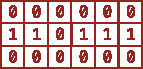
\includegraphics[height=6em]{images/data.pdf}
		\end{figure}
	};
	\node [object](single protein) [left=2em of features] {%
		Single protein models
		\vspace{1em}
		\begin{figure}
			
\includegraphics[height=4em]{images/single_protein_model.pdf}
		\end{figure}
	};
	\node [object](naive) [below=2em of single protein, align=center] {Naive validation\\and testing};
	\node [object](by position) [below=-0.2em of naive] {Validation and testing by position};
	\node [object](general) [right=2em of features] {%
		General models
		\vspace{1em}
		\begin{figure}
			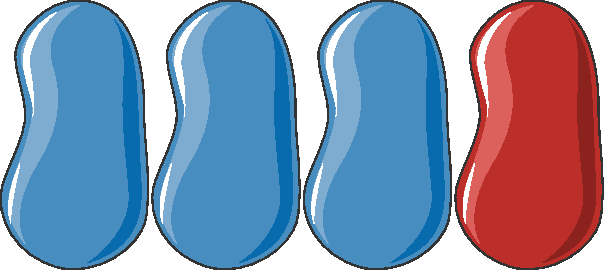
\includegraphics[height=4em]{images/general_model.pdf}
		\end{figure}
	};
	\node [object](gbt) [below=2em of general]{Gradient boosted trees};
	\node [object](linear) [below=-0.2em of gbt]{Linear regression};
	\draw [pi->] (dms) -| (single protein);
	\draw [pi->] (single protein) -- (naive);
	\draw [pi->] (dms) -| (general);
	\draw [pi->] (general) -- (gbt);
	\draw [
		decoration={%
				brace,
				raise=1ex,
				amplitude=10pt,
			},
		decorate,
		thick,
		color=primary_inverse_fg,
	] (naive.north east) -- node (brace) [right=1.5em, base, text width=10em, align=left, yshift=-1em] {%
		Gradient boosted\\trees\\
		\vspace{0ex}
		\hspace{3em}
		
\includegraphics[width=3em]{images/ai.pdf}
	} (by position.south east);
	\node [base] [below=-0.2em of linear]{%
		\begin{figure}
			
\includegraphics[width=3em]{images/ai.pdf}
			\hspace{1em}
			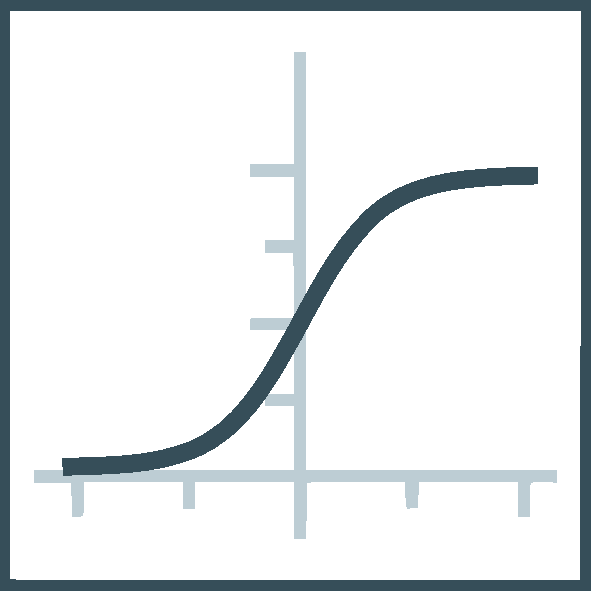
\includegraphics[width=3em]{images/sigmoid.pdf}
		\end{figure}
	};
	%\node [base] [left=-3em of brace]{%
	%	\begin{figure}
	%		
\includegraphics[width=3em]{images/ai.pdf}
	%	\end{figure}
	%};
\end{tikzpicture}%

	\end{figure}
\end{frame}

\begin{frame}
	\frametitle{I Considered Only Single Amino Acid Variants}
	\vfill%
	\begin{figure}
		\tikzset{external/export next=false}%
\begin{tikzpicture}
	\tikzset{%
		codon/.style = {object, outer sep=0pt, font=\small, text width=2em},
		aa/.style = {codon, rounded corners=3mm},
		codon_to_aa/.style = {ultra thick, color=primary_inverse_fg},
		codon_to_codon/.style = {codon_to_aa},
		codon_begin/.style = {codon_to_codon},
		codon_end/.style = {->, codon_to_codon},
	}
	\node (codon1_wt) [codon] {ATG};
	\node (codon2_wt) [codon, right=1ex of codon1_wt] {GTG};
	\node (codon3_wt) [codon, right=1ex of codon2_wt] {CAT};
	\node (codon4_wt) [codon, right=1ex of codon3_wt] {CTG};
	\node (codon5_wt) [codon, right=1ex of codon4_wt] {ACT};
	\node (codon6_wt) [codon, right=1ex of codon5_wt] {CCT};
	\node (codon7_wt) [codon, right=1ex of codon6_wt] {GAG};
	\node (aa1_wt) [aa, below=.5ex of codon1_wt] {Met};
	\node (aa2_wt) [aa, below=.5ex of codon2_wt] {Val};
	\node (aa3_wt) [aa, below=.5ex of codon3_wt] {His};
	\node (aa4_wt) [aa, below=.5ex of codon4_wt] {Leu};
	\node (aa5_wt) [aa, below=.5ex of codon5_wt] {Thr};
	\node (aa6_wt) [aa, below=.5ex of codon6_wt] {Pro};
	\node (aa7_wt) [aa, below=.5ex of codon7_wt] {Asp};
	\draw[codon_to_aa] (codon1_wt) -- (aa1_wt);
	\draw[codon_to_aa] (codon2_wt) -- (aa2_wt);
	\draw[codon_to_aa] (codon3_wt) -- (aa3_wt);
	\draw[codon_to_aa] (codon4_wt) -- (aa4_wt);
	\draw[codon_to_aa] (codon5_wt) -- (aa5_wt);
	\draw[codon_to_aa] (codon6_wt) -- (aa6_wt);
	\draw[codon_to_aa] (codon7_wt) -- (aa7_wt);
	\draw[codon_to_codon] (codon1_wt) -- (codon2_wt);
	\draw[codon_to_codon] (codon2_wt) -- (codon3_wt);
	\draw[codon_to_codon] (codon3_wt) -- (codon4_wt);
	\draw[codon_to_codon] (codon4_wt) -- (codon5_wt);
	\draw[codon_to_codon] (codon5_wt) -- (codon6_wt);
	\draw[codon_to_codon] (codon6_wt) -- (codon7_wt);
	\node (beginning_wt) [left=5ex of codon1_wt] {};
	\node (end_wt) [right=5ex of codon7_wt] {};
	\draw[codon_end] (codon7_wt) -- (end_wt);
	\draw[codon_begin] (beginning_wt) -- (codon1_wt);
	\node (codon1_mut) [codon, below=15ex of codon1_wt.south] {ATG};
	\node (codon2_mut) [codon, right=1ex of codon1_mut] {GTG};
	\node (codon3_mut) [codon, right=1ex of codon2_mut] {CAT};
	\node (codon4_mut) [codon, right=1ex of codon3_mut] {CTG};
	\node (codon5_mut) [codon, right=1ex of codon4_mut] {ACT};
	\node (codon6_mut) [codon, right=1ex of codon5_mut, fill=primary_accent_bg, text=primary_accent_fg] {CTT};
	\node (codon7_mut) [codon, right=1ex of codon6_mut] {GAG};
	\node (aa1_mut) [aa, below=.5ex of codon1_mut] {Met};
	\node (aa2_mut) [aa, below=.5ex of codon2_mut] {Val};
	\node (aa3_mut) [aa, below=.5ex of codon3_mut] {His};
	\node (aa4_mut) [aa, below=.5ex of codon4_mut] {Leu};
	\node (aa5_mut) [aa, below=.5ex of codon5_mut] {Thr};
	\node (aa6_mut) [aa, fill=primary_accent_bg, text=primary_accent_fg, below=.5ex of codon6_mut] {Leu};
	\node (aa7_mut) [aa, below=.5ex of codon7_mut] {Asp};
	\draw [codon_to_aa] (codon1_mut) -- (aa1_mut);
	\draw [codon_to_aa] (codon2_mut) -- (aa2_mut);
	\draw [codon_to_aa] (codon3_mut) -- (aa3_mut);
	\draw [codon_to_aa] (codon4_mut) -- (aa4_mut);
	\draw [codon_to_aa] (codon5_mut) -- (aa5_mut);
	\draw [codon_to_aa] (codon6_mut) -- (aa6_mut);
	\draw [codon_to_aa] (codon7_mut) -- (aa7_mut);
	\draw [codon_to_codon] (codon1_mut) -- (codon2_mut);
	\draw [codon_to_codon] (codon2_mut) -- (codon3_mut);
	\draw [codon_to_codon] (codon3_mut) -- (codon4_mut);
	\draw [codon_to_codon] (codon4_mut) -- (codon5_mut);
	\draw [codon_to_codon] (codon5_mut) -- (codon6_mut);
	\draw [codon_to_codon] (codon6_mut) -- (codon7_mut);
	\node (beginning_mut) [left=5ex of codon1_mut] {};
	\node (end_mut) [right=5ex of codon7_mut] {};
	\draw [codon_end] (codon7_mut) -- (end_mut);
	\draw [codon_begin] (beginning_mut) -- (codon1_mut);
	\draw [->, ultra thick, color=black!70, shorten <= 1ex, shorten >=1ex, color=primary_inverse_fg] (aa6_wt.south) -- (codon6_mut.north);
	\node (sav) [below=5ex of aa6_wt.south, anchor=east, xshift=-1ex, text=primary_inverse_fg] {Single Aminoacid Variant (SAV)};
\end{tikzpicture}%

	\end{figure}
\end{frame}

\begin{frame}
	\frametitle{I Used the Training Dataset of Envision {\small\parencite{Gray2018}}}
	\vfill%
	\centering%
	% for some reason figure fails
	{%
		\let\bfseries\sbseries%
		% Created by tikzDevice version 0.12.3.1 on 2021-07-05 13:46:19
% !TEX encoding = UTF-8 Unicode
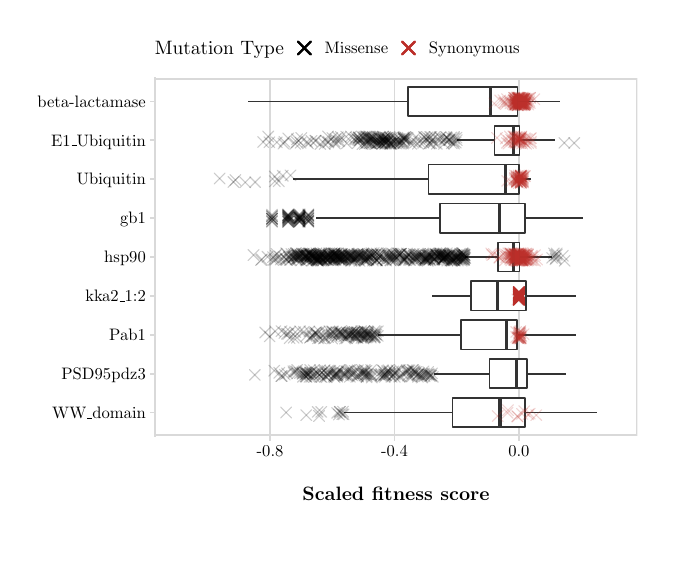
\begin{tikzpicture}[x=1pt,y=1pt]
\definecolor{fillColor}{RGB}{255,255,255}
\path[use as bounding box,fill=fillColor,fill opacity=0.00] (0,0) rectangle (223.77,183.39);
\begin{scope}
\path[clip] ( 45.95, 35.86) rectangle (220.27,165.19);
\definecolor{drawColor}{gray}{0.85}

\path[draw=drawColor,line width= 0.6pt,line join=round] ( 87.59, 35.86) --
	( 87.59,165.19);

\path[draw=drawColor,line width= 0.6pt,line join=round] (132.55, 35.86) --
	(132.55,165.19);

\path[draw=drawColor,line width= 0.6pt,line join=round] (177.51, 35.86) --
	(177.51,165.19);
\definecolor{drawColor}{gray}{0.20}

\path[draw=drawColor,line width= 0.6pt,line join=round] (176.98,156.75) -- (192.19,156.75);

\path[draw=drawColor,line width= 0.6pt,line join=round] (137.51,156.75) -- ( 79.79,156.75);
\definecolor{fillColor}{RGB}{255,255,255}

\path[draw=drawColor,line width= 0.6pt,line join=round,line cap=round,fill=fillColor] (176.98,151.48) --
	(137.51,151.48) --
	(137.51,162.02) --
	(176.98,162.02) --
	(176.98,151.48) --
	cycle;

\path[draw=drawColor,line width= 1.1pt,line join=round] (167.35,151.48) -- (167.35,162.02);

\path[draw=drawColor,line width= 0.6pt,line join=round] (177.77,142.70) -- (190.46,142.70);

\path[draw=drawColor,line width= 0.6pt,line join=round] (168.70,142.70) -- (155.28,142.70);

\path[draw=drawColor,line width= 0.6pt,line join=round,line cap=round,fill=fillColor] (177.77,137.43) --
	(168.70,137.43) --
	(168.70,147.97) --
	(177.77,147.97) --
	(177.77,137.43) --
	cycle;

\path[draw=drawColor,line width= 1.1pt,line join=round] (175.65,137.43) -- (175.65,147.97);

\path[draw=drawColor,line width= 0.6pt,line join=round] (177.51,128.64) -- (181.77,128.64);

\path[draw=drawColor,line width= 0.6pt,line join=round] (144.78,128.64) -- ( 95.70,128.64);

\path[draw=drawColor,line width= 0.6pt,line join=round,line cap=round,fill=fillColor] (177.51,123.37) --
	(144.78,123.37) --
	(144.78,133.91) --
	(177.51,133.91) --
	(177.51,123.37) --
	cycle;

\path[draw=drawColor,line width= 1.1pt,line join=round] (172.53,123.37) -- (172.53,133.91);

\path[draw=drawColor,line width= 0.6pt,line join=round] (179.78,114.58) -- (200.68,114.58);

\path[draw=drawColor,line width= 0.6pt,line join=round] (148.99,114.58) -- (104.06,114.58);

\path[draw=drawColor,line width= 0.6pt,line join=round,line cap=round,fill=fillColor] (179.78,109.31) --
	(148.99,109.31) --
	(148.99,119.85) --
	(179.78,119.85) --
	(179.78,109.31) --
	cycle;

\path[draw=drawColor,line width= 1.1pt,line join=round] (170.61,109.31) -- (170.61,119.85);

\path[draw=drawColor,line width= 0.6pt,line join=round] (177.71,100.53) -- (189.34,100.53);

\path[draw=drawColor,line width= 0.6pt,line join=round] (169.89,100.53) -- (158.20,100.53);

\path[draw=drawColor,line width= 0.6pt,line join=round,line cap=round,fill=fillColor] (177.71, 95.25) --
	(169.89, 95.25) --
	(169.89,105.80) --
	(177.71,105.80) --
	(177.71, 95.25) --
	cycle;

\path[draw=drawColor,line width= 1.1pt,line join=round] (175.47, 95.25) -- (175.47,105.80);

\path[draw=drawColor,line width= 0.6pt,line join=round] (180.01, 86.47) -- (197.99, 86.47);

\path[draw=drawColor,line width= 0.6pt,line join=round] (160.28, 86.47) -- (145.99, 86.47);

\path[draw=drawColor,line width= 0.6pt,line join=round,line cap=round,fill=fillColor] (180.01, 81.20) --
	(160.28, 81.20) --
	(160.28, 91.74) --
	(180.01, 91.74) --
	(180.01, 81.20) --
	cycle;

\path[draw=drawColor,line width= 1.1pt,line join=round] (169.87, 81.20) -- (169.87, 91.74);

\path[draw=drawColor,line width= 0.6pt,line join=round] (176.76, 72.41) -- (198.24, 72.41);

\path[draw=drawColor,line width= 0.6pt,line join=round] (156.69, 72.41) -- (126.64, 72.41);

\path[draw=drawColor,line width= 0.6pt,line join=round,line cap=round,fill=fillColor] (176.76, 67.14) --
	(156.69, 67.14) --
	(156.69, 77.68) --
	(176.76, 77.68) --
	(176.76, 67.14) --
	cycle;

\path[draw=drawColor,line width= 1.1pt,line join=round] (172.99, 67.14) -- (172.99, 77.68);

\path[draw=drawColor,line width= 0.6pt,line join=round] (180.40, 58.36) -- (194.48, 58.36);

\path[draw=drawColor,line width= 0.6pt,line join=round] (166.86, 58.36) -- (146.88, 58.36);

\path[draw=drawColor,line width= 0.6pt,line join=round,line cap=round,fill=fillColor] (180.40, 53.08) --
	(166.86, 53.08) --
	(166.86, 63.63) --
	(180.40, 63.63) --
	(180.40, 53.08) --
	cycle;

\path[draw=drawColor,line width= 1.1pt,line join=round] (176.59, 53.08) -- (176.59, 63.63);

\path[draw=drawColor,line width= 0.6pt,line join=round] (179.70, 44.30) -- (205.77, 44.30);

\path[draw=drawColor,line width= 0.6pt,line join=round] (153.52, 44.30) -- (114.34, 44.30);

\path[draw=drawColor,line width= 0.6pt,line join=round,line cap=round,fill=fillColor] (179.70, 39.03) --
	(153.52, 39.03) --
	(153.52, 49.57) --
	(179.70, 49.57) --
	(179.70, 39.03) --
	cycle;

\path[draw=drawColor,line width= 1.1pt,line join=round] (170.68, 39.03) -- (170.68, 49.57);
\definecolor{drawColor}{RGB}{0,0,0}

\path[draw=drawColor,draw opacity=0.20,line width= 0.4pt,line join=round,line cap=round] (195.51,139.74) -- (199.44,143.66);

\path[draw=drawColor,draw opacity=0.20,line width= 0.4pt,line join=round,line cap=round] (195.51,143.66) -- (199.44,139.74);

\path[draw=drawColor,draw opacity=0.20,line width= 0.4pt,line join=round,line cap=round] (191.96,139.80) -- (195.88,143.72);

\path[draw=drawColor,draw opacity=0.20,line width= 0.4pt,line join=round,line cap=round] (191.96,143.72) -- (195.88,139.80);

\path[draw=drawColor,draw opacity=0.20,line width= 0.4pt,line join=round,line cap=round] (150.23,140.86) -- (154.15,144.78);

\path[draw=drawColor,draw opacity=0.20,line width= 0.4pt,line join=round,line cap=round] (150.23,144.78) -- (154.15,140.86);

\path[draw=drawColor,draw opacity=0.20,line width= 0.4pt,line join=round,line cap=round] (105.37,139.41) -- (109.29,143.34);

\path[draw=drawColor,draw opacity=0.20,line width= 0.4pt,line join=round,line cap=round] (105.37,143.34) -- (109.29,139.41);

\path[draw=drawColor,draw opacity=0.20,line width= 0.4pt,line join=round,line cap=round] (129.08,139.65) -- (133.01,143.57);

\path[draw=drawColor,draw opacity=0.20,line width= 0.4pt,line join=round,line cap=round] (129.08,143.57) -- (133.01,139.65);

\path[draw=drawColor,draw opacity=0.20,line width= 0.4pt,line join=round,line cap=round] (127.03,140.54) -- (130.95,144.46);

\path[draw=drawColor,draw opacity=0.20,line width= 0.4pt,line join=round,line cap=round] (127.03,144.46) -- (130.95,140.54);

\path[draw=drawColor,draw opacity=0.20,line width= 0.4pt,line join=round,line cap=round] (126.26,139.42) -- (130.19,143.34);

\path[draw=drawColor,draw opacity=0.20,line width= 0.4pt,line join=round,line cap=round] (126.26,143.34) -- (130.19,139.42);

\path[draw=drawColor,draw opacity=0.20,line width= 0.4pt,line join=round,line cap=round] (125.54,139.76) -- (129.46,143.69);

\path[draw=drawColor,draw opacity=0.20,line width= 0.4pt,line join=round,line cap=round] (125.54,143.69) -- (129.46,139.76);

\path[draw=drawColor,draw opacity=0.20,line width= 0.4pt,line join=round,line cap=round] (122.84,141.75) -- (126.77,145.67);

\path[draw=drawColor,draw opacity=0.20,line width= 0.4pt,line join=round,line cap=round] (122.84,145.67) -- (126.77,141.75);

\path[draw=drawColor,draw opacity=0.20,line width= 0.4pt,line join=round,line cap=round] (122.31,139.51) -- (126.23,143.43);

\path[draw=drawColor,draw opacity=0.20,line width= 0.4pt,line join=round,line cap=round] (122.31,143.43) -- (126.23,139.51);

\path[draw=drawColor,draw opacity=0.20,line width= 0.4pt,line join=round,line cap=round] (122.21,141.36) -- (126.13,145.28);

\path[draw=drawColor,draw opacity=0.20,line width= 0.4pt,line join=round,line cap=round] (122.21,145.28) -- (126.13,141.36);

\path[draw=drawColor,draw opacity=0.20,line width= 0.4pt,line join=round,line cap=round] (121.57,141.35) -- (125.49,145.28);

\path[draw=drawColor,draw opacity=0.20,line width= 0.4pt,line join=round,line cap=round] (121.57,145.28) -- (125.49,141.35);

\path[draw=drawColor,draw opacity=0.20,line width= 0.4pt,line join=round,line cap=round] (120.45,139.73) -- (124.38,143.66);

\path[draw=drawColor,draw opacity=0.20,line width= 0.4pt,line join=round,line cap=round] (120.45,143.66) -- (124.38,139.73);

\path[draw=drawColor,draw opacity=0.20,line width= 0.4pt,line join=round,line cap=round] (120.23,140.50) -- (124.15,144.43);

\path[draw=drawColor,draw opacity=0.20,line width= 0.4pt,line join=round,line cap=round] (120.23,144.43) -- (124.15,140.50);

\path[draw=drawColor,draw opacity=0.20,line width= 0.4pt,line join=round,line cap=round] (119.02,139.37) -- (122.95,143.30);

\path[draw=drawColor,draw opacity=0.20,line width= 0.4pt,line join=round,line cap=round] (119.02,143.30) -- (122.95,139.37);

\path[draw=drawColor,draw opacity=0.20,line width= 0.4pt,line join=round,line cap=round] (152.70,139.93) -- (156.63,143.86);

\path[draw=drawColor,draw opacity=0.20,line width= 0.4pt,line join=round,line cap=round] (152.70,143.86) -- (156.63,139.93);

\path[draw=drawColor,draw opacity=0.20,line width= 0.4pt,line join=round,line cap=round] (144.13,140.75) -- (148.06,144.67);

\path[draw=drawColor,draw opacity=0.20,line width= 0.4pt,line join=round,line cap=round] (144.13,144.67) -- (148.06,140.75);

\path[draw=drawColor,draw opacity=0.20,line width= 0.4pt,line join=round,line cap=round] (139.05,139.49) -- (142.98,143.42);

\path[draw=drawColor,draw opacity=0.20,line width= 0.4pt,line join=round,line cap=round] (139.05,143.42) -- (142.98,139.49);

\path[draw=drawColor,draw opacity=0.20,line width= 0.4pt,line join=round,line cap=round] (136.96,140.39) -- (140.88,144.31);

\path[draw=drawColor,draw opacity=0.20,line width= 0.4pt,line join=round,line cap=round] (136.96,144.31) -- (140.88,140.39);

\path[draw=drawColor,draw opacity=0.20,line width= 0.4pt,line join=round,line cap=round] (132.25,140.24) -- (136.17,144.16);

\path[draw=drawColor,draw opacity=0.20,line width= 0.4pt,line join=round,line cap=round] (132.25,144.16) -- (136.17,140.24);

\path[draw=drawColor,draw opacity=0.20,line width= 0.4pt,line join=round,line cap=round] (128.96,139.37) -- (132.89,143.29);

\path[draw=drawColor,draw opacity=0.20,line width= 0.4pt,line join=round,line cap=round] (128.96,143.29) -- (132.89,139.37);

\path[draw=drawColor,draw opacity=0.20,line width= 0.4pt,line join=round,line cap=round] (128.84,142.06) -- (132.76,145.99);

\path[draw=drawColor,draw opacity=0.20,line width= 0.4pt,line join=round,line cap=round] (128.84,145.99) -- (132.76,142.06);

\path[draw=drawColor,draw opacity=0.20,line width= 0.4pt,line join=round,line cap=round] (128.03,140.75) -- (131.96,144.68);

\path[draw=drawColor,draw opacity=0.20,line width= 0.4pt,line join=round,line cap=round] (128.03,144.68) -- (131.96,140.75);

\path[draw=drawColor,draw opacity=0.20,line width= 0.4pt,line join=round,line cap=round] (126.61,141.31) -- (130.53,145.23);

\path[draw=drawColor,draw opacity=0.20,line width= 0.4pt,line join=round,line cap=round] (126.61,145.23) -- (130.53,141.31);

\path[draw=drawColor,draw opacity=0.20,line width= 0.4pt,line join=round,line cap=round] (134.05,141.75) -- (137.97,145.67);

\path[draw=drawColor,draw opacity=0.20,line width= 0.4pt,line join=round,line cap=round] (134.05,145.67) -- (137.97,141.75);

\path[draw=drawColor,draw opacity=0.20,line width= 0.4pt,line join=round,line cap=round] (133.69,141.74) -- (137.62,145.67);

\path[draw=drawColor,draw opacity=0.20,line width= 0.4pt,line join=round,line cap=round] (133.69,145.67) -- (137.62,141.74);

\path[draw=drawColor,draw opacity=0.20,line width= 0.4pt,line join=round,line cap=round] (126.36,141.90) -- (130.28,145.82);

\path[draw=drawColor,draw opacity=0.20,line width= 0.4pt,line join=round,line cap=round] (126.36,145.82) -- (130.28,141.90);

\path[draw=drawColor,draw opacity=0.20,line width= 0.4pt,line join=round,line cap=round] (125.88,141.06) -- (129.81,144.98);

\path[draw=drawColor,draw opacity=0.20,line width= 0.4pt,line join=round,line cap=round] (125.88,144.98) -- (129.81,141.06);

\path[draw=drawColor,draw opacity=0.20,line width= 0.4pt,line join=round,line cap=round] (125.11,141.72) -- (129.04,145.65);

\path[draw=drawColor,draw opacity=0.20,line width= 0.4pt,line join=round,line cap=round] (125.11,145.65) -- (129.04,141.72);

\path[draw=drawColor,draw opacity=0.20,line width= 0.4pt,line join=round,line cap=round] (122.11,141.83) -- (126.03,145.76);

\path[draw=drawColor,draw opacity=0.20,line width= 0.4pt,line join=round,line cap=round] (122.11,145.76) -- (126.03,141.83);

\path[draw=drawColor,draw opacity=0.20,line width= 0.4pt,line join=round,line cap=round] (121.71,142.12) -- (125.63,146.04);

\path[draw=drawColor,draw opacity=0.20,line width= 0.4pt,line join=round,line cap=round] (121.71,146.04) -- (125.63,142.12);

\path[draw=drawColor,draw opacity=0.20,line width= 0.4pt,line join=round,line cap=round] (121.07,141.32) -- (125.00,145.24);

\path[draw=drawColor,draw opacity=0.20,line width= 0.4pt,line join=round,line cap=round] (121.07,145.24) -- (125.00,141.32);

\path[draw=drawColor,draw opacity=0.20,line width= 0.4pt,line join=round,line cap=round] (121.07,139.91) -- (124.99,143.84);

\path[draw=drawColor,draw opacity=0.20,line width= 0.4pt,line join=round,line cap=round] (121.07,143.84) -- (124.99,139.91);

\path[draw=drawColor,draw opacity=0.20,line width= 0.4pt,line join=round,line cap=round] (117.78,141.62) -- (121.71,145.55);

\path[draw=drawColor,draw opacity=0.20,line width= 0.4pt,line join=round,line cap=round] (117.78,145.55) -- (121.71,141.62);

\path[draw=drawColor,draw opacity=0.20,line width= 0.4pt,line join=round,line cap=round] (117.28,141.06) -- (121.21,144.98);

\path[draw=drawColor,draw opacity=0.20,line width= 0.4pt,line join=round,line cap=round] (117.28,144.98) -- (121.21,141.06);

\path[draw=drawColor,draw opacity=0.20,line width= 0.4pt,line join=round,line cap=round] (113.35,139.62) -- (117.27,143.55);

\path[draw=drawColor,draw opacity=0.20,line width= 0.4pt,line join=round,line cap=round] (113.35,143.55) -- (117.27,139.62);

\path[draw=drawColor,draw opacity=0.20,line width= 0.4pt,line join=round,line cap=round] (143.85,141.92) -- (147.77,145.84);

\path[draw=drawColor,draw opacity=0.20,line width= 0.4pt,line join=round,line cap=round] (143.85,145.84) -- (147.77,141.92);

\path[draw=drawColor,draw opacity=0.20,line width= 0.4pt,line join=round,line cap=round] (136.64,139.45) -- (140.57,143.38);

\path[draw=drawColor,draw opacity=0.20,line width= 0.4pt,line join=round,line cap=round] (136.64,143.38) -- (140.57,139.45);

\path[draw=drawColor,draw opacity=0.20,line width= 0.4pt,line join=round,line cap=round] (122.58,140.87) -- (126.50,144.80);

\path[draw=drawColor,draw opacity=0.20,line width= 0.4pt,line join=round,line cap=round] (122.58,144.80) -- (126.50,140.87);

\path[draw=drawColor,draw opacity=0.20,line width= 0.4pt,line join=round,line cap=round] (118.12,140.82) -- (122.04,144.74);

\path[draw=drawColor,draw opacity=0.20,line width= 0.4pt,line join=round,line cap=round] (118.12,144.74) -- (122.04,140.82);

\path[draw=drawColor,draw opacity=0.20,line width= 0.4pt,line join=round,line cap=round] (117.36,139.78) -- (121.28,143.70);

\path[draw=drawColor,draw opacity=0.20,line width= 0.4pt,line join=round,line cap=round] (117.36,143.70) -- (121.28,139.78);

\path[draw=drawColor,draw opacity=0.20,line width= 0.4pt,line join=round,line cap=round] (111.22,141.93) -- (115.14,145.85);

\path[draw=drawColor,draw opacity=0.20,line width= 0.4pt,line join=round,line cap=round] (111.22,145.85) -- (115.14,141.93);

\path[draw=drawColor,draw opacity=0.20,line width= 0.4pt,line join=round,line cap=round] (110.66,140.59) -- (114.58,144.51);

\path[draw=drawColor,draw opacity=0.20,line width= 0.4pt,line join=round,line cap=round] (110.66,144.51) -- (114.58,140.59);

\path[draw=drawColor,draw opacity=0.20,line width= 0.4pt,line join=round,line cap=round] ( 88.08,140.00) -- ( 92.01,143.92);

\path[draw=drawColor,draw opacity=0.20,line width= 0.4pt,line join=round,line cap=round] ( 88.08,143.92) -- ( 92.01,140.00);

\path[draw=drawColor,draw opacity=0.20,line width= 0.4pt,line join=round,line cap=round] ( 87.34,127.62) -- ( 91.26,131.55);

\path[draw=drawColor,draw opacity=0.20,line width= 0.4pt,line join=round,line cap=round] ( 87.34,131.55) -- ( 91.26,127.62);

\path[draw=drawColor,draw opacity=0.20,line width= 0.4pt,line join=round,line cap=round] (149.30,141.95) -- (153.22,145.87);

\path[draw=drawColor,draw opacity=0.20,line width= 0.4pt,line join=round,line cap=round] (149.30,145.87) -- (153.22,141.95);

\path[draw=drawColor,draw opacity=0.20,line width= 0.4pt,line join=round,line cap=round] (135.42,141.12) -- (139.34,145.05);

\path[draw=drawColor,draw opacity=0.20,line width= 0.4pt,line join=round,line cap=round] (135.42,145.05) -- (139.34,141.12);

\path[draw=drawColor,draw opacity=0.20,line width= 0.4pt,line join=round,line cap=round] (123.15,139.98) -- (127.07,143.90);

\path[draw=drawColor,draw opacity=0.20,line width= 0.4pt,line join=round,line cap=round] (123.15,143.90) -- (127.07,139.98);

\path[draw=drawColor,draw opacity=0.20,line width= 0.4pt,line join=round,line cap=round] (121.70,139.82) -- (125.63,143.74);

\path[draw=drawColor,draw opacity=0.20,line width= 0.4pt,line join=round,line cap=round] (121.70,143.74) -- (125.63,139.82);

\path[draw=drawColor,draw opacity=0.20,line width= 0.4pt,line join=round,line cap=round] (117.52,140.79) -- (121.45,144.71);

\path[draw=drawColor,draw opacity=0.20,line width= 0.4pt,line join=round,line cap=round] (117.52,144.71) -- (121.45,140.79);

\path[draw=drawColor,draw opacity=0.20,line width= 0.4pt,line join=round,line cap=round] (134.00,140.87) -- (137.92,144.80);

\path[draw=drawColor,draw opacity=0.20,line width= 0.4pt,line join=round,line cap=round] (134.00,144.80) -- (137.92,140.87);

\path[draw=drawColor,draw opacity=0.20,line width= 0.4pt,line join=round,line cap=round] (116.70,141.66) -- (120.63,145.59);

\path[draw=drawColor,draw opacity=0.20,line width= 0.4pt,line join=round,line cap=round] (116.70,145.59) -- (120.63,141.66);

\path[draw=drawColor,draw opacity=0.20,line width= 0.4pt,line join=round,line cap=round] (109.21,141.21) -- (113.14,145.14);

\path[draw=drawColor,draw opacity=0.20,line width= 0.4pt,line join=round,line cap=round] (109.21,145.14) -- (113.14,141.21);

\path[draw=drawColor,draw opacity=0.20,line width= 0.4pt,line join=round,line cap=round] (109.06,139.57) -- (112.99,143.50);

\path[draw=drawColor,draw opacity=0.20,line width= 0.4pt,line join=round,line cap=round] (109.06,143.50) -- (112.99,139.57);

\path[draw=drawColor,draw opacity=0.20,line width= 0.4pt,line join=round,line cap=round] (108.96,140.24) -- (112.88,144.16);

\path[draw=drawColor,draw opacity=0.20,line width= 0.4pt,line join=round,line cap=round] (108.96,144.16) -- (112.88,140.24);

\path[draw=drawColor,draw opacity=0.20,line width= 0.4pt,line join=round,line cap=round] (103.80,139.35) -- (107.73,143.27);

\path[draw=drawColor,draw opacity=0.20,line width= 0.4pt,line join=round,line cap=round] (103.80,143.27) -- (107.73,139.35);

\path[draw=drawColor,draw opacity=0.20,line width= 0.4pt,line join=round,line cap=round] (101.94,140.56) -- (105.86,144.48);

\path[draw=drawColor,draw opacity=0.20,line width= 0.4pt,line join=round,line cap=round] (101.94,144.48) -- (105.86,140.56);

\path[draw=drawColor,draw opacity=0.20,line width= 0.4pt,line join=round,line cap=round] (100.58,140.49) -- (104.50,144.42);

\path[draw=drawColor,draw opacity=0.20,line width= 0.4pt,line join=round,line cap=round] (100.58,144.42) -- (104.50,140.49);

\path[draw=drawColor,draw opacity=0.20,line width= 0.4pt,line join=round,line cap=round] ( 96.68,139.86) -- (100.60,143.78);

\path[draw=drawColor,draw opacity=0.20,line width= 0.4pt,line join=round,line cap=round] ( 96.68,143.78) -- (100.60,139.86);

\path[draw=drawColor,draw opacity=0.20,line width= 0.4pt,line join=round,line cap=round] ( 95.29,140.04) -- ( 99.22,143.96);

\path[draw=drawColor,draw opacity=0.20,line width= 0.4pt,line join=round,line cap=round] ( 95.29,143.96) -- ( 99.22,140.04);

\path[draw=drawColor,draw opacity=0.20,line width= 0.4pt,line join=round,line cap=round] ( 92.21,141.42) -- ( 96.13,145.34);

\path[draw=drawColor,draw opacity=0.20,line width= 0.4pt,line join=round,line cap=round] ( 92.21,145.34) -- ( 96.13,141.42);

\path[draw=drawColor,draw opacity=0.20,line width= 0.4pt,line join=round,line cap=round] ( 90.49,139.56) -- ( 94.41,143.48);

\path[draw=drawColor,draw opacity=0.20,line width= 0.4pt,line join=round,line cap=round] ( 90.49,143.48) -- ( 94.41,139.56);

\path[draw=drawColor,draw opacity=0.20,line width= 0.4pt,line join=round,line cap=round] (144.72,140.06) -- (148.65,143.98);

\path[draw=drawColor,draw opacity=0.20,line width= 0.4pt,line join=round,line cap=round] (144.72,143.98) -- (148.65,140.06);

\path[draw=drawColor,draw opacity=0.20,line width= 0.4pt,line join=round,line cap=round] (153.00,141.69) -- (156.92,145.61);

\path[draw=drawColor,draw opacity=0.20,line width= 0.4pt,line join=round,line cap=round] (153.00,145.61) -- (156.92,141.69);

\path[draw=drawColor,draw opacity=0.20,line width= 0.4pt,line join=round,line cap=round] (147.19,141.81) -- (151.11,145.74);

\path[draw=drawColor,draw opacity=0.20,line width= 0.4pt,line join=round,line cap=round] (147.19,145.74) -- (151.11,141.81);

\path[draw=drawColor,draw opacity=0.20,line width= 0.4pt,line join=round,line cap=round] (133.98,139.84) -- (137.91,143.76);

\path[draw=drawColor,draw opacity=0.20,line width= 0.4pt,line join=round,line cap=round] (133.98,143.76) -- (137.91,139.84);

\path[draw=drawColor,draw opacity=0.20,line width= 0.4pt,line join=round,line cap=round] (106.58,142.12) -- (110.50,146.04);

\path[draw=drawColor,draw opacity=0.20,line width= 0.4pt,line join=round,line cap=round] (106.58,146.04) -- (110.50,142.12);

\path[draw=drawColor,draw opacity=0.20,line width= 0.4pt,line join=round,line cap=round] (105.73,140.61) -- (109.66,144.54);

\path[draw=drawColor,draw opacity=0.20,line width= 0.4pt,line join=round,line cap=round] (105.73,144.54) -- (109.66,140.61);

\path[draw=drawColor,draw opacity=0.20,line width= 0.4pt,line join=round,line cap=round] ( 94.74,139.44) -- ( 98.66,143.37);

\path[draw=drawColor,draw opacity=0.20,line width= 0.4pt,line join=round,line cap=round] ( 94.74,143.37) -- ( 98.66,139.44);

\path[draw=drawColor,draw opacity=0.20,line width= 0.4pt,line join=round,line cap=round] ( 85.38,140.01) -- ( 89.30,143.94);

\path[draw=drawColor,draw opacity=0.20,line width= 0.4pt,line join=round,line cap=round] ( 85.38,143.94) -- ( 89.30,140.01);

\path[draw=drawColor,draw opacity=0.20,line width= 0.4pt,line join=round,line cap=round] ( 83.12,140.12) -- ( 87.04,144.04);

\path[draw=drawColor,draw opacity=0.20,line width= 0.4pt,line join=round,line cap=round] ( 83.12,144.04) -- ( 87.04,140.12);

\path[draw=drawColor,draw opacity=0.20,line width= 0.4pt,line join=round,line cap=round] (148.47,139.43) -- (152.40,143.35);

\path[draw=drawColor,draw opacity=0.20,line width= 0.4pt,line join=round,line cap=round] (148.47,143.35) -- (152.40,139.43);

\path[draw=drawColor,draw opacity=0.20,line width= 0.4pt,line join=round,line cap=round] (106.76,140.19) -- (110.68,144.12);

\path[draw=drawColor,draw opacity=0.20,line width= 0.4pt,line join=round,line cap=round] (106.76,144.12) -- (110.68,140.19);

\path[draw=drawColor,draw opacity=0.20,line width= 0.4pt,line join=round,line cap=round] (145.14,141.93) -- (149.06,145.85);

\path[draw=drawColor,draw opacity=0.20,line width= 0.4pt,line join=round,line cap=round] (145.14,145.85) -- (149.06,141.93);

\path[draw=drawColor,draw opacity=0.20,line width= 0.4pt,line join=round,line cap=round] ( 93.03,128.06) -- ( 96.95,131.98);

\path[draw=drawColor,draw opacity=0.20,line width= 0.4pt,line join=round,line cap=round] ( 93.03,131.98) -- ( 96.95,128.06);

\path[draw=drawColor,draw opacity=0.20,line width= 0.4pt,line join=round,line cap=round] (148.92,140.91) -- (152.84,144.84);

\path[draw=drawColor,draw opacity=0.20,line width= 0.4pt,line join=round,line cap=round] (148.92,144.84) -- (152.84,140.91);

\path[draw=drawColor,draw opacity=0.20,line width= 0.4pt,line join=round,line cap=round] (129.34,141.52) -- (133.26,145.45);

\path[draw=drawColor,draw opacity=0.20,line width= 0.4pt,line join=round,line cap=round] (129.34,145.45) -- (133.26,141.52);

\path[draw=drawColor,draw opacity=0.20,line width= 0.4pt,line join=round,line cap=round] ( 80.22,125.62) -- ( 84.15,129.55);

\path[draw=drawColor,draw opacity=0.20,line width= 0.4pt,line join=round,line cap=round] ( 80.22,129.55) -- ( 84.15,125.62);

\path[draw=drawColor,draw opacity=0.20,line width= 0.4pt,line join=round,line cap=round] (149.45,141.63) -- (153.37,145.56);

\path[draw=drawColor,draw opacity=0.20,line width= 0.4pt,line join=round,line cap=round] (149.45,145.56) -- (153.37,141.63);

\path[draw=drawColor,draw opacity=0.20,line width= 0.4pt,line join=round,line cap=round] (116.01,141.07) -- (119.94,144.99);

\path[draw=drawColor,draw opacity=0.20,line width= 0.4pt,line join=round,line cap=round] (116.01,144.99) -- (119.94,141.07);

\path[draw=drawColor,draw opacity=0.20,line width= 0.4pt,line join=round,line cap=round] (110.33,140.34) -- (114.26,144.27);

\path[draw=drawColor,draw opacity=0.20,line width= 0.4pt,line join=round,line cap=round] (110.33,144.27) -- (114.26,140.34);

\path[draw=drawColor,draw opacity=0.20,line width= 0.4pt,line join=round,line cap=round] ( 99.32,139.61) -- (103.24,143.53);

\path[draw=drawColor,draw opacity=0.20,line width= 0.4pt,line join=round,line cap=round] ( 99.32,143.53) -- (103.24,139.61);

\path[draw=drawColor,draw opacity=0.20,line width= 0.4pt,line join=round,line cap=round] ( 90.18,127.94) -- ( 94.11,131.86);

\path[draw=drawColor,draw opacity=0.20,line width= 0.4pt,line join=round,line cap=round] ( 90.18,131.86) -- ( 94.11,127.94);

\path[draw=drawColor,draw opacity=0.20,line width= 0.4pt,line join=round,line cap=round] (151.30,139.62) -- (155.22,143.55);

\path[draw=drawColor,draw opacity=0.20,line width= 0.4pt,line join=round,line cap=round] (151.30,143.55) -- (155.22,139.62);

\path[draw=drawColor,draw opacity=0.20,line width= 0.4pt,line join=round,line cap=round] (150.45,140.89) -- (154.38,144.82);

\path[draw=drawColor,draw opacity=0.20,line width= 0.4pt,line join=round,line cap=round] (150.45,144.82) -- (154.38,140.89);

\path[draw=drawColor,draw opacity=0.20,line width= 0.4pt,line join=round,line cap=round] (149.03,141.32) -- (152.95,145.24);

\path[draw=drawColor,draw opacity=0.20,line width= 0.4pt,line join=round,line cap=round] (149.03,145.24) -- (152.95,141.32);

\path[draw=drawColor,draw opacity=0.20,line width= 0.4pt,line join=round,line cap=round] (123.47,141.25) -- (127.40,145.18);

\path[draw=drawColor,draw opacity=0.20,line width= 0.4pt,line join=round,line cap=round] (123.47,145.18) -- (127.40,141.25);

\path[draw=drawColor,draw opacity=0.20,line width= 0.4pt,line join=round,line cap=round] (143.21,141.30) -- (147.14,145.22);

\path[draw=drawColor,draw opacity=0.20,line width= 0.4pt,line join=round,line cap=round] (143.21,145.22) -- (147.14,141.30);

\path[draw=drawColor,draw opacity=0.20,line width= 0.4pt,line join=round,line cap=round] (133.67,139.51) -- (137.59,143.43);

\path[draw=drawColor,draw opacity=0.20,line width= 0.4pt,line join=round,line cap=round] (133.67,143.43) -- (137.59,139.51);

\path[draw=drawColor,draw opacity=0.20,line width= 0.4pt,line join=round,line cap=round] (129.45,139.47) -- (133.38,143.40);

\path[draw=drawColor,draw opacity=0.20,line width= 0.4pt,line join=round,line cap=round] (129.45,143.40) -- (133.38,139.47);

\path[draw=drawColor,draw opacity=0.20,line width= 0.4pt,line join=round,line cap=round] (129.01,141.71) -- (132.93,145.63);

\path[draw=drawColor,draw opacity=0.20,line width= 0.4pt,line join=round,line cap=round] (129.01,145.63) -- (132.93,141.71);

\path[draw=drawColor,draw opacity=0.20,line width= 0.4pt,line join=round,line cap=round] (128.54,139.53) -- (132.47,143.45);

\path[draw=drawColor,draw opacity=0.20,line width= 0.4pt,line join=round,line cap=round] (128.54,143.45) -- (132.47,139.53);

\path[draw=drawColor,draw opacity=0.20,line width= 0.4pt,line join=round,line cap=round] (127.94,141.68) -- (131.86,145.61);

\path[draw=drawColor,draw opacity=0.20,line width= 0.4pt,line join=round,line cap=round] (127.94,145.61) -- (131.86,141.68);

\path[draw=drawColor,draw opacity=0.20,line width= 0.4pt,line join=round,line cap=round] (127.84,141.56) -- (131.77,145.48);

\path[draw=drawColor,draw opacity=0.20,line width= 0.4pt,line join=round,line cap=round] (127.84,145.48) -- (131.77,141.56);

\path[draw=drawColor,draw opacity=0.20,line width= 0.4pt,line join=round,line cap=round] (127.58,139.98) -- (131.51,143.90);

\path[draw=drawColor,draw opacity=0.20,line width= 0.4pt,line join=round,line cap=round] (127.58,143.90) -- (131.51,139.98);

\path[draw=drawColor,draw opacity=0.20,line width= 0.4pt,line join=round,line cap=round] (127.13,139.42) -- (131.05,143.34);

\path[draw=drawColor,draw opacity=0.20,line width= 0.4pt,line join=round,line cap=round] (127.13,143.34) -- (131.05,139.42);

\path[draw=drawColor,draw opacity=0.20,line width= 0.4pt,line join=round,line cap=round] (127.09,140.48) -- (131.02,144.40);

\path[draw=drawColor,draw opacity=0.20,line width= 0.4pt,line join=round,line cap=round] (127.09,144.40) -- (131.02,140.48);

\path[draw=drawColor,draw opacity=0.20,line width= 0.4pt,line join=round,line cap=round] (126.84,140.54) -- (130.77,144.47);

\path[draw=drawColor,draw opacity=0.20,line width= 0.4pt,line join=round,line cap=round] (126.84,144.47) -- (130.77,140.54);

\path[draw=drawColor,draw opacity=0.20,line width= 0.4pt,line join=round,line cap=round] (124.70,139.87) -- (128.62,143.79);

\path[draw=drawColor,draw opacity=0.20,line width= 0.4pt,line join=round,line cap=round] (124.70,143.79) -- (128.62,139.87);

\path[draw=drawColor,draw opacity=0.20,line width= 0.4pt,line join=round,line cap=round] (133.05,140.35) -- (136.98,144.28);

\path[draw=drawColor,draw opacity=0.20,line width= 0.4pt,line join=round,line cap=round] (133.05,144.28) -- (136.98,140.35);

\path[draw=drawColor,draw opacity=0.20,line width= 0.4pt,line join=round,line cap=round] (132.47,141.24) -- (136.39,145.17);

\path[draw=drawColor,draw opacity=0.20,line width= 0.4pt,line join=round,line cap=round] (132.47,145.17) -- (136.39,141.24);

\path[draw=drawColor,draw opacity=0.20,line width= 0.4pt,line join=round,line cap=round] (131.41,141.08) -- (135.34,145.01);

\path[draw=drawColor,draw opacity=0.20,line width= 0.4pt,line join=round,line cap=round] (131.41,145.01) -- (135.34,141.08);

\path[draw=drawColor,draw opacity=0.20,line width= 0.4pt,line join=round,line cap=round] (130.27,141.98) -- (134.19,145.91);

\path[draw=drawColor,draw opacity=0.20,line width= 0.4pt,line join=round,line cap=round] (130.27,145.91) -- (134.19,141.98);

\path[draw=drawColor,draw opacity=0.20,line width= 0.4pt,line join=round,line cap=round] (130.15,139.66) -- (134.08,143.58);

\path[draw=drawColor,draw opacity=0.20,line width= 0.4pt,line join=round,line cap=round] (130.15,143.58) -- (134.08,139.66);

\path[draw=drawColor,draw opacity=0.20,line width= 0.4pt,line join=round,line cap=round] (129.94,139.83) -- (133.86,143.76);

\path[draw=drawColor,draw opacity=0.20,line width= 0.4pt,line join=round,line cap=round] (129.94,143.76) -- (133.86,139.83);

\path[draw=drawColor,draw opacity=0.20,line width= 0.4pt,line join=round,line cap=round] (129.30,139.46) -- (133.23,143.39);

\path[draw=drawColor,draw opacity=0.20,line width= 0.4pt,line join=round,line cap=round] (129.30,143.39) -- (133.23,139.46);

\path[draw=drawColor,draw opacity=0.20,line width= 0.4pt,line join=round,line cap=round] (127.48,139.61) -- (131.41,143.54);

\path[draw=drawColor,draw opacity=0.20,line width= 0.4pt,line join=round,line cap=round] (127.48,143.54) -- (131.41,139.61);

\path[draw=drawColor,draw opacity=0.20,line width= 0.4pt,line join=round,line cap=round] (127.23,141.89) -- (131.15,145.82);

\path[draw=drawColor,draw opacity=0.20,line width= 0.4pt,line join=round,line cap=round] (127.23,145.82) -- (131.15,141.89);

\path[draw=drawColor,draw opacity=0.20,line width= 0.4pt,line join=round,line cap=round] (150.47,140.83) -- (154.39,144.75);

\path[draw=drawColor,draw opacity=0.20,line width= 0.4pt,line join=round,line cap=round] (150.47,144.75) -- (154.39,140.83);

\path[draw=drawColor,draw opacity=0.20,line width= 0.4pt,line join=round,line cap=round] (126.99,140.11) -- (130.91,144.04);

\path[draw=drawColor,draw opacity=0.20,line width= 0.4pt,line join=round,line cap=round] (126.99,144.04) -- (130.91,140.11);

\path[draw=drawColor,draw opacity=0.20,line width= 0.4pt,line join=round,line cap=round] (151.94,140.17) -- (155.86,144.09);

\path[draw=drawColor,draw opacity=0.20,line width= 0.4pt,line join=round,line cap=round] (151.94,144.09) -- (155.86,140.17);

\path[draw=drawColor,draw opacity=0.20,line width= 0.4pt,line join=round,line cap=round] (151.12,141.78) -- (155.05,145.70);

\path[draw=drawColor,draw opacity=0.20,line width= 0.4pt,line join=round,line cap=round] (151.12,145.70) -- (155.05,141.78);

\path[draw=drawColor,draw opacity=0.20,line width= 0.4pt,line join=round,line cap=round] (138.38,141.95) -- (142.30,145.88);

\path[draw=drawColor,draw opacity=0.20,line width= 0.4pt,line join=round,line cap=round] (138.38,145.88) -- (142.30,141.95);

\path[draw=drawColor,draw opacity=0.20,line width= 0.4pt,line join=round,line cap=round] (138.16,140.01) -- (142.08,143.93);

\path[draw=drawColor,draw opacity=0.20,line width= 0.4pt,line join=round,line cap=round] (138.16,143.93) -- (142.08,140.01);

\path[draw=drawColor,draw opacity=0.20,line width= 0.4pt,line join=round,line cap=round] (130.51,141.38) -- (134.43,145.31);

\path[draw=drawColor,draw opacity=0.20,line width= 0.4pt,line join=round,line cap=round] (130.51,145.31) -- (134.43,141.38);

\path[draw=drawColor,draw opacity=0.20,line width= 0.4pt,line join=round,line cap=round] (126.09,139.43) -- (130.01,143.35);

\path[draw=drawColor,draw opacity=0.20,line width= 0.4pt,line join=round,line cap=round] (126.09,143.35) -- (130.01,139.43);

\path[draw=drawColor,draw opacity=0.20,line width= 0.4pt,line join=round,line cap=round] ( 99.00,140.14) -- (102.93,144.07);

\path[draw=drawColor,draw opacity=0.20,line width= 0.4pt,line join=round,line cap=round] ( 99.00,144.07) -- (102.93,140.14);

\path[draw=drawColor,draw opacity=0.20,line width= 0.4pt,line join=round,line cap=round] ( 90.80,140.19) -- ( 94.72,144.11);

\path[draw=drawColor,draw opacity=0.20,line width= 0.4pt,line join=round,line cap=round] ( 90.80,144.11) -- ( 94.72,140.19);

\path[draw=drawColor,draw opacity=0.20,line width= 0.4pt,line join=round,line cap=round] (152.08,139.56) -- (156.01,143.49);

\path[draw=drawColor,draw opacity=0.20,line width= 0.4pt,line join=round,line cap=round] (152.08,143.49) -- (156.01,139.56);

\path[draw=drawColor,draw opacity=0.20,line width= 0.4pt,line join=round,line cap=round] (142.52,141.81) -- (146.45,145.73);

\path[draw=drawColor,draw opacity=0.20,line width= 0.4pt,line join=round,line cap=round] (142.52,145.73) -- (146.45,141.81);

\path[draw=drawColor,draw opacity=0.20,line width= 0.4pt,line join=round,line cap=round] (134.15,140.97) -- (138.07,144.90);

\path[draw=drawColor,draw opacity=0.20,line width= 0.4pt,line join=round,line cap=round] (134.15,144.90) -- (138.07,140.97);

\path[draw=drawColor,draw opacity=0.20,line width= 0.4pt,line join=round,line cap=round] (132.95,140.80) -- (136.88,144.73);

\path[draw=drawColor,draw opacity=0.20,line width= 0.4pt,line join=round,line cap=round] (132.95,144.73) -- (136.88,140.80);

\path[draw=drawColor,draw opacity=0.20,line width= 0.4pt,line join=round,line cap=round] (128.21,141.05) -- (132.14,144.98);

\path[draw=drawColor,draw opacity=0.20,line width= 0.4pt,line join=round,line cap=round] (128.21,144.98) -- (132.14,141.05);

\path[draw=drawColor,draw opacity=0.20,line width= 0.4pt,line join=round,line cap=round] (125.22,139.97) -- (129.14,143.89);

\path[draw=drawColor,draw opacity=0.20,line width= 0.4pt,line join=round,line cap=round] (125.22,143.89) -- (129.14,139.97);

\path[draw=drawColor,draw opacity=0.20,line width= 0.4pt,line join=round,line cap=round] (124.78,139.94) -- (128.71,143.87);

\path[draw=drawColor,draw opacity=0.20,line width= 0.4pt,line join=round,line cap=round] (124.78,143.87) -- (128.71,139.94);

\path[draw=drawColor,draw opacity=0.20,line width= 0.4pt,line join=round,line cap=round] (124.71,140.75) -- (128.63,144.67);

\path[draw=drawColor,draw opacity=0.20,line width= 0.4pt,line join=round,line cap=round] (124.71,144.67) -- (128.63,140.75);

\path[draw=drawColor,draw opacity=0.20,line width= 0.4pt,line join=round,line cap=round] (124.29,139.59) -- (128.21,143.51);

\path[draw=drawColor,draw opacity=0.20,line width= 0.4pt,line join=round,line cap=round] (124.29,143.51) -- (128.21,139.59);

\path[draw=drawColor,draw opacity=0.20,line width= 0.4pt,line join=round,line cap=round] (122.71,141.82) -- (126.64,145.75);

\path[draw=drawColor,draw opacity=0.20,line width= 0.4pt,line join=round,line cap=round] (122.71,145.75) -- (126.64,141.82);

\path[draw=drawColor,draw opacity=0.20,line width= 0.4pt,line join=round,line cap=round] (133.87,141.37) -- (137.80,145.29);

\path[draw=drawColor,draw opacity=0.20,line width= 0.4pt,line join=round,line cap=round] (133.87,145.29) -- (137.80,141.37);

\path[draw=drawColor,draw opacity=0.20,line width= 0.4pt,line join=round,line cap=round] (141.44,140.54) -- (145.36,144.47);

\path[draw=drawColor,draw opacity=0.20,line width= 0.4pt,line join=round,line cap=round] (141.44,144.47) -- (145.36,140.54);

\path[draw=drawColor,draw opacity=0.20,line width= 0.4pt,line join=round,line cap=round] (119.64,141.61) -- (123.56,145.53);

\path[draw=drawColor,draw opacity=0.20,line width= 0.4pt,line join=round,line cap=round] (119.64,145.53) -- (123.56,141.61);

\path[draw=drawColor,draw opacity=0.20,line width= 0.4pt,line join=round,line cap=round] (118.97,141.98) -- (122.90,145.91);

\path[draw=drawColor,draw opacity=0.20,line width= 0.4pt,line join=round,line cap=round] (118.97,145.91) -- (122.90,141.98);

\path[draw=drawColor,draw opacity=0.20,line width= 0.4pt,line join=round,line cap=round] (117.91,140.61) -- (121.84,144.53);

\path[draw=drawColor,draw opacity=0.20,line width= 0.4pt,line join=round,line cap=round] (117.91,144.53) -- (121.84,140.61);

\path[draw=drawColor,draw opacity=0.20,line width= 0.4pt,line join=round,line cap=round] (117.75,141.83) -- (121.67,145.76);

\path[draw=drawColor,draw opacity=0.20,line width= 0.4pt,line join=round,line cap=round] (117.75,145.76) -- (121.67,141.83);

\path[draw=drawColor,draw opacity=0.20,line width= 0.4pt,line join=round,line cap=round] (116.59,140.97) -- (120.51,144.90);

\path[draw=drawColor,draw opacity=0.20,line width= 0.4pt,line join=round,line cap=round] (116.59,144.90) -- (120.51,140.97);

\path[draw=drawColor,draw opacity=0.20,line width= 0.4pt,line join=round,line cap=round] (114.84,142.11) -- (118.77,146.03);

\path[draw=drawColor,draw opacity=0.20,line width= 0.4pt,line join=round,line cap=round] (114.84,146.03) -- (118.77,142.11);

\path[draw=drawColor,draw opacity=0.20,line width= 0.4pt,line join=round,line cap=round] (113.14,142.04) -- (117.07,145.97);

\path[draw=drawColor,draw opacity=0.20,line width= 0.4pt,line join=round,line cap=round] (113.14,145.97) -- (117.07,142.04);

\path[draw=drawColor,draw opacity=0.20,line width= 0.4pt,line join=round,line cap=round] ( 72.40,125.67) -- ( 76.32,129.59);

\path[draw=drawColor,draw opacity=0.20,line width= 0.4pt,line join=round,line cap=round] ( 72.40,129.59) -- ( 76.32,125.67);

\path[draw=drawColor,draw opacity=0.20,line width= 0.4pt,line join=round,line cap=round] (134.69,141.14) -- (138.61,145.07);

\path[draw=drawColor,draw opacity=0.20,line width= 0.4pt,line join=round,line cap=round] (134.69,145.07) -- (138.61,141.14);

\path[draw=drawColor,draw opacity=0.20,line width= 0.4pt,line join=round,line cap=round] (134.65,141.53) -- (138.57,145.46);

\path[draw=drawColor,draw opacity=0.20,line width= 0.4pt,line join=round,line cap=round] (134.65,145.46) -- (138.57,141.53);

\path[draw=drawColor,draw opacity=0.20,line width= 0.4pt,line join=round,line cap=round] (134.43,141.80) -- (138.35,145.73);

\path[draw=drawColor,draw opacity=0.20,line width= 0.4pt,line join=round,line cap=round] (134.43,145.73) -- (138.35,141.80);

\path[draw=drawColor,draw opacity=0.20,line width= 0.4pt,line join=round,line cap=round] (132.11,139.55) -- (136.03,143.47);

\path[draw=drawColor,draw opacity=0.20,line width= 0.4pt,line join=round,line cap=round] (132.11,143.47) -- (136.03,139.55);

\path[draw=drawColor,draw opacity=0.20,line width= 0.4pt,line join=round,line cap=round] (131.54,140.08) -- (135.46,144.01);

\path[draw=drawColor,draw opacity=0.20,line width= 0.4pt,line join=round,line cap=round] (131.54,144.01) -- (135.46,140.08);

\path[draw=drawColor,draw opacity=0.20,line width= 0.4pt,line join=round,line cap=round] (130.72,140.31) -- (134.64,144.24);

\path[draw=drawColor,draw opacity=0.20,line width= 0.4pt,line join=round,line cap=round] (130.72,144.24) -- (134.64,140.31);

\path[draw=drawColor,draw opacity=0.20,line width= 0.4pt,line join=round,line cap=round] (130.70,139.60) -- (134.63,143.53);

\path[draw=drawColor,draw opacity=0.20,line width= 0.4pt,line join=round,line cap=round] (130.70,143.53) -- (134.63,139.60);

\path[draw=drawColor,draw opacity=0.20,line width= 0.4pt,line join=round,line cap=round] (130.34,140.08) -- (134.27,144.01);

\path[draw=drawColor,draw opacity=0.20,line width= 0.4pt,line join=round,line cap=round] (130.34,144.01) -- (134.27,140.08);

\path[draw=drawColor,draw opacity=0.20,line width= 0.4pt,line join=round,line cap=round] (129.12,139.62) -- (133.05,143.55);

\path[draw=drawColor,draw opacity=0.20,line width= 0.4pt,line join=round,line cap=round] (129.12,143.55) -- (133.05,139.62);

\path[draw=drawColor,draw opacity=0.20,line width= 0.4pt,line join=round,line cap=round] (128.22,140.36) -- (132.14,144.28);

\path[draw=drawColor,draw opacity=0.20,line width= 0.4pt,line join=round,line cap=round] (128.22,144.28) -- (132.14,140.36);

\path[draw=drawColor,draw opacity=0.20,line width= 0.4pt,line join=round,line cap=round] (127.54,141.46) -- (131.47,145.38);

\path[draw=drawColor,draw opacity=0.20,line width= 0.4pt,line join=round,line cap=round] (127.54,145.38) -- (131.47,141.46);

\path[draw=drawColor,draw opacity=0.20,line width= 0.4pt,line join=round,line cap=round] (124.85,141.69) -- (128.77,145.62);

\path[draw=drawColor,draw opacity=0.20,line width= 0.4pt,line join=round,line cap=round] (124.85,145.62) -- (128.77,141.69);

\path[draw=drawColor,draw opacity=0.20,line width= 0.4pt,line join=round,line cap=round] (152.12,141.96) -- (156.04,145.88);

\path[draw=drawColor,draw opacity=0.20,line width= 0.4pt,line join=round,line cap=round] (152.12,145.88) -- (156.04,141.96);

\path[draw=drawColor,draw opacity=0.20,line width= 0.4pt,line join=round,line cap=round] (152.07,141.37) -- (155.99,145.30);

\path[draw=drawColor,draw opacity=0.20,line width= 0.4pt,line join=round,line cap=round] (152.07,145.30) -- (155.99,141.37);

\path[draw=drawColor,draw opacity=0.20,line width= 0.4pt,line join=round,line cap=round] (143.45,141.96) -- (147.38,145.88);

\path[draw=drawColor,draw opacity=0.20,line width= 0.4pt,line join=round,line cap=round] (143.45,145.88) -- (147.38,141.96);

\path[draw=drawColor,draw opacity=0.20,line width= 0.4pt,line join=round,line cap=round] (143.23,139.67) -- (147.15,143.59);

\path[draw=drawColor,draw opacity=0.20,line width= 0.4pt,line join=round,line cap=round] (143.23,143.59) -- (147.15,139.67);

\path[draw=drawColor,draw opacity=0.20,line width= 0.4pt,line join=round,line cap=round] (141.22,141.93) -- (145.15,145.85);

\path[draw=drawColor,draw opacity=0.20,line width= 0.4pt,line join=round,line cap=round] (141.22,145.85) -- (145.15,141.93);

\path[draw=drawColor,draw opacity=0.20,line width= 0.4pt,line join=round,line cap=round] (134.04,141.46) -- (137.96,145.39);

\path[draw=drawColor,draw opacity=0.20,line width= 0.4pt,line join=round,line cap=round] (134.04,145.39) -- (137.96,141.46);

\path[draw=drawColor,draw opacity=0.20,line width= 0.4pt,line join=round,line cap=round] (128.09,140.22) -- (132.01,144.14);

\path[draw=drawColor,draw opacity=0.20,line width= 0.4pt,line join=round,line cap=round] (128.09,144.14) -- (132.01,140.22);

\path[draw=drawColor,draw opacity=0.20,line width= 0.4pt,line join=round,line cap=round] (126.23,139.64) -- (130.15,143.57);

\path[draw=drawColor,draw opacity=0.20,line width= 0.4pt,line join=round,line cap=round] (126.23,143.57) -- (130.15,139.64);

\path[draw=drawColor,draw opacity=0.20,line width= 0.4pt,line join=round,line cap=round] (126.12,140.77) -- (130.04,144.70);

\path[draw=drawColor,draw opacity=0.20,line width= 0.4pt,line join=round,line cap=round] (126.12,144.70) -- (130.04,140.77);

\path[draw=drawColor,draw opacity=0.20,line width= 0.4pt,line join=round,line cap=round] (126.04,140.25) -- (129.96,144.17);

\path[draw=drawColor,draw opacity=0.20,line width= 0.4pt,line join=round,line cap=round] (126.04,144.17) -- (129.96,140.25);

\path[draw=drawColor,draw opacity=0.20,line width= 0.4pt,line join=round,line cap=round] (120.57,142.10) -- (124.50,146.03);

\path[draw=drawColor,draw opacity=0.20,line width= 0.4pt,line join=round,line cap=round] (120.57,146.03) -- (124.50,142.10);

\path[draw=drawColor,draw opacity=0.20,line width= 0.4pt,line join=round,line cap=round] (146.82,140.77) -- (150.75,144.69);

\path[draw=drawColor,draw opacity=0.20,line width= 0.4pt,line join=round,line cap=round] (146.82,144.69) -- (150.75,140.77);

\path[draw=drawColor,draw opacity=0.20,line width= 0.4pt,line join=round,line cap=round] (139.44,140.35) -- (143.36,144.27);

\path[draw=drawColor,draw opacity=0.20,line width= 0.4pt,line join=round,line cap=round] (139.44,144.27) -- (143.36,140.35);

\path[draw=drawColor,draw opacity=0.20,line width= 0.4pt,line join=round,line cap=round] (110.15,141.85) -- (114.07,145.78);

\path[draw=drawColor,draw opacity=0.20,line width= 0.4pt,line join=round,line cap=round] (110.15,145.78) -- (114.07,141.85);

\path[draw=drawColor,draw opacity=0.20,line width= 0.4pt,line join=round,line cap=round] (108.13,141.60) -- (112.05,145.52);

\path[draw=drawColor,draw opacity=0.20,line width= 0.4pt,line join=round,line cap=round] (108.13,145.52) -- (112.05,141.60);

\path[draw=drawColor,draw opacity=0.20,line width= 0.4pt,line join=round,line cap=round] (106.58,139.93) -- (110.50,143.85);

\path[draw=drawColor,draw opacity=0.20,line width= 0.4pt,line join=round,line cap=round] (106.58,143.85) -- (110.50,139.93);

\path[draw=drawColor,draw opacity=0.20,line width= 0.4pt,line join=round,line cap=round] (102.16,140.61) -- (106.09,144.53);

\path[draw=drawColor,draw opacity=0.20,line width= 0.4pt,line join=round,line cap=round] (102.16,144.53) -- (106.09,140.61);

\path[draw=drawColor,draw opacity=0.20,line width= 0.4pt,line join=round,line cap=round] ( 96.91,141.57) -- (100.84,145.49);

\path[draw=drawColor,draw opacity=0.20,line width= 0.4pt,line join=round,line cap=round] ( 96.91,145.49) -- (100.84,141.57);

\path[draw=drawColor,draw opacity=0.20,line width= 0.4pt,line join=round,line cap=round] ( 95.38,141.09) -- ( 99.31,145.01);

\path[draw=drawColor,draw opacity=0.20,line width= 0.4pt,line join=round,line cap=round] ( 95.38,145.01) -- ( 99.31,141.09);

\path[draw=drawColor,draw opacity=0.20,line width= 0.4pt,line join=round,line cap=round] ( 84.94,142.08) -- ( 88.87,146.01);

\path[draw=drawColor,draw opacity=0.20,line width= 0.4pt,line join=round,line cap=round] ( 84.94,146.01) -- ( 88.87,142.08);

\path[draw=drawColor,draw opacity=0.20,line width= 0.4pt,line join=round,line cap=round] ( 76.67,125.53) -- ( 80.59,129.45);

\path[draw=drawColor,draw opacity=0.20,line width= 0.4pt,line join=round,line cap=round] ( 76.67,129.45) -- ( 80.59,125.53);

\path[draw=drawColor,draw opacity=0.20,line width= 0.4pt,line join=round,line cap=round] (143.79,139.66) -- (147.72,143.58);

\path[draw=drawColor,draw opacity=0.20,line width= 0.4pt,line join=round,line cap=round] (143.79,143.58) -- (147.72,139.66);

\path[draw=drawColor,draw opacity=0.20,line width= 0.4pt,line join=round,line cap=round] (132.51,139.72) -- (136.44,143.64);

\path[draw=drawColor,draw opacity=0.20,line width= 0.4pt,line join=round,line cap=round] (132.51,143.64) -- (136.44,139.72);

\path[draw=drawColor,draw opacity=0.20,line width= 0.4pt,line join=round,line cap=round] (128.55,140.88) -- (132.48,144.81);

\path[draw=drawColor,draw opacity=0.20,line width= 0.4pt,line join=round,line cap=round] (128.55,144.81) -- (132.48,140.88);

\path[draw=drawColor,draw opacity=0.20,line width= 0.4pt,line join=round,line cap=round] (125.47,141.96) -- (129.40,145.89);

\path[draw=drawColor,draw opacity=0.20,line width= 0.4pt,line join=round,line cap=round] (125.47,145.89) -- (129.40,141.96);

\path[draw=drawColor,draw opacity=0.20,line width= 0.4pt,line join=round,line cap=round] (123.63,140.90) -- (127.56,144.83);

\path[draw=drawColor,draw opacity=0.20,line width= 0.4pt,line join=round,line cap=round] (123.63,144.83) -- (127.56,140.90);

\path[draw=drawColor,draw opacity=0.20,line width= 0.4pt,line join=round,line cap=round] (122.18,141.10) -- (126.11,145.02);

\path[draw=drawColor,draw opacity=0.20,line width= 0.4pt,line join=round,line cap=round] (122.18,145.02) -- (126.11,141.10);

\path[draw=drawColor,draw opacity=0.20,line width= 0.4pt,line join=round,line cap=round] (122.02,141.33) -- (125.94,145.25);

\path[draw=drawColor,draw opacity=0.20,line width= 0.4pt,line join=round,line cap=round] (122.02,145.25) -- (125.94,141.33);

\path[draw=drawColor,draw opacity=0.20,line width= 0.4pt,line join=round,line cap=round] (121.64,139.65) -- (125.56,143.58);

\path[draw=drawColor,draw opacity=0.20,line width= 0.4pt,line join=round,line cap=round] (121.64,143.58) -- (125.56,139.65);

\path[draw=drawColor,draw opacity=0.20,line width= 0.4pt,line join=round,line cap=round] (121.28,142.14) -- (125.21,146.06);

\path[draw=drawColor,draw opacity=0.20,line width= 0.4pt,line join=round,line cap=round] (121.28,146.06) -- (125.21,142.14);

\path[draw=drawColor,draw opacity=0.20,line width= 0.4pt,line join=round,line cap=round] (120.98,141.92) -- (124.91,145.85);

\path[draw=drawColor,draw opacity=0.20,line width= 0.4pt,line join=round,line cap=round] (120.98,145.85) -- (124.91,141.92);

\path[draw=drawColor,draw opacity=0.20,line width= 0.4pt,line join=round,line cap=round] (120.20,142.10) -- (124.12,146.03);

\path[draw=drawColor,draw opacity=0.20,line width= 0.4pt,line join=round,line cap=round] (120.20,146.03) -- (124.12,142.10);

\path[draw=drawColor,draw opacity=0.20,line width= 0.4pt,line join=round,line cap=round] (119.87,139.35) -- (123.79,143.27);

\path[draw=drawColor,draw opacity=0.20,line width= 0.4pt,line join=round,line cap=round] (119.87,143.27) -- (123.79,139.35);

\path[draw=drawColor,draw opacity=0.20,line width= 0.4pt,line join=round,line cap=round] (119.68,142.04) -- (123.60,145.97);

\path[draw=drawColor,draw opacity=0.20,line width= 0.4pt,line join=round,line cap=round] (119.68,145.97) -- (123.60,142.04);

\path[draw=drawColor,draw opacity=0.20,line width= 0.4pt,line join=round,line cap=round] (119.37,141.54) -- (123.29,145.46);

\path[draw=drawColor,draw opacity=0.20,line width= 0.4pt,line join=round,line cap=round] (119.37,145.46) -- (123.29,141.54);

\path[draw=drawColor,draw opacity=0.20,line width= 0.4pt,line join=round,line cap=round] (118.27,141.04) -- (122.20,144.97);

\path[draw=drawColor,draw opacity=0.20,line width= 0.4pt,line join=round,line cap=round] (118.27,144.97) -- (122.20,141.04);

\path[draw=drawColor,draw opacity=0.20,line width= 0.4pt,line join=round,line cap=round] (117.58,141.66) -- (121.51,145.59);

\path[draw=drawColor,draw opacity=0.20,line width= 0.4pt,line join=round,line cap=round] (117.58,145.59) -- (121.51,141.66);

\path[draw=drawColor,draw opacity=0.20,line width= 0.4pt,line join=round,line cap=round] (147.02,141.79) -- (150.95,145.72);

\path[draw=drawColor,draw opacity=0.20,line width= 0.4pt,line join=round,line cap=round] (147.02,145.72) -- (150.95,141.79);

\path[draw=drawColor,draw opacity=0.20,line width= 0.4pt,line join=round,line cap=round] (145.89,139.45) -- (149.82,143.38);

\path[draw=drawColor,draw opacity=0.20,line width= 0.4pt,line join=round,line cap=round] (145.89,143.38) -- (149.82,139.45);

\path[draw=drawColor,draw opacity=0.20,line width= 0.4pt,line join=round,line cap=round] (143.21,139.59) -- (147.14,143.52);

\path[draw=drawColor,draw opacity=0.20,line width= 0.4pt,line join=round,line cap=round] (143.21,143.52) -- (147.14,139.59);

\path[draw=drawColor,draw opacity=0.20,line width= 0.4pt,line join=round,line cap=round] (142.09,141.36) -- (146.02,145.28);

\path[draw=drawColor,draw opacity=0.20,line width= 0.4pt,line join=round,line cap=round] (142.09,145.28) -- (146.02,141.36);

\path[draw=drawColor,draw opacity=0.20,line width= 0.4pt,line join=round,line cap=round] (141.52,141.82) -- (145.45,145.74);

\path[draw=drawColor,draw opacity=0.20,line width= 0.4pt,line join=round,line cap=round] (141.52,145.74) -- (145.45,141.82);

\path[draw=drawColor,draw opacity=0.20,line width= 0.4pt,line join=round,line cap=round] (140.99,139.86) -- (144.91,143.78);

\path[draw=drawColor,draw opacity=0.20,line width= 0.4pt,line join=round,line cap=round] (140.99,143.78) -- (144.91,139.86);

\path[draw=drawColor,draw opacity=0.20,line width= 0.4pt,line join=round,line cap=round] (135.28,141.69) -- (139.20,145.61);

\path[draw=drawColor,draw opacity=0.20,line width= 0.4pt,line join=round,line cap=round] (135.28,145.61) -- (139.20,141.69);

\path[draw=drawColor,draw opacity=0.20,line width= 0.4pt,line join=round,line cap=round] (131.71,140.33) -- (135.64,144.25);

\path[draw=drawColor,draw opacity=0.20,line width= 0.4pt,line join=round,line cap=round] (131.71,144.25) -- (135.64,140.33);

\path[draw=drawColor,draw opacity=0.20,line width= 0.4pt,line join=round,line cap=round] (131.36,139.52) -- (135.28,143.44);

\path[draw=drawColor,draw opacity=0.20,line width= 0.4pt,line join=round,line cap=round] (131.36,143.44) -- (135.28,139.52);

\path[draw=drawColor,draw opacity=0.20,line width= 0.4pt,line join=round,line cap=round] (126.78,141.11) -- (130.70,145.04);

\path[draw=drawColor,draw opacity=0.20,line width= 0.4pt,line join=round,line cap=round] (126.78,145.04) -- (130.70,141.11);

\path[draw=drawColor,draw opacity=0.20,line width= 0.4pt,line join=round,line cap=round] (125.19,141.44) -- (129.11,145.37);

\path[draw=drawColor,draw opacity=0.20,line width= 0.4pt,line join=round,line cap=round] (125.19,145.37) -- (129.11,141.44);

\path[draw=drawColor,draw opacity=0.20,line width= 0.4pt,line join=round,line cap=round] (124.74,140.90) -- (128.67,144.83);

\path[draw=drawColor,draw opacity=0.20,line width= 0.4pt,line join=round,line cap=round] (124.74,144.83) -- (128.67,140.90);

\path[draw=drawColor,draw opacity=0.20,line width= 0.4pt,line join=round,line cap=round] (122.83,141.36) -- (126.76,145.29);

\path[draw=drawColor,draw opacity=0.20,line width= 0.4pt,line join=round,line cap=round] (122.83,145.29) -- (126.76,141.36);

\path[draw=drawColor,draw opacity=0.20,line width= 0.4pt,line join=round,line cap=round] (120.54,141.93) -- (124.46,145.85);

\path[draw=drawColor,draw opacity=0.20,line width= 0.4pt,line join=round,line cap=round] (120.54,145.85) -- (124.46,141.93);

\path[draw=drawColor,draw opacity=0.20,line width= 0.4pt,line join=round,line cap=round] (128.99,139.83) -- (132.92,143.75);

\path[draw=drawColor,draw opacity=0.20,line width= 0.4pt,line join=round,line cap=round] (128.99,143.75) -- (132.92,139.83);

\path[draw=drawColor,draw opacity=0.20,line width= 0.4pt,line join=round,line cap=round] (126.42,141.06) -- (130.34,144.99);

\path[draw=drawColor,draw opacity=0.20,line width= 0.4pt,line join=round,line cap=round] (126.42,144.99) -- (130.34,141.06);

\path[draw=drawColor,draw opacity=0.20,line width= 0.4pt,line join=round,line cap=round] (123.76,141.03) -- (127.68,144.96);

\path[draw=drawColor,draw opacity=0.20,line width= 0.4pt,line join=round,line cap=round] (123.76,144.96) -- (127.68,141.03);

\path[draw=drawColor,draw opacity=0.20,line width= 0.4pt,line join=round,line cap=round] (123.73,140.00) -- (127.66,143.92);

\path[draw=drawColor,draw opacity=0.20,line width= 0.4pt,line join=round,line cap=round] (123.73,143.92) -- (127.66,140.00);

\path[draw=drawColor,draw opacity=0.20,line width= 0.4pt,line join=round,line cap=round] (122.16,139.58) -- (126.08,143.50);

\path[draw=drawColor,draw opacity=0.20,line width= 0.4pt,line join=round,line cap=round] (122.16,143.50) -- (126.08,139.58);

\path[draw=drawColor,draw opacity=0.20,line width= 0.4pt,line join=round,line cap=round] (153.09,140.81) -- (157.02,144.73);

\path[draw=drawColor,draw opacity=0.20,line width= 0.4pt,line join=round,line cap=round] (153.09,144.73) -- (157.02,140.81);

\path[draw=drawColor,draw opacity=0.20,line width= 0.4pt,line join=round,line cap=round] (148.55,141.08) -- (152.47,145.01);

\path[draw=drawColor,draw opacity=0.20,line width= 0.4pt,line join=round,line cap=round] (148.55,145.01) -- (152.47,141.08);

\path[draw=drawColor,draw opacity=0.20,line width= 0.4pt,line join=round,line cap=round] (133.89,141.37) -- (137.81,145.30);

\path[draw=drawColor,draw opacity=0.20,line width= 0.4pt,line join=round,line cap=round] (133.89,145.30) -- (137.81,141.37);

\path[draw=drawColor,draw opacity=0.20,line width= 0.4pt,line join=round,line cap=round] (132.90,139.94) -- (136.82,143.87);

\path[draw=drawColor,draw opacity=0.20,line width= 0.4pt,line join=round,line cap=round] (132.90,143.87) -- (136.82,139.94);

\path[draw=drawColor,draw opacity=0.20,line width= 0.4pt,line join=round,line cap=round] (127.16,141.68) -- (131.09,145.61);

\path[draw=drawColor,draw opacity=0.20,line width= 0.4pt,line join=round,line cap=round] (127.16,145.61) -- (131.09,141.68);

\path[draw=drawColor,draw opacity=0.20,line width= 0.4pt,line join=round,line cap=round] (126.98,139.98) -- (130.90,143.90);

\path[draw=drawColor,draw opacity=0.20,line width= 0.4pt,line join=round,line cap=round] (126.98,143.90) -- (130.90,139.98);

\path[draw=drawColor,draw opacity=0.20,line width= 0.4pt,line join=round,line cap=round] (126.75,140.95) -- (130.67,144.88);

\path[draw=drawColor,draw opacity=0.20,line width= 0.4pt,line join=round,line cap=round] (126.75,144.88) -- (130.67,140.95);

\path[draw=drawColor,draw opacity=0.20,line width= 0.4pt,line join=round,line cap=round] (126.48,141.11) -- (130.41,145.03);

\path[draw=drawColor,draw opacity=0.20,line width= 0.4pt,line join=round,line cap=round] (126.48,145.03) -- (130.41,141.11);

\path[draw=drawColor,draw opacity=0.20,line width= 0.4pt,line join=round,line cap=round] (126.43,142.12) -- (130.35,146.04);

\path[draw=drawColor,draw opacity=0.20,line width= 0.4pt,line join=round,line cap=round] (126.43,146.04) -- (130.35,142.12);

\path[draw=drawColor,draw opacity=0.20,line width= 0.4pt,line join=round,line cap=round] (125.47,140.18) -- (129.40,144.11);

\path[draw=drawColor,draw opacity=0.20,line width= 0.4pt,line join=round,line cap=round] (125.47,144.11) -- (129.40,140.18);

\path[draw=drawColor,draw opacity=0.20,line width= 0.4pt,line join=round,line cap=round] (124.41,139.80) -- (128.33,143.73);

\path[draw=drawColor,draw opacity=0.20,line width= 0.4pt,line join=round,line cap=round] (124.41,143.73) -- (128.33,139.80);

\path[draw=drawColor,draw opacity=0.20,line width= 0.4pt,line join=round,line cap=round] (123.78,139.51) -- (127.71,143.43);

\path[draw=drawColor,draw opacity=0.20,line width= 0.4pt,line join=round,line cap=round] (123.78,143.43) -- (127.71,139.51);

\path[draw=drawColor,draw opacity=0.20,line width= 0.4pt,line join=round,line cap=round] (121.55,141.39) -- (125.48,145.31);

\path[draw=drawColor,draw opacity=0.20,line width= 0.4pt,line join=round,line cap=round] (121.55,145.31) -- (125.48,141.39);

\path[draw=drawColor,draw opacity=0.20,line width= 0.4pt,line join=round,line cap=round] (120.58,139.98) -- (124.50,143.90);

\path[draw=drawColor,draw opacity=0.20,line width= 0.4pt,line join=round,line cap=round] (120.58,143.90) -- (124.50,139.98);

\path[draw=drawColor,draw opacity=0.20,line width= 0.4pt,line join=round,line cap=round] ( 96.27,111.28) -- (100.20,115.20);

\path[draw=drawColor,draw opacity=0.20,line width= 0.4pt,line join=round,line cap=round] ( 96.27,115.20) -- (100.20,111.28);

\path[draw=drawColor,draw opacity=0.20,line width= 0.4pt,line join=round,line cap=round] ( 99.48,111.27) -- (103.40,115.20);

\path[draw=drawColor,draw opacity=0.20,line width= 0.4pt,line join=round,line cap=round] ( 99.48,115.20) -- (103.40,111.27);

\path[draw=drawColor,draw opacity=0.20,line width= 0.4pt,line join=round,line cap=round] ( 99.48,111.44) -- (103.40,115.36);

\path[draw=drawColor,draw opacity=0.20,line width= 0.4pt,line join=round,line cap=round] ( 99.48,115.36) -- (103.40,111.44);

\path[draw=drawColor,draw opacity=0.20,line width= 0.4pt,line join=round,line cap=round] ( 99.48,113.44) -- (103.40,117.36);

\path[draw=drawColor,draw opacity=0.20,line width= 0.4pt,line join=round,line cap=round] ( 99.48,117.36) -- (103.40,113.44);

\path[draw=drawColor,draw opacity=0.20,line width= 0.4pt,line join=round,line cap=round] ( 99.48,112.63) -- (103.40,116.56);

\path[draw=drawColor,draw opacity=0.20,line width= 0.4pt,line join=round,line cap=round] ( 99.48,116.56) -- (103.40,112.63);

\path[draw=drawColor,draw opacity=0.20,line width= 0.4pt,line join=round,line cap=round] ( 96.27,113.06) -- (100.20,116.98);

\path[draw=drawColor,draw opacity=0.20,line width= 0.4pt,line join=round,line cap=round] ( 96.27,116.98) -- (100.20,113.06);

\path[draw=drawColor,draw opacity=0.20,line width= 0.4pt,line join=round,line cap=round] ( 96.27,112.55) -- (100.20,116.48);

\path[draw=drawColor,draw opacity=0.20,line width= 0.4pt,line join=round,line cap=round] ( 96.27,116.48) -- (100.20,112.55);

\path[draw=drawColor,draw opacity=0.20,line width= 0.4pt,line join=round,line cap=round] ( 96.27,112.73) -- (100.20,116.65);

\path[draw=drawColor,draw opacity=0.20,line width= 0.4pt,line join=round,line cap=round] ( 96.27,116.65) -- (100.20,112.73);

\path[draw=drawColor,draw opacity=0.20,line width= 0.4pt,line join=round,line cap=round] ( 96.27,111.98) -- (100.20,115.91);

\path[draw=drawColor,draw opacity=0.20,line width= 0.4pt,line join=round,line cap=round] ( 96.27,115.91) -- (100.20,111.98);

\path[draw=drawColor,draw opacity=0.20,line width= 0.4pt,line join=round,line cap=round] ( 99.48,111.68) -- (103.40,115.60);

\path[draw=drawColor,draw opacity=0.20,line width= 0.4pt,line join=round,line cap=round] ( 99.48,115.60) -- (103.40,111.68);

\path[draw=drawColor,draw opacity=0.20,line width= 0.4pt,line join=round,line cap=round] ( 99.48,111.36) -- (103.40,115.28);

\path[draw=drawColor,draw opacity=0.20,line width= 0.4pt,line join=round,line cap=round] ( 99.48,115.28) -- (103.40,111.36);

\path[draw=drawColor,draw opacity=0.20,line width= 0.4pt,line join=round,line cap=round] ( 96.27,112.73) -- (100.20,116.65);

\path[draw=drawColor,draw opacity=0.20,line width= 0.4pt,line join=round,line cap=round] ( 96.27,116.65) -- (100.20,112.73);

\path[draw=drawColor,draw opacity=0.20,line width= 0.4pt,line join=round,line cap=round] ( 96.27,111.45) -- (100.20,115.38);

\path[draw=drawColor,draw opacity=0.20,line width= 0.4pt,line join=round,line cap=round] ( 96.27,115.38) -- (100.20,111.45);

\path[draw=drawColor,draw opacity=0.20,line width= 0.4pt,line join=round,line cap=round] ( 99.48,113.73) -- (103.40,117.65);

\path[draw=drawColor,draw opacity=0.20,line width= 0.4pt,line join=round,line cap=round] ( 99.48,117.65) -- (103.40,113.73);

\path[draw=drawColor,draw opacity=0.20,line width= 0.4pt,line join=round,line cap=round] ( 99.48,112.54) -- (103.40,116.47);

\path[draw=drawColor,draw opacity=0.20,line width= 0.4pt,line join=round,line cap=round] ( 99.48,116.47) -- (103.40,112.54);

\path[draw=drawColor,draw opacity=0.20,line width= 0.4pt,line join=round,line cap=round] ( 99.48,113.75) -- (103.40,117.67);

\path[draw=drawColor,draw opacity=0.20,line width= 0.4pt,line join=round,line cap=round] ( 99.48,117.67) -- (103.40,113.75);

\path[draw=drawColor,draw opacity=0.20,line width= 0.4pt,line join=round,line cap=round] ( 96.27,112.80) -- (100.20,116.72);

\path[draw=drawColor,draw opacity=0.20,line width= 0.4pt,line join=round,line cap=round] ( 96.27,116.72) -- (100.20,112.80);

\path[draw=drawColor,draw opacity=0.20,line width= 0.4pt,line join=round,line cap=round] ( 96.27,111.92) -- (100.20,115.85);

\path[draw=drawColor,draw opacity=0.20,line width= 0.4pt,line join=round,line cap=round] ( 96.27,115.85) -- (100.20,111.92);

\path[draw=drawColor,draw opacity=0.20,line width= 0.4pt,line join=round,line cap=round] ( 96.27,112.74) -- (100.20,116.66);

\path[draw=drawColor,draw opacity=0.20,line width= 0.4pt,line join=round,line cap=round] ( 96.27,116.66) -- (100.20,112.74);

\path[draw=drawColor,draw opacity=0.20,line width= 0.4pt,line join=round,line cap=round] ( 96.27,113.27) -- (100.20,117.20);

\path[draw=drawColor,draw opacity=0.20,line width= 0.4pt,line join=round,line cap=round] ( 96.27,117.20) -- (100.20,113.27);

\path[draw=drawColor,draw opacity=0.20,line width= 0.4pt,line join=round,line cap=round] ( 92.14,112.10) -- ( 96.07,116.02);

\path[draw=drawColor,draw opacity=0.20,line width= 0.4pt,line join=round,line cap=round] ( 92.14,116.02) -- ( 96.07,112.10);

\path[draw=drawColor,draw opacity=0.20,line width= 0.4pt,line join=round,line cap=round] ( 92.14,113.50) -- ( 96.07,117.42);

\path[draw=drawColor,draw opacity=0.20,line width= 0.4pt,line join=round,line cap=round] ( 92.14,117.42) -- ( 96.07,113.50);

\path[draw=drawColor,draw opacity=0.20,line width= 0.4pt,line join=round,line cap=round] ( 92.14,111.92) -- ( 96.07,115.84);

\path[draw=drawColor,draw opacity=0.20,line width= 0.4pt,line join=round,line cap=round] ( 92.14,115.84) -- ( 96.07,111.92);

\path[draw=drawColor,draw opacity=0.20,line width= 0.4pt,line join=round,line cap=round] ( 92.14,113.41) -- ( 96.07,117.33);

\path[draw=drawColor,draw opacity=0.20,line width= 0.4pt,line join=round,line cap=round] ( 92.14,117.33) -- ( 96.07,113.41);

\path[draw=drawColor,draw opacity=0.20,line width= 0.4pt,line join=round,line cap=round] ( 92.14,113.56) -- ( 96.07,117.48);

\path[draw=drawColor,draw opacity=0.20,line width= 0.4pt,line join=round,line cap=round] ( 92.14,117.48) -- ( 96.07,113.56);

\path[draw=drawColor,draw opacity=0.20,line width= 0.4pt,line join=round,line cap=round] ( 92.14,113.72) -- ( 96.07,117.65);

\path[draw=drawColor,draw opacity=0.20,line width= 0.4pt,line join=round,line cap=round] ( 92.14,117.65) -- ( 96.07,113.72);

\path[draw=drawColor,draw opacity=0.20,line width= 0.4pt,line join=round,line cap=round] ( 92.14,111.40) -- ( 96.07,115.32);

\path[draw=drawColor,draw opacity=0.20,line width= 0.4pt,line join=round,line cap=round] ( 92.14,115.32) -- ( 96.07,111.40);

\path[draw=drawColor,draw opacity=0.20,line width= 0.4pt,line join=round,line cap=round] ( 86.32,112.23) -- ( 90.25,116.15);

\path[draw=drawColor,draw opacity=0.20,line width= 0.4pt,line join=round,line cap=round] ( 86.32,116.15) -- ( 90.25,112.23);

\path[draw=drawColor,draw opacity=0.20,line width= 0.4pt,line join=round,line cap=round] ( 86.32,112.44) -- ( 90.25,116.36);

\path[draw=drawColor,draw opacity=0.20,line width= 0.4pt,line join=round,line cap=round] ( 86.32,116.36) -- ( 90.25,112.44);

\path[draw=drawColor,draw opacity=0.20,line width= 0.4pt,line join=round,line cap=round] ( 86.32,111.29) -- ( 90.25,115.22);

\path[draw=drawColor,draw opacity=0.20,line width= 0.4pt,line join=round,line cap=round] ( 86.32,115.22) -- ( 90.25,111.29);

\path[draw=drawColor,draw opacity=0.20,line width= 0.4pt,line join=round,line cap=round] ( 99.48,113.49) -- (103.40,117.41);

\path[draw=drawColor,draw opacity=0.20,line width= 0.4pt,line join=round,line cap=round] ( 99.48,117.41) -- (103.40,113.49);

\path[draw=drawColor,draw opacity=0.20,line width= 0.4pt,line join=round,line cap=round] ( 96.27,113.39) -- (100.20,117.32);

\path[draw=drawColor,draw opacity=0.20,line width= 0.4pt,line join=round,line cap=round] ( 96.27,117.32) -- (100.20,113.39);

\path[draw=drawColor,draw opacity=0.20,line width= 0.4pt,line join=round,line cap=round] ( 96.27,113.18) -- (100.20,117.11);

\path[draw=drawColor,draw opacity=0.20,line width= 0.4pt,line join=round,line cap=round] ( 96.27,117.11) -- (100.20,113.18);

\path[draw=drawColor,draw opacity=0.20,line width= 0.4pt,line join=round,line cap=round] ( 96.27,112.57) -- (100.20,116.49);

\path[draw=drawColor,draw opacity=0.20,line width= 0.4pt,line join=round,line cap=round] ( 96.27,116.49) -- (100.20,112.57);

\path[draw=drawColor,draw opacity=0.20,line width= 0.4pt,line join=round,line cap=round] ( 96.27,112.16) -- (100.20,116.08);

\path[draw=drawColor,draw opacity=0.20,line width= 0.4pt,line join=round,line cap=round] ( 96.27,116.08) -- (100.20,112.16);

\path[draw=drawColor,draw opacity=0.20,line width= 0.4pt,line join=round,line cap=round] ( 96.27,112.61) -- (100.20,116.54);

\path[draw=drawColor,draw opacity=0.20,line width= 0.4pt,line join=round,line cap=round] ( 96.27,116.54) -- (100.20,112.61);

\path[draw=drawColor,draw opacity=0.20,line width= 0.4pt,line join=round,line cap=round] ( 96.27,113.98) -- (100.20,117.90);

\path[draw=drawColor,draw opacity=0.20,line width= 0.4pt,line join=round,line cap=round] ( 96.27,117.90) -- (100.20,113.98);

\path[draw=drawColor,draw opacity=0.20,line width= 0.4pt,line join=round,line cap=round] ( 96.27,113.05) -- (100.20,116.98);

\path[draw=drawColor,draw opacity=0.20,line width= 0.4pt,line join=round,line cap=round] ( 96.27,116.98) -- (100.20,113.05);

\path[draw=drawColor,draw opacity=0.20,line width= 0.4pt,line join=round,line cap=round] ( 99.48,111.73) -- (103.40,115.65);

\path[draw=drawColor,draw opacity=0.20,line width= 0.4pt,line join=round,line cap=round] ( 99.48,115.65) -- (103.40,111.73);

\path[draw=drawColor,draw opacity=0.20,line width= 0.4pt,line join=round,line cap=round] ( 99.48,114.02) -- (103.40,117.95);

\path[draw=drawColor,draw opacity=0.20,line width= 0.4pt,line join=round,line cap=round] ( 99.48,117.95) -- (103.40,114.02);

\path[draw=drawColor,draw opacity=0.20,line width= 0.4pt,line join=round,line cap=round] ( 96.27,113.45) -- (100.20,117.37);

\path[draw=drawColor,draw opacity=0.20,line width= 0.4pt,line join=round,line cap=round] ( 96.27,117.37) -- (100.20,113.45);

\path[draw=drawColor,draw opacity=0.20,line width= 0.4pt,line join=round,line cap=round] ( 96.27,111.47) -- (100.20,115.40);

\path[draw=drawColor,draw opacity=0.20,line width= 0.4pt,line join=round,line cap=round] ( 96.27,115.40) -- (100.20,111.47);

\path[draw=drawColor,draw opacity=0.20,line width= 0.4pt,line join=round,line cap=round] ( 96.27,113.94) -- (100.20,117.86);

\path[draw=drawColor,draw opacity=0.20,line width= 0.4pt,line join=round,line cap=round] ( 96.27,117.86) -- (100.20,113.94);

\path[draw=drawColor,draw opacity=0.20,line width= 0.4pt,line join=round,line cap=round] ( 96.27,113.67) -- (100.20,117.60);

\path[draw=drawColor,draw opacity=0.20,line width= 0.4pt,line join=round,line cap=round] ( 96.27,117.60) -- (100.20,113.67);

\path[draw=drawColor,draw opacity=0.20,line width= 0.4pt,line join=round,line cap=round] ( 96.27,112.64) -- (100.20,116.56);

\path[draw=drawColor,draw opacity=0.20,line width= 0.4pt,line join=round,line cap=round] ( 96.27,116.56) -- (100.20,112.64);

\path[draw=drawColor,draw opacity=0.20,line width= 0.4pt,line join=round,line cap=round] ( 96.27,111.32) -- (100.20,115.25);

\path[draw=drawColor,draw opacity=0.20,line width= 0.4pt,line join=round,line cap=round] ( 96.27,115.25) -- (100.20,111.32);

\path[draw=drawColor,draw opacity=0.20,line width= 0.4pt,line join=round,line cap=round] ( 92.14,111.73) -- ( 96.07,115.66);

\path[draw=drawColor,draw opacity=0.20,line width= 0.4pt,line join=round,line cap=round] ( 92.14,115.66) -- ( 96.07,111.73);

\path[draw=drawColor,draw opacity=0.20,line width= 0.4pt,line join=round,line cap=round] ( 92.14,113.01) -- ( 96.07,116.94);

\path[draw=drawColor,draw opacity=0.20,line width= 0.4pt,line join=round,line cap=round] ( 92.14,116.94) -- ( 96.07,113.01);

\path[draw=drawColor,draw opacity=0.20,line width= 0.4pt,line join=round,line cap=round] ( 99.48,113.23) -- (103.40,117.16);

\path[draw=drawColor,draw opacity=0.20,line width= 0.4pt,line join=round,line cap=round] ( 99.48,117.16) -- (103.40,113.23);

\path[draw=drawColor,draw opacity=0.20,line width= 0.4pt,line join=round,line cap=round] ( 99.48,112.38) -- (103.40,116.31);

\path[draw=drawColor,draw opacity=0.20,line width= 0.4pt,line join=round,line cap=round] ( 99.48,116.31) -- (103.40,112.38);

\path[draw=drawColor,draw opacity=0.20,line width= 0.4pt,line join=round,line cap=round] ( 99.48,112.50) -- (103.40,116.42);

\path[draw=drawColor,draw opacity=0.20,line width= 0.4pt,line join=round,line cap=round] ( 99.48,116.42) -- (103.40,112.50);

\path[draw=drawColor,draw opacity=0.20,line width= 0.4pt,line join=round,line cap=round] ( 96.27,112.86) -- (100.20,116.78);

\path[draw=drawColor,draw opacity=0.20,line width= 0.4pt,line join=round,line cap=round] ( 96.27,116.78) -- (100.20,112.86);

\path[draw=drawColor,draw opacity=0.20,line width= 0.4pt,line join=round,line cap=round] ( 96.27,112.43) -- (100.20,116.36);

\path[draw=drawColor,draw opacity=0.20,line width= 0.4pt,line join=round,line cap=round] ( 96.27,116.36) -- (100.20,112.43);

\path[draw=drawColor,draw opacity=0.20,line width= 0.4pt,line join=round,line cap=round] ( 96.27,111.94) -- (100.20,115.87);

\path[draw=drawColor,draw opacity=0.20,line width= 0.4pt,line join=round,line cap=round] ( 96.27,115.87) -- (100.20,111.94);

\path[draw=drawColor,draw opacity=0.20,line width= 0.4pt,line join=round,line cap=round] ( 96.27,112.40) -- (100.20,116.32);

\path[draw=drawColor,draw opacity=0.20,line width= 0.4pt,line join=round,line cap=round] ( 96.27,116.32) -- (100.20,112.40);

\path[draw=drawColor,draw opacity=0.20,line width= 0.4pt,line join=round,line cap=round] ( 92.14,113.33) -- ( 96.07,117.26);

\path[draw=drawColor,draw opacity=0.20,line width= 0.4pt,line join=round,line cap=round] ( 92.14,117.26) -- ( 96.07,113.33);

\path[draw=drawColor,draw opacity=0.20,line width= 0.4pt,line join=round,line cap=round] ( 92.14,114.01) -- ( 96.07,117.93);

\path[draw=drawColor,draw opacity=0.20,line width= 0.4pt,line join=round,line cap=round] ( 92.14,117.93) -- ( 96.07,114.01);

\path[draw=drawColor,draw opacity=0.20,line width= 0.4pt,line join=round,line cap=round] ( 92.14,111.26) -- ( 96.07,115.18);

\path[draw=drawColor,draw opacity=0.20,line width= 0.4pt,line join=round,line cap=round] ( 92.14,115.18) -- ( 96.07,111.26);

\path[draw=drawColor,draw opacity=0.20,line width= 0.4pt,line join=round,line cap=round] ( 92.14,112.81) -- ( 96.07,116.74);

\path[draw=drawColor,draw opacity=0.20,line width= 0.4pt,line join=round,line cap=round] ( 92.14,116.74) -- ( 96.07,112.81);

\path[draw=drawColor,draw opacity=0.20,line width= 0.4pt,line join=round,line cap=round] ( 92.14,111.22) -- ( 96.07,115.14);

\path[draw=drawColor,draw opacity=0.20,line width= 0.4pt,line join=round,line cap=round] ( 92.14,115.14) -- ( 96.07,111.22);

\path[draw=drawColor,draw opacity=0.20,line width= 0.4pt,line join=round,line cap=round] ( 92.14,113.03) -- ( 96.07,116.95);

\path[draw=drawColor,draw opacity=0.20,line width= 0.4pt,line join=round,line cap=round] ( 92.14,116.95) -- ( 96.07,113.03);

\path[draw=drawColor,draw opacity=0.20,line width= 0.4pt,line join=round,line cap=round] ( 92.14,112.20) -- ( 96.07,116.12);

\path[draw=drawColor,draw opacity=0.20,line width= 0.4pt,line join=round,line cap=round] ( 92.14,116.12) -- ( 96.07,112.20);

\path[draw=drawColor,draw opacity=0.20,line width= 0.4pt,line join=round,line cap=round] ( 92.14,112.69) -- ( 96.07,116.61);

\path[draw=drawColor,draw opacity=0.20,line width= 0.4pt,line join=round,line cap=round] ( 92.14,116.61) -- ( 96.07,112.69);

\path[draw=drawColor,draw opacity=0.20,line width= 0.4pt,line join=round,line cap=round] ( 92.14,112.53) -- ( 96.07,116.45);

\path[draw=drawColor,draw opacity=0.20,line width= 0.4pt,line join=round,line cap=round] ( 92.14,116.45) -- ( 96.07,112.53);

\path[draw=drawColor,draw opacity=0.20,line width= 0.4pt,line join=round,line cap=round] ( 92.14,111.84) -- ( 96.07,115.77);

\path[draw=drawColor,draw opacity=0.20,line width= 0.4pt,line join=round,line cap=round] ( 92.14,115.77) -- ( 96.07,111.84);

\path[draw=drawColor,draw opacity=0.20,line width= 0.4pt,line join=round,line cap=round] ( 99.48,111.82) -- (103.40,115.74);

\path[draw=drawColor,draw opacity=0.20,line width= 0.4pt,line join=round,line cap=round] ( 99.48,115.74) -- (103.40,111.82);

\path[draw=drawColor,draw opacity=0.20,line width= 0.4pt,line join=round,line cap=round] ( 96.27,111.42) -- (100.20,115.35);

\path[draw=drawColor,draw opacity=0.20,line width= 0.4pt,line join=round,line cap=round] ( 96.27,115.35) -- (100.20,111.42);

\path[draw=drawColor,draw opacity=0.20,line width= 0.4pt,line join=round,line cap=round] ( 92.14,113.75) -- ( 96.07,117.68);

\path[draw=drawColor,draw opacity=0.20,line width= 0.4pt,line join=round,line cap=round] ( 92.14,117.68) -- ( 96.07,113.75);

\path[draw=drawColor,draw opacity=0.20,line width= 0.4pt,line join=round,line cap=round] ( 92.14,112.81) -- ( 96.07,116.74);

\path[draw=drawColor,draw opacity=0.20,line width= 0.4pt,line join=round,line cap=round] ( 92.14,116.74) -- ( 96.07,112.81);

\path[draw=drawColor,draw opacity=0.20,line width= 0.4pt,line join=round,line cap=round] ( 92.14,113.67) -- ( 96.07,117.60);

\path[draw=drawColor,draw opacity=0.20,line width= 0.4pt,line join=round,line cap=round] ( 92.14,117.60) -- ( 96.07,113.67);

\path[draw=drawColor,draw opacity=0.20,line width= 0.4pt,line join=round,line cap=round] ( 92.14,112.39) -- ( 96.07,116.32);

\path[draw=drawColor,draw opacity=0.20,line width= 0.4pt,line join=round,line cap=round] ( 92.14,116.32) -- ( 96.07,112.39);

\path[draw=drawColor,draw opacity=0.20,line width= 0.4pt,line join=round,line cap=round] ( 92.14,112.84) -- ( 96.07,116.77);

\path[draw=drawColor,draw opacity=0.20,line width= 0.4pt,line join=round,line cap=round] ( 92.14,116.77) -- ( 96.07,112.84);

\path[draw=drawColor,draw opacity=0.20,line width= 0.4pt,line join=round,line cap=round] ( 92.14,111.36) -- ( 96.07,115.28);

\path[draw=drawColor,draw opacity=0.20,line width= 0.4pt,line join=round,line cap=round] ( 92.14,115.28) -- ( 96.07,111.36);

\path[draw=drawColor,draw opacity=0.20,line width= 0.4pt,line join=round,line cap=round] ( 92.14,112.45) -- ( 96.07,116.37);

\path[draw=drawColor,draw opacity=0.20,line width= 0.4pt,line join=round,line cap=round] ( 92.14,116.37) -- ( 96.07,112.45);

\path[draw=drawColor,draw opacity=0.20,line width= 0.4pt,line join=round,line cap=round] ( 92.14,113.19) -- ( 96.07,117.11);

\path[draw=drawColor,draw opacity=0.20,line width= 0.4pt,line join=round,line cap=round] ( 92.14,117.11) -- ( 96.07,113.19);

\path[draw=drawColor,draw opacity=0.20,line width= 0.4pt,line join=round,line cap=round] ( 86.32,111.69) -- ( 90.25,115.61);

\path[draw=drawColor,draw opacity=0.20,line width= 0.4pt,line join=round,line cap=round] ( 86.32,115.61) -- ( 90.25,111.69);

\path[draw=drawColor,draw opacity=0.20,line width= 0.4pt,line join=round,line cap=round] ( 86.32,113.28) -- ( 90.25,117.20);

\path[draw=drawColor,draw opacity=0.20,line width= 0.4pt,line join=round,line cap=round] ( 86.32,117.20) -- ( 90.25,113.28);

\path[draw=drawColor,draw opacity=0.20,line width= 0.4pt,line join=round,line cap=round] ( 86.32,113.15) -- ( 90.25,117.08);

\path[draw=drawColor,draw opacity=0.20,line width= 0.4pt,line join=round,line cap=round] ( 86.32,117.08) -- ( 90.25,113.15);

\path[draw=drawColor,draw opacity=0.20,line width= 0.4pt,line join=round,line cap=round] ( 86.32,113.84) -- ( 90.25,117.77);

\path[draw=drawColor,draw opacity=0.20,line width= 0.4pt,line join=round,line cap=round] ( 86.32,117.77) -- ( 90.25,113.84);

\path[draw=drawColor,draw opacity=0.20,line width= 0.4pt,line join=round,line cap=round] ( 86.32,112.45) -- ( 90.25,116.37);

\path[draw=drawColor,draw opacity=0.20,line width= 0.4pt,line join=round,line cap=round] ( 86.32,116.37) -- ( 90.25,112.45);

\path[draw=drawColor,draw opacity=0.20,line width= 0.4pt,line join=round,line cap=round] ( 86.32,111.43) -- ( 90.25,115.36);

\path[draw=drawColor,draw opacity=0.20,line width= 0.4pt,line join=round,line cap=round] ( 86.32,115.36) -- ( 90.25,111.43);

\path[draw=drawColor,draw opacity=0.20,line width= 0.4pt,line join=round,line cap=round] ( 86.32,112.39) -- ( 90.25,116.32);

\path[draw=drawColor,draw opacity=0.20,line width= 0.4pt,line join=round,line cap=round] ( 86.32,116.32) -- ( 90.25,112.39);

\path[draw=drawColor,draw opacity=0.20,line width= 0.4pt,line join=round,line cap=round] ( 86.32,113.45) -- ( 90.25,117.37);

\path[draw=drawColor,draw opacity=0.20,line width= 0.4pt,line join=round,line cap=round] ( 86.32,117.37) -- ( 90.25,113.45);

\path[draw=drawColor,draw opacity=0.20,line width= 0.4pt,line join=round,line cap=round] ( 86.32,112.47) -- ( 90.25,116.40);

\path[draw=drawColor,draw opacity=0.20,line width= 0.4pt,line join=round,line cap=round] ( 86.32,116.40) -- ( 90.25,112.47);

\path[draw=drawColor,draw opacity=0.20,line width= 0.4pt,line join=round,line cap=round] (192.06, 97.19) -- (195.98,101.11);

\path[draw=drawColor,draw opacity=0.20,line width= 0.4pt,line join=round,line cap=round] (192.06,101.11) -- (195.98, 97.19);

\path[draw=drawColor,draw opacity=0.20,line width= 0.4pt,line join=round,line cap=round] (188.90, 98.15) -- (192.82,102.08);

\path[draw=drawColor,draw opacity=0.20,line width= 0.4pt,line join=round,line cap=round] (188.90,102.08) -- (192.82, 98.15);

\path[draw=drawColor,draw opacity=0.20,line width= 0.4pt,line join=round,line cap=round] (120.48, 99.32) -- (124.40,103.25);

\path[draw=drawColor,draw opacity=0.20,line width= 0.4pt,line join=round,line cap=round] (120.48,103.25) -- (124.40, 99.32);

\path[draw=drawColor,draw opacity=0.20,line width= 0.4pt,line join=round,line cap=round] (191.42, 99.00) -- (195.35,102.92);

\path[draw=drawColor,draw opacity=0.20,line width= 0.4pt,line join=round,line cap=round] (191.42,102.92) -- (195.35, 99.00);

\path[draw=drawColor,draw opacity=0.20,line width= 0.4pt,line join=round,line cap=round] (113.14, 99.13) -- (117.06,103.05);

\path[draw=drawColor,draw opacity=0.20,line width= 0.4pt,line join=round,line cap=round] (113.14,103.05) -- (117.06, 99.13);

\path[draw=drawColor,draw opacity=0.20,line width= 0.4pt,line join=round,line cap=round] (189.20, 99.34) -- (193.13,103.26);

\path[draw=drawColor,draw opacity=0.20,line width= 0.4pt,line join=round,line cap=round] (189.20,103.26) -- (193.13, 99.34);

\path[draw=drawColor,draw opacity=0.20,line width= 0.4pt,line join=round,line cap=round] (188.78, 97.76) -- (192.71,101.69);

\path[draw=drawColor,draw opacity=0.20,line width= 0.4pt,line join=round,line cap=round] (188.78,101.69) -- (192.71, 97.76);

\path[draw=drawColor,draw opacity=0.20,line width= 0.4pt,line join=round,line cap=round] (152.00, 97.45) -- (155.92,101.37);

\path[draw=drawColor,draw opacity=0.20,line width= 0.4pt,line join=round,line cap=round] (152.00,101.37) -- (155.92, 97.45);

\path[draw=drawColor,draw opacity=0.20,line width= 0.4pt,line join=round,line cap=round] (147.24, 97.39) -- (151.16,101.31);

\path[draw=drawColor,draw opacity=0.20,line width= 0.4pt,line join=round,line cap=round] (147.24,101.31) -- (151.16, 97.39);

\path[draw=drawColor,draw opacity=0.20,line width= 0.4pt,line join=round,line cap=round] (145.36, 99.77) -- (149.28,103.69);

\path[draw=drawColor,draw opacity=0.20,line width= 0.4pt,line join=round,line cap=round] (145.36,103.69) -- (149.28, 99.77);

\path[draw=drawColor,draw opacity=0.20,line width= 0.4pt,line join=round,line cap=round] (143.22, 97.77) -- (147.15,101.70);

\path[draw=drawColor,draw opacity=0.20,line width= 0.4pt,line join=round,line cap=round] (143.22,101.70) -- (147.15, 97.77);

\path[draw=drawColor,draw opacity=0.20,line width= 0.4pt,line join=round,line cap=round] ( 99.38, 99.68) -- (103.31,103.60);

\path[draw=drawColor,draw opacity=0.20,line width= 0.4pt,line join=round,line cap=round] ( 99.38,103.60) -- (103.31, 99.68);

\path[draw=drawColor,draw opacity=0.20,line width= 0.4pt,line join=round,line cap=round] (189.19, 99.82) -- (193.12,103.74);

\path[draw=drawColor,draw opacity=0.20,line width= 0.4pt,line join=round,line cap=round] (189.19,103.74) -- (193.12, 99.82);

\path[draw=drawColor,draw opacity=0.20,line width= 0.4pt,line join=round,line cap=round] (188.51, 99.05) -- (192.43,102.98);

\path[draw=drawColor,draw opacity=0.20,line width= 0.4pt,line join=round,line cap=round] (188.51,102.98) -- (192.43, 99.05);

\path[draw=drawColor,draw opacity=0.20,line width= 0.4pt,line join=round,line cap=round] (188.19, 99.88) -- (192.12,103.80);

\path[draw=drawColor,draw opacity=0.20,line width= 0.4pt,line join=round,line cap=round] (188.19,103.80) -- (192.12, 99.88);

\path[draw=drawColor,draw opacity=0.20,line width= 0.4pt,line join=round,line cap=round] (187.53, 98.24) -- (191.46,102.17);

\path[draw=drawColor,draw opacity=0.20,line width= 0.4pt,line join=round,line cap=round] (187.53,102.17) -- (191.46, 98.24);

\path[draw=drawColor,draw opacity=0.20,line width= 0.4pt,line join=round,line cap=round] (154.86, 97.74) -- (158.78,101.66);

\path[draw=drawColor,draw opacity=0.20,line width= 0.4pt,line join=round,line cap=round] (154.86,101.66) -- (158.78, 97.74);

\path[draw=drawColor,draw opacity=0.20,line width= 0.4pt,line join=round,line cap=round] (153.88, 98.15) -- (157.80,102.08);

\path[draw=drawColor,draw opacity=0.20,line width= 0.4pt,line join=round,line cap=round] (153.88,102.08) -- (157.80, 98.15);

\path[draw=drawColor,draw opacity=0.20,line width= 0.4pt,line join=round,line cap=round] (149.63, 99.22) -- (153.55,103.15);

\path[draw=drawColor,draw opacity=0.20,line width= 0.4pt,line join=round,line cap=round] (149.63,103.15) -- (153.55, 99.22);

\path[draw=drawColor,draw opacity=0.20,line width= 0.4pt,line join=round,line cap=round] (140.78, 98.99) -- (144.71,102.91);

\path[draw=drawColor,draw opacity=0.20,line width= 0.4pt,line join=round,line cap=round] (140.78,102.91) -- (144.71, 98.99);

\path[draw=drawColor,draw opacity=0.20,line width= 0.4pt,line join=round,line cap=round] (128.59, 99.20) -- (132.51,103.13);

\path[draw=drawColor,draw opacity=0.20,line width= 0.4pt,line join=round,line cap=round] (128.59,103.13) -- (132.51, 99.20);

\path[draw=drawColor,draw opacity=0.20,line width= 0.4pt,line join=round,line cap=round] (128.42, 99.94) -- (132.34,103.86);

\path[draw=drawColor,draw opacity=0.20,line width= 0.4pt,line join=round,line cap=round] (128.42,103.86) -- (132.34, 99.94);

\path[draw=drawColor,draw opacity=0.20,line width= 0.4pt,line join=round,line cap=round] (122.70, 98.01) -- (126.63,101.94);

\path[draw=drawColor,draw opacity=0.20,line width= 0.4pt,line join=round,line cap=round] (122.70,101.94) -- (126.63, 98.01);

\path[draw=drawColor,draw opacity=0.20,line width= 0.4pt,line join=round,line cap=round] (120.20, 97.27) -- (124.12,101.19);

\path[draw=drawColor,draw opacity=0.20,line width= 0.4pt,line join=round,line cap=round] (120.20,101.19) -- (124.12, 97.27);

\path[draw=drawColor,draw opacity=0.20,line width= 0.4pt,line join=round,line cap=round] (119.28, 99.72) -- (123.20,103.65);

\path[draw=drawColor,draw opacity=0.20,line width= 0.4pt,line join=round,line cap=round] (119.28,103.65) -- (123.20, 99.72);

\path[draw=drawColor,draw opacity=0.20,line width= 0.4pt,line join=round,line cap=round] (114.88, 97.22) -- (118.80,101.14);

\path[draw=drawColor,draw opacity=0.20,line width= 0.4pt,line join=round,line cap=round] (114.88,101.14) -- (118.80, 97.22);

\path[draw=drawColor,draw opacity=0.20,line width= 0.4pt,line join=round,line cap=round] (109.11, 98.88) -- (113.03,102.80);

\path[draw=drawColor,draw opacity=0.20,line width= 0.4pt,line join=round,line cap=round] (109.11,102.80) -- (113.03, 98.88);

\path[draw=drawColor,draw opacity=0.20,line width= 0.4pt,line join=round,line cap=round] (108.20, 97.92) -- (112.12,101.85);

\path[draw=drawColor,draw opacity=0.20,line width= 0.4pt,line join=round,line cap=round] (108.20,101.85) -- (112.12, 97.92);

\path[draw=drawColor,draw opacity=0.20,line width= 0.4pt,line join=round,line cap=round] (106.95, 99.24) -- (110.87,103.17);

\path[draw=drawColor,draw opacity=0.20,line width= 0.4pt,line join=round,line cap=round] (106.95,103.17) -- (110.87, 99.24);

\path[draw=drawColor,draw opacity=0.20,line width= 0.4pt,line join=round,line cap=round] (103.90, 99.20) -- (107.83,103.13);

\path[draw=drawColor,draw opacity=0.20,line width= 0.4pt,line join=round,line cap=round] (103.90,103.13) -- (107.83, 99.20);

\path[draw=drawColor,draw opacity=0.20,line width= 0.4pt,line join=round,line cap=round] (101.05, 97.24) -- (104.97,101.17);

\path[draw=drawColor,draw opacity=0.20,line width= 0.4pt,line join=round,line cap=round] (101.05,101.17) -- (104.97, 97.24);

\path[draw=drawColor,draw opacity=0.20,line width= 0.4pt,line join=round,line cap=round] (117.52, 99.03) -- (121.45,102.95);

\path[draw=drawColor,draw opacity=0.20,line width= 0.4pt,line join=round,line cap=round] (117.52,102.95) -- (121.45, 99.03);

\path[draw=drawColor,draw opacity=0.20,line width= 0.4pt,line join=round,line cap=round] (155.29, 99.47) -- (159.21,103.40);

\path[draw=drawColor,draw opacity=0.20,line width= 0.4pt,line join=round,line cap=round] (155.29,103.40) -- (159.21, 99.47);

\path[draw=drawColor,draw opacity=0.20,line width= 0.4pt,line join=round,line cap=round] (115.35, 98.45) -- (119.28,102.37);

\path[draw=drawColor,draw opacity=0.20,line width= 0.4pt,line join=round,line cap=round] (115.35,102.37) -- (119.28, 98.45);

\path[draw=drawColor,draw opacity=0.20,line width= 0.4pt,line join=round,line cap=round] (153.05, 98.08) -- (156.97,102.00);

\path[draw=drawColor,draw opacity=0.20,line width= 0.4pt,line join=round,line cap=round] (153.05,102.00) -- (156.97, 98.08);

\path[draw=drawColor,draw opacity=0.20,line width= 0.4pt,line join=round,line cap=round] (155.15, 98.94) -- (159.08,102.86);

\path[draw=drawColor,draw opacity=0.20,line width= 0.4pt,line join=round,line cap=round] (155.15,102.86) -- (159.08, 98.94);

\path[draw=drawColor,draw opacity=0.20,line width= 0.4pt,line join=round,line cap=round] (139.15, 98.35) -- (143.07,102.28);

\path[draw=drawColor,draw opacity=0.20,line width= 0.4pt,line join=round,line cap=round] (139.15,102.28) -- (143.07, 98.35);

\path[draw=drawColor,draw opacity=0.20,line width= 0.4pt,line join=round,line cap=round] (134.27, 99.46) -- (138.20,103.39);

\path[draw=drawColor,draw opacity=0.20,line width= 0.4pt,line join=round,line cap=round] (134.27,103.39) -- (138.20, 99.46);

\path[draw=drawColor,draw opacity=0.20,line width= 0.4pt,line join=round,line cap=round] (103.57, 98.46) -- (107.50,102.39);

\path[draw=drawColor,draw opacity=0.20,line width= 0.4pt,line join=round,line cap=round] (103.57,102.39) -- (107.50, 98.46);

\path[draw=drawColor,draw opacity=0.20,line width= 0.4pt,line join=round,line cap=round] (152.33, 98.00) -- (156.25,101.93);

\path[draw=drawColor,draw opacity=0.20,line width= 0.4pt,line join=round,line cap=round] (152.33,101.93) -- (156.25, 98.00);

\path[draw=drawColor,draw opacity=0.20,line width= 0.4pt,line join=round,line cap=round] (141.20, 98.41) -- (145.12,102.33);

\path[draw=drawColor,draw opacity=0.20,line width= 0.4pt,line join=round,line cap=round] (141.20,102.33) -- (145.12, 98.41);

\path[draw=drawColor,draw opacity=0.20,line width= 0.4pt,line join=round,line cap=round] (139.59, 99.03) -- (143.52,102.95);

\path[draw=drawColor,draw opacity=0.20,line width= 0.4pt,line join=round,line cap=round] (139.59,102.95) -- (143.52, 99.03);

\path[draw=drawColor,draw opacity=0.20,line width= 0.4pt,line join=round,line cap=round] (120.99, 99.48) -- (124.91,103.40);

\path[draw=drawColor,draw opacity=0.20,line width= 0.4pt,line join=round,line cap=round] (120.99,103.40) -- (124.91, 99.48);

\path[draw=drawColor,draw opacity=0.20,line width= 0.4pt,line join=round,line cap=round] (107.68, 99.79) -- (111.60,103.71);

\path[draw=drawColor,draw opacity=0.20,line width= 0.4pt,line join=round,line cap=round] (107.68,103.71) -- (111.60, 99.79);

\path[draw=drawColor,draw opacity=0.20,line width= 0.4pt,line join=round,line cap=round] (106.66, 98.21) -- (110.59,102.13);

\path[draw=drawColor,draw opacity=0.20,line width= 0.4pt,line join=round,line cap=round] (106.66,102.13) -- (110.59, 98.21);

\path[draw=drawColor,draw opacity=0.20,line width= 0.4pt,line join=round,line cap=round] (105.92, 98.89) -- (109.84,102.82);

\path[draw=drawColor,draw opacity=0.20,line width= 0.4pt,line join=round,line cap=round] (105.92,102.82) -- (109.84, 98.89);

\path[draw=drawColor,draw opacity=0.20,line width= 0.4pt,line join=round,line cap=round] (100.86, 98.68) -- (104.78,102.61);

\path[draw=drawColor,draw opacity=0.20,line width= 0.4pt,line join=round,line cap=round] (100.86,102.61) -- (104.78, 98.68);

\path[draw=drawColor,draw opacity=0.20,line width= 0.4pt,line join=round,line cap=round] ( 99.71, 97.61) -- (103.63,101.54);

\path[draw=drawColor,draw opacity=0.20,line width= 0.4pt,line join=round,line cap=round] ( 99.71,101.54) -- (103.63, 97.61);

\path[draw=drawColor,draw opacity=0.20,line width= 0.4pt,line join=round,line cap=round] (151.06, 99.91) -- (154.99,103.83);

\path[draw=drawColor,draw opacity=0.20,line width= 0.4pt,line join=round,line cap=round] (151.06,103.83) -- (154.99, 99.91);

\path[draw=drawColor,draw opacity=0.20,line width= 0.4pt,line join=round,line cap=round] (148.80, 99.51) -- (152.72,103.43);

\path[draw=drawColor,draw opacity=0.20,line width= 0.4pt,line join=round,line cap=round] (148.80,103.43) -- (152.72, 99.51);

\path[draw=drawColor,draw opacity=0.20,line width= 0.4pt,line join=round,line cap=round] (147.77, 99.76) -- (151.69,103.68);

\path[draw=drawColor,draw opacity=0.20,line width= 0.4pt,line join=round,line cap=round] (147.77,103.68) -- (151.69, 99.76);

\path[draw=drawColor,draw opacity=0.20,line width= 0.4pt,line join=round,line cap=round] (128.83, 98.28) -- (132.75,102.21);

\path[draw=drawColor,draw opacity=0.20,line width= 0.4pt,line join=round,line cap=round] (128.83,102.21) -- (132.75, 98.28);

\path[draw=drawColor,draw opacity=0.20,line width= 0.4pt,line join=round,line cap=round] (148.20, 98.14) -- (152.13,102.06);

\path[draw=drawColor,draw opacity=0.20,line width= 0.4pt,line join=round,line cap=round] (148.20,102.06) -- (152.13, 98.14);

\path[draw=drawColor,draw opacity=0.20,line width= 0.4pt,line join=round,line cap=round] (147.48, 98.29) -- (151.40,102.22);

\path[draw=drawColor,draw opacity=0.20,line width= 0.4pt,line join=round,line cap=round] (147.48,102.22) -- (151.40, 98.29);

\path[draw=drawColor,draw opacity=0.20,line width= 0.4pt,line join=round,line cap=round] (134.78, 98.72) -- (138.71,102.65);

\path[draw=drawColor,draw opacity=0.20,line width= 0.4pt,line join=round,line cap=round] (134.78,102.65) -- (138.71, 98.72);

\path[draw=drawColor,draw opacity=0.20,line width= 0.4pt,line join=round,line cap=round] (130.50, 99.13) -- (134.42,103.06);

\path[draw=drawColor,draw opacity=0.20,line width= 0.4pt,line join=round,line cap=round] (130.50,103.06) -- (134.42, 99.13);

\path[draw=drawColor,draw opacity=0.20,line width= 0.4pt,line join=round,line cap=round] (110.67, 97.84) -- (114.59,101.76);

\path[draw=drawColor,draw opacity=0.20,line width= 0.4pt,line join=round,line cap=round] (110.67,101.76) -- (114.59, 97.84);

\path[draw=drawColor,draw opacity=0.20,line width= 0.4pt,line join=round,line cap=round] (110.23, 98.86) -- (114.15,102.78);

\path[draw=drawColor,draw opacity=0.20,line width= 0.4pt,line join=round,line cap=round] (110.23,102.78) -- (114.15, 98.86);

\path[draw=drawColor,draw opacity=0.20,line width= 0.4pt,line join=round,line cap=round] (103.77, 98.42) -- (107.70,102.35);

\path[draw=drawColor,draw opacity=0.20,line width= 0.4pt,line join=round,line cap=round] (103.77,102.35) -- (107.70, 98.42);

\path[draw=drawColor,draw opacity=0.20,line width= 0.4pt,line join=round,line cap=round] (142.77, 99.03) -- (146.70,102.95);

\path[draw=drawColor,draw opacity=0.20,line width= 0.4pt,line join=round,line cap=round] (142.77,102.95) -- (146.70, 99.03);

\path[draw=drawColor,draw opacity=0.20,line width= 0.4pt,line join=round,line cap=round] (111.27, 98.39) -- (115.19,102.32);

\path[draw=drawColor,draw opacity=0.20,line width= 0.4pt,line join=round,line cap=round] (111.27,102.32) -- (115.19, 98.39);

\path[draw=drawColor,draw opacity=0.20,line width= 0.4pt,line join=round,line cap=round] (153.47, 97.26) -- (157.39,101.19);

\path[draw=drawColor,draw opacity=0.20,line width= 0.4pt,line join=round,line cap=round] (153.47,101.19) -- (157.39, 97.26);

\path[draw=drawColor,draw opacity=0.20,line width= 0.4pt,line join=round,line cap=round] (142.60, 99.58) -- (146.53,103.50);

\path[draw=drawColor,draw opacity=0.20,line width= 0.4pt,line join=round,line cap=round] (142.60,103.50) -- (146.53, 99.58);

\path[draw=drawColor,draw opacity=0.20,line width= 0.4pt,line join=round,line cap=round] (151.20, 97.47) -- (155.12,101.40);

\path[draw=drawColor,draw opacity=0.20,line width= 0.4pt,line join=round,line cap=round] (151.20,101.40) -- (155.12, 97.47);

\path[draw=drawColor,draw opacity=0.20,line width= 0.4pt,line join=round,line cap=round] (148.80, 98.64) -- (152.72,102.57);

\path[draw=drawColor,draw opacity=0.20,line width= 0.4pt,line join=round,line cap=round] (148.80,102.57) -- (152.72, 98.64);

\path[draw=drawColor,draw opacity=0.20,line width= 0.4pt,line join=round,line cap=round] (141.49, 97.99) -- (145.41,101.91);

\path[draw=drawColor,draw opacity=0.20,line width= 0.4pt,line join=round,line cap=round] (141.49,101.91) -- (145.41, 97.99);

\path[draw=drawColor,draw opacity=0.20,line width= 0.4pt,line join=round,line cap=round] (128.23, 98.90) -- (132.15,102.82);

\path[draw=drawColor,draw opacity=0.20,line width= 0.4pt,line join=round,line cap=round] (128.23,102.82) -- (132.15, 98.90);

\path[draw=drawColor,draw opacity=0.20,line width= 0.4pt,line join=round,line cap=round] (116.40, 98.06) -- (120.32,101.98);

\path[draw=drawColor,draw opacity=0.20,line width= 0.4pt,line join=round,line cap=round] (116.40,101.98) -- (120.32, 98.06);

\path[draw=drawColor,draw opacity=0.20,line width= 0.4pt,line join=round,line cap=round] (107.58, 98.78) -- (111.50,102.70);

\path[draw=drawColor,draw opacity=0.20,line width= 0.4pt,line join=round,line cap=round] (107.58,102.70) -- (111.50, 98.78);

\path[draw=drawColor,draw opacity=0.20,line width= 0.4pt,line join=round,line cap=round] ( 96.86, 98.64) -- (100.78,102.56);

\path[draw=drawColor,draw opacity=0.20,line width= 0.4pt,line join=round,line cap=round] ( 96.86,102.56) -- (100.78, 98.64);

\path[draw=drawColor,draw opacity=0.20,line width= 0.4pt,line join=round,line cap=round] (139.48, 98.50) -- (143.40,102.43);

\path[draw=drawColor,draw opacity=0.20,line width= 0.4pt,line join=round,line cap=round] (139.48,102.43) -- (143.40, 98.50);

\path[draw=drawColor,draw opacity=0.20,line width= 0.4pt,line join=round,line cap=round] (100.35, 99.25) -- (104.27,103.18);

\path[draw=drawColor,draw opacity=0.20,line width= 0.4pt,line join=round,line cap=round] (100.35,103.18) -- (104.27, 99.25);

\path[draw=drawColor,draw opacity=0.20,line width= 0.4pt,line join=round,line cap=round] (108.84, 98.81) -- (112.76,102.73);

\path[draw=drawColor,draw opacity=0.20,line width= 0.4pt,line join=round,line cap=round] (108.84,102.73) -- (112.76, 98.81);

\path[draw=drawColor,draw opacity=0.20,line width= 0.4pt,line join=round,line cap=round] ( 98.87, 98.43) -- (102.80,102.36);

\path[draw=drawColor,draw opacity=0.20,line width= 0.4pt,line join=round,line cap=round] ( 98.87,102.36) -- (102.80, 98.43);

\path[draw=drawColor,draw opacity=0.20,line width= 0.4pt,line join=round,line cap=round] (152.13, 97.26) -- (156.05,101.19);

\path[draw=drawColor,draw opacity=0.20,line width= 0.4pt,line join=round,line cap=round] (152.13,101.19) -- (156.05, 97.26);

\path[draw=drawColor,draw opacity=0.20,line width= 0.4pt,line join=round,line cap=round] (117.03, 98.55) -- (120.95,102.48);

\path[draw=drawColor,draw opacity=0.20,line width= 0.4pt,line join=round,line cap=round] (117.03,102.48) -- (120.95, 98.55);

\path[draw=drawColor,draw opacity=0.20,line width= 0.4pt,line join=round,line cap=round] (112.34, 99.39) -- (116.26,103.32);

\path[draw=drawColor,draw opacity=0.20,line width= 0.4pt,line join=round,line cap=round] (112.34,103.32) -- (116.26, 99.39);

\path[draw=drawColor,draw opacity=0.20,line width= 0.4pt,line join=round,line cap=round] (107.13, 99.01) -- (111.06,102.93);

\path[draw=drawColor,draw opacity=0.20,line width= 0.4pt,line join=round,line cap=round] (107.13,102.93) -- (111.06, 99.01);

\path[draw=drawColor,draw opacity=0.20,line width= 0.4pt,line join=round,line cap=round] (155.68, 98.03) -- (159.61,101.95);

\path[draw=drawColor,draw opacity=0.20,line width= 0.4pt,line join=round,line cap=round] (155.68,101.95) -- (159.61, 98.03);

\path[draw=drawColor,draw opacity=0.20,line width= 0.4pt,line join=round,line cap=round] (111.69, 99.62) -- (115.61,103.55);

\path[draw=drawColor,draw opacity=0.20,line width= 0.4pt,line join=round,line cap=round] (111.69,103.55) -- (115.61, 99.62);

\path[draw=drawColor,draw opacity=0.20,line width= 0.4pt,line join=round,line cap=round] (108.70, 98.78) -- (112.62,102.70);

\path[draw=drawColor,draw opacity=0.20,line width= 0.4pt,line join=round,line cap=round] (108.70,102.70) -- (112.62, 98.78);

\path[draw=drawColor,draw opacity=0.20,line width= 0.4pt,line join=round,line cap=round] (102.83, 98.16) -- (106.75,102.08);

\path[draw=drawColor,draw opacity=0.20,line width= 0.4pt,line join=round,line cap=round] (102.83,102.08) -- (106.75, 98.16);

\path[draw=drawColor,draw opacity=0.20,line width= 0.4pt,line join=round,line cap=round] (151.53, 97.94) -- (155.45,101.86);

\path[draw=drawColor,draw opacity=0.20,line width= 0.4pt,line join=round,line cap=round] (151.53,101.86) -- (155.45, 97.94);

\path[draw=drawColor,draw opacity=0.20,line width= 0.4pt,line join=round,line cap=round] (149.02, 98.61) -- (152.95,102.54);

\path[draw=drawColor,draw opacity=0.20,line width= 0.4pt,line join=round,line cap=round] (149.02,102.54) -- (152.95, 98.61);

\path[draw=drawColor,draw opacity=0.20,line width= 0.4pt,line join=round,line cap=round] (147.21, 99.17) -- (151.14,103.10);

\path[draw=drawColor,draw opacity=0.20,line width= 0.4pt,line join=round,line cap=round] (147.21,103.10) -- (151.14, 99.17);

\path[draw=drawColor,draw opacity=0.20,line width= 0.4pt,line join=round,line cap=round] (138.62, 98.13) -- (142.55,102.05);

\path[draw=drawColor,draw opacity=0.20,line width= 0.4pt,line join=round,line cap=round] (138.62,102.05) -- (142.55, 98.13);

\path[draw=drawColor,draw opacity=0.20,line width= 0.4pt,line join=round,line cap=round] (135.79, 97.59) -- (139.72,101.52);

\path[draw=drawColor,draw opacity=0.20,line width= 0.4pt,line join=round,line cap=round] (135.79,101.52) -- (139.72, 97.59);

\path[draw=drawColor,draw opacity=0.20,line width= 0.4pt,line join=round,line cap=round] (129.07, 97.50) -- (132.99,101.42);

\path[draw=drawColor,draw opacity=0.20,line width= 0.4pt,line join=round,line cap=round] (129.07,101.42) -- (132.99, 97.50);

\path[draw=drawColor,draw opacity=0.20,line width= 0.4pt,line join=round,line cap=round] (126.33, 97.81) -- (130.25,101.73);

\path[draw=drawColor,draw opacity=0.20,line width= 0.4pt,line join=round,line cap=round] (126.33,101.73) -- (130.25, 97.81);

\path[draw=drawColor,draw opacity=0.20,line width= 0.4pt,line join=round,line cap=round] (121.03, 98.75) -- (124.95,102.68);

\path[draw=drawColor,draw opacity=0.20,line width= 0.4pt,line join=round,line cap=round] (121.03,102.68) -- (124.95, 98.75);

\path[draw=drawColor,draw opacity=0.20,line width= 0.4pt,line join=round,line cap=round] (120.73, 97.93) -- (124.66,101.86);

\path[draw=drawColor,draw opacity=0.20,line width= 0.4pt,line join=round,line cap=round] (120.73,101.86) -- (124.66, 97.93);

\path[draw=drawColor,draw opacity=0.20,line width= 0.4pt,line join=round,line cap=round] (118.80, 98.48) -- (122.72,102.41);

\path[draw=drawColor,draw opacity=0.20,line width= 0.4pt,line join=round,line cap=round] (118.80,102.41) -- (122.72, 98.48);

\path[draw=drawColor,draw opacity=0.20,line width= 0.4pt,line join=round,line cap=round] (117.18, 98.35) -- (121.10,102.27);

\path[draw=drawColor,draw opacity=0.20,line width= 0.4pt,line join=round,line cap=round] (117.18,102.27) -- (121.10, 98.35);

\path[draw=drawColor,draw opacity=0.20,line width= 0.4pt,line join=round,line cap=round] (117.04, 99.51) -- (120.97,103.44);

\path[draw=drawColor,draw opacity=0.20,line width= 0.4pt,line join=round,line cap=round] (117.04,103.44) -- (120.97, 99.51);

\path[draw=drawColor,draw opacity=0.20,line width= 0.4pt,line join=round,line cap=round] (112.85, 97.61) -- (116.78,101.53);

\path[draw=drawColor,draw opacity=0.20,line width= 0.4pt,line join=round,line cap=round] (112.85,101.53) -- (116.78, 97.61);

\path[draw=drawColor,draw opacity=0.20,line width= 0.4pt,line join=round,line cap=round] (108.71, 97.93) -- (112.64,101.85);

\path[draw=drawColor,draw opacity=0.20,line width= 0.4pt,line join=round,line cap=round] (108.71,101.85) -- (112.64, 97.93);

\path[draw=drawColor,draw opacity=0.20,line width= 0.4pt,line join=round,line cap=round] (105.44, 98.96) -- (109.36,102.88);

\path[draw=drawColor,draw opacity=0.20,line width= 0.4pt,line join=round,line cap=round] (105.44,102.88) -- (109.36, 98.96);

\path[draw=drawColor,draw opacity=0.20,line width= 0.4pt,line join=round,line cap=round] (100.60, 97.25) -- (104.52,101.17);

\path[draw=drawColor,draw opacity=0.20,line width= 0.4pt,line join=round,line cap=round] (100.60,101.17) -- (104.52, 97.25);

\path[draw=drawColor,draw opacity=0.20,line width= 0.4pt,line join=round,line cap=round] ( 98.68, 97.46) -- (102.60,101.39);

\path[draw=drawColor,draw opacity=0.20,line width= 0.4pt,line join=round,line cap=round] ( 98.68,101.39) -- (102.60, 97.46);

\path[draw=drawColor,draw opacity=0.20,line width= 0.4pt,line join=round,line cap=round] (151.54, 99.11) -- (155.46,103.03);

\path[draw=drawColor,draw opacity=0.20,line width= 0.4pt,line join=round,line cap=round] (151.54,103.03) -- (155.46, 99.11);

\path[draw=drawColor,draw opacity=0.20,line width= 0.4pt,line join=round,line cap=round] (138.16, 99.00) -- (142.08,102.92);

\path[draw=drawColor,draw opacity=0.20,line width= 0.4pt,line join=round,line cap=round] (138.16,102.92) -- (142.08, 99.00);

\path[draw=drawColor,draw opacity=0.20,line width= 0.4pt,line join=round,line cap=round] (117.15, 98.80) -- (121.07,102.72);

\path[draw=drawColor,draw opacity=0.20,line width= 0.4pt,line join=round,line cap=round] (117.15,102.72) -- (121.07, 98.80);

\path[draw=drawColor,draw opacity=0.20,line width= 0.4pt,line join=round,line cap=round] (116.21, 97.22) -- (120.13,101.14);

\path[draw=drawColor,draw opacity=0.20,line width= 0.4pt,line join=round,line cap=round] (116.21,101.14) -- (120.13, 97.22);

\path[draw=drawColor,draw opacity=0.20,line width= 0.4pt,line join=round,line cap=round] (114.18, 98.94) -- (118.11,102.86);

\path[draw=drawColor,draw opacity=0.20,line width= 0.4pt,line join=round,line cap=round] (114.18,102.86) -- (118.11, 98.94);

\path[draw=drawColor,draw opacity=0.20,line width= 0.4pt,line join=round,line cap=round] (110.55, 98.92) -- (114.48,102.84);

\path[draw=drawColor,draw opacity=0.20,line width= 0.4pt,line join=round,line cap=round] (110.55,102.84) -- (114.48, 98.92);

\path[draw=drawColor,draw opacity=0.20,line width= 0.4pt,line join=round,line cap=round] (109.68, 98.36) -- (113.60,102.28);

\path[draw=drawColor,draw opacity=0.20,line width= 0.4pt,line join=round,line cap=round] (109.68,102.28) -- (113.60, 98.36);

\path[draw=drawColor,draw opacity=0.20,line width= 0.4pt,line join=round,line cap=round] (108.61, 99.71) -- (112.54,103.63);

\path[draw=drawColor,draw opacity=0.20,line width= 0.4pt,line join=round,line cap=round] (108.61,103.63) -- (112.54, 99.71);

\path[draw=drawColor,draw opacity=0.20,line width= 0.4pt,line join=round,line cap=round] (108.45, 98.71) -- (112.38,102.63);

\path[draw=drawColor,draw opacity=0.20,line width= 0.4pt,line join=round,line cap=round] (108.45,102.63) -- (112.38, 98.71);

\path[draw=drawColor,draw opacity=0.20,line width= 0.4pt,line join=round,line cap=round] (107.90, 98.58) -- (111.82,102.51);

\path[draw=drawColor,draw opacity=0.20,line width= 0.4pt,line join=round,line cap=round] (107.90,102.51) -- (111.82, 98.58);

\path[draw=drawColor,draw opacity=0.20,line width= 0.4pt,line join=round,line cap=round] (107.01, 99.96) -- (110.93,103.88);

\path[draw=drawColor,draw opacity=0.20,line width= 0.4pt,line join=round,line cap=round] (107.01,103.88) -- (110.93, 99.96);

\path[draw=drawColor,draw opacity=0.20,line width= 0.4pt,line join=round,line cap=round] (106.79, 99.13) -- (110.71,103.05);

\path[draw=drawColor,draw opacity=0.20,line width= 0.4pt,line join=round,line cap=round] (106.79,103.05) -- (110.71, 99.13);

\path[draw=drawColor,draw opacity=0.20,line width= 0.4pt,line join=round,line cap=round] (106.61, 97.46) -- (110.53,101.39);

\path[draw=drawColor,draw opacity=0.20,line width= 0.4pt,line join=round,line cap=round] (106.61,101.39) -- (110.53, 97.46);

\path[draw=drawColor,draw opacity=0.20,line width= 0.4pt,line join=round,line cap=round] (103.65, 98.80) -- (107.58,102.73);

\path[draw=drawColor,draw opacity=0.20,line width= 0.4pt,line join=round,line cap=round] (103.65,102.73) -- (107.58, 98.80);

\path[draw=drawColor,draw opacity=0.20,line width= 0.4pt,line join=round,line cap=round] (103.10, 97.21) -- (107.02,101.13);

\path[draw=drawColor,draw opacity=0.20,line width= 0.4pt,line join=round,line cap=round] (103.10,101.13) -- (107.02, 97.21);

\path[draw=drawColor,draw opacity=0.20,line width= 0.4pt,line join=round,line cap=round] (100.16, 99.76) -- (104.08,103.68);

\path[draw=drawColor,draw opacity=0.20,line width= 0.4pt,line join=round,line cap=round] (100.16,103.68) -- (104.08, 99.76);

\path[draw=drawColor,draw opacity=0.20,line width= 0.4pt,line join=round,line cap=round] ( 99.57, 99.87) -- (103.49,103.80);

\path[draw=drawColor,draw opacity=0.20,line width= 0.4pt,line join=round,line cap=round] ( 99.57,103.80) -- (103.49, 99.87);

\path[draw=drawColor,draw opacity=0.20,line width= 0.4pt,line join=round,line cap=round] ( 99.32, 98.92) -- (103.25,102.84);

\path[draw=drawColor,draw opacity=0.20,line width= 0.4pt,line join=round,line cap=round] ( 99.32,102.84) -- (103.25, 98.92);

\path[draw=drawColor,draw opacity=0.20,line width= 0.4pt,line join=round,line cap=round] ( 98.18, 99.34) -- (102.10,103.26);

\path[draw=drawColor,draw opacity=0.20,line width= 0.4pt,line join=round,line cap=round] ( 98.18,103.26) -- (102.10, 99.34);

\path[draw=drawColor,draw opacity=0.20,line width= 0.4pt,line join=round,line cap=round] ( 96.61, 99.06) -- (100.54,102.98);

\path[draw=drawColor,draw opacity=0.20,line width= 0.4pt,line join=round,line cap=round] ( 96.61,102.98) -- (100.54, 99.06);

\path[draw=drawColor,draw opacity=0.20,line width= 0.4pt,line join=round,line cap=round] ( 94.88, 99.90) -- ( 98.80,103.83);

\path[draw=drawColor,draw opacity=0.20,line width= 0.4pt,line join=round,line cap=round] ( 94.88,103.83) -- ( 98.80, 99.90);

\path[draw=drawColor,draw opacity=0.20,line width= 0.4pt,line join=round,line cap=round] (113.91, 98.82) -- (117.84,102.74);

\path[draw=drawColor,draw opacity=0.20,line width= 0.4pt,line join=round,line cap=round] (113.91,102.74) -- (117.84, 98.82);

\path[draw=drawColor,draw opacity=0.20,line width= 0.4pt,line join=round,line cap=round] (146.93, 98.12) -- (150.85,102.04);

\path[draw=drawColor,draw opacity=0.20,line width= 0.4pt,line join=round,line cap=round] (146.93,102.04) -- (150.85, 98.12);

\path[draw=drawColor,draw opacity=0.20,line width= 0.4pt,line join=round,line cap=round] (141.71, 97.66) -- (145.63,101.58);

\path[draw=drawColor,draw opacity=0.20,line width= 0.4pt,line join=round,line cap=round] (141.71,101.58) -- (145.63, 97.66);

\path[draw=drawColor,draw opacity=0.20,line width= 0.4pt,line join=round,line cap=round] (131.54, 98.47) -- (135.46,102.40);

\path[draw=drawColor,draw opacity=0.20,line width= 0.4pt,line join=round,line cap=round] (131.54,102.40) -- (135.46, 98.47);

\path[draw=drawColor,draw opacity=0.20,line width= 0.4pt,line join=round,line cap=round] (154.23, 99.73) -- (158.16,103.65);

\path[draw=drawColor,draw opacity=0.20,line width= 0.4pt,line join=round,line cap=round] (154.23,103.65) -- (158.16, 99.73);

\path[draw=drawColor,draw opacity=0.20,line width= 0.4pt,line join=round,line cap=round] (151.32, 97.22) -- (155.24,101.14);

\path[draw=drawColor,draw opacity=0.20,line width= 0.4pt,line join=round,line cap=round] (151.32,101.14) -- (155.24, 97.22);

\path[draw=drawColor,draw opacity=0.20,line width= 0.4pt,line join=round,line cap=round] (148.62, 98.18) -- (152.55,102.10);

\path[draw=drawColor,draw opacity=0.20,line width= 0.4pt,line join=round,line cap=round] (148.62,102.10) -- (152.55, 98.18);

\path[draw=drawColor,draw opacity=0.20,line width= 0.4pt,line join=round,line cap=round] (140.22, 98.76) -- (144.14,102.68);

\path[draw=drawColor,draw opacity=0.20,line width= 0.4pt,line join=round,line cap=round] (140.22,102.68) -- (144.14, 98.76);

\path[draw=drawColor,draw opacity=0.20,line width= 0.4pt,line join=round,line cap=round] (137.72, 97.29) -- (141.64,101.21);

\path[draw=drawColor,draw opacity=0.20,line width= 0.4pt,line join=round,line cap=round] (137.72,101.21) -- (141.64, 97.29);

\path[draw=drawColor,draw opacity=0.20,line width= 0.4pt,line join=round,line cap=round] (121.11, 98.35) -- (125.04,102.27);

\path[draw=drawColor,draw opacity=0.20,line width= 0.4pt,line join=round,line cap=round] (121.11,102.27) -- (125.04, 98.35);

\path[draw=drawColor,draw opacity=0.20,line width= 0.4pt,line join=round,line cap=round] (116.61, 98.40) -- (120.53,102.33);

\path[draw=drawColor,draw opacity=0.20,line width= 0.4pt,line join=round,line cap=round] (116.61,102.33) -- (120.53, 98.40);

\path[draw=drawColor,draw opacity=0.20,line width= 0.4pt,line join=round,line cap=round] (115.75, 98.76) -- (119.67,102.68);

\path[draw=drawColor,draw opacity=0.20,line width= 0.4pt,line join=round,line cap=round] (115.75,102.68) -- (119.67, 98.76);

\path[draw=drawColor,draw opacity=0.20,line width= 0.4pt,line join=round,line cap=round] (114.99, 99.45) -- (118.92,103.37);

\path[draw=drawColor,draw opacity=0.20,line width= 0.4pt,line join=round,line cap=round] (114.99,103.37) -- (118.92, 99.45);

\path[draw=drawColor,draw opacity=0.20,line width= 0.4pt,line join=round,line cap=round] (155.11, 98.02) -- (159.03,101.94);

\path[draw=drawColor,draw opacity=0.20,line width= 0.4pt,line join=round,line cap=round] (155.11,101.94) -- (159.03, 98.02);

\path[draw=drawColor,draw opacity=0.20,line width= 0.4pt,line join=round,line cap=round] (153.21, 98.50) -- (157.13,102.42);

\path[draw=drawColor,draw opacity=0.20,line width= 0.4pt,line join=round,line cap=round] (153.21,102.42) -- (157.13, 98.50);

\path[draw=drawColor,draw opacity=0.20,line width= 0.4pt,line join=round,line cap=round] (128.55, 98.96) -- (132.47,102.89);

\path[draw=drawColor,draw opacity=0.20,line width= 0.4pt,line join=round,line cap=round] (128.55,102.89) -- (132.47, 98.96);

\path[draw=drawColor,draw opacity=0.20,line width= 0.4pt,line join=round,line cap=round] (111.47, 98.42) -- (115.39,102.35);

\path[draw=drawColor,draw opacity=0.20,line width= 0.4pt,line join=round,line cap=round] (111.47,102.35) -- (115.39, 98.42);

\path[draw=drawColor,draw opacity=0.20,line width= 0.4pt,line join=round,line cap=round] (108.07, 97.68) -- (111.99,101.60);

\path[draw=drawColor,draw opacity=0.20,line width= 0.4pt,line join=round,line cap=round] (108.07,101.60) -- (111.99, 97.68);

\path[draw=drawColor,draw opacity=0.20,line width= 0.4pt,line join=round,line cap=round] (121.86, 99.55) -- (125.78,103.47);

\path[draw=drawColor,draw opacity=0.20,line width= 0.4pt,line join=round,line cap=round] (121.86,103.47) -- (125.78, 99.55);

\path[draw=drawColor,draw opacity=0.20,line width= 0.4pt,line join=round,line cap=round] (115.17, 99.11) -- (119.10,103.04);

\path[draw=drawColor,draw opacity=0.20,line width= 0.4pt,line join=round,line cap=round] (115.17,103.04) -- (119.10, 99.11);

\path[draw=drawColor,draw opacity=0.20,line width= 0.4pt,line join=round,line cap=round] (114.01, 97.52) -- (117.93,101.44);

\path[draw=drawColor,draw opacity=0.20,line width= 0.4pt,line join=round,line cap=round] (114.01,101.44) -- (117.93, 97.52);

\path[draw=drawColor,draw opacity=0.20,line width= 0.4pt,line join=round,line cap=round] (110.72, 97.50) -- (114.64,101.42);

\path[draw=drawColor,draw opacity=0.20,line width= 0.4pt,line join=round,line cap=round] (110.72,101.42) -- (114.64, 97.50);

\path[draw=drawColor,draw opacity=0.20,line width= 0.4pt,line join=round,line cap=round] (103.74, 99.31) -- (107.66,103.24);

\path[draw=drawColor,draw opacity=0.20,line width= 0.4pt,line join=round,line cap=round] (103.74,103.24) -- (107.66, 99.31);

\path[draw=drawColor,draw opacity=0.20,line width= 0.4pt,line join=round,line cap=round] (103.29, 97.44) -- (107.22,101.36);

\path[draw=drawColor,draw opacity=0.20,line width= 0.4pt,line join=round,line cap=round] (103.29,101.36) -- (107.22, 97.44);

\path[draw=drawColor,draw opacity=0.20,line width= 0.4pt,line join=round,line cap=round] ( 89.10, 98.79) -- ( 93.02,102.71);

\path[draw=drawColor,draw opacity=0.20,line width= 0.4pt,line join=round,line cap=round] ( 89.10,102.71) -- ( 93.02, 98.79);

\path[draw=drawColor,draw opacity=0.20,line width= 0.4pt,line join=round,line cap=round] (154.27, 98.13) -- (158.19,102.06);

\path[draw=drawColor,draw opacity=0.20,line width= 0.4pt,line join=round,line cap=round] (154.27,102.06) -- (158.19, 98.13);

\path[draw=drawColor,draw opacity=0.20,line width= 0.4pt,line join=round,line cap=round] (156.02, 99.20) -- (159.94,103.12);

\path[draw=drawColor,draw opacity=0.20,line width= 0.4pt,line join=round,line cap=round] (156.02,103.12) -- (159.94, 99.20);

\path[draw=drawColor,draw opacity=0.20,line width= 0.4pt,line join=round,line cap=round] (132.64, 99.66) -- (136.56,103.59);

\path[draw=drawColor,draw opacity=0.20,line width= 0.4pt,line join=round,line cap=round] (132.64,103.59) -- (136.56, 99.66);

\path[draw=drawColor,draw opacity=0.20,line width= 0.4pt,line join=round,line cap=round] (148.02, 97.60) -- (151.94,101.52);

\path[draw=drawColor,draw opacity=0.20,line width= 0.4pt,line join=round,line cap=round] (148.02,101.52) -- (151.94, 97.60);

\path[draw=drawColor,draw opacity=0.20,line width= 0.4pt,line join=round,line cap=round] (142.96, 98.11) -- (146.88,102.03);

\path[draw=drawColor,draw opacity=0.20,line width= 0.4pt,line join=round,line cap=round] (142.96,102.03) -- (146.88, 98.11);

\path[draw=drawColor,draw opacity=0.20,line width= 0.4pt,line join=round,line cap=round] (120.80, 99.37) -- (124.72,103.30);

\path[draw=drawColor,draw opacity=0.20,line width= 0.4pt,line join=round,line cap=round] (120.80,103.30) -- (124.72, 99.37);

\path[draw=drawColor,draw opacity=0.20,line width= 0.4pt,line join=round,line cap=round] (117.95, 99.26) -- (121.87,103.18);

\path[draw=drawColor,draw opacity=0.20,line width= 0.4pt,line join=round,line cap=round] (117.95,103.18) -- (121.87, 99.26);

\path[draw=drawColor,draw opacity=0.20,line width= 0.4pt,line join=round,line cap=round] (112.21, 99.33) -- (116.13,103.25);

\path[draw=drawColor,draw opacity=0.20,line width= 0.4pt,line join=round,line cap=round] (112.21,103.25) -- (116.13, 99.33);

\path[draw=drawColor,draw opacity=0.20,line width= 0.4pt,line join=round,line cap=round] (111.75, 97.74) -- (115.67,101.66);

\path[draw=drawColor,draw opacity=0.20,line width= 0.4pt,line join=round,line cap=round] (111.75,101.66) -- (115.67, 97.74);

\path[draw=drawColor,draw opacity=0.20,line width= 0.4pt,line join=round,line cap=round] (110.11, 98.99) -- (114.04,102.92);

\path[draw=drawColor,draw opacity=0.20,line width= 0.4pt,line join=round,line cap=round] (110.11,102.92) -- (114.04, 98.99);

\path[draw=drawColor,draw opacity=0.20,line width= 0.4pt,line join=round,line cap=round] (105.84, 97.61) -- (109.76,101.53);

\path[draw=drawColor,draw opacity=0.20,line width= 0.4pt,line join=round,line cap=round] (105.84,101.53) -- (109.76, 97.61);

\path[draw=drawColor,draw opacity=0.20,line width= 0.4pt,line join=round,line cap=round] (145.54, 99.47) -- (149.47,103.39);

\path[draw=drawColor,draw opacity=0.20,line width= 0.4pt,line join=round,line cap=round] (145.54,103.39) -- (149.47, 99.47);

\path[draw=drawColor,draw opacity=0.20,line width= 0.4pt,line join=round,line cap=round] (138.07, 98.55) -- (142.00,102.48);

\path[draw=drawColor,draw opacity=0.20,line width= 0.4pt,line join=round,line cap=round] (138.07,102.48) -- (142.00, 98.55);

\path[draw=drawColor,draw opacity=0.20,line width= 0.4pt,line join=round,line cap=round] (136.50, 98.91) -- (140.43,102.83);

\path[draw=drawColor,draw opacity=0.20,line width= 0.4pt,line join=round,line cap=round] (136.50,102.83) -- (140.43, 98.91);

\path[draw=drawColor,draw opacity=0.20,line width= 0.4pt,line join=round,line cap=round] (135.42, 98.19) -- (139.35,102.11);

\path[draw=drawColor,draw opacity=0.20,line width= 0.4pt,line join=round,line cap=round] (135.42,102.11) -- (139.35, 98.19);

\path[draw=drawColor,draw opacity=0.20,line width= 0.4pt,line join=round,line cap=round] (135.03, 99.81) -- (138.95,103.74);

\path[draw=drawColor,draw opacity=0.20,line width= 0.4pt,line join=round,line cap=round] (135.03,103.74) -- (138.95, 99.81);

\path[draw=drawColor,draw opacity=0.20,line width= 0.4pt,line join=round,line cap=round] (124.05, 97.38) -- (127.98,101.30);

\path[draw=drawColor,draw opacity=0.20,line width= 0.4pt,line join=round,line cap=round] (124.05,101.30) -- (127.98, 97.38);

\path[draw=drawColor,draw opacity=0.20,line width= 0.4pt,line join=round,line cap=round] (120.39, 99.19) -- (124.31,103.11);

\path[draw=drawColor,draw opacity=0.20,line width= 0.4pt,line join=round,line cap=round] (120.39,103.11) -- (124.31, 99.19);

\path[draw=drawColor,draw opacity=0.20,line width= 0.4pt,line join=round,line cap=round] (108.50, 97.23) -- (112.42,101.15);

\path[draw=drawColor,draw opacity=0.20,line width= 0.4pt,line join=round,line cap=round] (108.50,101.15) -- (112.42, 97.23);

\path[draw=drawColor,draw opacity=0.20,line width= 0.4pt,line join=round,line cap=round] (154.85, 98.96) -- (158.77,102.89);

\path[draw=drawColor,draw opacity=0.20,line width= 0.4pt,line join=round,line cap=round] (154.85,102.89) -- (158.77, 98.96);

\path[draw=drawColor,draw opacity=0.20,line width= 0.4pt,line join=round,line cap=round] (138.25, 99.36) -- (142.17,103.28);

\path[draw=drawColor,draw opacity=0.20,line width= 0.4pt,line join=round,line cap=round] (138.25,103.28) -- (142.17, 99.36);

\path[draw=drawColor,draw opacity=0.20,line width= 0.4pt,line join=round,line cap=round] (131.32, 99.22) -- (135.24,103.15);

\path[draw=drawColor,draw opacity=0.20,line width= 0.4pt,line join=round,line cap=round] (131.32,103.15) -- (135.24, 99.22);

\path[draw=drawColor,draw opacity=0.20,line width= 0.4pt,line join=round,line cap=round] (122.38, 99.10) -- (126.31,103.02);

\path[draw=drawColor,draw opacity=0.20,line width= 0.4pt,line join=round,line cap=round] (122.38,103.02) -- (126.31, 99.10);

\path[draw=drawColor,draw opacity=0.20,line width= 0.4pt,line join=round,line cap=round] (106.73, 98.84) -- (110.65,102.76);

\path[draw=drawColor,draw opacity=0.20,line width= 0.4pt,line join=round,line cap=round] (106.73,102.76) -- (110.65, 98.84);

\path[draw=drawColor,draw opacity=0.20,line width= 0.4pt,line join=round,line cap=round] (148.04, 98.94) -- (151.97,102.86);

\path[draw=drawColor,draw opacity=0.20,line width= 0.4pt,line join=round,line cap=round] (148.04,102.86) -- (151.97, 98.94);

\path[draw=drawColor,draw opacity=0.20,line width= 0.4pt,line join=round,line cap=round] (103.51, 99.30) -- (107.43,103.22);

\path[draw=drawColor,draw opacity=0.20,line width= 0.4pt,line join=round,line cap=round] (103.51,103.22) -- (107.43, 99.30);

\path[draw=drawColor,draw opacity=0.20,line width= 0.4pt,line join=round,line cap=round] (149.69, 97.23) -- (153.61,101.16);

\path[draw=drawColor,draw opacity=0.20,line width= 0.4pt,line join=round,line cap=round] (149.69,101.16) -- (153.61, 97.23);

\path[draw=drawColor,draw opacity=0.20,line width= 0.4pt,line join=round,line cap=round] (148.94, 98.45) -- (152.86,102.37);

\path[draw=drawColor,draw opacity=0.20,line width= 0.4pt,line join=round,line cap=round] (148.94,102.37) -- (152.86, 98.45);

\path[draw=drawColor,draw opacity=0.20,line width= 0.4pt,line join=round,line cap=round] (143.26, 99.08) -- (147.18,103.00);

\path[draw=drawColor,draw opacity=0.20,line width= 0.4pt,line join=round,line cap=round] (143.26,103.00) -- (147.18, 99.08);

\path[draw=drawColor,draw opacity=0.20,line width= 0.4pt,line join=round,line cap=round] (141.91, 98.04) -- (145.83,101.96);

\path[draw=drawColor,draw opacity=0.20,line width= 0.4pt,line join=round,line cap=round] (141.91,101.96) -- (145.83, 98.04);

\path[draw=drawColor,draw opacity=0.20,line width= 0.4pt,line join=round,line cap=round] (140.76, 99.62) -- (144.68,103.54);

\path[draw=drawColor,draw opacity=0.20,line width= 0.4pt,line join=round,line cap=round] (140.76,103.54) -- (144.68, 99.62);

\path[draw=drawColor,draw opacity=0.20,line width= 0.4pt,line join=round,line cap=round] (134.10, 97.48) -- (138.03,101.41);

\path[draw=drawColor,draw opacity=0.20,line width= 0.4pt,line join=round,line cap=round] (134.10,101.41) -- (138.03, 97.48);

\path[draw=drawColor,draw opacity=0.20,line width= 0.4pt,line join=round,line cap=round] (124.31, 97.25) -- (128.23,101.18);

\path[draw=drawColor,draw opacity=0.20,line width= 0.4pt,line join=round,line cap=round] (124.31,101.18) -- (128.23, 97.25);

\path[draw=drawColor,draw opacity=0.20,line width= 0.4pt,line join=round,line cap=round] (123.66, 99.48) -- (127.58,103.40);

\path[draw=drawColor,draw opacity=0.20,line width= 0.4pt,line join=round,line cap=round] (123.66,103.40) -- (127.58, 99.48);

\path[draw=drawColor,draw opacity=0.20,line width= 0.4pt,line join=round,line cap=round] (110.33, 99.04) -- (114.25,102.96);

\path[draw=drawColor,draw opacity=0.20,line width= 0.4pt,line join=round,line cap=round] (110.33,102.96) -- (114.25, 99.04);

\path[draw=drawColor,draw opacity=0.20,line width= 0.4pt,line join=round,line cap=round] (109.79, 99.75) -- (113.71,103.67);

\path[draw=drawColor,draw opacity=0.20,line width= 0.4pt,line join=round,line cap=round] (109.79,103.67) -- (113.71, 99.75);

\path[draw=drawColor,draw opacity=0.20,line width= 0.4pt,line join=round,line cap=round] (106.88, 99.09) -- (110.80,103.01);

\path[draw=drawColor,draw opacity=0.20,line width= 0.4pt,line join=round,line cap=round] (106.88,103.01) -- (110.80, 99.09);

\path[draw=drawColor,draw opacity=0.20,line width= 0.4pt,line join=round,line cap=round] (100.13, 99.34) -- (104.06,103.26);

\path[draw=drawColor,draw opacity=0.20,line width= 0.4pt,line join=round,line cap=round] (100.13,103.26) -- (104.06, 99.34);

\path[draw=drawColor,draw opacity=0.20,line width= 0.4pt,line join=round,line cap=round] ( 99.70, 98.51) -- (103.63,102.44);

\path[draw=drawColor,draw opacity=0.20,line width= 0.4pt,line join=round,line cap=round] ( 99.70,102.44) -- (103.63, 98.51);

\path[draw=drawColor,draw opacity=0.20,line width= 0.4pt,line join=round,line cap=round] (142.84, 99.83) -- (146.77,103.76);

\path[draw=drawColor,draw opacity=0.20,line width= 0.4pt,line join=round,line cap=round] (142.84,103.76) -- (146.77, 99.83);

\path[draw=drawColor,draw opacity=0.20,line width= 0.4pt,line join=round,line cap=round] (103.95, 97.58) -- (107.87,101.51);

\path[draw=drawColor,draw opacity=0.20,line width= 0.4pt,line join=round,line cap=round] (103.95,101.51) -- (107.87, 97.58);

\path[draw=drawColor,draw opacity=0.20,line width= 0.4pt,line join=round,line cap=round] (103.86, 98.27) -- (107.79,102.20);

\path[draw=drawColor,draw opacity=0.20,line width= 0.4pt,line join=round,line cap=round] (103.86,102.20) -- (107.79, 98.27);

\path[draw=drawColor,draw opacity=0.20,line width= 0.4pt,line join=round,line cap=round] (101.34, 98.98) -- (105.26,102.90);

\path[draw=drawColor,draw opacity=0.20,line width= 0.4pt,line join=round,line cap=round] (101.34,102.90) -- (105.26, 98.98);

\path[draw=drawColor,draw opacity=0.20,line width= 0.4pt,line join=round,line cap=round] (155.60, 97.59) -- (159.52,101.52);

\path[draw=drawColor,draw opacity=0.20,line width= 0.4pt,line join=round,line cap=round] (155.60,101.52) -- (159.52, 97.59);

\path[draw=drawColor,draw opacity=0.20,line width= 0.4pt,line join=round,line cap=round] (147.15, 99.85) -- (151.07,103.77);

\path[draw=drawColor,draw opacity=0.20,line width= 0.4pt,line join=round,line cap=round] (147.15,103.77) -- (151.07, 99.85);

\path[draw=drawColor,draw opacity=0.20,line width= 0.4pt,line join=round,line cap=round] (138.57, 99.31) -- (142.50,103.23);

\path[draw=drawColor,draw opacity=0.20,line width= 0.4pt,line join=round,line cap=round] (138.57,103.23) -- (142.50, 99.31);

\path[draw=drawColor,draw opacity=0.20,line width= 0.4pt,line join=round,line cap=round] (130.26, 99.38) -- (134.18,103.30);

\path[draw=drawColor,draw opacity=0.20,line width= 0.4pt,line join=round,line cap=round] (130.26,103.30) -- (134.18, 99.38);

\path[draw=drawColor,draw opacity=0.20,line width= 0.4pt,line join=round,line cap=round] (129.55, 99.85) -- (133.48,103.77);

\path[draw=drawColor,draw opacity=0.20,line width= 0.4pt,line join=round,line cap=round] (129.55,103.77) -- (133.48, 99.85);

\path[draw=drawColor,draw opacity=0.20,line width= 0.4pt,line join=round,line cap=round] (127.53, 97.27) -- (131.46,101.20);

\path[draw=drawColor,draw opacity=0.20,line width= 0.4pt,line join=round,line cap=round] (127.53,101.20) -- (131.46, 97.27);

\path[draw=drawColor,draw opacity=0.20,line width= 0.4pt,line join=round,line cap=round] (119.71, 99.09) -- (123.64,103.02);

\path[draw=drawColor,draw opacity=0.20,line width= 0.4pt,line join=round,line cap=round] (119.71,103.02) -- (123.64, 99.09);

\path[draw=drawColor,draw opacity=0.20,line width= 0.4pt,line join=round,line cap=round] (154.84, 97.69) -- (158.76,101.61);

\path[draw=drawColor,draw opacity=0.20,line width= 0.4pt,line join=round,line cap=round] (154.84,101.61) -- (158.76, 97.69);

\path[draw=drawColor,draw opacity=0.20,line width= 0.4pt,line join=round,line cap=round] (154.67, 99.54) -- (158.60,103.47);

\path[draw=drawColor,draw opacity=0.20,line width= 0.4pt,line join=round,line cap=round] (154.67,103.47) -- (158.60, 99.54);

\path[draw=drawColor,draw opacity=0.20,line width= 0.4pt,line join=round,line cap=round] (142.47, 99.02) -- (146.39,102.95);

\path[draw=drawColor,draw opacity=0.20,line width= 0.4pt,line join=round,line cap=round] (142.47,102.95) -- (146.39, 99.02);

\path[draw=drawColor,draw opacity=0.20,line width= 0.4pt,line join=round,line cap=round] (147.29, 99.05) -- (151.21,102.97);

\path[draw=drawColor,draw opacity=0.20,line width= 0.4pt,line join=round,line cap=round] (147.29,102.97) -- (151.21, 99.05);

\path[draw=drawColor,draw opacity=0.20,line width= 0.4pt,line join=round,line cap=round] (135.27, 99.52) -- (139.20,103.44);

\path[draw=drawColor,draw opacity=0.20,line width= 0.4pt,line join=round,line cap=round] (135.27,103.44) -- (139.20, 99.52);

\path[draw=drawColor,draw opacity=0.20,line width= 0.4pt,line join=round,line cap=round] (155.29, 97.38) -- (159.21,101.31);

\path[draw=drawColor,draw opacity=0.20,line width= 0.4pt,line join=round,line cap=round] (155.29,101.31) -- (159.21, 97.38);

\path[draw=drawColor,draw opacity=0.20,line width= 0.4pt,line join=round,line cap=round] (126.61, 97.96) -- (130.54,101.88);

\path[draw=drawColor,draw opacity=0.20,line width= 0.4pt,line join=round,line cap=round] (126.61,101.88) -- (130.54, 97.96);

\path[draw=drawColor,draw opacity=0.20,line width= 0.4pt,line join=round,line cap=round] (123.96, 97.50) -- (127.89,101.43);

\path[draw=drawColor,draw opacity=0.20,line width= 0.4pt,line join=round,line cap=round] (123.96,101.43) -- (127.89, 97.50);

\path[draw=drawColor,draw opacity=0.20,line width= 0.4pt,line join=round,line cap=round] (148.39, 98.33) -- (152.32,102.26);

\path[draw=drawColor,draw opacity=0.20,line width= 0.4pt,line join=round,line cap=round] (148.39,102.26) -- (152.32, 98.33);

\path[draw=drawColor,draw opacity=0.20,line width= 0.4pt,line join=round,line cap=round] (144.64, 99.32) -- (148.56,103.24);

\path[draw=drawColor,draw opacity=0.20,line width= 0.4pt,line join=round,line cap=round] (144.64,103.24) -- (148.56, 99.32);

\path[draw=drawColor,draw opacity=0.20,line width= 0.4pt,line join=round,line cap=round] (142.60, 97.19) -- (146.53,101.12);

\path[draw=drawColor,draw opacity=0.20,line width= 0.4pt,line join=round,line cap=round] (142.60,101.12) -- (146.53, 97.19);

\path[draw=drawColor,draw opacity=0.20,line width= 0.4pt,line join=round,line cap=round] (130.00, 97.40) -- (133.92,101.32);

\path[draw=drawColor,draw opacity=0.20,line width= 0.4pt,line join=round,line cap=round] (130.00,101.32) -- (133.92, 97.40);

\path[draw=drawColor,draw opacity=0.20,line width= 0.4pt,line join=round,line cap=round] (124.26, 97.42) -- (128.18,101.34);

\path[draw=drawColor,draw opacity=0.20,line width= 0.4pt,line join=round,line cap=round] (124.26,101.34) -- (128.18, 97.42);

\path[draw=drawColor,draw opacity=0.20,line width= 0.4pt,line join=round,line cap=round] (115.16, 97.57) -- (119.08,101.49);

\path[draw=drawColor,draw opacity=0.20,line width= 0.4pt,line join=round,line cap=round] (115.16,101.49) -- (119.08, 97.57);

\path[draw=drawColor,draw opacity=0.20,line width= 0.4pt,line join=round,line cap=round] (114.81, 97.86) -- (118.73,101.79);

\path[draw=drawColor,draw opacity=0.20,line width= 0.4pt,line join=round,line cap=round] (114.81,101.79) -- (118.73, 97.86);

\path[draw=drawColor,draw opacity=0.20,line width= 0.4pt,line join=round,line cap=round] (152.00, 97.34) -- (155.93,101.27);

\path[draw=drawColor,draw opacity=0.20,line width= 0.4pt,line join=round,line cap=round] (152.00,101.27) -- (155.93, 97.34);

\path[draw=drawColor,draw opacity=0.20,line width= 0.4pt,line join=round,line cap=round] (146.13, 98.58) -- (150.06,102.51);

\path[draw=drawColor,draw opacity=0.20,line width= 0.4pt,line join=round,line cap=round] (146.13,102.51) -- (150.06, 98.58);

\path[draw=drawColor,draw opacity=0.20,line width= 0.4pt,line join=round,line cap=round] (144.60, 98.22) -- (148.52,102.14);

\path[draw=drawColor,draw opacity=0.20,line width= 0.4pt,line join=round,line cap=round] (144.60,102.14) -- (148.52, 98.22);

\path[draw=drawColor,draw opacity=0.20,line width= 0.4pt,line join=round,line cap=round] (111.49, 99.62) -- (115.41,103.54);

\path[draw=drawColor,draw opacity=0.20,line width= 0.4pt,line join=round,line cap=round] (111.49,103.54) -- (115.41, 99.62);

\path[draw=drawColor,draw opacity=0.20,line width= 0.4pt,line join=round,line cap=round] (108.88, 98.12) -- (112.80,102.05);

\path[draw=drawColor,draw opacity=0.20,line width= 0.4pt,line join=round,line cap=round] (108.88,102.05) -- (112.80, 98.12);

\path[draw=drawColor,draw opacity=0.20,line width= 0.4pt,line join=round,line cap=round] (107.48, 98.39) -- (111.41,102.32);

\path[draw=drawColor,draw opacity=0.20,line width= 0.4pt,line join=round,line cap=round] (107.48,102.32) -- (111.41, 98.39);

\path[draw=drawColor,draw opacity=0.20,line width= 0.4pt,line join=round,line cap=round] (104.40, 97.62) -- (108.33,101.55);

\path[draw=drawColor,draw opacity=0.20,line width= 0.4pt,line join=round,line cap=round] (104.40,101.55) -- (108.33, 97.62);

\path[draw=drawColor,draw opacity=0.20,line width= 0.4pt,line join=round,line cap=round] (101.46, 99.70) -- (105.39,103.62);

\path[draw=drawColor,draw opacity=0.20,line width= 0.4pt,line join=round,line cap=round] (101.46,103.62) -- (105.39, 99.70);

\path[draw=drawColor,draw opacity=0.20,line width= 0.4pt,line join=round,line cap=round] (101.18, 98.77) -- (105.10,102.69);

\path[draw=drawColor,draw opacity=0.20,line width= 0.4pt,line join=round,line cap=round] (101.18,102.69) -- (105.10, 98.77);

\path[draw=drawColor,draw opacity=0.20,line width= 0.4pt,line join=round,line cap=round] ( 98.03, 98.72) -- (101.96,102.64);

\path[draw=drawColor,draw opacity=0.20,line width= 0.4pt,line join=round,line cap=round] ( 98.03,102.64) -- (101.96, 98.72);

\path[draw=drawColor,draw opacity=0.20,line width= 0.4pt,line join=round,line cap=round] ( 96.65, 99.30) -- (100.58,103.22);

\path[draw=drawColor,draw opacity=0.20,line width= 0.4pt,line join=round,line cap=round] ( 96.65,103.22) -- (100.58, 99.30);

\path[draw=drawColor,draw opacity=0.20,line width= 0.4pt,line join=round,line cap=round] (155.68, 98.53) -- (159.60,102.46);

\path[draw=drawColor,draw opacity=0.20,line width= 0.4pt,line join=round,line cap=round] (155.68,102.46) -- (159.60, 98.53);

\path[draw=drawColor,draw opacity=0.20,line width= 0.4pt,line join=round,line cap=round] (153.08, 99.28) -- (157.01,103.20);

\path[draw=drawColor,draw opacity=0.20,line width= 0.4pt,line join=round,line cap=round] (153.08,103.20) -- (157.01, 99.28);

\path[draw=drawColor,draw opacity=0.20,line width= 0.4pt,line join=round,line cap=round] (144.92, 98.01) -- (148.84,101.93);

\path[draw=drawColor,draw opacity=0.20,line width= 0.4pt,line join=round,line cap=round] (144.92,101.93) -- (148.84, 98.01);

\path[draw=drawColor,draw opacity=0.20,line width= 0.4pt,line join=round,line cap=round] (114.37, 98.92) -- (118.29,102.84);

\path[draw=drawColor,draw opacity=0.20,line width= 0.4pt,line join=round,line cap=round] (114.37,102.84) -- (118.29, 98.92);

\path[draw=drawColor,draw opacity=0.20,line width= 0.4pt,line join=round,line cap=round] (112.08, 98.27) -- (116.01,102.20);

\path[draw=drawColor,draw opacity=0.20,line width= 0.4pt,line join=round,line cap=round] (112.08,102.20) -- (116.01, 98.27);

\path[draw=drawColor,draw opacity=0.20,line width= 0.4pt,line join=round,line cap=round] ( 95.06, 99.96) -- ( 98.98,103.89);

\path[draw=drawColor,draw opacity=0.20,line width= 0.4pt,line join=round,line cap=round] ( 95.06,103.89) -- ( 98.98, 99.96);

\path[draw=drawColor,draw opacity=0.20,line width= 0.4pt,line join=round,line cap=round] ( 94.22, 98.52) -- ( 98.14,102.45);

\path[draw=drawColor,draw opacity=0.20,line width= 0.4pt,line join=round,line cap=round] ( 94.22,102.45) -- ( 98.14, 98.52);

\path[draw=drawColor,draw opacity=0.20,line width= 0.4pt,line join=round,line cap=round] ( 92.79, 97.46) -- ( 96.72,101.38);

\path[draw=drawColor,draw opacity=0.20,line width= 0.4pt,line join=round,line cap=round] ( 92.79,101.38) -- ( 96.72, 97.46);

\path[draw=drawColor,draw opacity=0.20,line width= 0.4pt,line join=round,line cap=round] ( 91.78, 99.58) -- ( 95.71,103.50);

\path[draw=drawColor,draw opacity=0.20,line width= 0.4pt,line join=round,line cap=round] ( 91.78,103.50) -- ( 95.71, 99.58);

\path[draw=drawColor,draw opacity=0.20,line width= 0.4pt,line join=round,line cap=round] ( 91.50, 97.86) -- ( 95.42,101.78);

\path[draw=drawColor,draw opacity=0.20,line width= 0.4pt,line join=round,line cap=round] ( 91.50,101.78) -- ( 95.42, 97.86);

\path[draw=drawColor,draw opacity=0.20,line width= 0.4pt,line join=round,line cap=round] ( 90.79, 98.49) -- ( 94.72,102.41);

\path[draw=drawColor,draw opacity=0.20,line width= 0.4pt,line join=round,line cap=round] ( 90.79,102.41) -- ( 94.72, 98.49);

\path[draw=drawColor,draw opacity=0.20,line width= 0.4pt,line join=round,line cap=round] ( 87.95, 97.94) -- ( 91.87,101.86);

\path[draw=drawColor,draw opacity=0.20,line width= 0.4pt,line join=round,line cap=round] ( 87.95,101.86) -- ( 91.87, 97.94);

\path[draw=drawColor,draw opacity=0.20,line width= 0.4pt,line join=round,line cap=round] ( 87.93, 99.70) -- ( 91.86,103.62);

\path[draw=drawColor,draw opacity=0.20,line width= 0.4pt,line join=round,line cap=round] ( 87.93,103.62) -- ( 91.86, 99.70);

\path[draw=drawColor,draw opacity=0.20,line width= 0.4pt,line join=round,line cap=round] ( 87.63, 99.06) -- ( 91.55,102.99);

\path[draw=drawColor,draw opacity=0.20,line width= 0.4pt,line join=round,line cap=round] ( 87.63,102.99) -- ( 91.55, 99.06);

\path[draw=drawColor,draw opacity=0.20,line width= 0.4pt,line join=round,line cap=round] ( 86.79, 97.43) -- ( 90.71,101.35);

\path[draw=drawColor,draw opacity=0.20,line width= 0.4pt,line join=round,line cap=round] ( 86.79,101.35) -- ( 90.71, 97.43);

\path[draw=drawColor,draw opacity=0.20,line width= 0.4pt,line join=round,line cap=round] ( 82.63, 97.72) -- ( 86.55,101.65);

\path[draw=drawColor,draw opacity=0.20,line width= 0.4pt,line join=round,line cap=round] ( 82.63,101.65) -- ( 86.55, 97.72);

\path[draw=drawColor,draw opacity=0.20,line width= 0.4pt,line join=round,line cap=round] ( 82.37, 97.43) -- ( 86.29,101.35);

\path[draw=drawColor,draw opacity=0.20,line width= 0.4pt,line join=round,line cap=round] ( 82.37,101.35) -- ( 86.29, 97.43);

\path[draw=drawColor,draw opacity=0.20,line width= 0.4pt,line join=round,line cap=round] ( 79.66, 99.26) -- ( 83.59,103.19);

\path[draw=drawColor,draw opacity=0.20,line width= 0.4pt,line join=round,line cap=round] ( 79.66,103.19) -- ( 83.59, 99.26);

\path[draw=drawColor,draw opacity=0.20,line width= 0.4pt,line join=round,line cap=round] (119.69, 97.20) -- (123.61,101.12);

\path[draw=drawColor,draw opacity=0.20,line width= 0.4pt,line join=round,line cap=round] (119.69,101.12) -- (123.61, 97.20);

\path[draw=drawColor,draw opacity=0.20,line width= 0.4pt,line join=round,line cap=round] (150.83, 98.91) -- (154.76,102.83);

\path[draw=drawColor,draw opacity=0.20,line width= 0.4pt,line join=round,line cap=round] (150.83,102.83) -- (154.76, 98.91);

\path[draw=drawColor,draw opacity=0.20,line width= 0.4pt,line join=round,line cap=round] (148.06, 99.02) -- (151.98,102.95);

\path[draw=drawColor,draw opacity=0.20,line width= 0.4pt,line join=round,line cap=round] (148.06,102.95) -- (151.98, 99.02);

\path[draw=drawColor,draw opacity=0.20,line width= 0.4pt,line join=round,line cap=round] (147.07, 99.04) -- (151.00,102.96);

\path[draw=drawColor,draw opacity=0.20,line width= 0.4pt,line join=round,line cap=round] (147.07,102.96) -- (151.00, 99.04);

\path[draw=drawColor,draw opacity=0.20,line width= 0.4pt,line join=round,line cap=round] (154.37, 98.55) -- (158.29,102.47);

\path[draw=drawColor,draw opacity=0.20,line width= 0.4pt,line join=round,line cap=round] (154.37,102.47) -- (158.29, 98.55);

\path[draw=drawColor,draw opacity=0.20,line width= 0.4pt,line join=round,line cap=round] (152.88, 98.65) -- (156.80,102.57);

\path[draw=drawColor,draw opacity=0.20,line width= 0.4pt,line join=round,line cap=round] (152.88,102.57) -- (156.80, 98.65);

\path[draw=drawColor,draw opacity=0.20,line width= 0.4pt,line join=round,line cap=round] (150.70, 97.40) -- (154.63,101.32);

\path[draw=drawColor,draw opacity=0.20,line width= 0.4pt,line join=round,line cap=round] (150.70,101.32) -- (154.63, 97.40);

\path[draw=drawColor,draw opacity=0.20,line width= 0.4pt,line join=round,line cap=round] (149.35, 98.92) -- (153.28,102.85);

\path[draw=drawColor,draw opacity=0.20,line width= 0.4pt,line join=round,line cap=round] (149.35,102.85) -- (153.28, 98.92);

\path[draw=drawColor,draw opacity=0.20,line width= 0.4pt,line join=round,line cap=round] (149.10, 98.90) -- (153.02,102.83);

\path[draw=drawColor,draw opacity=0.20,line width= 0.4pt,line join=round,line cap=round] (149.10,102.83) -- (153.02, 98.90);

\path[draw=drawColor,draw opacity=0.20,line width= 0.4pt,line join=round,line cap=round] (148.66, 97.56) -- (152.59,101.49);

\path[draw=drawColor,draw opacity=0.20,line width= 0.4pt,line join=round,line cap=round] (148.66,101.49) -- (152.59, 97.56);

\path[draw=drawColor,draw opacity=0.20,line width= 0.4pt,line join=round,line cap=round] (148.19, 97.74) -- (152.11,101.66);

\path[draw=drawColor,draw opacity=0.20,line width= 0.4pt,line join=round,line cap=round] (148.19,101.66) -- (152.11, 97.74);

\path[draw=drawColor,draw opacity=0.20,line width= 0.4pt,line join=round,line cap=round] (147.86, 97.62) -- (151.78,101.55);

\path[draw=drawColor,draw opacity=0.20,line width= 0.4pt,line join=round,line cap=round] (147.86,101.55) -- (151.78, 97.62);

\path[draw=drawColor,draw opacity=0.20,line width= 0.4pt,line join=round,line cap=round] (146.81, 99.84) -- (150.73,103.76);

\path[draw=drawColor,draw opacity=0.20,line width= 0.4pt,line join=round,line cap=round] (146.81,103.76) -- (150.73, 99.84);

\path[draw=drawColor,draw opacity=0.20,line width= 0.4pt,line join=round,line cap=round] (146.52, 99.29) -- (150.44,103.22);

\path[draw=drawColor,draw opacity=0.20,line width= 0.4pt,line join=round,line cap=round] (146.52,103.22) -- (150.44, 99.29);

\path[draw=drawColor,draw opacity=0.20,line width= 0.4pt,line join=round,line cap=round] (145.83, 99.29) -- (149.75,103.22);

\path[draw=drawColor,draw opacity=0.20,line width= 0.4pt,line join=round,line cap=round] (145.83,103.22) -- (149.75, 99.29);

\path[draw=drawColor,draw opacity=0.20,line width= 0.4pt,line join=round,line cap=round] (144.70, 99.81) -- (148.62,103.74);

\path[draw=drawColor,draw opacity=0.20,line width= 0.4pt,line join=round,line cap=round] (144.70,103.74) -- (148.62, 99.81);

\path[draw=drawColor,draw opacity=0.20,line width= 0.4pt,line join=round,line cap=round] (144.28, 98.91) -- (148.20,102.84);

\path[draw=drawColor,draw opacity=0.20,line width= 0.4pt,line join=round,line cap=round] (144.28,102.84) -- (148.20, 98.91);

\path[draw=drawColor,draw opacity=0.20,line width= 0.4pt,line join=round,line cap=round] (143.51, 99.76) -- (147.43,103.69);

\path[draw=drawColor,draw opacity=0.20,line width= 0.4pt,line join=round,line cap=round] (143.51,103.69) -- (147.43, 99.76);

\path[draw=drawColor,draw opacity=0.20,line width= 0.4pt,line join=round,line cap=round] (142.40, 98.06) -- (146.32,101.99);

\path[draw=drawColor,draw opacity=0.20,line width= 0.4pt,line join=round,line cap=round] (142.40,101.99) -- (146.32, 98.06);

\path[draw=drawColor,draw opacity=0.20,line width= 0.4pt,line join=round,line cap=round] (142.31, 99.12) -- (146.24,103.05);

\path[draw=drawColor,draw opacity=0.20,line width= 0.4pt,line join=round,line cap=round] (142.31,103.05) -- (146.24, 99.12);

\path[draw=drawColor,draw opacity=0.20,line width= 0.4pt,line join=round,line cap=round] (109.56, 99.03) -- (113.49,102.95);

\path[draw=drawColor,draw opacity=0.20,line width= 0.4pt,line join=round,line cap=round] (109.56,102.95) -- (113.49, 99.03);

\path[draw=drawColor,draw opacity=0.20,line width= 0.4pt,line join=round,line cap=round] (103.06, 98.52) -- (106.98,102.44);

\path[draw=drawColor,draw opacity=0.20,line width= 0.4pt,line join=round,line cap=round] (103.06,102.44) -- (106.98, 98.52);

\path[draw=drawColor,draw opacity=0.20,line width= 0.4pt,line join=round,line cap=round] (102.87, 99.32) -- (106.79,103.24);

\path[draw=drawColor,draw opacity=0.20,line width= 0.4pt,line join=round,line cap=round] (102.87,103.24) -- (106.79, 99.32);

\path[draw=drawColor,draw opacity=0.20,line width= 0.4pt,line join=round,line cap=round] ( 98.88, 99.32) -- (102.80,103.25);

\path[draw=drawColor,draw opacity=0.20,line width= 0.4pt,line join=round,line cap=round] ( 98.88,103.25) -- (102.80, 99.32);

\path[draw=drawColor,draw opacity=0.20,line width= 0.4pt,line join=round,line cap=round] ( 98.75, 97.80) -- (102.67,101.73);

\path[draw=drawColor,draw opacity=0.20,line width= 0.4pt,line join=round,line cap=round] ( 98.75,101.73) -- (102.67, 97.80);

\path[draw=drawColor,draw opacity=0.20,line width= 0.4pt,line join=round,line cap=round] ( 98.54, 98.31) -- (102.47,102.23);

\path[draw=drawColor,draw opacity=0.20,line width= 0.4pt,line join=round,line cap=round] ( 98.54,102.23) -- (102.47, 98.31);

\path[draw=drawColor,draw opacity=0.20,line width= 0.4pt,line join=round,line cap=round] ( 97.05, 99.74) -- (100.97,103.66);

\path[draw=drawColor,draw opacity=0.20,line width= 0.4pt,line join=round,line cap=round] ( 97.05,103.66) -- (100.97, 99.74);

\path[draw=drawColor,draw opacity=0.20,line width= 0.4pt,line join=round,line cap=round] ( 95.82, 98.15) -- ( 99.74,102.08);

\path[draw=drawColor,draw opacity=0.20,line width= 0.4pt,line join=round,line cap=round] ( 95.82,102.08) -- ( 99.74, 98.15);

\path[draw=drawColor,draw opacity=0.20,line width= 0.4pt,line join=round,line cap=round] ( 95.82, 99.05) -- ( 99.74,102.97);

\path[draw=drawColor,draw opacity=0.20,line width= 0.4pt,line join=round,line cap=round] ( 95.82,102.97) -- ( 99.74, 99.05);

\path[draw=drawColor,draw opacity=0.20,line width= 0.4pt,line join=round,line cap=round] ( 95.34, 99.00) -- ( 99.27,102.92);

\path[draw=drawColor,draw opacity=0.20,line width= 0.4pt,line join=round,line cap=round] ( 95.34,102.92) -- ( 99.27, 99.00);

\path[draw=drawColor,draw opacity=0.20,line width= 0.4pt,line join=round,line cap=round] ( 94.82, 97.63) -- ( 98.74,101.55);

\path[draw=drawColor,draw opacity=0.20,line width= 0.4pt,line join=round,line cap=round] ( 94.82,101.55) -- ( 98.74, 97.63);

\path[draw=drawColor,draw opacity=0.20,line width= 0.4pt,line join=round,line cap=round] ( 94.53, 99.01) -- ( 98.46,102.93);

\path[draw=drawColor,draw opacity=0.20,line width= 0.4pt,line join=round,line cap=round] ( 94.53,102.93) -- ( 98.46, 99.01);

\path[draw=drawColor,draw opacity=0.20,line width= 0.4pt,line join=round,line cap=round] ( 94.24, 98.63) -- ( 98.17,102.56);

\path[draw=drawColor,draw opacity=0.20,line width= 0.4pt,line join=round,line cap=round] ( 94.24,102.56) -- ( 98.17, 98.63);

\path[draw=drawColor,draw opacity=0.20,line width= 0.4pt,line join=round,line cap=round] ( 94.18, 99.66) -- ( 98.11,103.59);

\path[draw=drawColor,draw opacity=0.20,line width= 0.4pt,line join=round,line cap=round] ( 94.18,103.59) -- ( 98.11, 99.66);

\path[draw=drawColor,draw opacity=0.20,line width= 0.4pt,line join=round,line cap=round] ( 93.37, 99.62) -- ( 97.29,103.55);

\path[draw=drawColor,draw opacity=0.20,line width= 0.4pt,line join=round,line cap=round] ( 93.37,103.55) -- ( 97.29, 99.62);

\path[draw=drawColor,draw opacity=0.20,line width= 0.4pt,line join=round,line cap=round] ( 92.38, 98.66) -- ( 96.31,102.58);

\path[draw=drawColor,draw opacity=0.20,line width= 0.4pt,line join=round,line cap=round] ( 92.38,102.58) -- ( 96.31, 98.66);

\path[draw=drawColor,draw opacity=0.20,line width= 0.4pt,line join=round,line cap=round] ( 86.68, 98.51) -- ( 90.60,102.43);

\path[draw=drawColor,draw opacity=0.20,line width= 0.4pt,line join=round,line cap=round] ( 86.68,102.43) -- ( 90.60, 98.51);

\path[draw=drawColor,draw opacity=0.20,line width= 0.4pt,line join=round,line cap=round] (128.89, 98.17) -- (132.82,102.09);

\path[draw=drawColor,draw opacity=0.20,line width= 0.4pt,line join=round,line cap=round] (128.89,102.09) -- (132.82, 98.17);

\path[draw=drawColor,draw opacity=0.20,line width= 0.4pt,line join=round,line cap=round] (125.43, 99.87) -- (129.35,103.79);

\path[draw=drawColor,draw opacity=0.20,line width= 0.4pt,line join=round,line cap=round] (125.43,103.79) -- (129.35, 99.87);

\path[draw=drawColor,draw opacity=0.20,line width= 0.4pt,line join=round,line cap=round] (124.16, 99.82) -- (128.08,103.75);

\path[draw=drawColor,draw opacity=0.20,line width= 0.4pt,line join=round,line cap=round] (124.16,103.75) -- (128.08, 99.82);

\path[draw=drawColor,draw opacity=0.20,line width= 0.4pt,line join=round,line cap=round] (121.95, 98.34) -- (125.87,102.26);

\path[draw=drawColor,draw opacity=0.20,line width= 0.4pt,line join=round,line cap=round] (121.95,102.26) -- (125.87, 98.34);

\path[draw=drawColor,draw opacity=0.20,line width= 0.4pt,line join=round,line cap=round] (121.02, 98.75) -- (124.95,102.67);

\path[draw=drawColor,draw opacity=0.20,line width= 0.4pt,line join=round,line cap=round] (121.02,102.67) -- (124.95, 98.75);

\path[draw=drawColor,draw opacity=0.20,line width= 0.4pt,line join=round,line cap=round] (111.95, 97.79) -- (115.87,101.72);

\path[draw=drawColor,draw opacity=0.20,line width= 0.4pt,line join=round,line cap=round] (111.95,101.72) -- (115.87, 97.79);

\path[draw=drawColor,draw opacity=0.20,line width= 0.4pt,line join=round,line cap=round] (109.37, 98.13) -- (113.29,102.05);

\path[draw=drawColor,draw opacity=0.20,line width= 0.4pt,line join=round,line cap=round] (109.37,102.05) -- (113.29, 98.13);

\path[draw=drawColor,draw opacity=0.20,line width= 0.4pt,line join=round,line cap=round] (100.33, 98.85) -- (104.25,102.77);

\path[draw=drawColor,draw opacity=0.20,line width= 0.4pt,line join=round,line cap=round] (100.33,102.77) -- (104.25, 98.85);

\path[draw=drawColor,draw opacity=0.20,line width= 0.4pt,line join=round,line cap=round] ( 97.23, 98.67) -- (101.15,102.59);

\path[draw=drawColor,draw opacity=0.20,line width= 0.4pt,line join=round,line cap=round] ( 97.23,102.59) -- (101.15, 98.67);

\path[draw=drawColor,draw opacity=0.20,line width= 0.4pt,line join=round,line cap=round] ( 95.62, 99.09) -- ( 99.54,103.01);

\path[draw=drawColor,draw opacity=0.20,line width= 0.4pt,line join=round,line cap=round] ( 95.62,103.01) -- ( 99.54, 99.09);

\path[draw=drawColor,draw opacity=0.20,line width= 0.4pt,line join=round,line cap=round] ( 93.31, 98.85) -- ( 97.24,102.78);

\path[draw=drawColor,draw opacity=0.20,line width= 0.4pt,line join=round,line cap=round] ( 93.31,102.78) -- ( 97.24, 98.85);

\path[draw=drawColor,draw opacity=0.20,line width= 0.4pt,line join=round,line cap=round] ( 84.71, 98.63) -- ( 88.64,102.56);

\path[draw=drawColor,draw opacity=0.20,line width= 0.4pt,line join=round,line cap=round] ( 84.71,102.56) -- ( 88.64, 98.63);

\path[draw=drawColor,draw opacity=0.20,line width= 0.4pt,line join=round,line cap=round] (153.64, 97.67) -- (157.56,101.59);

\path[draw=drawColor,draw opacity=0.20,line width= 0.4pt,line join=round,line cap=round] (153.64,101.59) -- (157.56, 97.67);

\path[draw=drawColor,draw opacity=0.20,line width= 0.4pt,line join=round,line cap=round] (152.52, 97.31) -- (156.45,101.23);

\path[draw=drawColor,draw opacity=0.20,line width= 0.4pt,line join=round,line cap=round] (152.52,101.23) -- (156.45, 97.31);

\path[draw=drawColor,draw opacity=0.20,line width= 0.4pt,line join=round,line cap=round] (150.08, 98.44) -- (154.01,102.36);

\path[draw=drawColor,draw opacity=0.20,line width= 0.4pt,line join=round,line cap=round] (150.08,102.36) -- (154.01, 98.44);

\path[draw=drawColor,draw opacity=0.20,line width= 0.4pt,line join=round,line cap=round] (148.73, 98.05) -- (152.65,101.98);

\path[draw=drawColor,draw opacity=0.20,line width= 0.4pt,line join=round,line cap=round] (148.73,101.98) -- (152.65, 98.05);

\path[draw=drawColor,draw opacity=0.20,line width= 0.4pt,line join=round,line cap=round] (145.68, 98.69) -- (149.60,102.61);

\path[draw=drawColor,draw opacity=0.20,line width= 0.4pt,line join=round,line cap=round] (145.68,102.61) -- (149.60, 98.69);

\path[draw=drawColor,draw opacity=0.20,line width= 0.4pt,line join=round,line cap=round] (140.14, 99.16) -- (144.06,103.08);

\path[draw=drawColor,draw opacity=0.20,line width= 0.4pt,line join=round,line cap=round] (140.14,103.08) -- (144.06, 99.16);

\path[draw=drawColor,draw opacity=0.20,line width= 0.4pt,line join=round,line cap=round] (138.00, 97.84) -- (141.92,101.77);

\path[draw=drawColor,draw opacity=0.20,line width= 0.4pt,line join=round,line cap=round] (138.00,101.77) -- (141.92, 97.84);

\path[draw=drawColor,draw opacity=0.20,line width= 0.4pt,line join=round,line cap=round] (134.27, 97.45) -- (138.20,101.37);

\path[draw=drawColor,draw opacity=0.20,line width= 0.4pt,line join=round,line cap=round] (134.27,101.37) -- (138.20, 97.45);

\path[draw=drawColor,draw opacity=0.20,line width= 0.4pt,line join=round,line cap=round] (131.23, 97.84) -- (135.16,101.76);

\path[draw=drawColor,draw opacity=0.20,line width= 0.4pt,line join=round,line cap=round] (131.23,101.76) -- (135.16, 97.84);

\path[draw=drawColor,draw opacity=0.20,line width= 0.4pt,line join=round,line cap=round] (130.02, 99.75) -- (133.95,103.67);

\path[draw=drawColor,draw opacity=0.20,line width= 0.4pt,line join=round,line cap=round] (130.02,103.67) -- (133.95, 99.75);

\path[draw=drawColor,draw opacity=0.20,line width= 0.4pt,line join=round,line cap=round] (100.00, 98.83) -- (103.93,102.76);

\path[draw=drawColor,draw opacity=0.20,line width= 0.4pt,line join=round,line cap=round] (100.00,102.76) -- (103.93, 98.83);

\path[draw=drawColor,draw opacity=0.20,line width= 0.4pt,line join=round,line cap=round] ( 92.56, 98.30) -- ( 96.48,102.22);

\path[draw=drawColor,draw opacity=0.20,line width= 0.4pt,line join=round,line cap=round] ( 92.56,102.22) -- ( 96.48, 98.30);

\path[draw=drawColor,draw opacity=0.20,line width= 0.4pt,line join=round,line cap=round] (153.34, 98.69) -- (157.26,102.62);

\path[draw=drawColor,draw opacity=0.20,line width= 0.4pt,line join=round,line cap=round] (153.34,102.62) -- (157.26, 98.69);

\path[draw=drawColor,draw opacity=0.20,line width= 0.4pt,line join=round,line cap=round] (148.20, 99.40) -- (152.13,103.32);

\path[draw=drawColor,draw opacity=0.20,line width= 0.4pt,line join=round,line cap=round] (148.20,103.32) -- (152.13, 99.40);

\path[draw=drawColor,draw opacity=0.20,line width= 0.4pt,line join=round,line cap=round] (136.23, 97.42) -- (140.15,101.35);

\path[draw=drawColor,draw opacity=0.20,line width= 0.4pt,line join=round,line cap=round] (136.23,101.35) -- (140.15, 97.42);

\path[draw=drawColor,draw opacity=0.20,line width= 0.4pt,line join=round,line cap=round] (133.77, 97.54) -- (137.70,101.47);

\path[draw=drawColor,draw opacity=0.20,line width= 0.4pt,line join=round,line cap=round] (133.77,101.47) -- (137.70, 97.54);

\path[draw=drawColor,draw opacity=0.20,line width= 0.4pt,line join=round,line cap=round] (125.30, 98.97) -- (129.22,102.89);

\path[draw=drawColor,draw opacity=0.20,line width= 0.4pt,line join=round,line cap=round] (125.30,102.89) -- (129.22, 98.97);

\path[draw=drawColor,draw opacity=0.20,line width= 0.4pt,line join=round,line cap=round] (111.41, 97.93) -- (115.33,101.86);

\path[draw=drawColor,draw opacity=0.20,line width= 0.4pt,line join=round,line cap=round] (111.41,101.86) -- (115.33, 97.93);

\path[draw=drawColor,draw opacity=0.20,line width= 0.4pt,line join=round,line cap=round] (108.88, 97.77) -- (112.80,101.70);

\path[draw=drawColor,draw opacity=0.20,line width= 0.4pt,line join=round,line cap=round] (108.88,101.70) -- (112.80, 97.77);

\path[draw=drawColor,draw opacity=0.20,line width= 0.4pt,line join=round,line cap=round] (108.11, 99.01) -- (112.03,102.94);

\path[draw=drawColor,draw opacity=0.20,line width= 0.4pt,line join=round,line cap=round] (108.11,102.94) -- (112.03, 99.01);

\path[draw=drawColor,draw opacity=0.20,line width= 0.4pt,line join=round,line cap=round] (108.00, 99.92) -- (111.92,103.85);

\path[draw=drawColor,draw opacity=0.20,line width= 0.4pt,line join=round,line cap=round] (108.00,103.85) -- (111.92, 99.92);

\path[draw=drawColor,draw opacity=0.20,line width= 0.4pt,line join=round,line cap=round] (107.30, 97.68) -- (111.22,101.60);

\path[draw=drawColor,draw opacity=0.20,line width= 0.4pt,line join=round,line cap=round] (107.30,101.60) -- (111.22, 97.68);

\path[draw=drawColor,draw opacity=0.20,line width= 0.4pt,line join=round,line cap=round] (104.81, 99.39) -- (108.73,103.32);

\path[draw=drawColor,draw opacity=0.20,line width= 0.4pt,line join=round,line cap=round] (104.81,103.32) -- (108.73, 99.39);

\path[draw=drawColor,draw opacity=0.20,line width= 0.4pt,line join=round,line cap=round] (103.72, 97.94) -- (107.64,101.86);

\path[draw=drawColor,draw opacity=0.20,line width= 0.4pt,line join=round,line cap=round] (103.72,101.86) -- (107.64, 97.94);

\path[draw=drawColor,draw opacity=0.20,line width= 0.4pt,line join=round,line cap=round] (102.76, 97.29) -- (106.68,101.22);

\path[draw=drawColor,draw opacity=0.20,line width= 0.4pt,line join=round,line cap=round] (102.76,101.22) -- (106.68, 97.29);

\path[draw=drawColor,draw opacity=0.20,line width= 0.4pt,line join=round,line cap=round] (102.55, 98.02) -- (106.48,101.95);

\path[draw=drawColor,draw opacity=0.20,line width= 0.4pt,line join=round,line cap=round] (102.55,101.95) -- (106.48, 98.02);

\path[draw=drawColor,draw opacity=0.20,line width= 0.4pt,line join=round,line cap=round] ( 95.74, 99.22) -- ( 99.67,103.14);

\path[draw=drawColor,draw opacity=0.20,line width= 0.4pt,line join=round,line cap=round] ( 95.74,103.14) -- ( 99.67, 99.22);

\path[draw=drawColor,draw opacity=0.20,line width= 0.4pt,line join=round,line cap=round] ( 89.43, 97.62) -- ( 93.35,101.55);

\path[draw=drawColor,draw opacity=0.20,line width= 0.4pt,line join=round,line cap=round] ( 89.43,101.55) -- ( 93.35, 97.62);

\path[draw=drawColor,draw opacity=0.20,line width= 0.4pt,line join=round,line cap=round] (156.01, 98.25) -- (159.93,102.18);

\path[draw=drawColor,draw opacity=0.20,line width= 0.4pt,line join=round,line cap=round] (156.01,102.18) -- (159.93, 98.25);

\path[draw=drawColor,draw opacity=0.20,line width= 0.4pt,line join=round,line cap=round] (154.20, 97.54) -- (158.12,101.46);

\path[draw=drawColor,draw opacity=0.20,line width= 0.4pt,line join=round,line cap=round] (154.20,101.46) -- (158.12, 97.54);

\path[draw=drawColor,draw opacity=0.20,line width= 0.4pt,line join=round,line cap=round] (152.95, 98.31) -- (156.87,102.23);

\path[draw=drawColor,draw opacity=0.20,line width= 0.4pt,line join=round,line cap=round] (152.95,102.23) -- (156.87, 98.31);

\path[draw=drawColor,draw opacity=0.20,line width= 0.4pt,line join=round,line cap=round] (150.48, 98.79) -- (154.40,102.72);

\path[draw=drawColor,draw opacity=0.20,line width= 0.4pt,line join=round,line cap=round] (150.48,102.72) -- (154.40, 98.79);

\path[draw=drawColor,draw opacity=0.20,line width= 0.4pt,line join=round,line cap=round] (139.81, 99.69) -- (143.73,103.61);

\path[draw=drawColor,draw opacity=0.20,line width= 0.4pt,line join=round,line cap=round] (139.81,103.61) -- (143.73, 99.69);

\path[draw=drawColor,draw opacity=0.20,line width= 0.4pt,line join=round,line cap=round] (138.37, 98.21) -- (142.29,102.13);

\path[draw=drawColor,draw opacity=0.20,line width= 0.4pt,line join=round,line cap=round] (138.37,102.13) -- (142.29, 98.21);

\path[draw=drawColor,draw opacity=0.20,line width= 0.4pt,line join=round,line cap=round] (134.63, 98.44) -- (138.55,102.37);

\path[draw=drawColor,draw opacity=0.20,line width= 0.4pt,line join=round,line cap=round] (134.63,102.37) -- (138.55, 98.44);

\path[draw=drawColor,draw opacity=0.20,line width= 0.4pt,line join=round,line cap=round] (129.24, 97.28) -- (133.17,101.20);

\path[draw=drawColor,draw opacity=0.20,line width= 0.4pt,line join=round,line cap=round] (129.24,101.20) -- (133.17, 97.28);

\path[draw=drawColor,draw opacity=0.20,line width= 0.4pt,line join=round,line cap=round] (118.84, 98.89) -- (122.76,102.81);

\path[draw=drawColor,draw opacity=0.20,line width= 0.4pt,line join=round,line cap=round] (118.84,102.81) -- (122.76, 98.89);

\path[draw=drawColor,draw opacity=0.20,line width= 0.4pt,line join=round,line cap=round] (117.24, 99.03) -- (121.16,102.95);

\path[draw=drawColor,draw opacity=0.20,line width= 0.4pt,line join=round,line cap=round] (117.24,102.95) -- (121.16, 99.03);

\path[draw=drawColor,draw opacity=0.20,line width= 0.4pt,line join=round,line cap=round] (116.03, 97.41) -- (119.95,101.33);

\path[draw=drawColor,draw opacity=0.20,line width= 0.4pt,line join=round,line cap=round] (116.03,101.33) -- (119.95, 97.41);

\path[draw=drawColor,draw opacity=0.20,line width= 0.4pt,line join=round,line cap=round] (114.03, 97.98) -- (117.95,101.90);

\path[draw=drawColor,draw opacity=0.20,line width= 0.4pt,line join=round,line cap=round] (114.03,101.90) -- (117.95, 97.98);

\path[draw=drawColor,draw opacity=0.20,line width= 0.4pt,line join=round,line cap=round] (111.42, 99.60) -- (115.35,103.53);

\path[draw=drawColor,draw opacity=0.20,line width= 0.4pt,line join=round,line cap=round] (111.42,103.53) -- (115.35, 99.60);

\path[draw=drawColor,draw opacity=0.20,line width= 0.4pt,line join=round,line cap=round] (110.40, 97.88) -- (114.33,101.80);

\path[draw=drawColor,draw opacity=0.20,line width= 0.4pt,line join=round,line cap=round] (110.40,101.80) -- (114.33, 97.88);

\path[draw=drawColor,draw opacity=0.20,line width= 0.4pt,line join=round,line cap=round] (140.04, 97.95) -- (143.96,101.87);

\path[draw=drawColor,draw opacity=0.20,line width= 0.4pt,line join=round,line cap=round] (140.04,101.87) -- (143.96, 97.95);

\path[draw=drawColor,draw opacity=0.20,line width= 0.4pt,line join=round,line cap=round] (119.42, 98.99) -- (123.34,102.92);

\path[draw=drawColor,draw opacity=0.20,line width= 0.4pt,line join=round,line cap=round] (119.42,102.92) -- (123.34, 98.99);

\path[draw=drawColor,draw opacity=0.20,line width= 0.4pt,line join=round,line cap=round] (109.03, 99.95) -- (112.95,103.88);

\path[draw=drawColor,draw opacity=0.20,line width= 0.4pt,line join=round,line cap=round] (109.03,103.88) -- (112.95, 99.95);

\path[draw=drawColor,draw opacity=0.20,line width= 0.4pt,line join=round,line cap=round] (100.99, 98.50) -- (104.92,102.43);

\path[draw=drawColor,draw opacity=0.20,line width= 0.4pt,line join=round,line cap=round] (100.99,102.43) -- (104.92, 98.50);

\path[draw=drawColor,draw opacity=0.20,line width= 0.4pt,line join=round,line cap=round] ( 99.87, 99.81) -- (103.79,103.73);

\path[draw=drawColor,draw opacity=0.20,line width= 0.4pt,line join=round,line cap=round] ( 99.87,103.73) -- (103.79, 99.81);

\path[draw=drawColor,draw opacity=0.20,line width= 0.4pt,line join=round,line cap=round] ( 99.12, 97.75) -- (103.04,101.67);

\path[draw=drawColor,draw opacity=0.20,line width= 0.4pt,line join=round,line cap=round] ( 99.12,101.67) -- (103.04, 97.75);

\path[draw=drawColor,draw opacity=0.20,line width= 0.4pt,line join=round,line cap=round] ( 98.96, 99.33) -- (102.88,103.26);

\path[draw=drawColor,draw opacity=0.20,line width= 0.4pt,line join=round,line cap=round] ( 98.96,103.26) -- (102.88, 99.33);

\path[draw=drawColor,draw opacity=0.20,line width= 0.4pt,line join=round,line cap=round] (153.30, 99.00) -- (157.23,102.92);

\path[draw=drawColor,draw opacity=0.20,line width= 0.4pt,line join=round,line cap=round] (153.30,102.92) -- (157.23, 99.00);

\path[draw=drawColor,draw opacity=0.20,line width= 0.4pt,line join=round,line cap=round] (152.13, 98.97) -- (156.05,102.90);

\path[draw=drawColor,draw opacity=0.20,line width= 0.4pt,line join=round,line cap=round] (152.13,102.90) -- (156.05, 98.97);

\path[draw=drawColor,draw opacity=0.20,line width= 0.4pt,line join=round,line cap=round] (150.55, 99.23) -- (154.47,103.15);

\path[draw=drawColor,draw opacity=0.20,line width= 0.4pt,line join=round,line cap=round] (150.55,103.15) -- (154.47, 99.23);

\path[draw=drawColor,draw opacity=0.20,line width= 0.4pt,line join=round,line cap=round] (141.06, 97.52) -- (144.98,101.44);

\path[draw=drawColor,draw opacity=0.20,line width= 0.4pt,line join=round,line cap=round] (141.06,101.44) -- (144.98, 97.52);

\path[draw=drawColor,draw opacity=0.20,line width= 0.4pt,line join=round,line cap=round] (104.14, 99.60) -- (108.06,103.52);

\path[draw=drawColor,draw opacity=0.20,line width= 0.4pt,line join=round,line cap=round] (104.14,103.52) -- (108.06, 99.60);

\path[draw=drawColor,draw opacity=0.20,line width= 0.4pt,line join=round,line cap=round] (141.83, 97.88) -- (145.75,101.80);

\path[draw=drawColor,draw opacity=0.20,line width= 0.4pt,line join=round,line cap=round] (141.83,101.80) -- (145.75, 97.88);

\path[draw=drawColor,draw opacity=0.20,line width= 0.4pt,line join=round,line cap=round] (117.86, 99.78) -- (121.79,103.70);

\path[draw=drawColor,draw opacity=0.20,line width= 0.4pt,line join=round,line cap=round] (117.86,103.70) -- (121.79, 99.78);

\path[draw=drawColor,draw opacity=0.20,line width= 0.4pt,line join=round,line cap=round] (116.19, 99.51) -- (120.11,103.43);

\path[draw=drawColor,draw opacity=0.20,line width= 0.4pt,line join=round,line cap=round] (116.19,103.43) -- (120.11, 99.51);

\path[draw=drawColor,draw opacity=0.20,line width= 0.4pt,line join=round,line cap=round] (115.13, 97.31) -- (119.06,101.24);

\path[draw=drawColor,draw opacity=0.20,line width= 0.4pt,line join=round,line cap=round] (115.13,101.24) -- (119.06, 97.31);

\path[draw=drawColor,draw opacity=0.20,line width= 0.4pt,line join=round,line cap=round] (115.02, 98.52) -- (118.95,102.44);

\path[draw=drawColor,draw opacity=0.20,line width= 0.4pt,line join=round,line cap=round] (115.02,102.44) -- (118.95, 98.52);

\path[draw=drawColor,draw opacity=0.20,line width= 0.4pt,line join=round,line cap=round] (112.50, 99.11) -- (116.42,103.04);

\path[draw=drawColor,draw opacity=0.20,line width= 0.4pt,line join=round,line cap=round] (112.50,103.04) -- (116.42, 99.11);

\path[draw=drawColor,draw opacity=0.20,line width= 0.4pt,line join=round,line cap=round] (110.49, 98.09) -- (114.41,102.01);

\path[draw=drawColor,draw opacity=0.20,line width= 0.4pt,line join=round,line cap=round] (110.49,102.01) -- (114.41, 98.09);

\path[draw=drawColor,draw opacity=0.20,line width= 0.4pt,line join=round,line cap=round] (110.16, 98.53) -- (114.09,102.46);

\path[draw=drawColor,draw opacity=0.20,line width= 0.4pt,line join=round,line cap=round] (110.16,102.46) -- (114.09, 98.53);

\path[draw=drawColor,draw opacity=0.20,line width= 0.4pt,line join=round,line cap=round] (107.29, 98.98) -- (111.21,102.91);

\path[draw=drawColor,draw opacity=0.20,line width= 0.4pt,line join=round,line cap=round] (107.29,102.91) -- (111.21, 98.98);

\path[draw=drawColor,draw opacity=0.20,line width= 0.4pt,line join=round,line cap=round] (107.18, 98.44) -- (111.10,102.37);

\path[draw=drawColor,draw opacity=0.20,line width= 0.4pt,line join=round,line cap=round] (107.18,102.37) -- (111.10, 98.44);

\path[draw=drawColor,draw opacity=0.20,line width= 0.4pt,line join=round,line cap=round] (106.83, 99.50) -- (110.76,103.42);

\path[draw=drawColor,draw opacity=0.20,line width= 0.4pt,line join=round,line cap=round] (106.83,103.42) -- (110.76, 99.50);

\path[draw=drawColor,draw opacity=0.20,line width= 0.4pt,line join=round,line cap=round] (104.96, 97.49) -- (108.89,101.41);

\path[draw=drawColor,draw opacity=0.20,line width= 0.4pt,line join=round,line cap=round] (104.96,101.41) -- (108.89, 97.49);

\path[draw=drawColor,draw opacity=0.20,line width= 0.4pt,line join=round,line cap=round] (101.39, 98.10) -- (105.32,102.03);

\path[draw=drawColor,draw opacity=0.20,line width= 0.4pt,line join=round,line cap=round] (101.39,102.03) -- (105.32, 98.10);

\path[draw=drawColor,draw opacity=0.20,line width= 0.4pt,line join=round,line cap=round] ( 98.75, 99.25) -- (102.67,103.17);

\path[draw=drawColor,draw opacity=0.20,line width= 0.4pt,line join=round,line cap=round] ( 98.75,103.17) -- (102.67, 99.25);

\path[draw=drawColor,draw opacity=0.20,line width= 0.4pt,line join=round,line cap=round] ( 98.32, 98.77) -- (102.24,102.70);

\path[draw=drawColor,draw opacity=0.20,line width= 0.4pt,line join=round,line cap=round] ( 98.32,102.70) -- (102.24, 98.77);

\path[draw=drawColor,draw opacity=0.20,line width= 0.4pt,line join=round,line cap=round] ( 95.22, 97.63) -- ( 99.15,101.55);

\path[draw=drawColor,draw opacity=0.20,line width= 0.4pt,line join=round,line cap=round] ( 95.22,101.55) -- ( 99.15, 97.63);

\path[draw=drawColor,draw opacity=0.20,line width= 0.4pt,line join=round,line cap=round] (156.19, 98.14) -- (160.12,102.07);

\path[draw=drawColor,draw opacity=0.20,line width= 0.4pt,line join=round,line cap=round] (156.19,102.07) -- (160.12, 98.14);

\path[draw=drawColor,draw opacity=0.20,line width= 0.4pt,line join=round,line cap=round] (155.66, 97.68) -- (159.58,101.61);

\path[draw=drawColor,draw opacity=0.20,line width= 0.4pt,line join=round,line cap=round] (155.66,101.61) -- (159.58, 97.68);

\path[draw=drawColor,draw opacity=0.20,line width= 0.4pt,line join=round,line cap=round] (150.25, 99.14) -- (154.18,103.06);

\path[draw=drawColor,draw opacity=0.20,line width= 0.4pt,line join=round,line cap=round] (150.25,103.06) -- (154.18, 99.14);

\path[draw=drawColor,draw opacity=0.20,line width= 0.4pt,line join=round,line cap=round] (121.11, 99.41) -- (125.03,103.34);

\path[draw=drawColor,draw opacity=0.20,line width= 0.4pt,line join=round,line cap=round] (121.11,103.34) -- (125.03, 99.41);

\path[draw=drawColor,draw opacity=0.20,line width= 0.4pt,line join=round,line cap=round] (144.92, 97.70) -- (148.85,101.62);

\path[draw=drawColor,draw opacity=0.20,line width= 0.4pt,line join=round,line cap=round] (144.92,101.62) -- (148.85, 97.70);

\path[draw=drawColor,draw opacity=0.20,line width= 0.4pt,line join=round,line cap=round] (151.60, 98.64) -- (155.52,102.56);

\path[draw=drawColor,draw opacity=0.20,line width= 0.4pt,line join=round,line cap=round] (151.60,102.56) -- (155.52, 98.64);

\path[draw=drawColor,draw opacity=0.20,line width= 0.4pt,line join=round,line cap=round] (142.50, 97.65) -- (146.43,101.57);

\path[draw=drawColor,draw opacity=0.20,line width= 0.4pt,line join=round,line cap=round] (142.50,101.57) -- (146.43, 97.65);

\path[draw=drawColor,draw opacity=0.20,line width= 0.4pt,line join=round,line cap=round] (141.73, 97.98) -- (145.65,101.90);

\path[draw=drawColor,draw opacity=0.20,line width= 0.4pt,line join=round,line cap=round] (141.73,101.90) -- (145.65, 97.98);

\path[draw=drawColor,draw opacity=0.20,line width= 0.4pt,line join=round,line cap=round] (135.82, 99.22) -- (139.75,103.15);

\path[draw=drawColor,draw opacity=0.20,line width= 0.4pt,line join=round,line cap=round] (135.82,103.15) -- (139.75, 99.22);

\path[draw=drawColor,draw opacity=0.20,line width= 0.4pt,line join=round,line cap=round] (131.82, 99.87) -- (135.75,103.79);

\path[draw=drawColor,draw opacity=0.20,line width= 0.4pt,line join=round,line cap=round] (131.82,103.79) -- (135.75, 99.87);

\path[draw=drawColor,draw opacity=0.20,line width= 0.4pt,line join=round,line cap=round] (148.22, 99.55) -- (152.15,103.48);

\path[draw=drawColor,draw opacity=0.20,line width= 0.4pt,line join=round,line cap=round] (148.22,103.48) -- (152.15, 99.55);

\path[draw=drawColor,draw opacity=0.20,line width= 0.4pt,line join=round,line cap=round] (124.87, 99.24) -- (128.79,103.16);

\path[draw=drawColor,draw opacity=0.20,line width= 0.4pt,line join=round,line cap=round] (124.87,103.16) -- (128.79, 99.24);

\path[draw=drawColor,draw opacity=0.20,line width= 0.4pt,line join=round,line cap=round] (124.15, 97.41) -- (128.07,101.33);

\path[draw=drawColor,draw opacity=0.20,line width= 0.4pt,line join=round,line cap=round] (124.15,101.33) -- (128.07, 97.41);

\path[draw=drawColor,draw opacity=0.20,line width= 0.4pt,line join=round,line cap=round] (122.78, 97.24) -- (126.70,101.16);

\path[draw=drawColor,draw opacity=0.20,line width= 0.4pt,line join=round,line cap=round] (122.78,101.16) -- (126.70, 97.24);

\path[draw=drawColor,draw opacity=0.20,line width= 0.4pt,line join=round,line cap=round] (118.87, 98.69) -- (122.80,102.61);

\path[draw=drawColor,draw opacity=0.20,line width= 0.4pt,line join=round,line cap=round] (118.87,102.61) -- (122.80, 98.69);

\path[draw=drawColor,draw opacity=0.20,line width= 0.4pt,line join=round,line cap=round] (113.91, 99.51) -- (117.84,103.44);

\path[draw=drawColor,draw opacity=0.20,line width= 0.4pt,line join=round,line cap=round] (113.91,103.44) -- (117.84, 99.51);

\path[draw=drawColor,draw opacity=0.20,line width= 0.4pt,line join=round,line cap=round] (109.55, 98.50) -- (113.47,102.42);

\path[draw=drawColor,draw opacity=0.20,line width= 0.4pt,line join=round,line cap=round] (109.55,102.42) -- (113.47, 98.50);

\path[draw=drawColor,draw opacity=0.20,line width= 0.4pt,line join=round,line cap=round] (100.20, 99.87) -- (104.13,103.79);

\path[draw=drawColor,draw opacity=0.20,line width= 0.4pt,line join=round,line cap=round] (100.20,103.79) -- (104.13, 99.87);

\path[draw=drawColor,draw opacity=0.20,line width= 0.4pt,line join=round,line cap=round] ( 97.81, 99.80) -- (101.73,103.72);

\path[draw=drawColor,draw opacity=0.20,line width= 0.4pt,line join=round,line cap=round] ( 97.81,103.72) -- (101.73, 99.80);

\path[draw=drawColor,draw opacity=0.20,line width= 0.4pt,line join=round,line cap=round] ( 96.55, 99.06) -- (100.47,102.98);

\path[draw=drawColor,draw opacity=0.20,line width= 0.4pt,line join=round,line cap=round] ( 96.55,102.98) -- (100.47, 99.06);

\path[draw=drawColor,draw opacity=0.20,line width= 0.4pt,line join=round,line cap=round] ( 96.48, 99.50) -- (100.40,103.43);

\path[draw=drawColor,draw opacity=0.20,line width= 0.4pt,line join=round,line cap=round] ( 96.48,103.43) -- (100.40, 99.50);

\path[draw=drawColor,draw opacity=0.20,line width= 0.4pt,line join=round,line cap=round] ( 95.99, 97.91) -- ( 99.91,101.83);

\path[draw=drawColor,draw opacity=0.20,line width= 0.4pt,line join=round,line cap=round] ( 95.99,101.83) -- ( 99.91, 97.91);

\path[draw=drawColor,draw opacity=0.20,line width= 0.4pt,line join=round,line cap=round] ( 91.46, 99.93) -- ( 95.38,103.85);

\path[draw=drawColor,draw opacity=0.20,line width= 0.4pt,line join=round,line cap=round] ( 91.46,103.85) -- ( 95.38, 99.93);

\path[draw=drawColor,draw opacity=0.20,line width= 0.4pt,line join=round,line cap=round] (119.39, 99.69) -- (123.32,103.61);

\path[draw=drawColor,draw opacity=0.20,line width= 0.4pt,line join=round,line cap=round] (119.39,103.61) -- (123.32, 99.69);

\path[draw=drawColor,draw opacity=0.20,line width= 0.4pt,line join=round,line cap=round] (112.60, 97.62) -- (116.52,101.54);

\path[draw=drawColor,draw opacity=0.20,line width= 0.4pt,line join=round,line cap=round] (112.60,101.54) -- (116.52, 97.62);

\path[draw=drawColor,draw opacity=0.20,line width= 0.4pt,line join=round,line cap=round] (111.74, 97.37) -- (115.67,101.30);

\path[draw=drawColor,draw opacity=0.20,line width= 0.4pt,line join=round,line cap=round] (111.74,101.30) -- (115.67, 97.37);

\path[draw=drawColor,draw opacity=0.20,line width= 0.4pt,line join=round,line cap=round] (111.36, 99.35) -- (115.28,103.28);

\path[draw=drawColor,draw opacity=0.20,line width= 0.4pt,line join=round,line cap=round] (111.36,103.28) -- (115.28, 99.35);

\path[draw=drawColor,draw opacity=0.20,line width= 0.4pt,line join=round,line cap=round] (107.96, 97.38) -- (111.89,101.30);

\path[draw=drawColor,draw opacity=0.20,line width= 0.4pt,line join=round,line cap=round] (107.96,101.30) -- (111.89, 97.38);

\path[draw=drawColor,draw opacity=0.20,line width= 0.4pt,line join=round,line cap=round] (105.76, 97.79) -- (109.68,101.72);

\path[draw=drawColor,draw opacity=0.20,line width= 0.4pt,line join=round,line cap=round] (105.76,101.72) -- (109.68, 97.79);

\path[draw=drawColor,draw opacity=0.20,line width= 0.4pt,line join=round,line cap=round] (103.89, 97.20) -- (107.82,101.12);

\path[draw=drawColor,draw opacity=0.20,line width= 0.4pt,line join=round,line cap=round] (103.89,101.12) -- (107.82, 97.20);

\path[draw=drawColor,draw opacity=0.20,line width= 0.4pt,line join=round,line cap=round] (102.50, 97.47) -- (106.43,101.39);

\path[draw=drawColor,draw opacity=0.20,line width= 0.4pt,line join=round,line cap=round] (102.50,101.39) -- (106.43, 97.47);

\path[draw=drawColor,draw opacity=0.20,line width= 0.4pt,line join=round,line cap=round] (102.44, 99.62) -- (106.36,103.54);

\path[draw=drawColor,draw opacity=0.20,line width= 0.4pt,line join=round,line cap=round] (102.44,103.54) -- (106.36, 99.62);

\path[draw=drawColor,draw opacity=0.20,line width= 0.4pt,line join=round,line cap=round] (101.86, 98.11) -- (105.78,102.03);

\path[draw=drawColor,draw opacity=0.20,line width= 0.4pt,line join=round,line cap=round] (101.86,102.03) -- (105.78, 98.11);

\path[draw=drawColor,draw opacity=0.20,line width= 0.4pt,line join=round,line cap=round] (101.20, 99.34) -- (105.12,103.26);

\path[draw=drawColor,draw opacity=0.20,line width= 0.4pt,line join=round,line cap=round] (101.20,103.26) -- (105.12, 99.34);

\path[draw=drawColor,draw opacity=0.20,line width= 0.4pt,line join=round,line cap=round] ( 98.71, 98.55) -- (102.63,102.47);

\path[draw=drawColor,draw opacity=0.20,line width= 0.4pt,line join=round,line cap=round] ( 98.71,102.47) -- (102.63, 98.55);

\path[draw=drawColor,draw opacity=0.20,line width= 0.4pt,line join=round,line cap=round] ( 97.96, 98.96) -- (101.89,102.89);

\path[draw=drawColor,draw opacity=0.20,line width= 0.4pt,line join=round,line cap=round] ( 97.96,102.89) -- (101.89, 98.96);

\path[draw=drawColor,draw opacity=0.20,line width= 0.4pt,line join=round,line cap=round] ( 91.16, 97.80) -- ( 95.09,101.73);

\path[draw=drawColor,draw opacity=0.20,line width= 0.4pt,line join=round,line cap=round] ( 91.16,101.73) -- ( 95.09, 97.80);

\path[draw=drawColor,draw opacity=0.20,line width= 0.4pt,line join=round,line cap=round] (155.30, 99.87) -- (159.22,103.79);

\path[draw=drawColor,draw opacity=0.20,line width= 0.4pt,line join=round,line cap=round] (155.30,103.79) -- (159.22, 99.87);

\path[draw=drawColor,draw opacity=0.20,line width= 0.4pt,line join=round,line cap=round] (153.77, 98.99) -- (157.69,102.91);

\path[draw=drawColor,draw opacity=0.20,line width= 0.4pt,line join=round,line cap=round] (153.77,102.91) -- (157.69, 98.99);

\path[draw=drawColor,draw opacity=0.20,line width= 0.4pt,line join=round,line cap=round] (151.58, 99.94) -- (155.50,103.86);

\path[draw=drawColor,draw opacity=0.20,line width= 0.4pt,line join=round,line cap=round] (151.58,103.86) -- (155.50, 99.94);

\path[draw=drawColor,draw opacity=0.20,line width= 0.4pt,line join=round,line cap=round] (146.85, 99.25) -- (150.77,103.17);

\path[draw=drawColor,draw opacity=0.20,line width= 0.4pt,line join=round,line cap=round] (146.85,103.17) -- (150.77, 99.25);

\path[draw=drawColor,draw opacity=0.20,line width= 0.4pt,line join=round,line cap=round] (125.50, 98.43) -- (129.42,102.35);

\path[draw=drawColor,draw opacity=0.20,line width= 0.4pt,line join=round,line cap=round] (125.50,102.35) -- (129.42, 98.43);

\path[draw=drawColor,draw opacity=0.20,line width= 0.4pt,line join=round,line cap=round] (142.79, 99.00) -- (146.71,102.93);

\path[draw=drawColor,draw opacity=0.20,line width= 0.4pt,line join=round,line cap=round] (142.79,102.93) -- (146.71, 99.00);

\path[draw=drawColor,draw opacity=0.20,line width= 0.4pt,line join=round,line cap=round] (138.14, 98.35) -- (142.07,102.27);

\path[draw=drawColor,draw opacity=0.20,line width= 0.4pt,line join=round,line cap=round] (138.14,102.27) -- (142.07, 98.35);

\path[draw=drawColor,draw opacity=0.20,line width= 0.4pt,line join=round,line cap=round] (111.68, 98.58) -- (115.60,102.50);

\path[draw=drawColor,draw opacity=0.20,line width= 0.4pt,line join=round,line cap=round] (111.68,102.50) -- (115.60, 98.58);

\path[draw=drawColor,draw opacity=0.20,line width= 0.4pt,line join=round,line cap=round] (155.09, 99.91) -- (159.02,103.83);

\path[draw=drawColor,draw opacity=0.20,line width= 0.4pt,line join=round,line cap=round] (155.09,103.83) -- (159.02, 99.91);

\path[draw=drawColor,draw opacity=0.20,line width= 0.4pt,line join=round,line cap=round] (145.80, 99.05) -- (149.72,102.98);

\path[draw=drawColor,draw opacity=0.20,line width= 0.4pt,line join=round,line cap=round] (145.80,102.98) -- (149.72, 99.05);

\path[draw=drawColor,draw opacity=0.20,line width= 0.4pt,line join=round,line cap=round] (148.39, 97.96) -- (152.31,101.88);

\path[draw=drawColor,draw opacity=0.20,line width= 0.4pt,line join=round,line cap=round] (148.39,101.88) -- (152.31, 97.96);

\path[draw=drawColor,draw opacity=0.20,line width= 0.4pt,line join=round,line cap=round] (111.05, 98.52) -- (114.97,102.45);

\path[draw=drawColor,draw opacity=0.20,line width= 0.4pt,line join=round,line cap=round] (111.05,102.45) -- (114.97, 98.52);

\path[draw=drawColor,draw opacity=0.20,line width= 0.4pt,line join=round,line cap=round] (108.84, 99.87) -- (112.76,103.80);

\path[draw=drawColor,draw opacity=0.20,line width= 0.4pt,line join=round,line cap=round] (108.84,103.80) -- (112.76, 99.87);

\path[draw=drawColor,draw opacity=0.20,line width= 0.4pt,line join=round,line cap=round] (108.77, 99.78) -- (112.70,103.71);

\path[draw=drawColor,draw opacity=0.20,line width= 0.4pt,line join=round,line cap=round] (108.77,103.71) -- (112.70, 99.78);

\path[draw=drawColor,draw opacity=0.20,line width= 0.4pt,line join=round,line cap=round] (105.37, 99.61) -- (109.29,103.54);

\path[draw=drawColor,draw opacity=0.20,line width= 0.4pt,line join=round,line cap=round] (105.37,103.54) -- (109.29, 99.61);

\path[draw=drawColor,draw opacity=0.20,line width= 0.4pt,line join=round,line cap=round] (105.32, 98.67) -- (109.24,102.60);

\path[draw=drawColor,draw opacity=0.20,line width= 0.4pt,line join=round,line cap=round] (105.32,102.60) -- (109.24, 98.67);

\path[draw=drawColor,draw opacity=0.20,line width= 0.4pt,line join=round,line cap=round] (104.57, 97.29) -- (108.49,101.21);

\path[draw=drawColor,draw opacity=0.20,line width= 0.4pt,line join=round,line cap=round] (104.57,101.21) -- (108.49, 97.29);

\path[draw=drawColor,draw opacity=0.20,line width= 0.4pt,line join=round,line cap=round] (104.17, 98.48) -- (108.10,102.40);

\path[draw=drawColor,draw opacity=0.20,line width= 0.4pt,line join=round,line cap=round] (104.17,102.40) -- (108.10, 98.48);

\path[draw=drawColor,draw opacity=0.20,line width= 0.4pt,line join=round,line cap=round] (103.93, 99.90) -- (107.85,103.83);

\path[draw=drawColor,draw opacity=0.20,line width= 0.4pt,line join=round,line cap=round] (103.93,103.83) -- (107.85, 99.90);

\path[draw=drawColor,draw opacity=0.20,line width= 0.4pt,line join=round,line cap=round] (103.30, 99.71) -- (107.22,103.64);

\path[draw=drawColor,draw opacity=0.20,line width= 0.4pt,line join=round,line cap=round] (103.30,103.64) -- (107.22, 99.71);

\path[draw=drawColor,draw opacity=0.20,line width= 0.4pt,line join=round,line cap=round] (102.86, 97.26) -- (106.79,101.19);

\path[draw=drawColor,draw opacity=0.20,line width= 0.4pt,line join=round,line cap=round] (102.86,101.19) -- (106.79, 97.26);

\path[draw=drawColor,draw opacity=0.20,line width= 0.4pt,line join=round,line cap=round] (102.65, 97.39) -- (106.58,101.32);

\path[draw=drawColor,draw opacity=0.20,line width= 0.4pt,line join=round,line cap=round] (102.65,101.32) -- (106.58, 97.39);

\path[draw=drawColor,draw opacity=0.20,line width= 0.4pt,line join=round,line cap=round] (102.45, 98.89) -- (106.37,102.82);

\path[draw=drawColor,draw opacity=0.20,line width= 0.4pt,line join=round,line cap=round] (102.45,102.82) -- (106.37, 98.89);

\path[draw=drawColor,draw opacity=0.20,line width= 0.4pt,line join=round,line cap=round] (102.39, 98.34) -- (106.31,102.26);

\path[draw=drawColor,draw opacity=0.20,line width= 0.4pt,line join=round,line cap=round] (102.39,102.26) -- (106.31, 98.34);

\path[draw=drawColor,draw opacity=0.20,line width= 0.4pt,line join=round,line cap=round] (102.07, 98.38) -- (105.99,102.30);

\path[draw=drawColor,draw opacity=0.20,line width= 0.4pt,line join=round,line cap=round] (102.07,102.30) -- (105.99, 98.38);

\path[draw=drawColor,draw opacity=0.20,line width= 0.4pt,line join=round,line cap=round] (102.04, 98.92) -- (105.96,102.85);

\path[draw=drawColor,draw opacity=0.20,line width= 0.4pt,line join=round,line cap=round] (102.04,102.85) -- (105.96, 98.92);

\path[draw=drawColor,draw opacity=0.20,line width= 0.4pt,line join=round,line cap=round] (100.62, 99.16) -- (104.55,103.08);

\path[draw=drawColor,draw opacity=0.20,line width= 0.4pt,line join=round,line cap=round] (100.62,103.08) -- (104.55, 99.16);

\path[draw=drawColor,draw opacity=0.20,line width= 0.4pt,line join=round,line cap=round] ( 98.88, 98.91) -- (102.80,102.83);

\path[draw=drawColor,draw opacity=0.20,line width= 0.4pt,line join=round,line cap=round] ( 98.88,102.83) -- (102.80, 98.91);

\path[draw=drawColor,draw opacity=0.20,line width= 0.4pt,line join=round,line cap=round] ( 95.24, 98.96) -- ( 99.17,102.89);

\path[draw=drawColor,draw opacity=0.20,line width= 0.4pt,line join=round,line cap=round] ( 95.24,102.89) -- ( 99.17, 98.96);

\path[draw=drawColor,draw opacity=0.20,line width= 0.4pt,line join=round,line cap=round] (144.69, 97.44) -- (148.61,101.36);

\path[draw=drawColor,draw opacity=0.20,line width= 0.4pt,line join=round,line cap=round] (144.69,101.36) -- (148.61, 97.44);

\path[draw=drawColor,draw opacity=0.20,line width= 0.4pt,line join=round,line cap=round] (133.90, 97.30) -- (137.82,101.22);

\path[draw=drawColor,draw opacity=0.20,line width= 0.4pt,line join=round,line cap=round] (133.90,101.22) -- (137.82, 97.30);

\path[draw=drawColor,draw opacity=0.20,line width= 0.4pt,line join=round,line cap=round] (124.78, 99.11) -- (128.71,103.03);

\path[draw=drawColor,draw opacity=0.20,line width= 0.4pt,line join=round,line cap=round] (124.78,103.03) -- (128.71, 99.11);

\path[draw=drawColor,draw opacity=0.20,line width= 0.4pt,line join=round,line cap=round] (113.21, 98.24) -- (117.13,102.17);

\path[draw=drawColor,draw opacity=0.20,line width= 0.4pt,line join=round,line cap=round] (113.21,102.17) -- (117.13, 98.24);

\path[draw=drawColor,draw opacity=0.20,line width= 0.4pt,line join=round,line cap=round] (111.56, 98.84) -- (115.48,102.77);

\path[draw=drawColor,draw opacity=0.20,line width= 0.4pt,line join=round,line cap=round] (111.56,102.77) -- (115.48, 98.84);

\path[draw=drawColor,draw opacity=0.20,line width= 0.4pt,line join=round,line cap=round] (109.67, 98.43) -- (113.60,102.36);

\path[draw=drawColor,draw opacity=0.20,line width= 0.4pt,line join=round,line cap=round] (109.67,102.36) -- (113.60, 98.43);

\path[draw=drawColor,draw opacity=0.20,line width= 0.4pt,line join=round,line cap=round] (104.81, 99.94) -- (108.73,103.86);

\path[draw=drawColor,draw opacity=0.20,line width= 0.4pt,line join=round,line cap=round] (104.81,103.86) -- (108.73, 99.94);

\path[draw=drawColor,draw opacity=0.20,line width= 0.4pt,line join=round,line cap=round] (153.12, 97.83) -- (157.04,101.76);

\path[draw=drawColor,draw opacity=0.20,line width= 0.4pt,line join=round,line cap=round] (153.12,101.76) -- (157.04, 97.83);

\path[draw=drawColor,draw opacity=0.20,line width= 0.4pt,line join=round,line cap=round] (148.17, 97.64) -- (152.10,101.56);

\path[draw=drawColor,draw opacity=0.20,line width= 0.4pt,line join=round,line cap=round] (148.17,101.56) -- (152.10, 97.64);

\path[draw=drawColor,draw opacity=0.20,line width= 0.4pt,line join=round,line cap=round] (147.91, 98.18) -- (151.83,102.11);

\path[draw=drawColor,draw opacity=0.20,line width= 0.4pt,line join=round,line cap=round] (147.91,102.11) -- (151.83, 98.18);

\path[draw=drawColor,draw opacity=0.20,line width= 0.4pt,line join=round,line cap=round] (132.97, 99.72) -- (136.90,103.65);

\path[draw=drawColor,draw opacity=0.20,line width= 0.4pt,line join=round,line cap=round] (132.97,103.65) -- (136.90, 99.72);

\path[draw=drawColor,draw opacity=0.20,line width= 0.4pt,line join=round,line cap=round] (117.92, 97.16) -- (121.85,101.09);

\path[draw=drawColor,draw opacity=0.20,line width= 0.4pt,line join=round,line cap=round] (117.92,101.09) -- (121.85, 97.16);

\path[draw=drawColor,draw opacity=0.20,line width= 0.4pt,line join=round,line cap=round] (117.25, 99.70) -- (121.18,103.62);

\path[draw=drawColor,draw opacity=0.20,line width= 0.4pt,line join=round,line cap=round] (117.25,103.62) -- (121.18, 99.70);

\path[draw=drawColor,draw opacity=0.20,line width= 0.4pt,line join=round,line cap=round] (117.24, 99.77) -- (121.16,103.70);

\path[draw=drawColor,draw opacity=0.20,line width= 0.4pt,line join=round,line cap=round] (117.24,103.70) -- (121.16, 99.77);

\path[draw=drawColor,draw opacity=0.20,line width= 0.4pt,line join=round,line cap=round] (144.43, 99.39) -- (148.36,103.31);

\path[draw=drawColor,draw opacity=0.20,line width= 0.4pt,line join=round,line cap=round] (144.43,103.31) -- (148.36, 99.39);

\path[draw=drawColor,draw opacity=0.20,line width= 0.4pt,line join=round,line cap=round] (136.01, 99.29) -- (139.94,103.22);

\path[draw=drawColor,draw opacity=0.20,line width= 0.4pt,line join=round,line cap=round] (136.01,103.22) -- (139.94, 99.29);

\path[draw=drawColor,draw opacity=0.20,line width= 0.4pt,line join=round,line cap=round] (122.41, 99.03) -- (126.33,102.96);

\path[draw=drawColor,draw opacity=0.20,line width= 0.4pt,line join=round,line cap=round] (122.41,102.96) -- (126.33, 99.03);

\path[draw=drawColor,draw opacity=0.20,line width= 0.4pt,line join=round,line cap=round] (118.90, 99.24) -- (122.83,103.16);

\path[draw=drawColor,draw opacity=0.20,line width= 0.4pt,line join=round,line cap=round] (118.90,103.16) -- (122.83, 99.24);

\path[draw=drawColor,draw opacity=0.20,line width= 0.4pt,line join=round,line cap=round] (150.22, 99.17) -- (154.14,103.10);

\path[draw=drawColor,draw opacity=0.20,line width= 0.4pt,line join=round,line cap=round] (150.22,103.10) -- (154.14, 99.17);

\path[draw=drawColor,draw opacity=0.20,line width= 0.4pt,line join=round,line cap=round] (147.24, 98.91) -- (151.17,102.83);

\path[draw=drawColor,draw opacity=0.20,line width= 0.4pt,line join=round,line cap=round] (147.24,102.83) -- (151.17, 98.91);

\path[draw=drawColor,draw opacity=0.20,line width= 0.4pt,line join=round,line cap=round] (147.14, 99.90) -- (151.07,103.82);

\path[draw=drawColor,draw opacity=0.20,line width= 0.4pt,line join=round,line cap=round] (147.14,103.82) -- (151.07, 99.90);

\path[draw=drawColor,draw opacity=0.20,line width= 0.4pt,line join=round,line cap=round] (135.96, 97.98) -- (139.89,101.91);

\path[draw=drawColor,draw opacity=0.20,line width= 0.4pt,line join=round,line cap=round] (135.96,101.91) -- (139.89, 97.98);

\path[draw=drawColor,draw opacity=0.20,line width= 0.4pt,line join=round,line cap=round] (132.46, 99.48) -- (136.38,103.40);

\path[draw=drawColor,draw opacity=0.20,line width= 0.4pt,line join=round,line cap=round] (132.46,103.40) -- (136.38, 99.48);

\path[draw=drawColor,draw opacity=0.20,line width= 0.4pt,line join=round,line cap=round] (149.19, 98.91) -- (153.11,102.83);

\path[draw=drawColor,draw opacity=0.20,line width= 0.4pt,line join=round,line cap=round] (149.19,102.83) -- (153.11, 98.91);

\path[draw=drawColor,draw opacity=0.20,line width= 0.4pt,line join=round,line cap=round] (141.64, 97.42) -- (145.57,101.35);

\path[draw=drawColor,draw opacity=0.20,line width= 0.4pt,line join=round,line cap=round] (141.64,101.35) -- (145.57, 97.42);

\path[draw=drawColor,draw opacity=0.20,line width= 0.4pt,line join=round,line cap=round] (126.97, 99.35) -- (130.90,103.27);

\path[draw=drawColor,draw opacity=0.20,line width= 0.4pt,line join=round,line cap=round] (126.97,103.27) -- (130.90, 99.35);

\path[draw=drawColor,draw opacity=0.20,line width= 0.4pt,line join=round,line cap=round] (120.09, 97.77) -- (124.02,101.69);

\path[draw=drawColor,draw opacity=0.20,line width= 0.4pt,line join=round,line cap=round] (120.09,101.69) -- (124.02, 97.77);

\path[draw=drawColor,draw opacity=0.20,line width= 0.4pt,line join=round,line cap=round] (117.35, 98.60) -- (121.27,102.53);

\path[draw=drawColor,draw opacity=0.20,line width= 0.4pt,line join=round,line cap=round] (117.35,102.53) -- (121.27, 98.60);

\path[draw=drawColor,draw opacity=0.20,line width= 0.4pt,line join=round,line cap=round] ( 95.61, 99.65) -- ( 99.53,103.58);

\path[draw=drawColor,draw opacity=0.20,line width= 0.4pt,line join=round,line cap=round] ( 95.61,103.58) -- ( 99.53, 99.65);

\path[draw=drawColor,draw opacity=0.20,line width= 0.4pt,line join=round,line cap=round] (153.91, 99.24) -- (157.83,103.16);

\path[draw=drawColor,draw opacity=0.20,line width= 0.4pt,line join=round,line cap=round] (153.91,103.16) -- (157.83, 99.24);

\path[draw=drawColor,draw opacity=0.20,line width= 0.4pt,line join=round,line cap=round] (152.73, 97.87) -- (156.65,101.80);

\path[draw=drawColor,draw opacity=0.20,line width= 0.4pt,line join=round,line cap=round] (152.73,101.80) -- (156.65, 97.87);

\path[draw=drawColor,draw opacity=0.20,line width= 0.4pt,line join=round,line cap=round] (151.74, 97.80) -- (155.66,101.72);

\path[draw=drawColor,draw opacity=0.20,line width= 0.4pt,line join=round,line cap=round] (151.74,101.72) -- (155.66, 97.80);

\path[draw=drawColor,draw opacity=0.20,line width= 0.4pt,line join=round,line cap=round] (151.40, 97.21) -- (155.33,101.13);

\path[draw=drawColor,draw opacity=0.20,line width= 0.4pt,line join=round,line cap=round] (151.40,101.13) -- (155.33, 97.21);

\path[draw=drawColor,draw opacity=0.20,line width= 0.4pt,line join=round,line cap=round] (137.55, 99.68) -- (141.48,103.61);

\path[draw=drawColor,draw opacity=0.20,line width= 0.4pt,line join=round,line cap=round] (137.55,103.61) -- (141.48, 99.68);

\path[draw=drawColor,draw opacity=0.20,line width= 0.4pt,line join=round,line cap=round] (129.88, 97.67) -- (133.80,101.60);

\path[draw=drawColor,draw opacity=0.20,line width= 0.4pt,line join=round,line cap=round] (129.88,101.60) -- (133.80, 97.67);

\path[draw=drawColor,draw opacity=0.20,line width= 0.4pt,line join=round,line cap=round] (154.84, 97.20) -- (158.77,101.13);

\path[draw=drawColor,draw opacity=0.20,line width= 0.4pt,line join=round,line cap=round] (154.84,101.13) -- (158.77, 97.20);

\path[draw=drawColor,draw opacity=0.20,line width= 0.4pt,line join=round,line cap=round] (150.96, 98.03) -- (154.88,101.96);

\path[draw=drawColor,draw opacity=0.20,line width= 0.4pt,line join=round,line cap=round] (150.96,101.96) -- (154.88, 98.03);

\path[draw=drawColor,draw opacity=0.20,line width= 0.4pt,line join=round,line cap=round] (118.41, 99.43) -- (122.33,103.36);

\path[draw=drawColor,draw opacity=0.20,line width= 0.4pt,line join=round,line cap=round] (118.41,103.36) -- (122.33, 99.43);

\path[draw=drawColor,draw opacity=0.20,line width= 0.4pt,line join=round,line cap=round] (149.51, 97.68) -- (153.43,101.60);

\path[draw=drawColor,draw opacity=0.20,line width= 0.4pt,line join=round,line cap=round] (149.51,101.60) -- (153.43, 97.68);

\path[draw=drawColor,draw opacity=0.20,line width= 0.4pt,line join=round,line cap=round] (148.56, 98.54) -- (152.49,102.46);

\path[draw=drawColor,draw opacity=0.20,line width= 0.4pt,line join=round,line cap=round] (148.56,102.46) -- (152.49, 98.54);

\path[draw=drawColor,draw opacity=0.20,line width= 0.4pt,line join=round,line cap=round] (134.18, 97.73) -- (138.10,101.66);

\path[draw=drawColor,draw opacity=0.20,line width= 0.4pt,line join=round,line cap=round] (134.18,101.66) -- (138.10, 97.73);

\path[draw=drawColor,draw opacity=0.20,line width= 0.4pt,line join=round,line cap=round] (122.27, 99.95) -- (126.20,103.88);

\path[draw=drawColor,draw opacity=0.20,line width= 0.4pt,line join=round,line cap=round] (122.27,103.88) -- (126.20, 99.95);

\path[draw=drawColor,draw opacity=0.20,line width= 0.4pt,line join=round,line cap=round] (112.14, 97.73) -- (116.06,101.65);

\path[draw=drawColor,draw opacity=0.20,line width= 0.4pt,line join=round,line cap=round] (112.14,101.65) -- (116.06, 97.73);

\path[draw=drawColor,draw opacity=0.20,line width= 0.4pt,line join=round,line cap=round] (109.40, 99.91) -- (113.33,103.84);

\path[draw=drawColor,draw opacity=0.20,line width= 0.4pt,line join=round,line cap=round] (109.40,103.84) -- (113.33, 99.91);

\path[draw=drawColor,draw opacity=0.20,line width= 0.4pt,line join=round,line cap=round] (106.25, 97.40) -- (110.18,101.33);

\path[draw=drawColor,draw opacity=0.20,line width= 0.4pt,line join=round,line cap=round] (106.25,101.33) -- (110.18, 97.40);

\path[draw=drawColor,draw opacity=0.20,line width= 0.4pt,line join=round,line cap=round] (105.45, 98.94) -- (109.37,102.86);

\path[draw=drawColor,draw opacity=0.20,line width= 0.4pt,line join=round,line cap=round] (105.45,102.86) -- (109.37, 98.94);

\path[draw=drawColor,draw opacity=0.20,line width= 0.4pt,line join=round,line cap=round] (105.13, 98.20) -- (109.05,102.12);

\path[draw=drawColor,draw opacity=0.20,line width= 0.4pt,line join=round,line cap=round] (105.13,102.12) -- (109.05, 98.20);

\path[draw=drawColor,draw opacity=0.20,line width= 0.4pt,line join=round,line cap=round] (103.19, 98.95) -- (107.11,102.87);

\path[draw=drawColor,draw opacity=0.20,line width= 0.4pt,line join=round,line cap=round] (103.19,102.87) -- (107.11, 98.95);

\path[draw=drawColor,draw opacity=0.20,line width= 0.4pt,line join=round,line cap=round] (102.97, 97.67) -- (106.90,101.60);

\path[draw=drawColor,draw opacity=0.20,line width= 0.4pt,line join=round,line cap=round] (102.97,101.60) -- (106.90, 97.67);

\path[draw=drawColor,draw opacity=0.20,line width= 0.4pt,line join=round,line cap=round] (102.51, 97.78) -- (106.43,101.71);

\path[draw=drawColor,draw opacity=0.20,line width= 0.4pt,line join=round,line cap=round] (102.51,101.71) -- (106.43, 97.78);

\path[draw=drawColor,draw opacity=0.20,line width= 0.4pt,line join=round,line cap=round] (102.35, 99.91) -- (106.28,103.83);

\path[draw=drawColor,draw opacity=0.20,line width= 0.4pt,line join=round,line cap=round] (102.35,103.83) -- (106.28, 99.91);

\path[draw=drawColor,draw opacity=0.20,line width= 0.4pt,line join=round,line cap=round] (102.05, 98.14) -- (105.98,102.07);

\path[draw=drawColor,draw opacity=0.20,line width= 0.4pt,line join=round,line cap=round] (102.05,102.07) -- (105.98, 98.14);

\path[draw=drawColor,draw opacity=0.20,line width= 0.4pt,line join=round,line cap=round] (101.35, 97.93) -- (105.27,101.86);

\path[draw=drawColor,draw opacity=0.20,line width= 0.4pt,line join=round,line cap=round] (101.35,101.86) -- (105.27, 97.93);

\path[draw=drawColor,draw opacity=0.20,line width= 0.4pt,line join=round,line cap=round] (100.62, 99.51) -- (104.54,103.44);

\path[draw=drawColor,draw opacity=0.20,line width= 0.4pt,line join=round,line cap=round] (100.62,103.44) -- (104.54, 99.51);

\path[draw=drawColor,draw opacity=0.20,line width= 0.4pt,line join=round,line cap=round] ( 98.71, 98.68) -- (102.64,102.61);

\path[draw=drawColor,draw opacity=0.20,line width= 0.4pt,line join=round,line cap=round] ( 98.71,102.61) -- (102.64, 98.68);

\path[draw=drawColor,draw opacity=0.20,line width= 0.4pt,line join=round,line cap=round] ( 98.39, 99.25) -- (102.32,103.17);

\path[draw=drawColor,draw opacity=0.20,line width= 0.4pt,line join=round,line cap=round] ( 98.39,103.17) -- (102.32, 99.25);

\path[draw=drawColor,draw opacity=0.20,line width= 0.4pt,line join=round,line cap=round] ( 96.86, 97.29) -- (100.78,101.22);

\path[draw=drawColor,draw opacity=0.20,line width= 0.4pt,line join=round,line cap=round] ( 96.86,101.22) -- (100.78, 97.29);

\path[draw=drawColor,draw opacity=0.20,line width= 0.4pt,line join=round,line cap=round] ( 95.65, 99.21) -- ( 99.57,103.14);

\path[draw=drawColor,draw opacity=0.20,line width= 0.4pt,line join=round,line cap=round] ( 95.65,103.14) -- ( 99.57, 99.21);

\path[draw=drawColor,draw opacity=0.20,line width= 0.4pt,line join=round,line cap=round] ( 95.43, 97.44) -- ( 99.36,101.36);

\path[draw=drawColor,draw opacity=0.20,line width= 0.4pt,line join=round,line cap=round] ( 95.43,101.36) -- ( 99.36, 97.44);

\path[draw=drawColor,draw opacity=0.20,line width= 0.4pt,line join=round,line cap=round] ( 93.20, 97.53) -- ( 97.13,101.45);

\path[draw=drawColor,draw opacity=0.20,line width= 0.4pt,line join=round,line cap=round] ( 93.20,101.45) -- ( 97.13, 97.53);

\path[draw=drawColor,draw opacity=0.20,line width= 0.4pt,line join=round,line cap=round] ( 87.45, 97.52) -- ( 91.38,101.45);

\path[draw=drawColor,draw opacity=0.20,line width= 0.4pt,line join=round,line cap=round] ( 87.45,101.45) -- ( 91.38, 97.52);

\path[draw=drawColor,draw opacity=0.20,line width= 0.4pt,line join=round,line cap=round] (155.90, 98.67) -- (159.83,102.60);

\path[draw=drawColor,draw opacity=0.20,line width= 0.4pt,line join=round,line cap=round] (155.90,102.60) -- (159.83, 98.67);

\path[draw=drawColor,draw opacity=0.20,line width= 0.4pt,line join=round,line cap=round] (155.89, 99.26) -- (159.82,103.18);

\path[draw=drawColor,draw opacity=0.20,line width= 0.4pt,line join=round,line cap=round] (155.89,103.18) -- (159.82, 99.26);

\path[draw=drawColor,draw opacity=0.20,line width= 0.4pt,line join=round,line cap=round] (155.51, 99.12) -- (159.44,103.05);

\path[draw=drawColor,draw opacity=0.20,line width= 0.4pt,line join=round,line cap=round] (155.51,103.05) -- (159.44, 99.12);

\path[draw=drawColor,draw opacity=0.20,line width= 0.4pt,line join=round,line cap=round] (148.80, 98.65) -- (152.72,102.57);

\path[draw=drawColor,draw opacity=0.20,line width= 0.4pt,line join=round,line cap=round] (148.80,102.57) -- (152.72, 98.65);

\path[draw=drawColor,draw opacity=0.20,line width= 0.4pt,line join=round,line cap=round] (143.74, 98.81) -- (147.66,102.73);

\path[draw=drawColor,draw opacity=0.20,line width= 0.4pt,line join=round,line cap=round] (143.74,102.73) -- (147.66, 98.81);

\path[draw=drawColor,draw opacity=0.20,line width= 0.4pt,line join=round,line cap=round] (120.57, 97.83) -- (124.50,101.75);

\path[draw=drawColor,draw opacity=0.20,line width= 0.4pt,line join=round,line cap=round] (120.57,101.75) -- (124.50, 97.83);

\path[draw=drawColor,draw opacity=0.20,line width= 0.4pt,line join=round,line cap=round] (108.97, 99.25) -- (112.89,103.18);

\path[draw=drawColor,draw opacity=0.20,line width= 0.4pt,line join=round,line cap=round] (108.97,103.18) -- (112.89, 99.25);

\path[draw=drawColor,draw opacity=0.20,line width= 0.4pt,line join=round,line cap=round] (151.22, 97.68) -- (155.15,101.61);

\path[draw=drawColor,draw opacity=0.20,line width= 0.4pt,line join=round,line cap=round] (151.22,101.61) -- (155.15, 97.68);

\path[draw=drawColor,draw opacity=0.20,line width= 0.4pt,line join=round,line cap=round] (145.43, 99.44) -- (149.36,103.36);

\path[draw=drawColor,draw opacity=0.20,line width= 0.4pt,line join=round,line cap=round] (145.43,103.36) -- (149.36, 99.44);

\path[draw=drawColor,draw opacity=0.20,line width= 0.4pt,line join=round,line cap=round] (140.47, 98.04) -- (144.39,101.97);

\path[draw=drawColor,draw opacity=0.20,line width= 0.4pt,line join=round,line cap=round] (140.47,101.97) -- (144.39, 98.04);

\path[draw=drawColor,draw opacity=0.20,line width= 0.4pt,line join=round,line cap=round] (135.60, 99.34) -- (139.53,103.27);

\path[draw=drawColor,draw opacity=0.20,line width= 0.4pt,line join=round,line cap=round] (135.60,103.27) -- (139.53, 99.34);

\path[draw=drawColor,draw opacity=0.20,line width= 0.4pt,line join=round,line cap=round] (133.84, 98.04) -- (137.77,101.97);

\path[draw=drawColor,draw opacity=0.20,line width= 0.4pt,line join=round,line cap=round] (133.84,101.97) -- (137.77, 98.04);

\path[draw=drawColor,draw opacity=0.20,line width= 0.4pt,line join=round,line cap=round] (133.09, 97.66) -- (137.01,101.58);

\path[draw=drawColor,draw opacity=0.20,line width= 0.4pt,line join=round,line cap=round] (133.09,101.58) -- (137.01, 97.66);

\path[draw=drawColor,draw opacity=0.20,line width= 0.4pt,line join=round,line cap=round] (132.83, 99.75) -- (136.76,103.68);

\path[draw=drawColor,draw opacity=0.20,line width= 0.4pt,line join=round,line cap=round] (132.83,103.68) -- (136.76, 99.75);

\path[draw=drawColor,draw opacity=0.20,line width= 0.4pt,line join=round,line cap=round] (130.91, 98.54) -- (134.83,102.46);

\path[draw=drawColor,draw opacity=0.20,line width= 0.4pt,line join=round,line cap=round] (130.91,102.46) -- (134.83, 98.54);

\path[draw=drawColor,draw opacity=0.20,line width= 0.4pt,line join=round,line cap=round] (130.84, 97.47) -- (134.76,101.40);

\path[draw=drawColor,draw opacity=0.20,line width= 0.4pt,line join=round,line cap=round] (130.84,101.40) -- (134.76, 97.47);

\path[draw=drawColor,draw opacity=0.20,line width= 0.4pt,line join=round,line cap=round] (129.98, 98.79) -- (133.91,102.72);

\path[draw=drawColor,draw opacity=0.20,line width= 0.4pt,line join=round,line cap=round] (129.98,102.72) -- (133.91, 98.79);

\path[draw=drawColor,draw opacity=0.20,line width= 0.4pt,line join=round,line cap=round] (121.21, 97.59) -- (125.13,101.51);

\path[draw=drawColor,draw opacity=0.20,line width= 0.4pt,line join=round,line cap=round] (121.21,101.51) -- (125.13, 97.59);

\path[draw=drawColor,draw opacity=0.20,line width= 0.4pt,line join=round,line cap=round] (113.97, 99.88) -- (117.89,103.80);

\path[draw=drawColor,draw opacity=0.20,line width= 0.4pt,line join=round,line cap=round] (113.97,103.80) -- (117.89, 99.88);

\path[draw=drawColor,draw opacity=0.20,line width= 0.4pt,line join=round,line cap=round] (112.98, 98.86) -- (116.91,102.79);

\path[draw=drawColor,draw opacity=0.20,line width= 0.4pt,line join=round,line cap=round] (112.98,102.79) -- (116.91, 98.86);

\path[draw=drawColor,draw opacity=0.20,line width= 0.4pt,line join=round,line cap=round] (104.21, 98.41) -- (108.13,102.34);

\path[draw=drawColor,draw opacity=0.20,line width= 0.4pt,line join=round,line cap=round] (104.21,102.34) -- (108.13, 98.41);

\path[draw=drawColor,draw opacity=0.20,line width= 0.4pt,line join=round,line cap=round] ( 99.78, 97.93) -- (103.70,101.86);

\path[draw=drawColor,draw opacity=0.20,line width= 0.4pt,line join=round,line cap=round] ( 99.78,101.86) -- (103.70, 97.93);

\path[draw=drawColor,draw opacity=0.20,line width= 0.4pt,line join=round,line cap=round] ( 95.60, 98.20) -- ( 99.52,102.12);

\path[draw=drawColor,draw opacity=0.20,line width= 0.4pt,line join=round,line cap=round] ( 95.60,102.12) -- ( 99.52, 98.20);

\path[draw=drawColor,draw opacity=0.20,line width= 0.4pt,line join=round,line cap=round] ( 93.75, 98.56) -- ( 97.67,102.49);

\path[draw=drawColor,draw opacity=0.20,line width= 0.4pt,line join=round,line cap=round] ( 93.75,102.49) -- ( 97.67, 98.56);

\path[draw=drawColor,draw opacity=0.20,line width= 0.4pt,line join=round,line cap=round] (150.93, 97.26) -- (154.86,101.19);

\path[draw=drawColor,draw opacity=0.20,line width= 0.4pt,line join=round,line cap=round] (150.93,101.19) -- (154.86, 97.26);

\path[draw=drawColor,draw opacity=0.20,line width= 0.4pt,line join=round,line cap=round] (144.35, 98.62) -- (148.27,102.54);

\path[draw=drawColor,draw opacity=0.20,line width= 0.4pt,line join=round,line cap=round] (144.35,102.54) -- (148.27, 98.62);

\path[draw=drawColor,draw opacity=0.20,line width= 0.4pt,line join=round,line cap=round] (132.22, 99.55) -- (136.15,103.48);

\path[draw=drawColor,draw opacity=0.20,line width= 0.4pt,line join=round,line cap=round] (132.22,103.48) -- (136.15, 99.55);

\path[draw=drawColor,draw opacity=0.20,line width= 0.4pt,line join=round,line cap=round] (130.81, 98.68) -- (134.74,102.61);

\path[draw=drawColor,draw opacity=0.20,line width= 0.4pt,line join=round,line cap=round] (130.81,102.61) -- (134.74, 98.68);

\path[draw=drawColor,draw opacity=0.20,line width= 0.4pt,line join=round,line cap=round] (123.52, 99.34) -- (127.45,103.26);

\path[draw=drawColor,draw opacity=0.20,line width= 0.4pt,line join=round,line cap=round] (123.52,103.26) -- (127.45, 99.34);

\path[draw=drawColor,draw opacity=0.20,line width= 0.4pt,line join=round,line cap=round] (141.85, 97.34) -- (145.77,101.26);

\path[draw=drawColor,draw opacity=0.20,line width= 0.4pt,line join=round,line cap=round] (141.85,101.26) -- (145.77, 97.34);

\path[draw=drawColor,draw opacity=0.20,line width= 0.4pt,line join=round,line cap=round] (127.32, 97.59) -- (131.24,101.52);

\path[draw=drawColor,draw opacity=0.20,line width= 0.4pt,line join=round,line cap=round] (127.32,101.52) -- (131.24, 97.59);

\path[draw=drawColor,draw opacity=0.20,line width= 0.4pt,line join=round,line cap=round] (124.36, 99.57) -- (128.28,103.50);

\path[draw=drawColor,draw opacity=0.20,line width= 0.4pt,line join=round,line cap=round] (124.36,103.50) -- (128.28, 99.57);

\path[draw=drawColor,draw opacity=0.20,line width= 0.4pt,line join=round,line cap=round] (122.87, 99.39) -- (126.80,103.31);

\path[draw=drawColor,draw opacity=0.20,line width= 0.4pt,line join=round,line cap=round] (122.87,103.31) -- (126.80, 99.39);

\path[draw=drawColor,draw opacity=0.20,line width= 0.4pt,line join=round,line cap=round] (116.00, 97.84) -- (119.92,101.77);

\path[draw=drawColor,draw opacity=0.20,line width= 0.4pt,line join=round,line cap=round] (116.00,101.77) -- (119.92, 97.84);

\path[draw=drawColor,draw opacity=0.20,line width= 0.4pt,line join=round,line cap=round] (114.84, 99.22) -- (118.76,103.14);

\path[draw=drawColor,draw opacity=0.20,line width= 0.4pt,line join=round,line cap=round] (114.84,103.14) -- (118.76, 99.22);

\path[draw=drawColor,draw opacity=0.20,line width= 0.4pt,line join=round,line cap=round] (110.32, 98.24) -- (114.25,102.16);

\path[draw=drawColor,draw opacity=0.20,line width= 0.4pt,line join=round,line cap=round] (110.32,102.16) -- (114.25, 98.24);

\path[draw=drawColor,draw opacity=0.20,line width= 0.4pt,line join=round,line cap=round] (109.05, 98.32) -- (112.98,102.25);

\path[draw=drawColor,draw opacity=0.20,line width= 0.4pt,line join=round,line cap=round] (109.05,102.25) -- (112.98, 98.32);

\path[draw=drawColor,draw opacity=0.20,line width= 0.4pt,line join=round,line cap=round] (107.09, 98.06) -- (111.01,101.99);

\path[draw=drawColor,draw opacity=0.20,line width= 0.4pt,line join=round,line cap=round] (107.09,101.99) -- (111.01, 98.06);

\path[draw=drawColor,draw opacity=0.20,line width= 0.4pt,line join=round,line cap=round] (104.35, 97.87) -- (108.28,101.79);

\path[draw=drawColor,draw opacity=0.20,line width= 0.4pt,line join=round,line cap=round] (104.35,101.79) -- (108.28, 97.87);

\path[draw=drawColor,draw opacity=0.20,line width= 0.4pt,line join=round,line cap=round] (104.34, 99.70) -- (108.26,103.62);

\path[draw=drawColor,draw opacity=0.20,line width= 0.4pt,line join=round,line cap=round] (104.34,103.62) -- (108.26, 99.70);

\path[draw=drawColor,draw opacity=0.20,line width= 0.4pt,line join=round,line cap=round] (103.14, 97.79) -- (107.06,101.71);

\path[draw=drawColor,draw opacity=0.20,line width= 0.4pt,line join=round,line cap=round] (103.14,101.71) -- (107.06, 97.79);

\path[draw=drawColor,draw opacity=0.20,line width= 0.4pt,line join=round,line cap=round] (101.13, 99.51) -- (105.06,103.44);

\path[draw=drawColor,draw opacity=0.20,line width= 0.4pt,line join=round,line cap=round] (101.13,103.44) -- (105.06, 99.51);

\path[draw=drawColor,draw opacity=0.20,line width= 0.4pt,line join=round,line cap=round] (155.64, 98.33) -- (159.57,102.25);

\path[draw=drawColor,draw opacity=0.20,line width= 0.4pt,line join=round,line cap=round] (155.64,102.25) -- (159.57, 98.33);

\path[draw=drawColor,draw opacity=0.20,line width= 0.4pt,line join=round,line cap=round] (145.08, 97.71) -- (149.01,101.64);

\path[draw=drawColor,draw opacity=0.20,line width= 0.4pt,line join=round,line cap=round] (145.08,101.64) -- (149.01, 97.71);

\path[draw=drawColor,draw opacity=0.20,line width= 0.4pt,line join=round,line cap=round] (143.13, 97.53) -- (147.06,101.45);

\path[draw=drawColor,draw opacity=0.20,line width= 0.4pt,line join=round,line cap=round] (143.13,101.45) -- (147.06, 97.53);

\path[draw=drawColor,draw opacity=0.20,line width= 0.4pt,line join=round,line cap=round] (138.32, 98.29) -- (142.24,102.21);

\path[draw=drawColor,draw opacity=0.20,line width= 0.4pt,line join=round,line cap=round] (138.32,102.21) -- (142.24, 98.29);

\path[draw=drawColor,draw opacity=0.20,line width= 0.4pt,line join=round,line cap=round] (129.16, 98.86) -- (133.09,102.78);

\path[draw=drawColor,draw opacity=0.20,line width= 0.4pt,line join=round,line cap=round] (129.16,102.78) -- (133.09, 98.86);

\path[draw=drawColor,draw opacity=0.20,line width= 0.4pt,line join=round,line cap=round] (119.57, 97.67) -- (123.49,101.60);

\path[draw=drawColor,draw opacity=0.20,line width= 0.4pt,line join=round,line cap=round] (119.57,101.60) -- (123.49, 97.67);

\path[draw=drawColor,draw opacity=0.20,line width= 0.4pt,line join=round,line cap=round] (118.42, 98.29) -- (122.34,102.21);

\path[draw=drawColor,draw opacity=0.20,line width= 0.4pt,line join=round,line cap=round] (118.42,102.21) -- (122.34, 98.29);

\path[draw=drawColor,draw opacity=0.20,line width= 0.4pt,line join=round,line cap=round] (116.06, 98.42) -- (119.98,102.35);

\path[draw=drawColor,draw opacity=0.20,line width= 0.4pt,line join=round,line cap=round] (116.06,102.35) -- (119.98, 98.42);

\path[draw=drawColor,draw opacity=0.20,line width= 0.4pt,line join=round,line cap=round] (114.35, 99.03) -- (118.27,102.95);

\path[draw=drawColor,draw opacity=0.20,line width= 0.4pt,line join=round,line cap=round] (114.35,102.95) -- (118.27, 99.03);

\path[draw=drawColor,draw opacity=0.20,line width= 0.4pt,line join=round,line cap=round] (110.16, 99.83) -- (114.08,103.75);

\path[draw=drawColor,draw opacity=0.20,line width= 0.4pt,line join=round,line cap=round] (110.16,103.75) -- (114.08, 99.83);

\path[draw=drawColor,draw opacity=0.20,line width= 0.4pt,line join=round,line cap=round] (106.80, 99.11) -- (110.73,103.04);

\path[draw=drawColor,draw opacity=0.20,line width= 0.4pt,line join=round,line cap=round] (106.80,103.04) -- (110.73, 99.11);

\path[draw=drawColor,draw opacity=0.20,line width= 0.4pt,line join=round,line cap=round] (106.62, 97.56) -- (110.55,101.48);

\path[draw=drawColor,draw opacity=0.20,line width= 0.4pt,line join=round,line cap=round] (106.62,101.48) -- (110.55, 97.56);

\path[draw=drawColor,draw opacity=0.20,line width= 0.4pt,line join=round,line cap=round] (101.21, 99.01) -- (105.14,102.94);

\path[draw=drawColor,draw opacity=0.20,line width= 0.4pt,line join=round,line cap=round] (101.21,102.94) -- (105.14, 99.01);

\path[draw=drawColor,draw opacity=0.20,line width= 0.4pt,line join=round,line cap=round] (100.93, 98.23) -- (104.85,102.16);

\path[draw=drawColor,draw opacity=0.20,line width= 0.4pt,line join=round,line cap=round] (100.93,102.16) -- (104.85, 98.23);

\path[draw=drawColor,draw opacity=0.20,line width= 0.4pt,line join=round,line cap=round] ( 97.55, 99.45) -- (101.47,103.37);

\path[draw=drawColor,draw opacity=0.20,line width= 0.4pt,line join=round,line cap=round] ( 97.55,103.37) -- (101.47, 99.45);

\path[draw=drawColor,draw opacity=0.20,line width= 0.4pt,line join=round,line cap=round] ( 97.26, 99.87) -- (101.18,103.80);

\path[draw=drawColor,draw opacity=0.20,line width= 0.4pt,line join=round,line cap=round] ( 97.26,103.80) -- (101.18, 99.87);

\path[draw=drawColor,draw opacity=0.20,line width= 0.4pt,line join=round,line cap=round] ( 95.73, 98.70) -- ( 99.65,102.62);

\path[draw=drawColor,draw opacity=0.20,line width= 0.4pt,line join=round,line cap=round] ( 95.73,102.62) -- ( 99.65, 98.70);

\path[draw=drawColor,draw opacity=0.20,line width= 0.4pt,line join=round,line cap=round] ( 93.97, 98.33) -- ( 97.89,102.25);

\path[draw=drawColor,draw opacity=0.20,line width= 0.4pt,line join=round,line cap=round] ( 93.97,102.25) -- ( 97.89, 98.33);

\path[draw=drawColor,draw opacity=0.20,line width= 0.4pt,line join=round,line cap=round] (145.79, 99.47) -- (149.71,103.40);

\path[draw=drawColor,draw opacity=0.20,line width= 0.4pt,line join=round,line cap=round] (145.79,103.40) -- (149.71, 99.47);

\path[draw=drawColor,draw opacity=0.20,line width= 0.4pt,line join=round,line cap=round] (137.20, 97.95) -- (141.12,101.87);

\path[draw=drawColor,draw opacity=0.20,line width= 0.4pt,line join=round,line cap=round] (137.20,101.87) -- (141.12, 97.95);

\path[draw=drawColor,draw opacity=0.20,line width= 0.4pt,line join=round,line cap=round] (116.48, 98.03) -- (120.40,101.95);

\path[draw=drawColor,draw opacity=0.20,line width= 0.4pt,line join=round,line cap=round] (116.48,101.95) -- (120.40, 98.03);

\path[draw=drawColor,draw opacity=0.20,line width= 0.4pt,line join=round,line cap=round] (110.99, 99.72) -- (114.92,103.65);

\path[draw=drawColor,draw opacity=0.20,line width= 0.4pt,line join=round,line cap=round] (110.99,103.65) -- (114.92, 99.72);

\path[draw=drawColor,draw opacity=0.20,line width= 0.4pt,line join=round,line cap=round] (108.70, 97.50) -- (112.62,101.42);

\path[draw=drawColor,draw opacity=0.20,line width= 0.4pt,line join=round,line cap=round] (108.70,101.42) -- (112.62, 97.50);

\path[draw=drawColor,draw opacity=0.20,line width= 0.4pt,line join=round,line cap=round] (101.23, 98.70) -- (105.16,102.62);

\path[draw=drawColor,draw opacity=0.20,line width= 0.4pt,line join=round,line cap=round] (101.23,102.62) -- (105.16, 98.70);

\path[draw=drawColor,draw opacity=0.20,line width= 0.4pt,line join=round,line cap=round] (152.03, 97.91) -- (155.95,101.83);

\path[draw=drawColor,draw opacity=0.20,line width= 0.4pt,line join=round,line cap=round] (152.03,101.83) -- (155.95, 97.91);

\path[draw=drawColor,draw opacity=0.20,line width= 0.4pt,line join=round,line cap=round] (149.83, 98.59) -- (153.76,102.51);

\path[draw=drawColor,draw opacity=0.20,line width= 0.4pt,line join=round,line cap=round] (149.83,102.51) -- (153.76, 98.59);

\path[draw=drawColor,draw opacity=0.20,line width= 0.4pt,line join=round,line cap=round] (149.52, 99.91) -- (153.45,103.83);

\path[draw=drawColor,draw opacity=0.20,line width= 0.4pt,line join=round,line cap=round] (149.52,103.83) -- (153.45, 99.91);

\path[draw=drawColor,draw opacity=0.20,line width= 0.4pt,line join=round,line cap=round] (146.70, 98.27) -- (150.63,102.19);

\path[draw=drawColor,draw opacity=0.20,line width= 0.4pt,line join=round,line cap=round] (146.70,102.19) -- (150.63, 98.27);

\path[draw=drawColor,draw opacity=0.20,line width= 0.4pt,line join=round,line cap=round] (143.29, 98.95) -- (147.22,102.87);

\path[draw=drawColor,draw opacity=0.20,line width= 0.4pt,line join=round,line cap=round] (143.29,102.87) -- (147.22, 98.95);

\path[draw=drawColor,draw opacity=0.20,line width= 0.4pt,line join=round,line cap=round] (143.24, 97.66) -- (147.17,101.58);

\path[draw=drawColor,draw opacity=0.20,line width= 0.4pt,line join=round,line cap=round] (143.24,101.58) -- (147.17, 97.66);

\path[draw=drawColor,draw opacity=0.20,line width= 0.4pt,line join=round,line cap=round] (142.52, 97.61) -- (146.45,101.53);

\path[draw=drawColor,draw opacity=0.20,line width= 0.4pt,line join=round,line cap=round] (142.52,101.53) -- (146.45, 97.61);

\path[draw=drawColor,draw opacity=0.20,line width= 0.4pt,line join=round,line cap=round] (142.49, 98.10) -- (146.42,102.03);

\path[draw=drawColor,draw opacity=0.20,line width= 0.4pt,line join=round,line cap=round] (142.49,102.03) -- (146.42, 98.10);

\path[draw=drawColor,draw opacity=0.20,line width= 0.4pt,line join=round,line cap=round] (141.94, 98.06) -- (145.86,101.98);

\path[draw=drawColor,draw opacity=0.20,line width= 0.4pt,line join=round,line cap=round] (141.94,101.98) -- (145.86, 98.06);

\path[draw=drawColor,draw opacity=0.20,line width= 0.4pt,line join=round,line cap=round] (138.48, 97.33) -- (142.40,101.25);

\path[draw=drawColor,draw opacity=0.20,line width= 0.4pt,line join=round,line cap=round] (138.48,101.25) -- (142.40, 97.33);

\path[draw=drawColor,draw opacity=0.20,line width= 0.4pt,line join=round,line cap=round] (137.44, 99.00) -- (141.37,102.92);

\path[draw=drawColor,draw opacity=0.20,line width= 0.4pt,line join=round,line cap=round] (137.44,102.92) -- (141.37, 99.00);

\path[draw=drawColor,draw opacity=0.20,line width= 0.4pt,line join=round,line cap=round] (132.94, 98.83) -- (136.87,102.75);

\path[draw=drawColor,draw opacity=0.20,line width= 0.4pt,line join=round,line cap=round] (132.94,102.75) -- (136.87, 98.83);

\path[draw=drawColor,draw opacity=0.20,line width= 0.4pt,line join=round,line cap=round] (155.80, 99.36) -- (159.72,103.28);

\path[draw=drawColor,draw opacity=0.20,line width= 0.4pt,line join=round,line cap=round] (155.80,103.28) -- (159.72, 99.36);

\path[draw=drawColor,draw opacity=0.20,line width= 0.4pt,line join=round,line cap=round] (155.62, 99.57) -- (159.54,103.49);

\path[draw=drawColor,draw opacity=0.20,line width= 0.4pt,line join=round,line cap=round] (155.62,103.49) -- (159.54, 99.57);

\path[draw=drawColor,draw opacity=0.20,line width= 0.4pt,line join=round,line cap=round] (152.33, 99.16) -- (156.25,103.09);

\path[draw=drawColor,draw opacity=0.20,line width= 0.4pt,line join=round,line cap=round] (152.33,103.09) -- (156.25, 99.16);

\path[draw=drawColor,draw opacity=0.20,line width= 0.4pt,line join=round,line cap=round] ( 98.77, 97.26) -- (102.70,101.18);

\path[draw=drawColor,draw opacity=0.20,line width= 0.4pt,line join=round,line cap=round] ( 98.77,101.18) -- (102.70, 97.26);

\path[draw=drawColor,draw opacity=0.20,line width= 0.4pt,line join=round,line cap=round] (127.96, 98.86) -- (131.89,102.78);

\path[draw=drawColor,draw opacity=0.20,line width= 0.4pt,line join=round,line cap=round] (127.96,102.78) -- (131.89, 98.86);

\path[draw=drawColor,draw opacity=0.20,line width= 0.4pt,line join=round,line cap=round] (126.57, 98.19) -- (130.49,102.11);

\path[draw=drawColor,draw opacity=0.20,line width= 0.4pt,line join=round,line cap=round] (126.57,102.11) -- (130.49, 98.19);

\path[draw=drawColor,draw opacity=0.20,line width= 0.4pt,line join=round,line cap=round] (123.11, 99.94) -- (127.03,103.87);

\path[draw=drawColor,draw opacity=0.20,line width= 0.4pt,line join=round,line cap=round] (123.11,103.87) -- (127.03, 99.94);

\path[draw=drawColor,draw opacity=0.20,line width= 0.4pt,line join=round,line cap=round] (120.08, 97.46) -- (124.01,101.38);

\path[draw=drawColor,draw opacity=0.20,line width= 0.4pt,line join=round,line cap=round] (120.08,101.38) -- (124.01, 97.46);

\path[draw=drawColor,draw opacity=0.20,line width= 0.4pt,line join=round,line cap=round] (117.96, 98.78) -- (121.88,102.70);

\path[draw=drawColor,draw opacity=0.20,line width= 0.4pt,line join=round,line cap=round] (117.96,102.70) -- (121.88, 98.78);

\path[draw=drawColor,draw opacity=0.20,line width= 0.4pt,line join=round,line cap=round] (112.33, 98.80) -- (116.25,102.73);

\path[draw=drawColor,draw opacity=0.20,line width= 0.4pt,line join=round,line cap=round] (112.33,102.73) -- (116.25, 98.80);

\path[draw=drawColor,draw opacity=0.20,line width= 0.4pt,line join=round,line cap=round] (108.82, 99.56) -- (112.74,103.48);

\path[draw=drawColor,draw opacity=0.20,line width= 0.4pt,line join=round,line cap=round] (108.82,103.48) -- (112.74, 99.56);

\path[draw=drawColor,draw opacity=0.20,line width= 0.4pt,line join=round,line cap=round] (107.30, 98.56) -- (111.22,102.48);

\path[draw=drawColor,draw opacity=0.20,line width= 0.4pt,line join=round,line cap=round] (107.30,102.48) -- (111.22, 98.56);

\path[draw=drawColor,draw opacity=0.20,line width= 0.4pt,line join=round,line cap=round] (106.26, 97.62) -- (110.19,101.54);

\path[draw=drawColor,draw opacity=0.20,line width= 0.4pt,line join=round,line cap=round] (106.26,101.54) -- (110.19, 97.62);

\path[draw=drawColor,draw opacity=0.20,line width= 0.4pt,line join=round,line cap=round] (103.01, 98.39) -- (106.94,102.32);

\path[draw=drawColor,draw opacity=0.20,line width= 0.4pt,line join=round,line cap=round] (103.01,102.32) -- (106.94, 98.39);

\path[draw=drawColor,draw opacity=0.20,line width= 0.4pt,line join=round,line cap=round] (102.63, 97.67) -- (106.55,101.59);

\path[draw=drawColor,draw opacity=0.20,line width= 0.4pt,line join=round,line cap=round] (102.63,101.59) -- (106.55, 97.67);

\path[draw=drawColor,draw opacity=0.20,line width= 0.4pt,line join=round,line cap=round] (101.93, 97.99) -- (105.85,101.91);

\path[draw=drawColor,draw opacity=0.20,line width= 0.4pt,line join=round,line cap=round] (101.93,101.91) -- (105.85, 97.99);

\path[draw=drawColor,draw opacity=0.20,line width= 0.4pt,line join=round,line cap=round] (100.33, 99.08) -- (104.25,103.01);

\path[draw=drawColor,draw opacity=0.20,line width= 0.4pt,line join=round,line cap=round] (100.33,103.01) -- (104.25, 99.08);

\path[draw=drawColor,draw opacity=0.20,line width= 0.4pt,line join=round,line cap=round] ( 99.70, 97.63) -- (103.63,101.55);

\path[draw=drawColor,draw opacity=0.20,line width= 0.4pt,line join=round,line cap=round] ( 99.70,101.55) -- (103.63, 97.63);

\path[draw=drawColor,draw opacity=0.20,line width= 0.4pt,line join=round,line cap=round] ( 97.80, 98.78) -- (101.72,102.70);

\path[draw=drawColor,draw opacity=0.20,line width= 0.4pt,line join=round,line cap=round] ( 97.80,102.70) -- (101.72, 98.78);

\path[draw=drawColor,draw opacity=0.20,line width= 0.4pt,line join=round,line cap=round] ( 91.67, 97.50) -- ( 95.59,101.43);

\path[draw=drawColor,draw opacity=0.20,line width= 0.4pt,line join=round,line cap=round] ( 91.67,101.43) -- ( 95.59, 97.50);

\path[draw=drawColor,draw opacity=0.20,line width= 0.4pt,line join=round,line cap=round] (127.73, 99.95) -- (131.65,103.87);

\path[draw=drawColor,draw opacity=0.20,line width= 0.4pt,line join=round,line cap=round] (127.73,103.87) -- (131.65, 99.95);

\path[draw=drawColor,draw opacity=0.20,line width= 0.4pt,line join=round,line cap=round] (116.10, 99.10) -- (120.03,103.03);

\path[draw=drawColor,draw opacity=0.20,line width= 0.4pt,line join=round,line cap=round] (116.10,103.03) -- (120.03, 99.10);

\path[draw=drawColor,draw opacity=0.20,line width= 0.4pt,line join=round,line cap=round] (111.21, 97.33) -- (115.13,101.26);

\path[draw=drawColor,draw opacity=0.20,line width= 0.4pt,line join=round,line cap=round] (111.21,101.26) -- (115.13, 97.33);

\path[draw=drawColor,draw opacity=0.20,line width= 0.4pt,line join=round,line cap=round] (111.02, 97.83) -- (114.94,101.76);

\path[draw=drawColor,draw opacity=0.20,line width= 0.4pt,line join=round,line cap=round] (111.02,101.76) -- (114.94, 97.83);

\path[draw=drawColor,draw opacity=0.20,line width= 0.4pt,line join=round,line cap=round] (106.10, 98.52) -- (110.03,102.44);

\path[draw=drawColor,draw opacity=0.20,line width= 0.4pt,line join=round,line cap=round] (106.10,102.44) -- (110.03, 98.52);

\path[draw=drawColor,draw opacity=0.20,line width= 0.4pt,line join=round,line cap=round] (105.73, 98.31) -- (109.65,102.24);

\path[draw=drawColor,draw opacity=0.20,line width= 0.4pt,line join=round,line cap=round] (105.73,102.24) -- (109.65, 98.31);

\path[draw=drawColor,draw opacity=0.20,line width= 0.4pt,line join=round,line cap=round] (105.43, 98.27) -- (109.35,102.20);

\path[draw=drawColor,draw opacity=0.20,line width= 0.4pt,line join=round,line cap=round] (105.43,102.20) -- (109.35, 98.27);

\path[draw=drawColor,draw opacity=0.20,line width= 0.4pt,line join=round,line cap=round] (105.12, 98.51) -- (109.04,102.44);

\path[draw=drawColor,draw opacity=0.20,line width= 0.4pt,line join=round,line cap=round] (105.12,102.44) -- (109.04, 98.51);

\path[draw=drawColor,draw opacity=0.20,line width= 0.4pt,line join=round,line cap=round] (104.14, 98.06) -- (108.06,101.98);

\path[draw=drawColor,draw opacity=0.20,line width= 0.4pt,line join=round,line cap=round] (104.14,101.98) -- (108.06, 98.06);

\path[draw=drawColor,draw opacity=0.20,line width= 0.4pt,line join=round,line cap=round] (102.40, 97.59) -- (106.32,101.51);

\path[draw=drawColor,draw opacity=0.20,line width= 0.4pt,line join=round,line cap=round] (102.40,101.51) -- (106.32, 97.59);

\path[draw=drawColor,draw opacity=0.20,line width= 0.4pt,line join=round,line cap=round] (101.84, 98.94) -- (105.77,102.86);

\path[draw=drawColor,draw opacity=0.20,line width= 0.4pt,line join=round,line cap=round] (101.84,102.86) -- (105.77, 98.94);

\path[draw=drawColor,draw opacity=0.20,line width= 0.4pt,line join=round,line cap=round] ( 99.89, 99.86) -- (103.82,103.78);

\path[draw=drawColor,draw opacity=0.20,line width= 0.4pt,line join=round,line cap=round] ( 99.89,103.78) -- (103.82, 99.86);

\path[draw=drawColor,draw opacity=0.20,line width= 0.4pt,line join=round,line cap=round] ( 99.02, 98.99) -- (102.95,102.91);

\path[draw=drawColor,draw opacity=0.20,line width= 0.4pt,line join=round,line cap=round] ( 99.02,102.91) -- (102.95, 98.99);

\path[draw=drawColor,draw opacity=0.20,line width= 0.4pt,line join=round,line cap=round] ( 98.30, 98.81) -- (102.23,102.73);

\path[draw=drawColor,draw opacity=0.20,line width= 0.4pt,line join=round,line cap=round] ( 98.30,102.73) -- (102.23, 98.81);

\path[draw=drawColor,draw opacity=0.20,line width= 0.4pt,line join=round,line cap=round] ( 96.05, 99.18) -- ( 99.97,103.10);

\path[draw=drawColor,draw opacity=0.20,line width= 0.4pt,line join=round,line cap=round] ( 96.05,103.10) -- ( 99.97, 99.18);

\path[draw=drawColor,draw opacity=0.20,line width= 0.4pt,line join=round,line cap=round] ( 94.72, 98.58) -- ( 98.65,102.50);

\path[draw=drawColor,draw opacity=0.20,line width= 0.4pt,line join=round,line cap=round] ( 94.72,102.50) -- ( 98.65, 98.58);

\path[draw=drawColor,draw opacity=0.20,line width= 0.4pt,line join=round,line cap=round] (152.11, 99.35) -- (156.04,103.27);

\path[draw=drawColor,draw opacity=0.20,line width= 0.4pt,line join=round,line cap=round] (152.11,103.27) -- (156.04, 99.35);

\path[draw=drawColor,draw opacity=0.20,line width= 0.4pt,line join=round,line cap=round] (148.28, 99.87) -- (152.20,103.79);

\path[draw=drawColor,draw opacity=0.20,line width= 0.4pt,line join=round,line cap=round] (148.28,103.79) -- (152.20, 99.87);

\path[draw=drawColor,draw opacity=0.20,line width= 0.4pt,line join=round,line cap=round] (134.41, 97.70) -- (138.33,101.63);

\path[draw=drawColor,draw opacity=0.20,line width= 0.4pt,line join=round,line cap=round] (134.41,101.63) -- (138.33, 97.70);

\path[draw=drawColor,draw opacity=0.20,line width= 0.4pt,line join=round,line cap=round] (132.93, 99.69) -- (136.85,103.61);

\path[draw=drawColor,draw opacity=0.20,line width= 0.4pt,line join=round,line cap=round] (132.93,103.61) -- (136.85, 99.69);

\path[draw=drawColor,draw opacity=0.20,line width= 0.4pt,line join=round,line cap=round] (129.77, 99.00) -- (133.69,102.93);

\path[draw=drawColor,draw opacity=0.20,line width= 0.4pt,line join=round,line cap=round] (129.77,102.93) -- (133.69, 99.00);

\path[draw=drawColor,draw opacity=0.20,line width= 0.4pt,line join=round,line cap=round] (129.72, 98.41) -- (133.65,102.34);

\path[draw=drawColor,draw opacity=0.20,line width= 0.4pt,line join=round,line cap=round] (129.72,102.34) -- (133.65, 98.41);

\path[draw=drawColor,draw opacity=0.20,line width= 0.4pt,line join=round,line cap=round] (124.70, 98.12) -- (128.63,102.04);

\path[draw=drawColor,draw opacity=0.20,line width= 0.4pt,line join=round,line cap=round] (124.70,102.04) -- (128.63, 98.12);

\path[draw=drawColor,draw opacity=0.20,line width= 0.4pt,line join=round,line cap=round] (114.71, 98.95) -- (118.63,102.87);

\path[draw=drawColor,draw opacity=0.20,line width= 0.4pt,line join=round,line cap=round] (114.71,102.87) -- (118.63, 98.95);

\path[draw=drawColor,draw opacity=0.20,line width= 0.4pt,line join=round,line cap=round] (110.50, 98.51) -- (114.42,102.43);

\path[draw=drawColor,draw opacity=0.20,line width= 0.4pt,line join=round,line cap=round] (110.50,102.43) -- (114.42, 98.51);

\path[draw=drawColor,draw opacity=0.20,line width= 0.4pt,line join=round,line cap=round] (109.55, 99.62) -- (113.48,103.54);

\path[draw=drawColor,draw opacity=0.20,line width= 0.4pt,line join=round,line cap=round] (109.55,103.54) -- (113.48, 99.62);

\path[draw=drawColor,draw opacity=0.20,line width= 0.4pt,line join=round,line cap=round] (109.48, 99.12) -- (113.41,103.05);

\path[draw=drawColor,draw opacity=0.20,line width= 0.4pt,line join=round,line cap=round] (109.48,103.05) -- (113.41, 99.12);

\path[draw=drawColor,draw opacity=0.20,line width= 0.4pt,line join=round,line cap=round] (109.28, 97.46) -- (113.21,101.38);

\path[draw=drawColor,draw opacity=0.20,line width= 0.4pt,line join=round,line cap=round] (109.28,101.38) -- (113.21, 97.46);

\path[draw=drawColor,draw opacity=0.20,line width= 0.4pt,line join=round,line cap=round] (106.27, 99.07) -- (110.20,102.99);

\path[draw=drawColor,draw opacity=0.20,line width= 0.4pt,line join=round,line cap=round] (106.27,102.99) -- (110.20, 99.07);

\path[draw=drawColor,draw opacity=0.20,line width= 0.4pt,line join=round,line cap=round] (103.29, 97.96) -- (107.22,101.89);

\path[draw=drawColor,draw opacity=0.20,line width= 0.4pt,line join=round,line cap=round] (103.29,101.89) -- (107.22, 97.96);

\path[draw=drawColor,draw opacity=0.20,line width= 0.4pt,line join=round,line cap=round] (100.41, 99.43) -- (104.34,103.35);

\path[draw=drawColor,draw opacity=0.20,line width= 0.4pt,line join=round,line cap=round] (100.41,103.35) -- (104.34, 99.43);

\path[draw=drawColor,draw opacity=0.20,line width= 0.4pt,line join=round,line cap=round] (154.99, 99.44) -- (158.92,103.37);

\path[draw=drawColor,draw opacity=0.20,line width= 0.4pt,line join=round,line cap=round] (154.99,103.37) -- (158.92, 99.44);

\path[draw=drawColor,draw opacity=0.20,line width= 0.4pt,line join=round,line cap=round] (155.85, 97.51) -- (159.77,101.43);

\path[draw=drawColor,draw opacity=0.20,line width= 0.4pt,line join=round,line cap=round] (155.85,101.43) -- (159.77, 97.51);

\path[draw=drawColor,draw opacity=0.20,line width= 0.4pt,line join=round,line cap=round] (148.33, 98.76) -- (152.25,102.68);

\path[draw=drawColor,draw opacity=0.20,line width= 0.4pt,line join=round,line cap=round] (148.33,102.68) -- (152.25, 98.76);

\path[draw=drawColor,draw opacity=0.20,line width= 0.4pt,line join=round,line cap=round] (139.04, 99.50) -- (142.97,103.43);

\path[draw=drawColor,draw opacity=0.20,line width= 0.4pt,line join=round,line cap=round] (139.04,103.43) -- (142.97, 99.50);

\path[draw=drawColor,draw opacity=0.20,line width= 0.4pt,line join=round,line cap=round] (125.82, 99.43) -- (129.75,103.36);

\path[draw=drawColor,draw opacity=0.20,line width= 0.4pt,line join=round,line cap=round] (125.82,103.36) -- (129.75, 99.43);

\path[draw=drawColor,draw opacity=0.20,line width= 0.4pt,line join=round,line cap=round] (114.71, 98.87) -- (118.63,102.80);

\path[draw=drawColor,draw opacity=0.20,line width= 0.4pt,line join=round,line cap=round] (114.71,102.80) -- (118.63, 98.87);

\path[draw=drawColor,draw opacity=0.20,line width= 0.4pt,line join=round,line cap=round] (110.83, 98.31) -- (114.75,102.24);

\path[draw=drawColor,draw opacity=0.20,line width= 0.4pt,line join=round,line cap=round] (110.83,102.24) -- (114.75, 98.31);

\path[draw=drawColor,draw opacity=0.20,line width= 0.4pt,line join=round,line cap=round] (147.38, 99.54) -- (151.31,103.46);

\path[draw=drawColor,draw opacity=0.20,line width= 0.4pt,line join=round,line cap=round] (147.38,103.46) -- (151.31, 99.54);

\path[draw=drawColor,draw opacity=0.20,line width= 0.4pt,line join=round,line cap=round] (146.96, 99.40) -- (150.88,103.32);

\path[draw=drawColor,draw opacity=0.20,line width= 0.4pt,line join=round,line cap=round] (146.96,103.32) -- (150.88, 99.40);

\path[draw=drawColor,draw opacity=0.20,line width= 0.4pt,line join=round,line cap=round] (145.00, 97.73) -- (148.92,101.65);

\path[draw=drawColor,draw opacity=0.20,line width= 0.4pt,line join=round,line cap=round] (145.00,101.65) -- (148.92, 97.73);

\path[draw=drawColor,draw opacity=0.20,line width= 0.4pt,line join=round,line cap=round] (122.53, 99.31) -- (126.46,103.23);

\path[draw=drawColor,draw opacity=0.20,line width= 0.4pt,line join=round,line cap=round] (122.53,103.23) -- (126.46, 99.31);

\path[draw=drawColor,draw opacity=0.20,line width= 0.4pt,line join=round,line cap=round] (122.40, 99.48) -- (126.32,103.40);

\path[draw=drawColor,draw opacity=0.20,line width= 0.4pt,line join=round,line cap=round] (122.40,103.40) -- (126.32, 99.48);

\path[draw=drawColor,draw opacity=0.20,line width= 0.4pt,line join=round,line cap=round] (121.05, 97.65) -- (124.98,101.58);

\path[draw=drawColor,draw opacity=0.20,line width= 0.4pt,line join=round,line cap=round] (121.05,101.58) -- (124.98, 97.65);

\path[draw=drawColor,draw opacity=0.20,line width= 0.4pt,line join=round,line cap=round] (120.50, 97.67) -- (124.43,101.59);

\path[draw=drawColor,draw opacity=0.20,line width= 0.4pt,line join=round,line cap=round] (120.50,101.59) -- (124.43, 97.67);

\path[draw=drawColor,draw opacity=0.20,line width= 0.4pt,line join=round,line cap=round] (119.48, 97.69) -- (123.41,101.61);

\path[draw=drawColor,draw opacity=0.20,line width= 0.4pt,line join=round,line cap=round] (119.48,101.61) -- (123.41, 97.69);

\path[draw=drawColor,draw opacity=0.20,line width= 0.4pt,line join=round,line cap=round] (118.94, 99.55) -- (122.87,103.47);

\path[draw=drawColor,draw opacity=0.20,line width= 0.4pt,line join=round,line cap=round] (118.94,103.47) -- (122.87, 99.55);

\path[draw=drawColor,draw opacity=0.20,line width= 0.4pt,line join=round,line cap=round] (115.08, 99.05) -- (119.00,102.97);

\path[draw=drawColor,draw opacity=0.20,line width= 0.4pt,line join=round,line cap=round] (115.08,102.97) -- (119.00, 99.05);

\path[draw=drawColor,draw opacity=0.20,line width= 0.4pt,line join=round,line cap=round] (114.57, 98.57) -- (118.49,102.50);

\path[draw=drawColor,draw opacity=0.20,line width= 0.4pt,line join=round,line cap=round] (114.57,102.50) -- (118.49, 98.57);

\path[draw=drawColor,draw opacity=0.20,line width= 0.4pt,line join=round,line cap=round] (114.07, 99.31) -- (118.00,103.24);

\path[draw=drawColor,draw opacity=0.20,line width= 0.4pt,line join=round,line cap=round] (114.07,103.24) -- (118.00, 99.31);

\path[draw=drawColor,draw opacity=0.20,line width= 0.4pt,line join=round,line cap=round] (113.06, 98.23) -- (116.99,102.15);

\path[draw=drawColor,draw opacity=0.20,line width= 0.4pt,line join=round,line cap=round] (113.06,102.15) -- (116.99, 98.23);

\path[draw=drawColor,draw opacity=0.20,line width= 0.4pt,line join=round,line cap=round] (112.69, 98.93) -- (116.61,102.85);

\path[draw=drawColor,draw opacity=0.20,line width= 0.4pt,line join=round,line cap=round] (112.69,102.85) -- (116.61, 98.93);

\path[draw=drawColor,draw opacity=0.20,line width= 0.4pt,line join=round,line cap=round] (108.86, 99.69) -- (112.78,103.61);

\path[draw=drawColor,draw opacity=0.20,line width= 0.4pt,line join=round,line cap=round] (108.86,103.61) -- (112.78, 99.69);

\path[draw=drawColor,draw opacity=0.20,line width= 0.4pt,line join=round,line cap=round] (104.93, 97.50) -- (108.85,101.42);

\path[draw=drawColor,draw opacity=0.20,line width= 0.4pt,line join=round,line cap=round] (104.93,101.42) -- (108.85, 97.50);

\path[draw=drawColor,draw opacity=0.20,line width= 0.4pt,line join=round,line cap=round] (116.99, 71.33) -- (120.92, 75.25);

\path[draw=drawColor,draw opacity=0.20,line width= 0.4pt,line join=round,line cap=round] (116.99, 75.25) -- (120.92, 71.33);

\path[draw=drawColor,draw opacity=0.20,line width= 0.4pt,line join=round,line cap=round] (123.00, 70.42) -- (126.92, 74.34);

\path[draw=drawColor,draw opacity=0.20,line width= 0.4pt,line join=round,line cap=round] (123.00, 74.34) -- (126.92, 70.42);

\path[draw=drawColor,draw opacity=0.20,line width= 0.4pt,line join=round,line cap=round] (123.29, 69.98) -- (127.21, 73.91);

\path[draw=drawColor,draw opacity=0.20,line width= 0.4pt,line join=round,line cap=round] (123.29, 73.91) -- (127.21, 69.98);

\path[draw=drawColor,draw opacity=0.20,line width= 0.4pt,line join=round,line cap=round] (111.68, 70.85) -- (115.61, 74.77);

\path[draw=drawColor,draw opacity=0.20,line width= 0.4pt,line join=round,line cap=round] (111.68, 74.77) -- (115.61, 70.85);

\path[draw=drawColor,draw opacity=0.20,line width= 0.4pt,line join=round,line cap=round] (110.16, 70.33) -- (114.08, 74.25);

\path[draw=drawColor,draw opacity=0.20,line width= 0.4pt,line join=round,line cap=round] (110.16, 74.25) -- (114.08, 70.33);

\path[draw=drawColor,draw opacity=0.20,line width= 0.4pt,line join=round,line cap=round] (123.65, 70.63) -- (127.58, 74.56);

\path[draw=drawColor,draw opacity=0.20,line width= 0.4pt,line join=round,line cap=round] (123.65, 74.56) -- (127.58, 70.63);

\path[draw=drawColor,draw opacity=0.20,line width= 0.4pt,line join=round,line cap=round] (121.86, 69.81) -- (125.79, 73.74);

\path[draw=drawColor,draw opacity=0.20,line width= 0.4pt,line join=round,line cap=round] (121.86, 73.74) -- (125.79, 69.81);

\path[draw=drawColor,draw opacity=0.20,line width= 0.4pt,line join=round,line cap=round] (121.07, 71.28) -- (124.99, 75.20);

\path[draw=drawColor,draw opacity=0.20,line width= 0.4pt,line join=round,line cap=round] (121.07, 75.20) -- (124.99, 71.28);

\path[draw=drawColor,draw opacity=0.20,line width= 0.4pt,line join=round,line cap=round] (110.35, 71.18) -- (114.28, 75.11);

\path[draw=drawColor,draw opacity=0.20,line width= 0.4pt,line join=round,line cap=round] (110.35, 75.11) -- (114.28, 71.18);

\path[draw=drawColor,draw opacity=0.20,line width= 0.4pt,line join=round,line cap=round] (117.23, 69.28) -- (121.16, 73.20);

\path[draw=drawColor,draw opacity=0.20,line width= 0.4pt,line join=round,line cap=round] (117.23, 73.20) -- (121.16, 69.28);

\path[draw=drawColor,draw opacity=0.20,line width= 0.4pt,line join=round,line cap=round] (116.87, 69.63) -- (120.80, 73.56);

\path[draw=drawColor,draw opacity=0.20,line width= 0.4pt,line join=round,line cap=round] (116.87, 73.56) -- (120.80, 69.63);

\path[draw=drawColor,draw opacity=0.20,line width= 0.4pt,line join=round,line cap=round] (110.86, 71.38) -- (114.78, 75.31);

\path[draw=drawColor,draw opacity=0.20,line width= 0.4pt,line join=round,line cap=round] (110.86, 75.31) -- (114.78, 71.38);

\path[draw=drawColor,draw opacity=0.20,line width= 0.4pt,line join=round,line cap=round] (107.97, 71.64) -- (111.90, 75.56);

\path[draw=drawColor,draw opacity=0.20,line width= 0.4pt,line join=round,line cap=round] (107.97, 75.56) -- (111.90, 71.64);

\path[draw=drawColor,draw opacity=0.20,line width= 0.4pt,line join=round,line cap=round] (124.58, 71.76) -- (128.51, 75.69);

\path[draw=drawColor,draw opacity=0.20,line width= 0.4pt,line join=round,line cap=round] (124.58, 75.69) -- (128.51, 71.76);

\path[draw=drawColor,draw opacity=0.20,line width= 0.4pt,line join=round,line cap=round] (119.44, 69.64) -- (123.37, 73.57);

\path[draw=drawColor,draw opacity=0.20,line width= 0.4pt,line join=round,line cap=round] (119.44, 73.57) -- (123.37, 69.64);

\path[draw=drawColor,draw opacity=0.20,line width= 0.4pt,line join=round,line cap=round] (119.36, 71.45) -- (123.28, 75.38);

\path[draw=drawColor,draw opacity=0.20,line width= 0.4pt,line join=round,line cap=round] (119.36, 75.38) -- (123.28, 71.45);

\path[draw=drawColor,draw opacity=0.20,line width= 0.4pt,line join=round,line cap=round] (108.23, 71.41) -- (112.16, 75.33);

\path[draw=drawColor,draw opacity=0.20,line width= 0.4pt,line join=round,line cap=round] (108.23, 75.33) -- (112.16, 71.41);

\path[draw=drawColor,draw opacity=0.20,line width= 0.4pt,line join=round,line cap=round] (107.05, 71.71) -- (110.97, 75.64);

\path[draw=drawColor,draw opacity=0.20,line width= 0.4pt,line join=round,line cap=round] (107.05, 75.64) -- (110.97, 71.71);

\path[draw=drawColor,draw opacity=0.20,line width= 0.4pt,line join=round,line cap=round] (120.99, 70.54) -- (124.91, 74.46);

\path[draw=drawColor,draw opacity=0.20,line width= 0.4pt,line join=round,line cap=round] (120.99, 74.46) -- (124.91, 70.54);

\path[draw=drawColor,draw opacity=0.20,line width= 0.4pt,line join=round,line cap=round] (116.55, 69.49) -- (120.48, 73.42);

\path[draw=drawColor,draw opacity=0.20,line width= 0.4pt,line join=round,line cap=round] (116.55, 73.42) -- (120.48, 69.49);

\path[draw=drawColor,draw opacity=0.20,line width= 0.4pt,line join=round,line cap=round] (114.31, 70.51) -- (118.23, 74.43);

\path[draw=drawColor,draw opacity=0.20,line width= 0.4pt,line join=round,line cap=round] (114.31, 74.43) -- (118.23, 70.51);

\path[draw=drawColor,draw opacity=0.20,line width= 0.4pt,line join=round,line cap=round] (114.07, 70.26) -- (117.99, 74.18);

\path[draw=drawColor,draw opacity=0.20,line width= 0.4pt,line join=round,line cap=round] (114.07, 74.18) -- (117.99, 70.26);

\path[draw=drawColor,draw opacity=0.20,line width= 0.4pt,line join=round,line cap=round] (111.25, 71.04) -- (115.18, 74.96);

\path[draw=drawColor,draw opacity=0.20,line width= 0.4pt,line join=round,line cap=round] (111.25, 74.96) -- (115.18, 71.04);

\path[draw=drawColor,draw opacity=0.20,line width= 0.4pt,line join=round,line cap=round] (111.04, 71.55) -- (114.96, 75.48);

\path[draw=drawColor,draw opacity=0.20,line width= 0.4pt,line join=round,line cap=round] (111.04, 75.48) -- (114.96, 71.55);

\path[draw=drawColor,draw opacity=0.20,line width= 0.4pt,line join=round,line cap=round] (109.53, 71.43) -- (113.45, 75.35);

\path[draw=drawColor,draw opacity=0.20,line width= 0.4pt,line join=round,line cap=round] (109.53, 75.35) -- (113.45, 71.43);

\path[draw=drawColor,draw opacity=0.20,line width= 0.4pt,line join=round,line cap=round] (101.93, 71.28) -- (105.86, 75.20);

\path[draw=drawColor,draw opacity=0.20,line width= 0.4pt,line join=round,line cap=round] (101.93, 75.20) -- (105.86, 71.28);

\path[draw=drawColor,draw opacity=0.20,line width= 0.4pt,line join=round,line cap=round] (100.29, 69.59) -- (104.21, 73.51);

\path[draw=drawColor,draw opacity=0.20,line width= 0.4pt,line join=round,line cap=round] (100.29, 73.51) -- (104.21, 69.59);

\path[draw=drawColor,draw opacity=0.20,line width= 0.4pt,line join=round,line cap=round] ( 90.81, 71.11) -- ( 94.74, 75.03);

\path[draw=drawColor,draw opacity=0.20,line width= 0.4pt,line join=round,line cap=round] ( 90.81, 75.03) -- ( 94.74, 71.11);

\path[draw=drawColor,draw opacity=0.20,line width= 0.4pt,line join=round,line cap=round] ( 87.47, 71.73) -- ( 91.40, 75.65);

\path[draw=drawColor,draw opacity=0.20,line width= 0.4pt,line join=round,line cap=round] ( 87.47, 75.65) -- ( 91.40, 71.73);

\path[draw=drawColor,draw opacity=0.20,line width= 0.4pt,line join=round,line cap=round] (120.66, 69.52) -- (124.58, 73.44);

\path[draw=drawColor,draw opacity=0.20,line width= 0.4pt,line join=round,line cap=round] (120.66, 73.44) -- (124.58, 69.52);

\path[draw=drawColor,draw opacity=0.20,line width= 0.4pt,line join=round,line cap=round] (119.71, 71.82) -- (123.64, 75.74);

\path[draw=drawColor,draw opacity=0.20,line width= 0.4pt,line join=round,line cap=round] (119.71, 75.74) -- (123.64, 71.82);

\path[draw=drawColor,draw opacity=0.20,line width= 0.4pt,line join=round,line cap=round] (118.89, 70.48) -- (122.82, 74.41);

\path[draw=drawColor,draw opacity=0.20,line width= 0.4pt,line join=round,line cap=round] (118.89, 74.41) -- (122.82, 70.48);

\path[draw=drawColor,draw opacity=0.20,line width= 0.4pt,line join=round,line cap=round] (117.04, 71.28) -- (120.96, 75.20);

\path[draw=drawColor,draw opacity=0.20,line width= 0.4pt,line join=round,line cap=round] (117.04, 75.20) -- (120.96, 71.28);

\path[draw=drawColor,draw opacity=0.20,line width= 0.4pt,line join=round,line cap=round] (115.77, 71.19) -- (119.69, 75.12);

\path[draw=drawColor,draw opacity=0.20,line width= 0.4pt,line join=round,line cap=round] (115.77, 75.12) -- (119.69, 71.19);

\path[draw=drawColor,draw opacity=0.20,line width= 0.4pt,line join=round,line cap=round] (114.70, 70.28) -- (118.63, 74.21);

\path[draw=drawColor,draw opacity=0.20,line width= 0.4pt,line join=round,line cap=round] (114.70, 74.21) -- (118.63, 70.28);

\path[draw=drawColor,draw opacity=0.20,line width= 0.4pt,line join=round,line cap=round] (112.27, 70.67) -- (116.20, 74.59);

\path[draw=drawColor,draw opacity=0.20,line width= 0.4pt,line join=round,line cap=round] (112.27, 74.59) -- (116.20, 70.67);

\path[draw=drawColor,draw opacity=0.20,line width= 0.4pt,line join=round,line cap=round] ( 99.81, 71.66) -- (103.74, 75.59);

\path[draw=drawColor,draw opacity=0.20,line width= 0.4pt,line join=round,line cap=round] ( 99.81, 75.59) -- (103.74, 71.66);

\path[draw=drawColor,draw opacity=0.20,line width= 0.4pt,line join=round,line cap=round] (120.71, 70.43) -- (124.64, 74.36);

\path[draw=drawColor,draw opacity=0.20,line width= 0.4pt,line join=round,line cap=round] (120.71, 74.36) -- (124.64, 70.43);

\path[draw=drawColor,draw opacity=0.20,line width= 0.4pt,line join=round,line cap=round] (123.34, 69.48) -- (127.26, 73.41);

\path[draw=drawColor,draw opacity=0.20,line width= 0.4pt,line join=round,line cap=round] (123.34, 73.41) -- (127.26, 69.48);

\path[draw=drawColor,draw opacity=0.20,line width= 0.4pt,line join=round,line cap=round] (119.35, 69.07) -- (123.28, 73.00);

\path[draw=drawColor,draw opacity=0.20,line width= 0.4pt,line join=round,line cap=round] (119.35, 73.00) -- (123.28, 69.07);

\path[draw=drawColor,draw opacity=0.20,line width= 0.4pt,line join=round,line cap=round] (118.96, 70.46) -- (122.89, 74.39);

\path[draw=drawColor,draw opacity=0.20,line width= 0.4pt,line join=round,line cap=round] (118.96, 74.39) -- (122.89, 70.46);

\path[draw=drawColor,draw opacity=0.20,line width= 0.4pt,line join=round,line cap=round] (117.18, 71.41) -- (121.11, 75.33);

\path[draw=drawColor,draw opacity=0.20,line width= 0.4pt,line join=round,line cap=round] (117.18, 75.33) -- (121.11, 71.41);

\path[draw=drawColor,draw opacity=0.20,line width= 0.4pt,line join=round,line cap=round] (115.16, 71.82) -- (119.09, 75.74);

\path[draw=drawColor,draw opacity=0.20,line width= 0.4pt,line join=round,line cap=round] (115.16, 75.74) -- (119.09, 71.82);

\path[draw=drawColor,draw opacity=0.20,line width= 0.4pt,line join=round,line cap=round] (101.59, 70.95) -- (105.52, 74.87);

\path[draw=drawColor,draw opacity=0.20,line width= 0.4pt,line join=round,line cap=round] (101.59, 74.87) -- (105.52, 70.95);

\path[draw=drawColor,draw opacity=0.20,line width= 0.4pt,line join=round,line cap=round] (119.35, 69.37) -- (123.28, 73.29);

\path[draw=drawColor,draw opacity=0.20,line width= 0.4pt,line join=round,line cap=round] (119.35, 73.29) -- (123.28, 69.37);

\path[draw=drawColor,draw opacity=0.20,line width= 0.4pt,line join=round,line cap=round] (116.24, 71.52) -- (120.17, 75.44);

\path[draw=drawColor,draw opacity=0.20,line width= 0.4pt,line join=round,line cap=round] (116.24, 75.44) -- (120.17, 71.52);

\path[draw=drawColor,draw opacity=0.20,line width= 0.4pt,line join=round,line cap=round] ( 96.47, 71.76) -- (100.40, 75.69);

\path[draw=drawColor,draw opacity=0.20,line width= 0.4pt,line join=round,line cap=round] ( 96.47, 75.69) -- (100.40, 71.76);

\path[draw=drawColor,draw opacity=0.20,line width= 0.4pt,line join=round,line cap=round] (123.57, 69.67) -- (127.49, 73.60);

\path[draw=drawColor,draw opacity=0.20,line width= 0.4pt,line join=round,line cap=round] (123.57, 73.60) -- (127.49, 69.67);

\path[draw=drawColor,draw opacity=0.20,line width= 0.4pt,line join=round,line cap=round] (121.98, 69.97) -- (125.91, 73.90);

\path[draw=drawColor,draw opacity=0.20,line width= 0.4pt,line join=round,line cap=round] (121.98, 73.90) -- (125.91, 69.97);

\path[draw=drawColor,draw opacity=0.20,line width= 0.4pt,line join=round,line cap=round] (109.70, 69.67) -- (113.63, 73.59);

\path[draw=drawColor,draw opacity=0.20,line width= 0.4pt,line join=round,line cap=round] (109.70, 73.59) -- (113.63, 69.67);

\path[draw=drawColor,draw opacity=0.20,line width= 0.4pt,line join=round,line cap=round] (108.35, 71.64) -- (112.27, 75.56);

\path[draw=drawColor,draw opacity=0.20,line width= 0.4pt,line join=round,line cap=round] (108.35, 75.56) -- (112.27, 71.64);

\path[draw=drawColor,draw opacity=0.20,line width= 0.4pt,line join=round,line cap=round] (116.95, 70.76) -- (120.88, 74.69);

\path[draw=drawColor,draw opacity=0.20,line width= 0.4pt,line join=round,line cap=round] (116.95, 74.69) -- (120.88, 70.76);

\path[draw=drawColor,draw opacity=0.20,line width= 0.4pt,line join=round,line cap=round] (107.78, 70.56) -- (111.70, 74.48);

\path[draw=drawColor,draw opacity=0.20,line width= 0.4pt,line join=round,line cap=round] (107.78, 74.48) -- (111.70, 70.56);

\path[draw=drawColor,draw opacity=0.20,line width= 0.4pt,line join=round,line cap=round] ( 92.17, 70.73) -- ( 96.10, 74.66);

\path[draw=drawColor,draw opacity=0.20,line width= 0.4pt,line join=round,line cap=round] ( 92.17, 74.66) -- ( 96.10, 70.73);

\path[draw=drawColor,draw opacity=0.20,line width= 0.4pt,line join=round,line cap=round] (124.57, 70.05) -- (128.49, 73.97);

\path[draw=drawColor,draw opacity=0.20,line width= 0.4pt,line join=round,line cap=round] (124.57, 73.97) -- (128.49, 70.05);

\path[draw=drawColor,draw opacity=0.20,line width= 0.4pt,line join=round,line cap=round] (122.30, 70.33) -- (126.22, 74.25);

\path[draw=drawColor,draw opacity=0.20,line width= 0.4pt,line join=round,line cap=round] (122.30, 74.25) -- (126.22, 70.33);

\path[draw=drawColor,draw opacity=0.20,line width= 0.4pt,line join=round,line cap=round] (118.88, 69.88) -- (122.81, 73.81);

\path[draw=drawColor,draw opacity=0.20,line width= 0.4pt,line join=round,line cap=round] (118.88, 73.81) -- (122.81, 69.88);

\path[draw=drawColor,draw opacity=0.20,line width= 0.4pt,line join=round,line cap=round] (102.18, 71.21) -- (106.10, 75.13);

\path[draw=drawColor,draw opacity=0.20,line width= 0.4pt,line join=round,line cap=round] (102.18, 75.13) -- (106.10, 71.21);

\path[draw=drawColor,draw opacity=0.20,line width= 0.4pt,line join=round,line cap=round] (111.69, 71.00) -- (115.62, 74.93);

\path[draw=drawColor,draw opacity=0.20,line width= 0.4pt,line join=round,line cap=round] (111.69, 74.93) -- (115.62, 71.00);

\path[draw=drawColor,draw opacity=0.20,line width= 0.4pt,line join=round,line cap=round] (111.52, 70.71) -- (115.45, 74.64);

\path[draw=drawColor,draw opacity=0.20,line width= 0.4pt,line join=round,line cap=round] (111.52, 74.64) -- (115.45, 70.71);

\path[draw=drawColor,draw opacity=0.20,line width= 0.4pt,line join=round,line cap=round] (111.36, 70.17) -- (115.29, 74.10);

\path[draw=drawColor,draw opacity=0.20,line width= 0.4pt,line join=round,line cap=round] (111.36, 74.10) -- (115.29, 70.17);

\path[draw=drawColor,draw opacity=0.20,line width= 0.4pt,line join=round,line cap=round] (102.38, 70.83) -- (106.30, 74.75);

\path[draw=drawColor,draw opacity=0.20,line width= 0.4pt,line join=round,line cap=round] (102.38, 74.75) -- (106.30, 70.83);

\path[draw=drawColor,draw opacity=0.20,line width= 0.4pt,line join=round,line cap=round] ( 98.79, 70.03) -- (102.71, 73.95);

\path[draw=drawColor,draw opacity=0.20,line width= 0.4pt,line join=round,line cap=round] ( 98.79, 73.95) -- (102.71, 70.03);

\path[draw=drawColor,draw opacity=0.20,line width= 0.4pt,line join=round,line cap=round] ( 97.83, 71.52) -- (101.75, 75.45);

\path[draw=drawColor,draw opacity=0.20,line width= 0.4pt,line join=round,line cap=round] ( 97.83, 75.45) -- (101.75, 71.52);

\path[draw=drawColor,draw opacity=0.20,line width= 0.4pt,line join=round,line cap=round] ( 91.71, 70.82) -- ( 95.63, 74.75);

\path[draw=drawColor,draw opacity=0.20,line width= 0.4pt,line join=round,line cap=round] ( 91.71, 74.75) -- ( 95.63, 70.82);

\path[draw=drawColor,draw opacity=0.20,line width= 0.4pt,line join=round,line cap=round] ( 83.88, 71.28) -- ( 87.81, 75.20);

\path[draw=drawColor,draw opacity=0.20,line width= 0.4pt,line join=round,line cap=round] ( 83.88, 75.20) -- ( 87.81, 71.28);

\path[draw=drawColor,draw opacity=0.20,line width= 0.4pt,line join=round,line cap=round] (122.04, 69.43) -- (125.97, 73.36);

\path[draw=drawColor,draw opacity=0.20,line width= 0.4pt,line join=round,line cap=round] (122.04, 73.36) -- (125.97, 69.43);

\path[draw=drawColor,draw opacity=0.20,line width= 0.4pt,line join=round,line cap=round] (118.53, 71.78) -- (122.45, 75.70);

\path[draw=drawColor,draw opacity=0.20,line width= 0.4pt,line join=round,line cap=round] (118.53, 75.70) -- (122.45, 71.78);

\path[draw=drawColor,draw opacity=0.20,line width= 0.4pt,line join=round,line cap=round] (116.17, 69.71) -- (120.10, 73.63);

\path[draw=drawColor,draw opacity=0.20,line width= 0.4pt,line join=round,line cap=round] (116.17, 73.63) -- (120.10, 69.71);

\path[draw=drawColor,draw opacity=0.20,line width= 0.4pt,line join=round,line cap=round] (103.33, 70.15) -- (107.25, 74.07);

\path[draw=drawColor,draw opacity=0.20,line width= 0.4pt,line join=round,line cap=round] (103.33, 74.07) -- (107.25, 70.15);

\path[draw=drawColor,draw opacity=0.20,line width= 0.4pt,line join=round,line cap=round] (120.81, 70.16) -- (124.73, 74.08);

\path[draw=drawColor,draw opacity=0.20,line width= 0.4pt,line join=round,line cap=round] (120.81, 74.08) -- (124.73, 70.16);

\path[draw=drawColor,draw opacity=0.20,line width= 0.4pt,line join=round,line cap=round] (116.31, 70.46) -- (120.24, 74.38);

\path[draw=drawColor,draw opacity=0.20,line width= 0.4pt,line join=round,line cap=round] (116.31, 74.38) -- (120.24, 70.46);

\path[draw=drawColor,draw opacity=0.20,line width= 0.4pt,line join=round,line cap=round] (113.55, 70.84) -- (117.47, 74.77);

\path[draw=drawColor,draw opacity=0.20,line width= 0.4pt,line join=round,line cap=round] (113.55, 74.77) -- (117.47, 70.84);

\path[draw=drawColor,draw opacity=0.20,line width= 0.4pt,line join=round,line cap=round] (112.71, 69.08) -- (116.63, 73.01);

\path[draw=drawColor,draw opacity=0.20,line width= 0.4pt,line join=round,line cap=round] (112.71, 73.01) -- (116.63, 69.08);

\path[draw=drawColor,draw opacity=0.20,line width= 0.4pt,line join=round,line cap=round] (105.57, 69.27) -- (109.50, 73.19);

\path[draw=drawColor,draw opacity=0.20,line width= 0.4pt,line join=round,line cap=round] (105.57, 73.19) -- (109.50, 69.27);

\path[draw=drawColor,draw opacity=0.20,line width= 0.4pt,line join=round,line cap=round] ( 89.75, 71.77) -- ( 93.67, 75.69);

\path[draw=drawColor,draw opacity=0.20,line width= 0.4pt,line join=round,line cap=round] ( 89.75, 75.69) -- ( 93.67, 71.77);

\path[draw=drawColor,draw opacity=0.20,line width= 0.4pt,line join=round,line cap=round] (118.53, 70.46) -- (122.45, 74.39);

\path[draw=drawColor,draw opacity=0.20,line width= 0.4pt,line join=round,line cap=round] (118.53, 74.39) -- (122.45, 70.46);

\path[draw=drawColor,draw opacity=0.20,line width= 0.4pt,line join=round,line cap=round] (109.11, 70.96) -- (113.03, 74.89);

\path[draw=drawColor,draw opacity=0.20,line width= 0.4pt,line join=round,line cap=round] (109.11, 74.89) -- (113.03, 70.96);

\path[draw=drawColor,draw opacity=0.20,line width= 0.4pt,line join=round,line cap=round] (107.90, 70.09) -- (111.82, 74.01);

\path[draw=drawColor,draw opacity=0.20,line width= 0.4pt,line join=round,line cap=round] (107.90, 74.01) -- (111.82, 70.09);

\path[draw=drawColor,draw opacity=0.20,line width= 0.4pt,line join=round,line cap=round] (103.49, 71.62) -- (107.41, 75.54);

\path[draw=drawColor,draw opacity=0.20,line width= 0.4pt,line join=round,line cap=round] (103.49, 75.54) -- (107.41, 71.62);

\path[draw=drawColor,draw opacity=0.20,line width= 0.4pt,line join=round,line cap=round] (102.44, 70.55) -- (106.37, 74.48);

\path[draw=drawColor,draw opacity=0.20,line width= 0.4pt,line join=round,line cap=round] (102.44, 74.48) -- (106.37, 70.55);

\path[draw=drawColor,draw opacity=0.20,line width= 0.4pt,line join=round,line cap=round] (123.26, 69.41) -- (127.18, 73.33);

\path[draw=drawColor,draw opacity=0.20,line width= 0.4pt,line join=round,line cap=round] (123.26, 73.33) -- (127.18, 69.41);

\path[draw=drawColor,draw opacity=0.20,line width= 0.4pt,line join=round,line cap=round] (112.42, 70.95) -- (116.35, 74.87);

\path[draw=drawColor,draw opacity=0.20,line width= 0.4pt,line join=round,line cap=round] (112.42, 74.87) -- (116.35, 70.95);

\path[draw=drawColor,draw opacity=0.20,line width= 0.4pt,line join=round,line cap=round] (120.94, 71.54) -- (124.86, 75.46);

\path[draw=drawColor,draw opacity=0.20,line width= 0.4pt,line join=round,line cap=round] (120.94, 75.46) -- (124.86, 71.54);

\path[draw=drawColor,draw opacity=0.20,line width= 0.4pt,line join=round,line cap=round] (120.57, 71.35) -- (124.50, 75.28);

\path[draw=drawColor,draw opacity=0.20,line width= 0.4pt,line join=round,line cap=round] (120.57, 75.28) -- (124.50, 71.35);

\path[draw=drawColor,draw opacity=0.20,line width= 0.4pt,line join=round,line cap=round] (120.03, 71.33) -- (123.95, 75.25);

\path[draw=drawColor,draw opacity=0.20,line width= 0.4pt,line join=round,line cap=round] (120.03, 75.25) -- (123.95, 71.33);

\path[draw=drawColor,draw opacity=0.20,line width= 0.4pt,line join=round,line cap=round] (118.47, 71.14) -- (122.39, 75.07);

\path[draw=drawColor,draw opacity=0.20,line width= 0.4pt,line join=round,line cap=round] (118.47, 75.07) -- (122.39, 71.14);

\path[draw=drawColor,draw opacity=0.20,line width= 0.4pt,line join=round,line cap=round] (113.45, 71.23) -- (117.37, 75.16);

\path[draw=drawColor,draw opacity=0.20,line width= 0.4pt,line join=round,line cap=round] (113.45, 75.16) -- (117.37, 71.23);

\path[draw=drawColor,draw opacity=0.20,line width= 0.4pt,line join=round,line cap=round] (103.67, 69.24) -- (107.59, 73.17);

\path[draw=drawColor,draw opacity=0.20,line width= 0.4pt,line join=round,line cap=round] (103.67, 73.17) -- (107.59, 69.24);

\path[draw=drawColor,draw opacity=0.20,line width= 0.4pt,line join=round,line cap=round] ( 92.71, 69.20) -- ( 96.63, 73.12);

\path[draw=drawColor,draw opacity=0.20,line width= 0.4pt,line join=round,line cap=round] ( 92.71, 73.12) -- ( 96.63, 69.20);

\path[draw=drawColor,draw opacity=0.20,line width= 0.4pt,line join=round,line cap=round] (118.66, 69.32) -- (122.59, 73.25);

\path[draw=drawColor,draw opacity=0.20,line width= 0.4pt,line join=round,line cap=round] (118.66, 73.25) -- (122.59, 69.32);

\path[draw=drawColor,draw opacity=0.20,line width= 0.4pt,line join=round,line cap=round] (116.15, 71.47) -- (120.07, 75.40);

\path[draw=drawColor,draw opacity=0.20,line width= 0.4pt,line join=round,line cap=round] (116.15, 75.40) -- (120.07, 71.47);

\path[draw=drawColor,draw opacity=0.20,line width= 0.4pt,line join=round,line cap=round] (115.30, 70.27) -- (119.22, 74.20);

\path[draw=drawColor,draw opacity=0.20,line width= 0.4pt,line join=round,line cap=round] (115.30, 74.20) -- (119.22, 70.27);

\path[draw=drawColor,draw opacity=0.20,line width= 0.4pt,line join=round,line cap=round] (114.69, 71.31) -- (118.61, 75.24);

\path[draw=drawColor,draw opacity=0.20,line width= 0.4pt,line join=round,line cap=round] (114.69, 75.24) -- (118.61, 71.31);

\path[draw=drawColor,draw opacity=0.20,line width= 0.4pt,line join=round,line cap=round] (108.04, 69.10) -- (111.96, 73.02);

\path[draw=drawColor,draw opacity=0.20,line width= 0.4pt,line join=round,line cap=round] (108.04, 73.02) -- (111.96, 69.10);

\path[draw=drawColor,draw opacity=0.20,line width= 0.4pt,line join=round,line cap=round] (107.78, 70.55) -- (111.70, 74.48);

\path[draw=drawColor,draw opacity=0.20,line width= 0.4pt,line join=round,line cap=round] (107.78, 74.48) -- (111.70, 70.55);

\path[draw=drawColor,draw opacity=0.20,line width= 0.4pt,line join=round,line cap=round] (105.28, 69.39) -- (109.20, 73.32);

\path[draw=drawColor,draw opacity=0.20,line width= 0.4pt,line join=round,line cap=round] (105.28, 73.32) -- (109.20, 69.39);

\path[draw=drawColor,draw opacity=0.20,line width= 0.4pt,line join=round,line cap=round] ( 95.34, 69.39) -- ( 99.27, 73.31);

\path[draw=drawColor,draw opacity=0.20,line width= 0.4pt,line join=round,line cap=round] ( 95.34, 73.31) -- ( 99.27, 69.39);

\path[draw=drawColor,draw opacity=0.20,line width= 0.4pt,line join=round,line cap=round] (120.36, 69.95) -- (124.29, 73.87);

\path[draw=drawColor,draw opacity=0.20,line width= 0.4pt,line join=round,line cap=round] (120.36, 73.87) -- (124.29, 69.95);

\path[draw=drawColor,draw opacity=0.20,line width= 0.4pt,line join=round,line cap=round] (119.72, 71.77) -- (123.64, 75.69);

\path[draw=drawColor,draw opacity=0.20,line width= 0.4pt,line join=round,line cap=round] (119.72, 75.69) -- (123.64, 71.77);

\path[draw=drawColor,draw opacity=0.20,line width= 0.4pt,line join=round,line cap=round] (116.53, 69.69) -- (120.46, 73.61);

\path[draw=drawColor,draw opacity=0.20,line width= 0.4pt,line join=round,line cap=round] (116.53, 73.61) -- (120.46, 69.69);

\path[draw=drawColor,draw opacity=0.20,line width= 0.4pt,line join=round,line cap=round] (106.12, 71.41) -- (110.04, 75.33);

\path[draw=drawColor,draw opacity=0.20,line width= 0.4pt,line join=round,line cap=round] (106.12, 75.33) -- (110.04, 71.41);

\path[draw=drawColor,draw opacity=0.20,line width= 0.4pt,line join=round,line cap=round] (119.86, 70.41) -- (123.78, 74.34);

\path[draw=drawColor,draw opacity=0.20,line width= 0.4pt,line join=round,line cap=round] (119.86, 74.34) -- (123.78, 70.41);

\path[draw=drawColor,draw opacity=0.20,line width= 0.4pt,line join=round,line cap=round] (117.65, 69.93) -- (121.58, 73.86);

\path[draw=drawColor,draw opacity=0.20,line width= 0.4pt,line join=round,line cap=round] (117.65, 73.86) -- (121.58, 69.93);

\path[draw=drawColor,draw opacity=0.20,line width= 0.4pt,line join=round,line cap=round] (110.57, 71.28) -- (114.50, 75.21);

\path[draw=drawColor,draw opacity=0.20,line width= 0.4pt,line join=round,line cap=round] (110.57, 75.21) -- (114.50, 71.28);

\path[draw=drawColor,draw opacity=0.20,line width= 0.4pt,line join=round,line cap=round] ( 94.14, 69.38) -- ( 98.06, 73.30);

\path[draw=drawColor,draw opacity=0.20,line width= 0.4pt,line join=round,line cap=round] ( 94.14, 73.30) -- ( 98.06, 69.38);

\path[draw=drawColor,draw opacity=0.20,line width= 0.4pt,line join=round,line cap=round] (117.64, 71.28) -- (121.57, 75.21);

\path[draw=drawColor,draw opacity=0.20,line width= 0.4pt,line join=round,line cap=round] (117.64, 75.21) -- (121.57, 71.28);

\path[draw=drawColor,draw opacity=0.20,line width= 0.4pt,line join=round,line cap=round] (114.89, 70.26) -- (118.81, 74.18);

\path[draw=drawColor,draw opacity=0.20,line width= 0.4pt,line join=round,line cap=round] (114.89, 74.18) -- (118.81, 70.26);

\path[draw=drawColor,draw opacity=0.20,line width= 0.4pt,line join=round,line cap=round] (113.91, 70.53) -- (117.84, 74.46);

\path[draw=drawColor,draw opacity=0.20,line width= 0.4pt,line join=round,line cap=round] (113.91, 74.46) -- (117.84, 70.53);

\path[draw=drawColor,draw opacity=0.20,line width= 0.4pt,line join=round,line cap=round] (113.89, 70.26) -- (117.82, 74.18);

\path[draw=drawColor,draw opacity=0.20,line width= 0.4pt,line join=round,line cap=round] (113.89, 74.18) -- (117.82, 70.26);

\path[draw=drawColor,draw opacity=0.20,line width= 0.4pt,line join=round,line cap=round] (100.00, 69.37) -- (103.92, 73.29);

\path[draw=drawColor,draw opacity=0.20,line width= 0.4pt,line join=round,line cap=round] (100.00, 73.29) -- (103.92, 69.37);

\path[draw=drawColor,draw opacity=0.20,line width= 0.4pt,line join=round,line cap=round] ( 94.71, 71.40) -- ( 98.63, 75.33);

\path[draw=drawColor,draw opacity=0.20,line width= 0.4pt,line join=round,line cap=round] ( 94.71, 75.33) -- ( 98.63, 71.40);

\path[draw=drawColor,draw opacity=0.20,line width= 0.4pt,line join=round,line cap=round] ( 92.83, 71.56) -- ( 96.76, 75.49);

\path[draw=drawColor,draw opacity=0.20,line width= 0.4pt,line join=round,line cap=round] ( 92.83, 75.49) -- ( 96.76, 71.56);

\path[draw=drawColor,draw opacity=0.20,line width= 0.4pt,line join=round,line cap=round] ( 85.46, 69.86) -- ( 89.39, 73.78);

\path[draw=drawColor,draw opacity=0.20,line width= 0.4pt,line join=round,line cap=round] ( 85.46, 73.78) -- ( 89.39, 69.86);

\path[draw=drawColor,draw opacity=0.20,line width= 0.4pt,line join=round,line cap=round] (123.89, 71.56) -- (127.82, 75.48);

\path[draw=drawColor,draw opacity=0.20,line width= 0.4pt,line join=round,line cap=round] (123.89, 75.48) -- (127.82, 71.56);

\path[draw=drawColor,draw opacity=0.20,line width= 0.4pt,line join=round,line cap=round] (123.41, 71.80) -- (127.34, 75.72);

\path[draw=drawColor,draw opacity=0.20,line width= 0.4pt,line join=round,line cap=round] (123.41, 75.72) -- (127.34, 71.80);

\path[draw=drawColor,draw opacity=0.20,line width= 0.4pt,line join=round,line cap=round] (122.53, 70.64) -- (126.46, 74.56);

\path[draw=drawColor,draw opacity=0.20,line width= 0.4pt,line join=round,line cap=round] (122.53, 74.56) -- (126.46, 70.64);

\path[draw=drawColor,draw opacity=0.20,line width= 0.4pt,line join=round,line cap=round] (116.31, 69.87) -- (120.24, 73.79);

\path[draw=drawColor,draw opacity=0.20,line width= 0.4pt,line join=round,line cap=round] (116.31, 73.79) -- (120.24, 69.87);

\path[draw=drawColor,draw opacity=0.20,line width= 0.4pt,line join=round,line cap=round] (105.81, 71.09) -- (109.73, 75.02);

\path[draw=drawColor,draw opacity=0.20,line width= 0.4pt,line join=round,line cap=round] (105.81, 75.02) -- (109.73, 71.09);

\path[draw=drawColor,draw opacity=0.20,line width= 0.4pt,line join=round,line cap=round] (100.86, 69.92) -- (104.79, 73.84);

\path[draw=drawColor,draw opacity=0.20,line width= 0.4pt,line join=round,line cap=round] (100.86, 73.84) -- (104.79, 69.92);

\path[draw=drawColor,draw opacity=0.20,line width= 0.4pt,line join=round,line cap=round] (124.05, 70.49) -- (127.98, 74.42);

\path[draw=drawColor,draw opacity=0.20,line width= 0.4pt,line join=round,line cap=round] (124.05, 74.42) -- (127.98, 70.49);

\path[draw=drawColor,draw opacity=0.20,line width= 0.4pt,line join=round,line cap=round] (121.05, 69.82) -- (124.97, 73.75);

\path[draw=drawColor,draw opacity=0.20,line width= 0.4pt,line join=round,line cap=round] (121.05, 73.75) -- (124.97, 69.82);

\path[draw=drawColor,draw opacity=0.20,line width= 0.4pt,line join=round,line cap=round] (120.95, 70.96) -- (124.87, 74.88);

\path[draw=drawColor,draw opacity=0.20,line width= 0.4pt,line join=round,line cap=round] (120.95, 74.88) -- (124.87, 70.96);

\path[draw=drawColor,draw opacity=0.20,line width= 0.4pt,line join=round,line cap=round] (120.18, 69.43) -- (124.11, 73.35);

\path[draw=drawColor,draw opacity=0.20,line width= 0.4pt,line join=round,line cap=round] (120.18, 73.35) -- (124.11, 69.43);

\path[draw=drawColor,draw opacity=0.20,line width= 0.4pt,line join=round,line cap=round] (115.41, 71.15) -- (119.34, 75.07);

\path[draw=drawColor,draw opacity=0.20,line width= 0.4pt,line join=round,line cap=round] (115.41, 75.07) -- (119.34, 71.15);

\path[draw=drawColor,draw opacity=0.20,line width= 0.4pt,line join=round,line cap=round] (114.42, 70.99) -- (118.35, 74.91);

\path[draw=drawColor,draw opacity=0.20,line width= 0.4pt,line join=round,line cap=round] (114.42, 74.91) -- (118.35, 70.99);

\path[draw=drawColor,draw opacity=0.20,line width= 0.4pt,line join=round,line cap=round] (113.35, 69.19) -- (117.27, 73.12);

\path[draw=drawColor,draw opacity=0.20,line width= 0.4pt,line join=round,line cap=round] (113.35, 73.12) -- (117.27, 69.19);

\path[draw=drawColor,draw opacity=0.20,line width= 0.4pt,line join=round,line cap=round] (113.35, 70.35) -- (117.27, 74.27);

\path[draw=drawColor,draw opacity=0.20,line width= 0.4pt,line join=round,line cap=round] (113.35, 74.27) -- (117.27, 70.35);

\path[draw=drawColor,draw opacity=0.20,line width= 0.4pt,line join=round,line cap=round] (112.39, 69.84) -- (116.31, 73.77);

\path[draw=drawColor,draw opacity=0.20,line width= 0.4pt,line join=round,line cap=round] (112.39, 73.77) -- (116.31, 69.84);

\path[draw=drawColor,draw opacity=0.20,line width= 0.4pt,line join=round,line cap=round] (106.56, 69.66) -- (110.48, 73.58);

\path[draw=drawColor,draw opacity=0.20,line width= 0.4pt,line join=round,line cap=round] (106.56, 73.58) -- (110.48, 69.66);

\path[draw=drawColor,draw opacity=0.20,line width= 0.4pt,line join=round,line cap=round] (105.07, 69.13) -- (109.00, 73.06);

\path[draw=drawColor,draw opacity=0.20,line width= 0.4pt,line join=round,line cap=round] (105.07, 73.06) -- (109.00, 69.13);

\path[draw=drawColor,draw opacity=0.20,line width= 0.4pt,line join=round,line cap=round] (102.97, 69.15) -- (106.89, 73.07);

\path[draw=drawColor,draw opacity=0.20,line width= 0.4pt,line join=round,line cap=round] (102.97, 73.07) -- (106.89, 69.15);

\path[draw=drawColor,draw opacity=0.20,line width= 0.4pt,line join=round,line cap=round] (101.13, 69.92) -- (105.06, 73.85);

\path[draw=drawColor,draw opacity=0.20,line width= 0.4pt,line join=round,line cap=round] (101.13, 73.85) -- (105.06, 69.92);

\path[draw=drawColor,draw opacity=0.20,line width= 0.4pt,line join=round,line cap=round] (136.30, 55.39) -- (140.22, 59.32);

\path[draw=drawColor,draw opacity=0.20,line width= 0.4pt,line join=round,line cap=round] (136.30, 59.32) -- (140.22, 55.39);

\path[draw=drawColor,draw opacity=0.20,line width= 0.4pt,line join=round,line cap=round] (132.90, 55.57) -- (136.83, 59.50);

\path[draw=drawColor,draw opacity=0.20,line width= 0.4pt,line join=round,line cap=round] (132.90, 59.50) -- (136.83, 55.57);

\path[draw=drawColor,draw opacity=0.20,line width= 0.4pt,line join=round,line cap=round] (141.15, 56.52) -- (145.08, 60.45);

\path[draw=drawColor,draw opacity=0.20,line width= 0.4pt,line join=round,line cap=round] (141.15, 60.45) -- (145.08, 56.52);

\path[draw=drawColor,draw opacity=0.20,line width= 0.4pt,line join=round,line cap=round] (135.63, 57.65) -- (139.56, 61.58);

\path[draw=drawColor,draw opacity=0.20,line width= 0.4pt,line join=round,line cap=round] (135.63, 61.58) -- (139.56, 57.65);

\path[draw=drawColor,draw opacity=0.20,line width= 0.4pt,line join=round,line cap=round] (130.14, 56.00) -- (134.07, 59.92);

\path[draw=drawColor,draw opacity=0.20,line width= 0.4pt,line join=round,line cap=round] (130.14, 59.92) -- (134.07, 56.00);

\path[draw=drawColor,draw opacity=0.20,line width= 0.4pt,line join=round,line cap=round] (108.92, 57.41) -- (112.85, 61.33);

\path[draw=drawColor,draw opacity=0.20,line width= 0.4pt,line join=round,line cap=round] (108.92, 61.33) -- (112.85, 57.41);

\path[draw=drawColor,draw opacity=0.20,line width= 0.4pt,line join=round,line cap=round] ( 97.36, 56.37) -- (101.28, 60.29);

\path[draw=drawColor,draw opacity=0.20,line width= 0.4pt,line join=round,line cap=round] ( 97.36, 60.29) -- (101.28, 56.37);

\path[draw=drawColor,draw opacity=0.20,line width= 0.4pt,line join=round,line cap=round] ( 89.68, 55.52) -- ( 93.60, 59.44);

\path[draw=drawColor,draw opacity=0.20,line width= 0.4pt,line join=round,line cap=round] ( 89.68, 59.44) -- ( 93.60, 55.52);

\path[draw=drawColor,draw opacity=0.20,line width= 0.4pt,line join=round,line cap=round] ( 87.13, 57.48) -- ( 91.05, 61.41);

\path[draw=drawColor,draw opacity=0.20,line width= 0.4pt,line join=round,line cap=round] ( 87.13, 61.41) -- ( 91.05, 57.48);

\path[draw=drawColor,draw opacity=0.20,line width= 0.4pt,line join=round,line cap=round] (140.46, 56.20) -- (144.38, 60.12);

\path[draw=drawColor,draw opacity=0.20,line width= 0.4pt,line join=round,line cap=round] (140.46, 60.12) -- (144.38, 56.20);

\path[draw=drawColor,draw opacity=0.20,line width= 0.4pt,line join=round,line cap=round] (105.60, 55.48) -- (109.52, 59.40);

\path[draw=drawColor,draw opacity=0.20,line width= 0.4pt,line join=round,line cap=round] (105.60, 59.40) -- (109.52, 55.48);

\path[draw=drawColor,draw opacity=0.20,line width= 0.4pt,line join=round,line cap=round] (142.74, 57.00) -- (146.67, 60.93);

\path[draw=drawColor,draw opacity=0.20,line width= 0.4pt,line join=round,line cap=round] (142.74, 60.93) -- (146.67, 57.00);

\path[draw=drawColor,draw opacity=0.20,line width= 0.4pt,line join=round,line cap=round] (139.05, 55.25) -- (142.97, 59.18);

\path[draw=drawColor,draw opacity=0.20,line width= 0.4pt,line join=round,line cap=round] (139.05, 59.18) -- (142.97, 55.25);

\path[draw=drawColor,draw opacity=0.20,line width= 0.4pt,line join=round,line cap=round] (136.02, 57.58) -- (139.95, 61.50);

\path[draw=drawColor,draw opacity=0.20,line width= 0.4pt,line join=round,line cap=round] (136.02, 61.50) -- (139.95, 57.58);

\path[draw=drawColor,draw opacity=0.20,line width= 0.4pt,line join=round,line cap=round] (105.76, 55.46) -- (109.69, 59.39);

\path[draw=drawColor,draw opacity=0.20,line width= 0.4pt,line join=round,line cap=round] (105.76, 59.39) -- (109.69, 55.46);

\path[draw=drawColor,draw opacity=0.20,line width= 0.4pt,line join=round,line cap=round] (103.84, 55.34) -- (107.76, 59.26);

\path[draw=drawColor,draw opacity=0.20,line width= 0.4pt,line join=round,line cap=round] (103.84, 59.26) -- (107.76, 55.34);

\path[draw=drawColor,draw opacity=0.20,line width= 0.4pt,line join=round,line cap=round] (102.49, 56.98) -- (106.41, 60.90);

\path[draw=drawColor,draw opacity=0.20,line width= 0.4pt,line join=round,line cap=round] (102.49, 60.90) -- (106.41, 56.98);

\path[draw=drawColor,draw opacity=0.20,line width= 0.4pt,line join=round,line cap=round] (109.09, 56.48) -- (113.02, 60.40);

\path[draw=drawColor,draw opacity=0.20,line width= 0.4pt,line join=round,line cap=round] (109.09, 60.40) -- (113.02, 56.48);

\path[draw=drawColor,draw opacity=0.20,line width= 0.4pt,line join=round,line cap=round] (130.68, 55.24) -- (134.61, 59.16);

\path[draw=drawColor,draw opacity=0.20,line width= 0.4pt,line join=round,line cap=round] (130.68, 59.16) -- (134.61, 55.24);

\path[draw=drawColor,draw opacity=0.20,line width= 0.4pt,line join=round,line cap=round] (114.47, 55.27) -- (118.40, 59.20);

\path[draw=drawColor,draw opacity=0.20,line width= 0.4pt,line join=round,line cap=round] (114.47, 59.20) -- (118.40, 55.27);

\path[draw=drawColor,draw opacity=0.20,line width= 0.4pt,line join=round,line cap=round] (130.72, 56.52) -- (134.64, 60.44);

\path[draw=drawColor,draw opacity=0.20,line width= 0.4pt,line join=round,line cap=round] (130.72, 60.44) -- (134.64, 56.52);

\path[draw=drawColor,draw opacity=0.20,line width= 0.4pt,line join=round,line cap=round] (114.79, 56.29) -- (118.72, 60.22);

\path[draw=drawColor,draw opacity=0.20,line width= 0.4pt,line join=round,line cap=round] (114.79, 60.22) -- (118.72, 56.29);

\path[draw=drawColor,draw opacity=0.20,line width= 0.4pt,line join=round,line cap=round] (113.74, 57.33) -- (117.67, 61.26);

\path[draw=drawColor,draw opacity=0.20,line width= 0.4pt,line join=round,line cap=round] (113.74, 61.26) -- (117.67, 57.33);

\path[draw=drawColor,draw opacity=0.20,line width= 0.4pt,line join=round,line cap=round] (143.93, 55.75) -- (147.85, 59.68);

\path[draw=drawColor,draw opacity=0.20,line width= 0.4pt,line join=round,line cap=round] (143.93, 59.68) -- (147.85, 55.75);

\path[draw=drawColor,draw opacity=0.20,line width= 0.4pt,line join=round,line cap=round] (140.36, 55.56) -- (144.29, 59.49);

\path[draw=drawColor,draw opacity=0.20,line width= 0.4pt,line join=round,line cap=round] (140.36, 59.49) -- (144.29, 55.56);

\path[draw=drawColor,draw opacity=0.20,line width= 0.4pt,line join=round,line cap=round] (113.45, 55.90) -- (117.38, 59.83);

\path[draw=drawColor,draw opacity=0.20,line width= 0.4pt,line join=round,line cap=round] (113.45, 59.83) -- (117.38, 55.90);

\path[draw=drawColor,draw opacity=0.20,line width= 0.4pt,line join=round,line cap=round] (112.04, 56.39) -- (115.96, 60.32);

\path[draw=drawColor,draw opacity=0.20,line width= 0.4pt,line join=round,line cap=round] (112.04, 60.32) -- (115.96, 56.39);

\path[draw=drawColor,draw opacity=0.20,line width= 0.4pt,line join=round,line cap=round] (108.93, 55.11) -- (112.85, 59.03);

\path[draw=drawColor,draw opacity=0.20,line width= 0.4pt,line join=round,line cap=round] (108.93, 59.03) -- (112.85, 55.11);

\path[draw=drawColor,draw opacity=0.20,line width= 0.4pt,line join=round,line cap=round] (118.95, 56.43) -- (122.88, 60.35);

\path[draw=drawColor,draw opacity=0.20,line width= 0.4pt,line join=round,line cap=round] (118.95, 60.35) -- (122.88, 56.43);

\path[draw=drawColor,draw opacity=0.20,line width= 0.4pt,line join=round,line cap=round] (103.88, 56.35) -- (107.80, 60.28);

\path[draw=drawColor,draw opacity=0.20,line width= 0.4pt,line join=round,line cap=round] (103.88, 60.28) -- (107.80, 56.35);

\path[draw=drawColor,draw opacity=0.20,line width= 0.4pt,line join=round,line cap=round] (137.45, 56.67) -- (141.37, 60.59);

\path[draw=drawColor,draw opacity=0.20,line width= 0.4pt,line join=round,line cap=round] (137.45, 60.59) -- (141.37, 56.67);

\path[draw=drawColor,draw opacity=0.20,line width= 0.4pt,line join=round,line cap=round] (137.33, 57.76) -- (141.25, 61.69);

\path[draw=drawColor,draw opacity=0.20,line width= 0.4pt,line join=round,line cap=round] (137.33, 61.69) -- (141.25, 57.76);

\path[draw=drawColor,draw opacity=0.20,line width= 0.4pt,line join=round,line cap=round] (127.53, 55.81) -- (131.46, 59.73);

\path[draw=drawColor,draw opacity=0.20,line width= 0.4pt,line join=round,line cap=round] (127.53, 59.73) -- (131.46, 55.81);

\path[draw=drawColor,draw opacity=0.20,line width= 0.4pt,line join=round,line cap=round] (100.02, 56.74) -- (103.94, 60.66);

\path[draw=drawColor,draw opacity=0.20,line width= 0.4pt,line join=round,line cap=round] (100.02, 60.66) -- (103.94, 56.74);

\path[draw=drawColor,draw opacity=0.20,line width= 0.4pt,line join=round,line cap=round] ( 95.43, 56.48) -- ( 99.36, 60.40);

\path[draw=drawColor,draw opacity=0.20,line width= 0.4pt,line join=round,line cap=round] ( 95.43, 60.40) -- ( 99.36, 56.48);

\path[draw=drawColor,draw opacity=0.20,line width= 0.4pt,line join=round,line cap=round] ( 94.06, 57.25) -- ( 97.98, 61.18);

\path[draw=drawColor,draw opacity=0.20,line width= 0.4pt,line join=round,line cap=round] ( 94.06, 61.18) -- ( 97.98, 57.25);

\path[draw=drawColor,draw opacity=0.20,line width= 0.4pt,line join=round,line cap=round] ( 80.12, 55.95) -- ( 84.05, 59.87);

\path[draw=drawColor,draw opacity=0.20,line width= 0.4pt,line join=round,line cap=round] ( 80.12, 59.87) -- ( 84.05, 55.95);

\path[draw=drawColor,draw opacity=0.20,line width= 0.4pt,line join=round,line cap=round] (126.87, 56.19) -- (130.79, 60.11);

\path[draw=drawColor,draw opacity=0.20,line width= 0.4pt,line join=round,line cap=round] (126.87, 60.11) -- (130.79, 56.19);

\path[draw=drawColor,draw opacity=0.20,line width= 0.4pt,line join=round,line cap=round] (126.38, 57.67) -- (130.30, 61.59);

\path[draw=drawColor,draw opacity=0.20,line width= 0.4pt,line join=round,line cap=round] (126.38, 61.59) -- (130.30, 57.67);

\path[draw=drawColor,draw opacity=0.20,line width= 0.4pt,line join=round,line cap=round] (122.15, 57.74) -- (126.08, 61.67);

\path[draw=drawColor,draw opacity=0.20,line width= 0.4pt,line join=round,line cap=round] (122.15, 61.67) -- (126.08, 57.74);

\path[draw=drawColor,draw opacity=0.20,line width= 0.4pt,line join=round,line cap=round] (113.26, 57.21) -- (117.19, 61.14);

\path[draw=drawColor,draw opacity=0.20,line width= 0.4pt,line join=round,line cap=round] (113.26, 61.14) -- (117.19, 57.21);

\path[draw=drawColor,draw opacity=0.20,line width= 0.4pt,line join=round,line cap=round] (112.28, 55.69) -- (116.21, 59.62);

\path[draw=drawColor,draw opacity=0.20,line width= 0.4pt,line join=round,line cap=round] (112.28, 59.62) -- (116.21, 55.69);

\path[draw=drawColor,draw opacity=0.20,line width= 0.4pt,line join=round,line cap=round] (100.23, 56.89) -- (104.16, 60.81);

\path[draw=drawColor,draw opacity=0.20,line width= 0.4pt,line join=round,line cap=round] (100.23, 60.81) -- (104.16, 56.89);

\path[draw=drawColor,draw opacity=0.20,line width= 0.4pt,line join=round,line cap=round] ( 98.77, 55.31) -- (102.70, 59.23);

\path[draw=drawColor,draw opacity=0.20,line width= 0.4pt,line join=round,line cap=round] ( 98.77, 59.23) -- (102.70, 55.31);

\path[draw=drawColor,draw opacity=0.20,line width= 0.4pt,line join=round,line cap=round] ( 98.44, 56.82) -- (102.36, 60.74);

\path[draw=drawColor,draw opacity=0.20,line width= 0.4pt,line join=round,line cap=round] ( 98.44, 60.74) -- (102.36, 56.82);

\path[draw=drawColor,draw opacity=0.20,line width= 0.4pt,line join=round,line cap=round] (135.40, 55.72) -- (139.32, 59.65);

\path[draw=drawColor,draw opacity=0.20,line width= 0.4pt,line join=round,line cap=round] (135.40, 59.65) -- (139.32, 55.72);

\path[draw=drawColor,draw opacity=0.20,line width= 0.4pt,line join=round,line cap=round] (120.20, 56.26) -- (124.12, 60.18);

\path[draw=drawColor,draw opacity=0.20,line width= 0.4pt,line join=round,line cap=round] (120.20, 60.18) -- (124.12, 56.26);

\path[draw=drawColor,draw opacity=0.20,line width= 0.4pt,line join=round,line cap=round] ( 98.26, 56.78) -- (102.19, 60.71);

\path[draw=drawColor,draw opacity=0.20,line width= 0.4pt,line join=round,line cap=round] ( 98.26, 60.71) -- (102.19, 56.78);

\path[draw=drawColor,draw opacity=0.20,line width= 0.4pt,line join=round,line cap=round] ( 95.16, 57.22) -- ( 99.08, 61.14);

\path[draw=drawColor,draw opacity=0.20,line width= 0.4pt,line join=round,line cap=round] ( 95.16, 61.14) -- ( 99.08, 57.22);

\path[draw=drawColor,draw opacity=0.20,line width= 0.4pt,line join=round,line cap=round] (120.93, 56.04) -- (124.85, 59.97);

\path[draw=drawColor,draw opacity=0.20,line width= 0.4pt,line join=round,line cap=round] (120.93, 59.97) -- (124.85, 56.04);

\path[draw=drawColor,draw opacity=0.20,line width= 0.4pt,line join=round,line cap=round] (119.08, 57.15) -- (123.00, 61.08);

\path[draw=drawColor,draw opacity=0.20,line width= 0.4pt,line join=round,line cap=round] (119.08, 61.08) -- (123.00, 57.15);

\path[draw=drawColor,draw opacity=0.20,line width= 0.4pt,line join=round,line cap=round] (144.47, 55.23) -- (148.39, 59.15);

\path[draw=drawColor,draw opacity=0.20,line width= 0.4pt,line join=round,line cap=round] (144.47, 59.15) -- (148.39, 55.23);

\path[draw=drawColor,draw opacity=0.20,line width= 0.4pt,line join=round,line cap=round] (144.15, 56.49) -- (148.08, 60.42);

\path[draw=drawColor,draw opacity=0.20,line width= 0.4pt,line join=round,line cap=round] (144.15, 60.42) -- (148.08, 56.49);

\path[draw=drawColor,draw opacity=0.20,line width= 0.4pt,line join=round,line cap=round] ( 98.91, 56.61) -- (102.83, 60.53);

\path[draw=drawColor,draw opacity=0.20,line width= 0.4pt,line join=round,line cap=round] ( 98.91, 60.53) -- (102.83, 56.61);

\path[draw=drawColor,draw opacity=0.20,line width= 0.4pt,line join=round,line cap=round] (143.33, 55.56) -- (147.25, 59.48);

\path[draw=drawColor,draw opacity=0.20,line width= 0.4pt,line join=round,line cap=round] (143.33, 59.48) -- (147.25, 55.56);

\path[draw=drawColor,draw opacity=0.20,line width= 0.4pt,line join=round,line cap=round] (142.90, 56.20) -- (146.82, 60.12);

\path[draw=drawColor,draw opacity=0.20,line width= 0.4pt,line join=round,line cap=round] (142.90, 60.12) -- (146.82, 56.20);

\path[draw=drawColor,draw opacity=0.20,line width= 0.4pt,line join=round,line cap=round] (141.48, 55.47) -- (145.41, 59.40);

\path[draw=drawColor,draw opacity=0.20,line width= 0.4pt,line join=round,line cap=round] (141.48, 59.40) -- (145.41, 55.47);

\path[draw=drawColor,draw opacity=0.20,line width= 0.4pt,line join=round,line cap=round] (138.13, 56.55) -- (142.06, 60.48);

\path[draw=drawColor,draw opacity=0.20,line width= 0.4pt,line join=round,line cap=round] (138.13, 60.48) -- (142.06, 56.55);

\path[draw=drawColor,draw opacity=0.20,line width= 0.4pt,line join=round,line cap=round] (129.52, 55.27) -- (133.45, 59.20);

\path[draw=drawColor,draw opacity=0.20,line width= 0.4pt,line join=round,line cap=round] (129.52, 59.20) -- (133.45, 55.27);

\path[draw=drawColor,draw opacity=0.20,line width= 0.4pt,line join=round,line cap=round] (127.88, 56.97) -- (131.81, 60.89);

\path[draw=drawColor,draw opacity=0.20,line width= 0.4pt,line join=round,line cap=round] (127.88, 60.89) -- (131.81, 56.97);

\path[draw=drawColor,draw opacity=0.20,line width= 0.4pt,line join=round,line cap=round] (120.41, 55.97) -- (124.34, 59.90);

\path[draw=drawColor,draw opacity=0.20,line width= 0.4pt,line join=round,line cap=round] (120.41, 59.90) -- (124.34, 55.97);

\path[draw=drawColor,draw opacity=0.20,line width= 0.4pt,line join=round,line cap=round] (112.75, 56.12) -- (116.67, 60.04);

\path[draw=drawColor,draw opacity=0.20,line width= 0.4pt,line join=round,line cap=round] (112.75, 60.04) -- (116.67, 56.12);

\path[draw=drawColor,draw opacity=0.20,line width= 0.4pt,line join=round,line cap=round] (107.23, 56.45) -- (111.15, 60.37);

\path[draw=drawColor,draw opacity=0.20,line width= 0.4pt,line join=round,line cap=round] (107.23, 60.37) -- (111.15, 56.45);

\path[draw=drawColor,draw opacity=0.20,line width= 0.4pt,line join=round,line cap=round] (101.19, 56.12) -- (105.11, 60.04);

\path[draw=drawColor,draw opacity=0.20,line width= 0.4pt,line join=round,line cap=round] (101.19, 60.04) -- (105.11, 56.12);

\path[draw=drawColor,draw opacity=0.20,line width= 0.4pt,line join=round,line cap=round] (139.44, 56.59) -- (143.36, 60.52);

\path[draw=drawColor,draw opacity=0.20,line width= 0.4pt,line join=round,line cap=round] (139.44, 60.52) -- (143.36, 56.59);

\path[draw=drawColor,draw opacity=0.20,line width= 0.4pt,line join=round,line cap=round] (135.11, 57.21) -- (139.04, 61.14);

\path[draw=drawColor,draw opacity=0.20,line width= 0.4pt,line join=round,line cap=round] (135.11, 61.14) -- (139.04, 57.21);

\path[draw=drawColor,draw opacity=0.20,line width= 0.4pt,line join=round,line cap=round] (128.87, 57.05) -- (132.80, 60.97);

\path[draw=drawColor,draw opacity=0.20,line width= 0.4pt,line join=round,line cap=round] (128.87, 60.97) -- (132.80, 57.05);

\path[draw=drawColor,draw opacity=0.20,line width= 0.4pt,line join=round,line cap=round] (118.99, 57.60) -- (122.91, 61.52);

\path[draw=drawColor,draw opacity=0.20,line width= 0.4pt,line join=round,line cap=round] (118.99, 61.52) -- (122.91, 57.60);

\path[draw=drawColor,draw opacity=0.20,line width= 0.4pt,line join=round,line cap=round] (117.41, 55.37) -- (121.33, 59.29);

\path[draw=drawColor,draw opacity=0.20,line width= 0.4pt,line join=round,line cap=round] (117.41, 59.29) -- (121.33, 55.37);

\path[draw=drawColor,draw opacity=0.20,line width= 0.4pt,line join=round,line cap=round] (137.84, 57.29) -- (141.76, 61.21);

\path[draw=drawColor,draw opacity=0.20,line width= 0.4pt,line join=round,line cap=round] (137.84, 61.21) -- (141.76, 57.29);

\path[draw=drawColor,draw opacity=0.20,line width= 0.4pt,line join=round,line cap=round] (135.03, 57.65) -- (138.96, 61.57);

\path[draw=drawColor,draw opacity=0.20,line width= 0.4pt,line join=round,line cap=round] (135.03, 61.57) -- (138.96, 57.65);

\path[draw=drawColor,draw opacity=0.20,line width= 0.4pt,line join=round,line cap=round] (130.83, 56.92) -- (134.76, 60.84);

\path[draw=drawColor,draw opacity=0.20,line width= 0.4pt,line join=round,line cap=round] (130.83, 60.84) -- (134.76, 56.92);

\path[draw=drawColor,draw opacity=0.20,line width= 0.4pt,line join=round,line cap=round] (125.51, 55.73) -- (129.43, 59.66);

\path[draw=drawColor,draw opacity=0.20,line width= 0.4pt,line join=round,line cap=round] (125.51, 59.66) -- (129.43, 55.73);

\path[draw=drawColor,draw opacity=0.20,line width= 0.4pt,line join=round,line cap=round] ( 98.67, 56.35) -- (102.60, 60.27);

\path[draw=drawColor,draw opacity=0.20,line width= 0.4pt,line join=round,line cap=round] ( 98.67, 60.27) -- (102.60, 56.35);

\path[draw=drawColor,draw opacity=0.20,line width= 0.4pt,line join=round,line cap=round] (132.38, 55.25) -- (136.31, 59.17);

\path[draw=drawColor,draw opacity=0.20,line width= 0.4pt,line join=round,line cap=round] (132.38, 59.17) -- (136.31, 55.25);

\path[draw=drawColor,draw opacity=0.20,line width= 0.4pt,line join=round,line cap=round] (113.31, 57.18) -- (117.23, 61.10);

\path[draw=drawColor,draw opacity=0.20,line width= 0.4pt,line join=round,line cap=round] (113.31, 61.10) -- (117.23, 57.18);

\path[draw=drawColor,draw opacity=0.20,line width= 0.4pt,line join=round,line cap=round] (139.21, 56.21) -- (143.14, 60.14);

\path[draw=drawColor,draw opacity=0.20,line width= 0.4pt,line join=round,line cap=round] (139.21, 60.14) -- (143.14, 56.21);

\path[draw=drawColor,draw opacity=0.20,line width= 0.4pt,line join=round,line cap=round] (132.47, 57.76) -- (136.40, 61.69);

\path[draw=drawColor,draw opacity=0.20,line width= 0.4pt,line join=round,line cap=round] (132.47, 61.69) -- (136.40, 57.76);

\path[draw=drawColor,draw opacity=0.20,line width= 0.4pt,line join=round,line cap=round] (128.90, 56.36) -- (132.83, 60.29);

\path[draw=drawColor,draw opacity=0.20,line width= 0.4pt,line join=round,line cap=round] (128.90, 60.29) -- (132.83, 56.36);

\path[draw=drawColor,draw opacity=0.20,line width= 0.4pt,line join=round,line cap=round] (139.09, 56.00) -- (143.01, 59.93);

\path[draw=drawColor,draw opacity=0.20,line width= 0.4pt,line join=round,line cap=round] (139.09, 59.93) -- (143.01, 56.00);

\path[draw=drawColor,draw opacity=0.20,line width= 0.4pt,line join=round,line cap=round] (137.07, 57.72) -- (140.99, 61.64);

\path[draw=drawColor,draw opacity=0.20,line width= 0.4pt,line join=round,line cap=round] (137.07, 61.64) -- (140.99, 57.72);

\path[draw=drawColor,draw opacity=0.20,line width= 0.4pt,line join=round,line cap=round] (135.44, 57.15) -- (139.36, 61.08);

\path[draw=drawColor,draw opacity=0.20,line width= 0.4pt,line join=round,line cap=round] (135.44, 61.08) -- (139.36, 57.15);

\path[draw=drawColor,draw opacity=0.20,line width= 0.4pt,line join=round,line cap=round] (130.68, 56.20) -- (134.61, 60.13);

\path[draw=drawColor,draw opacity=0.20,line width= 0.4pt,line join=round,line cap=round] (130.68, 60.13) -- (134.61, 56.20);

\path[draw=drawColor,draw opacity=0.20,line width= 0.4pt,line join=round,line cap=round] (128.78, 56.86) -- (132.71, 60.78);

\path[draw=drawColor,draw opacity=0.20,line width= 0.4pt,line join=round,line cap=round] (128.78, 60.78) -- (132.71, 56.86);

\path[draw=drawColor,draw opacity=0.20,line width= 0.4pt,line join=round,line cap=round] (128.37, 57.68) -- (132.30, 61.60);

\path[draw=drawColor,draw opacity=0.20,line width= 0.4pt,line join=round,line cap=round] (128.37, 61.60) -- (132.30, 57.68);

\path[draw=drawColor,draw opacity=0.20,line width= 0.4pt,line join=round,line cap=round] (127.19, 55.88) -- (131.11, 59.80);

\path[draw=drawColor,draw opacity=0.20,line width= 0.4pt,line join=round,line cap=round] (127.19, 59.80) -- (131.11, 55.88);

\path[draw=drawColor,draw opacity=0.20,line width= 0.4pt,line join=round,line cap=round] (122.33, 55.42) -- (126.26, 59.35);

\path[draw=drawColor,draw opacity=0.20,line width= 0.4pt,line join=round,line cap=round] (122.33, 59.35) -- (126.26, 55.42);

\path[draw=drawColor,draw opacity=0.20,line width= 0.4pt,line join=round,line cap=round] (120.62, 55.49) -- (124.54, 59.41);

\path[draw=drawColor,draw opacity=0.20,line width= 0.4pt,line join=round,line cap=round] (120.62, 59.41) -- (124.54, 55.49);

\path[draw=drawColor,draw opacity=0.20,line width= 0.4pt,line join=round,line cap=round] (119.91, 57.23) -- (123.84, 61.16);

\path[draw=drawColor,draw opacity=0.20,line width= 0.4pt,line join=round,line cap=round] (119.91, 61.16) -- (123.84, 57.23);

\path[draw=drawColor,draw opacity=0.20,line width= 0.4pt,line join=round,line cap=round] (119.85, 57.75) -- (123.78, 61.67);

\path[draw=drawColor,draw opacity=0.20,line width= 0.4pt,line join=round,line cap=round] (119.85, 61.67) -- (123.78, 57.75);

\path[draw=drawColor,draw opacity=0.20,line width= 0.4pt,line join=round,line cap=round] (114.87, 57.75) -- (118.79, 61.68);

\path[draw=drawColor,draw opacity=0.20,line width= 0.4pt,line join=round,line cap=round] (114.87, 61.68) -- (118.79, 57.75);

\path[draw=drawColor,draw opacity=0.20,line width= 0.4pt,line join=round,line cap=round] (103.47, 56.06) -- (107.39, 59.99);

\path[draw=drawColor,draw opacity=0.20,line width= 0.4pt,line join=round,line cap=round] (103.47, 59.99) -- (107.39, 56.06);

\path[draw=drawColor,draw opacity=0.20,line width= 0.4pt,line join=round,line cap=round] (140.39, 55.62) -- (144.32, 59.54);

\path[draw=drawColor,draw opacity=0.20,line width= 0.4pt,line join=round,line cap=round] (140.39, 59.54) -- (144.32, 55.62);

\path[draw=drawColor,draw opacity=0.20,line width= 0.4pt,line join=round,line cap=round] (109.71, 56.69) -- (113.63, 60.62);

\path[draw=drawColor,draw opacity=0.20,line width= 0.4pt,line join=round,line cap=round] (109.71, 60.62) -- (113.63, 56.69);

\path[draw=drawColor,draw opacity=0.20,line width= 0.4pt,line join=round,line cap=round] (109.71, 55.67) -- (113.63, 59.60);

\path[draw=drawColor,draw opacity=0.20,line width= 0.4pt,line join=round,line cap=round] (109.71, 59.60) -- (113.63, 55.67);

\path[draw=drawColor,draw opacity=0.20,line width= 0.4pt,line join=round,line cap=round] (109.29, 55.73) -- (113.22, 59.66);

\path[draw=drawColor,draw opacity=0.20,line width= 0.4pt,line join=round,line cap=round] (109.29, 59.66) -- (113.22, 55.73);

\path[draw=drawColor,draw opacity=0.20,line width= 0.4pt,line join=round,line cap=round] (106.37, 57.35) -- (110.30, 61.27);

\path[draw=drawColor,draw opacity=0.20,line width= 0.4pt,line join=round,line cap=round] (106.37, 61.27) -- (110.30, 57.35);

\path[draw=drawColor,draw opacity=0.20,line width= 0.4pt,line join=round,line cap=round] (101.91, 56.05) -- (105.84, 59.97);

\path[draw=drawColor,draw opacity=0.20,line width= 0.4pt,line join=round,line cap=round] (101.91, 59.97) -- (105.84, 56.05);

\path[draw=drawColor,draw opacity=0.20,line width= 0.4pt,line join=round,line cap=round] (100.10, 57.77) -- (104.02, 61.69);

\path[draw=drawColor,draw opacity=0.20,line width= 0.4pt,line join=round,line cap=round] (100.10, 61.69) -- (104.02, 57.77);

\path[draw=drawColor,draw opacity=0.20,line width= 0.4pt,line join=round,line cap=round] ( 97.49, 56.45) -- (101.41, 60.38);

\path[draw=drawColor,draw opacity=0.20,line width= 0.4pt,line join=round,line cap=round] ( 97.49, 60.38) -- (101.41, 56.45);

\path[draw=drawColor,draw opacity=0.20,line width= 0.4pt,line join=round,line cap=round] ( 94.19, 56.73) -- ( 98.11, 60.66);

\path[draw=drawColor,draw opacity=0.20,line width= 0.4pt,line join=round,line cap=round] ( 94.19, 60.66) -- ( 98.11, 56.73);

\path[draw=drawColor,draw opacity=0.20,line width= 0.4pt,line join=round,line cap=round] (142.66, 56.21) -- (146.58, 60.13);

\path[draw=drawColor,draw opacity=0.20,line width= 0.4pt,line join=round,line cap=round] (142.66, 60.13) -- (146.58, 56.21);

\path[draw=drawColor,draw opacity=0.20,line width= 0.4pt,line join=round,line cap=round] (138.81, 56.00) -- (142.74, 59.93);

\path[draw=drawColor,draw opacity=0.20,line width= 0.4pt,line join=round,line cap=round] (138.81, 59.93) -- (142.74, 56.00);

\path[draw=drawColor,draw opacity=0.20,line width= 0.4pt,line join=round,line cap=round] (126.32, 55.38) -- (130.24, 59.31);

\path[draw=drawColor,draw opacity=0.20,line width= 0.4pt,line join=round,line cap=round] (126.32, 59.31) -- (130.24, 55.38);

\path[draw=drawColor,draw opacity=0.20,line width= 0.4pt,line join=round,line cap=round] (120.45, 55.10) -- (124.38, 59.02);

\path[draw=drawColor,draw opacity=0.20,line width= 0.4pt,line join=round,line cap=round] (120.45, 59.02) -- (124.38, 55.10);

\path[draw=drawColor,draw opacity=0.20,line width= 0.4pt,line join=round,line cap=round] (117.31, 57.62) -- (121.23, 61.54);

\path[draw=drawColor,draw opacity=0.20,line width= 0.4pt,line join=round,line cap=round] (117.31, 61.54) -- (121.23, 57.62);

\path[draw=drawColor,draw opacity=0.20,line width= 0.4pt,line join=round,line cap=round] (110.08, 55.93) -- (114.00, 59.86);

\path[draw=drawColor,draw opacity=0.20,line width= 0.4pt,line join=round,line cap=round] (110.08, 59.86) -- (114.00, 55.93);

\path[draw=drawColor,draw opacity=0.20,line width= 0.4pt,line join=round,line cap=round] (109.29, 56.47) -- (113.21, 60.39);

\path[draw=drawColor,draw opacity=0.20,line width= 0.4pt,line join=round,line cap=round] (109.29, 60.39) -- (113.21, 56.47);

\path[draw=drawColor,draw opacity=0.20,line width= 0.4pt,line join=round,line cap=round] (104.15, 56.72) -- (108.07, 60.65);

\path[draw=drawColor,draw opacity=0.20,line width= 0.4pt,line join=round,line cap=round] (104.15, 60.65) -- (108.07, 56.72);

\path[draw=drawColor,draw opacity=0.20,line width= 0.4pt,line join=round,line cap=round] ( 99.16, 56.24) -- (103.09, 60.17);

\path[draw=drawColor,draw opacity=0.20,line width= 0.4pt,line join=round,line cap=round] ( 99.16, 60.17) -- (103.09, 56.24);

\path[draw=drawColor,draw opacity=0.20,line width= 0.4pt,line join=round,line cap=round] (141.06, 57.24) -- (144.99, 61.16);

\path[draw=drawColor,draw opacity=0.20,line width= 0.4pt,line join=round,line cap=round] (141.06, 61.16) -- (144.99, 57.24);

\path[draw=drawColor,draw opacity=0.20,line width= 0.4pt,line join=round,line cap=round] (130.10, 57.21) -- (134.02, 61.14);

\path[draw=drawColor,draw opacity=0.20,line width= 0.4pt,line join=round,line cap=round] (130.10, 61.14) -- (134.02, 57.21);

\path[draw=drawColor,draw opacity=0.20,line width= 0.4pt,line join=round,line cap=round] (127.08, 55.25) -- (131.00, 59.18);

\path[draw=drawColor,draw opacity=0.20,line width= 0.4pt,line join=round,line cap=round] (127.08, 59.18) -- (131.00, 55.25);

\path[draw=drawColor,draw opacity=0.20,line width= 0.4pt,line join=round,line cap=round] (119.57, 56.53) -- (123.50, 60.46);

\path[draw=drawColor,draw opacity=0.20,line width= 0.4pt,line join=round,line cap=round] (119.57, 60.46) -- (123.50, 56.53);

\path[draw=drawColor,draw opacity=0.20,line width= 0.4pt,line join=round,line cap=round] (118.61, 56.19) -- (122.54, 60.12);

\path[draw=drawColor,draw opacity=0.20,line width= 0.4pt,line join=round,line cap=round] (118.61, 60.12) -- (122.54, 56.19);

\path[draw=drawColor,draw opacity=0.20,line width= 0.4pt,line join=round,line cap=round] (115.30, 55.82) -- (119.22, 59.74);

\path[draw=drawColor,draw opacity=0.20,line width= 0.4pt,line join=round,line cap=round] (115.30, 59.74) -- (119.22, 55.82);

\path[draw=drawColor,draw opacity=0.20,line width= 0.4pt,line join=round,line cap=round] (105.99, 55.09) -- (109.92, 59.01);

\path[draw=drawColor,draw opacity=0.20,line width= 0.4pt,line join=round,line cap=round] (105.99, 59.01) -- (109.92, 55.09);

\path[draw=drawColor,draw opacity=0.20,line width= 0.4pt,line join=round,line cap=round] ( 97.27, 56.83) -- (101.19, 60.75);

\path[draw=drawColor,draw opacity=0.20,line width= 0.4pt,line join=round,line cap=round] ( 97.27, 60.75) -- (101.19, 56.83);

\path[draw=drawColor,draw opacity=0.20,line width= 0.4pt,line join=round,line cap=round] (143.70, 55.66) -- (147.63, 59.58);

\path[draw=drawColor,draw opacity=0.20,line width= 0.4pt,line join=round,line cap=round] (143.70, 59.58) -- (147.63, 55.66);

\path[draw=drawColor,draw opacity=0.20,line width= 0.4pt,line join=round,line cap=round] (142.22, 56.03) -- (146.14, 59.95);

\path[draw=drawColor,draw opacity=0.20,line width= 0.4pt,line join=round,line cap=round] (142.22, 59.95) -- (146.14, 56.03);

\path[draw=drawColor,draw opacity=0.20,line width= 0.4pt,line join=round,line cap=round] (138.38, 57.03) -- (142.31, 60.96);

\path[draw=drawColor,draw opacity=0.20,line width= 0.4pt,line join=round,line cap=round] (138.38, 60.96) -- (142.31, 57.03);

\path[draw=drawColor,draw opacity=0.20,line width= 0.4pt,line join=round,line cap=round] (132.32, 55.60) -- (136.25, 59.52);

\path[draw=drawColor,draw opacity=0.20,line width= 0.4pt,line join=round,line cap=round] (132.32, 59.52) -- (136.25, 55.60);

\path[draw=drawColor,draw opacity=0.20,line width= 0.4pt,line join=round,line cap=round] (126.50, 57.48) -- (130.42, 61.40);

\path[draw=drawColor,draw opacity=0.20,line width= 0.4pt,line join=round,line cap=round] (126.50, 61.40) -- (130.42, 57.48);

\path[draw=drawColor,draw opacity=0.20,line width= 0.4pt,line join=round,line cap=round] (122.38, 54.99) -- (126.30, 58.91);

\path[draw=drawColor,draw opacity=0.20,line width= 0.4pt,line join=round,line cap=round] (122.38, 58.91) -- (126.30, 54.99);

\path[draw=drawColor,draw opacity=0.20,line width= 0.4pt,line join=round,line cap=round] (114.82, 56.84) -- (118.75, 60.77);

\path[draw=drawColor,draw opacity=0.20,line width= 0.4pt,line join=round,line cap=round] (114.82, 60.77) -- (118.75, 56.84);

\path[draw=drawColor,draw opacity=0.20,line width= 0.4pt,line join=round,line cap=round] (113.07, 55.85) -- (117.00, 59.78);

\path[draw=drawColor,draw opacity=0.20,line width= 0.4pt,line join=round,line cap=round] (113.07, 59.78) -- (117.00, 55.85);

\path[draw=drawColor,draw opacity=0.20,line width= 0.4pt,line join=round,line cap=round] (110.48, 57.10) -- (114.41, 61.02);

\path[draw=drawColor,draw opacity=0.20,line width= 0.4pt,line join=round,line cap=round] (110.48, 61.02) -- (114.41, 57.10);

\path[draw=drawColor,draw opacity=0.20,line width= 0.4pt,line join=round,line cap=round] (108.87, 55.85) -- (112.79, 59.77);

\path[draw=drawColor,draw opacity=0.20,line width= 0.4pt,line join=round,line cap=round] (108.87, 59.77) -- (112.79, 55.85);

\path[draw=drawColor,draw opacity=0.20,line width= 0.4pt,line join=round,line cap=round] (106.47, 55.97) -- (110.40, 59.89);

\path[draw=drawColor,draw opacity=0.20,line width= 0.4pt,line join=round,line cap=round] (106.47, 59.89) -- (110.40, 55.97);

\path[draw=drawColor,draw opacity=0.20,line width= 0.4pt,line join=round,line cap=round] (106.39, 56.02) -- (110.31, 59.94);

\path[draw=drawColor,draw opacity=0.20,line width= 0.4pt,line join=round,line cap=round] (106.39, 59.94) -- (110.31, 56.02);

\path[draw=drawColor,draw opacity=0.20,line width= 0.4pt,line join=round,line cap=round] (103.66, 57.63) -- (107.59, 61.55);

\path[draw=drawColor,draw opacity=0.20,line width= 0.4pt,line join=round,line cap=round] (103.66, 61.55) -- (107.59, 57.63);

\path[draw=drawColor,draw opacity=0.20,line width= 0.4pt,line join=round,line cap=round] (101.58, 55.22) -- (105.51, 59.15);

\path[draw=drawColor,draw opacity=0.20,line width= 0.4pt,line join=round,line cap=round] (101.58, 59.15) -- (105.51, 55.22);

\path[draw=drawColor,draw opacity=0.20,line width= 0.4pt,line join=round,line cap=round] ( 99.87, 55.24) -- (103.80, 59.16);

\path[draw=drawColor,draw opacity=0.20,line width= 0.4pt,line join=round,line cap=round] ( 99.87, 59.16) -- (103.80, 55.24);

\path[draw=drawColor,draw opacity=0.20,line width= 0.4pt,line join=round,line cap=round] ( 99.45, 56.35) -- (103.38, 60.27);

\path[draw=drawColor,draw opacity=0.20,line width= 0.4pt,line join=round,line cap=round] ( 99.45, 60.27) -- (103.38, 56.35);

\path[draw=drawColor,draw opacity=0.20,line width= 0.4pt,line join=round,line cap=round] ( 98.69, 56.85) -- (102.61, 60.77);

\path[draw=drawColor,draw opacity=0.20,line width= 0.4pt,line join=round,line cap=round] ( 98.69, 60.77) -- (102.61, 56.85);

\path[draw=drawColor,draw opacity=0.20,line width= 0.4pt,line join=round,line cap=round] ( 90.95, 56.04) -- ( 94.87, 59.96);

\path[draw=drawColor,draw opacity=0.20,line width= 0.4pt,line join=round,line cap=round] ( 90.95, 59.96) -- ( 94.87, 56.04);

\path[draw=drawColor,draw opacity=0.20,line width= 0.4pt,line join=round,line cap=round] ( 88.96, 56.72) -- ( 92.88, 60.65);

\path[draw=drawColor,draw opacity=0.20,line width= 0.4pt,line join=round,line cap=round] ( 88.96, 60.65) -- ( 92.88, 56.72);

\path[draw=drawColor,draw opacity=0.20,line width= 0.4pt,line join=round,line cap=round] (134.86, 57.12) -- (138.79, 61.05);

\path[draw=drawColor,draw opacity=0.20,line width= 0.4pt,line join=round,line cap=round] (134.86, 61.05) -- (138.79, 57.12);

\path[draw=drawColor,draw opacity=0.20,line width= 0.4pt,line join=round,line cap=round] (128.58, 56.15) -- (132.51, 60.08);

\path[draw=drawColor,draw opacity=0.20,line width= 0.4pt,line join=round,line cap=round] (128.58, 60.08) -- (132.51, 56.15);

\path[draw=drawColor,draw opacity=0.20,line width= 0.4pt,line join=round,line cap=round] (117.33, 55.60) -- (121.25, 59.53);

\path[draw=drawColor,draw opacity=0.20,line width= 0.4pt,line join=round,line cap=round] (117.33, 59.53) -- (121.25, 55.60);

\path[draw=drawColor,draw opacity=0.20,line width= 0.4pt,line join=round,line cap=round] (114.37, 57.73) -- (118.30, 61.65);

\path[draw=drawColor,draw opacity=0.20,line width= 0.4pt,line join=round,line cap=round] (114.37, 61.65) -- (118.30, 57.73);

\path[draw=drawColor,draw opacity=0.20,line width= 0.4pt,line join=round,line cap=round] (111.97, 56.70) -- (115.90, 60.62);

\path[draw=drawColor,draw opacity=0.20,line width= 0.4pt,line join=round,line cap=round] (111.97, 60.62) -- (115.90, 56.70);

\path[draw=drawColor,draw opacity=0.20,line width= 0.4pt,line join=round,line cap=round] (110.56, 57.60) -- (114.49, 61.53);

\path[draw=drawColor,draw opacity=0.20,line width= 0.4pt,line join=round,line cap=round] (110.56, 61.53) -- (114.49, 57.60);

\path[draw=drawColor,draw opacity=0.20,line width= 0.4pt,line join=round,line cap=round] (108.68, 55.46) -- (112.60, 59.38);

\path[draw=drawColor,draw opacity=0.20,line width= 0.4pt,line join=round,line cap=round] (108.68, 59.38) -- (112.60, 55.46);

\path[draw=drawColor,draw opacity=0.20,line width= 0.4pt,line join=round,line cap=round] (106.27, 56.35) -- (110.19, 60.27);

\path[draw=drawColor,draw opacity=0.20,line width= 0.4pt,line join=round,line cap=round] (106.27, 60.27) -- (110.19, 56.35);

\path[draw=drawColor,draw opacity=0.20,line width= 0.4pt,line join=round,line cap=round] ( 96.45, 56.66) -- (100.38, 60.58);

\path[draw=drawColor,draw opacity=0.20,line width= 0.4pt,line join=round,line cap=round] ( 96.45, 60.58) -- (100.38, 56.66);

\path[draw=drawColor,draw opacity=0.20,line width= 0.4pt,line join=round,line cap=round] (105.14, 57.33) -- (109.07, 61.26);

\path[draw=drawColor,draw opacity=0.20,line width= 0.4pt,line join=round,line cap=round] (105.14, 61.26) -- (109.07, 57.33);

\path[draw=drawColor,draw opacity=0.20,line width= 0.4pt,line join=round,line cap=round] (104.21, 55.15) -- (108.13, 59.07);

\path[draw=drawColor,draw opacity=0.20,line width= 0.4pt,line join=round,line cap=round] (104.21, 59.07) -- (108.13, 55.15);

\path[draw=drawColor,draw opacity=0.20,line width= 0.4pt,line join=round,line cap=round] (102.89, 56.54) -- (106.81, 60.46);

\path[draw=drawColor,draw opacity=0.20,line width= 0.4pt,line join=round,line cap=round] (102.89, 60.46) -- (106.81, 56.54);

\path[draw=drawColor,draw opacity=0.20,line width= 0.4pt,line join=round,line cap=round] (101.77, 56.57) -- (105.69, 60.49);

\path[draw=drawColor,draw opacity=0.20,line width= 0.4pt,line join=round,line cap=round] (101.77, 60.49) -- (105.69, 56.57);

\path[draw=drawColor,draw opacity=0.20,line width= 0.4pt,line join=round,line cap=round] (101.38, 57.68) -- (105.31, 61.61);

\path[draw=drawColor,draw opacity=0.20,line width= 0.4pt,line join=round,line cap=round] (101.38, 61.61) -- (105.31, 57.68);

\path[draw=drawColor,draw opacity=0.20,line width= 0.4pt,line join=round,line cap=round] (100.53, 55.25) -- (104.45, 59.18);

\path[draw=drawColor,draw opacity=0.20,line width= 0.4pt,line join=round,line cap=round] (100.53, 59.18) -- (104.45, 55.25);

\path[draw=drawColor,draw opacity=0.20,line width= 0.4pt,line join=round,line cap=round] ( 99.93, 56.16) -- (103.85, 60.09);

\path[draw=drawColor,draw opacity=0.20,line width= 0.4pt,line join=round,line cap=round] ( 99.93, 60.09) -- (103.85, 56.16);

\path[draw=drawColor,draw opacity=0.20,line width= 0.4pt,line join=round,line cap=round] ( 98.62, 55.34) -- (102.55, 59.26);

\path[draw=drawColor,draw opacity=0.20,line width= 0.4pt,line join=round,line cap=round] ( 98.62, 59.26) -- (102.55, 55.34);

\path[draw=drawColor,draw opacity=0.20,line width= 0.4pt,line join=round,line cap=round] ( 98.59, 56.09) -- (102.51, 60.01);

\path[draw=drawColor,draw opacity=0.20,line width= 0.4pt,line join=round,line cap=round] ( 98.59, 60.01) -- (102.51, 56.09);

\path[draw=drawColor,draw opacity=0.20,line width= 0.4pt,line join=round,line cap=round] ( 98.43, 55.41) -- (102.35, 59.34);

\path[draw=drawColor,draw opacity=0.20,line width= 0.4pt,line join=round,line cap=round] ( 98.43, 59.34) -- (102.35, 55.41);

\path[draw=drawColor,draw opacity=0.20,line width= 0.4pt,line join=round,line cap=round] ( 97.50, 55.27) -- (101.42, 59.19);

\path[draw=drawColor,draw opacity=0.20,line width= 0.4pt,line join=round,line cap=round] ( 97.50, 59.19) -- (101.42, 55.27);

\path[draw=drawColor,draw opacity=0.20,line width= 0.4pt,line join=round,line cap=round] ( 95.39, 57.78) -- ( 99.31, 61.71);

\path[draw=drawColor,draw opacity=0.20,line width= 0.4pt,line join=round,line cap=round] ( 95.39, 61.71) -- ( 99.31, 57.78);

\path[draw=drawColor,draw opacity=0.20,line width= 0.4pt,line join=round,line cap=round] ( 91.73, 56.51) -- ( 95.66, 60.43);

\path[draw=drawColor,draw opacity=0.20,line width= 0.4pt,line join=round,line cap=round] ( 91.73, 60.43) -- ( 95.66, 56.51);

\path[draw=drawColor,draw opacity=0.20,line width= 0.4pt,line join=round,line cap=round] (143.25, 56.10) -- (147.17, 60.02);

\path[draw=drawColor,draw opacity=0.20,line width= 0.4pt,line join=round,line cap=round] (143.25, 60.02) -- (147.17, 56.10);

\path[draw=drawColor,draw opacity=0.20,line width= 0.4pt,line join=round,line cap=round] (141.39, 56.17) -- (145.32, 60.10);

\path[draw=drawColor,draw opacity=0.20,line width= 0.4pt,line join=round,line cap=round] (141.39, 60.10) -- (145.32, 56.17);

\path[draw=drawColor,draw opacity=0.20,line width= 0.4pt,line join=round,line cap=round] (140.52, 55.01) -- (144.44, 58.94);

\path[draw=drawColor,draw opacity=0.20,line width= 0.4pt,line join=round,line cap=round] (140.52, 58.94) -- (144.44, 55.01);

\path[draw=drawColor,draw opacity=0.20,line width= 0.4pt,line join=round,line cap=round] (136.99, 56.65) -- (140.91, 60.57);

\path[draw=drawColor,draw opacity=0.20,line width= 0.4pt,line join=round,line cap=round] (136.99, 60.57) -- (140.91, 56.65);

\path[draw=drawColor,draw opacity=0.20,line width= 0.4pt,line join=round,line cap=round] (133.56, 56.38) -- (137.49, 60.30);

\path[draw=drawColor,draw opacity=0.20,line width= 0.4pt,line join=round,line cap=round] (133.56, 60.30) -- (137.49, 56.38);

\path[draw=drawColor,draw opacity=0.20,line width= 0.4pt,line join=round,line cap=round] (126.99, 56.06) -- (130.92, 59.99);

\path[draw=drawColor,draw opacity=0.20,line width= 0.4pt,line join=round,line cap=round] (126.99, 59.99) -- (130.92, 56.06);

\path[draw=drawColor,draw opacity=0.20,line width= 0.4pt,line join=round,line cap=round] (126.73, 55.71) -- (130.65, 59.64);

\path[draw=drawColor,draw opacity=0.20,line width= 0.4pt,line join=round,line cap=round] (126.73, 59.64) -- (130.65, 55.71);

\path[draw=drawColor,draw opacity=0.20,line width= 0.4pt,line join=round,line cap=round] (122.01, 56.28) -- (125.94, 60.21);

\path[draw=drawColor,draw opacity=0.20,line width= 0.4pt,line join=round,line cap=round] (122.01, 60.21) -- (125.94, 56.28);

\path[draw=drawColor,draw opacity=0.20,line width= 0.4pt,line join=round,line cap=round] (119.76, 55.74) -- (123.68, 59.66);

\path[draw=drawColor,draw opacity=0.20,line width= 0.4pt,line join=round,line cap=round] (119.76, 59.66) -- (123.68, 55.74);

\path[draw=drawColor,draw opacity=0.20,line width= 0.4pt,line join=round,line cap=round] (119.39, 56.45) -- (123.32, 60.38);

\path[draw=drawColor,draw opacity=0.20,line width= 0.4pt,line join=round,line cap=round] (119.39, 60.38) -- (123.32, 56.45);

\path[draw=drawColor,draw opacity=0.20,line width= 0.4pt,line join=round,line cap=round] (116.25, 57.41) -- (120.17, 61.33);

\path[draw=drawColor,draw opacity=0.20,line width= 0.4pt,line join=round,line cap=round] (116.25, 61.33) -- (120.17, 57.41);

\path[draw=drawColor,draw opacity=0.20,line width= 0.4pt,line join=round,line cap=round] (115.66, 56.52) -- (119.59, 60.45);

\path[draw=drawColor,draw opacity=0.20,line width= 0.4pt,line join=round,line cap=round] (115.66, 60.45) -- (119.59, 56.52);

\path[draw=drawColor,draw opacity=0.20,line width= 0.4pt,line join=round,line cap=round] (109.98, 56.93) -- (113.91, 60.86);

\path[draw=drawColor,draw opacity=0.20,line width= 0.4pt,line join=round,line cap=round] (109.98, 60.86) -- (113.91, 56.93);

\path[draw=drawColor,draw opacity=0.20,line width= 0.4pt,line join=round,line cap=round] (136.86, 55.32) -- (140.79, 59.24);

\path[draw=drawColor,draw opacity=0.20,line width= 0.4pt,line join=round,line cap=round] (136.86, 59.24) -- (140.79, 55.32);

\path[draw=drawColor,draw opacity=0.20,line width= 0.4pt,line join=round,line cap=round] (131.33, 57.58) -- (135.26, 61.50);

\path[draw=drawColor,draw opacity=0.20,line width= 0.4pt,line join=round,line cap=round] (131.33, 61.50) -- (135.26, 57.58);

\path[draw=drawColor,draw opacity=0.20,line width= 0.4pt,line join=round,line cap=round] (127.96, 57.43) -- (131.89, 61.35);

\path[draw=drawColor,draw opacity=0.20,line width= 0.4pt,line join=round,line cap=round] (127.96, 61.35) -- (131.89, 57.43);

\path[draw=drawColor,draw opacity=0.20,line width= 0.4pt,line join=round,line cap=round] (127.35, 56.20) -- (131.27, 60.12);

\path[draw=drawColor,draw opacity=0.20,line width= 0.4pt,line join=round,line cap=round] (127.35, 60.12) -- (131.27, 56.20);

\path[draw=drawColor,draw opacity=0.20,line width= 0.4pt,line join=round,line cap=round] (125.98, 56.01) -- (129.91, 59.93);

\path[draw=drawColor,draw opacity=0.20,line width= 0.4pt,line join=round,line cap=round] (125.98, 59.93) -- (129.91, 56.01);

\path[draw=drawColor,draw opacity=0.20,line width= 0.4pt,line join=round,line cap=round] (124.84, 56.29) -- (128.76, 60.21);

\path[draw=drawColor,draw opacity=0.20,line width= 0.4pt,line join=round,line cap=round] (124.84, 60.21) -- (128.76, 56.29);

\path[draw=drawColor,draw opacity=0.20,line width= 0.4pt,line join=round,line cap=round] (122.17, 55.84) -- (126.09, 59.76);

\path[draw=drawColor,draw opacity=0.20,line width= 0.4pt,line join=round,line cap=round] (122.17, 59.76) -- (126.09, 55.84);

\path[draw=drawColor,draw opacity=0.20,line width= 0.4pt,line join=round,line cap=round] (120.72, 56.22) -- (124.64, 60.14);

\path[draw=drawColor,draw opacity=0.20,line width= 0.4pt,line join=round,line cap=round] (120.72, 60.14) -- (124.64, 56.22);

\path[draw=drawColor,draw opacity=0.20,line width= 0.4pt,line join=round,line cap=round] (120.44, 57.43) -- (124.37, 61.35);

\path[draw=drawColor,draw opacity=0.20,line width= 0.4pt,line join=round,line cap=round] (120.44, 61.35) -- (124.37, 57.43);

\path[draw=drawColor,draw opacity=0.20,line width= 0.4pt,line join=round,line cap=round] (117.42, 56.33) -- (121.34, 60.26);

\path[draw=drawColor,draw opacity=0.20,line width= 0.4pt,line join=round,line cap=round] (117.42, 60.26) -- (121.34, 56.33);

\path[draw=drawColor,draw opacity=0.20,line width= 0.4pt,line join=round,line cap=round] (116.77, 55.26) -- (120.70, 59.19);

\path[draw=drawColor,draw opacity=0.20,line width= 0.4pt,line join=round,line cap=round] (116.77, 59.19) -- (120.70, 55.26);

\path[draw=drawColor,draw opacity=0.20,line width= 0.4pt,line join=round,line cap=round] (109.94, 55.29) -- (113.86, 59.22);

\path[draw=drawColor,draw opacity=0.20,line width= 0.4pt,line join=round,line cap=round] (109.94, 59.22) -- (113.86, 55.29);

\path[draw=drawColor,draw opacity=0.20,line width= 0.4pt,line join=round,line cap=round] (109.79, 56.11) -- (113.72, 60.04);

\path[draw=drawColor,draw opacity=0.20,line width= 0.4pt,line join=round,line cap=round] (109.79, 60.04) -- (113.72, 56.11);

\path[draw=drawColor,draw opacity=0.20,line width= 0.4pt,line join=round,line cap=round] (107.72, 56.52) -- (111.64, 60.44);

\path[draw=drawColor,draw opacity=0.20,line width= 0.4pt,line join=round,line cap=round] (107.72, 60.44) -- (111.64, 56.52);

\path[draw=drawColor,draw opacity=0.20,line width= 0.4pt,line join=round,line cap=round] (107.36, 57.46) -- (111.28, 61.39);

\path[draw=drawColor,draw opacity=0.20,line width= 0.4pt,line join=round,line cap=round] (107.36, 61.39) -- (111.28, 57.46);

\path[draw=drawColor,draw opacity=0.20,line width= 0.4pt,line join=round,line cap=round] (105.35, 57.71) -- (109.28, 61.63);

\path[draw=drawColor,draw opacity=0.20,line width= 0.4pt,line join=round,line cap=round] (105.35, 61.63) -- (109.28, 57.71);

\path[draw=drawColor,draw opacity=0.20,line width= 0.4pt,line join=round,line cap=round] ( 94.62, 57.31) -- ( 98.54, 61.24);

\path[draw=drawColor,draw opacity=0.20,line width= 0.4pt,line join=round,line cap=round] ( 94.62, 61.24) -- ( 98.54, 57.31);

\path[draw=drawColor,draw opacity=0.20,line width= 0.4pt,line join=round,line cap=round] ( 89.85, 55.54) -- ( 93.78, 59.47);

\path[draw=drawColor,draw opacity=0.20,line width= 0.4pt,line join=round,line cap=round] ( 89.85, 59.47) -- ( 93.78, 55.54);

\path[draw=drawColor,draw opacity=0.20,line width= 0.4pt,line join=round,line cap=round] ( 88.76,125.95) -- ( 92.68,129.88);

\path[draw=drawColor,draw opacity=0.20,line width= 0.4pt,line join=round,line cap=round] ( 88.76,129.88) -- ( 92.68,125.95);

\path[draw=drawColor,draw opacity=0.20,line width= 0.4pt,line join=round,line cap=round] ( 87.34,125.93) -- ( 91.26,129.85);

\path[draw=drawColor,draw opacity=0.20,line width= 0.4pt,line join=round,line cap=round] ( 87.34,129.85) -- ( 91.26,125.93);

\path[draw=drawColor,draw opacity=0.20,line width= 0.4pt,line join=round,line cap=round] ( 73.11,126.39) -- ( 77.03,130.31);

\path[draw=drawColor,draw opacity=0.20,line width= 0.4pt,line join=round,line cap=round] ( 73.11,130.31) -- ( 77.03,126.39);

\path[draw=drawColor,draw opacity=0.20,line width= 0.4pt,line join=round,line cap=round] ( 67.42,126.93) -- ( 71.34,130.85);

\path[draw=drawColor,draw opacity=0.20,line width= 0.4pt,line join=round,line cap=round] ( 67.42,130.85) -- ( 71.34,126.93);

\path[draw=drawColor,draw opacity=0.20,line width= 0.4pt,line join=round,line cap=round] (110.79, 42.66) -- (114.71, 46.58);

\path[draw=drawColor,draw opacity=0.20,line width= 0.4pt,line join=round,line cap=round] (110.79, 46.58) -- (114.71, 42.66);

\path[draw=drawColor,draw opacity=0.20,line width= 0.4pt,line join=round,line cap=round] (104.09, 42.58) -- (108.02, 46.50);

\path[draw=drawColor,draw opacity=0.20,line width= 0.4pt,line join=round,line cap=round] (104.09, 46.50) -- (108.02, 42.58);

\path[draw=drawColor,draw opacity=0.20,line width= 0.4pt,line join=round,line cap=round] (110.87, 42.58) -- (114.80, 46.51);

\path[draw=drawColor,draw opacity=0.20,line width= 0.4pt,line join=round,line cap=round] (110.87, 46.51) -- (114.80, 42.58);

\path[draw=drawColor,draw opacity=0.20,line width= 0.4pt,line join=round,line cap=round] ( 91.42, 42.37) -- ( 95.34, 46.29);

\path[draw=drawColor,draw opacity=0.20,line width= 0.4pt,line join=round,line cap=round] ( 91.42, 46.29) -- ( 95.34, 42.37);

\path[draw=drawColor,draw opacity=0.20,line width= 0.4pt,line join=round,line cap=round] (110.51, 41.65) -- (114.44, 45.58);

\path[draw=drawColor,draw opacity=0.20,line width= 0.4pt,line join=round,line cap=round] (110.51, 45.58) -- (114.44, 41.65);

\path[draw=drawColor,draw opacity=0.20,line width= 0.4pt,line join=round,line cap=round] (111.98, 42.66) -- (115.90, 46.58);

\path[draw=drawColor,draw opacity=0.20,line width= 0.4pt,line join=round,line cap=round] (111.98, 46.58) -- (115.90, 42.66);

\path[draw=drawColor,draw opacity=0.20,line width= 0.4pt,line join=round,line cap=round] (109.85, 42.22) -- (113.77, 46.15);

\path[draw=drawColor,draw opacity=0.20,line width= 0.4pt,line join=round,line cap=round] (109.85, 46.15) -- (113.77, 42.22);

\path[draw=drawColor,draw opacity=0.20,line width= 0.4pt,line join=round,line cap=round] (103.33, 41.09) -- (107.26, 45.02);

\path[draw=drawColor,draw opacity=0.20,line width= 0.4pt,line join=round,line cap=round] (103.33, 45.02) -- (107.26, 41.09);

\path[draw=drawColor,draw opacity=0.20,line width= 0.4pt,line join=round,line cap=round] (102.82, 42.59) -- (106.74, 46.51);

\path[draw=drawColor,draw opacity=0.20,line width= 0.4pt,line join=round,line cap=round] (102.82, 46.51) -- (106.74, 42.59);

\path[draw=drawColor,draw opacity=0.20,line width= 0.4pt,line join=round,line cap=round] (111.73, 41.77) -- (115.66, 45.70);

\path[draw=drawColor,draw opacity=0.20,line width= 0.4pt,line join=round,line cap=round] (111.73, 45.70) -- (115.66, 41.77);

\path[draw=drawColor,draw opacity=0.20,line width= 0.4pt,line join=round,line cap=round] ( 98.70, 41.42) -- (102.62, 45.34);

\path[draw=drawColor,draw opacity=0.20,line width= 0.4pt,line join=round,line cap=round] ( 98.70, 45.34) -- (102.62, 41.42);

\path[draw=drawColor,draw opacity=0.20,line width= 0.4pt,line join=round,line cap=round] (112.21, 41.69) -- (116.13, 45.61);

\path[draw=drawColor,draw opacity=0.20,line width= 0.4pt,line join=round,line cap=round] (112.21, 45.61) -- (116.13, 41.69);
\definecolor{drawColor}{RGB}{187,46,41}

\path[draw=drawColor,draw opacity=0.20,line width= 0.4pt,line join=round,line cap=round] (181.09,155.57) -- (185.02,159.49);

\path[draw=drawColor,draw opacity=0.20,line width= 0.4pt,line join=round,line cap=round] (181.09,159.49) -- (185.02,155.57);

\path[draw=drawColor,draw opacity=0.20,line width= 0.4pt,line join=round,line cap=round] (179.61,156.16) -- (183.53,160.08);

\path[draw=drawColor,draw opacity=0.20,line width= 0.4pt,line join=round,line cap=round] (179.61,160.08) -- (183.53,156.16);

\path[draw=drawColor,draw opacity=0.20,line width= 0.4pt,line join=round,line cap=round] (179.58,156.05) -- (183.51,159.97);

\path[draw=drawColor,draw opacity=0.20,line width= 0.4pt,line join=round,line cap=round] (179.58,159.97) -- (183.51,156.05);

\path[draw=drawColor,draw opacity=0.20,line width= 0.4pt,line join=round,line cap=round] (179.51,154.20) -- (183.44,158.12);

\path[draw=drawColor,draw opacity=0.20,line width= 0.4pt,line join=round,line cap=round] (179.51,158.12) -- (183.44,154.20);

\path[draw=drawColor,draw opacity=0.20,line width= 0.4pt,line join=round,line cap=round] (179.33,154.90) -- (183.26,158.82);

\path[draw=drawColor,draw opacity=0.20,line width= 0.4pt,line join=round,line cap=round] (179.33,158.82) -- (183.26,154.90);

\path[draw=drawColor,draw opacity=0.20,line width= 0.4pt,line join=round,line cap=round] (178.94,154.32) -- (182.86,158.25);

\path[draw=drawColor,draw opacity=0.20,line width= 0.4pt,line join=round,line cap=round] (178.94,158.25) -- (182.86,154.32);

\path[draw=drawColor,draw opacity=0.20,line width= 0.4pt,line join=round,line cap=round] (178.90,155.86) -- (182.83,159.78);

\path[draw=drawColor,draw opacity=0.20,line width= 0.4pt,line join=round,line cap=round] (178.90,159.78) -- (182.83,155.86);

\path[draw=drawColor,draw opacity=0.20,line width= 0.4pt,line join=round,line cap=round] (178.90,153.66) -- (182.83,157.59);

\path[draw=drawColor,draw opacity=0.20,line width= 0.4pt,line join=round,line cap=round] (178.90,157.59) -- (182.83,153.66);

\path[draw=drawColor,draw opacity=0.20,line width= 0.4pt,line join=round,line cap=round] (178.62,154.74) -- (182.54,158.67);

\path[draw=drawColor,draw opacity=0.20,line width= 0.4pt,line join=round,line cap=round] (178.62,158.67) -- (182.54,154.74);

\path[draw=drawColor,draw opacity=0.20,line width= 0.4pt,line join=round,line cap=round] (178.37,155.24) -- (182.29,159.17);

\path[draw=drawColor,draw opacity=0.20,line width= 0.4pt,line join=round,line cap=round] (178.37,159.17) -- (182.29,155.24);

\path[draw=drawColor,draw opacity=0.20,line width= 0.4pt,line join=round,line cap=round] (178.35,155.74) -- (182.28,159.67);

\path[draw=drawColor,draw opacity=0.20,line width= 0.4pt,line join=round,line cap=round] (178.35,159.67) -- (182.28,155.74);

\path[draw=drawColor,draw opacity=0.20,line width= 0.4pt,line join=round,line cap=round] (178.24,155.43) -- (182.16,159.35);

\path[draw=drawColor,draw opacity=0.20,line width= 0.4pt,line join=round,line cap=round] (178.24,159.35) -- (182.16,155.43);

\path[draw=drawColor,draw opacity=0.20,line width= 0.4pt,line join=round,line cap=round] (178.22,154.98) -- (182.14,158.90);

\path[draw=drawColor,draw opacity=0.20,line width= 0.4pt,line join=round,line cap=round] (178.22,158.90) -- (182.14,154.98);

\path[draw=drawColor,draw opacity=0.20,line width= 0.4pt,line join=round,line cap=round] (178.21,154.47) -- (182.14,158.40);

\path[draw=drawColor,draw opacity=0.20,line width= 0.4pt,line join=round,line cap=round] (178.21,158.40) -- (182.14,154.47);

\path[draw=drawColor,draw opacity=0.20,line width= 0.4pt,line join=round,line cap=round] (177.92,154.30) -- (181.84,158.22);

\path[draw=drawColor,draw opacity=0.20,line width= 0.4pt,line join=round,line cap=round] (177.92,158.22) -- (181.84,154.30);

\path[draw=drawColor,draw opacity=0.20,line width= 0.4pt,line join=round,line cap=round] (177.88,153.89) -- (181.81,157.81);

\path[draw=drawColor,draw opacity=0.20,line width= 0.4pt,line join=round,line cap=round] (177.88,157.81) -- (181.81,153.89);

\path[draw=drawColor,draw opacity=0.20,line width= 0.4pt,line join=round,line cap=round] (177.83,154.35) -- (181.76,158.28);

\path[draw=drawColor,draw opacity=0.20,line width= 0.4pt,line join=round,line cap=round] (177.83,158.28) -- (181.76,154.35);

\path[draw=drawColor,draw opacity=0.20,line width= 0.4pt,line join=round,line cap=round] (177.82,153.76) -- (181.75,157.69);

\path[draw=drawColor,draw opacity=0.20,line width= 0.4pt,line join=round,line cap=round] (177.82,157.69) -- (181.75,153.76);

\path[draw=drawColor,draw opacity=0.20,line width= 0.4pt,line join=round,line cap=round] (177.82,153.86) -- (181.75,157.78);

\path[draw=drawColor,draw opacity=0.20,line width= 0.4pt,line join=round,line cap=round] (177.82,157.78) -- (181.75,153.86);

\path[draw=drawColor,draw opacity=0.20,line width= 0.4pt,line join=round,line cap=round] (177.81,154.31) -- (181.74,158.24);

\path[draw=drawColor,draw opacity=0.20,line width= 0.4pt,line join=round,line cap=round] (177.81,158.24) -- (181.74,154.31);

\path[draw=drawColor,draw opacity=0.20,line width= 0.4pt,line join=round,line cap=round] (177.81,155.20) -- (181.73,159.12);

\path[draw=drawColor,draw opacity=0.20,line width= 0.4pt,line join=round,line cap=round] (177.81,159.12) -- (181.73,155.20);

\path[draw=drawColor,draw opacity=0.20,line width= 0.4pt,line join=round,line cap=round] (177.80,153.60) -- (181.73,157.53);

\path[draw=drawColor,draw opacity=0.20,line width= 0.4pt,line join=round,line cap=round] (177.80,157.53) -- (181.73,153.60);

\path[draw=drawColor,draw opacity=0.20,line width= 0.4pt,line join=round,line cap=round] (177.73,155.85) -- (181.65,159.78);

\path[draw=drawColor,draw opacity=0.20,line width= 0.4pt,line join=round,line cap=round] (177.73,159.78) -- (181.65,155.85);

\path[draw=drawColor,draw opacity=0.20,line width= 0.4pt,line join=round,line cap=round] (177.67,155.61) -- (181.60,159.53);

\path[draw=drawColor,draw opacity=0.20,line width= 0.4pt,line join=round,line cap=round] (177.67,159.53) -- (181.60,155.61);

\path[draw=drawColor,draw opacity=0.20,line width= 0.4pt,line join=round,line cap=round] (177.59,155.62) -- (181.51,159.54);

\path[draw=drawColor,draw opacity=0.20,line width= 0.4pt,line join=round,line cap=round] (177.59,159.54) -- (181.51,155.62);

\path[draw=drawColor,draw opacity=0.20,line width= 0.4pt,line join=round,line cap=round] (177.55,154.11) -- (181.47,158.04);

\path[draw=drawColor,draw opacity=0.20,line width= 0.4pt,line join=round,line cap=round] (177.55,158.04) -- (181.47,154.11);

\path[draw=drawColor,draw opacity=0.20,line width= 0.4pt,line join=round,line cap=round] (177.54,154.48) -- (181.47,158.40);

\path[draw=drawColor,draw opacity=0.20,line width= 0.4pt,line join=round,line cap=round] (177.54,158.40) -- (181.47,154.48);

\path[draw=drawColor,draw opacity=0.20,line width= 0.4pt,line join=round,line cap=round] (177.49,153.74) -- (181.42,157.66);

\path[draw=drawColor,draw opacity=0.20,line width= 0.4pt,line join=round,line cap=round] (177.49,157.66) -- (181.42,153.74);

\path[draw=drawColor,draw opacity=0.20,line width= 0.4pt,line join=round,line cap=round] (177.49,153.44) -- (181.42,157.36);

\path[draw=drawColor,draw opacity=0.20,line width= 0.4pt,line join=round,line cap=round] (177.49,157.36) -- (181.42,153.44);

\path[draw=drawColor,draw opacity=0.20,line width= 0.4pt,line join=round,line cap=round] (177.49,153.48) -- (181.42,157.41);

\path[draw=drawColor,draw opacity=0.20,line width= 0.4pt,line join=round,line cap=round] (177.49,157.41) -- (181.42,153.48);

\path[draw=drawColor,draw opacity=0.20,line width= 0.4pt,line join=round,line cap=round] (177.49,153.60) -- (181.42,157.52);

\path[draw=drawColor,draw opacity=0.20,line width= 0.4pt,line join=round,line cap=round] (177.49,157.52) -- (181.42,153.60);

\path[draw=drawColor,draw opacity=0.20,line width= 0.4pt,line join=round,line cap=round] (177.49,155.36) -- (181.42,159.28);

\path[draw=drawColor,draw opacity=0.20,line width= 0.4pt,line join=round,line cap=round] (177.49,159.28) -- (181.42,155.36);

\path[draw=drawColor,draw opacity=0.20,line width= 0.4pt,line join=round,line cap=round] (177.46,155.70) -- (181.38,159.63);

\path[draw=drawColor,draw opacity=0.20,line width= 0.4pt,line join=round,line cap=round] (177.46,159.63) -- (181.38,155.70);

\path[draw=drawColor,draw opacity=0.20,line width= 0.4pt,line join=round,line cap=round] (177.45,155.88) -- (181.37,159.80);

\path[draw=drawColor,draw opacity=0.20,line width= 0.4pt,line join=round,line cap=round] (177.45,159.80) -- (181.37,155.88);

\path[draw=drawColor,draw opacity=0.20,line width= 0.4pt,line join=round,line cap=round] (177.41,153.98) -- (181.34,157.90);

\path[draw=drawColor,draw opacity=0.20,line width= 0.4pt,line join=round,line cap=round] (177.41,157.90) -- (181.34,153.98);

\path[draw=drawColor,draw opacity=0.20,line width= 0.4pt,line join=round,line cap=round] (177.41,155.76) -- (181.33,159.69);

\path[draw=drawColor,draw opacity=0.20,line width= 0.4pt,line join=round,line cap=round] (177.41,159.69) -- (181.33,155.76);

\path[draw=drawColor,draw opacity=0.20,line width= 0.4pt,line join=round,line cap=round] (177.41,154.31) -- (181.33,158.24);

\path[draw=drawColor,draw opacity=0.20,line width= 0.4pt,line join=round,line cap=round] (177.41,158.24) -- (181.33,154.31);

\path[draw=drawColor,draw opacity=0.20,line width= 0.4pt,line join=round,line cap=round] (177.36,155.77) -- (181.28,159.69);

\path[draw=drawColor,draw opacity=0.20,line width= 0.4pt,line join=round,line cap=round] (177.36,159.69) -- (181.28,155.77);

\path[draw=drawColor,draw opacity=0.20,line width= 0.4pt,line join=round,line cap=round] (177.35,153.54) -- (181.28,157.46);

\path[draw=drawColor,draw opacity=0.20,line width= 0.4pt,line join=round,line cap=round] (177.35,157.46) -- (181.28,153.54);

\path[draw=drawColor,draw opacity=0.20,line width= 0.4pt,line join=round,line cap=round] (177.28,155.03) -- (181.21,158.96);

\path[draw=drawColor,draw opacity=0.20,line width= 0.4pt,line join=round,line cap=round] (177.28,158.96) -- (181.21,155.03);

\path[draw=drawColor,draw opacity=0.20,line width= 0.4pt,line join=round,line cap=round] (177.26,153.52) -- (181.18,157.45);

\path[draw=drawColor,draw opacity=0.20,line width= 0.4pt,line join=round,line cap=round] (177.26,157.45) -- (181.18,153.52);

\path[draw=drawColor,draw opacity=0.20,line width= 0.4pt,line join=round,line cap=round] (177.16,155.45) -- (181.08,159.38);

\path[draw=drawColor,draw opacity=0.20,line width= 0.4pt,line join=round,line cap=round] (177.16,159.38) -- (181.08,155.45);

\path[draw=drawColor,draw opacity=0.20,line width= 0.4pt,line join=round,line cap=round] (177.15,155.86) -- (181.07,159.78);

\path[draw=drawColor,draw opacity=0.20,line width= 0.4pt,line join=round,line cap=round] (177.15,159.78) -- (181.07,155.86);

\path[draw=drawColor,draw opacity=0.20,line width= 0.4pt,line join=round,line cap=round] (177.12,155.32) -- (181.05,159.24);

\path[draw=drawColor,draw opacity=0.20,line width= 0.4pt,line join=round,line cap=round] (177.12,159.24) -- (181.05,155.32);

\path[draw=drawColor,draw opacity=0.20,line width= 0.4pt,line join=round,line cap=round] (177.12,153.93) -- (181.04,157.85);

\path[draw=drawColor,draw opacity=0.20,line width= 0.4pt,line join=round,line cap=round] (177.12,157.85) -- (181.04,153.93);

\path[draw=drawColor,draw opacity=0.20,line width= 0.4pt,line join=round,line cap=round] (177.06,154.79) -- (180.98,158.71);

\path[draw=drawColor,draw opacity=0.20,line width= 0.4pt,line join=round,line cap=round] (177.06,158.71) -- (180.98,154.79);

\path[draw=drawColor,draw opacity=0.20,line width= 0.4pt,line join=round,line cap=round] (177.05,153.70) -- (180.97,157.62);

\path[draw=drawColor,draw opacity=0.20,line width= 0.4pt,line join=round,line cap=round] (177.05,157.62) -- (180.97,153.70);

\path[draw=drawColor,draw opacity=0.20,line width= 0.4pt,line join=round,line cap=round] (177.02,155.21) -- (180.95,159.13);

\path[draw=drawColor,draw opacity=0.20,line width= 0.4pt,line join=round,line cap=round] (177.02,159.13) -- (180.95,155.21);

\path[draw=drawColor,draw opacity=0.20,line width= 0.4pt,line join=round,line cap=round] (177.02,155.20) -- (180.95,159.12);

\path[draw=drawColor,draw opacity=0.20,line width= 0.4pt,line join=round,line cap=round] (177.02,159.12) -- (180.95,155.20);

\path[draw=drawColor,draw opacity=0.20,line width= 0.4pt,line join=round,line cap=round] (177.01,156.17) -- (180.94,160.09);

\path[draw=drawColor,draw opacity=0.20,line width= 0.4pt,line join=round,line cap=round] (177.01,160.09) -- (180.94,156.17);

\path[draw=drawColor,draw opacity=0.20,line width= 0.4pt,line join=round,line cap=round] (176.98,154.34) -- (180.90,158.27);

\path[draw=drawColor,draw opacity=0.20,line width= 0.4pt,line join=round,line cap=round] (176.98,158.27) -- (180.90,154.34);

\path[draw=drawColor,draw opacity=0.20,line width= 0.4pt,line join=round,line cap=round] (176.97,154.56) -- (180.89,158.48);

\path[draw=drawColor,draw opacity=0.20,line width= 0.4pt,line join=round,line cap=round] (176.97,158.48) -- (180.89,154.56);

\path[draw=drawColor,draw opacity=0.20,line width= 0.4pt,line join=round,line cap=round] (176.90,153.97) -- (180.83,157.90);

\path[draw=drawColor,draw opacity=0.20,line width= 0.4pt,line join=round,line cap=round] (176.90,157.90) -- (180.83,153.97);

\path[draw=drawColor,draw opacity=0.20,line width= 0.4pt,line join=round,line cap=round] (176.90,153.60) -- (180.83,157.53);

\path[draw=drawColor,draw opacity=0.20,line width= 0.4pt,line join=round,line cap=round] (176.90,157.53) -- (180.83,153.60);

\path[draw=drawColor,draw opacity=0.20,line width= 0.4pt,line join=round,line cap=round] (176.50,155.10) -- (180.43,159.02);

\path[draw=drawColor,draw opacity=0.20,line width= 0.4pt,line join=round,line cap=round] (176.50,159.02) -- (180.43,155.10);

\path[draw=drawColor,draw opacity=0.20,line width= 0.4pt,line join=round,line cap=round] (176.89,155.36) -- (180.82,159.29);

\path[draw=drawColor,draw opacity=0.20,line width= 0.4pt,line join=round,line cap=round] (176.89,159.29) -- (180.82,155.36);

\path[draw=drawColor,draw opacity=0.20,line width= 0.4pt,line join=round,line cap=round] (176.89,153.91) -- (180.81,157.84);

\path[draw=drawColor,draw opacity=0.20,line width= 0.4pt,line join=round,line cap=round] (176.89,157.84) -- (180.81,153.91);

\path[draw=drawColor,draw opacity=0.20,line width= 0.4pt,line join=round,line cap=round] (176.86,154.69) -- (180.78,158.61);

\path[draw=drawColor,draw opacity=0.20,line width= 0.4pt,line join=round,line cap=round] (176.86,158.61) -- (180.78,154.69);

\path[draw=drawColor,draw opacity=0.20,line width= 0.4pt,line join=round,line cap=round] (176.84,155.72) -- (180.76,159.64);

\path[draw=drawColor,draw opacity=0.20,line width= 0.4pt,line join=round,line cap=round] (176.84,159.64) -- (180.76,155.72);

\path[draw=drawColor,draw opacity=0.20,line width= 0.4pt,line join=round,line cap=round] (176.82,153.96) -- (180.75,157.88);

\path[draw=drawColor,draw opacity=0.20,line width= 0.4pt,line join=round,line cap=round] (176.82,157.88) -- (180.75,153.96);

\path[draw=drawColor,draw opacity=0.20,line width= 0.4pt,line join=round,line cap=round] (176.81,155.65) -- (180.74,159.58);

\path[draw=drawColor,draw opacity=0.20,line width= 0.4pt,line join=round,line cap=round] (176.81,159.58) -- (180.74,155.65);

\path[draw=drawColor,draw opacity=0.20,line width= 0.4pt,line join=round,line cap=round] (176.80,154.68) -- (180.73,158.61);

\path[draw=drawColor,draw opacity=0.20,line width= 0.4pt,line join=round,line cap=round] (176.80,158.61) -- (180.73,154.68);

\path[draw=drawColor,draw opacity=0.20,line width= 0.4pt,line join=round,line cap=round] (176.75,155.78) -- (180.68,159.70);

\path[draw=drawColor,draw opacity=0.20,line width= 0.4pt,line join=round,line cap=round] (176.75,159.70) -- (180.68,155.78);

\path[draw=drawColor,draw opacity=0.20,line width= 0.4pt,line join=round,line cap=round] (176.72,154.39) -- (180.65,158.31);

\path[draw=drawColor,draw opacity=0.20,line width= 0.4pt,line join=round,line cap=round] (176.72,158.31) -- (180.65,154.39);

\path[draw=drawColor,draw opacity=0.20,line width= 0.4pt,line join=round,line cap=round] (176.71,154.77) -- (180.64,158.69);

\path[draw=drawColor,draw opacity=0.20,line width= 0.4pt,line join=round,line cap=round] (176.71,158.69) -- (180.64,154.77);

\path[draw=drawColor,draw opacity=0.20,line width= 0.4pt,line join=round,line cap=round] (176.68,156.09) -- (180.60,160.02);

\path[draw=drawColor,draw opacity=0.20,line width= 0.4pt,line join=round,line cap=round] (176.68,160.02) -- (180.60,156.09);

\path[draw=drawColor,draw opacity=0.20,line width= 0.4pt,line join=round,line cap=round] (176.67,153.46) -- (180.59,157.38);

\path[draw=drawColor,draw opacity=0.20,line width= 0.4pt,line join=round,line cap=round] (176.67,157.38) -- (180.59,153.46);

\path[draw=drawColor,draw opacity=0.20,line width= 0.4pt,line join=round,line cap=round] (176.62,155.31) -- (180.54,159.24);

\path[draw=drawColor,draw opacity=0.20,line width= 0.4pt,line join=round,line cap=round] (176.62,159.24) -- (180.54,155.31);

\path[draw=drawColor,draw opacity=0.20,line width= 0.4pt,line join=round,line cap=round] (176.59,154.07) -- (180.51,158.00);

\path[draw=drawColor,draw opacity=0.20,line width= 0.4pt,line join=round,line cap=round] (176.59,158.00) -- (180.51,154.07);

\path[draw=drawColor,draw opacity=0.20,line width= 0.4pt,line join=round,line cap=round] (176.59,154.19) -- (180.51,158.12);

\path[draw=drawColor,draw opacity=0.20,line width= 0.4pt,line join=round,line cap=round] (176.59,158.12) -- (180.51,154.19);

\path[draw=drawColor,draw opacity=0.20,line width= 0.4pt,line join=round,line cap=round] (176.59,155.58) -- (180.51,159.50);

\path[draw=drawColor,draw opacity=0.20,line width= 0.4pt,line join=round,line cap=round] (176.59,159.50) -- (180.51,155.58);

\path[draw=drawColor,draw opacity=0.20,line width= 0.4pt,line join=round,line cap=round] (176.56,155.45) -- (180.49,159.37);

\path[draw=drawColor,draw opacity=0.20,line width= 0.4pt,line join=round,line cap=round] (176.56,159.37) -- (180.49,155.45);

\path[draw=drawColor,draw opacity=0.20,line width= 0.4pt,line join=round,line cap=round] (176.52,155.63) -- (180.44,159.55);

\path[draw=drawColor,draw opacity=0.20,line width= 0.4pt,line join=round,line cap=round] (176.52,159.55) -- (180.44,155.63);

\path[draw=drawColor,draw opacity=0.20,line width= 0.4pt,line join=round,line cap=round] (176.51,154.06) -- (180.44,157.99);

\path[draw=drawColor,draw opacity=0.20,line width= 0.4pt,line join=round,line cap=round] (176.51,157.99) -- (180.44,154.06);

\path[draw=drawColor,draw opacity=0.20,line width= 0.4pt,line join=round,line cap=round] (176.50,153.78) -- (180.43,157.71);

\path[draw=drawColor,draw opacity=0.20,line width= 0.4pt,line join=round,line cap=round] (176.50,157.71) -- (180.43,153.78);

\path[draw=drawColor,draw opacity=0.20,line width= 0.4pt,line join=round,line cap=round] (176.50,153.75) -- (180.42,157.67);

\path[draw=drawColor,draw opacity=0.20,line width= 0.4pt,line join=round,line cap=round] (176.50,157.67) -- (180.42,153.75);

\path[draw=drawColor,draw opacity=0.20,line width= 0.4pt,line join=round,line cap=round] (176.43,155.26) -- (180.35,159.19);

\path[draw=drawColor,draw opacity=0.20,line width= 0.4pt,line join=round,line cap=round] (176.43,159.19) -- (180.35,155.26);

\path[draw=drawColor,draw opacity=0.20,line width= 0.4pt,line join=round,line cap=round] (176.43,155.21) -- (180.35,159.14);

\path[draw=drawColor,draw opacity=0.20,line width= 0.4pt,line join=round,line cap=round] (176.43,159.14) -- (180.35,155.21);

\path[draw=drawColor,draw opacity=0.20,line width= 0.4pt,line join=round,line cap=round] (176.42,153.93) -- (180.35,157.85);

\path[draw=drawColor,draw opacity=0.20,line width= 0.4pt,line join=round,line cap=round] (176.42,157.85) -- (180.35,153.93);

\path[draw=drawColor,draw opacity=0.20,line width= 0.4pt,line join=round,line cap=round] (176.40,155.31) -- (180.33,159.24);

\path[draw=drawColor,draw opacity=0.20,line width= 0.4pt,line join=round,line cap=round] (176.40,159.24) -- (180.33,155.31);

\path[draw=drawColor,draw opacity=0.20,line width= 0.4pt,line join=round,line cap=round] (176.39,155.19) -- (180.32,159.11);

\path[draw=drawColor,draw opacity=0.20,line width= 0.4pt,line join=round,line cap=round] (176.39,159.11) -- (180.32,155.19);

\path[draw=drawColor,draw opacity=0.20,line width= 0.4pt,line join=round,line cap=round] (176.37,155.59) -- (180.30,159.52);

\path[draw=drawColor,draw opacity=0.20,line width= 0.4pt,line join=round,line cap=round] (176.37,159.52) -- (180.30,155.59);

\path[draw=drawColor,draw opacity=0.20,line width= 0.4pt,line join=round,line cap=round] (176.35,156.02) -- (180.27,159.95);

\path[draw=drawColor,draw opacity=0.20,line width= 0.4pt,line join=round,line cap=round] (176.35,159.95) -- (180.27,156.02);

\path[draw=drawColor,draw opacity=0.20,line width= 0.4pt,line join=round,line cap=round] (176.33,153.86) -- (180.25,157.79);

\path[draw=drawColor,draw opacity=0.20,line width= 0.4pt,line join=round,line cap=round] (176.33,157.79) -- (180.25,153.86);

\path[draw=drawColor,draw opacity=0.20,line width= 0.4pt,line join=round,line cap=round] (176.32,153.40) -- (180.25,157.32);

\path[draw=drawColor,draw opacity=0.20,line width= 0.4pt,line join=round,line cap=round] (176.32,157.32) -- (180.25,153.40);

\path[draw=drawColor,draw opacity=0.20,line width= 0.4pt,line join=round,line cap=round] (176.29,154.31) -- (180.21,158.24);

\path[draw=drawColor,draw opacity=0.20,line width= 0.4pt,line join=round,line cap=round] (176.29,158.24) -- (180.21,154.31);

\path[draw=drawColor,draw opacity=0.20,line width= 0.4pt,line join=round,line cap=round] (176.28,154.57) -- (180.21,158.49);

\path[draw=drawColor,draw opacity=0.20,line width= 0.4pt,line join=round,line cap=round] (176.28,158.49) -- (180.21,154.57);

\path[draw=drawColor,draw opacity=0.20,line width= 0.4pt,line join=round,line cap=round] (176.26,153.96) -- (180.19,157.89);

\path[draw=drawColor,draw opacity=0.20,line width= 0.4pt,line join=round,line cap=round] (176.26,157.89) -- (180.19,153.96);

\path[draw=drawColor,draw opacity=0.20,line width= 0.4pt,line join=round,line cap=round] (176.26,154.23) -- (180.18,158.15);

\path[draw=drawColor,draw opacity=0.20,line width= 0.4pt,line join=round,line cap=round] (176.26,158.15) -- (180.18,154.23);

\path[draw=drawColor,draw opacity=0.20,line width= 0.4pt,line join=round,line cap=round] (174.40,154.86) -- (178.32,158.78);

\path[draw=drawColor,draw opacity=0.20,line width= 0.4pt,line join=round,line cap=round] (174.40,158.78) -- (178.32,154.86);

\path[draw=drawColor,draw opacity=0.20,line width= 0.4pt,line join=round,line cap=round] (176.23,154.37) -- (180.16,158.30);

\path[draw=drawColor,draw opacity=0.20,line width= 0.4pt,line join=round,line cap=round] (176.23,158.30) -- (180.16,154.37);

\path[draw=drawColor,draw opacity=0.20,line width= 0.4pt,line join=round,line cap=round] (176.22,154.70) -- (180.14,158.62);

\path[draw=drawColor,draw opacity=0.20,line width= 0.4pt,line join=round,line cap=round] (176.22,158.62) -- (180.14,154.70);

\path[draw=drawColor,draw opacity=0.20,line width= 0.4pt,line join=round,line cap=round] (176.21,153.85) -- (180.14,157.77);

\path[draw=drawColor,draw opacity=0.20,line width= 0.4pt,line join=round,line cap=round] (176.21,157.77) -- (180.14,153.85);

\path[draw=drawColor,draw opacity=0.20,line width= 0.4pt,line join=round,line cap=round] (176.20,153.75) -- (180.13,157.67);

\path[draw=drawColor,draw opacity=0.20,line width= 0.4pt,line join=round,line cap=round] (176.20,157.67) -- (180.13,153.75);

\path[draw=drawColor,draw opacity=0.20,line width= 0.4pt,line join=round,line cap=round] (176.19,154.40) -- (180.11,158.33);

\path[draw=drawColor,draw opacity=0.20,line width= 0.4pt,line join=round,line cap=round] (176.19,158.33) -- (180.11,154.40);

\path[draw=drawColor,draw opacity=0.20,line width= 0.4pt,line join=round,line cap=round] (175.44,154.82) -- (179.36,158.75);

\path[draw=drawColor,draw opacity=0.20,line width= 0.4pt,line join=round,line cap=round] (175.44,158.75) -- (179.36,154.82);

\path[draw=drawColor,draw opacity=0.20,line width= 0.4pt,line join=round,line cap=round] (175.43,154.33) -- (179.35,158.25);

\path[draw=drawColor,draw opacity=0.20,line width= 0.4pt,line join=round,line cap=round] (175.43,158.25) -- (179.35,154.33);

\path[draw=drawColor,draw opacity=0.20,line width= 0.4pt,line join=round,line cap=round] (175.16,155.98) -- (179.08,159.90);

\path[draw=drawColor,draw opacity=0.20,line width= 0.4pt,line join=round,line cap=round] (175.16,159.90) -- (179.08,155.98);

\path[draw=drawColor,draw opacity=0.20,line width= 0.4pt,line join=round,line cap=round] (171.49,154.66) -- (175.42,158.58);

\path[draw=drawColor,draw opacity=0.20,line width= 0.4pt,line join=round,line cap=round] (171.49,158.58) -- (175.42,154.66);

\path[draw=drawColor,draw opacity=0.20,line width= 0.4pt,line join=round,line cap=round] (175.15,153.81) -- (179.07,157.74);

\path[draw=drawColor,draw opacity=0.20,line width= 0.4pt,line join=round,line cap=round] (175.15,157.74) -- (179.07,153.81);

\path[draw=drawColor,draw opacity=0.20,line width= 0.4pt,line join=round,line cap=round] (176.13,154.61) -- (180.06,158.54);

\path[draw=drawColor,draw opacity=0.20,line width= 0.4pt,line join=round,line cap=round] (176.13,158.54) -- (180.06,154.61);

\path[draw=drawColor,draw opacity=0.20,line width= 0.4pt,line join=round,line cap=round] (176.12,154.19) -- (180.04,158.12);

\path[draw=drawColor,draw opacity=0.20,line width= 0.4pt,line join=round,line cap=round] (176.12,158.12) -- (180.04,154.19);

\path[draw=drawColor,draw opacity=0.20,line width= 0.4pt,line join=round,line cap=round] (176.11,153.52) -- (180.04,157.45);

\path[draw=drawColor,draw opacity=0.20,line width= 0.4pt,line join=round,line cap=round] (176.11,157.45) -- (180.04,153.52);

\path[draw=drawColor,draw opacity=0.20,line width= 0.4pt,line join=round,line cap=round] (176.11,153.97) -- (180.03,157.90);

\path[draw=drawColor,draw opacity=0.20,line width= 0.4pt,line join=round,line cap=round] (176.11,157.90) -- (180.03,153.97);

\path[draw=drawColor,draw opacity=0.20,line width= 0.4pt,line join=round,line cap=round] (176.11,154.88) -- (180.03,158.81);

\path[draw=drawColor,draw opacity=0.20,line width= 0.4pt,line join=round,line cap=round] (176.11,158.81) -- (180.03,154.88);

\path[draw=drawColor,draw opacity=0.20,line width= 0.4pt,line join=round,line cap=round] (175.70,153.80) -- (179.63,157.73);

\path[draw=drawColor,draw opacity=0.20,line width= 0.4pt,line join=round,line cap=round] (175.70,157.73) -- (179.63,153.80);

\path[draw=drawColor,draw opacity=0.20,line width= 0.4pt,line join=round,line cap=round] (176.06,153.95) -- (179.98,157.88);

\path[draw=drawColor,draw opacity=0.20,line width= 0.4pt,line join=round,line cap=round] (176.06,157.88) -- (179.98,153.95);

\path[draw=drawColor,draw opacity=0.20,line width= 0.4pt,line join=round,line cap=round] (174.42,155.95) -- (178.34,159.88);

\path[draw=drawColor,draw opacity=0.20,line width= 0.4pt,line join=round,line cap=round] (174.42,159.88) -- (178.34,155.95);

\path[draw=drawColor,draw opacity=0.20,line width= 0.4pt,line join=round,line cap=round] (176.04,155.49) -- (179.97,159.42);

\path[draw=drawColor,draw opacity=0.20,line width= 0.4pt,line join=round,line cap=round] (176.04,159.42) -- (179.97,155.49);

\path[draw=drawColor,draw opacity=0.20,line width= 0.4pt,line join=round,line cap=round] (176.04,154.32) -- (179.96,158.25);

\path[draw=drawColor,draw opacity=0.20,line width= 0.4pt,line join=round,line cap=round] (176.04,158.25) -- (179.96,154.32);

\path[draw=drawColor,draw opacity=0.20,line width= 0.4pt,line join=round,line cap=round] (176.03,155.21) -- (179.95,159.14);

\path[draw=drawColor,draw opacity=0.20,line width= 0.4pt,line join=round,line cap=round] (176.03,159.14) -- (179.95,155.21);

\path[draw=drawColor,draw opacity=0.20,line width= 0.4pt,line join=round,line cap=round] (176.01,154.39) -- (179.93,158.32);

\path[draw=drawColor,draw opacity=0.20,line width= 0.4pt,line join=round,line cap=round] (176.01,158.32) -- (179.93,154.39);

\path[draw=drawColor,draw opacity=0.20,line width= 0.4pt,line join=round,line cap=round] (174.24,153.67) -- (178.17,157.59);

\path[draw=drawColor,draw opacity=0.20,line width= 0.4pt,line join=round,line cap=round] (174.24,157.59) -- (178.17,153.67);

\path[draw=drawColor,draw opacity=0.20,line width= 0.4pt,line join=round,line cap=round] (175.02,154.73) -- (178.94,158.65);

\path[draw=drawColor,draw opacity=0.20,line width= 0.4pt,line join=round,line cap=round] (175.02,158.65) -- (178.94,154.73);

\path[draw=drawColor,draw opacity=0.20,line width= 0.4pt,line join=round,line cap=round] (175.51,153.99) -- (179.43,157.92);

\path[draw=drawColor,draw opacity=0.20,line width= 0.4pt,line join=round,line cap=round] (175.51,157.92) -- (179.43,153.99);

\path[draw=drawColor,draw opacity=0.20,line width= 0.4pt,line join=round,line cap=round] (175.99,156.07) -- (179.92,160.00);

\path[draw=drawColor,draw opacity=0.20,line width= 0.4pt,line join=round,line cap=round] (175.99,160.00) -- (179.92,156.07);

\path[draw=drawColor,draw opacity=0.20,line width= 0.4pt,line join=round,line cap=round] (175.85,155.95) -- (179.77,159.87);

\path[draw=drawColor,draw opacity=0.20,line width= 0.4pt,line join=round,line cap=round] (175.85,159.87) -- (179.77,155.95);

\path[draw=drawColor,draw opacity=0.20,line width= 0.4pt,line join=round,line cap=round] (175.28,153.40) -- (179.21,157.33);

\path[draw=drawColor,draw opacity=0.20,line width= 0.4pt,line join=round,line cap=round] (175.28,157.33) -- (179.21,153.40);

\path[draw=drawColor,draw opacity=0.20,line width= 0.4pt,line join=round,line cap=round] (175.34,156.07) -- (179.26,159.99);

\path[draw=drawColor,draw opacity=0.20,line width= 0.4pt,line join=round,line cap=round] (175.34,159.99) -- (179.26,156.07);

\path[draw=drawColor,draw opacity=0.20,line width= 0.4pt,line join=round,line cap=round] (173.69,155.40) -- (177.62,159.32);

\path[draw=drawColor,draw opacity=0.20,line width= 0.4pt,line join=round,line cap=round] (173.69,159.32) -- (177.62,155.40);

\path[draw=drawColor,draw opacity=0.20,line width= 0.4pt,line join=round,line cap=round] (175.91,154.59) -- (179.83,158.51);

\path[draw=drawColor,draw opacity=0.20,line width= 0.4pt,line join=round,line cap=round] (175.91,158.51) -- (179.83,154.59);

\path[draw=drawColor,draw opacity=0.20,line width= 0.4pt,line join=round,line cap=round] (175.91,153.52) -- (179.83,157.44);

\path[draw=drawColor,draw opacity=0.20,line width= 0.4pt,line join=round,line cap=round] (175.91,157.44) -- (179.83,153.52);

\path[draw=drawColor,draw opacity=0.20,line width= 0.4pt,line join=round,line cap=round] (174.95,153.42) -- (178.87,157.35);

\path[draw=drawColor,draw opacity=0.20,line width= 0.4pt,line join=round,line cap=round] (174.95,157.35) -- (178.87,153.42);

\path[draw=drawColor,draw opacity=0.20,line width= 0.4pt,line join=round,line cap=round] (175.63,153.65) -- (179.55,157.57);

\path[draw=drawColor,draw opacity=0.20,line width= 0.4pt,line join=round,line cap=round] (175.63,157.57) -- (179.55,153.65);

\path[draw=drawColor,draw opacity=0.20,line width= 0.4pt,line join=round,line cap=round] (175.88,154.56) -- (179.80,158.48);

\path[draw=drawColor,draw opacity=0.20,line width= 0.4pt,line join=round,line cap=round] (175.88,158.48) -- (179.80,154.56);

\path[draw=drawColor,draw opacity=0.20,line width= 0.4pt,line join=round,line cap=round] (175.87,154.40) -- (179.79,158.32);

\path[draw=drawColor,draw opacity=0.20,line width= 0.4pt,line join=round,line cap=round] (175.87,158.32) -- (179.79,154.40);

\path[draw=drawColor,draw opacity=0.20,line width= 0.4pt,line join=round,line cap=round] (175.86,155.52) -- (179.78,159.45);

\path[draw=drawColor,draw opacity=0.20,line width= 0.4pt,line join=round,line cap=round] (175.86,159.45) -- (179.78,155.52);

\path[draw=drawColor,draw opacity=0.20,line width= 0.4pt,line join=round,line cap=round] (175.74,154.63) -- (179.66,158.55);

\path[draw=drawColor,draw opacity=0.20,line width= 0.4pt,line join=round,line cap=round] (175.74,158.55) -- (179.66,154.63);

\path[draw=drawColor,draw opacity=0.20,line width= 0.4pt,line join=round,line cap=round] (175.80,155.25) -- (179.73,159.17);

\path[draw=drawColor,draw opacity=0.20,line width= 0.4pt,line join=round,line cap=round] (175.80,159.17) -- (179.73,155.25);

\path[draw=drawColor,draw opacity=0.20,line width= 0.4pt,line join=round,line cap=round] (174.14,154.11) -- (178.06,158.03);

\path[draw=drawColor,draw opacity=0.20,line width= 0.4pt,line join=round,line cap=round] (174.14,158.03) -- (178.06,154.11);

\path[draw=drawColor,draw opacity=0.20,line width= 0.4pt,line join=round,line cap=round] (173.24,154.19) -- (177.17,158.12);

\path[draw=drawColor,draw opacity=0.20,line width= 0.4pt,line join=round,line cap=round] (173.24,158.12) -- (177.17,154.19);

\path[draw=drawColor,draw opacity=0.20,line width= 0.4pt,line join=round,line cap=round] (170.81,153.82) -- (174.73,157.75);

\path[draw=drawColor,draw opacity=0.20,line width= 0.4pt,line join=round,line cap=round] (170.81,157.75) -- (174.73,153.82);

\path[draw=drawColor,draw opacity=0.20,line width= 0.4pt,line join=round,line cap=round] (175.77,156.17) -- (179.69,160.10);

\path[draw=drawColor,draw opacity=0.20,line width= 0.4pt,line join=round,line cap=round] (175.77,160.10) -- (179.69,156.17);

\path[draw=drawColor,draw opacity=0.20,line width= 0.4pt,line join=round,line cap=round] (175.34,156.19) -- (179.26,160.11);

\path[draw=drawColor,draw opacity=0.20,line width= 0.4pt,line join=round,line cap=round] (175.34,160.11) -- (179.26,156.19);

\path[draw=drawColor,draw opacity=0.20,line width= 0.4pt,line join=round,line cap=round] (170.00,155.21) -- (173.92,159.13);

\path[draw=drawColor,draw opacity=0.20,line width= 0.4pt,line join=round,line cap=round] (170.00,159.13) -- (173.92,155.21);

\path[draw=drawColor,draw opacity=0.20,line width= 0.4pt,line join=round,line cap=round] (174.13,155.12) -- (178.05,159.04);

\path[draw=drawColor,draw opacity=0.20,line width= 0.4pt,line join=round,line cap=round] (174.13,159.04) -- (178.05,155.12);

\path[draw=drawColor,draw opacity=0.20,line width= 0.4pt,line join=round,line cap=round] (175.74,155.50) -- (179.66,159.43);

\path[draw=drawColor,draw opacity=0.20,line width= 0.4pt,line join=round,line cap=round] (175.74,159.43) -- (179.66,155.50);

\path[draw=drawColor,draw opacity=0.20,line width= 0.4pt,line join=round,line cap=round] (175.56,154.02) -- (179.48,157.94);

\path[draw=drawColor,draw opacity=0.20,line width= 0.4pt,line join=round,line cap=round] (175.56,157.94) -- (179.48,154.02);

\path[draw=drawColor,draw opacity=0.20,line width= 0.4pt,line join=round,line cap=round] (175.50,155.50) -- (179.42,159.42);

\path[draw=drawColor,draw opacity=0.20,line width= 0.4pt,line join=round,line cap=round] (175.50,159.42) -- (179.42,155.50);

\path[draw=drawColor,draw opacity=0.20,line width= 0.4pt,line join=round,line cap=round] (175.34,156.10) -- (179.27,160.03);

\path[draw=drawColor,draw opacity=0.20,line width= 0.4pt,line join=round,line cap=round] (175.34,160.03) -- (179.27,156.10);

\path[draw=drawColor,draw opacity=0.20,line width= 0.4pt,line join=round,line cap=round] (172.49,154.10) -- (176.42,158.03);

\path[draw=drawColor,draw opacity=0.20,line width= 0.4pt,line join=round,line cap=round] (172.49,158.03) -- (176.42,154.10);

\path[draw=drawColor,draw opacity=0.20,line width= 0.4pt,line join=round,line cap=round] (173.92,153.71) -- (177.85,157.63);

\path[draw=drawColor,draw opacity=0.20,line width= 0.4pt,line join=round,line cap=round] (173.92,157.63) -- (177.85,153.71);

\path[draw=drawColor,draw opacity=0.20,line width= 0.4pt,line join=round,line cap=round] (174.90,153.39) -- (178.83,157.32);

\path[draw=drawColor,draw opacity=0.20,line width= 0.4pt,line join=round,line cap=round] (174.90,157.32) -- (178.83,153.39);

\path[draw=drawColor,draw opacity=0.20,line width= 0.4pt,line join=round,line cap=round] (175.55,154.52) -- (179.47,158.44);

\path[draw=drawColor,draw opacity=0.20,line width= 0.4pt,line join=round,line cap=round] (175.55,158.44) -- (179.47,154.52);

\path[draw=drawColor,draw opacity=0.20,line width= 0.4pt,line join=round,line cap=round] (175.67,156.02) -- (179.60,159.94);

\path[draw=drawColor,draw opacity=0.20,line width= 0.4pt,line join=round,line cap=round] (175.67,159.94) -- (179.60,156.02);

\path[draw=drawColor,draw opacity=0.20,line width= 0.4pt,line join=round,line cap=round] (175.48,154.86) -- (179.41,158.79);

\path[draw=drawColor,draw opacity=0.20,line width= 0.4pt,line join=round,line cap=round] (175.48,158.79) -- (179.41,154.86);

\path[draw=drawColor,draw opacity=0.20,line width= 0.4pt,line join=round,line cap=round] (173.73,154.99) -- (177.65,158.91);

\path[draw=drawColor,draw opacity=0.20,line width= 0.4pt,line join=round,line cap=round] (173.73,158.91) -- (177.65,154.99);

\path[draw=drawColor,draw opacity=0.20,line width= 0.4pt,line join=round,line cap=round] (175.66,155.78) -- (179.59,159.71);

\path[draw=drawColor,draw opacity=0.20,line width= 0.4pt,line join=round,line cap=round] (175.66,159.71) -- (179.59,155.78);

\path[draw=drawColor,draw opacity=0.20,line width= 0.4pt,line join=round,line cap=round] (174.44,153.65) -- (178.37,157.57);

\path[draw=drawColor,draw opacity=0.20,line width= 0.4pt,line join=round,line cap=round] (174.44,157.57) -- (178.37,153.65);

\path[draw=drawColor,draw opacity=0.20,line width= 0.4pt,line join=round,line cap=round] (170.59,154.32) -- (174.51,158.25);

\path[draw=drawColor,draw opacity=0.20,line width= 0.4pt,line join=round,line cap=round] (170.59,158.25) -- (174.51,154.32);

\path[draw=drawColor,draw opacity=0.20,line width= 0.4pt,line join=round,line cap=round] (175.57,154.53) -- (179.49,158.46);

\path[draw=drawColor,draw opacity=0.20,line width= 0.4pt,line join=round,line cap=round] (175.57,158.46) -- (179.49,154.53);

\path[draw=drawColor,draw opacity=0.20,line width= 0.4pt,line join=round,line cap=round] (175.50,155.83) -- (179.43,159.76);

\path[draw=drawColor,draw opacity=0.20,line width= 0.4pt,line join=round,line cap=round] (175.50,159.76) -- (179.43,155.83);

\path[draw=drawColor,draw opacity=0.20,line width= 0.4pt,line join=round,line cap=round] (175.26,155.37) -- (179.19,159.29);

\path[draw=drawColor,draw opacity=0.20,line width= 0.4pt,line join=round,line cap=round] (175.26,159.29) -- (179.19,155.37);

\path[draw=drawColor,draw opacity=0.20,line width= 0.4pt,line join=round,line cap=round] (175.58,155.40) -- (179.51,159.33);

\path[draw=drawColor,draw opacity=0.20,line width= 0.4pt,line join=round,line cap=round] (175.58,159.33) -- (179.51,155.40);

\path[draw=drawColor,draw opacity=0.20,line width= 0.4pt,line join=round,line cap=round] (175.43,155.26) -- (179.35,159.19);

\path[draw=drawColor,draw opacity=0.20,line width= 0.4pt,line join=round,line cap=round] (175.43,159.19) -- (179.35,155.26);

\path[draw=drawColor,draw opacity=0.20,line width= 0.4pt,line join=round,line cap=round] (174.47,155.08) -- (178.40,159.01);

\path[draw=drawColor,draw opacity=0.20,line width= 0.4pt,line join=round,line cap=round] (174.47,159.01) -- (178.40,155.08);

\path[draw=drawColor,draw opacity=0.20,line width= 0.4pt,line join=round,line cap=round] (174.03,154.81) -- (177.95,158.73);

\path[draw=drawColor,draw opacity=0.20,line width= 0.4pt,line join=round,line cap=round] (174.03,158.73) -- (177.95,154.81);

\path[draw=drawColor,draw opacity=0.20,line width= 0.4pt,line join=round,line cap=round] (174.27,153.78) -- (178.20,157.70);

\path[draw=drawColor,draw opacity=0.20,line width= 0.4pt,line join=round,line cap=round] (174.27,157.70) -- (178.20,153.78);

\path[draw=drawColor,draw opacity=0.20,line width= 0.4pt,line join=round,line cap=round] (175.61,155.78) -- (179.53,159.70);

\path[draw=drawColor,draw opacity=0.20,line width= 0.4pt,line join=round,line cap=round] (175.61,159.70) -- (179.53,155.78);

\path[draw=drawColor,draw opacity=0.20,line width= 0.4pt,line join=round,line cap=round] (175.20,155.67) -- (179.13,159.59);

\path[draw=drawColor,draw opacity=0.20,line width= 0.4pt,line join=round,line cap=round] (175.20,159.59) -- (179.13,155.67);

\path[draw=drawColor,draw opacity=0.20,line width= 0.4pt,line join=round,line cap=round] (173.74,156.07) -- (177.67,159.99);

\path[draw=drawColor,draw opacity=0.20,line width= 0.4pt,line join=round,line cap=round] (173.74,159.99) -- (177.67,156.07);

\path[draw=drawColor,draw opacity=0.20,line width= 0.4pt,line join=round,line cap=round] (174.38,153.75) -- (178.31,157.68);

\path[draw=drawColor,draw opacity=0.20,line width= 0.4pt,line join=round,line cap=round] (174.38,157.68) -- (178.31,153.75);

\path[draw=drawColor,draw opacity=0.20,line width= 0.4pt,line join=round,line cap=round] (173.80,153.54) -- (177.73,157.46);

\path[draw=drawColor,draw opacity=0.20,line width= 0.4pt,line join=round,line cap=round] (173.80,157.46) -- (177.73,153.54);

\path[draw=drawColor,draw opacity=0.20,line width= 0.4pt,line join=round,line cap=round] (175.57,153.65) -- (179.49,157.57);

\path[draw=drawColor,draw opacity=0.20,line width= 0.4pt,line join=round,line cap=round] (175.57,157.57) -- (179.49,153.65);

\path[draw=drawColor,draw opacity=0.20,line width= 0.4pt,line join=round,line cap=round] (175.58,154.14) -- (179.50,158.06);

\path[draw=drawColor,draw opacity=0.20,line width= 0.4pt,line join=round,line cap=round] (175.58,158.06) -- (179.50,154.14);

\path[draw=drawColor,draw opacity=0.20,line width= 0.4pt,line join=round,line cap=round] (175.05,155.91) -- (178.97,159.83);

\path[draw=drawColor,draw opacity=0.20,line width= 0.4pt,line join=round,line cap=round] (175.05,159.83) -- (178.97,155.91);

\path[draw=drawColor,draw opacity=0.20,line width= 0.4pt,line join=round,line cap=round] (170.20,154.39) -- (174.13,158.31);

\path[draw=drawColor,draw opacity=0.20,line width= 0.4pt,line join=round,line cap=round] (170.20,158.31) -- (174.13,154.39);

\path[draw=drawColor,draw opacity=0.20,line width= 0.4pt,line join=round,line cap=round] (168.82,155.10) -- (172.75,159.02);

\path[draw=drawColor,draw opacity=0.20,line width= 0.4pt,line join=round,line cap=round] (168.82,159.02) -- (172.75,155.10);

\path[draw=drawColor,draw opacity=0.20,line width= 0.4pt,line join=round,line cap=round] (174.27,155.67) -- (178.20,159.60);

\path[draw=drawColor,draw opacity=0.20,line width= 0.4pt,line join=round,line cap=round] (174.27,159.60) -- (178.20,155.67);

\path[draw=drawColor,draw opacity=0.20,line width= 0.4pt,line join=round,line cap=round] (175.54,154.11) -- (179.46,158.04);

\path[draw=drawColor,draw opacity=0.20,line width= 0.4pt,line join=round,line cap=round] (175.54,158.04) -- (179.46,154.11);

\path[draw=drawColor,draw opacity=0.20,line width= 0.4pt,line join=round,line cap=round] (175.00,155.97) -- (178.93,159.89);

\path[draw=drawColor,draw opacity=0.20,line width= 0.4pt,line join=round,line cap=round] (175.00,159.89) -- (178.93,155.97);

\path[draw=drawColor,draw opacity=0.20,line width= 0.4pt,line join=round,line cap=round] (175.21,154.17) -- (179.14,158.09);

\path[draw=drawColor,draw opacity=0.20,line width= 0.4pt,line join=round,line cap=round] (175.21,158.09) -- (179.14,154.17);

\path[draw=drawColor,draw opacity=0.20,line width= 0.4pt,line join=round,line cap=round] (175.45,154.54) -- (179.38,158.47);

\path[draw=drawColor,draw opacity=0.20,line width= 0.4pt,line join=round,line cap=round] (175.45,158.47) -- (179.38,154.54);

\path[draw=drawColor,draw opacity=0.20,line width= 0.4pt,line join=round,line cap=round] (175.46,154.77) -- (179.39,158.70);

\path[draw=drawColor,draw opacity=0.20,line width= 0.4pt,line join=round,line cap=round] (175.46,158.70) -- (179.39,154.77);

\path[draw=drawColor,draw opacity=0.20,line width= 0.4pt,line join=round,line cap=round] (175.45,155.69) -- (179.38,159.62);

\path[draw=drawColor,draw opacity=0.20,line width= 0.4pt,line join=round,line cap=round] (175.45,159.62) -- (179.38,155.69);

\path[draw=drawColor,draw opacity=0.20,line width= 0.4pt,line join=round,line cap=round] (173.87,154.85) -- (177.80,158.78);

\path[draw=drawColor,draw opacity=0.20,line width= 0.4pt,line join=round,line cap=round] (173.87,158.78) -- (177.80,154.85);

\path[draw=drawColor,draw opacity=0.20,line width= 0.4pt,line join=round,line cap=round] (175.41,156.16) -- (179.33,160.09);

\path[draw=drawColor,draw opacity=0.20,line width= 0.4pt,line join=round,line cap=round] (175.41,160.09) -- (179.33,156.16);

\path[draw=drawColor,draw opacity=0.20,line width= 0.4pt,line join=round,line cap=round] (175.28,153.65) -- (179.20,157.58);

\path[draw=drawColor,draw opacity=0.20,line width= 0.4pt,line join=round,line cap=round] (175.28,157.58) -- (179.20,153.65);

\path[draw=drawColor,draw opacity=0.20,line width= 0.4pt,line join=round,line cap=round] (174.25,153.51) -- (178.17,157.43);

\path[draw=drawColor,draw opacity=0.20,line width= 0.4pt,line join=round,line cap=round] (174.25,157.43) -- (178.17,153.51);

\path[draw=drawColor,draw opacity=0.20,line width= 0.4pt,line join=round,line cap=round] (175.02,154.10) -- (178.94,158.02);

\path[draw=drawColor,draw opacity=0.20,line width= 0.4pt,line join=round,line cap=round] (175.02,158.02) -- (178.94,154.10);

\path[draw=drawColor,draw opacity=0.20,line width= 0.4pt,line join=round,line cap=round] (174.86,156.17) -- (178.79,160.10);

\path[draw=drawColor,draw opacity=0.20,line width= 0.4pt,line join=round,line cap=round] (174.86,160.10) -- (178.79,156.17);

\path[draw=drawColor,draw opacity=0.20,line width= 0.4pt,line join=round,line cap=round] (174.47,153.86) -- (178.40,157.78);

\path[draw=drawColor,draw opacity=0.20,line width= 0.4pt,line join=round,line cap=round] (174.47,157.78) -- (178.40,153.86);

\path[draw=drawColor,draw opacity=0.20,line width= 0.4pt,line join=round,line cap=round] (175.10,153.39) -- (179.02,157.32);

\path[draw=drawColor,draw opacity=0.20,line width= 0.4pt,line join=round,line cap=round] (175.10,157.32) -- (179.02,153.39);

\path[draw=drawColor,draw opacity=0.20,line width= 0.4pt,line join=round,line cap=round] (172.32,154.83) -- (176.24,158.76);

\path[draw=drawColor,draw opacity=0.20,line width= 0.4pt,line join=round,line cap=round] (172.32,158.76) -- (176.24,154.83);

\path[draw=drawColor,draw opacity=0.20,line width= 0.4pt,line join=round,line cap=round] (175.02,155.02) -- (178.95,158.94);

\path[draw=drawColor,draw opacity=0.20,line width= 0.4pt,line join=round,line cap=round] (175.02,158.94) -- (178.95,155.02);

\path[draw=drawColor,draw opacity=0.20,line width= 0.4pt,line join=round,line cap=round] (174.37,154.63) -- (178.29,158.56);

\path[draw=drawColor,draw opacity=0.20,line width= 0.4pt,line join=round,line cap=round] (174.37,158.56) -- (178.29,154.63);

\path[draw=drawColor,draw opacity=0.20,line width= 0.4pt,line join=round,line cap=round] (174.42,154.15) -- (178.35,158.07);

\path[draw=drawColor,draw opacity=0.20,line width= 0.4pt,line join=round,line cap=round] (174.42,158.07) -- (178.35,154.15);

\path[draw=drawColor,draw opacity=0.20,line width= 0.4pt,line join=round,line cap=round] (174.51,155.37) -- (178.43,159.30);

\path[draw=drawColor,draw opacity=0.20,line width= 0.4pt,line join=round,line cap=round] (174.51,159.30) -- (178.43,155.37);

\path[draw=drawColor,draw opacity=0.20,line width= 0.4pt,line join=round,line cap=round] (175.23,153.42) -- (179.15,157.35);

\path[draw=drawColor,draw opacity=0.20,line width= 0.4pt,line join=round,line cap=round] (175.23,157.35) -- (179.15,153.42);

\path[draw=drawColor,draw opacity=0.20,line width= 0.4pt,line join=round,line cap=round] (173.95,155.19) -- (177.87,159.11);

\path[draw=drawColor,draw opacity=0.20,line width= 0.4pt,line join=round,line cap=round] (173.95,159.11) -- (177.87,155.19);

\path[draw=drawColor,draw opacity=0.20,line width= 0.4pt,line join=round,line cap=round] (175.07,154.13) -- (178.99,158.05);

\path[draw=drawColor,draw opacity=0.20,line width= 0.4pt,line join=round,line cap=round] (175.07,158.05) -- (178.99,154.13);

\path[draw=drawColor,draw opacity=0.20,line width= 0.4pt,line join=round,line cap=round] (173.94,155.97) -- (177.86,159.89);

\path[draw=drawColor,draw opacity=0.20,line width= 0.4pt,line join=round,line cap=round] (173.94,159.89) -- (177.86,155.97);

\path[draw=drawColor,draw opacity=0.20,line width= 0.4pt,line join=round,line cap=round] (173.36,153.86) -- (177.28,157.79);

\path[draw=drawColor,draw opacity=0.20,line width= 0.4pt,line join=round,line cap=round] (173.36,157.79) -- (177.28,153.86);

\path[draw=drawColor,draw opacity=0.20,line width= 0.4pt,line join=round,line cap=round] (171.23,155.62) -- (175.16,159.55);

\path[draw=drawColor,draw opacity=0.20,line width= 0.4pt,line join=round,line cap=round] (171.23,159.55) -- (175.16,155.62);

\path[draw=drawColor,draw opacity=0.20,line width= 0.4pt,line join=round,line cap=round] (174.52,153.71) -- (178.44,157.64);

\path[draw=drawColor,draw opacity=0.20,line width= 0.4pt,line join=round,line cap=round] (174.52,157.64) -- (178.44,153.71);

\path[draw=drawColor,draw opacity=0.20,line width= 0.4pt,line join=round,line cap=round] (174.51,154.34) -- (178.44,158.26);

\path[draw=drawColor,draw opacity=0.20,line width= 0.4pt,line join=round,line cap=round] (174.51,158.26) -- (178.44,154.34);

\path[draw=drawColor,draw opacity=0.20,line width= 0.4pt,line join=round,line cap=round] (174.36,154.61) -- (178.28,158.54);

\path[draw=drawColor,draw opacity=0.20,line width= 0.4pt,line join=round,line cap=round] (174.36,158.54) -- (178.28,154.61);

\path[draw=drawColor,draw opacity=0.20,line width= 0.4pt,line join=round,line cap=round] (166.68,154.05) -- (170.60,157.97);

\path[draw=drawColor,draw opacity=0.20,line width= 0.4pt,line join=round,line cap=round] (166.68,157.97) -- (170.60,154.05);

\path[draw=drawColor,draw opacity=0.20,line width= 0.4pt,line join=round,line cap=round] (173.87,156.11) -- (177.80,160.04);

\path[draw=drawColor,draw opacity=0.20,line width= 0.4pt,line join=round,line cap=round] (173.87,160.04) -- (177.80,156.11);

\path[draw=drawColor,draw opacity=0.20,line width= 0.4pt,line join=round,line cap=round] (176.25,127.47) -- (180.18,131.40);

\path[draw=drawColor,draw opacity=0.20,line width= 0.4pt,line join=round,line cap=round] (176.25,131.40) -- (180.18,127.47);

\path[draw=drawColor,draw opacity=0.20,line width= 0.4pt,line join=round,line cap=round] (174.37,141.26) -- (178.30,145.18);

\path[draw=drawColor,draw opacity=0.20,line width= 0.4pt,line join=round,line cap=round] (174.37,145.18) -- (178.30,141.26);

\path[draw=drawColor,draw opacity=0.20,line width= 0.4pt,line join=round,line cap=round] (176.25,127.85) -- (180.18,131.77);

\path[draw=drawColor,draw opacity=0.20,line width= 0.4pt,line join=round,line cap=round] (176.25,131.77) -- (180.18,127.85);

\path[draw=drawColor,draw opacity=0.20,line width= 0.4pt,line join=round,line cap=round] (174.19,140.90) -- (178.11,144.83);

\path[draw=drawColor,draw opacity=0.20,line width= 0.4pt,line join=round,line cap=round] (174.19,144.83) -- (178.11,140.90);

\path[draw=drawColor,draw opacity=0.20,line width= 0.4pt,line join=round,line cap=round] (176.25,125.50) -- (180.18,129.42);

\path[draw=drawColor,draw opacity=0.20,line width= 0.4pt,line join=round,line cap=round] (176.25,129.42) -- (180.18,125.50);

\path[draw=drawColor,draw opacity=0.20,line width= 0.4pt,line join=round,line cap=round] (175.09,141.79) -- (179.02,145.72);

\path[draw=drawColor,draw opacity=0.20,line width= 0.4pt,line join=round,line cap=round] (175.09,145.72) -- (179.02,141.79);

\path[draw=drawColor,draw opacity=0.20,line width= 0.4pt,line join=round,line cap=round] (175.54,127.12) -- (179.47,131.04);

\path[draw=drawColor,draw opacity=0.20,line width= 0.4pt,line join=round,line cap=round] (175.54,131.04) -- (179.47,127.12);

\path[draw=drawColor,draw opacity=0.20,line width= 0.4pt,line join=round,line cap=round] (174.42,139.82) -- (178.35,143.74);

\path[draw=drawColor,draw opacity=0.20,line width= 0.4pt,line join=round,line cap=round] (174.42,143.74) -- (178.35,139.82);

\path[draw=drawColor,draw opacity=0.20,line width= 0.4pt,line join=round,line cap=round] (176.25,127.84) -- (180.18,131.77);

\path[draw=drawColor,draw opacity=0.20,line width= 0.4pt,line join=round,line cap=round] (176.25,131.77) -- (180.18,127.84);

\path[draw=drawColor,draw opacity=0.20,line width= 0.4pt,line join=round,line cap=round] (173.14,140.59) -- (177.06,144.51);

\path[draw=drawColor,draw opacity=0.20,line width= 0.4pt,line join=round,line cap=round] (173.14,144.51) -- (177.06,140.59);

\path[draw=drawColor,draw opacity=0.20,line width= 0.4pt,line join=round,line cap=round] (175.54,127.43) -- (179.47,131.36);

\path[draw=drawColor,draw opacity=0.20,line width= 0.4pt,line join=round,line cap=round] (175.54,131.36) -- (179.47,127.43);

\path[draw=drawColor,draw opacity=0.20,line width= 0.4pt,line join=round,line cap=round] (171.80,139.55) -- (175.72,143.48);

\path[draw=drawColor,draw opacity=0.20,line width= 0.4pt,line join=round,line cap=round] (171.80,143.48) -- (175.72,139.55);

\path[draw=drawColor,draw opacity=0.20,line width= 0.4pt,line join=round,line cap=round] (174.12,126.70) -- (178.05,130.62);

\path[draw=drawColor,draw opacity=0.20,line width= 0.4pt,line join=round,line cap=round] (174.12,130.62) -- (178.05,126.70);

\path[draw=drawColor,draw opacity=0.20,line width= 0.4pt,line join=round,line cap=round] (174.75,141.83) -- (178.67,145.76);

\path[draw=drawColor,draw opacity=0.20,line width= 0.4pt,line join=round,line cap=round] (174.75,145.76) -- (178.67,141.83);

\path[draw=drawColor,draw opacity=0.20,line width= 0.4pt,line join=round,line cap=round] (175.54,126.55) -- (179.47,130.48);

\path[draw=drawColor,draw opacity=0.20,line width= 0.4pt,line join=round,line cap=round] (175.54,130.48) -- (179.47,126.55);

\path[draw=drawColor,draw opacity=0.20,line width= 0.4pt,line join=round,line cap=round] (175.86,139.73) -- (179.78,143.66);

\path[draw=drawColor,draw opacity=0.20,line width= 0.4pt,line join=round,line cap=round] (175.86,143.66) -- (179.78,139.73);

\path[draw=drawColor,draw opacity=0.20,line width= 0.4pt,line join=round,line cap=round] (176.25,126.96) -- (180.18,130.89);

\path[draw=drawColor,draw opacity=0.20,line width= 0.4pt,line join=round,line cap=round] (176.25,130.89) -- (180.18,126.96);

\path[draw=drawColor,draw opacity=0.20,line width= 0.4pt,line join=round,line cap=round] (175.60,141.57) -- (179.52,145.49);

\path[draw=drawColor,draw opacity=0.20,line width= 0.4pt,line join=round,line cap=round] (175.60,145.49) -- (179.52,141.57);

\path[draw=drawColor,draw opacity=0.20,line width= 0.4pt,line join=round,line cap=round] (171.28,126.07) -- (175.20,129.99);

\path[draw=drawColor,draw opacity=0.20,line width= 0.4pt,line join=round,line cap=round] (171.28,129.99) -- (175.20,126.07);

\path[draw=drawColor,draw opacity=0.20,line width= 0.4pt,line join=round,line cap=round] (172.26,142.11) -- (176.18,146.04);

\path[draw=drawColor,draw opacity=0.20,line width= 0.4pt,line join=round,line cap=round] (172.26,146.04) -- (176.18,142.11);

\path[draw=drawColor,draw opacity=0.20,line width= 0.4pt,line join=round,line cap=round] (175.54,127.02) -- (179.47,130.95);

\path[draw=drawColor,draw opacity=0.20,line width= 0.4pt,line join=round,line cap=round] (175.54,130.95) -- (179.47,127.02);

\path[draw=drawColor,draw opacity=0.20,line width= 0.4pt,line join=round,line cap=round] (178.87,139.73) -- (182.79,143.66);

\path[draw=drawColor,draw opacity=0.20,line width= 0.4pt,line join=round,line cap=round] (178.87,143.66) -- (182.79,139.73);

\path[draw=drawColor,draw opacity=0.20,line width= 0.4pt,line join=round,line cap=round] (176.25,126.75) -- (180.18,130.67);

\path[draw=drawColor,draw opacity=0.20,line width= 0.4pt,line join=round,line cap=round] (176.25,130.67) -- (180.18,126.75);

\path[draw=drawColor,draw opacity=0.20,line width= 0.4pt,line join=round,line cap=round] (175.65,140.39) -- (179.58,144.31);

\path[draw=drawColor,draw opacity=0.20,line width= 0.4pt,line join=round,line cap=round] (175.65,144.31) -- (179.58,140.39);

\path[draw=drawColor,draw opacity=0.20,line width= 0.4pt,line join=round,line cap=round] (176.25,127.91) -- (180.18,131.84);

\path[draw=drawColor,draw opacity=0.20,line width= 0.4pt,line join=round,line cap=round] (176.25,131.84) -- (180.18,127.91);

\path[draw=drawColor,draw opacity=0.20,line width= 0.4pt,line join=round,line cap=round] (176.69,139.58) -- (180.61,143.50);

\path[draw=drawColor,draw opacity=0.20,line width= 0.4pt,line join=round,line cap=round] (176.69,143.50) -- (180.61,139.58);

\path[draw=drawColor,draw opacity=0.20,line width= 0.4pt,line join=round,line cap=round] (176.25,127.53) -- (180.18,131.45);

\path[draw=drawColor,draw opacity=0.20,line width= 0.4pt,line join=round,line cap=round] (176.25,131.45) -- (180.18,127.53);

\path[draw=drawColor,draw opacity=0.20,line width= 0.4pt,line join=round,line cap=round] (175.97,141.16) -- (179.90,145.08);

\path[draw=drawColor,draw opacity=0.20,line width= 0.4pt,line join=round,line cap=round] (175.97,145.08) -- (179.90,141.16);

\path[draw=drawColor,draw opacity=0.20,line width= 0.4pt,line join=round,line cap=round] (175.54,127.16) -- (179.47,131.09);

\path[draw=drawColor,draw opacity=0.20,line width= 0.4pt,line join=round,line cap=round] (175.54,131.09) -- (179.47,127.16);

\path[draw=drawColor,draw opacity=0.20,line width= 0.4pt,line join=round,line cap=round] (179.92,140.25) -- (183.84,144.18);

\path[draw=drawColor,draw opacity=0.20,line width= 0.4pt,line join=round,line cap=round] (179.92,144.18) -- (183.84,140.25);

\path[draw=drawColor,draw opacity=0.20,line width= 0.4pt,line join=round,line cap=round] (176.97,125.77) -- (180.89,129.69);

\path[draw=drawColor,draw opacity=0.20,line width= 0.4pt,line join=round,line cap=round] (176.97,129.69) -- (180.89,125.77);

\path[draw=drawColor,draw opacity=0.20,line width= 0.4pt,line join=round,line cap=round] (179.90,141.52) -- (183.82,145.45);

\path[draw=drawColor,draw opacity=0.20,line width= 0.4pt,line join=round,line cap=round] (179.90,145.45) -- (183.82,141.52);

\path[draw=drawColor,draw opacity=0.20,line width= 0.4pt,line join=round,line cap=round] (176.25,127.40) -- (180.18,131.32);

\path[draw=drawColor,draw opacity=0.20,line width= 0.4pt,line join=round,line cap=round] (176.25,131.32) -- (180.18,127.40);

\path[draw=drawColor,draw opacity=0.20,line width= 0.4pt,line join=round,line cap=round] (179.87,139.73) -- (183.80,143.65);

\path[draw=drawColor,draw opacity=0.20,line width= 0.4pt,line join=round,line cap=round] (179.87,143.65) -- (183.80,139.73);

\path[draw=drawColor,draw opacity=0.20,line width= 0.4pt,line join=round,line cap=round] (176.25,126.15) -- (180.18,130.07);

\path[draw=drawColor,draw opacity=0.20,line width= 0.4pt,line join=round,line cap=round] (176.25,130.07) -- (180.18,126.15);

\path[draw=drawColor,draw opacity=0.20,line width= 0.4pt,line join=round,line cap=round] (179.60,141.38) -- (183.53,145.31);

\path[draw=drawColor,draw opacity=0.20,line width= 0.4pt,line join=round,line cap=round] (179.60,145.31) -- (183.53,141.38);

\path[draw=drawColor,draw opacity=0.20,line width= 0.4pt,line join=round,line cap=round] (176.25,127.95) -- (180.18,131.87);

\path[draw=drawColor,draw opacity=0.20,line width= 0.4pt,line join=round,line cap=round] (176.25,131.87) -- (180.18,127.95);

\path[draw=drawColor,draw opacity=0.20,line width= 0.4pt,line join=round,line cap=round] (177.71,141.50) -- (181.63,145.42);

\path[draw=drawColor,draw opacity=0.20,line width= 0.4pt,line join=round,line cap=round] (177.71,145.42) -- (181.63,141.50);

\path[draw=drawColor,draw opacity=0.20,line width= 0.4pt,line join=round,line cap=round] (174.12,128.04) -- (178.05,131.97);

\path[draw=drawColor,draw opacity=0.20,line width= 0.4pt,line join=round,line cap=round] (174.12,131.97) -- (178.05,128.04);

\path[draw=drawColor,draw opacity=0.20,line width= 0.4pt,line join=round,line cap=round] (173.51,142.10) -- (177.43,146.03);

\path[draw=drawColor,draw opacity=0.20,line width= 0.4pt,line join=round,line cap=round] (173.51,146.03) -- (177.43,142.10);

\path[draw=drawColor,draw opacity=0.20,line width= 0.4pt,line join=round,line cap=round] (175.54,127.64) -- (179.47,131.56);

\path[draw=drawColor,draw opacity=0.20,line width= 0.4pt,line join=round,line cap=round] (175.54,131.56) -- (179.47,127.64);

\path[draw=drawColor,draw opacity=0.20,line width= 0.4pt,line join=round,line cap=round] (175.94,141.14) -- (179.86,145.06);

\path[draw=drawColor,draw opacity=0.20,line width= 0.4pt,line join=round,line cap=round] (175.94,145.06) -- (179.86,141.14);

\path[draw=drawColor,draw opacity=0.20,line width= 0.4pt,line join=round,line cap=round] (176.97,127.04) -- (180.89,130.96);

\path[draw=drawColor,draw opacity=0.20,line width= 0.4pt,line join=round,line cap=round] (176.97,130.96) -- (180.89,127.04);

\path[draw=drawColor,draw opacity=0.20,line width= 0.4pt,line join=round,line cap=round] (176.06,140.46) -- (179.99,144.38);

\path[draw=drawColor,draw opacity=0.20,line width= 0.4pt,line join=round,line cap=round] (176.06,144.38) -- (179.99,140.46);

\path[draw=drawColor,draw opacity=0.20,line width= 0.4pt,line join=round,line cap=round] (176.25,125.37) -- (180.18,129.30);

\path[draw=drawColor,draw opacity=0.20,line width= 0.4pt,line join=round,line cap=round] (176.25,129.30) -- (180.18,125.37);

\path[draw=drawColor,draw opacity=0.20,line width= 0.4pt,line join=round,line cap=round] (171.90,140.53) -- (175.82,144.45);

\path[draw=drawColor,draw opacity=0.20,line width= 0.4pt,line join=round,line cap=round] (171.90,144.45) -- (175.82,140.53);

\path[draw=drawColor,draw opacity=0.20,line width= 0.4pt,line join=round,line cap=round] (176.25,125.37) -- (180.18,129.30);

\path[draw=drawColor,draw opacity=0.20,line width= 0.4pt,line join=round,line cap=round] (176.25,129.30) -- (180.18,125.37);

\path[draw=drawColor,draw opacity=0.20,line width= 0.4pt,line join=round,line cap=round] (175.31,140.32) -- (179.24,144.24);

\path[draw=drawColor,draw opacity=0.20,line width= 0.4pt,line join=round,line cap=round] (175.31,144.24) -- (179.24,140.32);

\path[draw=drawColor,draw opacity=0.20,line width= 0.4pt,line join=round,line cap=round] (174.12,127.24) -- (178.05,131.17);

\path[draw=drawColor,draw opacity=0.20,line width= 0.4pt,line join=round,line cap=round] (174.12,131.17) -- (178.05,127.24);

\path[draw=drawColor,draw opacity=0.20,line width= 0.4pt,line join=round,line cap=round] (175.94,141.11) -- (179.86,145.03);

\path[draw=drawColor,draw opacity=0.20,line width= 0.4pt,line join=round,line cap=round] (175.94,145.03) -- (179.86,141.11);

\path[draw=drawColor,draw opacity=0.20,line width= 0.4pt,line join=round,line cap=round] (174.12,126.23) -- (178.05,130.15);

\path[draw=drawColor,draw opacity=0.20,line width= 0.4pt,line join=round,line cap=round] (174.12,130.15) -- (178.05,126.23);

\path[draw=drawColor,draw opacity=0.20,line width= 0.4pt,line join=round,line cap=round] (178.55,141.02) -- (182.47,144.94);

\path[draw=drawColor,draw opacity=0.20,line width= 0.4pt,line join=round,line cap=round] (178.55,144.94) -- (182.47,141.02);

\path[draw=drawColor,draw opacity=0.20,line width= 0.4pt,line join=round,line cap=round] (176.25,127.99) -- (180.18,131.92);

\path[draw=drawColor,draw opacity=0.20,line width= 0.4pt,line join=round,line cap=round] (176.25,131.92) -- (180.18,127.99);

\path[draw=drawColor,draw opacity=0.20,line width= 0.4pt,line join=round,line cap=round] (177.58,139.85) -- (181.51,143.77);

\path[draw=drawColor,draw opacity=0.20,line width= 0.4pt,line join=round,line cap=round] (177.58,143.77) -- (181.51,139.85);

\path[draw=drawColor,draw opacity=0.20,line width= 0.4pt,line join=round,line cap=round] (176.97,125.97) -- (180.89,129.89);

\path[draw=drawColor,draw opacity=0.20,line width= 0.4pt,line join=round,line cap=round] (176.97,129.89) -- (180.89,125.97);

\path[draw=drawColor,draw opacity=0.20,line width= 0.4pt,line join=round,line cap=round] (173.70,140.05) -- (177.62,143.98);

\path[draw=drawColor,draw opacity=0.20,line width= 0.4pt,line join=round,line cap=round] (173.70,143.98) -- (177.62,140.05);

\path[draw=drawColor,draw opacity=0.20,line width= 0.4pt,line join=round,line cap=round] (176.25,125.90) -- (180.18,129.82);

\path[draw=drawColor,draw opacity=0.20,line width= 0.4pt,line join=round,line cap=round] (176.25,129.82) -- (180.18,125.90);

\path[draw=drawColor,draw opacity=0.20,line width= 0.4pt,line join=round,line cap=round] (170.77,141.37) -- (174.70,145.30);

\path[draw=drawColor,draw opacity=0.20,line width= 0.4pt,line join=round,line cap=round] (170.77,145.30) -- (174.70,141.37);

\path[draw=drawColor,draw opacity=0.20,line width= 0.4pt,line join=round,line cap=round] (174.83,125.54) -- (178.76,129.47);

\path[draw=drawColor,draw opacity=0.20,line width= 0.4pt,line join=round,line cap=round] (174.83,129.47) -- (178.76,125.54);

\path[draw=drawColor,draw opacity=0.20,line width= 0.4pt,line join=round,line cap=round] (178.12,139.50) -- (182.04,143.43);

\path[draw=drawColor,draw opacity=0.20,line width= 0.4pt,line join=round,line cap=round] (178.12,143.43) -- (182.04,139.50);

\path[draw=drawColor,draw opacity=0.20,line width= 0.4pt,line join=round,line cap=round] (177.68,127.87) -- (181.60,131.79);

\path[draw=drawColor,draw opacity=0.20,line width= 0.4pt,line join=round,line cap=round] (177.68,131.79) -- (181.60,127.87);

\path[draw=drawColor,draw opacity=0.20,line width= 0.4pt,line join=round,line cap=round] (167.63,141.58) -- (171.55,145.51);

\path[draw=drawColor,draw opacity=0.20,line width= 0.4pt,line join=round,line cap=round] (167.63,145.51) -- (171.55,141.58);

\path[draw=drawColor,draw opacity=0.20,line width= 0.4pt,line join=round,line cap=round] (176.25,126.19) -- (180.18,130.12);

\path[draw=drawColor,draw opacity=0.20,line width= 0.4pt,line join=round,line cap=round] (176.25,130.12) -- (180.18,126.19);

\path[draw=drawColor,draw opacity=0.20,line width= 0.4pt,line join=round,line cap=round] (174.70,140.07) -- (178.63,144.00);

\path[draw=drawColor,draw opacity=0.20,line width= 0.4pt,line join=round,line cap=round] (174.70,144.00) -- (178.63,140.07);

\path[draw=drawColor,draw opacity=0.20,line width= 0.4pt,line join=round,line cap=round] (174.83,127.18) -- (178.76,131.11);

\path[draw=drawColor,draw opacity=0.20,line width= 0.4pt,line join=round,line cap=round] (174.83,131.11) -- (178.76,127.18);

\path[draw=drawColor,draw opacity=0.20,line width= 0.4pt,line join=round,line cap=round] (178.02,141.19) -- (181.95,145.11);

\path[draw=drawColor,draw opacity=0.20,line width= 0.4pt,line join=round,line cap=round] (178.02,145.11) -- (181.95,141.19);

\path[draw=drawColor,draw opacity=0.20,line width= 0.4pt,line join=round,line cap=round] (176.25,127.60) -- (180.18,131.52);

\path[draw=drawColor,draw opacity=0.20,line width= 0.4pt,line join=round,line cap=round] (176.25,131.52) -- (180.18,127.60);

\path[draw=drawColor,draw opacity=0.20,line width= 0.4pt,line join=round,line cap=round] (174.83,125.82) -- (178.76,129.75);

\path[draw=drawColor,draw opacity=0.20,line width= 0.4pt,line join=round,line cap=round] (174.83,129.75) -- (178.76,125.82);

\path[draw=drawColor,draw opacity=0.20,line width= 0.4pt,line join=round,line cap=round] (175.39,139.71) -- (179.32,143.63);

\path[draw=drawColor,draw opacity=0.20,line width= 0.4pt,line join=round,line cap=round] (175.39,143.63) -- (179.32,139.71);

\path[draw=drawColor,draw opacity=0.20,line width= 0.4pt,line join=round,line cap=round] (176.25,126.75) -- (180.18,130.68);

\path[draw=drawColor,draw opacity=0.20,line width= 0.4pt,line join=round,line cap=round] (176.25,130.68) -- (180.18,126.75);

\path[draw=drawColor,draw opacity=0.20,line width= 0.4pt,line join=round,line cap=round] (175.33,141.42) -- (179.26,145.35);

\path[draw=drawColor,draw opacity=0.20,line width= 0.4pt,line join=round,line cap=round] (175.33,145.35) -- (179.26,141.42);

\path[draw=drawColor,draw opacity=0.20,line width= 0.4pt,line join=round,line cap=round] (176.25,127.59) -- (180.18,131.52);

\path[draw=drawColor,draw opacity=0.20,line width= 0.4pt,line join=round,line cap=round] (176.25,131.52) -- (180.18,127.59);

\path[draw=drawColor,draw opacity=0.20,line width= 0.4pt,line join=round,line cap=round] (176.63,141.04) -- (180.55,144.97);

\path[draw=drawColor,draw opacity=0.20,line width= 0.4pt,line join=round,line cap=round] (176.63,144.97) -- (180.55,141.04);

\path[draw=drawColor,draw opacity=0.20,line width= 0.4pt,line join=round,line cap=round] (176.25,126.50) -- (180.18,130.43);

\path[draw=drawColor,draw opacity=0.20,line width= 0.4pt,line join=round,line cap=round] (176.25,130.43) -- (180.18,126.50);

\path[draw=drawColor,draw opacity=0.20,line width= 0.4pt,line join=round,line cap=round] (176.41,142.07) -- (180.33,146.00);

\path[draw=drawColor,draw opacity=0.20,line width= 0.4pt,line join=round,line cap=round] (176.41,146.00) -- (180.33,142.07);

\path[draw=drawColor,draw opacity=0.20,line width= 0.4pt,line join=round,line cap=round] (174.83,126.43) -- (178.76,130.36);

\path[draw=drawColor,draw opacity=0.20,line width= 0.4pt,line join=round,line cap=round] (174.83,130.36) -- (178.76,126.43);

\path[draw=drawColor,draw opacity=0.20,line width= 0.4pt,line join=round,line cap=round] (175.54,126.00) -- (179.47,129.93);

\path[draw=drawColor,draw opacity=0.20,line width= 0.4pt,line join=round,line cap=round] (175.54,129.93) -- (179.47,126.00);

\path[draw=drawColor,draw opacity=0.20,line width= 0.4pt,line join=round,line cap=round] (176.42,141.98) -- (180.35,145.90);

\path[draw=drawColor,draw opacity=0.20,line width= 0.4pt,line join=round,line cap=round] (176.42,145.90) -- (180.35,141.98);

\path[draw=drawColor,draw opacity=0.20,line width= 0.4pt,line join=round,line cap=round] (176.97,125.48) -- (180.89,129.40);

\path[draw=drawColor,draw opacity=0.20,line width= 0.4pt,line join=round,line cap=round] (176.97,129.40) -- (180.89,125.48);

\path[draw=drawColor,draw opacity=0.20,line width= 0.4pt,line join=round,line cap=round] (173.94,142.03) -- (177.87,145.95);

\path[draw=drawColor,draw opacity=0.20,line width= 0.4pt,line join=round,line cap=round] (173.94,145.95) -- (177.87,142.03);

\path[draw=drawColor,draw opacity=0.20,line width= 0.4pt,line join=round,line cap=round] (175.54,126.35) -- (179.47,130.28);

\path[draw=drawColor,draw opacity=0.20,line width= 0.4pt,line join=round,line cap=round] (175.54,130.28) -- (179.47,126.35);

\path[draw=drawColor,draw opacity=0.20,line width= 0.4pt,line join=round,line cap=round] (177.31,140.24) -- (181.23,144.16);

\path[draw=drawColor,draw opacity=0.20,line width= 0.4pt,line join=round,line cap=round] (177.31,144.16) -- (181.23,140.24);

\path[draw=drawColor,draw opacity=0.20,line width= 0.4pt,line join=round,line cap=round] (176.97,127.54) -- (180.89,131.46);

\path[draw=drawColor,draw opacity=0.20,line width= 0.4pt,line join=round,line cap=round] (176.97,131.46) -- (180.89,127.54);

\path[draw=drawColor,draw opacity=0.20,line width= 0.4pt,line join=round,line cap=round] (175.28,140.54) -- (179.20,144.46);

\path[draw=drawColor,draw opacity=0.20,line width= 0.4pt,line join=round,line cap=round] (175.28,144.46) -- (179.20,140.54);

\path[draw=drawColor,draw opacity=0.20,line width= 0.4pt,line join=round,line cap=round] (176.25,128.02) -- (180.18,131.94);

\path[draw=drawColor,draw opacity=0.20,line width= 0.4pt,line join=round,line cap=round] (176.25,131.94) -- (180.18,128.02);

\path[draw=drawColor,draw opacity=0.20,line width= 0.4pt,line join=round,line cap=round] (174.12,140.45) -- (178.04,144.37);

\path[draw=drawColor,draw opacity=0.20,line width= 0.4pt,line join=round,line cap=round] (174.12,144.37) -- (178.04,140.45);

\path[draw=drawColor,draw opacity=0.20,line width= 0.4pt,line join=round,line cap=round] (176.25,127.84) -- (180.18,131.76);

\path[draw=drawColor,draw opacity=0.20,line width= 0.4pt,line join=round,line cap=round] (176.25,131.76) -- (180.18,127.84);

\path[draw=drawColor,draw opacity=0.20,line width= 0.4pt,line join=round,line cap=round] (174.83,140.31) -- (178.75,144.24);

\path[draw=drawColor,draw opacity=0.20,line width= 0.4pt,line join=round,line cap=round] (174.83,144.24) -- (178.75,140.31);

\path[draw=drawColor,draw opacity=0.20,line width= 0.4pt,line join=round,line cap=round] (176.97,127.06) -- (180.89,130.98);

\path[draw=drawColor,draw opacity=0.20,line width= 0.4pt,line join=round,line cap=round] (176.97,130.98) -- (180.89,127.06);

\path[draw=drawColor,draw opacity=0.20,line width= 0.4pt,line join=round,line cap=round] (175.66,141.97) -- (179.59,145.89);

\path[draw=drawColor,draw opacity=0.20,line width= 0.4pt,line join=round,line cap=round] (175.66,145.89) -- (179.59,141.97);

\path[draw=drawColor,draw opacity=0.20,line width= 0.4pt,line join=round,line cap=round] (176.25,127.75) -- (180.18,131.67);

\path[draw=drawColor,draw opacity=0.20,line width= 0.4pt,line join=round,line cap=round] (176.25,131.67) -- (180.18,127.75);

\path[draw=drawColor,draw opacity=0.20,line width= 0.4pt,line join=round,line cap=round] (174.18,140.08) -- (178.10,144.00);

\path[draw=drawColor,draw opacity=0.20,line width= 0.4pt,line join=round,line cap=round] (174.18,144.00) -- (178.10,140.08);

\path[draw=drawColor,draw opacity=0.20,line width= 0.4pt,line join=round,line cap=round] (176.25,125.41) -- (180.18,129.33);

\path[draw=drawColor,draw opacity=0.20,line width= 0.4pt,line join=round,line cap=round] (176.25,129.33) -- (180.18,125.41);

\path[draw=drawColor,draw opacity=0.20,line width= 0.4pt,line join=round,line cap=round] (176.33,141.02) -- (180.25,144.94);

\path[draw=drawColor,draw opacity=0.20,line width= 0.4pt,line join=round,line cap=round] (176.33,144.94) -- (180.25,141.02);

\path[draw=drawColor,draw opacity=0.20,line width= 0.4pt,line join=round,line cap=round] (176.97,127.32) -- (180.89,131.24);

\path[draw=drawColor,draw opacity=0.20,line width= 0.4pt,line join=round,line cap=round] (176.97,131.24) -- (180.89,127.32);

\path[draw=drawColor,draw opacity=0.20,line width= 0.4pt,line join=round,line cap=round] (173.77,142.12) -- (177.69,146.05);

\path[draw=drawColor,draw opacity=0.20,line width= 0.4pt,line join=round,line cap=round] (173.77,146.05) -- (177.69,142.12);

\path[draw=drawColor,draw opacity=0.20,line width= 0.4pt,line join=round,line cap=round] (176.97,127.98) -- (180.89,131.91);

\path[draw=drawColor,draw opacity=0.20,line width= 0.4pt,line join=round,line cap=round] (176.97,131.91) -- (180.89,127.98);

\path[draw=drawColor,draw opacity=0.20,line width= 0.4pt,line join=round,line cap=round] (176.23,141.67) -- (180.15,145.60);

\path[draw=drawColor,draw opacity=0.20,line width= 0.4pt,line join=round,line cap=round] (176.23,145.60) -- (180.15,141.67);

\path[draw=drawColor,draw opacity=0.20,line width= 0.4pt,line join=round,line cap=round] (176.97,126.60) -- (180.89,130.52);

\path[draw=drawColor,draw opacity=0.20,line width= 0.4pt,line join=round,line cap=round] (176.97,130.52) -- (180.89,126.60);

\path[draw=drawColor,draw opacity=0.20,line width= 0.4pt,line join=round,line cap=round] (171.19,139.79) -- (175.11,143.71);

\path[draw=drawColor,draw opacity=0.20,line width= 0.4pt,line join=round,line cap=round] (171.19,143.71) -- (175.11,139.79);

\path[draw=drawColor,draw opacity=0.20,line width= 0.4pt,line join=round,line cap=round] (176.25,126.01) -- (180.18,129.94);

\path[draw=drawColor,draw opacity=0.20,line width= 0.4pt,line join=round,line cap=round] (176.25,129.94) -- (180.18,126.01);

\path[draw=drawColor,draw opacity=0.20,line width= 0.4pt,line join=round,line cap=round] (176.16,141.54) -- (180.08,145.46);

\path[draw=drawColor,draw opacity=0.20,line width= 0.4pt,line join=round,line cap=round] (176.16,145.46) -- (180.08,141.54);

\path[draw=drawColor,draw opacity=0.20,line width= 0.4pt,line join=round,line cap=round] (176.25,126.93) -- (180.18,130.85);

\path[draw=drawColor,draw opacity=0.20,line width= 0.4pt,line join=round,line cap=round] (176.25,130.85) -- (180.18,126.93);

\path[draw=drawColor,draw opacity=0.20,line width= 0.4pt,line join=round,line cap=round] (175.90,140.78) -- (179.83,144.70);

\path[draw=drawColor,draw opacity=0.20,line width= 0.4pt,line join=round,line cap=round] (175.90,144.70) -- (179.83,140.78);

\path[draw=drawColor,draw opacity=0.20,line width= 0.4pt,line join=round,line cap=round] (174.83,126.01) -- (178.76,129.93);

\path[draw=drawColor,draw opacity=0.20,line width= 0.4pt,line join=round,line cap=round] (174.83,129.93) -- (178.76,126.01);

\path[draw=drawColor,draw opacity=0.20,line width= 0.4pt,line join=round,line cap=round] (175.76,141.29) -- (179.68,145.21);

\path[draw=drawColor,draw opacity=0.20,line width= 0.4pt,line join=round,line cap=round] (175.76,145.21) -- (179.68,141.29);

\path[draw=drawColor,draw opacity=0.20,line width= 0.4pt,line join=round,line cap=round] (174.83,127.82) -- (178.76,131.75);

\path[draw=drawColor,draw opacity=0.20,line width= 0.4pt,line join=round,line cap=round] (174.83,131.75) -- (178.76,127.82);

\path[draw=drawColor,draw opacity=0.20,line width= 0.4pt,line join=round,line cap=round] (175.63,141.22) -- (179.56,145.15);

\path[draw=drawColor,draw opacity=0.20,line width= 0.4pt,line join=round,line cap=round] (175.63,145.15) -- (179.56,141.22);

\path[draw=drawColor,draw opacity=0.20,line width= 0.4pt,line join=round,line cap=round] (174.83,126.78) -- (178.76,130.71);

\path[draw=drawColor,draw opacity=0.20,line width= 0.4pt,line join=round,line cap=round] (174.83,130.71) -- (178.76,126.78);

\path[draw=drawColor,draw opacity=0.20,line width= 0.4pt,line join=round,line cap=round] (175.48,141.35) -- (179.40,145.27);

\path[draw=drawColor,draw opacity=0.20,line width= 0.4pt,line join=round,line cap=round] (175.48,145.27) -- (179.40,141.35);

\path[draw=drawColor,draw opacity=0.20,line width= 0.4pt,line join=round,line cap=round] (176.97,126.19) -- (180.89,130.12);

\path[draw=drawColor,draw opacity=0.20,line width= 0.4pt,line join=round,line cap=round] (176.97,130.12) -- (180.89,126.19);

\path[draw=drawColor,draw opacity=0.20,line width= 0.4pt,line join=round,line cap=round] (174.56,141.84) -- (178.49,145.76);

\path[draw=drawColor,draw opacity=0.20,line width= 0.4pt,line join=round,line cap=round] (174.56,145.76) -- (178.49,141.84);

\path[draw=drawColor,draw opacity=0.20,line width= 0.4pt,line join=round,line cap=round] (176.97,125.74) -- (180.89,129.67);

\path[draw=drawColor,draw opacity=0.20,line width= 0.4pt,line join=round,line cap=round] (176.97,129.67) -- (180.89,125.74);

\path[draw=drawColor,draw opacity=0.20,line width= 0.4pt,line join=round,line cap=round] (172.69,140.94) -- (176.62,144.87);

\path[draw=drawColor,draw opacity=0.20,line width= 0.4pt,line join=round,line cap=round] (172.69,144.87) -- (176.62,140.94);

\path[draw=drawColor,draw opacity=0.20,line width= 0.4pt,line join=round,line cap=round] (175.54,127.26) -- (179.47,131.19);

\path[draw=drawColor,draw opacity=0.20,line width= 0.4pt,line join=round,line cap=round] (175.54,131.19) -- (179.47,127.26);

\path[draw=drawColor,draw opacity=0.20,line width= 0.4pt,line join=round,line cap=round] (174.04,141.60) -- (177.96,145.52);

\path[draw=drawColor,draw opacity=0.20,line width= 0.4pt,line join=round,line cap=round] (174.04,145.52) -- (177.96,141.60);

\path[draw=drawColor,draw opacity=0.20,line width= 0.4pt,line join=round,line cap=round] (174.83,127.58) -- (178.76,131.51);

\path[draw=drawColor,draw opacity=0.20,line width= 0.4pt,line join=round,line cap=round] (174.83,131.51) -- (178.76,127.58);

\path[draw=drawColor,draw opacity=0.20,line width= 0.4pt,line join=round,line cap=round] (172.77, 98.51) -- (176.69,102.44);

\path[draw=drawColor,draw opacity=0.20,line width= 0.4pt,line join=round,line cap=round] (172.77,102.44) -- (176.69, 98.51);

\path[draw=drawColor,draw opacity=0.20,line width= 0.4pt,line join=round,line cap=round] (176.07, 98.14) -- (179.99,102.06);

\path[draw=drawColor,draw opacity=0.20,line width= 0.4pt,line join=round,line cap=round] (176.07,102.06) -- (179.99, 98.14);

\path[draw=drawColor,draw opacity=0.20,line width= 0.4pt,line join=round,line cap=round] (178.43, 98.25) -- (182.36,102.18);

\path[draw=drawColor,draw opacity=0.20,line width= 0.4pt,line join=round,line cap=round] (178.43,102.18) -- (182.36, 98.25);

\path[draw=drawColor,draw opacity=0.20,line width= 0.4pt,line join=round,line cap=round] (171.43, 99.13) -- (175.35,103.06);

\path[draw=drawColor,draw opacity=0.20,line width= 0.4pt,line join=round,line cap=round] (171.43,103.06) -- (175.35, 99.13);

\path[draw=drawColor,draw opacity=0.20,line width= 0.4pt,line join=round,line cap=round] (172.68, 98.46) -- (176.60,102.39);

\path[draw=drawColor,draw opacity=0.20,line width= 0.4pt,line join=round,line cap=round] (172.68,102.39) -- (176.60, 98.46);

\path[draw=drawColor,draw opacity=0.20,line width= 0.4pt,line join=round,line cap=round] (174.00, 97.58) -- (177.92,101.50);

\path[draw=drawColor,draw opacity=0.20,line width= 0.4pt,line join=round,line cap=round] (174.00,101.50) -- (177.92, 97.58);

\path[draw=drawColor,draw opacity=0.20,line width= 0.4pt,line join=round,line cap=round] (177.32, 99.22) -- (181.25,103.14);

\path[draw=drawColor,draw opacity=0.20,line width= 0.4pt,line join=round,line cap=round] (177.32,103.14) -- (181.25, 99.22);

\path[draw=drawColor,draw opacity=0.20,line width= 0.4pt,line join=round,line cap=round] (173.67, 99.90) -- (177.60,103.83);

\path[draw=drawColor,draw opacity=0.20,line width= 0.4pt,line join=round,line cap=round] (173.67,103.83) -- (177.60, 99.90);

\path[draw=drawColor,draw opacity=0.20,line width= 0.4pt,line join=round,line cap=round] (172.96, 98.26) -- (176.88,102.19);

\path[draw=drawColor,draw opacity=0.20,line width= 0.4pt,line join=round,line cap=round] (172.96,102.19) -- (176.88, 98.26);

\path[draw=drawColor,draw opacity=0.20,line width= 0.4pt,line join=round,line cap=round] (171.69, 99.85) -- (175.62,103.78);

\path[draw=drawColor,draw opacity=0.20,line width= 0.4pt,line join=round,line cap=round] (171.69,103.78) -- (175.62, 99.85);

\path[draw=drawColor,draw opacity=0.20,line width= 0.4pt,line join=round,line cap=round] (172.64, 99.72) -- (176.57,103.64);

\path[draw=drawColor,draw opacity=0.20,line width= 0.4pt,line join=round,line cap=round] (172.64,103.64) -- (176.57, 99.72);

\path[draw=drawColor,draw opacity=0.20,line width= 0.4pt,line join=round,line cap=round] (174.13, 98.37) -- (178.05,102.29);

\path[draw=drawColor,draw opacity=0.20,line width= 0.4pt,line join=round,line cap=round] (174.13,102.29) -- (178.05, 98.37);

\path[draw=drawColor,draw opacity=0.20,line width= 0.4pt,line join=round,line cap=round] (175.48, 98.49) -- (179.41,102.42);

\path[draw=drawColor,draw opacity=0.20,line width= 0.4pt,line join=round,line cap=round] (175.48,102.42) -- (179.41, 98.49);

\path[draw=drawColor,draw opacity=0.20,line width= 0.4pt,line join=round,line cap=round] (178.81, 98.25) -- (182.74,102.17);

\path[draw=drawColor,draw opacity=0.20,line width= 0.4pt,line join=round,line cap=round] (178.81,102.17) -- (182.74, 98.25);

\path[draw=drawColor,draw opacity=0.20,line width= 0.4pt,line join=round,line cap=round] (180.17, 99.00) -- (184.10,102.92);

\path[draw=drawColor,draw opacity=0.20,line width= 0.4pt,line join=round,line cap=round] (180.17,102.92) -- (184.10, 99.00);

\path[draw=drawColor,draw opacity=0.20,line width= 0.4pt,line join=round,line cap=round] (177.04, 98.47) -- (180.96,102.39);

\path[draw=drawColor,draw opacity=0.20,line width= 0.4pt,line join=round,line cap=round] (177.04,102.39) -- (180.96, 98.47);

\path[draw=drawColor,draw opacity=0.20,line width= 0.4pt,line join=round,line cap=round] (166.51, 99.65) -- (170.43,103.58);

\path[draw=drawColor,draw opacity=0.20,line width= 0.4pt,line join=round,line cap=round] (166.51,103.58) -- (170.43, 99.65);

\path[draw=drawColor,draw opacity=0.20,line width= 0.4pt,line join=round,line cap=round] (177.12, 99.88) -- (181.05,103.80);

\path[draw=drawColor,draw opacity=0.20,line width= 0.4pt,line join=round,line cap=round] (177.12,103.80) -- (181.05, 99.88);

\path[draw=drawColor,draw opacity=0.20,line width= 0.4pt,line join=round,line cap=round] (182.09, 97.67) -- (186.01,101.59);

\path[draw=drawColor,draw opacity=0.20,line width= 0.4pt,line join=round,line cap=round] (182.09,101.59) -- (186.01, 97.67);

\path[draw=drawColor,draw opacity=0.20,line width= 0.4pt,line join=round,line cap=round] (176.91, 98.18) -- (180.84,102.10);

\path[draw=drawColor,draw opacity=0.20,line width= 0.4pt,line join=round,line cap=round] (176.91,102.10) -- (180.84, 98.18);

\path[draw=drawColor,draw opacity=0.20,line width= 0.4pt,line join=round,line cap=round] (177.13, 98.94) -- (181.06,102.86);

\path[draw=drawColor,draw opacity=0.20,line width= 0.4pt,line join=round,line cap=round] (177.13,102.86) -- (181.06, 98.94);

\path[draw=drawColor,draw opacity=0.20,line width= 0.4pt,line join=round,line cap=round] (174.33, 97.40) -- (178.26,101.33);

\path[draw=drawColor,draw opacity=0.20,line width= 0.4pt,line join=round,line cap=round] (174.33,101.33) -- (178.26, 97.40);

\path[draw=drawColor,draw opacity=0.20,line width= 0.4pt,line join=round,line cap=round] (180.03, 97.36) -- (183.96,101.28);

\path[draw=drawColor,draw opacity=0.20,line width= 0.4pt,line join=round,line cap=round] (180.03,101.28) -- (183.96, 97.36);

\path[draw=drawColor,draw opacity=0.20,line width= 0.4pt,line join=round,line cap=round] (181.35, 99.23) -- (185.27,103.15);

\path[draw=drawColor,draw opacity=0.20,line width= 0.4pt,line join=round,line cap=round] (181.35,103.15) -- (185.27, 99.23);

\path[draw=drawColor,draw opacity=0.20,line width= 0.4pt,line join=round,line cap=round] (181.35, 97.21) -- (185.28,101.14);

\path[draw=drawColor,draw opacity=0.20,line width= 0.4pt,line join=round,line cap=round] (181.35,101.14) -- (185.28, 97.21);

\path[draw=drawColor,draw opacity=0.20,line width= 0.4pt,line join=round,line cap=round] (168.48, 98.46) -- (172.40,102.39);

\path[draw=drawColor,draw opacity=0.20,line width= 0.4pt,line join=round,line cap=round] (168.48,102.39) -- (172.40, 98.46);

\path[draw=drawColor,draw opacity=0.20,line width= 0.4pt,line join=round,line cap=round] (175.57, 99.55) -- (179.50,103.47);

\path[draw=drawColor,draw opacity=0.20,line width= 0.4pt,line join=round,line cap=round] (175.57,103.47) -- (179.50, 99.55);

\path[draw=drawColor,draw opacity=0.20,line width= 0.4pt,line join=round,line cap=round] (176.02, 97.87) -- (179.94,101.80);

\path[draw=drawColor,draw opacity=0.20,line width= 0.4pt,line join=round,line cap=round] (176.02,101.80) -- (179.94, 97.87);

\path[draw=drawColor,draw opacity=0.20,line width= 0.4pt,line join=round,line cap=round] (177.73, 97.59) -- (181.65,101.52);

\path[draw=drawColor,draw opacity=0.20,line width= 0.4pt,line join=round,line cap=round] (177.73,101.52) -- (181.65, 97.59);

\path[draw=drawColor,draw opacity=0.20,line width= 0.4pt,line join=round,line cap=round] (175.29, 98.37) -- (179.21,102.29);

\path[draw=drawColor,draw opacity=0.20,line width= 0.4pt,line join=round,line cap=round] (175.29,102.29) -- (179.21, 98.37);

\path[draw=drawColor,draw opacity=0.20,line width= 0.4pt,line join=round,line cap=round] (177.22, 97.55) -- (181.15,101.47);

\path[draw=drawColor,draw opacity=0.20,line width= 0.4pt,line join=round,line cap=round] (177.22,101.47) -- (181.15, 97.55);

\path[draw=drawColor,draw opacity=0.20,line width= 0.4pt,line join=round,line cap=round] (170.98, 98.56) -- (174.90,102.48);

\path[draw=drawColor,draw opacity=0.20,line width= 0.4pt,line join=round,line cap=round] (170.98,102.48) -- (174.90, 98.56);

\path[draw=drawColor,draw opacity=0.20,line width= 0.4pt,line join=round,line cap=round] (172.15, 99.96) -- (176.08,103.88);

\path[draw=drawColor,draw opacity=0.20,line width= 0.4pt,line join=round,line cap=round] (172.15,103.88) -- (176.08, 99.96);

\path[draw=drawColor,draw opacity=0.20,line width= 0.4pt,line join=round,line cap=round] (177.03, 97.53) -- (180.96,101.46);

\path[draw=drawColor,draw opacity=0.20,line width= 0.4pt,line join=round,line cap=round] (177.03,101.46) -- (180.96, 97.53);

\path[draw=drawColor,draw opacity=0.20,line width= 0.4pt,line join=round,line cap=round] (176.00, 99.29) -- (179.92,103.21);

\path[draw=drawColor,draw opacity=0.20,line width= 0.4pt,line join=round,line cap=round] (176.00,103.21) -- (179.92, 99.29);

\path[draw=drawColor,draw opacity=0.20,line width= 0.4pt,line join=round,line cap=round] (176.13, 99.09) -- (180.05,103.01);

\path[draw=drawColor,draw opacity=0.20,line width= 0.4pt,line join=round,line cap=round] (176.13,103.01) -- (180.05, 99.09);

\path[draw=drawColor,draw opacity=0.20,line width= 0.4pt,line join=round,line cap=round] (175.98, 99.90) -- (179.90,103.82);

\path[draw=drawColor,draw opacity=0.20,line width= 0.4pt,line join=round,line cap=round] (175.98,103.82) -- (179.90, 99.90);

\path[draw=drawColor,draw opacity=0.20,line width= 0.4pt,line join=round,line cap=round] (176.78, 98.39) -- (180.70,102.31);

\path[draw=drawColor,draw opacity=0.20,line width= 0.4pt,line join=round,line cap=round] (176.78,102.31) -- (180.70, 98.39);

\path[draw=drawColor,draw opacity=0.20,line width= 0.4pt,line join=round,line cap=round] (173.56, 99.01) -- (177.49,102.93);

\path[draw=drawColor,draw opacity=0.20,line width= 0.4pt,line join=round,line cap=round] (173.56,102.93) -- (177.49, 99.01);

\path[draw=drawColor,draw opacity=0.20,line width= 0.4pt,line join=round,line cap=round] (178.58, 99.01) -- (182.50,102.94);

\path[draw=drawColor,draw opacity=0.20,line width= 0.4pt,line join=round,line cap=round] (178.58,102.94) -- (182.50, 99.01);

\path[draw=drawColor,draw opacity=0.20,line width= 0.4pt,line join=round,line cap=round] (180.56, 97.46) -- (184.49,101.38);

\path[draw=drawColor,draw opacity=0.20,line width= 0.4pt,line join=round,line cap=round] (180.56,101.38) -- (184.49, 97.46);

\path[draw=drawColor,draw opacity=0.20,line width= 0.4pt,line join=round,line cap=round] (177.30, 98.35) -- (181.22,102.27);

\path[draw=drawColor,draw opacity=0.20,line width= 0.4pt,line join=round,line cap=round] (177.30,102.27) -- (181.22, 98.35);

\path[draw=drawColor,draw opacity=0.20,line width= 0.4pt,line join=round,line cap=round] (180.49, 98.72) -- (184.41,102.65);

\path[draw=drawColor,draw opacity=0.20,line width= 0.4pt,line join=round,line cap=round] (180.49,102.65) -- (184.41, 98.72);

\path[draw=drawColor,draw opacity=0.20,line width= 0.4pt,line join=round,line cap=round] (175.97, 98.49) -- (179.89,102.41);

\path[draw=drawColor,draw opacity=0.20,line width= 0.4pt,line join=round,line cap=round] (175.97,102.41) -- (179.89, 98.49);

\path[draw=drawColor,draw opacity=0.20,line width= 0.4pt,line join=round,line cap=round] (175.58, 97.30) -- (179.51,101.23);

\path[draw=drawColor,draw opacity=0.20,line width= 0.4pt,line join=round,line cap=round] (175.58,101.23) -- (179.51, 97.30);

\path[draw=drawColor,draw opacity=0.20,line width= 0.4pt,line join=round,line cap=round] (174.97, 98.02) -- (178.89,101.95);

\path[draw=drawColor,draw opacity=0.20,line width= 0.4pt,line join=round,line cap=round] (174.97,101.95) -- (178.89, 98.02);

\path[draw=drawColor,draw opacity=0.20,line width= 0.4pt,line join=round,line cap=round] (176.47, 98.39) -- (180.39,102.32);

\path[draw=drawColor,draw opacity=0.20,line width= 0.4pt,line join=round,line cap=round] (176.47,102.32) -- (180.39, 98.39);

\path[draw=drawColor,draw opacity=0.20,line width= 0.4pt,line join=round,line cap=round] (178.87, 99.34) -- (182.79,103.26);

\path[draw=drawColor,draw opacity=0.20,line width= 0.4pt,line join=round,line cap=round] (178.87,103.26) -- (182.79, 99.34);

\path[draw=drawColor,draw opacity=0.20,line width= 0.4pt,line join=round,line cap=round] (180.17, 98.35) -- (184.09,102.28);

\path[draw=drawColor,draw opacity=0.20,line width= 0.4pt,line join=round,line cap=round] (180.17,102.28) -- (184.09, 98.35);

\path[draw=drawColor,draw opacity=0.20,line width= 0.4pt,line join=round,line cap=round] (174.73, 99.32) -- (178.65,103.24);

\path[draw=drawColor,draw opacity=0.20,line width= 0.4pt,line join=round,line cap=round] (174.73,103.24) -- (178.65, 99.32);

\path[draw=drawColor,draw opacity=0.20,line width= 0.4pt,line join=round,line cap=round] (178.01, 97.37) -- (181.94,101.29);

\path[draw=drawColor,draw opacity=0.20,line width= 0.4pt,line join=round,line cap=round] (178.01,101.29) -- (181.94, 97.37);

\path[draw=drawColor,draw opacity=0.20,line width= 0.4pt,line join=round,line cap=round] (177.21, 99.04) -- (181.13,102.96);

\path[draw=drawColor,draw opacity=0.20,line width= 0.4pt,line join=round,line cap=round] (177.21,102.96) -- (181.13, 99.04);

\path[draw=drawColor,draw opacity=0.20,line width= 0.4pt,line join=round,line cap=round] (176.63, 99.94) -- (180.56,103.86);

\path[draw=drawColor,draw opacity=0.20,line width= 0.4pt,line join=round,line cap=round] (176.63,103.86) -- (180.56, 99.94);

\path[draw=drawColor,draw opacity=0.20,line width= 0.4pt,line join=round,line cap=round] (176.41, 98.11) -- (180.33,102.04);

\path[draw=drawColor,draw opacity=0.20,line width= 0.4pt,line join=round,line cap=round] (176.41,102.04) -- (180.33, 98.11);

\path[draw=drawColor,draw opacity=0.20,line width= 0.4pt,line join=round,line cap=round] (174.40, 98.29) -- (178.33,102.21);

\path[draw=drawColor,draw opacity=0.20,line width= 0.4pt,line join=round,line cap=round] (174.40,102.21) -- (178.33, 98.29);

\path[draw=drawColor,draw opacity=0.20,line width= 0.4pt,line join=round,line cap=round] (174.94, 97.22) -- (178.87,101.15);

\path[draw=drawColor,draw opacity=0.20,line width= 0.4pt,line join=round,line cap=round] (174.94,101.15) -- (178.87, 97.22);

\path[draw=drawColor,draw opacity=0.20,line width= 0.4pt,line join=round,line cap=round] (176.54, 98.92) -- (180.46,102.84);

\path[draw=drawColor,draw opacity=0.20,line width= 0.4pt,line join=round,line cap=round] (176.54,102.84) -- (180.46, 98.92);

\path[draw=drawColor,draw opacity=0.20,line width= 0.4pt,line join=round,line cap=round] (176.30, 97.49) -- (180.23,101.42);

\path[draw=drawColor,draw opacity=0.20,line width= 0.4pt,line join=round,line cap=round] (176.30,101.42) -- (180.23, 97.49);

\path[draw=drawColor,draw opacity=0.20,line width= 0.4pt,line join=round,line cap=round] (179.51, 97.53) -- (183.44,101.46);

\path[draw=drawColor,draw opacity=0.20,line width= 0.4pt,line join=round,line cap=round] (179.51,101.46) -- (183.44, 97.53);

\path[draw=drawColor,draw opacity=0.20,line width= 0.4pt,line join=round,line cap=round] (170.89, 99.48) -- (174.82,103.40);

\path[draw=drawColor,draw opacity=0.20,line width= 0.4pt,line join=round,line cap=round] (170.89,103.40) -- (174.82, 99.48);

\path[draw=drawColor,draw opacity=0.20,line width= 0.4pt,line join=round,line cap=round] (178.14, 99.73) -- (182.06,103.66);

\path[draw=drawColor,draw opacity=0.20,line width= 0.4pt,line join=round,line cap=round] (178.14,103.66) -- (182.06, 99.73);

\path[draw=drawColor,draw opacity=0.20,line width= 0.4pt,line join=round,line cap=round] (177.17, 99.47) -- (181.10,103.40);

\path[draw=drawColor,draw opacity=0.20,line width= 0.4pt,line join=round,line cap=round] (177.17,103.40) -- (181.10, 99.47);

\path[draw=drawColor,draw opacity=0.20,line width= 0.4pt,line join=round,line cap=round] (178.19, 99.15) -- (182.11,103.08);

\path[draw=drawColor,draw opacity=0.20,line width= 0.4pt,line join=round,line cap=round] (178.19,103.08) -- (182.11, 99.15);

\path[draw=drawColor,draw opacity=0.20,line width= 0.4pt,line join=round,line cap=round] (175.69, 99.38) -- (179.61,103.31);

\path[draw=drawColor,draw opacity=0.20,line width= 0.4pt,line join=round,line cap=round] (175.69,103.31) -- (179.61, 99.38);

\path[draw=drawColor,draw opacity=0.20,line width= 0.4pt,line join=round,line cap=round] (172.69, 99.52) -- (176.61,103.45);

\path[draw=drawColor,draw opacity=0.20,line width= 0.4pt,line join=round,line cap=round] (172.69,103.45) -- (176.61, 99.52);

\path[draw=drawColor,draw opacity=0.20,line width= 0.4pt,line join=round,line cap=round] (175.08, 98.55) -- (179.01,102.48);

\path[draw=drawColor,draw opacity=0.20,line width= 0.4pt,line join=round,line cap=round] (175.08,102.48) -- (179.01, 98.55);

\path[draw=drawColor,draw opacity=0.20,line width= 0.4pt,line join=round,line cap=round] (176.13, 98.98) -- (180.06,102.91);

\path[draw=drawColor,draw opacity=0.20,line width= 0.4pt,line join=round,line cap=round] (176.13,102.91) -- (180.06, 98.98);

\path[draw=drawColor,draw opacity=0.20,line width= 0.4pt,line join=round,line cap=round] (175.80, 97.45) -- (179.72,101.37);

\path[draw=drawColor,draw opacity=0.20,line width= 0.4pt,line join=round,line cap=round] (175.80,101.37) -- (179.72, 97.45);

\path[draw=drawColor,draw opacity=0.20,line width= 0.4pt,line join=round,line cap=round] (179.02, 97.33) -- (182.94,101.25);

\path[draw=drawColor,draw opacity=0.20,line width= 0.4pt,line join=round,line cap=round] (179.02,101.25) -- (182.94, 97.33);

\path[draw=drawColor,draw opacity=0.20,line width= 0.4pt,line join=round,line cap=round] (175.31, 99.44) -- (179.23,103.37);

\path[draw=drawColor,draw opacity=0.20,line width= 0.4pt,line join=round,line cap=round] (175.31,103.37) -- (179.23, 99.44);

\path[draw=drawColor,draw opacity=0.20,line width= 0.4pt,line join=round,line cap=round] (177.72, 98.17) -- (181.64,102.10);

\path[draw=drawColor,draw opacity=0.20,line width= 0.4pt,line join=round,line cap=round] (177.72,102.10) -- (181.64, 98.17);

\path[draw=drawColor,draw opacity=0.20,line width= 0.4pt,line join=round,line cap=round] (178.84, 97.70) -- (182.76,101.62);

\path[draw=drawColor,draw opacity=0.20,line width= 0.4pt,line join=round,line cap=round] (178.84,101.62) -- (182.76, 97.70);

\path[draw=drawColor,draw opacity=0.20,line width= 0.4pt,line join=round,line cap=round] (176.43, 97.73) -- (180.36,101.65);

\path[draw=drawColor,draw opacity=0.20,line width= 0.4pt,line join=round,line cap=round] (176.43,101.65) -- (180.36, 97.73);

\path[draw=drawColor,draw opacity=0.20,line width= 0.4pt,line join=round,line cap=round] (178.81, 99.37) -- (182.73,103.30);

\path[draw=drawColor,draw opacity=0.20,line width= 0.4pt,line join=round,line cap=round] (178.81,103.30) -- (182.73, 99.37);

\path[draw=drawColor,draw opacity=0.20,line width= 0.4pt,line join=round,line cap=round] (178.73, 99.73) -- (182.65,103.66);

\path[draw=drawColor,draw opacity=0.20,line width= 0.4pt,line join=round,line cap=round] (178.73,103.66) -- (182.65, 99.73);

\path[draw=drawColor,draw opacity=0.20,line width= 0.4pt,line join=round,line cap=round] (175.66, 99.21) -- (179.59,103.13);

\path[draw=drawColor,draw opacity=0.20,line width= 0.4pt,line join=round,line cap=round] (175.66,103.13) -- (179.59, 99.21);

\path[draw=drawColor,draw opacity=0.20,line width= 0.4pt,line join=round,line cap=round] (173.46, 98.13) -- (177.38,102.05);

\path[draw=drawColor,draw opacity=0.20,line width= 0.4pt,line join=round,line cap=round] (173.46,102.05) -- (177.38, 98.13);

\path[draw=drawColor,draw opacity=0.20,line width= 0.4pt,line join=round,line cap=round] (173.54, 99.49) -- (177.46,103.41);

\path[draw=drawColor,draw opacity=0.20,line width= 0.4pt,line join=round,line cap=round] (173.54,103.41) -- (177.46, 99.49);

\path[draw=drawColor,draw opacity=0.20,line width= 0.4pt,line join=round,line cap=round] (174.51, 98.50) -- (178.43,102.42);

\path[draw=drawColor,draw opacity=0.20,line width= 0.4pt,line join=round,line cap=round] (174.51,102.42) -- (178.43, 98.50);

\path[draw=drawColor,draw opacity=0.20,line width= 0.4pt,line join=round,line cap=round] (174.58, 99.50) -- (178.51,103.43);

\path[draw=drawColor,draw opacity=0.20,line width= 0.4pt,line join=round,line cap=round] (174.58,103.43) -- (178.51, 99.50);

\path[draw=drawColor,draw opacity=0.20,line width= 0.4pt,line join=round,line cap=round] (178.56, 97.25) -- (182.49,101.18);

\path[draw=drawColor,draw opacity=0.20,line width= 0.4pt,line join=round,line cap=round] (178.56,101.18) -- (182.49, 97.25);

\path[draw=drawColor,draw opacity=0.20,line width= 0.4pt,line join=round,line cap=round] (175.78, 98.08) -- (179.71,102.00);

\path[draw=drawColor,draw opacity=0.20,line width= 0.4pt,line join=round,line cap=round] (175.78,102.00) -- (179.71, 98.08);

\path[draw=drawColor,draw opacity=0.20,line width= 0.4pt,line join=round,line cap=round] (172.51, 99.73) -- (176.43,103.65);

\path[draw=drawColor,draw opacity=0.20,line width= 0.4pt,line join=round,line cap=round] (172.51,103.65) -- (176.43, 99.73);

\path[draw=drawColor,draw opacity=0.20,line width= 0.4pt,line join=round,line cap=round] (178.51, 98.67) -- (182.43,102.59);

\path[draw=drawColor,draw opacity=0.20,line width= 0.4pt,line join=round,line cap=round] (178.51,102.59) -- (182.43, 98.67);

\path[draw=drawColor,draw opacity=0.20,line width= 0.4pt,line join=round,line cap=round] (175.08, 99.74) -- (179.01,103.67);

\path[draw=drawColor,draw opacity=0.20,line width= 0.4pt,line join=round,line cap=round] (175.08,103.67) -- (179.01, 99.74);

\path[draw=drawColor,draw opacity=0.20,line width= 0.4pt,line join=round,line cap=round] (175.20, 99.74) -- (179.12,103.66);

\path[draw=drawColor,draw opacity=0.20,line width= 0.4pt,line join=round,line cap=round] (175.20,103.66) -- (179.12, 99.74);

\path[draw=drawColor,draw opacity=0.20,line width= 0.4pt,line join=round,line cap=round] (168.51, 98.26) -- (172.43,102.19);

\path[draw=drawColor,draw opacity=0.20,line width= 0.4pt,line join=round,line cap=round] (168.51,102.19) -- (172.43, 98.26);

\path[draw=drawColor,draw opacity=0.20,line width= 0.4pt,line join=round,line cap=round] (177.04, 97.35) -- (180.96,101.28);

\path[draw=drawColor,draw opacity=0.20,line width= 0.4pt,line join=round,line cap=round] (177.04,101.28) -- (180.96, 97.35);

\path[draw=drawColor,draw opacity=0.20,line width= 0.4pt,line join=round,line cap=round] (169.39, 99.19) -- (173.31,103.12);

\path[draw=drawColor,draw opacity=0.20,line width= 0.4pt,line join=round,line cap=round] (169.39,103.12) -- (173.31, 99.19);

\path[draw=drawColor,draw opacity=0.20,line width= 0.4pt,line join=round,line cap=round] (175.98, 97.92) -- (179.90,101.84);

\path[draw=drawColor,draw opacity=0.20,line width= 0.4pt,line join=round,line cap=round] (175.98,101.84) -- (179.90, 97.92);

\path[draw=drawColor,draw opacity=0.20,line width= 0.4pt,line join=round,line cap=round] (176.09, 97.91) -- (180.02,101.83);

\path[draw=drawColor,draw opacity=0.20,line width= 0.4pt,line join=round,line cap=round] (176.09,101.83) -- (180.02, 97.91);

\path[draw=drawColor,draw opacity=0.20,line width= 0.4pt,line join=round,line cap=round] (174.47, 99.40) -- (178.39,103.32);

\path[draw=drawColor,draw opacity=0.20,line width= 0.4pt,line join=round,line cap=round] (174.47,103.32) -- (178.39, 99.40);

\path[draw=drawColor,draw opacity=0.20,line width= 0.4pt,line join=round,line cap=round] (176.83, 97.20) -- (180.75,101.12);

\path[draw=drawColor,draw opacity=0.20,line width= 0.4pt,line join=round,line cap=round] (176.83,101.12) -- (180.75, 97.20);

\path[draw=drawColor,draw opacity=0.20,line width= 0.4pt,line join=round,line cap=round] (175.40, 97.18) -- (179.33,101.10);

\path[draw=drawColor,draw opacity=0.20,line width= 0.4pt,line join=round,line cap=round] (175.40,101.10) -- (179.33, 97.18);

\path[draw=drawColor,draw opacity=0.20,line width= 0.4pt,line join=round,line cap=round] (177.73, 97.65) -- (181.66,101.58);

\path[draw=drawColor,draw opacity=0.20,line width= 0.4pt,line join=round,line cap=round] (177.73,101.58) -- (181.66, 97.65);

\path[draw=drawColor,draw opacity=0.20,line width= 0.4pt,line join=round,line cap=round] (178.28, 99.14) -- (182.20,103.07);

\path[draw=drawColor,draw opacity=0.20,line width= 0.4pt,line join=round,line cap=round] (178.28,103.07) -- (182.20, 99.14);

\path[draw=drawColor,draw opacity=0.20,line width= 0.4pt,line join=round,line cap=round] (178.25, 97.99) -- (182.17,101.92);

\path[draw=drawColor,draw opacity=0.20,line width= 0.4pt,line join=round,line cap=round] (178.25,101.92) -- (182.17, 97.99);

\path[draw=drawColor,draw opacity=0.20,line width= 0.4pt,line join=round,line cap=round] (178.19, 97.80) -- (182.11,101.72);

\path[draw=drawColor,draw opacity=0.20,line width= 0.4pt,line join=round,line cap=round] (178.19,101.72) -- (182.11, 97.80);

\path[draw=drawColor,draw opacity=0.20,line width= 0.4pt,line join=round,line cap=round] (174.29, 97.72) -- (178.21,101.64);

\path[draw=drawColor,draw opacity=0.20,line width= 0.4pt,line join=round,line cap=round] (174.29,101.64) -- (178.21, 97.72);

\path[draw=drawColor,draw opacity=0.20,line width= 0.4pt,line join=round,line cap=round] (178.11, 97.52) -- (182.03,101.44);

\path[draw=drawColor,draw opacity=0.20,line width= 0.4pt,line join=round,line cap=round] (178.11,101.44) -- (182.03, 97.52);

\path[draw=drawColor,draw opacity=0.20,line width= 0.4pt,line join=round,line cap=round] (174.75, 98.58) -- (178.67,102.50);

\path[draw=drawColor,draw opacity=0.20,line width= 0.4pt,line join=round,line cap=round] (174.75,102.50) -- (178.67, 98.58);

\path[draw=drawColor,draw opacity=0.20,line width= 0.4pt,line join=round,line cap=round] (178.08, 99.87) -- (182.00,103.79);

\path[draw=drawColor,draw opacity=0.20,line width= 0.4pt,line join=round,line cap=round] (178.08,103.79) -- (182.00, 99.87);

\path[draw=drawColor,draw opacity=0.20,line width= 0.4pt,line join=round,line cap=round] (178.04, 97.80) -- (181.97,101.73);

\path[draw=drawColor,draw opacity=0.20,line width= 0.4pt,line join=round,line cap=round] (178.04,101.73) -- (181.97, 97.80);

\path[draw=drawColor,draw opacity=0.20,line width= 0.4pt,line join=round,line cap=round] (175.94, 97.26) -- (179.86,101.18);

\path[draw=drawColor,draw opacity=0.20,line width= 0.4pt,line join=round,line cap=round] (175.94,101.18) -- (179.86, 97.26);

\path[draw=drawColor,draw opacity=0.20,line width= 0.4pt,line join=round,line cap=round] (177.46, 99.48) -- (181.38,103.40);

\path[draw=drawColor,draw opacity=0.20,line width= 0.4pt,line join=round,line cap=round] (177.46,103.40) -- (181.38, 99.48);

\path[draw=drawColor,draw opacity=0.20,line width= 0.4pt,line join=round,line cap=round] (175.74, 98.87) -- (179.67,102.79);

\path[draw=drawColor,draw opacity=0.20,line width= 0.4pt,line join=round,line cap=round] (175.74,102.79) -- (179.67, 98.87);

\path[draw=drawColor,draw opacity=0.20,line width= 0.4pt,line join=round,line cap=round] (174.19, 97.82) -- (178.11,101.75);

\path[draw=drawColor,draw opacity=0.20,line width= 0.4pt,line join=round,line cap=round] (174.19,101.75) -- (178.11, 97.82);

\path[draw=drawColor,draw opacity=0.20,line width= 0.4pt,line join=round,line cap=round] (177.94, 98.94) -- (181.86,102.87);

\path[draw=drawColor,draw opacity=0.20,line width= 0.4pt,line join=round,line cap=round] (177.94,102.87) -- (181.86, 98.94);

\path[draw=drawColor,draw opacity=0.20,line width= 0.4pt,line join=round,line cap=round] (177.22, 97.80) -- (181.14,101.72);

\path[draw=drawColor,draw opacity=0.20,line width= 0.4pt,line join=round,line cap=round] (177.22,101.72) -- (181.14, 97.80);

\path[draw=drawColor,draw opacity=0.20,line width= 0.4pt,line join=round,line cap=round] (174.12, 98.37) -- (178.04,102.29);

\path[draw=drawColor,draw opacity=0.20,line width= 0.4pt,line join=round,line cap=round] (174.12,102.29) -- (178.04, 98.37);

\path[draw=drawColor,draw opacity=0.20,line width= 0.4pt,line join=round,line cap=round] (173.25, 98.74) -- (177.17,102.67);

\path[draw=drawColor,draw opacity=0.20,line width= 0.4pt,line join=round,line cap=round] (173.25,102.67) -- (177.17, 98.74);

\path[draw=drawColor,draw opacity=0.20,line width= 0.4pt,line join=round,line cap=round] (176.32, 99.28) -- (180.24,103.20);

\path[draw=drawColor,draw opacity=0.20,line width= 0.4pt,line join=round,line cap=round] (176.32,103.20) -- (180.24, 99.28);

\path[draw=drawColor,draw opacity=0.20,line width= 0.4pt,line join=round,line cap=round] (175.82, 98.70) -- (179.74,102.62);

\path[draw=drawColor,draw opacity=0.20,line width= 0.4pt,line join=round,line cap=round] (175.82,102.62) -- (179.74, 98.70);

\path[draw=drawColor,draw opacity=0.20,line width= 0.4pt,line join=round,line cap=round] (174.18, 99.52) -- (178.11,103.45);

\path[draw=drawColor,draw opacity=0.20,line width= 0.4pt,line join=round,line cap=round] (174.18,103.45) -- (178.11, 99.52);

\path[draw=drawColor,draw opacity=0.20,line width= 0.4pt,line join=round,line cap=round] (173.26, 99.64) -- (177.18,103.56);

\path[draw=drawColor,draw opacity=0.20,line width= 0.4pt,line join=round,line cap=round] (173.26,103.56) -- (177.18, 99.64);

\path[draw=drawColor,draw opacity=0.20,line width= 0.4pt,line join=round,line cap=round] (175.26, 99.08) -- (179.19,103.00);

\path[draw=drawColor,draw opacity=0.20,line width= 0.4pt,line join=round,line cap=round] (175.26,103.00) -- (179.19, 99.08);

\path[draw=drawColor,draw opacity=0.20,line width= 0.4pt,line join=round,line cap=round] (175.48, 99.34) -- (179.40,103.27);

\path[draw=drawColor,draw opacity=0.20,line width= 0.4pt,line join=round,line cap=round] (175.48,103.27) -- (179.40, 99.34);

\path[draw=drawColor,draw opacity=0.20,line width= 0.4pt,line join=round,line cap=round] (177.38, 98.91) -- (181.31,102.83);

\path[draw=drawColor,draw opacity=0.20,line width= 0.4pt,line join=round,line cap=round] (177.38,102.83) -- (181.31, 98.91);

\path[draw=drawColor,draw opacity=0.20,line width= 0.4pt,line join=round,line cap=round] (172.80, 97.41) -- (176.73,101.34);

\path[draw=drawColor,draw opacity=0.20,line width= 0.4pt,line join=round,line cap=round] (172.80,101.34) -- (176.73, 97.41);

\path[draw=drawColor,draw opacity=0.20,line width= 0.4pt,line join=round,line cap=round] (174.56, 99.45) -- (178.49,103.38);

\path[draw=drawColor,draw opacity=0.20,line width= 0.4pt,line join=round,line cap=round] (174.56,103.38) -- (178.49, 99.45);

\path[draw=drawColor,draw opacity=0.20,line width= 0.4pt,line join=round,line cap=round] (174.64, 98.11) -- (178.56,102.04);

\path[draw=drawColor,draw opacity=0.20,line width= 0.4pt,line join=round,line cap=round] (174.64,102.04) -- (178.56, 98.11);

\path[draw=drawColor,draw opacity=0.20,line width= 0.4pt,line join=round,line cap=round] (174.04, 98.68) -- (177.96,102.60);

\path[draw=drawColor,draw opacity=0.20,line width= 0.4pt,line join=round,line cap=round] (174.04,102.60) -- (177.96, 98.68);

\path[draw=drawColor,draw opacity=0.20,line width= 0.4pt,line join=round,line cap=round] (176.30, 98.18) -- (180.22,102.10);

\path[draw=drawColor,draw opacity=0.20,line width= 0.4pt,line join=round,line cap=round] (176.30,102.10) -- (180.22, 98.18);

\path[draw=drawColor,draw opacity=0.20,line width= 0.4pt,line join=round,line cap=round] (170.25, 99.31) -- (174.17,103.23);

\path[draw=drawColor,draw opacity=0.20,line width= 0.4pt,line join=round,line cap=round] (170.25,103.23) -- (174.17, 99.31);

\path[draw=drawColor,draw opacity=0.20,line width= 0.4pt,line join=round,line cap=round] (177.50, 99.08) -- (181.43,103.00);

\path[draw=drawColor,draw opacity=0.20,line width= 0.4pt,line join=round,line cap=round] (177.50,103.00) -- (181.43, 99.08);

\path[draw=drawColor,draw opacity=0.20,line width= 0.4pt,line join=round,line cap=round] (175.20, 99.84) -- (179.12,103.77);

\path[draw=drawColor,draw opacity=0.20,line width= 0.4pt,line join=round,line cap=round] (175.20,103.77) -- (179.12, 99.84);

\path[draw=drawColor,draw opacity=0.20,line width= 0.4pt,line join=round,line cap=round] (174.65, 98.17) -- (178.58,102.10);

\path[draw=drawColor,draw opacity=0.20,line width= 0.4pt,line join=round,line cap=round] (174.65,102.10) -- (178.58, 98.17);

\path[draw=drawColor,draw opacity=0.20,line width= 0.4pt,line join=round,line cap=round] (176.22, 98.23) -- (180.14,102.16);

\path[draw=drawColor,draw opacity=0.20,line width= 0.4pt,line join=round,line cap=round] (176.22,102.16) -- (180.14, 98.23);

\path[draw=drawColor,draw opacity=0.20,line width= 0.4pt,line join=round,line cap=round] (173.90, 98.69) -- (177.82,102.62);

\path[draw=drawColor,draw opacity=0.20,line width= 0.4pt,line join=round,line cap=round] (173.90,102.62) -- (177.82, 98.69);

\path[draw=drawColor,draw opacity=0.20,line width= 0.4pt,line join=round,line cap=round] (175.39, 99.66) -- (179.32,103.58);

\path[draw=drawColor,draw opacity=0.20,line width= 0.4pt,line join=round,line cap=round] (175.39,103.58) -- (179.32, 99.66);

\path[draw=drawColor,draw opacity=0.20,line width= 0.4pt,line join=round,line cap=round] (177.39, 97.86) -- (181.32,101.78);

\path[draw=drawColor,draw opacity=0.20,line width= 0.4pt,line join=round,line cap=round] (177.39,101.78) -- (181.32, 97.86);

\path[draw=drawColor,draw opacity=0.20,line width= 0.4pt,line join=round,line cap=round] (176.47, 98.48) -- (180.39,102.40);

\path[draw=drawColor,draw opacity=0.20,line width= 0.4pt,line join=round,line cap=round] (176.47,102.40) -- (180.39, 98.48);

\path[draw=drawColor,draw opacity=0.20,line width= 0.4pt,line join=round,line cap=round] (176.03, 98.84) -- (179.96,102.77);

\path[draw=drawColor,draw opacity=0.20,line width= 0.4pt,line join=round,line cap=round] (176.03,102.77) -- (179.96, 98.84);

\path[draw=drawColor,draw opacity=0.20,line width= 0.4pt,line join=round,line cap=round] (175.39, 97.51) -- (179.32,101.43);

\path[draw=drawColor,draw opacity=0.20,line width= 0.4pt,line join=round,line cap=round] (175.39,101.43) -- (179.32, 97.51);

\path[draw=drawColor,draw opacity=0.20,line width= 0.4pt,line join=round,line cap=round] (176.71, 97.35) -- (180.64,101.27);

\path[draw=drawColor,draw opacity=0.20,line width= 0.4pt,line join=round,line cap=round] (176.71,101.27) -- (180.64, 97.35);

\path[draw=drawColor,draw opacity=0.20,line width= 0.4pt,line join=round,line cap=round] (176.37, 99.06) -- (180.30,102.98);

\path[draw=drawColor,draw opacity=0.20,line width= 0.4pt,line join=round,line cap=round] (176.37,102.98) -- (180.30, 99.06);

\path[draw=drawColor,draw opacity=0.20,line width= 0.4pt,line join=round,line cap=round] (176.18, 98.86) -- (180.10,102.78);

\path[draw=drawColor,draw opacity=0.20,line width= 0.4pt,line join=round,line cap=round] (176.18,102.78) -- (180.10, 98.86);

\path[draw=drawColor,draw opacity=0.20,line width= 0.4pt,line join=round,line cap=round] (174.63, 98.53) -- (178.55,102.46);

\path[draw=drawColor,draw opacity=0.20,line width= 0.4pt,line join=round,line cap=round] (174.63,102.46) -- (178.55, 98.53);

\path[draw=drawColor,draw opacity=0.20,line width= 0.4pt,line join=round,line cap=round] (177.08, 99.46) -- (181.00,103.39);

\path[draw=drawColor,draw opacity=0.20,line width= 0.4pt,line join=round,line cap=round] (177.08,103.39) -- (181.00, 99.46);

\path[draw=drawColor,draw opacity=0.20,line width= 0.4pt,line join=round,line cap=round] (177.07, 98.21) -- (181.00,102.14);

\path[draw=drawColor,draw opacity=0.20,line width= 0.4pt,line join=round,line cap=round] (177.07,102.14) -- (181.00, 98.21);

\path[draw=drawColor,draw opacity=0.20,line width= 0.4pt,line join=round,line cap=round] (174.17, 98.80) -- (178.10,102.72);

\path[draw=drawColor,draw opacity=0.20,line width= 0.4pt,line join=round,line cap=round] (174.17,102.72) -- (178.10, 98.80);

\path[draw=drawColor,draw opacity=0.20,line width= 0.4pt,line join=round,line cap=round] (176.99, 97.87) -- (180.91,101.80);

\path[draw=drawColor,draw opacity=0.20,line width= 0.4pt,line join=round,line cap=round] (176.99,101.80) -- (180.91, 97.87);

\path[draw=drawColor,draw opacity=0.20,line width= 0.4pt,line join=round,line cap=round] (175.45, 98.86) -- (179.37,102.78);

\path[draw=drawColor,draw opacity=0.20,line width= 0.4pt,line join=round,line cap=round] (175.45,102.78) -- (179.37, 98.86);

\path[draw=drawColor,draw opacity=0.20,line width= 0.4pt,line join=round,line cap=round] (175.98, 99.52) -- (179.91,103.44);

\path[draw=drawColor,draw opacity=0.20,line width= 0.4pt,line join=round,line cap=round] (175.98,103.44) -- (179.91, 99.52);

\path[draw=drawColor,draw opacity=0.20,line width= 0.4pt,line join=round,line cap=round] (176.06, 98.94) -- (179.99,102.86);

\path[draw=drawColor,draw opacity=0.20,line width= 0.4pt,line join=round,line cap=round] (176.06,102.86) -- (179.99, 98.94);

\path[draw=drawColor,draw opacity=0.20,line width= 0.4pt,line join=round,line cap=round] (176.84, 97.50) -- (180.77,101.42);

\path[draw=drawColor,draw opacity=0.20,line width= 0.4pt,line join=round,line cap=round] (176.84,101.42) -- (180.77, 97.50);

\path[draw=drawColor,draw opacity=0.20,line width= 0.4pt,line join=round,line cap=round] (176.83, 97.74) -- (180.76,101.66);

\path[draw=drawColor,draw opacity=0.20,line width= 0.4pt,line join=round,line cap=round] (176.83,101.66) -- (180.76, 97.74);

\path[draw=drawColor,draw opacity=0.20,line width= 0.4pt,line join=round,line cap=round] (173.46, 98.28) -- (177.39,102.21);

\path[draw=drawColor,draw opacity=0.20,line width= 0.4pt,line join=round,line cap=round] (173.46,102.21) -- (177.39, 98.28);

\path[draw=drawColor,draw opacity=0.20,line width= 0.4pt,line join=round,line cap=round] (174.09, 99.42) -- (178.02,103.34);

\path[draw=drawColor,draw opacity=0.20,line width= 0.4pt,line join=round,line cap=round] (174.09,103.34) -- (178.02, 99.42);

\path[draw=drawColor,draw opacity=0.20,line width= 0.4pt,line join=round,line cap=round] (176.55, 97.30) -- (180.48,101.22);

\path[draw=drawColor,draw opacity=0.20,line width= 0.4pt,line join=round,line cap=round] (176.55,101.22) -- (180.48, 97.30);

\path[draw=drawColor,draw opacity=0.20,line width= 0.4pt,line join=round,line cap=round] (176.72, 97.25) -- (180.64,101.17);

\path[draw=drawColor,draw opacity=0.20,line width= 0.4pt,line join=round,line cap=round] (176.72,101.17) -- (180.64, 97.25);

\path[draw=drawColor,draw opacity=0.20,line width= 0.4pt,line join=round,line cap=round] (176.66, 97.51) -- (180.59,101.43);

\path[draw=drawColor,draw opacity=0.20,line width= 0.4pt,line join=round,line cap=round] (176.66,101.43) -- (180.59, 97.51);

\path[draw=drawColor,draw opacity=0.20,line width= 0.4pt,line join=round,line cap=round] (175.49, 98.65) -- (179.41,102.57);

\path[draw=drawColor,draw opacity=0.20,line width= 0.4pt,line join=round,line cap=round] (175.49,102.57) -- (179.41, 98.65);

\path[draw=drawColor,draw opacity=0.20,line width= 0.4pt,line join=round,line cap=round] (176.53, 97.79) -- (180.45,101.71);

\path[draw=drawColor,draw opacity=0.20,line width= 0.4pt,line join=round,line cap=round] (176.53,101.71) -- (180.45, 97.79);

\path[draw=drawColor,draw opacity=0.20,line width= 0.4pt,line join=round,line cap=round] (172.65, 98.26) -- (176.57,102.19);

\path[draw=drawColor,draw opacity=0.20,line width= 0.4pt,line join=round,line cap=round] (172.65,102.19) -- (176.57, 98.26);

\path[draw=drawColor,draw opacity=0.20,line width= 0.4pt,line join=round,line cap=round] (176.50, 97.80) -- (180.42,101.72);

\path[draw=drawColor,draw opacity=0.20,line width= 0.4pt,line join=round,line cap=round] (176.50,101.72) -- (180.42, 97.80);

\path[draw=drawColor,draw opacity=0.20,line width= 0.4pt,line join=round,line cap=round] (175.67, 97.18) -- (179.60,101.11);

\path[draw=drawColor,draw opacity=0.20,line width= 0.4pt,line join=round,line cap=round] (175.67,101.11) -- (179.60, 97.18);

\path[draw=drawColor,draw opacity=0.20,line width= 0.4pt,line join=round,line cap=round] (172.71, 99.81) -- (176.64,103.73);

\path[draw=drawColor,draw opacity=0.20,line width= 0.4pt,line join=round,line cap=round] (172.71,103.73) -- (176.64, 99.81);

\path[draw=drawColor,draw opacity=0.20,line width= 0.4pt,line join=round,line cap=round] (176.30, 97.99) -- (180.22,101.91);

\path[draw=drawColor,draw opacity=0.20,line width= 0.4pt,line join=round,line cap=round] (176.30,101.91) -- (180.22, 97.99);

\path[draw=drawColor,draw opacity=0.20,line width= 0.4pt,line join=round,line cap=round] (173.50, 98.43) -- (177.42,102.36);

\path[draw=drawColor,draw opacity=0.20,line width= 0.4pt,line join=round,line cap=round] (173.50,102.36) -- (177.42, 98.43);

\path[draw=drawColor,draw opacity=0.20,line width= 0.4pt,line join=round,line cap=round] (176.27, 97.36) -- (180.20,101.28);

\path[draw=drawColor,draw opacity=0.20,line width= 0.4pt,line join=round,line cap=round] (176.27,101.28) -- (180.20, 97.36);

\path[draw=drawColor,draw opacity=0.20,line width= 0.4pt,line join=round,line cap=round] (176.26, 99.30) -- (180.18,103.22);

\path[draw=drawColor,draw opacity=0.20,line width= 0.4pt,line join=round,line cap=round] (176.26,103.22) -- (180.18, 99.30);

\path[draw=drawColor,draw opacity=0.20,line width= 0.4pt,line join=round,line cap=round] (176.23, 98.61) -- (180.15,102.53);

\path[draw=drawColor,draw opacity=0.20,line width= 0.4pt,line join=round,line cap=round] (176.23,102.53) -- (180.15, 98.61);

\path[draw=drawColor,draw opacity=0.20,line width= 0.4pt,line join=round,line cap=round] (176.22, 97.54) -- (180.15,101.47);

\path[draw=drawColor,draw opacity=0.20,line width= 0.4pt,line join=round,line cap=round] (176.22,101.47) -- (180.15, 97.54);

\path[draw=drawColor,draw opacity=0.20,line width= 0.4pt,line join=round,line cap=round] (176.19, 99.78) -- (180.11,103.71);

\path[draw=drawColor,draw opacity=0.20,line width= 0.4pt,line join=round,line cap=round] (176.19,103.71) -- (180.11, 99.78);

\path[draw=drawColor,draw opacity=0.20,line width= 0.4pt,line join=round,line cap=round] (176.18, 97.77) -- (180.11,101.69);

\path[draw=drawColor,draw opacity=0.20,line width= 0.4pt,line join=round,line cap=round] (176.18,101.69) -- (180.11, 97.77);

\path[draw=drawColor,draw opacity=0.20,line width= 0.4pt,line join=round,line cap=round] (174.04, 99.40) -- (177.96,103.33);

\path[draw=drawColor,draw opacity=0.20,line width= 0.4pt,line join=round,line cap=round] (174.04,103.33) -- (177.96, 99.40);

\path[draw=drawColor,draw opacity=0.20,line width= 0.4pt,line join=round,line cap=round] (175.90, 98.41) -- (179.82,102.33);

\path[draw=drawColor,draw opacity=0.20,line width= 0.4pt,line join=round,line cap=round] (175.90,102.33) -- (179.82, 98.41);

\path[draw=drawColor,draw opacity=0.20,line width= 0.4pt,line join=round,line cap=round] (173.84, 98.03) -- (177.76,101.96);

\path[draw=drawColor,draw opacity=0.20,line width= 0.4pt,line join=round,line cap=round] (173.84,101.96) -- (177.76, 98.03);

\path[draw=drawColor,draw opacity=0.20,line width= 0.4pt,line join=round,line cap=round] (176.02, 97.28) -- (179.94,101.20);

\path[draw=drawColor,draw opacity=0.20,line width= 0.4pt,line join=round,line cap=round] (176.02,101.20) -- (179.94, 97.28);

\path[draw=drawColor,draw opacity=0.20,line width= 0.4pt,line join=round,line cap=round] (175.66, 99.06) -- (179.58,102.99);

\path[draw=drawColor,draw opacity=0.20,line width= 0.4pt,line join=round,line cap=round] (175.66,102.99) -- (179.58, 99.06);

\path[draw=drawColor,draw opacity=0.20,line width= 0.4pt,line join=round,line cap=round] (174.30, 98.27) -- (178.23,102.19);

\path[draw=drawColor,draw opacity=0.20,line width= 0.4pt,line join=round,line cap=round] (174.30,102.19) -- (178.23, 98.27);

\path[draw=drawColor,draw opacity=0.20,line width= 0.4pt,line join=round,line cap=round] (175.94, 97.87) -- (179.87,101.79);

\path[draw=drawColor,draw opacity=0.20,line width= 0.4pt,line join=round,line cap=round] (175.94,101.79) -- (179.87, 97.87);

\path[draw=drawColor,draw opacity=0.20,line width= 0.4pt,line join=round,line cap=round] (175.94, 97.45) -- (179.86,101.38);

\path[draw=drawColor,draw opacity=0.20,line width= 0.4pt,line join=round,line cap=round] (175.94,101.38) -- (179.86, 97.45);

\path[draw=drawColor,draw opacity=0.20,line width= 0.4pt,line join=round,line cap=round] (175.93, 99.46) -- (179.85,103.39);

\path[draw=drawColor,draw opacity=0.20,line width= 0.4pt,line join=round,line cap=round] (175.93,103.39) -- (179.85, 99.46);

\path[draw=drawColor,draw opacity=0.20,line width= 0.4pt,line join=round,line cap=round] (175.87, 99.22) -- (179.80,103.14);

\path[draw=drawColor,draw opacity=0.20,line width= 0.4pt,line join=round,line cap=round] (175.87,103.14) -- (179.80, 99.22);

\path[draw=drawColor,draw opacity=0.20,line width= 0.4pt,line join=round,line cap=round] (175.08, 97.36) -- (179.01,101.29);

\path[draw=drawColor,draw opacity=0.20,line width= 0.4pt,line join=round,line cap=round] (175.08,101.29) -- (179.01, 97.36);

\path[draw=drawColor,draw opacity=0.20,line width= 0.4pt,line join=round,line cap=round] (175.89, 97.43) -- (179.81,101.36);

\path[draw=drawColor,draw opacity=0.20,line width= 0.4pt,line join=round,line cap=round] (175.89,101.36) -- (179.81, 97.43);

\path[draw=drawColor,draw opacity=0.20,line width= 0.4pt,line join=round,line cap=round] (174.24, 98.36) -- (178.16,102.28);

\path[draw=drawColor,draw opacity=0.20,line width= 0.4pt,line join=round,line cap=round] (174.24,102.28) -- (178.16, 98.36);

\path[draw=drawColor,draw opacity=0.20,line width= 0.4pt,line join=round,line cap=round] (175.81, 98.76) -- (179.73,102.68);

\path[draw=drawColor,draw opacity=0.20,line width= 0.4pt,line join=round,line cap=round] (175.81,102.68) -- (179.73, 98.76);

\path[draw=drawColor,draw opacity=0.20,line width= 0.4pt,line join=round,line cap=round] (174.11, 99.54) -- (178.04,103.46);

\path[draw=drawColor,draw opacity=0.20,line width= 0.4pt,line join=round,line cap=round] (174.11,103.46) -- (178.04, 99.54);

\path[draw=drawColor,draw opacity=0.20,line width= 0.4pt,line join=round,line cap=round] (175.17, 98.72) -- (179.10,102.65);

\path[draw=drawColor,draw opacity=0.20,line width= 0.4pt,line join=round,line cap=round] (175.17,102.65) -- (179.10, 98.72);

\path[draw=drawColor,draw opacity=0.20,line width= 0.4pt,line join=round,line cap=round] (175.08, 98.16) -- (179.00,102.08);

\path[draw=drawColor,draw opacity=0.20,line width= 0.4pt,line join=round,line cap=round] (175.08,102.08) -- (179.00, 98.16);

\path[draw=drawColor,draw opacity=0.20,line width= 0.4pt,line join=round,line cap=round] (175.67, 98.72) -- (179.60,102.65);

\path[draw=drawColor,draw opacity=0.20,line width= 0.4pt,line join=round,line cap=round] (175.67,102.65) -- (179.60, 98.72);

\path[draw=drawColor,draw opacity=0.20,line width= 0.4pt,line join=round,line cap=round] (175.43, 99.89) -- (179.35,103.82);

\path[draw=drawColor,draw opacity=0.20,line width= 0.4pt,line join=round,line cap=round] (175.43,103.82) -- (179.35, 99.89);

\path[draw=drawColor,draw opacity=0.20,line width= 0.4pt,line join=round,line cap=round] (175.40, 98.96) -- (179.32,102.88);

\path[draw=drawColor,draw opacity=0.20,line width= 0.4pt,line join=round,line cap=round] (175.40,102.88) -- (179.32, 98.96);

\path[draw=drawColor,draw opacity=0.20,line width= 0.4pt,line join=round,line cap=round] (172.38, 97.80) -- (176.31,101.73);

\path[draw=drawColor,draw opacity=0.20,line width= 0.4pt,line join=round,line cap=round] (172.38,101.73) -- (176.31, 97.80);

\path[draw=drawColor,draw opacity=0.20,line width= 0.4pt,line join=round,line cap=round] (175.37, 98.81) -- (179.29,102.73);

\path[draw=drawColor,draw opacity=0.20,line width= 0.4pt,line join=round,line cap=round] (175.37,102.73) -- (179.29, 98.81);

\path[draw=drawColor,draw opacity=0.20,line width= 0.4pt,line join=round,line cap=round] (175.35, 97.18) -- (179.28,101.10);

\path[draw=drawColor,draw opacity=0.20,line width= 0.4pt,line join=round,line cap=round] (175.35,101.10) -- (179.28, 97.18);

\path[draw=drawColor,draw opacity=0.20,line width= 0.4pt,line join=round,line cap=round] (175.20, 97.52) -- (179.13,101.44);

\path[draw=drawColor,draw opacity=0.20,line width= 0.4pt,line join=round,line cap=round] (175.20,101.44) -- (179.13, 97.52);

\path[draw=drawColor,draw opacity=0.20,line width= 0.4pt,line join=round,line cap=round] (174.67, 99.80) -- (178.59,103.72);

\path[draw=drawColor,draw opacity=0.20,line width= 0.4pt,line join=round,line cap=round] (174.67,103.72) -- (178.59, 99.80);

\path[draw=drawColor,draw opacity=0.20,line width= 0.4pt,line join=round,line cap=round] (174.98, 99.33) -- (178.90,103.25);

\path[draw=drawColor,draw opacity=0.20,line width= 0.4pt,line join=round,line cap=round] (174.98,103.25) -- (178.90, 99.33);

\path[draw=drawColor,draw opacity=0.20,line width= 0.4pt,line join=round,line cap=round] (174.04, 99.73) -- (177.96,103.66);

\path[draw=drawColor,draw opacity=0.20,line width= 0.4pt,line join=round,line cap=round] (174.04,103.66) -- (177.96, 99.73);

\path[draw=drawColor,draw opacity=0.20,line width= 0.4pt,line join=round,line cap=round] (173.71, 97.45) -- (177.63,101.37);

\path[draw=drawColor,draw opacity=0.20,line width= 0.4pt,line join=round,line cap=round] (173.71,101.37) -- (177.63, 97.45);

\path[draw=drawColor,draw opacity=0.20,line width= 0.4pt,line join=round,line cap=round] (174.82, 99.14) -- (178.75,103.07);

\path[draw=drawColor,draw opacity=0.20,line width= 0.4pt,line join=round,line cap=round] (174.82,103.07) -- (178.75, 99.14);

\path[draw=drawColor,draw opacity=0.20,line width= 0.4pt,line join=round,line cap=round] (174.70, 97.17) -- (178.63,101.09);

\path[draw=drawColor,draw opacity=0.20,line width= 0.4pt,line join=round,line cap=round] (174.70,101.09) -- (178.63, 97.17);

\path[draw=drawColor,draw opacity=0.20,line width= 0.4pt,line join=round,line cap=round] (174.65, 99.34) -- (178.57,103.27);

\path[draw=drawColor,draw opacity=0.20,line width= 0.4pt,line join=round,line cap=round] (174.65,103.27) -- (178.57, 99.34);

\path[draw=drawColor,draw opacity=0.20,line width= 0.4pt,line join=round,line cap=round] (174.63, 98.78) -- (178.55,102.71);

\path[draw=drawColor,draw opacity=0.20,line width= 0.4pt,line join=round,line cap=round] (174.63,102.71) -- (178.55, 98.78);

\path[draw=drawColor,draw opacity=0.20,line width= 0.4pt,line join=round,line cap=round] (174.55, 97.50) -- (178.47,101.42);

\path[draw=drawColor,draw opacity=0.20,line width= 0.4pt,line join=round,line cap=round] (174.55,101.42) -- (178.47, 97.50);

\path[draw=drawColor,draw opacity=0.20,line width= 0.4pt,line join=round,line cap=round] (174.41, 99.45) -- (178.34,103.37);

\path[draw=drawColor,draw opacity=0.20,line width= 0.4pt,line join=round,line cap=round] (174.41,103.37) -- (178.34, 99.45);

\path[draw=drawColor,draw opacity=0.20,line width= 0.4pt,line join=round,line cap=round] (174.46, 98.88) -- (178.38,102.80);

\path[draw=drawColor,draw opacity=0.20,line width= 0.4pt,line join=round,line cap=round] (174.46,102.80) -- (178.38, 98.88);

\path[draw=drawColor,draw opacity=0.20,line width= 0.4pt,line join=round,line cap=round] (174.24, 97.67) -- (178.16,101.59);

\path[draw=drawColor,draw opacity=0.20,line width= 0.4pt,line join=round,line cap=round] (174.24,101.59) -- (178.16, 97.67);

\path[draw=drawColor,draw opacity=0.20,line width= 0.4pt,line join=round,line cap=round] (174.08, 97.57) -- (178.01,101.50);

\path[draw=drawColor,draw opacity=0.20,line width= 0.4pt,line join=round,line cap=round] (174.08,101.50) -- (178.01, 97.57);

\path[draw=drawColor,draw opacity=0.20,line width= 0.4pt,line join=round,line cap=round] (173.67, 98.47) -- (177.59,102.39);

\path[draw=drawColor,draw opacity=0.20,line width= 0.4pt,line join=round,line cap=round] (173.67,102.39) -- (177.59, 98.47);

\path[draw=drawColor,draw opacity=0.20,line width= 0.4pt,line join=round,line cap=round] (173.88, 98.02) -- (177.80,101.95);

\path[draw=drawColor,draw opacity=0.20,line width= 0.4pt,line join=round,line cap=round] (173.88,101.95) -- (177.80, 98.02);

\path[draw=drawColor,draw opacity=0.20,line width= 0.4pt,line join=round,line cap=round] (172.93, 99.53) -- (176.86,103.45);

\path[draw=drawColor,draw opacity=0.20,line width= 0.4pt,line join=round,line cap=round] (172.93,103.45) -- (176.86, 99.53);

\path[draw=drawColor,draw opacity=0.20,line width= 0.4pt,line join=round,line cap=round] (172.13, 98.70) -- (176.05,102.62);

\path[draw=drawColor,draw opacity=0.20,line width= 0.4pt,line join=round,line cap=round] (172.13,102.62) -- (176.05, 98.70);

\path[draw=drawColor,draw opacity=0.20,line width= 0.4pt,line join=round,line cap=round] (165.57, 99.83) -- (169.50,103.76);

\path[draw=drawColor,draw opacity=0.20,line width= 0.4pt,line join=round,line cap=round] (165.57,103.76) -- (169.50, 99.83);

\path[draw=drawColor,draw opacity=0.20,line width= 0.4pt,line join=round,line cap=round] (165.90, 99.28) -- (169.82,103.21);

\path[draw=drawColor,draw opacity=0.20,line width= 0.4pt,line join=round,line cap=round] (165.90,103.21) -- (169.82, 99.28);

\path[draw=drawColor,draw opacity=0.20,line width= 0.4pt,line join=round,line cap=round] (170.44, 97.32) -- (174.37,101.24);

\path[draw=drawColor,draw opacity=0.20,line width= 0.4pt,line join=round,line cap=round] (170.44,101.24) -- (174.37, 97.32);

\path[draw=drawColor,draw opacity=0.20,line width= 0.4pt,line join=round,line cap=round] (176.21, 69.47) -- (180.13, 73.39);

\path[draw=drawColor,draw opacity=0.20,line width= 0.4pt,line join=round,line cap=round] (176.21, 73.39) -- (180.13, 69.47);

\path[draw=drawColor,draw opacity=0.20,line width= 0.4pt,line join=round,line cap=round] (175.82, 71.18) -- (179.74, 75.10);

\path[draw=drawColor,draw opacity=0.20,line width= 0.4pt,line join=round,line cap=round] (175.82, 75.10) -- (179.74, 71.18);

\path[draw=drawColor,draw opacity=0.20,line width= 0.4pt,line join=round,line cap=round] (175.28, 69.23) -- (179.20, 73.15);

\path[draw=drawColor,draw opacity=0.20,line width= 0.4pt,line join=round,line cap=round] (175.28, 73.15) -- (179.20, 69.23);

\path[draw=drawColor,draw opacity=0.20,line width= 0.4pt,line join=round,line cap=round] (176.07, 69.09) -- (179.99, 73.02);

\path[draw=drawColor,draw opacity=0.20,line width= 0.4pt,line join=round,line cap=round] (176.07, 73.02) -- (179.99, 69.09);

\path[draw=drawColor,draw opacity=0.20,line width= 0.4pt,line join=round,line cap=round] (175.70, 69.09) -- (179.62, 73.02);

\path[draw=drawColor,draw opacity=0.20,line width= 0.4pt,line join=round,line cap=round] (175.70, 73.02) -- (179.62, 69.09);

\path[draw=drawColor,draw opacity=0.20,line width= 0.4pt,line join=round,line cap=round] (175.46, 69.37) -- (179.38, 73.29);

\path[draw=drawColor,draw opacity=0.20,line width= 0.4pt,line join=round,line cap=round] (175.46, 73.29) -- (179.38, 69.37);

\path[draw=drawColor,draw opacity=0.20,line width= 0.4pt,line join=round,line cap=round] (175.54, 69.91) -- (179.46, 73.83);

\path[draw=drawColor,draw opacity=0.20,line width= 0.4pt,line join=round,line cap=round] (175.54, 73.83) -- (179.46, 69.91);

\path[draw=drawColor,draw opacity=0.20,line width= 0.4pt,line join=round,line cap=round] (176.08, 70.89) -- (180.00, 74.82);

\path[draw=drawColor,draw opacity=0.20,line width= 0.4pt,line join=round,line cap=round] (176.08, 74.82) -- (180.00, 70.89);

\path[draw=drawColor,draw opacity=0.20,line width= 0.4pt,line join=round,line cap=round] (175.87, 70.35) -- (179.79, 74.27);

\path[draw=drawColor,draw opacity=0.20,line width= 0.4pt,line join=round,line cap=round] (175.87, 74.27) -- (179.79, 70.35);

\path[draw=drawColor,draw opacity=0.20,line width= 0.4pt,line join=round,line cap=round] (175.03, 69.14) -- (178.95, 73.07);

\path[draw=drawColor,draw opacity=0.20,line width= 0.4pt,line join=round,line cap=round] (175.03, 73.07) -- (178.95, 69.14);

\path[draw=drawColor,draw opacity=0.20,line width= 0.4pt,line join=round,line cap=round] (174.55, 71.50) -- (178.48, 75.42);

\path[draw=drawColor,draw opacity=0.20,line width= 0.4pt,line join=round,line cap=round] (174.55, 75.42) -- (178.48, 71.50);

\path[draw=drawColor,draw opacity=0.20,line width= 0.4pt,line join=round,line cap=round] (175.14, 69.66) -- (179.07, 73.58);

\path[draw=drawColor,draw opacity=0.20,line width= 0.4pt,line join=round,line cap=round] (175.14, 73.58) -- (179.07, 69.66);

\path[draw=drawColor,draw opacity=0.20,line width= 0.4pt,line join=round,line cap=round] (176.00, 69.80) -- (179.92, 73.73);

\path[draw=drawColor,draw opacity=0.20,line width= 0.4pt,line join=round,line cap=round] (176.00, 73.73) -- (179.92, 69.80);

\path[draw=drawColor,draw opacity=0.20,line width= 0.4pt,line join=round,line cap=round] (175.91, 71.53) -- (179.84, 75.46);

\path[draw=drawColor,draw opacity=0.20,line width= 0.4pt,line join=round,line cap=round] (175.91, 75.46) -- (179.84, 71.53);

\path[draw=drawColor,draw opacity=0.20,line width= 0.4pt,line join=round,line cap=round] (175.50, 71.42) -- (179.42, 75.35);

\path[draw=drawColor,draw opacity=0.20,line width= 0.4pt,line join=round,line cap=round] (175.50, 75.35) -- (179.42, 71.42);

\path[draw=drawColor,draw opacity=0.20,line width= 0.4pt,line join=round,line cap=round] (176.19, 69.15) -- (180.12, 73.08);

\path[draw=drawColor,draw opacity=0.20,line width= 0.4pt,line join=round,line cap=round] (176.19, 73.08) -- (180.12, 69.15);

\path[draw=drawColor,draw opacity=0.20,line width= 0.4pt,line join=round,line cap=round] (175.37, 69.41) -- (179.29, 73.33);

\path[draw=drawColor,draw opacity=0.20,line width= 0.4pt,line join=round,line cap=round] (175.37, 73.33) -- (179.29, 69.41);

\path[draw=drawColor,draw opacity=0.20,line width= 0.4pt,line join=round,line cap=round] (174.57, 69.66) -- (178.49, 73.58);

\path[draw=drawColor,draw opacity=0.20,line width= 0.4pt,line join=round,line cap=round] (174.57, 73.58) -- (178.49, 69.66);

\path[draw=drawColor,draw opacity=0.20,line width= 0.4pt,line join=round,line cap=round] (177.26, 70.64) -- (181.19, 74.56);

\path[draw=drawColor,draw opacity=0.20,line width= 0.4pt,line join=round,line cap=round] (177.26, 74.56) -- (181.19, 70.64);

\path[draw=drawColor,draw opacity=0.20,line width= 0.4pt,line join=round,line cap=round] (175.93, 69.45) -- (179.86, 73.37);

\path[draw=drawColor,draw opacity=0.20,line width= 0.4pt,line join=round,line cap=round] (175.93, 73.37) -- (179.86, 69.45);

\path[draw=drawColor,draw opacity=0.20,line width= 0.4pt,line join=round,line cap=round] (176.24, 70.30) -- (180.16, 74.23);

\path[draw=drawColor,draw opacity=0.20,line width= 0.4pt,line join=round,line cap=round] (176.24, 74.23) -- (180.16, 70.30);

\path[draw=drawColor,draw opacity=0.20,line width= 0.4pt,line join=round,line cap=round] (176.40, 69.91) -- (180.32, 73.84);

\path[draw=drawColor,draw opacity=0.20,line width= 0.4pt,line join=round,line cap=round] (176.40, 73.84) -- (180.32, 69.91);

\path[draw=drawColor,draw opacity=0.20,line width= 0.4pt,line join=round,line cap=round] (176.21, 69.17) -- (180.14, 73.09);

\path[draw=drawColor,draw opacity=0.20,line width= 0.4pt,line join=round,line cap=round] (176.21, 73.09) -- (180.14, 69.17);

\path[draw=drawColor,draw opacity=0.20,line width= 0.4pt,line join=round,line cap=round] (176.04, 71.03) -- (179.96, 74.96);

\path[draw=drawColor,draw opacity=0.20,line width= 0.4pt,line join=round,line cap=round] (176.04, 74.96) -- (179.96, 71.03);

\path[draw=drawColor,draw opacity=0.20,line width= 0.4pt,line join=round,line cap=round] (176.08, 71.81) -- (180.00, 75.74);

\path[draw=drawColor,draw opacity=0.20,line width= 0.4pt,line join=round,line cap=round] (176.08, 75.74) -- (180.00, 71.81);

\path[draw=drawColor,draw opacity=0.20,line width= 0.4pt,line join=round,line cap=round] (175.79, 71.10) -- (179.72, 75.03);

\path[draw=drawColor,draw opacity=0.20,line width= 0.4pt,line join=round,line cap=round] (175.79, 75.03) -- (179.72, 71.10);

\path[draw=drawColor,draw opacity=0.20,line width= 0.4pt,line join=round,line cap=round] (175.14, 69.24) -- (179.06, 73.17);

\path[draw=drawColor,draw opacity=0.20,line width= 0.4pt,line join=round,line cap=round] (175.14, 73.17) -- (179.06, 69.24);

\path[draw=drawColor,draw opacity=0.20,line width= 0.4pt,line join=round,line cap=round] (175.81, 70.36) -- (179.74, 74.29);

\path[draw=drawColor,draw opacity=0.20,line width= 0.4pt,line join=round,line cap=round] (175.81, 74.29) -- (179.74, 70.36);

\path[draw=drawColor,draw opacity=0.20,line width= 0.4pt,line join=round,line cap=round] (175.99, 69.46) -- (179.92, 73.39);

\path[draw=drawColor,draw opacity=0.20,line width= 0.4pt,line join=round,line cap=round] (175.99, 73.39) -- (179.92, 69.46);

\path[draw=drawColor,draw opacity=0.20,line width= 0.4pt,line join=round,line cap=round] (175.60, 70.95) -- (179.52, 74.87);

\path[draw=drawColor,draw opacity=0.20,line width= 0.4pt,line join=round,line cap=round] (175.60, 74.87) -- (179.52, 70.95);

\path[draw=drawColor,draw opacity=0.20,line width= 0.4pt,line join=round,line cap=round] (175.58, 69.93) -- (179.51, 73.85);

\path[draw=drawColor,draw opacity=0.20,line width= 0.4pt,line join=round,line cap=round] (175.58, 73.85) -- (179.51, 69.93);

\path[draw=drawColor,draw opacity=0.20,line width= 0.4pt,line join=round,line cap=round] (175.56, 69.42) -- (179.49, 73.34);

\path[draw=drawColor,draw opacity=0.20,line width= 0.4pt,line join=round,line cap=round] (175.56, 73.34) -- (179.49, 69.42);

\path[draw=drawColor,draw opacity=0.20,line width= 0.4pt,line join=round,line cap=round] (177.68,127.72) -- (181.60,131.64);

\path[draw=drawColor,draw opacity=0.20,line width= 0.4pt,line join=round,line cap=round] (177.68,131.64) -- (181.60,127.72);

\path[draw=drawColor,draw opacity=0.20,line width= 0.4pt,line join=round,line cap=round] (176.97,126.49) -- (180.89,130.42);

\path[draw=drawColor,draw opacity=0.20,line width= 0.4pt,line join=round,line cap=round] (176.97,130.42) -- (180.89,126.49);

\path[draw=drawColor,draw opacity=0.20,line width= 0.4pt,line join=round,line cap=round] (175.54,125.28) -- (179.47,129.20);

\path[draw=drawColor,draw opacity=0.20,line width= 0.4pt,line join=round,line cap=round] (175.54,129.20) -- (179.47,125.28);

\path[draw=drawColor,draw opacity=0.20,line width= 0.4pt,line join=round,line cap=round] (174.83,127.22) -- (178.76,131.15);

\path[draw=drawColor,draw opacity=0.20,line width= 0.4pt,line join=round,line cap=round] (174.83,131.15) -- (178.76,127.22);

\path[draw=drawColor,draw opacity=0.20,line width= 0.4pt,line join=round,line cap=round] (176.25,125.68) -- (180.18,129.61);

\path[draw=drawColor,draw opacity=0.20,line width= 0.4pt,line join=round,line cap=round] (176.25,129.61) -- (180.18,125.68);

\path[draw=drawColor,draw opacity=0.20,line width= 0.4pt,line join=round,line cap=round] (176.25,125.65) -- (180.18,129.58);

\path[draw=drawColor,draw opacity=0.20,line width= 0.4pt,line join=round,line cap=round] (176.25,129.58) -- (180.18,125.65);

\path[draw=drawColor,draw opacity=0.20,line width= 0.4pt,line join=round,line cap=round] (175.54,127.98) -- (179.47,131.91);

\path[draw=drawColor,draw opacity=0.20,line width= 0.4pt,line join=round,line cap=round] (175.54,131.91) -- (179.47,127.98);

\path[draw=drawColor,draw opacity=0.20,line width= 0.4pt,line join=round,line cap=round] (175.54,126.42) -- (179.47,130.34);

\path[draw=drawColor,draw opacity=0.20,line width= 0.4pt,line join=round,line cap=round] (175.54,130.34) -- (179.47,126.42);

\path[draw=drawColor,draw opacity=0.20,line width= 0.4pt,line join=round,line cap=round] (174.83,126.00) -- (178.76,129.92);

\path[draw=drawColor,draw opacity=0.20,line width= 0.4pt,line join=round,line cap=round] (174.83,129.92) -- (178.76,126.00);

\path[draw=drawColor,draw opacity=0.20,line width= 0.4pt,line join=round,line cap=round] (174.83,126.62) -- (178.76,130.54);

\path[draw=drawColor,draw opacity=0.20,line width= 0.4pt,line join=round,line cap=round] (174.83,130.54) -- (178.76,126.62);

\path[draw=drawColor,draw opacity=0.20,line width= 0.4pt,line join=round,line cap=round] (174.83,125.79) -- (178.76,129.71);

\path[draw=drawColor,draw opacity=0.20,line width= 0.4pt,line join=round,line cap=round] (174.83,129.71) -- (178.76,125.79);

\path[draw=drawColor,draw opacity=0.20,line width= 0.4pt,line join=round,line cap=round] (174.83,126.08) -- (178.76,130.01);

\path[draw=drawColor,draw opacity=0.20,line width= 0.4pt,line join=round,line cap=round] (174.83,130.01) -- (178.76,126.08);

\path[draw=drawColor,draw opacity=0.20,line width= 0.4pt,line join=round,line cap=round] (174.83,125.66) -- (178.76,129.59);

\path[draw=drawColor,draw opacity=0.20,line width= 0.4pt,line join=round,line cap=round] (174.83,129.59) -- (178.76,125.66);

\path[draw=drawColor,draw opacity=0.20,line width= 0.4pt,line join=round,line cap=round] (174.12,126.95) -- (178.05,130.87);

\path[draw=drawColor,draw opacity=0.20,line width= 0.4pt,line join=round,line cap=round] (174.12,130.87) -- (178.05,126.95);

\path[draw=drawColor,draw opacity=0.20,line width= 0.4pt,line join=round,line cap=round] (172.70,125.69) -- (176.62,129.62);

\path[draw=drawColor,draw opacity=0.20,line width= 0.4pt,line join=round,line cap=round] (172.70,129.62) -- (176.62,125.69);

\path[draw=drawColor,draw opacity=0.20,line width= 0.4pt,line join=round,line cap=round] (177.47, 42.87) -- (181.39, 46.79);

\path[draw=drawColor,draw opacity=0.20,line width= 0.4pt,line join=round,line cap=round] (177.47, 46.79) -- (181.39, 42.87);

\path[draw=drawColor,draw opacity=0.20,line width= 0.4pt,line join=round,line cap=round] (176.65, 41.86) -- (180.57, 45.78);

\path[draw=drawColor,draw opacity=0.20,line width= 0.4pt,line join=round,line cap=round] (176.65, 45.78) -- (180.57, 41.86);

\path[draw=drawColor,draw opacity=0.20,line width= 0.4pt,line join=round,line cap=round] (171.46, 42.25) -- (175.38, 46.17);

\path[draw=drawColor,draw opacity=0.20,line width= 0.4pt,line join=round,line cap=round] (171.46, 46.17) -- (175.38, 42.25);

\path[draw=drawColor,draw opacity=0.20,line width= 0.4pt,line join=round,line cap=round] (179.46, 41.96) -- (183.38, 45.88);

\path[draw=drawColor,draw opacity=0.20,line width= 0.4pt,line join=round,line cap=round] (179.46, 45.88) -- (183.38, 41.96);

\path[draw=drawColor,draw opacity=0.20,line width= 0.4pt,line join=round,line cap=round] (175.05, 40.95) -- (178.98, 44.87);

\path[draw=drawColor,draw opacity=0.20,line width= 0.4pt,line join=round,line cap=round] (175.05, 44.87) -- (178.98, 40.95);

\path[draw=drawColor,draw opacity=0.20,line width= 0.4pt,line join=round,line cap=round] (181.82, 41.44) -- (185.75, 45.36);

\path[draw=drawColor,draw opacity=0.20,line width= 0.4pt,line join=round,line cap=round] (181.82, 45.36) -- (185.75, 41.44);

\path[draw=drawColor,draw opacity=0.20,line width= 0.4pt,line join=round,line cap=round] (178.97, 41.70) -- (182.89, 45.62);

\path[draw=drawColor,draw opacity=0.20,line width= 0.4pt,line join=round,line cap=round] (178.97, 45.62) -- (182.89, 41.70);

\path[draw=drawColor,draw opacity=0.20,line width= 0.4pt,line join=round,line cap=round] (174.96, 41.04) -- (178.88, 44.96);

\path[draw=drawColor,draw opacity=0.20,line width= 0.4pt,line join=round,line cap=round] (174.96, 44.96) -- (178.88, 41.04);

\path[draw=drawColor,draw opacity=0.20,line width= 0.4pt,line join=round,line cap=round] (171.60, 43.21) -- (175.52, 47.14);

\path[draw=drawColor,draw opacity=0.20,line width= 0.4pt,line join=round,line cap=round] (171.60, 47.14) -- (175.52, 43.21);

\path[draw=drawColor,draw opacity=0.20,line width= 0.4pt,line join=round,line cap=round] (167.88, 41.08) -- (171.80, 45.01);

\path[draw=drawColor,draw opacity=0.20,line width= 0.4pt,line join=round,line cap=round] (167.88, 45.01) -- (171.80, 41.08);

\path[draw=drawColor,draw opacity=0.20,line width= 0.4pt,line join=round,line cap=round] (175.50, 84.77) -- (179.42, 88.70);

\path[draw=drawColor,draw opacity=0.20,line width= 0.4pt,line join=round,line cap=round] (175.50, 88.70) -- (179.42, 84.77);

\path[draw=drawColor,draw opacity=0.20,line width= 0.4pt,line join=round,line cap=round] (175.51, 83.14) -- (179.44, 87.07);

\path[draw=drawColor,draw opacity=0.20,line width= 0.4pt,line join=round,line cap=round] (175.51, 87.07) -- (179.44, 83.14);

\path[draw=drawColor,draw opacity=0.20,line width= 0.4pt,line join=round,line cap=round] (175.56, 84.48) -- (179.49, 88.41);

\path[draw=drawColor,draw opacity=0.20,line width= 0.4pt,line join=round,line cap=round] (175.56, 88.41) -- (179.49, 84.48);

\path[draw=drawColor,draw opacity=0.20,line width= 0.4pt,line join=round,line cap=round] (175.52, 83.53) -- (179.45, 87.45);

\path[draw=drawColor,draw opacity=0.20,line width= 0.4pt,line join=round,line cap=round] (175.52, 87.45) -- (179.45, 83.53);

\path[draw=drawColor,draw opacity=0.20,line width= 0.4pt,line join=round,line cap=round] (175.48, 83.88) -- (179.41, 87.80);

\path[draw=drawColor,draw opacity=0.20,line width= 0.4pt,line join=round,line cap=round] (175.48, 87.80) -- (179.41, 83.88);

\path[draw=drawColor,draw opacity=0.20,line width= 0.4pt,line join=round,line cap=round] (175.51, 84.80) -- (179.43, 88.72);

\path[draw=drawColor,draw opacity=0.20,line width= 0.4pt,line join=round,line cap=round] (175.51, 88.72) -- (179.43, 84.80);

\path[draw=drawColor,draw opacity=0.20,line width= 0.4pt,line join=round,line cap=round] (175.51, 84.09) -- (179.44, 88.02);

\path[draw=drawColor,draw opacity=0.20,line width= 0.4pt,line join=round,line cap=round] (175.51, 88.02) -- (179.44, 84.09);

\path[draw=drawColor,draw opacity=0.20,line width= 0.4pt,line join=round,line cap=round] (175.51, 83.84) -- (179.44, 87.77);

\path[draw=drawColor,draw opacity=0.20,line width= 0.4pt,line join=round,line cap=round] (175.51, 87.77) -- (179.44, 83.84);

\path[draw=drawColor,draw opacity=0.20,line width= 0.4pt,line join=round,line cap=round] (175.51, 85.28) -- (179.44, 89.21);

\path[draw=drawColor,draw opacity=0.20,line width= 0.4pt,line join=round,line cap=round] (175.51, 89.21) -- (179.44, 85.28);

\path[draw=drawColor,draw opacity=0.20,line width= 0.4pt,line join=round,line cap=round] (175.45, 83.15) -- (179.38, 87.07);

\path[draw=drawColor,draw opacity=0.20,line width= 0.4pt,line join=round,line cap=round] (175.45, 87.07) -- (179.38, 83.15);

\path[draw=drawColor,draw opacity=0.20,line width= 0.4pt,line join=round,line cap=round] (175.54, 85.67) -- (179.46, 89.60);

\path[draw=drawColor,draw opacity=0.20,line width= 0.4pt,line join=round,line cap=round] (175.54, 89.60) -- (179.46, 85.67);

\path[draw=drawColor,draw opacity=0.20,line width= 0.4pt,line join=round,line cap=round] (175.48, 84.24) -- (179.41, 88.16);

\path[draw=drawColor,draw opacity=0.20,line width= 0.4pt,line join=round,line cap=round] (175.48, 88.16) -- (179.41, 84.24);

\path[draw=drawColor,draw opacity=0.20,line width= 0.4pt,line join=round,line cap=round] (175.52, 83.85) -- (179.45, 87.78);

\path[draw=drawColor,draw opacity=0.20,line width= 0.4pt,line join=round,line cap=round] (175.52, 87.78) -- (179.45, 83.85);

\path[draw=drawColor,draw opacity=0.20,line width= 0.4pt,line join=round,line cap=round] (175.55, 83.71) -- (179.47, 87.64);

\path[draw=drawColor,draw opacity=0.20,line width= 0.4pt,line join=round,line cap=round] (175.55, 87.64) -- (179.47, 83.71);

\path[draw=drawColor,draw opacity=0.20,line width= 0.4pt,line join=round,line cap=round] (175.49, 84.28) -- (179.41, 88.20);

\path[draw=drawColor,draw opacity=0.20,line width= 0.4pt,line join=round,line cap=round] (175.49, 88.20) -- (179.41, 84.28);

\path[draw=drawColor,draw opacity=0.20,line width= 0.4pt,line join=round,line cap=round] (175.53, 84.52) -- (179.45, 88.45);

\path[draw=drawColor,draw opacity=0.20,line width= 0.4pt,line join=round,line cap=round] (175.53, 88.45) -- (179.45, 84.52);

\path[draw=drawColor,draw opacity=0.20,line width= 0.4pt,line join=round,line cap=round] (175.53, 83.17) -- (179.45, 87.10);

\path[draw=drawColor,draw opacity=0.20,line width= 0.4pt,line join=round,line cap=round] (175.53, 87.10) -- (179.45, 83.17);

\path[draw=drawColor,draw opacity=0.20,line width= 0.4pt,line join=round,line cap=round] (175.49, 85.29) -- (179.42, 89.22);

\path[draw=drawColor,draw opacity=0.20,line width= 0.4pt,line join=round,line cap=round] (175.49, 89.22) -- (179.42, 85.29);

\path[draw=drawColor,draw opacity=0.20,line width= 0.4pt,line join=round,line cap=round] (175.51, 84.85) -- (179.44, 88.77);

\path[draw=drawColor,draw opacity=0.20,line width= 0.4pt,line join=round,line cap=round] (175.51, 88.77) -- (179.44, 84.85);

\path[draw=drawColor,draw opacity=0.20,line width= 0.4pt,line join=round,line cap=round] (175.50, 84.32) -- (179.43, 88.24);

\path[draw=drawColor,draw opacity=0.20,line width= 0.4pt,line join=round,line cap=round] (175.50, 88.24) -- (179.43, 84.32);

\path[draw=drawColor,draw opacity=0.20,line width= 0.4pt,line join=round,line cap=round] (175.47, 85.40) -- (179.40, 89.32);

\path[draw=drawColor,draw opacity=0.20,line width= 0.4pt,line join=round,line cap=round] (175.47, 89.32) -- (179.40, 85.40);

\path[draw=drawColor,draw opacity=0.20,line width= 0.4pt,line join=round,line cap=round] (175.49, 84.37) -- (179.41, 88.29);

\path[draw=drawColor,draw opacity=0.20,line width= 0.4pt,line join=round,line cap=round] (175.49, 88.29) -- (179.41, 84.37);

\path[draw=drawColor,draw opacity=0.20,line width= 0.4pt,line join=round,line cap=round] (175.55, 84.98) -- (179.47, 88.90);

\path[draw=drawColor,draw opacity=0.20,line width= 0.4pt,line join=round,line cap=round] (175.55, 88.90) -- (179.47, 84.98);

\path[draw=drawColor,draw opacity=0.20,line width= 0.4pt,line join=round,line cap=round] (175.56, 85.84) -- (179.49, 89.76);

\path[draw=drawColor,draw opacity=0.20,line width= 0.4pt,line join=round,line cap=round] (175.56, 89.76) -- (179.49, 85.84);

\path[draw=drawColor,draw opacity=0.20,line width= 0.4pt,line join=round,line cap=round] (175.51, 84.76) -- (179.43, 88.68);

\path[draw=drawColor,draw opacity=0.20,line width= 0.4pt,line join=round,line cap=round] (175.51, 88.68) -- (179.43, 84.76);

\path[draw=drawColor,draw opacity=0.20,line width= 0.4pt,line join=round,line cap=round] (175.53, 83.76) -- (179.45, 87.68);

\path[draw=drawColor,draw opacity=0.20,line width= 0.4pt,line join=round,line cap=round] (175.53, 87.68) -- (179.45, 83.76);

\path[draw=drawColor,draw opacity=0.20,line width= 0.4pt,line join=round,line cap=round] (175.49, 83.17) -- (179.41, 87.09);

\path[draw=drawColor,draw opacity=0.20,line width= 0.4pt,line join=round,line cap=round] (175.49, 87.09) -- (179.41, 83.17);

\path[draw=drawColor,draw opacity=0.20,line width= 0.4pt,line join=round,line cap=round] (175.52, 85.33) -- (179.45, 89.26);

\path[draw=drawColor,draw opacity=0.20,line width= 0.4pt,line join=round,line cap=round] (175.52, 89.26) -- (179.45, 85.33);

\path[draw=drawColor,draw opacity=0.20,line width= 0.4pt,line join=round,line cap=round] (175.55, 85.54) -- (179.47, 89.47);

\path[draw=drawColor,draw opacity=0.20,line width= 0.4pt,line join=round,line cap=round] (175.55, 89.47) -- (179.47, 85.54);

\path[draw=drawColor,draw opacity=0.20,line width= 0.4pt,line join=round,line cap=round] (175.46, 83.10) -- (179.38, 87.03);

\path[draw=drawColor,draw opacity=0.20,line width= 0.4pt,line join=round,line cap=round] (175.46, 87.03) -- (179.38, 83.10);

\path[draw=drawColor,draw opacity=0.20,line width= 0.4pt,line join=round,line cap=round] (175.44, 85.47) -- (179.36, 89.39);

\path[draw=drawColor,draw opacity=0.20,line width= 0.4pt,line join=round,line cap=round] (175.44, 89.39) -- (179.36, 85.47);

\path[draw=drawColor,draw opacity=0.20,line width= 0.4pt,line join=round,line cap=round] (175.56, 84.67) -- (179.48, 88.59);

\path[draw=drawColor,draw opacity=0.20,line width= 0.4pt,line join=round,line cap=round] (175.56, 88.59) -- (179.48, 84.67);

\path[draw=drawColor,draw opacity=0.20,line width= 0.4pt,line join=round,line cap=round] (175.53, 85.25) -- (179.46, 89.17);

\path[draw=drawColor,draw opacity=0.20,line width= 0.4pt,line join=round,line cap=round] (175.53, 89.17) -- (179.46, 85.25);

\path[draw=drawColor,draw opacity=0.20,line width= 0.4pt,line join=round,line cap=round] (175.51, 83.47) -- (179.44, 87.40);

\path[draw=drawColor,draw opacity=0.20,line width= 0.4pt,line join=round,line cap=round] (175.51, 87.40) -- (179.44, 83.47);

\path[draw=drawColor,draw opacity=0.20,line width= 0.4pt,line join=round,line cap=round] (175.49, 83.94) -- (179.42, 87.86);

\path[draw=drawColor,draw opacity=0.20,line width= 0.4pt,line join=round,line cap=round] (175.49, 87.86) -- (179.42, 83.94);

\path[draw=drawColor,draw opacity=0.20,line width= 0.4pt,line join=round,line cap=round] (175.53, 83.95) -- (179.45, 87.88);

\path[draw=drawColor,draw opacity=0.20,line width= 0.4pt,line join=round,line cap=round] (175.53, 87.88) -- (179.45, 83.95);

\path[draw=drawColor,draw opacity=0.20,line width= 0.4pt,line join=round,line cap=round] (175.54, 84.66) -- (179.46, 88.58);

\path[draw=drawColor,draw opacity=0.20,line width= 0.4pt,line join=round,line cap=round] (175.54, 88.58) -- (179.46, 84.66);

\path[draw=drawColor,draw opacity=0.20,line width= 0.4pt,line join=round,line cap=round] (175.54, 85.47) -- (179.46, 89.40);

\path[draw=drawColor,draw opacity=0.20,line width= 0.4pt,line join=round,line cap=round] (175.54, 89.40) -- (179.46, 85.47);

\path[draw=drawColor,draw opacity=0.20,line width= 0.4pt,line join=round,line cap=round] (175.51, 85.74) -- (179.44, 89.67);

\path[draw=drawColor,draw opacity=0.20,line width= 0.4pt,line join=round,line cap=round] (175.51, 89.67) -- (179.44, 85.74);

\path[draw=drawColor,draw opacity=0.20,line width= 0.4pt,line join=round,line cap=round] (175.53, 83.33) -- (179.45, 87.25);

\path[draw=drawColor,draw opacity=0.20,line width= 0.4pt,line join=round,line cap=round] (175.53, 87.25) -- (179.45, 83.33);

\path[draw=drawColor,draw opacity=0.20,line width= 0.4pt,line join=round,line cap=round] (175.49, 85.88) -- (179.42, 89.80);

\path[draw=drawColor,draw opacity=0.20,line width= 0.4pt,line join=round,line cap=round] (175.49, 89.80) -- (179.42, 85.88);

\path[draw=drawColor,draw opacity=0.20,line width= 0.4pt,line join=round,line cap=round] (175.50, 83.30) -- (179.42, 87.23);

\path[draw=drawColor,draw opacity=0.20,line width= 0.4pt,line join=round,line cap=round] (175.50, 87.23) -- (179.42, 83.30);

\path[draw=drawColor,draw opacity=0.20,line width= 0.4pt,line join=round,line cap=round] (175.53, 85.65) -- (179.45, 89.58);

\path[draw=drawColor,draw opacity=0.20,line width= 0.4pt,line join=round,line cap=round] (175.53, 89.58) -- (179.45, 85.65);

\path[draw=drawColor,draw opacity=0.20,line width= 0.4pt,line join=round,line cap=round] (175.54, 85.73) -- (179.46, 89.65);

\path[draw=drawColor,draw opacity=0.20,line width= 0.4pt,line join=round,line cap=round] (175.54, 89.65) -- (179.46, 85.73);

\path[draw=drawColor,draw opacity=0.20,line width= 0.4pt,line join=round,line cap=round] (175.56, 83.83) -- (179.48, 87.75);

\path[draw=drawColor,draw opacity=0.20,line width= 0.4pt,line join=round,line cap=round] (175.56, 87.75) -- (179.48, 83.83);

\path[draw=drawColor,draw opacity=0.20,line width= 0.4pt,line join=round,line cap=round] (175.51, 83.88) -- (179.43, 87.80);

\path[draw=drawColor,draw opacity=0.20,line width= 0.4pt,line join=round,line cap=round] (175.51, 87.80) -- (179.43, 83.88);

\path[draw=drawColor,draw opacity=0.20,line width= 0.4pt,line join=round,line cap=round] (175.51, 84.22) -- (179.43, 88.14);

\path[draw=drawColor,draw opacity=0.20,line width= 0.4pt,line join=round,line cap=round] (175.51, 88.14) -- (179.43, 84.22);

\path[draw=drawColor,draw opacity=0.20,line width= 0.4pt,line join=round,line cap=round] (175.56, 85.42) -- (179.48, 89.35);

\path[draw=drawColor,draw opacity=0.20,line width= 0.4pt,line join=round,line cap=round] (175.56, 89.35) -- (179.48, 85.42);

\path[draw=drawColor,draw opacity=0.20,line width= 0.4pt,line join=round,line cap=round] (175.50, 85.79) -- (179.42, 89.72);

\path[draw=drawColor,draw opacity=0.20,line width= 0.4pt,line join=round,line cap=round] (175.50, 89.72) -- (179.42, 85.79);

\path[draw=drawColor,draw opacity=0.20,line width= 0.4pt,line join=round,line cap=round] (175.50, 84.84) -- (179.43, 88.76);

\path[draw=drawColor,draw opacity=0.20,line width= 0.4pt,line join=round,line cap=round] (175.50, 88.76) -- (179.43, 84.84);

\path[draw=drawColor,draw opacity=0.20,line width= 0.4pt,line join=round,line cap=round] (175.52, 84.62) -- (179.44, 88.54);

\path[draw=drawColor,draw opacity=0.20,line width= 0.4pt,line join=round,line cap=round] (175.52, 88.54) -- (179.44, 84.62);

\path[draw=drawColor,draw opacity=0.20,line width= 0.4pt,line join=round,line cap=round] (175.53, 84.54) -- (179.46, 88.46);

\path[draw=drawColor,draw opacity=0.20,line width= 0.4pt,line join=round,line cap=round] (175.53, 88.46) -- (179.46, 84.54);

\path[draw=drawColor,draw opacity=0.20,line width= 0.4pt,line join=round,line cap=round] (175.53, 83.97) -- (179.45, 87.89);

\path[draw=drawColor,draw opacity=0.20,line width= 0.4pt,line join=round,line cap=round] (175.53, 87.89) -- (179.45, 83.97);

\path[draw=drawColor,draw opacity=0.20,line width= 0.4pt,line join=round,line cap=round] (175.52, 84.35) -- (179.45, 88.28);

\path[draw=drawColor,draw opacity=0.20,line width= 0.4pt,line join=round,line cap=round] (175.52, 88.28) -- (179.45, 84.35);

\path[draw=drawColor,draw opacity=0.20,line width= 0.4pt,line join=round,line cap=round] (175.56, 84.22) -- (179.48, 88.14);

\path[draw=drawColor,draw opacity=0.20,line width= 0.4pt,line join=round,line cap=round] (175.56, 88.14) -- (179.48, 84.22);

\path[draw=drawColor,draw opacity=0.20,line width= 0.4pt,line join=round,line cap=round] (175.52, 85.83) -- (179.44, 89.75);

\path[draw=drawColor,draw opacity=0.20,line width= 0.4pt,line join=round,line cap=round] (175.52, 89.75) -- (179.44, 85.83);

\path[draw=drawColor,draw opacity=0.20,line width= 0.4pt,line join=round,line cap=round] (175.55, 84.05) -- (179.47, 87.97);

\path[draw=drawColor,draw opacity=0.20,line width= 0.4pt,line join=round,line cap=round] (175.55, 87.97) -- (179.47, 84.05);

\path[draw=drawColor,draw opacity=0.20,line width= 0.4pt,line join=round,line cap=round] (175.54, 84.98) -- (179.46, 88.91);

\path[draw=drawColor,draw opacity=0.20,line width= 0.4pt,line join=round,line cap=round] (175.54, 88.91) -- (179.46, 84.98);

\path[draw=drawColor,draw opacity=0.20,line width= 0.4pt,line join=round,line cap=round] (175.55, 84.99) -- (179.47, 88.91);

\path[draw=drawColor,draw opacity=0.20,line width= 0.4pt,line join=round,line cap=round] (175.55, 88.91) -- (179.47, 84.99);

\path[draw=drawColor,draw opacity=0.20,line width= 0.4pt,line join=round,line cap=round] (175.51, 83.26) -- (179.44, 87.19);

\path[draw=drawColor,draw opacity=0.20,line width= 0.4pt,line join=round,line cap=round] (175.51, 87.19) -- (179.44, 83.26);

\path[draw=drawColor,draw opacity=0.20,line width= 0.4pt,line join=round,line cap=round] (175.49, 83.62) -- (179.42, 87.55);

\path[draw=drawColor,draw opacity=0.20,line width= 0.4pt,line join=round,line cap=round] (175.49, 87.55) -- (179.42, 83.62);

\path[draw=drawColor,draw opacity=0.20,line width= 0.4pt,line join=round,line cap=round] (175.54, 85.76) -- (179.47, 89.68);

\path[draw=drawColor,draw opacity=0.20,line width= 0.4pt,line join=round,line cap=round] (175.54, 89.68) -- (179.47, 85.76);

\path[draw=drawColor,draw opacity=0.20,line width= 0.4pt,line join=round,line cap=round] (175.52, 84.55) -- (179.44, 88.47);

\path[draw=drawColor,draw opacity=0.20,line width= 0.4pt,line join=round,line cap=round] (175.52, 88.47) -- (179.44, 84.55);

\path[draw=drawColor,draw opacity=0.20,line width= 0.4pt,line join=round,line cap=round] (175.52, 85.79) -- (179.44, 89.71);

\path[draw=drawColor,draw opacity=0.20,line width= 0.4pt,line join=round,line cap=round] (175.52, 89.71) -- (179.44, 85.79);

\path[draw=drawColor,draw opacity=0.20,line width= 0.4pt,line join=round,line cap=round] (175.50, 85.68) -- (179.42, 89.61);

\path[draw=drawColor,draw opacity=0.20,line width= 0.4pt,line join=round,line cap=round] (175.50, 89.61) -- (179.42, 85.68);

\path[draw=drawColor,draw opacity=0.20,line width= 0.4pt,line join=round,line cap=round] (175.50, 85.29) -- (179.43, 89.21);

\path[draw=drawColor,draw opacity=0.20,line width= 0.4pt,line join=round,line cap=round] (175.50, 89.21) -- (179.43, 85.29);

\path[draw=drawColor,draw opacity=0.20,line width= 0.4pt,line join=round,line cap=round] (175.53, 85.18) -- (179.46, 89.10);

\path[draw=drawColor,draw opacity=0.20,line width= 0.4pt,line join=round,line cap=round] (175.53, 89.10) -- (179.46, 85.18);

\path[draw=drawColor,draw opacity=0.20,line width= 0.4pt,line join=round,line cap=round] (175.55, 85.65) -- (179.48, 89.57);

\path[draw=drawColor,draw opacity=0.20,line width= 0.4pt,line join=round,line cap=round] (175.55, 89.57) -- (179.48, 85.65);

\path[draw=drawColor,draw opacity=0.20,line width= 0.4pt,line join=round,line cap=round] (175.53, 84.20) -- (179.45, 88.12);

\path[draw=drawColor,draw opacity=0.20,line width= 0.4pt,line join=round,line cap=round] (175.53, 88.12) -- (179.45, 84.20);

\path[draw=drawColor,draw opacity=0.20,line width= 0.4pt,line join=round,line cap=round] (175.53, 85.21) -- (179.45, 89.13);

\path[draw=drawColor,draw opacity=0.20,line width= 0.4pt,line join=round,line cap=round] (175.53, 89.13) -- (179.45, 85.21);

\path[draw=drawColor,draw opacity=0.20,line width= 0.4pt,line join=round,line cap=round] (175.54, 85.81) -- (179.47, 89.73);

\path[draw=drawColor,draw opacity=0.20,line width= 0.4pt,line join=round,line cap=round] (175.54, 89.73) -- (179.47, 85.81);

\path[draw=drawColor,draw opacity=0.20,line width= 0.4pt,line join=round,line cap=round] (175.02, 83.19) -- (178.95, 87.11);

\path[draw=drawColor,draw opacity=0.20,line width= 0.4pt,line join=round,line cap=round] (175.02, 87.11) -- (178.95, 83.19);

\path[draw=drawColor,draw opacity=0.20,line width= 0.4pt,line join=round,line cap=round] (175.55, 83.20) -- (179.47, 87.13);

\path[draw=drawColor,draw opacity=0.20,line width= 0.4pt,line join=round,line cap=round] (175.55, 87.13) -- (179.47, 83.20);

\path[draw=drawColor,draw opacity=0.20,line width= 0.4pt,line join=round,line cap=round] (175.50, 84.96) -- (179.42, 88.88);

\path[draw=drawColor,draw opacity=0.20,line width= 0.4pt,line join=round,line cap=round] (175.50, 88.88) -- (179.42, 84.96);

\path[draw=drawColor,draw opacity=0.20,line width= 0.4pt,line join=round,line cap=round] (175.54, 83.13) -- (179.47, 87.06);

\path[draw=drawColor,draw opacity=0.20,line width= 0.4pt,line join=round,line cap=round] (175.54, 87.06) -- (179.47, 83.13);

\path[draw=drawColor,draw opacity=0.20,line width= 0.4pt,line join=round,line cap=round] (175.52, 84.31) -- (179.44, 88.23);

\path[draw=drawColor,draw opacity=0.20,line width= 0.4pt,line join=round,line cap=round] (175.52, 88.23) -- (179.44, 84.31);

\path[draw=drawColor,draw opacity=0.20,line width= 0.4pt,line join=round,line cap=round] (175.53, 84.68) -- (179.45, 88.60);

\path[draw=drawColor,draw opacity=0.20,line width= 0.4pt,line join=round,line cap=round] (175.53, 88.60) -- (179.45, 84.68);

\path[draw=drawColor,draw opacity=0.20,line width= 0.4pt,line join=round,line cap=round] (175.55, 84.39) -- (179.47, 88.31);

\path[draw=drawColor,draw opacity=0.20,line width= 0.4pt,line join=round,line cap=round] (175.55, 88.31) -- (179.47, 84.39);

\path[draw=drawColor,draw opacity=0.20,line width= 0.4pt,line join=round,line cap=round] (175.54, 85.54) -- (179.47, 89.47);

\path[draw=drawColor,draw opacity=0.20,line width= 0.4pt,line join=round,line cap=round] (175.54, 89.47) -- (179.47, 85.54);

\path[draw=drawColor,draw opacity=0.20,line width= 0.4pt,line join=round,line cap=round] (175.53, 85.11) -- (179.46, 89.03);

\path[draw=drawColor,draw opacity=0.20,line width= 0.4pt,line join=round,line cap=round] (175.53, 89.03) -- (179.46, 85.11);

\path[draw=drawColor,draw opacity=0.20,line width= 0.4pt,line join=round,line cap=round] (175.53, 85.66) -- (179.45, 89.59);

\path[draw=drawColor,draw opacity=0.20,line width= 0.4pt,line join=round,line cap=round] (175.53, 89.59) -- (179.45, 85.66);

\path[draw=drawColor,draw opacity=0.20,line width= 0.4pt,line join=round,line cap=round] (175.54, 85.33) -- (179.47, 89.25);

\path[draw=drawColor,draw opacity=0.20,line width= 0.4pt,line join=round,line cap=round] (175.54, 89.25) -- (179.47, 85.33);

\path[draw=drawColor,draw opacity=0.20,line width= 0.4pt,line join=round,line cap=round] (175.53, 85.44) -- (179.45, 89.36);

\path[draw=drawColor,draw opacity=0.20,line width= 0.4pt,line join=round,line cap=round] (175.53, 89.36) -- (179.45, 85.44);

\path[draw=drawColor,draw opacity=0.20,line width= 0.4pt,line join=round,line cap=round] (175.55, 84.46) -- (179.48, 88.38);

\path[draw=drawColor,draw opacity=0.20,line width= 0.4pt,line join=round,line cap=round] (175.55, 88.38) -- (179.48, 84.46);

\path[draw=drawColor,draw opacity=0.20,line width= 0.4pt,line join=round,line cap=round] (175.54, 85.84) -- (179.46, 89.76);

\path[draw=drawColor,draw opacity=0.20,line width= 0.4pt,line join=round,line cap=round] (175.54, 89.76) -- (179.46, 85.84);

\path[draw=drawColor,draw opacity=0.20,line width= 0.4pt,line join=round,line cap=round] (175.52, 84.89) -- (179.44, 88.82);

\path[draw=drawColor,draw opacity=0.20,line width= 0.4pt,line join=round,line cap=round] (175.52, 88.82) -- (179.44, 84.89);

\path[draw=drawColor,draw opacity=0.20,line width= 0.4pt,line join=round,line cap=round] (175.53, 84.69) -- (179.46, 88.62);

\path[draw=drawColor,draw opacity=0.20,line width= 0.4pt,line join=round,line cap=round] (175.53, 88.62) -- (179.46, 84.69);

\path[draw=drawColor,draw opacity=0.20,line width= 0.4pt,line join=round,line cap=round] (175.56, 84.46) -- (179.48, 88.38);

\path[draw=drawColor,draw opacity=0.20,line width= 0.4pt,line join=round,line cap=round] (175.56, 88.38) -- (179.48, 84.46);

\path[draw=drawColor,draw opacity=0.20,line width= 0.4pt,line join=round,line cap=round] (175.54, 83.27) -- (179.46, 87.20);

\path[draw=drawColor,draw opacity=0.20,line width= 0.4pt,line join=round,line cap=round] (175.54, 87.20) -- (179.46, 83.27);

\path[draw=drawColor,draw opacity=0.20,line width= 0.4pt,line join=round,line cap=round] (175.52, 85.75) -- (179.44, 89.67);

\path[draw=drawColor,draw opacity=0.20,line width= 0.4pt,line join=round,line cap=round] (175.52, 89.67) -- (179.44, 85.75);

\path[draw=drawColor,draw opacity=0.20,line width= 0.4pt,line join=round,line cap=round] (175.53, 85.39) -- (179.45, 89.31);

\path[draw=drawColor,draw opacity=0.20,line width= 0.4pt,line join=round,line cap=round] (175.53, 89.31) -- (179.45, 85.39);

\path[draw=drawColor,draw opacity=0.20,line width= 0.4pt,line join=round,line cap=round] (175.54, 85.42) -- (179.47, 89.35);

\path[draw=drawColor,draw opacity=0.20,line width= 0.4pt,line join=round,line cap=round] (175.54, 89.35) -- (179.47, 85.42);

\path[draw=drawColor,draw opacity=0.20,line width= 0.4pt,line join=round,line cap=round] (175.56, 85.48) -- (179.48, 89.40);

\path[draw=drawColor,draw opacity=0.20,line width= 0.4pt,line join=round,line cap=round] (175.56, 89.40) -- (179.48, 85.48);

\path[draw=drawColor,draw opacity=0.20,line width= 0.4pt,line join=round,line cap=round] (175.55, 83.92) -- (179.48, 87.85);

\path[draw=drawColor,draw opacity=0.20,line width= 0.4pt,line join=round,line cap=round] (175.55, 87.85) -- (179.48, 83.92);

\path[draw=drawColor,draw opacity=0.20,line width= 0.4pt,line join=round,line cap=round] (175.56, 85.77) -- (179.49, 89.69);

\path[draw=drawColor,draw opacity=0.20,line width= 0.4pt,line join=round,line cap=round] (175.56, 89.69) -- (179.49, 85.77);

\path[draw=drawColor,draw opacity=0.20,line width= 0.4pt,line join=round,line cap=round] (175.54, 84.58) -- (179.47, 88.50);

\path[draw=drawColor,draw opacity=0.20,line width= 0.4pt,line join=round,line cap=round] (175.54, 88.50) -- (179.47, 84.58);

\path[draw=drawColor,draw opacity=0.20,line width= 0.4pt,line join=round,line cap=round] (175.53, 83.80) -- (179.45, 87.72);

\path[draw=drawColor,draw opacity=0.20,line width= 0.4pt,line join=round,line cap=round] (175.53, 87.72) -- (179.45, 83.80);

\path[draw=drawColor,draw opacity=0.20,line width= 0.4pt,line join=round,line cap=round] (175.54, 84.60) -- (179.47, 88.52);

\path[draw=drawColor,draw opacity=0.20,line width= 0.4pt,line join=round,line cap=round] (175.54, 88.52) -- (179.47, 84.60);

\path[draw=drawColor,draw opacity=0.20,line width= 0.4pt,line join=round,line cap=round] (175.55, 85.06) -- (179.48, 88.98);

\path[draw=drawColor,draw opacity=0.20,line width= 0.4pt,line join=round,line cap=round] (175.55, 88.98) -- (179.48, 85.06);

\path[draw=drawColor,draw opacity=0.20,line width= 0.4pt,line join=round,line cap=round] (175.53, 84.92) -- (179.46, 88.84);

\path[draw=drawColor,draw opacity=0.20,line width= 0.4pt,line join=round,line cap=round] (175.53, 88.84) -- (179.46, 84.92);

\path[draw=drawColor,draw opacity=0.20,line width= 0.4pt,line join=round,line cap=round] (175.55, 85.24) -- (179.47, 89.16);

\path[draw=drawColor,draw opacity=0.20,line width= 0.4pt,line join=round,line cap=round] (175.55, 89.16) -- (179.47, 85.24);

\path[draw=drawColor,draw opacity=0.20,line width= 0.4pt,line join=round,line cap=round] (175.57, 85.30) -- (179.49, 89.23);

\path[draw=drawColor,draw opacity=0.20,line width= 0.4pt,line join=round,line cap=round] (175.57, 89.23) -- (179.49, 85.30);

\path[draw=drawColor,draw opacity=0.20,line width= 0.4pt,line join=round,line cap=round] (175.54, 85.74) -- (179.46, 89.66);

\path[draw=drawColor,draw opacity=0.20,line width= 0.4pt,line join=round,line cap=round] (175.54, 89.66) -- (179.46, 85.74);

\path[draw=drawColor,draw opacity=0.20,line width= 0.4pt,line join=round,line cap=round] (175.54, 84.95) -- (179.46, 88.87);

\path[draw=drawColor,draw opacity=0.20,line width= 0.4pt,line join=round,line cap=round] (175.54, 88.87) -- (179.46, 84.95);

\path[draw=drawColor,draw opacity=0.20,line width= 0.4pt,line join=round,line cap=round] (175.55, 84.95) -- (179.47, 88.87);

\path[draw=drawColor,draw opacity=0.20,line width= 0.4pt,line join=round,line cap=round] (175.55, 88.87) -- (179.47, 84.95);

\path[draw=drawColor,draw opacity=0.20,line width= 0.4pt,line join=round,line cap=round] (175.55, 83.22) -- (179.48, 87.14);

\path[draw=drawColor,draw opacity=0.20,line width= 0.4pt,line join=round,line cap=round] (175.55, 87.14) -- (179.48, 83.22);

\path[draw=drawColor,draw opacity=0.20,line width= 0.4pt,line join=round,line cap=round] (175.56, 83.13) -- (179.48, 87.05);

\path[draw=drawColor,draw opacity=0.20,line width= 0.4pt,line join=round,line cap=round] (175.56, 87.05) -- (179.48, 83.13);

\path[draw=drawColor,draw opacity=0.20,line width= 0.4pt,line join=round,line cap=round] (175.56, 84.86) -- (179.48, 88.78);

\path[draw=drawColor,draw opacity=0.20,line width= 0.4pt,line join=round,line cap=round] (175.56, 88.78) -- (179.48, 84.86);

\path[draw=drawColor,draw opacity=0.20,line width= 0.4pt,line join=round,line cap=round] (175.54, 84.51) -- (179.46, 88.43);

\path[draw=drawColor,draw opacity=0.20,line width= 0.4pt,line join=round,line cap=round] (175.54, 88.43) -- (179.46, 84.51);

\path[draw=drawColor,draw opacity=0.20,line width= 0.4pt,line join=round,line cap=round] (175.53, 85.55) -- (179.46, 89.48);

\path[draw=drawColor,draw opacity=0.20,line width= 0.4pt,line join=round,line cap=round] (175.53, 89.48) -- (179.46, 85.55);

\path[draw=drawColor,draw opacity=0.20,line width= 0.4pt,line join=round,line cap=round] (175.52, 85.53) -- (179.44, 89.46);

\path[draw=drawColor,draw opacity=0.20,line width= 0.4pt,line join=round,line cap=round] (175.52, 89.46) -- (179.44, 85.53);

\path[draw=drawColor,draw opacity=0.20,line width= 0.4pt,line join=round,line cap=round] (175.55, 84.36) -- (179.48, 88.28);

\path[draw=drawColor,draw opacity=0.20,line width= 0.4pt,line join=round,line cap=round] (175.55, 88.28) -- (179.48, 84.36);

\path[draw=drawColor,draw opacity=0.20,line width= 0.4pt,line join=round,line cap=round] (175.56, 84.22) -- (179.48, 88.14);

\path[draw=drawColor,draw opacity=0.20,line width= 0.4pt,line join=round,line cap=round] (175.56, 88.14) -- (179.48, 84.22);

\path[draw=drawColor,draw opacity=0.20,line width= 0.4pt,line join=round,line cap=round] (175.54, 85.78) -- (179.47, 89.70);

\path[draw=drawColor,draw opacity=0.20,line width= 0.4pt,line join=round,line cap=round] (175.54, 89.70) -- (179.47, 85.78);

\path[draw=drawColor,draw opacity=0.20,line width= 0.4pt,line join=round,line cap=round] (175.55, 85.31) -- (179.47, 89.24);

\path[draw=drawColor,draw opacity=0.20,line width= 0.4pt,line join=round,line cap=round] (175.55, 89.24) -- (179.47, 85.31);

\path[draw=drawColor,draw opacity=0.20,line width= 0.4pt,line join=round,line cap=round] (175.56, 84.87) -- (179.49, 88.79);

\path[draw=drawColor,draw opacity=0.20,line width= 0.4pt,line join=round,line cap=round] (175.56, 88.79) -- (179.49, 84.87);

\path[draw=drawColor,draw opacity=0.20,line width= 0.4pt,line join=round,line cap=round] (175.55, 84.65) -- (179.47, 88.57);

\path[draw=drawColor,draw opacity=0.20,line width= 0.4pt,line join=round,line cap=round] (175.55, 88.57) -- (179.47, 84.65);

\path[draw=drawColor,draw opacity=0.20,line width= 0.4pt,line join=round,line cap=round] (175.55, 85.59) -- (179.47, 89.51);

\path[draw=drawColor,draw opacity=0.20,line width= 0.4pt,line join=round,line cap=round] (175.55, 89.51) -- (179.47, 85.59);

\path[draw=drawColor,draw opacity=0.20,line width= 0.4pt,line join=round,line cap=round] (175.55, 84.38) -- (179.48, 88.30);

\path[draw=drawColor,draw opacity=0.20,line width= 0.4pt,line join=round,line cap=round] (175.55, 88.30) -- (179.48, 84.38);

\path[draw=drawColor,draw opacity=0.20,line width= 0.4pt,line join=round,line cap=round] (175.56, 84.59) -- (179.48, 88.51);

\path[draw=drawColor,draw opacity=0.20,line width= 0.4pt,line join=round,line cap=round] (175.56, 88.51) -- (179.48, 84.59);

\path[draw=drawColor,draw opacity=0.20,line width= 0.4pt,line join=round,line cap=round] (175.55, 83.10) -- (179.47, 87.03);

\path[draw=drawColor,draw opacity=0.20,line width= 0.4pt,line join=round,line cap=round] (175.55, 87.03) -- (179.47, 83.10);

\path[draw=drawColor,draw opacity=0.20,line width= 0.4pt,line join=round,line cap=round] (175.56, 84.40) -- (179.48, 88.32);

\path[draw=drawColor,draw opacity=0.20,line width= 0.4pt,line join=round,line cap=round] (175.56, 88.32) -- (179.48, 84.40);

\path[draw=drawColor,draw opacity=0.20,line width= 0.4pt,line join=round,line cap=round] (175.53, 84.80) -- (179.45, 88.73);

\path[draw=drawColor,draw opacity=0.20,line width= 0.4pt,line join=round,line cap=round] (175.53, 88.73) -- (179.45, 84.80);

\path[draw=drawColor,draw opacity=0.20,line width= 0.4pt,line join=round,line cap=round] (175.53, 84.79) -- (179.46, 88.71);

\path[draw=drawColor,draw opacity=0.20,line width= 0.4pt,line join=round,line cap=round] (175.53, 88.71) -- (179.46, 84.79);

\path[draw=drawColor,draw opacity=0.20,line width= 0.4pt,line join=round,line cap=round] (175.54, 84.33) -- (179.47, 88.25);

\path[draw=drawColor,draw opacity=0.20,line width= 0.4pt,line join=round,line cap=round] (175.54, 88.25) -- (179.47, 84.33);

\path[draw=drawColor,draw opacity=0.20,line width= 0.4pt,line join=round,line cap=round] (175.51, 85.59) -- (179.43, 89.52);

\path[draw=drawColor,draw opacity=0.20,line width= 0.4pt,line join=round,line cap=round] (175.51, 89.52) -- (179.43, 85.59);

\path[draw=drawColor,draw opacity=0.20,line width= 0.4pt,line join=round,line cap=round] (175.57, 83.74) -- (179.49, 87.66);

\path[draw=drawColor,draw opacity=0.20,line width= 0.4pt,line join=round,line cap=round] (175.57, 87.66) -- (179.49, 83.74);

\path[draw=drawColor,draw opacity=0.20,line width= 0.4pt,line join=round,line cap=round] (175.51, 83.20) -- (179.44, 87.13);

\path[draw=drawColor,draw opacity=0.20,line width= 0.4pt,line join=round,line cap=round] (175.51, 87.13) -- (179.44, 83.20);

\path[draw=drawColor,draw opacity=0.20,line width= 0.4pt,line join=round,line cap=round] (175.53, 84.12) -- (179.46, 88.04);

\path[draw=drawColor,draw opacity=0.20,line width= 0.4pt,line join=round,line cap=round] (175.53, 88.04) -- (179.46, 84.12);

\path[draw=drawColor,draw opacity=0.20,line width= 0.4pt,line join=round,line cap=round] (175.56, 85.02) -- (179.49, 88.95);

\path[draw=drawColor,draw opacity=0.20,line width= 0.4pt,line join=round,line cap=round] (175.56, 88.95) -- (179.49, 85.02);

\path[draw=drawColor,draw opacity=0.20,line width= 0.4pt,line join=round,line cap=round] (175.58, 84.71) -- (179.50, 88.63);

\path[draw=drawColor,draw opacity=0.20,line width= 0.4pt,line join=round,line cap=round] (175.58, 88.63) -- (179.50, 84.71);

\path[draw=drawColor,draw opacity=0.20,line width= 0.4pt,line join=round,line cap=round] (175.56, 85.43) -- (179.48, 89.36);

\path[draw=drawColor,draw opacity=0.20,line width= 0.4pt,line join=round,line cap=round] (175.56, 89.36) -- (179.48, 85.43);

\path[draw=drawColor,draw opacity=0.20,line width= 0.4pt,line join=round,line cap=round] (175.54, 85.15) -- (179.47, 89.07);

\path[draw=drawColor,draw opacity=0.20,line width= 0.4pt,line join=round,line cap=round] (175.54, 89.07) -- (179.47, 85.15);

\path[draw=drawColor,draw opacity=0.20,line width= 0.4pt,line join=round,line cap=round] (175.55, 85.06) -- (179.47, 88.98);

\path[draw=drawColor,draw opacity=0.20,line width= 0.4pt,line join=round,line cap=round] (175.55, 88.98) -- (179.47, 85.06);

\path[draw=drawColor,draw opacity=0.20,line width= 0.4pt,line join=round,line cap=round] (175.56, 84.70) -- (179.49, 88.63);

\path[draw=drawColor,draw opacity=0.20,line width= 0.4pt,line join=round,line cap=round] (175.56, 88.63) -- (179.49, 84.70);

\path[draw=drawColor,draw opacity=0.20,line width= 0.4pt,line join=round,line cap=round] (175.55, 84.44) -- (179.47, 88.36);

\path[draw=drawColor,draw opacity=0.20,line width= 0.4pt,line join=round,line cap=round] (175.55, 88.36) -- (179.47, 84.44);

\path[draw=drawColor,draw opacity=0.20,line width= 0.4pt,line join=round,line cap=round] (175.55, 85.52) -- (179.48, 89.44);

\path[draw=drawColor,draw opacity=0.20,line width= 0.4pt,line join=round,line cap=round] (175.55, 89.44) -- (179.48, 85.52);

\path[draw=drawColor,draw opacity=0.20,line width= 0.4pt,line join=round,line cap=round] (175.55, 83.60) -- (179.48, 87.52);

\path[draw=drawColor,draw opacity=0.20,line width= 0.4pt,line join=round,line cap=round] (175.55, 87.52) -- (179.48, 83.60);

\path[draw=drawColor,draw opacity=0.20,line width= 0.4pt,line join=round,line cap=round] (175.56, 84.23) -- (179.48, 88.16);

\path[draw=drawColor,draw opacity=0.20,line width= 0.4pt,line join=round,line cap=round] (175.56, 88.16) -- (179.48, 84.23);

\path[draw=drawColor,draw opacity=0.20,line width= 0.4pt,line join=round,line cap=round] (175.55, 85.79) -- (179.47, 89.72);

\path[draw=drawColor,draw opacity=0.20,line width= 0.4pt,line join=round,line cap=round] (175.55, 89.72) -- (179.47, 85.79);

\path[draw=drawColor,draw opacity=0.20,line width= 0.4pt,line join=round,line cap=round] (175.56, 84.57) -- (179.48, 88.49);

\path[draw=drawColor,draw opacity=0.20,line width= 0.4pt,line join=round,line cap=round] (175.56, 88.49) -- (179.48, 84.57);

\path[draw=drawColor,draw opacity=0.20,line width= 0.4pt,line join=round,line cap=round] (175.56, 83.46) -- (179.49, 87.39);

\path[draw=drawColor,draw opacity=0.20,line width= 0.4pt,line join=round,line cap=round] (175.56, 87.39) -- (179.49, 83.46);

\path[draw=drawColor,draw opacity=0.20,line width= 0.4pt,line join=round,line cap=round] (175.56, 84.69) -- (179.48, 88.61);

\path[draw=drawColor,draw opacity=0.20,line width= 0.4pt,line join=round,line cap=round] (175.56, 88.61) -- (179.48, 84.69);

\path[draw=drawColor,draw opacity=0.20,line width= 0.4pt,line join=round,line cap=round] (175.57, 83.52) -- (179.49, 87.45);

\path[draw=drawColor,draw opacity=0.20,line width= 0.4pt,line join=round,line cap=round] (175.57, 87.45) -- (179.49, 83.52);

\path[draw=drawColor,draw opacity=0.20,line width= 0.4pt,line join=round,line cap=round] (175.54, 83.98) -- (179.47, 87.91);

\path[draw=drawColor,draw opacity=0.20,line width= 0.4pt,line join=round,line cap=round] (175.54, 87.91) -- (179.47, 83.98);

\path[draw=drawColor,draw opacity=0.20,line width= 0.4pt,line join=round,line cap=round] (175.55, 83.98) -- (179.47, 87.90);

\path[draw=drawColor,draw opacity=0.20,line width= 0.4pt,line join=round,line cap=round] (175.55, 87.90) -- (179.47, 83.98);

\path[draw=drawColor,draw opacity=0.20,line width= 0.4pt,line join=round,line cap=round] (175.53, 84.15) -- (179.46, 88.07);

\path[draw=drawColor,draw opacity=0.20,line width= 0.4pt,line join=round,line cap=round] (175.53, 88.07) -- (179.46, 84.15);

\path[draw=drawColor,draw opacity=0.20,line width= 0.4pt,line join=round,line cap=round] (175.56, 83.42) -- (179.48, 87.35);

\path[draw=drawColor,draw opacity=0.20,line width= 0.4pt,line join=round,line cap=round] (175.56, 87.35) -- (179.48, 83.42);

\path[draw=drawColor,draw opacity=0.20,line width= 0.4pt,line join=round,line cap=round] (175.55, 83.98) -- (179.47, 87.90);

\path[draw=drawColor,draw opacity=0.20,line width= 0.4pt,line join=round,line cap=round] (175.55, 87.90) -- (179.47, 83.98);

\path[draw=drawColor,draw opacity=0.20,line width= 0.4pt,line join=round,line cap=round] (175.54, 85.45) -- (179.47, 89.38);

\path[draw=drawColor,draw opacity=0.20,line width= 0.4pt,line join=round,line cap=round] (175.54, 89.38) -- (179.47, 85.45);

\path[draw=drawColor,draw opacity=0.20,line width= 0.4pt,line join=round,line cap=round] (175.56, 85.03) -- (179.48, 88.95);

\path[draw=drawColor,draw opacity=0.20,line width= 0.4pt,line join=round,line cap=round] (175.56, 88.95) -- (179.48, 85.03);

\path[draw=drawColor,draw opacity=0.20,line width= 0.4pt,line join=round,line cap=round] (175.57, 83.22) -- (179.50, 87.15);

\path[draw=drawColor,draw opacity=0.20,line width= 0.4pt,line join=round,line cap=round] (175.57, 87.15) -- (179.50, 83.22);

\path[draw=drawColor,draw opacity=0.20,line width= 0.4pt,line join=round,line cap=round] (175.55, 84.24) -- (179.48, 88.16);

\path[draw=drawColor,draw opacity=0.20,line width= 0.4pt,line join=round,line cap=round] (175.55, 88.16) -- (179.48, 84.24);

\path[draw=drawColor,draw opacity=0.20,line width= 0.4pt,line join=round,line cap=round] (175.56, 84.52) -- (179.48, 88.44);

\path[draw=drawColor,draw opacity=0.20,line width= 0.4pt,line join=round,line cap=round] (175.56, 88.44) -- (179.48, 84.52);

\path[draw=drawColor,draw opacity=0.20,line width= 0.4pt,line join=round,line cap=round] (175.48, 84.61) -- (179.41, 88.54);

\path[draw=drawColor,draw opacity=0.20,line width= 0.4pt,line join=round,line cap=round] (175.48, 88.54) -- (179.41, 84.61);

\path[draw=drawColor,draw opacity=0.20,line width= 0.4pt,line join=round,line cap=round] (175.57, 84.51) -- (179.49, 88.43);

\path[draw=drawColor,draw opacity=0.20,line width= 0.4pt,line join=round,line cap=round] (175.57, 88.43) -- (179.49, 84.51);

\path[draw=drawColor,draw opacity=0.20,line width= 0.4pt,line join=round,line cap=round] (175.56, 85.72) -- (179.49, 89.65);

\path[draw=drawColor,draw opacity=0.20,line width= 0.4pt,line join=round,line cap=round] (175.56, 89.65) -- (179.49, 85.72);

\path[draw=drawColor,draw opacity=0.20,line width= 0.4pt,line join=round,line cap=round] (175.56, 84.91) -- (179.49, 88.83);

\path[draw=drawColor,draw opacity=0.20,line width= 0.4pt,line join=round,line cap=round] (175.56, 88.83) -- (179.49, 84.91);

\path[draw=drawColor,draw opacity=0.20,line width= 0.4pt,line join=round,line cap=round] (175.56, 83.38) -- (179.49, 87.31);

\path[draw=drawColor,draw opacity=0.20,line width= 0.4pt,line join=round,line cap=round] (175.56, 87.31) -- (179.49, 83.38);

\path[draw=drawColor,draw opacity=0.20,line width= 0.4pt,line join=round,line cap=round] (175.55, 83.94) -- (179.48, 87.86);

\path[draw=drawColor,draw opacity=0.20,line width= 0.4pt,line join=round,line cap=round] (175.55, 87.86) -- (179.48, 83.94);

\path[draw=drawColor,draw opacity=0.20,line width= 0.4pt,line join=round,line cap=round] (175.56, 83.44) -- (179.48, 87.36);

\path[draw=drawColor,draw opacity=0.20,line width= 0.4pt,line join=round,line cap=round] (175.56, 87.36) -- (179.48, 83.44);

\path[draw=drawColor,draw opacity=0.20,line width= 0.4pt,line join=round,line cap=round] (175.56, 83.84) -- (179.49, 87.77);

\path[draw=drawColor,draw opacity=0.20,line width= 0.4pt,line join=round,line cap=round] (175.56, 87.77) -- (179.49, 83.84);

\path[draw=drawColor,draw opacity=0.20,line width= 0.4pt,line join=round,line cap=round] (175.55, 84.04) -- (179.47, 87.96);

\path[draw=drawColor,draw opacity=0.20,line width= 0.4pt,line join=round,line cap=round] (175.55, 87.96) -- (179.47, 84.04);

\path[draw=drawColor,draw opacity=0.20,line width= 0.4pt,line join=round,line cap=round] (175.56, 83.23) -- (179.48, 87.16);

\path[draw=drawColor,draw opacity=0.20,line width= 0.4pt,line join=round,line cap=round] (175.56, 87.16) -- (179.48, 83.23);

\path[draw=drawColor,draw opacity=0.20,line width= 0.4pt,line join=round,line cap=round] (175.56, 83.76) -- (179.48, 87.68);

\path[draw=drawColor,draw opacity=0.20,line width= 0.4pt,line join=round,line cap=round] (175.56, 87.68) -- (179.48, 83.76);

\path[draw=drawColor,draw opacity=0.20,line width= 0.4pt,line join=round,line cap=round] (175.56, 84.62) -- (179.49, 88.55);

\path[draw=drawColor,draw opacity=0.20,line width= 0.4pt,line join=round,line cap=round] (175.56, 88.55) -- (179.49, 84.62);

\path[draw=drawColor,draw opacity=0.20,line width= 0.4pt,line join=round,line cap=round] (175.55, 85.56) -- (179.47, 89.48);

\path[draw=drawColor,draw opacity=0.20,line width= 0.4pt,line join=round,line cap=round] (175.55, 89.48) -- (179.47, 85.56);

\path[draw=drawColor,draw opacity=0.20,line width= 0.4pt,line join=round,line cap=round] (175.56, 83.90) -- (179.48, 87.82);

\path[draw=drawColor,draw opacity=0.20,line width= 0.4pt,line join=round,line cap=round] (175.56, 87.82) -- (179.48, 83.90);

\path[draw=drawColor,draw opacity=0.20,line width= 0.4pt,line join=round,line cap=round] (175.55, 85.51) -- (179.48, 89.44);

\path[draw=drawColor,draw opacity=0.20,line width= 0.4pt,line join=round,line cap=round] (175.55, 89.44) -- (179.48, 85.51);

\path[draw=drawColor,draw opacity=0.20,line width= 0.4pt,line join=round,line cap=round] (175.56, 83.30) -- (179.49, 87.22);

\path[draw=drawColor,draw opacity=0.20,line width= 0.4pt,line join=round,line cap=round] (175.56, 87.22) -- (179.49, 83.30);

\path[draw=drawColor,draw opacity=0.20,line width= 0.4pt,line join=round,line cap=round] (175.56, 84.47) -- (179.49, 88.39);

\path[draw=drawColor,draw opacity=0.20,line width= 0.4pt,line join=round,line cap=round] (175.56, 88.39) -- (179.49, 84.47);

\path[draw=drawColor,draw opacity=0.20,line width= 0.4pt,line join=round,line cap=round] (175.56, 84.44) -- (179.49, 88.37);

\path[draw=drawColor,draw opacity=0.20,line width= 0.4pt,line join=round,line cap=round] (175.56, 88.37) -- (179.49, 84.44);

\path[draw=drawColor,draw opacity=0.20,line width= 0.4pt,line join=round,line cap=round] (175.56, 83.70) -- (179.49, 87.62);

\path[draw=drawColor,draw opacity=0.20,line width= 0.4pt,line join=round,line cap=round] (175.56, 87.62) -- (179.49, 83.70);

\path[draw=drawColor,draw opacity=0.20,line width= 0.4pt,line join=round,line cap=round] (175.56, 84.64) -- (179.48, 88.57);

\path[draw=drawColor,draw opacity=0.20,line width= 0.4pt,line join=round,line cap=round] (175.56, 88.57) -- (179.48, 84.64);

\path[draw=drawColor,draw opacity=0.20,line width= 0.4pt,line join=round,line cap=round] (175.56, 83.45) -- (179.49, 87.38);

\path[draw=drawColor,draw opacity=0.20,line width= 0.4pt,line join=round,line cap=round] (175.56, 87.38) -- (179.49, 83.45);

\path[draw=drawColor,draw opacity=0.20,line width= 0.4pt,line join=round,line cap=round] (175.56, 83.40) -- (179.48, 87.33);

\path[draw=drawColor,draw opacity=0.20,line width= 0.4pt,line join=round,line cap=round] (175.56, 87.33) -- (179.48, 83.40);

\path[draw=drawColor,draw opacity=0.20,line width= 0.4pt,line join=round,line cap=round] (175.56, 84.00) -- (179.49, 87.92);

\path[draw=drawColor,draw opacity=0.20,line width= 0.4pt,line join=round,line cap=round] (175.56, 87.92) -- (179.49, 84.00);

\path[draw=drawColor,draw opacity=0.20,line width= 0.4pt,line join=round,line cap=round] (175.55, 85.57) -- (179.48, 89.50);

\path[draw=drawColor,draw opacity=0.20,line width= 0.4pt,line join=round,line cap=round] (175.55, 89.50) -- (179.48, 85.57);

\path[draw=drawColor,draw opacity=0.20,line width= 0.4pt,line join=round,line cap=round] (175.56, 85.28) -- (179.49, 89.21);

\path[draw=drawColor,draw opacity=0.20,line width= 0.4pt,line join=round,line cap=round] (175.56, 89.21) -- (179.49, 85.28);

\path[draw=drawColor,draw opacity=0.20,line width= 0.4pt,line join=round,line cap=round] (175.56, 85.32) -- (179.48, 89.24);

\path[draw=drawColor,draw opacity=0.20,line width= 0.4pt,line join=round,line cap=round] (175.56, 89.24) -- (179.48, 85.32);

\path[draw=drawColor,draw opacity=0.20,line width= 0.4pt,line join=round,line cap=round] (175.56, 84.63) -- (179.49, 88.55);

\path[draw=drawColor,draw opacity=0.20,line width= 0.4pt,line join=round,line cap=round] (175.56, 88.55) -- (179.49, 84.63);

\path[draw=drawColor,draw opacity=0.20,line width= 0.4pt,line join=round,line cap=round] (175.56, 83.29) -- (179.49, 87.22);

\path[draw=drawColor,draw opacity=0.20,line width= 0.4pt,line join=round,line cap=round] (175.56, 87.22) -- (179.49, 83.29);

\path[draw=drawColor,draw opacity=0.20,line width= 0.4pt,line join=round,line cap=round] (175.56, 83.42) -- (179.48, 87.34);

\path[draw=drawColor,draw opacity=0.20,line width= 0.4pt,line join=round,line cap=round] (175.56, 87.34) -- (179.48, 83.42);

\path[draw=drawColor,draw opacity=0.20,line width= 0.4pt,line join=round,line cap=round] (175.55, 84.60) -- (179.47, 88.53);

\path[draw=drawColor,draw opacity=0.20,line width= 0.4pt,line join=round,line cap=round] (175.55, 88.53) -- (179.47, 84.60);

\path[draw=drawColor,draw opacity=0.20,line width= 0.4pt,line join=round,line cap=round] (175.57, 84.40) -- (179.49, 88.32);

\path[draw=drawColor,draw opacity=0.20,line width= 0.4pt,line join=round,line cap=round] (175.57, 88.32) -- (179.49, 84.40);

\path[draw=drawColor,draw opacity=0.20,line width= 0.4pt,line join=round,line cap=round] (175.56, 84.51) -- (179.49, 88.43);

\path[draw=drawColor,draw opacity=0.20,line width= 0.4pt,line join=round,line cap=round] (175.56, 88.43) -- (179.49, 84.51);

\path[draw=drawColor,draw opacity=0.20,line width= 0.4pt,line join=round,line cap=round] (175.56, 85.42) -- (179.48, 89.34);

\path[draw=drawColor,draw opacity=0.20,line width= 0.4pt,line join=round,line cap=round] (175.56, 89.34) -- (179.48, 85.42);

\path[draw=drawColor,draw opacity=0.20,line width= 0.4pt,line join=round,line cap=round] (175.57, 83.63) -- (179.49, 87.55);

\path[draw=drawColor,draw opacity=0.20,line width= 0.4pt,line join=round,line cap=round] (175.57, 87.55) -- (179.49, 83.63);

\path[draw=drawColor,draw opacity=0.20,line width= 0.4pt,line join=round,line cap=round] (175.56, 85.16) -- (179.49, 89.09);

\path[draw=drawColor,draw opacity=0.20,line width= 0.4pt,line join=round,line cap=round] (175.56, 89.09) -- (179.49, 85.16);

\path[draw=drawColor,draw opacity=0.20,line width= 0.4pt,line join=round,line cap=round] (175.56, 84.01) -- (179.49, 87.94);

\path[draw=drawColor,draw opacity=0.20,line width= 0.4pt,line join=round,line cap=round] (175.56, 87.94) -- (179.49, 84.01);

\path[draw=drawColor,draw opacity=0.20,line width= 0.4pt,line join=round,line cap=round] (175.56, 85.85) -- (179.48, 89.78);

\path[draw=drawColor,draw opacity=0.20,line width= 0.4pt,line join=round,line cap=round] (175.56, 89.78) -- (179.48, 85.85);

\path[draw=drawColor,draw opacity=0.20,line width= 0.4pt,line join=round,line cap=round] (175.56, 84.34) -- (179.49, 88.26);

\path[draw=drawColor,draw opacity=0.20,line width= 0.4pt,line join=round,line cap=round] (175.56, 88.26) -- (179.49, 84.34);

\path[draw=drawColor,draw opacity=0.20,line width= 0.4pt,line join=round,line cap=round] (175.56, 85.12) -- (179.49, 89.04);

\path[draw=drawColor,draw opacity=0.20,line width= 0.4pt,line join=round,line cap=round] (175.56, 89.04) -- (179.49, 85.12);

\path[draw=drawColor,draw opacity=0.20,line width= 0.4pt,line join=round,line cap=round] (175.56, 85.24) -- (179.49, 89.16);

\path[draw=drawColor,draw opacity=0.20,line width= 0.4pt,line join=round,line cap=round] (175.56, 89.16) -- (179.49, 85.24);

\path[draw=drawColor,draw opacity=0.20,line width= 0.4pt,line join=round,line cap=round] (175.56, 84.92) -- (179.48, 88.84);

\path[draw=drawColor,draw opacity=0.20,line width= 0.4pt,line join=round,line cap=round] (175.56, 88.84) -- (179.48, 84.92);

\path[draw=drawColor,draw opacity=0.20,line width= 0.4pt,line join=round,line cap=round] (175.56, 84.19) -- (179.48, 88.11);

\path[draw=drawColor,draw opacity=0.20,line width= 0.4pt,line join=round,line cap=round] (175.56, 88.11) -- (179.48, 84.19);

\path[draw=drawColor,draw opacity=0.20,line width= 0.4pt,line join=round,line cap=round] (175.59, 83.88) -- (179.51, 87.80);

\path[draw=drawColor,draw opacity=0.20,line width= 0.4pt,line join=round,line cap=round] (175.59, 87.80) -- (179.51, 83.88);

\path[draw=drawColor,draw opacity=0.20,line width= 0.4pt,line join=round,line cap=round] (175.58, 83.45) -- (179.50, 87.38);

\path[draw=drawColor,draw opacity=0.20,line width= 0.4pt,line join=round,line cap=round] (175.58, 87.38) -- (179.50, 83.45);

\path[draw=drawColor,draw opacity=0.20,line width= 0.4pt,line join=round,line cap=round] (175.57, 84.53) -- (179.50, 88.45);

\path[draw=drawColor,draw opacity=0.20,line width= 0.4pt,line join=round,line cap=round] (175.57, 88.45) -- (179.50, 84.53);

\path[draw=drawColor,draw opacity=0.20,line width= 0.4pt,line join=round,line cap=round] (175.57, 84.96) -- (179.49, 88.88);

\path[draw=drawColor,draw opacity=0.20,line width= 0.4pt,line join=round,line cap=round] (175.57, 88.88) -- (179.49, 84.96);

\path[draw=drawColor,draw opacity=0.20,line width= 0.4pt,line join=round,line cap=round] (175.57, 84.33) -- (179.50, 88.26);

\path[draw=drawColor,draw opacity=0.20,line width= 0.4pt,line join=round,line cap=round] (175.57, 88.26) -- (179.50, 84.33);

\path[draw=drawColor,draw opacity=0.20,line width= 0.4pt,line join=round,line cap=round] (175.57, 85.81) -- (179.50, 89.73);

\path[draw=drawColor,draw opacity=0.20,line width= 0.4pt,line join=round,line cap=round] (175.57, 89.73) -- (179.50, 85.81);

\path[draw=drawColor,draw opacity=0.20,line width= 0.4pt,line join=round,line cap=round] (175.57, 85.88) -- (179.50, 89.81);

\path[draw=drawColor,draw opacity=0.20,line width= 0.4pt,line join=round,line cap=round] (175.57, 89.81) -- (179.50, 85.88);

\path[draw=drawColor,draw opacity=0.20,line width= 0.4pt,line join=round,line cap=round] (175.57, 85.09) -- (179.50, 89.01);

\path[draw=drawColor,draw opacity=0.20,line width= 0.4pt,line join=round,line cap=round] (175.57, 89.01) -- (179.50, 85.09);

\path[draw=drawColor,draw opacity=0.20,line width= 0.4pt,line join=round,line cap=round] (175.57, 83.81) -- (179.50, 87.73);

\path[draw=drawColor,draw opacity=0.20,line width= 0.4pt,line join=round,line cap=round] (175.57, 87.73) -- (179.50, 83.81);

\path[draw=drawColor,draw opacity=0.20,line width= 0.4pt,line join=round,line cap=round] (175.57, 84.77) -- (179.49, 88.70);

\path[draw=drawColor,draw opacity=0.20,line width= 0.4pt,line join=round,line cap=round] (175.57, 88.70) -- (179.49, 84.77);

\path[draw=drawColor,draw opacity=0.20,line width= 0.4pt,line join=round,line cap=round] (175.57, 85.77) -- (179.50, 89.70);

\path[draw=drawColor,draw opacity=0.20,line width= 0.4pt,line join=round,line cap=round] (175.57, 89.70) -- (179.50, 85.77);

\path[draw=drawColor,draw opacity=0.20,line width= 0.4pt,line join=round,line cap=round] (175.57, 84.45) -- (179.49, 88.37);

\path[draw=drawColor,draw opacity=0.20,line width= 0.4pt,line join=round,line cap=round] (175.57, 88.37) -- (179.49, 84.45);

\path[draw=drawColor,draw opacity=0.20,line width= 0.4pt,line join=round,line cap=round] (175.57, 84.65) -- (179.49, 88.57);

\path[draw=drawColor,draw opacity=0.20,line width= 0.4pt,line join=round,line cap=round] (175.57, 88.57) -- (179.49, 84.65);

\path[draw=drawColor,draw opacity=0.20,line width= 0.4pt,line join=round,line cap=round] (175.57, 83.75) -- (179.50, 87.68);

\path[draw=drawColor,draw opacity=0.20,line width= 0.4pt,line join=round,line cap=round] (175.57, 87.68) -- (179.50, 83.75);

\path[draw=drawColor,draw opacity=0.20,line width= 0.4pt,line join=round,line cap=round] (175.57, 84.23) -- (179.50, 88.16);

\path[draw=drawColor,draw opacity=0.20,line width= 0.4pt,line join=round,line cap=round] (175.57, 88.16) -- (179.50, 84.23);

\path[draw=drawColor,draw opacity=0.20,line width= 0.4pt,line join=round,line cap=round] (175.57, 85.49) -- (179.50, 89.41);

\path[draw=drawColor,draw opacity=0.20,line width= 0.4pt,line join=round,line cap=round] (175.57, 89.41) -- (179.50, 85.49);

\path[draw=drawColor,draw opacity=0.20,line width= 0.4pt,line join=round,line cap=round] (175.57, 83.11) -- (179.50, 87.03);

\path[draw=drawColor,draw opacity=0.20,line width= 0.4pt,line join=round,line cap=round] (175.57, 87.03) -- (179.50, 83.11);

\path[draw=drawColor,draw opacity=0.20,line width= 0.4pt,line join=round,line cap=round] (175.57, 83.68) -- (179.49, 87.61);

\path[draw=drawColor,draw opacity=0.20,line width= 0.4pt,line join=round,line cap=round] (175.57, 87.61) -- (179.49, 83.68);

\path[draw=drawColor,draw opacity=0.20,line width= 0.4pt,line join=round,line cap=round] (175.57, 83.19) -- (179.49, 87.11);

\path[draw=drawColor,draw opacity=0.20,line width= 0.4pt,line join=round,line cap=round] (175.57, 87.11) -- (179.49, 83.19);

\path[draw=drawColor,draw opacity=0.20,line width= 0.4pt,line join=round,line cap=round] (175.56, 85.84) -- (179.49, 89.76);

\path[draw=drawColor,draw opacity=0.20,line width= 0.4pt,line join=round,line cap=round] (175.56, 89.76) -- (179.49, 85.84);

\path[draw=drawColor,draw opacity=0.20,line width= 0.4pt,line join=round,line cap=round] (175.57, 84.69) -- (179.49, 88.61);

\path[draw=drawColor,draw opacity=0.20,line width= 0.4pt,line join=round,line cap=round] (175.57, 88.61) -- (179.49, 84.69);

\path[draw=drawColor,draw opacity=0.20,line width= 0.4pt,line join=round,line cap=round] (175.57, 85.12) -- (179.49, 89.04);

\path[draw=drawColor,draw opacity=0.20,line width= 0.4pt,line join=round,line cap=round] (175.57, 89.04) -- (179.49, 85.12);

\path[draw=drawColor,draw opacity=0.20,line width= 0.4pt,line join=round,line cap=round] (175.57, 83.40) -- (179.49, 87.33);

\path[draw=drawColor,draw opacity=0.20,line width= 0.4pt,line join=round,line cap=round] (175.57, 87.33) -- (179.49, 83.40);

\path[draw=drawColor,draw opacity=0.20,line width= 0.4pt,line join=round,line cap=round] (175.57, 84.34) -- (179.49, 88.27);

\path[draw=drawColor,draw opacity=0.20,line width= 0.4pt,line join=round,line cap=round] (175.57, 88.27) -- (179.49, 84.34);

\path[draw=drawColor,draw opacity=0.20,line width= 0.4pt,line join=round,line cap=round] (175.57, 85.05) -- (179.49, 88.97);

\path[draw=drawColor,draw opacity=0.20,line width= 0.4pt,line join=round,line cap=round] (175.57, 88.97) -- (179.49, 85.05);

\path[draw=drawColor,draw opacity=0.20,line width= 0.4pt,line join=round,line cap=round] (175.57, 83.71) -- (179.50, 87.63);

\path[draw=drawColor,draw opacity=0.20,line width= 0.4pt,line join=round,line cap=round] (175.57, 87.63) -- (179.50, 83.71);

\path[draw=drawColor,draw opacity=0.20,line width= 0.4pt,line join=round,line cap=round] (175.56, 85.59) -- (179.49, 89.52);

\path[draw=drawColor,draw opacity=0.20,line width= 0.4pt,line join=round,line cap=round] (175.56, 89.52) -- (179.49, 85.59);

\path[draw=drawColor,draw opacity=0.20,line width= 0.4pt,line join=round,line cap=round] (175.56, 84.90) -- (179.49, 88.83);

\path[draw=drawColor,draw opacity=0.20,line width= 0.4pt,line join=round,line cap=round] (175.56, 88.83) -- (179.49, 84.90);

\path[draw=drawColor,draw opacity=0.20,line width= 0.4pt,line join=round,line cap=round] (175.57, 85.51) -- (179.49, 89.44);

\path[draw=drawColor,draw opacity=0.20,line width= 0.4pt,line join=round,line cap=round] (175.57, 89.44) -- (179.49, 85.51);

\path[draw=drawColor,draw opacity=0.20,line width= 0.4pt,line join=round,line cap=round] (175.56, 85.88) -- (179.49, 89.81);

\path[draw=drawColor,draw opacity=0.20,line width= 0.4pt,line join=round,line cap=round] (175.56, 89.81) -- (179.49, 85.88);

\path[draw=drawColor,draw opacity=0.20,line width= 0.4pt,line join=round,line cap=round] (175.57, 83.30) -- (179.49, 87.22);

\path[draw=drawColor,draw opacity=0.20,line width= 0.4pt,line join=round,line cap=round] (175.57, 87.22) -- (179.49, 83.30);

\path[draw=drawColor,draw opacity=0.20,line width= 0.4pt,line join=round,line cap=round] (175.57, 85.68) -- (179.49, 89.61);

\path[draw=drawColor,draw opacity=0.20,line width= 0.4pt,line join=round,line cap=round] (175.57, 89.61) -- (179.49, 85.68);

\path[draw=drawColor,draw opacity=0.20,line width= 0.4pt,line join=round,line cap=round] (175.56, 84.75) -- (179.49, 88.67);

\path[draw=drawColor,draw opacity=0.20,line width= 0.4pt,line join=round,line cap=round] (175.56, 88.67) -- (179.49, 84.75);

\path[draw=drawColor,draw opacity=0.20,line width= 0.4pt,line join=round,line cap=round] (175.56, 83.47) -- (179.49, 87.39);

\path[draw=drawColor,draw opacity=0.20,line width= 0.4pt,line join=round,line cap=round] (175.56, 87.39) -- (179.49, 83.47);

\path[draw=drawColor,draw opacity=0.20,line width= 0.4pt,line join=round,line cap=round] (175.57, 83.70) -- (179.49, 87.63);

\path[draw=drawColor,draw opacity=0.20,line width= 0.4pt,line join=round,line cap=round] (175.57, 87.63) -- (179.49, 83.70);

\path[draw=drawColor,draw opacity=0.20,line width= 0.4pt,line join=round,line cap=round] (175.57, 84.11) -- (179.50, 88.04);

\path[draw=drawColor,draw opacity=0.20,line width= 0.4pt,line join=round,line cap=round] (175.57, 88.04) -- (179.50, 84.11);

\path[draw=drawColor,draw opacity=0.20,line width= 0.4pt,line join=round,line cap=round] (175.57, 83.31) -- (179.49, 87.23);

\path[draw=drawColor,draw opacity=0.20,line width= 0.4pt,line join=round,line cap=round] (175.57, 87.23) -- (179.49, 83.31);

\path[draw=drawColor,draw opacity=0.20,line width= 0.4pt,line join=round,line cap=round] (175.56, 84.82) -- (179.49, 88.75);

\path[draw=drawColor,draw opacity=0.20,line width= 0.4pt,line join=round,line cap=round] (175.56, 88.75) -- (179.49, 84.82);

\path[draw=drawColor,draw opacity=0.20,line width= 0.4pt,line join=round,line cap=round] (175.57, 85.79) -- (179.49, 89.71);

\path[draw=drawColor,draw opacity=0.20,line width= 0.4pt,line join=round,line cap=round] (175.57, 89.71) -- (179.49, 85.79);

\path[draw=drawColor,draw opacity=0.20,line width= 0.4pt,line join=round,line cap=round] (175.57, 85.13) -- (179.49, 89.06);

\path[draw=drawColor,draw opacity=0.20,line width= 0.4pt,line join=round,line cap=round] (175.57, 89.06) -- (179.49, 85.13);

\path[draw=drawColor,draw opacity=0.20,line width= 0.4pt,line join=round,line cap=round] (175.57, 85.17) -- (179.49, 89.10);

\path[draw=drawColor,draw opacity=0.20,line width= 0.4pt,line join=round,line cap=round] (175.57, 89.10) -- (179.49, 85.17);

\path[draw=drawColor,draw opacity=0.20,line width= 0.4pt,line join=round,line cap=round] (175.56, 84.21) -- (179.49, 88.14);

\path[draw=drawColor,draw opacity=0.20,line width= 0.4pt,line join=round,line cap=round] (175.56, 88.14) -- (179.49, 84.21);

\path[draw=drawColor,draw opacity=0.20,line width= 0.4pt,line join=round,line cap=round] (175.56, 84.57) -- (179.49, 88.50);

\path[draw=drawColor,draw opacity=0.20,line width= 0.4pt,line join=round,line cap=round] (175.56, 88.50) -- (179.49, 84.57);

\path[draw=drawColor,draw opacity=0.20,line width= 0.4pt,line join=round,line cap=round] (175.56, 84.47) -- (179.49, 88.39);

\path[draw=drawColor,draw opacity=0.20,line width= 0.4pt,line join=round,line cap=round] (175.56, 88.39) -- (179.49, 84.47);

\path[draw=drawColor,draw opacity=0.20,line width= 0.4pt,line join=round,line cap=round] (175.56, 84.81) -- (179.49, 88.73);

\path[draw=drawColor,draw opacity=0.20,line width= 0.4pt,line join=round,line cap=round] (175.56, 88.73) -- (179.49, 84.81);

\path[draw=drawColor,draw opacity=0.20,line width= 0.4pt,line join=round,line cap=round] (175.56, 84.60) -- (179.49, 88.53);

\path[draw=drawColor,draw opacity=0.20,line width= 0.4pt,line join=round,line cap=round] (175.56, 88.53) -- (179.49, 84.60);

\path[draw=drawColor,draw opacity=0.20,line width= 0.4pt,line join=round,line cap=round] (175.56, 83.34) -- (179.49, 87.26);

\path[draw=drawColor,draw opacity=0.20,line width= 0.4pt,line join=round,line cap=round] (175.56, 87.26) -- (179.49, 83.34);

\path[draw=drawColor,draw opacity=0.20,line width= 0.4pt,line join=round,line cap=round] (175.57, 84.76) -- (179.49, 88.68);

\path[draw=drawColor,draw opacity=0.20,line width= 0.4pt,line join=round,line cap=round] (175.57, 88.68) -- (179.49, 84.76);

\path[draw=drawColor,draw opacity=0.20,line width= 0.4pt,line join=round,line cap=round] (175.57, 85.00) -- (179.49, 88.92);

\path[draw=drawColor,draw opacity=0.20,line width= 0.4pt,line join=round,line cap=round] (175.57, 88.92) -- (179.49, 85.00);

\path[draw=drawColor,draw opacity=0.20,line width= 0.4pt,line join=round,line cap=round] (175.56, 84.44) -- (179.49, 88.36);

\path[draw=drawColor,draw opacity=0.20,line width= 0.4pt,line join=round,line cap=round] (175.56, 88.36) -- (179.49, 84.44);

\path[draw=drawColor,draw opacity=0.20,line width= 0.4pt,line join=round,line cap=round] (175.56, 83.97) -- (179.49, 87.90);

\path[draw=drawColor,draw opacity=0.20,line width= 0.4pt,line join=round,line cap=round] (175.56, 87.90) -- (179.49, 83.97);

\path[draw=drawColor,draw opacity=0.20,line width= 0.4pt,line join=round,line cap=round] (175.56, 84.64) -- (179.48, 88.56);

\path[draw=drawColor,draw opacity=0.20,line width= 0.4pt,line join=round,line cap=round] (175.56, 88.56) -- (179.48, 84.64);

\path[draw=drawColor,draw opacity=0.20,line width= 0.4pt,line join=round,line cap=round] (175.57, 85.48) -- (179.49, 89.41);

\path[draw=drawColor,draw opacity=0.20,line width= 0.4pt,line join=round,line cap=round] (175.57, 89.41) -- (179.49, 85.48);

\path[draw=drawColor,draw opacity=0.20,line width= 0.4pt,line join=round,line cap=round] (175.56, 84.07) -- (179.49, 88.00);

\path[draw=drawColor,draw opacity=0.20,line width= 0.4pt,line join=round,line cap=round] (175.56, 88.00) -- (179.49, 84.07);

\path[draw=drawColor,draw opacity=0.20,line width= 0.4pt,line join=round,line cap=round] (175.56, 85.23) -- (179.48, 89.16);

\path[draw=drawColor,draw opacity=0.20,line width= 0.4pt,line join=round,line cap=round] (175.56, 89.16) -- (179.48, 85.23);

\path[draw=drawColor,draw opacity=0.20,line width= 0.4pt,line join=round,line cap=round] (175.56, 83.15) -- (179.48, 87.08);

\path[draw=drawColor,draw opacity=0.20,line width= 0.4pt,line join=round,line cap=round] (175.56, 87.08) -- (179.48, 83.15);

\path[draw=drawColor,draw opacity=0.20,line width= 0.4pt,line join=round,line cap=round] (175.56, 83.77) -- (179.49, 87.69);

\path[draw=drawColor,draw opacity=0.20,line width= 0.4pt,line join=round,line cap=round] (175.56, 87.69) -- (179.49, 83.77);

\path[draw=drawColor,draw opacity=0.20,line width= 0.4pt,line join=round,line cap=round] (175.57, 83.59) -- (179.49, 87.51);

\path[draw=drawColor,draw opacity=0.20,line width= 0.4pt,line join=round,line cap=round] (175.57, 87.51) -- (179.49, 83.59);

\path[draw=drawColor,draw opacity=0.20,line width= 0.4pt,line join=round,line cap=round] (175.56, 83.88) -- (179.49, 87.80);

\path[draw=drawColor,draw opacity=0.20,line width= 0.4pt,line join=round,line cap=round] (175.56, 87.80) -- (179.49, 83.88);

\path[draw=drawColor,draw opacity=0.20,line width= 0.4pt,line join=round,line cap=round] (175.55, 84.30) -- (179.48, 88.22);

\path[draw=drawColor,draw opacity=0.20,line width= 0.4pt,line join=round,line cap=round] (175.55, 88.22) -- (179.48, 84.30);

\path[draw=drawColor,draw opacity=0.20,line width= 0.4pt,line join=round,line cap=round] (175.56, 83.90) -- (179.49, 87.82);

\path[draw=drawColor,draw opacity=0.20,line width= 0.4pt,line join=round,line cap=round] (175.56, 87.82) -- (179.49, 83.90);

\path[draw=drawColor,draw opacity=0.20,line width= 0.4pt,line join=round,line cap=round] (175.56, 85.11) -- (179.48, 89.03);

\path[draw=drawColor,draw opacity=0.20,line width= 0.4pt,line join=round,line cap=round] (175.56, 89.03) -- (179.48, 85.11);

\path[draw=drawColor,draw opacity=0.20,line width= 0.4pt,line join=round,line cap=round] (175.56, 84.54) -- (179.49, 88.46);

\path[draw=drawColor,draw opacity=0.20,line width= 0.4pt,line join=round,line cap=round] (175.56, 88.46) -- (179.49, 84.54);

\path[draw=drawColor,draw opacity=0.20,line width= 0.4pt,line join=round,line cap=round] (175.56, 84.48) -- (179.49, 88.41);

\path[draw=drawColor,draw opacity=0.20,line width= 0.4pt,line join=round,line cap=round] (175.56, 88.41) -- (179.49, 84.48);

\path[draw=drawColor,draw opacity=0.20,line width= 0.4pt,line join=round,line cap=round] (175.56, 83.55) -- (179.48, 87.48);

\path[draw=drawColor,draw opacity=0.20,line width= 0.4pt,line join=round,line cap=round] (175.56, 87.48) -- (179.48, 83.55);

\path[draw=drawColor,draw opacity=0.20,line width= 0.4pt,line join=round,line cap=round] (175.56, 83.16) -- (179.48, 87.09);

\path[draw=drawColor,draw opacity=0.20,line width= 0.4pt,line join=round,line cap=round] (175.56, 87.09) -- (179.48, 83.16);

\path[draw=drawColor,draw opacity=0.20,line width= 0.4pt,line join=round,line cap=round] (175.56, 83.19) -- (179.48, 87.12);

\path[draw=drawColor,draw opacity=0.20,line width= 0.4pt,line join=round,line cap=round] (175.56, 87.12) -- (179.48, 83.19);

\path[draw=drawColor,draw opacity=0.20,line width= 0.4pt,line join=round,line cap=round] (175.56, 84.62) -- (179.48, 88.54);

\path[draw=drawColor,draw opacity=0.20,line width= 0.4pt,line join=round,line cap=round] (175.56, 88.54) -- (179.48, 84.62);
\definecolor{drawColor}{gray}{0.85}

\path[draw=drawColor,line width= 1.1pt,line join=round,line cap=round] ( 45.95, 35.86) rectangle (220.27,165.19);
\end{scope}
\begin{scope}
\path[clip] (  0.00,  0.00) rectangle (223.77,183.39);
\definecolor{drawColor}{gray}{0.85}

\path[draw=drawColor,line width= 0.6pt,line join=round,line cap=rect] ( 45.95, 35.86) --
	( 45.95,165.19);
\end{scope}
\begin{scope}
\path[clip] (  0.00,  0.00) rectangle (223.77,183.39);
\definecolor{drawColor}{RGB}{0,0,0}

\node[text=drawColor,anchor=base east,inner sep=0pt, outer sep=0pt, scale=  0.60] at ( 42.70, 42.23) {WW\_domain};

\node[text=drawColor,anchor=base east,inner sep=0pt, outer sep=0pt, scale=  0.60] at ( 42.70, 56.29) {PSD95pdz3};

\node[text=drawColor,anchor=base east,inner sep=0pt, outer sep=0pt, scale=  0.60] at ( 42.70, 70.35) {Pab1};

\node[text=drawColor,anchor=base east,inner sep=0pt, outer sep=0pt, scale=  0.60] at ( 42.70, 84.40) {kka2\_1:2};

\node[text=drawColor,anchor=base east,inner sep=0pt, outer sep=0pt, scale=  0.60] at ( 42.70, 98.46) {hsp90};

\node[text=drawColor,anchor=base east,inner sep=0pt, outer sep=0pt, scale=  0.60] at ( 42.70,112.52) {gb1};

\node[text=drawColor,anchor=base east,inner sep=0pt, outer sep=0pt, scale=  0.60] at ( 42.70,126.57) {Ubiquitin};

\node[text=drawColor,anchor=base east,inner sep=0pt, outer sep=0pt, scale=  0.60] at ( 42.70,140.63) {E1\_Ubiquitin};

\node[text=drawColor,anchor=base east,inner sep=0pt, outer sep=0pt, scale=  0.60] at ( 42.70,154.69) {beta-lactamase};
\end{scope}
\begin{scope}
\path[clip] (  0.00,  0.00) rectangle (223.77,183.39);
\definecolor{drawColor}{gray}{0.85}

\path[draw=drawColor,line width= 0.6pt,line join=round] ( 44.20, 44.30) --
	( 45.95, 44.30);

\path[draw=drawColor,line width= 0.6pt,line join=round] ( 44.20, 58.36) --
	( 45.95, 58.36);

\path[draw=drawColor,line width= 0.6pt,line join=round] ( 44.20, 72.41) --
	( 45.95, 72.41);

\path[draw=drawColor,line width= 0.6pt,line join=round] ( 44.20, 86.47) --
	( 45.95, 86.47);

\path[draw=drawColor,line width= 0.6pt,line join=round] ( 44.20,100.53) --
	( 45.95,100.53);

\path[draw=drawColor,line width= 0.6pt,line join=round] ( 44.20,114.58) --
	( 45.95,114.58);

\path[draw=drawColor,line width= 0.6pt,line join=round] ( 44.20,128.64) --
	( 45.95,128.64);

\path[draw=drawColor,line width= 0.6pt,line join=round] ( 44.20,142.70) --
	( 45.95,142.70);

\path[draw=drawColor,line width= 0.6pt,line join=round] ( 44.20,156.75) --
	( 45.95,156.75);
\end{scope}
\begin{scope}
\path[clip] (  0.00,  0.00) rectangle (223.77,183.39);
\definecolor{drawColor}{gray}{0.85}

\path[draw=drawColor,line width= 0.6pt,line join=round] ( 87.59, 34.11) --
	( 87.59, 35.86);

\path[draw=drawColor,line width= 0.6pt,line join=round] (132.55, 34.11) --
	(132.55, 35.86);

\path[draw=drawColor,line width= 0.6pt,line join=round] (177.51, 34.11) --
	(177.51, 35.86);
\end{scope}
\begin{scope}
\path[clip] (  0.00,  0.00) rectangle (223.77,183.39);
\definecolor{drawColor}{RGB}{0,0,0}

\node[text=drawColor,anchor=base,inner sep=0pt, outer sep=0pt, scale=  0.60] at ( 87.59, 28.48) {-0.8};

\node[text=drawColor,anchor=base,inner sep=0pt, outer sep=0pt, scale=  0.60] at (132.55, 28.48) {-0.4};

\node[text=drawColor,anchor=base,inner sep=0pt, outer sep=0pt, scale=  0.60] at (177.51, 28.48) {0.0};
\end{scope}
\begin{scope}
\path[clip] (  0.00,  0.00) rectangle (223.77,183.39);
\definecolor{drawColor}{RGB}{0,0,0}

\node[text=drawColor,anchor=base,inner sep=0pt, outer sep=0pt, scale=  0.70] at (133.11, 12.42) {\bfseries Scaled fitness score};

\node[text=drawColor,anchor=base,inner sep=0pt, outer sep=0pt, scale=  0.70] at (133.11,  4.86) {\bfseries };
\end{scope}
\begin{scope}
\path[clip] (  0.00,  0.00) rectangle (223.77,183.39);
\definecolor{drawColor}{RGB}{0,0,0}

\node[text=drawColor,anchor=base west,inner sep=0pt, outer sep=0pt, scale=  0.70] at ( 45.95,173.63) {Mutation Type};
\end{scope}
\begin{scope}
\path[clip] (  0.00,  0.00) rectangle (223.77,183.39);
\definecolor{drawColor}{RGB}{0,0,0}

\path[draw=drawColor,line width= 0.8pt,line join=round,line cap=round] ( 97.65,173.72) -- (102.28,178.36);

\path[draw=drawColor,line width= 0.8pt,line join=round,line cap=round] ( 97.65,178.36) -- (102.28,173.72);
\end{scope}
\begin{scope}
\path[clip] (  0.00,  0.00) rectangle (223.77,183.39);
\definecolor{drawColor}{RGB}{0,0,0}

\path[draw=drawColor,line width= 0.8pt,line join=round,line cap=round] ( 97.65,173.72) -- (102.28,178.36);

\path[draw=drawColor,line width= 0.8pt,line join=round,line cap=round] ( 97.65,178.36) -- (102.28,173.72);
\end{scope}
\begin{scope}
\path[clip] (  0.00,  0.00) rectangle (223.77,183.39);
\definecolor{drawColor}{RGB}{187,46,41}

\path[draw=drawColor,line width= 0.8pt,line join=round,line cap=round] (135.28,173.72) -- (139.92,178.36);

\path[draw=drawColor,line width= 0.8pt,line join=round,line cap=round] (135.28,178.36) -- (139.92,173.72);
\end{scope}
\begin{scope}
\path[clip] (  0.00,  0.00) rectangle (223.77,183.39);
\definecolor{drawColor}{RGB}{187,46,41}

\path[draw=drawColor,line width= 0.8pt,line join=round,line cap=round] (135.28,173.72) -- (139.92,178.36);

\path[draw=drawColor,line width= 0.8pt,line join=round,line cap=round] (135.28,178.36) -- (139.92,173.72);
\end{scope}
\begin{scope}
\path[clip] (  0.00,  0.00) rectangle (223.77,183.39);
\definecolor{drawColor}{RGB}{0,0,0}

\node[text=drawColor,anchor=base west,inner sep=0pt, outer sep=0pt, scale=  0.60] at (107.32,173.97) {Missense};
\end{scope}
\begin{scope}
\path[clip] (  0.00,  0.00) rectangle (223.77,183.39);
\definecolor{drawColor}{RGB}{0,0,0}

\node[text=drawColor,anchor=base west,inner sep=0pt, outer sep=0pt, scale=  0.60] at (144.95,173.97) {Synonymous};
\end{scope}
\end{tikzpicture}%

		% Created by tikzDevice version 0.12.3.1 on 2021-06-30 17:00:03
% !TEX encoding = UTF-8 Unicode
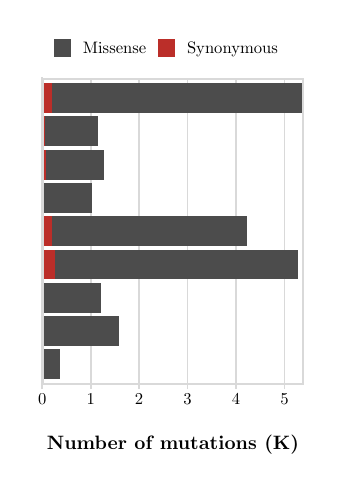
\begin{tikzpicture}[x=1pt,y=1pt]
\definecolor{fillColor}{RGB}{255,255,255}
\path[use as bounding box,fill=fillColor,fill opacity=0.00] (0,0) rectangle (103.28,157.19);
\begin{scope}
\path[clip] (  5.25, 28.30) rectangle ( 99.78,138.99);
\definecolor{drawColor}{gray}{0.85}

\path[draw=drawColor,line width= 0.6pt,line join=round] (  5.25, 28.30) --
	(  5.25,138.99);

\path[draw=drawColor,line width= 0.6pt,line join=round] ( 22.77, 28.30) --
	( 22.77,138.99);

\path[draw=drawColor,line width= 0.6pt,line join=round] ( 40.28, 28.30) --
	( 40.28,138.99);

\path[draw=drawColor,line width= 0.6pt,line join=round] ( 57.80, 28.30) --
	( 57.80,138.99);

\path[draw=drawColor,line width= 0.6pt,line join=round] ( 75.31, 28.30) --
	( 75.31,138.99);

\path[draw=drawColor,line width= 0.6pt,line join=round] ( 92.83, 28.30) --
	( 92.83,138.99);
\definecolor{fillColor}{gray}{0.30}

\path[fill=fillColor] (  8.74,126.36) rectangle ( 99.78,137.18);
\definecolor{fillColor}{RGB}{187,46,41}

\path[fill=fillColor] (  5.25,126.36) rectangle (  8.74,137.18);
\definecolor{fillColor}{gray}{0.30}

\path[fill=fillColor] (  6.25,114.33) rectangle ( 25.25,125.15);
\definecolor{fillColor}{RGB}{187,46,41}

\path[fill=fillColor] (  5.25,114.33) rectangle (  6.25,125.15);
\definecolor{fillColor}{gray}{0.30}

\path[fill=fillColor] (  6.56,102.29) rectangle ( 27.44,113.12);
\definecolor{fillColor}{RGB}{187,46,41}

\path[fill=fillColor] (  5.25,102.29) rectangle (  6.56,113.12);
\definecolor{fillColor}{gray}{0.30}

\path[fill=fillColor] (  5.25, 90.26) rectangle ( 23.22,101.09);

\path[fill=fillColor] (  8.93, 78.23) rectangle ( 79.36, 89.06);
\definecolor{fillColor}{RGB}{187,46,41}

\path[fill=fillColor] (  5.25, 78.23) rectangle (  8.93, 89.06);
\definecolor{fillColor}{gray}{0.30}

\path[fill=fillColor] (  9.87, 66.20) rectangle ( 97.73, 77.03);
\definecolor{fillColor}{RGB}{187,46,41}

\path[fill=fillColor] (  5.25, 66.20) rectangle (  9.87, 77.03);
\definecolor{fillColor}{gray}{0.30}

\path[fill=fillColor] (  5.81, 54.17) rectangle ( 26.62, 65.00);
\definecolor{fillColor}{RGB}{187,46,41}

\path[fill=fillColor] (  5.25, 54.17) rectangle (  5.81, 65.00);
\definecolor{fillColor}{gray}{0.30}

\path[fill=fillColor] (  5.25, 42.14) rectangle ( 32.87, 52.97);

\path[fill=fillColor] (  5.43, 30.11) rectangle ( 11.78, 40.94);
\definecolor{fillColor}{RGB}{187,46,41}

\path[fill=fillColor] (  5.25, 30.11) rectangle (  5.43, 40.94);

\path[draw=drawColor,line width= 1.1pt,line join=round,line cap=round] (  5.25, 28.30) rectangle ( 99.78,138.99);
\end{scope}
\begin{scope}
\path[clip] (  0.00,  0.00) rectangle (103.28,157.19);
\definecolor{drawColor}{gray}{0.85}

\path[draw=drawColor,line width= 0.6pt,line join=round,line cap=rect] (  5.25, 28.30) --
	(  5.25,138.99);
\end{scope}
\begin{scope}
\path[clip] (  0.00,  0.00) rectangle (103.28,157.19);
\definecolor{drawColor}{gray}{0.85}

\path[draw=drawColor,line width= 0.6pt,line join=round] (  5.25, 26.55) --
	(  5.25, 28.30);

\path[draw=drawColor,line width= 0.6pt,line join=round] ( 22.77, 26.55) --
	( 22.77, 28.30);

\path[draw=drawColor,line width= 0.6pt,line join=round] ( 40.28, 26.55) --
	( 40.28, 28.30);

\path[draw=drawColor,line width= 0.6pt,line join=round] ( 57.80, 26.55) --
	( 57.80, 28.30);

\path[draw=drawColor,line width= 0.6pt,line join=round] ( 75.31, 26.55) --
	( 75.31, 28.30);

\path[draw=drawColor,line width= 0.6pt,line join=round] ( 92.83, 26.55) --
	( 92.83, 28.30);
\end{scope}
\begin{scope}
\path[clip] (  0.00,  0.00) rectangle (103.28,157.19);
\definecolor{drawColor}{RGB}{0,0,0}

\node[text=drawColor,anchor=base,inner sep=0pt, outer sep=0pt, scale=  0.60] at (  5.25, 20.92) {0};

\node[text=drawColor,anchor=base,inner sep=0pt, outer sep=0pt, scale=  0.60] at ( 22.77, 20.92) {1};

\node[text=drawColor,anchor=base,inner sep=0pt, outer sep=0pt, scale=  0.60] at ( 40.28, 20.92) {2};

\node[text=drawColor,anchor=base,inner sep=0pt, outer sep=0pt, scale=  0.60] at ( 57.80, 20.92) {3};

\node[text=drawColor,anchor=base,inner sep=0pt, outer sep=0pt, scale=  0.60] at ( 75.31, 20.92) {4};

\node[text=drawColor,anchor=base,inner sep=0pt, outer sep=0pt, scale=  0.60] at ( 92.83, 20.92) {5};
\end{scope}
\begin{scope}
\path[clip] (  0.00,  0.00) rectangle (103.28,157.19);
\definecolor{drawColor}{RGB}{0,0,0}

\node[text=drawColor,anchor=base,inner sep=0pt, outer sep=0pt, scale=  0.70] at ( 52.51,  4.86) {\bfseries Number of mutations (K)};
\end{scope}
\begin{scope}
\path[clip] (  0.00,  0.00) rectangle (103.28,157.19);
\definecolor{fillColor}{gray}{0.30}

\path[fill=fillColor] (  9.46,146.70) rectangle ( 15.74,152.98);
\end{scope}
\begin{scope}
\path[clip] (  0.00,  0.00) rectangle (103.28,157.19);
\definecolor{fillColor}{RGB}{187,46,41}

\path[fill=fillColor] ( 47.10,146.70) rectangle ( 53.37,152.98);
\end{scope}
\begin{scope}
\path[clip] (  0.00,  0.00) rectangle (103.28,157.19);
\definecolor{drawColor}{RGB}{0,0,0}

\node[text=drawColor,anchor=base west,inner sep=0pt, outer sep=0pt, scale=  0.60] at ( 19.95,147.77) {Missense};
\end{scope}
\begin{scope}
\path[clip] (  0.00,  0.00) rectangle (103.28,157.19);
\definecolor{drawColor}{RGB}{0,0,0}

\node[text=drawColor,anchor=base west,inner sep=0pt, outer sep=0pt, scale=  0.60] at ( 57.58,147.77) {Synonymous};
\end{scope}
\end{tikzpicture}

	}
\end{frame}

\begin{frame}
	\frametitle{Agreement among Experimental Results}
	Two independent deep mutational scanning experiments on Ubiquitin are present in the training dataset.
	Their correlation is low.
	\vfill%
	\centering%
	{%
		\let\bfseries\sbseries%
		% Created by tikzDevice version 0.12.3.1 on 2021-07-04 15:02:22
% !TEX encoding = UTF-8 Unicode
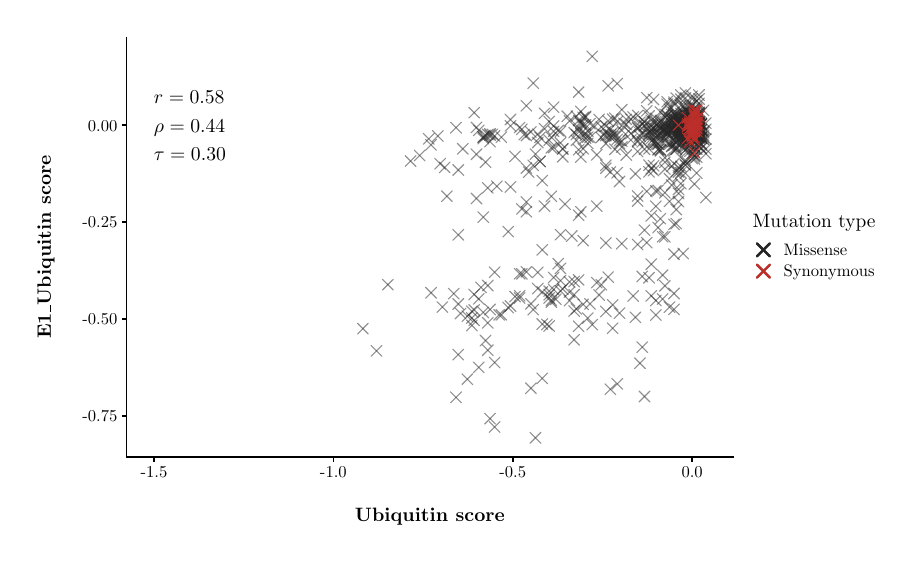
\begin{tikzpicture}[x=1pt,y=1pt]
\definecolor{fillColor}{RGB}{255,255,255}
\path[use as bounding box,fill=fillColor,fill opacity=0.00] (0,0) rectangle (309.84,183.39);
\begin{scope}
\path[clip] ( 35.67, 28.30) rectangle (255.00,179.89);
\definecolor{drawColor}{RGB}{38,38,38}

\path[draw=drawColor,draw opacity=0.50,line width= 0.4pt,line join=round,line cap=round] (202.04,171.04) -- (205.97,174.96);

\path[draw=drawColor,draw opacity=0.50,line width= 0.4pt,line join=round,line cap=round] (202.04,174.96) -- (205.97,171.04);

\path[draw=drawColor,draw opacity=0.50,line width= 0.4pt,line join=round,line cap=round] (180.71,161.38) -- (184.63,165.30);

\path[draw=drawColor,draw opacity=0.50,line width= 0.4pt,line join=round,line cap=round] (180.71,165.30) -- (184.63,161.38);

\path[draw=drawColor,draw opacity=0.50,line width= 0.4pt,line join=round,line cap=round] (211.07,161.20) -- (214.99,165.12);

\path[draw=drawColor,draw opacity=0.50,line width= 0.4pt,line join=round,line cap=round] (211.07,165.12) -- (214.99,161.20);

\path[draw=drawColor,draw opacity=0.50,line width= 0.4pt,line join=round,line cap=round] (207.79,160.43) -- (211.71,164.35);

\path[draw=drawColor,draw opacity=0.50,line width= 0.4pt,line join=round,line cap=round] (207.79,164.35) -- (211.71,160.43);

\path[draw=drawColor,draw opacity=0.50,line width= 0.4pt,line join=round,line cap=round] (159.38,150.72) -- (163.30,154.64);

\path[draw=drawColor,draw opacity=0.50,line width= 0.4pt,line join=round,line cap=round] (159.38,154.64) -- (163.30,150.72);

\path[draw=drawColor,draw opacity=0.50,line width= 0.4pt,line join=round,line cap=round] (164.30,123.52) -- (168.22,127.45);

\path[draw=drawColor,draw opacity=0.50,line width= 0.4pt,line join=round,line cap=round] (164.30,127.45) -- (168.22,123.52);

\path[draw=drawColor,draw opacity=0.50,line width= 0.4pt,line join=round,line cap=round] (197.12,158.14) -- (201.05,162.07);

\path[draw=drawColor,draw opacity=0.50,line width= 0.4pt,line join=round,line cap=round] (197.12,162.07) -- (201.05,158.14);

\path[draw=drawColor,draw opacity=0.50,line width= 0.4pt,line join=round,line cap=round] (229.94,151.95) -- (233.87,155.88);

\path[draw=drawColor,draw opacity=0.50,line width= 0.4pt,line join=round,line cap=round] (229.94,155.88) -- (233.87,151.95);

\path[draw=drawColor,draw opacity=0.50,line width= 0.4pt,line join=round,line cap=round] (221.74,151.35) -- (225.66,155.28);

\path[draw=drawColor,draw opacity=0.50,line width= 0.4pt,line join=round,line cap=round] (221.74,155.28) -- (225.66,151.35);

\path[draw=drawColor,draw opacity=0.50,line width= 0.4pt,line join=round,line cap=round] (231.58,148.52) -- (235.51,152.45);

\path[draw=drawColor,draw opacity=0.50,line width= 0.4pt,line join=round,line cap=round] (231.58,152.45) -- (235.51,148.52);

\path[draw=drawColor,draw opacity=0.50,line width= 0.4pt,line join=round,line cap=round] (226.66,147.87) -- (230.58,151.79);

\path[draw=drawColor,draw opacity=0.50,line width= 0.4pt,line join=round,line cap=round] (226.66,151.79) -- (230.58,147.87);

\path[draw=drawColor,draw opacity=0.50,line width= 0.4pt,line join=round,line cap=round] (219.28,147.29) -- (223.20,151.21);

\path[draw=drawColor,draw opacity=0.50,line width= 0.4pt,line join=round,line cap=round] (219.28,151.21) -- (223.20,147.29);

\path[draw=drawColor,draw opacity=0.50,line width= 0.4pt,line join=round,line cap=round] (238.15,146.74) -- (242.07,150.66);

\path[draw=drawColor,draw opacity=0.50,line width= 0.4pt,line join=round,line cap=round] (238.15,150.66) -- (242.07,146.74);

\path[draw=drawColor,draw opacity=0.50,line width= 0.4pt,line join=round,line cap=round] (234.05,145.51) -- (237.97,149.44);

\path[draw=drawColor,draw opacity=0.50,line width= 0.4pt,line join=round,line cap=round] (234.05,149.44) -- (237.97,145.51);

\path[draw=drawColor,draw opacity=0.50,line width= 0.4pt,line join=round,line cap=round] (240.61,144.98) -- (244.53,148.90);

\path[draw=drawColor,draw opacity=0.50,line width= 0.4pt,line join=round,line cap=round] (240.61,148.90) -- (244.53,144.98);

\path[draw=drawColor,draw opacity=0.50,line width= 0.4pt,line join=round,line cap=round] (212.71,144.27) -- (216.64,148.20);

\path[draw=drawColor,draw opacity=0.50,line width= 0.4pt,line join=round,line cap=round] (212.71,148.20) -- (216.64,144.27);

\path[draw=drawColor,draw opacity=0.50,line width= 0.4pt,line join=round,line cap=round] (209.43,143.54) -- (213.35,147.46);

\path[draw=drawColor,draw opacity=0.50,line width= 0.4pt,line join=round,line cap=round] (209.43,147.46) -- (213.35,143.54);

\path[draw=drawColor,draw opacity=0.50,line width= 0.4pt,line join=round,line cap=round] (234.05,143.50) -- (237.97,147.43);

\path[draw=drawColor,draw opacity=0.50,line width= 0.4pt,line join=round,line cap=round] (234.05,147.43) -- (237.97,143.50);

\path[draw=drawColor,draw opacity=0.50,line width= 0.4pt,line join=round,line cap=round] (232.40,143.03) -- (236.33,146.96);

\path[draw=drawColor,draw opacity=0.50,line width= 0.4pt,line join=round,line cap=round] (232.40,146.96) -- (236.33,143.03);

\path[draw=drawColor,draw opacity=0.50,line width= 0.4pt,line join=round,line cap=round] (229.12,142.83) -- (233.05,146.75);

\path[draw=drawColor,draw opacity=0.50,line width= 0.4pt,line join=round,line cap=round] (229.12,146.75) -- (233.05,142.83);

\path[draw=drawColor,draw opacity=0.50,line width= 0.4pt,line join=round,line cap=round] (227.48,142.50) -- (231.41,146.42);

\path[draw=drawColor,draw opacity=0.50,line width= 0.4pt,line join=round,line cap=round] (227.48,146.42) -- (231.41,142.50);

\path[draw=drawColor,draw opacity=0.50,line width= 0.4pt,line join=round,line cap=round] (219.28,142.27) -- (223.20,146.20);

\path[draw=drawColor,draw opacity=0.50,line width= 0.4pt,line join=round,line cap=round] (219.28,146.20) -- (223.20,142.27);

\path[draw=drawColor,draw opacity=0.50,line width= 0.4pt,line join=round,line cap=round] (200.40,141.88) -- (204.33,145.81);

\path[draw=drawColor,draw opacity=0.50,line width= 0.4pt,line join=round,line cap=round] (200.40,145.81) -- (204.33,141.88);

\path[draw=drawColor,draw opacity=0.50,line width= 0.4pt,line join=round,line cap=round] (235.69,157.83) -- (239.61,161.76);

\path[draw=drawColor,draw opacity=0.50,line width= 0.4pt,line join=round,line cap=round] (235.69,161.76) -- (239.61,157.83);

\path[draw=drawColor,draw opacity=0.50,line width= 0.4pt,line join=round,line cap=round] (237.33,150.15) -- (241.25,154.07);

\path[draw=drawColor,draw opacity=0.50,line width= 0.4pt,line join=round,line cap=round] (237.33,154.07) -- (241.25,150.15);

\path[draw=drawColor,draw opacity=0.50,line width= 0.4pt,line join=round,line cap=round] (230.76,150.09) -- (234.69,154.02);

\path[draw=drawColor,draw opacity=0.50,line width= 0.4pt,line join=round,line cap=round] (230.76,154.02) -- (234.69,150.09);

\path[draw=drawColor,draw opacity=0.50,line width= 0.4pt,line join=round,line cap=round] (233.22,149.74) -- (237.15,153.67);

\path[draw=drawColor,draw opacity=0.50,line width= 0.4pt,line join=round,line cap=round] (233.22,153.67) -- (237.15,149.74);

\path[draw=drawColor,draw opacity=0.50,line width= 0.4pt,line join=round,line cap=round] (240.61,149.34) -- (244.53,153.26);

\path[draw=drawColor,draw opacity=0.50,line width= 0.4pt,line join=round,line cap=round] (240.61,153.26) -- (244.53,149.34);

\path[draw=drawColor,draw opacity=0.50,line width= 0.4pt,line join=round,line cap=round] (239.79,148.48) -- (243.71,152.40);

\path[draw=drawColor,draw opacity=0.50,line width= 0.4pt,line join=round,line cap=round] (239.79,152.40) -- (243.71,148.48);

\path[draw=drawColor,draw opacity=0.50,line width= 0.4pt,line join=round,line cap=round] (239.79,148.20) -- (243.71,152.13);

\path[draw=drawColor,draw opacity=0.50,line width= 0.4pt,line join=round,line cap=round] (239.79,152.13) -- (243.71,148.20);

\path[draw=drawColor,draw opacity=0.50,line width= 0.4pt,line join=round,line cap=round] (239.79,148.13) -- (243.71,152.05);

\path[draw=drawColor,draw opacity=0.50,line width= 0.4pt,line join=round,line cap=round] (239.79,152.05) -- (243.71,148.13);

\path[draw=drawColor,draw opacity=0.50,line width= 0.4pt,line join=round,line cap=round] (240.61,147.25) -- (244.53,151.17);

\path[draw=drawColor,draw opacity=0.50,line width= 0.4pt,line join=round,line cap=round] (240.61,151.17) -- (244.53,147.25);

\path[draw=drawColor,draw opacity=0.50,line width= 0.4pt,line join=round,line cap=round] (238.97,146.93) -- (242.89,150.85);

\path[draw=drawColor,draw opacity=0.50,line width= 0.4pt,line join=round,line cap=round] (238.97,150.85) -- (242.89,146.93);

\path[draw=drawColor,draw opacity=0.50,line width= 0.4pt,line join=round,line cap=round] (240.61,146.85) -- (244.53,150.78);

\path[draw=drawColor,draw opacity=0.50,line width= 0.4pt,line join=round,line cap=round] (240.61,150.78) -- (244.53,146.85);

\path[draw=drawColor,draw opacity=0.50,line width= 0.4pt,line join=round,line cap=round] (241.43,146.72) -- (245.35,150.65);

\path[draw=drawColor,draw opacity=0.50,line width= 0.4pt,line join=round,line cap=round] (241.43,150.65) -- (245.35,146.72);

\path[draw=drawColor,draw opacity=0.50,line width= 0.4pt,line join=round,line cap=round] (240.61,146.71) -- (244.53,150.64);

\path[draw=drawColor,draw opacity=0.50,line width= 0.4pt,line join=round,line cap=round] (240.61,150.64) -- (244.53,146.71);

\path[draw=drawColor,draw opacity=0.50,line width= 0.4pt,line join=round,line cap=round] (241.43,146.71) -- (245.35,150.63);

\path[draw=drawColor,draw opacity=0.50,line width= 0.4pt,line join=round,line cap=round] (241.43,150.63) -- (245.35,146.71);

\path[draw=drawColor,draw opacity=0.50,line width= 0.4pt,line join=round,line cap=round] (239.79,146.62) -- (243.71,150.54);

\path[draw=drawColor,draw opacity=0.50,line width= 0.4pt,line join=round,line cap=round] (239.79,150.54) -- (243.71,146.62);

\path[draw=drawColor,draw opacity=0.50,line width= 0.4pt,line join=round,line cap=round] (238.97,146.07) -- (242.89,150.00);

\path[draw=drawColor,draw opacity=0.50,line width= 0.4pt,line join=round,line cap=round] (238.97,150.00) -- (242.89,146.07);

\path[draw=drawColor,draw opacity=0.50,line width= 0.4pt,line join=round,line cap=round] (240.61,145.11) -- (244.53,149.03);

\path[draw=drawColor,draw opacity=0.50,line width= 0.4pt,line join=round,line cap=round] (240.61,149.03) -- (244.53,145.11);

\path[draw=drawColor,draw opacity=0.50,line width= 0.4pt,line join=round,line cap=round] (238.97,144.08) -- (242.89,148.00);

\path[draw=drawColor,draw opacity=0.50,line width= 0.4pt,line join=round,line cap=round] (238.97,148.00) -- (242.89,144.08);

\path[draw=drawColor,draw opacity=0.50,line width= 0.4pt,line join=round,line cap=round] (241.43,142.12) -- (245.35,146.05);

\path[draw=drawColor,draw opacity=0.50,line width= 0.4pt,line join=round,line cap=round] (241.43,146.05) -- (245.35,142.12);

\path[draw=drawColor,draw opacity=0.50,line width= 0.4pt,line join=round,line cap=round] (234.05,157.09) -- (237.97,161.01);

\path[draw=drawColor,draw opacity=0.50,line width= 0.4pt,line join=round,line cap=round] (234.05,161.01) -- (237.97,157.09);

\path[draw=drawColor,draw opacity=0.50,line width= 0.4pt,line join=round,line cap=round] (178.25,153.23) -- (182.17,157.16);

\path[draw=drawColor,draw opacity=0.50,line width= 0.4pt,line join=round,line cap=round] (178.25,157.16) -- (182.17,153.23);

\path[draw=drawColor,draw opacity=0.50,line width= 0.4pt,line join=round,line cap=round] (188.09,152.66) -- (192.02,156.58);

\path[draw=drawColor,draw opacity=0.50,line width= 0.4pt,line join=round,line cap=round] (188.09,156.58) -- (192.02,152.66);

\path[draw=drawColor,draw opacity=0.50,line width= 0.4pt,line join=round,line cap=round] (184.81,150.48) -- (188.74,154.40);

\path[draw=drawColor,draw opacity=0.50,line width= 0.4pt,line join=round,line cap=round] (184.81,154.40) -- (188.74,150.48);

\path[draw=drawColor,draw opacity=0.50,line width= 0.4pt,line join=round,line cap=round] (232.40,149.69) -- (236.33,153.61);

\path[draw=drawColor,draw opacity=0.50,line width= 0.4pt,line join=round,line cap=round] (232.40,153.61) -- (236.33,149.69);

\path[draw=drawColor,draw opacity=0.50,line width= 0.4pt,line join=round,line cap=round] (193.02,149.41) -- (196.94,153.34);

\path[draw=drawColor,draw opacity=0.50,line width= 0.4pt,line join=round,line cap=round] (193.02,153.34) -- (196.94,149.41);

\path[draw=drawColor,draw opacity=0.50,line width= 0.4pt,line join=round,line cap=round] (198.76,148.96) -- (202.69,152.89);

\path[draw=drawColor,draw opacity=0.50,line width= 0.4pt,line join=round,line cap=round] (198.76,152.89) -- (202.69,148.96);

\path[draw=drawColor,draw opacity=0.50,line width= 0.4pt,line join=round,line cap=round] (210.25,148.68) -- (214.17,152.60);

\path[draw=drawColor,draw opacity=0.50,line width= 0.4pt,line join=round,line cap=round] (210.25,152.60) -- (214.17,148.68);

\path[draw=drawColor,draw opacity=0.50,line width= 0.4pt,line join=round,line cap=round] (209.43,148.34) -- (213.35,152.27);

\path[draw=drawColor,draw opacity=0.50,line width= 0.4pt,line join=round,line cap=round] (209.43,152.27) -- (213.35,148.34);

\path[draw=drawColor,draw opacity=0.50,line width= 0.4pt,line join=round,line cap=round] (214.35,148.30) -- (218.28,152.22);

\path[draw=drawColor,draw opacity=0.50,line width= 0.4pt,line join=round,line cap=round] (214.35,152.22) -- (218.28,148.30);

\path[draw=drawColor,draw opacity=0.50,line width= 0.4pt,line join=round,line cap=round] (172.50,148.23) -- (176.43,152.16);

\path[draw=drawColor,draw opacity=0.50,line width= 0.4pt,line join=round,line cap=round] (172.50,152.16) -- (176.43,148.23);

\path[draw=drawColor,draw opacity=0.50,line width= 0.4pt,line join=round,line cap=round] (186.45,147.51) -- (190.38,151.44);

\path[draw=drawColor,draw opacity=0.50,line width= 0.4pt,line join=round,line cap=round] (186.45,151.44) -- (190.38,147.51);

\path[draw=drawColor,draw opacity=0.50,line width= 0.4pt,line join=round,line cap=round] (206.97,145.92) -- (210.89,149.85);

\path[draw=drawColor,draw opacity=0.50,line width= 0.4pt,line join=round,line cap=round] (206.97,149.85) -- (210.89,145.92);

\path[draw=drawColor,draw opacity=0.50,line width= 0.4pt,line join=round,line cap=round] (179.89,143.73) -- (183.81,147.66);

\path[draw=drawColor,draw opacity=0.50,line width= 0.4pt,line join=round,line cap=round] (179.89,147.66) -- (183.81,143.73);

\path[draw=drawColor,draw opacity=0.50,line width= 0.4pt,line join=round,line cap=round] (169.22,141.84) -- (173.15,145.77);

\path[draw=drawColor,draw opacity=0.50,line width= 0.4pt,line join=round,line cap=round] (169.22,145.77) -- (173.15,141.84);

\path[draw=drawColor,draw opacity=0.50,line width= 0.4pt,line join=round,line cap=round] (240.61,157.08) -- (244.53,161.01);

\path[draw=drawColor,draw opacity=0.50,line width= 0.4pt,line join=round,line cap=round] (240.61,161.01) -- (244.53,157.08);

\path[draw=drawColor,draw opacity=0.50,line width= 0.4pt,line join=round,line cap=round] (238.15,156.68) -- (242.07,160.60);

\path[draw=drawColor,draw opacity=0.50,line width= 0.4pt,line join=round,line cap=round] (238.15,160.60) -- (242.07,156.68);

\path[draw=drawColor,draw opacity=0.50,line width= 0.4pt,line join=round,line cap=round] (235.69,156.01) -- (239.61,159.93);

\path[draw=drawColor,draw opacity=0.50,line width= 0.4pt,line join=round,line cap=round] (235.69,159.93) -- (239.61,156.01);

\path[draw=drawColor,draw opacity=0.50,line width= 0.4pt,line join=round,line cap=round] (238.15,155.72) -- (242.07,159.64);

\path[draw=drawColor,draw opacity=0.50,line width= 0.4pt,line join=round,line cap=round] (238.15,159.64) -- (242.07,155.72);

\path[draw=drawColor,draw opacity=0.50,line width= 0.4pt,line join=round,line cap=round] (229.12,153.73) -- (233.05,157.66);

\path[draw=drawColor,draw opacity=0.50,line width= 0.4pt,line join=round,line cap=round] (229.12,157.66) -- (233.05,153.73);

\path[draw=drawColor,draw opacity=0.50,line width= 0.4pt,line join=round,line cap=round] (238.15,153.31) -- (242.07,157.24);

\path[draw=drawColor,draw opacity=0.50,line width= 0.4pt,line join=round,line cap=round] (238.15,157.24) -- (242.07,153.31);

\path[draw=drawColor,draw opacity=0.50,line width= 0.4pt,line join=round,line cap=round] (237.33,152.47) -- (241.25,156.39);

\path[draw=drawColor,draw opacity=0.50,line width= 0.4pt,line join=round,line cap=round] (237.33,156.39) -- (241.25,152.47);

\path[draw=drawColor,draw opacity=0.50,line width= 0.4pt,line join=round,line cap=round] (237.33,151.94) -- (241.25,155.86);

\path[draw=drawColor,draw opacity=0.50,line width= 0.4pt,line join=round,line cap=round] (237.33,155.86) -- (241.25,151.94);

\path[draw=drawColor,draw opacity=0.50,line width= 0.4pt,line join=round,line cap=round] (240.61,150.68) -- (244.53,154.61);

\path[draw=drawColor,draw opacity=0.50,line width= 0.4pt,line join=round,line cap=round] (240.61,154.61) -- (244.53,150.68);

\path[draw=drawColor,draw opacity=0.50,line width= 0.4pt,line join=round,line cap=round] (237.33,150.45) -- (241.25,154.37);

\path[draw=drawColor,draw opacity=0.50,line width= 0.4pt,line join=round,line cap=round] (237.33,154.37) -- (241.25,150.45);

\path[draw=drawColor,draw opacity=0.50,line width= 0.4pt,line join=round,line cap=round] (240.61,150.26) -- (244.53,154.18);

\path[draw=drawColor,draw opacity=0.50,line width= 0.4pt,line join=round,line cap=round] (240.61,154.18) -- (244.53,150.26);

\path[draw=drawColor,draw opacity=0.50,line width= 0.4pt,line join=round,line cap=round] (238.15,150.05) -- (242.07,153.98);

\path[draw=drawColor,draw opacity=0.50,line width= 0.4pt,line join=round,line cap=round] (238.15,153.98) -- (242.07,150.05);

\path[draw=drawColor,draw opacity=0.50,line width= 0.4pt,line join=round,line cap=round] (235.69,149.68) -- (239.61,153.61);

\path[draw=drawColor,draw opacity=0.50,line width= 0.4pt,line join=round,line cap=round] (235.69,153.61) -- (239.61,149.68);

\path[draw=drawColor,draw opacity=0.50,line width= 0.4pt,line join=round,line cap=round] (238.15,149.36) -- (242.07,153.29);

\path[draw=drawColor,draw opacity=0.50,line width= 0.4pt,line join=round,line cap=round] (238.15,153.29) -- (242.07,149.36);

\path[draw=drawColor,draw opacity=0.50,line width= 0.4pt,line join=round,line cap=round] (238.97,147.91) -- (242.89,151.84);

\path[draw=drawColor,draw opacity=0.50,line width= 0.4pt,line join=round,line cap=round] (238.97,151.84) -- (242.89,147.91);

\path[draw=drawColor,draw opacity=0.50,line width= 0.4pt,line join=round,line cap=round] (237.33,147.73) -- (241.25,151.66);

\path[draw=drawColor,draw opacity=0.50,line width= 0.4pt,line join=round,line cap=round] (237.33,151.66) -- (241.25,147.73);

\path[draw=drawColor,draw opacity=0.50,line width= 0.4pt,line join=round,line cap=round] (238.97,147.33) -- (242.89,151.26);

\path[draw=drawColor,draw opacity=0.50,line width= 0.4pt,line join=round,line cap=round] (238.97,151.26) -- (242.89,147.33);

\path[draw=drawColor,draw opacity=0.50,line width= 0.4pt,line join=round,line cap=round] (238.97,147.29) -- (242.89,151.21);

\path[draw=drawColor,draw opacity=0.50,line width= 0.4pt,line join=round,line cap=round] (238.97,151.21) -- (242.89,147.29);

\path[draw=drawColor,draw opacity=0.50,line width= 0.4pt,line join=round,line cap=round] (239.79,146.01) -- (243.71,149.93);

\path[draw=drawColor,draw opacity=0.50,line width= 0.4pt,line join=round,line cap=round] (239.79,149.93) -- (243.71,146.01);

\path[draw=drawColor,draw opacity=0.50,line width= 0.4pt,line join=round,line cap=round] (221.74,156.14) -- (225.66,160.07);

\path[draw=drawColor,draw opacity=0.50,line width= 0.4pt,line join=round,line cap=round] (221.74,160.07) -- (225.66,156.14);

\path[draw=drawColor,draw opacity=0.50,line width= 0.4pt,line join=round,line cap=round] (224.20,155.46) -- (228.12,159.39);

\path[draw=drawColor,draw opacity=0.50,line width= 0.4pt,line join=round,line cap=round] (224.20,159.39) -- (228.12,155.46);

\path[draw=drawColor,draw opacity=0.50,line width= 0.4pt,line join=round,line cap=round] (229.12,154.66) -- (233.05,158.59);

\path[draw=drawColor,draw opacity=0.50,line width= 0.4pt,line join=round,line cap=round] (229.12,158.59) -- (233.05,154.66);

\path[draw=drawColor,draw opacity=0.50,line width= 0.4pt,line join=round,line cap=round] (230.76,152.44) -- (234.69,156.37);

\path[draw=drawColor,draw opacity=0.50,line width= 0.4pt,line join=round,line cap=round] (230.76,156.37) -- (234.69,152.44);

\path[draw=drawColor,draw opacity=0.50,line width= 0.4pt,line join=round,line cap=round] (232.40,150.21) -- (236.33,154.13);

\path[draw=drawColor,draw opacity=0.50,line width= 0.4pt,line join=round,line cap=round] (232.40,154.13) -- (236.33,150.21);

\path[draw=drawColor,draw opacity=0.50,line width= 0.4pt,line join=round,line cap=round] (228.30,149.20) -- (232.23,153.12);

\path[draw=drawColor,draw opacity=0.50,line width= 0.4pt,line join=round,line cap=round] (228.30,153.12) -- (232.23,149.20);

\path[draw=drawColor,draw opacity=0.50,line width= 0.4pt,line join=round,line cap=round] (215.99,148.40) -- (219.92,152.32);

\path[draw=drawColor,draw opacity=0.50,line width= 0.4pt,line join=round,line cap=round] (215.99,152.32) -- (219.92,148.40);

\path[draw=drawColor,draw opacity=0.50,line width= 0.4pt,line join=round,line cap=round] (230.76,148.07) -- (234.69,152.00);

\path[draw=drawColor,draw opacity=0.50,line width= 0.4pt,line join=round,line cap=round] (230.76,152.00) -- (234.69,148.07);

\path[draw=drawColor,draw opacity=0.50,line width= 0.4pt,line join=round,line cap=round] (238.97,147.59) -- (242.89,151.52);

\path[draw=drawColor,draw opacity=0.50,line width= 0.4pt,line join=round,line cap=round] (238.97,151.52) -- (242.89,147.59);

\path[draw=drawColor,draw opacity=0.50,line width= 0.4pt,line join=round,line cap=round] (220.92,147.47) -- (224.84,151.39);

\path[draw=drawColor,draw opacity=0.50,line width= 0.4pt,line join=round,line cap=round] (220.92,151.39) -- (224.84,147.47);

\path[draw=drawColor,draw opacity=0.50,line width= 0.4pt,line join=round,line cap=round] (224.20,147.34) -- (228.12,151.27);

\path[draw=drawColor,draw opacity=0.50,line width= 0.4pt,line join=round,line cap=round] (224.20,151.27) -- (228.12,147.34);

\path[draw=drawColor,draw opacity=0.50,line width= 0.4pt,line join=round,line cap=round] (228.30,146.50) -- (232.23,150.42);

\path[draw=drawColor,draw opacity=0.50,line width= 0.4pt,line join=round,line cap=round] (228.30,150.42) -- (232.23,146.50);

\path[draw=drawColor,draw opacity=0.50,line width= 0.4pt,line join=round,line cap=round] (228.30,146.09) -- (232.23,150.02);

\path[draw=drawColor,draw opacity=0.50,line width= 0.4pt,line join=round,line cap=round] (228.30,150.02) -- (232.23,146.09);

\path[draw=drawColor,draw opacity=0.50,line width= 0.4pt,line join=round,line cap=round] (220.92,145.95) -- (224.84,149.87);

\path[draw=drawColor,draw opacity=0.50,line width= 0.4pt,line join=round,line cap=round] (220.92,149.87) -- (224.84,145.95);

\path[draw=drawColor,draw opacity=0.50,line width= 0.4pt,line join=round,line cap=round] (227.48,145.87) -- (231.41,149.80);

\path[draw=drawColor,draw opacity=0.50,line width= 0.4pt,line join=round,line cap=round] (227.48,149.80) -- (231.41,145.87);

\path[draw=drawColor,draw opacity=0.50,line width= 0.4pt,line join=round,line cap=round] (219.28,145.66) -- (223.20,149.58);

\path[draw=drawColor,draw opacity=0.50,line width= 0.4pt,line join=round,line cap=round] (219.28,149.58) -- (223.20,145.66);

\path[draw=drawColor,draw opacity=0.50,line width= 0.4pt,line join=round,line cap=round] (229.94,143.71) -- (233.87,147.64);

\path[draw=drawColor,draw opacity=0.50,line width= 0.4pt,line join=round,line cap=round] (229.94,147.64) -- (233.87,143.71);

\path[draw=drawColor,draw opacity=0.50,line width= 0.4pt,line join=round,line cap=round] (179.07,129.23) -- (182.99,133.15);

\path[draw=drawColor,draw opacity=0.50,line width= 0.4pt,line join=round,line cap=round] (179.07,133.15) -- (182.99,129.23);

\path[draw=drawColor,draw opacity=0.50,line width= 0.4pt,line join=round,line cap=round] (232.40,155.99) -- (236.33,159.91);

\path[draw=drawColor,draw opacity=0.50,line width= 0.4pt,line join=round,line cap=round] (232.40,159.91) -- (236.33,155.99);

\path[draw=drawColor,draw opacity=0.50,line width= 0.4pt,line join=round,line cap=round] (234.05,150.43) -- (237.97,154.35);

\path[draw=drawColor,draw opacity=0.50,line width= 0.4pt,line join=round,line cap=round] (234.05,154.35) -- (237.97,150.43);

\path[draw=drawColor,draw opacity=0.50,line width= 0.4pt,line join=round,line cap=round] (232.40,149.41) -- (236.33,153.34);

\path[draw=drawColor,draw opacity=0.50,line width= 0.4pt,line join=round,line cap=round] (232.40,153.34) -- (236.33,149.41);

\path[draw=drawColor,draw opacity=0.50,line width= 0.4pt,line join=round,line cap=round] (234.05,147.51) -- (237.97,151.43);

\path[draw=drawColor,draw opacity=0.50,line width= 0.4pt,line join=round,line cap=round] (234.05,151.43) -- (237.97,147.51);

\path[draw=drawColor,draw opacity=0.50,line width= 0.4pt,line join=round,line cap=round] (234.87,146.21) -- (238.79,150.14);

\path[draw=drawColor,draw opacity=0.50,line width= 0.4pt,line join=round,line cap=round] (234.87,150.14) -- (238.79,146.21);

\path[draw=drawColor,draw opacity=0.50,line width= 0.4pt,line join=round,line cap=round] (234.05,144.47) -- (237.97,148.39);

\path[draw=drawColor,draw opacity=0.50,line width= 0.4pt,line join=round,line cap=round] (234.05,148.39) -- (237.97,144.47);

\path[draw=drawColor,draw opacity=0.50,line width= 0.4pt,line join=round,line cap=round] (234.05,144.16) -- (237.97,148.09);

\path[draw=drawColor,draw opacity=0.50,line width= 0.4pt,line join=round,line cap=round] (234.05,148.09) -- (237.97,144.16);

\path[draw=drawColor,draw opacity=0.50,line width= 0.4pt,line join=round,line cap=round] (240.61,155.67) -- (244.53,159.60);

\path[draw=drawColor,draw opacity=0.50,line width= 0.4pt,line join=round,line cap=round] (240.61,159.60) -- (244.53,155.67);

\path[draw=drawColor,draw opacity=0.50,line width= 0.4pt,line join=round,line cap=round] (234.05,155.63) -- (237.97,159.55);

\path[draw=drawColor,draw opacity=0.50,line width= 0.4pt,line join=round,line cap=round] (234.05,159.55) -- (237.97,155.63);

\path[draw=drawColor,draw opacity=0.50,line width= 0.4pt,line join=round,line cap=round] (240.61,154.05) -- (244.53,157.97);

\path[draw=drawColor,draw opacity=0.50,line width= 0.4pt,line join=round,line cap=round] (240.61,157.97) -- (244.53,154.05);

\path[draw=drawColor,draw opacity=0.50,line width= 0.4pt,line join=round,line cap=round] (242.25,151.56) -- (246.18,155.48);

\path[draw=drawColor,draw opacity=0.50,line width= 0.4pt,line join=round,line cap=round] (242.25,155.48) -- (246.18,151.56);

\path[draw=drawColor,draw opacity=0.50,line width= 0.4pt,line join=round,line cap=round] (236.51,151.00) -- (240.43,154.92);

\path[draw=drawColor,draw opacity=0.50,line width= 0.4pt,line join=round,line cap=round] (236.51,154.92) -- (240.43,151.00);

\path[draw=drawColor,draw opacity=0.50,line width= 0.4pt,line join=round,line cap=round] (241.43,150.67) -- (245.35,154.59);

\path[draw=drawColor,draw opacity=0.50,line width= 0.4pt,line join=round,line cap=round] (241.43,154.59) -- (245.35,150.67);

\path[draw=drawColor,draw opacity=0.50,line width= 0.4pt,line join=round,line cap=round] (235.69,149.96) -- (239.61,153.89);

\path[draw=drawColor,draw opacity=0.50,line width= 0.4pt,line join=round,line cap=round] (235.69,153.89) -- (239.61,149.96);

\path[draw=drawColor,draw opacity=0.50,line width= 0.4pt,line join=round,line cap=round] (238.15,148.98) -- (242.07,152.90);

\path[draw=drawColor,draw opacity=0.50,line width= 0.4pt,line join=round,line cap=round] (238.15,152.90) -- (242.07,148.98);

\path[draw=drawColor,draw opacity=0.50,line width= 0.4pt,line join=round,line cap=round] (239.79,147.39) -- (243.71,151.31);

\path[draw=drawColor,draw opacity=0.50,line width= 0.4pt,line join=round,line cap=round] (239.79,151.31) -- (243.71,147.39);

\path[draw=drawColor,draw opacity=0.50,line width= 0.4pt,line join=round,line cap=round] (236.51,147.38) -- (240.43,151.30);

\path[draw=drawColor,draw opacity=0.50,line width= 0.4pt,line join=round,line cap=round] (236.51,151.30) -- (240.43,147.38);

\path[draw=drawColor,draw opacity=0.50,line width= 0.4pt,line join=round,line cap=round] (235.69,147.28) -- (239.61,151.21);

\path[draw=drawColor,draw opacity=0.50,line width= 0.4pt,line join=round,line cap=round] (235.69,151.21) -- (239.61,147.28);

\path[draw=drawColor,draw opacity=0.50,line width= 0.4pt,line join=round,line cap=round] (236.51,147.11) -- (240.43,151.03);

\path[draw=drawColor,draw opacity=0.50,line width= 0.4pt,line join=round,line cap=round] (236.51,151.03) -- (240.43,147.11);

\path[draw=drawColor,draw opacity=0.50,line width= 0.4pt,line join=round,line cap=round] (238.15,146.21) -- (242.07,150.13);

\path[draw=drawColor,draw opacity=0.50,line width= 0.4pt,line join=round,line cap=round] (238.15,150.13) -- (242.07,146.21);

\path[draw=drawColor,draw opacity=0.50,line width= 0.4pt,line join=round,line cap=round] (236.51,146.18) -- (240.43,150.11);

\path[draw=drawColor,draw opacity=0.50,line width= 0.4pt,line join=round,line cap=round] (236.51,150.11) -- (240.43,146.18);

\path[draw=drawColor,draw opacity=0.50,line width= 0.4pt,line join=round,line cap=round] (238.15,145.56) -- (242.07,149.48);

\path[draw=drawColor,draw opacity=0.50,line width= 0.4pt,line join=round,line cap=round] (238.15,149.48) -- (242.07,145.56);

\path[draw=drawColor,draw opacity=0.50,line width= 0.4pt,line join=round,line cap=round] (239.79,143.64) -- (243.71,147.56);

\path[draw=drawColor,draw opacity=0.50,line width= 0.4pt,line join=round,line cap=round] (239.79,147.56) -- (243.71,143.64);

\path[draw=drawColor,draw opacity=0.50,line width= 0.4pt,line join=round,line cap=round] (237.33,139.17) -- (241.25,143.10);

\path[draw=drawColor,draw opacity=0.50,line width= 0.4pt,line join=round,line cap=round] (237.33,143.10) -- (241.25,139.17);

\path[draw=drawColor,draw opacity=0.50,line width= 0.4pt,line join=round,line cap=round] (228.30,132.84) -- (232.23,136.77);

\path[draw=drawColor,draw opacity=0.50,line width= 0.4pt,line join=round,line cap=round] (228.30,136.77) -- (232.23,132.84);

\path[draw=drawColor,draw opacity=0.50,line width= 0.4pt,line join=round,line cap=round] (161.02, 58.69) -- (164.94, 62.61);

\path[draw=drawColor,draw opacity=0.50,line width= 0.4pt,line join=round,line cap=round] (161.02, 62.61) -- (164.94, 58.69);

\path[draw=drawColor,draw opacity=0.50,line width= 0.4pt,line join=round,line cap=round] (239.79,155.02) -- (243.71,158.94);

\path[draw=drawColor,draw opacity=0.50,line width= 0.4pt,line join=round,line cap=round] (239.79,158.94) -- (243.71,155.02);

\path[draw=drawColor,draw opacity=0.50,line width= 0.4pt,line join=round,line cap=round] (239.79,152.31) -- (243.71,156.24);

\path[draw=drawColor,draw opacity=0.50,line width= 0.4pt,line join=round,line cap=round] (239.79,156.24) -- (243.71,152.31);

\path[draw=drawColor,draw opacity=0.50,line width= 0.4pt,line join=round,line cap=round] (238.97,152.16) -- (242.89,156.08);

\path[draw=drawColor,draw opacity=0.50,line width= 0.4pt,line join=round,line cap=round] (238.97,156.08) -- (242.89,152.16);

\path[draw=drawColor,draw opacity=0.50,line width= 0.4pt,line join=round,line cap=round] (238.97,149.85) -- (242.89,153.78);

\path[draw=drawColor,draw opacity=0.50,line width= 0.4pt,line join=round,line cap=round] (238.97,153.78) -- (242.89,149.85);

\path[draw=drawColor,draw opacity=0.50,line width= 0.4pt,line join=round,line cap=round] (239.79,149.08) -- (243.71,153.01);

\path[draw=drawColor,draw opacity=0.50,line width= 0.4pt,line join=round,line cap=round] (239.79,153.01) -- (243.71,149.08);

\path[draw=drawColor,draw opacity=0.50,line width= 0.4pt,line join=round,line cap=round] (239.79,148.61) -- (243.71,152.53);

\path[draw=drawColor,draw opacity=0.50,line width= 0.4pt,line join=round,line cap=round] (239.79,152.53) -- (243.71,148.61);

\path[draw=drawColor,draw opacity=0.50,line width= 0.4pt,line join=round,line cap=round] (238.97,148.17) -- (242.89,152.10);

\path[draw=drawColor,draw opacity=0.50,line width= 0.4pt,line join=round,line cap=round] (238.97,152.10) -- (242.89,148.17);

\path[draw=drawColor,draw opacity=0.50,line width= 0.4pt,line join=round,line cap=round] (239.79,148.09) -- (243.71,152.01);

\path[draw=drawColor,draw opacity=0.50,line width= 0.4pt,line join=round,line cap=round] (239.79,152.01) -- (243.71,148.09);

\path[draw=drawColor,draw opacity=0.50,line width= 0.4pt,line join=round,line cap=round] (239.79,147.61) -- (243.71,151.53);

\path[draw=drawColor,draw opacity=0.50,line width= 0.4pt,line join=round,line cap=round] (239.79,151.53) -- (243.71,147.61);

\path[draw=drawColor,draw opacity=0.50,line width= 0.4pt,line join=round,line cap=round] (239.79,147.45) -- (243.71,151.38);

\path[draw=drawColor,draw opacity=0.50,line width= 0.4pt,line join=round,line cap=round] (239.79,151.38) -- (243.71,147.45);

\path[draw=drawColor,draw opacity=0.50,line width= 0.4pt,line join=round,line cap=round] (237.33,147.19) -- (241.25,151.12);

\path[draw=drawColor,draw opacity=0.50,line width= 0.4pt,line join=round,line cap=round] (237.33,151.12) -- (241.25,147.19);

\path[draw=drawColor,draw opacity=0.50,line width= 0.4pt,line join=round,line cap=round] (239.79,147.16) -- (243.71,151.08);

\path[draw=drawColor,draw opacity=0.50,line width= 0.4pt,line join=round,line cap=round] (239.79,151.08) -- (243.71,147.16);

\path[draw=drawColor,draw opacity=0.50,line width= 0.4pt,line join=round,line cap=round] (235.69,147.10) -- (239.61,151.02);

\path[draw=drawColor,draw opacity=0.50,line width= 0.4pt,line join=round,line cap=round] (235.69,151.02) -- (239.61,147.10);

\path[draw=drawColor,draw opacity=0.50,line width= 0.4pt,line join=round,line cap=round] (236.51,146.10) -- (240.43,150.03);

\path[draw=drawColor,draw opacity=0.50,line width= 0.4pt,line join=round,line cap=round] (236.51,150.03) -- (240.43,146.10);

\path[draw=drawColor,draw opacity=0.50,line width= 0.4pt,line join=round,line cap=round] (239.79,145.09) -- (243.71,149.02);

\path[draw=drawColor,draw opacity=0.50,line width= 0.4pt,line join=round,line cap=round] (239.79,149.02) -- (243.71,145.09);

\path[draw=drawColor,draw opacity=0.50,line width= 0.4pt,line join=round,line cap=round] (239.79,145.00) -- (243.71,148.93);

\path[draw=drawColor,draw opacity=0.50,line width= 0.4pt,line join=round,line cap=round] (239.79,148.93) -- (243.71,145.00);

\path[draw=drawColor,draw opacity=0.50,line width= 0.4pt,line join=round,line cap=round] (239.79,144.99) -- (243.71,148.92);

\path[draw=drawColor,draw opacity=0.50,line width= 0.4pt,line join=round,line cap=round] (239.79,148.92) -- (243.71,144.99);

\path[draw=drawColor,draw opacity=0.50,line width= 0.4pt,line join=round,line cap=round] (234.05,144.17) -- (237.97,148.10);

\path[draw=drawColor,draw opacity=0.50,line width= 0.4pt,line join=round,line cap=round] (234.05,148.10) -- (237.97,144.17);

\path[draw=drawColor,draw opacity=0.50,line width= 0.4pt,line join=round,line cap=round] (239.79,144.03) -- (243.71,147.95);

\path[draw=drawColor,draw opacity=0.50,line width= 0.4pt,line join=round,line cap=round] (239.79,147.95) -- (243.71,144.03);

\path[draw=drawColor,draw opacity=0.50,line width= 0.4pt,line join=round,line cap=round] (231.58,154.51) -- (235.51,158.43);

\path[draw=drawColor,draw opacity=0.50,line width= 0.4pt,line join=round,line cap=round] (231.58,158.43) -- (235.51,154.51);

\path[draw=drawColor,draw opacity=0.50,line width= 0.4pt,line join=round,line cap=round] (235.69,145.48) -- (239.61,149.41);

\path[draw=drawColor,draw opacity=0.50,line width= 0.4pt,line join=round,line cap=round] (235.69,149.41) -- (239.61,145.48);

\path[draw=drawColor,draw opacity=0.50,line width= 0.4pt,line join=round,line cap=round] (234.05,144.77) -- (237.97,148.69);

\path[draw=drawColor,draw opacity=0.50,line width= 0.4pt,line join=round,line cap=round] (234.05,148.69) -- (237.97,144.77);

\path[draw=drawColor,draw opacity=0.50,line width= 0.4pt,line join=round,line cap=round] (236.51,143.17) -- (240.43,147.10);

\path[draw=drawColor,draw opacity=0.50,line width= 0.4pt,line join=round,line cap=round] (236.51,147.10) -- (240.43,143.17);

\path[draw=drawColor,draw opacity=0.50,line width= 0.4pt,line join=round,line cap=round] (234.87,141.75) -- (238.79,145.68);

\path[draw=drawColor,draw opacity=0.50,line width= 0.4pt,line join=round,line cap=round] (234.87,145.68) -- (238.79,141.75);

\path[draw=drawColor,draw opacity=0.50,line width= 0.4pt,line join=round,line cap=round] (228.30,140.42) -- (232.23,144.34);

\path[draw=drawColor,draw opacity=0.50,line width= 0.4pt,line join=round,line cap=round] (228.30,144.34) -- (232.23,140.42);

\path[draw=drawColor,draw opacity=0.50,line width= 0.4pt,line join=round,line cap=round] (226.66,137.32) -- (230.58,141.25);

\path[draw=drawColor,draw opacity=0.50,line width= 0.4pt,line join=round,line cap=round] (226.66,141.25) -- (230.58,137.32);

\path[draw=drawColor,draw opacity=0.50,line width= 0.4pt,line join=round,line cap=round] (225.84,137.28) -- (229.76,141.21);

\path[draw=drawColor,draw opacity=0.50,line width= 0.4pt,line join=round,line cap=round] (225.84,141.21) -- (229.76,137.28);

\path[draw=drawColor,draw opacity=0.50,line width= 0.4pt,line join=round,line cap=round] (164.30, 88.25) -- (168.22, 92.17);

\path[draw=drawColor,draw opacity=0.50,line width= 0.4pt,line join=round,line cap=round] (164.30, 92.17) -- (168.22, 88.25);

\path[draw=drawColor,draw opacity=0.50,line width= 0.4pt,line join=round,line cap=round] (147.89, 80.47) -- (151.81, 84.39);

\path[draw=drawColor,draw opacity=0.50,line width= 0.4pt,line join=round,line cap=round] (147.89, 84.39) -- (151.81, 80.47);

\path[draw=drawColor,draw opacity=0.50,line width= 0.4pt,line join=round,line cap=round] (196.30, 79.80) -- (200.22, 83.72);

\path[draw=drawColor,draw opacity=0.50,line width= 0.4pt,line join=round,line cap=round] (196.30, 83.72) -- (200.22, 79.80);

\path[draw=drawColor,draw opacity=0.50,line width= 0.4pt,line join=round,line cap=round] (231.58,153.93) -- (235.51,157.85);

\path[draw=drawColor,draw opacity=0.50,line width= 0.4pt,line join=round,line cap=round] (231.58,157.85) -- (235.51,153.93);

\path[draw=drawColor,draw opacity=0.50,line width= 0.4pt,line join=round,line cap=round] (237.33,150.45) -- (241.25,154.38);

\path[draw=drawColor,draw opacity=0.50,line width= 0.4pt,line join=round,line cap=round] (237.33,154.38) -- (241.25,150.45);

\path[draw=drawColor,draw opacity=0.50,line width= 0.4pt,line join=round,line cap=round] (204.51,148.28) -- (208.43,152.21);

\path[draw=drawColor,draw opacity=0.50,line width= 0.4pt,line join=round,line cap=round] (204.51,152.21) -- (208.43,148.28);

\path[draw=drawColor,draw opacity=0.50,line width= 0.4pt,line join=round,line cap=round] (193.84,147.73) -- (197.76,151.65);

\path[draw=drawColor,draw opacity=0.50,line width= 0.4pt,line join=round,line cap=round] (193.84,151.65) -- (197.76,147.73);

\path[draw=drawColor,draw opacity=0.50,line width= 0.4pt,line join=round,line cap=round] (211.07,147.49) -- (214.99,151.41);

\path[draw=drawColor,draw opacity=0.50,line width= 0.4pt,line join=round,line cap=round] (211.07,151.41) -- (214.99,147.49);

\path[draw=drawColor,draw opacity=0.50,line width= 0.4pt,line join=round,line cap=round] (162.66,141.33) -- (166.58,145.25);

\path[draw=drawColor,draw opacity=0.50,line width= 0.4pt,line join=round,line cap=round] (162.66,145.25) -- (166.58,141.33);

\path[draw=drawColor,draw opacity=0.50,line width= 0.4pt,line join=round,line cap=round] (192.20,117.68) -- (196.12,121.61);

\path[draw=drawColor,draw opacity=0.50,line width= 0.4pt,line join=round,line cap=round] (192.20,121.61) -- (196.12,117.68);

\path[draw=drawColor,draw opacity=0.50,line width= 0.4pt,line join=round,line cap=round] (237.33,153.34) -- (241.25,157.27);

\path[draw=drawColor,draw opacity=0.50,line width= 0.4pt,line join=round,line cap=round] (237.33,157.27) -- (241.25,153.34);

\path[draw=drawColor,draw opacity=0.50,line width= 0.4pt,line join=round,line cap=round] (234.05,153.30) -- (237.97,157.23);

\path[draw=drawColor,draw opacity=0.50,line width= 0.4pt,line join=round,line cap=round] (234.05,157.23) -- (237.97,153.30);

\path[draw=drawColor,draw opacity=0.50,line width= 0.4pt,line join=round,line cap=round] (234.87,153.11) -- (238.79,157.04);

\path[draw=drawColor,draw opacity=0.50,line width= 0.4pt,line join=round,line cap=round] (234.87,157.04) -- (238.79,153.11);

\path[draw=drawColor,draw opacity=0.50,line width= 0.4pt,line join=round,line cap=round] (236.51,151.27) -- (240.43,155.19);

\path[draw=drawColor,draw opacity=0.50,line width= 0.4pt,line join=round,line cap=round] (236.51,155.19) -- (240.43,151.27);

\path[draw=drawColor,draw opacity=0.50,line width= 0.4pt,line join=round,line cap=round] (226.66,150.93) -- (230.58,154.86);

\path[draw=drawColor,draw opacity=0.50,line width= 0.4pt,line join=round,line cap=round] (226.66,154.86) -- (230.58,150.93);

\path[draw=drawColor,draw opacity=0.50,line width= 0.4pt,line join=round,line cap=round] (240.61,150.32) -- (244.53,154.24);

\path[draw=drawColor,draw opacity=0.50,line width= 0.4pt,line join=round,line cap=round] (240.61,154.24) -- (244.53,150.32);

\path[draw=drawColor,draw opacity=0.50,line width= 0.4pt,line join=round,line cap=round] (233.22,148.22) -- (237.15,152.14);

\path[draw=drawColor,draw opacity=0.50,line width= 0.4pt,line join=round,line cap=round] (233.22,152.14) -- (237.15,148.22);

\path[draw=drawColor,draw opacity=0.50,line width= 0.4pt,line join=round,line cap=round] (197.94,146.73) -- (201.87,150.65);

\path[draw=drawColor,draw opacity=0.50,line width= 0.4pt,line join=round,line cap=round] (197.94,150.65) -- (201.87,146.73);

\path[draw=drawColor,draw opacity=0.50,line width= 0.4pt,line join=round,line cap=round] (235.69,146.55) -- (239.61,150.47);

\path[draw=drawColor,draw opacity=0.50,line width= 0.4pt,line join=round,line cap=round] (235.69,150.47) -- (239.61,146.55);

\path[draw=drawColor,draw opacity=0.50,line width= 0.4pt,line join=round,line cap=round] (235.69,143.91) -- (239.61,147.84);

\path[draw=drawColor,draw opacity=0.50,line width= 0.4pt,line join=round,line cap=round] (235.69,147.84) -- (239.61,143.91);

\path[draw=drawColor,draw opacity=0.50,line width= 0.4pt,line join=round,line cap=round] (220.10,143.57) -- (224.02,147.49);

\path[draw=drawColor,draw opacity=0.50,line width= 0.4pt,line join=round,line cap=round] (220.10,147.49) -- (224.02,143.57);

\path[draw=drawColor,draw opacity=0.50,line width= 0.4pt,line join=round,line cap=round] (206.97,142.48) -- (210.89,146.41);

\path[draw=drawColor,draw opacity=0.50,line width= 0.4pt,line join=round,line cap=round] (206.97,146.41) -- (210.89,142.48);

\path[draw=drawColor,draw opacity=0.50,line width= 0.4pt,line join=round,line cap=round] (233.22,141.86) -- (237.15,145.79);

\path[draw=drawColor,draw opacity=0.50,line width= 0.4pt,line join=round,line cap=round] (233.22,145.79) -- (237.15,141.86);

\path[draw=drawColor,draw opacity=0.50,line width= 0.4pt,line join=round,line cap=round] (232.40,139.88) -- (236.33,143.81);

\path[draw=drawColor,draw opacity=0.50,line width= 0.4pt,line join=round,line cap=round] (232.40,143.81) -- (236.33,139.88);

\path[draw=drawColor,draw opacity=0.50,line width= 0.4pt,line join=round,line cap=round] (225.02,139.20) -- (228.94,143.12);

\path[draw=drawColor,draw opacity=0.50,line width= 0.4pt,line join=round,line cap=round] (225.02,143.12) -- (228.94,139.20);

\path[draw=drawColor,draw opacity=0.50,line width= 0.4pt,line join=round,line cap=round] (234.87,138.38) -- (238.79,142.31);

\path[draw=drawColor,draw opacity=0.50,line width= 0.4pt,line join=round,line cap=round] (234.87,142.31) -- (238.79,138.38);

\path[draw=drawColor,draw opacity=0.50,line width= 0.4pt,line join=round,line cap=round] (238.97,137.59) -- (242.89,141.52);

\path[draw=drawColor,draw opacity=0.50,line width= 0.4pt,line join=round,line cap=round] (238.97,141.52) -- (242.89,137.59);

\path[draw=drawColor,draw opacity=0.50,line width= 0.4pt,line join=round,line cap=round] (233.22,122.97) -- (237.15,126.90);

\path[draw=drawColor,draw opacity=0.50,line width= 0.4pt,line join=round,line cap=round] (233.22,126.90) -- (237.15,122.97);

\path[draw=drawColor,draw opacity=0.50,line width= 0.4pt,line join=round,line cap=round] (243.07,120.06) -- (247.00,123.99);

\path[draw=drawColor,draw opacity=0.50,line width= 0.4pt,line join=round,line cap=round] (243.07,123.99) -- (247.00,120.06);

\path[draw=drawColor,draw opacity=0.50,line width= 0.4pt,line join=round,line cap=round] (238.97,149.09) -- (242.89,153.01);

\path[draw=drawColor,draw opacity=0.50,line width= 0.4pt,line join=round,line cap=round] (238.97,153.01) -- (242.89,149.09);

\path[draw=drawColor,draw opacity=0.50,line width= 0.4pt,line join=round,line cap=round] (225.02,148.61) -- (228.94,152.53);

\path[draw=drawColor,draw opacity=0.50,line width= 0.4pt,line join=round,line cap=round] (225.02,152.53) -- (228.94,148.61);

\path[draw=drawColor,draw opacity=0.50,line width= 0.4pt,line join=round,line cap=round] (238.15,147.84) -- (242.07,151.76);

\path[draw=drawColor,draw opacity=0.50,line width= 0.4pt,line join=round,line cap=round] (238.15,151.76) -- (242.07,147.84);

\path[draw=drawColor,draw opacity=0.50,line width= 0.4pt,line join=round,line cap=round] (225.02,147.51) -- (228.94,151.43);

\path[draw=drawColor,draw opacity=0.50,line width= 0.4pt,line join=round,line cap=round] (225.02,151.43) -- (228.94,147.51);

\path[draw=drawColor,draw opacity=0.50,line width= 0.4pt,line join=round,line cap=round] (206.97,143.88) -- (210.89,147.81);

\path[draw=drawColor,draw opacity=0.50,line width= 0.4pt,line join=round,line cap=round] (206.97,147.81) -- (210.89,143.88);

\path[draw=drawColor,draw opacity=0.50,line width= 0.4pt,line join=round,line cap=round] (238.15,143.41) -- (242.07,147.33);

\path[draw=drawColor,draw opacity=0.50,line width= 0.4pt,line join=round,line cap=round] (238.15,147.33) -- (242.07,143.41);

\path[draw=drawColor,draw opacity=0.50,line width= 0.4pt,line join=round,line cap=round] (197.94,143.19) -- (201.87,147.11);

\path[draw=drawColor,draw opacity=0.50,line width= 0.4pt,line join=round,line cap=round] (197.94,147.11) -- (201.87,143.19);

\path[draw=drawColor,draw opacity=0.50,line width= 0.4pt,line join=round,line cap=round] (235.69,143.12) -- (239.61,147.04);

\path[draw=drawColor,draw opacity=0.50,line width= 0.4pt,line join=round,line cap=round] (235.69,147.04) -- (239.61,143.12);

\path[draw=drawColor,draw opacity=0.50,line width= 0.4pt,line join=round,line cap=round] (237.33,141.90) -- (241.25,145.82);

\path[draw=drawColor,draw opacity=0.50,line width= 0.4pt,line join=round,line cap=round] (237.33,145.82) -- (241.25,141.90);

\path[draw=drawColor,draw opacity=0.50,line width= 0.4pt,line join=round,line cap=round] (196.30,140.70) -- (200.22,144.63);

\path[draw=drawColor,draw opacity=0.50,line width= 0.4pt,line join=round,line cap=round] (196.30,144.63) -- (200.22,140.70);

\path[draw=drawColor,draw opacity=0.50,line width= 0.4pt,line join=round,line cap=round] (235.69,152.80) -- (239.61,156.72);

\path[draw=drawColor,draw opacity=0.50,line width= 0.4pt,line join=round,line cap=round] (235.69,156.72) -- (239.61,152.80);

\path[draw=drawColor,draw opacity=0.50,line width= 0.4pt,line join=round,line cap=round] (235.69,151.96) -- (239.61,155.89);

\path[draw=drawColor,draw opacity=0.50,line width= 0.4pt,line join=round,line cap=round] (235.69,155.89) -- (239.61,151.96);

\path[draw=drawColor,draw opacity=0.50,line width= 0.4pt,line join=round,line cap=round] (212.71,151.79) -- (216.64,155.71);

\path[draw=drawColor,draw opacity=0.50,line width= 0.4pt,line join=round,line cap=round] (212.71,155.71) -- (216.64,151.79);

\path[draw=drawColor,draw opacity=0.50,line width= 0.4pt,line join=round,line cap=round] (238.97,151.23) -- (242.89,155.15);

\path[draw=drawColor,draw opacity=0.50,line width= 0.4pt,line join=round,line cap=round] (238.97,155.15) -- (242.89,151.23);

\path[draw=drawColor,draw opacity=0.50,line width= 0.4pt,line join=round,line cap=round] (205.33,145.57) -- (209.25,149.49);

\path[draw=drawColor,draw opacity=0.50,line width= 0.4pt,line join=round,line cap=round] (205.33,149.49) -- (209.25,145.57);

\path[draw=drawColor,draw opacity=0.50,line width= 0.4pt,line join=round,line cap=round] (238.15,143.88) -- (242.07,147.81);

\path[draw=drawColor,draw opacity=0.50,line width= 0.4pt,line join=round,line cap=round] (238.15,147.81) -- (242.07,143.88);

\path[draw=drawColor,draw opacity=0.50,line width= 0.4pt,line join=round,line cap=round] (236.51,143.57) -- (240.43,147.50);

\path[draw=drawColor,draw opacity=0.50,line width= 0.4pt,line join=round,line cap=round] (236.51,147.50) -- (240.43,143.57);

\path[draw=drawColor,draw opacity=0.50,line width= 0.4pt,line join=round,line cap=round] (183.17,141.80) -- (187.10,145.72);

\path[draw=drawColor,draw opacity=0.50,line width= 0.4pt,line join=round,line cap=round] (183.17,145.72) -- (187.10,141.80);

\path[draw=drawColor,draw opacity=0.50,line width= 0.4pt,line join=round,line cap=round] (191.38,137.73) -- (195.30,141.66);

\path[draw=drawColor,draw opacity=0.50,line width= 0.4pt,line join=round,line cap=round] (191.38,141.66) -- (195.30,137.73);

\path[draw=drawColor,draw opacity=0.50,line width= 0.4pt,line join=round,line cap=round] (238.97,152.49) -- (242.89,156.41);

\path[draw=drawColor,draw opacity=0.50,line width= 0.4pt,line join=round,line cap=round] (238.97,156.41) -- (242.89,152.49);

\path[draw=drawColor,draw opacity=0.50,line width= 0.4pt,line join=round,line cap=round] (239.79,150.84) -- (243.71,154.76);

\path[draw=drawColor,draw opacity=0.50,line width= 0.4pt,line join=round,line cap=round] (239.79,154.76) -- (243.71,150.84);

\path[draw=drawColor,draw opacity=0.50,line width= 0.4pt,line join=round,line cap=round] (231.58,150.02) -- (235.51,153.95);

\path[draw=drawColor,draw opacity=0.50,line width= 0.4pt,line join=round,line cap=round] (231.58,153.95) -- (235.51,150.02);

\path[draw=drawColor,draw opacity=0.50,line width= 0.4pt,line join=round,line cap=round] (239.79,149.95) -- (243.71,153.88);

\path[draw=drawColor,draw opacity=0.50,line width= 0.4pt,line join=round,line cap=round] (239.79,153.88) -- (243.71,149.95);

\path[draw=drawColor,draw opacity=0.50,line width= 0.4pt,line join=round,line cap=round] (239.79,147.94) -- (243.71,151.87);

\path[draw=drawColor,draw opacity=0.50,line width= 0.4pt,line join=round,line cap=round] (239.79,151.87) -- (243.71,147.94);

\path[draw=drawColor,draw opacity=0.50,line width= 0.4pt,line join=round,line cap=round] (239.79,147.81) -- (243.71,151.73);

\path[draw=drawColor,draw opacity=0.50,line width= 0.4pt,line join=round,line cap=round] (239.79,151.73) -- (243.71,147.81);

\path[draw=drawColor,draw opacity=0.50,line width= 0.4pt,line join=round,line cap=round] (238.97,147.35) -- (242.89,151.27);

\path[draw=drawColor,draw opacity=0.50,line width= 0.4pt,line join=round,line cap=round] (238.97,151.27) -- (242.89,147.35);

\path[draw=drawColor,draw opacity=0.50,line width= 0.4pt,line join=round,line cap=round] (240.61,146.44) -- (244.53,150.37);

\path[draw=drawColor,draw opacity=0.50,line width= 0.4pt,line join=round,line cap=round] (240.61,150.37) -- (244.53,146.44);

\path[draw=drawColor,draw opacity=0.50,line width= 0.4pt,line join=round,line cap=round] (238.15,146.21) -- (242.07,150.13);

\path[draw=drawColor,draw opacity=0.50,line width= 0.4pt,line join=round,line cap=round] (238.15,150.13) -- (242.07,146.21);

\path[draw=drawColor,draw opacity=0.50,line width= 0.4pt,line join=round,line cap=round] (238.15,146.03) -- (242.07,149.95);

\path[draw=drawColor,draw opacity=0.50,line width= 0.4pt,line join=round,line cap=round] (238.15,149.95) -- (242.07,146.03);

\path[draw=drawColor,draw opacity=0.50,line width= 0.4pt,line join=round,line cap=round] (232.40,145.98) -- (236.33,149.91);

\path[draw=drawColor,draw opacity=0.50,line width= 0.4pt,line join=round,line cap=round] (232.40,149.91) -- (236.33,145.98);

\path[draw=drawColor,draw opacity=0.50,line width= 0.4pt,line join=round,line cap=round] (238.97,145.79) -- (242.89,149.71);

\path[draw=drawColor,draw opacity=0.50,line width= 0.4pt,line join=round,line cap=round] (238.97,149.71) -- (242.89,145.79);

\path[draw=drawColor,draw opacity=0.50,line width= 0.4pt,line join=round,line cap=round] (237.33,145.78) -- (241.25,149.71);

\path[draw=drawColor,draw opacity=0.50,line width= 0.4pt,line join=round,line cap=round] (237.33,149.71) -- (241.25,145.78);

\path[draw=drawColor,draw opacity=0.50,line width= 0.4pt,line join=round,line cap=round] (239.79,144.97) -- (243.71,148.89);

\path[draw=drawColor,draw opacity=0.50,line width= 0.4pt,line join=round,line cap=round] (239.79,148.89) -- (243.71,144.97);

\path[draw=drawColor,draw opacity=0.50,line width= 0.4pt,line join=round,line cap=round] (237.33,144.86) -- (241.25,148.79);

\path[draw=drawColor,draw opacity=0.50,line width= 0.4pt,line join=round,line cap=round] (237.33,148.79) -- (241.25,144.86);

\path[draw=drawColor,draw opacity=0.50,line width= 0.4pt,line join=round,line cap=round] (238.97,144.82) -- (242.89,148.74);

\path[draw=drawColor,draw opacity=0.50,line width= 0.4pt,line join=round,line cap=round] (238.97,148.74) -- (242.89,144.82);

\path[draw=drawColor,draw opacity=0.50,line width= 0.4pt,line join=round,line cap=round] (238.97,144.77) -- (242.89,148.69);

\path[draw=drawColor,draw opacity=0.50,line width= 0.4pt,line join=round,line cap=round] (238.97,148.69) -- (242.89,144.77);

\path[draw=drawColor,draw opacity=0.50,line width= 0.4pt,line join=round,line cap=round] (237.33,144.74) -- (241.25,148.67);

\path[draw=drawColor,draw opacity=0.50,line width= 0.4pt,line join=round,line cap=round] (237.33,148.67) -- (241.25,144.74);

\path[draw=drawColor,draw opacity=0.50,line width= 0.4pt,line join=round,line cap=round] (238.15,140.63) -- (242.07,144.56);

\path[draw=drawColor,draw opacity=0.50,line width= 0.4pt,line join=round,line cap=round] (238.15,144.56) -- (242.07,140.63);

\path[draw=drawColor,draw opacity=0.50,line width= 0.4pt,line join=round,line cap=round] (237.33,144.58) -- (241.25,148.50);

\path[draw=drawColor,draw opacity=0.50,line width= 0.4pt,line join=round,line cap=round] (237.33,148.50) -- (241.25,144.58);

\path[draw=drawColor,draw opacity=0.50,line width= 0.4pt,line join=round,line cap=round] (238.97,144.50) -- (242.89,148.43);

\path[draw=drawColor,draw opacity=0.50,line width= 0.4pt,line join=round,line cap=round] (238.97,148.43) -- (242.89,144.50);

\path[draw=drawColor,draw opacity=0.50,line width= 0.4pt,line join=round,line cap=round] (236.51,144.15) -- (240.43,148.07);

\path[draw=drawColor,draw opacity=0.50,line width= 0.4pt,line join=round,line cap=round] (236.51,148.07) -- (240.43,144.15);

\path[draw=drawColor,draw opacity=0.50,line width= 0.4pt,line join=round,line cap=round] (237.33,141.44) -- (241.25,145.37);

\path[draw=drawColor,draw opacity=0.50,line width= 0.4pt,line join=round,line cap=round] (237.33,145.37) -- (241.25,141.44);

\path[draw=drawColor,draw opacity=0.50,line width= 0.4pt,line join=round,line cap=round] (218.46,140.59) -- (222.38,144.51);

\path[draw=drawColor,draw opacity=0.50,line width= 0.4pt,line join=round,line cap=round] (218.46,144.51) -- (222.38,140.59);

\path[draw=drawColor,draw opacity=0.50,line width= 0.4pt,line join=round,line cap=round] (191.38,137.54) -- (195.30,141.47);

\path[draw=drawColor,draw opacity=0.50,line width= 0.4pt,line join=round,line cap=round] (191.38,141.47) -- (195.30,137.54);

\path[draw=drawColor,draw opacity=0.50,line width= 0.4pt,line join=round,line cap=round] (225.84,137.39) -- (229.76,141.31);

\path[draw=drawColor,draw opacity=0.50,line width= 0.4pt,line join=round,line cap=round] (225.84,141.31) -- (229.76,137.39);

\path[draw=drawColor,draw opacity=0.50,line width= 0.4pt,line join=round,line cap=round] (190.56, 94.43) -- (194.48, 98.36);

\path[draw=drawColor,draw opacity=0.50,line width= 0.4pt,line join=round,line cap=round] (190.56, 98.36) -- (194.48, 94.43);

\path[draw=drawColor,draw opacity=0.50,line width= 0.4pt,line join=round,line cap=round] (204.51, 84.85) -- (208.43, 88.78);

\path[draw=drawColor,draw opacity=0.50,line width= 0.4pt,line join=round,line cap=round] (204.51, 88.78) -- (208.43, 84.85);

\path[draw=drawColor,draw opacity=0.50,line width= 0.4pt,line join=round,line cap=round] (174.15, 84.26) -- (178.07, 88.18);

\path[draw=drawColor,draw opacity=0.50,line width= 0.4pt,line join=round,line cap=round] (174.15, 88.18) -- (178.07, 84.26);

\path[draw=drawColor,draw opacity=0.50,line width= 0.4pt,line join=round,line cap=round] (188.92, 83.29) -- (192.84, 87.22);

\path[draw=drawColor,draw opacity=0.50,line width= 0.4pt,line join=round,line cap=round] (188.92, 87.22) -- (192.84, 83.29);

\path[draw=drawColor,draw opacity=0.50,line width= 0.4pt,line join=round,line cap=round] (180.71, 79.55) -- (184.63, 83.48);

\path[draw=drawColor,draw opacity=0.50,line width= 0.4pt,line join=round,line cap=round] (180.71, 83.48) -- (184.63, 79.55);

\path[draw=drawColor,draw opacity=0.50,line width= 0.4pt,line join=round,line cap=round] (195.48, 79.05) -- (199.40, 82.98);

\path[draw=drawColor,draw opacity=0.50,line width= 0.4pt,line join=round,line cap=round] (195.48, 82.98) -- (199.40, 79.05);

\path[draw=drawColor,draw opacity=0.50,line width= 0.4pt,line join=round,line cap=round] (211.89, 78.26) -- (215.81, 82.18);

\path[draw=drawColor,draw opacity=0.50,line width= 0.4pt,line join=round,line cap=round] (211.89, 82.18) -- (215.81, 78.26);

\path[draw=drawColor,draw opacity=0.50,line width= 0.4pt,line join=round,line cap=round] (185.63, 74.16) -- (189.56, 78.09);

\path[draw=drawColor,draw opacity=0.50,line width= 0.4pt,line join=round,line cap=round] (185.63, 78.09) -- (189.56, 74.16);

\path[draw=drawColor,draw opacity=0.50,line width= 0.4pt,line join=round,line cap=round] (197.12, 73.54) -- (201.05, 77.46);

\path[draw=drawColor,draw opacity=0.50,line width= 0.4pt,line join=round,line cap=round] (197.12, 77.46) -- (201.05, 73.54);

\path[draw=drawColor,draw opacity=0.50,line width= 0.4pt,line join=round,line cap=round] (195.48, 68.63) -- (199.40, 72.55);

\path[draw=drawColor,draw opacity=0.50,line width= 0.4pt,line join=round,line cap=round] (195.48, 72.55) -- (199.40, 68.63);

\path[draw=drawColor,draw opacity=0.50,line width= 0.4pt,line join=round,line cap=round] (235.69,147.97) -- (239.61,151.89);

\path[draw=drawColor,draw opacity=0.50,line width= 0.4pt,line join=round,line cap=round] (235.69,151.89) -- (239.61,147.97);

\path[draw=drawColor,draw opacity=0.50,line width= 0.4pt,line join=round,line cap=round] (239.79,146.85) -- (243.71,150.77);

\path[draw=drawColor,draw opacity=0.50,line width= 0.4pt,line join=round,line cap=round] (239.79,150.77) -- (243.71,146.85);

\path[draw=drawColor,draw opacity=0.50,line width= 0.4pt,line join=round,line cap=round] (235.69,137.25) -- (239.61,141.17);

\path[draw=drawColor,draw opacity=0.50,line width= 0.4pt,line join=round,line cap=round] (235.69,141.17) -- (239.61,137.25);

\path[draw=drawColor,draw opacity=0.50,line width= 0.4pt,line join=round,line cap=round] (214.35,135.44) -- (218.28,139.36);

\path[draw=drawColor,draw opacity=0.50,line width= 0.4pt,line join=round,line cap=round] (214.35,139.36) -- (218.28,135.44);

\path[draw=drawColor,draw opacity=0.50,line width= 0.4pt,line join=round,line cap=round] (136.40,133.22) -- (140.32,137.15);

\path[draw=drawColor,draw opacity=0.50,line width= 0.4pt,line join=round,line cap=round] (136.40,137.15) -- (140.32,133.22);

\path[draw=drawColor,draw opacity=0.50,line width= 0.4pt,line join=round,line cap=round] (206.97,131.69) -- (210.89,135.62);

\path[draw=drawColor,draw opacity=0.50,line width= 0.4pt,line join=round,line cap=round] (206.97,135.62) -- (210.89,131.69);

\path[draw=drawColor,draw opacity=0.50,line width= 0.4pt,line join=round,line cap=round] (228.30,130.33) -- (232.23,134.25);

\path[draw=drawColor,draw opacity=0.50,line width= 0.4pt,line join=round,line cap=round] (228.30,134.25) -- (232.23,130.33);

\path[draw=drawColor,draw opacity=0.50,line width= 0.4pt,line join=round,line cap=round] (239.79,128.91) -- (243.71,132.84);

\path[draw=drawColor,draw opacity=0.50,line width= 0.4pt,line join=round,line cap=round] (239.79,132.84) -- (243.71,128.91);

\path[draw=drawColor,draw opacity=0.50,line width= 0.4pt,line join=round,line cap=round] (233.22,121.52) -- (237.15,125.44);

\path[draw=drawColor,draw opacity=0.50,line width= 0.4pt,line join=round,line cap=round] (233.22,125.44) -- (237.15,121.52);

\path[draw=drawColor,draw opacity=0.50,line width= 0.4pt,line join=round,line cap=round] (218.46,118.76) -- (222.38,122.69);

\path[draw=drawColor,draw opacity=0.50,line width= 0.4pt,line join=round,line cap=round] (218.46,122.69) -- (222.38,118.76);

\path[draw=drawColor,draw opacity=0.50,line width= 0.4pt,line join=round,line cap=round] (229.94,118.66) -- (233.87,122.59);

\path[draw=drawColor,draw opacity=0.50,line width= 0.4pt,line join=round,line cap=round] (229.94,122.59) -- (233.87,118.66);

\path[draw=drawColor,draw opacity=0.50,line width= 0.4pt,line join=round,line cap=round] (190.56,106.65) -- (194.48,110.57);

\path[draw=drawColor,draw opacity=0.50,line width= 0.4pt,line join=round,line cap=round] (190.56,110.57) -- (194.48,106.65);

\path[draw=drawColor,draw opacity=0.50,line width= 0.4pt,line join=round,line cap=round] (186.45, 73.63) -- (190.38, 77.55);

\path[draw=drawColor,draw opacity=0.50,line width= 0.4pt,line join=round,line cap=round] (186.45, 77.55) -- (190.38, 73.63);

\path[draw=drawColor,draw opacity=0.50,line width= 0.4pt,line join=round,line cap=round] (220.10, 65.98) -- (224.02, 69.90);

\path[draw=drawColor,draw opacity=0.50,line width= 0.4pt,line join=round,line cap=round] (220.10, 69.90) -- (224.02, 65.98);

\path[draw=drawColor,draw opacity=0.50,line width= 0.4pt,line join=round,line cap=round] (166.76, 37.15) -- (170.68, 41.07);

\path[draw=drawColor,draw opacity=0.50,line width= 0.4pt,line join=round,line cap=round] (166.76, 41.07) -- (170.68, 37.15);

\path[draw=drawColor,draw opacity=0.50,line width= 0.4pt,line join=round,line cap=round] (230.76,149.08) -- (234.69,153.00);

\path[draw=drawColor,draw opacity=0.50,line width= 0.4pt,line join=round,line cap=round] (230.76,153.00) -- (234.69,149.08);

\path[draw=drawColor,draw opacity=0.50,line width= 0.4pt,line join=round,line cap=round] (230.76,147.73) -- (234.69,151.66);

\path[draw=drawColor,draw opacity=0.50,line width= 0.4pt,line join=round,line cap=round] (230.76,151.66) -- (234.69,147.73);

\path[draw=drawColor,draw opacity=0.50,line width= 0.4pt,line join=round,line cap=round] (234.05,146.54) -- (237.97,150.47);

\path[draw=drawColor,draw opacity=0.50,line width= 0.4pt,line join=round,line cap=round] (234.05,150.47) -- (237.97,146.54);

\path[draw=drawColor,draw opacity=0.50,line width= 0.4pt,line join=round,line cap=round] (238.15,146.43) -- (242.07,150.35);

\path[draw=drawColor,draw opacity=0.50,line width= 0.4pt,line join=round,line cap=round] (238.15,150.35) -- (242.07,146.43);

\path[draw=drawColor,draw opacity=0.50,line width= 0.4pt,line join=round,line cap=round] (238.15,146.03) -- (242.07,149.95);

\path[draw=drawColor,draw opacity=0.50,line width= 0.4pt,line join=round,line cap=round] (238.15,149.95) -- (242.07,146.03);

\path[draw=drawColor,draw opacity=0.50,line width= 0.4pt,line join=round,line cap=round] (236.51,145.59) -- (240.43,149.52);

\path[draw=drawColor,draw opacity=0.50,line width= 0.4pt,line join=round,line cap=round] (236.51,149.52) -- (240.43,145.59);

\path[draw=drawColor,draw opacity=0.50,line width= 0.4pt,line join=round,line cap=round] (230.76,145.23) -- (234.69,149.15);

\path[draw=drawColor,draw opacity=0.50,line width= 0.4pt,line join=round,line cap=round] (230.76,149.15) -- (234.69,145.23);

\path[draw=drawColor,draw opacity=0.50,line width= 0.4pt,line join=round,line cap=round] (240.61,144.93) -- (244.53,148.85);

\path[draw=drawColor,draw opacity=0.50,line width= 0.4pt,line join=round,line cap=round] (240.61,148.85) -- (244.53,144.93);

\path[draw=drawColor,draw opacity=0.50,line width= 0.4pt,line join=round,line cap=round] (235.69,144.63) -- (239.61,148.55);

\path[draw=drawColor,draw opacity=0.50,line width= 0.4pt,line join=round,line cap=round] (235.69,148.55) -- (239.61,144.63);

\path[draw=drawColor,draw opacity=0.50,line width= 0.4pt,line join=round,line cap=round] (238.15,144.42) -- (242.07,148.35);

\path[draw=drawColor,draw opacity=0.50,line width= 0.4pt,line join=round,line cap=round] (238.15,148.35) -- (242.07,144.42);

\path[draw=drawColor,draw opacity=0.50,line width= 0.4pt,line join=round,line cap=round] (224.20,143.78) -- (228.12,147.70);

\path[draw=drawColor,draw opacity=0.50,line width= 0.4pt,line join=round,line cap=round] (224.20,147.70) -- (228.12,143.78);

\path[draw=drawColor,draw opacity=0.50,line width= 0.4pt,line join=round,line cap=round] (238.15,143.24) -- (242.07,147.17);

\path[draw=drawColor,draw opacity=0.50,line width= 0.4pt,line join=round,line cap=round] (238.15,147.17) -- (242.07,143.24);

\path[draw=drawColor,draw opacity=0.50,line width= 0.4pt,line join=round,line cap=round] (237.33,142.72) -- (241.25,146.65);

\path[draw=drawColor,draw opacity=0.50,line width= 0.4pt,line join=round,line cap=round] (237.33,146.65) -- (241.25,142.72);

\path[draw=drawColor,draw opacity=0.50,line width= 0.4pt,line join=round,line cap=round] (236.51,142.68) -- (240.43,146.60);

\path[draw=drawColor,draw opacity=0.50,line width= 0.4pt,line join=round,line cap=round] (236.51,146.60) -- (240.43,142.68);

\path[draw=drawColor,draw opacity=0.50,line width= 0.4pt,line join=round,line cap=round] (234.87,142.40) -- (238.79,146.32);

\path[draw=drawColor,draw opacity=0.50,line width= 0.4pt,line join=round,line cap=round] (234.87,146.32) -- (238.79,142.40);

\path[draw=drawColor,draw opacity=0.50,line width= 0.4pt,line join=round,line cap=round] (235.69,141.14) -- (239.61,145.07);

\path[draw=drawColor,draw opacity=0.50,line width= 0.4pt,line join=round,line cap=round] (235.69,145.07) -- (239.61,141.14);

\path[draw=drawColor,draw opacity=0.50,line width= 0.4pt,line join=round,line cap=round] (226.66,136.87) -- (230.58,140.80);

\path[draw=drawColor,draw opacity=0.50,line width= 0.4pt,line join=round,line cap=round] (226.66,140.80) -- (230.58,136.87);

\path[draw=drawColor,draw opacity=0.50,line width= 0.4pt,line join=round,line cap=round] (235.69,131.71) -- (239.61,135.63);

\path[draw=drawColor,draw opacity=0.50,line width= 0.4pt,line join=round,line cap=round] (235.69,135.63) -- (239.61,131.71);

\path[draw=drawColor,draw opacity=0.50,line width= 0.4pt,line join=round,line cap=round] (197.12,147.89) -- (201.05,151.81);

\path[draw=drawColor,draw opacity=0.50,line width= 0.4pt,line join=round,line cap=round] (197.12,151.81) -- (201.05,147.89);

\path[draw=drawColor,draw opacity=0.50,line width= 0.4pt,line join=round,line cap=round] (238.15,146.23) -- (242.07,150.16);

\path[draw=drawColor,draw opacity=0.50,line width= 0.4pt,line join=round,line cap=round] (238.15,150.16) -- (242.07,146.23);

\path[draw=drawColor,draw opacity=0.50,line width= 0.4pt,line join=round,line cap=round] (230.76,144.60) -- (234.69,148.52);

\path[draw=drawColor,draw opacity=0.50,line width= 0.4pt,line join=round,line cap=round] (230.76,148.52) -- (234.69,144.60);

\path[draw=drawColor,draw opacity=0.50,line width= 0.4pt,line join=round,line cap=round] (235.69,144.39) -- (239.61,148.32);

\path[draw=drawColor,draw opacity=0.50,line width= 0.4pt,line join=round,line cap=round] (235.69,148.32) -- (239.61,144.39);

\path[draw=drawColor,draw opacity=0.50,line width= 0.4pt,line join=round,line cap=round] (212.71,140.44) -- (216.64,144.36);

\path[draw=drawColor,draw opacity=0.50,line width= 0.4pt,line join=round,line cap=round] (212.71,144.36) -- (216.64,140.44);

\path[draw=drawColor,draw opacity=0.50,line width= 0.4pt,line join=round,line cap=round] (165.12,140.24) -- (169.04,144.16);

\path[draw=drawColor,draw opacity=0.50,line width= 0.4pt,line join=round,line cap=round] (165.12,144.16) -- (169.04,140.24);

\path[draw=drawColor,draw opacity=0.50,line width= 0.4pt,line join=round,line cap=round] (232.40,138.37) -- (236.33,142.30);

\path[draw=drawColor,draw opacity=0.50,line width= 0.4pt,line join=round,line cap=round] (232.40,142.30) -- (236.33,138.37);

\path[draw=drawColor,draw opacity=0.50,line width= 0.4pt,line join=round,line cap=round] (226.66,137.30) -- (230.58,141.22);

\path[draw=drawColor,draw opacity=0.50,line width= 0.4pt,line join=round,line cap=round] (226.66,141.22) -- (230.58,137.30);

\path[draw=drawColor,draw opacity=0.50,line width= 0.4pt,line join=round,line cap=round] (231.58,136.95) -- (235.51,140.88);

\path[draw=drawColor,draw opacity=0.50,line width= 0.4pt,line join=round,line cap=round] (231.58,140.88) -- (235.51,136.95);

\path[draw=drawColor,draw opacity=0.50,line width= 0.4pt,line join=round,line cap=round] (238.15,136.01) -- (242.07,139.94);

\path[draw=drawColor,draw opacity=0.50,line width= 0.4pt,line join=round,line cap=round] (238.15,139.94) -- (242.07,136.01);

\path[draw=drawColor,draw opacity=0.50,line width= 0.4pt,line join=round,line cap=round] (238.15,134.16) -- (242.07,138.08);

\path[draw=drawColor,draw opacity=0.50,line width= 0.4pt,line join=round,line cap=round] (238.15,138.08) -- (242.07,134.16);

\path[draw=drawColor,draw opacity=0.50,line width= 0.4pt,line join=round,line cap=round] (183.17,133.09) -- (187.10,137.02);

\path[draw=drawColor,draw opacity=0.50,line width= 0.4pt,line join=round,line cap=round] (183.17,137.02) -- (187.10,133.09);

\path[draw=drawColor,draw opacity=0.50,line width= 0.4pt,line join=round,line cap=round] (235.69,128.82) -- (239.61,132.75);

\path[draw=drawColor,draw opacity=0.50,line width= 0.4pt,line join=round,line cap=round] (235.69,132.75) -- (239.61,128.82);

\path[draw=drawColor,draw opacity=0.50,line width= 0.4pt,line join=round,line cap=round] (238.97,124.92) -- (242.89,128.85);

\path[draw=drawColor,draw opacity=0.50,line width= 0.4pt,line join=round,line cap=round] (238.97,128.85) -- (242.89,124.92);

\path[draw=drawColor,draw opacity=0.50,line width= 0.4pt,line join=round,line cap=round] (230.76,124.56) -- (234.69,128.49);

\path[draw=drawColor,draw opacity=0.50,line width= 0.4pt,line join=round,line cap=round] (230.76,128.49) -- (234.69,124.56);

\path[draw=drawColor,draw opacity=0.50,line width= 0.4pt,line join=round,line cap=round] (223.38,113.44) -- (227.30,117.37);

\path[draw=drawColor,draw opacity=0.50,line width= 0.4pt,line join=round,line cap=round] (223.38,117.37) -- (227.30,113.44);

\path[draw=drawColor,draw opacity=0.50,line width= 0.4pt,line join=round,line cap=round] (189.74, 96.14) -- (193.66,100.06);

\path[draw=drawColor,draw opacity=0.50,line width= 0.4pt,line join=round,line cap=round] (189.74,100.06) -- (193.66, 96.14);

\path[draw=drawColor,draw opacity=0.50,line width= 0.4pt,line join=round,line cap=round] (172.50, 80.85) -- (176.43, 84.77);

\path[draw=drawColor,draw opacity=0.50,line width= 0.4pt,line join=round,line cap=round] (172.50, 84.77) -- (176.43, 80.85);

\path[draw=drawColor,draw opacity=0.50,line width= 0.4pt,line join=round,line cap=round] (197.94,151.14) -- (201.87,155.07);

\path[draw=drawColor,draw opacity=0.50,line width= 0.4pt,line join=round,line cap=round] (197.94,155.07) -- (201.87,151.14);

\path[draw=drawColor,draw opacity=0.50,line width= 0.4pt,line join=round,line cap=round] (232.40,149.56) -- (236.33,153.49);

\path[draw=drawColor,draw opacity=0.50,line width= 0.4pt,line join=round,line cap=round] (232.40,153.49) -- (236.33,149.56);

\path[draw=drawColor,draw opacity=0.50,line width= 0.4pt,line join=round,line cap=round] (199.58,146.31) -- (203.51,150.24);

\path[draw=drawColor,draw opacity=0.50,line width= 0.4pt,line join=round,line cap=round] (199.58,150.24) -- (203.51,146.31);

\path[draw=drawColor,draw opacity=0.50,line width= 0.4pt,line join=round,line cap=round] (232.40,146.19) -- (236.33,150.11);

\path[draw=drawColor,draw opacity=0.50,line width= 0.4pt,line join=round,line cap=round] (232.40,150.11) -- (236.33,146.19);

\path[draw=drawColor,draw opacity=0.50,line width= 0.4pt,line join=round,line cap=round] (237.33,145.89) -- (241.25,149.81);

\path[draw=drawColor,draw opacity=0.50,line width= 0.4pt,line join=round,line cap=round] (237.33,149.81) -- (241.25,145.89);

\path[draw=drawColor,draw opacity=0.50,line width= 0.4pt,line join=round,line cap=round] (175.79,145.33) -- (179.71,149.25);

\path[draw=drawColor,draw opacity=0.50,line width= 0.4pt,line join=round,line cap=round] (175.79,149.25) -- (179.71,145.33);

\path[draw=drawColor,draw opacity=0.50,line width= 0.4pt,line join=round,line cap=round] (188.09,143.95) -- (192.02,147.88);

\path[draw=drawColor,draw opacity=0.50,line width= 0.4pt,line join=round,line cap=round] (188.09,147.88) -- (192.02,143.95);

\path[draw=drawColor,draw opacity=0.50,line width= 0.4pt,line join=round,line cap=round] (199.58,143.27) -- (203.51,147.19);

\path[draw=drawColor,draw opacity=0.50,line width= 0.4pt,line join=round,line cap=round] (199.58,147.19) -- (203.51,143.27);

\path[draw=drawColor,draw opacity=0.50,line width= 0.4pt,line join=round,line cap=round] (164.30,142.81) -- (168.22,146.74);

\path[draw=drawColor,draw opacity=0.50,line width= 0.4pt,line join=round,line cap=round] (164.30,146.74) -- (168.22,142.81);

\path[draw=drawColor,draw opacity=0.50,line width= 0.4pt,line join=round,line cap=round] (196.30,142.79) -- (200.22,146.71);

\path[draw=drawColor,draw opacity=0.50,line width= 0.4pt,line join=round,line cap=round] (196.30,146.71) -- (200.22,142.79);

\path[draw=drawColor,draw opacity=0.50,line width= 0.4pt,line join=round,line cap=round] (177.43,142.76) -- (181.35,146.68);

\path[draw=drawColor,draw opacity=0.50,line width= 0.4pt,line join=round,line cap=round] (177.43,146.68) -- (181.35,142.76);

\path[draw=drawColor,draw opacity=0.50,line width= 0.4pt,line join=round,line cap=round] (163.48,142.48) -- (167.40,146.40);

\path[draw=drawColor,draw opacity=0.50,line width= 0.4pt,line join=round,line cap=round] (163.48,146.40) -- (167.40,142.48);

\path[draw=drawColor,draw opacity=0.50,line width= 0.4pt,line join=round,line cap=round] (166.76,142.30) -- (170.68,146.23);

\path[draw=drawColor,draw opacity=0.50,line width= 0.4pt,line join=round,line cap=round] (166.76,146.23) -- (170.68,142.30);

\path[draw=drawColor,draw opacity=0.50,line width= 0.4pt,line join=round,line cap=round] (225.84,142.27) -- (229.76,146.19);

\path[draw=drawColor,draw opacity=0.50,line width= 0.4pt,line join=round,line cap=round] (225.84,146.19) -- (229.76,142.27);

\path[draw=drawColor,draw opacity=0.50,line width= 0.4pt,line join=round,line cap=round] (143.79,139.07) -- (147.71,142.99);

\path[draw=drawColor,draw opacity=0.50,line width= 0.4pt,line join=round,line cap=round] (143.79,142.99) -- (147.71,139.07);

\path[draw=drawColor,draw opacity=0.50,line width= 0.4pt,line join=round,line cap=round] (230.76,138.66) -- (234.69,142.59);

\path[draw=drawColor,draw opacity=0.50,line width= 0.4pt,line join=round,line cap=round] (230.76,142.59) -- (234.69,138.66);

\path[draw=drawColor,draw opacity=0.50,line width= 0.4pt,line join=round,line cap=round] (155.27,137.66) -- (159.20,141.58);

\path[draw=drawColor,draw opacity=0.50,line width= 0.4pt,line join=round,line cap=round] (155.27,141.58) -- (159.20,137.66);

\path[draw=drawColor,draw opacity=0.50,line width= 0.4pt,line join=round,line cap=round] (160.20,135.67) -- (164.12,139.59);

\path[draw=drawColor,draw opacity=0.50,line width= 0.4pt,line join=round,line cap=round] (160.20,139.59) -- (164.12,135.67);

\path[draw=drawColor,draw opacity=0.50,line width= 0.4pt,line join=round,line cap=round] (236.51,151.02) -- (240.43,154.94);

\path[draw=drawColor,draw opacity=0.50,line width= 0.4pt,line join=round,line cap=round] (236.51,154.94) -- (240.43,151.02);

\path[draw=drawColor,draw opacity=0.50,line width= 0.4pt,line join=round,line cap=round] (234.87,150.69) -- (238.79,154.61);

\path[draw=drawColor,draw opacity=0.50,line width= 0.4pt,line join=round,line cap=round] (234.87,154.61) -- (238.79,150.69);

\path[draw=drawColor,draw opacity=0.50,line width= 0.4pt,line join=round,line cap=round] (234.87,150.53) -- (238.79,154.45);

\path[draw=drawColor,draw opacity=0.50,line width= 0.4pt,line join=round,line cap=round] (234.87,154.45) -- (238.79,150.53);

\path[draw=drawColor,draw opacity=0.50,line width= 0.4pt,line join=round,line cap=round] (232.40,150.41) -- (236.33,154.33);

\path[draw=drawColor,draw opacity=0.50,line width= 0.4pt,line join=round,line cap=round] (232.40,154.33) -- (236.33,150.41);

\path[draw=drawColor,draw opacity=0.50,line width= 0.4pt,line join=round,line cap=round] (235.69,150.08) -- (239.61,154.00);

\path[draw=drawColor,draw opacity=0.50,line width= 0.4pt,line join=round,line cap=round] (235.69,154.00) -- (239.61,150.08);

\path[draw=drawColor,draw opacity=0.50,line width= 0.4pt,line join=round,line cap=round] (229.12,149.73) -- (233.05,153.65);

\path[draw=drawColor,draw opacity=0.50,line width= 0.4pt,line join=round,line cap=round] (229.12,153.65) -- (233.05,149.73);

\path[draw=drawColor,draw opacity=0.50,line width= 0.4pt,line join=round,line cap=round] (233.22,148.42) -- (237.15,152.34);

\path[draw=drawColor,draw opacity=0.50,line width= 0.4pt,line join=round,line cap=round] (233.22,152.34) -- (237.15,148.42);

\path[draw=drawColor,draw opacity=0.50,line width= 0.4pt,line join=round,line cap=round] (233.22,148.18) -- (237.15,152.10);

\path[draw=drawColor,draw opacity=0.50,line width= 0.4pt,line join=round,line cap=round] (233.22,152.10) -- (237.15,148.18);

\path[draw=drawColor,draw opacity=0.50,line width= 0.4pt,line join=round,line cap=round] (235.69,147.48) -- (239.61,151.41);

\path[draw=drawColor,draw opacity=0.50,line width= 0.4pt,line join=round,line cap=round] (235.69,151.41) -- (239.61,147.48);

\path[draw=drawColor,draw opacity=0.50,line width= 0.4pt,line join=round,line cap=round] (229.94,146.58) -- (233.87,150.51);

\path[draw=drawColor,draw opacity=0.50,line width= 0.4pt,line join=round,line cap=round] (229.94,150.51) -- (233.87,146.58);

\path[draw=drawColor,draw opacity=0.50,line width= 0.4pt,line join=round,line cap=round] (229.12,146.38) -- (233.05,150.31);

\path[draw=drawColor,draw opacity=0.50,line width= 0.4pt,line join=round,line cap=round] (229.12,150.31) -- (233.05,146.38);

\path[draw=drawColor,draw opacity=0.50,line width= 0.4pt,line join=round,line cap=round] (235.69,146.17) -- (239.61,150.09);

\path[draw=drawColor,draw opacity=0.50,line width= 0.4pt,line join=round,line cap=round] (235.69,150.09) -- (239.61,146.17);

\path[draw=drawColor,draw opacity=0.50,line width= 0.4pt,line join=round,line cap=round] (229.94,145.78) -- (233.87,149.70);

\path[draw=drawColor,draw opacity=0.50,line width= 0.4pt,line join=round,line cap=round] (229.94,149.70) -- (233.87,145.78);

\path[draw=drawColor,draw opacity=0.50,line width= 0.4pt,line join=round,line cap=round] (230.76,144.75) -- (234.69,148.67);

\path[draw=drawColor,draw opacity=0.50,line width= 0.4pt,line join=round,line cap=round] (230.76,148.67) -- (234.69,144.75);

\path[draw=drawColor,draw opacity=0.50,line width= 0.4pt,line join=round,line cap=round] (232.40,144.65) -- (236.33,148.57);

\path[draw=drawColor,draw opacity=0.50,line width= 0.4pt,line join=round,line cap=round] (232.40,148.57) -- (236.33,144.65);

\path[draw=drawColor,draw opacity=0.50,line width= 0.4pt,line join=round,line cap=round] (233.22,144.63) -- (237.15,148.55);

\path[draw=drawColor,draw opacity=0.50,line width= 0.4pt,line join=round,line cap=round] (233.22,148.55) -- (237.15,144.63);

\path[draw=drawColor,draw opacity=0.50,line width= 0.4pt,line join=round,line cap=round] (231.58,144.01) -- (235.51,147.94);

\path[draw=drawColor,draw opacity=0.50,line width= 0.4pt,line join=round,line cap=round] (231.58,147.94) -- (235.51,144.01);

\path[draw=drawColor,draw opacity=0.50,line width= 0.4pt,line join=round,line cap=round] (234.87,143.81) -- (238.79,147.73);

\path[draw=drawColor,draw opacity=0.50,line width= 0.4pt,line join=round,line cap=round] (234.87,147.73) -- (238.79,143.81);

\path[draw=drawColor,draw opacity=0.50,line width= 0.4pt,line join=round,line cap=round] (158.56, 73.83) -- (162.48, 77.76);

\path[draw=drawColor,draw opacity=0.50,line width= 0.4pt,line join=round,line cap=round] (158.56, 77.76) -- (162.48, 73.83);

\path[draw=drawColor,draw opacity=0.50,line width= 0.4pt,line join=round,line cap=round] (240.61,150.87) -- (244.53,154.80);

\path[draw=drawColor,draw opacity=0.50,line width= 0.4pt,line join=round,line cap=round] (240.61,154.80) -- (244.53,150.87);

\path[draw=drawColor,draw opacity=0.50,line width= 0.4pt,line join=round,line cap=round] (238.97,148.11) -- (242.89,152.03);

\path[draw=drawColor,draw opacity=0.50,line width= 0.4pt,line join=round,line cap=round] (238.97,152.03) -- (242.89,148.11);

\path[draw=drawColor,draw opacity=0.50,line width= 0.4pt,line join=round,line cap=round] (235.69,144.90) -- (239.61,148.82);

\path[draw=drawColor,draw opacity=0.50,line width= 0.4pt,line join=round,line cap=round] (235.69,148.82) -- (239.61,144.90);

\path[draw=drawColor,draw opacity=0.50,line width= 0.4pt,line join=round,line cap=round] (238.97,143.22) -- (242.89,147.15);

\path[draw=drawColor,draw opacity=0.50,line width= 0.4pt,line join=round,line cap=round] (238.97,147.15) -- (242.89,143.22);

\path[draw=drawColor,draw opacity=0.50,line width= 0.4pt,line join=round,line cap=round] (222.56,137.65) -- (226.48,141.58);

\path[draw=drawColor,draw opacity=0.50,line width= 0.4pt,line join=round,line cap=round] (222.56,141.58) -- (226.48,137.65);

\path[draw=drawColor,draw opacity=0.50,line width= 0.4pt,line join=round,line cap=round] (228.30,121.79) -- (232.23,125.71);

\path[draw=drawColor,draw opacity=0.50,line width= 0.4pt,line join=round,line cap=round] (228.30,125.71) -- (232.23,121.79);

\path[draw=drawColor,draw opacity=0.50,line width= 0.4pt,line join=round,line cap=round] (209.43, 72.82) -- (213.35, 76.74);

\path[draw=drawColor,draw opacity=0.50,line width= 0.4pt,line join=round,line cap=round] (209.43, 76.74) -- (213.35, 72.82);

\path[draw=drawColor,draw opacity=0.50,line width= 0.4pt,line join=round,line cap=round] (153.63, 63.29) -- (157.56, 67.22);

\path[draw=drawColor,draw opacity=0.50,line width= 0.4pt,line join=round,line cap=round] (153.63, 67.22) -- (157.56, 63.29);

\path[draw=drawColor,draw opacity=0.50,line width= 0.4pt,line join=round,line cap=round] (156.91, 54.41) -- (160.84, 58.34);

\path[draw=drawColor,draw opacity=0.50,line width= 0.4pt,line join=round,line cap=round] (156.91, 58.34) -- (160.84, 54.41);

\path[draw=drawColor,draw opacity=0.50,line width= 0.4pt,line join=round,line cap=round] (211.07, 52.71) -- (214.99, 56.64);

\path[draw=drawColor,draw opacity=0.50,line width= 0.4pt,line join=round,line cap=round] (211.07, 56.64) -- (214.99, 52.71);

\path[draw=drawColor,draw opacity=0.50,line width= 0.4pt,line join=round,line cap=round] (152.81, 47.86) -- (156.74, 51.78);

\path[draw=drawColor,draw opacity=0.50,line width= 0.4pt,line join=round,line cap=round] (152.81, 51.78) -- (156.74, 47.86);

\path[draw=drawColor,draw opacity=0.50,line width= 0.4pt,line join=round,line cap=round] (165.12, 40.14) -- (169.04, 44.07);

\path[draw=drawColor,draw opacity=0.50,line width= 0.4pt,line join=round,line cap=round] (165.12, 44.07) -- (169.04, 40.14);

\path[draw=drawColor,draw opacity=0.50,line width= 0.4pt,line join=round,line cap=round] (238.97,150.63) -- (242.89,154.55);

\path[draw=drawColor,draw opacity=0.50,line width= 0.4pt,line join=round,line cap=round] (238.97,154.55) -- (242.89,150.63);

\path[draw=drawColor,draw opacity=0.50,line width= 0.4pt,line join=round,line cap=round] (236.51,150.55) -- (240.43,154.48);

\path[draw=drawColor,draw opacity=0.50,line width= 0.4pt,line join=round,line cap=round] (236.51,154.48) -- (240.43,150.55);

\path[draw=drawColor,draw opacity=0.50,line width= 0.4pt,line join=round,line cap=round] (237.33,148.06) -- (241.25,151.99);

\path[draw=drawColor,draw opacity=0.50,line width= 0.4pt,line join=round,line cap=round] (237.33,151.99) -- (241.25,148.06);

\path[draw=drawColor,draw opacity=0.50,line width= 0.4pt,line join=round,line cap=round] (238.15,147.98) -- (242.07,151.91);

\path[draw=drawColor,draw opacity=0.50,line width= 0.4pt,line join=round,line cap=round] (238.15,151.91) -- (242.07,147.98);

\path[draw=drawColor,draw opacity=0.50,line width= 0.4pt,line join=round,line cap=round] (237.33,147.97) -- (241.25,151.89);

\path[draw=drawColor,draw opacity=0.50,line width= 0.4pt,line join=round,line cap=round] (237.33,151.89) -- (241.25,147.97);

\path[draw=drawColor,draw opacity=0.50,line width= 0.4pt,line join=round,line cap=round] (238.15,147.41) -- (242.07,151.34);

\path[draw=drawColor,draw opacity=0.50,line width= 0.4pt,line join=round,line cap=round] (238.15,151.34) -- (242.07,147.41);

\path[draw=drawColor,draw opacity=0.50,line width= 0.4pt,line join=round,line cap=round] (238.15,147.03) -- (242.07,150.95);

\path[draw=drawColor,draw opacity=0.50,line width= 0.4pt,line join=round,line cap=round] (238.15,150.95) -- (242.07,147.03);

\path[draw=drawColor,draw opacity=0.50,line width= 0.4pt,line join=round,line cap=round] (237.33,146.92) -- (241.25,150.84);

\path[draw=drawColor,draw opacity=0.50,line width= 0.4pt,line join=round,line cap=round] (237.33,150.84) -- (241.25,146.92);

\path[draw=drawColor,draw opacity=0.50,line width= 0.4pt,line join=round,line cap=round] (238.15,146.50) -- (242.07,150.42);

\path[draw=drawColor,draw opacity=0.50,line width= 0.4pt,line join=round,line cap=round] (238.15,150.42) -- (242.07,146.50);

\path[draw=drawColor,draw opacity=0.50,line width= 0.4pt,line join=round,line cap=round] (237.33,146.28) -- (241.25,150.21);

\path[draw=drawColor,draw opacity=0.50,line width= 0.4pt,line join=round,line cap=round] (237.33,150.21) -- (241.25,146.28);

\path[draw=drawColor,draw opacity=0.50,line width= 0.4pt,line join=round,line cap=round] (238.15,146.09) -- (242.07,150.01);

\path[draw=drawColor,draw opacity=0.50,line width= 0.4pt,line join=round,line cap=round] (238.15,150.01) -- (242.07,146.09);

\path[draw=drawColor,draw opacity=0.50,line width= 0.4pt,line join=round,line cap=round] (238.97,146.05) -- (242.89,149.97);

\path[draw=drawColor,draw opacity=0.50,line width= 0.4pt,line join=round,line cap=round] (238.97,149.97) -- (242.89,146.05);

\path[draw=drawColor,draw opacity=0.50,line width= 0.4pt,line join=round,line cap=round] (238.15,144.80) -- (242.07,148.73);

\path[draw=drawColor,draw opacity=0.50,line width= 0.4pt,line join=round,line cap=round] (238.15,148.73) -- (242.07,144.80);

\path[draw=drawColor,draw opacity=0.50,line width= 0.4pt,line join=round,line cap=round] (238.97,144.70) -- (242.89,148.63);

\path[draw=drawColor,draw opacity=0.50,line width= 0.4pt,line join=round,line cap=round] (238.97,148.63) -- (242.89,144.70);

\path[draw=drawColor,draw opacity=0.50,line width= 0.4pt,line join=round,line cap=round] (238.97,144.36) -- (242.89,148.28);

\path[draw=drawColor,draw opacity=0.50,line width= 0.4pt,line join=round,line cap=round] (238.97,148.28) -- (242.89,144.36);

\path[draw=drawColor,draw opacity=0.50,line width= 0.4pt,line join=round,line cap=round] (238.15,143.70) -- (242.07,147.62);

\path[draw=drawColor,draw opacity=0.50,line width= 0.4pt,line join=round,line cap=round] (238.15,147.62) -- (242.07,143.70);

\path[draw=drawColor,draw opacity=0.50,line width= 0.4pt,line join=round,line cap=round] (236.51,141.50) -- (240.43,145.42);

\path[draw=drawColor,draw opacity=0.50,line width= 0.4pt,line join=round,line cap=round] (236.51,145.42) -- (240.43,141.50);

\path[draw=drawColor,draw opacity=0.50,line width= 0.4pt,line join=round,line cap=round] (234.05,131.27) -- (237.97,135.19);

\path[draw=drawColor,draw opacity=0.50,line width= 0.4pt,line join=round,line cap=round] (234.05,135.19) -- (237.97,131.27);

\path[draw=drawColor,draw opacity=0.50,line width= 0.4pt,line join=round,line cap=round] (238.15,150.55) -- (242.07,154.48);

\path[draw=drawColor,draw opacity=0.50,line width= 0.4pt,line join=round,line cap=round] (238.15,154.48) -- (242.07,150.55);

\path[draw=drawColor,draw opacity=0.50,line width= 0.4pt,line join=round,line cap=round] (238.15,150.25) -- (242.07,154.18);

\path[draw=drawColor,draw opacity=0.50,line width= 0.4pt,line join=round,line cap=round] (238.15,154.18) -- (242.07,150.25);

\path[draw=drawColor,draw opacity=0.50,line width= 0.4pt,line join=round,line cap=round] (238.15,148.59) -- (242.07,152.52);

\path[draw=drawColor,draw opacity=0.50,line width= 0.4pt,line join=round,line cap=round] (238.15,152.52) -- (242.07,148.59);

\path[draw=drawColor,draw opacity=0.50,line width= 0.4pt,line join=round,line cap=round] (238.15,148.43) -- (242.07,152.35);

\path[draw=drawColor,draw opacity=0.50,line width= 0.4pt,line join=round,line cap=round] (238.15,152.35) -- (242.07,148.43);

\path[draw=drawColor,draw opacity=0.50,line width= 0.4pt,line join=round,line cap=round] (238.97,147.90) -- (242.89,151.83);

\path[draw=drawColor,draw opacity=0.50,line width= 0.4pt,line join=round,line cap=round] (238.97,151.83) -- (242.89,147.90);

\path[draw=drawColor,draw opacity=0.50,line width= 0.4pt,line join=round,line cap=round] (238.15,146.72) -- (242.07,150.64);

\path[draw=drawColor,draw opacity=0.50,line width= 0.4pt,line join=round,line cap=round] (238.15,150.64) -- (242.07,146.72);

\path[draw=drawColor,draw opacity=0.50,line width= 0.4pt,line join=round,line cap=round] (238.97,146.63) -- (242.89,150.56);

\path[draw=drawColor,draw opacity=0.50,line width= 0.4pt,line join=round,line cap=round] (238.97,150.56) -- (242.89,146.63);

\path[draw=drawColor,draw opacity=0.50,line width= 0.4pt,line join=round,line cap=round] (238.97,146.57) -- (242.89,150.50);

\path[draw=drawColor,draw opacity=0.50,line width= 0.4pt,line join=round,line cap=round] (238.97,150.50) -- (242.89,146.57);

\path[draw=drawColor,draw opacity=0.50,line width= 0.4pt,line join=round,line cap=round] (236.51,146.25) -- (240.43,150.18);

\path[draw=drawColor,draw opacity=0.50,line width= 0.4pt,line join=round,line cap=round] (236.51,150.18) -- (240.43,146.25);

\path[draw=drawColor,draw opacity=0.50,line width= 0.4pt,line join=round,line cap=round] (235.69,146.09) -- (239.61,150.02);

\path[draw=drawColor,draw opacity=0.50,line width= 0.4pt,line join=round,line cap=round] (235.69,150.02) -- (239.61,146.09);

\path[draw=drawColor,draw opacity=0.50,line width= 0.4pt,line join=round,line cap=round] (235.69,146.00) -- (239.61,149.93);

\path[draw=drawColor,draw opacity=0.50,line width= 0.4pt,line join=round,line cap=round] (235.69,149.93) -- (239.61,146.00);

\path[draw=drawColor,draw opacity=0.50,line width= 0.4pt,line join=round,line cap=round] (236.51,145.93) -- (240.43,149.85);

\path[draw=drawColor,draw opacity=0.50,line width= 0.4pt,line join=round,line cap=round] (236.51,149.85) -- (240.43,145.93);

\path[draw=drawColor,draw opacity=0.50,line width= 0.4pt,line join=round,line cap=round] (236.51,145.74) -- (240.43,149.67);

\path[draw=drawColor,draw opacity=0.50,line width= 0.4pt,line join=round,line cap=round] (236.51,149.67) -- (240.43,145.74);

\path[draw=drawColor,draw opacity=0.50,line width= 0.4pt,line join=round,line cap=round] (238.15,145.20) -- (242.07,149.13);

\path[draw=drawColor,draw opacity=0.50,line width= 0.4pt,line join=round,line cap=round] (238.15,149.13) -- (242.07,145.20);

\path[draw=drawColor,draw opacity=0.50,line width= 0.4pt,line join=round,line cap=round] (239.79,144.97) -- (243.71,148.90);

\path[draw=drawColor,draw opacity=0.50,line width= 0.4pt,line join=round,line cap=round] (239.79,148.90) -- (243.71,144.97);

\path[draw=drawColor,draw opacity=0.50,line width= 0.4pt,line join=round,line cap=round] (238.15,144.30) -- (242.07,148.23);

\path[draw=drawColor,draw opacity=0.50,line width= 0.4pt,line join=round,line cap=round] (238.15,148.23) -- (242.07,144.30);

\path[draw=drawColor,draw opacity=0.50,line width= 0.4pt,line join=round,line cap=round] (238.15,144.10) -- (242.07,148.03);

\path[draw=drawColor,draw opacity=0.50,line width= 0.4pt,line join=round,line cap=round] (238.15,148.03) -- (242.07,144.10);

\path[draw=drawColor,draw opacity=0.50,line width= 0.4pt,line join=round,line cap=round] (237.33,143.67) -- (241.25,147.59);

\path[draw=drawColor,draw opacity=0.50,line width= 0.4pt,line join=round,line cap=round] (237.33,147.59) -- (241.25,143.67);

\path[draw=drawColor,draw opacity=0.50,line width= 0.4pt,line join=round,line cap=round] (235.69,143.39) -- (239.61,147.31);

\path[draw=drawColor,draw opacity=0.50,line width= 0.4pt,line join=round,line cap=round] (235.69,147.31) -- (239.61,143.39);

\path[draw=drawColor,draw opacity=0.50,line width= 0.4pt,line join=round,line cap=round] (228.30,150.09) -- (232.23,154.02);

\path[draw=drawColor,draw opacity=0.50,line width= 0.4pt,line join=round,line cap=round] (228.30,154.02) -- (232.23,150.09);

\path[draw=drawColor,draw opacity=0.50,line width= 0.4pt,line join=round,line cap=round] (229.12,149.74) -- (233.05,153.67);

\path[draw=drawColor,draw opacity=0.50,line width= 0.4pt,line join=round,line cap=round] (229.12,153.67) -- (233.05,149.74);

\path[draw=drawColor,draw opacity=0.50,line width= 0.4pt,line join=round,line cap=round] (218.46,149.73) -- (222.38,153.65);

\path[draw=drawColor,draw opacity=0.50,line width= 0.4pt,line join=round,line cap=round] (218.46,153.65) -- (222.38,149.73);

\path[draw=drawColor,draw opacity=0.50,line width= 0.4pt,line join=round,line cap=round] (234.87,149.02) -- (238.79,152.94);

\path[draw=drawColor,draw opacity=0.50,line width= 0.4pt,line join=round,line cap=round] (234.87,152.94) -- (238.79,149.02);

\path[draw=drawColor,draw opacity=0.50,line width= 0.4pt,line join=round,line cap=round] (230.76,148.80) -- (234.69,152.73);

\path[draw=drawColor,draw opacity=0.50,line width= 0.4pt,line join=round,line cap=round] (230.76,152.73) -- (234.69,148.80);

\path[draw=drawColor,draw opacity=0.50,line width= 0.4pt,line join=round,line cap=round] (235.69,148.51) -- (239.61,152.43);

\path[draw=drawColor,draw opacity=0.50,line width= 0.4pt,line join=round,line cap=round] (235.69,152.43) -- (239.61,148.51);

\path[draw=drawColor,draw opacity=0.50,line width= 0.4pt,line join=round,line cap=round] (234.05,147.93) -- (237.97,151.86);

\path[draw=drawColor,draw opacity=0.50,line width= 0.4pt,line join=round,line cap=round] (234.05,151.86) -- (237.97,147.93);

\path[draw=drawColor,draw opacity=0.50,line width= 0.4pt,line join=round,line cap=round] (236.51,147.29) -- (240.43,151.21);

\path[draw=drawColor,draw opacity=0.50,line width= 0.4pt,line join=round,line cap=round] (236.51,151.21) -- (240.43,147.29);

\path[draw=drawColor,draw opacity=0.50,line width= 0.4pt,line join=round,line cap=round] (236.51,147.14) -- (240.43,151.06);

\path[draw=drawColor,draw opacity=0.50,line width= 0.4pt,line join=round,line cap=round] (236.51,151.06) -- (240.43,147.14);

\path[draw=drawColor,draw opacity=0.50,line width= 0.4pt,line join=round,line cap=round] (230.76,146.84) -- (234.69,150.76);

\path[draw=drawColor,draw opacity=0.50,line width= 0.4pt,line join=round,line cap=round] (230.76,150.76) -- (234.69,146.84);

\path[draw=drawColor,draw opacity=0.50,line width= 0.4pt,line join=round,line cap=round] (225.84,146.69) -- (229.76,150.61);

\path[draw=drawColor,draw opacity=0.50,line width= 0.4pt,line join=round,line cap=round] (225.84,150.61) -- (229.76,146.69);

\path[draw=drawColor,draw opacity=0.50,line width= 0.4pt,line join=round,line cap=round] (234.87,146.23) -- (238.79,150.15);

\path[draw=drawColor,draw opacity=0.50,line width= 0.4pt,line join=round,line cap=round] (234.87,150.15) -- (238.79,146.23);

\path[draw=drawColor,draw opacity=0.50,line width= 0.4pt,line join=round,line cap=round] (223.38,145.80) -- (227.30,149.72);

\path[draw=drawColor,draw opacity=0.50,line width= 0.4pt,line join=round,line cap=round] (223.38,149.72) -- (227.30,145.80);

\path[draw=drawColor,draw opacity=0.50,line width= 0.4pt,line join=round,line cap=round] (235.69,145.67) -- (239.61,149.60);

\path[draw=drawColor,draw opacity=0.50,line width= 0.4pt,line join=round,line cap=round] (235.69,149.60) -- (239.61,145.67);

\path[draw=drawColor,draw opacity=0.50,line width= 0.4pt,line join=round,line cap=round] (235.69,145.34) -- (239.61,149.26);

\path[draw=drawColor,draw opacity=0.50,line width= 0.4pt,line join=round,line cap=round] (235.69,149.26) -- (239.61,145.34);

\path[draw=drawColor,draw opacity=0.50,line width= 0.4pt,line join=round,line cap=round] (226.66,144.74) -- (230.58,148.66);

\path[draw=drawColor,draw opacity=0.50,line width= 0.4pt,line join=round,line cap=round] (226.66,148.66) -- (230.58,144.74);

\path[draw=drawColor,draw opacity=0.50,line width= 0.4pt,line join=round,line cap=round] (230.76,144.39) -- (234.69,148.31);

\path[draw=drawColor,draw opacity=0.50,line width= 0.4pt,line join=round,line cap=round] (230.76,148.31) -- (234.69,144.39);

\path[draw=drawColor,draw opacity=0.50,line width= 0.4pt,line join=round,line cap=round] (234.05,143.26) -- (237.97,147.19);

\path[draw=drawColor,draw opacity=0.50,line width= 0.4pt,line join=round,line cap=round] (234.05,147.19) -- (237.97,143.26);

\path[draw=drawColor,draw opacity=0.50,line width= 0.4pt,line join=round,line cap=round] (236.51,149.90) -- (240.43,153.83);

\path[draw=drawColor,draw opacity=0.50,line width= 0.4pt,line join=round,line cap=round] (236.51,153.83) -- (240.43,149.90);

\path[draw=drawColor,draw opacity=0.50,line width= 0.4pt,line join=round,line cap=round] (232.40,148.13) -- (236.33,152.05);

\path[draw=drawColor,draw opacity=0.50,line width= 0.4pt,line join=round,line cap=round] (232.40,152.05) -- (236.33,148.13);

\path[draw=drawColor,draw opacity=0.50,line width= 0.4pt,line join=round,line cap=round] (233.22,147.66) -- (237.15,151.59);

\path[draw=drawColor,draw opacity=0.50,line width= 0.4pt,line join=round,line cap=round] (233.22,151.59) -- (237.15,147.66);

\path[draw=drawColor,draw opacity=0.50,line width= 0.4pt,line join=round,line cap=round] (238.15,146.98) -- (242.07,150.90);

\path[draw=drawColor,draw opacity=0.50,line width= 0.4pt,line join=round,line cap=round] (238.15,150.90) -- (242.07,146.98);

\path[draw=drawColor,draw opacity=0.50,line width= 0.4pt,line join=round,line cap=round] (234.05,146.90) -- (237.97,150.83);

\path[draw=drawColor,draw opacity=0.50,line width= 0.4pt,line join=round,line cap=round] (234.05,150.83) -- (237.97,146.90);

\path[draw=drawColor,draw opacity=0.50,line width= 0.4pt,line join=round,line cap=round] (238.15,146.83) -- (242.07,150.75);

\path[draw=drawColor,draw opacity=0.50,line width= 0.4pt,line join=round,line cap=round] (238.15,150.75) -- (242.07,146.83);

\path[draw=drawColor,draw opacity=0.50,line width= 0.4pt,line join=round,line cap=round] (234.05,146.29) -- (237.97,150.21);

\path[draw=drawColor,draw opacity=0.50,line width= 0.4pt,line join=round,line cap=round] (234.05,150.21) -- (237.97,146.29);

\path[draw=drawColor,draw opacity=0.50,line width= 0.4pt,line join=round,line cap=round] (234.05,146.25) -- (237.97,150.18);

\path[draw=drawColor,draw opacity=0.50,line width= 0.4pt,line join=round,line cap=round] (234.05,150.18) -- (237.97,146.25);

\path[draw=drawColor,draw opacity=0.50,line width= 0.4pt,line join=round,line cap=round] (237.33,146.19) -- (241.25,150.11);

\path[draw=drawColor,draw opacity=0.50,line width= 0.4pt,line join=round,line cap=round] (237.33,150.11) -- (241.25,146.19);

\path[draw=drawColor,draw opacity=0.50,line width= 0.4pt,line join=round,line cap=round] (228.30,145.39) -- (232.23,149.32);

\path[draw=drawColor,draw opacity=0.50,line width= 0.4pt,line join=round,line cap=round] (228.30,149.32) -- (232.23,145.39);

\path[draw=drawColor,draw opacity=0.50,line width= 0.4pt,line join=round,line cap=round] (230.76,144.34) -- (234.69,148.27);

\path[draw=drawColor,draw opacity=0.50,line width= 0.4pt,line join=round,line cap=round] (230.76,148.27) -- (234.69,144.34);

\path[draw=drawColor,draw opacity=0.50,line width= 0.4pt,line join=round,line cap=round] (233.22,144.11) -- (237.15,148.03);

\path[draw=drawColor,draw opacity=0.50,line width= 0.4pt,line join=round,line cap=round] (233.22,148.03) -- (237.15,144.11);

\path[draw=drawColor,draw opacity=0.50,line width= 0.4pt,line join=round,line cap=round] (235.69,144.04) -- (239.61,147.97);

\path[draw=drawColor,draw opacity=0.50,line width= 0.4pt,line join=round,line cap=round] (235.69,147.97) -- (239.61,144.04);

\path[draw=drawColor,draw opacity=0.50,line width= 0.4pt,line join=round,line cap=round] (236.51,143.71) -- (240.43,147.64);

\path[draw=drawColor,draw opacity=0.50,line width= 0.4pt,line join=round,line cap=round] (236.51,147.64) -- (240.43,143.71);

\path[draw=drawColor,draw opacity=0.50,line width= 0.4pt,line join=round,line cap=round] (236.51,143.62) -- (240.43,147.54);

\path[draw=drawColor,draw opacity=0.50,line width= 0.4pt,line join=round,line cap=round] (236.51,147.54) -- (240.43,143.62);

\path[draw=drawColor,draw opacity=0.50,line width= 0.4pt,line join=round,line cap=round] (222.56,142.83) -- (226.48,146.76);

\path[draw=drawColor,draw opacity=0.50,line width= 0.4pt,line join=round,line cap=round] (222.56,146.76) -- (226.48,142.83);

\path[draw=drawColor,draw opacity=0.50,line width= 0.4pt,line join=round,line cap=round] (235.69,139.67) -- (239.61,143.60);

\path[draw=drawColor,draw opacity=0.50,line width= 0.4pt,line join=round,line cap=round] (235.69,143.60) -- (239.61,139.67);

\path[draw=drawColor,draw opacity=0.50,line width= 0.4pt,line join=round,line cap=round] (203.69,135.48) -- (207.61,139.40);

\path[draw=drawColor,draw opacity=0.50,line width= 0.4pt,line join=round,line cap=round] (203.69,139.40) -- (207.61,135.48);

\path[draw=drawColor,draw opacity=0.50,line width= 0.4pt,line join=round,line cap=round] (235.69,147.75) -- (239.61,151.67);

\path[draw=drawColor,draw opacity=0.50,line width= 0.4pt,line join=round,line cap=round] (235.69,151.67) -- (239.61,147.75);

\path[draw=drawColor,draw opacity=0.50,line width= 0.4pt,line join=round,line cap=round] (235.69,147.35) -- (239.61,151.28);

\path[draw=drawColor,draw opacity=0.50,line width= 0.4pt,line join=round,line cap=round] (235.69,151.28) -- (239.61,147.35);

\path[draw=drawColor,draw opacity=0.50,line width= 0.4pt,line join=round,line cap=round] (239.79,147.01) -- (243.71,150.94);

\path[draw=drawColor,draw opacity=0.50,line width= 0.4pt,line join=round,line cap=round] (239.79,150.94) -- (243.71,147.01);

\path[draw=drawColor,draw opacity=0.50,line width= 0.4pt,line join=round,line cap=round] (231.58,146.94) -- (235.51,150.87);

\path[draw=drawColor,draw opacity=0.50,line width= 0.4pt,line join=round,line cap=round] (231.58,150.87) -- (235.51,146.94);

\path[draw=drawColor,draw opacity=0.50,line width= 0.4pt,line join=round,line cap=round] (237.33,146.77) -- (241.25,150.69);

\path[draw=drawColor,draw opacity=0.50,line width= 0.4pt,line join=round,line cap=round] (237.33,150.69) -- (241.25,146.77);

\path[draw=drawColor,draw opacity=0.50,line width= 0.4pt,line join=round,line cap=round] (235.69,146.44) -- (239.61,150.37);

\path[draw=drawColor,draw opacity=0.50,line width= 0.4pt,line join=round,line cap=round] (235.69,150.37) -- (239.61,146.44);

\path[draw=drawColor,draw opacity=0.50,line width= 0.4pt,line join=round,line cap=round] (234.87,146.30) -- (238.79,150.22);

\path[draw=drawColor,draw opacity=0.50,line width= 0.4pt,line join=round,line cap=round] (234.87,150.22) -- (238.79,146.30);

\path[draw=drawColor,draw opacity=0.50,line width= 0.4pt,line join=round,line cap=round] (225.84,145.92) -- (229.76,149.84);

\path[draw=drawColor,draw opacity=0.50,line width= 0.4pt,line join=round,line cap=round] (225.84,149.84) -- (229.76,145.92);

\path[draw=drawColor,draw opacity=0.50,line width= 0.4pt,line join=round,line cap=round] (202.86,145.71) -- (206.79,149.64);

\path[draw=drawColor,draw opacity=0.50,line width= 0.4pt,line join=round,line cap=round] (202.86,149.64) -- (206.79,145.71);

\path[draw=drawColor,draw opacity=0.50,line width= 0.4pt,line join=round,line cap=round] (218.46,145.12) -- (222.38,149.05);

\path[draw=drawColor,draw opacity=0.50,line width= 0.4pt,line join=round,line cap=round] (218.46,149.05) -- (222.38,145.12);

\path[draw=drawColor,draw opacity=0.50,line width= 0.4pt,line join=round,line cap=round] (237.33,144.68) -- (241.25,148.61);

\path[draw=drawColor,draw opacity=0.50,line width= 0.4pt,line join=round,line cap=round] (237.33,148.61) -- (241.25,144.68);

\path[draw=drawColor,draw opacity=0.50,line width= 0.4pt,line join=round,line cap=round] (229.94,144.64) -- (233.87,148.56);

\path[draw=drawColor,draw opacity=0.50,line width= 0.4pt,line join=round,line cap=round] (229.94,148.56) -- (233.87,144.64);

\path[draw=drawColor,draw opacity=0.50,line width= 0.4pt,line join=round,line cap=round] (215.17,144.05) -- (219.10,147.97);

\path[draw=drawColor,draw opacity=0.50,line width= 0.4pt,line join=round,line cap=round] (215.17,147.97) -- (219.10,144.05);

\path[draw=drawColor,draw opacity=0.50,line width= 0.4pt,line join=round,line cap=round] (234.05,144.02) -- (237.97,147.94);

\path[draw=drawColor,draw opacity=0.50,line width= 0.4pt,line join=round,line cap=round] (234.05,147.94) -- (237.97,144.02);

\path[draw=drawColor,draw opacity=0.50,line width= 0.4pt,line join=round,line cap=round] (222.56,143.89) -- (226.48,147.82);

\path[draw=drawColor,draw opacity=0.50,line width= 0.4pt,line join=round,line cap=round] (222.56,147.82) -- (226.48,143.89);

\path[draw=drawColor,draw opacity=0.50,line width= 0.4pt,line join=round,line cap=round] (224.20,142.81) -- (228.12,146.73);

\path[draw=drawColor,draw opacity=0.50,line width= 0.4pt,line join=round,line cap=round] (224.20,146.73) -- (228.12,142.81);

\path[draw=drawColor,draw opacity=0.50,line width= 0.4pt,line join=round,line cap=round] (236.51,142.54) -- (240.43,146.47);

\path[draw=drawColor,draw opacity=0.50,line width= 0.4pt,line join=round,line cap=round] (236.51,146.47) -- (240.43,142.54);

\path[draw=drawColor,draw opacity=0.50,line width= 0.4pt,line join=round,line cap=round] (234.05,141.43) -- (237.97,145.35);

\path[draw=drawColor,draw opacity=0.50,line width= 0.4pt,line join=round,line cap=round] (234.05,145.35) -- (237.97,141.43);

\path[draw=drawColor,draw opacity=0.50,line width= 0.4pt,line join=round,line cap=round] (234.05,149.63) -- (237.97,153.55);

\path[draw=drawColor,draw opacity=0.50,line width= 0.4pt,line join=round,line cap=round] (234.05,153.55) -- (237.97,149.63);

\path[draw=drawColor,draw opacity=0.50,line width= 0.4pt,line join=round,line cap=round] (196.30,149.43) -- (200.22,153.36);

\path[draw=drawColor,draw opacity=0.50,line width= 0.4pt,line join=round,line cap=round] (196.30,153.36) -- (200.22,149.43);

\path[draw=drawColor,draw opacity=0.50,line width= 0.4pt,line join=round,line cap=round] (223.38,147.94) -- (227.30,151.86);

\path[draw=drawColor,draw opacity=0.50,line width= 0.4pt,line join=round,line cap=round] (223.38,151.86) -- (227.30,147.94);

\path[draw=drawColor,draw opacity=0.50,line width= 0.4pt,line join=round,line cap=round] (238.97,145.48) -- (242.89,149.40);

\path[draw=drawColor,draw opacity=0.50,line width= 0.4pt,line join=round,line cap=round] (238.97,149.40) -- (242.89,145.48);

\path[draw=drawColor,draw opacity=0.50,line width= 0.4pt,line join=round,line cap=round] (197.12,145.23) -- (201.05,149.16);

\path[draw=drawColor,draw opacity=0.50,line width= 0.4pt,line join=round,line cap=round] (197.12,149.16) -- (201.05,145.23);

\path[draw=drawColor,draw opacity=0.50,line width= 0.4pt,line join=round,line cap=round] (235.69,145.15) -- (239.61,149.07);

\path[draw=drawColor,draw opacity=0.50,line width= 0.4pt,line join=round,line cap=round] (235.69,149.07) -- (239.61,145.15);

\path[draw=drawColor,draw opacity=0.50,line width= 0.4pt,line join=round,line cap=round] (224.20,145.03) -- (228.12,148.95);

\path[draw=drawColor,draw opacity=0.50,line width= 0.4pt,line join=round,line cap=round] (224.20,148.95) -- (228.12,145.03);

\path[draw=drawColor,draw opacity=0.50,line width= 0.4pt,line join=round,line cap=round] (208.61,144.68) -- (212.53,148.60);

\path[draw=drawColor,draw opacity=0.50,line width= 0.4pt,line join=round,line cap=round] (208.61,148.60) -- (212.53,144.68);

\path[draw=drawColor,draw opacity=0.50,line width= 0.4pt,line join=round,line cap=round] (228.30,144.52) -- (232.23,148.44);

\path[draw=drawColor,draw opacity=0.50,line width= 0.4pt,line join=round,line cap=round] (228.30,148.44) -- (232.23,144.52);

\path[draw=drawColor,draw opacity=0.50,line width= 0.4pt,line join=round,line cap=round] (228.30,143.74) -- (232.23,147.66);

\path[draw=drawColor,draw opacity=0.50,line width= 0.4pt,line join=round,line cap=round] (228.30,147.66) -- (232.23,143.74);

\path[draw=drawColor,draw opacity=0.50,line width= 0.4pt,line join=round,line cap=round] (215.99,143.17) -- (219.92,147.10);

\path[draw=drawColor,draw opacity=0.50,line width= 0.4pt,line join=round,line cap=round] (215.99,147.10) -- (219.92,143.17);

\path[draw=drawColor,draw opacity=0.50,line width= 0.4pt,line join=round,line cap=round] (210.25,142.25) -- (214.17,146.18);

\path[draw=drawColor,draw opacity=0.50,line width= 0.4pt,line join=round,line cap=round] (210.25,146.18) -- (214.17,142.25);

\path[draw=drawColor,draw opacity=0.50,line width= 0.4pt,line join=round,line cap=round] (240.61,142.00) -- (244.53,145.93);

\path[draw=drawColor,draw opacity=0.50,line width= 0.4pt,line join=round,line cap=round] (240.61,145.93) -- (244.53,142.00);

\path[draw=drawColor,draw opacity=0.50,line width= 0.4pt,line join=round,line cap=round] (205.33,141.78) -- (209.25,145.71);

\path[draw=drawColor,draw opacity=0.50,line width= 0.4pt,line join=round,line cap=round] (205.33,145.71) -- (209.25,141.78);

\path[draw=drawColor,draw opacity=0.50,line width= 0.4pt,line join=round,line cap=round] (211.89,140.63) -- (215.81,144.55);

\path[draw=drawColor,draw opacity=0.50,line width= 0.4pt,line join=round,line cap=round] (211.89,144.55) -- (215.81,140.63);

\path[draw=drawColor,draw opacity=0.50,line width= 0.4pt,line join=round,line cap=round] (229.94,139.91) -- (233.87,143.83);

\path[draw=drawColor,draw opacity=0.50,line width= 0.4pt,line join=round,line cap=round] (229.94,143.83) -- (233.87,139.91);

\path[draw=drawColor,draw opacity=0.50,line width= 0.4pt,line join=round,line cap=round] (206.97,139.52) -- (210.89,143.44);

\path[draw=drawColor,draw opacity=0.50,line width= 0.4pt,line join=round,line cap=round] (206.97,143.44) -- (210.89,139.52);

\path[draw=drawColor,draw opacity=0.50,line width= 0.4pt,line join=round,line cap=round] (225.84,139.38) -- (229.76,143.31);

\path[draw=drawColor,draw opacity=0.50,line width= 0.4pt,line join=round,line cap=round] (225.84,143.31) -- (229.76,139.38);

\path[draw=drawColor,draw opacity=0.50,line width= 0.4pt,line join=round,line cap=round] (222.56,149.52) -- (226.48,153.44);

\path[draw=drawColor,draw opacity=0.50,line width= 0.4pt,line join=round,line cap=round] (222.56,153.44) -- (226.48,149.52);

\path[draw=drawColor,draw opacity=0.50,line width= 0.4pt,line join=round,line cap=round] (220.92,146.23) -- (224.84,150.15);

\path[draw=drawColor,draw opacity=0.50,line width= 0.4pt,line join=round,line cap=round] (220.92,150.15) -- (224.84,146.23);

\path[draw=drawColor,draw opacity=0.50,line width= 0.4pt,line join=round,line cap=round] (238.97,146.22) -- (242.89,150.14);

\path[draw=drawColor,draw opacity=0.50,line width= 0.4pt,line join=round,line cap=round] (238.97,150.14) -- (242.89,146.22);

\path[draw=drawColor,draw opacity=0.50,line width= 0.4pt,line join=round,line cap=round] (238.15,144.56) -- (242.07,148.49);

\path[draw=drawColor,draw opacity=0.50,line width= 0.4pt,line join=round,line cap=round] (238.15,148.49) -- (242.07,144.56);

\path[draw=drawColor,draw opacity=0.50,line width= 0.4pt,line join=round,line cap=round] (238.97,143.56) -- (242.89,147.49);

\path[draw=drawColor,draw opacity=0.50,line width= 0.4pt,line join=round,line cap=round] (238.97,147.49) -- (242.89,143.56);

\path[draw=drawColor,draw opacity=0.50,line width= 0.4pt,line join=round,line cap=round] (178.25,142.42) -- (182.17,146.35);

\path[draw=drawColor,draw opacity=0.50,line width= 0.4pt,line join=round,line cap=round] (178.25,146.35) -- (182.17,142.42);

\path[draw=drawColor,draw opacity=0.50,line width= 0.4pt,line join=round,line cap=round] (162.66,141.90) -- (166.58,145.83);

\path[draw=drawColor,draw opacity=0.50,line width= 0.4pt,line join=round,line cap=round] (162.66,145.83) -- (166.58,141.90);

\path[draw=drawColor,draw opacity=0.50,line width= 0.4pt,line join=round,line cap=round] (186.45,140.74) -- (190.38,144.66);

\path[draw=drawColor,draw opacity=0.50,line width= 0.4pt,line join=round,line cap=round] (186.45,144.66) -- (190.38,140.74);

\path[draw=drawColor,draw opacity=0.50,line width= 0.4pt,line join=round,line cap=round] (225.02,140.04) -- (228.94,143.96);

\path[draw=drawColor,draw opacity=0.50,line width= 0.4pt,line join=round,line cap=round] (225.02,143.96) -- (228.94,140.04);

\path[draw=drawColor,draw opacity=0.50,line width= 0.4pt,line join=round,line cap=round] (187.27,137.98) -- (191.20,141.91);

\path[draw=drawColor,draw opacity=0.50,line width= 0.4pt,line join=round,line cap=round] (187.27,141.91) -- (191.20,137.98);

\path[draw=drawColor,draw opacity=0.50,line width= 0.4pt,line join=round,line cap=round] (197.94,134.70) -- (201.87,138.63);

\path[draw=drawColor,draw opacity=0.50,line width= 0.4pt,line join=round,line cap=round] (197.94,138.63) -- (201.87,134.70);

\path[draw=drawColor,draw opacity=0.50,line width= 0.4pt,line join=round,line cap=round] (183.17,133.13) -- (187.10,137.05);

\path[draw=drawColor,draw opacity=0.50,line width= 0.4pt,line join=round,line cap=round] (183.17,137.05) -- (187.10,133.13);

\path[draw=drawColor,draw opacity=0.50,line width= 0.4pt,line join=round,line cap=round] (153.63,130.00) -- (157.56,133.92);

\path[draw=drawColor,draw opacity=0.50,line width= 0.4pt,line join=round,line cap=round] (153.63,133.92) -- (157.56,130.00);

\path[draw=drawColor,draw opacity=0.50,line width= 0.4pt,line join=round,line cap=round] (171.68,107.73) -- (175.61,111.66);

\path[draw=drawColor,draw opacity=0.50,line width= 0.4pt,line join=round,line cap=round] (171.68,111.66) -- (175.61,107.73);

\path[draw=drawColor,draw opacity=0.50,line width= 0.4pt,line join=round,line cap=round] (237.33,149.48) -- (241.25,153.40);

\path[draw=drawColor,draw opacity=0.50,line width= 0.4pt,line join=round,line cap=round] (237.33,153.40) -- (241.25,149.48);

\path[draw=drawColor,draw opacity=0.50,line width= 0.4pt,line join=round,line cap=round] (231.58,148.07) -- (235.51,152.00);

\path[draw=drawColor,draw opacity=0.50,line width= 0.4pt,line join=round,line cap=round] (231.58,152.00) -- (235.51,148.07);

\path[draw=drawColor,draw opacity=0.50,line width= 0.4pt,line join=round,line cap=round] (232.40,146.56) -- (236.33,150.49);

\path[draw=drawColor,draw opacity=0.50,line width= 0.4pt,line join=round,line cap=round] (232.40,150.49) -- (236.33,146.56);

\path[draw=drawColor,draw opacity=0.50,line width= 0.4pt,line join=round,line cap=round] (236.51,145.75) -- (240.43,149.67);

\path[draw=drawColor,draw opacity=0.50,line width= 0.4pt,line join=round,line cap=round] (236.51,149.67) -- (240.43,145.75);

\path[draw=drawColor,draw opacity=0.50,line width= 0.4pt,line join=round,line cap=round] (236.51,145.72) -- (240.43,149.64);

\path[draw=drawColor,draw opacity=0.50,line width= 0.4pt,line join=round,line cap=round] (236.51,149.64) -- (240.43,145.72);

\path[draw=drawColor,draw opacity=0.50,line width= 0.4pt,line join=round,line cap=round] (235.69,145.58) -- (239.61,149.50);

\path[draw=drawColor,draw opacity=0.50,line width= 0.4pt,line join=round,line cap=round] (235.69,149.50) -- (239.61,145.58);

\path[draw=drawColor,draw opacity=0.50,line width= 0.4pt,line join=round,line cap=round] (236.51,145.55) -- (240.43,149.47);

\path[draw=drawColor,draw opacity=0.50,line width= 0.4pt,line join=round,line cap=round] (236.51,149.47) -- (240.43,145.55);

\path[draw=drawColor,draw opacity=0.50,line width= 0.4pt,line join=round,line cap=round] (236.51,145.49) -- (240.43,149.41);

\path[draw=drawColor,draw opacity=0.50,line width= 0.4pt,line join=round,line cap=round] (236.51,149.41) -- (240.43,145.49);

\path[draw=drawColor,draw opacity=0.50,line width= 0.4pt,line join=round,line cap=round] (237.33,145.47) -- (241.25,149.40);

\path[draw=drawColor,draw opacity=0.50,line width= 0.4pt,line join=round,line cap=round] (237.33,149.40) -- (241.25,145.47);

\path[draw=drawColor,draw opacity=0.50,line width= 0.4pt,line join=round,line cap=round] (238.97,145.13) -- (242.89,149.05);

\path[draw=drawColor,draw opacity=0.50,line width= 0.4pt,line join=round,line cap=round] (238.97,149.05) -- (242.89,145.13);

\path[draw=drawColor,draw opacity=0.50,line width= 0.4pt,line join=round,line cap=round] (238.15,144.92) -- (242.07,148.84);

\path[draw=drawColor,draw opacity=0.50,line width= 0.4pt,line join=round,line cap=round] (238.15,148.84) -- (242.07,144.92);

\path[draw=drawColor,draw opacity=0.50,line width= 0.4pt,line join=round,line cap=round] (237.33,144.84) -- (241.25,148.77);

\path[draw=drawColor,draw opacity=0.50,line width= 0.4pt,line join=round,line cap=round] (237.33,148.77) -- (241.25,144.84);

\path[draw=drawColor,draw opacity=0.50,line width= 0.4pt,line join=round,line cap=round] (235.69,144.58) -- (239.61,148.51);

\path[draw=drawColor,draw opacity=0.50,line width= 0.4pt,line join=round,line cap=round] (235.69,148.51) -- (239.61,144.58);

\path[draw=drawColor,draw opacity=0.50,line width= 0.4pt,line join=round,line cap=round] (233.22,144.48) -- (237.15,148.40);

\path[draw=drawColor,draw opacity=0.50,line width= 0.4pt,line join=round,line cap=round] (233.22,148.40) -- (237.15,144.48);

\path[draw=drawColor,draw opacity=0.50,line width= 0.4pt,line join=round,line cap=round] (237.33,144.43) -- (241.25,148.35);

\path[draw=drawColor,draw opacity=0.50,line width= 0.4pt,line join=round,line cap=round] (237.33,148.35) -- (241.25,144.43);

\path[draw=drawColor,draw opacity=0.50,line width= 0.4pt,line join=round,line cap=round] (234.05,144.21) -- (237.97,148.14);

\path[draw=drawColor,draw opacity=0.50,line width= 0.4pt,line join=round,line cap=round] (234.05,148.14) -- (237.97,144.21);

\path[draw=drawColor,draw opacity=0.50,line width= 0.4pt,line join=round,line cap=round] (236.51,143.14) -- (240.43,147.06);

\path[draw=drawColor,draw opacity=0.50,line width= 0.4pt,line join=round,line cap=round] (236.51,147.06) -- (240.43,143.14);

\path[draw=drawColor,draw opacity=0.50,line width= 0.4pt,line join=round,line cap=round] (236.51,143.05) -- (240.43,146.98);

\path[draw=drawColor,draw opacity=0.50,line width= 0.4pt,line join=round,line cap=round] (236.51,146.98) -- (240.43,143.05);

\path[draw=drawColor,draw opacity=0.50,line width= 0.4pt,line join=round,line cap=round] (148.71,130.94) -- (152.63,134.86);

\path[draw=drawColor,draw opacity=0.50,line width= 0.4pt,line join=round,line cap=round] (148.71,134.86) -- (152.63,130.94);

\path[draw=drawColor,draw opacity=0.50,line width= 0.4pt,line join=round,line cap=round] (234.87,144.19) -- (238.79,148.12);

\path[draw=drawColor,draw opacity=0.50,line width= 0.4pt,line join=round,line cap=round] (234.87,148.12) -- (238.79,144.19);

\path[draw=drawColor,draw opacity=0.50,line width= 0.4pt,line join=round,line cap=round] (190.56,143.92) -- (194.48,147.84);

\path[draw=drawColor,draw opacity=0.50,line width= 0.4pt,line join=round,line cap=round] (190.56,147.84) -- (194.48,143.92);

\path[draw=drawColor,draw opacity=0.50,line width= 0.4pt,line join=round,line cap=round] (238.15,143.89) -- (242.07,147.82);

\path[draw=drawColor,draw opacity=0.50,line width= 0.4pt,line join=round,line cap=round] (238.15,147.82) -- (242.07,143.89);

\path[draw=drawColor,draw opacity=0.50,line width= 0.4pt,line join=round,line cap=round] (182.35,142.98) -- (186.28,146.90);

\path[draw=drawColor,draw opacity=0.50,line width= 0.4pt,line join=round,line cap=round] (182.35,146.90) -- (186.28,142.98);

\path[draw=drawColor,draw opacity=0.50,line width= 0.4pt,line join=round,line cap=round] (234.05,140.40) -- (237.97,144.33);

\path[draw=drawColor,draw opacity=0.50,line width= 0.4pt,line join=round,line cap=round] (234.05,144.33) -- (237.97,140.40);

\path[draw=drawColor,draw opacity=0.50,line width= 0.4pt,line join=round,line cap=round] (206.97,130.67) -- (210.89,134.60);

\path[draw=drawColor,draw opacity=0.50,line width= 0.4pt,line join=round,line cap=round] (206.97,134.60) -- (210.89,130.67);

\path[draw=drawColor,draw opacity=0.50,line width= 0.4pt,line join=round,line cap=round] (199.58,149.36) -- (203.51,153.28);

\path[draw=drawColor,draw opacity=0.50,line width= 0.4pt,line join=round,line cap=round] (199.58,153.28) -- (203.51,149.36);

\path[draw=drawColor,draw opacity=0.50,line width= 0.4pt,line join=round,line cap=round] (236.51,148.60) -- (240.43,152.52);

\path[draw=drawColor,draw opacity=0.50,line width= 0.4pt,line join=round,line cap=round] (236.51,152.52) -- (240.43,148.60);

\path[draw=drawColor,draw opacity=0.50,line width= 0.4pt,line join=round,line cap=round] (233.22,146.31) -- (237.15,150.23);

\path[draw=drawColor,draw opacity=0.50,line width= 0.4pt,line join=round,line cap=round] (233.22,150.23) -- (237.15,146.31);

\path[draw=drawColor,draw opacity=0.50,line width= 0.4pt,line join=round,line cap=round] (237.33,145.08) -- (241.25,149.00);

\path[draw=drawColor,draw opacity=0.50,line width= 0.4pt,line join=round,line cap=round] (237.33,149.00) -- (241.25,145.08);

\path[draw=drawColor,draw opacity=0.50,line width= 0.4pt,line join=round,line cap=round] (225.84,144.80) -- (229.76,148.73);

\path[draw=drawColor,draw opacity=0.50,line width= 0.4pt,line join=round,line cap=round] (225.84,148.73) -- (229.76,144.80);

\path[draw=drawColor,draw opacity=0.50,line width= 0.4pt,line join=round,line cap=round] (176.61,144.72) -- (180.53,148.64);

\path[draw=drawColor,draw opacity=0.50,line width= 0.4pt,line join=round,line cap=round] (176.61,148.64) -- (180.53,144.72);

\path[draw=drawColor,draw opacity=0.50,line width= 0.4pt,line join=round,line cap=round] (222.56,143.93) -- (226.48,147.86);

\path[draw=drawColor,draw opacity=0.50,line width= 0.4pt,line join=round,line cap=round] (222.56,147.86) -- (226.48,143.93);

\path[draw=drawColor,draw opacity=0.50,line width= 0.4pt,line join=round,line cap=round] (239.79,143.84) -- (243.71,147.77);

\path[draw=drawColor,draw opacity=0.50,line width= 0.4pt,line join=round,line cap=round] (239.79,147.77) -- (243.71,143.84);

\path[draw=drawColor,draw opacity=0.50,line width= 0.4pt,line join=round,line cap=round] (226.66,142.87) -- (230.58,146.80);

\path[draw=drawColor,draw opacity=0.50,line width= 0.4pt,line join=round,line cap=round] (226.66,146.80) -- (230.58,142.87);

\path[draw=drawColor,draw opacity=0.50,line width= 0.4pt,line join=round,line cap=round] (233.22,142.80) -- (237.15,146.73);

\path[draw=drawColor,draw opacity=0.50,line width= 0.4pt,line join=round,line cap=round] (233.22,146.73) -- (237.15,142.80);

\path[draw=drawColor,draw opacity=0.50,line width= 0.4pt,line join=round,line cap=round] (207.79,142.61) -- (211.71,146.54);

\path[draw=drawColor,draw opacity=0.50,line width= 0.4pt,line join=round,line cap=round] (207.79,146.54) -- (211.71,142.61);

\path[draw=drawColor,draw opacity=0.50,line width= 0.4pt,line join=round,line cap=round] (238.15,142.57) -- (242.07,146.49);

\path[draw=drawColor,draw opacity=0.50,line width= 0.4pt,line join=round,line cap=round] (238.15,146.49) -- (242.07,142.57);

\path[draw=drawColor,draw opacity=0.50,line width= 0.4pt,line join=round,line cap=round] (223.38,141.35) -- (227.30,145.27);

\path[draw=drawColor,draw opacity=0.50,line width= 0.4pt,line join=round,line cap=round] (223.38,145.27) -- (227.30,141.35);

\path[draw=drawColor,draw opacity=0.50,line width= 0.4pt,line join=round,line cap=round] (224.20,140.16) -- (228.12,144.08);

\path[draw=drawColor,draw opacity=0.50,line width= 0.4pt,line join=round,line cap=round] (224.20,144.08) -- (228.12,140.16);

\path[draw=drawColor,draw opacity=0.50,line width= 0.4pt,line join=round,line cap=round] (227.48,140.16) -- (231.41,144.08);

\path[draw=drawColor,draw opacity=0.50,line width= 0.4pt,line join=round,line cap=round] (227.48,144.08) -- (231.41,140.16);

\path[draw=drawColor,draw opacity=0.50,line width= 0.4pt,line join=round,line cap=round] (224.20,129.79) -- (228.12,133.71);

\path[draw=drawColor,draw opacity=0.50,line width= 0.4pt,line join=round,line cap=round] (224.20,133.71) -- (228.12,129.79);

\path[draw=drawColor,draw opacity=0.50,line width= 0.4pt,line join=round,line cap=round] (226.66,112.41) -- (230.58,116.33);

\path[draw=drawColor,draw opacity=0.50,line width= 0.4pt,line join=round,line cap=round] (226.66,116.33) -- (230.58,112.41);

\path[draw=drawColor,draw opacity=0.50,line width= 0.4pt,line join=round,line cap=round] (166.76, 60.42) -- (170.68, 64.34);

\path[draw=drawColor,draw opacity=0.50,line width= 0.4pt,line join=round,line cap=round] (166.76, 64.34) -- (170.68, 60.42);

\path[draw=drawColor,draw opacity=0.50,line width= 0.4pt,line join=round,line cap=round] (236.51,149.35) -- (240.43,153.28);

\path[draw=drawColor,draw opacity=0.50,line width= 0.4pt,line join=round,line cap=round] (236.51,153.28) -- (240.43,149.35);

\path[draw=drawColor,draw opacity=0.50,line width= 0.4pt,line join=round,line cap=round] (160.20,145.38) -- (164.12,149.30);

\path[draw=drawColor,draw opacity=0.50,line width= 0.4pt,line join=round,line cap=round] (160.20,149.30) -- (164.12,145.38);

\path[draw=drawColor,draw opacity=0.50,line width= 0.4pt,line join=round,line cap=round] (233.22,145.25) -- (237.15,149.17);

\path[draw=drawColor,draw opacity=0.50,line width= 0.4pt,line join=round,line cap=round] (233.22,149.17) -- (237.15,145.25);

\path[draw=drawColor,draw opacity=0.50,line width= 0.4pt,line join=round,line cap=round] (231.58,144.77) -- (235.51,148.70);

\path[draw=drawColor,draw opacity=0.50,line width= 0.4pt,line join=round,line cap=round] (231.58,148.70) -- (235.51,144.77);

\path[draw=drawColor,draw opacity=0.50,line width= 0.4pt,line join=round,line cap=round] (234.87,144.58) -- (238.79,148.50);

\path[draw=drawColor,draw opacity=0.50,line width= 0.4pt,line join=round,line cap=round] (234.87,148.50) -- (238.79,144.58);

\path[draw=drawColor,draw opacity=0.50,line width= 0.4pt,line join=round,line cap=round] (228.30,144.16) -- (232.23,148.08);

\path[draw=drawColor,draw opacity=0.50,line width= 0.4pt,line join=round,line cap=round] (228.30,148.08) -- (232.23,144.16);

\path[draw=drawColor,draw opacity=0.50,line width= 0.4pt,line join=round,line cap=round] (229.12,143.11) -- (233.05,147.03);

\path[draw=drawColor,draw opacity=0.50,line width= 0.4pt,line join=round,line cap=round] (229.12,147.03) -- (233.05,143.11);

\path[draw=drawColor,draw opacity=0.50,line width= 0.4pt,line join=round,line cap=round] (225.84,142.85) -- (229.76,146.78);

\path[draw=drawColor,draw opacity=0.50,line width= 0.4pt,line join=round,line cap=round] (225.84,146.78) -- (229.76,142.85);

\path[draw=drawColor,draw opacity=0.50,line width= 0.4pt,line join=round,line cap=round] (146.25,142.27) -- (150.17,146.19);

\path[draw=drawColor,draw opacity=0.50,line width= 0.4pt,line join=round,line cap=round] (146.25,146.19) -- (150.17,142.27);

\path[draw=drawColor,draw opacity=0.50,line width= 0.4pt,line join=round,line cap=round] (162.66,141.92) -- (166.58,145.85);

\path[draw=drawColor,draw opacity=0.50,line width= 0.4pt,line join=round,line cap=round] (162.66,145.85) -- (166.58,141.92);

\path[draw=drawColor,draw opacity=0.50,line width= 0.4pt,line join=round,line cap=round] (187.27,141.85) -- (191.20,145.77);

\path[draw=drawColor,draw opacity=0.50,line width= 0.4pt,line join=round,line cap=round] (187.27,145.77) -- (191.20,141.85);

\path[draw=drawColor,draw opacity=0.50,line width= 0.4pt,line join=round,line cap=round] (201.22,141.71) -- (205.15,145.63);

\path[draw=drawColor,draw opacity=0.50,line width= 0.4pt,line join=round,line cap=round] (201.22,145.63) -- (205.15,141.71);

\path[draw=drawColor,draw opacity=0.50,line width= 0.4pt,line join=round,line cap=round] (234.87,141.61) -- (238.79,145.53);

\path[draw=drawColor,draw opacity=0.50,line width= 0.4pt,line join=round,line cap=round] (234.87,145.53) -- (238.79,141.61);

\path[draw=drawColor,draw opacity=0.50,line width= 0.4pt,line join=round,line cap=round] (232.40,141.53) -- (236.33,145.45);

\path[draw=drawColor,draw opacity=0.50,line width= 0.4pt,line join=round,line cap=round] (232.40,145.45) -- (236.33,141.53);

\path[draw=drawColor,draw opacity=0.50,line width= 0.4pt,line join=round,line cap=round] (142.96,141.27) -- (146.89,145.19);

\path[draw=drawColor,draw opacity=0.50,line width= 0.4pt,line join=round,line cap=round] (142.96,145.19) -- (146.89,141.27);

\path[draw=drawColor,draw opacity=0.50,line width= 0.4pt,line join=round,line cap=round] (232.40,137.49) -- (236.33,141.42);

\path[draw=drawColor,draw opacity=0.50,line width= 0.4pt,line join=round,line cap=round] (232.40,141.42) -- (236.33,137.49);

\path[draw=drawColor,draw opacity=0.50,line width= 0.4pt,line join=round,line cap=round] (233.22,127.86) -- (237.15,131.79);

\path[draw=drawColor,draw opacity=0.50,line width= 0.4pt,line join=round,line cap=round] (233.22,131.79) -- (237.15,127.86);

\path[draw=drawColor,draw opacity=0.50,line width= 0.4pt,line join=round,line cap=round] (220.92,108.26) -- (224.84,112.18);

\path[draw=drawColor,draw opacity=0.50,line width= 0.4pt,line join=round,line cap=round] (220.92,112.18) -- (224.84,108.26);

\path[draw=drawColor,draw opacity=0.50,line width= 0.4pt,line join=round,line cap=round] (232.40,146.72) -- (236.33,150.64);

\path[draw=drawColor,draw opacity=0.50,line width= 0.4pt,line join=round,line cap=round] (232.40,150.64) -- (236.33,146.72);

\path[draw=drawColor,draw opacity=0.50,line width= 0.4pt,line join=round,line cap=round] (230.76,146.61) -- (234.69,150.53);

\path[draw=drawColor,draw opacity=0.50,line width= 0.4pt,line join=round,line cap=round] (230.76,150.53) -- (234.69,146.61);

\path[draw=drawColor,draw opacity=0.50,line width= 0.4pt,line join=round,line cap=round] (198.76,146.33) -- (202.69,150.26);

\path[draw=drawColor,draw opacity=0.50,line width= 0.4pt,line join=round,line cap=round] (198.76,150.26) -- (202.69,146.33);

\path[draw=drawColor,draw opacity=0.50,line width= 0.4pt,line join=round,line cap=round] (238.15,145.61) -- (242.07,149.53);

\path[draw=drawColor,draw opacity=0.50,line width= 0.4pt,line join=round,line cap=round] (238.15,149.53) -- (242.07,145.61);

\path[draw=drawColor,draw opacity=0.50,line width= 0.4pt,line join=round,line cap=round] (235.69,144.90) -- (239.61,148.83);

\path[draw=drawColor,draw opacity=0.50,line width= 0.4pt,line join=round,line cap=round] (235.69,148.83) -- (239.61,144.90);

\path[draw=drawColor,draw opacity=0.50,line width= 0.4pt,line join=round,line cap=round] (238.15,143.93) -- (242.07,147.86);

\path[draw=drawColor,draw opacity=0.50,line width= 0.4pt,line join=round,line cap=round] (238.15,147.86) -- (242.07,143.93);

\path[draw=drawColor,draw opacity=0.50,line width= 0.4pt,line join=round,line cap=round] (239.79,143.74) -- (243.71,147.66);

\path[draw=drawColor,draw opacity=0.50,line width= 0.4pt,line join=round,line cap=round] (239.79,147.66) -- (243.71,143.74);

\path[draw=drawColor,draw opacity=0.50,line width= 0.4pt,line join=round,line cap=round] (239.79,143.22) -- (243.71,147.15);

\path[draw=drawColor,draw opacity=0.50,line width= 0.4pt,line join=round,line cap=round] (239.79,147.15) -- (243.71,143.22);

\path[draw=drawColor,draw opacity=0.50,line width= 0.4pt,line join=round,line cap=round] (237.33,143.15) -- (241.25,147.08);

\path[draw=drawColor,draw opacity=0.50,line width= 0.4pt,line join=round,line cap=round] (237.33,147.08) -- (241.25,143.15);

\path[draw=drawColor,draw opacity=0.50,line width= 0.4pt,line join=round,line cap=round] (234.05,143.04) -- (237.97,146.96);

\path[draw=drawColor,draw opacity=0.50,line width= 0.4pt,line join=round,line cap=round] (234.05,146.96) -- (237.97,143.04);

\path[draw=drawColor,draw opacity=0.50,line width= 0.4pt,line join=round,line cap=round] (239.79,142.99) -- (243.71,146.91);

\path[draw=drawColor,draw opacity=0.50,line width= 0.4pt,line join=round,line cap=round] (239.79,146.91) -- (243.71,142.99);

\path[draw=drawColor,draw opacity=0.50,line width= 0.4pt,line join=round,line cap=round] (238.15,142.25) -- (242.07,146.17);

\path[draw=drawColor,draw opacity=0.50,line width= 0.4pt,line join=round,line cap=round] (238.15,146.17) -- (242.07,142.25);

\path[draw=drawColor,draw opacity=0.50,line width= 0.4pt,line join=round,line cap=round] (235.69,141.28) -- (239.61,145.20);

\path[draw=drawColor,draw opacity=0.50,line width= 0.4pt,line join=round,line cap=round] (235.69,145.20) -- (239.61,141.28);

\path[draw=drawColor,draw opacity=0.50,line width= 0.4pt,line join=round,line cap=round] (238.15,141.05) -- (242.07,144.97);

\path[draw=drawColor,draw opacity=0.50,line width= 0.4pt,line join=round,line cap=round] (238.15,144.97) -- (242.07,141.05);

\path[draw=drawColor,draw opacity=0.50,line width= 0.4pt,line join=round,line cap=round] (190.56,139.77) -- (194.48,143.70);

\path[draw=drawColor,draw opacity=0.50,line width= 0.4pt,line join=round,line cap=round] (190.56,143.70) -- (194.48,139.77);

\path[draw=drawColor,draw opacity=0.50,line width= 0.4pt,line join=round,line cap=round] (236.51,138.06) -- (240.43,141.98);

\path[draw=drawColor,draw opacity=0.50,line width= 0.4pt,line join=round,line cap=round] (236.51,141.98) -- (240.43,138.06);

\path[draw=drawColor,draw opacity=0.50,line width= 0.4pt,line join=round,line cap=round] (160.20,119.72) -- (164.12,123.64);

\path[draw=drawColor,draw opacity=0.50,line width= 0.4pt,line join=round,line cap=round] (160.20,123.64) -- (164.12,119.72);

\path[draw=drawColor,draw opacity=0.50,line width= 0.4pt,line join=round,line cap=round] (162.66,112.96) -- (166.58,116.89);

\path[draw=drawColor,draw opacity=0.50,line width= 0.4pt,line join=round,line cap=round] (162.66,116.89) -- (166.58,112.96);

\path[draw=drawColor,draw opacity=0.50,line width= 0.4pt,line join=round,line cap=round] (128.19, 88.57) -- (132.12, 92.49);

\path[draw=drawColor,draw opacity=0.50,line width= 0.4pt,line join=round,line cap=round] (128.19, 92.49) -- (132.12, 88.57);

\path[draw=drawColor,draw opacity=0.50,line width= 0.4pt,line join=round,line cap=round] (216.81,149.13) -- (220.74,153.05);

\path[draw=drawColor,draw opacity=0.50,line width= 0.4pt,line join=round,line cap=round] (216.81,153.05) -- (220.74,149.13);

\path[draw=drawColor,draw opacity=0.50,line width= 0.4pt,line join=round,line cap=round] (199.58,149.03) -- (203.51,152.96);

\path[draw=drawColor,draw opacity=0.50,line width= 0.4pt,line join=round,line cap=round] (199.58,152.96) -- (203.51,149.03);

\path[draw=drawColor,draw opacity=0.50,line width= 0.4pt,line join=round,line cap=round] (220.92,147.31) -- (224.84,151.23);

\path[draw=drawColor,draw opacity=0.50,line width= 0.4pt,line join=round,line cap=round] (220.92,151.23) -- (224.84,147.31);

\path[draw=drawColor,draw opacity=0.50,line width= 0.4pt,line join=round,line cap=round] (213.53,146.85) -- (217.46,150.77);

\path[draw=drawColor,draw opacity=0.50,line width= 0.4pt,line join=round,line cap=round] (213.53,150.77) -- (217.46,146.85);

\path[draw=drawColor,draw opacity=0.50,line width= 0.4pt,line join=round,line cap=round] (224.20,145.04) -- (228.12,148.97);

\path[draw=drawColor,draw opacity=0.50,line width= 0.4pt,line join=round,line cap=round] (224.20,148.97) -- (228.12,145.04);

\path[draw=drawColor,draw opacity=0.50,line width= 0.4pt,line join=round,line cap=round] (184.81,144.91) -- (188.74,148.84);

\path[draw=drawColor,draw opacity=0.50,line width= 0.4pt,line join=round,line cap=round] (184.81,148.84) -- (188.74,144.91);

\path[draw=drawColor,draw opacity=0.50,line width= 0.4pt,line join=round,line cap=round] (195.48,143.51) -- (199.40,147.43);

\path[draw=drawColor,draw opacity=0.50,line width= 0.4pt,line join=round,line cap=round] (195.48,147.43) -- (199.40,143.51);

\path[draw=drawColor,draw opacity=0.50,line width= 0.4pt,line join=round,line cap=round] (218.46,140.19) -- (222.38,144.12);

\path[draw=drawColor,draw opacity=0.50,line width= 0.4pt,line join=round,line cap=round] (218.46,144.12) -- (222.38,140.19);

\path[draw=drawColor,draw opacity=0.50,line width= 0.4pt,line join=round,line cap=round] (188.09,138.09) -- (192.02,142.01);

\path[draw=drawColor,draw opacity=0.50,line width= 0.4pt,line join=round,line cap=round] (188.09,142.01) -- (192.02,138.09);

\path[draw=drawColor,draw opacity=0.50,line width= 0.4pt,line join=round,line cap=round] (218.46,136.68) -- (222.38,140.61);

\path[draw=drawColor,draw opacity=0.50,line width= 0.4pt,line join=round,line cap=round] (218.46,140.61) -- (222.38,136.68);

\path[draw=drawColor,draw opacity=0.50,line width= 0.4pt,line join=round,line cap=round] (139.68,135.22) -- (143.61,139.15);

\path[draw=drawColor,draw opacity=0.50,line width= 0.4pt,line join=round,line cap=round] (139.68,139.15) -- (143.61,135.22);

\path[draw=drawColor,draw opacity=0.50,line width= 0.4pt,line join=round,line cap=round] (218.46,120.60) -- (222.38,124.52);

\path[draw=drawColor,draw opacity=0.50,line width= 0.4pt,line join=round,line cap=round] (218.46,124.52) -- (222.38,120.60);

\path[draw=drawColor,draw opacity=0.50,line width= 0.4pt,line join=round,line cap=round] (197.12,113.62) -- (201.05,117.55);

\path[draw=drawColor,draw opacity=0.50,line width= 0.4pt,line join=round,line cap=round] (197.12,117.55) -- (201.05,113.62);

\path[draw=drawColor,draw opacity=0.50,line width= 0.4pt,line join=round,line cap=round] (164.30, 64.88) -- (168.22, 68.80);

\path[draw=drawColor,draw opacity=0.50,line width= 0.4pt,line join=round,line cap=round] (164.30, 68.80) -- (168.22, 64.88);

\path[draw=drawColor,draw opacity=0.50,line width= 0.4pt,line join=round,line cap=round] (179.89, 51.15) -- (183.81, 55.07);

\path[draw=drawColor,draw opacity=0.50,line width= 0.4pt,line join=round,line cap=round] (179.89, 55.07) -- (183.81, 51.15);

\path[draw=drawColor,draw opacity=0.50,line width= 0.4pt,line join=round,line cap=round] (239.79,149.11) -- (243.71,153.03);

\path[draw=drawColor,draw opacity=0.50,line width= 0.4pt,line join=round,line cap=round] (239.79,153.03) -- (243.71,149.11);

\path[draw=drawColor,draw opacity=0.50,line width= 0.4pt,line join=round,line cap=round] (238.15,148.55) -- (242.07,152.47);

\path[draw=drawColor,draw opacity=0.50,line width= 0.4pt,line join=round,line cap=round] (238.15,152.47) -- (242.07,148.55);

\path[draw=drawColor,draw opacity=0.50,line width= 0.4pt,line join=round,line cap=round] (238.97,148.40) -- (242.89,152.32);

\path[draw=drawColor,draw opacity=0.50,line width= 0.4pt,line join=round,line cap=round] (238.97,152.32) -- (242.89,148.40);

\path[draw=drawColor,draw opacity=0.50,line width= 0.4pt,line join=round,line cap=round] (238.15,148.04) -- (242.07,151.96);

\path[draw=drawColor,draw opacity=0.50,line width= 0.4pt,line join=round,line cap=round] (238.15,151.96) -- (242.07,148.04);

\path[draw=drawColor,draw opacity=0.50,line width= 0.4pt,line join=round,line cap=round] (238.15,146.94) -- (242.07,150.87);

\path[draw=drawColor,draw opacity=0.50,line width= 0.4pt,line join=round,line cap=round] (238.15,150.87) -- (242.07,146.94);

\path[draw=drawColor,draw opacity=0.50,line width= 0.4pt,line join=round,line cap=round] (238.15,146.89) -- (242.07,150.81);

\path[draw=drawColor,draw opacity=0.50,line width= 0.4pt,line join=round,line cap=round] (238.15,150.81) -- (242.07,146.89);

\path[draw=drawColor,draw opacity=0.50,line width= 0.4pt,line join=round,line cap=round] (238.15,146.48) -- (242.07,150.40);

\path[draw=drawColor,draw opacity=0.50,line width= 0.4pt,line join=round,line cap=round] (238.15,150.40) -- (242.07,146.48);

\path[draw=drawColor,draw opacity=0.50,line width= 0.4pt,line join=round,line cap=round] (234.87,146.05) -- (238.79,149.97);

\path[draw=drawColor,draw opacity=0.50,line width= 0.4pt,line join=round,line cap=round] (234.87,149.97) -- (238.79,146.05);

\path[draw=drawColor,draw opacity=0.50,line width= 0.4pt,line join=round,line cap=round] (240.61,145.94) -- (244.53,149.87);

\path[draw=drawColor,draw opacity=0.50,line width= 0.4pt,line join=round,line cap=round] (240.61,149.87) -- (244.53,145.94);

\path[draw=drawColor,draw opacity=0.50,line width= 0.4pt,line join=round,line cap=round] (239.79,145.81) -- (243.71,149.74);

\path[draw=drawColor,draw opacity=0.50,line width= 0.4pt,line join=round,line cap=round] (239.79,149.74) -- (243.71,145.81);

\path[draw=drawColor,draw opacity=0.50,line width= 0.4pt,line join=round,line cap=round] (235.69,145.49) -- (239.61,149.41);

\path[draw=drawColor,draw opacity=0.50,line width= 0.4pt,line join=round,line cap=round] (235.69,149.41) -- (239.61,145.49);

\path[draw=drawColor,draw opacity=0.50,line width= 0.4pt,line join=round,line cap=round] (239.79,145.48) -- (243.71,149.41);

\path[draw=drawColor,draw opacity=0.50,line width= 0.4pt,line join=round,line cap=round] (239.79,149.41) -- (243.71,145.48);

\path[draw=drawColor,draw opacity=0.50,line width= 0.4pt,line join=round,line cap=round] (239.79,145.28) -- (243.71,149.21);

\path[draw=drawColor,draw opacity=0.50,line width= 0.4pt,line join=round,line cap=round] (239.79,149.21) -- (243.71,145.28);

\path[draw=drawColor,draw opacity=0.50,line width= 0.4pt,line join=round,line cap=round] (238.97,145.16) -- (242.89,149.08);

\path[draw=drawColor,draw opacity=0.50,line width= 0.4pt,line join=round,line cap=round] (238.97,149.08) -- (242.89,145.16);

\path[draw=drawColor,draw opacity=0.50,line width= 0.4pt,line join=round,line cap=round] (238.97,144.84) -- (242.89,148.76);

\path[draw=drawColor,draw opacity=0.50,line width= 0.4pt,line join=round,line cap=round] (238.97,148.76) -- (242.89,144.84);

\path[draw=drawColor,draw opacity=0.50,line width= 0.4pt,line join=round,line cap=round] (238.97,144.14) -- (242.89,148.06);

\path[draw=drawColor,draw opacity=0.50,line width= 0.4pt,line join=round,line cap=round] (238.97,148.06) -- (242.89,144.14);

\path[draw=drawColor,draw opacity=0.50,line width= 0.4pt,line join=round,line cap=round] (239.79,143.55) -- (243.71,147.47);

\path[draw=drawColor,draw opacity=0.50,line width= 0.4pt,line join=round,line cap=round] (239.79,147.47) -- (243.71,143.55);

\path[draw=drawColor,draw opacity=0.50,line width= 0.4pt,line join=round,line cap=round] (239.79,142.23) -- (243.71,146.15);

\path[draw=drawColor,draw opacity=0.50,line width= 0.4pt,line join=round,line cap=round] (239.79,146.15) -- (243.71,142.23);

\path[draw=drawColor,draw opacity=0.50,line width= 0.4pt,line join=round,line cap=round] (239.79,140.40) -- (243.71,144.32);

\path[draw=drawColor,draw opacity=0.50,line width= 0.4pt,line join=round,line cap=round] (239.79,144.32) -- (243.71,140.40);

\path[draw=drawColor,draw opacity=0.50,line width= 0.4pt,line join=round,line cap=round] (238.97,149.06) -- (242.89,152.98);

\path[draw=drawColor,draw opacity=0.50,line width= 0.4pt,line join=round,line cap=round] (238.97,152.98) -- (242.89,149.06);

\path[draw=drawColor,draw opacity=0.50,line width= 0.4pt,line join=round,line cap=round] (238.97,148.68) -- (242.89,152.60);

\path[draw=drawColor,draw opacity=0.50,line width= 0.4pt,line join=round,line cap=round] (238.97,152.60) -- (242.89,148.68);

\path[draw=drawColor,draw opacity=0.50,line width= 0.4pt,line join=round,line cap=round] (239.79,147.28) -- (243.71,151.20);

\path[draw=drawColor,draw opacity=0.50,line width= 0.4pt,line join=round,line cap=round] (239.79,151.20) -- (243.71,147.28);

\path[draw=drawColor,draw opacity=0.50,line width= 0.4pt,line join=round,line cap=round] (238.15,147.16) -- (242.07,151.09);

\path[draw=drawColor,draw opacity=0.50,line width= 0.4pt,line join=round,line cap=round] (238.15,151.09) -- (242.07,147.16);

\path[draw=drawColor,draw opacity=0.50,line width= 0.4pt,line join=round,line cap=round] (238.15,146.78) -- (242.07,150.70);

\path[draw=drawColor,draw opacity=0.50,line width= 0.4pt,line join=round,line cap=round] (238.15,150.70) -- (242.07,146.78);

\path[draw=drawColor,draw opacity=0.50,line width= 0.4pt,line join=round,line cap=round] (238.97,146.77) -- (242.89,150.69);

\path[draw=drawColor,draw opacity=0.50,line width= 0.4pt,line join=round,line cap=round] (238.97,150.69) -- (242.89,146.77);

\path[draw=drawColor,draw opacity=0.50,line width= 0.4pt,line join=round,line cap=round] (240.61,146.62) -- (244.53,150.55);

\path[draw=drawColor,draw opacity=0.50,line width= 0.4pt,line join=round,line cap=round] (240.61,150.55) -- (244.53,146.62);

\path[draw=drawColor,draw opacity=0.50,line width= 0.4pt,line join=round,line cap=round] (238.97,146.55) -- (242.89,150.47);

\path[draw=drawColor,draw opacity=0.50,line width= 0.4pt,line join=round,line cap=round] (238.97,150.47) -- (242.89,146.55);

\path[draw=drawColor,draw opacity=0.50,line width= 0.4pt,line join=round,line cap=round] (233.22,146.44) -- (237.15,150.37);

\path[draw=drawColor,draw opacity=0.50,line width= 0.4pt,line join=round,line cap=round] (233.22,150.37) -- (237.15,146.44);

\path[draw=drawColor,draw opacity=0.50,line width= 0.4pt,line join=round,line cap=round] (239.79,146.32) -- (243.71,150.25);

\path[draw=drawColor,draw opacity=0.50,line width= 0.4pt,line join=round,line cap=round] (239.79,150.25) -- (243.71,146.32);

\path[draw=drawColor,draw opacity=0.50,line width= 0.4pt,line join=round,line cap=round] (237.33,145.47) -- (241.25,149.40);

\path[draw=drawColor,draw opacity=0.50,line width= 0.4pt,line join=round,line cap=round] (237.33,149.40) -- (241.25,145.47);

\path[draw=drawColor,draw opacity=0.50,line width= 0.4pt,line join=round,line cap=round] (238.15,145.08) -- (242.07,149.00);

\path[draw=drawColor,draw opacity=0.50,line width= 0.4pt,line join=round,line cap=round] (238.15,149.00) -- (242.07,145.08);

\path[draw=drawColor,draw opacity=0.50,line width= 0.4pt,line join=round,line cap=round] (238.97,144.98) -- (242.89,148.90);

\path[draw=drawColor,draw opacity=0.50,line width= 0.4pt,line join=round,line cap=round] (238.97,148.90) -- (242.89,144.98);

\path[draw=drawColor,draw opacity=0.50,line width= 0.4pt,line join=round,line cap=round] (240.61,144.80) -- (244.53,148.73);

\path[draw=drawColor,draw opacity=0.50,line width= 0.4pt,line join=round,line cap=round] (240.61,148.73) -- (244.53,144.80);

\path[draw=drawColor,draw opacity=0.50,line width= 0.4pt,line join=round,line cap=round] (241.43,144.49) -- (245.35,148.42);

\path[draw=drawColor,draw opacity=0.50,line width= 0.4pt,line join=round,line cap=round] (241.43,148.42) -- (245.35,144.49);

\path[draw=drawColor,draw opacity=0.50,line width= 0.4pt,line join=round,line cap=round] (239.79,144.49) -- (243.71,148.41);

\path[draw=drawColor,draw opacity=0.50,line width= 0.4pt,line join=round,line cap=round] (239.79,148.41) -- (243.71,144.49);

\path[draw=drawColor,draw opacity=0.50,line width= 0.4pt,line join=round,line cap=round] (242.25,143.99) -- (246.18,147.91);

\path[draw=drawColor,draw opacity=0.50,line width= 0.4pt,line join=round,line cap=round] (242.25,147.91) -- (246.18,143.99);

\path[draw=drawColor,draw opacity=0.50,line width= 0.4pt,line join=round,line cap=round] (240.61,143.76) -- (244.53,147.69);

\path[draw=drawColor,draw opacity=0.50,line width= 0.4pt,line join=round,line cap=round] (240.61,147.69) -- (244.53,143.76);

\path[draw=drawColor,draw opacity=0.50,line width= 0.4pt,line join=round,line cap=round] (236.51,140.96) -- (240.43,144.89);

\path[draw=drawColor,draw opacity=0.50,line width= 0.4pt,line join=round,line cap=round] (236.51,144.89) -- (240.43,140.96);

\path[draw=drawColor,draw opacity=0.50,line width= 0.4pt,line join=round,line cap=round] (231.58,148.74) -- (235.51,152.66);

\path[draw=drawColor,draw opacity=0.50,line width= 0.4pt,line join=round,line cap=round] (231.58,152.66) -- (235.51,148.74);

\path[draw=drawColor,draw opacity=0.50,line width= 0.4pt,line join=round,line cap=round] (207.79,147.68) -- (211.71,151.60);

\path[draw=drawColor,draw opacity=0.50,line width= 0.4pt,line join=round,line cap=round] (207.79,151.60) -- (211.71,147.68);

\path[draw=drawColor,draw opacity=0.50,line width= 0.4pt,line join=round,line cap=round] (197.94,147.35) -- (201.87,151.28);

\path[draw=drawColor,draw opacity=0.50,line width= 0.4pt,line join=round,line cap=round] (197.94,151.28) -- (201.87,147.35);

\path[draw=drawColor,draw opacity=0.50,line width= 0.4pt,line join=round,line cap=round] (201.22,146.76) -- (205.15,150.69);

\path[draw=drawColor,draw opacity=0.50,line width= 0.4pt,line join=round,line cap=round] (201.22,150.69) -- (205.15,146.76);

\path[draw=drawColor,draw opacity=0.50,line width= 0.4pt,line join=round,line cap=round] (236.51,146.47) -- (240.43,150.39);

\path[draw=drawColor,draw opacity=0.50,line width= 0.4pt,line join=round,line cap=round] (236.51,150.39) -- (240.43,146.47);

\path[draw=drawColor,draw opacity=0.50,line width= 0.4pt,line join=round,line cap=round] (172.50,145.95) -- (176.43,149.88);

\path[draw=drawColor,draw opacity=0.50,line width= 0.4pt,line join=round,line cap=round] (172.50,149.88) -- (176.43,145.95);

\path[draw=drawColor,draw opacity=0.50,line width= 0.4pt,line join=round,line cap=round] (231.58,144.60) -- (235.51,148.52);

\path[draw=drawColor,draw opacity=0.50,line width= 0.4pt,line join=round,line cap=round] (231.58,148.52) -- (235.51,144.60);

\path[draw=drawColor,draw opacity=0.50,line width= 0.4pt,line join=round,line cap=round] (197.12,144.47) -- (201.05,148.39);

\path[draw=drawColor,draw opacity=0.50,line width= 0.4pt,line join=round,line cap=round] (197.12,148.39) -- (201.05,144.47);

\path[draw=drawColor,draw opacity=0.50,line width= 0.4pt,line join=round,line cap=round] (161.02,144.31) -- (164.94,148.23);

\path[draw=drawColor,draw opacity=0.50,line width= 0.4pt,line join=round,line cap=round] (161.02,148.23) -- (164.94,144.31);

\path[draw=drawColor,draw opacity=0.50,line width= 0.4pt,line join=round,line cap=round] (237.33,143.49) -- (241.25,147.41);

\path[draw=drawColor,draw opacity=0.50,line width= 0.4pt,line join=round,line cap=round] (237.33,147.41) -- (241.25,143.49);

\path[draw=drawColor,draw opacity=0.50,line width= 0.4pt,line join=round,line cap=round] (165.12,143.05) -- (169.04,146.97);

\path[draw=drawColor,draw opacity=0.50,line width= 0.4pt,line join=round,line cap=round] (165.12,146.97) -- (169.04,143.05);

\path[draw=drawColor,draw opacity=0.50,line width= 0.4pt,line join=round,line cap=round] (206.15,142.69) -- (210.07,146.62);

\path[draw=drawColor,draw opacity=0.50,line width= 0.4pt,line join=round,line cap=round] (206.15,146.62) -- (210.07,142.69);

\path[draw=drawColor,draw opacity=0.50,line width= 0.4pt,line join=round,line cap=round] (225.84,122.63) -- (229.76,126.56);

\path[draw=drawColor,draw opacity=0.50,line width= 0.4pt,line join=round,line cap=round] (225.84,126.56) -- (229.76,122.63);

\path[draw=drawColor,draw opacity=0.50,line width= 0.4pt,line join=round,line cap=round] (149.53,120.54) -- (153.45,124.46);

\path[draw=drawColor,draw opacity=0.50,line width= 0.4pt,line join=round,line cap=round] (149.53,124.46) -- (153.45,120.54);

\path[draw=drawColor,draw opacity=0.50,line width= 0.4pt,line join=round,line cap=round] (176.61,115.93) -- (180.53,119.86);

\path[draw=drawColor,draw opacity=0.50,line width= 0.4pt,line join=round,line cap=round] (176.61,119.86) -- (180.53,115.93);

\path[draw=drawColor,draw opacity=0.50,line width= 0.4pt,line join=round,line cap=round] (197.94,114.88) -- (201.87,118.80);

\path[draw=drawColor,draw opacity=0.50,line width= 0.4pt,line join=round,line cap=round] (197.94,118.80) -- (201.87,114.88);

\path[draw=drawColor,draw opacity=0.50,line width= 0.4pt,line join=round,line cap=round] (209.43, 81.25) -- (213.35, 85.18);

\path[draw=drawColor,draw opacity=0.50,line width= 0.4pt,line join=round,line cap=round] (209.43, 85.18) -- (213.35, 81.25);

\path[draw=drawColor,draw opacity=0.50,line width= 0.4pt,line join=round,line cap=round] (234.87,148.70) -- (238.79,152.63);

\path[draw=drawColor,draw opacity=0.50,line width= 0.4pt,line join=round,line cap=round] (234.87,152.63) -- (238.79,148.70);

\path[draw=drawColor,draw opacity=0.50,line width= 0.4pt,line join=round,line cap=round] (236.51,147.61) -- (240.43,151.53);

\path[draw=drawColor,draw opacity=0.50,line width= 0.4pt,line join=round,line cap=round] (236.51,151.53) -- (240.43,147.61);

\path[draw=drawColor,draw opacity=0.50,line width= 0.4pt,line join=round,line cap=round] (236.51,145.33) -- (240.43,149.25);

\path[draw=drawColor,draw opacity=0.50,line width= 0.4pt,line join=round,line cap=round] (236.51,149.25) -- (240.43,145.33);

\path[draw=drawColor,draw opacity=0.50,line width= 0.4pt,line join=round,line cap=round] (229.94,143.96) -- (233.87,147.88);

\path[draw=drawColor,draw opacity=0.50,line width= 0.4pt,line join=round,line cap=round] (229.94,147.88) -- (233.87,143.96);

\path[draw=drawColor,draw opacity=0.50,line width= 0.4pt,line join=round,line cap=round] (234.05,142.07) -- (237.97,145.99);

\path[draw=drawColor,draw opacity=0.50,line width= 0.4pt,line join=round,line cap=round] (234.05,145.99) -- (237.97,142.07);

\path[draw=drawColor,draw opacity=0.50,line width= 0.4pt,line join=round,line cap=round] (208.61,141.90) -- (212.53,145.83);

\path[draw=drawColor,draw opacity=0.50,line width= 0.4pt,line join=round,line cap=round] (208.61,145.83) -- (212.53,141.90);

\path[draw=drawColor,draw opacity=0.50,line width= 0.4pt,line join=round,line cap=round] (236.51,140.39) -- (240.43,144.31);

\path[draw=drawColor,draw opacity=0.50,line width= 0.4pt,line join=round,line cap=round] (236.51,144.31) -- (240.43,140.39);

\path[draw=drawColor,draw opacity=0.50,line width= 0.4pt,line join=round,line cap=round] (188.09, 86.82) -- (192.02, 90.74);

\path[draw=drawColor,draw opacity=0.50,line width= 0.4pt,line join=round,line cap=round] (188.09, 90.74) -- (192.02, 86.82);

\path[draw=drawColor,draw opacity=0.50,line width= 0.4pt,line join=round,line cap=round] (238.15,148.48) -- (242.07,152.40);

\path[draw=drawColor,draw opacity=0.50,line width= 0.4pt,line join=round,line cap=round] (238.15,152.40) -- (242.07,148.48);

\path[draw=drawColor,draw opacity=0.50,line width= 0.4pt,line join=round,line cap=round] (238.15,146.44) -- (242.07,150.37);

\path[draw=drawColor,draw opacity=0.50,line width= 0.4pt,line join=round,line cap=round] (238.15,150.37) -- (242.07,146.44);

\path[draw=drawColor,draw opacity=0.50,line width= 0.4pt,line join=round,line cap=round] (234.05,146.28) -- (237.97,150.20);

\path[draw=drawColor,draw opacity=0.50,line width= 0.4pt,line join=round,line cap=round] (234.05,150.20) -- (237.97,146.28);

\path[draw=drawColor,draw opacity=0.50,line width= 0.4pt,line join=round,line cap=round] (238.15,146.18) -- (242.07,150.10);

\path[draw=drawColor,draw opacity=0.50,line width= 0.4pt,line join=round,line cap=round] (238.15,150.10) -- (242.07,146.18);

\path[draw=drawColor,draw opacity=0.50,line width= 0.4pt,line join=round,line cap=round] (236.51,146.10) -- (240.43,150.03);

\path[draw=drawColor,draw opacity=0.50,line width= 0.4pt,line join=round,line cap=round] (236.51,150.03) -- (240.43,146.10);

\path[draw=drawColor,draw opacity=0.50,line width= 0.4pt,line join=round,line cap=round] (152.81,145.28) -- (156.74,149.21);

\path[draw=drawColor,draw opacity=0.50,line width= 0.4pt,line join=round,line cap=round] (152.81,149.21) -- (156.74,145.28);

\path[draw=drawColor,draw opacity=0.50,line width= 0.4pt,line join=round,line cap=round] (238.15,144.24) -- (242.07,148.16);

\path[draw=drawColor,draw opacity=0.50,line width= 0.4pt,line join=round,line cap=round] (238.15,148.16) -- (242.07,144.24);

\path[draw=drawColor,draw opacity=0.50,line width= 0.4pt,line join=round,line cap=round] (240.61,143.72) -- (244.53,147.65);

\path[draw=drawColor,draw opacity=0.50,line width= 0.4pt,line join=round,line cap=round] (240.61,147.65) -- (244.53,143.72);

\path[draw=drawColor,draw opacity=0.50,line width= 0.4pt,line join=round,line cap=round] (233.22,142.93) -- (237.15,146.86);

\path[draw=drawColor,draw opacity=0.50,line width= 0.4pt,line join=round,line cap=round] (233.22,146.86) -- (237.15,142.93);

\path[draw=drawColor,draw opacity=0.50,line width= 0.4pt,line join=round,line cap=round] (237.33,142.07) -- (241.25,145.99);

\path[draw=drawColor,draw opacity=0.50,line width= 0.4pt,line join=round,line cap=round] (237.33,145.99) -- (241.25,142.07);

\path[draw=drawColor,draw opacity=0.50,line width= 0.4pt,line join=round,line cap=round] (233.22,140.84) -- (237.15,144.76);

\path[draw=drawColor,draw opacity=0.50,line width= 0.4pt,line join=round,line cap=round] (233.22,144.76) -- (237.15,140.84);

\path[draw=drawColor,draw opacity=0.50,line width= 0.4pt,line join=round,line cap=round] (232.40,140.37) -- (236.33,144.29);

\path[draw=drawColor,draw opacity=0.50,line width= 0.4pt,line join=round,line cap=round] (232.40,144.29) -- (236.33,140.37);

\path[draw=drawColor,draw opacity=0.50,line width= 0.4pt,line join=round,line cap=round] (220.10,140.15) -- (224.02,144.07);

\path[draw=drawColor,draw opacity=0.50,line width= 0.4pt,line join=round,line cap=round] (220.10,144.07) -- (224.02,140.15);

\path[draw=drawColor,draw opacity=0.50,line width= 0.4pt,line join=round,line cap=round] (234.05,139.76) -- (237.97,143.69);

\path[draw=drawColor,draw opacity=0.50,line width= 0.4pt,line join=round,line cap=round] (234.05,143.69) -- (237.97,139.76);

\path[draw=drawColor,draw opacity=0.50,line width= 0.4pt,line join=round,line cap=round] (211.89,139.58) -- (215.81,143.50);

\path[draw=drawColor,draw opacity=0.50,line width= 0.4pt,line join=round,line cap=round] (211.89,143.50) -- (215.81,139.58);

\path[draw=drawColor,draw opacity=0.50,line width= 0.4pt,line join=round,line cap=round] (230.76,138.45) -- (234.69,142.37);

\path[draw=drawColor,draw opacity=0.50,line width= 0.4pt,line join=round,line cap=round] (230.76,142.37) -- (234.69,138.45);

\path[draw=drawColor,draw opacity=0.50,line width= 0.4pt,line join=round,line cap=round] (234.87,137.80) -- (238.79,141.73);

\path[draw=drawColor,draw opacity=0.50,line width= 0.4pt,line join=round,line cap=round] (234.87,141.73) -- (238.79,137.80);

\path[draw=drawColor,draw opacity=0.50,line width= 0.4pt,line join=round,line cap=round] (236.51,136.88) -- (240.43,140.81);

\path[draw=drawColor,draw opacity=0.50,line width= 0.4pt,line join=round,line cap=round] (236.51,140.81) -- (240.43,136.88);

\path[draw=drawColor,draw opacity=0.50,line width= 0.4pt,line join=round,line cap=round] (238.97,148.43) -- (242.89,152.35);

\path[draw=drawColor,draw opacity=0.50,line width= 0.4pt,line join=round,line cap=round] (238.97,152.35) -- (242.89,148.43);

\path[draw=drawColor,draw opacity=0.50,line width= 0.4pt,line join=round,line cap=round] (239.79,146.89) -- (243.71,150.81);

\path[draw=drawColor,draw opacity=0.50,line width= 0.4pt,line join=round,line cap=round] (239.79,150.81) -- (243.71,146.89);

\path[draw=drawColor,draw opacity=0.50,line width= 0.4pt,line join=round,line cap=round] (239.79,145.06) -- (243.71,148.99);

\path[draw=drawColor,draw opacity=0.50,line width= 0.4pt,line join=round,line cap=round] (239.79,148.99) -- (243.71,145.06);

\path[draw=drawColor,draw opacity=0.50,line width= 0.4pt,line join=round,line cap=round] (240.61,144.65) -- (244.53,148.57);

\path[draw=drawColor,draw opacity=0.50,line width= 0.4pt,line join=round,line cap=round] (240.61,148.57) -- (244.53,144.65);

\path[draw=drawColor,draw opacity=0.50,line width= 0.4pt,line join=round,line cap=round] (209.43,142.16) -- (213.35,146.09);

\path[draw=drawColor,draw opacity=0.50,line width= 0.4pt,line join=round,line cap=round] (209.43,146.09) -- (213.35,142.16);

\path[draw=drawColor,draw opacity=0.50,line width= 0.4pt,line join=round,line cap=round] (225.02,142.00) -- (228.94,145.92);

\path[draw=drawColor,draw opacity=0.50,line width= 0.4pt,line join=round,line cap=round] (225.02,145.92) -- (228.94,142.00);

\path[draw=drawColor,draw opacity=0.50,line width= 0.4pt,line join=round,line cap=round] (236.51,141.82) -- (240.43,145.75);

\path[draw=drawColor,draw opacity=0.50,line width= 0.4pt,line join=round,line cap=round] (236.51,145.75) -- (240.43,141.82);

\path[draw=drawColor,draw opacity=0.50,line width= 0.4pt,line join=round,line cap=round] (200.40,139.60) -- (204.33,143.52);

\path[draw=drawColor,draw opacity=0.50,line width= 0.4pt,line join=round,line cap=round] (200.40,143.52) -- (204.33,139.60);

\path[draw=drawColor,draw opacity=0.50,line width= 0.4pt,line join=round,line cap=round] (180.71,131.67) -- (184.63,135.59);

\path[draw=drawColor,draw opacity=0.50,line width= 0.4pt,line join=round,line cap=round] (180.71,135.59) -- (184.63,131.67);

\path[draw=drawColor,draw opacity=0.50,line width= 0.4pt,line join=round,line cap=round] (178.25, 93.19) -- (182.17, 97.12);

\path[draw=drawColor,draw opacity=0.50,line width= 0.4pt,line join=round,line cap=round] (178.25, 97.12) -- (182.17, 93.19);

\path[draw=drawColor,draw opacity=0.50,line width= 0.4pt,line join=round,line cap=round] (176.61, 92.46) -- (180.53, 96.39);

\path[draw=drawColor,draw opacity=0.50,line width= 0.4pt,line join=round,line cap=round] (176.61, 96.39) -- (180.53, 92.46);

\path[draw=drawColor,draw opacity=0.50,line width= 0.4pt,line join=round,line cap=round] (188.09, 91.15) -- (192.02, 95.07);

\path[draw=drawColor,draw opacity=0.50,line width= 0.4pt,line join=round,line cap=round] (188.09, 95.07) -- (192.02, 91.15);

\path[draw=drawColor,draw opacity=0.50,line width= 0.4pt,line join=round,line cap=round] (195.48, 89.72) -- (199.40, 93.64);

\path[draw=drawColor,draw opacity=0.50,line width= 0.4pt,line join=round,line cap=round] (195.48, 93.64) -- (199.40, 89.72);

\path[draw=drawColor,draw opacity=0.50,line width= 0.4pt,line join=round,line cap=round] (193.84, 89.58) -- (197.76, 93.50);

\path[draw=drawColor,draw opacity=0.50,line width= 0.4pt,line join=round,line cap=round] (193.84, 93.50) -- (197.76, 89.58);

\path[draw=drawColor,draw opacity=0.50,line width= 0.4pt,line join=round,line cap=round] (203.69, 89.31) -- (207.61, 93.23);

\path[draw=drawColor,draw opacity=0.50,line width= 0.4pt,line join=round,line cap=round] (203.69, 93.23) -- (207.61, 89.31);

\path[draw=drawColor,draw opacity=0.50,line width= 0.4pt,line join=round,line cap=round] (205.33, 88.52) -- (209.25, 92.44);

\path[draw=drawColor,draw opacity=0.50,line width= 0.4pt,line join=round,line cap=round] (205.33, 92.44) -- (209.25, 88.52);

\path[draw=drawColor,draw opacity=0.50,line width= 0.4pt,line join=round,line cap=round] (186.45, 86.25) -- (190.38, 90.17);

\path[draw=drawColor,draw opacity=0.50,line width= 0.4pt,line join=round,line cap=round] (186.45, 90.17) -- (190.38, 86.25);

\path[draw=drawColor,draw opacity=0.50,line width= 0.4pt,line join=round,line cap=round] (183.99, 85.93) -- (187.92, 89.85);

\path[draw=drawColor,draw opacity=0.50,line width= 0.4pt,line join=round,line cap=round] (183.99, 89.85) -- (187.92, 85.93);

\path[draw=drawColor,draw opacity=0.50,line width= 0.4pt,line join=round,line cap=round] (229.12,148.36) -- (233.05,152.28);

\path[draw=drawColor,draw opacity=0.50,line width= 0.4pt,line join=round,line cap=round] (229.12,152.28) -- (233.05,148.36);

\path[draw=drawColor,draw opacity=0.50,line width= 0.4pt,line join=round,line cap=round] (188.09,145.91) -- (192.02,149.84);

\path[draw=drawColor,draw opacity=0.50,line width= 0.4pt,line join=round,line cap=round] (188.09,149.84) -- (192.02,145.91);

\path[draw=drawColor,draw opacity=0.50,line width= 0.4pt,line join=round,line cap=round] (229.12,145.64) -- (233.05,149.56);

\path[draw=drawColor,draw opacity=0.50,line width= 0.4pt,line join=round,line cap=round] (229.12,149.56) -- (233.05,145.64);

\path[draw=drawColor,draw opacity=0.50,line width= 0.4pt,line join=round,line cap=round] (226.66,145.35) -- (230.58,149.27);

\path[draw=drawColor,draw opacity=0.50,line width= 0.4pt,line join=round,line cap=round] (226.66,149.27) -- (230.58,145.35);

\path[draw=drawColor,draw opacity=0.50,line width= 0.4pt,line join=round,line cap=round] (234.05,145.03) -- (237.97,148.95);

\path[draw=drawColor,draw opacity=0.50,line width= 0.4pt,line join=round,line cap=round] (234.05,148.95) -- (237.97,145.03);

\path[draw=drawColor,draw opacity=0.50,line width= 0.4pt,line join=round,line cap=round] (230.76,144.59) -- (234.69,148.51);

\path[draw=drawColor,draw opacity=0.50,line width= 0.4pt,line join=round,line cap=round] (230.76,148.51) -- (234.69,144.59);

\path[draw=drawColor,draw opacity=0.50,line width= 0.4pt,line join=round,line cap=round] (223.38,144.53) -- (227.30,148.45);

\path[draw=drawColor,draw opacity=0.50,line width= 0.4pt,line join=round,line cap=round] (223.38,148.45) -- (227.30,144.53);

\path[draw=drawColor,draw opacity=0.50,line width= 0.4pt,line join=round,line cap=round] (227.48,144.11) -- (231.41,148.04);

\path[draw=drawColor,draw opacity=0.50,line width= 0.4pt,line join=round,line cap=round] (227.48,148.04) -- (231.41,144.11);

\path[draw=drawColor,draw opacity=0.50,line width= 0.4pt,line join=round,line cap=round] (229.12,143.57) -- (233.05,147.50);

\path[draw=drawColor,draw opacity=0.50,line width= 0.4pt,line join=round,line cap=round] (229.12,147.50) -- (233.05,143.57);

\path[draw=drawColor,draw opacity=0.50,line width= 0.4pt,line join=round,line cap=round] (222.56,143.34) -- (226.48,147.27);

\path[draw=drawColor,draw opacity=0.50,line width= 0.4pt,line join=round,line cap=round] (222.56,147.27) -- (226.48,143.34);

\path[draw=drawColor,draw opacity=0.50,line width= 0.4pt,line join=round,line cap=round] (233.22,142.94) -- (237.15,146.86);

\path[draw=drawColor,draw opacity=0.50,line width= 0.4pt,line join=round,line cap=round] (233.22,146.86) -- (237.15,142.94);

\path[draw=drawColor,draw opacity=0.50,line width= 0.4pt,line join=round,line cap=round] (208.61,142.74) -- (212.53,146.66);

\path[draw=drawColor,draw opacity=0.50,line width= 0.4pt,line join=round,line cap=round] (208.61,146.66) -- (212.53,142.74);

\path[draw=drawColor,draw opacity=0.50,line width= 0.4pt,line join=round,line cap=round] (165.12,142.59) -- (169.04,146.51);

\path[draw=drawColor,draw opacity=0.50,line width= 0.4pt,line join=round,line cap=round] (165.12,146.51) -- (169.04,142.59);

\path[draw=drawColor,draw opacity=0.50,line width= 0.4pt,line join=round,line cap=round] (229.12,141.85) -- (233.05,145.77);

\path[draw=drawColor,draw opacity=0.50,line width= 0.4pt,line join=round,line cap=round] (229.12,145.77) -- (233.05,141.85);

\path[draw=drawColor,draw opacity=0.50,line width= 0.4pt,line join=round,line cap=round] (211.07,141.04) -- (214.99,144.97);

\path[draw=drawColor,draw opacity=0.50,line width= 0.4pt,line join=round,line cap=round] (211.07,144.97) -- (214.99,141.04);

\path[draw=drawColor,draw opacity=0.50,line width= 0.4pt,line join=round,line cap=round] (198.76,137.66) -- (202.69,141.58);

\path[draw=drawColor,draw opacity=0.50,line width= 0.4pt,line join=round,line cap=round] (198.76,141.58) -- (202.69,137.66);

\path[draw=drawColor,draw opacity=0.50,line width= 0.4pt,line join=round,line cap=round] (178.25,114.89) -- (182.17,118.82);

\path[draw=drawColor,draw opacity=0.50,line width= 0.4pt,line join=round,line cap=round] (178.25,118.82) -- (182.17,114.89);

\path[draw=drawColor,draw opacity=0.50,line width= 0.4pt,line join=round,line cap=round] (143.79, 85.63) -- (147.71, 89.56);

\path[draw=drawColor,draw opacity=0.50,line width= 0.4pt,line join=round,line cap=round] (143.79, 89.56) -- (147.71, 85.63);

\path[draw=drawColor,draw opacity=0.50,line width= 0.4pt,line join=round,line cap=round] (165.94,142.88) -- (169.86,146.80);

\path[draw=drawColor,draw opacity=0.50,line width= 0.4pt,line join=round,line cap=round] (165.94,146.80) -- (169.86,142.88);

\path[draw=drawColor,draw opacity=0.50,line width= 0.4pt,line join=round,line cap=round] (178.25,130.69) -- (182.17,134.62);

\path[draw=drawColor,draw opacity=0.50,line width= 0.4pt,line join=round,line cap=round] (178.25,134.62) -- (182.17,130.69);

\path[draw=drawColor,draw opacity=0.50,line width= 0.4pt,line join=round,line cap=round] (232.40,115.71) -- (236.33,119.64);

\path[draw=drawColor,draw opacity=0.50,line width= 0.4pt,line join=round,line cap=round] (232.40,119.64) -- (236.33,115.71);

\path[draw=drawColor,draw opacity=0.50,line width= 0.4pt,line join=round,line cap=round] (234.87, 99.83) -- (238.79,103.76);

\path[draw=drawColor,draw opacity=0.50,line width= 0.4pt,line join=round,line cap=round] (234.87,103.76) -- (238.79, 99.83);

\path[draw=drawColor,draw opacity=0.50,line width= 0.4pt,line join=round,line cap=round] (231.58, 99.56) -- (235.51,103.48);

\path[draw=drawColor,draw opacity=0.50,line width= 0.4pt,line join=round,line cap=round] (231.58,103.48) -- (235.51, 99.56);

\path[draw=drawColor,draw opacity=0.50,line width= 0.4pt,line join=round,line cap=round] (190.56, 90.02) -- (194.48, 93.95);

\path[draw=drawColor,draw opacity=0.50,line width= 0.4pt,line join=round,line cap=round] (190.56, 93.95) -- (194.48, 90.02);

\path[draw=drawColor,draw opacity=0.50,line width= 0.4pt,line join=round,line cap=round] (223.38, 84.51) -- (227.30, 88.43);

\path[draw=drawColor,draw opacity=0.50,line width= 0.4pt,line join=round,line cap=round] (223.38, 88.43) -- (227.30, 84.51);

\path[draw=drawColor,draw opacity=0.50,line width= 0.4pt,line join=round,line cap=round] (208.61, 50.76) -- (212.53, 54.68);

\path[draw=drawColor,draw opacity=0.50,line width= 0.4pt,line join=round,line cap=round] (208.61, 54.68) -- (212.53, 50.76);

\path[draw=drawColor,draw opacity=0.50,line width= 0.4pt,line join=round,line cap=round] (238.15,147.67) -- (242.07,151.59);

\path[draw=drawColor,draw opacity=0.50,line width= 0.4pt,line join=round,line cap=round] (238.15,151.59) -- (242.07,147.67);

\path[draw=drawColor,draw opacity=0.50,line width= 0.4pt,line join=round,line cap=round] (237.33,146.56) -- (241.25,150.49);

\path[draw=drawColor,draw opacity=0.50,line width= 0.4pt,line join=round,line cap=round] (237.33,150.49) -- (241.25,146.56);

\path[draw=drawColor,draw opacity=0.50,line width= 0.4pt,line join=round,line cap=round] (238.15,146.17) -- (242.07,150.10);

\path[draw=drawColor,draw opacity=0.50,line width= 0.4pt,line join=round,line cap=round] (238.15,150.10) -- (242.07,146.17);

\path[draw=drawColor,draw opacity=0.50,line width= 0.4pt,line join=round,line cap=round] (239.79,146.17) -- (243.71,150.10);

\path[draw=drawColor,draw opacity=0.50,line width= 0.4pt,line join=round,line cap=round] (239.79,150.10) -- (243.71,146.17);

\path[draw=drawColor,draw opacity=0.50,line width= 0.4pt,line join=round,line cap=round] (238.97,145.48) -- (242.89,149.41);

\path[draw=drawColor,draw opacity=0.50,line width= 0.4pt,line join=round,line cap=round] (238.97,149.41) -- (242.89,145.48);

\path[draw=drawColor,draw opacity=0.50,line width= 0.4pt,line join=round,line cap=round] (238.97,145.41) -- (242.89,149.33);

\path[draw=drawColor,draw opacity=0.50,line width= 0.4pt,line join=round,line cap=round] (238.97,149.33) -- (242.89,145.41);

\path[draw=drawColor,draw opacity=0.50,line width= 0.4pt,line join=round,line cap=round] (240.61,145.37) -- (244.53,149.29);

\path[draw=drawColor,draw opacity=0.50,line width= 0.4pt,line join=round,line cap=round] (240.61,149.29) -- (244.53,145.37);

\path[draw=drawColor,draw opacity=0.50,line width= 0.4pt,line join=round,line cap=round] (240.61,145.25) -- (244.53,149.17);

\path[draw=drawColor,draw opacity=0.50,line width= 0.4pt,line join=round,line cap=round] (240.61,149.17) -- (244.53,145.25);

\path[draw=drawColor,draw opacity=0.50,line width= 0.4pt,line join=round,line cap=round] (237.33,145.17) -- (241.25,149.10);

\path[draw=drawColor,draw opacity=0.50,line width= 0.4pt,line join=round,line cap=round] (237.33,149.10) -- (241.25,145.17);

\path[draw=drawColor,draw opacity=0.50,line width= 0.4pt,line join=round,line cap=round] (237.33,144.80) -- (241.25,148.73);

\path[draw=drawColor,draw opacity=0.50,line width= 0.4pt,line join=round,line cap=round] (237.33,148.73) -- (241.25,144.80);

\path[draw=drawColor,draw opacity=0.50,line width= 0.4pt,line join=round,line cap=round] (238.15,144.61) -- (242.07,148.53);

\path[draw=drawColor,draw opacity=0.50,line width= 0.4pt,line join=round,line cap=round] (238.15,148.53) -- (242.07,144.61);

\path[draw=drawColor,draw opacity=0.50,line width= 0.4pt,line join=round,line cap=round] (240.61,143.81) -- (244.53,147.73);

\path[draw=drawColor,draw opacity=0.50,line width= 0.4pt,line join=round,line cap=round] (240.61,147.73) -- (244.53,143.81);

\path[draw=drawColor,draw opacity=0.50,line width= 0.4pt,line join=round,line cap=round] (229.12,143.62) -- (233.05,147.55);

\path[draw=drawColor,draw opacity=0.50,line width= 0.4pt,line join=round,line cap=round] (229.12,147.55) -- (233.05,143.62);

\path[draw=drawColor,draw opacity=0.50,line width= 0.4pt,line join=round,line cap=round] (242.25,143.48) -- (246.18,147.40);

\path[draw=drawColor,draw opacity=0.50,line width= 0.4pt,line join=round,line cap=round] (242.25,147.40) -- (246.18,143.48);

\path[draw=drawColor,draw opacity=0.50,line width= 0.4pt,line join=round,line cap=round] (229.12,143.31) -- (233.05,147.23);

\path[draw=drawColor,draw opacity=0.50,line width= 0.4pt,line join=round,line cap=round] (229.12,147.23) -- (233.05,143.31);

\path[draw=drawColor,draw opacity=0.50,line width= 0.4pt,line join=round,line cap=round] (239.79,142.56) -- (243.71,146.49);

\path[draw=drawColor,draw opacity=0.50,line width= 0.4pt,line join=round,line cap=round] (239.79,146.49) -- (243.71,142.56);

\path[draw=drawColor,draw opacity=0.50,line width= 0.4pt,line join=round,line cap=round] (238.97,141.36) -- (242.89,145.29);

\path[draw=drawColor,draw opacity=0.50,line width= 0.4pt,line join=round,line cap=round] (238.97,145.29) -- (242.89,141.36);

\path[draw=drawColor,draw opacity=0.50,line width= 0.4pt,line join=round,line cap=round] (225.84,139.40) -- (229.76,143.32);

\path[draw=drawColor,draw opacity=0.50,line width= 0.4pt,line join=round,line cap=round] (225.84,143.32) -- (229.76,139.40);

\path[draw=drawColor,draw opacity=0.50,line width= 0.4pt,line join=round,line cap=round] (239.79,139.10) -- (243.71,143.03);

\path[draw=drawColor,draw opacity=0.50,line width= 0.4pt,line join=round,line cap=round] (239.79,143.03) -- (243.71,139.10);

\path[draw=drawColor,draw opacity=0.50,line width= 0.4pt,line join=round,line cap=round] (240.61,147.47) -- (244.53,151.39);

\path[draw=drawColor,draw opacity=0.50,line width= 0.4pt,line join=round,line cap=round] (240.61,151.39) -- (244.53,147.47);

\path[draw=drawColor,draw opacity=0.50,line width= 0.4pt,line join=round,line cap=round] (240.61,146.71) -- (244.53,150.64);

\path[draw=drawColor,draw opacity=0.50,line width= 0.4pt,line join=round,line cap=round] (240.61,150.64) -- (244.53,146.71);

\path[draw=drawColor,draw opacity=0.50,line width= 0.4pt,line join=round,line cap=round] (239.79,146.44) -- (243.71,150.37);

\path[draw=drawColor,draw opacity=0.50,line width= 0.4pt,line join=round,line cap=round] (239.79,150.37) -- (243.71,146.44);

\path[draw=drawColor,draw opacity=0.50,line width= 0.4pt,line join=round,line cap=round] (241.43,146.35) -- (245.35,150.27);

\path[draw=drawColor,draw opacity=0.50,line width= 0.4pt,line join=round,line cap=round] (241.43,150.27) -- (245.35,146.35);

\path[draw=drawColor,draw opacity=0.50,line width= 0.4pt,line join=round,line cap=round] (238.97,145.07) -- (242.89,149.00);

\path[draw=drawColor,draw opacity=0.50,line width= 0.4pt,line join=round,line cap=round] (238.97,149.00) -- (242.89,145.07);

\path[draw=drawColor,draw opacity=0.50,line width= 0.4pt,line join=round,line cap=round] (239.79,144.70) -- (243.71,148.62);

\path[draw=drawColor,draw opacity=0.50,line width= 0.4pt,line join=round,line cap=round] (239.79,148.62) -- (243.71,144.70);

\path[draw=drawColor,draw opacity=0.50,line width= 0.4pt,line join=round,line cap=round] (241.43,144.63) -- (245.35,148.55);

\path[draw=drawColor,draw opacity=0.50,line width= 0.4pt,line join=round,line cap=round] (241.43,148.55) -- (245.35,144.63);

\path[draw=drawColor,draw opacity=0.50,line width= 0.4pt,line join=round,line cap=round] (240.61,144.29) -- (244.53,148.22);

\path[draw=drawColor,draw opacity=0.50,line width= 0.4pt,line join=round,line cap=round] (240.61,148.22) -- (244.53,144.29);

\path[draw=drawColor,draw opacity=0.50,line width= 0.4pt,line join=round,line cap=round] (240.61,143.93) -- (244.53,147.85);

\path[draw=drawColor,draw opacity=0.50,line width= 0.4pt,line join=round,line cap=round] (240.61,147.85) -- (244.53,143.93);

\path[draw=drawColor,draw opacity=0.50,line width= 0.4pt,line join=round,line cap=round] (240.61,143.83) -- (244.53,147.76);

\path[draw=drawColor,draw opacity=0.50,line width= 0.4pt,line join=round,line cap=round] (240.61,147.76) -- (244.53,143.83);

\path[draw=drawColor,draw opacity=0.50,line width= 0.4pt,line join=round,line cap=round] (240.61,143.23) -- (244.53,147.16);

\path[draw=drawColor,draw opacity=0.50,line width= 0.4pt,line join=round,line cap=round] (240.61,147.16) -- (244.53,143.23);

\path[draw=drawColor,draw opacity=0.50,line width= 0.4pt,line join=round,line cap=round] (239.79,143.04) -- (243.71,146.96);

\path[draw=drawColor,draw opacity=0.50,line width= 0.4pt,line join=round,line cap=round] (239.79,146.96) -- (243.71,143.04);

\path[draw=drawColor,draw opacity=0.50,line width= 0.4pt,line join=round,line cap=round] (240.61,141.96) -- (244.53,145.88);

\path[draw=drawColor,draw opacity=0.50,line width= 0.4pt,line join=round,line cap=round] (240.61,145.88) -- (244.53,141.96);

\path[draw=drawColor,draw opacity=0.50,line width= 0.4pt,line join=round,line cap=round] (238.97,141.90) -- (242.89,145.82);

\path[draw=drawColor,draw opacity=0.50,line width= 0.4pt,line join=round,line cap=round] (238.97,145.82) -- (242.89,141.90);

\path[draw=drawColor,draw opacity=0.50,line width= 0.4pt,line join=round,line cap=round] (240.61,141.74) -- (244.53,145.66);

\path[draw=drawColor,draw opacity=0.50,line width= 0.4pt,line join=round,line cap=round] (240.61,145.66) -- (244.53,141.74);

\path[draw=drawColor,draw opacity=0.50,line width= 0.4pt,line join=round,line cap=round] (240.61,141.39) -- (244.53,145.31);

\path[draw=drawColor,draw opacity=0.50,line width= 0.4pt,line join=round,line cap=round] (240.61,145.31) -- (244.53,141.39);

\path[draw=drawColor,draw opacity=0.50,line width= 0.4pt,line join=round,line cap=round] (242.25,140.96) -- (246.18,144.89);

\path[draw=drawColor,draw opacity=0.50,line width= 0.4pt,line join=round,line cap=round] (242.25,144.89) -- (246.18,140.96);

\path[draw=drawColor,draw opacity=0.50,line width= 0.4pt,line join=round,line cap=round] (238.97,136.45) -- (242.89,140.38);

\path[draw=drawColor,draw opacity=0.50,line width= 0.4pt,line join=round,line cap=round] (238.97,140.38) -- (242.89,136.45);

\path[draw=drawColor,draw opacity=0.50,line width= 0.4pt,line join=round,line cap=round] (238.97,133.97) -- (242.89,137.89);

\path[draw=drawColor,draw opacity=0.50,line width= 0.4pt,line join=round,line cap=round] (238.97,137.89) -- (242.89,133.97);

\path[draw=drawColor,draw opacity=0.50,line width= 0.4pt,line join=round,line cap=round] (232.40,147.41) -- (236.33,151.34);

\path[draw=drawColor,draw opacity=0.50,line width= 0.4pt,line join=round,line cap=round] (232.40,151.34) -- (236.33,147.41);

\path[draw=drawColor,draw opacity=0.50,line width= 0.4pt,line join=round,line cap=round] (225.02,144.89) -- (228.94,148.81);

\path[draw=drawColor,draw opacity=0.50,line width= 0.4pt,line join=round,line cap=round] (225.02,148.81) -- (228.94,144.89);

\path[draw=drawColor,draw opacity=0.50,line width= 0.4pt,line join=round,line cap=round] (189.74,144.26) -- (193.66,148.18);

\path[draw=drawColor,draw opacity=0.50,line width= 0.4pt,line join=round,line cap=round] (189.74,148.18) -- (193.66,144.26);

\path[draw=drawColor,draw opacity=0.50,line width= 0.4pt,line join=round,line cap=round] (210.25,143.40) -- (214.17,147.32);

\path[draw=drawColor,draw opacity=0.50,line width= 0.4pt,line join=round,line cap=round] (210.25,147.32) -- (214.17,143.40);

\path[draw=drawColor,draw opacity=0.50,line width= 0.4pt,line join=round,line cap=round] (181.53,135.74) -- (185.45,139.67);

\path[draw=drawColor,draw opacity=0.50,line width= 0.4pt,line join=round,line cap=round] (181.53,139.67) -- (185.45,135.74);

\path[draw=drawColor,draw opacity=0.50,line width= 0.4pt,line join=round,line cap=round] (163.48,132.81) -- (167.40,136.74);

\path[draw=drawColor,draw opacity=0.50,line width= 0.4pt,line join=round,line cap=round] (163.48,136.74) -- (167.40,132.81);

\path[draw=drawColor,draw opacity=0.50,line width= 0.4pt,line join=round,line cap=round] (147.07,132.24) -- (150.99,136.16);

\path[draw=drawColor,draw opacity=0.50,line width= 0.4pt,line join=round,line cap=round] (147.07,136.16) -- (150.99,132.24);

\path[draw=drawColor,draw opacity=0.50,line width= 0.4pt,line join=round,line cap=round] (183.99,126.16) -- (187.92,130.09);

\path[draw=drawColor,draw opacity=0.50,line width= 0.4pt,line join=round,line cap=round] (183.99,130.09) -- (187.92,126.16);

\path[draw=drawColor,draw opacity=0.50,line width= 0.4pt,line join=round,line cap=round] (167.58,124.12) -- (171.51,128.04);

\path[draw=drawColor,draw opacity=0.50,line width= 0.4pt,line join=round,line cap=round] (167.58,128.04) -- (171.51,124.12);

\path[draw=drawColor,draw opacity=0.50,line width= 0.4pt,line join=round,line cap=round] (184.81,116.91) -- (188.74,120.84);

\path[draw=drawColor,draw opacity=0.50,line width= 0.4pt,line join=round,line cap=round] (184.81,120.84) -- (188.74,116.91);

\path[draw=drawColor,draw opacity=0.50,line width= 0.4pt,line join=round,line cap=round] (166.76, 93.07) -- (170.68, 96.99);

\path[draw=drawColor,draw opacity=0.50,line width= 0.4pt,line join=round,line cap=round] (166.76, 96.99) -- (170.68, 93.07);

\path[draw=drawColor,draw opacity=0.50,line width= 0.4pt,line join=round,line cap=round] (182.35, 87.16) -- (186.28, 91.08);

\path[draw=drawColor,draw opacity=0.50,line width= 0.4pt,line join=round,line cap=round] (182.35, 91.08) -- (186.28, 87.16);

\path[draw=drawColor,draw opacity=0.50,line width= 0.4pt,line join=round,line cap=round] (161.02, 83.43) -- (164.94, 87.35);

\path[draw=drawColor,draw opacity=0.50,line width= 0.4pt,line join=round,line cap=round] (161.02, 87.35) -- (164.94, 83.43);

\path[draw=drawColor,draw opacity=0.50,line width= 0.4pt,line join=round,line cap=round] (187.27, 82.89) -- (191.20, 86.81);

\path[draw=drawColor,draw opacity=0.50,line width= 0.4pt,line join=round,line cap=round] (187.27, 86.81) -- (191.20, 82.89);

\path[draw=drawColor,draw opacity=0.50,line width= 0.4pt,line join=round,line cap=round] (193.84, 82.79) -- (197.76, 86.71);

\path[draw=drawColor,draw opacity=0.50,line width= 0.4pt,line join=round,line cap=round] (193.84, 86.71) -- (197.76, 82.79);

\path[draw=drawColor,draw opacity=0.50,line width= 0.4pt,line join=round,line cap=round] (187.27, 82.26) -- (191.20, 86.19);

\path[draw=drawColor,draw opacity=0.50,line width= 0.4pt,line join=round,line cap=round] (187.27, 86.19) -- (191.20, 82.26);

\path[draw=drawColor,draw opacity=0.50,line width= 0.4pt,line join=round,line cap=round] (171.68, 80.30) -- (175.61, 84.23);

\path[draw=drawColor,draw opacity=0.50,line width= 0.4pt,line join=round,line cap=round] (171.68, 84.23) -- (175.61, 80.30);

\path[draw=drawColor,draw opacity=0.50,line width= 0.4pt,line join=round,line cap=round] (239.79,147.24) -- (243.71,151.16);

\path[draw=drawColor,draw opacity=0.50,line width= 0.4pt,line join=round,line cap=round] (239.79,151.16) -- (243.71,147.24);

\path[draw=drawColor,draw opacity=0.50,line width= 0.4pt,line join=round,line cap=round] (243.07,146.94) -- (247.00,150.86);

\path[draw=drawColor,draw opacity=0.50,line width= 0.4pt,line join=round,line cap=round] (243.07,150.86) -- (247.00,146.94);

\path[draw=drawColor,draw opacity=0.50,line width= 0.4pt,line join=round,line cap=round] (241.43,146.49) -- (245.35,150.42);

\path[draw=drawColor,draw opacity=0.50,line width= 0.4pt,line join=round,line cap=round] (241.43,150.42) -- (245.35,146.49);

\path[draw=drawColor,draw opacity=0.50,line width= 0.4pt,line join=round,line cap=round] (214.35,146.48) -- (218.28,150.41);

\path[draw=drawColor,draw opacity=0.50,line width= 0.4pt,line join=round,line cap=round] (214.35,150.41) -- (218.28,146.48);

\path[draw=drawColor,draw opacity=0.50,line width= 0.4pt,line join=round,line cap=round] (227.48,146.26) -- (231.41,150.18);

\path[draw=drawColor,draw opacity=0.50,line width= 0.4pt,line join=round,line cap=round] (227.48,150.18) -- (231.41,146.26);

\path[draw=drawColor,draw opacity=0.50,line width= 0.4pt,line join=round,line cap=round] (238.15,146.07) -- (242.07,150.00);

\path[draw=drawColor,draw opacity=0.50,line width= 0.4pt,line join=round,line cap=round] (238.15,150.00) -- (242.07,146.07);

\path[draw=drawColor,draw opacity=0.50,line width= 0.4pt,line join=round,line cap=round] (234.05,145.94) -- (237.97,149.86);

\path[draw=drawColor,draw opacity=0.50,line width= 0.4pt,line join=round,line cap=round] (234.05,149.86) -- (237.97,145.94);

\path[draw=drawColor,draw opacity=0.50,line width= 0.4pt,line join=round,line cap=round] (240.61,145.69) -- (244.53,149.62);

\path[draw=drawColor,draw opacity=0.50,line width= 0.4pt,line join=round,line cap=round] (240.61,149.62) -- (244.53,145.69);

\path[draw=drawColor,draw opacity=0.50,line width= 0.4pt,line join=round,line cap=round] (233.22,145.45) -- (237.15,149.37);

\path[draw=drawColor,draw opacity=0.50,line width= 0.4pt,line join=round,line cap=round] (233.22,149.37) -- (237.15,145.45);

\path[draw=drawColor,draw opacity=0.50,line width= 0.4pt,line join=round,line cap=round] (237.33,145.14) -- (241.25,149.07);

\path[draw=drawColor,draw opacity=0.50,line width= 0.4pt,line join=round,line cap=round] (237.33,149.07) -- (241.25,145.14);

\path[draw=drawColor,draw opacity=0.50,line width= 0.4pt,line join=round,line cap=round] (235.69,144.28) -- (239.61,148.20);

\path[draw=drawColor,draw opacity=0.50,line width= 0.4pt,line join=round,line cap=round] (235.69,148.20) -- (239.61,144.28);

\path[draw=drawColor,draw opacity=0.50,line width= 0.4pt,line join=round,line cap=round] (238.15,144.13) -- (242.07,148.06);

\path[draw=drawColor,draw opacity=0.50,line width= 0.4pt,line join=round,line cap=round] (238.15,148.06) -- (242.07,144.13);

\path[draw=drawColor,draw opacity=0.50,line width= 0.4pt,line join=round,line cap=round] (200.40,144.06) -- (204.33,147.98);

\path[draw=drawColor,draw opacity=0.50,line width= 0.4pt,line join=round,line cap=round] (200.40,147.98) -- (204.33,144.06);

\path[draw=drawColor,draw opacity=0.50,line width= 0.4pt,line join=round,line cap=round] (229.12,143.98) -- (233.05,147.91);

\path[draw=drawColor,draw opacity=0.50,line width= 0.4pt,line join=round,line cap=round] (229.12,147.91) -- (233.05,143.98);

\path[draw=drawColor,draw opacity=0.50,line width= 0.4pt,line join=round,line cap=round] (238.15,143.61) -- (242.07,147.53);

\path[draw=drawColor,draw opacity=0.50,line width= 0.4pt,line join=round,line cap=round] (238.15,147.53) -- (242.07,143.61);

\path[draw=drawColor,draw opacity=0.50,line width= 0.4pt,line join=round,line cap=round] (238.97,143.05) -- (242.89,146.98);

\path[draw=drawColor,draw opacity=0.50,line width= 0.4pt,line join=round,line cap=round] (238.97,146.98) -- (242.89,143.05);

\path[draw=drawColor,draw opacity=0.50,line width= 0.4pt,line join=round,line cap=round] (220.10,142.97) -- (224.02,146.89);

\path[draw=drawColor,draw opacity=0.50,line width= 0.4pt,line join=round,line cap=round] (220.10,146.89) -- (224.02,142.97);

\path[draw=drawColor,draw opacity=0.50,line width= 0.4pt,line join=round,line cap=round] (241.43,141.66) -- (245.35,145.59);

\path[draw=drawColor,draw opacity=0.50,line width= 0.4pt,line join=round,line cap=round] (241.43,145.59) -- (245.35,141.66);

\path[draw=drawColor,draw opacity=0.50,line width= 0.4pt,line join=round,line cap=round] (233.22,141.01) -- (237.15,144.94);

\path[draw=drawColor,draw opacity=0.50,line width= 0.4pt,line join=round,line cap=round] (233.22,144.94) -- (237.15,141.01);

\path[draw=drawColor,draw opacity=0.50,line width= 0.4pt,line join=round,line cap=round] (236.51,147.13) -- (240.43,151.05);

\path[draw=drawColor,draw opacity=0.50,line width= 0.4pt,line join=round,line cap=round] (236.51,151.05) -- (240.43,147.13);

\path[draw=drawColor,draw opacity=0.50,line width= 0.4pt,line join=round,line cap=round] (237.33,146.99) -- (241.25,150.91);

\path[draw=drawColor,draw opacity=0.50,line width= 0.4pt,line join=round,line cap=round] (237.33,150.91) -- (241.25,146.99);

\path[draw=drawColor,draw opacity=0.50,line width= 0.4pt,line join=round,line cap=round] (239.79,145.67) -- (243.71,149.59);

\path[draw=drawColor,draw opacity=0.50,line width= 0.4pt,line join=round,line cap=round] (239.79,149.59) -- (243.71,145.67);

\path[draw=drawColor,draw opacity=0.50,line width= 0.4pt,line join=round,line cap=round] (237.33,145.38) -- (241.25,149.31);

\path[draw=drawColor,draw opacity=0.50,line width= 0.4pt,line join=round,line cap=round] (237.33,149.31) -- (241.25,145.38);

\path[draw=drawColor,draw opacity=0.50,line width= 0.4pt,line join=round,line cap=round] (236.51,145.37) -- (240.43,149.29);

\path[draw=drawColor,draw opacity=0.50,line width= 0.4pt,line join=round,line cap=round] (236.51,149.29) -- (240.43,145.37);

\path[draw=drawColor,draw opacity=0.50,line width= 0.4pt,line join=round,line cap=round] (239.79,144.40) -- (243.71,148.32);

\path[draw=drawColor,draw opacity=0.50,line width= 0.4pt,line join=round,line cap=round] (239.79,148.32) -- (243.71,144.40);

\path[draw=drawColor,draw opacity=0.50,line width= 0.4pt,line join=round,line cap=round] (236.51,144.00) -- (240.43,147.92);

\path[draw=drawColor,draw opacity=0.50,line width= 0.4pt,line join=round,line cap=round] (236.51,147.92) -- (240.43,144.00);

\path[draw=drawColor,draw opacity=0.50,line width= 0.4pt,line join=round,line cap=round] (237.33,143.76) -- (241.25,147.68);

\path[draw=drawColor,draw opacity=0.50,line width= 0.4pt,line join=round,line cap=round] (237.33,147.68) -- (241.25,143.76);

\path[draw=drawColor,draw opacity=0.50,line width= 0.4pt,line join=round,line cap=round] (238.15,143.53) -- (242.07,147.45);

\path[draw=drawColor,draw opacity=0.50,line width= 0.4pt,line join=round,line cap=round] (238.15,147.45) -- (242.07,143.53);

\path[draw=drawColor,draw opacity=0.50,line width= 0.4pt,line join=round,line cap=round] (238.97,142.96) -- (242.89,146.88);

\path[draw=drawColor,draw opacity=0.50,line width= 0.4pt,line join=round,line cap=round] (238.97,146.88) -- (242.89,142.96);

\path[draw=drawColor,draw opacity=0.50,line width= 0.4pt,line join=round,line cap=round] (238.97,142.54) -- (242.89,146.47);

\path[draw=drawColor,draw opacity=0.50,line width= 0.4pt,line join=round,line cap=round] (238.97,146.47) -- (242.89,142.54);

\path[draw=drawColor,draw opacity=0.50,line width= 0.4pt,line join=round,line cap=round] (236.51,142.29) -- (240.43,146.22);

\path[draw=drawColor,draw opacity=0.50,line width= 0.4pt,line join=round,line cap=round] (236.51,146.22) -- (240.43,142.29);

\path[draw=drawColor,draw opacity=0.50,line width= 0.4pt,line join=round,line cap=round] (237.33,142.12) -- (241.25,146.04);

\path[draw=drawColor,draw opacity=0.50,line width= 0.4pt,line join=round,line cap=round] (237.33,146.04) -- (241.25,142.12);

\path[draw=drawColor,draw opacity=0.50,line width= 0.4pt,line join=round,line cap=round] (239.79,141.48) -- (243.71,145.40);

\path[draw=drawColor,draw opacity=0.50,line width= 0.4pt,line join=round,line cap=round] (239.79,145.40) -- (243.71,141.48);

\path[draw=drawColor,draw opacity=0.50,line width= 0.4pt,line join=round,line cap=round] (238.15,141.26) -- (242.07,145.19);

\path[draw=drawColor,draw opacity=0.50,line width= 0.4pt,line join=round,line cap=round] (238.15,145.19) -- (242.07,141.26);

\path[draw=drawColor,draw opacity=0.50,line width= 0.4pt,line join=round,line cap=round] (235.69,139.93) -- (239.61,143.86);

\path[draw=drawColor,draw opacity=0.50,line width= 0.4pt,line join=round,line cap=round] (235.69,143.86) -- (239.61,139.93);

\path[draw=drawColor,draw opacity=0.50,line width= 0.4pt,line join=round,line cap=round] (238.97,146.46) -- (242.89,150.39);

\path[draw=drawColor,draw opacity=0.50,line width= 0.4pt,line join=round,line cap=round] (238.97,150.39) -- (242.89,146.46);

\path[draw=drawColor,draw opacity=0.50,line width= 0.4pt,line join=round,line cap=round] (238.97,145.23) -- (242.89,149.16);

\path[draw=drawColor,draw opacity=0.50,line width= 0.4pt,line join=round,line cap=round] (238.97,149.16) -- (242.89,145.23);

\path[draw=drawColor,draw opacity=0.50,line width= 0.4pt,line join=round,line cap=round] (238.15,144.79) -- (242.07,148.72);

\path[draw=drawColor,draw opacity=0.50,line width= 0.4pt,line join=round,line cap=round] (238.15,148.72) -- (242.07,144.79);

\path[draw=drawColor,draw opacity=0.50,line width= 0.4pt,line join=round,line cap=round] (238.15,144.17) -- (242.07,148.09);

\path[draw=drawColor,draw opacity=0.50,line width= 0.4pt,line join=round,line cap=round] (238.15,148.09) -- (242.07,144.17);

\path[draw=drawColor,draw opacity=0.50,line width= 0.4pt,line join=round,line cap=round] (236.51,142.88) -- (240.43,146.80);

\path[draw=drawColor,draw opacity=0.50,line width= 0.4pt,line join=round,line cap=round] (236.51,146.80) -- (240.43,142.88);

\path[draw=drawColor,draw opacity=0.50,line width= 0.4pt,line join=round,line cap=round] (232.40,142.42) -- (236.33,146.34);

\path[draw=drawColor,draw opacity=0.50,line width= 0.4pt,line join=round,line cap=round] (232.40,146.34) -- (236.33,142.42);

\path[draw=drawColor,draw opacity=0.50,line width= 0.4pt,line join=round,line cap=round] (239.79,142.03) -- (243.71,145.96);

\path[draw=drawColor,draw opacity=0.50,line width= 0.4pt,line join=round,line cap=round] (239.79,145.96) -- (243.71,142.03);

\path[draw=drawColor,draw opacity=0.50,line width= 0.4pt,line join=round,line cap=round] (237.33,139.96) -- (241.25,143.89);

\path[draw=drawColor,draw opacity=0.50,line width= 0.4pt,line join=round,line cap=round] (237.33,143.89) -- (241.25,139.96);

\path[draw=drawColor,draw opacity=0.50,line width= 0.4pt,line join=round,line cap=round] (220.92,137.50) -- (224.84,141.42);

\path[draw=drawColor,draw opacity=0.50,line width= 0.4pt,line join=round,line cap=round] (220.92,141.42) -- (224.84,137.50);

\path[draw=drawColor,draw opacity=0.50,line width= 0.4pt,line join=round,line cap=round] (191.38,134.79) -- (195.30,138.71);

\path[draw=drawColor,draw opacity=0.50,line width= 0.4pt,line join=round,line cap=round] (191.38,138.71) -- (195.30,134.79);

\path[draw=drawColor,draw opacity=0.50,line width= 0.4pt,line join=round,line cap=round] (235.69,131.93) -- (239.61,135.85);

\path[draw=drawColor,draw opacity=0.50,line width= 0.4pt,line join=round,line cap=round] (235.69,135.85) -- (239.61,131.93);

\path[draw=drawColor,draw opacity=0.50,line width= 0.4pt,line join=round,line cap=round] (206.97,103.64) -- (210.89,107.56);

\path[draw=drawColor,draw opacity=0.50,line width= 0.4pt,line join=round,line cap=round] (206.97,107.56) -- (210.89,103.64);

\path[draw=drawColor,draw opacity=0.50,line width= 0.4pt,line join=round,line cap=round] (200.40, 76.47) -- (204.33, 80.40);

\path[draw=drawColor,draw opacity=0.50,line width= 0.4pt,line join=round,line cap=round] (200.40, 80.40) -- (204.33, 76.47);

\path[draw=drawColor,draw opacity=0.50,line width= 0.4pt,line join=round,line cap=round] (159.38, 75.65) -- (163.30, 79.57);

\path[draw=drawColor,draw opacity=0.50,line width= 0.4pt,line join=round,line cap=round] (159.38, 79.57) -- (163.30, 75.65);

\path[draw=drawColor,draw opacity=0.50,line width= 0.4pt,line join=round,line cap=round] (183.99, 74.33) -- (187.92, 78.25);

\path[draw=drawColor,draw opacity=0.50,line width= 0.4pt,line join=round,line cap=round] (183.99, 78.25) -- (187.92, 74.33);

\path[draw=drawColor,draw opacity=0.50,line width= 0.4pt,line join=round,line cap=round] (202.04, 74.12) -- (205.97, 78.04);

\path[draw=drawColor,draw opacity=0.50,line width= 0.4pt,line join=round,line cap=round] (202.04, 78.04) -- (205.97, 74.12);

\path[draw=drawColor,draw opacity=0.50,line width= 0.4pt,line join=round,line cap=round] (119.17, 72.67) -- (123.09, 76.60);

\path[draw=drawColor,draw opacity=0.50,line width= 0.4pt,line join=round,line cap=round] (119.17, 76.60) -- (123.09, 72.67);

\path[draw=drawColor,draw opacity=0.50,line width= 0.4pt,line join=round,line cap=round] (163.48, 68.38) -- (167.40, 72.30);

\path[draw=drawColor,draw opacity=0.50,line width= 0.4pt,line join=round,line cap=round] (163.48, 72.30) -- (167.40, 68.38);

\path[draw=drawColor,draw opacity=0.50,line width= 0.4pt,line join=round,line cap=round] (238.15,147.09) -- (242.07,151.01);

\path[draw=drawColor,draw opacity=0.50,line width= 0.4pt,line join=round,line cap=round] (238.15,151.01) -- (242.07,147.09);

\path[draw=drawColor,draw opacity=0.50,line width= 0.4pt,line join=round,line cap=round] (234.05,146.82) -- (237.97,150.74);

\path[draw=drawColor,draw opacity=0.50,line width= 0.4pt,line join=round,line cap=round] (234.05,150.74) -- (237.97,146.82);

\path[draw=drawColor,draw opacity=0.50,line width= 0.4pt,line join=round,line cap=round] (241.43,146.55) -- (245.35,150.48);

\path[draw=drawColor,draw opacity=0.50,line width= 0.4pt,line join=round,line cap=round] (241.43,150.48) -- (245.35,146.55);

\path[draw=drawColor,draw opacity=0.50,line width= 0.4pt,line join=round,line cap=round] (231.58,145.57) -- (235.51,149.49);

\path[draw=drawColor,draw opacity=0.50,line width= 0.4pt,line join=round,line cap=round] (231.58,149.49) -- (235.51,145.57);

\path[draw=drawColor,draw opacity=0.50,line width= 0.4pt,line join=round,line cap=round] (230.76,145.54) -- (234.69,149.46);

\path[draw=drawColor,draw opacity=0.50,line width= 0.4pt,line join=round,line cap=round] (230.76,149.46) -- (234.69,145.54);

\path[draw=drawColor,draw opacity=0.50,line width= 0.4pt,line join=round,line cap=round] (218.46,145.41) -- (222.38,149.34);

\path[draw=drawColor,draw opacity=0.50,line width= 0.4pt,line join=round,line cap=round] (218.46,149.34) -- (222.38,145.41);

\path[draw=drawColor,draw opacity=0.50,line width= 0.4pt,line join=round,line cap=round] (240.61,144.60) -- (244.53,148.53);

\path[draw=drawColor,draw opacity=0.50,line width= 0.4pt,line join=round,line cap=round] (240.61,148.53) -- (244.53,144.60);

\path[draw=drawColor,draw opacity=0.50,line width= 0.4pt,line join=round,line cap=round] (240.61,144.59) -- (244.53,148.52);

\path[draw=drawColor,draw opacity=0.50,line width= 0.4pt,line join=round,line cap=round] (240.61,148.52) -- (244.53,144.59);

\path[draw=drawColor,draw opacity=0.50,line width= 0.4pt,line join=round,line cap=round] (241.43,144.47) -- (245.35,148.39);

\path[draw=drawColor,draw opacity=0.50,line width= 0.4pt,line join=round,line cap=round] (241.43,148.39) -- (245.35,144.47);

\path[draw=drawColor,draw opacity=0.50,line width= 0.4pt,line join=round,line cap=round] (238.15,143.87) -- (242.07,147.79);

\path[draw=drawColor,draw opacity=0.50,line width= 0.4pt,line join=round,line cap=round] (238.15,147.79) -- (242.07,143.87);

\path[draw=drawColor,draw opacity=0.50,line width= 0.4pt,line join=round,line cap=round] (239.79,143.84) -- (243.71,147.77);

\path[draw=drawColor,draw opacity=0.50,line width= 0.4pt,line join=round,line cap=round] (239.79,147.77) -- (243.71,143.84);

\path[draw=drawColor,draw opacity=0.50,line width= 0.4pt,line join=round,line cap=round] (234.87,143.66) -- (238.79,147.59);

\path[draw=drawColor,draw opacity=0.50,line width= 0.4pt,line join=round,line cap=round] (234.87,147.59) -- (238.79,143.66);

\path[draw=drawColor,draw opacity=0.50,line width= 0.4pt,line join=round,line cap=round] (239.79,142.74) -- (243.71,146.66);

\path[draw=drawColor,draw opacity=0.50,line width= 0.4pt,line join=round,line cap=round] (239.79,146.66) -- (243.71,142.74);

\path[draw=drawColor,draw opacity=0.50,line width= 0.4pt,line join=round,line cap=round] (222.56,141.72) -- (226.48,145.64);

\path[draw=drawColor,draw opacity=0.50,line width= 0.4pt,line join=round,line cap=round] (222.56,145.64) -- (226.48,141.72);

\path[draw=drawColor,draw opacity=0.50,line width= 0.4pt,line join=round,line cap=round] (236.51,141.39) -- (240.43,145.31);

\path[draw=drawColor,draw opacity=0.50,line width= 0.4pt,line join=round,line cap=round] (236.51,145.31) -- (240.43,141.39);

\path[draw=drawColor,draw opacity=0.50,line width= 0.4pt,line join=round,line cap=round] (234.87,140.91) -- (238.79,144.83);

\path[draw=drawColor,draw opacity=0.50,line width= 0.4pt,line join=round,line cap=round] (234.87,144.83) -- (238.79,140.91);

\path[draw=drawColor,draw opacity=0.50,line width= 0.4pt,line join=round,line cap=round] (224.20,139.73) -- (228.12,143.66);

\path[draw=drawColor,draw opacity=0.50,line width= 0.4pt,line join=round,line cap=round] (224.20,143.66) -- (228.12,139.73);

\path[draw=drawColor,draw opacity=0.50,line width= 0.4pt,line join=round,line cap=round] (222.56,131.75) -- (226.48,135.68);

\path[draw=drawColor,draw opacity=0.50,line width= 0.4pt,line join=round,line cap=round] (222.56,135.68) -- (226.48,131.75);

\path[draw=drawColor,draw opacity=0.50,line width= 0.4pt,line join=round,line cap=round] (187.27,120.51) -- (191.20,124.43);

\path[draw=drawColor,draw opacity=0.50,line width= 0.4pt,line join=round,line cap=round] (187.27,124.43) -- (191.20,120.51);

\path[draw=drawColor,draw opacity=0.50,line width= 0.4pt,line join=round,line cap=round] (236.51,146.21) -- (240.43,150.13);

\path[draw=drawColor,draw opacity=0.50,line width= 0.4pt,line join=round,line cap=round] (236.51,150.13) -- (240.43,146.21);

\path[draw=drawColor,draw opacity=0.50,line width= 0.4pt,line join=round,line cap=round] (236.51,144.59) -- (240.43,148.52);

\path[draw=drawColor,draw opacity=0.50,line width= 0.4pt,line join=round,line cap=round] (236.51,148.52) -- (240.43,144.59);

\path[draw=drawColor,draw opacity=0.50,line width= 0.4pt,line join=round,line cap=round] (237.33,144.41) -- (241.25,148.33);

\path[draw=drawColor,draw opacity=0.50,line width= 0.4pt,line join=round,line cap=round] (237.33,148.33) -- (241.25,144.41);

\path[draw=drawColor,draw opacity=0.50,line width= 0.4pt,line join=round,line cap=round] (238.15,143.93) -- (242.07,147.86);

\path[draw=drawColor,draw opacity=0.50,line width= 0.4pt,line join=round,line cap=round] (238.15,147.86) -- (242.07,143.93);

\path[draw=drawColor,draw opacity=0.50,line width= 0.4pt,line join=round,line cap=round] (238.15,143.52) -- (242.07,147.45);

\path[draw=drawColor,draw opacity=0.50,line width= 0.4pt,line join=round,line cap=round] (238.15,147.45) -- (242.07,143.52);

\path[draw=drawColor,draw opacity=0.50,line width= 0.4pt,line join=round,line cap=round] (238.15,143.01) -- (242.07,146.93);

\path[draw=drawColor,draw opacity=0.50,line width= 0.4pt,line join=round,line cap=round] (238.15,146.93) -- (242.07,143.01);

\path[draw=drawColor,draw opacity=0.50,line width= 0.4pt,line join=round,line cap=round] (237.33,142.80) -- (241.25,146.72);

\path[draw=drawColor,draw opacity=0.50,line width= 0.4pt,line join=round,line cap=round] (237.33,146.72) -- (241.25,142.80);

\path[draw=drawColor,draw opacity=0.50,line width= 0.4pt,line join=round,line cap=round] (237.33,142.50) -- (241.25,146.43);

\path[draw=drawColor,draw opacity=0.50,line width= 0.4pt,line join=round,line cap=round] (237.33,146.43) -- (241.25,142.50);

\path[draw=drawColor,draw opacity=0.50,line width= 0.4pt,line join=round,line cap=round] (237.33,142.36) -- (241.25,146.28);

\path[draw=drawColor,draw opacity=0.50,line width= 0.4pt,line join=round,line cap=round] (237.33,146.28) -- (241.25,142.36);

\path[draw=drawColor,draw opacity=0.50,line width= 0.4pt,line join=round,line cap=round] (238.15,141.52) -- (242.07,145.44);

\path[draw=drawColor,draw opacity=0.50,line width= 0.4pt,line join=round,line cap=round] (238.15,145.44) -- (242.07,141.52);

\path[draw=drawColor,draw opacity=0.50,line width= 0.4pt,line join=round,line cap=round] (238.97,141.20) -- (242.89,145.13);

\path[draw=drawColor,draw opacity=0.50,line width= 0.4pt,line join=round,line cap=round] (238.97,145.13) -- (242.89,141.20);

\path[draw=drawColor,draw opacity=0.50,line width= 0.4pt,line join=round,line cap=round] (231.58,140.46) -- (235.51,144.38);

\path[draw=drawColor,draw opacity=0.50,line width= 0.4pt,line join=round,line cap=round] (231.58,144.38) -- (235.51,140.46);

\path[draw=drawColor,draw opacity=0.50,line width= 0.4pt,line join=round,line cap=round] (238.15,140.18) -- (242.07,144.10);

\path[draw=drawColor,draw opacity=0.50,line width= 0.4pt,line join=round,line cap=round] (238.15,144.10) -- (242.07,140.18);

\path[draw=drawColor,draw opacity=0.50,line width= 0.4pt,line join=round,line cap=round] (236.51,138.92) -- (240.43,142.84);

\path[draw=drawColor,draw opacity=0.50,line width= 0.4pt,line join=round,line cap=round] (236.51,142.84) -- (240.43,138.92);

\path[draw=drawColor,draw opacity=0.50,line width= 0.4pt,line join=round,line cap=round] (239.79,137.56) -- (243.71,141.49);

\path[draw=drawColor,draw opacity=0.50,line width= 0.4pt,line join=round,line cap=round] (239.79,141.49) -- (243.71,137.56);

\path[draw=drawColor,draw opacity=0.50,line width= 0.4pt,line join=round,line cap=round] (238.97,135.17) -- (242.89,139.09);

\path[draw=drawColor,draw opacity=0.50,line width= 0.4pt,line join=round,line cap=round] (238.97,139.09) -- (242.89,135.17);

\path[draw=drawColor,draw opacity=0.50,line width= 0.4pt,line join=round,line cap=round] (239.79,134.65) -- (243.71,138.57);

\path[draw=drawColor,draw opacity=0.50,line width= 0.4pt,line join=round,line cap=round] (239.79,138.57) -- (243.71,134.65);

\path[draw=drawColor,draw opacity=0.50,line width= 0.4pt,line join=round,line cap=round] (230.76,131.32) -- (234.69,135.24);

\path[draw=drawColor,draw opacity=0.50,line width= 0.4pt,line join=round,line cap=round] (230.76,135.24) -- (234.69,131.32);

\path[draw=drawColor,draw opacity=0.50,line width= 0.4pt,line join=round,line cap=round] (235.69,146.99) -- (239.61,150.91);

\path[draw=drawColor,draw opacity=0.50,line width= 0.4pt,line join=round,line cap=round] (235.69,150.91) -- (239.61,146.99);

\path[draw=drawColor,draw opacity=0.50,line width= 0.4pt,line join=round,line cap=round] (233.22,146.37) -- (237.15,150.29);

\path[draw=drawColor,draw opacity=0.50,line width= 0.4pt,line join=round,line cap=round] (233.22,150.29) -- (237.15,146.37);

\path[draw=drawColor,draw opacity=0.50,line width= 0.4pt,line join=round,line cap=round] (233.22,146.14) -- (237.15,150.06);

\path[draw=drawColor,draw opacity=0.50,line width= 0.4pt,line join=round,line cap=round] (233.22,150.06) -- (237.15,146.14);

\path[draw=drawColor,draw opacity=0.50,line width= 0.4pt,line join=round,line cap=round] (234.87,145.92) -- (238.79,149.85);

\path[draw=drawColor,draw opacity=0.50,line width= 0.4pt,line join=round,line cap=round] (234.87,149.85) -- (238.79,145.92);

\path[draw=drawColor,draw opacity=0.50,line width= 0.4pt,line join=round,line cap=round] (235.69,145.83) -- (239.61,149.75);

\path[draw=drawColor,draw opacity=0.50,line width= 0.4pt,line join=round,line cap=round] (235.69,149.75) -- (239.61,145.83);

\path[draw=drawColor,draw opacity=0.50,line width= 0.4pt,line join=round,line cap=round] (234.05,145.71) -- (237.97,149.63);

\path[draw=drawColor,draw opacity=0.50,line width= 0.4pt,line join=round,line cap=round] (234.05,149.63) -- (237.97,145.71);

\path[draw=drawColor,draw opacity=0.50,line width= 0.4pt,line join=round,line cap=round] (233.22,145.38) -- (237.15,149.31);

\path[draw=drawColor,draw opacity=0.50,line width= 0.4pt,line join=round,line cap=round] (233.22,149.31) -- (237.15,145.38);

\path[draw=drawColor,draw opacity=0.50,line width= 0.4pt,line join=round,line cap=round] (231.58,144.89) -- (235.51,148.81);

\path[draw=drawColor,draw opacity=0.50,line width= 0.4pt,line join=round,line cap=round] (231.58,148.81) -- (235.51,144.89);

\path[draw=drawColor,draw opacity=0.50,line width= 0.4pt,line join=round,line cap=round] (233.22,144.82) -- (237.15,148.74);

\path[draw=drawColor,draw opacity=0.50,line width= 0.4pt,line join=round,line cap=round] (233.22,148.74) -- (237.15,144.82);

\path[draw=drawColor,draw opacity=0.50,line width= 0.4pt,line join=round,line cap=round] (236.51,144.80) -- (240.43,148.72);

\path[draw=drawColor,draw opacity=0.50,line width= 0.4pt,line join=round,line cap=round] (236.51,148.72) -- (240.43,144.80);

\path[draw=drawColor,draw opacity=0.50,line width= 0.4pt,line join=round,line cap=round] (234.05,144.63) -- (237.97,148.56);

\path[draw=drawColor,draw opacity=0.50,line width= 0.4pt,line join=round,line cap=round] (234.05,148.56) -- (237.97,144.63);

\path[draw=drawColor,draw opacity=0.50,line width= 0.4pt,line join=round,line cap=round] (234.87,144.20) -- (238.79,148.12);

\path[draw=drawColor,draw opacity=0.50,line width= 0.4pt,line join=round,line cap=round] (234.87,148.12) -- (238.79,144.20);

\path[draw=drawColor,draw opacity=0.50,line width= 0.4pt,line join=round,line cap=round] (235.69,144.18) -- (239.61,148.11);

\path[draw=drawColor,draw opacity=0.50,line width= 0.4pt,line join=round,line cap=round] (235.69,148.11) -- (239.61,144.18);

\path[draw=drawColor,draw opacity=0.50,line width= 0.4pt,line join=round,line cap=round] (234.87,144.16) -- (238.79,148.09);

\path[draw=drawColor,draw opacity=0.50,line width= 0.4pt,line join=round,line cap=round] (234.87,148.09) -- (238.79,144.16);

\path[draw=drawColor,draw opacity=0.50,line width= 0.4pt,line join=round,line cap=round] (234.05,143.83) -- (237.97,147.75);

\path[draw=drawColor,draw opacity=0.50,line width= 0.4pt,line join=round,line cap=round] (234.05,147.75) -- (237.97,143.83);

\path[draw=drawColor,draw opacity=0.50,line width= 0.4pt,line join=round,line cap=round] (234.05,143.49) -- (237.97,147.42);

\path[draw=drawColor,draw opacity=0.50,line width= 0.4pt,line join=round,line cap=round] (234.05,147.42) -- (237.97,143.49);

\path[draw=drawColor,draw opacity=0.50,line width= 0.4pt,line join=round,line cap=round] (234.05,143.43) -- (237.97,147.35);

\path[draw=drawColor,draw opacity=0.50,line width= 0.4pt,line join=round,line cap=round] (234.05,147.35) -- (237.97,143.43);

\path[draw=drawColor,draw opacity=0.50,line width= 0.4pt,line join=round,line cap=round] (232.40,143.40) -- (236.33,147.32);

\path[draw=drawColor,draw opacity=0.50,line width= 0.4pt,line join=round,line cap=round] (232.40,147.32) -- (236.33,143.40);

\path[draw=drawColor,draw opacity=0.50,line width= 0.4pt,line join=round,line cap=round] (236.51,143.11) -- (240.43,147.03);

\path[draw=drawColor,draw opacity=0.50,line width= 0.4pt,line join=round,line cap=round] (236.51,147.03) -- (240.43,143.11);

\path[draw=drawColor,draw opacity=0.50,line width= 0.4pt,line join=round,line cap=round] (240.61,144.47) -- (244.53,148.40);

\path[draw=drawColor,draw opacity=0.50,line width= 0.4pt,line join=round,line cap=round] (240.61,148.40) -- (244.53,144.47);

\path[draw=drawColor,draw opacity=0.50,line width= 0.4pt,line join=round,line cap=round] (238.97,144.42) -- (242.89,148.34);

\path[draw=drawColor,draw opacity=0.50,line width= 0.4pt,line join=round,line cap=round] (238.97,148.34) -- (242.89,144.42);

\path[draw=drawColor,draw opacity=0.50,line width= 0.4pt,line join=round,line cap=round] (224.20,141.20) -- (228.12,145.12);

\path[draw=drawColor,draw opacity=0.50,line width= 0.4pt,line join=round,line cap=round] (224.20,145.12) -- (228.12,141.20);

\path[draw=drawColor,draw opacity=0.50,line width= 0.4pt,line join=round,line cap=round] (215.99,140.83) -- (219.92,144.75);

\path[draw=drawColor,draw opacity=0.50,line width= 0.4pt,line join=round,line cap=round] (215.99,144.75) -- (219.92,140.83);

\path[draw=drawColor,draw opacity=0.50,line width= 0.4pt,line join=round,line cap=round] (229.94,139.28) -- (233.87,143.20);

\path[draw=drawColor,draw opacity=0.50,line width= 0.4pt,line join=round,line cap=round] (229.94,143.20) -- (233.87,139.28);

\path[draw=drawColor,draw opacity=0.50,line width= 0.4pt,line join=round,line cap=round] (237.33,138.59) -- (241.25,142.51);

\path[draw=drawColor,draw opacity=0.50,line width= 0.4pt,line join=round,line cap=round] (237.33,142.51) -- (241.25,138.59);

\path[draw=drawColor,draw opacity=0.50,line width= 0.4pt,line join=round,line cap=round] (229.94,126.85) -- (233.87,130.77);

\path[draw=drawColor,draw opacity=0.50,line width= 0.4pt,line join=round,line cap=round] (229.94,130.77) -- (233.87,126.85);

\path[draw=drawColor,draw opacity=0.50,line width= 0.4pt,line join=round,line cap=round] (227.48, 92.02) -- (231.41, 95.94);

\path[draw=drawColor,draw opacity=0.50,line width= 0.4pt,line join=round,line cap=round] (227.48, 95.94) -- (231.41, 92.02);

\path[draw=drawColor,draw opacity=0.50,line width= 0.4pt,line join=round,line cap=round] (207.79, 91.31) -- (211.71, 95.23);

\path[draw=drawColor,draw opacity=0.50,line width= 0.4pt,line join=round,line cap=round] (207.79, 95.23) -- (211.71, 91.31);

\path[draw=drawColor,draw opacity=0.50,line width= 0.4pt,line join=round,line cap=round] (197.12, 90.28) -- (201.05, 94.21);

\path[draw=drawColor,draw opacity=0.50,line width= 0.4pt,line join=round,line cap=round] (197.12, 94.21) -- (201.05, 90.28);

\path[draw=drawColor,draw opacity=0.50,line width= 0.4pt,line join=round,line cap=round] (190.56, 86.32) -- (194.48, 90.25);

\path[draw=drawColor,draw opacity=0.50,line width= 0.4pt,line join=round,line cap=round] (190.56, 90.25) -- (194.48, 86.32);

\path[draw=drawColor,draw opacity=0.50,line width= 0.4pt,line join=round,line cap=round] (235.69,142.38) -- (239.61,146.30);

\path[draw=drawColor,draw opacity=0.50,line width= 0.4pt,line join=round,line cap=round] (235.69,146.30) -- (239.61,142.38);

\path[draw=drawColor,draw opacity=0.50,line width= 0.4pt,line join=round,line cap=round] (174.15,134.91) -- (178.07,138.84);

\path[draw=drawColor,draw opacity=0.50,line width= 0.4pt,line join=round,line cap=round] (174.15,138.84) -- (178.07,134.91);

\path[draw=drawColor,draw opacity=0.50,line width= 0.4pt,line join=round,line cap=round] (231.58,132.29) -- (235.51,136.22);

\path[draw=drawColor,draw opacity=0.50,line width= 0.4pt,line join=round,line cap=round] (231.58,136.22) -- (235.51,132.29);

\path[draw=drawColor,draw opacity=0.50,line width= 0.4pt,line join=round,line cap=round] (223.38,130.47) -- (227.30,134.39);

\path[draw=drawColor,draw opacity=0.50,line width= 0.4pt,line join=round,line cap=round] (223.38,134.39) -- (227.30,130.47);

\path[draw=drawColor,draw opacity=0.50,line width= 0.4pt,line join=round,line cap=round] (211.89,125.83) -- (215.81,129.75);

\path[draw=drawColor,draw opacity=0.50,line width= 0.4pt,line join=round,line cap=round] (211.89,129.75) -- (215.81,125.83);

\path[draw=drawColor,draw opacity=0.50,line width= 0.4pt,line join=round,line cap=round] (172.50,123.87) -- (176.43,127.80);

\path[draw=drawColor,draw opacity=0.50,line width= 0.4pt,line join=round,line cap=round] (172.50,127.80) -- (176.43,123.87);

\path[draw=drawColor,draw opacity=0.50,line width= 0.4pt,line join=round,line cap=round] (225.02,122.46) -- (228.94,126.39);

\path[draw=drawColor,draw opacity=0.50,line width= 0.4pt,line join=round,line cap=round] (225.02,126.39) -- (228.94,122.46);

\path[draw=drawColor,draw opacity=0.50,line width= 0.4pt,line join=round,line cap=round] (221.74,122.25) -- (225.66,126.17);

\path[draw=drawColor,draw opacity=0.50,line width= 0.4pt,line join=round,line cap=round] (221.74,126.17) -- (225.66,122.25);

\path[draw=drawColor,draw opacity=0.50,line width= 0.4pt,line join=round,line cap=round] (203.69,116.96) -- (207.61,120.88);

\path[draw=drawColor,draw opacity=0.50,line width= 0.4pt,line join=round,line cap=round] (203.69,120.88) -- (207.61,116.96);

\path[draw=drawColor,draw opacity=0.50,line width= 0.4pt,line join=round,line cap=round] (225.02,116.89) -- (228.94,120.82);

\path[draw=drawColor,draw opacity=0.50,line width= 0.4pt,line join=round,line cap=round] (225.02,120.82) -- (228.94,116.89);

\path[draw=drawColor,draw opacity=0.50,line width= 0.4pt,line join=round,line cap=round] (194.66,106.15) -- (198.58,110.08);

\path[draw=drawColor,draw opacity=0.50,line width= 0.4pt,line join=round,line cap=round] (194.66,110.08) -- (198.58,106.15);

\path[draw=drawColor,draw opacity=0.50,line width= 0.4pt,line join=round,line cap=round] (228.30,105.88) -- (232.23,109.80);

\path[draw=drawColor,draw opacity=0.50,line width= 0.4pt,line join=round,line cap=round] (228.30,109.80) -- (232.23,105.88);

\path[draw=drawColor,draw opacity=0.50,line width= 0.4pt,line join=round,line cap=round] (212.71,103.37) -- (216.64,107.30);

\path[draw=drawColor,draw opacity=0.50,line width= 0.4pt,line join=round,line cap=round] (212.71,107.30) -- (216.64,103.37);

\path[draw=drawColor,draw opacity=0.50,line width= 0.4pt,line join=round,line cap=round] (191.38, 87.00) -- (195.30, 90.93);

\path[draw=drawColor,draw opacity=0.50,line width= 0.4pt,line join=round,line cap=round] (191.38, 90.93) -- (195.30, 87.00);

\path[draw=drawColor,draw opacity=0.50,line width= 0.4pt,line join=round,line cap=round] (175.79, 84.55) -- (179.71, 88.47);

\path[draw=drawColor,draw opacity=0.50,line width= 0.4pt,line join=round,line cap=round] (175.79, 88.47) -- (179.71, 84.55);

\path[draw=drawColor,draw opacity=0.50,line width= 0.4pt,line join=round,line cap=round] (216.81, 84.45) -- (220.74, 88.38);

\path[draw=drawColor,draw opacity=0.50,line width= 0.4pt,line join=round,line cap=round] (216.81, 88.38) -- (220.74, 84.45);

\path[draw=drawColor,draw opacity=0.50,line width= 0.4pt,line join=round,line cap=round] (169.22, 77.64) -- (173.15, 81.56);

\path[draw=drawColor,draw opacity=0.50,line width= 0.4pt,line join=round,line cap=round] (169.22, 81.56) -- (173.15, 77.64);

\path[draw=drawColor,draw opacity=0.50,line width= 0.4pt,line join=round,line cap=round] (236.51,146.05) -- (240.43,149.98);

\path[draw=drawColor,draw opacity=0.50,line width= 0.4pt,line join=round,line cap=round] (236.51,149.98) -- (240.43,146.05);

\path[draw=drawColor,draw opacity=0.50,line width= 0.4pt,line join=round,line cap=round] (236.51,144.24) -- (240.43,148.16);

\path[draw=drawColor,draw opacity=0.50,line width= 0.4pt,line join=round,line cap=round] (236.51,148.16) -- (240.43,144.24);

\path[draw=drawColor,draw opacity=0.50,line width= 0.4pt,line join=round,line cap=round] (234.87,143.31) -- (238.79,147.24);

\path[draw=drawColor,draw opacity=0.50,line width= 0.4pt,line join=round,line cap=round] (234.87,147.24) -- (238.79,143.31);

\path[draw=drawColor,draw opacity=0.50,line width= 0.4pt,line join=round,line cap=round] (231.58,138.90) -- (235.51,142.82);

\path[draw=drawColor,draw opacity=0.50,line width= 0.4pt,line join=round,line cap=round] (231.58,142.82) -- (235.51,138.90);

\path[draw=drawColor,draw opacity=0.50,line width= 0.4pt,line join=round,line cap=round] (237.33,136.80) -- (241.25,140.72);

\path[draw=drawColor,draw opacity=0.50,line width= 0.4pt,line join=round,line cap=round] (237.33,140.72) -- (241.25,136.80);

\path[draw=drawColor,draw opacity=0.50,line width= 0.4pt,line join=round,line cap=round] (238.97,134.76) -- (242.89,138.69);

\path[draw=drawColor,draw opacity=0.50,line width= 0.4pt,line join=round,line cap=round] (238.97,138.69) -- (242.89,134.76);

\path[draw=drawColor,draw opacity=0.50,line width= 0.4pt,line join=round,line cap=round] (235.69,133.51) -- (239.61,137.44);

\path[draw=drawColor,draw opacity=0.50,line width= 0.4pt,line join=round,line cap=round] (235.69,137.44) -- (239.61,133.51);

\path[draw=drawColor,draw opacity=0.50,line width= 0.4pt,line join=round,line cap=round] (217.63,128.60) -- (221.56,132.53);

\path[draw=drawColor,draw opacity=0.50,line width= 0.4pt,line join=round,line cap=round] (217.63,132.53) -- (221.56,128.60);

\path[draw=drawColor,draw opacity=0.50,line width= 0.4pt,line join=round,line cap=round] (233.22,118.57) -- (237.15,122.50);

\path[draw=drawColor,draw opacity=0.50,line width= 0.4pt,line join=round,line cap=round] (233.22,122.50) -- (237.15,118.57);

\path[draw=drawColor,draw opacity=0.50,line width= 0.4pt,line join=round,line cap=round] (231.58,110.35) -- (235.51,114.28);

\path[draw=drawColor,draw opacity=0.50,line width= 0.4pt,line join=round,line cap=round] (231.58,114.28) -- (235.51,110.35);

\path[draw=drawColor,draw opacity=0.50,line width= 0.4pt,line join=round,line cap=round] (183.99,101.15) -- (187.92,105.07);

\path[draw=drawColor,draw opacity=0.50,line width= 0.4pt,line join=round,line cap=round] (183.99,105.07) -- (187.92,101.15);

\path[draw=drawColor,draw opacity=0.50,line width= 0.4pt,line join=round,line cap=round] (124.09, 64.64) -- (128.02, 68.57);

\path[draw=drawColor,draw opacity=0.50,line width= 0.4pt,line join=round,line cap=round] (124.09, 68.57) -- (128.02, 64.64);

\path[draw=drawColor,draw opacity=0.50,line width= 0.4pt,line join=round,line cap=round] (219.28, 60.20) -- (223.20, 64.12);

\path[draw=drawColor,draw opacity=0.50,line width= 0.4pt,line join=round,line cap=round] (219.28, 64.12) -- (223.20, 60.20);

\path[draw=drawColor,draw opacity=0.50,line width= 0.4pt,line join=round,line cap=round] (183.99, 54.69) -- (187.92, 58.62);

\path[draw=drawColor,draw opacity=0.50,line width= 0.4pt,line join=round,line cap=round] (183.99, 58.62) -- (187.92, 54.69);

\path[draw=drawColor,draw opacity=0.50,line width= 0.4pt,line join=round,line cap=round] (220.92, 48.15) -- (224.84, 52.07);

\path[draw=drawColor,draw opacity=0.50,line width= 0.4pt,line join=round,line cap=round] (220.92, 52.07) -- (224.84, 48.15);

\path[draw=drawColor,draw opacity=0.50,line width= 0.4pt,line join=round,line cap=round] (181.53, 33.23) -- (185.45, 37.16);

\path[draw=drawColor,draw opacity=0.50,line width= 0.4pt,line join=round,line cap=round] (181.53, 37.16) -- (185.45, 33.23);

\path[draw=drawColor,draw opacity=0.50,line width= 0.4pt,line join=round,line cap=round] (153.63,106.58) -- (157.56,110.50);

\path[draw=drawColor,draw opacity=0.50,line width= 0.4pt,line join=round,line cap=round] (153.63,110.50) -- (157.56,106.58);

\path[draw=drawColor,draw opacity=0.50,line width= 0.4pt,line join=round,line cap=round] (175.79, 92.52) -- (179.71, 96.45);

\path[draw=drawColor,draw opacity=0.50,line width= 0.4pt,line join=round,line cap=round] (175.79, 96.45) -- (179.71, 92.52);

\path[draw=drawColor,draw opacity=0.50,line width= 0.4pt,line join=round,line cap=round] (161.84, 87.58) -- (165.76, 91.51);

\path[draw=drawColor,draw opacity=0.50,line width= 0.4pt,line join=round,line cap=round] (161.84, 91.51) -- (165.76, 87.58);

\path[draw=drawColor,draw opacity=0.50,line width= 0.4pt,line join=round,line cap=round] (186.45, 83.75) -- (190.38, 87.67);

\path[draw=drawColor,draw opacity=0.50,line width= 0.4pt,line join=round,line cap=round] (186.45, 87.67) -- (190.38, 83.75);

\path[draw=drawColor,draw opacity=0.50,line width= 0.4pt,line join=round,line cap=round] (198.76, 81.45) -- (202.69, 85.38);

\path[draw=drawColor,draw opacity=0.50,line width= 0.4pt,line join=round,line cap=round] (198.76, 85.38) -- (202.69, 81.45);

\path[draw=drawColor,draw opacity=0.50,line width= 0.4pt,line join=round,line cap=round] (231.58, 79.64) -- (235.51, 83.57);

\path[draw=drawColor,draw opacity=0.50,line width= 0.4pt,line join=round,line cap=round] (231.58, 83.57) -- (235.51, 79.64);

\path[draw=drawColor,draw opacity=0.50,line width= 0.4pt,line join=round,line cap=round] (159.38, 79.44) -- (163.30, 83.37);

\path[draw=drawColor,draw opacity=0.50,line width= 0.4pt,line join=round,line cap=round] (159.38, 83.37) -- (163.30, 79.44);

\path[draw=drawColor,draw opacity=0.50,line width= 0.4pt,line join=round,line cap=round] (158.56, 78.97) -- (162.48, 82.89);

\path[draw=drawColor,draw opacity=0.50,line width= 0.4pt,line join=round,line cap=round] (158.56, 82.89) -- (162.48, 78.97);

\path[draw=drawColor,draw opacity=0.50,line width= 0.4pt,line join=round,line cap=round] (162.66, 78.52) -- (166.58, 82.45);

\path[draw=drawColor,draw opacity=0.50,line width= 0.4pt,line join=round,line cap=round] (162.66, 82.45) -- (166.58, 78.52);

\path[draw=drawColor,draw opacity=0.50,line width= 0.4pt,line join=round,line cap=round] (154.45, 78.15) -- (158.38, 82.07);

\path[draw=drawColor,draw opacity=0.50,line width= 0.4pt,line join=round,line cap=round] (154.45, 82.07) -- (158.38, 78.15);

\path[draw=drawColor,draw opacity=0.50,line width= 0.4pt,line join=round,line cap=round] (156.91, 77.17) -- (160.84, 81.10);

\path[draw=drawColor,draw opacity=0.50,line width= 0.4pt,line join=round,line cap=round] (156.91, 81.10) -- (160.84, 77.17);

\path[draw=drawColor,draw opacity=0.50,line width= 0.4pt,line join=round,line cap=round] (217.63, 76.76) -- (221.56, 80.68);

\path[draw=drawColor,draw opacity=0.50,line width= 0.4pt,line join=round,line cap=round] (217.63, 80.68) -- (221.56, 76.76);

\path[draw=drawColor,draw opacity=0.50,line width= 0.4pt,line join=round,line cap=round] (158.56, 76.52) -- (162.48, 80.44);

\path[draw=drawColor,draw opacity=0.50,line width= 0.4pt,line join=round,line cap=round] (158.56, 80.44) -- (162.48, 76.52);

\path[draw=drawColor,draw opacity=0.50,line width= 0.4pt,line join=round,line cap=round] (164.30, 74.77) -- (168.22, 78.70);

\path[draw=drawColor,draw opacity=0.50,line width= 0.4pt,line join=round,line cap=round] (164.30, 78.70) -- (168.22, 74.77);

\path[draw=drawColor,draw opacity=0.50,line width= 0.4pt,line join=round,line cap=round] (236.51,141.12) -- (240.43,145.04);

\path[draw=drawColor,draw opacity=0.50,line width= 0.4pt,line join=round,line cap=round] (236.51,145.04) -- (240.43,141.12);

\path[draw=drawColor,draw opacity=0.50,line width= 0.4pt,line join=round,line cap=round] (210.25,137.47) -- (214.17,141.40);

\path[draw=drawColor,draw opacity=0.50,line width= 0.4pt,line join=round,line cap=round] (210.25,141.40) -- (214.17,137.47);

\path[draw=drawColor,draw opacity=0.50,line width= 0.4pt,line join=round,line cap=round] (222.56,129.31) -- (226.48,133.24);

\path[draw=drawColor,draw opacity=0.50,line width= 0.4pt,line join=round,line cap=round] (222.56,133.24) -- (226.48,129.31);

\path[draw=drawColor,draw opacity=0.50,line width= 0.4pt,line join=round,line cap=round] (233.22,129.28) -- (237.15,133.21);

\path[draw=drawColor,draw opacity=0.50,line width= 0.4pt,line join=round,line cap=round] (233.22,133.21) -- (237.15,129.28);

\path[draw=drawColor,draw opacity=0.50,line width= 0.4pt,line join=round,line cap=round] (208.61,129.28) -- (212.53,133.20);

\path[draw=drawColor,draw opacity=0.50,line width= 0.4pt,line join=round,line cap=round] (208.61,133.20) -- (212.53,129.28);

\path[draw=drawColor,draw opacity=0.50,line width= 0.4pt,line join=round,line cap=round] (232.40,110.60) -- (236.33,114.53);

\path[draw=drawColor,draw opacity=0.50,line width= 0.4pt,line join=round,line cap=round] (232.40,114.53) -- (236.33,110.60);

\path[draw=drawColor,draw opacity=0.50,line width= 0.4pt,line join=round,line cap=round] (225.84,109.19) -- (229.76,113.12);

\path[draw=drawColor,draw opacity=0.50,line width= 0.4pt,line join=round,line cap=round] (225.84,113.12) -- (229.76,109.19);

\path[draw=drawColor,draw opacity=0.50,line width= 0.4pt,line join=round,line cap=round] (227.48,105.85) -- (231.41,109.78);

\path[draw=drawColor,draw opacity=0.50,line width= 0.4pt,line join=round,line cap=round] (227.48,109.78) -- (231.41,105.85);

\path[draw=drawColor,draw opacity=0.50,line width= 0.4pt,line join=round,line cap=round] (198.76,104.46) -- (202.69,108.38);

\path[draw=drawColor,draw opacity=0.50,line width= 0.4pt,line join=round,line cap=round] (198.76,108.38) -- (202.69,104.46);

\path[draw=drawColor,draw opacity=0.50,line width= 0.4pt,line join=round,line cap=round] (221.74,103.75) -- (225.66,107.67);

\path[draw=drawColor,draw opacity=0.50,line width= 0.4pt,line join=round,line cap=round] (221.74,107.67) -- (225.66,103.75);

\path[draw=drawColor,draw opacity=0.50,line width= 0.4pt,line join=round,line cap=round] (218.46,103.08) -- (222.38,107.01);

\path[draw=drawColor,draw opacity=0.50,line width= 0.4pt,line join=round,line cap=round] (218.46,107.01) -- (222.38,103.08);

\path[draw=drawColor,draw opacity=0.50,line width= 0.4pt,line join=round,line cap=round] (223.38, 95.96) -- (227.30, 99.89);

\path[draw=drawColor,draw opacity=0.50,line width= 0.4pt,line join=round,line cap=round] (223.38, 99.89) -- (227.30, 95.96);

\path[draw=drawColor,draw opacity=0.50,line width= 0.4pt,line join=round,line cap=round] (220.10, 91.52) -- (224.02, 95.45);

\path[draw=drawColor,draw opacity=0.50,line width= 0.4pt,line join=round,line cap=round] (220.10, 95.45) -- (224.02, 91.52);

\path[draw=drawColor,draw opacity=0.50,line width= 0.4pt,line join=round,line cap=round] (222.56, 91.08) -- (226.48, 95.00);

\path[draw=drawColor,draw opacity=0.50,line width= 0.4pt,line join=round,line cap=round] (222.56, 95.00) -- (226.48, 91.08);

\path[draw=drawColor,draw opacity=0.50,line width= 0.4pt,line join=round,line cap=round] (231.58, 85.37) -- (235.51, 89.30);

\path[draw=drawColor,draw opacity=0.50,line width= 0.4pt,line join=round,line cap=round] (231.58, 89.30) -- (235.51, 85.37);

\path[draw=drawColor,draw opacity=0.50,line width= 0.4pt,line join=round,line cap=round] (227.48, 83.39) -- (231.41, 87.31);

\path[draw=drawColor,draw opacity=0.50,line width= 0.4pt,line join=round,line cap=round] (227.48, 87.31) -- (231.41, 83.39);

\path[draw=drawColor,draw opacity=0.50,line width= 0.4pt,line join=round,line cap=round] (225.02, 82.83) -- (228.94, 86.76);

\path[draw=drawColor,draw opacity=0.50,line width= 0.4pt,line join=round,line cap=round] (225.02, 86.76) -- (228.94, 82.83);

\path[draw=drawColor,draw opacity=0.50,line width= 0.4pt,line join=round,line cap=round] (229.94, 80.45) -- (233.87, 84.38);

\path[draw=drawColor,draw opacity=0.50,line width= 0.4pt,line join=round,line cap=round] (229.94, 84.38) -- (233.87, 80.45);

\path[draw=drawColor,draw opacity=0.50,line width= 0.4pt,line join=round,line cap=round] (225.02, 77.59) -- (228.94, 81.52);

\path[draw=drawColor,draw opacity=0.50,line width= 0.4pt,line join=round,line cap=round] (225.02, 81.52) -- (228.94, 77.59);

\path[draw=drawColor,draw opacity=0.50,line width= 0.4pt,line join=round,line cap=round] (240.61,145.61) -- (244.53,149.54);

\path[draw=drawColor,draw opacity=0.50,line width= 0.4pt,line join=round,line cap=round] (240.61,149.54) -- (244.53,145.61);

\path[draw=drawColor,draw opacity=0.50,line width= 0.4pt,line join=round,line cap=round] (243.07,144.66) -- (247.00,148.59);

\path[draw=drawColor,draw opacity=0.50,line width= 0.4pt,line join=round,line cap=round] (243.07,148.59) -- (247.00,144.66);

\path[draw=drawColor,draw opacity=0.50,line width= 0.4pt,line join=round,line cap=round] (242.25,142.55) -- (246.18,146.47);

\path[draw=drawColor,draw opacity=0.50,line width= 0.4pt,line join=round,line cap=round] (242.25,146.47) -- (246.18,142.55);

\path[draw=drawColor,draw opacity=0.50,line width= 0.4pt,line join=round,line cap=round] (240.61,142.22) -- (244.53,146.15);

\path[draw=drawColor,draw opacity=0.50,line width= 0.4pt,line join=round,line cap=round] (240.61,146.15) -- (244.53,142.22);

\path[draw=drawColor,draw opacity=0.50,line width= 0.4pt,line join=round,line cap=round] (241.43,141.89) -- (245.35,145.81);

\path[draw=drawColor,draw opacity=0.50,line width= 0.4pt,line join=round,line cap=round] (241.43,145.81) -- (245.35,141.89);

\path[draw=drawColor,draw opacity=0.50,line width= 0.4pt,line join=round,line cap=round] (242.25,141.87) -- (246.18,145.79);

\path[draw=drawColor,draw opacity=0.50,line width= 0.4pt,line join=round,line cap=round] (242.25,145.79) -- (246.18,141.87);

\path[draw=drawColor,draw opacity=0.50,line width= 0.4pt,line join=round,line cap=round] (241.43,141.55) -- (245.35,145.47);

\path[draw=drawColor,draw opacity=0.50,line width= 0.4pt,line join=round,line cap=round] (241.43,145.47) -- (245.35,141.55);

\path[draw=drawColor,draw opacity=0.50,line width= 0.4pt,line join=round,line cap=round] (242.25,141.24) -- (246.18,145.16);

\path[draw=drawColor,draw opacity=0.50,line width= 0.4pt,line join=round,line cap=round] (242.25,145.16) -- (246.18,141.24);

\path[draw=drawColor,draw opacity=0.50,line width= 0.4pt,line join=round,line cap=round] (243.07,141.18) -- (247.00,145.11);

\path[draw=drawColor,draw opacity=0.50,line width= 0.4pt,line join=round,line cap=round] (243.07,145.11) -- (247.00,141.18);

\path[draw=drawColor,draw opacity=0.50,line width= 0.4pt,line join=round,line cap=round] (241.43,139.50) -- (245.35,143.42);

\path[draw=drawColor,draw opacity=0.50,line width= 0.4pt,line join=round,line cap=round] (241.43,143.42) -- (245.35,139.50);

\path[draw=drawColor,draw opacity=0.50,line width= 0.4pt,line join=round,line cap=round] (241.43,139.45) -- (245.35,143.38);

\path[draw=drawColor,draw opacity=0.50,line width= 0.4pt,line join=round,line cap=round] (241.43,143.38) -- (245.35,139.45);

\path[draw=drawColor,draw opacity=0.50,line width= 0.4pt,line join=round,line cap=round] (241.43,138.98) -- (245.35,142.90);

\path[draw=drawColor,draw opacity=0.50,line width= 0.4pt,line join=round,line cap=round] (241.43,142.90) -- (245.35,138.98);

\path[draw=drawColor,draw opacity=0.50,line width= 0.4pt,line join=round,line cap=round] (240.61,138.69) -- (244.53,142.62);

\path[draw=drawColor,draw opacity=0.50,line width= 0.4pt,line join=round,line cap=round] (240.61,142.62) -- (244.53,138.69);

\path[draw=drawColor,draw opacity=0.50,line width= 0.4pt,line join=round,line cap=round] (238.97,138.68) -- (242.89,142.60);

\path[draw=drawColor,draw opacity=0.50,line width= 0.4pt,line join=round,line cap=round] (238.97,142.60) -- (242.89,138.68);

\path[draw=drawColor,draw opacity=0.50,line width= 0.4pt,line join=round,line cap=round] (238.97,138.17) -- (242.89,142.09);

\path[draw=drawColor,draw opacity=0.50,line width= 0.4pt,line join=round,line cap=round] (238.97,142.09) -- (242.89,138.17);

\path[draw=drawColor,draw opacity=0.50,line width= 0.4pt,line join=round,line cap=round] (241.43,137.91) -- (245.35,141.83);

\path[draw=drawColor,draw opacity=0.50,line width= 0.4pt,line join=round,line cap=round] (241.43,141.83) -- (245.35,137.91);

\path[draw=drawColor,draw opacity=0.50,line width= 0.4pt,line join=round,line cap=round] (241.43,137.74) -- (245.35,141.67);

\path[draw=drawColor,draw opacity=0.50,line width= 0.4pt,line join=round,line cap=round] (241.43,141.67) -- (245.35,137.74);

\path[draw=drawColor,draw opacity=0.50,line width= 0.4pt,line join=round,line cap=round] (243.07,137.59) -- (247.00,141.51);

\path[draw=drawColor,draw opacity=0.50,line width= 0.4pt,line join=round,line cap=round] (243.07,141.51) -- (247.00,137.59);

\path[draw=drawColor,draw opacity=0.50,line width= 0.4pt,line join=round,line cap=round] (243.07,135.87) -- (247.00,139.79);

\path[draw=drawColor,draw opacity=0.50,line width= 0.4pt,line join=round,line cap=round] (243.07,139.79) -- (247.00,135.87);

\path[draw=drawColor,draw opacity=0.50,line width= 0.4pt,line join=round,line cap=round] (233.22,144.99) -- (237.15,148.91);

\path[draw=drawColor,draw opacity=0.50,line width= 0.4pt,line join=round,line cap=round] (233.22,148.91) -- (237.15,144.99);

\path[draw=drawColor,draw opacity=0.50,line width= 0.4pt,line join=round,line cap=round] (199.58,142.47) -- (203.51,146.39);

\path[draw=drawColor,draw opacity=0.50,line width= 0.4pt,line join=round,line cap=round] (199.58,146.39) -- (203.51,142.47);

\path[draw=drawColor,draw opacity=0.50,line width= 0.4pt,line join=round,line cap=round] (233.22,141.48) -- (237.15,145.41);

\path[draw=drawColor,draw opacity=0.50,line width= 0.4pt,line join=round,line cap=round] (233.22,145.41) -- (237.15,141.48);

\path[draw=drawColor,draw opacity=0.50,line width= 0.4pt,line join=round,line cap=round] (182.35,139.94) -- (186.28,143.86);

\path[draw=drawColor,draw opacity=0.50,line width= 0.4pt,line join=round,line cap=round] (182.35,143.86) -- (186.28,139.94);

\path[draw=drawColor,draw opacity=0.50,line width= 0.4pt,line join=round,line cap=round] (212.71,138.28) -- (216.64,142.21);

\path[draw=drawColor,draw opacity=0.50,line width= 0.4pt,line join=round,line cap=round] (212.71,142.21) -- (216.64,138.28);

\path[draw=drawColor,draw opacity=0.50,line width= 0.4pt,line join=round,line cap=round] (232.40,137.58) -- (236.33,141.51);

\path[draw=drawColor,draw opacity=0.50,line width= 0.4pt,line join=round,line cap=round] (232.40,141.51) -- (236.33,137.58);

\path[draw=drawColor,draw opacity=0.50,line width= 0.4pt,line join=round,line cap=round] (235.69,132.89) -- (239.61,136.81);

\path[draw=drawColor,draw opacity=0.50,line width= 0.4pt,line join=round,line cap=round] (235.69,136.81) -- (239.61,132.89);

\path[draw=drawColor,draw opacity=0.50,line width= 0.4pt,line join=round,line cap=round] (235.69,132.83) -- (239.61,136.76);

\path[draw=drawColor,draw opacity=0.50,line width= 0.4pt,line join=round,line cap=round] (235.69,136.76) -- (239.61,132.83);

\path[draw=drawColor,draw opacity=0.50,line width= 0.4pt,line join=round,line cap=round] (224.20,131.53) -- (228.12,135.45);

\path[draw=drawColor,draw opacity=0.50,line width= 0.4pt,line join=round,line cap=round] (224.20,135.45) -- (228.12,131.53);

\path[draw=drawColor,draw opacity=0.50,line width= 0.4pt,line join=round,line cap=round] (233.22,130.94) -- (237.15,134.86);

\path[draw=drawColor,draw opacity=0.50,line width= 0.4pt,line join=round,line cap=round] (233.22,134.86) -- (237.15,130.94);

\path[draw=drawColor,draw opacity=0.50,line width= 0.4pt,line join=round,line cap=round] (232.40,129.50) -- (236.33,133.42);

\path[draw=drawColor,draw opacity=0.50,line width= 0.4pt,line join=round,line cap=round] (232.40,133.42) -- (236.33,129.50);

\path[draw=drawColor,draw opacity=0.50,line width= 0.4pt,line join=round,line cap=round] (234.05,129.05) -- (237.97,132.98);

\path[draw=drawColor,draw opacity=0.50,line width= 0.4pt,line join=round,line cap=round] (234.05,132.98) -- (237.97,129.05);

\path[draw=drawColor,draw opacity=0.50,line width= 0.4pt,line join=round,line cap=round] (211.07,129.02) -- (214.99,132.94);

\path[draw=drawColor,draw opacity=0.50,line width= 0.4pt,line join=round,line cap=round] (211.07,132.94) -- (214.99,129.02);

\path[draw=drawColor,draw opacity=0.50,line width= 0.4pt,line join=round,line cap=round] (234.05,125.08) -- (237.97,129.00);

\path[draw=drawColor,draw opacity=0.50,line width= 0.4pt,line join=round,line cap=round] (234.05,129.00) -- (237.97,125.08);

\path[draw=drawColor,draw opacity=0.50,line width= 0.4pt,line join=round,line cap=round] (228.30, 88.13) -- (232.23, 92.06);

\path[draw=drawColor,draw opacity=0.50,line width= 0.4pt,line join=round,line cap=round] (228.30, 92.06) -- (232.23, 88.13);

\path[draw=drawColor,draw opacity=0.50,line width= 0.4pt,line join=round,line cap=round] (186.45, 84.92) -- (190.38, 88.85);

\path[draw=drawColor,draw opacity=0.50,line width= 0.4pt,line join=round,line cap=round] (186.45, 88.85) -- (190.38, 84.92);

\path[draw=drawColor,draw opacity=0.50,line width= 0.4pt,line join=round,line cap=round] (201.22, 81.61) -- (205.15, 85.53);

\path[draw=drawColor,draw opacity=0.50,line width= 0.4pt,line join=round,line cap=round] (201.22, 85.53) -- (205.15, 81.61);

\path[draw=drawColor,draw opacity=0.50,line width= 0.4pt,line join=round,line cap=round] (153.63, 81.58) -- (157.56, 85.50);

\path[draw=drawColor,draw opacity=0.50,line width= 0.4pt,line join=round,line cap=round] (153.63, 85.50) -- (157.56, 81.58);

\path[draw=drawColor,draw opacity=0.50,line width= 0.4pt,line join=round,line cap=round] (165.12, 79.61) -- (169.04, 83.54);

\path[draw=drawColor,draw opacity=0.50,line width= 0.4pt,line join=round,line cap=round] (165.12, 83.54) -- (169.04, 79.61);

\path[draw=drawColor,draw opacity=0.50,line width= 0.4pt,line join=round,line cap=round] (199.58,141.57) -- (203.51,145.49);

\path[draw=drawColor,draw opacity=0.50,line width= 0.4pt,line join=round,line cap=round] (199.58,145.49) -- (203.51,141.57);

\path[draw=drawColor,draw opacity=0.50,line width= 0.4pt,line join=round,line cap=round] (197.12,137.31) -- (201.05,141.24);

\path[draw=drawColor,draw opacity=0.50,line width= 0.4pt,line join=round,line cap=round] (197.12,141.24) -- (201.05,137.31);

\path[draw=drawColor,draw opacity=0.50,line width= 0.4pt,line join=round,line cap=round] (228.30,134.39) -- (232.23,138.32);

\path[draw=drawColor,draw opacity=0.50,line width= 0.4pt,line join=round,line cap=round] (228.30,138.32) -- (232.23,134.39);

\path[draw=drawColor,draw opacity=0.50,line width= 0.4pt,line join=round,line cap=round] (178.25,118.45) -- (182.17,122.37);

\path[draw=drawColor,draw opacity=0.50,line width= 0.4pt,line join=round,line cap=round] (178.25,122.37) -- (182.17,118.45);

\path[draw=drawColor,draw opacity=0.50,line width= 0.4pt,line join=round,line cap=round] (182.35, 93.00) -- (186.28, 96.92);

\path[draw=drawColor,draw opacity=0.50,line width= 0.4pt,line join=round,line cap=round] (182.35, 96.92) -- (186.28, 93.00);

\path[draw=drawColor,draw opacity=0.50,line width= 0.4pt,line join=round,line cap=round] (193.84, 85.85) -- (197.76, 89.78);

\path[draw=drawColor,draw opacity=0.50,line width= 0.4pt,line join=round,line cap=round] (193.84, 89.78) -- (197.76, 85.85);

\path[draw=drawColor,draw opacity=0.50,line width= 0.4pt,line join=round,line cap=round] (151.99, 85.33) -- (155.92, 89.26);

\path[draw=drawColor,draw opacity=0.50,line width= 0.4pt,line join=round,line cap=round] (151.99, 89.26) -- (155.92, 85.33);

\path[draw=drawColor,draw opacity=0.50,line width= 0.4pt,line join=round,line cap=round] (159.38, 85.00) -- (163.30, 88.93);

\path[draw=drawColor,draw opacity=0.50,line width= 0.4pt,line join=round,line cap=round] (159.38, 88.93) -- (163.30, 85.00);

\path[draw=drawColor,draw opacity=0.50,line width= 0.4pt,line join=round,line cap=round] (195.48, 84.93) -- (199.40, 88.86);

\path[draw=drawColor,draw opacity=0.50,line width= 0.4pt,line join=round,line cap=round] (195.48, 88.86) -- (199.40, 84.93);

\path[draw=drawColor,draw opacity=0.50,line width= 0.4pt,line join=round,line cap=round] (175.79, 83.75) -- (179.71, 87.67);

\path[draw=drawColor,draw opacity=0.50,line width= 0.4pt,line join=round,line cap=round] (175.79, 87.67) -- (179.71, 83.75);

\path[draw=drawColor,draw opacity=0.50,line width= 0.4pt,line join=round,line cap=round] (179.89, 81.64) -- (183.81, 85.56);

\path[draw=drawColor,draw opacity=0.50,line width= 0.4pt,line join=round,line cap=round] (179.89, 85.56) -- (183.81, 81.64);

\path[draw=drawColor,draw opacity=0.50,line width= 0.4pt,line join=round,line cap=round] (206.97, 78.86) -- (210.89, 82.78);

\path[draw=drawColor,draw opacity=0.50,line width= 0.4pt,line join=round,line cap=round] (206.97, 82.78) -- (210.89, 78.86);

\path[draw=drawColor,draw opacity=0.50,line width= 0.4pt,line join=round,line cap=round] (168.40, 77.65) -- (172.33, 81.57);

\path[draw=drawColor,draw opacity=0.50,line width= 0.4pt,line join=round,line cap=round] (168.40, 81.57) -- (172.33, 77.65);
\definecolor{drawColor}{RGB}{0,0,0}

\node[text=drawColor,anchor=base west,inner sep=0pt, outer sep=0pt, scale=  0.71] at ( 45.64,155.90) {$r=0.58$};

\node[text=drawColor,anchor=base west,inner sep=0pt, outer sep=0pt, scale=  0.71] at ( 45.64,145.66) {$\rho=0.44$};

\node[text=drawColor,anchor=base west,inner sep=0pt, outer sep=0pt, scale=  0.71] at ( 45.64,135.42) {$\tau=0.30$};
\definecolor{drawColor}{RGB}{187,46,41}

\path[draw=drawColor,line width= 0.4pt,line join=round,line cap=round] (238.97,144.69) -- (242.89,148.62);

\path[draw=drawColor,line width= 0.4pt,line join=round,line cap=round] (238.97,148.62) -- (242.89,144.69);

\path[draw=drawColor,line width= 0.4pt,line join=round,line cap=round] (238.97,144.46) -- (242.89,148.38);

\path[draw=drawColor,line width= 0.4pt,line join=round,line cap=round] (238.97,148.38) -- (242.89,144.46);

\path[draw=drawColor,line width= 0.4pt,line join=round,line cap=round] (238.15,145.59) -- (242.07,149.51);

\path[draw=drawColor,line width= 0.4pt,line join=round,line cap=round] (238.15,149.51) -- (242.07,145.59);

\path[draw=drawColor,line width= 0.4pt,line join=round,line cap=round] (238.97,144.75) -- (242.89,148.68);

\path[draw=drawColor,line width= 0.4pt,line join=round,line cap=round] (238.97,148.68) -- (242.89,144.75);

\path[draw=drawColor,line width= 0.4pt,line join=round,line cap=round] (238.15,143.15) -- (242.07,147.08);

\path[draw=drawColor,line width= 0.4pt,line join=round,line cap=round] (238.15,147.08) -- (242.07,143.15);

\path[draw=drawColor,line width= 0.4pt,line join=round,line cap=round] (236.51,141.48) -- (240.43,145.40);

\path[draw=drawColor,line width= 0.4pt,line join=round,line cap=round] (236.51,145.40) -- (240.43,141.48);

\path[draw=drawColor,line width= 0.4pt,line join=round,line cap=round] (238.15,145.16) -- (242.07,149.08);

\path[draw=drawColor,line width= 0.4pt,line join=round,line cap=round] (238.15,149.08) -- (242.07,145.16);

\path[draw=drawColor,line width= 0.4pt,line join=round,line cap=round] (238.97,146.54) -- (242.89,150.47);

\path[draw=drawColor,line width= 0.4pt,line join=round,line cap=round] (238.97,150.47) -- (242.89,146.54);

\path[draw=drawColor,line width= 0.4pt,line join=round,line cap=round] (233.22,146.22) -- (237.15,150.14);

\path[draw=drawColor,line width= 0.4pt,line join=round,line cap=round] (233.22,150.14) -- (237.15,146.22);

\path[draw=drawColor,line width= 0.4pt,line join=round,line cap=round] (238.15,142.06) -- (242.07,145.98);

\path[draw=drawColor,line width= 0.4pt,line join=round,line cap=round] (238.15,145.98) -- (242.07,142.06);

\path[draw=drawColor,line width= 0.4pt,line join=round,line cap=round] (238.97,150.29) -- (242.89,154.21);

\path[draw=drawColor,line width= 0.4pt,line join=round,line cap=round] (238.97,154.21) -- (242.89,150.29);

\path[draw=drawColor,line width= 0.4pt,line join=round,line cap=round] (238.97,146.29) -- (242.89,150.21);

\path[draw=drawColor,line width= 0.4pt,line join=round,line cap=round] (238.97,150.21) -- (242.89,146.29);

\path[draw=drawColor,line width= 0.4pt,line join=round,line cap=round] (238.97,147.57) -- (242.89,151.50);

\path[draw=drawColor,line width= 0.4pt,line join=round,line cap=round] (238.97,151.50) -- (242.89,147.57);

\path[draw=drawColor,line width= 0.4pt,line join=round,line cap=round] (238.15,146.68) -- (242.07,150.61);

\path[draw=drawColor,line width= 0.4pt,line join=round,line cap=round] (238.15,150.61) -- (242.07,146.68);

\path[draw=drawColor,line width= 0.4pt,line join=round,line cap=round] (239.79,151.60) -- (243.71,155.53);

\path[draw=drawColor,line width= 0.4pt,line join=round,line cap=round] (239.79,155.53) -- (243.71,151.60);

\path[draw=drawColor,line width= 0.4pt,line join=round,line cap=round] (238.97,151.58) -- (242.89,155.50);

\path[draw=drawColor,line width= 0.4pt,line join=round,line cap=round] (238.97,155.50) -- (242.89,151.58);

\path[draw=drawColor,line width= 0.4pt,line join=round,line cap=round] (238.97,151.54) -- (242.89,155.47);

\path[draw=drawColor,line width= 0.4pt,line join=round,line cap=round] (238.97,155.47) -- (242.89,151.54);

\path[draw=drawColor,line width= 0.4pt,line join=round,line cap=round] (238.97,151.21) -- (242.89,155.13);

\path[draw=drawColor,line width= 0.4pt,line join=round,line cap=round] (238.97,155.13) -- (242.89,151.21);

\path[draw=drawColor,line width= 0.4pt,line join=round,line cap=round] (236.51,148.85) -- (240.43,152.77);

\path[draw=drawColor,line width= 0.4pt,line join=round,line cap=round] (236.51,152.77) -- (240.43,148.85);

\path[draw=drawColor,line width= 0.4pt,line join=round,line cap=round] (238.15,143.61) -- (242.07,147.53);

\path[draw=drawColor,line width= 0.4pt,line join=round,line cap=round] (238.15,147.53) -- (242.07,143.61);

\path[draw=drawColor,line width= 0.4pt,line join=round,line cap=round] (239.79,146.64) -- (243.71,150.56);

\path[draw=drawColor,line width= 0.4pt,line join=round,line cap=round] (239.79,150.56) -- (243.71,146.64);

\path[draw=drawColor,line width= 0.4pt,line join=round,line cap=round] (238.97,146.80) -- (242.89,150.72);

\path[draw=drawColor,line width= 0.4pt,line join=round,line cap=round] (238.97,150.72) -- (242.89,146.80);

\path[draw=drawColor,line width= 0.4pt,line join=round,line cap=round] (238.97,141.60) -- (242.89,145.53);

\path[draw=drawColor,line width= 0.4pt,line join=round,line cap=round] (238.97,145.53) -- (242.89,141.60);

\path[draw=drawColor,line width= 0.4pt,line join=round,line cap=round] (236.51,145.86) -- (240.43,149.79);

\path[draw=drawColor,line width= 0.4pt,line join=round,line cap=round] (236.51,149.79) -- (240.43,145.86);

\path[draw=drawColor,line width= 0.4pt,line join=round,line cap=round] (236.51,146.64) -- (240.43,150.56);

\path[draw=drawColor,line width= 0.4pt,line join=round,line cap=round] (236.51,150.56) -- (240.43,146.64);

\path[draw=drawColor,line width= 0.4pt,line join=round,line cap=round] (238.97,149.89) -- (242.89,153.82);

\path[draw=drawColor,line width= 0.4pt,line join=round,line cap=round] (238.97,153.82) -- (242.89,149.89);

\path[draw=drawColor,line width= 0.4pt,line join=round,line cap=round] (239.79,148.69) -- (243.71,152.61);

\path[draw=drawColor,line width= 0.4pt,line join=round,line cap=round] (239.79,152.61) -- (243.71,148.69);

\path[draw=drawColor,line width= 0.4pt,line join=round,line cap=round] (238.97,143.85) -- (242.89,147.77);

\path[draw=drawColor,line width= 0.4pt,line join=round,line cap=round] (238.97,147.77) -- (242.89,143.85);

\path[draw=drawColor,line width= 0.4pt,line join=round,line cap=round] (237.33,140.20) -- (241.25,144.13);

\path[draw=drawColor,line width= 0.4pt,line join=round,line cap=round] (237.33,144.13) -- (241.25,140.20);

\path[draw=drawColor,line width= 0.4pt,line join=round,line cap=round] (240.61,149.36) -- (244.53,153.28);

\path[draw=drawColor,line width= 0.4pt,line join=round,line cap=round] (240.61,153.28) -- (244.53,149.36);

\path[draw=drawColor,line width= 0.4pt,line join=round,line cap=round] (238.97,136.28) -- (242.89,140.21);

\path[draw=drawColor,line width= 0.4pt,line join=round,line cap=round] (238.97,140.21) -- (242.89,136.28);

\path[draw=drawColor,line width= 0.4pt,line join=round,line cap=round] (237.33,145.10) -- (241.25,149.02);

\path[draw=drawColor,line width= 0.4pt,line join=round,line cap=round] (237.33,149.02) -- (241.25,145.10);

\path[draw=drawColor,line width= 0.4pt,line join=round,line cap=round] (238.97,149.24) -- (242.89,153.16);

\path[draw=drawColor,line width= 0.4pt,line join=round,line cap=round] (238.97,153.16) -- (242.89,149.24);

\path[draw=drawColor,line width= 0.4pt,line join=round,line cap=round] (238.97,145.96) -- (242.89,149.89);

\path[draw=drawColor,line width= 0.4pt,line join=round,line cap=round] (238.97,149.89) -- (242.89,145.96);

\path[draw=drawColor,line width= 0.4pt,line join=round,line cap=round] (238.97,145.89) -- (242.89,149.81);

\path[draw=drawColor,line width= 0.4pt,line join=round,line cap=round] (238.97,149.81) -- (242.89,145.89);

\path[draw=drawColor,line width= 0.4pt,line join=round,line cap=round] (238.97,147.50) -- (242.89,151.42);

\path[draw=drawColor,line width= 0.4pt,line join=round,line cap=round] (238.97,151.42) -- (242.89,147.50);

\path[draw=drawColor,line width= 0.4pt,line join=round,line cap=round] (237.33,147.23) -- (241.25,151.15);

\path[draw=drawColor,line width= 0.4pt,line join=round,line cap=round] (237.33,151.15) -- (241.25,147.23);

\path[draw=drawColor,line width= 0.4pt,line join=round,line cap=round] (239.79,147.25) -- (243.71,151.17);

\path[draw=drawColor,line width= 0.4pt,line join=round,line cap=round] (239.79,151.17) -- (243.71,147.25);

\path[draw=drawColor,line width= 0.4pt,line join=round,line cap=round] (238.15,144.16) -- (242.07,148.08);

\path[draw=drawColor,line width= 0.4pt,line join=round,line cap=round] (238.15,148.08) -- (242.07,144.16);

\path[draw=drawColor,line width= 0.4pt,line join=round,line cap=round] (239.79,148.35) -- (243.71,152.27);

\path[draw=drawColor,line width= 0.4pt,line join=round,line cap=round] (239.79,152.27) -- (243.71,148.35);

\path[draw=drawColor,line width= 0.4pt,line join=round,line cap=round] (238.97,145.82) -- (242.89,149.74);

\path[draw=drawColor,line width= 0.4pt,line join=round,line cap=round] (238.97,149.74) -- (242.89,145.82);

\path[draw=drawColor,line width= 0.4pt,line join=round,line cap=round] (238.97,144.37) -- (242.89,148.30);

\path[draw=drawColor,line width= 0.4pt,line join=round,line cap=round] (238.97,148.30) -- (242.89,144.37);

\path[draw=drawColor,line width= 0.4pt,line join=round,line cap=round] (239.79,145.26) -- (243.71,149.18);

\path[draw=drawColor,line width= 0.4pt,line join=round,line cap=round] (239.79,149.18) -- (243.71,145.26);

\path[draw=drawColor,line width= 0.4pt,line join=round,line cap=round] (238.97,146.30) -- (242.89,150.22);

\path[draw=drawColor,line width= 0.4pt,line join=round,line cap=round] (238.97,150.22) -- (242.89,146.30);

\path[draw=drawColor,line width= 0.4pt,line join=round,line cap=round] (238.97,144.45) -- (242.89,148.37);

\path[draw=drawColor,line width= 0.4pt,line join=round,line cap=round] (238.97,148.37) -- (242.89,144.45);

\path[draw=drawColor,line width= 0.4pt,line join=round,line cap=round] (239.79,147.13) -- (243.71,151.05);

\path[draw=drawColor,line width= 0.4pt,line join=round,line cap=round] (239.79,151.05) -- (243.71,147.13);

\path[draw=drawColor,line width= 0.4pt,line join=round,line cap=round] (239.79,143.94) -- (243.71,147.86);

\path[draw=drawColor,line width= 0.4pt,line join=round,line cap=round] (239.79,147.86) -- (243.71,143.94);

\path[draw=drawColor,line width= 0.4pt,line join=round,line cap=round] (239.79,147.00) -- (243.71,150.93);

\path[draw=drawColor,line width= 0.4pt,line join=round,line cap=round] (239.79,150.93) -- (243.71,147.00);

\path[draw=drawColor,line width= 0.4pt,line join=round,line cap=round] (238.97,140.72) -- (242.89,144.65);

\path[draw=drawColor,line width= 0.4pt,line join=round,line cap=round] (238.97,144.65) -- (242.89,140.72);

\path[draw=drawColor,line width= 0.4pt,line join=round,line cap=round] (238.97,146.91) -- (242.89,150.84);

\path[draw=drawColor,line width= 0.4pt,line join=round,line cap=round] (238.97,150.84) -- (242.89,146.91);

\path[draw=drawColor,line width= 0.4pt,line join=round,line cap=round] (237.33,146.60) -- (241.25,150.52);

\path[draw=drawColor,line width= 0.4pt,line join=round,line cap=round] (237.33,150.52) -- (241.25,146.60);

\path[draw=drawColor,line width= 0.4pt,line join=round,line cap=round] (237.33,146.42) -- (241.25,150.34);

\path[draw=drawColor,line width= 0.4pt,line join=round,line cap=round] (237.33,150.34) -- (241.25,146.42);

\path[draw=drawColor,line width= 0.4pt,line join=round,line cap=round] (237.33,146.26) -- (241.25,150.19);

\path[draw=drawColor,line width= 0.4pt,line join=round,line cap=round] (237.33,150.19) -- (241.25,146.26);

\path[draw=drawColor,line width= 0.4pt,line join=round,line cap=round] (239.79,146.07) -- (243.71,149.99);

\path[draw=drawColor,line width= 0.4pt,line join=round,line cap=round] (239.79,149.99) -- (243.71,146.07);

\path[draw=drawColor,line width= 0.4pt,line join=round,line cap=round] (239.79,144.93) -- (243.71,148.85);

\path[draw=drawColor,line width= 0.4pt,line join=round,line cap=round] (239.79,148.85) -- (243.71,144.93);

\path[draw=drawColor,line width= 0.4pt,line join=round,line cap=round] (238.15,142.60) -- (242.07,146.52);

\path[draw=drawColor,line width= 0.4pt,line join=round,line cap=round] (238.15,146.52) -- (242.07,142.60);

\path[draw=drawColor,line width= 0.4pt,line join=round,line cap=round] (237.33,144.27) -- (241.25,148.20);

\path[draw=drawColor,line width= 0.4pt,line join=round,line cap=round] (237.33,148.20) -- (241.25,144.27);
\end{scope}
\begin{scope}
\path[clip] (  0.00,  0.00) rectangle (309.84,183.39);
\definecolor{drawColor}{RGB}{0,0,0}

\path[draw=drawColor,line width= 0.6pt,line join=round,line cap=rect] ( 35.67, 28.30) --
	( 35.67,179.89);
\end{scope}
\begin{scope}
\path[clip] (  0.00,  0.00) rectangle (309.84,183.39);
\definecolor{drawColor}{RGB}{0,0,0}

\node[text=drawColor,anchor=base east,inner sep=0pt, outer sep=0pt, scale=  0.60] at ( 32.42, 40.99) {-0.75};

\node[text=drawColor,anchor=base east,inner sep=0pt, outer sep=0pt, scale=  0.60] at ( 32.42, 76.01) {-0.50};

\node[text=drawColor,anchor=base east,inner sep=0pt, outer sep=0pt, scale=  0.60] at ( 32.42,111.03) {-0.25};

\node[text=drawColor,anchor=base east,inner sep=0pt, outer sep=0pt, scale=  0.60] at ( 32.42,146.05) {0.00};
\end{scope}
\begin{scope}
\path[clip] (  0.00,  0.00) rectangle (309.84,183.39);
\definecolor{drawColor}{RGB}{0,0,0}

\path[draw=drawColor,line width= 0.6pt,line join=round] ( 33.92, 43.05) --
	( 35.67, 43.05);

\path[draw=drawColor,line width= 0.6pt,line join=round] ( 33.92, 78.07) --
	( 35.67, 78.07);

\path[draw=drawColor,line width= 0.6pt,line join=round] ( 33.92,113.09) --
	( 35.67,113.09);

\path[draw=drawColor,line width= 0.6pt,line join=round] ( 33.92,148.11) --
	( 35.67,148.11);
\end{scope}
\begin{scope}
\path[clip] (  0.00,  0.00) rectangle (309.84,183.39);
\definecolor{drawColor}{RGB}{0,0,0}

\path[draw=drawColor,line width= 0.6pt,line join=round,line cap=rect] ( 35.67, 28.30) --
	(255.00, 28.30);
\end{scope}
\begin{scope}
\path[clip] (  0.00,  0.00) rectangle (309.84,183.39);
\definecolor{drawColor}{RGB}{0,0,0}

\path[draw=drawColor,line width= 0.6pt,line join=round] ( 45.64, 26.55) --
	( 45.64, 28.30);

\path[draw=drawColor,line width= 0.6pt,line join=round] (110.46, 26.55) --
	(110.46, 28.30);

\path[draw=drawColor,line width= 0.6pt,line join=round] (175.29, 26.55) --
	(175.29, 28.30);

\path[draw=drawColor,line width= 0.6pt,line join=round] (240.11, 26.55) --
	(240.11, 28.30);
\end{scope}
\begin{scope}
\path[clip] (  0.00,  0.00) rectangle (309.84,183.39);
\definecolor{drawColor}{RGB}{0,0,0}

\node[text=drawColor,anchor=base,inner sep=0pt, outer sep=0pt, scale=  0.60] at ( 45.64, 20.92) {-1.5};

\node[text=drawColor,anchor=base,inner sep=0pt, outer sep=0pt, scale=  0.60] at (110.46, 20.92) {-1.0};

\node[text=drawColor,anchor=base,inner sep=0pt, outer sep=0pt, scale=  0.60] at (175.29, 20.92) {-0.5};

\node[text=drawColor,anchor=base,inner sep=0pt, outer sep=0pt, scale=  0.60] at (240.11, 20.92) {0.0};
\end{scope}
\begin{scope}
\path[clip] (  0.00,  0.00) rectangle (309.84,183.39);
\definecolor{drawColor}{RGB}{0,0,0}

\node[text=drawColor,anchor=base,inner sep=0pt, outer sep=0pt, scale=  0.70] at (145.34,  4.86) {\bfseries Ubiquitin score};
\end{scope}
\begin{scope}
\path[clip] (  0.00,  0.00) rectangle (309.84,183.39);
\definecolor{drawColor}{RGB}{0,0,0}

\node[text=drawColor,rotate= 90.00,anchor=base,inner sep=0pt, outer sep=0pt, scale=  0.70] at (  8.39,104.10) {\bfseries E1\_Ubiquitin score};
\end{scope}
\begin{scope}
\path[clip] (  0.00,  0.00) rectangle (309.84,183.39);
\definecolor{drawColor}{RGB}{0,0,0}

\node[text=drawColor,anchor=base west,inner sep=0pt, outer sep=0pt, scale=  0.70] at (262.00,111.13) {Mutation type};
\end{scope}
\begin{scope}
\path[clip] (  0.00,  0.00) rectangle (309.84,183.39);
\definecolor{drawColor}{gray}{0.15}

\path[draw=drawColor,line width= 0.8pt,line join=round,line cap=round] (263.54,100.79) -- (268.17,105.42);

\path[draw=drawColor,line width= 0.8pt,line join=round,line cap=round] (263.54,105.42) -- (268.17,100.79);
\end{scope}
\begin{scope}
\path[clip] (  0.00,  0.00) rectangle (309.84,183.39);
\definecolor{drawColor}{gray}{0.15}

\path[draw=drawColor,line width= 0.8pt,line join=round,line cap=round] (263.54,100.79) -- (268.17,105.42);

\path[draw=drawColor,line width= 0.8pt,line join=round,line cap=round] (263.54,105.42) -- (268.17,100.79);
\end{scope}
\begin{scope}
\path[clip] (  0.00,  0.00) rectangle (309.84,183.39);
\definecolor{drawColor}{RGB}{187,46,41}

\path[draw=drawColor,line width= 0.8pt,line join=round,line cap=round] (263.54, 93.09) -- (268.17, 97.72);

\path[draw=drawColor,line width= 0.8pt,line join=round,line cap=round] (263.54, 97.72) -- (268.17, 93.09);
\end{scope}
\begin{scope}
\path[clip] (  0.00,  0.00) rectangle (309.84,183.39);
\definecolor{drawColor}{RGB}{187,46,41}

\path[draw=drawColor,line width= 0.8pt,line join=round,line cap=round] (263.54, 93.09) -- (268.17, 97.72);

\path[draw=drawColor,line width= 0.8pt,line join=round,line cap=round] (263.54, 97.72) -- (268.17, 93.09);
\end{scope}
\begin{scope}
\path[clip] (  0.00,  0.00) rectangle (309.84,183.39);
\definecolor{drawColor}{RGB}{0,0,0}

\node[text=drawColor,anchor=base west,inner sep=0pt, outer sep=0pt, scale=  0.60] at (273.20,101.04) {Missense};
\end{scope}
\begin{scope}
\path[clip] (  0.00,  0.00) rectangle (309.84,183.39);
\definecolor{drawColor}{RGB}{0,0,0}

\node[text=drawColor,anchor=base west,inner sep=0pt, outer sep=0pt, scale=  0.60] at (273.20, 93.34) {Synonymous};
\end{scope}
\end{tikzpicture}%

	}
\end{frame}

\begin{frame}
	\frametitle{Interesting Patterns in Mutation Sensitivity}
	\begin{columns}[c]
		\begin{column}{.5\textwidth}
			\centering%
			\vfill\null%
			{%
				\let\bfseries\sbseries%
				% Created by tikzDevice version 0.12.3.1 on 2021-06-03 14:42:42
% !TEX encoding = UTF-8 Unicode
\begin{tikzpicture}[x=1pt,y=1pt]
\definecolor{fillColor}{RGB}{255,255,255}
\path[use as bounding box,fill=fillColor,fill opacity=0.00] (0,0) rectangle (309.84,183.39);
\begin{scope}
\path[clip] ( 28.66, 27.85) rectangle (208.73,179.89);
\definecolor{drawColor}{gray}{0.92}

\path[draw=drawColor,line width= 0.4pt,line join=round] ( 28.66, 32.37) --
	(208.73, 32.37);

\path[draw=drawColor,line width= 0.4pt,line join=round] ( 28.66, 39.89) --
	(208.73, 39.89);

\path[draw=drawColor,line width= 0.4pt,line join=round] ( 28.66, 47.42) --
	(208.73, 47.42);

\path[draw=drawColor,line width= 0.4pt,line join=round] ( 28.66, 54.95) --
	(208.73, 54.95);

\path[draw=drawColor,line width= 0.4pt,line join=round] ( 28.66, 62.47) --
	(208.73, 62.47);

\path[draw=drawColor,line width= 0.4pt,line join=round] ( 28.66, 70.00) --
	(208.73, 70.00);

\path[draw=drawColor,line width= 0.4pt,line join=round] ( 28.66, 77.53) --
	(208.73, 77.53);

\path[draw=drawColor,line width= 0.4pt,line join=round] ( 28.66, 85.05) --
	(208.73, 85.05);

\path[draw=drawColor,line width= 0.4pt,line join=round] ( 28.66, 92.58) --
	(208.73, 92.58);

\path[draw=drawColor,line width= 0.4pt,line join=round] ( 28.66,100.11) --
	(208.73,100.11);

\path[draw=drawColor,line width= 0.4pt,line join=round] ( 28.66,107.63) --
	(208.73,107.63);

\path[draw=drawColor,line width= 0.4pt,line join=round] ( 28.66,115.16) --
	(208.73,115.16);

\path[draw=drawColor,line width= 0.4pt,line join=round] ( 28.66,122.69) --
	(208.73,122.69);

\path[draw=drawColor,line width= 0.4pt,line join=round] ( 28.66,130.21) --
	(208.73,130.21);

\path[draw=drawColor,line width= 0.4pt,line join=round] ( 28.66,137.74) --
	(208.73,137.74);

\path[draw=drawColor,line width= 0.4pt,line join=round] ( 28.66,145.27) --
	(208.73,145.27);

\path[draw=drawColor,line width= 0.4pt,line join=round] ( 28.66,152.79) --
	(208.73,152.79);

\path[draw=drawColor,line width= 0.4pt,line join=round] ( 28.66,160.32) --
	(208.73,160.32);

\path[draw=drawColor,line width= 0.4pt,line join=round] ( 28.66,167.85) --
	(208.73,167.85);

\path[draw=drawColor,line width= 0.4pt,line join=round] ( 28.66,175.37) --
	(208.73,175.37);

\path[draw=drawColor,line width= 0.4pt,line join=round] ( 34.01, 27.85) --
	( 34.01,179.89);

\path[draw=drawColor,line width= 0.4pt,line join=round] ( 42.92, 27.85) --
	( 42.92,179.89);

\path[draw=drawColor,line width= 0.4pt,line join=round] ( 51.84, 27.85) --
	( 51.84,179.89);

\path[draw=drawColor,line width= 0.4pt,line join=round] ( 60.75, 27.85) --
	( 60.75,179.89);

\path[draw=drawColor,line width= 0.4pt,line join=round] ( 69.67, 27.85) --
	( 69.67,179.89);

\path[draw=drawColor,line width= 0.4pt,line join=round] ( 78.58, 27.85) --
	( 78.58,179.89);

\path[draw=drawColor,line width= 0.4pt,line join=round] ( 87.49, 27.85) --
	( 87.49,179.89);

\path[draw=drawColor,line width= 0.4pt,line join=round] ( 96.41, 27.85) --
	( 96.41,179.89);

\path[draw=drawColor,line width= 0.4pt,line join=round] (105.32, 27.85) --
	(105.32,179.89);

\path[draw=drawColor,line width= 0.4pt,line join=round] (114.24, 27.85) --
	(114.24,179.89);

\path[draw=drawColor,line width= 0.4pt,line join=round] (123.15, 27.85) --
	(123.15,179.89);

\path[draw=drawColor,line width= 0.4pt,line join=round] (132.06, 27.85) --
	(132.06,179.89);

\path[draw=drawColor,line width= 0.4pt,line join=round] (140.98, 27.85) --
	(140.98,179.89);

\path[draw=drawColor,line width= 0.4pt,line join=round] (149.89, 27.85) --
	(149.89,179.89);

\path[draw=drawColor,line width= 0.4pt,line join=round] (158.81, 27.85) --
	(158.81,179.89);

\path[draw=drawColor,line width= 0.4pt,line join=round] (167.72, 27.85) --
	(167.72,179.89);

\path[draw=drawColor,line width= 0.4pt,line join=round] (176.63, 27.85) --
	(176.63,179.89);

\path[draw=drawColor,line width= 0.4pt,line join=round] (185.55, 27.85) --
	(185.55,179.89);

\path[draw=drawColor,line width= 0.4pt,line join=round] (194.46, 27.85) --
	(194.46,179.89);

\path[draw=drawColor,line width= 0.4pt,line join=round] (203.38, 27.85) --
	(203.38,179.89);
\definecolor{fillColor}{RGB}{255,254,190}

\path[fill=fillColor] ( 29.55, 28.60) rectangle ( 38.47, 36.13);

\path[fill=fillColor] ( 29.55, 28.60) rectangle ( 38.47, 36.13);

\path[fill=fillColor] ( 29.55, 28.60) rectangle ( 38.47, 36.13);

\path[fill=fillColor] ( 29.55, 28.60) rectangle ( 38.47, 36.13);

\path[fill=fillColor] ( 29.55, 28.60) rectangle ( 38.47, 36.13);

\path[fill=fillColor] ( 29.55, 28.60) rectangle ( 38.47, 36.13);

\path[fill=fillColor] ( 29.55, 28.60) rectangle ( 38.47, 36.13);

\path[fill=fillColor] ( 29.55, 28.60) rectangle ( 38.47, 36.13);
\definecolor{fillColor}{RGB}{240,249,168}

\path[fill=fillColor] ( 29.55, 36.13) rectangle ( 38.47, 43.66);

\path[fill=fillColor] ( 29.55, 36.13) rectangle ( 38.47, 43.66);

\path[fill=fillColor] ( 29.55, 36.13) rectangle ( 38.47, 43.66);

\path[fill=fillColor] ( 29.55, 36.13) rectangle ( 38.47, 43.66);

\path[fill=fillColor] ( 29.55, 36.13) rectangle ( 38.47, 43.66);

\path[fill=fillColor] ( 29.55, 36.13) rectangle ( 38.47, 43.66);

\path[fill=fillColor] ( 29.55, 36.13) rectangle ( 38.47, 43.66);

\path[fill=fillColor] ( 29.55, 36.13) rectangle ( 38.47, 43.66);
\definecolor{fillColor}{RGB}{126,184,165}

\path[fill=fillColor] ( 29.55, 43.66) rectangle ( 38.47, 51.18);

\path[fill=fillColor] ( 29.55, 43.66) rectangle ( 38.47, 51.18);

\path[fill=fillColor] ( 29.55, 43.66) rectangle ( 38.47, 51.18);

\path[fill=fillColor] ( 29.55, 43.66) rectangle ( 38.47, 51.18);

\path[fill=fillColor] ( 29.55, 43.66) rectangle ( 38.47, 51.18);

\path[fill=fillColor] ( 29.55, 43.66) rectangle ( 38.47, 51.18);

\path[fill=fillColor] ( 29.55, 43.66) rectangle ( 38.47, 51.18);

\path[fill=fillColor] ( 29.55, 43.66) rectangle ( 38.47, 51.18);
\definecolor{fillColor}{RGB}{247,252,178}

\path[fill=fillColor] ( 29.55, 51.18) rectangle ( 38.47, 58.71);

\path[fill=fillColor] ( 29.55, 51.18) rectangle ( 38.47, 58.71);

\path[fill=fillColor] ( 29.55, 51.18) rectangle ( 38.47, 58.71);

\path[fill=fillColor] ( 29.55, 51.18) rectangle ( 38.47, 58.71);

\path[fill=fillColor] ( 29.55, 51.18) rectangle ( 38.47, 58.71);

\path[fill=fillColor] ( 29.55, 51.18) rectangle ( 38.47, 58.71);

\path[fill=fillColor] ( 29.55, 51.18) rectangle ( 38.47, 58.71);
\definecolor{fillColor}{RGB}{236,248,162}

\path[fill=fillColor] ( 29.55, 58.71) rectangle ( 38.47, 66.24);

\path[fill=fillColor] ( 29.55, 58.71) rectangle ( 38.47, 66.24);

\path[fill=fillColor] ( 29.55, 58.71) rectangle ( 38.47, 66.24);

\path[fill=fillColor] ( 29.55, 58.71) rectangle ( 38.47, 66.24);

\path[fill=fillColor] ( 29.55, 58.71) rectangle ( 38.47, 66.24);

\path[fill=fillColor] ( 29.55, 58.71) rectangle ( 38.47, 66.24);

\path[fill=fillColor] ( 29.55, 58.71) rectangle ( 38.47, 66.24);

\path[fill=fillColor] ( 29.55, 58.71) rectangle ( 38.47, 66.24);
\definecolor{fillColor}{RGB}{230,245,152}

\path[fill=fillColor] ( 29.55, 66.24) rectangle ( 38.47, 73.76);

\path[fill=fillColor] ( 29.55, 66.24) rectangle ( 38.47, 73.76);

\path[fill=fillColor] ( 29.55, 66.24) rectangle ( 38.47, 73.76);

\path[fill=fillColor] ( 29.55, 66.24) rectangle ( 38.47, 73.76);

\path[fill=fillColor] ( 29.55, 66.24) rectangle ( 38.47, 73.76);

\path[fill=fillColor] ( 29.55, 66.24) rectangle ( 38.47, 73.76);

\path[fill=fillColor] ( 29.55, 66.24) rectangle ( 38.47, 73.76);

\path[fill=fillColor] ( 29.55, 66.24) rectangle ( 38.47, 73.76);
\definecolor{fillColor}{RGB}{185,226,150}

\path[fill=fillColor] ( 29.55, 73.76) rectangle ( 38.47, 81.29);

\path[fill=fillColor] ( 29.55, 73.76) rectangle ( 38.47, 81.29);

\path[fill=fillColor] ( 29.55, 73.76) rectangle ( 38.47, 81.29);

\path[fill=fillColor] ( 29.55, 73.76) rectangle ( 38.47, 81.29);

\path[fill=fillColor] ( 29.55, 73.76) rectangle ( 38.47, 81.29);

\path[fill=fillColor] ( 29.55, 73.76) rectangle ( 38.47, 81.29);

\path[fill=fillColor] ( 29.55, 73.76) rectangle ( 38.47, 81.29);

\path[fill=fillColor] ( 29.55, 73.76) rectangle ( 38.47, 81.29);
\definecolor{fillColor}{RGB}{234,247,159}

\path[fill=fillColor] ( 29.55, 81.29) rectangle ( 38.47, 88.82);

\path[fill=fillColor] ( 29.55, 81.29) rectangle ( 38.47, 88.82);

\path[fill=fillColor] ( 29.55, 81.29) rectangle ( 38.47, 88.82);

\path[fill=fillColor] ( 29.55, 81.29) rectangle ( 38.47, 88.82);

\path[fill=fillColor] ( 29.55, 81.29) rectangle ( 38.47, 88.82);

\path[fill=fillColor] ( 29.55, 81.29) rectangle ( 38.47, 88.82);

\path[fill=fillColor] ( 29.55, 81.29) rectangle ( 38.47, 88.82);
\definecolor{fillColor}{RGB}{184,226,150}

\path[fill=fillColor] ( 29.55, 88.82) rectangle ( 38.47, 96.34);

\path[fill=fillColor] ( 29.55, 88.82) rectangle ( 38.47, 96.34);

\path[fill=fillColor] ( 29.55, 88.82) rectangle ( 38.47, 96.34);

\path[fill=fillColor] ( 29.55, 88.82) rectangle ( 38.47, 96.34);

\path[fill=fillColor] ( 29.55, 88.82) rectangle ( 38.47, 96.34);

\path[fill=fillColor] ( 29.55, 88.82) rectangle ( 38.47, 96.34);

\path[fill=fillColor] ( 29.55, 88.82) rectangle ( 38.47, 96.34);

\path[fill=fillColor] ( 29.55, 88.82) rectangle ( 38.47, 96.34);
\definecolor{fillColor}{RGB}{123,181,166}

\path[fill=fillColor] ( 29.55, 96.34) rectangle ( 38.47,103.87);

\path[fill=fillColor] ( 29.55, 96.34) rectangle ( 38.47,103.87);

\path[fill=fillColor] ( 29.55, 96.34) rectangle ( 38.47,103.87);

\path[fill=fillColor] ( 29.55, 96.34) rectangle ( 38.47,103.87);

\path[fill=fillColor] ( 29.55, 96.34) rectangle ( 38.47,103.87);

\path[fill=fillColor] ( 29.55, 96.34) rectangle ( 38.47,103.87);

\path[fill=fillColor] ( 29.55, 96.34) rectangle ( 38.47,103.87);

\path[fill=fillColor] ( 29.55, 96.34) rectangle ( 38.47,103.87);
\definecolor{fillColor}{RGB}{134,191,161}

\path[fill=fillColor] ( 29.55,103.87) rectangle ( 38.47,111.40);

\path[fill=fillColor] ( 29.55,103.87) rectangle ( 38.47,111.40);

\path[fill=fillColor] ( 29.55,103.87) rectangle ( 38.47,111.40);

\path[fill=fillColor] ( 29.55,103.87) rectangle ( 38.47,111.40);

\path[fill=fillColor] ( 29.55,103.87) rectangle ( 38.47,111.40);

\path[fill=fillColor] ( 29.55,103.87) rectangle ( 38.47,111.40);

\path[fill=fillColor] ( 29.55,103.87) rectangle ( 38.47,111.40);

\path[fill=fillColor] ( 29.55,103.87) rectangle ( 38.47,111.40);
\definecolor{fillColor}{RGB}{245,251,175}

\path[fill=fillColor] ( 29.55,111.40) rectangle ( 38.47,118.92);

\path[fill=fillColor] ( 29.55,111.40) rectangle ( 38.47,118.92);

\path[fill=fillColor] ( 29.55,111.40) rectangle ( 38.47,118.92);

\path[fill=fillColor] ( 29.55,111.40) rectangle ( 38.47,118.92);

\path[fill=fillColor] ( 29.55,111.40) rectangle ( 38.47,118.92);

\path[fill=fillColor] ( 29.55,111.40) rectangle ( 38.47,118.92);

\path[fill=fillColor] ( 29.55,111.40) rectangle ( 38.47,118.92);

\path[fill=fillColor] ( 29.55,111.40) rectangle ( 38.47,118.92);
\definecolor{fillColor}{RGB}{238,248,165}

\path[fill=fillColor] ( 29.55,118.92) rectangle ( 38.47,126.45);

\path[fill=fillColor] ( 29.55,118.92) rectangle ( 38.47,126.45);

\path[fill=fillColor] ( 29.55,118.92) rectangle ( 38.47,126.45);

\path[fill=fillColor] ( 29.55,118.92) rectangle ( 38.47,126.45);

\path[fill=fillColor] ( 29.55,118.92) rectangle ( 38.47,126.45);

\path[fill=fillColor] ( 29.55,118.92) rectangle ( 38.47,126.45);

\path[fill=fillColor] ( 29.55,118.92) rectangle ( 38.47,126.45);

\path[fill=fillColor] ( 29.55,118.92) rectangle ( 38.47,126.45);
\definecolor{fillColor}{RGB}{178,223,149}

\path[fill=fillColor] ( 29.55,126.45) rectangle ( 38.47,133.98);

\path[fill=fillColor] ( 29.55,126.45) rectangle ( 38.47,133.98);

\path[fill=fillColor] ( 29.55,126.45) rectangle ( 38.47,133.98);

\path[fill=fillColor] ( 29.55,126.45) rectangle ( 38.47,133.98);

\path[fill=fillColor] ( 29.55,126.45) rectangle ( 38.47,133.98);

\path[fill=fillColor] ( 29.55,126.45) rectangle ( 38.47,133.98);

\path[fill=fillColor] ( 29.55,126.45) rectangle ( 38.47,133.98);
\definecolor{fillColor}{RGB}{166,218,149}

\path[fill=fillColor] ( 29.55,133.98) rectangle ( 38.47,141.50);

\path[fill=fillColor] ( 29.55,133.98) rectangle ( 38.47,141.50);

\path[fill=fillColor] ( 29.55,133.98) rectangle ( 38.47,141.50);

\path[fill=fillColor] ( 29.55,133.98) rectangle ( 38.47,141.50);

\path[fill=fillColor] ( 29.55,133.98) rectangle ( 38.47,141.50);

\path[fill=fillColor] ( 29.55,133.98) rectangle ( 38.47,141.50);

\path[fill=fillColor] ( 29.55,133.98) rectangle ( 38.47,141.50);
\definecolor{fillColor}{RGB}{130,187,163}

\path[fill=fillColor] ( 29.55,141.50) rectangle ( 38.47,149.03);

\path[fill=fillColor] ( 29.55,141.50) rectangle ( 38.47,149.03);

\path[fill=fillColor] ( 29.55,141.50) rectangle ( 38.47,149.03);

\path[fill=fillColor] ( 29.55,141.50) rectangle ( 38.47,149.03);

\path[fill=fillColor] ( 29.55,141.50) rectangle ( 38.47,149.03);

\path[fill=fillColor] ( 29.55,141.50) rectangle ( 38.47,149.03);

\path[fill=fillColor] ( 29.55,141.50) rectangle ( 38.47,149.03);
\definecolor{fillColor}{RGB}{140,198,157}

\path[fill=fillColor] ( 29.55,149.03) rectangle ( 38.47,156.56);

\path[fill=fillColor] ( 29.55,149.03) rectangle ( 38.47,156.56);

\path[fill=fillColor] ( 29.55,149.03) rectangle ( 38.47,156.56);

\path[fill=fillColor] ( 29.55,149.03) rectangle ( 38.47,156.56);

\path[fill=fillColor] ( 29.55,149.03) rectangle ( 38.47,156.56);

\path[fill=fillColor] ( 29.55,149.03) rectangle ( 38.47,156.56);

\path[fill=fillColor] ( 29.55,149.03) rectangle ( 38.47,156.56);
\definecolor{fillColor}{RGB}{126,184,165}

\path[fill=fillColor] ( 29.55,156.56) rectangle ( 38.47,164.08);

\path[fill=fillColor] ( 29.55,156.56) rectangle ( 38.47,164.08);

\path[fill=fillColor] ( 29.55,156.56) rectangle ( 38.47,164.08);

\path[fill=fillColor] ( 29.55,156.56) rectangle ( 38.47,164.08);

\path[fill=fillColor] ( 29.55,156.56) rectangle ( 38.47,164.08);

\path[fill=fillColor] ( 29.55,156.56) rectangle ( 38.47,164.08);

\path[fill=fillColor] ( 29.55,156.56) rectangle ( 38.47,164.08);
\definecolor{fillColor}{RGB}{127,185,164}

\path[fill=fillColor] ( 29.55,164.08) rectangle ( 38.47,171.61);

\path[fill=fillColor] ( 29.55,164.08) rectangle ( 38.47,171.61);

\path[fill=fillColor] ( 29.55,164.08) rectangle ( 38.47,171.61);

\path[fill=fillColor] ( 29.55,164.08) rectangle ( 38.47,171.61);

\path[fill=fillColor] ( 29.55,164.08) rectangle ( 38.47,171.61);

\path[fill=fillColor] ( 29.55,164.08) rectangle ( 38.47,171.61);

\path[fill=fillColor] ( 29.55,164.08) rectangle ( 38.47,171.61);

\path[fill=fillColor] ( 29.55,164.08) rectangle ( 38.47,171.61);
\definecolor{fillColor}{RGB}{112,171,171}

\path[fill=fillColor] ( 29.55,171.61) rectangle ( 38.47,179.13);

\path[fill=fillColor] ( 29.55,171.61) rectangle ( 38.47,179.13);

\path[fill=fillColor] ( 29.55,171.61) rectangle ( 38.47,179.13);

\path[fill=fillColor] ( 29.55,171.61) rectangle ( 38.47,179.13);

\path[fill=fillColor] ( 29.55,171.61) rectangle ( 38.47,179.13);

\path[fill=fillColor] ( 29.55,171.61) rectangle ( 38.47,179.13);

\path[fill=fillColor] ( 29.55,171.61) rectangle ( 38.47,179.13);

\path[fill=fillColor] ( 29.55,171.61) rectangle ( 38.47,179.13);
\definecolor{fillColor}{RGB}{227,244,152}

\path[fill=fillColor] ( 38.47, 28.60) rectangle ( 47.38, 36.13);

\path[fill=fillColor] ( 38.47, 28.60) rectangle ( 47.38, 36.13);

\path[fill=fillColor] ( 38.47, 28.60) rectangle ( 47.38, 36.13);

\path[fill=fillColor] ( 38.47, 28.60) rectangle ( 47.38, 36.13);

\path[fill=fillColor] ( 38.47, 28.60) rectangle ( 47.38, 36.13);

\path[fill=fillColor] ( 38.47, 28.60) rectangle ( 47.38, 36.13);

\path[fill=fillColor] ( 38.47, 28.60) rectangle ( 47.38, 36.13);

\path[fill=fillColor] ( 38.47, 28.60) rectangle ( 47.38, 36.13);

\path[fill=fillColor] ( 38.47, 28.60) rectangle ( 47.38, 36.13);

\path[fill=fillColor] ( 38.47, 28.60) rectangle ( 47.38, 36.13);

\path[fill=fillColor] ( 38.47, 28.60) rectangle ( 47.38, 36.13);

\path[fill=fillColor] ( 38.47, 28.60) rectangle ( 47.38, 36.13);

\path[fill=fillColor] ( 38.47, 28.60) rectangle ( 47.38, 36.13);

\path[fill=fillColor] ( 38.47, 28.60) rectangle ( 47.38, 36.13);

\path[fill=fillColor] ( 38.47, 28.60) rectangle ( 47.38, 36.13);

\path[fill=fillColor] ( 38.47, 28.60) rectangle ( 47.38, 36.13);

\path[fill=fillColor] ( 38.47, 28.60) rectangle ( 47.38, 36.13);

\path[fill=fillColor] ( 38.47, 28.60) rectangle ( 47.38, 36.13);

\path[fill=fillColor] ( 38.47, 28.60) rectangle ( 47.38, 36.13);

\path[fill=fillColor] ( 38.47, 28.60) rectangle ( 47.38, 36.13);

\path[fill=fillColor] ( 38.47, 28.60) rectangle ( 47.38, 36.13);

\path[fill=fillColor] ( 38.47, 28.60) rectangle ( 47.38, 36.13);

\path[fill=fillColor] ( 38.47, 28.60) rectangle ( 47.38, 36.13);

\path[fill=fillColor] ( 38.47, 28.60) rectangle ( 47.38, 36.13);

\path[fill=fillColor] ( 38.47, 28.60) rectangle ( 47.38, 36.13);

\path[fill=fillColor] ( 38.47, 28.60) rectangle ( 47.38, 36.13);

\path[fill=fillColor] ( 38.47, 28.60) rectangle ( 47.38, 36.13);

\path[fill=fillColor] ( 38.47, 28.60) rectangle ( 47.38, 36.13);

\path[fill=fillColor] ( 38.47, 28.60) rectangle ( 47.38, 36.13);

\path[fill=fillColor] ( 38.47, 28.60) rectangle ( 47.38, 36.13);

\path[fill=fillColor] ( 38.47, 28.60) rectangle ( 47.38, 36.13);

\path[fill=fillColor] ( 38.47, 28.60) rectangle ( 47.38, 36.13);

\path[fill=fillColor] ( 38.47, 28.60) rectangle ( 47.38, 36.13);

\path[fill=fillColor] ( 38.47, 28.60) rectangle ( 47.38, 36.13);

\path[fill=fillColor] ( 38.47, 28.60) rectangle ( 47.38, 36.13);

\path[fill=fillColor] ( 38.47, 28.60) rectangle ( 47.38, 36.13);

\path[fill=fillColor] ( 38.47, 28.60) rectangle ( 47.38, 36.13);

\path[fill=fillColor] ( 38.47, 28.60) rectangle ( 47.38, 36.13);

\path[fill=fillColor] ( 38.47, 28.60) rectangle ( 47.38, 36.13);

\path[fill=fillColor] ( 38.47, 28.60) rectangle ( 47.38, 36.13);

\path[fill=fillColor] ( 38.47, 28.60) rectangle ( 47.38, 36.13);

\path[fill=fillColor] ( 38.47, 28.60) rectangle ( 47.38, 36.13);

\path[fill=fillColor] ( 38.47, 28.60) rectangle ( 47.38, 36.13);

\path[fill=fillColor] ( 38.47, 28.60) rectangle ( 47.38, 36.13);

\path[fill=fillColor] ( 38.47, 28.60) rectangle ( 47.38, 36.13);

\path[fill=fillColor] ( 38.47, 28.60) rectangle ( 47.38, 36.13);

\path[fill=fillColor] ( 38.47, 28.60) rectangle ( 47.38, 36.13);

\path[fill=fillColor] ( 38.47, 28.60) rectangle ( 47.38, 36.13);

\path[fill=fillColor] ( 38.47, 28.60) rectangle ( 47.38, 36.13);

\path[fill=fillColor] ( 38.47, 28.60) rectangle ( 47.38, 36.13);

\path[fill=fillColor] ( 38.47, 28.60) rectangle ( 47.38, 36.13);

\path[fill=fillColor] ( 38.47, 28.60) rectangle ( 47.38, 36.13);

\path[fill=fillColor] ( 38.47, 28.60) rectangle ( 47.38, 36.13);

\path[fill=fillColor] ( 38.47, 28.60) rectangle ( 47.38, 36.13);

\path[fill=fillColor] ( 38.47, 28.60) rectangle ( 47.38, 36.13);

\path[fill=fillColor] ( 38.47, 28.60) rectangle ( 47.38, 36.13);

\path[fill=fillColor] ( 38.47, 28.60) rectangle ( 47.38, 36.13);

\path[fill=fillColor] ( 38.47, 28.60) rectangle ( 47.38, 36.13);

\path[fill=fillColor] ( 38.47, 28.60) rectangle ( 47.38, 36.13);

\path[fill=fillColor] ( 38.47, 28.60) rectangle ( 47.38, 36.13);

\path[fill=fillColor] ( 38.47, 28.60) rectangle ( 47.38, 36.13);

\path[fill=fillColor] ( 38.47, 28.60) rectangle ( 47.38, 36.13);

\path[fill=fillColor] ( 38.47, 28.60) rectangle ( 47.38, 36.13);

\path[fill=fillColor] ( 38.47, 28.60) rectangle ( 47.38, 36.13);

\path[fill=fillColor] ( 38.47, 28.60) rectangle ( 47.38, 36.13);

\path[fill=fillColor] ( 38.47, 28.60) rectangle ( 47.38, 36.13);

\path[fill=fillColor] ( 38.47, 28.60) rectangle ( 47.38, 36.13);

\path[fill=fillColor] ( 38.47, 28.60) rectangle ( 47.38, 36.13);

\path[fill=fillColor] ( 38.47, 28.60) rectangle ( 47.38, 36.13);

\path[fill=fillColor] ( 38.47, 28.60) rectangle ( 47.38, 36.13);

\path[fill=fillColor] ( 38.47, 28.60) rectangle ( 47.38, 36.13);

\path[fill=fillColor] ( 38.47, 28.60) rectangle ( 47.38, 36.13);

\path[fill=fillColor] ( 38.47, 28.60) rectangle ( 47.38, 36.13);

\path[fill=fillColor] ( 38.47, 28.60) rectangle ( 47.38, 36.13);

\path[fill=fillColor] ( 38.47, 28.60) rectangle ( 47.38, 36.13);

\path[fill=fillColor] ( 38.47, 28.60) rectangle ( 47.38, 36.13);

\path[fill=fillColor] ( 38.47, 28.60) rectangle ( 47.38, 36.13);

\path[fill=fillColor] ( 38.47, 28.60) rectangle ( 47.38, 36.13);

\path[fill=fillColor] ( 38.47, 28.60) rectangle ( 47.38, 36.13);

\path[fill=fillColor] ( 38.47, 28.60) rectangle ( 47.38, 36.13);

\path[fill=fillColor] ( 38.47, 28.60) rectangle ( 47.38, 36.13);

\path[fill=fillColor] ( 38.47, 28.60) rectangle ( 47.38, 36.13);

\path[fill=fillColor] ( 38.47, 28.60) rectangle ( 47.38, 36.13);

\path[fill=fillColor] ( 38.47, 28.60) rectangle ( 47.38, 36.13);

\path[fill=fillColor] ( 38.47, 28.60) rectangle ( 47.38, 36.13);
\definecolor{fillColor}{RGB}{255,255,191}

\path[fill=fillColor] ( 38.47, 36.13) rectangle ( 47.38, 43.66);

\path[fill=fillColor] ( 38.47, 36.13) rectangle ( 47.38, 43.66);

\path[fill=fillColor] ( 38.47, 36.13) rectangle ( 47.38, 43.66);

\path[fill=fillColor] ( 38.47, 36.13) rectangle ( 47.38, 43.66);

\path[fill=fillColor] ( 38.47, 36.13) rectangle ( 47.38, 43.66);

\path[fill=fillColor] ( 38.47, 36.13) rectangle ( 47.38, 43.66);

\path[fill=fillColor] ( 38.47, 36.13) rectangle ( 47.38, 43.66);

\path[fill=fillColor] ( 38.47, 36.13) rectangle ( 47.38, 43.66);

\path[fill=fillColor] ( 38.47, 36.13) rectangle ( 47.38, 43.66);

\path[fill=fillColor] ( 38.47, 36.13) rectangle ( 47.38, 43.66);

\path[fill=fillColor] ( 38.47, 36.13) rectangle ( 47.38, 43.66);

\path[fill=fillColor] ( 38.47, 36.13) rectangle ( 47.38, 43.66);

\path[fill=fillColor] ( 38.47, 36.13) rectangle ( 47.38, 43.66);

\path[fill=fillColor] ( 38.47, 36.13) rectangle ( 47.38, 43.66);

\path[fill=fillColor] ( 38.47, 36.13) rectangle ( 47.38, 43.66);

\path[fill=fillColor] ( 38.47, 36.13) rectangle ( 47.38, 43.66);

\path[fill=fillColor] ( 38.47, 36.13) rectangle ( 47.38, 43.66);

\path[fill=fillColor] ( 38.47, 36.13) rectangle ( 47.38, 43.66);

\path[fill=fillColor] ( 38.47, 36.13) rectangle ( 47.38, 43.66);

\path[fill=fillColor] ( 38.47, 36.13) rectangle ( 47.38, 43.66);

\path[fill=fillColor] ( 38.47, 36.13) rectangle ( 47.38, 43.66);

\path[fill=fillColor] ( 38.47, 36.13) rectangle ( 47.38, 43.66);

\path[fill=fillColor] ( 38.47, 36.13) rectangle ( 47.38, 43.66);

\path[fill=fillColor] ( 38.47, 36.13) rectangle ( 47.38, 43.66);

\path[fill=fillColor] ( 38.47, 36.13) rectangle ( 47.38, 43.66);

\path[fill=fillColor] ( 38.47, 36.13) rectangle ( 47.38, 43.66);

\path[fill=fillColor] ( 38.47, 36.13) rectangle ( 47.38, 43.66);

\path[fill=fillColor] ( 38.47, 36.13) rectangle ( 47.38, 43.66);

\path[fill=fillColor] ( 38.47, 36.13) rectangle ( 47.38, 43.66);

\path[fill=fillColor] ( 38.47, 36.13) rectangle ( 47.38, 43.66);

\path[fill=fillColor] ( 38.47, 36.13) rectangle ( 47.38, 43.66);

\path[fill=fillColor] ( 38.47, 36.13) rectangle ( 47.38, 43.66);

\path[fill=fillColor] ( 38.47, 36.13) rectangle ( 47.38, 43.66);

\path[fill=fillColor] ( 38.47, 36.13) rectangle ( 47.38, 43.66);

\path[fill=fillColor] ( 38.47, 36.13) rectangle ( 47.38, 43.66);

\path[fill=fillColor] ( 38.47, 36.13) rectangle ( 47.38, 43.66);

\path[fill=fillColor] ( 38.47, 36.13) rectangle ( 47.38, 43.66);

\path[fill=fillColor] ( 38.47, 36.13) rectangle ( 47.38, 43.66);

\path[fill=fillColor] ( 38.47, 36.13) rectangle ( 47.38, 43.66);

\path[fill=fillColor] ( 38.47, 36.13) rectangle ( 47.38, 43.66);

\path[fill=fillColor] ( 38.47, 36.13) rectangle ( 47.38, 43.66);

\path[fill=fillColor] ( 38.47, 36.13) rectangle ( 47.38, 43.66);

\path[fill=fillColor] ( 38.47, 36.13) rectangle ( 47.38, 43.66);

\path[fill=fillColor] ( 38.47, 36.13) rectangle ( 47.38, 43.66);

\path[fill=fillColor] ( 38.47, 36.13) rectangle ( 47.38, 43.66);

\path[fill=fillColor] ( 38.47, 36.13) rectangle ( 47.38, 43.66);

\path[fill=fillColor] ( 38.47, 36.13) rectangle ( 47.38, 43.66);

\path[fill=fillColor] ( 38.47, 36.13) rectangle ( 47.38, 43.66);

\path[fill=fillColor] ( 38.47, 36.13) rectangle ( 47.38, 43.66);

\path[fill=fillColor] ( 38.47, 36.13) rectangle ( 47.38, 43.66);

\path[fill=fillColor] ( 38.47, 36.13) rectangle ( 47.38, 43.66);

\path[fill=fillColor] ( 38.47, 36.13) rectangle ( 47.38, 43.66);

\path[fill=fillColor] ( 38.47, 36.13) rectangle ( 47.38, 43.66);

\path[fill=fillColor] ( 38.47, 36.13) rectangle ( 47.38, 43.66);

\path[fill=fillColor] ( 38.47, 36.13) rectangle ( 47.38, 43.66);

\path[fill=fillColor] ( 38.47, 36.13) rectangle ( 47.38, 43.66);

\path[fill=fillColor] ( 38.47, 36.13) rectangle ( 47.38, 43.66);

\path[fill=fillColor] ( 38.47, 36.13) rectangle ( 47.38, 43.66);

\path[fill=fillColor] ( 38.47, 36.13) rectangle ( 47.38, 43.66);

\path[fill=fillColor] ( 38.47, 36.13) rectangle ( 47.38, 43.66);

\path[fill=fillColor] ( 38.47, 36.13) rectangle ( 47.38, 43.66);

\path[fill=fillColor] ( 38.47, 36.13) rectangle ( 47.38, 43.66);

\path[fill=fillColor] ( 38.47, 36.13) rectangle ( 47.38, 43.66);

\path[fill=fillColor] ( 38.47, 36.13) rectangle ( 47.38, 43.66);

\path[fill=fillColor] ( 38.47, 36.13) rectangle ( 47.38, 43.66);

\path[fill=fillColor] ( 38.47, 36.13) rectangle ( 47.38, 43.66);

\path[fill=fillColor] ( 38.47, 36.13) rectangle ( 47.38, 43.66);
\definecolor{fillColor}{RGB}{143,202,155}

\path[fill=fillColor] ( 38.47, 43.66) rectangle ( 47.38, 51.18);

\path[fill=fillColor] ( 38.47, 43.66) rectangle ( 47.38, 51.18);

\path[fill=fillColor] ( 38.47, 43.66) rectangle ( 47.38, 51.18);

\path[fill=fillColor] ( 38.47, 43.66) rectangle ( 47.38, 51.18);

\path[fill=fillColor] ( 38.47, 43.66) rectangle ( 47.38, 51.18);

\path[fill=fillColor] ( 38.47, 43.66) rectangle ( 47.38, 51.18);

\path[fill=fillColor] ( 38.47, 43.66) rectangle ( 47.38, 51.18);

\path[fill=fillColor] ( 38.47, 43.66) rectangle ( 47.38, 51.18);

\path[fill=fillColor] ( 38.47, 43.66) rectangle ( 47.38, 51.18);

\path[fill=fillColor] ( 38.47, 43.66) rectangle ( 47.38, 51.18);

\path[fill=fillColor] ( 38.47, 43.66) rectangle ( 47.38, 51.18);

\path[fill=fillColor] ( 38.47, 43.66) rectangle ( 47.38, 51.18);

\path[fill=fillColor] ( 38.47, 43.66) rectangle ( 47.38, 51.18);

\path[fill=fillColor] ( 38.47, 43.66) rectangle ( 47.38, 51.18);

\path[fill=fillColor] ( 38.47, 43.66) rectangle ( 47.38, 51.18);

\path[fill=fillColor] ( 38.47, 43.66) rectangle ( 47.38, 51.18);

\path[fill=fillColor] ( 38.47, 43.66) rectangle ( 47.38, 51.18);

\path[fill=fillColor] ( 38.47, 43.66) rectangle ( 47.38, 51.18);

\path[fill=fillColor] ( 38.47, 43.66) rectangle ( 47.38, 51.18);

\path[fill=fillColor] ( 38.47, 43.66) rectangle ( 47.38, 51.18);

\path[fill=fillColor] ( 38.47, 43.66) rectangle ( 47.38, 51.18);

\path[fill=fillColor] ( 38.47, 43.66) rectangle ( 47.38, 51.18);

\path[fill=fillColor] ( 38.47, 43.66) rectangle ( 47.38, 51.18);

\path[fill=fillColor] ( 38.47, 43.66) rectangle ( 47.38, 51.18);

\path[fill=fillColor] ( 38.47, 43.66) rectangle ( 47.38, 51.18);

\path[fill=fillColor] ( 38.47, 43.66) rectangle ( 47.38, 51.18);

\path[fill=fillColor] ( 38.47, 43.66) rectangle ( 47.38, 51.18);

\path[fill=fillColor] ( 38.47, 43.66) rectangle ( 47.38, 51.18);

\path[fill=fillColor] ( 38.47, 43.66) rectangle ( 47.38, 51.18);

\path[fill=fillColor] ( 38.47, 43.66) rectangle ( 47.38, 51.18);

\path[fill=fillColor] ( 38.47, 43.66) rectangle ( 47.38, 51.18);

\path[fill=fillColor] ( 38.47, 43.66) rectangle ( 47.38, 51.18);

\path[fill=fillColor] ( 38.47, 43.66) rectangle ( 47.38, 51.18);

\path[fill=fillColor] ( 38.47, 43.66) rectangle ( 47.38, 51.18);

\path[fill=fillColor] ( 38.47, 43.66) rectangle ( 47.38, 51.18);

\path[fill=fillColor] ( 38.47, 43.66) rectangle ( 47.38, 51.18);

\path[fill=fillColor] ( 38.47, 43.66) rectangle ( 47.38, 51.18);

\path[fill=fillColor] ( 38.47, 43.66) rectangle ( 47.38, 51.18);

\path[fill=fillColor] ( 38.47, 43.66) rectangle ( 47.38, 51.18);

\path[fill=fillColor] ( 38.47, 43.66) rectangle ( 47.38, 51.18);

\path[fill=fillColor] ( 38.47, 43.66) rectangle ( 47.38, 51.18);

\path[fill=fillColor] ( 38.47, 43.66) rectangle ( 47.38, 51.18);

\path[fill=fillColor] ( 38.47, 43.66) rectangle ( 47.38, 51.18);

\path[fill=fillColor] ( 38.47, 43.66) rectangle ( 47.38, 51.18);

\path[fill=fillColor] ( 38.47, 43.66) rectangle ( 47.38, 51.18);

\path[fill=fillColor] ( 38.47, 43.66) rectangle ( 47.38, 51.18);

\path[fill=fillColor] ( 38.47, 43.66) rectangle ( 47.38, 51.18);

\path[fill=fillColor] ( 38.47, 43.66) rectangle ( 47.38, 51.18);

\path[fill=fillColor] ( 38.47, 43.66) rectangle ( 47.38, 51.18);

\path[fill=fillColor] ( 38.47, 43.66) rectangle ( 47.38, 51.18);

\path[fill=fillColor] ( 38.47, 43.66) rectangle ( 47.38, 51.18);

\path[fill=fillColor] ( 38.47, 43.66) rectangle ( 47.38, 51.18);

\path[fill=fillColor] ( 38.47, 43.66) rectangle ( 47.38, 51.18);

\path[fill=fillColor] ( 38.47, 43.66) rectangle ( 47.38, 51.18);

\path[fill=fillColor] ( 38.47, 43.66) rectangle ( 47.38, 51.18);

\path[fill=fillColor] ( 38.47, 43.66) rectangle ( 47.38, 51.18);

\path[fill=fillColor] ( 38.47, 43.66) rectangle ( 47.38, 51.18);

\path[fill=fillColor] ( 38.47, 43.66) rectangle ( 47.38, 51.18);

\path[fill=fillColor] ( 38.47, 43.66) rectangle ( 47.38, 51.18);

\path[fill=fillColor] ( 38.47, 43.66) rectangle ( 47.38, 51.18);

\path[fill=fillColor] ( 38.47, 43.66) rectangle ( 47.38, 51.18);

\path[fill=fillColor] ( 38.47, 43.66) rectangle ( 47.38, 51.18);

\path[fill=fillColor] ( 38.47, 43.66) rectangle ( 47.38, 51.18);

\path[fill=fillColor] ( 38.47, 43.66) rectangle ( 47.38, 51.18);

\path[fill=fillColor] ( 38.47, 43.66) rectangle ( 47.38, 51.18);

\path[fill=fillColor] ( 38.47, 43.66) rectangle ( 47.38, 51.18);

\path[fill=fillColor] ( 38.47, 43.66) rectangle ( 47.38, 51.18);

\path[fill=fillColor] ( 38.47, 43.66) rectangle ( 47.38, 51.18);

\path[fill=fillColor] ( 38.47, 43.66) rectangle ( 47.38, 51.18);

\path[fill=fillColor] ( 38.47, 43.66) rectangle ( 47.38, 51.18);

\path[fill=fillColor] ( 38.47, 43.66) rectangle ( 47.38, 51.18);

\path[fill=fillColor] ( 38.47, 43.66) rectangle ( 47.38, 51.18);

\path[fill=fillColor] ( 38.47, 43.66) rectangle ( 47.38, 51.18);

\path[fill=fillColor] ( 38.47, 43.66) rectangle ( 47.38, 51.18);

\path[fill=fillColor] ( 38.47, 43.66) rectangle ( 47.38, 51.18);

\path[fill=fillColor] ( 38.47, 43.66) rectangle ( 47.38, 51.18);

\path[fill=fillColor] ( 38.47, 43.66) rectangle ( 47.38, 51.18);

\path[fill=fillColor] ( 38.47, 43.66) rectangle ( 47.38, 51.18);

\path[fill=fillColor] ( 38.47, 43.66) rectangle ( 47.38, 51.18);

\path[fill=fillColor] ( 38.47, 43.66) rectangle ( 47.38, 51.18);

\path[fill=fillColor] ( 38.47, 43.66) rectangle ( 47.38, 51.18);

\path[fill=fillColor] ( 38.47, 43.66) rectangle ( 47.38, 51.18);

\path[fill=fillColor] ( 38.47, 43.66) rectangle ( 47.38, 51.18);
\definecolor{fillColor}{RGB}{237,248,164}

\path[fill=fillColor] ( 38.47, 51.18) rectangle ( 47.38, 58.71);

\path[fill=fillColor] ( 38.47, 51.18) rectangle ( 47.38, 58.71);

\path[fill=fillColor] ( 38.47, 51.18) rectangle ( 47.38, 58.71);

\path[fill=fillColor] ( 38.47, 51.18) rectangle ( 47.38, 58.71);

\path[fill=fillColor] ( 38.47, 51.18) rectangle ( 47.38, 58.71);

\path[fill=fillColor] ( 38.47, 51.18) rectangle ( 47.38, 58.71);

\path[fill=fillColor] ( 38.47, 51.18) rectangle ( 47.38, 58.71);

\path[fill=fillColor] ( 38.47, 51.18) rectangle ( 47.38, 58.71);

\path[fill=fillColor] ( 38.47, 51.18) rectangle ( 47.38, 58.71);

\path[fill=fillColor] ( 38.47, 51.18) rectangle ( 47.38, 58.71);

\path[fill=fillColor] ( 38.47, 51.18) rectangle ( 47.38, 58.71);

\path[fill=fillColor] ( 38.47, 51.18) rectangle ( 47.38, 58.71);

\path[fill=fillColor] ( 38.47, 51.18) rectangle ( 47.38, 58.71);

\path[fill=fillColor] ( 38.47, 51.18) rectangle ( 47.38, 58.71);

\path[fill=fillColor] ( 38.47, 51.18) rectangle ( 47.38, 58.71);

\path[fill=fillColor] ( 38.47, 51.18) rectangle ( 47.38, 58.71);

\path[fill=fillColor] ( 38.47, 51.18) rectangle ( 47.38, 58.71);

\path[fill=fillColor] ( 38.47, 51.18) rectangle ( 47.38, 58.71);

\path[fill=fillColor] ( 38.47, 51.18) rectangle ( 47.38, 58.71);

\path[fill=fillColor] ( 38.47, 51.18) rectangle ( 47.38, 58.71);

\path[fill=fillColor] ( 38.47, 51.18) rectangle ( 47.38, 58.71);

\path[fill=fillColor] ( 38.47, 51.18) rectangle ( 47.38, 58.71);

\path[fill=fillColor] ( 38.47, 51.18) rectangle ( 47.38, 58.71);

\path[fill=fillColor] ( 38.47, 51.18) rectangle ( 47.38, 58.71);

\path[fill=fillColor] ( 38.47, 51.18) rectangle ( 47.38, 58.71);

\path[fill=fillColor] ( 38.47, 51.18) rectangle ( 47.38, 58.71);

\path[fill=fillColor] ( 38.47, 51.18) rectangle ( 47.38, 58.71);

\path[fill=fillColor] ( 38.47, 51.18) rectangle ( 47.38, 58.71);

\path[fill=fillColor] ( 38.47, 51.18) rectangle ( 47.38, 58.71);

\path[fill=fillColor] ( 38.47, 51.18) rectangle ( 47.38, 58.71);

\path[fill=fillColor] ( 38.47, 51.18) rectangle ( 47.38, 58.71);

\path[fill=fillColor] ( 38.47, 51.18) rectangle ( 47.38, 58.71);

\path[fill=fillColor] ( 38.47, 51.18) rectangle ( 47.38, 58.71);

\path[fill=fillColor] ( 38.47, 51.18) rectangle ( 47.38, 58.71);

\path[fill=fillColor] ( 38.47, 51.18) rectangle ( 47.38, 58.71);

\path[fill=fillColor] ( 38.47, 51.18) rectangle ( 47.38, 58.71);

\path[fill=fillColor] ( 38.47, 51.18) rectangle ( 47.38, 58.71);

\path[fill=fillColor] ( 38.47, 51.18) rectangle ( 47.38, 58.71);

\path[fill=fillColor] ( 38.47, 51.18) rectangle ( 47.38, 58.71);

\path[fill=fillColor] ( 38.47, 51.18) rectangle ( 47.38, 58.71);

\path[fill=fillColor] ( 38.47, 51.18) rectangle ( 47.38, 58.71);

\path[fill=fillColor] ( 38.47, 51.18) rectangle ( 47.38, 58.71);

\path[fill=fillColor] ( 38.47, 51.18) rectangle ( 47.38, 58.71);

\path[fill=fillColor] ( 38.47, 51.18) rectangle ( 47.38, 58.71);

\path[fill=fillColor] ( 38.47, 51.18) rectangle ( 47.38, 58.71);

\path[fill=fillColor] ( 38.47, 51.18) rectangle ( 47.38, 58.71);

\path[fill=fillColor] ( 38.47, 51.18) rectangle ( 47.38, 58.71);

\path[fill=fillColor] ( 38.47, 51.18) rectangle ( 47.38, 58.71);

\path[fill=fillColor] ( 38.47, 51.18) rectangle ( 47.38, 58.71);

\path[fill=fillColor] ( 38.47, 51.18) rectangle ( 47.38, 58.71);

\path[fill=fillColor] ( 38.47, 51.18) rectangle ( 47.38, 58.71);

\path[fill=fillColor] ( 38.47, 51.18) rectangle ( 47.38, 58.71);

\path[fill=fillColor] ( 38.47, 51.18) rectangle ( 47.38, 58.71);

\path[fill=fillColor] ( 38.47, 51.18) rectangle ( 47.38, 58.71);

\path[fill=fillColor] ( 38.47, 51.18) rectangle ( 47.38, 58.71);

\path[fill=fillColor] ( 38.47, 51.18) rectangle ( 47.38, 58.71);

\path[fill=fillColor] ( 38.47, 51.18) rectangle ( 47.38, 58.71);

\path[fill=fillColor] ( 38.47, 51.18) rectangle ( 47.38, 58.71);

\path[fill=fillColor] ( 38.47, 51.18) rectangle ( 47.38, 58.71);

\path[fill=fillColor] ( 38.47, 51.18) rectangle ( 47.38, 58.71);

\path[fill=fillColor] ( 38.47, 51.18) rectangle ( 47.38, 58.71);

\path[fill=fillColor] ( 38.47, 51.18) rectangle ( 47.38, 58.71);

\path[fill=fillColor] ( 38.47, 51.18) rectangle ( 47.38, 58.71);

\path[fill=fillColor] ( 38.47, 51.18) rectangle ( 47.38, 58.71);

\path[fill=fillColor] ( 38.47, 51.18) rectangle ( 47.38, 58.71);

\path[fill=fillColor] ( 38.47, 51.18) rectangle ( 47.38, 58.71);

\path[fill=fillColor] ( 38.47, 51.18) rectangle ( 47.38, 58.71);

\path[fill=fillColor] ( 38.47, 51.18) rectangle ( 47.38, 58.71);

\path[fill=fillColor] ( 38.47, 51.18) rectangle ( 47.38, 58.71);

\path[fill=fillColor] ( 38.47, 51.18) rectangle ( 47.38, 58.71);

\path[fill=fillColor] ( 38.47, 51.18) rectangle ( 47.38, 58.71);

\path[fill=fillColor] ( 38.47, 51.18) rectangle ( 47.38, 58.71);

\path[fill=fillColor] ( 38.47, 51.18) rectangle ( 47.38, 58.71);

\path[fill=fillColor] ( 38.47, 51.18) rectangle ( 47.38, 58.71);

\path[fill=fillColor] ( 38.47, 51.18) rectangle ( 47.38, 58.71);

\path[fill=fillColor] ( 38.47, 51.18) rectangle ( 47.38, 58.71);

\path[fill=fillColor] ( 38.47, 51.18) rectangle ( 47.38, 58.71);

\path[fill=fillColor] ( 38.47, 51.18) rectangle ( 47.38, 58.71);

\path[fill=fillColor] ( 38.47, 51.18) rectangle ( 47.38, 58.71);

\path[fill=fillColor] ( 38.47, 51.18) rectangle ( 47.38, 58.71);

\path[fill=fillColor] ( 38.47, 51.18) rectangle ( 47.38, 58.71);

\path[fill=fillColor] ( 38.47, 51.18) rectangle ( 47.38, 58.71);

\path[fill=fillColor] ( 38.47, 51.18) rectangle ( 47.38, 58.71);

\path[fill=fillColor] ( 38.47, 51.18) rectangle ( 47.38, 58.71);

\path[fill=fillColor] ( 38.47, 51.18) rectangle ( 47.38, 58.71);

\path[fill=fillColor] ( 38.47, 51.18) rectangle ( 47.38, 58.71);

\path[fill=fillColor] ( 38.47, 51.18) rectangle ( 47.38, 58.71);

\path[fill=fillColor] ( 38.47, 51.18) rectangle ( 47.38, 58.71);

\path[fill=fillColor] ( 38.47, 51.18) rectangle ( 47.38, 58.71);
\definecolor{fillColor}{RGB}{160,216,148}

\path[fill=fillColor] ( 38.47, 58.71) rectangle ( 47.38, 66.24);

\path[fill=fillColor] ( 38.47, 58.71) rectangle ( 47.38, 66.24);

\path[fill=fillColor] ( 38.47, 58.71) rectangle ( 47.38, 66.24);

\path[fill=fillColor] ( 38.47, 58.71) rectangle ( 47.38, 66.24);

\path[fill=fillColor] ( 38.47, 58.71) rectangle ( 47.38, 66.24);

\path[fill=fillColor] ( 38.47, 58.71) rectangle ( 47.38, 66.24);

\path[fill=fillColor] ( 38.47, 58.71) rectangle ( 47.38, 66.24);

\path[fill=fillColor] ( 38.47, 58.71) rectangle ( 47.38, 66.24);

\path[fill=fillColor] ( 38.47, 58.71) rectangle ( 47.38, 66.24);

\path[fill=fillColor] ( 38.47, 58.71) rectangle ( 47.38, 66.24);

\path[fill=fillColor] ( 38.47, 58.71) rectangle ( 47.38, 66.24);

\path[fill=fillColor] ( 38.47, 58.71) rectangle ( 47.38, 66.24);

\path[fill=fillColor] ( 38.47, 58.71) rectangle ( 47.38, 66.24);

\path[fill=fillColor] ( 38.47, 58.71) rectangle ( 47.38, 66.24);

\path[fill=fillColor] ( 38.47, 58.71) rectangle ( 47.38, 66.24);

\path[fill=fillColor] ( 38.47, 58.71) rectangle ( 47.38, 66.24);

\path[fill=fillColor] ( 38.47, 58.71) rectangle ( 47.38, 66.24);

\path[fill=fillColor] ( 38.47, 58.71) rectangle ( 47.38, 66.24);

\path[fill=fillColor] ( 38.47, 58.71) rectangle ( 47.38, 66.24);

\path[fill=fillColor] ( 38.47, 58.71) rectangle ( 47.38, 66.24);

\path[fill=fillColor] ( 38.47, 58.71) rectangle ( 47.38, 66.24);

\path[fill=fillColor] ( 38.47, 58.71) rectangle ( 47.38, 66.24);

\path[fill=fillColor] ( 38.47, 58.71) rectangle ( 47.38, 66.24);

\path[fill=fillColor] ( 38.47, 58.71) rectangle ( 47.38, 66.24);

\path[fill=fillColor] ( 38.47, 58.71) rectangle ( 47.38, 66.24);

\path[fill=fillColor] ( 38.47, 58.71) rectangle ( 47.38, 66.24);

\path[fill=fillColor] ( 38.47, 58.71) rectangle ( 47.38, 66.24);

\path[fill=fillColor] ( 38.47, 58.71) rectangle ( 47.38, 66.24);

\path[fill=fillColor] ( 38.47, 58.71) rectangle ( 47.38, 66.24);

\path[fill=fillColor] ( 38.47, 58.71) rectangle ( 47.38, 66.24);

\path[fill=fillColor] ( 38.47, 58.71) rectangle ( 47.38, 66.24);

\path[fill=fillColor] ( 38.47, 58.71) rectangle ( 47.38, 66.24);

\path[fill=fillColor] ( 38.47, 58.71) rectangle ( 47.38, 66.24);

\path[fill=fillColor] ( 38.47, 58.71) rectangle ( 47.38, 66.24);

\path[fill=fillColor] ( 38.47, 58.71) rectangle ( 47.38, 66.24);

\path[fill=fillColor] ( 38.47, 58.71) rectangle ( 47.38, 66.24);

\path[fill=fillColor] ( 38.47, 58.71) rectangle ( 47.38, 66.24);

\path[fill=fillColor] ( 38.47, 58.71) rectangle ( 47.38, 66.24);

\path[fill=fillColor] ( 38.47, 58.71) rectangle ( 47.38, 66.24);

\path[fill=fillColor] ( 38.47, 58.71) rectangle ( 47.38, 66.24);

\path[fill=fillColor] ( 38.47, 58.71) rectangle ( 47.38, 66.24);

\path[fill=fillColor] ( 38.47, 58.71) rectangle ( 47.38, 66.24);

\path[fill=fillColor] ( 38.47, 58.71) rectangle ( 47.38, 66.24);

\path[fill=fillColor] ( 38.47, 58.71) rectangle ( 47.38, 66.24);

\path[fill=fillColor] ( 38.47, 58.71) rectangle ( 47.38, 66.24);

\path[fill=fillColor] ( 38.47, 58.71) rectangle ( 47.38, 66.24);

\path[fill=fillColor] ( 38.47, 58.71) rectangle ( 47.38, 66.24);

\path[fill=fillColor] ( 38.47, 58.71) rectangle ( 47.38, 66.24);

\path[fill=fillColor] ( 38.47, 58.71) rectangle ( 47.38, 66.24);

\path[fill=fillColor] ( 38.47, 58.71) rectangle ( 47.38, 66.24);

\path[fill=fillColor] ( 38.47, 58.71) rectangle ( 47.38, 66.24);

\path[fill=fillColor] ( 38.47, 58.71) rectangle ( 47.38, 66.24);

\path[fill=fillColor] ( 38.47, 58.71) rectangle ( 47.38, 66.24);

\path[fill=fillColor] ( 38.47, 58.71) rectangle ( 47.38, 66.24);

\path[fill=fillColor] ( 38.47, 58.71) rectangle ( 47.38, 66.24);

\path[fill=fillColor] ( 38.47, 58.71) rectangle ( 47.38, 66.24);

\path[fill=fillColor] ( 38.47, 58.71) rectangle ( 47.38, 66.24);

\path[fill=fillColor] ( 38.47, 58.71) rectangle ( 47.38, 66.24);

\path[fill=fillColor] ( 38.47, 58.71) rectangle ( 47.38, 66.24);

\path[fill=fillColor] ( 38.47, 58.71) rectangle ( 47.38, 66.24);

\path[fill=fillColor] ( 38.47, 58.71) rectangle ( 47.38, 66.24);

\path[fill=fillColor] ( 38.47, 58.71) rectangle ( 47.38, 66.24);

\path[fill=fillColor] ( 38.47, 58.71) rectangle ( 47.38, 66.24);

\path[fill=fillColor] ( 38.47, 58.71) rectangle ( 47.38, 66.24);

\path[fill=fillColor] ( 38.47, 58.71) rectangle ( 47.38, 66.24);

\path[fill=fillColor] ( 38.47, 58.71) rectangle ( 47.38, 66.24);

\path[fill=fillColor] ( 38.47, 58.71) rectangle ( 47.38, 66.24);

\path[fill=fillColor] ( 38.47, 58.71) rectangle ( 47.38, 66.24);

\path[fill=fillColor] ( 38.47, 58.71) rectangle ( 47.38, 66.24);

\path[fill=fillColor] ( 38.47, 58.71) rectangle ( 47.38, 66.24);

\path[fill=fillColor] ( 38.47, 58.71) rectangle ( 47.38, 66.24);

\path[fill=fillColor] ( 38.47, 58.71) rectangle ( 47.38, 66.24);

\path[fill=fillColor] ( 38.47, 58.71) rectangle ( 47.38, 66.24);

\path[fill=fillColor] ( 38.47, 58.71) rectangle ( 47.38, 66.24);

\path[fill=fillColor] ( 38.47, 58.71) rectangle ( 47.38, 66.24);

\path[fill=fillColor] ( 38.47, 58.71) rectangle ( 47.38, 66.24);

\path[fill=fillColor] ( 38.47, 58.71) rectangle ( 47.38, 66.24);

\path[fill=fillColor] ( 38.47, 58.71) rectangle ( 47.38, 66.24);

\path[fill=fillColor] ( 38.47, 58.71) rectangle ( 47.38, 66.24);

\path[fill=fillColor] ( 38.47, 58.71) rectangle ( 47.38, 66.24);

\path[fill=fillColor] ( 38.47, 58.71) rectangle ( 47.38, 66.24);

\path[fill=fillColor] ( 38.47, 58.71) rectangle ( 47.38, 66.24);

\path[fill=fillColor] ( 38.47, 58.71) rectangle ( 47.38, 66.24);

\path[fill=fillColor] ( 38.47, 58.71) rectangle ( 47.38, 66.24);

\path[fill=fillColor] ( 38.47, 58.71) rectangle ( 47.38, 66.24);

\path[fill=fillColor] ( 38.47, 58.71) rectangle ( 47.38, 66.24);

\path[fill=fillColor] ( 38.47, 58.71) rectangle ( 47.38, 66.24);
\definecolor{fillColor}{RGB}{175,222,149}

\path[fill=fillColor] ( 38.47, 66.24) rectangle ( 47.38, 73.76);

\path[fill=fillColor] ( 38.47, 66.24) rectangle ( 47.38, 73.76);

\path[fill=fillColor] ( 38.47, 66.24) rectangle ( 47.38, 73.76);

\path[fill=fillColor] ( 38.47, 66.24) rectangle ( 47.38, 73.76);

\path[fill=fillColor] ( 38.47, 66.24) rectangle ( 47.38, 73.76);

\path[fill=fillColor] ( 38.47, 66.24) rectangle ( 47.38, 73.76);

\path[fill=fillColor] ( 38.47, 66.24) rectangle ( 47.38, 73.76);

\path[fill=fillColor] ( 38.47, 66.24) rectangle ( 47.38, 73.76);

\path[fill=fillColor] ( 38.47, 66.24) rectangle ( 47.38, 73.76);

\path[fill=fillColor] ( 38.47, 66.24) rectangle ( 47.38, 73.76);

\path[fill=fillColor] ( 38.47, 66.24) rectangle ( 47.38, 73.76);

\path[fill=fillColor] ( 38.47, 66.24) rectangle ( 47.38, 73.76);

\path[fill=fillColor] ( 38.47, 66.24) rectangle ( 47.38, 73.76);

\path[fill=fillColor] ( 38.47, 66.24) rectangle ( 47.38, 73.76);

\path[fill=fillColor] ( 38.47, 66.24) rectangle ( 47.38, 73.76);

\path[fill=fillColor] ( 38.47, 66.24) rectangle ( 47.38, 73.76);

\path[fill=fillColor] ( 38.47, 66.24) rectangle ( 47.38, 73.76);

\path[fill=fillColor] ( 38.47, 66.24) rectangle ( 47.38, 73.76);

\path[fill=fillColor] ( 38.47, 66.24) rectangle ( 47.38, 73.76);

\path[fill=fillColor] ( 38.47, 66.24) rectangle ( 47.38, 73.76);

\path[fill=fillColor] ( 38.47, 66.24) rectangle ( 47.38, 73.76);

\path[fill=fillColor] ( 38.47, 66.24) rectangle ( 47.38, 73.76);

\path[fill=fillColor] ( 38.47, 66.24) rectangle ( 47.38, 73.76);

\path[fill=fillColor] ( 38.47, 66.24) rectangle ( 47.38, 73.76);

\path[fill=fillColor] ( 38.47, 66.24) rectangle ( 47.38, 73.76);

\path[fill=fillColor] ( 38.47, 66.24) rectangle ( 47.38, 73.76);

\path[fill=fillColor] ( 38.47, 66.24) rectangle ( 47.38, 73.76);

\path[fill=fillColor] ( 38.47, 66.24) rectangle ( 47.38, 73.76);

\path[fill=fillColor] ( 38.47, 66.24) rectangle ( 47.38, 73.76);

\path[fill=fillColor] ( 38.47, 66.24) rectangle ( 47.38, 73.76);

\path[fill=fillColor] ( 38.47, 66.24) rectangle ( 47.38, 73.76);

\path[fill=fillColor] ( 38.47, 66.24) rectangle ( 47.38, 73.76);

\path[fill=fillColor] ( 38.47, 66.24) rectangle ( 47.38, 73.76);

\path[fill=fillColor] ( 38.47, 66.24) rectangle ( 47.38, 73.76);

\path[fill=fillColor] ( 38.47, 66.24) rectangle ( 47.38, 73.76);

\path[fill=fillColor] ( 38.47, 66.24) rectangle ( 47.38, 73.76);

\path[fill=fillColor] ( 38.47, 66.24) rectangle ( 47.38, 73.76);

\path[fill=fillColor] ( 38.47, 66.24) rectangle ( 47.38, 73.76);

\path[fill=fillColor] ( 38.47, 66.24) rectangle ( 47.38, 73.76);

\path[fill=fillColor] ( 38.47, 66.24) rectangle ( 47.38, 73.76);

\path[fill=fillColor] ( 38.47, 66.24) rectangle ( 47.38, 73.76);

\path[fill=fillColor] ( 38.47, 66.24) rectangle ( 47.38, 73.76);

\path[fill=fillColor] ( 38.47, 66.24) rectangle ( 47.38, 73.76);

\path[fill=fillColor] ( 38.47, 66.24) rectangle ( 47.38, 73.76);

\path[fill=fillColor] ( 38.47, 66.24) rectangle ( 47.38, 73.76);

\path[fill=fillColor] ( 38.47, 66.24) rectangle ( 47.38, 73.76);

\path[fill=fillColor] ( 38.47, 66.24) rectangle ( 47.38, 73.76);

\path[fill=fillColor] ( 38.47, 66.24) rectangle ( 47.38, 73.76);

\path[fill=fillColor] ( 38.47, 66.24) rectangle ( 47.38, 73.76);

\path[fill=fillColor] ( 38.47, 66.24) rectangle ( 47.38, 73.76);

\path[fill=fillColor] ( 38.47, 66.24) rectangle ( 47.38, 73.76);

\path[fill=fillColor] ( 38.47, 66.24) rectangle ( 47.38, 73.76);

\path[fill=fillColor] ( 38.47, 66.24) rectangle ( 47.38, 73.76);

\path[fill=fillColor] ( 38.47, 66.24) rectangle ( 47.38, 73.76);

\path[fill=fillColor] ( 38.47, 66.24) rectangle ( 47.38, 73.76);

\path[fill=fillColor] ( 38.47, 66.24) rectangle ( 47.38, 73.76);

\path[fill=fillColor] ( 38.47, 66.24) rectangle ( 47.38, 73.76);

\path[fill=fillColor] ( 38.47, 66.24) rectangle ( 47.38, 73.76);

\path[fill=fillColor] ( 38.47, 66.24) rectangle ( 47.38, 73.76);

\path[fill=fillColor] ( 38.47, 66.24) rectangle ( 47.38, 73.76);

\path[fill=fillColor] ( 38.47, 66.24) rectangle ( 47.38, 73.76);

\path[fill=fillColor] ( 38.47, 66.24) rectangle ( 47.38, 73.76);

\path[fill=fillColor] ( 38.47, 66.24) rectangle ( 47.38, 73.76);

\path[fill=fillColor] ( 38.47, 66.24) rectangle ( 47.38, 73.76);

\path[fill=fillColor] ( 38.47, 66.24) rectangle ( 47.38, 73.76);

\path[fill=fillColor] ( 38.47, 66.24) rectangle ( 47.38, 73.76);

\path[fill=fillColor] ( 38.47, 66.24) rectangle ( 47.38, 73.76);

\path[fill=fillColor] ( 38.47, 66.24) rectangle ( 47.38, 73.76);

\path[fill=fillColor] ( 38.47, 66.24) rectangle ( 47.38, 73.76);

\path[fill=fillColor] ( 38.47, 66.24) rectangle ( 47.38, 73.76);

\path[fill=fillColor] ( 38.47, 66.24) rectangle ( 47.38, 73.76);

\path[fill=fillColor] ( 38.47, 66.24) rectangle ( 47.38, 73.76);

\path[fill=fillColor] ( 38.47, 66.24) rectangle ( 47.38, 73.76);

\path[fill=fillColor] ( 38.47, 66.24) rectangle ( 47.38, 73.76);

\path[fill=fillColor] ( 38.47, 66.24) rectangle ( 47.38, 73.76);

\path[fill=fillColor] ( 38.47, 66.24) rectangle ( 47.38, 73.76);

\path[fill=fillColor] ( 38.47, 66.24) rectangle ( 47.38, 73.76);

\path[fill=fillColor] ( 38.47, 66.24) rectangle ( 47.38, 73.76);

\path[fill=fillColor] ( 38.47, 66.24) rectangle ( 47.38, 73.76);

\path[fill=fillColor] ( 38.47, 66.24) rectangle ( 47.38, 73.76);

\path[fill=fillColor] ( 38.47, 66.24) rectangle ( 47.38, 73.76);

\path[fill=fillColor] ( 38.47, 66.24) rectangle ( 47.38, 73.76);

\path[fill=fillColor] ( 38.47, 66.24) rectangle ( 47.38, 73.76);

\path[fill=fillColor] ( 38.47, 66.24) rectangle ( 47.38, 73.76);

\path[fill=fillColor] ( 38.47, 66.24) rectangle ( 47.38, 73.76);

\path[fill=fillColor] ( 38.47, 66.24) rectangle ( 47.38, 73.76);
\definecolor{fillColor}{RGB}{162,217,149}

\path[fill=fillColor] ( 38.47, 73.76) rectangle ( 47.38, 81.29);

\path[fill=fillColor] ( 38.47, 73.76) rectangle ( 47.38, 81.29);

\path[fill=fillColor] ( 38.47, 73.76) rectangle ( 47.38, 81.29);

\path[fill=fillColor] ( 38.47, 73.76) rectangle ( 47.38, 81.29);

\path[fill=fillColor] ( 38.47, 73.76) rectangle ( 47.38, 81.29);

\path[fill=fillColor] ( 38.47, 73.76) rectangle ( 47.38, 81.29);

\path[fill=fillColor] ( 38.47, 73.76) rectangle ( 47.38, 81.29);

\path[fill=fillColor] ( 38.47, 73.76) rectangle ( 47.38, 81.29);

\path[fill=fillColor] ( 38.47, 73.76) rectangle ( 47.38, 81.29);

\path[fill=fillColor] ( 38.47, 73.76) rectangle ( 47.38, 81.29);

\path[fill=fillColor] ( 38.47, 73.76) rectangle ( 47.38, 81.29);

\path[fill=fillColor] ( 38.47, 73.76) rectangle ( 47.38, 81.29);

\path[fill=fillColor] ( 38.47, 73.76) rectangle ( 47.38, 81.29);

\path[fill=fillColor] ( 38.47, 73.76) rectangle ( 47.38, 81.29);

\path[fill=fillColor] ( 38.47, 73.76) rectangle ( 47.38, 81.29);

\path[fill=fillColor] ( 38.47, 73.76) rectangle ( 47.38, 81.29);

\path[fill=fillColor] ( 38.47, 73.76) rectangle ( 47.38, 81.29);

\path[fill=fillColor] ( 38.47, 73.76) rectangle ( 47.38, 81.29);

\path[fill=fillColor] ( 38.47, 73.76) rectangle ( 47.38, 81.29);

\path[fill=fillColor] ( 38.47, 73.76) rectangle ( 47.38, 81.29);

\path[fill=fillColor] ( 38.47, 73.76) rectangle ( 47.38, 81.29);

\path[fill=fillColor] ( 38.47, 73.76) rectangle ( 47.38, 81.29);

\path[fill=fillColor] ( 38.47, 73.76) rectangle ( 47.38, 81.29);

\path[fill=fillColor] ( 38.47, 73.76) rectangle ( 47.38, 81.29);

\path[fill=fillColor] ( 38.47, 73.76) rectangle ( 47.38, 81.29);

\path[fill=fillColor] ( 38.47, 73.76) rectangle ( 47.38, 81.29);

\path[fill=fillColor] ( 38.47, 73.76) rectangle ( 47.38, 81.29);

\path[fill=fillColor] ( 38.47, 73.76) rectangle ( 47.38, 81.29);

\path[fill=fillColor] ( 38.47, 73.76) rectangle ( 47.38, 81.29);

\path[fill=fillColor] ( 38.47, 73.76) rectangle ( 47.38, 81.29);

\path[fill=fillColor] ( 38.47, 73.76) rectangle ( 47.38, 81.29);

\path[fill=fillColor] ( 38.47, 73.76) rectangle ( 47.38, 81.29);

\path[fill=fillColor] ( 38.47, 73.76) rectangle ( 47.38, 81.29);

\path[fill=fillColor] ( 38.47, 73.76) rectangle ( 47.38, 81.29);

\path[fill=fillColor] ( 38.47, 73.76) rectangle ( 47.38, 81.29);

\path[fill=fillColor] ( 38.47, 73.76) rectangle ( 47.38, 81.29);

\path[fill=fillColor] ( 38.47, 73.76) rectangle ( 47.38, 81.29);

\path[fill=fillColor] ( 38.47, 73.76) rectangle ( 47.38, 81.29);

\path[fill=fillColor] ( 38.47, 73.76) rectangle ( 47.38, 81.29);

\path[fill=fillColor] ( 38.47, 73.76) rectangle ( 47.38, 81.29);

\path[fill=fillColor] ( 38.47, 73.76) rectangle ( 47.38, 81.29);

\path[fill=fillColor] ( 38.47, 73.76) rectangle ( 47.38, 81.29);

\path[fill=fillColor] ( 38.47, 73.76) rectangle ( 47.38, 81.29);

\path[fill=fillColor] ( 38.47, 73.76) rectangle ( 47.38, 81.29);

\path[fill=fillColor] ( 38.47, 73.76) rectangle ( 47.38, 81.29);

\path[fill=fillColor] ( 38.47, 73.76) rectangle ( 47.38, 81.29);

\path[fill=fillColor] ( 38.47, 73.76) rectangle ( 47.38, 81.29);

\path[fill=fillColor] ( 38.47, 73.76) rectangle ( 47.38, 81.29);

\path[fill=fillColor] ( 38.47, 73.76) rectangle ( 47.38, 81.29);

\path[fill=fillColor] ( 38.47, 73.76) rectangle ( 47.38, 81.29);

\path[fill=fillColor] ( 38.47, 73.76) rectangle ( 47.38, 81.29);

\path[fill=fillColor] ( 38.47, 73.76) rectangle ( 47.38, 81.29);

\path[fill=fillColor] ( 38.47, 73.76) rectangle ( 47.38, 81.29);

\path[fill=fillColor] ( 38.47, 73.76) rectangle ( 47.38, 81.29);

\path[fill=fillColor] ( 38.47, 73.76) rectangle ( 47.38, 81.29);

\path[fill=fillColor] ( 38.47, 73.76) rectangle ( 47.38, 81.29);

\path[fill=fillColor] ( 38.47, 73.76) rectangle ( 47.38, 81.29);

\path[fill=fillColor] ( 38.47, 73.76) rectangle ( 47.38, 81.29);

\path[fill=fillColor] ( 38.47, 73.76) rectangle ( 47.38, 81.29);

\path[fill=fillColor] ( 38.47, 73.76) rectangle ( 47.38, 81.29);

\path[fill=fillColor] ( 38.47, 73.76) rectangle ( 47.38, 81.29);

\path[fill=fillColor] ( 38.47, 73.76) rectangle ( 47.38, 81.29);

\path[fill=fillColor] ( 38.47, 73.76) rectangle ( 47.38, 81.29);

\path[fill=fillColor] ( 38.47, 73.76) rectangle ( 47.38, 81.29);

\path[fill=fillColor] ( 38.47, 73.76) rectangle ( 47.38, 81.29);

\path[fill=fillColor] ( 38.47, 73.76) rectangle ( 47.38, 81.29);

\path[fill=fillColor] ( 38.47, 73.76) rectangle ( 47.38, 81.29);

\path[fill=fillColor] ( 38.47, 73.76) rectangle ( 47.38, 81.29);

\path[fill=fillColor] ( 38.47, 73.76) rectangle ( 47.38, 81.29);

\path[fill=fillColor] ( 38.47, 73.76) rectangle ( 47.38, 81.29);

\path[fill=fillColor] ( 38.47, 73.76) rectangle ( 47.38, 81.29);

\path[fill=fillColor] ( 38.47, 73.76) rectangle ( 47.38, 81.29);

\path[fill=fillColor] ( 38.47, 73.76) rectangle ( 47.38, 81.29);

\path[fill=fillColor] ( 38.47, 73.76) rectangle ( 47.38, 81.29);

\path[fill=fillColor] ( 38.47, 73.76) rectangle ( 47.38, 81.29);

\path[fill=fillColor] ( 38.47, 73.76) rectangle ( 47.38, 81.29);

\path[fill=fillColor] ( 38.47, 73.76) rectangle ( 47.38, 81.29);

\path[fill=fillColor] ( 38.47, 73.76) rectangle ( 47.38, 81.29);

\path[fill=fillColor] ( 38.47, 73.76) rectangle ( 47.38, 81.29);

\path[fill=fillColor] ( 38.47, 73.76) rectangle ( 47.38, 81.29);

\path[fill=fillColor] ( 38.47, 73.76) rectangle ( 47.38, 81.29);
\definecolor{fillColor}{RGB}{207,235,151}

\path[fill=fillColor] ( 38.47, 81.29) rectangle ( 47.38, 88.82);

\path[fill=fillColor] ( 38.47, 81.29) rectangle ( 47.38, 88.82);

\path[fill=fillColor] ( 38.47, 81.29) rectangle ( 47.38, 88.82);

\path[fill=fillColor] ( 38.47, 81.29) rectangle ( 47.38, 88.82);

\path[fill=fillColor] ( 38.47, 81.29) rectangle ( 47.38, 88.82);

\path[fill=fillColor] ( 38.47, 81.29) rectangle ( 47.38, 88.82);

\path[fill=fillColor] ( 38.47, 81.29) rectangle ( 47.38, 88.82);

\path[fill=fillColor] ( 38.47, 81.29) rectangle ( 47.38, 88.82);

\path[fill=fillColor] ( 38.47, 81.29) rectangle ( 47.38, 88.82);

\path[fill=fillColor] ( 38.47, 81.29) rectangle ( 47.38, 88.82);

\path[fill=fillColor] ( 38.47, 81.29) rectangle ( 47.38, 88.82);

\path[fill=fillColor] ( 38.47, 81.29) rectangle ( 47.38, 88.82);

\path[fill=fillColor] ( 38.47, 81.29) rectangle ( 47.38, 88.82);

\path[fill=fillColor] ( 38.47, 81.29) rectangle ( 47.38, 88.82);

\path[fill=fillColor] ( 38.47, 81.29) rectangle ( 47.38, 88.82);

\path[fill=fillColor] ( 38.47, 81.29) rectangle ( 47.38, 88.82);

\path[fill=fillColor] ( 38.47, 81.29) rectangle ( 47.38, 88.82);

\path[fill=fillColor] ( 38.47, 81.29) rectangle ( 47.38, 88.82);

\path[fill=fillColor] ( 38.47, 81.29) rectangle ( 47.38, 88.82);

\path[fill=fillColor] ( 38.47, 81.29) rectangle ( 47.38, 88.82);

\path[fill=fillColor] ( 38.47, 81.29) rectangle ( 47.38, 88.82);

\path[fill=fillColor] ( 38.47, 81.29) rectangle ( 47.38, 88.82);

\path[fill=fillColor] ( 38.47, 81.29) rectangle ( 47.38, 88.82);

\path[fill=fillColor] ( 38.47, 81.29) rectangle ( 47.38, 88.82);

\path[fill=fillColor] ( 38.47, 81.29) rectangle ( 47.38, 88.82);

\path[fill=fillColor] ( 38.47, 81.29) rectangle ( 47.38, 88.82);

\path[fill=fillColor] ( 38.47, 81.29) rectangle ( 47.38, 88.82);

\path[fill=fillColor] ( 38.47, 81.29) rectangle ( 47.38, 88.82);

\path[fill=fillColor] ( 38.47, 81.29) rectangle ( 47.38, 88.82);

\path[fill=fillColor] ( 38.47, 81.29) rectangle ( 47.38, 88.82);

\path[fill=fillColor] ( 38.47, 81.29) rectangle ( 47.38, 88.82);

\path[fill=fillColor] ( 38.47, 81.29) rectangle ( 47.38, 88.82);

\path[fill=fillColor] ( 38.47, 81.29) rectangle ( 47.38, 88.82);

\path[fill=fillColor] ( 38.47, 81.29) rectangle ( 47.38, 88.82);

\path[fill=fillColor] ( 38.47, 81.29) rectangle ( 47.38, 88.82);

\path[fill=fillColor] ( 38.47, 81.29) rectangle ( 47.38, 88.82);

\path[fill=fillColor] ( 38.47, 81.29) rectangle ( 47.38, 88.82);

\path[fill=fillColor] ( 38.47, 81.29) rectangle ( 47.38, 88.82);

\path[fill=fillColor] ( 38.47, 81.29) rectangle ( 47.38, 88.82);

\path[fill=fillColor] ( 38.47, 81.29) rectangle ( 47.38, 88.82);

\path[fill=fillColor] ( 38.47, 81.29) rectangle ( 47.38, 88.82);

\path[fill=fillColor] ( 38.47, 81.29) rectangle ( 47.38, 88.82);

\path[fill=fillColor] ( 38.47, 81.29) rectangle ( 47.38, 88.82);

\path[fill=fillColor] ( 38.47, 81.29) rectangle ( 47.38, 88.82);

\path[fill=fillColor] ( 38.47, 81.29) rectangle ( 47.38, 88.82);

\path[fill=fillColor] ( 38.47, 81.29) rectangle ( 47.38, 88.82);

\path[fill=fillColor] ( 38.47, 81.29) rectangle ( 47.38, 88.82);

\path[fill=fillColor] ( 38.47, 81.29) rectangle ( 47.38, 88.82);

\path[fill=fillColor] ( 38.47, 81.29) rectangle ( 47.38, 88.82);

\path[fill=fillColor] ( 38.47, 81.29) rectangle ( 47.38, 88.82);

\path[fill=fillColor] ( 38.47, 81.29) rectangle ( 47.38, 88.82);

\path[fill=fillColor] ( 38.47, 81.29) rectangle ( 47.38, 88.82);

\path[fill=fillColor] ( 38.47, 81.29) rectangle ( 47.38, 88.82);

\path[fill=fillColor] ( 38.47, 81.29) rectangle ( 47.38, 88.82);

\path[fill=fillColor] ( 38.47, 81.29) rectangle ( 47.38, 88.82);

\path[fill=fillColor] ( 38.47, 81.29) rectangle ( 47.38, 88.82);

\path[fill=fillColor] ( 38.47, 81.29) rectangle ( 47.38, 88.82);

\path[fill=fillColor] ( 38.47, 81.29) rectangle ( 47.38, 88.82);

\path[fill=fillColor] ( 38.47, 81.29) rectangle ( 47.38, 88.82);

\path[fill=fillColor] ( 38.47, 81.29) rectangle ( 47.38, 88.82);

\path[fill=fillColor] ( 38.47, 81.29) rectangle ( 47.38, 88.82);

\path[fill=fillColor] ( 38.47, 81.29) rectangle ( 47.38, 88.82);

\path[fill=fillColor] ( 38.47, 81.29) rectangle ( 47.38, 88.82);

\path[fill=fillColor] ( 38.47, 81.29) rectangle ( 47.38, 88.82);

\path[fill=fillColor] ( 38.47, 81.29) rectangle ( 47.38, 88.82);

\path[fill=fillColor] ( 38.47, 81.29) rectangle ( 47.38, 88.82);

\path[fill=fillColor] ( 38.47, 81.29) rectangle ( 47.38, 88.82);

\path[fill=fillColor] ( 38.47, 81.29) rectangle ( 47.38, 88.82);

\path[fill=fillColor] ( 38.47, 81.29) rectangle ( 47.38, 88.82);

\path[fill=fillColor] ( 38.47, 81.29) rectangle ( 47.38, 88.82);

\path[fill=fillColor] ( 38.47, 81.29) rectangle ( 47.38, 88.82);

\path[fill=fillColor] ( 38.47, 81.29) rectangle ( 47.38, 88.82);
\definecolor{fillColor}{RGB}{190,228,150}

\path[fill=fillColor] ( 38.47, 88.82) rectangle ( 47.38, 96.34);

\path[fill=fillColor] ( 38.47, 88.82) rectangle ( 47.38, 96.34);

\path[fill=fillColor] ( 38.47, 88.82) rectangle ( 47.38, 96.34);

\path[fill=fillColor] ( 38.47, 88.82) rectangle ( 47.38, 96.34);

\path[fill=fillColor] ( 38.47, 88.82) rectangle ( 47.38, 96.34);

\path[fill=fillColor] ( 38.47, 88.82) rectangle ( 47.38, 96.34);

\path[fill=fillColor] ( 38.47, 88.82) rectangle ( 47.38, 96.34);

\path[fill=fillColor] ( 38.47, 88.82) rectangle ( 47.38, 96.34);

\path[fill=fillColor] ( 38.47, 88.82) rectangle ( 47.38, 96.34);

\path[fill=fillColor] ( 38.47, 88.82) rectangle ( 47.38, 96.34);

\path[fill=fillColor] ( 38.47, 88.82) rectangle ( 47.38, 96.34);

\path[fill=fillColor] ( 38.47, 88.82) rectangle ( 47.38, 96.34);

\path[fill=fillColor] ( 38.47, 88.82) rectangle ( 47.38, 96.34);

\path[fill=fillColor] ( 38.47, 88.82) rectangle ( 47.38, 96.34);

\path[fill=fillColor] ( 38.47, 88.82) rectangle ( 47.38, 96.34);

\path[fill=fillColor] ( 38.47, 88.82) rectangle ( 47.38, 96.34);

\path[fill=fillColor] ( 38.47, 88.82) rectangle ( 47.38, 96.34);

\path[fill=fillColor] ( 38.47, 88.82) rectangle ( 47.38, 96.34);

\path[fill=fillColor] ( 38.47, 88.82) rectangle ( 47.38, 96.34);

\path[fill=fillColor] ( 38.47, 88.82) rectangle ( 47.38, 96.34);

\path[fill=fillColor] ( 38.47, 88.82) rectangle ( 47.38, 96.34);

\path[fill=fillColor] ( 38.47, 88.82) rectangle ( 47.38, 96.34);

\path[fill=fillColor] ( 38.47, 88.82) rectangle ( 47.38, 96.34);

\path[fill=fillColor] ( 38.47, 88.82) rectangle ( 47.38, 96.34);

\path[fill=fillColor] ( 38.47, 88.82) rectangle ( 47.38, 96.34);

\path[fill=fillColor] ( 38.47, 88.82) rectangle ( 47.38, 96.34);

\path[fill=fillColor] ( 38.47, 88.82) rectangle ( 47.38, 96.34);

\path[fill=fillColor] ( 38.47, 88.82) rectangle ( 47.38, 96.34);

\path[fill=fillColor] ( 38.47, 88.82) rectangle ( 47.38, 96.34);

\path[fill=fillColor] ( 38.47, 88.82) rectangle ( 47.38, 96.34);

\path[fill=fillColor] ( 38.47, 88.82) rectangle ( 47.38, 96.34);

\path[fill=fillColor] ( 38.47, 88.82) rectangle ( 47.38, 96.34);

\path[fill=fillColor] ( 38.47, 88.82) rectangle ( 47.38, 96.34);

\path[fill=fillColor] ( 38.47, 88.82) rectangle ( 47.38, 96.34);

\path[fill=fillColor] ( 38.47, 88.82) rectangle ( 47.38, 96.34);

\path[fill=fillColor] ( 38.47, 88.82) rectangle ( 47.38, 96.34);

\path[fill=fillColor] ( 38.47, 88.82) rectangle ( 47.38, 96.34);

\path[fill=fillColor] ( 38.47, 88.82) rectangle ( 47.38, 96.34);

\path[fill=fillColor] ( 38.47, 88.82) rectangle ( 47.38, 96.34);

\path[fill=fillColor] ( 38.47, 88.82) rectangle ( 47.38, 96.34);

\path[fill=fillColor] ( 38.47, 88.82) rectangle ( 47.38, 96.34);

\path[fill=fillColor] ( 38.47, 88.82) rectangle ( 47.38, 96.34);

\path[fill=fillColor] ( 38.47, 88.82) rectangle ( 47.38, 96.34);

\path[fill=fillColor] ( 38.47, 88.82) rectangle ( 47.38, 96.34);

\path[fill=fillColor] ( 38.47, 88.82) rectangle ( 47.38, 96.34);

\path[fill=fillColor] ( 38.47, 88.82) rectangle ( 47.38, 96.34);

\path[fill=fillColor] ( 38.47, 88.82) rectangle ( 47.38, 96.34);

\path[fill=fillColor] ( 38.47, 88.82) rectangle ( 47.38, 96.34);

\path[fill=fillColor] ( 38.47, 88.82) rectangle ( 47.38, 96.34);

\path[fill=fillColor] ( 38.47, 88.82) rectangle ( 47.38, 96.34);

\path[fill=fillColor] ( 38.47, 88.82) rectangle ( 47.38, 96.34);

\path[fill=fillColor] ( 38.47, 88.82) rectangle ( 47.38, 96.34);

\path[fill=fillColor] ( 38.47, 88.82) rectangle ( 47.38, 96.34);

\path[fill=fillColor] ( 38.47, 88.82) rectangle ( 47.38, 96.34);

\path[fill=fillColor] ( 38.47, 88.82) rectangle ( 47.38, 96.34);

\path[fill=fillColor] ( 38.47, 88.82) rectangle ( 47.38, 96.34);

\path[fill=fillColor] ( 38.47, 88.82) rectangle ( 47.38, 96.34);

\path[fill=fillColor] ( 38.47, 88.82) rectangle ( 47.38, 96.34);

\path[fill=fillColor] ( 38.47, 88.82) rectangle ( 47.38, 96.34);

\path[fill=fillColor] ( 38.47, 88.82) rectangle ( 47.38, 96.34);

\path[fill=fillColor] ( 38.47, 88.82) rectangle ( 47.38, 96.34);

\path[fill=fillColor] ( 38.47, 88.82) rectangle ( 47.38, 96.34);

\path[fill=fillColor] ( 38.47, 88.82) rectangle ( 47.38, 96.34);

\path[fill=fillColor] ( 38.47, 88.82) rectangle ( 47.38, 96.34);

\path[fill=fillColor] ( 38.47, 88.82) rectangle ( 47.38, 96.34);

\path[fill=fillColor] ( 38.47, 88.82) rectangle ( 47.38, 96.34);

\path[fill=fillColor] ( 38.47, 88.82) rectangle ( 47.38, 96.34);

\path[fill=fillColor] ( 38.47, 88.82) rectangle ( 47.38, 96.34);

\path[fill=fillColor] ( 38.47, 88.82) rectangle ( 47.38, 96.34);

\path[fill=fillColor] ( 38.47, 88.82) rectangle ( 47.38, 96.34);

\path[fill=fillColor] ( 38.47, 88.82) rectangle ( 47.38, 96.34);

\path[fill=fillColor] ( 38.47, 88.82) rectangle ( 47.38, 96.34);

\path[fill=fillColor] ( 38.47, 88.82) rectangle ( 47.38, 96.34);

\path[fill=fillColor] ( 38.47, 88.82) rectangle ( 47.38, 96.34);

\path[fill=fillColor] ( 38.47, 88.82) rectangle ( 47.38, 96.34);

\path[fill=fillColor] ( 38.47, 88.82) rectangle ( 47.38, 96.34);
\definecolor{fillColor}{RGB}{183,225,150}

\path[fill=fillColor] ( 38.47, 96.34) rectangle ( 47.38,103.87);

\path[fill=fillColor] ( 38.47, 96.34) rectangle ( 47.38,103.87);

\path[fill=fillColor] ( 38.47, 96.34) rectangle ( 47.38,103.87);

\path[fill=fillColor] ( 38.47, 96.34) rectangle ( 47.38,103.87);

\path[fill=fillColor] ( 38.47, 96.34) rectangle ( 47.38,103.87);

\path[fill=fillColor] ( 38.47, 96.34) rectangle ( 47.38,103.87);

\path[fill=fillColor] ( 38.47, 96.34) rectangle ( 47.38,103.87);

\path[fill=fillColor] ( 38.47, 96.34) rectangle ( 47.38,103.87);

\path[fill=fillColor] ( 38.47, 96.34) rectangle ( 47.38,103.87);

\path[fill=fillColor] ( 38.47, 96.34) rectangle ( 47.38,103.87);

\path[fill=fillColor] ( 38.47, 96.34) rectangle ( 47.38,103.87);

\path[fill=fillColor] ( 38.47, 96.34) rectangle ( 47.38,103.87);

\path[fill=fillColor] ( 38.47, 96.34) rectangle ( 47.38,103.87);

\path[fill=fillColor] ( 38.47, 96.34) rectangle ( 47.38,103.87);

\path[fill=fillColor] ( 38.47, 96.34) rectangle ( 47.38,103.87);

\path[fill=fillColor] ( 38.47, 96.34) rectangle ( 47.38,103.87);

\path[fill=fillColor] ( 38.47, 96.34) rectangle ( 47.38,103.87);

\path[fill=fillColor] ( 38.47, 96.34) rectangle ( 47.38,103.87);

\path[fill=fillColor] ( 38.47, 96.34) rectangle ( 47.38,103.87);

\path[fill=fillColor] ( 38.47, 96.34) rectangle ( 47.38,103.87);

\path[fill=fillColor] ( 38.47, 96.34) rectangle ( 47.38,103.87);

\path[fill=fillColor] ( 38.47, 96.34) rectangle ( 47.38,103.87);

\path[fill=fillColor] ( 38.47, 96.34) rectangle ( 47.38,103.87);

\path[fill=fillColor] ( 38.47, 96.34) rectangle ( 47.38,103.87);

\path[fill=fillColor] ( 38.47, 96.34) rectangle ( 47.38,103.87);

\path[fill=fillColor] ( 38.47, 96.34) rectangle ( 47.38,103.87);

\path[fill=fillColor] ( 38.47, 96.34) rectangle ( 47.38,103.87);

\path[fill=fillColor] ( 38.47, 96.34) rectangle ( 47.38,103.87);

\path[fill=fillColor] ( 38.47, 96.34) rectangle ( 47.38,103.87);

\path[fill=fillColor] ( 38.47, 96.34) rectangle ( 47.38,103.87);

\path[fill=fillColor] ( 38.47, 96.34) rectangle ( 47.38,103.87);

\path[fill=fillColor] ( 38.47, 96.34) rectangle ( 47.38,103.87);

\path[fill=fillColor] ( 38.47, 96.34) rectangle ( 47.38,103.87);

\path[fill=fillColor] ( 38.47, 96.34) rectangle ( 47.38,103.87);

\path[fill=fillColor] ( 38.47, 96.34) rectangle ( 47.38,103.87);

\path[fill=fillColor] ( 38.47, 96.34) rectangle ( 47.38,103.87);

\path[fill=fillColor] ( 38.47, 96.34) rectangle ( 47.38,103.87);

\path[fill=fillColor] ( 38.47, 96.34) rectangle ( 47.38,103.87);

\path[fill=fillColor] ( 38.47, 96.34) rectangle ( 47.38,103.87);

\path[fill=fillColor] ( 38.47, 96.34) rectangle ( 47.38,103.87);

\path[fill=fillColor] ( 38.47, 96.34) rectangle ( 47.38,103.87);

\path[fill=fillColor] ( 38.47, 96.34) rectangle ( 47.38,103.87);

\path[fill=fillColor] ( 38.47, 96.34) rectangle ( 47.38,103.87);

\path[fill=fillColor] ( 38.47, 96.34) rectangle ( 47.38,103.87);

\path[fill=fillColor] ( 38.47, 96.34) rectangle ( 47.38,103.87);

\path[fill=fillColor] ( 38.47, 96.34) rectangle ( 47.38,103.87);

\path[fill=fillColor] ( 38.47, 96.34) rectangle ( 47.38,103.87);

\path[fill=fillColor] ( 38.47, 96.34) rectangle ( 47.38,103.87);

\path[fill=fillColor] ( 38.47, 96.34) rectangle ( 47.38,103.87);

\path[fill=fillColor] ( 38.47, 96.34) rectangle ( 47.38,103.87);

\path[fill=fillColor] ( 38.47, 96.34) rectangle ( 47.38,103.87);

\path[fill=fillColor] ( 38.47, 96.34) rectangle ( 47.38,103.87);

\path[fill=fillColor] ( 38.47, 96.34) rectangle ( 47.38,103.87);

\path[fill=fillColor] ( 38.47, 96.34) rectangle ( 47.38,103.87);

\path[fill=fillColor] ( 38.47, 96.34) rectangle ( 47.38,103.87);

\path[fill=fillColor] ( 38.47, 96.34) rectangle ( 47.38,103.87);

\path[fill=fillColor] ( 38.47, 96.34) rectangle ( 47.38,103.87);

\path[fill=fillColor] ( 38.47, 96.34) rectangle ( 47.38,103.87);

\path[fill=fillColor] ( 38.47, 96.34) rectangle ( 47.38,103.87);

\path[fill=fillColor] ( 38.47, 96.34) rectangle ( 47.38,103.87);

\path[fill=fillColor] ( 38.47, 96.34) rectangle ( 47.38,103.87);

\path[fill=fillColor] ( 38.47, 96.34) rectangle ( 47.38,103.87);

\path[fill=fillColor] ( 38.47, 96.34) rectangle ( 47.38,103.87);

\path[fill=fillColor] ( 38.47, 96.34) rectangle ( 47.38,103.87);

\path[fill=fillColor] ( 38.47, 96.34) rectangle ( 47.38,103.87);

\path[fill=fillColor] ( 38.47, 96.34) rectangle ( 47.38,103.87);

\path[fill=fillColor] ( 38.47, 96.34) rectangle ( 47.38,103.87);

\path[fill=fillColor] ( 38.47, 96.34) rectangle ( 47.38,103.87);

\path[fill=fillColor] ( 38.47, 96.34) rectangle ( 47.38,103.87);

\path[fill=fillColor] ( 38.47, 96.34) rectangle ( 47.38,103.87);

\path[fill=fillColor] ( 38.47, 96.34) rectangle ( 47.38,103.87);

\path[fill=fillColor] ( 38.47, 96.34) rectangle ( 47.38,103.87);

\path[fill=fillColor] ( 38.47, 96.34) rectangle ( 47.38,103.87);

\path[fill=fillColor] ( 38.47, 96.34) rectangle ( 47.38,103.87);

\path[fill=fillColor] ( 38.47, 96.34) rectangle ( 47.38,103.87);

\path[fill=fillColor] ( 38.47, 96.34) rectangle ( 47.38,103.87);

\path[fill=fillColor] ( 38.47, 96.34) rectangle ( 47.38,103.87);

\path[fill=fillColor] ( 38.47, 96.34) rectangle ( 47.38,103.87);

\path[fill=fillColor] ( 38.47, 96.34) rectangle ( 47.38,103.87);
\definecolor{fillColor}{RGB}{181,224,150}

\path[fill=fillColor] ( 38.47,103.87) rectangle ( 47.38,111.40);

\path[fill=fillColor] ( 38.47,103.87) rectangle ( 47.38,111.40);

\path[fill=fillColor] ( 38.47,103.87) rectangle ( 47.38,111.40);

\path[fill=fillColor] ( 38.47,103.87) rectangle ( 47.38,111.40);

\path[fill=fillColor] ( 38.47,103.87) rectangle ( 47.38,111.40);

\path[fill=fillColor] ( 38.47,103.87) rectangle ( 47.38,111.40);

\path[fill=fillColor] ( 38.47,103.87) rectangle ( 47.38,111.40);

\path[fill=fillColor] ( 38.47,103.87) rectangle ( 47.38,111.40);

\path[fill=fillColor] ( 38.47,103.87) rectangle ( 47.38,111.40);

\path[fill=fillColor] ( 38.47,103.87) rectangle ( 47.38,111.40);

\path[fill=fillColor] ( 38.47,103.87) rectangle ( 47.38,111.40);

\path[fill=fillColor] ( 38.47,103.87) rectangle ( 47.38,111.40);

\path[fill=fillColor] ( 38.47,103.87) rectangle ( 47.38,111.40);

\path[fill=fillColor] ( 38.47,103.87) rectangle ( 47.38,111.40);

\path[fill=fillColor] ( 38.47,103.87) rectangle ( 47.38,111.40);

\path[fill=fillColor] ( 38.47,103.87) rectangle ( 47.38,111.40);

\path[fill=fillColor] ( 38.47,103.87) rectangle ( 47.38,111.40);

\path[fill=fillColor] ( 38.47,103.87) rectangle ( 47.38,111.40);

\path[fill=fillColor] ( 38.47,103.87) rectangle ( 47.38,111.40);

\path[fill=fillColor] ( 38.47,103.87) rectangle ( 47.38,111.40);

\path[fill=fillColor] ( 38.47,103.87) rectangle ( 47.38,111.40);

\path[fill=fillColor] ( 38.47,103.87) rectangle ( 47.38,111.40);

\path[fill=fillColor] ( 38.47,103.87) rectangle ( 47.38,111.40);

\path[fill=fillColor] ( 38.47,103.87) rectangle ( 47.38,111.40);

\path[fill=fillColor] ( 38.47,103.87) rectangle ( 47.38,111.40);

\path[fill=fillColor] ( 38.47,103.87) rectangle ( 47.38,111.40);

\path[fill=fillColor] ( 38.47,103.87) rectangle ( 47.38,111.40);

\path[fill=fillColor] ( 38.47,103.87) rectangle ( 47.38,111.40);

\path[fill=fillColor] ( 38.47,103.87) rectangle ( 47.38,111.40);

\path[fill=fillColor] ( 38.47,103.87) rectangle ( 47.38,111.40);

\path[fill=fillColor] ( 38.47,103.87) rectangle ( 47.38,111.40);

\path[fill=fillColor] ( 38.47,103.87) rectangle ( 47.38,111.40);

\path[fill=fillColor] ( 38.47,103.87) rectangle ( 47.38,111.40);

\path[fill=fillColor] ( 38.47,103.87) rectangle ( 47.38,111.40);

\path[fill=fillColor] ( 38.47,103.87) rectangle ( 47.38,111.40);

\path[fill=fillColor] ( 38.47,103.87) rectangle ( 47.38,111.40);

\path[fill=fillColor] ( 38.47,103.87) rectangle ( 47.38,111.40);

\path[fill=fillColor] ( 38.47,103.87) rectangle ( 47.38,111.40);

\path[fill=fillColor] ( 38.47,103.87) rectangle ( 47.38,111.40);

\path[fill=fillColor] ( 38.47,103.87) rectangle ( 47.38,111.40);

\path[fill=fillColor] ( 38.47,103.87) rectangle ( 47.38,111.40);

\path[fill=fillColor] ( 38.47,103.87) rectangle ( 47.38,111.40);

\path[fill=fillColor] ( 38.47,103.87) rectangle ( 47.38,111.40);

\path[fill=fillColor] ( 38.47,103.87) rectangle ( 47.38,111.40);

\path[fill=fillColor] ( 38.47,103.87) rectangle ( 47.38,111.40);

\path[fill=fillColor] ( 38.47,103.87) rectangle ( 47.38,111.40);

\path[fill=fillColor] ( 38.47,103.87) rectangle ( 47.38,111.40);

\path[fill=fillColor] ( 38.47,103.87) rectangle ( 47.38,111.40);

\path[fill=fillColor] ( 38.47,103.87) rectangle ( 47.38,111.40);

\path[fill=fillColor] ( 38.47,103.87) rectangle ( 47.38,111.40);

\path[fill=fillColor] ( 38.47,103.87) rectangle ( 47.38,111.40);

\path[fill=fillColor] ( 38.47,103.87) rectangle ( 47.38,111.40);

\path[fill=fillColor] ( 38.47,103.87) rectangle ( 47.38,111.40);

\path[fill=fillColor] ( 38.47,103.87) rectangle ( 47.38,111.40);

\path[fill=fillColor] ( 38.47,103.87) rectangle ( 47.38,111.40);

\path[fill=fillColor] ( 38.47,103.87) rectangle ( 47.38,111.40);

\path[fill=fillColor] ( 38.47,103.87) rectangle ( 47.38,111.40);

\path[fill=fillColor] ( 38.47,103.87) rectangle ( 47.38,111.40);

\path[fill=fillColor] ( 38.47,103.87) rectangle ( 47.38,111.40);

\path[fill=fillColor] ( 38.47,103.87) rectangle ( 47.38,111.40);

\path[fill=fillColor] ( 38.47,103.87) rectangle ( 47.38,111.40);

\path[fill=fillColor] ( 38.47,103.87) rectangle ( 47.38,111.40);

\path[fill=fillColor] ( 38.47,103.87) rectangle ( 47.38,111.40);

\path[fill=fillColor] ( 38.47,103.87) rectangle ( 47.38,111.40);

\path[fill=fillColor] ( 38.47,103.87) rectangle ( 47.38,111.40);

\path[fill=fillColor] ( 38.47,103.87) rectangle ( 47.38,111.40);

\path[fill=fillColor] ( 38.47,103.87) rectangle ( 47.38,111.40);

\path[fill=fillColor] ( 38.47,103.87) rectangle ( 47.38,111.40);

\path[fill=fillColor] ( 38.47,103.87) rectangle ( 47.38,111.40);

\path[fill=fillColor] ( 38.47,103.87) rectangle ( 47.38,111.40);

\path[fill=fillColor] ( 38.47,103.87) rectangle ( 47.38,111.40);

\path[fill=fillColor] ( 38.47,103.87) rectangle ( 47.38,111.40);

\path[fill=fillColor] ( 38.47,103.87) rectangle ( 47.38,111.40);

\path[fill=fillColor] ( 38.47,103.87) rectangle ( 47.38,111.40);

\path[fill=fillColor] ( 38.47,103.87) rectangle ( 47.38,111.40);

\path[fill=fillColor] ( 38.47,103.87) rectangle ( 47.38,111.40);

\path[fill=fillColor] ( 38.47,103.87) rectangle ( 47.38,111.40);

\path[fill=fillColor] ( 38.47,103.87) rectangle ( 47.38,111.40);

\path[fill=fillColor] ( 38.47,103.87) rectangle ( 47.38,111.40);

\path[fill=fillColor] ( 38.47,103.87) rectangle ( 47.38,111.40);

\path[fill=fillColor] ( 38.47,103.87) rectangle ( 47.38,111.40);
\definecolor{fillColor}{RGB}{198,231,150}

\path[fill=fillColor] ( 38.47,111.40) rectangle ( 47.38,118.92);

\path[fill=fillColor] ( 38.47,111.40) rectangle ( 47.38,118.92);

\path[fill=fillColor] ( 38.47,111.40) rectangle ( 47.38,118.92);

\path[fill=fillColor] ( 38.47,111.40) rectangle ( 47.38,118.92);

\path[fill=fillColor] ( 38.47,111.40) rectangle ( 47.38,118.92);

\path[fill=fillColor] ( 38.47,111.40) rectangle ( 47.38,118.92);

\path[fill=fillColor] ( 38.47,111.40) rectangle ( 47.38,118.92);

\path[fill=fillColor] ( 38.47,111.40) rectangle ( 47.38,118.92);

\path[fill=fillColor] ( 38.47,111.40) rectangle ( 47.38,118.92);

\path[fill=fillColor] ( 38.47,111.40) rectangle ( 47.38,118.92);

\path[fill=fillColor] ( 38.47,111.40) rectangle ( 47.38,118.92);

\path[fill=fillColor] ( 38.47,111.40) rectangle ( 47.38,118.92);

\path[fill=fillColor] ( 38.47,111.40) rectangle ( 47.38,118.92);

\path[fill=fillColor] ( 38.47,111.40) rectangle ( 47.38,118.92);

\path[fill=fillColor] ( 38.47,111.40) rectangle ( 47.38,118.92);

\path[fill=fillColor] ( 38.47,111.40) rectangle ( 47.38,118.92);

\path[fill=fillColor] ( 38.47,111.40) rectangle ( 47.38,118.92);

\path[fill=fillColor] ( 38.47,111.40) rectangle ( 47.38,118.92);

\path[fill=fillColor] ( 38.47,111.40) rectangle ( 47.38,118.92);

\path[fill=fillColor] ( 38.47,111.40) rectangle ( 47.38,118.92);

\path[fill=fillColor] ( 38.47,111.40) rectangle ( 47.38,118.92);

\path[fill=fillColor] ( 38.47,111.40) rectangle ( 47.38,118.92);

\path[fill=fillColor] ( 38.47,111.40) rectangle ( 47.38,118.92);

\path[fill=fillColor] ( 38.47,111.40) rectangle ( 47.38,118.92);

\path[fill=fillColor] ( 38.47,111.40) rectangle ( 47.38,118.92);

\path[fill=fillColor] ( 38.47,111.40) rectangle ( 47.38,118.92);

\path[fill=fillColor] ( 38.47,111.40) rectangle ( 47.38,118.92);

\path[fill=fillColor] ( 38.47,111.40) rectangle ( 47.38,118.92);

\path[fill=fillColor] ( 38.47,111.40) rectangle ( 47.38,118.92);

\path[fill=fillColor] ( 38.47,111.40) rectangle ( 47.38,118.92);

\path[fill=fillColor] ( 38.47,111.40) rectangle ( 47.38,118.92);

\path[fill=fillColor] ( 38.47,111.40) rectangle ( 47.38,118.92);

\path[fill=fillColor] ( 38.47,111.40) rectangle ( 47.38,118.92);

\path[fill=fillColor] ( 38.47,111.40) rectangle ( 47.38,118.92);

\path[fill=fillColor] ( 38.47,111.40) rectangle ( 47.38,118.92);

\path[fill=fillColor] ( 38.47,111.40) rectangle ( 47.38,118.92);

\path[fill=fillColor] ( 38.47,111.40) rectangle ( 47.38,118.92);

\path[fill=fillColor] ( 38.47,111.40) rectangle ( 47.38,118.92);

\path[fill=fillColor] ( 38.47,111.40) rectangle ( 47.38,118.92);

\path[fill=fillColor] ( 38.47,111.40) rectangle ( 47.38,118.92);

\path[fill=fillColor] ( 38.47,111.40) rectangle ( 47.38,118.92);

\path[fill=fillColor] ( 38.47,111.40) rectangle ( 47.38,118.92);

\path[fill=fillColor] ( 38.47,111.40) rectangle ( 47.38,118.92);

\path[fill=fillColor] ( 38.47,111.40) rectangle ( 47.38,118.92);

\path[fill=fillColor] ( 38.47,111.40) rectangle ( 47.38,118.92);

\path[fill=fillColor] ( 38.47,111.40) rectangle ( 47.38,118.92);

\path[fill=fillColor] ( 38.47,111.40) rectangle ( 47.38,118.92);

\path[fill=fillColor] ( 38.47,111.40) rectangle ( 47.38,118.92);

\path[fill=fillColor] ( 38.47,111.40) rectangle ( 47.38,118.92);

\path[fill=fillColor] ( 38.47,111.40) rectangle ( 47.38,118.92);

\path[fill=fillColor] ( 38.47,111.40) rectangle ( 47.38,118.92);

\path[fill=fillColor] ( 38.47,111.40) rectangle ( 47.38,118.92);

\path[fill=fillColor] ( 38.47,111.40) rectangle ( 47.38,118.92);

\path[fill=fillColor] ( 38.47,111.40) rectangle ( 47.38,118.92);

\path[fill=fillColor] ( 38.47,111.40) rectangle ( 47.38,118.92);

\path[fill=fillColor] ( 38.47,111.40) rectangle ( 47.38,118.92);

\path[fill=fillColor] ( 38.47,111.40) rectangle ( 47.38,118.92);

\path[fill=fillColor] ( 38.47,111.40) rectangle ( 47.38,118.92);

\path[fill=fillColor] ( 38.47,111.40) rectangle ( 47.38,118.92);

\path[fill=fillColor] ( 38.47,111.40) rectangle ( 47.38,118.92);

\path[fill=fillColor] ( 38.47,111.40) rectangle ( 47.38,118.92);

\path[fill=fillColor] ( 38.47,111.40) rectangle ( 47.38,118.92);

\path[fill=fillColor] ( 38.47,111.40) rectangle ( 47.38,118.92);

\path[fill=fillColor] ( 38.47,111.40) rectangle ( 47.38,118.92);

\path[fill=fillColor] ( 38.47,111.40) rectangle ( 47.38,118.92);

\path[fill=fillColor] ( 38.47,111.40) rectangle ( 47.38,118.92);

\path[fill=fillColor] ( 38.47,111.40) rectangle ( 47.38,118.92);

\path[fill=fillColor] ( 38.47,111.40) rectangle ( 47.38,118.92);

\path[fill=fillColor] ( 38.47,111.40) rectangle ( 47.38,118.92);

\path[fill=fillColor] ( 38.47,111.40) rectangle ( 47.38,118.92);

\path[fill=fillColor] ( 38.47,111.40) rectangle ( 47.38,118.92);

\path[fill=fillColor] ( 38.47,111.40) rectangle ( 47.38,118.92);

\path[fill=fillColor] ( 38.47,111.40) rectangle ( 47.38,118.92);

\path[fill=fillColor] ( 38.47,111.40) rectangle ( 47.38,118.92);

\path[fill=fillColor] ( 38.47,111.40) rectangle ( 47.38,118.92);

\path[fill=fillColor] ( 38.47,111.40) rectangle ( 47.38,118.92);

\path[fill=fillColor] ( 38.47,111.40) rectangle ( 47.38,118.92);

\path[fill=fillColor] ( 38.47,111.40) rectangle ( 47.38,118.92);

\path[fill=fillColor] ( 38.47,111.40) rectangle ( 47.38,118.92);

\path[fill=fillColor] ( 38.47,111.40) rectangle ( 47.38,118.92);

\path[fill=fillColor] ( 38.47,111.40) rectangle ( 47.38,118.92);

\path[fill=fillColor] ( 38.47,111.40) rectangle ( 47.38,118.92);

\path[fill=fillColor] ( 38.47,111.40) rectangle ( 47.38,118.92);

\path[fill=fillColor] ( 38.47,111.40) rectangle ( 47.38,118.92);

\path[fill=fillColor] ( 38.47,111.40) rectangle ( 47.38,118.92);

\path[fill=fillColor] ( 38.47,111.40) rectangle ( 47.38,118.92);
\definecolor{fillColor}{RGB}{237,248,163}

\path[fill=fillColor] ( 38.47,118.92) rectangle ( 47.38,126.45);

\path[fill=fillColor] ( 38.47,118.92) rectangle ( 47.38,126.45);

\path[fill=fillColor] ( 38.47,118.92) rectangle ( 47.38,126.45);

\path[fill=fillColor] ( 38.47,118.92) rectangle ( 47.38,126.45);

\path[fill=fillColor] ( 38.47,118.92) rectangle ( 47.38,126.45);

\path[fill=fillColor] ( 38.47,118.92) rectangle ( 47.38,126.45);

\path[fill=fillColor] ( 38.47,118.92) rectangle ( 47.38,126.45);

\path[fill=fillColor] ( 38.47,118.92) rectangle ( 47.38,126.45);

\path[fill=fillColor] ( 38.47,118.92) rectangle ( 47.38,126.45);

\path[fill=fillColor] ( 38.47,118.92) rectangle ( 47.38,126.45);

\path[fill=fillColor] ( 38.47,118.92) rectangle ( 47.38,126.45);

\path[fill=fillColor] ( 38.47,118.92) rectangle ( 47.38,126.45);

\path[fill=fillColor] ( 38.47,118.92) rectangle ( 47.38,126.45);

\path[fill=fillColor] ( 38.47,118.92) rectangle ( 47.38,126.45);

\path[fill=fillColor] ( 38.47,118.92) rectangle ( 47.38,126.45);

\path[fill=fillColor] ( 38.47,118.92) rectangle ( 47.38,126.45);

\path[fill=fillColor] ( 38.47,118.92) rectangle ( 47.38,126.45);

\path[fill=fillColor] ( 38.47,118.92) rectangle ( 47.38,126.45);

\path[fill=fillColor] ( 38.47,118.92) rectangle ( 47.38,126.45);

\path[fill=fillColor] ( 38.47,118.92) rectangle ( 47.38,126.45);

\path[fill=fillColor] ( 38.47,118.92) rectangle ( 47.38,126.45);

\path[fill=fillColor] ( 38.47,118.92) rectangle ( 47.38,126.45);

\path[fill=fillColor] ( 38.47,118.92) rectangle ( 47.38,126.45);

\path[fill=fillColor] ( 38.47,118.92) rectangle ( 47.38,126.45);

\path[fill=fillColor] ( 38.47,118.92) rectangle ( 47.38,126.45);

\path[fill=fillColor] ( 38.47,118.92) rectangle ( 47.38,126.45);

\path[fill=fillColor] ( 38.47,118.92) rectangle ( 47.38,126.45);

\path[fill=fillColor] ( 38.47,118.92) rectangle ( 47.38,126.45);

\path[fill=fillColor] ( 38.47,118.92) rectangle ( 47.38,126.45);

\path[fill=fillColor] ( 38.47,118.92) rectangle ( 47.38,126.45);

\path[fill=fillColor] ( 38.47,118.92) rectangle ( 47.38,126.45);

\path[fill=fillColor] ( 38.47,118.92) rectangle ( 47.38,126.45);

\path[fill=fillColor] ( 38.47,118.92) rectangle ( 47.38,126.45);

\path[fill=fillColor] ( 38.47,118.92) rectangle ( 47.38,126.45);

\path[fill=fillColor] ( 38.47,118.92) rectangle ( 47.38,126.45);

\path[fill=fillColor] ( 38.47,118.92) rectangle ( 47.38,126.45);

\path[fill=fillColor] ( 38.47,118.92) rectangle ( 47.38,126.45);

\path[fill=fillColor] ( 38.47,118.92) rectangle ( 47.38,126.45);

\path[fill=fillColor] ( 38.47,118.92) rectangle ( 47.38,126.45);

\path[fill=fillColor] ( 38.47,118.92) rectangle ( 47.38,126.45);

\path[fill=fillColor] ( 38.47,118.92) rectangle ( 47.38,126.45);

\path[fill=fillColor] ( 38.47,118.92) rectangle ( 47.38,126.45);

\path[fill=fillColor] ( 38.47,118.92) rectangle ( 47.38,126.45);

\path[fill=fillColor] ( 38.47,118.92) rectangle ( 47.38,126.45);

\path[fill=fillColor] ( 38.47,118.92) rectangle ( 47.38,126.45);

\path[fill=fillColor] ( 38.47,118.92) rectangle ( 47.38,126.45);

\path[fill=fillColor] ( 38.47,118.92) rectangle ( 47.38,126.45);

\path[fill=fillColor] ( 38.47,118.92) rectangle ( 47.38,126.45);

\path[fill=fillColor] ( 38.47,118.92) rectangle ( 47.38,126.45);

\path[fill=fillColor] ( 38.47,118.92) rectangle ( 47.38,126.45);

\path[fill=fillColor] ( 38.47,118.92) rectangle ( 47.38,126.45);

\path[fill=fillColor] ( 38.47,118.92) rectangle ( 47.38,126.45);

\path[fill=fillColor] ( 38.47,118.92) rectangle ( 47.38,126.45);

\path[fill=fillColor] ( 38.47,118.92) rectangle ( 47.38,126.45);

\path[fill=fillColor] ( 38.47,118.92) rectangle ( 47.38,126.45);

\path[fill=fillColor] ( 38.47,118.92) rectangle ( 47.38,126.45);

\path[fill=fillColor] ( 38.47,118.92) rectangle ( 47.38,126.45);

\path[fill=fillColor] ( 38.47,118.92) rectangle ( 47.38,126.45);

\path[fill=fillColor] ( 38.47,118.92) rectangle ( 47.38,126.45);

\path[fill=fillColor] ( 38.47,118.92) rectangle ( 47.38,126.45);

\path[fill=fillColor] ( 38.47,118.92) rectangle ( 47.38,126.45);

\path[fill=fillColor] ( 38.47,118.92) rectangle ( 47.38,126.45);

\path[fill=fillColor] ( 38.47,118.92) rectangle ( 47.38,126.45);

\path[fill=fillColor] ( 38.47,118.92) rectangle ( 47.38,126.45);

\path[fill=fillColor] ( 38.47,118.92) rectangle ( 47.38,126.45);

\path[fill=fillColor] ( 38.47,118.92) rectangle ( 47.38,126.45);

\path[fill=fillColor] ( 38.47,118.92) rectangle ( 47.38,126.45);

\path[fill=fillColor] ( 38.47,118.92) rectangle ( 47.38,126.45);

\path[fill=fillColor] ( 38.47,118.92) rectangle ( 47.38,126.45);

\path[fill=fillColor] ( 38.47,118.92) rectangle ( 47.38,126.45);

\path[fill=fillColor] ( 38.47,118.92) rectangle ( 47.38,126.45);

\path[fill=fillColor] ( 38.47,118.92) rectangle ( 47.38,126.45);

\path[fill=fillColor] ( 38.47,118.92) rectangle ( 47.38,126.45);

\path[fill=fillColor] ( 38.47,118.92) rectangle ( 47.38,126.45);

\path[fill=fillColor] ( 38.47,118.92) rectangle ( 47.38,126.45);

\path[fill=fillColor] ( 38.47,118.92) rectangle ( 47.38,126.45);

\path[fill=fillColor] ( 38.47,118.92) rectangle ( 47.38,126.45);

\path[fill=fillColor] ( 38.47,118.92) rectangle ( 47.38,126.45);

\path[fill=fillColor] ( 38.47,118.92) rectangle ( 47.38,126.45);

\path[fill=fillColor] ( 38.47,118.92) rectangle ( 47.38,126.45);

\path[fill=fillColor] ( 38.47,118.92) rectangle ( 47.38,126.45);

\path[fill=fillColor] ( 38.47,118.92) rectangle ( 47.38,126.45);

\path[fill=fillColor] ( 38.47,118.92) rectangle ( 47.38,126.45);

\path[fill=fillColor] ( 38.47,118.92) rectangle ( 47.38,126.45);

\path[fill=fillColor] ( 38.47,118.92) rectangle ( 47.38,126.45);

\path[fill=fillColor] ( 38.47,118.92) rectangle ( 47.38,126.45);

\path[fill=fillColor] ( 38.47,118.92) rectangle ( 47.38,126.45);

\path[fill=fillColor] ( 38.47,118.92) rectangle ( 47.38,126.45);

\path[fill=fillColor] ( 38.47,118.92) rectangle ( 47.38,126.45);
\definecolor{fillColor}{RGB}{224,242,152}

\path[fill=fillColor] ( 38.47,126.45) rectangle ( 47.38,133.98);

\path[fill=fillColor] ( 38.47,126.45) rectangle ( 47.38,133.98);

\path[fill=fillColor] ( 38.47,126.45) rectangle ( 47.38,133.98);

\path[fill=fillColor] ( 38.47,126.45) rectangle ( 47.38,133.98);

\path[fill=fillColor] ( 38.47,126.45) rectangle ( 47.38,133.98);

\path[fill=fillColor] ( 38.47,126.45) rectangle ( 47.38,133.98);

\path[fill=fillColor] ( 38.47,126.45) rectangle ( 47.38,133.98);

\path[fill=fillColor] ( 38.47,126.45) rectangle ( 47.38,133.98);

\path[fill=fillColor] ( 38.47,126.45) rectangle ( 47.38,133.98);

\path[fill=fillColor] ( 38.47,126.45) rectangle ( 47.38,133.98);

\path[fill=fillColor] ( 38.47,126.45) rectangle ( 47.38,133.98);

\path[fill=fillColor] ( 38.47,126.45) rectangle ( 47.38,133.98);

\path[fill=fillColor] ( 38.47,126.45) rectangle ( 47.38,133.98);

\path[fill=fillColor] ( 38.47,126.45) rectangle ( 47.38,133.98);

\path[fill=fillColor] ( 38.47,126.45) rectangle ( 47.38,133.98);

\path[fill=fillColor] ( 38.47,126.45) rectangle ( 47.38,133.98);

\path[fill=fillColor] ( 38.47,126.45) rectangle ( 47.38,133.98);

\path[fill=fillColor] ( 38.47,126.45) rectangle ( 47.38,133.98);

\path[fill=fillColor] ( 38.47,126.45) rectangle ( 47.38,133.98);

\path[fill=fillColor] ( 38.47,126.45) rectangle ( 47.38,133.98);

\path[fill=fillColor] ( 38.47,126.45) rectangle ( 47.38,133.98);

\path[fill=fillColor] ( 38.47,126.45) rectangle ( 47.38,133.98);

\path[fill=fillColor] ( 38.47,126.45) rectangle ( 47.38,133.98);

\path[fill=fillColor] ( 38.47,126.45) rectangle ( 47.38,133.98);

\path[fill=fillColor] ( 38.47,126.45) rectangle ( 47.38,133.98);

\path[fill=fillColor] ( 38.47,126.45) rectangle ( 47.38,133.98);

\path[fill=fillColor] ( 38.47,126.45) rectangle ( 47.38,133.98);

\path[fill=fillColor] ( 38.47,126.45) rectangle ( 47.38,133.98);

\path[fill=fillColor] ( 38.47,126.45) rectangle ( 47.38,133.98);

\path[fill=fillColor] ( 38.47,126.45) rectangle ( 47.38,133.98);

\path[fill=fillColor] ( 38.47,126.45) rectangle ( 47.38,133.98);

\path[fill=fillColor] ( 38.47,126.45) rectangle ( 47.38,133.98);

\path[fill=fillColor] ( 38.47,126.45) rectangle ( 47.38,133.98);

\path[fill=fillColor] ( 38.47,126.45) rectangle ( 47.38,133.98);

\path[fill=fillColor] ( 38.47,126.45) rectangle ( 47.38,133.98);

\path[fill=fillColor] ( 38.47,126.45) rectangle ( 47.38,133.98);

\path[fill=fillColor] ( 38.47,126.45) rectangle ( 47.38,133.98);

\path[fill=fillColor] ( 38.47,126.45) rectangle ( 47.38,133.98);

\path[fill=fillColor] ( 38.47,126.45) rectangle ( 47.38,133.98);

\path[fill=fillColor] ( 38.47,126.45) rectangle ( 47.38,133.98);

\path[fill=fillColor] ( 38.47,126.45) rectangle ( 47.38,133.98);

\path[fill=fillColor] ( 38.47,126.45) rectangle ( 47.38,133.98);

\path[fill=fillColor] ( 38.47,126.45) rectangle ( 47.38,133.98);

\path[fill=fillColor] ( 38.47,126.45) rectangle ( 47.38,133.98);

\path[fill=fillColor] ( 38.47,126.45) rectangle ( 47.38,133.98);

\path[fill=fillColor] ( 38.47,126.45) rectangle ( 47.38,133.98);

\path[fill=fillColor] ( 38.47,126.45) rectangle ( 47.38,133.98);

\path[fill=fillColor] ( 38.47,126.45) rectangle ( 47.38,133.98);

\path[fill=fillColor] ( 38.47,126.45) rectangle ( 47.38,133.98);

\path[fill=fillColor] ( 38.47,126.45) rectangle ( 47.38,133.98);

\path[fill=fillColor] ( 38.47,126.45) rectangle ( 47.38,133.98);

\path[fill=fillColor] ( 38.47,126.45) rectangle ( 47.38,133.98);

\path[fill=fillColor] ( 38.47,126.45) rectangle ( 47.38,133.98);

\path[fill=fillColor] ( 38.47,126.45) rectangle ( 47.38,133.98);

\path[fill=fillColor] ( 38.47,126.45) rectangle ( 47.38,133.98);

\path[fill=fillColor] ( 38.47,126.45) rectangle ( 47.38,133.98);

\path[fill=fillColor] ( 38.47,126.45) rectangle ( 47.38,133.98);

\path[fill=fillColor] ( 38.47,126.45) rectangle ( 47.38,133.98);

\path[fill=fillColor] ( 38.47,126.45) rectangle ( 47.38,133.98);

\path[fill=fillColor] ( 38.47,126.45) rectangle ( 47.38,133.98);

\path[fill=fillColor] ( 38.47,126.45) rectangle ( 47.38,133.98);

\path[fill=fillColor] ( 38.47,126.45) rectangle ( 47.38,133.98);

\path[fill=fillColor] ( 38.47,126.45) rectangle ( 47.38,133.98);

\path[fill=fillColor] ( 38.47,126.45) rectangle ( 47.38,133.98);

\path[fill=fillColor] ( 38.47,126.45) rectangle ( 47.38,133.98);

\path[fill=fillColor] ( 38.47,126.45) rectangle ( 47.38,133.98);

\path[fill=fillColor] ( 38.47,126.45) rectangle ( 47.38,133.98);

\path[fill=fillColor] ( 38.47,126.45) rectangle ( 47.38,133.98);

\path[fill=fillColor] ( 38.47,126.45) rectangle ( 47.38,133.98);

\path[fill=fillColor] ( 38.47,126.45) rectangle ( 47.38,133.98);

\path[fill=fillColor] ( 38.47,126.45) rectangle ( 47.38,133.98);

\path[fill=fillColor] ( 38.47,126.45) rectangle ( 47.38,133.98);

\path[fill=fillColor] ( 38.47,126.45) rectangle ( 47.38,133.98);

\path[fill=fillColor] ( 38.47,126.45) rectangle ( 47.38,133.98);

\path[fill=fillColor] ( 38.47,126.45) rectangle ( 47.38,133.98);

\path[fill=fillColor] ( 38.47,126.45) rectangle ( 47.38,133.98);

\path[fill=fillColor] ( 38.47,126.45) rectangle ( 47.38,133.98);

\path[fill=fillColor] ( 38.47,126.45) rectangle ( 47.38,133.98);

\path[fill=fillColor] ( 38.47,126.45) rectangle ( 47.38,133.98);

\path[fill=fillColor] ( 38.47,126.45) rectangle ( 47.38,133.98);

\path[fill=fillColor] ( 38.47,126.45) rectangle ( 47.38,133.98);

\path[fill=fillColor] ( 38.47,126.45) rectangle ( 47.38,133.98);
\definecolor{fillColor}{RGB}{211,237,151}

\path[fill=fillColor] ( 38.47,133.98) rectangle ( 47.38,141.50);

\path[fill=fillColor] ( 38.47,133.98) rectangle ( 47.38,141.50);

\path[fill=fillColor] ( 38.47,133.98) rectangle ( 47.38,141.50);

\path[fill=fillColor] ( 38.47,133.98) rectangle ( 47.38,141.50);

\path[fill=fillColor] ( 38.47,133.98) rectangle ( 47.38,141.50);

\path[fill=fillColor] ( 38.47,133.98) rectangle ( 47.38,141.50);

\path[fill=fillColor] ( 38.47,133.98) rectangle ( 47.38,141.50);

\path[fill=fillColor] ( 38.47,133.98) rectangle ( 47.38,141.50);

\path[fill=fillColor] ( 38.47,133.98) rectangle ( 47.38,141.50);

\path[fill=fillColor] ( 38.47,133.98) rectangle ( 47.38,141.50);

\path[fill=fillColor] ( 38.47,133.98) rectangle ( 47.38,141.50);

\path[fill=fillColor] ( 38.47,133.98) rectangle ( 47.38,141.50);

\path[fill=fillColor] ( 38.47,133.98) rectangle ( 47.38,141.50);

\path[fill=fillColor] ( 38.47,133.98) rectangle ( 47.38,141.50);

\path[fill=fillColor] ( 38.47,133.98) rectangle ( 47.38,141.50);

\path[fill=fillColor] ( 38.47,133.98) rectangle ( 47.38,141.50);

\path[fill=fillColor] ( 38.47,133.98) rectangle ( 47.38,141.50);

\path[fill=fillColor] ( 38.47,133.98) rectangle ( 47.38,141.50);

\path[fill=fillColor] ( 38.47,133.98) rectangle ( 47.38,141.50);

\path[fill=fillColor] ( 38.47,133.98) rectangle ( 47.38,141.50);

\path[fill=fillColor] ( 38.47,133.98) rectangle ( 47.38,141.50);

\path[fill=fillColor] ( 38.47,133.98) rectangle ( 47.38,141.50);

\path[fill=fillColor] ( 38.47,133.98) rectangle ( 47.38,141.50);

\path[fill=fillColor] ( 38.47,133.98) rectangle ( 47.38,141.50);

\path[fill=fillColor] ( 38.47,133.98) rectangle ( 47.38,141.50);

\path[fill=fillColor] ( 38.47,133.98) rectangle ( 47.38,141.50);

\path[fill=fillColor] ( 38.47,133.98) rectangle ( 47.38,141.50);

\path[fill=fillColor] ( 38.47,133.98) rectangle ( 47.38,141.50);

\path[fill=fillColor] ( 38.47,133.98) rectangle ( 47.38,141.50);

\path[fill=fillColor] ( 38.47,133.98) rectangle ( 47.38,141.50);

\path[fill=fillColor] ( 38.47,133.98) rectangle ( 47.38,141.50);

\path[fill=fillColor] ( 38.47,133.98) rectangle ( 47.38,141.50);

\path[fill=fillColor] ( 38.47,133.98) rectangle ( 47.38,141.50);

\path[fill=fillColor] ( 38.47,133.98) rectangle ( 47.38,141.50);

\path[fill=fillColor] ( 38.47,133.98) rectangle ( 47.38,141.50);

\path[fill=fillColor] ( 38.47,133.98) rectangle ( 47.38,141.50);

\path[fill=fillColor] ( 38.47,133.98) rectangle ( 47.38,141.50);

\path[fill=fillColor] ( 38.47,133.98) rectangle ( 47.38,141.50);

\path[fill=fillColor] ( 38.47,133.98) rectangle ( 47.38,141.50);

\path[fill=fillColor] ( 38.47,133.98) rectangle ( 47.38,141.50);

\path[fill=fillColor] ( 38.47,133.98) rectangle ( 47.38,141.50);

\path[fill=fillColor] ( 38.47,133.98) rectangle ( 47.38,141.50);

\path[fill=fillColor] ( 38.47,133.98) rectangle ( 47.38,141.50);

\path[fill=fillColor] ( 38.47,133.98) rectangle ( 47.38,141.50);

\path[fill=fillColor] ( 38.47,133.98) rectangle ( 47.38,141.50);

\path[fill=fillColor] ( 38.47,133.98) rectangle ( 47.38,141.50);

\path[fill=fillColor] ( 38.47,133.98) rectangle ( 47.38,141.50);

\path[fill=fillColor] ( 38.47,133.98) rectangle ( 47.38,141.50);

\path[fill=fillColor] ( 38.47,133.98) rectangle ( 47.38,141.50);

\path[fill=fillColor] ( 38.47,133.98) rectangle ( 47.38,141.50);

\path[fill=fillColor] ( 38.47,133.98) rectangle ( 47.38,141.50);

\path[fill=fillColor] ( 38.47,133.98) rectangle ( 47.38,141.50);

\path[fill=fillColor] ( 38.47,133.98) rectangle ( 47.38,141.50);

\path[fill=fillColor] ( 38.47,133.98) rectangle ( 47.38,141.50);

\path[fill=fillColor] ( 38.47,133.98) rectangle ( 47.38,141.50);

\path[fill=fillColor] ( 38.47,133.98) rectangle ( 47.38,141.50);

\path[fill=fillColor] ( 38.47,133.98) rectangle ( 47.38,141.50);

\path[fill=fillColor] ( 38.47,133.98) rectangle ( 47.38,141.50);

\path[fill=fillColor] ( 38.47,133.98) rectangle ( 47.38,141.50);

\path[fill=fillColor] ( 38.47,133.98) rectangle ( 47.38,141.50);

\path[fill=fillColor] ( 38.47,133.98) rectangle ( 47.38,141.50);

\path[fill=fillColor] ( 38.47,133.98) rectangle ( 47.38,141.50);

\path[fill=fillColor] ( 38.47,133.98) rectangle ( 47.38,141.50);

\path[fill=fillColor] ( 38.47,133.98) rectangle ( 47.38,141.50);

\path[fill=fillColor] ( 38.47,133.98) rectangle ( 47.38,141.50);

\path[fill=fillColor] ( 38.47,133.98) rectangle ( 47.38,141.50);

\path[fill=fillColor] ( 38.47,133.98) rectangle ( 47.38,141.50);

\path[fill=fillColor] ( 38.47,133.98) rectangle ( 47.38,141.50);

\path[fill=fillColor] ( 38.47,133.98) rectangle ( 47.38,141.50);

\path[fill=fillColor] ( 38.47,133.98) rectangle ( 47.38,141.50);

\path[fill=fillColor] ( 38.47,133.98) rectangle ( 47.38,141.50);

\path[fill=fillColor] ( 38.47,133.98) rectangle ( 47.38,141.50);

\path[fill=fillColor] ( 38.47,133.98) rectangle ( 47.38,141.50);

\path[fill=fillColor] ( 38.47,133.98) rectangle ( 47.38,141.50);

\path[fill=fillColor] ( 38.47,133.98) rectangle ( 47.38,141.50);

\path[fill=fillColor] ( 38.47,133.98) rectangle ( 47.38,141.50);

\path[fill=fillColor] ( 38.47,133.98) rectangle ( 47.38,141.50);
\definecolor{fillColor}{RGB}{200,232,151}

\path[fill=fillColor] ( 38.47,141.50) rectangle ( 47.38,149.03);

\path[fill=fillColor] ( 38.47,141.50) rectangle ( 47.38,149.03);

\path[fill=fillColor] ( 38.47,141.50) rectangle ( 47.38,149.03);

\path[fill=fillColor] ( 38.47,141.50) rectangle ( 47.38,149.03);

\path[fill=fillColor] ( 38.47,141.50) rectangle ( 47.38,149.03);

\path[fill=fillColor] ( 38.47,141.50) rectangle ( 47.38,149.03);

\path[fill=fillColor] ( 38.47,141.50) rectangle ( 47.38,149.03);

\path[fill=fillColor] ( 38.47,141.50) rectangle ( 47.38,149.03);

\path[fill=fillColor] ( 38.47,141.50) rectangle ( 47.38,149.03);

\path[fill=fillColor] ( 38.47,141.50) rectangle ( 47.38,149.03);

\path[fill=fillColor] ( 38.47,141.50) rectangle ( 47.38,149.03);

\path[fill=fillColor] ( 38.47,141.50) rectangle ( 47.38,149.03);

\path[fill=fillColor] ( 38.47,141.50) rectangle ( 47.38,149.03);

\path[fill=fillColor] ( 38.47,141.50) rectangle ( 47.38,149.03);

\path[fill=fillColor] ( 38.47,141.50) rectangle ( 47.38,149.03);

\path[fill=fillColor] ( 38.47,141.50) rectangle ( 47.38,149.03);

\path[fill=fillColor] ( 38.47,141.50) rectangle ( 47.38,149.03);

\path[fill=fillColor] ( 38.47,141.50) rectangle ( 47.38,149.03);

\path[fill=fillColor] ( 38.47,141.50) rectangle ( 47.38,149.03);

\path[fill=fillColor] ( 38.47,141.50) rectangle ( 47.38,149.03);

\path[fill=fillColor] ( 38.47,141.50) rectangle ( 47.38,149.03);

\path[fill=fillColor] ( 38.47,141.50) rectangle ( 47.38,149.03);

\path[fill=fillColor] ( 38.47,141.50) rectangle ( 47.38,149.03);

\path[fill=fillColor] ( 38.47,141.50) rectangle ( 47.38,149.03);

\path[fill=fillColor] ( 38.47,141.50) rectangle ( 47.38,149.03);

\path[fill=fillColor] ( 38.47,141.50) rectangle ( 47.38,149.03);

\path[fill=fillColor] ( 38.47,141.50) rectangle ( 47.38,149.03);

\path[fill=fillColor] ( 38.47,141.50) rectangle ( 47.38,149.03);

\path[fill=fillColor] ( 38.47,141.50) rectangle ( 47.38,149.03);

\path[fill=fillColor] ( 38.47,141.50) rectangle ( 47.38,149.03);

\path[fill=fillColor] ( 38.47,141.50) rectangle ( 47.38,149.03);

\path[fill=fillColor] ( 38.47,141.50) rectangle ( 47.38,149.03);

\path[fill=fillColor] ( 38.47,141.50) rectangle ( 47.38,149.03);

\path[fill=fillColor] ( 38.47,141.50) rectangle ( 47.38,149.03);

\path[fill=fillColor] ( 38.47,141.50) rectangle ( 47.38,149.03);

\path[fill=fillColor] ( 38.47,141.50) rectangle ( 47.38,149.03);

\path[fill=fillColor] ( 38.47,141.50) rectangle ( 47.38,149.03);

\path[fill=fillColor] ( 38.47,141.50) rectangle ( 47.38,149.03);

\path[fill=fillColor] ( 38.47,141.50) rectangle ( 47.38,149.03);

\path[fill=fillColor] ( 38.47,141.50) rectangle ( 47.38,149.03);

\path[fill=fillColor] ( 38.47,141.50) rectangle ( 47.38,149.03);

\path[fill=fillColor] ( 38.47,141.50) rectangle ( 47.38,149.03);

\path[fill=fillColor] ( 38.47,141.50) rectangle ( 47.38,149.03);

\path[fill=fillColor] ( 38.47,141.50) rectangle ( 47.38,149.03);

\path[fill=fillColor] ( 38.47,141.50) rectangle ( 47.38,149.03);

\path[fill=fillColor] ( 38.47,141.50) rectangle ( 47.38,149.03);

\path[fill=fillColor] ( 38.47,141.50) rectangle ( 47.38,149.03);

\path[fill=fillColor] ( 38.47,141.50) rectangle ( 47.38,149.03);

\path[fill=fillColor] ( 38.47,141.50) rectangle ( 47.38,149.03);

\path[fill=fillColor] ( 38.47,141.50) rectangle ( 47.38,149.03);

\path[fill=fillColor] ( 38.47,141.50) rectangle ( 47.38,149.03);

\path[fill=fillColor] ( 38.47,141.50) rectangle ( 47.38,149.03);

\path[fill=fillColor] ( 38.47,141.50) rectangle ( 47.38,149.03);

\path[fill=fillColor] ( 38.47,141.50) rectangle ( 47.38,149.03);

\path[fill=fillColor] ( 38.47,141.50) rectangle ( 47.38,149.03);

\path[fill=fillColor] ( 38.47,141.50) rectangle ( 47.38,149.03);

\path[fill=fillColor] ( 38.47,141.50) rectangle ( 47.38,149.03);

\path[fill=fillColor] ( 38.47,141.50) rectangle ( 47.38,149.03);

\path[fill=fillColor] ( 38.47,141.50) rectangle ( 47.38,149.03);

\path[fill=fillColor] ( 38.47,141.50) rectangle ( 47.38,149.03);

\path[fill=fillColor] ( 38.47,141.50) rectangle ( 47.38,149.03);

\path[fill=fillColor] ( 38.47,141.50) rectangle ( 47.38,149.03);

\path[fill=fillColor] ( 38.47,141.50) rectangle ( 47.38,149.03);

\path[fill=fillColor] ( 38.47,141.50) rectangle ( 47.38,149.03);

\path[fill=fillColor] ( 38.47,141.50) rectangle ( 47.38,149.03);

\path[fill=fillColor] ( 38.47,141.50) rectangle ( 47.38,149.03);

\path[fill=fillColor] ( 38.47,141.50) rectangle ( 47.38,149.03);

\path[fill=fillColor] ( 38.47,141.50) rectangle ( 47.38,149.03);

\path[fill=fillColor] ( 38.47,141.50) rectangle ( 47.38,149.03);

\path[fill=fillColor] ( 38.47,141.50) rectangle ( 47.38,149.03);

\path[fill=fillColor] ( 38.47,141.50) rectangle ( 47.38,149.03);

\path[fill=fillColor] ( 38.47,141.50) rectangle ( 47.38,149.03);

\path[fill=fillColor] ( 38.47,141.50) rectangle ( 47.38,149.03);

\path[fill=fillColor] ( 38.47,141.50) rectangle ( 47.38,149.03);

\path[fill=fillColor] ( 38.47,141.50) rectangle ( 47.38,149.03);

\path[fill=fillColor] ( 38.47,141.50) rectangle ( 47.38,149.03);

\path[fill=fillColor] ( 38.47,141.50) rectangle ( 47.38,149.03);

\path[fill=fillColor] ( 38.47,141.50) rectangle ( 47.38,149.03);

\path[fill=fillColor] ( 38.47,141.50) rectangle ( 47.38,149.03);

\path[fill=fillColor] ( 38.47,141.50) rectangle ( 47.38,149.03);

\path[fill=fillColor] ( 38.47,141.50) rectangle ( 47.38,149.03);

\path[fill=fillColor] ( 38.47,141.50) rectangle ( 47.38,149.03);

\path[fill=fillColor] ( 38.47,141.50) rectangle ( 47.38,149.03);

\path[fill=fillColor] ( 38.47,141.50) rectangle ( 47.38,149.03);

\path[fill=fillColor] ( 38.47,141.50) rectangle ( 47.38,149.03);

\path[fill=fillColor] ( 38.47,141.50) rectangle ( 47.38,149.03);

\path[fill=fillColor] ( 38.47,141.50) rectangle ( 47.38,149.03);
\definecolor{fillColor}{RGB}{198,231,150}

\path[fill=fillColor] ( 38.47,149.03) rectangle ( 47.38,156.56);

\path[fill=fillColor] ( 38.47,149.03) rectangle ( 47.38,156.56);

\path[fill=fillColor] ( 38.47,149.03) rectangle ( 47.38,156.56);

\path[fill=fillColor] ( 38.47,149.03) rectangle ( 47.38,156.56);

\path[fill=fillColor] ( 38.47,149.03) rectangle ( 47.38,156.56);

\path[fill=fillColor] ( 38.47,149.03) rectangle ( 47.38,156.56);

\path[fill=fillColor] ( 38.47,149.03) rectangle ( 47.38,156.56);

\path[fill=fillColor] ( 38.47,149.03) rectangle ( 47.38,156.56);

\path[fill=fillColor] ( 38.47,149.03) rectangle ( 47.38,156.56);

\path[fill=fillColor] ( 38.47,149.03) rectangle ( 47.38,156.56);

\path[fill=fillColor] ( 38.47,149.03) rectangle ( 47.38,156.56);

\path[fill=fillColor] ( 38.47,149.03) rectangle ( 47.38,156.56);

\path[fill=fillColor] ( 38.47,149.03) rectangle ( 47.38,156.56);

\path[fill=fillColor] ( 38.47,149.03) rectangle ( 47.38,156.56);

\path[fill=fillColor] ( 38.47,149.03) rectangle ( 47.38,156.56);

\path[fill=fillColor] ( 38.47,149.03) rectangle ( 47.38,156.56);

\path[fill=fillColor] ( 38.47,149.03) rectangle ( 47.38,156.56);

\path[fill=fillColor] ( 38.47,149.03) rectangle ( 47.38,156.56);

\path[fill=fillColor] ( 38.47,149.03) rectangle ( 47.38,156.56);

\path[fill=fillColor] ( 38.47,149.03) rectangle ( 47.38,156.56);

\path[fill=fillColor] ( 38.47,149.03) rectangle ( 47.38,156.56);

\path[fill=fillColor] ( 38.47,149.03) rectangle ( 47.38,156.56);

\path[fill=fillColor] ( 38.47,149.03) rectangle ( 47.38,156.56);

\path[fill=fillColor] ( 38.47,149.03) rectangle ( 47.38,156.56);

\path[fill=fillColor] ( 38.47,149.03) rectangle ( 47.38,156.56);

\path[fill=fillColor] ( 38.47,149.03) rectangle ( 47.38,156.56);

\path[fill=fillColor] ( 38.47,149.03) rectangle ( 47.38,156.56);

\path[fill=fillColor] ( 38.47,149.03) rectangle ( 47.38,156.56);

\path[fill=fillColor] ( 38.47,149.03) rectangle ( 47.38,156.56);

\path[fill=fillColor] ( 38.47,149.03) rectangle ( 47.38,156.56);

\path[fill=fillColor] ( 38.47,149.03) rectangle ( 47.38,156.56);

\path[fill=fillColor] ( 38.47,149.03) rectangle ( 47.38,156.56);

\path[fill=fillColor] ( 38.47,149.03) rectangle ( 47.38,156.56);

\path[fill=fillColor] ( 38.47,149.03) rectangle ( 47.38,156.56);

\path[fill=fillColor] ( 38.47,149.03) rectangle ( 47.38,156.56);

\path[fill=fillColor] ( 38.47,149.03) rectangle ( 47.38,156.56);

\path[fill=fillColor] ( 38.47,149.03) rectangle ( 47.38,156.56);

\path[fill=fillColor] ( 38.47,149.03) rectangle ( 47.38,156.56);

\path[fill=fillColor] ( 38.47,149.03) rectangle ( 47.38,156.56);

\path[fill=fillColor] ( 38.47,149.03) rectangle ( 47.38,156.56);

\path[fill=fillColor] ( 38.47,149.03) rectangle ( 47.38,156.56);

\path[fill=fillColor] ( 38.47,149.03) rectangle ( 47.38,156.56);

\path[fill=fillColor] ( 38.47,149.03) rectangle ( 47.38,156.56);

\path[fill=fillColor] ( 38.47,149.03) rectangle ( 47.38,156.56);

\path[fill=fillColor] ( 38.47,149.03) rectangle ( 47.38,156.56);

\path[fill=fillColor] ( 38.47,149.03) rectangle ( 47.38,156.56);

\path[fill=fillColor] ( 38.47,149.03) rectangle ( 47.38,156.56);

\path[fill=fillColor] ( 38.47,149.03) rectangle ( 47.38,156.56);

\path[fill=fillColor] ( 38.47,149.03) rectangle ( 47.38,156.56);

\path[fill=fillColor] ( 38.47,149.03) rectangle ( 47.38,156.56);

\path[fill=fillColor] ( 38.47,149.03) rectangle ( 47.38,156.56);

\path[fill=fillColor] ( 38.47,149.03) rectangle ( 47.38,156.56);

\path[fill=fillColor] ( 38.47,149.03) rectangle ( 47.38,156.56);

\path[fill=fillColor] ( 38.47,149.03) rectangle ( 47.38,156.56);

\path[fill=fillColor] ( 38.47,149.03) rectangle ( 47.38,156.56);

\path[fill=fillColor] ( 38.47,149.03) rectangle ( 47.38,156.56);

\path[fill=fillColor] ( 38.47,149.03) rectangle ( 47.38,156.56);

\path[fill=fillColor] ( 38.47,149.03) rectangle ( 47.38,156.56);

\path[fill=fillColor] ( 38.47,149.03) rectangle ( 47.38,156.56);

\path[fill=fillColor] ( 38.47,149.03) rectangle ( 47.38,156.56);

\path[fill=fillColor] ( 38.47,149.03) rectangle ( 47.38,156.56);

\path[fill=fillColor] ( 38.47,149.03) rectangle ( 47.38,156.56);

\path[fill=fillColor] ( 38.47,149.03) rectangle ( 47.38,156.56);

\path[fill=fillColor] ( 38.47,149.03) rectangle ( 47.38,156.56);

\path[fill=fillColor] ( 38.47,149.03) rectangle ( 47.38,156.56);

\path[fill=fillColor] ( 38.47,149.03) rectangle ( 47.38,156.56);

\path[fill=fillColor] ( 38.47,149.03) rectangle ( 47.38,156.56);

\path[fill=fillColor] ( 38.47,149.03) rectangle ( 47.38,156.56);

\path[fill=fillColor] ( 38.47,149.03) rectangle ( 47.38,156.56);

\path[fill=fillColor] ( 38.47,149.03) rectangle ( 47.38,156.56);

\path[fill=fillColor] ( 38.47,149.03) rectangle ( 47.38,156.56);

\path[fill=fillColor] ( 38.47,149.03) rectangle ( 47.38,156.56);

\path[fill=fillColor] ( 38.47,149.03) rectangle ( 47.38,156.56);

\path[fill=fillColor] ( 38.47,149.03) rectangle ( 47.38,156.56);

\path[fill=fillColor] ( 38.47,149.03) rectangle ( 47.38,156.56);

\path[fill=fillColor] ( 38.47,149.03) rectangle ( 47.38,156.56);

\path[fill=fillColor] ( 38.47,149.03) rectangle ( 47.38,156.56);

\path[fill=fillColor] ( 38.47,149.03) rectangle ( 47.38,156.56);

\path[fill=fillColor] ( 38.47,149.03) rectangle ( 47.38,156.56);

\path[fill=fillColor] ( 38.47,149.03) rectangle ( 47.38,156.56);

\path[fill=fillColor] ( 38.47,149.03) rectangle ( 47.38,156.56);

\path[fill=fillColor] ( 38.47,149.03) rectangle ( 47.38,156.56);

\path[fill=fillColor] ( 38.47,149.03) rectangle ( 47.38,156.56);

\path[fill=fillColor] ( 38.47,149.03) rectangle ( 47.38,156.56);

\path[fill=fillColor] ( 38.47,149.03) rectangle ( 47.38,156.56);

\path[fill=fillColor] ( 38.47,149.03) rectangle ( 47.38,156.56);
\definecolor{fillColor}{RGB}{216,239,151}

\path[fill=fillColor] ( 38.47,156.56) rectangle ( 47.38,164.08);

\path[fill=fillColor] ( 38.47,156.56) rectangle ( 47.38,164.08);

\path[fill=fillColor] ( 38.47,156.56) rectangle ( 47.38,164.08);

\path[fill=fillColor] ( 38.47,156.56) rectangle ( 47.38,164.08);

\path[fill=fillColor] ( 38.47,156.56) rectangle ( 47.38,164.08);

\path[fill=fillColor] ( 38.47,156.56) rectangle ( 47.38,164.08);

\path[fill=fillColor] ( 38.47,156.56) rectangle ( 47.38,164.08);

\path[fill=fillColor] ( 38.47,156.56) rectangle ( 47.38,164.08);

\path[fill=fillColor] ( 38.47,156.56) rectangle ( 47.38,164.08);

\path[fill=fillColor] ( 38.47,156.56) rectangle ( 47.38,164.08);

\path[fill=fillColor] ( 38.47,156.56) rectangle ( 47.38,164.08);

\path[fill=fillColor] ( 38.47,156.56) rectangle ( 47.38,164.08);

\path[fill=fillColor] ( 38.47,156.56) rectangle ( 47.38,164.08);

\path[fill=fillColor] ( 38.47,156.56) rectangle ( 47.38,164.08);

\path[fill=fillColor] ( 38.47,156.56) rectangle ( 47.38,164.08);

\path[fill=fillColor] ( 38.47,156.56) rectangle ( 47.38,164.08);

\path[fill=fillColor] ( 38.47,156.56) rectangle ( 47.38,164.08);

\path[fill=fillColor] ( 38.47,156.56) rectangle ( 47.38,164.08);

\path[fill=fillColor] ( 38.47,156.56) rectangle ( 47.38,164.08);

\path[fill=fillColor] ( 38.47,156.56) rectangle ( 47.38,164.08);

\path[fill=fillColor] ( 38.47,156.56) rectangle ( 47.38,164.08);

\path[fill=fillColor] ( 38.47,156.56) rectangle ( 47.38,164.08);

\path[fill=fillColor] ( 38.47,156.56) rectangle ( 47.38,164.08);

\path[fill=fillColor] ( 38.47,156.56) rectangle ( 47.38,164.08);

\path[fill=fillColor] ( 38.47,156.56) rectangle ( 47.38,164.08);

\path[fill=fillColor] ( 38.47,156.56) rectangle ( 47.38,164.08);

\path[fill=fillColor] ( 38.47,156.56) rectangle ( 47.38,164.08);

\path[fill=fillColor] ( 38.47,156.56) rectangle ( 47.38,164.08);

\path[fill=fillColor] ( 38.47,156.56) rectangle ( 47.38,164.08);

\path[fill=fillColor] ( 38.47,156.56) rectangle ( 47.38,164.08);

\path[fill=fillColor] ( 38.47,156.56) rectangle ( 47.38,164.08);

\path[fill=fillColor] ( 38.47,156.56) rectangle ( 47.38,164.08);

\path[fill=fillColor] ( 38.47,156.56) rectangle ( 47.38,164.08);

\path[fill=fillColor] ( 38.47,156.56) rectangle ( 47.38,164.08);

\path[fill=fillColor] ( 38.47,156.56) rectangle ( 47.38,164.08);

\path[fill=fillColor] ( 38.47,156.56) rectangle ( 47.38,164.08);

\path[fill=fillColor] ( 38.47,156.56) rectangle ( 47.38,164.08);

\path[fill=fillColor] ( 38.47,156.56) rectangle ( 47.38,164.08);

\path[fill=fillColor] ( 38.47,156.56) rectangle ( 47.38,164.08);

\path[fill=fillColor] ( 38.47,156.56) rectangle ( 47.38,164.08);

\path[fill=fillColor] ( 38.47,156.56) rectangle ( 47.38,164.08);

\path[fill=fillColor] ( 38.47,156.56) rectangle ( 47.38,164.08);

\path[fill=fillColor] ( 38.47,156.56) rectangle ( 47.38,164.08);

\path[fill=fillColor] ( 38.47,156.56) rectangle ( 47.38,164.08);

\path[fill=fillColor] ( 38.47,156.56) rectangle ( 47.38,164.08);

\path[fill=fillColor] ( 38.47,156.56) rectangle ( 47.38,164.08);

\path[fill=fillColor] ( 38.47,156.56) rectangle ( 47.38,164.08);

\path[fill=fillColor] ( 38.47,156.56) rectangle ( 47.38,164.08);

\path[fill=fillColor] ( 38.47,156.56) rectangle ( 47.38,164.08);

\path[fill=fillColor] ( 38.47,156.56) rectangle ( 47.38,164.08);

\path[fill=fillColor] ( 38.47,156.56) rectangle ( 47.38,164.08);

\path[fill=fillColor] ( 38.47,156.56) rectangle ( 47.38,164.08);

\path[fill=fillColor] ( 38.47,156.56) rectangle ( 47.38,164.08);

\path[fill=fillColor] ( 38.47,156.56) rectangle ( 47.38,164.08);

\path[fill=fillColor] ( 38.47,156.56) rectangle ( 47.38,164.08);

\path[fill=fillColor] ( 38.47,156.56) rectangle ( 47.38,164.08);

\path[fill=fillColor] ( 38.47,156.56) rectangle ( 47.38,164.08);

\path[fill=fillColor] ( 38.47,156.56) rectangle ( 47.38,164.08);

\path[fill=fillColor] ( 38.47,156.56) rectangle ( 47.38,164.08);

\path[fill=fillColor] ( 38.47,156.56) rectangle ( 47.38,164.08);

\path[fill=fillColor] ( 38.47,156.56) rectangle ( 47.38,164.08);

\path[fill=fillColor] ( 38.47,156.56) rectangle ( 47.38,164.08);

\path[fill=fillColor] ( 38.47,156.56) rectangle ( 47.38,164.08);

\path[fill=fillColor] ( 38.47,156.56) rectangle ( 47.38,164.08);

\path[fill=fillColor] ( 38.47,156.56) rectangle ( 47.38,164.08);

\path[fill=fillColor] ( 38.47,156.56) rectangle ( 47.38,164.08);

\path[fill=fillColor] ( 38.47,156.56) rectangle ( 47.38,164.08);

\path[fill=fillColor] ( 38.47,156.56) rectangle ( 47.38,164.08);

\path[fill=fillColor] ( 38.47,156.56) rectangle ( 47.38,164.08);

\path[fill=fillColor] ( 38.47,156.56) rectangle ( 47.38,164.08);

\path[fill=fillColor] ( 38.47,156.56) rectangle ( 47.38,164.08);

\path[fill=fillColor] ( 38.47,156.56) rectangle ( 47.38,164.08);

\path[fill=fillColor] ( 38.47,156.56) rectangle ( 47.38,164.08);

\path[fill=fillColor] ( 38.47,156.56) rectangle ( 47.38,164.08);

\path[fill=fillColor] ( 38.47,156.56) rectangle ( 47.38,164.08);

\path[fill=fillColor] ( 38.47,156.56) rectangle ( 47.38,164.08);

\path[fill=fillColor] ( 38.47,156.56) rectangle ( 47.38,164.08);

\path[fill=fillColor] ( 38.47,156.56) rectangle ( 47.38,164.08);
\definecolor{fillColor}{RGB}{182,224,150}

\path[fill=fillColor] ( 38.47,164.08) rectangle ( 47.38,171.61);

\path[fill=fillColor] ( 38.47,164.08) rectangle ( 47.38,171.61);

\path[fill=fillColor] ( 38.47,164.08) rectangle ( 47.38,171.61);

\path[fill=fillColor] ( 38.47,164.08) rectangle ( 47.38,171.61);

\path[fill=fillColor] ( 38.47,164.08) rectangle ( 47.38,171.61);

\path[fill=fillColor] ( 38.47,164.08) rectangle ( 47.38,171.61);

\path[fill=fillColor] ( 38.47,164.08) rectangle ( 47.38,171.61);

\path[fill=fillColor] ( 38.47,164.08) rectangle ( 47.38,171.61);

\path[fill=fillColor] ( 38.47,164.08) rectangle ( 47.38,171.61);

\path[fill=fillColor] ( 38.47,164.08) rectangle ( 47.38,171.61);

\path[fill=fillColor] ( 38.47,164.08) rectangle ( 47.38,171.61);

\path[fill=fillColor] ( 38.47,164.08) rectangle ( 47.38,171.61);

\path[fill=fillColor] ( 38.47,164.08) rectangle ( 47.38,171.61);

\path[fill=fillColor] ( 38.47,164.08) rectangle ( 47.38,171.61);

\path[fill=fillColor] ( 38.47,164.08) rectangle ( 47.38,171.61);

\path[fill=fillColor] ( 38.47,164.08) rectangle ( 47.38,171.61);

\path[fill=fillColor] ( 38.47,164.08) rectangle ( 47.38,171.61);

\path[fill=fillColor] ( 38.47,164.08) rectangle ( 47.38,171.61);

\path[fill=fillColor] ( 38.47,164.08) rectangle ( 47.38,171.61);

\path[fill=fillColor] ( 38.47,164.08) rectangle ( 47.38,171.61);

\path[fill=fillColor] ( 38.47,164.08) rectangle ( 47.38,171.61);

\path[fill=fillColor] ( 38.47,164.08) rectangle ( 47.38,171.61);

\path[fill=fillColor] ( 38.47,164.08) rectangle ( 47.38,171.61);

\path[fill=fillColor] ( 38.47,164.08) rectangle ( 47.38,171.61);

\path[fill=fillColor] ( 38.47,164.08) rectangle ( 47.38,171.61);

\path[fill=fillColor] ( 38.47,164.08) rectangle ( 47.38,171.61);

\path[fill=fillColor] ( 38.47,164.08) rectangle ( 47.38,171.61);

\path[fill=fillColor] ( 38.47,164.08) rectangle ( 47.38,171.61);

\path[fill=fillColor] ( 38.47,164.08) rectangle ( 47.38,171.61);

\path[fill=fillColor] ( 38.47,164.08) rectangle ( 47.38,171.61);

\path[fill=fillColor] ( 38.47,164.08) rectangle ( 47.38,171.61);

\path[fill=fillColor] ( 38.47,164.08) rectangle ( 47.38,171.61);

\path[fill=fillColor] ( 38.47,164.08) rectangle ( 47.38,171.61);

\path[fill=fillColor] ( 38.47,164.08) rectangle ( 47.38,171.61);

\path[fill=fillColor] ( 38.47,164.08) rectangle ( 47.38,171.61);

\path[fill=fillColor] ( 38.47,164.08) rectangle ( 47.38,171.61);

\path[fill=fillColor] ( 38.47,164.08) rectangle ( 47.38,171.61);

\path[fill=fillColor] ( 38.47,164.08) rectangle ( 47.38,171.61);

\path[fill=fillColor] ( 38.47,164.08) rectangle ( 47.38,171.61);

\path[fill=fillColor] ( 38.47,164.08) rectangle ( 47.38,171.61);

\path[fill=fillColor] ( 38.47,164.08) rectangle ( 47.38,171.61);

\path[fill=fillColor] ( 38.47,164.08) rectangle ( 47.38,171.61);

\path[fill=fillColor] ( 38.47,164.08) rectangle ( 47.38,171.61);

\path[fill=fillColor] ( 38.47,164.08) rectangle ( 47.38,171.61);

\path[fill=fillColor] ( 38.47,164.08) rectangle ( 47.38,171.61);

\path[fill=fillColor] ( 38.47,164.08) rectangle ( 47.38,171.61);

\path[fill=fillColor] ( 38.47,164.08) rectangle ( 47.38,171.61);

\path[fill=fillColor] ( 38.47,164.08) rectangle ( 47.38,171.61);

\path[fill=fillColor] ( 38.47,164.08) rectangle ( 47.38,171.61);

\path[fill=fillColor] ( 38.47,164.08) rectangle ( 47.38,171.61);

\path[fill=fillColor] ( 38.47,164.08) rectangle ( 47.38,171.61);

\path[fill=fillColor] ( 38.47,164.08) rectangle ( 47.38,171.61);

\path[fill=fillColor] ( 38.47,164.08) rectangle ( 47.38,171.61);

\path[fill=fillColor] ( 38.47,164.08) rectangle ( 47.38,171.61);

\path[fill=fillColor] ( 38.47,164.08) rectangle ( 47.38,171.61);

\path[fill=fillColor] ( 38.47,164.08) rectangle ( 47.38,171.61);

\path[fill=fillColor] ( 38.47,164.08) rectangle ( 47.38,171.61);

\path[fill=fillColor] ( 38.47,164.08) rectangle ( 47.38,171.61);

\path[fill=fillColor] ( 38.47,164.08) rectangle ( 47.38,171.61);

\path[fill=fillColor] ( 38.47,164.08) rectangle ( 47.38,171.61);

\path[fill=fillColor] ( 38.47,164.08) rectangle ( 47.38,171.61);

\path[fill=fillColor] ( 38.47,164.08) rectangle ( 47.38,171.61);

\path[fill=fillColor] ( 38.47,164.08) rectangle ( 47.38,171.61);

\path[fill=fillColor] ( 38.47,164.08) rectangle ( 47.38,171.61);

\path[fill=fillColor] ( 38.47,164.08) rectangle ( 47.38,171.61);

\path[fill=fillColor] ( 38.47,164.08) rectangle ( 47.38,171.61);

\path[fill=fillColor] ( 38.47,164.08) rectangle ( 47.38,171.61);

\path[fill=fillColor] ( 38.47,164.08) rectangle ( 47.38,171.61);

\path[fill=fillColor] ( 38.47,164.08) rectangle ( 47.38,171.61);

\path[fill=fillColor] ( 38.47,164.08) rectangle ( 47.38,171.61);

\path[fill=fillColor] ( 38.47,164.08) rectangle ( 47.38,171.61);

\path[fill=fillColor] ( 38.47,164.08) rectangle ( 47.38,171.61);

\path[fill=fillColor] ( 38.47,164.08) rectangle ( 47.38,171.61);

\path[fill=fillColor] ( 38.47,164.08) rectangle ( 47.38,171.61);

\path[fill=fillColor] ( 38.47,164.08) rectangle ( 47.38,171.61);

\path[fill=fillColor] ( 38.47,164.08) rectangle ( 47.38,171.61);

\path[fill=fillColor] ( 38.47,164.08) rectangle ( 47.38,171.61);

\path[fill=fillColor] ( 38.47,164.08) rectangle ( 47.38,171.61);
\definecolor{fillColor}{RGB}{180,224,149}

\path[fill=fillColor] ( 38.47,171.61) rectangle ( 47.38,179.13);

\path[fill=fillColor] ( 38.47,171.61) rectangle ( 47.38,179.13);

\path[fill=fillColor] ( 38.47,171.61) rectangle ( 47.38,179.13);

\path[fill=fillColor] ( 38.47,171.61) rectangle ( 47.38,179.13);

\path[fill=fillColor] ( 38.47,171.61) rectangle ( 47.38,179.13);

\path[fill=fillColor] ( 38.47,171.61) rectangle ( 47.38,179.13);

\path[fill=fillColor] ( 38.47,171.61) rectangle ( 47.38,179.13);

\path[fill=fillColor] ( 38.47,171.61) rectangle ( 47.38,179.13);

\path[fill=fillColor] ( 38.47,171.61) rectangle ( 47.38,179.13);

\path[fill=fillColor] ( 38.47,171.61) rectangle ( 47.38,179.13);

\path[fill=fillColor] ( 38.47,171.61) rectangle ( 47.38,179.13);

\path[fill=fillColor] ( 38.47,171.61) rectangle ( 47.38,179.13);

\path[fill=fillColor] ( 38.47,171.61) rectangle ( 47.38,179.13);

\path[fill=fillColor] ( 38.47,171.61) rectangle ( 47.38,179.13);

\path[fill=fillColor] ( 38.47,171.61) rectangle ( 47.38,179.13);

\path[fill=fillColor] ( 38.47,171.61) rectangle ( 47.38,179.13);

\path[fill=fillColor] ( 38.47,171.61) rectangle ( 47.38,179.13);

\path[fill=fillColor] ( 38.47,171.61) rectangle ( 47.38,179.13);

\path[fill=fillColor] ( 38.47,171.61) rectangle ( 47.38,179.13);

\path[fill=fillColor] ( 38.47,171.61) rectangle ( 47.38,179.13);

\path[fill=fillColor] ( 38.47,171.61) rectangle ( 47.38,179.13);

\path[fill=fillColor] ( 38.47,171.61) rectangle ( 47.38,179.13);

\path[fill=fillColor] ( 38.47,171.61) rectangle ( 47.38,179.13);

\path[fill=fillColor] ( 38.47,171.61) rectangle ( 47.38,179.13);

\path[fill=fillColor] ( 38.47,171.61) rectangle ( 47.38,179.13);

\path[fill=fillColor] ( 38.47,171.61) rectangle ( 47.38,179.13);

\path[fill=fillColor] ( 38.47,171.61) rectangle ( 47.38,179.13);

\path[fill=fillColor] ( 38.47,171.61) rectangle ( 47.38,179.13);

\path[fill=fillColor] ( 38.47,171.61) rectangle ( 47.38,179.13);

\path[fill=fillColor] ( 38.47,171.61) rectangle ( 47.38,179.13);

\path[fill=fillColor] ( 38.47,171.61) rectangle ( 47.38,179.13);

\path[fill=fillColor] ( 38.47,171.61) rectangle ( 47.38,179.13);

\path[fill=fillColor] ( 38.47,171.61) rectangle ( 47.38,179.13);

\path[fill=fillColor] ( 38.47,171.61) rectangle ( 47.38,179.13);

\path[fill=fillColor] ( 38.47,171.61) rectangle ( 47.38,179.13);

\path[fill=fillColor] ( 38.47,171.61) rectangle ( 47.38,179.13);

\path[fill=fillColor] ( 38.47,171.61) rectangle ( 47.38,179.13);

\path[fill=fillColor] ( 38.47,171.61) rectangle ( 47.38,179.13);

\path[fill=fillColor] ( 38.47,171.61) rectangle ( 47.38,179.13);

\path[fill=fillColor] ( 38.47,171.61) rectangle ( 47.38,179.13);

\path[fill=fillColor] ( 38.47,171.61) rectangle ( 47.38,179.13);

\path[fill=fillColor] ( 38.47,171.61) rectangle ( 47.38,179.13);

\path[fill=fillColor] ( 38.47,171.61) rectangle ( 47.38,179.13);

\path[fill=fillColor] ( 38.47,171.61) rectangle ( 47.38,179.13);

\path[fill=fillColor] ( 38.47,171.61) rectangle ( 47.38,179.13);

\path[fill=fillColor] ( 38.47,171.61) rectangle ( 47.38,179.13);

\path[fill=fillColor] ( 38.47,171.61) rectangle ( 47.38,179.13);

\path[fill=fillColor] ( 38.47,171.61) rectangle ( 47.38,179.13);

\path[fill=fillColor] ( 38.47,171.61) rectangle ( 47.38,179.13);

\path[fill=fillColor] ( 38.47,171.61) rectangle ( 47.38,179.13);

\path[fill=fillColor] ( 38.47,171.61) rectangle ( 47.38,179.13);

\path[fill=fillColor] ( 38.47,171.61) rectangle ( 47.38,179.13);

\path[fill=fillColor] ( 38.47,171.61) rectangle ( 47.38,179.13);

\path[fill=fillColor] ( 38.47,171.61) rectangle ( 47.38,179.13);

\path[fill=fillColor] ( 38.47,171.61) rectangle ( 47.38,179.13);

\path[fill=fillColor] ( 38.47,171.61) rectangle ( 47.38,179.13);

\path[fill=fillColor] ( 38.47,171.61) rectangle ( 47.38,179.13);

\path[fill=fillColor] ( 38.47,171.61) rectangle ( 47.38,179.13);

\path[fill=fillColor] ( 38.47,171.61) rectangle ( 47.38,179.13);

\path[fill=fillColor] ( 38.47,171.61) rectangle ( 47.38,179.13);

\path[fill=fillColor] ( 38.47,171.61) rectangle ( 47.38,179.13);

\path[fill=fillColor] ( 38.47,171.61) rectangle ( 47.38,179.13);

\path[fill=fillColor] ( 38.47,171.61) rectangle ( 47.38,179.13);

\path[fill=fillColor] ( 38.47,171.61) rectangle ( 47.38,179.13);

\path[fill=fillColor] ( 38.47,171.61) rectangle ( 47.38,179.13);

\path[fill=fillColor] ( 38.47,171.61) rectangle ( 47.38,179.13);

\path[fill=fillColor] ( 38.47,171.61) rectangle ( 47.38,179.13);

\path[fill=fillColor] ( 38.47,171.61) rectangle ( 47.38,179.13);

\path[fill=fillColor] ( 38.47,171.61) rectangle ( 47.38,179.13);

\path[fill=fillColor] ( 38.47,171.61) rectangle ( 47.38,179.13);

\path[fill=fillColor] ( 38.47,171.61) rectangle ( 47.38,179.13);

\path[fill=fillColor] ( 38.47,171.61) rectangle ( 47.38,179.13);

\path[fill=fillColor] ( 38.47,171.61) rectangle ( 47.38,179.13);

\path[fill=fillColor] ( 38.47,171.61) rectangle ( 47.38,179.13);

\path[fill=fillColor] ( 38.47,171.61) rectangle ( 47.38,179.13);

\path[fill=fillColor] ( 38.47,171.61) rectangle ( 47.38,179.13);

\path[fill=fillColor] ( 38.47,171.61) rectangle ( 47.38,179.13);

\path[fill=fillColor] ( 38.47,171.61) rectangle ( 47.38,179.13);

\path[fill=fillColor] ( 38.47,171.61) rectangle ( 47.38,179.13);

\path[fill=fillColor] ( 38.47,171.61) rectangle ( 47.38,179.13);

\path[fill=fillColor] ( 38.47,171.61) rectangle ( 47.38,179.13);

\path[fill=fillColor] ( 38.47,171.61) rectangle ( 47.38,179.13);

\path[fill=fillColor] ( 38.47,171.61) rectangle ( 47.38,179.13);

\path[fill=fillColor] ( 38.47,171.61) rectangle ( 47.38,179.13);

\path[fill=fillColor] ( 38.47,171.61) rectangle ( 47.38,179.13);

\path[fill=fillColor] ( 38.47,171.61) rectangle ( 47.38,179.13);

\path[fill=fillColor] ( 38.47,171.61) rectangle ( 47.38,179.13);

\path[fill=fillColor] ( 38.47,171.61) rectangle ( 47.38,179.13);

\path[fill=fillColor] ( 38.47,171.61) rectangle ( 47.38,179.13);
\definecolor{fillColor}{RGB}{243,250,172}

\path[fill=fillColor] ( 47.38, 28.60) rectangle ( 56.29, 36.13);

\path[fill=fillColor] ( 47.38, 28.60) rectangle ( 56.29, 36.13);

\path[fill=fillColor] ( 47.38, 28.60) rectangle ( 56.29, 36.13);

\path[fill=fillColor] ( 47.38, 28.60) rectangle ( 56.29, 36.13);

\path[fill=fillColor] ( 47.38, 28.60) rectangle ( 56.29, 36.13);

\path[fill=fillColor] ( 47.38, 28.60) rectangle ( 56.29, 36.13);

\path[fill=fillColor] ( 47.38, 28.60) rectangle ( 56.29, 36.13);

\path[fill=fillColor] ( 47.38, 28.60) rectangle ( 56.29, 36.13);

\path[fill=fillColor] ( 47.38, 28.60) rectangle ( 56.29, 36.13);

\path[fill=fillColor] ( 47.38, 28.60) rectangle ( 56.29, 36.13);

\path[fill=fillColor] ( 47.38, 28.60) rectangle ( 56.29, 36.13);

\path[fill=fillColor] ( 47.38, 28.60) rectangle ( 56.29, 36.13);

\path[fill=fillColor] ( 47.38, 28.60) rectangle ( 56.29, 36.13);

\path[fill=fillColor] ( 47.38, 28.60) rectangle ( 56.29, 36.13);

\path[fill=fillColor] ( 47.38, 28.60) rectangle ( 56.29, 36.13);

\path[fill=fillColor] ( 47.38, 28.60) rectangle ( 56.29, 36.13);

\path[fill=fillColor] ( 47.38, 28.60) rectangle ( 56.29, 36.13);

\path[fill=fillColor] ( 47.38, 28.60) rectangle ( 56.29, 36.13);

\path[fill=fillColor] ( 47.38, 28.60) rectangle ( 56.29, 36.13);

\path[fill=fillColor] ( 47.38, 28.60) rectangle ( 56.29, 36.13);

\path[fill=fillColor] ( 47.38, 28.60) rectangle ( 56.29, 36.13);

\path[fill=fillColor] ( 47.38, 28.60) rectangle ( 56.29, 36.13);

\path[fill=fillColor] ( 47.38, 28.60) rectangle ( 56.29, 36.13);

\path[fill=fillColor] ( 47.38, 28.60) rectangle ( 56.29, 36.13);

\path[fill=fillColor] ( 47.38, 28.60) rectangle ( 56.29, 36.13);

\path[fill=fillColor] ( 47.38, 28.60) rectangle ( 56.29, 36.13);

\path[fill=fillColor] ( 47.38, 28.60) rectangle ( 56.29, 36.13);

\path[fill=fillColor] ( 47.38, 28.60) rectangle ( 56.29, 36.13);

\path[fill=fillColor] ( 47.38, 28.60) rectangle ( 56.29, 36.13);

\path[fill=fillColor] ( 47.38, 28.60) rectangle ( 56.29, 36.13);

\path[fill=fillColor] ( 47.38, 28.60) rectangle ( 56.29, 36.13);

\path[fill=fillColor] ( 47.38, 28.60) rectangle ( 56.29, 36.13);

\path[fill=fillColor] ( 47.38, 28.60) rectangle ( 56.29, 36.13);

\path[fill=fillColor] ( 47.38, 28.60) rectangle ( 56.29, 36.13);

\path[fill=fillColor] ( 47.38, 28.60) rectangle ( 56.29, 36.13);

\path[fill=fillColor] ( 47.38, 28.60) rectangle ( 56.29, 36.13);

\path[fill=fillColor] ( 47.38, 28.60) rectangle ( 56.29, 36.13);
\definecolor{fillColor}{RGB}{243,250,171}

\path[fill=fillColor] ( 47.38, 36.13) rectangle ( 56.29, 43.66);

\path[fill=fillColor] ( 47.38, 36.13) rectangle ( 56.29, 43.66);

\path[fill=fillColor] ( 47.38, 36.13) rectangle ( 56.29, 43.66);

\path[fill=fillColor] ( 47.38, 36.13) rectangle ( 56.29, 43.66);

\path[fill=fillColor] ( 47.38, 36.13) rectangle ( 56.29, 43.66);

\path[fill=fillColor] ( 47.38, 36.13) rectangle ( 56.29, 43.66);

\path[fill=fillColor] ( 47.38, 36.13) rectangle ( 56.29, 43.66);

\path[fill=fillColor] ( 47.38, 36.13) rectangle ( 56.29, 43.66);

\path[fill=fillColor] ( 47.38, 36.13) rectangle ( 56.29, 43.66);

\path[fill=fillColor] ( 47.38, 36.13) rectangle ( 56.29, 43.66);

\path[fill=fillColor] ( 47.38, 36.13) rectangle ( 56.29, 43.66);

\path[fill=fillColor] ( 47.38, 36.13) rectangle ( 56.29, 43.66);

\path[fill=fillColor] ( 47.38, 36.13) rectangle ( 56.29, 43.66);

\path[fill=fillColor] ( 47.38, 36.13) rectangle ( 56.29, 43.66);

\path[fill=fillColor] ( 47.38, 36.13) rectangle ( 56.29, 43.66);

\path[fill=fillColor] ( 47.38, 36.13) rectangle ( 56.29, 43.66);

\path[fill=fillColor] ( 47.38, 36.13) rectangle ( 56.29, 43.66);

\path[fill=fillColor] ( 47.38, 36.13) rectangle ( 56.29, 43.66);

\path[fill=fillColor] ( 47.38, 36.13) rectangle ( 56.29, 43.66);

\path[fill=fillColor] ( 47.38, 36.13) rectangle ( 56.29, 43.66);

\path[fill=fillColor] ( 47.38, 36.13) rectangle ( 56.29, 43.66);

\path[fill=fillColor] ( 47.38, 36.13) rectangle ( 56.29, 43.66);

\path[fill=fillColor] ( 47.38, 36.13) rectangle ( 56.29, 43.66);

\path[fill=fillColor] ( 47.38, 36.13) rectangle ( 56.29, 43.66);

\path[fill=fillColor] ( 47.38, 36.13) rectangle ( 56.29, 43.66);

\path[fill=fillColor] ( 47.38, 36.13) rectangle ( 56.29, 43.66);

\path[fill=fillColor] ( 47.38, 36.13) rectangle ( 56.29, 43.66);

\path[fill=fillColor] ( 47.38, 36.13) rectangle ( 56.29, 43.66);

\path[fill=fillColor] ( 47.38, 36.13) rectangle ( 56.29, 43.66);

\path[fill=fillColor] ( 47.38, 36.13) rectangle ( 56.29, 43.66);

\path[fill=fillColor] ( 47.38, 36.13) rectangle ( 56.29, 43.66);

\path[fill=fillColor] ( 47.38, 36.13) rectangle ( 56.29, 43.66);

\path[fill=fillColor] ( 47.38, 36.13) rectangle ( 56.29, 43.66);

\path[fill=fillColor] ( 47.38, 36.13) rectangle ( 56.29, 43.66);

\path[fill=fillColor] ( 47.38, 36.13) rectangle ( 56.29, 43.66);

\path[fill=fillColor] ( 47.38, 36.13) rectangle ( 56.29, 43.66);

\path[fill=fillColor] ( 47.38, 36.13) rectangle ( 56.29, 43.66);

\path[fill=fillColor] ( 47.38, 36.13) rectangle ( 56.29, 43.66);

\path[fill=fillColor] ( 47.38, 36.13) rectangle ( 56.29, 43.66);

\path[fill=fillColor] ( 47.38, 36.13) rectangle ( 56.29, 43.66);
\definecolor{fillColor}{RGB}{255,255,191}

\path[fill=fillColor] ( 47.38, 43.66) rectangle ( 56.29, 51.18);

\path[fill=fillColor] ( 47.38, 43.66) rectangle ( 56.29, 51.18);

\path[fill=fillColor] ( 47.38, 43.66) rectangle ( 56.29, 51.18);

\path[fill=fillColor] ( 47.38, 43.66) rectangle ( 56.29, 51.18);

\path[fill=fillColor] ( 47.38, 43.66) rectangle ( 56.29, 51.18);

\path[fill=fillColor] ( 47.38, 43.66) rectangle ( 56.29, 51.18);

\path[fill=fillColor] ( 47.38, 43.66) rectangle ( 56.29, 51.18);

\path[fill=fillColor] ( 47.38, 43.66) rectangle ( 56.29, 51.18);

\path[fill=fillColor] ( 47.38, 43.66) rectangle ( 56.29, 51.18);

\path[fill=fillColor] ( 47.38, 43.66) rectangle ( 56.29, 51.18);

\path[fill=fillColor] ( 47.38, 43.66) rectangle ( 56.29, 51.18);

\path[fill=fillColor] ( 47.38, 43.66) rectangle ( 56.29, 51.18);

\path[fill=fillColor] ( 47.38, 43.66) rectangle ( 56.29, 51.18);

\path[fill=fillColor] ( 47.38, 43.66) rectangle ( 56.29, 51.18);

\path[fill=fillColor] ( 47.38, 43.66) rectangle ( 56.29, 51.18);

\path[fill=fillColor] ( 47.38, 43.66) rectangle ( 56.29, 51.18);

\path[fill=fillColor] ( 47.38, 43.66) rectangle ( 56.29, 51.18);

\path[fill=fillColor] ( 47.38, 43.66) rectangle ( 56.29, 51.18);

\path[fill=fillColor] ( 47.38, 43.66) rectangle ( 56.29, 51.18);

\path[fill=fillColor] ( 47.38, 43.66) rectangle ( 56.29, 51.18);

\path[fill=fillColor] ( 47.38, 43.66) rectangle ( 56.29, 51.18);

\path[fill=fillColor] ( 47.38, 43.66) rectangle ( 56.29, 51.18);

\path[fill=fillColor] ( 47.38, 43.66) rectangle ( 56.29, 51.18);

\path[fill=fillColor] ( 47.38, 43.66) rectangle ( 56.29, 51.18);

\path[fill=fillColor] ( 47.38, 43.66) rectangle ( 56.29, 51.18);

\path[fill=fillColor] ( 47.38, 43.66) rectangle ( 56.29, 51.18);

\path[fill=fillColor] ( 47.38, 43.66) rectangle ( 56.29, 51.18);

\path[fill=fillColor] ( 47.38, 43.66) rectangle ( 56.29, 51.18);

\path[fill=fillColor] ( 47.38, 43.66) rectangle ( 56.29, 51.18);

\path[fill=fillColor] ( 47.38, 43.66) rectangle ( 56.29, 51.18);

\path[fill=fillColor] ( 47.38, 43.66) rectangle ( 56.29, 51.18);

\path[fill=fillColor] ( 47.38, 43.66) rectangle ( 56.29, 51.18);
\definecolor{fillColor}{RGB}{245,251,175}

\path[fill=fillColor] ( 47.38, 51.18) rectangle ( 56.29, 58.71);

\path[fill=fillColor] ( 47.38, 51.18) rectangle ( 56.29, 58.71);

\path[fill=fillColor] ( 47.38, 51.18) rectangle ( 56.29, 58.71);

\path[fill=fillColor] ( 47.38, 51.18) rectangle ( 56.29, 58.71);

\path[fill=fillColor] ( 47.38, 51.18) rectangle ( 56.29, 58.71);

\path[fill=fillColor] ( 47.38, 51.18) rectangle ( 56.29, 58.71);

\path[fill=fillColor] ( 47.38, 51.18) rectangle ( 56.29, 58.71);

\path[fill=fillColor] ( 47.38, 51.18) rectangle ( 56.29, 58.71);

\path[fill=fillColor] ( 47.38, 51.18) rectangle ( 56.29, 58.71);

\path[fill=fillColor] ( 47.38, 51.18) rectangle ( 56.29, 58.71);

\path[fill=fillColor] ( 47.38, 51.18) rectangle ( 56.29, 58.71);

\path[fill=fillColor] ( 47.38, 51.18) rectangle ( 56.29, 58.71);

\path[fill=fillColor] ( 47.38, 51.18) rectangle ( 56.29, 58.71);

\path[fill=fillColor] ( 47.38, 51.18) rectangle ( 56.29, 58.71);

\path[fill=fillColor] ( 47.38, 51.18) rectangle ( 56.29, 58.71);

\path[fill=fillColor] ( 47.38, 51.18) rectangle ( 56.29, 58.71);

\path[fill=fillColor] ( 47.38, 51.18) rectangle ( 56.29, 58.71);

\path[fill=fillColor] ( 47.38, 51.18) rectangle ( 56.29, 58.71);

\path[fill=fillColor] ( 47.38, 51.18) rectangle ( 56.29, 58.71);

\path[fill=fillColor] ( 47.38, 51.18) rectangle ( 56.29, 58.71);

\path[fill=fillColor] ( 47.38, 51.18) rectangle ( 56.29, 58.71);

\path[fill=fillColor] ( 47.38, 51.18) rectangle ( 56.29, 58.71);

\path[fill=fillColor] ( 47.38, 51.18) rectangle ( 56.29, 58.71);

\path[fill=fillColor] ( 47.38, 51.18) rectangle ( 56.29, 58.71);

\path[fill=fillColor] ( 47.38, 51.18) rectangle ( 56.29, 58.71);

\path[fill=fillColor] ( 47.38, 51.18) rectangle ( 56.29, 58.71);

\path[fill=fillColor] ( 47.38, 51.18) rectangle ( 56.29, 58.71);

\path[fill=fillColor] ( 47.38, 51.18) rectangle ( 56.29, 58.71);

\path[fill=fillColor] ( 47.38, 51.18) rectangle ( 56.29, 58.71);

\path[fill=fillColor] ( 47.38, 51.18) rectangle ( 56.29, 58.71);

\path[fill=fillColor] ( 47.38, 51.18) rectangle ( 56.29, 58.71);

\path[fill=fillColor] ( 47.38, 51.18) rectangle ( 56.29, 58.71);

\path[fill=fillColor] ( 47.38, 51.18) rectangle ( 56.29, 58.71);

\path[fill=fillColor] ( 47.38, 51.18) rectangle ( 56.29, 58.71);

\path[fill=fillColor] ( 47.38, 51.18) rectangle ( 56.29, 58.71);

\path[fill=fillColor] ( 47.38, 51.18) rectangle ( 56.29, 58.71);

\path[fill=fillColor] ( 47.38, 51.18) rectangle ( 56.29, 58.71);

\path[fill=fillColor] ( 47.38, 51.18) rectangle ( 56.29, 58.71);

\path[fill=fillColor] ( 47.38, 51.18) rectangle ( 56.29, 58.71);

\path[fill=fillColor] ( 47.38, 51.18) rectangle ( 56.29, 58.71);

\path[fill=fillColor] ( 47.38, 51.18) rectangle ( 56.29, 58.71);
\definecolor{fillColor}{RGB}{243,250,172}

\path[fill=fillColor] ( 47.38, 58.71) rectangle ( 56.29, 66.24);

\path[fill=fillColor] ( 47.38, 58.71) rectangle ( 56.29, 66.24);

\path[fill=fillColor] ( 47.38, 58.71) rectangle ( 56.29, 66.24);

\path[fill=fillColor] ( 47.38, 58.71) rectangle ( 56.29, 66.24);

\path[fill=fillColor] ( 47.38, 58.71) rectangle ( 56.29, 66.24);

\path[fill=fillColor] ( 47.38, 58.71) rectangle ( 56.29, 66.24);

\path[fill=fillColor] ( 47.38, 58.71) rectangle ( 56.29, 66.24);

\path[fill=fillColor] ( 47.38, 58.71) rectangle ( 56.29, 66.24);

\path[fill=fillColor] ( 47.38, 58.71) rectangle ( 56.29, 66.24);

\path[fill=fillColor] ( 47.38, 58.71) rectangle ( 56.29, 66.24);

\path[fill=fillColor] ( 47.38, 58.71) rectangle ( 56.29, 66.24);

\path[fill=fillColor] ( 47.38, 58.71) rectangle ( 56.29, 66.24);

\path[fill=fillColor] ( 47.38, 58.71) rectangle ( 56.29, 66.24);

\path[fill=fillColor] ( 47.38, 58.71) rectangle ( 56.29, 66.24);

\path[fill=fillColor] ( 47.38, 58.71) rectangle ( 56.29, 66.24);

\path[fill=fillColor] ( 47.38, 58.71) rectangle ( 56.29, 66.24);

\path[fill=fillColor] ( 47.38, 58.71) rectangle ( 56.29, 66.24);

\path[fill=fillColor] ( 47.38, 58.71) rectangle ( 56.29, 66.24);

\path[fill=fillColor] ( 47.38, 58.71) rectangle ( 56.29, 66.24);

\path[fill=fillColor] ( 47.38, 58.71) rectangle ( 56.29, 66.24);

\path[fill=fillColor] ( 47.38, 58.71) rectangle ( 56.29, 66.24);

\path[fill=fillColor] ( 47.38, 58.71) rectangle ( 56.29, 66.24);

\path[fill=fillColor] ( 47.38, 58.71) rectangle ( 56.29, 66.24);

\path[fill=fillColor] ( 47.38, 58.71) rectangle ( 56.29, 66.24);

\path[fill=fillColor] ( 47.38, 58.71) rectangle ( 56.29, 66.24);

\path[fill=fillColor] ( 47.38, 58.71) rectangle ( 56.29, 66.24);

\path[fill=fillColor] ( 47.38, 58.71) rectangle ( 56.29, 66.24);

\path[fill=fillColor] ( 47.38, 58.71) rectangle ( 56.29, 66.24);

\path[fill=fillColor] ( 47.38, 58.71) rectangle ( 56.29, 66.24);

\path[fill=fillColor] ( 47.38, 58.71) rectangle ( 56.29, 66.24);

\path[fill=fillColor] ( 47.38, 58.71) rectangle ( 56.29, 66.24);

\path[fill=fillColor] ( 47.38, 58.71) rectangle ( 56.29, 66.24);

\path[fill=fillColor] ( 47.38, 58.71) rectangle ( 56.29, 66.24);

\path[fill=fillColor] ( 47.38, 58.71) rectangle ( 56.29, 66.24);

\path[fill=fillColor] ( 47.38, 58.71) rectangle ( 56.29, 66.24);

\path[fill=fillColor] ( 47.38, 58.71) rectangle ( 56.29, 66.24);

\path[fill=fillColor] ( 47.38, 58.71) rectangle ( 56.29, 66.24);

\path[fill=fillColor] ( 47.38, 58.71) rectangle ( 56.29, 66.24);

\path[fill=fillColor] ( 47.38, 58.71) rectangle ( 56.29, 66.24);
\definecolor{fillColor}{RGB}{240,249,167}

\path[fill=fillColor] ( 47.38, 66.24) rectangle ( 56.29, 73.76);

\path[fill=fillColor] ( 47.38, 66.24) rectangle ( 56.29, 73.76);

\path[fill=fillColor] ( 47.38, 66.24) rectangle ( 56.29, 73.76);

\path[fill=fillColor] ( 47.38, 66.24) rectangle ( 56.29, 73.76);

\path[fill=fillColor] ( 47.38, 66.24) rectangle ( 56.29, 73.76);

\path[fill=fillColor] ( 47.38, 66.24) rectangle ( 56.29, 73.76);

\path[fill=fillColor] ( 47.38, 66.24) rectangle ( 56.29, 73.76);

\path[fill=fillColor] ( 47.38, 66.24) rectangle ( 56.29, 73.76);

\path[fill=fillColor] ( 47.38, 66.24) rectangle ( 56.29, 73.76);

\path[fill=fillColor] ( 47.38, 66.24) rectangle ( 56.29, 73.76);

\path[fill=fillColor] ( 47.38, 66.24) rectangle ( 56.29, 73.76);

\path[fill=fillColor] ( 47.38, 66.24) rectangle ( 56.29, 73.76);

\path[fill=fillColor] ( 47.38, 66.24) rectangle ( 56.29, 73.76);

\path[fill=fillColor] ( 47.38, 66.24) rectangle ( 56.29, 73.76);

\path[fill=fillColor] ( 47.38, 66.24) rectangle ( 56.29, 73.76);

\path[fill=fillColor] ( 47.38, 66.24) rectangle ( 56.29, 73.76);

\path[fill=fillColor] ( 47.38, 66.24) rectangle ( 56.29, 73.76);

\path[fill=fillColor] ( 47.38, 66.24) rectangle ( 56.29, 73.76);

\path[fill=fillColor] ( 47.38, 66.24) rectangle ( 56.29, 73.76);

\path[fill=fillColor] ( 47.38, 66.24) rectangle ( 56.29, 73.76);

\path[fill=fillColor] ( 47.38, 66.24) rectangle ( 56.29, 73.76);

\path[fill=fillColor] ( 47.38, 66.24) rectangle ( 56.29, 73.76);

\path[fill=fillColor] ( 47.38, 66.24) rectangle ( 56.29, 73.76);

\path[fill=fillColor] ( 47.38, 66.24) rectangle ( 56.29, 73.76);

\path[fill=fillColor] ( 47.38, 66.24) rectangle ( 56.29, 73.76);

\path[fill=fillColor] ( 47.38, 66.24) rectangle ( 56.29, 73.76);

\path[fill=fillColor] ( 47.38, 66.24) rectangle ( 56.29, 73.76);

\path[fill=fillColor] ( 47.38, 66.24) rectangle ( 56.29, 73.76);

\path[fill=fillColor] ( 47.38, 66.24) rectangle ( 56.29, 73.76);

\path[fill=fillColor] ( 47.38, 66.24) rectangle ( 56.29, 73.76);

\path[fill=fillColor] ( 47.38, 66.24) rectangle ( 56.29, 73.76);

\path[fill=fillColor] ( 47.38, 66.24) rectangle ( 56.29, 73.76);

\path[fill=fillColor] ( 47.38, 66.24) rectangle ( 56.29, 73.76);

\path[fill=fillColor] ( 47.38, 66.24) rectangle ( 56.29, 73.76);

\path[fill=fillColor] ( 47.38, 66.24) rectangle ( 56.29, 73.76);

\path[fill=fillColor] ( 47.38, 66.24) rectangle ( 56.29, 73.76);

\path[fill=fillColor] ( 47.38, 66.24) rectangle ( 56.29, 73.76);

\path[fill=fillColor] ( 47.38, 66.24) rectangle ( 56.29, 73.76);

\path[fill=fillColor] ( 47.38, 66.24) rectangle ( 56.29, 73.76);

\path[fill=fillColor] ( 47.38, 66.24) rectangle ( 56.29, 73.76);
\definecolor{fillColor}{RGB}{239,249,166}

\path[fill=fillColor] ( 47.38, 73.76) rectangle ( 56.29, 81.29);

\path[fill=fillColor] ( 47.38, 73.76) rectangle ( 56.29, 81.29);

\path[fill=fillColor] ( 47.38, 73.76) rectangle ( 56.29, 81.29);

\path[fill=fillColor] ( 47.38, 73.76) rectangle ( 56.29, 81.29);

\path[fill=fillColor] ( 47.38, 73.76) rectangle ( 56.29, 81.29);

\path[fill=fillColor] ( 47.38, 73.76) rectangle ( 56.29, 81.29);

\path[fill=fillColor] ( 47.38, 73.76) rectangle ( 56.29, 81.29);

\path[fill=fillColor] ( 47.38, 73.76) rectangle ( 56.29, 81.29);

\path[fill=fillColor] ( 47.38, 73.76) rectangle ( 56.29, 81.29);

\path[fill=fillColor] ( 47.38, 73.76) rectangle ( 56.29, 81.29);

\path[fill=fillColor] ( 47.38, 73.76) rectangle ( 56.29, 81.29);

\path[fill=fillColor] ( 47.38, 73.76) rectangle ( 56.29, 81.29);

\path[fill=fillColor] ( 47.38, 73.76) rectangle ( 56.29, 81.29);

\path[fill=fillColor] ( 47.38, 73.76) rectangle ( 56.29, 81.29);

\path[fill=fillColor] ( 47.38, 73.76) rectangle ( 56.29, 81.29);

\path[fill=fillColor] ( 47.38, 73.76) rectangle ( 56.29, 81.29);

\path[fill=fillColor] ( 47.38, 73.76) rectangle ( 56.29, 81.29);

\path[fill=fillColor] ( 47.38, 73.76) rectangle ( 56.29, 81.29);

\path[fill=fillColor] ( 47.38, 73.76) rectangle ( 56.29, 81.29);

\path[fill=fillColor] ( 47.38, 73.76) rectangle ( 56.29, 81.29);

\path[fill=fillColor] ( 47.38, 73.76) rectangle ( 56.29, 81.29);

\path[fill=fillColor] ( 47.38, 73.76) rectangle ( 56.29, 81.29);

\path[fill=fillColor] ( 47.38, 73.76) rectangle ( 56.29, 81.29);

\path[fill=fillColor] ( 47.38, 73.76) rectangle ( 56.29, 81.29);

\path[fill=fillColor] ( 47.38, 73.76) rectangle ( 56.29, 81.29);

\path[fill=fillColor] ( 47.38, 73.76) rectangle ( 56.29, 81.29);

\path[fill=fillColor] ( 47.38, 73.76) rectangle ( 56.29, 81.29);

\path[fill=fillColor] ( 47.38, 73.76) rectangle ( 56.29, 81.29);

\path[fill=fillColor] ( 47.38, 73.76) rectangle ( 56.29, 81.29);

\path[fill=fillColor] ( 47.38, 73.76) rectangle ( 56.29, 81.29);

\path[fill=fillColor] ( 47.38, 73.76) rectangle ( 56.29, 81.29);

\path[fill=fillColor] ( 47.38, 73.76) rectangle ( 56.29, 81.29);

\path[fill=fillColor] ( 47.38, 73.76) rectangle ( 56.29, 81.29);

\path[fill=fillColor] ( 47.38, 73.76) rectangle ( 56.29, 81.29);

\path[fill=fillColor] ( 47.38, 73.76) rectangle ( 56.29, 81.29);

\path[fill=fillColor] ( 47.38, 73.76) rectangle ( 56.29, 81.29);

\path[fill=fillColor] ( 47.38, 73.76) rectangle ( 56.29, 81.29);

\path[fill=fillColor] ( 47.38, 73.76) rectangle ( 56.29, 81.29);

\path[fill=fillColor] ( 47.38, 73.76) rectangle ( 56.29, 81.29);
\definecolor{fillColor}{RGB}{236,247,162}

\path[fill=fillColor] ( 47.38, 81.29) rectangle ( 56.29, 88.82);

\path[fill=fillColor] ( 47.38, 81.29) rectangle ( 56.29, 88.82);

\path[fill=fillColor] ( 47.38, 81.29) rectangle ( 56.29, 88.82);

\path[fill=fillColor] ( 47.38, 81.29) rectangle ( 56.29, 88.82);

\path[fill=fillColor] ( 47.38, 81.29) rectangle ( 56.29, 88.82);

\path[fill=fillColor] ( 47.38, 81.29) rectangle ( 56.29, 88.82);

\path[fill=fillColor] ( 47.38, 81.29) rectangle ( 56.29, 88.82);

\path[fill=fillColor] ( 47.38, 81.29) rectangle ( 56.29, 88.82);

\path[fill=fillColor] ( 47.38, 81.29) rectangle ( 56.29, 88.82);

\path[fill=fillColor] ( 47.38, 81.29) rectangle ( 56.29, 88.82);

\path[fill=fillColor] ( 47.38, 81.29) rectangle ( 56.29, 88.82);

\path[fill=fillColor] ( 47.38, 81.29) rectangle ( 56.29, 88.82);

\path[fill=fillColor] ( 47.38, 81.29) rectangle ( 56.29, 88.82);

\path[fill=fillColor] ( 47.38, 81.29) rectangle ( 56.29, 88.82);

\path[fill=fillColor] ( 47.38, 81.29) rectangle ( 56.29, 88.82);

\path[fill=fillColor] ( 47.38, 81.29) rectangle ( 56.29, 88.82);

\path[fill=fillColor] ( 47.38, 81.29) rectangle ( 56.29, 88.82);

\path[fill=fillColor] ( 47.38, 81.29) rectangle ( 56.29, 88.82);

\path[fill=fillColor] ( 47.38, 81.29) rectangle ( 56.29, 88.82);

\path[fill=fillColor] ( 47.38, 81.29) rectangle ( 56.29, 88.82);

\path[fill=fillColor] ( 47.38, 81.29) rectangle ( 56.29, 88.82);

\path[fill=fillColor] ( 47.38, 81.29) rectangle ( 56.29, 88.82);

\path[fill=fillColor] ( 47.38, 81.29) rectangle ( 56.29, 88.82);

\path[fill=fillColor] ( 47.38, 81.29) rectangle ( 56.29, 88.82);

\path[fill=fillColor] ( 47.38, 81.29) rectangle ( 56.29, 88.82);

\path[fill=fillColor] ( 47.38, 81.29) rectangle ( 56.29, 88.82);

\path[fill=fillColor] ( 47.38, 81.29) rectangle ( 56.29, 88.82);

\path[fill=fillColor] ( 47.38, 81.29) rectangle ( 56.29, 88.82);

\path[fill=fillColor] ( 47.38, 81.29) rectangle ( 56.29, 88.82);

\path[fill=fillColor] ( 47.38, 81.29) rectangle ( 56.29, 88.82);

\path[fill=fillColor] ( 47.38, 81.29) rectangle ( 56.29, 88.82);

\path[fill=fillColor] ( 47.38, 81.29) rectangle ( 56.29, 88.82);

\path[fill=fillColor] ( 47.38, 81.29) rectangle ( 56.29, 88.82);

\path[fill=fillColor] ( 47.38, 81.29) rectangle ( 56.29, 88.82);

\path[fill=fillColor] ( 47.38, 81.29) rectangle ( 56.29, 88.82);
\definecolor{fillColor}{RGB}{231,245,153}

\path[fill=fillColor] ( 47.38, 88.82) rectangle ( 56.29, 96.34);

\path[fill=fillColor] ( 47.38, 88.82) rectangle ( 56.29, 96.34);

\path[fill=fillColor] ( 47.38, 88.82) rectangle ( 56.29, 96.34);

\path[fill=fillColor] ( 47.38, 88.82) rectangle ( 56.29, 96.34);

\path[fill=fillColor] ( 47.38, 88.82) rectangle ( 56.29, 96.34);

\path[fill=fillColor] ( 47.38, 88.82) rectangle ( 56.29, 96.34);

\path[fill=fillColor] ( 47.38, 88.82) rectangle ( 56.29, 96.34);

\path[fill=fillColor] ( 47.38, 88.82) rectangle ( 56.29, 96.34);

\path[fill=fillColor] ( 47.38, 88.82) rectangle ( 56.29, 96.34);

\path[fill=fillColor] ( 47.38, 88.82) rectangle ( 56.29, 96.34);

\path[fill=fillColor] ( 47.38, 88.82) rectangle ( 56.29, 96.34);

\path[fill=fillColor] ( 47.38, 88.82) rectangle ( 56.29, 96.34);

\path[fill=fillColor] ( 47.38, 88.82) rectangle ( 56.29, 96.34);

\path[fill=fillColor] ( 47.38, 88.82) rectangle ( 56.29, 96.34);

\path[fill=fillColor] ( 47.38, 88.82) rectangle ( 56.29, 96.34);

\path[fill=fillColor] ( 47.38, 88.82) rectangle ( 56.29, 96.34);

\path[fill=fillColor] ( 47.38, 88.82) rectangle ( 56.29, 96.34);

\path[fill=fillColor] ( 47.38, 88.82) rectangle ( 56.29, 96.34);

\path[fill=fillColor] ( 47.38, 88.82) rectangle ( 56.29, 96.34);

\path[fill=fillColor] ( 47.38, 88.82) rectangle ( 56.29, 96.34);

\path[fill=fillColor] ( 47.38, 88.82) rectangle ( 56.29, 96.34);

\path[fill=fillColor] ( 47.38, 88.82) rectangle ( 56.29, 96.34);

\path[fill=fillColor] ( 47.38, 88.82) rectangle ( 56.29, 96.34);

\path[fill=fillColor] ( 47.38, 88.82) rectangle ( 56.29, 96.34);

\path[fill=fillColor] ( 47.38, 88.82) rectangle ( 56.29, 96.34);

\path[fill=fillColor] ( 47.38, 88.82) rectangle ( 56.29, 96.34);

\path[fill=fillColor] ( 47.38, 88.82) rectangle ( 56.29, 96.34);

\path[fill=fillColor] ( 47.38, 88.82) rectangle ( 56.29, 96.34);

\path[fill=fillColor] ( 47.38, 88.82) rectangle ( 56.29, 96.34);

\path[fill=fillColor] ( 47.38, 88.82) rectangle ( 56.29, 96.34);

\path[fill=fillColor] ( 47.38, 88.82) rectangle ( 56.29, 96.34);

\path[fill=fillColor] ( 47.38, 88.82) rectangle ( 56.29, 96.34);

\path[fill=fillColor] ( 47.38, 88.82) rectangle ( 56.29, 96.34);

\path[fill=fillColor] ( 47.38, 88.82) rectangle ( 56.29, 96.34);

\path[fill=fillColor] ( 47.38, 88.82) rectangle ( 56.29, 96.34);

\path[fill=fillColor] ( 47.38, 88.82) rectangle ( 56.29, 96.34);

\path[fill=fillColor] ( 47.38, 88.82) rectangle ( 56.29, 96.34);

\path[fill=fillColor] ( 47.38, 88.82) rectangle ( 56.29, 96.34);

\path[fill=fillColor] ( 47.38, 88.82) rectangle ( 56.29, 96.34);
\definecolor{fillColor}{RGB}{225,243,152}

\path[fill=fillColor] ( 47.38, 96.34) rectangle ( 56.29,103.87);

\path[fill=fillColor] ( 47.38, 96.34) rectangle ( 56.29,103.87);

\path[fill=fillColor] ( 47.38, 96.34) rectangle ( 56.29,103.87);

\path[fill=fillColor] ( 47.38, 96.34) rectangle ( 56.29,103.87);

\path[fill=fillColor] ( 47.38, 96.34) rectangle ( 56.29,103.87);

\path[fill=fillColor] ( 47.38, 96.34) rectangle ( 56.29,103.87);

\path[fill=fillColor] ( 47.38, 96.34) rectangle ( 56.29,103.87);

\path[fill=fillColor] ( 47.38, 96.34) rectangle ( 56.29,103.87);

\path[fill=fillColor] ( 47.38, 96.34) rectangle ( 56.29,103.87);

\path[fill=fillColor] ( 47.38, 96.34) rectangle ( 56.29,103.87);

\path[fill=fillColor] ( 47.38, 96.34) rectangle ( 56.29,103.87);

\path[fill=fillColor] ( 47.38, 96.34) rectangle ( 56.29,103.87);

\path[fill=fillColor] ( 47.38, 96.34) rectangle ( 56.29,103.87);

\path[fill=fillColor] ( 47.38, 96.34) rectangle ( 56.29,103.87);

\path[fill=fillColor] ( 47.38, 96.34) rectangle ( 56.29,103.87);

\path[fill=fillColor] ( 47.38, 96.34) rectangle ( 56.29,103.87);

\path[fill=fillColor] ( 47.38, 96.34) rectangle ( 56.29,103.87);

\path[fill=fillColor] ( 47.38, 96.34) rectangle ( 56.29,103.87);

\path[fill=fillColor] ( 47.38, 96.34) rectangle ( 56.29,103.87);

\path[fill=fillColor] ( 47.38, 96.34) rectangle ( 56.29,103.87);

\path[fill=fillColor] ( 47.38, 96.34) rectangle ( 56.29,103.87);

\path[fill=fillColor] ( 47.38, 96.34) rectangle ( 56.29,103.87);

\path[fill=fillColor] ( 47.38, 96.34) rectangle ( 56.29,103.87);

\path[fill=fillColor] ( 47.38, 96.34) rectangle ( 56.29,103.87);

\path[fill=fillColor] ( 47.38, 96.34) rectangle ( 56.29,103.87);

\path[fill=fillColor] ( 47.38, 96.34) rectangle ( 56.29,103.87);

\path[fill=fillColor] ( 47.38, 96.34) rectangle ( 56.29,103.87);

\path[fill=fillColor] ( 47.38, 96.34) rectangle ( 56.29,103.87);

\path[fill=fillColor] ( 47.38, 96.34) rectangle ( 56.29,103.87);

\path[fill=fillColor] ( 47.38, 96.34) rectangle ( 56.29,103.87);

\path[fill=fillColor] ( 47.38, 96.34) rectangle ( 56.29,103.87);

\path[fill=fillColor] ( 47.38, 96.34) rectangle ( 56.29,103.87);

\path[fill=fillColor] ( 47.38, 96.34) rectangle ( 56.29,103.87);

\path[fill=fillColor] ( 47.38, 96.34) rectangle ( 56.29,103.87);

\path[fill=fillColor] ( 47.38, 96.34) rectangle ( 56.29,103.87);

\path[fill=fillColor] ( 47.38, 96.34) rectangle ( 56.29,103.87);

\path[fill=fillColor] ( 47.38, 96.34) rectangle ( 56.29,103.87);
\definecolor{fillColor}{RGB}{195,230,150}

\path[fill=fillColor] ( 47.38,103.87) rectangle ( 56.29,111.40);

\path[fill=fillColor] ( 47.38,103.87) rectangle ( 56.29,111.40);

\path[fill=fillColor] ( 47.38,103.87) rectangle ( 56.29,111.40);

\path[fill=fillColor] ( 47.38,103.87) rectangle ( 56.29,111.40);

\path[fill=fillColor] ( 47.38,103.87) rectangle ( 56.29,111.40);

\path[fill=fillColor] ( 47.38,103.87) rectangle ( 56.29,111.40);

\path[fill=fillColor] ( 47.38,103.87) rectangle ( 56.29,111.40);

\path[fill=fillColor] ( 47.38,103.87) rectangle ( 56.29,111.40);

\path[fill=fillColor] ( 47.38,103.87) rectangle ( 56.29,111.40);

\path[fill=fillColor] ( 47.38,103.87) rectangle ( 56.29,111.40);

\path[fill=fillColor] ( 47.38,103.87) rectangle ( 56.29,111.40);

\path[fill=fillColor] ( 47.38,103.87) rectangle ( 56.29,111.40);

\path[fill=fillColor] ( 47.38,103.87) rectangle ( 56.29,111.40);

\path[fill=fillColor] ( 47.38,103.87) rectangle ( 56.29,111.40);

\path[fill=fillColor] ( 47.38,103.87) rectangle ( 56.29,111.40);

\path[fill=fillColor] ( 47.38,103.87) rectangle ( 56.29,111.40);

\path[fill=fillColor] ( 47.38,103.87) rectangle ( 56.29,111.40);

\path[fill=fillColor] ( 47.38,103.87) rectangle ( 56.29,111.40);

\path[fill=fillColor] ( 47.38,103.87) rectangle ( 56.29,111.40);

\path[fill=fillColor] ( 47.38,103.87) rectangle ( 56.29,111.40);

\path[fill=fillColor] ( 47.38,103.87) rectangle ( 56.29,111.40);

\path[fill=fillColor] ( 47.38,103.87) rectangle ( 56.29,111.40);

\path[fill=fillColor] ( 47.38,103.87) rectangle ( 56.29,111.40);

\path[fill=fillColor] ( 47.38,103.87) rectangle ( 56.29,111.40);

\path[fill=fillColor] ( 47.38,103.87) rectangle ( 56.29,111.40);

\path[fill=fillColor] ( 47.38,103.87) rectangle ( 56.29,111.40);

\path[fill=fillColor] ( 47.38,103.87) rectangle ( 56.29,111.40);

\path[fill=fillColor] ( 47.38,103.87) rectangle ( 56.29,111.40);

\path[fill=fillColor] ( 47.38,103.87) rectangle ( 56.29,111.40);

\path[fill=fillColor] ( 47.38,103.87) rectangle ( 56.29,111.40);

\path[fill=fillColor] ( 47.38,103.87) rectangle ( 56.29,111.40);

\path[fill=fillColor] ( 47.38,103.87) rectangle ( 56.29,111.40);

\path[fill=fillColor] ( 47.38,103.87) rectangle ( 56.29,111.40);

\path[fill=fillColor] ( 47.38,103.87) rectangle ( 56.29,111.40);

\path[fill=fillColor] ( 47.38,103.87) rectangle ( 56.29,111.40);
\definecolor{fillColor}{RGB}{245,251,175}

\path[fill=fillColor] ( 47.38,111.40) rectangle ( 56.29,118.92);

\path[fill=fillColor] ( 47.38,111.40) rectangle ( 56.29,118.92);

\path[fill=fillColor] ( 47.38,111.40) rectangle ( 56.29,118.92);

\path[fill=fillColor] ( 47.38,111.40) rectangle ( 56.29,118.92);

\path[fill=fillColor] ( 47.38,111.40) rectangle ( 56.29,118.92);

\path[fill=fillColor] ( 47.38,111.40) rectangle ( 56.29,118.92);

\path[fill=fillColor] ( 47.38,111.40) rectangle ( 56.29,118.92);

\path[fill=fillColor] ( 47.38,111.40) rectangle ( 56.29,118.92);

\path[fill=fillColor] ( 47.38,111.40) rectangle ( 56.29,118.92);

\path[fill=fillColor] ( 47.38,111.40) rectangle ( 56.29,118.92);

\path[fill=fillColor] ( 47.38,111.40) rectangle ( 56.29,118.92);

\path[fill=fillColor] ( 47.38,111.40) rectangle ( 56.29,118.92);

\path[fill=fillColor] ( 47.38,111.40) rectangle ( 56.29,118.92);

\path[fill=fillColor] ( 47.38,111.40) rectangle ( 56.29,118.92);

\path[fill=fillColor] ( 47.38,111.40) rectangle ( 56.29,118.92);

\path[fill=fillColor] ( 47.38,111.40) rectangle ( 56.29,118.92);

\path[fill=fillColor] ( 47.38,111.40) rectangle ( 56.29,118.92);

\path[fill=fillColor] ( 47.38,111.40) rectangle ( 56.29,118.92);

\path[fill=fillColor] ( 47.38,111.40) rectangle ( 56.29,118.92);

\path[fill=fillColor] ( 47.38,111.40) rectangle ( 56.29,118.92);

\path[fill=fillColor] ( 47.38,111.40) rectangle ( 56.29,118.92);

\path[fill=fillColor] ( 47.38,111.40) rectangle ( 56.29,118.92);

\path[fill=fillColor] ( 47.38,111.40) rectangle ( 56.29,118.92);

\path[fill=fillColor] ( 47.38,111.40) rectangle ( 56.29,118.92);

\path[fill=fillColor] ( 47.38,111.40) rectangle ( 56.29,118.92);

\path[fill=fillColor] ( 47.38,111.40) rectangle ( 56.29,118.92);

\path[fill=fillColor] ( 47.38,111.40) rectangle ( 56.29,118.92);

\path[fill=fillColor] ( 47.38,111.40) rectangle ( 56.29,118.92);

\path[fill=fillColor] ( 47.38,111.40) rectangle ( 56.29,118.92);

\path[fill=fillColor] ( 47.38,111.40) rectangle ( 56.29,118.92);

\path[fill=fillColor] ( 47.38,111.40) rectangle ( 56.29,118.92);

\path[fill=fillColor] ( 47.38,111.40) rectangle ( 56.29,118.92);

\path[fill=fillColor] ( 47.38,111.40) rectangle ( 56.29,118.92);

\path[fill=fillColor] ( 47.38,111.40) rectangle ( 56.29,118.92);

\path[fill=fillColor] ( 47.38,111.40) rectangle ( 56.29,118.92);

\path[fill=fillColor] ( 47.38,111.40) rectangle ( 56.29,118.92);

\path[fill=fillColor] ( 47.38,111.40) rectangle ( 56.29,118.92);

\path[fill=fillColor] ( 47.38,111.40) rectangle ( 56.29,118.92);

\path[fill=fillColor] ( 47.38,111.40) rectangle ( 56.29,118.92);

\path[fill=fillColor] ( 47.38,111.40) rectangle ( 56.29,118.92);
\definecolor{fillColor}{RGB}{243,250,173}

\path[fill=fillColor] ( 47.38,118.92) rectangle ( 56.29,126.45);

\path[fill=fillColor] ( 47.38,118.92) rectangle ( 56.29,126.45);

\path[fill=fillColor] ( 47.38,118.92) rectangle ( 56.29,126.45);

\path[fill=fillColor] ( 47.38,118.92) rectangle ( 56.29,126.45);

\path[fill=fillColor] ( 47.38,118.92) rectangle ( 56.29,126.45);

\path[fill=fillColor] ( 47.38,118.92) rectangle ( 56.29,126.45);

\path[fill=fillColor] ( 47.38,118.92) rectangle ( 56.29,126.45);

\path[fill=fillColor] ( 47.38,118.92) rectangle ( 56.29,126.45);

\path[fill=fillColor] ( 47.38,118.92) rectangle ( 56.29,126.45);

\path[fill=fillColor] ( 47.38,118.92) rectangle ( 56.29,126.45);

\path[fill=fillColor] ( 47.38,118.92) rectangle ( 56.29,126.45);

\path[fill=fillColor] ( 47.38,118.92) rectangle ( 56.29,126.45);

\path[fill=fillColor] ( 47.38,118.92) rectangle ( 56.29,126.45);

\path[fill=fillColor] ( 47.38,118.92) rectangle ( 56.29,126.45);

\path[fill=fillColor] ( 47.38,118.92) rectangle ( 56.29,126.45);

\path[fill=fillColor] ( 47.38,118.92) rectangle ( 56.29,126.45);

\path[fill=fillColor] ( 47.38,118.92) rectangle ( 56.29,126.45);

\path[fill=fillColor] ( 47.38,118.92) rectangle ( 56.29,126.45);

\path[fill=fillColor] ( 47.38,118.92) rectangle ( 56.29,126.45);

\path[fill=fillColor] ( 47.38,118.92) rectangle ( 56.29,126.45);

\path[fill=fillColor] ( 47.38,118.92) rectangle ( 56.29,126.45);

\path[fill=fillColor] ( 47.38,118.92) rectangle ( 56.29,126.45);

\path[fill=fillColor] ( 47.38,118.92) rectangle ( 56.29,126.45);

\path[fill=fillColor] ( 47.38,118.92) rectangle ( 56.29,126.45);

\path[fill=fillColor] ( 47.38,118.92) rectangle ( 56.29,126.45);

\path[fill=fillColor] ( 47.38,118.92) rectangle ( 56.29,126.45);

\path[fill=fillColor] ( 47.38,118.92) rectangle ( 56.29,126.45);

\path[fill=fillColor] ( 47.38,118.92) rectangle ( 56.29,126.45);

\path[fill=fillColor] ( 47.38,118.92) rectangle ( 56.29,126.45);

\path[fill=fillColor] ( 47.38,118.92) rectangle ( 56.29,126.45);

\path[fill=fillColor] ( 47.38,118.92) rectangle ( 56.29,126.45);

\path[fill=fillColor] ( 47.38,118.92) rectangle ( 56.29,126.45);

\path[fill=fillColor] ( 47.38,118.92) rectangle ( 56.29,126.45);

\path[fill=fillColor] ( 47.38,118.92) rectangle ( 56.29,126.45);

\path[fill=fillColor] ( 47.38,118.92) rectangle ( 56.29,126.45);

\path[fill=fillColor] ( 47.38,118.92) rectangle ( 56.29,126.45);

\path[fill=fillColor] ( 47.38,118.92) rectangle ( 56.29,126.45);

\path[fill=fillColor] ( 47.38,118.92) rectangle ( 56.29,126.45);

\path[fill=fillColor] ( 47.38,118.92) rectangle ( 56.29,126.45);

\path[fill=fillColor] ( 47.38,118.92) rectangle ( 56.29,126.45);

\path[fill=fillColor] ( 47.38,118.92) rectangle ( 56.29,126.45);
\definecolor{fillColor}{RGB}{241,249,169}

\path[fill=fillColor] ( 47.38,126.45) rectangle ( 56.29,133.98);

\path[fill=fillColor] ( 47.38,126.45) rectangle ( 56.29,133.98);

\path[fill=fillColor] ( 47.38,126.45) rectangle ( 56.29,133.98);

\path[fill=fillColor] ( 47.38,126.45) rectangle ( 56.29,133.98);

\path[fill=fillColor] ( 47.38,126.45) rectangle ( 56.29,133.98);

\path[fill=fillColor] ( 47.38,126.45) rectangle ( 56.29,133.98);

\path[fill=fillColor] ( 47.38,126.45) rectangle ( 56.29,133.98);

\path[fill=fillColor] ( 47.38,126.45) rectangle ( 56.29,133.98);

\path[fill=fillColor] ( 47.38,126.45) rectangle ( 56.29,133.98);

\path[fill=fillColor] ( 47.38,126.45) rectangle ( 56.29,133.98);

\path[fill=fillColor] ( 47.38,126.45) rectangle ( 56.29,133.98);

\path[fill=fillColor] ( 47.38,126.45) rectangle ( 56.29,133.98);

\path[fill=fillColor] ( 47.38,126.45) rectangle ( 56.29,133.98);

\path[fill=fillColor] ( 47.38,126.45) rectangle ( 56.29,133.98);

\path[fill=fillColor] ( 47.38,126.45) rectangle ( 56.29,133.98);

\path[fill=fillColor] ( 47.38,126.45) rectangle ( 56.29,133.98);

\path[fill=fillColor] ( 47.38,126.45) rectangle ( 56.29,133.98);

\path[fill=fillColor] ( 47.38,126.45) rectangle ( 56.29,133.98);

\path[fill=fillColor] ( 47.38,126.45) rectangle ( 56.29,133.98);

\path[fill=fillColor] ( 47.38,126.45) rectangle ( 56.29,133.98);

\path[fill=fillColor] ( 47.38,126.45) rectangle ( 56.29,133.98);

\path[fill=fillColor] ( 47.38,126.45) rectangle ( 56.29,133.98);

\path[fill=fillColor] ( 47.38,126.45) rectangle ( 56.29,133.98);

\path[fill=fillColor] ( 47.38,126.45) rectangle ( 56.29,133.98);

\path[fill=fillColor] ( 47.38,126.45) rectangle ( 56.29,133.98);

\path[fill=fillColor] ( 47.38,126.45) rectangle ( 56.29,133.98);

\path[fill=fillColor] ( 47.38,126.45) rectangle ( 56.29,133.98);

\path[fill=fillColor] ( 47.38,126.45) rectangle ( 56.29,133.98);

\path[fill=fillColor] ( 47.38,126.45) rectangle ( 56.29,133.98);

\path[fill=fillColor] ( 47.38,126.45) rectangle ( 56.29,133.98);

\path[fill=fillColor] ( 47.38,126.45) rectangle ( 56.29,133.98);

\path[fill=fillColor] ( 47.38,126.45) rectangle ( 56.29,133.98);

\path[fill=fillColor] ( 47.38,126.45) rectangle ( 56.29,133.98);

\path[fill=fillColor] ( 47.38,126.45) rectangle ( 56.29,133.98);

\path[fill=fillColor] ( 47.38,126.45) rectangle ( 56.29,133.98);

\path[fill=fillColor] ( 47.38,126.45) rectangle ( 56.29,133.98);

\path[fill=fillColor] ( 47.38,126.45) rectangle ( 56.29,133.98);

\path[fill=fillColor] ( 47.38,126.45) rectangle ( 56.29,133.98);
\definecolor{fillColor}{RGB}{240,249,167}

\path[fill=fillColor] ( 47.38,133.98) rectangle ( 56.29,141.50);

\path[fill=fillColor] ( 47.38,133.98) rectangle ( 56.29,141.50);

\path[fill=fillColor] ( 47.38,133.98) rectangle ( 56.29,141.50);

\path[fill=fillColor] ( 47.38,133.98) rectangle ( 56.29,141.50);

\path[fill=fillColor] ( 47.38,133.98) rectangle ( 56.29,141.50);

\path[fill=fillColor] ( 47.38,133.98) rectangle ( 56.29,141.50);

\path[fill=fillColor] ( 47.38,133.98) rectangle ( 56.29,141.50);

\path[fill=fillColor] ( 47.38,133.98) rectangle ( 56.29,141.50);

\path[fill=fillColor] ( 47.38,133.98) rectangle ( 56.29,141.50);

\path[fill=fillColor] ( 47.38,133.98) rectangle ( 56.29,141.50);

\path[fill=fillColor] ( 47.38,133.98) rectangle ( 56.29,141.50);

\path[fill=fillColor] ( 47.38,133.98) rectangle ( 56.29,141.50);

\path[fill=fillColor] ( 47.38,133.98) rectangle ( 56.29,141.50);

\path[fill=fillColor] ( 47.38,133.98) rectangle ( 56.29,141.50);

\path[fill=fillColor] ( 47.38,133.98) rectangle ( 56.29,141.50);

\path[fill=fillColor] ( 47.38,133.98) rectangle ( 56.29,141.50);

\path[fill=fillColor] ( 47.38,133.98) rectangle ( 56.29,141.50);

\path[fill=fillColor] ( 47.38,133.98) rectangle ( 56.29,141.50);

\path[fill=fillColor] ( 47.38,133.98) rectangle ( 56.29,141.50);

\path[fill=fillColor] ( 47.38,133.98) rectangle ( 56.29,141.50);

\path[fill=fillColor] ( 47.38,133.98) rectangle ( 56.29,141.50);

\path[fill=fillColor] ( 47.38,133.98) rectangle ( 56.29,141.50);

\path[fill=fillColor] ( 47.38,133.98) rectangle ( 56.29,141.50);

\path[fill=fillColor] ( 47.38,133.98) rectangle ( 56.29,141.50);

\path[fill=fillColor] ( 47.38,133.98) rectangle ( 56.29,141.50);

\path[fill=fillColor] ( 47.38,133.98) rectangle ( 56.29,141.50);

\path[fill=fillColor] ( 47.38,133.98) rectangle ( 56.29,141.50);

\path[fill=fillColor] ( 47.38,133.98) rectangle ( 56.29,141.50);

\path[fill=fillColor] ( 47.38,133.98) rectangle ( 56.29,141.50);

\path[fill=fillColor] ( 47.38,133.98) rectangle ( 56.29,141.50);

\path[fill=fillColor] ( 47.38,133.98) rectangle ( 56.29,141.50);

\path[fill=fillColor] ( 47.38,133.98) rectangle ( 56.29,141.50);

\path[fill=fillColor] ( 47.38,133.98) rectangle ( 56.29,141.50);

\path[fill=fillColor] ( 47.38,133.98) rectangle ( 56.29,141.50);

\path[fill=fillColor] ( 47.38,133.98) rectangle ( 56.29,141.50);

\path[fill=fillColor] ( 47.38,133.98) rectangle ( 56.29,141.50);

\path[fill=fillColor] ( 47.38,133.98) rectangle ( 56.29,141.50);

\path[fill=fillColor] ( 47.38,133.98) rectangle ( 56.29,141.50);

\path[fill=fillColor] ( 47.38,133.98) rectangle ( 56.29,141.50);

\path[fill=fillColor] ( 47.38,133.98) rectangle ( 56.29,141.50);

\path[fill=fillColor] ( 47.38,133.98) rectangle ( 56.29,141.50);
\definecolor{fillColor}{RGB}{233,246,157}

\path[fill=fillColor] ( 47.38,141.50) rectangle ( 56.29,149.03);

\path[fill=fillColor] ( 47.38,141.50) rectangle ( 56.29,149.03);

\path[fill=fillColor] ( 47.38,141.50) rectangle ( 56.29,149.03);

\path[fill=fillColor] ( 47.38,141.50) rectangle ( 56.29,149.03);

\path[fill=fillColor] ( 47.38,141.50) rectangle ( 56.29,149.03);

\path[fill=fillColor] ( 47.38,141.50) rectangle ( 56.29,149.03);

\path[fill=fillColor] ( 47.38,141.50) rectangle ( 56.29,149.03);

\path[fill=fillColor] ( 47.38,141.50) rectangle ( 56.29,149.03);

\path[fill=fillColor] ( 47.38,141.50) rectangle ( 56.29,149.03);

\path[fill=fillColor] ( 47.38,141.50) rectangle ( 56.29,149.03);

\path[fill=fillColor] ( 47.38,141.50) rectangle ( 56.29,149.03);

\path[fill=fillColor] ( 47.38,141.50) rectangle ( 56.29,149.03);

\path[fill=fillColor] ( 47.38,141.50) rectangle ( 56.29,149.03);

\path[fill=fillColor] ( 47.38,141.50) rectangle ( 56.29,149.03);

\path[fill=fillColor] ( 47.38,141.50) rectangle ( 56.29,149.03);

\path[fill=fillColor] ( 47.38,141.50) rectangle ( 56.29,149.03);

\path[fill=fillColor] ( 47.38,141.50) rectangle ( 56.29,149.03);

\path[fill=fillColor] ( 47.38,141.50) rectangle ( 56.29,149.03);

\path[fill=fillColor] ( 47.38,141.50) rectangle ( 56.29,149.03);

\path[fill=fillColor] ( 47.38,141.50) rectangle ( 56.29,149.03);

\path[fill=fillColor] ( 47.38,141.50) rectangle ( 56.29,149.03);

\path[fill=fillColor] ( 47.38,141.50) rectangle ( 56.29,149.03);

\path[fill=fillColor] ( 47.38,141.50) rectangle ( 56.29,149.03);

\path[fill=fillColor] ( 47.38,141.50) rectangle ( 56.29,149.03);

\path[fill=fillColor] ( 47.38,141.50) rectangle ( 56.29,149.03);

\path[fill=fillColor] ( 47.38,141.50) rectangle ( 56.29,149.03);

\path[fill=fillColor] ( 47.38,141.50) rectangle ( 56.29,149.03);

\path[fill=fillColor] ( 47.38,141.50) rectangle ( 56.29,149.03);

\path[fill=fillColor] ( 47.38,141.50) rectangle ( 56.29,149.03);

\path[fill=fillColor] ( 47.38,141.50) rectangle ( 56.29,149.03);

\path[fill=fillColor] ( 47.38,141.50) rectangle ( 56.29,149.03);

\path[fill=fillColor] ( 47.38,141.50) rectangle ( 56.29,149.03);

\path[fill=fillColor] ( 47.38,141.50) rectangle ( 56.29,149.03);

\path[fill=fillColor] ( 47.38,141.50) rectangle ( 56.29,149.03);

\path[fill=fillColor] ( 47.38,141.50) rectangle ( 56.29,149.03);

\path[fill=fillColor] ( 47.38,141.50) rectangle ( 56.29,149.03);

\path[fill=fillColor] ( 47.38,141.50) rectangle ( 56.29,149.03);

\path[fill=fillColor] ( 47.38,141.50) rectangle ( 56.29,149.03);
\definecolor{fillColor}{RGB}{237,248,163}

\path[fill=fillColor] ( 47.38,149.03) rectangle ( 56.29,156.56);

\path[fill=fillColor] ( 47.38,149.03) rectangle ( 56.29,156.56);

\path[fill=fillColor] ( 47.38,149.03) rectangle ( 56.29,156.56);

\path[fill=fillColor] ( 47.38,149.03) rectangle ( 56.29,156.56);

\path[fill=fillColor] ( 47.38,149.03) rectangle ( 56.29,156.56);

\path[fill=fillColor] ( 47.38,149.03) rectangle ( 56.29,156.56);

\path[fill=fillColor] ( 47.38,149.03) rectangle ( 56.29,156.56);

\path[fill=fillColor] ( 47.38,149.03) rectangle ( 56.29,156.56);

\path[fill=fillColor] ( 47.38,149.03) rectangle ( 56.29,156.56);

\path[fill=fillColor] ( 47.38,149.03) rectangle ( 56.29,156.56);

\path[fill=fillColor] ( 47.38,149.03) rectangle ( 56.29,156.56);

\path[fill=fillColor] ( 47.38,149.03) rectangle ( 56.29,156.56);

\path[fill=fillColor] ( 47.38,149.03) rectangle ( 56.29,156.56);

\path[fill=fillColor] ( 47.38,149.03) rectangle ( 56.29,156.56);

\path[fill=fillColor] ( 47.38,149.03) rectangle ( 56.29,156.56);

\path[fill=fillColor] ( 47.38,149.03) rectangle ( 56.29,156.56);

\path[fill=fillColor] ( 47.38,149.03) rectangle ( 56.29,156.56);

\path[fill=fillColor] ( 47.38,149.03) rectangle ( 56.29,156.56);

\path[fill=fillColor] ( 47.38,149.03) rectangle ( 56.29,156.56);

\path[fill=fillColor] ( 47.38,149.03) rectangle ( 56.29,156.56);

\path[fill=fillColor] ( 47.38,149.03) rectangle ( 56.29,156.56);

\path[fill=fillColor] ( 47.38,149.03) rectangle ( 56.29,156.56);

\path[fill=fillColor] ( 47.38,149.03) rectangle ( 56.29,156.56);

\path[fill=fillColor] ( 47.38,149.03) rectangle ( 56.29,156.56);

\path[fill=fillColor] ( 47.38,149.03) rectangle ( 56.29,156.56);

\path[fill=fillColor] ( 47.38,149.03) rectangle ( 56.29,156.56);

\path[fill=fillColor] ( 47.38,149.03) rectangle ( 56.29,156.56);

\path[fill=fillColor] ( 47.38,149.03) rectangle ( 56.29,156.56);

\path[fill=fillColor] ( 47.38,149.03) rectangle ( 56.29,156.56);

\path[fill=fillColor] ( 47.38,149.03) rectangle ( 56.29,156.56);

\path[fill=fillColor] ( 47.38,149.03) rectangle ( 56.29,156.56);

\path[fill=fillColor] ( 47.38,149.03) rectangle ( 56.29,156.56);

\path[fill=fillColor] ( 47.38,149.03) rectangle ( 56.29,156.56);

\path[fill=fillColor] ( 47.38,149.03) rectangle ( 56.29,156.56);

\path[fill=fillColor] ( 47.38,149.03) rectangle ( 56.29,156.56);

\path[fill=fillColor] ( 47.38,149.03) rectangle ( 56.29,156.56);

\path[fill=fillColor] ( 47.38,149.03) rectangle ( 56.29,156.56);
\definecolor{fillColor}{RGB}{239,249,166}

\path[fill=fillColor] ( 47.38,156.56) rectangle ( 56.29,164.08);

\path[fill=fillColor] ( 47.38,156.56) rectangle ( 56.29,164.08);

\path[fill=fillColor] ( 47.38,156.56) rectangle ( 56.29,164.08);

\path[fill=fillColor] ( 47.38,156.56) rectangle ( 56.29,164.08);

\path[fill=fillColor] ( 47.38,156.56) rectangle ( 56.29,164.08);

\path[fill=fillColor] ( 47.38,156.56) rectangle ( 56.29,164.08);

\path[fill=fillColor] ( 47.38,156.56) rectangle ( 56.29,164.08);

\path[fill=fillColor] ( 47.38,156.56) rectangle ( 56.29,164.08);

\path[fill=fillColor] ( 47.38,156.56) rectangle ( 56.29,164.08);

\path[fill=fillColor] ( 47.38,156.56) rectangle ( 56.29,164.08);

\path[fill=fillColor] ( 47.38,156.56) rectangle ( 56.29,164.08);

\path[fill=fillColor] ( 47.38,156.56) rectangle ( 56.29,164.08);

\path[fill=fillColor] ( 47.38,156.56) rectangle ( 56.29,164.08);

\path[fill=fillColor] ( 47.38,156.56) rectangle ( 56.29,164.08);

\path[fill=fillColor] ( 47.38,156.56) rectangle ( 56.29,164.08);

\path[fill=fillColor] ( 47.38,156.56) rectangle ( 56.29,164.08);

\path[fill=fillColor] ( 47.38,156.56) rectangle ( 56.29,164.08);

\path[fill=fillColor] ( 47.38,156.56) rectangle ( 56.29,164.08);

\path[fill=fillColor] ( 47.38,156.56) rectangle ( 56.29,164.08);

\path[fill=fillColor] ( 47.38,156.56) rectangle ( 56.29,164.08);

\path[fill=fillColor] ( 47.38,156.56) rectangle ( 56.29,164.08);

\path[fill=fillColor] ( 47.38,156.56) rectangle ( 56.29,164.08);

\path[fill=fillColor] ( 47.38,156.56) rectangle ( 56.29,164.08);

\path[fill=fillColor] ( 47.38,156.56) rectangle ( 56.29,164.08);

\path[fill=fillColor] ( 47.38,156.56) rectangle ( 56.29,164.08);

\path[fill=fillColor] ( 47.38,156.56) rectangle ( 56.29,164.08);

\path[fill=fillColor] ( 47.38,156.56) rectangle ( 56.29,164.08);

\path[fill=fillColor] ( 47.38,156.56) rectangle ( 56.29,164.08);

\path[fill=fillColor] ( 47.38,156.56) rectangle ( 56.29,164.08);

\path[fill=fillColor] ( 47.38,156.56) rectangle ( 56.29,164.08);

\path[fill=fillColor] ( 47.38,156.56) rectangle ( 56.29,164.08);

\path[fill=fillColor] ( 47.38,156.56) rectangle ( 56.29,164.08);

\path[fill=fillColor] ( 47.38,156.56) rectangle ( 56.29,164.08);

\path[fill=fillColor] ( 47.38,156.56) rectangle ( 56.29,164.08);

\path[fill=fillColor] ( 47.38,156.56) rectangle ( 56.29,164.08);

\path[fill=fillColor] ( 47.38,156.56) rectangle ( 56.29,164.08);

\path[fill=fillColor] ( 47.38,156.56) rectangle ( 56.29,164.08);

\path[fill=fillColor] ( 47.38,156.56) rectangle ( 56.29,164.08);

\path[fill=fillColor] ( 47.38,156.56) rectangle ( 56.29,164.08);

\path[fill=fillColor] ( 47.38,156.56) rectangle ( 56.29,164.08);
\definecolor{fillColor}{RGB}{242,250,170}

\path[fill=fillColor] ( 47.38,164.08) rectangle ( 56.29,171.61);

\path[fill=fillColor] ( 47.38,164.08) rectangle ( 56.29,171.61);

\path[fill=fillColor] ( 47.38,164.08) rectangle ( 56.29,171.61);

\path[fill=fillColor] ( 47.38,164.08) rectangle ( 56.29,171.61);

\path[fill=fillColor] ( 47.38,164.08) rectangle ( 56.29,171.61);

\path[fill=fillColor] ( 47.38,164.08) rectangle ( 56.29,171.61);

\path[fill=fillColor] ( 47.38,164.08) rectangle ( 56.29,171.61);

\path[fill=fillColor] ( 47.38,164.08) rectangle ( 56.29,171.61);

\path[fill=fillColor] ( 47.38,164.08) rectangle ( 56.29,171.61);

\path[fill=fillColor] ( 47.38,164.08) rectangle ( 56.29,171.61);

\path[fill=fillColor] ( 47.38,164.08) rectangle ( 56.29,171.61);

\path[fill=fillColor] ( 47.38,164.08) rectangle ( 56.29,171.61);

\path[fill=fillColor] ( 47.38,164.08) rectangle ( 56.29,171.61);

\path[fill=fillColor] ( 47.38,164.08) rectangle ( 56.29,171.61);

\path[fill=fillColor] ( 47.38,164.08) rectangle ( 56.29,171.61);

\path[fill=fillColor] ( 47.38,164.08) rectangle ( 56.29,171.61);

\path[fill=fillColor] ( 47.38,164.08) rectangle ( 56.29,171.61);

\path[fill=fillColor] ( 47.38,164.08) rectangle ( 56.29,171.61);

\path[fill=fillColor] ( 47.38,164.08) rectangle ( 56.29,171.61);

\path[fill=fillColor] ( 47.38,164.08) rectangle ( 56.29,171.61);

\path[fill=fillColor] ( 47.38,164.08) rectangle ( 56.29,171.61);

\path[fill=fillColor] ( 47.38,164.08) rectangle ( 56.29,171.61);

\path[fill=fillColor] ( 47.38,164.08) rectangle ( 56.29,171.61);

\path[fill=fillColor] ( 47.38,164.08) rectangle ( 56.29,171.61);

\path[fill=fillColor] ( 47.38,164.08) rectangle ( 56.29,171.61);

\path[fill=fillColor] ( 47.38,164.08) rectangle ( 56.29,171.61);

\path[fill=fillColor] ( 47.38,164.08) rectangle ( 56.29,171.61);

\path[fill=fillColor] ( 47.38,164.08) rectangle ( 56.29,171.61);

\path[fill=fillColor] ( 47.38,164.08) rectangle ( 56.29,171.61);

\path[fill=fillColor] ( 47.38,164.08) rectangle ( 56.29,171.61);

\path[fill=fillColor] ( 47.38,164.08) rectangle ( 56.29,171.61);

\path[fill=fillColor] ( 47.38,164.08) rectangle ( 56.29,171.61);

\path[fill=fillColor] ( 47.38,164.08) rectangle ( 56.29,171.61);

\path[fill=fillColor] ( 47.38,164.08) rectangle ( 56.29,171.61);

\path[fill=fillColor] ( 47.38,164.08) rectangle ( 56.29,171.61);

\path[fill=fillColor] ( 47.38,164.08) rectangle ( 56.29,171.61);

\path[fill=fillColor] ( 47.38,164.08) rectangle ( 56.29,171.61);
\definecolor{fillColor}{RGB}{237,248,164}

\path[fill=fillColor] ( 47.38,171.61) rectangle ( 56.29,179.13);

\path[fill=fillColor] ( 47.38,171.61) rectangle ( 56.29,179.13);

\path[fill=fillColor] ( 47.38,171.61) rectangle ( 56.29,179.13);

\path[fill=fillColor] ( 47.38,171.61) rectangle ( 56.29,179.13);

\path[fill=fillColor] ( 47.38,171.61) rectangle ( 56.29,179.13);

\path[fill=fillColor] ( 47.38,171.61) rectangle ( 56.29,179.13);

\path[fill=fillColor] ( 47.38,171.61) rectangle ( 56.29,179.13);

\path[fill=fillColor] ( 47.38,171.61) rectangle ( 56.29,179.13);

\path[fill=fillColor] ( 47.38,171.61) rectangle ( 56.29,179.13);

\path[fill=fillColor] ( 47.38,171.61) rectangle ( 56.29,179.13);

\path[fill=fillColor] ( 47.38,171.61) rectangle ( 56.29,179.13);

\path[fill=fillColor] ( 47.38,171.61) rectangle ( 56.29,179.13);

\path[fill=fillColor] ( 47.38,171.61) rectangle ( 56.29,179.13);

\path[fill=fillColor] ( 47.38,171.61) rectangle ( 56.29,179.13);

\path[fill=fillColor] ( 47.38,171.61) rectangle ( 56.29,179.13);

\path[fill=fillColor] ( 47.38,171.61) rectangle ( 56.29,179.13);

\path[fill=fillColor] ( 47.38,171.61) rectangle ( 56.29,179.13);

\path[fill=fillColor] ( 47.38,171.61) rectangle ( 56.29,179.13);

\path[fill=fillColor] ( 47.38,171.61) rectangle ( 56.29,179.13);

\path[fill=fillColor] ( 47.38,171.61) rectangle ( 56.29,179.13);

\path[fill=fillColor] ( 47.38,171.61) rectangle ( 56.29,179.13);

\path[fill=fillColor] ( 47.38,171.61) rectangle ( 56.29,179.13);

\path[fill=fillColor] ( 47.38,171.61) rectangle ( 56.29,179.13);

\path[fill=fillColor] ( 47.38,171.61) rectangle ( 56.29,179.13);

\path[fill=fillColor] ( 47.38,171.61) rectangle ( 56.29,179.13);

\path[fill=fillColor] ( 47.38,171.61) rectangle ( 56.29,179.13);

\path[fill=fillColor] ( 47.38,171.61) rectangle ( 56.29,179.13);

\path[fill=fillColor] ( 47.38,171.61) rectangle ( 56.29,179.13);

\path[fill=fillColor] ( 47.38,171.61) rectangle ( 56.29,179.13);

\path[fill=fillColor] ( 47.38,171.61) rectangle ( 56.29,179.13);

\path[fill=fillColor] ( 47.38,171.61) rectangle ( 56.29,179.13);

\path[fill=fillColor] ( 47.38,171.61) rectangle ( 56.29,179.13);

\path[fill=fillColor] ( 47.38,171.61) rectangle ( 56.29,179.13);

\path[fill=fillColor] ( 47.38,171.61) rectangle ( 56.29,179.13);

\path[fill=fillColor] ( 47.38,171.61) rectangle ( 56.29,179.13);

\path[fill=fillColor] ( 47.38,171.61) rectangle ( 56.29,179.13);

\path[fill=fillColor] ( 47.38,171.61) rectangle ( 56.29,179.13);

\path[fill=fillColor] ( 47.38,171.61) rectangle ( 56.29,179.13);

\path[fill=fillColor] ( 47.38,171.61) rectangle ( 56.29,179.13);

\path[fill=fillColor] ( 47.38,171.61) rectangle ( 56.29,179.13);

\path[fill=fillColor] ( 47.38,171.61) rectangle ( 56.29,179.13);
\definecolor{fillColor}{RGB}{251,253,184}

\path[fill=fillColor] ( 56.29, 28.60) rectangle ( 65.21, 36.13);

\path[fill=fillColor] ( 56.29, 28.60) rectangle ( 65.21, 36.13);

\path[fill=fillColor] ( 56.29, 28.60) rectangle ( 65.21, 36.13);

\path[fill=fillColor] ( 56.29, 28.60) rectangle ( 65.21, 36.13);

\path[fill=fillColor] ( 56.29, 28.60) rectangle ( 65.21, 36.13);

\path[fill=fillColor] ( 56.29, 28.60) rectangle ( 65.21, 36.13);

\path[fill=fillColor] ( 56.29, 28.60) rectangle ( 65.21, 36.13);

\path[fill=fillColor] ( 56.29, 28.60) rectangle ( 65.21, 36.13);

\path[fill=fillColor] ( 56.29, 28.60) rectangle ( 65.21, 36.13);

\path[fill=fillColor] ( 56.29, 28.60) rectangle ( 65.21, 36.13);

\path[fill=fillColor] ( 56.29, 28.60) rectangle ( 65.21, 36.13);

\path[fill=fillColor] ( 56.29, 28.60) rectangle ( 65.21, 36.13);

\path[fill=fillColor] ( 56.29, 28.60) rectangle ( 65.21, 36.13);

\path[fill=fillColor] ( 56.29, 28.60) rectangle ( 65.21, 36.13);

\path[fill=fillColor] ( 56.29, 28.60) rectangle ( 65.21, 36.13);

\path[fill=fillColor] ( 56.29, 28.60) rectangle ( 65.21, 36.13);

\path[fill=fillColor] ( 56.29, 28.60) rectangle ( 65.21, 36.13);

\path[fill=fillColor] ( 56.29, 28.60) rectangle ( 65.21, 36.13);

\path[fill=fillColor] ( 56.29, 28.60) rectangle ( 65.21, 36.13);

\path[fill=fillColor] ( 56.29, 28.60) rectangle ( 65.21, 36.13);

\path[fill=fillColor] ( 56.29, 28.60) rectangle ( 65.21, 36.13);

\path[fill=fillColor] ( 56.29, 28.60) rectangle ( 65.21, 36.13);

\path[fill=fillColor] ( 56.29, 28.60) rectangle ( 65.21, 36.13);

\path[fill=fillColor] ( 56.29, 28.60) rectangle ( 65.21, 36.13);

\path[fill=fillColor] ( 56.29, 28.60) rectangle ( 65.21, 36.13);

\path[fill=fillColor] ( 56.29, 28.60) rectangle ( 65.21, 36.13);

\path[fill=fillColor] ( 56.29, 28.60) rectangle ( 65.21, 36.13);

\path[fill=fillColor] ( 56.29, 28.60) rectangle ( 65.21, 36.13);

\path[fill=fillColor] ( 56.29, 28.60) rectangle ( 65.21, 36.13);

\path[fill=fillColor] ( 56.29, 28.60) rectangle ( 65.21, 36.13);

\path[fill=fillColor] ( 56.29, 28.60) rectangle ( 65.21, 36.13);

\path[fill=fillColor] ( 56.29, 28.60) rectangle ( 65.21, 36.13);

\path[fill=fillColor] ( 56.29, 28.60) rectangle ( 65.21, 36.13);

\path[fill=fillColor] ( 56.29, 28.60) rectangle ( 65.21, 36.13);

\path[fill=fillColor] ( 56.29, 28.60) rectangle ( 65.21, 36.13);

\path[fill=fillColor] ( 56.29, 28.60) rectangle ( 65.21, 36.13);

\path[fill=fillColor] ( 56.29, 28.60) rectangle ( 65.21, 36.13);

\path[fill=fillColor] ( 56.29, 28.60) rectangle ( 65.21, 36.13);

\path[fill=fillColor] ( 56.29, 28.60) rectangle ( 65.21, 36.13);

\path[fill=fillColor] ( 56.29, 28.60) rectangle ( 65.21, 36.13);

\path[fill=fillColor] ( 56.29, 28.60) rectangle ( 65.21, 36.13);

\path[fill=fillColor] ( 56.29, 28.60) rectangle ( 65.21, 36.13);

\path[fill=fillColor] ( 56.29, 28.60) rectangle ( 65.21, 36.13);

\path[fill=fillColor] ( 56.29, 28.60) rectangle ( 65.21, 36.13);

\path[fill=fillColor] ( 56.29, 28.60) rectangle ( 65.21, 36.13);

\path[fill=fillColor] ( 56.29, 28.60) rectangle ( 65.21, 36.13);

\path[fill=fillColor] ( 56.29, 28.60) rectangle ( 65.21, 36.13);

\path[fill=fillColor] ( 56.29, 28.60) rectangle ( 65.21, 36.13);

\path[fill=fillColor] ( 56.29, 28.60) rectangle ( 65.21, 36.13);

\path[fill=fillColor] ( 56.29, 28.60) rectangle ( 65.21, 36.13);

\path[fill=fillColor] ( 56.29, 28.60) rectangle ( 65.21, 36.13);

\path[fill=fillColor] ( 56.29, 28.60) rectangle ( 65.21, 36.13);

\path[fill=fillColor] ( 56.29, 28.60) rectangle ( 65.21, 36.13);

\path[fill=fillColor] ( 56.29, 28.60) rectangle ( 65.21, 36.13);

\path[fill=fillColor] ( 56.29, 28.60) rectangle ( 65.21, 36.13);

\path[fill=fillColor] ( 56.29, 28.60) rectangle ( 65.21, 36.13);

\path[fill=fillColor] ( 56.29, 28.60) rectangle ( 65.21, 36.13);

\path[fill=fillColor] ( 56.29, 28.60) rectangle ( 65.21, 36.13);

\path[fill=fillColor] ( 56.29, 28.60) rectangle ( 65.21, 36.13);

\path[fill=fillColor] ( 56.29, 28.60) rectangle ( 65.21, 36.13);

\path[fill=fillColor] ( 56.29, 28.60) rectangle ( 65.21, 36.13);

\path[fill=fillColor] ( 56.29, 28.60) rectangle ( 65.21, 36.13);

\path[fill=fillColor] ( 56.29, 28.60) rectangle ( 65.21, 36.13);

\path[fill=fillColor] ( 56.29, 28.60) rectangle ( 65.21, 36.13);

\path[fill=fillColor] ( 56.29, 28.60) rectangle ( 65.21, 36.13);

\path[fill=fillColor] ( 56.29, 28.60) rectangle ( 65.21, 36.13);

\path[fill=fillColor] ( 56.29, 28.60) rectangle ( 65.21, 36.13);

\path[fill=fillColor] ( 56.29, 28.60) rectangle ( 65.21, 36.13);

\path[fill=fillColor] ( 56.29, 28.60) rectangle ( 65.21, 36.13);

\path[fill=fillColor] ( 56.29, 28.60) rectangle ( 65.21, 36.13);

\path[fill=fillColor] ( 56.29, 28.60) rectangle ( 65.21, 36.13);

\path[fill=fillColor] ( 56.29, 28.60) rectangle ( 65.21, 36.13);

\path[fill=fillColor] ( 56.29, 28.60) rectangle ( 65.21, 36.13);

\path[fill=fillColor] ( 56.29, 28.60) rectangle ( 65.21, 36.13);

\path[fill=fillColor] ( 56.29, 28.60) rectangle ( 65.21, 36.13);

\path[fill=fillColor] ( 56.29, 28.60) rectangle ( 65.21, 36.13);

\path[fill=fillColor] ( 56.29, 28.60) rectangle ( 65.21, 36.13);

\path[fill=fillColor] ( 56.29, 28.60) rectangle ( 65.21, 36.13);

\path[fill=fillColor] ( 56.29, 28.60) rectangle ( 65.21, 36.13);

\path[fill=fillColor] ( 56.29, 28.60) rectangle ( 65.21, 36.13);

\path[fill=fillColor] ( 56.29, 28.60) rectangle ( 65.21, 36.13);

\path[fill=fillColor] ( 56.29, 28.60) rectangle ( 65.21, 36.13);

\path[fill=fillColor] ( 56.29, 28.60) rectangle ( 65.21, 36.13);

\path[fill=fillColor] ( 56.29, 28.60) rectangle ( 65.21, 36.13);

\path[fill=fillColor] ( 56.29, 28.60) rectangle ( 65.21, 36.13);

\path[fill=fillColor] ( 56.29, 28.60) rectangle ( 65.21, 36.13);

\path[fill=fillColor] ( 56.29, 28.60) rectangle ( 65.21, 36.13);

\path[fill=fillColor] ( 56.29, 28.60) rectangle ( 65.21, 36.13);

\path[fill=fillColor] ( 56.29, 28.60) rectangle ( 65.21, 36.13);

\path[fill=fillColor] ( 56.29, 28.60) rectangle ( 65.21, 36.13);

\path[fill=fillColor] ( 56.29, 28.60) rectangle ( 65.21, 36.13);

\path[fill=fillColor] ( 56.29, 28.60) rectangle ( 65.21, 36.13);

\path[fill=fillColor] ( 56.29, 28.60) rectangle ( 65.21, 36.13);

\path[fill=fillColor] ( 56.29, 28.60) rectangle ( 65.21, 36.13);

\path[fill=fillColor] ( 56.29, 28.60) rectangle ( 65.21, 36.13);

\path[fill=fillColor] ( 56.29, 28.60) rectangle ( 65.21, 36.13);

\path[fill=fillColor] ( 56.29, 28.60) rectangle ( 65.21, 36.13);

\path[fill=fillColor] ( 56.29, 28.60) rectangle ( 65.21, 36.13);

\path[fill=fillColor] ( 56.29, 28.60) rectangle ( 65.21, 36.13);

\path[fill=fillColor] ( 56.29, 28.60) rectangle ( 65.21, 36.13);
\definecolor{fillColor}{RGB}{250,253,183}

\path[fill=fillColor] ( 56.29, 36.13) rectangle ( 65.21, 43.66);

\path[fill=fillColor] ( 56.29, 36.13) rectangle ( 65.21, 43.66);

\path[fill=fillColor] ( 56.29, 36.13) rectangle ( 65.21, 43.66);

\path[fill=fillColor] ( 56.29, 36.13) rectangle ( 65.21, 43.66);

\path[fill=fillColor] ( 56.29, 36.13) rectangle ( 65.21, 43.66);

\path[fill=fillColor] ( 56.29, 36.13) rectangle ( 65.21, 43.66);

\path[fill=fillColor] ( 56.29, 36.13) rectangle ( 65.21, 43.66);

\path[fill=fillColor] ( 56.29, 36.13) rectangle ( 65.21, 43.66);

\path[fill=fillColor] ( 56.29, 36.13) rectangle ( 65.21, 43.66);

\path[fill=fillColor] ( 56.29, 36.13) rectangle ( 65.21, 43.66);

\path[fill=fillColor] ( 56.29, 36.13) rectangle ( 65.21, 43.66);

\path[fill=fillColor] ( 56.29, 36.13) rectangle ( 65.21, 43.66);

\path[fill=fillColor] ( 56.29, 36.13) rectangle ( 65.21, 43.66);

\path[fill=fillColor] ( 56.29, 36.13) rectangle ( 65.21, 43.66);

\path[fill=fillColor] ( 56.29, 36.13) rectangle ( 65.21, 43.66);

\path[fill=fillColor] ( 56.29, 36.13) rectangle ( 65.21, 43.66);

\path[fill=fillColor] ( 56.29, 36.13) rectangle ( 65.21, 43.66);

\path[fill=fillColor] ( 56.29, 36.13) rectangle ( 65.21, 43.66);

\path[fill=fillColor] ( 56.29, 36.13) rectangle ( 65.21, 43.66);

\path[fill=fillColor] ( 56.29, 36.13) rectangle ( 65.21, 43.66);

\path[fill=fillColor] ( 56.29, 36.13) rectangle ( 65.21, 43.66);

\path[fill=fillColor] ( 56.29, 36.13) rectangle ( 65.21, 43.66);

\path[fill=fillColor] ( 56.29, 36.13) rectangle ( 65.21, 43.66);

\path[fill=fillColor] ( 56.29, 36.13) rectangle ( 65.21, 43.66);

\path[fill=fillColor] ( 56.29, 36.13) rectangle ( 65.21, 43.66);

\path[fill=fillColor] ( 56.29, 36.13) rectangle ( 65.21, 43.66);

\path[fill=fillColor] ( 56.29, 36.13) rectangle ( 65.21, 43.66);

\path[fill=fillColor] ( 56.29, 36.13) rectangle ( 65.21, 43.66);

\path[fill=fillColor] ( 56.29, 36.13) rectangle ( 65.21, 43.66);

\path[fill=fillColor] ( 56.29, 36.13) rectangle ( 65.21, 43.66);

\path[fill=fillColor] ( 56.29, 36.13) rectangle ( 65.21, 43.66);

\path[fill=fillColor] ( 56.29, 36.13) rectangle ( 65.21, 43.66);

\path[fill=fillColor] ( 56.29, 36.13) rectangle ( 65.21, 43.66);

\path[fill=fillColor] ( 56.29, 36.13) rectangle ( 65.21, 43.66);

\path[fill=fillColor] ( 56.29, 36.13) rectangle ( 65.21, 43.66);

\path[fill=fillColor] ( 56.29, 36.13) rectangle ( 65.21, 43.66);

\path[fill=fillColor] ( 56.29, 36.13) rectangle ( 65.21, 43.66);

\path[fill=fillColor] ( 56.29, 36.13) rectangle ( 65.21, 43.66);

\path[fill=fillColor] ( 56.29, 36.13) rectangle ( 65.21, 43.66);

\path[fill=fillColor] ( 56.29, 36.13) rectangle ( 65.21, 43.66);

\path[fill=fillColor] ( 56.29, 36.13) rectangle ( 65.21, 43.66);

\path[fill=fillColor] ( 56.29, 36.13) rectangle ( 65.21, 43.66);

\path[fill=fillColor] ( 56.29, 36.13) rectangle ( 65.21, 43.66);

\path[fill=fillColor] ( 56.29, 36.13) rectangle ( 65.21, 43.66);

\path[fill=fillColor] ( 56.29, 36.13) rectangle ( 65.21, 43.66);

\path[fill=fillColor] ( 56.29, 36.13) rectangle ( 65.21, 43.66);

\path[fill=fillColor] ( 56.29, 36.13) rectangle ( 65.21, 43.66);

\path[fill=fillColor] ( 56.29, 36.13) rectangle ( 65.21, 43.66);

\path[fill=fillColor] ( 56.29, 36.13) rectangle ( 65.21, 43.66);

\path[fill=fillColor] ( 56.29, 36.13) rectangle ( 65.21, 43.66);

\path[fill=fillColor] ( 56.29, 36.13) rectangle ( 65.21, 43.66);

\path[fill=fillColor] ( 56.29, 36.13) rectangle ( 65.21, 43.66);

\path[fill=fillColor] ( 56.29, 36.13) rectangle ( 65.21, 43.66);

\path[fill=fillColor] ( 56.29, 36.13) rectangle ( 65.21, 43.66);

\path[fill=fillColor] ( 56.29, 36.13) rectangle ( 65.21, 43.66);

\path[fill=fillColor] ( 56.29, 36.13) rectangle ( 65.21, 43.66);

\path[fill=fillColor] ( 56.29, 36.13) rectangle ( 65.21, 43.66);

\path[fill=fillColor] ( 56.29, 36.13) rectangle ( 65.21, 43.66);

\path[fill=fillColor] ( 56.29, 36.13) rectangle ( 65.21, 43.66);

\path[fill=fillColor] ( 56.29, 36.13) rectangle ( 65.21, 43.66);

\path[fill=fillColor] ( 56.29, 36.13) rectangle ( 65.21, 43.66);

\path[fill=fillColor] ( 56.29, 36.13) rectangle ( 65.21, 43.66);

\path[fill=fillColor] ( 56.29, 36.13) rectangle ( 65.21, 43.66);

\path[fill=fillColor] ( 56.29, 36.13) rectangle ( 65.21, 43.66);

\path[fill=fillColor] ( 56.29, 36.13) rectangle ( 65.21, 43.66);

\path[fill=fillColor] ( 56.29, 36.13) rectangle ( 65.21, 43.66);

\path[fill=fillColor] ( 56.29, 36.13) rectangle ( 65.21, 43.66);

\path[fill=fillColor] ( 56.29, 36.13) rectangle ( 65.21, 43.66);

\path[fill=fillColor] ( 56.29, 36.13) rectangle ( 65.21, 43.66);

\path[fill=fillColor] ( 56.29, 36.13) rectangle ( 65.21, 43.66);

\path[fill=fillColor] ( 56.29, 36.13) rectangle ( 65.21, 43.66);

\path[fill=fillColor] ( 56.29, 36.13) rectangle ( 65.21, 43.66);

\path[fill=fillColor] ( 56.29, 36.13) rectangle ( 65.21, 43.66);

\path[fill=fillColor] ( 56.29, 36.13) rectangle ( 65.21, 43.66);

\path[fill=fillColor] ( 56.29, 36.13) rectangle ( 65.21, 43.66);

\path[fill=fillColor] ( 56.29, 36.13) rectangle ( 65.21, 43.66);

\path[fill=fillColor] ( 56.29, 36.13) rectangle ( 65.21, 43.66);

\path[fill=fillColor] ( 56.29, 36.13) rectangle ( 65.21, 43.66);

\path[fill=fillColor] ( 56.29, 36.13) rectangle ( 65.21, 43.66);

\path[fill=fillColor] ( 56.29, 36.13) rectangle ( 65.21, 43.66);

\path[fill=fillColor] ( 56.29, 36.13) rectangle ( 65.21, 43.66);

\path[fill=fillColor] ( 56.29, 36.13) rectangle ( 65.21, 43.66);

\path[fill=fillColor] ( 56.29, 36.13) rectangle ( 65.21, 43.66);

\path[fill=fillColor] ( 56.29, 36.13) rectangle ( 65.21, 43.66);

\path[fill=fillColor] ( 56.29, 36.13) rectangle ( 65.21, 43.66);

\path[fill=fillColor] ( 56.29, 36.13) rectangle ( 65.21, 43.66);

\path[fill=fillColor] ( 56.29, 36.13) rectangle ( 65.21, 43.66);

\path[fill=fillColor] ( 56.29, 36.13) rectangle ( 65.21, 43.66);

\path[fill=fillColor] ( 56.29, 36.13) rectangle ( 65.21, 43.66);

\path[fill=fillColor] ( 56.29, 36.13) rectangle ( 65.21, 43.66);

\path[fill=fillColor] ( 56.29, 36.13) rectangle ( 65.21, 43.66);

\path[fill=fillColor] ( 56.29, 36.13) rectangle ( 65.21, 43.66);

\path[fill=fillColor] ( 56.29, 36.13) rectangle ( 65.21, 43.66);

\path[fill=fillColor] ( 56.29, 36.13) rectangle ( 65.21, 43.66);

\path[fill=fillColor] ( 56.29, 36.13) rectangle ( 65.21, 43.66);

\path[fill=fillColor] ( 56.29, 36.13) rectangle ( 65.21, 43.66);

\path[fill=fillColor] ( 56.29, 36.13) rectangle ( 65.21, 43.66);

\path[fill=fillColor] ( 56.29, 36.13) rectangle ( 65.21, 43.66);

\path[fill=fillColor] ( 56.29, 36.13) rectangle ( 65.21, 43.66);

\path[fill=fillColor] ( 56.29, 36.13) rectangle ( 65.21, 43.66);

\path[fill=fillColor] ( 56.29, 36.13) rectangle ( 65.21, 43.66);
\definecolor{fillColor}{RGB}{183,225,150}

\path[fill=fillColor] ( 56.29, 43.66) rectangle ( 65.21, 51.18);

\path[fill=fillColor] ( 56.29, 43.66) rectangle ( 65.21, 51.18);

\path[fill=fillColor] ( 56.29, 43.66) rectangle ( 65.21, 51.18);

\path[fill=fillColor] ( 56.29, 43.66) rectangle ( 65.21, 51.18);

\path[fill=fillColor] ( 56.29, 43.66) rectangle ( 65.21, 51.18);

\path[fill=fillColor] ( 56.29, 43.66) rectangle ( 65.21, 51.18);

\path[fill=fillColor] ( 56.29, 43.66) rectangle ( 65.21, 51.18);

\path[fill=fillColor] ( 56.29, 43.66) rectangle ( 65.21, 51.18);

\path[fill=fillColor] ( 56.29, 43.66) rectangle ( 65.21, 51.18);

\path[fill=fillColor] ( 56.29, 43.66) rectangle ( 65.21, 51.18);

\path[fill=fillColor] ( 56.29, 43.66) rectangle ( 65.21, 51.18);

\path[fill=fillColor] ( 56.29, 43.66) rectangle ( 65.21, 51.18);

\path[fill=fillColor] ( 56.29, 43.66) rectangle ( 65.21, 51.18);

\path[fill=fillColor] ( 56.29, 43.66) rectangle ( 65.21, 51.18);

\path[fill=fillColor] ( 56.29, 43.66) rectangle ( 65.21, 51.18);

\path[fill=fillColor] ( 56.29, 43.66) rectangle ( 65.21, 51.18);

\path[fill=fillColor] ( 56.29, 43.66) rectangle ( 65.21, 51.18);

\path[fill=fillColor] ( 56.29, 43.66) rectangle ( 65.21, 51.18);

\path[fill=fillColor] ( 56.29, 43.66) rectangle ( 65.21, 51.18);

\path[fill=fillColor] ( 56.29, 43.66) rectangle ( 65.21, 51.18);

\path[fill=fillColor] ( 56.29, 43.66) rectangle ( 65.21, 51.18);

\path[fill=fillColor] ( 56.29, 43.66) rectangle ( 65.21, 51.18);

\path[fill=fillColor] ( 56.29, 43.66) rectangle ( 65.21, 51.18);

\path[fill=fillColor] ( 56.29, 43.66) rectangle ( 65.21, 51.18);

\path[fill=fillColor] ( 56.29, 43.66) rectangle ( 65.21, 51.18);

\path[fill=fillColor] ( 56.29, 43.66) rectangle ( 65.21, 51.18);

\path[fill=fillColor] ( 56.29, 43.66) rectangle ( 65.21, 51.18);

\path[fill=fillColor] ( 56.29, 43.66) rectangle ( 65.21, 51.18);

\path[fill=fillColor] ( 56.29, 43.66) rectangle ( 65.21, 51.18);

\path[fill=fillColor] ( 56.29, 43.66) rectangle ( 65.21, 51.18);

\path[fill=fillColor] ( 56.29, 43.66) rectangle ( 65.21, 51.18);

\path[fill=fillColor] ( 56.29, 43.66) rectangle ( 65.21, 51.18);

\path[fill=fillColor] ( 56.29, 43.66) rectangle ( 65.21, 51.18);

\path[fill=fillColor] ( 56.29, 43.66) rectangle ( 65.21, 51.18);

\path[fill=fillColor] ( 56.29, 43.66) rectangle ( 65.21, 51.18);

\path[fill=fillColor] ( 56.29, 43.66) rectangle ( 65.21, 51.18);

\path[fill=fillColor] ( 56.29, 43.66) rectangle ( 65.21, 51.18);

\path[fill=fillColor] ( 56.29, 43.66) rectangle ( 65.21, 51.18);

\path[fill=fillColor] ( 56.29, 43.66) rectangle ( 65.21, 51.18);

\path[fill=fillColor] ( 56.29, 43.66) rectangle ( 65.21, 51.18);

\path[fill=fillColor] ( 56.29, 43.66) rectangle ( 65.21, 51.18);

\path[fill=fillColor] ( 56.29, 43.66) rectangle ( 65.21, 51.18);

\path[fill=fillColor] ( 56.29, 43.66) rectangle ( 65.21, 51.18);

\path[fill=fillColor] ( 56.29, 43.66) rectangle ( 65.21, 51.18);

\path[fill=fillColor] ( 56.29, 43.66) rectangle ( 65.21, 51.18);

\path[fill=fillColor] ( 56.29, 43.66) rectangle ( 65.21, 51.18);

\path[fill=fillColor] ( 56.29, 43.66) rectangle ( 65.21, 51.18);

\path[fill=fillColor] ( 56.29, 43.66) rectangle ( 65.21, 51.18);

\path[fill=fillColor] ( 56.29, 43.66) rectangle ( 65.21, 51.18);

\path[fill=fillColor] ( 56.29, 43.66) rectangle ( 65.21, 51.18);

\path[fill=fillColor] ( 56.29, 43.66) rectangle ( 65.21, 51.18);

\path[fill=fillColor] ( 56.29, 43.66) rectangle ( 65.21, 51.18);

\path[fill=fillColor] ( 56.29, 43.66) rectangle ( 65.21, 51.18);

\path[fill=fillColor] ( 56.29, 43.66) rectangle ( 65.21, 51.18);

\path[fill=fillColor] ( 56.29, 43.66) rectangle ( 65.21, 51.18);

\path[fill=fillColor] ( 56.29, 43.66) rectangle ( 65.21, 51.18);

\path[fill=fillColor] ( 56.29, 43.66) rectangle ( 65.21, 51.18);

\path[fill=fillColor] ( 56.29, 43.66) rectangle ( 65.21, 51.18);

\path[fill=fillColor] ( 56.29, 43.66) rectangle ( 65.21, 51.18);

\path[fill=fillColor] ( 56.29, 43.66) rectangle ( 65.21, 51.18);

\path[fill=fillColor] ( 56.29, 43.66) rectangle ( 65.21, 51.18);

\path[fill=fillColor] ( 56.29, 43.66) rectangle ( 65.21, 51.18);

\path[fill=fillColor] ( 56.29, 43.66) rectangle ( 65.21, 51.18);

\path[fill=fillColor] ( 56.29, 43.66) rectangle ( 65.21, 51.18);

\path[fill=fillColor] ( 56.29, 43.66) rectangle ( 65.21, 51.18);

\path[fill=fillColor] ( 56.29, 43.66) rectangle ( 65.21, 51.18);

\path[fill=fillColor] ( 56.29, 43.66) rectangle ( 65.21, 51.18);

\path[fill=fillColor] ( 56.29, 43.66) rectangle ( 65.21, 51.18);

\path[fill=fillColor] ( 56.29, 43.66) rectangle ( 65.21, 51.18);

\path[fill=fillColor] ( 56.29, 43.66) rectangle ( 65.21, 51.18);

\path[fill=fillColor] ( 56.29, 43.66) rectangle ( 65.21, 51.18);

\path[fill=fillColor] ( 56.29, 43.66) rectangle ( 65.21, 51.18);

\path[fill=fillColor] ( 56.29, 43.66) rectangle ( 65.21, 51.18);

\path[fill=fillColor] ( 56.29, 43.66) rectangle ( 65.21, 51.18);

\path[fill=fillColor] ( 56.29, 43.66) rectangle ( 65.21, 51.18);

\path[fill=fillColor] ( 56.29, 43.66) rectangle ( 65.21, 51.18);

\path[fill=fillColor] ( 56.29, 43.66) rectangle ( 65.21, 51.18);

\path[fill=fillColor] ( 56.29, 43.66) rectangle ( 65.21, 51.18);

\path[fill=fillColor] ( 56.29, 43.66) rectangle ( 65.21, 51.18);

\path[fill=fillColor] ( 56.29, 43.66) rectangle ( 65.21, 51.18);

\path[fill=fillColor] ( 56.29, 43.66) rectangle ( 65.21, 51.18);

\path[fill=fillColor] ( 56.29, 43.66) rectangle ( 65.21, 51.18);

\path[fill=fillColor] ( 56.29, 43.66) rectangle ( 65.21, 51.18);

\path[fill=fillColor] ( 56.29, 43.66) rectangle ( 65.21, 51.18);

\path[fill=fillColor] ( 56.29, 43.66) rectangle ( 65.21, 51.18);

\path[fill=fillColor] ( 56.29, 43.66) rectangle ( 65.21, 51.18);

\path[fill=fillColor] ( 56.29, 43.66) rectangle ( 65.21, 51.18);

\path[fill=fillColor] ( 56.29, 43.66) rectangle ( 65.21, 51.18);

\path[fill=fillColor] ( 56.29, 43.66) rectangle ( 65.21, 51.18);

\path[fill=fillColor] ( 56.29, 43.66) rectangle ( 65.21, 51.18);

\path[fill=fillColor] ( 56.29, 43.66) rectangle ( 65.21, 51.18);

\path[fill=fillColor] ( 56.29, 43.66) rectangle ( 65.21, 51.18);

\path[fill=fillColor] ( 56.29, 43.66) rectangle ( 65.21, 51.18);

\path[fill=fillColor] ( 56.29, 43.66) rectangle ( 65.21, 51.18);

\path[fill=fillColor] ( 56.29, 43.66) rectangle ( 65.21, 51.18);

\path[fill=fillColor] ( 56.29, 43.66) rectangle ( 65.21, 51.18);

\path[fill=fillColor] ( 56.29, 43.66) rectangle ( 65.21, 51.18);

\path[fill=fillColor] ( 56.29, 43.66) rectangle ( 65.21, 51.18);

\path[fill=fillColor] ( 56.29, 43.66) rectangle ( 65.21, 51.18);
\definecolor{fillColor}{RGB}{255,255,191}

\path[fill=fillColor] ( 56.29, 51.18) rectangle ( 65.21, 58.71);

\path[fill=fillColor] ( 56.29, 51.18) rectangle ( 65.21, 58.71);

\path[fill=fillColor] ( 56.29, 51.18) rectangle ( 65.21, 58.71);

\path[fill=fillColor] ( 56.29, 51.18) rectangle ( 65.21, 58.71);

\path[fill=fillColor] ( 56.29, 51.18) rectangle ( 65.21, 58.71);

\path[fill=fillColor] ( 56.29, 51.18) rectangle ( 65.21, 58.71);

\path[fill=fillColor] ( 56.29, 51.18) rectangle ( 65.21, 58.71);

\path[fill=fillColor] ( 56.29, 51.18) rectangle ( 65.21, 58.71);

\path[fill=fillColor] ( 56.29, 51.18) rectangle ( 65.21, 58.71);

\path[fill=fillColor] ( 56.29, 51.18) rectangle ( 65.21, 58.71);

\path[fill=fillColor] ( 56.29, 51.18) rectangle ( 65.21, 58.71);

\path[fill=fillColor] ( 56.29, 51.18) rectangle ( 65.21, 58.71);

\path[fill=fillColor] ( 56.29, 51.18) rectangle ( 65.21, 58.71);

\path[fill=fillColor] ( 56.29, 51.18) rectangle ( 65.21, 58.71);

\path[fill=fillColor] ( 56.29, 51.18) rectangle ( 65.21, 58.71);

\path[fill=fillColor] ( 56.29, 51.18) rectangle ( 65.21, 58.71);

\path[fill=fillColor] ( 56.29, 51.18) rectangle ( 65.21, 58.71);

\path[fill=fillColor] ( 56.29, 51.18) rectangle ( 65.21, 58.71);

\path[fill=fillColor] ( 56.29, 51.18) rectangle ( 65.21, 58.71);

\path[fill=fillColor] ( 56.29, 51.18) rectangle ( 65.21, 58.71);

\path[fill=fillColor] ( 56.29, 51.18) rectangle ( 65.21, 58.71);

\path[fill=fillColor] ( 56.29, 51.18) rectangle ( 65.21, 58.71);

\path[fill=fillColor] ( 56.29, 51.18) rectangle ( 65.21, 58.71);

\path[fill=fillColor] ( 56.29, 51.18) rectangle ( 65.21, 58.71);

\path[fill=fillColor] ( 56.29, 51.18) rectangle ( 65.21, 58.71);

\path[fill=fillColor] ( 56.29, 51.18) rectangle ( 65.21, 58.71);

\path[fill=fillColor] ( 56.29, 51.18) rectangle ( 65.21, 58.71);

\path[fill=fillColor] ( 56.29, 51.18) rectangle ( 65.21, 58.71);

\path[fill=fillColor] ( 56.29, 51.18) rectangle ( 65.21, 58.71);

\path[fill=fillColor] ( 56.29, 51.18) rectangle ( 65.21, 58.71);

\path[fill=fillColor] ( 56.29, 51.18) rectangle ( 65.21, 58.71);

\path[fill=fillColor] ( 56.29, 51.18) rectangle ( 65.21, 58.71);

\path[fill=fillColor] ( 56.29, 51.18) rectangle ( 65.21, 58.71);

\path[fill=fillColor] ( 56.29, 51.18) rectangle ( 65.21, 58.71);

\path[fill=fillColor] ( 56.29, 51.18) rectangle ( 65.21, 58.71);

\path[fill=fillColor] ( 56.29, 51.18) rectangle ( 65.21, 58.71);

\path[fill=fillColor] ( 56.29, 51.18) rectangle ( 65.21, 58.71);

\path[fill=fillColor] ( 56.29, 51.18) rectangle ( 65.21, 58.71);

\path[fill=fillColor] ( 56.29, 51.18) rectangle ( 65.21, 58.71);

\path[fill=fillColor] ( 56.29, 51.18) rectangle ( 65.21, 58.71);

\path[fill=fillColor] ( 56.29, 51.18) rectangle ( 65.21, 58.71);

\path[fill=fillColor] ( 56.29, 51.18) rectangle ( 65.21, 58.71);

\path[fill=fillColor] ( 56.29, 51.18) rectangle ( 65.21, 58.71);

\path[fill=fillColor] ( 56.29, 51.18) rectangle ( 65.21, 58.71);

\path[fill=fillColor] ( 56.29, 51.18) rectangle ( 65.21, 58.71);

\path[fill=fillColor] ( 56.29, 51.18) rectangle ( 65.21, 58.71);

\path[fill=fillColor] ( 56.29, 51.18) rectangle ( 65.21, 58.71);

\path[fill=fillColor] ( 56.29, 51.18) rectangle ( 65.21, 58.71);

\path[fill=fillColor] ( 56.29, 51.18) rectangle ( 65.21, 58.71);

\path[fill=fillColor] ( 56.29, 51.18) rectangle ( 65.21, 58.71);

\path[fill=fillColor] ( 56.29, 51.18) rectangle ( 65.21, 58.71);

\path[fill=fillColor] ( 56.29, 51.18) rectangle ( 65.21, 58.71);

\path[fill=fillColor] ( 56.29, 51.18) rectangle ( 65.21, 58.71);

\path[fill=fillColor] ( 56.29, 51.18) rectangle ( 65.21, 58.71);

\path[fill=fillColor] ( 56.29, 51.18) rectangle ( 65.21, 58.71);

\path[fill=fillColor] ( 56.29, 51.18) rectangle ( 65.21, 58.71);

\path[fill=fillColor] ( 56.29, 51.18) rectangle ( 65.21, 58.71);

\path[fill=fillColor] ( 56.29, 51.18) rectangle ( 65.21, 58.71);

\path[fill=fillColor] ( 56.29, 51.18) rectangle ( 65.21, 58.71);

\path[fill=fillColor] ( 56.29, 51.18) rectangle ( 65.21, 58.71);

\path[fill=fillColor] ( 56.29, 51.18) rectangle ( 65.21, 58.71);

\path[fill=fillColor] ( 56.29, 51.18) rectangle ( 65.21, 58.71);

\path[fill=fillColor] ( 56.29, 51.18) rectangle ( 65.21, 58.71);

\path[fill=fillColor] ( 56.29, 51.18) rectangle ( 65.21, 58.71);

\path[fill=fillColor] ( 56.29, 51.18) rectangle ( 65.21, 58.71);

\path[fill=fillColor] ( 56.29, 51.18) rectangle ( 65.21, 58.71);

\path[fill=fillColor] ( 56.29, 51.18) rectangle ( 65.21, 58.71);

\path[fill=fillColor] ( 56.29, 51.18) rectangle ( 65.21, 58.71);

\path[fill=fillColor] ( 56.29, 51.18) rectangle ( 65.21, 58.71);

\path[fill=fillColor] ( 56.29, 51.18) rectangle ( 65.21, 58.71);

\path[fill=fillColor] ( 56.29, 51.18) rectangle ( 65.21, 58.71);

\path[fill=fillColor] ( 56.29, 51.18) rectangle ( 65.21, 58.71);

\path[fill=fillColor] ( 56.29, 51.18) rectangle ( 65.21, 58.71);

\path[fill=fillColor] ( 56.29, 51.18) rectangle ( 65.21, 58.71);

\path[fill=fillColor] ( 56.29, 51.18) rectangle ( 65.21, 58.71);

\path[fill=fillColor] ( 56.29, 51.18) rectangle ( 65.21, 58.71);

\path[fill=fillColor] ( 56.29, 51.18) rectangle ( 65.21, 58.71);

\path[fill=fillColor] ( 56.29, 51.18) rectangle ( 65.21, 58.71);
\definecolor{fillColor}{RGB}{245,251,175}

\path[fill=fillColor] ( 56.29, 58.71) rectangle ( 65.21, 66.24);

\path[fill=fillColor] ( 56.29, 58.71) rectangle ( 65.21, 66.24);

\path[fill=fillColor] ( 56.29, 58.71) rectangle ( 65.21, 66.24);

\path[fill=fillColor] ( 56.29, 58.71) rectangle ( 65.21, 66.24);

\path[fill=fillColor] ( 56.29, 58.71) rectangle ( 65.21, 66.24);

\path[fill=fillColor] ( 56.29, 58.71) rectangle ( 65.21, 66.24);

\path[fill=fillColor] ( 56.29, 58.71) rectangle ( 65.21, 66.24);

\path[fill=fillColor] ( 56.29, 58.71) rectangle ( 65.21, 66.24);

\path[fill=fillColor] ( 56.29, 58.71) rectangle ( 65.21, 66.24);

\path[fill=fillColor] ( 56.29, 58.71) rectangle ( 65.21, 66.24);

\path[fill=fillColor] ( 56.29, 58.71) rectangle ( 65.21, 66.24);

\path[fill=fillColor] ( 56.29, 58.71) rectangle ( 65.21, 66.24);

\path[fill=fillColor] ( 56.29, 58.71) rectangle ( 65.21, 66.24);

\path[fill=fillColor] ( 56.29, 58.71) rectangle ( 65.21, 66.24);

\path[fill=fillColor] ( 56.29, 58.71) rectangle ( 65.21, 66.24);

\path[fill=fillColor] ( 56.29, 58.71) rectangle ( 65.21, 66.24);

\path[fill=fillColor] ( 56.29, 58.71) rectangle ( 65.21, 66.24);

\path[fill=fillColor] ( 56.29, 58.71) rectangle ( 65.21, 66.24);

\path[fill=fillColor] ( 56.29, 58.71) rectangle ( 65.21, 66.24);

\path[fill=fillColor] ( 56.29, 58.71) rectangle ( 65.21, 66.24);

\path[fill=fillColor] ( 56.29, 58.71) rectangle ( 65.21, 66.24);

\path[fill=fillColor] ( 56.29, 58.71) rectangle ( 65.21, 66.24);

\path[fill=fillColor] ( 56.29, 58.71) rectangle ( 65.21, 66.24);

\path[fill=fillColor] ( 56.29, 58.71) rectangle ( 65.21, 66.24);

\path[fill=fillColor] ( 56.29, 58.71) rectangle ( 65.21, 66.24);

\path[fill=fillColor] ( 56.29, 58.71) rectangle ( 65.21, 66.24);

\path[fill=fillColor] ( 56.29, 58.71) rectangle ( 65.21, 66.24);

\path[fill=fillColor] ( 56.29, 58.71) rectangle ( 65.21, 66.24);

\path[fill=fillColor] ( 56.29, 58.71) rectangle ( 65.21, 66.24);

\path[fill=fillColor] ( 56.29, 58.71) rectangle ( 65.21, 66.24);

\path[fill=fillColor] ( 56.29, 58.71) rectangle ( 65.21, 66.24);

\path[fill=fillColor] ( 56.29, 58.71) rectangle ( 65.21, 66.24);

\path[fill=fillColor] ( 56.29, 58.71) rectangle ( 65.21, 66.24);

\path[fill=fillColor] ( 56.29, 58.71) rectangle ( 65.21, 66.24);

\path[fill=fillColor] ( 56.29, 58.71) rectangle ( 65.21, 66.24);

\path[fill=fillColor] ( 56.29, 58.71) rectangle ( 65.21, 66.24);

\path[fill=fillColor] ( 56.29, 58.71) rectangle ( 65.21, 66.24);

\path[fill=fillColor] ( 56.29, 58.71) rectangle ( 65.21, 66.24);

\path[fill=fillColor] ( 56.29, 58.71) rectangle ( 65.21, 66.24);

\path[fill=fillColor] ( 56.29, 58.71) rectangle ( 65.21, 66.24);

\path[fill=fillColor] ( 56.29, 58.71) rectangle ( 65.21, 66.24);

\path[fill=fillColor] ( 56.29, 58.71) rectangle ( 65.21, 66.24);

\path[fill=fillColor] ( 56.29, 58.71) rectangle ( 65.21, 66.24);

\path[fill=fillColor] ( 56.29, 58.71) rectangle ( 65.21, 66.24);

\path[fill=fillColor] ( 56.29, 58.71) rectangle ( 65.21, 66.24);

\path[fill=fillColor] ( 56.29, 58.71) rectangle ( 65.21, 66.24);

\path[fill=fillColor] ( 56.29, 58.71) rectangle ( 65.21, 66.24);

\path[fill=fillColor] ( 56.29, 58.71) rectangle ( 65.21, 66.24);

\path[fill=fillColor] ( 56.29, 58.71) rectangle ( 65.21, 66.24);

\path[fill=fillColor] ( 56.29, 58.71) rectangle ( 65.21, 66.24);

\path[fill=fillColor] ( 56.29, 58.71) rectangle ( 65.21, 66.24);

\path[fill=fillColor] ( 56.29, 58.71) rectangle ( 65.21, 66.24);

\path[fill=fillColor] ( 56.29, 58.71) rectangle ( 65.21, 66.24);

\path[fill=fillColor] ( 56.29, 58.71) rectangle ( 65.21, 66.24);

\path[fill=fillColor] ( 56.29, 58.71) rectangle ( 65.21, 66.24);

\path[fill=fillColor] ( 56.29, 58.71) rectangle ( 65.21, 66.24);

\path[fill=fillColor] ( 56.29, 58.71) rectangle ( 65.21, 66.24);

\path[fill=fillColor] ( 56.29, 58.71) rectangle ( 65.21, 66.24);

\path[fill=fillColor] ( 56.29, 58.71) rectangle ( 65.21, 66.24);

\path[fill=fillColor] ( 56.29, 58.71) rectangle ( 65.21, 66.24);

\path[fill=fillColor] ( 56.29, 58.71) rectangle ( 65.21, 66.24);

\path[fill=fillColor] ( 56.29, 58.71) rectangle ( 65.21, 66.24);

\path[fill=fillColor] ( 56.29, 58.71) rectangle ( 65.21, 66.24);

\path[fill=fillColor] ( 56.29, 58.71) rectangle ( 65.21, 66.24);

\path[fill=fillColor] ( 56.29, 58.71) rectangle ( 65.21, 66.24);

\path[fill=fillColor] ( 56.29, 58.71) rectangle ( 65.21, 66.24);

\path[fill=fillColor] ( 56.29, 58.71) rectangle ( 65.21, 66.24);

\path[fill=fillColor] ( 56.29, 58.71) rectangle ( 65.21, 66.24);

\path[fill=fillColor] ( 56.29, 58.71) rectangle ( 65.21, 66.24);

\path[fill=fillColor] ( 56.29, 58.71) rectangle ( 65.21, 66.24);

\path[fill=fillColor] ( 56.29, 58.71) rectangle ( 65.21, 66.24);

\path[fill=fillColor] ( 56.29, 58.71) rectangle ( 65.21, 66.24);

\path[fill=fillColor] ( 56.29, 58.71) rectangle ( 65.21, 66.24);

\path[fill=fillColor] ( 56.29, 58.71) rectangle ( 65.21, 66.24);

\path[fill=fillColor] ( 56.29, 58.71) rectangle ( 65.21, 66.24);

\path[fill=fillColor] ( 56.29, 58.71) rectangle ( 65.21, 66.24);

\path[fill=fillColor] ( 56.29, 58.71) rectangle ( 65.21, 66.24);

\path[fill=fillColor] ( 56.29, 58.71) rectangle ( 65.21, 66.24);

\path[fill=fillColor] ( 56.29, 58.71) rectangle ( 65.21, 66.24);

\path[fill=fillColor] ( 56.29, 58.71) rectangle ( 65.21, 66.24);

\path[fill=fillColor] ( 56.29, 58.71) rectangle ( 65.21, 66.24);

\path[fill=fillColor] ( 56.29, 58.71) rectangle ( 65.21, 66.24);

\path[fill=fillColor] ( 56.29, 58.71) rectangle ( 65.21, 66.24);

\path[fill=fillColor] ( 56.29, 58.71) rectangle ( 65.21, 66.24);

\path[fill=fillColor] ( 56.29, 58.71) rectangle ( 65.21, 66.24);

\path[fill=fillColor] ( 56.29, 58.71) rectangle ( 65.21, 66.24);

\path[fill=fillColor] ( 56.29, 58.71) rectangle ( 65.21, 66.24);

\path[fill=fillColor] ( 56.29, 58.71) rectangle ( 65.21, 66.24);

\path[fill=fillColor] ( 56.29, 58.71) rectangle ( 65.21, 66.24);

\path[fill=fillColor] ( 56.29, 58.71) rectangle ( 65.21, 66.24);

\path[fill=fillColor] ( 56.29, 58.71) rectangle ( 65.21, 66.24);

\path[fill=fillColor] ( 56.29, 58.71) rectangle ( 65.21, 66.24);

\path[fill=fillColor] ( 56.29, 58.71) rectangle ( 65.21, 66.24);

\path[fill=fillColor] ( 56.29, 58.71) rectangle ( 65.21, 66.24);

\path[fill=fillColor] ( 56.29, 58.71) rectangle ( 65.21, 66.24);

\path[fill=fillColor] ( 56.29, 58.71) rectangle ( 65.21, 66.24);

\path[fill=fillColor] ( 56.29, 58.71) rectangle ( 65.21, 66.24);

\path[fill=fillColor] ( 56.29, 58.71) rectangle ( 65.21, 66.24);

\path[fill=fillColor] ( 56.29, 58.71) rectangle ( 65.21, 66.24);

\path[fill=fillColor] ( 56.29, 58.71) rectangle ( 65.21, 66.24);

\path[fill=fillColor] ( 56.29, 58.71) rectangle ( 65.21, 66.24);
\definecolor{fillColor}{RGB}{233,246,157}

\path[fill=fillColor] ( 56.29, 66.24) rectangle ( 65.21, 73.76);

\path[fill=fillColor] ( 56.29, 66.24) rectangle ( 65.21, 73.76);

\path[fill=fillColor] ( 56.29, 66.24) rectangle ( 65.21, 73.76);

\path[fill=fillColor] ( 56.29, 66.24) rectangle ( 65.21, 73.76);

\path[fill=fillColor] ( 56.29, 66.24) rectangle ( 65.21, 73.76);

\path[fill=fillColor] ( 56.29, 66.24) rectangle ( 65.21, 73.76);

\path[fill=fillColor] ( 56.29, 66.24) rectangle ( 65.21, 73.76);

\path[fill=fillColor] ( 56.29, 66.24) rectangle ( 65.21, 73.76);

\path[fill=fillColor] ( 56.29, 66.24) rectangle ( 65.21, 73.76);

\path[fill=fillColor] ( 56.29, 66.24) rectangle ( 65.21, 73.76);

\path[fill=fillColor] ( 56.29, 66.24) rectangle ( 65.21, 73.76);

\path[fill=fillColor] ( 56.29, 66.24) rectangle ( 65.21, 73.76);

\path[fill=fillColor] ( 56.29, 66.24) rectangle ( 65.21, 73.76);

\path[fill=fillColor] ( 56.29, 66.24) rectangle ( 65.21, 73.76);

\path[fill=fillColor] ( 56.29, 66.24) rectangle ( 65.21, 73.76);

\path[fill=fillColor] ( 56.29, 66.24) rectangle ( 65.21, 73.76);

\path[fill=fillColor] ( 56.29, 66.24) rectangle ( 65.21, 73.76);

\path[fill=fillColor] ( 56.29, 66.24) rectangle ( 65.21, 73.76);

\path[fill=fillColor] ( 56.29, 66.24) rectangle ( 65.21, 73.76);

\path[fill=fillColor] ( 56.29, 66.24) rectangle ( 65.21, 73.76);

\path[fill=fillColor] ( 56.29, 66.24) rectangle ( 65.21, 73.76);

\path[fill=fillColor] ( 56.29, 66.24) rectangle ( 65.21, 73.76);

\path[fill=fillColor] ( 56.29, 66.24) rectangle ( 65.21, 73.76);

\path[fill=fillColor] ( 56.29, 66.24) rectangle ( 65.21, 73.76);

\path[fill=fillColor] ( 56.29, 66.24) rectangle ( 65.21, 73.76);

\path[fill=fillColor] ( 56.29, 66.24) rectangle ( 65.21, 73.76);

\path[fill=fillColor] ( 56.29, 66.24) rectangle ( 65.21, 73.76);

\path[fill=fillColor] ( 56.29, 66.24) rectangle ( 65.21, 73.76);

\path[fill=fillColor] ( 56.29, 66.24) rectangle ( 65.21, 73.76);

\path[fill=fillColor] ( 56.29, 66.24) rectangle ( 65.21, 73.76);

\path[fill=fillColor] ( 56.29, 66.24) rectangle ( 65.21, 73.76);

\path[fill=fillColor] ( 56.29, 66.24) rectangle ( 65.21, 73.76);

\path[fill=fillColor] ( 56.29, 66.24) rectangle ( 65.21, 73.76);

\path[fill=fillColor] ( 56.29, 66.24) rectangle ( 65.21, 73.76);

\path[fill=fillColor] ( 56.29, 66.24) rectangle ( 65.21, 73.76);

\path[fill=fillColor] ( 56.29, 66.24) rectangle ( 65.21, 73.76);

\path[fill=fillColor] ( 56.29, 66.24) rectangle ( 65.21, 73.76);

\path[fill=fillColor] ( 56.29, 66.24) rectangle ( 65.21, 73.76);

\path[fill=fillColor] ( 56.29, 66.24) rectangle ( 65.21, 73.76);

\path[fill=fillColor] ( 56.29, 66.24) rectangle ( 65.21, 73.76);

\path[fill=fillColor] ( 56.29, 66.24) rectangle ( 65.21, 73.76);

\path[fill=fillColor] ( 56.29, 66.24) rectangle ( 65.21, 73.76);

\path[fill=fillColor] ( 56.29, 66.24) rectangle ( 65.21, 73.76);

\path[fill=fillColor] ( 56.29, 66.24) rectangle ( 65.21, 73.76);

\path[fill=fillColor] ( 56.29, 66.24) rectangle ( 65.21, 73.76);

\path[fill=fillColor] ( 56.29, 66.24) rectangle ( 65.21, 73.76);

\path[fill=fillColor] ( 56.29, 66.24) rectangle ( 65.21, 73.76);

\path[fill=fillColor] ( 56.29, 66.24) rectangle ( 65.21, 73.76);

\path[fill=fillColor] ( 56.29, 66.24) rectangle ( 65.21, 73.76);

\path[fill=fillColor] ( 56.29, 66.24) rectangle ( 65.21, 73.76);

\path[fill=fillColor] ( 56.29, 66.24) rectangle ( 65.21, 73.76);

\path[fill=fillColor] ( 56.29, 66.24) rectangle ( 65.21, 73.76);

\path[fill=fillColor] ( 56.29, 66.24) rectangle ( 65.21, 73.76);

\path[fill=fillColor] ( 56.29, 66.24) rectangle ( 65.21, 73.76);

\path[fill=fillColor] ( 56.29, 66.24) rectangle ( 65.21, 73.76);

\path[fill=fillColor] ( 56.29, 66.24) rectangle ( 65.21, 73.76);

\path[fill=fillColor] ( 56.29, 66.24) rectangle ( 65.21, 73.76);

\path[fill=fillColor] ( 56.29, 66.24) rectangle ( 65.21, 73.76);

\path[fill=fillColor] ( 56.29, 66.24) rectangle ( 65.21, 73.76);

\path[fill=fillColor] ( 56.29, 66.24) rectangle ( 65.21, 73.76);

\path[fill=fillColor] ( 56.29, 66.24) rectangle ( 65.21, 73.76);

\path[fill=fillColor] ( 56.29, 66.24) rectangle ( 65.21, 73.76);

\path[fill=fillColor] ( 56.29, 66.24) rectangle ( 65.21, 73.76);

\path[fill=fillColor] ( 56.29, 66.24) rectangle ( 65.21, 73.76);

\path[fill=fillColor] ( 56.29, 66.24) rectangle ( 65.21, 73.76);

\path[fill=fillColor] ( 56.29, 66.24) rectangle ( 65.21, 73.76);

\path[fill=fillColor] ( 56.29, 66.24) rectangle ( 65.21, 73.76);

\path[fill=fillColor] ( 56.29, 66.24) rectangle ( 65.21, 73.76);

\path[fill=fillColor] ( 56.29, 66.24) rectangle ( 65.21, 73.76);

\path[fill=fillColor] ( 56.29, 66.24) rectangle ( 65.21, 73.76);

\path[fill=fillColor] ( 56.29, 66.24) rectangle ( 65.21, 73.76);

\path[fill=fillColor] ( 56.29, 66.24) rectangle ( 65.21, 73.76);

\path[fill=fillColor] ( 56.29, 66.24) rectangle ( 65.21, 73.76);

\path[fill=fillColor] ( 56.29, 66.24) rectangle ( 65.21, 73.76);

\path[fill=fillColor] ( 56.29, 66.24) rectangle ( 65.21, 73.76);

\path[fill=fillColor] ( 56.29, 66.24) rectangle ( 65.21, 73.76);

\path[fill=fillColor] ( 56.29, 66.24) rectangle ( 65.21, 73.76);

\path[fill=fillColor] ( 56.29, 66.24) rectangle ( 65.21, 73.76);

\path[fill=fillColor] ( 56.29, 66.24) rectangle ( 65.21, 73.76);

\path[fill=fillColor] ( 56.29, 66.24) rectangle ( 65.21, 73.76);

\path[fill=fillColor] ( 56.29, 66.24) rectangle ( 65.21, 73.76);

\path[fill=fillColor] ( 56.29, 66.24) rectangle ( 65.21, 73.76);

\path[fill=fillColor] ( 56.29, 66.24) rectangle ( 65.21, 73.76);

\path[fill=fillColor] ( 56.29, 66.24) rectangle ( 65.21, 73.76);

\path[fill=fillColor] ( 56.29, 66.24) rectangle ( 65.21, 73.76);

\path[fill=fillColor] ( 56.29, 66.24) rectangle ( 65.21, 73.76);

\path[fill=fillColor] ( 56.29, 66.24) rectangle ( 65.21, 73.76);

\path[fill=fillColor] ( 56.29, 66.24) rectangle ( 65.21, 73.76);

\path[fill=fillColor] ( 56.29, 66.24) rectangle ( 65.21, 73.76);

\path[fill=fillColor] ( 56.29, 66.24) rectangle ( 65.21, 73.76);

\path[fill=fillColor] ( 56.29, 66.24) rectangle ( 65.21, 73.76);

\path[fill=fillColor] ( 56.29, 66.24) rectangle ( 65.21, 73.76);

\path[fill=fillColor] ( 56.29, 66.24) rectangle ( 65.21, 73.76);

\path[fill=fillColor] ( 56.29, 66.24) rectangle ( 65.21, 73.76);

\path[fill=fillColor] ( 56.29, 66.24) rectangle ( 65.21, 73.76);

\path[fill=fillColor] ( 56.29, 66.24) rectangle ( 65.21, 73.76);

\path[fill=fillColor] ( 56.29, 66.24) rectangle ( 65.21, 73.76);

\path[fill=fillColor] ( 56.29, 66.24) rectangle ( 65.21, 73.76);

\path[fill=fillColor] ( 56.29, 66.24) rectangle ( 65.21, 73.76);
\definecolor{fillColor}{RGB}{238,248,165}

\path[fill=fillColor] ( 56.29, 73.76) rectangle ( 65.21, 81.29);

\path[fill=fillColor] ( 56.29, 73.76) rectangle ( 65.21, 81.29);

\path[fill=fillColor] ( 56.29, 73.76) rectangle ( 65.21, 81.29);

\path[fill=fillColor] ( 56.29, 73.76) rectangle ( 65.21, 81.29);

\path[fill=fillColor] ( 56.29, 73.76) rectangle ( 65.21, 81.29);

\path[fill=fillColor] ( 56.29, 73.76) rectangle ( 65.21, 81.29);

\path[fill=fillColor] ( 56.29, 73.76) rectangle ( 65.21, 81.29);

\path[fill=fillColor] ( 56.29, 73.76) rectangle ( 65.21, 81.29);

\path[fill=fillColor] ( 56.29, 73.76) rectangle ( 65.21, 81.29);

\path[fill=fillColor] ( 56.29, 73.76) rectangle ( 65.21, 81.29);

\path[fill=fillColor] ( 56.29, 73.76) rectangle ( 65.21, 81.29);

\path[fill=fillColor] ( 56.29, 73.76) rectangle ( 65.21, 81.29);

\path[fill=fillColor] ( 56.29, 73.76) rectangle ( 65.21, 81.29);

\path[fill=fillColor] ( 56.29, 73.76) rectangle ( 65.21, 81.29);

\path[fill=fillColor] ( 56.29, 73.76) rectangle ( 65.21, 81.29);

\path[fill=fillColor] ( 56.29, 73.76) rectangle ( 65.21, 81.29);

\path[fill=fillColor] ( 56.29, 73.76) rectangle ( 65.21, 81.29);

\path[fill=fillColor] ( 56.29, 73.76) rectangle ( 65.21, 81.29);

\path[fill=fillColor] ( 56.29, 73.76) rectangle ( 65.21, 81.29);

\path[fill=fillColor] ( 56.29, 73.76) rectangle ( 65.21, 81.29);

\path[fill=fillColor] ( 56.29, 73.76) rectangle ( 65.21, 81.29);

\path[fill=fillColor] ( 56.29, 73.76) rectangle ( 65.21, 81.29);

\path[fill=fillColor] ( 56.29, 73.76) rectangle ( 65.21, 81.29);

\path[fill=fillColor] ( 56.29, 73.76) rectangle ( 65.21, 81.29);

\path[fill=fillColor] ( 56.29, 73.76) rectangle ( 65.21, 81.29);

\path[fill=fillColor] ( 56.29, 73.76) rectangle ( 65.21, 81.29);

\path[fill=fillColor] ( 56.29, 73.76) rectangle ( 65.21, 81.29);

\path[fill=fillColor] ( 56.29, 73.76) rectangle ( 65.21, 81.29);

\path[fill=fillColor] ( 56.29, 73.76) rectangle ( 65.21, 81.29);

\path[fill=fillColor] ( 56.29, 73.76) rectangle ( 65.21, 81.29);

\path[fill=fillColor] ( 56.29, 73.76) rectangle ( 65.21, 81.29);

\path[fill=fillColor] ( 56.29, 73.76) rectangle ( 65.21, 81.29);

\path[fill=fillColor] ( 56.29, 73.76) rectangle ( 65.21, 81.29);

\path[fill=fillColor] ( 56.29, 73.76) rectangle ( 65.21, 81.29);

\path[fill=fillColor] ( 56.29, 73.76) rectangle ( 65.21, 81.29);

\path[fill=fillColor] ( 56.29, 73.76) rectangle ( 65.21, 81.29);

\path[fill=fillColor] ( 56.29, 73.76) rectangle ( 65.21, 81.29);

\path[fill=fillColor] ( 56.29, 73.76) rectangle ( 65.21, 81.29);

\path[fill=fillColor] ( 56.29, 73.76) rectangle ( 65.21, 81.29);

\path[fill=fillColor] ( 56.29, 73.76) rectangle ( 65.21, 81.29);

\path[fill=fillColor] ( 56.29, 73.76) rectangle ( 65.21, 81.29);

\path[fill=fillColor] ( 56.29, 73.76) rectangle ( 65.21, 81.29);

\path[fill=fillColor] ( 56.29, 73.76) rectangle ( 65.21, 81.29);

\path[fill=fillColor] ( 56.29, 73.76) rectangle ( 65.21, 81.29);

\path[fill=fillColor] ( 56.29, 73.76) rectangle ( 65.21, 81.29);

\path[fill=fillColor] ( 56.29, 73.76) rectangle ( 65.21, 81.29);

\path[fill=fillColor] ( 56.29, 73.76) rectangle ( 65.21, 81.29);

\path[fill=fillColor] ( 56.29, 73.76) rectangle ( 65.21, 81.29);

\path[fill=fillColor] ( 56.29, 73.76) rectangle ( 65.21, 81.29);

\path[fill=fillColor] ( 56.29, 73.76) rectangle ( 65.21, 81.29);

\path[fill=fillColor] ( 56.29, 73.76) rectangle ( 65.21, 81.29);

\path[fill=fillColor] ( 56.29, 73.76) rectangle ( 65.21, 81.29);

\path[fill=fillColor] ( 56.29, 73.76) rectangle ( 65.21, 81.29);

\path[fill=fillColor] ( 56.29, 73.76) rectangle ( 65.21, 81.29);

\path[fill=fillColor] ( 56.29, 73.76) rectangle ( 65.21, 81.29);

\path[fill=fillColor] ( 56.29, 73.76) rectangle ( 65.21, 81.29);

\path[fill=fillColor] ( 56.29, 73.76) rectangle ( 65.21, 81.29);

\path[fill=fillColor] ( 56.29, 73.76) rectangle ( 65.21, 81.29);

\path[fill=fillColor] ( 56.29, 73.76) rectangle ( 65.21, 81.29);

\path[fill=fillColor] ( 56.29, 73.76) rectangle ( 65.21, 81.29);

\path[fill=fillColor] ( 56.29, 73.76) rectangle ( 65.21, 81.29);

\path[fill=fillColor] ( 56.29, 73.76) rectangle ( 65.21, 81.29);

\path[fill=fillColor] ( 56.29, 73.76) rectangle ( 65.21, 81.29);

\path[fill=fillColor] ( 56.29, 73.76) rectangle ( 65.21, 81.29);

\path[fill=fillColor] ( 56.29, 73.76) rectangle ( 65.21, 81.29);

\path[fill=fillColor] ( 56.29, 73.76) rectangle ( 65.21, 81.29);

\path[fill=fillColor] ( 56.29, 73.76) rectangle ( 65.21, 81.29);

\path[fill=fillColor] ( 56.29, 73.76) rectangle ( 65.21, 81.29);

\path[fill=fillColor] ( 56.29, 73.76) rectangle ( 65.21, 81.29);

\path[fill=fillColor] ( 56.29, 73.76) rectangle ( 65.21, 81.29);

\path[fill=fillColor] ( 56.29, 73.76) rectangle ( 65.21, 81.29);

\path[fill=fillColor] ( 56.29, 73.76) rectangle ( 65.21, 81.29);

\path[fill=fillColor] ( 56.29, 73.76) rectangle ( 65.21, 81.29);

\path[fill=fillColor] ( 56.29, 73.76) rectangle ( 65.21, 81.29);

\path[fill=fillColor] ( 56.29, 73.76) rectangle ( 65.21, 81.29);

\path[fill=fillColor] ( 56.29, 73.76) rectangle ( 65.21, 81.29);

\path[fill=fillColor] ( 56.29, 73.76) rectangle ( 65.21, 81.29);

\path[fill=fillColor] ( 56.29, 73.76) rectangle ( 65.21, 81.29);

\path[fill=fillColor] ( 56.29, 73.76) rectangle ( 65.21, 81.29);

\path[fill=fillColor] ( 56.29, 73.76) rectangle ( 65.21, 81.29);

\path[fill=fillColor] ( 56.29, 73.76) rectangle ( 65.21, 81.29);

\path[fill=fillColor] ( 56.29, 73.76) rectangle ( 65.21, 81.29);

\path[fill=fillColor] ( 56.29, 73.76) rectangle ( 65.21, 81.29);

\path[fill=fillColor] ( 56.29, 73.76) rectangle ( 65.21, 81.29);

\path[fill=fillColor] ( 56.29, 73.76) rectangle ( 65.21, 81.29);

\path[fill=fillColor] ( 56.29, 73.76) rectangle ( 65.21, 81.29);

\path[fill=fillColor] ( 56.29, 73.76) rectangle ( 65.21, 81.29);

\path[fill=fillColor] ( 56.29, 73.76) rectangle ( 65.21, 81.29);

\path[fill=fillColor] ( 56.29, 73.76) rectangle ( 65.21, 81.29);

\path[fill=fillColor] ( 56.29, 73.76) rectangle ( 65.21, 81.29);

\path[fill=fillColor] ( 56.29, 73.76) rectangle ( 65.21, 81.29);

\path[fill=fillColor] ( 56.29, 73.76) rectangle ( 65.21, 81.29);

\path[fill=fillColor] ( 56.29, 73.76) rectangle ( 65.21, 81.29);

\path[fill=fillColor] ( 56.29, 73.76) rectangle ( 65.21, 81.29);

\path[fill=fillColor] ( 56.29, 73.76) rectangle ( 65.21, 81.29);

\path[fill=fillColor] ( 56.29, 73.76) rectangle ( 65.21, 81.29);

\path[fill=fillColor] ( 56.29, 73.76) rectangle ( 65.21, 81.29);
\definecolor{fillColor}{RGB}{243,250,173}

\path[fill=fillColor] ( 56.29, 81.29) rectangle ( 65.21, 88.82);

\path[fill=fillColor] ( 56.29, 81.29) rectangle ( 65.21, 88.82);

\path[fill=fillColor] ( 56.29, 81.29) rectangle ( 65.21, 88.82);

\path[fill=fillColor] ( 56.29, 81.29) rectangle ( 65.21, 88.82);

\path[fill=fillColor] ( 56.29, 81.29) rectangle ( 65.21, 88.82);

\path[fill=fillColor] ( 56.29, 81.29) rectangle ( 65.21, 88.82);

\path[fill=fillColor] ( 56.29, 81.29) rectangle ( 65.21, 88.82);

\path[fill=fillColor] ( 56.29, 81.29) rectangle ( 65.21, 88.82);

\path[fill=fillColor] ( 56.29, 81.29) rectangle ( 65.21, 88.82);

\path[fill=fillColor] ( 56.29, 81.29) rectangle ( 65.21, 88.82);

\path[fill=fillColor] ( 56.29, 81.29) rectangle ( 65.21, 88.82);

\path[fill=fillColor] ( 56.29, 81.29) rectangle ( 65.21, 88.82);

\path[fill=fillColor] ( 56.29, 81.29) rectangle ( 65.21, 88.82);

\path[fill=fillColor] ( 56.29, 81.29) rectangle ( 65.21, 88.82);

\path[fill=fillColor] ( 56.29, 81.29) rectangle ( 65.21, 88.82);

\path[fill=fillColor] ( 56.29, 81.29) rectangle ( 65.21, 88.82);

\path[fill=fillColor] ( 56.29, 81.29) rectangle ( 65.21, 88.82);

\path[fill=fillColor] ( 56.29, 81.29) rectangle ( 65.21, 88.82);

\path[fill=fillColor] ( 56.29, 81.29) rectangle ( 65.21, 88.82);

\path[fill=fillColor] ( 56.29, 81.29) rectangle ( 65.21, 88.82);

\path[fill=fillColor] ( 56.29, 81.29) rectangle ( 65.21, 88.82);

\path[fill=fillColor] ( 56.29, 81.29) rectangle ( 65.21, 88.82);

\path[fill=fillColor] ( 56.29, 81.29) rectangle ( 65.21, 88.82);

\path[fill=fillColor] ( 56.29, 81.29) rectangle ( 65.21, 88.82);

\path[fill=fillColor] ( 56.29, 81.29) rectangle ( 65.21, 88.82);

\path[fill=fillColor] ( 56.29, 81.29) rectangle ( 65.21, 88.82);

\path[fill=fillColor] ( 56.29, 81.29) rectangle ( 65.21, 88.82);

\path[fill=fillColor] ( 56.29, 81.29) rectangle ( 65.21, 88.82);

\path[fill=fillColor] ( 56.29, 81.29) rectangle ( 65.21, 88.82);

\path[fill=fillColor] ( 56.29, 81.29) rectangle ( 65.21, 88.82);

\path[fill=fillColor] ( 56.29, 81.29) rectangle ( 65.21, 88.82);

\path[fill=fillColor] ( 56.29, 81.29) rectangle ( 65.21, 88.82);

\path[fill=fillColor] ( 56.29, 81.29) rectangle ( 65.21, 88.82);

\path[fill=fillColor] ( 56.29, 81.29) rectangle ( 65.21, 88.82);

\path[fill=fillColor] ( 56.29, 81.29) rectangle ( 65.21, 88.82);

\path[fill=fillColor] ( 56.29, 81.29) rectangle ( 65.21, 88.82);

\path[fill=fillColor] ( 56.29, 81.29) rectangle ( 65.21, 88.82);

\path[fill=fillColor] ( 56.29, 81.29) rectangle ( 65.21, 88.82);

\path[fill=fillColor] ( 56.29, 81.29) rectangle ( 65.21, 88.82);

\path[fill=fillColor] ( 56.29, 81.29) rectangle ( 65.21, 88.82);

\path[fill=fillColor] ( 56.29, 81.29) rectangle ( 65.21, 88.82);

\path[fill=fillColor] ( 56.29, 81.29) rectangle ( 65.21, 88.82);

\path[fill=fillColor] ( 56.29, 81.29) rectangle ( 65.21, 88.82);

\path[fill=fillColor] ( 56.29, 81.29) rectangle ( 65.21, 88.82);

\path[fill=fillColor] ( 56.29, 81.29) rectangle ( 65.21, 88.82);

\path[fill=fillColor] ( 56.29, 81.29) rectangle ( 65.21, 88.82);

\path[fill=fillColor] ( 56.29, 81.29) rectangle ( 65.21, 88.82);

\path[fill=fillColor] ( 56.29, 81.29) rectangle ( 65.21, 88.82);

\path[fill=fillColor] ( 56.29, 81.29) rectangle ( 65.21, 88.82);

\path[fill=fillColor] ( 56.29, 81.29) rectangle ( 65.21, 88.82);

\path[fill=fillColor] ( 56.29, 81.29) rectangle ( 65.21, 88.82);

\path[fill=fillColor] ( 56.29, 81.29) rectangle ( 65.21, 88.82);

\path[fill=fillColor] ( 56.29, 81.29) rectangle ( 65.21, 88.82);

\path[fill=fillColor] ( 56.29, 81.29) rectangle ( 65.21, 88.82);

\path[fill=fillColor] ( 56.29, 81.29) rectangle ( 65.21, 88.82);

\path[fill=fillColor] ( 56.29, 81.29) rectangle ( 65.21, 88.82);

\path[fill=fillColor] ( 56.29, 81.29) rectangle ( 65.21, 88.82);

\path[fill=fillColor] ( 56.29, 81.29) rectangle ( 65.21, 88.82);

\path[fill=fillColor] ( 56.29, 81.29) rectangle ( 65.21, 88.82);

\path[fill=fillColor] ( 56.29, 81.29) rectangle ( 65.21, 88.82);

\path[fill=fillColor] ( 56.29, 81.29) rectangle ( 65.21, 88.82);

\path[fill=fillColor] ( 56.29, 81.29) rectangle ( 65.21, 88.82);

\path[fill=fillColor] ( 56.29, 81.29) rectangle ( 65.21, 88.82);

\path[fill=fillColor] ( 56.29, 81.29) rectangle ( 65.21, 88.82);

\path[fill=fillColor] ( 56.29, 81.29) rectangle ( 65.21, 88.82);

\path[fill=fillColor] ( 56.29, 81.29) rectangle ( 65.21, 88.82);

\path[fill=fillColor] ( 56.29, 81.29) rectangle ( 65.21, 88.82);

\path[fill=fillColor] ( 56.29, 81.29) rectangle ( 65.21, 88.82);

\path[fill=fillColor] ( 56.29, 81.29) rectangle ( 65.21, 88.82);

\path[fill=fillColor] ( 56.29, 81.29) rectangle ( 65.21, 88.82);

\path[fill=fillColor] ( 56.29, 81.29) rectangle ( 65.21, 88.82);

\path[fill=fillColor] ( 56.29, 81.29) rectangle ( 65.21, 88.82);

\path[fill=fillColor] ( 56.29, 81.29) rectangle ( 65.21, 88.82);

\path[fill=fillColor] ( 56.29, 81.29) rectangle ( 65.21, 88.82);

\path[fill=fillColor] ( 56.29, 81.29) rectangle ( 65.21, 88.82);

\path[fill=fillColor] ( 56.29, 81.29) rectangle ( 65.21, 88.82);

\path[fill=fillColor] ( 56.29, 81.29) rectangle ( 65.21, 88.82);

\path[fill=fillColor] ( 56.29, 81.29) rectangle ( 65.21, 88.82);

\path[fill=fillColor] ( 56.29, 81.29) rectangle ( 65.21, 88.82);

\path[fill=fillColor] ( 56.29, 81.29) rectangle ( 65.21, 88.82);

\path[fill=fillColor] ( 56.29, 81.29) rectangle ( 65.21, 88.82);

\path[fill=fillColor] ( 56.29, 81.29) rectangle ( 65.21, 88.82);

\path[fill=fillColor] ( 56.29, 81.29) rectangle ( 65.21, 88.82);

\path[fill=fillColor] ( 56.29, 81.29) rectangle ( 65.21, 88.82);
\definecolor{fillColor}{RGB}{232,246,156}

\path[fill=fillColor] ( 56.29, 88.82) rectangle ( 65.21, 96.34);

\path[fill=fillColor] ( 56.29, 88.82) rectangle ( 65.21, 96.34);

\path[fill=fillColor] ( 56.29, 88.82) rectangle ( 65.21, 96.34);

\path[fill=fillColor] ( 56.29, 88.82) rectangle ( 65.21, 96.34);

\path[fill=fillColor] ( 56.29, 88.82) rectangle ( 65.21, 96.34);

\path[fill=fillColor] ( 56.29, 88.82) rectangle ( 65.21, 96.34);

\path[fill=fillColor] ( 56.29, 88.82) rectangle ( 65.21, 96.34);

\path[fill=fillColor] ( 56.29, 88.82) rectangle ( 65.21, 96.34);

\path[fill=fillColor] ( 56.29, 88.82) rectangle ( 65.21, 96.34);

\path[fill=fillColor] ( 56.29, 88.82) rectangle ( 65.21, 96.34);

\path[fill=fillColor] ( 56.29, 88.82) rectangle ( 65.21, 96.34);

\path[fill=fillColor] ( 56.29, 88.82) rectangle ( 65.21, 96.34);

\path[fill=fillColor] ( 56.29, 88.82) rectangle ( 65.21, 96.34);

\path[fill=fillColor] ( 56.29, 88.82) rectangle ( 65.21, 96.34);

\path[fill=fillColor] ( 56.29, 88.82) rectangle ( 65.21, 96.34);

\path[fill=fillColor] ( 56.29, 88.82) rectangle ( 65.21, 96.34);

\path[fill=fillColor] ( 56.29, 88.82) rectangle ( 65.21, 96.34);

\path[fill=fillColor] ( 56.29, 88.82) rectangle ( 65.21, 96.34);

\path[fill=fillColor] ( 56.29, 88.82) rectangle ( 65.21, 96.34);

\path[fill=fillColor] ( 56.29, 88.82) rectangle ( 65.21, 96.34);

\path[fill=fillColor] ( 56.29, 88.82) rectangle ( 65.21, 96.34);

\path[fill=fillColor] ( 56.29, 88.82) rectangle ( 65.21, 96.34);

\path[fill=fillColor] ( 56.29, 88.82) rectangle ( 65.21, 96.34);

\path[fill=fillColor] ( 56.29, 88.82) rectangle ( 65.21, 96.34);

\path[fill=fillColor] ( 56.29, 88.82) rectangle ( 65.21, 96.34);

\path[fill=fillColor] ( 56.29, 88.82) rectangle ( 65.21, 96.34);

\path[fill=fillColor] ( 56.29, 88.82) rectangle ( 65.21, 96.34);

\path[fill=fillColor] ( 56.29, 88.82) rectangle ( 65.21, 96.34);

\path[fill=fillColor] ( 56.29, 88.82) rectangle ( 65.21, 96.34);

\path[fill=fillColor] ( 56.29, 88.82) rectangle ( 65.21, 96.34);

\path[fill=fillColor] ( 56.29, 88.82) rectangle ( 65.21, 96.34);

\path[fill=fillColor] ( 56.29, 88.82) rectangle ( 65.21, 96.34);

\path[fill=fillColor] ( 56.29, 88.82) rectangle ( 65.21, 96.34);

\path[fill=fillColor] ( 56.29, 88.82) rectangle ( 65.21, 96.34);

\path[fill=fillColor] ( 56.29, 88.82) rectangle ( 65.21, 96.34);

\path[fill=fillColor] ( 56.29, 88.82) rectangle ( 65.21, 96.34);

\path[fill=fillColor] ( 56.29, 88.82) rectangle ( 65.21, 96.34);

\path[fill=fillColor] ( 56.29, 88.82) rectangle ( 65.21, 96.34);

\path[fill=fillColor] ( 56.29, 88.82) rectangle ( 65.21, 96.34);

\path[fill=fillColor] ( 56.29, 88.82) rectangle ( 65.21, 96.34);

\path[fill=fillColor] ( 56.29, 88.82) rectangle ( 65.21, 96.34);

\path[fill=fillColor] ( 56.29, 88.82) rectangle ( 65.21, 96.34);

\path[fill=fillColor] ( 56.29, 88.82) rectangle ( 65.21, 96.34);

\path[fill=fillColor] ( 56.29, 88.82) rectangle ( 65.21, 96.34);

\path[fill=fillColor] ( 56.29, 88.82) rectangle ( 65.21, 96.34);

\path[fill=fillColor] ( 56.29, 88.82) rectangle ( 65.21, 96.34);

\path[fill=fillColor] ( 56.29, 88.82) rectangle ( 65.21, 96.34);

\path[fill=fillColor] ( 56.29, 88.82) rectangle ( 65.21, 96.34);

\path[fill=fillColor] ( 56.29, 88.82) rectangle ( 65.21, 96.34);

\path[fill=fillColor] ( 56.29, 88.82) rectangle ( 65.21, 96.34);

\path[fill=fillColor] ( 56.29, 88.82) rectangle ( 65.21, 96.34);

\path[fill=fillColor] ( 56.29, 88.82) rectangle ( 65.21, 96.34);

\path[fill=fillColor] ( 56.29, 88.82) rectangle ( 65.21, 96.34);

\path[fill=fillColor] ( 56.29, 88.82) rectangle ( 65.21, 96.34);

\path[fill=fillColor] ( 56.29, 88.82) rectangle ( 65.21, 96.34);

\path[fill=fillColor] ( 56.29, 88.82) rectangle ( 65.21, 96.34);

\path[fill=fillColor] ( 56.29, 88.82) rectangle ( 65.21, 96.34);

\path[fill=fillColor] ( 56.29, 88.82) rectangle ( 65.21, 96.34);

\path[fill=fillColor] ( 56.29, 88.82) rectangle ( 65.21, 96.34);

\path[fill=fillColor] ( 56.29, 88.82) rectangle ( 65.21, 96.34);

\path[fill=fillColor] ( 56.29, 88.82) rectangle ( 65.21, 96.34);

\path[fill=fillColor] ( 56.29, 88.82) rectangle ( 65.21, 96.34);

\path[fill=fillColor] ( 56.29, 88.82) rectangle ( 65.21, 96.34);

\path[fill=fillColor] ( 56.29, 88.82) rectangle ( 65.21, 96.34);

\path[fill=fillColor] ( 56.29, 88.82) rectangle ( 65.21, 96.34);

\path[fill=fillColor] ( 56.29, 88.82) rectangle ( 65.21, 96.34);

\path[fill=fillColor] ( 56.29, 88.82) rectangle ( 65.21, 96.34);

\path[fill=fillColor] ( 56.29, 88.82) rectangle ( 65.21, 96.34);

\path[fill=fillColor] ( 56.29, 88.82) rectangle ( 65.21, 96.34);

\path[fill=fillColor] ( 56.29, 88.82) rectangle ( 65.21, 96.34);

\path[fill=fillColor] ( 56.29, 88.82) rectangle ( 65.21, 96.34);

\path[fill=fillColor] ( 56.29, 88.82) rectangle ( 65.21, 96.34);

\path[fill=fillColor] ( 56.29, 88.82) rectangle ( 65.21, 96.34);

\path[fill=fillColor] ( 56.29, 88.82) rectangle ( 65.21, 96.34);

\path[fill=fillColor] ( 56.29, 88.82) rectangle ( 65.21, 96.34);

\path[fill=fillColor] ( 56.29, 88.82) rectangle ( 65.21, 96.34);

\path[fill=fillColor] ( 56.29, 88.82) rectangle ( 65.21, 96.34);

\path[fill=fillColor] ( 56.29, 88.82) rectangle ( 65.21, 96.34);

\path[fill=fillColor] ( 56.29, 88.82) rectangle ( 65.21, 96.34);

\path[fill=fillColor] ( 56.29, 88.82) rectangle ( 65.21, 96.34);

\path[fill=fillColor] ( 56.29, 88.82) rectangle ( 65.21, 96.34);

\path[fill=fillColor] ( 56.29, 88.82) rectangle ( 65.21, 96.34);

\path[fill=fillColor] ( 56.29, 88.82) rectangle ( 65.21, 96.34);

\path[fill=fillColor] ( 56.29, 88.82) rectangle ( 65.21, 96.34);

\path[fill=fillColor] ( 56.29, 88.82) rectangle ( 65.21, 96.34);

\path[fill=fillColor] ( 56.29, 88.82) rectangle ( 65.21, 96.34);

\path[fill=fillColor] ( 56.29, 88.82) rectangle ( 65.21, 96.34);

\path[fill=fillColor] ( 56.29, 88.82) rectangle ( 65.21, 96.34);

\path[fill=fillColor] ( 56.29, 88.82) rectangle ( 65.21, 96.34);

\path[fill=fillColor] ( 56.29, 88.82) rectangle ( 65.21, 96.34);

\path[fill=fillColor] ( 56.29, 88.82) rectangle ( 65.21, 96.34);

\path[fill=fillColor] ( 56.29, 88.82) rectangle ( 65.21, 96.34);

\path[fill=fillColor] ( 56.29, 88.82) rectangle ( 65.21, 96.34);
\definecolor{fillColor}{RGB}{234,246,157}

\path[fill=fillColor] ( 56.29, 96.34) rectangle ( 65.21,103.87);

\path[fill=fillColor] ( 56.29, 96.34) rectangle ( 65.21,103.87);

\path[fill=fillColor] ( 56.29, 96.34) rectangle ( 65.21,103.87);

\path[fill=fillColor] ( 56.29, 96.34) rectangle ( 65.21,103.87);

\path[fill=fillColor] ( 56.29, 96.34) rectangle ( 65.21,103.87);

\path[fill=fillColor] ( 56.29, 96.34) rectangle ( 65.21,103.87);

\path[fill=fillColor] ( 56.29, 96.34) rectangle ( 65.21,103.87);

\path[fill=fillColor] ( 56.29, 96.34) rectangle ( 65.21,103.87);

\path[fill=fillColor] ( 56.29, 96.34) rectangle ( 65.21,103.87);

\path[fill=fillColor] ( 56.29, 96.34) rectangle ( 65.21,103.87);

\path[fill=fillColor] ( 56.29, 96.34) rectangle ( 65.21,103.87);

\path[fill=fillColor] ( 56.29, 96.34) rectangle ( 65.21,103.87);

\path[fill=fillColor] ( 56.29, 96.34) rectangle ( 65.21,103.87);

\path[fill=fillColor] ( 56.29, 96.34) rectangle ( 65.21,103.87);

\path[fill=fillColor] ( 56.29, 96.34) rectangle ( 65.21,103.87);

\path[fill=fillColor] ( 56.29, 96.34) rectangle ( 65.21,103.87);

\path[fill=fillColor] ( 56.29, 96.34) rectangle ( 65.21,103.87);

\path[fill=fillColor] ( 56.29, 96.34) rectangle ( 65.21,103.87);

\path[fill=fillColor] ( 56.29, 96.34) rectangle ( 65.21,103.87);

\path[fill=fillColor] ( 56.29, 96.34) rectangle ( 65.21,103.87);

\path[fill=fillColor] ( 56.29, 96.34) rectangle ( 65.21,103.87);

\path[fill=fillColor] ( 56.29, 96.34) rectangle ( 65.21,103.87);

\path[fill=fillColor] ( 56.29, 96.34) rectangle ( 65.21,103.87);

\path[fill=fillColor] ( 56.29, 96.34) rectangle ( 65.21,103.87);

\path[fill=fillColor] ( 56.29, 96.34) rectangle ( 65.21,103.87);

\path[fill=fillColor] ( 56.29, 96.34) rectangle ( 65.21,103.87);

\path[fill=fillColor] ( 56.29, 96.34) rectangle ( 65.21,103.87);

\path[fill=fillColor] ( 56.29, 96.34) rectangle ( 65.21,103.87);

\path[fill=fillColor] ( 56.29, 96.34) rectangle ( 65.21,103.87);

\path[fill=fillColor] ( 56.29, 96.34) rectangle ( 65.21,103.87);

\path[fill=fillColor] ( 56.29, 96.34) rectangle ( 65.21,103.87);

\path[fill=fillColor] ( 56.29, 96.34) rectangle ( 65.21,103.87);

\path[fill=fillColor] ( 56.29, 96.34) rectangle ( 65.21,103.87);

\path[fill=fillColor] ( 56.29, 96.34) rectangle ( 65.21,103.87);

\path[fill=fillColor] ( 56.29, 96.34) rectangle ( 65.21,103.87);

\path[fill=fillColor] ( 56.29, 96.34) rectangle ( 65.21,103.87);

\path[fill=fillColor] ( 56.29, 96.34) rectangle ( 65.21,103.87);

\path[fill=fillColor] ( 56.29, 96.34) rectangle ( 65.21,103.87);

\path[fill=fillColor] ( 56.29, 96.34) rectangle ( 65.21,103.87);

\path[fill=fillColor] ( 56.29, 96.34) rectangle ( 65.21,103.87);

\path[fill=fillColor] ( 56.29, 96.34) rectangle ( 65.21,103.87);

\path[fill=fillColor] ( 56.29, 96.34) rectangle ( 65.21,103.87);

\path[fill=fillColor] ( 56.29, 96.34) rectangle ( 65.21,103.87);

\path[fill=fillColor] ( 56.29, 96.34) rectangle ( 65.21,103.87);

\path[fill=fillColor] ( 56.29, 96.34) rectangle ( 65.21,103.87);

\path[fill=fillColor] ( 56.29, 96.34) rectangle ( 65.21,103.87);

\path[fill=fillColor] ( 56.29, 96.34) rectangle ( 65.21,103.87);

\path[fill=fillColor] ( 56.29, 96.34) rectangle ( 65.21,103.87);

\path[fill=fillColor] ( 56.29, 96.34) rectangle ( 65.21,103.87);

\path[fill=fillColor] ( 56.29, 96.34) rectangle ( 65.21,103.87);

\path[fill=fillColor] ( 56.29, 96.34) rectangle ( 65.21,103.87);

\path[fill=fillColor] ( 56.29, 96.34) rectangle ( 65.21,103.87);

\path[fill=fillColor] ( 56.29, 96.34) rectangle ( 65.21,103.87);

\path[fill=fillColor] ( 56.29, 96.34) rectangle ( 65.21,103.87);

\path[fill=fillColor] ( 56.29, 96.34) rectangle ( 65.21,103.87);

\path[fill=fillColor] ( 56.29, 96.34) rectangle ( 65.21,103.87);

\path[fill=fillColor] ( 56.29, 96.34) rectangle ( 65.21,103.87);

\path[fill=fillColor] ( 56.29, 96.34) rectangle ( 65.21,103.87);

\path[fill=fillColor] ( 56.29, 96.34) rectangle ( 65.21,103.87);

\path[fill=fillColor] ( 56.29, 96.34) rectangle ( 65.21,103.87);

\path[fill=fillColor] ( 56.29, 96.34) rectangle ( 65.21,103.87);

\path[fill=fillColor] ( 56.29, 96.34) rectangle ( 65.21,103.87);

\path[fill=fillColor] ( 56.29, 96.34) rectangle ( 65.21,103.87);

\path[fill=fillColor] ( 56.29, 96.34) rectangle ( 65.21,103.87);

\path[fill=fillColor] ( 56.29, 96.34) rectangle ( 65.21,103.87);

\path[fill=fillColor] ( 56.29, 96.34) rectangle ( 65.21,103.87);

\path[fill=fillColor] ( 56.29, 96.34) rectangle ( 65.21,103.87);

\path[fill=fillColor] ( 56.29, 96.34) rectangle ( 65.21,103.87);

\path[fill=fillColor] ( 56.29, 96.34) rectangle ( 65.21,103.87);

\path[fill=fillColor] ( 56.29, 96.34) rectangle ( 65.21,103.87);

\path[fill=fillColor] ( 56.29, 96.34) rectangle ( 65.21,103.87);

\path[fill=fillColor] ( 56.29, 96.34) rectangle ( 65.21,103.87);

\path[fill=fillColor] ( 56.29, 96.34) rectangle ( 65.21,103.87);

\path[fill=fillColor] ( 56.29, 96.34) rectangle ( 65.21,103.87);

\path[fill=fillColor] ( 56.29, 96.34) rectangle ( 65.21,103.87);

\path[fill=fillColor] ( 56.29, 96.34) rectangle ( 65.21,103.87);

\path[fill=fillColor] ( 56.29, 96.34) rectangle ( 65.21,103.87);

\path[fill=fillColor] ( 56.29, 96.34) rectangle ( 65.21,103.87);

\path[fill=fillColor] ( 56.29, 96.34) rectangle ( 65.21,103.87);

\path[fill=fillColor] ( 56.29, 96.34) rectangle ( 65.21,103.87);

\path[fill=fillColor] ( 56.29, 96.34) rectangle ( 65.21,103.87);

\path[fill=fillColor] ( 56.29, 96.34) rectangle ( 65.21,103.87);

\path[fill=fillColor] ( 56.29, 96.34) rectangle ( 65.21,103.87);

\path[fill=fillColor] ( 56.29, 96.34) rectangle ( 65.21,103.87);

\path[fill=fillColor] ( 56.29, 96.34) rectangle ( 65.21,103.87);

\path[fill=fillColor] ( 56.29, 96.34) rectangle ( 65.21,103.87);

\path[fill=fillColor] ( 56.29, 96.34) rectangle ( 65.21,103.87);

\path[fill=fillColor] ( 56.29, 96.34) rectangle ( 65.21,103.87);

\path[fill=fillColor] ( 56.29, 96.34) rectangle ( 65.21,103.87);

\path[fill=fillColor] ( 56.29, 96.34) rectangle ( 65.21,103.87);

\path[fill=fillColor] ( 56.29, 96.34) rectangle ( 65.21,103.87);

\path[fill=fillColor] ( 56.29, 96.34) rectangle ( 65.21,103.87);

\path[fill=fillColor] ( 56.29, 96.34) rectangle ( 65.21,103.87);

\path[fill=fillColor] ( 56.29, 96.34) rectangle ( 65.21,103.87);

\path[fill=fillColor] ( 56.29, 96.34) rectangle ( 65.21,103.87);

\path[fill=fillColor] ( 56.29, 96.34) rectangle ( 65.21,103.87);
\definecolor{fillColor}{RGB}{222,241,152}

\path[fill=fillColor] ( 56.29,103.87) rectangle ( 65.21,111.40);

\path[fill=fillColor] ( 56.29,103.87) rectangle ( 65.21,111.40);

\path[fill=fillColor] ( 56.29,103.87) rectangle ( 65.21,111.40);

\path[fill=fillColor] ( 56.29,103.87) rectangle ( 65.21,111.40);

\path[fill=fillColor] ( 56.29,103.87) rectangle ( 65.21,111.40);

\path[fill=fillColor] ( 56.29,103.87) rectangle ( 65.21,111.40);

\path[fill=fillColor] ( 56.29,103.87) rectangle ( 65.21,111.40);

\path[fill=fillColor] ( 56.29,103.87) rectangle ( 65.21,111.40);

\path[fill=fillColor] ( 56.29,103.87) rectangle ( 65.21,111.40);

\path[fill=fillColor] ( 56.29,103.87) rectangle ( 65.21,111.40);

\path[fill=fillColor] ( 56.29,103.87) rectangle ( 65.21,111.40);

\path[fill=fillColor] ( 56.29,103.87) rectangle ( 65.21,111.40);

\path[fill=fillColor] ( 56.29,103.87) rectangle ( 65.21,111.40);

\path[fill=fillColor] ( 56.29,103.87) rectangle ( 65.21,111.40);

\path[fill=fillColor] ( 56.29,103.87) rectangle ( 65.21,111.40);

\path[fill=fillColor] ( 56.29,103.87) rectangle ( 65.21,111.40);

\path[fill=fillColor] ( 56.29,103.87) rectangle ( 65.21,111.40);

\path[fill=fillColor] ( 56.29,103.87) rectangle ( 65.21,111.40);

\path[fill=fillColor] ( 56.29,103.87) rectangle ( 65.21,111.40);

\path[fill=fillColor] ( 56.29,103.87) rectangle ( 65.21,111.40);

\path[fill=fillColor] ( 56.29,103.87) rectangle ( 65.21,111.40);

\path[fill=fillColor] ( 56.29,103.87) rectangle ( 65.21,111.40);

\path[fill=fillColor] ( 56.29,103.87) rectangle ( 65.21,111.40);

\path[fill=fillColor] ( 56.29,103.87) rectangle ( 65.21,111.40);

\path[fill=fillColor] ( 56.29,103.87) rectangle ( 65.21,111.40);

\path[fill=fillColor] ( 56.29,103.87) rectangle ( 65.21,111.40);

\path[fill=fillColor] ( 56.29,103.87) rectangle ( 65.21,111.40);

\path[fill=fillColor] ( 56.29,103.87) rectangle ( 65.21,111.40);

\path[fill=fillColor] ( 56.29,103.87) rectangle ( 65.21,111.40);

\path[fill=fillColor] ( 56.29,103.87) rectangle ( 65.21,111.40);

\path[fill=fillColor] ( 56.29,103.87) rectangle ( 65.21,111.40);

\path[fill=fillColor] ( 56.29,103.87) rectangle ( 65.21,111.40);

\path[fill=fillColor] ( 56.29,103.87) rectangle ( 65.21,111.40);

\path[fill=fillColor] ( 56.29,103.87) rectangle ( 65.21,111.40);

\path[fill=fillColor] ( 56.29,103.87) rectangle ( 65.21,111.40);

\path[fill=fillColor] ( 56.29,103.87) rectangle ( 65.21,111.40);

\path[fill=fillColor] ( 56.29,103.87) rectangle ( 65.21,111.40);

\path[fill=fillColor] ( 56.29,103.87) rectangle ( 65.21,111.40);

\path[fill=fillColor] ( 56.29,103.87) rectangle ( 65.21,111.40);

\path[fill=fillColor] ( 56.29,103.87) rectangle ( 65.21,111.40);

\path[fill=fillColor] ( 56.29,103.87) rectangle ( 65.21,111.40);

\path[fill=fillColor] ( 56.29,103.87) rectangle ( 65.21,111.40);

\path[fill=fillColor] ( 56.29,103.87) rectangle ( 65.21,111.40);

\path[fill=fillColor] ( 56.29,103.87) rectangle ( 65.21,111.40);

\path[fill=fillColor] ( 56.29,103.87) rectangle ( 65.21,111.40);

\path[fill=fillColor] ( 56.29,103.87) rectangle ( 65.21,111.40);

\path[fill=fillColor] ( 56.29,103.87) rectangle ( 65.21,111.40);

\path[fill=fillColor] ( 56.29,103.87) rectangle ( 65.21,111.40);

\path[fill=fillColor] ( 56.29,103.87) rectangle ( 65.21,111.40);

\path[fill=fillColor] ( 56.29,103.87) rectangle ( 65.21,111.40);

\path[fill=fillColor] ( 56.29,103.87) rectangle ( 65.21,111.40);

\path[fill=fillColor] ( 56.29,103.87) rectangle ( 65.21,111.40);

\path[fill=fillColor] ( 56.29,103.87) rectangle ( 65.21,111.40);

\path[fill=fillColor] ( 56.29,103.87) rectangle ( 65.21,111.40);

\path[fill=fillColor] ( 56.29,103.87) rectangle ( 65.21,111.40);

\path[fill=fillColor] ( 56.29,103.87) rectangle ( 65.21,111.40);

\path[fill=fillColor] ( 56.29,103.87) rectangle ( 65.21,111.40);

\path[fill=fillColor] ( 56.29,103.87) rectangle ( 65.21,111.40);

\path[fill=fillColor] ( 56.29,103.87) rectangle ( 65.21,111.40);

\path[fill=fillColor] ( 56.29,103.87) rectangle ( 65.21,111.40);

\path[fill=fillColor] ( 56.29,103.87) rectangle ( 65.21,111.40);

\path[fill=fillColor] ( 56.29,103.87) rectangle ( 65.21,111.40);

\path[fill=fillColor] ( 56.29,103.87) rectangle ( 65.21,111.40);

\path[fill=fillColor] ( 56.29,103.87) rectangle ( 65.21,111.40);

\path[fill=fillColor] ( 56.29,103.87) rectangle ( 65.21,111.40);

\path[fill=fillColor] ( 56.29,103.87) rectangle ( 65.21,111.40);

\path[fill=fillColor] ( 56.29,103.87) rectangle ( 65.21,111.40);

\path[fill=fillColor] ( 56.29,103.87) rectangle ( 65.21,111.40);

\path[fill=fillColor] ( 56.29,103.87) rectangle ( 65.21,111.40);

\path[fill=fillColor] ( 56.29,103.87) rectangle ( 65.21,111.40);

\path[fill=fillColor] ( 56.29,103.87) rectangle ( 65.21,111.40);

\path[fill=fillColor] ( 56.29,103.87) rectangle ( 65.21,111.40);

\path[fill=fillColor] ( 56.29,103.87) rectangle ( 65.21,111.40);

\path[fill=fillColor] ( 56.29,103.87) rectangle ( 65.21,111.40);

\path[fill=fillColor] ( 56.29,103.87) rectangle ( 65.21,111.40);

\path[fill=fillColor] ( 56.29,103.87) rectangle ( 65.21,111.40);

\path[fill=fillColor] ( 56.29,103.87) rectangle ( 65.21,111.40);

\path[fill=fillColor] ( 56.29,103.87) rectangle ( 65.21,111.40);

\path[fill=fillColor] ( 56.29,103.87) rectangle ( 65.21,111.40);
\definecolor{fillColor}{RGB}{247,252,179}

\path[fill=fillColor] ( 56.29,111.40) rectangle ( 65.21,118.92);

\path[fill=fillColor] ( 56.29,111.40) rectangle ( 65.21,118.92);

\path[fill=fillColor] ( 56.29,111.40) rectangle ( 65.21,118.92);

\path[fill=fillColor] ( 56.29,111.40) rectangle ( 65.21,118.92);

\path[fill=fillColor] ( 56.29,111.40) rectangle ( 65.21,118.92);

\path[fill=fillColor] ( 56.29,111.40) rectangle ( 65.21,118.92);

\path[fill=fillColor] ( 56.29,111.40) rectangle ( 65.21,118.92);

\path[fill=fillColor] ( 56.29,111.40) rectangle ( 65.21,118.92);

\path[fill=fillColor] ( 56.29,111.40) rectangle ( 65.21,118.92);

\path[fill=fillColor] ( 56.29,111.40) rectangle ( 65.21,118.92);

\path[fill=fillColor] ( 56.29,111.40) rectangle ( 65.21,118.92);

\path[fill=fillColor] ( 56.29,111.40) rectangle ( 65.21,118.92);

\path[fill=fillColor] ( 56.29,111.40) rectangle ( 65.21,118.92);

\path[fill=fillColor] ( 56.29,111.40) rectangle ( 65.21,118.92);

\path[fill=fillColor] ( 56.29,111.40) rectangle ( 65.21,118.92);

\path[fill=fillColor] ( 56.29,111.40) rectangle ( 65.21,118.92);

\path[fill=fillColor] ( 56.29,111.40) rectangle ( 65.21,118.92);

\path[fill=fillColor] ( 56.29,111.40) rectangle ( 65.21,118.92);

\path[fill=fillColor] ( 56.29,111.40) rectangle ( 65.21,118.92);

\path[fill=fillColor] ( 56.29,111.40) rectangle ( 65.21,118.92);

\path[fill=fillColor] ( 56.29,111.40) rectangle ( 65.21,118.92);

\path[fill=fillColor] ( 56.29,111.40) rectangle ( 65.21,118.92);

\path[fill=fillColor] ( 56.29,111.40) rectangle ( 65.21,118.92);

\path[fill=fillColor] ( 56.29,111.40) rectangle ( 65.21,118.92);

\path[fill=fillColor] ( 56.29,111.40) rectangle ( 65.21,118.92);

\path[fill=fillColor] ( 56.29,111.40) rectangle ( 65.21,118.92);

\path[fill=fillColor] ( 56.29,111.40) rectangle ( 65.21,118.92);

\path[fill=fillColor] ( 56.29,111.40) rectangle ( 65.21,118.92);

\path[fill=fillColor] ( 56.29,111.40) rectangle ( 65.21,118.92);

\path[fill=fillColor] ( 56.29,111.40) rectangle ( 65.21,118.92);

\path[fill=fillColor] ( 56.29,111.40) rectangle ( 65.21,118.92);

\path[fill=fillColor] ( 56.29,111.40) rectangle ( 65.21,118.92);

\path[fill=fillColor] ( 56.29,111.40) rectangle ( 65.21,118.92);

\path[fill=fillColor] ( 56.29,111.40) rectangle ( 65.21,118.92);

\path[fill=fillColor] ( 56.29,111.40) rectangle ( 65.21,118.92);

\path[fill=fillColor] ( 56.29,111.40) rectangle ( 65.21,118.92);

\path[fill=fillColor] ( 56.29,111.40) rectangle ( 65.21,118.92);

\path[fill=fillColor] ( 56.29,111.40) rectangle ( 65.21,118.92);

\path[fill=fillColor] ( 56.29,111.40) rectangle ( 65.21,118.92);

\path[fill=fillColor] ( 56.29,111.40) rectangle ( 65.21,118.92);

\path[fill=fillColor] ( 56.29,111.40) rectangle ( 65.21,118.92);

\path[fill=fillColor] ( 56.29,111.40) rectangle ( 65.21,118.92);

\path[fill=fillColor] ( 56.29,111.40) rectangle ( 65.21,118.92);

\path[fill=fillColor] ( 56.29,111.40) rectangle ( 65.21,118.92);

\path[fill=fillColor] ( 56.29,111.40) rectangle ( 65.21,118.92);

\path[fill=fillColor] ( 56.29,111.40) rectangle ( 65.21,118.92);

\path[fill=fillColor] ( 56.29,111.40) rectangle ( 65.21,118.92);

\path[fill=fillColor] ( 56.29,111.40) rectangle ( 65.21,118.92);

\path[fill=fillColor] ( 56.29,111.40) rectangle ( 65.21,118.92);

\path[fill=fillColor] ( 56.29,111.40) rectangle ( 65.21,118.92);

\path[fill=fillColor] ( 56.29,111.40) rectangle ( 65.21,118.92);

\path[fill=fillColor] ( 56.29,111.40) rectangle ( 65.21,118.92);

\path[fill=fillColor] ( 56.29,111.40) rectangle ( 65.21,118.92);

\path[fill=fillColor] ( 56.29,111.40) rectangle ( 65.21,118.92);

\path[fill=fillColor] ( 56.29,111.40) rectangle ( 65.21,118.92);

\path[fill=fillColor] ( 56.29,111.40) rectangle ( 65.21,118.92);

\path[fill=fillColor] ( 56.29,111.40) rectangle ( 65.21,118.92);

\path[fill=fillColor] ( 56.29,111.40) rectangle ( 65.21,118.92);

\path[fill=fillColor] ( 56.29,111.40) rectangle ( 65.21,118.92);

\path[fill=fillColor] ( 56.29,111.40) rectangle ( 65.21,118.92);

\path[fill=fillColor] ( 56.29,111.40) rectangle ( 65.21,118.92);

\path[fill=fillColor] ( 56.29,111.40) rectangle ( 65.21,118.92);

\path[fill=fillColor] ( 56.29,111.40) rectangle ( 65.21,118.92);

\path[fill=fillColor] ( 56.29,111.40) rectangle ( 65.21,118.92);

\path[fill=fillColor] ( 56.29,111.40) rectangle ( 65.21,118.92);

\path[fill=fillColor] ( 56.29,111.40) rectangle ( 65.21,118.92);

\path[fill=fillColor] ( 56.29,111.40) rectangle ( 65.21,118.92);

\path[fill=fillColor] ( 56.29,111.40) rectangle ( 65.21,118.92);

\path[fill=fillColor] ( 56.29,111.40) rectangle ( 65.21,118.92);

\path[fill=fillColor] ( 56.29,111.40) rectangle ( 65.21,118.92);

\path[fill=fillColor] ( 56.29,111.40) rectangle ( 65.21,118.92);

\path[fill=fillColor] ( 56.29,111.40) rectangle ( 65.21,118.92);

\path[fill=fillColor] ( 56.29,111.40) rectangle ( 65.21,118.92);

\path[fill=fillColor] ( 56.29,111.40) rectangle ( 65.21,118.92);

\path[fill=fillColor] ( 56.29,111.40) rectangle ( 65.21,118.92);

\path[fill=fillColor] ( 56.29,111.40) rectangle ( 65.21,118.92);

\path[fill=fillColor] ( 56.29,111.40) rectangle ( 65.21,118.92);

\path[fill=fillColor] ( 56.29,111.40) rectangle ( 65.21,118.92);

\path[fill=fillColor] ( 56.29,111.40) rectangle ( 65.21,118.92);

\path[fill=fillColor] ( 56.29,111.40) rectangle ( 65.21,118.92);

\path[fill=fillColor] ( 56.29,111.40) rectangle ( 65.21,118.92);

\path[fill=fillColor] ( 56.29,111.40) rectangle ( 65.21,118.92);

\path[fill=fillColor] ( 56.29,111.40) rectangle ( 65.21,118.92);

\path[fill=fillColor] ( 56.29,111.40) rectangle ( 65.21,118.92);

\path[fill=fillColor] ( 56.29,111.40) rectangle ( 65.21,118.92);

\path[fill=fillColor] ( 56.29,111.40) rectangle ( 65.21,118.92);

\path[fill=fillColor] ( 56.29,111.40) rectangle ( 65.21,118.92);

\path[fill=fillColor] ( 56.29,111.40) rectangle ( 65.21,118.92);

\path[fill=fillColor] ( 56.29,111.40) rectangle ( 65.21,118.92);

\path[fill=fillColor] ( 56.29,111.40) rectangle ( 65.21,118.92);

\path[fill=fillColor] ( 56.29,111.40) rectangle ( 65.21,118.92);

\path[fill=fillColor] ( 56.29,111.40) rectangle ( 65.21,118.92);

\path[fill=fillColor] ( 56.29,111.40) rectangle ( 65.21,118.92);

\path[fill=fillColor] ( 56.29,111.40) rectangle ( 65.21,118.92);

\path[fill=fillColor] ( 56.29,111.40) rectangle ( 65.21,118.92);

\path[fill=fillColor] ( 56.29,111.40) rectangle ( 65.21,118.92);

\path[fill=fillColor] ( 56.29,111.40) rectangle ( 65.21,118.92);

\path[fill=fillColor] ( 56.29,111.40) rectangle ( 65.21,118.92);

\path[fill=fillColor] ( 56.29,111.40) rectangle ( 65.21,118.92);

\path[fill=fillColor] ( 56.29,111.40) rectangle ( 65.21,118.92);

\path[fill=fillColor] ( 56.29,111.40) rectangle ( 65.21,118.92);
\definecolor{fillColor}{RGB}{252,254,186}

\path[fill=fillColor] ( 56.29,118.92) rectangle ( 65.21,126.45);

\path[fill=fillColor] ( 56.29,118.92) rectangle ( 65.21,126.45);

\path[fill=fillColor] ( 56.29,118.92) rectangle ( 65.21,126.45);

\path[fill=fillColor] ( 56.29,118.92) rectangle ( 65.21,126.45);

\path[fill=fillColor] ( 56.29,118.92) rectangle ( 65.21,126.45);

\path[fill=fillColor] ( 56.29,118.92) rectangle ( 65.21,126.45);

\path[fill=fillColor] ( 56.29,118.92) rectangle ( 65.21,126.45);

\path[fill=fillColor] ( 56.29,118.92) rectangle ( 65.21,126.45);

\path[fill=fillColor] ( 56.29,118.92) rectangle ( 65.21,126.45);

\path[fill=fillColor] ( 56.29,118.92) rectangle ( 65.21,126.45);

\path[fill=fillColor] ( 56.29,118.92) rectangle ( 65.21,126.45);

\path[fill=fillColor] ( 56.29,118.92) rectangle ( 65.21,126.45);

\path[fill=fillColor] ( 56.29,118.92) rectangle ( 65.21,126.45);

\path[fill=fillColor] ( 56.29,118.92) rectangle ( 65.21,126.45);

\path[fill=fillColor] ( 56.29,118.92) rectangle ( 65.21,126.45);

\path[fill=fillColor] ( 56.29,118.92) rectangle ( 65.21,126.45);

\path[fill=fillColor] ( 56.29,118.92) rectangle ( 65.21,126.45);

\path[fill=fillColor] ( 56.29,118.92) rectangle ( 65.21,126.45);

\path[fill=fillColor] ( 56.29,118.92) rectangle ( 65.21,126.45);

\path[fill=fillColor] ( 56.29,118.92) rectangle ( 65.21,126.45);

\path[fill=fillColor] ( 56.29,118.92) rectangle ( 65.21,126.45);

\path[fill=fillColor] ( 56.29,118.92) rectangle ( 65.21,126.45);

\path[fill=fillColor] ( 56.29,118.92) rectangle ( 65.21,126.45);

\path[fill=fillColor] ( 56.29,118.92) rectangle ( 65.21,126.45);

\path[fill=fillColor] ( 56.29,118.92) rectangle ( 65.21,126.45);

\path[fill=fillColor] ( 56.29,118.92) rectangle ( 65.21,126.45);

\path[fill=fillColor] ( 56.29,118.92) rectangle ( 65.21,126.45);

\path[fill=fillColor] ( 56.29,118.92) rectangle ( 65.21,126.45);

\path[fill=fillColor] ( 56.29,118.92) rectangle ( 65.21,126.45);

\path[fill=fillColor] ( 56.29,118.92) rectangle ( 65.21,126.45);

\path[fill=fillColor] ( 56.29,118.92) rectangle ( 65.21,126.45);

\path[fill=fillColor] ( 56.29,118.92) rectangle ( 65.21,126.45);

\path[fill=fillColor] ( 56.29,118.92) rectangle ( 65.21,126.45);

\path[fill=fillColor] ( 56.29,118.92) rectangle ( 65.21,126.45);

\path[fill=fillColor] ( 56.29,118.92) rectangle ( 65.21,126.45);

\path[fill=fillColor] ( 56.29,118.92) rectangle ( 65.21,126.45);

\path[fill=fillColor] ( 56.29,118.92) rectangle ( 65.21,126.45);

\path[fill=fillColor] ( 56.29,118.92) rectangle ( 65.21,126.45);

\path[fill=fillColor] ( 56.29,118.92) rectangle ( 65.21,126.45);

\path[fill=fillColor] ( 56.29,118.92) rectangle ( 65.21,126.45);

\path[fill=fillColor] ( 56.29,118.92) rectangle ( 65.21,126.45);

\path[fill=fillColor] ( 56.29,118.92) rectangle ( 65.21,126.45);

\path[fill=fillColor] ( 56.29,118.92) rectangle ( 65.21,126.45);

\path[fill=fillColor] ( 56.29,118.92) rectangle ( 65.21,126.45);

\path[fill=fillColor] ( 56.29,118.92) rectangle ( 65.21,126.45);

\path[fill=fillColor] ( 56.29,118.92) rectangle ( 65.21,126.45);

\path[fill=fillColor] ( 56.29,118.92) rectangle ( 65.21,126.45);

\path[fill=fillColor] ( 56.29,118.92) rectangle ( 65.21,126.45);

\path[fill=fillColor] ( 56.29,118.92) rectangle ( 65.21,126.45);

\path[fill=fillColor] ( 56.29,118.92) rectangle ( 65.21,126.45);

\path[fill=fillColor] ( 56.29,118.92) rectangle ( 65.21,126.45);

\path[fill=fillColor] ( 56.29,118.92) rectangle ( 65.21,126.45);

\path[fill=fillColor] ( 56.29,118.92) rectangle ( 65.21,126.45);

\path[fill=fillColor] ( 56.29,118.92) rectangle ( 65.21,126.45);

\path[fill=fillColor] ( 56.29,118.92) rectangle ( 65.21,126.45);

\path[fill=fillColor] ( 56.29,118.92) rectangle ( 65.21,126.45);

\path[fill=fillColor] ( 56.29,118.92) rectangle ( 65.21,126.45);

\path[fill=fillColor] ( 56.29,118.92) rectangle ( 65.21,126.45);

\path[fill=fillColor] ( 56.29,118.92) rectangle ( 65.21,126.45);

\path[fill=fillColor] ( 56.29,118.92) rectangle ( 65.21,126.45);

\path[fill=fillColor] ( 56.29,118.92) rectangle ( 65.21,126.45);

\path[fill=fillColor] ( 56.29,118.92) rectangle ( 65.21,126.45);

\path[fill=fillColor] ( 56.29,118.92) rectangle ( 65.21,126.45);

\path[fill=fillColor] ( 56.29,118.92) rectangle ( 65.21,126.45);

\path[fill=fillColor] ( 56.29,118.92) rectangle ( 65.21,126.45);

\path[fill=fillColor] ( 56.29,118.92) rectangle ( 65.21,126.45);

\path[fill=fillColor] ( 56.29,118.92) rectangle ( 65.21,126.45);

\path[fill=fillColor] ( 56.29,118.92) rectangle ( 65.21,126.45);

\path[fill=fillColor] ( 56.29,118.92) rectangle ( 65.21,126.45);

\path[fill=fillColor] ( 56.29,118.92) rectangle ( 65.21,126.45);

\path[fill=fillColor] ( 56.29,118.92) rectangle ( 65.21,126.45);

\path[fill=fillColor] ( 56.29,118.92) rectangle ( 65.21,126.45);

\path[fill=fillColor] ( 56.29,118.92) rectangle ( 65.21,126.45);

\path[fill=fillColor] ( 56.29,118.92) rectangle ( 65.21,126.45);

\path[fill=fillColor] ( 56.29,118.92) rectangle ( 65.21,126.45);

\path[fill=fillColor] ( 56.29,118.92) rectangle ( 65.21,126.45);

\path[fill=fillColor] ( 56.29,118.92) rectangle ( 65.21,126.45);

\path[fill=fillColor] ( 56.29,118.92) rectangle ( 65.21,126.45);

\path[fill=fillColor] ( 56.29,118.92) rectangle ( 65.21,126.45);

\path[fill=fillColor] ( 56.29,118.92) rectangle ( 65.21,126.45);

\path[fill=fillColor] ( 56.29,118.92) rectangle ( 65.21,126.45);

\path[fill=fillColor] ( 56.29,118.92) rectangle ( 65.21,126.45);

\path[fill=fillColor] ( 56.29,118.92) rectangle ( 65.21,126.45);

\path[fill=fillColor] ( 56.29,118.92) rectangle ( 65.21,126.45);

\path[fill=fillColor] ( 56.29,118.92) rectangle ( 65.21,126.45);

\path[fill=fillColor] ( 56.29,118.92) rectangle ( 65.21,126.45);

\path[fill=fillColor] ( 56.29,118.92) rectangle ( 65.21,126.45);

\path[fill=fillColor] ( 56.29,118.92) rectangle ( 65.21,126.45);

\path[fill=fillColor] ( 56.29,118.92) rectangle ( 65.21,126.45);

\path[fill=fillColor] ( 56.29,118.92) rectangle ( 65.21,126.45);

\path[fill=fillColor] ( 56.29,118.92) rectangle ( 65.21,126.45);

\path[fill=fillColor] ( 56.29,118.92) rectangle ( 65.21,126.45);

\path[fill=fillColor] ( 56.29,118.92) rectangle ( 65.21,126.45);

\path[fill=fillColor] ( 56.29,118.92) rectangle ( 65.21,126.45);

\path[fill=fillColor] ( 56.29,118.92) rectangle ( 65.21,126.45);

\path[fill=fillColor] ( 56.29,118.92) rectangle ( 65.21,126.45);

\path[fill=fillColor] ( 56.29,118.92) rectangle ( 65.21,126.45);

\path[fill=fillColor] ( 56.29,118.92) rectangle ( 65.21,126.45);

\path[fill=fillColor] ( 56.29,118.92) rectangle ( 65.21,126.45);

\path[fill=fillColor] ( 56.29,118.92) rectangle ( 65.21,126.45);

\path[fill=fillColor] ( 56.29,118.92) rectangle ( 65.21,126.45);
\definecolor{fillColor}{RGB}{236,247,162}

\path[fill=fillColor] ( 56.29,126.45) rectangle ( 65.21,133.98);

\path[fill=fillColor] ( 56.29,126.45) rectangle ( 65.21,133.98);

\path[fill=fillColor] ( 56.29,126.45) rectangle ( 65.21,133.98);

\path[fill=fillColor] ( 56.29,126.45) rectangle ( 65.21,133.98);

\path[fill=fillColor] ( 56.29,126.45) rectangle ( 65.21,133.98);

\path[fill=fillColor] ( 56.29,126.45) rectangle ( 65.21,133.98);

\path[fill=fillColor] ( 56.29,126.45) rectangle ( 65.21,133.98);

\path[fill=fillColor] ( 56.29,126.45) rectangle ( 65.21,133.98);

\path[fill=fillColor] ( 56.29,126.45) rectangle ( 65.21,133.98);

\path[fill=fillColor] ( 56.29,126.45) rectangle ( 65.21,133.98);

\path[fill=fillColor] ( 56.29,126.45) rectangle ( 65.21,133.98);

\path[fill=fillColor] ( 56.29,126.45) rectangle ( 65.21,133.98);

\path[fill=fillColor] ( 56.29,126.45) rectangle ( 65.21,133.98);

\path[fill=fillColor] ( 56.29,126.45) rectangle ( 65.21,133.98);

\path[fill=fillColor] ( 56.29,126.45) rectangle ( 65.21,133.98);

\path[fill=fillColor] ( 56.29,126.45) rectangle ( 65.21,133.98);

\path[fill=fillColor] ( 56.29,126.45) rectangle ( 65.21,133.98);

\path[fill=fillColor] ( 56.29,126.45) rectangle ( 65.21,133.98);

\path[fill=fillColor] ( 56.29,126.45) rectangle ( 65.21,133.98);

\path[fill=fillColor] ( 56.29,126.45) rectangle ( 65.21,133.98);

\path[fill=fillColor] ( 56.29,126.45) rectangle ( 65.21,133.98);

\path[fill=fillColor] ( 56.29,126.45) rectangle ( 65.21,133.98);

\path[fill=fillColor] ( 56.29,126.45) rectangle ( 65.21,133.98);

\path[fill=fillColor] ( 56.29,126.45) rectangle ( 65.21,133.98);

\path[fill=fillColor] ( 56.29,126.45) rectangle ( 65.21,133.98);

\path[fill=fillColor] ( 56.29,126.45) rectangle ( 65.21,133.98);

\path[fill=fillColor] ( 56.29,126.45) rectangle ( 65.21,133.98);

\path[fill=fillColor] ( 56.29,126.45) rectangle ( 65.21,133.98);

\path[fill=fillColor] ( 56.29,126.45) rectangle ( 65.21,133.98);

\path[fill=fillColor] ( 56.29,126.45) rectangle ( 65.21,133.98);

\path[fill=fillColor] ( 56.29,126.45) rectangle ( 65.21,133.98);

\path[fill=fillColor] ( 56.29,126.45) rectangle ( 65.21,133.98);

\path[fill=fillColor] ( 56.29,126.45) rectangle ( 65.21,133.98);

\path[fill=fillColor] ( 56.29,126.45) rectangle ( 65.21,133.98);

\path[fill=fillColor] ( 56.29,126.45) rectangle ( 65.21,133.98);

\path[fill=fillColor] ( 56.29,126.45) rectangle ( 65.21,133.98);

\path[fill=fillColor] ( 56.29,126.45) rectangle ( 65.21,133.98);

\path[fill=fillColor] ( 56.29,126.45) rectangle ( 65.21,133.98);

\path[fill=fillColor] ( 56.29,126.45) rectangle ( 65.21,133.98);

\path[fill=fillColor] ( 56.29,126.45) rectangle ( 65.21,133.98);

\path[fill=fillColor] ( 56.29,126.45) rectangle ( 65.21,133.98);

\path[fill=fillColor] ( 56.29,126.45) rectangle ( 65.21,133.98);

\path[fill=fillColor] ( 56.29,126.45) rectangle ( 65.21,133.98);

\path[fill=fillColor] ( 56.29,126.45) rectangle ( 65.21,133.98);

\path[fill=fillColor] ( 56.29,126.45) rectangle ( 65.21,133.98);

\path[fill=fillColor] ( 56.29,126.45) rectangle ( 65.21,133.98);

\path[fill=fillColor] ( 56.29,126.45) rectangle ( 65.21,133.98);

\path[fill=fillColor] ( 56.29,126.45) rectangle ( 65.21,133.98);

\path[fill=fillColor] ( 56.29,126.45) rectangle ( 65.21,133.98);

\path[fill=fillColor] ( 56.29,126.45) rectangle ( 65.21,133.98);

\path[fill=fillColor] ( 56.29,126.45) rectangle ( 65.21,133.98);

\path[fill=fillColor] ( 56.29,126.45) rectangle ( 65.21,133.98);

\path[fill=fillColor] ( 56.29,126.45) rectangle ( 65.21,133.98);

\path[fill=fillColor] ( 56.29,126.45) rectangle ( 65.21,133.98);

\path[fill=fillColor] ( 56.29,126.45) rectangle ( 65.21,133.98);

\path[fill=fillColor] ( 56.29,126.45) rectangle ( 65.21,133.98);

\path[fill=fillColor] ( 56.29,126.45) rectangle ( 65.21,133.98);

\path[fill=fillColor] ( 56.29,126.45) rectangle ( 65.21,133.98);

\path[fill=fillColor] ( 56.29,126.45) rectangle ( 65.21,133.98);

\path[fill=fillColor] ( 56.29,126.45) rectangle ( 65.21,133.98);

\path[fill=fillColor] ( 56.29,126.45) rectangle ( 65.21,133.98);

\path[fill=fillColor] ( 56.29,126.45) rectangle ( 65.21,133.98);

\path[fill=fillColor] ( 56.29,126.45) rectangle ( 65.21,133.98);

\path[fill=fillColor] ( 56.29,126.45) rectangle ( 65.21,133.98);

\path[fill=fillColor] ( 56.29,126.45) rectangle ( 65.21,133.98);

\path[fill=fillColor] ( 56.29,126.45) rectangle ( 65.21,133.98);

\path[fill=fillColor] ( 56.29,126.45) rectangle ( 65.21,133.98);

\path[fill=fillColor] ( 56.29,126.45) rectangle ( 65.21,133.98);

\path[fill=fillColor] ( 56.29,126.45) rectangle ( 65.21,133.98);

\path[fill=fillColor] ( 56.29,126.45) rectangle ( 65.21,133.98);

\path[fill=fillColor] ( 56.29,126.45) rectangle ( 65.21,133.98);

\path[fill=fillColor] ( 56.29,126.45) rectangle ( 65.21,133.98);

\path[fill=fillColor] ( 56.29,126.45) rectangle ( 65.21,133.98);

\path[fill=fillColor] ( 56.29,126.45) rectangle ( 65.21,133.98);

\path[fill=fillColor] ( 56.29,126.45) rectangle ( 65.21,133.98);

\path[fill=fillColor] ( 56.29,126.45) rectangle ( 65.21,133.98);

\path[fill=fillColor] ( 56.29,126.45) rectangle ( 65.21,133.98);

\path[fill=fillColor] ( 56.29,126.45) rectangle ( 65.21,133.98);

\path[fill=fillColor] ( 56.29,126.45) rectangle ( 65.21,133.98);

\path[fill=fillColor] ( 56.29,126.45) rectangle ( 65.21,133.98);

\path[fill=fillColor] ( 56.29,126.45) rectangle ( 65.21,133.98);

\path[fill=fillColor] ( 56.29,126.45) rectangle ( 65.21,133.98);

\path[fill=fillColor] ( 56.29,126.45) rectangle ( 65.21,133.98);

\path[fill=fillColor] ( 56.29,126.45) rectangle ( 65.21,133.98);

\path[fill=fillColor] ( 56.29,126.45) rectangle ( 65.21,133.98);

\path[fill=fillColor] ( 56.29,126.45) rectangle ( 65.21,133.98);

\path[fill=fillColor] ( 56.29,126.45) rectangle ( 65.21,133.98);

\path[fill=fillColor] ( 56.29,126.45) rectangle ( 65.21,133.98);

\path[fill=fillColor] ( 56.29,126.45) rectangle ( 65.21,133.98);

\path[fill=fillColor] ( 56.29,126.45) rectangle ( 65.21,133.98);

\path[fill=fillColor] ( 56.29,126.45) rectangle ( 65.21,133.98);

\path[fill=fillColor] ( 56.29,126.45) rectangle ( 65.21,133.98);

\path[fill=fillColor] ( 56.29,126.45) rectangle ( 65.21,133.98);

\path[fill=fillColor] ( 56.29,126.45) rectangle ( 65.21,133.98);

\path[fill=fillColor] ( 56.29,126.45) rectangle ( 65.21,133.98);

\path[fill=fillColor] ( 56.29,126.45) rectangle ( 65.21,133.98);
\definecolor{fillColor}{RGB}{237,248,162}

\path[fill=fillColor] ( 56.29,133.98) rectangle ( 65.21,141.50);

\path[fill=fillColor] ( 56.29,133.98) rectangle ( 65.21,141.50);

\path[fill=fillColor] ( 56.29,133.98) rectangle ( 65.21,141.50);

\path[fill=fillColor] ( 56.29,133.98) rectangle ( 65.21,141.50);

\path[fill=fillColor] ( 56.29,133.98) rectangle ( 65.21,141.50);

\path[fill=fillColor] ( 56.29,133.98) rectangle ( 65.21,141.50);

\path[fill=fillColor] ( 56.29,133.98) rectangle ( 65.21,141.50);

\path[fill=fillColor] ( 56.29,133.98) rectangle ( 65.21,141.50);

\path[fill=fillColor] ( 56.29,133.98) rectangle ( 65.21,141.50);

\path[fill=fillColor] ( 56.29,133.98) rectangle ( 65.21,141.50);

\path[fill=fillColor] ( 56.29,133.98) rectangle ( 65.21,141.50);

\path[fill=fillColor] ( 56.29,133.98) rectangle ( 65.21,141.50);

\path[fill=fillColor] ( 56.29,133.98) rectangle ( 65.21,141.50);

\path[fill=fillColor] ( 56.29,133.98) rectangle ( 65.21,141.50);

\path[fill=fillColor] ( 56.29,133.98) rectangle ( 65.21,141.50);

\path[fill=fillColor] ( 56.29,133.98) rectangle ( 65.21,141.50);

\path[fill=fillColor] ( 56.29,133.98) rectangle ( 65.21,141.50);

\path[fill=fillColor] ( 56.29,133.98) rectangle ( 65.21,141.50);

\path[fill=fillColor] ( 56.29,133.98) rectangle ( 65.21,141.50);

\path[fill=fillColor] ( 56.29,133.98) rectangle ( 65.21,141.50);

\path[fill=fillColor] ( 56.29,133.98) rectangle ( 65.21,141.50);

\path[fill=fillColor] ( 56.29,133.98) rectangle ( 65.21,141.50);

\path[fill=fillColor] ( 56.29,133.98) rectangle ( 65.21,141.50);

\path[fill=fillColor] ( 56.29,133.98) rectangle ( 65.21,141.50);

\path[fill=fillColor] ( 56.29,133.98) rectangle ( 65.21,141.50);

\path[fill=fillColor] ( 56.29,133.98) rectangle ( 65.21,141.50);

\path[fill=fillColor] ( 56.29,133.98) rectangle ( 65.21,141.50);

\path[fill=fillColor] ( 56.29,133.98) rectangle ( 65.21,141.50);

\path[fill=fillColor] ( 56.29,133.98) rectangle ( 65.21,141.50);

\path[fill=fillColor] ( 56.29,133.98) rectangle ( 65.21,141.50);

\path[fill=fillColor] ( 56.29,133.98) rectangle ( 65.21,141.50);

\path[fill=fillColor] ( 56.29,133.98) rectangle ( 65.21,141.50);

\path[fill=fillColor] ( 56.29,133.98) rectangle ( 65.21,141.50);

\path[fill=fillColor] ( 56.29,133.98) rectangle ( 65.21,141.50);

\path[fill=fillColor] ( 56.29,133.98) rectangle ( 65.21,141.50);

\path[fill=fillColor] ( 56.29,133.98) rectangle ( 65.21,141.50);

\path[fill=fillColor] ( 56.29,133.98) rectangle ( 65.21,141.50);

\path[fill=fillColor] ( 56.29,133.98) rectangle ( 65.21,141.50);

\path[fill=fillColor] ( 56.29,133.98) rectangle ( 65.21,141.50);

\path[fill=fillColor] ( 56.29,133.98) rectangle ( 65.21,141.50);

\path[fill=fillColor] ( 56.29,133.98) rectangle ( 65.21,141.50);

\path[fill=fillColor] ( 56.29,133.98) rectangle ( 65.21,141.50);

\path[fill=fillColor] ( 56.29,133.98) rectangle ( 65.21,141.50);

\path[fill=fillColor] ( 56.29,133.98) rectangle ( 65.21,141.50);

\path[fill=fillColor] ( 56.29,133.98) rectangle ( 65.21,141.50);

\path[fill=fillColor] ( 56.29,133.98) rectangle ( 65.21,141.50);

\path[fill=fillColor] ( 56.29,133.98) rectangle ( 65.21,141.50);

\path[fill=fillColor] ( 56.29,133.98) rectangle ( 65.21,141.50);

\path[fill=fillColor] ( 56.29,133.98) rectangle ( 65.21,141.50);

\path[fill=fillColor] ( 56.29,133.98) rectangle ( 65.21,141.50);

\path[fill=fillColor] ( 56.29,133.98) rectangle ( 65.21,141.50);

\path[fill=fillColor] ( 56.29,133.98) rectangle ( 65.21,141.50);

\path[fill=fillColor] ( 56.29,133.98) rectangle ( 65.21,141.50);

\path[fill=fillColor] ( 56.29,133.98) rectangle ( 65.21,141.50);

\path[fill=fillColor] ( 56.29,133.98) rectangle ( 65.21,141.50);

\path[fill=fillColor] ( 56.29,133.98) rectangle ( 65.21,141.50);

\path[fill=fillColor] ( 56.29,133.98) rectangle ( 65.21,141.50);

\path[fill=fillColor] ( 56.29,133.98) rectangle ( 65.21,141.50);

\path[fill=fillColor] ( 56.29,133.98) rectangle ( 65.21,141.50);

\path[fill=fillColor] ( 56.29,133.98) rectangle ( 65.21,141.50);

\path[fill=fillColor] ( 56.29,133.98) rectangle ( 65.21,141.50);

\path[fill=fillColor] ( 56.29,133.98) rectangle ( 65.21,141.50);

\path[fill=fillColor] ( 56.29,133.98) rectangle ( 65.21,141.50);

\path[fill=fillColor] ( 56.29,133.98) rectangle ( 65.21,141.50);

\path[fill=fillColor] ( 56.29,133.98) rectangle ( 65.21,141.50);

\path[fill=fillColor] ( 56.29,133.98) rectangle ( 65.21,141.50);

\path[fill=fillColor] ( 56.29,133.98) rectangle ( 65.21,141.50);

\path[fill=fillColor] ( 56.29,133.98) rectangle ( 65.21,141.50);

\path[fill=fillColor] ( 56.29,133.98) rectangle ( 65.21,141.50);

\path[fill=fillColor] ( 56.29,133.98) rectangle ( 65.21,141.50);

\path[fill=fillColor] ( 56.29,133.98) rectangle ( 65.21,141.50);

\path[fill=fillColor] ( 56.29,133.98) rectangle ( 65.21,141.50);

\path[fill=fillColor] ( 56.29,133.98) rectangle ( 65.21,141.50);

\path[fill=fillColor] ( 56.29,133.98) rectangle ( 65.21,141.50);

\path[fill=fillColor] ( 56.29,133.98) rectangle ( 65.21,141.50);

\path[fill=fillColor] ( 56.29,133.98) rectangle ( 65.21,141.50);

\path[fill=fillColor] ( 56.29,133.98) rectangle ( 65.21,141.50);

\path[fill=fillColor] ( 56.29,133.98) rectangle ( 65.21,141.50);

\path[fill=fillColor] ( 56.29,133.98) rectangle ( 65.21,141.50);

\path[fill=fillColor] ( 56.29,133.98) rectangle ( 65.21,141.50);

\path[fill=fillColor] ( 56.29,133.98) rectangle ( 65.21,141.50);

\path[fill=fillColor] ( 56.29,133.98) rectangle ( 65.21,141.50);

\path[fill=fillColor] ( 56.29,133.98) rectangle ( 65.21,141.50);

\path[fill=fillColor] ( 56.29,133.98) rectangle ( 65.21,141.50);

\path[fill=fillColor] ( 56.29,133.98) rectangle ( 65.21,141.50);

\path[fill=fillColor] ( 56.29,133.98) rectangle ( 65.21,141.50);

\path[fill=fillColor] ( 56.29,133.98) rectangle ( 65.21,141.50);

\path[fill=fillColor] ( 56.29,133.98) rectangle ( 65.21,141.50);

\path[fill=fillColor] ( 56.29,133.98) rectangle ( 65.21,141.50);

\path[fill=fillColor] ( 56.29,133.98) rectangle ( 65.21,141.50);
\definecolor{fillColor}{RGB}{213,238,151}

\path[fill=fillColor] ( 56.29,141.50) rectangle ( 65.21,149.03);

\path[fill=fillColor] ( 56.29,141.50) rectangle ( 65.21,149.03);

\path[fill=fillColor] ( 56.29,141.50) rectangle ( 65.21,149.03);

\path[fill=fillColor] ( 56.29,141.50) rectangle ( 65.21,149.03);

\path[fill=fillColor] ( 56.29,141.50) rectangle ( 65.21,149.03);

\path[fill=fillColor] ( 56.29,141.50) rectangle ( 65.21,149.03);

\path[fill=fillColor] ( 56.29,141.50) rectangle ( 65.21,149.03);

\path[fill=fillColor] ( 56.29,141.50) rectangle ( 65.21,149.03);

\path[fill=fillColor] ( 56.29,141.50) rectangle ( 65.21,149.03);

\path[fill=fillColor] ( 56.29,141.50) rectangle ( 65.21,149.03);

\path[fill=fillColor] ( 56.29,141.50) rectangle ( 65.21,149.03);

\path[fill=fillColor] ( 56.29,141.50) rectangle ( 65.21,149.03);

\path[fill=fillColor] ( 56.29,141.50) rectangle ( 65.21,149.03);

\path[fill=fillColor] ( 56.29,141.50) rectangle ( 65.21,149.03);

\path[fill=fillColor] ( 56.29,141.50) rectangle ( 65.21,149.03);

\path[fill=fillColor] ( 56.29,141.50) rectangle ( 65.21,149.03);

\path[fill=fillColor] ( 56.29,141.50) rectangle ( 65.21,149.03);

\path[fill=fillColor] ( 56.29,141.50) rectangle ( 65.21,149.03);

\path[fill=fillColor] ( 56.29,141.50) rectangle ( 65.21,149.03);

\path[fill=fillColor] ( 56.29,141.50) rectangle ( 65.21,149.03);

\path[fill=fillColor] ( 56.29,141.50) rectangle ( 65.21,149.03);

\path[fill=fillColor] ( 56.29,141.50) rectangle ( 65.21,149.03);

\path[fill=fillColor] ( 56.29,141.50) rectangle ( 65.21,149.03);

\path[fill=fillColor] ( 56.29,141.50) rectangle ( 65.21,149.03);

\path[fill=fillColor] ( 56.29,141.50) rectangle ( 65.21,149.03);

\path[fill=fillColor] ( 56.29,141.50) rectangle ( 65.21,149.03);

\path[fill=fillColor] ( 56.29,141.50) rectangle ( 65.21,149.03);

\path[fill=fillColor] ( 56.29,141.50) rectangle ( 65.21,149.03);

\path[fill=fillColor] ( 56.29,141.50) rectangle ( 65.21,149.03);

\path[fill=fillColor] ( 56.29,141.50) rectangle ( 65.21,149.03);

\path[fill=fillColor] ( 56.29,141.50) rectangle ( 65.21,149.03);

\path[fill=fillColor] ( 56.29,141.50) rectangle ( 65.21,149.03);

\path[fill=fillColor] ( 56.29,141.50) rectangle ( 65.21,149.03);

\path[fill=fillColor] ( 56.29,141.50) rectangle ( 65.21,149.03);

\path[fill=fillColor] ( 56.29,141.50) rectangle ( 65.21,149.03);

\path[fill=fillColor] ( 56.29,141.50) rectangle ( 65.21,149.03);

\path[fill=fillColor] ( 56.29,141.50) rectangle ( 65.21,149.03);

\path[fill=fillColor] ( 56.29,141.50) rectangle ( 65.21,149.03);

\path[fill=fillColor] ( 56.29,141.50) rectangle ( 65.21,149.03);

\path[fill=fillColor] ( 56.29,141.50) rectangle ( 65.21,149.03);

\path[fill=fillColor] ( 56.29,141.50) rectangle ( 65.21,149.03);

\path[fill=fillColor] ( 56.29,141.50) rectangle ( 65.21,149.03);

\path[fill=fillColor] ( 56.29,141.50) rectangle ( 65.21,149.03);

\path[fill=fillColor] ( 56.29,141.50) rectangle ( 65.21,149.03);

\path[fill=fillColor] ( 56.29,141.50) rectangle ( 65.21,149.03);

\path[fill=fillColor] ( 56.29,141.50) rectangle ( 65.21,149.03);

\path[fill=fillColor] ( 56.29,141.50) rectangle ( 65.21,149.03);

\path[fill=fillColor] ( 56.29,141.50) rectangle ( 65.21,149.03);

\path[fill=fillColor] ( 56.29,141.50) rectangle ( 65.21,149.03);

\path[fill=fillColor] ( 56.29,141.50) rectangle ( 65.21,149.03);

\path[fill=fillColor] ( 56.29,141.50) rectangle ( 65.21,149.03);

\path[fill=fillColor] ( 56.29,141.50) rectangle ( 65.21,149.03);

\path[fill=fillColor] ( 56.29,141.50) rectangle ( 65.21,149.03);

\path[fill=fillColor] ( 56.29,141.50) rectangle ( 65.21,149.03);

\path[fill=fillColor] ( 56.29,141.50) rectangle ( 65.21,149.03);

\path[fill=fillColor] ( 56.29,141.50) rectangle ( 65.21,149.03);

\path[fill=fillColor] ( 56.29,141.50) rectangle ( 65.21,149.03);

\path[fill=fillColor] ( 56.29,141.50) rectangle ( 65.21,149.03);

\path[fill=fillColor] ( 56.29,141.50) rectangle ( 65.21,149.03);

\path[fill=fillColor] ( 56.29,141.50) rectangle ( 65.21,149.03);

\path[fill=fillColor] ( 56.29,141.50) rectangle ( 65.21,149.03);

\path[fill=fillColor] ( 56.29,141.50) rectangle ( 65.21,149.03);

\path[fill=fillColor] ( 56.29,141.50) rectangle ( 65.21,149.03);

\path[fill=fillColor] ( 56.29,141.50) rectangle ( 65.21,149.03);

\path[fill=fillColor] ( 56.29,141.50) rectangle ( 65.21,149.03);

\path[fill=fillColor] ( 56.29,141.50) rectangle ( 65.21,149.03);

\path[fill=fillColor] ( 56.29,141.50) rectangle ( 65.21,149.03);

\path[fill=fillColor] ( 56.29,141.50) rectangle ( 65.21,149.03);

\path[fill=fillColor] ( 56.29,141.50) rectangle ( 65.21,149.03);

\path[fill=fillColor] ( 56.29,141.50) rectangle ( 65.21,149.03);

\path[fill=fillColor] ( 56.29,141.50) rectangle ( 65.21,149.03);

\path[fill=fillColor] ( 56.29,141.50) rectangle ( 65.21,149.03);

\path[fill=fillColor] ( 56.29,141.50) rectangle ( 65.21,149.03);

\path[fill=fillColor] ( 56.29,141.50) rectangle ( 65.21,149.03);

\path[fill=fillColor] ( 56.29,141.50) rectangle ( 65.21,149.03);

\path[fill=fillColor] ( 56.29,141.50) rectangle ( 65.21,149.03);

\path[fill=fillColor] ( 56.29,141.50) rectangle ( 65.21,149.03);

\path[fill=fillColor] ( 56.29,141.50) rectangle ( 65.21,149.03);

\path[fill=fillColor] ( 56.29,141.50) rectangle ( 65.21,149.03);

\path[fill=fillColor] ( 56.29,141.50) rectangle ( 65.21,149.03);

\path[fill=fillColor] ( 56.29,141.50) rectangle ( 65.21,149.03);

\path[fill=fillColor] ( 56.29,141.50) rectangle ( 65.21,149.03);

\path[fill=fillColor] ( 56.29,141.50) rectangle ( 65.21,149.03);

\path[fill=fillColor] ( 56.29,141.50) rectangle ( 65.21,149.03);

\path[fill=fillColor] ( 56.29,141.50) rectangle ( 65.21,149.03);

\path[fill=fillColor] ( 56.29,141.50) rectangle ( 65.21,149.03);

\path[fill=fillColor] ( 56.29,141.50) rectangle ( 65.21,149.03);

\path[fill=fillColor] ( 56.29,141.50) rectangle ( 65.21,149.03);

\path[fill=fillColor] ( 56.29,141.50) rectangle ( 65.21,149.03);

\path[fill=fillColor] ( 56.29,141.50) rectangle ( 65.21,149.03);

\path[fill=fillColor] ( 56.29,141.50) rectangle ( 65.21,149.03);

\path[fill=fillColor] ( 56.29,141.50) rectangle ( 65.21,149.03);

\path[fill=fillColor] ( 56.29,141.50) rectangle ( 65.21,149.03);

\path[fill=fillColor] ( 56.29,141.50) rectangle ( 65.21,149.03);

\path[fill=fillColor] ( 56.29,141.50) rectangle ( 65.21,149.03);

\path[fill=fillColor] ( 56.29,141.50) rectangle ( 65.21,149.03);

\path[fill=fillColor] ( 56.29,141.50) rectangle ( 65.21,149.03);

\path[fill=fillColor] ( 56.29,141.50) rectangle ( 65.21,149.03);

\path[fill=fillColor] ( 56.29,141.50) rectangle ( 65.21,149.03);
\definecolor{fillColor}{RGB}{220,241,152}

\path[fill=fillColor] ( 56.29,149.03) rectangle ( 65.21,156.56);

\path[fill=fillColor] ( 56.29,149.03) rectangle ( 65.21,156.56);

\path[fill=fillColor] ( 56.29,149.03) rectangle ( 65.21,156.56);

\path[fill=fillColor] ( 56.29,149.03) rectangle ( 65.21,156.56);

\path[fill=fillColor] ( 56.29,149.03) rectangle ( 65.21,156.56);

\path[fill=fillColor] ( 56.29,149.03) rectangle ( 65.21,156.56);

\path[fill=fillColor] ( 56.29,149.03) rectangle ( 65.21,156.56);

\path[fill=fillColor] ( 56.29,149.03) rectangle ( 65.21,156.56);

\path[fill=fillColor] ( 56.29,149.03) rectangle ( 65.21,156.56);

\path[fill=fillColor] ( 56.29,149.03) rectangle ( 65.21,156.56);

\path[fill=fillColor] ( 56.29,149.03) rectangle ( 65.21,156.56);

\path[fill=fillColor] ( 56.29,149.03) rectangle ( 65.21,156.56);

\path[fill=fillColor] ( 56.29,149.03) rectangle ( 65.21,156.56);

\path[fill=fillColor] ( 56.29,149.03) rectangle ( 65.21,156.56);

\path[fill=fillColor] ( 56.29,149.03) rectangle ( 65.21,156.56);

\path[fill=fillColor] ( 56.29,149.03) rectangle ( 65.21,156.56);

\path[fill=fillColor] ( 56.29,149.03) rectangle ( 65.21,156.56);

\path[fill=fillColor] ( 56.29,149.03) rectangle ( 65.21,156.56);

\path[fill=fillColor] ( 56.29,149.03) rectangle ( 65.21,156.56);

\path[fill=fillColor] ( 56.29,149.03) rectangle ( 65.21,156.56);

\path[fill=fillColor] ( 56.29,149.03) rectangle ( 65.21,156.56);

\path[fill=fillColor] ( 56.29,149.03) rectangle ( 65.21,156.56);

\path[fill=fillColor] ( 56.29,149.03) rectangle ( 65.21,156.56);

\path[fill=fillColor] ( 56.29,149.03) rectangle ( 65.21,156.56);

\path[fill=fillColor] ( 56.29,149.03) rectangle ( 65.21,156.56);

\path[fill=fillColor] ( 56.29,149.03) rectangle ( 65.21,156.56);

\path[fill=fillColor] ( 56.29,149.03) rectangle ( 65.21,156.56);

\path[fill=fillColor] ( 56.29,149.03) rectangle ( 65.21,156.56);

\path[fill=fillColor] ( 56.29,149.03) rectangle ( 65.21,156.56);

\path[fill=fillColor] ( 56.29,149.03) rectangle ( 65.21,156.56);

\path[fill=fillColor] ( 56.29,149.03) rectangle ( 65.21,156.56);

\path[fill=fillColor] ( 56.29,149.03) rectangle ( 65.21,156.56);

\path[fill=fillColor] ( 56.29,149.03) rectangle ( 65.21,156.56);

\path[fill=fillColor] ( 56.29,149.03) rectangle ( 65.21,156.56);

\path[fill=fillColor] ( 56.29,149.03) rectangle ( 65.21,156.56);

\path[fill=fillColor] ( 56.29,149.03) rectangle ( 65.21,156.56);

\path[fill=fillColor] ( 56.29,149.03) rectangle ( 65.21,156.56);

\path[fill=fillColor] ( 56.29,149.03) rectangle ( 65.21,156.56);

\path[fill=fillColor] ( 56.29,149.03) rectangle ( 65.21,156.56);

\path[fill=fillColor] ( 56.29,149.03) rectangle ( 65.21,156.56);

\path[fill=fillColor] ( 56.29,149.03) rectangle ( 65.21,156.56);

\path[fill=fillColor] ( 56.29,149.03) rectangle ( 65.21,156.56);

\path[fill=fillColor] ( 56.29,149.03) rectangle ( 65.21,156.56);

\path[fill=fillColor] ( 56.29,149.03) rectangle ( 65.21,156.56);

\path[fill=fillColor] ( 56.29,149.03) rectangle ( 65.21,156.56);

\path[fill=fillColor] ( 56.29,149.03) rectangle ( 65.21,156.56);

\path[fill=fillColor] ( 56.29,149.03) rectangle ( 65.21,156.56);

\path[fill=fillColor] ( 56.29,149.03) rectangle ( 65.21,156.56);

\path[fill=fillColor] ( 56.29,149.03) rectangle ( 65.21,156.56);

\path[fill=fillColor] ( 56.29,149.03) rectangle ( 65.21,156.56);

\path[fill=fillColor] ( 56.29,149.03) rectangle ( 65.21,156.56);

\path[fill=fillColor] ( 56.29,149.03) rectangle ( 65.21,156.56);

\path[fill=fillColor] ( 56.29,149.03) rectangle ( 65.21,156.56);

\path[fill=fillColor] ( 56.29,149.03) rectangle ( 65.21,156.56);

\path[fill=fillColor] ( 56.29,149.03) rectangle ( 65.21,156.56);

\path[fill=fillColor] ( 56.29,149.03) rectangle ( 65.21,156.56);

\path[fill=fillColor] ( 56.29,149.03) rectangle ( 65.21,156.56);

\path[fill=fillColor] ( 56.29,149.03) rectangle ( 65.21,156.56);

\path[fill=fillColor] ( 56.29,149.03) rectangle ( 65.21,156.56);

\path[fill=fillColor] ( 56.29,149.03) rectangle ( 65.21,156.56);

\path[fill=fillColor] ( 56.29,149.03) rectangle ( 65.21,156.56);

\path[fill=fillColor] ( 56.29,149.03) rectangle ( 65.21,156.56);

\path[fill=fillColor] ( 56.29,149.03) rectangle ( 65.21,156.56);

\path[fill=fillColor] ( 56.29,149.03) rectangle ( 65.21,156.56);

\path[fill=fillColor] ( 56.29,149.03) rectangle ( 65.21,156.56);

\path[fill=fillColor] ( 56.29,149.03) rectangle ( 65.21,156.56);

\path[fill=fillColor] ( 56.29,149.03) rectangle ( 65.21,156.56);

\path[fill=fillColor] ( 56.29,149.03) rectangle ( 65.21,156.56);

\path[fill=fillColor] ( 56.29,149.03) rectangle ( 65.21,156.56);

\path[fill=fillColor] ( 56.29,149.03) rectangle ( 65.21,156.56);

\path[fill=fillColor] ( 56.29,149.03) rectangle ( 65.21,156.56);

\path[fill=fillColor] ( 56.29,149.03) rectangle ( 65.21,156.56);

\path[fill=fillColor] ( 56.29,149.03) rectangle ( 65.21,156.56);

\path[fill=fillColor] ( 56.29,149.03) rectangle ( 65.21,156.56);

\path[fill=fillColor] ( 56.29,149.03) rectangle ( 65.21,156.56);

\path[fill=fillColor] ( 56.29,149.03) rectangle ( 65.21,156.56);

\path[fill=fillColor] ( 56.29,149.03) rectangle ( 65.21,156.56);

\path[fill=fillColor] ( 56.29,149.03) rectangle ( 65.21,156.56);

\path[fill=fillColor] ( 56.29,149.03) rectangle ( 65.21,156.56);

\path[fill=fillColor] ( 56.29,149.03) rectangle ( 65.21,156.56);

\path[fill=fillColor] ( 56.29,149.03) rectangle ( 65.21,156.56);

\path[fill=fillColor] ( 56.29,149.03) rectangle ( 65.21,156.56);

\path[fill=fillColor] ( 56.29,149.03) rectangle ( 65.21,156.56);

\path[fill=fillColor] ( 56.29,149.03) rectangle ( 65.21,156.56);

\path[fill=fillColor] ( 56.29,149.03) rectangle ( 65.21,156.56);

\path[fill=fillColor] ( 56.29,149.03) rectangle ( 65.21,156.56);

\path[fill=fillColor] ( 56.29,149.03) rectangle ( 65.21,156.56);

\path[fill=fillColor] ( 56.29,149.03) rectangle ( 65.21,156.56);

\path[fill=fillColor] ( 56.29,149.03) rectangle ( 65.21,156.56);

\path[fill=fillColor] ( 56.29,149.03) rectangle ( 65.21,156.56);

\path[fill=fillColor] ( 56.29,149.03) rectangle ( 65.21,156.56);

\path[fill=fillColor] ( 56.29,149.03) rectangle ( 65.21,156.56);

\path[fill=fillColor] ( 56.29,149.03) rectangle ( 65.21,156.56);

\path[fill=fillColor] ( 56.29,149.03) rectangle ( 65.21,156.56);

\path[fill=fillColor] ( 56.29,149.03) rectangle ( 65.21,156.56);

\path[fill=fillColor] ( 56.29,149.03) rectangle ( 65.21,156.56);

\path[fill=fillColor] ( 56.29,149.03) rectangle ( 65.21,156.56);

\path[fill=fillColor] ( 56.29,149.03) rectangle ( 65.21,156.56);

\path[fill=fillColor] ( 56.29,149.03) rectangle ( 65.21,156.56);
\definecolor{fillColor}{RGB}{235,247,160}

\path[fill=fillColor] ( 56.29,156.56) rectangle ( 65.21,164.08);

\path[fill=fillColor] ( 56.29,156.56) rectangle ( 65.21,164.08);

\path[fill=fillColor] ( 56.29,156.56) rectangle ( 65.21,164.08);

\path[fill=fillColor] ( 56.29,156.56) rectangle ( 65.21,164.08);

\path[fill=fillColor] ( 56.29,156.56) rectangle ( 65.21,164.08);

\path[fill=fillColor] ( 56.29,156.56) rectangle ( 65.21,164.08);

\path[fill=fillColor] ( 56.29,156.56) rectangle ( 65.21,164.08);

\path[fill=fillColor] ( 56.29,156.56) rectangle ( 65.21,164.08);

\path[fill=fillColor] ( 56.29,156.56) rectangle ( 65.21,164.08);

\path[fill=fillColor] ( 56.29,156.56) rectangle ( 65.21,164.08);

\path[fill=fillColor] ( 56.29,156.56) rectangle ( 65.21,164.08);

\path[fill=fillColor] ( 56.29,156.56) rectangle ( 65.21,164.08);

\path[fill=fillColor] ( 56.29,156.56) rectangle ( 65.21,164.08);

\path[fill=fillColor] ( 56.29,156.56) rectangle ( 65.21,164.08);

\path[fill=fillColor] ( 56.29,156.56) rectangle ( 65.21,164.08);

\path[fill=fillColor] ( 56.29,156.56) rectangle ( 65.21,164.08);

\path[fill=fillColor] ( 56.29,156.56) rectangle ( 65.21,164.08);

\path[fill=fillColor] ( 56.29,156.56) rectangle ( 65.21,164.08);

\path[fill=fillColor] ( 56.29,156.56) rectangle ( 65.21,164.08);

\path[fill=fillColor] ( 56.29,156.56) rectangle ( 65.21,164.08);

\path[fill=fillColor] ( 56.29,156.56) rectangle ( 65.21,164.08);

\path[fill=fillColor] ( 56.29,156.56) rectangle ( 65.21,164.08);

\path[fill=fillColor] ( 56.29,156.56) rectangle ( 65.21,164.08);

\path[fill=fillColor] ( 56.29,156.56) rectangle ( 65.21,164.08);

\path[fill=fillColor] ( 56.29,156.56) rectangle ( 65.21,164.08);

\path[fill=fillColor] ( 56.29,156.56) rectangle ( 65.21,164.08);

\path[fill=fillColor] ( 56.29,156.56) rectangle ( 65.21,164.08);

\path[fill=fillColor] ( 56.29,156.56) rectangle ( 65.21,164.08);

\path[fill=fillColor] ( 56.29,156.56) rectangle ( 65.21,164.08);

\path[fill=fillColor] ( 56.29,156.56) rectangle ( 65.21,164.08);

\path[fill=fillColor] ( 56.29,156.56) rectangle ( 65.21,164.08);

\path[fill=fillColor] ( 56.29,156.56) rectangle ( 65.21,164.08);

\path[fill=fillColor] ( 56.29,156.56) rectangle ( 65.21,164.08);

\path[fill=fillColor] ( 56.29,156.56) rectangle ( 65.21,164.08);

\path[fill=fillColor] ( 56.29,156.56) rectangle ( 65.21,164.08);

\path[fill=fillColor] ( 56.29,156.56) rectangle ( 65.21,164.08);

\path[fill=fillColor] ( 56.29,156.56) rectangle ( 65.21,164.08);

\path[fill=fillColor] ( 56.29,156.56) rectangle ( 65.21,164.08);

\path[fill=fillColor] ( 56.29,156.56) rectangle ( 65.21,164.08);

\path[fill=fillColor] ( 56.29,156.56) rectangle ( 65.21,164.08);

\path[fill=fillColor] ( 56.29,156.56) rectangle ( 65.21,164.08);

\path[fill=fillColor] ( 56.29,156.56) rectangle ( 65.21,164.08);

\path[fill=fillColor] ( 56.29,156.56) rectangle ( 65.21,164.08);

\path[fill=fillColor] ( 56.29,156.56) rectangle ( 65.21,164.08);

\path[fill=fillColor] ( 56.29,156.56) rectangle ( 65.21,164.08);

\path[fill=fillColor] ( 56.29,156.56) rectangle ( 65.21,164.08);

\path[fill=fillColor] ( 56.29,156.56) rectangle ( 65.21,164.08);

\path[fill=fillColor] ( 56.29,156.56) rectangle ( 65.21,164.08);

\path[fill=fillColor] ( 56.29,156.56) rectangle ( 65.21,164.08);

\path[fill=fillColor] ( 56.29,156.56) rectangle ( 65.21,164.08);

\path[fill=fillColor] ( 56.29,156.56) rectangle ( 65.21,164.08);

\path[fill=fillColor] ( 56.29,156.56) rectangle ( 65.21,164.08);

\path[fill=fillColor] ( 56.29,156.56) rectangle ( 65.21,164.08);

\path[fill=fillColor] ( 56.29,156.56) rectangle ( 65.21,164.08);

\path[fill=fillColor] ( 56.29,156.56) rectangle ( 65.21,164.08);

\path[fill=fillColor] ( 56.29,156.56) rectangle ( 65.21,164.08);

\path[fill=fillColor] ( 56.29,156.56) rectangle ( 65.21,164.08);

\path[fill=fillColor] ( 56.29,156.56) rectangle ( 65.21,164.08);

\path[fill=fillColor] ( 56.29,156.56) rectangle ( 65.21,164.08);

\path[fill=fillColor] ( 56.29,156.56) rectangle ( 65.21,164.08);

\path[fill=fillColor] ( 56.29,156.56) rectangle ( 65.21,164.08);

\path[fill=fillColor] ( 56.29,156.56) rectangle ( 65.21,164.08);

\path[fill=fillColor] ( 56.29,156.56) rectangle ( 65.21,164.08);

\path[fill=fillColor] ( 56.29,156.56) rectangle ( 65.21,164.08);

\path[fill=fillColor] ( 56.29,156.56) rectangle ( 65.21,164.08);

\path[fill=fillColor] ( 56.29,156.56) rectangle ( 65.21,164.08);

\path[fill=fillColor] ( 56.29,156.56) rectangle ( 65.21,164.08);

\path[fill=fillColor] ( 56.29,156.56) rectangle ( 65.21,164.08);

\path[fill=fillColor] ( 56.29,156.56) rectangle ( 65.21,164.08);

\path[fill=fillColor] ( 56.29,156.56) rectangle ( 65.21,164.08);

\path[fill=fillColor] ( 56.29,156.56) rectangle ( 65.21,164.08);

\path[fill=fillColor] ( 56.29,156.56) rectangle ( 65.21,164.08);

\path[fill=fillColor] ( 56.29,156.56) rectangle ( 65.21,164.08);

\path[fill=fillColor] ( 56.29,156.56) rectangle ( 65.21,164.08);

\path[fill=fillColor] ( 56.29,156.56) rectangle ( 65.21,164.08);

\path[fill=fillColor] ( 56.29,156.56) rectangle ( 65.21,164.08);

\path[fill=fillColor] ( 56.29,156.56) rectangle ( 65.21,164.08);

\path[fill=fillColor] ( 56.29,156.56) rectangle ( 65.21,164.08);

\path[fill=fillColor] ( 56.29,156.56) rectangle ( 65.21,164.08);

\path[fill=fillColor] ( 56.29,156.56) rectangle ( 65.21,164.08);

\path[fill=fillColor] ( 56.29,156.56) rectangle ( 65.21,164.08);

\path[fill=fillColor] ( 56.29,156.56) rectangle ( 65.21,164.08);

\path[fill=fillColor] ( 56.29,156.56) rectangle ( 65.21,164.08);

\path[fill=fillColor] ( 56.29,156.56) rectangle ( 65.21,164.08);

\path[fill=fillColor] ( 56.29,156.56) rectangle ( 65.21,164.08);

\path[fill=fillColor] ( 56.29,156.56) rectangle ( 65.21,164.08);

\path[fill=fillColor] ( 56.29,156.56) rectangle ( 65.21,164.08);

\path[fill=fillColor] ( 56.29,156.56) rectangle ( 65.21,164.08);

\path[fill=fillColor] ( 56.29,156.56) rectangle ( 65.21,164.08);

\path[fill=fillColor] ( 56.29,156.56) rectangle ( 65.21,164.08);

\path[fill=fillColor] ( 56.29,156.56) rectangle ( 65.21,164.08);

\path[fill=fillColor] ( 56.29,156.56) rectangle ( 65.21,164.08);

\path[fill=fillColor] ( 56.29,156.56) rectangle ( 65.21,164.08);

\path[fill=fillColor] ( 56.29,156.56) rectangle ( 65.21,164.08);

\path[fill=fillColor] ( 56.29,156.56) rectangle ( 65.21,164.08);

\path[fill=fillColor] ( 56.29,156.56) rectangle ( 65.21,164.08);
\definecolor{fillColor}{RGB}{224,242,152}

\path[fill=fillColor] ( 56.29,164.08) rectangle ( 65.21,171.61);

\path[fill=fillColor] ( 56.29,164.08) rectangle ( 65.21,171.61);

\path[fill=fillColor] ( 56.29,164.08) rectangle ( 65.21,171.61);

\path[fill=fillColor] ( 56.29,164.08) rectangle ( 65.21,171.61);

\path[fill=fillColor] ( 56.29,164.08) rectangle ( 65.21,171.61);

\path[fill=fillColor] ( 56.29,164.08) rectangle ( 65.21,171.61);

\path[fill=fillColor] ( 56.29,164.08) rectangle ( 65.21,171.61);

\path[fill=fillColor] ( 56.29,164.08) rectangle ( 65.21,171.61);

\path[fill=fillColor] ( 56.29,164.08) rectangle ( 65.21,171.61);

\path[fill=fillColor] ( 56.29,164.08) rectangle ( 65.21,171.61);

\path[fill=fillColor] ( 56.29,164.08) rectangle ( 65.21,171.61);

\path[fill=fillColor] ( 56.29,164.08) rectangle ( 65.21,171.61);

\path[fill=fillColor] ( 56.29,164.08) rectangle ( 65.21,171.61);

\path[fill=fillColor] ( 56.29,164.08) rectangle ( 65.21,171.61);

\path[fill=fillColor] ( 56.29,164.08) rectangle ( 65.21,171.61);

\path[fill=fillColor] ( 56.29,164.08) rectangle ( 65.21,171.61);

\path[fill=fillColor] ( 56.29,164.08) rectangle ( 65.21,171.61);

\path[fill=fillColor] ( 56.29,164.08) rectangle ( 65.21,171.61);

\path[fill=fillColor] ( 56.29,164.08) rectangle ( 65.21,171.61);

\path[fill=fillColor] ( 56.29,164.08) rectangle ( 65.21,171.61);

\path[fill=fillColor] ( 56.29,164.08) rectangle ( 65.21,171.61);

\path[fill=fillColor] ( 56.29,164.08) rectangle ( 65.21,171.61);

\path[fill=fillColor] ( 56.29,164.08) rectangle ( 65.21,171.61);

\path[fill=fillColor] ( 56.29,164.08) rectangle ( 65.21,171.61);

\path[fill=fillColor] ( 56.29,164.08) rectangle ( 65.21,171.61);

\path[fill=fillColor] ( 56.29,164.08) rectangle ( 65.21,171.61);

\path[fill=fillColor] ( 56.29,164.08) rectangle ( 65.21,171.61);

\path[fill=fillColor] ( 56.29,164.08) rectangle ( 65.21,171.61);

\path[fill=fillColor] ( 56.29,164.08) rectangle ( 65.21,171.61);

\path[fill=fillColor] ( 56.29,164.08) rectangle ( 65.21,171.61);

\path[fill=fillColor] ( 56.29,164.08) rectangle ( 65.21,171.61);

\path[fill=fillColor] ( 56.29,164.08) rectangle ( 65.21,171.61);

\path[fill=fillColor] ( 56.29,164.08) rectangle ( 65.21,171.61);

\path[fill=fillColor] ( 56.29,164.08) rectangle ( 65.21,171.61);

\path[fill=fillColor] ( 56.29,164.08) rectangle ( 65.21,171.61);

\path[fill=fillColor] ( 56.29,164.08) rectangle ( 65.21,171.61);

\path[fill=fillColor] ( 56.29,164.08) rectangle ( 65.21,171.61);

\path[fill=fillColor] ( 56.29,164.08) rectangle ( 65.21,171.61);

\path[fill=fillColor] ( 56.29,164.08) rectangle ( 65.21,171.61);

\path[fill=fillColor] ( 56.29,164.08) rectangle ( 65.21,171.61);

\path[fill=fillColor] ( 56.29,164.08) rectangle ( 65.21,171.61);

\path[fill=fillColor] ( 56.29,164.08) rectangle ( 65.21,171.61);

\path[fill=fillColor] ( 56.29,164.08) rectangle ( 65.21,171.61);

\path[fill=fillColor] ( 56.29,164.08) rectangle ( 65.21,171.61);

\path[fill=fillColor] ( 56.29,164.08) rectangle ( 65.21,171.61);

\path[fill=fillColor] ( 56.29,164.08) rectangle ( 65.21,171.61);

\path[fill=fillColor] ( 56.29,164.08) rectangle ( 65.21,171.61);

\path[fill=fillColor] ( 56.29,164.08) rectangle ( 65.21,171.61);

\path[fill=fillColor] ( 56.29,164.08) rectangle ( 65.21,171.61);

\path[fill=fillColor] ( 56.29,164.08) rectangle ( 65.21,171.61);

\path[fill=fillColor] ( 56.29,164.08) rectangle ( 65.21,171.61);

\path[fill=fillColor] ( 56.29,164.08) rectangle ( 65.21,171.61);

\path[fill=fillColor] ( 56.29,164.08) rectangle ( 65.21,171.61);

\path[fill=fillColor] ( 56.29,164.08) rectangle ( 65.21,171.61);

\path[fill=fillColor] ( 56.29,164.08) rectangle ( 65.21,171.61);

\path[fill=fillColor] ( 56.29,164.08) rectangle ( 65.21,171.61);

\path[fill=fillColor] ( 56.29,164.08) rectangle ( 65.21,171.61);

\path[fill=fillColor] ( 56.29,164.08) rectangle ( 65.21,171.61);

\path[fill=fillColor] ( 56.29,164.08) rectangle ( 65.21,171.61);

\path[fill=fillColor] ( 56.29,164.08) rectangle ( 65.21,171.61);

\path[fill=fillColor] ( 56.29,164.08) rectangle ( 65.21,171.61);

\path[fill=fillColor] ( 56.29,164.08) rectangle ( 65.21,171.61);

\path[fill=fillColor] ( 56.29,164.08) rectangle ( 65.21,171.61);

\path[fill=fillColor] ( 56.29,164.08) rectangle ( 65.21,171.61);

\path[fill=fillColor] ( 56.29,164.08) rectangle ( 65.21,171.61);

\path[fill=fillColor] ( 56.29,164.08) rectangle ( 65.21,171.61);

\path[fill=fillColor] ( 56.29,164.08) rectangle ( 65.21,171.61);

\path[fill=fillColor] ( 56.29,164.08) rectangle ( 65.21,171.61);

\path[fill=fillColor] ( 56.29,164.08) rectangle ( 65.21,171.61);

\path[fill=fillColor] ( 56.29,164.08) rectangle ( 65.21,171.61);

\path[fill=fillColor] ( 56.29,164.08) rectangle ( 65.21,171.61);

\path[fill=fillColor] ( 56.29,164.08) rectangle ( 65.21,171.61);

\path[fill=fillColor] ( 56.29,164.08) rectangle ( 65.21,171.61);

\path[fill=fillColor] ( 56.29,164.08) rectangle ( 65.21,171.61);

\path[fill=fillColor] ( 56.29,164.08) rectangle ( 65.21,171.61);

\path[fill=fillColor] ( 56.29,164.08) rectangle ( 65.21,171.61);

\path[fill=fillColor] ( 56.29,164.08) rectangle ( 65.21,171.61);

\path[fill=fillColor] ( 56.29,164.08) rectangle ( 65.21,171.61);

\path[fill=fillColor] ( 56.29,164.08) rectangle ( 65.21,171.61);

\path[fill=fillColor] ( 56.29,164.08) rectangle ( 65.21,171.61);

\path[fill=fillColor] ( 56.29,164.08) rectangle ( 65.21,171.61);

\path[fill=fillColor] ( 56.29,164.08) rectangle ( 65.21,171.61);

\path[fill=fillColor] ( 56.29,164.08) rectangle ( 65.21,171.61);

\path[fill=fillColor] ( 56.29,164.08) rectangle ( 65.21,171.61);

\path[fill=fillColor] ( 56.29,164.08) rectangle ( 65.21,171.61);

\path[fill=fillColor] ( 56.29,164.08) rectangle ( 65.21,171.61);

\path[fill=fillColor] ( 56.29,164.08) rectangle ( 65.21,171.61);

\path[fill=fillColor] ( 56.29,164.08) rectangle ( 65.21,171.61);

\path[fill=fillColor] ( 56.29,164.08) rectangle ( 65.21,171.61);

\path[fill=fillColor] ( 56.29,164.08) rectangle ( 65.21,171.61);
\definecolor{fillColor}{RGB}{219,240,151}

\path[fill=fillColor] ( 56.29,171.61) rectangle ( 65.21,179.13);

\path[fill=fillColor] ( 56.29,171.61) rectangle ( 65.21,179.13);

\path[fill=fillColor] ( 56.29,171.61) rectangle ( 65.21,179.13);

\path[fill=fillColor] ( 56.29,171.61) rectangle ( 65.21,179.13);

\path[fill=fillColor] ( 56.29,171.61) rectangle ( 65.21,179.13);

\path[fill=fillColor] ( 56.29,171.61) rectangle ( 65.21,179.13);

\path[fill=fillColor] ( 56.29,171.61) rectangle ( 65.21,179.13);

\path[fill=fillColor] ( 56.29,171.61) rectangle ( 65.21,179.13);

\path[fill=fillColor] ( 56.29,171.61) rectangle ( 65.21,179.13);

\path[fill=fillColor] ( 56.29,171.61) rectangle ( 65.21,179.13);

\path[fill=fillColor] ( 56.29,171.61) rectangle ( 65.21,179.13);

\path[fill=fillColor] ( 56.29,171.61) rectangle ( 65.21,179.13);

\path[fill=fillColor] ( 56.29,171.61) rectangle ( 65.21,179.13);

\path[fill=fillColor] ( 56.29,171.61) rectangle ( 65.21,179.13);

\path[fill=fillColor] ( 56.29,171.61) rectangle ( 65.21,179.13);

\path[fill=fillColor] ( 56.29,171.61) rectangle ( 65.21,179.13);

\path[fill=fillColor] ( 56.29,171.61) rectangle ( 65.21,179.13);

\path[fill=fillColor] ( 56.29,171.61) rectangle ( 65.21,179.13);

\path[fill=fillColor] ( 56.29,171.61) rectangle ( 65.21,179.13);

\path[fill=fillColor] ( 56.29,171.61) rectangle ( 65.21,179.13);

\path[fill=fillColor] ( 56.29,171.61) rectangle ( 65.21,179.13);

\path[fill=fillColor] ( 56.29,171.61) rectangle ( 65.21,179.13);

\path[fill=fillColor] ( 56.29,171.61) rectangle ( 65.21,179.13);

\path[fill=fillColor] ( 56.29,171.61) rectangle ( 65.21,179.13);

\path[fill=fillColor] ( 56.29,171.61) rectangle ( 65.21,179.13);

\path[fill=fillColor] ( 56.29,171.61) rectangle ( 65.21,179.13);

\path[fill=fillColor] ( 56.29,171.61) rectangle ( 65.21,179.13);

\path[fill=fillColor] ( 56.29,171.61) rectangle ( 65.21,179.13);

\path[fill=fillColor] ( 56.29,171.61) rectangle ( 65.21,179.13);

\path[fill=fillColor] ( 56.29,171.61) rectangle ( 65.21,179.13);

\path[fill=fillColor] ( 56.29,171.61) rectangle ( 65.21,179.13);

\path[fill=fillColor] ( 56.29,171.61) rectangle ( 65.21,179.13);

\path[fill=fillColor] ( 56.29,171.61) rectangle ( 65.21,179.13);

\path[fill=fillColor] ( 56.29,171.61) rectangle ( 65.21,179.13);

\path[fill=fillColor] ( 56.29,171.61) rectangle ( 65.21,179.13);

\path[fill=fillColor] ( 56.29,171.61) rectangle ( 65.21,179.13);

\path[fill=fillColor] ( 56.29,171.61) rectangle ( 65.21,179.13);

\path[fill=fillColor] ( 56.29,171.61) rectangle ( 65.21,179.13);

\path[fill=fillColor] ( 56.29,171.61) rectangle ( 65.21,179.13);

\path[fill=fillColor] ( 56.29,171.61) rectangle ( 65.21,179.13);

\path[fill=fillColor] ( 56.29,171.61) rectangle ( 65.21,179.13);

\path[fill=fillColor] ( 56.29,171.61) rectangle ( 65.21,179.13);

\path[fill=fillColor] ( 56.29,171.61) rectangle ( 65.21,179.13);

\path[fill=fillColor] ( 56.29,171.61) rectangle ( 65.21,179.13);

\path[fill=fillColor] ( 56.29,171.61) rectangle ( 65.21,179.13);

\path[fill=fillColor] ( 56.29,171.61) rectangle ( 65.21,179.13);

\path[fill=fillColor] ( 56.29,171.61) rectangle ( 65.21,179.13);

\path[fill=fillColor] ( 56.29,171.61) rectangle ( 65.21,179.13);

\path[fill=fillColor] ( 56.29,171.61) rectangle ( 65.21,179.13);

\path[fill=fillColor] ( 56.29,171.61) rectangle ( 65.21,179.13);

\path[fill=fillColor] ( 56.29,171.61) rectangle ( 65.21,179.13);

\path[fill=fillColor] ( 56.29,171.61) rectangle ( 65.21,179.13);

\path[fill=fillColor] ( 56.29,171.61) rectangle ( 65.21,179.13);

\path[fill=fillColor] ( 56.29,171.61) rectangle ( 65.21,179.13);

\path[fill=fillColor] ( 56.29,171.61) rectangle ( 65.21,179.13);

\path[fill=fillColor] ( 56.29,171.61) rectangle ( 65.21,179.13);

\path[fill=fillColor] ( 56.29,171.61) rectangle ( 65.21,179.13);

\path[fill=fillColor] ( 56.29,171.61) rectangle ( 65.21,179.13);

\path[fill=fillColor] ( 56.29,171.61) rectangle ( 65.21,179.13);

\path[fill=fillColor] ( 56.29,171.61) rectangle ( 65.21,179.13);

\path[fill=fillColor] ( 56.29,171.61) rectangle ( 65.21,179.13);

\path[fill=fillColor] ( 56.29,171.61) rectangle ( 65.21,179.13);

\path[fill=fillColor] ( 56.29,171.61) rectangle ( 65.21,179.13);

\path[fill=fillColor] ( 56.29,171.61) rectangle ( 65.21,179.13);

\path[fill=fillColor] ( 56.29,171.61) rectangle ( 65.21,179.13);

\path[fill=fillColor] ( 56.29,171.61) rectangle ( 65.21,179.13);

\path[fill=fillColor] ( 56.29,171.61) rectangle ( 65.21,179.13);

\path[fill=fillColor] ( 56.29,171.61) rectangle ( 65.21,179.13);

\path[fill=fillColor] ( 56.29,171.61) rectangle ( 65.21,179.13);

\path[fill=fillColor] ( 56.29,171.61) rectangle ( 65.21,179.13);

\path[fill=fillColor] ( 56.29,171.61) rectangle ( 65.21,179.13);

\path[fill=fillColor] ( 56.29,171.61) rectangle ( 65.21,179.13);

\path[fill=fillColor] ( 56.29,171.61) rectangle ( 65.21,179.13);

\path[fill=fillColor] ( 56.29,171.61) rectangle ( 65.21,179.13);

\path[fill=fillColor] ( 56.29,171.61) rectangle ( 65.21,179.13);

\path[fill=fillColor] ( 56.29,171.61) rectangle ( 65.21,179.13);

\path[fill=fillColor] ( 56.29,171.61) rectangle ( 65.21,179.13);

\path[fill=fillColor] ( 56.29,171.61) rectangle ( 65.21,179.13);

\path[fill=fillColor] ( 56.29,171.61) rectangle ( 65.21,179.13);

\path[fill=fillColor] ( 56.29,171.61) rectangle ( 65.21,179.13);

\path[fill=fillColor] ( 56.29,171.61) rectangle ( 65.21,179.13);

\path[fill=fillColor] ( 56.29,171.61) rectangle ( 65.21,179.13);

\path[fill=fillColor] ( 56.29,171.61) rectangle ( 65.21,179.13);

\path[fill=fillColor] ( 56.29,171.61) rectangle ( 65.21,179.13);

\path[fill=fillColor] ( 56.29,171.61) rectangle ( 65.21,179.13);

\path[fill=fillColor] ( 56.29,171.61) rectangle ( 65.21,179.13);

\path[fill=fillColor] ( 56.29,171.61) rectangle ( 65.21,179.13);

\path[fill=fillColor] ( 56.29,171.61) rectangle ( 65.21,179.13);

\path[fill=fillColor] ( 56.29,171.61) rectangle ( 65.21,179.13);

\path[fill=fillColor] ( 56.29,171.61) rectangle ( 65.21,179.13);

\path[fill=fillColor] ( 56.29,171.61) rectangle ( 65.21,179.13);

\path[fill=fillColor] ( 56.29,171.61) rectangle ( 65.21,179.13);

\path[fill=fillColor] ( 56.29,171.61) rectangle ( 65.21,179.13);

\path[fill=fillColor] ( 56.29,171.61) rectangle ( 65.21,179.13);

\path[fill=fillColor] ( 56.29,171.61) rectangle ( 65.21,179.13);

\path[fill=fillColor] ( 56.29,171.61) rectangle ( 65.21,179.13);

\path[fill=fillColor] ( 56.29,171.61) rectangle ( 65.21,179.13);

\path[fill=fillColor] ( 56.29,171.61) rectangle ( 65.21,179.13);

\path[fill=fillColor] ( 56.29,171.61) rectangle ( 65.21,179.13);
\definecolor{fillColor}{RGB}{249,253,181}

\path[fill=fillColor] ( 65.21, 28.60) rectangle ( 74.12, 36.13);

\path[fill=fillColor] ( 65.21, 28.60) rectangle ( 74.12, 36.13);

\path[fill=fillColor] ( 65.21, 28.60) rectangle ( 74.12, 36.13);

\path[fill=fillColor] ( 65.21, 28.60) rectangle ( 74.12, 36.13);

\path[fill=fillColor] ( 65.21, 28.60) rectangle ( 74.12, 36.13);

\path[fill=fillColor] ( 65.21, 28.60) rectangle ( 74.12, 36.13);

\path[fill=fillColor] ( 65.21, 28.60) rectangle ( 74.12, 36.13);

\path[fill=fillColor] ( 65.21, 28.60) rectangle ( 74.12, 36.13);

\path[fill=fillColor] ( 65.21, 28.60) rectangle ( 74.12, 36.13);

\path[fill=fillColor] ( 65.21, 28.60) rectangle ( 74.12, 36.13);

\path[fill=fillColor] ( 65.21, 28.60) rectangle ( 74.12, 36.13);

\path[fill=fillColor] ( 65.21, 28.60) rectangle ( 74.12, 36.13);

\path[fill=fillColor] ( 65.21, 28.60) rectangle ( 74.12, 36.13);

\path[fill=fillColor] ( 65.21, 28.60) rectangle ( 74.12, 36.13);

\path[fill=fillColor] ( 65.21, 28.60) rectangle ( 74.12, 36.13);

\path[fill=fillColor] ( 65.21, 28.60) rectangle ( 74.12, 36.13);

\path[fill=fillColor] ( 65.21, 28.60) rectangle ( 74.12, 36.13);

\path[fill=fillColor] ( 65.21, 28.60) rectangle ( 74.12, 36.13);

\path[fill=fillColor] ( 65.21, 28.60) rectangle ( 74.12, 36.13);

\path[fill=fillColor] ( 65.21, 28.60) rectangle ( 74.12, 36.13);

\path[fill=fillColor] ( 65.21, 28.60) rectangle ( 74.12, 36.13);

\path[fill=fillColor] ( 65.21, 28.60) rectangle ( 74.12, 36.13);

\path[fill=fillColor] ( 65.21, 28.60) rectangle ( 74.12, 36.13);

\path[fill=fillColor] ( 65.21, 28.60) rectangle ( 74.12, 36.13);

\path[fill=fillColor] ( 65.21, 28.60) rectangle ( 74.12, 36.13);

\path[fill=fillColor] ( 65.21, 28.60) rectangle ( 74.12, 36.13);

\path[fill=fillColor] ( 65.21, 28.60) rectangle ( 74.12, 36.13);

\path[fill=fillColor] ( 65.21, 28.60) rectangle ( 74.12, 36.13);

\path[fill=fillColor] ( 65.21, 28.60) rectangle ( 74.12, 36.13);

\path[fill=fillColor] ( 65.21, 28.60) rectangle ( 74.12, 36.13);

\path[fill=fillColor] ( 65.21, 28.60) rectangle ( 74.12, 36.13);

\path[fill=fillColor] ( 65.21, 28.60) rectangle ( 74.12, 36.13);

\path[fill=fillColor] ( 65.21, 28.60) rectangle ( 74.12, 36.13);

\path[fill=fillColor] ( 65.21, 28.60) rectangle ( 74.12, 36.13);

\path[fill=fillColor] ( 65.21, 28.60) rectangle ( 74.12, 36.13);

\path[fill=fillColor] ( 65.21, 28.60) rectangle ( 74.12, 36.13);

\path[fill=fillColor] ( 65.21, 28.60) rectangle ( 74.12, 36.13);

\path[fill=fillColor] ( 65.21, 28.60) rectangle ( 74.12, 36.13);

\path[fill=fillColor] ( 65.21, 28.60) rectangle ( 74.12, 36.13);

\path[fill=fillColor] ( 65.21, 28.60) rectangle ( 74.12, 36.13);

\path[fill=fillColor] ( 65.21, 28.60) rectangle ( 74.12, 36.13);

\path[fill=fillColor] ( 65.21, 28.60) rectangle ( 74.12, 36.13);

\path[fill=fillColor] ( 65.21, 28.60) rectangle ( 74.12, 36.13);

\path[fill=fillColor] ( 65.21, 28.60) rectangle ( 74.12, 36.13);

\path[fill=fillColor] ( 65.21, 28.60) rectangle ( 74.12, 36.13);

\path[fill=fillColor] ( 65.21, 28.60) rectangle ( 74.12, 36.13);

\path[fill=fillColor] ( 65.21, 28.60) rectangle ( 74.12, 36.13);

\path[fill=fillColor] ( 65.21, 28.60) rectangle ( 74.12, 36.13);

\path[fill=fillColor] ( 65.21, 28.60) rectangle ( 74.12, 36.13);

\path[fill=fillColor] ( 65.21, 28.60) rectangle ( 74.12, 36.13);

\path[fill=fillColor] ( 65.21, 28.60) rectangle ( 74.12, 36.13);

\path[fill=fillColor] ( 65.21, 28.60) rectangle ( 74.12, 36.13);

\path[fill=fillColor] ( 65.21, 28.60) rectangle ( 74.12, 36.13);

\path[fill=fillColor] ( 65.21, 28.60) rectangle ( 74.12, 36.13);

\path[fill=fillColor] ( 65.21, 28.60) rectangle ( 74.12, 36.13);

\path[fill=fillColor] ( 65.21, 28.60) rectangle ( 74.12, 36.13);

\path[fill=fillColor] ( 65.21, 28.60) rectangle ( 74.12, 36.13);

\path[fill=fillColor] ( 65.21, 28.60) rectangle ( 74.12, 36.13);

\path[fill=fillColor] ( 65.21, 28.60) rectangle ( 74.12, 36.13);
\definecolor{fillColor}{RGB}{205,234,151}

\path[fill=fillColor] ( 65.21, 36.13) rectangle ( 74.12, 43.66);

\path[fill=fillColor] ( 65.21, 36.13) rectangle ( 74.12, 43.66);

\path[fill=fillColor] ( 65.21, 36.13) rectangle ( 74.12, 43.66);

\path[fill=fillColor] ( 65.21, 36.13) rectangle ( 74.12, 43.66);

\path[fill=fillColor] ( 65.21, 36.13) rectangle ( 74.12, 43.66);

\path[fill=fillColor] ( 65.21, 36.13) rectangle ( 74.12, 43.66);

\path[fill=fillColor] ( 65.21, 36.13) rectangle ( 74.12, 43.66);

\path[fill=fillColor] ( 65.21, 36.13) rectangle ( 74.12, 43.66);

\path[fill=fillColor] ( 65.21, 36.13) rectangle ( 74.12, 43.66);

\path[fill=fillColor] ( 65.21, 36.13) rectangle ( 74.12, 43.66);

\path[fill=fillColor] ( 65.21, 36.13) rectangle ( 74.12, 43.66);

\path[fill=fillColor] ( 65.21, 36.13) rectangle ( 74.12, 43.66);

\path[fill=fillColor] ( 65.21, 36.13) rectangle ( 74.12, 43.66);

\path[fill=fillColor] ( 65.21, 36.13) rectangle ( 74.12, 43.66);

\path[fill=fillColor] ( 65.21, 36.13) rectangle ( 74.12, 43.66);

\path[fill=fillColor] ( 65.21, 36.13) rectangle ( 74.12, 43.66);

\path[fill=fillColor] ( 65.21, 36.13) rectangle ( 74.12, 43.66);

\path[fill=fillColor] ( 65.21, 36.13) rectangle ( 74.12, 43.66);

\path[fill=fillColor] ( 65.21, 36.13) rectangle ( 74.12, 43.66);

\path[fill=fillColor] ( 65.21, 36.13) rectangle ( 74.12, 43.66);

\path[fill=fillColor] ( 65.21, 36.13) rectangle ( 74.12, 43.66);

\path[fill=fillColor] ( 65.21, 36.13) rectangle ( 74.12, 43.66);

\path[fill=fillColor] ( 65.21, 36.13) rectangle ( 74.12, 43.66);

\path[fill=fillColor] ( 65.21, 36.13) rectangle ( 74.12, 43.66);

\path[fill=fillColor] ( 65.21, 36.13) rectangle ( 74.12, 43.66);

\path[fill=fillColor] ( 65.21, 36.13) rectangle ( 74.12, 43.66);

\path[fill=fillColor] ( 65.21, 36.13) rectangle ( 74.12, 43.66);

\path[fill=fillColor] ( 65.21, 36.13) rectangle ( 74.12, 43.66);

\path[fill=fillColor] ( 65.21, 36.13) rectangle ( 74.12, 43.66);

\path[fill=fillColor] ( 65.21, 36.13) rectangle ( 74.12, 43.66);

\path[fill=fillColor] ( 65.21, 36.13) rectangle ( 74.12, 43.66);

\path[fill=fillColor] ( 65.21, 36.13) rectangle ( 74.12, 43.66);

\path[fill=fillColor] ( 65.21, 36.13) rectangle ( 74.12, 43.66);

\path[fill=fillColor] ( 65.21, 36.13) rectangle ( 74.12, 43.66);

\path[fill=fillColor] ( 65.21, 36.13) rectangle ( 74.12, 43.66);

\path[fill=fillColor] ( 65.21, 36.13) rectangle ( 74.12, 43.66);

\path[fill=fillColor] ( 65.21, 36.13) rectangle ( 74.12, 43.66);

\path[fill=fillColor] ( 65.21, 36.13) rectangle ( 74.12, 43.66);

\path[fill=fillColor] ( 65.21, 36.13) rectangle ( 74.12, 43.66);

\path[fill=fillColor] ( 65.21, 36.13) rectangle ( 74.12, 43.66);

\path[fill=fillColor] ( 65.21, 36.13) rectangle ( 74.12, 43.66);

\path[fill=fillColor] ( 65.21, 36.13) rectangle ( 74.12, 43.66);

\path[fill=fillColor] ( 65.21, 36.13) rectangle ( 74.12, 43.66);

\path[fill=fillColor] ( 65.21, 36.13) rectangle ( 74.12, 43.66);

\path[fill=fillColor] ( 65.21, 36.13) rectangle ( 74.12, 43.66);

\path[fill=fillColor] ( 65.21, 36.13) rectangle ( 74.12, 43.66);

\path[fill=fillColor] ( 65.21, 36.13) rectangle ( 74.12, 43.66);

\path[fill=fillColor] ( 65.21, 36.13) rectangle ( 74.12, 43.66);

\path[fill=fillColor] ( 65.21, 36.13) rectangle ( 74.12, 43.66);

\path[fill=fillColor] ( 65.21, 36.13) rectangle ( 74.12, 43.66);

\path[fill=fillColor] ( 65.21, 36.13) rectangle ( 74.12, 43.66);

\path[fill=fillColor] ( 65.21, 36.13) rectangle ( 74.12, 43.66);

\path[fill=fillColor] ( 65.21, 36.13) rectangle ( 74.12, 43.66);

\path[fill=fillColor] ( 65.21, 36.13) rectangle ( 74.12, 43.66);

\path[fill=fillColor] ( 65.21, 36.13) rectangle ( 74.12, 43.66);

\path[fill=fillColor] ( 65.21, 36.13) rectangle ( 74.12, 43.66);

\path[fill=fillColor] ( 65.21, 36.13) rectangle ( 74.12, 43.66);

\path[fill=fillColor] ( 65.21, 36.13) rectangle ( 74.12, 43.66);

\path[fill=fillColor] ( 65.21, 36.13) rectangle ( 74.12, 43.66);

\path[fill=fillColor] ( 65.21, 36.13) rectangle ( 74.12, 43.66);

\path[fill=fillColor] ( 65.21, 36.13) rectangle ( 74.12, 43.66);

\path[fill=fillColor] ( 65.21, 36.13) rectangle ( 74.12, 43.66);

\path[fill=fillColor] ( 65.21, 36.13) rectangle ( 74.12, 43.66);

\path[fill=fillColor] ( 65.21, 36.13) rectangle ( 74.12, 43.66);
\definecolor{fillColor}{RGB}{141,199,156}

\path[fill=fillColor] ( 65.21, 43.66) rectangle ( 74.12, 51.18);

\path[fill=fillColor] ( 65.21, 43.66) rectangle ( 74.12, 51.18);

\path[fill=fillColor] ( 65.21, 43.66) rectangle ( 74.12, 51.18);

\path[fill=fillColor] ( 65.21, 43.66) rectangle ( 74.12, 51.18);

\path[fill=fillColor] ( 65.21, 43.66) rectangle ( 74.12, 51.18);

\path[fill=fillColor] ( 65.21, 43.66) rectangle ( 74.12, 51.18);

\path[fill=fillColor] ( 65.21, 43.66) rectangle ( 74.12, 51.18);

\path[fill=fillColor] ( 65.21, 43.66) rectangle ( 74.12, 51.18);

\path[fill=fillColor] ( 65.21, 43.66) rectangle ( 74.12, 51.18);

\path[fill=fillColor] ( 65.21, 43.66) rectangle ( 74.12, 51.18);

\path[fill=fillColor] ( 65.21, 43.66) rectangle ( 74.12, 51.18);

\path[fill=fillColor] ( 65.21, 43.66) rectangle ( 74.12, 51.18);

\path[fill=fillColor] ( 65.21, 43.66) rectangle ( 74.12, 51.18);

\path[fill=fillColor] ( 65.21, 43.66) rectangle ( 74.12, 51.18);

\path[fill=fillColor] ( 65.21, 43.66) rectangle ( 74.12, 51.18);

\path[fill=fillColor] ( 65.21, 43.66) rectangle ( 74.12, 51.18);

\path[fill=fillColor] ( 65.21, 43.66) rectangle ( 74.12, 51.18);

\path[fill=fillColor] ( 65.21, 43.66) rectangle ( 74.12, 51.18);

\path[fill=fillColor] ( 65.21, 43.66) rectangle ( 74.12, 51.18);

\path[fill=fillColor] ( 65.21, 43.66) rectangle ( 74.12, 51.18);

\path[fill=fillColor] ( 65.21, 43.66) rectangle ( 74.12, 51.18);

\path[fill=fillColor] ( 65.21, 43.66) rectangle ( 74.12, 51.18);

\path[fill=fillColor] ( 65.21, 43.66) rectangle ( 74.12, 51.18);

\path[fill=fillColor] ( 65.21, 43.66) rectangle ( 74.12, 51.18);

\path[fill=fillColor] ( 65.21, 43.66) rectangle ( 74.12, 51.18);

\path[fill=fillColor] ( 65.21, 43.66) rectangle ( 74.12, 51.18);

\path[fill=fillColor] ( 65.21, 43.66) rectangle ( 74.12, 51.18);

\path[fill=fillColor] ( 65.21, 43.66) rectangle ( 74.12, 51.18);

\path[fill=fillColor] ( 65.21, 43.66) rectangle ( 74.12, 51.18);

\path[fill=fillColor] ( 65.21, 43.66) rectangle ( 74.12, 51.18);

\path[fill=fillColor] ( 65.21, 43.66) rectangle ( 74.12, 51.18);

\path[fill=fillColor] ( 65.21, 43.66) rectangle ( 74.12, 51.18);

\path[fill=fillColor] ( 65.21, 43.66) rectangle ( 74.12, 51.18);

\path[fill=fillColor] ( 65.21, 43.66) rectangle ( 74.12, 51.18);

\path[fill=fillColor] ( 65.21, 43.66) rectangle ( 74.12, 51.18);

\path[fill=fillColor] ( 65.21, 43.66) rectangle ( 74.12, 51.18);

\path[fill=fillColor] ( 65.21, 43.66) rectangle ( 74.12, 51.18);

\path[fill=fillColor] ( 65.21, 43.66) rectangle ( 74.12, 51.18);

\path[fill=fillColor] ( 65.21, 43.66) rectangle ( 74.12, 51.18);

\path[fill=fillColor] ( 65.21, 43.66) rectangle ( 74.12, 51.18);

\path[fill=fillColor] ( 65.21, 43.66) rectangle ( 74.12, 51.18);

\path[fill=fillColor] ( 65.21, 43.66) rectangle ( 74.12, 51.18);

\path[fill=fillColor] ( 65.21, 43.66) rectangle ( 74.12, 51.18);

\path[fill=fillColor] ( 65.21, 43.66) rectangle ( 74.12, 51.18);

\path[fill=fillColor] ( 65.21, 43.66) rectangle ( 74.12, 51.18);

\path[fill=fillColor] ( 65.21, 43.66) rectangle ( 74.12, 51.18);

\path[fill=fillColor] ( 65.21, 43.66) rectangle ( 74.12, 51.18);

\path[fill=fillColor] ( 65.21, 43.66) rectangle ( 74.12, 51.18);

\path[fill=fillColor] ( 65.21, 43.66) rectangle ( 74.12, 51.18);

\path[fill=fillColor] ( 65.21, 43.66) rectangle ( 74.12, 51.18);

\path[fill=fillColor] ( 65.21, 43.66) rectangle ( 74.12, 51.18);

\path[fill=fillColor] ( 65.21, 43.66) rectangle ( 74.12, 51.18);

\path[fill=fillColor] ( 65.21, 43.66) rectangle ( 74.12, 51.18);

\path[fill=fillColor] ( 65.21, 43.66) rectangle ( 74.12, 51.18);

\path[fill=fillColor] ( 65.21, 43.66) rectangle ( 74.12, 51.18);

\path[fill=fillColor] ( 65.21, 43.66) rectangle ( 74.12, 51.18);

\path[fill=fillColor] ( 65.21, 43.66) rectangle ( 74.12, 51.18);

\path[fill=fillColor] ( 65.21, 43.66) rectangle ( 74.12, 51.18);

\path[fill=fillColor] ( 65.21, 43.66) rectangle ( 74.12, 51.18);

\path[fill=fillColor] ( 65.21, 43.66) rectangle ( 74.12, 51.18);

\path[fill=fillColor] ( 65.21, 43.66) rectangle ( 74.12, 51.18);

\path[fill=fillColor] ( 65.21, 43.66) rectangle ( 74.12, 51.18);
\definecolor{fillColor}{RGB}{245,251,176}

\path[fill=fillColor] ( 65.21, 51.18) rectangle ( 74.12, 58.71);

\path[fill=fillColor] ( 65.21, 51.18) rectangle ( 74.12, 58.71);

\path[fill=fillColor] ( 65.21, 51.18) rectangle ( 74.12, 58.71);

\path[fill=fillColor] ( 65.21, 51.18) rectangle ( 74.12, 58.71);

\path[fill=fillColor] ( 65.21, 51.18) rectangle ( 74.12, 58.71);

\path[fill=fillColor] ( 65.21, 51.18) rectangle ( 74.12, 58.71);

\path[fill=fillColor] ( 65.21, 51.18) rectangle ( 74.12, 58.71);

\path[fill=fillColor] ( 65.21, 51.18) rectangle ( 74.12, 58.71);

\path[fill=fillColor] ( 65.21, 51.18) rectangle ( 74.12, 58.71);

\path[fill=fillColor] ( 65.21, 51.18) rectangle ( 74.12, 58.71);

\path[fill=fillColor] ( 65.21, 51.18) rectangle ( 74.12, 58.71);

\path[fill=fillColor] ( 65.21, 51.18) rectangle ( 74.12, 58.71);

\path[fill=fillColor] ( 65.21, 51.18) rectangle ( 74.12, 58.71);

\path[fill=fillColor] ( 65.21, 51.18) rectangle ( 74.12, 58.71);

\path[fill=fillColor] ( 65.21, 51.18) rectangle ( 74.12, 58.71);

\path[fill=fillColor] ( 65.21, 51.18) rectangle ( 74.12, 58.71);

\path[fill=fillColor] ( 65.21, 51.18) rectangle ( 74.12, 58.71);

\path[fill=fillColor] ( 65.21, 51.18) rectangle ( 74.12, 58.71);

\path[fill=fillColor] ( 65.21, 51.18) rectangle ( 74.12, 58.71);

\path[fill=fillColor] ( 65.21, 51.18) rectangle ( 74.12, 58.71);

\path[fill=fillColor] ( 65.21, 51.18) rectangle ( 74.12, 58.71);

\path[fill=fillColor] ( 65.21, 51.18) rectangle ( 74.12, 58.71);

\path[fill=fillColor] ( 65.21, 51.18) rectangle ( 74.12, 58.71);

\path[fill=fillColor] ( 65.21, 51.18) rectangle ( 74.12, 58.71);

\path[fill=fillColor] ( 65.21, 51.18) rectangle ( 74.12, 58.71);

\path[fill=fillColor] ( 65.21, 51.18) rectangle ( 74.12, 58.71);

\path[fill=fillColor] ( 65.21, 51.18) rectangle ( 74.12, 58.71);

\path[fill=fillColor] ( 65.21, 51.18) rectangle ( 74.12, 58.71);

\path[fill=fillColor] ( 65.21, 51.18) rectangle ( 74.12, 58.71);

\path[fill=fillColor] ( 65.21, 51.18) rectangle ( 74.12, 58.71);

\path[fill=fillColor] ( 65.21, 51.18) rectangle ( 74.12, 58.71);

\path[fill=fillColor] ( 65.21, 51.18) rectangle ( 74.12, 58.71);

\path[fill=fillColor] ( 65.21, 51.18) rectangle ( 74.12, 58.71);

\path[fill=fillColor] ( 65.21, 51.18) rectangle ( 74.12, 58.71);

\path[fill=fillColor] ( 65.21, 51.18) rectangle ( 74.12, 58.71);

\path[fill=fillColor] ( 65.21, 51.18) rectangle ( 74.12, 58.71);

\path[fill=fillColor] ( 65.21, 51.18) rectangle ( 74.12, 58.71);

\path[fill=fillColor] ( 65.21, 51.18) rectangle ( 74.12, 58.71);

\path[fill=fillColor] ( 65.21, 51.18) rectangle ( 74.12, 58.71);

\path[fill=fillColor] ( 65.21, 51.18) rectangle ( 74.12, 58.71);

\path[fill=fillColor] ( 65.21, 51.18) rectangle ( 74.12, 58.71);

\path[fill=fillColor] ( 65.21, 51.18) rectangle ( 74.12, 58.71);

\path[fill=fillColor] ( 65.21, 51.18) rectangle ( 74.12, 58.71);

\path[fill=fillColor] ( 65.21, 51.18) rectangle ( 74.12, 58.71);

\path[fill=fillColor] ( 65.21, 51.18) rectangle ( 74.12, 58.71);

\path[fill=fillColor] ( 65.21, 51.18) rectangle ( 74.12, 58.71);

\path[fill=fillColor] ( 65.21, 51.18) rectangle ( 74.12, 58.71);

\path[fill=fillColor] ( 65.21, 51.18) rectangle ( 74.12, 58.71);

\path[fill=fillColor] ( 65.21, 51.18) rectangle ( 74.12, 58.71);

\path[fill=fillColor] ( 65.21, 51.18) rectangle ( 74.12, 58.71);

\path[fill=fillColor] ( 65.21, 51.18) rectangle ( 74.12, 58.71);

\path[fill=fillColor] ( 65.21, 51.18) rectangle ( 74.12, 58.71);

\path[fill=fillColor] ( 65.21, 51.18) rectangle ( 74.12, 58.71);

\path[fill=fillColor] ( 65.21, 51.18) rectangle ( 74.12, 58.71);

\path[fill=fillColor] ( 65.21, 51.18) rectangle ( 74.12, 58.71);

\path[fill=fillColor] ( 65.21, 51.18) rectangle ( 74.12, 58.71);

\path[fill=fillColor] ( 65.21, 51.18) rectangle ( 74.12, 58.71);

\path[fill=fillColor] ( 65.21, 51.18) rectangle ( 74.12, 58.71);

\path[fill=fillColor] ( 65.21, 51.18) rectangle ( 74.12, 58.71);

\path[fill=fillColor] ( 65.21, 51.18) rectangle ( 74.12, 58.71);

\path[fill=fillColor] ( 65.21, 51.18) rectangle ( 74.12, 58.71);

\path[fill=fillColor] ( 65.21, 51.18) rectangle ( 74.12, 58.71);

\path[fill=fillColor] ( 65.21, 51.18) rectangle ( 74.12, 58.71);

\path[fill=fillColor] ( 65.21, 51.18) rectangle ( 74.12, 58.71);

\path[fill=fillColor] ( 65.21, 51.18) rectangle ( 74.12, 58.71);
\definecolor{fillColor}{RGB}{255,254,190}

\path[fill=fillColor] ( 65.21, 58.71) rectangle ( 74.12, 66.24);

\path[fill=fillColor] ( 65.21, 58.71) rectangle ( 74.12, 66.24);

\path[fill=fillColor] ( 65.21, 58.71) rectangle ( 74.12, 66.24);

\path[fill=fillColor] ( 65.21, 58.71) rectangle ( 74.12, 66.24);

\path[fill=fillColor] ( 65.21, 58.71) rectangle ( 74.12, 66.24);

\path[fill=fillColor] ( 65.21, 58.71) rectangle ( 74.12, 66.24);

\path[fill=fillColor] ( 65.21, 58.71) rectangle ( 74.12, 66.24);

\path[fill=fillColor] ( 65.21, 58.71) rectangle ( 74.12, 66.24);

\path[fill=fillColor] ( 65.21, 58.71) rectangle ( 74.12, 66.24);

\path[fill=fillColor] ( 65.21, 58.71) rectangle ( 74.12, 66.24);

\path[fill=fillColor] ( 65.21, 58.71) rectangle ( 74.12, 66.24);

\path[fill=fillColor] ( 65.21, 58.71) rectangle ( 74.12, 66.24);

\path[fill=fillColor] ( 65.21, 58.71) rectangle ( 74.12, 66.24);

\path[fill=fillColor] ( 65.21, 58.71) rectangle ( 74.12, 66.24);

\path[fill=fillColor] ( 65.21, 58.71) rectangle ( 74.12, 66.24);

\path[fill=fillColor] ( 65.21, 58.71) rectangle ( 74.12, 66.24);

\path[fill=fillColor] ( 65.21, 58.71) rectangle ( 74.12, 66.24);

\path[fill=fillColor] ( 65.21, 58.71) rectangle ( 74.12, 66.24);

\path[fill=fillColor] ( 65.21, 58.71) rectangle ( 74.12, 66.24);

\path[fill=fillColor] ( 65.21, 58.71) rectangle ( 74.12, 66.24);

\path[fill=fillColor] ( 65.21, 58.71) rectangle ( 74.12, 66.24);

\path[fill=fillColor] ( 65.21, 58.71) rectangle ( 74.12, 66.24);

\path[fill=fillColor] ( 65.21, 58.71) rectangle ( 74.12, 66.24);

\path[fill=fillColor] ( 65.21, 58.71) rectangle ( 74.12, 66.24);

\path[fill=fillColor] ( 65.21, 58.71) rectangle ( 74.12, 66.24);

\path[fill=fillColor] ( 65.21, 58.71) rectangle ( 74.12, 66.24);

\path[fill=fillColor] ( 65.21, 58.71) rectangle ( 74.12, 66.24);

\path[fill=fillColor] ( 65.21, 58.71) rectangle ( 74.12, 66.24);

\path[fill=fillColor] ( 65.21, 58.71) rectangle ( 74.12, 66.24);

\path[fill=fillColor] ( 65.21, 58.71) rectangle ( 74.12, 66.24);

\path[fill=fillColor] ( 65.21, 58.71) rectangle ( 74.12, 66.24);

\path[fill=fillColor] ( 65.21, 58.71) rectangle ( 74.12, 66.24);

\path[fill=fillColor] ( 65.21, 58.71) rectangle ( 74.12, 66.24);

\path[fill=fillColor] ( 65.21, 58.71) rectangle ( 74.12, 66.24);

\path[fill=fillColor] ( 65.21, 58.71) rectangle ( 74.12, 66.24);

\path[fill=fillColor] ( 65.21, 58.71) rectangle ( 74.12, 66.24);

\path[fill=fillColor] ( 65.21, 58.71) rectangle ( 74.12, 66.24);

\path[fill=fillColor] ( 65.21, 58.71) rectangle ( 74.12, 66.24);

\path[fill=fillColor] ( 65.21, 58.71) rectangle ( 74.12, 66.24);

\path[fill=fillColor] ( 65.21, 58.71) rectangle ( 74.12, 66.24);

\path[fill=fillColor] ( 65.21, 58.71) rectangle ( 74.12, 66.24);

\path[fill=fillColor] ( 65.21, 58.71) rectangle ( 74.12, 66.24);

\path[fill=fillColor] ( 65.21, 58.71) rectangle ( 74.12, 66.24);

\path[fill=fillColor] ( 65.21, 58.71) rectangle ( 74.12, 66.24);

\path[fill=fillColor] ( 65.21, 58.71) rectangle ( 74.12, 66.24);

\path[fill=fillColor] ( 65.21, 58.71) rectangle ( 74.12, 66.24);

\path[fill=fillColor] ( 65.21, 58.71) rectangle ( 74.12, 66.24);

\path[fill=fillColor] ( 65.21, 58.71) rectangle ( 74.12, 66.24);

\path[fill=fillColor] ( 65.21, 58.71) rectangle ( 74.12, 66.24);

\path[fill=fillColor] ( 65.21, 58.71) rectangle ( 74.12, 66.24);
\definecolor{fillColor}{RGB}{246,252,177}

\path[fill=fillColor] ( 65.21, 66.24) rectangle ( 74.12, 73.76);

\path[fill=fillColor] ( 65.21, 66.24) rectangle ( 74.12, 73.76);

\path[fill=fillColor] ( 65.21, 66.24) rectangle ( 74.12, 73.76);

\path[fill=fillColor] ( 65.21, 66.24) rectangle ( 74.12, 73.76);

\path[fill=fillColor] ( 65.21, 66.24) rectangle ( 74.12, 73.76);

\path[fill=fillColor] ( 65.21, 66.24) rectangle ( 74.12, 73.76);

\path[fill=fillColor] ( 65.21, 66.24) rectangle ( 74.12, 73.76);

\path[fill=fillColor] ( 65.21, 66.24) rectangle ( 74.12, 73.76);

\path[fill=fillColor] ( 65.21, 66.24) rectangle ( 74.12, 73.76);

\path[fill=fillColor] ( 65.21, 66.24) rectangle ( 74.12, 73.76);

\path[fill=fillColor] ( 65.21, 66.24) rectangle ( 74.12, 73.76);

\path[fill=fillColor] ( 65.21, 66.24) rectangle ( 74.12, 73.76);

\path[fill=fillColor] ( 65.21, 66.24) rectangle ( 74.12, 73.76);

\path[fill=fillColor] ( 65.21, 66.24) rectangle ( 74.12, 73.76);

\path[fill=fillColor] ( 65.21, 66.24) rectangle ( 74.12, 73.76);

\path[fill=fillColor] ( 65.21, 66.24) rectangle ( 74.12, 73.76);

\path[fill=fillColor] ( 65.21, 66.24) rectangle ( 74.12, 73.76);

\path[fill=fillColor] ( 65.21, 66.24) rectangle ( 74.12, 73.76);

\path[fill=fillColor] ( 65.21, 66.24) rectangle ( 74.12, 73.76);

\path[fill=fillColor] ( 65.21, 66.24) rectangle ( 74.12, 73.76);

\path[fill=fillColor] ( 65.21, 66.24) rectangle ( 74.12, 73.76);

\path[fill=fillColor] ( 65.21, 66.24) rectangle ( 74.12, 73.76);

\path[fill=fillColor] ( 65.21, 66.24) rectangle ( 74.12, 73.76);

\path[fill=fillColor] ( 65.21, 66.24) rectangle ( 74.12, 73.76);

\path[fill=fillColor] ( 65.21, 66.24) rectangle ( 74.12, 73.76);

\path[fill=fillColor] ( 65.21, 66.24) rectangle ( 74.12, 73.76);

\path[fill=fillColor] ( 65.21, 66.24) rectangle ( 74.12, 73.76);

\path[fill=fillColor] ( 65.21, 66.24) rectangle ( 74.12, 73.76);

\path[fill=fillColor] ( 65.21, 66.24) rectangle ( 74.12, 73.76);

\path[fill=fillColor] ( 65.21, 66.24) rectangle ( 74.12, 73.76);

\path[fill=fillColor] ( 65.21, 66.24) rectangle ( 74.12, 73.76);

\path[fill=fillColor] ( 65.21, 66.24) rectangle ( 74.12, 73.76);

\path[fill=fillColor] ( 65.21, 66.24) rectangle ( 74.12, 73.76);

\path[fill=fillColor] ( 65.21, 66.24) rectangle ( 74.12, 73.76);

\path[fill=fillColor] ( 65.21, 66.24) rectangle ( 74.12, 73.76);

\path[fill=fillColor] ( 65.21, 66.24) rectangle ( 74.12, 73.76);

\path[fill=fillColor] ( 65.21, 66.24) rectangle ( 74.12, 73.76);

\path[fill=fillColor] ( 65.21, 66.24) rectangle ( 74.12, 73.76);

\path[fill=fillColor] ( 65.21, 66.24) rectangle ( 74.12, 73.76);

\path[fill=fillColor] ( 65.21, 66.24) rectangle ( 74.12, 73.76);

\path[fill=fillColor] ( 65.21, 66.24) rectangle ( 74.12, 73.76);

\path[fill=fillColor] ( 65.21, 66.24) rectangle ( 74.12, 73.76);

\path[fill=fillColor] ( 65.21, 66.24) rectangle ( 74.12, 73.76);

\path[fill=fillColor] ( 65.21, 66.24) rectangle ( 74.12, 73.76);

\path[fill=fillColor] ( 65.21, 66.24) rectangle ( 74.12, 73.76);

\path[fill=fillColor] ( 65.21, 66.24) rectangle ( 74.12, 73.76);

\path[fill=fillColor] ( 65.21, 66.24) rectangle ( 74.12, 73.76);

\path[fill=fillColor] ( 65.21, 66.24) rectangle ( 74.12, 73.76);

\path[fill=fillColor] ( 65.21, 66.24) rectangle ( 74.12, 73.76);

\path[fill=fillColor] ( 65.21, 66.24) rectangle ( 74.12, 73.76);

\path[fill=fillColor] ( 65.21, 66.24) rectangle ( 74.12, 73.76);

\path[fill=fillColor] ( 65.21, 66.24) rectangle ( 74.12, 73.76);

\path[fill=fillColor] ( 65.21, 66.24) rectangle ( 74.12, 73.76);

\path[fill=fillColor] ( 65.21, 66.24) rectangle ( 74.12, 73.76);

\path[fill=fillColor] ( 65.21, 66.24) rectangle ( 74.12, 73.76);

\path[fill=fillColor] ( 65.21, 66.24) rectangle ( 74.12, 73.76);

\path[fill=fillColor] ( 65.21, 66.24) rectangle ( 74.12, 73.76);

\path[fill=fillColor] ( 65.21, 66.24) rectangle ( 74.12, 73.76);

\path[fill=fillColor] ( 65.21, 66.24) rectangle ( 74.12, 73.76);

\path[fill=fillColor] ( 65.21, 66.24) rectangle ( 74.12, 73.76);

\path[fill=fillColor] ( 65.21, 66.24) rectangle ( 74.12, 73.76);

\path[fill=fillColor] ( 65.21, 66.24) rectangle ( 74.12, 73.76);

\path[fill=fillColor] ( 65.21, 66.24) rectangle ( 74.12, 73.76);

\path[fill=fillColor] ( 65.21, 66.24) rectangle ( 74.12, 73.76);
\definecolor{fillColor}{RGB}{252,254,187}

\path[fill=fillColor] ( 65.21, 73.76) rectangle ( 74.12, 81.29);

\path[fill=fillColor] ( 65.21, 73.76) rectangle ( 74.12, 81.29);

\path[fill=fillColor] ( 65.21, 73.76) rectangle ( 74.12, 81.29);

\path[fill=fillColor] ( 65.21, 73.76) rectangle ( 74.12, 81.29);

\path[fill=fillColor] ( 65.21, 73.76) rectangle ( 74.12, 81.29);

\path[fill=fillColor] ( 65.21, 73.76) rectangle ( 74.12, 81.29);

\path[fill=fillColor] ( 65.21, 73.76) rectangle ( 74.12, 81.29);

\path[fill=fillColor] ( 65.21, 73.76) rectangle ( 74.12, 81.29);

\path[fill=fillColor] ( 65.21, 73.76) rectangle ( 74.12, 81.29);

\path[fill=fillColor] ( 65.21, 73.76) rectangle ( 74.12, 81.29);

\path[fill=fillColor] ( 65.21, 73.76) rectangle ( 74.12, 81.29);

\path[fill=fillColor] ( 65.21, 73.76) rectangle ( 74.12, 81.29);

\path[fill=fillColor] ( 65.21, 73.76) rectangle ( 74.12, 81.29);

\path[fill=fillColor] ( 65.21, 73.76) rectangle ( 74.12, 81.29);

\path[fill=fillColor] ( 65.21, 73.76) rectangle ( 74.12, 81.29);

\path[fill=fillColor] ( 65.21, 73.76) rectangle ( 74.12, 81.29);

\path[fill=fillColor] ( 65.21, 73.76) rectangle ( 74.12, 81.29);

\path[fill=fillColor] ( 65.21, 73.76) rectangle ( 74.12, 81.29);

\path[fill=fillColor] ( 65.21, 73.76) rectangle ( 74.12, 81.29);

\path[fill=fillColor] ( 65.21, 73.76) rectangle ( 74.12, 81.29);

\path[fill=fillColor] ( 65.21, 73.76) rectangle ( 74.12, 81.29);

\path[fill=fillColor] ( 65.21, 73.76) rectangle ( 74.12, 81.29);

\path[fill=fillColor] ( 65.21, 73.76) rectangle ( 74.12, 81.29);

\path[fill=fillColor] ( 65.21, 73.76) rectangle ( 74.12, 81.29);

\path[fill=fillColor] ( 65.21, 73.76) rectangle ( 74.12, 81.29);

\path[fill=fillColor] ( 65.21, 73.76) rectangle ( 74.12, 81.29);

\path[fill=fillColor] ( 65.21, 73.76) rectangle ( 74.12, 81.29);

\path[fill=fillColor] ( 65.21, 73.76) rectangle ( 74.12, 81.29);

\path[fill=fillColor] ( 65.21, 73.76) rectangle ( 74.12, 81.29);

\path[fill=fillColor] ( 65.21, 73.76) rectangle ( 74.12, 81.29);

\path[fill=fillColor] ( 65.21, 73.76) rectangle ( 74.12, 81.29);

\path[fill=fillColor] ( 65.21, 73.76) rectangle ( 74.12, 81.29);

\path[fill=fillColor] ( 65.21, 73.76) rectangle ( 74.12, 81.29);

\path[fill=fillColor] ( 65.21, 73.76) rectangle ( 74.12, 81.29);

\path[fill=fillColor] ( 65.21, 73.76) rectangle ( 74.12, 81.29);

\path[fill=fillColor] ( 65.21, 73.76) rectangle ( 74.12, 81.29);

\path[fill=fillColor] ( 65.21, 73.76) rectangle ( 74.12, 81.29);

\path[fill=fillColor] ( 65.21, 73.76) rectangle ( 74.12, 81.29);

\path[fill=fillColor] ( 65.21, 73.76) rectangle ( 74.12, 81.29);

\path[fill=fillColor] ( 65.21, 73.76) rectangle ( 74.12, 81.29);

\path[fill=fillColor] ( 65.21, 73.76) rectangle ( 74.12, 81.29);

\path[fill=fillColor] ( 65.21, 73.76) rectangle ( 74.12, 81.29);

\path[fill=fillColor] ( 65.21, 73.76) rectangle ( 74.12, 81.29);

\path[fill=fillColor] ( 65.21, 73.76) rectangle ( 74.12, 81.29);

\path[fill=fillColor] ( 65.21, 73.76) rectangle ( 74.12, 81.29);

\path[fill=fillColor] ( 65.21, 73.76) rectangle ( 74.12, 81.29);

\path[fill=fillColor] ( 65.21, 73.76) rectangle ( 74.12, 81.29);

\path[fill=fillColor] ( 65.21, 73.76) rectangle ( 74.12, 81.29);

\path[fill=fillColor] ( 65.21, 73.76) rectangle ( 74.12, 81.29);

\path[fill=fillColor] ( 65.21, 73.76) rectangle ( 74.12, 81.29);

\path[fill=fillColor] ( 65.21, 73.76) rectangle ( 74.12, 81.29);

\path[fill=fillColor] ( 65.21, 73.76) rectangle ( 74.12, 81.29);

\path[fill=fillColor] ( 65.21, 73.76) rectangle ( 74.12, 81.29);

\path[fill=fillColor] ( 65.21, 73.76) rectangle ( 74.12, 81.29);

\path[fill=fillColor] ( 65.21, 73.76) rectangle ( 74.12, 81.29);

\path[fill=fillColor] ( 65.21, 73.76) rectangle ( 74.12, 81.29);

\path[fill=fillColor] ( 65.21, 73.76) rectangle ( 74.12, 81.29);

\path[fill=fillColor] ( 65.21, 73.76) rectangle ( 74.12, 81.29);

\path[fill=fillColor] ( 65.21, 73.76) rectangle ( 74.12, 81.29);

\path[fill=fillColor] ( 65.21, 73.76) rectangle ( 74.12, 81.29);

\path[fill=fillColor] ( 65.21, 73.76) rectangle ( 74.12, 81.29);

\path[fill=fillColor] ( 65.21, 73.76) rectangle ( 74.12, 81.29);

\path[fill=fillColor] ( 65.21, 73.76) rectangle ( 74.12, 81.29);

\path[fill=fillColor] ( 65.21, 73.76) rectangle ( 74.12, 81.29);

\path[fill=fillColor] ( 65.21, 73.76) rectangle ( 74.12, 81.29);
\definecolor{fillColor}{RGB}{246,251,176}

\path[fill=fillColor] ( 65.21, 81.29) rectangle ( 74.12, 88.82);

\path[fill=fillColor] ( 65.21, 81.29) rectangle ( 74.12, 88.82);

\path[fill=fillColor] ( 65.21, 81.29) rectangle ( 74.12, 88.82);

\path[fill=fillColor] ( 65.21, 81.29) rectangle ( 74.12, 88.82);

\path[fill=fillColor] ( 65.21, 81.29) rectangle ( 74.12, 88.82);

\path[fill=fillColor] ( 65.21, 81.29) rectangle ( 74.12, 88.82);

\path[fill=fillColor] ( 65.21, 81.29) rectangle ( 74.12, 88.82);

\path[fill=fillColor] ( 65.21, 81.29) rectangle ( 74.12, 88.82);

\path[fill=fillColor] ( 65.21, 81.29) rectangle ( 74.12, 88.82);

\path[fill=fillColor] ( 65.21, 81.29) rectangle ( 74.12, 88.82);

\path[fill=fillColor] ( 65.21, 81.29) rectangle ( 74.12, 88.82);

\path[fill=fillColor] ( 65.21, 81.29) rectangle ( 74.12, 88.82);

\path[fill=fillColor] ( 65.21, 81.29) rectangle ( 74.12, 88.82);

\path[fill=fillColor] ( 65.21, 81.29) rectangle ( 74.12, 88.82);

\path[fill=fillColor] ( 65.21, 81.29) rectangle ( 74.12, 88.82);

\path[fill=fillColor] ( 65.21, 81.29) rectangle ( 74.12, 88.82);

\path[fill=fillColor] ( 65.21, 81.29) rectangle ( 74.12, 88.82);

\path[fill=fillColor] ( 65.21, 81.29) rectangle ( 74.12, 88.82);

\path[fill=fillColor] ( 65.21, 81.29) rectangle ( 74.12, 88.82);

\path[fill=fillColor] ( 65.21, 81.29) rectangle ( 74.12, 88.82);

\path[fill=fillColor] ( 65.21, 81.29) rectangle ( 74.12, 88.82);

\path[fill=fillColor] ( 65.21, 81.29) rectangle ( 74.12, 88.82);

\path[fill=fillColor] ( 65.21, 81.29) rectangle ( 74.12, 88.82);

\path[fill=fillColor] ( 65.21, 81.29) rectangle ( 74.12, 88.82);

\path[fill=fillColor] ( 65.21, 81.29) rectangle ( 74.12, 88.82);

\path[fill=fillColor] ( 65.21, 81.29) rectangle ( 74.12, 88.82);

\path[fill=fillColor] ( 65.21, 81.29) rectangle ( 74.12, 88.82);

\path[fill=fillColor] ( 65.21, 81.29) rectangle ( 74.12, 88.82);

\path[fill=fillColor] ( 65.21, 81.29) rectangle ( 74.12, 88.82);

\path[fill=fillColor] ( 65.21, 81.29) rectangle ( 74.12, 88.82);

\path[fill=fillColor] ( 65.21, 81.29) rectangle ( 74.12, 88.82);

\path[fill=fillColor] ( 65.21, 81.29) rectangle ( 74.12, 88.82);

\path[fill=fillColor] ( 65.21, 81.29) rectangle ( 74.12, 88.82);

\path[fill=fillColor] ( 65.21, 81.29) rectangle ( 74.12, 88.82);

\path[fill=fillColor] ( 65.21, 81.29) rectangle ( 74.12, 88.82);

\path[fill=fillColor] ( 65.21, 81.29) rectangle ( 74.12, 88.82);

\path[fill=fillColor] ( 65.21, 81.29) rectangle ( 74.12, 88.82);

\path[fill=fillColor] ( 65.21, 81.29) rectangle ( 74.12, 88.82);

\path[fill=fillColor] ( 65.21, 81.29) rectangle ( 74.12, 88.82);

\path[fill=fillColor] ( 65.21, 81.29) rectangle ( 74.12, 88.82);

\path[fill=fillColor] ( 65.21, 81.29) rectangle ( 74.12, 88.82);

\path[fill=fillColor] ( 65.21, 81.29) rectangle ( 74.12, 88.82);

\path[fill=fillColor] ( 65.21, 81.29) rectangle ( 74.12, 88.82);

\path[fill=fillColor] ( 65.21, 81.29) rectangle ( 74.12, 88.82);

\path[fill=fillColor] ( 65.21, 81.29) rectangle ( 74.12, 88.82);

\path[fill=fillColor] ( 65.21, 81.29) rectangle ( 74.12, 88.82);

\path[fill=fillColor] ( 65.21, 81.29) rectangle ( 74.12, 88.82);

\path[fill=fillColor] ( 65.21, 81.29) rectangle ( 74.12, 88.82);

\path[fill=fillColor] ( 65.21, 81.29) rectangle ( 74.12, 88.82);

\path[fill=fillColor] ( 65.21, 81.29) rectangle ( 74.12, 88.82);

\path[fill=fillColor] ( 65.21, 81.29) rectangle ( 74.12, 88.82);

\path[fill=fillColor] ( 65.21, 81.29) rectangle ( 74.12, 88.82);

\path[fill=fillColor] ( 65.21, 81.29) rectangle ( 74.12, 88.82);

\path[fill=fillColor] ( 65.21, 81.29) rectangle ( 74.12, 88.82);

\path[fill=fillColor] ( 65.21, 81.29) rectangle ( 74.12, 88.82);

\path[fill=fillColor] ( 65.21, 81.29) rectangle ( 74.12, 88.82);

\path[fill=fillColor] ( 65.21, 81.29) rectangle ( 74.12, 88.82);

\path[fill=fillColor] ( 65.21, 81.29) rectangle ( 74.12, 88.82);

\path[fill=fillColor] ( 65.21, 81.29) rectangle ( 74.12, 88.82);
\definecolor{fillColor}{RGB}{226,243,152}

\path[fill=fillColor] ( 65.21, 88.82) rectangle ( 74.12, 96.34);

\path[fill=fillColor] ( 65.21, 88.82) rectangle ( 74.12, 96.34);

\path[fill=fillColor] ( 65.21, 88.82) rectangle ( 74.12, 96.34);

\path[fill=fillColor] ( 65.21, 88.82) rectangle ( 74.12, 96.34);

\path[fill=fillColor] ( 65.21, 88.82) rectangle ( 74.12, 96.34);

\path[fill=fillColor] ( 65.21, 88.82) rectangle ( 74.12, 96.34);

\path[fill=fillColor] ( 65.21, 88.82) rectangle ( 74.12, 96.34);

\path[fill=fillColor] ( 65.21, 88.82) rectangle ( 74.12, 96.34);

\path[fill=fillColor] ( 65.21, 88.82) rectangle ( 74.12, 96.34);

\path[fill=fillColor] ( 65.21, 88.82) rectangle ( 74.12, 96.34);

\path[fill=fillColor] ( 65.21, 88.82) rectangle ( 74.12, 96.34);

\path[fill=fillColor] ( 65.21, 88.82) rectangle ( 74.12, 96.34);

\path[fill=fillColor] ( 65.21, 88.82) rectangle ( 74.12, 96.34);

\path[fill=fillColor] ( 65.21, 88.82) rectangle ( 74.12, 96.34);

\path[fill=fillColor] ( 65.21, 88.82) rectangle ( 74.12, 96.34);

\path[fill=fillColor] ( 65.21, 88.82) rectangle ( 74.12, 96.34);

\path[fill=fillColor] ( 65.21, 88.82) rectangle ( 74.12, 96.34);

\path[fill=fillColor] ( 65.21, 88.82) rectangle ( 74.12, 96.34);

\path[fill=fillColor] ( 65.21, 88.82) rectangle ( 74.12, 96.34);

\path[fill=fillColor] ( 65.21, 88.82) rectangle ( 74.12, 96.34);

\path[fill=fillColor] ( 65.21, 88.82) rectangle ( 74.12, 96.34);

\path[fill=fillColor] ( 65.21, 88.82) rectangle ( 74.12, 96.34);

\path[fill=fillColor] ( 65.21, 88.82) rectangle ( 74.12, 96.34);

\path[fill=fillColor] ( 65.21, 88.82) rectangle ( 74.12, 96.34);

\path[fill=fillColor] ( 65.21, 88.82) rectangle ( 74.12, 96.34);

\path[fill=fillColor] ( 65.21, 88.82) rectangle ( 74.12, 96.34);

\path[fill=fillColor] ( 65.21, 88.82) rectangle ( 74.12, 96.34);

\path[fill=fillColor] ( 65.21, 88.82) rectangle ( 74.12, 96.34);

\path[fill=fillColor] ( 65.21, 88.82) rectangle ( 74.12, 96.34);

\path[fill=fillColor] ( 65.21, 88.82) rectangle ( 74.12, 96.34);

\path[fill=fillColor] ( 65.21, 88.82) rectangle ( 74.12, 96.34);

\path[fill=fillColor] ( 65.21, 88.82) rectangle ( 74.12, 96.34);

\path[fill=fillColor] ( 65.21, 88.82) rectangle ( 74.12, 96.34);

\path[fill=fillColor] ( 65.21, 88.82) rectangle ( 74.12, 96.34);

\path[fill=fillColor] ( 65.21, 88.82) rectangle ( 74.12, 96.34);

\path[fill=fillColor] ( 65.21, 88.82) rectangle ( 74.12, 96.34);

\path[fill=fillColor] ( 65.21, 88.82) rectangle ( 74.12, 96.34);

\path[fill=fillColor] ( 65.21, 88.82) rectangle ( 74.12, 96.34);

\path[fill=fillColor] ( 65.21, 88.82) rectangle ( 74.12, 96.34);

\path[fill=fillColor] ( 65.21, 88.82) rectangle ( 74.12, 96.34);

\path[fill=fillColor] ( 65.21, 88.82) rectangle ( 74.12, 96.34);

\path[fill=fillColor] ( 65.21, 88.82) rectangle ( 74.12, 96.34);

\path[fill=fillColor] ( 65.21, 88.82) rectangle ( 74.12, 96.34);

\path[fill=fillColor] ( 65.21, 88.82) rectangle ( 74.12, 96.34);

\path[fill=fillColor] ( 65.21, 88.82) rectangle ( 74.12, 96.34);

\path[fill=fillColor] ( 65.21, 88.82) rectangle ( 74.12, 96.34);

\path[fill=fillColor] ( 65.21, 88.82) rectangle ( 74.12, 96.34);

\path[fill=fillColor] ( 65.21, 88.82) rectangle ( 74.12, 96.34);

\path[fill=fillColor] ( 65.21, 88.82) rectangle ( 74.12, 96.34);

\path[fill=fillColor] ( 65.21, 88.82) rectangle ( 74.12, 96.34);

\path[fill=fillColor] ( 65.21, 88.82) rectangle ( 74.12, 96.34);

\path[fill=fillColor] ( 65.21, 88.82) rectangle ( 74.12, 96.34);

\path[fill=fillColor] ( 65.21, 88.82) rectangle ( 74.12, 96.34);

\path[fill=fillColor] ( 65.21, 88.82) rectangle ( 74.12, 96.34);

\path[fill=fillColor] ( 65.21, 88.82) rectangle ( 74.12, 96.34);

\path[fill=fillColor] ( 65.21, 88.82) rectangle ( 74.12, 96.34);

\path[fill=fillColor] ( 65.21, 88.82) rectangle ( 74.12, 96.34);

\path[fill=fillColor] ( 65.21, 88.82) rectangle ( 74.12, 96.34);

\path[fill=fillColor] ( 65.21, 88.82) rectangle ( 74.12, 96.34);

\path[fill=fillColor] ( 65.21, 88.82) rectangle ( 74.12, 96.34);
\definecolor{fillColor}{RGB}{200,232,151}

\path[fill=fillColor] ( 65.21, 96.34) rectangle ( 74.12,103.87);

\path[fill=fillColor] ( 65.21, 96.34) rectangle ( 74.12,103.87);

\path[fill=fillColor] ( 65.21, 96.34) rectangle ( 74.12,103.87);

\path[fill=fillColor] ( 65.21, 96.34) rectangle ( 74.12,103.87);

\path[fill=fillColor] ( 65.21, 96.34) rectangle ( 74.12,103.87);

\path[fill=fillColor] ( 65.21, 96.34) rectangle ( 74.12,103.87);

\path[fill=fillColor] ( 65.21, 96.34) rectangle ( 74.12,103.87);

\path[fill=fillColor] ( 65.21, 96.34) rectangle ( 74.12,103.87);

\path[fill=fillColor] ( 65.21, 96.34) rectangle ( 74.12,103.87);

\path[fill=fillColor] ( 65.21, 96.34) rectangle ( 74.12,103.87);

\path[fill=fillColor] ( 65.21, 96.34) rectangle ( 74.12,103.87);

\path[fill=fillColor] ( 65.21, 96.34) rectangle ( 74.12,103.87);

\path[fill=fillColor] ( 65.21, 96.34) rectangle ( 74.12,103.87);

\path[fill=fillColor] ( 65.21, 96.34) rectangle ( 74.12,103.87);

\path[fill=fillColor] ( 65.21, 96.34) rectangle ( 74.12,103.87);

\path[fill=fillColor] ( 65.21, 96.34) rectangle ( 74.12,103.87);

\path[fill=fillColor] ( 65.21, 96.34) rectangle ( 74.12,103.87);

\path[fill=fillColor] ( 65.21, 96.34) rectangle ( 74.12,103.87);

\path[fill=fillColor] ( 65.21, 96.34) rectangle ( 74.12,103.87);

\path[fill=fillColor] ( 65.21, 96.34) rectangle ( 74.12,103.87);

\path[fill=fillColor] ( 65.21, 96.34) rectangle ( 74.12,103.87);

\path[fill=fillColor] ( 65.21, 96.34) rectangle ( 74.12,103.87);

\path[fill=fillColor] ( 65.21, 96.34) rectangle ( 74.12,103.87);

\path[fill=fillColor] ( 65.21, 96.34) rectangle ( 74.12,103.87);

\path[fill=fillColor] ( 65.21, 96.34) rectangle ( 74.12,103.87);

\path[fill=fillColor] ( 65.21, 96.34) rectangle ( 74.12,103.87);

\path[fill=fillColor] ( 65.21, 96.34) rectangle ( 74.12,103.87);

\path[fill=fillColor] ( 65.21, 96.34) rectangle ( 74.12,103.87);

\path[fill=fillColor] ( 65.21, 96.34) rectangle ( 74.12,103.87);

\path[fill=fillColor] ( 65.21, 96.34) rectangle ( 74.12,103.87);

\path[fill=fillColor] ( 65.21, 96.34) rectangle ( 74.12,103.87);

\path[fill=fillColor] ( 65.21, 96.34) rectangle ( 74.12,103.87);

\path[fill=fillColor] ( 65.21, 96.34) rectangle ( 74.12,103.87);

\path[fill=fillColor] ( 65.21, 96.34) rectangle ( 74.12,103.87);

\path[fill=fillColor] ( 65.21, 96.34) rectangle ( 74.12,103.87);

\path[fill=fillColor] ( 65.21, 96.34) rectangle ( 74.12,103.87);

\path[fill=fillColor] ( 65.21, 96.34) rectangle ( 74.12,103.87);

\path[fill=fillColor] ( 65.21, 96.34) rectangle ( 74.12,103.87);

\path[fill=fillColor] ( 65.21, 96.34) rectangle ( 74.12,103.87);

\path[fill=fillColor] ( 65.21, 96.34) rectangle ( 74.12,103.87);

\path[fill=fillColor] ( 65.21, 96.34) rectangle ( 74.12,103.87);

\path[fill=fillColor] ( 65.21, 96.34) rectangle ( 74.12,103.87);

\path[fill=fillColor] ( 65.21, 96.34) rectangle ( 74.12,103.87);

\path[fill=fillColor] ( 65.21, 96.34) rectangle ( 74.12,103.87);

\path[fill=fillColor] ( 65.21, 96.34) rectangle ( 74.12,103.87);

\path[fill=fillColor] ( 65.21, 96.34) rectangle ( 74.12,103.87);

\path[fill=fillColor] ( 65.21, 96.34) rectangle ( 74.12,103.87);

\path[fill=fillColor] ( 65.21, 96.34) rectangle ( 74.12,103.87);

\path[fill=fillColor] ( 65.21, 96.34) rectangle ( 74.12,103.87);

\path[fill=fillColor] ( 65.21, 96.34) rectangle ( 74.12,103.87);

\path[fill=fillColor] ( 65.21, 96.34) rectangle ( 74.12,103.87);

\path[fill=fillColor] ( 65.21, 96.34) rectangle ( 74.12,103.87);

\path[fill=fillColor] ( 65.21, 96.34) rectangle ( 74.12,103.87);

\path[fill=fillColor] ( 65.21, 96.34) rectangle ( 74.12,103.87);

\path[fill=fillColor] ( 65.21, 96.34) rectangle ( 74.12,103.87);

\path[fill=fillColor] ( 65.21, 96.34) rectangle ( 74.12,103.87);

\path[fill=fillColor] ( 65.21, 96.34) rectangle ( 74.12,103.87);

\path[fill=fillColor] ( 65.21, 96.34) rectangle ( 74.12,103.87);

\path[fill=fillColor] ( 65.21, 96.34) rectangle ( 74.12,103.87);
\definecolor{fillColor}{RGB}{190,228,150}

\path[fill=fillColor] ( 65.21,103.87) rectangle ( 74.12,111.40);

\path[fill=fillColor] ( 65.21,103.87) rectangle ( 74.12,111.40);

\path[fill=fillColor] ( 65.21,103.87) rectangle ( 74.12,111.40);

\path[fill=fillColor] ( 65.21,103.87) rectangle ( 74.12,111.40);

\path[fill=fillColor] ( 65.21,103.87) rectangle ( 74.12,111.40);

\path[fill=fillColor] ( 65.21,103.87) rectangle ( 74.12,111.40);

\path[fill=fillColor] ( 65.21,103.87) rectangle ( 74.12,111.40);

\path[fill=fillColor] ( 65.21,103.87) rectangle ( 74.12,111.40);

\path[fill=fillColor] ( 65.21,103.87) rectangle ( 74.12,111.40);

\path[fill=fillColor] ( 65.21,103.87) rectangle ( 74.12,111.40);

\path[fill=fillColor] ( 65.21,103.87) rectangle ( 74.12,111.40);

\path[fill=fillColor] ( 65.21,103.87) rectangle ( 74.12,111.40);

\path[fill=fillColor] ( 65.21,103.87) rectangle ( 74.12,111.40);

\path[fill=fillColor] ( 65.21,103.87) rectangle ( 74.12,111.40);

\path[fill=fillColor] ( 65.21,103.87) rectangle ( 74.12,111.40);

\path[fill=fillColor] ( 65.21,103.87) rectangle ( 74.12,111.40);

\path[fill=fillColor] ( 65.21,103.87) rectangle ( 74.12,111.40);

\path[fill=fillColor] ( 65.21,103.87) rectangle ( 74.12,111.40);

\path[fill=fillColor] ( 65.21,103.87) rectangle ( 74.12,111.40);

\path[fill=fillColor] ( 65.21,103.87) rectangle ( 74.12,111.40);

\path[fill=fillColor] ( 65.21,103.87) rectangle ( 74.12,111.40);

\path[fill=fillColor] ( 65.21,103.87) rectangle ( 74.12,111.40);

\path[fill=fillColor] ( 65.21,103.87) rectangle ( 74.12,111.40);

\path[fill=fillColor] ( 65.21,103.87) rectangle ( 74.12,111.40);

\path[fill=fillColor] ( 65.21,103.87) rectangle ( 74.12,111.40);

\path[fill=fillColor] ( 65.21,103.87) rectangle ( 74.12,111.40);

\path[fill=fillColor] ( 65.21,103.87) rectangle ( 74.12,111.40);

\path[fill=fillColor] ( 65.21,103.87) rectangle ( 74.12,111.40);

\path[fill=fillColor] ( 65.21,103.87) rectangle ( 74.12,111.40);

\path[fill=fillColor] ( 65.21,103.87) rectangle ( 74.12,111.40);

\path[fill=fillColor] ( 65.21,103.87) rectangle ( 74.12,111.40);

\path[fill=fillColor] ( 65.21,103.87) rectangle ( 74.12,111.40);

\path[fill=fillColor] ( 65.21,103.87) rectangle ( 74.12,111.40);

\path[fill=fillColor] ( 65.21,103.87) rectangle ( 74.12,111.40);

\path[fill=fillColor] ( 65.21,103.87) rectangle ( 74.12,111.40);

\path[fill=fillColor] ( 65.21,103.87) rectangle ( 74.12,111.40);

\path[fill=fillColor] ( 65.21,103.87) rectangle ( 74.12,111.40);

\path[fill=fillColor] ( 65.21,103.87) rectangle ( 74.12,111.40);

\path[fill=fillColor] ( 65.21,103.87) rectangle ( 74.12,111.40);

\path[fill=fillColor] ( 65.21,103.87) rectangle ( 74.12,111.40);

\path[fill=fillColor] ( 65.21,103.87) rectangle ( 74.12,111.40);

\path[fill=fillColor] ( 65.21,103.87) rectangle ( 74.12,111.40);

\path[fill=fillColor] ( 65.21,103.87) rectangle ( 74.12,111.40);

\path[fill=fillColor] ( 65.21,103.87) rectangle ( 74.12,111.40);

\path[fill=fillColor] ( 65.21,103.87) rectangle ( 74.12,111.40);

\path[fill=fillColor] ( 65.21,103.87) rectangle ( 74.12,111.40);

\path[fill=fillColor] ( 65.21,103.87) rectangle ( 74.12,111.40);

\path[fill=fillColor] ( 65.21,103.87) rectangle ( 74.12,111.40);

\path[fill=fillColor] ( 65.21,103.87) rectangle ( 74.12,111.40);

\path[fill=fillColor] ( 65.21,103.87) rectangle ( 74.12,111.40);

\path[fill=fillColor] ( 65.21,103.87) rectangle ( 74.12,111.40);
\definecolor{fillColor}{RGB}{246,252,177}

\path[fill=fillColor] ( 65.21,111.40) rectangle ( 74.12,118.92);

\path[fill=fillColor] ( 65.21,111.40) rectangle ( 74.12,118.92);

\path[fill=fillColor] ( 65.21,111.40) rectangle ( 74.12,118.92);

\path[fill=fillColor] ( 65.21,111.40) rectangle ( 74.12,118.92);

\path[fill=fillColor] ( 65.21,111.40) rectangle ( 74.12,118.92);

\path[fill=fillColor] ( 65.21,111.40) rectangle ( 74.12,118.92);

\path[fill=fillColor] ( 65.21,111.40) rectangle ( 74.12,118.92);

\path[fill=fillColor] ( 65.21,111.40) rectangle ( 74.12,118.92);

\path[fill=fillColor] ( 65.21,111.40) rectangle ( 74.12,118.92);

\path[fill=fillColor] ( 65.21,111.40) rectangle ( 74.12,118.92);

\path[fill=fillColor] ( 65.21,111.40) rectangle ( 74.12,118.92);

\path[fill=fillColor] ( 65.21,111.40) rectangle ( 74.12,118.92);

\path[fill=fillColor] ( 65.21,111.40) rectangle ( 74.12,118.92);

\path[fill=fillColor] ( 65.21,111.40) rectangle ( 74.12,118.92);

\path[fill=fillColor] ( 65.21,111.40) rectangle ( 74.12,118.92);

\path[fill=fillColor] ( 65.21,111.40) rectangle ( 74.12,118.92);

\path[fill=fillColor] ( 65.21,111.40) rectangle ( 74.12,118.92);

\path[fill=fillColor] ( 65.21,111.40) rectangle ( 74.12,118.92);

\path[fill=fillColor] ( 65.21,111.40) rectangle ( 74.12,118.92);

\path[fill=fillColor] ( 65.21,111.40) rectangle ( 74.12,118.92);

\path[fill=fillColor] ( 65.21,111.40) rectangle ( 74.12,118.92);

\path[fill=fillColor] ( 65.21,111.40) rectangle ( 74.12,118.92);

\path[fill=fillColor] ( 65.21,111.40) rectangle ( 74.12,118.92);

\path[fill=fillColor] ( 65.21,111.40) rectangle ( 74.12,118.92);

\path[fill=fillColor] ( 65.21,111.40) rectangle ( 74.12,118.92);

\path[fill=fillColor] ( 65.21,111.40) rectangle ( 74.12,118.92);

\path[fill=fillColor] ( 65.21,111.40) rectangle ( 74.12,118.92);

\path[fill=fillColor] ( 65.21,111.40) rectangle ( 74.12,118.92);

\path[fill=fillColor] ( 65.21,111.40) rectangle ( 74.12,118.92);

\path[fill=fillColor] ( 65.21,111.40) rectangle ( 74.12,118.92);

\path[fill=fillColor] ( 65.21,111.40) rectangle ( 74.12,118.92);

\path[fill=fillColor] ( 65.21,111.40) rectangle ( 74.12,118.92);

\path[fill=fillColor] ( 65.21,111.40) rectangle ( 74.12,118.92);

\path[fill=fillColor] ( 65.21,111.40) rectangle ( 74.12,118.92);

\path[fill=fillColor] ( 65.21,111.40) rectangle ( 74.12,118.92);

\path[fill=fillColor] ( 65.21,111.40) rectangle ( 74.12,118.92);

\path[fill=fillColor] ( 65.21,111.40) rectangle ( 74.12,118.92);

\path[fill=fillColor] ( 65.21,111.40) rectangle ( 74.12,118.92);

\path[fill=fillColor] ( 65.21,111.40) rectangle ( 74.12,118.92);

\path[fill=fillColor] ( 65.21,111.40) rectangle ( 74.12,118.92);

\path[fill=fillColor] ( 65.21,111.40) rectangle ( 74.12,118.92);

\path[fill=fillColor] ( 65.21,111.40) rectangle ( 74.12,118.92);

\path[fill=fillColor] ( 65.21,111.40) rectangle ( 74.12,118.92);

\path[fill=fillColor] ( 65.21,111.40) rectangle ( 74.12,118.92);

\path[fill=fillColor] ( 65.21,111.40) rectangle ( 74.12,118.92);

\path[fill=fillColor] ( 65.21,111.40) rectangle ( 74.12,118.92);

\path[fill=fillColor] ( 65.21,111.40) rectangle ( 74.12,118.92);

\path[fill=fillColor] ( 65.21,111.40) rectangle ( 74.12,118.92);

\path[fill=fillColor] ( 65.21,111.40) rectangle ( 74.12,118.92);

\path[fill=fillColor] ( 65.21,111.40) rectangle ( 74.12,118.92);

\path[fill=fillColor] ( 65.21,111.40) rectangle ( 74.12,118.92);

\path[fill=fillColor] ( 65.21,111.40) rectangle ( 74.12,118.92);

\path[fill=fillColor] ( 65.21,111.40) rectangle ( 74.12,118.92);

\path[fill=fillColor] ( 65.21,111.40) rectangle ( 74.12,118.92);

\path[fill=fillColor] ( 65.21,111.40) rectangle ( 74.12,118.92);

\path[fill=fillColor] ( 65.21,111.40) rectangle ( 74.12,118.92);

\path[fill=fillColor] ( 65.21,111.40) rectangle ( 74.12,118.92);

\path[fill=fillColor] ( 65.21,111.40) rectangle ( 74.12,118.92);

\path[fill=fillColor] ( 65.21,111.40) rectangle ( 74.12,118.92);

\path[fill=fillColor] ( 65.21,111.40) rectangle ( 74.12,118.92);

\path[fill=fillColor] ( 65.21,111.40) rectangle ( 74.12,118.92);

\path[fill=fillColor] ( 65.21,111.40) rectangle ( 74.12,118.92);

\path[fill=fillColor] ( 65.21,111.40) rectangle ( 74.12,118.92);

\path[fill=fillColor] ( 65.21,111.40) rectangle ( 74.12,118.92);
\definecolor{fillColor}{RGB}{233,246,157}

\path[fill=fillColor] ( 65.21,118.92) rectangle ( 74.12,126.45);

\path[fill=fillColor] ( 65.21,118.92) rectangle ( 74.12,126.45);

\path[fill=fillColor] ( 65.21,118.92) rectangle ( 74.12,126.45);

\path[fill=fillColor] ( 65.21,118.92) rectangle ( 74.12,126.45);

\path[fill=fillColor] ( 65.21,118.92) rectangle ( 74.12,126.45);

\path[fill=fillColor] ( 65.21,118.92) rectangle ( 74.12,126.45);

\path[fill=fillColor] ( 65.21,118.92) rectangle ( 74.12,126.45);

\path[fill=fillColor] ( 65.21,118.92) rectangle ( 74.12,126.45);

\path[fill=fillColor] ( 65.21,118.92) rectangle ( 74.12,126.45);

\path[fill=fillColor] ( 65.21,118.92) rectangle ( 74.12,126.45);

\path[fill=fillColor] ( 65.21,118.92) rectangle ( 74.12,126.45);

\path[fill=fillColor] ( 65.21,118.92) rectangle ( 74.12,126.45);

\path[fill=fillColor] ( 65.21,118.92) rectangle ( 74.12,126.45);

\path[fill=fillColor] ( 65.21,118.92) rectangle ( 74.12,126.45);

\path[fill=fillColor] ( 65.21,118.92) rectangle ( 74.12,126.45);

\path[fill=fillColor] ( 65.21,118.92) rectangle ( 74.12,126.45);

\path[fill=fillColor] ( 65.21,118.92) rectangle ( 74.12,126.45);

\path[fill=fillColor] ( 65.21,118.92) rectangle ( 74.12,126.45);

\path[fill=fillColor] ( 65.21,118.92) rectangle ( 74.12,126.45);

\path[fill=fillColor] ( 65.21,118.92) rectangle ( 74.12,126.45);

\path[fill=fillColor] ( 65.21,118.92) rectangle ( 74.12,126.45);

\path[fill=fillColor] ( 65.21,118.92) rectangle ( 74.12,126.45);

\path[fill=fillColor] ( 65.21,118.92) rectangle ( 74.12,126.45);

\path[fill=fillColor] ( 65.21,118.92) rectangle ( 74.12,126.45);

\path[fill=fillColor] ( 65.21,118.92) rectangle ( 74.12,126.45);

\path[fill=fillColor] ( 65.21,118.92) rectangle ( 74.12,126.45);

\path[fill=fillColor] ( 65.21,118.92) rectangle ( 74.12,126.45);

\path[fill=fillColor] ( 65.21,118.92) rectangle ( 74.12,126.45);

\path[fill=fillColor] ( 65.21,118.92) rectangle ( 74.12,126.45);

\path[fill=fillColor] ( 65.21,118.92) rectangle ( 74.12,126.45);

\path[fill=fillColor] ( 65.21,118.92) rectangle ( 74.12,126.45);

\path[fill=fillColor] ( 65.21,118.92) rectangle ( 74.12,126.45);

\path[fill=fillColor] ( 65.21,118.92) rectangle ( 74.12,126.45);

\path[fill=fillColor] ( 65.21,118.92) rectangle ( 74.12,126.45);

\path[fill=fillColor] ( 65.21,118.92) rectangle ( 74.12,126.45);

\path[fill=fillColor] ( 65.21,118.92) rectangle ( 74.12,126.45);

\path[fill=fillColor] ( 65.21,118.92) rectangle ( 74.12,126.45);

\path[fill=fillColor] ( 65.21,118.92) rectangle ( 74.12,126.45);

\path[fill=fillColor] ( 65.21,118.92) rectangle ( 74.12,126.45);

\path[fill=fillColor] ( 65.21,118.92) rectangle ( 74.12,126.45);

\path[fill=fillColor] ( 65.21,118.92) rectangle ( 74.12,126.45);

\path[fill=fillColor] ( 65.21,118.92) rectangle ( 74.12,126.45);

\path[fill=fillColor] ( 65.21,118.92) rectangle ( 74.12,126.45);

\path[fill=fillColor] ( 65.21,118.92) rectangle ( 74.12,126.45);

\path[fill=fillColor] ( 65.21,118.92) rectangle ( 74.12,126.45);

\path[fill=fillColor] ( 65.21,118.92) rectangle ( 74.12,126.45);

\path[fill=fillColor] ( 65.21,118.92) rectangle ( 74.12,126.45);

\path[fill=fillColor] ( 65.21,118.92) rectangle ( 74.12,126.45);

\path[fill=fillColor] ( 65.21,118.92) rectangle ( 74.12,126.45);

\path[fill=fillColor] ( 65.21,118.92) rectangle ( 74.12,126.45);

\path[fill=fillColor] ( 65.21,118.92) rectangle ( 74.12,126.45);

\path[fill=fillColor] ( 65.21,118.92) rectangle ( 74.12,126.45);

\path[fill=fillColor] ( 65.21,118.92) rectangle ( 74.12,126.45);

\path[fill=fillColor] ( 65.21,118.92) rectangle ( 74.12,126.45);

\path[fill=fillColor] ( 65.21,118.92) rectangle ( 74.12,126.45);

\path[fill=fillColor] ( 65.21,118.92) rectangle ( 74.12,126.45);

\path[fill=fillColor] ( 65.21,118.92) rectangle ( 74.12,126.45);

\path[fill=fillColor] ( 65.21,118.92) rectangle ( 74.12,126.45);

\path[fill=fillColor] ( 65.21,118.92) rectangle ( 74.12,126.45);

\path[fill=fillColor] ( 65.21,118.92) rectangle ( 74.12,126.45);

\path[fill=fillColor] ( 65.21,118.92) rectangle ( 74.12,126.45);

\path[fill=fillColor] ( 65.21,118.92) rectangle ( 74.12,126.45);

\path[fill=fillColor] ( 65.21,118.92) rectangle ( 74.12,126.45);

\path[fill=fillColor] ( 65.21,118.92) rectangle ( 74.12,126.45);
\definecolor{fillColor}{RGB}{206,235,151}

\path[fill=fillColor] ( 65.21,126.45) rectangle ( 74.12,133.98);

\path[fill=fillColor] ( 65.21,126.45) rectangle ( 74.12,133.98);

\path[fill=fillColor] ( 65.21,126.45) rectangle ( 74.12,133.98);

\path[fill=fillColor] ( 65.21,126.45) rectangle ( 74.12,133.98);

\path[fill=fillColor] ( 65.21,126.45) rectangle ( 74.12,133.98);

\path[fill=fillColor] ( 65.21,126.45) rectangle ( 74.12,133.98);

\path[fill=fillColor] ( 65.21,126.45) rectangle ( 74.12,133.98);

\path[fill=fillColor] ( 65.21,126.45) rectangle ( 74.12,133.98);

\path[fill=fillColor] ( 65.21,126.45) rectangle ( 74.12,133.98);

\path[fill=fillColor] ( 65.21,126.45) rectangle ( 74.12,133.98);

\path[fill=fillColor] ( 65.21,126.45) rectangle ( 74.12,133.98);

\path[fill=fillColor] ( 65.21,126.45) rectangle ( 74.12,133.98);

\path[fill=fillColor] ( 65.21,126.45) rectangle ( 74.12,133.98);

\path[fill=fillColor] ( 65.21,126.45) rectangle ( 74.12,133.98);

\path[fill=fillColor] ( 65.21,126.45) rectangle ( 74.12,133.98);

\path[fill=fillColor] ( 65.21,126.45) rectangle ( 74.12,133.98);

\path[fill=fillColor] ( 65.21,126.45) rectangle ( 74.12,133.98);

\path[fill=fillColor] ( 65.21,126.45) rectangle ( 74.12,133.98);

\path[fill=fillColor] ( 65.21,126.45) rectangle ( 74.12,133.98);

\path[fill=fillColor] ( 65.21,126.45) rectangle ( 74.12,133.98);

\path[fill=fillColor] ( 65.21,126.45) rectangle ( 74.12,133.98);

\path[fill=fillColor] ( 65.21,126.45) rectangle ( 74.12,133.98);

\path[fill=fillColor] ( 65.21,126.45) rectangle ( 74.12,133.98);

\path[fill=fillColor] ( 65.21,126.45) rectangle ( 74.12,133.98);

\path[fill=fillColor] ( 65.21,126.45) rectangle ( 74.12,133.98);

\path[fill=fillColor] ( 65.21,126.45) rectangle ( 74.12,133.98);

\path[fill=fillColor] ( 65.21,126.45) rectangle ( 74.12,133.98);

\path[fill=fillColor] ( 65.21,126.45) rectangle ( 74.12,133.98);

\path[fill=fillColor] ( 65.21,126.45) rectangle ( 74.12,133.98);

\path[fill=fillColor] ( 65.21,126.45) rectangle ( 74.12,133.98);

\path[fill=fillColor] ( 65.21,126.45) rectangle ( 74.12,133.98);

\path[fill=fillColor] ( 65.21,126.45) rectangle ( 74.12,133.98);

\path[fill=fillColor] ( 65.21,126.45) rectangle ( 74.12,133.98);

\path[fill=fillColor] ( 65.21,126.45) rectangle ( 74.12,133.98);

\path[fill=fillColor] ( 65.21,126.45) rectangle ( 74.12,133.98);

\path[fill=fillColor] ( 65.21,126.45) rectangle ( 74.12,133.98);

\path[fill=fillColor] ( 65.21,126.45) rectangle ( 74.12,133.98);

\path[fill=fillColor] ( 65.21,126.45) rectangle ( 74.12,133.98);

\path[fill=fillColor] ( 65.21,126.45) rectangle ( 74.12,133.98);

\path[fill=fillColor] ( 65.21,126.45) rectangle ( 74.12,133.98);

\path[fill=fillColor] ( 65.21,126.45) rectangle ( 74.12,133.98);

\path[fill=fillColor] ( 65.21,126.45) rectangle ( 74.12,133.98);

\path[fill=fillColor] ( 65.21,126.45) rectangle ( 74.12,133.98);

\path[fill=fillColor] ( 65.21,126.45) rectangle ( 74.12,133.98);

\path[fill=fillColor] ( 65.21,126.45) rectangle ( 74.12,133.98);

\path[fill=fillColor] ( 65.21,126.45) rectangle ( 74.12,133.98);

\path[fill=fillColor] ( 65.21,126.45) rectangle ( 74.12,133.98);

\path[fill=fillColor] ( 65.21,126.45) rectangle ( 74.12,133.98);

\path[fill=fillColor] ( 65.21,126.45) rectangle ( 74.12,133.98);

\path[fill=fillColor] ( 65.21,126.45) rectangle ( 74.12,133.98);

\path[fill=fillColor] ( 65.21,126.45) rectangle ( 74.12,133.98);

\path[fill=fillColor] ( 65.21,126.45) rectangle ( 74.12,133.98);

\path[fill=fillColor] ( 65.21,126.45) rectangle ( 74.12,133.98);

\path[fill=fillColor] ( 65.21,126.45) rectangle ( 74.12,133.98);

\path[fill=fillColor] ( 65.21,126.45) rectangle ( 74.12,133.98);

\path[fill=fillColor] ( 65.21,126.45) rectangle ( 74.12,133.98);

\path[fill=fillColor] ( 65.21,126.45) rectangle ( 74.12,133.98);

\path[fill=fillColor] ( 65.21,126.45) rectangle ( 74.12,133.98);

\path[fill=fillColor] ( 65.21,126.45) rectangle ( 74.12,133.98);

\path[fill=fillColor] ( 65.21,126.45) rectangle ( 74.12,133.98);

\path[fill=fillColor] ( 65.21,126.45) rectangle ( 74.12,133.98);
\definecolor{fillColor}{RGB}{214,238,151}

\path[fill=fillColor] ( 65.21,133.98) rectangle ( 74.12,141.50);

\path[fill=fillColor] ( 65.21,133.98) rectangle ( 74.12,141.50);

\path[fill=fillColor] ( 65.21,133.98) rectangle ( 74.12,141.50);

\path[fill=fillColor] ( 65.21,133.98) rectangle ( 74.12,141.50);

\path[fill=fillColor] ( 65.21,133.98) rectangle ( 74.12,141.50);

\path[fill=fillColor] ( 65.21,133.98) rectangle ( 74.12,141.50);

\path[fill=fillColor] ( 65.21,133.98) rectangle ( 74.12,141.50);

\path[fill=fillColor] ( 65.21,133.98) rectangle ( 74.12,141.50);

\path[fill=fillColor] ( 65.21,133.98) rectangle ( 74.12,141.50);

\path[fill=fillColor] ( 65.21,133.98) rectangle ( 74.12,141.50);

\path[fill=fillColor] ( 65.21,133.98) rectangle ( 74.12,141.50);

\path[fill=fillColor] ( 65.21,133.98) rectangle ( 74.12,141.50);

\path[fill=fillColor] ( 65.21,133.98) rectangle ( 74.12,141.50);

\path[fill=fillColor] ( 65.21,133.98) rectangle ( 74.12,141.50);

\path[fill=fillColor] ( 65.21,133.98) rectangle ( 74.12,141.50);

\path[fill=fillColor] ( 65.21,133.98) rectangle ( 74.12,141.50);

\path[fill=fillColor] ( 65.21,133.98) rectangle ( 74.12,141.50);

\path[fill=fillColor] ( 65.21,133.98) rectangle ( 74.12,141.50);

\path[fill=fillColor] ( 65.21,133.98) rectangle ( 74.12,141.50);

\path[fill=fillColor] ( 65.21,133.98) rectangle ( 74.12,141.50);

\path[fill=fillColor] ( 65.21,133.98) rectangle ( 74.12,141.50);

\path[fill=fillColor] ( 65.21,133.98) rectangle ( 74.12,141.50);

\path[fill=fillColor] ( 65.21,133.98) rectangle ( 74.12,141.50);

\path[fill=fillColor] ( 65.21,133.98) rectangle ( 74.12,141.50);

\path[fill=fillColor] ( 65.21,133.98) rectangle ( 74.12,141.50);

\path[fill=fillColor] ( 65.21,133.98) rectangle ( 74.12,141.50);

\path[fill=fillColor] ( 65.21,133.98) rectangle ( 74.12,141.50);

\path[fill=fillColor] ( 65.21,133.98) rectangle ( 74.12,141.50);

\path[fill=fillColor] ( 65.21,133.98) rectangle ( 74.12,141.50);

\path[fill=fillColor] ( 65.21,133.98) rectangle ( 74.12,141.50);

\path[fill=fillColor] ( 65.21,133.98) rectangle ( 74.12,141.50);

\path[fill=fillColor] ( 65.21,133.98) rectangle ( 74.12,141.50);

\path[fill=fillColor] ( 65.21,133.98) rectangle ( 74.12,141.50);

\path[fill=fillColor] ( 65.21,133.98) rectangle ( 74.12,141.50);

\path[fill=fillColor] ( 65.21,133.98) rectangle ( 74.12,141.50);

\path[fill=fillColor] ( 65.21,133.98) rectangle ( 74.12,141.50);

\path[fill=fillColor] ( 65.21,133.98) rectangle ( 74.12,141.50);

\path[fill=fillColor] ( 65.21,133.98) rectangle ( 74.12,141.50);

\path[fill=fillColor] ( 65.21,133.98) rectangle ( 74.12,141.50);

\path[fill=fillColor] ( 65.21,133.98) rectangle ( 74.12,141.50);

\path[fill=fillColor] ( 65.21,133.98) rectangle ( 74.12,141.50);

\path[fill=fillColor] ( 65.21,133.98) rectangle ( 74.12,141.50);

\path[fill=fillColor] ( 65.21,133.98) rectangle ( 74.12,141.50);

\path[fill=fillColor] ( 65.21,133.98) rectangle ( 74.12,141.50);

\path[fill=fillColor] ( 65.21,133.98) rectangle ( 74.12,141.50);

\path[fill=fillColor] ( 65.21,133.98) rectangle ( 74.12,141.50);

\path[fill=fillColor] ( 65.21,133.98) rectangle ( 74.12,141.50);

\path[fill=fillColor] ( 65.21,133.98) rectangle ( 74.12,141.50);

\path[fill=fillColor] ( 65.21,133.98) rectangle ( 74.12,141.50);

\path[fill=fillColor] ( 65.21,133.98) rectangle ( 74.12,141.50);

\path[fill=fillColor] ( 65.21,133.98) rectangle ( 74.12,141.50);

\path[fill=fillColor] ( 65.21,133.98) rectangle ( 74.12,141.50);

\path[fill=fillColor] ( 65.21,133.98) rectangle ( 74.12,141.50);

\path[fill=fillColor] ( 65.21,133.98) rectangle ( 74.12,141.50);

\path[fill=fillColor] ( 65.21,133.98) rectangle ( 74.12,141.50);

\path[fill=fillColor] ( 65.21,133.98) rectangle ( 74.12,141.50);

\path[fill=fillColor] ( 65.21,133.98) rectangle ( 74.12,141.50);

\path[fill=fillColor] ( 65.21,133.98) rectangle ( 74.12,141.50);
\definecolor{fillColor}{RGB}{144,203,154}

\path[fill=fillColor] ( 65.21,141.50) rectangle ( 74.12,149.03);

\path[fill=fillColor] ( 65.21,141.50) rectangle ( 74.12,149.03);

\path[fill=fillColor] ( 65.21,141.50) rectangle ( 74.12,149.03);

\path[fill=fillColor] ( 65.21,141.50) rectangle ( 74.12,149.03);

\path[fill=fillColor] ( 65.21,141.50) rectangle ( 74.12,149.03);

\path[fill=fillColor] ( 65.21,141.50) rectangle ( 74.12,149.03);

\path[fill=fillColor] ( 65.21,141.50) rectangle ( 74.12,149.03);

\path[fill=fillColor] ( 65.21,141.50) rectangle ( 74.12,149.03);

\path[fill=fillColor] ( 65.21,141.50) rectangle ( 74.12,149.03);

\path[fill=fillColor] ( 65.21,141.50) rectangle ( 74.12,149.03);

\path[fill=fillColor] ( 65.21,141.50) rectangle ( 74.12,149.03);

\path[fill=fillColor] ( 65.21,141.50) rectangle ( 74.12,149.03);

\path[fill=fillColor] ( 65.21,141.50) rectangle ( 74.12,149.03);

\path[fill=fillColor] ( 65.21,141.50) rectangle ( 74.12,149.03);

\path[fill=fillColor] ( 65.21,141.50) rectangle ( 74.12,149.03);

\path[fill=fillColor] ( 65.21,141.50) rectangle ( 74.12,149.03);

\path[fill=fillColor] ( 65.21,141.50) rectangle ( 74.12,149.03);

\path[fill=fillColor] ( 65.21,141.50) rectangle ( 74.12,149.03);

\path[fill=fillColor] ( 65.21,141.50) rectangle ( 74.12,149.03);

\path[fill=fillColor] ( 65.21,141.50) rectangle ( 74.12,149.03);

\path[fill=fillColor] ( 65.21,141.50) rectangle ( 74.12,149.03);

\path[fill=fillColor] ( 65.21,141.50) rectangle ( 74.12,149.03);

\path[fill=fillColor] ( 65.21,141.50) rectangle ( 74.12,149.03);

\path[fill=fillColor] ( 65.21,141.50) rectangle ( 74.12,149.03);

\path[fill=fillColor] ( 65.21,141.50) rectangle ( 74.12,149.03);

\path[fill=fillColor] ( 65.21,141.50) rectangle ( 74.12,149.03);

\path[fill=fillColor] ( 65.21,141.50) rectangle ( 74.12,149.03);

\path[fill=fillColor] ( 65.21,141.50) rectangle ( 74.12,149.03);

\path[fill=fillColor] ( 65.21,141.50) rectangle ( 74.12,149.03);

\path[fill=fillColor] ( 65.21,141.50) rectangle ( 74.12,149.03);

\path[fill=fillColor] ( 65.21,141.50) rectangle ( 74.12,149.03);

\path[fill=fillColor] ( 65.21,141.50) rectangle ( 74.12,149.03);

\path[fill=fillColor] ( 65.21,141.50) rectangle ( 74.12,149.03);

\path[fill=fillColor] ( 65.21,141.50) rectangle ( 74.12,149.03);

\path[fill=fillColor] ( 65.21,141.50) rectangle ( 74.12,149.03);

\path[fill=fillColor] ( 65.21,141.50) rectangle ( 74.12,149.03);

\path[fill=fillColor] ( 65.21,141.50) rectangle ( 74.12,149.03);

\path[fill=fillColor] ( 65.21,141.50) rectangle ( 74.12,149.03);

\path[fill=fillColor] ( 65.21,141.50) rectangle ( 74.12,149.03);

\path[fill=fillColor] ( 65.21,141.50) rectangle ( 74.12,149.03);

\path[fill=fillColor] ( 65.21,141.50) rectangle ( 74.12,149.03);

\path[fill=fillColor] ( 65.21,141.50) rectangle ( 74.12,149.03);

\path[fill=fillColor] ( 65.21,141.50) rectangle ( 74.12,149.03);

\path[fill=fillColor] ( 65.21,141.50) rectangle ( 74.12,149.03);

\path[fill=fillColor] ( 65.21,141.50) rectangle ( 74.12,149.03);

\path[fill=fillColor] ( 65.21,141.50) rectangle ( 74.12,149.03);

\path[fill=fillColor] ( 65.21,141.50) rectangle ( 74.12,149.03);

\path[fill=fillColor] ( 65.21,141.50) rectangle ( 74.12,149.03);

\path[fill=fillColor] ( 65.21,141.50) rectangle ( 74.12,149.03);

\path[fill=fillColor] ( 65.21,141.50) rectangle ( 74.12,149.03);

\path[fill=fillColor] ( 65.21,141.50) rectangle ( 74.12,149.03);

\path[fill=fillColor] ( 65.21,141.50) rectangle ( 74.12,149.03);

\path[fill=fillColor] ( 65.21,141.50) rectangle ( 74.12,149.03);

\path[fill=fillColor] ( 65.21,141.50) rectangle ( 74.12,149.03);

\path[fill=fillColor] ( 65.21,141.50) rectangle ( 74.12,149.03);

\path[fill=fillColor] ( 65.21,141.50) rectangle ( 74.12,149.03);

\path[fill=fillColor] ( 65.21,141.50) rectangle ( 74.12,149.03);

\path[fill=fillColor] ( 65.21,141.50) rectangle ( 74.12,149.03);

\path[fill=fillColor] ( 65.21,141.50) rectangle ( 74.12,149.03);

\path[fill=fillColor] ( 65.21,141.50) rectangle ( 74.12,149.03);

\path[fill=fillColor] ( 65.21,141.50) rectangle ( 74.12,149.03);

\path[fill=fillColor] ( 65.21,141.50) rectangle ( 74.12,149.03);

\path[fill=fillColor] ( 65.21,141.50) rectangle ( 74.12,149.03);

\path[fill=fillColor] ( 65.21,141.50) rectangle ( 74.12,149.03);
\definecolor{fillColor}{RGB}{194,230,150}

\path[fill=fillColor] ( 65.21,149.03) rectangle ( 74.12,156.56);

\path[fill=fillColor] ( 65.21,149.03) rectangle ( 74.12,156.56);

\path[fill=fillColor] ( 65.21,149.03) rectangle ( 74.12,156.56);

\path[fill=fillColor] ( 65.21,149.03) rectangle ( 74.12,156.56);

\path[fill=fillColor] ( 65.21,149.03) rectangle ( 74.12,156.56);

\path[fill=fillColor] ( 65.21,149.03) rectangle ( 74.12,156.56);

\path[fill=fillColor] ( 65.21,149.03) rectangle ( 74.12,156.56);

\path[fill=fillColor] ( 65.21,149.03) rectangle ( 74.12,156.56);

\path[fill=fillColor] ( 65.21,149.03) rectangle ( 74.12,156.56);

\path[fill=fillColor] ( 65.21,149.03) rectangle ( 74.12,156.56);

\path[fill=fillColor] ( 65.21,149.03) rectangle ( 74.12,156.56);

\path[fill=fillColor] ( 65.21,149.03) rectangle ( 74.12,156.56);

\path[fill=fillColor] ( 65.21,149.03) rectangle ( 74.12,156.56);

\path[fill=fillColor] ( 65.21,149.03) rectangle ( 74.12,156.56);

\path[fill=fillColor] ( 65.21,149.03) rectangle ( 74.12,156.56);

\path[fill=fillColor] ( 65.21,149.03) rectangle ( 74.12,156.56);

\path[fill=fillColor] ( 65.21,149.03) rectangle ( 74.12,156.56);

\path[fill=fillColor] ( 65.21,149.03) rectangle ( 74.12,156.56);

\path[fill=fillColor] ( 65.21,149.03) rectangle ( 74.12,156.56);

\path[fill=fillColor] ( 65.21,149.03) rectangle ( 74.12,156.56);

\path[fill=fillColor] ( 65.21,149.03) rectangle ( 74.12,156.56);

\path[fill=fillColor] ( 65.21,149.03) rectangle ( 74.12,156.56);

\path[fill=fillColor] ( 65.21,149.03) rectangle ( 74.12,156.56);

\path[fill=fillColor] ( 65.21,149.03) rectangle ( 74.12,156.56);

\path[fill=fillColor] ( 65.21,149.03) rectangle ( 74.12,156.56);

\path[fill=fillColor] ( 65.21,149.03) rectangle ( 74.12,156.56);

\path[fill=fillColor] ( 65.21,149.03) rectangle ( 74.12,156.56);

\path[fill=fillColor] ( 65.21,149.03) rectangle ( 74.12,156.56);

\path[fill=fillColor] ( 65.21,149.03) rectangle ( 74.12,156.56);

\path[fill=fillColor] ( 65.21,149.03) rectangle ( 74.12,156.56);

\path[fill=fillColor] ( 65.21,149.03) rectangle ( 74.12,156.56);

\path[fill=fillColor] ( 65.21,149.03) rectangle ( 74.12,156.56);

\path[fill=fillColor] ( 65.21,149.03) rectangle ( 74.12,156.56);

\path[fill=fillColor] ( 65.21,149.03) rectangle ( 74.12,156.56);

\path[fill=fillColor] ( 65.21,149.03) rectangle ( 74.12,156.56);

\path[fill=fillColor] ( 65.21,149.03) rectangle ( 74.12,156.56);

\path[fill=fillColor] ( 65.21,149.03) rectangle ( 74.12,156.56);

\path[fill=fillColor] ( 65.21,149.03) rectangle ( 74.12,156.56);

\path[fill=fillColor] ( 65.21,149.03) rectangle ( 74.12,156.56);

\path[fill=fillColor] ( 65.21,149.03) rectangle ( 74.12,156.56);

\path[fill=fillColor] ( 65.21,149.03) rectangle ( 74.12,156.56);

\path[fill=fillColor] ( 65.21,149.03) rectangle ( 74.12,156.56);

\path[fill=fillColor] ( 65.21,149.03) rectangle ( 74.12,156.56);

\path[fill=fillColor] ( 65.21,149.03) rectangle ( 74.12,156.56);

\path[fill=fillColor] ( 65.21,149.03) rectangle ( 74.12,156.56);

\path[fill=fillColor] ( 65.21,149.03) rectangle ( 74.12,156.56);

\path[fill=fillColor] ( 65.21,149.03) rectangle ( 74.12,156.56);

\path[fill=fillColor] ( 65.21,149.03) rectangle ( 74.12,156.56);

\path[fill=fillColor] ( 65.21,149.03) rectangle ( 74.12,156.56);

\path[fill=fillColor] ( 65.21,149.03) rectangle ( 74.12,156.56);

\path[fill=fillColor] ( 65.21,149.03) rectangle ( 74.12,156.56);

\path[fill=fillColor] ( 65.21,149.03) rectangle ( 74.12,156.56);

\path[fill=fillColor] ( 65.21,149.03) rectangle ( 74.12,156.56);

\path[fill=fillColor] ( 65.21,149.03) rectangle ( 74.12,156.56);

\path[fill=fillColor] ( 65.21,149.03) rectangle ( 74.12,156.56);

\path[fill=fillColor] ( 65.21,149.03) rectangle ( 74.12,156.56);

\path[fill=fillColor] ( 65.21,149.03) rectangle ( 74.12,156.56);

\path[fill=fillColor] ( 65.21,149.03) rectangle ( 74.12,156.56);

\path[fill=fillColor] ( 65.21,149.03) rectangle ( 74.12,156.56);

\path[fill=fillColor] ( 65.21,149.03) rectangle ( 74.12,156.56);

\path[fill=fillColor] ( 65.21,149.03) rectangle ( 74.12,156.56);
\definecolor{fillColor}{RGB}{205,234,151}

\path[fill=fillColor] ( 65.21,156.56) rectangle ( 74.12,164.08);

\path[fill=fillColor] ( 65.21,156.56) rectangle ( 74.12,164.08);

\path[fill=fillColor] ( 65.21,156.56) rectangle ( 74.12,164.08);

\path[fill=fillColor] ( 65.21,156.56) rectangle ( 74.12,164.08);

\path[fill=fillColor] ( 65.21,156.56) rectangle ( 74.12,164.08);

\path[fill=fillColor] ( 65.21,156.56) rectangle ( 74.12,164.08);

\path[fill=fillColor] ( 65.21,156.56) rectangle ( 74.12,164.08);

\path[fill=fillColor] ( 65.21,156.56) rectangle ( 74.12,164.08);

\path[fill=fillColor] ( 65.21,156.56) rectangle ( 74.12,164.08);

\path[fill=fillColor] ( 65.21,156.56) rectangle ( 74.12,164.08);

\path[fill=fillColor] ( 65.21,156.56) rectangle ( 74.12,164.08);

\path[fill=fillColor] ( 65.21,156.56) rectangle ( 74.12,164.08);

\path[fill=fillColor] ( 65.21,156.56) rectangle ( 74.12,164.08);

\path[fill=fillColor] ( 65.21,156.56) rectangle ( 74.12,164.08);

\path[fill=fillColor] ( 65.21,156.56) rectangle ( 74.12,164.08);

\path[fill=fillColor] ( 65.21,156.56) rectangle ( 74.12,164.08);

\path[fill=fillColor] ( 65.21,156.56) rectangle ( 74.12,164.08);

\path[fill=fillColor] ( 65.21,156.56) rectangle ( 74.12,164.08);

\path[fill=fillColor] ( 65.21,156.56) rectangle ( 74.12,164.08);

\path[fill=fillColor] ( 65.21,156.56) rectangle ( 74.12,164.08);

\path[fill=fillColor] ( 65.21,156.56) rectangle ( 74.12,164.08);

\path[fill=fillColor] ( 65.21,156.56) rectangle ( 74.12,164.08);

\path[fill=fillColor] ( 65.21,156.56) rectangle ( 74.12,164.08);

\path[fill=fillColor] ( 65.21,156.56) rectangle ( 74.12,164.08);

\path[fill=fillColor] ( 65.21,156.56) rectangle ( 74.12,164.08);

\path[fill=fillColor] ( 65.21,156.56) rectangle ( 74.12,164.08);

\path[fill=fillColor] ( 65.21,156.56) rectangle ( 74.12,164.08);

\path[fill=fillColor] ( 65.21,156.56) rectangle ( 74.12,164.08);

\path[fill=fillColor] ( 65.21,156.56) rectangle ( 74.12,164.08);

\path[fill=fillColor] ( 65.21,156.56) rectangle ( 74.12,164.08);

\path[fill=fillColor] ( 65.21,156.56) rectangle ( 74.12,164.08);

\path[fill=fillColor] ( 65.21,156.56) rectangle ( 74.12,164.08);

\path[fill=fillColor] ( 65.21,156.56) rectangle ( 74.12,164.08);

\path[fill=fillColor] ( 65.21,156.56) rectangle ( 74.12,164.08);

\path[fill=fillColor] ( 65.21,156.56) rectangle ( 74.12,164.08);

\path[fill=fillColor] ( 65.21,156.56) rectangle ( 74.12,164.08);

\path[fill=fillColor] ( 65.21,156.56) rectangle ( 74.12,164.08);

\path[fill=fillColor] ( 65.21,156.56) rectangle ( 74.12,164.08);

\path[fill=fillColor] ( 65.21,156.56) rectangle ( 74.12,164.08);

\path[fill=fillColor] ( 65.21,156.56) rectangle ( 74.12,164.08);

\path[fill=fillColor] ( 65.21,156.56) rectangle ( 74.12,164.08);

\path[fill=fillColor] ( 65.21,156.56) rectangle ( 74.12,164.08);

\path[fill=fillColor] ( 65.21,156.56) rectangle ( 74.12,164.08);

\path[fill=fillColor] ( 65.21,156.56) rectangle ( 74.12,164.08);

\path[fill=fillColor] ( 65.21,156.56) rectangle ( 74.12,164.08);

\path[fill=fillColor] ( 65.21,156.56) rectangle ( 74.12,164.08);

\path[fill=fillColor] ( 65.21,156.56) rectangle ( 74.12,164.08);

\path[fill=fillColor] ( 65.21,156.56) rectangle ( 74.12,164.08);

\path[fill=fillColor] ( 65.21,156.56) rectangle ( 74.12,164.08);

\path[fill=fillColor] ( 65.21,156.56) rectangle ( 74.12,164.08);

\path[fill=fillColor] ( 65.21,156.56) rectangle ( 74.12,164.08);

\path[fill=fillColor] ( 65.21,156.56) rectangle ( 74.12,164.08);

\path[fill=fillColor] ( 65.21,156.56) rectangle ( 74.12,164.08);

\path[fill=fillColor] ( 65.21,156.56) rectangle ( 74.12,164.08);

\path[fill=fillColor] ( 65.21,156.56) rectangle ( 74.12,164.08);
\definecolor{fillColor}{RGB}{158,215,148}

\path[fill=fillColor] ( 65.21,164.08) rectangle ( 74.12,171.61);

\path[fill=fillColor] ( 65.21,164.08) rectangle ( 74.12,171.61);

\path[fill=fillColor] ( 65.21,164.08) rectangle ( 74.12,171.61);

\path[fill=fillColor] ( 65.21,164.08) rectangle ( 74.12,171.61);

\path[fill=fillColor] ( 65.21,164.08) rectangle ( 74.12,171.61);

\path[fill=fillColor] ( 65.21,164.08) rectangle ( 74.12,171.61);

\path[fill=fillColor] ( 65.21,164.08) rectangle ( 74.12,171.61);

\path[fill=fillColor] ( 65.21,164.08) rectangle ( 74.12,171.61);

\path[fill=fillColor] ( 65.21,164.08) rectangle ( 74.12,171.61);

\path[fill=fillColor] ( 65.21,164.08) rectangle ( 74.12,171.61);

\path[fill=fillColor] ( 65.21,164.08) rectangle ( 74.12,171.61);

\path[fill=fillColor] ( 65.21,164.08) rectangle ( 74.12,171.61);

\path[fill=fillColor] ( 65.21,164.08) rectangle ( 74.12,171.61);

\path[fill=fillColor] ( 65.21,164.08) rectangle ( 74.12,171.61);

\path[fill=fillColor] ( 65.21,164.08) rectangle ( 74.12,171.61);

\path[fill=fillColor] ( 65.21,164.08) rectangle ( 74.12,171.61);

\path[fill=fillColor] ( 65.21,164.08) rectangle ( 74.12,171.61);

\path[fill=fillColor] ( 65.21,164.08) rectangle ( 74.12,171.61);

\path[fill=fillColor] ( 65.21,164.08) rectangle ( 74.12,171.61);

\path[fill=fillColor] ( 65.21,164.08) rectangle ( 74.12,171.61);

\path[fill=fillColor] ( 65.21,164.08) rectangle ( 74.12,171.61);

\path[fill=fillColor] ( 65.21,164.08) rectangle ( 74.12,171.61);

\path[fill=fillColor] ( 65.21,164.08) rectangle ( 74.12,171.61);

\path[fill=fillColor] ( 65.21,164.08) rectangle ( 74.12,171.61);

\path[fill=fillColor] ( 65.21,164.08) rectangle ( 74.12,171.61);

\path[fill=fillColor] ( 65.21,164.08) rectangle ( 74.12,171.61);

\path[fill=fillColor] ( 65.21,164.08) rectangle ( 74.12,171.61);

\path[fill=fillColor] ( 65.21,164.08) rectangle ( 74.12,171.61);

\path[fill=fillColor] ( 65.21,164.08) rectangle ( 74.12,171.61);

\path[fill=fillColor] ( 65.21,164.08) rectangle ( 74.12,171.61);

\path[fill=fillColor] ( 65.21,164.08) rectangle ( 74.12,171.61);

\path[fill=fillColor] ( 65.21,164.08) rectangle ( 74.12,171.61);

\path[fill=fillColor] ( 65.21,164.08) rectangle ( 74.12,171.61);

\path[fill=fillColor] ( 65.21,164.08) rectangle ( 74.12,171.61);

\path[fill=fillColor] ( 65.21,164.08) rectangle ( 74.12,171.61);

\path[fill=fillColor] ( 65.21,164.08) rectangle ( 74.12,171.61);

\path[fill=fillColor] ( 65.21,164.08) rectangle ( 74.12,171.61);

\path[fill=fillColor] ( 65.21,164.08) rectangle ( 74.12,171.61);

\path[fill=fillColor] ( 65.21,164.08) rectangle ( 74.12,171.61);

\path[fill=fillColor] ( 65.21,164.08) rectangle ( 74.12,171.61);

\path[fill=fillColor] ( 65.21,164.08) rectangle ( 74.12,171.61);

\path[fill=fillColor] ( 65.21,164.08) rectangle ( 74.12,171.61);

\path[fill=fillColor] ( 65.21,164.08) rectangle ( 74.12,171.61);

\path[fill=fillColor] ( 65.21,164.08) rectangle ( 74.12,171.61);

\path[fill=fillColor] ( 65.21,164.08) rectangle ( 74.12,171.61);

\path[fill=fillColor] ( 65.21,164.08) rectangle ( 74.12,171.61);

\path[fill=fillColor] ( 65.21,164.08) rectangle ( 74.12,171.61);

\path[fill=fillColor] ( 65.21,164.08) rectangle ( 74.12,171.61);

\path[fill=fillColor] ( 65.21,164.08) rectangle ( 74.12,171.61);

\path[fill=fillColor] ( 65.21,164.08) rectangle ( 74.12,171.61);

\path[fill=fillColor] ( 65.21,164.08) rectangle ( 74.12,171.61);

\path[fill=fillColor] ( 65.21,164.08) rectangle ( 74.12,171.61);

\path[fill=fillColor] ( 65.21,164.08) rectangle ( 74.12,171.61);

\path[fill=fillColor] ( 65.21,164.08) rectangle ( 74.12,171.61);

\path[fill=fillColor] ( 65.21,164.08) rectangle ( 74.12,171.61);

\path[fill=fillColor] ( 65.21,164.08) rectangle ( 74.12,171.61);

\path[fill=fillColor] ( 65.21,164.08) rectangle ( 74.12,171.61);
\definecolor{fillColor}{RGB}{157,214,148}

\path[fill=fillColor] ( 65.21,171.61) rectangle ( 74.12,179.13);

\path[fill=fillColor] ( 65.21,171.61) rectangle ( 74.12,179.13);

\path[fill=fillColor] ( 65.21,171.61) rectangle ( 74.12,179.13);

\path[fill=fillColor] ( 65.21,171.61) rectangle ( 74.12,179.13);

\path[fill=fillColor] ( 65.21,171.61) rectangle ( 74.12,179.13);

\path[fill=fillColor] ( 65.21,171.61) rectangle ( 74.12,179.13);

\path[fill=fillColor] ( 65.21,171.61) rectangle ( 74.12,179.13);

\path[fill=fillColor] ( 65.21,171.61) rectangle ( 74.12,179.13);

\path[fill=fillColor] ( 65.21,171.61) rectangle ( 74.12,179.13);

\path[fill=fillColor] ( 65.21,171.61) rectangle ( 74.12,179.13);

\path[fill=fillColor] ( 65.21,171.61) rectangle ( 74.12,179.13);

\path[fill=fillColor] ( 65.21,171.61) rectangle ( 74.12,179.13);

\path[fill=fillColor] ( 65.21,171.61) rectangle ( 74.12,179.13);

\path[fill=fillColor] ( 65.21,171.61) rectangle ( 74.12,179.13);

\path[fill=fillColor] ( 65.21,171.61) rectangle ( 74.12,179.13);

\path[fill=fillColor] ( 65.21,171.61) rectangle ( 74.12,179.13);

\path[fill=fillColor] ( 65.21,171.61) rectangle ( 74.12,179.13);

\path[fill=fillColor] ( 65.21,171.61) rectangle ( 74.12,179.13);

\path[fill=fillColor] ( 65.21,171.61) rectangle ( 74.12,179.13);

\path[fill=fillColor] ( 65.21,171.61) rectangle ( 74.12,179.13);

\path[fill=fillColor] ( 65.21,171.61) rectangle ( 74.12,179.13);

\path[fill=fillColor] ( 65.21,171.61) rectangle ( 74.12,179.13);

\path[fill=fillColor] ( 65.21,171.61) rectangle ( 74.12,179.13);

\path[fill=fillColor] ( 65.21,171.61) rectangle ( 74.12,179.13);

\path[fill=fillColor] ( 65.21,171.61) rectangle ( 74.12,179.13);

\path[fill=fillColor] ( 65.21,171.61) rectangle ( 74.12,179.13);

\path[fill=fillColor] ( 65.21,171.61) rectangle ( 74.12,179.13);

\path[fill=fillColor] ( 65.21,171.61) rectangle ( 74.12,179.13);

\path[fill=fillColor] ( 65.21,171.61) rectangle ( 74.12,179.13);

\path[fill=fillColor] ( 65.21,171.61) rectangle ( 74.12,179.13);

\path[fill=fillColor] ( 65.21,171.61) rectangle ( 74.12,179.13);

\path[fill=fillColor] ( 65.21,171.61) rectangle ( 74.12,179.13);

\path[fill=fillColor] ( 65.21,171.61) rectangle ( 74.12,179.13);

\path[fill=fillColor] ( 65.21,171.61) rectangle ( 74.12,179.13);

\path[fill=fillColor] ( 65.21,171.61) rectangle ( 74.12,179.13);

\path[fill=fillColor] ( 65.21,171.61) rectangle ( 74.12,179.13);

\path[fill=fillColor] ( 65.21,171.61) rectangle ( 74.12,179.13);

\path[fill=fillColor] ( 65.21,171.61) rectangle ( 74.12,179.13);

\path[fill=fillColor] ( 65.21,171.61) rectangle ( 74.12,179.13);

\path[fill=fillColor] ( 65.21,171.61) rectangle ( 74.12,179.13);

\path[fill=fillColor] ( 65.21,171.61) rectangle ( 74.12,179.13);

\path[fill=fillColor] ( 65.21,171.61) rectangle ( 74.12,179.13);

\path[fill=fillColor] ( 65.21,171.61) rectangle ( 74.12,179.13);

\path[fill=fillColor] ( 65.21,171.61) rectangle ( 74.12,179.13);

\path[fill=fillColor] ( 65.21,171.61) rectangle ( 74.12,179.13);

\path[fill=fillColor] ( 65.21,171.61) rectangle ( 74.12,179.13);

\path[fill=fillColor] ( 65.21,171.61) rectangle ( 74.12,179.13);

\path[fill=fillColor] ( 65.21,171.61) rectangle ( 74.12,179.13);

\path[fill=fillColor] ( 65.21,171.61) rectangle ( 74.12,179.13);

\path[fill=fillColor] ( 65.21,171.61) rectangle ( 74.12,179.13);

\path[fill=fillColor] ( 65.21,171.61) rectangle ( 74.12,179.13);

\path[fill=fillColor] ( 65.21,171.61) rectangle ( 74.12,179.13);

\path[fill=fillColor] ( 65.21,171.61) rectangle ( 74.12,179.13);

\path[fill=fillColor] ( 65.21,171.61) rectangle ( 74.12,179.13);

\path[fill=fillColor] ( 65.21,171.61) rectangle ( 74.12,179.13);

\path[fill=fillColor] ( 65.21,171.61) rectangle ( 74.12,179.13);

\path[fill=fillColor] ( 65.21,171.61) rectangle ( 74.12,179.13);

\path[fill=fillColor] ( 65.21,171.61) rectangle ( 74.12,179.13);

\path[fill=fillColor] ( 65.21,171.61) rectangle ( 74.12,179.13);

\path[fill=fillColor] ( 65.21,171.61) rectangle ( 74.12,179.13);

\path[fill=fillColor] ( 65.21,171.61) rectangle ( 74.12,179.13);

\path[fill=fillColor] ( 65.21,171.61) rectangle ( 74.12,179.13);

\path[fill=fillColor] ( 65.21,171.61) rectangle ( 74.12,179.13);
\definecolor{fillColor}{RGB}{240,249,167}

\path[fill=fillColor] ( 74.12, 28.60) rectangle ( 83.04, 36.13);

\path[fill=fillColor] ( 74.12, 28.60) rectangle ( 83.04, 36.13);

\path[fill=fillColor] ( 74.12, 28.60) rectangle ( 83.04, 36.13);

\path[fill=fillColor] ( 74.12, 28.60) rectangle ( 83.04, 36.13);

\path[fill=fillColor] ( 74.12, 28.60) rectangle ( 83.04, 36.13);

\path[fill=fillColor] ( 74.12, 28.60) rectangle ( 83.04, 36.13);

\path[fill=fillColor] ( 74.12, 28.60) rectangle ( 83.04, 36.13);

\path[fill=fillColor] ( 74.12, 28.60) rectangle ( 83.04, 36.13);

\path[fill=fillColor] ( 74.12, 28.60) rectangle ( 83.04, 36.13);

\path[fill=fillColor] ( 74.12, 28.60) rectangle ( 83.04, 36.13);

\path[fill=fillColor] ( 74.12, 28.60) rectangle ( 83.04, 36.13);

\path[fill=fillColor] ( 74.12, 28.60) rectangle ( 83.04, 36.13);

\path[fill=fillColor] ( 74.12, 28.60) rectangle ( 83.04, 36.13);

\path[fill=fillColor] ( 74.12, 28.60) rectangle ( 83.04, 36.13);

\path[fill=fillColor] ( 74.12, 28.60) rectangle ( 83.04, 36.13);

\path[fill=fillColor] ( 74.12, 28.60) rectangle ( 83.04, 36.13);

\path[fill=fillColor] ( 74.12, 28.60) rectangle ( 83.04, 36.13);

\path[fill=fillColor] ( 74.12, 28.60) rectangle ( 83.04, 36.13);

\path[fill=fillColor] ( 74.12, 28.60) rectangle ( 83.04, 36.13);

\path[fill=fillColor] ( 74.12, 28.60) rectangle ( 83.04, 36.13);

\path[fill=fillColor] ( 74.12, 28.60) rectangle ( 83.04, 36.13);

\path[fill=fillColor] ( 74.12, 28.60) rectangle ( 83.04, 36.13);

\path[fill=fillColor] ( 74.12, 28.60) rectangle ( 83.04, 36.13);

\path[fill=fillColor] ( 74.12, 28.60) rectangle ( 83.04, 36.13);

\path[fill=fillColor] ( 74.12, 28.60) rectangle ( 83.04, 36.13);

\path[fill=fillColor] ( 74.12, 28.60) rectangle ( 83.04, 36.13);

\path[fill=fillColor] ( 74.12, 28.60) rectangle ( 83.04, 36.13);

\path[fill=fillColor] ( 74.12, 28.60) rectangle ( 83.04, 36.13);

\path[fill=fillColor] ( 74.12, 28.60) rectangle ( 83.04, 36.13);

\path[fill=fillColor] ( 74.12, 28.60) rectangle ( 83.04, 36.13);

\path[fill=fillColor] ( 74.12, 28.60) rectangle ( 83.04, 36.13);

\path[fill=fillColor] ( 74.12, 28.60) rectangle ( 83.04, 36.13);

\path[fill=fillColor] ( 74.12, 28.60) rectangle ( 83.04, 36.13);

\path[fill=fillColor] ( 74.12, 28.60) rectangle ( 83.04, 36.13);

\path[fill=fillColor] ( 74.12, 28.60) rectangle ( 83.04, 36.13);

\path[fill=fillColor] ( 74.12, 28.60) rectangle ( 83.04, 36.13);

\path[fill=fillColor] ( 74.12, 28.60) rectangle ( 83.04, 36.13);

\path[fill=fillColor] ( 74.12, 28.60) rectangle ( 83.04, 36.13);

\path[fill=fillColor] ( 74.12, 28.60) rectangle ( 83.04, 36.13);

\path[fill=fillColor] ( 74.12, 28.60) rectangle ( 83.04, 36.13);

\path[fill=fillColor] ( 74.12, 28.60) rectangle ( 83.04, 36.13);

\path[fill=fillColor] ( 74.12, 28.60) rectangle ( 83.04, 36.13);

\path[fill=fillColor] ( 74.12, 28.60) rectangle ( 83.04, 36.13);

\path[fill=fillColor] ( 74.12, 28.60) rectangle ( 83.04, 36.13);

\path[fill=fillColor] ( 74.12, 28.60) rectangle ( 83.04, 36.13);

\path[fill=fillColor] ( 74.12, 28.60) rectangle ( 83.04, 36.13);

\path[fill=fillColor] ( 74.12, 28.60) rectangle ( 83.04, 36.13);

\path[fill=fillColor] ( 74.12, 28.60) rectangle ( 83.04, 36.13);

\path[fill=fillColor] ( 74.12, 28.60) rectangle ( 83.04, 36.13);

\path[fill=fillColor] ( 74.12, 28.60) rectangle ( 83.04, 36.13);

\path[fill=fillColor] ( 74.12, 28.60) rectangle ( 83.04, 36.13);

\path[fill=fillColor] ( 74.12, 28.60) rectangle ( 83.04, 36.13);

\path[fill=fillColor] ( 74.12, 28.60) rectangle ( 83.04, 36.13);

\path[fill=fillColor] ( 74.12, 28.60) rectangle ( 83.04, 36.13);

\path[fill=fillColor] ( 74.12, 28.60) rectangle ( 83.04, 36.13);

\path[fill=fillColor] ( 74.12, 28.60) rectangle ( 83.04, 36.13);

\path[fill=fillColor] ( 74.12, 28.60) rectangle ( 83.04, 36.13);

\path[fill=fillColor] ( 74.12, 28.60) rectangle ( 83.04, 36.13);

\path[fill=fillColor] ( 74.12, 28.60) rectangle ( 83.04, 36.13);

\path[fill=fillColor] ( 74.12, 28.60) rectangle ( 83.04, 36.13);

\path[fill=fillColor] ( 74.12, 28.60) rectangle ( 83.04, 36.13);

\path[fill=fillColor] ( 74.12, 28.60) rectangle ( 83.04, 36.13);

\path[fill=fillColor] ( 74.12, 28.60) rectangle ( 83.04, 36.13);

\path[fill=fillColor] ( 74.12, 28.60) rectangle ( 83.04, 36.13);

\path[fill=fillColor] ( 74.12, 28.60) rectangle ( 83.04, 36.13);

\path[fill=fillColor] ( 74.12, 28.60) rectangle ( 83.04, 36.13);

\path[fill=fillColor] ( 74.12, 28.60) rectangle ( 83.04, 36.13);

\path[fill=fillColor] ( 74.12, 28.60) rectangle ( 83.04, 36.13);

\path[fill=fillColor] ( 74.12, 28.60) rectangle ( 83.04, 36.13);

\path[fill=fillColor] ( 74.12, 28.60) rectangle ( 83.04, 36.13);

\path[fill=fillColor] ( 74.12, 28.60) rectangle ( 83.04, 36.13);

\path[fill=fillColor] ( 74.12, 28.60) rectangle ( 83.04, 36.13);

\path[fill=fillColor] ( 74.12, 28.60) rectangle ( 83.04, 36.13);

\path[fill=fillColor] ( 74.12, 28.60) rectangle ( 83.04, 36.13);

\path[fill=fillColor] ( 74.12, 28.60) rectangle ( 83.04, 36.13);

\path[fill=fillColor] ( 74.12, 28.60) rectangle ( 83.04, 36.13);

\path[fill=fillColor] ( 74.12, 28.60) rectangle ( 83.04, 36.13);

\path[fill=fillColor] ( 74.12, 28.60) rectangle ( 83.04, 36.13);

\path[fill=fillColor] ( 74.12, 28.60) rectangle ( 83.04, 36.13);

\path[fill=fillColor] ( 74.12, 28.60) rectangle ( 83.04, 36.13);

\path[fill=fillColor] ( 74.12, 28.60) rectangle ( 83.04, 36.13);

\path[fill=fillColor] ( 74.12, 28.60) rectangle ( 83.04, 36.13);

\path[fill=fillColor] ( 74.12, 28.60) rectangle ( 83.04, 36.13);

\path[fill=fillColor] ( 74.12, 28.60) rectangle ( 83.04, 36.13);

\path[fill=fillColor] ( 74.12, 28.60) rectangle ( 83.04, 36.13);

\path[fill=fillColor] ( 74.12, 28.60) rectangle ( 83.04, 36.13);

\path[fill=fillColor] ( 74.12, 28.60) rectangle ( 83.04, 36.13);

\path[fill=fillColor] ( 74.12, 28.60) rectangle ( 83.04, 36.13);

\path[fill=fillColor] ( 74.12, 28.60) rectangle ( 83.04, 36.13);

\path[fill=fillColor] ( 74.12, 28.60) rectangle ( 83.04, 36.13);

\path[fill=fillColor] ( 74.12, 28.60) rectangle ( 83.04, 36.13);

\path[fill=fillColor] ( 74.12, 28.60) rectangle ( 83.04, 36.13);

\path[fill=fillColor] ( 74.12, 28.60) rectangle ( 83.04, 36.13);

\path[fill=fillColor] ( 74.12, 28.60) rectangle ( 83.04, 36.13);

\path[fill=fillColor] ( 74.12, 28.60) rectangle ( 83.04, 36.13);

\path[fill=fillColor] ( 74.12, 28.60) rectangle ( 83.04, 36.13);

\path[fill=fillColor] ( 74.12, 28.60) rectangle ( 83.04, 36.13);

\path[fill=fillColor] ( 74.12, 28.60) rectangle ( 83.04, 36.13);

\path[fill=fillColor] ( 74.12, 28.60) rectangle ( 83.04, 36.13);

\path[fill=fillColor] ( 74.12, 28.60) rectangle ( 83.04, 36.13);

\path[fill=fillColor] ( 74.12, 28.60) rectangle ( 83.04, 36.13);

\path[fill=fillColor] ( 74.12, 28.60) rectangle ( 83.04, 36.13);

\path[fill=fillColor] ( 74.12, 28.60) rectangle ( 83.04, 36.13);

\path[fill=fillColor] ( 74.12, 28.60) rectangle ( 83.04, 36.13);

\path[fill=fillColor] ( 74.12, 28.60) rectangle ( 83.04, 36.13);

\path[fill=fillColor] ( 74.12, 28.60) rectangle ( 83.04, 36.13);

\path[fill=fillColor] ( 74.12, 28.60) rectangle ( 83.04, 36.13);

\path[fill=fillColor] ( 74.12, 28.60) rectangle ( 83.04, 36.13);

\path[fill=fillColor] ( 74.12, 28.60) rectangle ( 83.04, 36.13);

\path[fill=fillColor] ( 74.12, 28.60) rectangle ( 83.04, 36.13);

\path[fill=fillColor] ( 74.12, 28.60) rectangle ( 83.04, 36.13);

\path[fill=fillColor] ( 74.12, 28.60) rectangle ( 83.04, 36.13);

\path[fill=fillColor] ( 74.12, 28.60) rectangle ( 83.04, 36.13);

\path[fill=fillColor] ( 74.12, 28.60) rectangle ( 83.04, 36.13);

\path[fill=fillColor] ( 74.12, 28.60) rectangle ( 83.04, 36.13);

\path[fill=fillColor] ( 74.12, 28.60) rectangle ( 83.04, 36.13);
\definecolor{fillColor}{RGB}{190,228,150}

\path[fill=fillColor] ( 74.12, 36.13) rectangle ( 83.04, 43.66);

\path[fill=fillColor] ( 74.12, 36.13) rectangle ( 83.04, 43.66);

\path[fill=fillColor] ( 74.12, 36.13) rectangle ( 83.04, 43.66);

\path[fill=fillColor] ( 74.12, 36.13) rectangle ( 83.04, 43.66);

\path[fill=fillColor] ( 74.12, 36.13) rectangle ( 83.04, 43.66);

\path[fill=fillColor] ( 74.12, 36.13) rectangle ( 83.04, 43.66);

\path[fill=fillColor] ( 74.12, 36.13) rectangle ( 83.04, 43.66);

\path[fill=fillColor] ( 74.12, 36.13) rectangle ( 83.04, 43.66);

\path[fill=fillColor] ( 74.12, 36.13) rectangle ( 83.04, 43.66);

\path[fill=fillColor] ( 74.12, 36.13) rectangle ( 83.04, 43.66);

\path[fill=fillColor] ( 74.12, 36.13) rectangle ( 83.04, 43.66);

\path[fill=fillColor] ( 74.12, 36.13) rectangle ( 83.04, 43.66);

\path[fill=fillColor] ( 74.12, 36.13) rectangle ( 83.04, 43.66);

\path[fill=fillColor] ( 74.12, 36.13) rectangle ( 83.04, 43.66);

\path[fill=fillColor] ( 74.12, 36.13) rectangle ( 83.04, 43.66);

\path[fill=fillColor] ( 74.12, 36.13) rectangle ( 83.04, 43.66);

\path[fill=fillColor] ( 74.12, 36.13) rectangle ( 83.04, 43.66);

\path[fill=fillColor] ( 74.12, 36.13) rectangle ( 83.04, 43.66);

\path[fill=fillColor] ( 74.12, 36.13) rectangle ( 83.04, 43.66);

\path[fill=fillColor] ( 74.12, 36.13) rectangle ( 83.04, 43.66);

\path[fill=fillColor] ( 74.12, 36.13) rectangle ( 83.04, 43.66);

\path[fill=fillColor] ( 74.12, 36.13) rectangle ( 83.04, 43.66);

\path[fill=fillColor] ( 74.12, 36.13) rectangle ( 83.04, 43.66);

\path[fill=fillColor] ( 74.12, 36.13) rectangle ( 83.04, 43.66);

\path[fill=fillColor] ( 74.12, 36.13) rectangle ( 83.04, 43.66);

\path[fill=fillColor] ( 74.12, 36.13) rectangle ( 83.04, 43.66);

\path[fill=fillColor] ( 74.12, 36.13) rectangle ( 83.04, 43.66);

\path[fill=fillColor] ( 74.12, 36.13) rectangle ( 83.04, 43.66);

\path[fill=fillColor] ( 74.12, 36.13) rectangle ( 83.04, 43.66);

\path[fill=fillColor] ( 74.12, 36.13) rectangle ( 83.04, 43.66);

\path[fill=fillColor] ( 74.12, 36.13) rectangle ( 83.04, 43.66);

\path[fill=fillColor] ( 74.12, 36.13) rectangle ( 83.04, 43.66);

\path[fill=fillColor] ( 74.12, 36.13) rectangle ( 83.04, 43.66);

\path[fill=fillColor] ( 74.12, 36.13) rectangle ( 83.04, 43.66);

\path[fill=fillColor] ( 74.12, 36.13) rectangle ( 83.04, 43.66);

\path[fill=fillColor] ( 74.12, 36.13) rectangle ( 83.04, 43.66);

\path[fill=fillColor] ( 74.12, 36.13) rectangle ( 83.04, 43.66);

\path[fill=fillColor] ( 74.12, 36.13) rectangle ( 83.04, 43.66);

\path[fill=fillColor] ( 74.12, 36.13) rectangle ( 83.04, 43.66);

\path[fill=fillColor] ( 74.12, 36.13) rectangle ( 83.04, 43.66);

\path[fill=fillColor] ( 74.12, 36.13) rectangle ( 83.04, 43.66);

\path[fill=fillColor] ( 74.12, 36.13) rectangle ( 83.04, 43.66);

\path[fill=fillColor] ( 74.12, 36.13) rectangle ( 83.04, 43.66);

\path[fill=fillColor] ( 74.12, 36.13) rectangle ( 83.04, 43.66);

\path[fill=fillColor] ( 74.12, 36.13) rectangle ( 83.04, 43.66);

\path[fill=fillColor] ( 74.12, 36.13) rectangle ( 83.04, 43.66);

\path[fill=fillColor] ( 74.12, 36.13) rectangle ( 83.04, 43.66);

\path[fill=fillColor] ( 74.12, 36.13) rectangle ( 83.04, 43.66);

\path[fill=fillColor] ( 74.12, 36.13) rectangle ( 83.04, 43.66);

\path[fill=fillColor] ( 74.12, 36.13) rectangle ( 83.04, 43.66);

\path[fill=fillColor] ( 74.12, 36.13) rectangle ( 83.04, 43.66);

\path[fill=fillColor] ( 74.12, 36.13) rectangle ( 83.04, 43.66);

\path[fill=fillColor] ( 74.12, 36.13) rectangle ( 83.04, 43.66);

\path[fill=fillColor] ( 74.12, 36.13) rectangle ( 83.04, 43.66);

\path[fill=fillColor] ( 74.12, 36.13) rectangle ( 83.04, 43.66);

\path[fill=fillColor] ( 74.12, 36.13) rectangle ( 83.04, 43.66);

\path[fill=fillColor] ( 74.12, 36.13) rectangle ( 83.04, 43.66);

\path[fill=fillColor] ( 74.12, 36.13) rectangle ( 83.04, 43.66);

\path[fill=fillColor] ( 74.12, 36.13) rectangle ( 83.04, 43.66);

\path[fill=fillColor] ( 74.12, 36.13) rectangle ( 83.04, 43.66);

\path[fill=fillColor] ( 74.12, 36.13) rectangle ( 83.04, 43.66);

\path[fill=fillColor] ( 74.12, 36.13) rectangle ( 83.04, 43.66);

\path[fill=fillColor] ( 74.12, 36.13) rectangle ( 83.04, 43.66);

\path[fill=fillColor] ( 74.12, 36.13) rectangle ( 83.04, 43.66);

\path[fill=fillColor] ( 74.12, 36.13) rectangle ( 83.04, 43.66);

\path[fill=fillColor] ( 74.12, 36.13) rectangle ( 83.04, 43.66);

\path[fill=fillColor] ( 74.12, 36.13) rectangle ( 83.04, 43.66);

\path[fill=fillColor] ( 74.12, 36.13) rectangle ( 83.04, 43.66);

\path[fill=fillColor] ( 74.12, 36.13) rectangle ( 83.04, 43.66);

\path[fill=fillColor] ( 74.12, 36.13) rectangle ( 83.04, 43.66);

\path[fill=fillColor] ( 74.12, 36.13) rectangle ( 83.04, 43.66);

\path[fill=fillColor] ( 74.12, 36.13) rectangle ( 83.04, 43.66);

\path[fill=fillColor] ( 74.12, 36.13) rectangle ( 83.04, 43.66);

\path[fill=fillColor] ( 74.12, 36.13) rectangle ( 83.04, 43.66);

\path[fill=fillColor] ( 74.12, 36.13) rectangle ( 83.04, 43.66);

\path[fill=fillColor] ( 74.12, 36.13) rectangle ( 83.04, 43.66);

\path[fill=fillColor] ( 74.12, 36.13) rectangle ( 83.04, 43.66);

\path[fill=fillColor] ( 74.12, 36.13) rectangle ( 83.04, 43.66);

\path[fill=fillColor] ( 74.12, 36.13) rectangle ( 83.04, 43.66);

\path[fill=fillColor] ( 74.12, 36.13) rectangle ( 83.04, 43.66);

\path[fill=fillColor] ( 74.12, 36.13) rectangle ( 83.04, 43.66);

\path[fill=fillColor] ( 74.12, 36.13) rectangle ( 83.04, 43.66);

\path[fill=fillColor] ( 74.12, 36.13) rectangle ( 83.04, 43.66);

\path[fill=fillColor] ( 74.12, 36.13) rectangle ( 83.04, 43.66);

\path[fill=fillColor] ( 74.12, 36.13) rectangle ( 83.04, 43.66);

\path[fill=fillColor] ( 74.12, 36.13) rectangle ( 83.04, 43.66);

\path[fill=fillColor] ( 74.12, 36.13) rectangle ( 83.04, 43.66);

\path[fill=fillColor] ( 74.12, 36.13) rectangle ( 83.04, 43.66);

\path[fill=fillColor] ( 74.12, 36.13) rectangle ( 83.04, 43.66);

\path[fill=fillColor] ( 74.12, 36.13) rectangle ( 83.04, 43.66);

\path[fill=fillColor] ( 74.12, 36.13) rectangle ( 83.04, 43.66);

\path[fill=fillColor] ( 74.12, 36.13) rectangle ( 83.04, 43.66);

\path[fill=fillColor] ( 74.12, 36.13) rectangle ( 83.04, 43.66);

\path[fill=fillColor] ( 74.12, 36.13) rectangle ( 83.04, 43.66);

\path[fill=fillColor] ( 74.12, 36.13) rectangle ( 83.04, 43.66);

\path[fill=fillColor] ( 74.12, 36.13) rectangle ( 83.04, 43.66);

\path[fill=fillColor] ( 74.12, 36.13) rectangle ( 83.04, 43.66);

\path[fill=fillColor] ( 74.12, 36.13) rectangle ( 83.04, 43.66);

\path[fill=fillColor] ( 74.12, 36.13) rectangle ( 83.04, 43.66);

\path[fill=fillColor] ( 74.12, 36.13) rectangle ( 83.04, 43.66);

\path[fill=fillColor] ( 74.12, 36.13) rectangle ( 83.04, 43.66);

\path[fill=fillColor] ( 74.12, 36.13) rectangle ( 83.04, 43.66);

\path[fill=fillColor] ( 74.12, 36.13) rectangle ( 83.04, 43.66);

\path[fill=fillColor] ( 74.12, 36.13) rectangle ( 83.04, 43.66);

\path[fill=fillColor] ( 74.12, 36.13) rectangle ( 83.04, 43.66);

\path[fill=fillColor] ( 74.12, 36.13) rectangle ( 83.04, 43.66);

\path[fill=fillColor] ( 74.12, 36.13) rectangle ( 83.04, 43.66);

\path[fill=fillColor] ( 74.12, 36.13) rectangle ( 83.04, 43.66);

\path[fill=fillColor] ( 74.12, 36.13) rectangle ( 83.04, 43.66);

\path[fill=fillColor] ( 74.12, 36.13) rectangle ( 83.04, 43.66);

\path[fill=fillColor] ( 74.12, 36.13) rectangle ( 83.04, 43.66);
\definecolor{fillColor}{RGB}{156,214,148}

\path[fill=fillColor] ( 74.12, 43.66) rectangle ( 83.04, 51.18);

\path[fill=fillColor] ( 74.12, 43.66) rectangle ( 83.04, 51.18);

\path[fill=fillColor] ( 74.12, 43.66) rectangle ( 83.04, 51.18);

\path[fill=fillColor] ( 74.12, 43.66) rectangle ( 83.04, 51.18);

\path[fill=fillColor] ( 74.12, 43.66) rectangle ( 83.04, 51.18);

\path[fill=fillColor] ( 74.12, 43.66) rectangle ( 83.04, 51.18);

\path[fill=fillColor] ( 74.12, 43.66) rectangle ( 83.04, 51.18);

\path[fill=fillColor] ( 74.12, 43.66) rectangle ( 83.04, 51.18);

\path[fill=fillColor] ( 74.12, 43.66) rectangle ( 83.04, 51.18);

\path[fill=fillColor] ( 74.12, 43.66) rectangle ( 83.04, 51.18);

\path[fill=fillColor] ( 74.12, 43.66) rectangle ( 83.04, 51.18);

\path[fill=fillColor] ( 74.12, 43.66) rectangle ( 83.04, 51.18);

\path[fill=fillColor] ( 74.12, 43.66) rectangle ( 83.04, 51.18);

\path[fill=fillColor] ( 74.12, 43.66) rectangle ( 83.04, 51.18);

\path[fill=fillColor] ( 74.12, 43.66) rectangle ( 83.04, 51.18);

\path[fill=fillColor] ( 74.12, 43.66) rectangle ( 83.04, 51.18);

\path[fill=fillColor] ( 74.12, 43.66) rectangle ( 83.04, 51.18);

\path[fill=fillColor] ( 74.12, 43.66) rectangle ( 83.04, 51.18);

\path[fill=fillColor] ( 74.12, 43.66) rectangle ( 83.04, 51.18);

\path[fill=fillColor] ( 74.12, 43.66) rectangle ( 83.04, 51.18);

\path[fill=fillColor] ( 74.12, 43.66) rectangle ( 83.04, 51.18);

\path[fill=fillColor] ( 74.12, 43.66) rectangle ( 83.04, 51.18);

\path[fill=fillColor] ( 74.12, 43.66) rectangle ( 83.04, 51.18);

\path[fill=fillColor] ( 74.12, 43.66) rectangle ( 83.04, 51.18);

\path[fill=fillColor] ( 74.12, 43.66) rectangle ( 83.04, 51.18);

\path[fill=fillColor] ( 74.12, 43.66) rectangle ( 83.04, 51.18);

\path[fill=fillColor] ( 74.12, 43.66) rectangle ( 83.04, 51.18);

\path[fill=fillColor] ( 74.12, 43.66) rectangle ( 83.04, 51.18);

\path[fill=fillColor] ( 74.12, 43.66) rectangle ( 83.04, 51.18);

\path[fill=fillColor] ( 74.12, 43.66) rectangle ( 83.04, 51.18);

\path[fill=fillColor] ( 74.12, 43.66) rectangle ( 83.04, 51.18);

\path[fill=fillColor] ( 74.12, 43.66) rectangle ( 83.04, 51.18);

\path[fill=fillColor] ( 74.12, 43.66) rectangle ( 83.04, 51.18);

\path[fill=fillColor] ( 74.12, 43.66) rectangle ( 83.04, 51.18);

\path[fill=fillColor] ( 74.12, 43.66) rectangle ( 83.04, 51.18);

\path[fill=fillColor] ( 74.12, 43.66) rectangle ( 83.04, 51.18);

\path[fill=fillColor] ( 74.12, 43.66) rectangle ( 83.04, 51.18);

\path[fill=fillColor] ( 74.12, 43.66) rectangle ( 83.04, 51.18);

\path[fill=fillColor] ( 74.12, 43.66) rectangle ( 83.04, 51.18);

\path[fill=fillColor] ( 74.12, 43.66) rectangle ( 83.04, 51.18);

\path[fill=fillColor] ( 74.12, 43.66) rectangle ( 83.04, 51.18);

\path[fill=fillColor] ( 74.12, 43.66) rectangle ( 83.04, 51.18);

\path[fill=fillColor] ( 74.12, 43.66) rectangle ( 83.04, 51.18);

\path[fill=fillColor] ( 74.12, 43.66) rectangle ( 83.04, 51.18);

\path[fill=fillColor] ( 74.12, 43.66) rectangle ( 83.04, 51.18);

\path[fill=fillColor] ( 74.12, 43.66) rectangle ( 83.04, 51.18);

\path[fill=fillColor] ( 74.12, 43.66) rectangle ( 83.04, 51.18);

\path[fill=fillColor] ( 74.12, 43.66) rectangle ( 83.04, 51.18);

\path[fill=fillColor] ( 74.12, 43.66) rectangle ( 83.04, 51.18);

\path[fill=fillColor] ( 74.12, 43.66) rectangle ( 83.04, 51.18);

\path[fill=fillColor] ( 74.12, 43.66) rectangle ( 83.04, 51.18);

\path[fill=fillColor] ( 74.12, 43.66) rectangle ( 83.04, 51.18);

\path[fill=fillColor] ( 74.12, 43.66) rectangle ( 83.04, 51.18);

\path[fill=fillColor] ( 74.12, 43.66) rectangle ( 83.04, 51.18);

\path[fill=fillColor] ( 74.12, 43.66) rectangle ( 83.04, 51.18);

\path[fill=fillColor] ( 74.12, 43.66) rectangle ( 83.04, 51.18);

\path[fill=fillColor] ( 74.12, 43.66) rectangle ( 83.04, 51.18);

\path[fill=fillColor] ( 74.12, 43.66) rectangle ( 83.04, 51.18);

\path[fill=fillColor] ( 74.12, 43.66) rectangle ( 83.04, 51.18);

\path[fill=fillColor] ( 74.12, 43.66) rectangle ( 83.04, 51.18);

\path[fill=fillColor] ( 74.12, 43.66) rectangle ( 83.04, 51.18);

\path[fill=fillColor] ( 74.12, 43.66) rectangle ( 83.04, 51.18);

\path[fill=fillColor] ( 74.12, 43.66) rectangle ( 83.04, 51.18);

\path[fill=fillColor] ( 74.12, 43.66) rectangle ( 83.04, 51.18);

\path[fill=fillColor] ( 74.12, 43.66) rectangle ( 83.04, 51.18);

\path[fill=fillColor] ( 74.12, 43.66) rectangle ( 83.04, 51.18);

\path[fill=fillColor] ( 74.12, 43.66) rectangle ( 83.04, 51.18);

\path[fill=fillColor] ( 74.12, 43.66) rectangle ( 83.04, 51.18);

\path[fill=fillColor] ( 74.12, 43.66) rectangle ( 83.04, 51.18);

\path[fill=fillColor] ( 74.12, 43.66) rectangle ( 83.04, 51.18);

\path[fill=fillColor] ( 74.12, 43.66) rectangle ( 83.04, 51.18);

\path[fill=fillColor] ( 74.12, 43.66) rectangle ( 83.04, 51.18);

\path[fill=fillColor] ( 74.12, 43.66) rectangle ( 83.04, 51.18);

\path[fill=fillColor] ( 74.12, 43.66) rectangle ( 83.04, 51.18);

\path[fill=fillColor] ( 74.12, 43.66) rectangle ( 83.04, 51.18);

\path[fill=fillColor] ( 74.12, 43.66) rectangle ( 83.04, 51.18);

\path[fill=fillColor] ( 74.12, 43.66) rectangle ( 83.04, 51.18);

\path[fill=fillColor] ( 74.12, 43.66) rectangle ( 83.04, 51.18);

\path[fill=fillColor] ( 74.12, 43.66) rectangle ( 83.04, 51.18);

\path[fill=fillColor] ( 74.12, 43.66) rectangle ( 83.04, 51.18);

\path[fill=fillColor] ( 74.12, 43.66) rectangle ( 83.04, 51.18);

\path[fill=fillColor] ( 74.12, 43.66) rectangle ( 83.04, 51.18);

\path[fill=fillColor] ( 74.12, 43.66) rectangle ( 83.04, 51.18);

\path[fill=fillColor] ( 74.12, 43.66) rectangle ( 83.04, 51.18);

\path[fill=fillColor] ( 74.12, 43.66) rectangle ( 83.04, 51.18);

\path[fill=fillColor] ( 74.12, 43.66) rectangle ( 83.04, 51.18);

\path[fill=fillColor] ( 74.12, 43.66) rectangle ( 83.04, 51.18);

\path[fill=fillColor] ( 74.12, 43.66) rectangle ( 83.04, 51.18);

\path[fill=fillColor] ( 74.12, 43.66) rectangle ( 83.04, 51.18);

\path[fill=fillColor] ( 74.12, 43.66) rectangle ( 83.04, 51.18);

\path[fill=fillColor] ( 74.12, 43.66) rectangle ( 83.04, 51.18);

\path[fill=fillColor] ( 74.12, 43.66) rectangle ( 83.04, 51.18);

\path[fill=fillColor] ( 74.12, 43.66) rectangle ( 83.04, 51.18);

\path[fill=fillColor] ( 74.12, 43.66) rectangle ( 83.04, 51.18);

\path[fill=fillColor] ( 74.12, 43.66) rectangle ( 83.04, 51.18);

\path[fill=fillColor] ( 74.12, 43.66) rectangle ( 83.04, 51.18);

\path[fill=fillColor] ( 74.12, 43.66) rectangle ( 83.04, 51.18);

\path[fill=fillColor] ( 74.12, 43.66) rectangle ( 83.04, 51.18);

\path[fill=fillColor] ( 74.12, 43.66) rectangle ( 83.04, 51.18);

\path[fill=fillColor] ( 74.12, 43.66) rectangle ( 83.04, 51.18);

\path[fill=fillColor] ( 74.12, 43.66) rectangle ( 83.04, 51.18);

\path[fill=fillColor] ( 74.12, 43.66) rectangle ( 83.04, 51.18);

\path[fill=fillColor] ( 74.12, 43.66) rectangle ( 83.04, 51.18);

\path[fill=fillColor] ( 74.12, 43.66) rectangle ( 83.04, 51.18);

\path[fill=fillColor] ( 74.12, 43.66) rectangle ( 83.04, 51.18);

\path[fill=fillColor] ( 74.12, 43.66) rectangle ( 83.04, 51.18);

\path[fill=fillColor] ( 74.12, 43.66) rectangle ( 83.04, 51.18);

\path[fill=fillColor] ( 74.12, 43.66) rectangle ( 83.04, 51.18);

\path[fill=fillColor] ( 74.12, 43.66) rectangle ( 83.04, 51.18);

\path[fill=fillColor] ( 74.12, 43.66) rectangle ( 83.04, 51.18);
\definecolor{fillColor}{RGB}{234,247,158}

\path[fill=fillColor] ( 74.12, 51.18) rectangle ( 83.04, 58.71);

\path[fill=fillColor] ( 74.12, 51.18) rectangle ( 83.04, 58.71);

\path[fill=fillColor] ( 74.12, 51.18) rectangle ( 83.04, 58.71);

\path[fill=fillColor] ( 74.12, 51.18) rectangle ( 83.04, 58.71);

\path[fill=fillColor] ( 74.12, 51.18) rectangle ( 83.04, 58.71);

\path[fill=fillColor] ( 74.12, 51.18) rectangle ( 83.04, 58.71);

\path[fill=fillColor] ( 74.12, 51.18) rectangle ( 83.04, 58.71);

\path[fill=fillColor] ( 74.12, 51.18) rectangle ( 83.04, 58.71);

\path[fill=fillColor] ( 74.12, 51.18) rectangle ( 83.04, 58.71);

\path[fill=fillColor] ( 74.12, 51.18) rectangle ( 83.04, 58.71);

\path[fill=fillColor] ( 74.12, 51.18) rectangle ( 83.04, 58.71);

\path[fill=fillColor] ( 74.12, 51.18) rectangle ( 83.04, 58.71);

\path[fill=fillColor] ( 74.12, 51.18) rectangle ( 83.04, 58.71);

\path[fill=fillColor] ( 74.12, 51.18) rectangle ( 83.04, 58.71);

\path[fill=fillColor] ( 74.12, 51.18) rectangle ( 83.04, 58.71);

\path[fill=fillColor] ( 74.12, 51.18) rectangle ( 83.04, 58.71);

\path[fill=fillColor] ( 74.12, 51.18) rectangle ( 83.04, 58.71);

\path[fill=fillColor] ( 74.12, 51.18) rectangle ( 83.04, 58.71);

\path[fill=fillColor] ( 74.12, 51.18) rectangle ( 83.04, 58.71);

\path[fill=fillColor] ( 74.12, 51.18) rectangle ( 83.04, 58.71);

\path[fill=fillColor] ( 74.12, 51.18) rectangle ( 83.04, 58.71);

\path[fill=fillColor] ( 74.12, 51.18) rectangle ( 83.04, 58.71);

\path[fill=fillColor] ( 74.12, 51.18) rectangle ( 83.04, 58.71);

\path[fill=fillColor] ( 74.12, 51.18) rectangle ( 83.04, 58.71);

\path[fill=fillColor] ( 74.12, 51.18) rectangle ( 83.04, 58.71);

\path[fill=fillColor] ( 74.12, 51.18) rectangle ( 83.04, 58.71);

\path[fill=fillColor] ( 74.12, 51.18) rectangle ( 83.04, 58.71);

\path[fill=fillColor] ( 74.12, 51.18) rectangle ( 83.04, 58.71);

\path[fill=fillColor] ( 74.12, 51.18) rectangle ( 83.04, 58.71);

\path[fill=fillColor] ( 74.12, 51.18) rectangle ( 83.04, 58.71);

\path[fill=fillColor] ( 74.12, 51.18) rectangle ( 83.04, 58.71);

\path[fill=fillColor] ( 74.12, 51.18) rectangle ( 83.04, 58.71);

\path[fill=fillColor] ( 74.12, 51.18) rectangle ( 83.04, 58.71);

\path[fill=fillColor] ( 74.12, 51.18) rectangle ( 83.04, 58.71);

\path[fill=fillColor] ( 74.12, 51.18) rectangle ( 83.04, 58.71);

\path[fill=fillColor] ( 74.12, 51.18) rectangle ( 83.04, 58.71);

\path[fill=fillColor] ( 74.12, 51.18) rectangle ( 83.04, 58.71);

\path[fill=fillColor] ( 74.12, 51.18) rectangle ( 83.04, 58.71);

\path[fill=fillColor] ( 74.12, 51.18) rectangle ( 83.04, 58.71);

\path[fill=fillColor] ( 74.12, 51.18) rectangle ( 83.04, 58.71);

\path[fill=fillColor] ( 74.12, 51.18) rectangle ( 83.04, 58.71);

\path[fill=fillColor] ( 74.12, 51.18) rectangle ( 83.04, 58.71);

\path[fill=fillColor] ( 74.12, 51.18) rectangle ( 83.04, 58.71);

\path[fill=fillColor] ( 74.12, 51.18) rectangle ( 83.04, 58.71);

\path[fill=fillColor] ( 74.12, 51.18) rectangle ( 83.04, 58.71);

\path[fill=fillColor] ( 74.12, 51.18) rectangle ( 83.04, 58.71);

\path[fill=fillColor] ( 74.12, 51.18) rectangle ( 83.04, 58.71);

\path[fill=fillColor] ( 74.12, 51.18) rectangle ( 83.04, 58.71);

\path[fill=fillColor] ( 74.12, 51.18) rectangle ( 83.04, 58.71);

\path[fill=fillColor] ( 74.12, 51.18) rectangle ( 83.04, 58.71);

\path[fill=fillColor] ( 74.12, 51.18) rectangle ( 83.04, 58.71);

\path[fill=fillColor] ( 74.12, 51.18) rectangle ( 83.04, 58.71);

\path[fill=fillColor] ( 74.12, 51.18) rectangle ( 83.04, 58.71);

\path[fill=fillColor] ( 74.12, 51.18) rectangle ( 83.04, 58.71);

\path[fill=fillColor] ( 74.12, 51.18) rectangle ( 83.04, 58.71);

\path[fill=fillColor] ( 74.12, 51.18) rectangle ( 83.04, 58.71);

\path[fill=fillColor] ( 74.12, 51.18) rectangle ( 83.04, 58.71);

\path[fill=fillColor] ( 74.12, 51.18) rectangle ( 83.04, 58.71);

\path[fill=fillColor] ( 74.12, 51.18) rectangle ( 83.04, 58.71);

\path[fill=fillColor] ( 74.12, 51.18) rectangle ( 83.04, 58.71);

\path[fill=fillColor] ( 74.12, 51.18) rectangle ( 83.04, 58.71);

\path[fill=fillColor] ( 74.12, 51.18) rectangle ( 83.04, 58.71);

\path[fill=fillColor] ( 74.12, 51.18) rectangle ( 83.04, 58.71);

\path[fill=fillColor] ( 74.12, 51.18) rectangle ( 83.04, 58.71);

\path[fill=fillColor] ( 74.12, 51.18) rectangle ( 83.04, 58.71);

\path[fill=fillColor] ( 74.12, 51.18) rectangle ( 83.04, 58.71);

\path[fill=fillColor] ( 74.12, 51.18) rectangle ( 83.04, 58.71);

\path[fill=fillColor] ( 74.12, 51.18) rectangle ( 83.04, 58.71);

\path[fill=fillColor] ( 74.12, 51.18) rectangle ( 83.04, 58.71);

\path[fill=fillColor] ( 74.12, 51.18) rectangle ( 83.04, 58.71);

\path[fill=fillColor] ( 74.12, 51.18) rectangle ( 83.04, 58.71);

\path[fill=fillColor] ( 74.12, 51.18) rectangle ( 83.04, 58.71);

\path[fill=fillColor] ( 74.12, 51.18) rectangle ( 83.04, 58.71);

\path[fill=fillColor] ( 74.12, 51.18) rectangle ( 83.04, 58.71);

\path[fill=fillColor] ( 74.12, 51.18) rectangle ( 83.04, 58.71);

\path[fill=fillColor] ( 74.12, 51.18) rectangle ( 83.04, 58.71);

\path[fill=fillColor] ( 74.12, 51.18) rectangle ( 83.04, 58.71);

\path[fill=fillColor] ( 74.12, 51.18) rectangle ( 83.04, 58.71);

\path[fill=fillColor] ( 74.12, 51.18) rectangle ( 83.04, 58.71);

\path[fill=fillColor] ( 74.12, 51.18) rectangle ( 83.04, 58.71);

\path[fill=fillColor] ( 74.12, 51.18) rectangle ( 83.04, 58.71);

\path[fill=fillColor] ( 74.12, 51.18) rectangle ( 83.04, 58.71);

\path[fill=fillColor] ( 74.12, 51.18) rectangle ( 83.04, 58.71);

\path[fill=fillColor] ( 74.12, 51.18) rectangle ( 83.04, 58.71);

\path[fill=fillColor] ( 74.12, 51.18) rectangle ( 83.04, 58.71);

\path[fill=fillColor] ( 74.12, 51.18) rectangle ( 83.04, 58.71);

\path[fill=fillColor] ( 74.12, 51.18) rectangle ( 83.04, 58.71);

\path[fill=fillColor] ( 74.12, 51.18) rectangle ( 83.04, 58.71);

\path[fill=fillColor] ( 74.12, 51.18) rectangle ( 83.04, 58.71);

\path[fill=fillColor] ( 74.12, 51.18) rectangle ( 83.04, 58.71);

\path[fill=fillColor] ( 74.12, 51.18) rectangle ( 83.04, 58.71);

\path[fill=fillColor] ( 74.12, 51.18) rectangle ( 83.04, 58.71);

\path[fill=fillColor] ( 74.12, 51.18) rectangle ( 83.04, 58.71);

\path[fill=fillColor] ( 74.12, 51.18) rectangle ( 83.04, 58.71);

\path[fill=fillColor] ( 74.12, 51.18) rectangle ( 83.04, 58.71);

\path[fill=fillColor] ( 74.12, 51.18) rectangle ( 83.04, 58.71);

\path[fill=fillColor] ( 74.12, 51.18) rectangle ( 83.04, 58.71);

\path[fill=fillColor] ( 74.12, 51.18) rectangle ( 83.04, 58.71);

\path[fill=fillColor] ( 74.12, 51.18) rectangle ( 83.04, 58.71);

\path[fill=fillColor] ( 74.12, 51.18) rectangle ( 83.04, 58.71);

\path[fill=fillColor] ( 74.12, 51.18) rectangle ( 83.04, 58.71);

\path[fill=fillColor] ( 74.12, 51.18) rectangle ( 83.04, 58.71);

\path[fill=fillColor] ( 74.12, 51.18) rectangle ( 83.04, 58.71);

\path[fill=fillColor] ( 74.12, 51.18) rectangle ( 83.04, 58.71);

\path[fill=fillColor] ( 74.12, 51.18) rectangle ( 83.04, 58.71);

\path[fill=fillColor] ( 74.12, 51.18) rectangle ( 83.04, 58.71);

\path[fill=fillColor] ( 74.12, 51.18) rectangle ( 83.04, 58.71);

\path[fill=fillColor] ( 74.12, 51.18) rectangle ( 83.04, 58.71);

\path[fill=fillColor] ( 74.12, 51.18) rectangle ( 83.04, 58.71);

\path[fill=fillColor] ( 74.12, 51.18) rectangle ( 83.04, 58.71);

\path[fill=fillColor] ( 74.12, 51.18) rectangle ( 83.04, 58.71);

\path[fill=fillColor] ( 74.12, 51.18) rectangle ( 83.04, 58.71);

\path[fill=fillColor] ( 74.12, 51.18) rectangle ( 83.04, 58.71);

\path[fill=fillColor] ( 74.12, 51.18) rectangle ( 83.04, 58.71);

\path[fill=fillColor] ( 74.12, 51.18) rectangle ( 83.04, 58.71);
\definecolor{fillColor}{RGB}{246,251,177}

\path[fill=fillColor] ( 74.12, 58.71) rectangle ( 83.04, 66.24);

\path[fill=fillColor] ( 74.12, 58.71) rectangle ( 83.04, 66.24);

\path[fill=fillColor] ( 74.12, 58.71) rectangle ( 83.04, 66.24);

\path[fill=fillColor] ( 74.12, 58.71) rectangle ( 83.04, 66.24);

\path[fill=fillColor] ( 74.12, 58.71) rectangle ( 83.04, 66.24);

\path[fill=fillColor] ( 74.12, 58.71) rectangle ( 83.04, 66.24);

\path[fill=fillColor] ( 74.12, 58.71) rectangle ( 83.04, 66.24);

\path[fill=fillColor] ( 74.12, 58.71) rectangle ( 83.04, 66.24);

\path[fill=fillColor] ( 74.12, 58.71) rectangle ( 83.04, 66.24);

\path[fill=fillColor] ( 74.12, 58.71) rectangle ( 83.04, 66.24);

\path[fill=fillColor] ( 74.12, 58.71) rectangle ( 83.04, 66.24);

\path[fill=fillColor] ( 74.12, 58.71) rectangle ( 83.04, 66.24);

\path[fill=fillColor] ( 74.12, 58.71) rectangle ( 83.04, 66.24);

\path[fill=fillColor] ( 74.12, 58.71) rectangle ( 83.04, 66.24);

\path[fill=fillColor] ( 74.12, 58.71) rectangle ( 83.04, 66.24);

\path[fill=fillColor] ( 74.12, 58.71) rectangle ( 83.04, 66.24);

\path[fill=fillColor] ( 74.12, 58.71) rectangle ( 83.04, 66.24);

\path[fill=fillColor] ( 74.12, 58.71) rectangle ( 83.04, 66.24);

\path[fill=fillColor] ( 74.12, 58.71) rectangle ( 83.04, 66.24);

\path[fill=fillColor] ( 74.12, 58.71) rectangle ( 83.04, 66.24);

\path[fill=fillColor] ( 74.12, 58.71) rectangle ( 83.04, 66.24);

\path[fill=fillColor] ( 74.12, 58.71) rectangle ( 83.04, 66.24);

\path[fill=fillColor] ( 74.12, 58.71) rectangle ( 83.04, 66.24);

\path[fill=fillColor] ( 74.12, 58.71) rectangle ( 83.04, 66.24);

\path[fill=fillColor] ( 74.12, 58.71) rectangle ( 83.04, 66.24);

\path[fill=fillColor] ( 74.12, 58.71) rectangle ( 83.04, 66.24);

\path[fill=fillColor] ( 74.12, 58.71) rectangle ( 83.04, 66.24);

\path[fill=fillColor] ( 74.12, 58.71) rectangle ( 83.04, 66.24);

\path[fill=fillColor] ( 74.12, 58.71) rectangle ( 83.04, 66.24);

\path[fill=fillColor] ( 74.12, 58.71) rectangle ( 83.04, 66.24);

\path[fill=fillColor] ( 74.12, 58.71) rectangle ( 83.04, 66.24);

\path[fill=fillColor] ( 74.12, 58.71) rectangle ( 83.04, 66.24);

\path[fill=fillColor] ( 74.12, 58.71) rectangle ( 83.04, 66.24);

\path[fill=fillColor] ( 74.12, 58.71) rectangle ( 83.04, 66.24);

\path[fill=fillColor] ( 74.12, 58.71) rectangle ( 83.04, 66.24);

\path[fill=fillColor] ( 74.12, 58.71) rectangle ( 83.04, 66.24);

\path[fill=fillColor] ( 74.12, 58.71) rectangle ( 83.04, 66.24);

\path[fill=fillColor] ( 74.12, 58.71) rectangle ( 83.04, 66.24);

\path[fill=fillColor] ( 74.12, 58.71) rectangle ( 83.04, 66.24);

\path[fill=fillColor] ( 74.12, 58.71) rectangle ( 83.04, 66.24);

\path[fill=fillColor] ( 74.12, 58.71) rectangle ( 83.04, 66.24);

\path[fill=fillColor] ( 74.12, 58.71) rectangle ( 83.04, 66.24);

\path[fill=fillColor] ( 74.12, 58.71) rectangle ( 83.04, 66.24);

\path[fill=fillColor] ( 74.12, 58.71) rectangle ( 83.04, 66.24);

\path[fill=fillColor] ( 74.12, 58.71) rectangle ( 83.04, 66.24);

\path[fill=fillColor] ( 74.12, 58.71) rectangle ( 83.04, 66.24);

\path[fill=fillColor] ( 74.12, 58.71) rectangle ( 83.04, 66.24);

\path[fill=fillColor] ( 74.12, 58.71) rectangle ( 83.04, 66.24);

\path[fill=fillColor] ( 74.12, 58.71) rectangle ( 83.04, 66.24);

\path[fill=fillColor] ( 74.12, 58.71) rectangle ( 83.04, 66.24);

\path[fill=fillColor] ( 74.12, 58.71) rectangle ( 83.04, 66.24);

\path[fill=fillColor] ( 74.12, 58.71) rectangle ( 83.04, 66.24);

\path[fill=fillColor] ( 74.12, 58.71) rectangle ( 83.04, 66.24);

\path[fill=fillColor] ( 74.12, 58.71) rectangle ( 83.04, 66.24);

\path[fill=fillColor] ( 74.12, 58.71) rectangle ( 83.04, 66.24);

\path[fill=fillColor] ( 74.12, 58.71) rectangle ( 83.04, 66.24);

\path[fill=fillColor] ( 74.12, 58.71) rectangle ( 83.04, 66.24);

\path[fill=fillColor] ( 74.12, 58.71) rectangle ( 83.04, 66.24);

\path[fill=fillColor] ( 74.12, 58.71) rectangle ( 83.04, 66.24);

\path[fill=fillColor] ( 74.12, 58.71) rectangle ( 83.04, 66.24);

\path[fill=fillColor] ( 74.12, 58.71) rectangle ( 83.04, 66.24);

\path[fill=fillColor] ( 74.12, 58.71) rectangle ( 83.04, 66.24);

\path[fill=fillColor] ( 74.12, 58.71) rectangle ( 83.04, 66.24);

\path[fill=fillColor] ( 74.12, 58.71) rectangle ( 83.04, 66.24);

\path[fill=fillColor] ( 74.12, 58.71) rectangle ( 83.04, 66.24);

\path[fill=fillColor] ( 74.12, 58.71) rectangle ( 83.04, 66.24);

\path[fill=fillColor] ( 74.12, 58.71) rectangle ( 83.04, 66.24);

\path[fill=fillColor] ( 74.12, 58.71) rectangle ( 83.04, 66.24);

\path[fill=fillColor] ( 74.12, 58.71) rectangle ( 83.04, 66.24);

\path[fill=fillColor] ( 74.12, 58.71) rectangle ( 83.04, 66.24);

\path[fill=fillColor] ( 74.12, 58.71) rectangle ( 83.04, 66.24);

\path[fill=fillColor] ( 74.12, 58.71) rectangle ( 83.04, 66.24);

\path[fill=fillColor] ( 74.12, 58.71) rectangle ( 83.04, 66.24);

\path[fill=fillColor] ( 74.12, 58.71) rectangle ( 83.04, 66.24);

\path[fill=fillColor] ( 74.12, 58.71) rectangle ( 83.04, 66.24);

\path[fill=fillColor] ( 74.12, 58.71) rectangle ( 83.04, 66.24);

\path[fill=fillColor] ( 74.12, 58.71) rectangle ( 83.04, 66.24);

\path[fill=fillColor] ( 74.12, 58.71) rectangle ( 83.04, 66.24);

\path[fill=fillColor] ( 74.12, 58.71) rectangle ( 83.04, 66.24);

\path[fill=fillColor] ( 74.12, 58.71) rectangle ( 83.04, 66.24);

\path[fill=fillColor] ( 74.12, 58.71) rectangle ( 83.04, 66.24);

\path[fill=fillColor] ( 74.12, 58.71) rectangle ( 83.04, 66.24);

\path[fill=fillColor] ( 74.12, 58.71) rectangle ( 83.04, 66.24);

\path[fill=fillColor] ( 74.12, 58.71) rectangle ( 83.04, 66.24);

\path[fill=fillColor] ( 74.12, 58.71) rectangle ( 83.04, 66.24);

\path[fill=fillColor] ( 74.12, 58.71) rectangle ( 83.04, 66.24);

\path[fill=fillColor] ( 74.12, 58.71) rectangle ( 83.04, 66.24);

\path[fill=fillColor] ( 74.12, 58.71) rectangle ( 83.04, 66.24);

\path[fill=fillColor] ( 74.12, 58.71) rectangle ( 83.04, 66.24);

\path[fill=fillColor] ( 74.12, 58.71) rectangle ( 83.04, 66.24);

\path[fill=fillColor] ( 74.12, 58.71) rectangle ( 83.04, 66.24);

\path[fill=fillColor] ( 74.12, 58.71) rectangle ( 83.04, 66.24);

\path[fill=fillColor] ( 74.12, 58.71) rectangle ( 83.04, 66.24);

\path[fill=fillColor] ( 74.12, 58.71) rectangle ( 83.04, 66.24);

\path[fill=fillColor] ( 74.12, 58.71) rectangle ( 83.04, 66.24);

\path[fill=fillColor] ( 74.12, 58.71) rectangle ( 83.04, 66.24);

\path[fill=fillColor] ( 74.12, 58.71) rectangle ( 83.04, 66.24);

\path[fill=fillColor] ( 74.12, 58.71) rectangle ( 83.04, 66.24);

\path[fill=fillColor] ( 74.12, 58.71) rectangle ( 83.04, 66.24);

\path[fill=fillColor] ( 74.12, 58.71) rectangle ( 83.04, 66.24);

\path[fill=fillColor] ( 74.12, 58.71) rectangle ( 83.04, 66.24);

\path[fill=fillColor] ( 74.12, 58.71) rectangle ( 83.04, 66.24);

\path[fill=fillColor] ( 74.12, 58.71) rectangle ( 83.04, 66.24);

\path[fill=fillColor] ( 74.12, 58.71) rectangle ( 83.04, 66.24);

\path[fill=fillColor] ( 74.12, 58.71) rectangle ( 83.04, 66.24);

\path[fill=fillColor] ( 74.12, 58.71) rectangle ( 83.04, 66.24);

\path[fill=fillColor] ( 74.12, 58.71) rectangle ( 83.04, 66.24);

\path[fill=fillColor] ( 74.12, 58.71) rectangle ( 83.04, 66.24);

\path[fill=fillColor] ( 74.12, 58.71) rectangle ( 83.04, 66.24);

\path[fill=fillColor] ( 74.12, 58.71) rectangle ( 83.04, 66.24);

\path[fill=fillColor] ( 74.12, 58.71) rectangle ( 83.04, 66.24);

\path[fill=fillColor] ( 74.12, 58.71) rectangle ( 83.04, 66.24);

\path[fill=fillColor] ( 74.12, 58.71) rectangle ( 83.04, 66.24);

\path[fill=fillColor] ( 74.12, 58.71) rectangle ( 83.04, 66.24);

\path[fill=fillColor] ( 74.12, 58.71) rectangle ( 83.04, 66.24);

\path[fill=fillColor] ( 74.12, 58.71) rectangle ( 83.04, 66.24);

\path[fill=fillColor] ( 74.12, 58.71) rectangle ( 83.04, 66.24);

\path[fill=fillColor] ( 74.12, 58.71) rectangle ( 83.04, 66.24);
\definecolor{fillColor}{RGB}{255,255,190}

\path[fill=fillColor] ( 74.12, 66.24) rectangle ( 83.04, 73.76);

\path[fill=fillColor] ( 74.12, 66.24) rectangle ( 83.04, 73.76);

\path[fill=fillColor] ( 74.12, 66.24) rectangle ( 83.04, 73.76);

\path[fill=fillColor] ( 74.12, 66.24) rectangle ( 83.04, 73.76);

\path[fill=fillColor] ( 74.12, 66.24) rectangle ( 83.04, 73.76);

\path[fill=fillColor] ( 74.12, 66.24) rectangle ( 83.04, 73.76);

\path[fill=fillColor] ( 74.12, 66.24) rectangle ( 83.04, 73.76);

\path[fill=fillColor] ( 74.12, 66.24) rectangle ( 83.04, 73.76);

\path[fill=fillColor] ( 74.12, 66.24) rectangle ( 83.04, 73.76);

\path[fill=fillColor] ( 74.12, 66.24) rectangle ( 83.04, 73.76);

\path[fill=fillColor] ( 74.12, 66.24) rectangle ( 83.04, 73.76);

\path[fill=fillColor] ( 74.12, 66.24) rectangle ( 83.04, 73.76);

\path[fill=fillColor] ( 74.12, 66.24) rectangle ( 83.04, 73.76);

\path[fill=fillColor] ( 74.12, 66.24) rectangle ( 83.04, 73.76);

\path[fill=fillColor] ( 74.12, 66.24) rectangle ( 83.04, 73.76);

\path[fill=fillColor] ( 74.12, 66.24) rectangle ( 83.04, 73.76);

\path[fill=fillColor] ( 74.12, 66.24) rectangle ( 83.04, 73.76);

\path[fill=fillColor] ( 74.12, 66.24) rectangle ( 83.04, 73.76);

\path[fill=fillColor] ( 74.12, 66.24) rectangle ( 83.04, 73.76);

\path[fill=fillColor] ( 74.12, 66.24) rectangle ( 83.04, 73.76);

\path[fill=fillColor] ( 74.12, 66.24) rectangle ( 83.04, 73.76);

\path[fill=fillColor] ( 74.12, 66.24) rectangle ( 83.04, 73.76);

\path[fill=fillColor] ( 74.12, 66.24) rectangle ( 83.04, 73.76);

\path[fill=fillColor] ( 74.12, 66.24) rectangle ( 83.04, 73.76);

\path[fill=fillColor] ( 74.12, 66.24) rectangle ( 83.04, 73.76);

\path[fill=fillColor] ( 74.12, 66.24) rectangle ( 83.04, 73.76);

\path[fill=fillColor] ( 74.12, 66.24) rectangle ( 83.04, 73.76);

\path[fill=fillColor] ( 74.12, 66.24) rectangle ( 83.04, 73.76);

\path[fill=fillColor] ( 74.12, 66.24) rectangle ( 83.04, 73.76);

\path[fill=fillColor] ( 74.12, 66.24) rectangle ( 83.04, 73.76);

\path[fill=fillColor] ( 74.12, 66.24) rectangle ( 83.04, 73.76);

\path[fill=fillColor] ( 74.12, 66.24) rectangle ( 83.04, 73.76);

\path[fill=fillColor] ( 74.12, 66.24) rectangle ( 83.04, 73.76);

\path[fill=fillColor] ( 74.12, 66.24) rectangle ( 83.04, 73.76);

\path[fill=fillColor] ( 74.12, 66.24) rectangle ( 83.04, 73.76);

\path[fill=fillColor] ( 74.12, 66.24) rectangle ( 83.04, 73.76);

\path[fill=fillColor] ( 74.12, 66.24) rectangle ( 83.04, 73.76);

\path[fill=fillColor] ( 74.12, 66.24) rectangle ( 83.04, 73.76);

\path[fill=fillColor] ( 74.12, 66.24) rectangle ( 83.04, 73.76);

\path[fill=fillColor] ( 74.12, 66.24) rectangle ( 83.04, 73.76);

\path[fill=fillColor] ( 74.12, 66.24) rectangle ( 83.04, 73.76);

\path[fill=fillColor] ( 74.12, 66.24) rectangle ( 83.04, 73.76);

\path[fill=fillColor] ( 74.12, 66.24) rectangle ( 83.04, 73.76);

\path[fill=fillColor] ( 74.12, 66.24) rectangle ( 83.04, 73.76);

\path[fill=fillColor] ( 74.12, 66.24) rectangle ( 83.04, 73.76);

\path[fill=fillColor] ( 74.12, 66.24) rectangle ( 83.04, 73.76);

\path[fill=fillColor] ( 74.12, 66.24) rectangle ( 83.04, 73.76);

\path[fill=fillColor] ( 74.12, 66.24) rectangle ( 83.04, 73.76);

\path[fill=fillColor] ( 74.12, 66.24) rectangle ( 83.04, 73.76);

\path[fill=fillColor] ( 74.12, 66.24) rectangle ( 83.04, 73.76);

\path[fill=fillColor] ( 74.12, 66.24) rectangle ( 83.04, 73.76);

\path[fill=fillColor] ( 74.12, 66.24) rectangle ( 83.04, 73.76);

\path[fill=fillColor] ( 74.12, 66.24) rectangle ( 83.04, 73.76);

\path[fill=fillColor] ( 74.12, 66.24) rectangle ( 83.04, 73.76);

\path[fill=fillColor] ( 74.12, 66.24) rectangle ( 83.04, 73.76);

\path[fill=fillColor] ( 74.12, 66.24) rectangle ( 83.04, 73.76);

\path[fill=fillColor] ( 74.12, 66.24) rectangle ( 83.04, 73.76);

\path[fill=fillColor] ( 74.12, 66.24) rectangle ( 83.04, 73.76);

\path[fill=fillColor] ( 74.12, 66.24) rectangle ( 83.04, 73.76);

\path[fill=fillColor] ( 74.12, 66.24) rectangle ( 83.04, 73.76);

\path[fill=fillColor] ( 74.12, 66.24) rectangle ( 83.04, 73.76);

\path[fill=fillColor] ( 74.12, 66.24) rectangle ( 83.04, 73.76);

\path[fill=fillColor] ( 74.12, 66.24) rectangle ( 83.04, 73.76);

\path[fill=fillColor] ( 74.12, 66.24) rectangle ( 83.04, 73.76);

\path[fill=fillColor] ( 74.12, 66.24) rectangle ( 83.04, 73.76);

\path[fill=fillColor] ( 74.12, 66.24) rectangle ( 83.04, 73.76);

\path[fill=fillColor] ( 74.12, 66.24) rectangle ( 83.04, 73.76);

\path[fill=fillColor] ( 74.12, 66.24) rectangle ( 83.04, 73.76);

\path[fill=fillColor] ( 74.12, 66.24) rectangle ( 83.04, 73.76);

\path[fill=fillColor] ( 74.12, 66.24) rectangle ( 83.04, 73.76);

\path[fill=fillColor] ( 74.12, 66.24) rectangle ( 83.04, 73.76);

\path[fill=fillColor] ( 74.12, 66.24) rectangle ( 83.04, 73.76);

\path[fill=fillColor] ( 74.12, 66.24) rectangle ( 83.04, 73.76);

\path[fill=fillColor] ( 74.12, 66.24) rectangle ( 83.04, 73.76);

\path[fill=fillColor] ( 74.12, 66.24) rectangle ( 83.04, 73.76);

\path[fill=fillColor] ( 74.12, 66.24) rectangle ( 83.04, 73.76);

\path[fill=fillColor] ( 74.12, 66.24) rectangle ( 83.04, 73.76);

\path[fill=fillColor] ( 74.12, 66.24) rectangle ( 83.04, 73.76);

\path[fill=fillColor] ( 74.12, 66.24) rectangle ( 83.04, 73.76);

\path[fill=fillColor] ( 74.12, 66.24) rectangle ( 83.04, 73.76);

\path[fill=fillColor] ( 74.12, 66.24) rectangle ( 83.04, 73.76);

\path[fill=fillColor] ( 74.12, 66.24) rectangle ( 83.04, 73.76);

\path[fill=fillColor] ( 74.12, 66.24) rectangle ( 83.04, 73.76);

\path[fill=fillColor] ( 74.12, 66.24) rectangle ( 83.04, 73.76);

\path[fill=fillColor] ( 74.12, 66.24) rectangle ( 83.04, 73.76);

\path[fill=fillColor] ( 74.12, 66.24) rectangle ( 83.04, 73.76);

\path[fill=fillColor] ( 74.12, 66.24) rectangle ( 83.04, 73.76);

\path[fill=fillColor] ( 74.12, 66.24) rectangle ( 83.04, 73.76);

\path[fill=fillColor] ( 74.12, 66.24) rectangle ( 83.04, 73.76);

\path[fill=fillColor] ( 74.12, 66.24) rectangle ( 83.04, 73.76);

\path[fill=fillColor] ( 74.12, 66.24) rectangle ( 83.04, 73.76);

\path[fill=fillColor] ( 74.12, 66.24) rectangle ( 83.04, 73.76);

\path[fill=fillColor] ( 74.12, 66.24) rectangle ( 83.04, 73.76);

\path[fill=fillColor] ( 74.12, 66.24) rectangle ( 83.04, 73.76);

\path[fill=fillColor] ( 74.12, 66.24) rectangle ( 83.04, 73.76);
\definecolor{fillColor}{RGB}{248,252,179}

\path[fill=fillColor] ( 74.12, 73.76) rectangle ( 83.04, 81.29);

\path[fill=fillColor] ( 74.12, 73.76) rectangle ( 83.04, 81.29);

\path[fill=fillColor] ( 74.12, 73.76) rectangle ( 83.04, 81.29);

\path[fill=fillColor] ( 74.12, 73.76) rectangle ( 83.04, 81.29);

\path[fill=fillColor] ( 74.12, 73.76) rectangle ( 83.04, 81.29);

\path[fill=fillColor] ( 74.12, 73.76) rectangle ( 83.04, 81.29);

\path[fill=fillColor] ( 74.12, 73.76) rectangle ( 83.04, 81.29);

\path[fill=fillColor] ( 74.12, 73.76) rectangle ( 83.04, 81.29);

\path[fill=fillColor] ( 74.12, 73.76) rectangle ( 83.04, 81.29);

\path[fill=fillColor] ( 74.12, 73.76) rectangle ( 83.04, 81.29);

\path[fill=fillColor] ( 74.12, 73.76) rectangle ( 83.04, 81.29);

\path[fill=fillColor] ( 74.12, 73.76) rectangle ( 83.04, 81.29);

\path[fill=fillColor] ( 74.12, 73.76) rectangle ( 83.04, 81.29);

\path[fill=fillColor] ( 74.12, 73.76) rectangle ( 83.04, 81.29);

\path[fill=fillColor] ( 74.12, 73.76) rectangle ( 83.04, 81.29);

\path[fill=fillColor] ( 74.12, 73.76) rectangle ( 83.04, 81.29);

\path[fill=fillColor] ( 74.12, 73.76) rectangle ( 83.04, 81.29);

\path[fill=fillColor] ( 74.12, 73.76) rectangle ( 83.04, 81.29);

\path[fill=fillColor] ( 74.12, 73.76) rectangle ( 83.04, 81.29);

\path[fill=fillColor] ( 74.12, 73.76) rectangle ( 83.04, 81.29);

\path[fill=fillColor] ( 74.12, 73.76) rectangle ( 83.04, 81.29);

\path[fill=fillColor] ( 74.12, 73.76) rectangle ( 83.04, 81.29);

\path[fill=fillColor] ( 74.12, 73.76) rectangle ( 83.04, 81.29);

\path[fill=fillColor] ( 74.12, 73.76) rectangle ( 83.04, 81.29);

\path[fill=fillColor] ( 74.12, 73.76) rectangle ( 83.04, 81.29);

\path[fill=fillColor] ( 74.12, 73.76) rectangle ( 83.04, 81.29);

\path[fill=fillColor] ( 74.12, 73.76) rectangle ( 83.04, 81.29);

\path[fill=fillColor] ( 74.12, 73.76) rectangle ( 83.04, 81.29);

\path[fill=fillColor] ( 74.12, 73.76) rectangle ( 83.04, 81.29);

\path[fill=fillColor] ( 74.12, 73.76) rectangle ( 83.04, 81.29);

\path[fill=fillColor] ( 74.12, 73.76) rectangle ( 83.04, 81.29);

\path[fill=fillColor] ( 74.12, 73.76) rectangle ( 83.04, 81.29);

\path[fill=fillColor] ( 74.12, 73.76) rectangle ( 83.04, 81.29);

\path[fill=fillColor] ( 74.12, 73.76) rectangle ( 83.04, 81.29);

\path[fill=fillColor] ( 74.12, 73.76) rectangle ( 83.04, 81.29);

\path[fill=fillColor] ( 74.12, 73.76) rectangle ( 83.04, 81.29);

\path[fill=fillColor] ( 74.12, 73.76) rectangle ( 83.04, 81.29);

\path[fill=fillColor] ( 74.12, 73.76) rectangle ( 83.04, 81.29);

\path[fill=fillColor] ( 74.12, 73.76) rectangle ( 83.04, 81.29);

\path[fill=fillColor] ( 74.12, 73.76) rectangle ( 83.04, 81.29);

\path[fill=fillColor] ( 74.12, 73.76) rectangle ( 83.04, 81.29);

\path[fill=fillColor] ( 74.12, 73.76) rectangle ( 83.04, 81.29);

\path[fill=fillColor] ( 74.12, 73.76) rectangle ( 83.04, 81.29);

\path[fill=fillColor] ( 74.12, 73.76) rectangle ( 83.04, 81.29);

\path[fill=fillColor] ( 74.12, 73.76) rectangle ( 83.04, 81.29);

\path[fill=fillColor] ( 74.12, 73.76) rectangle ( 83.04, 81.29);

\path[fill=fillColor] ( 74.12, 73.76) rectangle ( 83.04, 81.29);

\path[fill=fillColor] ( 74.12, 73.76) rectangle ( 83.04, 81.29);

\path[fill=fillColor] ( 74.12, 73.76) rectangle ( 83.04, 81.29);

\path[fill=fillColor] ( 74.12, 73.76) rectangle ( 83.04, 81.29);

\path[fill=fillColor] ( 74.12, 73.76) rectangle ( 83.04, 81.29);

\path[fill=fillColor] ( 74.12, 73.76) rectangle ( 83.04, 81.29);

\path[fill=fillColor] ( 74.12, 73.76) rectangle ( 83.04, 81.29);

\path[fill=fillColor] ( 74.12, 73.76) rectangle ( 83.04, 81.29);

\path[fill=fillColor] ( 74.12, 73.76) rectangle ( 83.04, 81.29);

\path[fill=fillColor] ( 74.12, 73.76) rectangle ( 83.04, 81.29);

\path[fill=fillColor] ( 74.12, 73.76) rectangle ( 83.04, 81.29);

\path[fill=fillColor] ( 74.12, 73.76) rectangle ( 83.04, 81.29);

\path[fill=fillColor] ( 74.12, 73.76) rectangle ( 83.04, 81.29);

\path[fill=fillColor] ( 74.12, 73.76) rectangle ( 83.04, 81.29);

\path[fill=fillColor] ( 74.12, 73.76) rectangle ( 83.04, 81.29);

\path[fill=fillColor] ( 74.12, 73.76) rectangle ( 83.04, 81.29);

\path[fill=fillColor] ( 74.12, 73.76) rectangle ( 83.04, 81.29);

\path[fill=fillColor] ( 74.12, 73.76) rectangle ( 83.04, 81.29);

\path[fill=fillColor] ( 74.12, 73.76) rectangle ( 83.04, 81.29);

\path[fill=fillColor] ( 74.12, 73.76) rectangle ( 83.04, 81.29);

\path[fill=fillColor] ( 74.12, 73.76) rectangle ( 83.04, 81.29);

\path[fill=fillColor] ( 74.12, 73.76) rectangle ( 83.04, 81.29);

\path[fill=fillColor] ( 74.12, 73.76) rectangle ( 83.04, 81.29);

\path[fill=fillColor] ( 74.12, 73.76) rectangle ( 83.04, 81.29);

\path[fill=fillColor] ( 74.12, 73.76) rectangle ( 83.04, 81.29);

\path[fill=fillColor] ( 74.12, 73.76) rectangle ( 83.04, 81.29);

\path[fill=fillColor] ( 74.12, 73.76) rectangle ( 83.04, 81.29);

\path[fill=fillColor] ( 74.12, 73.76) rectangle ( 83.04, 81.29);

\path[fill=fillColor] ( 74.12, 73.76) rectangle ( 83.04, 81.29);

\path[fill=fillColor] ( 74.12, 73.76) rectangle ( 83.04, 81.29);

\path[fill=fillColor] ( 74.12, 73.76) rectangle ( 83.04, 81.29);

\path[fill=fillColor] ( 74.12, 73.76) rectangle ( 83.04, 81.29);

\path[fill=fillColor] ( 74.12, 73.76) rectangle ( 83.04, 81.29);

\path[fill=fillColor] ( 74.12, 73.76) rectangle ( 83.04, 81.29);

\path[fill=fillColor] ( 74.12, 73.76) rectangle ( 83.04, 81.29);

\path[fill=fillColor] ( 74.12, 73.76) rectangle ( 83.04, 81.29);

\path[fill=fillColor] ( 74.12, 73.76) rectangle ( 83.04, 81.29);

\path[fill=fillColor] ( 74.12, 73.76) rectangle ( 83.04, 81.29);

\path[fill=fillColor] ( 74.12, 73.76) rectangle ( 83.04, 81.29);

\path[fill=fillColor] ( 74.12, 73.76) rectangle ( 83.04, 81.29);

\path[fill=fillColor] ( 74.12, 73.76) rectangle ( 83.04, 81.29);

\path[fill=fillColor] ( 74.12, 73.76) rectangle ( 83.04, 81.29);

\path[fill=fillColor] ( 74.12, 73.76) rectangle ( 83.04, 81.29);

\path[fill=fillColor] ( 74.12, 73.76) rectangle ( 83.04, 81.29);

\path[fill=fillColor] ( 74.12, 73.76) rectangle ( 83.04, 81.29);

\path[fill=fillColor] ( 74.12, 73.76) rectangle ( 83.04, 81.29);

\path[fill=fillColor] ( 74.12, 73.76) rectangle ( 83.04, 81.29);

\path[fill=fillColor] ( 74.12, 73.76) rectangle ( 83.04, 81.29);

\path[fill=fillColor] ( 74.12, 73.76) rectangle ( 83.04, 81.29);

\path[fill=fillColor] ( 74.12, 73.76) rectangle ( 83.04, 81.29);

\path[fill=fillColor] ( 74.12, 73.76) rectangle ( 83.04, 81.29);

\path[fill=fillColor] ( 74.12, 73.76) rectangle ( 83.04, 81.29);

\path[fill=fillColor] ( 74.12, 73.76) rectangle ( 83.04, 81.29);

\path[fill=fillColor] ( 74.12, 73.76) rectangle ( 83.04, 81.29);

\path[fill=fillColor] ( 74.12, 73.76) rectangle ( 83.04, 81.29);

\path[fill=fillColor] ( 74.12, 73.76) rectangle ( 83.04, 81.29);

\path[fill=fillColor] ( 74.12, 73.76) rectangle ( 83.04, 81.29);

\path[fill=fillColor] ( 74.12, 73.76) rectangle ( 83.04, 81.29);

\path[fill=fillColor] ( 74.12, 73.76) rectangle ( 83.04, 81.29);

\path[fill=fillColor] ( 74.12, 73.76) rectangle ( 83.04, 81.29);

\path[fill=fillColor] ( 74.12, 73.76) rectangle ( 83.04, 81.29);

\path[fill=fillColor] ( 74.12, 73.76) rectangle ( 83.04, 81.29);

\path[fill=fillColor] ( 74.12, 73.76) rectangle ( 83.04, 81.29);

\path[fill=fillColor] ( 74.12, 73.76) rectangle ( 83.04, 81.29);

\path[fill=fillColor] ( 74.12, 73.76) rectangle ( 83.04, 81.29);

\path[fill=fillColor] ( 74.12, 73.76) rectangle ( 83.04, 81.29);

\path[fill=fillColor] ( 74.12, 73.76) rectangle ( 83.04, 81.29);

\path[fill=fillColor] ( 74.12, 73.76) rectangle ( 83.04, 81.29);

\path[fill=fillColor] ( 74.12, 73.76) rectangle ( 83.04, 81.29);

\path[fill=fillColor] ( 74.12, 73.76) rectangle ( 83.04, 81.29);

\path[fill=fillColor] ( 74.12, 73.76) rectangle ( 83.04, 81.29);
\definecolor{fillColor}{RGB}{250,253,183}

\path[fill=fillColor] ( 74.12, 81.29) rectangle ( 83.04, 88.82);

\path[fill=fillColor] ( 74.12, 81.29) rectangle ( 83.04, 88.82);

\path[fill=fillColor] ( 74.12, 81.29) rectangle ( 83.04, 88.82);

\path[fill=fillColor] ( 74.12, 81.29) rectangle ( 83.04, 88.82);

\path[fill=fillColor] ( 74.12, 81.29) rectangle ( 83.04, 88.82);

\path[fill=fillColor] ( 74.12, 81.29) rectangle ( 83.04, 88.82);

\path[fill=fillColor] ( 74.12, 81.29) rectangle ( 83.04, 88.82);

\path[fill=fillColor] ( 74.12, 81.29) rectangle ( 83.04, 88.82);

\path[fill=fillColor] ( 74.12, 81.29) rectangle ( 83.04, 88.82);

\path[fill=fillColor] ( 74.12, 81.29) rectangle ( 83.04, 88.82);

\path[fill=fillColor] ( 74.12, 81.29) rectangle ( 83.04, 88.82);

\path[fill=fillColor] ( 74.12, 81.29) rectangle ( 83.04, 88.82);

\path[fill=fillColor] ( 74.12, 81.29) rectangle ( 83.04, 88.82);

\path[fill=fillColor] ( 74.12, 81.29) rectangle ( 83.04, 88.82);

\path[fill=fillColor] ( 74.12, 81.29) rectangle ( 83.04, 88.82);

\path[fill=fillColor] ( 74.12, 81.29) rectangle ( 83.04, 88.82);

\path[fill=fillColor] ( 74.12, 81.29) rectangle ( 83.04, 88.82);

\path[fill=fillColor] ( 74.12, 81.29) rectangle ( 83.04, 88.82);

\path[fill=fillColor] ( 74.12, 81.29) rectangle ( 83.04, 88.82);

\path[fill=fillColor] ( 74.12, 81.29) rectangle ( 83.04, 88.82);

\path[fill=fillColor] ( 74.12, 81.29) rectangle ( 83.04, 88.82);

\path[fill=fillColor] ( 74.12, 81.29) rectangle ( 83.04, 88.82);

\path[fill=fillColor] ( 74.12, 81.29) rectangle ( 83.04, 88.82);

\path[fill=fillColor] ( 74.12, 81.29) rectangle ( 83.04, 88.82);

\path[fill=fillColor] ( 74.12, 81.29) rectangle ( 83.04, 88.82);

\path[fill=fillColor] ( 74.12, 81.29) rectangle ( 83.04, 88.82);

\path[fill=fillColor] ( 74.12, 81.29) rectangle ( 83.04, 88.82);

\path[fill=fillColor] ( 74.12, 81.29) rectangle ( 83.04, 88.82);

\path[fill=fillColor] ( 74.12, 81.29) rectangle ( 83.04, 88.82);

\path[fill=fillColor] ( 74.12, 81.29) rectangle ( 83.04, 88.82);

\path[fill=fillColor] ( 74.12, 81.29) rectangle ( 83.04, 88.82);

\path[fill=fillColor] ( 74.12, 81.29) rectangle ( 83.04, 88.82);

\path[fill=fillColor] ( 74.12, 81.29) rectangle ( 83.04, 88.82);

\path[fill=fillColor] ( 74.12, 81.29) rectangle ( 83.04, 88.82);

\path[fill=fillColor] ( 74.12, 81.29) rectangle ( 83.04, 88.82);

\path[fill=fillColor] ( 74.12, 81.29) rectangle ( 83.04, 88.82);

\path[fill=fillColor] ( 74.12, 81.29) rectangle ( 83.04, 88.82);

\path[fill=fillColor] ( 74.12, 81.29) rectangle ( 83.04, 88.82);

\path[fill=fillColor] ( 74.12, 81.29) rectangle ( 83.04, 88.82);

\path[fill=fillColor] ( 74.12, 81.29) rectangle ( 83.04, 88.82);

\path[fill=fillColor] ( 74.12, 81.29) rectangle ( 83.04, 88.82);

\path[fill=fillColor] ( 74.12, 81.29) rectangle ( 83.04, 88.82);

\path[fill=fillColor] ( 74.12, 81.29) rectangle ( 83.04, 88.82);

\path[fill=fillColor] ( 74.12, 81.29) rectangle ( 83.04, 88.82);

\path[fill=fillColor] ( 74.12, 81.29) rectangle ( 83.04, 88.82);

\path[fill=fillColor] ( 74.12, 81.29) rectangle ( 83.04, 88.82);

\path[fill=fillColor] ( 74.12, 81.29) rectangle ( 83.04, 88.82);

\path[fill=fillColor] ( 74.12, 81.29) rectangle ( 83.04, 88.82);

\path[fill=fillColor] ( 74.12, 81.29) rectangle ( 83.04, 88.82);

\path[fill=fillColor] ( 74.12, 81.29) rectangle ( 83.04, 88.82);

\path[fill=fillColor] ( 74.12, 81.29) rectangle ( 83.04, 88.82);

\path[fill=fillColor] ( 74.12, 81.29) rectangle ( 83.04, 88.82);

\path[fill=fillColor] ( 74.12, 81.29) rectangle ( 83.04, 88.82);

\path[fill=fillColor] ( 74.12, 81.29) rectangle ( 83.04, 88.82);

\path[fill=fillColor] ( 74.12, 81.29) rectangle ( 83.04, 88.82);

\path[fill=fillColor] ( 74.12, 81.29) rectangle ( 83.04, 88.82);

\path[fill=fillColor] ( 74.12, 81.29) rectangle ( 83.04, 88.82);

\path[fill=fillColor] ( 74.12, 81.29) rectangle ( 83.04, 88.82);

\path[fill=fillColor] ( 74.12, 81.29) rectangle ( 83.04, 88.82);

\path[fill=fillColor] ( 74.12, 81.29) rectangle ( 83.04, 88.82);

\path[fill=fillColor] ( 74.12, 81.29) rectangle ( 83.04, 88.82);

\path[fill=fillColor] ( 74.12, 81.29) rectangle ( 83.04, 88.82);

\path[fill=fillColor] ( 74.12, 81.29) rectangle ( 83.04, 88.82);

\path[fill=fillColor] ( 74.12, 81.29) rectangle ( 83.04, 88.82);

\path[fill=fillColor] ( 74.12, 81.29) rectangle ( 83.04, 88.82);

\path[fill=fillColor] ( 74.12, 81.29) rectangle ( 83.04, 88.82);

\path[fill=fillColor] ( 74.12, 81.29) rectangle ( 83.04, 88.82);

\path[fill=fillColor] ( 74.12, 81.29) rectangle ( 83.04, 88.82);

\path[fill=fillColor] ( 74.12, 81.29) rectangle ( 83.04, 88.82);

\path[fill=fillColor] ( 74.12, 81.29) rectangle ( 83.04, 88.82);

\path[fill=fillColor] ( 74.12, 81.29) rectangle ( 83.04, 88.82);

\path[fill=fillColor] ( 74.12, 81.29) rectangle ( 83.04, 88.82);

\path[fill=fillColor] ( 74.12, 81.29) rectangle ( 83.04, 88.82);

\path[fill=fillColor] ( 74.12, 81.29) rectangle ( 83.04, 88.82);

\path[fill=fillColor] ( 74.12, 81.29) rectangle ( 83.04, 88.82);

\path[fill=fillColor] ( 74.12, 81.29) rectangle ( 83.04, 88.82);

\path[fill=fillColor] ( 74.12, 81.29) rectangle ( 83.04, 88.82);

\path[fill=fillColor] ( 74.12, 81.29) rectangle ( 83.04, 88.82);

\path[fill=fillColor] ( 74.12, 81.29) rectangle ( 83.04, 88.82);

\path[fill=fillColor] ( 74.12, 81.29) rectangle ( 83.04, 88.82);

\path[fill=fillColor] ( 74.12, 81.29) rectangle ( 83.04, 88.82);

\path[fill=fillColor] ( 74.12, 81.29) rectangle ( 83.04, 88.82);

\path[fill=fillColor] ( 74.12, 81.29) rectangle ( 83.04, 88.82);

\path[fill=fillColor] ( 74.12, 81.29) rectangle ( 83.04, 88.82);

\path[fill=fillColor] ( 74.12, 81.29) rectangle ( 83.04, 88.82);

\path[fill=fillColor] ( 74.12, 81.29) rectangle ( 83.04, 88.82);

\path[fill=fillColor] ( 74.12, 81.29) rectangle ( 83.04, 88.82);

\path[fill=fillColor] ( 74.12, 81.29) rectangle ( 83.04, 88.82);

\path[fill=fillColor] ( 74.12, 81.29) rectangle ( 83.04, 88.82);

\path[fill=fillColor] ( 74.12, 81.29) rectangle ( 83.04, 88.82);

\path[fill=fillColor] ( 74.12, 81.29) rectangle ( 83.04, 88.82);

\path[fill=fillColor] ( 74.12, 81.29) rectangle ( 83.04, 88.82);

\path[fill=fillColor] ( 74.12, 81.29) rectangle ( 83.04, 88.82);

\path[fill=fillColor] ( 74.12, 81.29) rectangle ( 83.04, 88.82);

\path[fill=fillColor] ( 74.12, 81.29) rectangle ( 83.04, 88.82);

\path[fill=fillColor] ( 74.12, 81.29) rectangle ( 83.04, 88.82);

\path[fill=fillColor] ( 74.12, 81.29) rectangle ( 83.04, 88.82);

\path[fill=fillColor] ( 74.12, 81.29) rectangle ( 83.04, 88.82);

\path[fill=fillColor] ( 74.12, 81.29) rectangle ( 83.04, 88.82);

\path[fill=fillColor] ( 74.12, 81.29) rectangle ( 83.04, 88.82);

\path[fill=fillColor] ( 74.12, 81.29) rectangle ( 83.04, 88.82);

\path[fill=fillColor] ( 74.12, 81.29) rectangle ( 83.04, 88.82);

\path[fill=fillColor] ( 74.12, 81.29) rectangle ( 83.04, 88.82);

\path[fill=fillColor] ( 74.12, 81.29) rectangle ( 83.04, 88.82);

\path[fill=fillColor] ( 74.12, 81.29) rectangle ( 83.04, 88.82);

\path[fill=fillColor] ( 74.12, 81.29) rectangle ( 83.04, 88.82);

\path[fill=fillColor] ( 74.12, 81.29) rectangle ( 83.04, 88.82);

\path[fill=fillColor] ( 74.12, 81.29) rectangle ( 83.04, 88.82);

\path[fill=fillColor] ( 74.12, 81.29) rectangle ( 83.04, 88.82);

\path[fill=fillColor] ( 74.12, 81.29) rectangle ( 83.04, 88.82);

\path[fill=fillColor] ( 74.12, 81.29) rectangle ( 83.04, 88.82);

\path[fill=fillColor] ( 74.12, 81.29) rectangle ( 83.04, 88.82);

\path[fill=fillColor] ( 74.12, 81.29) rectangle ( 83.04, 88.82);

\path[fill=fillColor] ( 74.12, 81.29) rectangle ( 83.04, 88.82);

\path[fill=fillColor] ( 74.12, 81.29) rectangle ( 83.04, 88.82);
\definecolor{fillColor}{RGB}{240,249,168}

\path[fill=fillColor] ( 74.12, 88.82) rectangle ( 83.04, 96.34);

\path[fill=fillColor] ( 74.12, 88.82) rectangle ( 83.04, 96.34);

\path[fill=fillColor] ( 74.12, 88.82) rectangle ( 83.04, 96.34);

\path[fill=fillColor] ( 74.12, 88.82) rectangle ( 83.04, 96.34);

\path[fill=fillColor] ( 74.12, 88.82) rectangle ( 83.04, 96.34);

\path[fill=fillColor] ( 74.12, 88.82) rectangle ( 83.04, 96.34);

\path[fill=fillColor] ( 74.12, 88.82) rectangle ( 83.04, 96.34);

\path[fill=fillColor] ( 74.12, 88.82) rectangle ( 83.04, 96.34);

\path[fill=fillColor] ( 74.12, 88.82) rectangle ( 83.04, 96.34);

\path[fill=fillColor] ( 74.12, 88.82) rectangle ( 83.04, 96.34);

\path[fill=fillColor] ( 74.12, 88.82) rectangle ( 83.04, 96.34);

\path[fill=fillColor] ( 74.12, 88.82) rectangle ( 83.04, 96.34);

\path[fill=fillColor] ( 74.12, 88.82) rectangle ( 83.04, 96.34);

\path[fill=fillColor] ( 74.12, 88.82) rectangle ( 83.04, 96.34);

\path[fill=fillColor] ( 74.12, 88.82) rectangle ( 83.04, 96.34);

\path[fill=fillColor] ( 74.12, 88.82) rectangle ( 83.04, 96.34);

\path[fill=fillColor] ( 74.12, 88.82) rectangle ( 83.04, 96.34);

\path[fill=fillColor] ( 74.12, 88.82) rectangle ( 83.04, 96.34);

\path[fill=fillColor] ( 74.12, 88.82) rectangle ( 83.04, 96.34);

\path[fill=fillColor] ( 74.12, 88.82) rectangle ( 83.04, 96.34);

\path[fill=fillColor] ( 74.12, 88.82) rectangle ( 83.04, 96.34);

\path[fill=fillColor] ( 74.12, 88.82) rectangle ( 83.04, 96.34);

\path[fill=fillColor] ( 74.12, 88.82) rectangle ( 83.04, 96.34);

\path[fill=fillColor] ( 74.12, 88.82) rectangle ( 83.04, 96.34);

\path[fill=fillColor] ( 74.12, 88.82) rectangle ( 83.04, 96.34);

\path[fill=fillColor] ( 74.12, 88.82) rectangle ( 83.04, 96.34);

\path[fill=fillColor] ( 74.12, 88.82) rectangle ( 83.04, 96.34);

\path[fill=fillColor] ( 74.12, 88.82) rectangle ( 83.04, 96.34);

\path[fill=fillColor] ( 74.12, 88.82) rectangle ( 83.04, 96.34);

\path[fill=fillColor] ( 74.12, 88.82) rectangle ( 83.04, 96.34);

\path[fill=fillColor] ( 74.12, 88.82) rectangle ( 83.04, 96.34);

\path[fill=fillColor] ( 74.12, 88.82) rectangle ( 83.04, 96.34);

\path[fill=fillColor] ( 74.12, 88.82) rectangle ( 83.04, 96.34);

\path[fill=fillColor] ( 74.12, 88.82) rectangle ( 83.04, 96.34);

\path[fill=fillColor] ( 74.12, 88.82) rectangle ( 83.04, 96.34);

\path[fill=fillColor] ( 74.12, 88.82) rectangle ( 83.04, 96.34);

\path[fill=fillColor] ( 74.12, 88.82) rectangle ( 83.04, 96.34);

\path[fill=fillColor] ( 74.12, 88.82) rectangle ( 83.04, 96.34);

\path[fill=fillColor] ( 74.12, 88.82) rectangle ( 83.04, 96.34);

\path[fill=fillColor] ( 74.12, 88.82) rectangle ( 83.04, 96.34);

\path[fill=fillColor] ( 74.12, 88.82) rectangle ( 83.04, 96.34);

\path[fill=fillColor] ( 74.12, 88.82) rectangle ( 83.04, 96.34);

\path[fill=fillColor] ( 74.12, 88.82) rectangle ( 83.04, 96.34);

\path[fill=fillColor] ( 74.12, 88.82) rectangle ( 83.04, 96.34);

\path[fill=fillColor] ( 74.12, 88.82) rectangle ( 83.04, 96.34);

\path[fill=fillColor] ( 74.12, 88.82) rectangle ( 83.04, 96.34);

\path[fill=fillColor] ( 74.12, 88.82) rectangle ( 83.04, 96.34);

\path[fill=fillColor] ( 74.12, 88.82) rectangle ( 83.04, 96.34);

\path[fill=fillColor] ( 74.12, 88.82) rectangle ( 83.04, 96.34);

\path[fill=fillColor] ( 74.12, 88.82) rectangle ( 83.04, 96.34);

\path[fill=fillColor] ( 74.12, 88.82) rectangle ( 83.04, 96.34);

\path[fill=fillColor] ( 74.12, 88.82) rectangle ( 83.04, 96.34);

\path[fill=fillColor] ( 74.12, 88.82) rectangle ( 83.04, 96.34);

\path[fill=fillColor] ( 74.12, 88.82) rectangle ( 83.04, 96.34);

\path[fill=fillColor] ( 74.12, 88.82) rectangle ( 83.04, 96.34);

\path[fill=fillColor] ( 74.12, 88.82) rectangle ( 83.04, 96.34);

\path[fill=fillColor] ( 74.12, 88.82) rectangle ( 83.04, 96.34);

\path[fill=fillColor] ( 74.12, 88.82) rectangle ( 83.04, 96.34);

\path[fill=fillColor] ( 74.12, 88.82) rectangle ( 83.04, 96.34);

\path[fill=fillColor] ( 74.12, 88.82) rectangle ( 83.04, 96.34);

\path[fill=fillColor] ( 74.12, 88.82) rectangle ( 83.04, 96.34);

\path[fill=fillColor] ( 74.12, 88.82) rectangle ( 83.04, 96.34);

\path[fill=fillColor] ( 74.12, 88.82) rectangle ( 83.04, 96.34);

\path[fill=fillColor] ( 74.12, 88.82) rectangle ( 83.04, 96.34);

\path[fill=fillColor] ( 74.12, 88.82) rectangle ( 83.04, 96.34);

\path[fill=fillColor] ( 74.12, 88.82) rectangle ( 83.04, 96.34);

\path[fill=fillColor] ( 74.12, 88.82) rectangle ( 83.04, 96.34);

\path[fill=fillColor] ( 74.12, 88.82) rectangle ( 83.04, 96.34);

\path[fill=fillColor] ( 74.12, 88.82) rectangle ( 83.04, 96.34);

\path[fill=fillColor] ( 74.12, 88.82) rectangle ( 83.04, 96.34);

\path[fill=fillColor] ( 74.12, 88.82) rectangle ( 83.04, 96.34);

\path[fill=fillColor] ( 74.12, 88.82) rectangle ( 83.04, 96.34);

\path[fill=fillColor] ( 74.12, 88.82) rectangle ( 83.04, 96.34);

\path[fill=fillColor] ( 74.12, 88.82) rectangle ( 83.04, 96.34);

\path[fill=fillColor] ( 74.12, 88.82) rectangle ( 83.04, 96.34);

\path[fill=fillColor] ( 74.12, 88.82) rectangle ( 83.04, 96.34);

\path[fill=fillColor] ( 74.12, 88.82) rectangle ( 83.04, 96.34);

\path[fill=fillColor] ( 74.12, 88.82) rectangle ( 83.04, 96.34);

\path[fill=fillColor] ( 74.12, 88.82) rectangle ( 83.04, 96.34);

\path[fill=fillColor] ( 74.12, 88.82) rectangle ( 83.04, 96.34);

\path[fill=fillColor] ( 74.12, 88.82) rectangle ( 83.04, 96.34);

\path[fill=fillColor] ( 74.12, 88.82) rectangle ( 83.04, 96.34);

\path[fill=fillColor] ( 74.12, 88.82) rectangle ( 83.04, 96.34);

\path[fill=fillColor] ( 74.12, 88.82) rectangle ( 83.04, 96.34);

\path[fill=fillColor] ( 74.12, 88.82) rectangle ( 83.04, 96.34);

\path[fill=fillColor] ( 74.12, 88.82) rectangle ( 83.04, 96.34);

\path[fill=fillColor] ( 74.12, 88.82) rectangle ( 83.04, 96.34);

\path[fill=fillColor] ( 74.12, 88.82) rectangle ( 83.04, 96.34);

\path[fill=fillColor] ( 74.12, 88.82) rectangle ( 83.04, 96.34);

\path[fill=fillColor] ( 74.12, 88.82) rectangle ( 83.04, 96.34);

\path[fill=fillColor] ( 74.12, 88.82) rectangle ( 83.04, 96.34);

\path[fill=fillColor] ( 74.12, 88.82) rectangle ( 83.04, 96.34);

\path[fill=fillColor] ( 74.12, 88.82) rectangle ( 83.04, 96.34);

\path[fill=fillColor] ( 74.12, 88.82) rectangle ( 83.04, 96.34);

\path[fill=fillColor] ( 74.12, 88.82) rectangle ( 83.04, 96.34);

\path[fill=fillColor] ( 74.12, 88.82) rectangle ( 83.04, 96.34);

\path[fill=fillColor] ( 74.12, 88.82) rectangle ( 83.04, 96.34);

\path[fill=fillColor] ( 74.12, 88.82) rectangle ( 83.04, 96.34);

\path[fill=fillColor] ( 74.12, 88.82) rectangle ( 83.04, 96.34);

\path[fill=fillColor] ( 74.12, 88.82) rectangle ( 83.04, 96.34);

\path[fill=fillColor] ( 74.12, 88.82) rectangle ( 83.04, 96.34);

\path[fill=fillColor] ( 74.12, 88.82) rectangle ( 83.04, 96.34);

\path[fill=fillColor] ( 74.12, 88.82) rectangle ( 83.04, 96.34);

\path[fill=fillColor] ( 74.12, 88.82) rectangle ( 83.04, 96.34);

\path[fill=fillColor] ( 74.12, 88.82) rectangle ( 83.04, 96.34);

\path[fill=fillColor] ( 74.12, 88.82) rectangle ( 83.04, 96.34);

\path[fill=fillColor] ( 74.12, 88.82) rectangle ( 83.04, 96.34);

\path[fill=fillColor] ( 74.12, 88.82) rectangle ( 83.04, 96.34);

\path[fill=fillColor] ( 74.12, 88.82) rectangle ( 83.04, 96.34);

\path[fill=fillColor] ( 74.12, 88.82) rectangle ( 83.04, 96.34);

\path[fill=fillColor] ( 74.12, 88.82) rectangle ( 83.04, 96.34);

\path[fill=fillColor] ( 74.12, 88.82) rectangle ( 83.04, 96.34);

\path[fill=fillColor] ( 74.12, 88.82) rectangle ( 83.04, 96.34);

\path[fill=fillColor] ( 74.12, 88.82) rectangle ( 83.04, 96.34);

\path[fill=fillColor] ( 74.12, 88.82) rectangle ( 83.04, 96.34);
\definecolor{fillColor}{RGB}{222,241,152}

\path[fill=fillColor] ( 74.12, 96.34) rectangle ( 83.04,103.87);

\path[fill=fillColor] ( 74.12, 96.34) rectangle ( 83.04,103.87);

\path[fill=fillColor] ( 74.12, 96.34) rectangle ( 83.04,103.87);

\path[fill=fillColor] ( 74.12, 96.34) rectangle ( 83.04,103.87);

\path[fill=fillColor] ( 74.12, 96.34) rectangle ( 83.04,103.87);

\path[fill=fillColor] ( 74.12, 96.34) rectangle ( 83.04,103.87);

\path[fill=fillColor] ( 74.12, 96.34) rectangle ( 83.04,103.87);

\path[fill=fillColor] ( 74.12, 96.34) rectangle ( 83.04,103.87);

\path[fill=fillColor] ( 74.12, 96.34) rectangle ( 83.04,103.87);

\path[fill=fillColor] ( 74.12, 96.34) rectangle ( 83.04,103.87);

\path[fill=fillColor] ( 74.12, 96.34) rectangle ( 83.04,103.87);

\path[fill=fillColor] ( 74.12, 96.34) rectangle ( 83.04,103.87);

\path[fill=fillColor] ( 74.12, 96.34) rectangle ( 83.04,103.87);

\path[fill=fillColor] ( 74.12, 96.34) rectangle ( 83.04,103.87);

\path[fill=fillColor] ( 74.12, 96.34) rectangle ( 83.04,103.87);

\path[fill=fillColor] ( 74.12, 96.34) rectangle ( 83.04,103.87);

\path[fill=fillColor] ( 74.12, 96.34) rectangle ( 83.04,103.87);

\path[fill=fillColor] ( 74.12, 96.34) rectangle ( 83.04,103.87);

\path[fill=fillColor] ( 74.12, 96.34) rectangle ( 83.04,103.87);

\path[fill=fillColor] ( 74.12, 96.34) rectangle ( 83.04,103.87);

\path[fill=fillColor] ( 74.12, 96.34) rectangle ( 83.04,103.87);

\path[fill=fillColor] ( 74.12, 96.34) rectangle ( 83.04,103.87);

\path[fill=fillColor] ( 74.12, 96.34) rectangle ( 83.04,103.87);

\path[fill=fillColor] ( 74.12, 96.34) rectangle ( 83.04,103.87);

\path[fill=fillColor] ( 74.12, 96.34) rectangle ( 83.04,103.87);

\path[fill=fillColor] ( 74.12, 96.34) rectangle ( 83.04,103.87);

\path[fill=fillColor] ( 74.12, 96.34) rectangle ( 83.04,103.87);

\path[fill=fillColor] ( 74.12, 96.34) rectangle ( 83.04,103.87);

\path[fill=fillColor] ( 74.12, 96.34) rectangle ( 83.04,103.87);

\path[fill=fillColor] ( 74.12, 96.34) rectangle ( 83.04,103.87);

\path[fill=fillColor] ( 74.12, 96.34) rectangle ( 83.04,103.87);

\path[fill=fillColor] ( 74.12, 96.34) rectangle ( 83.04,103.87);

\path[fill=fillColor] ( 74.12, 96.34) rectangle ( 83.04,103.87);

\path[fill=fillColor] ( 74.12, 96.34) rectangle ( 83.04,103.87);

\path[fill=fillColor] ( 74.12, 96.34) rectangle ( 83.04,103.87);

\path[fill=fillColor] ( 74.12, 96.34) rectangle ( 83.04,103.87);

\path[fill=fillColor] ( 74.12, 96.34) rectangle ( 83.04,103.87);

\path[fill=fillColor] ( 74.12, 96.34) rectangle ( 83.04,103.87);

\path[fill=fillColor] ( 74.12, 96.34) rectangle ( 83.04,103.87);

\path[fill=fillColor] ( 74.12, 96.34) rectangle ( 83.04,103.87);

\path[fill=fillColor] ( 74.12, 96.34) rectangle ( 83.04,103.87);

\path[fill=fillColor] ( 74.12, 96.34) rectangle ( 83.04,103.87);

\path[fill=fillColor] ( 74.12, 96.34) rectangle ( 83.04,103.87);

\path[fill=fillColor] ( 74.12, 96.34) rectangle ( 83.04,103.87);

\path[fill=fillColor] ( 74.12, 96.34) rectangle ( 83.04,103.87);

\path[fill=fillColor] ( 74.12, 96.34) rectangle ( 83.04,103.87);

\path[fill=fillColor] ( 74.12, 96.34) rectangle ( 83.04,103.87);

\path[fill=fillColor] ( 74.12, 96.34) rectangle ( 83.04,103.87);

\path[fill=fillColor] ( 74.12, 96.34) rectangle ( 83.04,103.87);

\path[fill=fillColor] ( 74.12, 96.34) rectangle ( 83.04,103.87);

\path[fill=fillColor] ( 74.12, 96.34) rectangle ( 83.04,103.87);

\path[fill=fillColor] ( 74.12, 96.34) rectangle ( 83.04,103.87);

\path[fill=fillColor] ( 74.12, 96.34) rectangle ( 83.04,103.87);

\path[fill=fillColor] ( 74.12, 96.34) rectangle ( 83.04,103.87);

\path[fill=fillColor] ( 74.12, 96.34) rectangle ( 83.04,103.87);

\path[fill=fillColor] ( 74.12, 96.34) rectangle ( 83.04,103.87);

\path[fill=fillColor] ( 74.12, 96.34) rectangle ( 83.04,103.87);

\path[fill=fillColor] ( 74.12, 96.34) rectangle ( 83.04,103.87);

\path[fill=fillColor] ( 74.12, 96.34) rectangle ( 83.04,103.87);

\path[fill=fillColor] ( 74.12, 96.34) rectangle ( 83.04,103.87);

\path[fill=fillColor] ( 74.12, 96.34) rectangle ( 83.04,103.87);

\path[fill=fillColor] ( 74.12, 96.34) rectangle ( 83.04,103.87);

\path[fill=fillColor] ( 74.12, 96.34) rectangle ( 83.04,103.87);

\path[fill=fillColor] ( 74.12, 96.34) rectangle ( 83.04,103.87);

\path[fill=fillColor] ( 74.12, 96.34) rectangle ( 83.04,103.87);

\path[fill=fillColor] ( 74.12, 96.34) rectangle ( 83.04,103.87);

\path[fill=fillColor] ( 74.12, 96.34) rectangle ( 83.04,103.87);

\path[fill=fillColor] ( 74.12, 96.34) rectangle ( 83.04,103.87);

\path[fill=fillColor] ( 74.12, 96.34) rectangle ( 83.04,103.87);

\path[fill=fillColor] ( 74.12, 96.34) rectangle ( 83.04,103.87);

\path[fill=fillColor] ( 74.12, 96.34) rectangle ( 83.04,103.87);

\path[fill=fillColor] ( 74.12, 96.34) rectangle ( 83.04,103.87);

\path[fill=fillColor] ( 74.12, 96.34) rectangle ( 83.04,103.87);

\path[fill=fillColor] ( 74.12, 96.34) rectangle ( 83.04,103.87);

\path[fill=fillColor] ( 74.12, 96.34) rectangle ( 83.04,103.87);

\path[fill=fillColor] ( 74.12, 96.34) rectangle ( 83.04,103.87);

\path[fill=fillColor] ( 74.12, 96.34) rectangle ( 83.04,103.87);

\path[fill=fillColor] ( 74.12, 96.34) rectangle ( 83.04,103.87);

\path[fill=fillColor] ( 74.12, 96.34) rectangle ( 83.04,103.87);

\path[fill=fillColor] ( 74.12, 96.34) rectangle ( 83.04,103.87);

\path[fill=fillColor] ( 74.12, 96.34) rectangle ( 83.04,103.87);

\path[fill=fillColor] ( 74.12, 96.34) rectangle ( 83.04,103.87);

\path[fill=fillColor] ( 74.12, 96.34) rectangle ( 83.04,103.87);

\path[fill=fillColor] ( 74.12, 96.34) rectangle ( 83.04,103.87);

\path[fill=fillColor] ( 74.12, 96.34) rectangle ( 83.04,103.87);

\path[fill=fillColor] ( 74.12, 96.34) rectangle ( 83.04,103.87);

\path[fill=fillColor] ( 74.12, 96.34) rectangle ( 83.04,103.87);

\path[fill=fillColor] ( 74.12, 96.34) rectangle ( 83.04,103.87);

\path[fill=fillColor] ( 74.12, 96.34) rectangle ( 83.04,103.87);

\path[fill=fillColor] ( 74.12, 96.34) rectangle ( 83.04,103.87);

\path[fill=fillColor] ( 74.12, 96.34) rectangle ( 83.04,103.87);

\path[fill=fillColor] ( 74.12, 96.34) rectangle ( 83.04,103.87);

\path[fill=fillColor] ( 74.12, 96.34) rectangle ( 83.04,103.87);

\path[fill=fillColor] ( 74.12, 96.34) rectangle ( 83.04,103.87);

\path[fill=fillColor] ( 74.12, 96.34) rectangle ( 83.04,103.87);

\path[fill=fillColor] ( 74.12, 96.34) rectangle ( 83.04,103.87);

\path[fill=fillColor] ( 74.12, 96.34) rectangle ( 83.04,103.87);

\path[fill=fillColor] ( 74.12, 96.34) rectangle ( 83.04,103.87);

\path[fill=fillColor] ( 74.12, 96.34) rectangle ( 83.04,103.87);

\path[fill=fillColor] ( 74.12, 96.34) rectangle ( 83.04,103.87);

\path[fill=fillColor] ( 74.12, 96.34) rectangle ( 83.04,103.87);

\path[fill=fillColor] ( 74.12, 96.34) rectangle ( 83.04,103.87);

\path[fill=fillColor] ( 74.12, 96.34) rectangle ( 83.04,103.87);

\path[fill=fillColor] ( 74.12, 96.34) rectangle ( 83.04,103.87);

\path[fill=fillColor] ( 74.12, 96.34) rectangle ( 83.04,103.87);

\path[fill=fillColor] ( 74.12, 96.34) rectangle ( 83.04,103.87);

\path[fill=fillColor] ( 74.12, 96.34) rectangle ( 83.04,103.87);
\definecolor{fillColor}{RGB}{188,227,150}

\path[fill=fillColor] ( 74.12,103.87) rectangle ( 83.04,111.40);

\path[fill=fillColor] ( 74.12,103.87) rectangle ( 83.04,111.40);

\path[fill=fillColor] ( 74.12,103.87) rectangle ( 83.04,111.40);

\path[fill=fillColor] ( 74.12,103.87) rectangle ( 83.04,111.40);

\path[fill=fillColor] ( 74.12,103.87) rectangle ( 83.04,111.40);

\path[fill=fillColor] ( 74.12,103.87) rectangle ( 83.04,111.40);

\path[fill=fillColor] ( 74.12,103.87) rectangle ( 83.04,111.40);

\path[fill=fillColor] ( 74.12,103.87) rectangle ( 83.04,111.40);

\path[fill=fillColor] ( 74.12,103.87) rectangle ( 83.04,111.40);

\path[fill=fillColor] ( 74.12,103.87) rectangle ( 83.04,111.40);

\path[fill=fillColor] ( 74.12,103.87) rectangle ( 83.04,111.40);

\path[fill=fillColor] ( 74.12,103.87) rectangle ( 83.04,111.40);

\path[fill=fillColor] ( 74.12,103.87) rectangle ( 83.04,111.40);

\path[fill=fillColor] ( 74.12,103.87) rectangle ( 83.04,111.40);

\path[fill=fillColor] ( 74.12,103.87) rectangle ( 83.04,111.40);

\path[fill=fillColor] ( 74.12,103.87) rectangle ( 83.04,111.40);

\path[fill=fillColor] ( 74.12,103.87) rectangle ( 83.04,111.40);

\path[fill=fillColor] ( 74.12,103.87) rectangle ( 83.04,111.40);

\path[fill=fillColor] ( 74.12,103.87) rectangle ( 83.04,111.40);

\path[fill=fillColor] ( 74.12,103.87) rectangle ( 83.04,111.40);

\path[fill=fillColor] ( 74.12,103.87) rectangle ( 83.04,111.40);

\path[fill=fillColor] ( 74.12,103.87) rectangle ( 83.04,111.40);

\path[fill=fillColor] ( 74.12,103.87) rectangle ( 83.04,111.40);

\path[fill=fillColor] ( 74.12,103.87) rectangle ( 83.04,111.40);

\path[fill=fillColor] ( 74.12,103.87) rectangle ( 83.04,111.40);

\path[fill=fillColor] ( 74.12,103.87) rectangle ( 83.04,111.40);

\path[fill=fillColor] ( 74.12,103.87) rectangle ( 83.04,111.40);

\path[fill=fillColor] ( 74.12,103.87) rectangle ( 83.04,111.40);

\path[fill=fillColor] ( 74.12,103.87) rectangle ( 83.04,111.40);

\path[fill=fillColor] ( 74.12,103.87) rectangle ( 83.04,111.40);

\path[fill=fillColor] ( 74.12,103.87) rectangle ( 83.04,111.40);

\path[fill=fillColor] ( 74.12,103.87) rectangle ( 83.04,111.40);

\path[fill=fillColor] ( 74.12,103.87) rectangle ( 83.04,111.40);

\path[fill=fillColor] ( 74.12,103.87) rectangle ( 83.04,111.40);

\path[fill=fillColor] ( 74.12,103.87) rectangle ( 83.04,111.40);

\path[fill=fillColor] ( 74.12,103.87) rectangle ( 83.04,111.40);

\path[fill=fillColor] ( 74.12,103.87) rectangle ( 83.04,111.40);

\path[fill=fillColor] ( 74.12,103.87) rectangle ( 83.04,111.40);

\path[fill=fillColor] ( 74.12,103.87) rectangle ( 83.04,111.40);

\path[fill=fillColor] ( 74.12,103.87) rectangle ( 83.04,111.40);

\path[fill=fillColor] ( 74.12,103.87) rectangle ( 83.04,111.40);

\path[fill=fillColor] ( 74.12,103.87) rectangle ( 83.04,111.40);

\path[fill=fillColor] ( 74.12,103.87) rectangle ( 83.04,111.40);

\path[fill=fillColor] ( 74.12,103.87) rectangle ( 83.04,111.40);

\path[fill=fillColor] ( 74.12,103.87) rectangle ( 83.04,111.40);

\path[fill=fillColor] ( 74.12,103.87) rectangle ( 83.04,111.40);

\path[fill=fillColor] ( 74.12,103.87) rectangle ( 83.04,111.40);

\path[fill=fillColor] ( 74.12,103.87) rectangle ( 83.04,111.40);

\path[fill=fillColor] ( 74.12,103.87) rectangle ( 83.04,111.40);

\path[fill=fillColor] ( 74.12,103.87) rectangle ( 83.04,111.40);

\path[fill=fillColor] ( 74.12,103.87) rectangle ( 83.04,111.40);

\path[fill=fillColor] ( 74.12,103.87) rectangle ( 83.04,111.40);

\path[fill=fillColor] ( 74.12,103.87) rectangle ( 83.04,111.40);

\path[fill=fillColor] ( 74.12,103.87) rectangle ( 83.04,111.40);

\path[fill=fillColor] ( 74.12,103.87) rectangle ( 83.04,111.40);

\path[fill=fillColor] ( 74.12,103.87) rectangle ( 83.04,111.40);

\path[fill=fillColor] ( 74.12,103.87) rectangle ( 83.04,111.40);

\path[fill=fillColor] ( 74.12,103.87) rectangle ( 83.04,111.40);

\path[fill=fillColor] ( 74.12,103.87) rectangle ( 83.04,111.40);

\path[fill=fillColor] ( 74.12,103.87) rectangle ( 83.04,111.40);

\path[fill=fillColor] ( 74.12,103.87) rectangle ( 83.04,111.40);

\path[fill=fillColor] ( 74.12,103.87) rectangle ( 83.04,111.40);

\path[fill=fillColor] ( 74.12,103.87) rectangle ( 83.04,111.40);

\path[fill=fillColor] ( 74.12,103.87) rectangle ( 83.04,111.40);

\path[fill=fillColor] ( 74.12,103.87) rectangle ( 83.04,111.40);

\path[fill=fillColor] ( 74.12,103.87) rectangle ( 83.04,111.40);

\path[fill=fillColor] ( 74.12,103.87) rectangle ( 83.04,111.40);

\path[fill=fillColor] ( 74.12,103.87) rectangle ( 83.04,111.40);

\path[fill=fillColor] ( 74.12,103.87) rectangle ( 83.04,111.40);

\path[fill=fillColor] ( 74.12,103.87) rectangle ( 83.04,111.40);

\path[fill=fillColor] ( 74.12,103.87) rectangle ( 83.04,111.40);

\path[fill=fillColor] ( 74.12,103.87) rectangle ( 83.04,111.40);

\path[fill=fillColor] ( 74.12,103.87) rectangle ( 83.04,111.40);

\path[fill=fillColor] ( 74.12,103.87) rectangle ( 83.04,111.40);

\path[fill=fillColor] ( 74.12,103.87) rectangle ( 83.04,111.40);

\path[fill=fillColor] ( 74.12,103.87) rectangle ( 83.04,111.40);

\path[fill=fillColor] ( 74.12,103.87) rectangle ( 83.04,111.40);

\path[fill=fillColor] ( 74.12,103.87) rectangle ( 83.04,111.40);

\path[fill=fillColor] ( 74.12,103.87) rectangle ( 83.04,111.40);

\path[fill=fillColor] ( 74.12,103.87) rectangle ( 83.04,111.40);

\path[fill=fillColor] ( 74.12,103.87) rectangle ( 83.04,111.40);

\path[fill=fillColor] ( 74.12,103.87) rectangle ( 83.04,111.40);

\path[fill=fillColor] ( 74.12,103.87) rectangle ( 83.04,111.40);

\path[fill=fillColor] ( 74.12,103.87) rectangle ( 83.04,111.40);

\path[fill=fillColor] ( 74.12,103.87) rectangle ( 83.04,111.40);

\path[fill=fillColor] ( 74.12,103.87) rectangle ( 83.04,111.40);

\path[fill=fillColor] ( 74.12,103.87) rectangle ( 83.04,111.40);

\path[fill=fillColor] ( 74.12,103.87) rectangle ( 83.04,111.40);

\path[fill=fillColor] ( 74.12,103.87) rectangle ( 83.04,111.40);

\path[fill=fillColor] ( 74.12,103.87) rectangle ( 83.04,111.40);

\path[fill=fillColor] ( 74.12,103.87) rectangle ( 83.04,111.40);

\path[fill=fillColor] ( 74.12,103.87) rectangle ( 83.04,111.40);

\path[fill=fillColor] ( 74.12,103.87) rectangle ( 83.04,111.40);

\path[fill=fillColor] ( 74.12,103.87) rectangle ( 83.04,111.40);

\path[fill=fillColor] ( 74.12,103.87) rectangle ( 83.04,111.40);

\path[fill=fillColor] ( 74.12,103.87) rectangle ( 83.04,111.40);

\path[fill=fillColor] ( 74.12,103.87) rectangle ( 83.04,111.40);

\path[fill=fillColor] ( 74.12,103.87) rectangle ( 83.04,111.40);

\path[fill=fillColor] ( 74.12,103.87) rectangle ( 83.04,111.40);

\path[fill=fillColor] ( 74.12,103.87) rectangle ( 83.04,111.40);

\path[fill=fillColor] ( 74.12,103.87) rectangle ( 83.04,111.40);

\path[fill=fillColor] ( 74.12,103.87) rectangle ( 83.04,111.40);

\path[fill=fillColor] ( 74.12,103.87) rectangle ( 83.04,111.40);

\path[fill=fillColor] ( 74.12,103.87) rectangle ( 83.04,111.40);

\path[fill=fillColor] ( 74.12,103.87) rectangle ( 83.04,111.40);

\path[fill=fillColor] ( 74.12,103.87) rectangle ( 83.04,111.40);

\path[fill=fillColor] ( 74.12,103.87) rectangle ( 83.04,111.40);

\path[fill=fillColor] ( 74.12,103.87) rectangle ( 83.04,111.40);

\path[fill=fillColor] ( 74.12,103.87) rectangle ( 83.04,111.40);
\definecolor{fillColor}{RGB}{235,247,159}

\path[fill=fillColor] ( 74.12,111.40) rectangle ( 83.04,118.92);

\path[fill=fillColor] ( 74.12,111.40) rectangle ( 83.04,118.92);

\path[fill=fillColor] ( 74.12,111.40) rectangle ( 83.04,118.92);

\path[fill=fillColor] ( 74.12,111.40) rectangle ( 83.04,118.92);

\path[fill=fillColor] ( 74.12,111.40) rectangle ( 83.04,118.92);

\path[fill=fillColor] ( 74.12,111.40) rectangle ( 83.04,118.92);

\path[fill=fillColor] ( 74.12,111.40) rectangle ( 83.04,118.92);

\path[fill=fillColor] ( 74.12,111.40) rectangle ( 83.04,118.92);

\path[fill=fillColor] ( 74.12,111.40) rectangle ( 83.04,118.92);

\path[fill=fillColor] ( 74.12,111.40) rectangle ( 83.04,118.92);

\path[fill=fillColor] ( 74.12,111.40) rectangle ( 83.04,118.92);

\path[fill=fillColor] ( 74.12,111.40) rectangle ( 83.04,118.92);

\path[fill=fillColor] ( 74.12,111.40) rectangle ( 83.04,118.92);

\path[fill=fillColor] ( 74.12,111.40) rectangle ( 83.04,118.92);

\path[fill=fillColor] ( 74.12,111.40) rectangle ( 83.04,118.92);

\path[fill=fillColor] ( 74.12,111.40) rectangle ( 83.04,118.92);

\path[fill=fillColor] ( 74.12,111.40) rectangle ( 83.04,118.92);

\path[fill=fillColor] ( 74.12,111.40) rectangle ( 83.04,118.92);

\path[fill=fillColor] ( 74.12,111.40) rectangle ( 83.04,118.92);

\path[fill=fillColor] ( 74.12,111.40) rectangle ( 83.04,118.92);

\path[fill=fillColor] ( 74.12,111.40) rectangle ( 83.04,118.92);

\path[fill=fillColor] ( 74.12,111.40) rectangle ( 83.04,118.92);

\path[fill=fillColor] ( 74.12,111.40) rectangle ( 83.04,118.92);

\path[fill=fillColor] ( 74.12,111.40) rectangle ( 83.04,118.92);

\path[fill=fillColor] ( 74.12,111.40) rectangle ( 83.04,118.92);

\path[fill=fillColor] ( 74.12,111.40) rectangle ( 83.04,118.92);

\path[fill=fillColor] ( 74.12,111.40) rectangle ( 83.04,118.92);

\path[fill=fillColor] ( 74.12,111.40) rectangle ( 83.04,118.92);

\path[fill=fillColor] ( 74.12,111.40) rectangle ( 83.04,118.92);

\path[fill=fillColor] ( 74.12,111.40) rectangle ( 83.04,118.92);

\path[fill=fillColor] ( 74.12,111.40) rectangle ( 83.04,118.92);

\path[fill=fillColor] ( 74.12,111.40) rectangle ( 83.04,118.92);

\path[fill=fillColor] ( 74.12,111.40) rectangle ( 83.04,118.92);

\path[fill=fillColor] ( 74.12,111.40) rectangle ( 83.04,118.92);

\path[fill=fillColor] ( 74.12,111.40) rectangle ( 83.04,118.92);

\path[fill=fillColor] ( 74.12,111.40) rectangle ( 83.04,118.92);

\path[fill=fillColor] ( 74.12,111.40) rectangle ( 83.04,118.92);

\path[fill=fillColor] ( 74.12,111.40) rectangle ( 83.04,118.92);

\path[fill=fillColor] ( 74.12,111.40) rectangle ( 83.04,118.92);

\path[fill=fillColor] ( 74.12,111.40) rectangle ( 83.04,118.92);

\path[fill=fillColor] ( 74.12,111.40) rectangle ( 83.04,118.92);

\path[fill=fillColor] ( 74.12,111.40) rectangle ( 83.04,118.92);

\path[fill=fillColor] ( 74.12,111.40) rectangle ( 83.04,118.92);

\path[fill=fillColor] ( 74.12,111.40) rectangle ( 83.04,118.92);

\path[fill=fillColor] ( 74.12,111.40) rectangle ( 83.04,118.92);

\path[fill=fillColor] ( 74.12,111.40) rectangle ( 83.04,118.92);

\path[fill=fillColor] ( 74.12,111.40) rectangle ( 83.04,118.92);

\path[fill=fillColor] ( 74.12,111.40) rectangle ( 83.04,118.92);

\path[fill=fillColor] ( 74.12,111.40) rectangle ( 83.04,118.92);

\path[fill=fillColor] ( 74.12,111.40) rectangle ( 83.04,118.92);

\path[fill=fillColor] ( 74.12,111.40) rectangle ( 83.04,118.92);

\path[fill=fillColor] ( 74.12,111.40) rectangle ( 83.04,118.92);

\path[fill=fillColor] ( 74.12,111.40) rectangle ( 83.04,118.92);

\path[fill=fillColor] ( 74.12,111.40) rectangle ( 83.04,118.92);

\path[fill=fillColor] ( 74.12,111.40) rectangle ( 83.04,118.92);

\path[fill=fillColor] ( 74.12,111.40) rectangle ( 83.04,118.92);

\path[fill=fillColor] ( 74.12,111.40) rectangle ( 83.04,118.92);

\path[fill=fillColor] ( 74.12,111.40) rectangle ( 83.04,118.92);

\path[fill=fillColor] ( 74.12,111.40) rectangle ( 83.04,118.92);

\path[fill=fillColor] ( 74.12,111.40) rectangle ( 83.04,118.92);

\path[fill=fillColor] ( 74.12,111.40) rectangle ( 83.04,118.92);

\path[fill=fillColor] ( 74.12,111.40) rectangle ( 83.04,118.92);

\path[fill=fillColor] ( 74.12,111.40) rectangle ( 83.04,118.92);

\path[fill=fillColor] ( 74.12,111.40) rectangle ( 83.04,118.92);

\path[fill=fillColor] ( 74.12,111.40) rectangle ( 83.04,118.92);

\path[fill=fillColor] ( 74.12,111.40) rectangle ( 83.04,118.92);

\path[fill=fillColor] ( 74.12,111.40) rectangle ( 83.04,118.92);

\path[fill=fillColor] ( 74.12,111.40) rectangle ( 83.04,118.92);

\path[fill=fillColor] ( 74.12,111.40) rectangle ( 83.04,118.92);

\path[fill=fillColor] ( 74.12,111.40) rectangle ( 83.04,118.92);

\path[fill=fillColor] ( 74.12,111.40) rectangle ( 83.04,118.92);

\path[fill=fillColor] ( 74.12,111.40) rectangle ( 83.04,118.92);

\path[fill=fillColor] ( 74.12,111.40) rectangle ( 83.04,118.92);

\path[fill=fillColor] ( 74.12,111.40) rectangle ( 83.04,118.92);

\path[fill=fillColor] ( 74.12,111.40) rectangle ( 83.04,118.92);

\path[fill=fillColor] ( 74.12,111.40) rectangle ( 83.04,118.92);

\path[fill=fillColor] ( 74.12,111.40) rectangle ( 83.04,118.92);

\path[fill=fillColor] ( 74.12,111.40) rectangle ( 83.04,118.92);

\path[fill=fillColor] ( 74.12,111.40) rectangle ( 83.04,118.92);

\path[fill=fillColor] ( 74.12,111.40) rectangle ( 83.04,118.92);

\path[fill=fillColor] ( 74.12,111.40) rectangle ( 83.04,118.92);

\path[fill=fillColor] ( 74.12,111.40) rectangle ( 83.04,118.92);

\path[fill=fillColor] ( 74.12,111.40) rectangle ( 83.04,118.92);

\path[fill=fillColor] ( 74.12,111.40) rectangle ( 83.04,118.92);

\path[fill=fillColor] ( 74.12,111.40) rectangle ( 83.04,118.92);

\path[fill=fillColor] ( 74.12,111.40) rectangle ( 83.04,118.92);

\path[fill=fillColor] ( 74.12,111.40) rectangle ( 83.04,118.92);

\path[fill=fillColor] ( 74.12,111.40) rectangle ( 83.04,118.92);

\path[fill=fillColor] ( 74.12,111.40) rectangle ( 83.04,118.92);

\path[fill=fillColor] ( 74.12,111.40) rectangle ( 83.04,118.92);

\path[fill=fillColor] ( 74.12,111.40) rectangle ( 83.04,118.92);

\path[fill=fillColor] ( 74.12,111.40) rectangle ( 83.04,118.92);

\path[fill=fillColor] ( 74.12,111.40) rectangle ( 83.04,118.92);

\path[fill=fillColor] ( 74.12,111.40) rectangle ( 83.04,118.92);

\path[fill=fillColor] ( 74.12,111.40) rectangle ( 83.04,118.92);

\path[fill=fillColor] ( 74.12,111.40) rectangle ( 83.04,118.92);

\path[fill=fillColor] ( 74.12,111.40) rectangle ( 83.04,118.92);

\path[fill=fillColor] ( 74.12,111.40) rectangle ( 83.04,118.92);

\path[fill=fillColor] ( 74.12,111.40) rectangle ( 83.04,118.92);

\path[fill=fillColor] ( 74.12,111.40) rectangle ( 83.04,118.92);

\path[fill=fillColor] ( 74.12,111.40) rectangle ( 83.04,118.92);

\path[fill=fillColor] ( 74.12,111.40) rectangle ( 83.04,118.92);

\path[fill=fillColor] ( 74.12,111.40) rectangle ( 83.04,118.92);

\path[fill=fillColor] ( 74.12,111.40) rectangle ( 83.04,118.92);

\path[fill=fillColor] ( 74.12,111.40) rectangle ( 83.04,118.92);

\path[fill=fillColor] ( 74.12,111.40) rectangle ( 83.04,118.92);

\path[fill=fillColor] ( 74.12,111.40) rectangle ( 83.04,118.92);

\path[fill=fillColor] ( 74.12,111.40) rectangle ( 83.04,118.92);

\path[fill=fillColor] ( 74.12,111.40) rectangle ( 83.04,118.92);

\path[fill=fillColor] ( 74.12,111.40) rectangle ( 83.04,118.92);

\path[fill=fillColor] ( 74.12,111.40) rectangle ( 83.04,118.92);

\path[fill=fillColor] ( 74.12,111.40) rectangle ( 83.04,118.92);

\path[fill=fillColor] ( 74.12,111.40) rectangle ( 83.04,118.92);

\path[fill=fillColor] ( 74.12,111.40) rectangle ( 83.04,118.92);

\path[fill=fillColor] ( 74.12,111.40) rectangle ( 83.04,118.92);

\path[fill=fillColor] ( 74.12,111.40) rectangle ( 83.04,118.92);

\path[fill=fillColor] ( 74.12,111.40) rectangle ( 83.04,118.92);
\definecolor{fillColor}{RGB}{219,240,151}

\path[fill=fillColor] ( 74.12,118.92) rectangle ( 83.04,126.45);

\path[fill=fillColor] ( 74.12,118.92) rectangle ( 83.04,126.45);

\path[fill=fillColor] ( 74.12,118.92) rectangle ( 83.04,126.45);

\path[fill=fillColor] ( 74.12,118.92) rectangle ( 83.04,126.45);

\path[fill=fillColor] ( 74.12,118.92) rectangle ( 83.04,126.45);

\path[fill=fillColor] ( 74.12,118.92) rectangle ( 83.04,126.45);

\path[fill=fillColor] ( 74.12,118.92) rectangle ( 83.04,126.45);

\path[fill=fillColor] ( 74.12,118.92) rectangle ( 83.04,126.45);

\path[fill=fillColor] ( 74.12,118.92) rectangle ( 83.04,126.45);

\path[fill=fillColor] ( 74.12,118.92) rectangle ( 83.04,126.45);

\path[fill=fillColor] ( 74.12,118.92) rectangle ( 83.04,126.45);

\path[fill=fillColor] ( 74.12,118.92) rectangle ( 83.04,126.45);

\path[fill=fillColor] ( 74.12,118.92) rectangle ( 83.04,126.45);

\path[fill=fillColor] ( 74.12,118.92) rectangle ( 83.04,126.45);

\path[fill=fillColor] ( 74.12,118.92) rectangle ( 83.04,126.45);

\path[fill=fillColor] ( 74.12,118.92) rectangle ( 83.04,126.45);

\path[fill=fillColor] ( 74.12,118.92) rectangle ( 83.04,126.45);

\path[fill=fillColor] ( 74.12,118.92) rectangle ( 83.04,126.45);

\path[fill=fillColor] ( 74.12,118.92) rectangle ( 83.04,126.45);

\path[fill=fillColor] ( 74.12,118.92) rectangle ( 83.04,126.45);

\path[fill=fillColor] ( 74.12,118.92) rectangle ( 83.04,126.45);

\path[fill=fillColor] ( 74.12,118.92) rectangle ( 83.04,126.45);

\path[fill=fillColor] ( 74.12,118.92) rectangle ( 83.04,126.45);

\path[fill=fillColor] ( 74.12,118.92) rectangle ( 83.04,126.45);

\path[fill=fillColor] ( 74.12,118.92) rectangle ( 83.04,126.45);

\path[fill=fillColor] ( 74.12,118.92) rectangle ( 83.04,126.45);

\path[fill=fillColor] ( 74.12,118.92) rectangle ( 83.04,126.45);

\path[fill=fillColor] ( 74.12,118.92) rectangle ( 83.04,126.45);

\path[fill=fillColor] ( 74.12,118.92) rectangle ( 83.04,126.45);

\path[fill=fillColor] ( 74.12,118.92) rectangle ( 83.04,126.45);

\path[fill=fillColor] ( 74.12,118.92) rectangle ( 83.04,126.45);

\path[fill=fillColor] ( 74.12,118.92) rectangle ( 83.04,126.45);

\path[fill=fillColor] ( 74.12,118.92) rectangle ( 83.04,126.45);

\path[fill=fillColor] ( 74.12,118.92) rectangle ( 83.04,126.45);

\path[fill=fillColor] ( 74.12,118.92) rectangle ( 83.04,126.45);

\path[fill=fillColor] ( 74.12,118.92) rectangle ( 83.04,126.45);

\path[fill=fillColor] ( 74.12,118.92) rectangle ( 83.04,126.45);

\path[fill=fillColor] ( 74.12,118.92) rectangle ( 83.04,126.45);

\path[fill=fillColor] ( 74.12,118.92) rectangle ( 83.04,126.45);

\path[fill=fillColor] ( 74.12,118.92) rectangle ( 83.04,126.45);

\path[fill=fillColor] ( 74.12,118.92) rectangle ( 83.04,126.45);

\path[fill=fillColor] ( 74.12,118.92) rectangle ( 83.04,126.45);

\path[fill=fillColor] ( 74.12,118.92) rectangle ( 83.04,126.45);

\path[fill=fillColor] ( 74.12,118.92) rectangle ( 83.04,126.45);

\path[fill=fillColor] ( 74.12,118.92) rectangle ( 83.04,126.45);

\path[fill=fillColor] ( 74.12,118.92) rectangle ( 83.04,126.45);

\path[fill=fillColor] ( 74.12,118.92) rectangle ( 83.04,126.45);

\path[fill=fillColor] ( 74.12,118.92) rectangle ( 83.04,126.45);

\path[fill=fillColor] ( 74.12,118.92) rectangle ( 83.04,126.45);

\path[fill=fillColor] ( 74.12,118.92) rectangle ( 83.04,126.45);

\path[fill=fillColor] ( 74.12,118.92) rectangle ( 83.04,126.45);

\path[fill=fillColor] ( 74.12,118.92) rectangle ( 83.04,126.45);

\path[fill=fillColor] ( 74.12,118.92) rectangle ( 83.04,126.45);

\path[fill=fillColor] ( 74.12,118.92) rectangle ( 83.04,126.45);

\path[fill=fillColor] ( 74.12,118.92) rectangle ( 83.04,126.45);

\path[fill=fillColor] ( 74.12,118.92) rectangle ( 83.04,126.45);

\path[fill=fillColor] ( 74.12,118.92) rectangle ( 83.04,126.45);

\path[fill=fillColor] ( 74.12,118.92) rectangle ( 83.04,126.45);

\path[fill=fillColor] ( 74.12,118.92) rectangle ( 83.04,126.45);

\path[fill=fillColor] ( 74.12,118.92) rectangle ( 83.04,126.45);

\path[fill=fillColor] ( 74.12,118.92) rectangle ( 83.04,126.45);

\path[fill=fillColor] ( 74.12,118.92) rectangle ( 83.04,126.45);

\path[fill=fillColor] ( 74.12,118.92) rectangle ( 83.04,126.45);

\path[fill=fillColor] ( 74.12,118.92) rectangle ( 83.04,126.45);

\path[fill=fillColor] ( 74.12,118.92) rectangle ( 83.04,126.45);

\path[fill=fillColor] ( 74.12,118.92) rectangle ( 83.04,126.45);

\path[fill=fillColor] ( 74.12,118.92) rectangle ( 83.04,126.45);

\path[fill=fillColor] ( 74.12,118.92) rectangle ( 83.04,126.45);

\path[fill=fillColor] ( 74.12,118.92) rectangle ( 83.04,126.45);

\path[fill=fillColor] ( 74.12,118.92) rectangle ( 83.04,126.45);

\path[fill=fillColor] ( 74.12,118.92) rectangle ( 83.04,126.45);

\path[fill=fillColor] ( 74.12,118.92) rectangle ( 83.04,126.45);

\path[fill=fillColor] ( 74.12,118.92) rectangle ( 83.04,126.45);

\path[fill=fillColor] ( 74.12,118.92) rectangle ( 83.04,126.45);

\path[fill=fillColor] ( 74.12,118.92) rectangle ( 83.04,126.45);

\path[fill=fillColor] ( 74.12,118.92) rectangle ( 83.04,126.45);

\path[fill=fillColor] ( 74.12,118.92) rectangle ( 83.04,126.45);

\path[fill=fillColor] ( 74.12,118.92) rectangle ( 83.04,126.45);

\path[fill=fillColor] ( 74.12,118.92) rectangle ( 83.04,126.45);

\path[fill=fillColor] ( 74.12,118.92) rectangle ( 83.04,126.45);

\path[fill=fillColor] ( 74.12,118.92) rectangle ( 83.04,126.45);

\path[fill=fillColor] ( 74.12,118.92) rectangle ( 83.04,126.45);

\path[fill=fillColor] ( 74.12,118.92) rectangle ( 83.04,126.45);

\path[fill=fillColor] ( 74.12,118.92) rectangle ( 83.04,126.45);

\path[fill=fillColor] ( 74.12,118.92) rectangle ( 83.04,126.45);

\path[fill=fillColor] ( 74.12,118.92) rectangle ( 83.04,126.45);

\path[fill=fillColor] ( 74.12,118.92) rectangle ( 83.04,126.45);

\path[fill=fillColor] ( 74.12,118.92) rectangle ( 83.04,126.45);

\path[fill=fillColor] ( 74.12,118.92) rectangle ( 83.04,126.45);

\path[fill=fillColor] ( 74.12,118.92) rectangle ( 83.04,126.45);

\path[fill=fillColor] ( 74.12,118.92) rectangle ( 83.04,126.45);

\path[fill=fillColor] ( 74.12,118.92) rectangle ( 83.04,126.45);

\path[fill=fillColor] ( 74.12,118.92) rectangle ( 83.04,126.45);

\path[fill=fillColor] ( 74.12,118.92) rectangle ( 83.04,126.45);

\path[fill=fillColor] ( 74.12,118.92) rectangle ( 83.04,126.45);

\path[fill=fillColor] ( 74.12,118.92) rectangle ( 83.04,126.45);

\path[fill=fillColor] ( 74.12,118.92) rectangle ( 83.04,126.45);

\path[fill=fillColor] ( 74.12,118.92) rectangle ( 83.04,126.45);

\path[fill=fillColor] ( 74.12,118.92) rectangle ( 83.04,126.45);

\path[fill=fillColor] ( 74.12,118.92) rectangle ( 83.04,126.45);

\path[fill=fillColor] ( 74.12,118.92) rectangle ( 83.04,126.45);

\path[fill=fillColor] ( 74.12,118.92) rectangle ( 83.04,126.45);

\path[fill=fillColor] ( 74.12,118.92) rectangle ( 83.04,126.45);

\path[fill=fillColor] ( 74.12,118.92) rectangle ( 83.04,126.45);

\path[fill=fillColor] ( 74.12,118.92) rectangle ( 83.04,126.45);

\path[fill=fillColor] ( 74.12,118.92) rectangle ( 83.04,126.45);

\path[fill=fillColor] ( 74.12,118.92) rectangle ( 83.04,126.45);

\path[fill=fillColor] ( 74.12,118.92) rectangle ( 83.04,126.45);

\path[fill=fillColor] ( 74.12,118.92) rectangle ( 83.04,126.45);

\path[fill=fillColor] ( 74.12,118.92) rectangle ( 83.04,126.45);

\path[fill=fillColor] ( 74.12,118.92) rectangle ( 83.04,126.45);

\path[fill=fillColor] ( 74.12,118.92) rectangle ( 83.04,126.45);
\definecolor{fillColor}{RGB}{193,229,150}

\path[fill=fillColor] ( 74.12,126.45) rectangle ( 83.04,133.98);

\path[fill=fillColor] ( 74.12,126.45) rectangle ( 83.04,133.98);

\path[fill=fillColor] ( 74.12,126.45) rectangle ( 83.04,133.98);

\path[fill=fillColor] ( 74.12,126.45) rectangle ( 83.04,133.98);

\path[fill=fillColor] ( 74.12,126.45) rectangle ( 83.04,133.98);

\path[fill=fillColor] ( 74.12,126.45) rectangle ( 83.04,133.98);

\path[fill=fillColor] ( 74.12,126.45) rectangle ( 83.04,133.98);

\path[fill=fillColor] ( 74.12,126.45) rectangle ( 83.04,133.98);

\path[fill=fillColor] ( 74.12,126.45) rectangle ( 83.04,133.98);

\path[fill=fillColor] ( 74.12,126.45) rectangle ( 83.04,133.98);

\path[fill=fillColor] ( 74.12,126.45) rectangle ( 83.04,133.98);

\path[fill=fillColor] ( 74.12,126.45) rectangle ( 83.04,133.98);

\path[fill=fillColor] ( 74.12,126.45) rectangle ( 83.04,133.98);

\path[fill=fillColor] ( 74.12,126.45) rectangle ( 83.04,133.98);

\path[fill=fillColor] ( 74.12,126.45) rectangle ( 83.04,133.98);

\path[fill=fillColor] ( 74.12,126.45) rectangle ( 83.04,133.98);

\path[fill=fillColor] ( 74.12,126.45) rectangle ( 83.04,133.98);

\path[fill=fillColor] ( 74.12,126.45) rectangle ( 83.04,133.98);

\path[fill=fillColor] ( 74.12,126.45) rectangle ( 83.04,133.98);

\path[fill=fillColor] ( 74.12,126.45) rectangle ( 83.04,133.98);

\path[fill=fillColor] ( 74.12,126.45) rectangle ( 83.04,133.98);

\path[fill=fillColor] ( 74.12,126.45) rectangle ( 83.04,133.98);

\path[fill=fillColor] ( 74.12,126.45) rectangle ( 83.04,133.98);

\path[fill=fillColor] ( 74.12,126.45) rectangle ( 83.04,133.98);

\path[fill=fillColor] ( 74.12,126.45) rectangle ( 83.04,133.98);

\path[fill=fillColor] ( 74.12,126.45) rectangle ( 83.04,133.98);

\path[fill=fillColor] ( 74.12,126.45) rectangle ( 83.04,133.98);

\path[fill=fillColor] ( 74.12,126.45) rectangle ( 83.04,133.98);

\path[fill=fillColor] ( 74.12,126.45) rectangle ( 83.04,133.98);

\path[fill=fillColor] ( 74.12,126.45) rectangle ( 83.04,133.98);

\path[fill=fillColor] ( 74.12,126.45) rectangle ( 83.04,133.98);

\path[fill=fillColor] ( 74.12,126.45) rectangle ( 83.04,133.98);

\path[fill=fillColor] ( 74.12,126.45) rectangle ( 83.04,133.98);

\path[fill=fillColor] ( 74.12,126.45) rectangle ( 83.04,133.98);

\path[fill=fillColor] ( 74.12,126.45) rectangle ( 83.04,133.98);

\path[fill=fillColor] ( 74.12,126.45) rectangle ( 83.04,133.98);

\path[fill=fillColor] ( 74.12,126.45) rectangle ( 83.04,133.98);

\path[fill=fillColor] ( 74.12,126.45) rectangle ( 83.04,133.98);

\path[fill=fillColor] ( 74.12,126.45) rectangle ( 83.04,133.98);

\path[fill=fillColor] ( 74.12,126.45) rectangle ( 83.04,133.98);

\path[fill=fillColor] ( 74.12,126.45) rectangle ( 83.04,133.98);

\path[fill=fillColor] ( 74.12,126.45) rectangle ( 83.04,133.98);

\path[fill=fillColor] ( 74.12,126.45) rectangle ( 83.04,133.98);

\path[fill=fillColor] ( 74.12,126.45) rectangle ( 83.04,133.98);

\path[fill=fillColor] ( 74.12,126.45) rectangle ( 83.04,133.98);

\path[fill=fillColor] ( 74.12,126.45) rectangle ( 83.04,133.98);

\path[fill=fillColor] ( 74.12,126.45) rectangle ( 83.04,133.98);

\path[fill=fillColor] ( 74.12,126.45) rectangle ( 83.04,133.98);

\path[fill=fillColor] ( 74.12,126.45) rectangle ( 83.04,133.98);

\path[fill=fillColor] ( 74.12,126.45) rectangle ( 83.04,133.98);

\path[fill=fillColor] ( 74.12,126.45) rectangle ( 83.04,133.98);

\path[fill=fillColor] ( 74.12,126.45) rectangle ( 83.04,133.98);

\path[fill=fillColor] ( 74.12,126.45) rectangle ( 83.04,133.98);

\path[fill=fillColor] ( 74.12,126.45) rectangle ( 83.04,133.98);

\path[fill=fillColor] ( 74.12,126.45) rectangle ( 83.04,133.98);

\path[fill=fillColor] ( 74.12,126.45) rectangle ( 83.04,133.98);

\path[fill=fillColor] ( 74.12,126.45) rectangle ( 83.04,133.98);

\path[fill=fillColor] ( 74.12,126.45) rectangle ( 83.04,133.98);

\path[fill=fillColor] ( 74.12,126.45) rectangle ( 83.04,133.98);

\path[fill=fillColor] ( 74.12,126.45) rectangle ( 83.04,133.98);

\path[fill=fillColor] ( 74.12,126.45) rectangle ( 83.04,133.98);

\path[fill=fillColor] ( 74.12,126.45) rectangle ( 83.04,133.98);

\path[fill=fillColor] ( 74.12,126.45) rectangle ( 83.04,133.98);

\path[fill=fillColor] ( 74.12,126.45) rectangle ( 83.04,133.98);

\path[fill=fillColor] ( 74.12,126.45) rectangle ( 83.04,133.98);

\path[fill=fillColor] ( 74.12,126.45) rectangle ( 83.04,133.98);

\path[fill=fillColor] ( 74.12,126.45) rectangle ( 83.04,133.98);

\path[fill=fillColor] ( 74.12,126.45) rectangle ( 83.04,133.98);

\path[fill=fillColor] ( 74.12,126.45) rectangle ( 83.04,133.98);

\path[fill=fillColor] ( 74.12,126.45) rectangle ( 83.04,133.98);

\path[fill=fillColor] ( 74.12,126.45) rectangle ( 83.04,133.98);

\path[fill=fillColor] ( 74.12,126.45) rectangle ( 83.04,133.98);

\path[fill=fillColor] ( 74.12,126.45) rectangle ( 83.04,133.98);

\path[fill=fillColor] ( 74.12,126.45) rectangle ( 83.04,133.98);

\path[fill=fillColor] ( 74.12,126.45) rectangle ( 83.04,133.98);

\path[fill=fillColor] ( 74.12,126.45) rectangle ( 83.04,133.98);

\path[fill=fillColor] ( 74.12,126.45) rectangle ( 83.04,133.98);

\path[fill=fillColor] ( 74.12,126.45) rectangle ( 83.04,133.98);

\path[fill=fillColor] ( 74.12,126.45) rectangle ( 83.04,133.98);

\path[fill=fillColor] ( 74.12,126.45) rectangle ( 83.04,133.98);

\path[fill=fillColor] ( 74.12,126.45) rectangle ( 83.04,133.98);

\path[fill=fillColor] ( 74.12,126.45) rectangle ( 83.04,133.98);

\path[fill=fillColor] ( 74.12,126.45) rectangle ( 83.04,133.98);

\path[fill=fillColor] ( 74.12,126.45) rectangle ( 83.04,133.98);

\path[fill=fillColor] ( 74.12,126.45) rectangle ( 83.04,133.98);

\path[fill=fillColor] ( 74.12,126.45) rectangle ( 83.04,133.98);

\path[fill=fillColor] ( 74.12,126.45) rectangle ( 83.04,133.98);

\path[fill=fillColor] ( 74.12,126.45) rectangle ( 83.04,133.98);

\path[fill=fillColor] ( 74.12,126.45) rectangle ( 83.04,133.98);

\path[fill=fillColor] ( 74.12,126.45) rectangle ( 83.04,133.98);

\path[fill=fillColor] ( 74.12,126.45) rectangle ( 83.04,133.98);

\path[fill=fillColor] ( 74.12,126.45) rectangle ( 83.04,133.98);

\path[fill=fillColor] ( 74.12,126.45) rectangle ( 83.04,133.98);

\path[fill=fillColor] ( 74.12,126.45) rectangle ( 83.04,133.98);

\path[fill=fillColor] ( 74.12,126.45) rectangle ( 83.04,133.98);

\path[fill=fillColor] ( 74.12,126.45) rectangle ( 83.04,133.98);

\path[fill=fillColor] ( 74.12,126.45) rectangle ( 83.04,133.98);

\path[fill=fillColor] ( 74.12,126.45) rectangle ( 83.04,133.98);

\path[fill=fillColor] ( 74.12,126.45) rectangle ( 83.04,133.98);

\path[fill=fillColor] ( 74.12,126.45) rectangle ( 83.04,133.98);

\path[fill=fillColor] ( 74.12,126.45) rectangle ( 83.04,133.98);

\path[fill=fillColor] ( 74.12,126.45) rectangle ( 83.04,133.98);

\path[fill=fillColor] ( 74.12,126.45) rectangle ( 83.04,133.98);
\definecolor{fillColor}{RGB}{214,238,151}

\path[fill=fillColor] ( 74.12,133.98) rectangle ( 83.04,141.50);

\path[fill=fillColor] ( 74.12,133.98) rectangle ( 83.04,141.50);

\path[fill=fillColor] ( 74.12,133.98) rectangle ( 83.04,141.50);

\path[fill=fillColor] ( 74.12,133.98) rectangle ( 83.04,141.50);

\path[fill=fillColor] ( 74.12,133.98) rectangle ( 83.04,141.50);

\path[fill=fillColor] ( 74.12,133.98) rectangle ( 83.04,141.50);

\path[fill=fillColor] ( 74.12,133.98) rectangle ( 83.04,141.50);

\path[fill=fillColor] ( 74.12,133.98) rectangle ( 83.04,141.50);

\path[fill=fillColor] ( 74.12,133.98) rectangle ( 83.04,141.50);

\path[fill=fillColor] ( 74.12,133.98) rectangle ( 83.04,141.50);

\path[fill=fillColor] ( 74.12,133.98) rectangle ( 83.04,141.50);

\path[fill=fillColor] ( 74.12,133.98) rectangle ( 83.04,141.50);

\path[fill=fillColor] ( 74.12,133.98) rectangle ( 83.04,141.50);

\path[fill=fillColor] ( 74.12,133.98) rectangle ( 83.04,141.50);

\path[fill=fillColor] ( 74.12,133.98) rectangle ( 83.04,141.50);

\path[fill=fillColor] ( 74.12,133.98) rectangle ( 83.04,141.50);

\path[fill=fillColor] ( 74.12,133.98) rectangle ( 83.04,141.50);

\path[fill=fillColor] ( 74.12,133.98) rectangle ( 83.04,141.50);

\path[fill=fillColor] ( 74.12,133.98) rectangle ( 83.04,141.50);

\path[fill=fillColor] ( 74.12,133.98) rectangle ( 83.04,141.50);

\path[fill=fillColor] ( 74.12,133.98) rectangle ( 83.04,141.50);

\path[fill=fillColor] ( 74.12,133.98) rectangle ( 83.04,141.50);

\path[fill=fillColor] ( 74.12,133.98) rectangle ( 83.04,141.50);

\path[fill=fillColor] ( 74.12,133.98) rectangle ( 83.04,141.50);

\path[fill=fillColor] ( 74.12,133.98) rectangle ( 83.04,141.50);

\path[fill=fillColor] ( 74.12,133.98) rectangle ( 83.04,141.50);

\path[fill=fillColor] ( 74.12,133.98) rectangle ( 83.04,141.50);

\path[fill=fillColor] ( 74.12,133.98) rectangle ( 83.04,141.50);

\path[fill=fillColor] ( 74.12,133.98) rectangle ( 83.04,141.50);

\path[fill=fillColor] ( 74.12,133.98) rectangle ( 83.04,141.50);

\path[fill=fillColor] ( 74.12,133.98) rectangle ( 83.04,141.50);

\path[fill=fillColor] ( 74.12,133.98) rectangle ( 83.04,141.50);

\path[fill=fillColor] ( 74.12,133.98) rectangle ( 83.04,141.50);

\path[fill=fillColor] ( 74.12,133.98) rectangle ( 83.04,141.50);

\path[fill=fillColor] ( 74.12,133.98) rectangle ( 83.04,141.50);

\path[fill=fillColor] ( 74.12,133.98) rectangle ( 83.04,141.50);

\path[fill=fillColor] ( 74.12,133.98) rectangle ( 83.04,141.50);

\path[fill=fillColor] ( 74.12,133.98) rectangle ( 83.04,141.50);

\path[fill=fillColor] ( 74.12,133.98) rectangle ( 83.04,141.50);

\path[fill=fillColor] ( 74.12,133.98) rectangle ( 83.04,141.50);

\path[fill=fillColor] ( 74.12,133.98) rectangle ( 83.04,141.50);

\path[fill=fillColor] ( 74.12,133.98) rectangle ( 83.04,141.50);

\path[fill=fillColor] ( 74.12,133.98) rectangle ( 83.04,141.50);

\path[fill=fillColor] ( 74.12,133.98) rectangle ( 83.04,141.50);

\path[fill=fillColor] ( 74.12,133.98) rectangle ( 83.04,141.50);

\path[fill=fillColor] ( 74.12,133.98) rectangle ( 83.04,141.50);

\path[fill=fillColor] ( 74.12,133.98) rectangle ( 83.04,141.50);

\path[fill=fillColor] ( 74.12,133.98) rectangle ( 83.04,141.50);

\path[fill=fillColor] ( 74.12,133.98) rectangle ( 83.04,141.50);

\path[fill=fillColor] ( 74.12,133.98) rectangle ( 83.04,141.50);

\path[fill=fillColor] ( 74.12,133.98) rectangle ( 83.04,141.50);

\path[fill=fillColor] ( 74.12,133.98) rectangle ( 83.04,141.50);

\path[fill=fillColor] ( 74.12,133.98) rectangle ( 83.04,141.50);

\path[fill=fillColor] ( 74.12,133.98) rectangle ( 83.04,141.50);

\path[fill=fillColor] ( 74.12,133.98) rectangle ( 83.04,141.50);

\path[fill=fillColor] ( 74.12,133.98) rectangle ( 83.04,141.50);

\path[fill=fillColor] ( 74.12,133.98) rectangle ( 83.04,141.50);

\path[fill=fillColor] ( 74.12,133.98) rectangle ( 83.04,141.50);

\path[fill=fillColor] ( 74.12,133.98) rectangle ( 83.04,141.50);

\path[fill=fillColor] ( 74.12,133.98) rectangle ( 83.04,141.50);

\path[fill=fillColor] ( 74.12,133.98) rectangle ( 83.04,141.50);

\path[fill=fillColor] ( 74.12,133.98) rectangle ( 83.04,141.50);

\path[fill=fillColor] ( 74.12,133.98) rectangle ( 83.04,141.50);

\path[fill=fillColor] ( 74.12,133.98) rectangle ( 83.04,141.50);

\path[fill=fillColor] ( 74.12,133.98) rectangle ( 83.04,141.50);

\path[fill=fillColor] ( 74.12,133.98) rectangle ( 83.04,141.50);

\path[fill=fillColor] ( 74.12,133.98) rectangle ( 83.04,141.50);

\path[fill=fillColor] ( 74.12,133.98) rectangle ( 83.04,141.50);

\path[fill=fillColor] ( 74.12,133.98) rectangle ( 83.04,141.50);

\path[fill=fillColor] ( 74.12,133.98) rectangle ( 83.04,141.50);

\path[fill=fillColor] ( 74.12,133.98) rectangle ( 83.04,141.50);

\path[fill=fillColor] ( 74.12,133.98) rectangle ( 83.04,141.50);

\path[fill=fillColor] ( 74.12,133.98) rectangle ( 83.04,141.50);

\path[fill=fillColor] ( 74.12,133.98) rectangle ( 83.04,141.50);

\path[fill=fillColor] ( 74.12,133.98) rectangle ( 83.04,141.50);

\path[fill=fillColor] ( 74.12,133.98) rectangle ( 83.04,141.50);

\path[fill=fillColor] ( 74.12,133.98) rectangle ( 83.04,141.50);

\path[fill=fillColor] ( 74.12,133.98) rectangle ( 83.04,141.50);

\path[fill=fillColor] ( 74.12,133.98) rectangle ( 83.04,141.50);

\path[fill=fillColor] ( 74.12,133.98) rectangle ( 83.04,141.50);

\path[fill=fillColor] ( 74.12,133.98) rectangle ( 83.04,141.50);

\path[fill=fillColor] ( 74.12,133.98) rectangle ( 83.04,141.50);

\path[fill=fillColor] ( 74.12,133.98) rectangle ( 83.04,141.50);

\path[fill=fillColor] ( 74.12,133.98) rectangle ( 83.04,141.50);

\path[fill=fillColor] ( 74.12,133.98) rectangle ( 83.04,141.50);

\path[fill=fillColor] ( 74.12,133.98) rectangle ( 83.04,141.50);

\path[fill=fillColor] ( 74.12,133.98) rectangle ( 83.04,141.50);

\path[fill=fillColor] ( 74.12,133.98) rectangle ( 83.04,141.50);

\path[fill=fillColor] ( 74.12,133.98) rectangle ( 83.04,141.50);

\path[fill=fillColor] ( 74.12,133.98) rectangle ( 83.04,141.50);

\path[fill=fillColor] ( 74.12,133.98) rectangle ( 83.04,141.50);

\path[fill=fillColor] ( 74.12,133.98) rectangle ( 83.04,141.50);

\path[fill=fillColor] ( 74.12,133.98) rectangle ( 83.04,141.50);

\path[fill=fillColor] ( 74.12,133.98) rectangle ( 83.04,141.50);

\path[fill=fillColor] ( 74.12,133.98) rectangle ( 83.04,141.50);

\path[fill=fillColor] ( 74.12,133.98) rectangle ( 83.04,141.50);

\path[fill=fillColor] ( 74.12,133.98) rectangle ( 83.04,141.50);

\path[fill=fillColor] ( 74.12,133.98) rectangle ( 83.04,141.50);

\path[fill=fillColor] ( 74.12,133.98) rectangle ( 83.04,141.50);

\path[fill=fillColor] ( 74.12,133.98) rectangle ( 83.04,141.50);

\path[fill=fillColor] ( 74.12,133.98) rectangle ( 83.04,141.50);

\path[fill=fillColor] ( 74.12,133.98) rectangle ( 83.04,141.50);

\path[fill=fillColor] ( 74.12,133.98) rectangle ( 83.04,141.50);

\path[fill=fillColor] ( 74.12,133.98) rectangle ( 83.04,141.50);

\path[fill=fillColor] ( 74.12,133.98) rectangle ( 83.04,141.50);

\path[fill=fillColor] ( 74.12,133.98) rectangle ( 83.04,141.50);

\path[fill=fillColor] ( 74.12,133.98) rectangle ( 83.04,141.50);

\path[fill=fillColor] ( 74.12,133.98) rectangle ( 83.04,141.50);

\path[fill=fillColor] ( 74.12,133.98) rectangle ( 83.04,141.50);

\path[fill=fillColor] ( 74.12,133.98) rectangle ( 83.04,141.50);

\path[fill=fillColor] ( 74.12,133.98) rectangle ( 83.04,141.50);

\path[fill=fillColor] ( 74.12,133.98) rectangle ( 83.04,141.50);

\path[fill=fillColor] ( 74.12,133.98) rectangle ( 83.04,141.50);
\definecolor{fillColor}{RGB}{131,189,162}

\path[fill=fillColor] ( 74.12,141.50) rectangle ( 83.04,149.03);

\path[fill=fillColor] ( 74.12,141.50) rectangle ( 83.04,149.03);

\path[fill=fillColor] ( 74.12,141.50) rectangle ( 83.04,149.03);

\path[fill=fillColor] ( 74.12,141.50) rectangle ( 83.04,149.03);

\path[fill=fillColor] ( 74.12,141.50) rectangle ( 83.04,149.03);

\path[fill=fillColor] ( 74.12,141.50) rectangle ( 83.04,149.03);

\path[fill=fillColor] ( 74.12,141.50) rectangle ( 83.04,149.03);

\path[fill=fillColor] ( 74.12,141.50) rectangle ( 83.04,149.03);

\path[fill=fillColor] ( 74.12,141.50) rectangle ( 83.04,149.03);

\path[fill=fillColor] ( 74.12,141.50) rectangle ( 83.04,149.03);

\path[fill=fillColor] ( 74.12,141.50) rectangle ( 83.04,149.03);

\path[fill=fillColor] ( 74.12,141.50) rectangle ( 83.04,149.03);

\path[fill=fillColor] ( 74.12,141.50) rectangle ( 83.04,149.03);

\path[fill=fillColor] ( 74.12,141.50) rectangle ( 83.04,149.03);

\path[fill=fillColor] ( 74.12,141.50) rectangle ( 83.04,149.03);

\path[fill=fillColor] ( 74.12,141.50) rectangle ( 83.04,149.03);

\path[fill=fillColor] ( 74.12,141.50) rectangle ( 83.04,149.03);

\path[fill=fillColor] ( 74.12,141.50) rectangle ( 83.04,149.03);

\path[fill=fillColor] ( 74.12,141.50) rectangle ( 83.04,149.03);

\path[fill=fillColor] ( 74.12,141.50) rectangle ( 83.04,149.03);

\path[fill=fillColor] ( 74.12,141.50) rectangle ( 83.04,149.03);

\path[fill=fillColor] ( 74.12,141.50) rectangle ( 83.04,149.03);

\path[fill=fillColor] ( 74.12,141.50) rectangle ( 83.04,149.03);

\path[fill=fillColor] ( 74.12,141.50) rectangle ( 83.04,149.03);

\path[fill=fillColor] ( 74.12,141.50) rectangle ( 83.04,149.03);

\path[fill=fillColor] ( 74.12,141.50) rectangle ( 83.04,149.03);

\path[fill=fillColor] ( 74.12,141.50) rectangle ( 83.04,149.03);

\path[fill=fillColor] ( 74.12,141.50) rectangle ( 83.04,149.03);

\path[fill=fillColor] ( 74.12,141.50) rectangle ( 83.04,149.03);

\path[fill=fillColor] ( 74.12,141.50) rectangle ( 83.04,149.03);

\path[fill=fillColor] ( 74.12,141.50) rectangle ( 83.04,149.03);

\path[fill=fillColor] ( 74.12,141.50) rectangle ( 83.04,149.03);

\path[fill=fillColor] ( 74.12,141.50) rectangle ( 83.04,149.03);

\path[fill=fillColor] ( 74.12,141.50) rectangle ( 83.04,149.03);

\path[fill=fillColor] ( 74.12,141.50) rectangle ( 83.04,149.03);

\path[fill=fillColor] ( 74.12,141.50) rectangle ( 83.04,149.03);

\path[fill=fillColor] ( 74.12,141.50) rectangle ( 83.04,149.03);

\path[fill=fillColor] ( 74.12,141.50) rectangle ( 83.04,149.03);

\path[fill=fillColor] ( 74.12,141.50) rectangle ( 83.04,149.03);

\path[fill=fillColor] ( 74.12,141.50) rectangle ( 83.04,149.03);

\path[fill=fillColor] ( 74.12,141.50) rectangle ( 83.04,149.03);

\path[fill=fillColor] ( 74.12,141.50) rectangle ( 83.04,149.03);

\path[fill=fillColor] ( 74.12,141.50) rectangle ( 83.04,149.03);

\path[fill=fillColor] ( 74.12,141.50) rectangle ( 83.04,149.03);

\path[fill=fillColor] ( 74.12,141.50) rectangle ( 83.04,149.03);

\path[fill=fillColor] ( 74.12,141.50) rectangle ( 83.04,149.03);

\path[fill=fillColor] ( 74.12,141.50) rectangle ( 83.04,149.03);

\path[fill=fillColor] ( 74.12,141.50) rectangle ( 83.04,149.03);

\path[fill=fillColor] ( 74.12,141.50) rectangle ( 83.04,149.03);

\path[fill=fillColor] ( 74.12,141.50) rectangle ( 83.04,149.03);

\path[fill=fillColor] ( 74.12,141.50) rectangle ( 83.04,149.03);

\path[fill=fillColor] ( 74.12,141.50) rectangle ( 83.04,149.03);

\path[fill=fillColor] ( 74.12,141.50) rectangle ( 83.04,149.03);

\path[fill=fillColor] ( 74.12,141.50) rectangle ( 83.04,149.03);

\path[fill=fillColor] ( 74.12,141.50) rectangle ( 83.04,149.03);

\path[fill=fillColor] ( 74.12,141.50) rectangle ( 83.04,149.03);

\path[fill=fillColor] ( 74.12,141.50) rectangle ( 83.04,149.03);

\path[fill=fillColor] ( 74.12,141.50) rectangle ( 83.04,149.03);

\path[fill=fillColor] ( 74.12,141.50) rectangle ( 83.04,149.03);

\path[fill=fillColor] ( 74.12,141.50) rectangle ( 83.04,149.03);

\path[fill=fillColor] ( 74.12,141.50) rectangle ( 83.04,149.03);

\path[fill=fillColor] ( 74.12,141.50) rectangle ( 83.04,149.03);

\path[fill=fillColor] ( 74.12,141.50) rectangle ( 83.04,149.03);

\path[fill=fillColor] ( 74.12,141.50) rectangle ( 83.04,149.03);

\path[fill=fillColor] ( 74.12,141.50) rectangle ( 83.04,149.03);

\path[fill=fillColor] ( 74.12,141.50) rectangle ( 83.04,149.03);

\path[fill=fillColor] ( 74.12,141.50) rectangle ( 83.04,149.03);

\path[fill=fillColor] ( 74.12,141.50) rectangle ( 83.04,149.03);

\path[fill=fillColor] ( 74.12,141.50) rectangle ( 83.04,149.03);

\path[fill=fillColor] ( 74.12,141.50) rectangle ( 83.04,149.03);

\path[fill=fillColor] ( 74.12,141.50) rectangle ( 83.04,149.03);

\path[fill=fillColor] ( 74.12,141.50) rectangle ( 83.04,149.03);

\path[fill=fillColor] ( 74.12,141.50) rectangle ( 83.04,149.03);

\path[fill=fillColor] ( 74.12,141.50) rectangle ( 83.04,149.03);

\path[fill=fillColor] ( 74.12,141.50) rectangle ( 83.04,149.03);

\path[fill=fillColor] ( 74.12,141.50) rectangle ( 83.04,149.03);

\path[fill=fillColor] ( 74.12,141.50) rectangle ( 83.04,149.03);

\path[fill=fillColor] ( 74.12,141.50) rectangle ( 83.04,149.03);

\path[fill=fillColor] ( 74.12,141.50) rectangle ( 83.04,149.03);

\path[fill=fillColor] ( 74.12,141.50) rectangle ( 83.04,149.03);

\path[fill=fillColor] ( 74.12,141.50) rectangle ( 83.04,149.03);

\path[fill=fillColor] ( 74.12,141.50) rectangle ( 83.04,149.03);

\path[fill=fillColor] ( 74.12,141.50) rectangle ( 83.04,149.03);

\path[fill=fillColor] ( 74.12,141.50) rectangle ( 83.04,149.03);

\path[fill=fillColor] ( 74.12,141.50) rectangle ( 83.04,149.03);

\path[fill=fillColor] ( 74.12,141.50) rectangle ( 83.04,149.03);

\path[fill=fillColor] ( 74.12,141.50) rectangle ( 83.04,149.03);

\path[fill=fillColor] ( 74.12,141.50) rectangle ( 83.04,149.03);

\path[fill=fillColor] ( 74.12,141.50) rectangle ( 83.04,149.03);

\path[fill=fillColor] ( 74.12,141.50) rectangle ( 83.04,149.03);

\path[fill=fillColor] ( 74.12,141.50) rectangle ( 83.04,149.03);

\path[fill=fillColor] ( 74.12,141.50) rectangle ( 83.04,149.03);

\path[fill=fillColor] ( 74.12,141.50) rectangle ( 83.04,149.03);

\path[fill=fillColor] ( 74.12,141.50) rectangle ( 83.04,149.03);

\path[fill=fillColor] ( 74.12,141.50) rectangle ( 83.04,149.03);

\path[fill=fillColor] ( 74.12,141.50) rectangle ( 83.04,149.03);

\path[fill=fillColor] ( 74.12,141.50) rectangle ( 83.04,149.03);

\path[fill=fillColor] ( 74.12,141.50) rectangle ( 83.04,149.03);

\path[fill=fillColor] ( 74.12,141.50) rectangle ( 83.04,149.03);

\path[fill=fillColor] ( 74.12,141.50) rectangle ( 83.04,149.03);
\definecolor{fillColor}{RGB}{177,223,149}

\path[fill=fillColor] ( 74.12,149.03) rectangle ( 83.04,156.56);

\path[fill=fillColor] ( 74.12,149.03) rectangle ( 83.04,156.56);

\path[fill=fillColor] ( 74.12,149.03) rectangle ( 83.04,156.56);

\path[fill=fillColor] ( 74.12,149.03) rectangle ( 83.04,156.56);

\path[fill=fillColor] ( 74.12,149.03) rectangle ( 83.04,156.56);

\path[fill=fillColor] ( 74.12,149.03) rectangle ( 83.04,156.56);

\path[fill=fillColor] ( 74.12,149.03) rectangle ( 83.04,156.56);

\path[fill=fillColor] ( 74.12,149.03) rectangle ( 83.04,156.56);

\path[fill=fillColor] ( 74.12,149.03) rectangle ( 83.04,156.56);

\path[fill=fillColor] ( 74.12,149.03) rectangle ( 83.04,156.56);

\path[fill=fillColor] ( 74.12,149.03) rectangle ( 83.04,156.56);

\path[fill=fillColor] ( 74.12,149.03) rectangle ( 83.04,156.56);

\path[fill=fillColor] ( 74.12,149.03) rectangle ( 83.04,156.56);

\path[fill=fillColor] ( 74.12,149.03) rectangle ( 83.04,156.56);

\path[fill=fillColor] ( 74.12,149.03) rectangle ( 83.04,156.56);

\path[fill=fillColor] ( 74.12,149.03) rectangle ( 83.04,156.56);

\path[fill=fillColor] ( 74.12,149.03) rectangle ( 83.04,156.56);

\path[fill=fillColor] ( 74.12,149.03) rectangle ( 83.04,156.56);

\path[fill=fillColor] ( 74.12,149.03) rectangle ( 83.04,156.56);

\path[fill=fillColor] ( 74.12,149.03) rectangle ( 83.04,156.56);

\path[fill=fillColor] ( 74.12,149.03) rectangle ( 83.04,156.56);

\path[fill=fillColor] ( 74.12,149.03) rectangle ( 83.04,156.56);

\path[fill=fillColor] ( 74.12,149.03) rectangle ( 83.04,156.56);

\path[fill=fillColor] ( 74.12,149.03) rectangle ( 83.04,156.56);

\path[fill=fillColor] ( 74.12,149.03) rectangle ( 83.04,156.56);

\path[fill=fillColor] ( 74.12,149.03) rectangle ( 83.04,156.56);

\path[fill=fillColor] ( 74.12,149.03) rectangle ( 83.04,156.56);

\path[fill=fillColor] ( 74.12,149.03) rectangle ( 83.04,156.56);

\path[fill=fillColor] ( 74.12,149.03) rectangle ( 83.04,156.56);

\path[fill=fillColor] ( 74.12,149.03) rectangle ( 83.04,156.56);

\path[fill=fillColor] ( 74.12,149.03) rectangle ( 83.04,156.56);

\path[fill=fillColor] ( 74.12,149.03) rectangle ( 83.04,156.56);

\path[fill=fillColor] ( 74.12,149.03) rectangle ( 83.04,156.56);

\path[fill=fillColor] ( 74.12,149.03) rectangle ( 83.04,156.56);

\path[fill=fillColor] ( 74.12,149.03) rectangle ( 83.04,156.56);

\path[fill=fillColor] ( 74.12,149.03) rectangle ( 83.04,156.56);

\path[fill=fillColor] ( 74.12,149.03) rectangle ( 83.04,156.56);

\path[fill=fillColor] ( 74.12,149.03) rectangle ( 83.04,156.56);

\path[fill=fillColor] ( 74.12,149.03) rectangle ( 83.04,156.56);

\path[fill=fillColor] ( 74.12,149.03) rectangle ( 83.04,156.56);

\path[fill=fillColor] ( 74.12,149.03) rectangle ( 83.04,156.56);

\path[fill=fillColor] ( 74.12,149.03) rectangle ( 83.04,156.56);

\path[fill=fillColor] ( 74.12,149.03) rectangle ( 83.04,156.56);

\path[fill=fillColor] ( 74.12,149.03) rectangle ( 83.04,156.56);

\path[fill=fillColor] ( 74.12,149.03) rectangle ( 83.04,156.56);

\path[fill=fillColor] ( 74.12,149.03) rectangle ( 83.04,156.56);

\path[fill=fillColor] ( 74.12,149.03) rectangle ( 83.04,156.56);

\path[fill=fillColor] ( 74.12,149.03) rectangle ( 83.04,156.56);

\path[fill=fillColor] ( 74.12,149.03) rectangle ( 83.04,156.56);

\path[fill=fillColor] ( 74.12,149.03) rectangle ( 83.04,156.56);

\path[fill=fillColor] ( 74.12,149.03) rectangle ( 83.04,156.56);

\path[fill=fillColor] ( 74.12,149.03) rectangle ( 83.04,156.56);

\path[fill=fillColor] ( 74.12,149.03) rectangle ( 83.04,156.56);

\path[fill=fillColor] ( 74.12,149.03) rectangle ( 83.04,156.56);

\path[fill=fillColor] ( 74.12,149.03) rectangle ( 83.04,156.56);

\path[fill=fillColor] ( 74.12,149.03) rectangle ( 83.04,156.56);

\path[fill=fillColor] ( 74.12,149.03) rectangle ( 83.04,156.56);

\path[fill=fillColor] ( 74.12,149.03) rectangle ( 83.04,156.56);

\path[fill=fillColor] ( 74.12,149.03) rectangle ( 83.04,156.56);

\path[fill=fillColor] ( 74.12,149.03) rectangle ( 83.04,156.56);

\path[fill=fillColor] ( 74.12,149.03) rectangle ( 83.04,156.56);

\path[fill=fillColor] ( 74.12,149.03) rectangle ( 83.04,156.56);

\path[fill=fillColor] ( 74.12,149.03) rectangle ( 83.04,156.56);

\path[fill=fillColor] ( 74.12,149.03) rectangle ( 83.04,156.56);

\path[fill=fillColor] ( 74.12,149.03) rectangle ( 83.04,156.56);

\path[fill=fillColor] ( 74.12,149.03) rectangle ( 83.04,156.56);

\path[fill=fillColor] ( 74.12,149.03) rectangle ( 83.04,156.56);

\path[fill=fillColor] ( 74.12,149.03) rectangle ( 83.04,156.56);

\path[fill=fillColor] ( 74.12,149.03) rectangle ( 83.04,156.56);

\path[fill=fillColor] ( 74.12,149.03) rectangle ( 83.04,156.56);

\path[fill=fillColor] ( 74.12,149.03) rectangle ( 83.04,156.56);

\path[fill=fillColor] ( 74.12,149.03) rectangle ( 83.04,156.56);

\path[fill=fillColor] ( 74.12,149.03) rectangle ( 83.04,156.56);

\path[fill=fillColor] ( 74.12,149.03) rectangle ( 83.04,156.56);

\path[fill=fillColor] ( 74.12,149.03) rectangle ( 83.04,156.56);

\path[fill=fillColor] ( 74.12,149.03) rectangle ( 83.04,156.56);

\path[fill=fillColor] ( 74.12,149.03) rectangle ( 83.04,156.56);

\path[fill=fillColor] ( 74.12,149.03) rectangle ( 83.04,156.56);

\path[fill=fillColor] ( 74.12,149.03) rectangle ( 83.04,156.56);

\path[fill=fillColor] ( 74.12,149.03) rectangle ( 83.04,156.56);

\path[fill=fillColor] ( 74.12,149.03) rectangle ( 83.04,156.56);

\path[fill=fillColor] ( 74.12,149.03) rectangle ( 83.04,156.56);

\path[fill=fillColor] ( 74.12,149.03) rectangle ( 83.04,156.56);

\path[fill=fillColor] ( 74.12,149.03) rectangle ( 83.04,156.56);

\path[fill=fillColor] ( 74.12,149.03) rectangle ( 83.04,156.56);

\path[fill=fillColor] ( 74.12,149.03) rectangle ( 83.04,156.56);

\path[fill=fillColor] ( 74.12,149.03) rectangle ( 83.04,156.56);

\path[fill=fillColor] ( 74.12,149.03) rectangle ( 83.04,156.56);

\path[fill=fillColor] ( 74.12,149.03) rectangle ( 83.04,156.56);

\path[fill=fillColor] ( 74.12,149.03) rectangle ( 83.04,156.56);

\path[fill=fillColor] ( 74.12,149.03) rectangle ( 83.04,156.56);

\path[fill=fillColor] ( 74.12,149.03) rectangle ( 83.04,156.56);

\path[fill=fillColor] ( 74.12,149.03) rectangle ( 83.04,156.56);

\path[fill=fillColor] ( 74.12,149.03) rectangle ( 83.04,156.56);

\path[fill=fillColor] ( 74.12,149.03) rectangle ( 83.04,156.56);

\path[fill=fillColor] ( 74.12,149.03) rectangle ( 83.04,156.56);

\path[fill=fillColor] ( 74.12,149.03) rectangle ( 83.04,156.56);

\path[fill=fillColor] ( 74.12,149.03) rectangle ( 83.04,156.56);

\path[fill=fillColor] ( 74.12,149.03) rectangle ( 83.04,156.56);

\path[fill=fillColor] ( 74.12,149.03) rectangle ( 83.04,156.56);

\path[fill=fillColor] ( 74.12,149.03) rectangle ( 83.04,156.56);

\path[fill=fillColor] ( 74.12,149.03) rectangle ( 83.04,156.56);

\path[fill=fillColor] ( 74.12,149.03) rectangle ( 83.04,156.56);

\path[fill=fillColor] ( 74.12,149.03) rectangle ( 83.04,156.56);

\path[fill=fillColor] ( 74.12,149.03) rectangle ( 83.04,156.56);

\path[fill=fillColor] ( 74.12,149.03) rectangle ( 83.04,156.56);

\path[fill=fillColor] ( 74.12,149.03) rectangle ( 83.04,156.56);

\path[fill=fillColor] ( 74.12,149.03) rectangle ( 83.04,156.56);

\path[fill=fillColor] ( 74.12,149.03) rectangle ( 83.04,156.56);

\path[fill=fillColor] ( 74.12,149.03) rectangle ( 83.04,156.56);

\path[fill=fillColor] ( 74.12,149.03) rectangle ( 83.04,156.56);
\definecolor{fillColor}{RGB}{192,229,150}

\path[fill=fillColor] ( 74.12,156.56) rectangle ( 83.04,164.08);

\path[fill=fillColor] ( 74.12,156.56) rectangle ( 83.04,164.08);

\path[fill=fillColor] ( 74.12,156.56) rectangle ( 83.04,164.08);

\path[fill=fillColor] ( 74.12,156.56) rectangle ( 83.04,164.08);

\path[fill=fillColor] ( 74.12,156.56) rectangle ( 83.04,164.08);

\path[fill=fillColor] ( 74.12,156.56) rectangle ( 83.04,164.08);

\path[fill=fillColor] ( 74.12,156.56) rectangle ( 83.04,164.08);

\path[fill=fillColor] ( 74.12,156.56) rectangle ( 83.04,164.08);

\path[fill=fillColor] ( 74.12,156.56) rectangle ( 83.04,164.08);

\path[fill=fillColor] ( 74.12,156.56) rectangle ( 83.04,164.08);

\path[fill=fillColor] ( 74.12,156.56) rectangle ( 83.04,164.08);

\path[fill=fillColor] ( 74.12,156.56) rectangle ( 83.04,164.08);

\path[fill=fillColor] ( 74.12,156.56) rectangle ( 83.04,164.08);

\path[fill=fillColor] ( 74.12,156.56) rectangle ( 83.04,164.08);

\path[fill=fillColor] ( 74.12,156.56) rectangle ( 83.04,164.08);

\path[fill=fillColor] ( 74.12,156.56) rectangle ( 83.04,164.08);

\path[fill=fillColor] ( 74.12,156.56) rectangle ( 83.04,164.08);

\path[fill=fillColor] ( 74.12,156.56) rectangle ( 83.04,164.08);

\path[fill=fillColor] ( 74.12,156.56) rectangle ( 83.04,164.08);

\path[fill=fillColor] ( 74.12,156.56) rectangle ( 83.04,164.08);

\path[fill=fillColor] ( 74.12,156.56) rectangle ( 83.04,164.08);

\path[fill=fillColor] ( 74.12,156.56) rectangle ( 83.04,164.08);

\path[fill=fillColor] ( 74.12,156.56) rectangle ( 83.04,164.08);

\path[fill=fillColor] ( 74.12,156.56) rectangle ( 83.04,164.08);

\path[fill=fillColor] ( 74.12,156.56) rectangle ( 83.04,164.08);

\path[fill=fillColor] ( 74.12,156.56) rectangle ( 83.04,164.08);

\path[fill=fillColor] ( 74.12,156.56) rectangle ( 83.04,164.08);

\path[fill=fillColor] ( 74.12,156.56) rectangle ( 83.04,164.08);

\path[fill=fillColor] ( 74.12,156.56) rectangle ( 83.04,164.08);

\path[fill=fillColor] ( 74.12,156.56) rectangle ( 83.04,164.08);

\path[fill=fillColor] ( 74.12,156.56) rectangle ( 83.04,164.08);

\path[fill=fillColor] ( 74.12,156.56) rectangle ( 83.04,164.08);

\path[fill=fillColor] ( 74.12,156.56) rectangle ( 83.04,164.08);

\path[fill=fillColor] ( 74.12,156.56) rectangle ( 83.04,164.08);

\path[fill=fillColor] ( 74.12,156.56) rectangle ( 83.04,164.08);

\path[fill=fillColor] ( 74.12,156.56) rectangle ( 83.04,164.08);

\path[fill=fillColor] ( 74.12,156.56) rectangle ( 83.04,164.08);

\path[fill=fillColor] ( 74.12,156.56) rectangle ( 83.04,164.08);

\path[fill=fillColor] ( 74.12,156.56) rectangle ( 83.04,164.08);

\path[fill=fillColor] ( 74.12,156.56) rectangle ( 83.04,164.08);

\path[fill=fillColor] ( 74.12,156.56) rectangle ( 83.04,164.08);

\path[fill=fillColor] ( 74.12,156.56) rectangle ( 83.04,164.08);

\path[fill=fillColor] ( 74.12,156.56) rectangle ( 83.04,164.08);

\path[fill=fillColor] ( 74.12,156.56) rectangle ( 83.04,164.08);

\path[fill=fillColor] ( 74.12,156.56) rectangle ( 83.04,164.08);

\path[fill=fillColor] ( 74.12,156.56) rectangle ( 83.04,164.08);

\path[fill=fillColor] ( 74.12,156.56) rectangle ( 83.04,164.08);

\path[fill=fillColor] ( 74.12,156.56) rectangle ( 83.04,164.08);

\path[fill=fillColor] ( 74.12,156.56) rectangle ( 83.04,164.08);

\path[fill=fillColor] ( 74.12,156.56) rectangle ( 83.04,164.08);

\path[fill=fillColor] ( 74.12,156.56) rectangle ( 83.04,164.08);

\path[fill=fillColor] ( 74.12,156.56) rectangle ( 83.04,164.08);

\path[fill=fillColor] ( 74.12,156.56) rectangle ( 83.04,164.08);

\path[fill=fillColor] ( 74.12,156.56) rectangle ( 83.04,164.08);

\path[fill=fillColor] ( 74.12,156.56) rectangle ( 83.04,164.08);

\path[fill=fillColor] ( 74.12,156.56) rectangle ( 83.04,164.08);

\path[fill=fillColor] ( 74.12,156.56) rectangle ( 83.04,164.08);

\path[fill=fillColor] ( 74.12,156.56) rectangle ( 83.04,164.08);

\path[fill=fillColor] ( 74.12,156.56) rectangle ( 83.04,164.08);

\path[fill=fillColor] ( 74.12,156.56) rectangle ( 83.04,164.08);

\path[fill=fillColor] ( 74.12,156.56) rectangle ( 83.04,164.08);

\path[fill=fillColor] ( 74.12,156.56) rectangle ( 83.04,164.08);

\path[fill=fillColor] ( 74.12,156.56) rectangle ( 83.04,164.08);

\path[fill=fillColor] ( 74.12,156.56) rectangle ( 83.04,164.08);

\path[fill=fillColor] ( 74.12,156.56) rectangle ( 83.04,164.08);

\path[fill=fillColor] ( 74.12,156.56) rectangle ( 83.04,164.08);

\path[fill=fillColor] ( 74.12,156.56) rectangle ( 83.04,164.08);

\path[fill=fillColor] ( 74.12,156.56) rectangle ( 83.04,164.08);

\path[fill=fillColor] ( 74.12,156.56) rectangle ( 83.04,164.08);

\path[fill=fillColor] ( 74.12,156.56) rectangle ( 83.04,164.08);

\path[fill=fillColor] ( 74.12,156.56) rectangle ( 83.04,164.08);

\path[fill=fillColor] ( 74.12,156.56) rectangle ( 83.04,164.08);

\path[fill=fillColor] ( 74.12,156.56) rectangle ( 83.04,164.08);

\path[fill=fillColor] ( 74.12,156.56) rectangle ( 83.04,164.08);

\path[fill=fillColor] ( 74.12,156.56) rectangle ( 83.04,164.08);

\path[fill=fillColor] ( 74.12,156.56) rectangle ( 83.04,164.08);

\path[fill=fillColor] ( 74.12,156.56) rectangle ( 83.04,164.08);

\path[fill=fillColor] ( 74.12,156.56) rectangle ( 83.04,164.08);

\path[fill=fillColor] ( 74.12,156.56) rectangle ( 83.04,164.08);

\path[fill=fillColor] ( 74.12,156.56) rectangle ( 83.04,164.08);

\path[fill=fillColor] ( 74.12,156.56) rectangle ( 83.04,164.08);

\path[fill=fillColor] ( 74.12,156.56) rectangle ( 83.04,164.08);

\path[fill=fillColor] ( 74.12,156.56) rectangle ( 83.04,164.08);

\path[fill=fillColor] ( 74.12,156.56) rectangle ( 83.04,164.08);

\path[fill=fillColor] ( 74.12,156.56) rectangle ( 83.04,164.08);

\path[fill=fillColor] ( 74.12,156.56) rectangle ( 83.04,164.08);

\path[fill=fillColor] ( 74.12,156.56) rectangle ( 83.04,164.08);

\path[fill=fillColor] ( 74.12,156.56) rectangle ( 83.04,164.08);

\path[fill=fillColor] ( 74.12,156.56) rectangle ( 83.04,164.08);

\path[fill=fillColor] ( 74.12,156.56) rectangle ( 83.04,164.08);

\path[fill=fillColor] ( 74.12,156.56) rectangle ( 83.04,164.08);

\path[fill=fillColor] ( 74.12,156.56) rectangle ( 83.04,164.08);

\path[fill=fillColor] ( 74.12,156.56) rectangle ( 83.04,164.08);

\path[fill=fillColor] ( 74.12,156.56) rectangle ( 83.04,164.08);

\path[fill=fillColor] ( 74.12,156.56) rectangle ( 83.04,164.08);

\path[fill=fillColor] ( 74.12,156.56) rectangle ( 83.04,164.08);

\path[fill=fillColor] ( 74.12,156.56) rectangle ( 83.04,164.08);

\path[fill=fillColor] ( 74.12,156.56) rectangle ( 83.04,164.08);

\path[fill=fillColor] ( 74.12,156.56) rectangle ( 83.04,164.08);

\path[fill=fillColor] ( 74.12,156.56) rectangle ( 83.04,164.08);

\path[fill=fillColor] ( 74.12,156.56) rectangle ( 83.04,164.08);

\path[fill=fillColor] ( 74.12,156.56) rectangle ( 83.04,164.08);

\path[fill=fillColor] ( 74.12,156.56) rectangle ( 83.04,164.08);

\path[fill=fillColor] ( 74.12,156.56) rectangle ( 83.04,164.08);

\path[fill=fillColor] ( 74.12,156.56) rectangle ( 83.04,164.08);

\path[fill=fillColor] ( 74.12,156.56) rectangle ( 83.04,164.08);

\path[fill=fillColor] ( 74.12,156.56) rectangle ( 83.04,164.08);

\path[fill=fillColor] ( 74.12,156.56) rectangle ( 83.04,164.08);

\path[fill=fillColor] ( 74.12,156.56) rectangle ( 83.04,164.08);
\definecolor{fillColor}{RGB}{165,218,149}

\path[fill=fillColor] ( 74.12,164.08) rectangle ( 83.04,171.61);

\path[fill=fillColor] ( 74.12,164.08) rectangle ( 83.04,171.61);

\path[fill=fillColor] ( 74.12,164.08) rectangle ( 83.04,171.61);

\path[fill=fillColor] ( 74.12,164.08) rectangle ( 83.04,171.61);

\path[fill=fillColor] ( 74.12,164.08) rectangle ( 83.04,171.61);

\path[fill=fillColor] ( 74.12,164.08) rectangle ( 83.04,171.61);

\path[fill=fillColor] ( 74.12,164.08) rectangle ( 83.04,171.61);

\path[fill=fillColor] ( 74.12,164.08) rectangle ( 83.04,171.61);

\path[fill=fillColor] ( 74.12,164.08) rectangle ( 83.04,171.61);

\path[fill=fillColor] ( 74.12,164.08) rectangle ( 83.04,171.61);

\path[fill=fillColor] ( 74.12,164.08) rectangle ( 83.04,171.61);

\path[fill=fillColor] ( 74.12,164.08) rectangle ( 83.04,171.61);

\path[fill=fillColor] ( 74.12,164.08) rectangle ( 83.04,171.61);

\path[fill=fillColor] ( 74.12,164.08) rectangle ( 83.04,171.61);

\path[fill=fillColor] ( 74.12,164.08) rectangle ( 83.04,171.61);

\path[fill=fillColor] ( 74.12,164.08) rectangle ( 83.04,171.61);

\path[fill=fillColor] ( 74.12,164.08) rectangle ( 83.04,171.61);

\path[fill=fillColor] ( 74.12,164.08) rectangle ( 83.04,171.61);

\path[fill=fillColor] ( 74.12,164.08) rectangle ( 83.04,171.61);

\path[fill=fillColor] ( 74.12,164.08) rectangle ( 83.04,171.61);

\path[fill=fillColor] ( 74.12,164.08) rectangle ( 83.04,171.61);

\path[fill=fillColor] ( 74.12,164.08) rectangle ( 83.04,171.61);

\path[fill=fillColor] ( 74.12,164.08) rectangle ( 83.04,171.61);

\path[fill=fillColor] ( 74.12,164.08) rectangle ( 83.04,171.61);

\path[fill=fillColor] ( 74.12,164.08) rectangle ( 83.04,171.61);

\path[fill=fillColor] ( 74.12,164.08) rectangle ( 83.04,171.61);

\path[fill=fillColor] ( 74.12,164.08) rectangle ( 83.04,171.61);

\path[fill=fillColor] ( 74.12,164.08) rectangle ( 83.04,171.61);

\path[fill=fillColor] ( 74.12,164.08) rectangle ( 83.04,171.61);

\path[fill=fillColor] ( 74.12,164.08) rectangle ( 83.04,171.61);

\path[fill=fillColor] ( 74.12,164.08) rectangle ( 83.04,171.61);

\path[fill=fillColor] ( 74.12,164.08) rectangle ( 83.04,171.61);

\path[fill=fillColor] ( 74.12,164.08) rectangle ( 83.04,171.61);

\path[fill=fillColor] ( 74.12,164.08) rectangle ( 83.04,171.61);

\path[fill=fillColor] ( 74.12,164.08) rectangle ( 83.04,171.61);

\path[fill=fillColor] ( 74.12,164.08) rectangle ( 83.04,171.61);

\path[fill=fillColor] ( 74.12,164.08) rectangle ( 83.04,171.61);

\path[fill=fillColor] ( 74.12,164.08) rectangle ( 83.04,171.61);

\path[fill=fillColor] ( 74.12,164.08) rectangle ( 83.04,171.61);

\path[fill=fillColor] ( 74.12,164.08) rectangle ( 83.04,171.61);

\path[fill=fillColor] ( 74.12,164.08) rectangle ( 83.04,171.61);

\path[fill=fillColor] ( 74.12,164.08) rectangle ( 83.04,171.61);

\path[fill=fillColor] ( 74.12,164.08) rectangle ( 83.04,171.61);

\path[fill=fillColor] ( 74.12,164.08) rectangle ( 83.04,171.61);

\path[fill=fillColor] ( 74.12,164.08) rectangle ( 83.04,171.61);

\path[fill=fillColor] ( 74.12,164.08) rectangle ( 83.04,171.61);

\path[fill=fillColor] ( 74.12,164.08) rectangle ( 83.04,171.61);

\path[fill=fillColor] ( 74.12,164.08) rectangle ( 83.04,171.61);

\path[fill=fillColor] ( 74.12,164.08) rectangle ( 83.04,171.61);

\path[fill=fillColor] ( 74.12,164.08) rectangle ( 83.04,171.61);

\path[fill=fillColor] ( 74.12,164.08) rectangle ( 83.04,171.61);

\path[fill=fillColor] ( 74.12,164.08) rectangle ( 83.04,171.61);

\path[fill=fillColor] ( 74.12,164.08) rectangle ( 83.04,171.61);

\path[fill=fillColor] ( 74.12,164.08) rectangle ( 83.04,171.61);

\path[fill=fillColor] ( 74.12,164.08) rectangle ( 83.04,171.61);

\path[fill=fillColor] ( 74.12,164.08) rectangle ( 83.04,171.61);

\path[fill=fillColor] ( 74.12,164.08) rectangle ( 83.04,171.61);

\path[fill=fillColor] ( 74.12,164.08) rectangle ( 83.04,171.61);

\path[fill=fillColor] ( 74.12,164.08) rectangle ( 83.04,171.61);

\path[fill=fillColor] ( 74.12,164.08) rectangle ( 83.04,171.61);

\path[fill=fillColor] ( 74.12,164.08) rectangle ( 83.04,171.61);

\path[fill=fillColor] ( 74.12,164.08) rectangle ( 83.04,171.61);

\path[fill=fillColor] ( 74.12,164.08) rectangle ( 83.04,171.61);

\path[fill=fillColor] ( 74.12,164.08) rectangle ( 83.04,171.61);

\path[fill=fillColor] ( 74.12,164.08) rectangle ( 83.04,171.61);

\path[fill=fillColor] ( 74.12,164.08) rectangle ( 83.04,171.61);

\path[fill=fillColor] ( 74.12,164.08) rectangle ( 83.04,171.61);

\path[fill=fillColor] ( 74.12,164.08) rectangle ( 83.04,171.61);

\path[fill=fillColor] ( 74.12,164.08) rectangle ( 83.04,171.61);

\path[fill=fillColor] ( 74.12,164.08) rectangle ( 83.04,171.61);

\path[fill=fillColor] ( 74.12,164.08) rectangle ( 83.04,171.61);

\path[fill=fillColor] ( 74.12,164.08) rectangle ( 83.04,171.61);

\path[fill=fillColor] ( 74.12,164.08) rectangle ( 83.04,171.61);

\path[fill=fillColor] ( 74.12,164.08) rectangle ( 83.04,171.61);

\path[fill=fillColor] ( 74.12,164.08) rectangle ( 83.04,171.61);

\path[fill=fillColor] ( 74.12,164.08) rectangle ( 83.04,171.61);

\path[fill=fillColor] ( 74.12,164.08) rectangle ( 83.04,171.61);

\path[fill=fillColor] ( 74.12,164.08) rectangle ( 83.04,171.61);

\path[fill=fillColor] ( 74.12,164.08) rectangle ( 83.04,171.61);

\path[fill=fillColor] ( 74.12,164.08) rectangle ( 83.04,171.61);

\path[fill=fillColor] ( 74.12,164.08) rectangle ( 83.04,171.61);

\path[fill=fillColor] ( 74.12,164.08) rectangle ( 83.04,171.61);

\path[fill=fillColor] ( 74.12,164.08) rectangle ( 83.04,171.61);

\path[fill=fillColor] ( 74.12,164.08) rectangle ( 83.04,171.61);

\path[fill=fillColor] ( 74.12,164.08) rectangle ( 83.04,171.61);

\path[fill=fillColor] ( 74.12,164.08) rectangle ( 83.04,171.61);

\path[fill=fillColor] ( 74.12,164.08) rectangle ( 83.04,171.61);

\path[fill=fillColor] ( 74.12,164.08) rectangle ( 83.04,171.61);

\path[fill=fillColor] ( 74.12,164.08) rectangle ( 83.04,171.61);

\path[fill=fillColor] ( 74.12,164.08) rectangle ( 83.04,171.61);

\path[fill=fillColor] ( 74.12,164.08) rectangle ( 83.04,171.61);

\path[fill=fillColor] ( 74.12,164.08) rectangle ( 83.04,171.61);

\path[fill=fillColor] ( 74.12,164.08) rectangle ( 83.04,171.61);

\path[fill=fillColor] ( 74.12,164.08) rectangle ( 83.04,171.61);

\path[fill=fillColor] ( 74.12,164.08) rectangle ( 83.04,171.61);

\path[fill=fillColor] ( 74.12,164.08) rectangle ( 83.04,171.61);

\path[fill=fillColor] ( 74.12,164.08) rectangle ( 83.04,171.61);

\path[fill=fillColor] ( 74.12,164.08) rectangle ( 83.04,171.61);

\path[fill=fillColor] ( 74.12,164.08) rectangle ( 83.04,171.61);

\path[fill=fillColor] ( 74.12,164.08) rectangle ( 83.04,171.61);

\path[fill=fillColor] ( 74.12,164.08) rectangle ( 83.04,171.61);

\path[fill=fillColor] ( 74.12,164.08) rectangle ( 83.04,171.61);

\path[fill=fillColor] ( 74.12,164.08) rectangle ( 83.04,171.61);

\path[fill=fillColor] ( 74.12,164.08) rectangle ( 83.04,171.61);

\path[fill=fillColor] ( 74.12,164.08) rectangle ( 83.04,171.61);

\path[fill=fillColor] ( 74.12,164.08) rectangle ( 83.04,171.61);

\path[fill=fillColor] ( 74.12,164.08) rectangle ( 83.04,171.61);

\path[fill=fillColor] ( 74.12,164.08) rectangle ( 83.04,171.61);

\path[fill=fillColor] ( 74.12,164.08) rectangle ( 83.04,171.61);

\path[fill=fillColor] ( 74.12,164.08) rectangle ( 83.04,171.61);

\path[fill=fillColor] ( 74.12,164.08) rectangle ( 83.04,171.61);
\definecolor{fillColor}{RGB}{135,193,160}

\path[fill=fillColor] ( 74.12,171.61) rectangle ( 83.04,179.13);

\path[fill=fillColor] ( 74.12,171.61) rectangle ( 83.04,179.13);

\path[fill=fillColor] ( 74.12,171.61) rectangle ( 83.04,179.13);

\path[fill=fillColor] ( 74.12,171.61) rectangle ( 83.04,179.13);

\path[fill=fillColor] ( 74.12,171.61) rectangle ( 83.04,179.13);

\path[fill=fillColor] ( 74.12,171.61) rectangle ( 83.04,179.13);

\path[fill=fillColor] ( 74.12,171.61) rectangle ( 83.04,179.13);

\path[fill=fillColor] ( 74.12,171.61) rectangle ( 83.04,179.13);

\path[fill=fillColor] ( 74.12,171.61) rectangle ( 83.04,179.13);

\path[fill=fillColor] ( 74.12,171.61) rectangle ( 83.04,179.13);

\path[fill=fillColor] ( 74.12,171.61) rectangle ( 83.04,179.13);

\path[fill=fillColor] ( 74.12,171.61) rectangle ( 83.04,179.13);

\path[fill=fillColor] ( 74.12,171.61) rectangle ( 83.04,179.13);

\path[fill=fillColor] ( 74.12,171.61) rectangle ( 83.04,179.13);

\path[fill=fillColor] ( 74.12,171.61) rectangle ( 83.04,179.13);

\path[fill=fillColor] ( 74.12,171.61) rectangle ( 83.04,179.13);

\path[fill=fillColor] ( 74.12,171.61) rectangle ( 83.04,179.13);

\path[fill=fillColor] ( 74.12,171.61) rectangle ( 83.04,179.13);

\path[fill=fillColor] ( 74.12,171.61) rectangle ( 83.04,179.13);

\path[fill=fillColor] ( 74.12,171.61) rectangle ( 83.04,179.13);

\path[fill=fillColor] ( 74.12,171.61) rectangle ( 83.04,179.13);

\path[fill=fillColor] ( 74.12,171.61) rectangle ( 83.04,179.13);

\path[fill=fillColor] ( 74.12,171.61) rectangle ( 83.04,179.13);

\path[fill=fillColor] ( 74.12,171.61) rectangle ( 83.04,179.13);

\path[fill=fillColor] ( 74.12,171.61) rectangle ( 83.04,179.13);

\path[fill=fillColor] ( 74.12,171.61) rectangle ( 83.04,179.13);

\path[fill=fillColor] ( 74.12,171.61) rectangle ( 83.04,179.13);

\path[fill=fillColor] ( 74.12,171.61) rectangle ( 83.04,179.13);

\path[fill=fillColor] ( 74.12,171.61) rectangle ( 83.04,179.13);

\path[fill=fillColor] ( 74.12,171.61) rectangle ( 83.04,179.13);

\path[fill=fillColor] ( 74.12,171.61) rectangle ( 83.04,179.13);

\path[fill=fillColor] ( 74.12,171.61) rectangle ( 83.04,179.13);

\path[fill=fillColor] ( 74.12,171.61) rectangle ( 83.04,179.13);

\path[fill=fillColor] ( 74.12,171.61) rectangle ( 83.04,179.13);

\path[fill=fillColor] ( 74.12,171.61) rectangle ( 83.04,179.13);

\path[fill=fillColor] ( 74.12,171.61) rectangle ( 83.04,179.13);

\path[fill=fillColor] ( 74.12,171.61) rectangle ( 83.04,179.13);

\path[fill=fillColor] ( 74.12,171.61) rectangle ( 83.04,179.13);

\path[fill=fillColor] ( 74.12,171.61) rectangle ( 83.04,179.13);

\path[fill=fillColor] ( 74.12,171.61) rectangle ( 83.04,179.13);

\path[fill=fillColor] ( 74.12,171.61) rectangle ( 83.04,179.13);

\path[fill=fillColor] ( 74.12,171.61) rectangle ( 83.04,179.13);

\path[fill=fillColor] ( 74.12,171.61) rectangle ( 83.04,179.13);

\path[fill=fillColor] ( 74.12,171.61) rectangle ( 83.04,179.13);

\path[fill=fillColor] ( 74.12,171.61) rectangle ( 83.04,179.13);

\path[fill=fillColor] ( 74.12,171.61) rectangle ( 83.04,179.13);

\path[fill=fillColor] ( 74.12,171.61) rectangle ( 83.04,179.13);

\path[fill=fillColor] ( 74.12,171.61) rectangle ( 83.04,179.13);

\path[fill=fillColor] ( 74.12,171.61) rectangle ( 83.04,179.13);

\path[fill=fillColor] ( 74.12,171.61) rectangle ( 83.04,179.13);

\path[fill=fillColor] ( 74.12,171.61) rectangle ( 83.04,179.13);

\path[fill=fillColor] ( 74.12,171.61) rectangle ( 83.04,179.13);

\path[fill=fillColor] ( 74.12,171.61) rectangle ( 83.04,179.13);

\path[fill=fillColor] ( 74.12,171.61) rectangle ( 83.04,179.13);

\path[fill=fillColor] ( 74.12,171.61) rectangle ( 83.04,179.13);

\path[fill=fillColor] ( 74.12,171.61) rectangle ( 83.04,179.13);

\path[fill=fillColor] ( 74.12,171.61) rectangle ( 83.04,179.13);

\path[fill=fillColor] ( 74.12,171.61) rectangle ( 83.04,179.13);

\path[fill=fillColor] ( 74.12,171.61) rectangle ( 83.04,179.13);

\path[fill=fillColor] ( 74.12,171.61) rectangle ( 83.04,179.13);

\path[fill=fillColor] ( 74.12,171.61) rectangle ( 83.04,179.13);

\path[fill=fillColor] ( 74.12,171.61) rectangle ( 83.04,179.13);

\path[fill=fillColor] ( 74.12,171.61) rectangle ( 83.04,179.13);

\path[fill=fillColor] ( 74.12,171.61) rectangle ( 83.04,179.13);

\path[fill=fillColor] ( 74.12,171.61) rectangle ( 83.04,179.13);

\path[fill=fillColor] ( 74.12,171.61) rectangle ( 83.04,179.13);

\path[fill=fillColor] ( 74.12,171.61) rectangle ( 83.04,179.13);

\path[fill=fillColor] ( 74.12,171.61) rectangle ( 83.04,179.13);

\path[fill=fillColor] ( 74.12,171.61) rectangle ( 83.04,179.13);

\path[fill=fillColor] ( 74.12,171.61) rectangle ( 83.04,179.13);

\path[fill=fillColor] ( 74.12,171.61) rectangle ( 83.04,179.13);

\path[fill=fillColor] ( 74.12,171.61) rectangle ( 83.04,179.13);

\path[fill=fillColor] ( 74.12,171.61) rectangle ( 83.04,179.13);

\path[fill=fillColor] ( 74.12,171.61) rectangle ( 83.04,179.13);

\path[fill=fillColor] ( 74.12,171.61) rectangle ( 83.04,179.13);

\path[fill=fillColor] ( 74.12,171.61) rectangle ( 83.04,179.13);

\path[fill=fillColor] ( 74.12,171.61) rectangle ( 83.04,179.13);

\path[fill=fillColor] ( 74.12,171.61) rectangle ( 83.04,179.13);

\path[fill=fillColor] ( 74.12,171.61) rectangle ( 83.04,179.13);

\path[fill=fillColor] ( 74.12,171.61) rectangle ( 83.04,179.13);

\path[fill=fillColor] ( 74.12,171.61) rectangle ( 83.04,179.13);

\path[fill=fillColor] ( 74.12,171.61) rectangle ( 83.04,179.13);

\path[fill=fillColor] ( 74.12,171.61) rectangle ( 83.04,179.13);

\path[fill=fillColor] ( 74.12,171.61) rectangle ( 83.04,179.13);

\path[fill=fillColor] ( 74.12,171.61) rectangle ( 83.04,179.13);

\path[fill=fillColor] ( 74.12,171.61) rectangle ( 83.04,179.13);

\path[fill=fillColor] ( 74.12,171.61) rectangle ( 83.04,179.13);

\path[fill=fillColor] ( 74.12,171.61) rectangle ( 83.04,179.13);

\path[fill=fillColor] ( 74.12,171.61) rectangle ( 83.04,179.13);

\path[fill=fillColor] ( 74.12,171.61) rectangle ( 83.04,179.13);

\path[fill=fillColor] ( 74.12,171.61) rectangle ( 83.04,179.13);

\path[fill=fillColor] ( 74.12,171.61) rectangle ( 83.04,179.13);

\path[fill=fillColor] ( 74.12,171.61) rectangle ( 83.04,179.13);

\path[fill=fillColor] ( 74.12,171.61) rectangle ( 83.04,179.13);

\path[fill=fillColor] ( 74.12,171.61) rectangle ( 83.04,179.13);

\path[fill=fillColor] ( 74.12,171.61) rectangle ( 83.04,179.13);

\path[fill=fillColor] ( 74.12,171.61) rectangle ( 83.04,179.13);

\path[fill=fillColor] ( 74.12,171.61) rectangle ( 83.04,179.13);

\path[fill=fillColor] ( 74.12,171.61) rectangle ( 83.04,179.13);

\path[fill=fillColor] ( 74.12,171.61) rectangle ( 83.04,179.13);

\path[fill=fillColor] ( 74.12,171.61) rectangle ( 83.04,179.13);

\path[fill=fillColor] ( 74.12,171.61) rectangle ( 83.04,179.13);

\path[fill=fillColor] ( 74.12,171.61) rectangle ( 83.04,179.13);

\path[fill=fillColor] ( 74.12,171.61) rectangle ( 83.04,179.13);

\path[fill=fillColor] ( 74.12,171.61) rectangle ( 83.04,179.13);

\path[fill=fillColor] ( 74.12,171.61) rectangle ( 83.04,179.13);

\path[fill=fillColor] ( 74.12,171.61) rectangle ( 83.04,179.13);

\path[fill=fillColor] ( 74.12,171.61) rectangle ( 83.04,179.13);

\path[fill=fillColor] ( 74.12,171.61) rectangle ( 83.04,179.13);

\path[fill=fillColor] ( 74.12,171.61) rectangle ( 83.04,179.13);

\path[fill=fillColor] ( 74.12,171.61) rectangle ( 83.04,179.13);

\path[fill=fillColor] ( 74.12,171.61) rectangle ( 83.04,179.13);

\path[fill=fillColor] ( 74.12,171.61) rectangle ( 83.04,179.13);

\path[fill=fillColor] ( 74.12,171.61) rectangle ( 83.04,179.13);

\path[fill=fillColor] ( 74.12,171.61) rectangle ( 83.04,179.13);

\path[fill=fillColor] ( 74.12,171.61) rectangle ( 83.04,179.13);
\definecolor{fillColor}{RGB}{245,251,175}

\path[fill=fillColor] ( 83.04, 28.60) rectangle ( 91.95, 36.13);

\path[fill=fillColor] ( 83.04, 28.60) rectangle ( 91.95, 36.13);

\path[fill=fillColor] ( 83.04, 28.60) rectangle ( 91.95, 36.13);

\path[fill=fillColor] ( 83.04, 28.60) rectangle ( 91.95, 36.13);

\path[fill=fillColor] ( 83.04, 28.60) rectangle ( 91.95, 36.13);

\path[fill=fillColor] ( 83.04, 28.60) rectangle ( 91.95, 36.13);

\path[fill=fillColor] ( 83.04, 28.60) rectangle ( 91.95, 36.13);

\path[fill=fillColor] ( 83.04, 28.60) rectangle ( 91.95, 36.13);

\path[fill=fillColor] ( 83.04, 28.60) rectangle ( 91.95, 36.13);

\path[fill=fillColor] ( 83.04, 28.60) rectangle ( 91.95, 36.13);

\path[fill=fillColor] ( 83.04, 28.60) rectangle ( 91.95, 36.13);

\path[fill=fillColor] ( 83.04, 28.60) rectangle ( 91.95, 36.13);

\path[fill=fillColor] ( 83.04, 28.60) rectangle ( 91.95, 36.13);

\path[fill=fillColor] ( 83.04, 28.60) rectangle ( 91.95, 36.13);

\path[fill=fillColor] ( 83.04, 28.60) rectangle ( 91.95, 36.13);

\path[fill=fillColor] ( 83.04, 28.60) rectangle ( 91.95, 36.13);

\path[fill=fillColor] ( 83.04, 28.60) rectangle ( 91.95, 36.13);

\path[fill=fillColor] ( 83.04, 28.60) rectangle ( 91.95, 36.13);

\path[fill=fillColor] ( 83.04, 28.60) rectangle ( 91.95, 36.13);

\path[fill=fillColor] ( 83.04, 28.60) rectangle ( 91.95, 36.13);

\path[fill=fillColor] ( 83.04, 28.60) rectangle ( 91.95, 36.13);

\path[fill=fillColor] ( 83.04, 28.60) rectangle ( 91.95, 36.13);

\path[fill=fillColor] ( 83.04, 28.60) rectangle ( 91.95, 36.13);

\path[fill=fillColor] ( 83.04, 28.60) rectangle ( 91.95, 36.13);

\path[fill=fillColor] ( 83.04, 28.60) rectangle ( 91.95, 36.13);

\path[fill=fillColor] ( 83.04, 28.60) rectangle ( 91.95, 36.13);

\path[fill=fillColor] ( 83.04, 28.60) rectangle ( 91.95, 36.13);

\path[fill=fillColor] ( 83.04, 28.60) rectangle ( 91.95, 36.13);

\path[fill=fillColor] ( 83.04, 28.60) rectangle ( 91.95, 36.13);

\path[fill=fillColor] ( 83.04, 28.60) rectangle ( 91.95, 36.13);

\path[fill=fillColor] ( 83.04, 28.60) rectangle ( 91.95, 36.13);

\path[fill=fillColor] ( 83.04, 28.60) rectangle ( 91.95, 36.13);

\path[fill=fillColor] ( 83.04, 28.60) rectangle ( 91.95, 36.13);

\path[fill=fillColor] ( 83.04, 28.60) rectangle ( 91.95, 36.13);

\path[fill=fillColor] ( 83.04, 28.60) rectangle ( 91.95, 36.13);

\path[fill=fillColor] ( 83.04, 28.60) rectangle ( 91.95, 36.13);

\path[fill=fillColor] ( 83.04, 28.60) rectangle ( 91.95, 36.13);

\path[fill=fillColor] ( 83.04, 28.60) rectangle ( 91.95, 36.13);

\path[fill=fillColor] ( 83.04, 28.60) rectangle ( 91.95, 36.13);

\path[fill=fillColor] ( 83.04, 28.60) rectangle ( 91.95, 36.13);

\path[fill=fillColor] ( 83.04, 28.60) rectangle ( 91.95, 36.13);

\path[fill=fillColor] ( 83.04, 28.60) rectangle ( 91.95, 36.13);

\path[fill=fillColor] ( 83.04, 28.60) rectangle ( 91.95, 36.13);

\path[fill=fillColor] ( 83.04, 28.60) rectangle ( 91.95, 36.13);

\path[fill=fillColor] ( 83.04, 28.60) rectangle ( 91.95, 36.13);

\path[fill=fillColor] ( 83.04, 28.60) rectangle ( 91.95, 36.13);

\path[fill=fillColor] ( 83.04, 28.60) rectangle ( 91.95, 36.13);

\path[fill=fillColor] ( 83.04, 28.60) rectangle ( 91.95, 36.13);

\path[fill=fillColor] ( 83.04, 28.60) rectangle ( 91.95, 36.13);

\path[fill=fillColor] ( 83.04, 28.60) rectangle ( 91.95, 36.13);

\path[fill=fillColor] ( 83.04, 28.60) rectangle ( 91.95, 36.13);

\path[fill=fillColor] ( 83.04, 28.60) rectangle ( 91.95, 36.13);

\path[fill=fillColor] ( 83.04, 28.60) rectangle ( 91.95, 36.13);

\path[fill=fillColor] ( 83.04, 28.60) rectangle ( 91.95, 36.13);

\path[fill=fillColor] ( 83.04, 28.60) rectangle ( 91.95, 36.13);

\path[fill=fillColor] ( 83.04, 28.60) rectangle ( 91.95, 36.13);

\path[fill=fillColor] ( 83.04, 28.60) rectangle ( 91.95, 36.13);

\path[fill=fillColor] ( 83.04, 28.60) rectangle ( 91.95, 36.13);

\path[fill=fillColor] ( 83.04, 28.60) rectangle ( 91.95, 36.13);

\path[fill=fillColor] ( 83.04, 28.60) rectangle ( 91.95, 36.13);

\path[fill=fillColor] ( 83.04, 28.60) rectangle ( 91.95, 36.13);

\path[fill=fillColor] ( 83.04, 28.60) rectangle ( 91.95, 36.13);

\path[fill=fillColor] ( 83.04, 28.60) rectangle ( 91.95, 36.13);

\path[fill=fillColor] ( 83.04, 28.60) rectangle ( 91.95, 36.13);

\path[fill=fillColor] ( 83.04, 28.60) rectangle ( 91.95, 36.13);

\path[fill=fillColor] ( 83.04, 28.60) rectangle ( 91.95, 36.13);

\path[fill=fillColor] ( 83.04, 28.60) rectangle ( 91.95, 36.13);

\path[fill=fillColor] ( 83.04, 28.60) rectangle ( 91.95, 36.13);

\path[fill=fillColor] ( 83.04, 28.60) rectangle ( 91.95, 36.13);

\path[fill=fillColor] ( 83.04, 28.60) rectangle ( 91.95, 36.13);

\path[fill=fillColor] ( 83.04, 28.60) rectangle ( 91.95, 36.13);

\path[fill=fillColor] ( 83.04, 28.60) rectangle ( 91.95, 36.13);

\path[fill=fillColor] ( 83.04, 28.60) rectangle ( 91.95, 36.13);

\path[fill=fillColor] ( 83.04, 28.60) rectangle ( 91.95, 36.13);

\path[fill=fillColor] ( 83.04, 28.60) rectangle ( 91.95, 36.13);

\path[fill=fillColor] ( 83.04, 28.60) rectangle ( 91.95, 36.13);

\path[fill=fillColor] ( 83.04, 28.60) rectangle ( 91.95, 36.13);

\path[fill=fillColor] ( 83.04, 28.60) rectangle ( 91.95, 36.13);
\definecolor{fillColor}{RGB}{160,216,148}

\path[fill=fillColor] ( 83.04, 36.13) rectangle ( 91.95, 43.66);

\path[fill=fillColor] ( 83.04, 36.13) rectangle ( 91.95, 43.66);

\path[fill=fillColor] ( 83.04, 36.13) rectangle ( 91.95, 43.66);

\path[fill=fillColor] ( 83.04, 36.13) rectangle ( 91.95, 43.66);

\path[fill=fillColor] ( 83.04, 36.13) rectangle ( 91.95, 43.66);

\path[fill=fillColor] ( 83.04, 36.13) rectangle ( 91.95, 43.66);

\path[fill=fillColor] ( 83.04, 36.13) rectangle ( 91.95, 43.66);

\path[fill=fillColor] ( 83.04, 36.13) rectangle ( 91.95, 43.66);

\path[fill=fillColor] ( 83.04, 36.13) rectangle ( 91.95, 43.66);

\path[fill=fillColor] ( 83.04, 36.13) rectangle ( 91.95, 43.66);

\path[fill=fillColor] ( 83.04, 36.13) rectangle ( 91.95, 43.66);

\path[fill=fillColor] ( 83.04, 36.13) rectangle ( 91.95, 43.66);

\path[fill=fillColor] ( 83.04, 36.13) rectangle ( 91.95, 43.66);

\path[fill=fillColor] ( 83.04, 36.13) rectangle ( 91.95, 43.66);

\path[fill=fillColor] ( 83.04, 36.13) rectangle ( 91.95, 43.66);

\path[fill=fillColor] ( 83.04, 36.13) rectangle ( 91.95, 43.66);

\path[fill=fillColor] ( 83.04, 36.13) rectangle ( 91.95, 43.66);

\path[fill=fillColor] ( 83.04, 36.13) rectangle ( 91.95, 43.66);

\path[fill=fillColor] ( 83.04, 36.13) rectangle ( 91.95, 43.66);

\path[fill=fillColor] ( 83.04, 36.13) rectangle ( 91.95, 43.66);

\path[fill=fillColor] ( 83.04, 36.13) rectangle ( 91.95, 43.66);

\path[fill=fillColor] ( 83.04, 36.13) rectangle ( 91.95, 43.66);

\path[fill=fillColor] ( 83.04, 36.13) rectangle ( 91.95, 43.66);

\path[fill=fillColor] ( 83.04, 36.13) rectangle ( 91.95, 43.66);

\path[fill=fillColor] ( 83.04, 36.13) rectangle ( 91.95, 43.66);

\path[fill=fillColor] ( 83.04, 36.13) rectangle ( 91.95, 43.66);

\path[fill=fillColor] ( 83.04, 36.13) rectangle ( 91.95, 43.66);

\path[fill=fillColor] ( 83.04, 36.13) rectangle ( 91.95, 43.66);

\path[fill=fillColor] ( 83.04, 36.13) rectangle ( 91.95, 43.66);

\path[fill=fillColor] ( 83.04, 36.13) rectangle ( 91.95, 43.66);

\path[fill=fillColor] ( 83.04, 36.13) rectangle ( 91.95, 43.66);

\path[fill=fillColor] ( 83.04, 36.13) rectangle ( 91.95, 43.66);

\path[fill=fillColor] ( 83.04, 36.13) rectangle ( 91.95, 43.66);

\path[fill=fillColor] ( 83.04, 36.13) rectangle ( 91.95, 43.66);

\path[fill=fillColor] ( 83.04, 36.13) rectangle ( 91.95, 43.66);

\path[fill=fillColor] ( 83.04, 36.13) rectangle ( 91.95, 43.66);

\path[fill=fillColor] ( 83.04, 36.13) rectangle ( 91.95, 43.66);

\path[fill=fillColor] ( 83.04, 36.13) rectangle ( 91.95, 43.66);

\path[fill=fillColor] ( 83.04, 36.13) rectangle ( 91.95, 43.66);

\path[fill=fillColor] ( 83.04, 36.13) rectangle ( 91.95, 43.66);

\path[fill=fillColor] ( 83.04, 36.13) rectangle ( 91.95, 43.66);

\path[fill=fillColor] ( 83.04, 36.13) rectangle ( 91.95, 43.66);

\path[fill=fillColor] ( 83.04, 36.13) rectangle ( 91.95, 43.66);

\path[fill=fillColor] ( 83.04, 36.13) rectangle ( 91.95, 43.66);

\path[fill=fillColor] ( 83.04, 36.13) rectangle ( 91.95, 43.66);

\path[fill=fillColor] ( 83.04, 36.13) rectangle ( 91.95, 43.66);

\path[fill=fillColor] ( 83.04, 36.13) rectangle ( 91.95, 43.66);

\path[fill=fillColor] ( 83.04, 36.13) rectangle ( 91.95, 43.66);

\path[fill=fillColor] ( 83.04, 36.13) rectangle ( 91.95, 43.66);

\path[fill=fillColor] ( 83.04, 36.13) rectangle ( 91.95, 43.66);

\path[fill=fillColor] ( 83.04, 36.13) rectangle ( 91.95, 43.66);

\path[fill=fillColor] ( 83.04, 36.13) rectangle ( 91.95, 43.66);

\path[fill=fillColor] ( 83.04, 36.13) rectangle ( 91.95, 43.66);

\path[fill=fillColor] ( 83.04, 36.13) rectangle ( 91.95, 43.66);

\path[fill=fillColor] ( 83.04, 36.13) rectangle ( 91.95, 43.66);

\path[fill=fillColor] ( 83.04, 36.13) rectangle ( 91.95, 43.66);

\path[fill=fillColor] ( 83.04, 36.13) rectangle ( 91.95, 43.66);

\path[fill=fillColor] ( 83.04, 36.13) rectangle ( 91.95, 43.66);

\path[fill=fillColor] ( 83.04, 36.13) rectangle ( 91.95, 43.66);

\path[fill=fillColor] ( 83.04, 36.13) rectangle ( 91.95, 43.66);

\path[fill=fillColor] ( 83.04, 36.13) rectangle ( 91.95, 43.66);

\path[fill=fillColor] ( 83.04, 36.13) rectangle ( 91.95, 43.66);

\path[fill=fillColor] ( 83.04, 36.13) rectangle ( 91.95, 43.66);

\path[fill=fillColor] ( 83.04, 36.13) rectangle ( 91.95, 43.66);

\path[fill=fillColor] ( 83.04, 36.13) rectangle ( 91.95, 43.66);

\path[fill=fillColor] ( 83.04, 36.13) rectangle ( 91.95, 43.66);

\path[fill=fillColor] ( 83.04, 36.13) rectangle ( 91.95, 43.66);

\path[fill=fillColor] ( 83.04, 36.13) rectangle ( 91.95, 43.66);

\path[fill=fillColor] ( 83.04, 36.13) rectangle ( 91.95, 43.66);

\path[fill=fillColor] ( 83.04, 36.13) rectangle ( 91.95, 43.66);

\path[fill=fillColor] ( 83.04, 36.13) rectangle ( 91.95, 43.66);

\path[fill=fillColor] ( 83.04, 36.13) rectangle ( 91.95, 43.66);

\path[fill=fillColor] ( 83.04, 36.13) rectangle ( 91.95, 43.66);

\path[fill=fillColor] ( 83.04, 36.13) rectangle ( 91.95, 43.66);

\path[fill=fillColor] ( 83.04, 36.13) rectangle ( 91.95, 43.66);

\path[fill=fillColor] ( 83.04, 36.13) rectangle ( 91.95, 43.66);

\path[fill=fillColor] ( 83.04, 36.13) rectangle ( 91.95, 43.66);

\path[fill=fillColor] ( 83.04, 36.13) rectangle ( 91.95, 43.66);
\definecolor{fillColor}{RGB}{107,167,173}

\path[fill=fillColor] ( 83.04, 43.66) rectangle ( 91.95, 51.18);

\path[fill=fillColor] ( 83.04, 43.66) rectangle ( 91.95, 51.18);

\path[fill=fillColor] ( 83.04, 43.66) rectangle ( 91.95, 51.18);

\path[fill=fillColor] ( 83.04, 43.66) rectangle ( 91.95, 51.18);

\path[fill=fillColor] ( 83.04, 43.66) rectangle ( 91.95, 51.18);

\path[fill=fillColor] ( 83.04, 43.66) rectangle ( 91.95, 51.18);

\path[fill=fillColor] ( 83.04, 43.66) rectangle ( 91.95, 51.18);

\path[fill=fillColor] ( 83.04, 43.66) rectangle ( 91.95, 51.18);

\path[fill=fillColor] ( 83.04, 43.66) rectangle ( 91.95, 51.18);

\path[fill=fillColor] ( 83.04, 43.66) rectangle ( 91.95, 51.18);

\path[fill=fillColor] ( 83.04, 43.66) rectangle ( 91.95, 51.18);

\path[fill=fillColor] ( 83.04, 43.66) rectangle ( 91.95, 51.18);

\path[fill=fillColor] ( 83.04, 43.66) rectangle ( 91.95, 51.18);

\path[fill=fillColor] ( 83.04, 43.66) rectangle ( 91.95, 51.18);

\path[fill=fillColor] ( 83.04, 43.66) rectangle ( 91.95, 51.18);

\path[fill=fillColor] ( 83.04, 43.66) rectangle ( 91.95, 51.18);

\path[fill=fillColor] ( 83.04, 43.66) rectangle ( 91.95, 51.18);

\path[fill=fillColor] ( 83.04, 43.66) rectangle ( 91.95, 51.18);

\path[fill=fillColor] ( 83.04, 43.66) rectangle ( 91.95, 51.18);

\path[fill=fillColor] ( 83.04, 43.66) rectangle ( 91.95, 51.18);

\path[fill=fillColor] ( 83.04, 43.66) rectangle ( 91.95, 51.18);

\path[fill=fillColor] ( 83.04, 43.66) rectangle ( 91.95, 51.18);

\path[fill=fillColor] ( 83.04, 43.66) rectangle ( 91.95, 51.18);

\path[fill=fillColor] ( 83.04, 43.66) rectangle ( 91.95, 51.18);

\path[fill=fillColor] ( 83.04, 43.66) rectangle ( 91.95, 51.18);

\path[fill=fillColor] ( 83.04, 43.66) rectangle ( 91.95, 51.18);

\path[fill=fillColor] ( 83.04, 43.66) rectangle ( 91.95, 51.18);

\path[fill=fillColor] ( 83.04, 43.66) rectangle ( 91.95, 51.18);

\path[fill=fillColor] ( 83.04, 43.66) rectangle ( 91.95, 51.18);

\path[fill=fillColor] ( 83.04, 43.66) rectangle ( 91.95, 51.18);

\path[fill=fillColor] ( 83.04, 43.66) rectangle ( 91.95, 51.18);

\path[fill=fillColor] ( 83.04, 43.66) rectangle ( 91.95, 51.18);

\path[fill=fillColor] ( 83.04, 43.66) rectangle ( 91.95, 51.18);

\path[fill=fillColor] ( 83.04, 43.66) rectangle ( 91.95, 51.18);

\path[fill=fillColor] ( 83.04, 43.66) rectangle ( 91.95, 51.18);

\path[fill=fillColor] ( 83.04, 43.66) rectangle ( 91.95, 51.18);

\path[fill=fillColor] ( 83.04, 43.66) rectangle ( 91.95, 51.18);

\path[fill=fillColor] ( 83.04, 43.66) rectangle ( 91.95, 51.18);

\path[fill=fillColor] ( 83.04, 43.66) rectangle ( 91.95, 51.18);

\path[fill=fillColor] ( 83.04, 43.66) rectangle ( 91.95, 51.18);

\path[fill=fillColor] ( 83.04, 43.66) rectangle ( 91.95, 51.18);

\path[fill=fillColor] ( 83.04, 43.66) rectangle ( 91.95, 51.18);

\path[fill=fillColor] ( 83.04, 43.66) rectangle ( 91.95, 51.18);

\path[fill=fillColor] ( 83.04, 43.66) rectangle ( 91.95, 51.18);

\path[fill=fillColor] ( 83.04, 43.66) rectangle ( 91.95, 51.18);

\path[fill=fillColor] ( 83.04, 43.66) rectangle ( 91.95, 51.18);

\path[fill=fillColor] ( 83.04, 43.66) rectangle ( 91.95, 51.18);

\path[fill=fillColor] ( 83.04, 43.66) rectangle ( 91.95, 51.18);

\path[fill=fillColor] ( 83.04, 43.66) rectangle ( 91.95, 51.18);

\path[fill=fillColor] ( 83.04, 43.66) rectangle ( 91.95, 51.18);

\path[fill=fillColor] ( 83.04, 43.66) rectangle ( 91.95, 51.18);

\path[fill=fillColor] ( 83.04, 43.66) rectangle ( 91.95, 51.18);

\path[fill=fillColor] ( 83.04, 43.66) rectangle ( 91.95, 51.18);

\path[fill=fillColor] ( 83.04, 43.66) rectangle ( 91.95, 51.18);

\path[fill=fillColor] ( 83.04, 43.66) rectangle ( 91.95, 51.18);

\path[fill=fillColor] ( 83.04, 43.66) rectangle ( 91.95, 51.18);

\path[fill=fillColor] ( 83.04, 43.66) rectangle ( 91.95, 51.18);

\path[fill=fillColor] ( 83.04, 43.66) rectangle ( 91.95, 51.18);

\path[fill=fillColor] ( 83.04, 43.66) rectangle ( 91.95, 51.18);

\path[fill=fillColor] ( 83.04, 43.66) rectangle ( 91.95, 51.18);

\path[fill=fillColor] ( 83.04, 43.66) rectangle ( 91.95, 51.18);

\path[fill=fillColor] ( 83.04, 43.66) rectangle ( 91.95, 51.18);

\path[fill=fillColor] ( 83.04, 43.66) rectangle ( 91.95, 51.18);

\path[fill=fillColor] ( 83.04, 43.66) rectangle ( 91.95, 51.18);

\path[fill=fillColor] ( 83.04, 43.66) rectangle ( 91.95, 51.18);

\path[fill=fillColor] ( 83.04, 43.66) rectangle ( 91.95, 51.18);

\path[fill=fillColor] ( 83.04, 43.66) rectangle ( 91.95, 51.18);

\path[fill=fillColor] ( 83.04, 43.66) rectangle ( 91.95, 51.18);

\path[fill=fillColor] ( 83.04, 43.66) rectangle ( 91.95, 51.18);

\path[fill=fillColor] ( 83.04, 43.66) rectangle ( 91.95, 51.18);

\path[fill=fillColor] ( 83.04, 43.66) rectangle ( 91.95, 51.18);

\path[fill=fillColor] ( 83.04, 43.66) rectangle ( 91.95, 51.18);

\path[fill=fillColor] ( 83.04, 43.66) rectangle ( 91.95, 51.18);

\path[fill=fillColor] ( 83.04, 43.66) rectangle ( 91.95, 51.18);

\path[fill=fillColor] ( 83.04, 43.66) rectangle ( 91.95, 51.18);

\path[fill=fillColor] ( 83.04, 43.66) rectangle ( 91.95, 51.18);

\path[fill=fillColor] ( 83.04, 43.66) rectangle ( 91.95, 51.18);
\definecolor{fillColor}{RGB}{234,247,158}

\path[fill=fillColor] ( 83.04, 51.18) rectangle ( 91.95, 58.71);

\path[fill=fillColor] ( 83.04, 51.18) rectangle ( 91.95, 58.71);

\path[fill=fillColor] ( 83.04, 51.18) rectangle ( 91.95, 58.71);

\path[fill=fillColor] ( 83.04, 51.18) rectangle ( 91.95, 58.71);

\path[fill=fillColor] ( 83.04, 51.18) rectangle ( 91.95, 58.71);

\path[fill=fillColor] ( 83.04, 51.18) rectangle ( 91.95, 58.71);

\path[fill=fillColor] ( 83.04, 51.18) rectangle ( 91.95, 58.71);

\path[fill=fillColor] ( 83.04, 51.18) rectangle ( 91.95, 58.71);

\path[fill=fillColor] ( 83.04, 51.18) rectangle ( 91.95, 58.71);

\path[fill=fillColor] ( 83.04, 51.18) rectangle ( 91.95, 58.71);

\path[fill=fillColor] ( 83.04, 51.18) rectangle ( 91.95, 58.71);

\path[fill=fillColor] ( 83.04, 51.18) rectangle ( 91.95, 58.71);

\path[fill=fillColor] ( 83.04, 51.18) rectangle ( 91.95, 58.71);

\path[fill=fillColor] ( 83.04, 51.18) rectangle ( 91.95, 58.71);

\path[fill=fillColor] ( 83.04, 51.18) rectangle ( 91.95, 58.71);

\path[fill=fillColor] ( 83.04, 51.18) rectangle ( 91.95, 58.71);

\path[fill=fillColor] ( 83.04, 51.18) rectangle ( 91.95, 58.71);

\path[fill=fillColor] ( 83.04, 51.18) rectangle ( 91.95, 58.71);

\path[fill=fillColor] ( 83.04, 51.18) rectangle ( 91.95, 58.71);

\path[fill=fillColor] ( 83.04, 51.18) rectangle ( 91.95, 58.71);

\path[fill=fillColor] ( 83.04, 51.18) rectangle ( 91.95, 58.71);

\path[fill=fillColor] ( 83.04, 51.18) rectangle ( 91.95, 58.71);

\path[fill=fillColor] ( 83.04, 51.18) rectangle ( 91.95, 58.71);

\path[fill=fillColor] ( 83.04, 51.18) rectangle ( 91.95, 58.71);

\path[fill=fillColor] ( 83.04, 51.18) rectangle ( 91.95, 58.71);

\path[fill=fillColor] ( 83.04, 51.18) rectangle ( 91.95, 58.71);

\path[fill=fillColor] ( 83.04, 51.18) rectangle ( 91.95, 58.71);

\path[fill=fillColor] ( 83.04, 51.18) rectangle ( 91.95, 58.71);

\path[fill=fillColor] ( 83.04, 51.18) rectangle ( 91.95, 58.71);

\path[fill=fillColor] ( 83.04, 51.18) rectangle ( 91.95, 58.71);

\path[fill=fillColor] ( 83.04, 51.18) rectangle ( 91.95, 58.71);

\path[fill=fillColor] ( 83.04, 51.18) rectangle ( 91.95, 58.71);

\path[fill=fillColor] ( 83.04, 51.18) rectangle ( 91.95, 58.71);

\path[fill=fillColor] ( 83.04, 51.18) rectangle ( 91.95, 58.71);

\path[fill=fillColor] ( 83.04, 51.18) rectangle ( 91.95, 58.71);

\path[fill=fillColor] ( 83.04, 51.18) rectangle ( 91.95, 58.71);

\path[fill=fillColor] ( 83.04, 51.18) rectangle ( 91.95, 58.71);

\path[fill=fillColor] ( 83.04, 51.18) rectangle ( 91.95, 58.71);

\path[fill=fillColor] ( 83.04, 51.18) rectangle ( 91.95, 58.71);

\path[fill=fillColor] ( 83.04, 51.18) rectangle ( 91.95, 58.71);

\path[fill=fillColor] ( 83.04, 51.18) rectangle ( 91.95, 58.71);

\path[fill=fillColor] ( 83.04, 51.18) rectangle ( 91.95, 58.71);

\path[fill=fillColor] ( 83.04, 51.18) rectangle ( 91.95, 58.71);

\path[fill=fillColor] ( 83.04, 51.18) rectangle ( 91.95, 58.71);

\path[fill=fillColor] ( 83.04, 51.18) rectangle ( 91.95, 58.71);

\path[fill=fillColor] ( 83.04, 51.18) rectangle ( 91.95, 58.71);

\path[fill=fillColor] ( 83.04, 51.18) rectangle ( 91.95, 58.71);

\path[fill=fillColor] ( 83.04, 51.18) rectangle ( 91.95, 58.71);

\path[fill=fillColor] ( 83.04, 51.18) rectangle ( 91.95, 58.71);

\path[fill=fillColor] ( 83.04, 51.18) rectangle ( 91.95, 58.71);

\path[fill=fillColor] ( 83.04, 51.18) rectangle ( 91.95, 58.71);

\path[fill=fillColor] ( 83.04, 51.18) rectangle ( 91.95, 58.71);

\path[fill=fillColor] ( 83.04, 51.18) rectangle ( 91.95, 58.71);

\path[fill=fillColor] ( 83.04, 51.18) rectangle ( 91.95, 58.71);

\path[fill=fillColor] ( 83.04, 51.18) rectangle ( 91.95, 58.71);

\path[fill=fillColor] ( 83.04, 51.18) rectangle ( 91.95, 58.71);

\path[fill=fillColor] ( 83.04, 51.18) rectangle ( 91.95, 58.71);

\path[fill=fillColor] ( 83.04, 51.18) rectangle ( 91.95, 58.71);

\path[fill=fillColor] ( 83.04, 51.18) rectangle ( 91.95, 58.71);

\path[fill=fillColor] ( 83.04, 51.18) rectangle ( 91.95, 58.71);

\path[fill=fillColor] ( 83.04, 51.18) rectangle ( 91.95, 58.71);

\path[fill=fillColor] ( 83.04, 51.18) rectangle ( 91.95, 58.71);

\path[fill=fillColor] ( 83.04, 51.18) rectangle ( 91.95, 58.71);

\path[fill=fillColor] ( 83.04, 51.18) rectangle ( 91.95, 58.71);

\path[fill=fillColor] ( 83.04, 51.18) rectangle ( 91.95, 58.71);

\path[fill=fillColor] ( 83.04, 51.18) rectangle ( 91.95, 58.71);

\path[fill=fillColor] ( 83.04, 51.18) rectangle ( 91.95, 58.71);

\path[fill=fillColor] ( 83.04, 51.18) rectangle ( 91.95, 58.71);

\path[fill=fillColor] ( 83.04, 51.18) rectangle ( 91.95, 58.71);

\path[fill=fillColor] ( 83.04, 51.18) rectangle ( 91.95, 58.71);

\path[fill=fillColor] ( 83.04, 51.18) rectangle ( 91.95, 58.71);

\path[fill=fillColor] ( 83.04, 51.18) rectangle ( 91.95, 58.71);

\path[fill=fillColor] ( 83.04, 51.18) rectangle ( 91.95, 58.71);

\path[fill=fillColor] ( 83.04, 51.18) rectangle ( 91.95, 58.71);

\path[fill=fillColor] ( 83.04, 51.18) rectangle ( 91.95, 58.71);

\path[fill=fillColor] ( 83.04, 51.18) rectangle ( 91.95, 58.71);

\path[fill=fillColor] ( 83.04, 51.18) rectangle ( 91.95, 58.71);

\path[fill=fillColor] ( 83.04, 51.18) rectangle ( 91.95, 58.71);

\path[fill=fillColor] ( 83.04, 51.18) rectangle ( 91.95, 58.71);
\definecolor{fillColor}{RGB}{254,255,190}

\path[fill=fillColor] ( 83.04, 58.71) rectangle ( 91.95, 66.24);

\path[fill=fillColor] ( 83.04, 58.71) rectangle ( 91.95, 66.24);

\path[fill=fillColor] ( 83.04, 58.71) rectangle ( 91.95, 66.24);

\path[fill=fillColor] ( 83.04, 58.71) rectangle ( 91.95, 66.24);

\path[fill=fillColor] ( 83.04, 58.71) rectangle ( 91.95, 66.24);

\path[fill=fillColor] ( 83.04, 58.71) rectangle ( 91.95, 66.24);

\path[fill=fillColor] ( 83.04, 58.71) rectangle ( 91.95, 66.24);

\path[fill=fillColor] ( 83.04, 58.71) rectangle ( 91.95, 66.24);

\path[fill=fillColor] ( 83.04, 58.71) rectangle ( 91.95, 66.24);

\path[fill=fillColor] ( 83.04, 58.71) rectangle ( 91.95, 66.24);

\path[fill=fillColor] ( 83.04, 58.71) rectangle ( 91.95, 66.24);

\path[fill=fillColor] ( 83.04, 58.71) rectangle ( 91.95, 66.24);

\path[fill=fillColor] ( 83.04, 58.71) rectangle ( 91.95, 66.24);

\path[fill=fillColor] ( 83.04, 58.71) rectangle ( 91.95, 66.24);

\path[fill=fillColor] ( 83.04, 58.71) rectangle ( 91.95, 66.24);

\path[fill=fillColor] ( 83.04, 58.71) rectangle ( 91.95, 66.24);

\path[fill=fillColor] ( 83.04, 58.71) rectangle ( 91.95, 66.24);

\path[fill=fillColor] ( 83.04, 58.71) rectangle ( 91.95, 66.24);

\path[fill=fillColor] ( 83.04, 58.71) rectangle ( 91.95, 66.24);

\path[fill=fillColor] ( 83.04, 58.71) rectangle ( 91.95, 66.24);

\path[fill=fillColor] ( 83.04, 58.71) rectangle ( 91.95, 66.24);

\path[fill=fillColor] ( 83.04, 58.71) rectangle ( 91.95, 66.24);

\path[fill=fillColor] ( 83.04, 58.71) rectangle ( 91.95, 66.24);

\path[fill=fillColor] ( 83.04, 58.71) rectangle ( 91.95, 66.24);

\path[fill=fillColor] ( 83.04, 58.71) rectangle ( 91.95, 66.24);

\path[fill=fillColor] ( 83.04, 58.71) rectangle ( 91.95, 66.24);

\path[fill=fillColor] ( 83.04, 58.71) rectangle ( 91.95, 66.24);

\path[fill=fillColor] ( 83.04, 58.71) rectangle ( 91.95, 66.24);

\path[fill=fillColor] ( 83.04, 58.71) rectangle ( 91.95, 66.24);

\path[fill=fillColor] ( 83.04, 58.71) rectangle ( 91.95, 66.24);

\path[fill=fillColor] ( 83.04, 58.71) rectangle ( 91.95, 66.24);

\path[fill=fillColor] ( 83.04, 58.71) rectangle ( 91.95, 66.24);

\path[fill=fillColor] ( 83.04, 58.71) rectangle ( 91.95, 66.24);

\path[fill=fillColor] ( 83.04, 58.71) rectangle ( 91.95, 66.24);

\path[fill=fillColor] ( 83.04, 58.71) rectangle ( 91.95, 66.24);

\path[fill=fillColor] ( 83.04, 58.71) rectangle ( 91.95, 66.24);

\path[fill=fillColor] ( 83.04, 58.71) rectangle ( 91.95, 66.24);

\path[fill=fillColor] ( 83.04, 58.71) rectangle ( 91.95, 66.24);

\path[fill=fillColor] ( 83.04, 58.71) rectangle ( 91.95, 66.24);

\path[fill=fillColor] ( 83.04, 58.71) rectangle ( 91.95, 66.24);

\path[fill=fillColor] ( 83.04, 58.71) rectangle ( 91.95, 66.24);

\path[fill=fillColor] ( 83.04, 58.71) rectangle ( 91.95, 66.24);

\path[fill=fillColor] ( 83.04, 58.71) rectangle ( 91.95, 66.24);

\path[fill=fillColor] ( 83.04, 58.71) rectangle ( 91.95, 66.24);

\path[fill=fillColor] ( 83.04, 58.71) rectangle ( 91.95, 66.24);

\path[fill=fillColor] ( 83.04, 58.71) rectangle ( 91.95, 66.24);

\path[fill=fillColor] ( 83.04, 58.71) rectangle ( 91.95, 66.24);

\path[fill=fillColor] ( 83.04, 58.71) rectangle ( 91.95, 66.24);

\path[fill=fillColor] ( 83.04, 58.71) rectangle ( 91.95, 66.24);

\path[fill=fillColor] ( 83.04, 58.71) rectangle ( 91.95, 66.24);

\path[fill=fillColor] ( 83.04, 58.71) rectangle ( 91.95, 66.24);

\path[fill=fillColor] ( 83.04, 58.71) rectangle ( 91.95, 66.24);

\path[fill=fillColor] ( 83.04, 58.71) rectangle ( 91.95, 66.24);

\path[fill=fillColor] ( 83.04, 58.71) rectangle ( 91.95, 66.24);

\path[fill=fillColor] ( 83.04, 58.71) rectangle ( 91.95, 66.24);

\path[fill=fillColor] ( 83.04, 58.71) rectangle ( 91.95, 66.24);

\path[fill=fillColor] ( 83.04, 58.71) rectangle ( 91.95, 66.24);

\path[fill=fillColor] ( 83.04, 58.71) rectangle ( 91.95, 66.24);

\path[fill=fillColor] ( 83.04, 58.71) rectangle ( 91.95, 66.24);

\path[fill=fillColor] ( 83.04, 58.71) rectangle ( 91.95, 66.24);

\path[fill=fillColor] ( 83.04, 58.71) rectangle ( 91.95, 66.24);

\path[fill=fillColor] ( 83.04, 58.71) rectangle ( 91.95, 66.24);

\path[fill=fillColor] ( 83.04, 58.71) rectangle ( 91.95, 66.24);

\path[fill=fillColor] ( 83.04, 58.71) rectangle ( 91.95, 66.24);

\path[fill=fillColor] ( 83.04, 58.71) rectangle ( 91.95, 66.24);

\path[fill=fillColor] ( 83.04, 58.71) rectangle ( 91.95, 66.24);

\path[fill=fillColor] ( 83.04, 58.71) rectangle ( 91.95, 66.24);

\path[fill=fillColor] ( 83.04, 58.71) rectangle ( 91.95, 66.24);

\path[fill=fillColor] ( 83.04, 58.71) rectangle ( 91.95, 66.24);

\path[fill=fillColor] ( 83.04, 58.71) rectangle ( 91.95, 66.24);

\path[fill=fillColor] ( 83.04, 58.71) rectangle ( 91.95, 66.24);

\path[fill=fillColor] ( 83.04, 58.71) rectangle ( 91.95, 66.24);

\path[fill=fillColor] ( 83.04, 58.71) rectangle ( 91.95, 66.24);

\path[fill=fillColor] ( 83.04, 58.71) rectangle ( 91.95, 66.24);

\path[fill=fillColor] ( 83.04, 58.71) rectangle ( 91.95, 66.24);

\path[fill=fillColor] ( 83.04, 58.71) rectangle ( 91.95, 66.24);

\path[fill=fillColor] ( 83.04, 58.71) rectangle ( 91.95, 66.24);

\path[fill=fillColor] ( 83.04, 58.71) rectangle ( 91.95, 66.24);

\path[fill=fillColor] ( 83.04, 58.71) rectangle ( 91.95, 66.24);
\definecolor{fillColor}{RGB}{251,253,185}

\path[fill=fillColor] ( 83.04, 66.24) rectangle ( 91.95, 73.76);

\path[fill=fillColor] ( 83.04, 66.24) rectangle ( 91.95, 73.76);

\path[fill=fillColor] ( 83.04, 66.24) rectangle ( 91.95, 73.76);

\path[fill=fillColor] ( 83.04, 66.24) rectangle ( 91.95, 73.76);

\path[fill=fillColor] ( 83.04, 66.24) rectangle ( 91.95, 73.76);

\path[fill=fillColor] ( 83.04, 66.24) rectangle ( 91.95, 73.76);

\path[fill=fillColor] ( 83.04, 66.24) rectangle ( 91.95, 73.76);

\path[fill=fillColor] ( 83.04, 66.24) rectangle ( 91.95, 73.76);

\path[fill=fillColor] ( 83.04, 66.24) rectangle ( 91.95, 73.76);

\path[fill=fillColor] ( 83.04, 66.24) rectangle ( 91.95, 73.76);

\path[fill=fillColor] ( 83.04, 66.24) rectangle ( 91.95, 73.76);

\path[fill=fillColor] ( 83.04, 66.24) rectangle ( 91.95, 73.76);

\path[fill=fillColor] ( 83.04, 66.24) rectangle ( 91.95, 73.76);

\path[fill=fillColor] ( 83.04, 66.24) rectangle ( 91.95, 73.76);

\path[fill=fillColor] ( 83.04, 66.24) rectangle ( 91.95, 73.76);

\path[fill=fillColor] ( 83.04, 66.24) rectangle ( 91.95, 73.76);

\path[fill=fillColor] ( 83.04, 66.24) rectangle ( 91.95, 73.76);

\path[fill=fillColor] ( 83.04, 66.24) rectangle ( 91.95, 73.76);

\path[fill=fillColor] ( 83.04, 66.24) rectangle ( 91.95, 73.76);

\path[fill=fillColor] ( 83.04, 66.24) rectangle ( 91.95, 73.76);

\path[fill=fillColor] ( 83.04, 66.24) rectangle ( 91.95, 73.76);

\path[fill=fillColor] ( 83.04, 66.24) rectangle ( 91.95, 73.76);

\path[fill=fillColor] ( 83.04, 66.24) rectangle ( 91.95, 73.76);

\path[fill=fillColor] ( 83.04, 66.24) rectangle ( 91.95, 73.76);

\path[fill=fillColor] ( 83.04, 66.24) rectangle ( 91.95, 73.76);

\path[fill=fillColor] ( 83.04, 66.24) rectangle ( 91.95, 73.76);

\path[fill=fillColor] ( 83.04, 66.24) rectangle ( 91.95, 73.76);

\path[fill=fillColor] ( 83.04, 66.24) rectangle ( 91.95, 73.76);

\path[fill=fillColor] ( 83.04, 66.24) rectangle ( 91.95, 73.76);

\path[fill=fillColor] ( 83.04, 66.24) rectangle ( 91.95, 73.76);

\path[fill=fillColor] ( 83.04, 66.24) rectangle ( 91.95, 73.76);

\path[fill=fillColor] ( 83.04, 66.24) rectangle ( 91.95, 73.76);

\path[fill=fillColor] ( 83.04, 66.24) rectangle ( 91.95, 73.76);

\path[fill=fillColor] ( 83.04, 66.24) rectangle ( 91.95, 73.76);

\path[fill=fillColor] ( 83.04, 66.24) rectangle ( 91.95, 73.76);

\path[fill=fillColor] ( 83.04, 66.24) rectangle ( 91.95, 73.76);

\path[fill=fillColor] ( 83.04, 66.24) rectangle ( 91.95, 73.76);

\path[fill=fillColor] ( 83.04, 66.24) rectangle ( 91.95, 73.76);

\path[fill=fillColor] ( 83.04, 66.24) rectangle ( 91.95, 73.76);

\path[fill=fillColor] ( 83.04, 66.24) rectangle ( 91.95, 73.76);

\path[fill=fillColor] ( 83.04, 66.24) rectangle ( 91.95, 73.76);

\path[fill=fillColor] ( 83.04, 66.24) rectangle ( 91.95, 73.76);

\path[fill=fillColor] ( 83.04, 66.24) rectangle ( 91.95, 73.76);

\path[fill=fillColor] ( 83.04, 66.24) rectangle ( 91.95, 73.76);

\path[fill=fillColor] ( 83.04, 66.24) rectangle ( 91.95, 73.76);

\path[fill=fillColor] ( 83.04, 66.24) rectangle ( 91.95, 73.76);

\path[fill=fillColor] ( 83.04, 66.24) rectangle ( 91.95, 73.76);

\path[fill=fillColor] ( 83.04, 66.24) rectangle ( 91.95, 73.76);

\path[fill=fillColor] ( 83.04, 66.24) rectangle ( 91.95, 73.76);

\path[fill=fillColor] ( 83.04, 66.24) rectangle ( 91.95, 73.76);

\path[fill=fillColor] ( 83.04, 66.24) rectangle ( 91.95, 73.76);

\path[fill=fillColor] ( 83.04, 66.24) rectangle ( 91.95, 73.76);

\path[fill=fillColor] ( 83.04, 66.24) rectangle ( 91.95, 73.76);

\path[fill=fillColor] ( 83.04, 66.24) rectangle ( 91.95, 73.76);

\path[fill=fillColor] ( 83.04, 66.24) rectangle ( 91.95, 73.76);

\path[fill=fillColor] ( 83.04, 66.24) rectangle ( 91.95, 73.76);

\path[fill=fillColor] ( 83.04, 66.24) rectangle ( 91.95, 73.76);

\path[fill=fillColor] ( 83.04, 66.24) rectangle ( 91.95, 73.76);

\path[fill=fillColor] ( 83.04, 66.24) rectangle ( 91.95, 73.76);

\path[fill=fillColor] ( 83.04, 66.24) rectangle ( 91.95, 73.76);

\path[fill=fillColor] ( 83.04, 66.24) rectangle ( 91.95, 73.76);

\path[fill=fillColor] ( 83.04, 66.24) rectangle ( 91.95, 73.76);

\path[fill=fillColor] ( 83.04, 66.24) rectangle ( 91.95, 73.76);

\path[fill=fillColor] ( 83.04, 66.24) rectangle ( 91.95, 73.76);

\path[fill=fillColor] ( 83.04, 66.24) rectangle ( 91.95, 73.76);

\path[fill=fillColor] ( 83.04, 66.24) rectangle ( 91.95, 73.76);

\path[fill=fillColor] ( 83.04, 66.24) rectangle ( 91.95, 73.76);

\path[fill=fillColor] ( 83.04, 66.24) rectangle ( 91.95, 73.76);

\path[fill=fillColor] ( 83.04, 66.24) rectangle ( 91.95, 73.76);

\path[fill=fillColor] ( 83.04, 66.24) rectangle ( 91.95, 73.76);

\path[fill=fillColor] ( 83.04, 66.24) rectangle ( 91.95, 73.76);

\path[fill=fillColor] ( 83.04, 66.24) rectangle ( 91.95, 73.76);

\path[fill=fillColor] ( 83.04, 66.24) rectangle ( 91.95, 73.76);

\path[fill=fillColor] ( 83.04, 66.24) rectangle ( 91.95, 73.76);

\path[fill=fillColor] ( 83.04, 66.24) rectangle ( 91.95, 73.76);

\path[fill=fillColor] ( 83.04, 66.24) rectangle ( 91.95, 73.76);

\path[fill=fillColor] ( 83.04, 66.24) rectangle ( 91.95, 73.76);

\path[fill=fillColor] ( 83.04, 66.24) rectangle ( 91.95, 73.76);

\path[fill=fillColor] ( 83.04, 66.24) rectangle ( 91.95, 73.76);
\definecolor{fillColor}{RGB}{255,255,191}

\path[fill=fillColor] ( 83.04, 73.76) rectangle ( 91.95, 81.29);

\path[fill=fillColor] ( 83.04, 73.76) rectangle ( 91.95, 81.29);

\path[fill=fillColor] ( 83.04, 73.76) rectangle ( 91.95, 81.29);

\path[fill=fillColor] ( 83.04, 73.76) rectangle ( 91.95, 81.29);

\path[fill=fillColor] ( 83.04, 73.76) rectangle ( 91.95, 81.29);

\path[fill=fillColor] ( 83.04, 73.76) rectangle ( 91.95, 81.29);

\path[fill=fillColor] ( 83.04, 73.76) rectangle ( 91.95, 81.29);

\path[fill=fillColor] ( 83.04, 73.76) rectangle ( 91.95, 81.29);

\path[fill=fillColor] ( 83.04, 73.76) rectangle ( 91.95, 81.29);

\path[fill=fillColor] ( 83.04, 73.76) rectangle ( 91.95, 81.29);

\path[fill=fillColor] ( 83.04, 73.76) rectangle ( 91.95, 81.29);

\path[fill=fillColor] ( 83.04, 73.76) rectangle ( 91.95, 81.29);

\path[fill=fillColor] ( 83.04, 73.76) rectangle ( 91.95, 81.29);

\path[fill=fillColor] ( 83.04, 73.76) rectangle ( 91.95, 81.29);

\path[fill=fillColor] ( 83.04, 73.76) rectangle ( 91.95, 81.29);

\path[fill=fillColor] ( 83.04, 73.76) rectangle ( 91.95, 81.29);

\path[fill=fillColor] ( 83.04, 73.76) rectangle ( 91.95, 81.29);

\path[fill=fillColor] ( 83.04, 73.76) rectangle ( 91.95, 81.29);

\path[fill=fillColor] ( 83.04, 73.76) rectangle ( 91.95, 81.29);

\path[fill=fillColor] ( 83.04, 73.76) rectangle ( 91.95, 81.29);

\path[fill=fillColor] ( 83.04, 73.76) rectangle ( 91.95, 81.29);

\path[fill=fillColor] ( 83.04, 73.76) rectangle ( 91.95, 81.29);

\path[fill=fillColor] ( 83.04, 73.76) rectangle ( 91.95, 81.29);

\path[fill=fillColor] ( 83.04, 73.76) rectangle ( 91.95, 81.29);

\path[fill=fillColor] ( 83.04, 73.76) rectangle ( 91.95, 81.29);

\path[fill=fillColor] ( 83.04, 73.76) rectangle ( 91.95, 81.29);

\path[fill=fillColor] ( 83.04, 73.76) rectangle ( 91.95, 81.29);

\path[fill=fillColor] ( 83.04, 73.76) rectangle ( 91.95, 81.29);

\path[fill=fillColor] ( 83.04, 73.76) rectangle ( 91.95, 81.29);

\path[fill=fillColor] ( 83.04, 73.76) rectangle ( 91.95, 81.29);

\path[fill=fillColor] ( 83.04, 73.76) rectangle ( 91.95, 81.29);

\path[fill=fillColor] ( 83.04, 73.76) rectangle ( 91.95, 81.29);

\path[fill=fillColor] ( 83.04, 73.76) rectangle ( 91.95, 81.29);

\path[fill=fillColor] ( 83.04, 73.76) rectangle ( 91.95, 81.29);

\path[fill=fillColor] ( 83.04, 73.76) rectangle ( 91.95, 81.29);

\path[fill=fillColor] ( 83.04, 73.76) rectangle ( 91.95, 81.29);

\path[fill=fillColor] ( 83.04, 73.76) rectangle ( 91.95, 81.29);

\path[fill=fillColor] ( 83.04, 73.76) rectangle ( 91.95, 81.29);

\path[fill=fillColor] ( 83.04, 73.76) rectangle ( 91.95, 81.29);

\path[fill=fillColor] ( 83.04, 73.76) rectangle ( 91.95, 81.29);

\path[fill=fillColor] ( 83.04, 73.76) rectangle ( 91.95, 81.29);

\path[fill=fillColor] ( 83.04, 73.76) rectangle ( 91.95, 81.29);

\path[fill=fillColor] ( 83.04, 73.76) rectangle ( 91.95, 81.29);

\path[fill=fillColor] ( 83.04, 73.76) rectangle ( 91.95, 81.29);

\path[fill=fillColor] ( 83.04, 73.76) rectangle ( 91.95, 81.29);

\path[fill=fillColor] ( 83.04, 73.76) rectangle ( 91.95, 81.29);

\path[fill=fillColor] ( 83.04, 73.76) rectangle ( 91.95, 81.29);

\path[fill=fillColor] ( 83.04, 73.76) rectangle ( 91.95, 81.29);

\path[fill=fillColor] ( 83.04, 73.76) rectangle ( 91.95, 81.29);

\path[fill=fillColor] ( 83.04, 73.76) rectangle ( 91.95, 81.29);

\path[fill=fillColor] ( 83.04, 73.76) rectangle ( 91.95, 81.29);

\path[fill=fillColor] ( 83.04, 73.76) rectangle ( 91.95, 81.29);

\path[fill=fillColor] ( 83.04, 73.76) rectangle ( 91.95, 81.29);
\definecolor{fillColor}{RGB}{247,252,179}

\path[fill=fillColor] ( 83.04, 81.29) rectangle ( 91.95, 88.82);

\path[fill=fillColor] ( 83.04, 81.29) rectangle ( 91.95, 88.82);

\path[fill=fillColor] ( 83.04, 81.29) rectangle ( 91.95, 88.82);

\path[fill=fillColor] ( 83.04, 81.29) rectangle ( 91.95, 88.82);

\path[fill=fillColor] ( 83.04, 81.29) rectangle ( 91.95, 88.82);

\path[fill=fillColor] ( 83.04, 81.29) rectangle ( 91.95, 88.82);

\path[fill=fillColor] ( 83.04, 81.29) rectangle ( 91.95, 88.82);

\path[fill=fillColor] ( 83.04, 81.29) rectangle ( 91.95, 88.82);

\path[fill=fillColor] ( 83.04, 81.29) rectangle ( 91.95, 88.82);

\path[fill=fillColor] ( 83.04, 81.29) rectangle ( 91.95, 88.82);

\path[fill=fillColor] ( 83.04, 81.29) rectangle ( 91.95, 88.82);

\path[fill=fillColor] ( 83.04, 81.29) rectangle ( 91.95, 88.82);

\path[fill=fillColor] ( 83.04, 81.29) rectangle ( 91.95, 88.82);

\path[fill=fillColor] ( 83.04, 81.29) rectangle ( 91.95, 88.82);

\path[fill=fillColor] ( 83.04, 81.29) rectangle ( 91.95, 88.82);

\path[fill=fillColor] ( 83.04, 81.29) rectangle ( 91.95, 88.82);

\path[fill=fillColor] ( 83.04, 81.29) rectangle ( 91.95, 88.82);

\path[fill=fillColor] ( 83.04, 81.29) rectangle ( 91.95, 88.82);

\path[fill=fillColor] ( 83.04, 81.29) rectangle ( 91.95, 88.82);

\path[fill=fillColor] ( 83.04, 81.29) rectangle ( 91.95, 88.82);

\path[fill=fillColor] ( 83.04, 81.29) rectangle ( 91.95, 88.82);

\path[fill=fillColor] ( 83.04, 81.29) rectangle ( 91.95, 88.82);

\path[fill=fillColor] ( 83.04, 81.29) rectangle ( 91.95, 88.82);

\path[fill=fillColor] ( 83.04, 81.29) rectangle ( 91.95, 88.82);

\path[fill=fillColor] ( 83.04, 81.29) rectangle ( 91.95, 88.82);

\path[fill=fillColor] ( 83.04, 81.29) rectangle ( 91.95, 88.82);

\path[fill=fillColor] ( 83.04, 81.29) rectangle ( 91.95, 88.82);

\path[fill=fillColor] ( 83.04, 81.29) rectangle ( 91.95, 88.82);

\path[fill=fillColor] ( 83.04, 81.29) rectangle ( 91.95, 88.82);

\path[fill=fillColor] ( 83.04, 81.29) rectangle ( 91.95, 88.82);

\path[fill=fillColor] ( 83.04, 81.29) rectangle ( 91.95, 88.82);

\path[fill=fillColor] ( 83.04, 81.29) rectangle ( 91.95, 88.82);

\path[fill=fillColor] ( 83.04, 81.29) rectangle ( 91.95, 88.82);

\path[fill=fillColor] ( 83.04, 81.29) rectangle ( 91.95, 88.82);

\path[fill=fillColor] ( 83.04, 81.29) rectangle ( 91.95, 88.82);

\path[fill=fillColor] ( 83.04, 81.29) rectangle ( 91.95, 88.82);

\path[fill=fillColor] ( 83.04, 81.29) rectangle ( 91.95, 88.82);

\path[fill=fillColor] ( 83.04, 81.29) rectangle ( 91.95, 88.82);

\path[fill=fillColor] ( 83.04, 81.29) rectangle ( 91.95, 88.82);

\path[fill=fillColor] ( 83.04, 81.29) rectangle ( 91.95, 88.82);

\path[fill=fillColor] ( 83.04, 81.29) rectangle ( 91.95, 88.82);

\path[fill=fillColor] ( 83.04, 81.29) rectangle ( 91.95, 88.82);

\path[fill=fillColor] ( 83.04, 81.29) rectangle ( 91.95, 88.82);

\path[fill=fillColor] ( 83.04, 81.29) rectangle ( 91.95, 88.82);

\path[fill=fillColor] ( 83.04, 81.29) rectangle ( 91.95, 88.82);

\path[fill=fillColor] ( 83.04, 81.29) rectangle ( 91.95, 88.82);

\path[fill=fillColor] ( 83.04, 81.29) rectangle ( 91.95, 88.82);

\path[fill=fillColor] ( 83.04, 81.29) rectangle ( 91.95, 88.82);

\path[fill=fillColor] ( 83.04, 81.29) rectangle ( 91.95, 88.82);

\path[fill=fillColor] ( 83.04, 81.29) rectangle ( 91.95, 88.82);

\path[fill=fillColor] ( 83.04, 81.29) rectangle ( 91.95, 88.82);

\path[fill=fillColor] ( 83.04, 81.29) rectangle ( 91.95, 88.82);

\path[fill=fillColor] ( 83.04, 81.29) rectangle ( 91.95, 88.82);

\path[fill=fillColor] ( 83.04, 81.29) rectangle ( 91.95, 88.82);

\path[fill=fillColor] ( 83.04, 81.29) rectangle ( 91.95, 88.82);

\path[fill=fillColor] ( 83.04, 81.29) rectangle ( 91.95, 88.82);

\path[fill=fillColor] ( 83.04, 81.29) rectangle ( 91.95, 88.82);

\path[fill=fillColor] ( 83.04, 81.29) rectangle ( 91.95, 88.82);

\path[fill=fillColor] ( 83.04, 81.29) rectangle ( 91.95, 88.82);

\path[fill=fillColor] ( 83.04, 81.29) rectangle ( 91.95, 88.82);

\path[fill=fillColor] ( 83.04, 81.29) rectangle ( 91.95, 88.82);

\path[fill=fillColor] ( 83.04, 81.29) rectangle ( 91.95, 88.82);

\path[fill=fillColor] ( 83.04, 81.29) rectangle ( 91.95, 88.82);

\path[fill=fillColor] ( 83.04, 81.29) rectangle ( 91.95, 88.82);

\path[fill=fillColor] ( 83.04, 81.29) rectangle ( 91.95, 88.82);

\path[fill=fillColor] ( 83.04, 81.29) rectangle ( 91.95, 88.82);

\path[fill=fillColor] ( 83.04, 81.29) rectangle ( 91.95, 88.82);

\path[fill=fillColor] ( 83.04, 81.29) rectangle ( 91.95, 88.82);

\path[fill=fillColor] ( 83.04, 81.29) rectangle ( 91.95, 88.82);

\path[fill=fillColor] ( 83.04, 81.29) rectangle ( 91.95, 88.82);

\path[fill=fillColor] ( 83.04, 81.29) rectangle ( 91.95, 88.82);

\path[fill=fillColor] ( 83.04, 81.29) rectangle ( 91.95, 88.82);

\path[fill=fillColor] ( 83.04, 81.29) rectangle ( 91.95, 88.82);

\path[fill=fillColor] ( 83.04, 81.29) rectangle ( 91.95, 88.82);

\path[fill=fillColor] ( 83.04, 81.29) rectangle ( 91.95, 88.82);

\path[fill=fillColor] ( 83.04, 81.29) rectangle ( 91.95, 88.82);

\path[fill=fillColor] ( 83.04, 81.29) rectangle ( 91.95, 88.82);

\path[fill=fillColor] ( 83.04, 81.29) rectangle ( 91.95, 88.82);
\definecolor{fillColor}{RGB}{237,248,162}

\path[fill=fillColor] ( 83.04, 88.82) rectangle ( 91.95, 96.34);

\path[fill=fillColor] ( 83.04, 88.82) rectangle ( 91.95, 96.34);

\path[fill=fillColor] ( 83.04, 88.82) rectangle ( 91.95, 96.34);

\path[fill=fillColor] ( 83.04, 88.82) rectangle ( 91.95, 96.34);

\path[fill=fillColor] ( 83.04, 88.82) rectangle ( 91.95, 96.34);

\path[fill=fillColor] ( 83.04, 88.82) rectangle ( 91.95, 96.34);

\path[fill=fillColor] ( 83.04, 88.82) rectangle ( 91.95, 96.34);

\path[fill=fillColor] ( 83.04, 88.82) rectangle ( 91.95, 96.34);

\path[fill=fillColor] ( 83.04, 88.82) rectangle ( 91.95, 96.34);

\path[fill=fillColor] ( 83.04, 88.82) rectangle ( 91.95, 96.34);

\path[fill=fillColor] ( 83.04, 88.82) rectangle ( 91.95, 96.34);

\path[fill=fillColor] ( 83.04, 88.82) rectangle ( 91.95, 96.34);

\path[fill=fillColor] ( 83.04, 88.82) rectangle ( 91.95, 96.34);

\path[fill=fillColor] ( 83.04, 88.82) rectangle ( 91.95, 96.34);

\path[fill=fillColor] ( 83.04, 88.82) rectangle ( 91.95, 96.34);

\path[fill=fillColor] ( 83.04, 88.82) rectangle ( 91.95, 96.34);

\path[fill=fillColor] ( 83.04, 88.82) rectangle ( 91.95, 96.34);

\path[fill=fillColor] ( 83.04, 88.82) rectangle ( 91.95, 96.34);

\path[fill=fillColor] ( 83.04, 88.82) rectangle ( 91.95, 96.34);

\path[fill=fillColor] ( 83.04, 88.82) rectangle ( 91.95, 96.34);

\path[fill=fillColor] ( 83.04, 88.82) rectangle ( 91.95, 96.34);

\path[fill=fillColor] ( 83.04, 88.82) rectangle ( 91.95, 96.34);

\path[fill=fillColor] ( 83.04, 88.82) rectangle ( 91.95, 96.34);

\path[fill=fillColor] ( 83.04, 88.82) rectangle ( 91.95, 96.34);

\path[fill=fillColor] ( 83.04, 88.82) rectangle ( 91.95, 96.34);

\path[fill=fillColor] ( 83.04, 88.82) rectangle ( 91.95, 96.34);

\path[fill=fillColor] ( 83.04, 88.82) rectangle ( 91.95, 96.34);

\path[fill=fillColor] ( 83.04, 88.82) rectangle ( 91.95, 96.34);

\path[fill=fillColor] ( 83.04, 88.82) rectangle ( 91.95, 96.34);

\path[fill=fillColor] ( 83.04, 88.82) rectangle ( 91.95, 96.34);

\path[fill=fillColor] ( 83.04, 88.82) rectangle ( 91.95, 96.34);

\path[fill=fillColor] ( 83.04, 88.82) rectangle ( 91.95, 96.34);

\path[fill=fillColor] ( 83.04, 88.82) rectangle ( 91.95, 96.34);

\path[fill=fillColor] ( 83.04, 88.82) rectangle ( 91.95, 96.34);

\path[fill=fillColor] ( 83.04, 88.82) rectangle ( 91.95, 96.34);

\path[fill=fillColor] ( 83.04, 88.82) rectangle ( 91.95, 96.34);

\path[fill=fillColor] ( 83.04, 88.82) rectangle ( 91.95, 96.34);

\path[fill=fillColor] ( 83.04, 88.82) rectangle ( 91.95, 96.34);

\path[fill=fillColor] ( 83.04, 88.82) rectangle ( 91.95, 96.34);

\path[fill=fillColor] ( 83.04, 88.82) rectangle ( 91.95, 96.34);

\path[fill=fillColor] ( 83.04, 88.82) rectangle ( 91.95, 96.34);

\path[fill=fillColor] ( 83.04, 88.82) rectangle ( 91.95, 96.34);

\path[fill=fillColor] ( 83.04, 88.82) rectangle ( 91.95, 96.34);

\path[fill=fillColor] ( 83.04, 88.82) rectangle ( 91.95, 96.34);

\path[fill=fillColor] ( 83.04, 88.82) rectangle ( 91.95, 96.34);

\path[fill=fillColor] ( 83.04, 88.82) rectangle ( 91.95, 96.34);

\path[fill=fillColor] ( 83.04, 88.82) rectangle ( 91.95, 96.34);

\path[fill=fillColor] ( 83.04, 88.82) rectangle ( 91.95, 96.34);

\path[fill=fillColor] ( 83.04, 88.82) rectangle ( 91.95, 96.34);

\path[fill=fillColor] ( 83.04, 88.82) rectangle ( 91.95, 96.34);

\path[fill=fillColor] ( 83.04, 88.82) rectangle ( 91.95, 96.34);

\path[fill=fillColor] ( 83.04, 88.82) rectangle ( 91.95, 96.34);

\path[fill=fillColor] ( 83.04, 88.82) rectangle ( 91.95, 96.34);

\path[fill=fillColor] ( 83.04, 88.82) rectangle ( 91.95, 96.34);

\path[fill=fillColor] ( 83.04, 88.82) rectangle ( 91.95, 96.34);

\path[fill=fillColor] ( 83.04, 88.82) rectangle ( 91.95, 96.34);

\path[fill=fillColor] ( 83.04, 88.82) rectangle ( 91.95, 96.34);

\path[fill=fillColor] ( 83.04, 88.82) rectangle ( 91.95, 96.34);

\path[fill=fillColor] ( 83.04, 88.82) rectangle ( 91.95, 96.34);

\path[fill=fillColor] ( 83.04, 88.82) rectangle ( 91.95, 96.34);

\path[fill=fillColor] ( 83.04, 88.82) rectangle ( 91.95, 96.34);

\path[fill=fillColor] ( 83.04, 88.82) rectangle ( 91.95, 96.34);

\path[fill=fillColor] ( 83.04, 88.82) rectangle ( 91.95, 96.34);

\path[fill=fillColor] ( 83.04, 88.82) rectangle ( 91.95, 96.34);

\path[fill=fillColor] ( 83.04, 88.82) rectangle ( 91.95, 96.34);

\path[fill=fillColor] ( 83.04, 88.82) rectangle ( 91.95, 96.34);

\path[fill=fillColor] ( 83.04, 88.82) rectangle ( 91.95, 96.34);

\path[fill=fillColor] ( 83.04, 88.82) rectangle ( 91.95, 96.34);

\path[fill=fillColor] ( 83.04, 88.82) rectangle ( 91.95, 96.34);

\path[fill=fillColor] ( 83.04, 88.82) rectangle ( 91.95, 96.34);

\path[fill=fillColor] ( 83.04, 88.82) rectangle ( 91.95, 96.34);

\path[fill=fillColor] ( 83.04, 88.82) rectangle ( 91.95, 96.34);

\path[fill=fillColor] ( 83.04, 88.82) rectangle ( 91.95, 96.34);

\path[fill=fillColor] ( 83.04, 88.82) rectangle ( 91.95, 96.34);

\path[fill=fillColor] ( 83.04, 88.82) rectangle ( 91.95, 96.34);
\definecolor{fillColor}{RGB}{209,236,151}

\path[fill=fillColor] ( 83.04, 96.34) rectangle ( 91.95,103.87);

\path[fill=fillColor] ( 83.04, 96.34) rectangle ( 91.95,103.87);

\path[fill=fillColor] ( 83.04, 96.34) rectangle ( 91.95,103.87);

\path[fill=fillColor] ( 83.04, 96.34) rectangle ( 91.95,103.87);

\path[fill=fillColor] ( 83.04, 96.34) rectangle ( 91.95,103.87);

\path[fill=fillColor] ( 83.04, 96.34) rectangle ( 91.95,103.87);

\path[fill=fillColor] ( 83.04, 96.34) rectangle ( 91.95,103.87);

\path[fill=fillColor] ( 83.04, 96.34) rectangle ( 91.95,103.87);

\path[fill=fillColor] ( 83.04, 96.34) rectangle ( 91.95,103.87);

\path[fill=fillColor] ( 83.04, 96.34) rectangle ( 91.95,103.87);

\path[fill=fillColor] ( 83.04, 96.34) rectangle ( 91.95,103.87);

\path[fill=fillColor] ( 83.04, 96.34) rectangle ( 91.95,103.87);

\path[fill=fillColor] ( 83.04, 96.34) rectangle ( 91.95,103.87);

\path[fill=fillColor] ( 83.04, 96.34) rectangle ( 91.95,103.87);

\path[fill=fillColor] ( 83.04, 96.34) rectangle ( 91.95,103.87);

\path[fill=fillColor] ( 83.04, 96.34) rectangle ( 91.95,103.87);

\path[fill=fillColor] ( 83.04, 96.34) rectangle ( 91.95,103.87);

\path[fill=fillColor] ( 83.04, 96.34) rectangle ( 91.95,103.87);

\path[fill=fillColor] ( 83.04, 96.34) rectangle ( 91.95,103.87);

\path[fill=fillColor] ( 83.04, 96.34) rectangle ( 91.95,103.87);

\path[fill=fillColor] ( 83.04, 96.34) rectangle ( 91.95,103.87);

\path[fill=fillColor] ( 83.04, 96.34) rectangle ( 91.95,103.87);

\path[fill=fillColor] ( 83.04, 96.34) rectangle ( 91.95,103.87);

\path[fill=fillColor] ( 83.04, 96.34) rectangle ( 91.95,103.87);

\path[fill=fillColor] ( 83.04, 96.34) rectangle ( 91.95,103.87);

\path[fill=fillColor] ( 83.04, 96.34) rectangle ( 91.95,103.87);

\path[fill=fillColor] ( 83.04, 96.34) rectangle ( 91.95,103.87);

\path[fill=fillColor] ( 83.04, 96.34) rectangle ( 91.95,103.87);

\path[fill=fillColor] ( 83.04, 96.34) rectangle ( 91.95,103.87);

\path[fill=fillColor] ( 83.04, 96.34) rectangle ( 91.95,103.87);

\path[fill=fillColor] ( 83.04, 96.34) rectangle ( 91.95,103.87);

\path[fill=fillColor] ( 83.04, 96.34) rectangle ( 91.95,103.87);

\path[fill=fillColor] ( 83.04, 96.34) rectangle ( 91.95,103.87);

\path[fill=fillColor] ( 83.04, 96.34) rectangle ( 91.95,103.87);

\path[fill=fillColor] ( 83.04, 96.34) rectangle ( 91.95,103.87);

\path[fill=fillColor] ( 83.04, 96.34) rectangle ( 91.95,103.87);

\path[fill=fillColor] ( 83.04, 96.34) rectangle ( 91.95,103.87);

\path[fill=fillColor] ( 83.04, 96.34) rectangle ( 91.95,103.87);

\path[fill=fillColor] ( 83.04, 96.34) rectangle ( 91.95,103.87);

\path[fill=fillColor] ( 83.04, 96.34) rectangle ( 91.95,103.87);

\path[fill=fillColor] ( 83.04, 96.34) rectangle ( 91.95,103.87);

\path[fill=fillColor] ( 83.04, 96.34) rectangle ( 91.95,103.87);

\path[fill=fillColor] ( 83.04, 96.34) rectangle ( 91.95,103.87);

\path[fill=fillColor] ( 83.04, 96.34) rectangle ( 91.95,103.87);

\path[fill=fillColor] ( 83.04, 96.34) rectangle ( 91.95,103.87);

\path[fill=fillColor] ( 83.04, 96.34) rectangle ( 91.95,103.87);

\path[fill=fillColor] ( 83.04, 96.34) rectangle ( 91.95,103.87);

\path[fill=fillColor] ( 83.04, 96.34) rectangle ( 91.95,103.87);

\path[fill=fillColor] ( 83.04, 96.34) rectangle ( 91.95,103.87);

\path[fill=fillColor] ( 83.04, 96.34) rectangle ( 91.95,103.87);

\path[fill=fillColor] ( 83.04, 96.34) rectangle ( 91.95,103.87);

\path[fill=fillColor] ( 83.04, 96.34) rectangle ( 91.95,103.87);

\path[fill=fillColor] ( 83.04, 96.34) rectangle ( 91.95,103.87);

\path[fill=fillColor] ( 83.04, 96.34) rectangle ( 91.95,103.87);

\path[fill=fillColor] ( 83.04, 96.34) rectangle ( 91.95,103.87);

\path[fill=fillColor] ( 83.04, 96.34) rectangle ( 91.95,103.87);

\path[fill=fillColor] ( 83.04, 96.34) rectangle ( 91.95,103.87);

\path[fill=fillColor] ( 83.04, 96.34) rectangle ( 91.95,103.87);

\path[fill=fillColor] ( 83.04, 96.34) rectangle ( 91.95,103.87);

\path[fill=fillColor] ( 83.04, 96.34) rectangle ( 91.95,103.87);

\path[fill=fillColor] ( 83.04, 96.34) rectangle ( 91.95,103.87);

\path[fill=fillColor] ( 83.04, 96.34) rectangle ( 91.95,103.87);

\path[fill=fillColor] ( 83.04, 96.34) rectangle ( 91.95,103.87);

\path[fill=fillColor] ( 83.04, 96.34) rectangle ( 91.95,103.87);

\path[fill=fillColor] ( 83.04, 96.34) rectangle ( 91.95,103.87);

\path[fill=fillColor] ( 83.04, 96.34) rectangle ( 91.95,103.87);

\path[fill=fillColor] ( 83.04, 96.34) rectangle ( 91.95,103.87);

\path[fill=fillColor] ( 83.04, 96.34) rectangle ( 91.95,103.87);

\path[fill=fillColor] ( 83.04, 96.34) rectangle ( 91.95,103.87);

\path[fill=fillColor] ( 83.04, 96.34) rectangle ( 91.95,103.87);

\path[fill=fillColor] ( 83.04, 96.34) rectangle ( 91.95,103.87);

\path[fill=fillColor] ( 83.04, 96.34) rectangle ( 91.95,103.87);

\path[fill=fillColor] ( 83.04, 96.34) rectangle ( 91.95,103.87);

\path[fill=fillColor] ( 83.04, 96.34) rectangle ( 91.95,103.87);

\path[fill=fillColor] ( 83.04, 96.34) rectangle ( 91.95,103.87);

\path[fill=fillColor] ( 83.04, 96.34) rectangle ( 91.95,103.87);
\definecolor{fillColor}{RGB}{154,213,148}

\path[fill=fillColor] ( 83.04,103.87) rectangle ( 91.95,111.40);

\path[fill=fillColor] ( 83.04,103.87) rectangle ( 91.95,111.40);

\path[fill=fillColor] ( 83.04,103.87) rectangle ( 91.95,111.40);

\path[fill=fillColor] ( 83.04,103.87) rectangle ( 91.95,111.40);

\path[fill=fillColor] ( 83.04,103.87) rectangle ( 91.95,111.40);

\path[fill=fillColor] ( 83.04,103.87) rectangle ( 91.95,111.40);

\path[fill=fillColor] ( 83.04,103.87) rectangle ( 91.95,111.40);

\path[fill=fillColor] ( 83.04,103.87) rectangle ( 91.95,111.40);

\path[fill=fillColor] ( 83.04,103.87) rectangle ( 91.95,111.40);

\path[fill=fillColor] ( 83.04,103.87) rectangle ( 91.95,111.40);

\path[fill=fillColor] ( 83.04,103.87) rectangle ( 91.95,111.40);

\path[fill=fillColor] ( 83.04,103.87) rectangle ( 91.95,111.40);

\path[fill=fillColor] ( 83.04,103.87) rectangle ( 91.95,111.40);

\path[fill=fillColor] ( 83.04,103.87) rectangle ( 91.95,111.40);

\path[fill=fillColor] ( 83.04,103.87) rectangle ( 91.95,111.40);

\path[fill=fillColor] ( 83.04,103.87) rectangle ( 91.95,111.40);

\path[fill=fillColor] ( 83.04,103.87) rectangle ( 91.95,111.40);

\path[fill=fillColor] ( 83.04,103.87) rectangle ( 91.95,111.40);

\path[fill=fillColor] ( 83.04,103.87) rectangle ( 91.95,111.40);

\path[fill=fillColor] ( 83.04,103.87) rectangle ( 91.95,111.40);

\path[fill=fillColor] ( 83.04,103.87) rectangle ( 91.95,111.40);

\path[fill=fillColor] ( 83.04,103.87) rectangle ( 91.95,111.40);

\path[fill=fillColor] ( 83.04,103.87) rectangle ( 91.95,111.40);

\path[fill=fillColor] ( 83.04,103.87) rectangle ( 91.95,111.40);

\path[fill=fillColor] ( 83.04,103.87) rectangle ( 91.95,111.40);

\path[fill=fillColor] ( 83.04,103.87) rectangle ( 91.95,111.40);

\path[fill=fillColor] ( 83.04,103.87) rectangle ( 91.95,111.40);

\path[fill=fillColor] ( 83.04,103.87) rectangle ( 91.95,111.40);

\path[fill=fillColor] ( 83.04,103.87) rectangle ( 91.95,111.40);

\path[fill=fillColor] ( 83.04,103.87) rectangle ( 91.95,111.40);

\path[fill=fillColor] ( 83.04,103.87) rectangle ( 91.95,111.40);

\path[fill=fillColor] ( 83.04,103.87) rectangle ( 91.95,111.40);

\path[fill=fillColor] ( 83.04,103.87) rectangle ( 91.95,111.40);

\path[fill=fillColor] ( 83.04,103.87) rectangle ( 91.95,111.40);

\path[fill=fillColor] ( 83.04,103.87) rectangle ( 91.95,111.40);

\path[fill=fillColor] ( 83.04,103.87) rectangle ( 91.95,111.40);

\path[fill=fillColor] ( 83.04,103.87) rectangle ( 91.95,111.40);

\path[fill=fillColor] ( 83.04,103.87) rectangle ( 91.95,111.40);

\path[fill=fillColor] ( 83.04,103.87) rectangle ( 91.95,111.40);

\path[fill=fillColor] ( 83.04,103.87) rectangle ( 91.95,111.40);

\path[fill=fillColor] ( 83.04,103.87) rectangle ( 91.95,111.40);

\path[fill=fillColor] ( 83.04,103.87) rectangle ( 91.95,111.40);

\path[fill=fillColor] ( 83.04,103.87) rectangle ( 91.95,111.40);

\path[fill=fillColor] ( 83.04,103.87) rectangle ( 91.95,111.40);

\path[fill=fillColor] ( 83.04,103.87) rectangle ( 91.95,111.40);

\path[fill=fillColor] ( 83.04,103.87) rectangle ( 91.95,111.40);

\path[fill=fillColor] ( 83.04,103.87) rectangle ( 91.95,111.40);

\path[fill=fillColor] ( 83.04,103.87) rectangle ( 91.95,111.40);

\path[fill=fillColor] ( 83.04,103.87) rectangle ( 91.95,111.40);

\path[fill=fillColor] ( 83.04,103.87) rectangle ( 91.95,111.40);

\path[fill=fillColor] ( 83.04,103.87) rectangle ( 91.95,111.40);

\path[fill=fillColor] ( 83.04,103.87) rectangle ( 91.95,111.40);

\path[fill=fillColor] ( 83.04,103.87) rectangle ( 91.95,111.40);

\path[fill=fillColor] ( 83.04,103.87) rectangle ( 91.95,111.40);

\path[fill=fillColor] ( 83.04,103.87) rectangle ( 91.95,111.40);

\path[fill=fillColor] ( 83.04,103.87) rectangle ( 91.95,111.40);

\path[fill=fillColor] ( 83.04,103.87) rectangle ( 91.95,111.40);

\path[fill=fillColor] ( 83.04,103.87) rectangle ( 91.95,111.40);

\path[fill=fillColor] ( 83.04,103.87) rectangle ( 91.95,111.40);

\path[fill=fillColor] ( 83.04,103.87) rectangle ( 91.95,111.40);

\path[fill=fillColor] ( 83.04,103.87) rectangle ( 91.95,111.40);

\path[fill=fillColor] ( 83.04,103.87) rectangle ( 91.95,111.40);

\path[fill=fillColor] ( 83.04,103.87) rectangle ( 91.95,111.40);

\path[fill=fillColor] ( 83.04,103.87) rectangle ( 91.95,111.40);

\path[fill=fillColor] ( 83.04,103.87) rectangle ( 91.95,111.40);

\path[fill=fillColor] ( 83.04,103.87) rectangle ( 91.95,111.40);

\path[fill=fillColor] ( 83.04,103.87) rectangle ( 91.95,111.40);
\definecolor{fillColor}{RGB}{239,248,165}

\path[fill=fillColor] ( 83.04,111.40) rectangle ( 91.95,118.92);

\path[fill=fillColor] ( 83.04,111.40) rectangle ( 91.95,118.92);

\path[fill=fillColor] ( 83.04,111.40) rectangle ( 91.95,118.92);

\path[fill=fillColor] ( 83.04,111.40) rectangle ( 91.95,118.92);

\path[fill=fillColor] ( 83.04,111.40) rectangle ( 91.95,118.92);

\path[fill=fillColor] ( 83.04,111.40) rectangle ( 91.95,118.92);

\path[fill=fillColor] ( 83.04,111.40) rectangle ( 91.95,118.92);

\path[fill=fillColor] ( 83.04,111.40) rectangle ( 91.95,118.92);

\path[fill=fillColor] ( 83.04,111.40) rectangle ( 91.95,118.92);

\path[fill=fillColor] ( 83.04,111.40) rectangle ( 91.95,118.92);

\path[fill=fillColor] ( 83.04,111.40) rectangle ( 91.95,118.92);

\path[fill=fillColor] ( 83.04,111.40) rectangle ( 91.95,118.92);

\path[fill=fillColor] ( 83.04,111.40) rectangle ( 91.95,118.92);

\path[fill=fillColor] ( 83.04,111.40) rectangle ( 91.95,118.92);

\path[fill=fillColor] ( 83.04,111.40) rectangle ( 91.95,118.92);

\path[fill=fillColor] ( 83.04,111.40) rectangle ( 91.95,118.92);

\path[fill=fillColor] ( 83.04,111.40) rectangle ( 91.95,118.92);

\path[fill=fillColor] ( 83.04,111.40) rectangle ( 91.95,118.92);

\path[fill=fillColor] ( 83.04,111.40) rectangle ( 91.95,118.92);

\path[fill=fillColor] ( 83.04,111.40) rectangle ( 91.95,118.92);

\path[fill=fillColor] ( 83.04,111.40) rectangle ( 91.95,118.92);

\path[fill=fillColor] ( 83.04,111.40) rectangle ( 91.95,118.92);

\path[fill=fillColor] ( 83.04,111.40) rectangle ( 91.95,118.92);

\path[fill=fillColor] ( 83.04,111.40) rectangle ( 91.95,118.92);

\path[fill=fillColor] ( 83.04,111.40) rectangle ( 91.95,118.92);

\path[fill=fillColor] ( 83.04,111.40) rectangle ( 91.95,118.92);

\path[fill=fillColor] ( 83.04,111.40) rectangle ( 91.95,118.92);

\path[fill=fillColor] ( 83.04,111.40) rectangle ( 91.95,118.92);

\path[fill=fillColor] ( 83.04,111.40) rectangle ( 91.95,118.92);

\path[fill=fillColor] ( 83.04,111.40) rectangle ( 91.95,118.92);

\path[fill=fillColor] ( 83.04,111.40) rectangle ( 91.95,118.92);

\path[fill=fillColor] ( 83.04,111.40) rectangle ( 91.95,118.92);

\path[fill=fillColor] ( 83.04,111.40) rectangle ( 91.95,118.92);

\path[fill=fillColor] ( 83.04,111.40) rectangle ( 91.95,118.92);

\path[fill=fillColor] ( 83.04,111.40) rectangle ( 91.95,118.92);

\path[fill=fillColor] ( 83.04,111.40) rectangle ( 91.95,118.92);

\path[fill=fillColor] ( 83.04,111.40) rectangle ( 91.95,118.92);

\path[fill=fillColor] ( 83.04,111.40) rectangle ( 91.95,118.92);

\path[fill=fillColor] ( 83.04,111.40) rectangle ( 91.95,118.92);

\path[fill=fillColor] ( 83.04,111.40) rectangle ( 91.95,118.92);

\path[fill=fillColor] ( 83.04,111.40) rectangle ( 91.95,118.92);

\path[fill=fillColor] ( 83.04,111.40) rectangle ( 91.95,118.92);

\path[fill=fillColor] ( 83.04,111.40) rectangle ( 91.95,118.92);

\path[fill=fillColor] ( 83.04,111.40) rectangle ( 91.95,118.92);

\path[fill=fillColor] ( 83.04,111.40) rectangle ( 91.95,118.92);

\path[fill=fillColor] ( 83.04,111.40) rectangle ( 91.95,118.92);

\path[fill=fillColor] ( 83.04,111.40) rectangle ( 91.95,118.92);

\path[fill=fillColor] ( 83.04,111.40) rectangle ( 91.95,118.92);

\path[fill=fillColor] ( 83.04,111.40) rectangle ( 91.95,118.92);

\path[fill=fillColor] ( 83.04,111.40) rectangle ( 91.95,118.92);

\path[fill=fillColor] ( 83.04,111.40) rectangle ( 91.95,118.92);

\path[fill=fillColor] ( 83.04,111.40) rectangle ( 91.95,118.92);

\path[fill=fillColor] ( 83.04,111.40) rectangle ( 91.95,118.92);

\path[fill=fillColor] ( 83.04,111.40) rectangle ( 91.95,118.92);

\path[fill=fillColor] ( 83.04,111.40) rectangle ( 91.95,118.92);

\path[fill=fillColor] ( 83.04,111.40) rectangle ( 91.95,118.92);

\path[fill=fillColor] ( 83.04,111.40) rectangle ( 91.95,118.92);

\path[fill=fillColor] ( 83.04,111.40) rectangle ( 91.95,118.92);

\path[fill=fillColor] ( 83.04,111.40) rectangle ( 91.95,118.92);

\path[fill=fillColor] ( 83.04,111.40) rectangle ( 91.95,118.92);

\path[fill=fillColor] ( 83.04,111.40) rectangle ( 91.95,118.92);

\path[fill=fillColor] ( 83.04,111.40) rectangle ( 91.95,118.92);

\path[fill=fillColor] ( 83.04,111.40) rectangle ( 91.95,118.92);

\path[fill=fillColor] ( 83.04,111.40) rectangle ( 91.95,118.92);

\path[fill=fillColor] ( 83.04,111.40) rectangle ( 91.95,118.92);

\path[fill=fillColor] ( 83.04,111.40) rectangle ( 91.95,118.92);

\path[fill=fillColor] ( 83.04,111.40) rectangle ( 91.95,118.92);

\path[fill=fillColor] ( 83.04,111.40) rectangle ( 91.95,118.92);

\path[fill=fillColor] ( 83.04,111.40) rectangle ( 91.95,118.92);

\path[fill=fillColor] ( 83.04,111.40) rectangle ( 91.95,118.92);

\path[fill=fillColor] ( 83.04,111.40) rectangle ( 91.95,118.92);

\path[fill=fillColor] ( 83.04,111.40) rectangle ( 91.95,118.92);

\path[fill=fillColor] ( 83.04,111.40) rectangle ( 91.95,118.92);

\path[fill=fillColor] ( 83.04,111.40) rectangle ( 91.95,118.92);

\path[fill=fillColor] ( 83.04,111.40) rectangle ( 91.95,118.92);

\path[fill=fillColor] ( 83.04,111.40) rectangle ( 91.95,118.92);

\path[fill=fillColor] ( 83.04,111.40) rectangle ( 91.95,118.92);

\path[fill=fillColor] ( 83.04,111.40) rectangle ( 91.95,118.92);

\path[fill=fillColor] ( 83.04,111.40) rectangle ( 91.95,118.92);
\definecolor{fillColor}{RGB}{201,233,151}

\path[fill=fillColor] ( 83.04,118.92) rectangle ( 91.95,126.45);

\path[fill=fillColor] ( 83.04,118.92) rectangle ( 91.95,126.45);

\path[fill=fillColor] ( 83.04,118.92) rectangle ( 91.95,126.45);

\path[fill=fillColor] ( 83.04,118.92) rectangle ( 91.95,126.45);

\path[fill=fillColor] ( 83.04,118.92) rectangle ( 91.95,126.45);

\path[fill=fillColor] ( 83.04,118.92) rectangle ( 91.95,126.45);

\path[fill=fillColor] ( 83.04,118.92) rectangle ( 91.95,126.45);

\path[fill=fillColor] ( 83.04,118.92) rectangle ( 91.95,126.45);

\path[fill=fillColor] ( 83.04,118.92) rectangle ( 91.95,126.45);

\path[fill=fillColor] ( 83.04,118.92) rectangle ( 91.95,126.45);

\path[fill=fillColor] ( 83.04,118.92) rectangle ( 91.95,126.45);

\path[fill=fillColor] ( 83.04,118.92) rectangle ( 91.95,126.45);

\path[fill=fillColor] ( 83.04,118.92) rectangle ( 91.95,126.45);

\path[fill=fillColor] ( 83.04,118.92) rectangle ( 91.95,126.45);

\path[fill=fillColor] ( 83.04,118.92) rectangle ( 91.95,126.45);

\path[fill=fillColor] ( 83.04,118.92) rectangle ( 91.95,126.45);

\path[fill=fillColor] ( 83.04,118.92) rectangle ( 91.95,126.45);

\path[fill=fillColor] ( 83.04,118.92) rectangle ( 91.95,126.45);

\path[fill=fillColor] ( 83.04,118.92) rectangle ( 91.95,126.45);

\path[fill=fillColor] ( 83.04,118.92) rectangle ( 91.95,126.45);

\path[fill=fillColor] ( 83.04,118.92) rectangle ( 91.95,126.45);

\path[fill=fillColor] ( 83.04,118.92) rectangle ( 91.95,126.45);

\path[fill=fillColor] ( 83.04,118.92) rectangle ( 91.95,126.45);

\path[fill=fillColor] ( 83.04,118.92) rectangle ( 91.95,126.45);

\path[fill=fillColor] ( 83.04,118.92) rectangle ( 91.95,126.45);

\path[fill=fillColor] ( 83.04,118.92) rectangle ( 91.95,126.45);

\path[fill=fillColor] ( 83.04,118.92) rectangle ( 91.95,126.45);

\path[fill=fillColor] ( 83.04,118.92) rectangle ( 91.95,126.45);

\path[fill=fillColor] ( 83.04,118.92) rectangle ( 91.95,126.45);

\path[fill=fillColor] ( 83.04,118.92) rectangle ( 91.95,126.45);

\path[fill=fillColor] ( 83.04,118.92) rectangle ( 91.95,126.45);

\path[fill=fillColor] ( 83.04,118.92) rectangle ( 91.95,126.45);

\path[fill=fillColor] ( 83.04,118.92) rectangle ( 91.95,126.45);

\path[fill=fillColor] ( 83.04,118.92) rectangle ( 91.95,126.45);

\path[fill=fillColor] ( 83.04,118.92) rectangle ( 91.95,126.45);

\path[fill=fillColor] ( 83.04,118.92) rectangle ( 91.95,126.45);

\path[fill=fillColor] ( 83.04,118.92) rectangle ( 91.95,126.45);

\path[fill=fillColor] ( 83.04,118.92) rectangle ( 91.95,126.45);

\path[fill=fillColor] ( 83.04,118.92) rectangle ( 91.95,126.45);

\path[fill=fillColor] ( 83.04,118.92) rectangle ( 91.95,126.45);

\path[fill=fillColor] ( 83.04,118.92) rectangle ( 91.95,126.45);

\path[fill=fillColor] ( 83.04,118.92) rectangle ( 91.95,126.45);

\path[fill=fillColor] ( 83.04,118.92) rectangle ( 91.95,126.45);

\path[fill=fillColor] ( 83.04,118.92) rectangle ( 91.95,126.45);

\path[fill=fillColor] ( 83.04,118.92) rectangle ( 91.95,126.45);

\path[fill=fillColor] ( 83.04,118.92) rectangle ( 91.95,126.45);

\path[fill=fillColor] ( 83.04,118.92) rectangle ( 91.95,126.45);

\path[fill=fillColor] ( 83.04,118.92) rectangle ( 91.95,126.45);

\path[fill=fillColor] ( 83.04,118.92) rectangle ( 91.95,126.45);

\path[fill=fillColor] ( 83.04,118.92) rectangle ( 91.95,126.45);

\path[fill=fillColor] ( 83.04,118.92) rectangle ( 91.95,126.45);

\path[fill=fillColor] ( 83.04,118.92) rectangle ( 91.95,126.45);

\path[fill=fillColor] ( 83.04,118.92) rectangle ( 91.95,126.45);

\path[fill=fillColor] ( 83.04,118.92) rectangle ( 91.95,126.45);

\path[fill=fillColor] ( 83.04,118.92) rectangle ( 91.95,126.45);

\path[fill=fillColor] ( 83.04,118.92) rectangle ( 91.95,126.45);

\path[fill=fillColor] ( 83.04,118.92) rectangle ( 91.95,126.45);

\path[fill=fillColor] ( 83.04,118.92) rectangle ( 91.95,126.45);

\path[fill=fillColor] ( 83.04,118.92) rectangle ( 91.95,126.45);

\path[fill=fillColor] ( 83.04,118.92) rectangle ( 91.95,126.45);

\path[fill=fillColor] ( 83.04,118.92) rectangle ( 91.95,126.45);

\path[fill=fillColor] ( 83.04,118.92) rectangle ( 91.95,126.45);

\path[fill=fillColor] ( 83.04,118.92) rectangle ( 91.95,126.45);

\path[fill=fillColor] ( 83.04,118.92) rectangle ( 91.95,126.45);

\path[fill=fillColor] ( 83.04,118.92) rectangle ( 91.95,126.45);

\path[fill=fillColor] ( 83.04,118.92) rectangle ( 91.95,126.45);

\path[fill=fillColor] ( 83.04,118.92) rectangle ( 91.95,126.45);

\path[fill=fillColor] ( 83.04,118.92) rectangle ( 91.95,126.45);

\path[fill=fillColor] ( 83.04,118.92) rectangle ( 91.95,126.45);

\path[fill=fillColor] ( 83.04,118.92) rectangle ( 91.95,126.45);

\path[fill=fillColor] ( 83.04,118.92) rectangle ( 91.95,126.45);

\path[fill=fillColor] ( 83.04,118.92) rectangle ( 91.95,126.45);

\path[fill=fillColor] ( 83.04,118.92) rectangle ( 91.95,126.45);

\path[fill=fillColor] ( 83.04,118.92) rectangle ( 91.95,126.45);

\path[fill=fillColor] ( 83.04,118.92) rectangle ( 91.95,126.45);

\path[fill=fillColor] ( 83.04,118.92) rectangle ( 91.95,126.45);

\path[fill=fillColor] ( 83.04,118.92) rectangle ( 91.95,126.45);

\path[fill=fillColor] ( 83.04,118.92) rectangle ( 91.95,126.45);

\path[fill=fillColor] ( 83.04,118.92) rectangle ( 91.95,126.45);
\definecolor{fillColor}{RGB}{186,227,150}

\path[fill=fillColor] ( 83.04,126.45) rectangle ( 91.95,133.98);

\path[fill=fillColor] ( 83.04,126.45) rectangle ( 91.95,133.98);

\path[fill=fillColor] ( 83.04,126.45) rectangle ( 91.95,133.98);

\path[fill=fillColor] ( 83.04,126.45) rectangle ( 91.95,133.98);

\path[fill=fillColor] ( 83.04,126.45) rectangle ( 91.95,133.98);

\path[fill=fillColor] ( 83.04,126.45) rectangle ( 91.95,133.98);

\path[fill=fillColor] ( 83.04,126.45) rectangle ( 91.95,133.98);

\path[fill=fillColor] ( 83.04,126.45) rectangle ( 91.95,133.98);

\path[fill=fillColor] ( 83.04,126.45) rectangle ( 91.95,133.98);

\path[fill=fillColor] ( 83.04,126.45) rectangle ( 91.95,133.98);

\path[fill=fillColor] ( 83.04,126.45) rectangle ( 91.95,133.98);

\path[fill=fillColor] ( 83.04,126.45) rectangle ( 91.95,133.98);

\path[fill=fillColor] ( 83.04,126.45) rectangle ( 91.95,133.98);

\path[fill=fillColor] ( 83.04,126.45) rectangle ( 91.95,133.98);

\path[fill=fillColor] ( 83.04,126.45) rectangle ( 91.95,133.98);

\path[fill=fillColor] ( 83.04,126.45) rectangle ( 91.95,133.98);

\path[fill=fillColor] ( 83.04,126.45) rectangle ( 91.95,133.98);

\path[fill=fillColor] ( 83.04,126.45) rectangle ( 91.95,133.98);

\path[fill=fillColor] ( 83.04,126.45) rectangle ( 91.95,133.98);

\path[fill=fillColor] ( 83.04,126.45) rectangle ( 91.95,133.98);

\path[fill=fillColor] ( 83.04,126.45) rectangle ( 91.95,133.98);

\path[fill=fillColor] ( 83.04,126.45) rectangle ( 91.95,133.98);

\path[fill=fillColor] ( 83.04,126.45) rectangle ( 91.95,133.98);

\path[fill=fillColor] ( 83.04,126.45) rectangle ( 91.95,133.98);

\path[fill=fillColor] ( 83.04,126.45) rectangle ( 91.95,133.98);

\path[fill=fillColor] ( 83.04,126.45) rectangle ( 91.95,133.98);

\path[fill=fillColor] ( 83.04,126.45) rectangle ( 91.95,133.98);

\path[fill=fillColor] ( 83.04,126.45) rectangle ( 91.95,133.98);

\path[fill=fillColor] ( 83.04,126.45) rectangle ( 91.95,133.98);

\path[fill=fillColor] ( 83.04,126.45) rectangle ( 91.95,133.98);

\path[fill=fillColor] ( 83.04,126.45) rectangle ( 91.95,133.98);

\path[fill=fillColor] ( 83.04,126.45) rectangle ( 91.95,133.98);

\path[fill=fillColor] ( 83.04,126.45) rectangle ( 91.95,133.98);

\path[fill=fillColor] ( 83.04,126.45) rectangle ( 91.95,133.98);

\path[fill=fillColor] ( 83.04,126.45) rectangle ( 91.95,133.98);

\path[fill=fillColor] ( 83.04,126.45) rectangle ( 91.95,133.98);

\path[fill=fillColor] ( 83.04,126.45) rectangle ( 91.95,133.98);

\path[fill=fillColor] ( 83.04,126.45) rectangle ( 91.95,133.98);

\path[fill=fillColor] ( 83.04,126.45) rectangle ( 91.95,133.98);

\path[fill=fillColor] ( 83.04,126.45) rectangle ( 91.95,133.98);

\path[fill=fillColor] ( 83.04,126.45) rectangle ( 91.95,133.98);

\path[fill=fillColor] ( 83.04,126.45) rectangle ( 91.95,133.98);

\path[fill=fillColor] ( 83.04,126.45) rectangle ( 91.95,133.98);

\path[fill=fillColor] ( 83.04,126.45) rectangle ( 91.95,133.98);

\path[fill=fillColor] ( 83.04,126.45) rectangle ( 91.95,133.98);

\path[fill=fillColor] ( 83.04,126.45) rectangle ( 91.95,133.98);

\path[fill=fillColor] ( 83.04,126.45) rectangle ( 91.95,133.98);

\path[fill=fillColor] ( 83.04,126.45) rectangle ( 91.95,133.98);

\path[fill=fillColor] ( 83.04,126.45) rectangle ( 91.95,133.98);

\path[fill=fillColor] ( 83.04,126.45) rectangle ( 91.95,133.98);

\path[fill=fillColor] ( 83.04,126.45) rectangle ( 91.95,133.98);

\path[fill=fillColor] ( 83.04,126.45) rectangle ( 91.95,133.98);

\path[fill=fillColor] ( 83.04,126.45) rectangle ( 91.95,133.98);

\path[fill=fillColor] ( 83.04,126.45) rectangle ( 91.95,133.98);

\path[fill=fillColor] ( 83.04,126.45) rectangle ( 91.95,133.98);

\path[fill=fillColor] ( 83.04,126.45) rectangle ( 91.95,133.98);

\path[fill=fillColor] ( 83.04,126.45) rectangle ( 91.95,133.98);

\path[fill=fillColor] ( 83.04,126.45) rectangle ( 91.95,133.98);

\path[fill=fillColor] ( 83.04,126.45) rectangle ( 91.95,133.98);

\path[fill=fillColor] ( 83.04,126.45) rectangle ( 91.95,133.98);

\path[fill=fillColor] ( 83.04,126.45) rectangle ( 91.95,133.98);

\path[fill=fillColor] ( 83.04,126.45) rectangle ( 91.95,133.98);

\path[fill=fillColor] ( 83.04,126.45) rectangle ( 91.95,133.98);

\path[fill=fillColor] ( 83.04,126.45) rectangle ( 91.95,133.98);

\path[fill=fillColor] ( 83.04,126.45) rectangle ( 91.95,133.98);

\path[fill=fillColor] ( 83.04,126.45) rectangle ( 91.95,133.98);

\path[fill=fillColor] ( 83.04,126.45) rectangle ( 91.95,133.98);

\path[fill=fillColor] ( 83.04,126.45) rectangle ( 91.95,133.98);

\path[fill=fillColor] ( 83.04,126.45) rectangle ( 91.95,133.98);

\path[fill=fillColor] ( 83.04,126.45) rectangle ( 91.95,133.98);

\path[fill=fillColor] ( 83.04,126.45) rectangle ( 91.95,133.98);

\path[fill=fillColor] ( 83.04,126.45) rectangle ( 91.95,133.98);

\path[fill=fillColor] ( 83.04,126.45) rectangle ( 91.95,133.98);

\path[fill=fillColor] ( 83.04,126.45) rectangle ( 91.95,133.98);

\path[fill=fillColor] ( 83.04,126.45) rectangle ( 91.95,133.98);

\path[fill=fillColor] ( 83.04,126.45) rectangle ( 91.95,133.98);
\definecolor{fillColor}{RGB}{194,230,150}

\path[fill=fillColor] ( 83.04,133.98) rectangle ( 91.95,141.50);

\path[fill=fillColor] ( 83.04,133.98) rectangle ( 91.95,141.50);

\path[fill=fillColor] ( 83.04,133.98) rectangle ( 91.95,141.50);

\path[fill=fillColor] ( 83.04,133.98) rectangle ( 91.95,141.50);

\path[fill=fillColor] ( 83.04,133.98) rectangle ( 91.95,141.50);

\path[fill=fillColor] ( 83.04,133.98) rectangle ( 91.95,141.50);

\path[fill=fillColor] ( 83.04,133.98) rectangle ( 91.95,141.50);

\path[fill=fillColor] ( 83.04,133.98) rectangle ( 91.95,141.50);

\path[fill=fillColor] ( 83.04,133.98) rectangle ( 91.95,141.50);

\path[fill=fillColor] ( 83.04,133.98) rectangle ( 91.95,141.50);

\path[fill=fillColor] ( 83.04,133.98) rectangle ( 91.95,141.50);

\path[fill=fillColor] ( 83.04,133.98) rectangle ( 91.95,141.50);

\path[fill=fillColor] ( 83.04,133.98) rectangle ( 91.95,141.50);

\path[fill=fillColor] ( 83.04,133.98) rectangle ( 91.95,141.50);

\path[fill=fillColor] ( 83.04,133.98) rectangle ( 91.95,141.50);

\path[fill=fillColor] ( 83.04,133.98) rectangle ( 91.95,141.50);

\path[fill=fillColor] ( 83.04,133.98) rectangle ( 91.95,141.50);

\path[fill=fillColor] ( 83.04,133.98) rectangle ( 91.95,141.50);

\path[fill=fillColor] ( 83.04,133.98) rectangle ( 91.95,141.50);

\path[fill=fillColor] ( 83.04,133.98) rectangle ( 91.95,141.50);

\path[fill=fillColor] ( 83.04,133.98) rectangle ( 91.95,141.50);

\path[fill=fillColor] ( 83.04,133.98) rectangle ( 91.95,141.50);

\path[fill=fillColor] ( 83.04,133.98) rectangle ( 91.95,141.50);

\path[fill=fillColor] ( 83.04,133.98) rectangle ( 91.95,141.50);

\path[fill=fillColor] ( 83.04,133.98) rectangle ( 91.95,141.50);

\path[fill=fillColor] ( 83.04,133.98) rectangle ( 91.95,141.50);

\path[fill=fillColor] ( 83.04,133.98) rectangle ( 91.95,141.50);

\path[fill=fillColor] ( 83.04,133.98) rectangle ( 91.95,141.50);

\path[fill=fillColor] ( 83.04,133.98) rectangle ( 91.95,141.50);

\path[fill=fillColor] ( 83.04,133.98) rectangle ( 91.95,141.50);

\path[fill=fillColor] ( 83.04,133.98) rectangle ( 91.95,141.50);

\path[fill=fillColor] ( 83.04,133.98) rectangle ( 91.95,141.50);

\path[fill=fillColor] ( 83.04,133.98) rectangle ( 91.95,141.50);

\path[fill=fillColor] ( 83.04,133.98) rectangle ( 91.95,141.50);

\path[fill=fillColor] ( 83.04,133.98) rectangle ( 91.95,141.50);

\path[fill=fillColor] ( 83.04,133.98) rectangle ( 91.95,141.50);

\path[fill=fillColor] ( 83.04,133.98) rectangle ( 91.95,141.50);

\path[fill=fillColor] ( 83.04,133.98) rectangle ( 91.95,141.50);

\path[fill=fillColor] ( 83.04,133.98) rectangle ( 91.95,141.50);

\path[fill=fillColor] ( 83.04,133.98) rectangle ( 91.95,141.50);

\path[fill=fillColor] ( 83.04,133.98) rectangle ( 91.95,141.50);

\path[fill=fillColor] ( 83.04,133.98) rectangle ( 91.95,141.50);

\path[fill=fillColor] ( 83.04,133.98) rectangle ( 91.95,141.50);

\path[fill=fillColor] ( 83.04,133.98) rectangle ( 91.95,141.50);

\path[fill=fillColor] ( 83.04,133.98) rectangle ( 91.95,141.50);

\path[fill=fillColor] ( 83.04,133.98) rectangle ( 91.95,141.50);

\path[fill=fillColor] ( 83.04,133.98) rectangle ( 91.95,141.50);

\path[fill=fillColor] ( 83.04,133.98) rectangle ( 91.95,141.50);

\path[fill=fillColor] ( 83.04,133.98) rectangle ( 91.95,141.50);

\path[fill=fillColor] ( 83.04,133.98) rectangle ( 91.95,141.50);

\path[fill=fillColor] ( 83.04,133.98) rectangle ( 91.95,141.50);

\path[fill=fillColor] ( 83.04,133.98) rectangle ( 91.95,141.50);

\path[fill=fillColor] ( 83.04,133.98) rectangle ( 91.95,141.50);

\path[fill=fillColor] ( 83.04,133.98) rectangle ( 91.95,141.50);

\path[fill=fillColor] ( 83.04,133.98) rectangle ( 91.95,141.50);

\path[fill=fillColor] ( 83.04,133.98) rectangle ( 91.95,141.50);

\path[fill=fillColor] ( 83.04,133.98) rectangle ( 91.95,141.50);

\path[fill=fillColor] ( 83.04,133.98) rectangle ( 91.95,141.50);

\path[fill=fillColor] ( 83.04,133.98) rectangle ( 91.95,141.50);

\path[fill=fillColor] ( 83.04,133.98) rectangle ( 91.95,141.50);

\path[fill=fillColor] ( 83.04,133.98) rectangle ( 91.95,141.50);

\path[fill=fillColor] ( 83.04,133.98) rectangle ( 91.95,141.50);

\path[fill=fillColor] ( 83.04,133.98) rectangle ( 91.95,141.50);

\path[fill=fillColor] ( 83.04,133.98) rectangle ( 91.95,141.50);

\path[fill=fillColor] ( 83.04,133.98) rectangle ( 91.95,141.50);

\path[fill=fillColor] ( 83.04,133.98) rectangle ( 91.95,141.50);

\path[fill=fillColor] ( 83.04,133.98) rectangle ( 91.95,141.50);

\path[fill=fillColor] ( 83.04,133.98) rectangle ( 91.95,141.50);

\path[fill=fillColor] ( 83.04,133.98) rectangle ( 91.95,141.50);

\path[fill=fillColor] ( 83.04,133.98) rectangle ( 91.95,141.50);
\definecolor{fillColor}{RGB}{116,175,169}

\path[fill=fillColor] ( 83.04,141.50) rectangle ( 91.95,149.03);

\path[fill=fillColor] ( 83.04,141.50) rectangle ( 91.95,149.03);

\path[fill=fillColor] ( 83.04,141.50) rectangle ( 91.95,149.03);

\path[fill=fillColor] ( 83.04,141.50) rectangle ( 91.95,149.03);

\path[fill=fillColor] ( 83.04,141.50) rectangle ( 91.95,149.03);

\path[fill=fillColor] ( 83.04,141.50) rectangle ( 91.95,149.03);

\path[fill=fillColor] ( 83.04,141.50) rectangle ( 91.95,149.03);

\path[fill=fillColor] ( 83.04,141.50) rectangle ( 91.95,149.03);

\path[fill=fillColor] ( 83.04,141.50) rectangle ( 91.95,149.03);

\path[fill=fillColor] ( 83.04,141.50) rectangle ( 91.95,149.03);

\path[fill=fillColor] ( 83.04,141.50) rectangle ( 91.95,149.03);

\path[fill=fillColor] ( 83.04,141.50) rectangle ( 91.95,149.03);

\path[fill=fillColor] ( 83.04,141.50) rectangle ( 91.95,149.03);

\path[fill=fillColor] ( 83.04,141.50) rectangle ( 91.95,149.03);

\path[fill=fillColor] ( 83.04,141.50) rectangle ( 91.95,149.03);

\path[fill=fillColor] ( 83.04,141.50) rectangle ( 91.95,149.03);

\path[fill=fillColor] ( 83.04,141.50) rectangle ( 91.95,149.03);

\path[fill=fillColor] ( 83.04,141.50) rectangle ( 91.95,149.03);

\path[fill=fillColor] ( 83.04,141.50) rectangle ( 91.95,149.03);

\path[fill=fillColor] ( 83.04,141.50) rectangle ( 91.95,149.03);

\path[fill=fillColor] ( 83.04,141.50) rectangle ( 91.95,149.03);

\path[fill=fillColor] ( 83.04,141.50) rectangle ( 91.95,149.03);

\path[fill=fillColor] ( 83.04,141.50) rectangle ( 91.95,149.03);

\path[fill=fillColor] ( 83.04,141.50) rectangle ( 91.95,149.03);

\path[fill=fillColor] ( 83.04,141.50) rectangle ( 91.95,149.03);

\path[fill=fillColor] ( 83.04,141.50) rectangle ( 91.95,149.03);

\path[fill=fillColor] ( 83.04,141.50) rectangle ( 91.95,149.03);

\path[fill=fillColor] ( 83.04,141.50) rectangle ( 91.95,149.03);

\path[fill=fillColor] ( 83.04,141.50) rectangle ( 91.95,149.03);

\path[fill=fillColor] ( 83.04,141.50) rectangle ( 91.95,149.03);

\path[fill=fillColor] ( 83.04,141.50) rectangle ( 91.95,149.03);

\path[fill=fillColor] ( 83.04,141.50) rectangle ( 91.95,149.03);

\path[fill=fillColor] ( 83.04,141.50) rectangle ( 91.95,149.03);

\path[fill=fillColor] ( 83.04,141.50) rectangle ( 91.95,149.03);

\path[fill=fillColor] ( 83.04,141.50) rectangle ( 91.95,149.03);

\path[fill=fillColor] ( 83.04,141.50) rectangle ( 91.95,149.03);

\path[fill=fillColor] ( 83.04,141.50) rectangle ( 91.95,149.03);

\path[fill=fillColor] ( 83.04,141.50) rectangle ( 91.95,149.03);

\path[fill=fillColor] ( 83.04,141.50) rectangle ( 91.95,149.03);

\path[fill=fillColor] ( 83.04,141.50) rectangle ( 91.95,149.03);

\path[fill=fillColor] ( 83.04,141.50) rectangle ( 91.95,149.03);

\path[fill=fillColor] ( 83.04,141.50) rectangle ( 91.95,149.03);

\path[fill=fillColor] ( 83.04,141.50) rectangle ( 91.95,149.03);

\path[fill=fillColor] ( 83.04,141.50) rectangle ( 91.95,149.03);

\path[fill=fillColor] ( 83.04,141.50) rectangle ( 91.95,149.03);

\path[fill=fillColor] ( 83.04,141.50) rectangle ( 91.95,149.03);

\path[fill=fillColor] ( 83.04,141.50) rectangle ( 91.95,149.03);

\path[fill=fillColor] ( 83.04,141.50) rectangle ( 91.95,149.03);

\path[fill=fillColor] ( 83.04,141.50) rectangle ( 91.95,149.03);

\path[fill=fillColor] ( 83.04,141.50) rectangle ( 91.95,149.03);

\path[fill=fillColor] ( 83.04,141.50) rectangle ( 91.95,149.03);

\path[fill=fillColor] ( 83.04,141.50) rectangle ( 91.95,149.03);

\path[fill=fillColor] ( 83.04,141.50) rectangle ( 91.95,149.03);

\path[fill=fillColor] ( 83.04,141.50) rectangle ( 91.95,149.03);

\path[fill=fillColor] ( 83.04,141.50) rectangle ( 91.95,149.03);

\path[fill=fillColor] ( 83.04,141.50) rectangle ( 91.95,149.03);

\path[fill=fillColor] ( 83.04,141.50) rectangle ( 91.95,149.03);

\path[fill=fillColor] ( 83.04,141.50) rectangle ( 91.95,149.03);

\path[fill=fillColor] ( 83.04,141.50) rectangle ( 91.95,149.03);

\path[fill=fillColor] ( 83.04,141.50) rectangle ( 91.95,149.03);

\path[fill=fillColor] ( 83.04,141.50) rectangle ( 91.95,149.03);

\path[fill=fillColor] ( 83.04,141.50) rectangle ( 91.95,149.03);

\path[fill=fillColor] ( 83.04,141.50) rectangle ( 91.95,149.03);

\path[fill=fillColor] ( 83.04,141.50) rectangle ( 91.95,149.03);

\path[fill=fillColor] ( 83.04,141.50) rectangle ( 91.95,149.03);

\path[fill=fillColor] ( 83.04,141.50) rectangle ( 91.95,149.03);

\path[fill=fillColor] ( 83.04,141.50) rectangle ( 91.95,149.03);

\path[fill=fillColor] ( 83.04,141.50) rectangle ( 91.95,149.03);

\path[fill=fillColor] ( 83.04,141.50) rectangle ( 91.95,149.03);

\path[fill=fillColor] ( 83.04,141.50) rectangle ( 91.95,149.03);

\path[fill=fillColor] ( 83.04,141.50) rectangle ( 91.95,149.03);

\path[fill=fillColor] ( 83.04,141.50) rectangle ( 91.95,149.03);

\path[fill=fillColor] ( 83.04,141.50) rectangle ( 91.95,149.03);
\definecolor{fillColor}{RGB}{156,214,148}

\path[fill=fillColor] ( 83.04,149.03) rectangle ( 91.95,156.56);

\path[fill=fillColor] ( 83.04,149.03) rectangle ( 91.95,156.56);

\path[fill=fillColor] ( 83.04,149.03) rectangle ( 91.95,156.56);

\path[fill=fillColor] ( 83.04,149.03) rectangle ( 91.95,156.56);

\path[fill=fillColor] ( 83.04,149.03) rectangle ( 91.95,156.56);

\path[fill=fillColor] ( 83.04,149.03) rectangle ( 91.95,156.56);

\path[fill=fillColor] ( 83.04,149.03) rectangle ( 91.95,156.56);

\path[fill=fillColor] ( 83.04,149.03) rectangle ( 91.95,156.56);

\path[fill=fillColor] ( 83.04,149.03) rectangle ( 91.95,156.56);

\path[fill=fillColor] ( 83.04,149.03) rectangle ( 91.95,156.56);

\path[fill=fillColor] ( 83.04,149.03) rectangle ( 91.95,156.56);

\path[fill=fillColor] ( 83.04,149.03) rectangle ( 91.95,156.56);

\path[fill=fillColor] ( 83.04,149.03) rectangle ( 91.95,156.56);

\path[fill=fillColor] ( 83.04,149.03) rectangle ( 91.95,156.56);

\path[fill=fillColor] ( 83.04,149.03) rectangle ( 91.95,156.56);

\path[fill=fillColor] ( 83.04,149.03) rectangle ( 91.95,156.56);

\path[fill=fillColor] ( 83.04,149.03) rectangle ( 91.95,156.56);

\path[fill=fillColor] ( 83.04,149.03) rectangle ( 91.95,156.56);

\path[fill=fillColor] ( 83.04,149.03) rectangle ( 91.95,156.56);

\path[fill=fillColor] ( 83.04,149.03) rectangle ( 91.95,156.56);

\path[fill=fillColor] ( 83.04,149.03) rectangle ( 91.95,156.56);

\path[fill=fillColor] ( 83.04,149.03) rectangle ( 91.95,156.56);

\path[fill=fillColor] ( 83.04,149.03) rectangle ( 91.95,156.56);

\path[fill=fillColor] ( 83.04,149.03) rectangle ( 91.95,156.56);

\path[fill=fillColor] ( 83.04,149.03) rectangle ( 91.95,156.56);

\path[fill=fillColor] ( 83.04,149.03) rectangle ( 91.95,156.56);

\path[fill=fillColor] ( 83.04,149.03) rectangle ( 91.95,156.56);

\path[fill=fillColor] ( 83.04,149.03) rectangle ( 91.95,156.56);

\path[fill=fillColor] ( 83.04,149.03) rectangle ( 91.95,156.56);

\path[fill=fillColor] ( 83.04,149.03) rectangle ( 91.95,156.56);

\path[fill=fillColor] ( 83.04,149.03) rectangle ( 91.95,156.56);

\path[fill=fillColor] ( 83.04,149.03) rectangle ( 91.95,156.56);

\path[fill=fillColor] ( 83.04,149.03) rectangle ( 91.95,156.56);

\path[fill=fillColor] ( 83.04,149.03) rectangle ( 91.95,156.56);

\path[fill=fillColor] ( 83.04,149.03) rectangle ( 91.95,156.56);

\path[fill=fillColor] ( 83.04,149.03) rectangle ( 91.95,156.56);

\path[fill=fillColor] ( 83.04,149.03) rectangle ( 91.95,156.56);

\path[fill=fillColor] ( 83.04,149.03) rectangle ( 91.95,156.56);

\path[fill=fillColor] ( 83.04,149.03) rectangle ( 91.95,156.56);

\path[fill=fillColor] ( 83.04,149.03) rectangle ( 91.95,156.56);

\path[fill=fillColor] ( 83.04,149.03) rectangle ( 91.95,156.56);

\path[fill=fillColor] ( 83.04,149.03) rectangle ( 91.95,156.56);

\path[fill=fillColor] ( 83.04,149.03) rectangle ( 91.95,156.56);

\path[fill=fillColor] ( 83.04,149.03) rectangle ( 91.95,156.56);

\path[fill=fillColor] ( 83.04,149.03) rectangle ( 91.95,156.56);

\path[fill=fillColor] ( 83.04,149.03) rectangle ( 91.95,156.56);

\path[fill=fillColor] ( 83.04,149.03) rectangle ( 91.95,156.56);

\path[fill=fillColor] ( 83.04,149.03) rectangle ( 91.95,156.56);

\path[fill=fillColor] ( 83.04,149.03) rectangle ( 91.95,156.56);

\path[fill=fillColor] ( 83.04,149.03) rectangle ( 91.95,156.56);

\path[fill=fillColor] ( 83.04,149.03) rectangle ( 91.95,156.56);

\path[fill=fillColor] ( 83.04,149.03) rectangle ( 91.95,156.56);

\path[fill=fillColor] ( 83.04,149.03) rectangle ( 91.95,156.56);

\path[fill=fillColor] ( 83.04,149.03) rectangle ( 91.95,156.56);

\path[fill=fillColor] ( 83.04,149.03) rectangle ( 91.95,156.56);

\path[fill=fillColor] ( 83.04,149.03) rectangle ( 91.95,156.56);

\path[fill=fillColor] ( 83.04,149.03) rectangle ( 91.95,156.56);

\path[fill=fillColor] ( 83.04,149.03) rectangle ( 91.95,156.56);

\path[fill=fillColor] ( 83.04,149.03) rectangle ( 91.95,156.56);

\path[fill=fillColor] ( 83.04,149.03) rectangle ( 91.95,156.56);

\path[fill=fillColor] ( 83.04,149.03) rectangle ( 91.95,156.56);

\path[fill=fillColor] ( 83.04,149.03) rectangle ( 91.95,156.56);

\path[fill=fillColor] ( 83.04,149.03) rectangle ( 91.95,156.56);

\path[fill=fillColor] ( 83.04,149.03) rectangle ( 91.95,156.56);

\path[fill=fillColor] ( 83.04,149.03) rectangle ( 91.95,156.56);

\path[fill=fillColor] ( 83.04,149.03) rectangle ( 91.95,156.56);

\path[fill=fillColor] ( 83.04,149.03) rectangle ( 91.95,156.56);

\path[fill=fillColor] ( 83.04,149.03) rectangle ( 91.95,156.56);

\path[fill=fillColor] ( 83.04,149.03) rectangle ( 91.95,156.56);
\definecolor{fillColor}{RGB}{172,221,149}

\path[fill=fillColor] ( 83.04,156.56) rectangle ( 91.95,164.08);

\path[fill=fillColor] ( 83.04,156.56) rectangle ( 91.95,164.08);

\path[fill=fillColor] ( 83.04,156.56) rectangle ( 91.95,164.08);

\path[fill=fillColor] ( 83.04,156.56) rectangle ( 91.95,164.08);

\path[fill=fillColor] ( 83.04,156.56) rectangle ( 91.95,164.08);

\path[fill=fillColor] ( 83.04,156.56) rectangle ( 91.95,164.08);

\path[fill=fillColor] ( 83.04,156.56) rectangle ( 91.95,164.08);

\path[fill=fillColor] ( 83.04,156.56) rectangle ( 91.95,164.08);

\path[fill=fillColor] ( 83.04,156.56) rectangle ( 91.95,164.08);

\path[fill=fillColor] ( 83.04,156.56) rectangle ( 91.95,164.08);

\path[fill=fillColor] ( 83.04,156.56) rectangle ( 91.95,164.08);

\path[fill=fillColor] ( 83.04,156.56) rectangle ( 91.95,164.08);

\path[fill=fillColor] ( 83.04,156.56) rectangle ( 91.95,164.08);

\path[fill=fillColor] ( 83.04,156.56) rectangle ( 91.95,164.08);

\path[fill=fillColor] ( 83.04,156.56) rectangle ( 91.95,164.08);

\path[fill=fillColor] ( 83.04,156.56) rectangle ( 91.95,164.08);

\path[fill=fillColor] ( 83.04,156.56) rectangle ( 91.95,164.08);

\path[fill=fillColor] ( 83.04,156.56) rectangle ( 91.95,164.08);

\path[fill=fillColor] ( 83.04,156.56) rectangle ( 91.95,164.08);

\path[fill=fillColor] ( 83.04,156.56) rectangle ( 91.95,164.08);

\path[fill=fillColor] ( 83.04,156.56) rectangle ( 91.95,164.08);

\path[fill=fillColor] ( 83.04,156.56) rectangle ( 91.95,164.08);

\path[fill=fillColor] ( 83.04,156.56) rectangle ( 91.95,164.08);

\path[fill=fillColor] ( 83.04,156.56) rectangle ( 91.95,164.08);

\path[fill=fillColor] ( 83.04,156.56) rectangle ( 91.95,164.08);

\path[fill=fillColor] ( 83.04,156.56) rectangle ( 91.95,164.08);

\path[fill=fillColor] ( 83.04,156.56) rectangle ( 91.95,164.08);

\path[fill=fillColor] ( 83.04,156.56) rectangle ( 91.95,164.08);

\path[fill=fillColor] ( 83.04,156.56) rectangle ( 91.95,164.08);

\path[fill=fillColor] ( 83.04,156.56) rectangle ( 91.95,164.08);

\path[fill=fillColor] ( 83.04,156.56) rectangle ( 91.95,164.08);

\path[fill=fillColor] ( 83.04,156.56) rectangle ( 91.95,164.08);

\path[fill=fillColor] ( 83.04,156.56) rectangle ( 91.95,164.08);

\path[fill=fillColor] ( 83.04,156.56) rectangle ( 91.95,164.08);

\path[fill=fillColor] ( 83.04,156.56) rectangle ( 91.95,164.08);

\path[fill=fillColor] ( 83.04,156.56) rectangle ( 91.95,164.08);

\path[fill=fillColor] ( 83.04,156.56) rectangle ( 91.95,164.08);

\path[fill=fillColor] ( 83.04,156.56) rectangle ( 91.95,164.08);

\path[fill=fillColor] ( 83.04,156.56) rectangle ( 91.95,164.08);

\path[fill=fillColor] ( 83.04,156.56) rectangle ( 91.95,164.08);

\path[fill=fillColor] ( 83.04,156.56) rectangle ( 91.95,164.08);

\path[fill=fillColor] ( 83.04,156.56) rectangle ( 91.95,164.08);

\path[fill=fillColor] ( 83.04,156.56) rectangle ( 91.95,164.08);

\path[fill=fillColor] ( 83.04,156.56) rectangle ( 91.95,164.08);

\path[fill=fillColor] ( 83.04,156.56) rectangle ( 91.95,164.08);

\path[fill=fillColor] ( 83.04,156.56) rectangle ( 91.95,164.08);

\path[fill=fillColor] ( 83.04,156.56) rectangle ( 91.95,164.08);

\path[fill=fillColor] ( 83.04,156.56) rectangle ( 91.95,164.08);

\path[fill=fillColor] ( 83.04,156.56) rectangle ( 91.95,164.08);

\path[fill=fillColor] ( 83.04,156.56) rectangle ( 91.95,164.08);

\path[fill=fillColor] ( 83.04,156.56) rectangle ( 91.95,164.08);

\path[fill=fillColor] ( 83.04,156.56) rectangle ( 91.95,164.08);

\path[fill=fillColor] ( 83.04,156.56) rectangle ( 91.95,164.08);

\path[fill=fillColor] ( 83.04,156.56) rectangle ( 91.95,164.08);

\path[fill=fillColor] ( 83.04,156.56) rectangle ( 91.95,164.08);

\path[fill=fillColor] ( 83.04,156.56) rectangle ( 91.95,164.08);

\path[fill=fillColor] ( 83.04,156.56) rectangle ( 91.95,164.08);

\path[fill=fillColor] ( 83.04,156.56) rectangle ( 91.95,164.08);

\path[fill=fillColor] ( 83.04,156.56) rectangle ( 91.95,164.08);

\path[fill=fillColor] ( 83.04,156.56) rectangle ( 91.95,164.08);

\path[fill=fillColor] ( 83.04,156.56) rectangle ( 91.95,164.08);

\path[fill=fillColor] ( 83.04,156.56) rectangle ( 91.95,164.08);

\path[fill=fillColor] ( 83.04,156.56) rectangle ( 91.95,164.08);

\path[fill=fillColor] ( 83.04,156.56) rectangle ( 91.95,164.08);

\path[fill=fillColor] ( 83.04,156.56) rectangle ( 91.95,164.08);

\path[fill=fillColor] ( 83.04,156.56) rectangle ( 91.95,164.08);

\path[fill=fillColor] ( 83.04,156.56) rectangle ( 91.95,164.08);

\path[fill=fillColor] ( 83.04,156.56) rectangle ( 91.95,164.08);

\path[fill=fillColor] ( 83.04,156.56) rectangle ( 91.95,164.08);

\path[fill=fillColor] ( 83.04,156.56) rectangle ( 91.95,164.08);

\path[fill=fillColor] ( 83.04,156.56) rectangle ( 91.95,164.08);

\path[fill=fillColor] ( 83.04,156.56) rectangle ( 91.95,164.08);

\path[fill=fillColor] ( 83.04,156.56) rectangle ( 91.95,164.08);

\path[fill=fillColor] ( 83.04,156.56) rectangle ( 91.95,164.08);

\path[fill=fillColor] ( 83.04,156.56) rectangle ( 91.95,164.08);

\path[fill=fillColor] ( 83.04,156.56) rectangle ( 91.95,164.08);

\path[fill=fillColor] ( 83.04,156.56) rectangle ( 91.95,164.08);
\definecolor{fillColor}{RGB}{161,216,148}

\path[fill=fillColor] ( 83.04,164.08) rectangle ( 91.95,171.61);

\path[fill=fillColor] ( 83.04,164.08) rectangle ( 91.95,171.61);

\path[fill=fillColor] ( 83.04,164.08) rectangle ( 91.95,171.61);

\path[fill=fillColor] ( 83.04,164.08) rectangle ( 91.95,171.61);

\path[fill=fillColor] ( 83.04,164.08) rectangle ( 91.95,171.61);

\path[fill=fillColor] ( 83.04,164.08) rectangle ( 91.95,171.61);

\path[fill=fillColor] ( 83.04,164.08) rectangle ( 91.95,171.61);

\path[fill=fillColor] ( 83.04,164.08) rectangle ( 91.95,171.61);

\path[fill=fillColor] ( 83.04,164.08) rectangle ( 91.95,171.61);

\path[fill=fillColor] ( 83.04,164.08) rectangle ( 91.95,171.61);

\path[fill=fillColor] ( 83.04,164.08) rectangle ( 91.95,171.61);

\path[fill=fillColor] ( 83.04,164.08) rectangle ( 91.95,171.61);

\path[fill=fillColor] ( 83.04,164.08) rectangle ( 91.95,171.61);

\path[fill=fillColor] ( 83.04,164.08) rectangle ( 91.95,171.61);

\path[fill=fillColor] ( 83.04,164.08) rectangle ( 91.95,171.61);

\path[fill=fillColor] ( 83.04,164.08) rectangle ( 91.95,171.61);

\path[fill=fillColor] ( 83.04,164.08) rectangle ( 91.95,171.61);

\path[fill=fillColor] ( 83.04,164.08) rectangle ( 91.95,171.61);

\path[fill=fillColor] ( 83.04,164.08) rectangle ( 91.95,171.61);

\path[fill=fillColor] ( 83.04,164.08) rectangle ( 91.95,171.61);

\path[fill=fillColor] ( 83.04,164.08) rectangle ( 91.95,171.61);

\path[fill=fillColor] ( 83.04,164.08) rectangle ( 91.95,171.61);

\path[fill=fillColor] ( 83.04,164.08) rectangle ( 91.95,171.61);

\path[fill=fillColor] ( 83.04,164.08) rectangle ( 91.95,171.61);

\path[fill=fillColor] ( 83.04,164.08) rectangle ( 91.95,171.61);

\path[fill=fillColor] ( 83.04,164.08) rectangle ( 91.95,171.61);

\path[fill=fillColor] ( 83.04,164.08) rectangle ( 91.95,171.61);

\path[fill=fillColor] ( 83.04,164.08) rectangle ( 91.95,171.61);

\path[fill=fillColor] ( 83.04,164.08) rectangle ( 91.95,171.61);

\path[fill=fillColor] ( 83.04,164.08) rectangle ( 91.95,171.61);

\path[fill=fillColor] ( 83.04,164.08) rectangle ( 91.95,171.61);

\path[fill=fillColor] ( 83.04,164.08) rectangle ( 91.95,171.61);

\path[fill=fillColor] ( 83.04,164.08) rectangle ( 91.95,171.61);

\path[fill=fillColor] ( 83.04,164.08) rectangle ( 91.95,171.61);

\path[fill=fillColor] ( 83.04,164.08) rectangle ( 91.95,171.61);

\path[fill=fillColor] ( 83.04,164.08) rectangle ( 91.95,171.61);

\path[fill=fillColor] ( 83.04,164.08) rectangle ( 91.95,171.61);

\path[fill=fillColor] ( 83.04,164.08) rectangle ( 91.95,171.61);

\path[fill=fillColor] ( 83.04,164.08) rectangle ( 91.95,171.61);

\path[fill=fillColor] ( 83.04,164.08) rectangle ( 91.95,171.61);

\path[fill=fillColor] ( 83.04,164.08) rectangle ( 91.95,171.61);

\path[fill=fillColor] ( 83.04,164.08) rectangle ( 91.95,171.61);

\path[fill=fillColor] ( 83.04,164.08) rectangle ( 91.95,171.61);

\path[fill=fillColor] ( 83.04,164.08) rectangle ( 91.95,171.61);

\path[fill=fillColor] ( 83.04,164.08) rectangle ( 91.95,171.61);

\path[fill=fillColor] ( 83.04,164.08) rectangle ( 91.95,171.61);

\path[fill=fillColor] ( 83.04,164.08) rectangle ( 91.95,171.61);

\path[fill=fillColor] ( 83.04,164.08) rectangle ( 91.95,171.61);

\path[fill=fillColor] ( 83.04,164.08) rectangle ( 91.95,171.61);

\path[fill=fillColor] ( 83.04,164.08) rectangle ( 91.95,171.61);

\path[fill=fillColor] ( 83.04,164.08) rectangle ( 91.95,171.61);

\path[fill=fillColor] ( 83.04,164.08) rectangle ( 91.95,171.61);

\path[fill=fillColor] ( 83.04,164.08) rectangle ( 91.95,171.61);

\path[fill=fillColor] ( 83.04,164.08) rectangle ( 91.95,171.61);

\path[fill=fillColor] ( 83.04,164.08) rectangle ( 91.95,171.61);

\path[fill=fillColor] ( 83.04,164.08) rectangle ( 91.95,171.61);

\path[fill=fillColor] ( 83.04,164.08) rectangle ( 91.95,171.61);

\path[fill=fillColor] ( 83.04,164.08) rectangle ( 91.95,171.61);

\path[fill=fillColor] ( 83.04,164.08) rectangle ( 91.95,171.61);

\path[fill=fillColor] ( 83.04,164.08) rectangle ( 91.95,171.61);

\path[fill=fillColor] ( 83.04,164.08) rectangle ( 91.95,171.61);

\path[fill=fillColor] ( 83.04,164.08) rectangle ( 91.95,171.61);

\path[fill=fillColor] ( 83.04,164.08) rectangle ( 91.95,171.61);

\path[fill=fillColor] ( 83.04,164.08) rectangle ( 91.95,171.61);

\path[fill=fillColor] ( 83.04,164.08) rectangle ( 91.95,171.61);

\path[fill=fillColor] ( 83.04,164.08) rectangle ( 91.95,171.61);

\path[fill=fillColor] ( 83.04,164.08) rectangle ( 91.95,171.61);

\path[fill=fillColor] ( 83.04,164.08) rectangle ( 91.95,171.61);

\path[fill=fillColor] ( 83.04,164.08) rectangle ( 91.95,171.61);

\path[fill=fillColor] ( 83.04,164.08) rectangle ( 91.95,171.61);

\path[fill=fillColor] ( 83.04,164.08) rectangle ( 91.95,171.61);

\path[fill=fillColor] ( 83.04,164.08) rectangle ( 91.95,171.61);

\path[fill=fillColor] ( 83.04,164.08) rectangle ( 91.95,171.61);

\path[fill=fillColor] ( 83.04,164.08) rectangle ( 91.95,171.61);

\path[fill=fillColor] ( 83.04,164.08) rectangle ( 91.95,171.61);
\definecolor{fillColor}{RGB}{136,194,159}

\path[fill=fillColor] ( 83.04,171.61) rectangle ( 91.95,179.13);

\path[fill=fillColor] ( 83.04,171.61) rectangle ( 91.95,179.13);

\path[fill=fillColor] ( 83.04,171.61) rectangle ( 91.95,179.13);

\path[fill=fillColor] ( 83.04,171.61) rectangle ( 91.95,179.13);

\path[fill=fillColor] ( 83.04,171.61) rectangle ( 91.95,179.13);

\path[fill=fillColor] ( 83.04,171.61) rectangle ( 91.95,179.13);

\path[fill=fillColor] ( 83.04,171.61) rectangle ( 91.95,179.13);

\path[fill=fillColor] ( 83.04,171.61) rectangle ( 91.95,179.13);

\path[fill=fillColor] ( 83.04,171.61) rectangle ( 91.95,179.13);

\path[fill=fillColor] ( 83.04,171.61) rectangle ( 91.95,179.13);

\path[fill=fillColor] ( 83.04,171.61) rectangle ( 91.95,179.13);

\path[fill=fillColor] ( 83.04,171.61) rectangle ( 91.95,179.13);

\path[fill=fillColor] ( 83.04,171.61) rectangle ( 91.95,179.13);

\path[fill=fillColor] ( 83.04,171.61) rectangle ( 91.95,179.13);

\path[fill=fillColor] ( 83.04,171.61) rectangle ( 91.95,179.13);

\path[fill=fillColor] ( 83.04,171.61) rectangle ( 91.95,179.13);

\path[fill=fillColor] ( 83.04,171.61) rectangle ( 91.95,179.13);

\path[fill=fillColor] ( 83.04,171.61) rectangle ( 91.95,179.13);

\path[fill=fillColor] ( 83.04,171.61) rectangle ( 91.95,179.13);

\path[fill=fillColor] ( 83.04,171.61) rectangle ( 91.95,179.13);

\path[fill=fillColor] ( 83.04,171.61) rectangle ( 91.95,179.13);

\path[fill=fillColor] ( 83.04,171.61) rectangle ( 91.95,179.13);

\path[fill=fillColor] ( 83.04,171.61) rectangle ( 91.95,179.13);

\path[fill=fillColor] ( 83.04,171.61) rectangle ( 91.95,179.13);

\path[fill=fillColor] ( 83.04,171.61) rectangle ( 91.95,179.13);

\path[fill=fillColor] ( 83.04,171.61) rectangle ( 91.95,179.13);

\path[fill=fillColor] ( 83.04,171.61) rectangle ( 91.95,179.13);

\path[fill=fillColor] ( 83.04,171.61) rectangle ( 91.95,179.13);

\path[fill=fillColor] ( 83.04,171.61) rectangle ( 91.95,179.13);

\path[fill=fillColor] ( 83.04,171.61) rectangle ( 91.95,179.13);

\path[fill=fillColor] ( 83.04,171.61) rectangle ( 91.95,179.13);

\path[fill=fillColor] ( 83.04,171.61) rectangle ( 91.95,179.13);

\path[fill=fillColor] ( 83.04,171.61) rectangle ( 91.95,179.13);

\path[fill=fillColor] ( 83.04,171.61) rectangle ( 91.95,179.13);

\path[fill=fillColor] ( 83.04,171.61) rectangle ( 91.95,179.13);

\path[fill=fillColor] ( 83.04,171.61) rectangle ( 91.95,179.13);

\path[fill=fillColor] ( 83.04,171.61) rectangle ( 91.95,179.13);

\path[fill=fillColor] ( 83.04,171.61) rectangle ( 91.95,179.13);

\path[fill=fillColor] ( 83.04,171.61) rectangle ( 91.95,179.13);

\path[fill=fillColor] ( 83.04,171.61) rectangle ( 91.95,179.13);

\path[fill=fillColor] ( 83.04,171.61) rectangle ( 91.95,179.13);

\path[fill=fillColor] ( 83.04,171.61) rectangle ( 91.95,179.13);

\path[fill=fillColor] ( 83.04,171.61) rectangle ( 91.95,179.13);

\path[fill=fillColor] ( 83.04,171.61) rectangle ( 91.95,179.13);

\path[fill=fillColor] ( 83.04,171.61) rectangle ( 91.95,179.13);

\path[fill=fillColor] ( 83.04,171.61) rectangle ( 91.95,179.13);

\path[fill=fillColor] ( 83.04,171.61) rectangle ( 91.95,179.13);

\path[fill=fillColor] ( 83.04,171.61) rectangle ( 91.95,179.13);

\path[fill=fillColor] ( 83.04,171.61) rectangle ( 91.95,179.13);

\path[fill=fillColor] ( 83.04,171.61) rectangle ( 91.95,179.13);

\path[fill=fillColor] ( 83.04,171.61) rectangle ( 91.95,179.13);

\path[fill=fillColor] ( 83.04,171.61) rectangle ( 91.95,179.13);

\path[fill=fillColor] ( 83.04,171.61) rectangle ( 91.95,179.13);

\path[fill=fillColor] ( 83.04,171.61) rectangle ( 91.95,179.13);

\path[fill=fillColor] ( 83.04,171.61) rectangle ( 91.95,179.13);

\path[fill=fillColor] ( 83.04,171.61) rectangle ( 91.95,179.13);

\path[fill=fillColor] ( 83.04,171.61) rectangle ( 91.95,179.13);

\path[fill=fillColor] ( 83.04,171.61) rectangle ( 91.95,179.13);

\path[fill=fillColor] ( 83.04,171.61) rectangle ( 91.95,179.13);

\path[fill=fillColor] ( 83.04,171.61) rectangle ( 91.95,179.13);

\path[fill=fillColor] ( 83.04,171.61) rectangle ( 91.95,179.13);

\path[fill=fillColor] ( 83.04,171.61) rectangle ( 91.95,179.13);

\path[fill=fillColor] ( 83.04,171.61) rectangle ( 91.95,179.13);

\path[fill=fillColor] ( 83.04,171.61) rectangle ( 91.95,179.13);

\path[fill=fillColor] ( 83.04,171.61) rectangle ( 91.95,179.13);

\path[fill=fillColor] ( 83.04,171.61) rectangle ( 91.95,179.13);

\path[fill=fillColor] ( 83.04,171.61) rectangle ( 91.95,179.13);

\path[fill=fillColor] ( 83.04,171.61) rectangle ( 91.95,179.13);

\path[fill=fillColor] ( 83.04,171.61) rectangle ( 91.95,179.13);

\path[fill=fillColor] ( 83.04,171.61) rectangle ( 91.95,179.13);

\path[fill=fillColor] ( 83.04,171.61) rectangle ( 91.95,179.13);

\path[fill=fillColor] ( 83.04,171.61) rectangle ( 91.95,179.13);

\path[fill=fillColor] ( 83.04,171.61) rectangle ( 91.95,179.13);

\path[fill=fillColor] ( 83.04,171.61) rectangle ( 91.95,179.13);

\path[fill=fillColor] ( 83.04,171.61) rectangle ( 91.95,179.13);

\path[fill=fillColor] ( 83.04,171.61) rectangle ( 91.95,179.13);

\path[fill=fillColor] ( 83.04,171.61) rectangle ( 91.95,179.13);

\path[fill=fillColor] ( 83.04,171.61) rectangle ( 91.95,179.13);

\path[fill=fillColor] ( 83.04,171.61) rectangle ( 91.95,179.13);
\definecolor{fillColor}{RGB}{237,248,162}

\path[fill=fillColor] ( 91.95, 28.60) rectangle (100.86, 36.13);

\path[fill=fillColor] ( 91.95, 28.60) rectangle (100.86, 36.13);

\path[fill=fillColor] ( 91.95, 28.60) rectangle (100.86, 36.13);

\path[fill=fillColor] ( 91.95, 28.60) rectangle (100.86, 36.13);

\path[fill=fillColor] ( 91.95, 28.60) rectangle (100.86, 36.13);

\path[fill=fillColor] ( 91.95, 28.60) rectangle (100.86, 36.13);

\path[fill=fillColor] ( 91.95, 28.60) rectangle (100.86, 36.13);

\path[fill=fillColor] ( 91.95, 28.60) rectangle (100.86, 36.13);

\path[fill=fillColor] ( 91.95, 28.60) rectangle (100.86, 36.13);

\path[fill=fillColor] ( 91.95, 28.60) rectangle (100.86, 36.13);

\path[fill=fillColor] ( 91.95, 28.60) rectangle (100.86, 36.13);

\path[fill=fillColor] ( 91.95, 28.60) rectangle (100.86, 36.13);

\path[fill=fillColor] ( 91.95, 28.60) rectangle (100.86, 36.13);

\path[fill=fillColor] ( 91.95, 28.60) rectangle (100.86, 36.13);

\path[fill=fillColor] ( 91.95, 28.60) rectangle (100.86, 36.13);

\path[fill=fillColor] ( 91.95, 28.60) rectangle (100.86, 36.13);

\path[fill=fillColor] ( 91.95, 28.60) rectangle (100.86, 36.13);

\path[fill=fillColor] ( 91.95, 28.60) rectangle (100.86, 36.13);

\path[fill=fillColor] ( 91.95, 28.60) rectangle (100.86, 36.13);

\path[fill=fillColor] ( 91.95, 28.60) rectangle (100.86, 36.13);
\definecolor{fillColor}{RGB}{201,232,151}

\path[fill=fillColor] ( 91.95, 36.13) rectangle (100.86, 43.66);

\path[fill=fillColor] ( 91.95, 36.13) rectangle (100.86, 43.66);

\path[fill=fillColor] ( 91.95, 36.13) rectangle (100.86, 43.66);

\path[fill=fillColor] ( 91.95, 36.13) rectangle (100.86, 43.66);

\path[fill=fillColor] ( 91.95, 36.13) rectangle (100.86, 43.66);

\path[fill=fillColor] ( 91.95, 36.13) rectangle (100.86, 43.66);

\path[fill=fillColor] ( 91.95, 36.13) rectangle (100.86, 43.66);

\path[fill=fillColor] ( 91.95, 36.13) rectangle (100.86, 43.66);

\path[fill=fillColor] ( 91.95, 36.13) rectangle (100.86, 43.66);

\path[fill=fillColor] ( 91.95, 36.13) rectangle (100.86, 43.66);

\path[fill=fillColor] ( 91.95, 36.13) rectangle (100.86, 43.66);

\path[fill=fillColor] ( 91.95, 36.13) rectangle (100.86, 43.66);

\path[fill=fillColor] ( 91.95, 36.13) rectangle (100.86, 43.66);

\path[fill=fillColor] ( 91.95, 36.13) rectangle (100.86, 43.66);

\path[fill=fillColor] ( 91.95, 36.13) rectangle (100.86, 43.66);

\path[fill=fillColor] ( 91.95, 36.13) rectangle (100.86, 43.66);

\path[fill=fillColor] ( 91.95, 36.13) rectangle (100.86, 43.66);

\path[fill=fillColor] ( 91.95, 36.13) rectangle (100.86, 43.66);

\path[fill=fillColor] ( 91.95, 36.13) rectangle (100.86, 43.66);

\path[fill=fillColor] ( 91.95, 36.13) rectangle (100.86, 43.66);

\path[fill=fillColor] ( 91.95, 36.13) rectangle (100.86, 43.66);

\path[fill=fillColor] ( 91.95, 36.13) rectangle (100.86, 43.66);
\definecolor{fillColor}{RGB}{62,140,187}

\path[fill=fillColor] ( 91.95, 43.66) rectangle (100.86, 51.18);

\path[fill=fillColor] ( 91.95, 43.66) rectangle (100.86, 51.18);

\path[fill=fillColor] ( 91.95, 43.66) rectangle (100.86, 51.18);

\path[fill=fillColor] ( 91.95, 43.66) rectangle (100.86, 51.18);

\path[fill=fillColor] ( 91.95, 43.66) rectangle (100.86, 51.18);

\path[fill=fillColor] ( 91.95, 43.66) rectangle (100.86, 51.18);

\path[fill=fillColor] ( 91.95, 43.66) rectangle (100.86, 51.18);

\path[fill=fillColor] ( 91.95, 43.66) rectangle (100.86, 51.18);

\path[fill=fillColor] ( 91.95, 43.66) rectangle (100.86, 51.18);

\path[fill=fillColor] ( 91.95, 43.66) rectangle (100.86, 51.18);

\path[fill=fillColor] ( 91.95, 43.66) rectangle (100.86, 51.18);

\path[fill=fillColor] ( 91.95, 43.66) rectangle (100.86, 51.18);

\path[fill=fillColor] ( 91.95, 43.66) rectangle (100.86, 51.18);

\path[fill=fillColor] ( 91.95, 43.66) rectangle (100.86, 51.18);

\path[fill=fillColor] ( 91.95, 43.66) rectangle (100.86, 51.18);

\path[fill=fillColor] ( 91.95, 43.66) rectangle (100.86, 51.18);

\path[fill=fillColor] ( 91.95, 43.66) rectangle (100.86, 51.18);

\path[fill=fillColor] ( 91.95, 43.66) rectangle (100.86, 51.18);

\path[fill=fillColor] ( 91.95, 43.66) rectangle (100.86, 51.18);

\path[fill=fillColor] ( 91.95, 43.66) rectangle (100.86, 51.18);
\definecolor{fillColor}{RGB}{236,247,161}

\path[fill=fillColor] ( 91.95, 51.18) rectangle (100.86, 58.71);

\path[fill=fillColor] ( 91.95, 51.18) rectangle (100.86, 58.71);

\path[fill=fillColor] ( 91.95, 51.18) rectangle (100.86, 58.71);

\path[fill=fillColor] ( 91.95, 51.18) rectangle (100.86, 58.71);

\path[fill=fillColor] ( 91.95, 51.18) rectangle (100.86, 58.71);

\path[fill=fillColor] ( 91.95, 51.18) rectangle (100.86, 58.71);

\path[fill=fillColor] ( 91.95, 51.18) rectangle (100.86, 58.71);

\path[fill=fillColor] ( 91.95, 51.18) rectangle (100.86, 58.71);

\path[fill=fillColor] ( 91.95, 51.18) rectangle (100.86, 58.71);

\path[fill=fillColor] ( 91.95, 51.18) rectangle (100.86, 58.71);

\path[fill=fillColor] ( 91.95, 51.18) rectangle (100.86, 58.71);

\path[fill=fillColor] ( 91.95, 51.18) rectangle (100.86, 58.71);

\path[fill=fillColor] ( 91.95, 51.18) rectangle (100.86, 58.71);

\path[fill=fillColor] ( 91.95, 51.18) rectangle (100.86, 58.71);

\path[fill=fillColor] ( 91.95, 51.18) rectangle (100.86, 58.71);

\path[fill=fillColor] ( 91.95, 51.18) rectangle (100.86, 58.71);

\path[fill=fillColor] ( 91.95, 51.18) rectangle (100.86, 58.71);

\path[fill=fillColor] ( 91.95, 51.18) rectangle (100.86, 58.71);

\path[fill=fillColor] ( 91.95, 51.18) rectangle (100.86, 58.71);

\path[fill=fillColor] ( 91.95, 51.18) rectangle (100.86, 58.71);

\path[fill=fillColor] ( 91.95, 51.18) rectangle (100.86, 58.71);

\path[fill=fillColor] ( 91.95, 51.18) rectangle (100.86, 58.71);
\definecolor{fillColor}{RGB}{243,250,172}

\path[fill=fillColor] ( 91.95, 58.71) rectangle (100.86, 66.24);

\path[fill=fillColor] ( 91.95, 58.71) rectangle (100.86, 66.24);

\path[fill=fillColor] ( 91.95, 58.71) rectangle (100.86, 66.24);

\path[fill=fillColor] ( 91.95, 58.71) rectangle (100.86, 66.24);

\path[fill=fillColor] ( 91.95, 58.71) rectangle (100.86, 66.24);

\path[fill=fillColor] ( 91.95, 58.71) rectangle (100.86, 66.24);

\path[fill=fillColor] ( 91.95, 58.71) rectangle (100.86, 66.24);

\path[fill=fillColor] ( 91.95, 58.71) rectangle (100.86, 66.24);

\path[fill=fillColor] ( 91.95, 58.71) rectangle (100.86, 66.24);

\path[fill=fillColor] ( 91.95, 58.71) rectangle (100.86, 66.24);

\path[fill=fillColor] ( 91.95, 58.71) rectangle (100.86, 66.24);

\path[fill=fillColor] ( 91.95, 58.71) rectangle (100.86, 66.24);

\path[fill=fillColor] ( 91.95, 58.71) rectangle (100.86, 66.24);

\path[fill=fillColor] ( 91.95, 58.71) rectangle (100.86, 66.24);

\path[fill=fillColor] ( 91.95, 58.71) rectangle (100.86, 66.24);

\path[fill=fillColor] ( 91.95, 58.71) rectangle (100.86, 66.24);

\path[fill=fillColor] ( 91.95, 58.71) rectangle (100.86, 66.24);

\path[fill=fillColor] ( 91.95, 58.71) rectangle (100.86, 66.24);

\path[fill=fillColor] ( 91.95, 58.71) rectangle (100.86, 66.24);

\path[fill=fillColor] ( 91.95, 58.71) rectangle (100.86, 66.24);

\path[fill=fillColor] ( 91.95, 58.71) rectangle (100.86, 66.24);

\path[fill=fillColor] ( 91.95, 58.71) rectangle (100.86, 66.24);
\definecolor{fillColor}{RGB}{252,254,186}

\path[fill=fillColor] ( 91.95, 66.24) rectangle (100.86, 73.76);

\path[fill=fillColor] ( 91.95, 66.24) rectangle (100.86, 73.76);

\path[fill=fillColor] ( 91.95, 66.24) rectangle (100.86, 73.76);

\path[fill=fillColor] ( 91.95, 66.24) rectangle (100.86, 73.76);

\path[fill=fillColor] ( 91.95, 66.24) rectangle (100.86, 73.76);

\path[fill=fillColor] ( 91.95, 66.24) rectangle (100.86, 73.76);

\path[fill=fillColor] ( 91.95, 66.24) rectangle (100.86, 73.76);

\path[fill=fillColor] ( 91.95, 66.24) rectangle (100.86, 73.76);

\path[fill=fillColor] ( 91.95, 66.24) rectangle (100.86, 73.76);

\path[fill=fillColor] ( 91.95, 66.24) rectangle (100.86, 73.76);

\path[fill=fillColor] ( 91.95, 66.24) rectangle (100.86, 73.76);

\path[fill=fillColor] ( 91.95, 66.24) rectangle (100.86, 73.76);

\path[fill=fillColor] ( 91.95, 66.24) rectangle (100.86, 73.76);

\path[fill=fillColor] ( 91.95, 66.24) rectangle (100.86, 73.76);

\path[fill=fillColor] ( 91.95, 66.24) rectangle (100.86, 73.76);

\path[fill=fillColor] ( 91.95, 66.24) rectangle (100.86, 73.76);

\path[fill=fillColor] ( 91.95, 66.24) rectangle (100.86, 73.76);

\path[fill=fillColor] ( 91.95, 66.24) rectangle (100.86, 73.76);

\path[fill=fillColor] ( 91.95, 66.24) rectangle (100.86, 73.76);

\path[fill=fillColor] ( 91.95, 66.24) rectangle (100.86, 73.76);

\path[fill=fillColor] ( 91.95, 66.24) rectangle (100.86, 73.76);

\path[fill=fillColor] ( 91.95, 66.24) rectangle (100.86, 73.76);
\definecolor{fillColor}{RGB}{244,251,174}

\path[fill=fillColor] ( 91.95, 73.76) rectangle (100.86, 81.29);

\path[fill=fillColor] ( 91.95, 73.76) rectangle (100.86, 81.29);

\path[fill=fillColor] ( 91.95, 73.76) rectangle (100.86, 81.29);

\path[fill=fillColor] ( 91.95, 73.76) rectangle (100.86, 81.29);

\path[fill=fillColor] ( 91.95, 73.76) rectangle (100.86, 81.29);

\path[fill=fillColor] ( 91.95, 73.76) rectangle (100.86, 81.29);

\path[fill=fillColor] ( 91.95, 73.76) rectangle (100.86, 81.29);

\path[fill=fillColor] ( 91.95, 73.76) rectangle (100.86, 81.29);

\path[fill=fillColor] ( 91.95, 73.76) rectangle (100.86, 81.29);

\path[fill=fillColor] ( 91.95, 73.76) rectangle (100.86, 81.29);

\path[fill=fillColor] ( 91.95, 73.76) rectangle (100.86, 81.29);

\path[fill=fillColor] ( 91.95, 73.76) rectangle (100.86, 81.29);

\path[fill=fillColor] ( 91.95, 73.76) rectangle (100.86, 81.29);

\path[fill=fillColor] ( 91.95, 73.76) rectangle (100.86, 81.29);

\path[fill=fillColor] ( 91.95, 73.76) rectangle (100.86, 81.29);

\path[fill=fillColor] ( 91.95, 73.76) rectangle (100.86, 81.29);

\path[fill=fillColor] ( 91.95, 73.76) rectangle (100.86, 81.29);

\path[fill=fillColor] ( 91.95, 73.76) rectangle (100.86, 81.29);

\path[fill=fillColor] ( 91.95, 73.76) rectangle (100.86, 81.29);

\path[fill=fillColor] ( 91.95, 73.76) rectangle (100.86, 81.29);

\path[fill=fillColor] ( 91.95, 73.76) rectangle (100.86, 81.29);

\path[fill=fillColor] ( 91.95, 73.76) rectangle (100.86, 81.29);
\definecolor{fillColor}{RGB}{255,255,191}

\path[fill=fillColor] ( 91.95, 81.29) rectangle (100.86, 88.82);

\path[fill=fillColor] ( 91.95, 81.29) rectangle (100.86, 88.82);

\path[fill=fillColor] ( 91.95, 81.29) rectangle (100.86, 88.82);

\path[fill=fillColor] ( 91.95, 81.29) rectangle (100.86, 88.82);

\path[fill=fillColor] ( 91.95, 81.29) rectangle (100.86, 88.82);

\path[fill=fillColor] ( 91.95, 81.29) rectangle (100.86, 88.82);
\definecolor{fillColor}{RGB}{229,244,152}

\path[fill=fillColor] ( 91.95, 88.82) rectangle (100.86, 96.34);

\path[fill=fillColor] ( 91.95, 88.82) rectangle (100.86, 96.34);

\path[fill=fillColor] ( 91.95, 88.82) rectangle (100.86, 96.34);

\path[fill=fillColor] ( 91.95, 88.82) rectangle (100.86, 96.34);

\path[fill=fillColor] ( 91.95, 88.82) rectangle (100.86, 96.34);

\path[fill=fillColor] ( 91.95, 88.82) rectangle (100.86, 96.34);

\path[fill=fillColor] ( 91.95, 88.82) rectangle (100.86, 96.34);

\path[fill=fillColor] ( 91.95, 88.82) rectangle (100.86, 96.34);

\path[fill=fillColor] ( 91.95, 88.82) rectangle (100.86, 96.34);

\path[fill=fillColor] ( 91.95, 88.82) rectangle (100.86, 96.34);

\path[fill=fillColor] ( 91.95, 88.82) rectangle (100.86, 96.34);

\path[fill=fillColor] ( 91.95, 88.82) rectangle (100.86, 96.34);

\path[fill=fillColor] ( 91.95, 88.82) rectangle (100.86, 96.34);

\path[fill=fillColor] ( 91.95, 88.82) rectangle (100.86, 96.34);

\path[fill=fillColor] ( 91.95, 88.82) rectangle (100.86, 96.34);

\path[fill=fillColor] ( 91.95, 88.82) rectangle (100.86, 96.34);

\path[fill=fillColor] ( 91.95, 88.82) rectangle (100.86, 96.34);

\path[fill=fillColor] ( 91.95, 88.82) rectangle (100.86, 96.34);

\path[fill=fillColor] ( 91.95, 88.82) rectangle (100.86, 96.34);

\path[fill=fillColor] ( 91.95, 88.82) rectangle (100.86, 96.34);

\path[fill=fillColor] ( 91.95, 88.82) rectangle (100.86, 96.34);
\definecolor{fillColor}{RGB}{180,224,149}

\path[fill=fillColor] ( 91.95, 96.34) rectangle (100.86,103.87);

\path[fill=fillColor] ( 91.95, 96.34) rectangle (100.86,103.87);

\path[fill=fillColor] ( 91.95, 96.34) rectangle (100.86,103.87);

\path[fill=fillColor] ( 91.95, 96.34) rectangle (100.86,103.87);

\path[fill=fillColor] ( 91.95, 96.34) rectangle (100.86,103.87);

\path[fill=fillColor] ( 91.95, 96.34) rectangle (100.86,103.87);

\path[fill=fillColor] ( 91.95, 96.34) rectangle (100.86,103.87);

\path[fill=fillColor] ( 91.95, 96.34) rectangle (100.86,103.87);

\path[fill=fillColor] ( 91.95, 96.34) rectangle (100.86,103.87);

\path[fill=fillColor] ( 91.95, 96.34) rectangle (100.86,103.87);

\path[fill=fillColor] ( 91.95, 96.34) rectangle (100.86,103.87);

\path[fill=fillColor] ( 91.95, 96.34) rectangle (100.86,103.87);

\path[fill=fillColor] ( 91.95, 96.34) rectangle (100.86,103.87);

\path[fill=fillColor] ( 91.95, 96.34) rectangle (100.86,103.87);

\path[fill=fillColor] ( 91.95, 96.34) rectangle (100.86,103.87);

\path[fill=fillColor] ( 91.95, 96.34) rectangle (100.86,103.87);

\path[fill=fillColor] ( 91.95, 96.34) rectangle (100.86,103.87);

\path[fill=fillColor] ( 91.95, 96.34) rectangle (100.86,103.87);

\path[fill=fillColor] ( 91.95, 96.34) rectangle (100.86,103.87);

\path[fill=fillColor] ( 91.95, 96.34) rectangle (100.86,103.87);
\definecolor{fillColor}{RGB}{161,216,148}

\path[fill=fillColor] ( 91.95,103.87) rectangle (100.86,111.40);

\path[fill=fillColor] ( 91.95,103.87) rectangle (100.86,111.40);

\path[fill=fillColor] ( 91.95,103.87) rectangle (100.86,111.40);

\path[fill=fillColor] ( 91.95,103.87) rectangle (100.86,111.40);

\path[fill=fillColor] ( 91.95,103.87) rectangle (100.86,111.40);

\path[fill=fillColor] ( 91.95,103.87) rectangle (100.86,111.40);

\path[fill=fillColor] ( 91.95,103.87) rectangle (100.86,111.40);

\path[fill=fillColor] ( 91.95,103.87) rectangle (100.86,111.40);

\path[fill=fillColor] ( 91.95,103.87) rectangle (100.86,111.40);

\path[fill=fillColor] ( 91.95,103.87) rectangle (100.86,111.40);

\path[fill=fillColor] ( 91.95,103.87) rectangle (100.86,111.40);

\path[fill=fillColor] ( 91.95,103.87) rectangle (100.86,111.40);

\path[fill=fillColor] ( 91.95,103.87) rectangle (100.86,111.40);

\path[fill=fillColor] ( 91.95,103.87) rectangle (100.86,111.40);

\path[fill=fillColor] ( 91.95,103.87) rectangle (100.86,111.40);

\path[fill=fillColor] ( 91.95,103.87) rectangle (100.86,111.40);

\path[fill=fillColor] ( 91.95,103.87) rectangle (100.86,111.40);

\path[fill=fillColor] ( 91.95,103.87) rectangle (100.86,111.40);

\path[fill=fillColor] ( 91.95,103.87) rectangle (100.86,111.40);

\path[fill=fillColor] ( 91.95,103.87) rectangle (100.86,111.40);

\path[fill=fillColor] ( 91.95,103.87) rectangle (100.86,111.40);
\definecolor{fillColor}{RGB}{234,246,158}

\path[fill=fillColor] ( 91.95,111.40) rectangle (100.86,118.92);

\path[fill=fillColor] ( 91.95,111.40) rectangle (100.86,118.92);

\path[fill=fillColor] ( 91.95,111.40) rectangle (100.86,118.92);

\path[fill=fillColor] ( 91.95,111.40) rectangle (100.86,118.92);

\path[fill=fillColor] ( 91.95,111.40) rectangle (100.86,118.92);

\path[fill=fillColor] ( 91.95,111.40) rectangle (100.86,118.92);

\path[fill=fillColor] ( 91.95,111.40) rectangle (100.86,118.92);

\path[fill=fillColor] ( 91.95,111.40) rectangle (100.86,118.92);

\path[fill=fillColor] ( 91.95,111.40) rectangle (100.86,118.92);

\path[fill=fillColor] ( 91.95,111.40) rectangle (100.86,118.92);

\path[fill=fillColor] ( 91.95,111.40) rectangle (100.86,118.92);

\path[fill=fillColor] ( 91.95,111.40) rectangle (100.86,118.92);

\path[fill=fillColor] ( 91.95,111.40) rectangle (100.86,118.92);

\path[fill=fillColor] ( 91.95,111.40) rectangle (100.86,118.92);

\path[fill=fillColor] ( 91.95,111.40) rectangle (100.86,118.92);

\path[fill=fillColor] ( 91.95,111.40) rectangle (100.86,118.92);

\path[fill=fillColor] ( 91.95,111.40) rectangle (100.86,118.92);

\path[fill=fillColor] ( 91.95,111.40) rectangle (100.86,118.92);

\path[fill=fillColor] ( 91.95,111.40) rectangle (100.86,118.92);

\path[fill=fillColor] ( 91.95,111.40) rectangle (100.86,118.92);

\path[fill=fillColor] ( 91.95,111.40) rectangle (100.86,118.92);

\path[fill=fillColor] ( 91.95,111.40) rectangle (100.86,118.92);
\definecolor{fillColor}{RGB}{215,239,151}

\path[fill=fillColor] ( 91.95,118.92) rectangle (100.86,126.45);

\path[fill=fillColor] ( 91.95,118.92) rectangle (100.86,126.45);

\path[fill=fillColor] ( 91.95,118.92) rectangle (100.86,126.45);

\path[fill=fillColor] ( 91.95,118.92) rectangle (100.86,126.45);

\path[fill=fillColor] ( 91.95,118.92) rectangle (100.86,126.45);

\path[fill=fillColor] ( 91.95,118.92) rectangle (100.86,126.45);

\path[fill=fillColor] ( 91.95,118.92) rectangle (100.86,126.45);

\path[fill=fillColor] ( 91.95,118.92) rectangle (100.86,126.45);

\path[fill=fillColor] ( 91.95,118.92) rectangle (100.86,126.45);

\path[fill=fillColor] ( 91.95,118.92) rectangle (100.86,126.45);

\path[fill=fillColor] ( 91.95,118.92) rectangle (100.86,126.45);

\path[fill=fillColor] ( 91.95,118.92) rectangle (100.86,126.45);

\path[fill=fillColor] ( 91.95,118.92) rectangle (100.86,126.45);

\path[fill=fillColor] ( 91.95,118.92) rectangle (100.86,126.45);

\path[fill=fillColor] ( 91.95,118.92) rectangle (100.86,126.45);

\path[fill=fillColor] ( 91.95,118.92) rectangle (100.86,126.45);

\path[fill=fillColor] ( 91.95,118.92) rectangle (100.86,126.45);

\path[fill=fillColor] ( 91.95,118.92) rectangle (100.86,126.45);

\path[fill=fillColor] ( 91.95,118.92) rectangle (100.86,126.45);

\path[fill=fillColor] ( 91.95,118.92) rectangle (100.86,126.45);

\path[fill=fillColor] ( 91.95,118.92) rectangle (100.86,126.45);

\path[fill=fillColor] ( 91.95,118.92) rectangle (100.86,126.45);
\definecolor{fillColor}{RGB}{186,226,150}

\path[fill=fillColor] ( 91.95,126.45) rectangle (100.86,133.98);

\path[fill=fillColor] ( 91.95,126.45) rectangle (100.86,133.98);

\path[fill=fillColor] ( 91.95,126.45) rectangle (100.86,133.98);

\path[fill=fillColor] ( 91.95,126.45) rectangle (100.86,133.98);

\path[fill=fillColor] ( 91.95,126.45) rectangle (100.86,133.98);

\path[fill=fillColor] ( 91.95,126.45) rectangle (100.86,133.98);

\path[fill=fillColor] ( 91.95,126.45) rectangle (100.86,133.98);

\path[fill=fillColor] ( 91.95,126.45) rectangle (100.86,133.98);

\path[fill=fillColor] ( 91.95,126.45) rectangle (100.86,133.98);

\path[fill=fillColor] ( 91.95,126.45) rectangle (100.86,133.98);

\path[fill=fillColor] ( 91.95,126.45) rectangle (100.86,133.98);

\path[fill=fillColor] ( 91.95,126.45) rectangle (100.86,133.98);

\path[fill=fillColor] ( 91.95,126.45) rectangle (100.86,133.98);

\path[fill=fillColor] ( 91.95,126.45) rectangle (100.86,133.98);

\path[fill=fillColor] ( 91.95,126.45) rectangle (100.86,133.98);

\path[fill=fillColor] ( 91.95,126.45) rectangle (100.86,133.98);

\path[fill=fillColor] ( 91.95,126.45) rectangle (100.86,133.98);

\path[fill=fillColor] ( 91.95,126.45) rectangle (100.86,133.98);

\path[fill=fillColor] ( 91.95,126.45) rectangle (100.86,133.98);

\path[fill=fillColor] ( 91.95,126.45) rectangle (100.86,133.98);

\path[fill=fillColor] ( 91.95,126.45) rectangle (100.86,133.98);
\definecolor{fillColor}{RGB}{234,246,158}

\path[fill=fillColor] ( 91.95,133.98) rectangle (100.86,141.50);

\path[fill=fillColor] ( 91.95,133.98) rectangle (100.86,141.50);

\path[fill=fillColor] ( 91.95,133.98) rectangle (100.86,141.50);

\path[fill=fillColor] ( 91.95,133.98) rectangle (100.86,141.50);

\path[fill=fillColor] ( 91.95,133.98) rectangle (100.86,141.50);

\path[fill=fillColor] ( 91.95,133.98) rectangle (100.86,141.50);

\path[fill=fillColor] ( 91.95,133.98) rectangle (100.86,141.50);

\path[fill=fillColor] ( 91.95,133.98) rectangle (100.86,141.50);

\path[fill=fillColor] ( 91.95,133.98) rectangle (100.86,141.50);

\path[fill=fillColor] ( 91.95,133.98) rectangle (100.86,141.50);

\path[fill=fillColor] ( 91.95,133.98) rectangle (100.86,141.50);

\path[fill=fillColor] ( 91.95,133.98) rectangle (100.86,141.50);

\path[fill=fillColor] ( 91.95,133.98) rectangle (100.86,141.50);

\path[fill=fillColor] ( 91.95,133.98) rectangle (100.86,141.50);

\path[fill=fillColor] ( 91.95,133.98) rectangle (100.86,141.50);

\path[fill=fillColor] ( 91.95,133.98) rectangle (100.86,141.50);

\path[fill=fillColor] ( 91.95,133.98) rectangle (100.86,141.50);

\path[fill=fillColor] ( 91.95,133.98) rectangle (100.86,141.50);

\path[fill=fillColor] ( 91.95,133.98) rectangle (100.86,141.50);

\path[fill=fillColor] ( 91.95,133.98) rectangle (100.86,141.50);

\path[fill=fillColor] ( 91.95,133.98) rectangle (100.86,141.50);

\path[fill=fillColor] ( 91.95,133.98) rectangle (100.86,141.50);
\definecolor{fillColor}{RGB}{136,194,159}

\path[fill=fillColor] ( 91.95,141.50) rectangle (100.86,149.03);

\path[fill=fillColor] ( 91.95,141.50) rectangle (100.86,149.03);

\path[fill=fillColor] ( 91.95,141.50) rectangle (100.86,149.03);

\path[fill=fillColor] ( 91.95,141.50) rectangle (100.86,149.03);

\path[fill=fillColor] ( 91.95,141.50) rectangle (100.86,149.03);

\path[fill=fillColor] ( 91.95,141.50) rectangle (100.86,149.03);

\path[fill=fillColor] ( 91.95,141.50) rectangle (100.86,149.03);

\path[fill=fillColor] ( 91.95,141.50) rectangle (100.86,149.03);

\path[fill=fillColor] ( 91.95,141.50) rectangle (100.86,149.03);

\path[fill=fillColor] ( 91.95,141.50) rectangle (100.86,149.03);

\path[fill=fillColor] ( 91.95,141.50) rectangle (100.86,149.03);

\path[fill=fillColor] ( 91.95,141.50) rectangle (100.86,149.03);

\path[fill=fillColor] ( 91.95,141.50) rectangle (100.86,149.03);

\path[fill=fillColor] ( 91.95,141.50) rectangle (100.86,149.03);

\path[fill=fillColor] ( 91.95,141.50) rectangle (100.86,149.03);

\path[fill=fillColor] ( 91.95,141.50) rectangle (100.86,149.03);

\path[fill=fillColor] ( 91.95,141.50) rectangle (100.86,149.03);

\path[fill=fillColor] ( 91.95,141.50) rectangle (100.86,149.03);
\definecolor{fillColor}{RGB}{182,225,150}

\path[fill=fillColor] ( 91.95,149.03) rectangle (100.86,156.56);

\path[fill=fillColor] ( 91.95,149.03) rectangle (100.86,156.56);

\path[fill=fillColor] ( 91.95,149.03) rectangle (100.86,156.56);

\path[fill=fillColor] ( 91.95,149.03) rectangle (100.86,156.56);

\path[fill=fillColor] ( 91.95,149.03) rectangle (100.86,156.56);

\path[fill=fillColor] ( 91.95,149.03) rectangle (100.86,156.56);

\path[fill=fillColor] ( 91.95,149.03) rectangle (100.86,156.56);

\path[fill=fillColor] ( 91.95,149.03) rectangle (100.86,156.56);

\path[fill=fillColor] ( 91.95,149.03) rectangle (100.86,156.56);

\path[fill=fillColor] ( 91.95,149.03) rectangle (100.86,156.56);

\path[fill=fillColor] ( 91.95,149.03) rectangle (100.86,156.56);

\path[fill=fillColor] ( 91.95,149.03) rectangle (100.86,156.56);

\path[fill=fillColor] ( 91.95,149.03) rectangle (100.86,156.56);

\path[fill=fillColor] ( 91.95,149.03) rectangle (100.86,156.56);

\path[fill=fillColor] ( 91.95,149.03) rectangle (100.86,156.56);

\path[fill=fillColor] ( 91.95,149.03) rectangle (100.86,156.56);

\path[fill=fillColor] ( 91.95,149.03) rectangle (100.86,156.56);

\path[fill=fillColor] ( 91.95,149.03) rectangle (100.86,156.56);

\path[fill=fillColor] ( 91.95,149.03) rectangle (100.86,156.56);

\path[fill=fillColor] ( 91.95,149.03) rectangle (100.86,156.56);

\path[fill=fillColor] ( 91.95,149.03) rectangle (100.86,156.56);
\definecolor{fillColor}{RGB}{209,236,151}

\path[fill=fillColor] ( 91.95,156.56) rectangle (100.86,164.08);

\path[fill=fillColor] ( 91.95,156.56) rectangle (100.86,164.08);

\path[fill=fillColor] ( 91.95,156.56) rectangle (100.86,164.08);

\path[fill=fillColor] ( 91.95,156.56) rectangle (100.86,164.08);

\path[fill=fillColor] ( 91.95,156.56) rectangle (100.86,164.08);

\path[fill=fillColor] ( 91.95,156.56) rectangle (100.86,164.08);

\path[fill=fillColor] ( 91.95,156.56) rectangle (100.86,164.08);

\path[fill=fillColor] ( 91.95,156.56) rectangle (100.86,164.08);

\path[fill=fillColor] ( 91.95,156.56) rectangle (100.86,164.08);

\path[fill=fillColor] ( 91.95,156.56) rectangle (100.86,164.08);

\path[fill=fillColor] ( 91.95,156.56) rectangle (100.86,164.08);

\path[fill=fillColor] ( 91.95,156.56) rectangle (100.86,164.08);

\path[fill=fillColor] ( 91.95,156.56) rectangle (100.86,164.08);

\path[fill=fillColor] ( 91.95,156.56) rectangle (100.86,164.08);

\path[fill=fillColor] ( 91.95,156.56) rectangle (100.86,164.08);

\path[fill=fillColor] ( 91.95,156.56) rectangle (100.86,164.08);

\path[fill=fillColor] ( 91.95,156.56) rectangle (100.86,164.08);

\path[fill=fillColor] ( 91.95,156.56) rectangle (100.86,164.08);

\path[fill=fillColor] ( 91.95,156.56) rectangle (100.86,164.08);
\definecolor{fillColor}{RGB}{159,215,148}

\path[fill=fillColor] ( 91.95,164.08) rectangle (100.86,171.61);

\path[fill=fillColor] ( 91.95,164.08) rectangle (100.86,171.61);

\path[fill=fillColor] ( 91.95,164.08) rectangle (100.86,171.61);

\path[fill=fillColor] ( 91.95,164.08) rectangle (100.86,171.61);

\path[fill=fillColor] ( 91.95,164.08) rectangle (100.86,171.61);

\path[fill=fillColor] ( 91.95,164.08) rectangle (100.86,171.61);

\path[fill=fillColor] ( 91.95,164.08) rectangle (100.86,171.61);

\path[fill=fillColor] ( 91.95,164.08) rectangle (100.86,171.61);

\path[fill=fillColor] ( 91.95,164.08) rectangle (100.86,171.61);

\path[fill=fillColor] ( 91.95,164.08) rectangle (100.86,171.61);

\path[fill=fillColor] ( 91.95,164.08) rectangle (100.86,171.61);

\path[fill=fillColor] ( 91.95,164.08) rectangle (100.86,171.61);

\path[fill=fillColor] ( 91.95,164.08) rectangle (100.86,171.61);

\path[fill=fillColor] ( 91.95,164.08) rectangle (100.86,171.61);

\path[fill=fillColor] ( 91.95,164.08) rectangle (100.86,171.61);

\path[fill=fillColor] ( 91.95,164.08) rectangle (100.86,171.61);

\path[fill=fillColor] ( 91.95,164.08) rectangle (100.86,171.61);

\path[fill=fillColor] ( 91.95,164.08) rectangle (100.86,171.61);

\path[fill=fillColor] ( 91.95,164.08) rectangle (100.86,171.61);

\path[fill=fillColor] ( 91.95,164.08) rectangle (100.86,171.61);

\path[fill=fillColor] ( 91.95,164.08) rectangle (100.86,171.61);
\definecolor{fillColor}{RGB}{151,211,149}

\path[fill=fillColor] ( 91.95,171.61) rectangle (100.86,179.13);

\path[fill=fillColor] ( 91.95,171.61) rectangle (100.86,179.13);

\path[fill=fillColor] ( 91.95,171.61) rectangle (100.86,179.13);

\path[fill=fillColor] ( 91.95,171.61) rectangle (100.86,179.13);

\path[fill=fillColor] ( 91.95,171.61) rectangle (100.86,179.13);

\path[fill=fillColor] ( 91.95,171.61) rectangle (100.86,179.13);

\path[fill=fillColor] ( 91.95,171.61) rectangle (100.86,179.13);

\path[fill=fillColor] ( 91.95,171.61) rectangle (100.86,179.13);

\path[fill=fillColor] ( 91.95,171.61) rectangle (100.86,179.13);

\path[fill=fillColor] ( 91.95,171.61) rectangle (100.86,179.13);

\path[fill=fillColor] ( 91.95,171.61) rectangle (100.86,179.13);

\path[fill=fillColor] ( 91.95,171.61) rectangle (100.86,179.13);

\path[fill=fillColor] ( 91.95,171.61) rectangle (100.86,179.13);

\path[fill=fillColor] ( 91.95,171.61) rectangle (100.86,179.13);

\path[fill=fillColor] ( 91.95,171.61) rectangle (100.86,179.13);

\path[fill=fillColor] ( 91.95,171.61) rectangle (100.86,179.13);

\path[fill=fillColor] ( 91.95,171.61) rectangle (100.86,179.13);

\path[fill=fillColor] ( 91.95,171.61) rectangle (100.86,179.13);

\path[fill=fillColor] ( 91.95,171.61) rectangle (100.86,179.13);

\path[fill=fillColor] ( 91.95,171.61) rectangle (100.86,179.13);

\path[fill=fillColor] ( 91.95,171.61) rectangle (100.86,179.13);

\path[fill=fillColor] ( 91.95,171.61) rectangle (100.86,179.13);
\definecolor{fillColor}{RGB}{231,245,153}

\path[fill=fillColor] (100.86, 28.60) rectangle (109.78, 36.13);

\path[fill=fillColor] (100.86, 28.60) rectangle (109.78, 36.13);

\path[fill=fillColor] (100.86, 28.60) rectangle (109.78, 36.13);

\path[fill=fillColor] (100.86, 28.60) rectangle (109.78, 36.13);

\path[fill=fillColor] (100.86, 28.60) rectangle (109.78, 36.13);

\path[fill=fillColor] (100.86, 28.60) rectangle (109.78, 36.13);

\path[fill=fillColor] (100.86, 28.60) rectangle (109.78, 36.13);

\path[fill=fillColor] (100.86, 28.60) rectangle (109.78, 36.13);

\path[fill=fillColor] (100.86, 28.60) rectangle (109.78, 36.13);

\path[fill=fillColor] (100.86, 28.60) rectangle (109.78, 36.13);

\path[fill=fillColor] (100.86, 28.60) rectangle (109.78, 36.13);

\path[fill=fillColor] (100.86, 28.60) rectangle (109.78, 36.13);

\path[fill=fillColor] (100.86, 28.60) rectangle (109.78, 36.13);

\path[fill=fillColor] (100.86, 28.60) rectangle (109.78, 36.13);

\path[fill=fillColor] (100.86, 28.60) rectangle (109.78, 36.13);

\path[fill=fillColor] (100.86, 28.60) rectangle (109.78, 36.13);

\path[fill=fillColor] (100.86, 28.60) rectangle (109.78, 36.13);

\path[fill=fillColor] (100.86, 28.60) rectangle (109.78, 36.13);

\path[fill=fillColor] (100.86, 28.60) rectangle (109.78, 36.13);

\path[fill=fillColor] (100.86, 28.60) rectangle (109.78, 36.13);

\path[fill=fillColor] (100.86, 28.60) rectangle (109.78, 36.13);

\path[fill=fillColor] (100.86, 28.60) rectangle (109.78, 36.13);

\path[fill=fillColor] (100.86, 28.60) rectangle (109.78, 36.13);

\path[fill=fillColor] (100.86, 28.60) rectangle (109.78, 36.13);

\path[fill=fillColor] (100.86, 28.60) rectangle (109.78, 36.13);

\path[fill=fillColor] (100.86, 28.60) rectangle (109.78, 36.13);

\path[fill=fillColor] (100.86, 28.60) rectangle (109.78, 36.13);

\path[fill=fillColor] (100.86, 28.60) rectangle (109.78, 36.13);

\path[fill=fillColor] (100.86, 28.60) rectangle (109.78, 36.13);

\path[fill=fillColor] (100.86, 28.60) rectangle (109.78, 36.13);

\path[fill=fillColor] (100.86, 28.60) rectangle (109.78, 36.13);

\path[fill=fillColor] (100.86, 28.60) rectangle (109.78, 36.13);

\path[fill=fillColor] (100.86, 28.60) rectangle (109.78, 36.13);

\path[fill=fillColor] (100.86, 28.60) rectangle (109.78, 36.13);

\path[fill=fillColor] (100.86, 28.60) rectangle (109.78, 36.13);

\path[fill=fillColor] (100.86, 28.60) rectangle (109.78, 36.13);

\path[fill=fillColor] (100.86, 28.60) rectangle (109.78, 36.13);

\path[fill=fillColor] (100.86, 28.60) rectangle (109.78, 36.13);

\path[fill=fillColor] (100.86, 28.60) rectangle (109.78, 36.13);

\path[fill=fillColor] (100.86, 28.60) rectangle (109.78, 36.13);

\path[fill=fillColor] (100.86, 28.60) rectangle (109.78, 36.13);

\path[fill=fillColor] (100.86, 28.60) rectangle (109.78, 36.13);

\path[fill=fillColor] (100.86, 28.60) rectangle (109.78, 36.13);

\path[fill=fillColor] (100.86, 28.60) rectangle (109.78, 36.13);

\path[fill=fillColor] (100.86, 28.60) rectangle (109.78, 36.13);

\path[fill=fillColor] (100.86, 28.60) rectangle (109.78, 36.13);
\definecolor{fillColor}{RGB}{178,223,149}

\path[fill=fillColor] (100.86, 36.13) rectangle (109.78, 43.66);

\path[fill=fillColor] (100.86, 36.13) rectangle (109.78, 43.66);

\path[fill=fillColor] (100.86, 36.13) rectangle (109.78, 43.66);

\path[fill=fillColor] (100.86, 36.13) rectangle (109.78, 43.66);

\path[fill=fillColor] (100.86, 36.13) rectangle (109.78, 43.66);

\path[fill=fillColor] (100.86, 36.13) rectangle (109.78, 43.66);

\path[fill=fillColor] (100.86, 36.13) rectangle (109.78, 43.66);

\path[fill=fillColor] (100.86, 36.13) rectangle (109.78, 43.66);

\path[fill=fillColor] (100.86, 36.13) rectangle (109.78, 43.66);

\path[fill=fillColor] (100.86, 36.13) rectangle (109.78, 43.66);

\path[fill=fillColor] (100.86, 36.13) rectangle (109.78, 43.66);

\path[fill=fillColor] (100.86, 36.13) rectangle (109.78, 43.66);

\path[fill=fillColor] (100.86, 36.13) rectangle (109.78, 43.66);

\path[fill=fillColor] (100.86, 36.13) rectangle (109.78, 43.66);

\path[fill=fillColor] (100.86, 36.13) rectangle (109.78, 43.66);

\path[fill=fillColor] (100.86, 36.13) rectangle (109.78, 43.66);

\path[fill=fillColor] (100.86, 36.13) rectangle (109.78, 43.66);

\path[fill=fillColor] (100.86, 36.13) rectangle (109.78, 43.66);

\path[fill=fillColor] (100.86, 36.13) rectangle (109.78, 43.66);

\path[fill=fillColor] (100.86, 36.13) rectangle (109.78, 43.66);

\path[fill=fillColor] (100.86, 36.13) rectangle (109.78, 43.66);

\path[fill=fillColor] (100.86, 36.13) rectangle (109.78, 43.66);

\path[fill=fillColor] (100.86, 36.13) rectangle (109.78, 43.66);

\path[fill=fillColor] (100.86, 36.13) rectangle (109.78, 43.66);

\path[fill=fillColor] (100.86, 36.13) rectangle (109.78, 43.66);

\path[fill=fillColor] (100.86, 36.13) rectangle (109.78, 43.66);

\path[fill=fillColor] (100.86, 36.13) rectangle (109.78, 43.66);

\path[fill=fillColor] (100.86, 36.13) rectangle (109.78, 43.66);

\path[fill=fillColor] (100.86, 36.13) rectangle (109.78, 43.66);

\path[fill=fillColor] (100.86, 36.13) rectangle (109.78, 43.66);

\path[fill=fillColor] (100.86, 36.13) rectangle (109.78, 43.66);

\path[fill=fillColor] (100.86, 36.13) rectangle (109.78, 43.66);

\path[fill=fillColor] (100.86, 36.13) rectangle (109.78, 43.66);

\path[fill=fillColor] (100.86, 36.13) rectangle (109.78, 43.66);

\path[fill=fillColor] (100.86, 36.13) rectangle (109.78, 43.66);

\path[fill=fillColor] (100.86, 36.13) rectangle (109.78, 43.66);

\path[fill=fillColor] (100.86, 36.13) rectangle (109.78, 43.66);

\path[fill=fillColor] (100.86, 36.13) rectangle (109.78, 43.66);

\path[fill=fillColor] (100.86, 36.13) rectangle (109.78, 43.66);

\path[fill=fillColor] (100.86, 36.13) rectangle (109.78, 43.66);

\path[fill=fillColor] (100.86, 36.13) rectangle (109.78, 43.66);

\path[fill=fillColor] (100.86, 36.13) rectangle (109.78, 43.66);

\path[fill=fillColor] (100.86, 36.13) rectangle (109.78, 43.66);

\path[fill=fillColor] (100.86, 36.13) rectangle (109.78, 43.66);
\definecolor{fillColor}{RGB}{87,153,181}

\path[fill=fillColor] (100.86, 43.66) rectangle (109.78, 51.18);

\path[fill=fillColor] (100.86, 43.66) rectangle (109.78, 51.18);

\path[fill=fillColor] (100.86, 43.66) rectangle (109.78, 51.18);

\path[fill=fillColor] (100.86, 43.66) rectangle (109.78, 51.18);

\path[fill=fillColor] (100.86, 43.66) rectangle (109.78, 51.18);

\path[fill=fillColor] (100.86, 43.66) rectangle (109.78, 51.18);

\path[fill=fillColor] (100.86, 43.66) rectangle (109.78, 51.18);

\path[fill=fillColor] (100.86, 43.66) rectangle (109.78, 51.18);

\path[fill=fillColor] (100.86, 43.66) rectangle (109.78, 51.18);

\path[fill=fillColor] (100.86, 43.66) rectangle (109.78, 51.18);

\path[fill=fillColor] (100.86, 43.66) rectangle (109.78, 51.18);

\path[fill=fillColor] (100.86, 43.66) rectangle (109.78, 51.18);

\path[fill=fillColor] (100.86, 43.66) rectangle (109.78, 51.18);

\path[fill=fillColor] (100.86, 43.66) rectangle (109.78, 51.18);

\path[fill=fillColor] (100.86, 43.66) rectangle (109.78, 51.18);

\path[fill=fillColor] (100.86, 43.66) rectangle (109.78, 51.18);

\path[fill=fillColor] (100.86, 43.66) rectangle (109.78, 51.18);

\path[fill=fillColor] (100.86, 43.66) rectangle (109.78, 51.18);

\path[fill=fillColor] (100.86, 43.66) rectangle (109.78, 51.18);

\path[fill=fillColor] (100.86, 43.66) rectangle (109.78, 51.18);

\path[fill=fillColor] (100.86, 43.66) rectangle (109.78, 51.18);

\path[fill=fillColor] (100.86, 43.66) rectangle (109.78, 51.18);

\path[fill=fillColor] (100.86, 43.66) rectangle (109.78, 51.18);

\path[fill=fillColor] (100.86, 43.66) rectangle (109.78, 51.18);

\path[fill=fillColor] (100.86, 43.66) rectangle (109.78, 51.18);

\path[fill=fillColor] (100.86, 43.66) rectangle (109.78, 51.18);

\path[fill=fillColor] (100.86, 43.66) rectangle (109.78, 51.18);

\path[fill=fillColor] (100.86, 43.66) rectangle (109.78, 51.18);

\path[fill=fillColor] (100.86, 43.66) rectangle (109.78, 51.18);

\path[fill=fillColor] (100.86, 43.66) rectangle (109.78, 51.18);

\path[fill=fillColor] (100.86, 43.66) rectangle (109.78, 51.18);

\path[fill=fillColor] (100.86, 43.66) rectangle (109.78, 51.18);

\path[fill=fillColor] (100.86, 43.66) rectangle (109.78, 51.18);

\path[fill=fillColor] (100.86, 43.66) rectangle (109.78, 51.18);

\path[fill=fillColor] (100.86, 43.66) rectangle (109.78, 51.18);

\path[fill=fillColor] (100.86, 43.66) rectangle (109.78, 51.18);

\path[fill=fillColor] (100.86, 43.66) rectangle (109.78, 51.18);

\path[fill=fillColor] (100.86, 43.66) rectangle (109.78, 51.18);

\path[fill=fillColor] (100.86, 43.66) rectangle (109.78, 51.18);

\path[fill=fillColor] (100.86, 43.66) rectangle (109.78, 51.18);
\definecolor{fillColor}{RGB}{208,236,151}

\path[fill=fillColor] (100.86, 51.18) rectangle (109.78, 58.71);

\path[fill=fillColor] (100.86, 51.18) rectangle (109.78, 58.71);

\path[fill=fillColor] (100.86, 51.18) rectangle (109.78, 58.71);

\path[fill=fillColor] (100.86, 51.18) rectangle (109.78, 58.71);

\path[fill=fillColor] (100.86, 51.18) rectangle (109.78, 58.71);

\path[fill=fillColor] (100.86, 51.18) rectangle (109.78, 58.71);

\path[fill=fillColor] (100.86, 51.18) rectangle (109.78, 58.71);

\path[fill=fillColor] (100.86, 51.18) rectangle (109.78, 58.71);

\path[fill=fillColor] (100.86, 51.18) rectangle (109.78, 58.71);

\path[fill=fillColor] (100.86, 51.18) rectangle (109.78, 58.71);

\path[fill=fillColor] (100.86, 51.18) rectangle (109.78, 58.71);

\path[fill=fillColor] (100.86, 51.18) rectangle (109.78, 58.71);

\path[fill=fillColor] (100.86, 51.18) rectangle (109.78, 58.71);

\path[fill=fillColor] (100.86, 51.18) rectangle (109.78, 58.71);

\path[fill=fillColor] (100.86, 51.18) rectangle (109.78, 58.71);

\path[fill=fillColor] (100.86, 51.18) rectangle (109.78, 58.71);

\path[fill=fillColor] (100.86, 51.18) rectangle (109.78, 58.71);

\path[fill=fillColor] (100.86, 51.18) rectangle (109.78, 58.71);

\path[fill=fillColor] (100.86, 51.18) rectangle (109.78, 58.71);

\path[fill=fillColor] (100.86, 51.18) rectangle (109.78, 58.71);

\path[fill=fillColor] (100.86, 51.18) rectangle (109.78, 58.71);

\path[fill=fillColor] (100.86, 51.18) rectangle (109.78, 58.71);

\path[fill=fillColor] (100.86, 51.18) rectangle (109.78, 58.71);

\path[fill=fillColor] (100.86, 51.18) rectangle (109.78, 58.71);

\path[fill=fillColor] (100.86, 51.18) rectangle (109.78, 58.71);

\path[fill=fillColor] (100.86, 51.18) rectangle (109.78, 58.71);

\path[fill=fillColor] (100.86, 51.18) rectangle (109.78, 58.71);

\path[fill=fillColor] (100.86, 51.18) rectangle (109.78, 58.71);

\path[fill=fillColor] (100.86, 51.18) rectangle (109.78, 58.71);

\path[fill=fillColor] (100.86, 51.18) rectangle (109.78, 58.71);

\path[fill=fillColor] (100.86, 51.18) rectangle (109.78, 58.71);

\path[fill=fillColor] (100.86, 51.18) rectangle (109.78, 58.71);

\path[fill=fillColor] (100.86, 51.18) rectangle (109.78, 58.71);

\path[fill=fillColor] (100.86, 51.18) rectangle (109.78, 58.71);

\path[fill=fillColor] (100.86, 51.18) rectangle (109.78, 58.71);

\path[fill=fillColor] (100.86, 51.18) rectangle (109.78, 58.71);

\path[fill=fillColor] (100.86, 51.18) rectangle (109.78, 58.71);

\path[fill=fillColor] (100.86, 51.18) rectangle (109.78, 58.71);

\path[fill=fillColor] (100.86, 51.18) rectangle (109.78, 58.71);

\path[fill=fillColor] (100.86, 51.18) rectangle (109.78, 58.71);

\path[fill=fillColor] (100.86, 51.18) rectangle (109.78, 58.71);

\path[fill=fillColor] (100.86, 51.18) rectangle (109.78, 58.71);

\path[fill=fillColor] (100.86, 51.18) rectangle (109.78, 58.71);

\path[fill=fillColor] (100.86, 51.18) rectangle (109.78, 58.71);

\path[fill=fillColor] (100.86, 51.18) rectangle (109.78, 58.71);

\path[fill=fillColor] (100.86, 51.18) rectangle (109.78, 58.71);

\path[fill=fillColor] (100.86, 51.18) rectangle (109.78, 58.71);
\definecolor{fillColor}{RGB}{220,241,152}

\path[fill=fillColor] (100.86, 58.71) rectangle (109.78, 66.24);

\path[fill=fillColor] (100.86, 58.71) rectangle (109.78, 66.24);

\path[fill=fillColor] (100.86, 58.71) rectangle (109.78, 66.24);

\path[fill=fillColor] (100.86, 58.71) rectangle (109.78, 66.24);

\path[fill=fillColor] (100.86, 58.71) rectangle (109.78, 66.24);

\path[fill=fillColor] (100.86, 58.71) rectangle (109.78, 66.24);

\path[fill=fillColor] (100.86, 58.71) rectangle (109.78, 66.24);

\path[fill=fillColor] (100.86, 58.71) rectangle (109.78, 66.24);

\path[fill=fillColor] (100.86, 58.71) rectangle (109.78, 66.24);

\path[fill=fillColor] (100.86, 58.71) rectangle (109.78, 66.24);

\path[fill=fillColor] (100.86, 58.71) rectangle (109.78, 66.24);

\path[fill=fillColor] (100.86, 58.71) rectangle (109.78, 66.24);

\path[fill=fillColor] (100.86, 58.71) rectangle (109.78, 66.24);

\path[fill=fillColor] (100.86, 58.71) rectangle (109.78, 66.24);

\path[fill=fillColor] (100.86, 58.71) rectangle (109.78, 66.24);

\path[fill=fillColor] (100.86, 58.71) rectangle (109.78, 66.24);

\path[fill=fillColor] (100.86, 58.71) rectangle (109.78, 66.24);

\path[fill=fillColor] (100.86, 58.71) rectangle (109.78, 66.24);

\path[fill=fillColor] (100.86, 58.71) rectangle (109.78, 66.24);

\path[fill=fillColor] (100.86, 58.71) rectangle (109.78, 66.24);

\path[fill=fillColor] (100.86, 58.71) rectangle (109.78, 66.24);

\path[fill=fillColor] (100.86, 58.71) rectangle (109.78, 66.24);

\path[fill=fillColor] (100.86, 58.71) rectangle (109.78, 66.24);

\path[fill=fillColor] (100.86, 58.71) rectangle (109.78, 66.24);

\path[fill=fillColor] (100.86, 58.71) rectangle (109.78, 66.24);

\path[fill=fillColor] (100.86, 58.71) rectangle (109.78, 66.24);

\path[fill=fillColor] (100.86, 58.71) rectangle (109.78, 66.24);

\path[fill=fillColor] (100.86, 58.71) rectangle (109.78, 66.24);

\path[fill=fillColor] (100.86, 58.71) rectangle (109.78, 66.24);

\path[fill=fillColor] (100.86, 58.71) rectangle (109.78, 66.24);

\path[fill=fillColor] (100.86, 58.71) rectangle (109.78, 66.24);

\path[fill=fillColor] (100.86, 58.71) rectangle (109.78, 66.24);

\path[fill=fillColor] (100.86, 58.71) rectangle (109.78, 66.24);

\path[fill=fillColor] (100.86, 58.71) rectangle (109.78, 66.24);

\path[fill=fillColor] (100.86, 58.71) rectangle (109.78, 66.24);

\path[fill=fillColor] (100.86, 58.71) rectangle (109.78, 66.24);

\path[fill=fillColor] (100.86, 58.71) rectangle (109.78, 66.24);

\path[fill=fillColor] (100.86, 58.71) rectangle (109.78, 66.24);

\path[fill=fillColor] (100.86, 58.71) rectangle (109.78, 66.24);

\path[fill=fillColor] (100.86, 58.71) rectangle (109.78, 66.24);

\path[fill=fillColor] (100.86, 58.71) rectangle (109.78, 66.24);

\path[fill=fillColor] (100.86, 58.71) rectangle (109.78, 66.24);

\path[fill=fillColor] (100.86, 58.71) rectangle (109.78, 66.24);

\path[fill=fillColor] (100.86, 58.71) rectangle (109.78, 66.24);

\path[fill=fillColor] (100.86, 58.71) rectangle (109.78, 66.24);

\path[fill=fillColor] (100.86, 58.71) rectangle (109.78, 66.24);
\definecolor{fillColor}{RGB}{234,246,157}

\path[fill=fillColor] (100.86, 66.24) rectangle (109.78, 73.76);

\path[fill=fillColor] (100.86, 66.24) rectangle (109.78, 73.76);

\path[fill=fillColor] (100.86, 66.24) rectangle (109.78, 73.76);

\path[fill=fillColor] (100.86, 66.24) rectangle (109.78, 73.76);

\path[fill=fillColor] (100.86, 66.24) rectangle (109.78, 73.76);

\path[fill=fillColor] (100.86, 66.24) rectangle (109.78, 73.76);

\path[fill=fillColor] (100.86, 66.24) rectangle (109.78, 73.76);

\path[fill=fillColor] (100.86, 66.24) rectangle (109.78, 73.76);

\path[fill=fillColor] (100.86, 66.24) rectangle (109.78, 73.76);

\path[fill=fillColor] (100.86, 66.24) rectangle (109.78, 73.76);

\path[fill=fillColor] (100.86, 66.24) rectangle (109.78, 73.76);

\path[fill=fillColor] (100.86, 66.24) rectangle (109.78, 73.76);

\path[fill=fillColor] (100.86, 66.24) rectangle (109.78, 73.76);

\path[fill=fillColor] (100.86, 66.24) rectangle (109.78, 73.76);

\path[fill=fillColor] (100.86, 66.24) rectangle (109.78, 73.76);

\path[fill=fillColor] (100.86, 66.24) rectangle (109.78, 73.76);

\path[fill=fillColor] (100.86, 66.24) rectangle (109.78, 73.76);

\path[fill=fillColor] (100.86, 66.24) rectangle (109.78, 73.76);

\path[fill=fillColor] (100.86, 66.24) rectangle (109.78, 73.76);

\path[fill=fillColor] (100.86, 66.24) rectangle (109.78, 73.76);

\path[fill=fillColor] (100.86, 66.24) rectangle (109.78, 73.76);

\path[fill=fillColor] (100.86, 66.24) rectangle (109.78, 73.76);

\path[fill=fillColor] (100.86, 66.24) rectangle (109.78, 73.76);

\path[fill=fillColor] (100.86, 66.24) rectangle (109.78, 73.76);

\path[fill=fillColor] (100.86, 66.24) rectangle (109.78, 73.76);

\path[fill=fillColor] (100.86, 66.24) rectangle (109.78, 73.76);

\path[fill=fillColor] (100.86, 66.24) rectangle (109.78, 73.76);

\path[fill=fillColor] (100.86, 66.24) rectangle (109.78, 73.76);

\path[fill=fillColor] (100.86, 66.24) rectangle (109.78, 73.76);

\path[fill=fillColor] (100.86, 66.24) rectangle (109.78, 73.76);

\path[fill=fillColor] (100.86, 66.24) rectangle (109.78, 73.76);

\path[fill=fillColor] (100.86, 66.24) rectangle (109.78, 73.76);

\path[fill=fillColor] (100.86, 66.24) rectangle (109.78, 73.76);

\path[fill=fillColor] (100.86, 66.24) rectangle (109.78, 73.76);

\path[fill=fillColor] (100.86, 66.24) rectangle (109.78, 73.76);

\path[fill=fillColor] (100.86, 66.24) rectangle (109.78, 73.76);

\path[fill=fillColor] (100.86, 66.24) rectangle (109.78, 73.76);

\path[fill=fillColor] (100.86, 66.24) rectangle (109.78, 73.76);

\path[fill=fillColor] (100.86, 66.24) rectangle (109.78, 73.76);

\path[fill=fillColor] (100.86, 66.24) rectangle (109.78, 73.76);

\path[fill=fillColor] (100.86, 66.24) rectangle (109.78, 73.76);

\path[fill=fillColor] (100.86, 66.24) rectangle (109.78, 73.76);

\path[fill=fillColor] (100.86, 66.24) rectangle (109.78, 73.76);

\path[fill=fillColor] (100.86, 66.24) rectangle (109.78, 73.76);

\path[fill=fillColor] (100.86, 66.24) rectangle (109.78, 73.76);

\path[fill=fillColor] (100.86, 66.24) rectangle (109.78, 73.76);
\definecolor{fillColor}{RGB}{215,238,151}

\path[fill=fillColor] (100.86, 73.76) rectangle (109.78, 81.29);

\path[fill=fillColor] (100.86, 73.76) rectangle (109.78, 81.29);

\path[fill=fillColor] (100.86, 73.76) rectangle (109.78, 81.29);

\path[fill=fillColor] (100.86, 73.76) rectangle (109.78, 81.29);

\path[fill=fillColor] (100.86, 73.76) rectangle (109.78, 81.29);

\path[fill=fillColor] (100.86, 73.76) rectangle (109.78, 81.29);

\path[fill=fillColor] (100.86, 73.76) rectangle (109.78, 81.29);

\path[fill=fillColor] (100.86, 73.76) rectangle (109.78, 81.29);

\path[fill=fillColor] (100.86, 73.76) rectangle (109.78, 81.29);

\path[fill=fillColor] (100.86, 73.76) rectangle (109.78, 81.29);

\path[fill=fillColor] (100.86, 73.76) rectangle (109.78, 81.29);

\path[fill=fillColor] (100.86, 73.76) rectangle (109.78, 81.29);

\path[fill=fillColor] (100.86, 73.76) rectangle (109.78, 81.29);

\path[fill=fillColor] (100.86, 73.76) rectangle (109.78, 81.29);

\path[fill=fillColor] (100.86, 73.76) rectangle (109.78, 81.29);

\path[fill=fillColor] (100.86, 73.76) rectangle (109.78, 81.29);

\path[fill=fillColor] (100.86, 73.76) rectangle (109.78, 81.29);

\path[fill=fillColor] (100.86, 73.76) rectangle (109.78, 81.29);

\path[fill=fillColor] (100.86, 73.76) rectangle (109.78, 81.29);

\path[fill=fillColor] (100.86, 73.76) rectangle (109.78, 81.29);

\path[fill=fillColor] (100.86, 73.76) rectangle (109.78, 81.29);

\path[fill=fillColor] (100.86, 73.76) rectangle (109.78, 81.29);

\path[fill=fillColor] (100.86, 73.76) rectangle (109.78, 81.29);

\path[fill=fillColor] (100.86, 73.76) rectangle (109.78, 81.29);

\path[fill=fillColor] (100.86, 73.76) rectangle (109.78, 81.29);

\path[fill=fillColor] (100.86, 73.76) rectangle (109.78, 81.29);

\path[fill=fillColor] (100.86, 73.76) rectangle (109.78, 81.29);

\path[fill=fillColor] (100.86, 73.76) rectangle (109.78, 81.29);

\path[fill=fillColor] (100.86, 73.76) rectangle (109.78, 81.29);

\path[fill=fillColor] (100.86, 73.76) rectangle (109.78, 81.29);

\path[fill=fillColor] (100.86, 73.76) rectangle (109.78, 81.29);

\path[fill=fillColor] (100.86, 73.76) rectangle (109.78, 81.29);

\path[fill=fillColor] (100.86, 73.76) rectangle (109.78, 81.29);

\path[fill=fillColor] (100.86, 73.76) rectangle (109.78, 81.29);

\path[fill=fillColor] (100.86, 73.76) rectangle (109.78, 81.29);

\path[fill=fillColor] (100.86, 73.76) rectangle (109.78, 81.29);

\path[fill=fillColor] (100.86, 73.76) rectangle (109.78, 81.29);

\path[fill=fillColor] (100.86, 73.76) rectangle (109.78, 81.29);

\path[fill=fillColor] (100.86, 73.76) rectangle (109.78, 81.29);

\path[fill=fillColor] (100.86, 73.76) rectangle (109.78, 81.29);

\path[fill=fillColor] (100.86, 73.76) rectangle (109.78, 81.29);

\path[fill=fillColor] (100.86, 73.76) rectangle (109.78, 81.29);

\path[fill=fillColor] (100.86, 73.76) rectangle (109.78, 81.29);

\path[fill=fillColor] (100.86, 73.76) rectangle (109.78, 81.29);

\path[fill=fillColor] (100.86, 73.76) rectangle (109.78, 81.29);

\path[fill=fillColor] (100.86, 73.76) rectangle (109.78, 81.29);

\path[fill=fillColor] (100.86, 73.76) rectangle (109.78, 81.29);
\definecolor{fillColor}{RGB}{238,248,165}

\path[fill=fillColor] (100.86, 81.29) rectangle (109.78, 88.82);

\path[fill=fillColor] (100.86, 81.29) rectangle (109.78, 88.82);

\path[fill=fillColor] (100.86, 81.29) rectangle (109.78, 88.82);

\path[fill=fillColor] (100.86, 81.29) rectangle (109.78, 88.82);

\path[fill=fillColor] (100.86, 81.29) rectangle (109.78, 88.82);

\path[fill=fillColor] (100.86, 81.29) rectangle (109.78, 88.82);

\path[fill=fillColor] (100.86, 81.29) rectangle (109.78, 88.82);

\path[fill=fillColor] (100.86, 81.29) rectangle (109.78, 88.82);

\path[fill=fillColor] (100.86, 81.29) rectangle (109.78, 88.82);

\path[fill=fillColor] (100.86, 81.29) rectangle (109.78, 88.82);

\path[fill=fillColor] (100.86, 81.29) rectangle (109.78, 88.82);

\path[fill=fillColor] (100.86, 81.29) rectangle (109.78, 88.82);

\path[fill=fillColor] (100.86, 81.29) rectangle (109.78, 88.82);

\path[fill=fillColor] (100.86, 81.29) rectangle (109.78, 88.82);

\path[fill=fillColor] (100.86, 81.29) rectangle (109.78, 88.82);

\path[fill=fillColor] (100.86, 81.29) rectangle (109.78, 88.82);

\path[fill=fillColor] (100.86, 81.29) rectangle (109.78, 88.82);

\path[fill=fillColor] (100.86, 81.29) rectangle (109.78, 88.82);

\path[fill=fillColor] (100.86, 81.29) rectangle (109.78, 88.82);

\path[fill=fillColor] (100.86, 81.29) rectangle (109.78, 88.82);

\path[fill=fillColor] (100.86, 81.29) rectangle (109.78, 88.82);

\path[fill=fillColor] (100.86, 81.29) rectangle (109.78, 88.82);

\path[fill=fillColor] (100.86, 81.29) rectangle (109.78, 88.82);

\path[fill=fillColor] (100.86, 81.29) rectangle (109.78, 88.82);

\path[fill=fillColor] (100.86, 81.29) rectangle (109.78, 88.82);

\path[fill=fillColor] (100.86, 81.29) rectangle (109.78, 88.82);

\path[fill=fillColor] (100.86, 81.29) rectangle (109.78, 88.82);

\path[fill=fillColor] (100.86, 81.29) rectangle (109.78, 88.82);

\path[fill=fillColor] (100.86, 81.29) rectangle (109.78, 88.82);

\path[fill=fillColor] (100.86, 81.29) rectangle (109.78, 88.82);

\path[fill=fillColor] (100.86, 81.29) rectangle (109.78, 88.82);

\path[fill=fillColor] (100.86, 81.29) rectangle (109.78, 88.82);

\path[fill=fillColor] (100.86, 81.29) rectangle (109.78, 88.82);

\path[fill=fillColor] (100.86, 81.29) rectangle (109.78, 88.82);

\path[fill=fillColor] (100.86, 81.29) rectangle (109.78, 88.82);

\path[fill=fillColor] (100.86, 81.29) rectangle (109.78, 88.82);

\path[fill=fillColor] (100.86, 81.29) rectangle (109.78, 88.82);

\path[fill=fillColor] (100.86, 81.29) rectangle (109.78, 88.82);

\path[fill=fillColor] (100.86, 81.29) rectangle (109.78, 88.82);

\path[fill=fillColor] (100.86, 81.29) rectangle (109.78, 88.82);

\path[fill=fillColor] (100.86, 81.29) rectangle (109.78, 88.82);

\path[fill=fillColor] (100.86, 81.29) rectangle (109.78, 88.82);

\path[fill=fillColor] (100.86, 81.29) rectangle (109.78, 88.82);
\definecolor{fillColor}{RGB}{255,255,191}

\path[fill=fillColor] (100.86, 88.82) rectangle (109.78, 96.34);

\path[fill=fillColor] (100.86, 88.82) rectangle (109.78, 96.34);

\path[fill=fillColor] (100.86, 88.82) rectangle (109.78, 96.34);

\path[fill=fillColor] (100.86, 88.82) rectangle (109.78, 96.34);

\path[fill=fillColor] (100.86, 88.82) rectangle (109.78, 96.34);

\path[fill=fillColor] (100.86, 88.82) rectangle (109.78, 96.34);

\path[fill=fillColor] (100.86, 88.82) rectangle (109.78, 96.34);

\path[fill=fillColor] (100.86, 88.82) rectangle (109.78, 96.34);

\path[fill=fillColor] (100.86, 88.82) rectangle (109.78, 96.34);

\path[fill=fillColor] (100.86, 88.82) rectangle (109.78, 96.34);

\path[fill=fillColor] (100.86, 88.82) rectangle (109.78, 96.34);

\path[fill=fillColor] (100.86, 88.82) rectangle (109.78, 96.34);

\path[fill=fillColor] (100.86, 88.82) rectangle (109.78, 96.34);

\path[fill=fillColor] (100.86, 88.82) rectangle (109.78, 96.34);

\path[fill=fillColor] (100.86, 88.82) rectangle (109.78, 96.34);

\path[fill=fillColor] (100.86, 88.82) rectangle (109.78, 96.34);

\path[fill=fillColor] (100.86, 88.82) rectangle (109.78, 96.34);

\path[fill=fillColor] (100.86, 88.82) rectangle (109.78, 96.34);

\path[fill=fillColor] (100.86, 88.82) rectangle (109.78, 96.34);

\path[fill=fillColor] (100.86, 88.82) rectangle (109.78, 96.34);

\path[fill=fillColor] (100.86, 88.82) rectangle (109.78, 96.34);

\path[fill=fillColor] (100.86, 88.82) rectangle (109.78, 96.34);

\path[fill=fillColor] (100.86, 88.82) rectangle (109.78, 96.34);

\path[fill=fillColor] (100.86, 88.82) rectangle (109.78, 96.34);

\path[fill=fillColor] (100.86, 88.82) rectangle (109.78, 96.34);

\path[fill=fillColor] (100.86, 88.82) rectangle (109.78, 96.34);

\path[fill=fillColor] (100.86, 88.82) rectangle (109.78, 96.34);

\path[fill=fillColor] (100.86, 88.82) rectangle (109.78, 96.34);

\path[fill=fillColor] (100.86, 88.82) rectangle (109.78, 96.34);

\path[fill=fillColor] (100.86, 88.82) rectangle (109.78, 96.34);

\path[fill=fillColor] (100.86, 88.82) rectangle (109.78, 96.34);

\path[fill=fillColor] (100.86, 88.82) rectangle (109.78, 96.34);

\path[fill=fillColor] (100.86, 88.82) rectangle (109.78, 96.34);

\path[fill=fillColor] (100.86, 88.82) rectangle (109.78, 96.34);

\path[fill=fillColor] (100.86, 88.82) rectangle (109.78, 96.34);

\path[fill=fillColor] (100.86, 88.82) rectangle (109.78, 96.34);
\definecolor{fillColor}{RGB}{248,252,180}

\path[fill=fillColor] (100.86, 96.34) rectangle (109.78,103.87);

\path[fill=fillColor] (100.86, 96.34) rectangle (109.78,103.87);

\path[fill=fillColor] (100.86, 96.34) rectangle (109.78,103.87);

\path[fill=fillColor] (100.86, 96.34) rectangle (109.78,103.87);

\path[fill=fillColor] (100.86, 96.34) rectangle (109.78,103.87);

\path[fill=fillColor] (100.86, 96.34) rectangle (109.78,103.87);

\path[fill=fillColor] (100.86, 96.34) rectangle (109.78,103.87);

\path[fill=fillColor] (100.86, 96.34) rectangle (109.78,103.87);

\path[fill=fillColor] (100.86, 96.34) rectangle (109.78,103.87);

\path[fill=fillColor] (100.86, 96.34) rectangle (109.78,103.87);

\path[fill=fillColor] (100.86, 96.34) rectangle (109.78,103.87);

\path[fill=fillColor] (100.86, 96.34) rectangle (109.78,103.87);

\path[fill=fillColor] (100.86, 96.34) rectangle (109.78,103.87);

\path[fill=fillColor] (100.86, 96.34) rectangle (109.78,103.87);

\path[fill=fillColor] (100.86, 96.34) rectangle (109.78,103.87);

\path[fill=fillColor] (100.86, 96.34) rectangle (109.78,103.87);

\path[fill=fillColor] (100.86, 96.34) rectangle (109.78,103.87);

\path[fill=fillColor] (100.86, 96.34) rectangle (109.78,103.87);

\path[fill=fillColor] (100.86, 96.34) rectangle (109.78,103.87);

\path[fill=fillColor] (100.86, 96.34) rectangle (109.78,103.87);

\path[fill=fillColor] (100.86, 96.34) rectangle (109.78,103.87);

\path[fill=fillColor] (100.86, 96.34) rectangle (109.78,103.87);

\path[fill=fillColor] (100.86, 96.34) rectangle (109.78,103.87);

\path[fill=fillColor] (100.86, 96.34) rectangle (109.78,103.87);

\path[fill=fillColor] (100.86, 96.34) rectangle (109.78,103.87);

\path[fill=fillColor] (100.86, 96.34) rectangle (109.78,103.87);

\path[fill=fillColor] (100.86, 96.34) rectangle (109.78,103.87);

\path[fill=fillColor] (100.86, 96.34) rectangle (109.78,103.87);

\path[fill=fillColor] (100.86, 96.34) rectangle (109.78,103.87);

\path[fill=fillColor] (100.86, 96.34) rectangle (109.78,103.87);

\path[fill=fillColor] (100.86, 96.34) rectangle (109.78,103.87);

\path[fill=fillColor] (100.86, 96.34) rectangle (109.78,103.87);

\path[fill=fillColor] (100.86, 96.34) rectangle (109.78,103.87);

\path[fill=fillColor] (100.86, 96.34) rectangle (109.78,103.87);

\path[fill=fillColor] (100.86, 96.34) rectangle (109.78,103.87);

\path[fill=fillColor] (100.86, 96.34) rectangle (109.78,103.87);

\path[fill=fillColor] (100.86, 96.34) rectangle (109.78,103.87);

\path[fill=fillColor] (100.86, 96.34) rectangle (109.78,103.87);

\path[fill=fillColor] (100.86, 96.34) rectangle (109.78,103.87);

\path[fill=fillColor] (100.86, 96.34) rectangle (109.78,103.87);

\path[fill=fillColor] (100.86, 96.34) rectangle (109.78,103.87);

\path[fill=fillColor] (100.86, 96.34) rectangle (109.78,103.87);

\path[fill=fillColor] (100.86, 96.34) rectangle (109.78,103.87);

\path[fill=fillColor] (100.86, 96.34) rectangle (109.78,103.87);

\path[fill=fillColor] (100.86, 96.34) rectangle (109.78,103.87);

\path[fill=fillColor] (100.86, 96.34) rectangle (109.78,103.87);

\path[fill=fillColor] (100.86, 96.34) rectangle (109.78,103.87);
\definecolor{fillColor}{RGB}{234,247,158}

\path[fill=fillColor] (100.86,103.87) rectangle (109.78,111.40);

\path[fill=fillColor] (100.86,103.87) rectangle (109.78,111.40);

\path[fill=fillColor] (100.86,103.87) rectangle (109.78,111.40);

\path[fill=fillColor] (100.86,103.87) rectangle (109.78,111.40);

\path[fill=fillColor] (100.86,103.87) rectangle (109.78,111.40);

\path[fill=fillColor] (100.86,103.87) rectangle (109.78,111.40);

\path[fill=fillColor] (100.86,103.87) rectangle (109.78,111.40);

\path[fill=fillColor] (100.86,103.87) rectangle (109.78,111.40);

\path[fill=fillColor] (100.86,103.87) rectangle (109.78,111.40);

\path[fill=fillColor] (100.86,103.87) rectangle (109.78,111.40);

\path[fill=fillColor] (100.86,103.87) rectangle (109.78,111.40);

\path[fill=fillColor] (100.86,103.87) rectangle (109.78,111.40);

\path[fill=fillColor] (100.86,103.87) rectangle (109.78,111.40);

\path[fill=fillColor] (100.86,103.87) rectangle (109.78,111.40);

\path[fill=fillColor] (100.86,103.87) rectangle (109.78,111.40);

\path[fill=fillColor] (100.86,103.87) rectangle (109.78,111.40);

\path[fill=fillColor] (100.86,103.87) rectangle (109.78,111.40);

\path[fill=fillColor] (100.86,103.87) rectangle (109.78,111.40);

\path[fill=fillColor] (100.86,103.87) rectangle (109.78,111.40);

\path[fill=fillColor] (100.86,103.87) rectangle (109.78,111.40);

\path[fill=fillColor] (100.86,103.87) rectangle (109.78,111.40);

\path[fill=fillColor] (100.86,103.87) rectangle (109.78,111.40);

\path[fill=fillColor] (100.86,103.87) rectangle (109.78,111.40);

\path[fill=fillColor] (100.86,103.87) rectangle (109.78,111.40);

\path[fill=fillColor] (100.86,103.87) rectangle (109.78,111.40);

\path[fill=fillColor] (100.86,103.87) rectangle (109.78,111.40);

\path[fill=fillColor] (100.86,103.87) rectangle (109.78,111.40);

\path[fill=fillColor] (100.86,103.87) rectangle (109.78,111.40);

\path[fill=fillColor] (100.86,103.87) rectangle (109.78,111.40);

\path[fill=fillColor] (100.86,103.87) rectangle (109.78,111.40);

\path[fill=fillColor] (100.86,103.87) rectangle (109.78,111.40);

\path[fill=fillColor] (100.86,103.87) rectangle (109.78,111.40);

\path[fill=fillColor] (100.86,103.87) rectangle (109.78,111.40);

\path[fill=fillColor] (100.86,103.87) rectangle (109.78,111.40);

\path[fill=fillColor] (100.86,103.87) rectangle (109.78,111.40);

\path[fill=fillColor] (100.86,103.87) rectangle (109.78,111.40);

\path[fill=fillColor] (100.86,103.87) rectangle (109.78,111.40);

\path[fill=fillColor] (100.86,103.87) rectangle (109.78,111.40);

\path[fill=fillColor] (100.86,103.87) rectangle (109.78,111.40);

\path[fill=fillColor] (100.86,103.87) rectangle (109.78,111.40);

\path[fill=fillColor] (100.86,103.87) rectangle (109.78,111.40);

\path[fill=fillColor] (100.86,103.87) rectangle (109.78,111.40);

\path[fill=fillColor] (100.86,103.87) rectangle (109.78,111.40);

\path[fill=fillColor] (100.86,103.87) rectangle (109.78,111.40);

\path[fill=fillColor] (100.86,103.87) rectangle (109.78,111.40);

\path[fill=fillColor] (100.86,103.87) rectangle (109.78,111.40);
\definecolor{fillColor}{RGB}{183,225,150}

\path[fill=fillColor] (100.86,111.40) rectangle (109.78,118.92);

\path[fill=fillColor] (100.86,111.40) rectangle (109.78,118.92);

\path[fill=fillColor] (100.86,111.40) rectangle (109.78,118.92);

\path[fill=fillColor] (100.86,111.40) rectangle (109.78,118.92);

\path[fill=fillColor] (100.86,111.40) rectangle (109.78,118.92);

\path[fill=fillColor] (100.86,111.40) rectangle (109.78,118.92);

\path[fill=fillColor] (100.86,111.40) rectangle (109.78,118.92);

\path[fill=fillColor] (100.86,111.40) rectangle (109.78,118.92);

\path[fill=fillColor] (100.86,111.40) rectangle (109.78,118.92);

\path[fill=fillColor] (100.86,111.40) rectangle (109.78,118.92);

\path[fill=fillColor] (100.86,111.40) rectangle (109.78,118.92);

\path[fill=fillColor] (100.86,111.40) rectangle (109.78,118.92);

\path[fill=fillColor] (100.86,111.40) rectangle (109.78,118.92);

\path[fill=fillColor] (100.86,111.40) rectangle (109.78,118.92);

\path[fill=fillColor] (100.86,111.40) rectangle (109.78,118.92);

\path[fill=fillColor] (100.86,111.40) rectangle (109.78,118.92);

\path[fill=fillColor] (100.86,111.40) rectangle (109.78,118.92);

\path[fill=fillColor] (100.86,111.40) rectangle (109.78,118.92);

\path[fill=fillColor] (100.86,111.40) rectangle (109.78,118.92);

\path[fill=fillColor] (100.86,111.40) rectangle (109.78,118.92);

\path[fill=fillColor] (100.86,111.40) rectangle (109.78,118.92);

\path[fill=fillColor] (100.86,111.40) rectangle (109.78,118.92);

\path[fill=fillColor] (100.86,111.40) rectangle (109.78,118.92);

\path[fill=fillColor] (100.86,111.40) rectangle (109.78,118.92);

\path[fill=fillColor] (100.86,111.40) rectangle (109.78,118.92);

\path[fill=fillColor] (100.86,111.40) rectangle (109.78,118.92);

\path[fill=fillColor] (100.86,111.40) rectangle (109.78,118.92);

\path[fill=fillColor] (100.86,111.40) rectangle (109.78,118.92);

\path[fill=fillColor] (100.86,111.40) rectangle (109.78,118.92);

\path[fill=fillColor] (100.86,111.40) rectangle (109.78,118.92);

\path[fill=fillColor] (100.86,111.40) rectangle (109.78,118.92);

\path[fill=fillColor] (100.86,111.40) rectangle (109.78,118.92);

\path[fill=fillColor] (100.86,111.40) rectangle (109.78,118.92);

\path[fill=fillColor] (100.86,111.40) rectangle (109.78,118.92);

\path[fill=fillColor] (100.86,111.40) rectangle (109.78,118.92);

\path[fill=fillColor] (100.86,111.40) rectangle (109.78,118.92);

\path[fill=fillColor] (100.86,111.40) rectangle (109.78,118.92);

\path[fill=fillColor] (100.86,111.40) rectangle (109.78,118.92);

\path[fill=fillColor] (100.86,111.40) rectangle (109.78,118.92);

\path[fill=fillColor] (100.86,111.40) rectangle (109.78,118.92);

\path[fill=fillColor] (100.86,111.40) rectangle (109.78,118.92);

\path[fill=fillColor] (100.86,111.40) rectangle (109.78,118.92);

\path[fill=fillColor] (100.86,111.40) rectangle (109.78,118.92);

\path[fill=fillColor] (100.86,111.40) rectangle (109.78,118.92);

\path[fill=fillColor] (100.86,111.40) rectangle (109.78,118.92);

\path[fill=fillColor] (100.86,111.40) rectangle (109.78,118.92);

\path[fill=fillColor] (100.86,111.40) rectangle (109.78,118.92);
\definecolor{fillColor}{RGB}{200,232,151}

\path[fill=fillColor] (100.86,118.92) rectangle (109.78,126.45);

\path[fill=fillColor] (100.86,118.92) rectangle (109.78,126.45);

\path[fill=fillColor] (100.86,118.92) rectangle (109.78,126.45);

\path[fill=fillColor] (100.86,118.92) rectangle (109.78,126.45);

\path[fill=fillColor] (100.86,118.92) rectangle (109.78,126.45);

\path[fill=fillColor] (100.86,118.92) rectangle (109.78,126.45);

\path[fill=fillColor] (100.86,118.92) rectangle (109.78,126.45);

\path[fill=fillColor] (100.86,118.92) rectangle (109.78,126.45);

\path[fill=fillColor] (100.86,118.92) rectangle (109.78,126.45);

\path[fill=fillColor] (100.86,118.92) rectangle (109.78,126.45);

\path[fill=fillColor] (100.86,118.92) rectangle (109.78,126.45);

\path[fill=fillColor] (100.86,118.92) rectangle (109.78,126.45);

\path[fill=fillColor] (100.86,118.92) rectangle (109.78,126.45);

\path[fill=fillColor] (100.86,118.92) rectangle (109.78,126.45);

\path[fill=fillColor] (100.86,118.92) rectangle (109.78,126.45);

\path[fill=fillColor] (100.86,118.92) rectangle (109.78,126.45);

\path[fill=fillColor] (100.86,118.92) rectangle (109.78,126.45);

\path[fill=fillColor] (100.86,118.92) rectangle (109.78,126.45);

\path[fill=fillColor] (100.86,118.92) rectangle (109.78,126.45);

\path[fill=fillColor] (100.86,118.92) rectangle (109.78,126.45);

\path[fill=fillColor] (100.86,118.92) rectangle (109.78,126.45);

\path[fill=fillColor] (100.86,118.92) rectangle (109.78,126.45);

\path[fill=fillColor] (100.86,118.92) rectangle (109.78,126.45);

\path[fill=fillColor] (100.86,118.92) rectangle (109.78,126.45);

\path[fill=fillColor] (100.86,118.92) rectangle (109.78,126.45);

\path[fill=fillColor] (100.86,118.92) rectangle (109.78,126.45);

\path[fill=fillColor] (100.86,118.92) rectangle (109.78,126.45);

\path[fill=fillColor] (100.86,118.92) rectangle (109.78,126.45);

\path[fill=fillColor] (100.86,118.92) rectangle (109.78,126.45);

\path[fill=fillColor] (100.86,118.92) rectangle (109.78,126.45);

\path[fill=fillColor] (100.86,118.92) rectangle (109.78,126.45);

\path[fill=fillColor] (100.86,118.92) rectangle (109.78,126.45);

\path[fill=fillColor] (100.86,118.92) rectangle (109.78,126.45);

\path[fill=fillColor] (100.86,118.92) rectangle (109.78,126.45);

\path[fill=fillColor] (100.86,118.92) rectangle (109.78,126.45);

\path[fill=fillColor] (100.86,118.92) rectangle (109.78,126.45);

\path[fill=fillColor] (100.86,118.92) rectangle (109.78,126.45);

\path[fill=fillColor] (100.86,118.92) rectangle (109.78,126.45);

\path[fill=fillColor] (100.86,118.92) rectangle (109.78,126.45);

\path[fill=fillColor] (100.86,118.92) rectangle (109.78,126.45);

\path[fill=fillColor] (100.86,118.92) rectangle (109.78,126.45);

\path[fill=fillColor] (100.86,118.92) rectangle (109.78,126.45);

\path[fill=fillColor] (100.86,118.92) rectangle (109.78,126.45);

\path[fill=fillColor] (100.86,118.92) rectangle (109.78,126.45);

\path[fill=fillColor] (100.86,118.92) rectangle (109.78,126.45);

\path[fill=fillColor] (100.86,118.92) rectangle (109.78,126.45);
\definecolor{fillColor}{RGB}{180,224,149}

\path[fill=fillColor] (100.86,126.45) rectangle (109.78,133.98);

\path[fill=fillColor] (100.86,126.45) rectangle (109.78,133.98);

\path[fill=fillColor] (100.86,126.45) rectangle (109.78,133.98);

\path[fill=fillColor] (100.86,126.45) rectangle (109.78,133.98);

\path[fill=fillColor] (100.86,126.45) rectangle (109.78,133.98);

\path[fill=fillColor] (100.86,126.45) rectangle (109.78,133.98);

\path[fill=fillColor] (100.86,126.45) rectangle (109.78,133.98);

\path[fill=fillColor] (100.86,126.45) rectangle (109.78,133.98);

\path[fill=fillColor] (100.86,126.45) rectangle (109.78,133.98);

\path[fill=fillColor] (100.86,126.45) rectangle (109.78,133.98);

\path[fill=fillColor] (100.86,126.45) rectangle (109.78,133.98);

\path[fill=fillColor] (100.86,126.45) rectangle (109.78,133.98);

\path[fill=fillColor] (100.86,126.45) rectangle (109.78,133.98);

\path[fill=fillColor] (100.86,126.45) rectangle (109.78,133.98);

\path[fill=fillColor] (100.86,126.45) rectangle (109.78,133.98);

\path[fill=fillColor] (100.86,126.45) rectangle (109.78,133.98);

\path[fill=fillColor] (100.86,126.45) rectangle (109.78,133.98);

\path[fill=fillColor] (100.86,126.45) rectangle (109.78,133.98);

\path[fill=fillColor] (100.86,126.45) rectangle (109.78,133.98);

\path[fill=fillColor] (100.86,126.45) rectangle (109.78,133.98);

\path[fill=fillColor] (100.86,126.45) rectangle (109.78,133.98);

\path[fill=fillColor] (100.86,126.45) rectangle (109.78,133.98);

\path[fill=fillColor] (100.86,126.45) rectangle (109.78,133.98);

\path[fill=fillColor] (100.86,126.45) rectangle (109.78,133.98);

\path[fill=fillColor] (100.86,126.45) rectangle (109.78,133.98);

\path[fill=fillColor] (100.86,126.45) rectangle (109.78,133.98);

\path[fill=fillColor] (100.86,126.45) rectangle (109.78,133.98);

\path[fill=fillColor] (100.86,126.45) rectangle (109.78,133.98);

\path[fill=fillColor] (100.86,126.45) rectangle (109.78,133.98);

\path[fill=fillColor] (100.86,126.45) rectangle (109.78,133.98);

\path[fill=fillColor] (100.86,126.45) rectangle (109.78,133.98);

\path[fill=fillColor] (100.86,126.45) rectangle (109.78,133.98);

\path[fill=fillColor] (100.86,126.45) rectangle (109.78,133.98);

\path[fill=fillColor] (100.86,126.45) rectangle (109.78,133.98);

\path[fill=fillColor] (100.86,126.45) rectangle (109.78,133.98);

\path[fill=fillColor] (100.86,126.45) rectangle (109.78,133.98);

\path[fill=fillColor] (100.86,126.45) rectangle (109.78,133.98);

\path[fill=fillColor] (100.86,126.45) rectangle (109.78,133.98);

\path[fill=fillColor] (100.86,126.45) rectangle (109.78,133.98);

\path[fill=fillColor] (100.86,126.45) rectangle (109.78,133.98);

\path[fill=fillColor] (100.86,126.45) rectangle (109.78,133.98);

\path[fill=fillColor] (100.86,126.45) rectangle (109.78,133.98);

\path[fill=fillColor] (100.86,126.45) rectangle (109.78,133.98);

\path[fill=fillColor] (100.86,126.45) rectangle (109.78,133.98);
\definecolor{fillColor}{RGB}{193,229,150}

\path[fill=fillColor] (100.86,133.98) rectangle (109.78,141.50);

\path[fill=fillColor] (100.86,133.98) rectangle (109.78,141.50);

\path[fill=fillColor] (100.86,133.98) rectangle (109.78,141.50);

\path[fill=fillColor] (100.86,133.98) rectangle (109.78,141.50);

\path[fill=fillColor] (100.86,133.98) rectangle (109.78,141.50);

\path[fill=fillColor] (100.86,133.98) rectangle (109.78,141.50);

\path[fill=fillColor] (100.86,133.98) rectangle (109.78,141.50);

\path[fill=fillColor] (100.86,133.98) rectangle (109.78,141.50);

\path[fill=fillColor] (100.86,133.98) rectangle (109.78,141.50);

\path[fill=fillColor] (100.86,133.98) rectangle (109.78,141.50);

\path[fill=fillColor] (100.86,133.98) rectangle (109.78,141.50);

\path[fill=fillColor] (100.86,133.98) rectangle (109.78,141.50);

\path[fill=fillColor] (100.86,133.98) rectangle (109.78,141.50);

\path[fill=fillColor] (100.86,133.98) rectangle (109.78,141.50);

\path[fill=fillColor] (100.86,133.98) rectangle (109.78,141.50);

\path[fill=fillColor] (100.86,133.98) rectangle (109.78,141.50);

\path[fill=fillColor] (100.86,133.98) rectangle (109.78,141.50);

\path[fill=fillColor] (100.86,133.98) rectangle (109.78,141.50);

\path[fill=fillColor] (100.86,133.98) rectangle (109.78,141.50);

\path[fill=fillColor] (100.86,133.98) rectangle (109.78,141.50);

\path[fill=fillColor] (100.86,133.98) rectangle (109.78,141.50);

\path[fill=fillColor] (100.86,133.98) rectangle (109.78,141.50);

\path[fill=fillColor] (100.86,133.98) rectangle (109.78,141.50);

\path[fill=fillColor] (100.86,133.98) rectangle (109.78,141.50);

\path[fill=fillColor] (100.86,133.98) rectangle (109.78,141.50);

\path[fill=fillColor] (100.86,133.98) rectangle (109.78,141.50);

\path[fill=fillColor] (100.86,133.98) rectangle (109.78,141.50);

\path[fill=fillColor] (100.86,133.98) rectangle (109.78,141.50);

\path[fill=fillColor] (100.86,133.98) rectangle (109.78,141.50);

\path[fill=fillColor] (100.86,133.98) rectangle (109.78,141.50);

\path[fill=fillColor] (100.86,133.98) rectangle (109.78,141.50);

\path[fill=fillColor] (100.86,133.98) rectangle (109.78,141.50);

\path[fill=fillColor] (100.86,133.98) rectangle (109.78,141.50);

\path[fill=fillColor] (100.86,133.98) rectangle (109.78,141.50);

\path[fill=fillColor] (100.86,133.98) rectangle (109.78,141.50);

\path[fill=fillColor] (100.86,133.98) rectangle (109.78,141.50);

\path[fill=fillColor] (100.86,133.98) rectangle (109.78,141.50);

\path[fill=fillColor] (100.86,133.98) rectangle (109.78,141.50);
\definecolor{fillColor}{RGB}{70,144,185}

\path[fill=fillColor] (100.86,141.50) rectangle (109.78,149.03);

\path[fill=fillColor] (100.86,141.50) rectangle (109.78,149.03);

\path[fill=fillColor] (100.86,141.50) rectangle (109.78,149.03);

\path[fill=fillColor] (100.86,141.50) rectangle (109.78,149.03);

\path[fill=fillColor] (100.86,141.50) rectangle (109.78,149.03);

\path[fill=fillColor] (100.86,141.50) rectangle (109.78,149.03);

\path[fill=fillColor] (100.86,141.50) rectangle (109.78,149.03);

\path[fill=fillColor] (100.86,141.50) rectangle (109.78,149.03);

\path[fill=fillColor] (100.86,141.50) rectangle (109.78,149.03);

\path[fill=fillColor] (100.86,141.50) rectangle (109.78,149.03);

\path[fill=fillColor] (100.86,141.50) rectangle (109.78,149.03);

\path[fill=fillColor] (100.86,141.50) rectangle (109.78,149.03);

\path[fill=fillColor] (100.86,141.50) rectangle (109.78,149.03);

\path[fill=fillColor] (100.86,141.50) rectangle (109.78,149.03);

\path[fill=fillColor] (100.86,141.50) rectangle (109.78,149.03);

\path[fill=fillColor] (100.86,141.50) rectangle (109.78,149.03);

\path[fill=fillColor] (100.86,141.50) rectangle (109.78,149.03);

\path[fill=fillColor] (100.86,141.50) rectangle (109.78,149.03);

\path[fill=fillColor] (100.86,141.50) rectangle (109.78,149.03);

\path[fill=fillColor] (100.86,141.50) rectangle (109.78,149.03);

\path[fill=fillColor] (100.86,141.50) rectangle (109.78,149.03);

\path[fill=fillColor] (100.86,141.50) rectangle (109.78,149.03);

\path[fill=fillColor] (100.86,141.50) rectangle (109.78,149.03);

\path[fill=fillColor] (100.86,141.50) rectangle (109.78,149.03);

\path[fill=fillColor] (100.86,141.50) rectangle (109.78,149.03);

\path[fill=fillColor] (100.86,141.50) rectangle (109.78,149.03);

\path[fill=fillColor] (100.86,141.50) rectangle (109.78,149.03);

\path[fill=fillColor] (100.86,141.50) rectangle (109.78,149.03);

\path[fill=fillColor] (100.86,141.50) rectangle (109.78,149.03);

\path[fill=fillColor] (100.86,141.50) rectangle (109.78,149.03);

\path[fill=fillColor] (100.86,141.50) rectangle (109.78,149.03);

\path[fill=fillColor] (100.86,141.50) rectangle (109.78,149.03);

\path[fill=fillColor] (100.86,141.50) rectangle (109.78,149.03);

\path[fill=fillColor] (100.86,141.50) rectangle (109.78,149.03);

\path[fill=fillColor] (100.86,141.50) rectangle (109.78,149.03);

\path[fill=fillColor] (100.86,141.50) rectangle (109.78,149.03);

\path[fill=fillColor] (100.86,141.50) rectangle (109.78,149.03);

\path[fill=fillColor] (100.86,141.50) rectangle (109.78,149.03);

\path[fill=fillColor] (100.86,141.50) rectangle (109.78,149.03);

\path[fill=fillColor] (100.86,141.50) rectangle (109.78,149.03);

\path[fill=fillColor] (100.86,141.50) rectangle (109.78,149.03);

\path[fill=fillColor] (100.86,141.50) rectangle (109.78,149.03);
\definecolor{fillColor}{RGB}{138,196,158}

\path[fill=fillColor] (100.86,149.03) rectangle (109.78,156.56);

\path[fill=fillColor] (100.86,149.03) rectangle (109.78,156.56);

\path[fill=fillColor] (100.86,149.03) rectangle (109.78,156.56);

\path[fill=fillColor] (100.86,149.03) rectangle (109.78,156.56);

\path[fill=fillColor] (100.86,149.03) rectangle (109.78,156.56);

\path[fill=fillColor] (100.86,149.03) rectangle (109.78,156.56);

\path[fill=fillColor] (100.86,149.03) rectangle (109.78,156.56);

\path[fill=fillColor] (100.86,149.03) rectangle (109.78,156.56);

\path[fill=fillColor] (100.86,149.03) rectangle (109.78,156.56);

\path[fill=fillColor] (100.86,149.03) rectangle (109.78,156.56);

\path[fill=fillColor] (100.86,149.03) rectangle (109.78,156.56);

\path[fill=fillColor] (100.86,149.03) rectangle (109.78,156.56);

\path[fill=fillColor] (100.86,149.03) rectangle (109.78,156.56);

\path[fill=fillColor] (100.86,149.03) rectangle (109.78,156.56);

\path[fill=fillColor] (100.86,149.03) rectangle (109.78,156.56);

\path[fill=fillColor] (100.86,149.03) rectangle (109.78,156.56);

\path[fill=fillColor] (100.86,149.03) rectangle (109.78,156.56);

\path[fill=fillColor] (100.86,149.03) rectangle (109.78,156.56);

\path[fill=fillColor] (100.86,149.03) rectangle (109.78,156.56);

\path[fill=fillColor] (100.86,149.03) rectangle (109.78,156.56);

\path[fill=fillColor] (100.86,149.03) rectangle (109.78,156.56);

\path[fill=fillColor] (100.86,149.03) rectangle (109.78,156.56);

\path[fill=fillColor] (100.86,149.03) rectangle (109.78,156.56);

\path[fill=fillColor] (100.86,149.03) rectangle (109.78,156.56);

\path[fill=fillColor] (100.86,149.03) rectangle (109.78,156.56);

\path[fill=fillColor] (100.86,149.03) rectangle (109.78,156.56);

\path[fill=fillColor] (100.86,149.03) rectangle (109.78,156.56);

\path[fill=fillColor] (100.86,149.03) rectangle (109.78,156.56);

\path[fill=fillColor] (100.86,149.03) rectangle (109.78,156.56);

\path[fill=fillColor] (100.86,149.03) rectangle (109.78,156.56);

\path[fill=fillColor] (100.86,149.03) rectangle (109.78,156.56);

\path[fill=fillColor] (100.86,149.03) rectangle (109.78,156.56);

\path[fill=fillColor] (100.86,149.03) rectangle (109.78,156.56);

\path[fill=fillColor] (100.86,149.03) rectangle (109.78,156.56);

\path[fill=fillColor] (100.86,149.03) rectangle (109.78,156.56);

\path[fill=fillColor] (100.86,149.03) rectangle (109.78,156.56);

\path[fill=fillColor] (100.86,149.03) rectangle (109.78,156.56);
\definecolor{fillColor}{RGB}{221,241,152}

\path[fill=fillColor] (100.86,156.56) rectangle (109.78,164.08);

\path[fill=fillColor] (100.86,156.56) rectangle (109.78,164.08);

\path[fill=fillColor] (100.86,156.56) rectangle (109.78,164.08);

\path[fill=fillColor] (100.86,156.56) rectangle (109.78,164.08);

\path[fill=fillColor] (100.86,156.56) rectangle (109.78,164.08);

\path[fill=fillColor] (100.86,156.56) rectangle (109.78,164.08);

\path[fill=fillColor] (100.86,156.56) rectangle (109.78,164.08);

\path[fill=fillColor] (100.86,156.56) rectangle (109.78,164.08);

\path[fill=fillColor] (100.86,156.56) rectangle (109.78,164.08);

\path[fill=fillColor] (100.86,156.56) rectangle (109.78,164.08);

\path[fill=fillColor] (100.86,156.56) rectangle (109.78,164.08);

\path[fill=fillColor] (100.86,156.56) rectangle (109.78,164.08);

\path[fill=fillColor] (100.86,156.56) rectangle (109.78,164.08);

\path[fill=fillColor] (100.86,156.56) rectangle (109.78,164.08);

\path[fill=fillColor] (100.86,156.56) rectangle (109.78,164.08);

\path[fill=fillColor] (100.86,156.56) rectangle (109.78,164.08);

\path[fill=fillColor] (100.86,156.56) rectangle (109.78,164.08);

\path[fill=fillColor] (100.86,156.56) rectangle (109.78,164.08);

\path[fill=fillColor] (100.86,156.56) rectangle (109.78,164.08);

\path[fill=fillColor] (100.86,156.56) rectangle (109.78,164.08);

\path[fill=fillColor] (100.86,156.56) rectangle (109.78,164.08);

\path[fill=fillColor] (100.86,156.56) rectangle (109.78,164.08);

\path[fill=fillColor] (100.86,156.56) rectangle (109.78,164.08);

\path[fill=fillColor] (100.86,156.56) rectangle (109.78,164.08);

\path[fill=fillColor] (100.86,156.56) rectangle (109.78,164.08);

\path[fill=fillColor] (100.86,156.56) rectangle (109.78,164.08);

\path[fill=fillColor] (100.86,156.56) rectangle (109.78,164.08);

\path[fill=fillColor] (100.86,156.56) rectangle (109.78,164.08);

\path[fill=fillColor] (100.86,156.56) rectangle (109.78,164.08);

\path[fill=fillColor] (100.86,156.56) rectangle (109.78,164.08);

\path[fill=fillColor] (100.86,156.56) rectangle (109.78,164.08);

\path[fill=fillColor] (100.86,156.56) rectangle (109.78,164.08);

\path[fill=fillColor] (100.86,156.56) rectangle (109.78,164.08);

\path[fill=fillColor] (100.86,156.56) rectangle (109.78,164.08);

\path[fill=fillColor] (100.86,156.56) rectangle (109.78,164.08);

\path[fill=fillColor] (100.86,156.56) rectangle (109.78,164.08);

\path[fill=fillColor] (100.86,156.56) rectangle (109.78,164.08);

\path[fill=fillColor] (100.86,156.56) rectangle (109.78,164.08);

\path[fill=fillColor] (100.86,156.56) rectangle (109.78,164.08);

\path[fill=fillColor] (100.86,156.56) rectangle (109.78,164.08);

\path[fill=fillColor] (100.86,156.56) rectangle (109.78,164.08);

\path[fill=fillColor] (100.86,156.56) rectangle (109.78,164.08);

\path[fill=fillColor] (100.86,156.56) rectangle (109.78,164.08);

\path[fill=fillColor] (100.86,156.56) rectangle (109.78,164.08);

\path[fill=fillColor] (100.86,156.56) rectangle (109.78,164.08);

\path[fill=fillColor] (100.86,156.56) rectangle (109.78,164.08);
\definecolor{fillColor}{RGB}{161,216,148}

\path[fill=fillColor] (100.86,164.08) rectangle (109.78,171.61);

\path[fill=fillColor] (100.86,164.08) rectangle (109.78,171.61);

\path[fill=fillColor] (100.86,164.08) rectangle (109.78,171.61);

\path[fill=fillColor] (100.86,164.08) rectangle (109.78,171.61);

\path[fill=fillColor] (100.86,164.08) rectangle (109.78,171.61);

\path[fill=fillColor] (100.86,164.08) rectangle (109.78,171.61);

\path[fill=fillColor] (100.86,164.08) rectangle (109.78,171.61);

\path[fill=fillColor] (100.86,164.08) rectangle (109.78,171.61);

\path[fill=fillColor] (100.86,164.08) rectangle (109.78,171.61);

\path[fill=fillColor] (100.86,164.08) rectangle (109.78,171.61);

\path[fill=fillColor] (100.86,164.08) rectangle (109.78,171.61);

\path[fill=fillColor] (100.86,164.08) rectangle (109.78,171.61);

\path[fill=fillColor] (100.86,164.08) rectangle (109.78,171.61);

\path[fill=fillColor] (100.86,164.08) rectangle (109.78,171.61);

\path[fill=fillColor] (100.86,164.08) rectangle (109.78,171.61);

\path[fill=fillColor] (100.86,164.08) rectangle (109.78,171.61);

\path[fill=fillColor] (100.86,164.08) rectangle (109.78,171.61);

\path[fill=fillColor] (100.86,164.08) rectangle (109.78,171.61);

\path[fill=fillColor] (100.86,164.08) rectangle (109.78,171.61);

\path[fill=fillColor] (100.86,164.08) rectangle (109.78,171.61);

\path[fill=fillColor] (100.86,164.08) rectangle (109.78,171.61);

\path[fill=fillColor] (100.86,164.08) rectangle (109.78,171.61);

\path[fill=fillColor] (100.86,164.08) rectangle (109.78,171.61);

\path[fill=fillColor] (100.86,164.08) rectangle (109.78,171.61);

\path[fill=fillColor] (100.86,164.08) rectangle (109.78,171.61);

\path[fill=fillColor] (100.86,164.08) rectangle (109.78,171.61);

\path[fill=fillColor] (100.86,164.08) rectangle (109.78,171.61);

\path[fill=fillColor] (100.86,164.08) rectangle (109.78,171.61);

\path[fill=fillColor] (100.86,164.08) rectangle (109.78,171.61);

\path[fill=fillColor] (100.86,164.08) rectangle (109.78,171.61);

\path[fill=fillColor] (100.86,164.08) rectangle (109.78,171.61);

\path[fill=fillColor] (100.86,164.08) rectangle (109.78,171.61);

\path[fill=fillColor] (100.86,164.08) rectangle (109.78,171.61);

\path[fill=fillColor] (100.86,164.08) rectangle (109.78,171.61);

\path[fill=fillColor] (100.86,164.08) rectangle (109.78,171.61);

\path[fill=fillColor] (100.86,164.08) rectangle (109.78,171.61);

\path[fill=fillColor] (100.86,164.08) rectangle (109.78,171.61);

\path[fill=fillColor] (100.86,164.08) rectangle (109.78,171.61);

\path[fill=fillColor] (100.86,164.08) rectangle (109.78,171.61);
\definecolor{fillColor}{RGB}{137,195,158}

\path[fill=fillColor] (100.86,171.61) rectangle (109.78,179.13);

\path[fill=fillColor] (100.86,171.61) rectangle (109.78,179.13);

\path[fill=fillColor] (100.86,171.61) rectangle (109.78,179.13);

\path[fill=fillColor] (100.86,171.61) rectangle (109.78,179.13);

\path[fill=fillColor] (100.86,171.61) rectangle (109.78,179.13);

\path[fill=fillColor] (100.86,171.61) rectangle (109.78,179.13);

\path[fill=fillColor] (100.86,171.61) rectangle (109.78,179.13);

\path[fill=fillColor] (100.86,171.61) rectangle (109.78,179.13);

\path[fill=fillColor] (100.86,171.61) rectangle (109.78,179.13);

\path[fill=fillColor] (100.86,171.61) rectangle (109.78,179.13);

\path[fill=fillColor] (100.86,171.61) rectangle (109.78,179.13);

\path[fill=fillColor] (100.86,171.61) rectangle (109.78,179.13);

\path[fill=fillColor] (100.86,171.61) rectangle (109.78,179.13);

\path[fill=fillColor] (100.86,171.61) rectangle (109.78,179.13);

\path[fill=fillColor] (100.86,171.61) rectangle (109.78,179.13);

\path[fill=fillColor] (100.86,171.61) rectangle (109.78,179.13);

\path[fill=fillColor] (100.86,171.61) rectangle (109.78,179.13);

\path[fill=fillColor] (100.86,171.61) rectangle (109.78,179.13);

\path[fill=fillColor] (100.86,171.61) rectangle (109.78,179.13);

\path[fill=fillColor] (100.86,171.61) rectangle (109.78,179.13);

\path[fill=fillColor] (100.86,171.61) rectangle (109.78,179.13);

\path[fill=fillColor] (100.86,171.61) rectangle (109.78,179.13);

\path[fill=fillColor] (100.86,171.61) rectangle (109.78,179.13);

\path[fill=fillColor] (100.86,171.61) rectangle (109.78,179.13);

\path[fill=fillColor] (100.86,171.61) rectangle (109.78,179.13);

\path[fill=fillColor] (100.86,171.61) rectangle (109.78,179.13);

\path[fill=fillColor] (100.86,171.61) rectangle (109.78,179.13);

\path[fill=fillColor] (100.86,171.61) rectangle (109.78,179.13);

\path[fill=fillColor] (100.86,171.61) rectangle (109.78,179.13);

\path[fill=fillColor] (100.86,171.61) rectangle (109.78,179.13);

\path[fill=fillColor] (100.86,171.61) rectangle (109.78,179.13);

\path[fill=fillColor] (100.86,171.61) rectangle (109.78,179.13);

\path[fill=fillColor] (100.86,171.61) rectangle (109.78,179.13);

\path[fill=fillColor] (100.86,171.61) rectangle (109.78,179.13);

\path[fill=fillColor] (100.86,171.61) rectangle (109.78,179.13);

\path[fill=fillColor] (100.86,171.61) rectangle (109.78,179.13);

\path[fill=fillColor] (100.86,171.61) rectangle (109.78,179.13);

\path[fill=fillColor] (100.86,171.61) rectangle (109.78,179.13);

\path[fill=fillColor] (100.86,171.61) rectangle (109.78,179.13);

\path[fill=fillColor] (100.86,171.61) rectangle (109.78,179.13);

\path[fill=fillColor] (100.86,171.61) rectangle (109.78,179.13);

\path[fill=fillColor] (100.86,171.61) rectangle (109.78,179.13);

\path[fill=fillColor] (100.86,171.61) rectangle (109.78,179.13);

\path[fill=fillColor] (100.86,171.61) rectangle (109.78,179.13);
\definecolor{fillColor}{RGB}{215,239,151}

\path[fill=fillColor] (109.78, 28.60) rectangle (118.69, 36.13);

\path[fill=fillColor] (109.78, 28.60) rectangle (118.69, 36.13);

\path[fill=fillColor] (109.78, 28.60) rectangle (118.69, 36.13);

\path[fill=fillColor] (109.78, 28.60) rectangle (118.69, 36.13);

\path[fill=fillColor] (109.78, 28.60) rectangle (118.69, 36.13);

\path[fill=fillColor] (109.78, 28.60) rectangle (118.69, 36.13);

\path[fill=fillColor] (109.78, 28.60) rectangle (118.69, 36.13);

\path[fill=fillColor] (109.78, 28.60) rectangle (118.69, 36.13);

\path[fill=fillColor] (109.78, 28.60) rectangle (118.69, 36.13);

\path[fill=fillColor] (109.78, 28.60) rectangle (118.69, 36.13);

\path[fill=fillColor] (109.78, 28.60) rectangle (118.69, 36.13);

\path[fill=fillColor] (109.78, 28.60) rectangle (118.69, 36.13);

\path[fill=fillColor] (109.78, 28.60) rectangle (118.69, 36.13);

\path[fill=fillColor] (109.78, 28.60) rectangle (118.69, 36.13);

\path[fill=fillColor] (109.78, 28.60) rectangle (118.69, 36.13);

\path[fill=fillColor] (109.78, 28.60) rectangle (118.69, 36.13);

\path[fill=fillColor] (109.78, 28.60) rectangle (118.69, 36.13);

\path[fill=fillColor] (109.78, 28.60) rectangle (118.69, 36.13);

\path[fill=fillColor] (109.78, 28.60) rectangle (118.69, 36.13);

\path[fill=fillColor] (109.78, 28.60) rectangle (118.69, 36.13);

\path[fill=fillColor] (109.78, 28.60) rectangle (118.69, 36.13);

\path[fill=fillColor] (109.78, 28.60) rectangle (118.69, 36.13);
\definecolor{fillColor}{RGB}{146,205,153}

\path[fill=fillColor] (109.78, 36.13) rectangle (118.69, 43.66);

\path[fill=fillColor] (109.78, 36.13) rectangle (118.69, 43.66);

\path[fill=fillColor] (109.78, 36.13) rectangle (118.69, 43.66);

\path[fill=fillColor] (109.78, 36.13) rectangle (118.69, 43.66);

\path[fill=fillColor] (109.78, 36.13) rectangle (118.69, 43.66);

\path[fill=fillColor] (109.78, 36.13) rectangle (118.69, 43.66);

\path[fill=fillColor] (109.78, 36.13) rectangle (118.69, 43.66);

\path[fill=fillColor] (109.78, 36.13) rectangle (118.69, 43.66);

\path[fill=fillColor] (109.78, 36.13) rectangle (118.69, 43.66);

\path[fill=fillColor] (109.78, 36.13) rectangle (118.69, 43.66);

\path[fill=fillColor] (109.78, 36.13) rectangle (118.69, 43.66);

\path[fill=fillColor] (109.78, 36.13) rectangle (118.69, 43.66);

\path[fill=fillColor] (109.78, 36.13) rectangle (118.69, 43.66);

\path[fill=fillColor] (109.78, 36.13) rectangle (118.69, 43.66);

\path[fill=fillColor] (109.78, 36.13) rectangle (118.69, 43.66);

\path[fill=fillColor] (109.78, 36.13) rectangle (118.69, 43.66);

\path[fill=fillColor] (109.78, 36.13) rectangle (118.69, 43.66);

\path[fill=fillColor] (109.78, 36.13) rectangle (118.69, 43.66);

\path[fill=fillColor] (109.78, 36.13) rectangle (118.69, 43.66);

\path[fill=fillColor] (109.78, 36.13) rectangle (118.69, 43.66);

\path[fill=fillColor] (109.78, 36.13) rectangle (118.69, 43.66);
\definecolor{fillColor}{RGB}{79,149,183}

\path[fill=fillColor] (109.78, 43.66) rectangle (118.69, 51.18);

\path[fill=fillColor] (109.78, 43.66) rectangle (118.69, 51.18);

\path[fill=fillColor] (109.78, 43.66) rectangle (118.69, 51.18);

\path[fill=fillColor] (109.78, 43.66) rectangle (118.69, 51.18);

\path[fill=fillColor] (109.78, 43.66) rectangle (118.69, 51.18);

\path[fill=fillColor] (109.78, 43.66) rectangle (118.69, 51.18);

\path[fill=fillColor] (109.78, 43.66) rectangle (118.69, 51.18);

\path[fill=fillColor] (109.78, 43.66) rectangle (118.69, 51.18);

\path[fill=fillColor] (109.78, 43.66) rectangle (118.69, 51.18);

\path[fill=fillColor] (109.78, 43.66) rectangle (118.69, 51.18);

\path[fill=fillColor] (109.78, 43.66) rectangle (118.69, 51.18);

\path[fill=fillColor] (109.78, 43.66) rectangle (118.69, 51.18);

\path[fill=fillColor] (109.78, 43.66) rectangle (118.69, 51.18);

\path[fill=fillColor] (109.78, 43.66) rectangle (118.69, 51.18);

\path[fill=fillColor] (109.78, 43.66) rectangle (118.69, 51.18);

\path[fill=fillColor] (109.78, 43.66) rectangle (118.69, 51.18);

\path[fill=fillColor] (109.78, 43.66) rectangle (118.69, 51.18);

\path[fill=fillColor] (109.78, 43.66) rectangle (118.69, 51.18);

\path[fill=fillColor] (109.78, 43.66) rectangle (118.69, 51.18);

\path[fill=fillColor] (109.78, 43.66) rectangle (118.69, 51.18);

\path[fill=fillColor] (109.78, 43.66) rectangle (118.69, 51.18);

\path[fill=fillColor] (109.78, 43.66) rectangle (118.69, 51.18);
\definecolor{fillColor}{RGB}{201,233,151}

\path[fill=fillColor] (109.78, 51.18) rectangle (118.69, 58.71);

\path[fill=fillColor] (109.78, 51.18) rectangle (118.69, 58.71);

\path[fill=fillColor] (109.78, 51.18) rectangle (118.69, 58.71);

\path[fill=fillColor] (109.78, 51.18) rectangle (118.69, 58.71);

\path[fill=fillColor] (109.78, 51.18) rectangle (118.69, 58.71);

\path[fill=fillColor] (109.78, 51.18) rectangle (118.69, 58.71);

\path[fill=fillColor] (109.78, 51.18) rectangle (118.69, 58.71);

\path[fill=fillColor] (109.78, 51.18) rectangle (118.69, 58.71);

\path[fill=fillColor] (109.78, 51.18) rectangle (118.69, 58.71);

\path[fill=fillColor] (109.78, 51.18) rectangle (118.69, 58.71);

\path[fill=fillColor] (109.78, 51.18) rectangle (118.69, 58.71);

\path[fill=fillColor] (109.78, 51.18) rectangle (118.69, 58.71);

\path[fill=fillColor] (109.78, 51.18) rectangle (118.69, 58.71);

\path[fill=fillColor] (109.78, 51.18) rectangle (118.69, 58.71);

\path[fill=fillColor] (109.78, 51.18) rectangle (118.69, 58.71);

\path[fill=fillColor] (109.78, 51.18) rectangle (118.69, 58.71);

\path[fill=fillColor] (109.78, 51.18) rectangle (118.69, 58.71);

\path[fill=fillColor] (109.78, 51.18) rectangle (118.69, 58.71);

\path[fill=fillColor] (109.78, 51.18) rectangle (118.69, 58.71);

\path[fill=fillColor] (109.78, 51.18) rectangle (118.69, 58.71);

\path[fill=fillColor] (109.78, 51.18) rectangle (118.69, 58.71);

\path[fill=fillColor] (109.78, 51.18) rectangle (118.69, 58.71);
\definecolor{fillColor}{RGB}{224,242,152}

\path[fill=fillColor] (109.78, 58.71) rectangle (118.69, 66.24);

\path[fill=fillColor] (109.78, 58.71) rectangle (118.69, 66.24);

\path[fill=fillColor] (109.78, 58.71) rectangle (118.69, 66.24);

\path[fill=fillColor] (109.78, 58.71) rectangle (118.69, 66.24);

\path[fill=fillColor] (109.78, 58.71) rectangle (118.69, 66.24);

\path[fill=fillColor] (109.78, 58.71) rectangle (118.69, 66.24);

\path[fill=fillColor] (109.78, 58.71) rectangle (118.69, 66.24);

\path[fill=fillColor] (109.78, 58.71) rectangle (118.69, 66.24);

\path[fill=fillColor] (109.78, 58.71) rectangle (118.69, 66.24);

\path[fill=fillColor] (109.78, 58.71) rectangle (118.69, 66.24);

\path[fill=fillColor] (109.78, 58.71) rectangle (118.69, 66.24);

\path[fill=fillColor] (109.78, 58.71) rectangle (118.69, 66.24);

\path[fill=fillColor] (109.78, 58.71) rectangle (118.69, 66.24);

\path[fill=fillColor] (109.78, 58.71) rectangle (118.69, 66.24);

\path[fill=fillColor] (109.78, 58.71) rectangle (118.69, 66.24);

\path[fill=fillColor] (109.78, 58.71) rectangle (118.69, 66.24);

\path[fill=fillColor] (109.78, 58.71) rectangle (118.69, 66.24);

\path[fill=fillColor] (109.78, 58.71) rectangle (118.69, 66.24);

\path[fill=fillColor] (109.78, 58.71) rectangle (118.69, 66.24);

\path[fill=fillColor] (109.78, 58.71) rectangle (118.69, 66.24);

\path[fill=fillColor] (109.78, 58.71) rectangle (118.69, 66.24);

\path[fill=fillColor] (109.78, 58.71) rectangle (118.69, 66.24);
\definecolor{fillColor}{RGB}{238,248,164}

\path[fill=fillColor] (109.78, 66.24) rectangle (118.69, 73.76);

\path[fill=fillColor] (109.78, 66.24) rectangle (118.69, 73.76);

\path[fill=fillColor] (109.78, 66.24) rectangle (118.69, 73.76);

\path[fill=fillColor] (109.78, 66.24) rectangle (118.69, 73.76);

\path[fill=fillColor] (109.78, 66.24) rectangle (118.69, 73.76);

\path[fill=fillColor] (109.78, 66.24) rectangle (118.69, 73.76);

\path[fill=fillColor] (109.78, 66.24) rectangle (118.69, 73.76);

\path[fill=fillColor] (109.78, 66.24) rectangle (118.69, 73.76);

\path[fill=fillColor] (109.78, 66.24) rectangle (118.69, 73.76);

\path[fill=fillColor] (109.78, 66.24) rectangle (118.69, 73.76);

\path[fill=fillColor] (109.78, 66.24) rectangle (118.69, 73.76);

\path[fill=fillColor] (109.78, 66.24) rectangle (118.69, 73.76);

\path[fill=fillColor] (109.78, 66.24) rectangle (118.69, 73.76);

\path[fill=fillColor] (109.78, 66.24) rectangle (118.69, 73.76);

\path[fill=fillColor] (109.78, 66.24) rectangle (118.69, 73.76);

\path[fill=fillColor] (109.78, 66.24) rectangle (118.69, 73.76);

\path[fill=fillColor] (109.78, 66.24) rectangle (118.69, 73.76);

\path[fill=fillColor] (109.78, 66.24) rectangle (118.69, 73.76);

\path[fill=fillColor] (109.78, 66.24) rectangle (118.69, 73.76);

\path[fill=fillColor] (109.78, 66.24) rectangle (118.69, 73.76);

\path[fill=fillColor] (109.78, 66.24) rectangle (118.69, 73.76);

\path[fill=fillColor] (109.78, 66.24) rectangle (118.69, 73.76);
\definecolor{fillColor}{RGB}{214,238,151}

\path[fill=fillColor] (109.78, 73.76) rectangle (118.69, 81.29);

\path[fill=fillColor] (109.78, 73.76) rectangle (118.69, 81.29);

\path[fill=fillColor] (109.78, 73.76) rectangle (118.69, 81.29);

\path[fill=fillColor] (109.78, 73.76) rectangle (118.69, 81.29);

\path[fill=fillColor] (109.78, 73.76) rectangle (118.69, 81.29);

\path[fill=fillColor] (109.78, 73.76) rectangle (118.69, 81.29);

\path[fill=fillColor] (109.78, 73.76) rectangle (118.69, 81.29);

\path[fill=fillColor] (109.78, 73.76) rectangle (118.69, 81.29);

\path[fill=fillColor] (109.78, 73.76) rectangle (118.69, 81.29);

\path[fill=fillColor] (109.78, 73.76) rectangle (118.69, 81.29);

\path[fill=fillColor] (109.78, 73.76) rectangle (118.69, 81.29);

\path[fill=fillColor] (109.78, 73.76) rectangle (118.69, 81.29);

\path[fill=fillColor] (109.78, 73.76) rectangle (118.69, 81.29);

\path[fill=fillColor] (109.78, 73.76) rectangle (118.69, 81.29);

\path[fill=fillColor] (109.78, 73.76) rectangle (118.69, 81.29);

\path[fill=fillColor] (109.78, 73.76) rectangle (118.69, 81.29);

\path[fill=fillColor] (109.78, 73.76) rectangle (118.69, 81.29);

\path[fill=fillColor] (109.78, 73.76) rectangle (118.69, 81.29);

\path[fill=fillColor] (109.78, 73.76) rectangle (118.69, 81.29);

\path[fill=fillColor] (109.78, 73.76) rectangle (118.69, 81.29);

\path[fill=fillColor] (109.78, 73.76) rectangle (118.69, 81.29);

\path[fill=fillColor] (109.78, 73.76) rectangle (118.69, 81.29);
\definecolor{fillColor}{RGB}{240,249,167}

\path[fill=fillColor] (109.78, 81.29) rectangle (118.69, 88.82);

\path[fill=fillColor] (109.78, 81.29) rectangle (118.69, 88.82);

\path[fill=fillColor] (109.78, 81.29) rectangle (118.69, 88.82);

\path[fill=fillColor] (109.78, 81.29) rectangle (118.69, 88.82);

\path[fill=fillColor] (109.78, 81.29) rectangle (118.69, 88.82);

\path[fill=fillColor] (109.78, 81.29) rectangle (118.69, 88.82);

\path[fill=fillColor] (109.78, 81.29) rectangle (118.69, 88.82);

\path[fill=fillColor] (109.78, 81.29) rectangle (118.69, 88.82);

\path[fill=fillColor] (109.78, 81.29) rectangle (118.69, 88.82);

\path[fill=fillColor] (109.78, 81.29) rectangle (118.69, 88.82);

\path[fill=fillColor] (109.78, 81.29) rectangle (118.69, 88.82);

\path[fill=fillColor] (109.78, 81.29) rectangle (118.69, 88.82);

\path[fill=fillColor] (109.78, 81.29) rectangle (118.69, 88.82);

\path[fill=fillColor] (109.78, 81.29) rectangle (118.69, 88.82);

\path[fill=fillColor] (109.78, 81.29) rectangle (118.69, 88.82);

\path[fill=fillColor] (109.78, 81.29) rectangle (118.69, 88.82);

\path[fill=fillColor] (109.78, 81.29) rectangle (118.69, 88.82);

\path[fill=fillColor] (109.78, 81.29) rectangle (118.69, 88.82);
\definecolor{fillColor}{RGB}{251,253,184}

\path[fill=fillColor] (109.78, 88.82) rectangle (118.69, 96.34);

\path[fill=fillColor] (109.78, 88.82) rectangle (118.69, 96.34);

\path[fill=fillColor] (109.78, 88.82) rectangle (118.69, 96.34);

\path[fill=fillColor] (109.78, 88.82) rectangle (118.69, 96.34);

\path[fill=fillColor] (109.78, 88.82) rectangle (118.69, 96.34);

\path[fill=fillColor] (109.78, 88.82) rectangle (118.69, 96.34);

\path[fill=fillColor] (109.78, 88.82) rectangle (118.69, 96.34);

\path[fill=fillColor] (109.78, 88.82) rectangle (118.69, 96.34);

\path[fill=fillColor] (109.78, 88.82) rectangle (118.69, 96.34);

\path[fill=fillColor] (109.78, 88.82) rectangle (118.69, 96.34);

\path[fill=fillColor] (109.78, 88.82) rectangle (118.69, 96.34);

\path[fill=fillColor] (109.78, 88.82) rectangle (118.69, 96.34);

\path[fill=fillColor] (109.78, 88.82) rectangle (118.69, 96.34);

\path[fill=fillColor] (109.78, 88.82) rectangle (118.69, 96.34);

\path[fill=fillColor] (109.78, 88.82) rectangle (118.69, 96.34);

\path[fill=fillColor] (109.78, 88.82) rectangle (118.69, 96.34);

\path[fill=fillColor] (109.78, 88.82) rectangle (118.69, 96.34);

\path[fill=fillColor] (109.78, 88.82) rectangle (118.69, 96.34);

\path[fill=fillColor] (109.78, 88.82) rectangle (118.69, 96.34);

\path[fill=fillColor] (109.78, 88.82) rectangle (118.69, 96.34);

\path[fill=fillColor] (109.78, 88.82) rectangle (118.69, 96.34);

\path[fill=fillColor] (109.78, 88.82) rectangle (118.69, 96.34);

\path[fill=fillColor] (109.78, 88.82) rectangle (118.69, 96.34);
\definecolor{fillColor}{RGB}{255,253,188}

\path[fill=fillColor] (109.78, 96.34) rectangle (118.69,103.87);

\path[fill=fillColor] (109.78, 96.34) rectangle (118.69,103.87);

\path[fill=fillColor] (109.78, 96.34) rectangle (118.69,103.87);

\path[fill=fillColor] (109.78, 96.34) rectangle (118.69,103.87);

\path[fill=fillColor] (109.78, 96.34) rectangle (118.69,103.87);

\path[fill=fillColor] (109.78, 96.34) rectangle (118.69,103.87);

\path[fill=fillColor] (109.78, 96.34) rectangle (118.69,103.87);

\path[fill=fillColor] (109.78, 96.34) rectangle (118.69,103.87);

\path[fill=fillColor] (109.78, 96.34) rectangle (118.69,103.87);

\path[fill=fillColor] (109.78, 96.34) rectangle (118.69,103.87);

\path[fill=fillColor] (109.78, 96.34) rectangle (118.69,103.87);

\path[fill=fillColor] (109.78, 96.34) rectangle (118.69,103.87);

\path[fill=fillColor] (109.78, 96.34) rectangle (118.69,103.87);

\path[fill=fillColor] (109.78, 96.34) rectangle (118.69,103.87);

\path[fill=fillColor] (109.78, 96.34) rectangle (118.69,103.87);

\path[fill=fillColor] (109.78, 96.34) rectangle (118.69,103.87);
\definecolor{fillColor}{RGB}{234,247,158}

\path[fill=fillColor] (109.78,103.87) rectangle (118.69,111.40);

\path[fill=fillColor] (109.78,103.87) rectangle (118.69,111.40);

\path[fill=fillColor] (109.78,103.87) rectangle (118.69,111.40);

\path[fill=fillColor] (109.78,103.87) rectangle (118.69,111.40);

\path[fill=fillColor] (109.78,103.87) rectangle (118.69,111.40);

\path[fill=fillColor] (109.78,103.87) rectangle (118.69,111.40);

\path[fill=fillColor] (109.78,103.87) rectangle (118.69,111.40);

\path[fill=fillColor] (109.78,103.87) rectangle (118.69,111.40);

\path[fill=fillColor] (109.78,103.87) rectangle (118.69,111.40);

\path[fill=fillColor] (109.78,103.87) rectangle (118.69,111.40);

\path[fill=fillColor] (109.78,103.87) rectangle (118.69,111.40);

\path[fill=fillColor] (109.78,103.87) rectangle (118.69,111.40);

\path[fill=fillColor] (109.78,103.87) rectangle (118.69,111.40);

\path[fill=fillColor] (109.78,103.87) rectangle (118.69,111.40);

\path[fill=fillColor] (109.78,103.87) rectangle (118.69,111.40);

\path[fill=fillColor] (109.78,103.87) rectangle (118.69,111.40);

\path[fill=fillColor] (109.78,103.87) rectangle (118.69,111.40);

\path[fill=fillColor] (109.78,103.87) rectangle (118.69,111.40);

\path[fill=fillColor] (109.78,103.87) rectangle (118.69,111.40);

\path[fill=fillColor] (109.78,103.87) rectangle (118.69,111.40);
\definecolor{fillColor}{RGB}{176,222,149}

\path[fill=fillColor] (109.78,111.40) rectangle (118.69,118.92);

\path[fill=fillColor] (109.78,111.40) rectangle (118.69,118.92);

\path[fill=fillColor] (109.78,111.40) rectangle (118.69,118.92);

\path[fill=fillColor] (109.78,111.40) rectangle (118.69,118.92);

\path[fill=fillColor] (109.78,111.40) rectangle (118.69,118.92);

\path[fill=fillColor] (109.78,111.40) rectangle (118.69,118.92);

\path[fill=fillColor] (109.78,111.40) rectangle (118.69,118.92);

\path[fill=fillColor] (109.78,111.40) rectangle (118.69,118.92);

\path[fill=fillColor] (109.78,111.40) rectangle (118.69,118.92);

\path[fill=fillColor] (109.78,111.40) rectangle (118.69,118.92);

\path[fill=fillColor] (109.78,111.40) rectangle (118.69,118.92);

\path[fill=fillColor] (109.78,111.40) rectangle (118.69,118.92);

\path[fill=fillColor] (109.78,111.40) rectangle (118.69,118.92);

\path[fill=fillColor] (109.78,111.40) rectangle (118.69,118.92);

\path[fill=fillColor] (109.78,111.40) rectangle (118.69,118.92);

\path[fill=fillColor] (109.78,111.40) rectangle (118.69,118.92);

\path[fill=fillColor] (109.78,111.40) rectangle (118.69,118.92);

\path[fill=fillColor] (109.78,111.40) rectangle (118.69,118.92);

\path[fill=fillColor] (109.78,111.40) rectangle (118.69,118.92);

\path[fill=fillColor] (109.78,111.40) rectangle (118.69,118.92);

\path[fill=fillColor] (109.78,111.40) rectangle (118.69,118.92);

\path[fill=fillColor] (109.78,111.40) rectangle (118.69,118.92);
\definecolor{fillColor}{RGB}{181,224,150}

\path[fill=fillColor] (109.78,118.92) rectangle (118.69,126.45);

\path[fill=fillColor] (109.78,118.92) rectangle (118.69,126.45);

\path[fill=fillColor] (109.78,118.92) rectangle (118.69,126.45);

\path[fill=fillColor] (109.78,118.92) rectangle (118.69,126.45);

\path[fill=fillColor] (109.78,118.92) rectangle (118.69,126.45);

\path[fill=fillColor] (109.78,118.92) rectangle (118.69,126.45);

\path[fill=fillColor] (109.78,118.92) rectangle (118.69,126.45);

\path[fill=fillColor] (109.78,118.92) rectangle (118.69,126.45);

\path[fill=fillColor] (109.78,118.92) rectangle (118.69,126.45);

\path[fill=fillColor] (109.78,118.92) rectangle (118.69,126.45);

\path[fill=fillColor] (109.78,118.92) rectangle (118.69,126.45);

\path[fill=fillColor] (109.78,118.92) rectangle (118.69,126.45);

\path[fill=fillColor] (109.78,118.92) rectangle (118.69,126.45);

\path[fill=fillColor] (109.78,118.92) rectangle (118.69,126.45);

\path[fill=fillColor] (109.78,118.92) rectangle (118.69,126.45);

\path[fill=fillColor] (109.78,118.92) rectangle (118.69,126.45);

\path[fill=fillColor] (109.78,118.92) rectangle (118.69,126.45);

\path[fill=fillColor] (109.78,118.92) rectangle (118.69,126.45);

\path[fill=fillColor] (109.78,118.92) rectangle (118.69,126.45);

\path[fill=fillColor] (109.78,118.92) rectangle (118.69,126.45);

\path[fill=fillColor] (109.78,118.92) rectangle (118.69,126.45);

\path[fill=fillColor] (109.78,118.92) rectangle (118.69,126.45);
\definecolor{fillColor}{RGB}{173,221,149}

\path[fill=fillColor] (109.78,126.45) rectangle (118.69,133.98);

\path[fill=fillColor] (109.78,126.45) rectangle (118.69,133.98);

\path[fill=fillColor] (109.78,126.45) rectangle (118.69,133.98);

\path[fill=fillColor] (109.78,126.45) rectangle (118.69,133.98);

\path[fill=fillColor] (109.78,126.45) rectangle (118.69,133.98);

\path[fill=fillColor] (109.78,126.45) rectangle (118.69,133.98);

\path[fill=fillColor] (109.78,126.45) rectangle (118.69,133.98);

\path[fill=fillColor] (109.78,126.45) rectangle (118.69,133.98);

\path[fill=fillColor] (109.78,126.45) rectangle (118.69,133.98);

\path[fill=fillColor] (109.78,126.45) rectangle (118.69,133.98);

\path[fill=fillColor] (109.78,126.45) rectangle (118.69,133.98);

\path[fill=fillColor] (109.78,126.45) rectangle (118.69,133.98);

\path[fill=fillColor] (109.78,126.45) rectangle (118.69,133.98);

\path[fill=fillColor] (109.78,126.45) rectangle (118.69,133.98);

\path[fill=fillColor] (109.78,126.45) rectangle (118.69,133.98);

\path[fill=fillColor] (109.78,126.45) rectangle (118.69,133.98);

\path[fill=fillColor] (109.78,126.45) rectangle (118.69,133.98);

\path[fill=fillColor] (109.78,126.45) rectangle (118.69,133.98);

\path[fill=fillColor] (109.78,126.45) rectangle (118.69,133.98);

\path[fill=fillColor] (109.78,126.45) rectangle (118.69,133.98);

\path[fill=fillColor] (109.78,126.45) rectangle (118.69,133.98);

\path[fill=fillColor] (109.78,126.45) rectangle (118.69,133.98);
\definecolor{fillColor}{RGB}{161,216,148}

\path[fill=fillColor] (109.78,133.98) rectangle (118.69,141.50);

\path[fill=fillColor] (109.78,133.98) rectangle (118.69,141.50);

\path[fill=fillColor] (109.78,133.98) rectangle (118.69,141.50);

\path[fill=fillColor] (109.78,133.98) rectangle (118.69,141.50);

\path[fill=fillColor] (109.78,133.98) rectangle (118.69,141.50);

\path[fill=fillColor] (109.78,133.98) rectangle (118.69,141.50);

\path[fill=fillColor] (109.78,133.98) rectangle (118.69,141.50);

\path[fill=fillColor] (109.78,133.98) rectangle (118.69,141.50);

\path[fill=fillColor] (109.78,133.98) rectangle (118.69,141.50);

\path[fill=fillColor] (109.78,133.98) rectangle (118.69,141.50);

\path[fill=fillColor] (109.78,133.98) rectangle (118.69,141.50);

\path[fill=fillColor] (109.78,133.98) rectangle (118.69,141.50);

\path[fill=fillColor] (109.78,133.98) rectangle (118.69,141.50);

\path[fill=fillColor] (109.78,133.98) rectangle (118.69,141.50);

\path[fill=fillColor] (109.78,133.98) rectangle (118.69,141.50);

\path[fill=fillColor] (109.78,133.98) rectangle (118.69,141.50);

\path[fill=fillColor] (109.78,133.98) rectangle (118.69,141.50);

\path[fill=fillColor] (109.78,133.98) rectangle (118.69,141.50);

\path[fill=fillColor] (109.78,133.98) rectangle (118.69,141.50);

\path[fill=fillColor] (109.78,133.98) rectangle (118.69,141.50);

\path[fill=fillColor] (109.78,133.98) rectangle (118.69,141.50);

\path[fill=fillColor] (109.78,133.98) rectangle (118.69,141.50);
\definecolor{fillColor}{RGB}{104,165,175}

\path[fill=fillColor] (109.78,141.50) rectangle (118.69,149.03);

\path[fill=fillColor] (109.78,141.50) rectangle (118.69,149.03);

\path[fill=fillColor] (109.78,141.50) rectangle (118.69,149.03);

\path[fill=fillColor] (109.78,141.50) rectangle (118.69,149.03);

\path[fill=fillColor] (109.78,141.50) rectangle (118.69,149.03);

\path[fill=fillColor] (109.78,141.50) rectangle (118.69,149.03);

\path[fill=fillColor] (109.78,141.50) rectangle (118.69,149.03);

\path[fill=fillColor] (109.78,141.50) rectangle (118.69,149.03);

\path[fill=fillColor] (109.78,141.50) rectangle (118.69,149.03);

\path[fill=fillColor] (109.78,141.50) rectangle (118.69,149.03);

\path[fill=fillColor] (109.78,141.50) rectangle (118.69,149.03);

\path[fill=fillColor] (109.78,141.50) rectangle (118.69,149.03);

\path[fill=fillColor] (109.78,141.50) rectangle (118.69,149.03);

\path[fill=fillColor] (109.78,141.50) rectangle (118.69,149.03);

\path[fill=fillColor] (109.78,141.50) rectangle (118.69,149.03);

\path[fill=fillColor] (109.78,141.50) rectangle (118.69,149.03);

\path[fill=fillColor] (109.78,141.50) rectangle (118.69,149.03);

\path[fill=fillColor] (109.78,141.50) rectangle (118.69,149.03);

\path[fill=fillColor] (109.78,141.50) rectangle (118.69,149.03);

\path[fill=fillColor] (109.78,141.50) rectangle (118.69,149.03);

\path[fill=fillColor] (109.78,141.50) rectangle (118.69,149.03);

\path[fill=fillColor] (109.78,141.50) rectangle (118.69,149.03);
\definecolor{fillColor}{RGB}{114,173,171}

\path[fill=fillColor] (109.78,149.03) rectangle (118.69,156.56);

\path[fill=fillColor] (109.78,149.03) rectangle (118.69,156.56);

\path[fill=fillColor] (109.78,149.03) rectangle (118.69,156.56);

\path[fill=fillColor] (109.78,149.03) rectangle (118.69,156.56);

\path[fill=fillColor] (109.78,149.03) rectangle (118.69,156.56);

\path[fill=fillColor] (109.78,149.03) rectangle (118.69,156.56);

\path[fill=fillColor] (109.78,149.03) rectangle (118.69,156.56);

\path[fill=fillColor] (109.78,149.03) rectangle (118.69,156.56);

\path[fill=fillColor] (109.78,149.03) rectangle (118.69,156.56);

\path[fill=fillColor] (109.78,149.03) rectangle (118.69,156.56);

\path[fill=fillColor] (109.78,149.03) rectangle (118.69,156.56);

\path[fill=fillColor] (109.78,149.03) rectangle (118.69,156.56);

\path[fill=fillColor] (109.78,149.03) rectangle (118.69,156.56);

\path[fill=fillColor] (109.78,149.03) rectangle (118.69,156.56);

\path[fill=fillColor] (109.78,149.03) rectangle (118.69,156.56);

\path[fill=fillColor] (109.78,149.03) rectangle (118.69,156.56);

\path[fill=fillColor] (109.78,149.03) rectangle (118.69,156.56);

\path[fill=fillColor] (109.78,149.03) rectangle (118.69,156.56);

\path[fill=fillColor] (109.78,149.03) rectangle (118.69,156.56);

\path[fill=fillColor] (109.78,149.03) rectangle (118.69,156.56);

\path[fill=fillColor] (109.78,149.03) rectangle (118.69,156.56);

\path[fill=fillColor] (109.78,149.03) rectangle (118.69,156.56);
\definecolor{fillColor}{RGB}{219,240,151}

\path[fill=fillColor] (109.78,156.56) rectangle (118.69,164.08);

\path[fill=fillColor] (109.78,156.56) rectangle (118.69,164.08);

\path[fill=fillColor] (109.78,156.56) rectangle (118.69,164.08);

\path[fill=fillColor] (109.78,156.56) rectangle (118.69,164.08);

\path[fill=fillColor] (109.78,156.56) rectangle (118.69,164.08);

\path[fill=fillColor] (109.78,156.56) rectangle (118.69,164.08);

\path[fill=fillColor] (109.78,156.56) rectangle (118.69,164.08);

\path[fill=fillColor] (109.78,156.56) rectangle (118.69,164.08);

\path[fill=fillColor] (109.78,156.56) rectangle (118.69,164.08);

\path[fill=fillColor] (109.78,156.56) rectangle (118.69,164.08);

\path[fill=fillColor] (109.78,156.56) rectangle (118.69,164.08);

\path[fill=fillColor] (109.78,156.56) rectangle (118.69,164.08);

\path[fill=fillColor] (109.78,156.56) rectangle (118.69,164.08);

\path[fill=fillColor] (109.78,156.56) rectangle (118.69,164.08);

\path[fill=fillColor] (109.78,156.56) rectangle (118.69,164.08);

\path[fill=fillColor] (109.78,156.56) rectangle (118.69,164.08);

\path[fill=fillColor] (109.78,156.56) rectangle (118.69,164.08);

\path[fill=fillColor] (109.78,156.56) rectangle (118.69,164.08);

\path[fill=fillColor] (109.78,156.56) rectangle (118.69,164.08);

\path[fill=fillColor] (109.78,156.56) rectangle (118.69,164.08);

\path[fill=fillColor] (109.78,156.56) rectangle (118.69,164.08);

\path[fill=fillColor] (109.78,156.56) rectangle (118.69,164.08);

\path[fill=fillColor] (109.78,156.56) rectangle (118.69,164.08);
\definecolor{fillColor}{RGB}{126,184,165}

\path[fill=fillColor] (109.78,164.08) rectangle (118.69,171.61);

\path[fill=fillColor] (109.78,164.08) rectangle (118.69,171.61);

\path[fill=fillColor] (109.78,164.08) rectangle (118.69,171.61);

\path[fill=fillColor] (109.78,164.08) rectangle (118.69,171.61);

\path[fill=fillColor] (109.78,164.08) rectangle (118.69,171.61);

\path[fill=fillColor] (109.78,164.08) rectangle (118.69,171.61);

\path[fill=fillColor] (109.78,164.08) rectangle (118.69,171.61);

\path[fill=fillColor] (109.78,164.08) rectangle (118.69,171.61);

\path[fill=fillColor] (109.78,164.08) rectangle (118.69,171.61);

\path[fill=fillColor] (109.78,164.08) rectangle (118.69,171.61);

\path[fill=fillColor] (109.78,164.08) rectangle (118.69,171.61);

\path[fill=fillColor] (109.78,164.08) rectangle (118.69,171.61);

\path[fill=fillColor] (109.78,164.08) rectangle (118.69,171.61);

\path[fill=fillColor] (109.78,164.08) rectangle (118.69,171.61);

\path[fill=fillColor] (109.78,164.08) rectangle (118.69,171.61);

\path[fill=fillColor] (109.78,164.08) rectangle (118.69,171.61);

\path[fill=fillColor] (109.78,164.08) rectangle (118.69,171.61);

\path[fill=fillColor] (109.78,164.08) rectangle (118.69,171.61);

\path[fill=fillColor] (109.78,164.08) rectangle (118.69,171.61);

\path[fill=fillColor] (109.78,164.08) rectangle (118.69,171.61);

\path[fill=fillColor] (109.78,164.08) rectangle (118.69,171.61);
\definecolor{fillColor}{RGB}{133,190,161}

\path[fill=fillColor] (109.78,171.61) rectangle (118.69,179.13);

\path[fill=fillColor] (109.78,171.61) rectangle (118.69,179.13);

\path[fill=fillColor] (109.78,171.61) rectangle (118.69,179.13);

\path[fill=fillColor] (109.78,171.61) rectangle (118.69,179.13);

\path[fill=fillColor] (109.78,171.61) rectangle (118.69,179.13);

\path[fill=fillColor] (109.78,171.61) rectangle (118.69,179.13);

\path[fill=fillColor] (109.78,171.61) rectangle (118.69,179.13);

\path[fill=fillColor] (109.78,171.61) rectangle (118.69,179.13);

\path[fill=fillColor] (109.78,171.61) rectangle (118.69,179.13);

\path[fill=fillColor] (109.78,171.61) rectangle (118.69,179.13);

\path[fill=fillColor] (109.78,171.61) rectangle (118.69,179.13);

\path[fill=fillColor] (109.78,171.61) rectangle (118.69,179.13);

\path[fill=fillColor] (109.78,171.61) rectangle (118.69,179.13);

\path[fill=fillColor] (109.78,171.61) rectangle (118.69,179.13);

\path[fill=fillColor] (109.78,171.61) rectangle (118.69,179.13);

\path[fill=fillColor] (109.78,171.61) rectangle (118.69,179.13);

\path[fill=fillColor] (109.78,171.61) rectangle (118.69,179.13);

\path[fill=fillColor] (109.78,171.61) rectangle (118.69,179.13);

\path[fill=fillColor] (109.78,171.61) rectangle (118.69,179.13);

\path[fill=fillColor] (109.78,171.61) rectangle (118.69,179.13);

\path[fill=fillColor] (109.78,171.61) rectangle (118.69,179.13);
\definecolor{fillColor}{RGB}{119,177,168}

\path[fill=fillColor] (118.69, 28.60) rectangle (127.61, 36.13);

\path[fill=fillColor] (118.69, 28.60) rectangle (127.61, 36.13);

\path[fill=fillColor] (118.69, 28.60) rectangle (127.61, 36.13);

\path[fill=fillColor] (118.69, 28.60) rectangle (127.61, 36.13);

\path[fill=fillColor] (118.69, 28.60) rectangle (127.61, 36.13);

\path[fill=fillColor] (118.69, 28.60) rectangle (127.61, 36.13);

\path[fill=fillColor] (118.69, 28.60) rectangle (127.61, 36.13);

\path[fill=fillColor] (118.69, 28.60) rectangle (127.61, 36.13);

\path[fill=fillColor] (118.69, 28.60) rectangle (127.61, 36.13);

\path[fill=fillColor] (118.69, 28.60) rectangle (127.61, 36.13);

\path[fill=fillColor] (118.69, 28.60) rectangle (127.61, 36.13);

\path[fill=fillColor] (118.69, 28.60) rectangle (127.61, 36.13);
\definecolor{fillColor}{RGB}{118,177,168}

\path[fill=fillColor] (118.69, 36.13) rectangle (127.61, 43.66);

\path[fill=fillColor] (118.69, 36.13) rectangle (127.61, 43.66);

\path[fill=fillColor] (118.69, 36.13) rectangle (127.61, 43.66);

\path[fill=fillColor] (118.69, 36.13) rectangle (127.61, 43.66);

\path[fill=fillColor] (118.69, 36.13) rectangle (127.61, 43.66);

\path[fill=fillColor] (118.69, 36.13) rectangle (127.61, 43.66);

\path[fill=fillColor] (118.69, 36.13) rectangle (127.61, 43.66);

\path[fill=fillColor] (118.69, 36.13) rectangle (127.61, 43.66);

\path[fill=fillColor] (118.69, 36.13) rectangle (127.61, 43.66);

\path[fill=fillColor] (118.69, 36.13) rectangle (127.61, 43.66);

\path[fill=fillColor] (118.69, 36.13) rectangle (127.61, 43.66);

\path[fill=fillColor] (118.69, 36.13) rectangle (127.61, 43.66);
\definecolor{fillColor}{RGB}{50,136,189}

\path[fill=fillColor] (118.69, 43.66) rectangle (127.61, 51.18);

\path[fill=fillColor] (118.69, 43.66) rectangle (127.61, 51.18);

\path[fill=fillColor] (118.69, 43.66) rectangle (127.61, 51.18);

\path[fill=fillColor] (118.69, 43.66) rectangle (127.61, 51.18);

\path[fill=fillColor] (118.69, 43.66) rectangle (127.61, 51.18);

\path[fill=fillColor] (118.69, 43.66) rectangle (127.61, 51.18);

\path[fill=fillColor] (118.69, 43.66) rectangle (127.61, 51.18);

\path[fill=fillColor] (118.69, 43.66) rectangle (127.61, 51.18);

\path[fill=fillColor] (118.69, 43.66) rectangle (127.61, 51.18);

\path[fill=fillColor] (118.69, 43.66) rectangle (127.61, 51.18);

\path[fill=fillColor] (118.69, 43.66) rectangle (127.61, 51.18);
\definecolor{fillColor}{RGB}{147,206,152}

\path[fill=fillColor] (118.69, 51.18) rectangle (127.61, 58.71);

\path[fill=fillColor] (118.69, 51.18) rectangle (127.61, 58.71);

\path[fill=fillColor] (118.69, 51.18) rectangle (127.61, 58.71);

\path[fill=fillColor] (118.69, 51.18) rectangle (127.61, 58.71);

\path[fill=fillColor] (118.69, 51.18) rectangle (127.61, 58.71);

\path[fill=fillColor] (118.69, 51.18) rectangle (127.61, 58.71);

\path[fill=fillColor] (118.69, 51.18) rectangle (127.61, 58.71);

\path[fill=fillColor] (118.69, 51.18) rectangle (127.61, 58.71);

\path[fill=fillColor] (118.69, 51.18) rectangle (127.61, 58.71);

\path[fill=fillColor] (118.69, 51.18) rectangle (127.61, 58.71);
\definecolor{fillColor}{RGB}{123,181,166}

\path[fill=fillColor] (118.69, 58.71) rectangle (127.61, 66.24);

\path[fill=fillColor] (118.69, 58.71) rectangle (127.61, 66.24);

\path[fill=fillColor] (118.69, 58.71) rectangle (127.61, 66.24);

\path[fill=fillColor] (118.69, 58.71) rectangle (127.61, 66.24);

\path[fill=fillColor] (118.69, 58.71) rectangle (127.61, 66.24);

\path[fill=fillColor] (118.69, 58.71) rectangle (127.61, 66.24);

\path[fill=fillColor] (118.69, 58.71) rectangle (127.61, 66.24);

\path[fill=fillColor] (118.69, 58.71) rectangle (127.61, 66.24);

\path[fill=fillColor] (118.69, 58.71) rectangle (127.61, 66.24);

\path[fill=fillColor] (118.69, 58.71) rectangle (127.61, 66.24);

\path[fill=fillColor] (118.69, 58.71) rectangle (127.61, 66.24);
\definecolor{fillColor}{RGB}{176,222,149}

\path[fill=fillColor] (118.69, 66.24) rectangle (127.61, 73.76);

\path[fill=fillColor] (118.69, 66.24) rectangle (127.61, 73.76);

\path[fill=fillColor] (118.69, 66.24) rectangle (127.61, 73.76);

\path[fill=fillColor] (118.69, 66.24) rectangle (127.61, 73.76);

\path[fill=fillColor] (118.69, 66.24) rectangle (127.61, 73.76);

\path[fill=fillColor] (118.69, 66.24) rectangle (127.61, 73.76);

\path[fill=fillColor] (118.69, 66.24) rectangle (127.61, 73.76);

\path[fill=fillColor] (118.69, 66.24) rectangle (127.61, 73.76);

\path[fill=fillColor] (118.69, 66.24) rectangle (127.61, 73.76);

\path[fill=fillColor] (118.69, 66.24) rectangle (127.61, 73.76);

\path[fill=fillColor] (118.69, 66.24) rectangle (127.61, 73.76);

\path[fill=fillColor] (118.69, 66.24) rectangle (127.61, 73.76);
\definecolor{fillColor}{RGB}{144,203,154}

\path[fill=fillColor] (118.69, 73.76) rectangle (127.61, 81.29);

\path[fill=fillColor] (118.69, 73.76) rectangle (127.61, 81.29);

\path[fill=fillColor] (118.69, 73.76) rectangle (127.61, 81.29);

\path[fill=fillColor] (118.69, 73.76) rectangle (127.61, 81.29);

\path[fill=fillColor] (118.69, 73.76) rectangle (127.61, 81.29);

\path[fill=fillColor] (118.69, 73.76) rectangle (127.61, 81.29);

\path[fill=fillColor] (118.69, 73.76) rectangle (127.61, 81.29);

\path[fill=fillColor] (118.69, 73.76) rectangle (127.61, 81.29);

\path[fill=fillColor] (118.69, 73.76) rectangle (127.61, 81.29);

\path[fill=fillColor] (118.69, 73.76) rectangle (127.61, 81.29);

\path[fill=fillColor] (118.69, 73.76) rectangle (127.61, 81.29);
\definecolor{fillColor}{RGB}{197,231,150}

\path[fill=fillColor] (118.69, 81.29) rectangle (127.61, 88.82);

\path[fill=fillColor] (118.69, 81.29) rectangle (127.61, 88.82);

\path[fill=fillColor] (118.69, 81.29) rectangle (127.61, 88.82);

\path[fill=fillColor] (118.69, 81.29) rectangle (127.61, 88.82);

\path[fill=fillColor] (118.69, 81.29) rectangle (127.61, 88.82);

\path[fill=fillColor] (118.69, 81.29) rectangle (127.61, 88.82);

\path[fill=fillColor] (118.69, 81.29) rectangle (127.61, 88.82);

\path[fill=fillColor] (118.69, 81.29) rectangle (127.61, 88.82);

\path[fill=fillColor] (118.69, 81.29) rectangle (127.61, 88.82);

\path[fill=fillColor] (118.69, 81.29) rectangle (127.61, 88.82);

\path[fill=fillColor] (118.69, 81.29) rectangle (127.61, 88.82);
\definecolor{fillColor}{RGB}{233,246,157}

\path[fill=fillColor] (118.69, 88.82) rectangle (127.61, 96.34);

\path[fill=fillColor] (118.69, 88.82) rectangle (127.61, 96.34);

\path[fill=fillColor] (118.69, 88.82) rectangle (127.61, 96.34);

\path[fill=fillColor] (118.69, 88.82) rectangle (127.61, 96.34);

\path[fill=fillColor] (118.69, 88.82) rectangle (127.61, 96.34);

\path[fill=fillColor] (118.69, 88.82) rectangle (127.61, 96.34);

\path[fill=fillColor] (118.69, 88.82) rectangle (127.61, 96.34);

\path[fill=fillColor] (118.69, 88.82) rectangle (127.61, 96.34);

\path[fill=fillColor] (118.69, 88.82) rectangle (127.61, 96.34);

\path[fill=fillColor] (118.69, 88.82) rectangle (127.61, 96.34);

\path[fill=fillColor] (118.69, 88.82) rectangle (127.61, 96.34);

\path[fill=fillColor] (118.69, 88.82) rectangle (127.61, 96.34);
\definecolor{fillColor}{RGB}{220,241,152}

\path[fill=fillColor] (118.69, 96.34) rectangle (127.61,103.87);

\path[fill=fillColor] (118.69, 96.34) rectangle (127.61,103.87);

\path[fill=fillColor] (118.69, 96.34) rectangle (127.61,103.87);

\path[fill=fillColor] (118.69, 96.34) rectangle (127.61,103.87);

\path[fill=fillColor] (118.69, 96.34) rectangle (127.61,103.87);

\path[fill=fillColor] (118.69, 96.34) rectangle (127.61,103.87);

\path[fill=fillColor] (118.69, 96.34) rectangle (127.61,103.87);

\path[fill=fillColor] (118.69, 96.34) rectangle (127.61,103.87);

\path[fill=fillColor] (118.69, 96.34) rectangle (127.61,103.87);

\path[fill=fillColor] (118.69, 96.34) rectangle (127.61,103.87);

\path[fill=fillColor] (118.69, 96.34) rectangle (127.61,103.87);

\path[fill=fillColor] (118.69, 96.34) rectangle (127.61,103.87);
\definecolor{fillColor}{RGB}{254,255,189}

\path[fill=fillColor] (118.69,103.87) rectangle (127.61,111.40);

\path[fill=fillColor] (118.69,103.87) rectangle (127.61,111.40);

\path[fill=fillColor] (118.69,103.87) rectangle (127.61,111.40);

\path[fill=fillColor] (118.69,103.87) rectangle (127.61,111.40);

\path[fill=fillColor] (118.69,103.87) rectangle (127.61,111.40);

\path[fill=fillColor] (118.69,103.87) rectangle (127.61,111.40);
\definecolor{fillColor}{RGB}{110,169,172}

\path[fill=fillColor] (118.69,111.40) rectangle (127.61,118.92);

\path[fill=fillColor] (118.69,111.40) rectangle (127.61,118.92);

\path[fill=fillColor] (118.69,111.40) rectangle (127.61,118.92);

\path[fill=fillColor] (118.69,111.40) rectangle (127.61,118.92);

\path[fill=fillColor] (118.69,111.40) rectangle (127.61,118.92);

\path[fill=fillColor] (118.69,111.40) rectangle (127.61,118.92);

\path[fill=fillColor] (118.69,111.40) rectangle (127.61,118.92);

\path[fill=fillColor] (118.69,111.40) rectangle (127.61,118.92);

\path[fill=fillColor] (118.69,111.40) rectangle (127.61,118.92);

\path[fill=fillColor] (118.69,111.40) rectangle (127.61,118.92);

\path[fill=fillColor] (118.69,111.40) rectangle (127.61,118.92);
\definecolor{fillColor}{RGB}{108,168,173}

\path[fill=fillColor] (118.69,118.92) rectangle (127.61,126.45);

\path[fill=fillColor] (118.69,118.92) rectangle (127.61,126.45);

\path[fill=fillColor] (118.69,118.92) rectangle (127.61,126.45);

\path[fill=fillColor] (118.69,118.92) rectangle (127.61,126.45);

\path[fill=fillColor] (118.69,118.92) rectangle (127.61,126.45);

\path[fill=fillColor] (118.69,118.92) rectangle (127.61,126.45);

\path[fill=fillColor] (118.69,118.92) rectangle (127.61,126.45);

\path[fill=fillColor] (118.69,118.92) rectangle (127.61,126.45);

\path[fill=fillColor] (118.69,118.92) rectangle (127.61,126.45);

\path[fill=fillColor] (118.69,118.92) rectangle (127.61,126.45);

\path[fill=fillColor] (118.69,118.92) rectangle (127.61,126.45);

\path[fill=fillColor] (118.69,118.92) rectangle (127.61,126.45);
\definecolor{fillColor}{RGB}{125,183,165}

\path[fill=fillColor] (118.69,126.45) rectangle (127.61,133.98);

\path[fill=fillColor] (118.69,126.45) rectangle (127.61,133.98);

\path[fill=fillColor] (118.69,126.45) rectangle (127.61,133.98);

\path[fill=fillColor] (118.69,126.45) rectangle (127.61,133.98);

\path[fill=fillColor] (118.69,126.45) rectangle (127.61,133.98);

\path[fill=fillColor] (118.69,126.45) rectangle (127.61,133.98);

\path[fill=fillColor] (118.69,126.45) rectangle (127.61,133.98);

\path[fill=fillColor] (118.69,126.45) rectangle (127.61,133.98);

\path[fill=fillColor] (118.69,126.45) rectangle (127.61,133.98);

\path[fill=fillColor] (118.69,126.45) rectangle (127.61,133.98);

\path[fill=fillColor] (118.69,126.45) rectangle (127.61,133.98);
\definecolor{fillColor}{RGB}{126,184,165}

\path[fill=fillColor] (118.69,133.98) rectangle (127.61,141.50);

\path[fill=fillColor] (118.69,133.98) rectangle (127.61,141.50);

\path[fill=fillColor] (118.69,133.98) rectangle (127.61,141.50);

\path[fill=fillColor] (118.69,133.98) rectangle (127.61,141.50);

\path[fill=fillColor] (118.69,133.98) rectangle (127.61,141.50);

\path[fill=fillColor] (118.69,133.98) rectangle (127.61,141.50);

\path[fill=fillColor] (118.69,133.98) rectangle (127.61,141.50);

\path[fill=fillColor] (118.69,133.98) rectangle (127.61,141.50);

\path[fill=fillColor] (118.69,133.98) rectangle (127.61,141.50);

\path[fill=fillColor] (118.69,133.98) rectangle (127.61,141.50);

\path[fill=fillColor] (118.69,133.98) rectangle (127.61,141.50);
\definecolor{fillColor}{RGB}{132,190,161}

\path[fill=fillColor] (118.69,141.50) rectangle (127.61,149.03);

\path[fill=fillColor] (118.69,141.50) rectangle (127.61,149.03);

\path[fill=fillColor] (118.69,141.50) rectangle (127.61,149.03);

\path[fill=fillColor] (118.69,141.50) rectangle (127.61,149.03);

\path[fill=fillColor] (118.69,141.50) rectangle (127.61,149.03);

\path[fill=fillColor] (118.69,141.50) rectangle (127.61,149.03);

\path[fill=fillColor] (118.69,141.50) rectangle (127.61,149.03);

\path[fill=fillColor] (118.69,141.50) rectangle (127.61,149.03);

\path[fill=fillColor] (118.69,141.50) rectangle (127.61,149.03);

\path[fill=fillColor] (118.69,141.50) rectangle (127.61,149.03);

\path[fill=fillColor] (118.69,141.50) rectangle (127.61,149.03);
\definecolor{fillColor}{RGB}{121,179,167}

\path[fill=fillColor] (118.69,149.03) rectangle (127.61,156.56);

\path[fill=fillColor] (118.69,149.03) rectangle (127.61,156.56);

\path[fill=fillColor] (118.69,149.03) rectangle (127.61,156.56);

\path[fill=fillColor] (118.69,149.03) rectangle (127.61,156.56);

\path[fill=fillColor] (118.69,149.03) rectangle (127.61,156.56);

\path[fill=fillColor] (118.69,149.03) rectangle (127.61,156.56);

\path[fill=fillColor] (118.69,149.03) rectangle (127.61,156.56);

\path[fill=fillColor] (118.69,149.03) rectangle (127.61,156.56);

\path[fill=fillColor] (118.69,149.03) rectangle (127.61,156.56);

\path[fill=fillColor] (118.69,149.03) rectangle (127.61,156.56);

\path[fill=fillColor] (118.69,149.03) rectangle (127.61,156.56);
\definecolor{fillColor}{RGB}{153,213,148}

\path[fill=fillColor] (118.69,156.56) rectangle (127.61,164.08);

\path[fill=fillColor] (118.69,156.56) rectangle (127.61,164.08);

\path[fill=fillColor] (118.69,156.56) rectangle (127.61,164.08);

\path[fill=fillColor] (118.69,156.56) rectangle (127.61,164.08);

\path[fill=fillColor] (118.69,156.56) rectangle (127.61,164.08);

\path[fill=fillColor] (118.69,156.56) rectangle (127.61,164.08);

\path[fill=fillColor] (118.69,156.56) rectangle (127.61,164.08);

\path[fill=fillColor] (118.69,156.56) rectangle (127.61,164.08);

\path[fill=fillColor] (118.69,156.56) rectangle (127.61,164.08);

\path[fill=fillColor] (118.69,156.56) rectangle (127.61,164.08);

\path[fill=fillColor] (118.69,156.56) rectangle (127.61,164.08);
\definecolor{fillColor}{RGB}{79,148,183}

\path[fill=fillColor] (118.69,164.08) rectangle (127.61,171.61);

\path[fill=fillColor] (118.69,164.08) rectangle (127.61,171.61);

\path[fill=fillColor] (118.69,164.08) rectangle (127.61,171.61);

\path[fill=fillColor] (118.69,164.08) rectangle (127.61,171.61);

\path[fill=fillColor] (118.69,164.08) rectangle (127.61,171.61);

\path[fill=fillColor] (118.69,164.08) rectangle (127.61,171.61);

\path[fill=fillColor] (118.69,164.08) rectangle (127.61,171.61);

\path[fill=fillColor] (118.69,164.08) rectangle (127.61,171.61);

\path[fill=fillColor] (118.69,164.08) rectangle (127.61,171.61);

\path[fill=fillColor] (118.69,164.08) rectangle (127.61,171.61);

\path[fill=fillColor] (118.69,164.08) rectangle (127.61,171.61);
\definecolor{fillColor}{RGB}{120,178,168}

\path[fill=fillColor] (118.69,171.61) rectangle (127.61,179.13);

\path[fill=fillColor] (118.69,171.61) rectangle (127.61,179.13);

\path[fill=fillColor] (118.69,171.61) rectangle (127.61,179.13);

\path[fill=fillColor] (118.69,171.61) rectangle (127.61,179.13);

\path[fill=fillColor] (118.69,171.61) rectangle (127.61,179.13);

\path[fill=fillColor] (118.69,171.61) rectangle (127.61,179.13);

\path[fill=fillColor] (118.69,171.61) rectangle (127.61,179.13);

\path[fill=fillColor] (118.69,171.61) rectangle (127.61,179.13);

\path[fill=fillColor] (118.69,171.61) rectangle (127.61,179.13);

\path[fill=fillColor] (118.69,171.61) rectangle (127.61,179.13);

\path[fill=fillColor] (118.69,171.61) rectangle (127.61,179.13);

\path[fill=fillColor] (118.69,171.61) rectangle (127.61,179.13);
\definecolor{fillColor}{RGB}{251,253,184}

\path[fill=fillColor] (127.61, 28.60) rectangle (136.52, 36.13);

\path[fill=fillColor] (127.61, 28.60) rectangle (136.52, 36.13);

\path[fill=fillColor] (127.61, 28.60) rectangle (136.52, 36.13);

\path[fill=fillColor] (127.61, 28.60) rectangle (136.52, 36.13);

\path[fill=fillColor] (127.61, 28.60) rectangle (136.52, 36.13);

\path[fill=fillColor] (127.61, 28.60) rectangle (136.52, 36.13);

\path[fill=fillColor] (127.61, 28.60) rectangle (136.52, 36.13);

\path[fill=fillColor] (127.61, 28.60) rectangle (136.52, 36.13);

\path[fill=fillColor] (127.61, 28.60) rectangle (136.52, 36.13);

\path[fill=fillColor] (127.61, 28.60) rectangle (136.52, 36.13);

\path[fill=fillColor] (127.61, 28.60) rectangle (136.52, 36.13);

\path[fill=fillColor] (127.61, 28.60) rectangle (136.52, 36.13);

\path[fill=fillColor] (127.61, 28.60) rectangle (136.52, 36.13);

\path[fill=fillColor] (127.61, 28.60) rectangle (136.52, 36.13);

\path[fill=fillColor] (127.61, 28.60) rectangle (136.52, 36.13);

\path[fill=fillColor] (127.61, 28.60) rectangle (136.52, 36.13);

\path[fill=fillColor] (127.61, 28.60) rectangle (136.52, 36.13);

\path[fill=fillColor] (127.61, 28.60) rectangle (136.52, 36.13);

\path[fill=fillColor] (127.61, 28.60) rectangle (136.52, 36.13);

\path[fill=fillColor] (127.61, 28.60) rectangle (136.52, 36.13);

\path[fill=fillColor] (127.61, 28.60) rectangle (136.52, 36.13);

\path[fill=fillColor] (127.61, 28.60) rectangle (136.52, 36.13);

\path[fill=fillColor] (127.61, 28.60) rectangle (136.52, 36.13);

\path[fill=fillColor] (127.61, 28.60) rectangle (136.52, 36.13);

\path[fill=fillColor] (127.61, 28.60) rectangle (136.52, 36.13);

\path[fill=fillColor] (127.61, 28.60) rectangle (136.52, 36.13);

\path[fill=fillColor] (127.61, 28.60) rectangle (136.52, 36.13);

\path[fill=fillColor] (127.61, 28.60) rectangle (136.52, 36.13);

\path[fill=fillColor] (127.61, 28.60) rectangle (136.52, 36.13);

\path[fill=fillColor] (127.61, 28.60) rectangle (136.52, 36.13);

\path[fill=fillColor] (127.61, 28.60) rectangle (136.52, 36.13);

\path[fill=fillColor] (127.61, 28.60) rectangle (136.52, 36.13);

\path[fill=fillColor] (127.61, 28.60) rectangle (136.52, 36.13);

\path[fill=fillColor] (127.61, 28.60) rectangle (136.52, 36.13);

\path[fill=fillColor] (127.61, 28.60) rectangle (136.52, 36.13);

\path[fill=fillColor] (127.61, 28.60) rectangle (136.52, 36.13);

\path[fill=fillColor] (127.61, 28.60) rectangle (136.52, 36.13);

\path[fill=fillColor] (127.61, 28.60) rectangle (136.52, 36.13);

\path[fill=fillColor] (127.61, 28.60) rectangle (136.52, 36.13);

\path[fill=fillColor] (127.61, 28.60) rectangle (136.52, 36.13);

\path[fill=fillColor] (127.61, 28.60) rectangle (136.52, 36.13);

\path[fill=fillColor] (127.61, 28.60) rectangle (136.52, 36.13);

\path[fill=fillColor] (127.61, 28.60) rectangle (136.52, 36.13);

\path[fill=fillColor] (127.61, 28.60) rectangle (136.52, 36.13);

\path[fill=fillColor] (127.61, 28.60) rectangle (136.52, 36.13);

\path[fill=fillColor] (127.61, 28.60) rectangle (136.52, 36.13);

\path[fill=fillColor] (127.61, 28.60) rectangle (136.52, 36.13);

\path[fill=fillColor] (127.61, 28.60) rectangle (136.52, 36.13);

\path[fill=fillColor] (127.61, 28.60) rectangle (136.52, 36.13);

\path[fill=fillColor] (127.61, 28.60) rectangle (136.52, 36.13);

\path[fill=fillColor] (127.61, 28.60) rectangle (136.52, 36.13);

\path[fill=fillColor] (127.61, 28.60) rectangle (136.52, 36.13);

\path[fill=fillColor] (127.61, 28.60) rectangle (136.52, 36.13);

\path[fill=fillColor] (127.61, 28.60) rectangle (136.52, 36.13);

\path[fill=fillColor] (127.61, 28.60) rectangle (136.52, 36.13);

\path[fill=fillColor] (127.61, 28.60) rectangle (136.52, 36.13);

\path[fill=fillColor] (127.61, 28.60) rectangle (136.52, 36.13);

\path[fill=fillColor] (127.61, 28.60) rectangle (136.52, 36.13);

\path[fill=fillColor] (127.61, 28.60) rectangle (136.52, 36.13);

\path[fill=fillColor] (127.61, 28.60) rectangle (136.52, 36.13);

\path[fill=fillColor] (127.61, 28.60) rectangle (136.52, 36.13);

\path[fill=fillColor] (127.61, 28.60) rectangle (136.52, 36.13);

\path[fill=fillColor] (127.61, 28.60) rectangle (136.52, 36.13);

\path[fill=fillColor] (127.61, 28.60) rectangle (136.52, 36.13);

\path[fill=fillColor] (127.61, 28.60) rectangle (136.52, 36.13);

\path[fill=fillColor] (127.61, 28.60) rectangle (136.52, 36.13);

\path[fill=fillColor] (127.61, 28.60) rectangle (136.52, 36.13);

\path[fill=fillColor] (127.61, 28.60) rectangle (136.52, 36.13);

\path[fill=fillColor] (127.61, 28.60) rectangle (136.52, 36.13);
\definecolor{fillColor}{RGB}{241,250,170}

\path[fill=fillColor] (127.61, 36.13) rectangle (136.52, 43.66);

\path[fill=fillColor] (127.61, 36.13) rectangle (136.52, 43.66);

\path[fill=fillColor] (127.61, 36.13) rectangle (136.52, 43.66);

\path[fill=fillColor] (127.61, 36.13) rectangle (136.52, 43.66);

\path[fill=fillColor] (127.61, 36.13) rectangle (136.52, 43.66);

\path[fill=fillColor] (127.61, 36.13) rectangle (136.52, 43.66);

\path[fill=fillColor] (127.61, 36.13) rectangle (136.52, 43.66);

\path[fill=fillColor] (127.61, 36.13) rectangle (136.52, 43.66);

\path[fill=fillColor] (127.61, 36.13) rectangle (136.52, 43.66);

\path[fill=fillColor] (127.61, 36.13) rectangle (136.52, 43.66);

\path[fill=fillColor] (127.61, 36.13) rectangle (136.52, 43.66);

\path[fill=fillColor] (127.61, 36.13) rectangle (136.52, 43.66);

\path[fill=fillColor] (127.61, 36.13) rectangle (136.52, 43.66);

\path[fill=fillColor] (127.61, 36.13) rectangle (136.52, 43.66);

\path[fill=fillColor] (127.61, 36.13) rectangle (136.52, 43.66);

\path[fill=fillColor] (127.61, 36.13) rectangle (136.52, 43.66);

\path[fill=fillColor] (127.61, 36.13) rectangle (136.52, 43.66);

\path[fill=fillColor] (127.61, 36.13) rectangle (136.52, 43.66);

\path[fill=fillColor] (127.61, 36.13) rectangle (136.52, 43.66);

\path[fill=fillColor] (127.61, 36.13) rectangle (136.52, 43.66);

\path[fill=fillColor] (127.61, 36.13) rectangle (136.52, 43.66);

\path[fill=fillColor] (127.61, 36.13) rectangle (136.52, 43.66);

\path[fill=fillColor] (127.61, 36.13) rectangle (136.52, 43.66);

\path[fill=fillColor] (127.61, 36.13) rectangle (136.52, 43.66);

\path[fill=fillColor] (127.61, 36.13) rectangle (136.52, 43.66);

\path[fill=fillColor] (127.61, 36.13) rectangle (136.52, 43.66);

\path[fill=fillColor] (127.61, 36.13) rectangle (136.52, 43.66);

\path[fill=fillColor] (127.61, 36.13) rectangle (136.52, 43.66);

\path[fill=fillColor] (127.61, 36.13) rectangle (136.52, 43.66);

\path[fill=fillColor] (127.61, 36.13) rectangle (136.52, 43.66);

\path[fill=fillColor] (127.61, 36.13) rectangle (136.52, 43.66);

\path[fill=fillColor] (127.61, 36.13) rectangle (136.52, 43.66);

\path[fill=fillColor] (127.61, 36.13) rectangle (136.52, 43.66);

\path[fill=fillColor] (127.61, 36.13) rectangle (136.52, 43.66);

\path[fill=fillColor] (127.61, 36.13) rectangle (136.52, 43.66);

\path[fill=fillColor] (127.61, 36.13) rectangle (136.52, 43.66);

\path[fill=fillColor] (127.61, 36.13) rectangle (136.52, 43.66);

\path[fill=fillColor] (127.61, 36.13) rectangle (136.52, 43.66);

\path[fill=fillColor] (127.61, 36.13) rectangle (136.52, 43.66);

\path[fill=fillColor] (127.61, 36.13) rectangle (136.52, 43.66);

\path[fill=fillColor] (127.61, 36.13) rectangle (136.52, 43.66);

\path[fill=fillColor] (127.61, 36.13) rectangle (136.52, 43.66);

\path[fill=fillColor] (127.61, 36.13) rectangle (136.52, 43.66);

\path[fill=fillColor] (127.61, 36.13) rectangle (136.52, 43.66);

\path[fill=fillColor] (127.61, 36.13) rectangle (136.52, 43.66);

\path[fill=fillColor] (127.61, 36.13) rectangle (136.52, 43.66);

\path[fill=fillColor] (127.61, 36.13) rectangle (136.52, 43.66);

\path[fill=fillColor] (127.61, 36.13) rectangle (136.52, 43.66);

\path[fill=fillColor] (127.61, 36.13) rectangle (136.52, 43.66);

\path[fill=fillColor] (127.61, 36.13) rectangle (136.52, 43.66);

\path[fill=fillColor] (127.61, 36.13) rectangle (136.52, 43.66);

\path[fill=fillColor] (127.61, 36.13) rectangle (136.52, 43.66);

\path[fill=fillColor] (127.61, 36.13) rectangle (136.52, 43.66);

\path[fill=fillColor] (127.61, 36.13) rectangle (136.52, 43.66);

\path[fill=fillColor] (127.61, 36.13) rectangle (136.52, 43.66);

\path[fill=fillColor] (127.61, 36.13) rectangle (136.52, 43.66);

\path[fill=fillColor] (127.61, 36.13) rectangle (136.52, 43.66);

\path[fill=fillColor] (127.61, 36.13) rectangle (136.52, 43.66);

\path[fill=fillColor] (127.61, 36.13) rectangle (136.52, 43.66);

\path[fill=fillColor] (127.61, 36.13) rectangle (136.52, 43.66);

\path[fill=fillColor] (127.61, 36.13) rectangle (136.52, 43.66);

\path[fill=fillColor] (127.61, 36.13) rectangle (136.52, 43.66);

\path[fill=fillColor] (127.61, 36.13) rectangle (136.52, 43.66);

\path[fill=fillColor] (127.61, 36.13) rectangle (136.52, 43.66);

\path[fill=fillColor] (127.61, 36.13) rectangle (136.52, 43.66);

\path[fill=fillColor] (127.61, 36.13) rectangle (136.52, 43.66);

\path[fill=fillColor] (127.61, 36.13) rectangle (136.52, 43.66);

\path[fill=fillColor] (127.61, 36.13) rectangle (136.52, 43.66);

\path[fill=fillColor] (127.61, 36.13) rectangle (136.52, 43.66);

\path[fill=fillColor] (127.61, 36.13) rectangle (136.52, 43.66);
\definecolor{fillColor}{RGB}{169,220,149}

\path[fill=fillColor] (127.61, 43.66) rectangle (136.52, 51.18);

\path[fill=fillColor] (127.61, 43.66) rectangle (136.52, 51.18);

\path[fill=fillColor] (127.61, 43.66) rectangle (136.52, 51.18);

\path[fill=fillColor] (127.61, 43.66) rectangle (136.52, 51.18);

\path[fill=fillColor] (127.61, 43.66) rectangle (136.52, 51.18);

\path[fill=fillColor] (127.61, 43.66) rectangle (136.52, 51.18);

\path[fill=fillColor] (127.61, 43.66) rectangle (136.52, 51.18);

\path[fill=fillColor] (127.61, 43.66) rectangle (136.52, 51.18);

\path[fill=fillColor] (127.61, 43.66) rectangle (136.52, 51.18);

\path[fill=fillColor] (127.61, 43.66) rectangle (136.52, 51.18);

\path[fill=fillColor] (127.61, 43.66) rectangle (136.52, 51.18);

\path[fill=fillColor] (127.61, 43.66) rectangle (136.52, 51.18);

\path[fill=fillColor] (127.61, 43.66) rectangle (136.52, 51.18);

\path[fill=fillColor] (127.61, 43.66) rectangle (136.52, 51.18);

\path[fill=fillColor] (127.61, 43.66) rectangle (136.52, 51.18);

\path[fill=fillColor] (127.61, 43.66) rectangle (136.52, 51.18);

\path[fill=fillColor] (127.61, 43.66) rectangle (136.52, 51.18);

\path[fill=fillColor] (127.61, 43.66) rectangle (136.52, 51.18);

\path[fill=fillColor] (127.61, 43.66) rectangle (136.52, 51.18);

\path[fill=fillColor] (127.61, 43.66) rectangle (136.52, 51.18);

\path[fill=fillColor] (127.61, 43.66) rectangle (136.52, 51.18);

\path[fill=fillColor] (127.61, 43.66) rectangle (136.52, 51.18);

\path[fill=fillColor] (127.61, 43.66) rectangle (136.52, 51.18);

\path[fill=fillColor] (127.61, 43.66) rectangle (136.52, 51.18);

\path[fill=fillColor] (127.61, 43.66) rectangle (136.52, 51.18);

\path[fill=fillColor] (127.61, 43.66) rectangle (136.52, 51.18);

\path[fill=fillColor] (127.61, 43.66) rectangle (136.52, 51.18);

\path[fill=fillColor] (127.61, 43.66) rectangle (136.52, 51.18);

\path[fill=fillColor] (127.61, 43.66) rectangle (136.52, 51.18);

\path[fill=fillColor] (127.61, 43.66) rectangle (136.52, 51.18);

\path[fill=fillColor] (127.61, 43.66) rectangle (136.52, 51.18);

\path[fill=fillColor] (127.61, 43.66) rectangle (136.52, 51.18);

\path[fill=fillColor] (127.61, 43.66) rectangle (136.52, 51.18);

\path[fill=fillColor] (127.61, 43.66) rectangle (136.52, 51.18);

\path[fill=fillColor] (127.61, 43.66) rectangle (136.52, 51.18);

\path[fill=fillColor] (127.61, 43.66) rectangle (136.52, 51.18);

\path[fill=fillColor] (127.61, 43.66) rectangle (136.52, 51.18);

\path[fill=fillColor] (127.61, 43.66) rectangle (136.52, 51.18);

\path[fill=fillColor] (127.61, 43.66) rectangle (136.52, 51.18);

\path[fill=fillColor] (127.61, 43.66) rectangle (136.52, 51.18);

\path[fill=fillColor] (127.61, 43.66) rectangle (136.52, 51.18);

\path[fill=fillColor] (127.61, 43.66) rectangle (136.52, 51.18);

\path[fill=fillColor] (127.61, 43.66) rectangle (136.52, 51.18);

\path[fill=fillColor] (127.61, 43.66) rectangle (136.52, 51.18);

\path[fill=fillColor] (127.61, 43.66) rectangle (136.52, 51.18);

\path[fill=fillColor] (127.61, 43.66) rectangle (136.52, 51.18);

\path[fill=fillColor] (127.61, 43.66) rectangle (136.52, 51.18);

\path[fill=fillColor] (127.61, 43.66) rectangle (136.52, 51.18);

\path[fill=fillColor] (127.61, 43.66) rectangle (136.52, 51.18);

\path[fill=fillColor] (127.61, 43.66) rectangle (136.52, 51.18);

\path[fill=fillColor] (127.61, 43.66) rectangle (136.52, 51.18);

\path[fill=fillColor] (127.61, 43.66) rectangle (136.52, 51.18);

\path[fill=fillColor] (127.61, 43.66) rectangle (136.52, 51.18);

\path[fill=fillColor] (127.61, 43.66) rectangle (136.52, 51.18);

\path[fill=fillColor] (127.61, 43.66) rectangle (136.52, 51.18);

\path[fill=fillColor] (127.61, 43.66) rectangle (136.52, 51.18);

\path[fill=fillColor] (127.61, 43.66) rectangle (136.52, 51.18);

\path[fill=fillColor] (127.61, 43.66) rectangle (136.52, 51.18);

\path[fill=fillColor] (127.61, 43.66) rectangle (136.52, 51.18);

\path[fill=fillColor] (127.61, 43.66) rectangle (136.52, 51.18);

\path[fill=fillColor] (127.61, 43.66) rectangle (136.52, 51.18);

\path[fill=fillColor] (127.61, 43.66) rectangle (136.52, 51.18);

\path[fill=fillColor] (127.61, 43.66) rectangle (136.52, 51.18);

\path[fill=fillColor] (127.61, 43.66) rectangle (136.52, 51.18);

\path[fill=fillColor] (127.61, 43.66) rectangle (136.52, 51.18);

\path[fill=fillColor] (127.61, 43.66) rectangle (136.52, 51.18);

\path[fill=fillColor] (127.61, 43.66) rectangle (136.52, 51.18);

\path[fill=fillColor] (127.61, 43.66) rectangle (136.52, 51.18);

\path[fill=fillColor] (127.61, 43.66) rectangle (136.52, 51.18);

\path[fill=fillColor] (127.61, 43.66) rectangle (136.52, 51.18);

\path[fill=fillColor] (127.61, 43.66) rectangle (136.52, 51.18);
\definecolor{fillColor}{RGB}{248,252,180}

\path[fill=fillColor] (127.61, 51.18) rectangle (136.52, 58.71);

\path[fill=fillColor] (127.61, 51.18) rectangle (136.52, 58.71);

\path[fill=fillColor] (127.61, 51.18) rectangle (136.52, 58.71);

\path[fill=fillColor] (127.61, 51.18) rectangle (136.52, 58.71);

\path[fill=fillColor] (127.61, 51.18) rectangle (136.52, 58.71);

\path[fill=fillColor] (127.61, 51.18) rectangle (136.52, 58.71);

\path[fill=fillColor] (127.61, 51.18) rectangle (136.52, 58.71);

\path[fill=fillColor] (127.61, 51.18) rectangle (136.52, 58.71);

\path[fill=fillColor] (127.61, 51.18) rectangle (136.52, 58.71);

\path[fill=fillColor] (127.61, 51.18) rectangle (136.52, 58.71);

\path[fill=fillColor] (127.61, 51.18) rectangle (136.52, 58.71);

\path[fill=fillColor] (127.61, 51.18) rectangle (136.52, 58.71);

\path[fill=fillColor] (127.61, 51.18) rectangle (136.52, 58.71);

\path[fill=fillColor] (127.61, 51.18) rectangle (136.52, 58.71);

\path[fill=fillColor] (127.61, 51.18) rectangle (136.52, 58.71);

\path[fill=fillColor] (127.61, 51.18) rectangle (136.52, 58.71);

\path[fill=fillColor] (127.61, 51.18) rectangle (136.52, 58.71);

\path[fill=fillColor] (127.61, 51.18) rectangle (136.52, 58.71);

\path[fill=fillColor] (127.61, 51.18) rectangle (136.52, 58.71);

\path[fill=fillColor] (127.61, 51.18) rectangle (136.52, 58.71);

\path[fill=fillColor] (127.61, 51.18) rectangle (136.52, 58.71);

\path[fill=fillColor] (127.61, 51.18) rectangle (136.52, 58.71);

\path[fill=fillColor] (127.61, 51.18) rectangle (136.52, 58.71);

\path[fill=fillColor] (127.61, 51.18) rectangle (136.52, 58.71);

\path[fill=fillColor] (127.61, 51.18) rectangle (136.52, 58.71);

\path[fill=fillColor] (127.61, 51.18) rectangle (136.52, 58.71);

\path[fill=fillColor] (127.61, 51.18) rectangle (136.52, 58.71);

\path[fill=fillColor] (127.61, 51.18) rectangle (136.52, 58.71);

\path[fill=fillColor] (127.61, 51.18) rectangle (136.52, 58.71);

\path[fill=fillColor] (127.61, 51.18) rectangle (136.52, 58.71);

\path[fill=fillColor] (127.61, 51.18) rectangle (136.52, 58.71);

\path[fill=fillColor] (127.61, 51.18) rectangle (136.52, 58.71);

\path[fill=fillColor] (127.61, 51.18) rectangle (136.52, 58.71);

\path[fill=fillColor] (127.61, 51.18) rectangle (136.52, 58.71);

\path[fill=fillColor] (127.61, 51.18) rectangle (136.52, 58.71);

\path[fill=fillColor] (127.61, 51.18) rectangle (136.52, 58.71);

\path[fill=fillColor] (127.61, 51.18) rectangle (136.52, 58.71);

\path[fill=fillColor] (127.61, 51.18) rectangle (136.52, 58.71);

\path[fill=fillColor] (127.61, 51.18) rectangle (136.52, 58.71);

\path[fill=fillColor] (127.61, 51.18) rectangle (136.52, 58.71);

\path[fill=fillColor] (127.61, 51.18) rectangle (136.52, 58.71);

\path[fill=fillColor] (127.61, 51.18) rectangle (136.52, 58.71);

\path[fill=fillColor] (127.61, 51.18) rectangle (136.52, 58.71);

\path[fill=fillColor] (127.61, 51.18) rectangle (136.52, 58.71);

\path[fill=fillColor] (127.61, 51.18) rectangle (136.52, 58.71);

\path[fill=fillColor] (127.61, 51.18) rectangle (136.52, 58.71);

\path[fill=fillColor] (127.61, 51.18) rectangle (136.52, 58.71);

\path[fill=fillColor] (127.61, 51.18) rectangle (136.52, 58.71);

\path[fill=fillColor] (127.61, 51.18) rectangle (136.52, 58.71);

\path[fill=fillColor] (127.61, 51.18) rectangle (136.52, 58.71);

\path[fill=fillColor] (127.61, 51.18) rectangle (136.52, 58.71);

\path[fill=fillColor] (127.61, 51.18) rectangle (136.52, 58.71);

\path[fill=fillColor] (127.61, 51.18) rectangle (136.52, 58.71);

\path[fill=fillColor] (127.61, 51.18) rectangle (136.52, 58.71);

\path[fill=fillColor] (127.61, 51.18) rectangle (136.52, 58.71);

\path[fill=fillColor] (127.61, 51.18) rectangle (136.52, 58.71);

\path[fill=fillColor] (127.61, 51.18) rectangle (136.52, 58.71);

\path[fill=fillColor] (127.61, 51.18) rectangle (136.52, 58.71);

\path[fill=fillColor] (127.61, 51.18) rectangle (136.52, 58.71);

\path[fill=fillColor] (127.61, 51.18) rectangle (136.52, 58.71);

\path[fill=fillColor] (127.61, 51.18) rectangle (136.52, 58.71);

\path[fill=fillColor] (127.61, 51.18) rectangle (136.52, 58.71);

\path[fill=fillColor] (127.61, 51.18) rectangle (136.52, 58.71);

\path[fill=fillColor] (127.61, 51.18) rectangle (136.52, 58.71);

\path[fill=fillColor] (127.61, 51.18) rectangle (136.52, 58.71);

\path[fill=fillColor] (127.61, 51.18) rectangle (136.52, 58.71);

\path[fill=fillColor] (127.61, 51.18) rectangle (136.52, 58.71);

\path[fill=fillColor] (127.61, 51.18) rectangle (136.52, 58.71);

\path[fill=fillColor] (127.61, 51.18) rectangle (136.52, 58.71);

\path[fill=fillColor] (127.61, 51.18) rectangle (136.52, 58.71);

\path[fill=fillColor] (127.61, 51.18) rectangle (136.52, 58.71);

\path[fill=fillColor] (127.61, 51.18) rectangle (136.52, 58.71);

\path[fill=fillColor] (127.61, 51.18) rectangle (136.52, 58.71);

\path[fill=fillColor] (127.61, 51.18) rectangle (136.52, 58.71);
\definecolor{fillColor}{RGB}{247,252,178}

\path[fill=fillColor] (127.61, 58.71) rectangle (136.52, 66.24);

\path[fill=fillColor] (127.61, 58.71) rectangle (136.52, 66.24);

\path[fill=fillColor] (127.61, 58.71) rectangle (136.52, 66.24);

\path[fill=fillColor] (127.61, 58.71) rectangle (136.52, 66.24);

\path[fill=fillColor] (127.61, 58.71) rectangle (136.52, 66.24);

\path[fill=fillColor] (127.61, 58.71) rectangle (136.52, 66.24);

\path[fill=fillColor] (127.61, 58.71) rectangle (136.52, 66.24);

\path[fill=fillColor] (127.61, 58.71) rectangle (136.52, 66.24);

\path[fill=fillColor] (127.61, 58.71) rectangle (136.52, 66.24);

\path[fill=fillColor] (127.61, 58.71) rectangle (136.52, 66.24);

\path[fill=fillColor] (127.61, 58.71) rectangle (136.52, 66.24);

\path[fill=fillColor] (127.61, 58.71) rectangle (136.52, 66.24);

\path[fill=fillColor] (127.61, 58.71) rectangle (136.52, 66.24);

\path[fill=fillColor] (127.61, 58.71) rectangle (136.52, 66.24);

\path[fill=fillColor] (127.61, 58.71) rectangle (136.52, 66.24);

\path[fill=fillColor] (127.61, 58.71) rectangle (136.52, 66.24);

\path[fill=fillColor] (127.61, 58.71) rectangle (136.52, 66.24);

\path[fill=fillColor] (127.61, 58.71) rectangle (136.52, 66.24);

\path[fill=fillColor] (127.61, 58.71) rectangle (136.52, 66.24);

\path[fill=fillColor] (127.61, 58.71) rectangle (136.52, 66.24);

\path[fill=fillColor] (127.61, 58.71) rectangle (136.52, 66.24);

\path[fill=fillColor] (127.61, 58.71) rectangle (136.52, 66.24);

\path[fill=fillColor] (127.61, 58.71) rectangle (136.52, 66.24);

\path[fill=fillColor] (127.61, 58.71) rectangle (136.52, 66.24);

\path[fill=fillColor] (127.61, 58.71) rectangle (136.52, 66.24);

\path[fill=fillColor] (127.61, 58.71) rectangle (136.52, 66.24);

\path[fill=fillColor] (127.61, 58.71) rectangle (136.52, 66.24);

\path[fill=fillColor] (127.61, 58.71) rectangle (136.52, 66.24);

\path[fill=fillColor] (127.61, 58.71) rectangle (136.52, 66.24);

\path[fill=fillColor] (127.61, 58.71) rectangle (136.52, 66.24);

\path[fill=fillColor] (127.61, 58.71) rectangle (136.52, 66.24);

\path[fill=fillColor] (127.61, 58.71) rectangle (136.52, 66.24);

\path[fill=fillColor] (127.61, 58.71) rectangle (136.52, 66.24);

\path[fill=fillColor] (127.61, 58.71) rectangle (136.52, 66.24);

\path[fill=fillColor] (127.61, 58.71) rectangle (136.52, 66.24);

\path[fill=fillColor] (127.61, 58.71) rectangle (136.52, 66.24);

\path[fill=fillColor] (127.61, 58.71) rectangle (136.52, 66.24);

\path[fill=fillColor] (127.61, 58.71) rectangle (136.52, 66.24);

\path[fill=fillColor] (127.61, 58.71) rectangle (136.52, 66.24);

\path[fill=fillColor] (127.61, 58.71) rectangle (136.52, 66.24);

\path[fill=fillColor] (127.61, 58.71) rectangle (136.52, 66.24);

\path[fill=fillColor] (127.61, 58.71) rectangle (136.52, 66.24);

\path[fill=fillColor] (127.61, 58.71) rectangle (136.52, 66.24);

\path[fill=fillColor] (127.61, 58.71) rectangle (136.52, 66.24);

\path[fill=fillColor] (127.61, 58.71) rectangle (136.52, 66.24);

\path[fill=fillColor] (127.61, 58.71) rectangle (136.52, 66.24);

\path[fill=fillColor] (127.61, 58.71) rectangle (136.52, 66.24);

\path[fill=fillColor] (127.61, 58.71) rectangle (136.52, 66.24);

\path[fill=fillColor] (127.61, 58.71) rectangle (136.52, 66.24);

\path[fill=fillColor] (127.61, 58.71) rectangle (136.52, 66.24);

\path[fill=fillColor] (127.61, 58.71) rectangle (136.52, 66.24);

\path[fill=fillColor] (127.61, 58.71) rectangle (136.52, 66.24);

\path[fill=fillColor] (127.61, 58.71) rectangle (136.52, 66.24);

\path[fill=fillColor] (127.61, 58.71) rectangle (136.52, 66.24);

\path[fill=fillColor] (127.61, 58.71) rectangle (136.52, 66.24);

\path[fill=fillColor] (127.61, 58.71) rectangle (136.52, 66.24);

\path[fill=fillColor] (127.61, 58.71) rectangle (136.52, 66.24);

\path[fill=fillColor] (127.61, 58.71) rectangle (136.52, 66.24);

\path[fill=fillColor] (127.61, 58.71) rectangle (136.52, 66.24);

\path[fill=fillColor] (127.61, 58.71) rectangle (136.52, 66.24);

\path[fill=fillColor] (127.61, 58.71) rectangle (136.52, 66.24);

\path[fill=fillColor] (127.61, 58.71) rectangle (136.52, 66.24);

\path[fill=fillColor] (127.61, 58.71) rectangle (136.52, 66.24);

\path[fill=fillColor] (127.61, 58.71) rectangle (136.52, 66.24);

\path[fill=fillColor] (127.61, 58.71) rectangle (136.52, 66.24);

\path[fill=fillColor] (127.61, 58.71) rectangle (136.52, 66.24);

\path[fill=fillColor] (127.61, 58.71) rectangle (136.52, 66.24);

\path[fill=fillColor] (127.61, 58.71) rectangle (136.52, 66.24);

\path[fill=fillColor] (127.61, 58.71) rectangle (136.52, 66.24);

\path[fill=fillColor] (127.61, 58.71) rectangle (136.52, 66.24);

\path[fill=fillColor] (127.61, 58.71) rectangle (136.52, 66.24);
\definecolor{fillColor}{RGB}{242,250,170}

\path[fill=fillColor] (127.61, 66.24) rectangle (136.52, 73.76);

\path[fill=fillColor] (127.61, 66.24) rectangle (136.52, 73.76);

\path[fill=fillColor] (127.61, 66.24) rectangle (136.52, 73.76);

\path[fill=fillColor] (127.61, 66.24) rectangle (136.52, 73.76);

\path[fill=fillColor] (127.61, 66.24) rectangle (136.52, 73.76);

\path[fill=fillColor] (127.61, 66.24) rectangle (136.52, 73.76);

\path[fill=fillColor] (127.61, 66.24) rectangle (136.52, 73.76);

\path[fill=fillColor] (127.61, 66.24) rectangle (136.52, 73.76);

\path[fill=fillColor] (127.61, 66.24) rectangle (136.52, 73.76);

\path[fill=fillColor] (127.61, 66.24) rectangle (136.52, 73.76);

\path[fill=fillColor] (127.61, 66.24) rectangle (136.52, 73.76);

\path[fill=fillColor] (127.61, 66.24) rectangle (136.52, 73.76);

\path[fill=fillColor] (127.61, 66.24) rectangle (136.52, 73.76);

\path[fill=fillColor] (127.61, 66.24) rectangle (136.52, 73.76);

\path[fill=fillColor] (127.61, 66.24) rectangle (136.52, 73.76);

\path[fill=fillColor] (127.61, 66.24) rectangle (136.52, 73.76);

\path[fill=fillColor] (127.61, 66.24) rectangle (136.52, 73.76);

\path[fill=fillColor] (127.61, 66.24) rectangle (136.52, 73.76);

\path[fill=fillColor] (127.61, 66.24) rectangle (136.52, 73.76);

\path[fill=fillColor] (127.61, 66.24) rectangle (136.52, 73.76);

\path[fill=fillColor] (127.61, 66.24) rectangle (136.52, 73.76);

\path[fill=fillColor] (127.61, 66.24) rectangle (136.52, 73.76);

\path[fill=fillColor] (127.61, 66.24) rectangle (136.52, 73.76);

\path[fill=fillColor] (127.61, 66.24) rectangle (136.52, 73.76);

\path[fill=fillColor] (127.61, 66.24) rectangle (136.52, 73.76);

\path[fill=fillColor] (127.61, 66.24) rectangle (136.52, 73.76);

\path[fill=fillColor] (127.61, 66.24) rectangle (136.52, 73.76);

\path[fill=fillColor] (127.61, 66.24) rectangle (136.52, 73.76);

\path[fill=fillColor] (127.61, 66.24) rectangle (136.52, 73.76);

\path[fill=fillColor] (127.61, 66.24) rectangle (136.52, 73.76);

\path[fill=fillColor] (127.61, 66.24) rectangle (136.52, 73.76);

\path[fill=fillColor] (127.61, 66.24) rectangle (136.52, 73.76);

\path[fill=fillColor] (127.61, 66.24) rectangle (136.52, 73.76);

\path[fill=fillColor] (127.61, 66.24) rectangle (136.52, 73.76);

\path[fill=fillColor] (127.61, 66.24) rectangle (136.52, 73.76);

\path[fill=fillColor] (127.61, 66.24) rectangle (136.52, 73.76);

\path[fill=fillColor] (127.61, 66.24) rectangle (136.52, 73.76);

\path[fill=fillColor] (127.61, 66.24) rectangle (136.52, 73.76);

\path[fill=fillColor] (127.61, 66.24) rectangle (136.52, 73.76);

\path[fill=fillColor] (127.61, 66.24) rectangle (136.52, 73.76);

\path[fill=fillColor] (127.61, 66.24) rectangle (136.52, 73.76);

\path[fill=fillColor] (127.61, 66.24) rectangle (136.52, 73.76);

\path[fill=fillColor] (127.61, 66.24) rectangle (136.52, 73.76);

\path[fill=fillColor] (127.61, 66.24) rectangle (136.52, 73.76);

\path[fill=fillColor] (127.61, 66.24) rectangle (136.52, 73.76);

\path[fill=fillColor] (127.61, 66.24) rectangle (136.52, 73.76);

\path[fill=fillColor] (127.61, 66.24) rectangle (136.52, 73.76);

\path[fill=fillColor] (127.61, 66.24) rectangle (136.52, 73.76);

\path[fill=fillColor] (127.61, 66.24) rectangle (136.52, 73.76);

\path[fill=fillColor] (127.61, 66.24) rectangle (136.52, 73.76);

\path[fill=fillColor] (127.61, 66.24) rectangle (136.52, 73.76);

\path[fill=fillColor] (127.61, 66.24) rectangle (136.52, 73.76);

\path[fill=fillColor] (127.61, 66.24) rectangle (136.52, 73.76);

\path[fill=fillColor] (127.61, 66.24) rectangle (136.52, 73.76);

\path[fill=fillColor] (127.61, 66.24) rectangle (136.52, 73.76);

\path[fill=fillColor] (127.61, 66.24) rectangle (136.52, 73.76);

\path[fill=fillColor] (127.61, 66.24) rectangle (136.52, 73.76);

\path[fill=fillColor] (127.61, 66.24) rectangle (136.52, 73.76);

\path[fill=fillColor] (127.61, 66.24) rectangle (136.52, 73.76);

\path[fill=fillColor] (127.61, 66.24) rectangle (136.52, 73.76);

\path[fill=fillColor] (127.61, 66.24) rectangle (136.52, 73.76);

\path[fill=fillColor] (127.61, 66.24) rectangle (136.52, 73.76);

\path[fill=fillColor] (127.61, 66.24) rectangle (136.52, 73.76);

\path[fill=fillColor] (127.61, 66.24) rectangle (136.52, 73.76);

\path[fill=fillColor] (127.61, 66.24) rectangle (136.52, 73.76);

\path[fill=fillColor] (127.61, 66.24) rectangle (136.52, 73.76);

\path[fill=fillColor] (127.61, 66.24) rectangle (136.52, 73.76);

\path[fill=fillColor] (127.61, 66.24) rectangle (136.52, 73.76);

\path[fill=fillColor] (127.61, 66.24) rectangle (136.52, 73.76);

\path[fill=fillColor] (127.61, 66.24) rectangle (136.52, 73.76);
\definecolor{fillColor}{RGB}{239,249,166}

\path[fill=fillColor] (127.61, 73.76) rectangle (136.52, 81.29);

\path[fill=fillColor] (127.61, 73.76) rectangle (136.52, 81.29);

\path[fill=fillColor] (127.61, 73.76) rectangle (136.52, 81.29);

\path[fill=fillColor] (127.61, 73.76) rectangle (136.52, 81.29);

\path[fill=fillColor] (127.61, 73.76) rectangle (136.52, 81.29);

\path[fill=fillColor] (127.61, 73.76) rectangle (136.52, 81.29);

\path[fill=fillColor] (127.61, 73.76) rectangle (136.52, 81.29);

\path[fill=fillColor] (127.61, 73.76) rectangle (136.52, 81.29);

\path[fill=fillColor] (127.61, 73.76) rectangle (136.52, 81.29);

\path[fill=fillColor] (127.61, 73.76) rectangle (136.52, 81.29);

\path[fill=fillColor] (127.61, 73.76) rectangle (136.52, 81.29);

\path[fill=fillColor] (127.61, 73.76) rectangle (136.52, 81.29);

\path[fill=fillColor] (127.61, 73.76) rectangle (136.52, 81.29);

\path[fill=fillColor] (127.61, 73.76) rectangle (136.52, 81.29);

\path[fill=fillColor] (127.61, 73.76) rectangle (136.52, 81.29);

\path[fill=fillColor] (127.61, 73.76) rectangle (136.52, 81.29);

\path[fill=fillColor] (127.61, 73.76) rectangle (136.52, 81.29);

\path[fill=fillColor] (127.61, 73.76) rectangle (136.52, 81.29);

\path[fill=fillColor] (127.61, 73.76) rectangle (136.52, 81.29);

\path[fill=fillColor] (127.61, 73.76) rectangle (136.52, 81.29);

\path[fill=fillColor] (127.61, 73.76) rectangle (136.52, 81.29);

\path[fill=fillColor] (127.61, 73.76) rectangle (136.52, 81.29);

\path[fill=fillColor] (127.61, 73.76) rectangle (136.52, 81.29);

\path[fill=fillColor] (127.61, 73.76) rectangle (136.52, 81.29);

\path[fill=fillColor] (127.61, 73.76) rectangle (136.52, 81.29);

\path[fill=fillColor] (127.61, 73.76) rectangle (136.52, 81.29);

\path[fill=fillColor] (127.61, 73.76) rectangle (136.52, 81.29);

\path[fill=fillColor] (127.61, 73.76) rectangle (136.52, 81.29);

\path[fill=fillColor] (127.61, 73.76) rectangle (136.52, 81.29);

\path[fill=fillColor] (127.61, 73.76) rectangle (136.52, 81.29);

\path[fill=fillColor] (127.61, 73.76) rectangle (136.52, 81.29);

\path[fill=fillColor] (127.61, 73.76) rectangle (136.52, 81.29);

\path[fill=fillColor] (127.61, 73.76) rectangle (136.52, 81.29);

\path[fill=fillColor] (127.61, 73.76) rectangle (136.52, 81.29);

\path[fill=fillColor] (127.61, 73.76) rectangle (136.52, 81.29);

\path[fill=fillColor] (127.61, 73.76) rectangle (136.52, 81.29);

\path[fill=fillColor] (127.61, 73.76) rectangle (136.52, 81.29);

\path[fill=fillColor] (127.61, 73.76) rectangle (136.52, 81.29);

\path[fill=fillColor] (127.61, 73.76) rectangle (136.52, 81.29);

\path[fill=fillColor] (127.61, 73.76) rectangle (136.52, 81.29);

\path[fill=fillColor] (127.61, 73.76) rectangle (136.52, 81.29);

\path[fill=fillColor] (127.61, 73.76) rectangle (136.52, 81.29);

\path[fill=fillColor] (127.61, 73.76) rectangle (136.52, 81.29);

\path[fill=fillColor] (127.61, 73.76) rectangle (136.52, 81.29);

\path[fill=fillColor] (127.61, 73.76) rectangle (136.52, 81.29);

\path[fill=fillColor] (127.61, 73.76) rectangle (136.52, 81.29);

\path[fill=fillColor] (127.61, 73.76) rectangle (136.52, 81.29);

\path[fill=fillColor] (127.61, 73.76) rectangle (136.52, 81.29);

\path[fill=fillColor] (127.61, 73.76) rectangle (136.52, 81.29);

\path[fill=fillColor] (127.61, 73.76) rectangle (136.52, 81.29);

\path[fill=fillColor] (127.61, 73.76) rectangle (136.52, 81.29);

\path[fill=fillColor] (127.61, 73.76) rectangle (136.52, 81.29);

\path[fill=fillColor] (127.61, 73.76) rectangle (136.52, 81.29);

\path[fill=fillColor] (127.61, 73.76) rectangle (136.52, 81.29);

\path[fill=fillColor] (127.61, 73.76) rectangle (136.52, 81.29);

\path[fill=fillColor] (127.61, 73.76) rectangle (136.52, 81.29);

\path[fill=fillColor] (127.61, 73.76) rectangle (136.52, 81.29);

\path[fill=fillColor] (127.61, 73.76) rectangle (136.52, 81.29);

\path[fill=fillColor] (127.61, 73.76) rectangle (136.52, 81.29);

\path[fill=fillColor] (127.61, 73.76) rectangle (136.52, 81.29);

\path[fill=fillColor] (127.61, 73.76) rectangle (136.52, 81.29);

\path[fill=fillColor] (127.61, 73.76) rectangle (136.52, 81.29);

\path[fill=fillColor] (127.61, 73.76) rectangle (136.52, 81.29);

\path[fill=fillColor] (127.61, 73.76) rectangle (136.52, 81.29);

\path[fill=fillColor] (127.61, 73.76) rectangle (136.52, 81.29);

\path[fill=fillColor] (127.61, 73.76) rectangle (136.52, 81.29);

\path[fill=fillColor] (127.61, 73.76) rectangle (136.52, 81.29);

\path[fill=fillColor] (127.61, 73.76) rectangle (136.52, 81.29);

\path[fill=fillColor] (127.61, 73.76) rectangle (136.52, 81.29);

\path[fill=fillColor] (127.61, 73.76) rectangle (136.52, 81.29);

\path[fill=fillColor] (127.61, 73.76) rectangle (136.52, 81.29);

\path[fill=fillColor] (127.61, 73.76) rectangle (136.52, 81.29);

\path[fill=fillColor] (127.61, 73.76) rectangle (136.52, 81.29);
\definecolor{fillColor}{RGB}{243,250,173}

\path[fill=fillColor] (127.61, 81.29) rectangle (136.52, 88.82);

\path[fill=fillColor] (127.61, 81.29) rectangle (136.52, 88.82);

\path[fill=fillColor] (127.61, 81.29) rectangle (136.52, 88.82);

\path[fill=fillColor] (127.61, 81.29) rectangle (136.52, 88.82);

\path[fill=fillColor] (127.61, 81.29) rectangle (136.52, 88.82);

\path[fill=fillColor] (127.61, 81.29) rectangle (136.52, 88.82);

\path[fill=fillColor] (127.61, 81.29) rectangle (136.52, 88.82);

\path[fill=fillColor] (127.61, 81.29) rectangle (136.52, 88.82);

\path[fill=fillColor] (127.61, 81.29) rectangle (136.52, 88.82);

\path[fill=fillColor] (127.61, 81.29) rectangle (136.52, 88.82);

\path[fill=fillColor] (127.61, 81.29) rectangle (136.52, 88.82);

\path[fill=fillColor] (127.61, 81.29) rectangle (136.52, 88.82);

\path[fill=fillColor] (127.61, 81.29) rectangle (136.52, 88.82);

\path[fill=fillColor] (127.61, 81.29) rectangle (136.52, 88.82);

\path[fill=fillColor] (127.61, 81.29) rectangle (136.52, 88.82);

\path[fill=fillColor] (127.61, 81.29) rectangle (136.52, 88.82);

\path[fill=fillColor] (127.61, 81.29) rectangle (136.52, 88.82);

\path[fill=fillColor] (127.61, 81.29) rectangle (136.52, 88.82);

\path[fill=fillColor] (127.61, 81.29) rectangle (136.52, 88.82);

\path[fill=fillColor] (127.61, 81.29) rectangle (136.52, 88.82);

\path[fill=fillColor] (127.61, 81.29) rectangle (136.52, 88.82);

\path[fill=fillColor] (127.61, 81.29) rectangle (136.52, 88.82);

\path[fill=fillColor] (127.61, 81.29) rectangle (136.52, 88.82);

\path[fill=fillColor] (127.61, 81.29) rectangle (136.52, 88.82);

\path[fill=fillColor] (127.61, 81.29) rectangle (136.52, 88.82);

\path[fill=fillColor] (127.61, 81.29) rectangle (136.52, 88.82);

\path[fill=fillColor] (127.61, 81.29) rectangle (136.52, 88.82);

\path[fill=fillColor] (127.61, 81.29) rectangle (136.52, 88.82);

\path[fill=fillColor] (127.61, 81.29) rectangle (136.52, 88.82);

\path[fill=fillColor] (127.61, 81.29) rectangle (136.52, 88.82);

\path[fill=fillColor] (127.61, 81.29) rectangle (136.52, 88.82);

\path[fill=fillColor] (127.61, 81.29) rectangle (136.52, 88.82);

\path[fill=fillColor] (127.61, 81.29) rectangle (136.52, 88.82);

\path[fill=fillColor] (127.61, 81.29) rectangle (136.52, 88.82);

\path[fill=fillColor] (127.61, 81.29) rectangle (136.52, 88.82);

\path[fill=fillColor] (127.61, 81.29) rectangle (136.52, 88.82);

\path[fill=fillColor] (127.61, 81.29) rectangle (136.52, 88.82);

\path[fill=fillColor] (127.61, 81.29) rectangle (136.52, 88.82);

\path[fill=fillColor] (127.61, 81.29) rectangle (136.52, 88.82);

\path[fill=fillColor] (127.61, 81.29) rectangle (136.52, 88.82);

\path[fill=fillColor] (127.61, 81.29) rectangle (136.52, 88.82);

\path[fill=fillColor] (127.61, 81.29) rectangle (136.52, 88.82);

\path[fill=fillColor] (127.61, 81.29) rectangle (136.52, 88.82);

\path[fill=fillColor] (127.61, 81.29) rectangle (136.52, 88.82);

\path[fill=fillColor] (127.61, 81.29) rectangle (136.52, 88.82);

\path[fill=fillColor] (127.61, 81.29) rectangle (136.52, 88.82);

\path[fill=fillColor] (127.61, 81.29) rectangle (136.52, 88.82);

\path[fill=fillColor] (127.61, 81.29) rectangle (136.52, 88.82);

\path[fill=fillColor] (127.61, 81.29) rectangle (136.52, 88.82);

\path[fill=fillColor] (127.61, 81.29) rectangle (136.52, 88.82);

\path[fill=fillColor] (127.61, 81.29) rectangle (136.52, 88.82);

\path[fill=fillColor] (127.61, 81.29) rectangle (136.52, 88.82);

\path[fill=fillColor] (127.61, 81.29) rectangle (136.52, 88.82);

\path[fill=fillColor] (127.61, 81.29) rectangle (136.52, 88.82);

\path[fill=fillColor] (127.61, 81.29) rectangle (136.52, 88.82);

\path[fill=fillColor] (127.61, 81.29) rectangle (136.52, 88.82);

\path[fill=fillColor] (127.61, 81.29) rectangle (136.52, 88.82);

\path[fill=fillColor] (127.61, 81.29) rectangle (136.52, 88.82);

\path[fill=fillColor] (127.61, 81.29) rectangle (136.52, 88.82);

\path[fill=fillColor] (127.61, 81.29) rectangle (136.52, 88.82);

\path[fill=fillColor] (127.61, 81.29) rectangle (136.52, 88.82);

\path[fill=fillColor] (127.61, 81.29) rectangle (136.52, 88.82);

\path[fill=fillColor] (127.61, 81.29) rectangle (136.52, 88.82);

\path[fill=fillColor] (127.61, 81.29) rectangle (136.52, 88.82);

\path[fill=fillColor] (127.61, 81.29) rectangle (136.52, 88.82);

\path[fill=fillColor] (127.61, 81.29) rectangle (136.52, 88.82);

\path[fill=fillColor] (127.61, 81.29) rectangle (136.52, 88.82);

\path[fill=fillColor] (127.61, 81.29) rectangle (136.52, 88.82);
\definecolor{fillColor}{RGB}{230,245,152}

\path[fill=fillColor] (127.61, 88.82) rectangle (136.52, 96.34);

\path[fill=fillColor] (127.61, 88.82) rectangle (136.52, 96.34);

\path[fill=fillColor] (127.61, 88.82) rectangle (136.52, 96.34);

\path[fill=fillColor] (127.61, 88.82) rectangle (136.52, 96.34);

\path[fill=fillColor] (127.61, 88.82) rectangle (136.52, 96.34);

\path[fill=fillColor] (127.61, 88.82) rectangle (136.52, 96.34);

\path[fill=fillColor] (127.61, 88.82) rectangle (136.52, 96.34);

\path[fill=fillColor] (127.61, 88.82) rectangle (136.52, 96.34);

\path[fill=fillColor] (127.61, 88.82) rectangle (136.52, 96.34);

\path[fill=fillColor] (127.61, 88.82) rectangle (136.52, 96.34);

\path[fill=fillColor] (127.61, 88.82) rectangle (136.52, 96.34);

\path[fill=fillColor] (127.61, 88.82) rectangle (136.52, 96.34);

\path[fill=fillColor] (127.61, 88.82) rectangle (136.52, 96.34);

\path[fill=fillColor] (127.61, 88.82) rectangle (136.52, 96.34);

\path[fill=fillColor] (127.61, 88.82) rectangle (136.52, 96.34);

\path[fill=fillColor] (127.61, 88.82) rectangle (136.52, 96.34);

\path[fill=fillColor] (127.61, 88.82) rectangle (136.52, 96.34);

\path[fill=fillColor] (127.61, 88.82) rectangle (136.52, 96.34);

\path[fill=fillColor] (127.61, 88.82) rectangle (136.52, 96.34);

\path[fill=fillColor] (127.61, 88.82) rectangle (136.52, 96.34);

\path[fill=fillColor] (127.61, 88.82) rectangle (136.52, 96.34);

\path[fill=fillColor] (127.61, 88.82) rectangle (136.52, 96.34);

\path[fill=fillColor] (127.61, 88.82) rectangle (136.52, 96.34);

\path[fill=fillColor] (127.61, 88.82) rectangle (136.52, 96.34);

\path[fill=fillColor] (127.61, 88.82) rectangle (136.52, 96.34);

\path[fill=fillColor] (127.61, 88.82) rectangle (136.52, 96.34);

\path[fill=fillColor] (127.61, 88.82) rectangle (136.52, 96.34);

\path[fill=fillColor] (127.61, 88.82) rectangle (136.52, 96.34);

\path[fill=fillColor] (127.61, 88.82) rectangle (136.52, 96.34);

\path[fill=fillColor] (127.61, 88.82) rectangle (136.52, 96.34);

\path[fill=fillColor] (127.61, 88.82) rectangle (136.52, 96.34);

\path[fill=fillColor] (127.61, 88.82) rectangle (136.52, 96.34);

\path[fill=fillColor] (127.61, 88.82) rectangle (136.52, 96.34);

\path[fill=fillColor] (127.61, 88.82) rectangle (136.52, 96.34);

\path[fill=fillColor] (127.61, 88.82) rectangle (136.52, 96.34);

\path[fill=fillColor] (127.61, 88.82) rectangle (136.52, 96.34);

\path[fill=fillColor] (127.61, 88.82) rectangle (136.52, 96.34);

\path[fill=fillColor] (127.61, 88.82) rectangle (136.52, 96.34);

\path[fill=fillColor] (127.61, 88.82) rectangle (136.52, 96.34);

\path[fill=fillColor] (127.61, 88.82) rectangle (136.52, 96.34);

\path[fill=fillColor] (127.61, 88.82) rectangle (136.52, 96.34);

\path[fill=fillColor] (127.61, 88.82) rectangle (136.52, 96.34);

\path[fill=fillColor] (127.61, 88.82) rectangle (136.52, 96.34);

\path[fill=fillColor] (127.61, 88.82) rectangle (136.52, 96.34);

\path[fill=fillColor] (127.61, 88.82) rectangle (136.52, 96.34);

\path[fill=fillColor] (127.61, 88.82) rectangle (136.52, 96.34);

\path[fill=fillColor] (127.61, 88.82) rectangle (136.52, 96.34);

\path[fill=fillColor] (127.61, 88.82) rectangle (136.52, 96.34);

\path[fill=fillColor] (127.61, 88.82) rectangle (136.52, 96.34);

\path[fill=fillColor] (127.61, 88.82) rectangle (136.52, 96.34);

\path[fill=fillColor] (127.61, 88.82) rectangle (136.52, 96.34);

\path[fill=fillColor] (127.61, 88.82) rectangle (136.52, 96.34);

\path[fill=fillColor] (127.61, 88.82) rectangle (136.52, 96.34);

\path[fill=fillColor] (127.61, 88.82) rectangle (136.52, 96.34);

\path[fill=fillColor] (127.61, 88.82) rectangle (136.52, 96.34);

\path[fill=fillColor] (127.61, 88.82) rectangle (136.52, 96.34);

\path[fill=fillColor] (127.61, 88.82) rectangle (136.52, 96.34);

\path[fill=fillColor] (127.61, 88.82) rectangle (136.52, 96.34);

\path[fill=fillColor] (127.61, 88.82) rectangle (136.52, 96.34);

\path[fill=fillColor] (127.61, 88.82) rectangle (136.52, 96.34);

\path[fill=fillColor] (127.61, 88.82) rectangle (136.52, 96.34);

\path[fill=fillColor] (127.61, 88.82) rectangle (136.52, 96.34);

\path[fill=fillColor] (127.61, 88.82) rectangle (136.52, 96.34);

\path[fill=fillColor] (127.61, 88.82) rectangle (136.52, 96.34);

\path[fill=fillColor] (127.61, 88.82) rectangle (136.52, 96.34);

\path[fill=fillColor] (127.61, 88.82) rectangle (136.52, 96.34);

\path[fill=fillColor] (127.61, 88.82) rectangle (136.52, 96.34);

\path[fill=fillColor] (127.61, 88.82) rectangle (136.52, 96.34);
\definecolor{fillColor}{RGB}{232,246,155}

\path[fill=fillColor] (127.61, 96.34) rectangle (136.52,103.87);

\path[fill=fillColor] (127.61, 96.34) rectangle (136.52,103.87);

\path[fill=fillColor] (127.61, 96.34) rectangle (136.52,103.87);

\path[fill=fillColor] (127.61, 96.34) rectangle (136.52,103.87);

\path[fill=fillColor] (127.61, 96.34) rectangle (136.52,103.87);

\path[fill=fillColor] (127.61, 96.34) rectangle (136.52,103.87);

\path[fill=fillColor] (127.61, 96.34) rectangle (136.52,103.87);

\path[fill=fillColor] (127.61, 96.34) rectangle (136.52,103.87);

\path[fill=fillColor] (127.61, 96.34) rectangle (136.52,103.87);

\path[fill=fillColor] (127.61, 96.34) rectangle (136.52,103.87);

\path[fill=fillColor] (127.61, 96.34) rectangle (136.52,103.87);

\path[fill=fillColor] (127.61, 96.34) rectangle (136.52,103.87);

\path[fill=fillColor] (127.61, 96.34) rectangle (136.52,103.87);

\path[fill=fillColor] (127.61, 96.34) rectangle (136.52,103.87);

\path[fill=fillColor] (127.61, 96.34) rectangle (136.52,103.87);

\path[fill=fillColor] (127.61, 96.34) rectangle (136.52,103.87);

\path[fill=fillColor] (127.61, 96.34) rectangle (136.52,103.87);

\path[fill=fillColor] (127.61, 96.34) rectangle (136.52,103.87);

\path[fill=fillColor] (127.61, 96.34) rectangle (136.52,103.87);

\path[fill=fillColor] (127.61, 96.34) rectangle (136.52,103.87);

\path[fill=fillColor] (127.61, 96.34) rectangle (136.52,103.87);

\path[fill=fillColor] (127.61, 96.34) rectangle (136.52,103.87);

\path[fill=fillColor] (127.61, 96.34) rectangle (136.52,103.87);

\path[fill=fillColor] (127.61, 96.34) rectangle (136.52,103.87);

\path[fill=fillColor] (127.61, 96.34) rectangle (136.52,103.87);

\path[fill=fillColor] (127.61, 96.34) rectangle (136.52,103.87);

\path[fill=fillColor] (127.61, 96.34) rectangle (136.52,103.87);

\path[fill=fillColor] (127.61, 96.34) rectangle (136.52,103.87);

\path[fill=fillColor] (127.61, 96.34) rectangle (136.52,103.87);

\path[fill=fillColor] (127.61, 96.34) rectangle (136.52,103.87);

\path[fill=fillColor] (127.61, 96.34) rectangle (136.52,103.87);

\path[fill=fillColor] (127.61, 96.34) rectangle (136.52,103.87);

\path[fill=fillColor] (127.61, 96.34) rectangle (136.52,103.87);

\path[fill=fillColor] (127.61, 96.34) rectangle (136.52,103.87);

\path[fill=fillColor] (127.61, 96.34) rectangle (136.52,103.87);

\path[fill=fillColor] (127.61, 96.34) rectangle (136.52,103.87);

\path[fill=fillColor] (127.61, 96.34) rectangle (136.52,103.87);

\path[fill=fillColor] (127.61, 96.34) rectangle (136.52,103.87);

\path[fill=fillColor] (127.61, 96.34) rectangle (136.52,103.87);

\path[fill=fillColor] (127.61, 96.34) rectangle (136.52,103.87);

\path[fill=fillColor] (127.61, 96.34) rectangle (136.52,103.87);

\path[fill=fillColor] (127.61, 96.34) rectangle (136.52,103.87);

\path[fill=fillColor] (127.61, 96.34) rectangle (136.52,103.87);

\path[fill=fillColor] (127.61, 96.34) rectangle (136.52,103.87);

\path[fill=fillColor] (127.61, 96.34) rectangle (136.52,103.87);

\path[fill=fillColor] (127.61, 96.34) rectangle (136.52,103.87);

\path[fill=fillColor] (127.61, 96.34) rectangle (136.52,103.87);

\path[fill=fillColor] (127.61, 96.34) rectangle (136.52,103.87);

\path[fill=fillColor] (127.61, 96.34) rectangle (136.52,103.87);

\path[fill=fillColor] (127.61, 96.34) rectangle (136.52,103.87);

\path[fill=fillColor] (127.61, 96.34) rectangle (136.52,103.87);

\path[fill=fillColor] (127.61, 96.34) rectangle (136.52,103.87);

\path[fill=fillColor] (127.61, 96.34) rectangle (136.52,103.87);

\path[fill=fillColor] (127.61, 96.34) rectangle (136.52,103.87);

\path[fill=fillColor] (127.61, 96.34) rectangle (136.52,103.87);

\path[fill=fillColor] (127.61, 96.34) rectangle (136.52,103.87);

\path[fill=fillColor] (127.61, 96.34) rectangle (136.52,103.87);

\path[fill=fillColor] (127.61, 96.34) rectangle (136.52,103.87);

\path[fill=fillColor] (127.61, 96.34) rectangle (136.52,103.87);

\path[fill=fillColor] (127.61, 96.34) rectangle (136.52,103.87);

\path[fill=fillColor] (127.61, 96.34) rectangle (136.52,103.87);

\path[fill=fillColor] (127.61, 96.34) rectangle (136.52,103.87);

\path[fill=fillColor] (127.61, 96.34) rectangle (136.52,103.87);

\path[fill=fillColor] (127.61, 96.34) rectangle (136.52,103.87);

\path[fill=fillColor] (127.61, 96.34) rectangle (136.52,103.87);

\path[fill=fillColor] (127.61, 96.34) rectangle (136.52,103.87);

\path[fill=fillColor] (127.61, 96.34) rectangle (136.52,103.87);

\path[fill=fillColor] (127.61, 96.34) rectangle (136.52,103.87);
\definecolor{fillColor}{RGB}{216,239,151}

\path[fill=fillColor] (127.61,103.87) rectangle (136.52,111.40);

\path[fill=fillColor] (127.61,103.87) rectangle (136.52,111.40);

\path[fill=fillColor] (127.61,103.87) rectangle (136.52,111.40);

\path[fill=fillColor] (127.61,103.87) rectangle (136.52,111.40);

\path[fill=fillColor] (127.61,103.87) rectangle (136.52,111.40);

\path[fill=fillColor] (127.61,103.87) rectangle (136.52,111.40);

\path[fill=fillColor] (127.61,103.87) rectangle (136.52,111.40);

\path[fill=fillColor] (127.61,103.87) rectangle (136.52,111.40);

\path[fill=fillColor] (127.61,103.87) rectangle (136.52,111.40);

\path[fill=fillColor] (127.61,103.87) rectangle (136.52,111.40);

\path[fill=fillColor] (127.61,103.87) rectangle (136.52,111.40);

\path[fill=fillColor] (127.61,103.87) rectangle (136.52,111.40);

\path[fill=fillColor] (127.61,103.87) rectangle (136.52,111.40);

\path[fill=fillColor] (127.61,103.87) rectangle (136.52,111.40);

\path[fill=fillColor] (127.61,103.87) rectangle (136.52,111.40);

\path[fill=fillColor] (127.61,103.87) rectangle (136.52,111.40);

\path[fill=fillColor] (127.61,103.87) rectangle (136.52,111.40);

\path[fill=fillColor] (127.61,103.87) rectangle (136.52,111.40);

\path[fill=fillColor] (127.61,103.87) rectangle (136.52,111.40);

\path[fill=fillColor] (127.61,103.87) rectangle (136.52,111.40);

\path[fill=fillColor] (127.61,103.87) rectangle (136.52,111.40);

\path[fill=fillColor] (127.61,103.87) rectangle (136.52,111.40);

\path[fill=fillColor] (127.61,103.87) rectangle (136.52,111.40);

\path[fill=fillColor] (127.61,103.87) rectangle (136.52,111.40);

\path[fill=fillColor] (127.61,103.87) rectangle (136.52,111.40);

\path[fill=fillColor] (127.61,103.87) rectangle (136.52,111.40);

\path[fill=fillColor] (127.61,103.87) rectangle (136.52,111.40);

\path[fill=fillColor] (127.61,103.87) rectangle (136.52,111.40);

\path[fill=fillColor] (127.61,103.87) rectangle (136.52,111.40);

\path[fill=fillColor] (127.61,103.87) rectangle (136.52,111.40);

\path[fill=fillColor] (127.61,103.87) rectangle (136.52,111.40);

\path[fill=fillColor] (127.61,103.87) rectangle (136.52,111.40);

\path[fill=fillColor] (127.61,103.87) rectangle (136.52,111.40);

\path[fill=fillColor] (127.61,103.87) rectangle (136.52,111.40);

\path[fill=fillColor] (127.61,103.87) rectangle (136.52,111.40);

\path[fill=fillColor] (127.61,103.87) rectangle (136.52,111.40);

\path[fill=fillColor] (127.61,103.87) rectangle (136.52,111.40);

\path[fill=fillColor] (127.61,103.87) rectangle (136.52,111.40);

\path[fill=fillColor] (127.61,103.87) rectangle (136.52,111.40);

\path[fill=fillColor] (127.61,103.87) rectangle (136.52,111.40);

\path[fill=fillColor] (127.61,103.87) rectangle (136.52,111.40);

\path[fill=fillColor] (127.61,103.87) rectangle (136.52,111.40);

\path[fill=fillColor] (127.61,103.87) rectangle (136.52,111.40);

\path[fill=fillColor] (127.61,103.87) rectangle (136.52,111.40);

\path[fill=fillColor] (127.61,103.87) rectangle (136.52,111.40);

\path[fill=fillColor] (127.61,103.87) rectangle (136.52,111.40);

\path[fill=fillColor] (127.61,103.87) rectangle (136.52,111.40);

\path[fill=fillColor] (127.61,103.87) rectangle (136.52,111.40);

\path[fill=fillColor] (127.61,103.87) rectangle (136.52,111.40);

\path[fill=fillColor] (127.61,103.87) rectangle (136.52,111.40);

\path[fill=fillColor] (127.61,103.87) rectangle (136.52,111.40);

\path[fill=fillColor] (127.61,103.87) rectangle (136.52,111.40);

\path[fill=fillColor] (127.61,103.87) rectangle (136.52,111.40);

\path[fill=fillColor] (127.61,103.87) rectangle (136.52,111.40);

\path[fill=fillColor] (127.61,103.87) rectangle (136.52,111.40);

\path[fill=fillColor] (127.61,103.87) rectangle (136.52,111.40);

\path[fill=fillColor] (127.61,103.87) rectangle (136.52,111.40);

\path[fill=fillColor] (127.61,103.87) rectangle (136.52,111.40);

\path[fill=fillColor] (127.61,103.87) rectangle (136.52,111.40);

\path[fill=fillColor] (127.61,103.87) rectangle (136.52,111.40);
\definecolor{fillColor}{RGB}{255,255,191}

\path[fill=fillColor] (127.61,111.40) rectangle (136.52,118.92);

\path[fill=fillColor] (127.61,111.40) rectangle (136.52,118.92);

\path[fill=fillColor] (127.61,111.40) rectangle (136.52,118.92);

\path[fill=fillColor] (127.61,111.40) rectangle (136.52,118.92);

\path[fill=fillColor] (127.61,111.40) rectangle (136.52,118.92);

\path[fill=fillColor] (127.61,111.40) rectangle (136.52,118.92);

\path[fill=fillColor] (127.61,111.40) rectangle (136.52,118.92);

\path[fill=fillColor] (127.61,111.40) rectangle (136.52,118.92);

\path[fill=fillColor] (127.61,111.40) rectangle (136.52,118.92);

\path[fill=fillColor] (127.61,111.40) rectangle (136.52,118.92);

\path[fill=fillColor] (127.61,111.40) rectangle (136.52,118.92);

\path[fill=fillColor] (127.61,111.40) rectangle (136.52,118.92);

\path[fill=fillColor] (127.61,111.40) rectangle (136.52,118.92);

\path[fill=fillColor] (127.61,111.40) rectangle (136.52,118.92);

\path[fill=fillColor] (127.61,111.40) rectangle (136.52,118.92);

\path[fill=fillColor] (127.61,111.40) rectangle (136.52,118.92);

\path[fill=fillColor] (127.61,111.40) rectangle (136.52,118.92);

\path[fill=fillColor] (127.61,111.40) rectangle (136.52,118.92);

\path[fill=fillColor] (127.61,111.40) rectangle (136.52,118.92);

\path[fill=fillColor] (127.61,111.40) rectangle (136.52,118.92);

\path[fill=fillColor] (127.61,111.40) rectangle (136.52,118.92);

\path[fill=fillColor] (127.61,111.40) rectangle (136.52,118.92);

\path[fill=fillColor] (127.61,111.40) rectangle (136.52,118.92);

\path[fill=fillColor] (127.61,111.40) rectangle (136.52,118.92);

\path[fill=fillColor] (127.61,111.40) rectangle (136.52,118.92);

\path[fill=fillColor] (127.61,111.40) rectangle (136.52,118.92);

\path[fill=fillColor] (127.61,111.40) rectangle (136.52,118.92);

\path[fill=fillColor] (127.61,111.40) rectangle (136.52,118.92);

\path[fill=fillColor] (127.61,111.40) rectangle (136.52,118.92);

\path[fill=fillColor] (127.61,111.40) rectangle (136.52,118.92);

\path[fill=fillColor] (127.61,111.40) rectangle (136.52,118.92);

\path[fill=fillColor] (127.61,111.40) rectangle (136.52,118.92);

\path[fill=fillColor] (127.61,111.40) rectangle (136.52,118.92);

\path[fill=fillColor] (127.61,111.40) rectangle (136.52,118.92);

\path[fill=fillColor] (127.61,111.40) rectangle (136.52,118.92);

\path[fill=fillColor] (127.61,111.40) rectangle (136.52,118.92);

\path[fill=fillColor] (127.61,111.40) rectangle (136.52,118.92);

\path[fill=fillColor] (127.61,111.40) rectangle (136.52,118.92);

\path[fill=fillColor] (127.61,111.40) rectangle (136.52,118.92);

\path[fill=fillColor] (127.61,111.40) rectangle (136.52,118.92);

\path[fill=fillColor] (127.61,111.40) rectangle (136.52,118.92);

\path[fill=fillColor] (127.61,111.40) rectangle (136.52,118.92);

\path[fill=fillColor] (127.61,111.40) rectangle (136.52,118.92);

\path[fill=fillColor] (127.61,111.40) rectangle (136.52,118.92);

\path[fill=fillColor] (127.61,111.40) rectangle (136.52,118.92);

\path[fill=fillColor] (127.61,111.40) rectangle (136.52,118.92);

\path[fill=fillColor] (127.61,111.40) rectangle (136.52,118.92);

\path[fill=fillColor] (127.61,111.40) rectangle (136.52,118.92);

\path[fill=fillColor] (127.61,111.40) rectangle (136.52,118.92);

\path[fill=fillColor] (127.61,111.40) rectangle (136.52,118.92);

\path[fill=fillColor] (127.61,111.40) rectangle (136.52,118.92);

\path[fill=fillColor] (127.61,111.40) rectangle (136.52,118.92);

\path[fill=fillColor] (127.61,111.40) rectangle (136.52,118.92);

\path[fill=fillColor] (127.61,111.40) rectangle (136.52,118.92);

\path[fill=fillColor] (127.61,111.40) rectangle (136.52,118.92);
\definecolor{fillColor}{RGB}{253,254,188}

\path[fill=fillColor] (127.61,118.92) rectangle (136.52,126.45);

\path[fill=fillColor] (127.61,118.92) rectangle (136.52,126.45);

\path[fill=fillColor] (127.61,118.92) rectangle (136.52,126.45);

\path[fill=fillColor] (127.61,118.92) rectangle (136.52,126.45);

\path[fill=fillColor] (127.61,118.92) rectangle (136.52,126.45);

\path[fill=fillColor] (127.61,118.92) rectangle (136.52,126.45);

\path[fill=fillColor] (127.61,118.92) rectangle (136.52,126.45);

\path[fill=fillColor] (127.61,118.92) rectangle (136.52,126.45);

\path[fill=fillColor] (127.61,118.92) rectangle (136.52,126.45);

\path[fill=fillColor] (127.61,118.92) rectangle (136.52,126.45);

\path[fill=fillColor] (127.61,118.92) rectangle (136.52,126.45);

\path[fill=fillColor] (127.61,118.92) rectangle (136.52,126.45);

\path[fill=fillColor] (127.61,118.92) rectangle (136.52,126.45);

\path[fill=fillColor] (127.61,118.92) rectangle (136.52,126.45);

\path[fill=fillColor] (127.61,118.92) rectangle (136.52,126.45);

\path[fill=fillColor] (127.61,118.92) rectangle (136.52,126.45);

\path[fill=fillColor] (127.61,118.92) rectangle (136.52,126.45);

\path[fill=fillColor] (127.61,118.92) rectangle (136.52,126.45);

\path[fill=fillColor] (127.61,118.92) rectangle (136.52,126.45);

\path[fill=fillColor] (127.61,118.92) rectangle (136.52,126.45);

\path[fill=fillColor] (127.61,118.92) rectangle (136.52,126.45);

\path[fill=fillColor] (127.61,118.92) rectangle (136.52,126.45);

\path[fill=fillColor] (127.61,118.92) rectangle (136.52,126.45);

\path[fill=fillColor] (127.61,118.92) rectangle (136.52,126.45);

\path[fill=fillColor] (127.61,118.92) rectangle (136.52,126.45);

\path[fill=fillColor] (127.61,118.92) rectangle (136.52,126.45);

\path[fill=fillColor] (127.61,118.92) rectangle (136.52,126.45);

\path[fill=fillColor] (127.61,118.92) rectangle (136.52,126.45);

\path[fill=fillColor] (127.61,118.92) rectangle (136.52,126.45);

\path[fill=fillColor] (127.61,118.92) rectangle (136.52,126.45);

\path[fill=fillColor] (127.61,118.92) rectangle (136.52,126.45);

\path[fill=fillColor] (127.61,118.92) rectangle (136.52,126.45);

\path[fill=fillColor] (127.61,118.92) rectangle (136.52,126.45);

\path[fill=fillColor] (127.61,118.92) rectangle (136.52,126.45);

\path[fill=fillColor] (127.61,118.92) rectangle (136.52,126.45);

\path[fill=fillColor] (127.61,118.92) rectangle (136.52,126.45);

\path[fill=fillColor] (127.61,118.92) rectangle (136.52,126.45);

\path[fill=fillColor] (127.61,118.92) rectangle (136.52,126.45);

\path[fill=fillColor] (127.61,118.92) rectangle (136.52,126.45);

\path[fill=fillColor] (127.61,118.92) rectangle (136.52,126.45);

\path[fill=fillColor] (127.61,118.92) rectangle (136.52,126.45);

\path[fill=fillColor] (127.61,118.92) rectangle (136.52,126.45);

\path[fill=fillColor] (127.61,118.92) rectangle (136.52,126.45);

\path[fill=fillColor] (127.61,118.92) rectangle (136.52,126.45);

\path[fill=fillColor] (127.61,118.92) rectangle (136.52,126.45);

\path[fill=fillColor] (127.61,118.92) rectangle (136.52,126.45);

\path[fill=fillColor] (127.61,118.92) rectangle (136.52,126.45);

\path[fill=fillColor] (127.61,118.92) rectangle (136.52,126.45);

\path[fill=fillColor] (127.61,118.92) rectangle (136.52,126.45);

\path[fill=fillColor] (127.61,118.92) rectangle (136.52,126.45);

\path[fill=fillColor] (127.61,118.92) rectangle (136.52,126.45);

\path[fill=fillColor] (127.61,118.92) rectangle (136.52,126.45);

\path[fill=fillColor] (127.61,118.92) rectangle (136.52,126.45);

\path[fill=fillColor] (127.61,118.92) rectangle (136.52,126.45);

\path[fill=fillColor] (127.61,118.92) rectangle (136.52,126.45);

\path[fill=fillColor] (127.61,118.92) rectangle (136.52,126.45);

\path[fill=fillColor] (127.61,118.92) rectangle (136.52,126.45);

\path[fill=fillColor] (127.61,118.92) rectangle (136.52,126.45);

\path[fill=fillColor] (127.61,118.92) rectangle (136.52,126.45);

\path[fill=fillColor] (127.61,118.92) rectangle (136.52,126.45);

\path[fill=fillColor] (127.61,118.92) rectangle (136.52,126.45);

\path[fill=fillColor] (127.61,118.92) rectangle (136.52,126.45);

\path[fill=fillColor] (127.61,118.92) rectangle (136.52,126.45);

\path[fill=fillColor] (127.61,118.92) rectangle (136.52,126.45);

\path[fill=fillColor] (127.61,118.92) rectangle (136.52,126.45);

\path[fill=fillColor] (127.61,118.92) rectangle (136.52,126.45);

\path[fill=fillColor] (127.61,118.92) rectangle (136.52,126.45);

\path[fill=fillColor] (127.61,118.92) rectangle (136.52,126.45);

\path[fill=fillColor] (127.61,118.92) rectangle (136.52,126.45);

\path[fill=fillColor] (127.61,118.92) rectangle (136.52,126.45);

\path[fill=fillColor] (127.61,118.92) rectangle (136.52,126.45);

\path[fill=fillColor] (127.61,118.92) rectangle (136.52,126.45);

\path[fill=fillColor] (127.61,118.92) rectangle (136.52,126.45);

\path[fill=fillColor] (127.61,118.92) rectangle (136.52,126.45);

\path[fill=fillColor] (127.61,118.92) rectangle (136.52,126.45);
\definecolor{fillColor}{RGB}{239,248,165}

\path[fill=fillColor] (127.61,126.45) rectangle (136.52,133.98);

\path[fill=fillColor] (127.61,126.45) rectangle (136.52,133.98);

\path[fill=fillColor] (127.61,126.45) rectangle (136.52,133.98);

\path[fill=fillColor] (127.61,126.45) rectangle (136.52,133.98);

\path[fill=fillColor] (127.61,126.45) rectangle (136.52,133.98);

\path[fill=fillColor] (127.61,126.45) rectangle (136.52,133.98);

\path[fill=fillColor] (127.61,126.45) rectangle (136.52,133.98);

\path[fill=fillColor] (127.61,126.45) rectangle (136.52,133.98);

\path[fill=fillColor] (127.61,126.45) rectangle (136.52,133.98);

\path[fill=fillColor] (127.61,126.45) rectangle (136.52,133.98);

\path[fill=fillColor] (127.61,126.45) rectangle (136.52,133.98);

\path[fill=fillColor] (127.61,126.45) rectangle (136.52,133.98);

\path[fill=fillColor] (127.61,126.45) rectangle (136.52,133.98);

\path[fill=fillColor] (127.61,126.45) rectangle (136.52,133.98);

\path[fill=fillColor] (127.61,126.45) rectangle (136.52,133.98);

\path[fill=fillColor] (127.61,126.45) rectangle (136.52,133.98);

\path[fill=fillColor] (127.61,126.45) rectangle (136.52,133.98);

\path[fill=fillColor] (127.61,126.45) rectangle (136.52,133.98);

\path[fill=fillColor] (127.61,126.45) rectangle (136.52,133.98);

\path[fill=fillColor] (127.61,126.45) rectangle (136.52,133.98);

\path[fill=fillColor] (127.61,126.45) rectangle (136.52,133.98);

\path[fill=fillColor] (127.61,126.45) rectangle (136.52,133.98);

\path[fill=fillColor] (127.61,126.45) rectangle (136.52,133.98);

\path[fill=fillColor] (127.61,126.45) rectangle (136.52,133.98);

\path[fill=fillColor] (127.61,126.45) rectangle (136.52,133.98);

\path[fill=fillColor] (127.61,126.45) rectangle (136.52,133.98);

\path[fill=fillColor] (127.61,126.45) rectangle (136.52,133.98);

\path[fill=fillColor] (127.61,126.45) rectangle (136.52,133.98);

\path[fill=fillColor] (127.61,126.45) rectangle (136.52,133.98);

\path[fill=fillColor] (127.61,126.45) rectangle (136.52,133.98);

\path[fill=fillColor] (127.61,126.45) rectangle (136.52,133.98);

\path[fill=fillColor] (127.61,126.45) rectangle (136.52,133.98);

\path[fill=fillColor] (127.61,126.45) rectangle (136.52,133.98);

\path[fill=fillColor] (127.61,126.45) rectangle (136.52,133.98);

\path[fill=fillColor] (127.61,126.45) rectangle (136.52,133.98);

\path[fill=fillColor] (127.61,126.45) rectangle (136.52,133.98);

\path[fill=fillColor] (127.61,126.45) rectangle (136.52,133.98);

\path[fill=fillColor] (127.61,126.45) rectangle (136.52,133.98);

\path[fill=fillColor] (127.61,126.45) rectangle (136.52,133.98);

\path[fill=fillColor] (127.61,126.45) rectangle (136.52,133.98);

\path[fill=fillColor] (127.61,126.45) rectangle (136.52,133.98);

\path[fill=fillColor] (127.61,126.45) rectangle (136.52,133.98);

\path[fill=fillColor] (127.61,126.45) rectangle (136.52,133.98);

\path[fill=fillColor] (127.61,126.45) rectangle (136.52,133.98);

\path[fill=fillColor] (127.61,126.45) rectangle (136.52,133.98);

\path[fill=fillColor] (127.61,126.45) rectangle (136.52,133.98);

\path[fill=fillColor] (127.61,126.45) rectangle (136.52,133.98);

\path[fill=fillColor] (127.61,126.45) rectangle (136.52,133.98);

\path[fill=fillColor] (127.61,126.45) rectangle (136.52,133.98);

\path[fill=fillColor] (127.61,126.45) rectangle (136.52,133.98);

\path[fill=fillColor] (127.61,126.45) rectangle (136.52,133.98);

\path[fill=fillColor] (127.61,126.45) rectangle (136.52,133.98);

\path[fill=fillColor] (127.61,126.45) rectangle (136.52,133.98);

\path[fill=fillColor] (127.61,126.45) rectangle (136.52,133.98);

\path[fill=fillColor] (127.61,126.45) rectangle (136.52,133.98);

\path[fill=fillColor] (127.61,126.45) rectangle (136.52,133.98);

\path[fill=fillColor] (127.61,126.45) rectangle (136.52,133.98);

\path[fill=fillColor] (127.61,126.45) rectangle (136.52,133.98);

\path[fill=fillColor] (127.61,126.45) rectangle (136.52,133.98);

\path[fill=fillColor] (127.61,126.45) rectangle (136.52,133.98);

\path[fill=fillColor] (127.61,126.45) rectangle (136.52,133.98);

\path[fill=fillColor] (127.61,126.45) rectangle (136.52,133.98);

\path[fill=fillColor] (127.61,126.45) rectangle (136.52,133.98);

\path[fill=fillColor] (127.61,126.45) rectangle (136.52,133.98);

\path[fill=fillColor] (127.61,126.45) rectangle (136.52,133.98);

\path[fill=fillColor] (127.61,126.45) rectangle (136.52,133.98);

\path[fill=fillColor] (127.61,126.45) rectangle (136.52,133.98);

\path[fill=fillColor] (127.61,126.45) rectangle (136.52,133.98);

\path[fill=fillColor] (127.61,126.45) rectangle (136.52,133.98);

\path[fill=fillColor] (127.61,126.45) rectangle (136.52,133.98);

\path[fill=fillColor] (127.61,126.45) rectangle (136.52,133.98);

\path[fill=fillColor] (127.61,126.45) rectangle (136.52,133.98);

\path[fill=fillColor] (127.61,126.45) rectangle (136.52,133.98);

\path[fill=fillColor] (127.61,133.98) rectangle (136.52,141.50);

\path[fill=fillColor] (127.61,133.98) rectangle (136.52,141.50);

\path[fill=fillColor] (127.61,133.98) rectangle (136.52,141.50);

\path[fill=fillColor] (127.61,133.98) rectangle (136.52,141.50);

\path[fill=fillColor] (127.61,133.98) rectangle (136.52,141.50);

\path[fill=fillColor] (127.61,133.98) rectangle (136.52,141.50);

\path[fill=fillColor] (127.61,133.98) rectangle (136.52,141.50);

\path[fill=fillColor] (127.61,133.98) rectangle (136.52,141.50);

\path[fill=fillColor] (127.61,133.98) rectangle (136.52,141.50);

\path[fill=fillColor] (127.61,133.98) rectangle (136.52,141.50);

\path[fill=fillColor] (127.61,133.98) rectangle (136.52,141.50);

\path[fill=fillColor] (127.61,133.98) rectangle (136.52,141.50);

\path[fill=fillColor] (127.61,133.98) rectangle (136.52,141.50);

\path[fill=fillColor] (127.61,133.98) rectangle (136.52,141.50);

\path[fill=fillColor] (127.61,133.98) rectangle (136.52,141.50);

\path[fill=fillColor] (127.61,133.98) rectangle (136.52,141.50);

\path[fill=fillColor] (127.61,133.98) rectangle (136.52,141.50);

\path[fill=fillColor] (127.61,133.98) rectangle (136.52,141.50);

\path[fill=fillColor] (127.61,133.98) rectangle (136.52,141.50);

\path[fill=fillColor] (127.61,133.98) rectangle (136.52,141.50);

\path[fill=fillColor] (127.61,133.98) rectangle (136.52,141.50);

\path[fill=fillColor] (127.61,133.98) rectangle (136.52,141.50);

\path[fill=fillColor] (127.61,133.98) rectangle (136.52,141.50);

\path[fill=fillColor] (127.61,133.98) rectangle (136.52,141.50);

\path[fill=fillColor] (127.61,133.98) rectangle (136.52,141.50);

\path[fill=fillColor] (127.61,133.98) rectangle (136.52,141.50);

\path[fill=fillColor] (127.61,133.98) rectangle (136.52,141.50);

\path[fill=fillColor] (127.61,133.98) rectangle (136.52,141.50);

\path[fill=fillColor] (127.61,133.98) rectangle (136.52,141.50);

\path[fill=fillColor] (127.61,133.98) rectangle (136.52,141.50);

\path[fill=fillColor] (127.61,133.98) rectangle (136.52,141.50);

\path[fill=fillColor] (127.61,133.98) rectangle (136.52,141.50);

\path[fill=fillColor] (127.61,133.98) rectangle (136.52,141.50);

\path[fill=fillColor] (127.61,133.98) rectangle (136.52,141.50);

\path[fill=fillColor] (127.61,133.98) rectangle (136.52,141.50);

\path[fill=fillColor] (127.61,133.98) rectangle (136.52,141.50);

\path[fill=fillColor] (127.61,133.98) rectangle (136.52,141.50);

\path[fill=fillColor] (127.61,133.98) rectangle (136.52,141.50);

\path[fill=fillColor] (127.61,133.98) rectangle (136.52,141.50);

\path[fill=fillColor] (127.61,133.98) rectangle (136.52,141.50);

\path[fill=fillColor] (127.61,133.98) rectangle (136.52,141.50);

\path[fill=fillColor] (127.61,133.98) rectangle (136.52,141.50);

\path[fill=fillColor] (127.61,133.98) rectangle (136.52,141.50);

\path[fill=fillColor] (127.61,133.98) rectangle (136.52,141.50);

\path[fill=fillColor] (127.61,133.98) rectangle (136.52,141.50);

\path[fill=fillColor] (127.61,133.98) rectangle (136.52,141.50);

\path[fill=fillColor] (127.61,133.98) rectangle (136.52,141.50);

\path[fill=fillColor] (127.61,133.98) rectangle (136.52,141.50);

\path[fill=fillColor] (127.61,133.98) rectangle (136.52,141.50);

\path[fill=fillColor] (127.61,133.98) rectangle (136.52,141.50);

\path[fill=fillColor] (127.61,133.98) rectangle (136.52,141.50);

\path[fill=fillColor] (127.61,133.98) rectangle (136.52,141.50);

\path[fill=fillColor] (127.61,133.98) rectangle (136.52,141.50);

\path[fill=fillColor] (127.61,133.98) rectangle (136.52,141.50);

\path[fill=fillColor] (127.61,133.98) rectangle (136.52,141.50);

\path[fill=fillColor] (127.61,133.98) rectangle (136.52,141.50);

\path[fill=fillColor] (127.61,133.98) rectangle (136.52,141.50);

\path[fill=fillColor] (127.61,133.98) rectangle (136.52,141.50);

\path[fill=fillColor] (127.61,133.98) rectangle (136.52,141.50);

\path[fill=fillColor] (127.61,133.98) rectangle (136.52,141.50);

\path[fill=fillColor] (127.61,133.98) rectangle (136.52,141.50);

\path[fill=fillColor] (127.61,133.98) rectangle (136.52,141.50);

\path[fill=fillColor] (127.61,133.98) rectangle (136.52,141.50);
\definecolor{fillColor}{RGB}{228,244,152}

\path[fill=fillColor] (127.61,141.50) rectangle (136.52,149.03);

\path[fill=fillColor] (127.61,141.50) rectangle (136.52,149.03);

\path[fill=fillColor] (127.61,141.50) rectangle (136.52,149.03);

\path[fill=fillColor] (127.61,141.50) rectangle (136.52,149.03);

\path[fill=fillColor] (127.61,141.50) rectangle (136.52,149.03);

\path[fill=fillColor] (127.61,141.50) rectangle (136.52,149.03);

\path[fill=fillColor] (127.61,141.50) rectangle (136.52,149.03);

\path[fill=fillColor] (127.61,141.50) rectangle (136.52,149.03);

\path[fill=fillColor] (127.61,141.50) rectangle (136.52,149.03);

\path[fill=fillColor] (127.61,141.50) rectangle (136.52,149.03);

\path[fill=fillColor] (127.61,141.50) rectangle (136.52,149.03);

\path[fill=fillColor] (127.61,141.50) rectangle (136.52,149.03);

\path[fill=fillColor] (127.61,141.50) rectangle (136.52,149.03);

\path[fill=fillColor] (127.61,141.50) rectangle (136.52,149.03);

\path[fill=fillColor] (127.61,141.50) rectangle (136.52,149.03);

\path[fill=fillColor] (127.61,141.50) rectangle (136.52,149.03);

\path[fill=fillColor] (127.61,141.50) rectangle (136.52,149.03);

\path[fill=fillColor] (127.61,141.50) rectangle (136.52,149.03);

\path[fill=fillColor] (127.61,141.50) rectangle (136.52,149.03);

\path[fill=fillColor] (127.61,141.50) rectangle (136.52,149.03);

\path[fill=fillColor] (127.61,141.50) rectangle (136.52,149.03);

\path[fill=fillColor] (127.61,141.50) rectangle (136.52,149.03);

\path[fill=fillColor] (127.61,141.50) rectangle (136.52,149.03);

\path[fill=fillColor] (127.61,141.50) rectangle (136.52,149.03);

\path[fill=fillColor] (127.61,141.50) rectangle (136.52,149.03);

\path[fill=fillColor] (127.61,141.50) rectangle (136.52,149.03);

\path[fill=fillColor] (127.61,141.50) rectangle (136.52,149.03);

\path[fill=fillColor] (127.61,141.50) rectangle (136.52,149.03);

\path[fill=fillColor] (127.61,141.50) rectangle (136.52,149.03);

\path[fill=fillColor] (127.61,141.50) rectangle (136.52,149.03);

\path[fill=fillColor] (127.61,141.50) rectangle (136.52,149.03);

\path[fill=fillColor] (127.61,141.50) rectangle (136.52,149.03);

\path[fill=fillColor] (127.61,141.50) rectangle (136.52,149.03);

\path[fill=fillColor] (127.61,141.50) rectangle (136.52,149.03);

\path[fill=fillColor] (127.61,141.50) rectangle (136.52,149.03);

\path[fill=fillColor] (127.61,141.50) rectangle (136.52,149.03);

\path[fill=fillColor] (127.61,141.50) rectangle (136.52,149.03);

\path[fill=fillColor] (127.61,141.50) rectangle (136.52,149.03);

\path[fill=fillColor] (127.61,141.50) rectangle (136.52,149.03);

\path[fill=fillColor] (127.61,141.50) rectangle (136.52,149.03);

\path[fill=fillColor] (127.61,141.50) rectangle (136.52,149.03);

\path[fill=fillColor] (127.61,141.50) rectangle (136.52,149.03);

\path[fill=fillColor] (127.61,141.50) rectangle (136.52,149.03);

\path[fill=fillColor] (127.61,141.50) rectangle (136.52,149.03);

\path[fill=fillColor] (127.61,141.50) rectangle (136.52,149.03);

\path[fill=fillColor] (127.61,141.50) rectangle (136.52,149.03);

\path[fill=fillColor] (127.61,141.50) rectangle (136.52,149.03);

\path[fill=fillColor] (127.61,141.50) rectangle (136.52,149.03);

\path[fill=fillColor] (127.61,141.50) rectangle (136.52,149.03);

\path[fill=fillColor] (127.61,141.50) rectangle (136.52,149.03);

\path[fill=fillColor] (127.61,141.50) rectangle (136.52,149.03);

\path[fill=fillColor] (127.61,141.50) rectangle (136.52,149.03);

\path[fill=fillColor] (127.61,141.50) rectangle (136.52,149.03);

\path[fill=fillColor] (127.61,141.50) rectangle (136.52,149.03);

\path[fill=fillColor] (127.61,141.50) rectangle (136.52,149.03);

\path[fill=fillColor] (127.61,141.50) rectangle (136.52,149.03);

\path[fill=fillColor] (127.61,141.50) rectangle (136.52,149.03);

\path[fill=fillColor] (127.61,141.50) rectangle (136.52,149.03);

\path[fill=fillColor] (127.61,141.50) rectangle (136.52,149.03);

\path[fill=fillColor] (127.61,141.50) rectangle (136.52,149.03);

\path[fill=fillColor] (127.61,141.50) rectangle (136.52,149.03);

\path[fill=fillColor] (127.61,141.50) rectangle (136.52,149.03);

\path[fill=fillColor] (127.61,141.50) rectangle (136.52,149.03);

\path[fill=fillColor] (127.61,141.50) rectangle (136.52,149.03);

\path[fill=fillColor] (127.61,141.50) rectangle (136.52,149.03);

\path[fill=fillColor] (127.61,141.50) rectangle (136.52,149.03);
\definecolor{fillColor}{RGB}{234,247,159}

\path[fill=fillColor] (127.61,149.03) rectangle (136.52,156.56);

\path[fill=fillColor] (127.61,149.03) rectangle (136.52,156.56);

\path[fill=fillColor] (127.61,149.03) rectangle (136.52,156.56);

\path[fill=fillColor] (127.61,149.03) rectangle (136.52,156.56);

\path[fill=fillColor] (127.61,149.03) rectangle (136.52,156.56);

\path[fill=fillColor] (127.61,149.03) rectangle (136.52,156.56);

\path[fill=fillColor] (127.61,149.03) rectangle (136.52,156.56);

\path[fill=fillColor] (127.61,149.03) rectangle (136.52,156.56);

\path[fill=fillColor] (127.61,149.03) rectangle (136.52,156.56);

\path[fill=fillColor] (127.61,149.03) rectangle (136.52,156.56);

\path[fill=fillColor] (127.61,149.03) rectangle (136.52,156.56);

\path[fill=fillColor] (127.61,149.03) rectangle (136.52,156.56);

\path[fill=fillColor] (127.61,149.03) rectangle (136.52,156.56);

\path[fill=fillColor] (127.61,149.03) rectangle (136.52,156.56);

\path[fill=fillColor] (127.61,149.03) rectangle (136.52,156.56);

\path[fill=fillColor] (127.61,149.03) rectangle (136.52,156.56);

\path[fill=fillColor] (127.61,149.03) rectangle (136.52,156.56);

\path[fill=fillColor] (127.61,149.03) rectangle (136.52,156.56);

\path[fill=fillColor] (127.61,149.03) rectangle (136.52,156.56);

\path[fill=fillColor] (127.61,149.03) rectangle (136.52,156.56);

\path[fill=fillColor] (127.61,149.03) rectangle (136.52,156.56);

\path[fill=fillColor] (127.61,149.03) rectangle (136.52,156.56);

\path[fill=fillColor] (127.61,149.03) rectangle (136.52,156.56);

\path[fill=fillColor] (127.61,149.03) rectangle (136.52,156.56);

\path[fill=fillColor] (127.61,149.03) rectangle (136.52,156.56);

\path[fill=fillColor] (127.61,149.03) rectangle (136.52,156.56);

\path[fill=fillColor] (127.61,149.03) rectangle (136.52,156.56);

\path[fill=fillColor] (127.61,149.03) rectangle (136.52,156.56);

\path[fill=fillColor] (127.61,149.03) rectangle (136.52,156.56);

\path[fill=fillColor] (127.61,149.03) rectangle (136.52,156.56);

\path[fill=fillColor] (127.61,149.03) rectangle (136.52,156.56);

\path[fill=fillColor] (127.61,149.03) rectangle (136.52,156.56);

\path[fill=fillColor] (127.61,149.03) rectangle (136.52,156.56);

\path[fill=fillColor] (127.61,149.03) rectangle (136.52,156.56);

\path[fill=fillColor] (127.61,149.03) rectangle (136.52,156.56);

\path[fill=fillColor] (127.61,149.03) rectangle (136.52,156.56);

\path[fill=fillColor] (127.61,149.03) rectangle (136.52,156.56);

\path[fill=fillColor] (127.61,149.03) rectangle (136.52,156.56);

\path[fill=fillColor] (127.61,149.03) rectangle (136.52,156.56);

\path[fill=fillColor] (127.61,149.03) rectangle (136.52,156.56);

\path[fill=fillColor] (127.61,149.03) rectangle (136.52,156.56);

\path[fill=fillColor] (127.61,149.03) rectangle (136.52,156.56);

\path[fill=fillColor] (127.61,149.03) rectangle (136.52,156.56);

\path[fill=fillColor] (127.61,149.03) rectangle (136.52,156.56);

\path[fill=fillColor] (127.61,149.03) rectangle (136.52,156.56);

\path[fill=fillColor] (127.61,149.03) rectangle (136.52,156.56);

\path[fill=fillColor] (127.61,149.03) rectangle (136.52,156.56);

\path[fill=fillColor] (127.61,149.03) rectangle (136.52,156.56);

\path[fill=fillColor] (127.61,149.03) rectangle (136.52,156.56);

\path[fill=fillColor] (127.61,149.03) rectangle (136.52,156.56);

\path[fill=fillColor] (127.61,149.03) rectangle (136.52,156.56);

\path[fill=fillColor] (127.61,149.03) rectangle (136.52,156.56);

\path[fill=fillColor] (127.61,149.03) rectangle (136.52,156.56);

\path[fill=fillColor] (127.61,149.03) rectangle (136.52,156.56);

\path[fill=fillColor] (127.61,149.03) rectangle (136.52,156.56);

\path[fill=fillColor] (127.61,149.03) rectangle (136.52,156.56);

\path[fill=fillColor] (127.61,149.03) rectangle (136.52,156.56);

\path[fill=fillColor] (127.61,149.03) rectangle (136.52,156.56);

\path[fill=fillColor] (127.61,149.03) rectangle (136.52,156.56);

\path[fill=fillColor] (127.61,149.03) rectangle (136.52,156.56);

\path[fill=fillColor] (127.61,149.03) rectangle (136.52,156.56);

\path[fill=fillColor] (127.61,149.03) rectangle (136.52,156.56);

\path[fill=fillColor] (127.61,149.03) rectangle (136.52,156.56);

\path[fill=fillColor] (127.61,149.03) rectangle (136.52,156.56);

\path[fill=fillColor] (127.61,149.03) rectangle (136.52,156.56);
\definecolor{fillColor}{RGB}{239,249,166}

\path[fill=fillColor] (127.61,156.56) rectangle (136.52,164.08);

\path[fill=fillColor] (127.61,156.56) rectangle (136.52,164.08);

\path[fill=fillColor] (127.61,156.56) rectangle (136.52,164.08);

\path[fill=fillColor] (127.61,156.56) rectangle (136.52,164.08);

\path[fill=fillColor] (127.61,156.56) rectangle (136.52,164.08);

\path[fill=fillColor] (127.61,156.56) rectangle (136.52,164.08);

\path[fill=fillColor] (127.61,156.56) rectangle (136.52,164.08);

\path[fill=fillColor] (127.61,156.56) rectangle (136.52,164.08);

\path[fill=fillColor] (127.61,156.56) rectangle (136.52,164.08);

\path[fill=fillColor] (127.61,156.56) rectangle (136.52,164.08);

\path[fill=fillColor] (127.61,156.56) rectangle (136.52,164.08);

\path[fill=fillColor] (127.61,156.56) rectangle (136.52,164.08);

\path[fill=fillColor] (127.61,156.56) rectangle (136.52,164.08);

\path[fill=fillColor] (127.61,156.56) rectangle (136.52,164.08);

\path[fill=fillColor] (127.61,156.56) rectangle (136.52,164.08);

\path[fill=fillColor] (127.61,156.56) rectangle (136.52,164.08);

\path[fill=fillColor] (127.61,156.56) rectangle (136.52,164.08);

\path[fill=fillColor] (127.61,156.56) rectangle (136.52,164.08);

\path[fill=fillColor] (127.61,156.56) rectangle (136.52,164.08);

\path[fill=fillColor] (127.61,156.56) rectangle (136.52,164.08);

\path[fill=fillColor] (127.61,156.56) rectangle (136.52,164.08);

\path[fill=fillColor] (127.61,156.56) rectangle (136.52,164.08);

\path[fill=fillColor] (127.61,156.56) rectangle (136.52,164.08);

\path[fill=fillColor] (127.61,156.56) rectangle (136.52,164.08);

\path[fill=fillColor] (127.61,156.56) rectangle (136.52,164.08);

\path[fill=fillColor] (127.61,156.56) rectangle (136.52,164.08);

\path[fill=fillColor] (127.61,156.56) rectangle (136.52,164.08);

\path[fill=fillColor] (127.61,156.56) rectangle (136.52,164.08);

\path[fill=fillColor] (127.61,156.56) rectangle (136.52,164.08);

\path[fill=fillColor] (127.61,156.56) rectangle (136.52,164.08);

\path[fill=fillColor] (127.61,156.56) rectangle (136.52,164.08);

\path[fill=fillColor] (127.61,156.56) rectangle (136.52,164.08);

\path[fill=fillColor] (127.61,156.56) rectangle (136.52,164.08);

\path[fill=fillColor] (127.61,156.56) rectangle (136.52,164.08);

\path[fill=fillColor] (127.61,156.56) rectangle (136.52,164.08);

\path[fill=fillColor] (127.61,156.56) rectangle (136.52,164.08);

\path[fill=fillColor] (127.61,156.56) rectangle (136.52,164.08);

\path[fill=fillColor] (127.61,156.56) rectangle (136.52,164.08);

\path[fill=fillColor] (127.61,156.56) rectangle (136.52,164.08);

\path[fill=fillColor] (127.61,156.56) rectangle (136.52,164.08);

\path[fill=fillColor] (127.61,156.56) rectangle (136.52,164.08);

\path[fill=fillColor] (127.61,156.56) rectangle (136.52,164.08);

\path[fill=fillColor] (127.61,156.56) rectangle (136.52,164.08);

\path[fill=fillColor] (127.61,156.56) rectangle (136.52,164.08);

\path[fill=fillColor] (127.61,156.56) rectangle (136.52,164.08);

\path[fill=fillColor] (127.61,156.56) rectangle (136.52,164.08);

\path[fill=fillColor] (127.61,156.56) rectangle (136.52,164.08);

\path[fill=fillColor] (127.61,156.56) rectangle (136.52,164.08);

\path[fill=fillColor] (127.61,156.56) rectangle (136.52,164.08);

\path[fill=fillColor] (127.61,156.56) rectangle (136.52,164.08);

\path[fill=fillColor] (127.61,156.56) rectangle (136.52,164.08);

\path[fill=fillColor] (127.61,156.56) rectangle (136.52,164.08);

\path[fill=fillColor] (127.61,156.56) rectangle (136.52,164.08);

\path[fill=fillColor] (127.61,156.56) rectangle (136.52,164.08);

\path[fill=fillColor] (127.61,156.56) rectangle (136.52,164.08);

\path[fill=fillColor] (127.61,156.56) rectangle (136.52,164.08);

\path[fill=fillColor] (127.61,156.56) rectangle (136.52,164.08);

\path[fill=fillColor] (127.61,156.56) rectangle (136.52,164.08);

\path[fill=fillColor] (127.61,156.56) rectangle (136.52,164.08);

\path[fill=fillColor] (127.61,156.56) rectangle (136.52,164.08);

\path[fill=fillColor] (127.61,156.56) rectangle (136.52,164.08);

\path[fill=fillColor] (127.61,156.56) rectangle (136.52,164.08);

\path[fill=fillColor] (127.61,156.56) rectangle (136.52,164.08);

\path[fill=fillColor] (127.61,156.56) rectangle (136.52,164.08);

\path[fill=fillColor] (127.61,156.56) rectangle (136.52,164.08);

\path[fill=fillColor] (127.61,156.56) rectangle (136.52,164.08);

\path[fill=fillColor] (127.61,156.56) rectangle (136.52,164.08);

\path[fill=fillColor] (127.61,156.56) rectangle (136.52,164.08);

\path[fill=fillColor] (127.61,156.56) rectangle (136.52,164.08);
\definecolor{fillColor}{RGB}{230,245,152}

\path[fill=fillColor] (127.61,164.08) rectangle (136.52,171.61);

\path[fill=fillColor] (127.61,164.08) rectangle (136.52,171.61);

\path[fill=fillColor] (127.61,164.08) rectangle (136.52,171.61);

\path[fill=fillColor] (127.61,164.08) rectangle (136.52,171.61);

\path[fill=fillColor] (127.61,164.08) rectangle (136.52,171.61);

\path[fill=fillColor] (127.61,164.08) rectangle (136.52,171.61);

\path[fill=fillColor] (127.61,164.08) rectangle (136.52,171.61);

\path[fill=fillColor] (127.61,164.08) rectangle (136.52,171.61);

\path[fill=fillColor] (127.61,164.08) rectangle (136.52,171.61);

\path[fill=fillColor] (127.61,164.08) rectangle (136.52,171.61);

\path[fill=fillColor] (127.61,164.08) rectangle (136.52,171.61);

\path[fill=fillColor] (127.61,164.08) rectangle (136.52,171.61);

\path[fill=fillColor] (127.61,164.08) rectangle (136.52,171.61);

\path[fill=fillColor] (127.61,164.08) rectangle (136.52,171.61);

\path[fill=fillColor] (127.61,164.08) rectangle (136.52,171.61);

\path[fill=fillColor] (127.61,164.08) rectangle (136.52,171.61);

\path[fill=fillColor] (127.61,164.08) rectangle (136.52,171.61);

\path[fill=fillColor] (127.61,164.08) rectangle (136.52,171.61);

\path[fill=fillColor] (127.61,164.08) rectangle (136.52,171.61);

\path[fill=fillColor] (127.61,164.08) rectangle (136.52,171.61);

\path[fill=fillColor] (127.61,164.08) rectangle (136.52,171.61);

\path[fill=fillColor] (127.61,164.08) rectangle (136.52,171.61);

\path[fill=fillColor] (127.61,164.08) rectangle (136.52,171.61);

\path[fill=fillColor] (127.61,164.08) rectangle (136.52,171.61);

\path[fill=fillColor] (127.61,164.08) rectangle (136.52,171.61);

\path[fill=fillColor] (127.61,164.08) rectangle (136.52,171.61);

\path[fill=fillColor] (127.61,164.08) rectangle (136.52,171.61);

\path[fill=fillColor] (127.61,164.08) rectangle (136.52,171.61);

\path[fill=fillColor] (127.61,164.08) rectangle (136.52,171.61);

\path[fill=fillColor] (127.61,164.08) rectangle (136.52,171.61);

\path[fill=fillColor] (127.61,164.08) rectangle (136.52,171.61);

\path[fill=fillColor] (127.61,164.08) rectangle (136.52,171.61);

\path[fill=fillColor] (127.61,164.08) rectangle (136.52,171.61);

\path[fill=fillColor] (127.61,164.08) rectangle (136.52,171.61);

\path[fill=fillColor] (127.61,164.08) rectangle (136.52,171.61);

\path[fill=fillColor] (127.61,164.08) rectangle (136.52,171.61);

\path[fill=fillColor] (127.61,164.08) rectangle (136.52,171.61);

\path[fill=fillColor] (127.61,164.08) rectangle (136.52,171.61);

\path[fill=fillColor] (127.61,164.08) rectangle (136.52,171.61);

\path[fill=fillColor] (127.61,164.08) rectangle (136.52,171.61);

\path[fill=fillColor] (127.61,164.08) rectangle (136.52,171.61);

\path[fill=fillColor] (127.61,164.08) rectangle (136.52,171.61);

\path[fill=fillColor] (127.61,164.08) rectangle (136.52,171.61);

\path[fill=fillColor] (127.61,164.08) rectangle (136.52,171.61);

\path[fill=fillColor] (127.61,164.08) rectangle (136.52,171.61);

\path[fill=fillColor] (127.61,164.08) rectangle (136.52,171.61);

\path[fill=fillColor] (127.61,164.08) rectangle (136.52,171.61);

\path[fill=fillColor] (127.61,164.08) rectangle (136.52,171.61);

\path[fill=fillColor] (127.61,164.08) rectangle (136.52,171.61);

\path[fill=fillColor] (127.61,164.08) rectangle (136.52,171.61);

\path[fill=fillColor] (127.61,164.08) rectangle (136.52,171.61);

\path[fill=fillColor] (127.61,164.08) rectangle (136.52,171.61);

\path[fill=fillColor] (127.61,164.08) rectangle (136.52,171.61);

\path[fill=fillColor] (127.61,164.08) rectangle (136.52,171.61);

\path[fill=fillColor] (127.61,164.08) rectangle (136.52,171.61);

\path[fill=fillColor] (127.61,164.08) rectangle (136.52,171.61);

\path[fill=fillColor] (127.61,164.08) rectangle (136.52,171.61);

\path[fill=fillColor] (127.61,164.08) rectangle (136.52,171.61);

\path[fill=fillColor] (127.61,164.08) rectangle (136.52,171.61);

\path[fill=fillColor] (127.61,164.08) rectangle (136.52,171.61);

\path[fill=fillColor] (127.61,164.08) rectangle (136.52,171.61);

\path[fill=fillColor] (127.61,164.08) rectangle (136.52,171.61);

\path[fill=fillColor] (127.61,164.08) rectangle (136.52,171.61);

\path[fill=fillColor] (127.61,164.08) rectangle (136.52,171.61);

\path[fill=fillColor] (127.61,164.08) rectangle (136.52,171.61);

\path[fill=fillColor] (127.61,164.08) rectangle (136.52,171.61);

\path[fill=fillColor] (127.61,164.08) rectangle (136.52,171.61);
\definecolor{fillColor}{RGB}{233,246,156}

\path[fill=fillColor] (127.61,171.61) rectangle (136.52,179.13);

\path[fill=fillColor] (127.61,171.61) rectangle (136.52,179.13);

\path[fill=fillColor] (127.61,171.61) rectangle (136.52,179.13);

\path[fill=fillColor] (127.61,171.61) rectangle (136.52,179.13);

\path[fill=fillColor] (127.61,171.61) rectangle (136.52,179.13);

\path[fill=fillColor] (127.61,171.61) rectangle (136.52,179.13);

\path[fill=fillColor] (127.61,171.61) rectangle (136.52,179.13);

\path[fill=fillColor] (127.61,171.61) rectangle (136.52,179.13);

\path[fill=fillColor] (127.61,171.61) rectangle (136.52,179.13);

\path[fill=fillColor] (127.61,171.61) rectangle (136.52,179.13);

\path[fill=fillColor] (127.61,171.61) rectangle (136.52,179.13);

\path[fill=fillColor] (127.61,171.61) rectangle (136.52,179.13);

\path[fill=fillColor] (127.61,171.61) rectangle (136.52,179.13);

\path[fill=fillColor] (127.61,171.61) rectangle (136.52,179.13);

\path[fill=fillColor] (127.61,171.61) rectangle (136.52,179.13);

\path[fill=fillColor] (127.61,171.61) rectangle (136.52,179.13);

\path[fill=fillColor] (127.61,171.61) rectangle (136.52,179.13);

\path[fill=fillColor] (127.61,171.61) rectangle (136.52,179.13);

\path[fill=fillColor] (127.61,171.61) rectangle (136.52,179.13);

\path[fill=fillColor] (127.61,171.61) rectangle (136.52,179.13);

\path[fill=fillColor] (127.61,171.61) rectangle (136.52,179.13);

\path[fill=fillColor] (127.61,171.61) rectangle (136.52,179.13);

\path[fill=fillColor] (127.61,171.61) rectangle (136.52,179.13);

\path[fill=fillColor] (127.61,171.61) rectangle (136.52,179.13);

\path[fill=fillColor] (127.61,171.61) rectangle (136.52,179.13);

\path[fill=fillColor] (127.61,171.61) rectangle (136.52,179.13);

\path[fill=fillColor] (127.61,171.61) rectangle (136.52,179.13);

\path[fill=fillColor] (127.61,171.61) rectangle (136.52,179.13);

\path[fill=fillColor] (127.61,171.61) rectangle (136.52,179.13);

\path[fill=fillColor] (127.61,171.61) rectangle (136.52,179.13);

\path[fill=fillColor] (127.61,171.61) rectangle (136.52,179.13);

\path[fill=fillColor] (127.61,171.61) rectangle (136.52,179.13);

\path[fill=fillColor] (127.61,171.61) rectangle (136.52,179.13);

\path[fill=fillColor] (127.61,171.61) rectangle (136.52,179.13);

\path[fill=fillColor] (127.61,171.61) rectangle (136.52,179.13);

\path[fill=fillColor] (127.61,171.61) rectangle (136.52,179.13);

\path[fill=fillColor] (127.61,171.61) rectangle (136.52,179.13);

\path[fill=fillColor] (127.61,171.61) rectangle (136.52,179.13);

\path[fill=fillColor] (127.61,171.61) rectangle (136.52,179.13);

\path[fill=fillColor] (127.61,171.61) rectangle (136.52,179.13);

\path[fill=fillColor] (127.61,171.61) rectangle (136.52,179.13);

\path[fill=fillColor] (127.61,171.61) rectangle (136.52,179.13);

\path[fill=fillColor] (127.61,171.61) rectangle (136.52,179.13);

\path[fill=fillColor] (127.61,171.61) rectangle (136.52,179.13);

\path[fill=fillColor] (127.61,171.61) rectangle (136.52,179.13);

\path[fill=fillColor] (127.61,171.61) rectangle (136.52,179.13);

\path[fill=fillColor] (127.61,171.61) rectangle (136.52,179.13);

\path[fill=fillColor] (127.61,171.61) rectangle (136.52,179.13);

\path[fill=fillColor] (127.61,171.61) rectangle (136.52,179.13);

\path[fill=fillColor] (127.61,171.61) rectangle (136.52,179.13);

\path[fill=fillColor] (127.61,171.61) rectangle (136.52,179.13);

\path[fill=fillColor] (127.61,171.61) rectangle (136.52,179.13);

\path[fill=fillColor] (127.61,171.61) rectangle (136.52,179.13);

\path[fill=fillColor] (127.61,171.61) rectangle (136.52,179.13);

\path[fill=fillColor] (127.61,171.61) rectangle (136.52,179.13);

\path[fill=fillColor] (127.61,171.61) rectangle (136.52,179.13);

\path[fill=fillColor] (127.61,171.61) rectangle (136.52,179.13);

\path[fill=fillColor] (127.61,171.61) rectangle (136.52,179.13);

\path[fill=fillColor] (127.61,171.61) rectangle (136.52,179.13);

\path[fill=fillColor] (127.61,171.61) rectangle (136.52,179.13);

\path[fill=fillColor] (127.61,171.61) rectangle (136.52,179.13);

\path[fill=fillColor] (127.61,171.61) rectangle (136.52,179.13);

\path[fill=fillColor] (127.61,171.61) rectangle (136.52,179.13);

\path[fill=fillColor] (127.61,171.61) rectangle (136.52,179.13);

\path[fill=fillColor] (127.61,171.61) rectangle (136.52,179.13);

\path[fill=fillColor] (127.61,171.61) rectangle (136.52,179.13);

\path[fill=fillColor] (127.61,171.61) rectangle (136.52,179.13);

\path[fill=fillColor] (127.61,171.61) rectangle (136.52,179.13);

\path[fill=fillColor] (127.61,171.61) rectangle (136.52,179.13);

\path[fill=fillColor] (127.61,171.61) rectangle (136.52,179.13);

\path[fill=fillColor] (127.61,171.61) rectangle (136.52,179.13);
\definecolor{fillColor}{RGB}{245,251,175}

\path[fill=fillColor] (136.52, 28.60) rectangle (145.44, 36.13);

\path[fill=fillColor] (136.52, 28.60) rectangle (145.44, 36.13);

\path[fill=fillColor] (136.52, 28.60) rectangle (145.44, 36.13);

\path[fill=fillColor] (136.52, 28.60) rectangle (145.44, 36.13);

\path[fill=fillColor] (136.52, 28.60) rectangle (145.44, 36.13);

\path[fill=fillColor] (136.52, 28.60) rectangle (145.44, 36.13);

\path[fill=fillColor] (136.52, 28.60) rectangle (145.44, 36.13);

\path[fill=fillColor] (136.52, 28.60) rectangle (145.44, 36.13);

\path[fill=fillColor] (136.52, 28.60) rectangle (145.44, 36.13);

\path[fill=fillColor] (136.52, 28.60) rectangle (145.44, 36.13);

\path[fill=fillColor] (136.52, 28.60) rectangle (145.44, 36.13);

\path[fill=fillColor] (136.52, 28.60) rectangle (145.44, 36.13);

\path[fill=fillColor] (136.52, 28.60) rectangle (145.44, 36.13);

\path[fill=fillColor] (136.52, 28.60) rectangle (145.44, 36.13);

\path[fill=fillColor] (136.52, 28.60) rectangle (145.44, 36.13);

\path[fill=fillColor] (136.52, 28.60) rectangle (145.44, 36.13);

\path[fill=fillColor] (136.52, 28.60) rectangle (145.44, 36.13);

\path[fill=fillColor] (136.52, 28.60) rectangle (145.44, 36.13);

\path[fill=fillColor] (136.52, 28.60) rectangle (145.44, 36.13);

\path[fill=fillColor] (136.52, 28.60) rectangle (145.44, 36.13);

\path[fill=fillColor] (136.52, 28.60) rectangle (145.44, 36.13);

\path[fill=fillColor] (136.52, 28.60) rectangle (145.44, 36.13);

\path[fill=fillColor] (136.52, 28.60) rectangle (145.44, 36.13);

\path[fill=fillColor] (136.52, 28.60) rectangle (145.44, 36.13);

\path[fill=fillColor] (136.52, 28.60) rectangle (145.44, 36.13);

\path[fill=fillColor] (136.52, 28.60) rectangle (145.44, 36.13);

\path[fill=fillColor] (136.52, 28.60) rectangle (145.44, 36.13);

\path[fill=fillColor] (136.52, 28.60) rectangle (145.44, 36.13);

\path[fill=fillColor] (136.52, 28.60) rectangle (145.44, 36.13);

\path[fill=fillColor] (136.52, 28.60) rectangle (145.44, 36.13);

\path[fill=fillColor] (136.52, 28.60) rectangle (145.44, 36.13);

\path[fill=fillColor] (136.52, 28.60) rectangle (145.44, 36.13);

\path[fill=fillColor] (136.52, 28.60) rectangle (145.44, 36.13);

\path[fill=fillColor] (136.52, 28.60) rectangle (145.44, 36.13);

\path[fill=fillColor] (136.52, 28.60) rectangle (145.44, 36.13);

\path[fill=fillColor] (136.52, 28.60) rectangle (145.44, 36.13);

\path[fill=fillColor] (136.52, 28.60) rectangle (145.44, 36.13);

\path[fill=fillColor] (136.52, 28.60) rectangle (145.44, 36.13);

\path[fill=fillColor] (136.52, 28.60) rectangle (145.44, 36.13);

\path[fill=fillColor] (136.52, 28.60) rectangle (145.44, 36.13);

\path[fill=fillColor] (136.52, 28.60) rectangle (145.44, 36.13);

\path[fill=fillColor] (136.52, 28.60) rectangle (145.44, 36.13);

\path[fill=fillColor] (136.52, 28.60) rectangle (145.44, 36.13);

\path[fill=fillColor] (136.52, 28.60) rectangle (145.44, 36.13);

\path[fill=fillColor] (136.52, 28.60) rectangle (145.44, 36.13);

\path[fill=fillColor] (136.52, 28.60) rectangle (145.44, 36.13);

\path[fill=fillColor] (136.52, 28.60) rectangle (145.44, 36.13);

\path[fill=fillColor] (136.52, 28.60) rectangle (145.44, 36.13);

\path[fill=fillColor] (136.52, 28.60) rectangle (145.44, 36.13);

\path[fill=fillColor] (136.52, 28.60) rectangle (145.44, 36.13);

\path[fill=fillColor] (136.52, 28.60) rectangle (145.44, 36.13);

\path[fill=fillColor] (136.52, 28.60) rectangle (145.44, 36.13);

\path[fill=fillColor] (136.52, 28.60) rectangle (145.44, 36.13);

\path[fill=fillColor] (136.52, 28.60) rectangle (145.44, 36.13);

\path[fill=fillColor] (136.52, 28.60) rectangle (145.44, 36.13);

\path[fill=fillColor] (136.52, 28.60) rectangle (145.44, 36.13);

\path[fill=fillColor] (136.52, 28.60) rectangle (145.44, 36.13);

\path[fill=fillColor] (136.52, 28.60) rectangle (145.44, 36.13);

\path[fill=fillColor] (136.52, 28.60) rectangle (145.44, 36.13);

\path[fill=fillColor] (136.52, 28.60) rectangle (145.44, 36.13);

\path[fill=fillColor] (136.52, 28.60) rectangle (145.44, 36.13);

\path[fill=fillColor] (136.52, 28.60) rectangle (145.44, 36.13);

\path[fill=fillColor] (136.52, 28.60) rectangle (145.44, 36.13);

\path[fill=fillColor] (136.52, 28.60) rectangle (145.44, 36.13);
\definecolor{fillColor}{RGB}{247,252,178}

\path[fill=fillColor] (136.52, 36.13) rectangle (145.44, 43.66);

\path[fill=fillColor] (136.52, 36.13) rectangle (145.44, 43.66);

\path[fill=fillColor] (136.52, 36.13) rectangle (145.44, 43.66);

\path[fill=fillColor] (136.52, 36.13) rectangle (145.44, 43.66);

\path[fill=fillColor] (136.52, 36.13) rectangle (145.44, 43.66);

\path[fill=fillColor] (136.52, 36.13) rectangle (145.44, 43.66);

\path[fill=fillColor] (136.52, 36.13) rectangle (145.44, 43.66);

\path[fill=fillColor] (136.52, 36.13) rectangle (145.44, 43.66);

\path[fill=fillColor] (136.52, 36.13) rectangle (145.44, 43.66);

\path[fill=fillColor] (136.52, 36.13) rectangle (145.44, 43.66);

\path[fill=fillColor] (136.52, 36.13) rectangle (145.44, 43.66);

\path[fill=fillColor] (136.52, 36.13) rectangle (145.44, 43.66);

\path[fill=fillColor] (136.52, 36.13) rectangle (145.44, 43.66);

\path[fill=fillColor] (136.52, 36.13) rectangle (145.44, 43.66);

\path[fill=fillColor] (136.52, 36.13) rectangle (145.44, 43.66);

\path[fill=fillColor] (136.52, 36.13) rectangle (145.44, 43.66);

\path[fill=fillColor] (136.52, 36.13) rectangle (145.44, 43.66);

\path[fill=fillColor] (136.52, 36.13) rectangle (145.44, 43.66);

\path[fill=fillColor] (136.52, 36.13) rectangle (145.44, 43.66);

\path[fill=fillColor] (136.52, 36.13) rectangle (145.44, 43.66);

\path[fill=fillColor] (136.52, 36.13) rectangle (145.44, 43.66);

\path[fill=fillColor] (136.52, 36.13) rectangle (145.44, 43.66);

\path[fill=fillColor] (136.52, 36.13) rectangle (145.44, 43.66);

\path[fill=fillColor] (136.52, 36.13) rectangle (145.44, 43.66);

\path[fill=fillColor] (136.52, 36.13) rectangle (145.44, 43.66);

\path[fill=fillColor] (136.52, 36.13) rectangle (145.44, 43.66);

\path[fill=fillColor] (136.52, 36.13) rectangle (145.44, 43.66);

\path[fill=fillColor] (136.52, 36.13) rectangle (145.44, 43.66);

\path[fill=fillColor] (136.52, 36.13) rectangle (145.44, 43.66);

\path[fill=fillColor] (136.52, 36.13) rectangle (145.44, 43.66);

\path[fill=fillColor] (136.52, 36.13) rectangle (145.44, 43.66);

\path[fill=fillColor] (136.52, 36.13) rectangle (145.44, 43.66);

\path[fill=fillColor] (136.52, 36.13) rectangle (145.44, 43.66);

\path[fill=fillColor] (136.52, 36.13) rectangle (145.44, 43.66);

\path[fill=fillColor] (136.52, 36.13) rectangle (145.44, 43.66);

\path[fill=fillColor] (136.52, 36.13) rectangle (145.44, 43.66);

\path[fill=fillColor] (136.52, 36.13) rectangle (145.44, 43.66);

\path[fill=fillColor] (136.52, 36.13) rectangle (145.44, 43.66);

\path[fill=fillColor] (136.52, 36.13) rectangle (145.44, 43.66);

\path[fill=fillColor] (136.52, 36.13) rectangle (145.44, 43.66);

\path[fill=fillColor] (136.52, 36.13) rectangle (145.44, 43.66);

\path[fill=fillColor] (136.52, 36.13) rectangle (145.44, 43.66);

\path[fill=fillColor] (136.52, 36.13) rectangle (145.44, 43.66);

\path[fill=fillColor] (136.52, 36.13) rectangle (145.44, 43.66);

\path[fill=fillColor] (136.52, 36.13) rectangle (145.44, 43.66);

\path[fill=fillColor] (136.52, 36.13) rectangle (145.44, 43.66);

\path[fill=fillColor] (136.52, 36.13) rectangle (145.44, 43.66);

\path[fill=fillColor] (136.52, 36.13) rectangle (145.44, 43.66);

\path[fill=fillColor] (136.52, 36.13) rectangle (145.44, 43.66);

\path[fill=fillColor] (136.52, 36.13) rectangle (145.44, 43.66);

\path[fill=fillColor] (136.52, 36.13) rectangle (145.44, 43.66);

\path[fill=fillColor] (136.52, 36.13) rectangle (145.44, 43.66);

\path[fill=fillColor] (136.52, 36.13) rectangle (145.44, 43.66);

\path[fill=fillColor] (136.52, 36.13) rectangle (145.44, 43.66);

\path[fill=fillColor] (136.52, 36.13) rectangle (145.44, 43.66);

\path[fill=fillColor] (136.52, 36.13) rectangle (145.44, 43.66);

\path[fill=fillColor] (136.52, 36.13) rectangle (145.44, 43.66);

\path[fill=fillColor] (136.52, 36.13) rectangle (145.44, 43.66);

\path[fill=fillColor] (136.52, 36.13) rectangle (145.44, 43.66);

\path[fill=fillColor] (136.52, 36.13) rectangle (145.44, 43.66);

\path[fill=fillColor] (136.52, 36.13) rectangle (145.44, 43.66);

\path[fill=fillColor] (136.52, 36.13) rectangle (145.44, 43.66);

\path[fill=fillColor] (136.52, 36.13) rectangle (145.44, 43.66);

\path[fill=fillColor] (136.52, 36.13) rectangle (145.44, 43.66);
\definecolor{fillColor}{RGB}{188,227,150}

\path[fill=fillColor] (136.52, 43.66) rectangle (145.44, 51.18);

\path[fill=fillColor] (136.52, 43.66) rectangle (145.44, 51.18);

\path[fill=fillColor] (136.52, 43.66) rectangle (145.44, 51.18);

\path[fill=fillColor] (136.52, 43.66) rectangle (145.44, 51.18);

\path[fill=fillColor] (136.52, 43.66) rectangle (145.44, 51.18);

\path[fill=fillColor] (136.52, 43.66) rectangle (145.44, 51.18);

\path[fill=fillColor] (136.52, 43.66) rectangle (145.44, 51.18);

\path[fill=fillColor] (136.52, 43.66) rectangle (145.44, 51.18);

\path[fill=fillColor] (136.52, 43.66) rectangle (145.44, 51.18);

\path[fill=fillColor] (136.52, 43.66) rectangle (145.44, 51.18);

\path[fill=fillColor] (136.52, 43.66) rectangle (145.44, 51.18);

\path[fill=fillColor] (136.52, 43.66) rectangle (145.44, 51.18);

\path[fill=fillColor] (136.52, 43.66) rectangle (145.44, 51.18);

\path[fill=fillColor] (136.52, 43.66) rectangle (145.44, 51.18);

\path[fill=fillColor] (136.52, 43.66) rectangle (145.44, 51.18);

\path[fill=fillColor] (136.52, 43.66) rectangle (145.44, 51.18);

\path[fill=fillColor] (136.52, 43.66) rectangle (145.44, 51.18);

\path[fill=fillColor] (136.52, 43.66) rectangle (145.44, 51.18);

\path[fill=fillColor] (136.52, 43.66) rectangle (145.44, 51.18);

\path[fill=fillColor] (136.52, 43.66) rectangle (145.44, 51.18);

\path[fill=fillColor] (136.52, 43.66) rectangle (145.44, 51.18);

\path[fill=fillColor] (136.52, 43.66) rectangle (145.44, 51.18);

\path[fill=fillColor] (136.52, 43.66) rectangle (145.44, 51.18);

\path[fill=fillColor] (136.52, 43.66) rectangle (145.44, 51.18);

\path[fill=fillColor] (136.52, 43.66) rectangle (145.44, 51.18);

\path[fill=fillColor] (136.52, 43.66) rectangle (145.44, 51.18);

\path[fill=fillColor] (136.52, 43.66) rectangle (145.44, 51.18);

\path[fill=fillColor] (136.52, 43.66) rectangle (145.44, 51.18);

\path[fill=fillColor] (136.52, 43.66) rectangle (145.44, 51.18);

\path[fill=fillColor] (136.52, 43.66) rectangle (145.44, 51.18);

\path[fill=fillColor] (136.52, 43.66) rectangle (145.44, 51.18);

\path[fill=fillColor] (136.52, 43.66) rectangle (145.44, 51.18);

\path[fill=fillColor] (136.52, 43.66) rectangle (145.44, 51.18);

\path[fill=fillColor] (136.52, 43.66) rectangle (145.44, 51.18);

\path[fill=fillColor] (136.52, 43.66) rectangle (145.44, 51.18);

\path[fill=fillColor] (136.52, 43.66) rectangle (145.44, 51.18);

\path[fill=fillColor] (136.52, 43.66) rectangle (145.44, 51.18);

\path[fill=fillColor] (136.52, 43.66) rectangle (145.44, 51.18);

\path[fill=fillColor] (136.52, 43.66) rectangle (145.44, 51.18);

\path[fill=fillColor] (136.52, 43.66) rectangle (145.44, 51.18);

\path[fill=fillColor] (136.52, 43.66) rectangle (145.44, 51.18);

\path[fill=fillColor] (136.52, 43.66) rectangle (145.44, 51.18);

\path[fill=fillColor] (136.52, 43.66) rectangle (145.44, 51.18);

\path[fill=fillColor] (136.52, 43.66) rectangle (145.44, 51.18);

\path[fill=fillColor] (136.52, 43.66) rectangle (145.44, 51.18);

\path[fill=fillColor] (136.52, 43.66) rectangle (145.44, 51.18);

\path[fill=fillColor] (136.52, 43.66) rectangle (145.44, 51.18);

\path[fill=fillColor] (136.52, 43.66) rectangle (145.44, 51.18);

\path[fill=fillColor] (136.52, 43.66) rectangle (145.44, 51.18);

\path[fill=fillColor] (136.52, 43.66) rectangle (145.44, 51.18);

\path[fill=fillColor] (136.52, 43.66) rectangle (145.44, 51.18);

\path[fill=fillColor] (136.52, 43.66) rectangle (145.44, 51.18);

\path[fill=fillColor] (136.52, 43.66) rectangle (145.44, 51.18);

\path[fill=fillColor] (136.52, 43.66) rectangle (145.44, 51.18);

\path[fill=fillColor] (136.52, 43.66) rectangle (145.44, 51.18);

\path[fill=fillColor] (136.52, 43.66) rectangle (145.44, 51.18);

\path[fill=fillColor] (136.52, 43.66) rectangle (145.44, 51.18);

\path[fill=fillColor] (136.52, 43.66) rectangle (145.44, 51.18);

\path[fill=fillColor] (136.52, 43.66) rectangle (145.44, 51.18);

\path[fill=fillColor] (136.52, 43.66) rectangle (145.44, 51.18);

\path[fill=fillColor] (136.52, 43.66) rectangle (145.44, 51.18);
\definecolor{fillColor}{RGB}{249,253,182}

\path[fill=fillColor] (136.52, 51.18) rectangle (145.44, 58.71);

\path[fill=fillColor] (136.52, 51.18) rectangle (145.44, 58.71);

\path[fill=fillColor] (136.52, 51.18) rectangle (145.44, 58.71);

\path[fill=fillColor] (136.52, 51.18) rectangle (145.44, 58.71);

\path[fill=fillColor] (136.52, 51.18) rectangle (145.44, 58.71);

\path[fill=fillColor] (136.52, 51.18) rectangle (145.44, 58.71);

\path[fill=fillColor] (136.52, 51.18) rectangle (145.44, 58.71);

\path[fill=fillColor] (136.52, 51.18) rectangle (145.44, 58.71);

\path[fill=fillColor] (136.52, 51.18) rectangle (145.44, 58.71);

\path[fill=fillColor] (136.52, 51.18) rectangle (145.44, 58.71);

\path[fill=fillColor] (136.52, 51.18) rectangle (145.44, 58.71);

\path[fill=fillColor] (136.52, 51.18) rectangle (145.44, 58.71);

\path[fill=fillColor] (136.52, 51.18) rectangle (145.44, 58.71);

\path[fill=fillColor] (136.52, 51.18) rectangle (145.44, 58.71);

\path[fill=fillColor] (136.52, 51.18) rectangle (145.44, 58.71);

\path[fill=fillColor] (136.52, 51.18) rectangle (145.44, 58.71);

\path[fill=fillColor] (136.52, 51.18) rectangle (145.44, 58.71);

\path[fill=fillColor] (136.52, 51.18) rectangle (145.44, 58.71);

\path[fill=fillColor] (136.52, 51.18) rectangle (145.44, 58.71);

\path[fill=fillColor] (136.52, 51.18) rectangle (145.44, 58.71);

\path[fill=fillColor] (136.52, 51.18) rectangle (145.44, 58.71);

\path[fill=fillColor] (136.52, 51.18) rectangle (145.44, 58.71);

\path[fill=fillColor] (136.52, 51.18) rectangle (145.44, 58.71);

\path[fill=fillColor] (136.52, 51.18) rectangle (145.44, 58.71);

\path[fill=fillColor] (136.52, 51.18) rectangle (145.44, 58.71);

\path[fill=fillColor] (136.52, 51.18) rectangle (145.44, 58.71);

\path[fill=fillColor] (136.52, 51.18) rectangle (145.44, 58.71);

\path[fill=fillColor] (136.52, 51.18) rectangle (145.44, 58.71);

\path[fill=fillColor] (136.52, 51.18) rectangle (145.44, 58.71);

\path[fill=fillColor] (136.52, 51.18) rectangle (145.44, 58.71);

\path[fill=fillColor] (136.52, 51.18) rectangle (145.44, 58.71);

\path[fill=fillColor] (136.52, 51.18) rectangle (145.44, 58.71);

\path[fill=fillColor] (136.52, 51.18) rectangle (145.44, 58.71);

\path[fill=fillColor] (136.52, 51.18) rectangle (145.44, 58.71);

\path[fill=fillColor] (136.52, 51.18) rectangle (145.44, 58.71);

\path[fill=fillColor] (136.52, 51.18) rectangle (145.44, 58.71);

\path[fill=fillColor] (136.52, 51.18) rectangle (145.44, 58.71);

\path[fill=fillColor] (136.52, 51.18) rectangle (145.44, 58.71);

\path[fill=fillColor] (136.52, 51.18) rectangle (145.44, 58.71);

\path[fill=fillColor] (136.52, 51.18) rectangle (145.44, 58.71);

\path[fill=fillColor] (136.52, 51.18) rectangle (145.44, 58.71);

\path[fill=fillColor] (136.52, 51.18) rectangle (145.44, 58.71);

\path[fill=fillColor] (136.52, 51.18) rectangle (145.44, 58.71);

\path[fill=fillColor] (136.52, 51.18) rectangle (145.44, 58.71);

\path[fill=fillColor] (136.52, 51.18) rectangle (145.44, 58.71);

\path[fill=fillColor] (136.52, 51.18) rectangle (145.44, 58.71);

\path[fill=fillColor] (136.52, 51.18) rectangle (145.44, 58.71);

\path[fill=fillColor] (136.52, 51.18) rectangle (145.44, 58.71);

\path[fill=fillColor] (136.52, 51.18) rectangle (145.44, 58.71);

\path[fill=fillColor] (136.52, 51.18) rectangle (145.44, 58.71);

\path[fill=fillColor] (136.52, 51.18) rectangle (145.44, 58.71);

\path[fill=fillColor] (136.52, 51.18) rectangle (145.44, 58.71);

\path[fill=fillColor] (136.52, 51.18) rectangle (145.44, 58.71);

\path[fill=fillColor] (136.52, 51.18) rectangle (145.44, 58.71);

\path[fill=fillColor] (136.52, 51.18) rectangle (145.44, 58.71);

\path[fill=fillColor] (136.52, 51.18) rectangle (145.44, 58.71);

\path[fill=fillColor] (136.52, 51.18) rectangle (145.44, 58.71);

\path[fill=fillColor] (136.52, 51.18) rectangle (145.44, 58.71);

\path[fill=fillColor] (136.52, 51.18) rectangle (145.44, 58.71);

\path[fill=fillColor] (136.52, 51.18) rectangle (145.44, 58.71);

\path[fill=fillColor] (136.52, 51.18) rectangle (145.44, 58.71);

\path[fill=fillColor] (136.52, 51.18) rectangle (145.44, 58.71);

\path[fill=fillColor] (136.52, 51.18) rectangle (145.44, 58.71);
\definecolor{fillColor}{RGB}{240,249,167}

\path[fill=fillColor] (136.52, 58.71) rectangle (145.44, 66.24);

\path[fill=fillColor] (136.52, 58.71) rectangle (145.44, 66.24);

\path[fill=fillColor] (136.52, 58.71) rectangle (145.44, 66.24);

\path[fill=fillColor] (136.52, 58.71) rectangle (145.44, 66.24);

\path[fill=fillColor] (136.52, 58.71) rectangle (145.44, 66.24);

\path[fill=fillColor] (136.52, 58.71) rectangle (145.44, 66.24);

\path[fill=fillColor] (136.52, 58.71) rectangle (145.44, 66.24);

\path[fill=fillColor] (136.52, 58.71) rectangle (145.44, 66.24);

\path[fill=fillColor] (136.52, 58.71) rectangle (145.44, 66.24);

\path[fill=fillColor] (136.52, 58.71) rectangle (145.44, 66.24);

\path[fill=fillColor] (136.52, 58.71) rectangle (145.44, 66.24);

\path[fill=fillColor] (136.52, 58.71) rectangle (145.44, 66.24);

\path[fill=fillColor] (136.52, 58.71) rectangle (145.44, 66.24);

\path[fill=fillColor] (136.52, 58.71) rectangle (145.44, 66.24);

\path[fill=fillColor] (136.52, 58.71) rectangle (145.44, 66.24);

\path[fill=fillColor] (136.52, 58.71) rectangle (145.44, 66.24);

\path[fill=fillColor] (136.52, 58.71) rectangle (145.44, 66.24);

\path[fill=fillColor] (136.52, 58.71) rectangle (145.44, 66.24);

\path[fill=fillColor] (136.52, 58.71) rectangle (145.44, 66.24);

\path[fill=fillColor] (136.52, 58.71) rectangle (145.44, 66.24);

\path[fill=fillColor] (136.52, 58.71) rectangle (145.44, 66.24);

\path[fill=fillColor] (136.52, 58.71) rectangle (145.44, 66.24);

\path[fill=fillColor] (136.52, 58.71) rectangle (145.44, 66.24);

\path[fill=fillColor] (136.52, 58.71) rectangle (145.44, 66.24);

\path[fill=fillColor] (136.52, 58.71) rectangle (145.44, 66.24);

\path[fill=fillColor] (136.52, 58.71) rectangle (145.44, 66.24);

\path[fill=fillColor] (136.52, 58.71) rectangle (145.44, 66.24);

\path[fill=fillColor] (136.52, 58.71) rectangle (145.44, 66.24);

\path[fill=fillColor] (136.52, 58.71) rectangle (145.44, 66.24);

\path[fill=fillColor] (136.52, 58.71) rectangle (145.44, 66.24);

\path[fill=fillColor] (136.52, 58.71) rectangle (145.44, 66.24);

\path[fill=fillColor] (136.52, 58.71) rectangle (145.44, 66.24);

\path[fill=fillColor] (136.52, 58.71) rectangle (145.44, 66.24);

\path[fill=fillColor] (136.52, 58.71) rectangle (145.44, 66.24);

\path[fill=fillColor] (136.52, 58.71) rectangle (145.44, 66.24);

\path[fill=fillColor] (136.52, 58.71) rectangle (145.44, 66.24);

\path[fill=fillColor] (136.52, 58.71) rectangle (145.44, 66.24);

\path[fill=fillColor] (136.52, 58.71) rectangle (145.44, 66.24);

\path[fill=fillColor] (136.52, 58.71) rectangle (145.44, 66.24);

\path[fill=fillColor] (136.52, 58.71) rectangle (145.44, 66.24);

\path[fill=fillColor] (136.52, 58.71) rectangle (145.44, 66.24);

\path[fill=fillColor] (136.52, 58.71) rectangle (145.44, 66.24);

\path[fill=fillColor] (136.52, 58.71) rectangle (145.44, 66.24);

\path[fill=fillColor] (136.52, 58.71) rectangle (145.44, 66.24);

\path[fill=fillColor] (136.52, 58.71) rectangle (145.44, 66.24);

\path[fill=fillColor] (136.52, 58.71) rectangle (145.44, 66.24);

\path[fill=fillColor] (136.52, 58.71) rectangle (145.44, 66.24);

\path[fill=fillColor] (136.52, 58.71) rectangle (145.44, 66.24);

\path[fill=fillColor] (136.52, 58.71) rectangle (145.44, 66.24);

\path[fill=fillColor] (136.52, 58.71) rectangle (145.44, 66.24);

\path[fill=fillColor] (136.52, 58.71) rectangle (145.44, 66.24);

\path[fill=fillColor] (136.52, 58.71) rectangle (145.44, 66.24);

\path[fill=fillColor] (136.52, 58.71) rectangle (145.44, 66.24);

\path[fill=fillColor] (136.52, 58.71) rectangle (145.44, 66.24);

\path[fill=fillColor] (136.52, 58.71) rectangle (145.44, 66.24);

\path[fill=fillColor] (136.52, 58.71) rectangle (145.44, 66.24);

\path[fill=fillColor] (136.52, 58.71) rectangle (145.44, 66.24);

\path[fill=fillColor] (136.52, 58.71) rectangle (145.44, 66.24);

\path[fill=fillColor] (136.52, 58.71) rectangle (145.44, 66.24);

\path[fill=fillColor] (136.52, 58.71) rectangle (145.44, 66.24);

\path[fill=fillColor] (136.52, 58.71) rectangle (145.44, 66.24);

\path[fill=fillColor] (136.52, 58.71) rectangle (145.44, 66.24);

\path[fill=fillColor] (136.52, 58.71) rectangle (145.44, 66.24);

\path[fill=fillColor] (136.52, 58.71) rectangle (145.44, 66.24);
\definecolor{fillColor}{RGB}{233,246,157}

\path[fill=fillColor] (136.52, 66.24) rectangle (145.44, 73.76);

\path[fill=fillColor] (136.52, 66.24) rectangle (145.44, 73.76);

\path[fill=fillColor] (136.52, 66.24) rectangle (145.44, 73.76);

\path[fill=fillColor] (136.52, 66.24) rectangle (145.44, 73.76);

\path[fill=fillColor] (136.52, 66.24) rectangle (145.44, 73.76);

\path[fill=fillColor] (136.52, 66.24) rectangle (145.44, 73.76);

\path[fill=fillColor] (136.52, 66.24) rectangle (145.44, 73.76);

\path[fill=fillColor] (136.52, 66.24) rectangle (145.44, 73.76);

\path[fill=fillColor] (136.52, 66.24) rectangle (145.44, 73.76);

\path[fill=fillColor] (136.52, 66.24) rectangle (145.44, 73.76);

\path[fill=fillColor] (136.52, 66.24) rectangle (145.44, 73.76);

\path[fill=fillColor] (136.52, 66.24) rectangle (145.44, 73.76);

\path[fill=fillColor] (136.52, 66.24) rectangle (145.44, 73.76);

\path[fill=fillColor] (136.52, 66.24) rectangle (145.44, 73.76);

\path[fill=fillColor] (136.52, 66.24) rectangle (145.44, 73.76);

\path[fill=fillColor] (136.52, 66.24) rectangle (145.44, 73.76);

\path[fill=fillColor] (136.52, 66.24) rectangle (145.44, 73.76);

\path[fill=fillColor] (136.52, 66.24) rectangle (145.44, 73.76);

\path[fill=fillColor] (136.52, 66.24) rectangle (145.44, 73.76);

\path[fill=fillColor] (136.52, 66.24) rectangle (145.44, 73.76);

\path[fill=fillColor] (136.52, 66.24) rectangle (145.44, 73.76);

\path[fill=fillColor] (136.52, 66.24) rectangle (145.44, 73.76);

\path[fill=fillColor] (136.52, 66.24) rectangle (145.44, 73.76);

\path[fill=fillColor] (136.52, 66.24) rectangle (145.44, 73.76);

\path[fill=fillColor] (136.52, 66.24) rectangle (145.44, 73.76);

\path[fill=fillColor] (136.52, 66.24) rectangle (145.44, 73.76);

\path[fill=fillColor] (136.52, 66.24) rectangle (145.44, 73.76);

\path[fill=fillColor] (136.52, 66.24) rectangle (145.44, 73.76);

\path[fill=fillColor] (136.52, 66.24) rectangle (145.44, 73.76);

\path[fill=fillColor] (136.52, 66.24) rectangle (145.44, 73.76);

\path[fill=fillColor] (136.52, 66.24) rectangle (145.44, 73.76);

\path[fill=fillColor] (136.52, 66.24) rectangle (145.44, 73.76);

\path[fill=fillColor] (136.52, 66.24) rectangle (145.44, 73.76);

\path[fill=fillColor] (136.52, 66.24) rectangle (145.44, 73.76);

\path[fill=fillColor] (136.52, 66.24) rectangle (145.44, 73.76);

\path[fill=fillColor] (136.52, 66.24) rectangle (145.44, 73.76);

\path[fill=fillColor] (136.52, 66.24) rectangle (145.44, 73.76);

\path[fill=fillColor] (136.52, 66.24) rectangle (145.44, 73.76);

\path[fill=fillColor] (136.52, 66.24) rectangle (145.44, 73.76);

\path[fill=fillColor] (136.52, 66.24) rectangle (145.44, 73.76);

\path[fill=fillColor] (136.52, 66.24) rectangle (145.44, 73.76);

\path[fill=fillColor] (136.52, 66.24) rectangle (145.44, 73.76);

\path[fill=fillColor] (136.52, 66.24) rectangle (145.44, 73.76);

\path[fill=fillColor] (136.52, 66.24) rectangle (145.44, 73.76);

\path[fill=fillColor] (136.52, 66.24) rectangle (145.44, 73.76);

\path[fill=fillColor] (136.52, 66.24) rectangle (145.44, 73.76);

\path[fill=fillColor] (136.52, 66.24) rectangle (145.44, 73.76);

\path[fill=fillColor] (136.52, 66.24) rectangle (145.44, 73.76);

\path[fill=fillColor] (136.52, 66.24) rectangle (145.44, 73.76);

\path[fill=fillColor] (136.52, 66.24) rectangle (145.44, 73.76);

\path[fill=fillColor] (136.52, 66.24) rectangle (145.44, 73.76);

\path[fill=fillColor] (136.52, 66.24) rectangle (145.44, 73.76);

\path[fill=fillColor] (136.52, 66.24) rectangle (145.44, 73.76);

\path[fill=fillColor] (136.52, 66.24) rectangle (145.44, 73.76);

\path[fill=fillColor] (136.52, 66.24) rectangle (145.44, 73.76);

\path[fill=fillColor] (136.52, 66.24) rectangle (145.44, 73.76);

\path[fill=fillColor] (136.52, 66.24) rectangle (145.44, 73.76);

\path[fill=fillColor] (136.52, 66.24) rectangle (145.44, 73.76);

\path[fill=fillColor] (136.52, 66.24) rectangle (145.44, 73.76);

\path[fill=fillColor] (136.52, 66.24) rectangle (145.44, 73.76);

\path[fill=fillColor] (136.52, 66.24) rectangle (145.44, 73.76);

\path[fill=fillColor] (136.52, 66.24) rectangle (145.44, 73.76);

\path[fill=fillColor] (136.52, 66.24) rectangle (145.44, 73.76);

\path[fill=fillColor] (136.52, 66.24) rectangle (145.44, 73.76);
\definecolor{fillColor}{RGB}{234,246,158}

\path[fill=fillColor] (136.52, 73.76) rectangle (145.44, 81.29);

\path[fill=fillColor] (136.52, 73.76) rectangle (145.44, 81.29);

\path[fill=fillColor] (136.52, 73.76) rectangle (145.44, 81.29);

\path[fill=fillColor] (136.52, 73.76) rectangle (145.44, 81.29);

\path[fill=fillColor] (136.52, 73.76) rectangle (145.44, 81.29);

\path[fill=fillColor] (136.52, 73.76) rectangle (145.44, 81.29);

\path[fill=fillColor] (136.52, 73.76) rectangle (145.44, 81.29);

\path[fill=fillColor] (136.52, 73.76) rectangle (145.44, 81.29);

\path[fill=fillColor] (136.52, 73.76) rectangle (145.44, 81.29);

\path[fill=fillColor] (136.52, 73.76) rectangle (145.44, 81.29);

\path[fill=fillColor] (136.52, 73.76) rectangle (145.44, 81.29);

\path[fill=fillColor] (136.52, 73.76) rectangle (145.44, 81.29);

\path[fill=fillColor] (136.52, 73.76) rectangle (145.44, 81.29);

\path[fill=fillColor] (136.52, 73.76) rectangle (145.44, 81.29);

\path[fill=fillColor] (136.52, 73.76) rectangle (145.44, 81.29);

\path[fill=fillColor] (136.52, 73.76) rectangle (145.44, 81.29);

\path[fill=fillColor] (136.52, 73.76) rectangle (145.44, 81.29);

\path[fill=fillColor] (136.52, 73.76) rectangle (145.44, 81.29);

\path[fill=fillColor] (136.52, 73.76) rectangle (145.44, 81.29);

\path[fill=fillColor] (136.52, 73.76) rectangle (145.44, 81.29);

\path[fill=fillColor] (136.52, 73.76) rectangle (145.44, 81.29);

\path[fill=fillColor] (136.52, 73.76) rectangle (145.44, 81.29);

\path[fill=fillColor] (136.52, 73.76) rectangle (145.44, 81.29);

\path[fill=fillColor] (136.52, 73.76) rectangle (145.44, 81.29);

\path[fill=fillColor] (136.52, 73.76) rectangle (145.44, 81.29);

\path[fill=fillColor] (136.52, 73.76) rectangle (145.44, 81.29);

\path[fill=fillColor] (136.52, 73.76) rectangle (145.44, 81.29);

\path[fill=fillColor] (136.52, 73.76) rectangle (145.44, 81.29);

\path[fill=fillColor] (136.52, 73.76) rectangle (145.44, 81.29);

\path[fill=fillColor] (136.52, 73.76) rectangle (145.44, 81.29);

\path[fill=fillColor] (136.52, 73.76) rectangle (145.44, 81.29);

\path[fill=fillColor] (136.52, 73.76) rectangle (145.44, 81.29);

\path[fill=fillColor] (136.52, 73.76) rectangle (145.44, 81.29);

\path[fill=fillColor] (136.52, 73.76) rectangle (145.44, 81.29);

\path[fill=fillColor] (136.52, 73.76) rectangle (145.44, 81.29);

\path[fill=fillColor] (136.52, 73.76) rectangle (145.44, 81.29);

\path[fill=fillColor] (136.52, 73.76) rectangle (145.44, 81.29);

\path[fill=fillColor] (136.52, 73.76) rectangle (145.44, 81.29);

\path[fill=fillColor] (136.52, 73.76) rectangle (145.44, 81.29);

\path[fill=fillColor] (136.52, 73.76) rectangle (145.44, 81.29);

\path[fill=fillColor] (136.52, 73.76) rectangle (145.44, 81.29);

\path[fill=fillColor] (136.52, 73.76) rectangle (145.44, 81.29);

\path[fill=fillColor] (136.52, 73.76) rectangle (145.44, 81.29);

\path[fill=fillColor] (136.52, 73.76) rectangle (145.44, 81.29);

\path[fill=fillColor] (136.52, 73.76) rectangle (145.44, 81.29);

\path[fill=fillColor] (136.52, 73.76) rectangle (145.44, 81.29);

\path[fill=fillColor] (136.52, 73.76) rectangle (145.44, 81.29);

\path[fill=fillColor] (136.52, 73.76) rectangle (145.44, 81.29);

\path[fill=fillColor] (136.52, 73.76) rectangle (145.44, 81.29);

\path[fill=fillColor] (136.52, 73.76) rectangle (145.44, 81.29);

\path[fill=fillColor] (136.52, 73.76) rectangle (145.44, 81.29);

\path[fill=fillColor] (136.52, 73.76) rectangle (145.44, 81.29);

\path[fill=fillColor] (136.52, 73.76) rectangle (145.44, 81.29);

\path[fill=fillColor] (136.52, 73.76) rectangle (145.44, 81.29);

\path[fill=fillColor] (136.52, 73.76) rectangle (145.44, 81.29);

\path[fill=fillColor] (136.52, 73.76) rectangle (145.44, 81.29);

\path[fill=fillColor] (136.52, 73.76) rectangle (145.44, 81.29);

\path[fill=fillColor] (136.52, 73.76) rectangle (145.44, 81.29);

\path[fill=fillColor] (136.52, 73.76) rectangle (145.44, 81.29);

\path[fill=fillColor] (136.52, 73.76) rectangle (145.44, 81.29);

\path[fill=fillColor] (136.52, 73.76) rectangle (145.44, 81.29);

\path[fill=fillColor] (136.52, 73.76) rectangle (145.44, 81.29);

\path[fill=fillColor] (136.52, 73.76) rectangle (145.44, 81.29);

\path[fill=fillColor] (136.52, 73.76) rectangle (145.44, 81.29);
\definecolor{fillColor}{RGB}{244,250,173}

\path[fill=fillColor] (136.52, 81.29) rectangle (145.44, 88.82);

\path[fill=fillColor] (136.52, 81.29) rectangle (145.44, 88.82);

\path[fill=fillColor] (136.52, 81.29) rectangle (145.44, 88.82);

\path[fill=fillColor] (136.52, 81.29) rectangle (145.44, 88.82);

\path[fill=fillColor] (136.52, 81.29) rectangle (145.44, 88.82);

\path[fill=fillColor] (136.52, 81.29) rectangle (145.44, 88.82);

\path[fill=fillColor] (136.52, 81.29) rectangle (145.44, 88.82);

\path[fill=fillColor] (136.52, 81.29) rectangle (145.44, 88.82);

\path[fill=fillColor] (136.52, 81.29) rectangle (145.44, 88.82);

\path[fill=fillColor] (136.52, 81.29) rectangle (145.44, 88.82);

\path[fill=fillColor] (136.52, 81.29) rectangle (145.44, 88.82);

\path[fill=fillColor] (136.52, 81.29) rectangle (145.44, 88.82);

\path[fill=fillColor] (136.52, 81.29) rectangle (145.44, 88.82);

\path[fill=fillColor] (136.52, 81.29) rectangle (145.44, 88.82);

\path[fill=fillColor] (136.52, 81.29) rectangle (145.44, 88.82);

\path[fill=fillColor] (136.52, 81.29) rectangle (145.44, 88.82);

\path[fill=fillColor] (136.52, 81.29) rectangle (145.44, 88.82);

\path[fill=fillColor] (136.52, 81.29) rectangle (145.44, 88.82);

\path[fill=fillColor] (136.52, 81.29) rectangle (145.44, 88.82);

\path[fill=fillColor] (136.52, 81.29) rectangle (145.44, 88.82);

\path[fill=fillColor] (136.52, 81.29) rectangle (145.44, 88.82);

\path[fill=fillColor] (136.52, 81.29) rectangle (145.44, 88.82);

\path[fill=fillColor] (136.52, 81.29) rectangle (145.44, 88.82);

\path[fill=fillColor] (136.52, 81.29) rectangle (145.44, 88.82);

\path[fill=fillColor] (136.52, 81.29) rectangle (145.44, 88.82);

\path[fill=fillColor] (136.52, 81.29) rectangle (145.44, 88.82);

\path[fill=fillColor] (136.52, 81.29) rectangle (145.44, 88.82);

\path[fill=fillColor] (136.52, 81.29) rectangle (145.44, 88.82);

\path[fill=fillColor] (136.52, 81.29) rectangle (145.44, 88.82);

\path[fill=fillColor] (136.52, 81.29) rectangle (145.44, 88.82);

\path[fill=fillColor] (136.52, 81.29) rectangle (145.44, 88.82);

\path[fill=fillColor] (136.52, 81.29) rectangle (145.44, 88.82);

\path[fill=fillColor] (136.52, 81.29) rectangle (145.44, 88.82);

\path[fill=fillColor] (136.52, 81.29) rectangle (145.44, 88.82);

\path[fill=fillColor] (136.52, 81.29) rectangle (145.44, 88.82);

\path[fill=fillColor] (136.52, 81.29) rectangle (145.44, 88.82);

\path[fill=fillColor] (136.52, 81.29) rectangle (145.44, 88.82);

\path[fill=fillColor] (136.52, 81.29) rectangle (145.44, 88.82);

\path[fill=fillColor] (136.52, 81.29) rectangle (145.44, 88.82);

\path[fill=fillColor] (136.52, 81.29) rectangle (145.44, 88.82);

\path[fill=fillColor] (136.52, 81.29) rectangle (145.44, 88.82);

\path[fill=fillColor] (136.52, 81.29) rectangle (145.44, 88.82);

\path[fill=fillColor] (136.52, 81.29) rectangle (145.44, 88.82);

\path[fill=fillColor] (136.52, 81.29) rectangle (145.44, 88.82);

\path[fill=fillColor] (136.52, 81.29) rectangle (145.44, 88.82);

\path[fill=fillColor] (136.52, 81.29) rectangle (145.44, 88.82);

\path[fill=fillColor] (136.52, 81.29) rectangle (145.44, 88.82);

\path[fill=fillColor] (136.52, 81.29) rectangle (145.44, 88.82);

\path[fill=fillColor] (136.52, 81.29) rectangle (145.44, 88.82);

\path[fill=fillColor] (136.52, 81.29) rectangle (145.44, 88.82);

\path[fill=fillColor] (136.52, 81.29) rectangle (145.44, 88.82);

\path[fill=fillColor] (136.52, 81.29) rectangle (145.44, 88.82);

\path[fill=fillColor] (136.52, 81.29) rectangle (145.44, 88.82);
\definecolor{fillColor}{RGB}{233,246,157}

\path[fill=fillColor] (136.52, 88.82) rectangle (145.44, 96.34);

\path[fill=fillColor] (136.52, 88.82) rectangle (145.44, 96.34);

\path[fill=fillColor] (136.52, 88.82) rectangle (145.44, 96.34);

\path[fill=fillColor] (136.52, 88.82) rectangle (145.44, 96.34);

\path[fill=fillColor] (136.52, 88.82) rectangle (145.44, 96.34);

\path[fill=fillColor] (136.52, 88.82) rectangle (145.44, 96.34);

\path[fill=fillColor] (136.52, 88.82) rectangle (145.44, 96.34);

\path[fill=fillColor] (136.52, 88.82) rectangle (145.44, 96.34);

\path[fill=fillColor] (136.52, 88.82) rectangle (145.44, 96.34);

\path[fill=fillColor] (136.52, 88.82) rectangle (145.44, 96.34);

\path[fill=fillColor] (136.52, 88.82) rectangle (145.44, 96.34);

\path[fill=fillColor] (136.52, 88.82) rectangle (145.44, 96.34);

\path[fill=fillColor] (136.52, 88.82) rectangle (145.44, 96.34);

\path[fill=fillColor] (136.52, 88.82) rectangle (145.44, 96.34);

\path[fill=fillColor] (136.52, 88.82) rectangle (145.44, 96.34);

\path[fill=fillColor] (136.52, 88.82) rectangle (145.44, 96.34);

\path[fill=fillColor] (136.52, 88.82) rectangle (145.44, 96.34);

\path[fill=fillColor] (136.52, 88.82) rectangle (145.44, 96.34);

\path[fill=fillColor] (136.52, 88.82) rectangle (145.44, 96.34);

\path[fill=fillColor] (136.52, 88.82) rectangle (145.44, 96.34);

\path[fill=fillColor] (136.52, 88.82) rectangle (145.44, 96.34);

\path[fill=fillColor] (136.52, 88.82) rectangle (145.44, 96.34);

\path[fill=fillColor] (136.52, 88.82) rectangle (145.44, 96.34);

\path[fill=fillColor] (136.52, 88.82) rectangle (145.44, 96.34);

\path[fill=fillColor] (136.52, 88.82) rectangle (145.44, 96.34);

\path[fill=fillColor] (136.52, 88.82) rectangle (145.44, 96.34);

\path[fill=fillColor] (136.52, 88.82) rectangle (145.44, 96.34);

\path[fill=fillColor] (136.52, 88.82) rectangle (145.44, 96.34);

\path[fill=fillColor] (136.52, 88.82) rectangle (145.44, 96.34);

\path[fill=fillColor] (136.52, 88.82) rectangle (145.44, 96.34);

\path[fill=fillColor] (136.52, 88.82) rectangle (145.44, 96.34);

\path[fill=fillColor] (136.52, 88.82) rectangle (145.44, 96.34);

\path[fill=fillColor] (136.52, 88.82) rectangle (145.44, 96.34);

\path[fill=fillColor] (136.52, 88.82) rectangle (145.44, 96.34);

\path[fill=fillColor] (136.52, 88.82) rectangle (145.44, 96.34);

\path[fill=fillColor] (136.52, 88.82) rectangle (145.44, 96.34);

\path[fill=fillColor] (136.52, 88.82) rectangle (145.44, 96.34);

\path[fill=fillColor] (136.52, 88.82) rectangle (145.44, 96.34);

\path[fill=fillColor] (136.52, 88.82) rectangle (145.44, 96.34);

\path[fill=fillColor] (136.52, 88.82) rectangle (145.44, 96.34);

\path[fill=fillColor] (136.52, 88.82) rectangle (145.44, 96.34);

\path[fill=fillColor] (136.52, 88.82) rectangle (145.44, 96.34);

\path[fill=fillColor] (136.52, 88.82) rectangle (145.44, 96.34);

\path[fill=fillColor] (136.52, 88.82) rectangle (145.44, 96.34);

\path[fill=fillColor] (136.52, 88.82) rectangle (145.44, 96.34);

\path[fill=fillColor] (136.52, 88.82) rectangle (145.44, 96.34);

\path[fill=fillColor] (136.52, 88.82) rectangle (145.44, 96.34);

\path[fill=fillColor] (136.52, 88.82) rectangle (145.44, 96.34);

\path[fill=fillColor] (136.52, 88.82) rectangle (145.44, 96.34);

\path[fill=fillColor] (136.52, 88.82) rectangle (145.44, 96.34);

\path[fill=fillColor] (136.52, 88.82) rectangle (145.44, 96.34);

\path[fill=fillColor] (136.52, 88.82) rectangle (145.44, 96.34);

\path[fill=fillColor] (136.52, 88.82) rectangle (145.44, 96.34);

\path[fill=fillColor] (136.52, 88.82) rectangle (145.44, 96.34);

\path[fill=fillColor] (136.52, 88.82) rectangle (145.44, 96.34);

\path[fill=fillColor] (136.52, 88.82) rectangle (145.44, 96.34);

\path[fill=fillColor] (136.52, 88.82) rectangle (145.44, 96.34);

\path[fill=fillColor] (136.52, 88.82) rectangle (145.44, 96.34);

\path[fill=fillColor] (136.52, 88.82) rectangle (145.44, 96.34);

\path[fill=fillColor] (136.52, 88.82) rectangle (145.44, 96.34);

\path[fill=fillColor] (136.52, 88.82) rectangle (145.44, 96.34);

\path[fill=fillColor] (136.52, 88.82) rectangle (145.44, 96.34);
\definecolor{fillColor}{RGB}{234,246,157}

\path[fill=fillColor] (136.52, 96.34) rectangle (145.44,103.87);

\path[fill=fillColor] (136.52, 96.34) rectangle (145.44,103.87);

\path[fill=fillColor] (136.52, 96.34) rectangle (145.44,103.87);

\path[fill=fillColor] (136.52, 96.34) rectangle (145.44,103.87);

\path[fill=fillColor] (136.52, 96.34) rectangle (145.44,103.87);

\path[fill=fillColor] (136.52, 96.34) rectangle (145.44,103.87);

\path[fill=fillColor] (136.52, 96.34) rectangle (145.44,103.87);

\path[fill=fillColor] (136.52, 96.34) rectangle (145.44,103.87);

\path[fill=fillColor] (136.52, 96.34) rectangle (145.44,103.87);

\path[fill=fillColor] (136.52, 96.34) rectangle (145.44,103.87);

\path[fill=fillColor] (136.52, 96.34) rectangle (145.44,103.87);

\path[fill=fillColor] (136.52, 96.34) rectangle (145.44,103.87);

\path[fill=fillColor] (136.52, 96.34) rectangle (145.44,103.87);

\path[fill=fillColor] (136.52, 96.34) rectangle (145.44,103.87);

\path[fill=fillColor] (136.52, 96.34) rectangle (145.44,103.87);

\path[fill=fillColor] (136.52, 96.34) rectangle (145.44,103.87);

\path[fill=fillColor] (136.52, 96.34) rectangle (145.44,103.87);

\path[fill=fillColor] (136.52, 96.34) rectangle (145.44,103.87);

\path[fill=fillColor] (136.52, 96.34) rectangle (145.44,103.87);

\path[fill=fillColor] (136.52, 96.34) rectangle (145.44,103.87);

\path[fill=fillColor] (136.52, 96.34) rectangle (145.44,103.87);

\path[fill=fillColor] (136.52, 96.34) rectangle (145.44,103.87);

\path[fill=fillColor] (136.52, 96.34) rectangle (145.44,103.87);

\path[fill=fillColor] (136.52, 96.34) rectangle (145.44,103.87);

\path[fill=fillColor] (136.52, 96.34) rectangle (145.44,103.87);

\path[fill=fillColor] (136.52, 96.34) rectangle (145.44,103.87);

\path[fill=fillColor] (136.52, 96.34) rectangle (145.44,103.87);

\path[fill=fillColor] (136.52, 96.34) rectangle (145.44,103.87);

\path[fill=fillColor] (136.52, 96.34) rectangle (145.44,103.87);

\path[fill=fillColor] (136.52, 96.34) rectangle (145.44,103.87);

\path[fill=fillColor] (136.52, 96.34) rectangle (145.44,103.87);

\path[fill=fillColor] (136.52, 96.34) rectangle (145.44,103.87);

\path[fill=fillColor] (136.52, 96.34) rectangle (145.44,103.87);

\path[fill=fillColor] (136.52, 96.34) rectangle (145.44,103.87);

\path[fill=fillColor] (136.52, 96.34) rectangle (145.44,103.87);

\path[fill=fillColor] (136.52, 96.34) rectangle (145.44,103.87);

\path[fill=fillColor] (136.52, 96.34) rectangle (145.44,103.87);

\path[fill=fillColor] (136.52, 96.34) rectangle (145.44,103.87);

\path[fill=fillColor] (136.52, 96.34) rectangle (145.44,103.87);

\path[fill=fillColor] (136.52, 96.34) rectangle (145.44,103.87);

\path[fill=fillColor] (136.52, 96.34) rectangle (145.44,103.87);

\path[fill=fillColor] (136.52, 96.34) rectangle (145.44,103.87);

\path[fill=fillColor] (136.52, 96.34) rectangle (145.44,103.87);

\path[fill=fillColor] (136.52, 96.34) rectangle (145.44,103.87);

\path[fill=fillColor] (136.52, 96.34) rectangle (145.44,103.87);

\path[fill=fillColor] (136.52, 96.34) rectangle (145.44,103.87);

\path[fill=fillColor] (136.52, 96.34) rectangle (145.44,103.87);

\path[fill=fillColor] (136.52, 96.34) rectangle (145.44,103.87);

\path[fill=fillColor] (136.52, 96.34) rectangle (145.44,103.87);

\path[fill=fillColor] (136.52, 96.34) rectangle (145.44,103.87);

\path[fill=fillColor] (136.52, 96.34) rectangle (145.44,103.87);

\path[fill=fillColor] (136.52, 96.34) rectangle (145.44,103.87);

\path[fill=fillColor] (136.52, 96.34) rectangle (145.44,103.87);

\path[fill=fillColor] (136.52, 96.34) rectangle (145.44,103.87);

\path[fill=fillColor] (136.52, 96.34) rectangle (145.44,103.87);

\path[fill=fillColor] (136.52, 96.34) rectangle (145.44,103.87);

\path[fill=fillColor] (136.52, 96.34) rectangle (145.44,103.87);

\path[fill=fillColor] (136.52, 96.34) rectangle (145.44,103.87);

\path[fill=fillColor] (136.52, 96.34) rectangle (145.44,103.87);

\path[fill=fillColor] (136.52, 96.34) rectangle (145.44,103.87);

\path[fill=fillColor] (136.52, 96.34) rectangle (145.44,103.87);

\path[fill=fillColor] (136.52, 96.34) rectangle (145.44,103.87);

\path[fill=fillColor] (136.52, 96.34) rectangle (145.44,103.87);

\path[fill=fillColor] (136.52, 96.34) rectangle (145.44,103.87);
\definecolor{fillColor}{RGB}{229,244,152}

\path[fill=fillColor] (136.52,103.87) rectangle (145.44,111.40);

\path[fill=fillColor] (136.52,103.87) rectangle (145.44,111.40);

\path[fill=fillColor] (136.52,103.87) rectangle (145.44,111.40);

\path[fill=fillColor] (136.52,103.87) rectangle (145.44,111.40);

\path[fill=fillColor] (136.52,103.87) rectangle (145.44,111.40);

\path[fill=fillColor] (136.52,103.87) rectangle (145.44,111.40);

\path[fill=fillColor] (136.52,103.87) rectangle (145.44,111.40);

\path[fill=fillColor] (136.52,103.87) rectangle (145.44,111.40);

\path[fill=fillColor] (136.52,103.87) rectangle (145.44,111.40);

\path[fill=fillColor] (136.52,103.87) rectangle (145.44,111.40);

\path[fill=fillColor] (136.52,103.87) rectangle (145.44,111.40);

\path[fill=fillColor] (136.52,103.87) rectangle (145.44,111.40);

\path[fill=fillColor] (136.52,103.87) rectangle (145.44,111.40);

\path[fill=fillColor] (136.52,103.87) rectangle (145.44,111.40);

\path[fill=fillColor] (136.52,103.87) rectangle (145.44,111.40);

\path[fill=fillColor] (136.52,103.87) rectangle (145.44,111.40);

\path[fill=fillColor] (136.52,103.87) rectangle (145.44,111.40);

\path[fill=fillColor] (136.52,103.87) rectangle (145.44,111.40);

\path[fill=fillColor] (136.52,103.87) rectangle (145.44,111.40);

\path[fill=fillColor] (136.52,103.87) rectangle (145.44,111.40);

\path[fill=fillColor] (136.52,103.87) rectangle (145.44,111.40);

\path[fill=fillColor] (136.52,103.87) rectangle (145.44,111.40);

\path[fill=fillColor] (136.52,103.87) rectangle (145.44,111.40);

\path[fill=fillColor] (136.52,103.87) rectangle (145.44,111.40);

\path[fill=fillColor] (136.52,103.87) rectangle (145.44,111.40);

\path[fill=fillColor] (136.52,103.87) rectangle (145.44,111.40);

\path[fill=fillColor] (136.52,103.87) rectangle (145.44,111.40);

\path[fill=fillColor] (136.52,103.87) rectangle (145.44,111.40);

\path[fill=fillColor] (136.52,103.87) rectangle (145.44,111.40);

\path[fill=fillColor] (136.52,103.87) rectangle (145.44,111.40);

\path[fill=fillColor] (136.52,103.87) rectangle (145.44,111.40);

\path[fill=fillColor] (136.52,103.87) rectangle (145.44,111.40);

\path[fill=fillColor] (136.52,103.87) rectangle (145.44,111.40);

\path[fill=fillColor] (136.52,103.87) rectangle (145.44,111.40);

\path[fill=fillColor] (136.52,103.87) rectangle (145.44,111.40);

\path[fill=fillColor] (136.52,103.87) rectangle (145.44,111.40);

\path[fill=fillColor] (136.52,103.87) rectangle (145.44,111.40);

\path[fill=fillColor] (136.52,103.87) rectangle (145.44,111.40);

\path[fill=fillColor] (136.52,103.87) rectangle (145.44,111.40);

\path[fill=fillColor] (136.52,103.87) rectangle (145.44,111.40);

\path[fill=fillColor] (136.52,103.87) rectangle (145.44,111.40);

\path[fill=fillColor] (136.52,103.87) rectangle (145.44,111.40);

\path[fill=fillColor] (136.52,103.87) rectangle (145.44,111.40);

\path[fill=fillColor] (136.52,103.87) rectangle (145.44,111.40);

\path[fill=fillColor] (136.52,103.87) rectangle (145.44,111.40);

\path[fill=fillColor] (136.52,103.87) rectangle (145.44,111.40);

\path[fill=fillColor] (136.52,103.87) rectangle (145.44,111.40);

\path[fill=fillColor] (136.52,103.87) rectangle (145.44,111.40);

\path[fill=fillColor] (136.52,103.87) rectangle (145.44,111.40);

\path[fill=fillColor] (136.52,103.87) rectangle (145.44,111.40);

\path[fill=fillColor] (136.52,103.87) rectangle (145.44,111.40);

\path[fill=fillColor] (136.52,103.87) rectangle (145.44,111.40);

\path[fill=fillColor] (136.52,103.87) rectangle (145.44,111.40);

\path[fill=fillColor] (136.52,103.87) rectangle (145.44,111.40);

\path[fill=fillColor] (136.52,103.87) rectangle (145.44,111.40);

\path[fill=fillColor] (136.52,103.87) rectangle (145.44,111.40);

\path[fill=fillColor] (136.52,103.87) rectangle (145.44,111.40);

\path[fill=fillColor] (136.52,103.87) rectangle (145.44,111.40);

\path[fill=fillColor] (136.52,103.87) rectangle (145.44,111.40);

\path[fill=fillColor] (136.52,103.87) rectangle (145.44,111.40);

\path[fill=fillColor] (136.52,103.87) rectangle (145.44,111.40);

\path[fill=fillColor] (136.52,103.87) rectangle (145.44,111.40);
\definecolor{fillColor}{RGB}{249,253,182}

\path[fill=fillColor] (136.52,111.40) rectangle (145.44,118.92);

\path[fill=fillColor] (136.52,111.40) rectangle (145.44,118.92);

\path[fill=fillColor] (136.52,111.40) rectangle (145.44,118.92);

\path[fill=fillColor] (136.52,111.40) rectangle (145.44,118.92);

\path[fill=fillColor] (136.52,111.40) rectangle (145.44,118.92);

\path[fill=fillColor] (136.52,111.40) rectangle (145.44,118.92);

\path[fill=fillColor] (136.52,111.40) rectangle (145.44,118.92);

\path[fill=fillColor] (136.52,111.40) rectangle (145.44,118.92);

\path[fill=fillColor] (136.52,111.40) rectangle (145.44,118.92);

\path[fill=fillColor] (136.52,111.40) rectangle (145.44,118.92);

\path[fill=fillColor] (136.52,111.40) rectangle (145.44,118.92);

\path[fill=fillColor] (136.52,111.40) rectangle (145.44,118.92);

\path[fill=fillColor] (136.52,111.40) rectangle (145.44,118.92);

\path[fill=fillColor] (136.52,111.40) rectangle (145.44,118.92);

\path[fill=fillColor] (136.52,111.40) rectangle (145.44,118.92);

\path[fill=fillColor] (136.52,111.40) rectangle (145.44,118.92);

\path[fill=fillColor] (136.52,111.40) rectangle (145.44,118.92);

\path[fill=fillColor] (136.52,111.40) rectangle (145.44,118.92);

\path[fill=fillColor] (136.52,111.40) rectangle (145.44,118.92);

\path[fill=fillColor] (136.52,111.40) rectangle (145.44,118.92);

\path[fill=fillColor] (136.52,111.40) rectangle (145.44,118.92);

\path[fill=fillColor] (136.52,111.40) rectangle (145.44,118.92);

\path[fill=fillColor] (136.52,111.40) rectangle (145.44,118.92);

\path[fill=fillColor] (136.52,111.40) rectangle (145.44,118.92);

\path[fill=fillColor] (136.52,111.40) rectangle (145.44,118.92);

\path[fill=fillColor] (136.52,111.40) rectangle (145.44,118.92);

\path[fill=fillColor] (136.52,111.40) rectangle (145.44,118.92);

\path[fill=fillColor] (136.52,111.40) rectangle (145.44,118.92);

\path[fill=fillColor] (136.52,111.40) rectangle (145.44,118.92);

\path[fill=fillColor] (136.52,111.40) rectangle (145.44,118.92);

\path[fill=fillColor] (136.52,111.40) rectangle (145.44,118.92);

\path[fill=fillColor] (136.52,111.40) rectangle (145.44,118.92);

\path[fill=fillColor] (136.52,111.40) rectangle (145.44,118.92);

\path[fill=fillColor] (136.52,111.40) rectangle (145.44,118.92);

\path[fill=fillColor] (136.52,111.40) rectangle (145.44,118.92);

\path[fill=fillColor] (136.52,111.40) rectangle (145.44,118.92);

\path[fill=fillColor] (136.52,111.40) rectangle (145.44,118.92);

\path[fill=fillColor] (136.52,111.40) rectangle (145.44,118.92);

\path[fill=fillColor] (136.52,111.40) rectangle (145.44,118.92);

\path[fill=fillColor] (136.52,111.40) rectangle (145.44,118.92);

\path[fill=fillColor] (136.52,111.40) rectangle (145.44,118.92);

\path[fill=fillColor] (136.52,111.40) rectangle (145.44,118.92);

\path[fill=fillColor] (136.52,111.40) rectangle (145.44,118.92);

\path[fill=fillColor] (136.52,111.40) rectangle (145.44,118.92);

\path[fill=fillColor] (136.52,111.40) rectangle (145.44,118.92);

\path[fill=fillColor] (136.52,111.40) rectangle (145.44,118.92);

\path[fill=fillColor] (136.52,111.40) rectangle (145.44,118.92);

\path[fill=fillColor] (136.52,111.40) rectangle (145.44,118.92);

\path[fill=fillColor] (136.52,111.40) rectangle (145.44,118.92);

\path[fill=fillColor] (136.52,111.40) rectangle (145.44,118.92);

\path[fill=fillColor] (136.52,111.40) rectangle (145.44,118.92);

\path[fill=fillColor] (136.52,111.40) rectangle (145.44,118.92);

\path[fill=fillColor] (136.52,111.40) rectangle (145.44,118.92);

\path[fill=fillColor] (136.52,111.40) rectangle (145.44,118.92);

\path[fill=fillColor] (136.52,111.40) rectangle (145.44,118.92);

\path[fill=fillColor] (136.52,111.40) rectangle (145.44,118.92);

\path[fill=fillColor] (136.52,111.40) rectangle (145.44,118.92);

\path[fill=fillColor] (136.52,111.40) rectangle (145.44,118.92);

\path[fill=fillColor] (136.52,111.40) rectangle (145.44,118.92);

\path[fill=fillColor] (136.52,111.40) rectangle (145.44,118.92);

\path[fill=fillColor] (136.52,111.40) rectangle (145.44,118.92);

\path[fill=fillColor] (136.52,111.40) rectangle (145.44,118.92);

\path[fill=fillColor] (136.52,111.40) rectangle (145.44,118.92);

\path[fill=fillColor] (136.52,111.40) rectangle (145.44,118.92);
\definecolor{fillColor}{RGB}{255,255,191}

\path[fill=fillColor] (136.52,118.92) rectangle (145.44,126.45);

\path[fill=fillColor] (136.52,118.92) rectangle (145.44,126.45);

\path[fill=fillColor] (136.52,118.92) rectangle (145.44,126.45);

\path[fill=fillColor] (136.52,118.92) rectangle (145.44,126.45);

\path[fill=fillColor] (136.52,118.92) rectangle (145.44,126.45);

\path[fill=fillColor] (136.52,118.92) rectangle (145.44,126.45);

\path[fill=fillColor] (136.52,118.92) rectangle (145.44,126.45);

\path[fill=fillColor] (136.52,118.92) rectangle (145.44,126.45);

\path[fill=fillColor] (136.52,118.92) rectangle (145.44,126.45);

\path[fill=fillColor] (136.52,118.92) rectangle (145.44,126.45);

\path[fill=fillColor] (136.52,118.92) rectangle (145.44,126.45);

\path[fill=fillColor] (136.52,118.92) rectangle (145.44,126.45);

\path[fill=fillColor] (136.52,118.92) rectangle (145.44,126.45);

\path[fill=fillColor] (136.52,118.92) rectangle (145.44,126.45);

\path[fill=fillColor] (136.52,118.92) rectangle (145.44,126.45);

\path[fill=fillColor] (136.52,118.92) rectangle (145.44,126.45);

\path[fill=fillColor] (136.52,118.92) rectangle (145.44,126.45);

\path[fill=fillColor] (136.52,118.92) rectangle (145.44,126.45);

\path[fill=fillColor] (136.52,118.92) rectangle (145.44,126.45);

\path[fill=fillColor] (136.52,118.92) rectangle (145.44,126.45);

\path[fill=fillColor] (136.52,118.92) rectangle (145.44,126.45);

\path[fill=fillColor] (136.52,118.92) rectangle (145.44,126.45);

\path[fill=fillColor] (136.52,118.92) rectangle (145.44,126.45);

\path[fill=fillColor] (136.52,118.92) rectangle (145.44,126.45);

\path[fill=fillColor] (136.52,118.92) rectangle (145.44,126.45);

\path[fill=fillColor] (136.52,118.92) rectangle (145.44,126.45);

\path[fill=fillColor] (136.52,118.92) rectangle (145.44,126.45);

\path[fill=fillColor] (136.52,118.92) rectangle (145.44,126.45);

\path[fill=fillColor] (136.52,118.92) rectangle (145.44,126.45);

\path[fill=fillColor] (136.52,118.92) rectangle (145.44,126.45);

\path[fill=fillColor] (136.52,118.92) rectangle (145.44,126.45);

\path[fill=fillColor] (136.52,118.92) rectangle (145.44,126.45);

\path[fill=fillColor] (136.52,118.92) rectangle (145.44,126.45);

\path[fill=fillColor] (136.52,118.92) rectangle (145.44,126.45);

\path[fill=fillColor] (136.52,118.92) rectangle (145.44,126.45);

\path[fill=fillColor] (136.52,118.92) rectangle (145.44,126.45);

\path[fill=fillColor] (136.52,118.92) rectangle (145.44,126.45);

\path[fill=fillColor] (136.52,118.92) rectangle (145.44,126.45);

\path[fill=fillColor] (136.52,118.92) rectangle (145.44,126.45);

\path[fill=fillColor] (136.52,118.92) rectangle (145.44,126.45);

\path[fill=fillColor] (136.52,118.92) rectangle (145.44,126.45);

\path[fill=fillColor] (136.52,118.92) rectangle (145.44,126.45);

\path[fill=fillColor] (136.52,118.92) rectangle (145.44,126.45);

\path[fill=fillColor] (136.52,118.92) rectangle (145.44,126.45);

\path[fill=fillColor] (136.52,118.92) rectangle (145.44,126.45);

\path[fill=fillColor] (136.52,118.92) rectangle (145.44,126.45);

\path[fill=fillColor] (136.52,118.92) rectangle (145.44,126.45);

\path[fill=fillColor] (136.52,118.92) rectangle (145.44,126.45);

\path[fill=fillColor] (136.52,118.92) rectangle (145.44,126.45);

\path[fill=fillColor] (136.52,118.92) rectangle (145.44,126.45);

\path[fill=fillColor] (136.52,118.92) rectangle (145.44,126.45);
\definecolor{fillColor}{RGB}{245,251,175}

\path[fill=fillColor] (136.52,126.45) rectangle (145.44,133.98);

\path[fill=fillColor] (136.52,126.45) rectangle (145.44,133.98);

\path[fill=fillColor] (136.52,126.45) rectangle (145.44,133.98);

\path[fill=fillColor] (136.52,126.45) rectangle (145.44,133.98);

\path[fill=fillColor] (136.52,126.45) rectangle (145.44,133.98);

\path[fill=fillColor] (136.52,126.45) rectangle (145.44,133.98);

\path[fill=fillColor] (136.52,126.45) rectangle (145.44,133.98);

\path[fill=fillColor] (136.52,126.45) rectangle (145.44,133.98);

\path[fill=fillColor] (136.52,126.45) rectangle (145.44,133.98);

\path[fill=fillColor] (136.52,126.45) rectangle (145.44,133.98);

\path[fill=fillColor] (136.52,126.45) rectangle (145.44,133.98);

\path[fill=fillColor] (136.52,126.45) rectangle (145.44,133.98);

\path[fill=fillColor] (136.52,126.45) rectangle (145.44,133.98);

\path[fill=fillColor] (136.52,126.45) rectangle (145.44,133.98);

\path[fill=fillColor] (136.52,126.45) rectangle (145.44,133.98);

\path[fill=fillColor] (136.52,126.45) rectangle (145.44,133.98);

\path[fill=fillColor] (136.52,126.45) rectangle (145.44,133.98);

\path[fill=fillColor] (136.52,126.45) rectangle (145.44,133.98);

\path[fill=fillColor] (136.52,126.45) rectangle (145.44,133.98);

\path[fill=fillColor] (136.52,126.45) rectangle (145.44,133.98);

\path[fill=fillColor] (136.52,126.45) rectangle (145.44,133.98);

\path[fill=fillColor] (136.52,126.45) rectangle (145.44,133.98);

\path[fill=fillColor] (136.52,126.45) rectangle (145.44,133.98);

\path[fill=fillColor] (136.52,126.45) rectangle (145.44,133.98);

\path[fill=fillColor] (136.52,126.45) rectangle (145.44,133.98);

\path[fill=fillColor] (136.52,126.45) rectangle (145.44,133.98);

\path[fill=fillColor] (136.52,126.45) rectangle (145.44,133.98);

\path[fill=fillColor] (136.52,126.45) rectangle (145.44,133.98);

\path[fill=fillColor] (136.52,126.45) rectangle (145.44,133.98);

\path[fill=fillColor] (136.52,126.45) rectangle (145.44,133.98);

\path[fill=fillColor] (136.52,126.45) rectangle (145.44,133.98);

\path[fill=fillColor] (136.52,126.45) rectangle (145.44,133.98);

\path[fill=fillColor] (136.52,126.45) rectangle (145.44,133.98);

\path[fill=fillColor] (136.52,126.45) rectangle (145.44,133.98);

\path[fill=fillColor] (136.52,126.45) rectangle (145.44,133.98);

\path[fill=fillColor] (136.52,126.45) rectangle (145.44,133.98);

\path[fill=fillColor] (136.52,126.45) rectangle (145.44,133.98);

\path[fill=fillColor] (136.52,126.45) rectangle (145.44,133.98);

\path[fill=fillColor] (136.52,126.45) rectangle (145.44,133.98);

\path[fill=fillColor] (136.52,126.45) rectangle (145.44,133.98);

\path[fill=fillColor] (136.52,126.45) rectangle (145.44,133.98);

\path[fill=fillColor] (136.52,126.45) rectangle (145.44,133.98);

\path[fill=fillColor] (136.52,126.45) rectangle (145.44,133.98);

\path[fill=fillColor] (136.52,126.45) rectangle (145.44,133.98);

\path[fill=fillColor] (136.52,126.45) rectangle (145.44,133.98);

\path[fill=fillColor] (136.52,126.45) rectangle (145.44,133.98);

\path[fill=fillColor] (136.52,126.45) rectangle (145.44,133.98);

\path[fill=fillColor] (136.52,126.45) rectangle (145.44,133.98);

\path[fill=fillColor] (136.52,126.45) rectangle (145.44,133.98);

\path[fill=fillColor] (136.52,126.45) rectangle (145.44,133.98);

\path[fill=fillColor] (136.52,126.45) rectangle (145.44,133.98);

\path[fill=fillColor] (136.52,126.45) rectangle (145.44,133.98);

\path[fill=fillColor] (136.52,126.45) rectangle (145.44,133.98);

\path[fill=fillColor] (136.52,126.45) rectangle (145.44,133.98);

\path[fill=fillColor] (136.52,126.45) rectangle (145.44,133.98);

\path[fill=fillColor] (136.52,126.45) rectangle (145.44,133.98);

\path[fill=fillColor] (136.52,126.45) rectangle (145.44,133.98);

\path[fill=fillColor] (136.52,126.45) rectangle (145.44,133.98);

\path[fill=fillColor] (136.52,126.45) rectangle (145.44,133.98);

\path[fill=fillColor] (136.52,126.45) rectangle (145.44,133.98);

\path[fill=fillColor] (136.52,126.45) rectangle (145.44,133.98);

\path[fill=fillColor] (136.52,126.45) rectangle (145.44,133.98);
\definecolor{fillColor}{RGB}{240,249,168}

\path[fill=fillColor] (136.52,133.98) rectangle (145.44,141.50);

\path[fill=fillColor] (136.52,133.98) rectangle (145.44,141.50);

\path[fill=fillColor] (136.52,133.98) rectangle (145.44,141.50);

\path[fill=fillColor] (136.52,133.98) rectangle (145.44,141.50);

\path[fill=fillColor] (136.52,133.98) rectangle (145.44,141.50);

\path[fill=fillColor] (136.52,133.98) rectangle (145.44,141.50);

\path[fill=fillColor] (136.52,133.98) rectangle (145.44,141.50);

\path[fill=fillColor] (136.52,133.98) rectangle (145.44,141.50);

\path[fill=fillColor] (136.52,133.98) rectangle (145.44,141.50);

\path[fill=fillColor] (136.52,133.98) rectangle (145.44,141.50);

\path[fill=fillColor] (136.52,133.98) rectangle (145.44,141.50);

\path[fill=fillColor] (136.52,133.98) rectangle (145.44,141.50);

\path[fill=fillColor] (136.52,133.98) rectangle (145.44,141.50);

\path[fill=fillColor] (136.52,133.98) rectangle (145.44,141.50);

\path[fill=fillColor] (136.52,133.98) rectangle (145.44,141.50);

\path[fill=fillColor] (136.52,133.98) rectangle (145.44,141.50);

\path[fill=fillColor] (136.52,133.98) rectangle (145.44,141.50);

\path[fill=fillColor] (136.52,133.98) rectangle (145.44,141.50);

\path[fill=fillColor] (136.52,133.98) rectangle (145.44,141.50);

\path[fill=fillColor] (136.52,133.98) rectangle (145.44,141.50);

\path[fill=fillColor] (136.52,133.98) rectangle (145.44,141.50);

\path[fill=fillColor] (136.52,133.98) rectangle (145.44,141.50);

\path[fill=fillColor] (136.52,133.98) rectangle (145.44,141.50);

\path[fill=fillColor] (136.52,133.98) rectangle (145.44,141.50);

\path[fill=fillColor] (136.52,133.98) rectangle (145.44,141.50);

\path[fill=fillColor] (136.52,133.98) rectangle (145.44,141.50);

\path[fill=fillColor] (136.52,133.98) rectangle (145.44,141.50);

\path[fill=fillColor] (136.52,133.98) rectangle (145.44,141.50);

\path[fill=fillColor] (136.52,133.98) rectangle (145.44,141.50);

\path[fill=fillColor] (136.52,133.98) rectangle (145.44,141.50);

\path[fill=fillColor] (136.52,133.98) rectangle (145.44,141.50);

\path[fill=fillColor] (136.52,133.98) rectangle (145.44,141.50);

\path[fill=fillColor] (136.52,133.98) rectangle (145.44,141.50);

\path[fill=fillColor] (136.52,133.98) rectangle (145.44,141.50);

\path[fill=fillColor] (136.52,133.98) rectangle (145.44,141.50);

\path[fill=fillColor] (136.52,133.98) rectangle (145.44,141.50);

\path[fill=fillColor] (136.52,133.98) rectangle (145.44,141.50);

\path[fill=fillColor] (136.52,133.98) rectangle (145.44,141.50);

\path[fill=fillColor] (136.52,133.98) rectangle (145.44,141.50);

\path[fill=fillColor] (136.52,133.98) rectangle (145.44,141.50);

\path[fill=fillColor] (136.52,133.98) rectangle (145.44,141.50);

\path[fill=fillColor] (136.52,133.98) rectangle (145.44,141.50);

\path[fill=fillColor] (136.52,133.98) rectangle (145.44,141.50);

\path[fill=fillColor] (136.52,133.98) rectangle (145.44,141.50);

\path[fill=fillColor] (136.52,133.98) rectangle (145.44,141.50);

\path[fill=fillColor] (136.52,133.98) rectangle (145.44,141.50);

\path[fill=fillColor] (136.52,133.98) rectangle (145.44,141.50);

\path[fill=fillColor] (136.52,133.98) rectangle (145.44,141.50);

\path[fill=fillColor] (136.52,133.98) rectangle (145.44,141.50);

\path[fill=fillColor] (136.52,133.98) rectangle (145.44,141.50);

\path[fill=fillColor] (136.52,133.98) rectangle (145.44,141.50);

\path[fill=fillColor] (136.52,133.98) rectangle (145.44,141.50);

\path[fill=fillColor] (136.52,133.98) rectangle (145.44,141.50);

\path[fill=fillColor] (136.52,133.98) rectangle (145.44,141.50);

\path[fill=fillColor] (136.52,133.98) rectangle (145.44,141.50);

\path[fill=fillColor] (136.52,133.98) rectangle (145.44,141.50);

\path[fill=fillColor] (136.52,133.98) rectangle (145.44,141.50);

\path[fill=fillColor] (136.52,133.98) rectangle (145.44,141.50);

\path[fill=fillColor] (136.52,133.98) rectangle (145.44,141.50);
\definecolor{fillColor}{RGB}{233,246,156}

\path[fill=fillColor] (136.52,141.50) rectangle (145.44,149.03);

\path[fill=fillColor] (136.52,141.50) rectangle (145.44,149.03);

\path[fill=fillColor] (136.52,141.50) rectangle (145.44,149.03);

\path[fill=fillColor] (136.52,141.50) rectangle (145.44,149.03);

\path[fill=fillColor] (136.52,141.50) rectangle (145.44,149.03);

\path[fill=fillColor] (136.52,141.50) rectangle (145.44,149.03);

\path[fill=fillColor] (136.52,141.50) rectangle (145.44,149.03);

\path[fill=fillColor] (136.52,141.50) rectangle (145.44,149.03);

\path[fill=fillColor] (136.52,141.50) rectangle (145.44,149.03);

\path[fill=fillColor] (136.52,141.50) rectangle (145.44,149.03);

\path[fill=fillColor] (136.52,141.50) rectangle (145.44,149.03);

\path[fill=fillColor] (136.52,141.50) rectangle (145.44,149.03);

\path[fill=fillColor] (136.52,141.50) rectangle (145.44,149.03);

\path[fill=fillColor] (136.52,141.50) rectangle (145.44,149.03);

\path[fill=fillColor] (136.52,141.50) rectangle (145.44,149.03);

\path[fill=fillColor] (136.52,141.50) rectangle (145.44,149.03);

\path[fill=fillColor] (136.52,141.50) rectangle (145.44,149.03);

\path[fill=fillColor] (136.52,141.50) rectangle (145.44,149.03);

\path[fill=fillColor] (136.52,141.50) rectangle (145.44,149.03);

\path[fill=fillColor] (136.52,141.50) rectangle (145.44,149.03);

\path[fill=fillColor] (136.52,141.50) rectangle (145.44,149.03);

\path[fill=fillColor] (136.52,141.50) rectangle (145.44,149.03);

\path[fill=fillColor] (136.52,141.50) rectangle (145.44,149.03);

\path[fill=fillColor] (136.52,141.50) rectangle (145.44,149.03);

\path[fill=fillColor] (136.52,141.50) rectangle (145.44,149.03);

\path[fill=fillColor] (136.52,141.50) rectangle (145.44,149.03);

\path[fill=fillColor] (136.52,141.50) rectangle (145.44,149.03);

\path[fill=fillColor] (136.52,141.50) rectangle (145.44,149.03);

\path[fill=fillColor] (136.52,141.50) rectangle (145.44,149.03);

\path[fill=fillColor] (136.52,141.50) rectangle (145.44,149.03);

\path[fill=fillColor] (136.52,141.50) rectangle (145.44,149.03);

\path[fill=fillColor] (136.52,141.50) rectangle (145.44,149.03);

\path[fill=fillColor] (136.52,141.50) rectangle (145.44,149.03);

\path[fill=fillColor] (136.52,141.50) rectangle (145.44,149.03);

\path[fill=fillColor] (136.52,141.50) rectangle (145.44,149.03);

\path[fill=fillColor] (136.52,141.50) rectangle (145.44,149.03);

\path[fill=fillColor] (136.52,141.50) rectangle (145.44,149.03);

\path[fill=fillColor] (136.52,141.50) rectangle (145.44,149.03);

\path[fill=fillColor] (136.52,141.50) rectangle (145.44,149.03);

\path[fill=fillColor] (136.52,141.50) rectangle (145.44,149.03);

\path[fill=fillColor] (136.52,141.50) rectangle (145.44,149.03);

\path[fill=fillColor] (136.52,141.50) rectangle (145.44,149.03);

\path[fill=fillColor] (136.52,141.50) rectangle (145.44,149.03);

\path[fill=fillColor] (136.52,141.50) rectangle (145.44,149.03);

\path[fill=fillColor] (136.52,141.50) rectangle (145.44,149.03);

\path[fill=fillColor] (136.52,141.50) rectangle (145.44,149.03);

\path[fill=fillColor] (136.52,141.50) rectangle (145.44,149.03);

\path[fill=fillColor] (136.52,141.50) rectangle (145.44,149.03);

\path[fill=fillColor] (136.52,141.50) rectangle (145.44,149.03);

\path[fill=fillColor] (136.52,141.50) rectangle (145.44,149.03);

\path[fill=fillColor] (136.52,141.50) rectangle (145.44,149.03);

\path[fill=fillColor] (136.52,141.50) rectangle (145.44,149.03);

\path[fill=fillColor] (136.52,141.50) rectangle (145.44,149.03);

\path[fill=fillColor] (136.52,141.50) rectangle (145.44,149.03);

\path[fill=fillColor] (136.52,141.50) rectangle (145.44,149.03);

\path[fill=fillColor] (136.52,141.50) rectangle (145.44,149.03);

\path[fill=fillColor] (136.52,141.50) rectangle (145.44,149.03);

\path[fill=fillColor] (136.52,141.50) rectangle (145.44,149.03);

\path[fill=fillColor] (136.52,141.50) rectangle (145.44,149.03);

\path[fill=fillColor] (136.52,141.50) rectangle (145.44,149.03);

\path[fill=fillColor] (136.52,141.50) rectangle (145.44,149.03);

\path[fill=fillColor] (136.52,141.50) rectangle (145.44,149.03);

\path[fill=fillColor] (136.52,141.50) rectangle (145.44,149.03);

\path[fill=fillColor] (136.52,141.50) rectangle (145.44,149.03);
\definecolor{fillColor}{RGB}{236,247,162}

\path[fill=fillColor] (136.52,149.03) rectangle (145.44,156.56);

\path[fill=fillColor] (136.52,149.03) rectangle (145.44,156.56);

\path[fill=fillColor] (136.52,149.03) rectangle (145.44,156.56);

\path[fill=fillColor] (136.52,149.03) rectangle (145.44,156.56);

\path[fill=fillColor] (136.52,149.03) rectangle (145.44,156.56);

\path[fill=fillColor] (136.52,149.03) rectangle (145.44,156.56);

\path[fill=fillColor] (136.52,149.03) rectangle (145.44,156.56);

\path[fill=fillColor] (136.52,149.03) rectangle (145.44,156.56);

\path[fill=fillColor] (136.52,149.03) rectangle (145.44,156.56);

\path[fill=fillColor] (136.52,149.03) rectangle (145.44,156.56);

\path[fill=fillColor] (136.52,149.03) rectangle (145.44,156.56);

\path[fill=fillColor] (136.52,149.03) rectangle (145.44,156.56);

\path[fill=fillColor] (136.52,149.03) rectangle (145.44,156.56);

\path[fill=fillColor] (136.52,149.03) rectangle (145.44,156.56);

\path[fill=fillColor] (136.52,149.03) rectangle (145.44,156.56);

\path[fill=fillColor] (136.52,149.03) rectangle (145.44,156.56);

\path[fill=fillColor] (136.52,149.03) rectangle (145.44,156.56);

\path[fill=fillColor] (136.52,149.03) rectangle (145.44,156.56);

\path[fill=fillColor] (136.52,149.03) rectangle (145.44,156.56);

\path[fill=fillColor] (136.52,149.03) rectangle (145.44,156.56);

\path[fill=fillColor] (136.52,149.03) rectangle (145.44,156.56);

\path[fill=fillColor] (136.52,149.03) rectangle (145.44,156.56);

\path[fill=fillColor] (136.52,149.03) rectangle (145.44,156.56);

\path[fill=fillColor] (136.52,149.03) rectangle (145.44,156.56);

\path[fill=fillColor] (136.52,149.03) rectangle (145.44,156.56);

\path[fill=fillColor] (136.52,149.03) rectangle (145.44,156.56);

\path[fill=fillColor] (136.52,149.03) rectangle (145.44,156.56);

\path[fill=fillColor] (136.52,149.03) rectangle (145.44,156.56);

\path[fill=fillColor] (136.52,149.03) rectangle (145.44,156.56);

\path[fill=fillColor] (136.52,149.03) rectangle (145.44,156.56);

\path[fill=fillColor] (136.52,149.03) rectangle (145.44,156.56);

\path[fill=fillColor] (136.52,149.03) rectangle (145.44,156.56);

\path[fill=fillColor] (136.52,149.03) rectangle (145.44,156.56);

\path[fill=fillColor] (136.52,149.03) rectangle (145.44,156.56);

\path[fill=fillColor] (136.52,149.03) rectangle (145.44,156.56);

\path[fill=fillColor] (136.52,149.03) rectangle (145.44,156.56);

\path[fill=fillColor] (136.52,149.03) rectangle (145.44,156.56);

\path[fill=fillColor] (136.52,149.03) rectangle (145.44,156.56);

\path[fill=fillColor] (136.52,149.03) rectangle (145.44,156.56);

\path[fill=fillColor] (136.52,149.03) rectangle (145.44,156.56);

\path[fill=fillColor] (136.52,149.03) rectangle (145.44,156.56);

\path[fill=fillColor] (136.52,149.03) rectangle (145.44,156.56);

\path[fill=fillColor] (136.52,149.03) rectangle (145.44,156.56);

\path[fill=fillColor] (136.52,149.03) rectangle (145.44,156.56);

\path[fill=fillColor] (136.52,149.03) rectangle (145.44,156.56);

\path[fill=fillColor] (136.52,149.03) rectangle (145.44,156.56);

\path[fill=fillColor] (136.52,149.03) rectangle (145.44,156.56);

\path[fill=fillColor] (136.52,149.03) rectangle (145.44,156.56);

\path[fill=fillColor] (136.52,149.03) rectangle (145.44,156.56);

\path[fill=fillColor] (136.52,149.03) rectangle (145.44,156.56);

\path[fill=fillColor] (136.52,149.03) rectangle (145.44,156.56);

\path[fill=fillColor] (136.52,149.03) rectangle (145.44,156.56);

\path[fill=fillColor] (136.52,149.03) rectangle (145.44,156.56);

\path[fill=fillColor] (136.52,149.03) rectangle (145.44,156.56);

\path[fill=fillColor] (136.52,149.03) rectangle (145.44,156.56);

\path[fill=fillColor] (136.52,149.03) rectangle (145.44,156.56);

\path[fill=fillColor] (136.52,149.03) rectangle (145.44,156.56);

\path[fill=fillColor] (136.52,149.03) rectangle (145.44,156.56);

\path[fill=fillColor] (136.52,149.03) rectangle (145.44,156.56);
\definecolor{fillColor}{RGB}{240,249,168}

\path[fill=fillColor] (136.52,156.56) rectangle (145.44,164.08);

\path[fill=fillColor] (136.52,156.56) rectangle (145.44,164.08);

\path[fill=fillColor] (136.52,156.56) rectangle (145.44,164.08);

\path[fill=fillColor] (136.52,156.56) rectangle (145.44,164.08);

\path[fill=fillColor] (136.52,156.56) rectangle (145.44,164.08);

\path[fill=fillColor] (136.52,156.56) rectangle (145.44,164.08);

\path[fill=fillColor] (136.52,156.56) rectangle (145.44,164.08);

\path[fill=fillColor] (136.52,156.56) rectangle (145.44,164.08);

\path[fill=fillColor] (136.52,156.56) rectangle (145.44,164.08);

\path[fill=fillColor] (136.52,156.56) rectangle (145.44,164.08);

\path[fill=fillColor] (136.52,156.56) rectangle (145.44,164.08);

\path[fill=fillColor] (136.52,156.56) rectangle (145.44,164.08);

\path[fill=fillColor] (136.52,156.56) rectangle (145.44,164.08);

\path[fill=fillColor] (136.52,156.56) rectangle (145.44,164.08);

\path[fill=fillColor] (136.52,156.56) rectangle (145.44,164.08);

\path[fill=fillColor] (136.52,156.56) rectangle (145.44,164.08);

\path[fill=fillColor] (136.52,156.56) rectangle (145.44,164.08);

\path[fill=fillColor] (136.52,156.56) rectangle (145.44,164.08);

\path[fill=fillColor] (136.52,156.56) rectangle (145.44,164.08);

\path[fill=fillColor] (136.52,156.56) rectangle (145.44,164.08);

\path[fill=fillColor] (136.52,156.56) rectangle (145.44,164.08);

\path[fill=fillColor] (136.52,156.56) rectangle (145.44,164.08);

\path[fill=fillColor] (136.52,156.56) rectangle (145.44,164.08);

\path[fill=fillColor] (136.52,156.56) rectangle (145.44,164.08);

\path[fill=fillColor] (136.52,156.56) rectangle (145.44,164.08);

\path[fill=fillColor] (136.52,156.56) rectangle (145.44,164.08);

\path[fill=fillColor] (136.52,156.56) rectangle (145.44,164.08);

\path[fill=fillColor] (136.52,156.56) rectangle (145.44,164.08);

\path[fill=fillColor] (136.52,156.56) rectangle (145.44,164.08);

\path[fill=fillColor] (136.52,156.56) rectangle (145.44,164.08);

\path[fill=fillColor] (136.52,156.56) rectangle (145.44,164.08);

\path[fill=fillColor] (136.52,156.56) rectangle (145.44,164.08);

\path[fill=fillColor] (136.52,156.56) rectangle (145.44,164.08);

\path[fill=fillColor] (136.52,156.56) rectangle (145.44,164.08);

\path[fill=fillColor] (136.52,156.56) rectangle (145.44,164.08);

\path[fill=fillColor] (136.52,156.56) rectangle (145.44,164.08);

\path[fill=fillColor] (136.52,156.56) rectangle (145.44,164.08);

\path[fill=fillColor] (136.52,156.56) rectangle (145.44,164.08);

\path[fill=fillColor] (136.52,156.56) rectangle (145.44,164.08);

\path[fill=fillColor] (136.52,156.56) rectangle (145.44,164.08);

\path[fill=fillColor] (136.52,156.56) rectangle (145.44,164.08);

\path[fill=fillColor] (136.52,156.56) rectangle (145.44,164.08);

\path[fill=fillColor] (136.52,156.56) rectangle (145.44,164.08);

\path[fill=fillColor] (136.52,156.56) rectangle (145.44,164.08);

\path[fill=fillColor] (136.52,156.56) rectangle (145.44,164.08);

\path[fill=fillColor] (136.52,156.56) rectangle (145.44,164.08);

\path[fill=fillColor] (136.52,156.56) rectangle (145.44,164.08);

\path[fill=fillColor] (136.52,156.56) rectangle (145.44,164.08);

\path[fill=fillColor] (136.52,156.56) rectangle (145.44,164.08);

\path[fill=fillColor] (136.52,156.56) rectangle (145.44,164.08);

\path[fill=fillColor] (136.52,156.56) rectangle (145.44,164.08);

\path[fill=fillColor] (136.52,156.56) rectangle (145.44,164.08);

\path[fill=fillColor] (136.52,156.56) rectangle (145.44,164.08);

\path[fill=fillColor] (136.52,156.56) rectangle (145.44,164.08);

\path[fill=fillColor] (136.52,156.56) rectangle (145.44,164.08);

\path[fill=fillColor] (136.52,156.56) rectangle (145.44,164.08);

\path[fill=fillColor] (136.52,156.56) rectangle (145.44,164.08);

\path[fill=fillColor] (136.52,156.56) rectangle (145.44,164.08);

\path[fill=fillColor] (136.52,156.56) rectangle (145.44,164.08);

\path[fill=fillColor] (136.52,156.56) rectangle (145.44,164.08);

\path[fill=fillColor] (136.52,156.56) rectangle (145.44,164.08);

\path[fill=fillColor] (136.52,156.56) rectangle (145.44,164.08);
\definecolor{fillColor}{RGB}{232,246,155}

\path[fill=fillColor] (136.52,164.08) rectangle (145.44,171.61);

\path[fill=fillColor] (136.52,164.08) rectangle (145.44,171.61);

\path[fill=fillColor] (136.52,164.08) rectangle (145.44,171.61);

\path[fill=fillColor] (136.52,164.08) rectangle (145.44,171.61);

\path[fill=fillColor] (136.52,164.08) rectangle (145.44,171.61);

\path[fill=fillColor] (136.52,164.08) rectangle (145.44,171.61);

\path[fill=fillColor] (136.52,164.08) rectangle (145.44,171.61);

\path[fill=fillColor] (136.52,164.08) rectangle (145.44,171.61);

\path[fill=fillColor] (136.52,164.08) rectangle (145.44,171.61);

\path[fill=fillColor] (136.52,164.08) rectangle (145.44,171.61);

\path[fill=fillColor] (136.52,164.08) rectangle (145.44,171.61);

\path[fill=fillColor] (136.52,164.08) rectangle (145.44,171.61);

\path[fill=fillColor] (136.52,164.08) rectangle (145.44,171.61);

\path[fill=fillColor] (136.52,164.08) rectangle (145.44,171.61);

\path[fill=fillColor] (136.52,164.08) rectangle (145.44,171.61);

\path[fill=fillColor] (136.52,164.08) rectangle (145.44,171.61);

\path[fill=fillColor] (136.52,164.08) rectangle (145.44,171.61);

\path[fill=fillColor] (136.52,164.08) rectangle (145.44,171.61);

\path[fill=fillColor] (136.52,164.08) rectangle (145.44,171.61);

\path[fill=fillColor] (136.52,164.08) rectangle (145.44,171.61);

\path[fill=fillColor] (136.52,164.08) rectangle (145.44,171.61);

\path[fill=fillColor] (136.52,164.08) rectangle (145.44,171.61);

\path[fill=fillColor] (136.52,164.08) rectangle (145.44,171.61);

\path[fill=fillColor] (136.52,164.08) rectangle (145.44,171.61);

\path[fill=fillColor] (136.52,164.08) rectangle (145.44,171.61);

\path[fill=fillColor] (136.52,164.08) rectangle (145.44,171.61);

\path[fill=fillColor] (136.52,164.08) rectangle (145.44,171.61);

\path[fill=fillColor] (136.52,164.08) rectangle (145.44,171.61);

\path[fill=fillColor] (136.52,164.08) rectangle (145.44,171.61);

\path[fill=fillColor] (136.52,164.08) rectangle (145.44,171.61);

\path[fill=fillColor] (136.52,164.08) rectangle (145.44,171.61);

\path[fill=fillColor] (136.52,164.08) rectangle (145.44,171.61);

\path[fill=fillColor] (136.52,164.08) rectangle (145.44,171.61);

\path[fill=fillColor] (136.52,164.08) rectangle (145.44,171.61);

\path[fill=fillColor] (136.52,164.08) rectangle (145.44,171.61);

\path[fill=fillColor] (136.52,164.08) rectangle (145.44,171.61);

\path[fill=fillColor] (136.52,164.08) rectangle (145.44,171.61);

\path[fill=fillColor] (136.52,164.08) rectangle (145.44,171.61);

\path[fill=fillColor] (136.52,164.08) rectangle (145.44,171.61);

\path[fill=fillColor] (136.52,164.08) rectangle (145.44,171.61);

\path[fill=fillColor] (136.52,164.08) rectangle (145.44,171.61);

\path[fill=fillColor] (136.52,164.08) rectangle (145.44,171.61);

\path[fill=fillColor] (136.52,164.08) rectangle (145.44,171.61);

\path[fill=fillColor] (136.52,164.08) rectangle (145.44,171.61);

\path[fill=fillColor] (136.52,164.08) rectangle (145.44,171.61);

\path[fill=fillColor] (136.52,164.08) rectangle (145.44,171.61);

\path[fill=fillColor] (136.52,164.08) rectangle (145.44,171.61);

\path[fill=fillColor] (136.52,164.08) rectangle (145.44,171.61);

\path[fill=fillColor] (136.52,164.08) rectangle (145.44,171.61);

\path[fill=fillColor] (136.52,164.08) rectangle (145.44,171.61);

\path[fill=fillColor] (136.52,164.08) rectangle (145.44,171.61);

\path[fill=fillColor] (136.52,164.08) rectangle (145.44,171.61);

\path[fill=fillColor] (136.52,164.08) rectangle (145.44,171.61);

\path[fill=fillColor] (136.52,164.08) rectangle (145.44,171.61);

\path[fill=fillColor] (136.52,164.08) rectangle (145.44,171.61);

\path[fill=fillColor] (136.52,164.08) rectangle (145.44,171.61);

\path[fill=fillColor] (136.52,164.08) rectangle (145.44,171.61);

\path[fill=fillColor] (136.52,164.08) rectangle (145.44,171.61);

\path[fill=fillColor] (136.52,164.08) rectangle (145.44,171.61);

\path[fill=fillColor] (136.52,164.08) rectangle (145.44,171.61);
\definecolor{fillColor}{RGB}{234,247,158}

\path[fill=fillColor] (136.52,171.61) rectangle (145.44,179.13);

\path[fill=fillColor] (136.52,171.61) rectangle (145.44,179.13);

\path[fill=fillColor] (136.52,171.61) rectangle (145.44,179.13);

\path[fill=fillColor] (136.52,171.61) rectangle (145.44,179.13);

\path[fill=fillColor] (136.52,171.61) rectangle (145.44,179.13);

\path[fill=fillColor] (136.52,171.61) rectangle (145.44,179.13);

\path[fill=fillColor] (136.52,171.61) rectangle (145.44,179.13);

\path[fill=fillColor] (136.52,171.61) rectangle (145.44,179.13);

\path[fill=fillColor] (136.52,171.61) rectangle (145.44,179.13);

\path[fill=fillColor] (136.52,171.61) rectangle (145.44,179.13);

\path[fill=fillColor] (136.52,171.61) rectangle (145.44,179.13);

\path[fill=fillColor] (136.52,171.61) rectangle (145.44,179.13);

\path[fill=fillColor] (136.52,171.61) rectangle (145.44,179.13);

\path[fill=fillColor] (136.52,171.61) rectangle (145.44,179.13);

\path[fill=fillColor] (136.52,171.61) rectangle (145.44,179.13);

\path[fill=fillColor] (136.52,171.61) rectangle (145.44,179.13);

\path[fill=fillColor] (136.52,171.61) rectangle (145.44,179.13);

\path[fill=fillColor] (136.52,171.61) rectangle (145.44,179.13);

\path[fill=fillColor] (136.52,171.61) rectangle (145.44,179.13);

\path[fill=fillColor] (136.52,171.61) rectangle (145.44,179.13);

\path[fill=fillColor] (136.52,171.61) rectangle (145.44,179.13);

\path[fill=fillColor] (136.52,171.61) rectangle (145.44,179.13);

\path[fill=fillColor] (136.52,171.61) rectangle (145.44,179.13);

\path[fill=fillColor] (136.52,171.61) rectangle (145.44,179.13);

\path[fill=fillColor] (136.52,171.61) rectangle (145.44,179.13);

\path[fill=fillColor] (136.52,171.61) rectangle (145.44,179.13);

\path[fill=fillColor] (136.52,171.61) rectangle (145.44,179.13);

\path[fill=fillColor] (136.52,171.61) rectangle (145.44,179.13);

\path[fill=fillColor] (136.52,171.61) rectangle (145.44,179.13);

\path[fill=fillColor] (136.52,171.61) rectangle (145.44,179.13);

\path[fill=fillColor] (136.52,171.61) rectangle (145.44,179.13);

\path[fill=fillColor] (136.52,171.61) rectangle (145.44,179.13);

\path[fill=fillColor] (136.52,171.61) rectangle (145.44,179.13);

\path[fill=fillColor] (136.52,171.61) rectangle (145.44,179.13);

\path[fill=fillColor] (136.52,171.61) rectangle (145.44,179.13);

\path[fill=fillColor] (136.52,171.61) rectangle (145.44,179.13);

\path[fill=fillColor] (136.52,171.61) rectangle (145.44,179.13);

\path[fill=fillColor] (136.52,171.61) rectangle (145.44,179.13);

\path[fill=fillColor] (136.52,171.61) rectangle (145.44,179.13);

\path[fill=fillColor] (136.52,171.61) rectangle (145.44,179.13);

\path[fill=fillColor] (136.52,171.61) rectangle (145.44,179.13);

\path[fill=fillColor] (136.52,171.61) rectangle (145.44,179.13);

\path[fill=fillColor] (136.52,171.61) rectangle (145.44,179.13);

\path[fill=fillColor] (136.52,171.61) rectangle (145.44,179.13);

\path[fill=fillColor] (136.52,171.61) rectangle (145.44,179.13);

\path[fill=fillColor] (136.52,171.61) rectangle (145.44,179.13);

\path[fill=fillColor] (136.52,171.61) rectangle (145.44,179.13);

\path[fill=fillColor] (136.52,171.61) rectangle (145.44,179.13);

\path[fill=fillColor] (136.52,171.61) rectangle (145.44,179.13);

\path[fill=fillColor] (136.52,171.61) rectangle (145.44,179.13);

\path[fill=fillColor] (136.52,171.61) rectangle (145.44,179.13);

\path[fill=fillColor] (136.52,171.61) rectangle (145.44,179.13);

\path[fill=fillColor] (136.52,171.61) rectangle (145.44,179.13);

\path[fill=fillColor] (136.52,171.61) rectangle (145.44,179.13);

\path[fill=fillColor] (136.52,171.61) rectangle (145.44,179.13);

\path[fill=fillColor] (136.52,171.61) rectangle (145.44,179.13);

\path[fill=fillColor] (136.52,171.61) rectangle (145.44,179.13);

\path[fill=fillColor] (136.52,171.61) rectangle (145.44,179.13);

\path[fill=fillColor] (136.52,171.61) rectangle (145.44,179.13);

\path[fill=fillColor] (136.52,171.61) rectangle (145.44,179.13);

\path[fill=fillColor] (136.52,171.61) rectangle (145.44,179.13);

\path[fill=fillColor] (136.52,171.61) rectangle (145.44,179.13);

\path[fill=fillColor] (136.52,171.61) rectangle (145.44,179.13);

\path[fill=fillColor] (136.52,171.61) rectangle (145.44,179.13);

\path[fill=fillColor] (145.44, 28.60) rectangle (154.35, 36.13);

\path[fill=fillColor] (145.44, 28.60) rectangle (154.35, 36.13);

\path[fill=fillColor] (145.44, 28.60) rectangle (154.35, 36.13);

\path[fill=fillColor] (145.44, 28.60) rectangle (154.35, 36.13);

\path[fill=fillColor] (145.44, 28.60) rectangle (154.35, 36.13);

\path[fill=fillColor] (145.44, 28.60) rectangle (154.35, 36.13);

\path[fill=fillColor] (145.44, 28.60) rectangle (154.35, 36.13);

\path[fill=fillColor] (145.44, 28.60) rectangle (154.35, 36.13);

\path[fill=fillColor] (145.44, 28.60) rectangle (154.35, 36.13);

\path[fill=fillColor] (145.44, 28.60) rectangle (154.35, 36.13);

\path[fill=fillColor] (145.44, 28.60) rectangle (154.35, 36.13);

\path[fill=fillColor] (145.44, 28.60) rectangle (154.35, 36.13);

\path[fill=fillColor] (145.44, 28.60) rectangle (154.35, 36.13);

\path[fill=fillColor] (145.44, 28.60) rectangle (154.35, 36.13);

\path[fill=fillColor] (145.44, 28.60) rectangle (154.35, 36.13);

\path[fill=fillColor] (145.44, 28.60) rectangle (154.35, 36.13);

\path[fill=fillColor] (145.44, 28.60) rectangle (154.35, 36.13);

\path[fill=fillColor] (145.44, 28.60) rectangle (154.35, 36.13);

\path[fill=fillColor] (145.44, 28.60) rectangle (154.35, 36.13);

\path[fill=fillColor] (145.44, 28.60) rectangle (154.35, 36.13);

\path[fill=fillColor] (145.44, 28.60) rectangle (154.35, 36.13);

\path[fill=fillColor] (145.44, 28.60) rectangle (154.35, 36.13);

\path[fill=fillColor] (145.44, 28.60) rectangle (154.35, 36.13);

\path[fill=fillColor] (145.44, 28.60) rectangle (154.35, 36.13);

\path[fill=fillColor] (145.44, 28.60) rectangle (154.35, 36.13);

\path[fill=fillColor] (145.44, 28.60) rectangle (154.35, 36.13);

\path[fill=fillColor] (145.44, 28.60) rectangle (154.35, 36.13);

\path[fill=fillColor] (145.44, 28.60) rectangle (154.35, 36.13);

\path[fill=fillColor] (145.44, 28.60) rectangle (154.35, 36.13);

\path[fill=fillColor] (145.44, 28.60) rectangle (154.35, 36.13);

\path[fill=fillColor] (145.44, 28.60) rectangle (154.35, 36.13);

\path[fill=fillColor] (145.44, 28.60) rectangle (154.35, 36.13);

\path[fill=fillColor] (145.44, 28.60) rectangle (154.35, 36.13);

\path[fill=fillColor] (145.44, 28.60) rectangle (154.35, 36.13);

\path[fill=fillColor] (145.44, 28.60) rectangle (154.35, 36.13);

\path[fill=fillColor] (145.44, 28.60) rectangle (154.35, 36.13);
\definecolor{fillColor}{RGB}{240,249,167}

\path[fill=fillColor] (145.44, 36.13) rectangle (154.35, 43.66);

\path[fill=fillColor] (145.44, 36.13) rectangle (154.35, 43.66);

\path[fill=fillColor] (145.44, 36.13) rectangle (154.35, 43.66);

\path[fill=fillColor] (145.44, 36.13) rectangle (154.35, 43.66);

\path[fill=fillColor] (145.44, 36.13) rectangle (154.35, 43.66);

\path[fill=fillColor] (145.44, 36.13) rectangle (154.35, 43.66);

\path[fill=fillColor] (145.44, 36.13) rectangle (154.35, 43.66);

\path[fill=fillColor] (145.44, 36.13) rectangle (154.35, 43.66);

\path[fill=fillColor] (145.44, 36.13) rectangle (154.35, 43.66);

\path[fill=fillColor] (145.44, 36.13) rectangle (154.35, 43.66);

\path[fill=fillColor] (145.44, 36.13) rectangle (154.35, 43.66);

\path[fill=fillColor] (145.44, 36.13) rectangle (154.35, 43.66);

\path[fill=fillColor] (145.44, 36.13) rectangle (154.35, 43.66);

\path[fill=fillColor] (145.44, 36.13) rectangle (154.35, 43.66);

\path[fill=fillColor] (145.44, 36.13) rectangle (154.35, 43.66);

\path[fill=fillColor] (145.44, 36.13) rectangle (154.35, 43.66);

\path[fill=fillColor] (145.44, 36.13) rectangle (154.35, 43.66);

\path[fill=fillColor] (145.44, 36.13) rectangle (154.35, 43.66);

\path[fill=fillColor] (145.44, 36.13) rectangle (154.35, 43.66);

\path[fill=fillColor] (145.44, 36.13) rectangle (154.35, 43.66);

\path[fill=fillColor] (145.44, 36.13) rectangle (154.35, 43.66);

\path[fill=fillColor] (145.44, 36.13) rectangle (154.35, 43.66);

\path[fill=fillColor] (145.44, 36.13) rectangle (154.35, 43.66);

\path[fill=fillColor] (145.44, 36.13) rectangle (154.35, 43.66);

\path[fill=fillColor] (145.44, 36.13) rectangle (154.35, 43.66);

\path[fill=fillColor] (145.44, 36.13) rectangle (154.35, 43.66);

\path[fill=fillColor] (145.44, 36.13) rectangle (154.35, 43.66);

\path[fill=fillColor] (145.44, 36.13) rectangle (154.35, 43.66);

\path[fill=fillColor] (145.44, 36.13) rectangle (154.35, 43.66);

\path[fill=fillColor] (145.44, 36.13) rectangle (154.35, 43.66);

\path[fill=fillColor] (145.44, 36.13) rectangle (154.35, 43.66);

\path[fill=fillColor] (145.44, 36.13) rectangle (154.35, 43.66);

\path[fill=fillColor] (145.44, 36.13) rectangle (154.35, 43.66);

\path[fill=fillColor] (145.44, 36.13) rectangle (154.35, 43.66);

\path[fill=fillColor] (145.44, 36.13) rectangle (154.35, 43.66);

\path[fill=fillColor] (145.44, 36.13) rectangle (154.35, 43.66);
\definecolor{fillColor}{RGB}{147,205,152}

\path[fill=fillColor] (145.44, 43.66) rectangle (154.35, 51.18);

\path[fill=fillColor] (145.44, 43.66) rectangle (154.35, 51.18);

\path[fill=fillColor] (145.44, 43.66) rectangle (154.35, 51.18);

\path[fill=fillColor] (145.44, 43.66) rectangle (154.35, 51.18);

\path[fill=fillColor] (145.44, 43.66) rectangle (154.35, 51.18);

\path[fill=fillColor] (145.44, 43.66) rectangle (154.35, 51.18);

\path[fill=fillColor] (145.44, 43.66) rectangle (154.35, 51.18);

\path[fill=fillColor] (145.44, 43.66) rectangle (154.35, 51.18);

\path[fill=fillColor] (145.44, 43.66) rectangle (154.35, 51.18);

\path[fill=fillColor] (145.44, 43.66) rectangle (154.35, 51.18);

\path[fill=fillColor] (145.44, 43.66) rectangle (154.35, 51.18);

\path[fill=fillColor] (145.44, 43.66) rectangle (154.35, 51.18);

\path[fill=fillColor] (145.44, 43.66) rectangle (154.35, 51.18);

\path[fill=fillColor] (145.44, 43.66) rectangle (154.35, 51.18);

\path[fill=fillColor] (145.44, 43.66) rectangle (154.35, 51.18);

\path[fill=fillColor] (145.44, 43.66) rectangle (154.35, 51.18);

\path[fill=fillColor] (145.44, 43.66) rectangle (154.35, 51.18);

\path[fill=fillColor] (145.44, 43.66) rectangle (154.35, 51.18);

\path[fill=fillColor] (145.44, 43.66) rectangle (154.35, 51.18);

\path[fill=fillColor] (145.44, 43.66) rectangle (154.35, 51.18);

\path[fill=fillColor] (145.44, 43.66) rectangle (154.35, 51.18);

\path[fill=fillColor] (145.44, 43.66) rectangle (154.35, 51.18);

\path[fill=fillColor] (145.44, 43.66) rectangle (154.35, 51.18);

\path[fill=fillColor] (145.44, 43.66) rectangle (154.35, 51.18);

\path[fill=fillColor] (145.44, 43.66) rectangle (154.35, 51.18);

\path[fill=fillColor] (145.44, 43.66) rectangle (154.35, 51.18);

\path[fill=fillColor] (145.44, 43.66) rectangle (154.35, 51.18);

\path[fill=fillColor] (145.44, 43.66) rectangle (154.35, 51.18);

\path[fill=fillColor] (145.44, 43.66) rectangle (154.35, 51.18);

\path[fill=fillColor] (145.44, 43.66) rectangle (154.35, 51.18);

\path[fill=fillColor] (145.44, 43.66) rectangle (154.35, 51.18);

\path[fill=fillColor] (145.44, 43.66) rectangle (154.35, 51.18);

\path[fill=fillColor] (145.44, 43.66) rectangle (154.35, 51.18);

\path[fill=fillColor] (145.44, 43.66) rectangle (154.35, 51.18);

\path[fill=fillColor] (145.44, 43.66) rectangle (154.35, 51.18);
\definecolor{fillColor}{RGB}{241,249,168}

\path[fill=fillColor] (145.44, 51.18) rectangle (154.35, 58.71);

\path[fill=fillColor] (145.44, 51.18) rectangle (154.35, 58.71);

\path[fill=fillColor] (145.44, 51.18) rectangle (154.35, 58.71);

\path[fill=fillColor] (145.44, 51.18) rectangle (154.35, 58.71);

\path[fill=fillColor] (145.44, 51.18) rectangle (154.35, 58.71);

\path[fill=fillColor] (145.44, 51.18) rectangle (154.35, 58.71);

\path[fill=fillColor] (145.44, 51.18) rectangle (154.35, 58.71);

\path[fill=fillColor] (145.44, 51.18) rectangle (154.35, 58.71);

\path[fill=fillColor] (145.44, 51.18) rectangle (154.35, 58.71);

\path[fill=fillColor] (145.44, 51.18) rectangle (154.35, 58.71);

\path[fill=fillColor] (145.44, 51.18) rectangle (154.35, 58.71);

\path[fill=fillColor] (145.44, 51.18) rectangle (154.35, 58.71);

\path[fill=fillColor] (145.44, 51.18) rectangle (154.35, 58.71);

\path[fill=fillColor] (145.44, 51.18) rectangle (154.35, 58.71);

\path[fill=fillColor] (145.44, 51.18) rectangle (154.35, 58.71);

\path[fill=fillColor] (145.44, 51.18) rectangle (154.35, 58.71);

\path[fill=fillColor] (145.44, 51.18) rectangle (154.35, 58.71);

\path[fill=fillColor] (145.44, 51.18) rectangle (154.35, 58.71);

\path[fill=fillColor] (145.44, 51.18) rectangle (154.35, 58.71);

\path[fill=fillColor] (145.44, 51.18) rectangle (154.35, 58.71);

\path[fill=fillColor] (145.44, 51.18) rectangle (154.35, 58.71);

\path[fill=fillColor] (145.44, 51.18) rectangle (154.35, 58.71);

\path[fill=fillColor] (145.44, 51.18) rectangle (154.35, 58.71);

\path[fill=fillColor] (145.44, 51.18) rectangle (154.35, 58.71);

\path[fill=fillColor] (145.44, 51.18) rectangle (154.35, 58.71);

\path[fill=fillColor] (145.44, 51.18) rectangle (154.35, 58.71);

\path[fill=fillColor] (145.44, 51.18) rectangle (154.35, 58.71);

\path[fill=fillColor] (145.44, 51.18) rectangle (154.35, 58.71);

\path[fill=fillColor] (145.44, 51.18) rectangle (154.35, 58.71);

\path[fill=fillColor] (145.44, 51.18) rectangle (154.35, 58.71);

\path[fill=fillColor] (145.44, 51.18) rectangle (154.35, 58.71);

\path[fill=fillColor] (145.44, 51.18) rectangle (154.35, 58.71);

\path[fill=fillColor] (145.44, 51.18) rectangle (154.35, 58.71);

\path[fill=fillColor] (145.44, 51.18) rectangle (154.35, 58.71);

\path[fill=fillColor] (145.44, 51.18) rectangle (154.35, 58.71);

\path[fill=fillColor] (145.44, 51.18) rectangle (154.35, 58.71);
\definecolor{fillColor}{RGB}{231,245,153}

\path[fill=fillColor] (145.44, 58.71) rectangle (154.35, 66.24);

\path[fill=fillColor] (145.44, 58.71) rectangle (154.35, 66.24);

\path[fill=fillColor] (145.44, 58.71) rectangle (154.35, 66.24);

\path[fill=fillColor] (145.44, 58.71) rectangle (154.35, 66.24);

\path[fill=fillColor] (145.44, 58.71) rectangle (154.35, 66.24);

\path[fill=fillColor] (145.44, 58.71) rectangle (154.35, 66.24);

\path[fill=fillColor] (145.44, 58.71) rectangle (154.35, 66.24);

\path[fill=fillColor] (145.44, 58.71) rectangle (154.35, 66.24);

\path[fill=fillColor] (145.44, 58.71) rectangle (154.35, 66.24);

\path[fill=fillColor] (145.44, 58.71) rectangle (154.35, 66.24);

\path[fill=fillColor] (145.44, 58.71) rectangle (154.35, 66.24);

\path[fill=fillColor] (145.44, 58.71) rectangle (154.35, 66.24);

\path[fill=fillColor] (145.44, 58.71) rectangle (154.35, 66.24);

\path[fill=fillColor] (145.44, 58.71) rectangle (154.35, 66.24);

\path[fill=fillColor] (145.44, 58.71) rectangle (154.35, 66.24);

\path[fill=fillColor] (145.44, 58.71) rectangle (154.35, 66.24);

\path[fill=fillColor] (145.44, 58.71) rectangle (154.35, 66.24);

\path[fill=fillColor] (145.44, 58.71) rectangle (154.35, 66.24);

\path[fill=fillColor] (145.44, 58.71) rectangle (154.35, 66.24);

\path[fill=fillColor] (145.44, 58.71) rectangle (154.35, 66.24);

\path[fill=fillColor] (145.44, 58.71) rectangle (154.35, 66.24);

\path[fill=fillColor] (145.44, 58.71) rectangle (154.35, 66.24);

\path[fill=fillColor] (145.44, 58.71) rectangle (154.35, 66.24);

\path[fill=fillColor] (145.44, 58.71) rectangle (154.35, 66.24);

\path[fill=fillColor] (145.44, 58.71) rectangle (154.35, 66.24);

\path[fill=fillColor] (145.44, 58.71) rectangle (154.35, 66.24);

\path[fill=fillColor] (145.44, 58.71) rectangle (154.35, 66.24);

\path[fill=fillColor] (145.44, 58.71) rectangle (154.35, 66.24);

\path[fill=fillColor] (145.44, 58.71) rectangle (154.35, 66.24);

\path[fill=fillColor] (145.44, 58.71) rectangle (154.35, 66.24);

\path[fill=fillColor] (145.44, 58.71) rectangle (154.35, 66.24);

\path[fill=fillColor] (145.44, 58.71) rectangle (154.35, 66.24);

\path[fill=fillColor] (145.44, 58.71) rectangle (154.35, 66.24);

\path[fill=fillColor] (145.44, 58.71) rectangle (154.35, 66.24);

\path[fill=fillColor] (145.44, 58.71) rectangle (154.35, 66.24);

\path[fill=fillColor] (145.44, 58.71) rectangle (154.35, 66.24);
\definecolor{fillColor}{RGB}{227,244,152}

\path[fill=fillColor] (145.44, 66.24) rectangle (154.35, 73.76);

\path[fill=fillColor] (145.44, 66.24) rectangle (154.35, 73.76);

\path[fill=fillColor] (145.44, 66.24) rectangle (154.35, 73.76);

\path[fill=fillColor] (145.44, 66.24) rectangle (154.35, 73.76);

\path[fill=fillColor] (145.44, 66.24) rectangle (154.35, 73.76);

\path[fill=fillColor] (145.44, 66.24) rectangle (154.35, 73.76);

\path[fill=fillColor] (145.44, 66.24) rectangle (154.35, 73.76);

\path[fill=fillColor] (145.44, 66.24) rectangle (154.35, 73.76);

\path[fill=fillColor] (145.44, 66.24) rectangle (154.35, 73.76);

\path[fill=fillColor] (145.44, 66.24) rectangle (154.35, 73.76);

\path[fill=fillColor] (145.44, 66.24) rectangle (154.35, 73.76);

\path[fill=fillColor] (145.44, 66.24) rectangle (154.35, 73.76);

\path[fill=fillColor] (145.44, 66.24) rectangle (154.35, 73.76);

\path[fill=fillColor] (145.44, 66.24) rectangle (154.35, 73.76);

\path[fill=fillColor] (145.44, 66.24) rectangle (154.35, 73.76);

\path[fill=fillColor] (145.44, 66.24) rectangle (154.35, 73.76);

\path[fill=fillColor] (145.44, 66.24) rectangle (154.35, 73.76);

\path[fill=fillColor] (145.44, 66.24) rectangle (154.35, 73.76);

\path[fill=fillColor] (145.44, 66.24) rectangle (154.35, 73.76);

\path[fill=fillColor] (145.44, 66.24) rectangle (154.35, 73.76);

\path[fill=fillColor] (145.44, 66.24) rectangle (154.35, 73.76);

\path[fill=fillColor] (145.44, 66.24) rectangle (154.35, 73.76);

\path[fill=fillColor] (145.44, 66.24) rectangle (154.35, 73.76);

\path[fill=fillColor] (145.44, 66.24) rectangle (154.35, 73.76);

\path[fill=fillColor] (145.44, 66.24) rectangle (154.35, 73.76);

\path[fill=fillColor] (145.44, 66.24) rectangle (154.35, 73.76);

\path[fill=fillColor] (145.44, 66.24) rectangle (154.35, 73.76);

\path[fill=fillColor] (145.44, 66.24) rectangle (154.35, 73.76);

\path[fill=fillColor] (145.44, 66.24) rectangle (154.35, 73.76);

\path[fill=fillColor] (145.44, 66.24) rectangle (154.35, 73.76);

\path[fill=fillColor] (145.44, 66.24) rectangle (154.35, 73.76);

\path[fill=fillColor] (145.44, 66.24) rectangle (154.35, 73.76);

\path[fill=fillColor] (145.44, 66.24) rectangle (154.35, 73.76);

\path[fill=fillColor] (145.44, 66.24) rectangle (154.35, 73.76);

\path[fill=fillColor] (145.44, 66.24) rectangle (154.35, 73.76);

\path[fill=fillColor] (145.44, 66.24) rectangle (154.35, 73.76);
\definecolor{fillColor}{RGB}{231,245,153}

\path[fill=fillColor] (145.44, 73.76) rectangle (154.35, 81.29);

\path[fill=fillColor] (145.44, 73.76) rectangle (154.35, 81.29);

\path[fill=fillColor] (145.44, 73.76) rectangle (154.35, 81.29);

\path[fill=fillColor] (145.44, 73.76) rectangle (154.35, 81.29);

\path[fill=fillColor] (145.44, 73.76) rectangle (154.35, 81.29);

\path[fill=fillColor] (145.44, 73.76) rectangle (154.35, 81.29);

\path[fill=fillColor] (145.44, 73.76) rectangle (154.35, 81.29);

\path[fill=fillColor] (145.44, 73.76) rectangle (154.35, 81.29);

\path[fill=fillColor] (145.44, 73.76) rectangle (154.35, 81.29);

\path[fill=fillColor] (145.44, 73.76) rectangle (154.35, 81.29);

\path[fill=fillColor] (145.44, 73.76) rectangle (154.35, 81.29);

\path[fill=fillColor] (145.44, 73.76) rectangle (154.35, 81.29);

\path[fill=fillColor] (145.44, 73.76) rectangle (154.35, 81.29);

\path[fill=fillColor] (145.44, 73.76) rectangle (154.35, 81.29);

\path[fill=fillColor] (145.44, 73.76) rectangle (154.35, 81.29);

\path[fill=fillColor] (145.44, 73.76) rectangle (154.35, 81.29);

\path[fill=fillColor] (145.44, 73.76) rectangle (154.35, 81.29);

\path[fill=fillColor] (145.44, 73.76) rectangle (154.35, 81.29);

\path[fill=fillColor] (145.44, 73.76) rectangle (154.35, 81.29);

\path[fill=fillColor] (145.44, 73.76) rectangle (154.35, 81.29);

\path[fill=fillColor] (145.44, 73.76) rectangle (154.35, 81.29);

\path[fill=fillColor] (145.44, 73.76) rectangle (154.35, 81.29);

\path[fill=fillColor] (145.44, 73.76) rectangle (154.35, 81.29);

\path[fill=fillColor] (145.44, 73.76) rectangle (154.35, 81.29);

\path[fill=fillColor] (145.44, 73.76) rectangle (154.35, 81.29);

\path[fill=fillColor] (145.44, 73.76) rectangle (154.35, 81.29);

\path[fill=fillColor] (145.44, 73.76) rectangle (154.35, 81.29);

\path[fill=fillColor] (145.44, 73.76) rectangle (154.35, 81.29);

\path[fill=fillColor] (145.44, 73.76) rectangle (154.35, 81.29);

\path[fill=fillColor] (145.44, 73.76) rectangle (154.35, 81.29);

\path[fill=fillColor] (145.44, 73.76) rectangle (154.35, 81.29);

\path[fill=fillColor] (145.44, 73.76) rectangle (154.35, 81.29);

\path[fill=fillColor] (145.44, 73.76) rectangle (154.35, 81.29);

\path[fill=fillColor] (145.44, 73.76) rectangle (154.35, 81.29);

\path[fill=fillColor] (145.44, 73.76) rectangle (154.35, 81.29);

\path[fill=fillColor] (145.44, 73.76) rectangle (154.35, 81.29);
\definecolor{fillColor}{RGB}{234,246,157}

\path[fill=fillColor] (145.44, 81.29) rectangle (154.35, 88.82);

\path[fill=fillColor] (145.44, 81.29) rectangle (154.35, 88.82);

\path[fill=fillColor] (145.44, 81.29) rectangle (154.35, 88.82);

\path[fill=fillColor] (145.44, 81.29) rectangle (154.35, 88.82);

\path[fill=fillColor] (145.44, 81.29) rectangle (154.35, 88.82);

\path[fill=fillColor] (145.44, 81.29) rectangle (154.35, 88.82);

\path[fill=fillColor] (145.44, 81.29) rectangle (154.35, 88.82);

\path[fill=fillColor] (145.44, 81.29) rectangle (154.35, 88.82);

\path[fill=fillColor] (145.44, 81.29) rectangle (154.35, 88.82);

\path[fill=fillColor] (145.44, 81.29) rectangle (154.35, 88.82);

\path[fill=fillColor] (145.44, 81.29) rectangle (154.35, 88.82);

\path[fill=fillColor] (145.44, 81.29) rectangle (154.35, 88.82);

\path[fill=fillColor] (145.44, 81.29) rectangle (154.35, 88.82);

\path[fill=fillColor] (145.44, 81.29) rectangle (154.35, 88.82);

\path[fill=fillColor] (145.44, 81.29) rectangle (154.35, 88.82);

\path[fill=fillColor] (145.44, 81.29) rectangle (154.35, 88.82);

\path[fill=fillColor] (145.44, 81.29) rectangle (154.35, 88.82);

\path[fill=fillColor] (145.44, 81.29) rectangle (154.35, 88.82);

\path[fill=fillColor] (145.44, 81.29) rectangle (154.35, 88.82);

\path[fill=fillColor] (145.44, 81.29) rectangle (154.35, 88.82);

\path[fill=fillColor] (145.44, 81.29) rectangle (154.35, 88.82);

\path[fill=fillColor] (145.44, 81.29) rectangle (154.35, 88.82);

\path[fill=fillColor] (145.44, 81.29) rectangle (154.35, 88.82);

\path[fill=fillColor] (145.44, 81.29) rectangle (154.35, 88.82);

\path[fill=fillColor] (145.44, 81.29) rectangle (154.35, 88.82);

\path[fill=fillColor] (145.44, 81.29) rectangle (154.35, 88.82);

\path[fill=fillColor] (145.44, 81.29) rectangle (154.35, 88.82);

\path[fill=fillColor] (145.44, 81.29) rectangle (154.35, 88.82);

\path[fill=fillColor] (145.44, 81.29) rectangle (154.35, 88.82);

\path[fill=fillColor] (145.44, 81.29) rectangle (154.35, 88.82);

\path[fill=fillColor] (145.44, 81.29) rectangle (154.35, 88.82);

\path[fill=fillColor] (145.44, 81.29) rectangle (154.35, 88.82);

\path[fill=fillColor] (145.44, 81.29) rectangle (154.35, 88.82);
\definecolor{fillColor}{RGB}{216,239,151}

\path[fill=fillColor] (145.44, 88.82) rectangle (154.35, 96.34);

\path[fill=fillColor] (145.44, 88.82) rectangle (154.35, 96.34);

\path[fill=fillColor] (145.44, 88.82) rectangle (154.35, 96.34);

\path[fill=fillColor] (145.44, 88.82) rectangle (154.35, 96.34);

\path[fill=fillColor] (145.44, 88.82) rectangle (154.35, 96.34);

\path[fill=fillColor] (145.44, 88.82) rectangle (154.35, 96.34);

\path[fill=fillColor] (145.44, 88.82) rectangle (154.35, 96.34);

\path[fill=fillColor] (145.44, 88.82) rectangle (154.35, 96.34);

\path[fill=fillColor] (145.44, 88.82) rectangle (154.35, 96.34);

\path[fill=fillColor] (145.44, 88.82) rectangle (154.35, 96.34);

\path[fill=fillColor] (145.44, 88.82) rectangle (154.35, 96.34);

\path[fill=fillColor] (145.44, 88.82) rectangle (154.35, 96.34);

\path[fill=fillColor] (145.44, 88.82) rectangle (154.35, 96.34);

\path[fill=fillColor] (145.44, 88.82) rectangle (154.35, 96.34);

\path[fill=fillColor] (145.44, 88.82) rectangle (154.35, 96.34);

\path[fill=fillColor] (145.44, 88.82) rectangle (154.35, 96.34);

\path[fill=fillColor] (145.44, 88.82) rectangle (154.35, 96.34);

\path[fill=fillColor] (145.44, 88.82) rectangle (154.35, 96.34);

\path[fill=fillColor] (145.44, 88.82) rectangle (154.35, 96.34);

\path[fill=fillColor] (145.44, 88.82) rectangle (154.35, 96.34);

\path[fill=fillColor] (145.44, 88.82) rectangle (154.35, 96.34);

\path[fill=fillColor] (145.44, 88.82) rectangle (154.35, 96.34);

\path[fill=fillColor] (145.44, 88.82) rectangle (154.35, 96.34);

\path[fill=fillColor] (145.44, 88.82) rectangle (154.35, 96.34);

\path[fill=fillColor] (145.44, 88.82) rectangle (154.35, 96.34);

\path[fill=fillColor] (145.44, 88.82) rectangle (154.35, 96.34);

\path[fill=fillColor] (145.44, 88.82) rectangle (154.35, 96.34);

\path[fill=fillColor] (145.44, 88.82) rectangle (154.35, 96.34);

\path[fill=fillColor] (145.44, 88.82) rectangle (154.35, 96.34);

\path[fill=fillColor] (145.44, 88.82) rectangle (154.35, 96.34);

\path[fill=fillColor] (145.44, 88.82) rectangle (154.35, 96.34);

\path[fill=fillColor] (145.44, 88.82) rectangle (154.35, 96.34);

\path[fill=fillColor] (145.44, 88.82) rectangle (154.35, 96.34);

\path[fill=fillColor] (145.44, 88.82) rectangle (154.35, 96.34);

\path[fill=fillColor] (145.44, 88.82) rectangle (154.35, 96.34);
\definecolor{fillColor}{RGB}{225,243,152}

\path[fill=fillColor] (145.44, 96.34) rectangle (154.35,103.87);

\path[fill=fillColor] (145.44, 96.34) rectangle (154.35,103.87);

\path[fill=fillColor] (145.44, 96.34) rectangle (154.35,103.87);

\path[fill=fillColor] (145.44, 96.34) rectangle (154.35,103.87);

\path[fill=fillColor] (145.44, 96.34) rectangle (154.35,103.87);

\path[fill=fillColor] (145.44, 96.34) rectangle (154.35,103.87);

\path[fill=fillColor] (145.44, 96.34) rectangle (154.35,103.87);

\path[fill=fillColor] (145.44, 96.34) rectangle (154.35,103.87);

\path[fill=fillColor] (145.44, 96.34) rectangle (154.35,103.87);

\path[fill=fillColor] (145.44, 96.34) rectangle (154.35,103.87);

\path[fill=fillColor] (145.44, 96.34) rectangle (154.35,103.87);

\path[fill=fillColor] (145.44, 96.34) rectangle (154.35,103.87);

\path[fill=fillColor] (145.44, 96.34) rectangle (154.35,103.87);

\path[fill=fillColor] (145.44, 96.34) rectangle (154.35,103.87);

\path[fill=fillColor] (145.44, 96.34) rectangle (154.35,103.87);

\path[fill=fillColor] (145.44, 96.34) rectangle (154.35,103.87);

\path[fill=fillColor] (145.44, 96.34) rectangle (154.35,103.87);

\path[fill=fillColor] (145.44, 96.34) rectangle (154.35,103.87);

\path[fill=fillColor] (145.44, 96.34) rectangle (154.35,103.87);

\path[fill=fillColor] (145.44, 96.34) rectangle (154.35,103.87);

\path[fill=fillColor] (145.44, 96.34) rectangle (154.35,103.87);

\path[fill=fillColor] (145.44, 96.34) rectangle (154.35,103.87);

\path[fill=fillColor] (145.44, 96.34) rectangle (154.35,103.87);

\path[fill=fillColor] (145.44, 96.34) rectangle (154.35,103.87);

\path[fill=fillColor] (145.44, 96.34) rectangle (154.35,103.87);

\path[fill=fillColor] (145.44, 96.34) rectangle (154.35,103.87);

\path[fill=fillColor] (145.44, 96.34) rectangle (154.35,103.87);

\path[fill=fillColor] (145.44, 96.34) rectangle (154.35,103.87);

\path[fill=fillColor] (145.44, 96.34) rectangle (154.35,103.87);

\path[fill=fillColor] (145.44, 96.34) rectangle (154.35,103.87);

\path[fill=fillColor] (145.44, 96.34) rectangle (154.35,103.87);

\path[fill=fillColor] (145.44, 96.34) rectangle (154.35,103.87);

\path[fill=fillColor] (145.44, 96.34) rectangle (154.35,103.87);

\path[fill=fillColor] (145.44, 96.34) rectangle (154.35,103.87);

\path[fill=fillColor] (145.44, 96.34) rectangle (154.35,103.87);

\path[fill=fillColor] (145.44, 96.34) rectangle (154.35,103.87);
\definecolor{fillColor}{RGB}{204,234,151}

\path[fill=fillColor] (145.44,103.87) rectangle (154.35,111.40);

\path[fill=fillColor] (145.44,103.87) rectangle (154.35,111.40);

\path[fill=fillColor] (145.44,103.87) rectangle (154.35,111.40);

\path[fill=fillColor] (145.44,103.87) rectangle (154.35,111.40);

\path[fill=fillColor] (145.44,103.87) rectangle (154.35,111.40);

\path[fill=fillColor] (145.44,103.87) rectangle (154.35,111.40);

\path[fill=fillColor] (145.44,103.87) rectangle (154.35,111.40);

\path[fill=fillColor] (145.44,103.87) rectangle (154.35,111.40);

\path[fill=fillColor] (145.44,103.87) rectangle (154.35,111.40);

\path[fill=fillColor] (145.44,103.87) rectangle (154.35,111.40);

\path[fill=fillColor] (145.44,103.87) rectangle (154.35,111.40);

\path[fill=fillColor] (145.44,103.87) rectangle (154.35,111.40);

\path[fill=fillColor] (145.44,103.87) rectangle (154.35,111.40);

\path[fill=fillColor] (145.44,103.87) rectangle (154.35,111.40);

\path[fill=fillColor] (145.44,103.87) rectangle (154.35,111.40);

\path[fill=fillColor] (145.44,103.87) rectangle (154.35,111.40);

\path[fill=fillColor] (145.44,103.87) rectangle (154.35,111.40);

\path[fill=fillColor] (145.44,103.87) rectangle (154.35,111.40);

\path[fill=fillColor] (145.44,103.87) rectangle (154.35,111.40);

\path[fill=fillColor] (145.44,103.87) rectangle (154.35,111.40);

\path[fill=fillColor] (145.44,103.87) rectangle (154.35,111.40);

\path[fill=fillColor] (145.44,103.87) rectangle (154.35,111.40);

\path[fill=fillColor] (145.44,103.87) rectangle (154.35,111.40);

\path[fill=fillColor] (145.44,103.87) rectangle (154.35,111.40);

\path[fill=fillColor] (145.44,103.87) rectangle (154.35,111.40);

\path[fill=fillColor] (145.44,103.87) rectangle (154.35,111.40);

\path[fill=fillColor] (145.44,103.87) rectangle (154.35,111.40);
\definecolor{fillColor}{RGB}{238,248,164}

\path[fill=fillColor] (145.44,111.40) rectangle (154.35,118.92);

\path[fill=fillColor] (145.44,111.40) rectangle (154.35,118.92);

\path[fill=fillColor] (145.44,111.40) rectangle (154.35,118.92);

\path[fill=fillColor] (145.44,111.40) rectangle (154.35,118.92);

\path[fill=fillColor] (145.44,111.40) rectangle (154.35,118.92);

\path[fill=fillColor] (145.44,111.40) rectangle (154.35,118.92);

\path[fill=fillColor] (145.44,111.40) rectangle (154.35,118.92);

\path[fill=fillColor] (145.44,111.40) rectangle (154.35,118.92);

\path[fill=fillColor] (145.44,111.40) rectangle (154.35,118.92);

\path[fill=fillColor] (145.44,111.40) rectangle (154.35,118.92);

\path[fill=fillColor] (145.44,111.40) rectangle (154.35,118.92);

\path[fill=fillColor] (145.44,111.40) rectangle (154.35,118.92);

\path[fill=fillColor] (145.44,111.40) rectangle (154.35,118.92);

\path[fill=fillColor] (145.44,111.40) rectangle (154.35,118.92);

\path[fill=fillColor] (145.44,111.40) rectangle (154.35,118.92);

\path[fill=fillColor] (145.44,111.40) rectangle (154.35,118.92);

\path[fill=fillColor] (145.44,111.40) rectangle (154.35,118.92);

\path[fill=fillColor] (145.44,111.40) rectangle (154.35,118.92);

\path[fill=fillColor] (145.44,111.40) rectangle (154.35,118.92);

\path[fill=fillColor] (145.44,111.40) rectangle (154.35,118.92);

\path[fill=fillColor] (145.44,111.40) rectangle (154.35,118.92);

\path[fill=fillColor] (145.44,111.40) rectangle (154.35,118.92);

\path[fill=fillColor] (145.44,111.40) rectangle (154.35,118.92);

\path[fill=fillColor] (145.44,111.40) rectangle (154.35,118.92);

\path[fill=fillColor] (145.44,111.40) rectangle (154.35,118.92);

\path[fill=fillColor] (145.44,111.40) rectangle (154.35,118.92);

\path[fill=fillColor] (145.44,111.40) rectangle (154.35,118.92);

\path[fill=fillColor] (145.44,111.40) rectangle (154.35,118.92);

\path[fill=fillColor] (145.44,111.40) rectangle (154.35,118.92);

\path[fill=fillColor] (145.44,111.40) rectangle (154.35,118.92);

\path[fill=fillColor] (145.44,111.40) rectangle (154.35,118.92);

\path[fill=fillColor] (145.44,111.40) rectangle (154.35,118.92);

\path[fill=fillColor] (145.44,111.40) rectangle (154.35,118.92);

\path[fill=fillColor] (145.44,111.40) rectangle (154.35,118.92);

\path[fill=fillColor] (145.44,111.40) rectangle (154.35,118.92);

\path[fill=fillColor] (145.44,111.40) rectangle (154.35,118.92);

\path[fill=fillColor] (145.44,111.40) rectangle (154.35,118.92);
\definecolor{fillColor}{RGB}{242,250,171}

\path[fill=fillColor] (145.44,118.92) rectangle (154.35,126.45);

\path[fill=fillColor] (145.44,118.92) rectangle (154.35,126.45);

\path[fill=fillColor] (145.44,118.92) rectangle (154.35,126.45);

\path[fill=fillColor] (145.44,118.92) rectangle (154.35,126.45);

\path[fill=fillColor] (145.44,118.92) rectangle (154.35,126.45);

\path[fill=fillColor] (145.44,118.92) rectangle (154.35,126.45);

\path[fill=fillColor] (145.44,118.92) rectangle (154.35,126.45);

\path[fill=fillColor] (145.44,118.92) rectangle (154.35,126.45);

\path[fill=fillColor] (145.44,118.92) rectangle (154.35,126.45);

\path[fill=fillColor] (145.44,118.92) rectangle (154.35,126.45);

\path[fill=fillColor] (145.44,118.92) rectangle (154.35,126.45);

\path[fill=fillColor] (145.44,118.92) rectangle (154.35,126.45);

\path[fill=fillColor] (145.44,118.92) rectangle (154.35,126.45);

\path[fill=fillColor] (145.44,118.92) rectangle (154.35,126.45);

\path[fill=fillColor] (145.44,118.92) rectangle (154.35,126.45);

\path[fill=fillColor] (145.44,118.92) rectangle (154.35,126.45);

\path[fill=fillColor] (145.44,118.92) rectangle (154.35,126.45);

\path[fill=fillColor] (145.44,118.92) rectangle (154.35,126.45);

\path[fill=fillColor] (145.44,118.92) rectangle (154.35,126.45);

\path[fill=fillColor] (145.44,118.92) rectangle (154.35,126.45);

\path[fill=fillColor] (145.44,118.92) rectangle (154.35,126.45);

\path[fill=fillColor] (145.44,118.92) rectangle (154.35,126.45);

\path[fill=fillColor] (145.44,118.92) rectangle (154.35,126.45);

\path[fill=fillColor] (145.44,118.92) rectangle (154.35,126.45);

\path[fill=fillColor] (145.44,118.92) rectangle (154.35,126.45);

\path[fill=fillColor] (145.44,118.92) rectangle (154.35,126.45);

\path[fill=fillColor] (145.44,118.92) rectangle (154.35,126.45);

\path[fill=fillColor] (145.44,118.92) rectangle (154.35,126.45);

\path[fill=fillColor] (145.44,118.92) rectangle (154.35,126.45);

\path[fill=fillColor] (145.44,118.92) rectangle (154.35,126.45);

\path[fill=fillColor] (145.44,118.92) rectangle (154.35,126.45);

\path[fill=fillColor] (145.44,118.92) rectangle (154.35,126.45);

\path[fill=fillColor] (145.44,118.92) rectangle (154.35,126.45);

\path[fill=fillColor] (145.44,118.92) rectangle (154.35,126.45);

\path[fill=fillColor] (145.44,118.92) rectangle (154.35,126.45);

\path[fill=fillColor] (145.44,118.92) rectangle (154.35,126.45);

\path[fill=fillColor] (145.44,118.92) rectangle (154.35,126.45);
\definecolor{fillColor}{RGB}{255,254,189}

\path[fill=fillColor] (145.44,126.45) rectangle (154.35,133.98);

\path[fill=fillColor] (145.44,126.45) rectangle (154.35,133.98);

\path[fill=fillColor] (145.44,126.45) rectangle (154.35,133.98);

\path[fill=fillColor] (145.44,126.45) rectangle (154.35,133.98);

\path[fill=fillColor] (145.44,126.45) rectangle (154.35,133.98);

\path[fill=fillColor] (145.44,126.45) rectangle (154.35,133.98);

\path[fill=fillColor] (145.44,126.45) rectangle (154.35,133.98);

\path[fill=fillColor] (145.44,126.45) rectangle (154.35,133.98);

\path[fill=fillColor] (145.44,126.45) rectangle (154.35,133.98);

\path[fill=fillColor] (145.44,126.45) rectangle (154.35,133.98);

\path[fill=fillColor] (145.44,126.45) rectangle (154.35,133.98);

\path[fill=fillColor] (145.44,126.45) rectangle (154.35,133.98);

\path[fill=fillColor] (145.44,126.45) rectangle (154.35,133.98);

\path[fill=fillColor] (145.44,126.45) rectangle (154.35,133.98);

\path[fill=fillColor] (145.44,126.45) rectangle (154.35,133.98);

\path[fill=fillColor] (145.44,126.45) rectangle (154.35,133.98);

\path[fill=fillColor] (145.44,126.45) rectangle (154.35,133.98);

\path[fill=fillColor] (145.44,126.45) rectangle (154.35,133.98);

\path[fill=fillColor] (145.44,126.45) rectangle (154.35,133.98);

\path[fill=fillColor] (145.44,126.45) rectangle (154.35,133.98);

\path[fill=fillColor] (145.44,126.45) rectangle (154.35,133.98);
\definecolor{fillColor}{RGB}{239,248,165}

\path[fill=fillColor] (145.44,133.98) rectangle (154.35,141.50);

\path[fill=fillColor] (145.44,133.98) rectangle (154.35,141.50);

\path[fill=fillColor] (145.44,133.98) rectangle (154.35,141.50);

\path[fill=fillColor] (145.44,133.98) rectangle (154.35,141.50);

\path[fill=fillColor] (145.44,133.98) rectangle (154.35,141.50);

\path[fill=fillColor] (145.44,133.98) rectangle (154.35,141.50);

\path[fill=fillColor] (145.44,133.98) rectangle (154.35,141.50);

\path[fill=fillColor] (145.44,133.98) rectangle (154.35,141.50);

\path[fill=fillColor] (145.44,133.98) rectangle (154.35,141.50);

\path[fill=fillColor] (145.44,133.98) rectangle (154.35,141.50);

\path[fill=fillColor] (145.44,133.98) rectangle (154.35,141.50);

\path[fill=fillColor] (145.44,133.98) rectangle (154.35,141.50);

\path[fill=fillColor] (145.44,133.98) rectangle (154.35,141.50);

\path[fill=fillColor] (145.44,133.98) rectangle (154.35,141.50);

\path[fill=fillColor] (145.44,133.98) rectangle (154.35,141.50);

\path[fill=fillColor] (145.44,133.98) rectangle (154.35,141.50);

\path[fill=fillColor] (145.44,133.98) rectangle (154.35,141.50);

\path[fill=fillColor] (145.44,133.98) rectangle (154.35,141.50);

\path[fill=fillColor] (145.44,133.98) rectangle (154.35,141.50);

\path[fill=fillColor] (145.44,133.98) rectangle (154.35,141.50);

\path[fill=fillColor] (145.44,133.98) rectangle (154.35,141.50);

\path[fill=fillColor] (145.44,133.98) rectangle (154.35,141.50);

\path[fill=fillColor] (145.44,133.98) rectangle (154.35,141.50);

\path[fill=fillColor] (145.44,133.98) rectangle (154.35,141.50);

\path[fill=fillColor] (145.44,133.98) rectangle (154.35,141.50);

\path[fill=fillColor] (145.44,133.98) rectangle (154.35,141.50);

\path[fill=fillColor] (145.44,133.98) rectangle (154.35,141.50);

\path[fill=fillColor] (145.44,133.98) rectangle (154.35,141.50);

\path[fill=fillColor] (145.44,133.98) rectangle (154.35,141.50);

\path[fill=fillColor] (145.44,133.98) rectangle (154.35,141.50);

\path[fill=fillColor] (145.44,133.98) rectangle (154.35,141.50);

\path[fill=fillColor] (145.44,133.98) rectangle (154.35,141.50);

\path[fill=fillColor] (145.44,133.98) rectangle (154.35,141.50);

\path[fill=fillColor] (145.44,133.98) rectangle (154.35,141.50);

\path[fill=fillColor] (145.44,133.98) rectangle (154.35,141.50);

\path[fill=fillColor] (145.44,141.50) rectangle (154.35,149.03);

\path[fill=fillColor] (145.44,141.50) rectangle (154.35,149.03);

\path[fill=fillColor] (145.44,141.50) rectangle (154.35,149.03);

\path[fill=fillColor] (145.44,141.50) rectangle (154.35,149.03);

\path[fill=fillColor] (145.44,141.50) rectangle (154.35,149.03);

\path[fill=fillColor] (145.44,141.50) rectangle (154.35,149.03);

\path[fill=fillColor] (145.44,141.50) rectangle (154.35,149.03);

\path[fill=fillColor] (145.44,141.50) rectangle (154.35,149.03);

\path[fill=fillColor] (145.44,141.50) rectangle (154.35,149.03);

\path[fill=fillColor] (145.44,141.50) rectangle (154.35,149.03);

\path[fill=fillColor] (145.44,141.50) rectangle (154.35,149.03);

\path[fill=fillColor] (145.44,141.50) rectangle (154.35,149.03);

\path[fill=fillColor] (145.44,141.50) rectangle (154.35,149.03);

\path[fill=fillColor] (145.44,141.50) rectangle (154.35,149.03);

\path[fill=fillColor] (145.44,141.50) rectangle (154.35,149.03);

\path[fill=fillColor] (145.44,141.50) rectangle (154.35,149.03);

\path[fill=fillColor] (145.44,141.50) rectangle (154.35,149.03);

\path[fill=fillColor] (145.44,141.50) rectangle (154.35,149.03);

\path[fill=fillColor] (145.44,141.50) rectangle (154.35,149.03);

\path[fill=fillColor] (145.44,141.50) rectangle (154.35,149.03);

\path[fill=fillColor] (145.44,141.50) rectangle (154.35,149.03);

\path[fill=fillColor] (145.44,141.50) rectangle (154.35,149.03);

\path[fill=fillColor] (145.44,141.50) rectangle (154.35,149.03);

\path[fill=fillColor] (145.44,141.50) rectangle (154.35,149.03);

\path[fill=fillColor] (145.44,141.50) rectangle (154.35,149.03);

\path[fill=fillColor] (145.44,141.50) rectangle (154.35,149.03);

\path[fill=fillColor] (145.44,141.50) rectangle (154.35,149.03);

\path[fill=fillColor] (145.44,141.50) rectangle (154.35,149.03);

\path[fill=fillColor] (145.44,141.50) rectangle (154.35,149.03);

\path[fill=fillColor] (145.44,141.50) rectangle (154.35,149.03);

\path[fill=fillColor] (145.44,141.50) rectangle (154.35,149.03);

\path[fill=fillColor] (145.44,141.50) rectangle (154.35,149.03);

\path[fill=fillColor] (145.44,141.50) rectangle (154.35,149.03);

\path[fill=fillColor] (145.44,141.50) rectangle (154.35,149.03);

\path[fill=fillColor] (145.44,141.50) rectangle (154.35,149.03);

\path[fill=fillColor] (145.44,141.50) rectangle (154.35,149.03);

\path[fill=fillColor] (145.44,141.50) rectangle (154.35,149.03);
\definecolor{fillColor}{RGB}{221,241,152}

\path[fill=fillColor] (145.44,149.03) rectangle (154.35,156.56);

\path[fill=fillColor] (145.44,149.03) rectangle (154.35,156.56);

\path[fill=fillColor] (145.44,149.03) rectangle (154.35,156.56);

\path[fill=fillColor] (145.44,149.03) rectangle (154.35,156.56);

\path[fill=fillColor] (145.44,149.03) rectangle (154.35,156.56);

\path[fill=fillColor] (145.44,149.03) rectangle (154.35,156.56);

\path[fill=fillColor] (145.44,149.03) rectangle (154.35,156.56);

\path[fill=fillColor] (145.44,149.03) rectangle (154.35,156.56);

\path[fill=fillColor] (145.44,149.03) rectangle (154.35,156.56);

\path[fill=fillColor] (145.44,149.03) rectangle (154.35,156.56);

\path[fill=fillColor] (145.44,149.03) rectangle (154.35,156.56);

\path[fill=fillColor] (145.44,149.03) rectangle (154.35,156.56);

\path[fill=fillColor] (145.44,149.03) rectangle (154.35,156.56);

\path[fill=fillColor] (145.44,149.03) rectangle (154.35,156.56);

\path[fill=fillColor] (145.44,149.03) rectangle (154.35,156.56);

\path[fill=fillColor] (145.44,149.03) rectangle (154.35,156.56);

\path[fill=fillColor] (145.44,149.03) rectangle (154.35,156.56);

\path[fill=fillColor] (145.44,149.03) rectangle (154.35,156.56);

\path[fill=fillColor] (145.44,149.03) rectangle (154.35,156.56);

\path[fill=fillColor] (145.44,149.03) rectangle (154.35,156.56);

\path[fill=fillColor] (145.44,149.03) rectangle (154.35,156.56);

\path[fill=fillColor] (145.44,149.03) rectangle (154.35,156.56);

\path[fill=fillColor] (145.44,149.03) rectangle (154.35,156.56);

\path[fill=fillColor] (145.44,149.03) rectangle (154.35,156.56);

\path[fill=fillColor] (145.44,149.03) rectangle (154.35,156.56);

\path[fill=fillColor] (145.44,149.03) rectangle (154.35,156.56);

\path[fill=fillColor] (145.44,149.03) rectangle (154.35,156.56);

\path[fill=fillColor] (145.44,149.03) rectangle (154.35,156.56);

\path[fill=fillColor] (145.44,149.03) rectangle (154.35,156.56);

\path[fill=fillColor] (145.44,149.03) rectangle (154.35,156.56);

\path[fill=fillColor] (145.44,149.03) rectangle (154.35,156.56);

\path[fill=fillColor] (145.44,149.03) rectangle (154.35,156.56);

\path[fill=fillColor] (145.44,149.03) rectangle (154.35,156.56);

\path[fill=fillColor] (145.44,149.03) rectangle (154.35,156.56);

\path[fill=fillColor] (145.44,149.03) rectangle (154.35,156.56);

\path[fill=fillColor] (145.44,149.03) rectangle (154.35,156.56);
\definecolor{fillColor}{RGB}{233,246,157}

\path[fill=fillColor] (145.44,156.56) rectangle (154.35,164.08);

\path[fill=fillColor] (145.44,156.56) rectangle (154.35,164.08);

\path[fill=fillColor] (145.44,156.56) rectangle (154.35,164.08);

\path[fill=fillColor] (145.44,156.56) rectangle (154.35,164.08);

\path[fill=fillColor] (145.44,156.56) rectangle (154.35,164.08);

\path[fill=fillColor] (145.44,156.56) rectangle (154.35,164.08);

\path[fill=fillColor] (145.44,156.56) rectangle (154.35,164.08);

\path[fill=fillColor] (145.44,156.56) rectangle (154.35,164.08);

\path[fill=fillColor] (145.44,156.56) rectangle (154.35,164.08);

\path[fill=fillColor] (145.44,156.56) rectangle (154.35,164.08);

\path[fill=fillColor] (145.44,156.56) rectangle (154.35,164.08);

\path[fill=fillColor] (145.44,156.56) rectangle (154.35,164.08);

\path[fill=fillColor] (145.44,156.56) rectangle (154.35,164.08);

\path[fill=fillColor] (145.44,156.56) rectangle (154.35,164.08);

\path[fill=fillColor] (145.44,156.56) rectangle (154.35,164.08);

\path[fill=fillColor] (145.44,156.56) rectangle (154.35,164.08);

\path[fill=fillColor] (145.44,156.56) rectangle (154.35,164.08);

\path[fill=fillColor] (145.44,156.56) rectangle (154.35,164.08);

\path[fill=fillColor] (145.44,156.56) rectangle (154.35,164.08);

\path[fill=fillColor] (145.44,156.56) rectangle (154.35,164.08);

\path[fill=fillColor] (145.44,156.56) rectangle (154.35,164.08);

\path[fill=fillColor] (145.44,156.56) rectangle (154.35,164.08);

\path[fill=fillColor] (145.44,156.56) rectangle (154.35,164.08);

\path[fill=fillColor] (145.44,156.56) rectangle (154.35,164.08);

\path[fill=fillColor] (145.44,156.56) rectangle (154.35,164.08);

\path[fill=fillColor] (145.44,156.56) rectangle (154.35,164.08);

\path[fill=fillColor] (145.44,156.56) rectangle (154.35,164.08);

\path[fill=fillColor] (145.44,156.56) rectangle (154.35,164.08);

\path[fill=fillColor] (145.44,156.56) rectangle (154.35,164.08);

\path[fill=fillColor] (145.44,156.56) rectangle (154.35,164.08);

\path[fill=fillColor] (145.44,156.56) rectangle (154.35,164.08);

\path[fill=fillColor] (145.44,156.56) rectangle (154.35,164.08);

\path[fill=fillColor] (145.44,156.56) rectangle (154.35,164.08);

\path[fill=fillColor] (145.44,156.56) rectangle (154.35,164.08);

\path[fill=fillColor] (145.44,156.56) rectangle (154.35,164.08);

\path[fill=fillColor] (145.44,156.56) rectangle (154.35,164.08);

\path[fill=fillColor] (145.44,156.56) rectangle (154.35,164.08);
\definecolor{fillColor}{RGB}{230,245,152}

\path[fill=fillColor] (145.44,164.08) rectangle (154.35,171.61);

\path[fill=fillColor] (145.44,164.08) rectangle (154.35,171.61);

\path[fill=fillColor] (145.44,164.08) rectangle (154.35,171.61);

\path[fill=fillColor] (145.44,164.08) rectangle (154.35,171.61);

\path[fill=fillColor] (145.44,164.08) rectangle (154.35,171.61);

\path[fill=fillColor] (145.44,164.08) rectangle (154.35,171.61);

\path[fill=fillColor] (145.44,164.08) rectangle (154.35,171.61);

\path[fill=fillColor] (145.44,164.08) rectangle (154.35,171.61);

\path[fill=fillColor] (145.44,164.08) rectangle (154.35,171.61);

\path[fill=fillColor] (145.44,164.08) rectangle (154.35,171.61);

\path[fill=fillColor] (145.44,164.08) rectangle (154.35,171.61);

\path[fill=fillColor] (145.44,164.08) rectangle (154.35,171.61);

\path[fill=fillColor] (145.44,164.08) rectangle (154.35,171.61);

\path[fill=fillColor] (145.44,164.08) rectangle (154.35,171.61);

\path[fill=fillColor] (145.44,164.08) rectangle (154.35,171.61);

\path[fill=fillColor] (145.44,164.08) rectangle (154.35,171.61);

\path[fill=fillColor] (145.44,164.08) rectangle (154.35,171.61);

\path[fill=fillColor] (145.44,164.08) rectangle (154.35,171.61);

\path[fill=fillColor] (145.44,164.08) rectangle (154.35,171.61);

\path[fill=fillColor] (145.44,164.08) rectangle (154.35,171.61);

\path[fill=fillColor] (145.44,164.08) rectangle (154.35,171.61);

\path[fill=fillColor] (145.44,164.08) rectangle (154.35,171.61);

\path[fill=fillColor] (145.44,164.08) rectangle (154.35,171.61);

\path[fill=fillColor] (145.44,164.08) rectangle (154.35,171.61);

\path[fill=fillColor] (145.44,164.08) rectangle (154.35,171.61);

\path[fill=fillColor] (145.44,164.08) rectangle (154.35,171.61);

\path[fill=fillColor] (145.44,164.08) rectangle (154.35,171.61);

\path[fill=fillColor] (145.44,164.08) rectangle (154.35,171.61);

\path[fill=fillColor] (145.44,164.08) rectangle (154.35,171.61);

\path[fill=fillColor] (145.44,164.08) rectangle (154.35,171.61);

\path[fill=fillColor] (145.44,164.08) rectangle (154.35,171.61);

\path[fill=fillColor] (145.44,164.08) rectangle (154.35,171.61);

\path[fill=fillColor] (145.44,164.08) rectangle (154.35,171.61);

\path[fill=fillColor] (145.44,164.08) rectangle (154.35,171.61);

\path[fill=fillColor] (145.44,164.08) rectangle (154.35,171.61);

\path[fill=fillColor] (145.44,164.08) rectangle (154.35,171.61);

\path[fill=fillColor] (145.44,164.08) rectangle (154.35,171.61);
\definecolor{fillColor}{RGB}{230,245,153}

\path[fill=fillColor] (145.44,171.61) rectangle (154.35,179.13);

\path[fill=fillColor] (145.44,171.61) rectangle (154.35,179.13);

\path[fill=fillColor] (145.44,171.61) rectangle (154.35,179.13);

\path[fill=fillColor] (145.44,171.61) rectangle (154.35,179.13);

\path[fill=fillColor] (145.44,171.61) rectangle (154.35,179.13);

\path[fill=fillColor] (145.44,171.61) rectangle (154.35,179.13);

\path[fill=fillColor] (145.44,171.61) rectangle (154.35,179.13);

\path[fill=fillColor] (145.44,171.61) rectangle (154.35,179.13);

\path[fill=fillColor] (145.44,171.61) rectangle (154.35,179.13);

\path[fill=fillColor] (145.44,171.61) rectangle (154.35,179.13);

\path[fill=fillColor] (145.44,171.61) rectangle (154.35,179.13);

\path[fill=fillColor] (145.44,171.61) rectangle (154.35,179.13);

\path[fill=fillColor] (145.44,171.61) rectangle (154.35,179.13);

\path[fill=fillColor] (145.44,171.61) rectangle (154.35,179.13);

\path[fill=fillColor] (145.44,171.61) rectangle (154.35,179.13);

\path[fill=fillColor] (145.44,171.61) rectangle (154.35,179.13);

\path[fill=fillColor] (145.44,171.61) rectangle (154.35,179.13);

\path[fill=fillColor] (145.44,171.61) rectangle (154.35,179.13);

\path[fill=fillColor] (145.44,171.61) rectangle (154.35,179.13);

\path[fill=fillColor] (145.44,171.61) rectangle (154.35,179.13);

\path[fill=fillColor] (145.44,171.61) rectangle (154.35,179.13);

\path[fill=fillColor] (145.44,171.61) rectangle (154.35,179.13);

\path[fill=fillColor] (145.44,171.61) rectangle (154.35,179.13);

\path[fill=fillColor] (145.44,171.61) rectangle (154.35,179.13);

\path[fill=fillColor] (145.44,171.61) rectangle (154.35,179.13);

\path[fill=fillColor] (145.44,171.61) rectangle (154.35,179.13);

\path[fill=fillColor] (145.44,171.61) rectangle (154.35,179.13);

\path[fill=fillColor] (145.44,171.61) rectangle (154.35,179.13);

\path[fill=fillColor] (145.44,171.61) rectangle (154.35,179.13);

\path[fill=fillColor] (145.44,171.61) rectangle (154.35,179.13);

\path[fill=fillColor] (145.44,171.61) rectangle (154.35,179.13);

\path[fill=fillColor] (145.44,171.61) rectangle (154.35,179.13);

\path[fill=fillColor] (145.44,171.61) rectangle (154.35,179.13);

\path[fill=fillColor] (145.44,171.61) rectangle (154.35,179.13);

\path[fill=fillColor] (145.44,171.61) rectangle (154.35,179.13);

\path[fill=fillColor] (145.44,171.61) rectangle (154.35,179.13);

\path[fill=fillColor] (145.44,171.61) rectangle (154.35,179.13);
\definecolor{fillColor}{RGB}{253,254,187}

\path[fill=fillColor] (154.35, 28.60) rectangle (163.26, 36.13);

\path[fill=fillColor] (154.35, 28.60) rectangle (163.26, 36.13);

\path[fill=fillColor] (154.35, 28.60) rectangle (163.26, 36.13);

\path[fill=fillColor] (154.35, 28.60) rectangle (163.26, 36.13);

\path[fill=fillColor] (154.35, 28.60) rectangle (163.26, 36.13);

\path[fill=fillColor] (154.35, 28.60) rectangle (163.26, 36.13);

\path[fill=fillColor] (154.35, 28.60) rectangle (163.26, 36.13);

\path[fill=fillColor] (154.35, 28.60) rectangle (163.26, 36.13);

\path[fill=fillColor] (154.35, 28.60) rectangle (163.26, 36.13);

\path[fill=fillColor] (154.35, 28.60) rectangle (163.26, 36.13);

\path[fill=fillColor] (154.35, 28.60) rectangle (163.26, 36.13);

\path[fill=fillColor] (154.35, 28.60) rectangle (163.26, 36.13);

\path[fill=fillColor] (154.35, 28.60) rectangle (163.26, 36.13);

\path[fill=fillColor] (154.35, 28.60) rectangle (163.26, 36.13);

\path[fill=fillColor] (154.35, 28.60) rectangle (163.26, 36.13);

\path[fill=fillColor] (154.35, 28.60) rectangle (163.26, 36.13);

\path[fill=fillColor] (154.35, 28.60) rectangle (163.26, 36.13);

\path[fill=fillColor] (154.35, 28.60) rectangle (163.26, 36.13);

\path[fill=fillColor] (154.35, 28.60) rectangle (163.26, 36.13);

\path[fill=fillColor] (154.35, 28.60) rectangle (163.26, 36.13);

\path[fill=fillColor] (154.35, 28.60) rectangle (163.26, 36.13);

\path[fill=fillColor] (154.35, 28.60) rectangle (163.26, 36.13);

\path[fill=fillColor] (154.35, 28.60) rectangle (163.26, 36.13);

\path[fill=fillColor] (154.35, 28.60) rectangle (163.26, 36.13);

\path[fill=fillColor] (154.35, 28.60) rectangle (163.26, 36.13);

\path[fill=fillColor] (154.35, 28.60) rectangle (163.26, 36.13);

\path[fill=fillColor] (154.35, 28.60) rectangle (163.26, 36.13);

\path[fill=fillColor] (154.35, 28.60) rectangle (163.26, 36.13);

\path[fill=fillColor] (154.35, 28.60) rectangle (163.26, 36.13);

\path[fill=fillColor] (154.35, 28.60) rectangle (163.26, 36.13);

\path[fill=fillColor] (154.35, 28.60) rectangle (163.26, 36.13);

\path[fill=fillColor] (154.35, 28.60) rectangle (163.26, 36.13);

\path[fill=fillColor] (154.35, 28.60) rectangle (163.26, 36.13);

\path[fill=fillColor] (154.35, 28.60) rectangle (163.26, 36.13);

\path[fill=fillColor] (154.35, 28.60) rectangle (163.26, 36.13);

\path[fill=fillColor] (154.35, 28.60) rectangle (163.26, 36.13);

\path[fill=fillColor] (154.35, 28.60) rectangle (163.26, 36.13);

\path[fill=fillColor] (154.35, 28.60) rectangle (163.26, 36.13);

\path[fill=fillColor] (154.35, 28.60) rectangle (163.26, 36.13);

\path[fill=fillColor] (154.35, 28.60) rectangle (163.26, 36.13);

\path[fill=fillColor] (154.35, 28.60) rectangle (163.26, 36.13);

\path[fill=fillColor] (154.35, 28.60) rectangle (163.26, 36.13);

\path[fill=fillColor] (154.35, 28.60) rectangle (163.26, 36.13);
\definecolor{fillColor}{RGB}{246,252,177}

\path[fill=fillColor] (154.35, 36.13) rectangle (163.26, 43.66);

\path[fill=fillColor] (154.35, 36.13) rectangle (163.26, 43.66);

\path[fill=fillColor] (154.35, 36.13) rectangle (163.26, 43.66);

\path[fill=fillColor] (154.35, 36.13) rectangle (163.26, 43.66);

\path[fill=fillColor] (154.35, 36.13) rectangle (163.26, 43.66);

\path[fill=fillColor] (154.35, 36.13) rectangle (163.26, 43.66);

\path[fill=fillColor] (154.35, 36.13) rectangle (163.26, 43.66);

\path[fill=fillColor] (154.35, 36.13) rectangle (163.26, 43.66);

\path[fill=fillColor] (154.35, 36.13) rectangle (163.26, 43.66);

\path[fill=fillColor] (154.35, 36.13) rectangle (163.26, 43.66);

\path[fill=fillColor] (154.35, 36.13) rectangle (163.26, 43.66);

\path[fill=fillColor] (154.35, 36.13) rectangle (163.26, 43.66);

\path[fill=fillColor] (154.35, 36.13) rectangle (163.26, 43.66);

\path[fill=fillColor] (154.35, 36.13) rectangle (163.26, 43.66);

\path[fill=fillColor] (154.35, 36.13) rectangle (163.26, 43.66);

\path[fill=fillColor] (154.35, 36.13) rectangle (163.26, 43.66);

\path[fill=fillColor] (154.35, 36.13) rectangle (163.26, 43.66);

\path[fill=fillColor] (154.35, 36.13) rectangle (163.26, 43.66);

\path[fill=fillColor] (154.35, 36.13) rectangle (163.26, 43.66);

\path[fill=fillColor] (154.35, 36.13) rectangle (163.26, 43.66);

\path[fill=fillColor] (154.35, 36.13) rectangle (163.26, 43.66);

\path[fill=fillColor] (154.35, 36.13) rectangle (163.26, 43.66);

\path[fill=fillColor] (154.35, 36.13) rectangle (163.26, 43.66);

\path[fill=fillColor] (154.35, 36.13) rectangle (163.26, 43.66);

\path[fill=fillColor] (154.35, 36.13) rectangle (163.26, 43.66);

\path[fill=fillColor] (154.35, 36.13) rectangle (163.26, 43.66);

\path[fill=fillColor] (154.35, 36.13) rectangle (163.26, 43.66);

\path[fill=fillColor] (154.35, 36.13) rectangle (163.26, 43.66);

\path[fill=fillColor] (154.35, 36.13) rectangle (163.26, 43.66);

\path[fill=fillColor] (154.35, 36.13) rectangle (163.26, 43.66);

\path[fill=fillColor] (154.35, 36.13) rectangle (163.26, 43.66);

\path[fill=fillColor] (154.35, 36.13) rectangle (163.26, 43.66);

\path[fill=fillColor] (154.35, 36.13) rectangle (163.26, 43.66);

\path[fill=fillColor] (154.35, 36.13) rectangle (163.26, 43.66);

\path[fill=fillColor] (154.35, 36.13) rectangle (163.26, 43.66);

\path[fill=fillColor] (154.35, 36.13) rectangle (163.26, 43.66);

\path[fill=fillColor] (154.35, 36.13) rectangle (163.26, 43.66);

\path[fill=fillColor] (154.35, 36.13) rectangle (163.26, 43.66);

\path[fill=fillColor] (154.35, 36.13) rectangle (163.26, 43.66);

\path[fill=fillColor] (154.35, 36.13) rectangle (163.26, 43.66);

\path[fill=fillColor] (154.35, 36.13) rectangle (163.26, 43.66);

\path[fill=fillColor] (154.35, 36.13) rectangle (163.26, 43.66);

\path[fill=fillColor] (154.35, 36.13) rectangle (163.26, 43.66);

\path[fill=fillColor] (154.35, 36.13) rectangle (163.26, 43.66);

\path[fill=fillColor] (154.35, 36.13) rectangle (163.26, 43.66);

\path[fill=fillColor] (154.35, 36.13) rectangle (163.26, 43.66);

\path[fill=fillColor] (154.35, 36.13) rectangle (163.26, 43.66);

\path[fill=fillColor] (154.35, 36.13) rectangle (163.26, 43.66);
\definecolor{fillColor}{RGB}{178,223,149}

\path[fill=fillColor] (154.35, 43.66) rectangle (163.26, 51.18);

\path[fill=fillColor] (154.35, 43.66) rectangle (163.26, 51.18);

\path[fill=fillColor] (154.35, 43.66) rectangle (163.26, 51.18);

\path[fill=fillColor] (154.35, 43.66) rectangle (163.26, 51.18);

\path[fill=fillColor] (154.35, 43.66) rectangle (163.26, 51.18);

\path[fill=fillColor] (154.35, 43.66) rectangle (163.26, 51.18);

\path[fill=fillColor] (154.35, 43.66) rectangle (163.26, 51.18);

\path[fill=fillColor] (154.35, 43.66) rectangle (163.26, 51.18);

\path[fill=fillColor] (154.35, 43.66) rectangle (163.26, 51.18);

\path[fill=fillColor] (154.35, 43.66) rectangle (163.26, 51.18);

\path[fill=fillColor] (154.35, 43.66) rectangle (163.26, 51.18);

\path[fill=fillColor] (154.35, 43.66) rectangle (163.26, 51.18);

\path[fill=fillColor] (154.35, 43.66) rectangle (163.26, 51.18);

\path[fill=fillColor] (154.35, 43.66) rectangle (163.26, 51.18);

\path[fill=fillColor] (154.35, 43.66) rectangle (163.26, 51.18);

\path[fill=fillColor] (154.35, 43.66) rectangle (163.26, 51.18);

\path[fill=fillColor] (154.35, 43.66) rectangle (163.26, 51.18);

\path[fill=fillColor] (154.35, 43.66) rectangle (163.26, 51.18);

\path[fill=fillColor] (154.35, 43.66) rectangle (163.26, 51.18);

\path[fill=fillColor] (154.35, 43.66) rectangle (163.26, 51.18);

\path[fill=fillColor] (154.35, 43.66) rectangle (163.26, 51.18);

\path[fill=fillColor] (154.35, 43.66) rectangle (163.26, 51.18);

\path[fill=fillColor] (154.35, 43.66) rectangle (163.26, 51.18);

\path[fill=fillColor] (154.35, 43.66) rectangle (163.26, 51.18);

\path[fill=fillColor] (154.35, 43.66) rectangle (163.26, 51.18);

\path[fill=fillColor] (154.35, 43.66) rectangle (163.26, 51.18);

\path[fill=fillColor] (154.35, 43.66) rectangle (163.26, 51.18);

\path[fill=fillColor] (154.35, 43.66) rectangle (163.26, 51.18);

\path[fill=fillColor] (154.35, 43.66) rectangle (163.26, 51.18);

\path[fill=fillColor] (154.35, 43.66) rectangle (163.26, 51.18);

\path[fill=fillColor] (154.35, 43.66) rectangle (163.26, 51.18);

\path[fill=fillColor] (154.35, 43.66) rectangle (163.26, 51.18);

\path[fill=fillColor] (154.35, 43.66) rectangle (163.26, 51.18);

\path[fill=fillColor] (154.35, 43.66) rectangle (163.26, 51.18);

\path[fill=fillColor] (154.35, 43.66) rectangle (163.26, 51.18);

\path[fill=fillColor] (154.35, 43.66) rectangle (163.26, 51.18);

\path[fill=fillColor] (154.35, 43.66) rectangle (163.26, 51.18);

\path[fill=fillColor] (154.35, 43.66) rectangle (163.26, 51.18);

\path[fill=fillColor] (154.35, 43.66) rectangle (163.26, 51.18);

\path[fill=fillColor] (154.35, 43.66) rectangle (163.26, 51.18);

\path[fill=fillColor] (154.35, 43.66) rectangle (163.26, 51.18);

\path[fill=fillColor] (154.35, 43.66) rectangle (163.26, 51.18);

\path[fill=fillColor] (154.35, 43.66) rectangle (163.26, 51.18);

\path[fill=fillColor] (154.35, 43.66) rectangle (163.26, 51.18);

\path[fill=fillColor] (154.35, 43.66) rectangle (163.26, 51.18);

\path[fill=fillColor] (154.35, 43.66) rectangle (163.26, 51.18);

\path[fill=fillColor] (154.35, 43.66) rectangle (163.26, 51.18);
\definecolor{fillColor}{RGB}{253,254,188}

\path[fill=fillColor] (154.35, 51.18) rectangle (163.26, 58.71);

\path[fill=fillColor] (154.35, 51.18) rectangle (163.26, 58.71);

\path[fill=fillColor] (154.35, 51.18) rectangle (163.26, 58.71);

\path[fill=fillColor] (154.35, 51.18) rectangle (163.26, 58.71);

\path[fill=fillColor] (154.35, 51.18) rectangle (163.26, 58.71);

\path[fill=fillColor] (154.35, 51.18) rectangle (163.26, 58.71);

\path[fill=fillColor] (154.35, 51.18) rectangle (163.26, 58.71);

\path[fill=fillColor] (154.35, 51.18) rectangle (163.26, 58.71);

\path[fill=fillColor] (154.35, 51.18) rectangle (163.26, 58.71);

\path[fill=fillColor] (154.35, 51.18) rectangle (163.26, 58.71);

\path[fill=fillColor] (154.35, 51.18) rectangle (163.26, 58.71);

\path[fill=fillColor] (154.35, 51.18) rectangle (163.26, 58.71);

\path[fill=fillColor] (154.35, 51.18) rectangle (163.26, 58.71);

\path[fill=fillColor] (154.35, 51.18) rectangle (163.26, 58.71);

\path[fill=fillColor] (154.35, 51.18) rectangle (163.26, 58.71);

\path[fill=fillColor] (154.35, 51.18) rectangle (163.26, 58.71);

\path[fill=fillColor] (154.35, 51.18) rectangle (163.26, 58.71);

\path[fill=fillColor] (154.35, 51.18) rectangle (163.26, 58.71);

\path[fill=fillColor] (154.35, 51.18) rectangle (163.26, 58.71);

\path[fill=fillColor] (154.35, 51.18) rectangle (163.26, 58.71);

\path[fill=fillColor] (154.35, 51.18) rectangle (163.26, 58.71);

\path[fill=fillColor] (154.35, 51.18) rectangle (163.26, 58.71);

\path[fill=fillColor] (154.35, 51.18) rectangle (163.26, 58.71);

\path[fill=fillColor] (154.35, 51.18) rectangle (163.26, 58.71);

\path[fill=fillColor] (154.35, 51.18) rectangle (163.26, 58.71);

\path[fill=fillColor] (154.35, 51.18) rectangle (163.26, 58.71);

\path[fill=fillColor] (154.35, 51.18) rectangle (163.26, 58.71);

\path[fill=fillColor] (154.35, 51.18) rectangle (163.26, 58.71);

\path[fill=fillColor] (154.35, 51.18) rectangle (163.26, 58.71);

\path[fill=fillColor] (154.35, 51.18) rectangle (163.26, 58.71);

\path[fill=fillColor] (154.35, 51.18) rectangle (163.26, 58.71);

\path[fill=fillColor] (154.35, 51.18) rectangle (163.26, 58.71);

\path[fill=fillColor] (154.35, 51.18) rectangle (163.26, 58.71);

\path[fill=fillColor] (154.35, 51.18) rectangle (163.26, 58.71);

\path[fill=fillColor] (154.35, 51.18) rectangle (163.26, 58.71);

\path[fill=fillColor] (154.35, 51.18) rectangle (163.26, 58.71);

\path[fill=fillColor] (154.35, 51.18) rectangle (163.26, 58.71);

\path[fill=fillColor] (154.35, 51.18) rectangle (163.26, 58.71);

\path[fill=fillColor] (154.35, 51.18) rectangle (163.26, 58.71);

\path[fill=fillColor] (154.35, 51.18) rectangle (163.26, 58.71);

\path[fill=fillColor] (154.35, 51.18) rectangle (163.26, 58.71);

\path[fill=fillColor] (154.35, 51.18) rectangle (163.26, 58.71);

\path[fill=fillColor] (154.35, 51.18) rectangle (163.26, 58.71);

\path[fill=fillColor] (154.35, 51.18) rectangle (163.26, 58.71);

\path[fill=fillColor] (154.35, 51.18) rectangle (163.26, 58.71);

\path[fill=fillColor] (154.35, 51.18) rectangle (163.26, 58.71);

\path[fill=fillColor] (154.35, 51.18) rectangle (163.26, 58.71);
\definecolor{fillColor}{RGB}{254,255,190}

\path[fill=fillColor] (154.35, 58.71) rectangle (163.26, 66.24);

\path[fill=fillColor] (154.35, 58.71) rectangle (163.26, 66.24);

\path[fill=fillColor] (154.35, 58.71) rectangle (163.26, 66.24);

\path[fill=fillColor] (154.35, 58.71) rectangle (163.26, 66.24);

\path[fill=fillColor] (154.35, 58.71) rectangle (163.26, 66.24);

\path[fill=fillColor] (154.35, 58.71) rectangle (163.26, 66.24);

\path[fill=fillColor] (154.35, 58.71) rectangle (163.26, 66.24);

\path[fill=fillColor] (154.35, 58.71) rectangle (163.26, 66.24);

\path[fill=fillColor] (154.35, 58.71) rectangle (163.26, 66.24);

\path[fill=fillColor] (154.35, 58.71) rectangle (163.26, 66.24);

\path[fill=fillColor] (154.35, 58.71) rectangle (163.26, 66.24);

\path[fill=fillColor] (154.35, 58.71) rectangle (163.26, 66.24);

\path[fill=fillColor] (154.35, 58.71) rectangle (163.26, 66.24);

\path[fill=fillColor] (154.35, 58.71) rectangle (163.26, 66.24);

\path[fill=fillColor] (154.35, 58.71) rectangle (163.26, 66.24);

\path[fill=fillColor] (154.35, 58.71) rectangle (163.26, 66.24);

\path[fill=fillColor] (154.35, 58.71) rectangle (163.26, 66.24);

\path[fill=fillColor] (154.35, 58.71) rectangle (163.26, 66.24);

\path[fill=fillColor] (154.35, 58.71) rectangle (163.26, 66.24);

\path[fill=fillColor] (154.35, 58.71) rectangle (163.26, 66.24);

\path[fill=fillColor] (154.35, 58.71) rectangle (163.26, 66.24);

\path[fill=fillColor] (154.35, 58.71) rectangle (163.26, 66.24);

\path[fill=fillColor] (154.35, 58.71) rectangle (163.26, 66.24);

\path[fill=fillColor] (154.35, 58.71) rectangle (163.26, 66.24);

\path[fill=fillColor] (154.35, 58.71) rectangle (163.26, 66.24);

\path[fill=fillColor] (154.35, 58.71) rectangle (163.26, 66.24);

\path[fill=fillColor] (154.35, 58.71) rectangle (163.26, 66.24);

\path[fill=fillColor] (154.35, 58.71) rectangle (163.26, 66.24);

\path[fill=fillColor] (154.35, 58.71) rectangle (163.26, 66.24);

\path[fill=fillColor] (154.35, 58.71) rectangle (163.26, 66.24);

\path[fill=fillColor] (154.35, 58.71) rectangle (163.26, 66.24);

\path[fill=fillColor] (154.35, 58.71) rectangle (163.26, 66.24);

\path[fill=fillColor] (154.35, 58.71) rectangle (163.26, 66.24);

\path[fill=fillColor] (154.35, 58.71) rectangle (163.26, 66.24);

\path[fill=fillColor] (154.35, 58.71) rectangle (163.26, 66.24);

\path[fill=fillColor] (154.35, 58.71) rectangle (163.26, 66.24);

\path[fill=fillColor] (154.35, 58.71) rectangle (163.26, 66.24);

\path[fill=fillColor] (154.35, 58.71) rectangle (163.26, 66.24);

\path[fill=fillColor] (154.35, 58.71) rectangle (163.26, 66.24);

\path[fill=fillColor] (154.35, 58.71) rectangle (163.26, 66.24);

\path[fill=fillColor] (154.35, 58.71) rectangle (163.26, 66.24);
\definecolor{fillColor}{RGB}{250,253,183}

\path[fill=fillColor] (154.35, 66.24) rectangle (163.26, 73.76);

\path[fill=fillColor] (154.35, 66.24) rectangle (163.26, 73.76);

\path[fill=fillColor] (154.35, 66.24) rectangle (163.26, 73.76);

\path[fill=fillColor] (154.35, 66.24) rectangle (163.26, 73.76);

\path[fill=fillColor] (154.35, 66.24) rectangle (163.26, 73.76);

\path[fill=fillColor] (154.35, 66.24) rectangle (163.26, 73.76);

\path[fill=fillColor] (154.35, 66.24) rectangle (163.26, 73.76);

\path[fill=fillColor] (154.35, 66.24) rectangle (163.26, 73.76);

\path[fill=fillColor] (154.35, 66.24) rectangle (163.26, 73.76);

\path[fill=fillColor] (154.35, 66.24) rectangle (163.26, 73.76);

\path[fill=fillColor] (154.35, 66.24) rectangle (163.26, 73.76);

\path[fill=fillColor] (154.35, 66.24) rectangle (163.26, 73.76);

\path[fill=fillColor] (154.35, 66.24) rectangle (163.26, 73.76);

\path[fill=fillColor] (154.35, 66.24) rectangle (163.26, 73.76);

\path[fill=fillColor] (154.35, 66.24) rectangle (163.26, 73.76);

\path[fill=fillColor] (154.35, 66.24) rectangle (163.26, 73.76);

\path[fill=fillColor] (154.35, 66.24) rectangle (163.26, 73.76);

\path[fill=fillColor] (154.35, 66.24) rectangle (163.26, 73.76);

\path[fill=fillColor] (154.35, 66.24) rectangle (163.26, 73.76);

\path[fill=fillColor] (154.35, 66.24) rectangle (163.26, 73.76);

\path[fill=fillColor] (154.35, 66.24) rectangle (163.26, 73.76);

\path[fill=fillColor] (154.35, 66.24) rectangle (163.26, 73.76);

\path[fill=fillColor] (154.35, 66.24) rectangle (163.26, 73.76);

\path[fill=fillColor] (154.35, 66.24) rectangle (163.26, 73.76);

\path[fill=fillColor] (154.35, 66.24) rectangle (163.26, 73.76);

\path[fill=fillColor] (154.35, 66.24) rectangle (163.26, 73.76);

\path[fill=fillColor] (154.35, 66.24) rectangle (163.26, 73.76);

\path[fill=fillColor] (154.35, 66.24) rectangle (163.26, 73.76);

\path[fill=fillColor] (154.35, 66.24) rectangle (163.26, 73.76);

\path[fill=fillColor] (154.35, 66.24) rectangle (163.26, 73.76);

\path[fill=fillColor] (154.35, 66.24) rectangle (163.26, 73.76);

\path[fill=fillColor] (154.35, 66.24) rectangle (163.26, 73.76);

\path[fill=fillColor] (154.35, 66.24) rectangle (163.26, 73.76);

\path[fill=fillColor] (154.35, 66.24) rectangle (163.26, 73.76);

\path[fill=fillColor] (154.35, 66.24) rectangle (163.26, 73.76);

\path[fill=fillColor] (154.35, 66.24) rectangle (163.26, 73.76);

\path[fill=fillColor] (154.35, 66.24) rectangle (163.26, 73.76);

\path[fill=fillColor] (154.35, 66.24) rectangle (163.26, 73.76);

\path[fill=fillColor] (154.35, 66.24) rectangle (163.26, 73.76);

\path[fill=fillColor] (154.35, 66.24) rectangle (163.26, 73.76);

\path[fill=fillColor] (154.35, 66.24) rectangle (163.26, 73.76);

\path[fill=fillColor] (154.35, 66.24) rectangle (163.26, 73.76);

\path[fill=fillColor] (154.35, 66.24) rectangle (163.26, 73.76);

\path[fill=fillColor] (154.35, 66.24) rectangle (163.26, 73.76);

\path[fill=fillColor] (154.35, 66.24) rectangle (163.26, 73.76);

\path[fill=fillColor] (154.35, 66.24) rectangle (163.26, 73.76);
\definecolor{fillColor}{RGB}{254,255,190}

\path[fill=fillColor] (154.35, 73.76) rectangle (163.26, 81.29);

\path[fill=fillColor] (154.35, 73.76) rectangle (163.26, 81.29);

\path[fill=fillColor] (154.35, 73.76) rectangle (163.26, 81.29);

\path[fill=fillColor] (154.35, 73.76) rectangle (163.26, 81.29);

\path[fill=fillColor] (154.35, 73.76) rectangle (163.26, 81.29);

\path[fill=fillColor] (154.35, 73.76) rectangle (163.26, 81.29);

\path[fill=fillColor] (154.35, 73.76) rectangle (163.26, 81.29);

\path[fill=fillColor] (154.35, 73.76) rectangle (163.26, 81.29);

\path[fill=fillColor] (154.35, 73.76) rectangle (163.26, 81.29);

\path[fill=fillColor] (154.35, 73.76) rectangle (163.26, 81.29);

\path[fill=fillColor] (154.35, 73.76) rectangle (163.26, 81.29);

\path[fill=fillColor] (154.35, 73.76) rectangle (163.26, 81.29);

\path[fill=fillColor] (154.35, 73.76) rectangle (163.26, 81.29);

\path[fill=fillColor] (154.35, 73.76) rectangle (163.26, 81.29);

\path[fill=fillColor] (154.35, 73.76) rectangle (163.26, 81.29);

\path[fill=fillColor] (154.35, 73.76) rectangle (163.26, 81.29);

\path[fill=fillColor] (154.35, 73.76) rectangle (163.26, 81.29);

\path[fill=fillColor] (154.35, 73.76) rectangle (163.26, 81.29);

\path[fill=fillColor] (154.35, 73.76) rectangle (163.26, 81.29);

\path[fill=fillColor] (154.35, 73.76) rectangle (163.26, 81.29);

\path[fill=fillColor] (154.35, 73.76) rectangle (163.26, 81.29);

\path[fill=fillColor] (154.35, 73.76) rectangle (163.26, 81.29);

\path[fill=fillColor] (154.35, 73.76) rectangle (163.26, 81.29);

\path[fill=fillColor] (154.35, 73.76) rectangle (163.26, 81.29);

\path[fill=fillColor] (154.35, 73.76) rectangle (163.26, 81.29);

\path[fill=fillColor] (154.35, 73.76) rectangle (163.26, 81.29);

\path[fill=fillColor] (154.35, 73.76) rectangle (163.26, 81.29);

\path[fill=fillColor] (154.35, 73.76) rectangle (163.26, 81.29);

\path[fill=fillColor] (154.35, 73.76) rectangle (163.26, 81.29);

\path[fill=fillColor] (154.35, 73.76) rectangle (163.26, 81.29);

\path[fill=fillColor] (154.35, 73.76) rectangle (163.26, 81.29);

\path[fill=fillColor] (154.35, 73.76) rectangle (163.26, 81.29);

\path[fill=fillColor] (154.35, 73.76) rectangle (163.26, 81.29);

\path[fill=fillColor] (154.35, 73.76) rectangle (163.26, 81.29);

\path[fill=fillColor] (154.35, 73.76) rectangle (163.26, 81.29);

\path[fill=fillColor] (154.35, 73.76) rectangle (163.26, 81.29);

\path[fill=fillColor] (154.35, 73.76) rectangle (163.26, 81.29);

\path[fill=fillColor] (154.35, 73.76) rectangle (163.26, 81.29);

\path[fill=fillColor] (154.35, 73.76) rectangle (163.26, 81.29);

\path[fill=fillColor] (154.35, 73.76) rectangle (163.26, 81.29);

\path[fill=fillColor] (154.35, 73.76) rectangle (163.26, 81.29);

\path[fill=fillColor] (154.35, 73.76) rectangle (163.26, 81.29);
\definecolor{fillColor}{RGB}{254,254,189}

\path[fill=fillColor] (154.35, 81.29) rectangle (163.26, 88.82);

\path[fill=fillColor] (154.35, 81.29) rectangle (163.26, 88.82);

\path[fill=fillColor] (154.35, 81.29) rectangle (163.26, 88.82);

\path[fill=fillColor] (154.35, 81.29) rectangle (163.26, 88.82);

\path[fill=fillColor] (154.35, 81.29) rectangle (163.26, 88.82);

\path[fill=fillColor] (154.35, 81.29) rectangle (163.26, 88.82);

\path[fill=fillColor] (154.35, 81.29) rectangle (163.26, 88.82);

\path[fill=fillColor] (154.35, 81.29) rectangle (163.26, 88.82);

\path[fill=fillColor] (154.35, 81.29) rectangle (163.26, 88.82);

\path[fill=fillColor] (154.35, 81.29) rectangle (163.26, 88.82);

\path[fill=fillColor] (154.35, 81.29) rectangle (163.26, 88.82);

\path[fill=fillColor] (154.35, 81.29) rectangle (163.26, 88.82);

\path[fill=fillColor] (154.35, 81.29) rectangle (163.26, 88.82);

\path[fill=fillColor] (154.35, 81.29) rectangle (163.26, 88.82);

\path[fill=fillColor] (154.35, 81.29) rectangle (163.26, 88.82);

\path[fill=fillColor] (154.35, 81.29) rectangle (163.26, 88.82);

\path[fill=fillColor] (154.35, 81.29) rectangle (163.26, 88.82);

\path[fill=fillColor] (154.35, 81.29) rectangle (163.26, 88.82);

\path[fill=fillColor] (154.35, 81.29) rectangle (163.26, 88.82);

\path[fill=fillColor] (154.35, 81.29) rectangle (163.26, 88.82);

\path[fill=fillColor] (154.35, 81.29) rectangle (163.26, 88.82);

\path[fill=fillColor] (154.35, 81.29) rectangle (163.26, 88.82);

\path[fill=fillColor] (154.35, 81.29) rectangle (163.26, 88.82);

\path[fill=fillColor] (154.35, 81.29) rectangle (163.26, 88.82);

\path[fill=fillColor] (154.35, 81.29) rectangle (163.26, 88.82);

\path[fill=fillColor] (154.35, 81.29) rectangle (163.26, 88.82);

\path[fill=fillColor] (154.35, 81.29) rectangle (163.26, 88.82);

\path[fill=fillColor] (154.35, 81.29) rectangle (163.26, 88.82);

\path[fill=fillColor] (154.35, 81.29) rectangle (163.26, 88.82);

\path[fill=fillColor] (154.35, 81.29) rectangle (163.26, 88.82);

\path[fill=fillColor] (154.35, 81.29) rectangle (163.26, 88.82);

\path[fill=fillColor] (154.35, 81.29) rectangle (163.26, 88.82);

\path[fill=fillColor] (154.35, 81.29) rectangle (163.26, 88.82);

\path[fill=fillColor] (154.35, 81.29) rectangle (163.26, 88.82);

\path[fill=fillColor] (154.35, 81.29) rectangle (163.26, 88.82);

\path[fill=fillColor] (154.35, 81.29) rectangle (163.26, 88.82);

\path[fill=fillColor] (154.35, 81.29) rectangle (163.26, 88.82);

\path[fill=fillColor] (154.35, 81.29) rectangle (163.26, 88.82);

\path[fill=fillColor] (154.35, 81.29) rectangle (163.26, 88.82);

\path[fill=fillColor] (154.35, 81.29) rectangle (163.26, 88.82);

\path[fill=fillColor] (154.35, 81.29) rectangle (163.26, 88.82);

\path[fill=fillColor] (154.35, 81.29) rectangle (163.26, 88.82);

\path[fill=fillColor] (154.35, 81.29) rectangle (163.26, 88.82);
\definecolor{fillColor}{RGB}{251,253,184}

\path[fill=fillColor] (154.35, 88.82) rectangle (163.26, 96.34);

\path[fill=fillColor] (154.35, 88.82) rectangle (163.26, 96.34);

\path[fill=fillColor] (154.35, 88.82) rectangle (163.26, 96.34);

\path[fill=fillColor] (154.35, 88.82) rectangle (163.26, 96.34);

\path[fill=fillColor] (154.35, 88.82) rectangle (163.26, 96.34);

\path[fill=fillColor] (154.35, 88.82) rectangle (163.26, 96.34);

\path[fill=fillColor] (154.35, 88.82) rectangle (163.26, 96.34);

\path[fill=fillColor] (154.35, 88.82) rectangle (163.26, 96.34);

\path[fill=fillColor] (154.35, 88.82) rectangle (163.26, 96.34);

\path[fill=fillColor] (154.35, 88.82) rectangle (163.26, 96.34);

\path[fill=fillColor] (154.35, 88.82) rectangle (163.26, 96.34);

\path[fill=fillColor] (154.35, 88.82) rectangle (163.26, 96.34);

\path[fill=fillColor] (154.35, 88.82) rectangle (163.26, 96.34);

\path[fill=fillColor] (154.35, 88.82) rectangle (163.26, 96.34);

\path[fill=fillColor] (154.35, 88.82) rectangle (163.26, 96.34);

\path[fill=fillColor] (154.35, 88.82) rectangle (163.26, 96.34);

\path[fill=fillColor] (154.35, 88.82) rectangle (163.26, 96.34);

\path[fill=fillColor] (154.35, 88.82) rectangle (163.26, 96.34);

\path[fill=fillColor] (154.35, 88.82) rectangle (163.26, 96.34);

\path[fill=fillColor] (154.35, 88.82) rectangle (163.26, 96.34);

\path[fill=fillColor] (154.35, 88.82) rectangle (163.26, 96.34);

\path[fill=fillColor] (154.35, 88.82) rectangle (163.26, 96.34);

\path[fill=fillColor] (154.35, 88.82) rectangle (163.26, 96.34);

\path[fill=fillColor] (154.35, 88.82) rectangle (163.26, 96.34);

\path[fill=fillColor] (154.35, 88.82) rectangle (163.26, 96.34);

\path[fill=fillColor] (154.35, 88.82) rectangle (163.26, 96.34);

\path[fill=fillColor] (154.35, 88.82) rectangle (163.26, 96.34);

\path[fill=fillColor] (154.35, 88.82) rectangle (163.26, 96.34);

\path[fill=fillColor] (154.35, 88.82) rectangle (163.26, 96.34);

\path[fill=fillColor] (154.35, 88.82) rectangle (163.26, 96.34);

\path[fill=fillColor] (154.35, 88.82) rectangle (163.26, 96.34);

\path[fill=fillColor] (154.35, 88.82) rectangle (163.26, 96.34);

\path[fill=fillColor] (154.35, 88.82) rectangle (163.26, 96.34);

\path[fill=fillColor] (154.35, 88.82) rectangle (163.26, 96.34);

\path[fill=fillColor] (154.35, 88.82) rectangle (163.26, 96.34);

\path[fill=fillColor] (154.35, 88.82) rectangle (163.26, 96.34);

\path[fill=fillColor] (154.35, 88.82) rectangle (163.26, 96.34);

\path[fill=fillColor] (154.35, 88.82) rectangle (163.26, 96.34);

\path[fill=fillColor] (154.35, 88.82) rectangle (163.26, 96.34);

\path[fill=fillColor] (154.35, 88.82) rectangle (163.26, 96.34);
\definecolor{fillColor}{RGB}{248,252,180}

\path[fill=fillColor] (154.35, 96.34) rectangle (163.26,103.87);

\path[fill=fillColor] (154.35, 96.34) rectangle (163.26,103.87);

\path[fill=fillColor] (154.35, 96.34) rectangle (163.26,103.87);

\path[fill=fillColor] (154.35, 96.34) rectangle (163.26,103.87);

\path[fill=fillColor] (154.35, 96.34) rectangle (163.26,103.87);

\path[fill=fillColor] (154.35, 96.34) rectangle (163.26,103.87);

\path[fill=fillColor] (154.35, 96.34) rectangle (163.26,103.87);

\path[fill=fillColor] (154.35, 96.34) rectangle (163.26,103.87);

\path[fill=fillColor] (154.35, 96.34) rectangle (163.26,103.87);

\path[fill=fillColor] (154.35, 96.34) rectangle (163.26,103.87);

\path[fill=fillColor] (154.35, 96.34) rectangle (163.26,103.87);

\path[fill=fillColor] (154.35, 96.34) rectangle (163.26,103.87);

\path[fill=fillColor] (154.35, 96.34) rectangle (163.26,103.87);

\path[fill=fillColor] (154.35, 96.34) rectangle (163.26,103.87);

\path[fill=fillColor] (154.35, 96.34) rectangle (163.26,103.87);

\path[fill=fillColor] (154.35, 96.34) rectangle (163.26,103.87);

\path[fill=fillColor] (154.35, 96.34) rectangle (163.26,103.87);

\path[fill=fillColor] (154.35, 96.34) rectangle (163.26,103.87);

\path[fill=fillColor] (154.35, 96.34) rectangle (163.26,103.87);

\path[fill=fillColor] (154.35, 96.34) rectangle (163.26,103.87);

\path[fill=fillColor] (154.35, 96.34) rectangle (163.26,103.87);

\path[fill=fillColor] (154.35, 96.34) rectangle (163.26,103.87);

\path[fill=fillColor] (154.35, 96.34) rectangle (163.26,103.87);

\path[fill=fillColor] (154.35, 96.34) rectangle (163.26,103.87);

\path[fill=fillColor] (154.35, 96.34) rectangle (163.26,103.87);

\path[fill=fillColor] (154.35, 96.34) rectangle (163.26,103.87);

\path[fill=fillColor] (154.35, 96.34) rectangle (163.26,103.87);

\path[fill=fillColor] (154.35, 96.34) rectangle (163.26,103.87);

\path[fill=fillColor] (154.35, 96.34) rectangle (163.26,103.87);

\path[fill=fillColor] (154.35, 96.34) rectangle (163.26,103.87);

\path[fill=fillColor] (154.35, 96.34) rectangle (163.26,103.87);

\path[fill=fillColor] (154.35, 96.34) rectangle (163.26,103.87);

\path[fill=fillColor] (154.35, 96.34) rectangle (163.26,103.87);

\path[fill=fillColor] (154.35, 96.34) rectangle (163.26,103.87);

\path[fill=fillColor] (154.35, 96.34) rectangle (163.26,103.87);

\path[fill=fillColor] (154.35, 96.34) rectangle (163.26,103.87);

\path[fill=fillColor] (154.35, 96.34) rectangle (163.26,103.87);

\path[fill=fillColor] (154.35, 96.34) rectangle (163.26,103.87);

\path[fill=fillColor] (154.35, 96.34) rectangle (163.26,103.87);

\path[fill=fillColor] (154.35, 96.34) rectangle (163.26,103.87);

\path[fill=fillColor] (154.35, 96.34) rectangle (163.26,103.87);

\path[fill=fillColor] (154.35, 96.34) rectangle (163.26,103.87);

\path[fill=fillColor] (154.35, 96.34) rectangle (163.26,103.87);

\path[fill=fillColor] (154.35, 96.34) rectangle (163.26,103.87);

\path[fill=fillColor] (154.35, 96.34) rectangle (163.26,103.87);

\path[fill=fillColor] (154.35, 96.34) rectangle (163.26,103.87);
\definecolor{fillColor}{RGB}{253,254,187}

\path[fill=fillColor] (154.35,103.87) rectangle (163.26,111.40);

\path[fill=fillColor] (154.35,103.87) rectangle (163.26,111.40);

\path[fill=fillColor] (154.35,103.87) rectangle (163.26,111.40);

\path[fill=fillColor] (154.35,103.87) rectangle (163.26,111.40);

\path[fill=fillColor] (154.35,103.87) rectangle (163.26,111.40);

\path[fill=fillColor] (154.35,103.87) rectangle (163.26,111.40);

\path[fill=fillColor] (154.35,103.87) rectangle (163.26,111.40);

\path[fill=fillColor] (154.35,103.87) rectangle (163.26,111.40);

\path[fill=fillColor] (154.35,103.87) rectangle (163.26,111.40);

\path[fill=fillColor] (154.35,103.87) rectangle (163.26,111.40);

\path[fill=fillColor] (154.35,103.87) rectangle (163.26,111.40);

\path[fill=fillColor] (154.35,103.87) rectangle (163.26,111.40);

\path[fill=fillColor] (154.35,103.87) rectangle (163.26,111.40);

\path[fill=fillColor] (154.35,103.87) rectangle (163.26,111.40);

\path[fill=fillColor] (154.35,103.87) rectangle (163.26,111.40);

\path[fill=fillColor] (154.35,103.87) rectangle (163.26,111.40);

\path[fill=fillColor] (154.35,103.87) rectangle (163.26,111.40);

\path[fill=fillColor] (154.35,103.87) rectangle (163.26,111.40);

\path[fill=fillColor] (154.35,103.87) rectangle (163.26,111.40);

\path[fill=fillColor] (154.35,103.87) rectangle (163.26,111.40);

\path[fill=fillColor] (154.35,103.87) rectangle (163.26,111.40);

\path[fill=fillColor] (154.35,103.87) rectangle (163.26,111.40);

\path[fill=fillColor] (154.35,103.87) rectangle (163.26,111.40);

\path[fill=fillColor] (154.35,103.87) rectangle (163.26,111.40);

\path[fill=fillColor] (154.35,103.87) rectangle (163.26,111.40);

\path[fill=fillColor] (154.35,103.87) rectangle (163.26,111.40);

\path[fill=fillColor] (154.35,103.87) rectangle (163.26,111.40);

\path[fill=fillColor] (154.35,103.87) rectangle (163.26,111.40);

\path[fill=fillColor] (154.35,103.87) rectangle (163.26,111.40);

\path[fill=fillColor] (154.35,103.87) rectangle (163.26,111.40);

\path[fill=fillColor] (154.35,103.87) rectangle (163.26,111.40);

\path[fill=fillColor] (154.35,103.87) rectangle (163.26,111.40);

\path[fill=fillColor] (154.35,103.87) rectangle (163.26,111.40);

\path[fill=fillColor] (154.35,103.87) rectangle (163.26,111.40);

\path[fill=fillColor] (154.35,103.87) rectangle (163.26,111.40);

\path[fill=fillColor] (154.35,103.87) rectangle (163.26,111.40);

\path[fill=fillColor] (154.35,103.87) rectangle (163.26,111.40);

\path[fill=fillColor] (154.35,103.87) rectangle (163.26,111.40);

\path[fill=fillColor] (154.35,103.87) rectangle (163.26,111.40);
\definecolor{fillColor}{RGB}{252,254,187}

\path[fill=fillColor] (154.35,111.40) rectangle (163.26,118.92);

\path[fill=fillColor] (154.35,111.40) rectangle (163.26,118.92);

\path[fill=fillColor] (154.35,111.40) rectangle (163.26,118.92);

\path[fill=fillColor] (154.35,111.40) rectangle (163.26,118.92);

\path[fill=fillColor] (154.35,111.40) rectangle (163.26,118.92);

\path[fill=fillColor] (154.35,111.40) rectangle (163.26,118.92);

\path[fill=fillColor] (154.35,111.40) rectangle (163.26,118.92);

\path[fill=fillColor] (154.35,111.40) rectangle (163.26,118.92);

\path[fill=fillColor] (154.35,111.40) rectangle (163.26,118.92);

\path[fill=fillColor] (154.35,111.40) rectangle (163.26,118.92);

\path[fill=fillColor] (154.35,111.40) rectangle (163.26,118.92);

\path[fill=fillColor] (154.35,111.40) rectangle (163.26,118.92);

\path[fill=fillColor] (154.35,111.40) rectangle (163.26,118.92);

\path[fill=fillColor] (154.35,111.40) rectangle (163.26,118.92);

\path[fill=fillColor] (154.35,111.40) rectangle (163.26,118.92);

\path[fill=fillColor] (154.35,111.40) rectangle (163.26,118.92);

\path[fill=fillColor] (154.35,111.40) rectangle (163.26,118.92);

\path[fill=fillColor] (154.35,111.40) rectangle (163.26,118.92);

\path[fill=fillColor] (154.35,111.40) rectangle (163.26,118.92);

\path[fill=fillColor] (154.35,111.40) rectangle (163.26,118.92);

\path[fill=fillColor] (154.35,111.40) rectangle (163.26,118.92);

\path[fill=fillColor] (154.35,111.40) rectangle (163.26,118.92);

\path[fill=fillColor] (154.35,111.40) rectangle (163.26,118.92);

\path[fill=fillColor] (154.35,111.40) rectangle (163.26,118.92);

\path[fill=fillColor] (154.35,111.40) rectangle (163.26,118.92);

\path[fill=fillColor] (154.35,111.40) rectangle (163.26,118.92);

\path[fill=fillColor] (154.35,111.40) rectangle (163.26,118.92);

\path[fill=fillColor] (154.35,111.40) rectangle (163.26,118.92);

\path[fill=fillColor] (154.35,111.40) rectangle (163.26,118.92);

\path[fill=fillColor] (154.35,111.40) rectangle (163.26,118.92);

\path[fill=fillColor] (154.35,111.40) rectangle (163.26,118.92);

\path[fill=fillColor] (154.35,111.40) rectangle (163.26,118.92);

\path[fill=fillColor] (154.35,111.40) rectangle (163.26,118.92);

\path[fill=fillColor] (154.35,111.40) rectangle (163.26,118.92);

\path[fill=fillColor] (154.35,111.40) rectangle (163.26,118.92);

\path[fill=fillColor] (154.35,111.40) rectangle (163.26,118.92);

\path[fill=fillColor] (154.35,111.40) rectangle (163.26,118.92);

\path[fill=fillColor] (154.35,111.40) rectangle (163.26,118.92);

\path[fill=fillColor] (154.35,111.40) rectangle (163.26,118.92);

\path[fill=fillColor] (154.35,111.40) rectangle (163.26,118.92);

\path[fill=fillColor] (154.35,111.40) rectangle (163.26,118.92);

\path[fill=fillColor] (154.35,111.40) rectangle (163.26,118.92);

\path[fill=fillColor] (154.35,111.40) rectangle (163.26,118.92);

\path[fill=fillColor] (154.35,111.40) rectangle (163.26,118.92);

\path[fill=fillColor] (154.35,111.40) rectangle (163.26,118.92);

\path[fill=fillColor] (154.35,111.40) rectangle (163.26,118.92);

\path[fill=fillColor] (154.35,111.40) rectangle (163.26,118.92);
\definecolor{fillColor}{RGB}{255,254,190}

\path[fill=fillColor] (154.35,118.92) rectangle (163.26,126.45);

\path[fill=fillColor] (154.35,118.92) rectangle (163.26,126.45);

\path[fill=fillColor] (154.35,118.92) rectangle (163.26,126.45);

\path[fill=fillColor] (154.35,118.92) rectangle (163.26,126.45);

\path[fill=fillColor] (154.35,118.92) rectangle (163.26,126.45);

\path[fill=fillColor] (154.35,118.92) rectangle (163.26,126.45);

\path[fill=fillColor] (154.35,118.92) rectangle (163.26,126.45);

\path[fill=fillColor] (154.35,118.92) rectangle (163.26,126.45);

\path[fill=fillColor] (154.35,118.92) rectangle (163.26,126.45);

\path[fill=fillColor] (154.35,118.92) rectangle (163.26,126.45);

\path[fill=fillColor] (154.35,118.92) rectangle (163.26,126.45);

\path[fill=fillColor] (154.35,118.92) rectangle (163.26,126.45);

\path[fill=fillColor] (154.35,118.92) rectangle (163.26,126.45);

\path[fill=fillColor] (154.35,118.92) rectangle (163.26,126.45);

\path[fill=fillColor] (154.35,118.92) rectangle (163.26,126.45);

\path[fill=fillColor] (154.35,118.92) rectangle (163.26,126.45);

\path[fill=fillColor] (154.35,118.92) rectangle (163.26,126.45);

\path[fill=fillColor] (154.35,118.92) rectangle (163.26,126.45);

\path[fill=fillColor] (154.35,118.92) rectangle (163.26,126.45);

\path[fill=fillColor] (154.35,118.92) rectangle (163.26,126.45);

\path[fill=fillColor] (154.35,118.92) rectangle (163.26,126.45);

\path[fill=fillColor] (154.35,118.92) rectangle (163.26,126.45);

\path[fill=fillColor] (154.35,118.92) rectangle (163.26,126.45);

\path[fill=fillColor] (154.35,118.92) rectangle (163.26,126.45);

\path[fill=fillColor] (154.35,118.92) rectangle (163.26,126.45);

\path[fill=fillColor] (154.35,118.92) rectangle (163.26,126.45);

\path[fill=fillColor] (154.35,118.92) rectangle (163.26,126.45);

\path[fill=fillColor] (154.35,118.92) rectangle (163.26,126.45);

\path[fill=fillColor] (154.35,118.92) rectangle (163.26,126.45);

\path[fill=fillColor] (154.35,118.92) rectangle (163.26,126.45);

\path[fill=fillColor] (154.35,118.92) rectangle (163.26,126.45);

\path[fill=fillColor] (154.35,118.92) rectangle (163.26,126.45);

\path[fill=fillColor] (154.35,118.92) rectangle (163.26,126.45);

\path[fill=fillColor] (154.35,118.92) rectangle (163.26,126.45);

\path[fill=fillColor] (154.35,118.92) rectangle (163.26,126.45);

\path[fill=fillColor] (154.35,118.92) rectangle (163.26,126.45);

\path[fill=fillColor] (154.35,118.92) rectangle (163.26,126.45);

\path[fill=fillColor] (154.35,118.92) rectangle (163.26,126.45);

\path[fill=fillColor] (154.35,118.92) rectangle (163.26,126.45);

\path[fill=fillColor] (154.35,118.92) rectangle (163.26,126.45);

\path[fill=fillColor] (154.35,118.92) rectangle (163.26,126.45);

\path[fill=fillColor] (154.35,118.92) rectangle (163.26,126.45);

\path[fill=fillColor] (154.35,118.92) rectangle (163.26,126.45);

\path[fill=fillColor] (154.35,118.92) rectangle (163.26,126.45);

\path[fill=fillColor] (154.35,118.92) rectangle (163.26,126.45);

\path[fill=fillColor] (154.35,118.92) rectangle (163.26,126.45);

\path[fill=fillColor] (154.35,118.92) rectangle (163.26,126.45);
\definecolor{fillColor}{RGB}{255,255,190}

\path[fill=fillColor] (154.35,126.45) rectangle (163.26,133.98);

\path[fill=fillColor] (154.35,126.45) rectangle (163.26,133.98);

\path[fill=fillColor] (154.35,126.45) rectangle (163.26,133.98);

\path[fill=fillColor] (154.35,126.45) rectangle (163.26,133.98);

\path[fill=fillColor] (154.35,126.45) rectangle (163.26,133.98);

\path[fill=fillColor] (154.35,126.45) rectangle (163.26,133.98);

\path[fill=fillColor] (154.35,126.45) rectangle (163.26,133.98);

\path[fill=fillColor] (154.35,126.45) rectangle (163.26,133.98);

\path[fill=fillColor] (154.35,126.45) rectangle (163.26,133.98);

\path[fill=fillColor] (154.35,126.45) rectangle (163.26,133.98);

\path[fill=fillColor] (154.35,126.45) rectangle (163.26,133.98);

\path[fill=fillColor] (154.35,126.45) rectangle (163.26,133.98);

\path[fill=fillColor] (154.35,126.45) rectangle (163.26,133.98);

\path[fill=fillColor] (154.35,126.45) rectangle (163.26,133.98);

\path[fill=fillColor] (154.35,126.45) rectangle (163.26,133.98);

\path[fill=fillColor] (154.35,126.45) rectangle (163.26,133.98);

\path[fill=fillColor] (154.35,126.45) rectangle (163.26,133.98);

\path[fill=fillColor] (154.35,126.45) rectangle (163.26,133.98);

\path[fill=fillColor] (154.35,126.45) rectangle (163.26,133.98);

\path[fill=fillColor] (154.35,126.45) rectangle (163.26,133.98);

\path[fill=fillColor] (154.35,126.45) rectangle (163.26,133.98);

\path[fill=fillColor] (154.35,126.45) rectangle (163.26,133.98);

\path[fill=fillColor] (154.35,126.45) rectangle (163.26,133.98);

\path[fill=fillColor] (154.35,126.45) rectangle (163.26,133.98);

\path[fill=fillColor] (154.35,126.45) rectangle (163.26,133.98);

\path[fill=fillColor] (154.35,126.45) rectangle (163.26,133.98);

\path[fill=fillColor] (154.35,126.45) rectangle (163.26,133.98);

\path[fill=fillColor] (154.35,126.45) rectangle (163.26,133.98);

\path[fill=fillColor] (154.35,126.45) rectangle (163.26,133.98);

\path[fill=fillColor] (154.35,126.45) rectangle (163.26,133.98);

\path[fill=fillColor] (154.35,126.45) rectangle (163.26,133.98);

\path[fill=fillColor] (154.35,126.45) rectangle (163.26,133.98);

\path[fill=fillColor] (154.35,126.45) rectangle (163.26,133.98);

\path[fill=fillColor] (154.35,126.45) rectangle (163.26,133.98);

\path[fill=fillColor] (154.35,126.45) rectangle (163.26,133.98);

\path[fill=fillColor] (154.35,126.45) rectangle (163.26,133.98);

\path[fill=fillColor] (154.35,126.45) rectangle (163.26,133.98);

\path[fill=fillColor] (154.35,126.45) rectangle (163.26,133.98);

\path[fill=fillColor] (154.35,126.45) rectangle (163.26,133.98);

\path[fill=fillColor] (154.35,126.45) rectangle (163.26,133.98);

\path[fill=fillColor] (154.35,126.45) rectangle (163.26,133.98);

\path[fill=fillColor] (154.35,126.45) rectangle (163.26,133.98);

\path[fill=fillColor] (154.35,126.45) rectangle (163.26,133.98);
\definecolor{fillColor}{RGB}{255,255,191}

\path[fill=fillColor] (154.35,133.98) rectangle (163.26,141.50);

\path[fill=fillColor] (154.35,133.98) rectangle (163.26,141.50);

\path[fill=fillColor] (154.35,133.98) rectangle (163.26,141.50);

\path[fill=fillColor] (154.35,133.98) rectangle (163.26,141.50);

\path[fill=fillColor] (154.35,133.98) rectangle (163.26,141.50);

\path[fill=fillColor] (154.35,133.98) rectangle (163.26,141.50);

\path[fill=fillColor] (154.35,133.98) rectangle (163.26,141.50);

\path[fill=fillColor] (154.35,133.98) rectangle (163.26,141.50);

\path[fill=fillColor] (154.35,133.98) rectangle (163.26,141.50);

\path[fill=fillColor] (154.35,133.98) rectangle (163.26,141.50);

\path[fill=fillColor] (154.35,133.98) rectangle (163.26,141.50);

\path[fill=fillColor] (154.35,133.98) rectangle (163.26,141.50);

\path[fill=fillColor] (154.35,133.98) rectangle (163.26,141.50);

\path[fill=fillColor] (154.35,133.98) rectangle (163.26,141.50);

\path[fill=fillColor] (154.35,133.98) rectangle (163.26,141.50);

\path[fill=fillColor] (154.35,133.98) rectangle (163.26,141.50);

\path[fill=fillColor] (154.35,133.98) rectangle (163.26,141.50);

\path[fill=fillColor] (154.35,133.98) rectangle (163.26,141.50);

\path[fill=fillColor] (154.35,133.98) rectangle (163.26,141.50);

\path[fill=fillColor] (154.35,133.98) rectangle (163.26,141.50);

\path[fill=fillColor] (154.35,133.98) rectangle (163.26,141.50);

\path[fill=fillColor] (154.35,133.98) rectangle (163.26,141.50);

\path[fill=fillColor] (154.35,133.98) rectangle (163.26,141.50);

\path[fill=fillColor] (154.35,133.98) rectangle (163.26,141.50);

\path[fill=fillColor] (154.35,133.98) rectangle (163.26,141.50);

\path[fill=fillColor] (154.35,133.98) rectangle (163.26,141.50);

\path[fill=fillColor] (154.35,133.98) rectangle (163.26,141.50);

\path[fill=fillColor] (154.35,133.98) rectangle (163.26,141.50);

\path[fill=fillColor] (154.35,133.98) rectangle (163.26,141.50);

\path[fill=fillColor] (154.35,133.98) rectangle (163.26,141.50);

\path[fill=fillColor] (154.35,133.98) rectangle (163.26,141.50);

\path[fill=fillColor] (154.35,133.98) rectangle (163.26,141.50);

\path[fill=fillColor] (154.35,133.98) rectangle (163.26,141.50);

\path[fill=fillColor] (154.35,133.98) rectangle (163.26,141.50);
\definecolor{fillColor}{RGB}{248,252,179}

\path[fill=fillColor] (154.35,141.50) rectangle (163.26,149.03);

\path[fill=fillColor] (154.35,141.50) rectangle (163.26,149.03);

\path[fill=fillColor] (154.35,141.50) rectangle (163.26,149.03);

\path[fill=fillColor] (154.35,141.50) rectangle (163.26,149.03);

\path[fill=fillColor] (154.35,141.50) rectangle (163.26,149.03);

\path[fill=fillColor] (154.35,141.50) rectangle (163.26,149.03);

\path[fill=fillColor] (154.35,141.50) rectangle (163.26,149.03);

\path[fill=fillColor] (154.35,141.50) rectangle (163.26,149.03);

\path[fill=fillColor] (154.35,141.50) rectangle (163.26,149.03);

\path[fill=fillColor] (154.35,141.50) rectangle (163.26,149.03);

\path[fill=fillColor] (154.35,141.50) rectangle (163.26,149.03);

\path[fill=fillColor] (154.35,141.50) rectangle (163.26,149.03);

\path[fill=fillColor] (154.35,141.50) rectangle (163.26,149.03);

\path[fill=fillColor] (154.35,141.50) rectangle (163.26,149.03);

\path[fill=fillColor] (154.35,141.50) rectangle (163.26,149.03);

\path[fill=fillColor] (154.35,141.50) rectangle (163.26,149.03);

\path[fill=fillColor] (154.35,141.50) rectangle (163.26,149.03);

\path[fill=fillColor] (154.35,141.50) rectangle (163.26,149.03);

\path[fill=fillColor] (154.35,141.50) rectangle (163.26,149.03);

\path[fill=fillColor] (154.35,141.50) rectangle (163.26,149.03);

\path[fill=fillColor] (154.35,141.50) rectangle (163.26,149.03);

\path[fill=fillColor] (154.35,141.50) rectangle (163.26,149.03);

\path[fill=fillColor] (154.35,141.50) rectangle (163.26,149.03);

\path[fill=fillColor] (154.35,141.50) rectangle (163.26,149.03);

\path[fill=fillColor] (154.35,141.50) rectangle (163.26,149.03);

\path[fill=fillColor] (154.35,141.50) rectangle (163.26,149.03);

\path[fill=fillColor] (154.35,141.50) rectangle (163.26,149.03);

\path[fill=fillColor] (154.35,141.50) rectangle (163.26,149.03);

\path[fill=fillColor] (154.35,141.50) rectangle (163.26,149.03);

\path[fill=fillColor] (154.35,141.50) rectangle (163.26,149.03);

\path[fill=fillColor] (154.35,141.50) rectangle (163.26,149.03);

\path[fill=fillColor] (154.35,141.50) rectangle (163.26,149.03);

\path[fill=fillColor] (154.35,141.50) rectangle (163.26,149.03);

\path[fill=fillColor] (154.35,141.50) rectangle (163.26,149.03);

\path[fill=fillColor] (154.35,141.50) rectangle (163.26,149.03);

\path[fill=fillColor] (154.35,141.50) rectangle (163.26,149.03);

\path[fill=fillColor] (154.35,141.50) rectangle (163.26,149.03);

\path[fill=fillColor] (154.35,141.50) rectangle (163.26,149.03);

\path[fill=fillColor] (154.35,141.50) rectangle (163.26,149.03);

\path[fill=fillColor] (154.35,141.50) rectangle (163.26,149.03);

\path[fill=fillColor] (154.35,141.50) rectangle (163.26,149.03);

\path[fill=fillColor] (154.35,141.50) rectangle (163.26,149.03);

\path[fill=fillColor] (154.35,141.50) rectangle (163.26,149.03);

\path[fill=fillColor] (154.35,141.50) rectangle (163.26,149.03);
\definecolor{fillColor}{RGB}{250,253,183}

\path[fill=fillColor] (154.35,149.03) rectangle (163.26,156.56);

\path[fill=fillColor] (154.35,149.03) rectangle (163.26,156.56);

\path[fill=fillColor] (154.35,149.03) rectangle (163.26,156.56);

\path[fill=fillColor] (154.35,149.03) rectangle (163.26,156.56);

\path[fill=fillColor] (154.35,149.03) rectangle (163.26,156.56);

\path[fill=fillColor] (154.35,149.03) rectangle (163.26,156.56);

\path[fill=fillColor] (154.35,149.03) rectangle (163.26,156.56);

\path[fill=fillColor] (154.35,149.03) rectangle (163.26,156.56);

\path[fill=fillColor] (154.35,149.03) rectangle (163.26,156.56);

\path[fill=fillColor] (154.35,149.03) rectangle (163.26,156.56);

\path[fill=fillColor] (154.35,149.03) rectangle (163.26,156.56);

\path[fill=fillColor] (154.35,149.03) rectangle (163.26,156.56);

\path[fill=fillColor] (154.35,149.03) rectangle (163.26,156.56);

\path[fill=fillColor] (154.35,149.03) rectangle (163.26,156.56);

\path[fill=fillColor] (154.35,149.03) rectangle (163.26,156.56);

\path[fill=fillColor] (154.35,149.03) rectangle (163.26,156.56);

\path[fill=fillColor] (154.35,149.03) rectangle (163.26,156.56);

\path[fill=fillColor] (154.35,149.03) rectangle (163.26,156.56);

\path[fill=fillColor] (154.35,149.03) rectangle (163.26,156.56);

\path[fill=fillColor] (154.35,149.03) rectangle (163.26,156.56);

\path[fill=fillColor] (154.35,149.03) rectangle (163.26,156.56);

\path[fill=fillColor] (154.35,149.03) rectangle (163.26,156.56);

\path[fill=fillColor] (154.35,149.03) rectangle (163.26,156.56);

\path[fill=fillColor] (154.35,149.03) rectangle (163.26,156.56);

\path[fill=fillColor] (154.35,149.03) rectangle (163.26,156.56);

\path[fill=fillColor] (154.35,149.03) rectangle (163.26,156.56);

\path[fill=fillColor] (154.35,149.03) rectangle (163.26,156.56);

\path[fill=fillColor] (154.35,149.03) rectangle (163.26,156.56);

\path[fill=fillColor] (154.35,149.03) rectangle (163.26,156.56);

\path[fill=fillColor] (154.35,149.03) rectangle (163.26,156.56);

\path[fill=fillColor] (154.35,149.03) rectangle (163.26,156.56);

\path[fill=fillColor] (154.35,149.03) rectangle (163.26,156.56);

\path[fill=fillColor] (154.35,149.03) rectangle (163.26,156.56);

\path[fill=fillColor] (154.35,149.03) rectangle (163.26,156.56);

\path[fill=fillColor] (154.35,149.03) rectangle (163.26,156.56);

\path[fill=fillColor] (154.35,149.03) rectangle (163.26,156.56);

\path[fill=fillColor] (154.35,149.03) rectangle (163.26,156.56);

\path[fill=fillColor] (154.35,149.03) rectangle (163.26,156.56);

\path[fill=fillColor] (154.35,149.03) rectangle (163.26,156.56);

\path[fill=fillColor] (154.35,149.03) rectangle (163.26,156.56);

\path[fill=fillColor] (154.35,149.03) rectangle (163.26,156.56);

\path[fill=fillColor] (154.35,149.03) rectangle (163.26,156.56);

\path[fill=fillColor] (154.35,149.03) rectangle (163.26,156.56);

\path[fill=fillColor] (154.35,149.03) rectangle (163.26,156.56);

\path[fill=fillColor] (154.35,149.03) rectangle (163.26,156.56);
\definecolor{fillColor}{RGB}{251,253,185}

\path[fill=fillColor] (154.35,156.56) rectangle (163.26,164.08);

\path[fill=fillColor] (154.35,156.56) rectangle (163.26,164.08);

\path[fill=fillColor] (154.35,156.56) rectangle (163.26,164.08);

\path[fill=fillColor] (154.35,156.56) rectangle (163.26,164.08);

\path[fill=fillColor] (154.35,156.56) rectangle (163.26,164.08);

\path[fill=fillColor] (154.35,156.56) rectangle (163.26,164.08);

\path[fill=fillColor] (154.35,156.56) rectangle (163.26,164.08);

\path[fill=fillColor] (154.35,156.56) rectangle (163.26,164.08);

\path[fill=fillColor] (154.35,156.56) rectangle (163.26,164.08);

\path[fill=fillColor] (154.35,156.56) rectangle (163.26,164.08);

\path[fill=fillColor] (154.35,156.56) rectangle (163.26,164.08);

\path[fill=fillColor] (154.35,156.56) rectangle (163.26,164.08);

\path[fill=fillColor] (154.35,156.56) rectangle (163.26,164.08);

\path[fill=fillColor] (154.35,156.56) rectangle (163.26,164.08);

\path[fill=fillColor] (154.35,156.56) rectangle (163.26,164.08);

\path[fill=fillColor] (154.35,156.56) rectangle (163.26,164.08);

\path[fill=fillColor] (154.35,156.56) rectangle (163.26,164.08);

\path[fill=fillColor] (154.35,156.56) rectangle (163.26,164.08);

\path[fill=fillColor] (154.35,156.56) rectangle (163.26,164.08);

\path[fill=fillColor] (154.35,156.56) rectangle (163.26,164.08);

\path[fill=fillColor] (154.35,156.56) rectangle (163.26,164.08);

\path[fill=fillColor] (154.35,156.56) rectangle (163.26,164.08);

\path[fill=fillColor] (154.35,156.56) rectangle (163.26,164.08);

\path[fill=fillColor] (154.35,156.56) rectangle (163.26,164.08);

\path[fill=fillColor] (154.35,156.56) rectangle (163.26,164.08);

\path[fill=fillColor] (154.35,156.56) rectangle (163.26,164.08);

\path[fill=fillColor] (154.35,156.56) rectangle (163.26,164.08);

\path[fill=fillColor] (154.35,156.56) rectangle (163.26,164.08);

\path[fill=fillColor] (154.35,156.56) rectangle (163.26,164.08);

\path[fill=fillColor] (154.35,156.56) rectangle (163.26,164.08);

\path[fill=fillColor] (154.35,156.56) rectangle (163.26,164.08);

\path[fill=fillColor] (154.35,156.56) rectangle (163.26,164.08);

\path[fill=fillColor] (154.35,156.56) rectangle (163.26,164.08);

\path[fill=fillColor] (154.35,156.56) rectangle (163.26,164.08);

\path[fill=fillColor] (154.35,156.56) rectangle (163.26,164.08);

\path[fill=fillColor] (154.35,156.56) rectangle (163.26,164.08);

\path[fill=fillColor] (154.35,156.56) rectangle (163.26,164.08);

\path[fill=fillColor] (154.35,156.56) rectangle (163.26,164.08);

\path[fill=fillColor] (154.35,156.56) rectangle (163.26,164.08);

\path[fill=fillColor] (154.35,156.56) rectangle (163.26,164.08);

\path[fill=fillColor] (154.35,156.56) rectangle (163.26,164.08);

\path[fill=fillColor] (154.35,156.56) rectangle (163.26,164.08);

\path[fill=fillColor] (154.35,156.56) rectangle (163.26,164.08);

\path[fill=fillColor] (154.35,156.56) rectangle (163.26,164.08);

\path[fill=fillColor] (154.35,156.56) rectangle (163.26,164.08);

\path[fill=fillColor] (154.35,156.56) rectangle (163.26,164.08);

\path[fill=fillColor] (154.35,156.56) rectangle (163.26,164.08);
\definecolor{fillColor}{RGB}{250,253,182}

\path[fill=fillColor] (154.35,164.08) rectangle (163.26,171.61);

\path[fill=fillColor] (154.35,164.08) rectangle (163.26,171.61);

\path[fill=fillColor] (154.35,164.08) rectangle (163.26,171.61);

\path[fill=fillColor] (154.35,164.08) rectangle (163.26,171.61);

\path[fill=fillColor] (154.35,164.08) rectangle (163.26,171.61);

\path[fill=fillColor] (154.35,164.08) rectangle (163.26,171.61);

\path[fill=fillColor] (154.35,164.08) rectangle (163.26,171.61);

\path[fill=fillColor] (154.35,164.08) rectangle (163.26,171.61);

\path[fill=fillColor] (154.35,164.08) rectangle (163.26,171.61);

\path[fill=fillColor] (154.35,164.08) rectangle (163.26,171.61);

\path[fill=fillColor] (154.35,164.08) rectangle (163.26,171.61);

\path[fill=fillColor] (154.35,164.08) rectangle (163.26,171.61);

\path[fill=fillColor] (154.35,164.08) rectangle (163.26,171.61);

\path[fill=fillColor] (154.35,164.08) rectangle (163.26,171.61);

\path[fill=fillColor] (154.35,164.08) rectangle (163.26,171.61);

\path[fill=fillColor] (154.35,164.08) rectangle (163.26,171.61);

\path[fill=fillColor] (154.35,164.08) rectangle (163.26,171.61);

\path[fill=fillColor] (154.35,164.08) rectangle (163.26,171.61);

\path[fill=fillColor] (154.35,164.08) rectangle (163.26,171.61);

\path[fill=fillColor] (154.35,164.08) rectangle (163.26,171.61);

\path[fill=fillColor] (154.35,164.08) rectangle (163.26,171.61);

\path[fill=fillColor] (154.35,164.08) rectangle (163.26,171.61);

\path[fill=fillColor] (154.35,164.08) rectangle (163.26,171.61);

\path[fill=fillColor] (154.35,164.08) rectangle (163.26,171.61);

\path[fill=fillColor] (154.35,164.08) rectangle (163.26,171.61);

\path[fill=fillColor] (154.35,164.08) rectangle (163.26,171.61);

\path[fill=fillColor] (154.35,164.08) rectangle (163.26,171.61);

\path[fill=fillColor] (154.35,164.08) rectangle (163.26,171.61);

\path[fill=fillColor] (154.35,164.08) rectangle (163.26,171.61);

\path[fill=fillColor] (154.35,164.08) rectangle (163.26,171.61);

\path[fill=fillColor] (154.35,164.08) rectangle (163.26,171.61);

\path[fill=fillColor] (154.35,164.08) rectangle (163.26,171.61);

\path[fill=fillColor] (154.35,164.08) rectangle (163.26,171.61);

\path[fill=fillColor] (154.35,164.08) rectangle (163.26,171.61);

\path[fill=fillColor] (154.35,164.08) rectangle (163.26,171.61);

\path[fill=fillColor] (154.35,164.08) rectangle (163.26,171.61);

\path[fill=fillColor] (154.35,164.08) rectangle (163.26,171.61);

\path[fill=fillColor] (154.35,164.08) rectangle (163.26,171.61);

\path[fill=fillColor] (154.35,164.08) rectangle (163.26,171.61);

\path[fill=fillColor] (154.35,164.08) rectangle (163.26,171.61);

\path[fill=fillColor] (154.35,164.08) rectangle (163.26,171.61);

\path[fill=fillColor] (154.35,164.08) rectangle (163.26,171.61);

\path[fill=fillColor] (154.35,164.08) rectangle (163.26,171.61);

\path[fill=fillColor] (154.35,164.08) rectangle (163.26,171.61);
\definecolor{fillColor}{RGB}{254,255,190}

\path[fill=fillColor] (154.35,171.61) rectangle (163.26,179.13);

\path[fill=fillColor] (154.35,171.61) rectangle (163.26,179.13);

\path[fill=fillColor] (154.35,171.61) rectangle (163.26,179.13);

\path[fill=fillColor] (154.35,171.61) rectangle (163.26,179.13);

\path[fill=fillColor] (154.35,171.61) rectangle (163.26,179.13);

\path[fill=fillColor] (154.35,171.61) rectangle (163.26,179.13);

\path[fill=fillColor] (154.35,171.61) rectangle (163.26,179.13);

\path[fill=fillColor] (154.35,171.61) rectangle (163.26,179.13);

\path[fill=fillColor] (154.35,171.61) rectangle (163.26,179.13);

\path[fill=fillColor] (154.35,171.61) rectangle (163.26,179.13);

\path[fill=fillColor] (154.35,171.61) rectangle (163.26,179.13);

\path[fill=fillColor] (154.35,171.61) rectangle (163.26,179.13);

\path[fill=fillColor] (154.35,171.61) rectangle (163.26,179.13);

\path[fill=fillColor] (154.35,171.61) rectangle (163.26,179.13);

\path[fill=fillColor] (154.35,171.61) rectangle (163.26,179.13);

\path[fill=fillColor] (154.35,171.61) rectangle (163.26,179.13);

\path[fill=fillColor] (154.35,171.61) rectangle (163.26,179.13);

\path[fill=fillColor] (154.35,171.61) rectangle (163.26,179.13);

\path[fill=fillColor] (154.35,171.61) rectangle (163.26,179.13);

\path[fill=fillColor] (154.35,171.61) rectangle (163.26,179.13);

\path[fill=fillColor] (154.35,171.61) rectangle (163.26,179.13);

\path[fill=fillColor] (154.35,171.61) rectangle (163.26,179.13);

\path[fill=fillColor] (154.35,171.61) rectangle (163.26,179.13);

\path[fill=fillColor] (154.35,171.61) rectangle (163.26,179.13);

\path[fill=fillColor] (154.35,171.61) rectangle (163.26,179.13);

\path[fill=fillColor] (154.35,171.61) rectangle (163.26,179.13);

\path[fill=fillColor] (154.35,171.61) rectangle (163.26,179.13);

\path[fill=fillColor] (154.35,171.61) rectangle (163.26,179.13);

\path[fill=fillColor] (154.35,171.61) rectangle (163.26,179.13);

\path[fill=fillColor] (154.35,171.61) rectangle (163.26,179.13);

\path[fill=fillColor] (154.35,171.61) rectangle (163.26,179.13);

\path[fill=fillColor] (154.35,171.61) rectangle (163.26,179.13);

\path[fill=fillColor] (154.35,171.61) rectangle (163.26,179.13);

\path[fill=fillColor] (154.35,171.61) rectangle (163.26,179.13);

\path[fill=fillColor] (154.35,171.61) rectangle (163.26,179.13);

\path[fill=fillColor] (154.35,171.61) rectangle (163.26,179.13);

\path[fill=fillColor] (154.35,171.61) rectangle (163.26,179.13);

\path[fill=fillColor] (154.35,171.61) rectangle (163.26,179.13);

\path[fill=fillColor] (154.35,171.61) rectangle (163.26,179.13);

\path[fill=fillColor] (154.35,171.61) rectangle (163.26,179.13);

\path[fill=fillColor] (154.35,171.61) rectangle (163.26,179.13);

\path[fill=fillColor] (154.35,171.61) rectangle (163.26,179.13);

\path[fill=fillColor] (154.35,171.61) rectangle (163.26,179.13);

\path[fill=fillColor] (154.35,171.61) rectangle (163.26,179.13);

\path[fill=fillColor] (154.35,171.61) rectangle (163.26,179.13);
\definecolor{fillColor}{RGB}{241,249,169}

\path[fill=fillColor] (163.26, 28.60) rectangle (172.18, 36.13);

\path[fill=fillColor] (163.26, 28.60) rectangle (172.18, 36.13);

\path[fill=fillColor] (163.26, 28.60) rectangle (172.18, 36.13);

\path[fill=fillColor] (163.26, 28.60) rectangle (172.18, 36.13);

\path[fill=fillColor] (163.26, 28.60) rectangle (172.18, 36.13);

\path[fill=fillColor] (163.26, 28.60) rectangle (172.18, 36.13);

\path[fill=fillColor] (163.26, 28.60) rectangle (172.18, 36.13);

\path[fill=fillColor] (163.26, 28.60) rectangle (172.18, 36.13);

\path[fill=fillColor] (163.26, 28.60) rectangle (172.18, 36.13);

\path[fill=fillColor] (163.26, 28.60) rectangle (172.18, 36.13);

\path[fill=fillColor] (163.26, 28.60) rectangle (172.18, 36.13);

\path[fill=fillColor] (163.26, 28.60) rectangle (172.18, 36.13);

\path[fill=fillColor] (163.26, 28.60) rectangle (172.18, 36.13);

\path[fill=fillColor] (163.26, 28.60) rectangle (172.18, 36.13);

\path[fill=fillColor] (163.26, 28.60) rectangle (172.18, 36.13);

\path[fill=fillColor] (163.26, 28.60) rectangle (172.18, 36.13);

\path[fill=fillColor] (163.26, 28.60) rectangle (172.18, 36.13);

\path[fill=fillColor] (163.26, 28.60) rectangle (172.18, 36.13);

\path[fill=fillColor] (163.26, 28.60) rectangle (172.18, 36.13);

\path[fill=fillColor] (163.26, 28.60) rectangle (172.18, 36.13);

\path[fill=fillColor] (163.26, 28.60) rectangle (172.18, 36.13);

\path[fill=fillColor] (163.26, 28.60) rectangle (172.18, 36.13);

\path[fill=fillColor] (163.26, 28.60) rectangle (172.18, 36.13);

\path[fill=fillColor] (163.26, 28.60) rectangle (172.18, 36.13);

\path[fill=fillColor] (163.26, 28.60) rectangle (172.18, 36.13);

\path[fill=fillColor] (163.26, 28.60) rectangle (172.18, 36.13);

\path[fill=fillColor] (163.26, 28.60) rectangle (172.18, 36.13);

\path[fill=fillColor] (163.26, 28.60) rectangle (172.18, 36.13);

\path[fill=fillColor] (163.26, 28.60) rectangle (172.18, 36.13);

\path[fill=fillColor] (163.26, 28.60) rectangle (172.18, 36.13);

\path[fill=fillColor] (163.26, 28.60) rectangle (172.18, 36.13);

\path[fill=fillColor] (163.26, 28.60) rectangle (172.18, 36.13);

\path[fill=fillColor] (163.26, 28.60) rectangle (172.18, 36.13);

\path[fill=fillColor] (163.26, 28.60) rectangle (172.18, 36.13);

\path[fill=fillColor] (163.26, 28.60) rectangle (172.18, 36.13);

\path[fill=fillColor] (163.26, 28.60) rectangle (172.18, 36.13);

\path[fill=fillColor] (163.26, 28.60) rectangle (172.18, 36.13);

\path[fill=fillColor] (163.26, 28.60) rectangle (172.18, 36.13);

\path[fill=fillColor] (163.26, 28.60) rectangle (172.18, 36.13);

\path[fill=fillColor] (163.26, 28.60) rectangle (172.18, 36.13);

\path[fill=fillColor] (163.26, 28.60) rectangle (172.18, 36.13);

\path[fill=fillColor] (163.26, 28.60) rectangle (172.18, 36.13);

\path[fill=fillColor] (163.26, 28.60) rectangle (172.18, 36.13);

\path[fill=fillColor] (163.26, 28.60) rectangle (172.18, 36.13);

\path[fill=fillColor] (163.26, 28.60) rectangle (172.18, 36.13);

\path[fill=fillColor] (163.26, 28.60) rectangle (172.18, 36.13);

\path[fill=fillColor] (163.26, 28.60) rectangle (172.18, 36.13);

\path[fill=fillColor] (163.26, 28.60) rectangle (172.18, 36.13);

\path[fill=fillColor] (163.26, 28.60) rectangle (172.18, 36.13);

\path[fill=fillColor] (163.26, 28.60) rectangle (172.18, 36.13);

\path[fill=fillColor] (163.26, 28.60) rectangle (172.18, 36.13);

\path[fill=fillColor] (163.26, 28.60) rectangle (172.18, 36.13);

\path[fill=fillColor] (163.26, 28.60) rectangle (172.18, 36.13);

\path[fill=fillColor] (163.26, 28.60) rectangle (172.18, 36.13);

\path[fill=fillColor] (163.26, 28.60) rectangle (172.18, 36.13);

\path[fill=fillColor] (163.26, 28.60) rectangle (172.18, 36.13);

\path[fill=fillColor] (163.26, 28.60) rectangle (172.18, 36.13);

\path[fill=fillColor] (163.26, 28.60) rectangle (172.18, 36.13);

\path[fill=fillColor] (163.26, 28.60) rectangle (172.18, 36.13);

\path[fill=fillColor] (163.26, 28.60) rectangle (172.18, 36.13);

\path[fill=fillColor] (163.26, 28.60) rectangle (172.18, 36.13);

\path[fill=fillColor] (163.26, 28.60) rectangle (172.18, 36.13);

\path[fill=fillColor] (163.26, 28.60) rectangle (172.18, 36.13);

\path[fill=fillColor] (163.26, 28.60) rectangle (172.18, 36.13);

\path[fill=fillColor] (163.26, 28.60) rectangle (172.18, 36.13);

\path[fill=fillColor] (163.26, 28.60) rectangle (172.18, 36.13);

\path[fill=fillColor] (163.26, 28.60) rectangle (172.18, 36.13);

\path[fill=fillColor] (163.26, 28.60) rectangle (172.18, 36.13);

\path[fill=fillColor] (163.26, 28.60) rectangle (172.18, 36.13);

\path[fill=fillColor] (163.26, 28.60) rectangle (172.18, 36.13);

\path[fill=fillColor] (163.26, 28.60) rectangle (172.18, 36.13);

\path[fill=fillColor] (163.26, 28.60) rectangle (172.18, 36.13);

\path[fill=fillColor] (163.26, 28.60) rectangle (172.18, 36.13);

\path[fill=fillColor] (163.26, 28.60) rectangle (172.18, 36.13);

\path[fill=fillColor] (163.26, 28.60) rectangle (172.18, 36.13);

\path[fill=fillColor] (163.26, 28.60) rectangle (172.18, 36.13);

\path[fill=fillColor] (163.26, 28.60) rectangle (172.18, 36.13);

\path[fill=fillColor] (163.26, 28.60) rectangle (172.18, 36.13);

\path[fill=fillColor] (163.26, 28.60) rectangle (172.18, 36.13);

\path[fill=fillColor] (163.26, 28.60) rectangle (172.18, 36.13);

\path[fill=fillColor] (163.26, 28.60) rectangle (172.18, 36.13);

\path[fill=fillColor] (163.26, 28.60) rectangle (172.18, 36.13);

\path[fill=fillColor] (163.26, 28.60) rectangle (172.18, 36.13);

\path[fill=fillColor] (163.26, 28.60) rectangle (172.18, 36.13);

\path[fill=fillColor] (163.26, 36.13) rectangle (172.18, 43.66);

\path[fill=fillColor] (163.26, 36.13) rectangle (172.18, 43.66);

\path[fill=fillColor] (163.26, 36.13) rectangle (172.18, 43.66);

\path[fill=fillColor] (163.26, 36.13) rectangle (172.18, 43.66);

\path[fill=fillColor] (163.26, 36.13) rectangle (172.18, 43.66);

\path[fill=fillColor] (163.26, 36.13) rectangle (172.18, 43.66);

\path[fill=fillColor] (163.26, 36.13) rectangle (172.18, 43.66);

\path[fill=fillColor] (163.26, 36.13) rectangle (172.18, 43.66);

\path[fill=fillColor] (163.26, 36.13) rectangle (172.18, 43.66);

\path[fill=fillColor] (163.26, 36.13) rectangle (172.18, 43.66);

\path[fill=fillColor] (163.26, 36.13) rectangle (172.18, 43.66);

\path[fill=fillColor] (163.26, 36.13) rectangle (172.18, 43.66);

\path[fill=fillColor] (163.26, 36.13) rectangle (172.18, 43.66);

\path[fill=fillColor] (163.26, 36.13) rectangle (172.18, 43.66);

\path[fill=fillColor] (163.26, 36.13) rectangle (172.18, 43.66);

\path[fill=fillColor] (163.26, 36.13) rectangle (172.18, 43.66);

\path[fill=fillColor] (163.26, 36.13) rectangle (172.18, 43.66);

\path[fill=fillColor] (163.26, 36.13) rectangle (172.18, 43.66);

\path[fill=fillColor] (163.26, 36.13) rectangle (172.18, 43.66);

\path[fill=fillColor] (163.26, 36.13) rectangle (172.18, 43.66);

\path[fill=fillColor] (163.26, 36.13) rectangle (172.18, 43.66);

\path[fill=fillColor] (163.26, 36.13) rectangle (172.18, 43.66);

\path[fill=fillColor] (163.26, 36.13) rectangle (172.18, 43.66);

\path[fill=fillColor] (163.26, 36.13) rectangle (172.18, 43.66);

\path[fill=fillColor] (163.26, 36.13) rectangle (172.18, 43.66);

\path[fill=fillColor] (163.26, 36.13) rectangle (172.18, 43.66);

\path[fill=fillColor] (163.26, 36.13) rectangle (172.18, 43.66);

\path[fill=fillColor] (163.26, 36.13) rectangle (172.18, 43.66);

\path[fill=fillColor] (163.26, 36.13) rectangle (172.18, 43.66);

\path[fill=fillColor] (163.26, 36.13) rectangle (172.18, 43.66);

\path[fill=fillColor] (163.26, 36.13) rectangle (172.18, 43.66);

\path[fill=fillColor] (163.26, 36.13) rectangle (172.18, 43.66);

\path[fill=fillColor] (163.26, 36.13) rectangle (172.18, 43.66);

\path[fill=fillColor] (163.26, 36.13) rectangle (172.18, 43.66);

\path[fill=fillColor] (163.26, 36.13) rectangle (172.18, 43.66);

\path[fill=fillColor] (163.26, 36.13) rectangle (172.18, 43.66);

\path[fill=fillColor] (163.26, 36.13) rectangle (172.18, 43.66);

\path[fill=fillColor] (163.26, 36.13) rectangle (172.18, 43.66);

\path[fill=fillColor] (163.26, 36.13) rectangle (172.18, 43.66);

\path[fill=fillColor] (163.26, 36.13) rectangle (172.18, 43.66);

\path[fill=fillColor] (163.26, 36.13) rectangle (172.18, 43.66);

\path[fill=fillColor] (163.26, 36.13) rectangle (172.18, 43.66);

\path[fill=fillColor] (163.26, 36.13) rectangle (172.18, 43.66);

\path[fill=fillColor] (163.26, 36.13) rectangle (172.18, 43.66);

\path[fill=fillColor] (163.26, 36.13) rectangle (172.18, 43.66);

\path[fill=fillColor] (163.26, 36.13) rectangle (172.18, 43.66);

\path[fill=fillColor] (163.26, 36.13) rectangle (172.18, 43.66);

\path[fill=fillColor] (163.26, 36.13) rectangle (172.18, 43.66);

\path[fill=fillColor] (163.26, 36.13) rectangle (172.18, 43.66);

\path[fill=fillColor] (163.26, 36.13) rectangle (172.18, 43.66);

\path[fill=fillColor] (163.26, 36.13) rectangle (172.18, 43.66);

\path[fill=fillColor] (163.26, 36.13) rectangle (172.18, 43.66);

\path[fill=fillColor] (163.26, 36.13) rectangle (172.18, 43.66);

\path[fill=fillColor] (163.26, 36.13) rectangle (172.18, 43.66);

\path[fill=fillColor] (163.26, 36.13) rectangle (172.18, 43.66);

\path[fill=fillColor] (163.26, 36.13) rectangle (172.18, 43.66);

\path[fill=fillColor] (163.26, 36.13) rectangle (172.18, 43.66);

\path[fill=fillColor] (163.26, 36.13) rectangle (172.18, 43.66);

\path[fill=fillColor] (163.26, 36.13) rectangle (172.18, 43.66);

\path[fill=fillColor] (163.26, 36.13) rectangle (172.18, 43.66);

\path[fill=fillColor] (163.26, 36.13) rectangle (172.18, 43.66);

\path[fill=fillColor] (163.26, 36.13) rectangle (172.18, 43.66);

\path[fill=fillColor] (163.26, 36.13) rectangle (172.18, 43.66);

\path[fill=fillColor] (163.26, 36.13) rectangle (172.18, 43.66);

\path[fill=fillColor] (163.26, 36.13) rectangle (172.18, 43.66);

\path[fill=fillColor] (163.26, 36.13) rectangle (172.18, 43.66);

\path[fill=fillColor] (163.26, 36.13) rectangle (172.18, 43.66);

\path[fill=fillColor] (163.26, 36.13) rectangle (172.18, 43.66);

\path[fill=fillColor] (163.26, 36.13) rectangle (172.18, 43.66);

\path[fill=fillColor] (163.26, 36.13) rectangle (172.18, 43.66);

\path[fill=fillColor] (163.26, 36.13) rectangle (172.18, 43.66);

\path[fill=fillColor] (163.26, 36.13) rectangle (172.18, 43.66);

\path[fill=fillColor] (163.26, 36.13) rectangle (172.18, 43.66);

\path[fill=fillColor] (163.26, 36.13) rectangle (172.18, 43.66);

\path[fill=fillColor] (163.26, 36.13) rectangle (172.18, 43.66);

\path[fill=fillColor] (163.26, 36.13) rectangle (172.18, 43.66);

\path[fill=fillColor] (163.26, 36.13) rectangle (172.18, 43.66);

\path[fill=fillColor] (163.26, 36.13) rectangle (172.18, 43.66);

\path[fill=fillColor] (163.26, 36.13) rectangle (172.18, 43.66);

\path[fill=fillColor] (163.26, 36.13) rectangle (172.18, 43.66);

\path[fill=fillColor] (163.26, 36.13) rectangle (172.18, 43.66);

\path[fill=fillColor] (163.26, 36.13) rectangle (172.18, 43.66);

\path[fill=fillColor] (163.26, 36.13) rectangle (172.18, 43.66);

\path[fill=fillColor] (163.26, 36.13) rectangle (172.18, 43.66);

\path[fill=fillColor] (163.26, 36.13) rectangle (172.18, 43.66);
\definecolor{fillColor}{RGB}{194,230,150}

\path[fill=fillColor] (163.26, 43.66) rectangle (172.18, 51.18);

\path[fill=fillColor] (163.26, 43.66) rectangle (172.18, 51.18);

\path[fill=fillColor] (163.26, 43.66) rectangle (172.18, 51.18);

\path[fill=fillColor] (163.26, 43.66) rectangle (172.18, 51.18);

\path[fill=fillColor] (163.26, 43.66) rectangle (172.18, 51.18);

\path[fill=fillColor] (163.26, 43.66) rectangle (172.18, 51.18);

\path[fill=fillColor] (163.26, 43.66) rectangle (172.18, 51.18);

\path[fill=fillColor] (163.26, 43.66) rectangle (172.18, 51.18);

\path[fill=fillColor] (163.26, 43.66) rectangle (172.18, 51.18);

\path[fill=fillColor] (163.26, 43.66) rectangle (172.18, 51.18);

\path[fill=fillColor] (163.26, 43.66) rectangle (172.18, 51.18);

\path[fill=fillColor] (163.26, 43.66) rectangle (172.18, 51.18);

\path[fill=fillColor] (163.26, 43.66) rectangle (172.18, 51.18);

\path[fill=fillColor] (163.26, 43.66) rectangle (172.18, 51.18);

\path[fill=fillColor] (163.26, 43.66) rectangle (172.18, 51.18);

\path[fill=fillColor] (163.26, 43.66) rectangle (172.18, 51.18);

\path[fill=fillColor] (163.26, 43.66) rectangle (172.18, 51.18);

\path[fill=fillColor] (163.26, 43.66) rectangle (172.18, 51.18);

\path[fill=fillColor] (163.26, 43.66) rectangle (172.18, 51.18);

\path[fill=fillColor] (163.26, 43.66) rectangle (172.18, 51.18);

\path[fill=fillColor] (163.26, 43.66) rectangle (172.18, 51.18);

\path[fill=fillColor] (163.26, 43.66) rectangle (172.18, 51.18);

\path[fill=fillColor] (163.26, 43.66) rectangle (172.18, 51.18);

\path[fill=fillColor] (163.26, 43.66) rectangle (172.18, 51.18);

\path[fill=fillColor] (163.26, 43.66) rectangle (172.18, 51.18);

\path[fill=fillColor] (163.26, 43.66) rectangle (172.18, 51.18);

\path[fill=fillColor] (163.26, 43.66) rectangle (172.18, 51.18);

\path[fill=fillColor] (163.26, 43.66) rectangle (172.18, 51.18);

\path[fill=fillColor] (163.26, 43.66) rectangle (172.18, 51.18);

\path[fill=fillColor] (163.26, 43.66) rectangle (172.18, 51.18);

\path[fill=fillColor] (163.26, 43.66) rectangle (172.18, 51.18);

\path[fill=fillColor] (163.26, 43.66) rectangle (172.18, 51.18);

\path[fill=fillColor] (163.26, 43.66) rectangle (172.18, 51.18);

\path[fill=fillColor] (163.26, 43.66) rectangle (172.18, 51.18);

\path[fill=fillColor] (163.26, 43.66) rectangle (172.18, 51.18);

\path[fill=fillColor] (163.26, 43.66) rectangle (172.18, 51.18);

\path[fill=fillColor] (163.26, 43.66) rectangle (172.18, 51.18);

\path[fill=fillColor] (163.26, 43.66) rectangle (172.18, 51.18);

\path[fill=fillColor] (163.26, 43.66) rectangle (172.18, 51.18);

\path[fill=fillColor] (163.26, 43.66) rectangle (172.18, 51.18);

\path[fill=fillColor] (163.26, 43.66) rectangle (172.18, 51.18);

\path[fill=fillColor] (163.26, 43.66) rectangle (172.18, 51.18);

\path[fill=fillColor] (163.26, 43.66) rectangle (172.18, 51.18);

\path[fill=fillColor] (163.26, 43.66) rectangle (172.18, 51.18);

\path[fill=fillColor] (163.26, 43.66) rectangle (172.18, 51.18);

\path[fill=fillColor] (163.26, 43.66) rectangle (172.18, 51.18);

\path[fill=fillColor] (163.26, 43.66) rectangle (172.18, 51.18);

\path[fill=fillColor] (163.26, 43.66) rectangle (172.18, 51.18);

\path[fill=fillColor] (163.26, 43.66) rectangle (172.18, 51.18);

\path[fill=fillColor] (163.26, 43.66) rectangle (172.18, 51.18);

\path[fill=fillColor] (163.26, 43.66) rectangle (172.18, 51.18);

\path[fill=fillColor] (163.26, 43.66) rectangle (172.18, 51.18);

\path[fill=fillColor] (163.26, 43.66) rectangle (172.18, 51.18);

\path[fill=fillColor] (163.26, 43.66) rectangle (172.18, 51.18);

\path[fill=fillColor] (163.26, 43.66) rectangle (172.18, 51.18);

\path[fill=fillColor] (163.26, 43.66) rectangle (172.18, 51.18);

\path[fill=fillColor] (163.26, 43.66) rectangle (172.18, 51.18);

\path[fill=fillColor] (163.26, 43.66) rectangle (172.18, 51.18);

\path[fill=fillColor] (163.26, 43.66) rectangle (172.18, 51.18);

\path[fill=fillColor] (163.26, 43.66) rectangle (172.18, 51.18);

\path[fill=fillColor] (163.26, 43.66) rectangle (172.18, 51.18);

\path[fill=fillColor] (163.26, 43.66) rectangle (172.18, 51.18);

\path[fill=fillColor] (163.26, 43.66) rectangle (172.18, 51.18);

\path[fill=fillColor] (163.26, 43.66) rectangle (172.18, 51.18);

\path[fill=fillColor] (163.26, 43.66) rectangle (172.18, 51.18);

\path[fill=fillColor] (163.26, 43.66) rectangle (172.18, 51.18);

\path[fill=fillColor] (163.26, 43.66) rectangle (172.18, 51.18);

\path[fill=fillColor] (163.26, 43.66) rectangle (172.18, 51.18);

\path[fill=fillColor] (163.26, 43.66) rectangle (172.18, 51.18);

\path[fill=fillColor] (163.26, 43.66) rectangle (172.18, 51.18);

\path[fill=fillColor] (163.26, 43.66) rectangle (172.18, 51.18);

\path[fill=fillColor] (163.26, 43.66) rectangle (172.18, 51.18);

\path[fill=fillColor] (163.26, 43.66) rectangle (172.18, 51.18);

\path[fill=fillColor] (163.26, 43.66) rectangle (172.18, 51.18);

\path[fill=fillColor] (163.26, 43.66) rectangle (172.18, 51.18);

\path[fill=fillColor] (163.26, 43.66) rectangle (172.18, 51.18);

\path[fill=fillColor] (163.26, 43.66) rectangle (172.18, 51.18);

\path[fill=fillColor] (163.26, 43.66) rectangle (172.18, 51.18);

\path[fill=fillColor] (163.26, 43.66) rectangle (172.18, 51.18);

\path[fill=fillColor] (163.26, 43.66) rectangle (172.18, 51.18);

\path[fill=fillColor] (163.26, 43.66) rectangle (172.18, 51.18);

\path[fill=fillColor] (163.26, 43.66) rectangle (172.18, 51.18);

\path[fill=fillColor] (163.26, 43.66) rectangle (172.18, 51.18);

\path[fill=fillColor] (163.26, 43.66) rectangle (172.18, 51.18);
\definecolor{fillColor}{RGB}{241,249,169}

\path[fill=fillColor] (163.26, 51.18) rectangle (172.18, 58.71);

\path[fill=fillColor] (163.26, 51.18) rectangle (172.18, 58.71);

\path[fill=fillColor] (163.26, 51.18) rectangle (172.18, 58.71);

\path[fill=fillColor] (163.26, 51.18) rectangle (172.18, 58.71);

\path[fill=fillColor] (163.26, 51.18) rectangle (172.18, 58.71);

\path[fill=fillColor] (163.26, 51.18) rectangle (172.18, 58.71);

\path[fill=fillColor] (163.26, 51.18) rectangle (172.18, 58.71);

\path[fill=fillColor] (163.26, 51.18) rectangle (172.18, 58.71);

\path[fill=fillColor] (163.26, 51.18) rectangle (172.18, 58.71);

\path[fill=fillColor] (163.26, 51.18) rectangle (172.18, 58.71);

\path[fill=fillColor] (163.26, 51.18) rectangle (172.18, 58.71);

\path[fill=fillColor] (163.26, 51.18) rectangle (172.18, 58.71);

\path[fill=fillColor] (163.26, 51.18) rectangle (172.18, 58.71);

\path[fill=fillColor] (163.26, 51.18) rectangle (172.18, 58.71);

\path[fill=fillColor] (163.26, 51.18) rectangle (172.18, 58.71);

\path[fill=fillColor] (163.26, 51.18) rectangle (172.18, 58.71);

\path[fill=fillColor] (163.26, 51.18) rectangle (172.18, 58.71);

\path[fill=fillColor] (163.26, 51.18) rectangle (172.18, 58.71);

\path[fill=fillColor] (163.26, 51.18) rectangle (172.18, 58.71);

\path[fill=fillColor] (163.26, 51.18) rectangle (172.18, 58.71);

\path[fill=fillColor] (163.26, 51.18) rectangle (172.18, 58.71);

\path[fill=fillColor] (163.26, 51.18) rectangle (172.18, 58.71);

\path[fill=fillColor] (163.26, 51.18) rectangle (172.18, 58.71);

\path[fill=fillColor] (163.26, 51.18) rectangle (172.18, 58.71);

\path[fill=fillColor] (163.26, 51.18) rectangle (172.18, 58.71);

\path[fill=fillColor] (163.26, 51.18) rectangle (172.18, 58.71);

\path[fill=fillColor] (163.26, 51.18) rectangle (172.18, 58.71);

\path[fill=fillColor] (163.26, 51.18) rectangle (172.18, 58.71);

\path[fill=fillColor] (163.26, 51.18) rectangle (172.18, 58.71);

\path[fill=fillColor] (163.26, 51.18) rectangle (172.18, 58.71);

\path[fill=fillColor] (163.26, 51.18) rectangle (172.18, 58.71);

\path[fill=fillColor] (163.26, 51.18) rectangle (172.18, 58.71);

\path[fill=fillColor] (163.26, 51.18) rectangle (172.18, 58.71);

\path[fill=fillColor] (163.26, 51.18) rectangle (172.18, 58.71);

\path[fill=fillColor] (163.26, 51.18) rectangle (172.18, 58.71);

\path[fill=fillColor] (163.26, 51.18) rectangle (172.18, 58.71);

\path[fill=fillColor] (163.26, 51.18) rectangle (172.18, 58.71);

\path[fill=fillColor] (163.26, 51.18) rectangle (172.18, 58.71);

\path[fill=fillColor] (163.26, 51.18) rectangle (172.18, 58.71);

\path[fill=fillColor] (163.26, 51.18) rectangle (172.18, 58.71);

\path[fill=fillColor] (163.26, 51.18) rectangle (172.18, 58.71);

\path[fill=fillColor] (163.26, 51.18) rectangle (172.18, 58.71);

\path[fill=fillColor] (163.26, 51.18) rectangle (172.18, 58.71);

\path[fill=fillColor] (163.26, 51.18) rectangle (172.18, 58.71);

\path[fill=fillColor] (163.26, 51.18) rectangle (172.18, 58.71);

\path[fill=fillColor] (163.26, 51.18) rectangle (172.18, 58.71);

\path[fill=fillColor] (163.26, 51.18) rectangle (172.18, 58.71);

\path[fill=fillColor] (163.26, 51.18) rectangle (172.18, 58.71);

\path[fill=fillColor] (163.26, 51.18) rectangle (172.18, 58.71);

\path[fill=fillColor] (163.26, 51.18) rectangle (172.18, 58.71);

\path[fill=fillColor] (163.26, 51.18) rectangle (172.18, 58.71);

\path[fill=fillColor] (163.26, 51.18) rectangle (172.18, 58.71);

\path[fill=fillColor] (163.26, 51.18) rectangle (172.18, 58.71);

\path[fill=fillColor] (163.26, 51.18) rectangle (172.18, 58.71);

\path[fill=fillColor] (163.26, 51.18) rectangle (172.18, 58.71);

\path[fill=fillColor] (163.26, 51.18) rectangle (172.18, 58.71);

\path[fill=fillColor] (163.26, 51.18) rectangle (172.18, 58.71);

\path[fill=fillColor] (163.26, 51.18) rectangle (172.18, 58.71);

\path[fill=fillColor] (163.26, 51.18) rectangle (172.18, 58.71);

\path[fill=fillColor] (163.26, 51.18) rectangle (172.18, 58.71);

\path[fill=fillColor] (163.26, 51.18) rectangle (172.18, 58.71);

\path[fill=fillColor] (163.26, 51.18) rectangle (172.18, 58.71);

\path[fill=fillColor] (163.26, 51.18) rectangle (172.18, 58.71);

\path[fill=fillColor] (163.26, 51.18) rectangle (172.18, 58.71);

\path[fill=fillColor] (163.26, 51.18) rectangle (172.18, 58.71);

\path[fill=fillColor] (163.26, 51.18) rectangle (172.18, 58.71);

\path[fill=fillColor] (163.26, 51.18) rectangle (172.18, 58.71);

\path[fill=fillColor] (163.26, 51.18) rectangle (172.18, 58.71);

\path[fill=fillColor] (163.26, 51.18) rectangle (172.18, 58.71);

\path[fill=fillColor] (163.26, 51.18) rectangle (172.18, 58.71);

\path[fill=fillColor] (163.26, 51.18) rectangle (172.18, 58.71);

\path[fill=fillColor] (163.26, 51.18) rectangle (172.18, 58.71);

\path[fill=fillColor] (163.26, 51.18) rectangle (172.18, 58.71);

\path[fill=fillColor] (163.26, 51.18) rectangle (172.18, 58.71);

\path[fill=fillColor] (163.26, 51.18) rectangle (172.18, 58.71);

\path[fill=fillColor] (163.26, 51.18) rectangle (172.18, 58.71);

\path[fill=fillColor] (163.26, 51.18) rectangle (172.18, 58.71);

\path[fill=fillColor] (163.26, 51.18) rectangle (172.18, 58.71);

\path[fill=fillColor] (163.26, 51.18) rectangle (172.18, 58.71);

\path[fill=fillColor] (163.26, 51.18) rectangle (172.18, 58.71);

\path[fill=fillColor] (163.26, 51.18) rectangle (172.18, 58.71);

\path[fill=fillColor] (163.26, 51.18) rectangle (172.18, 58.71);

\path[fill=fillColor] (163.26, 51.18) rectangle (172.18, 58.71);

\path[fill=fillColor] (163.26, 51.18) rectangle (172.18, 58.71);

\path[fill=fillColor] (163.26, 51.18) rectangle (172.18, 58.71);
\definecolor{fillColor}{RGB}{238,248,164}

\path[fill=fillColor] (163.26, 58.71) rectangle (172.18, 66.24);

\path[fill=fillColor] (163.26, 58.71) rectangle (172.18, 66.24);

\path[fill=fillColor] (163.26, 58.71) rectangle (172.18, 66.24);

\path[fill=fillColor] (163.26, 58.71) rectangle (172.18, 66.24);

\path[fill=fillColor] (163.26, 58.71) rectangle (172.18, 66.24);

\path[fill=fillColor] (163.26, 58.71) rectangle (172.18, 66.24);

\path[fill=fillColor] (163.26, 58.71) rectangle (172.18, 66.24);

\path[fill=fillColor] (163.26, 58.71) rectangle (172.18, 66.24);

\path[fill=fillColor] (163.26, 58.71) rectangle (172.18, 66.24);

\path[fill=fillColor] (163.26, 58.71) rectangle (172.18, 66.24);

\path[fill=fillColor] (163.26, 58.71) rectangle (172.18, 66.24);

\path[fill=fillColor] (163.26, 58.71) rectangle (172.18, 66.24);

\path[fill=fillColor] (163.26, 58.71) rectangle (172.18, 66.24);

\path[fill=fillColor] (163.26, 58.71) rectangle (172.18, 66.24);

\path[fill=fillColor] (163.26, 58.71) rectangle (172.18, 66.24);

\path[fill=fillColor] (163.26, 58.71) rectangle (172.18, 66.24);

\path[fill=fillColor] (163.26, 58.71) rectangle (172.18, 66.24);

\path[fill=fillColor] (163.26, 58.71) rectangle (172.18, 66.24);

\path[fill=fillColor] (163.26, 58.71) rectangle (172.18, 66.24);

\path[fill=fillColor] (163.26, 58.71) rectangle (172.18, 66.24);

\path[fill=fillColor] (163.26, 58.71) rectangle (172.18, 66.24);

\path[fill=fillColor] (163.26, 58.71) rectangle (172.18, 66.24);

\path[fill=fillColor] (163.26, 58.71) rectangle (172.18, 66.24);

\path[fill=fillColor] (163.26, 58.71) rectangle (172.18, 66.24);

\path[fill=fillColor] (163.26, 58.71) rectangle (172.18, 66.24);

\path[fill=fillColor] (163.26, 58.71) rectangle (172.18, 66.24);

\path[fill=fillColor] (163.26, 58.71) rectangle (172.18, 66.24);

\path[fill=fillColor] (163.26, 58.71) rectangle (172.18, 66.24);

\path[fill=fillColor] (163.26, 58.71) rectangle (172.18, 66.24);

\path[fill=fillColor] (163.26, 58.71) rectangle (172.18, 66.24);

\path[fill=fillColor] (163.26, 58.71) rectangle (172.18, 66.24);

\path[fill=fillColor] (163.26, 58.71) rectangle (172.18, 66.24);

\path[fill=fillColor] (163.26, 58.71) rectangle (172.18, 66.24);

\path[fill=fillColor] (163.26, 58.71) rectangle (172.18, 66.24);

\path[fill=fillColor] (163.26, 58.71) rectangle (172.18, 66.24);

\path[fill=fillColor] (163.26, 58.71) rectangle (172.18, 66.24);

\path[fill=fillColor] (163.26, 58.71) rectangle (172.18, 66.24);

\path[fill=fillColor] (163.26, 58.71) rectangle (172.18, 66.24);

\path[fill=fillColor] (163.26, 58.71) rectangle (172.18, 66.24);

\path[fill=fillColor] (163.26, 58.71) rectangle (172.18, 66.24);

\path[fill=fillColor] (163.26, 58.71) rectangle (172.18, 66.24);

\path[fill=fillColor] (163.26, 58.71) rectangle (172.18, 66.24);

\path[fill=fillColor] (163.26, 58.71) rectangle (172.18, 66.24);

\path[fill=fillColor] (163.26, 58.71) rectangle (172.18, 66.24);

\path[fill=fillColor] (163.26, 58.71) rectangle (172.18, 66.24);

\path[fill=fillColor] (163.26, 58.71) rectangle (172.18, 66.24);

\path[fill=fillColor] (163.26, 58.71) rectangle (172.18, 66.24);

\path[fill=fillColor] (163.26, 58.71) rectangle (172.18, 66.24);

\path[fill=fillColor] (163.26, 58.71) rectangle (172.18, 66.24);

\path[fill=fillColor] (163.26, 58.71) rectangle (172.18, 66.24);

\path[fill=fillColor] (163.26, 58.71) rectangle (172.18, 66.24);

\path[fill=fillColor] (163.26, 58.71) rectangle (172.18, 66.24);

\path[fill=fillColor] (163.26, 58.71) rectangle (172.18, 66.24);

\path[fill=fillColor] (163.26, 58.71) rectangle (172.18, 66.24);

\path[fill=fillColor] (163.26, 58.71) rectangle (172.18, 66.24);

\path[fill=fillColor] (163.26, 58.71) rectangle (172.18, 66.24);

\path[fill=fillColor] (163.26, 58.71) rectangle (172.18, 66.24);

\path[fill=fillColor] (163.26, 58.71) rectangle (172.18, 66.24);

\path[fill=fillColor] (163.26, 58.71) rectangle (172.18, 66.24);

\path[fill=fillColor] (163.26, 58.71) rectangle (172.18, 66.24);

\path[fill=fillColor] (163.26, 58.71) rectangle (172.18, 66.24);

\path[fill=fillColor] (163.26, 58.71) rectangle (172.18, 66.24);

\path[fill=fillColor] (163.26, 58.71) rectangle (172.18, 66.24);

\path[fill=fillColor] (163.26, 58.71) rectangle (172.18, 66.24);

\path[fill=fillColor] (163.26, 58.71) rectangle (172.18, 66.24);

\path[fill=fillColor] (163.26, 58.71) rectangle (172.18, 66.24);

\path[fill=fillColor] (163.26, 58.71) rectangle (172.18, 66.24);

\path[fill=fillColor] (163.26, 58.71) rectangle (172.18, 66.24);

\path[fill=fillColor] (163.26, 58.71) rectangle (172.18, 66.24);

\path[fill=fillColor] (163.26, 58.71) rectangle (172.18, 66.24);

\path[fill=fillColor] (163.26, 58.71) rectangle (172.18, 66.24);

\path[fill=fillColor] (163.26, 58.71) rectangle (172.18, 66.24);

\path[fill=fillColor] (163.26, 58.71) rectangle (172.18, 66.24);

\path[fill=fillColor] (163.26, 58.71) rectangle (172.18, 66.24);

\path[fill=fillColor] (163.26, 58.71) rectangle (172.18, 66.24);

\path[fill=fillColor] (163.26, 58.71) rectangle (172.18, 66.24);

\path[fill=fillColor] (163.26, 58.71) rectangle (172.18, 66.24);

\path[fill=fillColor] (163.26, 58.71) rectangle (172.18, 66.24);

\path[fill=fillColor] (163.26, 58.71) rectangle (172.18, 66.24);

\path[fill=fillColor] (163.26, 58.71) rectangle (172.18, 66.24);

\path[fill=fillColor] (163.26, 58.71) rectangle (172.18, 66.24);

\path[fill=fillColor] (163.26, 58.71) rectangle (172.18, 66.24);

\path[fill=fillColor] (163.26, 58.71) rectangle (172.18, 66.24);

\path[fill=fillColor] (163.26, 58.71) rectangle (172.18, 66.24);

\path[fill=fillColor] (163.26, 58.71) rectangle (172.18, 66.24);
\definecolor{fillColor}{RGB}{234,246,158}

\path[fill=fillColor] (163.26, 66.24) rectangle (172.18, 73.76);

\path[fill=fillColor] (163.26, 66.24) rectangle (172.18, 73.76);

\path[fill=fillColor] (163.26, 66.24) rectangle (172.18, 73.76);

\path[fill=fillColor] (163.26, 66.24) rectangle (172.18, 73.76);

\path[fill=fillColor] (163.26, 66.24) rectangle (172.18, 73.76);

\path[fill=fillColor] (163.26, 66.24) rectangle (172.18, 73.76);

\path[fill=fillColor] (163.26, 66.24) rectangle (172.18, 73.76);

\path[fill=fillColor] (163.26, 66.24) rectangle (172.18, 73.76);

\path[fill=fillColor] (163.26, 66.24) rectangle (172.18, 73.76);

\path[fill=fillColor] (163.26, 66.24) rectangle (172.18, 73.76);

\path[fill=fillColor] (163.26, 66.24) rectangle (172.18, 73.76);

\path[fill=fillColor] (163.26, 66.24) rectangle (172.18, 73.76);

\path[fill=fillColor] (163.26, 66.24) rectangle (172.18, 73.76);

\path[fill=fillColor] (163.26, 66.24) rectangle (172.18, 73.76);

\path[fill=fillColor] (163.26, 66.24) rectangle (172.18, 73.76);

\path[fill=fillColor] (163.26, 66.24) rectangle (172.18, 73.76);

\path[fill=fillColor] (163.26, 66.24) rectangle (172.18, 73.76);

\path[fill=fillColor] (163.26, 66.24) rectangle (172.18, 73.76);

\path[fill=fillColor] (163.26, 66.24) rectangle (172.18, 73.76);

\path[fill=fillColor] (163.26, 66.24) rectangle (172.18, 73.76);

\path[fill=fillColor] (163.26, 66.24) rectangle (172.18, 73.76);

\path[fill=fillColor] (163.26, 66.24) rectangle (172.18, 73.76);

\path[fill=fillColor] (163.26, 66.24) rectangle (172.18, 73.76);

\path[fill=fillColor] (163.26, 66.24) rectangle (172.18, 73.76);

\path[fill=fillColor] (163.26, 66.24) rectangle (172.18, 73.76);

\path[fill=fillColor] (163.26, 66.24) rectangle (172.18, 73.76);

\path[fill=fillColor] (163.26, 66.24) rectangle (172.18, 73.76);

\path[fill=fillColor] (163.26, 66.24) rectangle (172.18, 73.76);

\path[fill=fillColor] (163.26, 66.24) rectangle (172.18, 73.76);

\path[fill=fillColor] (163.26, 66.24) rectangle (172.18, 73.76);

\path[fill=fillColor] (163.26, 66.24) rectangle (172.18, 73.76);

\path[fill=fillColor] (163.26, 66.24) rectangle (172.18, 73.76);

\path[fill=fillColor] (163.26, 66.24) rectangle (172.18, 73.76);

\path[fill=fillColor] (163.26, 66.24) rectangle (172.18, 73.76);

\path[fill=fillColor] (163.26, 66.24) rectangle (172.18, 73.76);

\path[fill=fillColor] (163.26, 66.24) rectangle (172.18, 73.76);

\path[fill=fillColor] (163.26, 66.24) rectangle (172.18, 73.76);

\path[fill=fillColor] (163.26, 66.24) rectangle (172.18, 73.76);

\path[fill=fillColor] (163.26, 66.24) rectangle (172.18, 73.76);

\path[fill=fillColor] (163.26, 66.24) rectangle (172.18, 73.76);

\path[fill=fillColor] (163.26, 66.24) rectangle (172.18, 73.76);

\path[fill=fillColor] (163.26, 66.24) rectangle (172.18, 73.76);

\path[fill=fillColor] (163.26, 66.24) rectangle (172.18, 73.76);

\path[fill=fillColor] (163.26, 66.24) rectangle (172.18, 73.76);

\path[fill=fillColor] (163.26, 66.24) rectangle (172.18, 73.76);

\path[fill=fillColor] (163.26, 66.24) rectangle (172.18, 73.76);

\path[fill=fillColor] (163.26, 66.24) rectangle (172.18, 73.76);

\path[fill=fillColor] (163.26, 66.24) rectangle (172.18, 73.76);

\path[fill=fillColor] (163.26, 66.24) rectangle (172.18, 73.76);

\path[fill=fillColor] (163.26, 66.24) rectangle (172.18, 73.76);

\path[fill=fillColor] (163.26, 66.24) rectangle (172.18, 73.76);

\path[fill=fillColor] (163.26, 66.24) rectangle (172.18, 73.76);

\path[fill=fillColor] (163.26, 66.24) rectangle (172.18, 73.76);

\path[fill=fillColor] (163.26, 66.24) rectangle (172.18, 73.76);

\path[fill=fillColor] (163.26, 66.24) rectangle (172.18, 73.76);

\path[fill=fillColor] (163.26, 66.24) rectangle (172.18, 73.76);

\path[fill=fillColor] (163.26, 66.24) rectangle (172.18, 73.76);

\path[fill=fillColor] (163.26, 66.24) rectangle (172.18, 73.76);

\path[fill=fillColor] (163.26, 66.24) rectangle (172.18, 73.76);

\path[fill=fillColor] (163.26, 66.24) rectangle (172.18, 73.76);

\path[fill=fillColor] (163.26, 66.24) rectangle (172.18, 73.76);

\path[fill=fillColor] (163.26, 66.24) rectangle (172.18, 73.76);

\path[fill=fillColor] (163.26, 66.24) rectangle (172.18, 73.76);

\path[fill=fillColor] (163.26, 66.24) rectangle (172.18, 73.76);

\path[fill=fillColor] (163.26, 66.24) rectangle (172.18, 73.76);

\path[fill=fillColor] (163.26, 66.24) rectangle (172.18, 73.76);

\path[fill=fillColor] (163.26, 66.24) rectangle (172.18, 73.76);

\path[fill=fillColor] (163.26, 66.24) rectangle (172.18, 73.76);

\path[fill=fillColor] (163.26, 66.24) rectangle (172.18, 73.76);

\path[fill=fillColor] (163.26, 66.24) rectangle (172.18, 73.76);

\path[fill=fillColor] (163.26, 66.24) rectangle (172.18, 73.76);

\path[fill=fillColor] (163.26, 66.24) rectangle (172.18, 73.76);

\path[fill=fillColor] (163.26, 66.24) rectangle (172.18, 73.76);

\path[fill=fillColor] (163.26, 66.24) rectangle (172.18, 73.76);

\path[fill=fillColor] (163.26, 66.24) rectangle (172.18, 73.76);

\path[fill=fillColor] (163.26, 66.24) rectangle (172.18, 73.76);

\path[fill=fillColor] (163.26, 66.24) rectangle (172.18, 73.76);

\path[fill=fillColor] (163.26, 66.24) rectangle (172.18, 73.76);

\path[fill=fillColor] (163.26, 66.24) rectangle (172.18, 73.76);

\path[fill=fillColor] (163.26, 66.24) rectangle (172.18, 73.76);

\path[fill=fillColor] (163.26, 66.24) rectangle (172.18, 73.76);

\path[fill=fillColor] (163.26, 66.24) rectangle (172.18, 73.76);

\path[fill=fillColor] (163.26, 66.24) rectangle (172.18, 73.76);

\path[fill=fillColor] (163.26, 66.24) rectangle (172.18, 73.76);
\definecolor{fillColor}{RGB}{232,246,155}

\path[fill=fillColor] (163.26, 73.76) rectangle (172.18, 81.29);

\path[fill=fillColor] (163.26, 73.76) rectangle (172.18, 81.29);

\path[fill=fillColor] (163.26, 73.76) rectangle (172.18, 81.29);

\path[fill=fillColor] (163.26, 73.76) rectangle (172.18, 81.29);

\path[fill=fillColor] (163.26, 73.76) rectangle (172.18, 81.29);

\path[fill=fillColor] (163.26, 73.76) rectangle (172.18, 81.29);

\path[fill=fillColor] (163.26, 73.76) rectangle (172.18, 81.29);

\path[fill=fillColor] (163.26, 73.76) rectangle (172.18, 81.29);

\path[fill=fillColor] (163.26, 73.76) rectangle (172.18, 81.29);

\path[fill=fillColor] (163.26, 73.76) rectangle (172.18, 81.29);

\path[fill=fillColor] (163.26, 73.76) rectangle (172.18, 81.29);

\path[fill=fillColor] (163.26, 73.76) rectangle (172.18, 81.29);

\path[fill=fillColor] (163.26, 73.76) rectangle (172.18, 81.29);

\path[fill=fillColor] (163.26, 73.76) rectangle (172.18, 81.29);

\path[fill=fillColor] (163.26, 73.76) rectangle (172.18, 81.29);

\path[fill=fillColor] (163.26, 73.76) rectangle (172.18, 81.29);

\path[fill=fillColor] (163.26, 73.76) rectangle (172.18, 81.29);

\path[fill=fillColor] (163.26, 73.76) rectangle (172.18, 81.29);

\path[fill=fillColor] (163.26, 73.76) rectangle (172.18, 81.29);

\path[fill=fillColor] (163.26, 73.76) rectangle (172.18, 81.29);

\path[fill=fillColor] (163.26, 73.76) rectangle (172.18, 81.29);

\path[fill=fillColor] (163.26, 73.76) rectangle (172.18, 81.29);

\path[fill=fillColor] (163.26, 73.76) rectangle (172.18, 81.29);

\path[fill=fillColor] (163.26, 73.76) rectangle (172.18, 81.29);

\path[fill=fillColor] (163.26, 73.76) rectangle (172.18, 81.29);

\path[fill=fillColor] (163.26, 73.76) rectangle (172.18, 81.29);

\path[fill=fillColor] (163.26, 73.76) rectangle (172.18, 81.29);

\path[fill=fillColor] (163.26, 73.76) rectangle (172.18, 81.29);

\path[fill=fillColor] (163.26, 73.76) rectangle (172.18, 81.29);

\path[fill=fillColor] (163.26, 73.76) rectangle (172.18, 81.29);

\path[fill=fillColor] (163.26, 73.76) rectangle (172.18, 81.29);

\path[fill=fillColor] (163.26, 73.76) rectangle (172.18, 81.29);

\path[fill=fillColor] (163.26, 73.76) rectangle (172.18, 81.29);

\path[fill=fillColor] (163.26, 73.76) rectangle (172.18, 81.29);

\path[fill=fillColor] (163.26, 73.76) rectangle (172.18, 81.29);

\path[fill=fillColor] (163.26, 73.76) rectangle (172.18, 81.29);

\path[fill=fillColor] (163.26, 73.76) rectangle (172.18, 81.29);

\path[fill=fillColor] (163.26, 73.76) rectangle (172.18, 81.29);

\path[fill=fillColor] (163.26, 73.76) rectangle (172.18, 81.29);

\path[fill=fillColor] (163.26, 73.76) rectangle (172.18, 81.29);

\path[fill=fillColor] (163.26, 73.76) rectangle (172.18, 81.29);

\path[fill=fillColor] (163.26, 73.76) rectangle (172.18, 81.29);

\path[fill=fillColor] (163.26, 73.76) rectangle (172.18, 81.29);

\path[fill=fillColor] (163.26, 73.76) rectangle (172.18, 81.29);

\path[fill=fillColor] (163.26, 73.76) rectangle (172.18, 81.29);

\path[fill=fillColor] (163.26, 73.76) rectangle (172.18, 81.29);

\path[fill=fillColor] (163.26, 73.76) rectangle (172.18, 81.29);

\path[fill=fillColor] (163.26, 73.76) rectangle (172.18, 81.29);

\path[fill=fillColor] (163.26, 73.76) rectangle (172.18, 81.29);

\path[fill=fillColor] (163.26, 73.76) rectangle (172.18, 81.29);

\path[fill=fillColor] (163.26, 73.76) rectangle (172.18, 81.29);

\path[fill=fillColor] (163.26, 73.76) rectangle (172.18, 81.29);

\path[fill=fillColor] (163.26, 73.76) rectangle (172.18, 81.29);

\path[fill=fillColor] (163.26, 73.76) rectangle (172.18, 81.29);

\path[fill=fillColor] (163.26, 73.76) rectangle (172.18, 81.29);

\path[fill=fillColor] (163.26, 73.76) rectangle (172.18, 81.29);

\path[fill=fillColor] (163.26, 73.76) rectangle (172.18, 81.29);

\path[fill=fillColor] (163.26, 73.76) rectangle (172.18, 81.29);

\path[fill=fillColor] (163.26, 73.76) rectangle (172.18, 81.29);

\path[fill=fillColor] (163.26, 73.76) rectangle (172.18, 81.29);

\path[fill=fillColor] (163.26, 73.76) rectangle (172.18, 81.29);

\path[fill=fillColor] (163.26, 73.76) rectangle (172.18, 81.29);

\path[fill=fillColor] (163.26, 73.76) rectangle (172.18, 81.29);

\path[fill=fillColor] (163.26, 73.76) rectangle (172.18, 81.29);

\path[fill=fillColor] (163.26, 73.76) rectangle (172.18, 81.29);

\path[fill=fillColor] (163.26, 73.76) rectangle (172.18, 81.29);

\path[fill=fillColor] (163.26, 73.76) rectangle (172.18, 81.29);

\path[fill=fillColor] (163.26, 73.76) rectangle (172.18, 81.29);

\path[fill=fillColor] (163.26, 73.76) rectangle (172.18, 81.29);

\path[fill=fillColor] (163.26, 73.76) rectangle (172.18, 81.29);

\path[fill=fillColor] (163.26, 73.76) rectangle (172.18, 81.29);

\path[fill=fillColor] (163.26, 73.76) rectangle (172.18, 81.29);

\path[fill=fillColor] (163.26, 73.76) rectangle (172.18, 81.29);

\path[fill=fillColor] (163.26, 73.76) rectangle (172.18, 81.29);

\path[fill=fillColor] (163.26, 73.76) rectangle (172.18, 81.29);

\path[fill=fillColor] (163.26, 73.76) rectangle (172.18, 81.29);

\path[fill=fillColor] (163.26, 73.76) rectangle (172.18, 81.29);

\path[fill=fillColor] (163.26, 73.76) rectangle (172.18, 81.29);

\path[fill=fillColor] (163.26, 73.76) rectangle (172.18, 81.29);

\path[fill=fillColor] (163.26, 73.76) rectangle (172.18, 81.29);

\path[fill=fillColor] (163.26, 73.76) rectangle (172.18, 81.29);

\path[fill=fillColor] (163.26, 73.76) rectangle (172.18, 81.29);

\path[fill=fillColor] (163.26, 73.76) rectangle (172.18, 81.29);

\path[fill=fillColor] (163.26, 73.76) rectangle (172.18, 81.29);

\path[fill=fillColor] (163.26, 73.76) rectangle (172.18, 81.29);
\definecolor{fillColor}{RGB}{235,247,160}

\path[fill=fillColor] (163.26, 81.29) rectangle (172.18, 88.82);

\path[fill=fillColor] (163.26, 81.29) rectangle (172.18, 88.82);

\path[fill=fillColor] (163.26, 81.29) rectangle (172.18, 88.82);

\path[fill=fillColor] (163.26, 81.29) rectangle (172.18, 88.82);

\path[fill=fillColor] (163.26, 81.29) rectangle (172.18, 88.82);

\path[fill=fillColor] (163.26, 81.29) rectangle (172.18, 88.82);

\path[fill=fillColor] (163.26, 81.29) rectangle (172.18, 88.82);

\path[fill=fillColor] (163.26, 81.29) rectangle (172.18, 88.82);

\path[fill=fillColor] (163.26, 81.29) rectangle (172.18, 88.82);

\path[fill=fillColor] (163.26, 81.29) rectangle (172.18, 88.82);

\path[fill=fillColor] (163.26, 81.29) rectangle (172.18, 88.82);

\path[fill=fillColor] (163.26, 81.29) rectangle (172.18, 88.82);

\path[fill=fillColor] (163.26, 81.29) rectangle (172.18, 88.82);

\path[fill=fillColor] (163.26, 81.29) rectangle (172.18, 88.82);

\path[fill=fillColor] (163.26, 81.29) rectangle (172.18, 88.82);

\path[fill=fillColor] (163.26, 81.29) rectangle (172.18, 88.82);

\path[fill=fillColor] (163.26, 81.29) rectangle (172.18, 88.82);

\path[fill=fillColor] (163.26, 81.29) rectangle (172.18, 88.82);

\path[fill=fillColor] (163.26, 81.29) rectangle (172.18, 88.82);

\path[fill=fillColor] (163.26, 81.29) rectangle (172.18, 88.82);

\path[fill=fillColor] (163.26, 81.29) rectangle (172.18, 88.82);

\path[fill=fillColor] (163.26, 81.29) rectangle (172.18, 88.82);

\path[fill=fillColor] (163.26, 81.29) rectangle (172.18, 88.82);

\path[fill=fillColor] (163.26, 81.29) rectangle (172.18, 88.82);

\path[fill=fillColor] (163.26, 81.29) rectangle (172.18, 88.82);

\path[fill=fillColor] (163.26, 81.29) rectangle (172.18, 88.82);

\path[fill=fillColor] (163.26, 81.29) rectangle (172.18, 88.82);

\path[fill=fillColor] (163.26, 81.29) rectangle (172.18, 88.82);

\path[fill=fillColor] (163.26, 81.29) rectangle (172.18, 88.82);

\path[fill=fillColor] (163.26, 81.29) rectangle (172.18, 88.82);

\path[fill=fillColor] (163.26, 81.29) rectangle (172.18, 88.82);

\path[fill=fillColor] (163.26, 81.29) rectangle (172.18, 88.82);

\path[fill=fillColor] (163.26, 81.29) rectangle (172.18, 88.82);

\path[fill=fillColor] (163.26, 81.29) rectangle (172.18, 88.82);

\path[fill=fillColor] (163.26, 81.29) rectangle (172.18, 88.82);

\path[fill=fillColor] (163.26, 81.29) rectangle (172.18, 88.82);

\path[fill=fillColor] (163.26, 81.29) rectangle (172.18, 88.82);

\path[fill=fillColor] (163.26, 81.29) rectangle (172.18, 88.82);

\path[fill=fillColor] (163.26, 81.29) rectangle (172.18, 88.82);

\path[fill=fillColor] (163.26, 81.29) rectangle (172.18, 88.82);

\path[fill=fillColor] (163.26, 81.29) rectangle (172.18, 88.82);

\path[fill=fillColor] (163.26, 81.29) rectangle (172.18, 88.82);

\path[fill=fillColor] (163.26, 81.29) rectangle (172.18, 88.82);

\path[fill=fillColor] (163.26, 81.29) rectangle (172.18, 88.82);

\path[fill=fillColor] (163.26, 81.29) rectangle (172.18, 88.82);

\path[fill=fillColor] (163.26, 81.29) rectangle (172.18, 88.82);

\path[fill=fillColor] (163.26, 81.29) rectangle (172.18, 88.82);

\path[fill=fillColor] (163.26, 81.29) rectangle (172.18, 88.82);

\path[fill=fillColor] (163.26, 81.29) rectangle (172.18, 88.82);

\path[fill=fillColor] (163.26, 81.29) rectangle (172.18, 88.82);

\path[fill=fillColor] (163.26, 81.29) rectangle (172.18, 88.82);

\path[fill=fillColor] (163.26, 81.29) rectangle (172.18, 88.82);

\path[fill=fillColor] (163.26, 81.29) rectangle (172.18, 88.82);

\path[fill=fillColor] (163.26, 81.29) rectangle (172.18, 88.82);

\path[fill=fillColor] (163.26, 81.29) rectangle (172.18, 88.82);

\path[fill=fillColor] (163.26, 81.29) rectangle (172.18, 88.82);

\path[fill=fillColor] (163.26, 81.29) rectangle (172.18, 88.82);

\path[fill=fillColor] (163.26, 81.29) rectangle (172.18, 88.82);

\path[fill=fillColor] (163.26, 81.29) rectangle (172.18, 88.82);

\path[fill=fillColor] (163.26, 81.29) rectangle (172.18, 88.82);

\path[fill=fillColor] (163.26, 81.29) rectangle (172.18, 88.82);

\path[fill=fillColor] (163.26, 81.29) rectangle (172.18, 88.82);

\path[fill=fillColor] (163.26, 81.29) rectangle (172.18, 88.82);

\path[fill=fillColor] (163.26, 81.29) rectangle (172.18, 88.82);

\path[fill=fillColor] (163.26, 81.29) rectangle (172.18, 88.82);

\path[fill=fillColor] (163.26, 81.29) rectangle (172.18, 88.82);

\path[fill=fillColor] (163.26, 81.29) rectangle (172.18, 88.82);

\path[fill=fillColor] (163.26, 81.29) rectangle (172.18, 88.82);

\path[fill=fillColor] (163.26, 81.29) rectangle (172.18, 88.82);

\path[fill=fillColor] (163.26, 81.29) rectangle (172.18, 88.82);

\path[fill=fillColor] (163.26, 81.29) rectangle (172.18, 88.82);

\path[fill=fillColor] (163.26, 81.29) rectangle (172.18, 88.82);
\definecolor{fillColor}{RGB}{229,245,152}

\path[fill=fillColor] (163.26, 88.82) rectangle (172.18, 96.34);

\path[fill=fillColor] (163.26, 88.82) rectangle (172.18, 96.34);

\path[fill=fillColor] (163.26, 88.82) rectangle (172.18, 96.34);

\path[fill=fillColor] (163.26, 88.82) rectangle (172.18, 96.34);

\path[fill=fillColor] (163.26, 88.82) rectangle (172.18, 96.34);

\path[fill=fillColor] (163.26, 88.82) rectangle (172.18, 96.34);

\path[fill=fillColor] (163.26, 88.82) rectangle (172.18, 96.34);

\path[fill=fillColor] (163.26, 88.82) rectangle (172.18, 96.34);

\path[fill=fillColor] (163.26, 88.82) rectangle (172.18, 96.34);

\path[fill=fillColor] (163.26, 88.82) rectangle (172.18, 96.34);

\path[fill=fillColor] (163.26, 88.82) rectangle (172.18, 96.34);

\path[fill=fillColor] (163.26, 88.82) rectangle (172.18, 96.34);

\path[fill=fillColor] (163.26, 88.82) rectangle (172.18, 96.34);

\path[fill=fillColor] (163.26, 88.82) rectangle (172.18, 96.34);

\path[fill=fillColor] (163.26, 88.82) rectangle (172.18, 96.34);

\path[fill=fillColor] (163.26, 88.82) rectangle (172.18, 96.34);

\path[fill=fillColor] (163.26, 88.82) rectangle (172.18, 96.34);

\path[fill=fillColor] (163.26, 88.82) rectangle (172.18, 96.34);

\path[fill=fillColor] (163.26, 88.82) rectangle (172.18, 96.34);

\path[fill=fillColor] (163.26, 88.82) rectangle (172.18, 96.34);

\path[fill=fillColor] (163.26, 88.82) rectangle (172.18, 96.34);

\path[fill=fillColor] (163.26, 88.82) rectangle (172.18, 96.34);

\path[fill=fillColor] (163.26, 88.82) rectangle (172.18, 96.34);

\path[fill=fillColor] (163.26, 88.82) rectangle (172.18, 96.34);

\path[fill=fillColor] (163.26, 88.82) rectangle (172.18, 96.34);

\path[fill=fillColor] (163.26, 88.82) rectangle (172.18, 96.34);

\path[fill=fillColor] (163.26, 88.82) rectangle (172.18, 96.34);

\path[fill=fillColor] (163.26, 88.82) rectangle (172.18, 96.34);

\path[fill=fillColor] (163.26, 88.82) rectangle (172.18, 96.34);

\path[fill=fillColor] (163.26, 88.82) rectangle (172.18, 96.34);

\path[fill=fillColor] (163.26, 88.82) rectangle (172.18, 96.34);

\path[fill=fillColor] (163.26, 88.82) rectangle (172.18, 96.34);

\path[fill=fillColor] (163.26, 88.82) rectangle (172.18, 96.34);

\path[fill=fillColor] (163.26, 88.82) rectangle (172.18, 96.34);

\path[fill=fillColor] (163.26, 88.82) rectangle (172.18, 96.34);

\path[fill=fillColor] (163.26, 88.82) rectangle (172.18, 96.34);

\path[fill=fillColor] (163.26, 88.82) rectangle (172.18, 96.34);

\path[fill=fillColor] (163.26, 88.82) rectangle (172.18, 96.34);

\path[fill=fillColor] (163.26, 88.82) rectangle (172.18, 96.34);

\path[fill=fillColor] (163.26, 88.82) rectangle (172.18, 96.34);

\path[fill=fillColor] (163.26, 88.82) rectangle (172.18, 96.34);

\path[fill=fillColor] (163.26, 88.82) rectangle (172.18, 96.34);

\path[fill=fillColor] (163.26, 88.82) rectangle (172.18, 96.34);

\path[fill=fillColor] (163.26, 88.82) rectangle (172.18, 96.34);

\path[fill=fillColor] (163.26, 88.82) rectangle (172.18, 96.34);

\path[fill=fillColor] (163.26, 88.82) rectangle (172.18, 96.34);

\path[fill=fillColor] (163.26, 88.82) rectangle (172.18, 96.34);

\path[fill=fillColor] (163.26, 88.82) rectangle (172.18, 96.34);

\path[fill=fillColor] (163.26, 88.82) rectangle (172.18, 96.34);

\path[fill=fillColor] (163.26, 88.82) rectangle (172.18, 96.34);

\path[fill=fillColor] (163.26, 88.82) rectangle (172.18, 96.34);

\path[fill=fillColor] (163.26, 88.82) rectangle (172.18, 96.34);

\path[fill=fillColor] (163.26, 88.82) rectangle (172.18, 96.34);

\path[fill=fillColor] (163.26, 88.82) rectangle (172.18, 96.34);

\path[fill=fillColor] (163.26, 88.82) rectangle (172.18, 96.34);

\path[fill=fillColor] (163.26, 88.82) rectangle (172.18, 96.34);

\path[fill=fillColor] (163.26, 88.82) rectangle (172.18, 96.34);

\path[fill=fillColor] (163.26, 88.82) rectangle (172.18, 96.34);

\path[fill=fillColor] (163.26, 88.82) rectangle (172.18, 96.34);

\path[fill=fillColor] (163.26, 88.82) rectangle (172.18, 96.34);

\path[fill=fillColor] (163.26, 88.82) rectangle (172.18, 96.34);

\path[fill=fillColor] (163.26, 88.82) rectangle (172.18, 96.34);

\path[fill=fillColor] (163.26, 88.82) rectangle (172.18, 96.34);

\path[fill=fillColor] (163.26, 88.82) rectangle (172.18, 96.34);

\path[fill=fillColor] (163.26, 88.82) rectangle (172.18, 96.34);

\path[fill=fillColor] (163.26, 88.82) rectangle (172.18, 96.34);

\path[fill=fillColor] (163.26, 88.82) rectangle (172.18, 96.34);

\path[fill=fillColor] (163.26, 88.82) rectangle (172.18, 96.34);

\path[fill=fillColor] (163.26, 88.82) rectangle (172.18, 96.34);

\path[fill=fillColor] (163.26, 88.82) rectangle (172.18, 96.34);

\path[fill=fillColor] (163.26, 88.82) rectangle (172.18, 96.34);

\path[fill=fillColor] (163.26, 88.82) rectangle (172.18, 96.34);

\path[fill=fillColor] (163.26, 88.82) rectangle (172.18, 96.34);

\path[fill=fillColor] (163.26, 88.82) rectangle (172.18, 96.34);

\path[fill=fillColor] (163.26, 88.82) rectangle (172.18, 96.34);

\path[fill=fillColor] (163.26, 88.82) rectangle (172.18, 96.34);

\path[fill=fillColor] (163.26, 88.82) rectangle (172.18, 96.34);

\path[fill=fillColor] (163.26, 88.82) rectangle (172.18, 96.34);

\path[fill=fillColor] (163.26, 88.82) rectangle (172.18, 96.34);

\path[fill=fillColor] (163.26, 88.82) rectangle (172.18, 96.34);

\path[fill=fillColor] (163.26, 88.82) rectangle (172.18, 96.34);

\path[fill=fillColor] (163.26, 88.82) rectangle (172.18, 96.34);

\path[fill=fillColor] (163.26, 88.82) rectangle (172.18, 96.34);
\definecolor{fillColor}{RGB}{235,247,159}

\path[fill=fillColor] (163.26, 96.34) rectangle (172.18,103.87);

\path[fill=fillColor] (163.26, 96.34) rectangle (172.18,103.87);

\path[fill=fillColor] (163.26, 96.34) rectangle (172.18,103.87);

\path[fill=fillColor] (163.26, 96.34) rectangle (172.18,103.87);

\path[fill=fillColor] (163.26, 96.34) rectangle (172.18,103.87);

\path[fill=fillColor] (163.26, 96.34) rectangle (172.18,103.87);

\path[fill=fillColor] (163.26, 96.34) rectangle (172.18,103.87);

\path[fill=fillColor] (163.26, 96.34) rectangle (172.18,103.87);

\path[fill=fillColor] (163.26, 96.34) rectangle (172.18,103.87);

\path[fill=fillColor] (163.26, 96.34) rectangle (172.18,103.87);

\path[fill=fillColor] (163.26, 96.34) rectangle (172.18,103.87);

\path[fill=fillColor] (163.26, 96.34) rectangle (172.18,103.87);

\path[fill=fillColor] (163.26, 96.34) rectangle (172.18,103.87);

\path[fill=fillColor] (163.26, 96.34) rectangle (172.18,103.87);

\path[fill=fillColor] (163.26, 96.34) rectangle (172.18,103.87);

\path[fill=fillColor] (163.26, 96.34) rectangle (172.18,103.87);

\path[fill=fillColor] (163.26, 96.34) rectangle (172.18,103.87);

\path[fill=fillColor] (163.26, 96.34) rectangle (172.18,103.87);

\path[fill=fillColor] (163.26, 96.34) rectangle (172.18,103.87);

\path[fill=fillColor] (163.26, 96.34) rectangle (172.18,103.87);

\path[fill=fillColor] (163.26, 96.34) rectangle (172.18,103.87);

\path[fill=fillColor] (163.26, 96.34) rectangle (172.18,103.87);

\path[fill=fillColor] (163.26, 96.34) rectangle (172.18,103.87);

\path[fill=fillColor] (163.26, 96.34) rectangle (172.18,103.87);

\path[fill=fillColor] (163.26, 96.34) rectangle (172.18,103.87);

\path[fill=fillColor] (163.26, 96.34) rectangle (172.18,103.87);

\path[fill=fillColor] (163.26, 96.34) rectangle (172.18,103.87);

\path[fill=fillColor] (163.26, 96.34) rectangle (172.18,103.87);

\path[fill=fillColor] (163.26, 96.34) rectangle (172.18,103.87);

\path[fill=fillColor] (163.26, 96.34) rectangle (172.18,103.87);

\path[fill=fillColor] (163.26, 96.34) rectangle (172.18,103.87);

\path[fill=fillColor] (163.26, 96.34) rectangle (172.18,103.87);

\path[fill=fillColor] (163.26, 96.34) rectangle (172.18,103.87);

\path[fill=fillColor] (163.26, 96.34) rectangle (172.18,103.87);

\path[fill=fillColor] (163.26, 96.34) rectangle (172.18,103.87);

\path[fill=fillColor] (163.26, 96.34) rectangle (172.18,103.87);

\path[fill=fillColor] (163.26, 96.34) rectangle (172.18,103.87);

\path[fill=fillColor] (163.26, 96.34) rectangle (172.18,103.87);

\path[fill=fillColor] (163.26, 96.34) rectangle (172.18,103.87);

\path[fill=fillColor] (163.26, 96.34) rectangle (172.18,103.87);

\path[fill=fillColor] (163.26, 96.34) rectangle (172.18,103.87);

\path[fill=fillColor] (163.26, 96.34) rectangle (172.18,103.87);

\path[fill=fillColor] (163.26, 96.34) rectangle (172.18,103.87);

\path[fill=fillColor] (163.26, 96.34) rectangle (172.18,103.87);

\path[fill=fillColor] (163.26, 96.34) rectangle (172.18,103.87);

\path[fill=fillColor] (163.26, 96.34) rectangle (172.18,103.87);

\path[fill=fillColor] (163.26, 96.34) rectangle (172.18,103.87);

\path[fill=fillColor] (163.26, 96.34) rectangle (172.18,103.87);

\path[fill=fillColor] (163.26, 96.34) rectangle (172.18,103.87);

\path[fill=fillColor] (163.26, 96.34) rectangle (172.18,103.87);

\path[fill=fillColor] (163.26, 96.34) rectangle (172.18,103.87);

\path[fill=fillColor] (163.26, 96.34) rectangle (172.18,103.87);

\path[fill=fillColor] (163.26, 96.34) rectangle (172.18,103.87);

\path[fill=fillColor] (163.26, 96.34) rectangle (172.18,103.87);

\path[fill=fillColor] (163.26, 96.34) rectangle (172.18,103.87);

\path[fill=fillColor] (163.26, 96.34) rectangle (172.18,103.87);

\path[fill=fillColor] (163.26, 96.34) rectangle (172.18,103.87);

\path[fill=fillColor] (163.26, 96.34) rectangle (172.18,103.87);

\path[fill=fillColor] (163.26, 96.34) rectangle (172.18,103.87);

\path[fill=fillColor] (163.26, 96.34) rectangle (172.18,103.87);

\path[fill=fillColor] (163.26, 96.34) rectangle (172.18,103.87);

\path[fill=fillColor] (163.26, 96.34) rectangle (172.18,103.87);

\path[fill=fillColor] (163.26, 96.34) rectangle (172.18,103.87);

\path[fill=fillColor] (163.26, 96.34) rectangle (172.18,103.87);

\path[fill=fillColor] (163.26, 96.34) rectangle (172.18,103.87);

\path[fill=fillColor] (163.26, 96.34) rectangle (172.18,103.87);

\path[fill=fillColor] (163.26, 96.34) rectangle (172.18,103.87);

\path[fill=fillColor] (163.26, 96.34) rectangle (172.18,103.87);

\path[fill=fillColor] (163.26, 96.34) rectangle (172.18,103.87);

\path[fill=fillColor] (163.26, 96.34) rectangle (172.18,103.87);

\path[fill=fillColor] (163.26, 96.34) rectangle (172.18,103.87);

\path[fill=fillColor] (163.26, 96.34) rectangle (172.18,103.87);

\path[fill=fillColor] (163.26, 96.34) rectangle (172.18,103.87);

\path[fill=fillColor] (163.26, 96.34) rectangle (172.18,103.87);

\path[fill=fillColor] (163.26, 96.34) rectangle (172.18,103.87);

\path[fill=fillColor] (163.26, 96.34) rectangle (172.18,103.87);

\path[fill=fillColor] (163.26, 96.34) rectangle (172.18,103.87);

\path[fill=fillColor] (163.26, 96.34) rectangle (172.18,103.87);

\path[fill=fillColor] (163.26, 96.34) rectangle (172.18,103.87);

\path[fill=fillColor] (163.26, 96.34) rectangle (172.18,103.87);

\path[fill=fillColor] (163.26, 96.34) rectangle (172.18,103.87);

\path[fill=fillColor] (163.26, 96.34) rectangle (172.18,103.87);

\path[fill=fillColor] (163.26, 96.34) rectangle (172.18,103.87);

\path[fill=fillColor] (163.26, 96.34) rectangle (172.18,103.87);

\path[fill=fillColor] (163.26, 96.34) rectangle (172.18,103.87);
\definecolor{fillColor}{RGB}{231,245,153}

\path[fill=fillColor] (163.26,103.87) rectangle (172.18,111.40);

\path[fill=fillColor] (163.26,103.87) rectangle (172.18,111.40);

\path[fill=fillColor] (163.26,103.87) rectangle (172.18,111.40);

\path[fill=fillColor] (163.26,103.87) rectangle (172.18,111.40);

\path[fill=fillColor] (163.26,103.87) rectangle (172.18,111.40);

\path[fill=fillColor] (163.26,103.87) rectangle (172.18,111.40);

\path[fill=fillColor] (163.26,103.87) rectangle (172.18,111.40);

\path[fill=fillColor] (163.26,103.87) rectangle (172.18,111.40);

\path[fill=fillColor] (163.26,103.87) rectangle (172.18,111.40);

\path[fill=fillColor] (163.26,103.87) rectangle (172.18,111.40);

\path[fill=fillColor] (163.26,103.87) rectangle (172.18,111.40);

\path[fill=fillColor] (163.26,103.87) rectangle (172.18,111.40);

\path[fill=fillColor] (163.26,103.87) rectangle (172.18,111.40);

\path[fill=fillColor] (163.26,103.87) rectangle (172.18,111.40);

\path[fill=fillColor] (163.26,103.87) rectangle (172.18,111.40);

\path[fill=fillColor] (163.26,103.87) rectangle (172.18,111.40);

\path[fill=fillColor] (163.26,103.87) rectangle (172.18,111.40);

\path[fill=fillColor] (163.26,103.87) rectangle (172.18,111.40);

\path[fill=fillColor] (163.26,103.87) rectangle (172.18,111.40);

\path[fill=fillColor] (163.26,103.87) rectangle (172.18,111.40);

\path[fill=fillColor] (163.26,103.87) rectangle (172.18,111.40);

\path[fill=fillColor] (163.26,103.87) rectangle (172.18,111.40);

\path[fill=fillColor] (163.26,103.87) rectangle (172.18,111.40);

\path[fill=fillColor] (163.26,103.87) rectangle (172.18,111.40);

\path[fill=fillColor] (163.26,103.87) rectangle (172.18,111.40);

\path[fill=fillColor] (163.26,103.87) rectangle (172.18,111.40);

\path[fill=fillColor] (163.26,103.87) rectangle (172.18,111.40);

\path[fill=fillColor] (163.26,103.87) rectangle (172.18,111.40);

\path[fill=fillColor] (163.26,103.87) rectangle (172.18,111.40);

\path[fill=fillColor] (163.26,103.87) rectangle (172.18,111.40);

\path[fill=fillColor] (163.26,103.87) rectangle (172.18,111.40);

\path[fill=fillColor] (163.26,103.87) rectangle (172.18,111.40);

\path[fill=fillColor] (163.26,103.87) rectangle (172.18,111.40);

\path[fill=fillColor] (163.26,103.87) rectangle (172.18,111.40);

\path[fill=fillColor] (163.26,103.87) rectangle (172.18,111.40);

\path[fill=fillColor] (163.26,103.87) rectangle (172.18,111.40);

\path[fill=fillColor] (163.26,103.87) rectangle (172.18,111.40);

\path[fill=fillColor] (163.26,103.87) rectangle (172.18,111.40);

\path[fill=fillColor] (163.26,103.87) rectangle (172.18,111.40);

\path[fill=fillColor] (163.26,103.87) rectangle (172.18,111.40);

\path[fill=fillColor] (163.26,103.87) rectangle (172.18,111.40);

\path[fill=fillColor] (163.26,103.87) rectangle (172.18,111.40);

\path[fill=fillColor] (163.26,103.87) rectangle (172.18,111.40);

\path[fill=fillColor] (163.26,103.87) rectangle (172.18,111.40);

\path[fill=fillColor] (163.26,103.87) rectangle (172.18,111.40);

\path[fill=fillColor] (163.26,103.87) rectangle (172.18,111.40);

\path[fill=fillColor] (163.26,103.87) rectangle (172.18,111.40);

\path[fill=fillColor] (163.26,103.87) rectangle (172.18,111.40);

\path[fill=fillColor] (163.26,103.87) rectangle (172.18,111.40);

\path[fill=fillColor] (163.26,103.87) rectangle (172.18,111.40);

\path[fill=fillColor] (163.26,103.87) rectangle (172.18,111.40);

\path[fill=fillColor] (163.26,103.87) rectangle (172.18,111.40);

\path[fill=fillColor] (163.26,103.87) rectangle (172.18,111.40);

\path[fill=fillColor] (163.26,103.87) rectangle (172.18,111.40);

\path[fill=fillColor] (163.26,103.87) rectangle (172.18,111.40);

\path[fill=fillColor] (163.26,103.87) rectangle (172.18,111.40);

\path[fill=fillColor] (163.26,103.87) rectangle (172.18,111.40);

\path[fill=fillColor] (163.26,103.87) rectangle (172.18,111.40);

\path[fill=fillColor] (163.26,103.87) rectangle (172.18,111.40);

\path[fill=fillColor] (163.26,103.87) rectangle (172.18,111.40);

\path[fill=fillColor] (163.26,103.87) rectangle (172.18,111.40);

\path[fill=fillColor] (163.26,103.87) rectangle (172.18,111.40);

\path[fill=fillColor] (163.26,103.87) rectangle (172.18,111.40);

\path[fill=fillColor] (163.26,103.87) rectangle (172.18,111.40);

\path[fill=fillColor] (163.26,103.87) rectangle (172.18,111.40);

\path[fill=fillColor] (163.26,103.87) rectangle (172.18,111.40);

\path[fill=fillColor] (163.26,103.87) rectangle (172.18,111.40);

\path[fill=fillColor] (163.26,103.87) rectangle (172.18,111.40);

\path[fill=fillColor] (163.26,103.87) rectangle (172.18,111.40);

\path[fill=fillColor] (163.26,103.87) rectangle (172.18,111.40);

\path[fill=fillColor] (163.26,103.87) rectangle (172.18,111.40);

\path[fill=fillColor] (163.26,103.87) rectangle (172.18,111.40);

\path[fill=fillColor] (163.26,103.87) rectangle (172.18,111.40);

\path[fill=fillColor] (163.26,103.87) rectangle (172.18,111.40);
\definecolor{fillColor}{RGB}{239,248,166}

\path[fill=fillColor] (163.26,111.40) rectangle (172.18,118.92);

\path[fill=fillColor] (163.26,111.40) rectangle (172.18,118.92);

\path[fill=fillColor] (163.26,111.40) rectangle (172.18,118.92);

\path[fill=fillColor] (163.26,111.40) rectangle (172.18,118.92);

\path[fill=fillColor] (163.26,111.40) rectangle (172.18,118.92);

\path[fill=fillColor] (163.26,111.40) rectangle (172.18,118.92);

\path[fill=fillColor] (163.26,111.40) rectangle (172.18,118.92);

\path[fill=fillColor] (163.26,111.40) rectangle (172.18,118.92);

\path[fill=fillColor] (163.26,111.40) rectangle (172.18,118.92);

\path[fill=fillColor] (163.26,111.40) rectangle (172.18,118.92);

\path[fill=fillColor] (163.26,111.40) rectangle (172.18,118.92);

\path[fill=fillColor] (163.26,111.40) rectangle (172.18,118.92);

\path[fill=fillColor] (163.26,111.40) rectangle (172.18,118.92);

\path[fill=fillColor] (163.26,111.40) rectangle (172.18,118.92);

\path[fill=fillColor] (163.26,111.40) rectangle (172.18,118.92);

\path[fill=fillColor] (163.26,111.40) rectangle (172.18,118.92);

\path[fill=fillColor] (163.26,111.40) rectangle (172.18,118.92);

\path[fill=fillColor] (163.26,111.40) rectangle (172.18,118.92);

\path[fill=fillColor] (163.26,111.40) rectangle (172.18,118.92);

\path[fill=fillColor] (163.26,111.40) rectangle (172.18,118.92);

\path[fill=fillColor] (163.26,111.40) rectangle (172.18,118.92);

\path[fill=fillColor] (163.26,111.40) rectangle (172.18,118.92);

\path[fill=fillColor] (163.26,111.40) rectangle (172.18,118.92);

\path[fill=fillColor] (163.26,111.40) rectangle (172.18,118.92);

\path[fill=fillColor] (163.26,111.40) rectangle (172.18,118.92);

\path[fill=fillColor] (163.26,111.40) rectangle (172.18,118.92);

\path[fill=fillColor] (163.26,111.40) rectangle (172.18,118.92);

\path[fill=fillColor] (163.26,111.40) rectangle (172.18,118.92);

\path[fill=fillColor] (163.26,111.40) rectangle (172.18,118.92);

\path[fill=fillColor] (163.26,111.40) rectangle (172.18,118.92);

\path[fill=fillColor] (163.26,111.40) rectangle (172.18,118.92);

\path[fill=fillColor] (163.26,111.40) rectangle (172.18,118.92);

\path[fill=fillColor] (163.26,111.40) rectangle (172.18,118.92);

\path[fill=fillColor] (163.26,111.40) rectangle (172.18,118.92);

\path[fill=fillColor] (163.26,111.40) rectangle (172.18,118.92);

\path[fill=fillColor] (163.26,111.40) rectangle (172.18,118.92);

\path[fill=fillColor] (163.26,111.40) rectangle (172.18,118.92);

\path[fill=fillColor] (163.26,111.40) rectangle (172.18,118.92);

\path[fill=fillColor] (163.26,111.40) rectangle (172.18,118.92);

\path[fill=fillColor] (163.26,111.40) rectangle (172.18,118.92);

\path[fill=fillColor] (163.26,111.40) rectangle (172.18,118.92);

\path[fill=fillColor] (163.26,111.40) rectangle (172.18,118.92);

\path[fill=fillColor] (163.26,111.40) rectangle (172.18,118.92);

\path[fill=fillColor] (163.26,111.40) rectangle (172.18,118.92);

\path[fill=fillColor] (163.26,111.40) rectangle (172.18,118.92);

\path[fill=fillColor] (163.26,111.40) rectangle (172.18,118.92);

\path[fill=fillColor] (163.26,111.40) rectangle (172.18,118.92);

\path[fill=fillColor] (163.26,111.40) rectangle (172.18,118.92);

\path[fill=fillColor] (163.26,111.40) rectangle (172.18,118.92);

\path[fill=fillColor] (163.26,111.40) rectangle (172.18,118.92);

\path[fill=fillColor] (163.26,111.40) rectangle (172.18,118.92);

\path[fill=fillColor] (163.26,111.40) rectangle (172.18,118.92);

\path[fill=fillColor] (163.26,111.40) rectangle (172.18,118.92);

\path[fill=fillColor] (163.26,111.40) rectangle (172.18,118.92);

\path[fill=fillColor] (163.26,111.40) rectangle (172.18,118.92);

\path[fill=fillColor] (163.26,111.40) rectangle (172.18,118.92);

\path[fill=fillColor] (163.26,111.40) rectangle (172.18,118.92);

\path[fill=fillColor] (163.26,111.40) rectangle (172.18,118.92);

\path[fill=fillColor] (163.26,111.40) rectangle (172.18,118.92);

\path[fill=fillColor] (163.26,111.40) rectangle (172.18,118.92);

\path[fill=fillColor] (163.26,111.40) rectangle (172.18,118.92);

\path[fill=fillColor] (163.26,111.40) rectangle (172.18,118.92);

\path[fill=fillColor] (163.26,111.40) rectangle (172.18,118.92);

\path[fill=fillColor] (163.26,111.40) rectangle (172.18,118.92);

\path[fill=fillColor] (163.26,111.40) rectangle (172.18,118.92);

\path[fill=fillColor] (163.26,111.40) rectangle (172.18,118.92);

\path[fill=fillColor] (163.26,111.40) rectangle (172.18,118.92);

\path[fill=fillColor] (163.26,111.40) rectangle (172.18,118.92);

\path[fill=fillColor] (163.26,111.40) rectangle (172.18,118.92);

\path[fill=fillColor] (163.26,111.40) rectangle (172.18,118.92);

\path[fill=fillColor] (163.26,111.40) rectangle (172.18,118.92);

\path[fill=fillColor] (163.26,111.40) rectangle (172.18,118.92);

\path[fill=fillColor] (163.26,111.40) rectangle (172.18,118.92);

\path[fill=fillColor] (163.26,111.40) rectangle (172.18,118.92);

\path[fill=fillColor] (163.26,111.40) rectangle (172.18,118.92);

\path[fill=fillColor] (163.26,111.40) rectangle (172.18,118.92);

\path[fill=fillColor] (163.26,111.40) rectangle (172.18,118.92);

\path[fill=fillColor] (163.26,111.40) rectangle (172.18,118.92);

\path[fill=fillColor] (163.26,111.40) rectangle (172.18,118.92);

\path[fill=fillColor] (163.26,111.40) rectangle (172.18,118.92);

\path[fill=fillColor] (163.26,111.40) rectangle (172.18,118.92);

\path[fill=fillColor] (163.26,111.40) rectangle (172.18,118.92);

\path[fill=fillColor] (163.26,111.40) rectangle (172.18,118.92);
\definecolor{fillColor}{RGB}{244,251,174}

\path[fill=fillColor] (163.26,118.92) rectangle (172.18,126.45);

\path[fill=fillColor] (163.26,118.92) rectangle (172.18,126.45);

\path[fill=fillColor] (163.26,118.92) rectangle (172.18,126.45);

\path[fill=fillColor] (163.26,118.92) rectangle (172.18,126.45);

\path[fill=fillColor] (163.26,118.92) rectangle (172.18,126.45);

\path[fill=fillColor] (163.26,118.92) rectangle (172.18,126.45);

\path[fill=fillColor] (163.26,118.92) rectangle (172.18,126.45);

\path[fill=fillColor] (163.26,118.92) rectangle (172.18,126.45);

\path[fill=fillColor] (163.26,118.92) rectangle (172.18,126.45);

\path[fill=fillColor] (163.26,118.92) rectangle (172.18,126.45);

\path[fill=fillColor] (163.26,118.92) rectangle (172.18,126.45);

\path[fill=fillColor] (163.26,118.92) rectangle (172.18,126.45);

\path[fill=fillColor] (163.26,118.92) rectangle (172.18,126.45);

\path[fill=fillColor] (163.26,118.92) rectangle (172.18,126.45);

\path[fill=fillColor] (163.26,118.92) rectangle (172.18,126.45);

\path[fill=fillColor] (163.26,118.92) rectangle (172.18,126.45);

\path[fill=fillColor] (163.26,118.92) rectangle (172.18,126.45);

\path[fill=fillColor] (163.26,118.92) rectangle (172.18,126.45);

\path[fill=fillColor] (163.26,118.92) rectangle (172.18,126.45);

\path[fill=fillColor] (163.26,118.92) rectangle (172.18,126.45);

\path[fill=fillColor] (163.26,118.92) rectangle (172.18,126.45);

\path[fill=fillColor] (163.26,118.92) rectangle (172.18,126.45);

\path[fill=fillColor] (163.26,118.92) rectangle (172.18,126.45);

\path[fill=fillColor] (163.26,118.92) rectangle (172.18,126.45);

\path[fill=fillColor] (163.26,118.92) rectangle (172.18,126.45);

\path[fill=fillColor] (163.26,118.92) rectangle (172.18,126.45);

\path[fill=fillColor] (163.26,118.92) rectangle (172.18,126.45);

\path[fill=fillColor] (163.26,118.92) rectangle (172.18,126.45);

\path[fill=fillColor] (163.26,118.92) rectangle (172.18,126.45);

\path[fill=fillColor] (163.26,118.92) rectangle (172.18,126.45);

\path[fill=fillColor] (163.26,118.92) rectangle (172.18,126.45);

\path[fill=fillColor] (163.26,118.92) rectangle (172.18,126.45);

\path[fill=fillColor] (163.26,118.92) rectangle (172.18,126.45);

\path[fill=fillColor] (163.26,118.92) rectangle (172.18,126.45);

\path[fill=fillColor] (163.26,118.92) rectangle (172.18,126.45);

\path[fill=fillColor] (163.26,118.92) rectangle (172.18,126.45);

\path[fill=fillColor] (163.26,118.92) rectangle (172.18,126.45);

\path[fill=fillColor] (163.26,118.92) rectangle (172.18,126.45);

\path[fill=fillColor] (163.26,118.92) rectangle (172.18,126.45);

\path[fill=fillColor] (163.26,118.92) rectangle (172.18,126.45);

\path[fill=fillColor] (163.26,118.92) rectangle (172.18,126.45);

\path[fill=fillColor] (163.26,118.92) rectangle (172.18,126.45);

\path[fill=fillColor] (163.26,118.92) rectangle (172.18,126.45);

\path[fill=fillColor] (163.26,118.92) rectangle (172.18,126.45);

\path[fill=fillColor] (163.26,118.92) rectangle (172.18,126.45);

\path[fill=fillColor] (163.26,118.92) rectangle (172.18,126.45);

\path[fill=fillColor] (163.26,118.92) rectangle (172.18,126.45);

\path[fill=fillColor] (163.26,118.92) rectangle (172.18,126.45);

\path[fill=fillColor] (163.26,118.92) rectangle (172.18,126.45);

\path[fill=fillColor] (163.26,118.92) rectangle (172.18,126.45);

\path[fill=fillColor] (163.26,118.92) rectangle (172.18,126.45);

\path[fill=fillColor] (163.26,118.92) rectangle (172.18,126.45);

\path[fill=fillColor] (163.26,118.92) rectangle (172.18,126.45);

\path[fill=fillColor] (163.26,118.92) rectangle (172.18,126.45);

\path[fill=fillColor] (163.26,118.92) rectangle (172.18,126.45);

\path[fill=fillColor] (163.26,118.92) rectangle (172.18,126.45);

\path[fill=fillColor] (163.26,118.92) rectangle (172.18,126.45);

\path[fill=fillColor] (163.26,118.92) rectangle (172.18,126.45);

\path[fill=fillColor] (163.26,118.92) rectangle (172.18,126.45);

\path[fill=fillColor] (163.26,118.92) rectangle (172.18,126.45);

\path[fill=fillColor] (163.26,118.92) rectangle (172.18,126.45);

\path[fill=fillColor] (163.26,118.92) rectangle (172.18,126.45);

\path[fill=fillColor] (163.26,118.92) rectangle (172.18,126.45);

\path[fill=fillColor] (163.26,118.92) rectangle (172.18,126.45);

\path[fill=fillColor] (163.26,118.92) rectangle (172.18,126.45);

\path[fill=fillColor] (163.26,118.92) rectangle (172.18,126.45);

\path[fill=fillColor] (163.26,118.92) rectangle (172.18,126.45);

\path[fill=fillColor] (163.26,118.92) rectangle (172.18,126.45);

\path[fill=fillColor] (163.26,118.92) rectangle (172.18,126.45);

\path[fill=fillColor] (163.26,118.92) rectangle (172.18,126.45);

\path[fill=fillColor] (163.26,118.92) rectangle (172.18,126.45);

\path[fill=fillColor] (163.26,118.92) rectangle (172.18,126.45);

\path[fill=fillColor] (163.26,118.92) rectangle (172.18,126.45);

\path[fill=fillColor] (163.26,118.92) rectangle (172.18,126.45);

\path[fill=fillColor] (163.26,118.92) rectangle (172.18,126.45);

\path[fill=fillColor] (163.26,118.92) rectangle (172.18,126.45);

\path[fill=fillColor] (163.26,118.92) rectangle (172.18,126.45);

\path[fill=fillColor] (163.26,118.92) rectangle (172.18,126.45);

\path[fill=fillColor] (163.26,118.92) rectangle (172.18,126.45);

\path[fill=fillColor] (163.26,118.92) rectangle (172.18,126.45);

\path[fill=fillColor] (163.26,118.92) rectangle (172.18,126.45);

\path[fill=fillColor] (163.26,118.92) rectangle (172.18,126.45);

\path[fill=fillColor] (163.26,118.92) rectangle (172.18,126.45);

\path[fill=fillColor] (163.26,118.92) rectangle (172.18,126.45);

\path[fill=fillColor] (163.26,118.92) rectangle (172.18,126.45);
\definecolor{fillColor}{RGB}{246,251,176}

\path[fill=fillColor] (163.26,126.45) rectangle (172.18,133.98);

\path[fill=fillColor] (163.26,126.45) rectangle (172.18,133.98);

\path[fill=fillColor] (163.26,126.45) rectangle (172.18,133.98);

\path[fill=fillColor] (163.26,126.45) rectangle (172.18,133.98);

\path[fill=fillColor] (163.26,126.45) rectangle (172.18,133.98);

\path[fill=fillColor] (163.26,126.45) rectangle (172.18,133.98);

\path[fill=fillColor] (163.26,126.45) rectangle (172.18,133.98);

\path[fill=fillColor] (163.26,126.45) rectangle (172.18,133.98);

\path[fill=fillColor] (163.26,126.45) rectangle (172.18,133.98);

\path[fill=fillColor] (163.26,126.45) rectangle (172.18,133.98);

\path[fill=fillColor] (163.26,126.45) rectangle (172.18,133.98);

\path[fill=fillColor] (163.26,126.45) rectangle (172.18,133.98);

\path[fill=fillColor] (163.26,126.45) rectangle (172.18,133.98);

\path[fill=fillColor] (163.26,126.45) rectangle (172.18,133.98);

\path[fill=fillColor] (163.26,126.45) rectangle (172.18,133.98);

\path[fill=fillColor] (163.26,126.45) rectangle (172.18,133.98);

\path[fill=fillColor] (163.26,126.45) rectangle (172.18,133.98);

\path[fill=fillColor] (163.26,126.45) rectangle (172.18,133.98);

\path[fill=fillColor] (163.26,126.45) rectangle (172.18,133.98);

\path[fill=fillColor] (163.26,126.45) rectangle (172.18,133.98);

\path[fill=fillColor] (163.26,126.45) rectangle (172.18,133.98);

\path[fill=fillColor] (163.26,126.45) rectangle (172.18,133.98);

\path[fill=fillColor] (163.26,126.45) rectangle (172.18,133.98);

\path[fill=fillColor] (163.26,126.45) rectangle (172.18,133.98);

\path[fill=fillColor] (163.26,126.45) rectangle (172.18,133.98);

\path[fill=fillColor] (163.26,126.45) rectangle (172.18,133.98);

\path[fill=fillColor] (163.26,126.45) rectangle (172.18,133.98);

\path[fill=fillColor] (163.26,126.45) rectangle (172.18,133.98);

\path[fill=fillColor] (163.26,126.45) rectangle (172.18,133.98);

\path[fill=fillColor] (163.26,126.45) rectangle (172.18,133.98);

\path[fill=fillColor] (163.26,126.45) rectangle (172.18,133.98);

\path[fill=fillColor] (163.26,126.45) rectangle (172.18,133.98);

\path[fill=fillColor] (163.26,126.45) rectangle (172.18,133.98);

\path[fill=fillColor] (163.26,126.45) rectangle (172.18,133.98);

\path[fill=fillColor] (163.26,126.45) rectangle (172.18,133.98);

\path[fill=fillColor] (163.26,126.45) rectangle (172.18,133.98);

\path[fill=fillColor] (163.26,126.45) rectangle (172.18,133.98);

\path[fill=fillColor] (163.26,126.45) rectangle (172.18,133.98);

\path[fill=fillColor] (163.26,126.45) rectangle (172.18,133.98);

\path[fill=fillColor] (163.26,126.45) rectangle (172.18,133.98);

\path[fill=fillColor] (163.26,126.45) rectangle (172.18,133.98);

\path[fill=fillColor] (163.26,126.45) rectangle (172.18,133.98);

\path[fill=fillColor] (163.26,126.45) rectangle (172.18,133.98);

\path[fill=fillColor] (163.26,126.45) rectangle (172.18,133.98);

\path[fill=fillColor] (163.26,126.45) rectangle (172.18,133.98);

\path[fill=fillColor] (163.26,126.45) rectangle (172.18,133.98);

\path[fill=fillColor] (163.26,126.45) rectangle (172.18,133.98);

\path[fill=fillColor] (163.26,126.45) rectangle (172.18,133.98);

\path[fill=fillColor] (163.26,126.45) rectangle (172.18,133.98);

\path[fill=fillColor] (163.26,126.45) rectangle (172.18,133.98);

\path[fill=fillColor] (163.26,126.45) rectangle (172.18,133.98);

\path[fill=fillColor] (163.26,126.45) rectangle (172.18,133.98);

\path[fill=fillColor] (163.26,126.45) rectangle (172.18,133.98);

\path[fill=fillColor] (163.26,126.45) rectangle (172.18,133.98);

\path[fill=fillColor] (163.26,126.45) rectangle (172.18,133.98);

\path[fill=fillColor] (163.26,126.45) rectangle (172.18,133.98);

\path[fill=fillColor] (163.26,126.45) rectangle (172.18,133.98);

\path[fill=fillColor] (163.26,126.45) rectangle (172.18,133.98);

\path[fill=fillColor] (163.26,126.45) rectangle (172.18,133.98);

\path[fill=fillColor] (163.26,126.45) rectangle (172.18,133.98);

\path[fill=fillColor] (163.26,126.45) rectangle (172.18,133.98);

\path[fill=fillColor] (163.26,126.45) rectangle (172.18,133.98);

\path[fill=fillColor] (163.26,126.45) rectangle (172.18,133.98);

\path[fill=fillColor] (163.26,126.45) rectangle (172.18,133.98);

\path[fill=fillColor] (163.26,126.45) rectangle (172.18,133.98);

\path[fill=fillColor] (163.26,126.45) rectangle (172.18,133.98);

\path[fill=fillColor] (163.26,126.45) rectangle (172.18,133.98);

\path[fill=fillColor] (163.26,126.45) rectangle (172.18,133.98);

\path[fill=fillColor] (163.26,126.45) rectangle (172.18,133.98);

\path[fill=fillColor] (163.26,126.45) rectangle (172.18,133.98);

\path[fill=fillColor] (163.26,126.45) rectangle (172.18,133.98);

\path[fill=fillColor] (163.26,126.45) rectangle (172.18,133.98);

\path[fill=fillColor] (163.26,126.45) rectangle (172.18,133.98);

\path[fill=fillColor] (163.26,126.45) rectangle (172.18,133.98);

\path[fill=fillColor] (163.26,126.45) rectangle (172.18,133.98);

\path[fill=fillColor] (163.26,126.45) rectangle (172.18,133.98);

\path[fill=fillColor] (163.26,126.45) rectangle (172.18,133.98);

\path[fill=fillColor] (163.26,126.45) rectangle (172.18,133.98);

\path[fill=fillColor] (163.26,126.45) rectangle (172.18,133.98);

\path[fill=fillColor] (163.26,126.45) rectangle (172.18,133.98);

\path[fill=fillColor] (163.26,126.45) rectangle (172.18,133.98);

\path[fill=fillColor] (163.26,126.45) rectangle (172.18,133.98);

\path[fill=fillColor] (163.26,126.45) rectangle (172.18,133.98);

\path[fill=fillColor] (163.26,126.45) rectangle (172.18,133.98);

\path[fill=fillColor] (163.26,126.45) rectangle (172.18,133.98);
\definecolor{fillColor}{RGB}{241,249,169}

\path[fill=fillColor] (163.26,133.98) rectangle (172.18,141.50);

\path[fill=fillColor] (163.26,133.98) rectangle (172.18,141.50);

\path[fill=fillColor] (163.26,133.98) rectangle (172.18,141.50);

\path[fill=fillColor] (163.26,133.98) rectangle (172.18,141.50);

\path[fill=fillColor] (163.26,133.98) rectangle (172.18,141.50);

\path[fill=fillColor] (163.26,133.98) rectangle (172.18,141.50);

\path[fill=fillColor] (163.26,133.98) rectangle (172.18,141.50);

\path[fill=fillColor] (163.26,133.98) rectangle (172.18,141.50);

\path[fill=fillColor] (163.26,133.98) rectangle (172.18,141.50);

\path[fill=fillColor] (163.26,133.98) rectangle (172.18,141.50);

\path[fill=fillColor] (163.26,133.98) rectangle (172.18,141.50);

\path[fill=fillColor] (163.26,133.98) rectangle (172.18,141.50);

\path[fill=fillColor] (163.26,133.98) rectangle (172.18,141.50);

\path[fill=fillColor] (163.26,133.98) rectangle (172.18,141.50);

\path[fill=fillColor] (163.26,133.98) rectangle (172.18,141.50);

\path[fill=fillColor] (163.26,133.98) rectangle (172.18,141.50);

\path[fill=fillColor] (163.26,133.98) rectangle (172.18,141.50);

\path[fill=fillColor] (163.26,133.98) rectangle (172.18,141.50);

\path[fill=fillColor] (163.26,133.98) rectangle (172.18,141.50);

\path[fill=fillColor] (163.26,133.98) rectangle (172.18,141.50);

\path[fill=fillColor] (163.26,133.98) rectangle (172.18,141.50);

\path[fill=fillColor] (163.26,133.98) rectangle (172.18,141.50);

\path[fill=fillColor] (163.26,133.98) rectangle (172.18,141.50);

\path[fill=fillColor] (163.26,133.98) rectangle (172.18,141.50);

\path[fill=fillColor] (163.26,133.98) rectangle (172.18,141.50);

\path[fill=fillColor] (163.26,133.98) rectangle (172.18,141.50);

\path[fill=fillColor] (163.26,133.98) rectangle (172.18,141.50);

\path[fill=fillColor] (163.26,133.98) rectangle (172.18,141.50);

\path[fill=fillColor] (163.26,133.98) rectangle (172.18,141.50);

\path[fill=fillColor] (163.26,133.98) rectangle (172.18,141.50);

\path[fill=fillColor] (163.26,133.98) rectangle (172.18,141.50);

\path[fill=fillColor] (163.26,133.98) rectangle (172.18,141.50);

\path[fill=fillColor] (163.26,133.98) rectangle (172.18,141.50);

\path[fill=fillColor] (163.26,133.98) rectangle (172.18,141.50);

\path[fill=fillColor] (163.26,133.98) rectangle (172.18,141.50);

\path[fill=fillColor] (163.26,133.98) rectangle (172.18,141.50);

\path[fill=fillColor] (163.26,133.98) rectangle (172.18,141.50);

\path[fill=fillColor] (163.26,133.98) rectangle (172.18,141.50);

\path[fill=fillColor] (163.26,133.98) rectangle (172.18,141.50);

\path[fill=fillColor] (163.26,133.98) rectangle (172.18,141.50);

\path[fill=fillColor] (163.26,133.98) rectangle (172.18,141.50);

\path[fill=fillColor] (163.26,133.98) rectangle (172.18,141.50);

\path[fill=fillColor] (163.26,133.98) rectangle (172.18,141.50);

\path[fill=fillColor] (163.26,133.98) rectangle (172.18,141.50);

\path[fill=fillColor] (163.26,133.98) rectangle (172.18,141.50);

\path[fill=fillColor] (163.26,133.98) rectangle (172.18,141.50);

\path[fill=fillColor] (163.26,133.98) rectangle (172.18,141.50);

\path[fill=fillColor] (163.26,133.98) rectangle (172.18,141.50);

\path[fill=fillColor] (163.26,133.98) rectangle (172.18,141.50);

\path[fill=fillColor] (163.26,133.98) rectangle (172.18,141.50);

\path[fill=fillColor] (163.26,133.98) rectangle (172.18,141.50);

\path[fill=fillColor] (163.26,133.98) rectangle (172.18,141.50);

\path[fill=fillColor] (163.26,133.98) rectangle (172.18,141.50);

\path[fill=fillColor] (163.26,133.98) rectangle (172.18,141.50);

\path[fill=fillColor] (163.26,133.98) rectangle (172.18,141.50);

\path[fill=fillColor] (163.26,133.98) rectangle (172.18,141.50);

\path[fill=fillColor] (163.26,133.98) rectangle (172.18,141.50);

\path[fill=fillColor] (163.26,133.98) rectangle (172.18,141.50);

\path[fill=fillColor] (163.26,133.98) rectangle (172.18,141.50);

\path[fill=fillColor] (163.26,133.98) rectangle (172.18,141.50);

\path[fill=fillColor] (163.26,133.98) rectangle (172.18,141.50);

\path[fill=fillColor] (163.26,133.98) rectangle (172.18,141.50);

\path[fill=fillColor] (163.26,133.98) rectangle (172.18,141.50);

\path[fill=fillColor] (163.26,133.98) rectangle (172.18,141.50);

\path[fill=fillColor] (163.26,133.98) rectangle (172.18,141.50);

\path[fill=fillColor] (163.26,133.98) rectangle (172.18,141.50);

\path[fill=fillColor] (163.26,133.98) rectangle (172.18,141.50);

\path[fill=fillColor] (163.26,133.98) rectangle (172.18,141.50);

\path[fill=fillColor] (163.26,133.98) rectangle (172.18,141.50);

\path[fill=fillColor] (163.26,133.98) rectangle (172.18,141.50);

\path[fill=fillColor] (163.26,133.98) rectangle (172.18,141.50);

\path[fill=fillColor] (163.26,133.98) rectangle (172.18,141.50);

\path[fill=fillColor] (163.26,133.98) rectangle (172.18,141.50);

\path[fill=fillColor] (163.26,133.98) rectangle (172.18,141.50);

\path[fill=fillColor] (163.26,133.98) rectangle (172.18,141.50);

\path[fill=fillColor] (163.26,133.98) rectangle (172.18,141.50);

\path[fill=fillColor] (163.26,133.98) rectangle (172.18,141.50);

\path[fill=fillColor] (163.26,133.98) rectangle (172.18,141.50);

\path[fill=fillColor] (163.26,133.98) rectangle (172.18,141.50);

\path[fill=fillColor] (163.26,133.98) rectangle (172.18,141.50);

\path[fill=fillColor] (163.26,133.98) rectangle (172.18,141.50);

\path[fill=fillColor] (163.26,133.98) rectangle (172.18,141.50);

\path[fill=fillColor] (163.26,133.98) rectangle (172.18,141.50);

\path[fill=fillColor] (163.26,133.98) rectangle (172.18,141.50);

\path[fill=fillColor] (163.26,133.98) rectangle (172.18,141.50);
\definecolor{fillColor}{RGB}{255,255,190}

\path[fill=fillColor] (163.26,141.50) rectangle (172.18,149.03);

\path[fill=fillColor] (163.26,141.50) rectangle (172.18,149.03);

\path[fill=fillColor] (163.26,141.50) rectangle (172.18,149.03);

\path[fill=fillColor] (163.26,141.50) rectangle (172.18,149.03);

\path[fill=fillColor] (163.26,141.50) rectangle (172.18,149.03);

\path[fill=fillColor] (163.26,141.50) rectangle (172.18,149.03);

\path[fill=fillColor] (163.26,141.50) rectangle (172.18,149.03);

\path[fill=fillColor] (163.26,141.50) rectangle (172.18,149.03);

\path[fill=fillColor] (163.26,141.50) rectangle (172.18,149.03);

\path[fill=fillColor] (163.26,141.50) rectangle (172.18,149.03);

\path[fill=fillColor] (163.26,141.50) rectangle (172.18,149.03);

\path[fill=fillColor] (163.26,141.50) rectangle (172.18,149.03);

\path[fill=fillColor] (163.26,141.50) rectangle (172.18,149.03);

\path[fill=fillColor] (163.26,141.50) rectangle (172.18,149.03);

\path[fill=fillColor] (163.26,141.50) rectangle (172.18,149.03);

\path[fill=fillColor] (163.26,141.50) rectangle (172.18,149.03);

\path[fill=fillColor] (163.26,141.50) rectangle (172.18,149.03);

\path[fill=fillColor] (163.26,141.50) rectangle (172.18,149.03);

\path[fill=fillColor] (163.26,141.50) rectangle (172.18,149.03);

\path[fill=fillColor] (163.26,141.50) rectangle (172.18,149.03);

\path[fill=fillColor] (163.26,141.50) rectangle (172.18,149.03);

\path[fill=fillColor] (163.26,141.50) rectangle (172.18,149.03);

\path[fill=fillColor] (163.26,141.50) rectangle (172.18,149.03);

\path[fill=fillColor] (163.26,141.50) rectangle (172.18,149.03);

\path[fill=fillColor] (163.26,141.50) rectangle (172.18,149.03);

\path[fill=fillColor] (163.26,141.50) rectangle (172.18,149.03);

\path[fill=fillColor] (163.26,141.50) rectangle (172.18,149.03);

\path[fill=fillColor] (163.26,141.50) rectangle (172.18,149.03);

\path[fill=fillColor] (163.26,141.50) rectangle (172.18,149.03);

\path[fill=fillColor] (163.26,141.50) rectangle (172.18,149.03);

\path[fill=fillColor] (163.26,141.50) rectangle (172.18,149.03);

\path[fill=fillColor] (163.26,141.50) rectangle (172.18,149.03);

\path[fill=fillColor] (163.26,141.50) rectangle (172.18,149.03);

\path[fill=fillColor] (163.26,141.50) rectangle (172.18,149.03);

\path[fill=fillColor] (163.26,141.50) rectangle (172.18,149.03);

\path[fill=fillColor] (163.26,141.50) rectangle (172.18,149.03);

\path[fill=fillColor] (163.26,141.50) rectangle (172.18,149.03);

\path[fill=fillColor] (163.26,141.50) rectangle (172.18,149.03);

\path[fill=fillColor] (163.26,141.50) rectangle (172.18,149.03);

\path[fill=fillColor] (163.26,141.50) rectangle (172.18,149.03);

\path[fill=fillColor] (163.26,141.50) rectangle (172.18,149.03);

\path[fill=fillColor] (163.26,141.50) rectangle (172.18,149.03);

\path[fill=fillColor] (163.26,141.50) rectangle (172.18,149.03);

\path[fill=fillColor] (163.26,141.50) rectangle (172.18,149.03);

\path[fill=fillColor] (163.26,141.50) rectangle (172.18,149.03);

\path[fill=fillColor] (163.26,141.50) rectangle (172.18,149.03);

\path[fill=fillColor] (163.26,141.50) rectangle (172.18,149.03);

\path[fill=fillColor] (163.26,141.50) rectangle (172.18,149.03);

\path[fill=fillColor] (163.26,141.50) rectangle (172.18,149.03);

\path[fill=fillColor] (163.26,141.50) rectangle (172.18,149.03);

\path[fill=fillColor] (163.26,141.50) rectangle (172.18,149.03);

\path[fill=fillColor] (163.26,141.50) rectangle (172.18,149.03);

\path[fill=fillColor] (163.26,141.50) rectangle (172.18,149.03);

\path[fill=fillColor] (163.26,141.50) rectangle (172.18,149.03);

\path[fill=fillColor] (163.26,141.50) rectangle (172.18,149.03);

\path[fill=fillColor] (163.26,141.50) rectangle (172.18,149.03);

\path[fill=fillColor] (163.26,141.50) rectangle (172.18,149.03);

\path[fill=fillColor] (163.26,141.50) rectangle (172.18,149.03);

\path[fill=fillColor] (163.26,141.50) rectangle (172.18,149.03);

\path[fill=fillColor] (163.26,141.50) rectangle (172.18,149.03);

\path[fill=fillColor] (163.26,141.50) rectangle (172.18,149.03);

\path[fill=fillColor] (163.26,141.50) rectangle (172.18,149.03);

\path[fill=fillColor] (163.26,141.50) rectangle (172.18,149.03);

\path[fill=fillColor] (163.26,141.50) rectangle (172.18,149.03);
\definecolor{fillColor}{RGB}{244,250,173}

\path[fill=fillColor] (163.26,149.03) rectangle (172.18,156.56);

\path[fill=fillColor] (163.26,149.03) rectangle (172.18,156.56);

\path[fill=fillColor] (163.26,149.03) rectangle (172.18,156.56);

\path[fill=fillColor] (163.26,149.03) rectangle (172.18,156.56);

\path[fill=fillColor] (163.26,149.03) rectangle (172.18,156.56);

\path[fill=fillColor] (163.26,149.03) rectangle (172.18,156.56);

\path[fill=fillColor] (163.26,149.03) rectangle (172.18,156.56);

\path[fill=fillColor] (163.26,149.03) rectangle (172.18,156.56);

\path[fill=fillColor] (163.26,149.03) rectangle (172.18,156.56);

\path[fill=fillColor] (163.26,149.03) rectangle (172.18,156.56);

\path[fill=fillColor] (163.26,149.03) rectangle (172.18,156.56);

\path[fill=fillColor] (163.26,149.03) rectangle (172.18,156.56);

\path[fill=fillColor] (163.26,149.03) rectangle (172.18,156.56);

\path[fill=fillColor] (163.26,149.03) rectangle (172.18,156.56);

\path[fill=fillColor] (163.26,149.03) rectangle (172.18,156.56);

\path[fill=fillColor] (163.26,149.03) rectangle (172.18,156.56);

\path[fill=fillColor] (163.26,149.03) rectangle (172.18,156.56);

\path[fill=fillColor] (163.26,149.03) rectangle (172.18,156.56);

\path[fill=fillColor] (163.26,149.03) rectangle (172.18,156.56);

\path[fill=fillColor] (163.26,149.03) rectangle (172.18,156.56);

\path[fill=fillColor] (163.26,149.03) rectangle (172.18,156.56);

\path[fill=fillColor] (163.26,149.03) rectangle (172.18,156.56);

\path[fill=fillColor] (163.26,149.03) rectangle (172.18,156.56);

\path[fill=fillColor] (163.26,149.03) rectangle (172.18,156.56);

\path[fill=fillColor] (163.26,149.03) rectangle (172.18,156.56);

\path[fill=fillColor] (163.26,149.03) rectangle (172.18,156.56);

\path[fill=fillColor] (163.26,149.03) rectangle (172.18,156.56);

\path[fill=fillColor] (163.26,149.03) rectangle (172.18,156.56);

\path[fill=fillColor] (163.26,149.03) rectangle (172.18,156.56);

\path[fill=fillColor] (163.26,149.03) rectangle (172.18,156.56);

\path[fill=fillColor] (163.26,149.03) rectangle (172.18,156.56);

\path[fill=fillColor] (163.26,149.03) rectangle (172.18,156.56);

\path[fill=fillColor] (163.26,149.03) rectangle (172.18,156.56);

\path[fill=fillColor] (163.26,149.03) rectangle (172.18,156.56);

\path[fill=fillColor] (163.26,149.03) rectangle (172.18,156.56);

\path[fill=fillColor] (163.26,149.03) rectangle (172.18,156.56);

\path[fill=fillColor] (163.26,149.03) rectangle (172.18,156.56);

\path[fill=fillColor] (163.26,149.03) rectangle (172.18,156.56);

\path[fill=fillColor] (163.26,149.03) rectangle (172.18,156.56);

\path[fill=fillColor] (163.26,149.03) rectangle (172.18,156.56);

\path[fill=fillColor] (163.26,149.03) rectangle (172.18,156.56);

\path[fill=fillColor] (163.26,149.03) rectangle (172.18,156.56);

\path[fill=fillColor] (163.26,149.03) rectangle (172.18,156.56);

\path[fill=fillColor] (163.26,149.03) rectangle (172.18,156.56);

\path[fill=fillColor] (163.26,149.03) rectangle (172.18,156.56);

\path[fill=fillColor] (163.26,149.03) rectangle (172.18,156.56);

\path[fill=fillColor] (163.26,149.03) rectangle (172.18,156.56);

\path[fill=fillColor] (163.26,149.03) rectangle (172.18,156.56);

\path[fill=fillColor] (163.26,149.03) rectangle (172.18,156.56);

\path[fill=fillColor] (163.26,149.03) rectangle (172.18,156.56);

\path[fill=fillColor] (163.26,149.03) rectangle (172.18,156.56);

\path[fill=fillColor] (163.26,149.03) rectangle (172.18,156.56);

\path[fill=fillColor] (163.26,149.03) rectangle (172.18,156.56);

\path[fill=fillColor] (163.26,149.03) rectangle (172.18,156.56);

\path[fill=fillColor] (163.26,149.03) rectangle (172.18,156.56);

\path[fill=fillColor] (163.26,149.03) rectangle (172.18,156.56);

\path[fill=fillColor] (163.26,149.03) rectangle (172.18,156.56);

\path[fill=fillColor] (163.26,149.03) rectangle (172.18,156.56);

\path[fill=fillColor] (163.26,149.03) rectangle (172.18,156.56);

\path[fill=fillColor] (163.26,149.03) rectangle (172.18,156.56);

\path[fill=fillColor] (163.26,149.03) rectangle (172.18,156.56);

\path[fill=fillColor] (163.26,149.03) rectangle (172.18,156.56);

\path[fill=fillColor] (163.26,149.03) rectangle (172.18,156.56);

\path[fill=fillColor] (163.26,149.03) rectangle (172.18,156.56);

\path[fill=fillColor] (163.26,149.03) rectangle (172.18,156.56);

\path[fill=fillColor] (163.26,149.03) rectangle (172.18,156.56);

\path[fill=fillColor] (163.26,149.03) rectangle (172.18,156.56);

\path[fill=fillColor] (163.26,149.03) rectangle (172.18,156.56);

\path[fill=fillColor] (163.26,149.03) rectangle (172.18,156.56);

\path[fill=fillColor] (163.26,149.03) rectangle (172.18,156.56);

\path[fill=fillColor] (163.26,149.03) rectangle (172.18,156.56);

\path[fill=fillColor] (163.26,149.03) rectangle (172.18,156.56);

\path[fill=fillColor] (163.26,149.03) rectangle (172.18,156.56);

\path[fill=fillColor] (163.26,149.03) rectangle (172.18,156.56);

\path[fill=fillColor] (163.26,149.03) rectangle (172.18,156.56);

\path[fill=fillColor] (163.26,149.03) rectangle (172.18,156.56);

\path[fill=fillColor] (163.26,149.03) rectangle (172.18,156.56);

\path[fill=fillColor] (163.26,149.03) rectangle (172.18,156.56);

\path[fill=fillColor] (163.26,149.03) rectangle (172.18,156.56);

\path[fill=fillColor] (163.26,149.03) rectangle (172.18,156.56);

\path[fill=fillColor] (163.26,149.03) rectangle (172.18,156.56);

\path[fill=fillColor] (163.26,149.03) rectangle (172.18,156.56);

\path[fill=fillColor] (163.26,149.03) rectangle (172.18,156.56);

\path[fill=fillColor] (163.26,149.03) rectangle (172.18,156.56);
\definecolor{fillColor}{RGB}{238,248,165}

\path[fill=fillColor] (163.26,156.56) rectangle (172.18,164.08);

\path[fill=fillColor] (163.26,156.56) rectangle (172.18,164.08);

\path[fill=fillColor] (163.26,156.56) rectangle (172.18,164.08);

\path[fill=fillColor] (163.26,156.56) rectangle (172.18,164.08);

\path[fill=fillColor] (163.26,156.56) rectangle (172.18,164.08);

\path[fill=fillColor] (163.26,156.56) rectangle (172.18,164.08);

\path[fill=fillColor] (163.26,156.56) rectangle (172.18,164.08);

\path[fill=fillColor] (163.26,156.56) rectangle (172.18,164.08);

\path[fill=fillColor] (163.26,156.56) rectangle (172.18,164.08);

\path[fill=fillColor] (163.26,156.56) rectangle (172.18,164.08);

\path[fill=fillColor] (163.26,156.56) rectangle (172.18,164.08);

\path[fill=fillColor] (163.26,156.56) rectangle (172.18,164.08);

\path[fill=fillColor] (163.26,156.56) rectangle (172.18,164.08);

\path[fill=fillColor] (163.26,156.56) rectangle (172.18,164.08);

\path[fill=fillColor] (163.26,156.56) rectangle (172.18,164.08);

\path[fill=fillColor] (163.26,156.56) rectangle (172.18,164.08);

\path[fill=fillColor] (163.26,156.56) rectangle (172.18,164.08);

\path[fill=fillColor] (163.26,156.56) rectangle (172.18,164.08);

\path[fill=fillColor] (163.26,156.56) rectangle (172.18,164.08);

\path[fill=fillColor] (163.26,156.56) rectangle (172.18,164.08);

\path[fill=fillColor] (163.26,156.56) rectangle (172.18,164.08);

\path[fill=fillColor] (163.26,156.56) rectangle (172.18,164.08);

\path[fill=fillColor] (163.26,156.56) rectangle (172.18,164.08);

\path[fill=fillColor] (163.26,156.56) rectangle (172.18,164.08);

\path[fill=fillColor] (163.26,156.56) rectangle (172.18,164.08);

\path[fill=fillColor] (163.26,156.56) rectangle (172.18,164.08);

\path[fill=fillColor] (163.26,156.56) rectangle (172.18,164.08);

\path[fill=fillColor] (163.26,156.56) rectangle (172.18,164.08);

\path[fill=fillColor] (163.26,156.56) rectangle (172.18,164.08);

\path[fill=fillColor] (163.26,156.56) rectangle (172.18,164.08);

\path[fill=fillColor] (163.26,156.56) rectangle (172.18,164.08);

\path[fill=fillColor] (163.26,156.56) rectangle (172.18,164.08);

\path[fill=fillColor] (163.26,156.56) rectangle (172.18,164.08);

\path[fill=fillColor] (163.26,156.56) rectangle (172.18,164.08);

\path[fill=fillColor] (163.26,156.56) rectangle (172.18,164.08);

\path[fill=fillColor] (163.26,156.56) rectangle (172.18,164.08);

\path[fill=fillColor] (163.26,156.56) rectangle (172.18,164.08);

\path[fill=fillColor] (163.26,156.56) rectangle (172.18,164.08);

\path[fill=fillColor] (163.26,156.56) rectangle (172.18,164.08);

\path[fill=fillColor] (163.26,156.56) rectangle (172.18,164.08);

\path[fill=fillColor] (163.26,156.56) rectangle (172.18,164.08);

\path[fill=fillColor] (163.26,156.56) rectangle (172.18,164.08);

\path[fill=fillColor] (163.26,156.56) rectangle (172.18,164.08);

\path[fill=fillColor] (163.26,156.56) rectangle (172.18,164.08);

\path[fill=fillColor] (163.26,156.56) rectangle (172.18,164.08);

\path[fill=fillColor] (163.26,156.56) rectangle (172.18,164.08);

\path[fill=fillColor] (163.26,156.56) rectangle (172.18,164.08);

\path[fill=fillColor] (163.26,156.56) rectangle (172.18,164.08);

\path[fill=fillColor] (163.26,156.56) rectangle (172.18,164.08);

\path[fill=fillColor] (163.26,156.56) rectangle (172.18,164.08);

\path[fill=fillColor] (163.26,156.56) rectangle (172.18,164.08);

\path[fill=fillColor] (163.26,156.56) rectangle (172.18,164.08);

\path[fill=fillColor] (163.26,156.56) rectangle (172.18,164.08);

\path[fill=fillColor] (163.26,156.56) rectangle (172.18,164.08);

\path[fill=fillColor] (163.26,156.56) rectangle (172.18,164.08);

\path[fill=fillColor] (163.26,156.56) rectangle (172.18,164.08);

\path[fill=fillColor] (163.26,156.56) rectangle (172.18,164.08);

\path[fill=fillColor] (163.26,156.56) rectangle (172.18,164.08);

\path[fill=fillColor] (163.26,156.56) rectangle (172.18,164.08);

\path[fill=fillColor] (163.26,156.56) rectangle (172.18,164.08);

\path[fill=fillColor] (163.26,156.56) rectangle (172.18,164.08);

\path[fill=fillColor] (163.26,156.56) rectangle (172.18,164.08);

\path[fill=fillColor] (163.26,156.56) rectangle (172.18,164.08);

\path[fill=fillColor] (163.26,156.56) rectangle (172.18,164.08);

\path[fill=fillColor] (163.26,156.56) rectangle (172.18,164.08);

\path[fill=fillColor] (163.26,156.56) rectangle (172.18,164.08);

\path[fill=fillColor] (163.26,156.56) rectangle (172.18,164.08);

\path[fill=fillColor] (163.26,156.56) rectangle (172.18,164.08);

\path[fill=fillColor] (163.26,156.56) rectangle (172.18,164.08);

\path[fill=fillColor] (163.26,156.56) rectangle (172.18,164.08);

\path[fill=fillColor] (163.26,156.56) rectangle (172.18,164.08);

\path[fill=fillColor] (163.26,156.56) rectangle (172.18,164.08);

\path[fill=fillColor] (163.26,156.56) rectangle (172.18,164.08);

\path[fill=fillColor] (163.26,156.56) rectangle (172.18,164.08);

\path[fill=fillColor] (163.26,156.56) rectangle (172.18,164.08);

\path[fill=fillColor] (163.26,156.56) rectangle (172.18,164.08);

\path[fill=fillColor] (163.26,156.56) rectangle (172.18,164.08);

\path[fill=fillColor] (163.26,156.56) rectangle (172.18,164.08);

\path[fill=fillColor] (163.26,156.56) rectangle (172.18,164.08);

\path[fill=fillColor] (163.26,156.56) rectangle (172.18,164.08);

\path[fill=fillColor] (163.26,156.56) rectangle (172.18,164.08);

\path[fill=fillColor] (163.26,156.56) rectangle (172.18,164.08);

\path[fill=fillColor] (163.26,156.56) rectangle (172.18,164.08);

\path[fill=fillColor] (163.26,156.56) rectangle (172.18,164.08);

\path[fill=fillColor] (163.26,156.56) rectangle (172.18,164.08);
\definecolor{fillColor}{RGB}{236,247,162}

\path[fill=fillColor] (163.26,164.08) rectangle (172.18,171.61);

\path[fill=fillColor] (163.26,164.08) rectangle (172.18,171.61);

\path[fill=fillColor] (163.26,164.08) rectangle (172.18,171.61);

\path[fill=fillColor] (163.26,164.08) rectangle (172.18,171.61);

\path[fill=fillColor] (163.26,164.08) rectangle (172.18,171.61);

\path[fill=fillColor] (163.26,164.08) rectangle (172.18,171.61);

\path[fill=fillColor] (163.26,164.08) rectangle (172.18,171.61);

\path[fill=fillColor] (163.26,164.08) rectangle (172.18,171.61);

\path[fill=fillColor] (163.26,164.08) rectangle (172.18,171.61);

\path[fill=fillColor] (163.26,164.08) rectangle (172.18,171.61);

\path[fill=fillColor] (163.26,164.08) rectangle (172.18,171.61);

\path[fill=fillColor] (163.26,164.08) rectangle (172.18,171.61);

\path[fill=fillColor] (163.26,164.08) rectangle (172.18,171.61);

\path[fill=fillColor] (163.26,164.08) rectangle (172.18,171.61);

\path[fill=fillColor] (163.26,164.08) rectangle (172.18,171.61);

\path[fill=fillColor] (163.26,164.08) rectangle (172.18,171.61);

\path[fill=fillColor] (163.26,164.08) rectangle (172.18,171.61);

\path[fill=fillColor] (163.26,164.08) rectangle (172.18,171.61);

\path[fill=fillColor] (163.26,164.08) rectangle (172.18,171.61);

\path[fill=fillColor] (163.26,164.08) rectangle (172.18,171.61);

\path[fill=fillColor] (163.26,164.08) rectangle (172.18,171.61);

\path[fill=fillColor] (163.26,164.08) rectangle (172.18,171.61);

\path[fill=fillColor] (163.26,164.08) rectangle (172.18,171.61);

\path[fill=fillColor] (163.26,164.08) rectangle (172.18,171.61);

\path[fill=fillColor] (163.26,164.08) rectangle (172.18,171.61);

\path[fill=fillColor] (163.26,164.08) rectangle (172.18,171.61);

\path[fill=fillColor] (163.26,164.08) rectangle (172.18,171.61);

\path[fill=fillColor] (163.26,164.08) rectangle (172.18,171.61);

\path[fill=fillColor] (163.26,164.08) rectangle (172.18,171.61);

\path[fill=fillColor] (163.26,164.08) rectangle (172.18,171.61);

\path[fill=fillColor] (163.26,164.08) rectangle (172.18,171.61);

\path[fill=fillColor] (163.26,164.08) rectangle (172.18,171.61);

\path[fill=fillColor] (163.26,164.08) rectangle (172.18,171.61);

\path[fill=fillColor] (163.26,164.08) rectangle (172.18,171.61);

\path[fill=fillColor] (163.26,164.08) rectangle (172.18,171.61);

\path[fill=fillColor] (163.26,164.08) rectangle (172.18,171.61);

\path[fill=fillColor] (163.26,164.08) rectangle (172.18,171.61);

\path[fill=fillColor] (163.26,164.08) rectangle (172.18,171.61);

\path[fill=fillColor] (163.26,164.08) rectangle (172.18,171.61);

\path[fill=fillColor] (163.26,164.08) rectangle (172.18,171.61);

\path[fill=fillColor] (163.26,164.08) rectangle (172.18,171.61);

\path[fill=fillColor] (163.26,164.08) rectangle (172.18,171.61);

\path[fill=fillColor] (163.26,164.08) rectangle (172.18,171.61);

\path[fill=fillColor] (163.26,164.08) rectangle (172.18,171.61);

\path[fill=fillColor] (163.26,164.08) rectangle (172.18,171.61);

\path[fill=fillColor] (163.26,164.08) rectangle (172.18,171.61);

\path[fill=fillColor] (163.26,164.08) rectangle (172.18,171.61);

\path[fill=fillColor] (163.26,164.08) rectangle (172.18,171.61);

\path[fill=fillColor] (163.26,164.08) rectangle (172.18,171.61);

\path[fill=fillColor] (163.26,164.08) rectangle (172.18,171.61);

\path[fill=fillColor] (163.26,164.08) rectangle (172.18,171.61);

\path[fill=fillColor] (163.26,164.08) rectangle (172.18,171.61);

\path[fill=fillColor] (163.26,164.08) rectangle (172.18,171.61);

\path[fill=fillColor] (163.26,164.08) rectangle (172.18,171.61);

\path[fill=fillColor] (163.26,164.08) rectangle (172.18,171.61);

\path[fill=fillColor] (163.26,164.08) rectangle (172.18,171.61);

\path[fill=fillColor] (163.26,164.08) rectangle (172.18,171.61);

\path[fill=fillColor] (163.26,164.08) rectangle (172.18,171.61);

\path[fill=fillColor] (163.26,164.08) rectangle (172.18,171.61);

\path[fill=fillColor] (163.26,164.08) rectangle (172.18,171.61);

\path[fill=fillColor] (163.26,164.08) rectangle (172.18,171.61);

\path[fill=fillColor] (163.26,164.08) rectangle (172.18,171.61);

\path[fill=fillColor] (163.26,164.08) rectangle (172.18,171.61);

\path[fill=fillColor] (163.26,164.08) rectangle (172.18,171.61);

\path[fill=fillColor] (163.26,164.08) rectangle (172.18,171.61);

\path[fill=fillColor] (163.26,164.08) rectangle (172.18,171.61);

\path[fill=fillColor] (163.26,164.08) rectangle (172.18,171.61);

\path[fill=fillColor] (163.26,164.08) rectangle (172.18,171.61);

\path[fill=fillColor] (163.26,164.08) rectangle (172.18,171.61);

\path[fill=fillColor] (163.26,164.08) rectangle (172.18,171.61);

\path[fill=fillColor] (163.26,164.08) rectangle (172.18,171.61);

\path[fill=fillColor] (163.26,164.08) rectangle (172.18,171.61);

\path[fill=fillColor] (163.26,164.08) rectangle (172.18,171.61);

\path[fill=fillColor] (163.26,164.08) rectangle (172.18,171.61);

\path[fill=fillColor] (163.26,164.08) rectangle (172.18,171.61);

\path[fill=fillColor] (163.26,164.08) rectangle (172.18,171.61);

\path[fill=fillColor] (163.26,164.08) rectangle (172.18,171.61);

\path[fill=fillColor] (163.26,164.08) rectangle (172.18,171.61);

\path[fill=fillColor] (163.26,164.08) rectangle (172.18,171.61);

\path[fill=fillColor] (163.26,164.08) rectangle (172.18,171.61);

\path[fill=fillColor] (163.26,164.08) rectangle (172.18,171.61);

\path[fill=fillColor] (163.26,164.08) rectangle (172.18,171.61);

\path[fill=fillColor] (163.26,164.08) rectangle (172.18,171.61);

\path[fill=fillColor] (163.26,164.08) rectangle (172.18,171.61);
\definecolor{fillColor}{RGB}{234,246,158}

\path[fill=fillColor] (163.26,171.61) rectangle (172.18,179.13);

\path[fill=fillColor] (163.26,171.61) rectangle (172.18,179.13);

\path[fill=fillColor] (163.26,171.61) rectangle (172.18,179.13);

\path[fill=fillColor] (163.26,171.61) rectangle (172.18,179.13);

\path[fill=fillColor] (163.26,171.61) rectangle (172.18,179.13);

\path[fill=fillColor] (163.26,171.61) rectangle (172.18,179.13);

\path[fill=fillColor] (163.26,171.61) rectangle (172.18,179.13);

\path[fill=fillColor] (163.26,171.61) rectangle (172.18,179.13);

\path[fill=fillColor] (163.26,171.61) rectangle (172.18,179.13);

\path[fill=fillColor] (163.26,171.61) rectangle (172.18,179.13);

\path[fill=fillColor] (163.26,171.61) rectangle (172.18,179.13);

\path[fill=fillColor] (163.26,171.61) rectangle (172.18,179.13);

\path[fill=fillColor] (163.26,171.61) rectangle (172.18,179.13);

\path[fill=fillColor] (163.26,171.61) rectangle (172.18,179.13);

\path[fill=fillColor] (163.26,171.61) rectangle (172.18,179.13);

\path[fill=fillColor] (163.26,171.61) rectangle (172.18,179.13);

\path[fill=fillColor] (163.26,171.61) rectangle (172.18,179.13);

\path[fill=fillColor] (163.26,171.61) rectangle (172.18,179.13);

\path[fill=fillColor] (163.26,171.61) rectangle (172.18,179.13);

\path[fill=fillColor] (163.26,171.61) rectangle (172.18,179.13);

\path[fill=fillColor] (163.26,171.61) rectangle (172.18,179.13);

\path[fill=fillColor] (163.26,171.61) rectangle (172.18,179.13);

\path[fill=fillColor] (163.26,171.61) rectangle (172.18,179.13);

\path[fill=fillColor] (163.26,171.61) rectangle (172.18,179.13);

\path[fill=fillColor] (163.26,171.61) rectangle (172.18,179.13);

\path[fill=fillColor] (163.26,171.61) rectangle (172.18,179.13);

\path[fill=fillColor] (163.26,171.61) rectangle (172.18,179.13);

\path[fill=fillColor] (163.26,171.61) rectangle (172.18,179.13);

\path[fill=fillColor] (163.26,171.61) rectangle (172.18,179.13);

\path[fill=fillColor] (163.26,171.61) rectangle (172.18,179.13);

\path[fill=fillColor] (163.26,171.61) rectangle (172.18,179.13);

\path[fill=fillColor] (163.26,171.61) rectangle (172.18,179.13);

\path[fill=fillColor] (163.26,171.61) rectangle (172.18,179.13);

\path[fill=fillColor] (163.26,171.61) rectangle (172.18,179.13);

\path[fill=fillColor] (163.26,171.61) rectangle (172.18,179.13);

\path[fill=fillColor] (163.26,171.61) rectangle (172.18,179.13);

\path[fill=fillColor] (163.26,171.61) rectangle (172.18,179.13);

\path[fill=fillColor] (163.26,171.61) rectangle (172.18,179.13);

\path[fill=fillColor] (163.26,171.61) rectangle (172.18,179.13);

\path[fill=fillColor] (163.26,171.61) rectangle (172.18,179.13);

\path[fill=fillColor] (163.26,171.61) rectangle (172.18,179.13);

\path[fill=fillColor] (163.26,171.61) rectangle (172.18,179.13);

\path[fill=fillColor] (163.26,171.61) rectangle (172.18,179.13);

\path[fill=fillColor] (163.26,171.61) rectangle (172.18,179.13);

\path[fill=fillColor] (163.26,171.61) rectangle (172.18,179.13);

\path[fill=fillColor] (163.26,171.61) rectangle (172.18,179.13);

\path[fill=fillColor] (163.26,171.61) rectangle (172.18,179.13);

\path[fill=fillColor] (163.26,171.61) rectangle (172.18,179.13);

\path[fill=fillColor] (163.26,171.61) rectangle (172.18,179.13);

\path[fill=fillColor] (163.26,171.61) rectangle (172.18,179.13);

\path[fill=fillColor] (163.26,171.61) rectangle (172.18,179.13);

\path[fill=fillColor] (163.26,171.61) rectangle (172.18,179.13);

\path[fill=fillColor] (163.26,171.61) rectangle (172.18,179.13);

\path[fill=fillColor] (163.26,171.61) rectangle (172.18,179.13);

\path[fill=fillColor] (163.26,171.61) rectangle (172.18,179.13);

\path[fill=fillColor] (163.26,171.61) rectangle (172.18,179.13);

\path[fill=fillColor] (163.26,171.61) rectangle (172.18,179.13);

\path[fill=fillColor] (163.26,171.61) rectangle (172.18,179.13);

\path[fill=fillColor] (163.26,171.61) rectangle (172.18,179.13);

\path[fill=fillColor] (163.26,171.61) rectangle (172.18,179.13);

\path[fill=fillColor] (163.26,171.61) rectangle (172.18,179.13);

\path[fill=fillColor] (163.26,171.61) rectangle (172.18,179.13);

\path[fill=fillColor] (163.26,171.61) rectangle (172.18,179.13);

\path[fill=fillColor] (163.26,171.61) rectangle (172.18,179.13);

\path[fill=fillColor] (163.26,171.61) rectangle (172.18,179.13);

\path[fill=fillColor] (163.26,171.61) rectangle (172.18,179.13);

\path[fill=fillColor] (163.26,171.61) rectangle (172.18,179.13);

\path[fill=fillColor] (163.26,171.61) rectangle (172.18,179.13);

\path[fill=fillColor] (163.26,171.61) rectangle (172.18,179.13);

\path[fill=fillColor] (163.26,171.61) rectangle (172.18,179.13);

\path[fill=fillColor] (163.26,171.61) rectangle (172.18,179.13);

\path[fill=fillColor] (163.26,171.61) rectangle (172.18,179.13);

\path[fill=fillColor] (163.26,171.61) rectangle (172.18,179.13);

\path[fill=fillColor] (163.26,171.61) rectangle (172.18,179.13);

\path[fill=fillColor] (163.26,171.61) rectangle (172.18,179.13);

\path[fill=fillColor] (163.26,171.61) rectangle (172.18,179.13);

\path[fill=fillColor] (163.26,171.61) rectangle (172.18,179.13);

\path[fill=fillColor] (163.26,171.61) rectangle (172.18,179.13);

\path[fill=fillColor] (163.26,171.61) rectangle (172.18,179.13);

\path[fill=fillColor] (163.26,171.61) rectangle (172.18,179.13);

\path[fill=fillColor] (163.26,171.61) rectangle (172.18,179.13);

\path[fill=fillColor] (163.26,171.61) rectangle (172.18,179.13);

\path[fill=fillColor] (163.26,171.61) rectangle (172.18,179.13);

\path[fill=fillColor] (163.26,171.61) rectangle (172.18,179.13);
\definecolor{fillColor}{RGB}{247,252,178}

\path[fill=fillColor] (172.18, 28.60) rectangle (181.09, 36.13);

\path[fill=fillColor] (172.18, 28.60) rectangle (181.09, 36.13);

\path[fill=fillColor] (172.18, 28.60) rectangle (181.09, 36.13);

\path[fill=fillColor] (172.18, 28.60) rectangle (181.09, 36.13);

\path[fill=fillColor] (172.18, 28.60) rectangle (181.09, 36.13);

\path[fill=fillColor] (172.18, 28.60) rectangle (181.09, 36.13);

\path[fill=fillColor] (172.18, 28.60) rectangle (181.09, 36.13);

\path[fill=fillColor] (172.18, 28.60) rectangle (181.09, 36.13);

\path[fill=fillColor] (172.18, 28.60) rectangle (181.09, 36.13);

\path[fill=fillColor] (172.18, 28.60) rectangle (181.09, 36.13);

\path[fill=fillColor] (172.18, 28.60) rectangle (181.09, 36.13);

\path[fill=fillColor] (172.18, 28.60) rectangle (181.09, 36.13);

\path[fill=fillColor] (172.18, 28.60) rectangle (181.09, 36.13);

\path[fill=fillColor] (172.18, 28.60) rectangle (181.09, 36.13);

\path[fill=fillColor] (172.18, 28.60) rectangle (181.09, 36.13);

\path[fill=fillColor] (172.18, 28.60) rectangle (181.09, 36.13);

\path[fill=fillColor] (172.18, 28.60) rectangle (181.09, 36.13);

\path[fill=fillColor] (172.18, 28.60) rectangle (181.09, 36.13);

\path[fill=fillColor] (172.18, 28.60) rectangle (181.09, 36.13);

\path[fill=fillColor] (172.18, 28.60) rectangle (181.09, 36.13);

\path[fill=fillColor] (172.18, 28.60) rectangle (181.09, 36.13);

\path[fill=fillColor] (172.18, 28.60) rectangle (181.09, 36.13);

\path[fill=fillColor] (172.18, 28.60) rectangle (181.09, 36.13);

\path[fill=fillColor] (172.18, 28.60) rectangle (181.09, 36.13);

\path[fill=fillColor] (172.18, 28.60) rectangle (181.09, 36.13);

\path[fill=fillColor] (172.18, 28.60) rectangle (181.09, 36.13);

\path[fill=fillColor] (172.18, 28.60) rectangle (181.09, 36.13);

\path[fill=fillColor] (172.18, 28.60) rectangle (181.09, 36.13);

\path[fill=fillColor] (172.18, 28.60) rectangle (181.09, 36.13);

\path[fill=fillColor] (172.18, 28.60) rectangle (181.09, 36.13);

\path[fill=fillColor] (172.18, 28.60) rectangle (181.09, 36.13);

\path[fill=fillColor] (172.18, 28.60) rectangle (181.09, 36.13);

\path[fill=fillColor] (172.18, 28.60) rectangle (181.09, 36.13);

\path[fill=fillColor] (172.18, 28.60) rectangle (181.09, 36.13);

\path[fill=fillColor] (172.18, 28.60) rectangle (181.09, 36.13);

\path[fill=fillColor] (172.18, 28.60) rectangle (181.09, 36.13);

\path[fill=fillColor] (172.18, 28.60) rectangle (181.09, 36.13);

\path[fill=fillColor] (172.18, 28.60) rectangle (181.09, 36.13);

\path[fill=fillColor] (172.18, 28.60) rectangle (181.09, 36.13);

\path[fill=fillColor] (172.18, 28.60) rectangle (181.09, 36.13);

\path[fill=fillColor] (172.18, 28.60) rectangle (181.09, 36.13);

\path[fill=fillColor] (172.18, 28.60) rectangle (181.09, 36.13);

\path[fill=fillColor] (172.18, 28.60) rectangle (181.09, 36.13);

\path[fill=fillColor] (172.18, 28.60) rectangle (181.09, 36.13);

\path[fill=fillColor] (172.18, 28.60) rectangle (181.09, 36.13);

\path[fill=fillColor] (172.18, 28.60) rectangle (181.09, 36.13);

\path[fill=fillColor] (172.18, 28.60) rectangle (181.09, 36.13);

\path[fill=fillColor] (172.18, 28.60) rectangle (181.09, 36.13);

\path[fill=fillColor] (172.18, 28.60) rectangle (181.09, 36.13);

\path[fill=fillColor] (172.18, 28.60) rectangle (181.09, 36.13);

\path[fill=fillColor] (172.18, 28.60) rectangle (181.09, 36.13);

\path[fill=fillColor] (172.18, 28.60) rectangle (181.09, 36.13);

\path[fill=fillColor] (172.18, 28.60) rectangle (181.09, 36.13);

\path[fill=fillColor] (172.18, 28.60) rectangle (181.09, 36.13);

\path[fill=fillColor] (172.18, 28.60) rectangle (181.09, 36.13);

\path[fill=fillColor] (172.18, 28.60) rectangle (181.09, 36.13);

\path[fill=fillColor] (172.18, 28.60) rectangle (181.09, 36.13);

\path[fill=fillColor] (172.18, 28.60) rectangle (181.09, 36.13);

\path[fill=fillColor] (172.18, 28.60) rectangle (181.09, 36.13);

\path[fill=fillColor] (172.18, 28.60) rectangle (181.09, 36.13);

\path[fill=fillColor] (172.18, 28.60) rectangle (181.09, 36.13);

\path[fill=fillColor] (172.18, 28.60) rectangle (181.09, 36.13);

\path[fill=fillColor] (172.18, 28.60) rectangle (181.09, 36.13);

\path[fill=fillColor] (172.18, 28.60) rectangle (181.09, 36.13);

\path[fill=fillColor] (172.18, 28.60) rectangle (181.09, 36.13);

\path[fill=fillColor] (172.18, 28.60) rectangle (181.09, 36.13);

\path[fill=fillColor] (172.18, 28.60) rectangle (181.09, 36.13);

\path[fill=fillColor] (172.18, 28.60) rectangle (181.09, 36.13);

\path[fill=fillColor] (172.18, 28.60) rectangle (181.09, 36.13);

\path[fill=fillColor] (172.18, 28.60) rectangle (181.09, 36.13);

\path[fill=fillColor] (172.18, 28.60) rectangle (181.09, 36.13);

\path[fill=fillColor] (172.18, 28.60) rectangle (181.09, 36.13);

\path[fill=fillColor] (172.18, 28.60) rectangle (181.09, 36.13);

\path[fill=fillColor] (172.18, 28.60) rectangle (181.09, 36.13);

\path[fill=fillColor] (172.18, 28.60) rectangle (181.09, 36.13);

\path[fill=fillColor] (172.18, 28.60) rectangle (181.09, 36.13);

\path[fill=fillColor] (172.18, 28.60) rectangle (181.09, 36.13);

\path[fill=fillColor] (172.18, 28.60) rectangle (181.09, 36.13);
\definecolor{fillColor}{RGB}{246,251,176}

\path[fill=fillColor] (172.18, 36.13) rectangle (181.09, 43.66);

\path[fill=fillColor] (172.18, 36.13) rectangle (181.09, 43.66);

\path[fill=fillColor] (172.18, 36.13) rectangle (181.09, 43.66);

\path[fill=fillColor] (172.18, 36.13) rectangle (181.09, 43.66);

\path[fill=fillColor] (172.18, 36.13) rectangle (181.09, 43.66);

\path[fill=fillColor] (172.18, 36.13) rectangle (181.09, 43.66);

\path[fill=fillColor] (172.18, 36.13) rectangle (181.09, 43.66);

\path[fill=fillColor] (172.18, 36.13) rectangle (181.09, 43.66);

\path[fill=fillColor] (172.18, 36.13) rectangle (181.09, 43.66);

\path[fill=fillColor] (172.18, 36.13) rectangle (181.09, 43.66);

\path[fill=fillColor] (172.18, 36.13) rectangle (181.09, 43.66);

\path[fill=fillColor] (172.18, 36.13) rectangle (181.09, 43.66);

\path[fill=fillColor] (172.18, 36.13) rectangle (181.09, 43.66);

\path[fill=fillColor] (172.18, 36.13) rectangle (181.09, 43.66);

\path[fill=fillColor] (172.18, 36.13) rectangle (181.09, 43.66);

\path[fill=fillColor] (172.18, 36.13) rectangle (181.09, 43.66);

\path[fill=fillColor] (172.18, 36.13) rectangle (181.09, 43.66);

\path[fill=fillColor] (172.18, 36.13) rectangle (181.09, 43.66);

\path[fill=fillColor] (172.18, 36.13) rectangle (181.09, 43.66);

\path[fill=fillColor] (172.18, 36.13) rectangle (181.09, 43.66);

\path[fill=fillColor] (172.18, 36.13) rectangle (181.09, 43.66);

\path[fill=fillColor] (172.18, 36.13) rectangle (181.09, 43.66);

\path[fill=fillColor] (172.18, 36.13) rectangle (181.09, 43.66);

\path[fill=fillColor] (172.18, 36.13) rectangle (181.09, 43.66);

\path[fill=fillColor] (172.18, 36.13) rectangle (181.09, 43.66);

\path[fill=fillColor] (172.18, 36.13) rectangle (181.09, 43.66);

\path[fill=fillColor] (172.18, 36.13) rectangle (181.09, 43.66);

\path[fill=fillColor] (172.18, 36.13) rectangle (181.09, 43.66);

\path[fill=fillColor] (172.18, 36.13) rectangle (181.09, 43.66);

\path[fill=fillColor] (172.18, 36.13) rectangle (181.09, 43.66);

\path[fill=fillColor] (172.18, 36.13) rectangle (181.09, 43.66);

\path[fill=fillColor] (172.18, 36.13) rectangle (181.09, 43.66);

\path[fill=fillColor] (172.18, 36.13) rectangle (181.09, 43.66);

\path[fill=fillColor] (172.18, 36.13) rectangle (181.09, 43.66);

\path[fill=fillColor] (172.18, 36.13) rectangle (181.09, 43.66);

\path[fill=fillColor] (172.18, 36.13) rectangle (181.09, 43.66);

\path[fill=fillColor] (172.18, 36.13) rectangle (181.09, 43.66);

\path[fill=fillColor] (172.18, 36.13) rectangle (181.09, 43.66);

\path[fill=fillColor] (172.18, 36.13) rectangle (181.09, 43.66);

\path[fill=fillColor] (172.18, 36.13) rectangle (181.09, 43.66);

\path[fill=fillColor] (172.18, 36.13) rectangle (181.09, 43.66);

\path[fill=fillColor] (172.18, 36.13) rectangle (181.09, 43.66);

\path[fill=fillColor] (172.18, 36.13) rectangle (181.09, 43.66);

\path[fill=fillColor] (172.18, 36.13) rectangle (181.09, 43.66);

\path[fill=fillColor] (172.18, 36.13) rectangle (181.09, 43.66);

\path[fill=fillColor] (172.18, 36.13) rectangle (181.09, 43.66);

\path[fill=fillColor] (172.18, 36.13) rectangle (181.09, 43.66);

\path[fill=fillColor] (172.18, 36.13) rectangle (181.09, 43.66);

\path[fill=fillColor] (172.18, 36.13) rectangle (181.09, 43.66);

\path[fill=fillColor] (172.18, 36.13) rectangle (181.09, 43.66);

\path[fill=fillColor] (172.18, 36.13) rectangle (181.09, 43.66);

\path[fill=fillColor] (172.18, 36.13) rectangle (181.09, 43.66);

\path[fill=fillColor] (172.18, 36.13) rectangle (181.09, 43.66);

\path[fill=fillColor] (172.18, 36.13) rectangle (181.09, 43.66);

\path[fill=fillColor] (172.18, 36.13) rectangle (181.09, 43.66);

\path[fill=fillColor] (172.18, 36.13) rectangle (181.09, 43.66);

\path[fill=fillColor] (172.18, 36.13) rectangle (181.09, 43.66);

\path[fill=fillColor] (172.18, 36.13) rectangle (181.09, 43.66);

\path[fill=fillColor] (172.18, 36.13) rectangle (181.09, 43.66);

\path[fill=fillColor] (172.18, 36.13) rectangle (181.09, 43.66);

\path[fill=fillColor] (172.18, 36.13) rectangle (181.09, 43.66);

\path[fill=fillColor] (172.18, 36.13) rectangle (181.09, 43.66);

\path[fill=fillColor] (172.18, 36.13) rectangle (181.09, 43.66);

\path[fill=fillColor] (172.18, 36.13) rectangle (181.09, 43.66);

\path[fill=fillColor] (172.18, 36.13) rectangle (181.09, 43.66);

\path[fill=fillColor] (172.18, 36.13) rectangle (181.09, 43.66);

\path[fill=fillColor] (172.18, 36.13) rectangle (181.09, 43.66);

\path[fill=fillColor] (172.18, 36.13) rectangle (181.09, 43.66);

\path[fill=fillColor] (172.18, 36.13) rectangle (181.09, 43.66);

\path[fill=fillColor] (172.18, 36.13) rectangle (181.09, 43.66);

\path[fill=fillColor] (172.18, 36.13) rectangle (181.09, 43.66);

\path[fill=fillColor] (172.18, 36.13) rectangle (181.09, 43.66);

\path[fill=fillColor] (172.18, 36.13) rectangle (181.09, 43.66);

\path[fill=fillColor] (172.18, 36.13) rectangle (181.09, 43.66);

\path[fill=fillColor] (172.18, 36.13) rectangle (181.09, 43.66);

\path[fill=fillColor] (172.18, 36.13) rectangle (181.09, 43.66);

\path[fill=fillColor] (172.18, 36.13) rectangle (181.09, 43.66);

\path[fill=fillColor] (172.18, 36.13) rectangle (181.09, 43.66);

\path[fill=fillColor] (172.18, 36.13) rectangle (181.09, 43.66);

\path[fill=fillColor] (172.18, 36.13) rectangle (181.09, 43.66);

\path[fill=fillColor] (172.18, 36.13) rectangle (181.09, 43.66);

\path[fill=fillColor] (172.18, 36.13) rectangle (181.09, 43.66);

\path[fill=fillColor] (172.18, 36.13) rectangle (181.09, 43.66);

\path[fill=fillColor] (172.18, 36.13) rectangle (181.09, 43.66);

\path[fill=fillColor] (172.18, 36.13) rectangle (181.09, 43.66);

\path[fill=fillColor] (172.18, 36.13) rectangle (181.09, 43.66);

\path[fill=fillColor] (172.18, 36.13) rectangle (181.09, 43.66);
\definecolor{fillColor}{RGB}{209,236,151}

\path[fill=fillColor] (172.18, 43.66) rectangle (181.09, 51.18);

\path[fill=fillColor] (172.18, 43.66) rectangle (181.09, 51.18);

\path[fill=fillColor] (172.18, 43.66) rectangle (181.09, 51.18);

\path[fill=fillColor] (172.18, 43.66) rectangle (181.09, 51.18);

\path[fill=fillColor] (172.18, 43.66) rectangle (181.09, 51.18);

\path[fill=fillColor] (172.18, 43.66) rectangle (181.09, 51.18);

\path[fill=fillColor] (172.18, 43.66) rectangle (181.09, 51.18);

\path[fill=fillColor] (172.18, 43.66) rectangle (181.09, 51.18);

\path[fill=fillColor] (172.18, 43.66) rectangle (181.09, 51.18);

\path[fill=fillColor] (172.18, 43.66) rectangle (181.09, 51.18);

\path[fill=fillColor] (172.18, 43.66) rectangle (181.09, 51.18);

\path[fill=fillColor] (172.18, 43.66) rectangle (181.09, 51.18);

\path[fill=fillColor] (172.18, 43.66) rectangle (181.09, 51.18);

\path[fill=fillColor] (172.18, 43.66) rectangle (181.09, 51.18);

\path[fill=fillColor] (172.18, 43.66) rectangle (181.09, 51.18);

\path[fill=fillColor] (172.18, 43.66) rectangle (181.09, 51.18);

\path[fill=fillColor] (172.18, 43.66) rectangle (181.09, 51.18);

\path[fill=fillColor] (172.18, 43.66) rectangle (181.09, 51.18);

\path[fill=fillColor] (172.18, 43.66) rectangle (181.09, 51.18);

\path[fill=fillColor] (172.18, 43.66) rectangle (181.09, 51.18);

\path[fill=fillColor] (172.18, 43.66) rectangle (181.09, 51.18);

\path[fill=fillColor] (172.18, 43.66) rectangle (181.09, 51.18);

\path[fill=fillColor] (172.18, 43.66) rectangle (181.09, 51.18);

\path[fill=fillColor] (172.18, 43.66) rectangle (181.09, 51.18);

\path[fill=fillColor] (172.18, 43.66) rectangle (181.09, 51.18);

\path[fill=fillColor] (172.18, 43.66) rectangle (181.09, 51.18);

\path[fill=fillColor] (172.18, 43.66) rectangle (181.09, 51.18);

\path[fill=fillColor] (172.18, 43.66) rectangle (181.09, 51.18);

\path[fill=fillColor] (172.18, 43.66) rectangle (181.09, 51.18);

\path[fill=fillColor] (172.18, 43.66) rectangle (181.09, 51.18);

\path[fill=fillColor] (172.18, 43.66) rectangle (181.09, 51.18);

\path[fill=fillColor] (172.18, 43.66) rectangle (181.09, 51.18);

\path[fill=fillColor] (172.18, 43.66) rectangle (181.09, 51.18);

\path[fill=fillColor] (172.18, 43.66) rectangle (181.09, 51.18);

\path[fill=fillColor] (172.18, 43.66) rectangle (181.09, 51.18);

\path[fill=fillColor] (172.18, 43.66) rectangle (181.09, 51.18);

\path[fill=fillColor] (172.18, 43.66) rectangle (181.09, 51.18);

\path[fill=fillColor] (172.18, 43.66) rectangle (181.09, 51.18);

\path[fill=fillColor] (172.18, 43.66) rectangle (181.09, 51.18);

\path[fill=fillColor] (172.18, 43.66) rectangle (181.09, 51.18);

\path[fill=fillColor] (172.18, 43.66) rectangle (181.09, 51.18);

\path[fill=fillColor] (172.18, 43.66) rectangle (181.09, 51.18);

\path[fill=fillColor] (172.18, 43.66) rectangle (181.09, 51.18);

\path[fill=fillColor] (172.18, 43.66) rectangle (181.09, 51.18);

\path[fill=fillColor] (172.18, 43.66) rectangle (181.09, 51.18);

\path[fill=fillColor] (172.18, 43.66) rectangle (181.09, 51.18);

\path[fill=fillColor] (172.18, 43.66) rectangle (181.09, 51.18);

\path[fill=fillColor] (172.18, 43.66) rectangle (181.09, 51.18);

\path[fill=fillColor] (172.18, 43.66) rectangle (181.09, 51.18);

\path[fill=fillColor] (172.18, 43.66) rectangle (181.09, 51.18);

\path[fill=fillColor] (172.18, 43.66) rectangle (181.09, 51.18);

\path[fill=fillColor] (172.18, 43.66) rectangle (181.09, 51.18);

\path[fill=fillColor] (172.18, 43.66) rectangle (181.09, 51.18);

\path[fill=fillColor] (172.18, 43.66) rectangle (181.09, 51.18);

\path[fill=fillColor] (172.18, 43.66) rectangle (181.09, 51.18);

\path[fill=fillColor] (172.18, 43.66) rectangle (181.09, 51.18);

\path[fill=fillColor] (172.18, 43.66) rectangle (181.09, 51.18);

\path[fill=fillColor] (172.18, 43.66) rectangle (181.09, 51.18);

\path[fill=fillColor] (172.18, 43.66) rectangle (181.09, 51.18);

\path[fill=fillColor] (172.18, 43.66) rectangle (181.09, 51.18);

\path[fill=fillColor] (172.18, 43.66) rectangle (181.09, 51.18);

\path[fill=fillColor] (172.18, 43.66) rectangle (181.09, 51.18);

\path[fill=fillColor] (172.18, 43.66) rectangle (181.09, 51.18);

\path[fill=fillColor] (172.18, 43.66) rectangle (181.09, 51.18);

\path[fill=fillColor] (172.18, 43.66) rectangle (181.09, 51.18);

\path[fill=fillColor] (172.18, 43.66) rectangle (181.09, 51.18);

\path[fill=fillColor] (172.18, 43.66) rectangle (181.09, 51.18);

\path[fill=fillColor] (172.18, 43.66) rectangle (181.09, 51.18);

\path[fill=fillColor] (172.18, 43.66) rectangle (181.09, 51.18);

\path[fill=fillColor] (172.18, 43.66) rectangle (181.09, 51.18);

\path[fill=fillColor] (172.18, 43.66) rectangle (181.09, 51.18);

\path[fill=fillColor] (172.18, 43.66) rectangle (181.09, 51.18);

\path[fill=fillColor] (172.18, 43.66) rectangle (181.09, 51.18);

\path[fill=fillColor] (172.18, 43.66) rectangle (181.09, 51.18);

\path[fill=fillColor] (172.18, 43.66) rectangle (181.09, 51.18);

\path[fill=fillColor] (172.18, 43.66) rectangle (181.09, 51.18);

\path[fill=fillColor] (172.18, 43.66) rectangle (181.09, 51.18);

\path[fill=fillColor] (172.18, 43.66) rectangle (181.09, 51.18);

\path[fill=fillColor] (172.18, 43.66) rectangle (181.09, 51.18);

\path[fill=fillColor] (172.18, 43.66) rectangle (181.09, 51.18);
\definecolor{fillColor}{RGB}{247,252,178}

\path[fill=fillColor] (172.18, 51.18) rectangle (181.09, 58.71);

\path[fill=fillColor] (172.18, 51.18) rectangle (181.09, 58.71);

\path[fill=fillColor] (172.18, 51.18) rectangle (181.09, 58.71);

\path[fill=fillColor] (172.18, 51.18) rectangle (181.09, 58.71);

\path[fill=fillColor] (172.18, 51.18) rectangle (181.09, 58.71);

\path[fill=fillColor] (172.18, 51.18) rectangle (181.09, 58.71);

\path[fill=fillColor] (172.18, 51.18) rectangle (181.09, 58.71);

\path[fill=fillColor] (172.18, 51.18) rectangle (181.09, 58.71);

\path[fill=fillColor] (172.18, 51.18) rectangle (181.09, 58.71);

\path[fill=fillColor] (172.18, 51.18) rectangle (181.09, 58.71);

\path[fill=fillColor] (172.18, 51.18) rectangle (181.09, 58.71);

\path[fill=fillColor] (172.18, 51.18) rectangle (181.09, 58.71);

\path[fill=fillColor] (172.18, 51.18) rectangle (181.09, 58.71);

\path[fill=fillColor] (172.18, 51.18) rectangle (181.09, 58.71);

\path[fill=fillColor] (172.18, 51.18) rectangle (181.09, 58.71);

\path[fill=fillColor] (172.18, 51.18) rectangle (181.09, 58.71);

\path[fill=fillColor] (172.18, 51.18) rectangle (181.09, 58.71);

\path[fill=fillColor] (172.18, 51.18) rectangle (181.09, 58.71);

\path[fill=fillColor] (172.18, 51.18) rectangle (181.09, 58.71);

\path[fill=fillColor] (172.18, 51.18) rectangle (181.09, 58.71);

\path[fill=fillColor] (172.18, 51.18) rectangle (181.09, 58.71);

\path[fill=fillColor] (172.18, 51.18) rectangle (181.09, 58.71);

\path[fill=fillColor] (172.18, 51.18) rectangle (181.09, 58.71);

\path[fill=fillColor] (172.18, 51.18) rectangle (181.09, 58.71);

\path[fill=fillColor] (172.18, 51.18) rectangle (181.09, 58.71);

\path[fill=fillColor] (172.18, 51.18) rectangle (181.09, 58.71);

\path[fill=fillColor] (172.18, 51.18) rectangle (181.09, 58.71);

\path[fill=fillColor] (172.18, 51.18) rectangle (181.09, 58.71);

\path[fill=fillColor] (172.18, 51.18) rectangle (181.09, 58.71);

\path[fill=fillColor] (172.18, 51.18) rectangle (181.09, 58.71);

\path[fill=fillColor] (172.18, 51.18) rectangle (181.09, 58.71);

\path[fill=fillColor] (172.18, 51.18) rectangle (181.09, 58.71);

\path[fill=fillColor] (172.18, 51.18) rectangle (181.09, 58.71);

\path[fill=fillColor] (172.18, 51.18) rectangle (181.09, 58.71);

\path[fill=fillColor] (172.18, 51.18) rectangle (181.09, 58.71);

\path[fill=fillColor] (172.18, 51.18) rectangle (181.09, 58.71);

\path[fill=fillColor] (172.18, 51.18) rectangle (181.09, 58.71);

\path[fill=fillColor] (172.18, 51.18) rectangle (181.09, 58.71);

\path[fill=fillColor] (172.18, 51.18) rectangle (181.09, 58.71);

\path[fill=fillColor] (172.18, 51.18) rectangle (181.09, 58.71);

\path[fill=fillColor] (172.18, 51.18) rectangle (181.09, 58.71);

\path[fill=fillColor] (172.18, 51.18) rectangle (181.09, 58.71);

\path[fill=fillColor] (172.18, 51.18) rectangle (181.09, 58.71);

\path[fill=fillColor] (172.18, 51.18) rectangle (181.09, 58.71);

\path[fill=fillColor] (172.18, 51.18) rectangle (181.09, 58.71);

\path[fill=fillColor] (172.18, 51.18) rectangle (181.09, 58.71);

\path[fill=fillColor] (172.18, 51.18) rectangle (181.09, 58.71);

\path[fill=fillColor] (172.18, 51.18) rectangle (181.09, 58.71);

\path[fill=fillColor] (172.18, 51.18) rectangle (181.09, 58.71);

\path[fill=fillColor] (172.18, 51.18) rectangle (181.09, 58.71);

\path[fill=fillColor] (172.18, 51.18) rectangle (181.09, 58.71);

\path[fill=fillColor] (172.18, 51.18) rectangle (181.09, 58.71);

\path[fill=fillColor] (172.18, 51.18) rectangle (181.09, 58.71);

\path[fill=fillColor] (172.18, 51.18) rectangle (181.09, 58.71);

\path[fill=fillColor] (172.18, 51.18) rectangle (181.09, 58.71);

\path[fill=fillColor] (172.18, 51.18) rectangle (181.09, 58.71);

\path[fill=fillColor] (172.18, 51.18) rectangle (181.09, 58.71);

\path[fill=fillColor] (172.18, 51.18) rectangle (181.09, 58.71);

\path[fill=fillColor] (172.18, 51.18) rectangle (181.09, 58.71);

\path[fill=fillColor] (172.18, 51.18) rectangle (181.09, 58.71);

\path[fill=fillColor] (172.18, 51.18) rectangle (181.09, 58.71);

\path[fill=fillColor] (172.18, 51.18) rectangle (181.09, 58.71);

\path[fill=fillColor] (172.18, 51.18) rectangle (181.09, 58.71);

\path[fill=fillColor] (172.18, 51.18) rectangle (181.09, 58.71);

\path[fill=fillColor] (172.18, 51.18) rectangle (181.09, 58.71);

\path[fill=fillColor] (172.18, 51.18) rectangle (181.09, 58.71);

\path[fill=fillColor] (172.18, 51.18) rectangle (181.09, 58.71);

\path[fill=fillColor] (172.18, 51.18) rectangle (181.09, 58.71);

\path[fill=fillColor] (172.18, 51.18) rectangle (181.09, 58.71);

\path[fill=fillColor] (172.18, 51.18) rectangle (181.09, 58.71);

\path[fill=fillColor] (172.18, 51.18) rectangle (181.09, 58.71);

\path[fill=fillColor] (172.18, 51.18) rectangle (181.09, 58.71);

\path[fill=fillColor] (172.18, 51.18) rectangle (181.09, 58.71);

\path[fill=fillColor] (172.18, 51.18) rectangle (181.09, 58.71);

\path[fill=fillColor] (172.18, 51.18) rectangle (181.09, 58.71);

\path[fill=fillColor] (172.18, 51.18) rectangle (181.09, 58.71);

\path[fill=fillColor] (172.18, 51.18) rectangle (181.09, 58.71);

\path[fill=fillColor] (172.18, 51.18) rectangle (181.09, 58.71);

\path[fill=fillColor] (172.18, 51.18) rectangle (181.09, 58.71);

\path[fill=fillColor] (172.18, 51.18) rectangle (181.09, 58.71);

\path[fill=fillColor] (172.18, 51.18) rectangle (181.09, 58.71);

\path[fill=fillColor] (172.18, 51.18) rectangle (181.09, 58.71);

\path[fill=fillColor] (172.18, 51.18) rectangle (181.09, 58.71);

\path[fill=fillColor] (172.18, 51.18) rectangle (181.09, 58.71);

\path[fill=fillColor] (172.18, 51.18) rectangle (181.09, 58.71);

\path[fill=fillColor] (172.18, 51.18) rectangle (181.09, 58.71);

\path[fill=fillColor] (172.18, 51.18) rectangle (181.09, 58.71);
\definecolor{fillColor}{RGB}{244,251,174}

\path[fill=fillColor] (172.18, 58.71) rectangle (181.09, 66.24);

\path[fill=fillColor] (172.18, 58.71) rectangle (181.09, 66.24);

\path[fill=fillColor] (172.18, 58.71) rectangle (181.09, 66.24);

\path[fill=fillColor] (172.18, 58.71) rectangle (181.09, 66.24);

\path[fill=fillColor] (172.18, 58.71) rectangle (181.09, 66.24);

\path[fill=fillColor] (172.18, 58.71) rectangle (181.09, 66.24);

\path[fill=fillColor] (172.18, 58.71) rectangle (181.09, 66.24);

\path[fill=fillColor] (172.18, 58.71) rectangle (181.09, 66.24);

\path[fill=fillColor] (172.18, 58.71) rectangle (181.09, 66.24);

\path[fill=fillColor] (172.18, 58.71) rectangle (181.09, 66.24);

\path[fill=fillColor] (172.18, 58.71) rectangle (181.09, 66.24);

\path[fill=fillColor] (172.18, 58.71) rectangle (181.09, 66.24);

\path[fill=fillColor] (172.18, 58.71) rectangle (181.09, 66.24);

\path[fill=fillColor] (172.18, 58.71) rectangle (181.09, 66.24);

\path[fill=fillColor] (172.18, 58.71) rectangle (181.09, 66.24);

\path[fill=fillColor] (172.18, 58.71) rectangle (181.09, 66.24);

\path[fill=fillColor] (172.18, 58.71) rectangle (181.09, 66.24);

\path[fill=fillColor] (172.18, 58.71) rectangle (181.09, 66.24);

\path[fill=fillColor] (172.18, 58.71) rectangle (181.09, 66.24);

\path[fill=fillColor] (172.18, 58.71) rectangle (181.09, 66.24);

\path[fill=fillColor] (172.18, 58.71) rectangle (181.09, 66.24);

\path[fill=fillColor] (172.18, 58.71) rectangle (181.09, 66.24);

\path[fill=fillColor] (172.18, 58.71) rectangle (181.09, 66.24);

\path[fill=fillColor] (172.18, 58.71) rectangle (181.09, 66.24);

\path[fill=fillColor] (172.18, 58.71) rectangle (181.09, 66.24);

\path[fill=fillColor] (172.18, 58.71) rectangle (181.09, 66.24);

\path[fill=fillColor] (172.18, 58.71) rectangle (181.09, 66.24);

\path[fill=fillColor] (172.18, 58.71) rectangle (181.09, 66.24);

\path[fill=fillColor] (172.18, 58.71) rectangle (181.09, 66.24);

\path[fill=fillColor] (172.18, 58.71) rectangle (181.09, 66.24);

\path[fill=fillColor] (172.18, 58.71) rectangle (181.09, 66.24);

\path[fill=fillColor] (172.18, 58.71) rectangle (181.09, 66.24);

\path[fill=fillColor] (172.18, 58.71) rectangle (181.09, 66.24);

\path[fill=fillColor] (172.18, 58.71) rectangle (181.09, 66.24);

\path[fill=fillColor] (172.18, 58.71) rectangle (181.09, 66.24);

\path[fill=fillColor] (172.18, 58.71) rectangle (181.09, 66.24);

\path[fill=fillColor] (172.18, 58.71) rectangle (181.09, 66.24);

\path[fill=fillColor] (172.18, 58.71) rectangle (181.09, 66.24);

\path[fill=fillColor] (172.18, 58.71) rectangle (181.09, 66.24);

\path[fill=fillColor] (172.18, 58.71) rectangle (181.09, 66.24);

\path[fill=fillColor] (172.18, 58.71) rectangle (181.09, 66.24);

\path[fill=fillColor] (172.18, 58.71) rectangle (181.09, 66.24);

\path[fill=fillColor] (172.18, 58.71) rectangle (181.09, 66.24);

\path[fill=fillColor] (172.18, 58.71) rectangle (181.09, 66.24);

\path[fill=fillColor] (172.18, 58.71) rectangle (181.09, 66.24);

\path[fill=fillColor] (172.18, 58.71) rectangle (181.09, 66.24);

\path[fill=fillColor] (172.18, 58.71) rectangle (181.09, 66.24);

\path[fill=fillColor] (172.18, 58.71) rectangle (181.09, 66.24);

\path[fill=fillColor] (172.18, 58.71) rectangle (181.09, 66.24);

\path[fill=fillColor] (172.18, 58.71) rectangle (181.09, 66.24);

\path[fill=fillColor] (172.18, 58.71) rectangle (181.09, 66.24);

\path[fill=fillColor] (172.18, 58.71) rectangle (181.09, 66.24);

\path[fill=fillColor] (172.18, 58.71) rectangle (181.09, 66.24);

\path[fill=fillColor] (172.18, 58.71) rectangle (181.09, 66.24);

\path[fill=fillColor] (172.18, 58.71) rectangle (181.09, 66.24);

\path[fill=fillColor] (172.18, 58.71) rectangle (181.09, 66.24);

\path[fill=fillColor] (172.18, 58.71) rectangle (181.09, 66.24);

\path[fill=fillColor] (172.18, 58.71) rectangle (181.09, 66.24);

\path[fill=fillColor] (172.18, 58.71) rectangle (181.09, 66.24);

\path[fill=fillColor] (172.18, 58.71) rectangle (181.09, 66.24);

\path[fill=fillColor] (172.18, 58.71) rectangle (181.09, 66.24);

\path[fill=fillColor] (172.18, 58.71) rectangle (181.09, 66.24);

\path[fill=fillColor] (172.18, 58.71) rectangle (181.09, 66.24);

\path[fill=fillColor] (172.18, 58.71) rectangle (181.09, 66.24);

\path[fill=fillColor] (172.18, 58.71) rectangle (181.09, 66.24);

\path[fill=fillColor] (172.18, 58.71) rectangle (181.09, 66.24);

\path[fill=fillColor] (172.18, 58.71) rectangle (181.09, 66.24);

\path[fill=fillColor] (172.18, 58.71) rectangle (181.09, 66.24);

\path[fill=fillColor] (172.18, 58.71) rectangle (181.09, 66.24);

\path[fill=fillColor] (172.18, 58.71) rectangle (181.09, 66.24);

\path[fill=fillColor] (172.18, 58.71) rectangle (181.09, 66.24);

\path[fill=fillColor] (172.18, 58.71) rectangle (181.09, 66.24);

\path[fill=fillColor] (172.18, 58.71) rectangle (181.09, 66.24);

\path[fill=fillColor] (172.18, 58.71) rectangle (181.09, 66.24);

\path[fill=fillColor] (172.18, 58.71) rectangle (181.09, 66.24);

\path[fill=fillColor] (172.18, 58.71) rectangle (181.09, 66.24);

\path[fill=fillColor] (172.18, 58.71) rectangle (181.09, 66.24);

\path[fill=fillColor] (172.18, 58.71) rectangle (181.09, 66.24);

\path[fill=fillColor] (172.18, 58.71) rectangle (181.09, 66.24);

\path[fill=fillColor] (172.18, 58.71) rectangle (181.09, 66.24);

\path[fill=fillColor] (172.18, 58.71) rectangle (181.09, 66.24);

\path[fill=fillColor] (172.18, 58.71) rectangle (181.09, 66.24);

\path[fill=fillColor] (172.18, 58.71) rectangle (181.09, 66.24);

\path[fill=fillColor] (172.18, 58.71) rectangle (181.09, 66.24);

\path[fill=fillColor] (172.18, 58.71) rectangle (181.09, 66.24);

\path[fill=fillColor] (172.18, 58.71) rectangle (181.09, 66.24);

\path[fill=fillColor] (172.18, 58.71) rectangle (181.09, 66.24);

\path[fill=fillColor] (172.18, 66.24) rectangle (181.09, 73.76);

\path[fill=fillColor] (172.18, 66.24) rectangle (181.09, 73.76);

\path[fill=fillColor] (172.18, 66.24) rectangle (181.09, 73.76);

\path[fill=fillColor] (172.18, 66.24) rectangle (181.09, 73.76);

\path[fill=fillColor] (172.18, 66.24) rectangle (181.09, 73.76);

\path[fill=fillColor] (172.18, 66.24) rectangle (181.09, 73.76);

\path[fill=fillColor] (172.18, 66.24) rectangle (181.09, 73.76);

\path[fill=fillColor] (172.18, 66.24) rectangle (181.09, 73.76);

\path[fill=fillColor] (172.18, 66.24) rectangle (181.09, 73.76);

\path[fill=fillColor] (172.18, 66.24) rectangle (181.09, 73.76);

\path[fill=fillColor] (172.18, 66.24) rectangle (181.09, 73.76);

\path[fill=fillColor] (172.18, 66.24) rectangle (181.09, 73.76);

\path[fill=fillColor] (172.18, 66.24) rectangle (181.09, 73.76);

\path[fill=fillColor] (172.18, 66.24) rectangle (181.09, 73.76);

\path[fill=fillColor] (172.18, 66.24) rectangle (181.09, 73.76);

\path[fill=fillColor] (172.18, 66.24) rectangle (181.09, 73.76);

\path[fill=fillColor] (172.18, 66.24) rectangle (181.09, 73.76);

\path[fill=fillColor] (172.18, 66.24) rectangle (181.09, 73.76);

\path[fill=fillColor] (172.18, 66.24) rectangle (181.09, 73.76);

\path[fill=fillColor] (172.18, 66.24) rectangle (181.09, 73.76);

\path[fill=fillColor] (172.18, 66.24) rectangle (181.09, 73.76);

\path[fill=fillColor] (172.18, 66.24) rectangle (181.09, 73.76);

\path[fill=fillColor] (172.18, 66.24) rectangle (181.09, 73.76);

\path[fill=fillColor] (172.18, 66.24) rectangle (181.09, 73.76);

\path[fill=fillColor] (172.18, 66.24) rectangle (181.09, 73.76);

\path[fill=fillColor] (172.18, 66.24) rectangle (181.09, 73.76);

\path[fill=fillColor] (172.18, 66.24) rectangle (181.09, 73.76);

\path[fill=fillColor] (172.18, 66.24) rectangle (181.09, 73.76);

\path[fill=fillColor] (172.18, 66.24) rectangle (181.09, 73.76);

\path[fill=fillColor] (172.18, 66.24) rectangle (181.09, 73.76);

\path[fill=fillColor] (172.18, 66.24) rectangle (181.09, 73.76);

\path[fill=fillColor] (172.18, 66.24) rectangle (181.09, 73.76);

\path[fill=fillColor] (172.18, 66.24) rectangle (181.09, 73.76);

\path[fill=fillColor] (172.18, 66.24) rectangle (181.09, 73.76);

\path[fill=fillColor] (172.18, 66.24) rectangle (181.09, 73.76);

\path[fill=fillColor] (172.18, 66.24) rectangle (181.09, 73.76);

\path[fill=fillColor] (172.18, 66.24) rectangle (181.09, 73.76);

\path[fill=fillColor] (172.18, 66.24) rectangle (181.09, 73.76);

\path[fill=fillColor] (172.18, 66.24) rectangle (181.09, 73.76);

\path[fill=fillColor] (172.18, 66.24) rectangle (181.09, 73.76);

\path[fill=fillColor] (172.18, 66.24) rectangle (181.09, 73.76);

\path[fill=fillColor] (172.18, 66.24) rectangle (181.09, 73.76);

\path[fill=fillColor] (172.18, 66.24) rectangle (181.09, 73.76);

\path[fill=fillColor] (172.18, 66.24) rectangle (181.09, 73.76);

\path[fill=fillColor] (172.18, 66.24) rectangle (181.09, 73.76);

\path[fill=fillColor] (172.18, 66.24) rectangle (181.09, 73.76);

\path[fill=fillColor] (172.18, 66.24) rectangle (181.09, 73.76);

\path[fill=fillColor] (172.18, 66.24) rectangle (181.09, 73.76);

\path[fill=fillColor] (172.18, 66.24) rectangle (181.09, 73.76);

\path[fill=fillColor] (172.18, 66.24) rectangle (181.09, 73.76);

\path[fill=fillColor] (172.18, 66.24) rectangle (181.09, 73.76);

\path[fill=fillColor] (172.18, 66.24) rectangle (181.09, 73.76);

\path[fill=fillColor] (172.18, 66.24) rectangle (181.09, 73.76);

\path[fill=fillColor] (172.18, 66.24) rectangle (181.09, 73.76);

\path[fill=fillColor] (172.18, 66.24) rectangle (181.09, 73.76);

\path[fill=fillColor] (172.18, 66.24) rectangle (181.09, 73.76);

\path[fill=fillColor] (172.18, 66.24) rectangle (181.09, 73.76);

\path[fill=fillColor] (172.18, 66.24) rectangle (181.09, 73.76);

\path[fill=fillColor] (172.18, 66.24) rectangle (181.09, 73.76);

\path[fill=fillColor] (172.18, 66.24) rectangle (181.09, 73.76);

\path[fill=fillColor] (172.18, 66.24) rectangle (181.09, 73.76);

\path[fill=fillColor] (172.18, 66.24) rectangle (181.09, 73.76);

\path[fill=fillColor] (172.18, 66.24) rectangle (181.09, 73.76);

\path[fill=fillColor] (172.18, 66.24) rectangle (181.09, 73.76);

\path[fill=fillColor] (172.18, 66.24) rectangle (181.09, 73.76);

\path[fill=fillColor] (172.18, 66.24) rectangle (181.09, 73.76);

\path[fill=fillColor] (172.18, 66.24) rectangle (181.09, 73.76);

\path[fill=fillColor] (172.18, 66.24) rectangle (181.09, 73.76);

\path[fill=fillColor] (172.18, 66.24) rectangle (181.09, 73.76);

\path[fill=fillColor] (172.18, 66.24) rectangle (181.09, 73.76);

\path[fill=fillColor] (172.18, 66.24) rectangle (181.09, 73.76);

\path[fill=fillColor] (172.18, 66.24) rectangle (181.09, 73.76);

\path[fill=fillColor] (172.18, 66.24) rectangle (181.09, 73.76);

\path[fill=fillColor] (172.18, 66.24) rectangle (181.09, 73.76);

\path[fill=fillColor] (172.18, 66.24) rectangle (181.09, 73.76);

\path[fill=fillColor] (172.18, 66.24) rectangle (181.09, 73.76);

\path[fill=fillColor] (172.18, 66.24) rectangle (181.09, 73.76);

\path[fill=fillColor] (172.18, 66.24) rectangle (181.09, 73.76);

\path[fill=fillColor] (172.18, 66.24) rectangle (181.09, 73.76);

\path[fill=fillColor] (172.18, 66.24) rectangle (181.09, 73.76);

\path[fill=fillColor] (172.18, 66.24) rectangle (181.09, 73.76);

\path[fill=fillColor] (172.18, 66.24) rectangle (181.09, 73.76);

\path[fill=fillColor] (172.18, 66.24) rectangle (181.09, 73.76);

\path[fill=fillColor] (172.18, 66.24) rectangle (181.09, 73.76);

\path[fill=fillColor] (172.18, 66.24) rectangle (181.09, 73.76);
\definecolor{fillColor}{RGB}{243,250,172}

\path[fill=fillColor] (172.18, 73.76) rectangle (181.09, 81.29);

\path[fill=fillColor] (172.18, 73.76) rectangle (181.09, 81.29);

\path[fill=fillColor] (172.18, 73.76) rectangle (181.09, 81.29);

\path[fill=fillColor] (172.18, 73.76) rectangle (181.09, 81.29);

\path[fill=fillColor] (172.18, 73.76) rectangle (181.09, 81.29);

\path[fill=fillColor] (172.18, 73.76) rectangle (181.09, 81.29);

\path[fill=fillColor] (172.18, 73.76) rectangle (181.09, 81.29);

\path[fill=fillColor] (172.18, 73.76) rectangle (181.09, 81.29);

\path[fill=fillColor] (172.18, 73.76) rectangle (181.09, 81.29);

\path[fill=fillColor] (172.18, 73.76) rectangle (181.09, 81.29);

\path[fill=fillColor] (172.18, 73.76) rectangle (181.09, 81.29);

\path[fill=fillColor] (172.18, 73.76) rectangle (181.09, 81.29);

\path[fill=fillColor] (172.18, 73.76) rectangle (181.09, 81.29);

\path[fill=fillColor] (172.18, 73.76) rectangle (181.09, 81.29);

\path[fill=fillColor] (172.18, 73.76) rectangle (181.09, 81.29);

\path[fill=fillColor] (172.18, 73.76) rectangle (181.09, 81.29);

\path[fill=fillColor] (172.18, 73.76) rectangle (181.09, 81.29);

\path[fill=fillColor] (172.18, 73.76) rectangle (181.09, 81.29);

\path[fill=fillColor] (172.18, 73.76) rectangle (181.09, 81.29);

\path[fill=fillColor] (172.18, 73.76) rectangle (181.09, 81.29);

\path[fill=fillColor] (172.18, 73.76) rectangle (181.09, 81.29);

\path[fill=fillColor] (172.18, 73.76) rectangle (181.09, 81.29);

\path[fill=fillColor] (172.18, 73.76) rectangle (181.09, 81.29);

\path[fill=fillColor] (172.18, 73.76) rectangle (181.09, 81.29);

\path[fill=fillColor] (172.18, 73.76) rectangle (181.09, 81.29);

\path[fill=fillColor] (172.18, 73.76) rectangle (181.09, 81.29);

\path[fill=fillColor] (172.18, 73.76) rectangle (181.09, 81.29);

\path[fill=fillColor] (172.18, 73.76) rectangle (181.09, 81.29);

\path[fill=fillColor] (172.18, 73.76) rectangle (181.09, 81.29);

\path[fill=fillColor] (172.18, 73.76) rectangle (181.09, 81.29);

\path[fill=fillColor] (172.18, 73.76) rectangle (181.09, 81.29);

\path[fill=fillColor] (172.18, 73.76) rectangle (181.09, 81.29);

\path[fill=fillColor] (172.18, 73.76) rectangle (181.09, 81.29);

\path[fill=fillColor] (172.18, 73.76) rectangle (181.09, 81.29);

\path[fill=fillColor] (172.18, 73.76) rectangle (181.09, 81.29);

\path[fill=fillColor] (172.18, 73.76) rectangle (181.09, 81.29);

\path[fill=fillColor] (172.18, 73.76) rectangle (181.09, 81.29);

\path[fill=fillColor] (172.18, 73.76) rectangle (181.09, 81.29);

\path[fill=fillColor] (172.18, 73.76) rectangle (181.09, 81.29);

\path[fill=fillColor] (172.18, 73.76) rectangle (181.09, 81.29);

\path[fill=fillColor] (172.18, 73.76) rectangle (181.09, 81.29);

\path[fill=fillColor] (172.18, 73.76) rectangle (181.09, 81.29);

\path[fill=fillColor] (172.18, 73.76) rectangle (181.09, 81.29);

\path[fill=fillColor] (172.18, 73.76) rectangle (181.09, 81.29);

\path[fill=fillColor] (172.18, 73.76) rectangle (181.09, 81.29);

\path[fill=fillColor] (172.18, 73.76) rectangle (181.09, 81.29);

\path[fill=fillColor] (172.18, 73.76) rectangle (181.09, 81.29);

\path[fill=fillColor] (172.18, 73.76) rectangle (181.09, 81.29);

\path[fill=fillColor] (172.18, 73.76) rectangle (181.09, 81.29);

\path[fill=fillColor] (172.18, 73.76) rectangle (181.09, 81.29);

\path[fill=fillColor] (172.18, 73.76) rectangle (181.09, 81.29);

\path[fill=fillColor] (172.18, 73.76) rectangle (181.09, 81.29);

\path[fill=fillColor] (172.18, 73.76) rectangle (181.09, 81.29);

\path[fill=fillColor] (172.18, 73.76) rectangle (181.09, 81.29);

\path[fill=fillColor] (172.18, 73.76) rectangle (181.09, 81.29);

\path[fill=fillColor] (172.18, 73.76) rectangle (181.09, 81.29);

\path[fill=fillColor] (172.18, 73.76) rectangle (181.09, 81.29);

\path[fill=fillColor] (172.18, 73.76) rectangle (181.09, 81.29);

\path[fill=fillColor] (172.18, 73.76) rectangle (181.09, 81.29);

\path[fill=fillColor] (172.18, 73.76) rectangle (181.09, 81.29);

\path[fill=fillColor] (172.18, 73.76) rectangle (181.09, 81.29);

\path[fill=fillColor] (172.18, 73.76) rectangle (181.09, 81.29);

\path[fill=fillColor] (172.18, 73.76) rectangle (181.09, 81.29);

\path[fill=fillColor] (172.18, 73.76) rectangle (181.09, 81.29);

\path[fill=fillColor] (172.18, 73.76) rectangle (181.09, 81.29);

\path[fill=fillColor] (172.18, 73.76) rectangle (181.09, 81.29);

\path[fill=fillColor] (172.18, 73.76) rectangle (181.09, 81.29);

\path[fill=fillColor] (172.18, 73.76) rectangle (181.09, 81.29);

\path[fill=fillColor] (172.18, 73.76) rectangle (181.09, 81.29);

\path[fill=fillColor] (172.18, 73.76) rectangle (181.09, 81.29);

\path[fill=fillColor] (172.18, 73.76) rectangle (181.09, 81.29);

\path[fill=fillColor] (172.18, 73.76) rectangle (181.09, 81.29);

\path[fill=fillColor] (172.18, 73.76) rectangle (181.09, 81.29);

\path[fill=fillColor] (172.18, 73.76) rectangle (181.09, 81.29);

\path[fill=fillColor] (172.18, 73.76) rectangle (181.09, 81.29);

\path[fill=fillColor] (172.18, 73.76) rectangle (181.09, 81.29);

\path[fill=fillColor] (172.18, 73.76) rectangle (181.09, 81.29);

\path[fill=fillColor] (172.18, 73.76) rectangle (181.09, 81.29);

\path[fill=fillColor] (172.18, 73.76) rectangle (181.09, 81.29);

\path[fill=fillColor] (172.18, 73.76) rectangle (181.09, 81.29);

\path[fill=fillColor] (172.18, 73.76) rectangle (181.09, 81.29);

\path[fill=fillColor] (172.18, 73.76) rectangle (181.09, 81.29);

\path[fill=fillColor] (172.18, 73.76) rectangle (181.09, 81.29);

\path[fill=fillColor] (172.18, 73.76) rectangle (181.09, 81.29);
\definecolor{fillColor}{RGB}{246,251,177}

\path[fill=fillColor] (172.18, 81.29) rectangle (181.09, 88.82);

\path[fill=fillColor] (172.18, 81.29) rectangle (181.09, 88.82);

\path[fill=fillColor] (172.18, 81.29) rectangle (181.09, 88.82);

\path[fill=fillColor] (172.18, 81.29) rectangle (181.09, 88.82);

\path[fill=fillColor] (172.18, 81.29) rectangle (181.09, 88.82);

\path[fill=fillColor] (172.18, 81.29) rectangle (181.09, 88.82);

\path[fill=fillColor] (172.18, 81.29) rectangle (181.09, 88.82);

\path[fill=fillColor] (172.18, 81.29) rectangle (181.09, 88.82);

\path[fill=fillColor] (172.18, 81.29) rectangle (181.09, 88.82);

\path[fill=fillColor] (172.18, 81.29) rectangle (181.09, 88.82);

\path[fill=fillColor] (172.18, 81.29) rectangle (181.09, 88.82);

\path[fill=fillColor] (172.18, 81.29) rectangle (181.09, 88.82);

\path[fill=fillColor] (172.18, 81.29) rectangle (181.09, 88.82);

\path[fill=fillColor] (172.18, 81.29) rectangle (181.09, 88.82);

\path[fill=fillColor] (172.18, 81.29) rectangle (181.09, 88.82);

\path[fill=fillColor] (172.18, 81.29) rectangle (181.09, 88.82);

\path[fill=fillColor] (172.18, 81.29) rectangle (181.09, 88.82);

\path[fill=fillColor] (172.18, 81.29) rectangle (181.09, 88.82);

\path[fill=fillColor] (172.18, 81.29) rectangle (181.09, 88.82);

\path[fill=fillColor] (172.18, 81.29) rectangle (181.09, 88.82);

\path[fill=fillColor] (172.18, 81.29) rectangle (181.09, 88.82);

\path[fill=fillColor] (172.18, 81.29) rectangle (181.09, 88.82);

\path[fill=fillColor] (172.18, 81.29) rectangle (181.09, 88.82);

\path[fill=fillColor] (172.18, 81.29) rectangle (181.09, 88.82);

\path[fill=fillColor] (172.18, 81.29) rectangle (181.09, 88.82);

\path[fill=fillColor] (172.18, 81.29) rectangle (181.09, 88.82);

\path[fill=fillColor] (172.18, 81.29) rectangle (181.09, 88.82);

\path[fill=fillColor] (172.18, 81.29) rectangle (181.09, 88.82);

\path[fill=fillColor] (172.18, 81.29) rectangle (181.09, 88.82);

\path[fill=fillColor] (172.18, 81.29) rectangle (181.09, 88.82);

\path[fill=fillColor] (172.18, 81.29) rectangle (181.09, 88.82);

\path[fill=fillColor] (172.18, 81.29) rectangle (181.09, 88.82);

\path[fill=fillColor] (172.18, 81.29) rectangle (181.09, 88.82);

\path[fill=fillColor] (172.18, 81.29) rectangle (181.09, 88.82);

\path[fill=fillColor] (172.18, 81.29) rectangle (181.09, 88.82);

\path[fill=fillColor] (172.18, 81.29) rectangle (181.09, 88.82);

\path[fill=fillColor] (172.18, 81.29) rectangle (181.09, 88.82);

\path[fill=fillColor] (172.18, 81.29) rectangle (181.09, 88.82);

\path[fill=fillColor] (172.18, 81.29) rectangle (181.09, 88.82);

\path[fill=fillColor] (172.18, 81.29) rectangle (181.09, 88.82);

\path[fill=fillColor] (172.18, 81.29) rectangle (181.09, 88.82);

\path[fill=fillColor] (172.18, 81.29) rectangle (181.09, 88.82);

\path[fill=fillColor] (172.18, 81.29) rectangle (181.09, 88.82);

\path[fill=fillColor] (172.18, 81.29) rectangle (181.09, 88.82);

\path[fill=fillColor] (172.18, 81.29) rectangle (181.09, 88.82);

\path[fill=fillColor] (172.18, 81.29) rectangle (181.09, 88.82);

\path[fill=fillColor] (172.18, 81.29) rectangle (181.09, 88.82);

\path[fill=fillColor] (172.18, 81.29) rectangle (181.09, 88.82);

\path[fill=fillColor] (172.18, 81.29) rectangle (181.09, 88.82);

\path[fill=fillColor] (172.18, 81.29) rectangle (181.09, 88.82);

\path[fill=fillColor] (172.18, 81.29) rectangle (181.09, 88.82);

\path[fill=fillColor] (172.18, 81.29) rectangle (181.09, 88.82);

\path[fill=fillColor] (172.18, 81.29) rectangle (181.09, 88.82);

\path[fill=fillColor] (172.18, 81.29) rectangle (181.09, 88.82);

\path[fill=fillColor] (172.18, 81.29) rectangle (181.09, 88.82);

\path[fill=fillColor] (172.18, 81.29) rectangle (181.09, 88.82);

\path[fill=fillColor] (172.18, 81.29) rectangle (181.09, 88.82);

\path[fill=fillColor] (172.18, 81.29) rectangle (181.09, 88.82);

\path[fill=fillColor] (172.18, 81.29) rectangle (181.09, 88.82);

\path[fill=fillColor] (172.18, 81.29) rectangle (181.09, 88.82);

\path[fill=fillColor] (172.18, 81.29) rectangle (181.09, 88.82);

\path[fill=fillColor] (172.18, 81.29) rectangle (181.09, 88.82);

\path[fill=fillColor] (172.18, 81.29) rectangle (181.09, 88.82);

\path[fill=fillColor] (172.18, 81.29) rectangle (181.09, 88.82);

\path[fill=fillColor] (172.18, 81.29) rectangle (181.09, 88.82);

\path[fill=fillColor] (172.18, 81.29) rectangle (181.09, 88.82);

\path[fill=fillColor] (172.18, 81.29) rectangle (181.09, 88.82);

\path[fill=fillColor] (172.18, 81.29) rectangle (181.09, 88.82);

\path[fill=fillColor] (172.18, 81.29) rectangle (181.09, 88.82);

\path[fill=fillColor] (172.18, 81.29) rectangle (181.09, 88.82);
\definecolor{fillColor}{RGB}{239,249,166}

\path[fill=fillColor] (172.18, 88.82) rectangle (181.09, 96.34);

\path[fill=fillColor] (172.18, 88.82) rectangle (181.09, 96.34);

\path[fill=fillColor] (172.18, 88.82) rectangle (181.09, 96.34);

\path[fill=fillColor] (172.18, 88.82) rectangle (181.09, 96.34);

\path[fill=fillColor] (172.18, 88.82) rectangle (181.09, 96.34);

\path[fill=fillColor] (172.18, 88.82) rectangle (181.09, 96.34);

\path[fill=fillColor] (172.18, 88.82) rectangle (181.09, 96.34);

\path[fill=fillColor] (172.18, 88.82) rectangle (181.09, 96.34);

\path[fill=fillColor] (172.18, 88.82) rectangle (181.09, 96.34);

\path[fill=fillColor] (172.18, 88.82) rectangle (181.09, 96.34);

\path[fill=fillColor] (172.18, 88.82) rectangle (181.09, 96.34);

\path[fill=fillColor] (172.18, 88.82) rectangle (181.09, 96.34);

\path[fill=fillColor] (172.18, 88.82) rectangle (181.09, 96.34);

\path[fill=fillColor] (172.18, 88.82) rectangle (181.09, 96.34);

\path[fill=fillColor] (172.18, 88.82) rectangle (181.09, 96.34);

\path[fill=fillColor] (172.18, 88.82) rectangle (181.09, 96.34);

\path[fill=fillColor] (172.18, 88.82) rectangle (181.09, 96.34);

\path[fill=fillColor] (172.18, 88.82) rectangle (181.09, 96.34);

\path[fill=fillColor] (172.18, 88.82) rectangle (181.09, 96.34);

\path[fill=fillColor] (172.18, 88.82) rectangle (181.09, 96.34);

\path[fill=fillColor] (172.18, 88.82) rectangle (181.09, 96.34);

\path[fill=fillColor] (172.18, 88.82) rectangle (181.09, 96.34);

\path[fill=fillColor] (172.18, 88.82) rectangle (181.09, 96.34);

\path[fill=fillColor] (172.18, 88.82) rectangle (181.09, 96.34);

\path[fill=fillColor] (172.18, 88.82) rectangle (181.09, 96.34);

\path[fill=fillColor] (172.18, 88.82) rectangle (181.09, 96.34);

\path[fill=fillColor] (172.18, 88.82) rectangle (181.09, 96.34);

\path[fill=fillColor] (172.18, 88.82) rectangle (181.09, 96.34);

\path[fill=fillColor] (172.18, 88.82) rectangle (181.09, 96.34);

\path[fill=fillColor] (172.18, 88.82) rectangle (181.09, 96.34);

\path[fill=fillColor] (172.18, 88.82) rectangle (181.09, 96.34);

\path[fill=fillColor] (172.18, 88.82) rectangle (181.09, 96.34);

\path[fill=fillColor] (172.18, 88.82) rectangle (181.09, 96.34);

\path[fill=fillColor] (172.18, 88.82) rectangle (181.09, 96.34);

\path[fill=fillColor] (172.18, 88.82) rectangle (181.09, 96.34);

\path[fill=fillColor] (172.18, 88.82) rectangle (181.09, 96.34);

\path[fill=fillColor] (172.18, 88.82) rectangle (181.09, 96.34);

\path[fill=fillColor] (172.18, 88.82) rectangle (181.09, 96.34);

\path[fill=fillColor] (172.18, 88.82) rectangle (181.09, 96.34);

\path[fill=fillColor] (172.18, 88.82) rectangle (181.09, 96.34);

\path[fill=fillColor] (172.18, 88.82) rectangle (181.09, 96.34);

\path[fill=fillColor] (172.18, 88.82) rectangle (181.09, 96.34);

\path[fill=fillColor] (172.18, 88.82) rectangle (181.09, 96.34);

\path[fill=fillColor] (172.18, 88.82) rectangle (181.09, 96.34);

\path[fill=fillColor] (172.18, 88.82) rectangle (181.09, 96.34);

\path[fill=fillColor] (172.18, 88.82) rectangle (181.09, 96.34);

\path[fill=fillColor] (172.18, 88.82) rectangle (181.09, 96.34);

\path[fill=fillColor] (172.18, 88.82) rectangle (181.09, 96.34);

\path[fill=fillColor] (172.18, 88.82) rectangle (181.09, 96.34);

\path[fill=fillColor] (172.18, 88.82) rectangle (181.09, 96.34);

\path[fill=fillColor] (172.18, 88.82) rectangle (181.09, 96.34);

\path[fill=fillColor] (172.18, 88.82) rectangle (181.09, 96.34);

\path[fill=fillColor] (172.18, 88.82) rectangle (181.09, 96.34);

\path[fill=fillColor] (172.18, 88.82) rectangle (181.09, 96.34);

\path[fill=fillColor] (172.18, 88.82) rectangle (181.09, 96.34);

\path[fill=fillColor] (172.18, 88.82) rectangle (181.09, 96.34);

\path[fill=fillColor] (172.18, 88.82) rectangle (181.09, 96.34);

\path[fill=fillColor] (172.18, 88.82) rectangle (181.09, 96.34);

\path[fill=fillColor] (172.18, 88.82) rectangle (181.09, 96.34);

\path[fill=fillColor] (172.18, 88.82) rectangle (181.09, 96.34);

\path[fill=fillColor] (172.18, 88.82) rectangle (181.09, 96.34);

\path[fill=fillColor] (172.18, 88.82) rectangle (181.09, 96.34);

\path[fill=fillColor] (172.18, 88.82) rectangle (181.09, 96.34);

\path[fill=fillColor] (172.18, 88.82) rectangle (181.09, 96.34);

\path[fill=fillColor] (172.18, 88.82) rectangle (181.09, 96.34);

\path[fill=fillColor] (172.18, 88.82) rectangle (181.09, 96.34);

\path[fill=fillColor] (172.18, 88.82) rectangle (181.09, 96.34);

\path[fill=fillColor] (172.18, 88.82) rectangle (181.09, 96.34);

\path[fill=fillColor] (172.18, 88.82) rectangle (181.09, 96.34);

\path[fill=fillColor] (172.18, 88.82) rectangle (181.09, 96.34);

\path[fill=fillColor] (172.18, 88.82) rectangle (181.09, 96.34);

\path[fill=fillColor] (172.18, 88.82) rectangle (181.09, 96.34);

\path[fill=fillColor] (172.18, 88.82) rectangle (181.09, 96.34);

\path[fill=fillColor] (172.18, 88.82) rectangle (181.09, 96.34);

\path[fill=fillColor] (172.18, 88.82) rectangle (181.09, 96.34);

\path[fill=fillColor] (172.18, 88.82) rectangle (181.09, 96.34);

\path[fill=fillColor] (172.18, 88.82) rectangle (181.09, 96.34);

\path[fill=fillColor] (172.18, 88.82) rectangle (181.09, 96.34);
\definecolor{fillColor}{RGB}{243,250,173}

\path[fill=fillColor] (172.18, 96.34) rectangle (181.09,103.87);

\path[fill=fillColor] (172.18, 96.34) rectangle (181.09,103.87);

\path[fill=fillColor] (172.18, 96.34) rectangle (181.09,103.87);

\path[fill=fillColor] (172.18, 96.34) rectangle (181.09,103.87);

\path[fill=fillColor] (172.18, 96.34) rectangle (181.09,103.87);

\path[fill=fillColor] (172.18, 96.34) rectangle (181.09,103.87);

\path[fill=fillColor] (172.18, 96.34) rectangle (181.09,103.87);

\path[fill=fillColor] (172.18, 96.34) rectangle (181.09,103.87);

\path[fill=fillColor] (172.18, 96.34) rectangle (181.09,103.87);

\path[fill=fillColor] (172.18, 96.34) rectangle (181.09,103.87);

\path[fill=fillColor] (172.18, 96.34) rectangle (181.09,103.87);

\path[fill=fillColor] (172.18, 96.34) rectangle (181.09,103.87);

\path[fill=fillColor] (172.18, 96.34) rectangle (181.09,103.87);

\path[fill=fillColor] (172.18, 96.34) rectangle (181.09,103.87);

\path[fill=fillColor] (172.18, 96.34) rectangle (181.09,103.87);

\path[fill=fillColor] (172.18, 96.34) rectangle (181.09,103.87);

\path[fill=fillColor] (172.18, 96.34) rectangle (181.09,103.87);

\path[fill=fillColor] (172.18, 96.34) rectangle (181.09,103.87);

\path[fill=fillColor] (172.18, 96.34) rectangle (181.09,103.87);

\path[fill=fillColor] (172.18, 96.34) rectangle (181.09,103.87);

\path[fill=fillColor] (172.18, 96.34) rectangle (181.09,103.87);

\path[fill=fillColor] (172.18, 96.34) rectangle (181.09,103.87);

\path[fill=fillColor] (172.18, 96.34) rectangle (181.09,103.87);

\path[fill=fillColor] (172.18, 96.34) rectangle (181.09,103.87);

\path[fill=fillColor] (172.18, 96.34) rectangle (181.09,103.87);

\path[fill=fillColor] (172.18, 96.34) rectangle (181.09,103.87);

\path[fill=fillColor] (172.18, 96.34) rectangle (181.09,103.87);

\path[fill=fillColor] (172.18, 96.34) rectangle (181.09,103.87);

\path[fill=fillColor] (172.18, 96.34) rectangle (181.09,103.87);

\path[fill=fillColor] (172.18, 96.34) rectangle (181.09,103.87);

\path[fill=fillColor] (172.18, 96.34) rectangle (181.09,103.87);

\path[fill=fillColor] (172.18, 96.34) rectangle (181.09,103.87);

\path[fill=fillColor] (172.18, 96.34) rectangle (181.09,103.87);

\path[fill=fillColor] (172.18, 96.34) rectangle (181.09,103.87);

\path[fill=fillColor] (172.18, 96.34) rectangle (181.09,103.87);

\path[fill=fillColor] (172.18, 96.34) rectangle (181.09,103.87);

\path[fill=fillColor] (172.18, 96.34) rectangle (181.09,103.87);

\path[fill=fillColor] (172.18, 96.34) rectangle (181.09,103.87);

\path[fill=fillColor] (172.18, 96.34) rectangle (181.09,103.87);

\path[fill=fillColor] (172.18, 96.34) rectangle (181.09,103.87);

\path[fill=fillColor] (172.18, 96.34) rectangle (181.09,103.87);

\path[fill=fillColor] (172.18, 96.34) rectangle (181.09,103.87);

\path[fill=fillColor] (172.18, 96.34) rectangle (181.09,103.87);

\path[fill=fillColor] (172.18, 96.34) rectangle (181.09,103.87);

\path[fill=fillColor] (172.18, 96.34) rectangle (181.09,103.87);

\path[fill=fillColor] (172.18, 96.34) rectangle (181.09,103.87);

\path[fill=fillColor] (172.18, 96.34) rectangle (181.09,103.87);

\path[fill=fillColor] (172.18, 96.34) rectangle (181.09,103.87);

\path[fill=fillColor] (172.18, 96.34) rectangle (181.09,103.87);

\path[fill=fillColor] (172.18, 96.34) rectangle (181.09,103.87);

\path[fill=fillColor] (172.18, 96.34) rectangle (181.09,103.87);

\path[fill=fillColor] (172.18, 96.34) rectangle (181.09,103.87);

\path[fill=fillColor] (172.18, 96.34) rectangle (181.09,103.87);

\path[fill=fillColor] (172.18, 96.34) rectangle (181.09,103.87);

\path[fill=fillColor] (172.18, 96.34) rectangle (181.09,103.87);

\path[fill=fillColor] (172.18, 96.34) rectangle (181.09,103.87);

\path[fill=fillColor] (172.18, 96.34) rectangle (181.09,103.87);

\path[fill=fillColor] (172.18, 96.34) rectangle (181.09,103.87);

\path[fill=fillColor] (172.18, 96.34) rectangle (181.09,103.87);

\path[fill=fillColor] (172.18, 96.34) rectangle (181.09,103.87);

\path[fill=fillColor] (172.18, 96.34) rectangle (181.09,103.87);

\path[fill=fillColor] (172.18, 96.34) rectangle (181.09,103.87);

\path[fill=fillColor] (172.18, 96.34) rectangle (181.09,103.87);

\path[fill=fillColor] (172.18, 96.34) rectangle (181.09,103.87);

\path[fill=fillColor] (172.18, 96.34) rectangle (181.09,103.87);

\path[fill=fillColor] (172.18, 96.34) rectangle (181.09,103.87);

\path[fill=fillColor] (172.18, 96.34) rectangle (181.09,103.87);

\path[fill=fillColor] (172.18, 96.34) rectangle (181.09,103.87);

\path[fill=fillColor] (172.18, 96.34) rectangle (181.09,103.87);

\path[fill=fillColor] (172.18, 96.34) rectangle (181.09,103.87);

\path[fill=fillColor] (172.18, 96.34) rectangle (181.09,103.87);

\path[fill=fillColor] (172.18, 96.34) rectangle (181.09,103.87);

\path[fill=fillColor] (172.18, 96.34) rectangle (181.09,103.87);

\path[fill=fillColor] (172.18, 96.34) rectangle (181.09,103.87);

\path[fill=fillColor] (172.18, 96.34) rectangle (181.09,103.87);

\path[fill=fillColor] (172.18, 96.34) rectangle (181.09,103.87);

\path[fill=fillColor] (172.18, 96.34) rectangle (181.09,103.87);

\path[fill=fillColor] (172.18, 96.34) rectangle (181.09,103.87);

\path[fill=fillColor] (172.18, 96.34) rectangle (181.09,103.87);

\path[fill=fillColor] (172.18, 96.34) rectangle (181.09,103.87);
\definecolor{fillColor}{RGB}{241,249,169}

\path[fill=fillColor] (172.18,103.87) rectangle (181.09,111.40);

\path[fill=fillColor] (172.18,103.87) rectangle (181.09,111.40);

\path[fill=fillColor] (172.18,103.87) rectangle (181.09,111.40);

\path[fill=fillColor] (172.18,103.87) rectangle (181.09,111.40);

\path[fill=fillColor] (172.18,103.87) rectangle (181.09,111.40);

\path[fill=fillColor] (172.18,103.87) rectangle (181.09,111.40);

\path[fill=fillColor] (172.18,103.87) rectangle (181.09,111.40);

\path[fill=fillColor] (172.18,103.87) rectangle (181.09,111.40);

\path[fill=fillColor] (172.18,103.87) rectangle (181.09,111.40);

\path[fill=fillColor] (172.18,103.87) rectangle (181.09,111.40);

\path[fill=fillColor] (172.18,103.87) rectangle (181.09,111.40);

\path[fill=fillColor] (172.18,103.87) rectangle (181.09,111.40);

\path[fill=fillColor] (172.18,103.87) rectangle (181.09,111.40);

\path[fill=fillColor] (172.18,103.87) rectangle (181.09,111.40);

\path[fill=fillColor] (172.18,103.87) rectangle (181.09,111.40);

\path[fill=fillColor] (172.18,103.87) rectangle (181.09,111.40);

\path[fill=fillColor] (172.18,103.87) rectangle (181.09,111.40);

\path[fill=fillColor] (172.18,103.87) rectangle (181.09,111.40);

\path[fill=fillColor] (172.18,103.87) rectangle (181.09,111.40);

\path[fill=fillColor] (172.18,103.87) rectangle (181.09,111.40);

\path[fill=fillColor] (172.18,103.87) rectangle (181.09,111.40);

\path[fill=fillColor] (172.18,103.87) rectangle (181.09,111.40);

\path[fill=fillColor] (172.18,103.87) rectangle (181.09,111.40);

\path[fill=fillColor] (172.18,103.87) rectangle (181.09,111.40);

\path[fill=fillColor] (172.18,103.87) rectangle (181.09,111.40);

\path[fill=fillColor] (172.18,103.87) rectangle (181.09,111.40);

\path[fill=fillColor] (172.18,103.87) rectangle (181.09,111.40);

\path[fill=fillColor] (172.18,103.87) rectangle (181.09,111.40);

\path[fill=fillColor] (172.18,103.87) rectangle (181.09,111.40);

\path[fill=fillColor] (172.18,103.87) rectangle (181.09,111.40);

\path[fill=fillColor] (172.18,103.87) rectangle (181.09,111.40);

\path[fill=fillColor] (172.18,103.87) rectangle (181.09,111.40);

\path[fill=fillColor] (172.18,103.87) rectangle (181.09,111.40);

\path[fill=fillColor] (172.18,103.87) rectangle (181.09,111.40);

\path[fill=fillColor] (172.18,103.87) rectangle (181.09,111.40);

\path[fill=fillColor] (172.18,103.87) rectangle (181.09,111.40);

\path[fill=fillColor] (172.18,103.87) rectangle (181.09,111.40);

\path[fill=fillColor] (172.18,103.87) rectangle (181.09,111.40);

\path[fill=fillColor] (172.18,103.87) rectangle (181.09,111.40);

\path[fill=fillColor] (172.18,103.87) rectangle (181.09,111.40);

\path[fill=fillColor] (172.18,103.87) rectangle (181.09,111.40);

\path[fill=fillColor] (172.18,103.87) rectangle (181.09,111.40);

\path[fill=fillColor] (172.18,103.87) rectangle (181.09,111.40);

\path[fill=fillColor] (172.18,103.87) rectangle (181.09,111.40);

\path[fill=fillColor] (172.18,103.87) rectangle (181.09,111.40);

\path[fill=fillColor] (172.18,103.87) rectangle (181.09,111.40);

\path[fill=fillColor] (172.18,103.87) rectangle (181.09,111.40);

\path[fill=fillColor] (172.18,103.87) rectangle (181.09,111.40);

\path[fill=fillColor] (172.18,103.87) rectangle (181.09,111.40);

\path[fill=fillColor] (172.18,103.87) rectangle (181.09,111.40);

\path[fill=fillColor] (172.18,103.87) rectangle (181.09,111.40);

\path[fill=fillColor] (172.18,103.87) rectangle (181.09,111.40);

\path[fill=fillColor] (172.18,103.87) rectangle (181.09,111.40);

\path[fill=fillColor] (172.18,103.87) rectangle (181.09,111.40);

\path[fill=fillColor] (172.18,103.87) rectangle (181.09,111.40);

\path[fill=fillColor] (172.18,103.87) rectangle (181.09,111.40);

\path[fill=fillColor] (172.18,103.87) rectangle (181.09,111.40);

\path[fill=fillColor] (172.18,103.87) rectangle (181.09,111.40);

\path[fill=fillColor] (172.18,103.87) rectangle (181.09,111.40);

\path[fill=fillColor] (172.18,103.87) rectangle (181.09,111.40);

\path[fill=fillColor] (172.18,103.87) rectangle (181.09,111.40);

\path[fill=fillColor] (172.18,103.87) rectangle (181.09,111.40);

\path[fill=fillColor] (172.18,103.87) rectangle (181.09,111.40);

\path[fill=fillColor] (172.18,103.87) rectangle (181.09,111.40);

\path[fill=fillColor] (172.18,103.87) rectangle (181.09,111.40);

\path[fill=fillColor] (172.18,103.87) rectangle (181.09,111.40);

\path[fill=fillColor] (172.18,103.87) rectangle (181.09,111.40);

\path[fill=fillColor] (172.18,103.87) rectangle (181.09,111.40);
\definecolor{fillColor}{RGB}{247,252,178}

\path[fill=fillColor] (172.18,111.40) rectangle (181.09,118.92);

\path[fill=fillColor] (172.18,111.40) rectangle (181.09,118.92);

\path[fill=fillColor] (172.18,111.40) rectangle (181.09,118.92);

\path[fill=fillColor] (172.18,111.40) rectangle (181.09,118.92);

\path[fill=fillColor] (172.18,111.40) rectangle (181.09,118.92);

\path[fill=fillColor] (172.18,111.40) rectangle (181.09,118.92);

\path[fill=fillColor] (172.18,111.40) rectangle (181.09,118.92);

\path[fill=fillColor] (172.18,111.40) rectangle (181.09,118.92);

\path[fill=fillColor] (172.18,111.40) rectangle (181.09,118.92);

\path[fill=fillColor] (172.18,111.40) rectangle (181.09,118.92);

\path[fill=fillColor] (172.18,111.40) rectangle (181.09,118.92);

\path[fill=fillColor] (172.18,111.40) rectangle (181.09,118.92);

\path[fill=fillColor] (172.18,111.40) rectangle (181.09,118.92);

\path[fill=fillColor] (172.18,111.40) rectangle (181.09,118.92);

\path[fill=fillColor] (172.18,111.40) rectangle (181.09,118.92);

\path[fill=fillColor] (172.18,111.40) rectangle (181.09,118.92);

\path[fill=fillColor] (172.18,111.40) rectangle (181.09,118.92);

\path[fill=fillColor] (172.18,111.40) rectangle (181.09,118.92);

\path[fill=fillColor] (172.18,111.40) rectangle (181.09,118.92);

\path[fill=fillColor] (172.18,111.40) rectangle (181.09,118.92);

\path[fill=fillColor] (172.18,111.40) rectangle (181.09,118.92);

\path[fill=fillColor] (172.18,111.40) rectangle (181.09,118.92);

\path[fill=fillColor] (172.18,111.40) rectangle (181.09,118.92);

\path[fill=fillColor] (172.18,111.40) rectangle (181.09,118.92);

\path[fill=fillColor] (172.18,111.40) rectangle (181.09,118.92);

\path[fill=fillColor] (172.18,111.40) rectangle (181.09,118.92);

\path[fill=fillColor] (172.18,111.40) rectangle (181.09,118.92);

\path[fill=fillColor] (172.18,111.40) rectangle (181.09,118.92);

\path[fill=fillColor] (172.18,111.40) rectangle (181.09,118.92);

\path[fill=fillColor] (172.18,111.40) rectangle (181.09,118.92);

\path[fill=fillColor] (172.18,111.40) rectangle (181.09,118.92);

\path[fill=fillColor] (172.18,111.40) rectangle (181.09,118.92);

\path[fill=fillColor] (172.18,111.40) rectangle (181.09,118.92);

\path[fill=fillColor] (172.18,111.40) rectangle (181.09,118.92);

\path[fill=fillColor] (172.18,111.40) rectangle (181.09,118.92);

\path[fill=fillColor] (172.18,111.40) rectangle (181.09,118.92);

\path[fill=fillColor] (172.18,111.40) rectangle (181.09,118.92);

\path[fill=fillColor] (172.18,111.40) rectangle (181.09,118.92);

\path[fill=fillColor] (172.18,111.40) rectangle (181.09,118.92);

\path[fill=fillColor] (172.18,111.40) rectangle (181.09,118.92);

\path[fill=fillColor] (172.18,111.40) rectangle (181.09,118.92);

\path[fill=fillColor] (172.18,111.40) rectangle (181.09,118.92);

\path[fill=fillColor] (172.18,111.40) rectangle (181.09,118.92);

\path[fill=fillColor] (172.18,111.40) rectangle (181.09,118.92);

\path[fill=fillColor] (172.18,111.40) rectangle (181.09,118.92);

\path[fill=fillColor] (172.18,111.40) rectangle (181.09,118.92);

\path[fill=fillColor] (172.18,111.40) rectangle (181.09,118.92);

\path[fill=fillColor] (172.18,111.40) rectangle (181.09,118.92);

\path[fill=fillColor] (172.18,111.40) rectangle (181.09,118.92);

\path[fill=fillColor] (172.18,111.40) rectangle (181.09,118.92);

\path[fill=fillColor] (172.18,111.40) rectangle (181.09,118.92);

\path[fill=fillColor] (172.18,111.40) rectangle (181.09,118.92);

\path[fill=fillColor] (172.18,111.40) rectangle (181.09,118.92);

\path[fill=fillColor] (172.18,111.40) rectangle (181.09,118.92);

\path[fill=fillColor] (172.18,111.40) rectangle (181.09,118.92);

\path[fill=fillColor] (172.18,111.40) rectangle (181.09,118.92);

\path[fill=fillColor] (172.18,111.40) rectangle (181.09,118.92);

\path[fill=fillColor] (172.18,111.40) rectangle (181.09,118.92);

\path[fill=fillColor] (172.18,111.40) rectangle (181.09,118.92);

\path[fill=fillColor] (172.18,111.40) rectangle (181.09,118.92);

\path[fill=fillColor] (172.18,111.40) rectangle (181.09,118.92);

\path[fill=fillColor] (172.18,111.40) rectangle (181.09,118.92);

\path[fill=fillColor] (172.18,111.40) rectangle (181.09,118.92);

\path[fill=fillColor] (172.18,111.40) rectangle (181.09,118.92);

\path[fill=fillColor] (172.18,111.40) rectangle (181.09,118.92);

\path[fill=fillColor] (172.18,111.40) rectangle (181.09,118.92);

\path[fill=fillColor] (172.18,111.40) rectangle (181.09,118.92);

\path[fill=fillColor] (172.18,111.40) rectangle (181.09,118.92);

\path[fill=fillColor] (172.18,111.40) rectangle (181.09,118.92);

\path[fill=fillColor] (172.18,111.40) rectangle (181.09,118.92);

\path[fill=fillColor] (172.18,111.40) rectangle (181.09,118.92);

\path[fill=fillColor] (172.18,111.40) rectangle (181.09,118.92);

\path[fill=fillColor] (172.18,111.40) rectangle (181.09,118.92);

\path[fill=fillColor] (172.18,111.40) rectangle (181.09,118.92);

\path[fill=fillColor] (172.18,111.40) rectangle (181.09,118.92);

\path[fill=fillColor] (172.18,111.40) rectangle (181.09,118.92);

\path[fill=fillColor] (172.18,111.40) rectangle (181.09,118.92);

\path[fill=fillColor] (172.18,111.40) rectangle (181.09,118.92);

\path[fill=fillColor] (172.18,111.40) rectangle (181.09,118.92);

\path[fill=fillColor] (172.18,111.40) rectangle (181.09,118.92);

\path[fill=fillColor] (172.18,111.40) rectangle (181.09,118.92);

\path[fill=fillColor] (172.18,111.40) rectangle (181.09,118.92);

\path[fill=fillColor] (172.18,111.40) rectangle (181.09,118.92);

\path[fill=fillColor] (172.18,111.40) rectangle (181.09,118.92);

\path[fill=fillColor] (172.18,111.40) rectangle (181.09,118.92);

\path[fill=fillColor] (172.18,111.40) rectangle (181.09,118.92);

\path[fill=fillColor] (172.18,111.40) rectangle (181.09,118.92);

\path[fill=fillColor] (172.18,118.92) rectangle (181.09,126.45);

\path[fill=fillColor] (172.18,118.92) rectangle (181.09,126.45);

\path[fill=fillColor] (172.18,118.92) rectangle (181.09,126.45);

\path[fill=fillColor] (172.18,118.92) rectangle (181.09,126.45);

\path[fill=fillColor] (172.18,118.92) rectangle (181.09,126.45);

\path[fill=fillColor] (172.18,118.92) rectangle (181.09,126.45);

\path[fill=fillColor] (172.18,118.92) rectangle (181.09,126.45);

\path[fill=fillColor] (172.18,118.92) rectangle (181.09,126.45);

\path[fill=fillColor] (172.18,118.92) rectangle (181.09,126.45);

\path[fill=fillColor] (172.18,118.92) rectangle (181.09,126.45);

\path[fill=fillColor] (172.18,118.92) rectangle (181.09,126.45);

\path[fill=fillColor] (172.18,118.92) rectangle (181.09,126.45);

\path[fill=fillColor] (172.18,118.92) rectangle (181.09,126.45);

\path[fill=fillColor] (172.18,118.92) rectangle (181.09,126.45);

\path[fill=fillColor] (172.18,118.92) rectangle (181.09,126.45);

\path[fill=fillColor] (172.18,118.92) rectangle (181.09,126.45);

\path[fill=fillColor] (172.18,118.92) rectangle (181.09,126.45);

\path[fill=fillColor] (172.18,118.92) rectangle (181.09,126.45);

\path[fill=fillColor] (172.18,118.92) rectangle (181.09,126.45);

\path[fill=fillColor] (172.18,118.92) rectangle (181.09,126.45);

\path[fill=fillColor] (172.18,118.92) rectangle (181.09,126.45);

\path[fill=fillColor] (172.18,118.92) rectangle (181.09,126.45);

\path[fill=fillColor] (172.18,118.92) rectangle (181.09,126.45);

\path[fill=fillColor] (172.18,118.92) rectangle (181.09,126.45);

\path[fill=fillColor] (172.18,118.92) rectangle (181.09,126.45);

\path[fill=fillColor] (172.18,118.92) rectangle (181.09,126.45);

\path[fill=fillColor] (172.18,118.92) rectangle (181.09,126.45);

\path[fill=fillColor] (172.18,118.92) rectangle (181.09,126.45);

\path[fill=fillColor] (172.18,118.92) rectangle (181.09,126.45);

\path[fill=fillColor] (172.18,118.92) rectangle (181.09,126.45);

\path[fill=fillColor] (172.18,118.92) rectangle (181.09,126.45);

\path[fill=fillColor] (172.18,118.92) rectangle (181.09,126.45);

\path[fill=fillColor] (172.18,118.92) rectangle (181.09,126.45);

\path[fill=fillColor] (172.18,118.92) rectangle (181.09,126.45);

\path[fill=fillColor] (172.18,118.92) rectangle (181.09,126.45);

\path[fill=fillColor] (172.18,118.92) rectangle (181.09,126.45);

\path[fill=fillColor] (172.18,118.92) rectangle (181.09,126.45);

\path[fill=fillColor] (172.18,118.92) rectangle (181.09,126.45);

\path[fill=fillColor] (172.18,118.92) rectangle (181.09,126.45);

\path[fill=fillColor] (172.18,118.92) rectangle (181.09,126.45);

\path[fill=fillColor] (172.18,118.92) rectangle (181.09,126.45);

\path[fill=fillColor] (172.18,118.92) rectangle (181.09,126.45);

\path[fill=fillColor] (172.18,118.92) rectangle (181.09,126.45);

\path[fill=fillColor] (172.18,118.92) rectangle (181.09,126.45);

\path[fill=fillColor] (172.18,118.92) rectangle (181.09,126.45);

\path[fill=fillColor] (172.18,118.92) rectangle (181.09,126.45);

\path[fill=fillColor] (172.18,118.92) rectangle (181.09,126.45);

\path[fill=fillColor] (172.18,118.92) rectangle (181.09,126.45);

\path[fill=fillColor] (172.18,118.92) rectangle (181.09,126.45);

\path[fill=fillColor] (172.18,118.92) rectangle (181.09,126.45);

\path[fill=fillColor] (172.18,118.92) rectangle (181.09,126.45);

\path[fill=fillColor] (172.18,118.92) rectangle (181.09,126.45);

\path[fill=fillColor] (172.18,118.92) rectangle (181.09,126.45);

\path[fill=fillColor] (172.18,118.92) rectangle (181.09,126.45);

\path[fill=fillColor] (172.18,118.92) rectangle (181.09,126.45);

\path[fill=fillColor] (172.18,118.92) rectangle (181.09,126.45);

\path[fill=fillColor] (172.18,118.92) rectangle (181.09,126.45);

\path[fill=fillColor] (172.18,118.92) rectangle (181.09,126.45);

\path[fill=fillColor] (172.18,118.92) rectangle (181.09,126.45);

\path[fill=fillColor] (172.18,118.92) rectangle (181.09,126.45);

\path[fill=fillColor] (172.18,118.92) rectangle (181.09,126.45);

\path[fill=fillColor] (172.18,118.92) rectangle (181.09,126.45);

\path[fill=fillColor] (172.18,118.92) rectangle (181.09,126.45);

\path[fill=fillColor] (172.18,118.92) rectangle (181.09,126.45);

\path[fill=fillColor] (172.18,118.92) rectangle (181.09,126.45);

\path[fill=fillColor] (172.18,118.92) rectangle (181.09,126.45);

\path[fill=fillColor] (172.18,118.92) rectangle (181.09,126.45);

\path[fill=fillColor] (172.18,118.92) rectangle (181.09,126.45);

\path[fill=fillColor] (172.18,118.92) rectangle (181.09,126.45);

\path[fill=fillColor] (172.18,118.92) rectangle (181.09,126.45);

\path[fill=fillColor] (172.18,118.92) rectangle (181.09,126.45);

\path[fill=fillColor] (172.18,118.92) rectangle (181.09,126.45);

\path[fill=fillColor] (172.18,118.92) rectangle (181.09,126.45);

\path[fill=fillColor] (172.18,118.92) rectangle (181.09,126.45);

\path[fill=fillColor] (172.18,118.92) rectangle (181.09,126.45);

\path[fill=fillColor] (172.18,118.92) rectangle (181.09,126.45);

\path[fill=fillColor] (172.18,118.92) rectangle (181.09,126.45);

\path[fill=fillColor] (172.18,118.92) rectangle (181.09,126.45);

\path[fill=fillColor] (172.18,118.92) rectangle (181.09,126.45);

\path[fill=fillColor] (172.18,118.92) rectangle (181.09,126.45);

\path[fill=fillColor] (172.18,118.92) rectangle (181.09,126.45);

\path[fill=fillColor] (172.18,118.92) rectangle (181.09,126.45);

\path[fill=fillColor] (172.18,118.92) rectangle (181.09,126.45);

\path[fill=fillColor] (172.18,118.92) rectangle (181.09,126.45);

\path[fill=fillColor] (172.18,118.92) rectangle (181.09,126.45);

\path[fill=fillColor] (172.18,118.92) rectangle (181.09,126.45);
\definecolor{fillColor}{RGB}{247,252,179}

\path[fill=fillColor] (172.18,126.45) rectangle (181.09,133.98);

\path[fill=fillColor] (172.18,126.45) rectangle (181.09,133.98);

\path[fill=fillColor] (172.18,126.45) rectangle (181.09,133.98);

\path[fill=fillColor] (172.18,126.45) rectangle (181.09,133.98);

\path[fill=fillColor] (172.18,126.45) rectangle (181.09,133.98);

\path[fill=fillColor] (172.18,126.45) rectangle (181.09,133.98);

\path[fill=fillColor] (172.18,126.45) rectangle (181.09,133.98);

\path[fill=fillColor] (172.18,126.45) rectangle (181.09,133.98);

\path[fill=fillColor] (172.18,126.45) rectangle (181.09,133.98);

\path[fill=fillColor] (172.18,126.45) rectangle (181.09,133.98);

\path[fill=fillColor] (172.18,126.45) rectangle (181.09,133.98);

\path[fill=fillColor] (172.18,126.45) rectangle (181.09,133.98);

\path[fill=fillColor] (172.18,126.45) rectangle (181.09,133.98);

\path[fill=fillColor] (172.18,126.45) rectangle (181.09,133.98);

\path[fill=fillColor] (172.18,126.45) rectangle (181.09,133.98);

\path[fill=fillColor] (172.18,126.45) rectangle (181.09,133.98);

\path[fill=fillColor] (172.18,126.45) rectangle (181.09,133.98);

\path[fill=fillColor] (172.18,126.45) rectangle (181.09,133.98);

\path[fill=fillColor] (172.18,126.45) rectangle (181.09,133.98);

\path[fill=fillColor] (172.18,126.45) rectangle (181.09,133.98);

\path[fill=fillColor] (172.18,126.45) rectangle (181.09,133.98);

\path[fill=fillColor] (172.18,126.45) rectangle (181.09,133.98);

\path[fill=fillColor] (172.18,126.45) rectangle (181.09,133.98);

\path[fill=fillColor] (172.18,126.45) rectangle (181.09,133.98);

\path[fill=fillColor] (172.18,126.45) rectangle (181.09,133.98);

\path[fill=fillColor] (172.18,126.45) rectangle (181.09,133.98);

\path[fill=fillColor] (172.18,126.45) rectangle (181.09,133.98);

\path[fill=fillColor] (172.18,126.45) rectangle (181.09,133.98);

\path[fill=fillColor] (172.18,126.45) rectangle (181.09,133.98);

\path[fill=fillColor] (172.18,126.45) rectangle (181.09,133.98);

\path[fill=fillColor] (172.18,126.45) rectangle (181.09,133.98);

\path[fill=fillColor] (172.18,126.45) rectangle (181.09,133.98);

\path[fill=fillColor] (172.18,126.45) rectangle (181.09,133.98);

\path[fill=fillColor] (172.18,126.45) rectangle (181.09,133.98);

\path[fill=fillColor] (172.18,126.45) rectangle (181.09,133.98);

\path[fill=fillColor] (172.18,126.45) rectangle (181.09,133.98);

\path[fill=fillColor] (172.18,126.45) rectangle (181.09,133.98);

\path[fill=fillColor] (172.18,126.45) rectangle (181.09,133.98);

\path[fill=fillColor] (172.18,126.45) rectangle (181.09,133.98);

\path[fill=fillColor] (172.18,126.45) rectangle (181.09,133.98);

\path[fill=fillColor] (172.18,126.45) rectangle (181.09,133.98);

\path[fill=fillColor] (172.18,126.45) rectangle (181.09,133.98);

\path[fill=fillColor] (172.18,126.45) rectangle (181.09,133.98);

\path[fill=fillColor] (172.18,126.45) rectangle (181.09,133.98);

\path[fill=fillColor] (172.18,126.45) rectangle (181.09,133.98);

\path[fill=fillColor] (172.18,126.45) rectangle (181.09,133.98);

\path[fill=fillColor] (172.18,126.45) rectangle (181.09,133.98);

\path[fill=fillColor] (172.18,126.45) rectangle (181.09,133.98);

\path[fill=fillColor] (172.18,126.45) rectangle (181.09,133.98);

\path[fill=fillColor] (172.18,126.45) rectangle (181.09,133.98);

\path[fill=fillColor] (172.18,126.45) rectangle (181.09,133.98);

\path[fill=fillColor] (172.18,126.45) rectangle (181.09,133.98);

\path[fill=fillColor] (172.18,126.45) rectangle (181.09,133.98);

\path[fill=fillColor] (172.18,126.45) rectangle (181.09,133.98);

\path[fill=fillColor] (172.18,126.45) rectangle (181.09,133.98);

\path[fill=fillColor] (172.18,126.45) rectangle (181.09,133.98);

\path[fill=fillColor] (172.18,126.45) rectangle (181.09,133.98);

\path[fill=fillColor] (172.18,126.45) rectangle (181.09,133.98);

\path[fill=fillColor] (172.18,126.45) rectangle (181.09,133.98);

\path[fill=fillColor] (172.18,126.45) rectangle (181.09,133.98);

\path[fill=fillColor] (172.18,126.45) rectangle (181.09,133.98);

\path[fill=fillColor] (172.18,126.45) rectangle (181.09,133.98);

\path[fill=fillColor] (172.18,126.45) rectangle (181.09,133.98);

\path[fill=fillColor] (172.18,126.45) rectangle (181.09,133.98);

\path[fill=fillColor] (172.18,126.45) rectangle (181.09,133.98);

\path[fill=fillColor] (172.18,126.45) rectangle (181.09,133.98);

\path[fill=fillColor] (172.18,126.45) rectangle (181.09,133.98);

\path[fill=fillColor] (172.18,126.45) rectangle (181.09,133.98);

\path[fill=fillColor] (172.18,126.45) rectangle (181.09,133.98);

\path[fill=fillColor] (172.18,126.45) rectangle (181.09,133.98);

\path[fill=fillColor] (172.18,126.45) rectangle (181.09,133.98);

\path[fill=fillColor] (172.18,126.45) rectangle (181.09,133.98);

\path[fill=fillColor] (172.18,126.45) rectangle (181.09,133.98);

\path[fill=fillColor] (172.18,126.45) rectangle (181.09,133.98);

\path[fill=fillColor] (172.18,126.45) rectangle (181.09,133.98);

\path[fill=fillColor] (172.18,126.45) rectangle (181.09,133.98);

\path[fill=fillColor] (172.18,126.45) rectangle (181.09,133.98);

\path[fill=fillColor] (172.18,126.45) rectangle (181.09,133.98);

\path[fill=fillColor] (172.18,126.45) rectangle (181.09,133.98);

\path[fill=fillColor] (172.18,126.45) rectangle (181.09,133.98);

\path[fill=fillColor] (172.18,126.45) rectangle (181.09,133.98);

\path[fill=fillColor] (172.18,126.45) rectangle (181.09,133.98);

\path[fill=fillColor] (172.18,126.45) rectangle (181.09,133.98);

\path[fill=fillColor] (172.18,126.45) rectangle (181.09,133.98);

\path[fill=fillColor] (172.18,126.45) rectangle (181.09,133.98);
\definecolor{fillColor}{RGB}{253,254,188}

\path[fill=fillColor] (172.18,133.98) rectangle (181.09,141.50);

\path[fill=fillColor] (172.18,133.98) rectangle (181.09,141.50);

\path[fill=fillColor] (172.18,133.98) rectangle (181.09,141.50);

\path[fill=fillColor] (172.18,133.98) rectangle (181.09,141.50);

\path[fill=fillColor] (172.18,133.98) rectangle (181.09,141.50);

\path[fill=fillColor] (172.18,133.98) rectangle (181.09,141.50);

\path[fill=fillColor] (172.18,133.98) rectangle (181.09,141.50);

\path[fill=fillColor] (172.18,133.98) rectangle (181.09,141.50);

\path[fill=fillColor] (172.18,133.98) rectangle (181.09,141.50);

\path[fill=fillColor] (172.18,133.98) rectangle (181.09,141.50);

\path[fill=fillColor] (172.18,133.98) rectangle (181.09,141.50);

\path[fill=fillColor] (172.18,133.98) rectangle (181.09,141.50);

\path[fill=fillColor] (172.18,133.98) rectangle (181.09,141.50);

\path[fill=fillColor] (172.18,133.98) rectangle (181.09,141.50);

\path[fill=fillColor] (172.18,133.98) rectangle (181.09,141.50);

\path[fill=fillColor] (172.18,133.98) rectangle (181.09,141.50);

\path[fill=fillColor] (172.18,133.98) rectangle (181.09,141.50);

\path[fill=fillColor] (172.18,133.98) rectangle (181.09,141.50);

\path[fill=fillColor] (172.18,133.98) rectangle (181.09,141.50);

\path[fill=fillColor] (172.18,133.98) rectangle (181.09,141.50);

\path[fill=fillColor] (172.18,133.98) rectangle (181.09,141.50);

\path[fill=fillColor] (172.18,133.98) rectangle (181.09,141.50);

\path[fill=fillColor] (172.18,133.98) rectangle (181.09,141.50);

\path[fill=fillColor] (172.18,133.98) rectangle (181.09,141.50);

\path[fill=fillColor] (172.18,133.98) rectangle (181.09,141.50);

\path[fill=fillColor] (172.18,133.98) rectangle (181.09,141.50);

\path[fill=fillColor] (172.18,133.98) rectangle (181.09,141.50);

\path[fill=fillColor] (172.18,133.98) rectangle (181.09,141.50);

\path[fill=fillColor] (172.18,133.98) rectangle (181.09,141.50);

\path[fill=fillColor] (172.18,133.98) rectangle (181.09,141.50);

\path[fill=fillColor] (172.18,133.98) rectangle (181.09,141.50);

\path[fill=fillColor] (172.18,133.98) rectangle (181.09,141.50);

\path[fill=fillColor] (172.18,133.98) rectangle (181.09,141.50);

\path[fill=fillColor] (172.18,133.98) rectangle (181.09,141.50);

\path[fill=fillColor] (172.18,133.98) rectangle (181.09,141.50);

\path[fill=fillColor] (172.18,133.98) rectangle (181.09,141.50);

\path[fill=fillColor] (172.18,133.98) rectangle (181.09,141.50);

\path[fill=fillColor] (172.18,133.98) rectangle (181.09,141.50);

\path[fill=fillColor] (172.18,133.98) rectangle (181.09,141.50);

\path[fill=fillColor] (172.18,133.98) rectangle (181.09,141.50);

\path[fill=fillColor] (172.18,133.98) rectangle (181.09,141.50);

\path[fill=fillColor] (172.18,133.98) rectangle (181.09,141.50);

\path[fill=fillColor] (172.18,133.98) rectangle (181.09,141.50);

\path[fill=fillColor] (172.18,133.98) rectangle (181.09,141.50);

\path[fill=fillColor] (172.18,133.98) rectangle (181.09,141.50);

\path[fill=fillColor] (172.18,133.98) rectangle (181.09,141.50);

\path[fill=fillColor] (172.18,133.98) rectangle (181.09,141.50);

\path[fill=fillColor] (172.18,133.98) rectangle (181.09,141.50);

\path[fill=fillColor] (172.18,133.98) rectangle (181.09,141.50);

\path[fill=fillColor] (172.18,133.98) rectangle (181.09,141.50);

\path[fill=fillColor] (172.18,133.98) rectangle (181.09,141.50);

\path[fill=fillColor] (172.18,133.98) rectangle (181.09,141.50);

\path[fill=fillColor] (172.18,133.98) rectangle (181.09,141.50);

\path[fill=fillColor] (172.18,133.98) rectangle (181.09,141.50);

\path[fill=fillColor] (172.18,133.98) rectangle (181.09,141.50);

\path[fill=fillColor] (172.18,133.98) rectangle (181.09,141.50);

\path[fill=fillColor] (172.18,133.98) rectangle (181.09,141.50);

\path[fill=fillColor] (172.18,133.98) rectangle (181.09,141.50);

\path[fill=fillColor] (172.18,133.98) rectangle (181.09,141.50);

\path[fill=fillColor] (172.18,133.98) rectangle (181.09,141.50);

\path[fill=fillColor] (172.18,133.98) rectangle (181.09,141.50);

\path[fill=fillColor] (172.18,133.98) rectangle (181.09,141.50);

\path[fill=fillColor] (172.18,133.98) rectangle (181.09,141.50);

\path[fill=fillColor] (172.18,133.98) rectangle (181.09,141.50);

\path[fill=fillColor] (172.18,133.98) rectangle (181.09,141.50);

\path[fill=fillColor] (172.18,133.98) rectangle (181.09,141.50);

\path[fill=fillColor] (172.18,133.98) rectangle (181.09,141.50);

\path[fill=fillColor] (172.18,133.98) rectangle (181.09,141.50);

\path[fill=fillColor] (172.18,133.98) rectangle (181.09,141.50);

\path[fill=fillColor] (172.18,133.98) rectangle (181.09,141.50);

\path[fill=fillColor] (172.18,133.98) rectangle (181.09,141.50);

\path[fill=fillColor] (172.18,133.98) rectangle (181.09,141.50);

\path[fill=fillColor] (172.18,133.98) rectangle (181.09,141.50);

\path[fill=fillColor] (172.18,133.98) rectangle (181.09,141.50);

\path[fill=fillColor] (172.18,133.98) rectangle (181.09,141.50);

\path[fill=fillColor] (172.18,133.98) rectangle (181.09,141.50);

\path[fill=fillColor] (172.18,133.98) rectangle (181.09,141.50);

\path[fill=fillColor] (172.18,133.98) rectangle (181.09,141.50);

\path[fill=fillColor] (172.18,133.98) rectangle (181.09,141.50);

\path[fill=fillColor] (172.18,133.98) rectangle (181.09,141.50);

\path[fill=fillColor] (172.18,133.98) rectangle (181.09,141.50);

\path[fill=fillColor] (172.18,133.98) rectangle (181.09,141.50);

\path[fill=fillColor] (172.18,133.98) rectangle (181.09,141.50);

\path[fill=fillColor] (172.18,133.98) rectangle (181.09,141.50);
\definecolor{fillColor}{RGB}{248,252,181}

\path[fill=fillColor] (172.18,141.50) rectangle (181.09,149.03);

\path[fill=fillColor] (172.18,141.50) rectangle (181.09,149.03);

\path[fill=fillColor] (172.18,141.50) rectangle (181.09,149.03);

\path[fill=fillColor] (172.18,141.50) rectangle (181.09,149.03);

\path[fill=fillColor] (172.18,141.50) rectangle (181.09,149.03);

\path[fill=fillColor] (172.18,141.50) rectangle (181.09,149.03);

\path[fill=fillColor] (172.18,141.50) rectangle (181.09,149.03);

\path[fill=fillColor] (172.18,141.50) rectangle (181.09,149.03);

\path[fill=fillColor] (172.18,141.50) rectangle (181.09,149.03);

\path[fill=fillColor] (172.18,141.50) rectangle (181.09,149.03);

\path[fill=fillColor] (172.18,141.50) rectangle (181.09,149.03);

\path[fill=fillColor] (172.18,141.50) rectangle (181.09,149.03);

\path[fill=fillColor] (172.18,141.50) rectangle (181.09,149.03);

\path[fill=fillColor] (172.18,141.50) rectangle (181.09,149.03);

\path[fill=fillColor] (172.18,141.50) rectangle (181.09,149.03);

\path[fill=fillColor] (172.18,141.50) rectangle (181.09,149.03);

\path[fill=fillColor] (172.18,141.50) rectangle (181.09,149.03);

\path[fill=fillColor] (172.18,141.50) rectangle (181.09,149.03);

\path[fill=fillColor] (172.18,141.50) rectangle (181.09,149.03);

\path[fill=fillColor] (172.18,141.50) rectangle (181.09,149.03);

\path[fill=fillColor] (172.18,141.50) rectangle (181.09,149.03);

\path[fill=fillColor] (172.18,141.50) rectangle (181.09,149.03);

\path[fill=fillColor] (172.18,141.50) rectangle (181.09,149.03);

\path[fill=fillColor] (172.18,141.50) rectangle (181.09,149.03);

\path[fill=fillColor] (172.18,141.50) rectangle (181.09,149.03);

\path[fill=fillColor] (172.18,141.50) rectangle (181.09,149.03);

\path[fill=fillColor] (172.18,141.50) rectangle (181.09,149.03);

\path[fill=fillColor] (172.18,141.50) rectangle (181.09,149.03);

\path[fill=fillColor] (172.18,141.50) rectangle (181.09,149.03);

\path[fill=fillColor] (172.18,141.50) rectangle (181.09,149.03);

\path[fill=fillColor] (172.18,141.50) rectangle (181.09,149.03);

\path[fill=fillColor] (172.18,141.50) rectangle (181.09,149.03);

\path[fill=fillColor] (172.18,141.50) rectangle (181.09,149.03);

\path[fill=fillColor] (172.18,141.50) rectangle (181.09,149.03);

\path[fill=fillColor] (172.18,141.50) rectangle (181.09,149.03);

\path[fill=fillColor] (172.18,141.50) rectangle (181.09,149.03);

\path[fill=fillColor] (172.18,141.50) rectangle (181.09,149.03);

\path[fill=fillColor] (172.18,141.50) rectangle (181.09,149.03);

\path[fill=fillColor] (172.18,141.50) rectangle (181.09,149.03);

\path[fill=fillColor] (172.18,141.50) rectangle (181.09,149.03);

\path[fill=fillColor] (172.18,141.50) rectangle (181.09,149.03);

\path[fill=fillColor] (172.18,141.50) rectangle (181.09,149.03);

\path[fill=fillColor] (172.18,141.50) rectangle (181.09,149.03);

\path[fill=fillColor] (172.18,141.50) rectangle (181.09,149.03);

\path[fill=fillColor] (172.18,141.50) rectangle (181.09,149.03);

\path[fill=fillColor] (172.18,141.50) rectangle (181.09,149.03);

\path[fill=fillColor] (172.18,141.50) rectangle (181.09,149.03);

\path[fill=fillColor] (172.18,141.50) rectangle (181.09,149.03);

\path[fill=fillColor] (172.18,141.50) rectangle (181.09,149.03);

\path[fill=fillColor] (172.18,141.50) rectangle (181.09,149.03);

\path[fill=fillColor] (172.18,141.50) rectangle (181.09,149.03);

\path[fill=fillColor] (172.18,141.50) rectangle (181.09,149.03);

\path[fill=fillColor] (172.18,141.50) rectangle (181.09,149.03);

\path[fill=fillColor] (172.18,141.50) rectangle (181.09,149.03);

\path[fill=fillColor] (172.18,141.50) rectangle (181.09,149.03);

\path[fill=fillColor] (172.18,141.50) rectangle (181.09,149.03);

\path[fill=fillColor] (172.18,141.50) rectangle (181.09,149.03);

\path[fill=fillColor] (172.18,141.50) rectangle (181.09,149.03);

\path[fill=fillColor] (172.18,141.50) rectangle (181.09,149.03);

\path[fill=fillColor] (172.18,141.50) rectangle (181.09,149.03);

\path[fill=fillColor] (172.18,141.50) rectangle (181.09,149.03);

\path[fill=fillColor] (172.18,141.50) rectangle (181.09,149.03);

\path[fill=fillColor] (172.18,141.50) rectangle (181.09,149.03);

\path[fill=fillColor] (172.18,141.50) rectangle (181.09,149.03);

\path[fill=fillColor] (172.18,141.50) rectangle (181.09,149.03);

\path[fill=fillColor] (172.18,141.50) rectangle (181.09,149.03);

\path[fill=fillColor] (172.18,141.50) rectangle (181.09,149.03);

\path[fill=fillColor] (172.18,141.50) rectangle (181.09,149.03);

\path[fill=fillColor] (172.18,141.50) rectangle (181.09,149.03);

\path[fill=fillColor] (172.18,141.50) rectangle (181.09,149.03);

\path[fill=fillColor] (172.18,141.50) rectangle (181.09,149.03);

\path[fill=fillColor] (172.18,141.50) rectangle (181.09,149.03);

\path[fill=fillColor] (172.18,141.50) rectangle (181.09,149.03);

\path[fill=fillColor] (172.18,141.50) rectangle (181.09,149.03);

\path[fill=fillColor] (172.18,141.50) rectangle (181.09,149.03);

\path[fill=fillColor] (172.18,141.50) rectangle (181.09,149.03);

\path[fill=fillColor] (172.18,141.50) rectangle (181.09,149.03);

\path[fill=fillColor] (172.18,141.50) rectangle (181.09,149.03);

\path[fill=fillColor] (172.18,141.50) rectangle (181.09,149.03);

\path[fill=fillColor] (172.18,141.50) rectangle (181.09,149.03);

\path[fill=fillColor] (172.18,141.50) rectangle (181.09,149.03);

\path[fill=fillColor] (172.18,141.50) rectangle (181.09,149.03);

\path[fill=fillColor] (172.18,141.50) rectangle (181.09,149.03);

\path[fill=fillColor] (172.18,141.50) rectangle (181.09,149.03);

\path[fill=fillColor] (172.18,141.50) rectangle (181.09,149.03);
\definecolor{fillColor}{RGB}{255,255,191}

\path[fill=fillColor] (172.18,149.03) rectangle (181.09,156.56);

\path[fill=fillColor] (172.18,149.03) rectangle (181.09,156.56);

\path[fill=fillColor] (172.18,149.03) rectangle (181.09,156.56);

\path[fill=fillColor] (172.18,149.03) rectangle (181.09,156.56);

\path[fill=fillColor] (172.18,149.03) rectangle (181.09,156.56);

\path[fill=fillColor] (172.18,149.03) rectangle (181.09,156.56);

\path[fill=fillColor] (172.18,149.03) rectangle (181.09,156.56);

\path[fill=fillColor] (172.18,149.03) rectangle (181.09,156.56);

\path[fill=fillColor] (172.18,149.03) rectangle (181.09,156.56);

\path[fill=fillColor] (172.18,149.03) rectangle (181.09,156.56);

\path[fill=fillColor] (172.18,149.03) rectangle (181.09,156.56);

\path[fill=fillColor] (172.18,149.03) rectangle (181.09,156.56);

\path[fill=fillColor] (172.18,149.03) rectangle (181.09,156.56);

\path[fill=fillColor] (172.18,149.03) rectangle (181.09,156.56);

\path[fill=fillColor] (172.18,149.03) rectangle (181.09,156.56);

\path[fill=fillColor] (172.18,149.03) rectangle (181.09,156.56);

\path[fill=fillColor] (172.18,149.03) rectangle (181.09,156.56);

\path[fill=fillColor] (172.18,149.03) rectangle (181.09,156.56);

\path[fill=fillColor] (172.18,149.03) rectangle (181.09,156.56);

\path[fill=fillColor] (172.18,149.03) rectangle (181.09,156.56);

\path[fill=fillColor] (172.18,149.03) rectangle (181.09,156.56);

\path[fill=fillColor] (172.18,149.03) rectangle (181.09,156.56);

\path[fill=fillColor] (172.18,149.03) rectangle (181.09,156.56);

\path[fill=fillColor] (172.18,149.03) rectangle (181.09,156.56);

\path[fill=fillColor] (172.18,149.03) rectangle (181.09,156.56);

\path[fill=fillColor] (172.18,149.03) rectangle (181.09,156.56);

\path[fill=fillColor] (172.18,149.03) rectangle (181.09,156.56);

\path[fill=fillColor] (172.18,149.03) rectangle (181.09,156.56);

\path[fill=fillColor] (172.18,149.03) rectangle (181.09,156.56);

\path[fill=fillColor] (172.18,149.03) rectangle (181.09,156.56);

\path[fill=fillColor] (172.18,149.03) rectangle (181.09,156.56);

\path[fill=fillColor] (172.18,149.03) rectangle (181.09,156.56);

\path[fill=fillColor] (172.18,149.03) rectangle (181.09,156.56);

\path[fill=fillColor] (172.18,149.03) rectangle (181.09,156.56);

\path[fill=fillColor] (172.18,149.03) rectangle (181.09,156.56);

\path[fill=fillColor] (172.18,149.03) rectangle (181.09,156.56);

\path[fill=fillColor] (172.18,149.03) rectangle (181.09,156.56);

\path[fill=fillColor] (172.18,149.03) rectangle (181.09,156.56);

\path[fill=fillColor] (172.18,149.03) rectangle (181.09,156.56);

\path[fill=fillColor] (172.18,149.03) rectangle (181.09,156.56);

\path[fill=fillColor] (172.18,149.03) rectangle (181.09,156.56);

\path[fill=fillColor] (172.18,149.03) rectangle (181.09,156.56);

\path[fill=fillColor] (172.18,149.03) rectangle (181.09,156.56);

\path[fill=fillColor] (172.18,149.03) rectangle (181.09,156.56);

\path[fill=fillColor] (172.18,149.03) rectangle (181.09,156.56);

\path[fill=fillColor] (172.18,149.03) rectangle (181.09,156.56);

\path[fill=fillColor] (172.18,149.03) rectangle (181.09,156.56);

\path[fill=fillColor] (172.18,149.03) rectangle (181.09,156.56);

\path[fill=fillColor] (172.18,149.03) rectangle (181.09,156.56);

\path[fill=fillColor] (172.18,149.03) rectangle (181.09,156.56);

\path[fill=fillColor] (172.18,149.03) rectangle (181.09,156.56);

\path[fill=fillColor] (172.18,149.03) rectangle (181.09,156.56);

\path[fill=fillColor] (172.18,149.03) rectangle (181.09,156.56);

\path[fill=fillColor] (172.18,149.03) rectangle (181.09,156.56);

\path[fill=fillColor] (172.18,149.03) rectangle (181.09,156.56);

\path[fill=fillColor] (172.18,149.03) rectangle (181.09,156.56);

\path[fill=fillColor] (172.18,149.03) rectangle (181.09,156.56);

\path[fill=fillColor] (172.18,149.03) rectangle (181.09,156.56);

\path[fill=fillColor] (172.18,149.03) rectangle (181.09,156.56);

\path[fill=fillColor] (172.18,149.03) rectangle (181.09,156.56);

\path[fill=fillColor] (172.18,149.03) rectangle (181.09,156.56);

\path[fill=fillColor] (172.18,149.03) rectangle (181.09,156.56);

\path[fill=fillColor] (172.18,149.03) rectangle (181.09,156.56);

\path[fill=fillColor] (172.18,149.03) rectangle (181.09,156.56);

\path[fill=fillColor] (172.18,149.03) rectangle (181.09,156.56);

\path[fill=fillColor] (172.18,149.03) rectangle (181.09,156.56);

\path[fill=fillColor] (172.18,149.03) rectangle (181.09,156.56);
\definecolor{fillColor}{RGB}{246,252,177}

\path[fill=fillColor] (172.18,156.56) rectangle (181.09,164.08);

\path[fill=fillColor] (172.18,156.56) rectangle (181.09,164.08);

\path[fill=fillColor] (172.18,156.56) rectangle (181.09,164.08);

\path[fill=fillColor] (172.18,156.56) rectangle (181.09,164.08);

\path[fill=fillColor] (172.18,156.56) rectangle (181.09,164.08);

\path[fill=fillColor] (172.18,156.56) rectangle (181.09,164.08);

\path[fill=fillColor] (172.18,156.56) rectangle (181.09,164.08);

\path[fill=fillColor] (172.18,156.56) rectangle (181.09,164.08);

\path[fill=fillColor] (172.18,156.56) rectangle (181.09,164.08);

\path[fill=fillColor] (172.18,156.56) rectangle (181.09,164.08);

\path[fill=fillColor] (172.18,156.56) rectangle (181.09,164.08);

\path[fill=fillColor] (172.18,156.56) rectangle (181.09,164.08);

\path[fill=fillColor] (172.18,156.56) rectangle (181.09,164.08);

\path[fill=fillColor] (172.18,156.56) rectangle (181.09,164.08);

\path[fill=fillColor] (172.18,156.56) rectangle (181.09,164.08);

\path[fill=fillColor] (172.18,156.56) rectangle (181.09,164.08);

\path[fill=fillColor] (172.18,156.56) rectangle (181.09,164.08);

\path[fill=fillColor] (172.18,156.56) rectangle (181.09,164.08);

\path[fill=fillColor] (172.18,156.56) rectangle (181.09,164.08);

\path[fill=fillColor] (172.18,156.56) rectangle (181.09,164.08);

\path[fill=fillColor] (172.18,156.56) rectangle (181.09,164.08);

\path[fill=fillColor] (172.18,156.56) rectangle (181.09,164.08);

\path[fill=fillColor] (172.18,156.56) rectangle (181.09,164.08);

\path[fill=fillColor] (172.18,156.56) rectangle (181.09,164.08);

\path[fill=fillColor] (172.18,156.56) rectangle (181.09,164.08);

\path[fill=fillColor] (172.18,156.56) rectangle (181.09,164.08);

\path[fill=fillColor] (172.18,156.56) rectangle (181.09,164.08);

\path[fill=fillColor] (172.18,156.56) rectangle (181.09,164.08);

\path[fill=fillColor] (172.18,156.56) rectangle (181.09,164.08);

\path[fill=fillColor] (172.18,156.56) rectangle (181.09,164.08);

\path[fill=fillColor] (172.18,156.56) rectangle (181.09,164.08);

\path[fill=fillColor] (172.18,156.56) rectangle (181.09,164.08);

\path[fill=fillColor] (172.18,156.56) rectangle (181.09,164.08);

\path[fill=fillColor] (172.18,156.56) rectangle (181.09,164.08);

\path[fill=fillColor] (172.18,156.56) rectangle (181.09,164.08);

\path[fill=fillColor] (172.18,156.56) rectangle (181.09,164.08);

\path[fill=fillColor] (172.18,156.56) rectangle (181.09,164.08);

\path[fill=fillColor] (172.18,156.56) rectangle (181.09,164.08);

\path[fill=fillColor] (172.18,156.56) rectangle (181.09,164.08);

\path[fill=fillColor] (172.18,156.56) rectangle (181.09,164.08);

\path[fill=fillColor] (172.18,156.56) rectangle (181.09,164.08);

\path[fill=fillColor] (172.18,156.56) rectangle (181.09,164.08);

\path[fill=fillColor] (172.18,156.56) rectangle (181.09,164.08);

\path[fill=fillColor] (172.18,156.56) rectangle (181.09,164.08);

\path[fill=fillColor] (172.18,156.56) rectangle (181.09,164.08);

\path[fill=fillColor] (172.18,156.56) rectangle (181.09,164.08);

\path[fill=fillColor] (172.18,156.56) rectangle (181.09,164.08);

\path[fill=fillColor] (172.18,156.56) rectangle (181.09,164.08);

\path[fill=fillColor] (172.18,156.56) rectangle (181.09,164.08);

\path[fill=fillColor] (172.18,156.56) rectangle (181.09,164.08);

\path[fill=fillColor] (172.18,156.56) rectangle (181.09,164.08);

\path[fill=fillColor] (172.18,156.56) rectangle (181.09,164.08);

\path[fill=fillColor] (172.18,156.56) rectangle (181.09,164.08);

\path[fill=fillColor] (172.18,156.56) rectangle (181.09,164.08);

\path[fill=fillColor] (172.18,156.56) rectangle (181.09,164.08);

\path[fill=fillColor] (172.18,156.56) rectangle (181.09,164.08);

\path[fill=fillColor] (172.18,156.56) rectangle (181.09,164.08);

\path[fill=fillColor] (172.18,156.56) rectangle (181.09,164.08);

\path[fill=fillColor] (172.18,156.56) rectangle (181.09,164.08);

\path[fill=fillColor] (172.18,156.56) rectangle (181.09,164.08);

\path[fill=fillColor] (172.18,156.56) rectangle (181.09,164.08);

\path[fill=fillColor] (172.18,156.56) rectangle (181.09,164.08);

\path[fill=fillColor] (172.18,156.56) rectangle (181.09,164.08);

\path[fill=fillColor] (172.18,156.56) rectangle (181.09,164.08);

\path[fill=fillColor] (172.18,156.56) rectangle (181.09,164.08);

\path[fill=fillColor] (172.18,156.56) rectangle (181.09,164.08);

\path[fill=fillColor] (172.18,156.56) rectangle (181.09,164.08);

\path[fill=fillColor] (172.18,156.56) rectangle (181.09,164.08);

\path[fill=fillColor] (172.18,156.56) rectangle (181.09,164.08);

\path[fill=fillColor] (172.18,156.56) rectangle (181.09,164.08);

\path[fill=fillColor] (172.18,156.56) rectangle (181.09,164.08);

\path[fill=fillColor] (172.18,156.56) rectangle (181.09,164.08);

\path[fill=fillColor] (172.18,156.56) rectangle (181.09,164.08);

\path[fill=fillColor] (172.18,156.56) rectangle (181.09,164.08);

\path[fill=fillColor] (172.18,156.56) rectangle (181.09,164.08);

\path[fill=fillColor] (172.18,156.56) rectangle (181.09,164.08);

\path[fill=fillColor] (172.18,156.56) rectangle (181.09,164.08);

\path[fill=fillColor] (172.18,156.56) rectangle (181.09,164.08);

\path[fill=fillColor] (172.18,156.56) rectangle (181.09,164.08);

\path[fill=fillColor] (172.18,156.56) rectangle (181.09,164.08);

\path[fill=fillColor] (172.18,156.56) rectangle (181.09,164.08);

\path[fill=fillColor] (172.18,156.56) rectangle (181.09,164.08);

\path[fill=fillColor] (172.18,156.56) rectangle (181.09,164.08);

\path[fill=fillColor] (172.18,156.56) rectangle (181.09,164.08);

\path[fill=fillColor] (172.18,156.56) rectangle (181.09,164.08);
\definecolor{fillColor}{RGB}{241,250,170}

\path[fill=fillColor] (172.18,164.08) rectangle (181.09,171.61);

\path[fill=fillColor] (172.18,164.08) rectangle (181.09,171.61);

\path[fill=fillColor] (172.18,164.08) rectangle (181.09,171.61);

\path[fill=fillColor] (172.18,164.08) rectangle (181.09,171.61);

\path[fill=fillColor] (172.18,164.08) rectangle (181.09,171.61);

\path[fill=fillColor] (172.18,164.08) rectangle (181.09,171.61);

\path[fill=fillColor] (172.18,164.08) rectangle (181.09,171.61);

\path[fill=fillColor] (172.18,164.08) rectangle (181.09,171.61);

\path[fill=fillColor] (172.18,164.08) rectangle (181.09,171.61);

\path[fill=fillColor] (172.18,164.08) rectangle (181.09,171.61);

\path[fill=fillColor] (172.18,164.08) rectangle (181.09,171.61);

\path[fill=fillColor] (172.18,164.08) rectangle (181.09,171.61);

\path[fill=fillColor] (172.18,164.08) rectangle (181.09,171.61);

\path[fill=fillColor] (172.18,164.08) rectangle (181.09,171.61);

\path[fill=fillColor] (172.18,164.08) rectangle (181.09,171.61);

\path[fill=fillColor] (172.18,164.08) rectangle (181.09,171.61);

\path[fill=fillColor] (172.18,164.08) rectangle (181.09,171.61);

\path[fill=fillColor] (172.18,164.08) rectangle (181.09,171.61);

\path[fill=fillColor] (172.18,164.08) rectangle (181.09,171.61);

\path[fill=fillColor] (172.18,164.08) rectangle (181.09,171.61);

\path[fill=fillColor] (172.18,164.08) rectangle (181.09,171.61);

\path[fill=fillColor] (172.18,164.08) rectangle (181.09,171.61);

\path[fill=fillColor] (172.18,164.08) rectangle (181.09,171.61);

\path[fill=fillColor] (172.18,164.08) rectangle (181.09,171.61);

\path[fill=fillColor] (172.18,164.08) rectangle (181.09,171.61);

\path[fill=fillColor] (172.18,164.08) rectangle (181.09,171.61);

\path[fill=fillColor] (172.18,164.08) rectangle (181.09,171.61);

\path[fill=fillColor] (172.18,164.08) rectangle (181.09,171.61);

\path[fill=fillColor] (172.18,164.08) rectangle (181.09,171.61);

\path[fill=fillColor] (172.18,164.08) rectangle (181.09,171.61);

\path[fill=fillColor] (172.18,164.08) rectangle (181.09,171.61);

\path[fill=fillColor] (172.18,164.08) rectangle (181.09,171.61);

\path[fill=fillColor] (172.18,164.08) rectangle (181.09,171.61);

\path[fill=fillColor] (172.18,164.08) rectangle (181.09,171.61);

\path[fill=fillColor] (172.18,164.08) rectangle (181.09,171.61);

\path[fill=fillColor] (172.18,164.08) rectangle (181.09,171.61);

\path[fill=fillColor] (172.18,164.08) rectangle (181.09,171.61);

\path[fill=fillColor] (172.18,164.08) rectangle (181.09,171.61);

\path[fill=fillColor] (172.18,164.08) rectangle (181.09,171.61);

\path[fill=fillColor] (172.18,164.08) rectangle (181.09,171.61);

\path[fill=fillColor] (172.18,164.08) rectangle (181.09,171.61);

\path[fill=fillColor] (172.18,164.08) rectangle (181.09,171.61);

\path[fill=fillColor] (172.18,164.08) rectangle (181.09,171.61);

\path[fill=fillColor] (172.18,164.08) rectangle (181.09,171.61);

\path[fill=fillColor] (172.18,164.08) rectangle (181.09,171.61);

\path[fill=fillColor] (172.18,164.08) rectangle (181.09,171.61);

\path[fill=fillColor] (172.18,164.08) rectangle (181.09,171.61);

\path[fill=fillColor] (172.18,164.08) rectangle (181.09,171.61);

\path[fill=fillColor] (172.18,164.08) rectangle (181.09,171.61);

\path[fill=fillColor] (172.18,164.08) rectangle (181.09,171.61);

\path[fill=fillColor] (172.18,164.08) rectangle (181.09,171.61);

\path[fill=fillColor] (172.18,164.08) rectangle (181.09,171.61);

\path[fill=fillColor] (172.18,164.08) rectangle (181.09,171.61);

\path[fill=fillColor] (172.18,164.08) rectangle (181.09,171.61);

\path[fill=fillColor] (172.18,164.08) rectangle (181.09,171.61);

\path[fill=fillColor] (172.18,164.08) rectangle (181.09,171.61);

\path[fill=fillColor] (172.18,164.08) rectangle (181.09,171.61);

\path[fill=fillColor] (172.18,164.08) rectangle (181.09,171.61);

\path[fill=fillColor] (172.18,164.08) rectangle (181.09,171.61);

\path[fill=fillColor] (172.18,164.08) rectangle (181.09,171.61);

\path[fill=fillColor] (172.18,164.08) rectangle (181.09,171.61);

\path[fill=fillColor] (172.18,164.08) rectangle (181.09,171.61);

\path[fill=fillColor] (172.18,164.08) rectangle (181.09,171.61);

\path[fill=fillColor] (172.18,164.08) rectangle (181.09,171.61);

\path[fill=fillColor] (172.18,164.08) rectangle (181.09,171.61);

\path[fill=fillColor] (172.18,164.08) rectangle (181.09,171.61);

\path[fill=fillColor] (172.18,164.08) rectangle (181.09,171.61);

\path[fill=fillColor] (172.18,164.08) rectangle (181.09,171.61);

\path[fill=fillColor] (172.18,164.08) rectangle (181.09,171.61);

\path[fill=fillColor] (172.18,164.08) rectangle (181.09,171.61);

\path[fill=fillColor] (172.18,164.08) rectangle (181.09,171.61);

\path[fill=fillColor] (172.18,164.08) rectangle (181.09,171.61);

\path[fill=fillColor] (172.18,164.08) rectangle (181.09,171.61);

\path[fill=fillColor] (172.18,164.08) rectangle (181.09,171.61);

\path[fill=fillColor] (172.18,164.08) rectangle (181.09,171.61);

\path[fill=fillColor] (172.18,164.08) rectangle (181.09,171.61);

\path[fill=fillColor] (172.18,164.08) rectangle (181.09,171.61);

\path[fill=fillColor] (172.18,164.08) rectangle (181.09,171.61);

\path[fill=fillColor] (172.18,164.08) rectangle (181.09,171.61);

\path[fill=fillColor] (172.18,164.08) rectangle (181.09,171.61);

\path[fill=fillColor] (172.18,164.08) rectangle (181.09,171.61);

\path[fill=fillColor] (172.18,164.08) rectangle (181.09,171.61);

\path[fill=fillColor] (172.18,164.08) rectangle (181.09,171.61);

\path[fill=fillColor] (172.18,164.08) rectangle (181.09,171.61);

\path[fill=fillColor] (172.18,164.08) rectangle (181.09,171.61);

\path[fill=fillColor] (172.18,164.08) rectangle (181.09,171.61);

\path[fill=fillColor] (172.18,164.08) rectangle (181.09,171.61);
\definecolor{fillColor}{RGB}{240,249,167}

\path[fill=fillColor] (172.18,171.61) rectangle (181.09,179.13);

\path[fill=fillColor] (172.18,171.61) rectangle (181.09,179.13);

\path[fill=fillColor] (172.18,171.61) rectangle (181.09,179.13);

\path[fill=fillColor] (172.18,171.61) rectangle (181.09,179.13);

\path[fill=fillColor] (172.18,171.61) rectangle (181.09,179.13);

\path[fill=fillColor] (172.18,171.61) rectangle (181.09,179.13);

\path[fill=fillColor] (172.18,171.61) rectangle (181.09,179.13);

\path[fill=fillColor] (172.18,171.61) rectangle (181.09,179.13);

\path[fill=fillColor] (172.18,171.61) rectangle (181.09,179.13);

\path[fill=fillColor] (172.18,171.61) rectangle (181.09,179.13);

\path[fill=fillColor] (172.18,171.61) rectangle (181.09,179.13);

\path[fill=fillColor] (172.18,171.61) rectangle (181.09,179.13);

\path[fill=fillColor] (172.18,171.61) rectangle (181.09,179.13);

\path[fill=fillColor] (172.18,171.61) rectangle (181.09,179.13);

\path[fill=fillColor] (172.18,171.61) rectangle (181.09,179.13);

\path[fill=fillColor] (172.18,171.61) rectangle (181.09,179.13);

\path[fill=fillColor] (172.18,171.61) rectangle (181.09,179.13);

\path[fill=fillColor] (172.18,171.61) rectangle (181.09,179.13);

\path[fill=fillColor] (172.18,171.61) rectangle (181.09,179.13);

\path[fill=fillColor] (172.18,171.61) rectangle (181.09,179.13);

\path[fill=fillColor] (172.18,171.61) rectangle (181.09,179.13);

\path[fill=fillColor] (172.18,171.61) rectangle (181.09,179.13);

\path[fill=fillColor] (172.18,171.61) rectangle (181.09,179.13);

\path[fill=fillColor] (172.18,171.61) rectangle (181.09,179.13);

\path[fill=fillColor] (172.18,171.61) rectangle (181.09,179.13);

\path[fill=fillColor] (172.18,171.61) rectangle (181.09,179.13);

\path[fill=fillColor] (172.18,171.61) rectangle (181.09,179.13);

\path[fill=fillColor] (172.18,171.61) rectangle (181.09,179.13);

\path[fill=fillColor] (172.18,171.61) rectangle (181.09,179.13);

\path[fill=fillColor] (172.18,171.61) rectangle (181.09,179.13);

\path[fill=fillColor] (172.18,171.61) rectangle (181.09,179.13);

\path[fill=fillColor] (172.18,171.61) rectangle (181.09,179.13);

\path[fill=fillColor] (172.18,171.61) rectangle (181.09,179.13);

\path[fill=fillColor] (172.18,171.61) rectangle (181.09,179.13);

\path[fill=fillColor] (172.18,171.61) rectangle (181.09,179.13);

\path[fill=fillColor] (172.18,171.61) rectangle (181.09,179.13);

\path[fill=fillColor] (172.18,171.61) rectangle (181.09,179.13);

\path[fill=fillColor] (172.18,171.61) rectangle (181.09,179.13);

\path[fill=fillColor] (172.18,171.61) rectangle (181.09,179.13);

\path[fill=fillColor] (172.18,171.61) rectangle (181.09,179.13);

\path[fill=fillColor] (172.18,171.61) rectangle (181.09,179.13);

\path[fill=fillColor] (172.18,171.61) rectangle (181.09,179.13);

\path[fill=fillColor] (172.18,171.61) rectangle (181.09,179.13);

\path[fill=fillColor] (172.18,171.61) rectangle (181.09,179.13);

\path[fill=fillColor] (172.18,171.61) rectangle (181.09,179.13);

\path[fill=fillColor] (172.18,171.61) rectangle (181.09,179.13);

\path[fill=fillColor] (172.18,171.61) rectangle (181.09,179.13);

\path[fill=fillColor] (172.18,171.61) rectangle (181.09,179.13);

\path[fill=fillColor] (172.18,171.61) rectangle (181.09,179.13);

\path[fill=fillColor] (172.18,171.61) rectangle (181.09,179.13);

\path[fill=fillColor] (172.18,171.61) rectangle (181.09,179.13);

\path[fill=fillColor] (172.18,171.61) rectangle (181.09,179.13);

\path[fill=fillColor] (172.18,171.61) rectangle (181.09,179.13);

\path[fill=fillColor] (172.18,171.61) rectangle (181.09,179.13);

\path[fill=fillColor] (172.18,171.61) rectangle (181.09,179.13);

\path[fill=fillColor] (172.18,171.61) rectangle (181.09,179.13);

\path[fill=fillColor] (172.18,171.61) rectangle (181.09,179.13);

\path[fill=fillColor] (172.18,171.61) rectangle (181.09,179.13);

\path[fill=fillColor] (172.18,171.61) rectangle (181.09,179.13);

\path[fill=fillColor] (172.18,171.61) rectangle (181.09,179.13);

\path[fill=fillColor] (172.18,171.61) rectangle (181.09,179.13);

\path[fill=fillColor] (172.18,171.61) rectangle (181.09,179.13);

\path[fill=fillColor] (172.18,171.61) rectangle (181.09,179.13);

\path[fill=fillColor] (172.18,171.61) rectangle (181.09,179.13);

\path[fill=fillColor] (172.18,171.61) rectangle (181.09,179.13);

\path[fill=fillColor] (172.18,171.61) rectangle (181.09,179.13);

\path[fill=fillColor] (172.18,171.61) rectangle (181.09,179.13);

\path[fill=fillColor] (172.18,171.61) rectangle (181.09,179.13);

\path[fill=fillColor] (172.18,171.61) rectangle (181.09,179.13);

\path[fill=fillColor] (172.18,171.61) rectangle (181.09,179.13);

\path[fill=fillColor] (172.18,171.61) rectangle (181.09,179.13);

\path[fill=fillColor] (172.18,171.61) rectangle (181.09,179.13);

\path[fill=fillColor] (172.18,171.61) rectangle (181.09,179.13);

\path[fill=fillColor] (172.18,171.61) rectangle (181.09,179.13);

\path[fill=fillColor] (172.18,171.61) rectangle (181.09,179.13);

\path[fill=fillColor] (172.18,171.61) rectangle (181.09,179.13);

\path[fill=fillColor] (172.18,171.61) rectangle (181.09,179.13);

\path[fill=fillColor] (172.18,171.61) rectangle (181.09,179.13);

\path[fill=fillColor] (172.18,171.61) rectangle (181.09,179.13);

\path[fill=fillColor] (172.18,171.61) rectangle (181.09,179.13);

\path[fill=fillColor] (172.18,171.61) rectangle (181.09,179.13);

\path[fill=fillColor] (172.18,171.61) rectangle (181.09,179.13);

\path[fill=fillColor] (172.18,171.61) rectangle (181.09,179.13);

\path[fill=fillColor] (172.18,171.61) rectangle (181.09,179.13);

\path[fill=fillColor] (172.18,171.61) rectangle (181.09,179.13);

\path[fill=fillColor] (172.18,171.61) rectangle (181.09,179.13);
\definecolor{fillColor}{RGB}{238,248,164}

\path[fill=fillColor] (181.09, 28.60) rectangle (190.01, 36.13);

\path[fill=fillColor] (181.09, 28.60) rectangle (190.01, 36.13);

\path[fill=fillColor] (181.09, 28.60) rectangle (190.01, 36.13);

\path[fill=fillColor] (181.09, 28.60) rectangle (190.01, 36.13);

\path[fill=fillColor] (181.09, 28.60) rectangle (190.01, 36.13);

\path[fill=fillColor] (181.09, 28.60) rectangle (190.01, 36.13);

\path[fill=fillColor] (181.09, 28.60) rectangle (190.01, 36.13);

\path[fill=fillColor] (181.09, 28.60) rectangle (190.01, 36.13);

\path[fill=fillColor] (181.09, 28.60) rectangle (190.01, 36.13);

\path[fill=fillColor] (181.09, 28.60) rectangle (190.01, 36.13);

\path[fill=fillColor] (181.09, 28.60) rectangle (190.01, 36.13);

\path[fill=fillColor] (181.09, 28.60) rectangle (190.01, 36.13);

\path[fill=fillColor] (181.09, 28.60) rectangle (190.01, 36.13);

\path[fill=fillColor] (181.09, 28.60) rectangle (190.01, 36.13);

\path[fill=fillColor] (181.09, 28.60) rectangle (190.01, 36.13);

\path[fill=fillColor] (181.09, 28.60) rectangle (190.01, 36.13);

\path[fill=fillColor] (181.09, 28.60) rectangle (190.01, 36.13);

\path[fill=fillColor] (181.09, 28.60) rectangle (190.01, 36.13);

\path[fill=fillColor] (181.09, 28.60) rectangle (190.01, 36.13);

\path[fill=fillColor] (181.09, 28.60) rectangle (190.01, 36.13);

\path[fill=fillColor] (181.09, 28.60) rectangle (190.01, 36.13);

\path[fill=fillColor] (181.09, 28.60) rectangle (190.01, 36.13);
\definecolor{fillColor}{RGB}{235,247,160}

\path[fill=fillColor] (181.09, 36.13) rectangle (190.01, 43.66);

\path[fill=fillColor] (181.09, 36.13) rectangle (190.01, 43.66);

\path[fill=fillColor] (181.09, 36.13) rectangle (190.01, 43.66);

\path[fill=fillColor] (181.09, 36.13) rectangle (190.01, 43.66);

\path[fill=fillColor] (181.09, 36.13) rectangle (190.01, 43.66);

\path[fill=fillColor] (181.09, 36.13) rectangle (190.01, 43.66);

\path[fill=fillColor] (181.09, 36.13) rectangle (190.01, 43.66);

\path[fill=fillColor] (181.09, 36.13) rectangle (190.01, 43.66);

\path[fill=fillColor] (181.09, 36.13) rectangle (190.01, 43.66);

\path[fill=fillColor] (181.09, 36.13) rectangle (190.01, 43.66);

\path[fill=fillColor] (181.09, 36.13) rectangle (190.01, 43.66);

\path[fill=fillColor] (181.09, 36.13) rectangle (190.01, 43.66);

\path[fill=fillColor] (181.09, 36.13) rectangle (190.01, 43.66);

\path[fill=fillColor] (181.09, 36.13) rectangle (190.01, 43.66);

\path[fill=fillColor] (181.09, 36.13) rectangle (190.01, 43.66);

\path[fill=fillColor] (181.09, 36.13) rectangle (190.01, 43.66);

\path[fill=fillColor] (181.09, 36.13) rectangle (190.01, 43.66);

\path[fill=fillColor] (181.09, 36.13) rectangle (190.01, 43.66);

\path[fill=fillColor] (181.09, 36.13) rectangle (190.01, 43.66);

\path[fill=fillColor] (181.09, 36.13) rectangle (190.01, 43.66);

\path[fill=fillColor] (181.09, 36.13) rectangle (190.01, 43.66);
\definecolor{fillColor}{RGB}{157,215,148}

\path[fill=fillColor] (181.09, 43.66) rectangle (190.01, 51.18);

\path[fill=fillColor] (181.09, 43.66) rectangle (190.01, 51.18);

\path[fill=fillColor] (181.09, 43.66) rectangle (190.01, 51.18);

\path[fill=fillColor] (181.09, 43.66) rectangle (190.01, 51.18);

\path[fill=fillColor] (181.09, 43.66) rectangle (190.01, 51.18);

\path[fill=fillColor] (181.09, 43.66) rectangle (190.01, 51.18);

\path[fill=fillColor] (181.09, 43.66) rectangle (190.01, 51.18);

\path[fill=fillColor] (181.09, 43.66) rectangle (190.01, 51.18);

\path[fill=fillColor] (181.09, 43.66) rectangle (190.01, 51.18);

\path[fill=fillColor] (181.09, 43.66) rectangle (190.01, 51.18);

\path[fill=fillColor] (181.09, 43.66) rectangle (190.01, 51.18);

\path[fill=fillColor] (181.09, 43.66) rectangle (190.01, 51.18);

\path[fill=fillColor] (181.09, 43.66) rectangle (190.01, 51.18);

\path[fill=fillColor] (181.09, 43.66) rectangle (190.01, 51.18);

\path[fill=fillColor] (181.09, 43.66) rectangle (190.01, 51.18);

\path[fill=fillColor] (181.09, 43.66) rectangle (190.01, 51.18);

\path[fill=fillColor] (181.09, 43.66) rectangle (190.01, 51.18);

\path[fill=fillColor] (181.09, 43.66) rectangle (190.01, 51.18);

\path[fill=fillColor] (181.09, 43.66) rectangle (190.01, 51.18);

\path[fill=fillColor] (181.09, 43.66) rectangle (190.01, 51.18);

\path[fill=fillColor] (181.09, 43.66) rectangle (190.01, 51.18);

\path[fill=fillColor] (181.09, 43.66) rectangle (190.01, 51.18);
\definecolor{fillColor}{RGB}{242,250,170}

\path[fill=fillColor] (181.09, 51.18) rectangle (190.01, 58.71);

\path[fill=fillColor] (181.09, 51.18) rectangle (190.01, 58.71);

\path[fill=fillColor] (181.09, 51.18) rectangle (190.01, 58.71);

\path[fill=fillColor] (181.09, 51.18) rectangle (190.01, 58.71);

\path[fill=fillColor] (181.09, 51.18) rectangle (190.01, 58.71);

\path[fill=fillColor] (181.09, 51.18) rectangle (190.01, 58.71);

\path[fill=fillColor] (181.09, 51.18) rectangle (190.01, 58.71);

\path[fill=fillColor] (181.09, 51.18) rectangle (190.01, 58.71);

\path[fill=fillColor] (181.09, 51.18) rectangle (190.01, 58.71);

\path[fill=fillColor] (181.09, 51.18) rectangle (190.01, 58.71);

\path[fill=fillColor] (181.09, 51.18) rectangle (190.01, 58.71);

\path[fill=fillColor] (181.09, 51.18) rectangle (190.01, 58.71);

\path[fill=fillColor] (181.09, 51.18) rectangle (190.01, 58.71);

\path[fill=fillColor] (181.09, 51.18) rectangle (190.01, 58.71);

\path[fill=fillColor] (181.09, 51.18) rectangle (190.01, 58.71);

\path[fill=fillColor] (181.09, 51.18) rectangle (190.01, 58.71);

\path[fill=fillColor] (181.09, 51.18) rectangle (190.01, 58.71);

\path[fill=fillColor] (181.09, 51.18) rectangle (190.01, 58.71);

\path[fill=fillColor] (181.09, 51.18) rectangle (190.01, 58.71);

\path[fill=fillColor] (181.09, 51.18) rectangle (190.01, 58.71);

\path[fill=fillColor] (181.09, 51.18) rectangle (190.01, 58.71);
\definecolor{fillColor}{RGB}{239,248,165}

\path[fill=fillColor] (181.09, 58.71) rectangle (190.01, 66.24);

\path[fill=fillColor] (181.09, 58.71) rectangle (190.01, 66.24);

\path[fill=fillColor] (181.09, 58.71) rectangle (190.01, 66.24);

\path[fill=fillColor] (181.09, 58.71) rectangle (190.01, 66.24);

\path[fill=fillColor] (181.09, 58.71) rectangle (190.01, 66.24);

\path[fill=fillColor] (181.09, 58.71) rectangle (190.01, 66.24);

\path[fill=fillColor] (181.09, 58.71) rectangle (190.01, 66.24);

\path[fill=fillColor] (181.09, 58.71) rectangle (190.01, 66.24);

\path[fill=fillColor] (181.09, 58.71) rectangle (190.01, 66.24);

\path[fill=fillColor] (181.09, 58.71) rectangle (190.01, 66.24);

\path[fill=fillColor] (181.09, 58.71) rectangle (190.01, 66.24);

\path[fill=fillColor] (181.09, 58.71) rectangle (190.01, 66.24);

\path[fill=fillColor] (181.09, 58.71) rectangle (190.01, 66.24);

\path[fill=fillColor] (181.09, 58.71) rectangle (190.01, 66.24);

\path[fill=fillColor] (181.09, 58.71) rectangle (190.01, 66.24);

\path[fill=fillColor] (181.09, 58.71) rectangle (190.01, 66.24);

\path[fill=fillColor] (181.09, 58.71) rectangle (190.01, 66.24);

\path[fill=fillColor] (181.09, 58.71) rectangle (190.01, 66.24);

\path[fill=fillColor] (181.09, 58.71) rectangle (190.01, 66.24);

\path[fill=fillColor] (181.09, 58.71) rectangle (190.01, 66.24);

\path[fill=fillColor] (181.09, 58.71) rectangle (190.01, 66.24);
\definecolor{fillColor}{RGB}{236,247,161}

\path[fill=fillColor] (181.09, 66.24) rectangle (190.01, 73.76);

\path[fill=fillColor] (181.09, 66.24) rectangle (190.01, 73.76);

\path[fill=fillColor] (181.09, 66.24) rectangle (190.01, 73.76);

\path[fill=fillColor] (181.09, 66.24) rectangle (190.01, 73.76);

\path[fill=fillColor] (181.09, 66.24) rectangle (190.01, 73.76);

\path[fill=fillColor] (181.09, 66.24) rectangle (190.01, 73.76);

\path[fill=fillColor] (181.09, 66.24) rectangle (190.01, 73.76);

\path[fill=fillColor] (181.09, 66.24) rectangle (190.01, 73.76);

\path[fill=fillColor] (181.09, 66.24) rectangle (190.01, 73.76);

\path[fill=fillColor] (181.09, 66.24) rectangle (190.01, 73.76);

\path[fill=fillColor] (181.09, 66.24) rectangle (190.01, 73.76);

\path[fill=fillColor] (181.09, 66.24) rectangle (190.01, 73.76);

\path[fill=fillColor] (181.09, 66.24) rectangle (190.01, 73.76);

\path[fill=fillColor] (181.09, 66.24) rectangle (190.01, 73.76);

\path[fill=fillColor] (181.09, 66.24) rectangle (190.01, 73.76);

\path[fill=fillColor] (181.09, 66.24) rectangle (190.01, 73.76);

\path[fill=fillColor] (181.09, 66.24) rectangle (190.01, 73.76);

\path[fill=fillColor] (181.09, 66.24) rectangle (190.01, 73.76);

\path[fill=fillColor] (181.09, 66.24) rectangle (190.01, 73.76);

\path[fill=fillColor] (181.09, 66.24) rectangle (190.01, 73.76);

\path[fill=fillColor] (181.09, 66.24) rectangle (190.01, 73.76);
\definecolor{fillColor}{RGB}{224,243,152}

\path[fill=fillColor] (181.09, 73.76) rectangle (190.01, 81.29);

\path[fill=fillColor] (181.09, 73.76) rectangle (190.01, 81.29);

\path[fill=fillColor] (181.09, 73.76) rectangle (190.01, 81.29);

\path[fill=fillColor] (181.09, 73.76) rectangle (190.01, 81.29);

\path[fill=fillColor] (181.09, 73.76) rectangle (190.01, 81.29);

\path[fill=fillColor] (181.09, 73.76) rectangle (190.01, 81.29);

\path[fill=fillColor] (181.09, 73.76) rectangle (190.01, 81.29);

\path[fill=fillColor] (181.09, 73.76) rectangle (190.01, 81.29);

\path[fill=fillColor] (181.09, 73.76) rectangle (190.01, 81.29);

\path[fill=fillColor] (181.09, 73.76) rectangle (190.01, 81.29);

\path[fill=fillColor] (181.09, 73.76) rectangle (190.01, 81.29);

\path[fill=fillColor] (181.09, 73.76) rectangle (190.01, 81.29);

\path[fill=fillColor] (181.09, 73.76) rectangle (190.01, 81.29);

\path[fill=fillColor] (181.09, 73.76) rectangle (190.01, 81.29);

\path[fill=fillColor] (181.09, 73.76) rectangle (190.01, 81.29);

\path[fill=fillColor] (181.09, 73.76) rectangle (190.01, 81.29);

\path[fill=fillColor] (181.09, 73.76) rectangle (190.01, 81.29);

\path[fill=fillColor] (181.09, 73.76) rectangle (190.01, 81.29);

\path[fill=fillColor] (181.09, 73.76) rectangle (190.01, 81.29);

\path[fill=fillColor] (181.09, 73.76) rectangle (190.01, 81.29);

\path[fill=fillColor] (181.09, 73.76) rectangle (190.01, 81.29);

\path[fill=fillColor] (181.09, 73.76) rectangle (190.01, 81.29);
\definecolor{fillColor}{RGB}{237,248,163}

\path[fill=fillColor] (181.09, 81.29) rectangle (190.01, 88.82);

\path[fill=fillColor] (181.09, 81.29) rectangle (190.01, 88.82);

\path[fill=fillColor] (181.09, 81.29) rectangle (190.01, 88.82);

\path[fill=fillColor] (181.09, 81.29) rectangle (190.01, 88.82);

\path[fill=fillColor] (181.09, 81.29) rectangle (190.01, 88.82);

\path[fill=fillColor] (181.09, 81.29) rectangle (190.01, 88.82);

\path[fill=fillColor] (181.09, 81.29) rectangle (190.01, 88.82);

\path[fill=fillColor] (181.09, 81.29) rectangle (190.01, 88.82);

\path[fill=fillColor] (181.09, 81.29) rectangle (190.01, 88.82);

\path[fill=fillColor] (181.09, 81.29) rectangle (190.01, 88.82);

\path[fill=fillColor] (181.09, 81.29) rectangle (190.01, 88.82);

\path[fill=fillColor] (181.09, 81.29) rectangle (190.01, 88.82);

\path[fill=fillColor] (181.09, 81.29) rectangle (190.01, 88.82);

\path[fill=fillColor] (181.09, 81.29) rectangle (190.01, 88.82);

\path[fill=fillColor] (181.09, 81.29) rectangle (190.01, 88.82);

\path[fill=fillColor] (181.09, 81.29) rectangle (190.01, 88.82);

\path[fill=fillColor] (181.09, 81.29) rectangle (190.01, 88.82);
\definecolor{fillColor}{RGB}{239,248,165}

\path[fill=fillColor] (181.09, 88.82) rectangle (190.01, 96.34);

\path[fill=fillColor] (181.09, 88.82) rectangle (190.01, 96.34);

\path[fill=fillColor] (181.09, 88.82) rectangle (190.01, 96.34);

\path[fill=fillColor] (181.09, 88.82) rectangle (190.01, 96.34);

\path[fill=fillColor] (181.09, 88.82) rectangle (190.01, 96.34);

\path[fill=fillColor] (181.09, 88.82) rectangle (190.01, 96.34);

\path[fill=fillColor] (181.09, 88.82) rectangle (190.01, 96.34);

\path[fill=fillColor] (181.09, 88.82) rectangle (190.01, 96.34);

\path[fill=fillColor] (181.09, 88.82) rectangle (190.01, 96.34);

\path[fill=fillColor] (181.09, 88.82) rectangle (190.01, 96.34);

\path[fill=fillColor] (181.09, 88.82) rectangle (190.01, 96.34);

\path[fill=fillColor] (181.09, 88.82) rectangle (190.01, 96.34);

\path[fill=fillColor] (181.09, 88.82) rectangle (190.01, 96.34);

\path[fill=fillColor] (181.09, 88.82) rectangle (190.01, 96.34);

\path[fill=fillColor] (181.09, 88.82) rectangle (190.01, 96.34);

\path[fill=fillColor] (181.09, 88.82) rectangle (190.01, 96.34);

\path[fill=fillColor] (181.09, 88.82) rectangle (190.01, 96.34);

\path[fill=fillColor] (181.09, 88.82) rectangle (190.01, 96.34);

\path[fill=fillColor] (181.09, 88.82) rectangle (190.01, 96.34);

\path[fill=fillColor] (181.09, 88.82) rectangle (190.01, 96.34);

\path[fill=fillColor] (181.09, 88.82) rectangle (190.01, 96.34);
\definecolor{fillColor}{RGB}{242,250,170}

\path[fill=fillColor] (181.09, 96.34) rectangle (190.01,103.87);

\path[fill=fillColor] (181.09, 96.34) rectangle (190.01,103.87);

\path[fill=fillColor] (181.09, 96.34) rectangle (190.01,103.87);

\path[fill=fillColor] (181.09, 96.34) rectangle (190.01,103.87);

\path[fill=fillColor] (181.09, 96.34) rectangle (190.01,103.87);

\path[fill=fillColor] (181.09, 96.34) rectangle (190.01,103.87);

\path[fill=fillColor] (181.09, 96.34) rectangle (190.01,103.87);

\path[fill=fillColor] (181.09, 96.34) rectangle (190.01,103.87);

\path[fill=fillColor] (181.09, 96.34) rectangle (190.01,103.87);

\path[fill=fillColor] (181.09, 96.34) rectangle (190.01,103.87);

\path[fill=fillColor] (181.09, 96.34) rectangle (190.01,103.87);

\path[fill=fillColor] (181.09, 96.34) rectangle (190.01,103.87);

\path[fill=fillColor] (181.09, 96.34) rectangle (190.01,103.87);

\path[fill=fillColor] (181.09, 96.34) rectangle (190.01,103.87);

\path[fill=fillColor] (181.09, 96.34) rectangle (190.01,103.87);

\path[fill=fillColor] (181.09, 96.34) rectangle (190.01,103.87);

\path[fill=fillColor] (181.09, 96.34) rectangle (190.01,103.87);

\path[fill=fillColor] (181.09, 96.34) rectangle (190.01,103.87);

\path[fill=fillColor] (181.09, 96.34) rectangle (190.01,103.87);

\path[fill=fillColor] (181.09, 96.34) rectangle (190.01,103.87);

\path[fill=fillColor] (181.09, 96.34) rectangle (190.01,103.87);
\definecolor{fillColor}{RGB}{231,246,154}

\path[fill=fillColor] (181.09,103.87) rectangle (190.01,111.40);

\path[fill=fillColor] (181.09,103.87) rectangle (190.01,111.40);

\path[fill=fillColor] (181.09,103.87) rectangle (190.01,111.40);

\path[fill=fillColor] (181.09,103.87) rectangle (190.01,111.40);

\path[fill=fillColor] (181.09,103.87) rectangle (190.01,111.40);

\path[fill=fillColor] (181.09,103.87) rectangle (190.01,111.40);

\path[fill=fillColor] (181.09,103.87) rectangle (190.01,111.40);

\path[fill=fillColor] (181.09,103.87) rectangle (190.01,111.40);

\path[fill=fillColor] (181.09,103.87) rectangle (190.01,111.40);

\path[fill=fillColor] (181.09,103.87) rectangle (190.01,111.40);

\path[fill=fillColor] (181.09,103.87) rectangle (190.01,111.40);

\path[fill=fillColor] (181.09,103.87) rectangle (190.01,111.40);

\path[fill=fillColor] (181.09,103.87) rectangle (190.01,111.40);

\path[fill=fillColor] (181.09,103.87) rectangle (190.01,111.40);

\path[fill=fillColor] (181.09,103.87) rectangle (190.01,111.40);

\path[fill=fillColor] (181.09,103.87) rectangle (190.01,111.40);

\path[fill=fillColor] (181.09,103.87) rectangle (190.01,111.40);
\definecolor{fillColor}{RGB}{237,248,162}

\path[fill=fillColor] (181.09,111.40) rectangle (190.01,118.92);

\path[fill=fillColor] (181.09,111.40) rectangle (190.01,118.92);

\path[fill=fillColor] (181.09,111.40) rectangle (190.01,118.92);

\path[fill=fillColor] (181.09,111.40) rectangle (190.01,118.92);

\path[fill=fillColor] (181.09,111.40) rectangle (190.01,118.92);

\path[fill=fillColor] (181.09,111.40) rectangle (190.01,118.92);

\path[fill=fillColor] (181.09,111.40) rectangle (190.01,118.92);

\path[fill=fillColor] (181.09,111.40) rectangle (190.01,118.92);

\path[fill=fillColor] (181.09,111.40) rectangle (190.01,118.92);

\path[fill=fillColor] (181.09,111.40) rectangle (190.01,118.92);

\path[fill=fillColor] (181.09,111.40) rectangle (190.01,118.92);

\path[fill=fillColor] (181.09,111.40) rectangle (190.01,118.92);

\path[fill=fillColor] (181.09,111.40) rectangle (190.01,118.92);

\path[fill=fillColor] (181.09,111.40) rectangle (190.01,118.92);

\path[fill=fillColor] (181.09,111.40) rectangle (190.01,118.92);

\path[fill=fillColor] (181.09,111.40) rectangle (190.01,118.92);

\path[fill=fillColor] (181.09,111.40) rectangle (190.01,118.92);

\path[fill=fillColor] (181.09,111.40) rectangle (190.01,118.92);

\path[fill=fillColor] (181.09,111.40) rectangle (190.01,118.92);

\path[fill=fillColor] (181.09,111.40) rectangle (190.01,118.92);

\path[fill=fillColor] (181.09,111.40) rectangle (190.01,118.92);
\definecolor{fillColor}{RGB}{238,248,165}

\path[fill=fillColor] (181.09,118.92) rectangle (190.01,126.45);

\path[fill=fillColor] (181.09,118.92) rectangle (190.01,126.45);

\path[fill=fillColor] (181.09,118.92) rectangle (190.01,126.45);

\path[fill=fillColor] (181.09,118.92) rectangle (190.01,126.45);

\path[fill=fillColor] (181.09,118.92) rectangle (190.01,126.45);

\path[fill=fillColor] (181.09,118.92) rectangle (190.01,126.45);

\path[fill=fillColor] (181.09,118.92) rectangle (190.01,126.45);

\path[fill=fillColor] (181.09,118.92) rectangle (190.01,126.45);

\path[fill=fillColor] (181.09,118.92) rectangle (190.01,126.45);

\path[fill=fillColor] (181.09,118.92) rectangle (190.01,126.45);

\path[fill=fillColor] (181.09,118.92) rectangle (190.01,126.45);

\path[fill=fillColor] (181.09,118.92) rectangle (190.01,126.45);

\path[fill=fillColor] (181.09,118.92) rectangle (190.01,126.45);

\path[fill=fillColor] (181.09,118.92) rectangle (190.01,126.45);

\path[fill=fillColor] (181.09,118.92) rectangle (190.01,126.45);

\path[fill=fillColor] (181.09,118.92) rectangle (190.01,126.45);

\path[fill=fillColor] (181.09,118.92) rectangle (190.01,126.45);

\path[fill=fillColor] (181.09,118.92) rectangle (190.01,126.45);

\path[fill=fillColor] (181.09,118.92) rectangle (190.01,126.45);

\path[fill=fillColor] (181.09,118.92) rectangle (190.01,126.45);

\path[fill=fillColor] (181.09,118.92) rectangle (190.01,126.45);
\definecolor{fillColor}{RGB}{247,252,178}

\path[fill=fillColor] (181.09,126.45) rectangle (190.01,133.98);

\path[fill=fillColor] (181.09,126.45) rectangle (190.01,133.98);

\path[fill=fillColor] (181.09,126.45) rectangle (190.01,133.98);

\path[fill=fillColor] (181.09,126.45) rectangle (190.01,133.98);

\path[fill=fillColor] (181.09,126.45) rectangle (190.01,133.98);

\path[fill=fillColor] (181.09,126.45) rectangle (190.01,133.98);

\path[fill=fillColor] (181.09,126.45) rectangle (190.01,133.98);

\path[fill=fillColor] (181.09,126.45) rectangle (190.01,133.98);

\path[fill=fillColor] (181.09,126.45) rectangle (190.01,133.98);

\path[fill=fillColor] (181.09,126.45) rectangle (190.01,133.98);

\path[fill=fillColor] (181.09,126.45) rectangle (190.01,133.98);

\path[fill=fillColor] (181.09,126.45) rectangle (190.01,133.98);

\path[fill=fillColor] (181.09,126.45) rectangle (190.01,133.98);

\path[fill=fillColor] (181.09,126.45) rectangle (190.01,133.98);

\path[fill=fillColor] (181.09,126.45) rectangle (190.01,133.98);

\path[fill=fillColor] (181.09,126.45) rectangle (190.01,133.98);

\path[fill=fillColor] (181.09,126.45) rectangle (190.01,133.98);

\path[fill=fillColor] (181.09,126.45) rectangle (190.01,133.98);

\path[fill=fillColor] (181.09,126.45) rectangle (190.01,133.98);

\path[fill=fillColor] (181.09,126.45) rectangle (190.01,133.98);

\path[fill=fillColor] (181.09,126.45) rectangle (190.01,133.98);
\definecolor{fillColor}{RGB}{246,252,178}

\path[fill=fillColor] (181.09,133.98) rectangle (190.01,141.50);

\path[fill=fillColor] (181.09,133.98) rectangle (190.01,141.50);

\path[fill=fillColor] (181.09,133.98) rectangle (190.01,141.50);

\path[fill=fillColor] (181.09,133.98) rectangle (190.01,141.50);

\path[fill=fillColor] (181.09,133.98) rectangle (190.01,141.50);

\path[fill=fillColor] (181.09,133.98) rectangle (190.01,141.50);

\path[fill=fillColor] (181.09,133.98) rectangle (190.01,141.50);

\path[fill=fillColor] (181.09,133.98) rectangle (190.01,141.50);

\path[fill=fillColor] (181.09,133.98) rectangle (190.01,141.50);

\path[fill=fillColor] (181.09,133.98) rectangle (190.01,141.50);

\path[fill=fillColor] (181.09,133.98) rectangle (190.01,141.50);

\path[fill=fillColor] (181.09,133.98) rectangle (190.01,141.50);

\path[fill=fillColor] (181.09,133.98) rectangle (190.01,141.50);

\path[fill=fillColor] (181.09,133.98) rectangle (190.01,141.50);

\path[fill=fillColor] (181.09,133.98) rectangle (190.01,141.50);

\path[fill=fillColor] (181.09,133.98) rectangle (190.01,141.50);

\path[fill=fillColor] (181.09,133.98) rectangle (190.01,141.50);

\path[fill=fillColor] (181.09,133.98) rectangle (190.01,141.50);

\path[fill=fillColor] (181.09,133.98) rectangle (190.01,141.50);

\path[fill=fillColor] (181.09,133.98) rectangle (190.01,141.50);

\path[fill=fillColor] (181.09,133.98) rectangle (190.01,141.50);
\definecolor{fillColor}{RGB}{233,246,156}

\path[fill=fillColor] (181.09,141.50) rectangle (190.01,149.03);

\path[fill=fillColor] (181.09,141.50) rectangle (190.01,149.03);

\path[fill=fillColor] (181.09,141.50) rectangle (190.01,149.03);

\path[fill=fillColor] (181.09,141.50) rectangle (190.01,149.03);

\path[fill=fillColor] (181.09,141.50) rectangle (190.01,149.03);

\path[fill=fillColor] (181.09,141.50) rectangle (190.01,149.03);

\path[fill=fillColor] (181.09,141.50) rectangle (190.01,149.03);

\path[fill=fillColor] (181.09,141.50) rectangle (190.01,149.03);

\path[fill=fillColor] (181.09,141.50) rectangle (190.01,149.03);

\path[fill=fillColor] (181.09,141.50) rectangle (190.01,149.03);

\path[fill=fillColor] (181.09,141.50) rectangle (190.01,149.03);

\path[fill=fillColor] (181.09,141.50) rectangle (190.01,149.03);

\path[fill=fillColor] (181.09,141.50) rectangle (190.01,149.03);

\path[fill=fillColor] (181.09,141.50) rectangle (190.01,149.03);

\path[fill=fillColor] (181.09,141.50) rectangle (190.01,149.03);

\path[fill=fillColor] (181.09,141.50) rectangle (190.01,149.03);

\path[fill=fillColor] (181.09,141.50) rectangle (190.01,149.03);

\path[fill=fillColor] (181.09,141.50) rectangle (190.01,149.03);

\path[fill=fillColor] (181.09,141.50) rectangle (190.01,149.03);

\path[fill=fillColor] (181.09,141.50) rectangle (190.01,149.03);
\definecolor{fillColor}{RGB}{226,243,152}

\path[fill=fillColor] (181.09,149.03) rectangle (190.01,156.56);

\path[fill=fillColor] (181.09,149.03) rectangle (190.01,156.56);

\path[fill=fillColor] (181.09,149.03) rectangle (190.01,156.56);

\path[fill=fillColor] (181.09,149.03) rectangle (190.01,156.56);

\path[fill=fillColor] (181.09,149.03) rectangle (190.01,156.56);

\path[fill=fillColor] (181.09,149.03) rectangle (190.01,156.56);

\path[fill=fillColor] (181.09,149.03) rectangle (190.01,156.56);

\path[fill=fillColor] (181.09,149.03) rectangle (190.01,156.56);

\path[fill=fillColor] (181.09,149.03) rectangle (190.01,156.56);

\path[fill=fillColor] (181.09,149.03) rectangle (190.01,156.56);

\path[fill=fillColor] (181.09,149.03) rectangle (190.01,156.56);

\path[fill=fillColor] (181.09,149.03) rectangle (190.01,156.56);

\path[fill=fillColor] (181.09,149.03) rectangle (190.01,156.56);

\path[fill=fillColor] (181.09,149.03) rectangle (190.01,156.56);

\path[fill=fillColor] (181.09,149.03) rectangle (190.01,156.56);

\path[fill=fillColor] (181.09,149.03) rectangle (190.01,156.56);

\path[fill=fillColor] (181.09,149.03) rectangle (190.01,156.56);

\path[fill=fillColor] (181.09,149.03) rectangle (190.01,156.56);

\path[fill=fillColor] (181.09,149.03) rectangle (190.01,156.56);

\path[fill=fillColor] (181.09,149.03) rectangle (190.01,156.56);

\path[fill=fillColor] (181.09,149.03) rectangle (190.01,156.56);
\definecolor{fillColor}{RGB}{255,254,190}

\path[fill=fillColor] (181.09,156.56) rectangle (190.01,164.08);

\path[fill=fillColor] (181.09,156.56) rectangle (190.01,164.08);

\path[fill=fillColor] (181.09,156.56) rectangle (190.01,164.08);

\path[fill=fillColor] (181.09,156.56) rectangle (190.01,164.08);

\path[fill=fillColor] (181.09,156.56) rectangle (190.01,164.08);

\path[fill=fillColor] (181.09,156.56) rectangle (190.01,164.08);

\path[fill=fillColor] (181.09,156.56) rectangle (190.01,164.08);

\path[fill=fillColor] (181.09,156.56) rectangle (190.01,164.08);

\path[fill=fillColor] (181.09,156.56) rectangle (190.01,164.08);

\path[fill=fillColor] (181.09,156.56) rectangle (190.01,164.08);

\path[fill=fillColor] (181.09,156.56) rectangle (190.01,164.08);

\path[fill=fillColor] (181.09,156.56) rectangle (190.01,164.08);

\path[fill=fillColor] (181.09,156.56) rectangle (190.01,164.08);

\path[fill=fillColor] (181.09,156.56) rectangle (190.01,164.08);
\definecolor{fillColor}{RGB}{238,248,164}

\path[fill=fillColor] (181.09,164.08) rectangle (190.01,171.61);

\path[fill=fillColor] (181.09,164.08) rectangle (190.01,171.61);

\path[fill=fillColor] (181.09,164.08) rectangle (190.01,171.61);

\path[fill=fillColor] (181.09,164.08) rectangle (190.01,171.61);

\path[fill=fillColor] (181.09,164.08) rectangle (190.01,171.61);

\path[fill=fillColor] (181.09,164.08) rectangle (190.01,171.61);

\path[fill=fillColor] (181.09,164.08) rectangle (190.01,171.61);

\path[fill=fillColor] (181.09,164.08) rectangle (190.01,171.61);

\path[fill=fillColor] (181.09,164.08) rectangle (190.01,171.61);

\path[fill=fillColor] (181.09,164.08) rectangle (190.01,171.61);

\path[fill=fillColor] (181.09,164.08) rectangle (190.01,171.61);

\path[fill=fillColor] (181.09,164.08) rectangle (190.01,171.61);

\path[fill=fillColor] (181.09,164.08) rectangle (190.01,171.61);

\path[fill=fillColor] (181.09,164.08) rectangle (190.01,171.61);

\path[fill=fillColor] (181.09,164.08) rectangle (190.01,171.61);

\path[fill=fillColor] (181.09,164.08) rectangle (190.01,171.61);

\path[fill=fillColor] (181.09,164.08) rectangle (190.01,171.61);

\path[fill=fillColor] (181.09,164.08) rectangle (190.01,171.61);

\path[fill=fillColor] (181.09,164.08) rectangle (190.01,171.61);

\path[fill=fillColor] (181.09,164.08) rectangle (190.01,171.61);
\definecolor{fillColor}{RGB}{241,250,170}

\path[fill=fillColor] (181.09,171.61) rectangle (190.01,179.13);

\path[fill=fillColor] (181.09,171.61) rectangle (190.01,179.13);

\path[fill=fillColor] (181.09,171.61) rectangle (190.01,179.13);

\path[fill=fillColor] (181.09,171.61) rectangle (190.01,179.13);

\path[fill=fillColor] (181.09,171.61) rectangle (190.01,179.13);

\path[fill=fillColor] (181.09,171.61) rectangle (190.01,179.13);

\path[fill=fillColor] (181.09,171.61) rectangle (190.01,179.13);

\path[fill=fillColor] (181.09,171.61) rectangle (190.01,179.13);

\path[fill=fillColor] (181.09,171.61) rectangle (190.01,179.13);

\path[fill=fillColor] (181.09,171.61) rectangle (190.01,179.13);

\path[fill=fillColor] (181.09,171.61) rectangle (190.01,179.13);

\path[fill=fillColor] (181.09,171.61) rectangle (190.01,179.13);

\path[fill=fillColor] (181.09,171.61) rectangle (190.01,179.13);

\path[fill=fillColor] (181.09,171.61) rectangle (190.01,179.13);

\path[fill=fillColor] (181.09,171.61) rectangle (190.01,179.13);

\path[fill=fillColor] (181.09,171.61) rectangle (190.01,179.13);

\path[fill=fillColor] (181.09,171.61) rectangle (190.01,179.13);

\path[fill=fillColor] (181.09,171.61) rectangle (190.01,179.13);

\path[fill=fillColor] (181.09,171.61) rectangle (190.01,179.13);

\path[fill=fillColor] (181.09,171.61) rectangle (190.01,179.13);

\path[fill=fillColor] (181.09,171.61) rectangle (190.01,179.13);
\definecolor{fillColor}{RGB}{241,249,169}

\path[fill=fillColor] (190.01, 28.60) rectangle (198.92, 36.13);

\path[fill=fillColor] (190.01, 28.60) rectangle (198.92, 36.13);

\path[fill=fillColor] (190.01, 28.60) rectangle (198.92, 36.13);

\path[fill=fillColor] (190.01, 28.60) rectangle (198.92, 36.13);

\path[fill=fillColor] (190.01, 28.60) rectangle (198.92, 36.13);

\path[fill=fillColor] (190.01, 28.60) rectangle (198.92, 36.13);

\path[fill=fillColor] (190.01, 28.60) rectangle (198.92, 36.13);

\path[fill=fillColor] (190.01, 28.60) rectangle (198.92, 36.13);

\path[fill=fillColor] (190.01, 28.60) rectangle (198.92, 36.13);

\path[fill=fillColor] (190.01, 28.60) rectangle (198.92, 36.13);

\path[fill=fillColor] (190.01, 28.60) rectangle (198.92, 36.13);

\path[fill=fillColor] (190.01, 28.60) rectangle (198.92, 36.13);

\path[fill=fillColor] (190.01, 28.60) rectangle (198.92, 36.13);

\path[fill=fillColor] (190.01, 28.60) rectangle (198.92, 36.13);

\path[fill=fillColor] (190.01, 28.60) rectangle (198.92, 36.13);

\path[fill=fillColor] (190.01, 28.60) rectangle (198.92, 36.13);

\path[fill=fillColor] (190.01, 28.60) rectangle (198.92, 36.13);

\path[fill=fillColor] (190.01, 28.60) rectangle (198.92, 36.13);

\path[fill=fillColor] (190.01, 28.60) rectangle (198.92, 36.13);

\path[fill=fillColor] (190.01, 28.60) rectangle (198.92, 36.13);

\path[fill=fillColor] (190.01, 28.60) rectangle (198.92, 36.13);

\path[fill=fillColor] (190.01, 28.60) rectangle (198.92, 36.13);

\path[fill=fillColor] (190.01, 28.60) rectangle (198.92, 36.13);

\path[fill=fillColor] (190.01, 28.60) rectangle (198.92, 36.13);

\path[fill=fillColor] (190.01, 28.60) rectangle (198.92, 36.13);

\path[fill=fillColor] (190.01, 28.60) rectangle (198.92, 36.13);

\path[fill=fillColor] (190.01, 28.60) rectangle (198.92, 36.13);

\path[fill=fillColor] (190.01, 28.60) rectangle (198.92, 36.13);

\path[fill=fillColor] (190.01, 28.60) rectangle (198.92, 36.13);

\path[fill=fillColor] (190.01, 28.60) rectangle (198.92, 36.13);

\path[fill=fillColor] (190.01, 28.60) rectangle (198.92, 36.13);

\path[fill=fillColor] (190.01, 28.60) rectangle (198.92, 36.13);

\path[fill=fillColor] (190.01, 28.60) rectangle (198.92, 36.13);

\path[fill=fillColor] (190.01, 28.60) rectangle (198.92, 36.13);

\path[fill=fillColor] (190.01, 28.60) rectangle (198.92, 36.13);

\path[fill=fillColor] (190.01, 28.60) rectangle (198.92, 36.13);

\path[fill=fillColor] (190.01, 28.60) rectangle (198.92, 36.13);

\path[fill=fillColor] (190.01, 28.60) rectangle (198.92, 36.13);

\path[fill=fillColor] (190.01, 28.60) rectangle (198.92, 36.13);

\path[fill=fillColor] (190.01, 28.60) rectangle (198.92, 36.13);

\path[fill=fillColor] (190.01, 28.60) rectangle (198.92, 36.13);

\path[fill=fillColor] (190.01, 28.60) rectangle (198.92, 36.13);

\path[fill=fillColor] (190.01, 28.60) rectangle (198.92, 36.13);

\path[fill=fillColor] (190.01, 28.60) rectangle (198.92, 36.13);

\path[fill=fillColor] (190.01, 28.60) rectangle (198.92, 36.13);

\path[fill=fillColor] (190.01, 28.60) rectangle (198.92, 36.13);

\path[fill=fillColor] (190.01, 28.60) rectangle (198.92, 36.13);

\path[fill=fillColor] (190.01, 28.60) rectangle (198.92, 36.13);

\path[fill=fillColor] (190.01, 28.60) rectangle (198.92, 36.13);

\path[fill=fillColor] (190.01, 28.60) rectangle (198.92, 36.13);

\path[fill=fillColor] (190.01, 28.60) rectangle (198.92, 36.13);

\path[fill=fillColor] (190.01, 28.60) rectangle (198.92, 36.13);

\path[fill=fillColor] (190.01, 28.60) rectangle (198.92, 36.13);

\path[fill=fillColor] (190.01, 28.60) rectangle (198.92, 36.13);

\path[fill=fillColor] (190.01, 28.60) rectangle (198.92, 36.13);

\path[fill=fillColor] (190.01, 28.60) rectangle (198.92, 36.13);
\definecolor{fillColor}{RGB}{240,249,167}

\path[fill=fillColor] (190.01, 36.13) rectangle (198.92, 43.66);

\path[fill=fillColor] (190.01, 36.13) rectangle (198.92, 43.66);

\path[fill=fillColor] (190.01, 36.13) rectangle (198.92, 43.66);

\path[fill=fillColor] (190.01, 36.13) rectangle (198.92, 43.66);

\path[fill=fillColor] (190.01, 36.13) rectangle (198.92, 43.66);

\path[fill=fillColor] (190.01, 36.13) rectangle (198.92, 43.66);

\path[fill=fillColor] (190.01, 36.13) rectangle (198.92, 43.66);

\path[fill=fillColor] (190.01, 36.13) rectangle (198.92, 43.66);

\path[fill=fillColor] (190.01, 36.13) rectangle (198.92, 43.66);

\path[fill=fillColor] (190.01, 36.13) rectangle (198.92, 43.66);

\path[fill=fillColor] (190.01, 36.13) rectangle (198.92, 43.66);

\path[fill=fillColor] (190.01, 36.13) rectangle (198.92, 43.66);

\path[fill=fillColor] (190.01, 36.13) rectangle (198.92, 43.66);

\path[fill=fillColor] (190.01, 36.13) rectangle (198.92, 43.66);

\path[fill=fillColor] (190.01, 36.13) rectangle (198.92, 43.66);

\path[fill=fillColor] (190.01, 36.13) rectangle (198.92, 43.66);

\path[fill=fillColor] (190.01, 36.13) rectangle (198.92, 43.66);

\path[fill=fillColor] (190.01, 36.13) rectangle (198.92, 43.66);

\path[fill=fillColor] (190.01, 36.13) rectangle (198.92, 43.66);

\path[fill=fillColor] (190.01, 36.13) rectangle (198.92, 43.66);

\path[fill=fillColor] (190.01, 36.13) rectangle (198.92, 43.66);

\path[fill=fillColor] (190.01, 36.13) rectangle (198.92, 43.66);

\path[fill=fillColor] (190.01, 36.13) rectangle (198.92, 43.66);

\path[fill=fillColor] (190.01, 36.13) rectangle (198.92, 43.66);

\path[fill=fillColor] (190.01, 36.13) rectangle (198.92, 43.66);

\path[fill=fillColor] (190.01, 36.13) rectangle (198.92, 43.66);

\path[fill=fillColor] (190.01, 36.13) rectangle (198.92, 43.66);

\path[fill=fillColor] (190.01, 36.13) rectangle (198.92, 43.66);

\path[fill=fillColor] (190.01, 36.13) rectangle (198.92, 43.66);

\path[fill=fillColor] (190.01, 36.13) rectangle (198.92, 43.66);

\path[fill=fillColor] (190.01, 36.13) rectangle (198.92, 43.66);

\path[fill=fillColor] (190.01, 36.13) rectangle (198.92, 43.66);

\path[fill=fillColor] (190.01, 36.13) rectangle (198.92, 43.66);

\path[fill=fillColor] (190.01, 36.13) rectangle (198.92, 43.66);

\path[fill=fillColor] (190.01, 36.13) rectangle (198.92, 43.66);

\path[fill=fillColor] (190.01, 36.13) rectangle (198.92, 43.66);

\path[fill=fillColor] (190.01, 36.13) rectangle (198.92, 43.66);

\path[fill=fillColor] (190.01, 36.13) rectangle (198.92, 43.66);

\path[fill=fillColor] (190.01, 36.13) rectangle (198.92, 43.66);

\path[fill=fillColor] (190.01, 36.13) rectangle (198.92, 43.66);

\path[fill=fillColor] (190.01, 36.13) rectangle (198.92, 43.66);

\path[fill=fillColor] (190.01, 36.13) rectangle (198.92, 43.66);

\path[fill=fillColor] (190.01, 36.13) rectangle (198.92, 43.66);

\path[fill=fillColor] (190.01, 36.13) rectangle (198.92, 43.66);

\path[fill=fillColor] (190.01, 36.13) rectangle (198.92, 43.66);

\path[fill=fillColor] (190.01, 36.13) rectangle (198.92, 43.66);

\path[fill=fillColor] (190.01, 36.13) rectangle (198.92, 43.66);

\path[fill=fillColor] (190.01, 36.13) rectangle (198.92, 43.66);

\path[fill=fillColor] (190.01, 36.13) rectangle (198.92, 43.66);

\path[fill=fillColor] (190.01, 36.13) rectangle (198.92, 43.66);

\path[fill=fillColor] (190.01, 36.13) rectangle (198.92, 43.66);

\path[fill=fillColor] (190.01, 36.13) rectangle (198.92, 43.66);

\path[fill=fillColor] (190.01, 36.13) rectangle (198.92, 43.66);

\path[fill=fillColor] (190.01, 36.13) rectangle (198.92, 43.66);

\path[fill=fillColor] (190.01, 36.13) rectangle (198.92, 43.66);

\path[fill=fillColor] (190.01, 36.13) rectangle (198.92, 43.66);

\path[fill=fillColor] (190.01, 36.13) rectangle (198.92, 43.66);

\path[fill=fillColor] (190.01, 36.13) rectangle (198.92, 43.66);

\path[fill=fillColor] (190.01, 36.13) rectangle (198.92, 43.66);

\path[fill=fillColor] (190.01, 36.13) rectangle (198.92, 43.66);

\path[fill=fillColor] (190.01, 36.13) rectangle (198.92, 43.66);
\definecolor{fillColor}{RGB}{167,218,149}

\path[fill=fillColor] (190.01, 43.66) rectangle (198.92, 51.18);

\path[fill=fillColor] (190.01, 43.66) rectangle (198.92, 51.18);

\path[fill=fillColor] (190.01, 43.66) rectangle (198.92, 51.18);

\path[fill=fillColor] (190.01, 43.66) rectangle (198.92, 51.18);

\path[fill=fillColor] (190.01, 43.66) rectangle (198.92, 51.18);

\path[fill=fillColor] (190.01, 43.66) rectangle (198.92, 51.18);

\path[fill=fillColor] (190.01, 43.66) rectangle (198.92, 51.18);

\path[fill=fillColor] (190.01, 43.66) rectangle (198.92, 51.18);

\path[fill=fillColor] (190.01, 43.66) rectangle (198.92, 51.18);

\path[fill=fillColor] (190.01, 43.66) rectangle (198.92, 51.18);

\path[fill=fillColor] (190.01, 43.66) rectangle (198.92, 51.18);

\path[fill=fillColor] (190.01, 43.66) rectangle (198.92, 51.18);

\path[fill=fillColor] (190.01, 43.66) rectangle (198.92, 51.18);

\path[fill=fillColor] (190.01, 43.66) rectangle (198.92, 51.18);

\path[fill=fillColor] (190.01, 43.66) rectangle (198.92, 51.18);

\path[fill=fillColor] (190.01, 43.66) rectangle (198.92, 51.18);

\path[fill=fillColor] (190.01, 43.66) rectangle (198.92, 51.18);

\path[fill=fillColor] (190.01, 43.66) rectangle (198.92, 51.18);

\path[fill=fillColor] (190.01, 43.66) rectangle (198.92, 51.18);

\path[fill=fillColor] (190.01, 43.66) rectangle (198.92, 51.18);

\path[fill=fillColor] (190.01, 43.66) rectangle (198.92, 51.18);

\path[fill=fillColor] (190.01, 43.66) rectangle (198.92, 51.18);

\path[fill=fillColor] (190.01, 43.66) rectangle (198.92, 51.18);

\path[fill=fillColor] (190.01, 43.66) rectangle (198.92, 51.18);

\path[fill=fillColor] (190.01, 43.66) rectangle (198.92, 51.18);

\path[fill=fillColor] (190.01, 43.66) rectangle (198.92, 51.18);

\path[fill=fillColor] (190.01, 43.66) rectangle (198.92, 51.18);

\path[fill=fillColor] (190.01, 43.66) rectangle (198.92, 51.18);

\path[fill=fillColor] (190.01, 43.66) rectangle (198.92, 51.18);

\path[fill=fillColor] (190.01, 43.66) rectangle (198.92, 51.18);

\path[fill=fillColor] (190.01, 43.66) rectangle (198.92, 51.18);

\path[fill=fillColor] (190.01, 43.66) rectangle (198.92, 51.18);

\path[fill=fillColor] (190.01, 43.66) rectangle (198.92, 51.18);

\path[fill=fillColor] (190.01, 43.66) rectangle (198.92, 51.18);

\path[fill=fillColor] (190.01, 43.66) rectangle (198.92, 51.18);

\path[fill=fillColor] (190.01, 43.66) rectangle (198.92, 51.18);

\path[fill=fillColor] (190.01, 43.66) rectangle (198.92, 51.18);

\path[fill=fillColor] (190.01, 43.66) rectangle (198.92, 51.18);

\path[fill=fillColor] (190.01, 43.66) rectangle (198.92, 51.18);

\path[fill=fillColor] (190.01, 43.66) rectangle (198.92, 51.18);

\path[fill=fillColor] (190.01, 43.66) rectangle (198.92, 51.18);

\path[fill=fillColor] (190.01, 43.66) rectangle (198.92, 51.18);

\path[fill=fillColor] (190.01, 43.66) rectangle (198.92, 51.18);

\path[fill=fillColor] (190.01, 43.66) rectangle (198.92, 51.18);

\path[fill=fillColor] (190.01, 43.66) rectangle (198.92, 51.18);

\path[fill=fillColor] (190.01, 43.66) rectangle (198.92, 51.18);

\path[fill=fillColor] (190.01, 43.66) rectangle (198.92, 51.18);

\path[fill=fillColor] (190.01, 43.66) rectangle (198.92, 51.18);

\path[fill=fillColor] (190.01, 43.66) rectangle (198.92, 51.18);

\path[fill=fillColor] (190.01, 43.66) rectangle (198.92, 51.18);

\path[fill=fillColor] (190.01, 43.66) rectangle (198.92, 51.18);

\path[fill=fillColor] (190.01, 43.66) rectangle (198.92, 51.18);

\path[fill=fillColor] (190.01, 43.66) rectangle (198.92, 51.18);

\path[fill=fillColor] (190.01, 43.66) rectangle (198.92, 51.18);

\path[fill=fillColor] (190.01, 43.66) rectangle (198.92, 51.18);

\path[fill=fillColor] (190.01, 43.66) rectangle (198.92, 51.18);

\path[fill=fillColor] (190.01, 43.66) rectangle (198.92, 51.18);

\path[fill=fillColor] (190.01, 43.66) rectangle (198.92, 51.18);

\path[fill=fillColor] (190.01, 43.66) rectangle (198.92, 51.18);

\path[fill=fillColor] (190.01, 43.66) rectangle (198.92, 51.18);
\definecolor{fillColor}{RGB}{243,250,172}

\path[fill=fillColor] (190.01, 51.18) rectangle (198.92, 58.71);

\path[fill=fillColor] (190.01, 51.18) rectangle (198.92, 58.71);

\path[fill=fillColor] (190.01, 51.18) rectangle (198.92, 58.71);

\path[fill=fillColor] (190.01, 51.18) rectangle (198.92, 58.71);

\path[fill=fillColor] (190.01, 51.18) rectangle (198.92, 58.71);

\path[fill=fillColor] (190.01, 51.18) rectangle (198.92, 58.71);

\path[fill=fillColor] (190.01, 51.18) rectangle (198.92, 58.71);

\path[fill=fillColor] (190.01, 51.18) rectangle (198.92, 58.71);

\path[fill=fillColor] (190.01, 51.18) rectangle (198.92, 58.71);

\path[fill=fillColor] (190.01, 51.18) rectangle (198.92, 58.71);

\path[fill=fillColor] (190.01, 51.18) rectangle (198.92, 58.71);

\path[fill=fillColor] (190.01, 51.18) rectangle (198.92, 58.71);

\path[fill=fillColor] (190.01, 51.18) rectangle (198.92, 58.71);

\path[fill=fillColor] (190.01, 51.18) rectangle (198.92, 58.71);

\path[fill=fillColor] (190.01, 51.18) rectangle (198.92, 58.71);

\path[fill=fillColor] (190.01, 51.18) rectangle (198.92, 58.71);

\path[fill=fillColor] (190.01, 51.18) rectangle (198.92, 58.71);

\path[fill=fillColor] (190.01, 51.18) rectangle (198.92, 58.71);

\path[fill=fillColor] (190.01, 51.18) rectangle (198.92, 58.71);

\path[fill=fillColor] (190.01, 51.18) rectangle (198.92, 58.71);

\path[fill=fillColor] (190.01, 51.18) rectangle (198.92, 58.71);

\path[fill=fillColor] (190.01, 51.18) rectangle (198.92, 58.71);

\path[fill=fillColor] (190.01, 51.18) rectangle (198.92, 58.71);

\path[fill=fillColor] (190.01, 51.18) rectangle (198.92, 58.71);

\path[fill=fillColor] (190.01, 51.18) rectangle (198.92, 58.71);

\path[fill=fillColor] (190.01, 51.18) rectangle (198.92, 58.71);

\path[fill=fillColor] (190.01, 51.18) rectangle (198.92, 58.71);

\path[fill=fillColor] (190.01, 51.18) rectangle (198.92, 58.71);

\path[fill=fillColor] (190.01, 51.18) rectangle (198.92, 58.71);

\path[fill=fillColor] (190.01, 51.18) rectangle (198.92, 58.71);

\path[fill=fillColor] (190.01, 51.18) rectangle (198.92, 58.71);

\path[fill=fillColor] (190.01, 51.18) rectangle (198.92, 58.71);

\path[fill=fillColor] (190.01, 51.18) rectangle (198.92, 58.71);

\path[fill=fillColor] (190.01, 51.18) rectangle (198.92, 58.71);

\path[fill=fillColor] (190.01, 51.18) rectangle (198.92, 58.71);

\path[fill=fillColor] (190.01, 51.18) rectangle (198.92, 58.71);

\path[fill=fillColor] (190.01, 51.18) rectangle (198.92, 58.71);

\path[fill=fillColor] (190.01, 51.18) rectangle (198.92, 58.71);

\path[fill=fillColor] (190.01, 51.18) rectangle (198.92, 58.71);

\path[fill=fillColor] (190.01, 51.18) rectangle (198.92, 58.71);

\path[fill=fillColor] (190.01, 51.18) rectangle (198.92, 58.71);

\path[fill=fillColor] (190.01, 51.18) rectangle (198.92, 58.71);

\path[fill=fillColor] (190.01, 51.18) rectangle (198.92, 58.71);

\path[fill=fillColor] (190.01, 51.18) rectangle (198.92, 58.71);

\path[fill=fillColor] (190.01, 51.18) rectangle (198.92, 58.71);

\path[fill=fillColor] (190.01, 51.18) rectangle (198.92, 58.71);

\path[fill=fillColor] (190.01, 51.18) rectangle (198.92, 58.71);

\path[fill=fillColor] (190.01, 51.18) rectangle (198.92, 58.71);

\path[fill=fillColor] (190.01, 51.18) rectangle (198.92, 58.71);

\path[fill=fillColor] (190.01, 51.18) rectangle (198.92, 58.71);

\path[fill=fillColor] (190.01, 51.18) rectangle (198.92, 58.71);

\path[fill=fillColor] (190.01, 51.18) rectangle (198.92, 58.71);

\path[fill=fillColor] (190.01, 51.18) rectangle (198.92, 58.71);

\path[fill=fillColor] (190.01, 51.18) rectangle (198.92, 58.71);

\path[fill=fillColor] (190.01, 51.18) rectangle (198.92, 58.71);

\path[fill=fillColor] (190.01, 51.18) rectangle (198.92, 58.71);

\path[fill=fillColor] (190.01, 51.18) rectangle (198.92, 58.71);

\path[fill=fillColor] (190.01, 51.18) rectangle (198.92, 58.71);

\path[fill=fillColor] (190.01, 51.18) rectangle (198.92, 58.71);

\path[fill=fillColor] (190.01, 51.18) rectangle (198.92, 58.71);

\path[fill=fillColor] (190.01, 51.18) rectangle (198.92, 58.71);

\path[fill=fillColor] (190.01, 51.18) rectangle (198.92, 58.71);
\definecolor{fillColor}{RGB}{240,249,167}

\path[fill=fillColor] (190.01, 58.71) rectangle (198.92, 66.24);

\path[fill=fillColor] (190.01, 58.71) rectangle (198.92, 66.24);

\path[fill=fillColor] (190.01, 58.71) rectangle (198.92, 66.24);

\path[fill=fillColor] (190.01, 58.71) rectangle (198.92, 66.24);

\path[fill=fillColor] (190.01, 58.71) rectangle (198.92, 66.24);

\path[fill=fillColor] (190.01, 58.71) rectangle (198.92, 66.24);

\path[fill=fillColor] (190.01, 58.71) rectangle (198.92, 66.24);

\path[fill=fillColor] (190.01, 58.71) rectangle (198.92, 66.24);

\path[fill=fillColor] (190.01, 58.71) rectangle (198.92, 66.24);

\path[fill=fillColor] (190.01, 58.71) rectangle (198.92, 66.24);

\path[fill=fillColor] (190.01, 58.71) rectangle (198.92, 66.24);

\path[fill=fillColor] (190.01, 58.71) rectangle (198.92, 66.24);

\path[fill=fillColor] (190.01, 58.71) rectangle (198.92, 66.24);

\path[fill=fillColor] (190.01, 58.71) rectangle (198.92, 66.24);

\path[fill=fillColor] (190.01, 58.71) rectangle (198.92, 66.24);

\path[fill=fillColor] (190.01, 58.71) rectangle (198.92, 66.24);

\path[fill=fillColor] (190.01, 58.71) rectangle (198.92, 66.24);

\path[fill=fillColor] (190.01, 58.71) rectangle (198.92, 66.24);

\path[fill=fillColor] (190.01, 58.71) rectangle (198.92, 66.24);

\path[fill=fillColor] (190.01, 58.71) rectangle (198.92, 66.24);

\path[fill=fillColor] (190.01, 58.71) rectangle (198.92, 66.24);

\path[fill=fillColor] (190.01, 58.71) rectangle (198.92, 66.24);

\path[fill=fillColor] (190.01, 58.71) rectangle (198.92, 66.24);

\path[fill=fillColor] (190.01, 58.71) rectangle (198.92, 66.24);

\path[fill=fillColor] (190.01, 58.71) rectangle (198.92, 66.24);

\path[fill=fillColor] (190.01, 58.71) rectangle (198.92, 66.24);

\path[fill=fillColor] (190.01, 58.71) rectangle (198.92, 66.24);

\path[fill=fillColor] (190.01, 58.71) rectangle (198.92, 66.24);

\path[fill=fillColor] (190.01, 58.71) rectangle (198.92, 66.24);

\path[fill=fillColor] (190.01, 58.71) rectangle (198.92, 66.24);

\path[fill=fillColor] (190.01, 58.71) rectangle (198.92, 66.24);

\path[fill=fillColor] (190.01, 58.71) rectangle (198.92, 66.24);

\path[fill=fillColor] (190.01, 58.71) rectangle (198.92, 66.24);

\path[fill=fillColor] (190.01, 58.71) rectangle (198.92, 66.24);

\path[fill=fillColor] (190.01, 58.71) rectangle (198.92, 66.24);

\path[fill=fillColor] (190.01, 58.71) rectangle (198.92, 66.24);

\path[fill=fillColor] (190.01, 58.71) rectangle (198.92, 66.24);

\path[fill=fillColor] (190.01, 58.71) rectangle (198.92, 66.24);

\path[fill=fillColor] (190.01, 58.71) rectangle (198.92, 66.24);

\path[fill=fillColor] (190.01, 58.71) rectangle (198.92, 66.24);

\path[fill=fillColor] (190.01, 58.71) rectangle (198.92, 66.24);

\path[fill=fillColor] (190.01, 58.71) rectangle (198.92, 66.24);

\path[fill=fillColor] (190.01, 58.71) rectangle (198.92, 66.24);

\path[fill=fillColor] (190.01, 58.71) rectangle (198.92, 66.24);

\path[fill=fillColor] (190.01, 58.71) rectangle (198.92, 66.24);

\path[fill=fillColor] (190.01, 58.71) rectangle (198.92, 66.24);

\path[fill=fillColor] (190.01, 58.71) rectangle (198.92, 66.24);

\path[fill=fillColor] (190.01, 58.71) rectangle (198.92, 66.24);

\path[fill=fillColor] (190.01, 58.71) rectangle (198.92, 66.24);

\path[fill=fillColor] (190.01, 58.71) rectangle (198.92, 66.24);

\path[fill=fillColor] (190.01, 58.71) rectangle (198.92, 66.24);

\path[fill=fillColor] (190.01, 58.71) rectangle (198.92, 66.24);

\path[fill=fillColor] (190.01, 58.71) rectangle (198.92, 66.24);

\path[fill=fillColor] (190.01, 58.71) rectangle (198.92, 66.24);

\path[fill=fillColor] (190.01, 58.71) rectangle (198.92, 66.24);

\path[fill=fillColor] (190.01, 58.71) rectangle (198.92, 66.24);

\path[fill=fillColor] (190.01, 58.71) rectangle (198.92, 66.24);

\path[fill=fillColor] (190.01, 58.71) rectangle (198.92, 66.24);

\path[fill=fillColor] (190.01, 58.71) rectangle (198.92, 66.24);

\path[fill=fillColor] (190.01, 58.71) rectangle (198.92, 66.24);

\path[fill=fillColor] (190.01, 58.71) rectangle (198.92, 66.24);

\path[fill=fillColor] (190.01, 58.71) rectangle (198.92, 66.24);
\definecolor{fillColor}{RGB}{240,249,168}

\path[fill=fillColor] (190.01, 66.24) rectangle (198.92, 73.76);

\path[fill=fillColor] (190.01, 66.24) rectangle (198.92, 73.76);

\path[fill=fillColor] (190.01, 66.24) rectangle (198.92, 73.76);

\path[fill=fillColor] (190.01, 66.24) rectangle (198.92, 73.76);

\path[fill=fillColor] (190.01, 66.24) rectangle (198.92, 73.76);

\path[fill=fillColor] (190.01, 66.24) rectangle (198.92, 73.76);

\path[fill=fillColor] (190.01, 66.24) rectangle (198.92, 73.76);

\path[fill=fillColor] (190.01, 66.24) rectangle (198.92, 73.76);

\path[fill=fillColor] (190.01, 66.24) rectangle (198.92, 73.76);

\path[fill=fillColor] (190.01, 66.24) rectangle (198.92, 73.76);

\path[fill=fillColor] (190.01, 66.24) rectangle (198.92, 73.76);

\path[fill=fillColor] (190.01, 66.24) rectangle (198.92, 73.76);

\path[fill=fillColor] (190.01, 66.24) rectangle (198.92, 73.76);

\path[fill=fillColor] (190.01, 66.24) rectangle (198.92, 73.76);

\path[fill=fillColor] (190.01, 66.24) rectangle (198.92, 73.76);

\path[fill=fillColor] (190.01, 66.24) rectangle (198.92, 73.76);

\path[fill=fillColor] (190.01, 66.24) rectangle (198.92, 73.76);

\path[fill=fillColor] (190.01, 66.24) rectangle (198.92, 73.76);

\path[fill=fillColor] (190.01, 66.24) rectangle (198.92, 73.76);

\path[fill=fillColor] (190.01, 66.24) rectangle (198.92, 73.76);

\path[fill=fillColor] (190.01, 66.24) rectangle (198.92, 73.76);

\path[fill=fillColor] (190.01, 66.24) rectangle (198.92, 73.76);

\path[fill=fillColor] (190.01, 66.24) rectangle (198.92, 73.76);

\path[fill=fillColor] (190.01, 66.24) rectangle (198.92, 73.76);

\path[fill=fillColor] (190.01, 66.24) rectangle (198.92, 73.76);

\path[fill=fillColor] (190.01, 66.24) rectangle (198.92, 73.76);

\path[fill=fillColor] (190.01, 66.24) rectangle (198.92, 73.76);

\path[fill=fillColor] (190.01, 66.24) rectangle (198.92, 73.76);

\path[fill=fillColor] (190.01, 66.24) rectangle (198.92, 73.76);

\path[fill=fillColor] (190.01, 66.24) rectangle (198.92, 73.76);

\path[fill=fillColor] (190.01, 66.24) rectangle (198.92, 73.76);

\path[fill=fillColor] (190.01, 66.24) rectangle (198.92, 73.76);

\path[fill=fillColor] (190.01, 66.24) rectangle (198.92, 73.76);

\path[fill=fillColor] (190.01, 66.24) rectangle (198.92, 73.76);

\path[fill=fillColor] (190.01, 66.24) rectangle (198.92, 73.76);

\path[fill=fillColor] (190.01, 66.24) rectangle (198.92, 73.76);

\path[fill=fillColor] (190.01, 66.24) rectangle (198.92, 73.76);

\path[fill=fillColor] (190.01, 66.24) rectangle (198.92, 73.76);

\path[fill=fillColor] (190.01, 66.24) rectangle (198.92, 73.76);

\path[fill=fillColor] (190.01, 66.24) rectangle (198.92, 73.76);

\path[fill=fillColor] (190.01, 66.24) rectangle (198.92, 73.76);

\path[fill=fillColor] (190.01, 66.24) rectangle (198.92, 73.76);

\path[fill=fillColor] (190.01, 66.24) rectangle (198.92, 73.76);

\path[fill=fillColor] (190.01, 66.24) rectangle (198.92, 73.76);

\path[fill=fillColor] (190.01, 66.24) rectangle (198.92, 73.76);

\path[fill=fillColor] (190.01, 66.24) rectangle (198.92, 73.76);

\path[fill=fillColor] (190.01, 66.24) rectangle (198.92, 73.76);

\path[fill=fillColor] (190.01, 66.24) rectangle (198.92, 73.76);

\path[fill=fillColor] (190.01, 66.24) rectangle (198.92, 73.76);

\path[fill=fillColor] (190.01, 66.24) rectangle (198.92, 73.76);

\path[fill=fillColor] (190.01, 66.24) rectangle (198.92, 73.76);

\path[fill=fillColor] (190.01, 66.24) rectangle (198.92, 73.76);

\path[fill=fillColor] (190.01, 66.24) rectangle (198.92, 73.76);

\path[fill=fillColor] (190.01, 66.24) rectangle (198.92, 73.76);

\path[fill=fillColor] (190.01, 66.24) rectangle (198.92, 73.76);

\path[fill=fillColor] (190.01, 66.24) rectangle (198.92, 73.76);

\path[fill=fillColor] (190.01, 66.24) rectangle (198.92, 73.76);

\path[fill=fillColor] (190.01, 66.24) rectangle (198.92, 73.76);

\path[fill=fillColor] (190.01, 66.24) rectangle (198.92, 73.76);

\path[fill=fillColor] (190.01, 66.24) rectangle (198.92, 73.76);

\path[fill=fillColor] (190.01, 66.24) rectangle (198.92, 73.76);

\path[fill=fillColor] (190.01, 66.24) rectangle (198.92, 73.76);
\definecolor{fillColor}{RGB}{238,248,164}

\path[fill=fillColor] (190.01, 73.76) rectangle (198.92, 81.29);

\path[fill=fillColor] (190.01, 73.76) rectangle (198.92, 81.29);

\path[fill=fillColor] (190.01, 73.76) rectangle (198.92, 81.29);

\path[fill=fillColor] (190.01, 73.76) rectangle (198.92, 81.29);

\path[fill=fillColor] (190.01, 73.76) rectangle (198.92, 81.29);

\path[fill=fillColor] (190.01, 73.76) rectangle (198.92, 81.29);

\path[fill=fillColor] (190.01, 73.76) rectangle (198.92, 81.29);

\path[fill=fillColor] (190.01, 73.76) rectangle (198.92, 81.29);

\path[fill=fillColor] (190.01, 73.76) rectangle (198.92, 81.29);

\path[fill=fillColor] (190.01, 73.76) rectangle (198.92, 81.29);

\path[fill=fillColor] (190.01, 73.76) rectangle (198.92, 81.29);

\path[fill=fillColor] (190.01, 73.76) rectangle (198.92, 81.29);

\path[fill=fillColor] (190.01, 73.76) rectangle (198.92, 81.29);

\path[fill=fillColor] (190.01, 73.76) rectangle (198.92, 81.29);

\path[fill=fillColor] (190.01, 73.76) rectangle (198.92, 81.29);

\path[fill=fillColor] (190.01, 73.76) rectangle (198.92, 81.29);

\path[fill=fillColor] (190.01, 73.76) rectangle (198.92, 81.29);

\path[fill=fillColor] (190.01, 73.76) rectangle (198.92, 81.29);

\path[fill=fillColor] (190.01, 73.76) rectangle (198.92, 81.29);

\path[fill=fillColor] (190.01, 73.76) rectangle (198.92, 81.29);

\path[fill=fillColor] (190.01, 73.76) rectangle (198.92, 81.29);

\path[fill=fillColor] (190.01, 73.76) rectangle (198.92, 81.29);

\path[fill=fillColor] (190.01, 73.76) rectangle (198.92, 81.29);

\path[fill=fillColor] (190.01, 73.76) rectangle (198.92, 81.29);

\path[fill=fillColor] (190.01, 73.76) rectangle (198.92, 81.29);

\path[fill=fillColor] (190.01, 73.76) rectangle (198.92, 81.29);

\path[fill=fillColor] (190.01, 73.76) rectangle (198.92, 81.29);

\path[fill=fillColor] (190.01, 73.76) rectangle (198.92, 81.29);

\path[fill=fillColor] (190.01, 73.76) rectangle (198.92, 81.29);

\path[fill=fillColor] (190.01, 73.76) rectangle (198.92, 81.29);

\path[fill=fillColor] (190.01, 73.76) rectangle (198.92, 81.29);

\path[fill=fillColor] (190.01, 73.76) rectangle (198.92, 81.29);

\path[fill=fillColor] (190.01, 73.76) rectangle (198.92, 81.29);

\path[fill=fillColor] (190.01, 73.76) rectangle (198.92, 81.29);

\path[fill=fillColor] (190.01, 73.76) rectangle (198.92, 81.29);

\path[fill=fillColor] (190.01, 73.76) rectangle (198.92, 81.29);

\path[fill=fillColor] (190.01, 73.76) rectangle (198.92, 81.29);

\path[fill=fillColor] (190.01, 73.76) rectangle (198.92, 81.29);

\path[fill=fillColor] (190.01, 73.76) rectangle (198.92, 81.29);

\path[fill=fillColor] (190.01, 73.76) rectangle (198.92, 81.29);

\path[fill=fillColor] (190.01, 73.76) rectangle (198.92, 81.29);

\path[fill=fillColor] (190.01, 73.76) rectangle (198.92, 81.29);

\path[fill=fillColor] (190.01, 73.76) rectangle (198.92, 81.29);

\path[fill=fillColor] (190.01, 73.76) rectangle (198.92, 81.29);

\path[fill=fillColor] (190.01, 73.76) rectangle (198.92, 81.29);

\path[fill=fillColor] (190.01, 73.76) rectangle (198.92, 81.29);

\path[fill=fillColor] (190.01, 73.76) rectangle (198.92, 81.29);

\path[fill=fillColor] (190.01, 73.76) rectangle (198.92, 81.29);

\path[fill=fillColor] (190.01, 73.76) rectangle (198.92, 81.29);

\path[fill=fillColor] (190.01, 73.76) rectangle (198.92, 81.29);

\path[fill=fillColor] (190.01, 73.76) rectangle (198.92, 81.29);

\path[fill=fillColor] (190.01, 73.76) rectangle (198.92, 81.29);

\path[fill=fillColor] (190.01, 73.76) rectangle (198.92, 81.29);

\path[fill=fillColor] (190.01, 73.76) rectangle (198.92, 81.29);

\path[fill=fillColor] (190.01, 73.76) rectangle (198.92, 81.29);

\path[fill=fillColor] (190.01, 73.76) rectangle (198.92, 81.29);

\path[fill=fillColor] (190.01, 73.76) rectangle (198.92, 81.29);

\path[fill=fillColor] (190.01, 73.76) rectangle (198.92, 81.29);

\path[fill=fillColor] (190.01, 73.76) rectangle (198.92, 81.29);

\path[fill=fillColor] (190.01, 73.76) rectangle (198.92, 81.29);

\path[fill=fillColor] (190.01, 73.76) rectangle (198.92, 81.29);

\path[fill=fillColor] (190.01, 73.76) rectangle (198.92, 81.29);

\path[fill=fillColor] (190.01, 73.76) rectangle (198.92, 81.29);
\definecolor{fillColor}{RGB}{242,250,171}

\path[fill=fillColor] (190.01, 81.29) rectangle (198.92, 88.82);

\path[fill=fillColor] (190.01, 81.29) rectangle (198.92, 88.82);

\path[fill=fillColor] (190.01, 81.29) rectangle (198.92, 88.82);

\path[fill=fillColor] (190.01, 81.29) rectangle (198.92, 88.82);

\path[fill=fillColor] (190.01, 81.29) rectangle (198.92, 88.82);

\path[fill=fillColor] (190.01, 81.29) rectangle (198.92, 88.82);

\path[fill=fillColor] (190.01, 81.29) rectangle (198.92, 88.82);

\path[fill=fillColor] (190.01, 81.29) rectangle (198.92, 88.82);

\path[fill=fillColor] (190.01, 81.29) rectangle (198.92, 88.82);

\path[fill=fillColor] (190.01, 81.29) rectangle (198.92, 88.82);

\path[fill=fillColor] (190.01, 81.29) rectangle (198.92, 88.82);

\path[fill=fillColor] (190.01, 81.29) rectangle (198.92, 88.82);

\path[fill=fillColor] (190.01, 81.29) rectangle (198.92, 88.82);

\path[fill=fillColor] (190.01, 81.29) rectangle (198.92, 88.82);

\path[fill=fillColor] (190.01, 81.29) rectangle (198.92, 88.82);

\path[fill=fillColor] (190.01, 81.29) rectangle (198.92, 88.82);

\path[fill=fillColor] (190.01, 81.29) rectangle (198.92, 88.82);

\path[fill=fillColor] (190.01, 81.29) rectangle (198.92, 88.82);

\path[fill=fillColor] (190.01, 81.29) rectangle (198.92, 88.82);

\path[fill=fillColor] (190.01, 81.29) rectangle (198.92, 88.82);

\path[fill=fillColor] (190.01, 81.29) rectangle (198.92, 88.82);

\path[fill=fillColor] (190.01, 81.29) rectangle (198.92, 88.82);

\path[fill=fillColor] (190.01, 81.29) rectangle (198.92, 88.82);

\path[fill=fillColor] (190.01, 81.29) rectangle (198.92, 88.82);

\path[fill=fillColor] (190.01, 81.29) rectangle (198.92, 88.82);

\path[fill=fillColor] (190.01, 81.29) rectangle (198.92, 88.82);

\path[fill=fillColor] (190.01, 81.29) rectangle (198.92, 88.82);

\path[fill=fillColor] (190.01, 81.29) rectangle (198.92, 88.82);

\path[fill=fillColor] (190.01, 81.29) rectangle (198.92, 88.82);

\path[fill=fillColor] (190.01, 81.29) rectangle (198.92, 88.82);

\path[fill=fillColor] (190.01, 81.29) rectangle (198.92, 88.82);

\path[fill=fillColor] (190.01, 81.29) rectangle (198.92, 88.82);

\path[fill=fillColor] (190.01, 81.29) rectangle (198.92, 88.82);

\path[fill=fillColor] (190.01, 81.29) rectangle (198.92, 88.82);

\path[fill=fillColor] (190.01, 81.29) rectangle (198.92, 88.82);

\path[fill=fillColor] (190.01, 81.29) rectangle (198.92, 88.82);

\path[fill=fillColor] (190.01, 81.29) rectangle (198.92, 88.82);

\path[fill=fillColor] (190.01, 81.29) rectangle (198.92, 88.82);

\path[fill=fillColor] (190.01, 81.29) rectangle (198.92, 88.82);

\path[fill=fillColor] (190.01, 81.29) rectangle (198.92, 88.82);

\path[fill=fillColor] (190.01, 81.29) rectangle (198.92, 88.82);

\path[fill=fillColor] (190.01, 81.29) rectangle (198.92, 88.82);

\path[fill=fillColor] (190.01, 81.29) rectangle (198.92, 88.82);

\path[fill=fillColor] (190.01, 81.29) rectangle (198.92, 88.82);

\path[fill=fillColor] (190.01, 81.29) rectangle (198.92, 88.82);

\path[fill=fillColor] (190.01, 81.29) rectangle (198.92, 88.82);

\path[fill=fillColor] (190.01, 81.29) rectangle (198.92, 88.82);

\path[fill=fillColor] (190.01, 81.29) rectangle (198.92, 88.82);

\path[fill=fillColor] (190.01, 81.29) rectangle (198.92, 88.82);

\path[fill=fillColor] (190.01, 81.29) rectangle (198.92, 88.82);

\path[fill=fillColor] (190.01, 81.29) rectangle (198.92, 88.82);

\path[fill=fillColor] (190.01, 81.29) rectangle (198.92, 88.82);

\path[fill=fillColor] (190.01, 81.29) rectangle (198.92, 88.82);

\path[fill=fillColor] (190.01, 81.29) rectangle (198.92, 88.82);

\path[fill=fillColor] (190.01, 81.29) rectangle (198.92, 88.82);

\path[fill=fillColor] (190.01, 81.29) rectangle (198.92, 88.82);

\path[fill=fillColor] (190.01, 81.29) rectangle (198.92, 88.82);

\path[fill=fillColor] (190.01, 81.29) rectangle (198.92, 88.82);

\path[fill=fillColor] (190.01, 81.29) rectangle (198.92, 88.82);

\path[fill=fillColor] (190.01, 81.29) rectangle (198.92, 88.82);

\path[fill=fillColor] (190.01, 81.29) rectangle (198.92, 88.82);
\definecolor{fillColor}{RGB}{239,248,166}

\path[fill=fillColor] (190.01, 88.82) rectangle (198.92, 96.34);

\path[fill=fillColor] (190.01, 88.82) rectangle (198.92, 96.34);

\path[fill=fillColor] (190.01, 88.82) rectangle (198.92, 96.34);

\path[fill=fillColor] (190.01, 88.82) rectangle (198.92, 96.34);

\path[fill=fillColor] (190.01, 88.82) rectangle (198.92, 96.34);

\path[fill=fillColor] (190.01, 88.82) rectangle (198.92, 96.34);

\path[fill=fillColor] (190.01, 88.82) rectangle (198.92, 96.34);

\path[fill=fillColor] (190.01, 88.82) rectangle (198.92, 96.34);

\path[fill=fillColor] (190.01, 88.82) rectangle (198.92, 96.34);

\path[fill=fillColor] (190.01, 88.82) rectangle (198.92, 96.34);

\path[fill=fillColor] (190.01, 88.82) rectangle (198.92, 96.34);

\path[fill=fillColor] (190.01, 88.82) rectangle (198.92, 96.34);

\path[fill=fillColor] (190.01, 88.82) rectangle (198.92, 96.34);

\path[fill=fillColor] (190.01, 88.82) rectangle (198.92, 96.34);

\path[fill=fillColor] (190.01, 88.82) rectangle (198.92, 96.34);

\path[fill=fillColor] (190.01, 88.82) rectangle (198.92, 96.34);

\path[fill=fillColor] (190.01, 88.82) rectangle (198.92, 96.34);

\path[fill=fillColor] (190.01, 88.82) rectangle (198.92, 96.34);

\path[fill=fillColor] (190.01, 88.82) rectangle (198.92, 96.34);

\path[fill=fillColor] (190.01, 88.82) rectangle (198.92, 96.34);

\path[fill=fillColor] (190.01, 88.82) rectangle (198.92, 96.34);

\path[fill=fillColor] (190.01, 88.82) rectangle (198.92, 96.34);

\path[fill=fillColor] (190.01, 88.82) rectangle (198.92, 96.34);

\path[fill=fillColor] (190.01, 88.82) rectangle (198.92, 96.34);

\path[fill=fillColor] (190.01, 88.82) rectangle (198.92, 96.34);

\path[fill=fillColor] (190.01, 88.82) rectangle (198.92, 96.34);

\path[fill=fillColor] (190.01, 88.82) rectangle (198.92, 96.34);

\path[fill=fillColor] (190.01, 88.82) rectangle (198.92, 96.34);

\path[fill=fillColor] (190.01, 88.82) rectangle (198.92, 96.34);

\path[fill=fillColor] (190.01, 88.82) rectangle (198.92, 96.34);

\path[fill=fillColor] (190.01, 88.82) rectangle (198.92, 96.34);

\path[fill=fillColor] (190.01, 88.82) rectangle (198.92, 96.34);

\path[fill=fillColor] (190.01, 88.82) rectangle (198.92, 96.34);

\path[fill=fillColor] (190.01, 88.82) rectangle (198.92, 96.34);

\path[fill=fillColor] (190.01, 88.82) rectangle (198.92, 96.34);

\path[fill=fillColor] (190.01, 88.82) rectangle (198.92, 96.34);

\path[fill=fillColor] (190.01, 88.82) rectangle (198.92, 96.34);

\path[fill=fillColor] (190.01, 88.82) rectangle (198.92, 96.34);

\path[fill=fillColor] (190.01, 88.82) rectangle (198.92, 96.34);

\path[fill=fillColor] (190.01, 88.82) rectangle (198.92, 96.34);

\path[fill=fillColor] (190.01, 88.82) rectangle (198.92, 96.34);

\path[fill=fillColor] (190.01, 88.82) rectangle (198.92, 96.34);

\path[fill=fillColor] (190.01, 88.82) rectangle (198.92, 96.34);

\path[fill=fillColor] (190.01, 88.82) rectangle (198.92, 96.34);

\path[fill=fillColor] (190.01, 88.82) rectangle (198.92, 96.34);

\path[fill=fillColor] (190.01, 88.82) rectangle (198.92, 96.34);

\path[fill=fillColor] (190.01, 88.82) rectangle (198.92, 96.34);

\path[fill=fillColor] (190.01, 88.82) rectangle (198.92, 96.34);

\path[fill=fillColor] (190.01, 88.82) rectangle (198.92, 96.34);

\path[fill=fillColor] (190.01, 88.82) rectangle (198.92, 96.34);

\path[fill=fillColor] (190.01, 88.82) rectangle (198.92, 96.34);

\path[fill=fillColor] (190.01, 88.82) rectangle (198.92, 96.34);

\path[fill=fillColor] (190.01, 88.82) rectangle (198.92, 96.34);

\path[fill=fillColor] (190.01, 88.82) rectangle (198.92, 96.34);
\definecolor{fillColor}{RGB}{235,247,160}

\path[fill=fillColor] (190.01, 96.34) rectangle (198.92,103.87);

\path[fill=fillColor] (190.01, 96.34) rectangle (198.92,103.87);

\path[fill=fillColor] (190.01, 96.34) rectangle (198.92,103.87);

\path[fill=fillColor] (190.01, 96.34) rectangle (198.92,103.87);

\path[fill=fillColor] (190.01, 96.34) rectangle (198.92,103.87);

\path[fill=fillColor] (190.01, 96.34) rectangle (198.92,103.87);

\path[fill=fillColor] (190.01, 96.34) rectangle (198.92,103.87);

\path[fill=fillColor] (190.01, 96.34) rectangle (198.92,103.87);

\path[fill=fillColor] (190.01, 96.34) rectangle (198.92,103.87);

\path[fill=fillColor] (190.01, 96.34) rectangle (198.92,103.87);

\path[fill=fillColor] (190.01, 96.34) rectangle (198.92,103.87);

\path[fill=fillColor] (190.01, 96.34) rectangle (198.92,103.87);

\path[fill=fillColor] (190.01, 96.34) rectangle (198.92,103.87);

\path[fill=fillColor] (190.01, 96.34) rectangle (198.92,103.87);

\path[fill=fillColor] (190.01, 96.34) rectangle (198.92,103.87);

\path[fill=fillColor] (190.01, 96.34) rectangle (198.92,103.87);

\path[fill=fillColor] (190.01, 96.34) rectangle (198.92,103.87);

\path[fill=fillColor] (190.01, 96.34) rectangle (198.92,103.87);

\path[fill=fillColor] (190.01, 96.34) rectangle (198.92,103.87);

\path[fill=fillColor] (190.01, 96.34) rectangle (198.92,103.87);

\path[fill=fillColor] (190.01, 96.34) rectangle (198.92,103.87);

\path[fill=fillColor] (190.01, 96.34) rectangle (198.92,103.87);

\path[fill=fillColor] (190.01, 96.34) rectangle (198.92,103.87);

\path[fill=fillColor] (190.01, 96.34) rectangle (198.92,103.87);

\path[fill=fillColor] (190.01, 96.34) rectangle (198.92,103.87);

\path[fill=fillColor] (190.01, 96.34) rectangle (198.92,103.87);

\path[fill=fillColor] (190.01, 96.34) rectangle (198.92,103.87);

\path[fill=fillColor] (190.01, 96.34) rectangle (198.92,103.87);

\path[fill=fillColor] (190.01, 96.34) rectangle (198.92,103.87);

\path[fill=fillColor] (190.01, 96.34) rectangle (198.92,103.87);

\path[fill=fillColor] (190.01, 96.34) rectangle (198.92,103.87);

\path[fill=fillColor] (190.01, 96.34) rectangle (198.92,103.87);

\path[fill=fillColor] (190.01, 96.34) rectangle (198.92,103.87);

\path[fill=fillColor] (190.01, 96.34) rectangle (198.92,103.87);

\path[fill=fillColor] (190.01, 96.34) rectangle (198.92,103.87);

\path[fill=fillColor] (190.01, 96.34) rectangle (198.92,103.87);

\path[fill=fillColor] (190.01, 96.34) rectangle (198.92,103.87);

\path[fill=fillColor] (190.01, 96.34) rectangle (198.92,103.87);

\path[fill=fillColor] (190.01, 96.34) rectangle (198.92,103.87);

\path[fill=fillColor] (190.01, 96.34) rectangle (198.92,103.87);

\path[fill=fillColor] (190.01, 96.34) rectangle (198.92,103.87);

\path[fill=fillColor] (190.01, 96.34) rectangle (198.92,103.87);

\path[fill=fillColor] (190.01, 96.34) rectangle (198.92,103.87);

\path[fill=fillColor] (190.01, 96.34) rectangle (198.92,103.87);

\path[fill=fillColor] (190.01, 96.34) rectangle (198.92,103.87);

\path[fill=fillColor] (190.01, 96.34) rectangle (198.92,103.87);

\path[fill=fillColor] (190.01, 96.34) rectangle (198.92,103.87);

\path[fill=fillColor] (190.01, 96.34) rectangle (198.92,103.87);

\path[fill=fillColor] (190.01, 96.34) rectangle (198.92,103.87);

\path[fill=fillColor] (190.01, 96.34) rectangle (198.92,103.87);

\path[fill=fillColor] (190.01, 96.34) rectangle (198.92,103.87);

\path[fill=fillColor] (190.01, 96.34) rectangle (198.92,103.87);

\path[fill=fillColor] (190.01, 96.34) rectangle (198.92,103.87);

\path[fill=fillColor] (190.01, 96.34) rectangle (198.92,103.87);

\path[fill=fillColor] (190.01, 96.34) rectangle (198.92,103.87);

\path[fill=fillColor] (190.01, 96.34) rectangle (198.92,103.87);

\path[fill=fillColor] (190.01, 96.34) rectangle (198.92,103.87);

\path[fill=fillColor] (190.01, 96.34) rectangle (198.92,103.87);

\path[fill=fillColor] (190.01, 96.34) rectangle (198.92,103.87);

\path[fill=fillColor] (190.01, 96.34) rectangle (198.92,103.87);

\path[fill=fillColor] (190.01, 96.34) rectangle (198.92,103.87);

\path[fill=fillColor] (190.01, 96.34) rectangle (198.92,103.87);

\path[fill=fillColor] (190.01, 96.34) rectangle (198.92,103.87);
\definecolor{fillColor}{RGB}{231,245,153}

\path[fill=fillColor] (190.01,103.87) rectangle (198.92,111.40);

\path[fill=fillColor] (190.01,103.87) rectangle (198.92,111.40);

\path[fill=fillColor] (190.01,103.87) rectangle (198.92,111.40);

\path[fill=fillColor] (190.01,103.87) rectangle (198.92,111.40);

\path[fill=fillColor] (190.01,103.87) rectangle (198.92,111.40);

\path[fill=fillColor] (190.01,103.87) rectangle (198.92,111.40);

\path[fill=fillColor] (190.01,103.87) rectangle (198.92,111.40);

\path[fill=fillColor] (190.01,103.87) rectangle (198.92,111.40);

\path[fill=fillColor] (190.01,103.87) rectangle (198.92,111.40);

\path[fill=fillColor] (190.01,103.87) rectangle (198.92,111.40);

\path[fill=fillColor] (190.01,103.87) rectangle (198.92,111.40);

\path[fill=fillColor] (190.01,103.87) rectangle (198.92,111.40);

\path[fill=fillColor] (190.01,103.87) rectangle (198.92,111.40);

\path[fill=fillColor] (190.01,103.87) rectangle (198.92,111.40);

\path[fill=fillColor] (190.01,103.87) rectangle (198.92,111.40);

\path[fill=fillColor] (190.01,103.87) rectangle (198.92,111.40);

\path[fill=fillColor] (190.01,103.87) rectangle (198.92,111.40);

\path[fill=fillColor] (190.01,103.87) rectangle (198.92,111.40);

\path[fill=fillColor] (190.01,103.87) rectangle (198.92,111.40);

\path[fill=fillColor] (190.01,103.87) rectangle (198.92,111.40);

\path[fill=fillColor] (190.01,103.87) rectangle (198.92,111.40);

\path[fill=fillColor] (190.01,103.87) rectangle (198.92,111.40);

\path[fill=fillColor] (190.01,103.87) rectangle (198.92,111.40);

\path[fill=fillColor] (190.01,103.87) rectangle (198.92,111.40);

\path[fill=fillColor] (190.01,103.87) rectangle (198.92,111.40);

\path[fill=fillColor] (190.01,103.87) rectangle (198.92,111.40);

\path[fill=fillColor] (190.01,103.87) rectangle (198.92,111.40);

\path[fill=fillColor] (190.01,103.87) rectangle (198.92,111.40);

\path[fill=fillColor] (190.01,103.87) rectangle (198.92,111.40);

\path[fill=fillColor] (190.01,103.87) rectangle (198.92,111.40);

\path[fill=fillColor] (190.01,103.87) rectangle (198.92,111.40);

\path[fill=fillColor] (190.01,103.87) rectangle (198.92,111.40);

\path[fill=fillColor] (190.01,103.87) rectangle (198.92,111.40);

\path[fill=fillColor] (190.01,103.87) rectangle (198.92,111.40);

\path[fill=fillColor] (190.01,103.87) rectangle (198.92,111.40);

\path[fill=fillColor] (190.01,103.87) rectangle (198.92,111.40);

\path[fill=fillColor] (190.01,103.87) rectangle (198.92,111.40);

\path[fill=fillColor] (190.01,103.87) rectangle (198.92,111.40);

\path[fill=fillColor] (190.01,103.87) rectangle (198.92,111.40);

\path[fill=fillColor] (190.01,103.87) rectangle (198.92,111.40);

\path[fill=fillColor] (190.01,103.87) rectangle (198.92,111.40);

\path[fill=fillColor] (190.01,103.87) rectangle (198.92,111.40);

\path[fill=fillColor] (190.01,103.87) rectangle (198.92,111.40);

\path[fill=fillColor] (190.01,103.87) rectangle (198.92,111.40);

\path[fill=fillColor] (190.01,103.87) rectangle (198.92,111.40);

\path[fill=fillColor] (190.01,103.87) rectangle (198.92,111.40);

\path[fill=fillColor] (190.01,103.87) rectangle (198.92,111.40);

\path[fill=fillColor] (190.01,103.87) rectangle (198.92,111.40);

\path[fill=fillColor] (190.01,103.87) rectangle (198.92,111.40);

\path[fill=fillColor] (190.01,103.87) rectangle (198.92,111.40);

\path[fill=fillColor] (190.01,103.87) rectangle (198.92,111.40);

\path[fill=fillColor] (190.01,103.87) rectangle (198.92,111.40);

\path[fill=fillColor] (190.01,103.87) rectangle (198.92,111.40);

\path[fill=fillColor] (190.01,103.87) rectangle (198.92,111.40);

\path[fill=fillColor] (190.01,103.87) rectangle (198.92,111.40);

\path[fill=fillColor] (190.01,103.87) rectangle (198.92,111.40);

\path[fill=fillColor] (190.01,103.87) rectangle (198.92,111.40);

\path[fill=fillColor] (190.01,103.87) rectangle (198.92,111.40);

\path[fill=fillColor] (190.01,103.87) rectangle (198.92,111.40);
\definecolor{fillColor}{RGB}{239,249,167}

\path[fill=fillColor] (190.01,111.40) rectangle (198.92,118.92);

\path[fill=fillColor] (190.01,111.40) rectangle (198.92,118.92);

\path[fill=fillColor] (190.01,111.40) rectangle (198.92,118.92);

\path[fill=fillColor] (190.01,111.40) rectangle (198.92,118.92);

\path[fill=fillColor] (190.01,111.40) rectangle (198.92,118.92);

\path[fill=fillColor] (190.01,111.40) rectangle (198.92,118.92);

\path[fill=fillColor] (190.01,111.40) rectangle (198.92,118.92);

\path[fill=fillColor] (190.01,111.40) rectangle (198.92,118.92);

\path[fill=fillColor] (190.01,111.40) rectangle (198.92,118.92);

\path[fill=fillColor] (190.01,111.40) rectangle (198.92,118.92);

\path[fill=fillColor] (190.01,111.40) rectangle (198.92,118.92);

\path[fill=fillColor] (190.01,111.40) rectangle (198.92,118.92);

\path[fill=fillColor] (190.01,111.40) rectangle (198.92,118.92);

\path[fill=fillColor] (190.01,111.40) rectangle (198.92,118.92);

\path[fill=fillColor] (190.01,111.40) rectangle (198.92,118.92);

\path[fill=fillColor] (190.01,111.40) rectangle (198.92,118.92);

\path[fill=fillColor] (190.01,111.40) rectangle (198.92,118.92);

\path[fill=fillColor] (190.01,111.40) rectangle (198.92,118.92);

\path[fill=fillColor] (190.01,111.40) rectangle (198.92,118.92);

\path[fill=fillColor] (190.01,111.40) rectangle (198.92,118.92);

\path[fill=fillColor] (190.01,111.40) rectangle (198.92,118.92);

\path[fill=fillColor] (190.01,111.40) rectangle (198.92,118.92);

\path[fill=fillColor] (190.01,111.40) rectangle (198.92,118.92);

\path[fill=fillColor] (190.01,111.40) rectangle (198.92,118.92);

\path[fill=fillColor] (190.01,111.40) rectangle (198.92,118.92);

\path[fill=fillColor] (190.01,111.40) rectangle (198.92,118.92);

\path[fill=fillColor] (190.01,111.40) rectangle (198.92,118.92);

\path[fill=fillColor] (190.01,111.40) rectangle (198.92,118.92);

\path[fill=fillColor] (190.01,111.40) rectangle (198.92,118.92);

\path[fill=fillColor] (190.01,111.40) rectangle (198.92,118.92);

\path[fill=fillColor] (190.01,111.40) rectangle (198.92,118.92);

\path[fill=fillColor] (190.01,111.40) rectangle (198.92,118.92);

\path[fill=fillColor] (190.01,111.40) rectangle (198.92,118.92);

\path[fill=fillColor] (190.01,111.40) rectangle (198.92,118.92);

\path[fill=fillColor] (190.01,111.40) rectangle (198.92,118.92);

\path[fill=fillColor] (190.01,111.40) rectangle (198.92,118.92);

\path[fill=fillColor] (190.01,111.40) rectangle (198.92,118.92);

\path[fill=fillColor] (190.01,111.40) rectangle (198.92,118.92);

\path[fill=fillColor] (190.01,111.40) rectangle (198.92,118.92);

\path[fill=fillColor] (190.01,111.40) rectangle (198.92,118.92);

\path[fill=fillColor] (190.01,111.40) rectangle (198.92,118.92);

\path[fill=fillColor] (190.01,111.40) rectangle (198.92,118.92);

\path[fill=fillColor] (190.01,111.40) rectangle (198.92,118.92);

\path[fill=fillColor] (190.01,111.40) rectangle (198.92,118.92);

\path[fill=fillColor] (190.01,111.40) rectangle (198.92,118.92);

\path[fill=fillColor] (190.01,111.40) rectangle (198.92,118.92);

\path[fill=fillColor] (190.01,111.40) rectangle (198.92,118.92);

\path[fill=fillColor] (190.01,111.40) rectangle (198.92,118.92);

\path[fill=fillColor] (190.01,111.40) rectangle (198.92,118.92);

\path[fill=fillColor] (190.01,111.40) rectangle (198.92,118.92);

\path[fill=fillColor] (190.01,111.40) rectangle (198.92,118.92);

\path[fill=fillColor] (190.01,111.40) rectangle (198.92,118.92);

\path[fill=fillColor] (190.01,111.40) rectangle (198.92,118.92);

\path[fill=fillColor] (190.01,111.40) rectangle (198.92,118.92);

\path[fill=fillColor] (190.01,111.40) rectangle (198.92,118.92);

\path[fill=fillColor] (190.01,111.40) rectangle (198.92,118.92);

\path[fill=fillColor] (190.01,111.40) rectangle (198.92,118.92);

\path[fill=fillColor] (190.01,111.40) rectangle (198.92,118.92);

\path[fill=fillColor] (190.01,111.40) rectangle (198.92,118.92);

\path[fill=fillColor] (190.01,111.40) rectangle (198.92,118.92);

\path[fill=fillColor] (190.01,111.40) rectangle (198.92,118.92);
\definecolor{fillColor}{RGB}{240,249,167}

\path[fill=fillColor] (190.01,118.92) rectangle (198.92,126.45);

\path[fill=fillColor] (190.01,118.92) rectangle (198.92,126.45);

\path[fill=fillColor] (190.01,118.92) rectangle (198.92,126.45);

\path[fill=fillColor] (190.01,118.92) rectangle (198.92,126.45);

\path[fill=fillColor] (190.01,118.92) rectangle (198.92,126.45);

\path[fill=fillColor] (190.01,118.92) rectangle (198.92,126.45);

\path[fill=fillColor] (190.01,118.92) rectangle (198.92,126.45);

\path[fill=fillColor] (190.01,118.92) rectangle (198.92,126.45);

\path[fill=fillColor] (190.01,118.92) rectangle (198.92,126.45);

\path[fill=fillColor] (190.01,118.92) rectangle (198.92,126.45);

\path[fill=fillColor] (190.01,118.92) rectangle (198.92,126.45);

\path[fill=fillColor] (190.01,118.92) rectangle (198.92,126.45);

\path[fill=fillColor] (190.01,118.92) rectangle (198.92,126.45);

\path[fill=fillColor] (190.01,118.92) rectangle (198.92,126.45);

\path[fill=fillColor] (190.01,118.92) rectangle (198.92,126.45);

\path[fill=fillColor] (190.01,118.92) rectangle (198.92,126.45);

\path[fill=fillColor] (190.01,118.92) rectangle (198.92,126.45);

\path[fill=fillColor] (190.01,118.92) rectangle (198.92,126.45);

\path[fill=fillColor] (190.01,118.92) rectangle (198.92,126.45);

\path[fill=fillColor] (190.01,118.92) rectangle (198.92,126.45);

\path[fill=fillColor] (190.01,118.92) rectangle (198.92,126.45);

\path[fill=fillColor] (190.01,118.92) rectangle (198.92,126.45);

\path[fill=fillColor] (190.01,118.92) rectangle (198.92,126.45);

\path[fill=fillColor] (190.01,118.92) rectangle (198.92,126.45);

\path[fill=fillColor] (190.01,118.92) rectangle (198.92,126.45);

\path[fill=fillColor] (190.01,118.92) rectangle (198.92,126.45);

\path[fill=fillColor] (190.01,118.92) rectangle (198.92,126.45);

\path[fill=fillColor] (190.01,118.92) rectangle (198.92,126.45);

\path[fill=fillColor] (190.01,118.92) rectangle (198.92,126.45);

\path[fill=fillColor] (190.01,118.92) rectangle (198.92,126.45);

\path[fill=fillColor] (190.01,118.92) rectangle (198.92,126.45);

\path[fill=fillColor] (190.01,118.92) rectangle (198.92,126.45);

\path[fill=fillColor] (190.01,118.92) rectangle (198.92,126.45);

\path[fill=fillColor] (190.01,118.92) rectangle (198.92,126.45);

\path[fill=fillColor] (190.01,118.92) rectangle (198.92,126.45);

\path[fill=fillColor] (190.01,118.92) rectangle (198.92,126.45);

\path[fill=fillColor] (190.01,118.92) rectangle (198.92,126.45);

\path[fill=fillColor] (190.01,118.92) rectangle (198.92,126.45);

\path[fill=fillColor] (190.01,118.92) rectangle (198.92,126.45);

\path[fill=fillColor] (190.01,118.92) rectangle (198.92,126.45);

\path[fill=fillColor] (190.01,118.92) rectangle (198.92,126.45);

\path[fill=fillColor] (190.01,118.92) rectangle (198.92,126.45);

\path[fill=fillColor] (190.01,118.92) rectangle (198.92,126.45);

\path[fill=fillColor] (190.01,118.92) rectangle (198.92,126.45);

\path[fill=fillColor] (190.01,118.92) rectangle (198.92,126.45);

\path[fill=fillColor] (190.01,118.92) rectangle (198.92,126.45);

\path[fill=fillColor] (190.01,118.92) rectangle (198.92,126.45);

\path[fill=fillColor] (190.01,118.92) rectangle (198.92,126.45);

\path[fill=fillColor] (190.01,118.92) rectangle (198.92,126.45);

\path[fill=fillColor] (190.01,118.92) rectangle (198.92,126.45);

\path[fill=fillColor] (190.01,118.92) rectangle (198.92,126.45);

\path[fill=fillColor] (190.01,118.92) rectangle (198.92,126.45);

\path[fill=fillColor] (190.01,118.92) rectangle (198.92,126.45);

\path[fill=fillColor] (190.01,118.92) rectangle (198.92,126.45);

\path[fill=fillColor] (190.01,118.92) rectangle (198.92,126.45);

\path[fill=fillColor] (190.01,118.92) rectangle (198.92,126.45);

\path[fill=fillColor] (190.01,118.92) rectangle (198.92,126.45);

\path[fill=fillColor] (190.01,118.92) rectangle (198.92,126.45);

\path[fill=fillColor] (190.01,118.92) rectangle (198.92,126.45);

\path[fill=fillColor] (190.01,118.92) rectangle (198.92,126.45);

\path[fill=fillColor] (190.01,118.92) rectangle (198.92,126.45);

\path[fill=fillColor] (190.01,118.92) rectangle (198.92,126.45);

\path[fill=fillColor] (190.01,118.92) rectangle (198.92,126.45);
\definecolor{fillColor}{RGB}{238,248,164}

\path[fill=fillColor] (190.01,126.45) rectangle (198.92,133.98);

\path[fill=fillColor] (190.01,126.45) rectangle (198.92,133.98);

\path[fill=fillColor] (190.01,126.45) rectangle (198.92,133.98);

\path[fill=fillColor] (190.01,126.45) rectangle (198.92,133.98);

\path[fill=fillColor] (190.01,126.45) rectangle (198.92,133.98);

\path[fill=fillColor] (190.01,126.45) rectangle (198.92,133.98);

\path[fill=fillColor] (190.01,126.45) rectangle (198.92,133.98);

\path[fill=fillColor] (190.01,126.45) rectangle (198.92,133.98);

\path[fill=fillColor] (190.01,126.45) rectangle (198.92,133.98);

\path[fill=fillColor] (190.01,126.45) rectangle (198.92,133.98);

\path[fill=fillColor] (190.01,126.45) rectangle (198.92,133.98);

\path[fill=fillColor] (190.01,126.45) rectangle (198.92,133.98);

\path[fill=fillColor] (190.01,126.45) rectangle (198.92,133.98);

\path[fill=fillColor] (190.01,126.45) rectangle (198.92,133.98);

\path[fill=fillColor] (190.01,126.45) rectangle (198.92,133.98);

\path[fill=fillColor] (190.01,126.45) rectangle (198.92,133.98);

\path[fill=fillColor] (190.01,126.45) rectangle (198.92,133.98);

\path[fill=fillColor] (190.01,126.45) rectangle (198.92,133.98);

\path[fill=fillColor] (190.01,126.45) rectangle (198.92,133.98);

\path[fill=fillColor] (190.01,126.45) rectangle (198.92,133.98);

\path[fill=fillColor] (190.01,126.45) rectangle (198.92,133.98);

\path[fill=fillColor] (190.01,126.45) rectangle (198.92,133.98);

\path[fill=fillColor] (190.01,126.45) rectangle (198.92,133.98);

\path[fill=fillColor] (190.01,126.45) rectangle (198.92,133.98);

\path[fill=fillColor] (190.01,126.45) rectangle (198.92,133.98);

\path[fill=fillColor] (190.01,126.45) rectangle (198.92,133.98);

\path[fill=fillColor] (190.01,126.45) rectangle (198.92,133.98);

\path[fill=fillColor] (190.01,126.45) rectangle (198.92,133.98);

\path[fill=fillColor] (190.01,126.45) rectangle (198.92,133.98);

\path[fill=fillColor] (190.01,126.45) rectangle (198.92,133.98);

\path[fill=fillColor] (190.01,126.45) rectangle (198.92,133.98);

\path[fill=fillColor] (190.01,126.45) rectangle (198.92,133.98);

\path[fill=fillColor] (190.01,126.45) rectangle (198.92,133.98);

\path[fill=fillColor] (190.01,126.45) rectangle (198.92,133.98);

\path[fill=fillColor] (190.01,126.45) rectangle (198.92,133.98);

\path[fill=fillColor] (190.01,126.45) rectangle (198.92,133.98);

\path[fill=fillColor] (190.01,126.45) rectangle (198.92,133.98);

\path[fill=fillColor] (190.01,126.45) rectangle (198.92,133.98);

\path[fill=fillColor] (190.01,126.45) rectangle (198.92,133.98);

\path[fill=fillColor] (190.01,126.45) rectangle (198.92,133.98);

\path[fill=fillColor] (190.01,126.45) rectangle (198.92,133.98);

\path[fill=fillColor] (190.01,126.45) rectangle (198.92,133.98);

\path[fill=fillColor] (190.01,126.45) rectangle (198.92,133.98);

\path[fill=fillColor] (190.01,126.45) rectangle (198.92,133.98);

\path[fill=fillColor] (190.01,126.45) rectangle (198.92,133.98);

\path[fill=fillColor] (190.01,126.45) rectangle (198.92,133.98);

\path[fill=fillColor] (190.01,126.45) rectangle (198.92,133.98);

\path[fill=fillColor] (190.01,126.45) rectangle (198.92,133.98);

\path[fill=fillColor] (190.01,126.45) rectangle (198.92,133.98);

\path[fill=fillColor] (190.01,126.45) rectangle (198.92,133.98);

\path[fill=fillColor] (190.01,126.45) rectangle (198.92,133.98);

\path[fill=fillColor] (190.01,126.45) rectangle (198.92,133.98);

\path[fill=fillColor] (190.01,126.45) rectangle (198.92,133.98);

\path[fill=fillColor] (190.01,126.45) rectangle (198.92,133.98);

\path[fill=fillColor] (190.01,126.45) rectangle (198.92,133.98);

\path[fill=fillColor] (190.01,126.45) rectangle (198.92,133.98);

\path[fill=fillColor] (190.01,126.45) rectangle (198.92,133.98);

\path[fill=fillColor] (190.01,126.45) rectangle (198.92,133.98);

\path[fill=fillColor] (190.01,126.45) rectangle (198.92,133.98);

\path[fill=fillColor] (190.01,126.45) rectangle (198.92,133.98);

\path[fill=fillColor] (190.01,126.45) rectangle (198.92,133.98);

\path[fill=fillColor] (190.01,126.45) rectangle (198.92,133.98);

\path[fill=fillColor] (190.01,126.45) rectangle (198.92,133.98);
\definecolor{fillColor}{RGB}{243,250,173}

\path[fill=fillColor] (190.01,133.98) rectangle (198.92,141.50);

\path[fill=fillColor] (190.01,133.98) rectangle (198.92,141.50);

\path[fill=fillColor] (190.01,133.98) rectangle (198.92,141.50);

\path[fill=fillColor] (190.01,133.98) rectangle (198.92,141.50);

\path[fill=fillColor] (190.01,133.98) rectangle (198.92,141.50);

\path[fill=fillColor] (190.01,133.98) rectangle (198.92,141.50);

\path[fill=fillColor] (190.01,133.98) rectangle (198.92,141.50);

\path[fill=fillColor] (190.01,133.98) rectangle (198.92,141.50);

\path[fill=fillColor] (190.01,133.98) rectangle (198.92,141.50);

\path[fill=fillColor] (190.01,133.98) rectangle (198.92,141.50);

\path[fill=fillColor] (190.01,133.98) rectangle (198.92,141.50);

\path[fill=fillColor] (190.01,133.98) rectangle (198.92,141.50);

\path[fill=fillColor] (190.01,133.98) rectangle (198.92,141.50);

\path[fill=fillColor] (190.01,133.98) rectangle (198.92,141.50);

\path[fill=fillColor] (190.01,133.98) rectangle (198.92,141.50);

\path[fill=fillColor] (190.01,133.98) rectangle (198.92,141.50);

\path[fill=fillColor] (190.01,133.98) rectangle (198.92,141.50);

\path[fill=fillColor] (190.01,133.98) rectangle (198.92,141.50);

\path[fill=fillColor] (190.01,133.98) rectangle (198.92,141.50);

\path[fill=fillColor] (190.01,133.98) rectangle (198.92,141.50);

\path[fill=fillColor] (190.01,133.98) rectangle (198.92,141.50);

\path[fill=fillColor] (190.01,133.98) rectangle (198.92,141.50);

\path[fill=fillColor] (190.01,133.98) rectangle (198.92,141.50);

\path[fill=fillColor] (190.01,133.98) rectangle (198.92,141.50);

\path[fill=fillColor] (190.01,133.98) rectangle (198.92,141.50);

\path[fill=fillColor] (190.01,133.98) rectangle (198.92,141.50);

\path[fill=fillColor] (190.01,133.98) rectangle (198.92,141.50);

\path[fill=fillColor] (190.01,133.98) rectangle (198.92,141.50);

\path[fill=fillColor] (190.01,133.98) rectangle (198.92,141.50);

\path[fill=fillColor] (190.01,133.98) rectangle (198.92,141.50);

\path[fill=fillColor] (190.01,133.98) rectangle (198.92,141.50);

\path[fill=fillColor] (190.01,133.98) rectangle (198.92,141.50);

\path[fill=fillColor] (190.01,133.98) rectangle (198.92,141.50);

\path[fill=fillColor] (190.01,133.98) rectangle (198.92,141.50);

\path[fill=fillColor] (190.01,133.98) rectangle (198.92,141.50);

\path[fill=fillColor] (190.01,133.98) rectangle (198.92,141.50);

\path[fill=fillColor] (190.01,133.98) rectangle (198.92,141.50);

\path[fill=fillColor] (190.01,133.98) rectangle (198.92,141.50);

\path[fill=fillColor] (190.01,133.98) rectangle (198.92,141.50);

\path[fill=fillColor] (190.01,133.98) rectangle (198.92,141.50);

\path[fill=fillColor] (190.01,133.98) rectangle (198.92,141.50);

\path[fill=fillColor] (190.01,133.98) rectangle (198.92,141.50);

\path[fill=fillColor] (190.01,133.98) rectangle (198.92,141.50);

\path[fill=fillColor] (190.01,133.98) rectangle (198.92,141.50);

\path[fill=fillColor] (190.01,133.98) rectangle (198.92,141.50);

\path[fill=fillColor] (190.01,133.98) rectangle (198.92,141.50);

\path[fill=fillColor] (190.01,133.98) rectangle (198.92,141.50);

\path[fill=fillColor] (190.01,133.98) rectangle (198.92,141.50);

\path[fill=fillColor] (190.01,133.98) rectangle (198.92,141.50);

\path[fill=fillColor] (190.01,133.98) rectangle (198.92,141.50);

\path[fill=fillColor] (190.01,133.98) rectangle (198.92,141.50);

\path[fill=fillColor] (190.01,133.98) rectangle (198.92,141.50);

\path[fill=fillColor] (190.01,133.98) rectangle (198.92,141.50);

\path[fill=fillColor] (190.01,133.98) rectangle (198.92,141.50);

\path[fill=fillColor] (190.01,133.98) rectangle (198.92,141.50);

\path[fill=fillColor] (190.01,133.98) rectangle (198.92,141.50);

\path[fill=fillColor] (190.01,133.98) rectangle (198.92,141.50);

\path[fill=fillColor] (190.01,133.98) rectangle (198.92,141.50);

\path[fill=fillColor] (190.01,133.98) rectangle (198.92,141.50);

\path[fill=fillColor] (190.01,133.98) rectangle (198.92,141.50);

\path[fill=fillColor] (190.01,133.98) rectangle (198.92,141.50);

\path[fill=fillColor] (190.01,133.98) rectangle (198.92,141.50);
\definecolor{fillColor}{RGB}{226,243,152}

\path[fill=fillColor] (190.01,141.50) rectangle (198.92,149.03);

\path[fill=fillColor] (190.01,141.50) rectangle (198.92,149.03);

\path[fill=fillColor] (190.01,141.50) rectangle (198.92,149.03);

\path[fill=fillColor] (190.01,141.50) rectangle (198.92,149.03);

\path[fill=fillColor] (190.01,141.50) rectangle (198.92,149.03);

\path[fill=fillColor] (190.01,141.50) rectangle (198.92,149.03);

\path[fill=fillColor] (190.01,141.50) rectangle (198.92,149.03);

\path[fill=fillColor] (190.01,141.50) rectangle (198.92,149.03);

\path[fill=fillColor] (190.01,141.50) rectangle (198.92,149.03);

\path[fill=fillColor] (190.01,141.50) rectangle (198.92,149.03);

\path[fill=fillColor] (190.01,141.50) rectangle (198.92,149.03);

\path[fill=fillColor] (190.01,141.50) rectangle (198.92,149.03);

\path[fill=fillColor] (190.01,141.50) rectangle (198.92,149.03);

\path[fill=fillColor] (190.01,141.50) rectangle (198.92,149.03);

\path[fill=fillColor] (190.01,141.50) rectangle (198.92,149.03);

\path[fill=fillColor] (190.01,141.50) rectangle (198.92,149.03);

\path[fill=fillColor] (190.01,141.50) rectangle (198.92,149.03);

\path[fill=fillColor] (190.01,141.50) rectangle (198.92,149.03);

\path[fill=fillColor] (190.01,141.50) rectangle (198.92,149.03);

\path[fill=fillColor] (190.01,141.50) rectangle (198.92,149.03);

\path[fill=fillColor] (190.01,141.50) rectangle (198.92,149.03);

\path[fill=fillColor] (190.01,141.50) rectangle (198.92,149.03);

\path[fill=fillColor] (190.01,141.50) rectangle (198.92,149.03);

\path[fill=fillColor] (190.01,141.50) rectangle (198.92,149.03);

\path[fill=fillColor] (190.01,141.50) rectangle (198.92,149.03);

\path[fill=fillColor] (190.01,141.50) rectangle (198.92,149.03);

\path[fill=fillColor] (190.01,141.50) rectangle (198.92,149.03);

\path[fill=fillColor] (190.01,141.50) rectangle (198.92,149.03);

\path[fill=fillColor] (190.01,141.50) rectangle (198.92,149.03);

\path[fill=fillColor] (190.01,141.50) rectangle (198.92,149.03);

\path[fill=fillColor] (190.01,141.50) rectangle (198.92,149.03);

\path[fill=fillColor] (190.01,141.50) rectangle (198.92,149.03);

\path[fill=fillColor] (190.01,141.50) rectangle (198.92,149.03);

\path[fill=fillColor] (190.01,141.50) rectangle (198.92,149.03);

\path[fill=fillColor] (190.01,141.50) rectangle (198.92,149.03);

\path[fill=fillColor] (190.01,141.50) rectangle (198.92,149.03);

\path[fill=fillColor] (190.01,141.50) rectangle (198.92,149.03);

\path[fill=fillColor] (190.01,141.50) rectangle (198.92,149.03);

\path[fill=fillColor] (190.01,141.50) rectangle (198.92,149.03);

\path[fill=fillColor] (190.01,141.50) rectangle (198.92,149.03);

\path[fill=fillColor] (190.01,141.50) rectangle (198.92,149.03);

\path[fill=fillColor] (190.01,141.50) rectangle (198.92,149.03);

\path[fill=fillColor] (190.01,141.50) rectangle (198.92,149.03);

\path[fill=fillColor] (190.01,141.50) rectangle (198.92,149.03);

\path[fill=fillColor] (190.01,141.50) rectangle (198.92,149.03);

\path[fill=fillColor] (190.01,141.50) rectangle (198.92,149.03);

\path[fill=fillColor] (190.01,141.50) rectangle (198.92,149.03);

\path[fill=fillColor] (190.01,141.50) rectangle (198.92,149.03);

\path[fill=fillColor] (190.01,141.50) rectangle (198.92,149.03);

\path[fill=fillColor] (190.01,141.50) rectangle (198.92,149.03);

\path[fill=fillColor] (190.01,141.50) rectangle (198.92,149.03);

\path[fill=fillColor] (190.01,141.50) rectangle (198.92,149.03);

\path[fill=fillColor] (190.01,141.50) rectangle (198.92,149.03);

\path[fill=fillColor] (190.01,141.50) rectangle (198.92,149.03);

\path[fill=fillColor] (190.01,141.50) rectangle (198.92,149.03);

\path[fill=fillColor] (190.01,141.50) rectangle (198.92,149.03);

\path[fill=fillColor] (190.01,141.50) rectangle (198.92,149.03);

\path[fill=fillColor] (190.01,141.50) rectangle (198.92,149.03);
\definecolor{fillColor}{RGB}{230,245,152}

\path[fill=fillColor] (190.01,149.03) rectangle (198.92,156.56);

\path[fill=fillColor] (190.01,149.03) rectangle (198.92,156.56);

\path[fill=fillColor] (190.01,149.03) rectangle (198.92,156.56);

\path[fill=fillColor] (190.01,149.03) rectangle (198.92,156.56);

\path[fill=fillColor] (190.01,149.03) rectangle (198.92,156.56);

\path[fill=fillColor] (190.01,149.03) rectangle (198.92,156.56);

\path[fill=fillColor] (190.01,149.03) rectangle (198.92,156.56);

\path[fill=fillColor] (190.01,149.03) rectangle (198.92,156.56);

\path[fill=fillColor] (190.01,149.03) rectangle (198.92,156.56);

\path[fill=fillColor] (190.01,149.03) rectangle (198.92,156.56);

\path[fill=fillColor] (190.01,149.03) rectangle (198.92,156.56);

\path[fill=fillColor] (190.01,149.03) rectangle (198.92,156.56);

\path[fill=fillColor] (190.01,149.03) rectangle (198.92,156.56);

\path[fill=fillColor] (190.01,149.03) rectangle (198.92,156.56);

\path[fill=fillColor] (190.01,149.03) rectangle (198.92,156.56);

\path[fill=fillColor] (190.01,149.03) rectangle (198.92,156.56);

\path[fill=fillColor] (190.01,149.03) rectangle (198.92,156.56);

\path[fill=fillColor] (190.01,149.03) rectangle (198.92,156.56);

\path[fill=fillColor] (190.01,149.03) rectangle (198.92,156.56);

\path[fill=fillColor] (190.01,149.03) rectangle (198.92,156.56);

\path[fill=fillColor] (190.01,149.03) rectangle (198.92,156.56);

\path[fill=fillColor] (190.01,149.03) rectangle (198.92,156.56);

\path[fill=fillColor] (190.01,149.03) rectangle (198.92,156.56);

\path[fill=fillColor] (190.01,149.03) rectangle (198.92,156.56);

\path[fill=fillColor] (190.01,149.03) rectangle (198.92,156.56);

\path[fill=fillColor] (190.01,149.03) rectangle (198.92,156.56);

\path[fill=fillColor] (190.01,149.03) rectangle (198.92,156.56);

\path[fill=fillColor] (190.01,149.03) rectangle (198.92,156.56);

\path[fill=fillColor] (190.01,149.03) rectangle (198.92,156.56);

\path[fill=fillColor] (190.01,149.03) rectangle (198.92,156.56);

\path[fill=fillColor] (190.01,149.03) rectangle (198.92,156.56);

\path[fill=fillColor] (190.01,149.03) rectangle (198.92,156.56);

\path[fill=fillColor] (190.01,149.03) rectangle (198.92,156.56);

\path[fill=fillColor] (190.01,149.03) rectangle (198.92,156.56);

\path[fill=fillColor] (190.01,149.03) rectangle (198.92,156.56);

\path[fill=fillColor] (190.01,149.03) rectangle (198.92,156.56);

\path[fill=fillColor] (190.01,149.03) rectangle (198.92,156.56);

\path[fill=fillColor] (190.01,149.03) rectangle (198.92,156.56);

\path[fill=fillColor] (190.01,149.03) rectangle (198.92,156.56);

\path[fill=fillColor] (190.01,149.03) rectangle (198.92,156.56);

\path[fill=fillColor] (190.01,149.03) rectangle (198.92,156.56);

\path[fill=fillColor] (190.01,149.03) rectangle (198.92,156.56);

\path[fill=fillColor] (190.01,149.03) rectangle (198.92,156.56);

\path[fill=fillColor] (190.01,149.03) rectangle (198.92,156.56);

\path[fill=fillColor] (190.01,149.03) rectangle (198.92,156.56);

\path[fill=fillColor] (190.01,149.03) rectangle (198.92,156.56);

\path[fill=fillColor] (190.01,149.03) rectangle (198.92,156.56);

\path[fill=fillColor] (190.01,149.03) rectangle (198.92,156.56);

\path[fill=fillColor] (190.01,149.03) rectangle (198.92,156.56);

\path[fill=fillColor] (190.01,149.03) rectangle (198.92,156.56);

\path[fill=fillColor] (190.01,149.03) rectangle (198.92,156.56);

\path[fill=fillColor] (190.01,149.03) rectangle (198.92,156.56);

\path[fill=fillColor] (190.01,149.03) rectangle (198.92,156.56);

\path[fill=fillColor] (190.01,149.03) rectangle (198.92,156.56);

\path[fill=fillColor] (190.01,149.03) rectangle (198.92,156.56);

\path[fill=fillColor] (190.01,149.03) rectangle (198.92,156.56);

\path[fill=fillColor] (190.01,149.03) rectangle (198.92,156.56);

\path[fill=fillColor] (190.01,149.03) rectangle (198.92,156.56);

\path[fill=fillColor] (190.01,149.03) rectangle (198.92,156.56);

\path[fill=fillColor] (190.01,149.03) rectangle (198.92,156.56);

\path[fill=fillColor] (190.01,149.03) rectangle (198.92,156.56);
\definecolor{fillColor}{RGB}{240,249,167}

\path[fill=fillColor] (190.01,156.56) rectangle (198.92,164.08);

\path[fill=fillColor] (190.01,156.56) rectangle (198.92,164.08);

\path[fill=fillColor] (190.01,156.56) rectangle (198.92,164.08);

\path[fill=fillColor] (190.01,156.56) rectangle (198.92,164.08);

\path[fill=fillColor] (190.01,156.56) rectangle (198.92,164.08);

\path[fill=fillColor] (190.01,156.56) rectangle (198.92,164.08);

\path[fill=fillColor] (190.01,156.56) rectangle (198.92,164.08);

\path[fill=fillColor] (190.01,156.56) rectangle (198.92,164.08);

\path[fill=fillColor] (190.01,156.56) rectangle (198.92,164.08);

\path[fill=fillColor] (190.01,156.56) rectangle (198.92,164.08);

\path[fill=fillColor] (190.01,156.56) rectangle (198.92,164.08);

\path[fill=fillColor] (190.01,156.56) rectangle (198.92,164.08);

\path[fill=fillColor] (190.01,156.56) rectangle (198.92,164.08);

\path[fill=fillColor] (190.01,156.56) rectangle (198.92,164.08);

\path[fill=fillColor] (190.01,156.56) rectangle (198.92,164.08);

\path[fill=fillColor] (190.01,156.56) rectangle (198.92,164.08);

\path[fill=fillColor] (190.01,156.56) rectangle (198.92,164.08);

\path[fill=fillColor] (190.01,156.56) rectangle (198.92,164.08);

\path[fill=fillColor] (190.01,156.56) rectangle (198.92,164.08);

\path[fill=fillColor] (190.01,156.56) rectangle (198.92,164.08);

\path[fill=fillColor] (190.01,156.56) rectangle (198.92,164.08);

\path[fill=fillColor] (190.01,156.56) rectangle (198.92,164.08);

\path[fill=fillColor] (190.01,156.56) rectangle (198.92,164.08);

\path[fill=fillColor] (190.01,156.56) rectangle (198.92,164.08);

\path[fill=fillColor] (190.01,156.56) rectangle (198.92,164.08);

\path[fill=fillColor] (190.01,156.56) rectangle (198.92,164.08);

\path[fill=fillColor] (190.01,156.56) rectangle (198.92,164.08);

\path[fill=fillColor] (190.01,156.56) rectangle (198.92,164.08);

\path[fill=fillColor] (190.01,156.56) rectangle (198.92,164.08);

\path[fill=fillColor] (190.01,156.56) rectangle (198.92,164.08);

\path[fill=fillColor] (190.01,156.56) rectangle (198.92,164.08);

\path[fill=fillColor] (190.01,156.56) rectangle (198.92,164.08);

\path[fill=fillColor] (190.01,156.56) rectangle (198.92,164.08);

\path[fill=fillColor] (190.01,156.56) rectangle (198.92,164.08);

\path[fill=fillColor] (190.01,156.56) rectangle (198.92,164.08);

\path[fill=fillColor] (190.01,156.56) rectangle (198.92,164.08);

\path[fill=fillColor] (190.01,156.56) rectangle (198.92,164.08);

\path[fill=fillColor] (190.01,156.56) rectangle (198.92,164.08);

\path[fill=fillColor] (190.01,156.56) rectangle (198.92,164.08);

\path[fill=fillColor] (190.01,156.56) rectangle (198.92,164.08);

\path[fill=fillColor] (190.01,156.56) rectangle (198.92,164.08);

\path[fill=fillColor] (190.01,156.56) rectangle (198.92,164.08);

\path[fill=fillColor] (190.01,156.56) rectangle (198.92,164.08);

\path[fill=fillColor] (190.01,156.56) rectangle (198.92,164.08);

\path[fill=fillColor] (190.01,156.56) rectangle (198.92,164.08);

\path[fill=fillColor] (190.01,156.56) rectangle (198.92,164.08);

\path[fill=fillColor] (190.01,156.56) rectangle (198.92,164.08);

\path[fill=fillColor] (190.01,156.56) rectangle (198.92,164.08);

\path[fill=fillColor] (190.01,156.56) rectangle (198.92,164.08);

\path[fill=fillColor] (190.01,156.56) rectangle (198.92,164.08);

\path[fill=fillColor] (190.01,156.56) rectangle (198.92,164.08);

\path[fill=fillColor] (190.01,156.56) rectangle (198.92,164.08);

\path[fill=fillColor] (190.01,156.56) rectangle (198.92,164.08);

\path[fill=fillColor] (190.01,156.56) rectangle (198.92,164.08);

\path[fill=fillColor] (190.01,156.56) rectangle (198.92,164.08);

\path[fill=fillColor] (190.01,156.56) rectangle (198.92,164.08);

\path[fill=fillColor] (190.01,156.56) rectangle (198.92,164.08);

\path[fill=fillColor] (190.01,156.56) rectangle (198.92,164.08);

\path[fill=fillColor] (190.01,156.56) rectangle (198.92,164.08);

\path[fill=fillColor] (190.01,156.56) rectangle (198.92,164.08);

\path[fill=fillColor] (190.01,156.56) rectangle (198.92,164.08);

\path[fill=fillColor] (190.01,156.56) rectangle (198.92,164.08);
\definecolor{fillColor}{RGB}{255,255,191}

\path[fill=fillColor] (190.01,164.08) rectangle (198.92,171.61);

\path[fill=fillColor] (190.01,164.08) rectangle (198.92,171.61);

\path[fill=fillColor] (190.01,164.08) rectangle (198.92,171.61);

\path[fill=fillColor] (190.01,164.08) rectangle (198.92,171.61);

\path[fill=fillColor] (190.01,164.08) rectangle (198.92,171.61);

\path[fill=fillColor] (190.01,164.08) rectangle (198.92,171.61);

\path[fill=fillColor] (190.01,164.08) rectangle (198.92,171.61);

\path[fill=fillColor] (190.01,164.08) rectangle (198.92,171.61);

\path[fill=fillColor] (190.01,164.08) rectangle (198.92,171.61);

\path[fill=fillColor] (190.01,164.08) rectangle (198.92,171.61);

\path[fill=fillColor] (190.01,164.08) rectangle (198.92,171.61);

\path[fill=fillColor] (190.01,164.08) rectangle (198.92,171.61);

\path[fill=fillColor] (190.01,164.08) rectangle (198.92,171.61);

\path[fill=fillColor] (190.01,164.08) rectangle (198.92,171.61);

\path[fill=fillColor] (190.01,164.08) rectangle (198.92,171.61);

\path[fill=fillColor] (190.01,164.08) rectangle (198.92,171.61);

\path[fill=fillColor] (190.01,164.08) rectangle (198.92,171.61);

\path[fill=fillColor] (190.01,164.08) rectangle (198.92,171.61);

\path[fill=fillColor] (190.01,164.08) rectangle (198.92,171.61);

\path[fill=fillColor] (190.01,164.08) rectangle (198.92,171.61);

\path[fill=fillColor] (190.01,164.08) rectangle (198.92,171.61);

\path[fill=fillColor] (190.01,164.08) rectangle (198.92,171.61);

\path[fill=fillColor] (190.01,164.08) rectangle (198.92,171.61);

\path[fill=fillColor] (190.01,164.08) rectangle (198.92,171.61);

\path[fill=fillColor] (190.01,164.08) rectangle (198.92,171.61);

\path[fill=fillColor] (190.01,164.08) rectangle (198.92,171.61);

\path[fill=fillColor] (190.01,164.08) rectangle (198.92,171.61);

\path[fill=fillColor] (190.01,164.08) rectangle (198.92,171.61);

\path[fill=fillColor] (190.01,164.08) rectangle (198.92,171.61);

\path[fill=fillColor] (190.01,164.08) rectangle (198.92,171.61);

\path[fill=fillColor] (190.01,164.08) rectangle (198.92,171.61);

\path[fill=fillColor] (190.01,164.08) rectangle (198.92,171.61);

\path[fill=fillColor] (190.01,164.08) rectangle (198.92,171.61);

\path[fill=fillColor] (190.01,164.08) rectangle (198.92,171.61);

\path[fill=fillColor] (190.01,164.08) rectangle (198.92,171.61);

\path[fill=fillColor] (190.01,164.08) rectangle (198.92,171.61);

\path[fill=fillColor] (190.01,164.08) rectangle (198.92,171.61);

\path[fill=fillColor] (190.01,164.08) rectangle (198.92,171.61);

\path[fill=fillColor] (190.01,164.08) rectangle (198.92,171.61);

\path[fill=fillColor] (190.01,164.08) rectangle (198.92,171.61);

\path[fill=fillColor] (190.01,164.08) rectangle (198.92,171.61);

\path[fill=fillColor] (190.01,164.08) rectangle (198.92,171.61);

\path[fill=fillColor] (190.01,164.08) rectangle (198.92,171.61);
\definecolor{fillColor}{RGB}{249,252,181}

\path[fill=fillColor] (190.01,171.61) rectangle (198.92,179.13);

\path[fill=fillColor] (190.01,171.61) rectangle (198.92,179.13);

\path[fill=fillColor] (190.01,171.61) rectangle (198.92,179.13);

\path[fill=fillColor] (190.01,171.61) rectangle (198.92,179.13);

\path[fill=fillColor] (190.01,171.61) rectangle (198.92,179.13);

\path[fill=fillColor] (190.01,171.61) rectangle (198.92,179.13);

\path[fill=fillColor] (190.01,171.61) rectangle (198.92,179.13);

\path[fill=fillColor] (190.01,171.61) rectangle (198.92,179.13);

\path[fill=fillColor] (190.01,171.61) rectangle (198.92,179.13);

\path[fill=fillColor] (190.01,171.61) rectangle (198.92,179.13);

\path[fill=fillColor] (190.01,171.61) rectangle (198.92,179.13);

\path[fill=fillColor] (190.01,171.61) rectangle (198.92,179.13);

\path[fill=fillColor] (190.01,171.61) rectangle (198.92,179.13);

\path[fill=fillColor] (190.01,171.61) rectangle (198.92,179.13);

\path[fill=fillColor] (190.01,171.61) rectangle (198.92,179.13);

\path[fill=fillColor] (190.01,171.61) rectangle (198.92,179.13);

\path[fill=fillColor] (190.01,171.61) rectangle (198.92,179.13);

\path[fill=fillColor] (190.01,171.61) rectangle (198.92,179.13);

\path[fill=fillColor] (190.01,171.61) rectangle (198.92,179.13);

\path[fill=fillColor] (190.01,171.61) rectangle (198.92,179.13);

\path[fill=fillColor] (190.01,171.61) rectangle (198.92,179.13);

\path[fill=fillColor] (190.01,171.61) rectangle (198.92,179.13);

\path[fill=fillColor] (190.01,171.61) rectangle (198.92,179.13);

\path[fill=fillColor] (190.01,171.61) rectangle (198.92,179.13);

\path[fill=fillColor] (190.01,171.61) rectangle (198.92,179.13);

\path[fill=fillColor] (190.01,171.61) rectangle (198.92,179.13);

\path[fill=fillColor] (190.01,171.61) rectangle (198.92,179.13);

\path[fill=fillColor] (190.01,171.61) rectangle (198.92,179.13);

\path[fill=fillColor] (190.01,171.61) rectangle (198.92,179.13);

\path[fill=fillColor] (190.01,171.61) rectangle (198.92,179.13);

\path[fill=fillColor] (190.01,171.61) rectangle (198.92,179.13);

\path[fill=fillColor] (190.01,171.61) rectangle (198.92,179.13);

\path[fill=fillColor] (190.01,171.61) rectangle (198.92,179.13);

\path[fill=fillColor] (190.01,171.61) rectangle (198.92,179.13);

\path[fill=fillColor] (190.01,171.61) rectangle (198.92,179.13);

\path[fill=fillColor] (190.01,171.61) rectangle (198.92,179.13);

\path[fill=fillColor] (190.01,171.61) rectangle (198.92,179.13);

\path[fill=fillColor] (190.01,171.61) rectangle (198.92,179.13);

\path[fill=fillColor] (190.01,171.61) rectangle (198.92,179.13);

\path[fill=fillColor] (190.01,171.61) rectangle (198.92,179.13);

\path[fill=fillColor] (190.01,171.61) rectangle (198.92,179.13);

\path[fill=fillColor] (190.01,171.61) rectangle (198.92,179.13);

\path[fill=fillColor] (190.01,171.61) rectangle (198.92,179.13);

\path[fill=fillColor] (190.01,171.61) rectangle (198.92,179.13);

\path[fill=fillColor] (190.01,171.61) rectangle (198.92,179.13);

\path[fill=fillColor] (190.01,171.61) rectangle (198.92,179.13);

\path[fill=fillColor] (190.01,171.61) rectangle (198.92,179.13);

\path[fill=fillColor] (190.01,171.61) rectangle (198.92,179.13);

\path[fill=fillColor] (190.01,171.61) rectangle (198.92,179.13);

\path[fill=fillColor] (190.01,171.61) rectangle (198.92,179.13);

\path[fill=fillColor] (190.01,171.61) rectangle (198.92,179.13);

\path[fill=fillColor] (190.01,171.61) rectangle (198.92,179.13);

\path[fill=fillColor] (190.01,171.61) rectangle (198.92,179.13);

\path[fill=fillColor] (190.01,171.61) rectangle (198.92,179.13);

\path[fill=fillColor] (190.01,171.61) rectangle (198.92,179.13);

\path[fill=fillColor] (190.01,171.61) rectangle (198.92,179.13);

\path[fill=fillColor] (190.01,171.61) rectangle (198.92,179.13);

\path[fill=fillColor] (190.01,171.61) rectangle (198.92,179.13);

\path[fill=fillColor] (190.01,171.61) rectangle (198.92,179.13);

\path[fill=fillColor] (190.01,171.61) rectangle (198.92,179.13);

\path[fill=fillColor] (190.01,171.61) rectangle (198.92,179.13);

\path[fill=fillColor] (190.01,171.61) rectangle (198.92,179.13);

\path[fill=fillColor] (190.01,171.61) rectangle (198.92,179.13);
\definecolor{fillColor}{RGB}{237,248,162}

\path[fill=fillColor] (198.92, 28.60) rectangle (207.83, 36.13);

\path[fill=fillColor] (198.92, 28.60) rectangle (207.83, 36.13);

\path[fill=fillColor] (198.92, 28.60) rectangle (207.83, 36.13);

\path[fill=fillColor] (198.92, 28.60) rectangle (207.83, 36.13);

\path[fill=fillColor] (198.92, 28.60) rectangle (207.83, 36.13);

\path[fill=fillColor] (198.92, 28.60) rectangle (207.83, 36.13);

\path[fill=fillColor] (198.92, 28.60) rectangle (207.83, 36.13);

\path[fill=fillColor] (198.92, 28.60) rectangle (207.83, 36.13);

\path[fill=fillColor] (198.92, 28.60) rectangle (207.83, 36.13);

\path[fill=fillColor] (198.92, 28.60) rectangle (207.83, 36.13);

\path[fill=fillColor] (198.92, 28.60) rectangle (207.83, 36.13);

\path[fill=fillColor] (198.92, 28.60) rectangle (207.83, 36.13);

\path[fill=fillColor] (198.92, 28.60) rectangle (207.83, 36.13);

\path[fill=fillColor] (198.92, 28.60) rectangle (207.83, 36.13);

\path[fill=fillColor] (198.92, 28.60) rectangle (207.83, 36.13);

\path[fill=fillColor] (198.92, 28.60) rectangle (207.83, 36.13);

\path[fill=fillColor] (198.92, 28.60) rectangle (207.83, 36.13);

\path[fill=fillColor] (198.92, 28.60) rectangle (207.83, 36.13);

\path[fill=fillColor] (198.92, 28.60) rectangle (207.83, 36.13);

\path[fill=fillColor] (198.92, 28.60) rectangle (207.83, 36.13);

\path[fill=fillColor] (198.92, 28.60) rectangle (207.83, 36.13);

\path[fill=fillColor] (198.92, 28.60) rectangle (207.83, 36.13);

\path[fill=fillColor] (198.92, 28.60) rectangle (207.83, 36.13);

\path[fill=fillColor] (198.92, 28.60) rectangle (207.83, 36.13);

\path[fill=fillColor] (198.92, 28.60) rectangle (207.83, 36.13);

\path[fill=fillColor] (198.92, 28.60) rectangle (207.83, 36.13);

\path[fill=fillColor] (198.92, 28.60) rectangle (207.83, 36.13);

\path[fill=fillColor] (198.92, 28.60) rectangle (207.83, 36.13);

\path[fill=fillColor] (198.92, 28.60) rectangle (207.83, 36.13);

\path[fill=fillColor] (198.92, 28.60) rectangle (207.83, 36.13);

\path[fill=fillColor] (198.92, 28.60) rectangle (207.83, 36.13);

\path[fill=fillColor] (198.92, 28.60) rectangle (207.83, 36.13);

\path[fill=fillColor] (198.92, 28.60) rectangle (207.83, 36.13);

\path[fill=fillColor] (198.92, 28.60) rectangle (207.83, 36.13);

\path[fill=fillColor] (198.92, 28.60) rectangle (207.83, 36.13);

\path[fill=fillColor] (198.92, 28.60) rectangle (207.83, 36.13);

\path[fill=fillColor] (198.92, 28.60) rectangle (207.83, 36.13);

\path[fill=fillColor] (198.92, 28.60) rectangle (207.83, 36.13);

\path[fill=fillColor] (198.92, 28.60) rectangle (207.83, 36.13);

\path[fill=fillColor] (198.92, 28.60) rectangle (207.83, 36.13);

\path[fill=fillColor] (198.92, 28.60) rectangle (207.83, 36.13);

\path[fill=fillColor] (198.92, 28.60) rectangle (207.83, 36.13);

\path[fill=fillColor] (198.92, 28.60) rectangle (207.83, 36.13);

\path[fill=fillColor] (198.92, 28.60) rectangle (207.83, 36.13);

\path[fill=fillColor] (198.92, 28.60) rectangle (207.83, 36.13);

\path[fill=fillColor] (198.92, 28.60) rectangle (207.83, 36.13);

\path[fill=fillColor] (198.92, 28.60) rectangle (207.83, 36.13);

\path[fill=fillColor] (198.92, 28.60) rectangle (207.83, 36.13);

\path[fill=fillColor] (198.92, 28.60) rectangle (207.83, 36.13);

\path[fill=fillColor] (198.92, 28.60) rectangle (207.83, 36.13);

\path[fill=fillColor] (198.92, 28.60) rectangle (207.83, 36.13);

\path[fill=fillColor] (198.92, 28.60) rectangle (207.83, 36.13);

\path[fill=fillColor] (198.92, 28.60) rectangle (207.83, 36.13);

\path[fill=fillColor] (198.92, 28.60) rectangle (207.83, 36.13);

\path[fill=fillColor] (198.92, 28.60) rectangle (207.83, 36.13);

\path[fill=fillColor] (198.92, 28.60) rectangle (207.83, 36.13);

\path[fill=fillColor] (198.92, 28.60) rectangle (207.83, 36.13);

\path[fill=fillColor] (198.92, 28.60) rectangle (207.83, 36.13);
\definecolor{fillColor}{RGB}{233,246,156}

\path[fill=fillColor] (198.92, 36.13) rectangle (207.83, 43.66);

\path[fill=fillColor] (198.92, 36.13) rectangle (207.83, 43.66);

\path[fill=fillColor] (198.92, 36.13) rectangle (207.83, 43.66);

\path[fill=fillColor] (198.92, 36.13) rectangle (207.83, 43.66);

\path[fill=fillColor] (198.92, 36.13) rectangle (207.83, 43.66);

\path[fill=fillColor] (198.92, 36.13) rectangle (207.83, 43.66);

\path[fill=fillColor] (198.92, 36.13) rectangle (207.83, 43.66);

\path[fill=fillColor] (198.92, 36.13) rectangle (207.83, 43.66);

\path[fill=fillColor] (198.92, 36.13) rectangle (207.83, 43.66);

\path[fill=fillColor] (198.92, 36.13) rectangle (207.83, 43.66);

\path[fill=fillColor] (198.92, 36.13) rectangle (207.83, 43.66);

\path[fill=fillColor] (198.92, 36.13) rectangle (207.83, 43.66);

\path[fill=fillColor] (198.92, 36.13) rectangle (207.83, 43.66);

\path[fill=fillColor] (198.92, 36.13) rectangle (207.83, 43.66);

\path[fill=fillColor] (198.92, 36.13) rectangle (207.83, 43.66);

\path[fill=fillColor] (198.92, 36.13) rectangle (207.83, 43.66);

\path[fill=fillColor] (198.92, 36.13) rectangle (207.83, 43.66);

\path[fill=fillColor] (198.92, 36.13) rectangle (207.83, 43.66);

\path[fill=fillColor] (198.92, 36.13) rectangle (207.83, 43.66);

\path[fill=fillColor] (198.92, 36.13) rectangle (207.83, 43.66);

\path[fill=fillColor] (198.92, 36.13) rectangle (207.83, 43.66);

\path[fill=fillColor] (198.92, 36.13) rectangle (207.83, 43.66);

\path[fill=fillColor] (198.92, 36.13) rectangle (207.83, 43.66);

\path[fill=fillColor] (198.92, 36.13) rectangle (207.83, 43.66);

\path[fill=fillColor] (198.92, 36.13) rectangle (207.83, 43.66);

\path[fill=fillColor] (198.92, 36.13) rectangle (207.83, 43.66);

\path[fill=fillColor] (198.92, 36.13) rectangle (207.83, 43.66);

\path[fill=fillColor] (198.92, 36.13) rectangle (207.83, 43.66);

\path[fill=fillColor] (198.92, 36.13) rectangle (207.83, 43.66);

\path[fill=fillColor] (198.92, 36.13) rectangle (207.83, 43.66);

\path[fill=fillColor] (198.92, 36.13) rectangle (207.83, 43.66);

\path[fill=fillColor] (198.92, 36.13) rectangle (207.83, 43.66);

\path[fill=fillColor] (198.92, 36.13) rectangle (207.83, 43.66);

\path[fill=fillColor] (198.92, 36.13) rectangle (207.83, 43.66);

\path[fill=fillColor] (198.92, 36.13) rectangle (207.83, 43.66);

\path[fill=fillColor] (198.92, 36.13) rectangle (207.83, 43.66);

\path[fill=fillColor] (198.92, 36.13) rectangle (207.83, 43.66);

\path[fill=fillColor] (198.92, 36.13) rectangle (207.83, 43.66);

\path[fill=fillColor] (198.92, 36.13) rectangle (207.83, 43.66);

\path[fill=fillColor] (198.92, 36.13) rectangle (207.83, 43.66);

\path[fill=fillColor] (198.92, 36.13) rectangle (207.83, 43.66);

\path[fill=fillColor] (198.92, 36.13) rectangle (207.83, 43.66);

\path[fill=fillColor] (198.92, 36.13) rectangle (207.83, 43.66);

\path[fill=fillColor] (198.92, 36.13) rectangle (207.83, 43.66);

\path[fill=fillColor] (198.92, 36.13) rectangle (207.83, 43.66);

\path[fill=fillColor] (198.92, 36.13) rectangle (207.83, 43.66);

\path[fill=fillColor] (198.92, 36.13) rectangle (207.83, 43.66);

\path[fill=fillColor] (198.92, 36.13) rectangle (207.83, 43.66);

\path[fill=fillColor] (198.92, 36.13) rectangle (207.83, 43.66);

\path[fill=fillColor] (198.92, 36.13) rectangle (207.83, 43.66);

\path[fill=fillColor] (198.92, 36.13) rectangle (207.83, 43.66);

\path[fill=fillColor] (198.92, 36.13) rectangle (207.83, 43.66);

\path[fill=fillColor] (198.92, 36.13) rectangle (207.83, 43.66);

\path[fill=fillColor] (198.92, 36.13) rectangle (207.83, 43.66);

\path[fill=fillColor] (198.92, 36.13) rectangle (207.83, 43.66);

\path[fill=fillColor] (198.92, 36.13) rectangle (207.83, 43.66);

\path[fill=fillColor] (198.92, 36.13) rectangle (207.83, 43.66);

\path[fill=fillColor] (198.92, 36.13) rectangle (207.83, 43.66);

\path[fill=fillColor] (198.92, 36.13) rectangle (207.83, 43.66);

\path[fill=fillColor] (198.92, 36.13) rectangle (207.83, 43.66);
\definecolor{fillColor}{RGB}{153,213,148}

\path[fill=fillColor] (198.92, 43.66) rectangle (207.83, 51.18);

\path[fill=fillColor] (198.92, 43.66) rectangle (207.83, 51.18);

\path[fill=fillColor] (198.92, 43.66) rectangle (207.83, 51.18);

\path[fill=fillColor] (198.92, 43.66) rectangle (207.83, 51.18);

\path[fill=fillColor] (198.92, 43.66) rectangle (207.83, 51.18);

\path[fill=fillColor] (198.92, 43.66) rectangle (207.83, 51.18);

\path[fill=fillColor] (198.92, 43.66) rectangle (207.83, 51.18);

\path[fill=fillColor] (198.92, 43.66) rectangle (207.83, 51.18);

\path[fill=fillColor] (198.92, 43.66) rectangle (207.83, 51.18);

\path[fill=fillColor] (198.92, 43.66) rectangle (207.83, 51.18);

\path[fill=fillColor] (198.92, 43.66) rectangle (207.83, 51.18);

\path[fill=fillColor] (198.92, 43.66) rectangle (207.83, 51.18);

\path[fill=fillColor] (198.92, 43.66) rectangle (207.83, 51.18);

\path[fill=fillColor] (198.92, 43.66) rectangle (207.83, 51.18);

\path[fill=fillColor] (198.92, 43.66) rectangle (207.83, 51.18);

\path[fill=fillColor] (198.92, 43.66) rectangle (207.83, 51.18);

\path[fill=fillColor] (198.92, 43.66) rectangle (207.83, 51.18);

\path[fill=fillColor] (198.92, 43.66) rectangle (207.83, 51.18);

\path[fill=fillColor] (198.92, 43.66) rectangle (207.83, 51.18);

\path[fill=fillColor] (198.92, 43.66) rectangle (207.83, 51.18);

\path[fill=fillColor] (198.92, 43.66) rectangle (207.83, 51.18);

\path[fill=fillColor] (198.92, 43.66) rectangle (207.83, 51.18);

\path[fill=fillColor] (198.92, 43.66) rectangle (207.83, 51.18);

\path[fill=fillColor] (198.92, 43.66) rectangle (207.83, 51.18);

\path[fill=fillColor] (198.92, 43.66) rectangle (207.83, 51.18);

\path[fill=fillColor] (198.92, 43.66) rectangle (207.83, 51.18);

\path[fill=fillColor] (198.92, 43.66) rectangle (207.83, 51.18);

\path[fill=fillColor] (198.92, 43.66) rectangle (207.83, 51.18);

\path[fill=fillColor] (198.92, 43.66) rectangle (207.83, 51.18);

\path[fill=fillColor] (198.92, 43.66) rectangle (207.83, 51.18);

\path[fill=fillColor] (198.92, 43.66) rectangle (207.83, 51.18);

\path[fill=fillColor] (198.92, 43.66) rectangle (207.83, 51.18);

\path[fill=fillColor] (198.92, 43.66) rectangle (207.83, 51.18);

\path[fill=fillColor] (198.92, 43.66) rectangle (207.83, 51.18);

\path[fill=fillColor] (198.92, 43.66) rectangle (207.83, 51.18);

\path[fill=fillColor] (198.92, 43.66) rectangle (207.83, 51.18);

\path[fill=fillColor] (198.92, 43.66) rectangle (207.83, 51.18);

\path[fill=fillColor] (198.92, 43.66) rectangle (207.83, 51.18);

\path[fill=fillColor] (198.92, 43.66) rectangle (207.83, 51.18);

\path[fill=fillColor] (198.92, 43.66) rectangle (207.83, 51.18);

\path[fill=fillColor] (198.92, 43.66) rectangle (207.83, 51.18);

\path[fill=fillColor] (198.92, 43.66) rectangle (207.83, 51.18);

\path[fill=fillColor] (198.92, 43.66) rectangle (207.83, 51.18);

\path[fill=fillColor] (198.92, 43.66) rectangle (207.83, 51.18);

\path[fill=fillColor] (198.92, 43.66) rectangle (207.83, 51.18);

\path[fill=fillColor] (198.92, 43.66) rectangle (207.83, 51.18);

\path[fill=fillColor] (198.92, 43.66) rectangle (207.83, 51.18);

\path[fill=fillColor] (198.92, 43.66) rectangle (207.83, 51.18);

\path[fill=fillColor] (198.92, 43.66) rectangle (207.83, 51.18);

\path[fill=fillColor] (198.92, 43.66) rectangle (207.83, 51.18);

\path[fill=fillColor] (198.92, 43.66) rectangle (207.83, 51.18);

\path[fill=fillColor] (198.92, 43.66) rectangle (207.83, 51.18);

\path[fill=fillColor] (198.92, 43.66) rectangle (207.83, 51.18);

\path[fill=fillColor] (198.92, 43.66) rectangle (207.83, 51.18);

\path[fill=fillColor] (198.92, 43.66) rectangle (207.83, 51.18);

\path[fill=fillColor] (198.92, 43.66) rectangle (207.83, 51.18);

\path[fill=fillColor] (198.92, 43.66) rectangle (207.83, 51.18);

\path[fill=fillColor] (198.92, 43.66) rectangle (207.83, 51.18);

\path[fill=fillColor] (198.92, 43.66) rectangle (207.83, 51.18);
\definecolor{fillColor}{RGB}{240,249,168}

\path[fill=fillColor] (198.92, 51.18) rectangle (207.83, 58.71);

\path[fill=fillColor] (198.92, 51.18) rectangle (207.83, 58.71);

\path[fill=fillColor] (198.92, 51.18) rectangle (207.83, 58.71);

\path[fill=fillColor] (198.92, 51.18) rectangle (207.83, 58.71);

\path[fill=fillColor] (198.92, 51.18) rectangle (207.83, 58.71);

\path[fill=fillColor] (198.92, 51.18) rectangle (207.83, 58.71);

\path[fill=fillColor] (198.92, 51.18) rectangle (207.83, 58.71);

\path[fill=fillColor] (198.92, 51.18) rectangle (207.83, 58.71);

\path[fill=fillColor] (198.92, 51.18) rectangle (207.83, 58.71);

\path[fill=fillColor] (198.92, 51.18) rectangle (207.83, 58.71);

\path[fill=fillColor] (198.92, 51.18) rectangle (207.83, 58.71);

\path[fill=fillColor] (198.92, 51.18) rectangle (207.83, 58.71);

\path[fill=fillColor] (198.92, 51.18) rectangle (207.83, 58.71);

\path[fill=fillColor] (198.92, 51.18) rectangle (207.83, 58.71);

\path[fill=fillColor] (198.92, 51.18) rectangle (207.83, 58.71);

\path[fill=fillColor] (198.92, 51.18) rectangle (207.83, 58.71);

\path[fill=fillColor] (198.92, 51.18) rectangle (207.83, 58.71);

\path[fill=fillColor] (198.92, 51.18) rectangle (207.83, 58.71);

\path[fill=fillColor] (198.92, 51.18) rectangle (207.83, 58.71);

\path[fill=fillColor] (198.92, 51.18) rectangle (207.83, 58.71);

\path[fill=fillColor] (198.92, 51.18) rectangle (207.83, 58.71);

\path[fill=fillColor] (198.92, 51.18) rectangle (207.83, 58.71);

\path[fill=fillColor] (198.92, 51.18) rectangle (207.83, 58.71);

\path[fill=fillColor] (198.92, 51.18) rectangle (207.83, 58.71);

\path[fill=fillColor] (198.92, 51.18) rectangle (207.83, 58.71);

\path[fill=fillColor] (198.92, 51.18) rectangle (207.83, 58.71);

\path[fill=fillColor] (198.92, 51.18) rectangle (207.83, 58.71);

\path[fill=fillColor] (198.92, 51.18) rectangle (207.83, 58.71);

\path[fill=fillColor] (198.92, 51.18) rectangle (207.83, 58.71);

\path[fill=fillColor] (198.92, 51.18) rectangle (207.83, 58.71);

\path[fill=fillColor] (198.92, 51.18) rectangle (207.83, 58.71);

\path[fill=fillColor] (198.92, 51.18) rectangle (207.83, 58.71);

\path[fill=fillColor] (198.92, 51.18) rectangle (207.83, 58.71);

\path[fill=fillColor] (198.92, 51.18) rectangle (207.83, 58.71);

\path[fill=fillColor] (198.92, 51.18) rectangle (207.83, 58.71);

\path[fill=fillColor] (198.92, 51.18) rectangle (207.83, 58.71);

\path[fill=fillColor] (198.92, 51.18) rectangle (207.83, 58.71);

\path[fill=fillColor] (198.92, 51.18) rectangle (207.83, 58.71);

\path[fill=fillColor] (198.92, 51.18) rectangle (207.83, 58.71);

\path[fill=fillColor] (198.92, 51.18) rectangle (207.83, 58.71);

\path[fill=fillColor] (198.92, 51.18) rectangle (207.83, 58.71);

\path[fill=fillColor] (198.92, 51.18) rectangle (207.83, 58.71);

\path[fill=fillColor] (198.92, 51.18) rectangle (207.83, 58.71);

\path[fill=fillColor] (198.92, 51.18) rectangle (207.83, 58.71);

\path[fill=fillColor] (198.92, 51.18) rectangle (207.83, 58.71);

\path[fill=fillColor] (198.92, 51.18) rectangle (207.83, 58.71);

\path[fill=fillColor] (198.92, 51.18) rectangle (207.83, 58.71);

\path[fill=fillColor] (198.92, 51.18) rectangle (207.83, 58.71);

\path[fill=fillColor] (198.92, 51.18) rectangle (207.83, 58.71);

\path[fill=fillColor] (198.92, 51.18) rectangle (207.83, 58.71);

\path[fill=fillColor] (198.92, 51.18) rectangle (207.83, 58.71);

\path[fill=fillColor] (198.92, 51.18) rectangle (207.83, 58.71);

\path[fill=fillColor] (198.92, 51.18) rectangle (207.83, 58.71);

\path[fill=fillColor] (198.92, 51.18) rectangle (207.83, 58.71);

\path[fill=fillColor] (198.92, 51.18) rectangle (207.83, 58.71);

\path[fill=fillColor] (198.92, 51.18) rectangle (207.83, 58.71);

\path[fill=fillColor] (198.92, 51.18) rectangle (207.83, 58.71);

\path[fill=fillColor] (198.92, 51.18) rectangle (207.83, 58.71);

\path[fill=fillColor] (198.92, 51.18) rectangle (207.83, 58.71);

\path[fill=fillColor] (198.92, 51.18) rectangle (207.83, 58.71);
\definecolor{fillColor}{RGB}{235,247,160}

\path[fill=fillColor] (198.92, 58.71) rectangle (207.83, 66.24);

\path[fill=fillColor] (198.92, 58.71) rectangle (207.83, 66.24);

\path[fill=fillColor] (198.92, 58.71) rectangle (207.83, 66.24);

\path[fill=fillColor] (198.92, 58.71) rectangle (207.83, 66.24);

\path[fill=fillColor] (198.92, 58.71) rectangle (207.83, 66.24);

\path[fill=fillColor] (198.92, 58.71) rectangle (207.83, 66.24);

\path[fill=fillColor] (198.92, 58.71) rectangle (207.83, 66.24);

\path[fill=fillColor] (198.92, 58.71) rectangle (207.83, 66.24);

\path[fill=fillColor] (198.92, 58.71) rectangle (207.83, 66.24);

\path[fill=fillColor] (198.92, 58.71) rectangle (207.83, 66.24);

\path[fill=fillColor] (198.92, 58.71) rectangle (207.83, 66.24);

\path[fill=fillColor] (198.92, 58.71) rectangle (207.83, 66.24);

\path[fill=fillColor] (198.92, 58.71) rectangle (207.83, 66.24);

\path[fill=fillColor] (198.92, 58.71) rectangle (207.83, 66.24);

\path[fill=fillColor] (198.92, 58.71) rectangle (207.83, 66.24);

\path[fill=fillColor] (198.92, 58.71) rectangle (207.83, 66.24);

\path[fill=fillColor] (198.92, 58.71) rectangle (207.83, 66.24);

\path[fill=fillColor] (198.92, 58.71) rectangle (207.83, 66.24);

\path[fill=fillColor] (198.92, 58.71) rectangle (207.83, 66.24);

\path[fill=fillColor] (198.92, 58.71) rectangle (207.83, 66.24);

\path[fill=fillColor] (198.92, 58.71) rectangle (207.83, 66.24);

\path[fill=fillColor] (198.92, 58.71) rectangle (207.83, 66.24);

\path[fill=fillColor] (198.92, 58.71) rectangle (207.83, 66.24);

\path[fill=fillColor] (198.92, 58.71) rectangle (207.83, 66.24);

\path[fill=fillColor] (198.92, 58.71) rectangle (207.83, 66.24);

\path[fill=fillColor] (198.92, 58.71) rectangle (207.83, 66.24);

\path[fill=fillColor] (198.92, 58.71) rectangle (207.83, 66.24);

\path[fill=fillColor] (198.92, 58.71) rectangle (207.83, 66.24);

\path[fill=fillColor] (198.92, 58.71) rectangle (207.83, 66.24);

\path[fill=fillColor] (198.92, 58.71) rectangle (207.83, 66.24);

\path[fill=fillColor] (198.92, 58.71) rectangle (207.83, 66.24);

\path[fill=fillColor] (198.92, 58.71) rectangle (207.83, 66.24);

\path[fill=fillColor] (198.92, 58.71) rectangle (207.83, 66.24);

\path[fill=fillColor] (198.92, 58.71) rectangle (207.83, 66.24);

\path[fill=fillColor] (198.92, 58.71) rectangle (207.83, 66.24);

\path[fill=fillColor] (198.92, 58.71) rectangle (207.83, 66.24);

\path[fill=fillColor] (198.92, 58.71) rectangle (207.83, 66.24);

\path[fill=fillColor] (198.92, 58.71) rectangle (207.83, 66.24);

\path[fill=fillColor] (198.92, 58.71) rectangle (207.83, 66.24);

\path[fill=fillColor] (198.92, 58.71) rectangle (207.83, 66.24);

\path[fill=fillColor] (198.92, 58.71) rectangle (207.83, 66.24);

\path[fill=fillColor] (198.92, 58.71) rectangle (207.83, 66.24);

\path[fill=fillColor] (198.92, 58.71) rectangle (207.83, 66.24);

\path[fill=fillColor] (198.92, 58.71) rectangle (207.83, 66.24);

\path[fill=fillColor] (198.92, 58.71) rectangle (207.83, 66.24);

\path[fill=fillColor] (198.92, 58.71) rectangle (207.83, 66.24);

\path[fill=fillColor] (198.92, 58.71) rectangle (207.83, 66.24);

\path[fill=fillColor] (198.92, 58.71) rectangle (207.83, 66.24);

\path[fill=fillColor] (198.92, 58.71) rectangle (207.83, 66.24);

\path[fill=fillColor] (198.92, 58.71) rectangle (207.83, 66.24);

\path[fill=fillColor] (198.92, 58.71) rectangle (207.83, 66.24);

\path[fill=fillColor] (198.92, 58.71) rectangle (207.83, 66.24);

\path[fill=fillColor] (198.92, 58.71) rectangle (207.83, 66.24);

\path[fill=fillColor] (198.92, 58.71) rectangle (207.83, 66.24);

\path[fill=fillColor] (198.92, 58.71) rectangle (207.83, 66.24);

\path[fill=fillColor] (198.92, 58.71) rectangle (207.83, 66.24);

\path[fill=fillColor] (198.92, 58.71) rectangle (207.83, 66.24);

\path[fill=fillColor] (198.92, 58.71) rectangle (207.83, 66.24);

\path[fill=fillColor] (198.92, 58.71) rectangle (207.83, 66.24);
\definecolor{fillColor}{RGB}{236,247,161}

\path[fill=fillColor] (198.92, 66.24) rectangle (207.83, 73.76);

\path[fill=fillColor] (198.92, 66.24) rectangle (207.83, 73.76);

\path[fill=fillColor] (198.92, 66.24) rectangle (207.83, 73.76);

\path[fill=fillColor] (198.92, 66.24) rectangle (207.83, 73.76);

\path[fill=fillColor] (198.92, 66.24) rectangle (207.83, 73.76);

\path[fill=fillColor] (198.92, 66.24) rectangle (207.83, 73.76);

\path[fill=fillColor] (198.92, 66.24) rectangle (207.83, 73.76);

\path[fill=fillColor] (198.92, 66.24) rectangle (207.83, 73.76);

\path[fill=fillColor] (198.92, 66.24) rectangle (207.83, 73.76);

\path[fill=fillColor] (198.92, 66.24) rectangle (207.83, 73.76);

\path[fill=fillColor] (198.92, 66.24) rectangle (207.83, 73.76);

\path[fill=fillColor] (198.92, 66.24) rectangle (207.83, 73.76);

\path[fill=fillColor] (198.92, 66.24) rectangle (207.83, 73.76);

\path[fill=fillColor] (198.92, 66.24) rectangle (207.83, 73.76);

\path[fill=fillColor] (198.92, 66.24) rectangle (207.83, 73.76);

\path[fill=fillColor] (198.92, 66.24) rectangle (207.83, 73.76);

\path[fill=fillColor] (198.92, 66.24) rectangle (207.83, 73.76);

\path[fill=fillColor] (198.92, 66.24) rectangle (207.83, 73.76);

\path[fill=fillColor] (198.92, 66.24) rectangle (207.83, 73.76);

\path[fill=fillColor] (198.92, 66.24) rectangle (207.83, 73.76);

\path[fill=fillColor] (198.92, 66.24) rectangle (207.83, 73.76);

\path[fill=fillColor] (198.92, 66.24) rectangle (207.83, 73.76);

\path[fill=fillColor] (198.92, 66.24) rectangle (207.83, 73.76);

\path[fill=fillColor] (198.92, 66.24) rectangle (207.83, 73.76);

\path[fill=fillColor] (198.92, 66.24) rectangle (207.83, 73.76);

\path[fill=fillColor] (198.92, 66.24) rectangle (207.83, 73.76);

\path[fill=fillColor] (198.92, 66.24) rectangle (207.83, 73.76);

\path[fill=fillColor] (198.92, 66.24) rectangle (207.83, 73.76);

\path[fill=fillColor] (198.92, 66.24) rectangle (207.83, 73.76);

\path[fill=fillColor] (198.92, 66.24) rectangle (207.83, 73.76);

\path[fill=fillColor] (198.92, 66.24) rectangle (207.83, 73.76);

\path[fill=fillColor] (198.92, 66.24) rectangle (207.83, 73.76);

\path[fill=fillColor] (198.92, 66.24) rectangle (207.83, 73.76);

\path[fill=fillColor] (198.92, 66.24) rectangle (207.83, 73.76);

\path[fill=fillColor] (198.92, 66.24) rectangle (207.83, 73.76);

\path[fill=fillColor] (198.92, 66.24) rectangle (207.83, 73.76);

\path[fill=fillColor] (198.92, 66.24) rectangle (207.83, 73.76);

\path[fill=fillColor] (198.92, 66.24) rectangle (207.83, 73.76);

\path[fill=fillColor] (198.92, 66.24) rectangle (207.83, 73.76);

\path[fill=fillColor] (198.92, 66.24) rectangle (207.83, 73.76);

\path[fill=fillColor] (198.92, 66.24) rectangle (207.83, 73.76);

\path[fill=fillColor] (198.92, 66.24) rectangle (207.83, 73.76);

\path[fill=fillColor] (198.92, 66.24) rectangle (207.83, 73.76);

\path[fill=fillColor] (198.92, 66.24) rectangle (207.83, 73.76);

\path[fill=fillColor] (198.92, 66.24) rectangle (207.83, 73.76);

\path[fill=fillColor] (198.92, 66.24) rectangle (207.83, 73.76);

\path[fill=fillColor] (198.92, 66.24) rectangle (207.83, 73.76);

\path[fill=fillColor] (198.92, 66.24) rectangle (207.83, 73.76);

\path[fill=fillColor] (198.92, 66.24) rectangle (207.83, 73.76);

\path[fill=fillColor] (198.92, 66.24) rectangle (207.83, 73.76);

\path[fill=fillColor] (198.92, 66.24) rectangle (207.83, 73.76);

\path[fill=fillColor] (198.92, 66.24) rectangle (207.83, 73.76);

\path[fill=fillColor] (198.92, 66.24) rectangle (207.83, 73.76);

\path[fill=fillColor] (198.92, 66.24) rectangle (207.83, 73.76);

\path[fill=fillColor] (198.92, 66.24) rectangle (207.83, 73.76);

\path[fill=fillColor] (198.92, 66.24) rectangle (207.83, 73.76);

\path[fill=fillColor] (198.92, 66.24) rectangle (207.83, 73.76);

\path[fill=fillColor] (198.92, 66.24) rectangle (207.83, 73.76);

\path[fill=fillColor] (198.92, 66.24) rectangle (207.83, 73.76);
\definecolor{fillColor}{RGB}{232,246,155}

\path[fill=fillColor] (198.92, 73.76) rectangle (207.83, 81.29);

\path[fill=fillColor] (198.92, 73.76) rectangle (207.83, 81.29);

\path[fill=fillColor] (198.92, 73.76) rectangle (207.83, 81.29);

\path[fill=fillColor] (198.92, 73.76) rectangle (207.83, 81.29);

\path[fill=fillColor] (198.92, 73.76) rectangle (207.83, 81.29);

\path[fill=fillColor] (198.92, 73.76) rectangle (207.83, 81.29);

\path[fill=fillColor] (198.92, 73.76) rectangle (207.83, 81.29);

\path[fill=fillColor] (198.92, 73.76) rectangle (207.83, 81.29);

\path[fill=fillColor] (198.92, 73.76) rectangle (207.83, 81.29);

\path[fill=fillColor] (198.92, 73.76) rectangle (207.83, 81.29);

\path[fill=fillColor] (198.92, 73.76) rectangle (207.83, 81.29);

\path[fill=fillColor] (198.92, 73.76) rectangle (207.83, 81.29);

\path[fill=fillColor] (198.92, 73.76) rectangle (207.83, 81.29);

\path[fill=fillColor] (198.92, 73.76) rectangle (207.83, 81.29);

\path[fill=fillColor] (198.92, 73.76) rectangle (207.83, 81.29);

\path[fill=fillColor] (198.92, 73.76) rectangle (207.83, 81.29);

\path[fill=fillColor] (198.92, 73.76) rectangle (207.83, 81.29);

\path[fill=fillColor] (198.92, 73.76) rectangle (207.83, 81.29);

\path[fill=fillColor] (198.92, 73.76) rectangle (207.83, 81.29);

\path[fill=fillColor] (198.92, 73.76) rectangle (207.83, 81.29);

\path[fill=fillColor] (198.92, 73.76) rectangle (207.83, 81.29);

\path[fill=fillColor] (198.92, 73.76) rectangle (207.83, 81.29);

\path[fill=fillColor] (198.92, 73.76) rectangle (207.83, 81.29);

\path[fill=fillColor] (198.92, 73.76) rectangle (207.83, 81.29);

\path[fill=fillColor] (198.92, 73.76) rectangle (207.83, 81.29);

\path[fill=fillColor] (198.92, 73.76) rectangle (207.83, 81.29);

\path[fill=fillColor] (198.92, 73.76) rectangle (207.83, 81.29);

\path[fill=fillColor] (198.92, 73.76) rectangle (207.83, 81.29);

\path[fill=fillColor] (198.92, 73.76) rectangle (207.83, 81.29);

\path[fill=fillColor] (198.92, 73.76) rectangle (207.83, 81.29);

\path[fill=fillColor] (198.92, 73.76) rectangle (207.83, 81.29);

\path[fill=fillColor] (198.92, 73.76) rectangle (207.83, 81.29);

\path[fill=fillColor] (198.92, 73.76) rectangle (207.83, 81.29);

\path[fill=fillColor] (198.92, 73.76) rectangle (207.83, 81.29);

\path[fill=fillColor] (198.92, 73.76) rectangle (207.83, 81.29);

\path[fill=fillColor] (198.92, 73.76) rectangle (207.83, 81.29);

\path[fill=fillColor] (198.92, 73.76) rectangle (207.83, 81.29);

\path[fill=fillColor] (198.92, 73.76) rectangle (207.83, 81.29);

\path[fill=fillColor] (198.92, 73.76) rectangle (207.83, 81.29);

\path[fill=fillColor] (198.92, 73.76) rectangle (207.83, 81.29);

\path[fill=fillColor] (198.92, 73.76) rectangle (207.83, 81.29);

\path[fill=fillColor] (198.92, 73.76) rectangle (207.83, 81.29);

\path[fill=fillColor] (198.92, 73.76) rectangle (207.83, 81.29);

\path[fill=fillColor] (198.92, 73.76) rectangle (207.83, 81.29);

\path[fill=fillColor] (198.92, 73.76) rectangle (207.83, 81.29);

\path[fill=fillColor] (198.92, 73.76) rectangle (207.83, 81.29);

\path[fill=fillColor] (198.92, 73.76) rectangle (207.83, 81.29);

\path[fill=fillColor] (198.92, 73.76) rectangle (207.83, 81.29);

\path[fill=fillColor] (198.92, 73.76) rectangle (207.83, 81.29);

\path[fill=fillColor] (198.92, 73.76) rectangle (207.83, 81.29);

\path[fill=fillColor] (198.92, 73.76) rectangle (207.83, 81.29);

\path[fill=fillColor] (198.92, 73.76) rectangle (207.83, 81.29);

\path[fill=fillColor] (198.92, 73.76) rectangle (207.83, 81.29);

\path[fill=fillColor] (198.92, 73.76) rectangle (207.83, 81.29);

\path[fill=fillColor] (198.92, 73.76) rectangle (207.83, 81.29);

\path[fill=fillColor] (198.92, 73.76) rectangle (207.83, 81.29);

\path[fill=fillColor] (198.92, 73.76) rectangle (207.83, 81.29);

\path[fill=fillColor] (198.92, 73.76) rectangle (207.83, 81.29);

\path[fill=fillColor] (198.92, 73.76) rectangle (207.83, 81.29);
\definecolor{fillColor}{RGB}{241,249,169}

\path[fill=fillColor] (198.92, 81.29) rectangle (207.83, 88.82);

\path[fill=fillColor] (198.92, 81.29) rectangle (207.83, 88.82);

\path[fill=fillColor] (198.92, 81.29) rectangle (207.83, 88.82);

\path[fill=fillColor] (198.92, 81.29) rectangle (207.83, 88.82);

\path[fill=fillColor] (198.92, 81.29) rectangle (207.83, 88.82);

\path[fill=fillColor] (198.92, 81.29) rectangle (207.83, 88.82);

\path[fill=fillColor] (198.92, 81.29) rectangle (207.83, 88.82);

\path[fill=fillColor] (198.92, 81.29) rectangle (207.83, 88.82);

\path[fill=fillColor] (198.92, 81.29) rectangle (207.83, 88.82);

\path[fill=fillColor] (198.92, 81.29) rectangle (207.83, 88.82);

\path[fill=fillColor] (198.92, 81.29) rectangle (207.83, 88.82);

\path[fill=fillColor] (198.92, 81.29) rectangle (207.83, 88.82);

\path[fill=fillColor] (198.92, 81.29) rectangle (207.83, 88.82);

\path[fill=fillColor] (198.92, 81.29) rectangle (207.83, 88.82);

\path[fill=fillColor] (198.92, 81.29) rectangle (207.83, 88.82);

\path[fill=fillColor] (198.92, 81.29) rectangle (207.83, 88.82);

\path[fill=fillColor] (198.92, 81.29) rectangle (207.83, 88.82);

\path[fill=fillColor] (198.92, 81.29) rectangle (207.83, 88.82);

\path[fill=fillColor] (198.92, 81.29) rectangle (207.83, 88.82);

\path[fill=fillColor] (198.92, 81.29) rectangle (207.83, 88.82);

\path[fill=fillColor] (198.92, 81.29) rectangle (207.83, 88.82);

\path[fill=fillColor] (198.92, 81.29) rectangle (207.83, 88.82);

\path[fill=fillColor] (198.92, 81.29) rectangle (207.83, 88.82);

\path[fill=fillColor] (198.92, 81.29) rectangle (207.83, 88.82);

\path[fill=fillColor] (198.92, 81.29) rectangle (207.83, 88.82);

\path[fill=fillColor] (198.92, 81.29) rectangle (207.83, 88.82);

\path[fill=fillColor] (198.92, 81.29) rectangle (207.83, 88.82);

\path[fill=fillColor] (198.92, 81.29) rectangle (207.83, 88.82);

\path[fill=fillColor] (198.92, 81.29) rectangle (207.83, 88.82);

\path[fill=fillColor] (198.92, 81.29) rectangle (207.83, 88.82);

\path[fill=fillColor] (198.92, 81.29) rectangle (207.83, 88.82);

\path[fill=fillColor] (198.92, 81.29) rectangle (207.83, 88.82);

\path[fill=fillColor] (198.92, 81.29) rectangle (207.83, 88.82);

\path[fill=fillColor] (198.92, 81.29) rectangle (207.83, 88.82);

\path[fill=fillColor] (198.92, 81.29) rectangle (207.83, 88.82);

\path[fill=fillColor] (198.92, 81.29) rectangle (207.83, 88.82);

\path[fill=fillColor] (198.92, 81.29) rectangle (207.83, 88.82);

\path[fill=fillColor] (198.92, 81.29) rectangle (207.83, 88.82);

\path[fill=fillColor] (198.92, 81.29) rectangle (207.83, 88.82);

\path[fill=fillColor] (198.92, 81.29) rectangle (207.83, 88.82);

\path[fill=fillColor] (198.92, 81.29) rectangle (207.83, 88.82);

\path[fill=fillColor] (198.92, 81.29) rectangle (207.83, 88.82);

\path[fill=fillColor] (198.92, 81.29) rectangle (207.83, 88.82);

\path[fill=fillColor] (198.92, 81.29) rectangle (207.83, 88.82);

\path[fill=fillColor] (198.92, 81.29) rectangle (207.83, 88.82);

\path[fill=fillColor] (198.92, 81.29) rectangle (207.83, 88.82);

\path[fill=fillColor] (198.92, 81.29) rectangle (207.83, 88.82);

\path[fill=fillColor] (198.92, 81.29) rectangle (207.83, 88.82);

\path[fill=fillColor] (198.92, 81.29) rectangle (207.83, 88.82);

\path[fill=fillColor] (198.92, 81.29) rectangle (207.83, 88.82);

\path[fill=fillColor] (198.92, 81.29) rectangle (207.83, 88.82);

\path[fill=fillColor] (198.92, 81.29) rectangle (207.83, 88.82);
\definecolor{fillColor}{RGB}{232,246,155}

\path[fill=fillColor] (198.92, 88.82) rectangle (207.83, 96.34);

\path[fill=fillColor] (198.92, 88.82) rectangle (207.83, 96.34);

\path[fill=fillColor] (198.92, 88.82) rectangle (207.83, 96.34);

\path[fill=fillColor] (198.92, 88.82) rectangle (207.83, 96.34);

\path[fill=fillColor] (198.92, 88.82) rectangle (207.83, 96.34);

\path[fill=fillColor] (198.92, 88.82) rectangle (207.83, 96.34);

\path[fill=fillColor] (198.92, 88.82) rectangle (207.83, 96.34);

\path[fill=fillColor] (198.92, 88.82) rectangle (207.83, 96.34);

\path[fill=fillColor] (198.92, 88.82) rectangle (207.83, 96.34);

\path[fill=fillColor] (198.92, 88.82) rectangle (207.83, 96.34);

\path[fill=fillColor] (198.92, 88.82) rectangle (207.83, 96.34);

\path[fill=fillColor] (198.92, 88.82) rectangle (207.83, 96.34);

\path[fill=fillColor] (198.92, 88.82) rectangle (207.83, 96.34);

\path[fill=fillColor] (198.92, 88.82) rectangle (207.83, 96.34);

\path[fill=fillColor] (198.92, 88.82) rectangle (207.83, 96.34);

\path[fill=fillColor] (198.92, 88.82) rectangle (207.83, 96.34);

\path[fill=fillColor] (198.92, 88.82) rectangle (207.83, 96.34);

\path[fill=fillColor] (198.92, 88.82) rectangle (207.83, 96.34);

\path[fill=fillColor] (198.92, 88.82) rectangle (207.83, 96.34);

\path[fill=fillColor] (198.92, 88.82) rectangle (207.83, 96.34);

\path[fill=fillColor] (198.92, 88.82) rectangle (207.83, 96.34);

\path[fill=fillColor] (198.92, 88.82) rectangle (207.83, 96.34);

\path[fill=fillColor] (198.92, 88.82) rectangle (207.83, 96.34);

\path[fill=fillColor] (198.92, 88.82) rectangle (207.83, 96.34);

\path[fill=fillColor] (198.92, 88.82) rectangle (207.83, 96.34);

\path[fill=fillColor] (198.92, 88.82) rectangle (207.83, 96.34);

\path[fill=fillColor] (198.92, 88.82) rectangle (207.83, 96.34);

\path[fill=fillColor] (198.92, 88.82) rectangle (207.83, 96.34);

\path[fill=fillColor] (198.92, 88.82) rectangle (207.83, 96.34);

\path[fill=fillColor] (198.92, 88.82) rectangle (207.83, 96.34);

\path[fill=fillColor] (198.92, 88.82) rectangle (207.83, 96.34);

\path[fill=fillColor] (198.92, 88.82) rectangle (207.83, 96.34);

\path[fill=fillColor] (198.92, 88.82) rectangle (207.83, 96.34);

\path[fill=fillColor] (198.92, 88.82) rectangle (207.83, 96.34);

\path[fill=fillColor] (198.92, 88.82) rectangle (207.83, 96.34);

\path[fill=fillColor] (198.92, 88.82) rectangle (207.83, 96.34);

\path[fill=fillColor] (198.92, 88.82) rectangle (207.83, 96.34);

\path[fill=fillColor] (198.92, 88.82) rectangle (207.83, 96.34);

\path[fill=fillColor] (198.92, 88.82) rectangle (207.83, 96.34);

\path[fill=fillColor] (198.92, 88.82) rectangle (207.83, 96.34);

\path[fill=fillColor] (198.92, 88.82) rectangle (207.83, 96.34);

\path[fill=fillColor] (198.92, 88.82) rectangle (207.83, 96.34);

\path[fill=fillColor] (198.92, 88.82) rectangle (207.83, 96.34);

\path[fill=fillColor] (198.92, 88.82) rectangle (207.83, 96.34);

\path[fill=fillColor] (198.92, 88.82) rectangle (207.83, 96.34);

\path[fill=fillColor] (198.92, 88.82) rectangle (207.83, 96.34);

\path[fill=fillColor] (198.92, 88.82) rectangle (207.83, 96.34);

\path[fill=fillColor] (198.92, 88.82) rectangle (207.83, 96.34);

\path[fill=fillColor] (198.92, 88.82) rectangle (207.83, 96.34);

\path[fill=fillColor] (198.92, 88.82) rectangle (207.83, 96.34);

\path[fill=fillColor] (198.92, 88.82) rectangle (207.83, 96.34);

\path[fill=fillColor] (198.92, 88.82) rectangle (207.83, 96.34);

\path[fill=fillColor] (198.92, 88.82) rectangle (207.83, 96.34);

\path[fill=fillColor] (198.92, 88.82) rectangle (207.83, 96.34);

\path[fill=fillColor] (198.92, 88.82) rectangle (207.83, 96.34);
\definecolor{fillColor}{RGB}{234,247,158}

\path[fill=fillColor] (198.92, 96.34) rectangle (207.83,103.87);

\path[fill=fillColor] (198.92, 96.34) rectangle (207.83,103.87);

\path[fill=fillColor] (198.92, 96.34) rectangle (207.83,103.87);

\path[fill=fillColor] (198.92, 96.34) rectangle (207.83,103.87);

\path[fill=fillColor] (198.92, 96.34) rectangle (207.83,103.87);

\path[fill=fillColor] (198.92, 96.34) rectangle (207.83,103.87);

\path[fill=fillColor] (198.92, 96.34) rectangle (207.83,103.87);

\path[fill=fillColor] (198.92, 96.34) rectangle (207.83,103.87);

\path[fill=fillColor] (198.92, 96.34) rectangle (207.83,103.87);

\path[fill=fillColor] (198.92, 96.34) rectangle (207.83,103.87);

\path[fill=fillColor] (198.92, 96.34) rectangle (207.83,103.87);

\path[fill=fillColor] (198.92, 96.34) rectangle (207.83,103.87);

\path[fill=fillColor] (198.92, 96.34) rectangle (207.83,103.87);

\path[fill=fillColor] (198.92, 96.34) rectangle (207.83,103.87);

\path[fill=fillColor] (198.92, 96.34) rectangle (207.83,103.87);

\path[fill=fillColor] (198.92, 96.34) rectangle (207.83,103.87);

\path[fill=fillColor] (198.92, 96.34) rectangle (207.83,103.87);

\path[fill=fillColor] (198.92, 96.34) rectangle (207.83,103.87);

\path[fill=fillColor] (198.92, 96.34) rectangle (207.83,103.87);

\path[fill=fillColor] (198.92, 96.34) rectangle (207.83,103.87);

\path[fill=fillColor] (198.92, 96.34) rectangle (207.83,103.87);

\path[fill=fillColor] (198.92, 96.34) rectangle (207.83,103.87);

\path[fill=fillColor] (198.92, 96.34) rectangle (207.83,103.87);

\path[fill=fillColor] (198.92, 96.34) rectangle (207.83,103.87);

\path[fill=fillColor] (198.92, 96.34) rectangle (207.83,103.87);

\path[fill=fillColor] (198.92, 96.34) rectangle (207.83,103.87);

\path[fill=fillColor] (198.92, 96.34) rectangle (207.83,103.87);

\path[fill=fillColor] (198.92, 96.34) rectangle (207.83,103.87);

\path[fill=fillColor] (198.92, 96.34) rectangle (207.83,103.87);

\path[fill=fillColor] (198.92, 96.34) rectangle (207.83,103.87);

\path[fill=fillColor] (198.92, 96.34) rectangle (207.83,103.87);

\path[fill=fillColor] (198.92, 96.34) rectangle (207.83,103.87);

\path[fill=fillColor] (198.92, 96.34) rectangle (207.83,103.87);

\path[fill=fillColor] (198.92, 96.34) rectangle (207.83,103.87);

\path[fill=fillColor] (198.92, 96.34) rectangle (207.83,103.87);

\path[fill=fillColor] (198.92, 96.34) rectangle (207.83,103.87);

\path[fill=fillColor] (198.92, 96.34) rectangle (207.83,103.87);

\path[fill=fillColor] (198.92, 96.34) rectangle (207.83,103.87);

\path[fill=fillColor] (198.92, 96.34) rectangle (207.83,103.87);

\path[fill=fillColor] (198.92, 96.34) rectangle (207.83,103.87);

\path[fill=fillColor] (198.92, 96.34) rectangle (207.83,103.87);

\path[fill=fillColor] (198.92, 96.34) rectangle (207.83,103.87);

\path[fill=fillColor] (198.92, 96.34) rectangle (207.83,103.87);

\path[fill=fillColor] (198.92, 96.34) rectangle (207.83,103.87);

\path[fill=fillColor] (198.92, 96.34) rectangle (207.83,103.87);

\path[fill=fillColor] (198.92, 96.34) rectangle (207.83,103.87);

\path[fill=fillColor] (198.92, 96.34) rectangle (207.83,103.87);

\path[fill=fillColor] (198.92, 96.34) rectangle (207.83,103.87);

\path[fill=fillColor] (198.92, 96.34) rectangle (207.83,103.87);

\path[fill=fillColor] (198.92, 96.34) rectangle (207.83,103.87);

\path[fill=fillColor] (198.92, 96.34) rectangle (207.83,103.87);

\path[fill=fillColor] (198.92, 96.34) rectangle (207.83,103.87);

\path[fill=fillColor] (198.92, 96.34) rectangle (207.83,103.87);

\path[fill=fillColor] (198.92, 96.34) rectangle (207.83,103.87);

\path[fill=fillColor] (198.92, 96.34) rectangle (207.83,103.87);

\path[fill=fillColor] (198.92, 96.34) rectangle (207.83,103.87);

\path[fill=fillColor] (198.92, 96.34) rectangle (207.83,103.87);

\path[fill=fillColor] (198.92, 96.34) rectangle (207.83,103.87);
\definecolor{fillColor}{RGB}{213,238,151}

\path[fill=fillColor] (198.92,103.87) rectangle (207.83,111.40);

\path[fill=fillColor] (198.92,103.87) rectangle (207.83,111.40);

\path[fill=fillColor] (198.92,103.87) rectangle (207.83,111.40);

\path[fill=fillColor] (198.92,103.87) rectangle (207.83,111.40);

\path[fill=fillColor] (198.92,103.87) rectangle (207.83,111.40);

\path[fill=fillColor] (198.92,103.87) rectangle (207.83,111.40);

\path[fill=fillColor] (198.92,103.87) rectangle (207.83,111.40);

\path[fill=fillColor] (198.92,103.87) rectangle (207.83,111.40);

\path[fill=fillColor] (198.92,103.87) rectangle (207.83,111.40);

\path[fill=fillColor] (198.92,103.87) rectangle (207.83,111.40);

\path[fill=fillColor] (198.92,103.87) rectangle (207.83,111.40);

\path[fill=fillColor] (198.92,103.87) rectangle (207.83,111.40);

\path[fill=fillColor] (198.92,103.87) rectangle (207.83,111.40);

\path[fill=fillColor] (198.92,103.87) rectangle (207.83,111.40);

\path[fill=fillColor] (198.92,103.87) rectangle (207.83,111.40);

\path[fill=fillColor] (198.92,103.87) rectangle (207.83,111.40);

\path[fill=fillColor] (198.92,103.87) rectangle (207.83,111.40);

\path[fill=fillColor] (198.92,103.87) rectangle (207.83,111.40);

\path[fill=fillColor] (198.92,103.87) rectangle (207.83,111.40);

\path[fill=fillColor] (198.92,103.87) rectangle (207.83,111.40);

\path[fill=fillColor] (198.92,103.87) rectangle (207.83,111.40);

\path[fill=fillColor] (198.92,103.87) rectangle (207.83,111.40);

\path[fill=fillColor] (198.92,103.87) rectangle (207.83,111.40);

\path[fill=fillColor] (198.92,103.87) rectangle (207.83,111.40);

\path[fill=fillColor] (198.92,103.87) rectangle (207.83,111.40);

\path[fill=fillColor] (198.92,103.87) rectangle (207.83,111.40);

\path[fill=fillColor] (198.92,103.87) rectangle (207.83,111.40);

\path[fill=fillColor] (198.92,103.87) rectangle (207.83,111.40);

\path[fill=fillColor] (198.92,103.87) rectangle (207.83,111.40);

\path[fill=fillColor] (198.92,103.87) rectangle (207.83,111.40);

\path[fill=fillColor] (198.92,103.87) rectangle (207.83,111.40);

\path[fill=fillColor] (198.92,103.87) rectangle (207.83,111.40);

\path[fill=fillColor] (198.92,103.87) rectangle (207.83,111.40);

\path[fill=fillColor] (198.92,103.87) rectangle (207.83,111.40);

\path[fill=fillColor] (198.92,103.87) rectangle (207.83,111.40);

\path[fill=fillColor] (198.92,103.87) rectangle (207.83,111.40);

\path[fill=fillColor] (198.92,103.87) rectangle (207.83,111.40);

\path[fill=fillColor] (198.92,103.87) rectangle (207.83,111.40);

\path[fill=fillColor] (198.92,103.87) rectangle (207.83,111.40);

\path[fill=fillColor] (198.92,103.87) rectangle (207.83,111.40);

\path[fill=fillColor] (198.92,103.87) rectangle (207.83,111.40);

\path[fill=fillColor] (198.92,103.87) rectangle (207.83,111.40);

\path[fill=fillColor] (198.92,103.87) rectangle (207.83,111.40);

\path[fill=fillColor] (198.92,103.87) rectangle (207.83,111.40);

\path[fill=fillColor] (198.92,103.87) rectangle (207.83,111.40);

\path[fill=fillColor] (198.92,103.87) rectangle (207.83,111.40);

\path[fill=fillColor] (198.92,103.87) rectangle (207.83,111.40);

\path[fill=fillColor] (198.92,103.87) rectangle (207.83,111.40);

\path[fill=fillColor] (198.92,103.87) rectangle (207.83,111.40);

\path[fill=fillColor] (198.92,103.87) rectangle (207.83,111.40);

\path[fill=fillColor] (198.92,103.87) rectangle (207.83,111.40);

\path[fill=fillColor] (198.92,103.87) rectangle (207.83,111.40);

\path[fill=fillColor] (198.92,103.87) rectangle (207.83,111.40);

\path[fill=fillColor] (198.92,103.87) rectangle (207.83,111.40);
\definecolor{fillColor}{RGB}{238,248,165}

\path[fill=fillColor] (198.92,111.40) rectangle (207.83,118.92);

\path[fill=fillColor] (198.92,111.40) rectangle (207.83,118.92);

\path[fill=fillColor] (198.92,111.40) rectangle (207.83,118.92);

\path[fill=fillColor] (198.92,111.40) rectangle (207.83,118.92);

\path[fill=fillColor] (198.92,111.40) rectangle (207.83,118.92);

\path[fill=fillColor] (198.92,111.40) rectangle (207.83,118.92);

\path[fill=fillColor] (198.92,111.40) rectangle (207.83,118.92);

\path[fill=fillColor] (198.92,111.40) rectangle (207.83,118.92);

\path[fill=fillColor] (198.92,111.40) rectangle (207.83,118.92);

\path[fill=fillColor] (198.92,111.40) rectangle (207.83,118.92);

\path[fill=fillColor] (198.92,111.40) rectangle (207.83,118.92);

\path[fill=fillColor] (198.92,111.40) rectangle (207.83,118.92);

\path[fill=fillColor] (198.92,111.40) rectangle (207.83,118.92);

\path[fill=fillColor] (198.92,111.40) rectangle (207.83,118.92);

\path[fill=fillColor] (198.92,111.40) rectangle (207.83,118.92);

\path[fill=fillColor] (198.92,111.40) rectangle (207.83,118.92);

\path[fill=fillColor] (198.92,111.40) rectangle (207.83,118.92);

\path[fill=fillColor] (198.92,111.40) rectangle (207.83,118.92);

\path[fill=fillColor] (198.92,111.40) rectangle (207.83,118.92);

\path[fill=fillColor] (198.92,111.40) rectangle (207.83,118.92);

\path[fill=fillColor] (198.92,111.40) rectangle (207.83,118.92);

\path[fill=fillColor] (198.92,111.40) rectangle (207.83,118.92);

\path[fill=fillColor] (198.92,111.40) rectangle (207.83,118.92);

\path[fill=fillColor] (198.92,111.40) rectangle (207.83,118.92);

\path[fill=fillColor] (198.92,111.40) rectangle (207.83,118.92);

\path[fill=fillColor] (198.92,111.40) rectangle (207.83,118.92);

\path[fill=fillColor] (198.92,111.40) rectangle (207.83,118.92);

\path[fill=fillColor] (198.92,111.40) rectangle (207.83,118.92);

\path[fill=fillColor] (198.92,111.40) rectangle (207.83,118.92);

\path[fill=fillColor] (198.92,111.40) rectangle (207.83,118.92);

\path[fill=fillColor] (198.92,111.40) rectangle (207.83,118.92);

\path[fill=fillColor] (198.92,111.40) rectangle (207.83,118.92);

\path[fill=fillColor] (198.92,111.40) rectangle (207.83,118.92);

\path[fill=fillColor] (198.92,111.40) rectangle (207.83,118.92);

\path[fill=fillColor] (198.92,111.40) rectangle (207.83,118.92);

\path[fill=fillColor] (198.92,111.40) rectangle (207.83,118.92);

\path[fill=fillColor] (198.92,111.40) rectangle (207.83,118.92);

\path[fill=fillColor] (198.92,111.40) rectangle (207.83,118.92);

\path[fill=fillColor] (198.92,111.40) rectangle (207.83,118.92);

\path[fill=fillColor] (198.92,111.40) rectangle (207.83,118.92);

\path[fill=fillColor] (198.92,111.40) rectangle (207.83,118.92);

\path[fill=fillColor] (198.92,111.40) rectangle (207.83,118.92);

\path[fill=fillColor] (198.92,111.40) rectangle (207.83,118.92);

\path[fill=fillColor] (198.92,111.40) rectangle (207.83,118.92);

\path[fill=fillColor] (198.92,111.40) rectangle (207.83,118.92);

\path[fill=fillColor] (198.92,111.40) rectangle (207.83,118.92);

\path[fill=fillColor] (198.92,111.40) rectangle (207.83,118.92);

\path[fill=fillColor] (198.92,111.40) rectangle (207.83,118.92);

\path[fill=fillColor] (198.92,111.40) rectangle (207.83,118.92);

\path[fill=fillColor] (198.92,111.40) rectangle (207.83,118.92);

\path[fill=fillColor] (198.92,111.40) rectangle (207.83,118.92);

\path[fill=fillColor] (198.92,111.40) rectangle (207.83,118.92);

\path[fill=fillColor] (198.92,111.40) rectangle (207.83,118.92);

\path[fill=fillColor] (198.92,111.40) rectangle (207.83,118.92);

\path[fill=fillColor] (198.92,111.40) rectangle (207.83,118.92);

\path[fill=fillColor] (198.92,111.40) rectangle (207.83,118.92);

\path[fill=fillColor] (198.92,111.40) rectangle (207.83,118.92);

\path[fill=fillColor] (198.92,111.40) rectangle (207.83,118.92);

\path[fill=fillColor] (198.92,111.40) rectangle (207.83,118.92);

\path[fill=fillColor] (198.92,111.40) rectangle (207.83,118.92);
\definecolor{fillColor}{RGB}{240,249,167}

\path[fill=fillColor] (198.92,118.92) rectangle (207.83,126.45);

\path[fill=fillColor] (198.92,118.92) rectangle (207.83,126.45);

\path[fill=fillColor] (198.92,118.92) rectangle (207.83,126.45);

\path[fill=fillColor] (198.92,118.92) rectangle (207.83,126.45);

\path[fill=fillColor] (198.92,118.92) rectangle (207.83,126.45);

\path[fill=fillColor] (198.92,118.92) rectangle (207.83,126.45);

\path[fill=fillColor] (198.92,118.92) rectangle (207.83,126.45);

\path[fill=fillColor] (198.92,118.92) rectangle (207.83,126.45);

\path[fill=fillColor] (198.92,118.92) rectangle (207.83,126.45);

\path[fill=fillColor] (198.92,118.92) rectangle (207.83,126.45);

\path[fill=fillColor] (198.92,118.92) rectangle (207.83,126.45);

\path[fill=fillColor] (198.92,118.92) rectangle (207.83,126.45);

\path[fill=fillColor] (198.92,118.92) rectangle (207.83,126.45);

\path[fill=fillColor] (198.92,118.92) rectangle (207.83,126.45);

\path[fill=fillColor] (198.92,118.92) rectangle (207.83,126.45);

\path[fill=fillColor] (198.92,118.92) rectangle (207.83,126.45);

\path[fill=fillColor] (198.92,118.92) rectangle (207.83,126.45);

\path[fill=fillColor] (198.92,118.92) rectangle (207.83,126.45);

\path[fill=fillColor] (198.92,118.92) rectangle (207.83,126.45);

\path[fill=fillColor] (198.92,118.92) rectangle (207.83,126.45);

\path[fill=fillColor] (198.92,118.92) rectangle (207.83,126.45);

\path[fill=fillColor] (198.92,118.92) rectangle (207.83,126.45);

\path[fill=fillColor] (198.92,118.92) rectangle (207.83,126.45);

\path[fill=fillColor] (198.92,118.92) rectangle (207.83,126.45);

\path[fill=fillColor] (198.92,118.92) rectangle (207.83,126.45);

\path[fill=fillColor] (198.92,118.92) rectangle (207.83,126.45);

\path[fill=fillColor] (198.92,118.92) rectangle (207.83,126.45);

\path[fill=fillColor] (198.92,118.92) rectangle (207.83,126.45);

\path[fill=fillColor] (198.92,118.92) rectangle (207.83,126.45);

\path[fill=fillColor] (198.92,118.92) rectangle (207.83,126.45);

\path[fill=fillColor] (198.92,118.92) rectangle (207.83,126.45);

\path[fill=fillColor] (198.92,118.92) rectangle (207.83,126.45);

\path[fill=fillColor] (198.92,118.92) rectangle (207.83,126.45);

\path[fill=fillColor] (198.92,118.92) rectangle (207.83,126.45);

\path[fill=fillColor] (198.92,118.92) rectangle (207.83,126.45);

\path[fill=fillColor] (198.92,118.92) rectangle (207.83,126.45);

\path[fill=fillColor] (198.92,118.92) rectangle (207.83,126.45);

\path[fill=fillColor] (198.92,118.92) rectangle (207.83,126.45);

\path[fill=fillColor] (198.92,118.92) rectangle (207.83,126.45);

\path[fill=fillColor] (198.92,118.92) rectangle (207.83,126.45);

\path[fill=fillColor] (198.92,118.92) rectangle (207.83,126.45);

\path[fill=fillColor] (198.92,118.92) rectangle (207.83,126.45);

\path[fill=fillColor] (198.92,118.92) rectangle (207.83,126.45);

\path[fill=fillColor] (198.92,118.92) rectangle (207.83,126.45);

\path[fill=fillColor] (198.92,118.92) rectangle (207.83,126.45);

\path[fill=fillColor] (198.92,118.92) rectangle (207.83,126.45);

\path[fill=fillColor] (198.92,118.92) rectangle (207.83,126.45);

\path[fill=fillColor] (198.92,118.92) rectangle (207.83,126.45);

\path[fill=fillColor] (198.92,118.92) rectangle (207.83,126.45);

\path[fill=fillColor] (198.92,118.92) rectangle (207.83,126.45);

\path[fill=fillColor] (198.92,118.92) rectangle (207.83,126.45);

\path[fill=fillColor] (198.92,118.92) rectangle (207.83,126.45);

\path[fill=fillColor] (198.92,118.92) rectangle (207.83,126.45);

\path[fill=fillColor] (198.92,118.92) rectangle (207.83,126.45);

\path[fill=fillColor] (198.92,118.92) rectangle (207.83,126.45);

\path[fill=fillColor] (198.92,118.92) rectangle (207.83,126.45);

\path[fill=fillColor] (198.92,118.92) rectangle (207.83,126.45);

\path[fill=fillColor] (198.92,118.92) rectangle (207.83,126.45);

\path[fill=fillColor] (198.92,118.92) rectangle (207.83,126.45);

\path[fill=fillColor] (198.92,118.92) rectangle (207.83,126.45);

\path[fill=fillColor] (198.92,118.92) rectangle (207.83,126.45);
\definecolor{fillColor}{RGB}{239,249,166}

\path[fill=fillColor] (198.92,126.45) rectangle (207.83,133.98);

\path[fill=fillColor] (198.92,126.45) rectangle (207.83,133.98);

\path[fill=fillColor] (198.92,126.45) rectangle (207.83,133.98);

\path[fill=fillColor] (198.92,126.45) rectangle (207.83,133.98);

\path[fill=fillColor] (198.92,126.45) rectangle (207.83,133.98);

\path[fill=fillColor] (198.92,126.45) rectangle (207.83,133.98);

\path[fill=fillColor] (198.92,126.45) rectangle (207.83,133.98);

\path[fill=fillColor] (198.92,126.45) rectangle (207.83,133.98);

\path[fill=fillColor] (198.92,126.45) rectangle (207.83,133.98);

\path[fill=fillColor] (198.92,126.45) rectangle (207.83,133.98);

\path[fill=fillColor] (198.92,126.45) rectangle (207.83,133.98);

\path[fill=fillColor] (198.92,126.45) rectangle (207.83,133.98);

\path[fill=fillColor] (198.92,126.45) rectangle (207.83,133.98);

\path[fill=fillColor] (198.92,126.45) rectangle (207.83,133.98);

\path[fill=fillColor] (198.92,126.45) rectangle (207.83,133.98);

\path[fill=fillColor] (198.92,126.45) rectangle (207.83,133.98);

\path[fill=fillColor] (198.92,126.45) rectangle (207.83,133.98);

\path[fill=fillColor] (198.92,126.45) rectangle (207.83,133.98);

\path[fill=fillColor] (198.92,126.45) rectangle (207.83,133.98);

\path[fill=fillColor] (198.92,126.45) rectangle (207.83,133.98);

\path[fill=fillColor] (198.92,126.45) rectangle (207.83,133.98);

\path[fill=fillColor] (198.92,126.45) rectangle (207.83,133.98);

\path[fill=fillColor] (198.92,126.45) rectangle (207.83,133.98);

\path[fill=fillColor] (198.92,126.45) rectangle (207.83,133.98);

\path[fill=fillColor] (198.92,126.45) rectangle (207.83,133.98);

\path[fill=fillColor] (198.92,126.45) rectangle (207.83,133.98);

\path[fill=fillColor] (198.92,126.45) rectangle (207.83,133.98);

\path[fill=fillColor] (198.92,126.45) rectangle (207.83,133.98);

\path[fill=fillColor] (198.92,126.45) rectangle (207.83,133.98);

\path[fill=fillColor] (198.92,126.45) rectangle (207.83,133.98);

\path[fill=fillColor] (198.92,126.45) rectangle (207.83,133.98);

\path[fill=fillColor] (198.92,126.45) rectangle (207.83,133.98);

\path[fill=fillColor] (198.92,126.45) rectangle (207.83,133.98);

\path[fill=fillColor] (198.92,126.45) rectangle (207.83,133.98);

\path[fill=fillColor] (198.92,126.45) rectangle (207.83,133.98);

\path[fill=fillColor] (198.92,126.45) rectangle (207.83,133.98);

\path[fill=fillColor] (198.92,126.45) rectangle (207.83,133.98);

\path[fill=fillColor] (198.92,126.45) rectangle (207.83,133.98);

\path[fill=fillColor] (198.92,126.45) rectangle (207.83,133.98);

\path[fill=fillColor] (198.92,126.45) rectangle (207.83,133.98);

\path[fill=fillColor] (198.92,126.45) rectangle (207.83,133.98);

\path[fill=fillColor] (198.92,126.45) rectangle (207.83,133.98);

\path[fill=fillColor] (198.92,126.45) rectangle (207.83,133.98);

\path[fill=fillColor] (198.92,126.45) rectangle (207.83,133.98);

\path[fill=fillColor] (198.92,126.45) rectangle (207.83,133.98);

\path[fill=fillColor] (198.92,126.45) rectangle (207.83,133.98);

\path[fill=fillColor] (198.92,126.45) rectangle (207.83,133.98);

\path[fill=fillColor] (198.92,126.45) rectangle (207.83,133.98);

\path[fill=fillColor] (198.92,126.45) rectangle (207.83,133.98);

\path[fill=fillColor] (198.92,126.45) rectangle (207.83,133.98);

\path[fill=fillColor] (198.92,126.45) rectangle (207.83,133.98);

\path[fill=fillColor] (198.92,126.45) rectangle (207.83,133.98);

\path[fill=fillColor] (198.92,126.45) rectangle (207.83,133.98);

\path[fill=fillColor] (198.92,126.45) rectangle (207.83,133.98);

\path[fill=fillColor] (198.92,126.45) rectangle (207.83,133.98);

\path[fill=fillColor] (198.92,126.45) rectangle (207.83,133.98);

\path[fill=fillColor] (198.92,126.45) rectangle (207.83,133.98);
\definecolor{fillColor}{RGB}{243,250,172}

\path[fill=fillColor] (198.92,133.98) rectangle (207.83,141.50);

\path[fill=fillColor] (198.92,133.98) rectangle (207.83,141.50);

\path[fill=fillColor] (198.92,133.98) rectangle (207.83,141.50);

\path[fill=fillColor] (198.92,133.98) rectangle (207.83,141.50);

\path[fill=fillColor] (198.92,133.98) rectangle (207.83,141.50);

\path[fill=fillColor] (198.92,133.98) rectangle (207.83,141.50);

\path[fill=fillColor] (198.92,133.98) rectangle (207.83,141.50);

\path[fill=fillColor] (198.92,133.98) rectangle (207.83,141.50);

\path[fill=fillColor] (198.92,133.98) rectangle (207.83,141.50);

\path[fill=fillColor] (198.92,133.98) rectangle (207.83,141.50);

\path[fill=fillColor] (198.92,133.98) rectangle (207.83,141.50);

\path[fill=fillColor] (198.92,133.98) rectangle (207.83,141.50);

\path[fill=fillColor] (198.92,133.98) rectangle (207.83,141.50);

\path[fill=fillColor] (198.92,133.98) rectangle (207.83,141.50);

\path[fill=fillColor] (198.92,133.98) rectangle (207.83,141.50);

\path[fill=fillColor] (198.92,133.98) rectangle (207.83,141.50);

\path[fill=fillColor] (198.92,133.98) rectangle (207.83,141.50);

\path[fill=fillColor] (198.92,133.98) rectangle (207.83,141.50);

\path[fill=fillColor] (198.92,133.98) rectangle (207.83,141.50);

\path[fill=fillColor] (198.92,133.98) rectangle (207.83,141.50);

\path[fill=fillColor] (198.92,133.98) rectangle (207.83,141.50);

\path[fill=fillColor] (198.92,133.98) rectangle (207.83,141.50);

\path[fill=fillColor] (198.92,133.98) rectangle (207.83,141.50);

\path[fill=fillColor] (198.92,133.98) rectangle (207.83,141.50);

\path[fill=fillColor] (198.92,133.98) rectangle (207.83,141.50);

\path[fill=fillColor] (198.92,133.98) rectangle (207.83,141.50);

\path[fill=fillColor] (198.92,133.98) rectangle (207.83,141.50);

\path[fill=fillColor] (198.92,133.98) rectangle (207.83,141.50);

\path[fill=fillColor] (198.92,133.98) rectangle (207.83,141.50);

\path[fill=fillColor] (198.92,133.98) rectangle (207.83,141.50);

\path[fill=fillColor] (198.92,133.98) rectangle (207.83,141.50);

\path[fill=fillColor] (198.92,133.98) rectangle (207.83,141.50);

\path[fill=fillColor] (198.92,133.98) rectangle (207.83,141.50);

\path[fill=fillColor] (198.92,133.98) rectangle (207.83,141.50);

\path[fill=fillColor] (198.92,133.98) rectangle (207.83,141.50);

\path[fill=fillColor] (198.92,133.98) rectangle (207.83,141.50);

\path[fill=fillColor] (198.92,133.98) rectangle (207.83,141.50);

\path[fill=fillColor] (198.92,133.98) rectangle (207.83,141.50);

\path[fill=fillColor] (198.92,133.98) rectangle (207.83,141.50);

\path[fill=fillColor] (198.92,133.98) rectangle (207.83,141.50);

\path[fill=fillColor] (198.92,133.98) rectangle (207.83,141.50);

\path[fill=fillColor] (198.92,133.98) rectangle (207.83,141.50);

\path[fill=fillColor] (198.92,133.98) rectangle (207.83,141.50);

\path[fill=fillColor] (198.92,133.98) rectangle (207.83,141.50);

\path[fill=fillColor] (198.92,133.98) rectangle (207.83,141.50);

\path[fill=fillColor] (198.92,133.98) rectangle (207.83,141.50);

\path[fill=fillColor] (198.92,133.98) rectangle (207.83,141.50);

\path[fill=fillColor] (198.92,133.98) rectangle (207.83,141.50);

\path[fill=fillColor] (198.92,133.98) rectangle (207.83,141.50);

\path[fill=fillColor] (198.92,133.98) rectangle (207.83,141.50);

\path[fill=fillColor] (198.92,133.98) rectangle (207.83,141.50);

\path[fill=fillColor] (198.92,133.98) rectangle (207.83,141.50);

\path[fill=fillColor] (198.92,133.98) rectangle (207.83,141.50);

\path[fill=fillColor] (198.92,133.98) rectangle (207.83,141.50);

\path[fill=fillColor] (198.92,133.98) rectangle (207.83,141.50);

\path[fill=fillColor] (198.92,133.98) rectangle (207.83,141.50);

\path[fill=fillColor] (198.92,133.98) rectangle (207.83,141.50);

\path[fill=fillColor] (198.92,133.98) rectangle (207.83,141.50);

\path[fill=fillColor] (198.92,133.98) rectangle (207.83,141.50);
\definecolor{fillColor}{RGB}{221,241,152}

\path[fill=fillColor] (198.92,141.50) rectangle (207.83,149.03);

\path[fill=fillColor] (198.92,141.50) rectangle (207.83,149.03);

\path[fill=fillColor] (198.92,141.50) rectangle (207.83,149.03);

\path[fill=fillColor] (198.92,141.50) rectangle (207.83,149.03);

\path[fill=fillColor] (198.92,141.50) rectangle (207.83,149.03);

\path[fill=fillColor] (198.92,141.50) rectangle (207.83,149.03);

\path[fill=fillColor] (198.92,141.50) rectangle (207.83,149.03);

\path[fill=fillColor] (198.92,141.50) rectangle (207.83,149.03);

\path[fill=fillColor] (198.92,141.50) rectangle (207.83,149.03);

\path[fill=fillColor] (198.92,141.50) rectangle (207.83,149.03);

\path[fill=fillColor] (198.92,141.50) rectangle (207.83,149.03);

\path[fill=fillColor] (198.92,141.50) rectangle (207.83,149.03);

\path[fill=fillColor] (198.92,141.50) rectangle (207.83,149.03);

\path[fill=fillColor] (198.92,141.50) rectangle (207.83,149.03);

\path[fill=fillColor] (198.92,141.50) rectangle (207.83,149.03);

\path[fill=fillColor] (198.92,141.50) rectangle (207.83,149.03);

\path[fill=fillColor] (198.92,141.50) rectangle (207.83,149.03);

\path[fill=fillColor] (198.92,141.50) rectangle (207.83,149.03);

\path[fill=fillColor] (198.92,141.50) rectangle (207.83,149.03);

\path[fill=fillColor] (198.92,141.50) rectangle (207.83,149.03);

\path[fill=fillColor] (198.92,141.50) rectangle (207.83,149.03);

\path[fill=fillColor] (198.92,141.50) rectangle (207.83,149.03);

\path[fill=fillColor] (198.92,141.50) rectangle (207.83,149.03);

\path[fill=fillColor] (198.92,141.50) rectangle (207.83,149.03);

\path[fill=fillColor] (198.92,141.50) rectangle (207.83,149.03);

\path[fill=fillColor] (198.92,141.50) rectangle (207.83,149.03);

\path[fill=fillColor] (198.92,141.50) rectangle (207.83,149.03);

\path[fill=fillColor] (198.92,141.50) rectangle (207.83,149.03);

\path[fill=fillColor] (198.92,141.50) rectangle (207.83,149.03);

\path[fill=fillColor] (198.92,141.50) rectangle (207.83,149.03);

\path[fill=fillColor] (198.92,141.50) rectangle (207.83,149.03);

\path[fill=fillColor] (198.92,141.50) rectangle (207.83,149.03);

\path[fill=fillColor] (198.92,141.50) rectangle (207.83,149.03);

\path[fill=fillColor] (198.92,141.50) rectangle (207.83,149.03);

\path[fill=fillColor] (198.92,141.50) rectangle (207.83,149.03);

\path[fill=fillColor] (198.92,141.50) rectangle (207.83,149.03);

\path[fill=fillColor] (198.92,141.50) rectangle (207.83,149.03);

\path[fill=fillColor] (198.92,141.50) rectangle (207.83,149.03);

\path[fill=fillColor] (198.92,141.50) rectangle (207.83,149.03);

\path[fill=fillColor] (198.92,141.50) rectangle (207.83,149.03);

\path[fill=fillColor] (198.92,141.50) rectangle (207.83,149.03);

\path[fill=fillColor] (198.92,141.50) rectangle (207.83,149.03);

\path[fill=fillColor] (198.92,141.50) rectangle (207.83,149.03);

\path[fill=fillColor] (198.92,141.50) rectangle (207.83,149.03);

\path[fill=fillColor] (198.92,141.50) rectangle (207.83,149.03);

\path[fill=fillColor] (198.92,141.50) rectangle (207.83,149.03);

\path[fill=fillColor] (198.92,141.50) rectangle (207.83,149.03);

\path[fill=fillColor] (198.92,141.50) rectangle (207.83,149.03);

\path[fill=fillColor] (198.92,141.50) rectangle (207.83,149.03);

\path[fill=fillColor] (198.92,141.50) rectangle (207.83,149.03);

\path[fill=fillColor] (198.92,141.50) rectangle (207.83,149.03);

\path[fill=fillColor] (198.92,141.50) rectangle (207.83,149.03);

\path[fill=fillColor] (198.92,141.50) rectangle (207.83,149.03);

\path[fill=fillColor] (198.92,141.50) rectangle (207.83,149.03);

\path[fill=fillColor] (198.92,141.50) rectangle (207.83,149.03);

\path[fill=fillColor] (198.92,141.50) rectangle (207.83,149.03);

\path[fill=fillColor] (198.92,141.50) rectangle (207.83,149.03);

\path[fill=fillColor] (198.92,141.50) rectangle (207.83,149.03);

\path[fill=fillColor] (198.92,141.50) rectangle (207.83,149.03);

\path[fill=fillColor] (198.92,141.50) rectangle (207.83,149.03);
\definecolor{fillColor}{RGB}{231,246,154}

\path[fill=fillColor] (198.92,149.03) rectangle (207.83,156.56);

\path[fill=fillColor] (198.92,149.03) rectangle (207.83,156.56);

\path[fill=fillColor] (198.92,149.03) rectangle (207.83,156.56);

\path[fill=fillColor] (198.92,149.03) rectangle (207.83,156.56);

\path[fill=fillColor] (198.92,149.03) rectangle (207.83,156.56);

\path[fill=fillColor] (198.92,149.03) rectangle (207.83,156.56);

\path[fill=fillColor] (198.92,149.03) rectangle (207.83,156.56);

\path[fill=fillColor] (198.92,149.03) rectangle (207.83,156.56);

\path[fill=fillColor] (198.92,149.03) rectangle (207.83,156.56);

\path[fill=fillColor] (198.92,149.03) rectangle (207.83,156.56);

\path[fill=fillColor] (198.92,149.03) rectangle (207.83,156.56);

\path[fill=fillColor] (198.92,149.03) rectangle (207.83,156.56);

\path[fill=fillColor] (198.92,149.03) rectangle (207.83,156.56);

\path[fill=fillColor] (198.92,149.03) rectangle (207.83,156.56);

\path[fill=fillColor] (198.92,149.03) rectangle (207.83,156.56);

\path[fill=fillColor] (198.92,149.03) rectangle (207.83,156.56);

\path[fill=fillColor] (198.92,149.03) rectangle (207.83,156.56);

\path[fill=fillColor] (198.92,149.03) rectangle (207.83,156.56);

\path[fill=fillColor] (198.92,149.03) rectangle (207.83,156.56);

\path[fill=fillColor] (198.92,149.03) rectangle (207.83,156.56);

\path[fill=fillColor] (198.92,149.03) rectangle (207.83,156.56);

\path[fill=fillColor] (198.92,149.03) rectangle (207.83,156.56);

\path[fill=fillColor] (198.92,149.03) rectangle (207.83,156.56);

\path[fill=fillColor] (198.92,149.03) rectangle (207.83,156.56);

\path[fill=fillColor] (198.92,149.03) rectangle (207.83,156.56);

\path[fill=fillColor] (198.92,149.03) rectangle (207.83,156.56);

\path[fill=fillColor] (198.92,149.03) rectangle (207.83,156.56);

\path[fill=fillColor] (198.92,149.03) rectangle (207.83,156.56);

\path[fill=fillColor] (198.92,149.03) rectangle (207.83,156.56);

\path[fill=fillColor] (198.92,149.03) rectangle (207.83,156.56);

\path[fill=fillColor] (198.92,149.03) rectangle (207.83,156.56);

\path[fill=fillColor] (198.92,149.03) rectangle (207.83,156.56);

\path[fill=fillColor] (198.92,149.03) rectangle (207.83,156.56);

\path[fill=fillColor] (198.92,149.03) rectangle (207.83,156.56);

\path[fill=fillColor] (198.92,149.03) rectangle (207.83,156.56);

\path[fill=fillColor] (198.92,149.03) rectangle (207.83,156.56);

\path[fill=fillColor] (198.92,149.03) rectangle (207.83,156.56);

\path[fill=fillColor] (198.92,149.03) rectangle (207.83,156.56);

\path[fill=fillColor] (198.92,149.03) rectangle (207.83,156.56);

\path[fill=fillColor] (198.92,149.03) rectangle (207.83,156.56);

\path[fill=fillColor] (198.92,149.03) rectangle (207.83,156.56);

\path[fill=fillColor] (198.92,149.03) rectangle (207.83,156.56);

\path[fill=fillColor] (198.92,149.03) rectangle (207.83,156.56);

\path[fill=fillColor] (198.92,149.03) rectangle (207.83,156.56);

\path[fill=fillColor] (198.92,149.03) rectangle (207.83,156.56);

\path[fill=fillColor] (198.92,149.03) rectangle (207.83,156.56);

\path[fill=fillColor] (198.92,149.03) rectangle (207.83,156.56);

\path[fill=fillColor] (198.92,149.03) rectangle (207.83,156.56);

\path[fill=fillColor] (198.92,149.03) rectangle (207.83,156.56);

\path[fill=fillColor] (198.92,149.03) rectangle (207.83,156.56);

\path[fill=fillColor] (198.92,149.03) rectangle (207.83,156.56);

\path[fill=fillColor] (198.92,149.03) rectangle (207.83,156.56);

\path[fill=fillColor] (198.92,149.03) rectangle (207.83,156.56);

\path[fill=fillColor] (198.92,149.03) rectangle (207.83,156.56);

\path[fill=fillColor] (198.92,149.03) rectangle (207.83,156.56);

\path[fill=fillColor] (198.92,149.03) rectangle (207.83,156.56);

\path[fill=fillColor] (198.92,149.03) rectangle (207.83,156.56);

\path[fill=fillColor] (198.92,149.03) rectangle (207.83,156.56);

\path[fill=fillColor] (198.92,149.03) rectangle (207.83,156.56);
\definecolor{fillColor}{RGB}{246,251,176}

\path[fill=fillColor] (198.92,156.56) rectangle (207.83,164.08);

\path[fill=fillColor] (198.92,156.56) rectangle (207.83,164.08);

\path[fill=fillColor] (198.92,156.56) rectangle (207.83,164.08);

\path[fill=fillColor] (198.92,156.56) rectangle (207.83,164.08);

\path[fill=fillColor] (198.92,156.56) rectangle (207.83,164.08);

\path[fill=fillColor] (198.92,156.56) rectangle (207.83,164.08);

\path[fill=fillColor] (198.92,156.56) rectangle (207.83,164.08);

\path[fill=fillColor] (198.92,156.56) rectangle (207.83,164.08);

\path[fill=fillColor] (198.92,156.56) rectangle (207.83,164.08);

\path[fill=fillColor] (198.92,156.56) rectangle (207.83,164.08);

\path[fill=fillColor] (198.92,156.56) rectangle (207.83,164.08);

\path[fill=fillColor] (198.92,156.56) rectangle (207.83,164.08);

\path[fill=fillColor] (198.92,156.56) rectangle (207.83,164.08);

\path[fill=fillColor] (198.92,156.56) rectangle (207.83,164.08);

\path[fill=fillColor] (198.92,156.56) rectangle (207.83,164.08);

\path[fill=fillColor] (198.92,156.56) rectangle (207.83,164.08);

\path[fill=fillColor] (198.92,156.56) rectangle (207.83,164.08);

\path[fill=fillColor] (198.92,156.56) rectangle (207.83,164.08);

\path[fill=fillColor] (198.92,156.56) rectangle (207.83,164.08);

\path[fill=fillColor] (198.92,156.56) rectangle (207.83,164.08);

\path[fill=fillColor] (198.92,156.56) rectangle (207.83,164.08);

\path[fill=fillColor] (198.92,156.56) rectangle (207.83,164.08);

\path[fill=fillColor] (198.92,156.56) rectangle (207.83,164.08);

\path[fill=fillColor] (198.92,156.56) rectangle (207.83,164.08);

\path[fill=fillColor] (198.92,156.56) rectangle (207.83,164.08);

\path[fill=fillColor] (198.92,156.56) rectangle (207.83,164.08);

\path[fill=fillColor] (198.92,156.56) rectangle (207.83,164.08);

\path[fill=fillColor] (198.92,156.56) rectangle (207.83,164.08);

\path[fill=fillColor] (198.92,156.56) rectangle (207.83,164.08);

\path[fill=fillColor] (198.92,156.56) rectangle (207.83,164.08);

\path[fill=fillColor] (198.92,156.56) rectangle (207.83,164.08);

\path[fill=fillColor] (198.92,156.56) rectangle (207.83,164.08);

\path[fill=fillColor] (198.92,156.56) rectangle (207.83,164.08);

\path[fill=fillColor] (198.92,156.56) rectangle (207.83,164.08);

\path[fill=fillColor] (198.92,156.56) rectangle (207.83,164.08);

\path[fill=fillColor] (198.92,156.56) rectangle (207.83,164.08);

\path[fill=fillColor] (198.92,156.56) rectangle (207.83,164.08);

\path[fill=fillColor] (198.92,156.56) rectangle (207.83,164.08);

\path[fill=fillColor] (198.92,156.56) rectangle (207.83,164.08);

\path[fill=fillColor] (198.92,156.56) rectangle (207.83,164.08);

\path[fill=fillColor] (198.92,156.56) rectangle (207.83,164.08);

\path[fill=fillColor] (198.92,156.56) rectangle (207.83,164.08);

\path[fill=fillColor] (198.92,156.56) rectangle (207.83,164.08);

\path[fill=fillColor] (198.92,156.56) rectangle (207.83,164.08);

\path[fill=fillColor] (198.92,156.56) rectangle (207.83,164.08);

\path[fill=fillColor] (198.92,156.56) rectangle (207.83,164.08);

\path[fill=fillColor] (198.92,156.56) rectangle (207.83,164.08);

\path[fill=fillColor] (198.92,156.56) rectangle (207.83,164.08);

\path[fill=fillColor] (198.92,156.56) rectangle (207.83,164.08);

\path[fill=fillColor] (198.92,156.56) rectangle (207.83,164.08);

\path[fill=fillColor] (198.92,156.56) rectangle (207.83,164.08);

\path[fill=fillColor] (198.92,156.56) rectangle (207.83,164.08);

\path[fill=fillColor] (198.92,156.56) rectangle (207.83,164.08);

\path[fill=fillColor] (198.92,156.56) rectangle (207.83,164.08);

\path[fill=fillColor] (198.92,156.56) rectangle (207.83,164.08);

\path[fill=fillColor] (198.92,156.56) rectangle (207.83,164.08);

\path[fill=fillColor] (198.92,156.56) rectangle (207.83,164.08);

\path[fill=fillColor] (198.92,156.56) rectangle (207.83,164.08);
\definecolor{fillColor}{RGB}{252,254,186}

\path[fill=fillColor] (198.92,164.08) rectangle (207.83,171.61);

\path[fill=fillColor] (198.92,164.08) rectangle (207.83,171.61);

\path[fill=fillColor] (198.92,164.08) rectangle (207.83,171.61);

\path[fill=fillColor] (198.92,164.08) rectangle (207.83,171.61);

\path[fill=fillColor] (198.92,164.08) rectangle (207.83,171.61);

\path[fill=fillColor] (198.92,164.08) rectangle (207.83,171.61);

\path[fill=fillColor] (198.92,164.08) rectangle (207.83,171.61);

\path[fill=fillColor] (198.92,164.08) rectangle (207.83,171.61);

\path[fill=fillColor] (198.92,164.08) rectangle (207.83,171.61);

\path[fill=fillColor] (198.92,164.08) rectangle (207.83,171.61);

\path[fill=fillColor] (198.92,164.08) rectangle (207.83,171.61);

\path[fill=fillColor] (198.92,164.08) rectangle (207.83,171.61);

\path[fill=fillColor] (198.92,164.08) rectangle (207.83,171.61);

\path[fill=fillColor] (198.92,164.08) rectangle (207.83,171.61);

\path[fill=fillColor] (198.92,164.08) rectangle (207.83,171.61);

\path[fill=fillColor] (198.92,164.08) rectangle (207.83,171.61);

\path[fill=fillColor] (198.92,164.08) rectangle (207.83,171.61);

\path[fill=fillColor] (198.92,164.08) rectangle (207.83,171.61);

\path[fill=fillColor] (198.92,164.08) rectangle (207.83,171.61);

\path[fill=fillColor] (198.92,164.08) rectangle (207.83,171.61);

\path[fill=fillColor] (198.92,164.08) rectangle (207.83,171.61);

\path[fill=fillColor] (198.92,164.08) rectangle (207.83,171.61);

\path[fill=fillColor] (198.92,164.08) rectangle (207.83,171.61);

\path[fill=fillColor] (198.92,164.08) rectangle (207.83,171.61);

\path[fill=fillColor] (198.92,164.08) rectangle (207.83,171.61);

\path[fill=fillColor] (198.92,164.08) rectangle (207.83,171.61);

\path[fill=fillColor] (198.92,164.08) rectangle (207.83,171.61);

\path[fill=fillColor] (198.92,164.08) rectangle (207.83,171.61);

\path[fill=fillColor] (198.92,164.08) rectangle (207.83,171.61);

\path[fill=fillColor] (198.92,164.08) rectangle (207.83,171.61);

\path[fill=fillColor] (198.92,164.08) rectangle (207.83,171.61);

\path[fill=fillColor] (198.92,164.08) rectangle (207.83,171.61);

\path[fill=fillColor] (198.92,164.08) rectangle (207.83,171.61);

\path[fill=fillColor] (198.92,164.08) rectangle (207.83,171.61);

\path[fill=fillColor] (198.92,164.08) rectangle (207.83,171.61);

\path[fill=fillColor] (198.92,164.08) rectangle (207.83,171.61);

\path[fill=fillColor] (198.92,164.08) rectangle (207.83,171.61);

\path[fill=fillColor] (198.92,164.08) rectangle (207.83,171.61);

\path[fill=fillColor] (198.92,164.08) rectangle (207.83,171.61);

\path[fill=fillColor] (198.92,164.08) rectangle (207.83,171.61);

\path[fill=fillColor] (198.92,164.08) rectangle (207.83,171.61);

\path[fill=fillColor] (198.92,164.08) rectangle (207.83,171.61);

\path[fill=fillColor] (198.92,164.08) rectangle (207.83,171.61);

\path[fill=fillColor] (198.92,164.08) rectangle (207.83,171.61);

\path[fill=fillColor] (198.92,164.08) rectangle (207.83,171.61);

\path[fill=fillColor] (198.92,164.08) rectangle (207.83,171.61);

\path[fill=fillColor] (198.92,164.08) rectangle (207.83,171.61);

\path[fill=fillColor] (198.92,164.08) rectangle (207.83,171.61);

\path[fill=fillColor] (198.92,164.08) rectangle (207.83,171.61);

\path[fill=fillColor] (198.92,164.08) rectangle (207.83,171.61);

\path[fill=fillColor] (198.92,164.08) rectangle (207.83,171.61);

\path[fill=fillColor] (198.92,164.08) rectangle (207.83,171.61);

\path[fill=fillColor] (198.92,164.08) rectangle (207.83,171.61);

\path[fill=fillColor] (198.92,164.08) rectangle (207.83,171.61);

\path[fill=fillColor] (198.92,164.08) rectangle (207.83,171.61);

\path[fill=fillColor] (198.92,164.08) rectangle (207.83,171.61);

\path[fill=fillColor] (198.92,164.08) rectangle (207.83,171.61);
\definecolor{fillColor}{RGB}{255,255,191}

\path[fill=fillColor] (198.92,171.61) rectangle (207.83,179.13);

\path[fill=fillColor] (198.92,171.61) rectangle (207.83,179.13);

\path[fill=fillColor] (198.92,171.61) rectangle (207.83,179.13);

\path[fill=fillColor] (198.92,171.61) rectangle (207.83,179.13);

\path[fill=fillColor] (198.92,171.61) rectangle (207.83,179.13);

\path[fill=fillColor] (198.92,171.61) rectangle (207.83,179.13);

\path[fill=fillColor] (198.92,171.61) rectangle (207.83,179.13);

\path[fill=fillColor] (198.92,171.61) rectangle (207.83,179.13);

\path[fill=fillColor] (198.92,171.61) rectangle (207.83,179.13);

\path[fill=fillColor] (198.92,171.61) rectangle (207.83,179.13);

\path[fill=fillColor] (198.92,171.61) rectangle (207.83,179.13);

\path[fill=fillColor] (198.92,171.61) rectangle (207.83,179.13);

\path[fill=fillColor] (198.92,171.61) rectangle (207.83,179.13);

\path[fill=fillColor] (198.92,171.61) rectangle (207.83,179.13);

\path[fill=fillColor] (198.92,171.61) rectangle (207.83,179.13);

\path[fill=fillColor] (198.92,171.61) rectangle (207.83,179.13);

\path[fill=fillColor] (198.92,171.61) rectangle (207.83,179.13);

\path[fill=fillColor] (198.92,171.61) rectangle (207.83,179.13);

\path[fill=fillColor] (198.92,171.61) rectangle (207.83,179.13);

\path[fill=fillColor] (198.92,171.61) rectangle (207.83,179.13);

\path[fill=fillColor] (198.92,171.61) rectangle (207.83,179.13);

\path[fill=fillColor] (198.92,171.61) rectangle (207.83,179.13);

\path[fill=fillColor] (198.92,171.61) rectangle (207.83,179.13);

\path[fill=fillColor] (198.92,171.61) rectangle (207.83,179.13);

\path[fill=fillColor] (198.92,171.61) rectangle (207.83,179.13);

\path[fill=fillColor] (198.92,171.61) rectangle (207.83,179.13);

\path[fill=fillColor] (198.92,171.61) rectangle (207.83,179.13);

\path[fill=fillColor] (198.92,171.61) rectangle (207.83,179.13);

\path[fill=fillColor] (198.92,171.61) rectangle (207.83,179.13);

\path[fill=fillColor] (198.92,171.61) rectangle (207.83,179.13);

\path[fill=fillColor] (198.92,171.61) rectangle (207.83,179.13);

\path[fill=fillColor] (198.92,171.61) rectangle (207.83,179.13);

\path[fill=fillColor] (198.92,171.61) rectangle (207.83,179.13);

\path[fill=fillColor] (198.92,171.61) rectangle (207.83,179.13);

\path[fill=fillColor] (198.92,171.61) rectangle (207.83,179.13);

\path[fill=fillColor] (198.92,171.61) rectangle (207.83,179.13);

\path[fill=fillColor] (198.92,171.61) rectangle (207.83,179.13);

\path[fill=fillColor] (198.92,171.61) rectangle (207.83,179.13);

\path[fill=fillColor] (198.92,171.61) rectangle (207.83,179.13);

\path[fill=fillColor] (198.92,171.61) rectangle (207.83,179.13);

\path[fill=fillColor] (198.92,171.61) rectangle (207.83,179.13);

\path[fill=fillColor] (198.92,171.61) rectangle (207.83,179.13);

\path[fill=fillColor] (198.92,171.61) rectangle (207.83,179.13);

\path[fill=fillColor] (198.92,171.61) rectangle (207.83,179.13);

\path[fill=fillColor] (198.92,171.61) rectangle (207.83,179.13);

\path[fill=fillColor] (198.92,171.61) rectangle (207.83,179.13);

\path[fill=fillColor] (198.92,171.61) rectangle (207.83,179.13);

\path[fill=fillColor] (198.92,171.61) rectangle (207.83,179.13);

\path[fill=fillColor] (198.92,171.61) rectangle (207.83,179.13);

\path[fill=fillColor] (198.92,171.61) rectangle (207.83,179.13);

\path[fill=fillColor] (198.92,171.61) rectangle (207.83,179.13);
\end{scope}
\begin{scope}
\path[clip] (  0.00,  0.00) rectangle (309.84,183.39);
\definecolor{drawColor}{gray}{0.30}

\node[text=drawColor,anchor=base east,inner sep=0pt, outer sep=0pt, scale=  0.56] at ( 25.51, 30.44) {C};

\node[text=drawColor,anchor=base east,inner sep=0pt, outer sep=0pt, scale=  0.56] at ( 25.51, 37.96) {G};

\node[text=drawColor,anchor=base east,inner sep=0pt, outer sep=0pt, scale=  0.56] at ( 25.51, 45.49) {P};

\node[text=drawColor,anchor=base east,inner sep=0pt, outer sep=0pt, scale=  0.56] at ( 25.51, 53.02) {A};

\node[text=drawColor,anchor=base east,inner sep=0pt, outer sep=0pt, scale=  0.56] at ( 25.51, 60.54) {V};

\node[text=drawColor,anchor=base east,inner sep=0pt, outer sep=0pt, scale=  0.56] at ( 25.51, 68.07) {L};

\node[text=drawColor,anchor=base east,inner sep=0pt, outer sep=0pt, scale=  0.56] at ( 25.51, 75.60) {I};

\node[text=drawColor,anchor=base east,inner sep=0pt, outer sep=0pt, scale=  0.56] at ( 25.51, 83.12) {M};

\node[text=drawColor,anchor=base east,inner sep=0pt, outer sep=0pt, scale=  0.56] at ( 25.51, 90.65) {F};

\node[text=drawColor,anchor=base east,inner sep=0pt, outer sep=0pt, scale=  0.56] at ( 25.51, 98.18) {Y};

\node[text=drawColor,anchor=base east,inner sep=0pt, outer sep=0pt, scale=  0.56] at ( 25.51,105.70) {W};

\node[text=drawColor,anchor=base east,inner sep=0pt, outer sep=0pt, scale=  0.56] at ( 25.51,113.23) {T};

\node[text=drawColor,anchor=base east,inner sep=0pt, outer sep=0pt, scale=  0.56] at ( 25.51,120.76) {S};

\node[text=drawColor,anchor=base east,inner sep=0pt, outer sep=0pt, scale=  0.56] at ( 25.51,128.28) {N};

\node[text=drawColor,anchor=base east,inner sep=0pt, outer sep=0pt, scale=  0.56] at ( 25.51,135.81) {Q};

\node[text=drawColor,anchor=base east,inner sep=0pt, outer sep=0pt, scale=  0.56] at ( 25.51,143.34) {D};

\node[text=drawColor,anchor=base east,inner sep=0pt, outer sep=0pt, scale=  0.56] at ( 25.51,150.86) {E};

\node[text=drawColor,anchor=base east,inner sep=0pt, outer sep=0pt, scale=  0.56] at ( 25.51,158.39) {H};

\node[text=drawColor,anchor=base east,inner sep=0pt, outer sep=0pt, scale=  0.56] at ( 25.51,165.92) {K};

\node[text=drawColor,anchor=base east,inner sep=0pt, outer sep=0pt, scale=  0.56] at ( 25.51,173.44) {R};
\end{scope}
\begin{scope}
\path[clip] (  0.00,  0.00) rectangle (309.84,183.39);
\definecolor{drawColor}{gray}{0.30}

\node[text=drawColor,anchor=base,inner sep=0pt, outer sep=0pt, scale=  0.56] at ( 34.01, 20.84) {C};

\node[text=drawColor,anchor=base,inner sep=0pt, outer sep=0pt, scale=  0.56] at ( 42.92, 20.84) {G};

\node[text=drawColor,anchor=base,inner sep=0pt, outer sep=0pt, scale=  0.56] at ( 51.84, 20.84) {P};

\node[text=drawColor,anchor=base,inner sep=0pt, outer sep=0pt, scale=  0.56] at ( 60.75, 20.84) {A};

\node[text=drawColor,anchor=base,inner sep=0pt, outer sep=0pt, scale=  0.56] at ( 69.67, 20.84) {V};

\node[text=drawColor,anchor=base,inner sep=0pt, outer sep=0pt, scale=  0.56] at ( 78.58, 20.84) {L};

\node[text=drawColor,anchor=base,inner sep=0pt, outer sep=0pt, scale=  0.56] at ( 87.49, 20.84) {I};

\node[text=drawColor,anchor=base,inner sep=0pt, outer sep=0pt, scale=  0.56] at ( 96.41, 20.84) {M};

\node[text=drawColor,anchor=base,inner sep=0pt, outer sep=0pt, scale=  0.56] at (105.32, 20.84) {F};

\node[text=drawColor,anchor=base,inner sep=0pt, outer sep=0pt, scale=  0.56] at (114.24, 20.84) {Y};

\node[text=drawColor,anchor=base,inner sep=0pt, outer sep=0pt, scale=  0.56] at (123.15, 20.84) {W};

\node[text=drawColor,anchor=base,inner sep=0pt, outer sep=0pt, scale=  0.56] at (132.06, 20.84) {T};

\node[text=drawColor,anchor=base,inner sep=0pt, outer sep=0pt, scale=  0.56] at (140.98, 20.84) {S};

\node[text=drawColor,anchor=base,inner sep=0pt, outer sep=0pt, scale=  0.56] at (149.89, 20.84) {N};

\node[text=drawColor,anchor=base,inner sep=0pt, outer sep=0pt, scale=  0.56] at (158.81, 20.84) {Q};

\node[text=drawColor,anchor=base,inner sep=0pt, outer sep=0pt, scale=  0.56] at (167.72, 20.84) {D};

\node[text=drawColor,anchor=base,inner sep=0pt, outer sep=0pt, scale=  0.56] at (176.63, 20.84) {E};

\node[text=drawColor,anchor=base,inner sep=0pt, outer sep=0pt, scale=  0.56] at (185.55, 20.84) {H};

\node[text=drawColor,anchor=base,inner sep=0pt, outer sep=0pt, scale=  0.56] at (194.46, 20.84) {K};

\node[text=drawColor,anchor=base,inner sep=0pt, outer sep=0pt, scale=  0.56] at (203.38, 20.84) {R};
\end{scope}
\begin{scope}
\path[clip] (  0.00,  0.00) rectangle (309.84,183.39);
\definecolor{drawColor}{RGB}{0,0,0}

\node[text=drawColor,anchor=base,inner sep=0pt, outer sep=0pt, scale=  0.70] at (118.69,  4.86) {\bfseries Mutation from};
\end{scope}
\begin{scope}
\path[clip] (  0.00,  0.00) rectangle (309.84,183.39);
\definecolor{drawColor}{RGB}{0,0,0}

\node[text=drawColor,rotate= 90.00,anchor=base,inner sep=0pt, outer sep=0pt, scale=  0.70] at (  8.39,103.87) {\bfseries Mutation towards};
\end{scope}
\begin{scope}
\path[clip] (  0.00,  0.00) rectangle (309.84,183.39);
\node[inner sep=0pt,outer sep=0pt,anchor=south west,rotate=  0.00] at (219.23,  62.89) {
	\pgfimage[width= 14.45pt,height= 72.27pt,interpolate=true]{tikz/raster/presentation_mutation_identity_ras1}};
\end{scope}
\begin{scope}
\path[clip] (  0.00,  0.00) rectangle (309.84,183.39);
\definecolor{drawColor}{RGB}{0,0,0}

\node[text=drawColor,anchor=base west,inner sep=0pt, outer sep=0pt, scale=  0.56] at (237.18, 61.53) {-0.4};

\node[text=drawColor,anchor=base west,inner sep=0pt, outer sep=0pt, scale=  0.56] at (237.18, 79.32) {-0.2};

\node[text=drawColor,anchor=base west,inner sep=0pt, outer sep=0pt, scale=  0.56] at (237.18, 97.10) {0.0};

\node[text=drawColor,anchor=base west,inner sep=0pt, outer sep=0pt, scale=  0.56] at (237.18,114.88) {0.2};

\node[text=drawColor,anchor=base west,inner sep=0pt, outer sep=0pt, scale=  0.56] at (237.18,132.66) {0.4};
\end{scope}
\begin{scope}
\path[clip] (  0.00,  0.00) rectangle (309.84,183.39);
\definecolor{drawColor}{RGB}{0,0,0}

\node[text=drawColor,anchor=base west,inner sep=0pt, outer sep=0pt, scale=  0.70] at (219.23,139.34) {Average scaled fitness score};
\end{scope}
\begin{scope}
\path[clip] (  0.00,  0.00) rectangle (309.84,183.39);
\definecolor{drawColor}{RGB}{255,255,255}

\path[draw=drawColor,line width= 0.2pt,line join=round] (219.23, 63.46) -- (222.12, 63.46);

\path[draw=drawColor,line width= 0.2pt,line join=round] (219.23, 81.24) -- (222.12, 81.24);

\path[draw=drawColor,line width= 0.2pt,line join=round] (219.23, 99.03) -- (222.12, 99.03);

\path[draw=drawColor,line width= 0.2pt,line join=round] (219.23,116.81) -- (222.12,116.81);

\path[draw=drawColor,line width= 0.2pt,line join=round] (219.23,134.59) -- (222.12,134.59);

\path[draw=drawColor,line width= 0.2pt,line join=round] (230.79, 63.46) -- (233.68, 63.46);

\path[draw=drawColor,line width= 0.2pt,line join=round] (230.79, 81.24) -- (233.68, 81.24);

\path[draw=drawColor,line width= 0.2pt,line join=round] (230.79, 99.03) -- (233.68, 99.03);

\path[draw=drawColor,line width= 0.2pt,line join=round] (230.79,116.81) -- (233.68,116.81);

\path[draw=drawColor,line width= 0.2pt,line join=round] (230.79,134.59) -- (233.68,134.59);
\end{scope}
\end{tikzpicture}%

			}
		\end{column}
		\begin{column}{.5\textwidth}
			\begin{itemize}
				\item Polar residues seem more tolerant to mutations than hydrophobic residues
				\item Proline (P) is the most disruptive residue
				\item Tryptophan (W) is hard to replace
			\end{itemize}
		\end{column}
	\end{columns}
\end{frame}

\begin{frame}
	\frametitle{Exposure Explains the Mutability of Polar Residues}
	When filtering by Relative Solvent Accessibility (RSA) apolar residues are \textbf{\textit{not}} more sensitive to mutations than polar residues
	\vfill%
	\centering%
	{%
		\let\bfseries\sbseries%
		% Created by tikzDevice version 0.12.3.1 on 2021-07-02 17:13:42
% !TEX encoding = UTF-8 Unicode
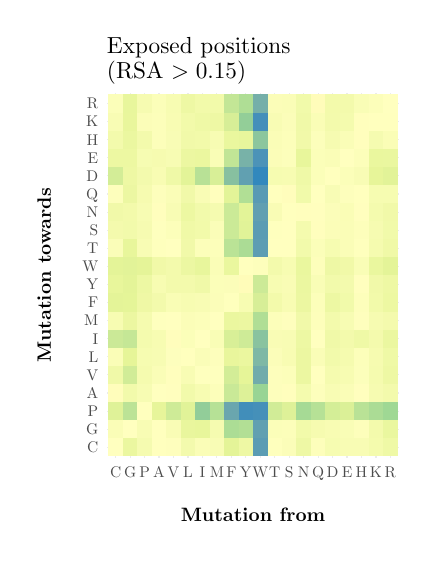
\begin{tikzpicture}[x=1pt,y=1pt]
\definecolor{fillColor}{RGB}{255,255,255}
\path[use as bounding box,fill=fillColor,fill opacity=0.00] (0,0) rectangle (137.71,183.39);
\begin{scope}
\path[clip] ( 28.66, 27.85) rectangle (134.21,159.90);
\definecolor{drawColor}{gray}{0.92}

\path[draw=drawColor,line width= 0.4pt,line join=round] ( 28.66, 31.77) --
	(134.21, 31.77);

\path[draw=drawColor,line width= 0.4pt,line join=round] ( 28.66, 38.31) --
	(134.21, 38.31);

\path[draw=drawColor,line width= 0.4pt,line join=round] ( 28.66, 44.85) --
	(134.21, 44.85);

\path[draw=drawColor,line width= 0.4pt,line join=round] ( 28.66, 51.38) --
	(134.21, 51.38);

\path[draw=drawColor,line width= 0.4pt,line join=round] ( 28.66, 57.92) --
	(134.21, 57.92);

\path[draw=drawColor,line width= 0.4pt,line join=round] ( 28.66, 64.46) --
	(134.21, 64.46);

\path[draw=drawColor,line width= 0.4pt,line join=round] ( 28.66, 70.99) --
	(134.21, 70.99);

\path[draw=drawColor,line width= 0.4pt,line join=round] ( 28.66, 77.53) --
	(134.21, 77.53);

\path[draw=drawColor,line width= 0.4pt,line join=round] ( 28.66, 84.07) --
	(134.21, 84.07);

\path[draw=drawColor,line width= 0.4pt,line join=round] ( 28.66, 90.60) --
	(134.21, 90.60);

\path[draw=drawColor,line width= 0.4pt,line join=round] ( 28.66, 97.14) --
	(134.21, 97.14);

\path[draw=drawColor,line width= 0.4pt,line join=round] ( 28.66,103.68) --
	(134.21,103.68);

\path[draw=drawColor,line width= 0.4pt,line join=round] ( 28.66,110.22) --
	(134.21,110.22);

\path[draw=drawColor,line width= 0.4pt,line join=round] ( 28.66,116.75) --
	(134.21,116.75);

\path[draw=drawColor,line width= 0.4pt,line join=round] ( 28.66,123.29) --
	(134.21,123.29);

\path[draw=drawColor,line width= 0.4pt,line join=round] ( 28.66,129.83) --
	(134.21,129.83);

\path[draw=drawColor,line width= 0.4pt,line join=round] ( 28.66,136.36) --
	(134.21,136.36);

\path[draw=drawColor,line width= 0.4pt,line join=round] ( 28.66,142.90) --
	(134.21,142.90);

\path[draw=drawColor,line width= 0.4pt,line join=round] ( 28.66,149.44) --
	(134.21,149.44);

\path[draw=drawColor,line width= 0.4pt,line join=round] ( 28.66,155.97) --
	(134.21,155.97);

\path[draw=drawColor,line width= 0.4pt,line join=round] ( 31.80, 27.85) --
	( 31.80,159.90);

\path[draw=drawColor,line width= 0.4pt,line join=round] ( 37.02, 27.85) --
	( 37.02,159.90);

\path[draw=drawColor,line width= 0.4pt,line join=round] ( 42.25, 27.85) --
	( 42.25,159.90);

\path[draw=drawColor,line width= 0.4pt,line join=round] ( 47.47, 27.85) --
	( 47.47,159.90);

\path[draw=drawColor,line width= 0.4pt,line join=round] ( 52.70, 27.85) --
	( 52.70,159.90);

\path[draw=drawColor,line width= 0.4pt,line join=round] ( 57.92, 27.85) --
	( 57.92,159.90);

\path[draw=drawColor,line width= 0.4pt,line join=round] ( 63.15, 27.85) --
	( 63.15,159.90);

\path[draw=drawColor,line width= 0.4pt,line join=round] ( 68.37, 27.85) --
	( 68.37,159.90);

\path[draw=drawColor,line width= 0.4pt,line join=round] ( 73.60, 27.85) --
	( 73.60,159.90);

\path[draw=drawColor,line width= 0.4pt,line join=round] ( 78.82, 27.85) --
	( 78.82,159.90);

\path[draw=drawColor,line width= 0.4pt,line join=round] ( 84.05, 27.85) --
	( 84.05,159.90);

\path[draw=drawColor,line width= 0.4pt,line join=round] ( 89.27, 27.85) --
	( 89.27,159.90);

\path[draw=drawColor,line width= 0.4pt,line join=round] ( 94.50, 27.85) --
	( 94.50,159.90);

\path[draw=drawColor,line width= 0.4pt,line join=round] ( 99.72, 27.85) --
	( 99.72,159.90);

\path[draw=drawColor,line width= 0.4pt,line join=round] (104.95, 27.85) --
	(104.95,159.90);

\path[draw=drawColor,line width= 0.4pt,line join=round] (110.17, 27.85) --
	(110.17,159.90);

\path[draw=drawColor,line width= 0.4pt,line join=round] (115.40, 27.85) --
	(115.40,159.90);

\path[draw=drawColor,line width= 0.4pt,line join=round] (120.62, 27.85) --
	(120.62,159.90);

\path[draw=drawColor,line width= 0.4pt,line join=round] (125.85, 27.85) --
	(125.85,159.90);

\path[draw=drawColor,line width= 0.4pt,line join=round] (131.07, 27.85) --
	(131.07,159.90);
\definecolor{fillColor}{RGB}{255,255,191}

\path[fill=fillColor] ( 29.18, 28.50) rectangle ( 34.41, 35.04);

\path[fill=fillColor] ( 29.18, 28.50) rectangle ( 34.41, 35.04);
\definecolor{fillColor}{RGB}{250,253,183}

\path[fill=fillColor] ( 29.18, 35.04) rectangle ( 34.41, 41.58);

\path[fill=fillColor] ( 29.18, 35.04) rectangle ( 34.41, 41.58);
\definecolor{fillColor}{RGB}{223,242,152}

\path[fill=fillColor] ( 29.18, 41.58) rectangle ( 34.41, 48.12);

\path[fill=fillColor] ( 29.18, 41.58) rectangle ( 34.41, 48.12);
\definecolor{fillColor}{RGB}{255,253,187}

\path[fill=fillColor] ( 29.18, 48.12) rectangle ( 34.41, 54.65);

\path[fill=fillColor] ( 29.18, 48.12) rectangle ( 34.41, 54.65);
\definecolor{fillColor}{RGB}{240,249,168}

\path[fill=fillColor] ( 29.18, 54.65) rectangle ( 34.41, 61.19);

\path[fill=fillColor] ( 29.18, 54.65) rectangle ( 34.41, 61.19);
\definecolor{fillColor}{RGB}{250,253,183}

\path[fill=fillColor] ( 29.18, 61.19) rectangle ( 34.41, 67.73);

\path[fill=fillColor] ( 29.18, 61.19) rectangle ( 34.41, 67.73);
\definecolor{fillColor}{RGB}{203,233,151}

\path[fill=fillColor] ( 29.18, 67.73) rectangle ( 34.41, 74.26);

\path[fill=fillColor] ( 29.18, 67.73) rectangle ( 34.41, 74.26);
\definecolor{fillColor}{RGB}{247,252,178}

\path[fill=fillColor] ( 29.18, 74.26) rectangle ( 34.41, 80.80);

\path[fill=fillColor] ( 29.18, 74.26) rectangle ( 34.41, 80.80);
\definecolor{fillColor}{RGB}{228,244,152}

\path[fill=fillColor] ( 29.18, 80.80) rectangle ( 34.41, 87.34);

\path[fill=fillColor] ( 29.18, 80.80) rectangle ( 34.41, 87.34);
\definecolor{fillColor}{RGB}{232,246,155}

\path[fill=fillColor] ( 29.18, 87.34) rectangle ( 34.41, 93.87);

\path[fill=fillColor] ( 29.18, 87.34) rectangle ( 34.41, 93.87);
\definecolor{fillColor}{RGB}{228,244,152}

\path[fill=fillColor] ( 29.18, 93.87) rectangle ( 34.41,100.41);

\path[fill=fillColor] ( 29.18, 93.87) rectangle ( 34.41,100.41);
\definecolor{fillColor}{RGB}{250,253,184}

\path[fill=fillColor] ( 29.18,100.41) rectangle ( 34.41,106.95);

\path[fill=fillColor] ( 29.18,100.41) rectangle ( 34.41,106.95);
\definecolor{fillColor}{RGB}{244,250,173}

\path[fill=fillColor] ( 29.18,106.95) rectangle ( 34.41,113.48);

\path[fill=fillColor] ( 29.18,106.95) rectangle ( 34.41,113.48);
\definecolor{fillColor}{RGB}{241,249,169}

\path[fill=fillColor] ( 29.18,113.48) rectangle ( 34.41,120.02);

\path[fill=fillColor] ( 29.18,113.48) rectangle ( 34.41,120.02);
\definecolor{fillColor}{RGB}{253,254,188}

\path[fill=fillColor] ( 29.18,120.02) rectangle ( 34.41,126.56);

\path[fill=fillColor] ( 29.18,120.02) rectangle ( 34.41,126.56);
\definecolor{fillColor}{RGB}{211,237,151}

\path[fill=fillColor] ( 29.18,126.56) rectangle ( 34.41,133.09);

\path[fill=fillColor] ( 29.18,126.56) rectangle ( 34.41,133.09);
\definecolor{fillColor}{RGB}{237,248,162}

\path[fill=fillColor] ( 29.18,133.09) rectangle ( 34.41,139.63);

\path[fill=fillColor] ( 29.18,133.09) rectangle ( 34.41,139.63);
\definecolor{fillColor}{RGB}{243,250,172}

\path[fill=fillColor] ( 29.18,139.63) rectangle ( 34.41,146.17);

\path[fill=fillColor] ( 29.18,139.63) rectangle ( 34.41,146.17);
\definecolor{fillColor}{RGB}{248,252,180}

\path[fill=fillColor] ( 29.18,146.17) rectangle ( 34.41,152.71);

\path[fill=fillColor] ( 29.18,146.17) rectangle ( 34.41,152.71);
\definecolor{fillColor}{RGB}{251,254,185}

\path[fill=fillColor] ( 29.18,152.71) rectangle ( 34.41,159.24);

\path[fill=fillColor] ( 29.18,152.71) rectangle ( 34.41,159.24);
\definecolor{fillColor}{RGB}{235,247,160}

\path[fill=fillColor] ( 34.41, 28.50) rectangle ( 39.63, 35.04);

\path[fill=fillColor] ( 34.41, 28.50) rectangle ( 39.63, 35.04);

\path[fill=fillColor] ( 34.41, 28.50) rectangle ( 39.63, 35.04);

\path[fill=fillColor] ( 34.41, 28.50) rectangle ( 39.63, 35.04);

\path[fill=fillColor] ( 34.41, 28.50) rectangle ( 39.63, 35.04);

\path[fill=fillColor] ( 34.41, 28.50) rectangle ( 39.63, 35.04);

\path[fill=fillColor] ( 34.41, 28.50) rectangle ( 39.63, 35.04);

\path[fill=fillColor] ( 34.41, 28.50) rectangle ( 39.63, 35.04);

\path[fill=fillColor] ( 34.41, 28.50) rectangle ( 39.63, 35.04);

\path[fill=fillColor] ( 34.41, 28.50) rectangle ( 39.63, 35.04);

\path[fill=fillColor] ( 34.41, 28.50) rectangle ( 39.63, 35.04);

\path[fill=fillColor] ( 34.41, 28.50) rectangle ( 39.63, 35.04);

\path[fill=fillColor] ( 34.41, 28.50) rectangle ( 39.63, 35.04);

\path[fill=fillColor] ( 34.41, 28.50) rectangle ( 39.63, 35.04);

\path[fill=fillColor] ( 34.41, 28.50) rectangle ( 39.63, 35.04);

\path[fill=fillColor] ( 34.41, 28.50) rectangle ( 39.63, 35.04);

\path[fill=fillColor] ( 34.41, 28.50) rectangle ( 39.63, 35.04);

\path[fill=fillColor] ( 34.41, 28.50) rectangle ( 39.63, 35.04);

\path[fill=fillColor] ( 34.41, 28.50) rectangle ( 39.63, 35.04);

\path[fill=fillColor] ( 34.41, 28.50) rectangle ( 39.63, 35.04);

\path[fill=fillColor] ( 34.41, 28.50) rectangle ( 39.63, 35.04);

\path[fill=fillColor] ( 34.41, 28.50) rectangle ( 39.63, 35.04);

\path[fill=fillColor] ( 34.41, 28.50) rectangle ( 39.63, 35.04);

\path[fill=fillColor] ( 34.41, 28.50) rectangle ( 39.63, 35.04);

\path[fill=fillColor] ( 34.41, 28.50) rectangle ( 39.63, 35.04);

\path[fill=fillColor] ( 34.41, 28.50) rectangle ( 39.63, 35.04);

\path[fill=fillColor] ( 34.41, 28.50) rectangle ( 39.63, 35.04);

\path[fill=fillColor] ( 34.41, 28.50) rectangle ( 39.63, 35.04);

\path[fill=fillColor] ( 34.41, 28.50) rectangle ( 39.63, 35.04);

\path[fill=fillColor] ( 34.41, 28.50) rectangle ( 39.63, 35.04);

\path[fill=fillColor] ( 34.41, 28.50) rectangle ( 39.63, 35.04);

\path[fill=fillColor] ( 34.41, 28.50) rectangle ( 39.63, 35.04);

\path[fill=fillColor] ( 34.41, 28.50) rectangle ( 39.63, 35.04);

\path[fill=fillColor] ( 34.41, 28.50) rectangle ( 39.63, 35.04);

\path[fill=fillColor] ( 34.41, 28.50) rectangle ( 39.63, 35.04);

\path[fill=fillColor] ( 34.41, 28.50) rectangle ( 39.63, 35.04);

\path[fill=fillColor] ( 34.41, 28.50) rectangle ( 39.63, 35.04);

\path[fill=fillColor] ( 34.41, 28.50) rectangle ( 39.63, 35.04);

\path[fill=fillColor] ( 34.41, 28.50) rectangle ( 39.63, 35.04);

\path[fill=fillColor] ( 34.41, 28.50) rectangle ( 39.63, 35.04);

\path[fill=fillColor] ( 34.41, 28.50) rectangle ( 39.63, 35.04);

\path[fill=fillColor] ( 34.41, 28.50) rectangle ( 39.63, 35.04);

\path[fill=fillColor] ( 34.41, 28.50) rectangle ( 39.63, 35.04);

\path[fill=fillColor] ( 34.41, 28.50) rectangle ( 39.63, 35.04);

\path[fill=fillColor] ( 34.41, 28.50) rectangle ( 39.63, 35.04);

\path[fill=fillColor] ( 34.41, 28.50) rectangle ( 39.63, 35.04);

\path[fill=fillColor] ( 34.41, 28.50) rectangle ( 39.63, 35.04);

\path[fill=fillColor] ( 34.41, 28.50) rectangle ( 39.63, 35.04);

\path[fill=fillColor] ( 34.41, 28.50) rectangle ( 39.63, 35.04);

\path[fill=fillColor] ( 34.41, 28.50) rectangle ( 39.63, 35.04);

\path[fill=fillColor] ( 34.41, 28.50) rectangle ( 39.63, 35.04);

\path[fill=fillColor] ( 34.41, 28.50) rectangle ( 39.63, 35.04);

\path[fill=fillColor] ( 34.41, 28.50) rectangle ( 39.63, 35.04);

\path[fill=fillColor] ( 34.41, 28.50) rectangle ( 39.63, 35.04);

\path[fill=fillColor] ( 34.41, 28.50) rectangle ( 39.63, 35.04);

\path[fill=fillColor] ( 34.41, 28.50) rectangle ( 39.63, 35.04);
\definecolor{fillColor}{RGB}{255,255,191}

\path[fill=fillColor] ( 34.41, 35.04) rectangle ( 39.63, 41.58);

\path[fill=fillColor] ( 34.41, 35.04) rectangle ( 39.63, 41.58);

\path[fill=fillColor] ( 34.41, 35.04) rectangle ( 39.63, 41.58);

\path[fill=fillColor] ( 34.41, 35.04) rectangle ( 39.63, 41.58);

\path[fill=fillColor] ( 34.41, 35.04) rectangle ( 39.63, 41.58);

\path[fill=fillColor] ( 34.41, 35.04) rectangle ( 39.63, 41.58);

\path[fill=fillColor] ( 34.41, 35.04) rectangle ( 39.63, 41.58);

\path[fill=fillColor] ( 34.41, 35.04) rectangle ( 39.63, 41.58);

\path[fill=fillColor] ( 34.41, 35.04) rectangle ( 39.63, 41.58);

\path[fill=fillColor] ( 34.41, 35.04) rectangle ( 39.63, 41.58);

\path[fill=fillColor] ( 34.41, 35.04) rectangle ( 39.63, 41.58);

\path[fill=fillColor] ( 34.41, 35.04) rectangle ( 39.63, 41.58);

\path[fill=fillColor] ( 34.41, 35.04) rectangle ( 39.63, 41.58);

\path[fill=fillColor] ( 34.41, 35.04) rectangle ( 39.63, 41.58);

\path[fill=fillColor] ( 34.41, 35.04) rectangle ( 39.63, 41.58);

\path[fill=fillColor] ( 34.41, 35.04) rectangle ( 39.63, 41.58);

\path[fill=fillColor] ( 34.41, 35.04) rectangle ( 39.63, 41.58);

\path[fill=fillColor] ( 34.41, 35.04) rectangle ( 39.63, 41.58);

\path[fill=fillColor] ( 34.41, 35.04) rectangle ( 39.63, 41.58);

\path[fill=fillColor] ( 34.41, 35.04) rectangle ( 39.63, 41.58);

\path[fill=fillColor] ( 34.41, 35.04) rectangle ( 39.63, 41.58);

\path[fill=fillColor] ( 34.41, 35.04) rectangle ( 39.63, 41.58);

\path[fill=fillColor] ( 34.41, 35.04) rectangle ( 39.63, 41.58);

\path[fill=fillColor] ( 34.41, 35.04) rectangle ( 39.63, 41.58);

\path[fill=fillColor] ( 34.41, 35.04) rectangle ( 39.63, 41.58);

\path[fill=fillColor] ( 34.41, 35.04) rectangle ( 39.63, 41.58);

\path[fill=fillColor] ( 34.41, 35.04) rectangle ( 39.63, 41.58);

\path[fill=fillColor] ( 34.41, 35.04) rectangle ( 39.63, 41.58);

\path[fill=fillColor] ( 34.41, 35.04) rectangle ( 39.63, 41.58);

\path[fill=fillColor] ( 34.41, 35.04) rectangle ( 39.63, 41.58);

\path[fill=fillColor] ( 34.41, 35.04) rectangle ( 39.63, 41.58);

\path[fill=fillColor] ( 34.41, 35.04) rectangle ( 39.63, 41.58);

\path[fill=fillColor] ( 34.41, 35.04) rectangle ( 39.63, 41.58);

\path[fill=fillColor] ( 34.41, 35.04) rectangle ( 39.63, 41.58);

\path[fill=fillColor] ( 34.41, 35.04) rectangle ( 39.63, 41.58);

\path[fill=fillColor] ( 34.41, 35.04) rectangle ( 39.63, 41.58);

\path[fill=fillColor] ( 34.41, 35.04) rectangle ( 39.63, 41.58);

\path[fill=fillColor] ( 34.41, 35.04) rectangle ( 39.63, 41.58);

\path[fill=fillColor] ( 34.41, 35.04) rectangle ( 39.63, 41.58);

\path[fill=fillColor] ( 34.41, 35.04) rectangle ( 39.63, 41.58);

\path[fill=fillColor] ( 34.41, 35.04) rectangle ( 39.63, 41.58);

\path[fill=fillColor] ( 34.41, 35.04) rectangle ( 39.63, 41.58);

\path[fill=fillColor] ( 34.41, 35.04) rectangle ( 39.63, 41.58);

\path[fill=fillColor] ( 34.41, 35.04) rectangle ( 39.63, 41.58);

\path[fill=fillColor] ( 34.41, 35.04) rectangle ( 39.63, 41.58);
\definecolor{fillColor}{RGB}{188,227,150}

\path[fill=fillColor] ( 34.41, 41.58) rectangle ( 39.63, 48.12);

\path[fill=fillColor] ( 34.41, 41.58) rectangle ( 39.63, 48.12);

\path[fill=fillColor] ( 34.41, 41.58) rectangle ( 39.63, 48.12);

\path[fill=fillColor] ( 34.41, 41.58) rectangle ( 39.63, 48.12);

\path[fill=fillColor] ( 34.41, 41.58) rectangle ( 39.63, 48.12);

\path[fill=fillColor] ( 34.41, 41.58) rectangle ( 39.63, 48.12);

\path[fill=fillColor] ( 34.41, 41.58) rectangle ( 39.63, 48.12);

\path[fill=fillColor] ( 34.41, 41.58) rectangle ( 39.63, 48.12);

\path[fill=fillColor] ( 34.41, 41.58) rectangle ( 39.63, 48.12);

\path[fill=fillColor] ( 34.41, 41.58) rectangle ( 39.63, 48.12);

\path[fill=fillColor] ( 34.41, 41.58) rectangle ( 39.63, 48.12);

\path[fill=fillColor] ( 34.41, 41.58) rectangle ( 39.63, 48.12);

\path[fill=fillColor] ( 34.41, 41.58) rectangle ( 39.63, 48.12);

\path[fill=fillColor] ( 34.41, 41.58) rectangle ( 39.63, 48.12);

\path[fill=fillColor] ( 34.41, 41.58) rectangle ( 39.63, 48.12);

\path[fill=fillColor] ( 34.41, 41.58) rectangle ( 39.63, 48.12);

\path[fill=fillColor] ( 34.41, 41.58) rectangle ( 39.63, 48.12);

\path[fill=fillColor] ( 34.41, 41.58) rectangle ( 39.63, 48.12);

\path[fill=fillColor] ( 34.41, 41.58) rectangle ( 39.63, 48.12);

\path[fill=fillColor] ( 34.41, 41.58) rectangle ( 39.63, 48.12);

\path[fill=fillColor] ( 34.41, 41.58) rectangle ( 39.63, 48.12);

\path[fill=fillColor] ( 34.41, 41.58) rectangle ( 39.63, 48.12);

\path[fill=fillColor] ( 34.41, 41.58) rectangle ( 39.63, 48.12);

\path[fill=fillColor] ( 34.41, 41.58) rectangle ( 39.63, 48.12);

\path[fill=fillColor] ( 34.41, 41.58) rectangle ( 39.63, 48.12);

\path[fill=fillColor] ( 34.41, 41.58) rectangle ( 39.63, 48.12);

\path[fill=fillColor] ( 34.41, 41.58) rectangle ( 39.63, 48.12);

\path[fill=fillColor] ( 34.41, 41.58) rectangle ( 39.63, 48.12);

\path[fill=fillColor] ( 34.41, 41.58) rectangle ( 39.63, 48.12);

\path[fill=fillColor] ( 34.41, 41.58) rectangle ( 39.63, 48.12);

\path[fill=fillColor] ( 34.41, 41.58) rectangle ( 39.63, 48.12);

\path[fill=fillColor] ( 34.41, 41.58) rectangle ( 39.63, 48.12);

\path[fill=fillColor] ( 34.41, 41.58) rectangle ( 39.63, 48.12);

\path[fill=fillColor] ( 34.41, 41.58) rectangle ( 39.63, 48.12);

\path[fill=fillColor] ( 34.41, 41.58) rectangle ( 39.63, 48.12);

\path[fill=fillColor] ( 34.41, 41.58) rectangle ( 39.63, 48.12);

\path[fill=fillColor] ( 34.41, 41.58) rectangle ( 39.63, 48.12);

\path[fill=fillColor] ( 34.41, 41.58) rectangle ( 39.63, 48.12);

\path[fill=fillColor] ( 34.41, 41.58) rectangle ( 39.63, 48.12);

\path[fill=fillColor] ( 34.41, 41.58) rectangle ( 39.63, 48.12);

\path[fill=fillColor] ( 34.41, 41.58) rectangle ( 39.63, 48.12);

\path[fill=fillColor] ( 34.41, 41.58) rectangle ( 39.63, 48.12);

\path[fill=fillColor] ( 34.41, 41.58) rectangle ( 39.63, 48.12);

\path[fill=fillColor] ( 34.41, 41.58) rectangle ( 39.63, 48.12);

\path[fill=fillColor] ( 34.41, 41.58) rectangle ( 39.63, 48.12);

\path[fill=fillColor] ( 34.41, 41.58) rectangle ( 39.63, 48.12);

\path[fill=fillColor] ( 34.41, 41.58) rectangle ( 39.63, 48.12);

\path[fill=fillColor] ( 34.41, 41.58) rectangle ( 39.63, 48.12);

\path[fill=fillColor] ( 34.41, 41.58) rectangle ( 39.63, 48.12);

\path[fill=fillColor] ( 34.41, 41.58) rectangle ( 39.63, 48.12);

\path[fill=fillColor] ( 34.41, 41.58) rectangle ( 39.63, 48.12);

\path[fill=fillColor] ( 34.41, 41.58) rectangle ( 39.63, 48.12);

\path[fill=fillColor] ( 34.41, 41.58) rectangle ( 39.63, 48.12);

\path[fill=fillColor] ( 34.41, 41.58) rectangle ( 39.63, 48.12);

\path[fill=fillColor] ( 34.41, 41.58) rectangle ( 39.63, 48.12);
\definecolor{fillColor}{RGB}{242,250,171}

\path[fill=fillColor] ( 34.41, 48.12) rectangle ( 39.63, 54.65);

\path[fill=fillColor] ( 34.41, 48.12) rectangle ( 39.63, 54.65);

\path[fill=fillColor] ( 34.41, 48.12) rectangle ( 39.63, 54.65);

\path[fill=fillColor] ( 34.41, 48.12) rectangle ( 39.63, 54.65);

\path[fill=fillColor] ( 34.41, 48.12) rectangle ( 39.63, 54.65);

\path[fill=fillColor] ( 34.41, 48.12) rectangle ( 39.63, 54.65);

\path[fill=fillColor] ( 34.41, 48.12) rectangle ( 39.63, 54.65);

\path[fill=fillColor] ( 34.41, 48.12) rectangle ( 39.63, 54.65);

\path[fill=fillColor] ( 34.41, 48.12) rectangle ( 39.63, 54.65);

\path[fill=fillColor] ( 34.41, 48.12) rectangle ( 39.63, 54.65);

\path[fill=fillColor] ( 34.41, 48.12) rectangle ( 39.63, 54.65);

\path[fill=fillColor] ( 34.41, 48.12) rectangle ( 39.63, 54.65);

\path[fill=fillColor] ( 34.41, 48.12) rectangle ( 39.63, 54.65);

\path[fill=fillColor] ( 34.41, 48.12) rectangle ( 39.63, 54.65);

\path[fill=fillColor] ( 34.41, 48.12) rectangle ( 39.63, 54.65);

\path[fill=fillColor] ( 34.41, 48.12) rectangle ( 39.63, 54.65);

\path[fill=fillColor] ( 34.41, 48.12) rectangle ( 39.63, 54.65);

\path[fill=fillColor] ( 34.41, 48.12) rectangle ( 39.63, 54.65);

\path[fill=fillColor] ( 34.41, 48.12) rectangle ( 39.63, 54.65);

\path[fill=fillColor] ( 34.41, 48.12) rectangle ( 39.63, 54.65);

\path[fill=fillColor] ( 34.41, 48.12) rectangle ( 39.63, 54.65);

\path[fill=fillColor] ( 34.41, 48.12) rectangle ( 39.63, 54.65);

\path[fill=fillColor] ( 34.41, 48.12) rectangle ( 39.63, 54.65);

\path[fill=fillColor] ( 34.41, 48.12) rectangle ( 39.63, 54.65);

\path[fill=fillColor] ( 34.41, 48.12) rectangle ( 39.63, 54.65);

\path[fill=fillColor] ( 34.41, 48.12) rectangle ( 39.63, 54.65);

\path[fill=fillColor] ( 34.41, 48.12) rectangle ( 39.63, 54.65);

\path[fill=fillColor] ( 34.41, 48.12) rectangle ( 39.63, 54.65);

\path[fill=fillColor] ( 34.41, 48.12) rectangle ( 39.63, 54.65);

\path[fill=fillColor] ( 34.41, 48.12) rectangle ( 39.63, 54.65);

\path[fill=fillColor] ( 34.41, 48.12) rectangle ( 39.63, 54.65);

\path[fill=fillColor] ( 34.41, 48.12) rectangle ( 39.63, 54.65);

\path[fill=fillColor] ( 34.41, 48.12) rectangle ( 39.63, 54.65);

\path[fill=fillColor] ( 34.41, 48.12) rectangle ( 39.63, 54.65);

\path[fill=fillColor] ( 34.41, 48.12) rectangle ( 39.63, 54.65);

\path[fill=fillColor] ( 34.41, 48.12) rectangle ( 39.63, 54.65);

\path[fill=fillColor] ( 34.41, 48.12) rectangle ( 39.63, 54.65);

\path[fill=fillColor] ( 34.41, 48.12) rectangle ( 39.63, 54.65);

\path[fill=fillColor] ( 34.41, 48.12) rectangle ( 39.63, 54.65);

\path[fill=fillColor] ( 34.41, 48.12) rectangle ( 39.63, 54.65);

\path[fill=fillColor] ( 34.41, 48.12) rectangle ( 39.63, 54.65);

\path[fill=fillColor] ( 34.41, 48.12) rectangle ( 39.63, 54.65);

\path[fill=fillColor] ( 34.41, 48.12) rectangle ( 39.63, 54.65);

\path[fill=fillColor] ( 34.41, 48.12) rectangle ( 39.63, 54.65);

\path[fill=fillColor] ( 34.41, 48.12) rectangle ( 39.63, 54.65);

\path[fill=fillColor] ( 34.41, 48.12) rectangle ( 39.63, 54.65);

\path[fill=fillColor] ( 34.41, 48.12) rectangle ( 39.63, 54.65);

\path[fill=fillColor] ( 34.41, 48.12) rectangle ( 39.63, 54.65);

\path[fill=fillColor] ( 34.41, 48.12) rectangle ( 39.63, 54.65);

\path[fill=fillColor] ( 34.41, 48.12) rectangle ( 39.63, 54.65);

\path[fill=fillColor] ( 34.41, 48.12) rectangle ( 39.63, 54.65);

\path[fill=fillColor] ( 34.41, 48.12) rectangle ( 39.63, 54.65);

\path[fill=fillColor] ( 34.41, 48.12) rectangle ( 39.63, 54.65);

\path[fill=fillColor] ( 34.41, 48.12) rectangle ( 39.63, 54.65);

\path[fill=fillColor] ( 34.41, 48.12) rectangle ( 39.63, 54.65);

\path[fill=fillColor] ( 34.41, 48.12) rectangle ( 39.63, 54.65);

\path[fill=fillColor] ( 34.41, 48.12) rectangle ( 39.63, 54.65);

\path[fill=fillColor] ( 34.41, 48.12) rectangle ( 39.63, 54.65);
\definecolor{fillColor}{RGB}{209,236,151}

\path[fill=fillColor] ( 34.41, 54.65) rectangle ( 39.63, 61.19);

\path[fill=fillColor] ( 34.41, 54.65) rectangle ( 39.63, 61.19);

\path[fill=fillColor] ( 34.41, 54.65) rectangle ( 39.63, 61.19);

\path[fill=fillColor] ( 34.41, 54.65) rectangle ( 39.63, 61.19);

\path[fill=fillColor] ( 34.41, 54.65) rectangle ( 39.63, 61.19);

\path[fill=fillColor] ( 34.41, 54.65) rectangle ( 39.63, 61.19);

\path[fill=fillColor] ( 34.41, 54.65) rectangle ( 39.63, 61.19);

\path[fill=fillColor] ( 34.41, 54.65) rectangle ( 39.63, 61.19);

\path[fill=fillColor] ( 34.41, 54.65) rectangle ( 39.63, 61.19);

\path[fill=fillColor] ( 34.41, 54.65) rectangle ( 39.63, 61.19);

\path[fill=fillColor] ( 34.41, 54.65) rectangle ( 39.63, 61.19);

\path[fill=fillColor] ( 34.41, 54.65) rectangle ( 39.63, 61.19);

\path[fill=fillColor] ( 34.41, 54.65) rectangle ( 39.63, 61.19);

\path[fill=fillColor] ( 34.41, 54.65) rectangle ( 39.63, 61.19);

\path[fill=fillColor] ( 34.41, 54.65) rectangle ( 39.63, 61.19);

\path[fill=fillColor] ( 34.41, 54.65) rectangle ( 39.63, 61.19);

\path[fill=fillColor] ( 34.41, 54.65) rectangle ( 39.63, 61.19);

\path[fill=fillColor] ( 34.41, 54.65) rectangle ( 39.63, 61.19);

\path[fill=fillColor] ( 34.41, 54.65) rectangle ( 39.63, 61.19);

\path[fill=fillColor] ( 34.41, 54.65) rectangle ( 39.63, 61.19);

\path[fill=fillColor] ( 34.41, 54.65) rectangle ( 39.63, 61.19);

\path[fill=fillColor] ( 34.41, 54.65) rectangle ( 39.63, 61.19);

\path[fill=fillColor] ( 34.41, 54.65) rectangle ( 39.63, 61.19);

\path[fill=fillColor] ( 34.41, 54.65) rectangle ( 39.63, 61.19);

\path[fill=fillColor] ( 34.41, 54.65) rectangle ( 39.63, 61.19);

\path[fill=fillColor] ( 34.41, 54.65) rectangle ( 39.63, 61.19);

\path[fill=fillColor] ( 34.41, 54.65) rectangle ( 39.63, 61.19);

\path[fill=fillColor] ( 34.41, 54.65) rectangle ( 39.63, 61.19);

\path[fill=fillColor] ( 34.41, 54.65) rectangle ( 39.63, 61.19);

\path[fill=fillColor] ( 34.41, 54.65) rectangle ( 39.63, 61.19);

\path[fill=fillColor] ( 34.41, 54.65) rectangle ( 39.63, 61.19);

\path[fill=fillColor] ( 34.41, 54.65) rectangle ( 39.63, 61.19);

\path[fill=fillColor] ( 34.41, 54.65) rectangle ( 39.63, 61.19);

\path[fill=fillColor] ( 34.41, 54.65) rectangle ( 39.63, 61.19);

\path[fill=fillColor] ( 34.41, 54.65) rectangle ( 39.63, 61.19);

\path[fill=fillColor] ( 34.41, 54.65) rectangle ( 39.63, 61.19);

\path[fill=fillColor] ( 34.41, 54.65) rectangle ( 39.63, 61.19);

\path[fill=fillColor] ( 34.41, 54.65) rectangle ( 39.63, 61.19);

\path[fill=fillColor] ( 34.41, 54.65) rectangle ( 39.63, 61.19);

\path[fill=fillColor] ( 34.41, 54.65) rectangle ( 39.63, 61.19);

\path[fill=fillColor] ( 34.41, 54.65) rectangle ( 39.63, 61.19);

\path[fill=fillColor] ( 34.41, 54.65) rectangle ( 39.63, 61.19);

\path[fill=fillColor] ( 34.41, 54.65) rectangle ( 39.63, 61.19);

\path[fill=fillColor] ( 34.41, 54.65) rectangle ( 39.63, 61.19);

\path[fill=fillColor] ( 34.41, 54.65) rectangle ( 39.63, 61.19);

\path[fill=fillColor] ( 34.41, 54.65) rectangle ( 39.63, 61.19);

\path[fill=fillColor] ( 34.41, 54.65) rectangle ( 39.63, 61.19);

\path[fill=fillColor] ( 34.41, 54.65) rectangle ( 39.63, 61.19);

\path[fill=fillColor] ( 34.41, 54.65) rectangle ( 39.63, 61.19);

\path[fill=fillColor] ( 34.41, 54.65) rectangle ( 39.63, 61.19);

\path[fill=fillColor] ( 34.41, 54.65) rectangle ( 39.63, 61.19);

\path[fill=fillColor] ( 34.41, 54.65) rectangle ( 39.63, 61.19);

\path[fill=fillColor] ( 34.41, 54.65) rectangle ( 39.63, 61.19);

\path[fill=fillColor] ( 34.41, 54.65) rectangle ( 39.63, 61.19);

\path[fill=fillColor] ( 34.41, 54.65) rectangle ( 39.63, 61.19);

\path[fill=fillColor] ( 34.41, 54.65) rectangle ( 39.63, 61.19);
\definecolor{fillColor}{RGB}{230,245,152}

\path[fill=fillColor] ( 34.41, 61.19) rectangle ( 39.63, 67.73);

\path[fill=fillColor] ( 34.41, 61.19) rectangle ( 39.63, 67.73);

\path[fill=fillColor] ( 34.41, 61.19) rectangle ( 39.63, 67.73);

\path[fill=fillColor] ( 34.41, 61.19) rectangle ( 39.63, 67.73);

\path[fill=fillColor] ( 34.41, 61.19) rectangle ( 39.63, 67.73);

\path[fill=fillColor] ( 34.41, 61.19) rectangle ( 39.63, 67.73);

\path[fill=fillColor] ( 34.41, 61.19) rectangle ( 39.63, 67.73);

\path[fill=fillColor] ( 34.41, 61.19) rectangle ( 39.63, 67.73);

\path[fill=fillColor] ( 34.41, 61.19) rectangle ( 39.63, 67.73);

\path[fill=fillColor] ( 34.41, 61.19) rectangle ( 39.63, 67.73);

\path[fill=fillColor] ( 34.41, 61.19) rectangle ( 39.63, 67.73);

\path[fill=fillColor] ( 34.41, 61.19) rectangle ( 39.63, 67.73);

\path[fill=fillColor] ( 34.41, 61.19) rectangle ( 39.63, 67.73);

\path[fill=fillColor] ( 34.41, 61.19) rectangle ( 39.63, 67.73);

\path[fill=fillColor] ( 34.41, 61.19) rectangle ( 39.63, 67.73);

\path[fill=fillColor] ( 34.41, 61.19) rectangle ( 39.63, 67.73);

\path[fill=fillColor] ( 34.41, 61.19) rectangle ( 39.63, 67.73);

\path[fill=fillColor] ( 34.41, 61.19) rectangle ( 39.63, 67.73);

\path[fill=fillColor] ( 34.41, 61.19) rectangle ( 39.63, 67.73);

\path[fill=fillColor] ( 34.41, 61.19) rectangle ( 39.63, 67.73);

\path[fill=fillColor] ( 34.41, 61.19) rectangle ( 39.63, 67.73);

\path[fill=fillColor] ( 34.41, 61.19) rectangle ( 39.63, 67.73);

\path[fill=fillColor] ( 34.41, 61.19) rectangle ( 39.63, 67.73);

\path[fill=fillColor] ( 34.41, 61.19) rectangle ( 39.63, 67.73);

\path[fill=fillColor] ( 34.41, 61.19) rectangle ( 39.63, 67.73);

\path[fill=fillColor] ( 34.41, 61.19) rectangle ( 39.63, 67.73);

\path[fill=fillColor] ( 34.41, 61.19) rectangle ( 39.63, 67.73);

\path[fill=fillColor] ( 34.41, 61.19) rectangle ( 39.63, 67.73);

\path[fill=fillColor] ( 34.41, 61.19) rectangle ( 39.63, 67.73);

\path[fill=fillColor] ( 34.41, 61.19) rectangle ( 39.63, 67.73);

\path[fill=fillColor] ( 34.41, 61.19) rectangle ( 39.63, 67.73);

\path[fill=fillColor] ( 34.41, 61.19) rectangle ( 39.63, 67.73);

\path[fill=fillColor] ( 34.41, 61.19) rectangle ( 39.63, 67.73);

\path[fill=fillColor] ( 34.41, 61.19) rectangle ( 39.63, 67.73);

\path[fill=fillColor] ( 34.41, 61.19) rectangle ( 39.63, 67.73);

\path[fill=fillColor] ( 34.41, 61.19) rectangle ( 39.63, 67.73);

\path[fill=fillColor] ( 34.41, 61.19) rectangle ( 39.63, 67.73);

\path[fill=fillColor] ( 34.41, 61.19) rectangle ( 39.63, 67.73);

\path[fill=fillColor] ( 34.41, 61.19) rectangle ( 39.63, 67.73);

\path[fill=fillColor] ( 34.41, 61.19) rectangle ( 39.63, 67.73);

\path[fill=fillColor] ( 34.41, 61.19) rectangle ( 39.63, 67.73);

\path[fill=fillColor] ( 34.41, 61.19) rectangle ( 39.63, 67.73);

\path[fill=fillColor] ( 34.41, 61.19) rectangle ( 39.63, 67.73);

\path[fill=fillColor] ( 34.41, 61.19) rectangle ( 39.63, 67.73);

\path[fill=fillColor] ( 34.41, 61.19) rectangle ( 39.63, 67.73);

\path[fill=fillColor] ( 34.41, 61.19) rectangle ( 39.63, 67.73);

\path[fill=fillColor] ( 34.41, 61.19) rectangle ( 39.63, 67.73);

\path[fill=fillColor] ( 34.41, 61.19) rectangle ( 39.63, 67.73);

\path[fill=fillColor] ( 34.41, 61.19) rectangle ( 39.63, 67.73);

\path[fill=fillColor] ( 34.41, 61.19) rectangle ( 39.63, 67.73);

\path[fill=fillColor] ( 34.41, 61.19) rectangle ( 39.63, 67.73);

\path[fill=fillColor] ( 34.41, 61.19) rectangle ( 39.63, 67.73);

\path[fill=fillColor] ( 34.41, 61.19) rectangle ( 39.63, 67.73);

\path[fill=fillColor] ( 34.41, 61.19) rectangle ( 39.63, 67.73);

\path[fill=fillColor] ( 34.41, 61.19) rectangle ( 39.63, 67.73);

\path[fill=fillColor] ( 34.41, 61.19) rectangle ( 39.63, 67.73);
\definecolor{fillColor}{RGB}{197,231,150}

\path[fill=fillColor] ( 34.41, 67.73) rectangle ( 39.63, 74.26);

\path[fill=fillColor] ( 34.41, 67.73) rectangle ( 39.63, 74.26);

\path[fill=fillColor] ( 34.41, 67.73) rectangle ( 39.63, 74.26);

\path[fill=fillColor] ( 34.41, 67.73) rectangle ( 39.63, 74.26);

\path[fill=fillColor] ( 34.41, 67.73) rectangle ( 39.63, 74.26);

\path[fill=fillColor] ( 34.41, 67.73) rectangle ( 39.63, 74.26);

\path[fill=fillColor] ( 34.41, 67.73) rectangle ( 39.63, 74.26);

\path[fill=fillColor] ( 34.41, 67.73) rectangle ( 39.63, 74.26);

\path[fill=fillColor] ( 34.41, 67.73) rectangle ( 39.63, 74.26);

\path[fill=fillColor] ( 34.41, 67.73) rectangle ( 39.63, 74.26);

\path[fill=fillColor] ( 34.41, 67.73) rectangle ( 39.63, 74.26);

\path[fill=fillColor] ( 34.41, 67.73) rectangle ( 39.63, 74.26);

\path[fill=fillColor] ( 34.41, 67.73) rectangle ( 39.63, 74.26);

\path[fill=fillColor] ( 34.41, 67.73) rectangle ( 39.63, 74.26);

\path[fill=fillColor] ( 34.41, 67.73) rectangle ( 39.63, 74.26);

\path[fill=fillColor] ( 34.41, 67.73) rectangle ( 39.63, 74.26);

\path[fill=fillColor] ( 34.41, 67.73) rectangle ( 39.63, 74.26);

\path[fill=fillColor] ( 34.41, 67.73) rectangle ( 39.63, 74.26);

\path[fill=fillColor] ( 34.41, 67.73) rectangle ( 39.63, 74.26);

\path[fill=fillColor] ( 34.41, 67.73) rectangle ( 39.63, 74.26);

\path[fill=fillColor] ( 34.41, 67.73) rectangle ( 39.63, 74.26);

\path[fill=fillColor] ( 34.41, 67.73) rectangle ( 39.63, 74.26);

\path[fill=fillColor] ( 34.41, 67.73) rectangle ( 39.63, 74.26);

\path[fill=fillColor] ( 34.41, 67.73) rectangle ( 39.63, 74.26);

\path[fill=fillColor] ( 34.41, 67.73) rectangle ( 39.63, 74.26);

\path[fill=fillColor] ( 34.41, 67.73) rectangle ( 39.63, 74.26);

\path[fill=fillColor] ( 34.41, 67.73) rectangle ( 39.63, 74.26);

\path[fill=fillColor] ( 34.41, 67.73) rectangle ( 39.63, 74.26);

\path[fill=fillColor] ( 34.41, 67.73) rectangle ( 39.63, 74.26);

\path[fill=fillColor] ( 34.41, 67.73) rectangle ( 39.63, 74.26);

\path[fill=fillColor] ( 34.41, 67.73) rectangle ( 39.63, 74.26);

\path[fill=fillColor] ( 34.41, 67.73) rectangle ( 39.63, 74.26);

\path[fill=fillColor] ( 34.41, 67.73) rectangle ( 39.63, 74.26);

\path[fill=fillColor] ( 34.41, 67.73) rectangle ( 39.63, 74.26);

\path[fill=fillColor] ( 34.41, 67.73) rectangle ( 39.63, 74.26);

\path[fill=fillColor] ( 34.41, 67.73) rectangle ( 39.63, 74.26);

\path[fill=fillColor] ( 34.41, 67.73) rectangle ( 39.63, 74.26);

\path[fill=fillColor] ( 34.41, 67.73) rectangle ( 39.63, 74.26);

\path[fill=fillColor] ( 34.41, 67.73) rectangle ( 39.63, 74.26);

\path[fill=fillColor] ( 34.41, 67.73) rectangle ( 39.63, 74.26);

\path[fill=fillColor] ( 34.41, 67.73) rectangle ( 39.63, 74.26);

\path[fill=fillColor] ( 34.41, 67.73) rectangle ( 39.63, 74.26);

\path[fill=fillColor] ( 34.41, 67.73) rectangle ( 39.63, 74.26);

\path[fill=fillColor] ( 34.41, 67.73) rectangle ( 39.63, 74.26);

\path[fill=fillColor] ( 34.41, 67.73) rectangle ( 39.63, 74.26);

\path[fill=fillColor] ( 34.41, 67.73) rectangle ( 39.63, 74.26);

\path[fill=fillColor] ( 34.41, 67.73) rectangle ( 39.63, 74.26);

\path[fill=fillColor] ( 34.41, 67.73) rectangle ( 39.63, 74.26);

\path[fill=fillColor] ( 34.41, 67.73) rectangle ( 39.63, 74.26);

\path[fill=fillColor] ( 34.41, 67.73) rectangle ( 39.63, 74.26);

\path[fill=fillColor] ( 34.41, 67.73) rectangle ( 39.63, 74.26);

\path[fill=fillColor] ( 34.41, 67.73) rectangle ( 39.63, 74.26);

\path[fill=fillColor] ( 34.41, 67.73) rectangle ( 39.63, 74.26);

\path[fill=fillColor] ( 34.41, 67.73) rectangle ( 39.63, 74.26);
\definecolor{fillColor}{RGB}{236,247,161}

\path[fill=fillColor] ( 34.41, 74.26) rectangle ( 39.63, 80.80);

\path[fill=fillColor] ( 34.41, 74.26) rectangle ( 39.63, 80.80);

\path[fill=fillColor] ( 34.41, 74.26) rectangle ( 39.63, 80.80);

\path[fill=fillColor] ( 34.41, 74.26) rectangle ( 39.63, 80.80);

\path[fill=fillColor] ( 34.41, 74.26) rectangle ( 39.63, 80.80);

\path[fill=fillColor] ( 34.41, 74.26) rectangle ( 39.63, 80.80);

\path[fill=fillColor] ( 34.41, 74.26) rectangle ( 39.63, 80.80);

\path[fill=fillColor] ( 34.41, 74.26) rectangle ( 39.63, 80.80);

\path[fill=fillColor] ( 34.41, 74.26) rectangle ( 39.63, 80.80);

\path[fill=fillColor] ( 34.41, 74.26) rectangle ( 39.63, 80.80);

\path[fill=fillColor] ( 34.41, 74.26) rectangle ( 39.63, 80.80);

\path[fill=fillColor] ( 34.41, 74.26) rectangle ( 39.63, 80.80);

\path[fill=fillColor] ( 34.41, 74.26) rectangle ( 39.63, 80.80);

\path[fill=fillColor] ( 34.41, 74.26) rectangle ( 39.63, 80.80);

\path[fill=fillColor] ( 34.41, 74.26) rectangle ( 39.63, 80.80);

\path[fill=fillColor] ( 34.41, 74.26) rectangle ( 39.63, 80.80);

\path[fill=fillColor] ( 34.41, 74.26) rectangle ( 39.63, 80.80);

\path[fill=fillColor] ( 34.41, 74.26) rectangle ( 39.63, 80.80);

\path[fill=fillColor] ( 34.41, 74.26) rectangle ( 39.63, 80.80);

\path[fill=fillColor] ( 34.41, 74.26) rectangle ( 39.63, 80.80);

\path[fill=fillColor] ( 34.41, 74.26) rectangle ( 39.63, 80.80);

\path[fill=fillColor] ( 34.41, 74.26) rectangle ( 39.63, 80.80);

\path[fill=fillColor] ( 34.41, 74.26) rectangle ( 39.63, 80.80);

\path[fill=fillColor] ( 34.41, 74.26) rectangle ( 39.63, 80.80);

\path[fill=fillColor] ( 34.41, 74.26) rectangle ( 39.63, 80.80);

\path[fill=fillColor] ( 34.41, 74.26) rectangle ( 39.63, 80.80);

\path[fill=fillColor] ( 34.41, 74.26) rectangle ( 39.63, 80.80);

\path[fill=fillColor] ( 34.41, 74.26) rectangle ( 39.63, 80.80);

\path[fill=fillColor] ( 34.41, 74.26) rectangle ( 39.63, 80.80);

\path[fill=fillColor] ( 34.41, 74.26) rectangle ( 39.63, 80.80);

\path[fill=fillColor] ( 34.41, 74.26) rectangle ( 39.63, 80.80);

\path[fill=fillColor] ( 34.41, 74.26) rectangle ( 39.63, 80.80);

\path[fill=fillColor] ( 34.41, 74.26) rectangle ( 39.63, 80.80);

\path[fill=fillColor] ( 34.41, 74.26) rectangle ( 39.63, 80.80);

\path[fill=fillColor] ( 34.41, 74.26) rectangle ( 39.63, 80.80);

\path[fill=fillColor] ( 34.41, 74.26) rectangle ( 39.63, 80.80);

\path[fill=fillColor] ( 34.41, 74.26) rectangle ( 39.63, 80.80);

\path[fill=fillColor] ( 34.41, 74.26) rectangle ( 39.63, 80.80);

\path[fill=fillColor] ( 34.41, 74.26) rectangle ( 39.63, 80.80);

\path[fill=fillColor] ( 34.41, 74.26) rectangle ( 39.63, 80.80);

\path[fill=fillColor] ( 34.41, 74.26) rectangle ( 39.63, 80.80);

\path[fill=fillColor] ( 34.41, 74.26) rectangle ( 39.63, 80.80);

\path[fill=fillColor] ( 34.41, 74.26) rectangle ( 39.63, 80.80);

\path[fill=fillColor] ( 34.41, 74.26) rectangle ( 39.63, 80.80);

\path[fill=fillColor] ( 34.41, 74.26) rectangle ( 39.63, 80.80);

\path[fill=fillColor] ( 34.41, 74.26) rectangle ( 39.63, 80.80);
\definecolor{fillColor}{RGB}{229,245,152}

\path[fill=fillColor] ( 34.41, 80.80) rectangle ( 39.63, 87.34);

\path[fill=fillColor] ( 34.41, 80.80) rectangle ( 39.63, 87.34);

\path[fill=fillColor] ( 34.41, 80.80) rectangle ( 39.63, 87.34);

\path[fill=fillColor] ( 34.41, 80.80) rectangle ( 39.63, 87.34);

\path[fill=fillColor] ( 34.41, 80.80) rectangle ( 39.63, 87.34);

\path[fill=fillColor] ( 34.41, 80.80) rectangle ( 39.63, 87.34);

\path[fill=fillColor] ( 34.41, 80.80) rectangle ( 39.63, 87.34);

\path[fill=fillColor] ( 34.41, 80.80) rectangle ( 39.63, 87.34);

\path[fill=fillColor] ( 34.41, 80.80) rectangle ( 39.63, 87.34);

\path[fill=fillColor] ( 34.41, 80.80) rectangle ( 39.63, 87.34);

\path[fill=fillColor] ( 34.41, 80.80) rectangle ( 39.63, 87.34);

\path[fill=fillColor] ( 34.41, 80.80) rectangle ( 39.63, 87.34);

\path[fill=fillColor] ( 34.41, 80.80) rectangle ( 39.63, 87.34);

\path[fill=fillColor] ( 34.41, 80.80) rectangle ( 39.63, 87.34);

\path[fill=fillColor] ( 34.41, 80.80) rectangle ( 39.63, 87.34);

\path[fill=fillColor] ( 34.41, 80.80) rectangle ( 39.63, 87.34);

\path[fill=fillColor] ( 34.41, 80.80) rectangle ( 39.63, 87.34);

\path[fill=fillColor] ( 34.41, 80.80) rectangle ( 39.63, 87.34);

\path[fill=fillColor] ( 34.41, 80.80) rectangle ( 39.63, 87.34);

\path[fill=fillColor] ( 34.41, 80.80) rectangle ( 39.63, 87.34);

\path[fill=fillColor] ( 34.41, 80.80) rectangle ( 39.63, 87.34);

\path[fill=fillColor] ( 34.41, 80.80) rectangle ( 39.63, 87.34);

\path[fill=fillColor] ( 34.41, 80.80) rectangle ( 39.63, 87.34);

\path[fill=fillColor] ( 34.41, 80.80) rectangle ( 39.63, 87.34);

\path[fill=fillColor] ( 34.41, 80.80) rectangle ( 39.63, 87.34);

\path[fill=fillColor] ( 34.41, 80.80) rectangle ( 39.63, 87.34);

\path[fill=fillColor] ( 34.41, 80.80) rectangle ( 39.63, 87.34);

\path[fill=fillColor] ( 34.41, 80.80) rectangle ( 39.63, 87.34);

\path[fill=fillColor] ( 34.41, 80.80) rectangle ( 39.63, 87.34);

\path[fill=fillColor] ( 34.41, 80.80) rectangle ( 39.63, 87.34);

\path[fill=fillColor] ( 34.41, 80.80) rectangle ( 39.63, 87.34);

\path[fill=fillColor] ( 34.41, 80.80) rectangle ( 39.63, 87.34);

\path[fill=fillColor] ( 34.41, 80.80) rectangle ( 39.63, 87.34);

\path[fill=fillColor] ( 34.41, 80.80) rectangle ( 39.63, 87.34);

\path[fill=fillColor] ( 34.41, 80.80) rectangle ( 39.63, 87.34);

\path[fill=fillColor] ( 34.41, 80.80) rectangle ( 39.63, 87.34);

\path[fill=fillColor] ( 34.41, 80.80) rectangle ( 39.63, 87.34);

\path[fill=fillColor] ( 34.41, 80.80) rectangle ( 39.63, 87.34);

\path[fill=fillColor] ( 34.41, 80.80) rectangle ( 39.63, 87.34);

\path[fill=fillColor] ( 34.41, 80.80) rectangle ( 39.63, 87.34);

\path[fill=fillColor] ( 34.41, 80.80) rectangle ( 39.63, 87.34);

\path[fill=fillColor] ( 34.41, 80.80) rectangle ( 39.63, 87.34);

\path[fill=fillColor] ( 34.41, 80.80) rectangle ( 39.63, 87.34);

\path[fill=fillColor] ( 34.41, 80.80) rectangle ( 39.63, 87.34);

\path[fill=fillColor] ( 34.41, 80.80) rectangle ( 39.63, 87.34);

\path[fill=fillColor] ( 34.41, 80.80) rectangle ( 39.63, 87.34);

\path[fill=fillColor] ( 34.41, 80.80) rectangle ( 39.63, 87.34);

\path[fill=fillColor] ( 34.41, 80.80) rectangle ( 39.63, 87.34);

\path[fill=fillColor] ( 34.41, 80.80) rectangle ( 39.63, 87.34);

\path[fill=fillColor] ( 34.41, 80.80) rectangle ( 39.63, 87.34);

\path[fill=fillColor] ( 34.41, 80.80) rectangle ( 39.63, 87.34);
\definecolor{fillColor}{RGB}{228,244,152}

\path[fill=fillColor] ( 34.41, 87.34) rectangle ( 39.63, 93.87);

\path[fill=fillColor] ( 34.41, 87.34) rectangle ( 39.63, 93.87);

\path[fill=fillColor] ( 34.41, 87.34) rectangle ( 39.63, 93.87);

\path[fill=fillColor] ( 34.41, 87.34) rectangle ( 39.63, 93.87);

\path[fill=fillColor] ( 34.41, 87.34) rectangle ( 39.63, 93.87);

\path[fill=fillColor] ( 34.41, 87.34) rectangle ( 39.63, 93.87);

\path[fill=fillColor] ( 34.41, 87.34) rectangle ( 39.63, 93.87);

\path[fill=fillColor] ( 34.41, 87.34) rectangle ( 39.63, 93.87);

\path[fill=fillColor] ( 34.41, 87.34) rectangle ( 39.63, 93.87);

\path[fill=fillColor] ( 34.41, 87.34) rectangle ( 39.63, 93.87);

\path[fill=fillColor] ( 34.41, 87.34) rectangle ( 39.63, 93.87);

\path[fill=fillColor] ( 34.41, 87.34) rectangle ( 39.63, 93.87);

\path[fill=fillColor] ( 34.41, 87.34) rectangle ( 39.63, 93.87);

\path[fill=fillColor] ( 34.41, 87.34) rectangle ( 39.63, 93.87);

\path[fill=fillColor] ( 34.41, 87.34) rectangle ( 39.63, 93.87);

\path[fill=fillColor] ( 34.41, 87.34) rectangle ( 39.63, 93.87);

\path[fill=fillColor] ( 34.41, 87.34) rectangle ( 39.63, 93.87);

\path[fill=fillColor] ( 34.41, 87.34) rectangle ( 39.63, 93.87);

\path[fill=fillColor] ( 34.41, 87.34) rectangle ( 39.63, 93.87);

\path[fill=fillColor] ( 34.41, 87.34) rectangle ( 39.63, 93.87);

\path[fill=fillColor] ( 34.41, 87.34) rectangle ( 39.63, 93.87);

\path[fill=fillColor] ( 34.41, 87.34) rectangle ( 39.63, 93.87);

\path[fill=fillColor] ( 34.41, 87.34) rectangle ( 39.63, 93.87);

\path[fill=fillColor] ( 34.41, 87.34) rectangle ( 39.63, 93.87);

\path[fill=fillColor] ( 34.41, 87.34) rectangle ( 39.63, 93.87);

\path[fill=fillColor] ( 34.41, 87.34) rectangle ( 39.63, 93.87);

\path[fill=fillColor] ( 34.41, 87.34) rectangle ( 39.63, 93.87);

\path[fill=fillColor] ( 34.41, 87.34) rectangle ( 39.63, 93.87);

\path[fill=fillColor] ( 34.41, 87.34) rectangle ( 39.63, 93.87);

\path[fill=fillColor] ( 34.41, 87.34) rectangle ( 39.63, 93.87);

\path[fill=fillColor] ( 34.41, 87.34) rectangle ( 39.63, 93.87);

\path[fill=fillColor] ( 34.41, 87.34) rectangle ( 39.63, 93.87);

\path[fill=fillColor] ( 34.41, 87.34) rectangle ( 39.63, 93.87);

\path[fill=fillColor] ( 34.41, 87.34) rectangle ( 39.63, 93.87);

\path[fill=fillColor] ( 34.41, 87.34) rectangle ( 39.63, 93.87);

\path[fill=fillColor] ( 34.41, 87.34) rectangle ( 39.63, 93.87);

\path[fill=fillColor] ( 34.41, 87.34) rectangle ( 39.63, 93.87);

\path[fill=fillColor] ( 34.41, 87.34) rectangle ( 39.63, 93.87);

\path[fill=fillColor] ( 34.41, 87.34) rectangle ( 39.63, 93.87);

\path[fill=fillColor] ( 34.41, 87.34) rectangle ( 39.63, 93.87);

\path[fill=fillColor] ( 34.41, 87.34) rectangle ( 39.63, 93.87);

\path[fill=fillColor] ( 34.41, 87.34) rectangle ( 39.63, 93.87);

\path[fill=fillColor] ( 34.41, 87.34) rectangle ( 39.63, 93.87);

\path[fill=fillColor] ( 34.41, 87.34) rectangle ( 39.63, 93.87);

\path[fill=fillColor] ( 34.41, 87.34) rectangle ( 39.63, 93.87);

\path[fill=fillColor] ( 34.41, 87.34) rectangle ( 39.63, 93.87);

\path[fill=fillColor] ( 34.41, 87.34) rectangle ( 39.63, 93.87);

\path[fill=fillColor] ( 34.41, 87.34) rectangle ( 39.63, 93.87);

\path[fill=fillColor] ( 34.41, 87.34) rectangle ( 39.63, 93.87);

\path[fill=fillColor] ( 34.41, 87.34) rectangle ( 39.63, 93.87);

\path[fill=fillColor] ( 34.41, 87.34) rectangle ( 39.63, 93.87);
\definecolor{fillColor}{RGB}{226,243,152}

\path[fill=fillColor] ( 34.41, 93.87) rectangle ( 39.63,100.41);

\path[fill=fillColor] ( 34.41, 93.87) rectangle ( 39.63,100.41);

\path[fill=fillColor] ( 34.41, 93.87) rectangle ( 39.63,100.41);

\path[fill=fillColor] ( 34.41, 93.87) rectangle ( 39.63,100.41);

\path[fill=fillColor] ( 34.41, 93.87) rectangle ( 39.63,100.41);

\path[fill=fillColor] ( 34.41, 93.87) rectangle ( 39.63,100.41);

\path[fill=fillColor] ( 34.41, 93.87) rectangle ( 39.63,100.41);

\path[fill=fillColor] ( 34.41, 93.87) rectangle ( 39.63,100.41);

\path[fill=fillColor] ( 34.41, 93.87) rectangle ( 39.63,100.41);

\path[fill=fillColor] ( 34.41, 93.87) rectangle ( 39.63,100.41);

\path[fill=fillColor] ( 34.41, 93.87) rectangle ( 39.63,100.41);

\path[fill=fillColor] ( 34.41, 93.87) rectangle ( 39.63,100.41);

\path[fill=fillColor] ( 34.41, 93.87) rectangle ( 39.63,100.41);

\path[fill=fillColor] ( 34.41, 93.87) rectangle ( 39.63,100.41);

\path[fill=fillColor] ( 34.41, 93.87) rectangle ( 39.63,100.41);

\path[fill=fillColor] ( 34.41, 93.87) rectangle ( 39.63,100.41);

\path[fill=fillColor] ( 34.41, 93.87) rectangle ( 39.63,100.41);

\path[fill=fillColor] ( 34.41, 93.87) rectangle ( 39.63,100.41);

\path[fill=fillColor] ( 34.41, 93.87) rectangle ( 39.63,100.41);

\path[fill=fillColor] ( 34.41, 93.87) rectangle ( 39.63,100.41);

\path[fill=fillColor] ( 34.41, 93.87) rectangle ( 39.63,100.41);

\path[fill=fillColor] ( 34.41, 93.87) rectangle ( 39.63,100.41);

\path[fill=fillColor] ( 34.41, 93.87) rectangle ( 39.63,100.41);

\path[fill=fillColor] ( 34.41, 93.87) rectangle ( 39.63,100.41);

\path[fill=fillColor] ( 34.41, 93.87) rectangle ( 39.63,100.41);

\path[fill=fillColor] ( 34.41, 93.87) rectangle ( 39.63,100.41);

\path[fill=fillColor] ( 34.41, 93.87) rectangle ( 39.63,100.41);

\path[fill=fillColor] ( 34.41, 93.87) rectangle ( 39.63,100.41);

\path[fill=fillColor] ( 34.41, 93.87) rectangle ( 39.63,100.41);

\path[fill=fillColor] ( 34.41, 93.87) rectangle ( 39.63,100.41);

\path[fill=fillColor] ( 34.41, 93.87) rectangle ( 39.63,100.41);

\path[fill=fillColor] ( 34.41, 93.87) rectangle ( 39.63,100.41);

\path[fill=fillColor] ( 34.41, 93.87) rectangle ( 39.63,100.41);

\path[fill=fillColor] ( 34.41, 93.87) rectangle ( 39.63,100.41);

\path[fill=fillColor] ( 34.41, 93.87) rectangle ( 39.63,100.41);

\path[fill=fillColor] ( 34.41, 93.87) rectangle ( 39.63,100.41);

\path[fill=fillColor] ( 34.41, 93.87) rectangle ( 39.63,100.41);

\path[fill=fillColor] ( 34.41, 93.87) rectangle ( 39.63,100.41);

\path[fill=fillColor] ( 34.41, 93.87) rectangle ( 39.63,100.41);

\path[fill=fillColor] ( 34.41, 93.87) rectangle ( 39.63,100.41);

\path[fill=fillColor] ( 34.41, 93.87) rectangle ( 39.63,100.41);

\path[fill=fillColor] ( 34.41, 93.87) rectangle ( 39.63,100.41);

\path[fill=fillColor] ( 34.41, 93.87) rectangle ( 39.63,100.41);

\path[fill=fillColor] ( 34.41, 93.87) rectangle ( 39.63,100.41);

\path[fill=fillColor] ( 34.41, 93.87) rectangle ( 39.63,100.41);

\path[fill=fillColor] ( 34.41, 93.87) rectangle ( 39.63,100.41);

\path[fill=fillColor] ( 34.41, 93.87) rectangle ( 39.63,100.41);

\path[fill=fillColor] ( 34.41, 93.87) rectangle ( 39.63,100.41);

\path[fill=fillColor] ( 34.41, 93.87) rectangle ( 39.63,100.41);

\path[fill=fillColor] ( 34.41, 93.87) rectangle ( 39.63,100.41);

\path[fill=fillColor] ( 34.41, 93.87) rectangle ( 39.63,100.41);

\path[fill=fillColor] ( 34.41, 93.87) rectangle ( 39.63,100.41);

\path[fill=fillColor] ( 34.41, 93.87) rectangle ( 39.63,100.41);
\definecolor{fillColor}{RGB}{232,246,155}

\path[fill=fillColor] ( 34.41,100.41) rectangle ( 39.63,106.95);

\path[fill=fillColor] ( 34.41,100.41) rectangle ( 39.63,106.95);

\path[fill=fillColor] ( 34.41,100.41) rectangle ( 39.63,106.95);

\path[fill=fillColor] ( 34.41,100.41) rectangle ( 39.63,106.95);

\path[fill=fillColor] ( 34.41,100.41) rectangle ( 39.63,106.95);

\path[fill=fillColor] ( 34.41,100.41) rectangle ( 39.63,106.95);

\path[fill=fillColor] ( 34.41,100.41) rectangle ( 39.63,106.95);

\path[fill=fillColor] ( 34.41,100.41) rectangle ( 39.63,106.95);

\path[fill=fillColor] ( 34.41,100.41) rectangle ( 39.63,106.95);

\path[fill=fillColor] ( 34.41,100.41) rectangle ( 39.63,106.95);

\path[fill=fillColor] ( 34.41,100.41) rectangle ( 39.63,106.95);

\path[fill=fillColor] ( 34.41,100.41) rectangle ( 39.63,106.95);

\path[fill=fillColor] ( 34.41,100.41) rectangle ( 39.63,106.95);

\path[fill=fillColor] ( 34.41,100.41) rectangle ( 39.63,106.95);

\path[fill=fillColor] ( 34.41,100.41) rectangle ( 39.63,106.95);

\path[fill=fillColor] ( 34.41,100.41) rectangle ( 39.63,106.95);

\path[fill=fillColor] ( 34.41,100.41) rectangle ( 39.63,106.95);

\path[fill=fillColor] ( 34.41,100.41) rectangle ( 39.63,106.95);

\path[fill=fillColor] ( 34.41,100.41) rectangle ( 39.63,106.95);

\path[fill=fillColor] ( 34.41,100.41) rectangle ( 39.63,106.95);

\path[fill=fillColor] ( 34.41,100.41) rectangle ( 39.63,106.95);

\path[fill=fillColor] ( 34.41,100.41) rectangle ( 39.63,106.95);

\path[fill=fillColor] ( 34.41,100.41) rectangle ( 39.63,106.95);

\path[fill=fillColor] ( 34.41,100.41) rectangle ( 39.63,106.95);

\path[fill=fillColor] ( 34.41,100.41) rectangle ( 39.63,106.95);

\path[fill=fillColor] ( 34.41,100.41) rectangle ( 39.63,106.95);

\path[fill=fillColor] ( 34.41,100.41) rectangle ( 39.63,106.95);

\path[fill=fillColor] ( 34.41,100.41) rectangle ( 39.63,106.95);

\path[fill=fillColor] ( 34.41,100.41) rectangle ( 39.63,106.95);

\path[fill=fillColor] ( 34.41,100.41) rectangle ( 39.63,106.95);

\path[fill=fillColor] ( 34.41,100.41) rectangle ( 39.63,106.95);

\path[fill=fillColor] ( 34.41,100.41) rectangle ( 39.63,106.95);

\path[fill=fillColor] ( 34.41,100.41) rectangle ( 39.63,106.95);

\path[fill=fillColor] ( 34.41,100.41) rectangle ( 39.63,106.95);

\path[fill=fillColor] ( 34.41,100.41) rectangle ( 39.63,106.95);

\path[fill=fillColor] ( 34.41,100.41) rectangle ( 39.63,106.95);

\path[fill=fillColor] ( 34.41,100.41) rectangle ( 39.63,106.95);

\path[fill=fillColor] ( 34.41,100.41) rectangle ( 39.63,106.95);

\path[fill=fillColor] ( 34.41,100.41) rectangle ( 39.63,106.95);

\path[fill=fillColor] ( 34.41,100.41) rectangle ( 39.63,106.95);

\path[fill=fillColor] ( 34.41,100.41) rectangle ( 39.63,106.95);

\path[fill=fillColor] ( 34.41,100.41) rectangle ( 39.63,106.95);

\path[fill=fillColor] ( 34.41,100.41) rectangle ( 39.63,106.95);

\path[fill=fillColor] ( 34.41,100.41) rectangle ( 39.63,106.95);

\path[fill=fillColor] ( 34.41,100.41) rectangle ( 39.63,106.95);

\path[fill=fillColor] ( 34.41,100.41) rectangle ( 39.63,106.95);

\path[fill=fillColor] ( 34.41,100.41) rectangle ( 39.63,106.95);

\path[fill=fillColor] ( 34.41,100.41) rectangle ( 39.63,106.95);

\path[fill=fillColor] ( 34.41,100.41) rectangle ( 39.63,106.95);

\path[fill=fillColor] ( 34.41,100.41) rectangle ( 39.63,106.95);

\path[fill=fillColor] ( 34.41,100.41) rectangle ( 39.63,106.95);

\path[fill=fillColor] ( 34.41,100.41) rectangle ( 39.63,106.95);

\path[fill=fillColor] ( 34.41,100.41) rectangle ( 39.63,106.95);

\path[fill=fillColor] ( 34.41,100.41) rectangle ( 39.63,106.95);

\path[fill=fillColor] ( 34.41,100.41) rectangle ( 39.63,106.95);

\path[fill=fillColor] ( 34.41,100.41) rectangle ( 39.63,106.95);
\definecolor{fillColor}{RGB}{242,250,171}

\path[fill=fillColor] ( 34.41,106.95) rectangle ( 39.63,113.48);

\path[fill=fillColor] ( 34.41,106.95) rectangle ( 39.63,113.48);

\path[fill=fillColor] ( 34.41,106.95) rectangle ( 39.63,113.48);

\path[fill=fillColor] ( 34.41,106.95) rectangle ( 39.63,113.48);

\path[fill=fillColor] ( 34.41,106.95) rectangle ( 39.63,113.48);

\path[fill=fillColor] ( 34.41,106.95) rectangle ( 39.63,113.48);

\path[fill=fillColor] ( 34.41,106.95) rectangle ( 39.63,113.48);

\path[fill=fillColor] ( 34.41,106.95) rectangle ( 39.63,113.48);

\path[fill=fillColor] ( 34.41,106.95) rectangle ( 39.63,113.48);

\path[fill=fillColor] ( 34.41,106.95) rectangle ( 39.63,113.48);

\path[fill=fillColor] ( 34.41,106.95) rectangle ( 39.63,113.48);

\path[fill=fillColor] ( 34.41,106.95) rectangle ( 39.63,113.48);

\path[fill=fillColor] ( 34.41,106.95) rectangle ( 39.63,113.48);

\path[fill=fillColor] ( 34.41,106.95) rectangle ( 39.63,113.48);

\path[fill=fillColor] ( 34.41,106.95) rectangle ( 39.63,113.48);

\path[fill=fillColor] ( 34.41,106.95) rectangle ( 39.63,113.48);

\path[fill=fillColor] ( 34.41,106.95) rectangle ( 39.63,113.48);

\path[fill=fillColor] ( 34.41,106.95) rectangle ( 39.63,113.48);

\path[fill=fillColor] ( 34.41,106.95) rectangle ( 39.63,113.48);

\path[fill=fillColor] ( 34.41,106.95) rectangle ( 39.63,113.48);

\path[fill=fillColor] ( 34.41,106.95) rectangle ( 39.63,113.48);

\path[fill=fillColor] ( 34.41,106.95) rectangle ( 39.63,113.48);

\path[fill=fillColor] ( 34.41,106.95) rectangle ( 39.63,113.48);

\path[fill=fillColor] ( 34.41,106.95) rectangle ( 39.63,113.48);

\path[fill=fillColor] ( 34.41,106.95) rectangle ( 39.63,113.48);

\path[fill=fillColor] ( 34.41,106.95) rectangle ( 39.63,113.48);

\path[fill=fillColor] ( 34.41,106.95) rectangle ( 39.63,113.48);

\path[fill=fillColor] ( 34.41,106.95) rectangle ( 39.63,113.48);

\path[fill=fillColor] ( 34.41,106.95) rectangle ( 39.63,113.48);

\path[fill=fillColor] ( 34.41,106.95) rectangle ( 39.63,113.48);

\path[fill=fillColor] ( 34.41,106.95) rectangle ( 39.63,113.48);

\path[fill=fillColor] ( 34.41,106.95) rectangle ( 39.63,113.48);

\path[fill=fillColor] ( 34.41,106.95) rectangle ( 39.63,113.48);

\path[fill=fillColor] ( 34.41,106.95) rectangle ( 39.63,113.48);

\path[fill=fillColor] ( 34.41,106.95) rectangle ( 39.63,113.48);

\path[fill=fillColor] ( 34.41,106.95) rectangle ( 39.63,113.48);

\path[fill=fillColor] ( 34.41,106.95) rectangle ( 39.63,113.48);

\path[fill=fillColor] ( 34.41,106.95) rectangle ( 39.63,113.48);

\path[fill=fillColor] ( 34.41,106.95) rectangle ( 39.63,113.48);

\path[fill=fillColor] ( 34.41,106.95) rectangle ( 39.63,113.48);

\path[fill=fillColor] ( 34.41,106.95) rectangle ( 39.63,113.48);

\path[fill=fillColor] ( 34.41,106.95) rectangle ( 39.63,113.48);

\path[fill=fillColor] ( 34.41,106.95) rectangle ( 39.63,113.48);

\path[fill=fillColor] ( 34.41,106.95) rectangle ( 39.63,113.48);

\path[fill=fillColor] ( 34.41,106.95) rectangle ( 39.63,113.48);

\path[fill=fillColor] ( 34.41,106.95) rectangle ( 39.63,113.48);

\path[fill=fillColor] ( 34.41,106.95) rectangle ( 39.63,113.48);

\path[fill=fillColor] ( 34.41,106.95) rectangle ( 39.63,113.48);

\path[fill=fillColor] ( 34.41,106.95) rectangle ( 39.63,113.48);

\path[fill=fillColor] ( 34.41,106.95) rectangle ( 39.63,113.48);

\path[fill=fillColor] ( 34.41,106.95) rectangle ( 39.63,113.48);

\path[fill=fillColor] ( 34.41,106.95) rectangle ( 39.63,113.48);

\path[fill=fillColor] ( 34.41,106.95) rectangle ( 39.63,113.48);

\path[fill=fillColor] ( 34.41,106.95) rectangle ( 39.63,113.48);

\path[fill=fillColor] ( 34.41,106.95) rectangle ( 39.63,113.48);

\path[fill=fillColor] ( 34.41,106.95) rectangle ( 39.63,113.48);

\path[fill=fillColor] ( 34.41,106.95) rectangle ( 39.63,113.48);

\path[fill=fillColor] ( 34.41,106.95) rectangle ( 39.63,113.48);
\definecolor{fillColor}{RGB}{243,250,171}

\path[fill=fillColor] ( 34.41,113.48) rectangle ( 39.63,120.02);

\path[fill=fillColor] ( 34.41,113.48) rectangle ( 39.63,120.02);

\path[fill=fillColor] ( 34.41,113.48) rectangle ( 39.63,120.02);

\path[fill=fillColor] ( 34.41,113.48) rectangle ( 39.63,120.02);

\path[fill=fillColor] ( 34.41,113.48) rectangle ( 39.63,120.02);

\path[fill=fillColor] ( 34.41,113.48) rectangle ( 39.63,120.02);

\path[fill=fillColor] ( 34.41,113.48) rectangle ( 39.63,120.02);

\path[fill=fillColor] ( 34.41,113.48) rectangle ( 39.63,120.02);

\path[fill=fillColor] ( 34.41,113.48) rectangle ( 39.63,120.02);

\path[fill=fillColor] ( 34.41,113.48) rectangle ( 39.63,120.02);

\path[fill=fillColor] ( 34.41,113.48) rectangle ( 39.63,120.02);

\path[fill=fillColor] ( 34.41,113.48) rectangle ( 39.63,120.02);

\path[fill=fillColor] ( 34.41,113.48) rectangle ( 39.63,120.02);

\path[fill=fillColor] ( 34.41,113.48) rectangle ( 39.63,120.02);

\path[fill=fillColor] ( 34.41,113.48) rectangle ( 39.63,120.02);

\path[fill=fillColor] ( 34.41,113.48) rectangle ( 39.63,120.02);

\path[fill=fillColor] ( 34.41,113.48) rectangle ( 39.63,120.02);

\path[fill=fillColor] ( 34.41,113.48) rectangle ( 39.63,120.02);

\path[fill=fillColor] ( 34.41,113.48) rectangle ( 39.63,120.02);

\path[fill=fillColor] ( 34.41,113.48) rectangle ( 39.63,120.02);

\path[fill=fillColor] ( 34.41,113.48) rectangle ( 39.63,120.02);

\path[fill=fillColor] ( 34.41,113.48) rectangle ( 39.63,120.02);

\path[fill=fillColor] ( 34.41,113.48) rectangle ( 39.63,120.02);

\path[fill=fillColor] ( 34.41,113.48) rectangle ( 39.63,120.02);

\path[fill=fillColor] ( 34.41,113.48) rectangle ( 39.63,120.02);

\path[fill=fillColor] ( 34.41,113.48) rectangle ( 39.63,120.02);

\path[fill=fillColor] ( 34.41,113.48) rectangle ( 39.63,120.02);

\path[fill=fillColor] ( 34.41,113.48) rectangle ( 39.63,120.02);

\path[fill=fillColor] ( 34.41,113.48) rectangle ( 39.63,120.02);

\path[fill=fillColor] ( 34.41,113.48) rectangle ( 39.63,120.02);

\path[fill=fillColor] ( 34.41,113.48) rectangle ( 39.63,120.02);

\path[fill=fillColor] ( 34.41,113.48) rectangle ( 39.63,120.02);

\path[fill=fillColor] ( 34.41,113.48) rectangle ( 39.63,120.02);

\path[fill=fillColor] ( 34.41,113.48) rectangle ( 39.63,120.02);

\path[fill=fillColor] ( 34.41,113.48) rectangle ( 39.63,120.02);

\path[fill=fillColor] ( 34.41,113.48) rectangle ( 39.63,120.02);

\path[fill=fillColor] ( 34.41,113.48) rectangle ( 39.63,120.02);

\path[fill=fillColor] ( 34.41,113.48) rectangle ( 39.63,120.02);

\path[fill=fillColor] ( 34.41,113.48) rectangle ( 39.63,120.02);

\path[fill=fillColor] ( 34.41,113.48) rectangle ( 39.63,120.02);

\path[fill=fillColor] ( 34.41,113.48) rectangle ( 39.63,120.02);

\path[fill=fillColor] ( 34.41,113.48) rectangle ( 39.63,120.02);

\path[fill=fillColor] ( 34.41,113.48) rectangle ( 39.63,120.02);

\path[fill=fillColor] ( 34.41,113.48) rectangle ( 39.63,120.02);

\path[fill=fillColor] ( 34.41,113.48) rectangle ( 39.63,120.02);

\path[fill=fillColor] ( 34.41,113.48) rectangle ( 39.63,120.02);

\path[fill=fillColor] ( 34.41,113.48) rectangle ( 39.63,120.02);

\path[fill=fillColor] ( 34.41,113.48) rectangle ( 39.63,120.02);

\path[fill=fillColor] ( 34.41,113.48) rectangle ( 39.63,120.02);

\path[fill=fillColor] ( 34.41,113.48) rectangle ( 39.63,120.02);

\path[fill=fillColor] ( 34.41,113.48) rectangle ( 39.63,120.02);

\path[fill=fillColor] ( 34.41,113.48) rectangle ( 39.63,120.02);

\path[fill=fillColor] ( 34.41,113.48) rectangle ( 39.63,120.02);
\definecolor{fillColor}{RGB}{236,247,162}

\path[fill=fillColor] ( 34.41,120.02) rectangle ( 39.63,126.56);

\path[fill=fillColor] ( 34.41,120.02) rectangle ( 39.63,126.56);

\path[fill=fillColor] ( 34.41,120.02) rectangle ( 39.63,126.56);

\path[fill=fillColor] ( 34.41,120.02) rectangle ( 39.63,126.56);

\path[fill=fillColor] ( 34.41,120.02) rectangle ( 39.63,126.56);

\path[fill=fillColor] ( 34.41,120.02) rectangle ( 39.63,126.56);

\path[fill=fillColor] ( 34.41,120.02) rectangle ( 39.63,126.56);

\path[fill=fillColor] ( 34.41,120.02) rectangle ( 39.63,126.56);

\path[fill=fillColor] ( 34.41,120.02) rectangle ( 39.63,126.56);

\path[fill=fillColor] ( 34.41,120.02) rectangle ( 39.63,126.56);

\path[fill=fillColor] ( 34.41,120.02) rectangle ( 39.63,126.56);

\path[fill=fillColor] ( 34.41,120.02) rectangle ( 39.63,126.56);

\path[fill=fillColor] ( 34.41,120.02) rectangle ( 39.63,126.56);

\path[fill=fillColor] ( 34.41,120.02) rectangle ( 39.63,126.56);

\path[fill=fillColor] ( 34.41,120.02) rectangle ( 39.63,126.56);

\path[fill=fillColor] ( 34.41,120.02) rectangle ( 39.63,126.56);

\path[fill=fillColor] ( 34.41,120.02) rectangle ( 39.63,126.56);

\path[fill=fillColor] ( 34.41,120.02) rectangle ( 39.63,126.56);

\path[fill=fillColor] ( 34.41,120.02) rectangle ( 39.63,126.56);

\path[fill=fillColor] ( 34.41,120.02) rectangle ( 39.63,126.56);

\path[fill=fillColor] ( 34.41,120.02) rectangle ( 39.63,126.56);

\path[fill=fillColor] ( 34.41,120.02) rectangle ( 39.63,126.56);

\path[fill=fillColor] ( 34.41,120.02) rectangle ( 39.63,126.56);

\path[fill=fillColor] ( 34.41,120.02) rectangle ( 39.63,126.56);

\path[fill=fillColor] ( 34.41,120.02) rectangle ( 39.63,126.56);

\path[fill=fillColor] ( 34.41,120.02) rectangle ( 39.63,126.56);

\path[fill=fillColor] ( 34.41,120.02) rectangle ( 39.63,126.56);

\path[fill=fillColor] ( 34.41,120.02) rectangle ( 39.63,126.56);

\path[fill=fillColor] ( 34.41,120.02) rectangle ( 39.63,126.56);

\path[fill=fillColor] ( 34.41,120.02) rectangle ( 39.63,126.56);

\path[fill=fillColor] ( 34.41,120.02) rectangle ( 39.63,126.56);

\path[fill=fillColor] ( 34.41,120.02) rectangle ( 39.63,126.56);

\path[fill=fillColor] ( 34.41,120.02) rectangle ( 39.63,126.56);

\path[fill=fillColor] ( 34.41,120.02) rectangle ( 39.63,126.56);

\path[fill=fillColor] ( 34.41,120.02) rectangle ( 39.63,126.56);

\path[fill=fillColor] ( 34.41,120.02) rectangle ( 39.63,126.56);

\path[fill=fillColor] ( 34.41,120.02) rectangle ( 39.63,126.56);

\path[fill=fillColor] ( 34.41,120.02) rectangle ( 39.63,126.56);

\path[fill=fillColor] ( 34.41,120.02) rectangle ( 39.63,126.56);

\path[fill=fillColor] ( 34.41,120.02) rectangle ( 39.63,126.56);

\path[fill=fillColor] ( 34.41,120.02) rectangle ( 39.63,126.56);

\path[fill=fillColor] ( 34.41,120.02) rectangle ( 39.63,126.56);

\path[fill=fillColor] ( 34.41,120.02) rectangle ( 39.63,126.56);

\path[fill=fillColor] ( 34.41,120.02) rectangle ( 39.63,126.56);

\path[fill=fillColor] ( 34.41,120.02) rectangle ( 39.63,126.56);

\path[fill=fillColor] ( 34.41,120.02) rectangle ( 39.63,126.56);

\path[fill=fillColor] ( 34.41,120.02) rectangle ( 39.63,126.56);

\path[fill=fillColor] ( 34.41,120.02) rectangle ( 39.63,126.56);

\path[fill=fillColor] ( 34.41,120.02) rectangle ( 39.63,126.56);

\path[fill=fillColor] ( 34.41,120.02) rectangle ( 39.63,126.56);

\path[fill=fillColor] ( 34.41,120.02) rectangle ( 39.63,126.56);
\definecolor{fillColor}{RGB}{238,248,164}

\path[fill=fillColor] ( 34.41,126.56) rectangle ( 39.63,133.09);

\path[fill=fillColor] ( 34.41,126.56) rectangle ( 39.63,133.09);

\path[fill=fillColor] ( 34.41,126.56) rectangle ( 39.63,133.09);

\path[fill=fillColor] ( 34.41,126.56) rectangle ( 39.63,133.09);

\path[fill=fillColor] ( 34.41,126.56) rectangle ( 39.63,133.09);

\path[fill=fillColor] ( 34.41,126.56) rectangle ( 39.63,133.09);

\path[fill=fillColor] ( 34.41,126.56) rectangle ( 39.63,133.09);

\path[fill=fillColor] ( 34.41,126.56) rectangle ( 39.63,133.09);

\path[fill=fillColor] ( 34.41,126.56) rectangle ( 39.63,133.09);

\path[fill=fillColor] ( 34.41,126.56) rectangle ( 39.63,133.09);

\path[fill=fillColor] ( 34.41,126.56) rectangle ( 39.63,133.09);

\path[fill=fillColor] ( 34.41,126.56) rectangle ( 39.63,133.09);

\path[fill=fillColor] ( 34.41,126.56) rectangle ( 39.63,133.09);

\path[fill=fillColor] ( 34.41,126.56) rectangle ( 39.63,133.09);

\path[fill=fillColor] ( 34.41,126.56) rectangle ( 39.63,133.09);

\path[fill=fillColor] ( 34.41,126.56) rectangle ( 39.63,133.09);

\path[fill=fillColor] ( 34.41,126.56) rectangle ( 39.63,133.09);

\path[fill=fillColor] ( 34.41,126.56) rectangle ( 39.63,133.09);

\path[fill=fillColor] ( 34.41,126.56) rectangle ( 39.63,133.09);

\path[fill=fillColor] ( 34.41,126.56) rectangle ( 39.63,133.09);

\path[fill=fillColor] ( 34.41,126.56) rectangle ( 39.63,133.09);

\path[fill=fillColor] ( 34.41,126.56) rectangle ( 39.63,133.09);

\path[fill=fillColor] ( 34.41,126.56) rectangle ( 39.63,133.09);

\path[fill=fillColor] ( 34.41,126.56) rectangle ( 39.63,133.09);

\path[fill=fillColor] ( 34.41,126.56) rectangle ( 39.63,133.09);

\path[fill=fillColor] ( 34.41,126.56) rectangle ( 39.63,133.09);

\path[fill=fillColor] ( 34.41,126.56) rectangle ( 39.63,133.09);

\path[fill=fillColor] ( 34.41,126.56) rectangle ( 39.63,133.09);

\path[fill=fillColor] ( 34.41,126.56) rectangle ( 39.63,133.09);

\path[fill=fillColor] ( 34.41,126.56) rectangle ( 39.63,133.09);

\path[fill=fillColor] ( 34.41,126.56) rectangle ( 39.63,133.09);

\path[fill=fillColor] ( 34.41,126.56) rectangle ( 39.63,133.09);

\path[fill=fillColor] ( 34.41,126.56) rectangle ( 39.63,133.09);

\path[fill=fillColor] ( 34.41,126.56) rectangle ( 39.63,133.09);

\path[fill=fillColor] ( 34.41,126.56) rectangle ( 39.63,133.09);

\path[fill=fillColor] ( 34.41,126.56) rectangle ( 39.63,133.09);

\path[fill=fillColor] ( 34.41,126.56) rectangle ( 39.63,133.09);

\path[fill=fillColor] ( 34.41,126.56) rectangle ( 39.63,133.09);

\path[fill=fillColor] ( 34.41,126.56) rectangle ( 39.63,133.09);

\path[fill=fillColor] ( 34.41,126.56) rectangle ( 39.63,133.09);

\path[fill=fillColor] ( 34.41,126.56) rectangle ( 39.63,133.09);

\path[fill=fillColor] ( 34.41,126.56) rectangle ( 39.63,133.09);

\path[fill=fillColor] ( 34.41,126.56) rectangle ( 39.63,133.09);

\path[fill=fillColor] ( 34.41,126.56) rectangle ( 39.63,133.09);

\path[fill=fillColor] ( 34.41,126.56) rectangle ( 39.63,133.09);

\path[fill=fillColor] ( 34.41,126.56) rectangle ( 39.63,133.09);

\path[fill=fillColor] ( 34.41,126.56) rectangle ( 39.63,133.09);

\path[fill=fillColor] ( 34.41,126.56) rectangle ( 39.63,133.09);

\path[fill=fillColor] ( 34.41,126.56) rectangle ( 39.63,133.09);

\path[fill=fillColor] ( 34.41,126.56) rectangle ( 39.63,133.09);

\path[fill=fillColor] ( 34.41,126.56) rectangle ( 39.63,133.09);

\path[fill=fillColor] ( 34.41,126.56) rectangle ( 39.63,133.09);

\path[fill=fillColor] ( 34.41,126.56) rectangle ( 39.63,133.09);

\path[fill=fillColor] ( 34.41,126.56) rectangle ( 39.63,133.09);

\path[fill=fillColor] ( 34.41,126.56) rectangle ( 39.63,133.09);

\path[fill=fillColor] ( 34.41,126.56) rectangle ( 39.63,133.09);
\definecolor{fillColor}{RGB}{237,248,162}

\path[fill=fillColor] ( 34.41,133.09) rectangle ( 39.63,139.63);

\path[fill=fillColor] ( 34.41,133.09) rectangle ( 39.63,139.63);

\path[fill=fillColor] ( 34.41,133.09) rectangle ( 39.63,139.63);

\path[fill=fillColor] ( 34.41,133.09) rectangle ( 39.63,139.63);

\path[fill=fillColor] ( 34.41,133.09) rectangle ( 39.63,139.63);

\path[fill=fillColor] ( 34.41,133.09) rectangle ( 39.63,139.63);

\path[fill=fillColor] ( 34.41,133.09) rectangle ( 39.63,139.63);

\path[fill=fillColor] ( 34.41,133.09) rectangle ( 39.63,139.63);

\path[fill=fillColor] ( 34.41,133.09) rectangle ( 39.63,139.63);

\path[fill=fillColor] ( 34.41,133.09) rectangle ( 39.63,139.63);

\path[fill=fillColor] ( 34.41,133.09) rectangle ( 39.63,139.63);

\path[fill=fillColor] ( 34.41,133.09) rectangle ( 39.63,139.63);

\path[fill=fillColor] ( 34.41,133.09) rectangle ( 39.63,139.63);

\path[fill=fillColor] ( 34.41,133.09) rectangle ( 39.63,139.63);

\path[fill=fillColor] ( 34.41,133.09) rectangle ( 39.63,139.63);

\path[fill=fillColor] ( 34.41,133.09) rectangle ( 39.63,139.63);

\path[fill=fillColor] ( 34.41,133.09) rectangle ( 39.63,139.63);

\path[fill=fillColor] ( 34.41,133.09) rectangle ( 39.63,139.63);

\path[fill=fillColor] ( 34.41,133.09) rectangle ( 39.63,139.63);

\path[fill=fillColor] ( 34.41,133.09) rectangle ( 39.63,139.63);

\path[fill=fillColor] ( 34.41,133.09) rectangle ( 39.63,139.63);

\path[fill=fillColor] ( 34.41,133.09) rectangle ( 39.63,139.63);

\path[fill=fillColor] ( 34.41,133.09) rectangle ( 39.63,139.63);

\path[fill=fillColor] ( 34.41,133.09) rectangle ( 39.63,139.63);

\path[fill=fillColor] ( 34.41,133.09) rectangle ( 39.63,139.63);

\path[fill=fillColor] ( 34.41,133.09) rectangle ( 39.63,139.63);

\path[fill=fillColor] ( 34.41,133.09) rectangle ( 39.63,139.63);

\path[fill=fillColor] ( 34.41,133.09) rectangle ( 39.63,139.63);

\path[fill=fillColor] ( 34.41,133.09) rectangle ( 39.63,139.63);

\path[fill=fillColor] ( 34.41,133.09) rectangle ( 39.63,139.63);

\path[fill=fillColor] ( 34.41,133.09) rectangle ( 39.63,139.63);

\path[fill=fillColor] ( 34.41,133.09) rectangle ( 39.63,139.63);

\path[fill=fillColor] ( 34.41,133.09) rectangle ( 39.63,139.63);

\path[fill=fillColor] ( 34.41,133.09) rectangle ( 39.63,139.63);

\path[fill=fillColor] ( 34.41,133.09) rectangle ( 39.63,139.63);

\path[fill=fillColor] ( 34.41,133.09) rectangle ( 39.63,139.63);

\path[fill=fillColor] ( 34.41,133.09) rectangle ( 39.63,139.63);

\path[fill=fillColor] ( 34.41,133.09) rectangle ( 39.63,139.63);

\path[fill=fillColor] ( 34.41,133.09) rectangle ( 39.63,139.63);

\path[fill=fillColor] ( 34.41,133.09) rectangle ( 39.63,139.63);

\path[fill=fillColor] ( 34.41,133.09) rectangle ( 39.63,139.63);

\path[fill=fillColor] ( 34.41,133.09) rectangle ( 39.63,139.63);

\path[fill=fillColor] ( 34.41,133.09) rectangle ( 39.63,139.63);

\path[fill=fillColor] ( 34.41,133.09) rectangle ( 39.63,139.63);

\path[fill=fillColor] ( 34.41,133.09) rectangle ( 39.63,139.63);

\path[fill=fillColor] ( 34.41,133.09) rectangle ( 39.63,139.63);

\path[fill=fillColor] ( 34.41,133.09) rectangle ( 39.63,139.63);

\path[fill=fillColor] ( 34.41,133.09) rectangle ( 39.63,139.63);

\path[fill=fillColor] ( 34.41,133.09) rectangle ( 39.63,139.63);

\path[fill=fillColor] ( 34.41,133.09) rectangle ( 39.63,139.63);

\path[fill=fillColor] ( 34.41,133.09) rectangle ( 39.63,139.63);

\path[fill=fillColor] ( 34.41,133.09) rectangle ( 39.63,139.63);

\path[fill=fillColor] ( 34.41,133.09) rectangle ( 39.63,139.63);

\path[fill=fillColor] ( 34.41,133.09) rectangle ( 39.63,139.63);

\path[fill=fillColor] ( 34.41,133.09) rectangle ( 39.63,139.63);
\definecolor{fillColor}{RGB}{235,247,160}

\path[fill=fillColor] ( 34.41,139.63) rectangle ( 39.63,146.17);

\path[fill=fillColor] ( 34.41,139.63) rectangle ( 39.63,146.17);

\path[fill=fillColor] ( 34.41,139.63) rectangle ( 39.63,146.17);

\path[fill=fillColor] ( 34.41,139.63) rectangle ( 39.63,146.17);

\path[fill=fillColor] ( 34.41,139.63) rectangle ( 39.63,146.17);

\path[fill=fillColor] ( 34.41,139.63) rectangle ( 39.63,146.17);

\path[fill=fillColor] ( 34.41,139.63) rectangle ( 39.63,146.17);

\path[fill=fillColor] ( 34.41,139.63) rectangle ( 39.63,146.17);

\path[fill=fillColor] ( 34.41,139.63) rectangle ( 39.63,146.17);

\path[fill=fillColor] ( 34.41,139.63) rectangle ( 39.63,146.17);

\path[fill=fillColor] ( 34.41,139.63) rectangle ( 39.63,146.17);

\path[fill=fillColor] ( 34.41,139.63) rectangle ( 39.63,146.17);

\path[fill=fillColor] ( 34.41,139.63) rectangle ( 39.63,146.17);

\path[fill=fillColor] ( 34.41,139.63) rectangle ( 39.63,146.17);

\path[fill=fillColor] ( 34.41,139.63) rectangle ( 39.63,146.17);

\path[fill=fillColor] ( 34.41,139.63) rectangle ( 39.63,146.17);

\path[fill=fillColor] ( 34.41,139.63) rectangle ( 39.63,146.17);

\path[fill=fillColor] ( 34.41,139.63) rectangle ( 39.63,146.17);

\path[fill=fillColor] ( 34.41,139.63) rectangle ( 39.63,146.17);

\path[fill=fillColor] ( 34.41,139.63) rectangle ( 39.63,146.17);

\path[fill=fillColor] ( 34.41,139.63) rectangle ( 39.63,146.17);

\path[fill=fillColor] ( 34.41,139.63) rectangle ( 39.63,146.17);

\path[fill=fillColor] ( 34.41,139.63) rectangle ( 39.63,146.17);

\path[fill=fillColor] ( 34.41,139.63) rectangle ( 39.63,146.17);

\path[fill=fillColor] ( 34.41,139.63) rectangle ( 39.63,146.17);

\path[fill=fillColor] ( 34.41,139.63) rectangle ( 39.63,146.17);

\path[fill=fillColor] ( 34.41,139.63) rectangle ( 39.63,146.17);

\path[fill=fillColor] ( 34.41,139.63) rectangle ( 39.63,146.17);

\path[fill=fillColor] ( 34.41,139.63) rectangle ( 39.63,146.17);

\path[fill=fillColor] ( 34.41,139.63) rectangle ( 39.63,146.17);

\path[fill=fillColor] ( 34.41,139.63) rectangle ( 39.63,146.17);

\path[fill=fillColor] ( 34.41,139.63) rectangle ( 39.63,146.17);

\path[fill=fillColor] ( 34.41,139.63) rectangle ( 39.63,146.17);

\path[fill=fillColor] ( 34.41,139.63) rectangle ( 39.63,146.17);

\path[fill=fillColor] ( 34.41,139.63) rectangle ( 39.63,146.17);

\path[fill=fillColor] ( 34.41,139.63) rectangle ( 39.63,146.17);

\path[fill=fillColor] ( 34.41,139.63) rectangle ( 39.63,146.17);

\path[fill=fillColor] ( 34.41,139.63) rectangle ( 39.63,146.17);

\path[fill=fillColor] ( 34.41,139.63) rectangle ( 39.63,146.17);

\path[fill=fillColor] ( 34.41,139.63) rectangle ( 39.63,146.17);

\path[fill=fillColor] ( 34.41,139.63) rectangle ( 39.63,146.17);

\path[fill=fillColor] ( 34.41,139.63) rectangle ( 39.63,146.17);

\path[fill=fillColor] ( 34.41,139.63) rectangle ( 39.63,146.17);

\path[fill=fillColor] ( 34.41,139.63) rectangle ( 39.63,146.17);

\path[fill=fillColor] ( 34.41,139.63) rectangle ( 39.63,146.17);

\path[fill=fillColor] ( 34.41,139.63) rectangle ( 39.63,146.17);

\path[fill=fillColor] ( 34.41,139.63) rectangle ( 39.63,146.17);

\path[fill=fillColor] ( 34.41,139.63) rectangle ( 39.63,146.17);

\path[fill=fillColor] ( 34.41,139.63) rectangle ( 39.63,146.17);

\path[fill=fillColor] ( 34.41,139.63) rectangle ( 39.63,146.17);

\path[fill=fillColor] ( 34.41,139.63) rectangle ( 39.63,146.17);

\path[fill=fillColor] ( 34.41,139.63) rectangle ( 39.63,146.17);

\path[fill=fillColor] ( 34.41,139.63) rectangle ( 39.63,146.17);
\definecolor{fillColor}{RGB}{233,246,156}

\path[fill=fillColor] ( 34.41,146.17) rectangle ( 39.63,152.71);

\path[fill=fillColor] ( 34.41,146.17) rectangle ( 39.63,152.71);

\path[fill=fillColor] ( 34.41,146.17) rectangle ( 39.63,152.71);

\path[fill=fillColor] ( 34.41,146.17) rectangle ( 39.63,152.71);

\path[fill=fillColor] ( 34.41,146.17) rectangle ( 39.63,152.71);

\path[fill=fillColor] ( 34.41,146.17) rectangle ( 39.63,152.71);

\path[fill=fillColor] ( 34.41,146.17) rectangle ( 39.63,152.71);

\path[fill=fillColor] ( 34.41,146.17) rectangle ( 39.63,152.71);

\path[fill=fillColor] ( 34.41,146.17) rectangle ( 39.63,152.71);

\path[fill=fillColor] ( 34.41,146.17) rectangle ( 39.63,152.71);

\path[fill=fillColor] ( 34.41,146.17) rectangle ( 39.63,152.71);

\path[fill=fillColor] ( 34.41,146.17) rectangle ( 39.63,152.71);

\path[fill=fillColor] ( 34.41,146.17) rectangle ( 39.63,152.71);

\path[fill=fillColor] ( 34.41,146.17) rectangle ( 39.63,152.71);

\path[fill=fillColor] ( 34.41,146.17) rectangle ( 39.63,152.71);

\path[fill=fillColor] ( 34.41,146.17) rectangle ( 39.63,152.71);

\path[fill=fillColor] ( 34.41,146.17) rectangle ( 39.63,152.71);

\path[fill=fillColor] ( 34.41,146.17) rectangle ( 39.63,152.71);

\path[fill=fillColor] ( 34.41,146.17) rectangle ( 39.63,152.71);

\path[fill=fillColor] ( 34.41,146.17) rectangle ( 39.63,152.71);

\path[fill=fillColor] ( 34.41,146.17) rectangle ( 39.63,152.71);

\path[fill=fillColor] ( 34.41,146.17) rectangle ( 39.63,152.71);

\path[fill=fillColor] ( 34.41,146.17) rectangle ( 39.63,152.71);

\path[fill=fillColor] ( 34.41,146.17) rectangle ( 39.63,152.71);

\path[fill=fillColor] ( 34.41,146.17) rectangle ( 39.63,152.71);

\path[fill=fillColor] ( 34.41,146.17) rectangle ( 39.63,152.71);

\path[fill=fillColor] ( 34.41,146.17) rectangle ( 39.63,152.71);

\path[fill=fillColor] ( 34.41,146.17) rectangle ( 39.63,152.71);

\path[fill=fillColor] ( 34.41,146.17) rectangle ( 39.63,152.71);

\path[fill=fillColor] ( 34.41,146.17) rectangle ( 39.63,152.71);

\path[fill=fillColor] ( 34.41,146.17) rectangle ( 39.63,152.71);

\path[fill=fillColor] ( 34.41,146.17) rectangle ( 39.63,152.71);

\path[fill=fillColor] ( 34.41,146.17) rectangle ( 39.63,152.71);

\path[fill=fillColor] ( 34.41,146.17) rectangle ( 39.63,152.71);

\path[fill=fillColor] ( 34.41,146.17) rectangle ( 39.63,152.71);

\path[fill=fillColor] ( 34.41,146.17) rectangle ( 39.63,152.71);

\path[fill=fillColor] ( 34.41,146.17) rectangle ( 39.63,152.71);

\path[fill=fillColor] ( 34.41,146.17) rectangle ( 39.63,152.71);

\path[fill=fillColor] ( 34.41,146.17) rectangle ( 39.63,152.71);

\path[fill=fillColor] ( 34.41,146.17) rectangle ( 39.63,152.71);

\path[fill=fillColor] ( 34.41,146.17) rectangle ( 39.63,152.71);

\path[fill=fillColor] ( 34.41,146.17) rectangle ( 39.63,152.71);

\path[fill=fillColor] ( 34.41,146.17) rectangle ( 39.63,152.71);

\path[fill=fillColor] ( 34.41,146.17) rectangle ( 39.63,152.71);

\path[fill=fillColor] ( 34.41,146.17) rectangle ( 39.63,152.71);

\path[fill=fillColor] ( 34.41,146.17) rectangle ( 39.63,152.71);

\path[fill=fillColor] ( 34.41,146.17) rectangle ( 39.63,152.71);

\path[fill=fillColor] ( 34.41,146.17) rectangle ( 39.63,152.71);

\path[fill=fillColor] ( 34.41,146.17) rectangle ( 39.63,152.71);
\definecolor{fillColor}{RGB}{232,246,156}

\path[fill=fillColor] ( 34.41,152.71) rectangle ( 39.63,159.24);

\path[fill=fillColor] ( 34.41,152.71) rectangle ( 39.63,159.24);

\path[fill=fillColor] ( 34.41,152.71) rectangle ( 39.63,159.24);

\path[fill=fillColor] ( 34.41,152.71) rectangle ( 39.63,159.24);

\path[fill=fillColor] ( 34.41,152.71) rectangle ( 39.63,159.24);

\path[fill=fillColor] ( 34.41,152.71) rectangle ( 39.63,159.24);

\path[fill=fillColor] ( 34.41,152.71) rectangle ( 39.63,159.24);

\path[fill=fillColor] ( 34.41,152.71) rectangle ( 39.63,159.24);

\path[fill=fillColor] ( 34.41,152.71) rectangle ( 39.63,159.24);

\path[fill=fillColor] ( 34.41,152.71) rectangle ( 39.63,159.24);

\path[fill=fillColor] ( 34.41,152.71) rectangle ( 39.63,159.24);

\path[fill=fillColor] ( 34.41,152.71) rectangle ( 39.63,159.24);

\path[fill=fillColor] ( 34.41,152.71) rectangle ( 39.63,159.24);

\path[fill=fillColor] ( 34.41,152.71) rectangle ( 39.63,159.24);

\path[fill=fillColor] ( 34.41,152.71) rectangle ( 39.63,159.24);

\path[fill=fillColor] ( 34.41,152.71) rectangle ( 39.63,159.24);

\path[fill=fillColor] ( 34.41,152.71) rectangle ( 39.63,159.24);

\path[fill=fillColor] ( 34.41,152.71) rectangle ( 39.63,159.24);

\path[fill=fillColor] ( 34.41,152.71) rectangle ( 39.63,159.24);

\path[fill=fillColor] ( 34.41,152.71) rectangle ( 39.63,159.24);

\path[fill=fillColor] ( 34.41,152.71) rectangle ( 39.63,159.24);

\path[fill=fillColor] ( 34.41,152.71) rectangle ( 39.63,159.24);

\path[fill=fillColor] ( 34.41,152.71) rectangle ( 39.63,159.24);

\path[fill=fillColor] ( 34.41,152.71) rectangle ( 39.63,159.24);

\path[fill=fillColor] ( 34.41,152.71) rectangle ( 39.63,159.24);

\path[fill=fillColor] ( 34.41,152.71) rectangle ( 39.63,159.24);

\path[fill=fillColor] ( 34.41,152.71) rectangle ( 39.63,159.24);

\path[fill=fillColor] ( 34.41,152.71) rectangle ( 39.63,159.24);

\path[fill=fillColor] ( 34.41,152.71) rectangle ( 39.63,159.24);

\path[fill=fillColor] ( 34.41,152.71) rectangle ( 39.63,159.24);

\path[fill=fillColor] ( 34.41,152.71) rectangle ( 39.63,159.24);

\path[fill=fillColor] ( 34.41,152.71) rectangle ( 39.63,159.24);

\path[fill=fillColor] ( 34.41,152.71) rectangle ( 39.63,159.24);

\path[fill=fillColor] ( 34.41,152.71) rectangle ( 39.63,159.24);

\path[fill=fillColor] ( 34.41,152.71) rectangle ( 39.63,159.24);

\path[fill=fillColor] ( 34.41,152.71) rectangle ( 39.63,159.24);

\path[fill=fillColor] ( 34.41,152.71) rectangle ( 39.63,159.24);

\path[fill=fillColor] ( 34.41,152.71) rectangle ( 39.63,159.24);

\path[fill=fillColor] ( 34.41,152.71) rectangle ( 39.63,159.24);

\path[fill=fillColor] ( 34.41,152.71) rectangle ( 39.63,159.24);

\path[fill=fillColor] ( 34.41,152.71) rectangle ( 39.63,159.24);

\path[fill=fillColor] ( 34.41,152.71) rectangle ( 39.63,159.24);

\path[fill=fillColor] ( 34.41,152.71) rectangle ( 39.63,159.24);

\path[fill=fillColor] ( 34.41,152.71) rectangle ( 39.63,159.24);

\path[fill=fillColor] ( 34.41,152.71) rectangle ( 39.63,159.24);

\path[fill=fillColor] ( 34.41,152.71) rectangle ( 39.63,159.24);

\path[fill=fillColor] ( 34.41,152.71) rectangle ( 39.63,159.24);

\path[fill=fillColor] ( 34.41,152.71) rectangle ( 39.63,159.24);

\path[fill=fillColor] ( 34.41,152.71) rectangle ( 39.63,159.24);

\path[fill=fillColor] ( 34.41,152.71) rectangle ( 39.63,159.24);

\path[fill=fillColor] ( 34.41,152.71) rectangle ( 39.63,159.24);

\path[fill=fillColor] ( 34.41,152.71) rectangle ( 39.63,159.24);

\path[fill=fillColor] ( 34.41,152.71) rectangle ( 39.63,159.24);

\path[fill=fillColor] ( 34.41,152.71) rectangle ( 39.63,159.24);

\path[fill=fillColor] ( 34.41,152.71) rectangle ( 39.63,159.24);

\path[fill=fillColor] ( 34.41,152.71) rectangle ( 39.63,159.24);

\path[fill=fillColor] ( 34.41,152.71) rectangle ( 39.63,159.24);
\definecolor{fillColor}{RGB}{245,251,176}

\path[fill=fillColor] ( 39.63, 28.50) rectangle ( 44.86, 35.04);

\path[fill=fillColor] ( 39.63, 28.50) rectangle ( 44.86, 35.04);

\path[fill=fillColor] ( 39.63, 28.50) rectangle ( 44.86, 35.04);

\path[fill=fillColor] ( 39.63, 28.50) rectangle ( 44.86, 35.04);

\path[fill=fillColor] ( 39.63, 28.50) rectangle ( 44.86, 35.04);

\path[fill=fillColor] ( 39.63, 28.50) rectangle ( 44.86, 35.04);

\path[fill=fillColor] ( 39.63, 28.50) rectangle ( 44.86, 35.04);

\path[fill=fillColor] ( 39.63, 28.50) rectangle ( 44.86, 35.04);

\path[fill=fillColor] ( 39.63, 28.50) rectangle ( 44.86, 35.04);

\path[fill=fillColor] ( 39.63, 28.50) rectangle ( 44.86, 35.04);

\path[fill=fillColor] ( 39.63, 28.50) rectangle ( 44.86, 35.04);

\path[fill=fillColor] ( 39.63, 28.50) rectangle ( 44.86, 35.04);

\path[fill=fillColor] ( 39.63, 28.50) rectangle ( 44.86, 35.04);

\path[fill=fillColor] ( 39.63, 28.50) rectangle ( 44.86, 35.04);

\path[fill=fillColor] ( 39.63, 28.50) rectangle ( 44.86, 35.04);

\path[fill=fillColor] ( 39.63, 28.50) rectangle ( 44.86, 35.04);

\path[fill=fillColor] ( 39.63, 28.50) rectangle ( 44.86, 35.04);

\path[fill=fillColor] ( 39.63, 28.50) rectangle ( 44.86, 35.04);

\path[fill=fillColor] ( 39.63, 28.50) rectangle ( 44.86, 35.04);

\path[fill=fillColor] ( 39.63, 28.50) rectangle ( 44.86, 35.04);

\path[fill=fillColor] ( 39.63, 28.50) rectangle ( 44.86, 35.04);

\path[fill=fillColor] ( 39.63, 28.50) rectangle ( 44.86, 35.04);

\path[fill=fillColor] ( 39.63, 28.50) rectangle ( 44.86, 35.04);

\path[fill=fillColor] ( 39.63, 28.50) rectangle ( 44.86, 35.04);

\path[fill=fillColor] ( 39.63, 28.50) rectangle ( 44.86, 35.04);

\path[fill=fillColor] ( 39.63, 28.50) rectangle ( 44.86, 35.04);

\path[fill=fillColor] ( 39.63, 28.50) rectangle ( 44.86, 35.04);

\path[fill=fillColor] ( 39.63, 28.50) rectangle ( 44.86, 35.04);

\path[fill=fillColor] ( 39.63, 28.50) rectangle ( 44.86, 35.04);
\definecolor{fillColor}{RGB}{248,252,180}

\path[fill=fillColor] ( 39.63, 35.04) rectangle ( 44.86, 41.58);

\path[fill=fillColor] ( 39.63, 35.04) rectangle ( 44.86, 41.58);

\path[fill=fillColor] ( 39.63, 35.04) rectangle ( 44.86, 41.58);

\path[fill=fillColor] ( 39.63, 35.04) rectangle ( 44.86, 41.58);

\path[fill=fillColor] ( 39.63, 35.04) rectangle ( 44.86, 41.58);

\path[fill=fillColor] ( 39.63, 35.04) rectangle ( 44.86, 41.58);

\path[fill=fillColor] ( 39.63, 35.04) rectangle ( 44.86, 41.58);

\path[fill=fillColor] ( 39.63, 35.04) rectangle ( 44.86, 41.58);

\path[fill=fillColor] ( 39.63, 35.04) rectangle ( 44.86, 41.58);

\path[fill=fillColor] ( 39.63, 35.04) rectangle ( 44.86, 41.58);

\path[fill=fillColor] ( 39.63, 35.04) rectangle ( 44.86, 41.58);

\path[fill=fillColor] ( 39.63, 35.04) rectangle ( 44.86, 41.58);

\path[fill=fillColor] ( 39.63, 35.04) rectangle ( 44.86, 41.58);

\path[fill=fillColor] ( 39.63, 35.04) rectangle ( 44.86, 41.58);

\path[fill=fillColor] ( 39.63, 35.04) rectangle ( 44.86, 41.58);

\path[fill=fillColor] ( 39.63, 35.04) rectangle ( 44.86, 41.58);

\path[fill=fillColor] ( 39.63, 35.04) rectangle ( 44.86, 41.58);

\path[fill=fillColor] ( 39.63, 35.04) rectangle ( 44.86, 41.58);

\path[fill=fillColor] ( 39.63, 35.04) rectangle ( 44.86, 41.58);

\path[fill=fillColor] ( 39.63, 35.04) rectangle ( 44.86, 41.58);

\path[fill=fillColor] ( 39.63, 35.04) rectangle ( 44.86, 41.58);

\path[fill=fillColor] ( 39.63, 35.04) rectangle ( 44.86, 41.58);

\path[fill=fillColor] ( 39.63, 35.04) rectangle ( 44.86, 41.58);

\path[fill=fillColor] ( 39.63, 35.04) rectangle ( 44.86, 41.58);

\path[fill=fillColor] ( 39.63, 35.04) rectangle ( 44.86, 41.58);

\path[fill=fillColor] ( 39.63, 35.04) rectangle ( 44.86, 41.58);

\path[fill=fillColor] ( 39.63, 35.04) rectangle ( 44.86, 41.58);

\path[fill=fillColor] ( 39.63, 35.04) rectangle ( 44.86, 41.58);

\path[fill=fillColor] ( 39.63, 35.04) rectangle ( 44.86, 41.58);

\path[fill=fillColor] ( 39.63, 35.04) rectangle ( 44.86, 41.58);

\path[fill=fillColor] ( 39.63, 35.04) rectangle ( 44.86, 41.58);

\path[fill=fillColor] ( 39.63, 35.04) rectangle ( 44.86, 41.58);
\definecolor{fillColor}{RGB}{255,255,190}

\path[fill=fillColor] ( 39.63, 41.58) rectangle ( 44.86, 48.12);

\path[fill=fillColor] ( 39.63, 41.58) rectangle ( 44.86, 48.12);

\path[fill=fillColor] ( 39.63, 41.58) rectangle ( 44.86, 48.12);

\path[fill=fillColor] ( 39.63, 41.58) rectangle ( 44.86, 48.12);

\path[fill=fillColor] ( 39.63, 41.58) rectangle ( 44.86, 48.12);

\path[fill=fillColor] ( 39.63, 41.58) rectangle ( 44.86, 48.12);

\path[fill=fillColor] ( 39.63, 41.58) rectangle ( 44.86, 48.12);

\path[fill=fillColor] ( 39.63, 41.58) rectangle ( 44.86, 48.12);

\path[fill=fillColor] ( 39.63, 41.58) rectangle ( 44.86, 48.12);

\path[fill=fillColor] ( 39.63, 41.58) rectangle ( 44.86, 48.12);

\path[fill=fillColor] ( 39.63, 41.58) rectangle ( 44.86, 48.12);

\path[fill=fillColor] ( 39.63, 41.58) rectangle ( 44.86, 48.12);

\path[fill=fillColor] ( 39.63, 41.58) rectangle ( 44.86, 48.12);

\path[fill=fillColor] ( 39.63, 41.58) rectangle ( 44.86, 48.12);

\path[fill=fillColor] ( 39.63, 41.58) rectangle ( 44.86, 48.12);

\path[fill=fillColor] ( 39.63, 41.58) rectangle ( 44.86, 48.12);

\path[fill=fillColor] ( 39.63, 41.58) rectangle ( 44.86, 48.12);

\path[fill=fillColor] ( 39.63, 41.58) rectangle ( 44.86, 48.12);

\path[fill=fillColor] ( 39.63, 41.58) rectangle ( 44.86, 48.12);

\path[fill=fillColor] ( 39.63, 41.58) rectangle ( 44.86, 48.12);

\path[fill=fillColor] ( 39.63, 41.58) rectangle ( 44.86, 48.12);

\path[fill=fillColor] ( 39.63, 41.58) rectangle ( 44.86, 48.12);

\path[fill=fillColor] ( 39.63, 41.58) rectangle ( 44.86, 48.12);

\path[fill=fillColor] ( 39.63, 41.58) rectangle ( 44.86, 48.12);
\definecolor{fillColor}{RGB}{247,252,179}

\path[fill=fillColor] ( 39.63, 48.12) rectangle ( 44.86, 54.65);

\path[fill=fillColor] ( 39.63, 48.12) rectangle ( 44.86, 54.65);

\path[fill=fillColor] ( 39.63, 48.12) rectangle ( 44.86, 54.65);

\path[fill=fillColor] ( 39.63, 48.12) rectangle ( 44.86, 54.65);

\path[fill=fillColor] ( 39.63, 48.12) rectangle ( 44.86, 54.65);

\path[fill=fillColor] ( 39.63, 48.12) rectangle ( 44.86, 54.65);

\path[fill=fillColor] ( 39.63, 48.12) rectangle ( 44.86, 54.65);

\path[fill=fillColor] ( 39.63, 48.12) rectangle ( 44.86, 54.65);

\path[fill=fillColor] ( 39.63, 48.12) rectangle ( 44.86, 54.65);

\path[fill=fillColor] ( 39.63, 48.12) rectangle ( 44.86, 54.65);

\path[fill=fillColor] ( 39.63, 48.12) rectangle ( 44.86, 54.65);

\path[fill=fillColor] ( 39.63, 48.12) rectangle ( 44.86, 54.65);

\path[fill=fillColor] ( 39.63, 48.12) rectangle ( 44.86, 54.65);

\path[fill=fillColor] ( 39.63, 48.12) rectangle ( 44.86, 54.65);

\path[fill=fillColor] ( 39.63, 48.12) rectangle ( 44.86, 54.65);

\path[fill=fillColor] ( 39.63, 48.12) rectangle ( 44.86, 54.65);

\path[fill=fillColor] ( 39.63, 48.12) rectangle ( 44.86, 54.65);

\path[fill=fillColor] ( 39.63, 48.12) rectangle ( 44.86, 54.65);

\path[fill=fillColor] ( 39.63, 48.12) rectangle ( 44.86, 54.65);

\path[fill=fillColor] ( 39.63, 48.12) rectangle ( 44.86, 54.65);

\path[fill=fillColor] ( 39.63, 48.12) rectangle ( 44.86, 54.65);

\path[fill=fillColor] ( 39.63, 48.12) rectangle ( 44.86, 54.65);

\path[fill=fillColor] ( 39.63, 48.12) rectangle ( 44.86, 54.65);

\path[fill=fillColor] ( 39.63, 48.12) rectangle ( 44.86, 54.65);

\path[fill=fillColor] ( 39.63, 48.12) rectangle ( 44.86, 54.65);

\path[fill=fillColor] ( 39.63, 48.12) rectangle ( 44.86, 54.65);

\path[fill=fillColor] ( 39.63, 48.12) rectangle ( 44.86, 54.65);

\path[fill=fillColor] ( 39.63, 48.12) rectangle ( 44.86, 54.65);

\path[fill=fillColor] ( 39.63, 48.12) rectangle ( 44.86, 54.65);

\path[fill=fillColor] ( 39.63, 48.12) rectangle ( 44.86, 54.65);

\path[fill=fillColor] ( 39.63, 48.12) rectangle ( 44.86, 54.65);

\path[fill=fillColor] ( 39.63, 48.12) rectangle ( 44.86, 54.65);

\path[fill=fillColor] ( 39.63, 48.12) rectangle ( 44.86, 54.65);
\definecolor{fillColor}{RGB}{245,251,175}

\path[fill=fillColor] ( 39.63, 54.65) rectangle ( 44.86, 61.19);

\path[fill=fillColor] ( 39.63, 54.65) rectangle ( 44.86, 61.19);

\path[fill=fillColor] ( 39.63, 54.65) rectangle ( 44.86, 61.19);

\path[fill=fillColor] ( 39.63, 54.65) rectangle ( 44.86, 61.19);

\path[fill=fillColor] ( 39.63, 54.65) rectangle ( 44.86, 61.19);

\path[fill=fillColor] ( 39.63, 54.65) rectangle ( 44.86, 61.19);

\path[fill=fillColor] ( 39.63, 54.65) rectangle ( 44.86, 61.19);

\path[fill=fillColor] ( 39.63, 54.65) rectangle ( 44.86, 61.19);

\path[fill=fillColor] ( 39.63, 54.65) rectangle ( 44.86, 61.19);

\path[fill=fillColor] ( 39.63, 54.65) rectangle ( 44.86, 61.19);

\path[fill=fillColor] ( 39.63, 54.65) rectangle ( 44.86, 61.19);

\path[fill=fillColor] ( 39.63, 54.65) rectangle ( 44.86, 61.19);

\path[fill=fillColor] ( 39.63, 54.65) rectangle ( 44.86, 61.19);

\path[fill=fillColor] ( 39.63, 54.65) rectangle ( 44.86, 61.19);

\path[fill=fillColor] ( 39.63, 54.65) rectangle ( 44.86, 61.19);

\path[fill=fillColor] ( 39.63, 54.65) rectangle ( 44.86, 61.19);

\path[fill=fillColor] ( 39.63, 54.65) rectangle ( 44.86, 61.19);

\path[fill=fillColor] ( 39.63, 54.65) rectangle ( 44.86, 61.19);

\path[fill=fillColor] ( 39.63, 54.65) rectangle ( 44.86, 61.19);

\path[fill=fillColor] ( 39.63, 54.65) rectangle ( 44.86, 61.19);

\path[fill=fillColor] ( 39.63, 54.65) rectangle ( 44.86, 61.19);

\path[fill=fillColor] ( 39.63, 54.65) rectangle ( 44.86, 61.19);

\path[fill=fillColor] ( 39.63, 54.65) rectangle ( 44.86, 61.19);

\path[fill=fillColor] ( 39.63, 54.65) rectangle ( 44.86, 61.19);

\path[fill=fillColor] ( 39.63, 54.65) rectangle ( 44.86, 61.19);

\path[fill=fillColor] ( 39.63, 54.65) rectangle ( 44.86, 61.19);

\path[fill=fillColor] ( 39.63, 54.65) rectangle ( 44.86, 61.19);

\path[fill=fillColor] ( 39.63, 54.65) rectangle ( 44.86, 61.19);

\path[fill=fillColor] ( 39.63, 54.65) rectangle ( 44.86, 61.19);

\path[fill=fillColor] ( 39.63, 54.65) rectangle ( 44.86, 61.19);

\path[fill=fillColor] ( 39.63, 54.65) rectangle ( 44.86, 61.19);
\definecolor{fillColor}{RGB}{246,252,177}

\path[fill=fillColor] ( 39.63, 61.19) rectangle ( 44.86, 67.73);

\path[fill=fillColor] ( 39.63, 61.19) rectangle ( 44.86, 67.73);

\path[fill=fillColor] ( 39.63, 61.19) rectangle ( 44.86, 67.73);

\path[fill=fillColor] ( 39.63, 61.19) rectangle ( 44.86, 67.73);

\path[fill=fillColor] ( 39.63, 61.19) rectangle ( 44.86, 67.73);

\path[fill=fillColor] ( 39.63, 61.19) rectangle ( 44.86, 67.73);

\path[fill=fillColor] ( 39.63, 61.19) rectangle ( 44.86, 67.73);

\path[fill=fillColor] ( 39.63, 61.19) rectangle ( 44.86, 67.73);

\path[fill=fillColor] ( 39.63, 61.19) rectangle ( 44.86, 67.73);

\path[fill=fillColor] ( 39.63, 61.19) rectangle ( 44.86, 67.73);

\path[fill=fillColor] ( 39.63, 61.19) rectangle ( 44.86, 67.73);

\path[fill=fillColor] ( 39.63, 61.19) rectangle ( 44.86, 67.73);

\path[fill=fillColor] ( 39.63, 61.19) rectangle ( 44.86, 67.73);

\path[fill=fillColor] ( 39.63, 61.19) rectangle ( 44.86, 67.73);

\path[fill=fillColor] ( 39.63, 61.19) rectangle ( 44.86, 67.73);

\path[fill=fillColor] ( 39.63, 61.19) rectangle ( 44.86, 67.73);

\path[fill=fillColor] ( 39.63, 61.19) rectangle ( 44.86, 67.73);

\path[fill=fillColor] ( 39.63, 61.19) rectangle ( 44.86, 67.73);

\path[fill=fillColor] ( 39.63, 61.19) rectangle ( 44.86, 67.73);

\path[fill=fillColor] ( 39.63, 61.19) rectangle ( 44.86, 67.73);

\path[fill=fillColor] ( 39.63, 61.19) rectangle ( 44.86, 67.73);

\path[fill=fillColor] ( 39.63, 61.19) rectangle ( 44.86, 67.73);

\path[fill=fillColor] ( 39.63, 61.19) rectangle ( 44.86, 67.73);

\path[fill=fillColor] ( 39.63, 61.19) rectangle ( 44.86, 67.73);

\path[fill=fillColor] ( 39.63, 61.19) rectangle ( 44.86, 67.73);

\path[fill=fillColor] ( 39.63, 61.19) rectangle ( 44.86, 67.73);

\path[fill=fillColor] ( 39.63, 61.19) rectangle ( 44.86, 67.73);

\path[fill=fillColor] ( 39.63, 61.19) rectangle ( 44.86, 67.73);

\path[fill=fillColor] ( 39.63, 61.19) rectangle ( 44.86, 67.73);

\path[fill=fillColor] ( 39.63, 61.19) rectangle ( 44.86, 67.73);

\path[fill=fillColor] ( 39.63, 61.19) rectangle ( 44.86, 67.73);

\path[fill=fillColor] ( 39.63, 61.19) rectangle ( 44.86, 67.73);
\definecolor{fillColor}{RGB}{244,251,174}

\path[fill=fillColor] ( 39.63, 67.73) rectangle ( 44.86, 74.26);

\path[fill=fillColor] ( 39.63, 67.73) rectangle ( 44.86, 74.26);

\path[fill=fillColor] ( 39.63, 67.73) rectangle ( 44.86, 74.26);

\path[fill=fillColor] ( 39.63, 67.73) rectangle ( 44.86, 74.26);

\path[fill=fillColor] ( 39.63, 67.73) rectangle ( 44.86, 74.26);

\path[fill=fillColor] ( 39.63, 67.73) rectangle ( 44.86, 74.26);

\path[fill=fillColor] ( 39.63, 67.73) rectangle ( 44.86, 74.26);

\path[fill=fillColor] ( 39.63, 67.73) rectangle ( 44.86, 74.26);

\path[fill=fillColor] ( 39.63, 67.73) rectangle ( 44.86, 74.26);

\path[fill=fillColor] ( 39.63, 67.73) rectangle ( 44.86, 74.26);

\path[fill=fillColor] ( 39.63, 67.73) rectangle ( 44.86, 74.26);

\path[fill=fillColor] ( 39.63, 67.73) rectangle ( 44.86, 74.26);

\path[fill=fillColor] ( 39.63, 67.73) rectangle ( 44.86, 74.26);

\path[fill=fillColor] ( 39.63, 67.73) rectangle ( 44.86, 74.26);

\path[fill=fillColor] ( 39.63, 67.73) rectangle ( 44.86, 74.26);

\path[fill=fillColor] ( 39.63, 67.73) rectangle ( 44.86, 74.26);

\path[fill=fillColor] ( 39.63, 67.73) rectangle ( 44.86, 74.26);

\path[fill=fillColor] ( 39.63, 67.73) rectangle ( 44.86, 74.26);

\path[fill=fillColor] ( 39.63, 67.73) rectangle ( 44.86, 74.26);

\path[fill=fillColor] ( 39.63, 67.73) rectangle ( 44.86, 74.26);

\path[fill=fillColor] ( 39.63, 67.73) rectangle ( 44.86, 74.26);

\path[fill=fillColor] ( 39.63, 67.73) rectangle ( 44.86, 74.26);

\path[fill=fillColor] ( 39.63, 67.73) rectangle ( 44.86, 74.26);

\path[fill=fillColor] ( 39.63, 67.73) rectangle ( 44.86, 74.26);

\path[fill=fillColor] ( 39.63, 67.73) rectangle ( 44.86, 74.26);

\path[fill=fillColor] ( 39.63, 67.73) rectangle ( 44.86, 74.26);

\path[fill=fillColor] ( 39.63, 67.73) rectangle ( 44.86, 74.26);

\path[fill=fillColor] ( 39.63, 67.73) rectangle ( 44.86, 74.26);

\path[fill=fillColor] ( 39.63, 67.73) rectangle ( 44.86, 74.26);

\path[fill=fillColor] ( 39.63, 67.73) rectangle ( 44.86, 74.26);

\path[fill=fillColor] ( 39.63, 67.73) rectangle ( 44.86, 74.26);
\definecolor{fillColor}{RGB}{245,251,175}

\path[fill=fillColor] ( 39.63, 74.26) rectangle ( 44.86, 80.80);

\path[fill=fillColor] ( 39.63, 74.26) rectangle ( 44.86, 80.80);

\path[fill=fillColor] ( 39.63, 74.26) rectangle ( 44.86, 80.80);

\path[fill=fillColor] ( 39.63, 74.26) rectangle ( 44.86, 80.80);

\path[fill=fillColor] ( 39.63, 74.26) rectangle ( 44.86, 80.80);

\path[fill=fillColor] ( 39.63, 74.26) rectangle ( 44.86, 80.80);

\path[fill=fillColor] ( 39.63, 74.26) rectangle ( 44.86, 80.80);

\path[fill=fillColor] ( 39.63, 74.26) rectangle ( 44.86, 80.80);

\path[fill=fillColor] ( 39.63, 74.26) rectangle ( 44.86, 80.80);

\path[fill=fillColor] ( 39.63, 74.26) rectangle ( 44.86, 80.80);

\path[fill=fillColor] ( 39.63, 74.26) rectangle ( 44.86, 80.80);

\path[fill=fillColor] ( 39.63, 74.26) rectangle ( 44.86, 80.80);

\path[fill=fillColor] ( 39.63, 74.26) rectangle ( 44.86, 80.80);

\path[fill=fillColor] ( 39.63, 74.26) rectangle ( 44.86, 80.80);

\path[fill=fillColor] ( 39.63, 74.26) rectangle ( 44.86, 80.80);

\path[fill=fillColor] ( 39.63, 74.26) rectangle ( 44.86, 80.80);

\path[fill=fillColor] ( 39.63, 74.26) rectangle ( 44.86, 80.80);

\path[fill=fillColor] ( 39.63, 74.26) rectangle ( 44.86, 80.80);

\path[fill=fillColor] ( 39.63, 74.26) rectangle ( 44.86, 80.80);

\path[fill=fillColor] ( 39.63, 74.26) rectangle ( 44.86, 80.80);

\path[fill=fillColor] ( 39.63, 74.26) rectangle ( 44.86, 80.80);

\path[fill=fillColor] ( 39.63, 74.26) rectangle ( 44.86, 80.80);

\path[fill=fillColor] ( 39.63, 74.26) rectangle ( 44.86, 80.80);

\path[fill=fillColor] ( 39.63, 74.26) rectangle ( 44.86, 80.80);

\path[fill=fillColor] ( 39.63, 74.26) rectangle ( 44.86, 80.80);

\path[fill=fillColor] ( 39.63, 74.26) rectangle ( 44.86, 80.80);

\path[fill=fillColor] ( 39.63, 74.26) rectangle ( 44.86, 80.80);
\definecolor{fillColor}{RGB}{239,248,165}

\path[fill=fillColor] ( 39.63, 80.80) rectangle ( 44.86, 87.34);

\path[fill=fillColor] ( 39.63, 80.80) rectangle ( 44.86, 87.34);

\path[fill=fillColor] ( 39.63, 80.80) rectangle ( 44.86, 87.34);

\path[fill=fillColor] ( 39.63, 80.80) rectangle ( 44.86, 87.34);

\path[fill=fillColor] ( 39.63, 80.80) rectangle ( 44.86, 87.34);

\path[fill=fillColor] ( 39.63, 80.80) rectangle ( 44.86, 87.34);

\path[fill=fillColor] ( 39.63, 80.80) rectangle ( 44.86, 87.34);

\path[fill=fillColor] ( 39.63, 80.80) rectangle ( 44.86, 87.34);

\path[fill=fillColor] ( 39.63, 80.80) rectangle ( 44.86, 87.34);

\path[fill=fillColor] ( 39.63, 80.80) rectangle ( 44.86, 87.34);

\path[fill=fillColor] ( 39.63, 80.80) rectangle ( 44.86, 87.34);

\path[fill=fillColor] ( 39.63, 80.80) rectangle ( 44.86, 87.34);

\path[fill=fillColor] ( 39.63, 80.80) rectangle ( 44.86, 87.34);

\path[fill=fillColor] ( 39.63, 80.80) rectangle ( 44.86, 87.34);

\path[fill=fillColor] ( 39.63, 80.80) rectangle ( 44.86, 87.34);

\path[fill=fillColor] ( 39.63, 80.80) rectangle ( 44.86, 87.34);

\path[fill=fillColor] ( 39.63, 80.80) rectangle ( 44.86, 87.34);

\path[fill=fillColor] ( 39.63, 80.80) rectangle ( 44.86, 87.34);

\path[fill=fillColor] ( 39.63, 80.80) rectangle ( 44.86, 87.34);

\path[fill=fillColor] ( 39.63, 80.80) rectangle ( 44.86, 87.34);

\path[fill=fillColor] ( 39.63, 80.80) rectangle ( 44.86, 87.34);

\path[fill=fillColor] ( 39.63, 80.80) rectangle ( 44.86, 87.34);

\path[fill=fillColor] ( 39.63, 80.80) rectangle ( 44.86, 87.34);

\path[fill=fillColor] ( 39.63, 80.80) rectangle ( 44.86, 87.34);

\path[fill=fillColor] ( 39.63, 80.80) rectangle ( 44.86, 87.34);

\path[fill=fillColor] ( 39.63, 80.80) rectangle ( 44.86, 87.34);

\path[fill=fillColor] ( 39.63, 80.80) rectangle ( 44.86, 87.34);

\path[fill=fillColor] ( 39.63, 80.80) rectangle ( 44.86, 87.34);

\path[fill=fillColor] ( 39.63, 80.80) rectangle ( 44.86, 87.34);

\path[fill=fillColor] ( 39.63, 80.80) rectangle ( 44.86, 87.34);

\path[fill=fillColor] ( 39.63, 80.80) rectangle ( 44.86, 87.34);
\definecolor{fillColor}{RGB}{237,248,163}

\path[fill=fillColor] ( 39.63, 87.34) rectangle ( 44.86, 93.87);

\path[fill=fillColor] ( 39.63, 87.34) rectangle ( 44.86, 93.87);

\path[fill=fillColor] ( 39.63, 87.34) rectangle ( 44.86, 93.87);

\path[fill=fillColor] ( 39.63, 87.34) rectangle ( 44.86, 93.87);

\path[fill=fillColor] ( 39.63, 87.34) rectangle ( 44.86, 93.87);

\path[fill=fillColor] ( 39.63, 87.34) rectangle ( 44.86, 93.87);

\path[fill=fillColor] ( 39.63, 87.34) rectangle ( 44.86, 93.87);

\path[fill=fillColor] ( 39.63, 87.34) rectangle ( 44.86, 93.87);

\path[fill=fillColor] ( 39.63, 87.34) rectangle ( 44.86, 93.87);

\path[fill=fillColor] ( 39.63, 87.34) rectangle ( 44.86, 93.87);

\path[fill=fillColor] ( 39.63, 87.34) rectangle ( 44.86, 93.87);

\path[fill=fillColor] ( 39.63, 87.34) rectangle ( 44.86, 93.87);

\path[fill=fillColor] ( 39.63, 87.34) rectangle ( 44.86, 93.87);

\path[fill=fillColor] ( 39.63, 87.34) rectangle ( 44.86, 93.87);

\path[fill=fillColor] ( 39.63, 87.34) rectangle ( 44.86, 93.87);

\path[fill=fillColor] ( 39.63, 87.34) rectangle ( 44.86, 93.87);

\path[fill=fillColor] ( 39.63, 87.34) rectangle ( 44.86, 93.87);

\path[fill=fillColor] ( 39.63, 87.34) rectangle ( 44.86, 93.87);

\path[fill=fillColor] ( 39.63, 87.34) rectangle ( 44.86, 93.87);

\path[fill=fillColor] ( 39.63, 87.34) rectangle ( 44.86, 93.87);

\path[fill=fillColor] ( 39.63, 87.34) rectangle ( 44.86, 93.87);

\path[fill=fillColor] ( 39.63, 87.34) rectangle ( 44.86, 93.87);

\path[fill=fillColor] ( 39.63, 87.34) rectangle ( 44.86, 93.87);

\path[fill=fillColor] ( 39.63, 87.34) rectangle ( 44.86, 93.87);

\path[fill=fillColor] ( 39.63, 87.34) rectangle ( 44.86, 93.87);

\path[fill=fillColor] ( 39.63, 87.34) rectangle ( 44.86, 93.87);

\path[fill=fillColor] ( 39.63, 87.34) rectangle ( 44.86, 93.87);

\path[fill=fillColor] ( 39.63, 87.34) rectangle ( 44.86, 93.87);

\path[fill=fillColor] ( 39.63, 87.34) rectangle ( 44.86, 93.87);
\definecolor{fillColor}{RGB}{229,244,152}

\path[fill=fillColor] ( 39.63, 93.87) rectangle ( 44.86,100.41);

\path[fill=fillColor] ( 39.63, 93.87) rectangle ( 44.86,100.41);

\path[fill=fillColor] ( 39.63, 93.87) rectangle ( 44.86,100.41);

\path[fill=fillColor] ( 39.63, 93.87) rectangle ( 44.86,100.41);

\path[fill=fillColor] ( 39.63, 93.87) rectangle ( 44.86,100.41);

\path[fill=fillColor] ( 39.63, 93.87) rectangle ( 44.86,100.41);

\path[fill=fillColor] ( 39.63, 93.87) rectangle ( 44.86,100.41);

\path[fill=fillColor] ( 39.63, 93.87) rectangle ( 44.86,100.41);

\path[fill=fillColor] ( 39.63, 93.87) rectangle ( 44.86,100.41);

\path[fill=fillColor] ( 39.63, 93.87) rectangle ( 44.86,100.41);

\path[fill=fillColor] ( 39.63, 93.87) rectangle ( 44.86,100.41);

\path[fill=fillColor] ( 39.63, 93.87) rectangle ( 44.86,100.41);

\path[fill=fillColor] ( 39.63, 93.87) rectangle ( 44.86,100.41);

\path[fill=fillColor] ( 39.63, 93.87) rectangle ( 44.86,100.41);

\path[fill=fillColor] ( 39.63, 93.87) rectangle ( 44.86,100.41);

\path[fill=fillColor] ( 39.63, 93.87) rectangle ( 44.86,100.41);

\path[fill=fillColor] ( 39.63, 93.87) rectangle ( 44.86,100.41);

\path[fill=fillColor] ( 39.63, 93.87) rectangle ( 44.86,100.41);

\path[fill=fillColor] ( 39.63, 93.87) rectangle ( 44.86,100.41);

\path[fill=fillColor] ( 39.63, 93.87) rectangle ( 44.86,100.41);

\path[fill=fillColor] ( 39.63, 93.87) rectangle ( 44.86,100.41);

\path[fill=fillColor] ( 39.63, 93.87) rectangle ( 44.86,100.41);

\path[fill=fillColor] ( 39.63, 93.87) rectangle ( 44.86,100.41);

\path[fill=fillColor] ( 39.63, 93.87) rectangle ( 44.86,100.41);

\path[fill=fillColor] ( 39.63, 93.87) rectangle ( 44.86,100.41);

\path[fill=fillColor] ( 39.63, 93.87) rectangle ( 44.86,100.41);

\path[fill=fillColor] ( 39.63, 93.87) rectangle ( 44.86,100.41);
\definecolor{fillColor}{RGB}{248,252,180}

\path[fill=fillColor] ( 39.63,100.41) rectangle ( 44.86,106.95);

\path[fill=fillColor] ( 39.63,100.41) rectangle ( 44.86,106.95);

\path[fill=fillColor] ( 39.63,100.41) rectangle ( 44.86,106.95);

\path[fill=fillColor] ( 39.63,100.41) rectangle ( 44.86,106.95);

\path[fill=fillColor] ( 39.63,100.41) rectangle ( 44.86,106.95);

\path[fill=fillColor] ( 39.63,100.41) rectangle ( 44.86,106.95);

\path[fill=fillColor] ( 39.63,100.41) rectangle ( 44.86,106.95);

\path[fill=fillColor] ( 39.63,100.41) rectangle ( 44.86,106.95);

\path[fill=fillColor] ( 39.63,100.41) rectangle ( 44.86,106.95);

\path[fill=fillColor] ( 39.63,100.41) rectangle ( 44.86,106.95);

\path[fill=fillColor] ( 39.63,100.41) rectangle ( 44.86,106.95);

\path[fill=fillColor] ( 39.63,100.41) rectangle ( 44.86,106.95);

\path[fill=fillColor] ( 39.63,100.41) rectangle ( 44.86,106.95);

\path[fill=fillColor] ( 39.63,100.41) rectangle ( 44.86,106.95);

\path[fill=fillColor] ( 39.63,100.41) rectangle ( 44.86,106.95);

\path[fill=fillColor] ( 39.63,100.41) rectangle ( 44.86,106.95);

\path[fill=fillColor] ( 39.63,100.41) rectangle ( 44.86,106.95);

\path[fill=fillColor] ( 39.63,100.41) rectangle ( 44.86,106.95);

\path[fill=fillColor] ( 39.63,100.41) rectangle ( 44.86,106.95);

\path[fill=fillColor] ( 39.63,100.41) rectangle ( 44.86,106.95);

\path[fill=fillColor] ( 39.63,100.41) rectangle ( 44.86,106.95);

\path[fill=fillColor] ( 39.63,100.41) rectangle ( 44.86,106.95);

\path[fill=fillColor] ( 39.63,100.41) rectangle ( 44.86,106.95);

\path[fill=fillColor] ( 39.63,100.41) rectangle ( 44.86,106.95);

\path[fill=fillColor] ( 39.63,100.41) rectangle ( 44.86,106.95);

\path[fill=fillColor] ( 39.63,100.41) rectangle ( 44.86,106.95);

\path[fill=fillColor] ( 39.63,100.41) rectangle ( 44.86,106.95);

\path[fill=fillColor] ( 39.63,100.41) rectangle ( 44.86,106.95);

\path[fill=fillColor] ( 39.63,100.41) rectangle ( 44.86,106.95);

\path[fill=fillColor] ( 39.63,100.41) rectangle ( 44.86,106.95);

\path[fill=fillColor] ( 39.63,100.41) rectangle ( 44.86,106.95);

\path[fill=fillColor] ( 39.63,100.41) rectangle ( 44.86,106.95);
\definecolor{fillColor}{RGB}{246,251,177}

\path[fill=fillColor] ( 39.63,106.95) rectangle ( 44.86,113.48);

\path[fill=fillColor] ( 39.63,106.95) rectangle ( 44.86,113.48);

\path[fill=fillColor] ( 39.63,106.95) rectangle ( 44.86,113.48);

\path[fill=fillColor] ( 39.63,106.95) rectangle ( 44.86,113.48);

\path[fill=fillColor] ( 39.63,106.95) rectangle ( 44.86,113.48);

\path[fill=fillColor] ( 39.63,106.95) rectangle ( 44.86,113.48);

\path[fill=fillColor] ( 39.63,106.95) rectangle ( 44.86,113.48);

\path[fill=fillColor] ( 39.63,106.95) rectangle ( 44.86,113.48);

\path[fill=fillColor] ( 39.63,106.95) rectangle ( 44.86,113.48);

\path[fill=fillColor] ( 39.63,106.95) rectangle ( 44.86,113.48);

\path[fill=fillColor] ( 39.63,106.95) rectangle ( 44.86,113.48);

\path[fill=fillColor] ( 39.63,106.95) rectangle ( 44.86,113.48);

\path[fill=fillColor] ( 39.63,106.95) rectangle ( 44.86,113.48);

\path[fill=fillColor] ( 39.63,106.95) rectangle ( 44.86,113.48);

\path[fill=fillColor] ( 39.63,106.95) rectangle ( 44.86,113.48);

\path[fill=fillColor] ( 39.63,106.95) rectangle ( 44.86,113.48);

\path[fill=fillColor] ( 39.63,106.95) rectangle ( 44.86,113.48);

\path[fill=fillColor] ( 39.63,106.95) rectangle ( 44.86,113.48);

\path[fill=fillColor] ( 39.63,106.95) rectangle ( 44.86,113.48);

\path[fill=fillColor] ( 39.63,106.95) rectangle ( 44.86,113.48);

\path[fill=fillColor] ( 39.63,106.95) rectangle ( 44.86,113.48);

\path[fill=fillColor] ( 39.63,106.95) rectangle ( 44.86,113.48);

\path[fill=fillColor] ( 39.63,106.95) rectangle ( 44.86,113.48);

\path[fill=fillColor] ( 39.63,106.95) rectangle ( 44.86,113.48);

\path[fill=fillColor] ( 39.63,106.95) rectangle ( 44.86,113.48);

\path[fill=fillColor] ( 39.63,106.95) rectangle ( 44.86,113.48);

\path[fill=fillColor] ( 39.63,106.95) rectangle ( 44.86,113.48);

\path[fill=fillColor] ( 39.63,106.95) rectangle ( 44.86,113.48);

\path[fill=fillColor] ( 39.63,106.95) rectangle ( 44.86,113.48);

\path[fill=fillColor] ( 39.63,106.95) rectangle ( 44.86,113.48);

\path[fill=fillColor] ( 39.63,106.95) rectangle ( 44.86,113.48);

\path[fill=fillColor] ( 39.63,106.95) rectangle ( 44.86,113.48);

\path[fill=fillColor] ( 39.63,106.95) rectangle ( 44.86,113.48);
\definecolor{fillColor}{RGB}{247,252,179}

\path[fill=fillColor] ( 39.63,113.48) rectangle ( 44.86,120.02);

\path[fill=fillColor] ( 39.63,113.48) rectangle ( 44.86,120.02);

\path[fill=fillColor] ( 39.63,113.48) rectangle ( 44.86,120.02);

\path[fill=fillColor] ( 39.63,113.48) rectangle ( 44.86,120.02);

\path[fill=fillColor] ( 39.63,113.48) rectangle ( 44.86,120.02);

\path[fill=fillColor] ( 39.63,113.48) rectangle ( 44.86,120.02);

\path[fill=fillColor] ( 39.63,113.48) rectangle ( 44.86,120.02);

\path[fill=fillColor] ( 39.63,113.48) rectangle ( 44.86,120.02);

\path[fill=fillColor] ( 39.63,113.48) rectangle ( 44.86,120.02);

\path[fill=fillColor] ( 39.63,113.48) rectangle ( 44.86,120.02);

\path[fill=fillColor] ( 39.63,113.48) rectangle ( 44.86,120.02);

\path[fill=fillColor] ( 39.63,113.48) rectangle ( 44.86,120.02);

\path[fill=fillColor] ( 39.63,113.48) rectangle ( 44.86,120.02);

\path[fill=fillColor] ( 39.63,113.48) rectangle ( 44.86,120.02);

\path[fill=fillColor] ( 39.63,113.48) rectangle ( 44.86,120.02);

\path[fill=fillColor] ( 39.63,113.48) rectangle ( 44.86,120.02);

\path[fill=fillColor] ( 39.63,113.48) rectangle ( 44.86,120.02);

\path[fill=fillColor] ( 39.63,113.48) rectangle ( 44.86,120.02);

\path[fill=fillColor] ( 39.63,113.48) rectangle ( 44.86,120.02);

\path[fill=fillColor] ( 39.63,113.48) rectangle ( 44.86,120.02);

\path[fill=fillColor] ( 39.63,113.48) rectangle ( 44.86,120.02);

\path[fill=fillColor] ( 39.63,113.48) rectangle ( 44.86,120.02);

\path[fill=fillColor] ( 39.63,113.48) rectangle ( 44.86,120.02);

\path[fill=fillColor] ( 39.63,113.48) rectangle ( 44.86,120.02);

\path[fill=fillColor] ( 39.63,113.48) rectangle ( 44.86,120.02);

\path[fill=fillColor] ( 39.63,113.48) rectangle ( 44.86,120.02);

\path[fill=fillColor] ( 39.63,113.48) rectangle ( 44.86,120.02);

\path[fill=fillColor] ( 39.63,113.48) rectangle ( 44.86,120.02);

\path[fill=fillColor] ( 39.63,113.48) rectangle ( 44.86,120.02);

\path[fill=fillColor] ( 39.63,113.48) rectangle ( 44.86,120.02);
\definecolor{fillColor}{RGB}{246,251,176}

\path[fill=fillColor] ( 39.63,120.02) rectangle ( 44.86,126.56);

\path[fill=fillColor] ( 39.63,120.02) rectangle ( 44.86,126.56);

\path[fill=fillColor] ( 39.63,120.02) rectangle ( 44.86,126.56);

\path[fill=fillColor] ( 39.63,120.02) rectangle ( 44.86,126.56);

\path[fill=fillColor] ( 39.63,120.02) rectangle ( 44.86,126.56);

\path[fill=fillColor] ( 39.63,120.02) rectangle ( 44.86,126.56);

\path[fill=fillColor] ( 39.63,120.02) rectangle ( 44.86,126.56);

\path[fill=fillColor] ( 39.63,120.02) rectangle ( 44.86,126.56);

\path[fill=fillColor] ( 39.63,120.02) rectangle ( 44.86,126.56);

\path[fill=fillColor] ( 39.63,120.02) rectangle ( 44.86,126.56);

\path[fill=fillColor] ( 39.63,120.02) rectangle ( 44.86,126.56);

\path[fill=fillColor] ( 39.63,120.02) rectangle ( 44.86,126.56);

\path[fill=fillColor] ( 39.63,120.02) rectangle ( 44.86,126.56);

\path[fill=fillColor] ( 39.63,120.02) rectangle ( 44.86,126.56);

\path[fill=fillColor] ( 39.63,120.02) rectangle ( 44.86,126.56);

\path[fill=fillColor] ( 39.63,120.02) rectangle ( 44.86,126.56);

\path[fill=fillColor] ( 39.63,120.02) rectangle ( 44.86,126.56);

\path[fill=fillColor] ( 39.63,120.02) rectangle ( 44.86,126.56);

\path[fill=fillColor] ( 39.63,120.02) rectangle ( 44.86,126.56);

\path[fill=fillColor] ( 39.63,120.02) rectangle ( 44.86,126.56);

\path[fill=fillColor] ( 39.63,120.02) rectangle ( 44.86,126.56);

\path[fill=fillColor] ( 39.63,120.02) rectangle ( 44.86,126.56);

\path[fill=fillColor] ( 39.63,120.02) rectangle ( 44.86,126.56);

\path[fill=fillColor] ( 39.63,120.02) rectangle ( 44.86,126.56);

\path[fill=fillColor] ( 39.63,120.02) rectangle ( 44.86,126.56);

\path[fill=fillColor] ( 39.63,120.02) rectangle ( 44.86,126.56);

\path[fill=fillColor] ( 39.63,120.02) rectangle ( 44.86,126.56);

\path[fill=fillColor] ( 39.63,120.02) rectangle ( 44.86,126.56);

\path[fill=fillColor] ( 39.63,120.02) rectangle ( 44.86,126.56);

\path[fill=fillColor] ( 39.63,120.02) rectangle ( 44.86,126.56);

\path[fill=fillColor] ( 39.63,120.02) rectangle ( 44.86,126.56);

\path[fill=fillColor] ( 39.63,120.02) rectangle ( 44.86,126.56);

\path[fill=fillColor] ( 39.63,120.02) rectangle ( 44.86,126.56);
\definecolor{fillColor}{RGB}{243,250,173}

\path[fill=fillColor] ( 39.63,126.56) rectangle ( 44.86,133.09);

\path[fill=fillColor] ( 39.63,126.56) rectangle ( 44.86,133.09);

\path[fill=fillColor] ( 39.63,126.56) rectangle ( 44.86,133.09);

\path[fill=fillColor] ( 39.63,126.56) rectangle ( 44.86,133.09);

\path[fill=fillColor] ( 39.63,126.56) rectangle ( 44.86,133.09);

\path[fill=fillColor] ( 39.63,126.56) rectangle ( 44.86,133.09);

\path[fill=fillColor] ( 39.63,126.56) rectangle ( 44.86,133.09);

\path[fill=fillColor] ( 39.63,126.56) rectangle ( 44.86,133.09);

\path[fill=fillColor] ( 39.63,126.56) rectangle ( 44.86,133.09);

\path[fill=fillColor] ( 39.63,126.56) rectangle ( 44.86,133.09);

\path[fill=fillColor] ( 39.63,126.56) rectangle ( 44.86,133.09);

\path[fill=fillColor] ( 39.63,126.56) rectangle ( 44.86,133.09);

\path[fill=fillColor] ( 39.63,126.56) rectangle ( 44.86,133.09);

\path[fill=fillColor] ( 39.63,126.56) rectangle ( 44.86,133.09);

\path[fill=fillColor] ( 39.63,126.56) rectangle ( 44.86,133.09);

\path[fill=fillColor] ( 39.63,126.56) rectangle ( 44.86,133.09);

\path[fill=fillColor] ( 39.63,126.56) rectangle ( 44.86,133.09);

\path[fill=fillColor] ( 39.63,126.56) rectangle ( 44.86,133.09);

\path[fill=fillColor] ( 39.63,126.56) rectangle ( 44.86,133.09);

\path[fill=fillColor] ( 39.63,126.56) rectangle ( 44.86,133.09);

\path[fill=fillColor] ( 39.63,126.56) rectangle ( 44.86,133.09);

\path[fill=fillColor] ( 39.63,126.56) rectangle ( 44.86,133.09);

\path[fill=fillColor] ( 39.63,126.56) rectangle ( 44.86,133.09);

\path[fill=fillColor] ( 39.63,126.56) rectangle ( 44.86,133.09);

\path[fill=fillColor] ( 39.63,126.56) rectangle ( 44.86,133.09);

\path[fill=fillColor] ( 39.63,126.56) rectangle ( 44.86,133.09);

\path[fill=fillColor] ( 39.63,126.56) rectangle ( 44.86,133.09);

\path[fill=fillColor] ( 39.63,126.56) rectangle ( 44.86,133.09);

\path[fill=fillColor] ( 39.63,126.56) rectangle ( 44.86,133.09);

\path[fill=fillColor] ( 39.63,126.56) rectangle ( 44.86,133.09);
\definecolor{fillColor}{RGB}{246,252,178}

\path[fill=fillColor] ( 39.63,133.09) rectangle ( 44.86,139.63);

\path[fill=fillColor] ( 39.63,133.09) rectangle ( 44.86,139.63);

\path[fill=fillColor] ( 39.63,133.09) rectangle ( 44.86,139.63);

\path[fill=fillColor] ( 39.63,133.09) rectangle ( 44.86,139.63);

\path[fill=fillColor] ( 39.63,133.09) rectangle ( 44.86,139.63);

\path[fill=fillColor] ( 39.63,133.09) rectangle ( 44.86,139.63);

\path[fill=fillColor] ( 39.63,133.09) rectangle ( 44.86,139.63);

\path[fill=fillColor] ( 39.63,133.09) rectangle ( 44.86,139.63);

\path[fill=fillColor] ( 39.63,133.09) rectangle ( 44.86,139.63);

\path[fill=fillColor] ( 39.63,133.09) rectangle ( 44.86,139.63);

\path[fill=fillColor] ( 39.63,133.09) rectangle ( 44.86,139.63);

\path[fill=fillColor] ( 39.63,133.09) rectangle ( 44.86,139.63);

\path[fill=fillColor] ( 39.63,133.09) rectangle ( 44.86,139.63);

\path[fill=fillColor] ( 39.63,133.09) rectangle ( 44.86,139.63);

\path[fill=fillColor] ( 39.63,133.09) rectangle ( 44.86,139.63);

\path[fill=fillColor] ( 39.63,133.09) rectangle ( 44.86,139.63);

\path[fill=fillColor] ( 39.63,133.09) rectangle ( 44.86,139.63);

\path[fill=fillColor] ( 39.63,133.09) rectangle ( 44.86,139.63);

\path[fill=fillColor] ( 39.63,133.09) rectangle ( 44.86,139.63);

\path[fill=fillColor] ( 39.63,133.09) rectangle ( 44.86,139.63);

\path[fill=fillColor] ( 39.63,133.09) rectangle ( 44.86,139.63);

\path[fill=fillColor] ( 39.63,133.09) rectangle ( 44.86,139.63);

\path[fill=fillColor] ( 39.63,133.09) rectangle ( 44.86,139.63);

\path[fill=fillColor] ( 39.63,133.09) rectangle ( 44.86,139.63);

\path[fill=fillColor] ( 39.63,133.09) rectangle ( 44.86,139.63);

\path[fill=fillColor] ( 39.63,133.09) rectangle ( 44.86,139.63);

\path[fill=fillColor] ( 39.63,133.09) rectangle ( 44.86,139.63);

\path[fill=fillColor] ( 39.63,133.09) rectangle ( 44.86,139.63);

\path[fill=fillColor] ( 39.63,133.09) rectangle ( 44.86,139.63);
\definecolor{fillColor}{RGB}{243,250,172}

\path[fill=fillColor] ( 39.63,139.63) rectangle ( 44.86,146.17);

\path[fill=fillColor] ( 39.63,139.63) rectangle ( 44.86,146.17);

\path[fill=fillColor] ( 39.63,139.63) rectangle ( 44.86,146.17);

\path[fill=fillColor] ( 39.63,139.63) rectangle ( 44.86,146.17);

\path[fill=fillColor] ( 39.63,139.63) rectangle ( 44.86,146.17);

\path[fill=fillColor] ( 39.63,139.63) rectangle ( 44.86,146.17);

\path[fill=fillColor] ( 39.63,139.63) rectangle ( 44.86,146.17);

\path[fill=fillColor] ( 39.63,139.63) rectangle ( 44.86,146.17);

\path[fill=fillColor] ( 39.63,139.63) rectangle ( 44.86,146.17);

\path[fill=fillColor] ( 39.63,139.63) rectangle ( 44.86,146.17);

\path[fill=fillColor] ( 39.63,139.63) rectangle ( 44.86,146.17);

\path[fill=fillColor] ( 39.63,139.63) rectangle ( 44.86,146.17);

\path[fill=fillColor] ( 39.63,139.63) rectangle ( 44.86,146.17);

\path[fill=fillColor] ( 39.63,139.63) rectangle ( 44.86,146.17);

\path[fill=fillColor] ( 39.63,139.63) rectangle ( 44.86,146.17);

\path[fill=fillColor] ( 39.63,139.63) rectangle ( 44.86,146.17);

\path[fill=fillColor] ( 39.63,139.63) rectangle ( 44.86,146.17);

\path[fill=fillColor] ( 39.63,139.63) rectangle ( 44.86,146.17);

\path[fill=fillColor] ( 39.63,139.63) rectangle ( 44.86,146.17);

\path[fill=fillColor] ( 39.63,139.63) rectangle ( 44.86,146.17);

\path[fill=fillColor] ( 39.63,139.63) rectangle ( 44.86,146.17);

\path[fill=fillColor] ( 39.63,139.63) rectangle ( 44.86,146.17);

\path[fill=fillColor] ( 39.63,139.63) rectangle ( 44.86,146.17);

\path[fill=fillColor] ( 39.63,139.63) rectangle ( 44.86,146.17);

\path[fill=fillColor] ( 39.63,139.63) rectangle ( 44.86,146.17);

\path[fill=fillColor] ( 39.63,139.63) rectangle ( 44.86,146.17);

\path[fill=fillColor] ( 39.63,139.63) rectangle ( 44.86,146.17);

\path[fill=fillColor] ( 39.63,139.63) rectangle ( 44.86,146.17);

\path[fill=fillColor] ( 39.63,139.63) rectangle ( 44.86,146.17);

\path[fill=fillColor] ( 39.63,139.63) rectangle ( 44.86,146.17);

\path[fill=fillColor] ( 39.63,139.63) rectangle ( 44.86,146.17);

\path[fill=fillColor] ( 39.63,139.63) rectangle ( 44.86,146.17);
\definecolor{fillColor}{RGB}{251,253,184}

\path[fill=fillColor] ( 39.63,146.17) rectangle ( 44.86,152.71);

\path[fill=fillColor] ( 39.63,146.17) rectangle ( 44.86,152.71);

\path[fill=fillColor] ( 39.63,146.17) rectangle ( 44.86,152.71);

\path[fill=fillColor] ( 39.63,146.17) rectangle ( 44.86,152.71);

\path[fill=fillColor] ( 39.63,146.17) rectangle ( 44.86,152.71);

\path[fill=fillColor] ( 39.63,146.17) rectangle ( 44.86,152.71);

\path[fill=fillColor] ( 39.63,146.17) rectangle ( 44.86,152.71);

\path[fill=fillColor] ( 39.63,146.17) rectangle ( 44.86,152.71);

\path[fill=fillColor] ( 39.63,146.17) rectangle ( 44.86,152.71);

\path[fill=fillColor] ( 39.63,146.17) rectangle ( 44.86,152.71);

\path[fill=fillColor] ( 39.63,146.17) rectangle ( 44.86,152.71);

\path[fill=fillColor] ( 39.63,146.17) rectangle ( 44.86,152.71);

\path[fill=fillColor] ( 39.63,146.17) rectangle ( 44.86,152.71);

\path[fill=fillColor] ( 39.63,146.17) rectangle ( 44.86,152.71);

\path[fill=fillColor] ( 39.63,146.17) rectangle ( 44.86,152.71);

\path[fill=fillColor] ( 39.63,146.17) rectangle ( 44.86,152.71);

\path[fill=fillColor] ( 39.63,146.17) rectangle ( 44.86,152.71);

\path[fill=fillColor] ( 39.63,146.17) rectangle ( 44.86,152.71);

\path[fill=fillColor] ( 39.63,146.17) rectangle ( 44.86,152.71);

\path[fill=fillColor] ( 39.63,146.17) rectangle ( 44.86,152.71);

\path[fill=fillColor] ( 39.63,146.17) rectangle ( 44.86,152.71);

\path[fill=fillColor] ( 39.63,146.17) rectangle ( 44.86,152.71);

\path[fill=fillColor] ( 39.63,146.17) rectangle ( 44.86,152.71);

\path[fill=fillColor] ( 39.63,146.17) rectangle ( 44.86,152.71);

\path[fill=fillColor] ( 39.63,146.17) rectangle ( 44.86,152.71);

\path[fill=fillColor] ( 39.63,146.17) rectangle ( 44.86,152.71);

\path[fill=fillColor] ( 39.63,146.17) rectangle ( 44.86,152.71);

\path[fill=fillColor] ( 39.63,146.17) rectangle ( 44.86,152.71);

\path[fill=fillColor] ( 39.63,146.17) rectangle ( 44.86,152.71);
\definecolor{fillColor}{RGB}{246,251,177}

\path[fill=fillColor] ( 39.63,152.71) rectangle ( 44.86,159.24);

\path[fill=fillColor] ( 39.63,152.71) rectangle ( 44.86,159.24);

\path[fill=fillColor] ( 39.63,152.71) rectangle ( 44.86,159.24);

\path[fill=fillColor] ( 39.63,152.71) rectangle ( 44.86,159.24);

\path[fill=fillColor] ( 39.63,152.71) rectangle ( 44.86,159.24);

\path[fill=fillColor] ( 39.63,152.71) rectangle ( 44.86,159.24);

\path[fill=fillColor] ( 39.63,152.71) rectangle ( 44.86,159.24);

\path[fill=fillColor] ( 39.63,152.71) rectangle ( 44.86,159.24);

\path[fill=fillColor] ( 39.63,152.71) rectangle ( 44.86,159.24);

\path[fill=fillColor] ( 39.63,152.71) rectangle ( 44.86,159.24);

\path[fill=fillColor] ( 39.63,152.71) rectangle ( 44.86,159.24);

\path[fill=fillColor] ( 39.63,152.71) rectangle ( 44.86,159.24);

\path[fill=fillColor] ( 39.63,152.71) rectangle ( 44.86,159.24);

\path[fill=fillColor] ( 39.63,152.71) rectangle ( 44.86,159.24);

\path[fill=fillColor] ( 39.63,152.71) rectangle ( 44.86,159.24);

\path[fill=fillColor] ( 39.63,152.71) rectangle ( 44.86,159.24);

\path[fill=fillColor] ( 39.63,152.71) rectangle ( 44.86,159.24);

\path[fill=fillColor] ( 39.63,152.71) rectangle ( 44.86,159.24);

\path[fill=fillColor] ( 39.63,152.71) rectangle ( 44.86,159.24);

\path[fill=fillColor] ( 39.63,152.71) rectangle ( 44.86,159.24);

\path[fill=fillColor] ( 39.63,152.71) rectangle ( 44.86,159.24);

\path[fill=fillColor] ( 39.63,152.71) rectangle ( 44.86,159.24);

\path[fill=fillColor] ( 39.63,152.71) rectangle ( 44.86,159.24);

\path[fill=fillColor] ( 39.63,152.71) rectangle ( 44.86,159.24);

\path[fill=fillColor] ( 39.63,152.71) rectangle ( 44.86,159.24);

\path[fill=fillColor] ( 39.63,152.71) rectangle ( 44.86,159.24);

\path[fill=fillColor] ( 39.63,152.71) rectangle ( 44.86,159.24);

\path[fill=fillColor] ( 39.63,152.71) rectangle ( 44.86,159.24);

\path[fill=fillColor] ( 39.63,152.71) rectangle ( 44.86,159.24);

\path[fill=fillColor] ( 39.63,152.71) rectangle ( 44.86,159.24);

\path[fill=fillColor] ( 39.63,152.71) rectangle ( 44.86,159.24);

\path[fill=fillColor] ( 39.63,152.71) rectangle ( 44.86,159.24);

\path[fill=fillColor] ( 39.63,152.71) rectangle ( 44.86,159.24);
\definecolor{fillColor}{RGB}{255,255,190}

\path[fill=fillColor] ( 44.86, 28.50) rectangle ( 50.08, 35.04);

\path[fill=fillColor] ( 44.86, 28.50) rectangle ( 50.08, 35.04);

\path[fill=fillColor] ( 44.86, 28.50) rectangle ( 50.08, 35.04);

\path[fill=fillColor] ( 44.86, 28.50) rectangle ( 50.08, 35.04);

\path[fill=fillColor] ( 44.86, 28.50) rectangle ( 50.08, 35.04);

\path[fill=fillColor] ( 44.86, 28.50) rectangle ( 50.08, 35.04);

\path[fill=fillColor] ( 44.86, 28.50) rectangle ( 50.08, 35.04);

\path[fill=fillColor] ( 44.86, 28.50) rectangle ( 50.08, 35.04);

\path[fill=fillColor] ( 44.86, 28.50) rectangle ( 50.08, 35.04);

\path[fill=fillColor] ( 44.86, 28.50) rectangle ( 50.08, 35.04);

\path[fill=fillColor] ( 44.86, 28.50) rectangle ( 50.08, 35.04);

\path[fill=fillColor] ( 44.86, 28.50) rectangle ( 50.08, 35.04);

\path[fill=fillColor] ( 44.86, 28.50) rectangle ( 50.08, 35.04);

\path[fill=fillColor] ( 44.86, 28.50) rectangle ( 50.08, 35.04);

\path[fill=fillColor] ( 44.86, 28.50) rectangle ( 50.08, 35.04);

\path[fill=fillColor] ( 44.86, 28.50) rectangle ( 50.08, 35.04);

\path[fill=fillColor] ( 44.86, 28.50) rectangle ( 50.08, 35.04);

\path[fill=fillColor] ( 44.86, 28.50) rectangle ( 50.08, 35.04);

\path[fill=fillColor] ( 44.86, 28.50) rectangle ( 50.08, 35.04);

\path[fill=fillColor] ( 44.86, 28.50) rectangle ( 50.08, 35.04);

\path[fill=fillColor] ( 44.86, 28.50) rectangle ( 50.08, 35.04);

\path[fill=fillColor] ( 44.86, 28.50) rectangle ( 50.08, 35.04);

\path[fill=fillColor] ( 44.86, 28.50) rectangle ( 50.08, 35.04);

\path[fill=fillColor] ( 44.86, 28.50) rectangle ( 50.08, 35.04);

\path[fill=fillColor] ( 44.86, 28.50) rectangle ( 50.08, 35.04);

\path[fill=fillColor] ( 44.86, 28.50) rectangle ( 50.08, 35.04);

\path[fill=fillColor] ( 44.86, 28.50) rectangle ( 50.08, 35.04);

\path[fill=fillColor] ( 44.86, 28.50) rectangle ( 50.08, 35.04);

\path[fill=fillColor] ( 44.86, 28.50) rectangle ( 50.08, 35.04);

\path[fill=fillColor] ( 44.86, 28.50) rectangle ( 50.08, 35.04);

\path[fill=fillColor] ( 44.86, 28.50) rectangle ( 50.08, 35.04);

\path[fill=fillColor] ( 44.86, 28.50) rectangle ( 50.08, 35.04);

\path[fill=fillColor] ( 44.86, 28.50) rectangle ( 50.08, 35.04);

\path[fill=fillColor] ( 44.86, 28.50) rectangle ( 50.08, 35.04);

\path[fill=fillColor] ( 44.86, 28.50) rectangle ( 50.08, 35.04);

\path[fill=fillColor] ( 44.86, 28.50) rectangle ( 50.08, 35.04);

\path[fill=fillColor] ( 44.86, 28.50) rectangle ( 50.08, 35.04);

\path[fill=fillColor] ( 44.86, 28.50) rectangle ( 50.08, 35.04);

\path[fill=fillColor] ( 44.86, 28.50) rectangle ( 50.08, 35.04);

\path[fill=fillColor] ( 44.86, 28.50) rectangle ( 50.08, 35.04);

\path[fill=fillColor] ( 44.86, 28.50) rectangle ( 50.08, 35.04);

\path[fill=fillColor] ( 44.86, 28.50) rectangle ( 50.08, 35.04);

\path[fill=fillColor] ( 44.86, 28.50) rectangle ( 50.08, 35.04);

\path[fill=fillColor] ( 44.86, 28.50) rectangle ( 50.08, 35.04);

\path[fill=fillColor] ( 44.86, 28.50) rectangle ( 50.08, 35.04);

\path[fill=fillColor] ( 44.86, 28.50) rectangle ( 50.08, 35.04);

\path[fill=fillColor] ( 44.86, 28.50) rectangle ( 50.08, 35.04);

\path[fill=fillColor] ( 44.86, 28.50) rectangle ( 50.08, 35.04);

\path[fill=fillColor] ( 44.86, 28.50) rectangle ( 50.08, 35.04);

\path[fill=fillColor] ( 44.86, 28.50) rectangle ( 50.08, 35.04);

\path[fill=fillColor] ( 44.86, 28.50) rectangle ( 50.08, 35.04);

\path[fill=fillColor] ( 44.86, 28.50) rectangle ( 50.08, 35.04);

\path[fill=fillColor] ( 44.86, 28.50) rectangle ( 50.08, 35.04);

\path[fill=fillColor] ( 44.86, 28.50) rectangle ( 50.08, 35.04);

\path[fill=fillColor] ( 44.86, 35.04) rectangle ( 50.08, 41.58);

\path[fill=fillColor] ( 44.86, 35.04) rectangle ( 50.08, 41.58);

\path[fill=fillColor] ( 44.86, 35.04) rectangle ( 50.08, 41.58);

\path[fill=fillColor] ( 44.86, 35.04) rectangle ( 50.08, 41.58);

\path[fill=fillColor] ( 44.86, 35.04) rectangle ( 50.08, 41.58);

\path[fill=fillColor] ( 44.86, 35.04) rectangle ( 50.08, 41.58);

\path[fill=fillColor] ( 44.86, 35.04) rectangle ( 50.08, 41.58);

\path[fill=fillColor] ( 44.86, 35.04) rectangle ( 50.08, 41.58);

\path[fill=fillColor] ( 44.86, 35.04) rectangle ( 50.08, 41.58);

\path[fill=fillColor] ( 44.86, 35.04) rectangle ( 50.08, 41.58);

\path[fill=fillColor] ( 44.86, 35.04) rectangle ( 50.08, 41.58);

\path[fill=fillColor] ( 44.86, 35.04) rectangle ( 50.08, 41.58);

\path[fill=fillColor] ( 44.86, 35.04) rectangle ( 50.08, 41.58);

\path[fill=fillColor] ( 44.86, 35.04) rectangle ( 50.08, 41.58);

\path[fill=fillColor] ( 44.86, 35.04) rectangle ( 50.08, 41.58);

\path[fill=fillColor] ( 44.86, 35.04) rectangle ( 50.08, 41.58);

\path[fill=fillColor] ( 44.86, 35.04) rectangle ( 50.08, 41.58);

\path[fill=fillColor] ( 44.86, 35.04) rectangle ( 50.08, 41.58);

\path[fill=fillColor] ( 44.86, 35.04) rectangle ( 50.08, 41.58);

\path[fill=fillColor] ( 44.86, 35.04) rectangle ( 50.08, 41.58);

\path[fill=fillColor] ( 44.86, 35.04) rectangle ( 50.08, 41.58);

\path[fill=fillColor] ( 44.86, 35.04) rectangle ( 50.08, 41.58);

\path[fill=fillColor] ( 44.86, 35.04) rectangle ( 50.08, 41.58);

\path[fill=fillColor] ( 44.86, 35.04) rectangle ( 50.08, 41.58);

\path[fill=fillColor] ( 44.86, 35.04) rectangle ( 50.08, 41.58);

\path[fill=fillColor] ( 44.86, 35.04) rectangle ( 50.08, 41.58);

\path[fill=fillColor] ( 44.86, 35.04) rectangle ( 50.08, 41.58);

\path[fill=fillColor] ( 44.86, 35.04) rectangle ( 50.08, 41.58);

\path[fill=fillColor] ( 44.86, 35.04) rectangle ( 50.08, 41.58);

\path[fill=fillColor] ( 44.86, 35.04) rectangle ( 50.08, 41.58);

\path[fill=fillColor] ( 44.86, 35.04) rectangle ( 50.08, 41.58);

\path[fill=fillColor] ( 44.86, 35.04) rectangle ( 50.08, 41.58);

\path[fill=fillColor] ( 44.86, 35.04) rectangle ( 50.08, 41.58);

\path[fill=fillColor] ( 44.86, 35.04) rectangle ( 50.08, 41.58);

\path[fill=fillColor] ( 44.86, 35.04) rectangle ( 50.08, 41.58);

\path[fill=fillColor] ( 44.86, 35.04) rectangle ( 50.08, 41.58);

\path[fill=fillColor] ( 44.86, 35.04) rectangle ( 50.08, 41.58);

\path[fill=fillColor] ( 44.86, 35.04) rectangle ( 50.08, 41.58);

\path[fill=fillColor] ( 44.86, 35.04) rectangle ( 50.08, 41.58);

\path[fill=fillColor] ( 44.86, 35.04) rectangle ( 50.08, 41.58);

\path[fill=fillColor] ( 44.86, 35.04) rectangle ( 50.08, 41.58);

\path[fill=fillColor] ( 44.86, 35.04) rectangle ( 50.08, 41.58);

\path[fill=fillColor] ( 44.86, 35.04) rectangle ( 50.08, 41.58);

\path[fill=fillColor] ( 44.86, 35.04) rectangle ( 50.08, 41.58);

\path[fill=fillColor] ( 44.86, 35.04) rectangle ( 50.08, 41.58);

\path[fill=fillColor] ( 44.86, 35.04) rectangle ( 50.08, 41.58);

\path[fill=fillColor] ( 44.86, 35.04) rectangle ( 50.08, 41.58);

\path[fill=fillColor] ( 44.86, 35.04) rectangle ( 50.08, 41.58);

\path[fill=fillColor] ( 44.86, 35.04) rectangle ( 50.08, 41.58);

\path[fill=fillColor] ( 44.86, 35.04) rectangle ( 50.08, 41.58);

\path[fill=fillColor] ( 44.86, 35.04) rectangle ( 50.08, 41.58);

\path[fill=fillColor] ( 44.86, 35.04) rectangle ( 50.08, 41.58);

\path[fill=fillColor] ( 44.86, 35.04) rectangle ( 50.08, 41.58);

\path[fill=fillColor] ( 44.86, 35.04) rectangle ( 50.08, 41.58);

\path[fill=fillColor] ( 44.86, 35.04) rectangle ( 50.08, 41.58);
\definecolor{fillColor}{RGB}{231,245,154}

\path[fill=fillColor] ( 44.86, 41.58) rectangle ( 50.08, 48.12);

\path[fill=fillColor] ( 44.86, 41.58) rectangle ( 50.08, 48.12);

\path[fill=fillColor] ( 44.86, 41.58) rectangle ( 50.08, 48.12);

\path[fill=fillColor] ( 44.86, 41.58) rectangle ( 50.08, 48.12);

\path[fill=fillColor] ( 44.86, 41.58) rectangle ( 50.08, 48.12);

\path[fill=fillColor] ( 44.86, 41.58) rectangle ( 50.08, 48.12);

\path[fill=fillColor] ( 44.86, 41.58) rectangle ( 50.08, 48.12);

\path[fill=fillColor] ( 44.86, 41.58) rectangle ( 50.08, 48.12);

\path[fill=fillColor] ( 44.86, 41.58) rectangle ( 50.08, 48.12);

\path[fill=fillColor] ( 44.86, 41.58) rectangle ( 50.08, 48.12);

\path[fill=fillColor] ( 44.86, 41.58) rectangle ( 50.08, 48.12);

\path[fill=fillColor] ( 44.86, 41.58) rectangle ( 50.08, 48.12);

\path[fill=fillColor] ( 44.86, 41.58) rectangle ( 50.08, 48.12);

\path[fill=fillColor] ( 44.86, 41.58) rectangle ( 50.08, 48.12);

\path[fill=fillColor] ( 44.86, 41.58) rectangle ( 50.08, 48.12);

\path[fill=fillColor] ( 44.86, 41.58) rectangle ( 50.08, 48.12);

\path[fill=fillColor] ( 44.86, 41.58) rectangle ( 50.08, 48.12);

\path[fill=fillColor] ( 44.86, 41.58) rectangle ( 50.08, 48.12);

\path[fill=fillColor] ( 44.86, 41.58) rectangle ( 50.08, 48.12);

\path[fill=fillColor] ( 44.86, 41.58) rectangle ( 50.08, 48.12);

\path[fill=fillColor] ( 44.86, 41.58) rectangle ( 50.08, 48.12);

\path[fill=fillColor] ( 44.86, 41.58) rectangle ( 50.08, 48.12);

\path[fill=fillColor] ( 44.86, 41.58) rectangle ( 50.08, 48.12);

\path[fill=fillColor] ( 44.86, 41.58) rectangle ( 50.08, 48.12);

\path[fill=fillColor] ( 44.86, 41.58) rectangle ( 50.08, 48.12);

\path[fill=fillColor] ( 44.86, 41.58) rectangle ( 50.08, 48.12);

\path[fill=fillColor] ( 44.86, 41.58) rectangle ( 50.08, 48.12);

\path[fill=fillColor] ( 44.86, 41.58) rectangle ( 50.08, 48.12);

\path[fill=fillColor] ( 44.86, 41.58) rectangle ( 50.08, 48.12);

\path[fill=fillColor] ( 44.86, 41.58) rectangle ( 50.08, 48.12);

\path[fill=fillColor] ( 44.86, 41.58) rectangle ( 50.08, 48.12);

\path[fill=fillColor] ( 44.86, 41.58) rectangle ( 50.08, 48.12);

\path[fill=fillColor] ( 44.86, 41.58) rectangle ( 50.08, 48.12);

\path[fill=fillColor] ( 44.86, 41.58) rectangle ( 50.08, 48.12);

\path[fill=fillColor] ( 44.86, 41.58) rectangle ( 50.08, 48.12);

\path[fill=fillColor] ( 44.86, 41.58) rectangle ( 50.08, 48.12);

\path[fill=fillColor] ( 44.86, 41.58) rectangle ( 50.08, 48.12);

\path[fill=fillColor] ( 44.86, 41.58) rectangle ( 50.08, 48.12);

\path[fill=fillColor] ( 44.86, 41.58) rectangle ( 50.08, 48.12);

\path[fill=fillColor] ( 44.86, 41.58) rectangle ( 50.08, 48.12);

\path[fill=fillColor] ( 44.86, 41.58) rectangle ( 50.08, 48.12);

\path[fill=fillColor] ( 44.86, 41.58) rectangle ( 50.08, 48.12);

\path[fill=fillColor] ( 44.86, 41.58) rectangle ( 50.08, 48.12);

\path[fill=fillColor] ( 44.86, 41.58) rectangle ( 50.08, 48.12);

\path[fill=fillColor] ( 44.86, 41.58) rectangle ( 50.08, 48.12);

\path[fill=fillColor] ( 44.86, 41.58) rectangle ( 50.08, 48.12);

\path[fill=fillColor] ( 44.86, 41.58) rectangle ( 50.08, 48.12);

\path[fill=fillColor] ( 44.86, 41.58) rectangle ( 50.08, 48.12);

\path[fill=fillColor] ( 44.86, 41.58) rectangle ( 50.08, 48.12);

\path[fill=fillColor] ( 44.86, 41.58) rectangle ( 50.08, 48.12);

\path[fill=fillColor] ( 44.86, 41.58) rectangle ( 50.08, 48.12);

\path[fill=fillColor] ( 44.86, 41.58) rectangle ( 50.08, 48.12);

\path[fill=fillColor] ( 44.86, 41.58) rectangle ( 50.08, 48.12);
\definecolor{fillColor}{RGB}{255,255,191}

\path[fill=fillColor] ( 44.86, 48.12) rectangle ( 50.08, 54.65);

\path[fill=fillColor] ( 44.86, 48.12) rectangle ( 50.08, 54.65);

\path[fill=fillColor] ( 44.86, 48.12) rectangle ( 50.08, 54.65);

\path[fill=fillColor] ( 44.86, 48.12) rectangle ( 50.08, 54.65);

\path[fill=fillColor] ( 44.86, 48.12) rectangle ( 50.08, 54.65);

\path[fill=fillColor] ( 44.86, 48.12) rectangle ( 50.08, 54.65);

\path[fill=fillColor] ( 44.86, 48.12) rectangle ( 50.08, 54.65);

\path[fill=fillColor] ( 44.86, 48.12) rectangle ( 50.08, 54.65);

\path[fill=fillColor] ( 44.86, 48.12) rectangle ( 50.08, 54.65);

\path[fill=fillColor] ( 44.86, 48.12) rectangle ( 50.08, 54.65);

\path[fill=fillColor] ( 44.86, 48.12) rectangle ( 50.08, 54.65);

\path[fill=fillColor] ( 44.86, 48.12) rectangle ( 50.08, 54.65);

\path[fill=fillColor] ( 44.86, 48.12) rectangle ( 50.08, 54.65);

\path[fill=fillColor] ( 44.86, 48.12) rectangle ( 50.08, 54.65);

\path[fill=fillColor] ( 44.86, 48.12) rectangle ( 50.08, 54.65);

\path[fill=fillColor] ( 44.86, 48.12) rectangle ( 50.08, 54.65);

\path[fill=fillColor] ( 44.86, 48.12) rectangle ( 50.08, 54.65);

\path[fill=fillColor] ( 44.86, 48.12) rectangle ( 50.08, 54.65);

\path[fill=fillColor] ( 44.86, 48.12) rectangle ( 50.08, 54.65);

\path[fill=fillColor] ( 44.86, 48.12) rectangle ( 50.08, 54.65);

\path[fill=fillColor] ( 44.86, 48.12) rectangle ( 50.08, 54.65);

\path[fill=fillColor] ( 44.86, 48.12) rectangle ( 50.08, 54.65);

\path[fill=fillColor] ( 44.86, 48.12) rectangle ( 50.08, 54.65);

\path[fill=fillColor] ( 44.86, 48.12) rectangle ( 50.08, 54.65);

\path[fill=fillColor] ( 44.86, 48.12) rectangle ( 50.08, 54.65);

\path[fill=fillColor] ( 44.86, 48.12) rectangle ( 50.08, 54.65);

\path[fill=fillColor] ( 44.86, 48.12) rectangle ( 50.08, 54.65);

\path[fill=fillColor] ( 44.86, 48.12) rectangle ( 50.08, 54.65);

\path[fill=fillColor] ( 44.86, 48.12) rectangle ( 50.08, 54.65);

\path[fill=fillColor] ( 44.86, 48.12) rectangle ( 50.08, 54.65);

\path[fill=fillColor] ( 44.86, 48.12) rectangle ( 50.08, 54.65);

\path[fill=fillColor] ( 44.86, 48.12) rectangle ( 50.08, 54.65);

\path[fill=fillColor] ( 44.86, 48.12) rectangle ( 50.08, 54.65);

\path[fill=fillColor] ( 44.86, 48.12) rectangle ( 50.08, 54.65);

\path[fill=fillColor] ( 44.86, 48.12) rectangle ( 50.08, 54.65);

\path[fill=fillColor] ( 44.86, 48.12) rectangle ( 50.08, 54.65);

\path[fill=fillColor] ( 44.86, 48.12) rectangle ( 50.08, 54.65);

\path[fill=fillColor] ( 44.86, 48.12) rectangle ( 50.08, 54.65);

\path[fill=fillColor] ( 44.86, 48.12) rectangle ( 50.08, 54.65);

\path[fill=fillColor] ( 44.86, 48.12) rectangle ( 50.08, 54.65);

\path[fill=fillColor] ( 44.86, 48.12) rectangle ( 50.08, 54.65);

\path[fill=fillColor] ( 44.86, 48.12) rectangle ( 50.08, 54.65);

\path[fill=fillColor] ( 44.86, 48.12) rectangle ( 50.08, 54.65);

\path[fill=fillColor] ( 44.86, 48.12) rectangle ( 50.08, 54.65);

\path[fill=fillColor] ( 44.86, 48.12) rectangle ( 50.08, 54.65);
\definecolor{fillColor}{RGB}{250,253,183}

\path[fill=fillColor] ( 44.86, 54.65) rectangle ( 50.08, 61.19);

\path[fill=fillColor] ( 44.86, 54.65) rectangle ( 50.08, 61.19);

\path[fill=fillColor] ( 44.86, 54.65) rectangle ( 50.08, 61.19);

\path[fill=fillColor] ( 44.86, 54.65) rectangle ( 50.08, 61.19);

\path[fill=fillColor] ( 44.86, 54.65) rectangle ( 50.08, 61.19);

\path[fill=fillColor] ( 44.86, 54.65) rectangle ( 50.08, 61.19);

\path[fill=fillColor] ( 44.86, 54.65) rectangle ( 50.08, 61.19);

\path[fill=fillColor] ( 44.86, 54.65) rectangle ( 50.08, 61.19);

\path[fill=fillColor] ( 44.86, 54.65) rectangle ( 50.08, 61.19);

\path[fill=fillColor] ( 44.86, 54.65) rectangle ( 50.08, 61.19);

\path[fill=fillColor] ( 44.86, 54.65) rectangle ( 50.08, 61.19);

\path[fill=fillColor] ( 44.86, 54.65) rectangle ( 50.08, 61.19);

\path[fill=fillColor] ( 44.86, 54.65) rectangle ( 50.08, 61.19);

\path[fill=fillColor] ( 44.86, 54.65) rectangle ( 50.08, 61.19);

\path[fill=fillColor] ( 44.86, 54.65) rectangle ( 50.08, 61.19);

\path[fill=fillColor] ( 44.86, 54.65) rectangle ( 50.08, 61.19);

\path[fill=fillColor] ( 44.86, 54.65) rectangle ( 50.08, 61.19);

\path[fill=fillColor] ( 44.86, 54.65) rectangle ( 50.08, 61.19);

\path[fill=fillColor] ( 44.86, 54.65) rectangle ( 50.08, 61.19);

\path[fill=fillColor] ( 44.86, 54.65) rectangle ( 50.08, 61.19);

\path[fill=fillColor] ( 44.86, 54.65) rectangle ( 50.08, 61.19);

\path[fill=fillColor] ( 44.86, 54.65) rectangle ( 50.08, 61.19);

\path[fill=fillColor] ( 44.86, 54.65) rectangle ( 50.08, 61.19);

\path[fill=fillColor] ( 44.86, 54.65) rectangle ( 50.08, 61.19);

\path[fill=fillColor] ( 44.86, 54.65) rectangle ( 50.08, 61.19);

\path[fill=fillColor] ( 44.86, 54.65) rectangle ( 50.08, 61.19);

\path[fill=fillColor] ( 44.86, 54.65) rectangle ( 50.08, 61.19);

\path[fill=fillColor] ( 44.86, 54.65) rectangle ( 50.08, 61.19);

\path[fill=fillColor] ( 44.86, 54.65) rectangle ( 50.08, 61.19);

\path[fill=fillColor] ( 44.86, 54.65) rectangle ( 50.08, 61.19);

\path[fill=fillColor] ( 44.86, 54.65) rectangle ( 50.08, 61.19);

\path[fill=fillColor] ( 44.86, 54.65) rectangle ( 50.08, 61.19);

\path[fill=fillColor] ( 44.86, 54.65) rectangle ( 50.08, 61.19);

\path[fill=fillColor] ( 44.86, 54.65) rectangle ( 50.08, 61.19);

\path[fill=fillColor] ( 44.86, 54.65) rectangle ( 50.08, 61.19);

\path[fill=fillColor] ( 44.86, 54.65) rectangle ( 50.08, 61.19);

\path[fill=fillColor] ( 44.86, 54.65) rectangle ( 50.08, 61.19);

\path[fill=fillColor] ( 44.86, 54.65) rectangle ( 50.08, 61.19);

\path[fill=fillColor] ( 44.86, 54.65) rectangle ( 50.08, 61.19);

\path[fill=fillColor] ( 44.86, 54.65) rectangle ( 50.08, 61.19);

\path[fill=fillColor] ( 44.86, 54.65) rectangle ( 50.08, 61.19);

\path[fill=fillColor] ( 44.86, 54.65) rectangle ( 50.08, 61.19);

\path[fill=fillColor] ( 44.86, 54.65) rectangle ( 50.08, 61.19);

\path[fill=fillColor] ( 44.86, 54.65) rectangle ( 50.08, 61.19);

\path[fill=fillColor] ( 44.86, 54.65) rectangle ( 50.08, 61.19);

\path[fill=fillColor] ( 44.86, 54.65) rectangle ( 50.08, 61.19);

\path[fill=fillColor] ( 44.86, 54.65) rectangle ( 50.08, 61.19);

\path[fill=fillColor] ( 44.86, 54.65) rectangle ( 50.08, 61.19);

\path[fill=fillColor] ( 44.86, 54.65) rectangle ( 50.08, 61.19);

\path[fill=fillColor] ( 44.86, 54.65) rectangle ( 50.08, 61.19);

\path[fill=fillColor] ( 44.86, 54.65) rectangle ( 50.08, 61.19);

\path[fill=fillColor] ( 44.86, 54.65) rectangle ( 50.08, 61.19);

\path[fill=fillColor] ( 44.86, 54.65) rectangle ( 50.08, 61.19);

\path[fill=fillColor] ( 44.86, 54.65) rectangle ( 50.08, 61.19);

\path[fill=fillColor] ( 44.86, 54.65) rectangle ( 50.08, 61.19);
\definecolor{fillColor}{RGB}{247,252,179}

\path[fill=fillColor] ( 44.86, 61.19) rectangle ( 50.08, 67.73);

\path[fill=fillColor] ( 44.86, 61.19) rectangle ( 50.08, 67.73);

\path[fill=fillColor] ( 44.86, 61.19) rectangle ( 50.08, 67.73);

\path[fill=fillColor] ( 44.86, 61.19) rectangle ( 50.08, 67.73);

\path[fill=fillColor] ( 44.86, 61.19) rectangle ( 50.08, 67.73);

\path[fill=fillColor] ( 44.86, 61.19) rectangle ( 50.08, 67.73);

\path[fill=fillColor] ( 44.86, 61.19) rectangle ( 50.08, 67.73);

\path[fill=fillColor] ( 44.86, 61.19) rectangle ( 50.08, 67.73);

\path[fill=fillColor] ( 44.86, 61.19) rectangle ( 50.08, 67.73);

\path[fill=fillColor] ( 44.86, 61.19) rectangle ( 50.08, 67.73);

\path[fill=fillColor] ( 44.86, 61.19) rectangle ( 50.08, 67.73);

\path[fill=fillColor] ( 44.86, 61.19) rectangle ( 50.08, 67.73);

\path[fill=fillColor] ( 44.86, 61.19) rectangle ( 50.08, 67.73);

\path[fill=fillColor] ( 44.86, 61.19) rectangle ( 50.08, 67.73);

\path[fill=fillColor] ( 44.86, 61.19) rectangle ( 50.08, 67.73);

\path[fill=fillColor] ( 44.86, 61.19) rectangle ( 50.08, 67.73);

\path[fill=fillColor] ( 44.86, 61.19) rectangle ( 50.08, 67.73);

\path[fill=fillColor] ( 44.86, 61.19) rectangle ( 50.08, 67.73);

\path[fill=fillColor] ( 44.86, 61.19) rectangle ( 50.08, 67.73);

\path[fill=fillColor] ( 44.86, 61.19) rectangle ( 50.08, 67.73);

\path[fill=fillColor] ( 44.86, 61.19) rectangle ( 50.08, 67.73);

\path[fill=fillColor] ( 44.86, 61.19) rectangle ( 50.08, 67.73);

\path[fill=fillColor] ( 44.86, 61.19) rectangle ( 50.08, 67.73);

\path[fill=fillColor] ( 44.86, 61.19) rectangle ( 50.08, 67.73);

\path[fill=fillColor] ( 44.86, 61.19) rectangle ( 50.08, 67.73);

\path[fill=fillColor] ( 44.86, 61.19) rectangle ( 50.08, 67.73);

\path[fill=fillColor] ( 44.86, 61.19) rectangle ( 50.08, 67.73);

\path[fill=fillColor] ( 44.86, 61.19) rectangle ( 50.08, 67.73);

\path[fill=fillColor] ( 44.86, 61.19) rectangle ( 50.08, 67.73);

\path[fill=fillColor] ( 44.86, 61.19) rectangle ( 50.08, 67.73);

\path[fill=fillColor] ( 44.86, 61.19) rectangle ( 50.08, 67.73);

\path[fill=fillColor] ( 44.86, 61.19) rectangle ( 50.08, 67.73);

\path[fill=fillColor] ( 44.86, 61.19) rectangle ( 50.08, 67.73);

\path[fill=fillColor] ( 44.86, 61.19) rectangle ( 50.08, 67.73);

\path[fill=fillColor] ( 44.86, 61.19) rectangle ( 50.08, 67.73);

\path[fill=fillColor] ( 44.86, 61.19) rectangle ( 50.08, 67.73);

\path[fill=fillColor] ( 44.86, 61.19) rectangle ( 50.08, 67.73);

\path[fill=fillColor] ( 44.86, 61.19) rectangle ( 50.08, 67.73);

\path[fill=fillColor] ( 44.86, 61.19) rectangle ( 50.08, 67.73);

\path[fill=fillColor] ( 44.86, 61.19) rectangle ( 50.08, 67.73);

\path[fill=fillColor] ( 44.86, 61.19) rectangle ( 50.08, 67.73);

\path[fill=fillColor] ( 44.86, 61.19) rectangle ( 50.08, 67.73);

\path[fill=fillColor] ( 44.86, 61.19) rectangle ( 50.08, 67.73);

\path[fill=fillColor] ( 44.86, 61.19) rectangle ( 50.08, 67.73);

\path[fill=fillColor] ( 44.86, 61.19) rectangle ( 50.08, 67.73);

\path[fill=fillColor] ( 44.86, 61.19) rectangle ( 50.08, 67.73);

\path[fill=fillColor] ( 44.86, 61.19) rectangle ( 50.08, 67.73);

\path[fill=fillColor] ( 44.86, 61.19) rectangle ( 50.08, 67.73);

\path[fill=fillColor] ( 44.86, 61.19) rectangle ( 50.08, 67.73);

\path[fill=fillColor] ( 44.86, 61.19) rectangle ( 50.08, 67.73);

\path[fill=fillColor] ( 44.86, 61.19) rectangle ( 50.08, 67.73);

\path[fill=fillColor] ( 44.86, 61.19) rectangle ( 50.08, 67.73);

\path[fill=fillColor] ( 44.86, 61.19) rectangle ( 50.08, 67.73);

\path[fill=fillColor] ( 44.86, 61.19) rectangle ( 50.08, 67.73);
\definecolor{fillColor}{RGB}{247,252,178}

\path[fill=fillColor] ( 44.86, 67.73) rectangle ( 50.08, 74.26);

\path[fill=fillColor] ( 44.86, 67.73) rectangle ( 50.08, 74.26);

\path[fill=fillColor] ( 44.86, 67.73) rectangle ( 50.08, 74.26);

\path[fill=fillColor] ( 44.86, 67.73) rectangle ( 50.08, 74.26);

\path[fill=fillColor] ( 44.86, 67.73) rectangle ( 50.08, 74.26);

\path[fill=fillColor] ( 44.86, 67.73) rectangle ( 50.08, 74.26);

\path[fill=fillColor] ( 44.86, 67.73) rectangle ( 50.08, 74.26);

\path[fill=fillColor] ( 44.86, 67.73) rectangle ( 50.08, 74.26);

\path[fill=fillColor] ( 44.86, 67.73) rectangle ( 50.08, 74.26);

\path[fill=fillColor] ( 44.86, 67.73) rectangle ( 50.08, 74.26);

\path[fill=fillColor] ( 44.86, 67.73) rectangle ( 50.08, 74.26);

\path[fill=fillColor] ( 44.86, 67.73) rectangle ( 50.08, 74.26);

\path[fill=fillColor] ( 44.86, 67.73) rectangle ( 50.08, 74.26);

\path[fill=fillColor] ( 44.86, 67.73) rectangle ( 50.08, 74.26);

\path[fill=fillColor] ( 44.86, 67.73) rectangle ( 50.08, 74.26);

\path[fill=fillColor] ( 44.86, 67.73) rectangle ( 50.08, 74.26);

\path[fill=fillColor] ( 44.86, 67.73) rectangle ( 50.08, 74.26);

\path[fill=fillColor] ( 44.86, 67.73) rectangle ( 50.08, 74.26);

\path[fill=fillColor] ( 44.86, 67.73) rectangle ( 50.08, 74.26);

\path[fill=fillColor] ( 44.86, 67.73) rectangle ( 50.08, 74.26);

\path[fill=fillColor] ( 44.86, 67.73) rectangle ( 50.08, 74.26);

\path[fill=fillColor] ( 44.86, 67.73) rectangle ( 50.08, 74.26);

\path[fill=fillColor] ( 44.86, 67.73) rectangle ( 50.08, 74.26);

\path[fill=fillColor] ( 44.86, 67.73) rectangle ( 50.08, 74.26);

\path[fill=fillColor] ( 44.86, 67.73) rectangle ( 50.08, 74.26);

\path[fill=fillColor] ( 44.86, 67.73) rectangle ( 50.08, 74.26);

\path[fill=fillColor] ( 44.86, 67.73) rectangle ( 50.08, 74.26);

\path[fill=fillColor] ( 44.86, 67.73) rectangle ( 50.08, 74.26);

\path[fill=fillColor] ( 44.86, 67.73) rectangle ( 50.08, 74.26);

\path[fill=fillColor] ( 44.86, 67.73) rectangle ( 50.08, 74.26);

\path[fill=fillColor] ( 44.86, 67.73) rectangle ( 50.08, 74.26);

\path[fill=fillColor] ( 44.86, 67.73) rectangle ( 50.08, 74.26);

\path[fill=fillColor] ( 44.86, 67.73) rectangle ( 50.08, 74.26);

\path[fill=fillColor] ( 44.86, 67.73) rectangle ( 50.08, 74.26);

\path[fill=fillColor] ( 44.86, 67.73) rectangle ( 50.08, 74.26);

\path[fill=fillColor] ( 44.86, 67.73) rectangle ( 50.08, 74.26);

\path[fill=fillColor] ( 44.86, 67.73) rectangle ( 50.08, 74.26);

\path[fill=fillColor] ( 44.86, 67.73) rectangle ( 50.08, 74.26);

\path[fill=fillColor] ( 44.86, 67.73) rectangle ( 50.08, 74.26);

\path[fill=fillColor] ( 44.86, 67.73) rectangle ( 50.08, 74.26);

\path[fill=fillColor] ( 44.86, 67.73) rectangle ( 50.08, 74.26);

\path[fill=fillColor] ( 44.86, 67.73) rectangle ( 50.08, 74.26);

\path[fill=fillColor] ( 44.86, 67.73) rectangle ( 50.08, 74.26);

\path[fill=fillColor] ( 44.86, 67.73) rectangle ( 50.08, 74.26);

\path[fill=fillColor] ( 44.86, 67.73) rectangle ( 50.08, 74.26);

\path[fill=fillColor] ( 44.86, 67.73) rectangle ( 50.08, 74.26);

\path[fill=fillColor] ( 44.86, 67.73) rectangle ( 50.08, 74.26);

\path[fill=fillColor] ( 44.86, 67.73) rectangle ( 50.08, 74.26);

\path[fill=fillColor] ( 44.86, 67.73) rectangle ( 50.08, 74.26);

\path[fill=fillColor] ( 44.86, 67.73) rectangle ( 50.08, 74.26);

\path[fill=fillColor] ( 44.86, 67.73) rectangle ( 50.08, 74.26);

\path[fill=fillColor] ( 44.86, 67.73) rectangle ( 50.08, 74.26);

\path[fill=fillColor] ( 44.86, 67.73) rectangle ( 50.08, 74.26);

\path[fill=fillColor] ( 44.86, 67.73) rectangle ( 50.08, 74.26);
\definecolor{fillColor}{RGB}{254,255,190}

\path[fill=fillColor] ( 44.86, 74.26) rectangle ( 50.08, 80.80);

\path[fill=fillColor] ( 44.86, 74.26) rectangle ( 50.08, 80.80);

\path[fill=fillColor] ( 44.86, 74.26) rectangle ( 50.08, 80.80);

\path[fill=fillColor] ( 44.86, 74.26) rectangle ( 50.08, 80.80);

\path[fill=fillColor] ( 44.86, 74.26) rectangle ( 50.08, 80.80);

\path[fill=fillColor] ( 44.86, 74.26) rectangle ( 50.08, 80.80);

\path[fill=fillColor] ( 44.86, 74.26) rectangle ( 50.08, 80.80);

\path[fill=fillColor] ( 44.86, 74.26) rectangle ( 50.08, 80.80);

\path[fill=fillColor] ( 44.86, 74.26) rectangle ( 50.08, 80.80);

\path[fill=fillColor] ( 44.86, 74.26) rectangle ( 50.08, 80.80);

\path[fill=fillColor] ( 44.86, 74.26) rectangle ( 50.08, 80.80);

\path[fill=fillColor] ( 44.86, 74.26) rectangle ( 50.08, 80.80);

\path[fill=fillColor] ( 44.86, 74.26) rectangle ( 50.08, 80.80);

\path[fill=fillColor] ( 44.86, 74.26) rectangle ( 50.08, 80.80);

\path[fill=fillColor] ( 44.86, 74.26) rectangle ( 50.08, 80.80);

\path[fill=fillColor] ( 44.86, 74.26) rectangle ( 50.08, 80.80);

\path[fill=fillColor] ( 44.86, 74.26) rectangle ( 50.08, 80.80);

\path[fill=fillColor] ( 44.86, 74.26) rectangle ( 50.08, 80.80);

\path[fill=fillColor] ( 44.86, 74.26) rectangle ( 50.08, 80.80);

\path[fill=fillColor] ( 44.86, 74.26) rectangle ( 50.08, 80.80);

\path[fill=fillColor] ( 44.86, 74.26) rectangle ( 50.08, 80.80);

\path[fill=fillColor] ( 44.86, 74.26) rectangle ( 50.08, 80.80);

\path[fill=fillColor] ( 44.86, 74.26) rectangle ( 50.08, 80.80);

\path[fill=fillColor] ( 44.86, 74.26) rectangle ( 50.08, 80.80);

\path[fill=fillColor] ( 44.86, 74.26) rectangle ( 50.08, 80.80);

\path[fill=fillColor] ( 44.86, 74.26) rectangle ( 50.08, 80.80);

\path[fill=fillColor] ( 44.86, 74.26) rectangle ( 50.08, 80.80);

\path[fill=fillColor] ( 44.86, 74.26) rectangle ( 50.08, 80.80);

\path[fill=fillColor] ( 44.86, 74.26) rectangle ( 50.08, 80.80);

\path[fill=fillColor] ( 44.86, 74.26) rectangle ( 50.08, 80.80);

\path[fill=fillColor] ( 44.86, 74.26) rectangle ( 50.08, 80.80);

\path[fill=fillColor] ( 44.86, 74.26) rectangle ( 50.08, 80.80);

\path[fill=fillColor] ( 44.86, 74.26) rectangle ( 50.08, 80.80);

\path[fill=fillColor] ( 44.86, 74.26) rectangle ( 50.08, 80.80);

\path[fill=fillColor] ( 44.86, 74.26) rectangle ( 50.08, 80.80);

\path[fill=fillColor] ( 44.86, 74.26) rectangle ( 50.08, 80.80);

\path[fill=fillColor] ( 44.86, 74.26) rectangle ( 50.08, 80.80);

\path[fill=fillColor] ( 44.86, 74.26) rectangle ( 50.08, 80.80);

\path[fill=fillColor] ( 44.86, 74.26) rectangle ( 50.08, 80.80);

\path[fill=fillColor] ( 44.86, 74.26) rectangle ( 50.08, 80.80);

\path[fill=fillColor] ( 44.86, 74.26) rectangle ( 50.08, 80.80);

\path[fill=fillColor] ( 44.86, 74.26) rectangle ( 50.08, 80.80);

\path[fill=fillColor] ( 44.86, 74.26) rectangle ( 50.08, 80.80);

\path[fill=fillColor] ( 44.86, 74.26) rectangle ( 50.08, 80.80);

\path[fill=fillColor] ( 44.86, 74.26) rectangle ( 50.08, 80.80);

\path[fill=fillColor] ( 44.86, 74.26) rectangle ( 50.08, 80.80);

\path[fill=fillColor] ( 44.86, 74.26) rectangle ( 50.08, 80.80);
\definecolor{fillColor}{RGB}{243,250,172}

\path[fill=fillColor] ( 44.86, 80.80) rectangle ( 50.08, 87.34);

\path[fill=fillColor] ( 44.86, 80.80) rectangle ( 50.08, 87.34);

\path[fill=fillColor] ( 44.86, 80.80) rectangle ( 50.08, 87.34);

\path[fill=fillColor] ( 44.86, 80.80) rectangle ( 50.08, 87.34);

\path[fill=fillColor] ( 44.86, 80.80) rectangle ( 50.08, 87.34);

\path[fill=fillColor] ( 44.86, 80.80) rectangle ( 50.08, 87.34);

\path[fill=fillColor] ( 44.86, 80.80) rectangle ( 50.08, 87.34);

\path[fill=fillColor] ( 44.86, 80.80) rectangle ( 50.08, 87.34);

\path[fill=fillColor] ( 44.86, 80.80) rectangle ( 50.08, 87.34);

\path[fill=fillColor] ( 44.86, 80.80) rectangle ( 50.08, 87.34);

\path[fill=fillColor] ( 44.86, 80.80) rectangle ( 50.08, 87.34);

\path[fill=fillColor] ( 44.86, 80.80) rectangle ( 50.08, 87.34);

\path[fill=fillColor] ( 44.86, 80.80) rectangle ( 50.08, 87.34);

\path[fill=fillColor] ( 44.86, 80.80) rectangle ( 50.08, 87.34);

\path[fill=fillColor] ( 44.86, 80.80) rectangle ( 50.08, 87.34);

\path[fill=fillColor] ( 44.86, 80.80) rectangle ( 50.08, 87.34);

\path[fill=fillColor] ( 44.86, 80.80) rectangle ( 50.08, 87.34);

\path[fill=fillColor] ( 44.86, 80.80) rectangle ( 50.08, 87.34);

\path[fill=fillColor] ( 44.86, 80.80) rectangle ( 50.08, 87.34);

\path[fill=fillColor] ( 44.86, 80.80) rectangle ( 50.08, 87.34);

\path[fill=fillColor] ( 44.86, 80.80) rectangle ( 50.08, 87.34);

\path[fill=fillColor] ( 44.86, 80.80) rectangle ( 50.08, 87.34);

\path[fill=fillColor] ( 44.86, 80.80) rectangle ( 50.08, 87.34);

\path[fill=fillColor] ( 44.86, 80.80) rectangle ( 50.08, 87.34);

\path[fill=fillColor] ( 44.86, 80.80) rectangle ( 50.08, 87.34);

\path[fill=fillColor] ( 44.86, 80.80) rectangle ( 50.08, 87.34);

\path[fill=fillColor] ( 44.86, 80.80) rectangle ( 50.08, 87.34);

\path[fill=fillColor] ( 44.86, 80.80) rectangle ( 50.08, 87.34);

\path[fill=fillColor] ( 44.86, 80.80) rectangle ( 50.08, 87.34);

\path[fill=fillColor] ( 44.86, 80.80) rectangle ( 50.08, 87.34);

\path[fill=fillColor] ( 44.86, 80.80) rectangle ( 50.08, 87.34);

\path[fill=fillColor] ( 44.86, 80.80) rectangle ( 50.08, 87.34);

\path[fill=fillColor] ( 44.86, 80.80) rectangle ( 50.08, 87.34);

\path[fill=fillColor] ( 44.86, 80.80) rectangle ( 50.08, 87.34);

\path[fill=fillColor] ( 44.86, 80.80) rectangle ( 50.08, 87.34);

\path[fill=fillColor] ( 44.86, 80.80) rectangle ( 50.08, 87.34);

\path[fill=fillColor] ( 44.86, 80.80) rectangle ( 50.08, 87.34);

\path[fill=fillColor] ( 44.86, 80.80) rectangle ( 50.08, 87.34);

\path[fill=fillColor] ( 44.86, 80.80) rectangle ( 50.08, 87.34);

\path[fill=fillColor] ( 44.86, 80.80) rectangle ( 50.08, 87.34);

\path[fill=fillColor] ( 44.86, 80.80) rectangle ( 50.08, 87.34);

\path[fill=fillColor] ( 44.86, 80.80) rectangle ( 50.08, 87.34);

\path[fill=fillColor] ( 44.86, 80.80) rectangle ( 50.08, 87.34);

\path[fill=fillColor] ( 44.86, 80.80) rectangle ( 50.08, 87.34);

\path[fill=fillColor] ( 44.86, 80.80) rectangle ( 50.08, 87.34);

\path[fill=fillColor] ( 44.86, 80.80) rectangle ( 50.08, 87.34);

\path[fill=fillColor] ( 44.86, 80.80) rectangle ( 50.08, 87.34);

\path[fill=fillColor] ( 44.86, 80.80) rectangle ( 50.08, 87.34);

\path[fill=fillColor] ( 44.86, 80.80) rectangle ( 50.08, 87.34);

\path[fill=fillColor] ( 44.86, 80.80) rectangle ( 50.08, 87.34);

\path[fill=fillColor] ( 44.86, 80.80) rectangle ( 50.08, 87.34);

\path[fill=fillColor] ( 44.86, 80.80) rectangle ( 50.08, 87.34);

\path[fill=fillColor] ( 44.86, 80.80) rectangle ( 50.08, 87.34);
\definecolor{fillColor}{RGB}{247,252,178}

\path[fill=fillColor] ( 44.86, 87.34) rectangle ( 50.08, 93.87);

\path[fill=fillColor] ( 44.86, 87.34) rectangle ( 50.08, 93.87);

\path[fill=fillColor] ( 44.86, 87.34) rectangle ( 50.08, 93.87);

\path[fill=fillColor] ( 44.86, 87.34) rectangle ( 50.08, 93.87);

\path[fill=fillColor] ( 44.86, 87.34) rectangle ( 50.08, 93.87);

\path[fill=fillColor] ( 44.86, 87.34) rectangle ( 50.08, 93.87);

\path[fill=fillColor] ( 44.86, 87.34) rectangle ( 50.08, 93.87);

\path[fill=fillColor] ( 44.86, 87.34) rectangle ( 50.08, 93.87);

\path[fill=fillColor] ( 44.86, 87.34) rectangle ( 50.08, 93.87);

\path[fill=fillColor] ( 44.86, 87.34) rectangle ( 50.08, 93.87);

\path[fill=fillColor] ( 44.86, 87.34) rectangle ( 50.08, 93.87);

\path[fill=fillColor] ( 44.86, 87.34) rectangle ( 50.08, 93.87);

\path[fill=fillColor] ( 44.86, 87.34) rectangle ( 50.08, 93.87);

\path[fill=fillColor] ( 44.86, 87.34) rectangle ( 50.08, 93.87);

\path[fill=fillColor] ( 44.86, 87.34) rectangle ( 50.08, 93.87);

\path[fill=fillColor] ( 44.86, 87.34) rectangle ( 50.08, 93.87);

\path[fill=fillColor] ( 44.86, 87.34) rectangle ( 50.08, 93.87);

\path[fill=fillColor] ( 44.86, 87.34) rectangle ( 50.08, 93.87);

\path[fill=fillColor] ( 44.86, 87.34) rectangle ( 50.08, 93.87);

\path[fill=fillColor] ( 44.86, 87.34) rectangle ( 50.08, 93.87);

\path[fill=fillColor] ( 44.86, 87.34) rectangle ( 50.08, 93.87);

\path[fill=fillColor] ( 44.86, 87.34) rectangle ( 50.08, 93.87);

\path[fill=fillColor] ( 44.86, 87.34) rectangle ( 50.08, 93.87);

\path[fill=fillColor] ( 44.86, 87.34) rectangle ( 50.08, 93.87);

\path[fill=fillColor] ( 44.86, 87.34) rectangle ( 50.08, 93.87);

\path[fill=fillColor] ( 44.86, 87.34) rectangle ( 50.08, 93.87);

\path[fill=fillColor] ( 44.86, 87.34) rectangle ( 50.08, 93.87);

\path[fill=fillColor] ( 44.86, 87.34) rectangle ( 50.08, 93.87);

\path[fill=fillColor] ( 44.86, 87.34) rectangle ( 50.08, 93.87);

\path[fill=fillColor] ( 44.86, 87.34) rectangle ( 50.08, 93.87);

\path[fill=fillColor] ( 44.86, 87.34) rectangle ( 50.08, 93.87);

\path[fill=fillColor] ( 44.86, 87.34) rectangle ( 50.08, 93.87);

\path[fill=fillColor] ( 44.86, 87.34) rectangle ( 50.08, 93.87);

\path[fill=fillColor] ( 44.86, 87.34) rectangle ( 50.08, 93.87);

\path[fill=fillColor] ( 44.86, 87.34) rectangle ( 50.08, 93.87);

\path[fill=fillColor] ( 44.86, 87.34) rectangle ( 50.08, 93.87);

\path[fill=fillColor] ( 44.86, 87.34) rectangle ( 50.08, 93.87);

\path[fill=fillColor] ( 44.86, 87.34) rectangle ( 50.08, 93.87);

\path[fill=fillColor] ( 44.86, 87.34) rectangle ( 50.08, 93.87);

\path[fill=fillColor] ( 44.86, 87.34) rectangle ( 50.08, 93.87);

\path[fill=fillColor] ( 44.86, 87.34) rectangle ( 50.08, 93.87);

\path[fill=fillColor] ( 44.86, 87.34) rectangle ( 50.08, 93.87);

\path[fill=fillColor] ( 44.86, 87.34) rectangle ( 50.08, 93.87);

\path[fill=fillColor] ( 44.86, 87.34) rectangle ( 50.08, 93.87);

\path[fill=fillColor] ( 44.86, 87.34) rectangle ( 50.08, 93.87);

\path[fill=fillColor] ( 44.86, 87.34) rectangle ( 50.08, 93.87);

\path[fill=fillColor] ( 44.86, 87.34) rectangle ( 50.08, 93.87);

\path[fill=fillColor] ( 44.86, 87.34) rectangle ( 50.08, 93.87);

\path[fill=fillColor] ( 44.86, 87.34) rectangle ( 50.08, 93.87);

\path[fill=fillColor] ( 44.86, 87.34) rectangle ( 50.08, 93.87);

\path[fill=fillColor] ( 44.86, 87.34) rectangle ( 50.08, 93.87);

\path[fill=fillColor] ( 44.86, 87.34) rectangle ( 50.08, 93.87);
\definecolor{fillColor}{RGB}{241,249,168}

\path[fill=fillColor] ( 44.86, 93.87) rectangle ( 50.08,100.41);

\path[fill=fillColor] ( 44.86, 93.87) rectangle ( 50.08,100.41);

\path[fill=fillColor] ( 44.86, 93.87) rectangle ( 50.08,100.41);

\path[fill=fillColor] ( 44.86, 93.87) rectangle ( 50.08,100.41);

\path[fill=fillColor] ( 44.86, 93.87) rectangle ( 50.08,100.41);

\path[fill=fillColor] ( 44.86, 93.87) rectangle ( 50.08,100.41);

\path[fill=fillColor] ( 44.86, 93.87) rectangle ( 50.08,100.41);

\path[fill=fillColor] ( 44.86, 93.87) rectangle ( 50.08,100.41);

\path[fill=fillColor] ( 44.86, 93.87) rectangle ( 50.08,100.41);

\path[fill=fillColor] ( 44.86, 93.87) rectangle ( 50.08,100.41);

\path[fill=fillColor] ( 44.86, 93.87) rectangle ( 50.08,100.41);

\path[fill=fillColor] ( 44.86, 93.87) rectangle ( 50.08,100.41);

\path[fill=fillColor] ( 44.86, 93.87) rectangle ( 50.08,100.41);

\path[fill=fillColor] ( 44.86, 93.87) rectangle ( 50.08,100.41);

\path[fill=fillColor] ( 44.86, 93.87) rectangle ( 50.08,100.41);

\path[fill=fillColor] ( 44.86, 93.87) rectangle ( 50.08,100.41);

\path[fill=fillColor] ( 44.86, 93.87) rectangle ( 50.08,100.41);

\path[fill=fillColor] ( 44.86, 93.87) rectangle ( 50.08,100.41);

\path[fill=fillColor] ( 44.86, 93.87) rectangle ( 50.08,100.41);

\path[fill=fillColor] ( 44.86, 93.87) rectangle ( 50.08,100.41);

\path[fill=fillColor] ( 44.86, 93.87) rectangle ( 50.08,100.41);

\path[fill=fillColor] ( 44.86, 93.87) rectangle ( 50.08,100.41);

\path[fill=fillColor] ( 44.86, 93.87) rectangle ( 50.08,100.41);

\path[fill=fillColor] ( 44.86, 93.87) rectangle ( 50.08,100.41);

\path[fill=fillColor] ( 44.86, 93.87) rectangle ( 50.08,100.41);

\path[fill=fillColor] ( 44.86, 93.87) rectangle ( 50.08,100.41);

\path[fill=fillColor] ( 44.86, 93.87) rectangle ( 50.08,100.41);

\path[fill=fillColor] ( 44.86, 93.87) rectangle ( 50.08,100.41);

\path[fill=fillColor] ( 44.86, 93.87) rectangle ( 50.08,100.41);

\path[fill=fillColor] ( 44.86, 93.87) rectangle ( 50.08,100.41);

\path[fill=fillColor] ( 44.86, 93.87) rectangle ( 50.08,100.41);

\path[fill=fillColor] ( 44.86, 93.87) rectangle ( 50.08,100.41);

\path[fill=fillColor] ( 44.86, 93.87) rectangle ( 50.08,100.41);

\path[fill=fillColor] ( 44.86, 93.87) rectangle ( 50.08,100.41);

\path[fill=fillColor] ( 44.86, 93.87) rectangle ( 50.08,100.41);

\path[fill=fillColor] ( 44.86, 93.87) rectangle ( 50.08,100.41);

\path[fill=fillColor] ( 44.86, 93.87) rectangle ( 50.08,100.41);

\path[fill=fillColor] ( 44.86, 93.87) rectangle ( 50.08,100.41);

\path[fill=fillColor] ( 44.86, 93.87) rectangle ( 50.08,100.41);

\path[fill=fillColor] ( 44.86, 93.87) rectangle ( 50.08,100.41);

\path[fill=fillColor] ( 44.86, 93.87) rectangle ( 50.08,100.41);

\path[fill=fillColor] ( 44.86, 93.87) rectangle ( 50.08,100.41);

\path[fill=fillColor] ( 44.86, 93.87) rectangle ( 50.08,100.41);

\path[fill=fillColor] ( 44.86, 93.87) rectangle ( 50.08,100.41);

\path[fill=fillColor] ( 44.86, 93.87) rectangle ( 50.08,100.41);

\path[fill=fillColor] ( 44.86, 93.87) rectangle ( 50.08,100.41);
\definecolor{fillColor}{RGB}{254,255,189}

\path[fill=fillColor] ( 44.86,100.41) rectangle ( 50.08,106.95);

\path[fill=fillColor] ( 44.86,100.41) rectangle ( 50.08,106.95);

\path[fill=fillColor] ( 44.86,100.41) rectangle ( 50.08,106.95);

\path[fill=fillColor] ( 44.86,100.41) rectangle ( 50.08,106.95);

\path[fill=fillColor] ( 44.86,100.41) rectangle ( 50.08,106.95);

\path[fill=fillColor] ( 44.86,100.41) rectangle ( 50.08,106.95);

\path[fill=fillColor] ( 44.86,100.41) rectangle ( 50.08,106.95);

\path[fill=fillColor] ( 44.86,100.41) rectangle ( 50.08,106.95);

\path[fill=fillColor] ( 44.86,100.41) rectangle ( 50.08,106.95);

\path[fill=fillColor] ( 44.86,100.41) rectangle ( 50.08,106.95);

\path[fill=fillColor] ( 44.86,100.41) rectangle ( 50.08,106.95);

\path[fill=fillColor] ( 44.86,100.41) rectangle ( 50.08,106.95);

\path[fill=fillColor] ( 44.86,100.41) rectangle ( 50.08,106.95);

\path[fill=fillColor] ( 44.86,100.41) rectangle ( 50.08,106.95);

\path[fill=fillColor] ( 44.86,100.41) rectangle ( 50.08,106.95);

\path[fill=fillColor] ( 44.86,100.41) rectangle ( 50.08,106.95);

\path[fill=fillColor] ( 44.86,100.41) rectangle ( 50.08,106.95);

\path[fill=fillColor] ( 44.86,100.41) rectangle ( 50.08,106.95);

\path[fill=fillColor] ( 44.86,100.41) rectangle ( 50.08,106.95);

\path[fill=fillColor] ( 44.86,100.41) rectangle ( 50.08,106.95);

\path[fill=fillColor] ( 44.86,100.41) rectangle ( 50.08,106.95);

\path[fill=fillColor] ( 44.86,100.41) rectangle ( 50.08,106.95);

\path[fill=fillColor] ( 44.86,100.41) rectangle ( 50.08,106.95);

\path[fill=fillColor] ( 44.86,100.41) rectangle ( 50.08,106.95);

\path[fill=fillColor] ( 44.86,100.41) rectangle ( 50.08,106.95);

\path[fill=fillColor] ( 44.86,100.41) rectangle ( 50.08,106.95);

\path[fill=fillColor] ( 44.86,100.41) rectangle ( 50.08,106.95);

\path[fill=fillColor] ( 44.86,100.41) rectangle ( 50.08,106.95);

\path[fill=fillColor] ( 44.86,100.41) rectangle ( 50.08,106.95);

\path[fill=fillColor] ( 44.86,100.41) rectangle ( 50.08,106.95);

\path[fill=fillColor] ( 44.86,100.41) rectangle ( 50.08,106.95);

\path[fill=fillColor] ( 44.86,100.41) rectangle ( 50.08,106.95);

\path[fill=fillColor] ( 44.86,100.41) rectangle ( 50.08,106.95);

\path[fill=fillColor] ( 44.86,100.41) rectangle ( 50.08,106.95);

\path[fill=fillColor] ( 44.86,100.41) rectangle ( 50.08,106.95);

\path[fill=fillColor] ( 44.86,100.41) rectangle ( 50.08,106.95);

\path[fill=fillColor] ( 44.86,100.41) rectangle ( 50.08,106.95);

\path[fill=fillColor] ( 44.86,100.41) rectangle ( 50.08,106.95);

\path[fill=fillColor] ( 44.86,100.41) rectangle ( 50.08,106.95);

\path[fill=fillColor] ( 44.86,100.41) rectangle ( 50.08,106.95);

\path[fill=fillColor] ( 44.86,100.41) rectangle ( 50.08,106.95);

\path[fill=fillColor] ( 44.86,100.41) rectangle ( 50.08,106.95);

\path[fill=fillColor] ( 44.86,100.41) rectangle ( 50.08,106.95);

\path[fill=fillColor] ( 44.86,100.41) rectangle ( 50.08,106.95);

\path[fill=fillColor] ( 44.86,100.41) rectangle ( 50.08,106.95);

\path[fill=fillColor] ( 44.86,100.41) rectangle ( 50.08,106.95);

\path[fill=fillColor] ( 44.86,100.41) rectangle ( 50.08,106.95);

\path[fill=fillColor] ( 44.86,100.41) rectangle ( 50.08,106.95);

\path[fill=fillColor] ( 44.86,100.41) rectangle ( 50.08,106.95);

\path[fill=fillColor] ( 44.86,100.41) rectangle ( 50.08,106.95);

\path[fill=fillColor] ( 44.86,100.41) rectangle ( 50.08,106.95);

\path[fill=fillColor] ( 44.86,100.41) rectangle ( 50.08,106.95);

\path[fill=fillColor] ( 44.86,100.41) rectangle ( 50.08,106.95);

\path[fill=fillColor] ( 44.86,100.41) rectangle ( 50.08,106.95);

\path[fill=fillColor] ( 44.86,100.41) rectangle ( 50.08,106.95);
\definecolor{fillColor}{RGB}{254,255,190}

\path[fill=fillColor] ( 44.86,106.95) rectangle ( 50.08,113.48);

\path[fill=fillColor] ( 44.86,106.95) rectangle ( 50.08,113.48);

\path[fill=fillColor] ( 44.86,106.95) rectangle ( 50.08,113.48);

\path[fill=fillColor] ( 44.86,106.95) rectangle ( 50.08,113.48);

\path[fill=fillColor] ( 44.86,106.95) rectangle ( 50.08,113.48);

\path[fill=fillColor] ( 44.86,106.95) rectangle ( 50.08,113.48);

\path[fill=fillColor] ( 44.86,106.95) rectangle ( 50.08,113.48);

\path[fill=fillColor] ( 44.86,106.95) rectangle ( 50.08,113.48);

\path[fill=fillColor] ( 44.86,106.95) rectangle ( 50.08,113.48);

\path[fill=fillColor] ( 44.86,106.95) rectangle ( 50.08,113.48);

\path[fill=fillColor] ( 44.86,106.95) rectangle ( 50.08,113.48);

\path[fill=fillColor] ( 44.86,106.95) rectangle ( 50.08,113.48);

\path[fill=fillColor] ( 44.86,106.95) rectangle ( 50.08,113.48);

\path[fill=fillColor] ( 44.86,106.95) rectangle ( 50.08,113.48);

\path[fill=fillColor] ( 44.86,106.95) rectangle ( 50.08,113.48);

\path[fill=fillColor] ( 44.86,106.95) rectangle ( 50.08,113.48);

\path[fill=fillColor] ( 44.86,106.95) rectangle ( 50.08,113.48);

\path[fill=fillColor] ( 44.86,106.95) rectangle ( 50.08,113.48);

\path[fill=fillColor] ( 44.86,106.95) rectangle ( 50.08,113.48);

\path[fill=fillColor] ( 44.86,106.95) rectangle ( 50.08,113.48);

\path[fill=fillColor] ( 44.86,106.95) rectangle ( 50.08,113.48);

\path[fill=fillColor] ( 44.86,106.95) rectangle ( 50.08,113.48);

\path[fill=fillColor] ( 44.86,106.95) rectangle ( 50.08,113.48);

\path[fill=fillColor] ( 44.86,106.95) rectangle ( 50.08,113.48);

\path[fill=fillColor] ( 44.86,106.95) rectangle ( 50.08,113.48);

\path[fill=fillColor] ( 44.86,106.95) rectangle ( 50.08,113.48);

\path[fill=fillColor] ( 44.86,106.95) rectangle ( 50.08,113.48);

\path[fill=fillColor] ( 44.86,106.95) rectangle ( 50.08,113.48);

\path[fill=fillColor] ( 44.86,106.95) rectangle ( 50.08,113.48);

\path[fill=fillColor] ( 44.86,106.95) rectangle ( 50.08,113.48);

\path[fill=fillColor] ( 44.86,106.95) rectangle ( 50.08,113.48);

\path[fill=fillColor] ( 44.86,106.95) rectangle ( 50.08,113.48);

\path[fill=fillColor] ( 44.86,106.95) rectangle ( 50.08,113.48);

\path[fill=fillColor] ( 44.86,106.95) rectangle ( 50.08,113.48);

\path[fill=fillColor] ( 44.86,106.95) rectangle ( 50.08,113.48);

\path[fill=fillColor] ( 44.86,106.95) rectangle ( 50.08,113.48);

\path[fill=fillColor] ( 44.86,106.95) rectangle ( 50.08,113.48);

\path[fill=fillColor] ( 44.86,106.95) rectangle ( 50.08,113.48);

\path[fill=fillColor] ( 44.86,106.95) rectangle ( 50.08,113.48);

\path[fill=fillColor] ( 44.86,106.95) rectangle ( 50.08,113.48);

\path[fill=fillColor] ( 44.86,106.95) rectangle ( 50.08,113.48);

\path[fill=fillColor] ( 44.86,106.95) rectangle ( 50.08,113.48);

\path[fill=fillColor] ( 44.86,106.95) rectangle ( 50.08,113.48);

\path[fill=fillColor] ( 44.86,106.95) rectangle ( 50.08,113.48);

\path[fill=fillColor] ( 44.86,106.95) rectangle ( 50.08,113.48);

\path[fill=fillColor] ( 44.86,106.95) rectangle ( 50.08,113.48);

\path[fill=fillColor] ( 44.86,106.95) rectangle ( 50.08,113.48);

\path[fill=fillColor] ( 44.86,106.95) rectangle ( 50.08,113.48);

\path[fill=fillColor] ( 44.86,106.95) rectangle ( 50.08,113.48);

\path[fill=fillColor] ( 44.86,106.95) rectangle ( 50.08,113.48);

\path[fill=fillColor] ( 44.86,106.95) rectangle ( 50.08,113.48);

\path[fill=fillColor] ( 44.86,106.95) rectangle ( 50.08,113.48);

\path[fill=fillColor] ( 44.86,106.95) rectangle ( 50.08,113.48);

\path[fill=fillColor] ( 44.86,106.95) rectangle ( 50.08,113.48);

\path[fill=fillColor] ( 44.86,106.95) rectangle ( 50.08,113.48);
\definecolor{fillColor}{RGB}{255,254,189}

\path[fill=fillColor] ( 44.86,113.48) rectangle ( 50.08,120.02);

\path[fill=fillColor] ( 44.86,113.48) rectangle ( 50.08,120.02);

\path[fill=fillColor] ( 44.86,113.48) rectangle ( 50.08,120.02);

\path[fill=fillColor] ( 44.86,113.48) rectangle ( 50.08,120.02);

\path[fill=fillColor] ( 44.86,113.48) rectangle ( 50.08,120.02);

\path[fill=fillColor] ( 44.86,113.48) rectangle ( 50.08,120.02);

\path[fill=fillColor] ( 44.86,113.48) rectangle ( 50.08,120.02);

\path[fill=fillColor] ( 44.86,113.48) rectangle ( 50.08,120.02);

\path[fill=fillColor] ( 44.86,113.48) rectangle ( 50.08,120.02);

\path[fill=fillColor] ( 44.86,113.48) rectangle ( 50.08,120.02);

\path[fill=fillColor] ( 44.86,113.48) rectangle ( 50.08,120.02);

\path[fill=fillColor] ( 44.86,113.48) rectangle ( 50.08,120.02);

\path[fill=fillColor] ( 44.86,113.48) rectangle ( 50.08,120.02);

\path[fill=fillColor] ( 44.86,113.48) rectangle ( 50.08,120.02);

\path[fill=fillColor] ( 44.86,113.48) rectangle ( 50.08,120.02);

\path[fill=fillColor] ( 44.86,113.48) rectangle ( 50.08,120.02);

\path[fill=fillColor] ( 44.86,113.48) rectangle ( 50.08,120.02);

\path[fill=fillColor] ( 44.86,113.48) rectangle ( 50.08,120.02);

\path[fill=fillColor] ( 44.86,113.48) rectangle ( 50.08,120.02);

\path[fill=fillColor] ( 44.86,113.48) rectangle ( 50.08,120.02);

\path[fill=fillColor] ( 44.86,113.48) rectangle ( 50.08,120.02);

\path[fill=fillColor] ( 44.86,113.48) rectangle ( 50.08,120.02);

\path[fill=fillColor] ( 44.86,113.48) rectangle ( 50.08,120.02);

\path[fill=fillColor] ( 44.86,113.48) rectangle ( 50.08,120.02);

\path[fill=fillColor] ( 44.86,113.48) rectangle ( 50.08,120.02);

\path[fill=fillColor] ( 44.86,113.48) rectangle ( 50.08,120.02);

\path[fill=fillColor] ( 44.86,113.48) rectangle ( 50.08,120.02);

\path[fill=fillColor] ( 44.86,113.48) rectangle ( 50.08,120.02);

\path[fill=fillColor] ( 44.86,113.48) rectangle ( 50.08,120.02);

\path[fill=fillColor] ( 44.86,113.48) rectangle ( 50.08,120.02);

\path[fill=fillColor] ( 44.86,113.48) rectangle ( 50.08,120.02);

\path[fill=fillColor] ( 44.86,113.48) rectangle ( 50.08,120.02);

\path[fill=fillColor] ( 44.86,113.48) rectangle ( 50.08,120.02);

\path[fill=fillColor] ( 44.86,113.48) rectangle ( 50.08,120.02);

\path[fill=fillColor] ( 44.86,113.48) rectangle ( 50.08,120.02);

\path[fill=fillColor] ( 44.86,113.48) rectangle ( 50.08,120.02);

\path[fill=fillColor] ( 44.86,113.48) rectangle ( 50.08,120.02);

\path[fill=fillColor] ( 44.86,113.48) rectangle ( 50.08,120.02);

\path[fill=fillColor] ( 44.86,113.48) rectangle ( 50.08,120.02);

\path[fill=fillColor] ( 44.86,113.48) rectangle ( 50.08,120.02);

\path[fill=fillColor] ( 44.86,113.48) rectangle ( 50.08,120.02);

\path[fill=fillColor] ( 44.86,113.48) rectangle ( 50.08,120.02);

\path[fill=fillColor] ( 44.86,113.48) rectangle ( 50.08,120.02);

\path[fill=fillColor] ( 44.86,113.48) rectangle ( 50.08,120.02);

\path[fill=fillColor] ( 44.86,113.48) rectangle ( 50.08,120.02);

\path[fill=fillColor] ( 44.86,113.48) rectangle ( 50.08,120.02);

\path[fill=fillColor] ( 44.86,113.48) rectangle ( 50.08,120.02);

\path[fill=fillColor] ( 44.86,113.48) rectangle ( 50.08,120.02);

\path[fill=fillColor] ( 44.86,113.48) rectangle ( 50.08,120.02);

\path[fill=fillColor] ( 44.86,113.48) rectangle ( 50.08,120.02);

\path[fill=fillColor] ( 44.86,113.48) rectangle ( 50.08,120.02);

\path[fill=fillColor] ( 44.86,113.48) rectangle ( 50.08,120.02);
\definecolor{fillColor}{RGB}{253,254,188}

\path[fill=fillColor] ( 44.86,120.02) rectangle ( 50.08,126.56);

\path[fill=fillColor] ( 44.86,120.02) rectangle ( 50.08,126.56);

\path[fill=fillColor] ( 44.86,120.02) rectangle ( 50.08,126.56);

\path[fill=fillColor] ( 44.86,120.02) rectangle ( 50.08,126.56);

\path[fill=fillColor] ( 44.86,120.02) rectangle ( 50.08,126.56);

\path[fill=fillColor] ( 44.86,120.02) rectangle ( 50.08,126.56);

\path[fill=fillColor] ( 44.86,120.02) rectangle ( 50.08,126.56);

\path[fill=fillColor] ( 44.86,120.02) rectangle ( 50.08,126.56);

\path[fill=fillColor] ( 44.86,120.02) rectangle ( 50.08,126.56);

\path[fill=fillColor] ( 44.86,120.02) rectangle ( 50.08,126.56);

\path[fill=fillColor] ( 44.86,120.02) rectangle ( 50.08,126.56);

\path[fill=fillColor] ( 44.86,120.02) rectangle ( 50.08,126.56);

\path[fill=fillColor] ( 44.86,120.02) rectangle ( 50.08,126.56);

\path[fill=fillColor] ( 44.86,120.02) rectangle ( 50.08,126.56);

\path[fill=fillColor] ( 44.86,120.02) rectangle ( 50.08,126.56);

\path[fill=fillColor] ( 44.86,120.02) rectangle ( 50.08,126.56);

\path[fill=fillColor] ( 44.86,120.02) rectangle ( 50.08,126.56);

\path[fill=fillColor] ( 44.86,120.02) rectangle ( 50.08,126.56);

\path[fill=fillColor] ( 44.86,120.02) rectangle ( 50.08,126.56);

\path[fill=fillColor] ( 44.86,120.02) rectangle ( 50.08,126.56);

\path[fill=fillColor] ( 44.86,120.02) rectangle ( 50.08,126.56);

\path[fill=fillColor] ( 44.86,120.02) rectangle ( 50.08,126.56);

\path[fill=fillColor] ( 44.86,120.02) rectangle ( 50.08,126.56);

\path[fill=fillColor] ( 44.86,120.02) rectangle ( 50.08,126.56);

\path[fill=fillColor] ( 44.86,120.02) rectangle ( 50.08,126.56);

\path[fill=fillColor] ( 44.86,120.02) rectangle ( 50.08,126.56);

\path[fill=fillColor] ( 44.86,120.02) rectangle ( 50.08,126.56);

\path[fill=fillColor] ( 44.86,120.02) rectangle ( 50.08,126.56);

\path[fill=fillColor] ( 44.86,120.02) rectangle ( 50.08,126.56);

\path[fill=fillColor] ( 44.86,120.02) rectangle ( 50.08,126.56);

\path[fill=fillColor] ( 44.86,120.02) rectangle ( 50.08,126.56);

\path[fill=fillColor] ( 44.86,120.02) rectangle ( 50.08,126.56);

\path[fill=fillColor] ( 44.86,120.02) rectangle ( 50.08,126.56);

\path[fill=fillColor] ( 44.86,120.02) rectangle ( 50.08,126.56);

\path[fill=fillColor] ( 44.86,120.02) rectangle ( 50.08,126.56);

\path[fill=fillColor] ( 44.86,120.02) rectangle ( 50.08,126.56);

\path[fill=fillColor] ( 44.86,120.02) rectangle ( 50.08,126.56);

\path[fill=fillColor] ( 44.86,120.02) rectangle ( 50.08,126.56);

\path[fill=fillColor] ( 44.86,120.02) rectangle ( 50.08,126.56);

\path[fill=fillColor] ( 44.86,120.02) rectangle ( 50.08,126.56);

\path[fill=fillColor] ( 44.86,120.02) rectangle ( 50.08,126.56);

\path[fill=fillColor] ( 44.86,120.02) rectangle ( 50.08,126.56);

\path[fill=fillColor] ( 44.86,120.02) rectangle ( 50.08,126.56);

\path[fill=fillColor] ( 44.86,120.02) rectangle ( 50.08,126.56);

\path[fill=fillColor] ( 44.86,120.02) rectangle ( 50.08,126.56);

\path[fill=fillColor] ( 44.86,120.02) rectangle ( 50.08,126.56);

\path[fill=fillColor] ( 44.86,120.02) rectangle ( 50.08,126.56);

\path[fill=fillColor] ( 44.86,120.02) rectangle ( 50.08,126.56);

\path[fill=fillColor] ( 44.86,120.02) rectangle ( 50.08,126.56);
\definecolor{fillColor}{RGB}{248,252,179}

\path[fill=fillColor] ( 44.86,126.56) rectangle ( 50.08,133.09);

\path[fill=fillColor] ( 44.86,126.56) rectangle ( 50.08,133.09);

\path[fill=fillColor] ( 44.86,126.56) rectangle ( 50.08,133.09);

\path[fill=fillColor] ( 44.86,126.56) rectangle ( 50.08,133.09);

\path[fill=fillColor] ( 44.86,126.56) rectangle ( 50.08,133.09);

\path[fill=fillColor] ( 44.86,126.56) rectangle ( 50.08,133.09);

\path[fill=fillColor] ( 44.86,126.56) rectangle ( 50.08,133.09);

\path[fill=fillColor] ( 44.86,126.56) rectangle ( 50.08,133.09);

\path[fill=fillColor] ( 44.86,126.56) rectangle ( 50.08,133.09);

\path[fill=fillColor] ( 44.86,126.56) rectangle ( 50.08,133.09);

\path[fill=fillColor] ( 44.86,126.56) rectangle ( 50.08,133.09);

\path[fill=fillColor] ( 44.86,126.56) rectangle ( 50.08,133.09);

\path[fill=fillColor] ( 44.86,126.56) rectangle ( 50.08,133.09);

\path[fill=fillColor] ( 44.86,126.56) rectangle ( 50.08,133.09);

\path[fill=fillColor] ( 44.86,126.56) rectangle ( 50.08,133.09);

\path[fill=fillColor] ( 44.86,126.56) rectangle ( 50.08,133.09);

\path[fill=fillColor] ( 44.86,126.56) rectangle ( 50.08,133.09);

\path[fill=fillColor] ( 44.86,126.56) rectangle ( 50.08,133.09);

\path[fill=fillColor] ( 44.86,126.56) rectangle ( 50.08,133.09);

\path[fill=fillColor] ( 44.86,126.56) rectangle ( 50.08,133.09);

\path[fill=fillColor] ( 44.86,126.56) rectangle ( 50.08,133.09);

\path[fill=fillColor] ( 44.86,126.56) rectangle ( 50.08,133.09);

\path[fill=fillColor] ( 44.86,126.56) rectangle ( 50.08,133.09);

\path[fill=fillColor] ( 44.86,126.56) rectangle ( 50.08,133.09);

\path[fill=fillColor] ( 44.86,126.56) rectangle ( 50.08,133.09);

\path[fill=fillColor] ( 44.86,126.56) rectangle ( 50.08,133.09);

\path[fill=fillColor] ( 44.86,126.56) rectangle ( 50.08,133.09);

\path[fill=fillColor] ( 44.86,126.56) rectangle ( 50.08,133.09);

\path[fill=fillColor] ( 44.86,126.56) rectangle ( 50.08,133.09);

\path[fill=fillColor] ( 44.86,126.56) rectangle ( 50.08,133.09);

\path[fill=fillColor] ( 44.86,126.56) rectangle ( 50.08,133.09);

\path[fill=fillColor] ( 44.86,126.56) rectangle ( 50.08,133.09);

\path[fill=fillColor] ( 44.86,126.56) rectangle ( 50.08,133.09);

\path[fill=fillColor] ( 44.86,126.56) rectangle ( 50.08,133.09);

\path[fill=fillColor] ( 44.86,126.56) rectangle ( 50.08,133.09);

\path[fill=fillColor] ( 44.86,126.56) rectangle ( 50.08,133.09);

\path[fill=fillColor] ( 44.86,126.56) rectangle ( 50.08,133.09);

\path[fill=fillColor] ( 44.86,126.56) rectangle ( 50.08,133.09);

\path[fill=fillColor] ( 44.86,126.56) rectangle ( 50.08,133.09);

\path[fill=fillColor] ( 44.86,126.56) rectangle ( 50.08,133.09);

\path[fill=fillColor] ( 44.86,126.56) rectangle ( 50.08,133.09);

\path[fill=fillColor] ( 44.86,126.56) rectangle ( 50.08,133.09);

\path[fill=fillColor] ( 44.86,126.56) rectangle ( 50.08,133.09);

\path[fill=fillColor] ( 44.86,126.56) rectangle ( 50.08,133.09);

\path[fill=fillColor] ( 44.86,126.56) rectangle ( 50.08,133.09);

\path[fill=fillColor] ( 44.86,126.56) rectangle ( 50.08,133.09);

\path[fill=fillColor] ( 44.86,126.56) rectangle ( 50.08,133.09);

\path[fill=fillColor] ( 44.86,126.56) rectangle ( 50.08,133.09);

\path[fill=fillColor] ( 44.86,126.56) rectangle ( 50.08,133.09);

\path[fill=fillColor] ( 44.86,126.56) rectangle ( 50.08,133.09);

\path[fill=fillColor] ( 44.86,126.56) rectangle ( 50.08,133.09);

\path[fill=fillColor] ( 44.86,126.56) rectangle ( 50.08,133.09);

\path[fill=fillColor] ( 44.86,126.56) rectangle ( 50.08,133.09);

\path[fill=fillColor] ( 44.86,126.56) rectangle ( 50.08,133.09);
\definecolor{fillColor}{RGB}{246,251,176}

\path[fill=fillColor] ( 44.86,133.09) rectangle ( 50.08,139.63);

\path[fill=fillColor] ( 44.86,133.09) rectangle ( 50.08,139.63);

\path[fill=fillColor] ( 44.86,133.09) rectangle ( 50.08,139.63);

\path[fill=fillColor] ( 44.86,133.09) rectangle ( 50.08,139.63);

\path[fill=fillColor] ( 44.86,133.09) rectangle ( 50.08,139.63);

\path[fill=fillColor] ( 44.86,133.09) rectangle ( 50.08,139.63);

\path[fill=fillColor] ( 44.86,133.09) rectangle ( 50.08,139.63);

\path[fill=fillColor] ( 44.86,133.09) rectangle ( 50.08,139.63);

\path[fill=fillColor] ( 44.86,133.09) rectangle ( 50.08,139.63);

\path[fill=fillColor] ( 44.86,133.09) rectangle ( 50.08,139.63);

\path[fill=fillColor] ( 44.86,133.09) rectangle ( 50.08,139.63);

\path[fill=fillColor] ( 44.86,133.09) rectangle ( 50.08,139.63);

\path[fill=fillColor] ( 44.86,133.09) rectangle ( 50.08,139.63);

\path[fill=fillColor] ( 44.86,133.09) rectangle ( 50.08,139.63);

\path[fill=fillColor] ( 44.86,133.09) rectangle ( 50.08,139.63);

\path[fill=fillColor] ( 44.86,133.09) rectangle ( 50.08,139.63);

\path[fill=fillColor] ( 44.86,133.09) rectangle ( 50.08,139.63);

\path[fill=fillColor] ( 44.86,133.09) rectangle ( 50.08,139.63);

\path[fill=fillColor] ( 44.86,133.09) rectangle ( 50.08,139.63);

\path[fill=fillColor] ( 44.86,133.09) rectangle ( 50.08,139.63);

\path[fill=fillColor] ( 44.86,133.09) rectangle ( 50.08,139.63);

\path[fill=fillColor] ( 44.86,133.09) rectangle ( 50.08,139.63);

\path[fill=fillColor] ( 44.86,133.09) rectangle ( 50.08,139.63);

\path[fill=fillColor] ( 44.86,133.09) rectangle ( 50.08,139.63);

\path[fill=fillColor] ( 44.86,133.09) rectangle ( 50.08,139.63);

\path[fill=fillColor] ( 44.86,133.09) rectangle ( 50.08,139.63);

\path[fill=fillColor] ( 44.86,133.09) rectangle ( 50.08,139.63);

\path[fill=fillColor] ( 44.86,133.09) rectangle ( 50.08,139.63);

\path[fill=fillColor] ( 44.86,133.09) rectangle ( 50.08,139.63);

\path[fill=fillColor] ( 44.86,133.09) rectangle ( 50.08,139.63);

\path[fill=fillColor] ( 44.86,133.09) rectangle ( 50.08,139.63);

\path[fill=fillColor] ( 44.86,133.09) rectangle ( 50.08,139.63);

\path[fill=fillColor] ( 44.86,133.09) rectangle ( 50.08,139.63);

\path[fill=fillColor] ( 44.86,133.09) rectangle ( 50.08,139.63);

\path[fill=fillColor] ( 44.86,133.09) rectangle ( 50.08,139.63);

\path[fill=fillColor] ( 44.86,133.09) rectangle ( 50.08,139.63);

\path[fill=fillColor] ( 44.86,133.09) rectangle ( 50.08,139.63);

\path[fill=fillColor] ( 44.86,133.09) rectangle ( 50.08,139.63);

\path[fill=fillColor] ( 44.86,133.09) rectangle ( 50.08,139.63);

\path[fill=fillColor] ( 44.86,133.09) rectangle ( 50.08,139.63);

\path[fill=fillColor] ( 44.86,133.09) rectangle ( 50.08,139.63);

\path[fill=fillColor] ( 44.86,133.09) rectangle ( 50.08,139.63);

\path[fill=fillColor] ( 44.86,133.09) rectangle ( 50.08,139.63);

\path[fill=fillColor] ( 44.86,133.09) rectangle ( 50.08,139.63);

\path[fill=fillColor] ( 44.86,133.09) rectangle ( 50.08,139.63);

\path[fill=fillColor] ( 44.86,133.09) rectangle ( 50.08,139.63);

\path[fill=fillColor] ( 44.86,133.09) rectangle ( 50.08,139.63);

\path[fill=fillColor] ( 44.86,133.09) rectangle ( 50.08,139.63);

\path[fill=fillColor] ( 44.86,133.09) rectangle ( 50.08,139.63);

\path[fill=fillColor] ( 44.86,133.09) rectangle ( 50.08,139.63);

\path[fill=fillColor] ( 44.86,133.09) rectangle ( 50.08,139.63);

\path[fill=fillColor] ( 44.86,133.09) rectangle ( 50.08,139.63);

\path[fill=fillColor] ( 44.86,133.09) rectangle ( 50.08,139.63);
\definecolor{fillColor}{RGB}{252,254,186}

\path[fill=fillColor] ( 44.86,139.63) rectangle ( 50.08,146.17);

\path[fill=fillColor] ( 44.86,139.63) rectangle ( 50.08,146.17);

\path[fill=fillColor] ( 44.86,139.63) rectangle ( 50.08,146.17);

\path[fill=fillColor] ( 44.86,139.63) rectangle ( 50.08,146.17);

\path[fill=fillColor] ( 44.86,139.63) rectangle ( 50.08,146.17);

\path[fill=fillColor] ( 44.86,139.63) rectangle ( 50.08,146.17);

\path[fill=fillColor] ( 44.86,139.63) rectangle ( 50.08,146.17);

\path[fill=fillColor] ( 44.86,139.63) rectangle ( 50.08,146.17);

\path[fill=fillColor] ( 44.86,139.63) rectangle ( 50.08,146.17);

\path[fill=fillColor] ( 44.86,139.63) rectangle ( 50.08,146.17);

\path[fill=fillColor] ( 44.86,139.63) rectangle ( 50.08,146.17);

\path[fill=fillColor] ( 44.86,139.63) rectangle ( 50.08,146.17);

\path[fill=fillColor] ( 44.86,139.63) rectangle ( 50.08,146.17);

\path[fill=fillColor] ( 44.86,139.63) rectangle ( 50.08,146.17);

\path[fill=fillColor] ( 44.86,139.63) rectangle ( 50.08,146.17);

\path[fill=fillColor] ( 44.86,139.63) rectangle ( 50.08,146.17);

\path[fill=fillColor] ( 44.86,139.63) rectangle ( 50.08,146.17);

\path[fill=fillColor] ( 44.86,139.63) rectangle ( 50.08,146.17);

\path[fill=fillColor] ( 44.86,139.63) rectangle ( 50.08,146.17);

\path[fill=fillColor] ( 44.86,139.63) rectangle ( 50.08,146.17);

\path[fill=fillColor] ( 44.86,139.63) rectangle ( 50.08,146.17);

\path[fill=fillColor] ( 44.86,139.63) rectangle ( 50.08,146.17);

\path[fill=fillColor] ( 44.86,139.63) rectangle ( 50.08,146.17);

\path[fill=fillColor] ( 44.86,139.63) rectangle ( 50.08,146.17);

\path[fill=fillColor] ( 44.86,139.63) rectangle ( 50.08,146.17);

\path[fill=fillColor] ( 44.86,139.63) rectangle ( 50.08,146.17);

\path[fill=fillColor] ( 44.86,139.63) rectangle ( 50.08,146.17);

\path[fill=fillColor] ( 44.86,139.63) rectangle ( 50.08,146.17);

\path[fill=fillColor] ( 44.86,139.63) rectangle ( 50.08,146.17);

\path[fill=fillColor] ( 44.86,139.63) rectangle ( 50.08,146.17);

\path[fill=fillColor] ( 44.86,139.63) rectangle ( 50.08,146.17);

\path[fill=fillColor] ( 44.86,139.63) rectangle ( 50.08,146.17);

\path[fill=fillColor] ( 44.86,139.63) rectangle ( 50.08,146.17);

\path[fill=fillColor] ( 44.86,139.63) rectangle ( 50.08,146.17);

\path[fill=fillColor] ( 44.86,139.63) rectangle ( 50.08,146.17);

\path[fill=fillColor] ( 44.86,139.63) rectangle ( 50.08,146.17);

\path[fill=fillColor] ( 44.86,139.63) rectangle ( 50.08,146.17);

\path[fill=fillColor] ( 44.86,139.63) rectangle ( 50.08,146.17);

\path[fill=fillColor] ( 44.86,139.63) rectangle ( 50.08,146.17);

\path[fill=fillColor] ( 44.86,139.63) rectangle ( 50.08,146.17);

\path[fill=fillColor] ( 44.86,139.63) rectangle ( 50.08,146.17);

\path[fill=fillColor] ( 44.86,139.63) rectangle ( 50.08,146.17);

\path[fill=fillColor] ( 44.86,139.63) rectangle ( 50.08,146.17);

\path[fill=fillColor] ( 44.86,139.63) rectangle ( 50.08,146.17);

\path[fill=fillColor] ( 44.86,139.63) rectangle ( 50.08,146.17);

\path[fill=fillColor] ( 44.86,139.63) rectangle ( 50.08,146.17);

\path[fill=fillColor] ( 44.86,139.63) rectangle ( 50.08,146.17);

\path[fill=fillColor] ( 44.86,139.63) rectangle ( 50.08,146.17);

\path[fill=fillColor] ( 44.86,139.63) rectangle ( 50.08,146.17);

\path[fill=fillColor] ( 44.86,139.63) rectangle ( 50.08,146.17);

\path[fill=fillColor] ( 44.86,139.63) rectangle ( 50.08,146.17);

\path[fill=fillColor] ( 44.86,139.63) rectangle ( 50.08,146.17);

\path[fill=fillColor] ( 44.86,139.63) rectangle ( 50.08,146.17);

\path[fill=fillColor] ( 44.86,146.17) rectangle ( 50.08,152.71);

\path[fill=fillColor] ( 44.86,146.17) rectangle ( 50.08,152.71);

\path[fill=fillColor] ( 44.86,146.17) rectangle ( 50.08,152.71);

\path[fill=fillColor] ( 44.86,146.17) rectangle ( 50.08,152.71);

\path[fill=fillColor] ( 44.86,146.17) rectangle ( 50.08,152.71);

\path[fill=fillColor] ( 44.86,146.17) rectangle ( 50.08,152.71);

\path[fill=fillColor] ( 44.86,146.17) rectangle ( 50.08,152.71);

\path[fill=fillColor] ( 44.86,146.17) rectangle ( 50.08,152.71);

\path[fill=fillColor] ( 44.86,146.17) rectangle ( 50.08,152.71);

\path[fill=fillColor] ( 44.86,146.17) rectangle ( 50.08,152.71);

\path[fill=fillColor] ( 44.86,146.17) rectangle ( 50.08,152.71);

\path[fill=fillColor] ( 44.86,146.17) rectangle ( 50.08,152.71);

\path[fill=fillColor] ( 44.86,146.17) rectangle ( 50.08,152.71);

\path[fill=fillColor] ( 44.86,146.17) rectangle ( 50.08,152.71);

\path[fill=fillColor] ( 44.86,146.17) rectangle ( 50.08,152.71);

\path[fill=fillColor] ( 44.86,146.17) rectangle ( 50.08,152.71);

\path[fill=fillColor] ( 44.86,146.17) rectangle ( 50.08,152.71);

\path[fill=fillColor] ( 44.86,146.17) rectangle ( 50.08,152.71);

\path[fill=fillColor] ( 44.86,146.17) rectangle ( 50.08,152.71);

\path[fill=fillColor] ( 44.86,146.17) rectangle ( 50.08,152.71);

\path[fill=fillColor] ( 44.86,146.17) rectangle ( 50.08,152.71);

\path[fill=fillColor] ( 44.86,146.17) rectangle ( 50.08,152.71);

\path[fill=fillColor] ( 44.86,146.17) rectangle ( 50.08,152.71);

\path[fill=fillColor] ( 44.86,146.17) rectangle ( 50.08,152.71);

\path[fill=fillColor] ( 44.86,146.17) rectangle ( 50.08,152.71);

\path[fill=fillColor] ( 44.86,146.17) rectangle ( 50.08,152.71);

\path[fill=fillColor] ( 44.86,146.17) rectangle ( 50.08,152.71);

\path[fill=fillColor] ( 44.86,146.17) rectangle ( 50.08,152.71);

\path[fill=fillColor] ( 44.86,146.17) rectangle ( 50.08,152.71);

\path[fill=fillColor] ( 44.86,146.17) rectangle ( 50.08,152.71);

\path[fill=fillColor] ( 44.86,146.17) rectangle ( 50.08,152.71);

\path[fill=fillColor] ( 44.86,146.17) rectangle ( 50.08,152.71);

\path[fill=fillColor] ( 44.86,146.17) rectangle ( 50.08,152.71);

\path[fill=fillColor] ( 44.86,146.17) rectangle ( 50.08,152.71);

\path[fill=fillColor] ( 44.86,146.17) rectangle ( 50.08,152.71);

\path[fill=fillColor] ( 44.86,146.17) rectangle ( 50.08,152.71);

\path[fill=fillColor] ( 44.86,146.17) rectangle ( 50.08,152.71);

\path[fill=fillColor] ( 44.86,146.17) rectangle ( 50.08,152.71);

\path[fill=fillColor] ( 44.86,146.17) rectangle ( 50.08,152.71);

\path[fill=fillColor] ( 44.86,146.17) rectangle ( 50.08,152.71);

\path[fill=fillColor] ( 44.86,146.17) rectangle ( 50.08,152.71);

\path[fill=fillColor] ( 44.86,146.17) rectangle ( 50.08,152.71);

\path[fill=fillColor] ( 44.86,146.17) rectangle ( 50.08,152.71);

\path[fill=fillColor] ( 44.86,146.17) rectangle ( 50.08,152.71);

\path[fill=fillColor] ( 44.86,146.17) rectangle ( 50.08,152.71);

\path[fill=fillColor] ( 44.86,146.17) rectangle ( 50.08,152.71);

\path[fill=fillColor] ( 44.86,146.17) rectangle ( 50.08,152.71);

\path[fill=fillColor] ( 44.86,146.17) rectangle ( 50.08,152.71);
\definecolor{fillColor}{RGB}{251,254,185}

\path[fill=fillColor] ( 44.86,152.71) rectangle ( 50.08,159.24);

\path[fill=fillColor] ( 44.86,152.71) rectangle ( 50.08,159.24);

\path[fill=fillColor] ( 44.86,152.71) rectangle ( 50.08,159.24);

\path[fill=fillColor] ( 44.86,152.71) rectangle ( 50.08,159.24);

\path[fill=fillColor] ( 44.86,152.71) rectangle ( 50.08,159.24);

\path[fill=fillColor] ( 44.86,152.71) rectangle ( 50.08,159.24);

\path[fill=fillColor] ( 44.86,152.71) rectangle ( 50.08,159.24);

\path[fill=fillColor] ( 44.86,152.71) rectangle ( 50.08,159.24);

\path[fill=fillColor] ( 44.86,152.71) rectangle ( 50.08,159.24);

\path[fill=fillColor] ( 44.86,152.71) rectangle ( 50.08,159.24);

\path[fill=fillColor] ( 44.86,152.71) rectangle ( 50.08,159.24);

\path[fill=fillColor] ( 44.86,152.71) rectangle ( 50.08,159.24);

\path[fill=fillColor] ( 44.86,152.71) rectangle ( 50.08,159.24);

\path[fill=fillColor] ( 44.86,152.71) rectangle ( 50.08,159.24);

\path[fill=fillColor] ( 44.86,152.71) rectangle ( 50.08,159.24);

\path[fill=fillColor] ( 44.86,152.71) rectangle ( 50.08,159.24);

\path[fill=fillColor] ( 44.86,152.71) rectangle ( 50.08,159.24);

\path[fill=fillColor] ( 44.86,152.71) rectangle ( 50.08,159.24);

\path[fill=fillColor] ( 44.86,152.71) rectangle ( 50.08,159.24);

\path[fill=fillColor] ( 44.86,152.71) rectangle ( 50.08,159.24);

\path[fill=fillColor] ( 44.86,152.71) rectangle ( 50.08,159.24);

\path[fill=fillColor] ( 44.86,152.71) rectangle ( 50.08,159.24);

\path[fill=fillColor] ( 44.86,152.71) rectangle ( 50.08,159.24);

\path[fill=fillColor] ( 44.86,152.71) rectangle ( 50.08,159.24);

\path[fill=fillColor] ( 44.86,152.71) rectangle ( 50.08,159.24);

\path[fill=fillColor] ( 44.86,152.71) rectangle ( 50.08,159.24);

\path[fill=fillColor] ( 44.86,152.71) rectangle ( 50.08,159.24);

\path[fill=fillColor] ( 44.86,152.71) rectangle ( 50.08,159.24);

\path[fill=fillColor] ( 44.86,152.71) rectangle ( 50.08,159.24);

\path[fill=fillColor] ( 44.86,152.71) rectangle ( 50.08,159.24);

\path[fill=fillColor] ( 44.86,152.71) rectangle ( 50.08,159.24);

\path[fill=fillColor] ( 44.86,152.71) rectangle ( 50.08,159.24);

\path[fill=fillColor] ( 44.86,152.71) rectangle ( 50.08,159.24);

\path[fill=fillColor] ( 44.86,152.71) rectangle ( 50.08,159.24);

\path[fill=fillColor] ( 44.86,152.71) rectangle ( 50.08,159.24);

\path[fill=fillColor] ( 44.86,152.71) rectangle ( 50.08,159.24);

\path[fill=fillColor] ( 44.86,152.71) rectangle ( 50.08,159.24);

\path[fill=fillColor] ( 44.86,152.71) rectangle ( 50.08,159.24);

\path[fill=fillColor] ( 44.86,152.71) rectangle ( 50.08,159.24);

\path[fill=fillColor] ( 44.86,152.71) rectangle ( 50.08,159.24);

\path[fill=fillColor] ( 44.86,152.71) rectangle ( 50.08,159.24);

\path[fill=fillColor] ( 44.86,152.71) rectangle ( 50.08,159.24);

\path[fill=fillColor] ( 44.86,152.71) rectangle ( 50.08,159.24);

\path[fill=fillColor] ( 44.86,152.71) rectangle ( 50.08,159.24);

\path[fill=fillColor] ( 44.86,152.71) rectangle ( 50.08,159.24);

\path[fill=fillColor] ( 44.86,152.71) rectangle ( 50.08,159.24);

\path[fill=fillColor] ( 44.86,152.71) rectangle ( 50.08,159.24);

\path[fill=fillColor] ( 44.86,152.71) rectangle ( 50.08,159.24);

\path[fill=fillColor] ( 44.86,152.71) rectangle ( 50.08,159.24);

\path[fill=fillColor] ( 44.86,152.71) rectangle ( 50.08,159.24);

\path[fill=fillColor] ( 44.86,152.71) rectangle ( 50.08,159.24);

\path[fill=fillColor] ( 44.86,152.71) rectangle ( 50.08,159.24);

\path[fill=fillColor] ( 44.86,152.71) rectangle ( 50.08,159.24);
\definecolor{fillColor}{RGB}{254,254,189}

\path[fill=fillColor] ( 50.08, 28.50) rectangle ( 55.31, 35.04);

\path[fill=fillColor] ( 50.08, 28.50) rectangle ( 55.31, 35.04);

\path[fill=fillColor] ( 50.08, 28.50) rectangle ( 55.31, 35.04);

\path[fill=fillColor] ( 50.08, 28.50) rectangle ( 55.31, 35.04);

\path[fill=fillColor] ( 50.08, 28.50) rectangle ( 55.31, 35.04);

\path[fill=fillColor] ( 50.08, 28.50) rectangle ( 55.31, 35.04);

\path[fill=fillColor] ( 50.08, 28.50) rectangle ( 55.31, 35.04);

\path[fill=fillColor] ( 50.08, 28.50) rectangle ( 55.31, 35.04);

\path[fill=fillColor] ( 50.08, 28.50) rectangle ( 55.31, 35.04);

\path[fill=fillColor] ( 50.08, 28.50) rectangle ( 55.31, 35.04);

\path[fill=fillColor] ( 50.08, 28.50) rectangle ( 55.31, 35.04);

\path[fill=fillColor] ( 50.08, 28.50) rectangle ( 55.31, 35.04);

\path[fill=fillColor] ( 50.08, 28.50) rectangle ( 55.31, 35.04);

\path[fill=fillColor] ( 50.08, 28.50) rectangle ( 55.31, 35.04);

\path[fill=fillColor] ( 50.08, 28.50) rectangle ( 55.31, 35.04);

\path[fill=fillColor] ( 50.08, 28.50) rectangle ( 55.31, 35.04);

\path[fill=fillColor] ( 50.08, 28.50) rectangle ( 55.31, 35.04);
\definecolor{fillColor}{RGB}{249,252,181}

\path[fill=fillColor] ( 50.08, 35.04) rectangle ( 55.31, 41.58);

\path[fill=fillColor] ( 50.08, 35.04) rectangle ( 55.31, 41.58);

\path[fill=fillColor] ( 50.08, 35.04) rectangle ( 55.31, 41.58);

\path[fill=fillColor] ( 50.08, 35.04) rectangle ( 55.31, 41.58);

\path[fill=fillColor] ( 50.08, 35.04) rectangle ( 55.31, 41.58);

\path[fill=fillColor] ( 50.08, 35.04) rectangle ( 55.31, 41.58);

\path[fill=fillColor] ( 50.08, 35.04) rectangle ( 55.31, 41.58);

\path[fill=fillColor] ( 50.08, 35.04) rectangle ( 55.31, 41.58);

\path[fill=fillColor] ( 50.08, 35.04) rectangle ( 55.31, 41.58);

\path[fill=fillColor] ( 50.08, 35.04) rectangle ( 55.31, 41.58);

\path[fill=fillColor] ( 50.08, 35.04) rectangle ( 55.31, 41.58);

\path[fill=fillColor] ( 50.08, 35.04) rectangle ( 55.31, 41.58);

\path[fill=fillColor] ( 50.08, 35.04) rectangle ( 55.31, 41.58);

\path[fill=fillColor] ( 50.08, 35.04) rectangle ( 55.31, 41.58);

\path[fill=fillColor] ( 50.08, 35.04) rectangle ( 55.31, 41.58);

\path[fill=fillColor] ( 50.08, 35.04) rectangle ( 55.31, 41.58);

\path[fill=fillColor] ( 50.08, 35.04) rectangle ( 55.31, 41.58);

\path[fill=fillColor] ( 50.08, 35.04) rectangle ( 55.31, 41.58);

\path[fill=fillColor] ( 50.08, 35.04) rectangle ( 55.31, 41.58);

\path[fill=fillColor] ( 50.08, 35.04) rectangle ( 55.31, 41.58);

\path[fill=fillColor] ( 50.08, 35.04) rectangle ( 55.31, 41.58);
\definecolor{fillColor}{RGB}{206,235,151}

\path[fill=fillColor] ( 50.08, 41.58) rectangle ( 55.31, 48.12);

\path[fill=fillColor] ( 50.08, 41.58) rectangle ( 55.31, 48.12);

\path[fill=fillColor] ( 50.08, 41.58) rectangle ( 55.31, 48.12);

\path[fill=fillColor] ( 50.08, 41.58) rectangle ( 55.31, 48.12);

\path[fill=fillColor] ( 50.08, 41.58) rectangle ( 55.31, 48.12);

\path[fill=fillColor] ( 50.08, 41.58) rectangle ( 55.31, 48.12);

\path[fill=fillColor] ( 50.08, 41.58) rectangle ( 55.31, 48.12);

\path[fill=fillColor] ( 50.08, 41.58) rectangle ( 55.31, 48.12);

\path[fill=fillColor] ( 50.08, 41.58) rectangle ( 55.31, 48.12);

\path[fill=fillColor] ( 50.08, 41.58) rectangle ( 55.31, 48.12);

\path[fill=fillColor] ( 50.08, 41.58) rectangle ( 55.31, 48.12);

\path[fill=fillColor] ( 50.08, 41.58) rectangle ( 55.31, 48.12);

\path[fill=fillColor] ( 50.08, 41.58) rectangle ( 55.31, 48.12);

\path[fill=fillColor] ( 50.08, 41.58) rectangle ( 55.31, 48.12);

\path[fill=fillColor] ( 50.08, 41.58) rectangle ( 55.31, 48.12);

\path[fill=fillColor] ( 50.08, 41.58) rectangle ( 55.31, 48.12);

\path[fill=fillColor] ( 50.08, 41.58) rectangle ( 55.31, 48.12);

\path[fill=fillColor] ( 50.08, 41.58) rectangle ( 55.31, 48.12);

\path[fill=fillColor] ( 50.08, 41.58) rectangle ( 55.31, 48.12);

\path[fill=fillColor] ( 50.08, 41.58) rectangle ( 55.31, 48.12);

\path[fill=fillColor] ( 50.08, 41.58) rectangle ( 55.31, 48.12);
\definecolor{fillColor}{RGB}{255,254,190}

\path[fill=fillColor] ( 50.08, 48.12) rectangle ( 55.31, 54.65);

\path[fill=fillColor] ( 50.08, 48.12) rectangle ( 55.31, 54.65);

\path[fill=fillColor] ( 50.08, 48.12) rectangle ( 55.31, 54.65);

\path[fill=fillColor] ( 50.08, 48.12) rectangle ( 55.31, 54.65);

\path[fill=fillColor] ( 50.08, 48.12) rectangle ( 55.31, 54.65);

\path[fill=fillColor] ( 50.08, 48.12) rectangle ( 55.31, 54.65);

\path[fill=fillColor] ( 50.08, 48.12) rectangle ( 55.31, 54.65);

\path[fill=fillColor] ( 50.08, 48.12) rectangle ( 55.31, 54.65);

\path[fill=fillColor] ( 50.08, 48.12) rectangle ( 55.31, 54.65);

\path[fill=fillColor] ( 50.08, 48.12) rectangle ( 55.31, 54.65);

\path[fill=fillColor] ( 50.08, 48.12) rectangle ( 55.31, 54.65);

\path[fill=fillColor] ( 50.08, 48.12) rectangle ( 55.31, 54.65);

\path[fill=fillColor] ( 50.08, 48.12) rectangle ( 55.31, 54.65);

\path[fill=fillColor] ( 50.08, 48.12) rectangle ( 55.31, 54.65);

\path[fill=fillColor] ( 50.08, 48.12) rectangle ( 55.31, 54.65);

\path[fill=fillColor] ( 50.08, 48.12) rectangle ( 55.31, 54.65);

\path[fill=fillColor] ( 50.08, 48.12) rectangle ( 55.31, 54.65);

\path[fill=fillColor] ( 50.08, 48.12) rectangle ( 55.31, 54.65);

\path[fill=fillColor] ( 50.08, 48.12) rectangle ( 55.31, 54.65);

\path[fill=fillColor] ( 50.08, 48.12) rectangle ( 55.31, 54.65);

\path[fill=fillColor] ( 50.08, 48.12) rectangle ( 55.31, 54.65);
\definecolor{fillColor}{RGB}{255,254,189}

\path[fill=fillColor] ( 50.08, 54.65) rectangle ( 55.31, 61.19);

\path[fill=fillColor] ( 50.08, 54.65) rectangle ( 55.31, 61.19);

\path[fill=fillColor] ( 50.08, 54.65) rectangle ( 55.31, 61.19);

\path[fill=fillColor] ( 50.08, 54.65) rectangle ( 55.31, 61.19);

\path[fill=fillColor] ( 50.08, 54.65) rectangle ( 55.31, 61.19);

\path[fill=fillColor] ( 50.08, 54.65) rectangle ( 55.31, 61.19);

\path[fill=fillColor] ( 50.08, 54.65) rectangle ( 55.31, 61.19);

\path[fill=fillColor] ( 50.08, 54.65) rectangle ( 55.31, 61.19);

\path[fill=fillColor] ( 50.08, 54.65) rectangle ( 55.31, 61.19);

\path[fill=fillColor] ( 50.08, 54.65) rectangle ( 55.31, 61.19);

\path[fill=fillColor] ( 50.08, 54.65) rectangle ( 55.31, 61.19);

\path[fill=fillColor] ( 50.08, 54.65) rectangle ( 55.31, 61.19);

\path[fill=fillColor] ( 50.08, 54.65) rectangle ( 55.31, 61.19);

\path[fill=fillColor] ( 50.08, 54.65) rectangle ( 55.31, 61.19);
\definecolor{fillColor}{RGB}{253,254,189}

\path[fill=fillColor] ( 50.08, 61.19) rectangle ( 55.31, 67.73);

\path[fill=fillColor] ( 50.08, 61.19) rectangle ( 55.31, 67.73);

\path[fill=fillColor] ( 50.08, 61.19) rectangle ( 55.31, 67.73);

\path[fill=fillColor] ( 50.08, 61.19) rectangle ( 55.31, 67.73);

\path[fill=fillColor] ( 50.08, 61.19) rectangle ( 55.31, 67.73);

\path[fill=fillColor] ( 50.08, 61.19) rectangle ( 55.31, 67.73);

\path[fill=fillColor] ( 50.08, 61.19) rectangle ( 55.31, 67.73);

\path[fill=fillColor] ( 50.08, 61.19) rectangle ( 55.31, 67.73);

\path[fill=fillColor] ( 50.08, 61.19) rectangle ( 55.31, 67.73);

\path[fill=fillColor] ( 50.08, 61.19) rectangle ( 55.31, 67.73);

\path[fill=fillColor] ( 50.08, 61.19) rectangle ( 55.31, 67.73);

\path[fill=fillColor] ( 50.08, 61.19) rectangle ( 55.31, 67.73);

\path[fill=fillColor] ( 50.08, 61.19) rectangle ( 55.31, 67.73);

\path[fill=fillColor] ( 50.08, 61.19) rectangle ( 55.31, 67.73);

\path[fill=fillColor] ( 50.08, 61.19) rectangle ( 55.31, 67.73);

\path[fill=fillColor] ( 50.08, 61.19) rectangle ( 55.31, 67.73);

\path[fill=fillColor] ( 50.08, 61.19) rectangle ( 55.31, 67.73);

\path[fill=fillColor] ( 50.08, 61.19) rectangle ( 55.31, 67.73);

\path[fill=fillColor] ( 50.08, 61.19) rectangle ( 55.31, 67.73);

\path[fill=fillColor] ( 50.08, 61.19) rectangle ( 55.31, 67.73);

\path[fill=fillColor] ( 50.08, 61.19) rectangle ( 55.31, 67.73);
\definecolor{fillColor}{RGB}{255,253,188}

\path[fill=fillColor] ( 50.08, 67.73) rectangle ( 55.31, 74.26);

\path[fill=fillColor] ( 50.08, 67.73) rectangle ( 55.31, 74.26);

\path[fill=fillColor] ( 50.08, 67.73) rectangle ( 55.31, 74.26);

\path[fill=fillColor] ( 50.08, 67.73) rectangle ( 55.31, 74.26);

\path[fill=fillColor] ( 50.08, 67.73) rectangle ( 55.31, 74.26);

\path[fill=fillColor] ( 50.08, 67.73) rectangle ( 55.31, 74.26);

\path[fill=fillColor] ( 50.08, 67.73) rectangle ( 55.31, 74.26);

\path[fill=fillColor] ( 50.08, 67.73) rectangle ( 55.31, 74.26);

\path[fill=fillColor] ( 50.08, 67.73) rectangle ( 55.31, 74.26);

\path[fill=fillColor] ( 50.08, 67.73) rectangle ( 55.31, 74.26);

\path[fill=fillColor] ( 50.08, 67.73) rectangle ( 55.31, 74.26);

\path[fill=fillColor] ( 50.08, 67.73) rectangle ( 55.31, 74.26);

\path[fill=fillColor] ( 50.08, 67.73) rectangle ( 55.31, 74.26);

\path[fill=fillColor] ( 50.08, 67.73) rectangle ( 55.31, 74.26);

\path[fill=fillColor] ( 50.08, 67.73) rectangle ( 55.31, 74.26);

\path[fill=fillColor] ( 50.08, 67.73) rectangle ( 55.31, 74.26);

\path[fill=fillColor] ( 50.08, 67.73) rectangle ( 55.31, 74.26);

\path[fill=fillColor] ( 50.08, 67.73) rectangle ( 55.31, 74.26);

\path[fill=fillColor] ( 50.08, 67.73) rectangle ( 55.31, 74.26);

\path[fill=fillColor] ( 50.08, 67.73) rectangle ( 55.31, 74.26);

\path[fill=fillColor] ( 50.08, 67.73) rectangle ( 55.31, 74.26);
\definecolor{fillColor}{RGB}{255,255,191}

\path[fill=fillColor] ( 50.08, 74.26) rectangle ( 55.31, 80.80);

\path[fill=fillColor] ( 50.08, 74.26) rectangle ( 55.31, 80.80);

\path[fill=fillColor] ( 50.08, 74.26) rectangle ( 55.31, 80.80);

\path[fill=fillColor] ( 50.08, 74.26) rectangle ( 55.31, 80.80);

\path[fill=fillColor] ( 50.08, 74.26) rectangle ( 55.31, 80.80);

\path[fill=fillColor] ( 50.08, 74.26) rectangle ( 55.31, 80.80);

\path[fill=fillColor] ( 50.08, 74.26) rectangle ( 55.31, 80.80);

\path[fill=fillColor] ( 50.08, 74.26) rectangle ( 55.31, 80.80);

\path[fill=fillColor] ( 50.08, 74.26) rectangle ( 55.31, 80.80);

\path[fill=fillColor] ( 50.08, 74.26) rectangle ( 55.31, 80.80);

\path[fill=fillColor] ( 50.08, 74.26) rectangle ( 55.31, 80.80);

\path[fill=fillColor] ( 50.08, 74.26) rectangle ( 55.31, 80.80);

\path[fill=fillColor] ( 50.08, 74.26) rectangle ( 55.31, 80.80);

\path[fill=fillColor] ( 50.08, 74.26) rectangle ( 55.31, 80.80);

\path[fill=fillColor] ( 50.08, 74.26) rectangle ( 55.31, 80.80);

\path[fill=fillColor] ( 50.08, 74.26) rectangle ( 55.31, 80.80);

\path[fill=fillColor] ( 50.08, 74.26) rectangle ( 55.31, 80.80);

\path[fill=fillColor] ( 50.08, 74.26) rectangle ( 55.31, 80.80);
\definecolor{fillColor}{RGB}{249,253,181}

\path[fill=fillColor] ( 50.08, 80.80) rectangle ( 55.31, 87.34);

\path[fill=fillColor] ( 50.08, 80.80) rectangle ( 55.31, 87.34);

\path[fill=fillColor] ( 50.08, 80.80) rectangle ( 55.31, 87.34);

\path[fill=fillColor] ( 50.08, 80.80) rectangle ( 55.31, 87.34);

\path[fill=fillColor] ( 50.08, 80.80) rectangle ( 55.31, 87.34);

\path[fill=fillColor] ( 50.08, 80.80) rectangle ( 55.31, 87.34);

\path[fill=fillColor] ( 50.08, 80.80) rectangle ( 55.31, 87.34);

\path[fill=fillColor] ( 50.08, 80.80) rectangle ( 55.31, 87.34);

\path[fill=fillColor] ( 50.08, 80.80) rectangle ( 55.31, 87.34);

\path[fill=fillColor] ( 50.08, 80.80) rectangle ( 55.31, 87.34);

\path[fill=fillColor] ( 50.08, 80.80) rectangle ( 55.31, 87.34);

\path[fill=fillColor] ( 50.08, 80.80) rectangle ( 55.31, 87.34);

\path[fill=fillColor] ( 50.08, 80.80) rectangle ( 55.31, 87.34);

\path[fill=fillColor] ( 50.08, 80.80) rectangle ( 55.31, 87.34);

\path[fill=fillColor] ( 50.08, 80.80) rectangle ( 55.31, 87.34);

\path[fill=fillColor] ( 50.08, 80.80) rectangle ( 55.31, 87.34);

\path[fill=fillColor] ( 50.08, 80.80) rectangle ( 55.31, 87.34);

\path[fill=fillColor] ( 50.08, 80.80) rectangle ( 55.31, 87.34);
\definecolor{fillColor}{RGB}{243,250,172}

\path[fill=fillColor] ( 50.08, 87.34) rectangle ( 55.31, 93.87);

\path[fill=fillColor] ( 50.08, 87.34) rectangle ( 55.31, 93.87);

\path[fill=fillColor] ( 50.08, 87.34) rectangle ( 55.31, 93.87);

\path[fill=fillColor] ( 50.08, 87.34) rectangle ( 55.31, 93.87);

\path[fill=fillColor] ( 50.08, 87.34) rectangle ( 55.31, 93.87);

\path[fill=fillColor] ( 50.08, 87.34) rectangle ( 55.31, 93.87);

\path[fill=fillColor] ( 50.08, 87.34) rectangle ( 55.31, 93.87);

\path[fill=fillColor] ( 50.08, 87.34) rectangle ( 55.31, 93.87);

\path[fill=fillColor] ( 50.08, 87.34) rectangle ( 55.31, 93.87);

\path[fill=fillColor] ( 50.08, 87.34) rectangle ( 55.31, 93.87);

\path[fill=fillColor] ( 50.08, 87.34) rectangle ( 55.31, 93.87);

\path[fill=fillColor] ( 50.08, 87.34) rectangle ( 55.31, 93.87);

\path[fill=fillColor] ( 50.08, 87.34) rectangle ( 55.31, 93.87);

\path[fill=fillColor] ( 50.08, 87.34) rectangle ( 55.31, 93.87);

\path[fill=fillColor] ( 50.08, 87.34) rectangle ( 55.31, 93.87);

\path[fill=fillColor] ( 50.08, 87.34) rectangle ( 55.31, 93.87);

\path[fill=fillColor] ( 50.08, 87.34) rectangle ( 55.31, 93.87);

\path[fill=fillColor] ( 50.08, 87.34) rectangle ( 55.31, 93.87);

\path[fill=fillColor] ( 50.08, 87.34) rectangle ( 55.31, 93.87);

\path[fill=fillColor] ( 50.08, 93.87) rectangle ( 55.31,100.41);

\path[fill=fillColor] ( 50.08, 93.87) rectangle ( 55.31,100.41);

\path[fill=fillColor] ( 50.08, 93.87) rectangle ( 55.31,100.41);

\path[fill=fillColor] ( 50.08, 93.87) rectangle ( 55.31,100.41);

\path[fill=fillColor] ( 50.08, 93.87) rectangle ( 55.31,100.41);

\path[fill=fillColor] ( 50.08, 93.87) rectangle ( 55.31,100.41);

\path[fill=fillColor] ( 50.08, 93.87) rectangle ( 55.31,100.41);

\path[fill=fillColor] ( 50.08, 93.87) rectangle ( 55.31,100.41);

\path[fill=fillColor] ( 50.08, 93.87) rectangle ( 55.31,100.41);

\path[fill=fillColor] ( 50.08, 93.87) rectangle ( 55.31,100.41);

\path[fill=fillColor] ( 50.08, 93.87) rectangle ( 55.31,100.41);

\path[fill=fillColor] ( 50.08, 93.87) rectangle ( 55.31,100.41);

\path[fill=fillColor] ( 50.08, 93.87) rectangle ( 55.31,100.41);

\path[fill=fillColor] ( 50.08, 93.87) rectangle ( 55.31,100.41);

\path[fill=fillColor] ( 50.08, 93.87) rectangle ( 55.31,100.41);

\path[fill=fillColor] ( 50.08, 93.87) rectangle ( 55.31,100.41);

\path[fill=fillColor] ( 50.08, 93.87) rectangle ( 55.31,100.41);
\definecolor{fillColor}{RGB}{255,255,191}

\path[fill=fillColor] ( 50.08,100.41) rectangle ( 55.31,106.95);

\path[fill=fillColor] ( 50.08,100.41) rectangle ( 55.31,106.95);

\path[fill=fillColor] ( 50.08,100.41) rectangle ( 55.31,106.95);

\path[fill=fillColor] ( 50.08,100.41) rectangle ( 55.31,106.95);

\path[fill=fillColor] ( 50.08,100.41) rectangle ( 55.31,106.95);

\path[fill=fillColor] ( 50.08,100.41) rectangle ( 55.31,106.95);

\path[fill=fillColor] ( 50.08,100.41) rectangle ( 55.31,106.95);

\path[fill=fillColor] ( 50.08,100.41) rectangle ( 55.31,106.95);

\path[fill=fillColor] ( 50.08,100.41) rectangle ( 55.31,106.95);

\path[fill=fillColor] ( 50.08,100.41) rectangle ( 55.31,106.95);

\path[fill=fillColor] ( 50.08,100.41) rectangle ( 55.31,106.95);

\path[fill=fillColor] ( 50.08,100.41) rectangle ( 55.31,106.95);

\path[fill=fillColor] ( 50.08,100.41) rectangle ( 55.31,106.95);

\path[fill=fillColor] ( 50.08,100.41) rectangle ( 55.31,106.95);

\path[fill=fillColor] ( 50.08,100.41) rectangle ( 55.31,106.95);

\path[fill=fillColor] ( 50.08,100.41) rectangle ( 55.31,106.95);

\path[fill=fillColor] ( 50.08,100.41) rectangle ( 55.31,106.95);

\path[fill=fillColor] ( 50.08,100.41) rectangle ( 55.31,106.95);

\path[fill=fillColor] ( 50.08,100.41) rectangle ( 55.31,106.95);

\path[fill=fillColor] ( 50.08,100.41) rectangle ( 55.31,106.95);
\definecolor{fillColor}{RGB}{252,254,186}

\path[fill=fillColor] ( 50.08,106.95) rectangle ( 55.31,113.48);

\path[fill=fillColor] ( 50.08,106.95) rectangle ( 55.31,113.48);

\path[fill=fillColor] ( 50.08,106.95) rectangle ( 55.31,113.48);

\path[fill=fillColor] ( 50.08,106.95) rectangle ( 55.31,113.48);

\path[fill=fillColor] ( 50.08,106.95) rectangle ( 55.31,113.48);

\path[fill=fillColor] ( 50.08,106.95) rectangle ( 55.31,113.48);

\path[fill=fillColor] ( 50.08,106.95) rectangle ( 55.31,113.48);

\path[fill=fillColor] ( 50.08,106.95) rectangle ( 55.31,113.48);

\path[fill=fillColor] ( 50.08,106.95) rectangle ( 55.31,113.48);

\path[fill=fillColor] ( 50.08,106.95) rectangle ( 55.31,113.48);

\path[fill=fillColor] ( 50.08,106.95) rectangle ( 55.31,113.48);

\path[fill=fillColor] ( 50.08,106.95) rectangle ( 55.31,113.48);

\path[fill=fillColor] ( 50.08,106.95) rectangle ( 55.31,113.48);

\path[fill=fillColor] ( 50.08,106.95) rectangle ( 55.31,113.48);

\path[fill=fillColor] ( 50.08,106.95) rectangle ( 55.31,113.48);

\path[fill=fillColor] ( 50.08,106.95) rectangle ( 55.31,113.48);

\path[fill=fillColor] ( 50.08,106.95) rectangle ( 55.31,113.48);

\path[fill=fillColor] ( 50.08,106.95) rectangle ( 55.31,113.48);

\path[fill=fillColor] ( 50.08,106.95) rectangle ( 55.31,113.48);

\path[fill=fillColor] ( 50.08,106.95) rectangle ( 55.31,113.48);

\path[fill=fillColor] ( 50.08,106.95) rectangle ( 55.31,113.48);
\definecolor{fillColor}{RGB}{248,252,180}

\path[fill=fillColor] ( 50.08,113.48) rectangle ( 55.31,120.02);

\path[fill=fillColor] ( 50.08,113.48) rectangle ( 55.31,120.02);

\path[fill=fillColor] ( 50.08,113.48) rectangle ( 55.31,120.02);

\path[fill=fillColor] ( 50.08,113.48) rectangle ( 55.31,120.02);

\path[fill=fillColor] ( 50.08,113.48) rectangle ( 55.31,120.02);

\path[fill=fillColor] ( 50.08,113.48) rectangle ( 55.31,120.02);

\path[fill=fillColor] ( 50.08,113.48) rectangle ( 55.31,120.02);

\path[fill=fillColor] ( 50.08,113.48) rectangle ( 55.31,120.02);

\path[fill=fillColor] ( 50.08,113.48) rectangle ( 55.31,120.02);

\path[fill=fillColor] ( 50.08,113.48) rectangle ( 55.31,120.02);

\path[fill=fillColor] ( 50.08,113.48) rectangle ( 55.31,120.02);

\path[fill=fillColor] ( 50.08,113.48) rectangle ( 55.31,120.02);

\path[fill=fillColor] ( 50.08,113.48) rectangle ( 55.31,120.02);

\path[fill=fillColor] ( 50.08,113.48) rectangle ( 55.31,120.02);

\path[fill=fillColor] ( 50.08,113.48) rectangle ( 55.31,120.02);

\path[fill=fillColor] ( 50.08,113.48) rectangle ( 55.31,120.02);

\path[fill=fillColor] ( 50.08,113.48) rectangle ( 55.31,120.02);

\path[fill=fillColor] ( 50.08,113.48) rectangle ( 55.31,120.02);

\path[fill=fillColor] ( 50.08,113.48) rectangle ( 55.31,120.02);

\path[fill=fillColor] ( 50.08,113.48) rectangle ( 55.31,120.02);
\definecolor{fillColor}{RGB}{250,253,183}

\path[fill=fillColor] ( 50.08,120.02) rectangle ( 55.31,126.56);

\path[fill=fillColor] ( 50.08,120.02) rectangle ( 55.31,126.56);

\path[fill=fillColor] ( 50.08,120.02) rectangle ( 55.31,126.56);

\path[fill=fillColor] ( 50.08,120.02) rectangle ( 55.31,126.56);

\path[fill=fillColor] ( 50.08,120.02) rectangle ( 55.31,126.56);

\path[fill=fillColor] ( 50.08,120.02) rectangle ( 55.31,126.56);

\path[fill=fillColor] ( 50.08,120.02) rectangle ( 55.31,126.56);

\path[fill=fillColor] ( 50.08,120.02) rectangle ( 55.31,126.56);

\path[fill=fillColor] ( 50.08,120.02) rectangle ( 55.31,126.56);

\path[fill=fillColor] ( 50.08,120.02) rectangle ( 55.31,126.56);

\path[fill=fillColor] ( 50.08,120.02) rectangle ( 55.31,126.56);

\path[fill=fillColor] ( 50.08,120.02) rectangle ( 55.31,126.56);

\path[fill=fillColor] ( 50.08,120.02) rectangle ( 55.31,126.56);

\path[fill=fillColor] ( 50.08,120.02) rectangle ( 55.31,126.56);

\path[fill=fillColor] ( 50.08,120.02) rectangle ( 55.31,126.56);

\path[fill=fillColor] ( 50.08,120.02) rectangle ( 55.31,126.56);

\path[fill=fillColor] ( 50.08,120.02) rectangle ( 55.31,126.56);

\path[fill=fillColor] ( 50.08,120.02) rectangle ( 55.31,126.56);

\path[fill=fillColor] ( 50.08,120.02) rectangle ( 55.31,126.56);
\definecolor{fillColor}{RGB}{239,249,167}

\path[fill=fillColor] ( 50.08,126.56) rectangle ( 55.31,133.09);

\path[fill=fillColor] ( 50.08,126.56) rectangle ( 55.31,133.09);

\path[fill=fillColor] ( 50.08,126.56) rectangle ( 55.31,133.09);

\path[fill=fillColor] ( 50.08,126.56) rectangle ( 55.31,133.09);

\path[fill=fillColor] ( 50.08,126.56) rectangle ( 55.31,133.09);

\path[fill=fillColor] ( 50.08,126.56) rectangle ( 55.31,133.09);

\path[fill=fillColor] ( 50.08,126.56) rectangle ( 55.31,133.09);

\path[fill=fillColor] ( 50.08,126.56) rectangle ( 55.31,133.09);

\path[fill=fillColor] ( 50.08,126.56) rectangle ( 55.31,133.09);

\path[fill=fillColor] ( 50.08,126.56) rectangle ( 55.31,133.09);

\path[fill=fillColor] ( 50.08,126.56) rectangle ( 55.31,133.09);

\path[fill=fillColor] ( 50.08,126.56) rectangle ( 55.31,133.09);

\path[fill=fillColor] ( 50.08,126.56) rectangle ( 55.31,133.09);

\path[fill=fillColor] ( 50.08,126.56) rectangle ( 55.31,133.09);

\path[fill=fillColor] ( 50.08,126.56) rectangle ( 55.31,133.09);

\path[fill=fillColor] ( 50.08,126.56) rectangle ( 55.31,133.09);

\path[fill=fillColor] ( 50.08,126.56) rectangle ( 55.31,133.09);

\path[fill=fillColor] ( 50.08,126.56) rectangle ( 55.31,133.09);

\path[fill=fillColor] ( 50.08,126.56) rectangle ( 55.31,133.09);

\path[fill=fillColor] ( 50.08,126.56) rectangle ( 55.31,133.09);

\path[fill=fillColor] ( 50.08,126.56) rectangle ( 55.31,133.09);
\definecolor{fillColor}{RGB}{247,252,179}

\path[fill=fillColor] ( 50.08,133.09) rectangle ( 55.31,139.63);

\path[fill=fillColor] ( 50.08,133.09) rectangle ( 55.31,139.63);

\path[fill=fillColor] ( 50.08,133.09) rectangle ( 55.31,139.63);

\path[fill=fillColor] ( 50.08,133.09) rectangle ( 55.31,139.63);

\path[fill=fillColor] ( 50.08,133.09) rectangle ( 55.31,139.63);

\path[fill=fillColor] ( 50.08,133.09) rectangle ( 55.31,139.63);

\path[fill=fillColor] ( 50.08,133.09) rectangle ( 55.31,139.63);

\path[fill=fillColor] ( 50.08,133.09) rectangle ( 55.31,139.63);

\path[fill=fillColor] ( 50.08,133.09) rectangle ( 55.31,139.63);

\path[fill=fillColor] ( 50.08,133.09) rectangle ( 55.31,139.63);

\path[fill=fillColor] ( 50.08,133.09) rectangle ( 55.31,139.63);

\path[fill=fillColor] ( 50.08,133.09) rectangle ( 55.31,139.63);

\path[fill=fillColor] ( 50.08,133.09) rectangle ( 55.31,139.63);

\path[fill=fillColor] ( 50.08,133.09) rectangle ( 55.31,139.63);

\path[fill=fillColor] ( 50.08,133.09) rectangle ( 55.31,139.63);

\path[fill=fillColor] ( 50.08,133.09) rectangle ( 55.31,139.63);

\path[fill=fillColor] ( 50.08,133.09) rectangle ( 55.31,139.63);

\path[fill=fillColor] ( 50.08,133.09) rectangle ( 55.31,139.63);

\path[fill=fillColor] ( 50.08,133.09) rectangle ( 55.31,139.63);

\path[fill=fillColor] ( 50.08,133.09) rectangle ( 55.31,139.63);

\path[fill=fillColor] ( 50.08,133.09) rectangle ( 55.31,139.63);
\definecolor{fillColor}{RGB}{248,252,181}

\path[fill=fillColor] ( 50.08,139.63) rectangle ( 55.31,146.17);

\path[fill=fillColor] ( 50.08,139.63) rectangle ( 55.31,146.17);

\path[fill=fillColor] ( 50.08,139.63) rectangle ( 55.31,146.17);

\path[fill=fillColor] ( 50.08,139.63) rectangle ( 55.31,146.17);

\path[fill=fillColor] ( 50.08,139.63) rectangle ( 55.31,146.17);

\path[fill=fillColor] ( 50.08,139.63) rectangle ( 55.31,146.17);

\path[fill=fillColor] ( 50.08,139.63) rectangle ( 55.31,146.17);

\path[fill=fillColor] ( 50.08,139.63) rectangle ( 55.31,146.17);

\path[fill=fillColor] ( 50.08,139.63) rectangle ( 55.31,146.17);

\path[fill=fillColor] ( 50.08,139.63) rectangle ( 55.31,146.17);

\path[fill=fillColor] ( 50.08,139.63) rectangle ( 55.31,146.17);

\path[fill=fillColor] ( 50.08,139.63) rectangle ( 55.31,146.17);

\path[fill=fillColor] ( 50.08,139.63) rectangle ( 55.31,146.17);

\path[fill=fillColor] ( 50.08,139.63) rectangle ( 55.31,146.17);

\path[fill=fillColor] ( 50.08,139.63) rectangle ( 55.31,146.17);

\path[fill=fillColor] ( 50.08,139.63) rectangle ( 55.31,146.17);

\path[fill=fillColor] ( 50.08,139.63) rectangle ( 55.31,146.17);
\definecolor{fillColor}{RGB}{248,252,179}

\path[fill=fillColor] ( 50.08,146.17) rectangle ( 55.31,152.71);

\path[fill=fillColor] ( 50.08,146.17) rectangle ( 55.31,152.71);

\path[fill=fillColor] ( 50.08,146.17) rectangle ( 55.31,152.71);

\path[fill=fillColor] ( 50.08,146.17) rectangle ( 55.31,152.71);

\path[fill=fillColor] ( 50.08,146.17) rectangle ( 55.31,152.71);

\path[fill=fillColor] ( 50.08,146.17) rectangle ( 55.31,152.71);

\path[fill=fillColor] ( 50.08,146.17) rectangle ( 55.31,152.71);

\path[fill=fillColor] ( 50.08,146.17) rectangle ( 55.31,152.71);

\path[fill=fillColor] ( 50.08,146.17) rectangle ( 55.31,152.71);

\path[fill=fillColor] ( 50.08,146.17) rectangle ( 55.31,152.71);

\path[fill=fillColor] ( 50.08,146.17) rectangle ( 55.31,152.71);

\path[fill=fillColor] ( 50.08,146.17) rectangle ( 55.31,152.71);

\path[fill=fillColor] ( 50.08,146.17) rectangle ( 55.31,152.71);

\path[fill=fillColor] ( 50.08,146.17) rectangle ( 55.31,152.71);

\path[fill=fillColor] ( 50.08,146.17) rectangle ( 55.31,152.71);

\path[fill=fillColor] ( 50.08,146.17) rectangle ( 55.31,152.71);

\path[fill=fillColor] ( 50.08,146.17) rectangle ( 55.31,152.71);

\path[fill=fillColor] ( 50.08,146.17) rectangle ( 55.31,152.71);
\definecolor{fillColor}{RGB}{247,252,178}

\path[fill=fillColor] ( 50.08,152.71) rectangle ( 55.31,159.24);

\path[fill=fillColor] ( 50.08,152.71) rectangle ( 55.31,159.24);

\path[fill=fillColor] ( 50.08,152.71) rectangle ( 55.31,159.24);

\path[fill=fillColor] ( 50.08,152.71) rectangle ( 55.31,159.24);

\path[fill=fillColor] ( 50.08,152.71) rectangle ( 55.31,159.24);

\path[fill=fillColor] ( 50.08,152.71) rectangle ( 55.31,159.24);

\path[fill=fillColor] ( 50.08,152.71) rectangle ( 55.31,159.24);

\path[fill=fillColor] ( 50.08,152.71) rectangle ( 55.31,159.24);

\path[fill=fillColor] ( 50.08,152.71) rectangle ( 55.31,159.24);

\path[fill=fillColor] ( 50.08,152.71) rectangle ( 55.31,159.24);

\path[fill=fillColor] ( 50.08,152.71) rectangle ( 55.31,159.24);

\path[fill=fillColor] ( 50.08,152.71) rectangle ( 55.31,159.24);

\path[fill=fillColor] ( 50.08,152.71) rectangle ( 55.31,159.24);

\path[fill=fillColor] ( 50.08,152.71) rectangle ( 55.31,159.24);

\path[fill=fillColor] ( 50.08,152.71) rectangle ( 55.31,159.24);

\path[fill=fillColor] ( 50.08,152.71) rectangle ( 55.31,159.24);

\path[fill=fillColor] ( 50.08,152.71) rectangle ( 55.31,159.24);

\path[fill=fillColor] ( 50.08,152.71) rectangle ( 55.31,159.24);

\path[fill=fillColor] ( 50.08,152.71) rectangle ( 55.31,159.24);

\path[fill=fillColor] ( 50.08,152.71) rectangle ( 55.31,159.24);

\path[fill=fillColor] ( 50.08,152.71) rectangle ( 55.31,159.24);
\definecolor{fillColor}{RGB}{243,250,173}

\path[fill=fillColor] ( 55.31, 28.50) rectangle ( 60.53, 35.04);

\path[fill=fillColor] ( 55.31, 28.50) rectangle ( 60.53, 35.04);

\path[fill=fillColor] ( 55.31, 28.50) rectangle ( 60.53, 35.04);

\path[fill=fillColor] ( 55.31, 28.50) rectangle ( 60.53, 35.04);

\path[fill=fillColor] ( 55.31, 28.50) rectangle ( 60.53, 35.04);

\path[fill=fillColor] ( 55.31, 28.50) rectangle ( 60.53, 35.04);

\path[fill=fillColor] ( 55.31, 28.50) rectangle ( 60.53, 35.04);

\path[fill=fillColor] ( 55.31, 28.50) rectangle ( 60.53, 35.04);

\path[fill=fillColor] ( 55.31, 28.50) rectangle ( 60.53, 35.04);

\path[fill=fillColor] ( 55.31, 28.50) rectangle ( 60.53, 35.04);

\path[fill=fillColor] ( 55.31, 28.50) rectangle ( 60.53, 35.04);

\path[fill=fillColor] ( 55.31, 28.50) rectangle ( 60.53, 35.04);

\path[fill=fillColor] ( 55.31, 28.50) rectangle ( 60.53, 35.04);

\path[fill=fillColor] ( 55.31, 28.50) rectangle ( 60.53, 35.04);

\path[fill=fillColor] ( 55.31, 28.50) rectangle ( 60.53, 35.04);

\path[fill=fillColor] ( 55.31, 28.50) rectangle ( 60.53, 35.04);

\path[fill=fillColor] ( 55.31, 28.50) rectangle ( 60.53, 35.04);

\path[fill=fillColor] ( 55.31, 28.50) rectangle ( 60.53, 35.04);

\path[fill=fillColor] ( 55.31, 28.50) rectangle ( 60.53, 35.04);

\path[fill=fillColor] ( 55.31, 28.50) rectangle ( 60.53, 35.04);

\path[fill=fillColor] ( 55.31, 28.50) rectangle ( 60.53, 35.04);

\path[fill=fillColor] ( 55.31, 28.50) rectangle ( 60.53, 35.04);

\path[fill=fillColor] ( 55.31, 28.50) rectangle ( 60.53, 35.04);

\path[fill=fillColor] ( 55.31, 28.50) rectangle ( 60.53, 35.04);

\path[fill=fillColor] ( 55.31, 28.50) rectangle ( 60.53, 35.04);

\path[fill=fillColor] ( 55.31, 28.50) rectangle ( 60.53, 35.04);

\path[fill=fillColor] ( 55.31, 28.50) rectangle ( 60.53, 35.04);

\path[fill=fillColor] ( 55.31, 28.50) rectangle ( 60.53, 35.04);

\path[fill=fillColor] ( 55.31, 28.50) rectangle ( 60.53, 35.04);

\path[fill=fillColor] ( 55.31, 28.50) rectangle ( 60.53, 35.04);

\path[fill=fillColor] ( 55.31, 28.50) rectangle ( 60.53, 35.04);

\path[fill=fillColor] ( 55.31, 28.50) rectangle ( 60.53, 35.04);

\path[fill=fillColor] ( 55.31, 28.50) rectangle ( 60.53, 35.04);
\definecolor{fillColor}{RGB}{233,246,157}

\path[fill=fillColor] ( 55.31, 35.04) rectangle ( 60.53, 41.58);

\path[fill=fillColor] ( 55.31, 35.04) rectangle ( 60.53, 41.58);

\path[fill=fillColor] ( 55.31, 35.04) rectangle ( 60.53, 41.58);

\path[fill=fillColor] ( 55.31, 35.04) rectangle ( 60.53, 41.58);

\path[fill=fillColor] ( 55.31, 35.04) rectangle ( 60.53, 41.58);

\path[fill=fillColor] ( 55.31, 35.04) rectangle ( 60.53, 41.58);

\path[fill=fillColor] ( 55.31, 35.04) rectangle ( 60.53, 41.58);

\path[fill=fillColor] ( 55.31, 35.04) rectangle ( 60.53, 41.58);

\path[fill=fillColor] ( 55.31, 35.04) rectangle ( 60.53, 41.58);

\path[fill=fillColor] ( 55.31, 35.04) rectangle ( 60.53, 41.58);

\path[fill=fillColor] ( 55.31, 35.04) rectangle ( 60.53, 41.58);

\path[fill=fillColor] ( 55.31, 35.04) rectangle ( 60.53, 41.58);

\path[fill=fillColor] ( 55.31, 35.04) rectangle ( 60.53, 41.58);

\path[fill=fillColor] ( 55.31, 35.04) rectangle ( 60.53, 41.58);

\path[fill=fillColor] ( 55.31, 35.04) rectangle ( 60.53, 41.58);

\path[fill=fillColor] ( 55.31, 35.04) rectangle ( 60.53, 41.58);

\path[fill=fillColor] ( 55.31, 35.04) rectangle ( 60.53, 41.58);

\path[fill=fillColor] ( 55.31, 35.04) rectangle ( 60.53, 41.58);

\path[fill=fillColor] ( 55.31, 35.04) rectangle ( 60.53, 41.58);

\path[fill=fillColor] ( 55.31, 35.04) rectangle ( 60.53, 41.58);

\path[fill=fillColor] ( 55.31, 35.04) rectangle ( 60.53, 41.58);

\path[fill=fillColor] ( 55.31, 35.04) rectangle ( 60.53, 41.58);

\path[fill=fillColor] ( 55.31, 35.04) rectangle ( 60.53, 41.58);

\path[fill=fillColor] ( 55.31, 35.04) rectangle ( 60.53, 41.58);

\path[fill=fillColor] ( 55.31, 35.04) rectangle ( 60.53, 41.58);

\path[fill=fillColor] ( 55.31, 35.04) rectangle ( 60.53, 41.58);

\path[fill=fillColor] ( 55.31, 35.04) rectangle ( 60.53, 41.58);

\path[fill=fillColor] ( 55.31, 35.04) rectangle ( 60.53, 41.58);

\path[fill=fillColor] ( 55.31, 35.04) rectangle ( 60.53, 41.58);

\path[fill=fillColor] ( 55.31, 35.04) rectangle ( 60.53, 41.58);

\path[fill=fillColor] ( 55.31, 35.04) rectangle ( 60.53, 41.58);

\path[fill=fillColor] ( 55.31, 35.04) rectangle ( 60.53, 41.58);

\path[fill=fillColor] ( 55.31, 35.04) rectangle ( 60.53, 41.58);

\path[fill=fillColor] ( 55.31, 35.04) rectangle ( 60.53, 41.58);
\definecolor{fillColor}{RGB}{225,243,152}

\path[fill=fillColor] ( 55.31, 41.58) rectangle ( 60.53, 48.12);

\path[fill=fillColor] ( 55.31, 41.58) rectangle ( 60.53, 48.12);

\path[fill=fillColor] ( 55.31, 41.58) rectangle ( 60.53, 48.12);

\path[fill=fillColor] ( 55.31, 41.58) rectangle ( 60.53, 48.12);

\path[fill=fillColor] ( 55.31, 41.58) rectangle ( 60.53, 48.12);

\path[fill=fillColor] ( 55.31, 41.58) rectangle ( 60.53, 48.12);

\path[fill=fillColor] ( 55.31, 41.58) rectangle ( 60.53, 48.12);

\path[fill=fillColor] ( 55.31, 41.58) rectangle ( 60.53, 48.12);

\path[fill=fillColor] ( 55.31, 41.58) rectangle ( 60.53, 48.12);

\path[fill=fillColor] ( 55.31, 41.58) rectangle ( 60.53, 48.12);

\path[fill=fillColor] ( 55.31, 41.58) rectangle ( 60.53, 48.12);

\path[fill=fillColor] ( 55.31, 41.58) rectangle ( 60.53, 48.12);

\path[fill=fillColor] ( 55.31, 41.58) rectangle ( 60.53, 48.12);

\path[fill=fillColor] ( 55.31, 41.58) rectangle ( 60.53, 48.12);

\path[fill=fillColor] ( 55.31, 41.58) rectangle ( 60.53, 48.12);

\path[fill=fillColor] ( 55.31, 41.58) rectangle ( 60.53, 48.12);

\path[fill=fillColor] ( 55.31, 41.58) rectangle ( 60.53, 48.12);

\path[fill=fillColor] ( 55.31, 41.58) rectangle ( 60.53, 48.12);

\path[fill=fillColor] ( 55.31, 41.58) rectangle ( 60.53, 48.12);

\path[fill=fillColor] ( 55.31, 41.58) rectangle ( 60.53, 48.12);

\path[fill=fillColor] ( 55.31, 41.58) rectangle ( 60.53, 48.12);

\path[fill=fillColor] ( 55.31, 41.58) rectangle ( 60.53, 48.12);

\path[fill=fillColor] ( 55.31, 41.58) rectangle ( 60.53, 48.12);

\path[fill=fillColor] ( 55.31, 41.58) rectangle ( 60.53, 48.12);

\path[fill=fillColor] ( 55.31, 41.58) rectangle ( 60.53, 48.12);

\path[fill=fillColor] ( 55.31, 41.58) rectangle ( 60.53, 48.12);

\path[fill=fillColor] ( 55.31, 41.58) rectangle ( 60.53, 48.12);

\path[fill=fillColor] ( 55.31, 41.58) rectangle ( 60.53, 48.12);

\path[fill=fillColor] ( 55.31, 41.58) rectangle ( 60.53, 48.12);

\path[fill=fillColor] ( 55.31, 41.58) rectangle ( 60.53, 48.12);

\path[fill=fillColor] ( 55.31, 41.58) rectangle ( 60.53, 48.12);

\path[fill=fillColor] ( 55.31, 41.58) rectangle ( 60.53, 48.12);

\path[fill=fillColor] ( 55.31, 41.58) rectangle ( 60.53, 48.12);

\path[fill=fillColor] ( 55.31, 41.58) rectangle ( 60.53, 48.12);
\definecolor{fillColor}{RGB}{242,250,171}

\path[fill=fillColor] ( 55.31, 48.12) rectangle ( 60.53, 54.65);

\path[fill=fillColor] ( 55.31, 48.12) rectangle ( 60.53, 54.65);

\path[fill=fillColor] ( 55.31, 48.12) rectangle ( 60.53, 54.65);

\path[fill=fillColor] ( 55.31, 48.12) rectangle ( 60.53, 54.65);

\path[fill=fillColor] ( 55.31, 48.12) rectangle ( 60.53, 54.65);

\path[fill=fillColor] ( 55.31, 48.12) rectangle ( 60.53, 54.65);

\path[fill=fillColor] ( 55.31, 48.12) rectangle ( 60.53, 54.65);

\path[fill=fillColor] ( 55.31, 48.12) rectangle ( 60.53, 54.65);

\path[fill=fillColor] ( 55.31, 48.12) rectangle ( 60.53, 54.65);

\path[fill=fillColor] ( 55.31, 48.12) rectangle ( 60.53, 54.65);

\path[fill=fillColor] ( 55.31, 48.12) rectangle ( 60.53, 54.65);

\path[fill=fillColor] ( 55.31, 48.12) rectangle ( 60.53, 54.65);

\path[fill=fillColor] ( 55.31, 48.12) rectangle ( 60.53, 54.65);

\path[fill=fillColor] ( 55.31, 48.12) rectangle ( 60.53, 54.65);

\path[fill=fillColor] ( 55.31, 48.12) rectangle ( 60.53, 54.65);

\path[fill=fillColor] ( 55.31, 48.12) rectangle ( 60.53, 54.65);

\path[fill=fillColor] ( 55.31, 48.12) rectangle ( 60.53, 54.65);

\path[fill=fillColor] ( 55.31, 48.12) rectangle ( 60.53, 54.65);

\path[fill=fillColor] ( 55.31, 48.12) rectangle ( 60.53, 54.65);

\path[fill=fillColor] ( 55.31, 48.12) rectangle ( 60.53, 54.65);

\path[fill=fillColor] ( 55.31, 48.12) rectangle ( 60.53, 54.65);

\path[fill=fillColor] ( 55.31, 48.12) rectangle ( 60.53, 54.65);

\path[fill=fillColor] ( 55.31, 48.12) rectangle ( 60.53, 54.65);

\path[fill=fillColor] ( 55.31, 48.12) rectangle ( 60.53, 54.65);

\path[fill=fillColor] ( 55.31, 48.12) rectangle ( 60.53, 54.65);

\path[fill=fillColor] ( 55.31, 48.12) rectangle ( 60.53, 54.65);

\path[fill=fillColor] ( 55.31, 48.12) rectangle ( 60.53, 54.65);

\path[fill=fillColor] ( 55.31, 48.12) rectangle ( 60.53, 54.65);

\path[fill=fillColor] ( 55.31, 48.12) rectangle ( 60.53, 54.65);

\path[fill=fillColor] ( 55.31, 48.12) rectangle ( 60.53, 54.65);

\path[fill=fillColor] ( 55.31, 48.12) rectangle ( 60.53, 54.65);

\path[fill=fillColor] ( 55.31, 48.12) rectangle ( 60.53, 54.65);

\path[fill=fillColor] ( 55.31, 48.12) rectangle ( 60.53, 54.65);
\definecolor{fillColor}{RGB}{248,252,180}

\path[fill=fillColor] ( 55.31, 54.65) rectangle ( 60.53, 61.19);

\path[fill=fillColor] ( 55.31, 54.65) rectangle ( 60.53, 61.19);

\path[fill=fillColor] ( 55.31, 54.65) rectangle ( 60.53, 61.19);

\path[fill=fillColor] ( 55.31, 54.65) rectangle ( 60.53, 61.19);

\path[fill=fillColor] ( 55.31, 54.65) rectangle ( 60.53, 61.19);

\path[fill=fillColor] ( 55.31, 54.65) rectangle ( 60.53, 61.19);

\path[fill=fillColor] ( 55.31, 54.65) rectangle ( 60.53, 61.19);

\path[fill=fillColor] ( 55.31, 54.65) rectangle ( 60.53, 61.19);

\path[fill=fillColor] ( 55.31, 54.65) rectangle ( 60.53, 61.19);

\path[fill=fillColor] ( 55.31, 54.65) rectangle ( 60.53, 61.19);

\path[fill=fillColor] ( 55.31, 54.65) rectangle ( 60.53, 61.19);

\path[fill=fillColor] ( 55.31, 54.65) rectangle ( 60.53, 61.19);

\path[fill=fillColor] ( 55.31, 54.65) rectangle ( 60.53, 61.19);

\path[fill=fillColor] ( 55.31, 54.65) rectangle ( 60.53, 61.19);

\path[fill=fillColor] ( 55.31, 54.65) rectangle ( 60.53, 61.19);

\path[fill=fillColor] ( 55.31, 54.65) rectangle ( 60.53, 61.19);

\path[fill=fillColor] ( 55.31, 54.65) rectangle ( 60.53, 61.19);

\path[fill=fillColor] ( 55.31, 54.65) rectangle ( 60.53, 61.19);

\path[fill=fillColor] ( 55.31, 54.65) rectangle ( 60.53, 61.19);

\path[fill=fillColor] ( 55.31, 54.65) rectangle ( 60.53, 61.19);

\path[fill=fillColor] ( 55.31, 54.65) rectangle ( 60.53, 61.19);

\path[fill=fillColor] ( 55.31, 54.65) rectangle ( 60.53, 61.19);

\path[fill=fillColor] ( 55.31, 54.65) rectangle ( 60.53, 61.19);

\path[fill=fillColor] ( 55.31, 54.65) rectangle ( 60.53, 61.19);

\path[fill=fillColor] ( 55.31, 54.65) rectangle ( 60.53, 61.19);

\path[fill=fillColor] ( 55.31, 54.65) rectangle ( 60.53, 61.19);

\path[fill=fillColor] ( 55.31, 54.65) rectangle ( 60.53, 61.19);

\path[fill=fillColor] ( 55.31, 54.65) rectangle ( 60.53, 61.19);

\path[fill=fillColor] ( 55.31, 54.65) rectangle ( 60.53, 61.19);

\path[fill=fillColor] ( 55.31, 54.65) rectangle ( 60.53, 61.19);

\path[fill=fillColor] ( 55.31, 54.65) rectangle ( 60.53, 61.19);

\path[fill=fillColor] ( 55.31, 54.65) rectangle ( 60.53, 61.19);

\path[fill=fillColor] ( 55.31, 54.65) rectangle ( 60.53, 61.19);

\path[fill=fillColor] ( 55.31, 54.65) rectangle ( 60.53, 61.19);

\path[fill=fillColor] ( 55.31, 54.65) rectangle ( 60.53, 61.19);

\path[fill=fillColor] ( 55.31, 54.65) rectangle ( 60.53, 61.19);
\definecolor{fillColor}{RGB}{255,255,190}

\path[fill=fillColor] ( 55.31, 61.19) rectangle ( 60.53, 67.73);

\path[fill=fillColor] ( 55.31, 61.19) rectangle ( 60.53, 67.73);

\path[fill=fillColor] ( 55.31, 61.19) rectangle ( 60.53, 67.73);

\path[fill=fillColor] ( 55.31, 61.19) rectangle ( 60.53, 67.73);

\path[fill=fillColor] ( 55.31, 61.19) rectangle ( 60.53, 67.73);

\path[fill=fillColor] ( 55.31, 61.19) rectangle ( 60.53, 67.73);

\path[fill=fillColor] ( 55.31, 61.19) rectangle ( 60.53, 67.73);

\path[fill=fillColor] ( 55.31, 61.19) rectangle ( 60.53, 67.73);

\path[fill=fillColor] ( 55.31, 61.19) rectangle ( 60.53, 67.73);

\path[fill=fillColor] ( 55.31, 61.19) rectangle ( 60.53, 67.73);

\path[fill=fillColor] ( 55.31, 61.19) rectangle ( 60.53, 67.73);

\path[fill=fillColor] ( 55.31, 61.19) rectangle ( 60.53, 67.73);

\path[fill=fillColor] ( 55.31, 61.19) rectangle ( 60.53, 67.73);

\path[fill=fillColor] ( 55.31, 61.19) rectangle ( 60.53, 67.73);

\path[fill=fillColor] ( 55.31, 61.19) rectangle ( 60.53, 67.73);

\path[fill=fillColor] ( 55.31, 61.19) rectangle ( 60.53, 67.73);

\path[fill=fillColor] ( 55.31, 61.19) rectangle ( 60.53, 67.73);

\path[fill=fillColor] ( 55.31, 61.19) rectangle ( 60.53, 67.73);

\path[fill=fillColor] ( 55.31, 61.19) rectangle ( 60.53, 67.73);

\path[fill=fillColor] ( 55.31, 61.19) rectangle ( 60.53, 67.73);

\path[fill=fillColor] ( 55.31, 61.19) rectangle ( 60.53, 67.73);

\path[fill=fillColor] ( 55.31, 61.19) rectangle ( 60.53, 67.73);

\path[fill=fillColor] ( 55.31, 61.19) rectangle ( 60.53, 67.73);

\path[fill=fillColor] ( 55.31, 61.19) rectangle ( 60.53, 67.73);

\path[fill=fillColor] ( 55.31, 61.19) rectangle ( 60.53, 67.73);

\path[fill=fillColor] ( 55.31, 61.19) rectangle ( 60.53, 67.73);

\path[fill=fillColor] ( 55.31, 61.19) rectangle ( 60.53, 67.73);

\path[fill=fillColor] ( 55.31, 61.19) rectangle ( 60.53, 67.73);

\path[fill=fillColor] ( 55.31, 61.19) rectangle ( 60.53, 67.73);
\definecolor{fillColor}{RGB}{251,254,185}

\path[fill=fillColor] ( 55.31, 67.73) rectangle ( 60.53, 74.26);

\path[fill=fillColor] ( 55.31, 67.73) rectangle ( 60.53, 74.26);

\path[fill=fillColor] ( 55.31, 67.73) rectangle ( 60.53, 74.26);

\path[fill=fillColor] ( 55.31, 67.73) rectangle ( 60.53, 74.26);

\path[fill=fillColor] ( 55.31, 67.73) rectangle ( 60.53, 74.26);

\path[fill=fillColor] ( 55.31, 67.73) rectangle ( 60.53, 74.26);

\path[fill=fillColor] ( 55.31, 67.73) rectangle ( 60.53, 74.26);

\path[fill=fillColor] ( 55.31, 67.73) rectangle ( 60.53, 74.26);

\path[fill=fillColor] ( 55.31, 67.73) rectangle ( 60.53, 74.26);

\path[fill=fillColor] ( 55.31, 67.73) rectangle ( 60.53, 74.26);

\path[fill=fillColor] ( 55.31, 67.73) rectangle ( 60.53, 74.26);

\path[fill=fillColor] ( 55.31, 67.73) rectangle ( 60.53, 74.26);

\path[fill=fillColor] ( 55.31, 67.73) rectangle ( 60.53, 74.26);

\path[fill=fillColor] ( 55.31, 67.73) rectangle ( 60.53, 74.26);

\path[fill=fillColor] ( 55.31, 67.73) rectangle ( 60.53, 74.26);

\path[fill=fillColor] ( 55.31, 67.73) rectangle ( 60.53, 74.26);

\path[fill=fillColor] ( 55.31, 67.73) rectangle ( 60.53, 74.26);

\path[fill=fillColor] ( 55.31, 67.73) rectangle ( 60.53, 74.26);

\path[fill=fillColor] ( 55.31, 67.73) rectangle ( 60.53, 74.26);

\path[fill=fillColor] ( 55.31, 67.73) rectangle ( 60.53, 74.26);

\path[fill=fillColor] ( 55.31, 67.73) rectangle ( 60.53, 74.26);

\path[fill=fillColor] ( 55.31, 67.73) rectangle ( 60.53, 74.26);

\path[fill=fillColor] ( 55.31, 67.73) rectangle ( 60.53, 74.26);

\path[fill=fillColor] ( 55.31, 67.73) rectangle ( 60.53, 74.26);

\path[fill=fillColor] ( 55.31, 67.73) rectangle ( 60.53, 74.26);

\path[fill=fillColor] ( 55.31, 67.73) rectangle ( 60.53, 74.26);

\path[fill=fillColor] ( 55.31, 67.73) rectangle ( 60.53, 74.26);

\path[fill=fillColor] ( 55.31, 67.73) rectangle ( 60.53, 74.26);

\path[fill=fillColor] ( 55.31, 67.73) rectangle ( 60.53, 74.26);

\path[fill=fillColor] ( 55.31, 67.73) rectangle ( 60.53, 74.26);

\path[fill=fillColor] ( 55.31, 67.73) rectangle ( 60.53, 74.26);

\path[fill=fillColor] ( 55.31, 67.73) rectangle ( 60.53, 74.26);

\path[fill=fillColor] ( 55.31, 67.73) rectangle ( 60.53, 74.26);

\path[fill=fillColor] ( 55.31, 67.73) rectangle ( 60.53, 74.26);
\definecolor{fillColor}{RGB}{251,253,184}

\path[fill=fillColor] ( 55.31, 74.26) rectangle ( 60.53, 80.80);

\path[fill=fillColor] ( 55.31, 74.26) rectangle ( 60.53, 80.80);

\path[fill=fillColor] ( 55.31, 74.26) rectangle ( 60.53, 80.80);

\path[fill=fillColor] ( 55.31, 74.26) rectangle ( 60.53, 80.80);

\path[fill=fillColor] ( 55.31, 74.26) rectangle ( 60.53, 80.80);

\path[fill=fillColor] ( 55.31, 74.26) rectangle ( 60.53, 80.80);

\path[fill=fillColor] ( 55.31, 74.26) rectangle ( 60.53, 80.80);

\path[fill=fillColor] ( 55.31, 74.26) rectangle ( 60.53, 80.80);

\path[fill=fillColor] ( 55.31, 74.26) rectangle ( 60.53, 80.80);

\path[fill=fillColor] ( 55.31, 74.26) rectangle ( 60.53, 80.80);

\path[fill=fillColor] ( 55.31, 74.26) rectangle ( 60.53, 80.80);

\path[fill=fillColor] ( 55.31, 74.26) rectangle ( 60.53, 80.80);

\path[fill=fillColor] ( 55.31, 74.26) rectangle ( 60.53, 80.80);

\path[fill=fillColor] ( 55.31, 74.26) rectangle ( 60.53, 80.80);

\path[fill=fillColor] ( 55.31, 74.26) rectangle ( 60.53, 80.80);

\path[fill=fillColor] ( 55.31, 74.26) rectangle ( 60.53, 80.80);

\path[fill=fillColor] ( 55.31, 74.26) rectangle ( 60.53, 80.80);

\path[fill=fillColor] ( 55.31, 74.26) rectangle ( 60.53, 80.80);

\path[fill=fillColor] ( 55.31, 74.26) rectangle ( 60.53, 80.80);

\path[fill=fillColor] ( 55.31, 74.26) rectangle ( 60.53, 80.80);

\path[fill=fillColor] ( 55.31, 74.26) rectangle ( 60.53, 80.80);

\path[fill=fillColor] ( 55.31, 74.26) rectangle ( 60.53, 80.80);

\path[fill=fillColor] ( 55.31, 74.26) rectangle ( 60.53, 80.80);

\path[fill=fillColor] ( 55.31, 74.26) rectangle ( 60.53, 80.80);

\path[fill=fillColor] ( 55.31, 74.26) rectangle ( 60.53, 80.80);

\path[fill=fillColor] ( 55.31, 74.26) rectangle ( 60.53, 80.80);

\path[fill=fillColor] ( 55.31, 74.26) rectangle ( 60.53, 80.80);

\path[fill=fillColor] ( 55.31, 74.26) rectangle ( 60.53, 80.80);

\path[fill=fillColor] ( 55.31, 74.26) rectangle ( 60.53, 80.80);

\path[fill=fillColor] ( 55.31, 74.26) rectangle ( 60.53, 80.80);

\path[fill=fillColor] ( 55.31, 74.26) rectangle ( 60.53, 80.80);

\path[fill=fillColor] ( 55.31, 74.26) rectangle ( 60.53, 80.80);

\path[fill=fillColor] ( 55.31, 74.26) rectangle ( 60.53, 80.80);

\path[fill=fillColor] ( 55.31, 74.26) rectangle ( 60.53, 80.80);
\definecolor{fillColor}{RGB}{247,252,178}

\path[fill=fillColor] ( 55.31, 80.80) rectangle ( 60.53, 87.34);

\path[fill=fillColor] ( 55.31, 80.80) rectangle ( 60.53, 87.34);

\path[fill=fillColor] ( 55.31, 80.80) rectangle ( 60.53, 87.34);

\path[fill=fillColor] ( 55.31, 80.80) rectangle ( 60.53, 87.34);

\path[fill=fillColor] ( 55.31, 80.80) rectangle ( 60.53, 87.34);

\path[fill=fillColor] ( 55.31, 80.80) rectangle ( 60.53, 87.34);

\path[fill=fillColor] ( 55.31, 80.80) rectangle ( 60.53, 87.34);

\path[fill=fillColor] ( 55.31, 80.80) rectangle ( 60.53, 87.34);

\path[fill=fillColor] ( 55.31, 80.80) rectangle ( 60.53, 87.34);

\path[fill=fillColor] ( 55.31, 80.80) rectangle ( 60.53, 87.34);

\path[fill=fillColor] ( 55.31, 80.80) rectangle ( 60.53, 87.34);

\path[fill=fillColor] ( 55.31, 80.80) rectangle ( 60.53, 87.34);

\path[fill=fillColor] ( 55.31, 80.80) rectangle ( 60.53, 87.34);

\path[fill=fillColor] ( 55.31, 80.80) rectangle ( 60.53, 87.34);

\path[fill=fillColor] ( 55.31, 80.80) rectangle ( 60.53, 87.34);

\path[fill=fillColor] ( 55.31, 80.80) rectangle ( 60.53, 87.34);

\path[fill=fillColor] ( 55.31, 80.80) rectangle ( 60.53, 87.34);

\path[fill=fillColor] ( 55.31, 80.80) rectangle ( 60.53, 87.34);

\path[fill=fillColor] ( 55.31, 80.80) rectangle ( 60.53, 87.34);

\path[fill=fillColor] ( 55.31, 80.80) rectangle ( 60.53, 87.34);

\path[fill=fillColor] ( 55.31, 80.80) rectangle ( 60.53, 87.34);

\path[fill=fillColor] ( 55.31, 80.80) rectangle ( 60.53, 87.34);

\path[fill=fillColor] ( 55.31, 80.80) rectangle ( 60.53, 87.34);

\path[fill=fillColor] ( 55.31, 80.80) rectangle ( 60.53, 87.34);

\path[fill=fillColor] ( 55.31, 80.80) rectangle ( 60.53, 87.34);

\path[fill=fillColor] ( 55.31, 80.80) rectangle ( 60.53, 87.34);

\path[fill=fillColor] ( 55.31, 80.80) rectangle ( 60.53, 87.34);

\path[fill=fillColor] ( 55.31, 80.80) rectangle ( 60.53, 87.34);

\path[fill=fillColor] ( 55.31, 80.80) rectangle ( 60.53, 87.34);

\path[fill=fillColor] ( 55.31, 80.80) rectangle ( 60.53, 87.34);

\path[fill=fillColor] ( 55.31, 80.80) rectangle ( 60.53, 87.34);

\path[fill=fillColor] ( 55.31, 80.80) rectangle ( 60.53, 87.34);

\path[fill=fillColor] ( 55.31, 80.80) rectangle ( 60.53, 87.34);

\path[fill=fillColor] ( 55.31, 80.80) rectangle ( 60.53, 87.34);
\definecolor{fillColor}{RGB}{243,250,172}

\path[fill=fillColor] ( 55.31, 87.34) rectangle ( 60.53, 93.87);

\path[fill=fillColor] ( 55.31, 87.34) rectangle ( 60.53, 93.87);

\path[fill=fillColor] ( 55.31, 87.34) rectangle ( 60.53, 93.87);

\path[fill=fillColor] ( 55.31, 87.34) rectangle ( 60.53, 93.87);

\path[fill=fillColor] ( 55.31, 87.34) rectangle ( 60.53, 93.87);

\path[fill=fillColor] ( 55.31, 87.34) rectangle ( 60.53, 93.87);

\path[fill=fillColor] ( 55.31, 87.34) rectangle ( 60.53, 93.87);

\path[fill=fillColor] ( 55.31, 87.34) rectangle ( 60.53, 93.87);

\path[fill=fillColor] ( 55.31, 87.34) rectangle ( 60.53, 93.87);

\path[fill=fillColor] ( 55.31, 87.34) rectangle ( 60.53, 93.87);

\path[fill=fillColor] ( 55.31, 87.34) rectangle ( 60.53, 93.87);

\path[fill=fillColor] ( 55.31, 87.34) rectangle ( 60.53, 93.87);

\path[fill=fillColor] ( 55.31, 87.34) rectangle ( 60.53, 93.87);

\path[fill=fillColor] ( 55.31, 87.34) rectangle ( 60.53, 93.87);

\path[fill=fillColor] ( 55.31, 87.34) rectangle ( 60.53, 93.87);

\path[fill=fillColor] ( 55.31, 87.34) rectangle ( 60.53, 93.87);

\path[fill=fillColor] ( 55.31, 87.34) rectangle ( 60.53, 93.87);

\path[fill=fillColor] ( 55.31, 87.34) rectangle ( 60.53, 93.87);

\path[fill=fillColor] ( 55.31, 87.34) rectangle ( 60.53, 93.87);

\path[fill=fillColor] ( 55.31, 87.34) rectangle ( 60.53, 93.87);

\path[fill=fillColor] ( 55.31, 87.34) rectangle ( 60.53, 93.87);

\path[fill=fillColor] ( 55.31, 87.34) rectangle ( 60.53, 93.87);

\path[fill=fillColor] ( 55.31, 87.34) rectangle ( 60.53, 93.87);

\path[fill=fillColor] ( 55.31, 87.34) rectangle ( 60.53, 93.87);

\path[fill=fillColor] ( 55.31, 87.34) rectangle ( 60.53, 93.87);

\path[fill=fillColor] ( 55.31, 87.34) rectangle ( 60.53, 93.87);

\path[fill=fillColor] ( 55.31, 87.34) rectangle ( 60.53, 93.87);

\path[fill=fillColor] ( 55.31, 87.34) rectangle ( 60.53, 93.87);

\path[fill=fillColor] ( 55.31, 87.34) rectangle ( 60.53, 93.87);

\path[fill=fillColor] ( 55.31, 87.34) rectangle ( 60.53, 93.87);
\definecolor{fillColor}{RGB}{236,247,162}

\path[fill=fillColor] ( 55.31, 93.87) rectangle ( 60.53,100.41);

\path[fill=fillColor] ( 55.31, 93.87) rectangle ( 60.53,100.41);

\path[fill=fillColor] ( 55.31, 93.87) rectangle ( 60.53,100.41);

\path[fill=fillColor] ( 55.31, 93.87) rectangle ( 60.53,100.41);

\path[fill=fillColor] ( 55.31, 93.87) rectangle ( 60.53,100.41);

\path[fill=fillColor] ( 55.31, 93.87) rectangle ( 60.53,100.41);

\path[fill=fillColor] ( 55.31, 93.87) rectangle ( 60.53,100.41);

\path[fill=fillColor] ( 55.31, 93.87) rectangle ( 60.53,100.41);

\path[fill=fillColor] ( 55.31, 93.87) rectangle ( 60.53,100.41);

\path[fill=fillColor] ( 55.31, 93.87) rectangle ( 60.53,100.41);

\path[fill=fillColor] ( 55.31, 93.87) rectangle ( 60.53,100.41);

\path[fill=fillColor] ( 55.31, 93.87) rectangle ( 60.53,100.41);

\path[fill=fillColor] ( 55.31, 93.87) rectangle ( 60.53,100.41);

\path[fill=fillColor] ( 55.31, 93.87) rectangle ( 60.53,100.41);

\path[fill=fillColor] ( 55.31, 93.87) rectangle ( 60.53,100.41);

\path[fill=fillColor] ( 55.31, 93.87) rectangle ( 60.53,100.41);

\path[fill=fillColor] ( 55.31, 93.87) rectangle ( 60.53,100.41);

\path[fill=fillColor] ( 55.31, 93.87) rectangle ( 60.53,100.41);

\path[fill=fillColor] ( 55.31, 93.87) rectangle ( 60.53,100.41);

\path[fill=fillColor] ( 55.31, 93.87) rectangle ( 60.53,100.41);

\path[fill=fillColor] ( 55.31, 93.87) rectangle ( 60.53,100.41);

\path[fill=fillColor] ( 55.31, 93.87) rectangle ( 60.53,100.41);

\path[fill=fillColor] ( 55.31, 93.87) rectangle ( 60.53,100.41);

\path[fill=fillColor] ( 55.31, 93.87) rectangle ( 60.53,100.41);

\path[fill=fillColor] ( 55.31, 93.87) rectangle ( 60.53,100.41);

\path[fill=fillColor] ( 55.31, 93.87) rectangle ( 60.53,100.41);

\path[fill=fillColor] ( 55.31, 93.87) rectangle ( 60.53,100.41);

\path[fill=fillColor] ( 55.31, 93.87) rectangle ( 60.53,100.41);

\path[fill=fillColor] ( 55.31, 93.87) rectangle ( 60.53,100.41);

\path[fill=fillColor] ( 55.31, 93.87) rectangle ( 60.53,100.41);

\path[fill=fillColor] ( 55.31, 93.87) rectangle ( 60.53,100.41);

\path[fill=fillColor] ( 55.31, 93.87) rectangle ( 60.53,100.41);
\definecolor{fillColor}{RGB}{241,249,169}

\path[fill=fillColor] ( 55.31,100.41) rectangle ( 60.53,106.95);

\path[fill=fillColor] ( 55.31,100.41) rectangle ( 60.53,106.95);

\path[fill=fillColor] ( 55.31,100.41) rectangle ( 60.53,106.95);

\path[fill=fillColor] ( 55.31,100.41) rectangle ( 60.53,106.95);

\path[fill=fillColor] ( 55.31,100.41) rectangle ( 60.53,106.95);

\path[fill=fillColor] ( 55.31,100.41) rectangle ( 60.53,106.95);

\path[fill=fillColor] ( 55.31,100.41) rectangle ( 60.53,106.95);

\path[fill=fillColor] ( 55.31,100.41) rectangle ( 60.53,106.95);

\path[fill=fillColor] ( 55.31,100.41) rectangle ( 60.53,106.95);

\path[fill=fillColor] ( 55.31,100.41) rectangle ( 60.53,106.95);

\path[fill=fillColor] ( 55.31,100.41) rectangle ( 60.53,106.95);

\path[fill=fillColor] ( 55.31,100.41) rectangle ( 60.53,106.95);

\path[fill=fillColor] ( 55.31,100.41) rectangle ( 60.53,106.95);

\path[fill=fillColor] ( 55.31,100.41) rectangle ( 60.53,106.95);

\path[fill=fillColor] ( 55.31,100.41) rectangle ( 60.53,106.95);

\path[fill=fillColor] ( 55.31,100.41) rectangle ( 60.53,106.95);

\path[fill=fillColor] ( 55.31,100.41) rectangle ( 60.53,106.95);

\path[fill=fillColor] ( 55.31,100.41) rectangle ( 60.53,106.95);

\path[fill=fillColor] ( 55.31,100.41) rectangle ( 60.53,106.95);

\path[fill=fillColor] ( 55.31,100.41) rectangle ( 60.53,106.95);

\path[fill=fillColor] ( 55.31,100.41) rectangle ( 60.53,106.95);

\path[fill=fillColor] ( 55.31,100.41) rectangle ( 60.53,106.95);

\path[fill=fillColor] ( 55.31,100.41) rectangle ( 60.53,106.95);

\path[fill=fillColor] ( 55.31,100.41) rectangle ( 60.53,106.95);

\path[fill=fillColor] ( 55.31,100.41) rectangle ( 60.53,106.95);

\path[fill=fillColor] ( 55.31,100.41) rectangle ( 60.53,106.95);

\path[fill=fillColor] ( 55.31,100.41) rectangle ( 60.53,106.95);

\path[fill=fillColor] ( 55.31,100.41) rectangle ( 60.53,106.95);

\path[fill=fillColor] ( 55.31,100.41) rectangle ( 60.53,106.95);

\path[fill=fillColor] ( 55.31,100.41) rectangle ( 60.53,106.95);

\path[fill=fillColor] ( 55.31,100.41) rectangle ( 60.53,106.95);

\path[fill=fillColor] ( 55.31,100.41) rectangle ( 60.53,106.95);

\path[fill=fillColor] ( 55.31,100.41) rectangle ( 60.53,106.95);

\path[fill=fillColor] ( 55.31,100.41) rectangle ( 60.53,106.95);

\path[fill=fillColor] ( 55.31,100.41) rectangle ( 60.53,106.95);

\path[fill=fillColor] ( 55.31,100.41) rectangle ( 60.53,106.95);
\definecolor{fillColor}{RGB}{240,249,167}

\path[fill=fillColor] ( 55.31,106.95) rectangle ( 60.53,113.48);

\path[fill=fillColor] ( 55.31,106.95) rectangle ( 60.53,113.48);

\path[fill=fillColor] ( 55.31,106.95) rectangle ( 60.53,113.48);

\path[fill=fillColor] ( 55.31,106.95) rectangle ( 60.53,113.48);

\path[fill=fillColor] ( 55.31,106.95) rectangle ( 60.53,113.48);

\path[fill=fillColor] ( 55.31,106.95) rectangle ( 60.53,113.48);

\path[fill=fillColor] ( 55.31,106.95) rectangle ( 60.53,113.48);

\path[fill=fillColor] ( 55.31,106.95) rectangle ( 60.53,113.48);

\path[fill=fillColor] ( 55.31,106.95) rectangle ( 60.53,113.48);

\path[fill=fillColor] ( 55.31,106.95) rectangle ( 60.53,113.48);

\path[fill=fillColor] ( 55.31,106.95) rectangle ( 60.53,113.48);

\path[fill=fillColor] ( 55.31,106.95) rectangle ( 60.53,113.48);

\path[fill=fillColor] ( 55.31,106.95) rectangle ( 60.53,113.48);

\path[fill=fillColor] ( 55.31,106.95) rectangle ( 60.53,113.48);

\path[fill=fillColor] ( 55.31,106.95) rectangle ( 60.53,113.48);

\path[fill=fillColor] ( 55.31,106.95) rectangle ( 60.53,113.48);

\path[fill=fillColor] ( 55.31,106.95) rectangle ( 60.53,113.48);

\path[fill=fillColor] ( 55.31,106.95) rectangle ( 60.53,113.48);

\path[fill=fillColor] ( 55.31,106.95) rectangle ( 60.53,113.48);

\path[fill=fillColor] ( 55.31,106.95) rectangle ( 60.53,113.48);

\path[fill=fillColor] ( 55.31,106.95) rectangle ( 60.53,113.48);

\path[fill=fillColor] ( 55.31,106.95) rectangle ( 60.53,113.48);

\path[fill=fillColor] ( 55.31,106.95) rectangle ( 60.53,113.48);

\path[fill=fillColor] ( 55.31,106.95) rectangle ( 60.53,113.48);

\path[fill=fillColor] ( 55.31,106.95) rectangle ( 60.53,113.48);

\path[fill=fillColor] ( 55.31,106.95) rectangle ( 60.53,113.48);

\path[fill=fillColor] ( 55.31,106.95) rectangle ( 60.53,113.48);

\path[fill=fillColor] ( 55.31,106.95) rectangle ( 60.53,113.48);

\path[fill=fillColor] ( 55.31,106.95) rectangle ( 60.53,113.48);

\path[fill=fillColor] ( 55.31,106.95) rectangle ( 60.53,113.48);

\path[fill=fillColor] ( 55.31,106.95) rectangle ( 60.53,113.48);

\path[fill=fillColor] ( 55.31,106.95) rectangle ( 60.53,113.48);

\path[fill=fillColor] ( 55.31,106.95) rectangle ( 60.53,113.48);

\path[fill=fillColor] ( 55.31,106.95) rectangle ( 60.53,113.48);
\definecolor{fillColor}{RGB}{237,248,162}

\path[fill=fillColor] ( 55.31,113.48) rectangle ( 60.53,120.02);

\path[fill=fillColor] ( 55.31,113.48) rectangle ( 60.53,120.02);

\path[fill=fillColor] ( 55.31,113.48) rectangle ( 60.53,120.02);

\path[fill=fillColor] ( 55.31,113.48) rectangle ( 60.53,120.02);

\path[fill=fillColor] ( 55.31,113.48) rectangle ( 60.53,120.02);

\path[fill=fillColor] ( 55.31,113.48) rectangle ( 60.53,120.02);

\path[fill=fillColor] ( 55.31,113.48) rectangle ( 60.53,120.02);

\path[fill=fillColor] ( 55.31,113.48) rectangle ( 60.53,120.02);

\path[fill=fillColor] ( 55.31,113.48) rectangle ( 60.53,120.02);

\path[fill=fillColor] ( 55.31,113.48) rectangle ( 60.53,120.02);

\path[fill=fillColor] ( 55.31,113.48) rectangle ( 60.53,120.02);

\path[fill=fillColor] ( 55.31,113.48) rectangle ( 60.53,120.02);

\path[fill=fillColor] ( 55.31,113.48) rectangle ( 60.53,120.02);

\path[fill=fillColor] ( 55.31,113.48) rectangle ( 60.53,120.02);

\path[fill=fillColor] ( 55.31,113.48) rectangle ( 60.53,120.02);

\path[fill=fillColor] ( 55.31,113.48) rectangle ( 60.53,120.02);

\path[fill=fillColor] ( 55.31,113.48) rectangle ( 60.53,120.02);

\path[fill=fillColor] ( 55.31,113.48) rectangle ( 60.53,120.02);

\path[fill=fillColor] ( 55.31,113.48) rectangle ( 60.53,120.02);

\path[fill=fillColor] ( 55.31,113.48) rectangle ( 60.53,120.02);

\path[fill=fillColor] ( 55.31,113.48) rectangle ( 60.53,120.02);

\path[fill=fillColor] ( 55.31,113.48) rectangle ( 60.53,120.02);

\path[fill=fillColor] ( 55.31,113.48) rectangle ( 60.53,120.02);

\path[fill=fillColor] ( 55.31,113.48) rectangle ( 60.53,120.02);

\path[fill=fillColor] ( 55.31,113.48) rectangle ( 60.53,120.02);

\path[fill=fillColor] ( 55.31,113.48) rectangle ( 60.53,120.02);

\path[fill=fillColor] ( 55.31,113.48) rectangle ( 60.53,120.02);

\path[fill=fillColor] ( 55.31,113.48) rectangle ( 60.53,120.02);

\path[fill=fillColor] ( 55.31,113.48) rectangle ( 60.53,120.02);

\path[fill=fillColor] ( 55.31,113.48) rectangle ( 60.53,120.02);

\path[fill=fillColor] ( 55.31,113.48) rectangle ( 60.53,120.02);

\path[fill=fillColor] ( 55.31,113.48) rectangle ( 60.53,120.02);
\definecolor{fillColor}{RGB}{241,249,169}

\path[fill=fillColor] ( 55.31,120.02) rectangle ( 60.53,126.56);

\path[fill=fillColor] ( 55.31,120.02) rectangle ( 60.53,126.56);

\path[fill=fillColor] ( 55.31,120.02) rectangle ( 60.53,126.56);

\path[fill=fillColor] ( 55.31,120.02) rectangle ( 60.53,126.56);

\path[fill=fillColor] ( 55.31,120.02) rectangle ( 60.53,126.56);

\path[fill=fillColor] ( 55.31,120.02) rectangle ( 60.53,126.56);

\path[fill=fillColor] ( 55.31,120.02) rectangle ( 60.53,126.56);

\path[fill=fillColor] ( 55.31,120.02) rectangle ( 60.53,126.56);

\path[fill=fillColor] ( 55.31,120.02) rectangle ( 60.53,126.56);

\path[fill=fillColor] ( 55.31,120.02) rectangle ( 60.53,126.56);

\path[fill=fillColor] ( 55.31,120.02) rectangle ( 60.53,126.56);

\path[fill=fillColor] ( 55.31,120.02) rectangle ( 60.53,126.56);

\path[fill=fillColor] ( 55.31,120.02) rectangle ( 60.53,126.56);

\path[fill=fillColor] ( 55.31,120.02) rectangle ( 60.53,126.56);

\path[fill=fillColor] ( 55.31,120.02) rectangle ( 60.53,126.56);

\path[fill=fillColor] ( 55.31,120.02) rectangle ( 60.53,126.56);

\path[fill=fillColor] ( 55.31,120.02) rectangle ( 60.53,126.56);

\path[fill=fillColor] ( 55.31,120.02) rectangle ( 60.53,126.56);

\path[fill=fillColor] ( 55.31,120.02) rectangle ( 60.53,126.56);

\path[fill=fillColor] ( 55.31,120.02) rectangle ( 60.53,126.56);

\path[fill=fillColor] ( 55.31,120.02) rectangle ( 60.53,126.56);

\path[fill=fillColor] ( 55.31,120.02) rectangle ( 60.53,126.56);

\path[fill=fillColor] ( 55.31,120.02) rectangle ( 60.53,126.56);

\path[fill=fillColor] ( 55.31,120.02) rectangle ( 60.53,126.56);

\path[fill=fillColor] ( 55.31,120.02) rectangle ( 60.53,126.56);

\path[fill=fillColor] ( 55.31,120.02) rectangle ( 60.53,126.56);

\path[fill=fillColor] ( 55.31,120.02) rectangle ( 60.53,126.56);

\path[fill=fillColor] ( 55.31,120.02) rectangle ( 60.53,126.56);

\path[fill=fillColor] ( 55.31,120.02) rectangle ( 60.53,126.56);

\path[fill=fillColor] ( 55.31,120.02) rectangle ( 60.53,126.56);

\path[fill=fillColor] ( 55.31,120.02) rectangle ( 60.53,126.56);

\path[fill=fillColor] ( 55.31,120.02) rectangle ( 60.53,126.56);

\path[fill=fillColor] ( 55.31,120.02) rectangle ( 60.53,126.56);

\path[fill=fillColor] ( 55.31,120.02) rectangle ( 60.53,126.56);
\definecolor{fillColor}{RGB}{227,244,152}

\path[fill=fillColor] ( 55.31,126.56) rectangle ( 60.53,133.09);

\path[fill=fillColor] ( 55.31,126.56) rectangle ( 60.53,133.09);

\path[fill=fillColor] ( 55.31,126.56) rectangle ( 60.53,133.09);

\path[fill=fillColor] ( 55.31,126.56) rectangle ( 60.53,133.09);

\path[fill=fillColor] ( 55.31,126.56) rectangle ( 60.53,133.09);

\path[fill=fillColor] ( 55.31,126.56) rectangle ( 60.53,133.09);

\path[fill=fillColor] ( 55.31,126.56) rectangle ( 60.53,133.09);

\path[fill=fillColor] ( 55.31,126.56) rectangle ( 60.53,133.09);

\path[fill=fillColor] ( 55.31,126.56) rectangle ( 60.53,133.09);

\path[fill=fillColor] ( 55.31,126.56) rectangle ( 60.53,133.09);

\path[fill=fillColor] ( 55.31,126.56) rectangle ( 60.53,133.09);

\path[fill=fillColor] ( 55.31,126.56) rectangle ( 60.53,133.09);

\path[fill=fillColor] ( 55.31,126.56) rectangle ( 60.53,133.09);

\path[fill=fillColor] ( 55.31,126.56) rectangle ( 60.53,133.09);

\path[fill=fillColor] ( 55.31,126.56) rectangle ( 60.53,133.09);

\path[fill=fillColor] ( 55.31,126.56) rectangle ( 60.53,133.09);

\path[fill=fillColor] ( 55.31,126.56) rectangle ( 60.53,133.09);

\path[fill=fillColor] ( 55.31,126.56) rectangle ( 60.53,133.09);

\path[fill=fillColor] ( 55.31,126.56) rectangle ( 60.53,133.09);

\path[fill=fillColor] ( 55.31,126.56) rectangle ( 60.53,133.09);

\path[fill=fillColor] ( 55.31,126.56) rectangle ( 60.53,133.09);

\path[fill=fillColor] ( 55.31,126.56) rectangle ( 60.53,133.09);

\path[fill=fillColor] ( 55.31,126.56) rectangle ( 60.53,133.09);

\path[fill=fillColor] ( 55.31,126.56) rectangle ( 60.53,133.09);

\path[fill=fillColor] ( 55.31,126.56) rectangle ( 60.53,133.09);

\path[fill=fillColor] ( 55.31,126.56) rectangle ( 60.53,133.09);

\path[fill=fillColor] ( 55.31,126.56) rectangle ( 60.53,133.09);

\path[fill=fillColor] ( 55.31,126.56) rectangle ( 60.53,133.09);
\definecolor{fillColor}{RGB}{236,247,161}

\path[fill=fillColor] ( 55.31,133.09) rectangle ( 60.53,139.63);

\path[fill=fillColor] ( 55.31,133.09) rectangle ( 60.53,139.63);

\path[fill=fillColor] ( 55.31,133.09) rectangle ( 60.53,139.63);

\path[fill=fillColor] ( 55.31,133.09) rectangle ( 60.53,139.63);

\path[fill=fillColor] ( 55.31,133.09) rectangle ( 60.53,139.63);

\path[fill=fillColor] ( 55.31,133.09) rectangle ( 60.53,139.63);

\path[fill=fillColor] ( 55.31,133.09) rectangle ( 60.53,139.63);

\path[fill=fillColor] ( 55.31,133.09) rectangle ( 60.53,139.63);

\path[fill=fillColor] ( 55.31,133.09) rectangle ( 60.53,139.63);

\path[fill=fillColor] ( 55.31,133.09) rectangle ( 60.53,139.63);

\path[fill=fillColor] ( 55.31,133.09) rectangle ( 60.53,139.63);

\path[fill=fillColor] ( 55.31,133.09) rectangle ( 60.53,139.63);

\path[fill=fillColor] ( 55.31,133.09) rectangle ( 60.53,139.63);

\path[fill=fillColor] ( 55.31,133.09) rectangle ( 60.53,139.63);

\path[fill=fillColor] ( 55.31,133.09) rectangle ( 60.53,139.63);

\path[fill=fillColor] ( 55.31,133.09) rectangle ( 60.53,139.63);

\path[fill=fillColor] ( 55.31,133.09) rectangle ( 60.53,139.63);

\path[fill=fillColor] ( 55.31,133.09) rectangle ( 60.53,139.63);

\path[fill=fillColor] ( 55.31,133.09) rectangle ( 60.53,139.63);

\path[fill=fillColor] ( 55.31,133.09) rectangle ( 60.53,139.63);

\path[fill=fillColor] ( 55.31,133.09) rectangle ( 60.53,139.63);

\path[fill=fillColor] ( 55.31,133.09) rectangle ( 60.53,139.63);

\path[fill=fillColor] ( 55.31,133.09) rectangle ( 60.53,139.63);

\path[fill=fillColor] ( 55.31,133.09) rectangle ( 60.53,139.63);

\path[fill=fillColor] ( 55.31,133.09) rectangle ( 60.53,139.63);

\path[fill=fillColor] ( 55.31,133.09) rectangle ( 60.53,139.63);

\path[fill=fillColor] ( 55.31,133.09) rectangle ( 60.53,139.63);

\path[fill=fillColor] ( 55.31,133.09) rectangle ( 60.53,139.63);

\path[fill=fillColor] ( 55.31,133.09) rectangle ( 60.53,139.63);

\path[fill=fillColor] ( 55.31,133.09) rectangle ( 60.53,139.63);

\path[fill=fillColor] ( 55.31,133.09) rectangle ( 60.53,139.63);

\path[fill=fillColor] ( 55.31,133.09) rectangle ( 60.53,139.63);

\path[fill=fillColor] ( 55.31,133.09) rectangle ( 60.53,139.63);

\path[fill=fillColor] ( 55.31,133.09) rectangle ( 60.53,139.63);
\definecolor{fillColor}{RGB}{241,249,169}

\path[fill=fillColor] ( 55.31,139.63) rectangle ( 60.53,146.17);

\path[fill=fillColor] ( 55.31,139.63) rectangle ( 60.53,146.17);

\path[fill=fillColor] ( 55.31,139.63) rectangle ( 60.53,146.17);

\path[fill=fillColor] ( 55.31,139.63) rectangle ( 60.53,146.17);

\path[fill=fillColor] ( 55.31,139.63) rectangle ( 60.53,146.17);

\path[fill=fillColor] ( 55.31,139.63) rectangle ( 60.53,146.17);

\path[fill=fillColor] ( 55.31,139.63) rectangle ( 60.53,146.17);

\path[fill=fillColor] ( 55.31,139.63) rectangle ( 60.53,146.17);

\path[fill=fillColor] ( 55.31,139.63) rectangle ( 60.53,146.17);

\path[fill=fillColor] ( 55.31,139.63) rectangle ( 60.53,146.17);

\path[fill=fillColor] ( 55.31,139.63) rectangle ( 60.53,146.17);

\path[fill=fillColor] ( 55.31,139.63) rectangle ( 60.53,146.17);

\path[fill=fillColor] ( 55.31,139.63) rectangle ( 60.53,146.17);

\path[fill=fillColor] ( 55.31,139.63) rectangle ( 60.53,146.17);

\path[fill=fillColor] ( 55.31,139.63) rectangle ( 60.53,146.17);

\path[fill=fillColor] ( 55.31,139.63) rectangle ( 60.53,146.17);

\path[fill=fillColor] ( 55.31,139.63) rectangle ( 60.53,146.17);

\path[fill=fillColor] ( 55.31,139.63) rectangle ( 60.53,146.17);

\path[fill=fillColor] ( 55.31,139.63) rectangle ( 60.53,146.17);

\path[fill=fillColor] ( 55.31,139.63) rectangle ( 60.53,146.17);

\path[fill=fillColor] ( 55.31,139.63) rectangle ( 60.53,146.17);

\path[fill=fillColor] ( 55.31,139.63) rectangle ( 60.53,146.17);

\path[fill=fillColor] ( 55.31,139.63) rectangle ( 60.53,146.17);

\path[fill=fillColor] ( 55.31,139.63) rectangle ( 60.53,146.17);

\path[fill=fillColor] ( 55.31,139.63) rectangle ( 60.53,146.17);

\path[fill=fillColor] ( 55.31,139.63) rectangle ( 60.53,146.17);

\path[fill=fillColor] ( 55.31,139.63) rectangle ( 60.53,146.17);

\path[fill=fillColor] ( 55.31,139.63) rectangle ( 60.53,146.17);

\path[fill=fillColor] ( 55.31,139.63) rectangle ( 60.53,146.17);

\path[fill=fillColor] ( 55.31,139.63) rectangle ( 60.53,146.17);

\path[fill=fillColor] ( 55.31,139.63) rectangle ( 60.53,146.17);

\path[fill=fillColor] ( 55.31,139.63) rectangle ( 60.53,146.17);

\path[fill=fillColor] ( 55.31,139.63) rectangle ( 60.53,146.17);
\definecolor{fillColor}{RGB}{242,250,170}

\path[fill=fillColor] ( 55.31,146.17) rectangle ( 60.53,152.71);

\path[fill=fillColor] ( 55.31,146.17) rectangle ( 60.53,152.71);

\path[fill=fillColor] ( 55.31,146.17) rectangle ( 60.53,152.71);

\path[fill=fillColor] ( 55.31,146.17) rectangle ( 60.53,152.71);

\path[fill=fillColor] ( 55.31,146.17) rectangle ( 60.53,152.71);

\path[fill=fillColor] ( 55.31,146.17) rectangle ( 60.53,152.71);

\path[fill=fillColor] ( 55.31,146.17) rectangle ( 60.53,152.71);

\path[fill=fillColor] ( 55.31,146.17) rectangle ( 60.53,152.71);

\path[fill=fillColor] ( 55.31,146.17) rectangle ( 60.53,152.71);

\path[fill=fillColor] ( 55.31,146.17) rectangle ( 60.53,152.71);

\path[fill=fillColor] ( 55.31,146.17) rectangle ( 60.53,152.71);

\path[fill=fillColor] ( 55.31,146.17) rectangle ( 60.53,152.71);

\path[fill=fillColor] ( 55.31,146.17) rectangle ( 60.53,152.71);

\path[fill=fillColor] ( 55.31,146.17) rectangle ( 60.53,152.71);

\path[fill=fillColor] ( 55.31,146.17) rectangle ( 60.53,152.71);

\path[fill=fillColor] ( 55.31,146.17) rectangle ( 60.53,152.71);

\path[fill=fillColor] ( 55.31,146.17) rectangle ( 60.53,152.71);

\path[fill=fillColor] ( 55.31,146.17) rectangle ( 60.53,152.71);

\path[fill=fillColor] ( 55.31,146.17) rectangle ( 60.53,152.71);

\path[fill=fillColor] ( 55.31,146.17) rectangle ( 60.53,152.71);

\path[fill=fillColor] ( 55.31,146.17) rectangle ( 60.53,152.71);

\path[fill=fillColor] ( 55.31,146.17) rectangle ( 60.53,152.71);

\path[fill=fillColor] ( 55.31,146.17) rectangle ( 60.53,152.71);

\path[fill=fillColor] ( 55.31,146.17) rectangle ( 60.53,152.71);

\path[fill=fillColor] ( 55.31,146.17) rectangle ( 60.53,152.71);

\path[fill=fillColor] ( 55.31,146.17) rectangle ( 60.53,152.71);

\path[fill=fillColor] ( 55.31,146.17) rectangle ( 60.53,152.71);

\path[fill=fillColor] ( 55.31,146.17) rectangle ( 60.53,152.71);

\path[fill=fillColor] ( 55.31,146.17) rectangle ( 60.53,152.71);

\path[fill=fillColor] ( 55.31,146.17) rectangle ( 60.53,152.71);

\path[fill=fillColor] ( 55.31,146.17) rectangle ( 60.53,152.71);

\path[fill=fillColor] ( 55.31,146.17) rectangle ( 60.53,152.71);

\path[fill=fillColor] ( 55.31,146.17) rectangle ( 60.53,152.71);

\path[fill=fillColor] ( 55.31,146.17) rectangle ( 60.53,152.71);

\path[fill=fillColor] ( 55.31,146.17) rectangle ( 60.53,152.71);
\definecolor{fillColor}{RGB}{238,248,164}

\path[fill=fillColor] ( 55.31,152.71) rectangle ( 60.53,159.24);

\path[fill=fillColor] ( 55.31,152.71) rectangle ( 60.53,159.24);

\path[fill=fillColor] ( 55.31,152.71) rectangle ( 60.53,159.24);

\path[fill=fillColor] ( 55.31,152.71) rectangle ( 60.53,159.24);

\path[fill=fillColor] ( 55.31,152.71) rectangle ( 60.53,159.24);

\path[fill=fillColor] ( 55.31,152.71) rectangle ( 60.53,159.24);

\path[fill=fillColor] ( 55.31,152.71) rectangle ( 60.53,159.24);

\path[fill=fillColor] ( 55.31,152.71) rectangle ( 60.53,159.24);

\path[fill=fillColor] ( 55.31,152.71) rectangle ( 60.53,159.24);

\path[fill=fillColor] ( 55.31,152.71) rectangle ( 60.53,159.24);

\path[fill=fillColor] ( 55.31,152.71) rectangle ( 60.53,159.24);

\path[fill=fillColor] ( 55.31,152.71) rectangle ( 60.53,159.24);

\path[fill=fillColor] ( 55.31,152.71) rectangle ( 60.53,159.24);

\path[fill=fillColor] ( 55.31,152.71) rectangle ( 60.53,159.24);

\path[fill=fillColor] ( 55.31,152.71) rectangle ( 60.53,159.24);

\path[fill=fillColor] ( 55.31,152.71) rectangle ( 60.53,159.24);

\path[fill=fillColor] ( 55.31,152.71) rectangle ( 60.53,159.24);

\path[fill=fillColor] ( 55.31,152.71) rectangle ( 60.53,159.24);

\path[fill=fillColor] ( 55.31,152.71) rectangle ( 60.53,159.24);

\path[fill=fillColor] ( 55.31,152.71) rectangle ( 60.53,159.24);

\path[fill=fillColor] ( 55.31,152.71) rectangle ( 60.53,159.24);

\path[fill=fillColor] ( 55.31,152.71) rectangle ( 60.53,159.24);

\path[fill=fillColor] ( 55.31,152.71) rectangle ( 60.53,159.24);

\path[fill=fillColor] ( 55.31,152.71) rectangle ( 60.53,159.24);

\path[fill=fillColor] ( 55.31,152.71) rectangle ( 60.53,159.24);

\path[fill=fillColor] ( 55.31,152.71) rectangle ( 60.53,159.24);

\path[fill=fillColor] ( 55.31,152.71) rectangle ( 60.53,159.24);

\path[fill=fillColor] ( 55.31,152.71) rectangle ( 60.53,159.24);

\path[fill=fillColor] ( 55.31,152.71) rectangle ( 60.53,159.24);

\path[fill=fillColor] ( 55.31,152.71) rectangle ( 60.53,159.24);

\path[fill=fillColor] ( 55.31,152.71) rectangle ( 60.53,159.24);

\path[fill=fillColor] ( 55.31,152.71) rectangle ( 60.53,159.24);

\path[fill=fillColor] ( 55.31,152.71) rectangle ( 60.53,159.24);

\path[fill=fillColor] ( 55.31,152.71) rectangle ( 60.53,159.24);

\path[fill=fillColor] ( 55.31,152.71) rectangle ( 60.53,159.24);

\path[fill=fillColor] ( 55.31,152.71) rectangle ( 60.53,159.24);
\definecolor{fillColor}{RGB}{250,253,183}

\path[fill=fillColor] ( 60.53, 28.50) rectangle ( 65.76, 35.04);

\path[fill=fillColor] ( 60.53, 28.50) rectangle ( 65.76, 35.04);

\path[fill=fillColor] ( 60.53, 28.50) rectangle ( 65.76, 35.04);

\path[fill=fillColor] ( 60.53, 28.50) rectangle ( 65.76, 35.04);

\path[fill=fillColor] ( 60.53, 28.50) rectangle ( 65.76, 35.04);

\path[fill=fillColor] ( 60.53, 28.50) rectangle ( 65.76, 35.04);

\path[fill=fillColor] ( 60.53, 28.50) rectangle ( 65.76, 35.04);

\path[fill=fillColor] ( 60.53, 28.50) rectangle ( 65.76, 35.04);

\path[fill=fillColor] ( 60.53, 28.50) rectangle ( 65.76, 35.04);

\path[fill=fillColor] ( 60.53, 28.50) rectangle ( 65.76, 35.04);

\path[fill=fillColor] ( 60.53, 28.50) rectangle ( 65.76, 35.04);

\path[fill=fillColor] ( 60.53, 28.50) rectangle ( 65.76, 35.04);

\path[fill=fillColor] ( 60.53, 28.50) rectangle ( 65.76, 35.04);

\path[fill=fillColor] ( 60.53, 28.50) rectangle ( 65.76, 35.04);

\path[fill=fillColor] ( 60.53, 28.50) rectangle ( 65.76, 35.04);

\path[fill=fillColor] ( 60.53, 28.50) rectangle ( 65.76, 35.04);

\path[fill=fillColor] ( 60.53, 28.50) rectangle ( 65.76, 35.04);
\definecolor{fillColor}{RGB}{232,246,155}

\path[fill=fillColor] ( 60.53, 35.04) rectangle ( 65.76, 41.58);

\path[fill=fillColor] ( 60.53, 35.04) rectangle ( 65.76, 41.58);

\path[fill=fillColor] ( 60.53, 35.04) rectangle ( 65.76, 41.58);

\path[fill=fillColor] ( 60.53, 35.04) rectangle ( 65.76, 41.58);

\path[fill=fillColor] ( 60.53, 35.04) rectangle ( 65.76, 41.58);

\path[fill=fillColor] ( 60.53, 35.04) rectangle ( 65.76, 41.58);

\path[fill=fillColor] ( 60.53, 35.04) rectangle ( 65.76, 41.58);

\path[fill=fillColor] ( 60.53, 35.04) rectangle ( 65.76, 41.58);

\path[fill=fillColor] ( 60.53, 35.04) rectangle ( 65.76, 41.58);

\path[fill=fillColor] ( 60.53, 35.04) rectangle ( 65.76, 41.58);

\path[fill=fillColor] ( 60.53, 35.04) rectangle ( 65.76, 41.58);

\path[fill=fillColor] ( 60.53, 35.04) rectangle ( 65.76, 41.58);

\path[fill=fillColor] ( 60.53, 35.04) rectangle ( 65.76, 41.58);

\path[fill=fillColor] ( 60.53, 35.04) rectangle ( 65.76, 41.58);

\path[fill=fillColor] ( 60.53, 35.04) rectangle ( 65.76, 41.58);

\path[fill=fillColor] ( 60.53, 35.04) rectangle ( 65.76, 41.58);

\path[fill=fillColor] ( 60.53, 35.04) rectangle ( 65.76, 41.58);

\path[fill=fillColor] ( 60.53, 35.04) rectangle ( 65.76, 41.58);
\definecolor{fillColor}{RGB}{146,205,153}

\path[fill=fillColor] ( 60.53, 41.58) rectangle ( 65.76, 48.12);

\path[fill=fillColor] ( 60.53, 41.58) rectangle ( 65.76, 48.12);

\path[fill=fillColor] ( 60.53, 41.58) rectangle ( 65.76, 48.12);

\path[fill=fillColor] ( 60.53, 41.58) rectangle ( 65.76, 48.12);

\path[fill=fillColor] ( 60.53, 41.58) rectangle ( 65.76, 48.12);

\path[fill=fillColor] ( 60.53, 41.58) rectangle ( 65.76, 48.12);

\path[fill=fillColor] ( 60.53, 41.58) rectangle ( 65.76, 48.12);

\path[fill=fillColor] ( 60.53, 41.58) rectangle ( 65.76, 48.12);

\path[fill=fillColor] ( 60.53, 41.58) rectangle ( 65.76, 48.12);

\path[fill=fillColor] ( 60.53, 41.58) rectangle ( 65.76, 48.12);

\path[fill=fillColor] ( 60.53, 41.58) rectangle ( 65.76, 48.12);

\path[fill=fillColor] ( 60.53, 41.58) rectangle ( 65.76, 48.12);

\path[fill=fillColor] ( 60.53, 41.58) rectangle ( 65.76, 48.12);

\path[fill=fillColor] ( 60.53, 41.58) rectangle ( 65.76, 48.12);

\path[fill=fillColor] ( 60.53, 41.58) rectangle ( 65.76, 48.12);

\path[fill=fillColor] ( 60.53, 41.58) rectangle ( 65.76, 48.12);

\path[fill=fillColor] ( 60.53, 41.58) rectangle ( 65.76, 48.12);

\path[fill=fillColor] ( 60.53, 41.58) rectangle ( 65.76, 48.12);
\definecolor{fillColor}{RGB}{247,252,178}

\path[fill=fillColor] ( 60.53, 48.12) rectangle ( 65.76, 54.65);

\path[fill=fillColor] ( 60.53, 48.12) rectangle ( 65.76, 54.65);

\path[fill=fillColor] ( 60.53, 48.12) rectangle ( 65.76, 54.65);

\path[fill=fillColor] ( 60.53, 48.12) rectangle ( 65.76, 54.65);

\path[fill=fillColor] ( 60.53, 48.12) rectangle ( 65.76, 54.65);

\path[fill=fillColor] ( 60.53, 48.12) rectangle ( 65.76, 54.65);

\path[fill=fillColor] ( 60.53, 48.12) rectangle ( 65.76, 54.65);

\path[fill=fillColor] ( 60.53, 48.12) rectangle ( 65.76, 54.65);

\path[fill=fillColor] ( 60.53, 48.12) rectangle ( 65.76, 54.65);

\path[fill=fillColor] ( 60.53, 48.12) rectangle ( 65.76, 54.65);

\path[fill=fillColor] ( 60.53, 48.12) rectangle ( 65.76, 54.65);

\path[fill=fillColor] ( 60.53, 48.12) rectangle ( 65.76, 54.65);

\path[fill=fillColor] ( 60.53, 48.12) rectangle ( 65.76, 54.65);

\path[fill=fillColor] ( 60.53, 48.12) rectangle ( 65.76, 54.65);

\path[fill=fillColor] ( 60.53, 48.12) rectangle ( 65.76, 54.65);

\path[fill=fillColor] ( 60.53, 48.12) rectangle ( 65.76, 54.65);

\path[fill=fillColor] ( 60.53, 48.12) rectangle ( 65.76, 54.65);

\path[fill=fillColor] ( 60.53, 48.12) rectangle ( 65.76, 54.65);
\definecolor{fillColor}{RGB}{254,255,190}

\path[fill=fillColor] ( 60.53, 54.65) rectangle ( 65.76, 61.19);

\path[fill=fillColor] ( 60.53, 54.65) rectangle ( 65.76, 61.19);

\path[fill=fillColor] ( 60.53, 54.65) rectangle ( 65.76, 61.19);

\path[fill=fillColor] ( 60.53, 54.65) rectangle ( 65.76, 61.19);

\path[fill=fillColor] ( 60.53, 54.65) rectangle ( 65.76, 61.19);

\path[fill=fillColor] ( 60.53, 54.65) rectangle ( 65.76, 61.19);

\path[fill=fillColor] ( 60.53, 54.65) rectangle ( 65.76, 61.19);

\path[fill=fillColor] ( 60.53, 54.65) rectangle ( 65.76, 61.19);

\path[fill=fillColor] ( 60.53, 54.65) rectangle ( 65.76, 61.19);

\path[fill=fillColor] ( 60.53, 54.65) rectangle ( 65.76, 61.19);

\path[fill=fillColor] ( 60.53, 54.65) rectangle ( 65.76, 61.19);

\path[fill=fillColor] ( 60.53, 54.65) rectangle ( 65.76, 61.19);

\path[fill=fillColor] ( 60.53, 54.65) rectangle ( 65.76, 61.19);

\path[fill=fillColor] ( 60.53, 54.65) rectangle ( 65.76, 61.19);

\path[fill=fillColor] ( 60.53, 54.65) rectangle ( 65.76, 61.19);

\path[fill=fillColor] ( 60.53, 54.65) rectangle ( 65.76, 61.19);

\path[fill=fillColor] ( 60.53, 54.65) rectangle ( 65.76, 61.19);

\path[fill=fillColor] ( 60.53, 54.65) rectangle ( 65.76, 61.19);
\definecolor{fillColor}{RGB}{250,253,184}

\path[fill=fillColor] ( 60.53, 61.19) rectangle ( 65.76, 67.73);

\path[fill=fillColor] ( 60.53, 61.19) rectangle ( 65.76, 67.73);

\path[fill=fillColor] ( 60.53, 61.19) rectangle ( 65.76, 67.73);

\path[fill=fillColor] ( 60.53, 61.19) rectangle ( 65.76, 67.73);

\path[fill=fillColor] ( 60.53, 61.19) rectangle ( 65.76, 67.73);

\path[fill=fillColor] ( 60.53, 61.19) rectangle ( 65.76, 67.73);

\path[fill=fillColor] ( 60.53, 61.19) rectangle ( 65.76, 67.73);

\path[fill=fillColor] ( 60.53, 61.19) rectangle ( 65.76, 67.73);

\path[fill=fillColor] ( 60.53, 61.19) rectangle ( 65.76, 67.73);

\path[fill=fillColor] ( 60.53, 61.19) rectangle ( 65.76, 67.73);

\path[fill=fillColor] ( 60.53, 61.19) rectangle ( 65.76, 67.73);

\path[fill=fillColor] ( 60.53, 61.19) rectangle ( 65.76, 67.73);

\path[fill=fillColor] ( 60.53, 61.19) rectangle ( 65.76, 67.73);

\path[fill=fillColor] ( 60.53, 61.19) rectangle ( 65.76, 67.73);

\path[fill=fillColor] ( 60.53, 61.19) rectangle ( 65.76, 67.73);

\path[fill=fillColor] ( 60.53, 61.19) rectangle ( 65.76, 67.73);

\path[fill=fillColor] ( 60.53, 61.19) rectangle ( 65.76, 67.73);

\path[fill=fillColor] ( 60.53, 61.19) rectangle ( 65.76, 67.73);
\definecolor{fillColor}{RGB}{255,255,191}

\path[fill=fillColor] ( 60.53, 67.73) rectangle ( 65.76, 74.26);

\path[fill=fillColor] ( 60.53, 67.73) rectangle ( 65.76, 74.26);

\path[fill=fillColor] ( 60.53, 67.73) rectangle ( 65.76, 74.26);

\path[fill=fillColor] ( 60.53, 67.73) rectangle ( 65.76, 74.26);

\path[fill=fillColor] ( 60.53, 67.73) rectangle ( 65.76, 74.26);

\path[fill=fillColor] ( 60.53, 67.73) rectangle ( 65.76, 74.26);

\path[fill=fillColor] ( 60.53, 67.73) rectangle ( 65.76, 74.26);

\path[fill=fillColor] ( 60.53, 67.73) rectangle ( 65.76, 74.26);

\path[fill=fillColor] ( 60.53, 67.73) rectangle ( 65.76, 74.26);

\path[fill=fillColor] ( 60.53, 67.73) rectangle ( 65.76, 74.26);

\path[fill=fillColor] ( 60.53, 67.73) rectangle ( 65.76, 74.26);
\definecolor{fillColor}{RGB}{252,254,186}

\path[fill=fillColor] ( 60.53, 74.26) rectangle ( 65.76, 80.80);

\path[fill=fillColor] ( 60.53, 74.26) rectangle ( 65.76, 80.80);

\path[fill=fillColor] ( 60.53, 74.26) rectangle ( 65.76, 80.80);

\path[fill=fillColor] ( 60.53, 74.26) rectangle ( 65.76, 80.80);

\path[fill=fillColor] ( 60.53, 74.26) rectangle ( 65.76, 80.80);

\path[fill=fillColor] ( 60.53, 74.26) rectangle ( 65.76, 80.80);

\path[fill=fillColor] ( 60.53, 74.26) rectangle ( 65.76, 80.80);

\path[fill=fillColor] ( 60.53, 74.26) rectangle ( 65.76, 80.80);

\path[fill=fillColor] ( 60.53, 74.26) rectangle ( 65.76, 80.80);

\path[fill=fillColor] ( 60.53, 74.26) rectangle ( 65.76, 80.80);

\path[fill=fillColor] ( 60.53, 74.26) rectangle ( 65.76, 80.80);

\path[fill=fillColor] ( 60.53, 74.26) rectangle ( 65.76, 80.80);

\path[fill=fillColor] ( 60.53, 74.26) rectangle ( 65.76, 80.80);

\path[fill=fillColor] ( 60.53, 74.26) rectangle ( 65.76, 80.80);

\path[fill=fillColor] ( 60.53, 74.26) rectangle ( 65.76, 80.80);

\path[fill=fillColor] ( 60.53, 74.26) rectangle ( 65.76, 80.80);

\path[fill=fillColor] ( 60.53, 74.26) rectangle ( 65.76, 80.80);

\path[fill=fillColor] ( 60.53, 74.26) rectangle ( 65.76, 80.80);
\definecolor{fillColor}{RGB}{248,252,180}

\path[fill=fillColor] ( 60.53, 80.80) rectangle ( 65.76, 87.34);

\path[fill=fillColor] ( 60.53, 80.80) rectangle ( 65.76, 87.34);

\path[fill=fillColor] ( 60.53, 80.80) rectangle ( 65.76, 87.34);

\path[fill=fillColor] ( 60.53, 80.80) rectangle ( 65.76, 87.34);

\path[fill=fillColor] ( 60.53, 80.80) rectangle ( 65.76, 87.34);

\path[fill=fillColor] ( 60.53, 80.80) rectangle ( 65.76, 87.34);

\path[fill=fillColor] ( 60.53, 80.80) rectangle ( 65.76, 87.34);

\path[fill=fillColor] ( 60.53, 80.80) rectangle ( 65.76, 87.34);

\path[fill=fillColor] ( 60.53, 80.80) rectangle ( 65.76, 87.34);

\path[fill=fillColor] ( 60.53, 80.80) rectangle ( 65.76, 87.34);

\path[fill=fillColor] ( 60.53, 80.80) rectangle ( 65.76, 87.34);

\path[fill=fillColor] ( 60.53, 80.80) rectangle ( 65.76, 87.34);

\path[fill=fillColor] ( 60.53, 80.80) rectangle ( 65.76, 87.34);

\path[fill=fillColor] ( 60.53, 80.80) rectangle ( 65.76, 87.34);

\path[fill=fillColor] ( 60.53, 80.80) rectangle ( 65.76, 87.34);

\path[fill=fillColor] ( 60.53, 80.80) rectangle ( 65.76, 87.34);

\path[fill=fillColor] ( 60.53, 80.80) rectangle ( 65.76, 87.34);
\definecolor{fillColor}{RGB}{240,249,168}

\path[fill=fillColor] ( 60.53, 87.34) rectangle ( 65.76, 93.87);

\path[fill=fillColor] ( 60.53, 87.34) rectangle ( 65.76, 93.87);

\path[fill=fillColor] ( 60.53, 87.34) rectangle ( 65.76, 93.87);

\path[fill=fillColor] ( 60.53, 87.34) rectangle ( 65.76, 93.87);

\path[fill=fillColor] ( 60.53, 87.34) rectangle ( 65.76, 93.87);

\path[fill=fillColor] ( 60.53, 87.34) rectangle ( 65.76, 93.87);

\path[fill=fillColor] ( 60.53, 87.34) rectangle ( 65.76, 93.87);

\path[fill=fillColor] ( 60.53, 87.34) rectangle ( 65.76, 93.87);

\path[fill=fillColor] ( 60.53, 87.34) rectangle ( 65.76, 93.87);

\path[fill=fillColor] ( 60.53, 87.34) rectangle ( 65.76, 93.87);

\path[fill=fillColor] ( 60.53, 87.34) rectangle ( 65.76, 93.87);

\path[fill=fillColor] ( 60.53, 87.34) rectangle ( 65.76, 93.87);

\path[fill=fillColor] ( 60.53, 87.34) rectangle ( 65.76, 93.87);

\path[fill=fillColor] ( 60.53, 87.34) rectangle ( 65.76, 93.87);

\path[fill=fillColor] ( 60.53, 87.34) rectangle ( 65.76, 93.87);

\path[fill=fillColor] ( 60.53, 87.34) rectangle ( 65.76, 93.87);

\path[fill=fillColor] ( 60.53, 87.34) rectangle ( 65.76, 93.87);

\path[fill=fillColor] ( 60.53, 87.34) rectangle ( 65.76, 93.87);
\definecolor{fillColor}{RGB}{232,246,156}

\path[fill=fillColor] ( 60.53, 93.87) rectangle ( 65.76,100.41);

\path[fill=fillColor] ( 60.53, 93.87) rectangle ( 65.76,100.41);

\path[fill=fillColor] ( 60.53, 93.87) rectangle ( 65.76,100.41);

\path[fill=fillColor] ( 60.53, 93.87) rectangle ( 65.76,100.41);

\path[fill=fillColor] ( 60.53, 93.87) rectangle ( 65.76,100.41);

\path[fill=fillColor] ( 60.53, 93.87) rectangle ( 65.76,100.41);

\path[fill=fillColor] ( 60.53, 93.87) rectangle ( 65.76,100.41);

\path[fill=fillColor] ( 60.53, 93.87) rectangle ( 65.76,100.41);

\path[fill=fillColor] ( 60.53, 93.87) rectangle ( 65.76,100.41);

\path[fill=fillColor] ( 60.53, 93.87) rectangle ( 65.76,100.41);

\path[fill=fillColor] ( 60.53, 93.87) rectangle ( 65.76,100.41);

\path[fill=fillColor] ( 60.53, 93.87) rectangle ( 65.76,100.41);

\path[fill=fillColor] ( 60.53, 93.87) rectangle ( 65.76,100.41);

\path[fill=fillColor] ( 60.53, 93.87) rectangle ( 65.76,100.41);

\path[fill=fillColor] ( 60.53, 93.87) rectangle ( 65.76,100.41);
\definecolor{fillColor}{RGB}{252,254,186}

\path[fill=fillColor] ( 60.53,100.41) rectangle ( 65.76,106.95);

\path[fill=fillColor] ( 60.53,100.41) rectangle ( 65.76,106.95);

\path[fill=fillColor] ( 60.53,100.41) rectangle ( 65.76,106.95);

\path[fill=fillColor] ( 60.53,100.41) rectangle ( 65.76,106.95);

\path[fill=fillColor] ( 60.53,100.41) rectangle ( 65.76,106.95);

\path[fill=fillColor] ( 60.53,100.41) rectangle ( 65.76,106.95);

\path[fill=fillColor] ( 60.53,100.41) rectangle ( 65.76,106.95);

\path[fill=fillColor] ( 60.53,100.41) rectangle ( 65.76,106.95);

\path[fill=fillColor] ( 60.53,100.41) rectangle ( 65.76,106.95);

\path[fill=fillColor] ( 60.53,100.41) rectangle ( 65.76,106.95);

\path[fill=fillColor] ( 60.53,100.41) rectangle ( 65.76,106.95);

\path[fill=fillColor] ( 60.53,100.41) rectangle ( 65.76,106.95);

\path[fill=fillColor] ( 60.53,100.41) rectangle ( 65.76,106.95);

\path[fill=fillColor] ( 60.53,100.41) rectangle ( 65.76,106.95);

\path[fill=fillColor] ( 60.53,100.41) rectangle ( 65.76,106.95);

\path[fill=fillColor] ( 60.53,100.41) rectangle ( 65.76,106.95);

\path[fill=fillColor] ( 60.53,100.41) rectangle ( 65.76,106.95);

\path[fill=fillColor] ( 60.53,100.41) rectangle ( 65.76,106.95);
\definecolor{fillColor}{RGB}{242,250,170}

\path[fill=fillColor] ( 60.53,106.95) rectangle ( 65.76,113.48);

\path[fill=fillColor] ( 60.53,106.95) rectangle ( 65.76,113.48);

\path[fill=fillColor] ( 60.53,106.95) rectangle ( 65.76,113.48);

\path[fill=fillColor] ( 60.53,106.95) rectangle ( 65.76,113.48);

\path[fill=fillColor] ( 60.53,106.95) rectangle ( 65.76,113.48);

\path[fill=fillColor] ( 60.53,106.95) rectangle ( 65.76,113.48);

\path[fill=fillColor] ( 60.53,106.95) rectangle ( 65.76,113.48);

\path[fill=fillColor] ( 60.53,106.95) rectangle ( 65.76,113.48);

\path[fill=fillColor] ( 60.53,106.95) rectangle ( 65.76,113.48);

\path[fill=fillColor] ( 60.53,106.95) rectangle ( 65.76,113.48);

\path[fill=fillColor] ( 60.53,106.95) rectangle ( 65.76,113.48);

\path[fill=fillColor] ( 60.53,106.95) rectangle ( 65.76,113.48);

\path[fill=fillColor] ( 60.53,106.95) rectangle ( 65.76,113.48);

\path[fill=fillColor] ( 60.53,106.95) rectangle ( 65.76,113.48);

\path[fill=fillColor] ( 60.53,106.95) rectangle ( 65.76,113.48);

\path[fill=fillColor] ( 60.53,106.95) rectangle ( 65.76,113.48);

\path[fill=fillColor] ( 60.53,106.95) rectangle ( 65.76,113.48);

\path[fill=fillColor] ( 60.53,106.95) rectangle ( 65.76,113.48);
\definecolor{fillColor}{RGB}{242,250,171}

\path[fill=fillColor] ( 60.53,113.48) rectangle ( 65.76,120.02);

\path[fill=fillColor] ( 60.53,113.48) rectangle ( 65.76,120.02);

\path[fill=fillColor] ( 60.53,113.48) rectangle ( 65.76,120.02);

\path[fill=fillColor] ( 60.53,113.48) rectangle ( 65.76,120.02);

\path[fill=fillColor] ( 60.53,113.48) rectangle ( 65.76,120.02);

\path[fill=fillColor] ( 60.53,113.48) rectangle ( 65.76,120.02);

\path[fill=fillColor] ( 60.53,113.48) rectangle ( 65.76,120.02);

\path[fill=fillColor] ( 60.53,113.48) rectangle ( 65.76,120.02);

\path[fill=fillColor] ( 60.53,113.48) rectangle ( 65.76,120.02);

\path[fill=fillColor] ( 60.53,113.48) rectangle ( 65.76,120.02);

\path[fill=fillColor] ( 60.53,113.48) rectangle ( 65.76,120.02);

\path[fill=fillColor] ( 60.53,113.48) rectangle ( 65.76,120.02);

\path[fill=fillColor] ( 60.53,113.48) rectangle ( 65.76,120.02);

\path[fill=fillColor] ( 60.53,113.48) rectangle ( 65.76,120.02);

\path[fill=fillColor] ( 60.53,113.48) rectangle ( 65.76,120.02);

\path[fill=fillColor] ( 60.53,113.48) rectangle ( 65.76,120.02);

\path[fill=fillColor] ( 60.53,113.48) rectangle ( 65.76,120.02);

\path[fill=fillColor] ( 60.53,113.48) rectangle ( 65.76,120.02);
\definecolor{fillColor}{RGB}{249,252,181}

\path[fill=fillColor] ( 60.53,120.02) rectangle ( 65.76,126.56);

\path[fill=fillColor] ( 60.53,120.02) rectangle ( 65.76,126.56);

\path[fill=fillColor] ( 60.53,120.02) rectangle ( 65.76,126.56);

\path[fill=fillColor] ( 60.53,120.02) rectangle ( 65.76,126.56);

\path[fill=fillColor] ( 60.53,120.02) rectangle ( 65.76,126.56);

\path[fill=fillColor] ( 60.53,120.02) rectangle ( 65.76,126.56);

\path[fill=fillColor] ( 60.53,120.02) rectangle ( 65.76,126.56);

\path[fill=fillColor] ( 60.53,120.02) rectangle ( 65.76,126.56);

\path[fill=fillColor] ( 60.53,120.02) rectangle ( 65.76,126.56);

\path[fill=fillColor] ( 60.53,120.02) rectangle ( 65.76,126.56);

\path[fill=fillColor] ( 60.53,120.02) rectangle ( 65.76,126.56);

\path[fill=fillColor] ( 60.53,120.02) rectangle ( 65.76,126.56);

\path[fill=fillColor] ( 60.53,120.02) rectangle ( 65.76,126.56);

\path[fill=fillColor] ( 60.53,120.02) rectangle ( 65.76,126.56);

\path[fill=fillColor] ( 60.53,120.02) rectangle ( 65.76,126.56);
\definecolor{fillColor}{RGB}{184,225,150}

\path[fill=fillColor] ( 60.53,126.56) rectangle ( 65.76,133.09);

\path[fill=fillColor] ( 60.53,126.56) rectangle ( 65.76,133.09);

\path[fill=fillColor] ( 60.53,126.56) rectangle ( 65.76,133.09);

\path[fill=fillColor] ( 60.53,126.56) rectangle ( 65.76,133.09);

\path[fill=fillColor] ( 60.53,126.56) rectangle ( 65.76,133.09);

\path[fill=fillColor] ( 60.53,126.56) rectangle ( 65.76,133.09);

\path[fill=fillColor] ( 60.53,126.56) rectangle ( 65.76,133.09);

\path[fill=fillColor] ( 60.53,126.56) rectangle ( 65.76,133.09);

\path[fill=fillColor] ( 60.53,126.56) rectangle ( 65.76,133.09);

\path[fill=fillColor] ( 60.53,126.56) rectangle ( 65.76,133.09);

\path[fill=fillColor] ( 60.53,126.56) rectangle ( 65.76,133.09);

\path[fill=fillColor] ( 60.53,126.56) rectangle ( 65.76,133.09);

\path[fill=fillColor] ( 60.53,126.56) rectangle ( 65.76,133.09);

\path[fill=fillColor] ( 60.53,126.56) rectangle ( 65.76,133.09);

\path[fill=fillColor] ( 60.53,126.56) rectangle ( 65.76,133.09);

\path[fill=fillColor] ( 60.53,126.56) rectangle ( 65.76,133.09);

\path[fill=fillColor] ( 60.53,126.56) rectangle ( 65.76,133.09);
\definecolor{fillColor}{RGB}{235,247,159}

\path[fill=fillColor] ( 60.53,133.09) rectangle ( 65.76,139.63);

\path[fill=fillColor] ( 60.53,133.09) rectangle ( 65.76,139.63);

\path[fill=fillColor] ( 60.53,133.09) rectangle ( 65.76,139.63);

\path[fill=fillColor] ( 60.53,133.09) rectangle ( 65.76,139.63);

\path[fill=fillColor] ( 60.53,133.09) rectangle ( 65.76,139.63);

\path[fill=fillColor] ( 60.53,133.09) rectangle ( 65.76,139.63);

\path[fill=fillColor] ( 60.53,133.09) rectangle ( 65.76,139.63);

\path[fill=fillColor] ( 60.53,133.09) rectangle ( 65.76,139.63);

\path[fill=fillColor] ( 60.53,133.09) rectangle ( 65.76,139.63);

\path[fill=fillColor] ( 60.53,133.09) rectangle ( 65.76,139.63);

\path[fill=fillColor] ( 60.53,133.09) rectangle ( 65.76,139.63);

\path[fill=fillColor] ( 60.53,133.09) rectangle ( 65.76,139.63);

\path[fill=fillColor] ( 60.53,133.09) rectangle ( 65.76,139.63);

\path[fill=fillColor] ( 60.53,133.09) rectangle ( 65.76,139.63);

\path[fill=fillColor] ( 60.53,133.09) rectangle ( 65.76,139.63);
\definecolor{fillColor}{RGB}{242,250,170}

\path[fill=fillColor] ( 60.53,139.63) rectangle ( 65.76,146.17);

\path[fill=fillColor] ( 60.53,139.63) rectangle ( 65.76,146.17);

\path[fill=fillColor] ( 60.53,139.63) rectangle ( 65.76,146.17);

\path[fill=fillColor] ( 60.53,139.63) rectangle ( 65.76,146.17);

\path[fill=fillColor] ( 60.53,139.63) rectangle ( 65.76,146.17);

\path[fill=fillColor] ( 60.53,139.63) rectangle ( 65.76,146.17);

\path[fill=fillColor] ( 60.53,139.63) rectangle ( 65.76,146.17);

\path[fill=fillColor] ( 60.53,139.63) rectangle ( 65.76,146.17);

\path[fill=fillColor] ( 60.53,139.63) rectangle ( 65.76,146.17);

\path[fill=fillColor] ( 60.53,139.63) rectangle ( 65.76,146.17);

\path[fill=fillColor] ( 60.53,139.63) rectangle ( 65.76,146.17);

\path[fill=fillColor] ( 60.53,139.63) rectangle ( 65.76,146.17);

\path[fill=fillColor] ( 60.53,139.63) rectangle ( 65.76,146.17);

\path[fill=fillColor] ( 60.53,139.63) rectangle ( 65.76,146.17);

\path[fill=fillColor] ( 60.53,139.63) rectangle ( 65.76,146.17);

\path[fill=fillColor] ( 60.53,139.63) rectangle ( 65.76,146.17);

\path[fill=fillColor] ( 60.53,139.63) rectangle ( 65.76,146.17);

\path[fill=fillColor] ( 60.53,139.63) rectangle ( 65.76,146.17);
\definecolor{fillColor}{RGB}{239,249,166}

\path[fill=fillColor] ( 60.53,146.17) rectangle ( 65.76,152.71);

\path[fill=fillColor] ( 60.53,146.17) rectangle ( 65.76,152.71);

\path[fill=fillColor] ( 60.53,146.17) rectangle ( 65.76,152.71);

\path[fill=fillColor] ( 60.53,146.17) rectangle ( 65.76,152.71);

\path[fill=fillColor] ( 60.53,146.17) rectangle ( 65.76,152.71);

\path[fill=fillColor] ( 60.53,146.17) rectangle ( 65.76,152.71);

\path[fill=fillColor] ( 60.53,146.17) rectangle ( 65.76,152.71);

\path[fill=fillColor] ( 60.53,146.17) rectangle ( 65.76,152.71);

\path[fill=fillColor] ( 60.53,146.17) rectangle ( 65.76,152.71);

\path[fill=fillColor] ( 60.53,146.17) rectangle ( 65.76,152.71);

\path[fill=fillColor] ( 60.53,146.17) rectangle ( 65.76,152.71);

\path[fill=fillColor] ( 60.53,146.17) rectangle ( 65.76,152.71);

\path[fill=fillColor] ( 60.53,146.17) rectangle ( 65.76,152.71);

\path[fill=fillColor] ( 60.53,146.17) rectangle ( 65.76,152.71);

\path[fill=fillColor] ( 60.53,146.17) rectangle ( 65.76,152.71);

\path[fill=fillColor] ( 60.53,146.17) rectangle ( 65.76,152.71);

\path[fill=fillColor] ( 60.53,146.17) rectangle ( 65.76,152.71);

\path[fill=fillColor] ( 60.53,146.17) rectangle ( 65.76,152.71);
\definecolor{fillColor}{RGB}{242,250,170}

\path[fill=fillColor] ( 60.53,152.71) rectangle ( 65.76,159.24);

\path[fill=fillColor] ( 60.53,152.71) rectangle ( 65.76,159.24);

\path[fill=fillColor] ( 60.53,152.71) rectangle ( 65.76,159.24);

\path[fill=fillColor] ( 60.53,152.71) rectangle ( 65.76,159.24);

\path[fill=fillColor] ( 60.53,152.71) rectangle ( 65.76,159.24);

\path[fill=fillColor] ( 60.53,152.71) rectangle ( 65.76,159.24);

\path[fill=fillColor] ( 60.53,152.71) rectangle ( 65.76,159.24);

\path[fill=fillColor] ( 60.53,152.71) rectangle ( 65.76,159.24);

\path[fill=fillColor] ( 60.53,152.71) rectangle ( 65.76,159.24);

\path[fill=fillColor] ( 60.53,152.71) rectangle ( 65.76,159.24);

\path[fill=fillColor] ( 60.53,152.71) rectangle ( 65.76,159.24);

\path[fill=fillColor] ( 60.53,152.71) rectangle ( 65.76,159.24);

\path[fill=fillColor] ( 60.53,152.71) rectangle ( 65.76,159.24);

\path[fill=fillColor] ( 60.53,152.71) rectangle ( 65.76,159.24);

\path[fill=fillColor] ( 60.53,152.71) rectangle ( 65.76,159.24);

\path[fill=fillColor] ( 60.53,152.71) rectangle ( 65.76,159.24);

\path[fill=fillColor] ( 60.53,152.71) rectangle ( 65.76,159.24);

\path[fill=fillColor] ( 60.53,152.71) rectangle ( 65.76,159.24);
\definecolor{fillColor}{RGB}{248,252,181}

\path[fill=fillColor] ( 65.76, 28.50) rectangle ( 70.98, 35.04);

\path[fill=fillColor] ( 65.76, 28.50) rectangle ( 70.98, 35.04);

\path[fill=fillColor] ( 65.76, 28.50) rectangle ( 70.98, 35.04);

\path[fill=fillColor] ( 65.76, 28.50) rectangle ( 70.98, 35.04);

\path[fill=fillColor] ( 65.76, 28.50) rectangle ( 70.98, 35.04);
\definecolor{fillColor}{RGB}{245,251,176}

\path[fill=fillColor] ( 65.76, 35.04) rectangle ( 70.98, 41.58);

\path[fill=fillColor] ( 65.76, 35.04) rectangle ( 70.98, 41.58);

\path[fill=fillColor] ( 65.76, 35.04) rectangle ( 70.98, 41.58);

\path[fill=fillColor] ( 65.76, 35.04) rectangle ( 70.98, 41.58);

\path[fill=fillColor] ( 65.76, 35.04) rectangle ( 70.98, 41.58);

\path[fill=fillColor] ( 65.76, 35.04) rectangle ( 70.98, 41.58);

\path[fill=fillColor] ( 65.76, 35.04) rectangle ( 70.98, 41.58);
\definecolor{fillColor}{RGB}{182,225,150}

\path[fill=fillColor] ( 65.76, 41.58) rectangle ( 70.98, 48.12);

\path[fill=fillColor] ( 65.76, 41.58) rectangle ( 70.98, 48.12);

\path[fill=fillColor] ( 65.76, 41.58) rectangle ( 70.98, 48.12);

\path[fill=fillColor] ( 65.76, 41.58) rectangle ( 70.98, 48.12);

\path[fill=fillColor] ( 65.76, 41.58) rectangle ( 70.98, 48.12);

\path[fill=fillColor] ( 65.76, 41.58) rectangle ( 70.98, 48.12);
\definecolor{fillColor}{RGB}{252,254,186}

\path[fill=fillColor] ( 65.76, 48.12) rectangle ( 70.98, 54.65);

\path[fill=fillColor] ( 65.76, 48.12) rectangle ( 70.98, 54.65);

\path[fill=fillColor] ( 65.76, 48.12) rectangle ( 70.98, 54.65);

\path[fill=fillColor] ( 65.76, 48.12) rectangle ( 70.98, 54.65);

\path[fill=fillColor] ( 65.76, 48.12) rectangle ( 70.98, 54.65);

\path[fill=fillColor] ( 65.76, 48.12) rectangle ( 70.98, 54.65);

\path[fill=fillColor] ( 65.76, 48.12) rectangle ( 70.98, 54.65);
\definecolor{fillColor}{RGB}{254,255,190}

\path[fill=fillColor] ( 65.76, 54.65) rectangle ( 70.98, 61.19);

\path[fill=fillColor] ( 65.76, 54.65) rectangle ( 70.98, 61.19);

\path[fill=fillColor] ( 65.76, 54.65) rectangle ( 70.98, 61.19);

\path[fill=fillColor] ( 65.76, 54.65) rectangle ( 70.98, 61.19);

\path[fill=fillColor] ( 65.76, 54.65) rectangle ( 70.98, 61.19);

\path[fill=fillColor] ( 65.76, 54.65) rectangle ( 70.98, 61.19);

\path[fill=fillColor] ( 65.76, 54.65) rectangle ( 70.98, 61.19);
\definecolor{fillColor}{RGB}{253,254,188}

\path[fill=fillColor] ( 65.76, 61.19) rectangle ( 70.98, 67.73);

\path[fill=fillColor] ( 65.76, 61.19) rectangle ( 70.98, 67.73);

\path[fill=fillColor] ( 65.76, 61.19) rectangle ( 70.98, 67.73);

\path[fill=fillColor] ( 65.76, 61.19) rectangle ( 70.98, 67.73);

\path[fill=fillColor] ( 65.76, 61.19) rectangle ( 70.98, 67.73);

\path[fill=fillColor] ( 65.76, 61.19) rectangle ( 70.98, 67.73);

\path[fill=fillColor] ( 65.76, 61.19) rectangle ( 70.98, 67.73);
\definecolor{fillColor}{RGB}{249,253,182}

\path[fill=fillColor] ( 65.76, 67.73) rectangle ( 70.98, 74.26);

\path[fill=fillColor] ( 65.76, 67.73) rectangle ( 70.98, 74.26);

\path[fill=fillColor] ( 65.76, 67.73) rectangle ( 70.98, 74.26);

\path[fill=fillColor] ( 65.76, 67.73) rectangle ( 70.98, 74.26);

\path[fill=fillColor] ( 65.76, 67.73) rectangle ( 70.98, 74.26);

\path[fill=fillColor] ( 65.76, 67.73) rectangle ( 70.98, 74.26);

\path[fill=fillColor] ( 65.76, 67.73) rectangle ( 70.98, 74.26);
\definecolor{fillColor}{RGB}{255,255,191}

\path[fill=fillColor] ( 65.76, 74.26) rectangle ( 70.98, 80.80);
\definecolor{fillColor}{RGB}{251,253,185}

\path[fill=fillColor] ( 65.76, 80.80) rectangle ( 70.98, 87.34);

\path[fill=fillColor] ( 65.76, 80.80) rectangle ( 70.98, 87.34);

\path[fill=fillColor] ( 65.76, 80.80) rectangle ( 70.98, 87.34);

\path[fill=fillColor] ( 65.76, 80.80) rectangle ( 70.98, 87.34);

\path[fill=fillColor] ( 65.76, 80.80) rectangle ( 70.98, 87.34);

\path[fill=fillColor] ( 65.76, 80.80) rectangle ( 70.98, 87.34);

\path[fill=fillColor] ( 65.76, 80.80) rectangle ( 70.98, 87.34);
\definecolor{fillColor}{RGB}{251,254,185}

\path[fill=fillColor] ( 65.76, 87.34) rectangle ( 70.98, 93.87);

\path[fill=fillColor] ( 65.76, 87.34) rectangle ( 70.98, 93.87);

\path[fill=fillColor] ( 65.76, 87.34) rectangle ( 70.98, 93.87);

\path[fill=fillColor] ( 65.76, 87.34) rectangle ( 70.98, 93.87);

\path[fill=fillColor] ( 65.76, 87.34) rectangle ( 70.98, 93.87);
\definecolor{fillColor}{RGB}{250,253,183}

\path[fill=fillColor] ( 65.76, 93.87) rectangle ( 70.98,100.41);

\path[fill=fillColor] ( 65.76, 93.87) rectangle ( 70.98,100.41);

\path[fill=fillColor] ( 65.76, 93.87) rectangle ( 70.98,100.41);

\path[fill=fillColor] ( 65.76, 93.87) rectangle ( 70.98,100.41);

\path[fill=fillColor] ( 65.76, 93.87) rectangle ( 70.98,100.41);

\path[fill=fillColor] ( 65.76, 93.87) rectangle ( 70.98,100.41);

\path[fill=fillColor] ( 65.76, 93.87) rectangle ( 70.98,100.41);
\definecolor{fillColor}{RGB}{252,254,186}

\path[fill=fillColor] ( 65.76,100.41) rectangle ( 70.98,106.95);

\path[fill=fillColor] ( 65.76,100.41) rectangle ( 70.98,106.95);

\path[fill=fillColor] ( 65.76,100.41) rectangle ( 70.98,106.95);

\path[fill=fillColor] ( 65.76,100.41) rectangle ( 70.98,106.95);

\path[fill=fillColor] ( 65.76,100.41) rectangle ( 70.98,106.95);

\path[fill=fillColor] ( 65.76,100.41) rectangle ( 70.98,106.95);

\path[fill=fillColor] ( 65.76,100.41) rectangle ( 70.98,106.95);
\definecolor{fillColor}{RGB}{250,253,184}

\path[fill=fillColor] ( 65.76,106.95) rectangle ( 70.98,113.48);

\path[fill=fillColor] ( 65.76,106.95) rectangle ( 70.98,113.48);

\path[fill=fillColor] ( 65.76,106.95) rectangle ( 70.98,113.48);

\path[fill=fillColor] ( 65.76,106.95) rectangle ( 70.98,113.48);

\path[fill=fillColor] ( 65.76,106.95) rectangle ( 70.98,113.48);

\path[fill=fillColor] ( 65.76,106.95) rectangle ( 70.98,113.48);

\path[fill=fillColor] ( 65.76,106.95) rectangle ( 70.98,113.48);
\definecolor{fillColor}{RGB}{245,251,176}

\path[fill=fillColor] ( 65.76,113.48) rectangle ( 70.98,120.02);

\path[fill=fillColor] ( 65.76,113.48) rectangle ( 70.98,120.02);

\path[fill=fillColor] ( 65.76,113.48) rectangle ( 70.98,120.02);

\path[fill=fillColor] ( 65.76,113.48) rectangle ( 70.98,120.02);

\path[fill=fillColor] ( 65.76,113.48) rectangle ( 70.98,120.02);

\path[fill=fillColor] ( 65.76,113.48) rectangle ( 70.98,120.02);
\definecolor{fillColor}{RGB}{255,254,189}

\path[fill=fillColor] ( 65.76,120.02) rectangle ( 70.98,126.56);

\path[fill=fillColor] ( 65.76,120.02) rectangle ( 70.98,126.56);

\path[fill=fillColor] ( 65.76,120.02) rectangle ( 70.98,126.56);

\path[fill=fillColor] ( 65.76,120.02) rectangle ( 70.98,126.56);

\path[fill=fillColor] ( 65.76,120.02) rectangle ( 70.98,126.56);

\path[fill=fillColor] ( 65.76,120.02) rectangle ( 70.98,126.56);

\path[fill=fillColor] ( 65.76,120.02) rectangle ( 70.98,126.56);
\definecolor{fillColor}{RGB}{216,239,151}

\path[fill=fillColor] ( 65.76,126.56) rectangle ( 70.98,133.09);

\path[fill=fillColor] ( 65.76,126.56) rectangle ( 70.98,133.09);

\path[fill=fillColor] ( 65.76,126.56) rectangle ( 70.98,133.09);

\path[fill=fillColor] ( 65.76,126.56) rectangle ( 70.98,133.09);

\path[fill=fillColor] ( 65.76,126.56) rectangle ( 70.98,133.09);
\definecolor{fillColor}{RGB}{249,253,182}

\path[fill=fillColor] ( 65.76,133.09) rectangle ( 70.98,139.63);

\path[fill=fillColor] ( 65.76,133.09) rectangle ( 70.98,139.63);

\path[fill=fillColor] ( 65.76,133.09) rectangle ( 70.98,139.63);

\path[fill=fillColor] ( 65.76,133.09) rectangle ( 70.98,139.63);

\path[fill=fillColor] ( 65.76,133.09) rectangle ( 70.98,139.63);

\path[fill=fillColor] ( 65.76,133.09) rectangle ( 70.98,139.63);

\path[fill=fillColor] ( 65.76,133.09) rectangle ( 70.98,139.63);
\definecolor{fillColor}{RGB}{247,252,179}

\path[fill=fillColor] ( 65.76,139.63) rectangle ( 70.98,146.17);

\path[fill=fillColor] ( 65.76,139.63) rectangle ( 70.98,146.17);

\path[fill=fillColor] ( 65.76,139.63) rectangle ( 70.98,146.17);

\path[fill=fillColor] ( 65.76,139.63) rectangle ( 70.98,146.17);

\path[fill=fillColor] ( 65.76,139.63) rectangle ( 70.98,146.17);
\definecolor{fillColor}{RGB}{238,248,164}

\path[fill=fillColor] ( 65.76,146.17) rectangle ( 70.98,152.71);

\path[fill=fillColor] ( 65.76,146.17) rectangle ( 70.98,152.71);

\path[fill=fillColor] ( 65.76,146.17) rectangle ( 70.98,152.71);

\path[fill=fillColor] ( 65.76,146.17) rectangle ( 70.98,152.71);

\path[fill=fillColor] ( 65.76,146.17) rectangle ( 70.98,152.71);

\path[fill=fillColor] ( 65.76,146.17) rectangle ( 70.98,152.71);

\path[fill=fillColor] ( 65.76,146.17) rectangle ( 70.98,152.71);
\definecolor{fillColor}{RGB}{242,250,170}

\path[fill=fillColor] ( 65.76,152.71) rectangle ( 70.98,159.24);

\path[fill=fillColor] ( 65.76,152.71) rectangle ( 70.98,159.24);

\path[fill=fillColor] ( 65.76,152.71) rectangle ( 70.98,159.24);

\path[fill=fillColor] ( 65.76,152.71) rectangle ( 70.98,159.24);

\path[fill=fillColor] ( 65.76,152.71) rectangle ( 70.98,159.24);

\path[fill=fillColor] ( 65.76,152.71) rectangle ( 70.98,159.24);

\path[fill=fillColor] ( 65.76,152.71) rectangle ( 70.98,159.24);
\definecolor{fillColor}{RGB}{228,244,152}

\path[fill=fillColor] ( 70.98, 28.50) rectangle ( 76.21, 35.04);

\path[fill=fillColor] ( 70.98, 28.50) rectangle ( 76.21, 35.04);

\path[fill=fillColor] ( 70.98, 28.50) rectangle ( 76.21, 35.04);

\path[fill=fillColor] ( 70.98, 28.50) rectangle ( 76.21, 35.04);

\path[fill=fillColor] ( 70.98, 28.50) rectangle ( 76.21, 35.04);

\path[fill=fillColor] ( 70.98, 28.50) rectangle ( 76.21, 35.04);

\path[fill=fillColor] ( 70.98, 28.50) rectangle ( 76.21, 35.04);

\path[fill=fillColor] ( 70.98, 28.50) rectangle ( 76.21, 35.04);

\path[fill=fillColor] ( 70.98, 28.50) rectangle ( 76.21, 35.04);

\path[fill=fillColor] ( 70.98, 28.50) rectangle ( 76.21, 35.04);

\path[fill=fillColor] ( 70.98, 28.50) rectangle ( 76.21, 35.04);

\path[fill=fillColor] ( 70.98, 28.50) rectangle ( 76.21, 35.04);

\path[fill=fillColor] ( 70.98, 28.50) rectangle ( 76.21, 35.04);

\path[fill=fillColor] ( 70.98, 28.50) rectangle ( 76.21, 35.04);

\path[fill=fillColor] ( 70.98, 28.50) rectangle ( 76.21, 35.04);

\path[fill=fillColor] ( 70.98, 28.50) rectangle ( 76.21, 35.04);

\path[fill=fillColor] ( 70.98, 28.50) rectangle ( 76.21, 35.04);

\path[fill=fillColor] ( 70.98, 28.50) rectangle ( 76.21, 35.04);
\definecolor{fillColor}{RGB}{172,221,149}

\path[fill=fillColor] ( 70.98, 35.04) rectangle ( 76.21, 41.58);

\path[fill=fillColor] ( 70.98, 35.04) rectangle ( 76.21, 41.58);

\path[fill=fillColor] ( 70.98, 35.04) rectangle ( 76.21, 41.58);

\path[fill=fillColor] ( 70.98, 35.04) rectangle ( 76.21, 41.58);

\path[fill=fillColor] ( 70.98, 35.04) rectangle ( 76.21, 41.58);

\path[fill=fillColor] ( 70.98, 35.04) rectangle ( 76.21, 41.58);

\path[fill=fillColor] ( 70.98, 35.04) rectangle ( 76.21, 41.58);

\path[fill=fillColor] ( 70.98, 35.04) rectangle ( 76.21, 41.58);

\path[fill=fillColor] ( 70.98, 35.04) rectangle ( 76.21, 41.58);

\path[fill=fillColor] ( 70.98, 35.04) rectangle ( 76.21, 41.58);

\path[fill=fillColor] ( 70.98, 35.04) rectangle ( 76.21, 41.58);

\path[fill=fillColor] ( 70.98, 35.04) rectangle ( 76.21, 41.58);

\path[fill=fillColor] ( 70.98, 35.04) rectangle ( 76.21, 41.58);

\path[fill=fillColor] ( 70.98, 35.04) rectangle ( 76.21, 41.58);

\path[fill=fillColor] ( 70.98, 35.04) rectangle ( 76.21, 41.58);

\path[fill=fillColor] ( 70.98, 35.04) rectangle ( 76.21, 41.58);

\path[fill=fillColor] ( 70.98, 35.04) rectangle ( 76.21, 41.58);
\definecolor{fillColor}{RGB}{106,166,174}

\path[fill=fillColor] ( 70.98, 41.58) rectangle ( 76.21, 48.12);

\path[fill=fillColor] ( 70.98, 41.58) rectangle ( 76.21, 48.12);

\path[fill=fillColor] ( 70.98, 41.58) rectangle ( 76.21, 48.12);

\path[fill=fillColor] ( 70.98, 41.58) rectangle ( 76.21, 48.12);

\path[fill=fillColor] ( 70.98, 41.58) rectangle ( 76.21, 48.12);

\path[fill=fillColor] ( 70.98, 41.58) rectangle ( 76.21, 48.12);

\path[fill=fillColor] ( 70.98, 41.58) rectangle ( 76.21, 48.12);

\path[fill=fillColor] ( 70.98, 41.58) rectangle ( 76.21, 48.12);

\path[fill=fillColor] ( 70.98, 41.58) rectangle ( 76.21, 48.12);

\path[fill=fillColor] ( 70.98, 41.58) rectangle ( 76.21, 48.12);

\path[fill=fillColor] ( 70.98, 41.58) rectangle ( 76.21, 48.12);

\path[fill=fillColor] ( 70.98, 41.58) rectangle ( 76.21, 48.12);

\path[fill=fillColor] ( 70.98, 41.58) rectangle ( 76.21, 48.12);
\definecolor{fillColor}{RGB}{201,233,151}

\path[fill=fillColor] ( 70.98, 48.12) rectangle ( 76.21, 54.65);

\path[fill=fillColor] ( 70.98, 48.12) rectangle ( 76.21, 54.65);

\path[fill=fillColor] ( 70.98, 48.12) rectangle ( 76.21, 54.65);

\path[fill=fillColor] ( 70.98, 48.12) rectangle ( 76.21, 54.65);

\path[fill=fillColor] ( 70.98, 48.12) rectangle ( 76.21, 54.65);

\path[fill=fillColor] ( 70.98, 48.12) rectangle ( 76.21, 54.65);

\path[fill=fillColor] ( 70.98, 48.12) rectangle ( 76.21, 54.65);

\path[fill=fillColor] ( 70.98, 48.12) rectangle ( 76.21, 54.65);

\path[fill=fillColor] ( 70.98, 48.12) rectangle ( 76.21, 54.65);

\path[fill=fillColor] ( 70.98, 48.12) rectangle ( 76.21, 54.65);

\path[fill=fillColor] ( 70.98, 48.12) rectangle ( 76.21, 54.65);

\path[fill=fillColor] ( 70.98, 48.12) rectangle ( 76.21, 54.65);

\path[fill=fillColor] ( 70.98, 48.12) rectangle ( 76.21, 54.65);

\path[fill=fillColor] ( 70.98, 48.12) rectangle ( 76.21, 54.65);

\path[fill=fillColor] ( 70.98, 48.12) rectangle ( 76.21, 54.65);

\path[fill=fillColor] ( 70.98, 48.12) rectangle ( 76.21, 54.65);

\path[fill=fillColor] ( 70.98, 48.12) rectangle ( 76.21, 54.65);

\path[fill=fillColor] ( 70.98, 48.12) rectangle ( 76.21, 54.65);
\definecolor{fillColor}{RGB}{211,237,151}

\path[fill=fillColor] ( 70.98, 54.65) rectangle ( 76.21, 61.19);

\path[fill=fillColor] ( 70.98, 54.65) rectangle ( 76.21, 61.19);

\path[fill=fillColor] ( 70.98, 54.65) rectangle ( 76.21, 61.19);

\path[fill=fillColor] ( 70.98, 54.65) rectangle ( 76.21, 61.19);

\path[fill=fillColor] ( 70.98, 54.65) rectangle ( 76.21, 61.19);

\path[fill=fillColor] ( 70.98, 54.65) rectangle ( 76.21, 61.19);

\path[fill=fillColor] ( 70.98, 54.65) rectangle ( 76.21, 61.19);

\path[fill=fillColor] ( 70.98, 54.65) rectangle ( 76.21, 61.19);

\path[fill=fillColor] ( 70.98, 54.65) rectangle ( 76.21, 61.19);

\path[fill=fillColor] ( 70.98, 54.65) rectangle ( 76.21, 61.19);

\path[fill=fillColor] ( 70.98, 54.65) rectangle ( 76.21, 61.19);

\path[fill=fillColor] ( 70.98, 54.65) rectangle ( 76.21, 61.19);

\path[fill=fillColor] ( 70.98, 54.65) rectangle ( 76.21, 61.19);

\path[fill=fillColor] ( 70.98, 54.65) rectangle ( 76.21, 61.19);

\path[fill=fillColor] ( 70.98, 54.65) rectangle ( 76.21, 61.19);

\path[fill=fillColor] ( 70.98, 54.65) rectangle ( 76.21, 61.19);

\path[fill=fillColor] ( 70.98, 54.65) rectangle ( 76.21, 61.19);
\definecolor{fillColor}{RGB}{233,246,156}

\path[fill=fillColor] ( 70.98, 61.19) rectangle ( 76.21, 67.73);

\path[fill=fillColor] ( 70.98, 61.19) rectangle ( 76.21, 67.73);

\path[fill=fillColor] ( 70.98, 61.19) rectangle ( 76.21, 67.73);

\path[fill=fillColor] ( 70.98, 61.19) rectangle ( 76.21, 67.73);

\path[fill=fillColor] ( 70.98, 61.19) rectangle ( 76.21, 67.73);

\path[fill=fillColor] ( 70.98, 61.19) rectangle ( 76.21, 67.73);

\path[fill=fillColor] ( 70.98, 61.19) rectangle ( 76.21, 67.73);

\path[fill=fillColor] ( 70.98, 61.19) rectangle ( 76.21, 67.73);

\path[fill=fillColor] ( 70.98, 61.19) rectangle ( 76.21, 67.73);

\path[fill=fillColor] ( 70.98, 61.19) rectangle ( 76.21, 67.73);

\path[fill=fillColor] ( 70.98, 61.19) rectangle ( 76.21, 67.73);

\path[fill=fillColor] ( 70.98, 61.19) rectangle ( 76.21, 67.73);

\path[fill=fillColor] ( 70.98, 61.19) rectangle ( 76.21, 67.73);

\path[fill=fillColor] ( 70.98, 61.19) rectangle ( 76.21, 67.73);

\path[fill=fillColor] ( 70.98, 61.19) rectangle ( 76.21, 67.73);

\path[fill=fillColor] ( 70.98, 61.19) rectangle ( 76.21, 67.73);

\path[fill=fillColor] ( 70.98, 61.19) rectangle ( 76.21, 67.73);

\path[fill=fillColor] ( 70.98, 61.19) rectangle ( 76.21, 67.73);
\definecolor{fillColor}{RGB}{216,239,151}

\path[fill=fillColor] ( 70.98, 67.73) rectangle ( 76.21, 74.26);

\path[fill=fillColor] ( 70.98, 67.73) rectangle ( 76.21, 74.26);

\path[fill=fillColor] ( 70.98, 67.73) rectangle ( 76.21, 74.26);

\path[fill=fillColor] ( 70.98, 67.73) rectangle ( 76.21, 74.26);

\path[fill=fillColor] ( 70.98, 67.73) rectangle ( 76.21, 74.26);

\path[fill=fillColor] ( 70.98, 67.73) rectangle ( 76.21, 74.26);

\path[fill=fillColor] ( 70.98, 67.73) rectangle ( 76.21, 74.26);

\path[fill=fillColor] ( 70.98, 67.73) rectangle ( 76.21, 74.26);

\path[fill=fillColor] ( 70.98, 67.73) rectangle ( 76.21, 74.26);

\path[fill=fillColor] ( 70.98, 67.73) rectangle ( 76.21, 74.26);

\path[fill=fillColor] ( 70.98, 67.73) rectangle ( 76.21, 74.26);

\path[fill=fillColor] ( 70.98, 67.73) rectangle ( 76.21, 74.26);

\path[fill=fillColor] ( 70.98, 67.73) rectangle ( 76.21, 74.26);

\path[fill=fillColor] ( 70.98, 67.73) rectangle ( 76.21, 74.26);

\path[fill=fillColor] ( 70.98, 67.73) rectangle ( 76.21, 74.26);

\path[fill=fillColor] ( 70.98, 67.73) rectangle ( 76.21, 74.26);

\path[fill=fillColor] ( 70.98, 67.73) rectangle ( 76.21, 74.26);

\path[fill=fillColor] ( 70.98, 67.73) rectangle ( 76.21, 74.26);
\definecolor{fillColor}{RGB}{235,247,159}

\path[fill=fillColor] ( 70.98, 74.26) rectangle ( 76.21, 80.80);

\path[fill=fillColor] ( 70.98, 74.26) rectangle ( 76.21, 80.80);

\path[fill=fillColor] ( 70.98, 74.26) rectangle ( 76.21, 80.80);

\path[fill=fillColor] ( 70.98, 74.26) rectangle ( 76.21, 80.80);

\path[fill=fillColor] ( 70.98, 74.26) rectangle ( 76.21, 80.80);

\path[fill=fillColor] ( 70.98, 74.26) rectangle ( 76.21, 80.80);

\path[fill=fillColor] ( 70.98, 74.26) rectangle ( 76.21, 80.80);

\path[fill=fillColor] ( 70.98, 74.26) rectangle ( 76.21, 80.80);

\path[fill=fillColor] ( 70.98, 74.26) rectangle ( 76.21, 80.80);

\path[fill=fillColor] ( 70.98, 74.26) rectangle ( 76.21, 80.80);

\path[fill=fillColor] ( 70.98, 74.26) rectangle ( 76.21, 80.80);

\path[fill=fillColor] ( 70.98, 74.26) rectangle ( 76.21, 80.80);

\path[fill=fillColor] ( 70.98, 74.26) rectangle ( 76.21, 80.80);

\path[fill=fillColor] ( 70.98, 74.26) rectangle ( 76.21, 80.80);

\path[fill=fillColor] ( 70.98, 74.26) rectangle ( 76.21, 80.80);

\path[fill=fillColor] ( 70.98, 74.26) rectangle ( 76.21, 80.80);

\path[fill=fillColor] ( 70.98, 74.26) rectangle ( 76.21, 80.80);
\definecolor{fillColor}{RGB}{254,255,189}

\path[fill=fillColor] ( 70.98, 80.80) rectangle ( 76.21, 87.34);

\path[fill=fillColor] ( 70.98, 80.80) rectangle ( 76.21, 87.34);

\path[fill=fillColor] ( 70.98, 80.80) rectangle ( 76.21, 87.34);

\path[fill=fillColor] ( 70.98, 80.80) rectangle ( 76.21, 87.34);

\path[fill=fillColor] ( 70.98, 80.80) rectangle ( 76.21, 87.34);

\path[fill=fillColor] ( 70.98, 80.80) rectangle ( 76.21, 87.34);

\path[fill=fillColor] ( 70.98, 80.80) rectangle ( 76.21, 87.34);

\path[fill=fillColor] ( 70.98, 80.80) rectangle ( 76.21, 87.34);

\path[fill=fillColor] ( 70.98, 80.80) rectangle ( 76.21, 87.34);

\path[fill=fillColor] ( 70.98, 80.80) rectangle ( 76.21, 87.34);

\path[fill=fillColor] ( 70.98, 80.80) rectangle ( 76.21, 87.34);

\path[fill=fillColor] ( 70.98, 80.80) rectangle ( 76.21, 87.34);

\path[fill=fillColor] ( 70.98, 80.80) rectangle ( 76.21, 87.34);

\path[fill=fillColor] ( 70.98, 80.80) rectangle ( 76.21, 87.34);

\path[fill=fillColor] ( 70.98, 80.80) rectangle ( 76.21, 87.34);
\definecolor{fillColor}{RGB}{251,253,185}

\path[fill=fillColor] ( 70.98, 87.34) rectangle ( 76.21, 93.87);

\path[fill=fillColor] ( 70.98, 87.34) rectangle ( 76.21, 93.87);

\path[fill=fillColor] ( 70.98, 87.34) rectangle ( 76.21, 93.87);

\path[fill=fillColor] ( 70.98, 87.34) rectangle ( 76.21, 93.87);

\path[fill=fillColor] ( 70.98, 87.34) rectangle ( 76.21, 93.87);

\path[fill=fillColor] ( 70.98, 87.34) rectangle ( 76.21, 93.87);

\path[fill=fillColor] ( 70.98, 87.34) rectangle ( 76.21, 93.87);

\path[fill=fillColor] ( 70.98, 87.34) rectangle ( 76.21, 93.87);

\path[fill=fillColor] ( 70.98, 87.34) rectangle ( 76.21, 93.87);

\path[fill=fillColor] ( 70.98, 87.34) rectangle ( 76.21, 93.87);

\path[fill=fillColor] ( 70.98, 87.34) rectangle ( 76.21, 93.87);

\path[fill=fillColor] ( 70.98, 87.34) rectangle ( 76.21, 93.87);

\path[fill=fillColor] ( 70.98, 87.34) rectangle ( 76.21, 93.87);

\path[fill=fillColor] ( 70.98, 87.34) rectangle ( 76.21, 93.87);

\path[fill=fillColor] ( 70.98, 87.34) rectangle ( 76.21, 93.87);

\path[fill=fillColor] ( 70.98, 87.34) rectangle ( 76.21, 93.87);

\path[fill=fillColor] ( 70.98, 87.34) rectangle ( 76.21, 93.87);

\path[fill=fillColor] ( 70.98, 87.34) rectangle ( 76.21, 93.87);
\definecolor{fillColor}{RGB}{234,247,158}

\path[fill=fillColor] ( 70.98, 93.87) rectangle ( 76.21,100.41);

\path[fill=fillColor] ( 70.98, 93.87) rectangle ( 76.21,100.41);

\path[fill=fillColor] ( 70.98, 93.87) rectangle ( 76.21,100.41);

\path[fill=fillColor] ( 70.98, 93.87) rectangle ( 76.21,100.41);

\path[fill=fillColor] ( 70.98, 93.87) rectangle ( 76.21,100.41);

\path[fill=fillColor] ( 70.98, 93.87) rectangle ( 76.21,100.41);

\path[fill=fillColor] ( 70.98, 93.87) rectangle ( 76.21,100.41);

\path[fill=fillColor] ( 70.98, 93.87) rectangle ( 76.21,100.41);

\path[fill=fillColor] ( 70.98, 93.87) rectangle ( 76.21,100.41);

\path[fill=fillColor] ( 70.98, 93.87) rectangle ( 76.21,100.41);

\path[fill=fillColor] ( 70.98, 93.87) rectangle ( 76.21,100.41);

\path[fill=fillColor] ( 70.98, 93.87) rectangle ( 76.21,100.41);

\path[fill=fillColor] ( 70.98, 93.87) rectangle ( 76.21,100.41);

\path[fill=fillColor] ( 70.98, 93.87) rectangle ( 76.21,100.41);

\path[fill=fillColor] ( 70.98, 93.87) rectangle ( 76.21,100.41);

\path[fill=fillColor] ( 70.98, 93.87) rectangle ( 76.21,100.41);

\path[fill=fillColor] ( 70.98, 93.87) rectangle ( 76.21,100.41);

\path[fill=fillColor] ( 70.98, 93.87) rectangle ( 76.21,100.41);
\definecolor{fillColor}{RGB}{186,227,150}

\path[fill=fillColor] ( 70.98,100.41) rectangle ( 76.21,106.95);

\path[fill=fillColor] ( 70.98,100.41) rectangle ( 76.21,106.95);

\path[fill=fillColor] ( 70.98,100.41) rectangle ( 76.21,106.95);

\path[fill=fillColor] ( 70.98,100.41) rectangle ( 76.21,106.95);

\path[fill=fillColor] ( 70.98,100.41) rectangle ( 76.21,106.95);

\path[fill=fillColor] ( 70.98,100.41) rectangle ( 76.21,106.95);

\path[fill=fillColor] ( 70.98,100.41) rectangle ( 76.21,106.95);

\path[fill=fillColor] ( 70.98,100.41) rectangle ( 76.21,106.95);

\path[fill=fillColor] ( 70.98,100.41) rectangle ( 76.21,106.95);

\path[fill=fillColor] ( 70.98,100.41) rectangle ( 76.21,106.95);

\path[fill=fillColor] ( 70.98,100.41) rectangle ( 76.21,106.95);

\path[fill=fillColor] ( 70.98,100.41) rectangle ( 76.21,106.95);

\path[fill=fillColor] ( 70.98,100.41) rectangle ( 76.21,106.95);

\path[fill=fillColor] ( 70.98,100.41) rectangle ( 76.21,106.95);

\path[fill=fillColor] ( 70.98,100.41) rectangle ( 76.21,106.95);

\path[fill=fillColor] ( 70.98,100.41) rectangle ( 76.21,106.95);

\path[fill=fillColor] ( 70.98,100.41) rectangle ( 76.21,106.95);

\path[fill=fillColor] ( 70.98,100.41) rectangle ( 76.21,106.95);
\definecolor{fillColor}{RGB}{203,234,151}

\path[fill=fillColor] ( 70.98,106.95) rectangle ( 76.21,113.48);

\path[fill=fillColor] ( 70.98,106.95) rectangle ( 76.21,113.48);

\path[fill=fillColor] ( 70.98,106.95) rectangle ( 76.21,113.48);

\path[fill=fillColor] ( 70.98,106.95) rectangle ( 76.21,113.48);

\path[fill=fillColor] ( 70.98,106.95) rectangle ( 76.21,113.48);

\path[fill=fillColor] ( 70.98,106.95) rectangle ( 76.21,113.48);

\path[fill=fillColor] ( 70.98,106.95) rectangle ( 76.21,113.48);

\path[fill=fillColor] ( 70.98,106.95) rectangle ( 76.21,113.48);

\path[fill=fillColor] ( 70.98,106.95) rectangle ( 76.21,113.48);

\path[fill=fillColor] ( 70.98,106.95) rectangle ( 76.21,113.48);

\path[fill=fillColor] ( 70.98,106.95) rectangle ( 76.21,113.48);

\path[fill=fillColor] ( 70.98,106.95) rectangle ( 76.21,113.48);

\path[fill=fillColor] ( 70.98,106.95) rectangle ( 76.21,113.48);

\path[fill=fillColor] ( 70.98,106.95) rectangle ( 76.21,113.48);

\path[fill=fillColor] ( 70.98,106.95) rectangle ( 76.21,113.48);

\path[fill=fillColor] ( 70.98,106.95) rectangle ( 76.21,113.48);

\path[fill=fillColor] ( 70.98,106.95) rectangle ( 76.21,113.48);

\path[fill=fillColor] ( 70.98,106.95) rectangle ( 76.21,113.48);

\path[fill=fillColor] ( 70.98,113.48) rectangle ( 76.21,120.02);

\path[fill=fillColor] ( 70.98,113.48) rectangle ( 76.21,120.02);

\path[fill=fillColor] ( 70.98,113.48) rectangle ( 76.21,120.02);

\path[fill=fillColor] ( 70.98,113.48) rectangle ( 76.21,120.02);

\path[fill=fillColor] ( 70.98,113.48) rectangle ( 76.21,120.02);

\path[fill=fillColor] ( 70.98,113.48) rectangle ( 76.21,120.02);

\path[fill=fillColor] ( 70.98,113.48) rectangle ( 76.21,120.02);

\path[fill=fillColor] ( 70.98,113.48) rectangle ( 76.21,120.02);

\path[fill=fillColor] ( 70.98,113.48) rectangle ( 76.21,120.02);

\path[fill=fillColor] ( 70.98,113.48) rectangle ( 76.21,120.02);

\path[fill=fillColor] ( 70.98,113.48) rectangle ( 76.21,120.02);

\path[fill=fillColor] ( 70.98,113.48) rectangle ( 76.21,120.02);

\path[fill=fillColor] ( 70.98,113.48) rectangle ( 76.21,120.02);

\path[fill=fillColor] ( 70.98,113.48) rectangle ( 76.21,120.02);

\path[fill=fillColor] ( 70.98,113.48) rectangle ( 76.21,120.02);

\path[fill=fillColor] ( 70.98,113.48) rectangle ( 76.21,120.02);

\path[fill=fillColor] ( 70.98,113.48) rectangle ( 76.21,120.02);

\path[fill=fillColor] ( 70.98,113.48) rectangle ( 76.21,120.02);
\definecolor{fillColor}{RGB}{227,244,152}

\path[fill=fillColor] ( 70.98,120.02) rectangle ( 76.21,126.56);

\path[fill=fillColor] ( 70.98,120.02) rectangle ( 76.21,126.56);

\path[fill=fillColor] ( 70.98,120.02) rectangle ( 76.21,126.56);

\path[fill=fillColor] ( 70.98,120.02) rectangle ( 76.21,126.56);

\path[fill=fillColor] ( 70.98,120.02) rectangle ( 76.21,126.56);

\path[fill=fillColor] ( 70.98,120.02) rectangle ( 76.21,126.56);

\path[fill=fillColor] ( 70.98,120.02) rectangle ( 76.21,126.56);

\path[fill=fillColor] ( 70.98,120.02) rectangle ( 76.21,126.56);

\path[fill=fillColor] ( 70.98,120.02) rectangle ( 76.21,126.56);

\path[fill=fillColor] ( 70.98,120.02) rectangle ( 76.21,126.56);

\path[fill=fillColor] ( 70.98,120.02) rectangle ( 76.21,126.56);

\path[fill=fillColor] ( 70.98,120.02) rectangle ( 76.21,126.56);

\path[fill=fillColor] ( 70.98,120.02) rectangle ( 76.21,126.56);
\definecolor{fillColor}{RGB}{135,192,160}

\path[fill=fillColor] ( 70.98,126.56) rectangle ( 76.21,133.09);

\path[fill=fillColor] ( 70.98,126.56) rectangle ( 76.21,133.09);

\path[fill=fillColor] ( 70.98,126.56) rectangle ( 76.21,133.09);

\path[fill=fillColor] ( 70.98,126.56) rectangle ( 76.21,133.09);

\path[fill=fillColor] ( 70.98,126.56) rectangle ( 76.21,133.09);

\path[fill=fillColor] ( 70.98,126.56) rectangle ( 76.21,133.09);

\path[fill=fillColor] ( 70.98,126.56) rectangle ( 76.21,133.09);

\path[fill=fillColor] ( 70.98,126.56) rectangle ( 76.21,133.09);

\path[fill=fillColor] ( 70.98,126.56) rectangle ( 76.21,133.09);

\path[fill=fillColor] ( 70.98,126.56) rectangle ( 76.21,133.09);

\path[fill=fillColor] ( 70.98,126.56) rectangle ( 76.21,133.09);

\path[fill=fillColor] ( 70.98,126.56) rectangle ( 76.21,133.09);

\path[fill=fillColor] ( 70.98,126.56) rectangle ( 76.21,133.09);

\path[fill=fillColor] ( 70.98,126.56) rectangle ( 76.21,133.09);

\path[fill=fillColor] ( 70.98,126.56) rectangle ( 76.21,133.09);
\definecolor{fillColor}{RGB}{193,229,150}

\path[fill=fillColor] ( 70.98,133.09) rectangle ( 76.21,139.63);

\path[fill=fillColor] ( 70.98,133.09) rectangle ( 76.21,139.63);

\path[fill=fillColor] ( 70.98,133.09) rectangle ( 76.21,139.63);

\path[fill=fillColor] ( 70.98,133.09) rectangle ( 76.21,139.63);

\path[fill=fillColor] ( 70.98,133.09) rectangle ( 76.21,139.63);

\path[fill=fillColor] ( 70.98,133.09) rectangle ( 76.21,139.63);

\path[fill=fillColor] ( 70.98,133.09) rectangle ( 76.21,139.63);

\path[fill=fillColor] ( 70.98,133.09) rectangle ( 76.21,139.63);

\path[fill=fillColor] ( 70.98,133.09) rectangle ( 76.21,139.63);

\path[fill=fillColor] ( 70.98,133.09) rectangle ( 76.21,139.63);

\path[fill=fillColor] ( 70.98,133.09) rectangle ( 76.21,139.63);

\path[fill=fillColor] ( 70.98,133.09) rectangle ( 76.21,139.63);
\definecolor{fillColor}{RGB}{234,247,158}

\path[fill=fillColor] ( 70.98,139.63) rectangle ( 76.21,146.17);

\path[fill=fillColor] ( 70.98,139.63) rectangle ( 76.21,146.17);

\path[fill=fillColor] ( 70.98,139.63) rectangle ( 76.21,146.17);

\path[fill=fillColor] ( 70.98,139.63) rectangle ( 76.21,146.17);

\path[fill=fillColor] ( 70.98,139.63) rectangle ( 76.21,146.17);

\path[fill=fillColor] ( 70.98,139.63) rectangle ( 76.21,146.17);

\path[fill=fillColor] ( 70.98,139.63) rectangle ( 76.21,146.17);

\path[fill=fillColor] ( 70.98,139.63) rectangle ( 76.21,146.17);

\path[fill=fillColor] ( 70.98,139.63) rectangle ( 76.21,146.17);

\path[fill=fillColor] ( 70.98,139.63) rectangle ( 76.21,146.17);

\path[fill=fillColor] ( 70.98,139.63) rectangle ( 76.21,146.17);

\path[fill=fillColor] ( 70.98,139.63) rectangle ( 76.21,146.17);

\path[fill=fillColor] ( 70.98,139.63) rectangle ( 76.21,146.17);

\path[fill=fillColor] ( 70.98,139.63) rectangle ( 76.21,146.17);

\path[fill=fillColor] ( 70.98,139.63) rectangle ( 76.21,146.17);

\path[fill=fillColor] ( 70.98,139.63) rectangle ( 76.21,146.17);

\path[fill=fillColor] ( 70.98,139.63) rectangle ( 76.21,146.17);
\definecolor{fillColor}{RGB}{215,238,151}

\path[fill=fillColor] ( 70.98,146.17) rectangle ( 76.21,152.71);

\path[fill=fillColor] ( 70.98,146.17) rectangle ( 76.21,152.71);

\path[fill=fillColor] ( 70.98,146.17) rectangle ( 76.21,152.71);

\path[fill=fillColor] ( 70.98,146.17) rectangle ( 76.21,152.71);

\path[fill=fillColor] ( 70.98,146.17) rectangle ( 76.21,152.71);

\path[fill=fillColor] ( 70.98,146.17) rectangle ( 76.21,152.71);

\path[fill=fillColor] ( 70.98,146.17) rectangle ( 76.21,152.71);

\path[fill=fillColor] ( 70.98,146.17) rectangle ( 76.21,152.71);

\path[fill=fillColor] ( 70.98,146.17) rectangle ( 76.21,152.71);

\path[fill=fillColor] ( 70.98,146.17) rectangle ( 76.21,152.71);

\path[fill=fillColor] ( 70.98,146.17) rectangle ( 76.21,152.71);

\path[fill=fillColor] ( 70.98,146.17) rectangle ( 76.21,152.71);

\path[fill=fillColor] ( 70.98,146.17) rectangle ( 76.21,152.71);
\definecolor{fillColor}{RGB}{195,230,150}

\path[fill=fillColor] ( 70.98,152.71) rectangle ( 76.21,159.24);

\path[fill=fillColor] ( 70.98,152.71) rectangle ( 76.21,159.24);

\path[fill=fillColor] ( 70.98,152.71) rectangle ( 76.21,159.24);

\path[fill=fillColor] ( 70.98,152.71) rectangle ( 76.21,159.24);

\path[fill=fillColor] ( 70.98,152.71) rectangle ( 76.21,159.24);

\path[fill=fillColor] ( 70.98,152.71) rectangle ( 76.21,159.24);

\path[fill=fillColor] ( 70.98,152.71) rectangle ( 76.21,159.24);

\path[fill=fillColor] ( 70.98,152.71) rectangle ( 76.21,159.24);

\path[fill=fillColor] ( 70.98,152.71) rectangle ( 76.21,159.24);

\path[fill=fillColor] ( 70.98,152.71) rectangle ( 76.21,159.24);

\path[fill=fillColor] ( 70.98,152.71) rectangle ( 76.21,159.24);

\path[fill=fillColor] ( 70.98,152.71) rectangle ( 76.21,159.24);

\path[fill=fillColor] ( 70.98,152.71) rectangle ( 76.21,159.24);

\path[fill=fillColor] ( 70.98,152.71) rectangle ( 76.21,159.24);

\path[fill=fillColor] ( 70.98,152.71) rectangle ( 76.21,159.24);

\path[fill=fillColor] ( 70.98,152.71) rectangle ( 76.21,159.24);

\path[fill=fillColor] ( 70.98,152.71) rectangle ( 76.21,159.24);
\definecolor{fillColor}{RGB}{238,248,164}

\path[fill=fillColor] ( 76.21, 28.50) rectangle ( 81.43, 35.04);

\path[fill=fillColor] ( 76.21, 28.50) rectangle ( 81.43, 35.04);

\path[fill=fillColor] ( 76.21, 28.50) rectangle ( 81.43, 35.04);

\path[fill=fillColor] ( 76.21, 28.50) rectangle ( 81.43, 35.04);

\path[fill=fillColor] ( 76.21, 28.50) rectangle ( 81.43, 35.04);

\path[fill=fillColor] ( 76.21, 28.50) rectangle ( 81.43, 35.04);

\path[fill=fillColor] ( 76.21, 28.50) rectangle ( 81.43, 35.04);
\definecolor{fillColor}{RGB}{178,223,149}

\path[fill=fillColor] ( 76.21, 35.04) rectangle ( 81.43, 41.58);

\path[fill=fillColor] ( 76.21, 35.04) rectangle ( 81.43, 41.58);

\path[fill=fillColor] ( 76.21, 35.04) rectangle ( 81.43, 41.58);

\path[fill=fillColor] ( 76.21, 35.04) rectangle ( 81.43, 41.58);

\path[fill=fillColor] ( 76.21, 35.04) rectangle ( 81.43, 41.58);

\path[fill=fillColor] ( 76.21, 35.04) rectangle ( 81.43, 41.58);
\definecolor{fillColor}{RGB}{65,142,186}

\path[fill=fillColor] ( 76.21, 41.58) rectangle ( 81.43, 48.12);

\path[fill=fillColor] ( 76.21, 41.58) rectangle ( 81.43, 48.12);

\path[fill=fillColor] ( 76.21, 41.58) rectangle ( 81.43, 48.12);

\path[fill=fillColor] ( 76.21, 41.58) rectangle ( 81.43, 48.12);

\path[fill=fillColor] ( 76.21, 41.58) rectangle ( 81.43, 48.12);

\path[fill=fillColor] ( 76.21, 41.58) rectangle ( 81.43, 48.12);

\path[fill=fillColor] ( 76.21, 41.58) rectangle ( 81.43, 48.12);
\definecolor{fillColor}{RGB}{221,241,152}

\path[fill=fillColor] ( 76.21, 48.12) rectangle ( 81.43, 54.65);

\path[fill=fillColor] ( 76.21, 48.12) rectangle ( 81.43, 54.65);

\path[fill=fillColor] ( 76.21, 48.12) rectangle ( 81.43, 54.65);

\path[fill=fillColor] ( 76.21, 48.12) rectangle ( 81.43, 54.65);

\path[fill=fillColor] ( 76.21, 48.12) rectangle ( 81.43, 54.65);

\path[fill=fillColor] ( 76.21, 48.12) rectangle ( 81.43, 54.65);

\path[fill=fillColor] ( 76.21, 48.12) rectangle ( 81.43, 54.65);
\definecolor{fillColor}{RGB}{230,245,152}

\path[fill=fillColor] ( 76.21, 54.65) rectangle ( 81.43, 61.19);

\path[fill=fillColor] ( 76.21, 54.65) rectangle ( 81.43, 61.19);

\path[fill=fillColor] ( 76.21, 54.65) rectangle ( 81.43, 61.19);

\path[fill=fillColor] ( 76.21, 54.65) rectangle ( 81.43, 61.19);

\path[fill=fillColor] ( 76.21, 54.65) rectangle ( 81.43, 61.19);

\path[fill=fillColor] ( 76.21, 54.65) rectangle ( 81.43, 61.19);

\path[fill=fillColor] ( 76.21, 54.65) rectangle ( 81.43, 61.19);
\definecolor{fillColor}{RGB}{235,247,159}

\path[fill=fillColor] ( 76.21, 61.19) rectangle ( 81.43, 67.73);

\path[fill=fillColor] ( 76.21, 61.19) rectangle ( 81.43, 67.73);

\path[fill=fillColor] ( 76.21, 61.19) rectangle ( 81.43, 67.73);

\path[fill=fillColor] ( 76.21, 61.19) rectangle ( 81.43, 67.73);

\path[fill=fillColor] ( 76.21, 61.19) rectangle ( 81.43, 67.73);

\path[fill=fillColor] ( 76.21, 61.19) rectangle ( 81.43, 67.73);

\path[fill=fillColor] ( 76.21, 61.19) rectangle ( 81.43, 67.73);
\definecolor{fillColor}{RGB}{206,235,151}

\path[fill=fillColor] ( 76.21, 67.73) rectangle ( 81.43, 74.26);

\path[fill=fillColor] ( 76.21, 67.73) rectangle ( 81.43, 74.26);

\path[fill=fillColor] ( 76.21, 67.73) rectangle ( 81.43, 74.26);

\path[fill=fillColor] ( 76.21, 67.73) rectangle ( 81.43, 74.26);

\path[fill=fillColor] ( 76.21, 67.73) rectangle ( 81.43, 74.26);

\path[fill=fillColor] ( 76.21, 67.73) rectangle ( 81.43, 74.26);

\path[fill=fillColor] ( 76.21, 67.73) rectangle ( 81.43, 74.26);
\definecolor{fillColor}{RGB}{236,247,161}

\path[fill=fillColor] ( 76.21, 74.26) rectangle ( 81.43, 80.80);

\path[fill=fillColor] ( 76.21, 74.26) rectangle ( 81.43, 80.80);

\path[fill=fillColor] ( 76.21, 74.26) rectangle ( 81.43, 80.80);

\path[fill=fillColor] ( 76.21, 74.26) rectangle ( 81.43, 80.80);

\path[fill=fillColor] ( 76.21, 74.26) rectangle ( 81.43, 80.80);

\path[fill=fillColor] ( 76.21, 74.26) rectangle ( 81.43, 80.80);

\path[fill=fillColor] ( 76.21, 74.26) rectangle ( 81.43, 80.80);
\definecolor{fillColor}{RGB}{247,252,178}

\path[fill=fillColor] ( 76.21, 80.80) rectangle ( 81.43, 87.34);

\path[fill=fillColor] ( 76.21, 80.80) rectangle ( 81.43, 87.34);

\path[fill=fillColor] ( 76.21, 80.80) rectangle ( 81.43, 87.34);

\path[fill=fillColor] ( 76.21, 80.80) rectangle ( 81.43, 87.34);

\path[fill=fillColor] ( 76.21, 80.80) rectangle ( 81.43, 87.34);

\path[fill=fillColor] ( 76.21, 80.80) rectangle ( 81.43, 87.34);

\path[fill=fillColor] ( 76.21, 80.80) rectangle ( 81.43, 87.34);

\path[fill=fillColor] ( 76.21, 80.80) rectangle ( 81.43, 87.34);
\definecolor{fillColor}{RGB}{255,252,185}

\path[fill=fillColor] ( 76.21, 87.34) rectangle ( 81.43, 93.87);

\path[fill=fillColor] ( 76.21, 87.34) rectangle ( 81.43, 93.87);

\path[fill=fillColor] ( 76.21, 87.34) rectangle ( 81.43, 93.87);

\path[fill=fillColor] ( 76.21, 87.34) rectangle ( 81.43, 93.87);

\path[fill=fillColor] ( 76.21, 87.34) rectangle ( 81.43, 93.87);

\path[fill=fillColor] ( 76.21, 87.34) rectangle ( 81.43, 93.87);
\definecolor{fillColor}{RGB}{255,255,190}

\path[fill=fillColor] ( 76.21, 93.87) rectangle ( 81.43,100.41);

\path[fill=fillColor] ( 76.21, 93.87) rectangle ( 81.43,100.41);

\path[fill=fillColor] ( 76.21, 93.87) rectangle ( 81.43,100.41);

\path[fill=fillColor] ( 76.21, 93.87) rectangle ( 81.43,100.41);

\path[fill=fillColor] ( 76.21, 93.87) rectangle ( 81.43,100.41);

\path[fill=fillColor] ( 76.21, 93.87) rectangle ( 81.43,100.41);

\path[fill=fillColor] ( 76.21, 93.87) rectangle ( 81.43,100.41);
\definecolor{fillColor}{RGB}{171,220,149}

\path[fill=fillColor] ( 76.21,100.41) rectangle ( 81.43,106.95);

\path[fill=fillColor] ( 76.21,100.41) rectangle ( 81.43,106.95);

\path[fill=fillColor] ( 76.21,100.41) rectangle ( 81.43,106.95);

\path[fill=fillColor] ( 76.21,100.41) rectangle ( 81.43,106.95);

\path[fill=fillColor] ( 76.21,100.41) rectangle ( 81.43,106.95);

\path[fill=fillColor] ( 76.21,100.41) rectangle ( 81.43,106.95);

\path[fill=fillColor] ( 76.21,100.41) rectangle ( 81.43,106.95);
\definecolor{fillColor}{RGB}{225,243,152}

\path[fill=fillColor] ( 76.21,106.95) rectangle ( 81.43,113.48);

\path[fill=fillColor] ( 76.21,106.95) rectangle ( 81.43,113.48);

\path[fill=fillColor] ( 76.21,106.95) rectangle ( 81.43,113.48);

\path[fill=fillColor] ( 76.21,106.95) rectangle ( 81.43,113.48);

\path[fill=fillColor] ( 76.21,106.95) rectangle ( 81.43,113.48);

\path[fill=fillColor] ( 76.21,106.95) rectangle ( 81.43,113.48);

\path[fill=fillColor] ( 76.21,106.95) rectangle ( 81.43,113.48);
\definecolor{fillColor}{RGB}{227,244,152}

\path[fill=fillColor] ( 76.21,113.48) rectangle ( 81.43,120.02);

\path[fill=fillColor] ( 76.21,113.48) rectangle ( 81.43,120.02);

\path[fill=fillColor] ( 76.21,113.48) rectangle ( 81.43,120.02);

\path[fill=fillColor] ( 76.21,113.48) rectangle ( 81.43,120.02);

\path[fill=fillColor] ( 76.21,113.48) rectangle ( 81.43,120.02);

\path[fill=fillColor] ( 76.21,113.48) rectangle ( 81.43,120.02);

\path[fill=fillColor] ( 76.21,113.48) rectangle ( 81.43,120.02);
\definecolor{fillColor}{RGB}{177,223,149}

\path[fill=fillColor] ( 76.21,120.02) rectangle ( 81.43,126.56);

\path[fill=fillColor] ( 76.21,120.02) rectangle ( 81.43,126.56);

\path[fill=fillColor] ( 76.21,120.02) rectangle ( 81.43,126.56);

\path[fill=fillColor] ( 76.21,120.02) rectangle ( 81.43,126.56);

\path[fill=fillColor] ( 76.21,120.02) rectangle ( 81.43,126.56);

\path[fill=fillColor] ( 76.21,120.02) rectangle ( 81.43,126.56);

\path[fill=fillColor] ( 76.21,120.02) rectangle ( 81.43,126.56);
\definecolor{fillColor}{RGB}{97,160,177}

\path[fill=fillColor] ( 76.21,126.56) rectangle ( 81.43,133.09);

\path[fill=fillColor] ( 76.21,126.56) rectangle ( 81.43,133.09);

\path[fill=fillColor] ( 76.21,126.56) rectangle ( 81.43,133.09);

\path[fill=fillColor] ( 76.21,126.56) rectangle ( 81.43,133.09);

\path[fill=fillColor] ( 76.21,126.56) rectangle ( 81.43,133.09);

\path[fill=fillColor] ( 76.21,126.56) rectangle ( 81.43,133.09);

\path[fill=fillColor] ( 76.21,126.56) rectangle ( 81.43,133.09);
\definecolor{fillColor}{RGB}{120,178,168}

\path[fill=fillColor] ( 76.21,133.09) rectangle ( 81.43,139.63);

\path[fill=fillColor] ( 76.21,133.09) rectangle ( 81.43,139.63);

\path[fill=fillColor] ( 76.21,133.09) rectangle ( 81.43,139.63);

\path[fill=fillColor] ( 76.21,133.09) rectangle ( 81.43,139.63);

\path[fill=fillColor] ( 76.21,133.09) rectangle ( 81.43,139.63);

\path[fill=fillColor] ( 76.21,133.09) rectangle ( 81.43,139.63);

\path[fill=fillColor] ( 76.21,133.09) rectangle ( 81.43,139.63);
\definecolor{fillColor}{RGB}{232,246,156}

\path[fill=fillColor] ( 76.21,139.63) rectangle ( 81.43,146.17);

\path[fill=fillColor] ( 76.21,139.63) rectangle ( 81.43,146.17);

\path[fill=fillColor] ( 76.21,139.63) rectangle ( 81.43,146.17);

\path[fill=fillColor] ( 76.21,139.63) rectangle ( 81.43,146.17);

\path[fill=fillColor] ( 76.21,139.63) rectangle ( 81.43,146.17);

\path[fill=fillColor] ( 76.21,139.63) rectangle ( 81.43,146.17);

\path[fill=fillColor] ( 76.21,139.63) rectangle ( 81.43,146.17);

\path[fill=fillColor] ( 76.21,139.63) rectangle ( 81.43,146.17);
\definecolor{fillColor}{RGB}{147,206,152}

\path[fill=fillColor] ( 76.21,146.17) rectangle ( 81.43,152.71);

\path[fill=fillColor] ( 76.21,146.17) rectangle ( 81.43,152.71);

\path[fill=fillColor] ( 76.21,146.17) rectangle ( 81.43,152.71);

\path[fill=fillColor] ( 76.21,146.17) rectangle ( 81.43,152.71);

\path[fill=fillColor] ( 76.21,146.17) rectangle ( 81.43,152.71);

\path[fill=fillColor] ( 76.21,146.17) rectangle ( 81.43,152.71);
\definecolor{fillColor}{RGB}{175,222,149}

\path[fill=fillColor] ( 76.21,152.71) rectangle ( 81.43,159.24);

\path[fill=fillColor] ( 76.21,152.71) rectangle ( 81.43,159.24);

\path[fill=fillColor] ( 76.21,152.71) rectangle ( 81.43,159.24);

\path[fill=fillColor] ( 76.21,152.71) rectangle ( 81.43,159.24);

\path[fill=fillColor] ( 76.21,152.71) rectangle ( 81.43,159.24);

\path[fill=fillColor] ( 76.21,152.71) rectangle ( 81.43,159.24);
\definecolor{fillColor}{RGB}{91,156,179}

\path[fill=fillColor] ( 81.43, 28.50) rectangle ( 86.66, 35.04);

\path[fill=fillColor] ( 81.43, 28.50) rectangle ( 86.66, 35.04);

\path[fill=fillColor] ( 81.43, 28.50) rectangle ( 86.66, 35.04);

\path[fill=fillColor] ( 81.43, 28.50) rectangle ( 86.66, 35.04);

\path[fill=fillColor] ( 81.43, 28.50) rectangle ( 86.66, 35.04);

\path[fill=fillColor] ( 81.43, 28.50) rectangle ( 86.66, 35.04);

\path[fill=fillColor] ( 81.43, 28.50) rectangle ( 86.66, 35.04);
\definecolor{fillColor}{RGB}{97,160,177}

\path[fill=fillColor] ( 81.43, 35.04) rectangle ( 86.66, 41.58);

\path[fill=fillColor] ( 81.43, 35.04) rectangle ( 86.66, 41.58);

\path[fill=fillColor] ( 81.43, 35.04) rectangle ( 86.66, 41.58);

\path[fill=fillColor] ( 81.43, 35.04) rectangle ( 86.66, 41.58);

\path[fill=fillColor] ( 81.43, 35.04) rectangle ( 86.66, 41.58);

\path[fill=fillColor] ( 81.43, 35.04) rectangle ( 86.66, 41.58);

\path[fill=fillColor] ( 81.43, 35.04) rectangle ( 86.66, 41.58);
\definecolor{fillColor}{RGB}{69,144,185}

\path[fill=fillColor] ( 81.43, 41.58) rectangle ( 86.66, 48.12);

\path[fill=fillColor] ( 81.43, 41.58) rectangle ( 86.66, 48.12);

\path[fill=fillColor] ( 81.43, 41.58) rectangle ( 86.66, 48.12);

\path[fill=fillColor] ( 81.43, 41.58) rectangle ( 86.66, 48.12);

\path[fill=fillColor] ( 81.43, 41.58) rectangle ( 86.66, 48.12);

\path[fill=fillColor] ( 81.43, 41.58) rectangle ( 86.66, 48.12);
\definecolor{fillColor}{RGB}{152,212,148}

\path[fill=fillColor] ( 81.43, 48.12) rectangle ( 86.66, 54.65);

\path[fill=fillColor] ( 81.43, 48.12) rectangle ( 86.66, 54.65);

\path[fill=fillColor] ( 81.43, 48.12) rectangle ( 86.66, 54.65);

\path[fill=fillColor] ( 81.43, 48.12) rectangle ( 86.66, 54.65);

\path[fill=fillColor] ( 81.43, 48.12) rectangle ( 86.66, 54.65);
\definecolor{fillColor}{RGB}{113,172,171}

\path[fill=fillColor] ( 81.43, 54.65) rectangle ( 86.66, 61.19);

\path[fill=fillColor] ( 81.43, 54.65) rectangle ( 86.66, 61.19);

\path[fill=fillColor] ( 81.43, 54.65) rectangle ( 86.66, 61.19);

\path[fill=fillColor] ( 81.43, 54.65) rectangle ( 86.66, 61.19);

\path[fill=fillColor] ( 81.43, 54.65) rectangle ( 86.66, 61.19);

\path[fill=fillColor] ( 81.43, 54.65) rectangle ( 86.66, 61.19);
\definecolor{fillColor}{RGB}{126,184,165}

\path[fill=fillColor] ( 81.43, 61.19) rectangle ( 86.66, 67.73);

\path[fill=fillColor] ( 81.43, 61.19) rectangle ( 86.66, 67.73);

\path[fill=fillColor] ( 81.43, 61.19) rectangle ( 86.66, 67.73);

\path[fill=fillColor] ( 81.43, 61.19) rectangle ( 86.66, 67.73);

\path[fill=fillColor] ( 81.43, 61.19) rectangle ( 86.66, 67.73);

\path[fill=fillColor] ( 81.43, 61.19) rectangle ( 86.66, 67.73);

\path[fill=fillColor] ( 81.43, 61.19) rectangle ( 86.66, 67.73);
\definecolor{fillColor}{RGB}{137,195,159}

\path[fill=fillColor] ( 81.43, 67.73) rectangle ( 86.66, 74.26);

\path[fill=fillColor] ( 81.43, 67.73) rectangle ( 86.66, 74.26);

\path[fill=fillColor] ( 81.43, 67.73) rectangle ( 86.66, 74.26);

\path[fill=fillColor] ( 81.43, 67.73) rectangle ( 86.66, 74.26);

\path[fill=fillColor] ( 81.43, 67.73) rectangle ( 86.66, 74.26);

\path[fill=fillColor] ( 81.43, 67.73) rectangle ( 86.66, 74.26);
\definecolor{fillColor}{RGB}{176,222,149}

\path[fill=fillColor] ( 81.43, 74.26) rectangle ( 86.66, 80.80);

\path[fill=fillColor] ( 81.43, 74.26) rectangle ( 86.66, 80.80);

\path[fill=fillColor] ( 81.43, 74.26) rectangle ( 86.66, 80.80);

\path[fill=fillColor] ( 81.43, 74.26) rectangle ( 86.66, 80.80);

\path[fill=fillColor] ( 81.43, 74.26) rectangle ( 86.66, 80.80);

\path[fill=fillColor] ( 81.43, 74.26) rectangle ( 86.66, 80.80);
\definecolor{fillColor}{RGB}{215,238,151}

\path[fill=fillColor] ( 81.43, 80.80) rectangle ( 86.66, 87.34);

\path[fill=fillColor] ( 81.43, 80.80) rectangle ( 86.66, 87.34);

\path[fill=fillColor] ( 81.43, 80.80) rectangle ( 86.66, 87.34);

\path[fill=fillColor] ( 81.43, 80.80) rectangle ( 86.66, 87.34);

\path[fill=fillColor] ( 81.43, 80.80) rectangle ( 86.66, 87.34);

\path[fill=fillColor] ( 81.43, 80.80) rectangle ( 86.66, 87.34);

\path[fill=fillColor] ( 81.43, 80.80) rectangle ( 86.66, 87.34);
\definecolor{fillColor}{RGB}{204,234,151}

\path[fill=fillColor] ( 81.43, 87.34) rectangle ( 86.66, 93.87);

\path[fill=fillColor] ( 81.43, 87.34) rectangle ( 86.66, 93.87);

\path[fill=fillColor] ( 81.43, 87.34) rectangle ( 86.66, 93.87);

\path[fill=fillColor] ( 81.43, 87.34) rectangle ( 86.66, 93.87);

\path[fill=fillColor] ( 81.43, 87.34) rectangle ( 86.66, 93.87);

\path[fill=fillColor] ( 81.43, 87.34) rectangle ( 86.66, 93.87);

\path[fill=fillColor] ( 81.43, 87.34) rectangle ( 86.66, 93.87);
\definecolor{fillColor}{RGB}{253,254,188}

\path[fill=fillColor] ( 81.43, 93.87) rectangle ( 86.66,100.41);

\path[fill=fillColor] ( 81.43, 93.87) rectangle ( 86.66,100.41);

\path[fill=fillColor] ( 81.43, 93.87) rectangle ( 86.66,100.41);
\definecolor{fillColor}{RGB}{93,157,179}

\path[fill=fillColor] ( 81.43,100.41) rectangle ( 86.66,106.95);

\path[fill=fillColor] ( 81.43,100.41) rectangle ( 86.66,106.95);

\path[fill=fillColor] ( 81.43,100.41) rectangle ( 86.66,106.95);

\path[fill=fillColor] ( 81.43,100.41) rectangle ( 86.66,106.95);

\path[fill=fillColor] ( 81.43,100.41) rectangle ( 86.66,106.95);

\path[fill=fillColor] ( 81.43,100.41) rectangle ( 86.66,106.95);
\definecolor{fillColor}{RGB}{91,156,179}

\path[fill=fillColor] ( 81.43,106.95) rectangle ( 86.66,113.48);

\path[fill=fillColor] ( 81.43,106.95) rectangle ( 86.66,113.48);

\path[fill=fillColor] ( 81.43,106.95) rectangle ( 86.66,113.48);

\path[fill=fillColor] ( 81.43,106.95) rectangle ( 86.66,113.48);

\path[fill=fillColor] ( 81.43,106.95) rectangle ( 86.66,113.48);

\path[fill=fillColor] ( 81.43,106.95) rectangle ( 86.66,113.48);

\path[fill=fillColor] ( 81.43,106.95) rectangle ( 86.66,113.48);
\definecolor{fillColor}{RGB}{97,159,177}

\path[fill=fillColor] ( 81.43,113.48) rectangle ( 86.66,120.02);

\path[fill=fillColor] ( 81.43,113.48) rectangle ( 86.66,120.02);

\path[fill=fillColor] ( 81.43,113.48) rectangle ( 86.66,120.02);

\path[fill=fillColor] ( 81.43,113.48) rectangle ( 86.66,120.02);

\path[fill=fillColor] ( 81.43,113.48) rectangle ( 86.66,120.02);

\path[fill=fillColor] ( 81.43,113.48) rectangle ( 86.66,120.02);
\definecolor{fillColor}{RGB}{88,154,180}

\path[fill=fillColor] ( 81.43,120.02) rectangle ( 86.66,126.56);

\path[fill=fillColor] ( 81.43,120.02) rectangle ( 86.66,126.56);

\path[fill=fillColor] ( 81.43,120.02) rectangle ( 86.66,126.56);

\path[fill=fillColor] ( 81.43,120.02) rectangle ( 86.66,126.56);

\path[fill=fillColor] ( 81.43,120.02) rectangle ( 86.66,126.56);

\path[fill=fillColor] ( 81.43,120.02) rectangle ( 86.66,126.56);
\definecolor{fillColor}{RGB}{50,136,189}

\path[fill=fillColor] ( 81.43,126.56) rectangle ( 86.66,133.09);

\path[fill=fillColor] ( 81.43,126.56) rectangle ( 86.66,133.09);

\path[fill=fillColor] ( 81.43,126.56) rectangle ( 86.66,133.09);

\path[fill=fillColor] ( 81.43,126.56) rectangle ( 86.66,133.09);

\path[fill=fillColor] ( 81.43,126.56) rectangle ( 86.66,133.09);

\path[fill=fillColor] ( 81.43,126.56) rectangle ( 86.66,133.09);
\definecolor{fillColor}{RGB}{76,147,184}

\path[fill=fillColor] ( 81.43,133.09) rectangle ( 86.66,139.63);

\path[fill=fillColor] ( 81.43,133.09) rectangle ( 86.66,139.63);

\path[fill=fillColor] ( 81.43,133.09) rectangle ( 86.66,139.63);

\path[fill=fillColor] ( 81.43,133.09) rectangle ( 86.66,139.63);

\path[fill=fillColor] ( 81.43,133.09) rectangle ( 86.66,139.63);

\path[fill=fillColor] ( 81.43,133.09) rectangle ( 86.66,139.63);
\definecolor{fillColor}{RGB}{140,198,157}

\path[fill=fillColor] ( 81.43,139.63) rectangle ( 86.66,146.17);

\path[fill=fillColor] ( 81.43,139.63) rectangle ( 86.66,146.17);

\path[fill=fillColor] ( 81.43,139.63) rectangle ( 86.66,146.17);

\path[fill=fillColor] ( 81.43,139.63) rectangle ( 86.66,146.17);

\path[fill=fillColor] ( 81.43,139.63) rectangle ( 86.66,146.17);

\path[fill=fillColor] ( 81.43,139.63) rectangle ( 86.66,146.17);
\definecolor{fillColor}{RGB}{68,143,186}

\path[fill=fillColor] ( 81.43,146.17) rectangle ( 86.66,152.71);

\path[fill=fillColor] ( 81.43,146.17) rectangle ( 86.66,152.71);

\path[fill=fillColor] ( 81.43,146.17) rectangle ( 86.66,152.71);

\path[fill=fillColor] ( 81.43,146.17) rectangle ( 86.66,152.71);

\path[fill=fillColor] ( 81.43,146.17) rectangle ( 86.66,152.71);

\path[fill=fillColor] ( 81.43,146.17) rectangle ( 86.66,152.71);
\definecolor{fillColor}{RGB}{117,175,169}

\path[fill=fillColor] ( 81.43,152.71) rectangle ( 86.66,159.24);

\path[fill=fillColor] ( 81.43,152.71) rectangle ( 86.66,159.24);

\path[fill=fillColor] ( 81.43,152.71) rectangle ( 86.66,159.24);

\path[fill=fillColor] ( 81.43,152.71) rectangle ( 86.66,159.24);

\path[fill=fillColor] ( 81.43,152.71) rectangle ( 86.66,159.24);

\path[fill=fillColor] ( 81.43,152.71) rectangle ( 86.66,159.24);

\path[fill=fillColor] ( 81.43,152.71) rectangle ( 86.66,159.24);
\definecolor{fillColor}{RGB}{254,255,189}

\path[fill=fillColor] ( 86.66, 28.50) rectangle ( 91.88, 35.04);

\path[fill=fillColor] ( 86.66, 28.50) rectangle ( 91.88, 35.04);

\path[fill=fillColor] ( 86.66, 28.50) rectangle ( 91.88, 35.04);

\path[fill=fillColor] ( 86.66, 28.50) rectangle ( 91.88, 35.04);

\path[fill=fillColor] ( 86.66, 28.50) rectangle ( 91.88, 35.04);

\path[fill=fillColor] ( 86.66, 28.50) rectangle ( 91.88, 35.04);

\path[fill=fillColor] ( 86.66, 28.50) rectangle ( 91.88, 35.04);

\path[fill=fillColor] ( 86.66, 28.50) rectangle ( 91.88, 35.04);

\path[fill=fillColor] ( 86.66, 28.50) rectangle ( 91.88, 35.04);

\path[fill=fillColor] ( 86.66, 28.50) rectangle ( 91.88, 35.04);

\path[fill=fillColor] ( 86.66, 28.50) rectangle ( 91.88, 35.04);

\path[fill=fillColor] ( 86.66, 28.50) rectangle ( 91.88, 35.04);

\path[fill=fillColor] ( 86.66, 28.50) rectangle ( 91.88, 35.04);

\path[fill=fillColor] ( 86.66, 28.50) rectangle ( 91.88, 35.04);

\path[fill=fillColor] ( 86.66, 28.50) rectangle ( 91.88, 35.04);

\path[fill=fillColor] ( 86.66, 28.50) rectangle ( 91.88, 35.04);

\path[fill=fillColor] ( 86.66, 28.50) rectangle ( 91.88, 35.04);

\path[fill=fillColor] ( 86.66, 28.50) rectangle ( 91.88, 35.04);

\path[fill=fillColor] ( 86.66, 28.50) rectangle ( 91.88, 35.04);

\path[fill=fillColor] ( 86.66, 28.50) rectangle ( 91.88, 35.04);

\path[fill=fillColor] ( 86.66, 28.50) rectangle ( 91.88, 35.04);

\path[fill=fillColor] ( 86.66, 28.50) rectangle ( 91.88, 35.04);

\path[fill=fillColor] ( 86.66, 28.50) rectangle ( 91.88, 35.04);

\path[fill=fillColor] ( 86.66, 28.50) rectangle ( 91.88, 35.04);

\path[fill=fillColor] ( 86.66, 28.50) rectangle ( 91.88, 35.04);

\path[fill=fillColor] ( 86.66, 28.50) rectangle ( 91.88, 35.04);

\path[fill=fillColor] ( 86.66, 28.50) rectangle ( 91.88, 35.04);

\path[fill=fillColor] ( 86.66, 28.50) rectangle ( 91.88, 35.04);

\path[fill=fillColor] ( 86.66, 28.50) rectangle ( 91.88, 35.04);

\path[fill=fillColor] ( 86.66, 28.50) rectangle ( 91.88, 35.04);

\path[fill=fillColor] ( 86.66, 28.50) rectangle ( 91.88, 35.04);

\path[fill=fillColor] ( 86.66, 28.50) rectangle ( 91.88, 35.04);

\path[fill=fillColor] ( 86.66, 28.50) rectangle ( 91.88, 35.04);

\path[fill=fillColor] ( 86.66, 28.50) rectangle ( 91.88, 35.04);

\path[fill=fillColor] ( 86.66, 28.50) rectangle ( 91.88, 35.04);

\path[fill=fillColor] ( 86.66, 28.50) rectangle ( 91.88, 35.04);

\path[fill=fillColor] ( 86.66, 28.50) rectangle ( 91.88, 35.04);

\path[fill=fillColor] ( 86.66, 28.50) rectangle ( 91.88, 35.04);

\path[fill=fillColor] ( 86.66, 28.50) rectangle ( 91.88, 35.04);

\path[fill=fillColor] ( 86.66, 28.50) rectangle ( 91.88, 35.04);

\path[fill=fillColor] ( 86.66, 28.50) rectangle ( 91.88, 35.04);

\path[fill=fillColor] ( 86.66, 28.50) rectangle ( 91.88, 35.04);

\path[fill=fillColor] ( 86.66, 28.50) rectangle ( 91.88, 35.04);

\path[fill=fillColor] ( 86.66, 28.50) rectangle ( 91.88, 35.04);

\path[fill=fillColor] ( 86.66, 28.50) rectangle ( 91.88, 35.04);

\path[fill=fillColor] ( 86.66, 28.50) rectangle ( 91.88, 35.04);

\path[fill=fillColor] ( 86.66, 28.50) rectangle ( 91.88, 35.04);

\path[fill=fillColor] ( 86.66, 28.50) rectangle ( 91.88, 35.04);

\path[fill=fillColor] ( 86.66, 28.50) rectangle ( 91.88, 35.04);

\path[fill=fillColor] ( 86.66, 28.50) rectangle ( 91.88, 35.04);
\definecolor{fillColor}{RGB}{251,254,185}

\path[fill=fillColor] ( 86.66, 35.04) rectangle ( 91.88, 41.58);

\path[fill=fillColor] ( 86.66, 35.04) rectangle ( 91.88, 41.58);

\path[fill=fillColor] ( 86.66, 35.04) rectangle ( 91.88, 41.58);

\path[fill=fillColor] ( 86.66, 35.04) rectangle ( 91.88, 41.58);

\path[fill=fillColor] ( 86.66, 35.04) rectangle ( 91.88, 41.58);

\path[fill=fillColor] ( 86.66, 35.04) rectangle ( 91.88, 41.58);

\path[fill=fillColor] ( 86.66, 35.04) rectangle ( 91.88, 41.58);

\path[fill=fillColor] ( 86.66, 35.04) rectangle ( 91.88, 41.58);

\path[fill=fillColor] ( 86.66, 35.04) rectangle ( 91.88, 41.58);

\path[fill=fillColor] ( 86.66, 35.04) rectangle ( 91.88, 41.58);

\path[fill=fillColor] ( 86.66, 35.04) rectangle ( 91.88, 41.58);

\path[fill=fillColor] ( 86.66, 35.04) rectangle ( 91.88, 41.58);

\path[fill=fillColor] ( 86.66, 35.04) rectangle ( 91.88, 41.58);

\path[fill=fillColor] ( 86.66, 35.04) rectangle ( 91.88, 41.58);

\path[fill=fillColor] ( 86.66, 35.04) rectangle ( 91.88, 41.58);

\path[fill=fillColor] ( 86.66, 35.04) rectangle ( 91.88, 41.58);

\path[fill=fillColor] ( 86.66, 35.04) rectangle ( 91.88, 41.58);

\path[fill=fillColor] ( 86.66, 35.04) rectangle ( 91.88, 41.58);

\path[fill=fillColor] ( 86.66, 35.04) rectangle ( 91.88, 41.58);

\path[fill=fillColor] ( 86.66, 35.04) rectangle ( 91.88, 41.58);

\path[fill=fillColor] ( 86.66, 35.04) rectangle ( 91.88, 41.58);

\path[fill=fillColor] ( 86.66, 35.04) rectangle ( 91.88, 41.58);

\path[fill=fillColor] ( 86.66, 35.04) rectangle ( 91.88, 41.58);

\path[fill=fillColor] ( 86.66, 35.04) rectangle ( 91.88, 41.58);

\path[fill=fillColor] ( 86.66, 35.04) rectangle ( 91.88, 41.58);

\path[fill=fillColor] ( 86.66, 35.04) rectangle ( 91.88, 41.58);

\path[fill=fillColor] ( 86.66, 35.04) rectangle ( 91.88, 41.58);

\path[fill=fillColor] ( 86.66, 35.04) rectangle ( 91.88, 41.58);

\path[fill=fillColor] ( 86.66, 35.04) rectangle ( 91.88, 41.58);

\path[fill=fillColor] ( 86.66, 35.04) rectangle ( 91.88, 41.58);

\path[fill=fillColor] ( 86.66, 35.04) rectangle ( 91.88, 41.58);

\path[fill=fillColor] ( 86.66, 35.04) rectangle ( 91.88, 41.58);

\path[fill=fillColor] ( 86.66, 35.04) rectangle ( 91.88, 41.58);

\path[fill=fillColor] ( 86.66, 35.04) rectangle ( 91.88, 41.58);

\path[fill=fillColor] ( 86.66, 35.04) rectangle ( 91.88, 41.58);

\path[fill=fillColor] ( 86.66, 35.04) rectangle ( 91.88, 41.58);

\path[fill=fillColor] ( 86.66, 35.04) rectangle ( 91.88, 41.58);

\path[fill=fillColor] ( 86.66, 35.04) rectangle ( 91.88, 41.58);

\path[fill=fillColor] ( 86.66, 35.04) rectangle ( 91.88, 41.58);

\path[fill=fillColor] ( 86.66, 35.04) rectangle ( 91.88, 41.58);

\path[fill=fillColor] ( 86.66, 35.04) rectangle ( 91.88, 41.58);

\path[fill=fillColor] ( 86.66, 35.04) rectangle ( 91.88, 41.58);

\path[fill=fillColor] ( 86.66, 35.04) rectangle ( 91.88, 41.58);

\path[fill=fillColor] ( 86.66, 35.04) rectangle ( 91.88, 41.58);

\path[fill=fillColor] ( 86.66, 35.04) rectangle ( 91.88, 41.58);

\path[fill=fillColor] ( 86.66, 35.04) rectangle ( 91.88, 41.58);

\path[fill=fillColor] ( 86.66, 35.04) rectangle ( 91.88, 41.58);

\path[fill=fillColor] ( 86.66, 35.04) rectangle ( 91.88, 41.58);

\path[fill=fillColor] ( 86.66, 35.04) rectangle ( 91.88, 41.58);

\path[fill=fillColor] ( 86.66, 35.04) rectangle ( 91.88, 41.58);
\definecolor{fillColor}{RGB}{209,236,151}

\path[fill=fillColor] ( 86.66, 41.58) rectangle ( 91.88, 48.12);

\path[fill=fillColor] ( 86.66, 41.58) rectangle ( 91.88, 48.12);

\path[fill=fillColor] ( 86.66, 41.58) rectangle ( 91.88, 48.12);

\path[fill=fillColor] ( 86.66, 41.58) rectangle ( 91.88, 48.12);

\path[fill=fillColor] ( 86.66, 41.58) rectangle ( 91.88, 48.12);

\path[fill=fillColor] ( 86.66, 41.58) rectangle ( 91.88, 48.12);

\path[fill=fillColor] ( 86.66, 41.58) rectangle ( 91.88, 48.12);

\path[fill=fillColor] ( 86.66, 41.58) rectangle ( 91.88, 48.12);

\path[fill=fillColor] ( 86.66, 41.58) rectangle ( 91.88, 48.12);

\path[fill=fillColor] ( 86.66, 41.58) rectangle ( 91.88, 48.12);

\path[fill=fillColor] ( 86.66, 41.58) rectangle ( 91.88, 48.12);

\path[fill=fillColor] ( 86.66, 41.58) rectangle ( 91.88, 48.12);

\path[fill=fillColor] ( 86.66, 41.58) rectangle ( 91.88, 48.12);

\path[fill=fillColor] ( 86.66, 41.58) rectangle ( 91.88, 48.12);

\path[fill=fillColor] ( 86.66, 41.58) rectangle ( 91.88, 48.12);

\path[fill=fillColor] ( 86.66, 41.58) rectangle ( 91.88, 48.12);

\path[fill=fillColor] ( 86.66, 41.58) rectangle ( 91.88, 48.12);

\path[fill=fillColor] ( 86.66, 41.58) rectangle ( 91.88, 48.12);

\path[fill=fillColor] ( 86.66, 41.58) rectangle ( 91.88, 48.12);

\path[fill=fillColor] ( 86.66, 41.58) rectangle ( 91.88, 48.12);

\path[fill=fillColor] ( 86.66, 41.58) rectangle ( 91.88, 48.12);

\path[fill=fillColor] ( 86.66, 41.58) rectangle ( 91.88, 48.12);

\path[fill=fillColor] ( 86.66, 41.58) rectangle ( 91.88, 48.12);

\path[fill=fillColor] ( 86.66, 41.58) rectangle ( 91.88, 48.12);

\path[fill=fillColor] ( 86.66, 41.58) rectangle ( 91.88, 48.12);

\path[fill=fillColor] ( 86.66, 41.58) rectangle ( 91.88, 48.12);

\path[fill=fillColor] ( 86.66, 41.58) rectangle ( 91.88, 48.12);

\path[fill=fillColor] ( 86.66, 41.58) rectangle ( 91.88, 48.12);

\path[fill=fillColor] ( 86.66, 41.58) rectangle ( 91.88, 48.12);

\path[fill=fillColor] ( 86.66, 41.58) rectangle ( 91.88, 48.12);

\path[fill=fillColor] ( 86.66, 41.58) rectangle ( 91.88, 48.12);

\path[fill=fillColor] ( 86.66, 41.58) rectangle ( 91.88, 48.12);

\path[fill=fillColor] ( 86.66, 41.58) rectangle ( 91.88, 48.12);

\path[fill=fillColor] ( 86.66, 41.58) rectangle ( 91.88, 48.12);

\path[fill=fillColor] ( 86.66, 41.58) rectangle ( 91.88, 48.12);

\path[fill=fillColor] ( 86.66, 41.58) rectangle ( 91.88, 48.12);

\path[fill=fillColor] ( 86.66, 41.58) rectangle ( 91.88, 48.12);

\path[fill=fillColor] ( 86.66, 41.58) rectangle ( 91.88, 48.12);

\path[fill=fillColor] ( 86.66, 41.58) rectangle ( 91.88, 48.12);

\path[fill=fillColor] ( 86.66, 41.58) rectangle ( 91.88, 48.12);

\path[fill=fillColor] ( 86.66, 41.58) rectangle ( 91.88, 48.12);

\path[fill=fillColor] ( 86.66, 41.58) rectangle ( 91.88, 48.12);

\path[fill=fillColor] ( 86.66, 41.58) rectangle ( 91.88, 48.12);

\path[fill=fillColor] ( 86.66, 41.58) rectangle ( 91.88, 48.12);

\path[fill=fillColor] ( 86.66, 41.58) rectangle ( 91.88, 48.12);

\path[fill=fillColor] ( 86.66, 41.58) rectangle ( 91.88, 48.12);

\path[fill=fillColor] ( 86.66, 41.58) rectangle ( 91.88, 48.12);

\path[fill=fillColor] ( 86.66, 41.58) rectangle ( 91.88, 48.12);

\path[fill=fillColor] ( 86.66, 41.58) rectangle ( 91.88, 48.12);

\path[fill=fillColor] ( 86.66, 41.58) rectangle ( 91.88, 48.12);

\path[fill=fillColor] ( 86.66, 41.58) rectangle ( 91.88, 48.12);

\path[fill=fillColor] ( 86.66, 41.58) rectangle ( 91.88, 48.12);

\path[fill=fillColor] ( 86.66, 41.58) rectangle ( 91.88, 48.12);
\definecolor{fillColor}{RGB}{253,254,188}

\path[fill=fillColor] ( 86.66, 48.12) rectangle ( 91.88, 54.65);

\path[fill=fillColor] ( 86.66, 48.12) rectangle ( 91.88, 54.65);

\path[fill=fillColor] ( 86.66, 48.12) rectangle ( 91.88, 54.65);

\path[fill=fillColor] ( 86.66, 48.12) rectangle ( 91.88, 54.65);

\path[fill=fillColor] ( 86.66, 48.12) rectangle ( 91.88, 54.65);

\path[fill=fillColor] ( 86.66, 48.12) rectangle ( 91.88, 54.65);

\path[fill=fillColor] ( 86.66, 48.12) rectangle ( 91.88, 54.65);

\path[fill=fillColor] ( 86.66, 48.12) rectangle ( 91.88, 54.65);

\path[fill=fillColor] ( 86.66, 48.12) rectangle ( 91.88, 54.65);

\path[fill=fillColor] ( 86.66, 48.12) rectangle ( 91.88, 54.65);

\path[fill=fillColor] ( 86.66, 48.12) rectangle ( 91.88, 54.65);

\path[fill=fillColor] ( 86.66, 48.12) rectangle ( 91.88, 54.65);

\path[fill=fillColor] ( 86.66, 48.12) rectangle ( 91.88, 54.65);

\path[fill=fillColor] ( 86.66, 48.12) rectangle ( 91.88, 54.65);

\path[fill=fillColor] ( 86.66, 48.12) rectangle ( 91.88, 54.65);

\path[fill=fillColor] ( 86.66, 48.12) rectangle ( 91.88, 54.65);

\path[fill=fillColor] ( 86.66, 48.12) rectangle ( 91.88, 54.65);

\path[fill=fillColor] ( 86.66, 48.12) rectangle ( 91.88, 54.65);

\path[fill=fillColor] ( 86.66, 48.12) rectangle ( 91.88, 54.65);

\path[fill=fillColor] ( 86.66, 48.12) rectangle ( 91.88, 54.65);

\path[fill=fillColor] ( 86.66, 48.12) rectangle ( 91.88, 54.65);

\path[fill=fillColor] ( 86.66, 48.12) rectangle ( 91.88, 54.65);

\path[fill=fillColor] ( 86.66, 48.12) rectangle ( 91.88, 54.65);

\path[fill=fillColor] ( 86.66, 48.12) rectangle ( 91.88, 54.65);

\path[fill=fillColor] ( 86.66, 48.12) rectangle ( 91.88, 54.65);

\path[fill=fillColor] ( 86.66, 48.12) rectangle ( 91.88, 54.65);

\path[fill=fillColor] ( 86.66, 48.12) rectangle ( 91.88, 54.65);

\path[fill=fillColor] ( 86.66, 48.12) rectangle ( 91.88, 54.65);

\path[fill=fillColor] ( 86.66, 48.12) rectangle ( 91.88, 54.65);

\path[fill=fillColor] ( 86.66, 48.12) rectangle ( 91.88, 54.65);

\path[fill=fillColor] ( 86.66, 48.12) rectangle ( 91.88, 54.65);

\path[fill=fillColor] ( 86.66, 48.12) rectangle ( 91.88, 54.65);

\path[fill=fillColor] ( 86.66, 48.12) rectangle ( 91.88, 54.65);

\path[fill=fillColor] ( 86.66, 48.12) rectangle ( 91.88, 54.65);

\path[fill=fillColor] ( 86.66, 48.12) rectangle ( 91.88, 54.65);

\path[fill=fillColor] ( 86.66, 48.12) rectangle ( 91.88, 54.65);

\path[fill=fillColor] ( 86.66, 48.12) rectangle ( 91.88, 54.65);

\path[fill=fillColor] ( 86.66, 48.12) rectangle ( 91.88, 54.65);

\path[fill=fillColor] ( 86.66, 48.12) rectangle ( 91.88, 54.65);

\path[fill=fillColor] ( 86.66, 48.12) rectangle ( 91.88, 54.65);

\path[fill=fillColor] ( 86.66, 48.12) rectangle ( 91.88, 54.65);

\path[fill=fillColor] ( 86.66, 48.12) rectangle ( 91.88, 54.65);

\path[fill=fillColor] ( 86.66, 48.12) rectangle ( 91.88, 54.65);

\path[fill=fillColor] ( 86.66, 48.12) rectangle ( 91.88, 54.65);

\path[fill=fillColor] ( 86.66, 48.12) rectangle ( 91.88, 54.65);

\path[fill=fillColor] ( 86.66, 48.12) rectangle ( 91.88, 54.65);

\path[fill=fillColor] ( 86.66, 48.12) rectangle ( 91.88, 54.65);

\path[fill=fillColor] ( 86.66, 48.12) rectangle ( 91.88, 54.65);

\path[fill=fillColor] ( 86.66, 48.12) rectangle ( 91.88, 54.65);

\path[fill=fillColor] ( 86.66, 48.12) rectangle ( 91.88, 54.65);

\path[fill=fillColor] ( 86.66, 48.12) rectangle ( 91.88, 54.65);

\path[fill=fillColor] ( 86.66, 48.12) rectangle ( 91.88, 54.65);

\path[fill=fillColor] ( 86.66, 48.12) rectangle ( 91.88, 54.65);

\path[fill=fillColor] ( 86.66, 48.12) rectangle ( 91.88, 54.65);

\path[fill=fillColor] ( 86.66, 54.65) rectangle ( 91.88, 61.19);

\path[fill=fillColor] ( 86.66, 54.65) rectangle ( 91.88, 61.19);

\path[fill=fillColor] ( 86.66, 54.65) rectangle ( 91.88, 61.19);

\path[fill=fillColor] ( 86.66, 54.65) rectangle ( 91.88, 61.19);

\path[fill=fillColor] ( 86.66, 54.65) rectangle ( 91.88, 61.19);

\path[fill=fillColor] ( 86.66, 54.65) rectangle ( 91.88, 61.19);

\path[fill=fillColor] ( 86.66, 54.65) rectangle ( 91.88, 61.19);

\path[fill=fillColor] ( 86.66, 54.65) rectangle ( 91.88, 61.19);

\path[fill=fillColor] ( 86.66, 54.65) rectangle ( 91.88, 61.19);

\path[fill=fillColor] ( 86.66, 54.65) rectangle ( 91.88, 61.19);

\path[fill=fillColor] ( 86.66, 54.65) rectangle ( 91.88, 61.19);

\path[fill=fillColor] ( 86.66, 54.65) rectangle ( 91.88, 61.19);

\path[fill=fillColor] ( 86.66, 54.65) rectangle ( 91.88, 61.19);

\path[fill=fillColor] ( 86.66, 54.65) rectangle ( 91.88, 61.19);

\path[fill=fillColor] ( 86.66, 54.65) rectangle ( 91.88, 61.19);

\path[fill=fillColor] ( 86.66, 54.65) rectangle ( 91.88, 61.19);

\path[fill=fillColor] ( 86.66, 54.65) rectangle ( 91.88, 61.19);

\path[fill=fillColor] ( 86.66, 54.65) rectangle ( 91.88, 61.19);

\path[fill=fillColor] ( 86.66, 54.65) rectangle ( 91.88, 61.19);

\path[fill=fillColor] ( 86.66, 54.65) rectangle ( 91.88, 61.19);

\path[fill=fillColor] ( 86.66, 54.65) rectangle ( 91.88, 61.19);

\path[fill=fillColor] ( 86.66, 54.65) rectangle ( 91.88, 61.19);

\path[fill=fillColor] ( 86.66, 54.65) rectangle ( 91.88, 61.19);

\path[fill=fillColor] ( 86.66, 54.65) rectangle ( 91.88, 61.19);

\path[fill=fillColor] ( 86.66, 54.65) rectangle ( 91.88, 61.19);

\path[fill=fillColor] ( 86.66, 54.65) rectangle ( 91.88, 61.19);

\path[fill=fillColor] ( 86.66, 54.65) rectangle ( 91.88, 61.19);

\path[fill=fillColor] ( 86.66, 54.65) rectangle ( 91.88, 61.19);

\path[fill=fillColor] ( 86.66, 54.65) rectangle ( 91.88, 61.19);

\path[fill=fillColor] ( 86.66, 54.65) rectangle ( 91.88, 61.19);

\path[fill=fillColor] ( 86.66, 54.65) rectangle ( 91.88, 61.19);

\path[fill=fillColor] ( 86.66, 54.65) rectangle ( 91.88, 61.19);

\path[fill=fillColor] ( 86.66, 54.65) rectangle ( 91.88, 61.19);

\path[fill=fillColor] ( 86.66, 54.65) rectangle ( 91.88, 61.19);

\path[fill=fillColor] ( 86.66, 54.65) rectangle ( 91.88, 61.19);

\path[fill=fillColor] ( 86.66, 54.65) rectangle ( 91.88, 61.19);

\path[fill=fillColor] ( 86.66, 54.65) rectangle ( 91.88, 61.19);

\path[fill=fillColor] ( 86.66, 54.65) rectangle ( 91.88, 61.19);

\path[fill=fillColor] ( 86.66, 54.65) rectangle ( 91.88, 61.19);

\path[fill=fillColor] ( 86.66, 54.65) rectangle ( 91.88, 61.19);

\path[fill=fillColor] ( 86.66, 54.65) rectangle ( 91.88, 61.19);

\path[fill=fillColor] ( 86.66, 54.65) rectangle ( 91.88, 61.19);

\path[fill=fillColor] ( 86.66, 54.65) rectangle ( 91.88, 61.19);

\path[fill=fillColor] ( 86.66, 54.65) rectangle ( 91.88, 61.19);

\path[fill=fillColor] ( 86.66, 54.65) rectangle ( 91.88, 61.19);

\path[fill=fillColor] ( 86.66, 54.65) rectangle ( 91.88, 61.19);

\path[fill=fillColor] ( 86.66, 54.65) rectangle ( 91.88, 61.19);

\path[fill=fillColor] ( 86.66, 54.65) rectangle ( 91.88, 61.19);

\path[fill=fillColor] ( 86.66, 54.65) rectangle ( 91.88, 61.19);

\path[fill=fillColor] ( 86.66, 54.65) rectangle ( 91.88, 61.19);

\path[fill=fillColor] ( 86.66, 54.65) rectangle ( 91.88, 61.19);
\definecolor{fillColor}{RGB}{251,253,185}

\path[fill=fillColor] ( 86.66, 61.19) rectangle ( 91.88, 67.73);

\path[fill=fillColor] ( 86.66, 61.19) rectangle ( 91.88, 67.73);

\path[fill=fillColor] ( 86.66, 61.19) rectangle ( 91.88, 67.73);

\path[fill=fillColor] ( 86.66, 61.19) rectangle ( 91.88, 67.73);

\path[fill=fillColor] ( 86.66, 61.19) rectangle ( 91.88, 67.73);

\path[fill=fillColor] ( 86.66, 61.19) rectangle ( 91.88, 67.73);

\path[fill=fillColor] ( 86.66, 61.19) rectangle ( 91.88, 67.73);

\path[fill=fillColor] ( 86.66, 61.19) rectangle ( 91.88, 67.73);

\path[fill=fillColor] ( 86.66, 61.19) rectangle ( 91.88, 67.73);

\path[fill=fillColor] ( 86.66, 61.19) rectangle ( 91.88, 67.73);

\path[fill=fillColor] ( 86.66, 61.19) rectangle ( 91.88, 67.73);

\path[fill=fillColor] ( 86.66, 61.19) rectangle ( 91.88, 67.73);

\path[fill=fillColor] ( 86.66, 61.19) rectangle ( 91.88, 67.73);

\path[fill=fillColor] ( 86.66, 61.19) rectangle ( 91.88, 67.73);

\path[fill=fillColor] ( 86.66, 61.19) rectangle ( 91.88, 67.73);

\path[fill=fillColor] ( 86.66, 61.19) rectangle ( 91.88, 67.73);

\path[fill=fillColor] ( 86.66, 61.19) rectangle ( 91.88, 67.73);

\path[fill=fillColor] ( 86.66, 61.19) rectangle ( 91.88, 67.73);

\path[fill=fillColor] ( 86.66, 61.19) rectangle ( 91.88, 67.73);

\path[fill=fillColor] ( 86.66, 61.19) rectangle ( 91.88, 67.73);

\path[fill=fillColor] ( 86.66, 61.19) rectangle ( 91.88, 67.73);

\path[fill=fillColor] ( 86.66, 61.19) rectangle ( 91.88, 67.73);

\path[fill=fillColor] ( 86.66, 61.19) rectangle ( 91.88, 67.73);

\path[fill=fillColor] ( 86.66, 61.19) rectangle ( 91.88, 67.73);

\path[fill=fillColor] ( 86.66, 61.19) rectangle ( 91.88, 67.73);

\path[fill=fillColor] ( 86.66, 61.19) rectangle ( 91.88, 67.73);

\path[fill=fillColor] ( 86.66, 61.19) rectangle ( 91.88, 67.73);

\path[fill=fillColor] ( 86.66, 61.19) rectangle ( 91.88, 67.73);

\path[fill=fillColor] ( 86.66, 61.19) rectangle ( 91.88, 67.73);

\path[fill=fillColor] ( 86.66, 61.19) rectangle ( 91.88, 67.73);

\path[fill=fillColor] ( 86.66, 61.19) rectangle ( 91.88, 67.73);

\path[fill=fillColor] ( 86.66, 61.19) rectangle ( 91.88, 67.73);

\path[fill=fillColor] ( 86.66, 61.19) rectangle ( 91.88, 67.73);

\path[fill=fillColor] ( 86.66, 61.19) rectangle ( 91.88, 67.73);

\path[fill=fillColor] ( 86.66, 61.19) rectangle ( 91.88, 67.73);

\path[fill=fillColor] ( 86.66, 61.19) rectangle ( 91.88, 67.73);

\path[fill=fillColor] ( 86.66, 61.19) rectangle ( 91.88, 67.73);

\path[fill=fillColor] ( 86.66, 61.19) rectangle ( 91.88, 67.73);

\path[fill=fillColor] ( 86.66, 61.19) rectangle ( 91.88, 67.73);

\path[fill=fillColor] ( 86.66, 61.19) rectangle ( 91.88, 67.73);

\path[fill=fillColor] ( 86.66, 61.19) rectangle ( 91.88, 67.73);

\path[fill=fillColor] ( 86.66, 61.19) rectangle ( 91.88, 67.73);

\path[fill=fillColor] ( 86.66, 61.19) rectangle ( 91.88, 67.73);

\path[fill=fillColor] ( 86.66, 61.19) rectangle ( 91.88, 67.73);

\path[fill=fillColor] ( 86.66, 61.19) rectangle ( 91.88, 67.73);

\path[fill=fillColor] ( 86.66, 61.19) rectangle ( 91.88, 67.73);

\path[fill=fillColor] ( 86.66, 61.19) rectangle ( 91.88, 67.73);

\path[fill=fillColor] ( 86.66, 61.19) rectangle ( 91.88, 67.73);

\path[fill=fillColor] ( 86.66, 61.19) rectangle ( 91.88, 67.73);

\path[fill=fillColor] ( 86.66, 61.19) rectangle ( 91.88, 67.73);
\definecolor{fillColor}{RGB}{249,252,181}

\path[fill=fillColor] ( 86.66, 67.73) rectangle ( 91.88, 74.26);

\path[fill=fillColor] ( 86.66, 67.73) rectangle ( 91.88, 74.26);

\path[fill=fillColor] ( 86.66, 67.73) rectangle ( 91.88, 74.26);

\path[fill=fillColor] ( 86.66, 67.73) rectangle ( 91.88, 74.26);

\path[fill=fillColor] ( 86.66, 67.73) rectangle ( 91.88, 74.26);

\path[fill=fillColor] ( 86.66, 67.73) rectangle ( 91.88, 74.26);

\path[fill=fillColor] ( 86.66, 67.73) rectangle ( 91.88, 74.26);

\path[fill=fillColor] ( 86.66, 67.73) rectangle ( 91.88, 74.26);

\path[fill=fillColor] ( 86.66, 67.73) rectangle ( 91.88, 74.26);

\path[fill=fillColor] ( 86.66, 67.73) rectangle ( 91.88, 74.26);

\path[fill=fillColor] ( 86.66, 67.73) rectangle ( 91.88, 74.26);

\path[fill=fillColor] ( 86.66, 67.73) rectangle ( 91.88, 74.26);

\path[fill=fillColor] ( 86.66, 67.73) rectangle ( 91.88, 74.26);

\path[fill=fillColor] ( 86.66, 67.73) rectangle ( 91.88, 74.26);

\path[fill=fillColor] ( 86.66, 67.73) rectangle ( 91.88, 74.26);

\path[fill=fillColor] ( 86.66, 67.73) rectangle ( 91.88, 74.26);

\path[fill=fillColor] ( 86.66, 67.73) rectangle ( 91.88, 74.26);

\path[fill=fillColor] ( 86.66, 67.73) rectangle ( 91.88, 74.26);

\path[fill=fillColor] ( 86.66, 67.73) rectangle ( 91.88, 74.26);

\path[fill=fillColor] ( 86.66, 67.73) rectangle ( 91.88, 74.26);

\path[fill=fillColor] ( 86.66, 67.73) rectangle ( 91.88, 74.26);

\path[fill=fillColor] ( 86.66, 67.73) rectangle ( 91.88, 74.26);

\path[fill=fillColor] ( 86.66, 67.73) rectangle ( 91.88, 74.26);

\path[fill=fillColor] ( 86.66, 67.73) rectangle ( 91.88, 74.26);

\path[fill=fillColor] ( 86.66, 67.73) rectangle ( 91.88, 74.26);

\path[fill=fillColor] ( 86.66, 67.73) rectangle ( 91.88, 74.26);

\path[fill=fillColor] ( 86.66, 67.73) rectangle ( 91.88, 74.26);

\path[fill=fillColor] ( 86.66, 67.73) rectangle ( 91.88, 74.26);

\path[fill=fillColor] ( 86.66, 67.73) rectangle ( 91.88, 74.26);

\path[fill=fillColor] ( 86.66, 67.73) rectangle ( 91.88, 74.26);

\path[fill=fillColor] ( 86.66, 67.73) rectangle ( 91.88, 74.26);

\path[fill=fillColor] ( 86.66, 67.73) rectangle ( 91.88, 74.26);

\path[fill=fillColor] ( 86.66, 67.73) rectangle ( 91.88, 74.26);

\path[fill=fillColor] ( 86.66, 67.73) rectangle ( 91.88, 74.26);

\path[fill=fillColor] ( 86.66, 67.73) rectangle ( 91.88, 74.26);

\path[fill=fillColor] ( 86.66, 67.73) rectangle ( 91.88, 74.26);

\path[fill=fillColor] ( 86.66, 67.73) rectangle ( 91.88, 74.26);

\path[fill=fillColor] ( 86.66, 67.73) rectangle ( 91.88, 74.26);

\path[fill=fillColor] ( 86.66, 67.73) rectangle ( 91.88, 74.26);

\path[fill=fillColor] ( 86.66, 67.73) rectangle ( 91.88, 74.26);

\path[fill=fillColor] ( 86.66, 67.73) rectangle ( 91.88, 74.26);

\path[fill=fillColor] ( 86.66, 67.73) rectangle ( 91.88, 74.26);

\path[fill=fillColor] ( 86.66, 67.73) rectangle ( 91.88, 74.26);

\path[fill=fillColor] ( 86.66, 67.73) rectangle ( 91.88, 74.26);

\path[fill=fillColor] ( 86.66, 67.73) rectangle ( 91.88, 74.26);

\path[fill=fillColor] ( 86.66, 67.73) rectangle ( 91.88, 74.26);

\path[fill=fillColor] ( 86.66, 67.73) rectangle ( 91.88, 74.26);

\path[fill=fillColor] ( 86.66, 67.73) rectangle ( 91.88, 74.26);

\path[fill=fillColor] ( 86.66, 67.73) rectangle ( 91.88, 74.26);

\path[fill=fillColor] ( 86.66, 67.73) rectangle ( 91.88, 74.26);

\path[fill=fillColor] ( 86.66, 67.73) rectangle ( 91.88, 74.26);

\path[fill=fillColor] ( 86.66, 67.73) rectangle ( 91.88, 74.26);

\path[fill=fillColor] ( 86.66, 67.73) rectangle ( 91.88, 74.26);
\definecolor{fillColor}{RGB}{252,254,186}

\path[fill=fillColor] ( 86.66, 74.26) rectangle ( 91.88, 80.80);

\path[fill=fillColor] ( 86.66, 74.26) rectangle ( 91.88, 80.80);

\path[fill=fillColor] ( 86.66, 74.26) rectangle ( 91.88, 80.80);

\path[fill=fillColor] ( 86.66, 74.26) rectangle ( 91.88, 80.80);

\path[fill=fillColor] ( 86.66, 74.26) rectangle ( 91.88, 80.80);

\path[fill=fillColor] ( 86.66, 74.26) rectangle ( 91.88, 80.80);

\path[fill=fillColor] ( 86.66, 74.26) rectangle ( 91.88, 80.80);

\path[fill=fillColor] ( 86.66, 74.26) rectangle ( 91.88, 80.80);

\path[fill=fillColor] ( 86.66, 74.26) rectangle ( 91.88, 80.80);

\path[fill=fillColor] ( 86.66, 74.26) rectangle ( 91.88, 80.80);

\path[fill=fillColor] ( 86.66, 74.26) rectangle ( 91.88, 80.80);

\path[fill=fillColor] ( 86.66, 74.26) rectangle ( 91.88, 80.80);

\path[fill=fillColor] ( 86.66, 74.26) rectangle ( 91.88, 80.80);

\path[fill=fillColor] ( 86.66, 74.26) rectangle ( 91.88, 80.80);

\path[fill=fillColor] ( 86.66, 74.26) rectangle ( 91.88, 80.80);

\path[fill=fillColor] ( 86.66, 74.26) rectangle ( 91.88, 80.80);

\path[fill=fillColor] ( 86.66, 74.26) rectangle ( 91.88, 80.80);

\path[fill=fillColor] ( 86.66, 74.26) rectangle ( 91.88, 80.80);

\path[fill=fillColor] ( 86.66, 74.26) rectangle ( 91.88, 80.80);

\path[fill=fillColor] ( 86.66, 74.26) rectangle ( 91.88, 80.80);

\path[fill=fillColor] ( 86.66, 74.26) rectangle ( 91.88, 80.80);

\path[fill=fillColor] ( 86.66, 74.26) rectangle ( 91.88, 80.80);

\path[fill=fillColor] ( 86.66, 74.26) rectangle ( 91.88, 80.80);

\path[fill=fillColor] ( 86.66, 74.26) rectangle ( 91.88, 80.80);

\path[fill=fillColor] ( 86.66, 74.26) rectangle ( 91.88, 80.80);

\path[fill=fillColor] ( 86.66, 74.26) rectangle ( 91.88, 80.80);

\path[fill=fillColor] ( 86.66, 74.26) rectangle ( 91.88, 80.80);

\path[fill=fillColor] ( 86.66, 74.26) rectangle ( 91.88, 80.80);

\path[fill=fillColor] ( 86.66, 74.26) rectangle ( 91.88, 80.80);

\path[fill=fillColor] ( 86.66, 74.26) rectangle ( 91.88, 80.80);

\path[fill=fillColor] ( 86.66, 74.26) rectangle ( 91.88, 80.80);

\path[fill=fillColor] ( 86.66, 74.26) rectangle ( 91.88, 80.80);

\path[fill=fillColor] ( 86.66, 74.26) rectangle ( 91.88, 80.80);

\path[fill=fillColor] ( 86.66, 74.26) rectangle ( 91.88, 80.80);

\path[fill=fillColor] ( 86.66, 74.26) rectangle ( 91.88, 80.80);

\path[fill=fillColor] ( 86.66, 74.26) rectangle ( 91.88, 80.80);

\path[fill=fillColor] ( 86.66, 74.26) rectangle ( 91.88, 80.80);

\path[fill=fillColor] ( 86.66, 74.26) rectangle ( 91.88, 80.80);

\path[fill=fillColor] ( 86.66, 74.26) rectangle ( 91.88, 80.80);

\path[fill=fillColor] ( 86.66, 74.26) rectangle ( 91.88, 80.80);

\path[fill=fillColor] ( 86.66, 74.26) rectangle ( 91.88, 80.80);

\path[fill=fillColor] ( 86.66, 74.26) rectangle ( 91.88, 80.80);

\path[fill=fillColor] ( 86.66, 74.26) rectangle ( 91.88, 80.80);

\path[fill=fillColor] ( 86.66, 74.26) rectangle ( 91.88, 80.80);

\path[fill=fillColor] ( 86.66, 74.26) rectangle ( 91.88, 80.80);

\path[fill=fillColor] ( 86.66, 74.26) rectangle ( 91.88, 80.80);

\path[fill=fillColor] ( 86.66, 74.26) rectangle ( 91.88, 80.80);

\path[fill=fillColor] ( 86.66, 74.26) rectangle ( 91.88, 80.80);

\path[fill=fillColor] ( 86.66, 74.26) rectangle ( 91.88, 80.80);
\definecolor{fillColor}{RGB}{243,250,171}

\path[fill=fillColor] ( 86.66, 80.80) rectangle ( 91.88, 87.34);

\path[fill=fillColor] ( 86.66, 80.80) rectangle ( 91.88, 87.34);

\path[fill=fillColor] ( 86.66, 80.80) rectangle ( 91.88, 87.34);

\path[fill=fillColor] ( 86.66, 80.80) rectangle ( 91.88, 87.34);

\path[fill=fillColor] ( 86.66, 80.80) rectangle ( 91.88, 87.34);

\path[fill=fillColor] ( 86.66, 80.80) rectangle ( 91.88, 87.34);

\path[fill=fillColor] ( 86.66, 80.80) rectangle ( 91.88, 87.34);

\path[fill=fillColor] ( 86.66, 80.80) rectangle ( 91.88, 87.34);

\path[fill=fillColor] ( 86.66, 80.80) rectangle ( 91.88, 87.34);

\path[fill=fillColor] ( 86.66, 80.80) rectangle ( 91.88, 87.34);

\path[fill=fillColor] ( 86.66, 80.80) rectangle ( 91.88, 87.34);

\path[fill=fillColor] ( 86.66, 80.80) rectangle ( 91.88, 87.34);

\path[fill=fillColor] ( 86.66, 80.80) rectangle ( 91.88, 87.34);

\path[fill=fillColor] ( 86.66, 80.80) rectangle ( 91.88, 87.34);

\path[fill=fillColor] ( 86.66, 80.80) rectangle ( 91.88, 87.34);

\path[fill=fillColor] ( 86.66, 80.80) rectangle ( 91.88, 87.34);

\path[fill=fillColor] ( 86.66, 80.80) rectangle ( 91.88, 87.34);

\path[fill=fillColor] ( 86.66, 80.80) rectangle ( 91.88, 87.34);

\path[fill=fillColor] ( 86.66, 80.80) rectangle ( 91.88, 87.34);

\path[fill=fillColor] ( 86.66, 80.80) rectangle ( 91.88, 87.34);

\path[fill=fillColor] ( 86.66, 80.80) rectangle ( 91.88, 87.34);

\path[fill=fillColor] ( 86.66, 80.80) rectangle ( 91.88, 87.34);

\path[fill=fillColor] ( 86.66, 80.80) rectangle ( 91.88, 87.34);

\path[fill=fillColor] ( 86.66, 80.80) rectangle ( 91.88, 87.34);

\path[fill=fillColor] ( 86.66, 80.80) rectangle ( 91.88, 87.34);

\path[fill=fillColor] ( 86.66, 80.80) rectangle ( 91.88, 87.34);

\path[fill=fillColor] ( 86.66, 80.80) rectangle ( 91.88, 87.34);

\path[fill=fillColor] ( 86.66, 80.80) rectangle ( 91.88, 87.34);

\path[fill=fillColor] ( 86.66, 80.80) rectangle ( 91.88, 87.34);

\path[fill=fillColor] ( 86.66, 80.80) rectangle ( 91.88, 87.34);

\path[fill=fillColor] ( 86.66, 80.80) rectangle ( 91.88, 87.34);

\path[fill=fillColor] ( 86.66, 80.80) rectangle ( 91.88, 87.34);

\path[fill=fillColor] ( 86.66, 80.80) rectangle ( 91.88, 87.34);

\path[fill=fillColor] ( 86.66, 80.80) rectangle ( 91.88, 87.34);

\path[fill=fillColor] ( 86.66, 80.80) rectangle ( 91.88, 87.34);

\path[fill=fillColor] ( 86.66, 80.80) rectangle ( 91.88, 87.34);

\path[fill=fillColor] ( 86.66, 80.80) rectangle ( 91.88, 87.34);

\path[fill=fillColor] ( 86.66, 80.80) rectangle ( 91.88, 87.34);

\path[fill=fillColor] ( 86.66, 80.80) rectangle ( 91.88, 87.34);

\path[fill=fillColor] ( 86.66, 80.80) rectangle ( 91.88, 87.34);

\path[fill=fillColor] ( 86.66, 80.80) rectangle ( 91.88, 87.34);

\path[fill=fillColor] ( 86.66, 80.80) rectangle ( 91.88, 87.34);

\path[fill=fillColor] ( 86.66, 80.80) rectangle ( 91.88, 87.34);

\path[fill=fillColor] ( 86.66, 80.80) rectangle ( 91.88, 87.34);

\path[fill=fillColor] ( 86.66, 80.80) rectangle ( 91.88, 87.34);

\path[fill=fillColor] ( 86.66, 80.80) rectangle ( 91.88, 87.34);

\path[fill=fillColor] ( 86.66, 80.80) rectangle ( 91.88, 87.34);

\path[fill=fillColor] ( 86.66, 80.80) rectangle ( 91.88, 87.34);

\path[fill=fillColor] ( 86.66, 80.80) rectangle ( 91.88, 87.34);
\definecolor{fillColor}{RGB}{247,252,178}

\path[fill=fillColor] ( 86.66, 87.34) rectangle ( 91.88, 93.87);

\path[fill=fillColor] ( 86.66, 87.34) rectangle ( 91.88, 93.87);

\path[fill=fillColor] ( 86.66, 87.34) rectangle ( 91.88, 93.87);

\path[fill=fillColor] ( 86.66, 87.34) rectangle ( 91.88, 93.87);

\path[fill=fillColor] ( 86.66, 87.34) rectangle ( 91.88, 93.87);

\path[fill=fillColor] ( 86.66, 87.34) rectangle ( 91.88, 93.87);

\path[fill=fillColor] ( 86.66, 87.34) rectangle ( 91.88, 93.87);

\path[fill=fillColor] ( 86.66, 87.34) rectangle ( 91.88, 93.87);

\path[fill=fillColor] ( 86.66, 87.34) rectangle ( 91.88, 93.87);

\path[fill=fillColor] ( 86.66, 87.34) rectangle ( 91.88, 93.87);

\path[fill=fillColor] ( 86.66, 87.34) rectangle ( 91.88, 93.87);

\path[fill=fillColor] ( 86.66, 87.34) rectangle ( 91.88, 93.87);

\path[fill=fillColor] ( 86.66, 87.34) rectangle ( 91.88, 93.87);

\path[fill=fillColor] ( 86.66, 87.34) rectangle ( 91.88, 93.87);

\path[fill=fillColor] ( 86.66, 87.34) rectangle ( 91.88, 93.87);

\path[fill=fillColor] ( 86.66, 87.34) rectangle ( 91.88, 93.87);

\path[fill=fillColor] ( 86.66, 87.34) rectangle ( 91.88, 93.87);

\path[fill=fillColor] ( 86.66, 87.34) rectangle ( 91.88, 93.87);

\path[fill=fillColor] ( 86.66, 87.34) rectangle ( 91.88, 93.87);

\path[fill=fillColor] ( 86.66, 87.34) rectangle ( 91.88, 93.87);

\path[fill=fillColor] ( 86.66, 87.34) rectangle ( 91.88, 93.87);

\path[fill=fillColor] ( 86.66, 87.34) rectangle ( 91.88, 93.87);

\path[fill=fillColor] ( 86.66, 87.34) rectangle ( 91.88, 93.87);

\path[fill=fillColor] ( 86.66, 87.34) rectangle ( 91.88, 93.87);

\path[fill=fillColor] ( 86.66, 87.34) rectangle ( 91.88, 93.87);

\path[fill=fillColor] ( 86.66, 87.34) rectangle ( 91.88, 93.87);

\path[fill=fillColor] ( 86.66, 87.34) rectangle ( 91.88, 93.87);

\path[fill=fillColor] ( 86.66, 87.34) rectangle ( 91.88, 93.87);

\path[fill=fillColor] ( 86.66, 87.34) rectangle ( 91.88, 93.87);

\path[fill=fillColor] ( 86.66, 87.34) rectangle ( 91.88, 93.87);

\path[fill=fillColor] ( 86.66, 87.34) rectangle ( 91.88, 93.87);

\path[fill=fillColor] ( 86.66, 87.34) rectangle ( 91.88, 93.87);

\path[fill=fillColor] ( 86.66, 87.34) rectangle ( 91.88, 93.87);

\path[fill=fillColor] ( 86.66, 87.34) rectangle ( 91.88, 93.87);

\path[fill=fillColor] ( 86.66, 87.34) rectangle ( 91.88, 93.87);

\path[fill=fillColor] ( 86.66, 87.34) rectangle ( 91.88, 93.87);

\path[fill=fillColor] ( 86.66, 87.34) rectangle ( 91.88, 93.87);

\path[fill=fillColor] ( 86.66, 87.34) rectangle ( 91.88, 93.87);

\path[fill=fillColor] ( 86.66, 87.34) rectangle ( 91.88, 93.87);

\path[fill=fillColor] ( 86.66, 87.34) rectangle ( 91.88, 93.87);

\path[fill=fillColor] ( 86.66, 87.34) rectangle ( 91.88, 93.87);

\path[fill=fillColor] ( 86.66, 87.34) rectangle ( 91.88, 93.87);

\path[fill=fillColor] ( 86.66, 87.34) rectangle ( 91.88, 93.87);

\path[fill=fillColor] ( 86.66, 87.34) rectangle ( 91.88, 93.87);

\path[fill=fillColor] ( 86.66, 87.34) rectangle ( 91.88, 93.87);

\path[fill=fillColor] ( 86.66, 87.34) rectangle ( 91.88, 93.87);

\path[fill=fillColor] ( 86.66, 87.34) rectangle ( 91.88, 93.87);

\path[fill=fillColor] ( 86.66, 87.34) rectangle ( 91.88, 93.87);

\path[fill=fillColor] ( 86.66, 87.34) rectangle ( 91.88, 93.87);
\definecolor{fillColor}{RGB}{243,250,172}

\path[fill=fillColor] ( 86.66, 93.87) rectangle ( 91.88,100.41);

\path[fill=fillColor] ( 86.66, 93.87) rectangle ( 91.88,100.41);

\path[fill=fillColor] ( 86.66, 93.87) rectangle ( 91.88,100.41);

\path[fill=fillColor] ( 86.66, 93.87) rectangle ( 91.88,100.41);

\path[fill=fillColor] ( 86.66, 93.87) rectangle ( 91.88,100.41);

\path[fill=fillColor] ( 86.66, 93.87) rectangle ( 91.88,100.41);

\path[fill=fillColor] ( 86.66, 93.87) rectangle ( 91.88,100.41);

\path[fill=fillColor] ( 86.66, 93.87) rectangle ( 91.88,100.41);

\path[fill=fillColor] ( 86.66, 93.87) rectangle ( 91.88,100.41);

\path[fill=fillColor] ( 86.66, 93.87) rectangle ( 91.88,100.41);

\path[fill=fillColor] ( 86.66, 93.87) rectangle ( 91.88,100.41);

\path[fill=fillColor] ( 86.66, 93.87) rectangle ( 91.88,100.41);

\path[fill=fillColor] ( 86.66, 93.87) rectangle ( 91.88,100.41);

\path[fill=fillColor] ( 86.66, 93.87) rectangle ( 91.88,100.41);

\path[fill=fillColor] ( 86.66, 93.87) rectangle ( 91.88,100.41);

\path[fill=fillColor] ( 86.66, 93.87) rectangle ( 91.88,100.41);

\path[fill=fillColor] ( 86.66, 93.87) rectangle ( 91.88,100.41);

\path[fill=fillColor] ( 86.66, 93.87) rectangle ( 91.88,100.41);

\path[fill=fillColor] ( 86.66, 93.87) rectangle ( 91.88,100.41);

\path[fill=fillColor] ( 86.66, 93.87) rectangle ( 91.88,100.41);

\path[fill=fillColor] ( 86.66, 93.87) rectangle ( 91.88,100.41);

\path[fill=fillColor] ( 86.66, 93.87) rectangle ( 91.88,100.41);

\path[fill=fillColor] ( 86.66, 93.87) rectangle ( 91.88,100.41);

\path[fill=fillColor] ( 86.66, 93.87) rectangle ( 91.88,100.41);

\path[fill=fillColor] ( 86.66, 93.87) rectangle ( 91.88,100.41);

\path[fill=fillColor] ( 86.66, 93.87) rectangle ( 91.88,100.41);

\path[fill=fillColor] ( 86.66, 93.87) rectangle ( 91.88,100.41);

\path[fill=fillColor] ( 86.66, 93.87) rectangle ( 91.88,100.41);

\path[fill=fillColor] ( 86.66, 93.87) rectangle ( 91.88,100.41);

\path[fill=fillColor] ( 86.66, 93.87) rectangle ( 91.88,100.41);

\path[fill=fillColor] ( 86.66, 93.87) rectangle ( 91.88,100.41);

\path[fill=fillColor] ( 86.66, 93.87) rectangle ( 91.88,100.41);

\path[fill=fillColor] ( 86.66, 93.87) rectangle ( 91.88,100.41);

\path[fill=fillColor] ( 86.66, 93.87) rectangle ( 91.88,100.41);

\path[fill=fillColor] ( 86.66, 93.87) rectangle ( 91.88,100.41);

\path[fill=fillColor] ( 86.66, 93.87) rectangle ( 91.88,100.41);

\path[fill=fillColor] ( 86.66, 93.87) rectangle ( 91.88,100.41);

\path[fill=fillColor] ( 86.66, 93.87) rectangle ( 91.88,100.41);

\path[fill=fillColor] ( 86.66, 93.87) rectangle ( 91.88,100.41);

\path[fill=fillColor] ( 86.66, 93.87) rectangle ( 91.88,100.41);

\path[fill=fillColor] ( 86.66, 93.87) rectangle ( 91.88,100.41);

\path[fill=fillColor] ( 86.66, 93.87) rectangle ( 91.88,100.41);

\path[fill=fillColor] ( 86.66, 93.87) rectangle ( 91.88,100.41);
\definecolor{fillColor}{RGB}{255,255,191}

\path[fill=fillColor] ( 86.66,100.41) rectangle ( 91.88,106.95);

\path[fill=fillColor] ( 86.66,100.41) rectangle ( 91.88,106.95);

\path[fill=fillColor] ( 86.66,100.41) rectangle ( 91.88,106.95);

\path[fill=fillColor] ( 86.66,100.41) rectangle ( 91.88,106.95);

\path[fill=fillColor] ( 86.66,100.41) rectangle ( 91.88,106.95);

\path[fill=fillColor] ( 86.66,100.41) rectangle ( 91.88,106.95);

\path[fill=fillColor] ( 86.66,100.41) rectangle ( 91.88,106.95);

\path[fill=fillColor] ( 86.66,100.41) rectangle ( 91.88,106.95);

\path[fill=fillColor] ( 86.66,100.41) rectangle ( 91.88,106.95);

\path[fill=fillColor] ( 86.66,100.41) rectangle ( 91.88,106.95);

\path[fill=fillColor] ( 86.66,100.41) rectangle ( 91.88,106.95);

\path[fill=fillColor] ( 86.66,100.41) rectangle ( 91.88,106.95);

\path[fill=fillColor] ( 86.66,100.41) rectangle ( 91.88,106.95);

\path[fill=fillColor] ( 86.66,100.41) rectangle ( 91.88,106.95);

\path[fill=fillColor] ( 86.66,100.41) rectangle ( 91.88,106.95);

\path[fill=fillColor] ( 86.66,100.41) rectangle ( 91.88,106.95);

\path[fill=fillColor] ( 86.66,100.41) rectangle ( 91.88,106.95);

\path[fill=fillColor] ( 86.66,100.41) rectangle ( 91.88,106.95);

\path[fill=fillColor] ( 86.66,100.41) rectangle ( 91.88,106.95);

\path[fill=fillColor] ( 86.66,100.41) rectangle ( 91.88,106.95);

\path[fill=fillColor] ( 86.66,100.41) rectangle ( 91.88,106.95);

\path[fill=fillColor] ( 86.66,100.41) rectangle ( 91.88,106.95);

\path[fill=fillColor] ( 86.66,100.41) rectangle ( 91.88,106.95);

\path[fill=fillColor] ( 86.66,100.41) rectangle ( 91.88,106.95);

\path[fill=fillColor] ( 86.66,100.41) rectangle ( 91.88,106.95);

\path[fill=fillColor] ( 86.66,100.41) rectangle ( 91.88,106.95);

\path[fill=fillColor] ( 86.66,100.41) rectangle ( 91.88,106.95);

\path[fill=fillColor] ( 86.66,100.41) rectangle ( 91.88,106.95);

\path[fill=fillColor] ( 86.66,100.41) rectangle ( 91.88,106.95);

\path[fill=fillColor] ( 86.66,100.41) rectangle ( 91.88,106.95);

\path[fill=fillColor] ( 86.66,100.41) rectangle ( 91.88,106.95);

\path[fill=fillColor] ( 86.66,100.41) rectangle ( 91.88,106.95);

\path[fill=fillColor] ( 86.66,100.41) rectangle ( 91.88,106.95);

\path[fill=fillColor] ( 86.66,100.41) rectangle ( 91.88,106.95);

\path[fill=fillColor] ( 86.66,100.41) rectangle ( 91.88,106.95);

\path[fill=fillColor] ( 86.66,100.41) rectangle ( 91.88,106.95);

\path[fill=fillColor] ( 86.66,100.41) rectangle ( 91.88,106.95);

\path[fill=fillColor] ( 86.66,100.41) rectangle ( 91.88,106.95);
\definecolor{fillColor}{RGB}{254,255,190}

\path[fill=fillColor] ( 86.66,106.95) rectangle ( 91.88,113.48);

\path[fill=fillColor] ( 86.66,106.95) rectangle ( 91.88,113.48);

\path[fill=fillColor] ( 86.66,106.95) rectangle ( 91.88,113.48);

\path[fill=fillColor] ( 86.66,106.95) rectangle ( 91.88,113.48);

\path[fill=fillColor] ( 86.66,106.95) rectangle ( 91.88,113.48);

\path[fill=fillColor] ( 86.66,106.95) rectangle ( 91.88,113.48);

\path[fill=fillColor] ( 86.66,106.95) rectangle ( 91.88,113.48);

\path[fill=fillColor] ( 86.66,106.95) rectangle ( 91.88,113.48);

\path[fill=fillColor] ( 86.66,106.95) rectangle ( 91.88,113.48);

\path[fill=fillColor] ( 86.66,106.95) rectangle ( 91.88,113.48);

\path[fill=fillColor] ( 86.66,106.95) rectangle ( 91.88,113.48);

\path[fill=fillColor] ( 86.66,106.95) rectangle ( 91.88,113.48);

\path[fill=fillColor] ( 86.66,106.95) rectangle ( 91.88,113.48);

\path[fill=fillColor] ( 86.66,106.95) rectangle ( 91.88,113.48);

\path[fill=fillColor] ( 86.66,106.95) rectangle ( 91.88,113.48);

\path[fill=fillColor] ( 86.66,106.95) rectangle ( 91.88,113.48);

\path[fill=fillColor] ( 86.66,106.95) rectangle ( 91.88,113.48);

\path[fill=fillColor] ( 86.66,106.95) rectangle ( 91.88,113.48);

\path[fill=fillColor] ( 86.66,106.95) rectangle ( 91.88,113.48);

\path[fill=fillColor] ( 86.66,106.95) rectangle ( 91.88,113.48);

\path[fill=fillColor] ( 86.66,106.95) rectangle ( 91.88,113.48);

\path[fill=fillColor] ( 86.66,106.95) rectangle ( 91.88,113.48);

\path[fill=fillColor] ( 86.66,106.95) rectangle ( 91.88,113.48);

\path[fill=fillColor] ( 86.66,106.95) rectangle ( 91.88,113.48);

\path[fill=fillColor] ( 86.66,106.95) rectangle ( 91.88,113.48);

\path[fill=fillColor] ( 86.66,106.95) rectangle ( 91.88,113.48);

\path[fill=fillColor] ( 86.66,106.95) rectangle ( 91.88,113.48);

\path[fill=fillColor] ( 86.66,106.95) rectangle ( 91.88,113.48);

\path[fill=fillColor] ( 86.66,106.95) rectangle ( 91.88,113.48);

\path[fill=fillColor] ( 86.66,106.95) rectangle ( 91.88,113.48);

\path[fill=fillColor] ( 86.66,106.95) rectangle ( 91.88,113.48);

\path[fill=fillColor] ( 86.66,106.95) rectangle ( 91.88,113.48);

\path[fill=fillColor] ( 86.66,106.95) rectangle ( 91.88,113.48);

\path[fill=fillColor] ( 86.66,106.95) rectangle ( 91.88,113.48);

\path[fill=fillColor] ( 86.66,106.95) rectangle ( 91.88,113.48);

\path[fill=fillColor] ( 86.66,106.95) rectangle ( 91.88,113.48);

\path[fill=fillColor] ( 86.66,106.95) rectangle ( 91.88,113.48);

\path[fill=fillColor] ( 86.66,106.95) rectangle ( 91.88,113.48);

\path[fill=fillColor] ( 86.66,106.95) rectangle ( 91.88,113.48);

\path[fill=fillColor] ( 86.66,106.95) rectangle ( 91.88,113.48);

\path[fill=fillColor] ( 86.66,106.95) rectangle ( 91.88,113.48);

\path[fill=fillColor] ( 86.66,106.95) rectangle ( 91.88,113.48);

\path[fill=fillColor] ( 86.66,106.95) rectangle ( 91.88,113.48);

\path[fill=fillColor] ( 86.66,106.95) rectangle ( 91.88,113.48);

\path[fill=fillColor] ( 86.66,106.95) rectangle ( 91.88,113.48);

\path[fill=fillColor] ( 86.66,106.95) rectangle ( 91.88,113.48);

\path[fill=fillColor] ( 86.66,106.95) rectangle ( 91.88,113.48);

\path[fill=fillColor] ( 86.66,106.95) rectangle ( 91.88,113.48);

\path[fill=fillColor] ( 86.66,106.95) rectangle ( 91.88,113.48);

\path[fill=fillColor] ( 86.66,106.95) rectangle ( 91.88,113.48);

\path[fill=fillColor] ( 86.66,106.95) rectangle ( 91.88,113.48);

\path[fill=fillColor] ( 86.66,106.95) rectangle ( 91.88,113.48);

\path[fill=fillColor] ( 86.66,106.95) rectangle ( 91.88,113.48);

\path[fill=fillColor] ( 86.66,106.95) rectangle ( 91.88,113.48);

\path[fill=fillColor] ( 86.66,106.95) rectangle ( 91.88,113.48);
\definecolor{fillColor}{RGB}{249,252,181}

\path[fill=fillColor] ( 86.66,113.48) rectangle ( 91.88,120.02);

\path[fill=fillColor] ( 86.66,113.48) rectangle ( 91.88,120.02);

\path[fill=fillColor] ( 86.66,113.48) rectangle ( 91.88,120.02);

\path[fill=fillColor] ( 86.66,113.48) rectangle ( 91.88,120.02);

\path[fill=fillColor] ( 86.66,113.48) rectangle ( 91.88,120.02);

\path[fill=fillColor] ( 86.66,113.48) rectangle ( 91.88,120.02);

\path[fill=fillColor] ( 86.66,113.48) rectangle ( 91.88,120.02);

\path[fill=fillColor] ( 86.66,113.48) rectangle ( 91.88,120.02);

\path[fill=fillColor] ( 86.66,113.48) rectangle ( 91.88,120.02);

\path[fill=fillColor] ( 86.66,113.48) rectangle ( 91.88,120.02);

\path[fill=fillColor] ( 86.66,113.48) rectangle ( 91.88,120.02);

\path[fill=fillColor] ( 86.66,113.48) rectangle ( 91.88,120.02);

\path[fill=fillColor] ( 86.66,113.48) rectangle ( 91.88,120.02);

\path[fill=fillColor] ( 86.66,113.48) rectangle ( 91.88,120.02);

\path[fill=fillColor] ( 86.66,113.48) rectangle ( 91.88,120.02);

\path[fill=fillColor] ( 86.66,113.48) rectangle ( 91.88,120.02);

\path[fill=fillColor] ( 86.66,113.48) rectangle ( 91.88,120.02);

\path[fill=fillColor] ( 86.66,113.48) rectangle ( 91.88,120.02);

\path[fill=fillColor] ( 86.66,113.48) rectangle ( 91.88,120.02);

\path[fill=fillColor] ( 86.66,113.48) rectangle ( 91.88,120.02);

\path[fill=fillColor] ( 86.66,113.48) rectangle ( 91.88,120.02);

\path[fill=fillColor] ( 86.66,113.48) rectangle ( 91.88,120.02);

\path[fill=fillColor] ( 86.66,113.48) rectangle ( 91.88,120.02);

\path[fill=fillColor] ( 86.66,113.48) rectangle ( 91.88,120.02);

\path[fill=fillColor] ( 86.66,113.48) rectangle ( 91.88,120.02);

\path[fill=fillColor] ( 86.66,113.48) rectangle ( 91.88,120.02);

\path[fill=fillColor] ( 86.66,113.48) rectangle ( 91.88,120.02);

\path[fill=fillColor] ( 86.66,113.48) rectangle ( 91.88,120.02);

\path[fill=fillColor] ( 86.66,113.48) rectangle ( 91.88,120.02);

\path[fill=fillColor] ( 86.66,113.48) rectangle ( 91.88,120.02);

\path[fill=fillColor] ( 86.66,113.48) rectangle ( 91.88,120.02);

\path[fill=fillColor] ( 86.66,113.48) rectangle ( 91.88,120.02);

\path[fill=fillColor] ( 86.66,113.48) rectangle ( 91.88,120.02);

\path[fill=fillColor] ( 86.66,113.48) rectangle ( 91.88,120.02);

\path[fill=fillColor] ( 86.66,113.48) rectangle ( 91.88,120.02);

\path[fill=fillColor] ( 86.66,113.48) rectangle ( 91.88,120.02);

\path[fill=fillColor] ( 86.66,113.48) rectangle ( 91.88,120.02);

\path[fill=fillColor] ( 86.66,113.48) rectangle ( 91.88,120.02);

\path[fill=fillColor] ( 86.66,113.48) rectangle ( 91.88,120.02);

\path[fill=fillColor] ( 86.66,113.48) rectangle ( 91.88,120.02);

\path[fill=fillColor] ( 86.66,113.48) rectangle ( 91.88,120.02);

\path[fill=fillColor] ( 86.66,113.48) rectangle ( 91.88,120.02);

\path[fill=fillColor] ( 86.66,113.48) rectangle ( 91.88,120.02);

\path[fill=fillColor] ( 86.66,113.48) rectangle ( 91.88,120.02);

\path[fill=fillColor] ( 86.66,113.48) rectangle ( 91.88,120.02);

\path[fill=fillColor] ( 86.66,113.48) rectangle ( 91.88,120.02);

\path[fill=fillColor] ( 86.66,113.48) rectangle ( 91.88,120.02);

\path[fill=fillColor] ( 86.66,113.48) rectangle ( 91.88,120.02);

\path[fill=fillColor] ( 86.66,113.48) rectangle ( 91.88,120.02);

\path[fill=fillColor] ( 86.66,113.48) rectangle ( 91.88,120.02);

\path[fill=fillColor] ( 86.66,113.48) rectangle ( 91.88,120.02);

\path[fill=fillColor] ( 86.66,113.48) rectangle ( 91.88,120.02);

\path[fill=fillColor] ( 86.66,113.48) rectangle ( 91.88,120.02);

\path[fill=fillColor] ( 86.66,113.48) rectangle ( 91.88,120.02);
\definecolor{fillColor}{RGB}{255,255,190}

\path[fill=fillColor] ( 86.66,120.02) rectangle ( 91.88,126.56);

\path[fill=fillColor] ( 86.66,120.02) rectangle ( 91.88,126.56);

\path[fill=fillColor] ( 86.66,120.02) rectangle ( 91.88,126.56);

\path[fill=fillColor] ( 86.66,120.02) rectangle ( 91.88,126.56);

\path[fill=fillColor] ( 86.66,120.02) rectangle ( 91.88,126.56);

\path[fill=fillColor] ( 86.66,120.02) rectangle ( 91.88,126.56);

\path[fill=fillColor] ( 86.66,120.02) rectangle ( 91.88,126.56);

\path[fill=fillColor] ( 86.66,120.02) rectangle ( 91.88,126.56);

\path[fill=fillColor] ( 86.66,120.02) rectangle ( 91.88,126.56);

\path[fill=fillColor] ( 86.66,120.02) rectangle ( 91.88,126.56);

\path[fill=fillColor] ( 86.66,120.02) rectangle ( 91.88,126.56);

\path[fill=fillColor] ( 86.66,120.02) rectangle ( 91.88,126.56);

\path[fill=fillColor] ( 86.66,120.02) rectangle ( 91.88,126.56);

\path[fill=fillColor] ( 86.66,120.02) rectangle ( 91.88,126.56);

\path[fill=fillColor] ( 86.66,120.02) rectangle ( 91.88,126.56);

\path[fill=fillColor] ( 86.66,120.02) rectangle ( 91.88,126.56);

\path[fill=fillColor] ( 86.66,120.02) rectangle ( 91.88,126.56);

\path[fill=fillColor] ( 86.66,120.02) rectangle ( 91.88,126.56);

\path[fill=fillColor] ( 86.66,120.02) rectangle ( 91.88,126.56);

\path[fill=fillColor] ( 86.66,120.02) rectangle ( 91.88,126.56);

\path[fill=fillColor] ( 86.66,120.02) rectangle ( 91.88,126.56);

\path[fill=fillColor] ( 86.66,120.02) rectangle ( 91.88,126.56);

\path[fill=fillColor] ( 86.66,120.02) rectangle ( 91.88,126.56);

\path[fill=fillColor] ( 86.66,120.02) rectangle ( 91.88,126.56);

\path[fill=fillColor] ( 86.66,120.02) rectangle ( 91.88,126.56);

\path[fill=fillColor] ( 86.66,120.02) rectangle ( 91.88,126.56);

\path[fill=fillColor] ( 86.66,120.02) rectangle ( 91.88,126.56);

\path[fill=fillColor] ( 86.66,120.02) rectangle ( 91.88,126.56);

\path[fill=fillColor] ( 86.66,120.02) rectangle ( 91.88,126.56);

\path[fill=fillColor] ( 86.66,120.02) rectangle ( 91.88,126.56);

\path[fill=fillColor] ( 86.66,120.02) rectangle ( 91.88,126.56);

\path[fill=fillColor] ( 86.66,120.02) rectangle ( 91.88,126.56);

\path[fill=fillColor] ( 86.66,120.02) rectangle ( 91.88,126.56);

\path[fill=fillColor] ( 86.66,120.02) rectangle ( 91.88,126.56);

\path[fill=fillColor] ( 86.66,120.02) rectangle ( 91.88,126.56);

\path[fill=fillColor] ( 86.66,120.02) rectangle ( 91.88,126.56);

\path[fill=fillColor] ( 86.66,120.02) rectangle ( 91.88,126.56);

\path[fill=fillColor] ( 86.66,120.02) rectangle ( 91.88,126.56);

\path[fill=fillColor] ( 86.66,120.02) rectangle ( 91.88,126.56);

\path[fill=fillColor] ( 86.66,120.02) rectangle ( 91.88,126.56);

\path[fill=fillColor] ( 86.66,120.02) rectangle ( 91.88,126.56);

\path[fill=fillColor] ( 86.66,120.02) rectangle ( 91.88,126.56);

\path[fill=fillColor] ( 86.66,120.02) rectangle ( 91.88,126.56);

\path[fill=fillColor] ( 86.66,120.02) rectangle ( 91.88,126.56);

\path[fill=fillColor] ( 86.66,120.02) rectangle ( 91.88,126.56);
\definecolor{fillColor}{RGB}{246,252,177}

\path[fill=fillColor] ( 86.66,126.56) rectangle ( 91.88,133.09);

\path[fill=fillColor] ( 86.66,126.56) rectangle ( 91.88,133.09);

\path[fill=fillColor] ( 86.66,126.56) rectangle ( 91.88,133.09);

\path[fill=fillColor] ( 86.66,126.56) rectangle ( 91.88,133.09);

\path[fill=fillColor] ( 86.66,126.56) rectangle ( 91.88,133.09);

\path[fill=fillColor] ( 86.66,126.56) rectangle ( 91.88,133.09);

\path[fill=fillColor] ( 86.66,126.56) rectangle ( 91.88,133.09);

\path[fill=fillColor] ( 86.66,126.56) rectangle ( 91.88,133.09);

\path[fill=fillColor] ( 86.66,126.56) rectangle ( 91.88,133.09);

\path[fill=fillColor] ( 86.66,126.56) rectangle ( 91.88,133.09);

\path[fill=fillColor] ( 86.66,126.56) rectangle ( 91.88,133.09);

\path[fill=fillColor] ( 86.66,126.56) rectangle ( 91.88,133.09);

\path[fill=fillColor] ( 86.66,126.56) rectangle ( 91.88,133.09);

\path[fill=fillColor] ( 86.66,126.56) rectangle ( 91.88,133.09);

\path[fill=fillColor] ( 86.66,126.56) rectangle ( 91.88,133.09);

\path[fill=fillColor] ( 86.66,126.56) rectangle ( 91.88,133.09);

\path[fill=fillColor] ( 86.66,126.56) rectangle ( 91.88,133.09);

\path[fill=fillColor] ( 86.66,126.56) rectangle ( 91.88,133.09);

\path[fill=fillColor] ( 86.66,126.56) rectangle ( 91.88,133.09);

\path[fill=fillColor] ( 86.66,126.56) rectangle ( 91.88,133.09);

\path[fill=fillColor] ( 86.66,126.56) rectangle ( 91.88,133.09);

\path[fill=fillColor] ( 86.66,126.56) rectangle ( 91.88,133.09);

\path[fill=fillColor] ( 86.66,126.56) rectangle ( 91.88,133.09);

\path[fill=fillColor] ( 86.66,126.56) rectangle ( 91.88,133.09);

\path[fill=fillColor] ( 86.66,126.56) rectangle ( 91.88,133.09);

\path[fill=fillColor] ( 86.66,126.56) rectangle ( 91.88,133.09);

\path[fill=fillColor] ( 86.66,126.56) rectangle ( 91.88,133.09);

\path[fill=fillColor] ( 86.66,126.56) rectangle ( 91.88,133.09);

\path[fill=fillColor] ( 86.66,126.56) rectangle ( 91.88,133.09);

\path[fill=fillColor] ( 86.66,126.56) rectangle ( 91.88,133.09);

\path[fill=fillColor] ( 86.66,126.56) rectangle ( 91.88,133.09);

\path[fill=fillColor] ( 86.66,126.56) rectangle ( 91.88,133.09);

\path[fill=fillColor] ( 86.66,126.56) rectangle ( 91.88,133.09);

\path[fill=fillColor] ( 86.66,126.56) rectangle ( 91.88,133.09);

\path[fill=fillColor] ( 86.66,126.56) rectangle ( 91.88,133.09);

\path[fill=fillColor] ( 86.66,126.56) rectangle ( 91.88,133.09);

\path[fill=fillColor] ( 86.66,126.56) rectangle ( 91.88,133.09);

\path[fill=fillColor] ( 86.66,126.56) rectangle ( 91.88,133.09);

\path[fill=fillColor] ( 86.66,126.56) rectangle ( 91.88,133.09);

\path[fill=fillColor] ( 86.66,126.56) rectangle ( 91.88,133.09);

\path[fill=fillColor] ( 86.66,126.56) rectangle ( 91.88,133.09);

\path[fill=fillColor] ( 86.66,126.56) rectangle ( 91.88,133.09);

\path[fill=fillColor] ( 86.66,126.56) rectangle ( 91.88,133.09);

\path[fill=fillColor] ( 86.66,126.56) rectangle ( 91.88,133.09);

\path[fill=fillColor] ( 86.66,126.56) rectangle ( 91.88,133.09);

\path[fill=fillColor] ( 86.66,126.56) rectangle ( 91.88,133.09);

\path[fill=fillColor] ( 86.66,126.56) rectangle ( 91.88,133.09);
\definecolor{fillColor}{RGB}{251,253,184}

\path[fill=fillColor] ( 86.66,133.09) rectangle ( 91.88,139.63);

\path[fill=fillColor] ( 86.66,133.09) rectangle ( 91.88,139.63);

\path[fill=fillColor] ( 86.66,133.09) rectangle ( 91.88,139.63);

\path[fill=fillColor] ( 86.66,133.09) rectangle ( 91.88,139.63);

\path[fill=fillColor] ( 86.66,133.09) rectangle ( 91.88,139.63);

\path[fill=fillColor] ( 86.66,133.09) rectangle ( 91.88,139.63);

\path[fill=fillColor] ( 86.66,133.09) rectangle ( 91.88,139.63);

\path[fill=fillColor] ( 86.66,133.09) rectangle ( 91.88,139.63);

\path[fill=fillColor] ( 86.66,133.09) rectangle ( 91.88,139.63);

\path[fill=fillColor] ( 86.66,133.09) rectangle ( 91.88,139.63);

\path[fill=fillColor] ( 86.66,133.09) rectangle ( 91.88,139.63);

\path[fill=fillColor] ( 86.66,133.09) rectangle ( 91.88,139.63);

\path[fill=fillColor] ( 86.66,133.09) rectangle ( 91.88,139.63);

\path[fill=fillColor] ( 86.66,133.09) rectangle ( 91.88,139.63);

\path[fill=fillColor] ( 86.66,133.09) rectangle ( 91.88,139.63);

\path[fill=fillColor] ( 86.66,133.09) rectangle ( 91.88,139.63);

\path[fill=fillColor] ( 86.66,133.09) rectangle ( 91.88,139.63);

\path[fill=fillColor] ( 86.66,133.09) rectangle ( 91.88,139.63);

\path[fill=fillColor] ( 86.66,133.09) rectangle ( 91.88,139.63);

\path[fill=fillColor] ( 86.66,133.09) rectangle ( 91.88,139.63);

\path[fill=fillColor] ( 86.66,133.09) rectangle ( 91.88,139.63);

\path[fill=fillColor] ( 86.66,133.09) rectangle ( 91.88,139.63);

\path[fill=fillColor] ( 86.66,133.09) rectangle ( 91.88,139.63);

\path[fill=fillColor] ( 86.66,133.09) rectangle ( 91.88,139.63);

\path[fill=fillColor] ( 86.66,133.09) rectangle ( 91.88,139.63);

\path[fill=fillColor] ( 86.66,133.09) rectangle ( 91.88,139.63);

\path[fill=fillColor] ( 86.66,133.09) rectangle ( 91.88,139.63);

\path[fill=fillColor] ( 86.66,133.09) rectangle ( 91.88,139.63);

\path[fill=fillColor] ( 86.66,133.09) rectangle ( 91.88,139.63);

\path[fill=fillColor] ( 86.66,133.09) rectangle ( 91.88,139.63);

\path[fill=fillColor] ( 86.66,133.09) rectangle ( 91.88,139.63);

\path[fill=fillColor] ( 86.66,133.09) rectangle ( 91.88,139.63);

\path[fill=fillColor] ( 86.66,133.09) rectangle ( 91.88,139.63);

\path[fill=fillColor] ( 86.66,133.09) rectangle ( 91.88,139.63);

\path[fill=fillColor] ( 86.66,133.09) rectangle ( 91.88,139.63);

\path[fill=fillColor] ( 86.66,133.09) rectangle ( 91.88,139.63);

\path[fill=fillColor] ( 86.66,133.09) rectangle ( 91.88,139.63);

\path[fill=fillColor] ( 86.66,133.09) rectangle ( 91.88,139.63);

\path[fill=fillColor] ( 86.66,133.09) rectangle ( 91.88,139.63);

\path[fill=fillColor] ( 86.66,133.09) rectangle ( 91.88,139.63);

\path[fill=fillColor] ( 86.66,133.09) rectangle ( 91.88,139.63);

\path[fill=fillColor] ( 86.66,133.09) rectangle ( 91.88,139.63);

\path[fill=fillColor] ( 86.66,133.09) rectangle ( 91.88,139.63);

\path[fill=fillColor] ( 86.66,133.09) rectangle ( 91.88,139.63);

\path[fill=fillColor] ( 86.66,133.09) rectangle ( 91.88,139.63);
\definecolor{fillColor}{RGB}{250,253,183}

\path[fill=fillColor] ( 86.66,139.63) rectangle ( 91.88,146.17);

\path[fill=fillColor] ( 86.66,139.63) rectangle ( 91.88,146.17);

\path[fill=fillColor] ( 86.66,139.63) rectangle ( 91.88,146.17);

\path[fill=fillColor] ( 86.66,139.63) rectangle ( 91.88,146.17);

\path[fill=fillColor] ( 86.66,139.63) rectangle ( 91.88,146.17);

\path[fill=fillColor] ( 86.66,139.63) rectangle ( 91.88,146.17);

\path[fill=fillColor] ( 86.66,139.63) rectangle ( 91.88,146.17);

\path[fill=fillColor] ( 86.66,139.63) rectangle ( 91.88,146.17);

\path[fill=fillColor] ( 86.66,139.63) rectangle ( 91.88,146.17);

\path[fill=fillColor] ( 86.66,139.63) rectangle ( 91.88,146.17);

\path[fill=fillColor] ( 86.66,139.63) rectangle ( 91.88,146.17);

\path[fill=fillColor] ( 86.66,139.63) rectangle ( 91.88,146.17);

\path[fill=fillColor] ( 86.66,139.63) rectangle ( 91.88,146.17);

\path[fill=fillColor] ( 86.66,139.63) rectangle ( 91.88,146.17);

\path[fill=fillColor] ( 86.66,139.63) rectangle ( 91.88,146.17);

\path[fill=fillColor] ( 86.66,139.63) rectangle ( 91.88,146.17);

\path[fill=fillColor] ( 86.66,139.63) rectangle ( 91.88,146.17);

\path[fill=fillColor] ( 86.66,139.63) rectangle ( 91.88,146.17);

\path[fill=fillColor] ( 86.66,139.63) rectangle ( 91.88,146.17);

\path[fill=fillColor] ( 86.66,139.63) rectangle ( 91.88,146.17);

\path[fill=fillColor] ( 86.66,139.63) rectangle ( 91.88,146.17);

\path[fill=fillColor] ( 86.66,139.63) rectangle ( 91.88,146.17);

\path[fill=fillColor] ( 86.66,139.63) rectangle ( 91.88,146.17);

\path[fill=fillColor] ( 86.66,139.63) rectangle ( 91.88,146.17);

\path[fill=fillColor] ( 86.66,139.63) rectangle ( 91.88,146.17);

\path[fill=fillColor] ( 86.66,139.63) rectangle ( 91.88,146.17);

\path[fill=fillColor] ( 86.66,139.63) rectangle ( 91.88,146.17);

\path[fill=fillColor] ( 86.66,139.63) rectangle ( 91.88,146.17);

\path[fill=fillColor] ( 86.66,139.63) rectangle ( 91.88,146.17);

\path[fill=fillColor] ( 86.66,139.63) rectangle ( 91.88,146.17);

\path[fill=fillColor] ( 86.66,139.63) rectangle ( 91.88,146.17);

\path[fill=fillColor] ( 86.66,139.63) rectangle ( 91.88,146.17);

\path[fill=fillColor] ( 86.66,139.63) rectangle ( 91.88,146.17);

\path[fill=fillColor] ( 86.66,139.63) rectangle ( 91.88,146.17);

\path[fill=fillColor] ( 86.66,139.63) rectangle ( 91.88,146.17);

\path[fill=fillColor] ( 86.66,139.63) rectangle ( 91.88,146.17);

\path[fill=fillColor] ( 86.66,139.63) rectangle ( 91.88,146.17);

\path[fill=fillColor] ( 86.66,139.63) rectangle ( 91.88,146.17);

\path[fill=fillColor] ( 86.66,139.63) rectangle ( 91.88,146.17);

\path[fill=fillColor] ( 86.66,139.63) rectangle ( 91.88,146.17);

\path[fill=fillColor] ( 86.66,139.63) rectangle ( 91.88,146.17);

\path[fill=fillColor] ( 86.66,139.63) rectangle ( 91.88,146.17);

\path[fill=fillColor] ( 86.66,139.63) rectangle ( 91.88,146.17);

\path[fill=fillColor] ( 86.66,139.63) rectangle ( 91.88,146.17);

\path[fill=fillColor] ( 86.66,139.63) rectangle ( 91.88,146.17);

\path[fill=fillColor] ( 86.66,139.63) rectangle ( 91.88,146.17);

\path[fill=fillColor] ( 86.66,139.63) rectangle ( 91.88,146.17);

\path[fill=fillColor] ( 86.66,139.63) rectangle ( 91.88,146.17);

\path[fill=fillColor] ( 86.66,139.63) rectangle ( 91.88,146.17);

\path[fill=fillColor] ( 86.66,139.63) rectangle ( 91.88,146.17);
\definecolor{fillColor}{RGB}{248,252,180}

\path[fill=fillColor] ( 86.66,146.17) rectangle ( 91.88,152.71);

\path[fill=fillColor] ( 86.66,146.17) rectangle ( 91.88,152.71);

\path[fill=fillColor] ( 86.66,146.17) rectangle ( 91.88,152.71);

\path[fill=fillColor] ( 86.66,146.17) rectangle ( 91.88,152.71);

\path[fill=fillColor] ( 86.66,146.17) rectangle ( 91.88,152.71);

\path[fill=fillColor] ( 86.66,146.17) rectangle ( 91.88,152.71);

\path[fill=fillColor] ( 86.66,146.17) rectangle ( 91.88,152.71);

\path[fill=fillColor] ( 86.66,146.17) rectangle ( 91.88,152.71);

\path[fill=fillColor] ( 86.66,146.17) rectangle ( 91.88,152.71);

\path[fill=fillColor] ( 86.66,146.17) rectangle ( 91.88,152.71);

\path[fill=fillColor] ( 86.66,146.17) rectangle ( 91.88,152.71);

\path[fill=fillColor] ( 86.66,146.17) rectangle ( 91.88,152.71);

\path[fill=fillColor] ( 86.66,146.17) rectangle ( 91.88,152.71);

\path[fill=fillColor] ( 86.66,146.17) rectangle ( 91.88,152.71);

\path[fill=fillColor] ( 86.66,146.17) rectangle ( 91.88,152.71);

\path[fill=fillColor] ( 86.66,146.17) rectangle ( 91.88,152.71);

\path[fill=fillColor] ( 86.66,146.17) rectangle ( 91.88,152.71);

\path[fill=fillColor] ( 86.66,146.17) rectangle ( 91.88,152.71);

\path[fill=fillColor] ( 86.66,146.17) rectangle ( 91.88,152.71);

\path[fill=fillColor] ( 86.66,146.17) rectangle ( 91.88,152.71);

\path[fill=fillColor] ( 86.66,146.17) rectangle ( 91.88,152.71);

\path[fill=fillColor] ( 86.66,146.17) rectangle ( 91.88,152.71);

\path[fill=fillColor] ( 86.66,146.17) rectangle ( 91.88,152.71);

\path[fill=fillColor] ( 86.66,146.17) rectangle ( 91.88,152.71);

\path[fill=fillColor] ( 86.66,146.17) rectangle ( 91.88,152.71);

\path[fill=fillColor] ( 86.66,146.17) rectangle ( 91.88,152.71);

\path[fill=fillColor] ( 86.66,146.17) rectangle ( 91.88,152.71);

\path[fill=fillColor] ( 86.66,146.17) rectangle ( 91.88,152.71);

\path[fill=fillColor] ( 86.66,146.17) rectangle ( 91.88,152.71);

\path[fill=fillColor] ( 86.66,146.17) rectangle ( 91.88,152.71);

\path[fill=fillColor] ( 86.66,146.17) rectangle ( 91.88,152.71);

\path[fill=fillColor] ( 86.66,146.17) rectangle ( 91.88,152.71);

\path[fill=fillColor] ( 86.66,146.17) rectangle ( 91.88,152.71);

\path[fill=fillColor] ( 86.66,146.17) rectangle ( 91.88,152.71);

\path[fill=fillColor] ( 86.66,146.17) rectangle ( 91.88,152.71);

\path[fill=fillColor] ( 86.66,146.17) rectangle ( 91.88,152.71);

\path[fill=fillColor] ( 86.66,146.17) rectangle ( 91.88,152.71);

\path[fill=fillColor] ( 86.66,146.17) rectangle ( 91.88,152.71);

\path[fill=fillColor] ( 86.66,146.17) rectangle ( 91.88,152.71);

\path[fill=fillColor] ( 86.66,146.17) rectangle ( 91.88,152.71);

\path[fill=fillColor] ( 86.66,146.17) rectangle ( 91.88,152.71);

\path[fill=fillColor] ( 86.66,146.17) rectangle ( 91.88,152.71);

\path[fill=fillColor] ( 86.66,146.17) rectangle ( 91.88,152.71);

\path[fill=fillColor] ( 86.66,146.17) rectangle ( 91.88,152.71);

\path[fill=fillColor] ( 86.66,146.17) rectangle ( 91.88,152.71);

\path[fill=fillColor] ( 86.66,146.17) rectangle ( 91.88,152.71);

\path[fill=fillColor] ( 86.66,146.17) rectangle ( 91.88,152.71);

\path[fill=fillColor] ( 86.66,146.17) rectangle ( 91.88,152.71);

\path[fill=fillColor] ( 86.66,146.17) rectangle ( 91.88,152.71);
\definecolor{fillColor}{RGB}{251,253,184}

\path[fill=fillColor] ( 86.66,152.71) rectangle ( 91.88,159.24);

\path[fill=fillColor] ( 86.66,152.71) rectangle ( 91.88,159.24);

\path[fill=fillColor] ( 86.66,152.71) rectangle ( 91.88,159.24);

\path[fill=fillColor] ( 86.66,152.71) rectangle ( 91.88,159.24);

\path[fill=fillColor] ( 86.66,152.71) rectangle ( 91.88,159.24);

\path[fill=fillColor] ( 86.66,152.71) rectangle ( 91.88,159.24);

\path[fill=fillColor] ( 86.66,152.71) rectangle ( 91.88,159.24);

\path[fill=fillColor] ( 86.66,152.71) rectangle ( 91.88,159.24);

\path[fill=fillColor] ( 86.66,152.71) rectangle ( 91.88,159.24);

\path[fill=fillColor] ( 86.66,152.71) rectangle ( 91.88,159.24);

\path[fill=fillColor] ( 86.66,152.71) rectangle ( 91.88,159.24);

\path[fill=fillColor] ( 86.66,152.71) rectangle ( 91.88,159.24);

\path[fill=fillColor] ( 86.66,152.71) rectangle ( 91.88,159.24);

\path[fill=fillColor] ( 86.66,152.71) rectangle ( 91.88,159.24);

\path[fill=fillColor] ( 86.66,152.71) rectangle ( 91.88,159.24);

\path[fill=fillColor] ( 86.66,152.71) rectangle ( 91.88,159.24);

\path[fill=fillColor] ( 86.66,152.71) rectangle ( 91.88,159.24);

\path[fill=fillColor] ( 86.66,152.71) rectangle ( 91.88,159.24);

\path[fill=fillColor] ( 86.66,152.71) rectangle ( 91.88,159.24);

\path[fill=fillColor] ( 86.66,152.71) rectangle ( 91.88,159.24);

\path[fill=fillColor] ( 86.66,152.71) rectangle ( 91.88,159.24);

\path[fill=fillColor] ( 86.66,152.71) rectangle ( 91.88,159.24);

\path[fill=fillColor] ( 86.66,152.71) rectangle ( 91.88,159.24);

\path[fill=fillColor] ( 86.66,152.71) rectangle ( 91.88,159.24);

\path[fill=fillColor] ( 86.66,152.71) rectangle ( 91.88,159.24);

\path[fill=fillColor] ( 86.66,152.71) rectangle ( 91.88,159.24);

\path[fill=fillColor] ( 86.66,152.71) rectangle ( 91.88,159.24);

\path[fill=fillColor] ( 86.66,152.71) rectangle ( 91.88,159.24);

\path[fill=fillColor] ( 86.66,152.71) rectangle ( 91.88,159.24);

\path[fill=fillColor] ( 86.66,152.71) rectangle ( 91.88,159.24);

\path[fill=fillColor] ( 86.66,152.71) rectangle ( 91.88,159.24);

\path[fill=fillColor] ( 86.66,152.71) rectangle ( 91.88,159.24);

\path[fill=fillColor] ( 86.66,152.71) rectangle ( 91.88,159.24);

\path[fill=fillColor] ( 86.66,152.71) rectangle ( 91.88,159.24);

\path[fill=fillColor] ( 86.66,152.71) rectangle ( 91.88,159.24);

\path[fill=fillColor] ( 86.66,152.71) rectangle ( 91.88,159.24);

\path[fill=fillColor] ( 86.66,152.71) rectangle ( 91.88,159.24);

\path[fill=fillColor] ( 86.66,152.71) rectangle ( 91.88,159.24);

\path[fill=fillColor] ( 86.66,152.71) rectangle ( 91.88,159.24);

\path[fill=fillColor] ( 86.66,152.71) rectangle ( 91.88,159.24);

\path[fill=fillColor] ( 86.66,152.71) rectangle ( 91.88,159.24);

\path[fill=fillColor] ( 86.66,152.71) rectangle ( 91.88,159.24);

\path[fill=fillColor] ( 86.66,152.71) rectangle ( 91.88,159.24);

\path[fill=fillColor] ( 86.66,152.71) rectangle ( 91.88,159.24);

\path[fill=fillColor] ( 86.66,152.71) rectangle ( 91.88,159.24);

\path[fill=fillColor] ( 86.66,152.71) rectangle ( 91.88,159.24);

\path[fill=fillColor] ( 86.66,152.71) rectangle ( 91.88,159.24);

\path[fill=fillColor] ( 86.66,152.71) rectangle ( 91.88,159.24);

\path[fill=fillColor] ( 86.66,152.71) rectangle ( 91.88,159.24);

\path[fill=fillColor] ( 86.66,152.71) rectangle ( 91.88,159.24);

\path[fill=fillColor] ( 86.66,152.71) rectangle ( 91.88,159.24);

\path[fill=fillColor] ( 86.66,152.71) rectangle ( 91.88,159.24);
\definecolor{fillColor}{RGB}{251,253,185}

\path[fill=fillColor] ( 91.88, 28.50) rectangle ( 97.11, 35.04);

\path[fill=fillColor] ( 91.88, 28.50) rectangle ( 97.11, 35.04);

\path[fill=fillColor] ( 91.88, 28.50) rectangle ( 97.11, 35.04);

\path[fill=fillColor] ( 91.88, 28.50) rectangle ( 97.11, 35.04);

\path[fill=fillColor] ( 91.88, 28.50) rectangle ( 97.11, 35.04);

\path[fill=fillColor] ( 91.88, 28.50) rectangle ( 97.11, 35.04);

\path[fill=fillColor] ( 91.88, 28.50) rectangle ( 97.11, 35.04);

\path[fill=fillColor] ( 91.88, 28.50) rectangle ( 97.11, 35.04);

\path[fill=fillColor] ( 91.88, 28.50) rectangle ( 97.11, 35.04);

\path[fill=fillColor] ( 91.88, 28.50) rectangle ( 97.11, 35.04);

\path[fill=fillColor] ( 91.88, 28.50) rectangle ( 97.11, 35.04);

\path[fill=fillColor] ( 91.88, 28.50) rectangle ( 97.11, 35.04);

\path[fill=fillColor] ( 91.88, 28.50) rectangle ( 97.11, 35.04);

\path[fill=fillColor] ( 91.88, 28.50) rectangle ( 97.11, 35.04);

\path[fill=fillColor] ( 91.88, 28.50) rectangle ( 97.11, 35.04);

\path[fill=fillColor] ( 91.88, 28.50) rectangle ( 97.11, 35.04);

\path[fill=fillColor] ( 91.88, 28.50) rectangle ( 97.11, 35.04);

\path[fill=fillColor] ( 91.88, 28.50) rectangle ( 97.11, 35.04);

\path[fill=fillColor] ( 91.88, 28.50) rectangle ( 97.11, 35.04);

\path[fill=fillColor] ( 91.88, 28.50) rectangle ( 97.11, 35.04);

\path[fill=fillColor] ( 91.88, 28.50) rectangle ( 97.11, 35.04);

\path[fill=fillColor] ( 91.88, 28.50) rectangle ( 97.11, 35.04);

\path[fill=fillColor] ( 91.88, 28.50) rectangle ( 97.11, 35.04);

\path[fill=fillColor] ( 91.88, 28.50) rectangle ( 97.11, 35.04);

\path[fill=fillColor] ( 91.88, 28.50) rectangle ( 97.11, 35.04);

\path[fill=fillColor] ( 91.88, 28.50) rectangle ( 97.11, 35.04);

\path[fill=fillColor] ( 91.88, 28.50) rectangle ( 97.11, 35.04);

\path[fill=fillColor] ( 91.88, 28.50) rectangle ( 97.11, 35.04);

\path[fill=fillColor] ( 91.88, 28.50) rectangle ( 97.11, 35.04);

\path[fill=fillColor] ( 91.88, 28.50) rectangle ( 97.11, 35.04);

\path[fill=fillColor] ( 91.88, 28.50) rectangle ( 97.11, 35.04);

\path[fill=fillColor] ( 91.88, 28.50) rectangle ( 97.11, 35.04);

\path[fill=fillColor] ( 91.88, 28.50) rectangle ( 97.11, 35.04);

\path[fill=fillColor] ( 91.88, 28.50) rectangle ( 97.11, 35.04);

\path[fill=fillColor] ( 91.88, 28.50) rectangle ( 97.11, 35.04);

\path[fill=fillColor] ( 91.88, 28.50) rectangle ( 97.11, 35.04);

\path[fill=fillColor] ( 91.88, 28.50) rectangle ( 97.11, 35.04);

\path[fill=fillColor] ( 91.88, 28.50) rectangle ( 97.11, 35.04);

\path[fill=fillColor] ( 91.88, 28.50) rectangle ( 97.11, 35.04);

\path[fill=fillColor] ( 91.88, 28.50) rectangle ( 97.11, 35.04);

\path[fill=fillColor] ( 91.88, 28.50) rectangle ( 97.11, 35.04);

\path[fill=fillColor] ( 91.88, 28.50) rectangle ( 97.11, 35.04);

\path[fill=fillColor] ( 91.88, 28.50) rectangle ( 97.11, 35.04);

\path[fill=fillColor] ( 91.88, 28.50) rectangle ( 97.11, 35.04);
\definecolor{fillColor}{RGB}{252,254,186}

\path[fill=fillColor] ( 91.88, 35.04) rectangle ( 97.11, 41.58);

\path[fill=fillColor] ( 91.88, 35.04) rectangle ( 97.11, 41.58);

\path[fill=fillColor] ( 91.88, 35.04) rectangle ( 97.11, 41.58);

\path[fill=fillColor] ( 91.88, 35.04) rectangle ( 97.11, 41.58);

\path[fill=fillColor] ( 91.88, 35.04) rectangle ( 97.11, 41.58);

\path[fill=fillColor] ( 91.88, 35.04) rectangle ( 97.11, 41.58);

\path[fill=fillColor] ( 91.88, 35.04) rectangle ( 97.11, 41.58);

\path[fill=fillColor] ( 91.88, 35.04) rectangle ( 97.11, 41.58);

\path[fill=fillColor] ( 91.88, 35.04) rectangle ( 97.11, 41.58);

\path[fill=fillColor] ( 91.88, 35.04) rectangle ( 97.11, 41.58);

\path[fill=fillColor] ( 91.88, 35.04) rectangle ( 97.11, 41.58);

\path[fill=fillColor] ( 91.88, 35.04) rectangle ( 97.11, 41.58);

\path[fill=fillColor] ( 91.88, 35.04) rectangle ( 97.11, 41.58);

\path[fill=fillColor] ( 91.88, 35.04) rectangle ( 97.11, 41.58);

\path[fill=fillColor] ( 91.88, 35.04) rectangle ( 97.11, 41.58);

\path[fill=fillColor] ( 91.88, 35.04) rectangle ( 97.11, 41.58);

\path[fill=fillColor] ( 91.88, 35.04) rectangle ( 97.11, 41.58);

\path[fill=fillColor] ( 91.88, 35.04) rectangle ( 97.11, 41.58);

\path[fill=fillColor] ( 91.88, 35.04) rectangle ( 97.11, 41.58);

\path[fill=fillColor] ( 91.88, 35.04) rectangle ( 97.11, 41.58);

\path[fill=fillColor] ( 91.88, 35.04) rectangle ( 97.11, 41.58);

\path[fill=fillColor] ( 91.88, 35.04) rectangle ( 97.11, 41.58);

\path[fill=fillColor] ( 91.88, 35.04) rectangle ( 97.11, 41.58);

\path[fill=fillColor] ( 91.88, 35.04) rectangle ( 97.11, 41.58);

\path[fill=fillColor] ( 91.88, 35.04) rectangle ( 97.11, 41.58);

\path[fill=fillColor] ( 91.88, 35.04) rectangle ( 97.11, 41.58);

\path[fill=fillColor] ( 91.88, 35.04) rectangle ( 97.11, 41.58);

\path[fill=fillColor] ( 91.88, 35.04) rectangle ( 97.11, 41.58);

\path[fill=fillColor] ( 91.88, 35.04) rectangle ( 97.11, 41.58);

\path[fill=fillColor] ( 91.88, 35.04) rectangle ( 97.11, 41.58);

\path[fill=fillColor] ( 91.88, 35.04) rectangle ( 97.11, 41.58);

\path[fill=fillColor] ( 91.88, 35.04) rectangle ( 97.11, 41.58);

\path[fill=fillColor] ( 91.88, 35.04) rectangle ( 97.11, 41.58);

\path[fill=fillColor] ( 91.88, 35.04) rectangle ( 97.11, 41.58);

\path[fill=fillColor] ( 91.88, 35.04) rectangle ( 97.11, 41.58);

\path[fill=fillColor] ( 91.88, 35.04) rectangle ( 97.11, 41.58);

\path[fill=fillColor] ( 91.88, 35.04) rectangle ( 97.11, 41.58);

\path[fill=fillColor] ( 91.88, 35.04) rectangle ( 97.11, 41.58);

\path[fill=fillColor] ( 91.88, 35.04) rectangle ( 97.11, 41.58);

\path[fill=fillColor] ( 91.88, 35.04) rectangle ( 97.11, 41.58);

\path[fill=fillColor] ( 91.88, 35.04) rectangle ( 97.11, 41.58);

\path[fill=fillColor] ( 91.88, 35.04) rectangle ( 97.11, 41.58);

\path[fill=fillColor] ( 91.88, 35.04) rectangle ( 97.11, 41.58);

\path[fill=fillColor] ( 91.88, 35.04) rectangle ( 97.11, 41.58);
\definecolor{fillColor}{RGB}{222,241,152}

\path[fill=fillColor] ( 91.88, 41.58) rectangle ( 97.11, 48.12);

\path[fill=fillColor] ( 91.88, 41.58) rectangle ( 97.11, 48.12);

\path[fill=fillColor] ( 91.88, 41.58) rectangle ( 97.11, 48.12);

\path[fill=fillColor] ( 91.88, 41.58) rectangle ( 97.11, 48.12);

\path[fill=fillColor] ( 91.88, 41.58) rectangle ( 97.11, 48.12);

\path[fill=fillColor] ( 91.88, 41.58) rectangle ( 97.11, 48.12);

\path[fill=fillColor] ( 91.88, 41.58) rectangle ( 97.11, 48.12);

\path[fill=fillColor] ( 91.88, 41.58) rectangle ( 97.11, 48.12);

\path[fill=fillColor] ( 91.88, 41.58) rectangle ( 97.11, 48.12);

\path[fill=fillColor] ( 91.88, 41.58) rectangle ( 97.11, 48.12);

\path[fill=fillColor] ( 91.88, 41.58) rectangle ( 97.11, 48.12);

\path[fill=fillColor] ( 91.88, 41.58) rectangle ( 97.11, 48.12);

\path[fill=fillColor] ( 91.88, 41.58) rectangle ( 97.11, 48.12);

\path[fill=fillColor] ( 91.88, 41.58) rectangle ( 97.11, 48.12);

\path[fill=fillColor] ( 91.88, 41.58) rectangle ( 97.11, 48.12);

\path[fill=fillColor] ( 91.88, 41.58) rectangle ( 97.11, 48.12);

\path[fill=fillColor] ( 91.88, 41.58) rectangle ( 97.11, 48.12);

\path[fill=fillColor] ( 91.88, 41.58) rectangle ( 97.11, 48.12);

\path[fill=fillColor] ( 91.88, 41.58) rectangle ( 97.11, 48.12);

\path[fill=fillColor] ( 91.88, 41.58) rectangle ( 97.11, 48.12);

\path[fill=fillColor] ( 91.88, 41.58) rectangle ( 97.11, 48.12);

\path[fill=fillColor] ( 91.88, 41.58) rectangle ( 97.11, 48.12);

\path[fill=fillColor] ( 91.88, 41.58) rectangle ( 97.11, 48.12);

\path[fill=fillColor] ( 91.88, 41.58) rectangle ( 97.11, 48.12);

\path[fill=fillColor] ( 91.88, 41.58) rectangle ( 97.11, 48.12);

\path[fill=fillColor] ( 91.88, 41.58) rectangle ( 97.11, 48.12);

\path[fill=fillColor] ( 91.88, 41.58) rectangle ( 97.11, 48.12);

\path[fill=fillColor] ( 91.88, 41.58) rectangle ( 97.11, 48.12);

\path[fill=fillColor] ( 91.88, 41.58) rectangle ( 97.11, 48.12);

\path[fill=fillColor] ( 91.88, 41.58) rectangle ( 97.11, 48.12);

\path[fill=fillColor] ( 91.88, 41.58) rectangle ( 97.11, 48.12);

\path[fill=fillColor] ( 91.88, 41.58) rectangle ( 97.11, 48.12);

\path[fill=fillColor] ( 91.88, 41.58) rectangle ( 97.11, 48.12);

\path[fill=fillColor] ( 91.88, 41.58) rectangle ( 97.11, 48.12);

\path[fill=fillColor] ( 91.88, 41.58) rectangle ( 97.11, 48.12);

\path[fill=fillColor] ( 91.88, 41.58) rectangle ( 97.11, 48.12);

\path[fill=fillColor] ( 91.88, 41.58) rectangle ( 97.11, 48.12);

\path[fill=fillColor] ( 91.88, 41.58) rectangle ( 97.11, 48.12);

\path[fill=fillColor] ( 91.88, 41.58) rectangle ( 97.11, 48.12);

\path[fill=fillColor] ( 91.88, 41.58) rectangle ( 97.11, 48.12);

\path[fill=fillColor] ( 91.88, 41.58) rectangle ( 97.11, 48.12);

\path[fill=fillColor] ( 91.88, 41.58) rectangle ( 97.11, 48.12);
\definecolor{fillColor}{RGB}{255,254,189}

\path[fill=fillColor] ( 91.88, 48.12) rectangle ( 97.11, 54.65);

\path[fill=fillColor] ( 91.88, 48.12) rectangle ( 97.11, 54.65);

\path[fill=fillColor] ( 91.88, 48.12) rectangle ( 97.11, 54.65);

\path[fill=fillColor] ( 91.88, 48.12) rectangle ( 97.11, 54.65);

\path[fill=fillColor] ( 91.88, 48.12) rectangle ( 97.11, 54.65);

\path[fill=fillColor] ( 91.88, 48.12) rectangle ( 97.11, 54.65);

\path[fill=fillColor] ( 91.88, 48.12) rectangle ( 97.11, 54.65);

\path[fill=fillColor] ( 91.88, 48.12) rectangle ( 97.11, 54.65);

\path[fill=fillColor] ( 91.88, 48.12) rectangle ( 97.11, 54.65);

\path[fill=fillColor] ( 91.88, 48.12) rectangle ( 97.11, 54.65);

\path[fill=fillColor] ( 91.88, 48.12) rectangle ( 97.11, 54.65);

\path[fill=fillColor] ( 91.88, 48.12) rectangle ( 97.11, 54.65);

\path[fill=fillColor] ( 91.88, 48.12) rectangle ( 97.11, 54.65);

\path[fill=fillColor] ( 91.88, 48.12) rectangle ( 97.11, 54.65);

\path[fill=fillColor] ( 91.88, 48.12) rectangle ( 97.11, 54.65);

\path[fill=fillColor] ( 91.88, 48.12) rectangle ( 97.11, 54.65);

\path[fill=fillColor] ( 91.88, 48.12) rectangle ( 97.11, 54.65);

\path[fill=fillColor] ( 91.88, 48.12) rectangle ( 97.11, 54.65);

\path[fill=fillColor] ( 91.88, 48.12) rectangle ( 97.11, 54.65);

\path[fill=fillColor] ( 91.88, 48.12) rectangle ( 97.11, 54.65);

\path[fill=fillColor] ( 91.88, 48.12) rectangle ( 97.11, 54.65);

\path[fill=fillColor] ( 91.88, 48.12) rectangle ( 97.11, 54.65);

\path[fill=fillColor] ( 91.88, 48.12) rectangle ( 97.11, 54.65);

\path[fill=fillColor] ( 91.88, 48.12) rectangle ( 97.11, 54.65);

\path[fill=fillColor] ( 91.88, 48.12) rectangle ( 97.11, 54.65);

\path[fill=fillColor] ( 91.88, 48.12) rectangle ( 97.11, 54.65);

\path[fill=fillColor] ( 91.88, 48.12) rectangle ( 97.11, 54.65);

\path[fill=fillColor] ( 91.88, 48.12) rectangle ( 97.11, 54.65);

\path[fill=fillColor] ( 91.88, 48.12) rectangle ( 97.11, 54.65);

\path[fill=fillColor] ( 91.88, 48.12) rectangle ( 97.11, 54.65);

\path[fill=fillColor] ( 91.88, 48.12) rectangle ( 97.11, 54.65);

\path[fill=fillColor] ( 91.88, 48.12) rectangle ( 97.11, 54.65);

\path[fill=fillColor] ( 91.88, 48.12) rectangle ( 97.11, 54.65);

\path[fill=fillColor] ( 91.88, 48.12) rectangle ( 97.11, 54.65);

\path[fill=fillColor] ( 91.88, 48.12) rectangle ( 97.11, 54.65);

\path[fill=fillColor] ( 91.88, 48.12) rectangle ( 97.11, 54.65);

\path[fill=fillColor] ( 91.88, 48.12) rectangle ( 97.11, 54.65);

\path[fill=fillColor] ( 91.88, 48.12) rectangle ( 97.11, 54.65);

\path[fill=fillColor] ( 91.88, 48.12) rectangle ( 97.11, 54.65);

\path[fill=fillColor] ( 91.88, 48.12) rectangle ( 97.11, 54.65);

\path[fill=fillColor] ( 91.88, 48.12) rectangle ( 97.11, 54.65);

\path[fill=fillColor] ( 91.88, 48.12) rectangle ( 97.11, 54.65);

\path[fill=fillColor] ( 91.88, 48.12) rectangle ( 97.11, 54.65);
\definecolor{fillColor}{RGB}{252,254,186}

\path[fill=fillColor] ( 91.88, 54.65) rectangle ( 97.11, 61.19);

\path[fill=fillColor] ( 91.88, 54.65) rectangle ( 97.11, 61.19);

\path[fill=fillColor] ( 91.88, 54.65) rectangle ( 97.11, 61.19);

\path[fill=fillColor] ( 91.88, 54.65) rectangle ( 97.11, 61.19);

\path[fill=fillColor] ( 91.88, 54.65) rectangle ( 97.11, 61.19);

\path[fill=fillColor] ( 91.88, 54.65) rectangle ( 97.11, 61.19);

\path[fill=fillColor] ( 91.88, 54.65) rectangle ( 97.11, 61.19);

\path[fill=fillColor] ( 91.88, 54.65) rectangle ( 97.11, 61.19);

\path[fill=fillColor] ( 91.88, 54.65) rectangle ( 97.11, 61.19);

\path[fill=fillColor] ( 91.88, 54.65) rectangle ( 97.11, 61.19);

\path[fill=fillColor] ( 91.88, 54.65) rectangle ( 97.11, 61.19);

\path[fill=fillColor] ( 91.88, 54.65) rectangle ( 97.11, 61.19);

\path[fill=fillColor] ( 91.88, 54.65) rectangle ( 97.11, 61.19);

\path[fill=fillColor] ( 91.88, 54.65) rectangle ( 97.11, 61.19);

\path[fill=fillColor] ( 91.88, 54.65) rectangle ( 97.11, 61.19);

\path[fill=fillColor] ( 91.88, 54.65) rectangle ( 97.11, 61.19);

\path[fill=fillColor] ( 91.88, 54.65) rectangle ( 97.11, 61.19);

\path[fill=fillColor] ( 91.88, 54.65) rectangle ( 97.11, 61.19);

\path[fill=fillColor] ( 91.88, 54.65) rectangle ( 97.11, 61.19);

\path[fill=fillColor] ( 91.88, 54.65) rectangle ( 97.11, 61.19);

\path[fill=fillColor] ( 91.88, 54.65) rectangle ( 97.11, 61.19);

\path[fill=fillColor] ( 91.88, 54.65) rectangle ( 97.11, 61.19);

\path[fill=fillColor] ( 91.88, 54.65) rectangle ( 97.11, 61.19);

\path[fill=fillColor] ( 91.88, 54.65) rectangle ( 97.11, 61.19);

\path[fill=fillColor] ( 91.88, 54.65) rectangle ( 97.11, 61.19);

\path[fill=fillColor] ( 91.88, 54.65) rectangle ( 97.11, 61.19);

\path[fill=fillColor] ( 91.88, 54.65) rectangle ( 97.11, 61.19);

\path[fill=fillColor] ( 91.88, 54.65) rectangle ( 97.11, 61.19);

\path[fill=fillColor] ( 91.88, 54.65) rectangle ( 97.11, 61.19);

\path[fill=fillColor] ( 91.88, 54.65) rectangle ( 97.11, 61.19);

\path[fill=fillColor] ( 91.88, 54.65) rectangle ( 97.11, 61.19);

\path[fill=fillColor] ( 91.88, 54.65) rectangle ( 97.11, 61.19);

\path[fill=fillColor] ( 91.88, 54.65) rectangle ( 97.11, 61.19);

\path[fill=fillColor] ( 91.88, 54.65) rectangle ( 97.11, 61.19);

\path[fill=fillColor] ( 91.88, 54.65) rectangle ( 97.11, 61.19);

\path[fill=fillColor] ( 91.88, 54.65) rectangle ( 97.11, 61.19);

\path[fill=fillColor] ( 91.88, 54.65) rectangle ( 97.11, 61.19);

\path[fill=fillColor] ( 91.88, 54.65) rectangle ( 97.11, 61.19);

\path[fill=fillColor] ( 91.88, 54.65) rectangle ( 97.11, 61.19);

\path[fill=fillColor] ( 91.88, 54.65) rectangle ( 97.11, 61.19);

\path[fill=fillColor] ( 91.88, 54.65) rectangle ( 97.11, 61.19);

\path[fill=fillColor] ( 91.88, 54.65) rectangle ( 97.11, 61.19);

\path[fill=fillColor] ( 91.88, 54.65) rectangle ( 97.11, 61.19);

\path[fill=fillColor] ( 91.88, 54.65) rectangle ( 97.11, 61.19);
\definecolor{fillColor}{RGB}{248,252,179}

\path[fill=fillColor] ( 91.88, 61.19) rectangle ( 97.11, 67.73);

\path[fill=fillColor] ( 91.88, 61.19) rectangle ( 97.11, 67.73);

\path[fill=fillColor] ( 91.88, 61.19) rectangle ( 97.11, 67.73);

\path[fill=fillColor] ( 91.88, 61.19) rectangle ( 97.11, 67.73);

\path[fill=fillColor] ( 91.88, 61.19) rectangle ( 97.11, 67.73);

\path[fill=fillColor] ( 91.88, 61.19) rectangle ( 97.11, 67.73);

\path[fill=fillColor] ( 91.88, 61.19) rectangle ( 97.11, 67.73);

\path[fill=fillColor] ( 91.88, 61.19) rectangle ( 97.11, 67.73);

\path[fill=fillColor] ( 91.88, 61.19) rectangle ( 97.11, 67.73);

\path[fill=fillColor] ( 91.88, 61.19) rectangle ( 97.11, 67.73);

\path[fill=fillColor] ( 91.88, 61.19) rectangle ( 97.11, 67.73);

\path[fill=fillColor] ( 91.88, 61.19) rectangle ( 97.11, 67.73);

\path[fill=fillColor] ( 91.88, 61.19) rectangle ( 97.11, 67.73);

\path[fill=fillColor] ( 91.88, 61.19) rectangle ( 97.11, 67.73);

\path[fill=fillColor] ( 91.88, 61.19) rectangle ( 97.11, 67.73);

\path[fill=fillColor] ( 91.88, 61.19) rectangle ( 97.11, 67.73);

\path[fill=fillColor] ( 91.88, 61.19) rectangle ( 97.11, 67.73);

\path[fill=fillColor] ( 91.88, 61.19) rectangle ( 97.11, 67.73);

\path[fill=fillColor] ( 91.88, 61.19) rectangle ( 97.11, 67.73);

\path[fill=fillColor] ( 91.88, 61.19) rectangle ( 97.11, 67.73);

\path[fill=fillColor] ( 91.88, 61.19) rectangle ( 97.11, 67.73);

\path[fill=fillColor] ( 91.88, 61.19) rectangle ( 97.11, 67.73);

\path[fill=fillColor] ( 91.88, 61.19) rectangle ( 97.11, 67.73);

\path[fill=fillColor] ( 91.88, 61.19) rectangle ( 97.11, 67.73);

\path[fill=fillColor] ( 91.88, 61.19) rectangle ( 97.11, 67.73);

\path[fill=fillColor] ( 91.88, 61.19) rectangle ( 97.11, 67.73);

\path[fill=fillColor] ( 91.88, 61.19) rectangle ( 97.11, 67.73);

\path[fill=fillColor] ( 91.88, 61.19) rectangle ( 97.11, 67.73);

\path[fill=fillColor] ( 91.88, 61.19) rectangle ( 97.11, 67.73);

\path[fill=fillColor] ( 91.88, 61.19) rectangle ( 97.11, 67.73);

\path[fill=fillColor] ( 91.88, 61.19) rectangle ( 97.11, 67.73);

\path[fill=fillColor] ( 91.88, 61.19) rectangle ( 97.11, 67.73);

\path[fill=fillColor] ( 91.88, 61.19) rectangle ( 97.11, 67.73);

\path[fill=fillColor] ( 91.88, 61.19) rectangle ( 97.11, 67.73);

\path[fill=fillColor] ( 91.88, 61.19) rectangle ( 97.11, 67.73);

\path[fill=fillColor] ( 91.88, 61.19) rectangle ( 97.11, 67.73);

\path[fill=fillColor] ( 91.88, 61.19) rectangle ( 97.11, 67.73);

\path[fill=fillColor] ( 91.88, 61.19) rectangle ( 97.11, 67.73);

\path[fill=fillColor] ( 91.88, 61.19) rectangle ( 97.11, 67.73);

\path[fill=fillColor] ( 91.88, 61.19) rectangle ( 97.11, 67.73);

\path[fill=fillColor] ( 91.88, 61.19) rectangle ( 97.11, 67.73);

\path[fill=fillColor] ( 91.88, 61.19) rectangle ( 97.11, 67.73);

\path[fill=fillColor] ( 91.88, 61.19) rectangle ( 97.11, 67.73);

\path[fill=fillColor] ( 91.88, 61.19) rectangle ( 97.11, 67.73);
\definecolor{fillColor}{RGB}{248,252,180}

\path[fill=fillColor] ( 91.88, 67.73) rectangle ( 97.11, 74.26);

\path[fill=fillColor] ( 91.88, 67.73) rectangle ( 97.11, 74.26);

\path[fill=fillColor] ( 91.88, 67.73) rectangle ( 97.11, 74.26);

\path[fill=fillColor] ( 91.88, 67.73) rectangle ( 97.11, 74.26);

\path[fill=fillColor] ( 91.88, 67.73) rectangle ( 97.11, 74.26);

\path[fill=fillColor] ( 91.88, 67.73) rectangle ( 97.11, 74.26);

\path[fill=fillColor] ( 91.88, 67.73) rectangle ( 97.11, 74.26);

\path[fill=fillColor] ( 91.88, 67.73) rectangle ( 97.11, 74.26);

\path[fill=fillColor] ( 91.88, 67.73) rectangle ( 97.11, 74.26);

\path[fill=fillColor] ( 91.88, 67.73) rectangle ( 97.11, 74.26);

\path[fill=fillColor] ( 91.88, 67.73) rectangle ( 97.11, 74.26);

\path[fill=fillColor] ( 91.88, 67.73) rectangle ( 97.11, 74.26);

\path[fill=fillColor] ( 91.88, 67.73) rectangle ( 97.11, 74.26);

\path[fill=fillColor] ( 91.88, 67.73) rectangle ( 97.11, 74.26);

\path[fill=fillColor] ( 91.88, 67.73) rectangle ( 97.11, 74.26);

\path[fill=fillColor] ( 91.88, 67.73) rectangle ( 97.11, 74.26);

\path[fill=fillColor] ( 91.88, 67.73) rectangle ( 97.11, 74.26);

\path[fill=fillColor] ( 91.88, 67.73) rectangle ( 97.11, 74.26);

\path[fill=fillColor] ( 91.88, 67.73) rectangle ( 97.11, 74.26);

\path[fill=fillColor] ( 91.88, 67.73) rectangle ( 97.11, 74.26);

\path[fill=fillColor] ( 91.88, 67.73) rectangle ( 97.11, 74.26);

\path[fill=fillColor] ( 91.88, 67.73) rectangle ( 97.11, 74.26);

\path[fill=fillColor] ( 91.88, 67.73) rectangle ( 97.11, 74.26);

\path[fill=fillColor] ( 91.88, 67.73) rectangle ( 97.11, 74.26);

\path[fill=fillColor] ( 91.88, 67.73) rectangle ( 97.11, 74.26);

\path[fill=fillColor] ( 91.88, 67.73) rectangle ( 97.11, 74.26);

\path[fill=fillColor] ( 91.88, 67.73) rectangle ( 97.11, 74.26);

\path[fill=fillColor] ( 91.88, 67.73) rectangle ( 97.11, 74.26);

\path[fill=fillColor] ( 91.88, 67.73) rectangle ( 97.11, 74.26);

\path[fill=fillColor] ( 91.88, 67.73) rectangle ( 97.11, 74.26);

\path[fill=fillColor] ( 91.88, 67.73) rectangle ( 97.11, 74.26);

\path[fill=fillColor] ( 91.88, 67.73) rectangle ( 97.11, 74.26);

\path[fill=fillColor] ( 91.88, 67.73) rectangle ( 97.11, 74.26);

\path[fill=fillColor] ( 91.88, 67.73) rectangle ( 97.11, 74.26);

\path[fill=fillColor] ( 91.88, 67.73) rectangle ( 97.11, 74.26);

\path[fill=fillColor] ( 91.88, 67.73) rectangle ( 97.11, 74.26);

\path[fill=fillColor] ( 91.88, 67.73) rectangle ( 97.11, 74.26);

\path[fill=fillColor] ( 91.88, 67.73) rectangle ( 97.11, 74.26);

\path[fill=fillColor] ( 91.88, 67.73) rectangle ( 97.11, 74.26);

\path[fill=fillColor] ( 91.88, 67.73) rectangle ( 97.11, 74.26);

\path[fill=fillColor] ( 91.88, 67.73) rectangle ( 97.11, 74.26);

\path[fill=fillColor] ( 91.88, 67.73) rectangle ( 97.11, 74.26);

\path[fill=fillColor] ( 91.88, 67.73) rectangle ( 97.11, 74.26);

\path[fill=fillColor] ( 91.88, 67.73) rectangle ( 97.11, 74.26);
\definecolor{fillColor}{RGB}{254,254,189}

\path[fill=fillColor] ( 91.88, 74.26) rectangle ( 97.11, 80.80);

\path[fill=fillColor] ( 91.88, 74.26) rectangle ( 97.11, 80.80);

\path[fill=fillColor] ( 91.88, 74.26) rectangle ( 97.11, 80.80);

\path[fill=fillColor] ( 91.88, 74.26) rectangle ( 97.11, 80.80);

\path[fill=fillColor] ( 91.88, 74.26) rectangle ( 97.11, 80.80);

\path[fill=fillColor] ( 91.88, 74.26) rectangle ( 97.11, 80.80);

\path[fill=fillColor] ( 91.88, 74.26) rectangle ( 97.11, 80.80);

\path[fill=fillColor] ( 91.88, 74.26) rectangle ( 97.11, 80.80);

\path[fill=fillColor] ( 91.88, 74.26) rectangle ( 97.11, 80.80);

\path[fill=fillColor] ( 91.88, 74.26) rectangle ( 97.11, 80.80);

\path[fill=fillColor] ( 91.88, 74.26) rectangle ( 97.11, 80.80);

\path[fill=fillColor] ( 91.88, 74.26) rectangle ( 97.11, 80.80);

\path[fill=fillColor] ( 91.88, 74.26) rectangle ( 97.11, 80.80);

\path[fill=fillColor] ( 91.88, 74.26) rectangle ( 97.11, 80.80);

\path[fill=fillColor] ( 91.88, 74.26) rectangle ( 97.11, 80.80);

\path[fill=fillColor] ( 91.88, 74.26) rectangle ( 97.11, 80.80);

\path[fill=fillColor] ( 91.88, 74.26) rectangle ( 97.11, 80.80);

\path[fill=fillColor] ( 91.88, 74.26) rectangle ( 97.11, 80.80);

\path[fill=fillColor] ( 91.88, 74.26) rectangle ( 97.11, 80.80);

\path[fill=fillColor] ( 91.88, 74.26) rectangle ( 97.11, 80.80);

\path[fill=fillColor] ( 91.88, 74.26) rectangle ( 97.11, 80.80);

\path[fill=fillColor] ( 91.88, 74.26) rectangle ( 97.11, 80.80);

\path[fill=fillColor] ( 91.88, 74.26) rectangle ( 97.11, 80.80);

\path[fill=fillColor] ( 91.88, 74.26) rectangle ( 97.11, 80.80);

\path[fill=fillColor] ( 91.88, 74.26) rectangle ( 97.11, 80.80);

\path[fill=fillColor] ( 91.88, 74.26) rectangle ( 97.11, 80.80);

\path[fill=fillColor] ( 91.88, 74.26) rectangle ( 97.11, 80.80);

\path[fill=fillColor] ( 91.88, 74.26) rectangle ( 97.11, 80.80);

\path[fill=fillColor] ( 91.88, 74.26) rectangle ( 97.11, 80.80);

\path[fill=fillColor] ( 91.88, 74.26) rectangle ( 97.11, 80.80);

\path[fill=fillColor] ( 91.88, 74.26) rectangle ( 97.11, 80.80);

\path[fill=fillColor] ( 91.88, 74.26) rectangle ( 97.11, 80.80);

\path[fill=fillColor] ( 91.88, 74.26) rectangle ( 97.11, 80.80);

\path[fill=fillColor] ( 91.88, 74.26) rectangle ( 97.11, 80.80);

\path[fill=fillColor] ( 91.88, 74.26) rectangle ( 97.11, 80.80);

\path[fill=fillColor] ( 91.88, 74.26) rectangle ( 97.11, 80.80);

\path[fill=fillColor] ( 91.88, 74.26) rectangle ( 97.11, 80.80);
\definecolor{fillColor}{RGB}{248,252,179}

\path[fill=fillColor] ( 91.88, 80.80) rectangle ( 97.11, 87.34);

\path[fill=fillColor] ( 91.88, 80.80) rectangle ( 97.11, 87.34);

\path[fill=fillColor] ( 91.88, 80.80) rectangle ( 97.11, 87.34);

\path[fill=fillColor] ( 91.88, 80.80) rectangle ( 97.11, 87.34);

\path[fill=fillColor] ( 91.88, 80.80) rectangle ( 97.11, 87.34);

\path[fill=fillColor] ( 91.88, 80.80) rectangle ( 97.11, 87.34);

\path[fill=fillColor] ( 91.88, 80.80) rectangle ( 97.11, 87.34);

\path[fill=fillColor] ( 91.88, 80.80) rectangle ( 97.11, 87.34);

\path[fill=fillColor] ( 91.88, 80.80) rectangle ( 97.11, 87.34);

\path[fill=fillColor] ( 91.88, 80.80) rectangle ( 97.11, 87.34);

\path[fill=fillColor] ( 91.88, 80.80) rectangle ( 97.11, 87.34);

\path[fill=fillColor] ( 91.88, 80.80) rectangle ( 97.11, 87.34);

\path[fill=fillColor] ( 91.88, 80.80) rectangle ( 97.11, 87.34);

\path[fill=fillColor] ( 91.88, 80.80) rectangle ( 97.11, 87.34);

\path[fill=fillColor] ( 91.88, 80.80) rectangle ( 97.11, 87.34);

\path[fill=fillColor] ( 91.88, 80.80) rectangle ( 97.11, 87.34);

\path[fill=fillColor] ( 91.88, 80.80) rectangle ( 97.11, 87.34);

\path[fill=fillColor] ( 91.88, 80.80) rectangle ( 97.11, 87.34);

\path[fill=fillColor] ( 91.88, 80.80) rectangle ( 97.11, 87.34);

\path[fill=fillColor] ( 91.88, 80.80) rectangle ( 97.11, 87.34);

\path[fill=fillColor] ( 91.88, 80.80) rectangle ( 97.11, 87.34);

\path[fill=fillColor] ( 91.88, 80.80) rectangle ( 97.11, 87.34);

\path[fill=fillColor] ( 91.88, 80.80) rectangle ( 97.11, 87.34);

\path[fill=fillColor] ( 91.88, 80.80) rectangle ( 97.11, 87.34);

\path[fill=fillColor] ( 91.88, 80.80) rectangle ( 97.11, 87.34);

\path[fill=fillColor] ( 91.88, 80.80) rectangle ( 97.11, 87.34);

\path[fill=fillColor] ( 91.88, 80.80) rectangle ( 97.11, 87.34);

\path[fill=fillColor] ( 91.88, 80.80) rectangle ( 97.11, 87.34);

\path[fill=fillColor] ( 91.88, 80.80) rectangle ( 97.11, 87.34);

\path[fill=fillColor] ( 91.88, 80.80) rectangle ( 97.11, 87.34);

\path[fill=fillColor] ( 91.88, 80.80) rectangle ( 97.11, 87.34);

\path[fill=fillColor] ( 91.88, 80.80) rectangle ( 97.11, 87.34);

\path[fill=fillColor] ( 91.88, 80.80) rectangle ( 97.11, 87.34);

\path[fill=fillColor] ( 91.88, 80.80) rectangle ( 97.11, 87.34);

\path[fill=fillColor] ( 91.88, 80.80) rectangle ( 97.11, 87.34);

\path[fill=fillColor] ( 91.88, 80.80) rectangle ( 97.11, 87.34);

\path[fill=fillColor] ( 91.88, 80.80) rectangle ( 97.11, 87.34);

\path[fill=fillColor] ( 91.88, 80.80) rectangle ( 97.11, 87.34);

\path[fill=fillColor] ( 91.88, 80.80) rectangle ( 97.11, 87.34);

\path[fill=fillColor] ( 91.88, 80.80) rectangle ( 97.11, 87.34);

\path[fill=fillColor] ( 91.88, 80.80) rectangle ( 97.11, 87.34);

\path[fill=fillColor] ( 91.88, 80.80) rectangle ( 97.11, 87.34);

\path[fill=fillColor] ( 91.88, 80.80) rectangle ( 97.11, 87.34);
\definecolor{fillColor}{RGB}{249,252,181}

\path[fill=fillColor] ( 91.88, 87.34) rectangle ( 97.11, 93.87);

\path[fill=fillColor] ( 91.88, 87.34) rectangle ( 97.11, 93.87);

\path[fill=fillColor] ( 91.88, 87.34) rectangle ( 97.11, 93.87);

\path[fill=fillColor] ( 91.88, 87.34) rectangle ( 97.11, 93.87);

\path[fill=fillColor] ( 91.88, 87.34) rectangle ( 97.11, 93.87);

\path[fill=fillColor] ( 91.88, 87.34) rectangle ( 97.11, 93.87);

\path[fill=fillColor] ( 91.88, 87.34) rectangle ( 97.11, 93.87);

\path[fill=fillColor] ( 91.88, 87.34) rectangle ( 97.11, 93.87);

\path[fill=fillColor] ( 91.88, 87.34) rectangle ( 97.11, 93.87);

\path[fill=fillColor] ( 91.88, 87.34) rectangle ( 97.11, 93.87);

\path[fill=fillColor] ( 91.88, 87.34) rectangle ( 97.11, 93.87);

\path[fill=fillColor] ( 91.88, 87.34) rectangle ( 97.11, 93.87);

\path[fill=fillColor] ( 91.88, 87.34) rectangle ( 97.11, 93.87);

\path[fill=fillColor] ( 91.88, 87.34) rectangle ( 97.11, 93.87);

\path[fill=fillColor] ( 91.88, 87.34) rectangle ( 97.11, 93.87);

\path[fill=fillColor] ( 91.88, 87.34) rectangle ( 97.11, 93.87);

\path[fill=fillColor] ( 91.88, 87.34) rectangle ( 97.11, 93.87);

\path[fill=fillColor] ( 91.88, 87.34) rectangle ( 97.11, 93.87);

\path[fill=fillColor] ( 91.88, 87.34) rectangle ( 97.11, 93.87);

\path[fill=fillColor] ( 91.88, 87.34) rectangle ( 97.11, 93.87);

\path[fill=fillColor] ( 91.88, 87.34) rectangle ( 97.11, 93.87);

\path[fill=fillColor] ( 91.88, 87.34) rectangle ( 97.11, 93.87);

\path[fill=fillColor] ( 91.88, 87.34) rectangle ( 97.11, 93.87);

\path[fill=fillColor] ( 91.88, 87.34) rectangle ( 97.11, 93.87);

\path[fill=fillColor] ( 91.88, 87.34) rectangle ( 97.11, 93.87);

\path[fill=fillColor] ( 91.88, 87.34) rectangle ( 97.11, 93.87);

\path[fill=fillColor] ( 91.88, 87.34) rectangle ( 97.11, 93.87);

\path[fill=fillColor] ( 91.88, 87.34) rectangle ( 97.11, 93.87);

\path[fill=fillColor] ( 91.88, 87.34) rectangle ( 97.11, 93.87);

\path[fill=fillColor] ( 91.88, 87.34) rectangle ( 97.11, 93.87);

\path[fill=fillColor] ( 91.88, 87.34) rectangle ( 97.11, 93.87);

\path[fill=fillColor] ( 91.88, 87.34) rectangle ( 97.11, 93.87);

\path[fill=fillColor] ( 91.88, 87.34) rectangle ( 97.11, 93.87);

\path[fill=fillColor] ( 91.88, 87.34) rectangle ( 97.11, 93.87);

\path[fill=fillColor] ( 91.88, 87.34) rectangle ( 97.11, 93.87);

\path[fill=fillColor] ( 91.88, 87.34) rectangle ( 97.11, 93.87);

\path[fill=fillColor] ( 91.88, 87.34) rectangle ( 97.11, 93.87);

\path[fill=fillColor] ( 91.88, 87.34) rectangle ( 97.11, 93.87);

\path[fill=fillColor] ( 91.88, 87.34) rectangle ( 97.11, 93.87);

\path[fill=fillColor] ( 91.88, 87.34) rectangle ( 97.11, 93.87);

\path[fill=fillColor] ( 91.88, 87.34) rectangle ( 97.11, 93.87);

\path[fill=fillColor] ( 91.88, 87.34) rectangle ( 97.11, 93.87);

\path[fill=fillColor] ( 91.88, 87.34) rectangle ( 97.11, 93.87);

\path[fill=fillColor] ( 91.88, 87.34) rectangle ( 97.11, 93.87);
\definecolor{fillColor}{RGB}{247,252,178}

\path[fill=fillColor] ( 91.88, 93.87) rectangle ( 97.11,100.41);

\path[fill=fillColor] ( 91.88, 93.87) rectangle ( 97.11,100.41);

\path[fill=fillColor] ( 91.88, 93.87) rectangle ( 97.11,100.41);

\path[fill=fillColor] ( 91.88, 93.87) rectangle ( 97.11,100.41);

\path[fill=fillColor] ( 91.88, 93.87) rectangle ( 97.11,100.41);

\path[fill=fillColor] ( 91.88, 93.87) rectangle ( 97.11,100.41);

\path[fill=fillColor] ( 91.88, 93.87) rectangle ( 97.11,100.41);

\path[fill=fillColor] ( 91.88, 93.87) rectangle ( 97.11,100.41);

\path[fill=fillColor] ( 91.88, 93.87) rectangle ( 97.11,100.41);

\path[fill=fillColor] ( 91.88, 93.87) rectangle ( 97.11,100.41);

\path[fill=fillColor] ( 91.88, 93.87) rectangle ( 97.11,100.41);

\path[fill=fillColor] ( 91.88, 93.87) rectangle ( 97.11,100.41);

\path[fill=fillColor] ( 91.88, 93.87) rectangle ( 97.11,100.41);

\path[fill=fillColor] ( 91.88, 93.87) rectangle ( 97.11,100.41);

\path[fill=fillColor] ( 91.88, 93.87) rectangle ( 97.11,100.41);

\path[fill=fillColor] ( 91.88, 93.87) rectangle ( 97.11,100.41);

\path[fill=fillColor] ( 91.88, 93.87) rectangle ( 97.11,100.41);

\path[fill=fillColor] ( 91.88, 93.87) rectangle ( 97.11,100.41);

\path[fill=fillColor] ( 91.88, 93.87) rectangle ( 97.11,100.41);

\path[fill=fillColor] ( 91.88, 93.87) rectangle ( 97.11,100.41);

\path[fill=fillColor] ( 91.88, 93.87) rectangle ( 97.11,100.41);

\path[fill=fillColor] ( 91.88, 93.87) rectangle ( 97.11,100.41);

\path[fill=fillColor] ( 91.88, 93.87) rectangle ( 97.11,100.41);

\path[fill=fillColor] ( 91.88, 93.87) rectangle ( 97.11,100.41);

\path[fill=fillColor] ( 91.88, 93.87) rectangle ( 97.11,100.41);

\path[fill=fillColor] ( 91.88, 93.87) rectangle ( 97.11,100.41);

\path[fill=fillColor] ( 91.88, 93.87) rectangle ( 97.11,100.41);

\path[fill=fillColor] ( 91.88, 93.87) rectangle ( 97.11,100.41);

\path[fill=fillColor] ( 91.88, 93.87) rectangle ( 97.11,100.41);

\path[fill=fillColor] ( 91.88, 93.87) rectangle ( 97.11,100.41);

\path[fill=fillColor] ( 91.88, 93.87) rectangle ( 97.11,100.41);

\path[fill=fillColor] ( 91.88, 93.87) rectangle ( 97.11,100.41);

\path[fill=fillColor] ( 91.88, 93.87) rectangle ( 97.11,100.41);

\path[fill=fillColor] ( 91.88, 93.87) rectangle ( 97.11,100.41);

\path[fill=fillColor] ( 91.88, 93.87) rectangle ( 97.11,100.41);

\path[fill=fillColor] ( 91.88, 93.87) rectangle ( 97.11,100.41);

\path[fill=fillColor] ( 91.88, 93.87) rectangle ( 97.11,100.41);

\path[fill=fillColor] ( 91.88, 93.87) rectangle ( 97.11,100.41);

\path[fill=fillColor] ( 91.88, 93.87) rectangle ( 97.11,100.41);

\path[fill=fillColor] ( 91.88, 93.87) rectangle ( 97.11,100.41);

\path[fill=fillColor] ( 91.88, 93.87) rectangle ( 97.11,100.41);

\path[fill=fillColor] ( 91.88, 93.87) rectangle ( 97.11,100.41);
\definecolor{fillColor}{RGB}{255,255,191}

\path[fill=fillColor] ( 91.88,100.41) rectangle ( 97.11,106.95);

\path[fill=fillColor] ( 91.88,100.41) rectangle ( 97.11,106.95);

\path[fill=fillColor] ( 91.88,100.41) rectangle ( 97.11,106.95);

\path[fill=fillColor] ( 91.88,100.41) rectangle ( 97.11,106.95);

\path[fill=fillColor] ( 91.88,100.41) rectangle ( 97.11,106.95);

\path[fill=fillColor] ( 91.88,100.41) rectangle ( 97.11,106.95);

\path[fill=fillColor] ( 91.88,100.41) rectangle ( 97.11,106.95);

\path[fill=fillColor] ( 91.88,100.41) rectangle ( 97.11,106.95);

\path[fill=fillColor] ( 91.88,100.41) rectangle ( 97.11,106.95);

\path[fill=fillColor] ( 91.88,100.41) rectangle ( 97.11,106.95);

\path[fill=fillColor] ( 91.88,100.41) rectangle ( 97.11,106.95);

\path[fill=fillColor] ( 91.88,100.41) rectangle ( 97.11,106.95);

\path[fill=fillColor] ( 91.88,100.41) rectangle ( 97.11,106.95);

\path[fill=fillColor] ( 91.88,100.41) rectangle ( 97.11,106.95);

\path[fill=fillColor] ( 91.88,100.41) rectangle ( 97.11,106.95);

\path[fill=fillColor] ( 91.88,100.41) rectangle ( 97.11,106.95);

\path[fill=fillColor] ( 91.88,100.41) rectangle ( 97.11,106.95);

\path[fill=fillColor] ( 91.88,100.41) rectangle ( 97.11,106.95);

\path[fill=fillColor] ( 91.88,100.41) rectangle ( 97.11,106.95);

\path[fill=fillColor] ( 91.88,100.41) rectangle ( 97.11,106.95);

\path[fill=fillColor] ( 91.88,100.41) rectangle ( 97.11,106.95);

\path[fill=fillColor] ( 91.88,100.41) rectangle ( 97.11,106.95);

\path[fill=fillColor] ( 91.88,100.41) rectangle ( 97.11,106.95);

\path[fill=fillColor] ( 91.88,100.41) rectangle ( 97.11,106.95);

\path[fill=fillColor] ( 91.88,100.41) rectangle ( 97.11,106.95);

\path[fill=fillColor] ( 91.88,100.41) rectangle ( 97.11,106.95);

\path[fill=fillColor] ( 91.88,100.41) rectangle ( 97.11,106.95);

\path[fill=fillColor] ( 91.88,100.41) rectangle ( 97.11,106.95);

\path[fill=fillColor] ( 91.88,100.41) rectangle ( 97.11,106.95);

\path[fill=fillColor] ( 91.88,100.41) rectangle ( 97.11,106.95);

\path[fill=fillColor] ( 91.88,100.41) rectangle ( 97.11,106.95);

\path[fill=fillColor] ( 91.88,100.41) rectangle ( 97.11,106.95);

\path[fill=fillColor] ( 91.88,100.41) rectangle ( 97.11,106.95);

\path[fill=fillColor] ( 91.88,100.41) rectangle ( 97.11,106.95);

\path[fill=fillColor] ( 91.88,100.41) rectangle ( 97.11,106.95);

\path[fill=fillColor] ( 91.88,100.41) rectangle ( 97.11,106.95);

\path[fill=fillColor] ( 91.88,100.41) rectangle ( 97.11,106.95);

\path[fill=fillColor] ( 91.88,100.41) rectangle ( 97.11,106.95);

\path[fill=fillColor] ( 91.88,100.41) rectangle ( 97.11,106.95);

\path[fill=fillColor] ( 91.88,100.41) rectangle ( 97.11,106.95);

\path[fill=fillColor] ( 91.88,100.41) rectangle ( 97.11,106.95);

\path[fill=fillColor] ( 91.88,100.41) rectangle ( 97.11,106.95);

\path[fill=fillColor] ( 91.88,100.41) rectangle ( 97.11,106.95);

\path[fill=fillColor] ( 91.88,100.41) rectangle ( 97.11,106.95);

\path[fill=fillColor] ( 91.88,106.95) rectangle ( 97.11,113.48);

\path[fill=fillColor] ( 91.88,106.95) rectangle ( 97.11,113.48);

\path[fill=fillColor] ( 91.88,106.95) rectangle ( 97.11,113.48);

\path[fill=fillColor] ( 91.88,106.95) rectangle ( 97.11,113.48);

\path[fill=fillColor] ( 91.88,106.95) rectangle ( 97.11,113.48);

\path[fill=fillColor] ( 91.88,106.95) rectangle ( 97.11,113.48);

\path[fill=fillColor] ( 91.88,106.95) rectangle ( 97.11,113.48);

\path[fill=fillColor] ( 91.88,106.95) rectangle ( 97.11,113.48);

\path[fill=fillColor] ( 91.88,106.95) rectangle ( 97.11,113.48);

\path[fill=fillColor] ( 91.88,106.95) rectangle ( 97.11,113.48);

\path[fill=fillColor] ( 91.88,106.95) rectangle ( 97.11,113.48);

\path[fill=fillColor] ( 91.88,106.95) rectangle ( 97.11,113.48);

\path[fill=fillColor] ( 91.88,106.95) rectangle ( 97.11,113.48);

\path[fill=fillColor] ( 91.88,106.95) rectangle ( 97.11,113.48);

\path[fill=fillColor] ( 91.88,106.95) rectangle ( 97.11,113.48);

\path[fill=fillColor] ( 91.88,106.95) rectangle ( 97.11,113.48);

\path[fill=fillColor] ( 91.88,106.95) rectangle ( 97.11,113.48);

\path[fill=fillColor] ( 91.88,106.95) rectangle ( 97.11,113.48);

\path[fill=fillColor] ( 91.88,106.95) rectangle ( 97.11,113.48);

\path[fill=fillColor] ( 91.88,106.95) rectangle ( 97.11,113.48);

\path[fill=fillColor] ( 91.88,106.95) rectangle ( 97.11,113.48);

\path[fill=fillColor] ( 91.88,106.95) rectangle ( 97.11,113.48);

\path[fill=fillColor] ( 91.88,106.95) rectangle ( 97.11,113.48);

\path[fill=fillColor] ( 91.88,106.95) rectangle ( 97.11,113.48);

\path[fill=fillColor] ( 91.88,106.95) rectangle ( 97.11,113.48);

\path[fill=fillColor] ( 91.88,106.95) rectangle ( 97.11,113.48);

\path[fill=fillColor] ( 91.88,106.95) rectangle ( 97.11,113.48);

\path[fill=fillColor] ( 91.88,106.95) rectangle ( 97.11,113.48);

\path[fill=fillColor] ( 91.88,106.95) rectangle ( 97.11,113.48);

\path[fill=fillColor] ( 91.88,106.95) rectangle ( 97.11,113.48);

\path[fill=fillColor] ( 91.88,106.95) rectangle ( 97.11,113.48);

\path[fill=fillColor] ( 91.88,106.95) rectangle ( 97.11,113.48);

\path[fill=fillColor] ( 91.88,106.95) rectangle ( 97.11,113.48);

\path[fill=fillColor] ( 91.88,106.95) rectangle ( 97.11,113.48);

\path[fill=fillColor] ( 91.88,106.95) rectangle ( 97.11,113.48);

\path[fill=fillColor] ( 91.88,106.95) rectangle ( 97.11,113.48);

\path[fill=fillColor] ( 91.88,106.95) rectangle ( 97.11,113.48);
\definecolor{fillColor}{RGB}{255,255,190}

\path[fill=fillColor] ( 91.88,113.48) rectangle ( 97.11,120.02);

\path[fill=fillColor] ( 91.88,113.48) rectangle ( 97.11,120.02);

\path[fill=fillColor] ( 91.88,113.48) rectangle ( 97.11,120.02);

\path[fill=fillColor] ( 91.88,113.48) rectangle ( 97.11,120.02);

\path[fill=fillColor] ( 91.88,113.48) rectangle ( 97.11,120.02);

\path[fill=fillColor] ( 91.88,113.48) rectangle ( 97.11,120.02);

\path[fill=fillColor] ( 91.88,113.48) rectangle ( 97.11,120.02);

\path[fill=fillColor] ( 91.88,113.48) rectangle ( 97.11,120.02);

\path[fill=fillColor] ( 91.88,113.48) rectangle ( 97.11,120.02);

\path[fill=fillColor] ( 91.88,113.48) rectangle ( 97.11,120.02);

\path[fill=fillColor] ( 91.88,113.48) rectangle ( 97.11,120.02);

\path[fill=fillColor] ( 91.88,113.48) rectangle ( 97.11,120.02);

\path[fill=fillColor] ( 91.88,113.48) rectangle ( 97.11,120.02);

\path[fill=fillColor] ( 91.88,113.48) rectangle ( 97.11,120.02);

\path[fill=fillColor] ( 91.88,113.48) rectangle ( 97.11,120.02);

\path[fill=fillColor] ( 91.88,113.48) rectangle ( 97.11,120.02);

\path[fill=fillColor] ( 91.88,113.48) rectangle ( 97.11,120.02);

\path[fill=fillColor] ( 91.88,113.48) rectangle ( 97.11,120.02);

\path[fill=fillColor] ( 91.88,113.48) rectangle ( 97.11,120.02);

\path[fill=fillColor] ( 91.88,113.48) rectangle ( 97.11,120.02);

\path[fill=fillColor] ( 91.88,113.48) rectangle ( 97.11,120.02);

\path[fill=fillColor] ( 91.88,113.48) rectangle ( 97.11,120.02);

\path[fill=fillColor] ( 91.88,113.48) rectangle ( 97.11,120.02);

\path[fill=fillColor] ( 91.88,113.48) rectangle ( 97.11,120.02);

\path[fill=fillColor] ( 91.88,113.48) rectangle ( 97.11,120.02);

\path[fill=fillColor] ( 91.88,113.48) rectangle ( 97.11,120.02);

\path[fill=fillColor] ( 91.88,113.48) rectangle ( 97.11,120.02);

\path[fill=fillColor] ( 91.88,113.48) rectangle ( 97.11,120.02);

\path[fill=fillColor] ( 91.88,113.48) rectangle ( 97.11,120.02);

\path[fill=fillColor] ( 91.88,113.48) rectangle ( 97.11,120.02);

\path[fill=fillColor] ( 91.88,113.48) rectangle ( 97.11,120.02);

\path[fill=fillColor] ( 91.88,113.48) rectangle ( 97.11,120.02);

\path[fill=fillColor] ( 91.88,113.48) rectangle ( 97.11,120.02);

\path[fill=fillColor] ( 91.88,113.48) rectangle ( 97.11,120.02);

\path[fill=fillColor] ( 91.88,113.48) rectangle ( 97.11,120.02);

\path[fill=fillColor] ( 91.88,113.48) rectangle ( 97.11,120.02);

\path[fill=fillColor] ( 91.88,113.48) rectangle ( 97.11,120.02);

\path[fill=fillColor] ( 91.88,113.48) rectangle ( 97.11,120.02);

\path[fill=fillColor] ( 91.88,113.48) rectangle ( 97.11,120.02);

\path[fill=fillColor] ( 91.88,113.48) rectangle ( 97.11,120.02);

\path[fill=fillColor] ( 91.88,113.48) rectangle ( 97.11,120.02);

\path[fill=fillColor] ( 91.88,113.48) rectangle ( 97.11,120.02);
\definecolor{fillColor}{RGB}{255,253,188}

\path[fill=fillColor] ( 91.88,120.02) rectangle ( 97.11,126.56);

\path[fill=fillColor] ( 91.88,120.02) rectangle ( 97.11,126.56);

\path[fill=fillColor] ( 91.88,120.02) rectangle ( 97.11,126.56);

\path[fill=fillColor] ( 91.88,120.02) rectangle ( 97.11,126.56);

\path[fill=fillColor] ( 91.88,120.02) rectangle ( 97.11,126.56);

\path[fill=fillColor] ( 91.88,120.02) rectangle ( 97.11,126.56);

\path[fill=fillColor] ( 91.88,120.02) rectangle ( 97.11,126.56);

\path[fill=fillColor] ( 91.88,120.02) rectangle ( 97.11,126.56);

\path[fill=fillColor] ( 91.88,120.02) rectangle ( 97.11,126.56);

\path[fill=fillColor] ( 91.88,120.02) rectangle ( 97.11,126.56);

\path[fill=fillColor] ( 91.88,120.02) rectangle ( 97.11,126.56);

\path[fill=fillColor] ( 91.88,120.02) rectangle ( 97.11,126.56);

\path[fill=fillColor] ( 91.88,120.02) rectangle ( 97.11,126.56);

\path[fill=fillColor] ( 91.88,120.02) rectangle ( 97.11,126.56);

\path[fill=fillColor] ( 91.88,120.02) rectangle ( 97.11,126.56);

\path[fill=fillColor] ( 91.88,120.02) rectangle ( 97.11,126.56);

\path[fill=fillColor] ( 91.88,120.02) rectangle ( 97.11,126.56);

\path[fill=fillColor] ( 91.88,120.02) rectangle ( 97.11,126.56);

\path[fill=fillColor] ( 91.88,120.02) rectangle ( 97.11,126.56);

\path[fill=fillColor] ( 91.88,120.02) rectangle ( 97.11,126.56);

\path[fill=fillColor] ( 91.88,120.02) rectangle ( 97.11,126.56);

\path[fill=fillColor] ( 91.88,120.02) rectangle ( 97.11,126.56);

\path[fill=fillColor] ( 91.88,120.02) rectangle ( 97.11,126.56);

\path[fill=fillColor] ( 91.88,120.02) rectangle ( 97.11,126.56);

\path[fill=fillColor] ( 91.88,120.02) rectangle ( 97.11,126.56);

\path[fill=fillColor] ( 91.88,120.02) rectangle ( 97.11,126.56);

\path[fill=fillColor] ( 91.88,120.02) rectangle ( 97.11,126.56);

\path[fill=fillColor] ( 91.88,120.02) rectangle ( 97.11,126.56);

\path[fill=fillColor] ( 91.88,120.02) rectangle ( 97.11,126.56);

\path[fill=fillColor] ( 91.88,120.02) rectangle ( 97.11,126.56);

\path[fill=fillColor] ( 91.88,120.02) rectangle ( 97.11,126.56);

\path[fill=fillColor] ( 91.88,120.02) rectangle ( 97.11,126.56);

\path[fill=fillColor] ( 91.88,120.02) rectangle ( 97.11,126.56);

\path[fill=fillColor] ( 91.88,120.02) rectangle ( 97.11,126.56);

\path[fill=fillColor] ( 91.88,120.02) rectangle ( 97.11,126.56);

\path[fill=fillColor] ( 91.88,120.02) rectangle ( 97.11,126.56);

\path[fill=fillColor] ( 91.88,120.02) rectangle ( 97.11,126.56);

\path[fill=fillColor] ( 91.88,120.02) rectangle ( 97.11,126.56);

\path[fill=fillColor] ( 91.88,120.02) rectangle ( 97.11,126.56);

\path[fill=fillColor] ( 91.88,120.02) rectangle ( 97.11,126.56);
\definecolor{fillColor}{RGB}{247,252,178}

\path[fill=fillColor] ( 91.88,126.56) rectangle ( 97.11,133.09);

\path[fill=fillColor] ( 91.88,126.56) rectangle ( 97.11,133.09);

\path[fill=fillColor] ( 91.88,126.56) rectangle ( 97.11,133.09);

\path[fill=fillColor] ( 91.88,126.56) rectangle ( 97.11,133.09);

\path[fill=fillColor] ( 91.88,126.56) rectangle ( 97.11,133.09);

\path[fill=fillColor] ( 91.88,126.56) rectangle ( 97.11,133.09);

\path[fill=fillColor] ( 91.88,126.56) rectangle ( 97.11,133.09);

\path[fill=fillColor] ( 91.88,126.56) rectangle ( 97.11,133.09);

\path[fill=fillColor] ( 91.88,126.56) rectangle ( 97.11,133.09);

\path[fill=fillColor] ( 91.88,126.56) rectangle ( 97.11,133.09);

\path[fill=fillColor] ( 91.88,126.56) rectangle ( 97.11,133.09);

\path[fill=fillColor] ( 91.88,126.56) rectangle ( 97.11,133.09);

\path[fill=fillColor] ( 91.88,126.56) rectangle ( 97.11,133.09);

\path[fill=fillColor] ( 91.88,126.56) rectangle ( 97.11,133.09);

\path[fill=fillColor] ( 91.88,126.56) rectangle ( 97.11,133.09);

\path[fill=fillColor] ( 91.88,126.56) rectangle ( 97.11,133.09);

\path[fill=fillColor] ( 91.88,126.56) rectangle ( 97.11,133.09);

\path[fill=fillColor] ( 91.88,126.56) rectangle ( 97.11,133.09);

\path[fill=fillColor] ( 91.88,126.56) rectangle ( 97.11,133.09);

\path[fill=fillColor] ( 91.88,126.56) rectangle ( 97.11,133.09);

\path[fill=fillColor] ( 91.88,126.56) rectangle ( 97.11,133.09);

\path[fill=fillColor] ( 91.88,126.56) rectangle ( 97.11,133.09);

\path[fill=fillColor] ( 91.88,126.56) rectangle ( 97.11,133.09);

\path[fill=fillColor] ( 91.88,126.56) rectangle ( 97.11,133.09);

\path[fill=fillColor] ( 91.88,126.56) rectangle ( 97.11,133.09);

\path[fill=fillColor] ( 91.88,126.56) rectangle ( 97.11,133.09);

\path[fill=fillColor] ( 91.88,126.56) rectangle ( 97.11,133.09);

\path[fill=fillColor] ( 91.88,126.56) rectangle ( 97.11,133.09);

\path[fill=fillColor] ( 91.88,126.56) rectangle ( 97.11,133.09);

\path[fill=fillColor] ( 91.88,126.56) rectangle ( 97.11,133.09);

\path[fill=fillColor] ( 91.88,126.56) rectangle ( 97.11,133.09);

\path[fill=fillColor] ( 91.88,126.56) rectangle ( 97.11,133.09);

\path[fill=fillColor] ( 91.88,126.56) rectangle ( 97.11,133.09);

\path[fill=fillColor] ( 91.88,126.56) rectangle ( 97.11,133.09);

\path[fill=fillColor] ( 91.88,126.56) rectangle ( 97.11,133.09);

\path[fill=fillColor] ( 91.88,126.56) rectangle ( 97.11,133.09);

\path[fill=fillColor] ( 91.88,126.56) rectangle ( 97.11,133.09);

\path[fill=fillColor] ( 91.88,126.56) rectangle ( 97.11,133.09);

\path[fill=fillColor] ( 91.88,126.56) rectangle ( 97.11,133.09);

\path[fill=fillColor] ( 91.88,126.56) rectangle ( 97.11,133.09);

\path[fill=fillColor] ( 91.88,126.56) rectangle ( 97.11,133.09);

\path[fill=fillColor] ( 91.88,126.56) rectangle ( 97.11,133.09);

\path[fill=fillColor] ( 91.88,126.56) rectangle ( 97.11,133.09);

\path[fill=fillColor] ( 91.88,126.56) rectangle ( 97.11,133.09);
\definecolor{fillColor}{RGB}{252,254,187}

\path[fill=fillColor] ( 91.88,133.09) rectangle ( 97.11,139.63);

\path[fill=fillColor] ( 91.88,133.09) rectangle ( 97.11,139.63);

\path[fill=fillColor] ( 91.88,133.09) rectangle ( 97.11,139.63);

\path[fill=fillColor] ( 91.88,133.09) rectangle ( 97.11,139.63);

\path[fill=fillColor] ( 91.88,133.09) rectangle ( 97.11,139.63);

\path[fill=fillColor] ( 91.88,133.09) rectangle ( 97.11,139.63);

\path[fill=fillColor] ( 91.88,133.09) rectangle ( 97.11,139.63);

\path[fill=fillColor] ( 91.88,133.09) rectangle ( 97.11,139.63);

\path[fill=fillColor] ( 91.88,133.09) rectangle ( 97.11,139.63);

\path[fill=fillColor] ( 91.88,133.09) rectangle ( 97.11,139.63);

\path[fill=fillColor] ( 91.88,133.09) rectangle ( 97.11,139.63);

\path[fill=fillColor] ( 91.88,133.09) rectangle ( 97.11,139.63);

\path[fill=fillColor] ( 91.88,133.09) rectangle ( 97.11,139.63);

\path[fill=fillColor] ( 91.88,133.09) rectangle ( 97.11,139.63);

\path[fill=fillColor] ( 91.88,133.09) rectangle ( 97.11,139.63);

\path[fill=fillColor] ( 91.88,133.09) rectangle ( 97.11,139.63);

\path[fill=fillColor] ( 91.88,133.09) rectangle ( 97.11,139.63);

\path[fill=fillColor] ( 91.88,133.09) rectangle ( 97.11,139.63);

\path[fill=fillColor] ( 91.88,133.09) rectangle ( 97.11,139.63);

\path[fill=fillColor] ( 91.88,133.09) rectangle ( 97.11,139.63);

\path[fill=fillColor] ( 91.88,133.09) rectangle ( 97.11,139.63);

\path[fill=fillColor] ( 91.88,133.09) rectangle ( 97.11,139.63);

\path[fill=fillColor] ( 91.88,133.09) rectangle ( 97.11,139.63);

\path[fill=fillColor] ( 91.88,133.09) rectangle ( 97.11,139.63);

\path[fill=fillColor] ( 91.88,133.09) rectangle ( 97.11,139.63);

\path[fill=fillColor] ( 91.88,133.09) rectangle ( 97.11,139.63);

\path[fill=fillColor] ( 91.88,133.09) rectangle ( 97.11,139.63);

\path[fill=fillColor] ( 91.88,133.09) rectangle ( 97.11,139.63);

\path[fill=fillColor] ( 91.88,133.09) rectangle ( 97.11,139.63);

\path[fill=fillColor] ( 91.88,133.09) rectangle ( 97.11,139.63);

\path[fill=fillColor] ( 91.88,133.09) rectangle ( 97.11,139.63);

\path[fill=fillColor] ( 91.88,133.09) rectangle ( 97.11,139.63);

\path[fill=fillColor] ( 91.88,133.09) rectangle ( 97.11,139.63);

\path[fill=fillColor] ( 91.88,133.09) rectangle ( 97.11,139.63);

\path[fill=fillColor] ( 91.88,133.09) rectangle ( 97.11,139.63);

\path[fill=fillColor] ( 91.88,133.09) rectangle ( 97.11,139.63);

\path[fill=fillColor] ( 91.88,133.09) rectangle ( 97.11,139.63);

\path[fill=fillColor] ( 91.88,133.09) rectangle ( 97.11,139.63);

\path[fill=fillColor] ( 91.88,133.09) rectangle ( 97.11,139.63);

\path[fill=fillColor] ( 91.88,133.09) rectangle ( 97.11,139.63);
\definecolor{fillColor}{RGB}{252,254,186}

\path[fill=fillColor] ( 91.88,139.63) rectangle ( 97.11,146.17);

\path[fill=fillColor] ( 91.88,139.63) rectangle ( 97.11,146.17);

\path[fill=fillColor] ( 91.88,139.63) rectangle ( 97.11,146.17);

\path[fill=fillColor] ( 91.88,139.63) rectangle ( 97.11,146.17);

\path[fill=fillColor] ( 91.88,139.63) rectangle ( 97.11,146.17);

\path[fill=fillColor] ( 91.88,139.63) rectangle ( 97.11,146.17);

\path[fill=fillColor] ( 91.88,139.63) rectangle ( 97.11,146.17);

\path[fill=fillColor] ( 91.88,139.63) rectangle ( 97.11,146.17);

\path[fill=fillColor] ( 91.88,139.63) rectangle ( 97.11,146.17);

\path[fill=fillColor] ( 91.88,139.63) rectangle ( 97.11,146.17);

\path[fill=fillColor] ( 91.88,139.63) rectangle ( 97.11,146.17);

\path[fill=fillColor] ( 91.88,139.63) rectangle ( 97.11,146.17);

\path[fill=fillColor] ( 91.88,139.63) rectangle ( 97.11,146.17);

\path[fill=fillColor] ( 91.88,139.63) rectangle ( 97.11,146.17);

\path[fill=fillColor] ( 91.88,139.63) rectangle ( 97.11,146.17);

\path[fill=fillColor] ( 91.88,139.63) rectangle ( 97.11,146.17);

\path[fill=fillColor] ( 91.88,139.63) rectangle ( 97.11,146.17);

\path[fill=fillColor] ( 91.88,139.63) rectangle ( 97.11,146.17);

\path[fill=fillColor] ( 91.88,139.63) rectangle ( 97.11,146.17);

\path[fill=fillColor] ( 91.88,139.63) rectangle ( 97.11,146.17);

\path[fill=fillColor] ( 91.88,139.63) rectangle ( 97.11,146.17);

\path[fill=fillColor] ( 91.88,139.63) rectangle ( 97.11,146.17);

\path[fill=fillColor] ( 91.88,139.63) rectangle ( 97.11,146.17);

\path[fill=fillColor] ( 91.88,139.63) rectangle ( 97.11,146.17);

\path[fill=fillColor] ( 91.88,139.63) rectangle ( 97.11,146.17);

\path[fill=fillColor] ( 91.88,139.63) rectangle ( 97.11,146.17);

\path[fill=fillColor] ( 91.88,139.63) rectangle ( 97.11,146.17);

\path[fill=fillColor] ( 91.88,139.63) rectangle ( 97.11,146.17);

\path[fill=fillColor] ( 91.88,139.63) rectangle ( 97.11,146.17);

\path[fill=fillColor] ( 91.88,139.63) rectangle ( 97.11,146.17);

\path[fill=fillColor] ( 91.88,139.63) rectangle ( 97.11,146.17);

\path[fill=fillColor] ( 91.88,139.63) rectangle ( 97.11,146.17);

\path[fill=fillColor] ( 91.88,139.63) rectangle ( 97.11,146.17);

\path[fill=fillColor] ( 91.88,139.63) rectangle ( 97.11,146.17);

\path[fill=fillColor] ( 91.88,139.63) rectangle ( 97.11,146.17);

\path[fill=fillColor] ( 91.88,139.63) rectangle ( 97.11,146.17);

\path[fill=fillColor] ( 91.88,139.63) rectangle ( 97.11,146.17);

\path[fill=fillColor] ( 91.88,139.63) rectangle ( 97.11,146.17);

\path[fill=fillColor] ( 91.88,139.63) rectangle ( 97.11,146.17);

\path[fill=fillColor] ( 91.88,139.63) rectangle ( 97.11,146.17);

\path[fill=fillColor] ( 91.88,139.63) rectangle ( 97.11,146.17);

\path[fill=fillColor] ( 91.88,139.63) rectangle ( 97.11,146.17);

\path[fill=fillColor] ( 91.88,139.63) rectangle ( 97.11,146.17);
\definecolor{fillColor}{RGB}{251,253,185}

\path[fill=fillColor] ( 91.88,146.17) rectangle ( 97.11,152.71);

\path[fill=fillColor] ( 91.88,146.17) rectangle ( 97.11,152.71);

\path[fill=fillColor] ( 91.88,146.17) rectangle ( 97.11,152.71);

\path[fill=fillColor] ( 91.88,146.17) rectangle ( 97.11,152.71);

\path[fill=fillColor] ( 91.88,146.17) rectangle ( 97.11,152.71);

\path[fill=fillColor] ( 91.88,146.17) rectangle ( 97.11,152.71);

\path[fill=fillColor] ( 91.88,146.17) rectangle ( 97.11,152.71);

\path[fill=fillColor] ( 91.88,146.17) rectangle ( 97.11,152.71);

\path[fill=fillColor] ( 91.88,146.17) rectangle ( 97.11,152.71);

\path[fill=fillColor] ( 91.88,146.17) rectangle ( 97.11,152.71);

\path[fill=fillColor] ( 91.88,146.17) rectangle ( 97.11,152.71);

\path[fill=fillColor] ( 91.88,146.17) rectangle ( 97.11,152.71);

\path[fill=fillColor] ( 91.88,146.17) rectangle ( 97.11,152.71);

\path[fill=fillColor] ( 91.88,146.17) rectangle ( 97.11,152.71);

\path[fill=fillColor] ( 91.88,146.17) rectangle ( 97.11,152.71);

\path[fill=fillColor] ( 91.88,146.17) rectangle ( 97.11,152.71);

\path[fill=fillColor] ( 91.88,146.17) rectangle ( 97.11,152.71);

\path[fill=fillColor] ( 91.88,146.17) rectangle ( 97.11,152.71);

\path[fill=fillColor] ( 91.88,146.17) rectangle ( 97.11,152.71);

\path[fill=fillColor] ( 91.88,146.17) rectangle ( 97.11,152.71);

\path[fill=fillColor] ( 91.88,146.17) rectangle ( 97.11,152.71);

\path[fill=fillColor] ( 91.88,146.17) rectangle ( 97.11,152.71);

\path[fill=fillColor] ( 91.88,146.17) rectangle ( 97.11,152.71);

\path[fill=fillColor] ( 91.88,146.17) rectangle ( 97.11,152.71);

\path[fill=fillColor] ( 91.88,146.17) rectangle ( 97.11,152.71);

\path[fill=fillColor] ( 91.88,146.17) rectangle ( 97.11,152.71);

\path[fill=fillColor] ( 91.88,146.17) rectangle ( 97.11,152.71);

\path[fill=fillColor] ( 91.88,146.17) rectangle ( 97.11,152.71);

\path[fill=fillColor] ( 91.88,146.17) rectangle ( 97.11,152.71);

\path[fill=fillColor] ( 91.88,146.17) rectangle ( 97.11,152.71);

\path[fill=fillColor] ( 91.88,146.17) rectangle ( 97.11,152.71);

\path[fill=fillColor] ( 91.88,146.17) rectangle ( 97.11,152.71);

\path[fill=fillColor] ( 91.88,146.17) rectangle ( 97.11,152.71);

\path[fill=fillColor] ( 91.88,146.17) rectangle ( 97.11,152.71);

\path[fill=fillColor] ( 91.88,146.17) rectangle ( 97.11,152.71);

\path[fill=fillColor] ( 91.88,146.17) rectangle ( 97.11,152.71);

\path[fill=fillColor] ( 91.88,146.17) rectangle ( 97.11,152.71);

\path[fill=fillColor] ( 91.88,146.17) rectangle ( 97.11,152.71);

\path[fill=fillColor] ( 91.88,146.17) rectangle ( 97.11,152.71);

\path[fill=fillColor] ( 91.88,146.17) rectangle ( 97.11,152.71);
\definecolor{fillColor}{RGB}{250,253,183}

\path[fill=fillColor] ( 91.88,152.71) rectangle ( 97.11,159.24);

\path[fill=fillColor] ( 91.88,152.71) rectangle ( 97.11,159.24);

\path[fill=fillColor] ( 91.88,152.71) rectangle ( 97.11,159.24);

\path[fill=fillColor] ( 91.88,152.71) rectangle ( 97.11,159.24);

\path[fill=fillColor] ( 91.88,152.71) rectangle ( 97.11,159.24);

\path[fill=fillColor] ( 91.88,152.71) rectangle ( 97.11,159.24);

\path[fill=fillColor] ( 91.88,152.71) rectangle ( 97.11,159.24);

\path[fill=fillColor] ( 91.88,152.71) rectangle ( 97.11,159.24);

\path[fill=fillColor] ( 91.88,152.71) rectangle ( 97.11,159.24);

\path[fill=fillColor] ( 91.88,152.71) rectangle ( 97.11,159.24);

\path[fill=fillColor] ( 91.88,152.71) rectangle ( 97.11,159.24);

\path[fill=fillColor] ( 91.88,152.71) rectangle ( 97.11,159.24);

\path[fill=fillColor] ( 91.88,152.71) rectangle ( 97.11,159.24);

\path[fill=fillColor] ( 91.88,152.71) rectangle ( 97.11,159.24);

\path[fill=fillColor] ( 91.88,152.71) rectangle ( 97.11,159.24);

\path[fill=fillColor] ( 91.88,152.71) rectangle ( 97.11,159.24);

\path[fill=fillColor] ( 91.88,152.71) rectangle ( 97.11,159.24);

\path[fill=fillColor] ( 91.88,152.71) rectangle ( 97.11,159.24);

\path[fill=fillColor] ( 91.88,152.71) rectangle ( 97.11,159.24);

\path[fill=fillColor] ( 91.88,152.71) rectangle ( 97.11,159.24);

\path[fill=fillColor] ( 91.88,152.71) rectangle ( 97.11,159.24);

\path[fill=fillColor] ( 91.88,152.71) rectangle ( 97.11,159.24);

\path[fill=fillColor] ( 91.88,152.71) rectangle ( 97.11,159.24);

\path[fill=fillColor] ( 91.88,152.71) rectangle ( 97.11,159.24);

\path[fill=fillColor] ( 91.88,152.71) rectangle ( 97.11,159.24);

\path[fill=fillColor] ( 91.88,152.71) rectangle ( 97.11,159.24);

\path[fill=fillColor] ( 91.88,152.71) rectangle ( 97.11,159.24);

\path[fill=fillColor] ( 91.88,152.71) rectangle ( 97.11,159.24);

\path[fill=fillColor] ( 91.88,152.71) rectangle ( 97.11,159.24);

\path[fill=fillColor] ( 91.88,152.71) rectangle ( 97.11,159.24);

\path[fill=fillColor] ( 91.88,152.71) rectangle ( 97.11,159.24);

\path[fill=fillColor] ( 91.88,152.71) rectangle ( 97.11,159.24);

\path[fill=fillColor] ( 91.88,152.71) rectangle ( 97.11,159.24);

\path[fill=fillColor] ( 91.88,152.71) rectangle ( 97.11,159.24);

\path[fill=fillColor] ( 91.88,152.71) rectangle ( 97.11,159.24);

\path[fill=fillColor] ( 91.88,152.71) rectangle ( 97.11,159.24);

\path[fill=fillColor] ( 91.88,152.71) rectangle ( 97.11,159.24);

\path[fill=fillColor] ( 91.88,152.71) rectangle ( 97.11,159.24);

\path[fill=fillColor] ( 91.88,152.71) rectangle ( 97.11,159.24);

\path[fill=fillColor] ( 91.88,152.71) rectangle ( 97.11,159.24);

\path[fill=fillColor] ( 91.88,152.71) rectangle ( 97.11,159.24);

\path[fill=fillColor] ( 91.88,152.71) rectangle ( 97.11,159.24);

\path[fill=fillColor] ( 91.88,152.71) rectangle ( 97.11,159.24);

\path[fill=fillColor] ( 91.88,152.71) rectangle ( 97.11,159.24);
\definecolor{fillColor}{RGB}{238,248,165}

\path[fill=fillColor] ( 97.11, 28.50) rectangle (102.33, 35.04);

\path[fill=fillColor] ( 97.11, 28.50) rectangle (102.33, 35.04);

\path[fill=fillColor] ( 97.11, 28.50) rectangle (102.33, 35.04);

\path[fill=fillColor] ( 97.11, 28.50) rectangle (102.33, 35.04);

\path[fill=fillColor] ( 97.11, 28.50) rectangle (102.33, 35.04);

\path[fill=fillColor] ( 97.11, 28.50) rectangle (102.33, 35.04);

\path[fill=fillColor] ( 97.11, 28.50) rectangle (102.33, 35.04);

\path[fill=fillColor] ( 97.11, 28.50) rectangle (102.33, 35.04);

\path[fill=fillColor] ( 97.11, 28.50) rectangle (102.33, 35.04);

\path[fill=fillColor] ( 97.11, 28.50) rectangle (102.33, 35.04);

\path[fill=fillColor] ( 97.11, 28.50) rectangle (102.33, 35.04);

\path[fill=fillColor] ( 97.11, 28.50) rectangle (102.33, 35.04);

\path[fill=fillColor] ( 97.11, 28.50) rectangle (102.33, 35.04);

\path[fill=fillColor] ( 97.11, 28.50) rectangle (102.33, 35.04);

\path[fill=fillColor] ( 97.11, 28.50) rectangle (102.33, 35.04);

\path[fill=fillColor] ( 97.11, 28.50) rectangle (102.33, 35.04);

\path[fill=fillColor] ( 97.11, 28.50) rectangle (102.33, 35.04);

\path[fill=fillColor] ( 97.11, 28.50) rectangle (102.33, 35.04);

\path[fill=fillColor] ( 97.11, 28.50) rectangle (102.33, 35.04);

\path[fill=fillColor] ( 97.11, 28.50) rectangle (102.33, 35.04);

\path[fill=fillColor] ( 97.11, 28.50) rectangle (102.33, 35.04);

\path[fill=fillColor] ( 97.11, 28.50) rectangle (102.33, 35.04);

\path[fill=fillColor] ( 97.11, 28.50) rectangle (102.33, 35.04);

\path[fill=fillColor] ( 97.11, 28.50) rectangle (102.33, 35.04);

\path[fill=fillColor] ( 97.11, 28.50) rectangle (102.33, 35.04);

\path[fill=fillColor] ( 97.11, 28.50) rectangle (102.33, 35.04);

\path[fill=fillColor] ( 97.11, 28.50) rectangle (102.33, 35.04);

\path[fill=fillColor] ( 97.11, 28.50) rectangle (102.33, 35.04);

\path[fill=fillColor] ( 97.11, 28.50) rectangle (102.33, 35.04);

\path[fill=fillColor] ( 97.11, 28.50) rectangle (102.33, 35.04);
\definecolor{fillColor}{RGB}{242,250,170}

\path[fill=fillColor] ( 97.11, 35.04) rectangle (102.33, 41.58);

\path[fill=fillColor] ( 97.11, 35.04) rectangle (102.33, 41.58);

\path[fill=fillColor] ( 97.11, 35.04) rectangle (102.33, 41.58);

\path[fill=fillColor] ( 97.11, 35.04) rectangle (102.33, 41.58);

\path[fill=fillColor] ( 97.11, 35.04) rectangle (102.33, 41.58);

\path[fill=fillColor] ( 97.11, 35.04) rectangle (102.33, 41.58);

\path[fill=fillColor] ( 97.11, 35.04) rectangle (102.33, 41.58);

\path[fill=fillColor] ( 97.11, 35.04) rectangle (102.33, 41.58);

\path[fill=fillColor] ( 97.11, 35.04) rectangle (102.33, 41.58);

\path[fill=fillColor] ( 97.11, 35.04) rectangle (102.33, 41.58);

\path[fill=fillColor] ( 97.11, 35.04) rectangle (102.33, 41.58);

\path[fill=fillColor] ( 97.11, 35.04) rectangle (102.33, 41.58);

\path[fill=fillColor] ( 97.11, 35.04) rectangle (102.33, 41.58);

\path[fill=fillColor] ( 97.11, 35.04) rectangle (102.33, 41.58);

\path[fill=fillColor] ( 97.11, 35.04) rectangle (102.33, 41.58);

\path[fill=fillColor] ( 97.11, 35.04) rectangle (102.33, 41.58);

\path[fill=fillColor] ( 97.11, 35.04) rectangle (102.33, 41.58);

\path[fill=fillColor] ( 97.11, 35.04) rectangle (102.33, 41.58);

\path[fill=fillColor] ( 97.11, 35.04) rectangle (102.33, 41.58);

\path[fill=fillColor] ( 97.11, 35.04) rectangle (102.33, 41.58);

\path[fill=fillColor] ( 97.11, 35.04) rectangle (102.33, 41.58);

\path[fill=fillColor] ( 97.11, 35.04) rectangle (102.33, 41.58);

\path[fill=fillColor] ( 97.11, 35.04) rectangle (102.33, 41.58);

\path[fill=fillColor] ( 97.11, 35.04) rectangle (102.33, 41.58);

\path[fill=fillColor] ( 97.11, 35.04) rectangle (102.33, 41.58);

\path[fill=fillColor] ( 97.11, 35.04) rectangle (102.33, 41.58);

\path[fill=fillColor] ( 97.11, 35.04) rectangle (102.33, 41.58);

\path[fill=fillColor] ( 97.11, 35.04) rectangle (102.33, 41.58);

\path[fill=fillColor] ( 97.11, 35.04) rectangle (102.33, 41.58);

\path[fill=fillColor] ( 97.11, 35.04) rectangle (102.33, 41.58);
\definecolor{fillColor}{RGB}{166,218,149}

\path[fill=fillColor] ( 97.11, 41.58) rectangle (102.33, 48.12);

\path[fill=fillColor] ( 97.11, 41.58) rectangle (102.33, 48.12);

\path[fill=fillColor] ( 97.11, 41.58) rectangle (102.33, 48.12);

\path[fill=fillColor] ( 97.11, 41.58) rectangle (102.33, 48.12);

\path[fill=fillColor] ( 97.11, 41.58) rectangle (102.33, 48.12);

\path[fill=fillColor] ( 97.11, 41.58) rectangle (102.33, 48.12);

\path[fill=fillColor] ( 97.11, 41.58) rectangle (102.33, 48.12);

\path[fill=fillColor] ( 97.11, 41.58) rectangle (102.33, 48.12);

\path[fill=fillColor] ( 97.11, 41.58) rectangle (102.33, 48.12);

\path[fill=fillColor] ( 97.11, 41.58) rectangle (102.33, 48.12);

\path[fill=fillColor] ( 97.11, 41.58) rectangle (102.33, 48.12);

\path[fill=fillColor] ( 97.11, 41.58) rectangle (102.33, 48.12);

\path[fill=fillColor] ( 97.11, 41.58) rectangle (102.33, 48.12);

\path[fill=fillColor] ( 97.11, 41.58) rectangle (102.33, 48.12);

\path[fill=fillColor] ( 97.11, 41.58) rectangle (102.33, 48.12);

\path[fill=fillColor] ( 97.11, 41.58) rectangle (102.33, 48.12);

\path[fill=fillColor] ( 97.11, 41.58) rectangle (102.33, 48.12);

\path[fill=fillColor] ( 97.11, 41.58) rectangle (102.33, 48.12);

\path[fill=fillColor] ( 97.11, 41.58) rectangle (102.33, 48.12);

\path[fill=fillColor] ( 97.11, 41.58) rectangle (102.33, 48.12);

\path[fill=fillColor] ( 97.11, 41.58) rectangle (102.33, 48.12);

\path[fill=fillColor] ( 97.11, 41.58) rectangle (102.33, 48.12);

\path[fill=fillColor] ( 97.11, 41.58) rectangle (102.33, 48.12);

\path[fill=fillColor] ( 97.11, 41.58) rectangle (102.33, 48.12);

\path[fill=fillColor] ( 97.11, 41.58) rectangle (102.33, 48.12);

\path[fill=fillColor] ( 97.11, 41.58) rectangle (102.33, 48.12);

\path[fill=fillColor] ( 97.11, 41.58) rectangle (102.33, 48.12);

\path[fill=fillColor] ( 97.11, 41.58) rectangle (102.33, 48.12);

\path[fill=fillColor] ( 97.11, 41.58) rectangle (102.33, 48.12);
\definecolor{fillColor}{RGB}{244,251,174}

\path[fill=fillColor] ( 97.11, 48.12) rectangle (102.33, 54.65);

\path[fill=fillColor] ( 97.11, 48.12) rectangle (102.33, 54.65);

\path[fill=fillColor] ( 97.11, 48.12) rectangle (102.33, 54.65);

\path[fill=fillColor] ( 97.11, 48.12) rectangle (102.33, 54.65);

\path[fill=fillColor] ( 97.11, 48.12) rectangle (102.33, 54.65);

\path[fill=fillColor] ( 97.11, 48.12) rectangle (102.33, 54.65);

\path[fill=fillColor] ( 97.11, 48.12) rectangle (102.33, 54.65);

\path[fill=fillColor] ( 97.11, 48.12) rectangle (102.33, 54.65);

\path[fill=fillColor] ( 97.11, 48.12) rectangle (102.33, 54.65);

\path[fill=fillColor] ( 97.11, 48.12) rectangle (102.33, 54.65);

\path[fill=fillColor] ( 97.11, 48.12) rectangle (102.33, 54.65);

\path[fill=fillColor] ( 97.11, 48.12) rectangle (102.33, 54.65);

\path[fill=fillColor] ( 97.11, 48.12) rectangle (102.33, 54.65);

\path[fill=fillColor] ( 97.11, 48.12) rectangle (102.33, 54.65);

\path[fill=fillColor] ( 97.11, 48.12) rectangle (102.33, 54.65);

\path[fill=fillColor] ( 97.11, 48.12) rectangle (102.33, 54.65);

\path[fill=fillColor] ( 97.11, 48.12) rectangle (102.33, 54.65);

\path[fill=fillColor] ( 97.11, 48.12) rectangle (102.33, 54.65);

\path[fill=fillColor] ( 97.11, 48.12) rectangle (102.33, 54.65);

\path[fill=fillColor] ( 97.11, 48.12) rectangle (102.33, 54.65);

\path[fill=fillColor] ( 97.11, 48.12) rectangle (102.33, 54.65);

\path[fill=fillColor] ( 97.11, 48.12) rectangle (102.33, 54.65);

\path[fill=fillColor] ( 97.11, 48.12) rectangle (102.33, 54.65);

\path[fill=fillColor] ( 97.11, 48.12) rectangle (102.33, 54.65);

\path[fill=fillColor] ( 97.11, 48.12) rectangle (102.33, 54.65);

\path[fill=fillColor] ( 97.11, 48.12) rectangle (102.33, 54.65);

\path[fill=fillColor] ( 97.11, 48.12) rectangle (102.33, 54.65);

\path[fill=fillColor] ( 97.11, 48.12) rectangle (102.33, 54.65);

\path[fill=fillColor] ( 97.11, 48.12) rectangle (102.33, 54.65);

\path[fill=fillColor] ( 97.11, 48.12) rectangle (102.33, 54.65);
\definecolor{fillColor}{RGB}{236,247,161}

\path[fill=fillColor] ( 97.11, 54.65) rectangle (102.33, 61.19);

\path[fill=fillColor] ( 97.11, 54.65) rectangle (102.33, 61.19);

\path[fill=fillColor] ( 97.11, 54.65) rectangle (102.33, 61.19);

\path[fill=fillColor] ( 97.11, 54.65) rectangle (102.33, 61.19);

\path[fill=fillColor] ( 97.11, 54.65) rectangle (102.33, 61.19);

\path[fill=fillColor] ( 97.11, 54.65) rectangle (102.33, 61.19);

\path[fill=fillColor] ( 97.11, 54.65) rectangle (102.33, 61.19);

\path[fill=fillColor] ( 97.11, 54.65) rectangle (102.33, 61.19);

\path[fill=fillColor] ( 97.11, 54.65) rectangle (102.33, 61.19);

\path[fill=fillColor] ( 97.11, 54.65) rectangle (102.33, 61.19);

\path[fill=fillColor] ( 97.11, 54.65) rectangle (102.33, 61.19);

\path[fill=fillColor] ( 97.11, 54.65) rectangle (102.33, 61.19);

\path[fill=fillColor] ( 97.11, 54.65) rectangle (102.33, 61.19);

\path[fill=fillColor] ( 97.11, 54.65) rectangle (102.33, 61.19);

\path[fill=fillColor] ( 97.11, 54.65) rectangle (102.33, 61.19);

\path[fill=fillColor] ( 97.11, 54.65) rectangle (102.33, 61.19);

\path[fill=fillColor] ( 97.11, 54.65) rectangle (102.33, 61.19);

\path[fill=fillColor] ( 97.11, 54.65) rectangle (102.33, 61.19);

\path[fill=fillColor] ( 97.11, 54.65) rectangle (102.33, 61.19);

\path[fill=fillColor] ( 97.11, 54.65) rectangle (102.33, 61.19);

\path[fill=fillColor] ( 97.11, 54.65) rectangle (102.33, 61.19);

\path[fill=fillColor] ( 97.11, 54.65) rectangle (102.33, 61.19);

\path[fill=fillColor] ( 97.11, 54.65) rectangle (102.33, 61.19);

\path[fill=fillColor] ( 97.11, 54.65) rectangle (102.33, 61.19);

\path[fill=fillColor] ( 97.11, 54.65) rectangle (102.33, 61.19);

\path[fill=fillColor] ( 97.11, 54.65) rectangle (102.33, 61.19);

\path[fill=fillColor] ( 97.11, 54.65) rectangle (102.33, 61.19);

\path[fill=fillColor] ( 97.11, 54.65) rectangle (102.33, 61.19);

\path[fill=fillColor] ( 97.11, 54.65) rectangle (102.33, 61.19);

\path[fill=fillColor] ( 97.11, 54.65) rectangle (102.33, 61.19);

\path[fill=fillColor] ( 97.11, 61.19) rectangle (102.33, 67.73);

\path[fill=fillColor] ( 97.11, 61.19) rectangle (102.33, 67.73);

\path[fill=fillColor] ( 97.11, 61.19) rectangle (102.33, 67.73);

\path[fill=fillColor] ( 97.11, 61.19) rectangle (102.33, 67.73);

\path[fill=fillColor] ( 97.11, 61.19) rectangle (102.33, 67.73);

\path[fill=fillColor] ( 97.11, 61.19) rectangle (102.33, 67.73);

\path[fill=fillColor] ( 97.11, 61.19) rectangle (102.33, 67.73);

\path[fill=fillColor] ( 97.11, 61.19) rectangle (102.33, 67.73);

\path[fill=fillColor] ( 97.11, 61.19) rectangle (102.33, 67.73);

\path[fill=fillColor] ( 97.11, 61.19) rectangle (102.33, 67.73);

\path[fill=fillColor] ( 97.11, 61.19) rectangle (102.33, 67.73);

\path[fill=fillColor] ( 97.11, 61.19) rectangle (102.33, 67.73);

\path[fill=fillColor] ( 97.11, 61.19) rectangle (102.33, 67.73);

\path[fill=fillColor] ( 97.11, 61.19) rectangle (102.33, 67.73);

\path[fill=fillColor] ( 97.11, 61.19) rectangle (102.33, 67.73);

\path[fill=fillColor] ( 97.11, 61.19) rectangle (102.33, 67.73);

\path[fill=fillColor] ( 97.11, 61.19) rectangle (102.33, 67.73);

\path[fill=fillColor] ( 97.11, 61.19) rectangle (102.33, 67.73);

\path[fill=fillColor] ( 97.11, 61.19) rectangle (102.33, 67.73);

\path[fill=fillColor] ( 97.11, 61.19) rectangle (102.33, 67.73);

\path[fill=fillColor] ( 97.11, 61.19) rectangle (102.33, 67.73);

\path[fill=fillColor] ( 97.11, 61.19) rectangle (102.33, 67.73);

\path[fill=fillColor] ( 97.11, 61.19) rectangle (102.33, 67.73);

\path[fill=fillColor] ( 97.11, 61.19) rectangle (102.33, 67.73);

\path[fill=fillColor] ( 97.11, 61.19) rectangle (102.33, 67.73);

\path[fill=fillColor] ( 97.11, 61.19) rectangle (102.33, 67.73);

\path[fill=fillColor] ( 97.11, 61.19) rectangle (102.33, 67.73);

\path[fill=fillColor] ( 97.11, 61.19) rectangle (102.33, 67.73);

\path[fill=fillColor] ( 97.11, 61.19) rectangle (102.33, 67.73);

\path[fill=fillColor] ( 97.11, 61.19) rectangle (102.33, 67.73);
\definecolor{fillColor}{RGB}{237,248,163}

\path[fill=fillColor] ( 97.11, 67.73) rectangle (102.33, 74.26);

\path[fill=fillColor] ( 97.11, 67.73) rectangle (102.33, 74.26);

\path[fill=fillColor] ( 97.11, 67.73) rectangle (102.33, 74.26);

\path[fill=fillColor] ( 97.11, 67.73) rectangle (102.33, 74.26);

\path[fill=fillColor] ( 97.11, 67.73) rectangle (102.33, 74.26);

\path[fill=fillColor] ( 97.11, 67.73) rectangle (102.33, 74.26);

\path[fill=fillColor] ( 97.11, 67.73) rectangle (102.33, 74.26);

\path[fill=fillColor] ( 97.11, 67.73) rectangle (102.33, 74.26);

\path[fill=fillColor] ( 97.11, 67.73) rectangle (102.33, 74.26);

\path[fill=fillColor] ( 97.11, 67.73) rectangle (102.33, 74.26);

\path[fill=fillColor] ( 97.11, 67.73) rectangle (102.33, 74.26);

\path[fill=fillColor] ( 97.11, 67.73) rectangle (102.33, 74.26);

\path[fill=fillColor] ( 97.11, 67.73) rectangle (102.33, 74.26);

\path[fill=fillColor] ( 97.11, 67.73) rectangle (102.33, 74.26);

\path[fill=fillColor] ( 97.11, 67.73) rectangle (102.33, 74.26);

\path[fill=fillColor] ( 97.11, 67.73) rectangle (102.33, 74.26);

\path[fill=fillColor] ( 97.11, 67.73) rectangle (102.33, 74.26);

\path[fill=fillColor] ( 97.11, 67.73) rectangle (102.33, 74.26);

\path[fill=fillColor] ( 97.11, 67.73) rectangle (102.33, 74.26);

\path[fill=fillColor] ( 97.11, 67.73) rectangle (102.33, 74.26);

\path[fill=fillColor] ( 97.11, 67.73) rectangle (102.33, 74.26);

\path[fill=fillColor] ( 97.11, 67.73) rectangle (102.33, 74.26);

\path[fill=fillColor] ( 97.11, 67.73) rectangle (102.33, 74.26);

\path[fill=fillColor] ( 97.11, 67.73) rectangle (102.33, 74.26);

\path[fill=fillColor] ( 97.11, 67.73) rectangle (102.33, 74.26);

\path[fill=fillColor] ( 97.11, 67.73) rectangle (102.33, 74.26);

\path[fill=fillColor] ( 97.11, 67.73) rectangle (102.33, 74.26);

\path[fill=fillColor] ( 97.11, 67.73) rectangle (102.33, 74.26);

\path[fill=fillColor] ( 97.11, 67.73) rectangle (102.33, 74.26);

\path[fill=fillColor] ( 97.11, 67.73) rectangle (102.33, 74.26);
\definecolor{fillColor}{RGB}{241,249,169}

\path[fill=fillColor] ( 97.11, 74.26) rectangle (102.33, 80.80);

\path[fill=fillColor] ( 97.11, 74.26) rectangle (102.33, 80.80);

\path[fill=fillColor] ( 97.11, 74.26) rectangle (102.33, 80.80);

\path[fill=fillColor] ( 97.11, 74.26) rectangle (102.33, 80.80);

\path[fill=fillColor] ( 97.11, 74.26) rectangle (102.33, 80.80);

\path[fill=fillColor] ( 97.11, 74.26) rectangle (102.33, 80.80);

\path[fill=fillColor] ( 97.11, 74.26) rectangle (102.33, 80.80);

\path[fill=fillColor] ( 97.11, 74.26) rectangle (102.33, 80.80);

\path[fill=fillColor] ( 97.11, 74.26) rectangle (102.33, 80.80);

\path[fill=fillColor] ( 97.11, 74.26) rectangle (102.33, 80.80);

\path[fill=fillColor] ( 97.11, 74.26) rectangle (102.33, 80.80);

\path[fill=fillColor] ( 97.11, 74.26) rectangle (102.33, 80.80);

\path[fill=fillColor] ( 97.11, 74.26) rectangle (102.33, 80.80);

\path[fill=fillColor] ( 97.11, 74.26) rectangle (102.33, 80.80);

\path[fill=fillColor] ( 97.11, 74.26) rectangle (102.33, 80.80);

\path[fill=fillColor] ( 97.11, 74.26) rectangle (102.33, 80.80);

\path[fill=fillColor] ( 97.11, 74.26) rectangle (102.33, 80.80);

\path[fill=fillColor] ( 97.11, 74.26) rectangle (102.33, 80.80);

\path[fill=fillColor] ( 97.11, 74.26) rectangle (102.33, 80.80);

\path[fill=fillColor] ( 97.11, 74.26) rectangle (102.33, 80.80);

\path[fill=fillColor] ( 97.11, 74.26) rectangle (102.33, 80.80);

\path[fill=fillColor] ( 97.11, 74.26) rectangle (102.33, 80.80);

\path[fill=fillColor] ( 97.11, 74.26) rectangle (102.33, 80.80);

\path[fill=fillColor] ( 97.11, 74.26) rectangle (102.33, 80.80);

\path[fill=fillColor] ( 97.11, 74.26) rectangle (102.33, 80.80);

\path[fill=fillColor] ( 97.11, 74.26) rectangle (102.33, 80.80);

\path[fill=fillColor] ( 97.11, 74.26) rectangle (102.33, 80.80);

\path[fill=fillColor] ( 97.11, 74.26) rectangle (102.33, 80.80);
\definecolor{fillColor}{RGB}{236,247,161}

\path[fill=fillColor] ( 97.11, 80.80) rectangle (102.33, 87.34);

\path[fill=fillColor] ( 97.11, 80.80) rectangle (102.33, 87.34);

\path[fill=fillColor] ( 97.11, 80.80) rectangle (102.33, 87.34);

\path[fill=fillColor] ( 97.11, 80.80) rectangle (102.33, 87.34);

\path[fill=fillColor] ( 97.11, 80.80) rectangle (102.33, 87.34);

\path[fill=fillColor] ( 97.11, 80.80) rectangle (102.33, 87.34);

\path[fill=fillColor] ( 97.11, 80.80) rectangle (102.33, 87.34);

\path[fill=fillColor] ( 97.11, 80.80) rectangle (102.33, 87.34);

\path[fill=fillColor] ( 97.11, 80.80) rectangle (102.33, 87.34);

\path[fill=fillColor] ( 97.11, 80.80) rectangle (102.33, 87.34);

\path[fill=fillColor] ( 97.11, 80.80) rectangle (102.33, 87.34);

\path[fill=fillColor] ( 97.11, 80.80) rectangle (102.33, 87.34);

\path[fill=fillColor] ( 97.11, 80.80) rectangle (102.33, 87.34);

\path[fill=fillColor] ( 97.11, 80.80) rectangle (102.33, 87.34);

\path[fill=fillColor] ( 97.11, 80.80) rectangle (102.33, 87.34);

\path[fill=fillColor] ( 97.11, 80.80) rectangle (102.33, 87.34);

\path[fill=fillColor] ( 97.11, 80.80) rectangle (102.33, 87.34);

\path[fill=fillColor] ( 97.11, 80.80) rectangle (102.33, 87.34);

\path[fill=fillColor] ( 97.11, 80.80) rectangle (102.33, 87.34);

\path[fill=fillColor] ( 97.11, 80.80) rectangle (102.33, 87.34);

\path[fill=fillColor] ( 97.11, 80.80) rectangle (102.33, 87.34);

\path[fill=fillColor] ( 97.11, 80.80) rectangle (102.33, 87.34);

\path[fill=fillColor] ( 97.11, 80.80) rectangle (102.33, 87.34);

\path[fill=fillColor] ( 97.11, 80.80) rectangle (102.33, 87.34);

\path[fill=fillColor] ( 97.11, 80.80) rectangle (102.33, 87.34);

\path[fill=fillColor] ( 97.11, 80.80) rectangle (102.33, 87.34);

\path[fill=fillColor] ( 97.11, 80.80) rectangle (102.33, 87.34);

\path[fill=fillColor] ( 97.11, 80.80) rectangle (102.33, 87.34);

\path[fill=fillColor] ( 97.11, 80.80) rectangle (102.33, 87.34);

\path[fill=fillColor] ( 97.11, 80.80) rectangle (102.33, 87.34);
\definecolor{fillColor}{RGB}{235,247,160}

\path[fill=fillColor] ( 97.11, 87.34) rectangle (102.33, 93.87);

\path[fill=fillColor] ( 97.11, 87.34) rectangle (102.33, 93.87);

\path[fill=fillColor] ( 97.11, 87.34) rectangle (102.33, 93.87);

\path[fill=fillColor] ( 97.11, 87.34) rectangle (102.33, 93.87);

\path[fill=fillColor] ( 97.11, 87.34) rectangle (102.33, 93.87);

\path[fill=fillColor] ( 97.11, 87.34) rectangle (102.33, 93.87);

\path[fill=fillColor] ( 97.11, 87.34) rectangle (102.33, 93.87);

\path[fill=fillColor] ( 97.11, 87.34) rectangle (102.33, 93.87);

\path[fill=fillColor] ( 97.11, 87.34) rectangle (102.33, 93.87);

\path[fill=fillColor] ( 97.11, 87.34) rectangle (102.33, 93.87);

\path[fill=fillColor] ( 97.11, 87.34) rectangle (102.33, 93.87);

\path[fill=fillColor] ( 97.11, 87.34) rectangle (102.33, 93.87);

\path[fill=fillColor] ( 97.11, 87.34) rectangle (102.33, 93.87);

\path[fill=fillColor] ( 97.11, 87.34) rectangle (102.33, 93.87);

\path[fill=fillColor] ( 97.11, 87.34) rectangle (102.33, 93.87);

\path[fill=fillColor] ( 97.11, 87.34) rectangle (102.33, 93.87);

\path[fill=fillColor] ( 97.11, 87.34) rectangle (102.33, 93.87);

\path[fill=fillColor] ( 97.11, 87.34) rectangle (102.33, 93.87);

\path[fill=fillColor] ( 97.11, 87.34) rectangle (102.33, 93.87);

\path[fill=fillColor] ( 97.11, 87.34) rectangle (102.33, 93.87);

\path[fill=fillColor] ( 97.11, 87.34) rectangle (102.33, 93.87);

\path[fill=fillColor] ( 97.11, 87.34) rectangle (102.33, 93.87);

\path[fill=fillColor] ( 97.11, 87.34) rectangle (102.33, 93.87);

\path[fill=fillColor] ( 97.11, 87.34) rectangle (102.33, 93.87);

\path[fill=fillColor] ( 97.11, 87.34) rectangle (102.33, 93.87);

\path[fill=fillColor] ( 97.11, 87.34) rectangle (102.33, 93.87);

\path[fill=fillColor] ( 97.11, 87.34) rectangle (102.33, 93.87);

\path[fill=fillColor] ( 97.11, 87.34) rectangle (102.33, 93.87);

\path[fill=fillColor] ( 97.11, 87.34) rectangle (102.33, 93.87);
\definecolor{fillColor}{RGB}{234,247,158}

\path[fill=fillColor] ( 97.11, 93.87) rectangle (102.33,100.41);

\path[fill=fillColor] ( 97.11, 93.87) rectangle (102.33,100.41);

\path[fill=fillColor] ( 97.11, 93.87) rectangle (102.33,100.41);

\path[fill=fillColor] ( 97.11, 93.87) rectangle (102.33,100.41);

\path[fill=fillColor] ( 97.11, 93.87) rectangle (102.33,100.41);

\path[fill=fillColor] ( 97.11, 93.87) rectangle (102.33,100.41);

\path[fill=fillColor] ( 97.11, 93.87) rectangle (102.33,100.41);

\path[fill=fillColor] ( 97.11, 93.87) rectangle (102.33,100.41);

\path[fill=fillColor] ( 97.11, 93.87) rectangle (102.33,100.41);

\path[fill=fillColor] ( 97.11, 93.87) rectangle (102.33,100.41);

\path[fill=fillColor] ( 97.11, 93.87) rectangle (102.33,100.41);

\path[fill=fillColor] ( 97.11, 93.87) rectangle (102.33,100.41);

\path[fill=fillColor] ( 97.11, 93.87) rectangle (102.33,100.41);

\path[fill=fillColor] ( 97.11, 93.87) rectangle (102.33,100.41);

\path[fill=fillColor] ( 97.11, 93.87) rectangle (102.33,100.41);

\path[fill=fillColor] ( 97.11, 93.87) rectangle (102.33,100.41);

\path[fill=fillColor] ( 97.11, 93.87) rectangle (102.33,100.41);

\path[fill=fillColor] ( 97.11, 93.87) rectangle (102.33,100.41);

\path[fill=fillColor] ( 97.11, 93.87) rectangle (102.33,100.41);

\path[fill=fillColor] ( 97.11, 93.87) rectangle (102.33,100.41);

\path[fill=fillColor] ( 97.11, 93.87) rectangle (102.33,100.41);

\path[fill=fillColor] ( 97.11, 93.87) rectangle (102.33,100.41);

\path[fill=fillColor] ( 97.11, 93.87) rectangle (102.33,100.41);
\definecolor{fillColor}{RGB}{242,250,171}

\path[fill=fillColor] ( 97.11,100.41) rectangle (102.33,106.95);

\path[fill=fillColor] ( 97.11,100.41) rectangle (102.33,106.95);

\path[fill=fillColor] ( 97.11,100.41) rectangle (102.33,106.95);

\path[fill=fillColor] ( 97.11,100.41) rectangle (102.33,106.95);

\path[fill=fillColor] ( 97.11,100.41) rectangle (102.33,106.95);

\path[fill=fillColor] ( 97.11,100.41) rectangle (102.33,106.95);

\path[fill=fillColor] ( 97.11,100.41) rectangle (102.33,106.95);

\path[fill=fillColor] ( 97.11,100.41) rectangle (102.33,106.95);

\path[fill=fillColor] ( 97.11,100.41) rectangle (102.33,106.95);

\path[fill=fillColor] ( 97.11,100.41) rectangle (102.33,106.95);

\path[fill=fillColor] ( 97.11,100.41) rectangle (102.33,106.95);

\path[fill=fillColor] ( 97.11,100.41) rectangle (102.33,106.95);

\path[fill=fillColor] ( 97.11,100.41) rectangle (102.33,106.95);

\path[fill=fillColor] ( 97.11,100.41) rectangle (102.33,106.95);

\path[fill=fillColor] ( 97.11,100.41) rectangle (102.33,106.95);

\path[fill=fillColor] ( 97.11,100.41) rectangle (102.33,106.95);

\path[fill=fillColor] ( 97.11,100.41) rectangle (102.33,106.95);

\path[fill=fillColor] ( 97.11,100.41) rectangle (102.33,106.95);

\path[fill=fillColor] ( 97.11,100.41) rectangle (102.33,106.95);

\path[fill=fillColor] ( 97.11,100.41) rectangle (102.33,106.95);

\path[fill=fillColor] ( 97.11,100.41) rectangle (102.33,106.95);

\path[fill=fillColor] ( 97.11,100.41) rectangle (102.33,106.95);

\path[fill=fillColor] ( 97.11,100.41) rectangle (102.33,106.95);

\path[fill=fillColor] ( 97.11,100.41) rectangle (102.33,106.95);

\path[fill=fillColor] ( 97.11,100.41) rectangle (102.33,106.95);

\path[fill=fillColor] ( 97.11,100.41) rectangle (102.33,106.95);

\path[fill=fillColor] ( 97.11,100.41) rectangle (102.33,106.95);

\path[fill=fillColor] ( 97.11,100.41) rectangle (102.33,106.95);

\path[fill=fillColor] ( 97.11,100.41) rectangle (102.33,106.95);

\path[fill=fillColor] ( 97.11,100.41) rectangle (102.33,106.95);
\definecolor{fillColor}{RGB}{244,251,174}

\path[fill=fillColor] ( 97.11,106.95) rectangle (102.33,113.48);

\path[fill=fillColor] ( 97.11,106.95) rectangle (102.33,113.48);

\path[fill=fillColor] ( 97.11,106.95) rectangle (102.33,113.48);

\path[fill=fillColor] ( 97.11,106.95) rectangle (102.33,113.48);

\path[fill=fillColor] ( 97.11,106.95) rectangle (102.33,113.48);

\path[fill=fillColor] ( 97.11,106.95) rectangle (102.33,113.48);

\path[fill=fillColor] ( 97.11,106.95) rectangle (102.33,113.48);

\path[fill=fillColor] ( 97.11,106.95) rectangle (102.33,113.48);

\path[fill=fillColor] ( 97.11,106.95) rectangle (102.33,113.48);

\path[fill=fillColor] ( 97.11,106.95) rectangle (102.33,113.48);

\path[fill=fillColor] ( 97.11,106.95) rectangle (102.33,113.48);

\path[fill=fillColor] ( 97.11,106.95) rectangle (102.33,113.48);

\path[fill=fillColor] ( 97.11,106.95) rectangle (102.33,113.48);

\path[fill=fillColor] ( 97.11,106.95) rectangle (102.33,113.48);

\path[fill=fillColor] ( 97.11,106.95) rectangle (102.33,113.48);

\path[fill=fillColor] ( 97.11,106.95) rectangle (102.33,113.48);

\path[fill=fillColor] ( 97.11,106.95) rectangle (102.33,113.48);

\path[fill=fillColor] ( 97.11,106.95) rectangle (102.33,113.48);

\path[fill=fillColor] ( 97.11,106.95) rectangle (102.33,113.48);

\path[fill=fillColor] ( 97.11,106.95) rectangle (102.33,113.48);

\path[fill=fillColor] ( 97.11,106.95) rectangle (102.33,113.48);

\path[fill=fillColor] ( 97.11,106.95) rectangle (102.33,113.48);

\path[fill=fillColor] ( 97.11,106.95) rectangle (102.33,113.48);

\path[fill=fillColor] ( 97.11,106.95) rectangle (102.33,113.48);

\path[fill=fillColor] ( 97.11,106.95) rectangle (102.33,113.48);

\path[fill=fillColor] ( 97.11,106.95) rectangle (102.33,113.48);

\path[fill=fillColor] ( 97.11,106.95) rectangle (102.33,113.48);

\path[fill=fillColor] ( 97.11,106.95) rectangle (102.33,113.48);

\path[fill=fillColor] ( 97.11,106.95) rectangle (102.33,113.48);

\path[fill=fillColor] ( 97.11,106.95) rectangle (102.33,113.48);
\definecolor{fillColor}{RGB}{255,254,189}

\path[fill=fillColor] ( 97.11,113.48) rectangle (102.33,120.02);

\path[fill=fillColor] ( 97.11,113.48) rectangle (102.33,120.02);

\path[fill=fillColor] ( 97.11,113.48) rectangle (102.33,120.02);

\path[fill=fillColor] ( 97.11,113.48) rectangle (102.33,120.02);

\path[fill=fillColor] ( 97.11,113.48) rectangle (102.33,120.02);

\path[fill=fillColor] ( 97.11,113.48) rectangle (102.33,120.02);

\path[fill=fillColor] ( 97.11,113.48) rectangle (102.33,120.02);

\path[fill=fillColor] ( 97.11,113.48) rectangle (102.33,120.02);

\path[fill=fillColor] ( 97.11,113.48) rectangle (102.33,120.02);

\path[fill=fillColor] ( 97.11,113.48) rectangle (102.33,120.02);

\path[fill=fillColor] ( 97.11,113.48) rectangle (102.33,120.02);

\path[fill=fillColor] ( 97.11,113.48) rectangle (102.33,120.02);

\path[fill=fillColor] ( 97.11,113.48) rectangle (102.33,120.02);

\path[fill=fillColor] ( 97.11,113.48) rectangle (102.33,120.02);

\path[fill=fillColor] ( 97.11,113.48) rectangle (102.33,120.02);

\path[fill=fillColor] ( 97.11,113.48) rectangle (102.33,120.02);

\path[fill=fillColor] ( 97.11,113.48) rectangle (102.33,120.02);
\definecolor{fillColor}{RGB}{241,250,170}

\path[fill=fillColor] ( 97.11,120.02) rectangle (102.33,126.56);

\path[fill=fillColor] ( 97.11,120.02) rectangle (102.33,126.56);

\path[fill=fillColor] ( 97.11,120.02) rectangle (102.33,126.56);

\path[fill=fillColor] ( 97.11,120.02) rectangle (102.33,126.56);

\path[fill=fillColor] ( 97.11,120.02) rectangle (102.33,126.56);

\path[fill=fillColor] ( 97.11,120.02) rectangle (102.33,126.56);

\path[fill=fillColor] ( 97.11,120.02) rectangle (102.33,126.56);

\path[fill=fillColor] ( 97.11,120.02) rectangle (102.33,126.56);

\path[fill=fillColor] ( 97.11,120.02) rectangle (102.33,126.56);

\path[fill=fillColor] ( 97.11,120.02) rectangle (102.33,126.56);

\path[fill=fillColor] ( 97.11,120.02) rectangle (102.33,126.56);

\path[fill=fillColor] ( 97.11,120.02) rectangle (102.33,126.56);

\path[fill=fillColor] ( 97.11,120.02) rectangle (102.33,126.56);

\path[fill=fillColor] ( 97.11,120.02) rectangle (102.33,126.56);

\path[fill=fillColor] ( 97.11,120.02) rectangle (102.33,126.56);

\path[fill=fillColor] ( 97.11,120.02) rectangle (102.33,126.56);

\path[fill=fillColor] ( 97.11,120.02) rectangle (102.33,126.56);

\path[fill=fillColor] ( 97.11,120.02) rectangle (102.33,126.56);

\path[fill=fillColor] ( 97.11,120.02) rectangle (102.33,126.56);

\path[fill=fillColor] ( 97.11,120.02) rectangle (102.33,126.56);

\path[fill=fillColor] ( 97.11,120.02) rectangle (102.33,126.56);

\path[fill=fillColor] ( 97.11,120.02) rectangle (102.33,126.56);

\path[fill=fillColor] ( 97.11,120.02) rectangle (102.33,126.56);

\path[fill=fillColor] ( 97.11,120.02) rectangle (102.33,126.56);

\path[fill=fillColor] ( 97.11,120.02) rectangle (102.33,126.56);

\path[fill=fillColor] ( 97.11,120.02) rectangle (102.33,126.56);

\path[fill=fillColor] ( 97.11,120.02) rectangle (102.33,126.56);

\path[fill=fillColor] ( 97.11,120.02) rectangle (102.33,126.56);

\path[fill=fillColor] ( 97.11,120.02) rectangle (102.33,126.56);
\definecolor{fillColor}{RGB}{239,249,167}

\path[fill=fillColor] ( 97.11,126.56) rectangle (102.33,133.09);

\path[fill=fillColor] ( 97.11,126.56) rectangle (102.33,133.09);

\path[fill=fillColor] ( 97.11,126.56) rectangle (102.33,133.09);

\path[fill=fillColor] ( 97.11,126.56) rectangle (102.33,133.09);

\path[fill=fillColor] ( 97.11,126.56) rectangle (102.33,133.09);

\path[fill=fillColor] ( 97.11,126.56) rectangle (102.33,133.09);

\path[fill=fillColor] ( 97.11,126.56) rectangle (102.33,133.09);

\path[fill=fillColor] ( 97.11,126.56) rectangle (102.33,133.09);

\path[fill=fillColor] ( 97.11,126.56) rectangle (102.33,133.09);

\path[fill=fillColor] ( 97.11,126.56) rectangle (102.33,133.09);

\path[fill=fillColor] ( 97.11,126.56) rectangle (102.33,133.09);

\path[fill=fillColor] ( 97.11,126.56) rectangle (102.33,133.09);

\path[fill=fillColor] ( 97.11,126.56) rectangle (102.33,133.09);

\path[fill=fillColor] ( 97.11,126.56) rectangle (102.33,133.09);

\path[fill=fillColor] ( 97.11,126.56) rectangle (102.33,133.09);

\path[fill=fillColor] ( 97.11,126.56) rectangle (102.33,133.09);

\path[fill=fillColor] ( 97.11,126.56) rectangle (102.33,133.09);

\path[fill=fillColor] ( 97.11,126.56) rectangle (102.33,133.09);

\path[fill=fillColor] ( 97.11,126.56) rectangle (102.33,133.09);

\path[fill=fillColor] ( 97.11,126.56) rectangle (102.33,133.09);

\path[fill=fillColor] ( 97.11,126.56) rectangle (102.33,133.09);

\path[fill=fillColor] ( 97.11,126.56) rectangle (102.33,133.09);

\path[fill=fillColor] ( 97.11,126.56) rectangle (102.33,133.09);

\path[fill=fillColor] ( 97.11,126.56) rectangle (102.33,133.09);

\path[fill=fillColor] ( 97.11,126.56) rectangle (102.33,133.09);

\path[fill=fillColor] ( 97.11,126.56) rectangle (102.33,133.09);

\path[fill=fillColor] ( 97.11,126.56) rectangle (102.33,133.09);

\path[fill=fillColor] ( 97.11,126.56) rectangle (102.33,133.09);

\path[fill=fillColor] ( 97.11,126.56) rectangle (102.33,133.09);

\path[fill=fillColor] ( 97.11,126.56) rectangle (102.33,133.09);
\definecolor{fillColor}{RGB}{232,246,155}

\path[fill=fillColor] ( 97.11,133.09) rectangle (102.33,139.63);

\path[fill=fillColor] ( 97.11,133.09) rectangle (102.33,139.63);

\path[fill=fillColor] ( 97.11,133.09) rectangle (102.33,139.63);

\path[fill=fillColor] ( 97.11,133.09) rectangle (102.33,139.63);

\path[fill=fillColor] ( 97.11,133.09) rectangle (102.33,139.63);

\path[fill=fillColor] ( 97.11,133.09) rectangle (102.33,139.63);

\path[fill=fillColor] ( 97.11,133.09) rectangle (102.33,139.63);

\path[fill=fillColor] ( 97.11,133.09) rectangle (102.33,139.63);

\path[fill=fillColor] ( 97.11,133.09) rectangle (102.33,139.63);

\path[fill=fillColor] ( 97.11,133.09) rectangle (102.33,139.63);

\path[fill=fillColor] ( 97.11,133.09) rectangle (102.33,139.63);

\path[fill=fillColor] ( 97.11,133.09) rectangle (102.33,139.63);

\path[fill=fillColor] ( 97.11,133.09) rectangle (102.33,139.63);

\path[fill=fillColor] ( 97.11,133.09) rectangle (102.33,139.63);

\path[fill=fillColor] ( 97.11,133.09) rectangle (102.33,139.63);

\path[fill=fillColor] ( 97.11,133.09) rectangle (102.33,139.63);

\path[fill=fillColor] ( 97.11,133.09) rectangle (102.33,139.63);

\path[fill=fillColor] ( 97.11,133.09) rectangle (102.33,139.63);

\path[fill=fillColor] ( 97.11,133.09) rectangle (102.33,139.63);

\path[fill=fillColor] ( 97.11,133.09) rectangle (102.33,139.63);

\path[fill=fillColor] ( 97.11,133.09) rectangle (102.33,139.63);

\path[fill=fillColor] ( 97.11,133.09) rectangle (102.33,139.63);

\path[fill=fillColor] ( 97.11,133.09) rectangle (102.33,139.63);

\path[fill=fillColor] ( 97.11,133.09) rectangle (102.33,139.63);

\path[fill=fillColor] ( 97.11,133.09) rectangle (102.33,139.63);

\path[fill=fillColor] ( 97.11,133.09) rectangle (102.33,139.63);

\path[fill=fillColor] ( 97.11,133.09) rectangle (102.33,139.63);

\path[fill=fillColor] ( 97.11,133.09) rectangle (102.33,139.63);

\path[fill=fillColor] ( 97.11,133.09) rectangle (102.33,139.63);

\path[fill=fillColor] ( 97.11,133.09) rectangle (102.33,139.63);
\definecolor{fillColor}{RGB}{241,249,169}

\path[fill=fillColor] ( 97.11,139.63) rectangle (102.33,146.17);

\path[fill=fillColor] ( 97.11,139.63) rectangle (102.33,146.17);

\path[fill=fillColor] ( 97.11,139.63) rectangle (102.33,146.17);

\path[fill=fillColor] ( 97.11,139.63) rectangle (102.33,146.17);

\path[fill=fillColor] ( 97.11,139.63) rectangle (102.33,146.17);

\path[fill=fillColor] ( 97.11,139.63) rectangle (102.33,146.17);

\path[fill=fillColor] ( 97.11,139.63) rectangle (102.33,146.17);

\path[fill=fillColor] ( 97.11,139.63) rectangle (102.33,146.17);

\path[fill=fillColor] ( 97.11,139.63) rectangle (102.33,146.17);

\path[fill=fillColor] ( 97.11,139.63) rectangle (102.33,146.17);

\path[fill=fillColor] ( 97.11,139.63) rectangle (102.33,146.17);

\path[fill=fillColor] ( 97.11,139.63) rectangle (102.33,146.17);

\path[fill=fillColor] ( 97.11,139.63) rectangle (102.33,146.17);

\path[fill=fillColor] ( 97.11,139.63) rectangle (102.33,146.17);

\path[fill=fillColor] ( 97.11,139.63) rectangle (102.33,146.17);

\path[fill=fillColor] ( 97.11,139.63) rectangle (102.33,146.17);

\path[fill=fillColor] ( 97.11,139.63) rectangle (102.33,146.17);

\path[fill=fillColor] ( 97.11,139.63) rectangle (102.33,146.17);

\path[fill=fillColor] ( 97.11,139.63) rectangle (102.33,146.17);

\path[fill=fillColor] ( 97.11,139.63) rectangle (102.33,146.17);

\path[fill=fillColor] ( 97.11,139.63) rectangle (102.33,146.17);

\path[fill=fillColor] ( 97.11,139.63) rectangle (102.33,146.17);

\path[fill=fillColor] ( 97.11,139.63) rectangle (102.33,146.17);

\path[fill=fillColor] ( 97.11,139.63) rectangle (102.33,146.17);

\path[fill=fillColor] ( 97.11,139.63) rectangle (102.33,146.17);

\path[fill=fillColor] ( 97.11,139.63) rectangle (102.33,146.17);

\path[fill=fillColor] ( 97.11,139.63) rectangle (102.33,146.17);

\path[fill=fillColor] ( 97.11,139.63) rectangle (102.33,146.17);

\path[fill=fillColor] ( 97.11,139.63) rectangle (102.33,146.17);

\path[fill=fillColor] ( 97.11,139.63) rectangle (102.33,146.17);
\definecolor{fillColor}{RGB}{240,249,168}

\path[fill=fillColor] ( 97.11,146.17) rectangle (102.33,152.71);

\path[fill=fillColor] ( 97.11,146.17) rectangle (102.33,152.71);

\path[fill=fillColor] ( 97.11,146.17) rectangle (102.33,152.71);

\path[fill=fillColor] ( 97.11,146.17) rectangle (102.33,152.71);

\path[fill=fillColor] ( 97.11,146.17) rectangle (102.33,152.71);

\path[fill=fillColor] ( 97.11,146.17) rectangle (102.33,152.71);

\path[fill=fillColor] ( 97.11,146.17) rectangle (102.33,152.71);

\path[fill=fillColor] ( 97.11,146.17) rectangle (102.33,152.71);

\path[fill=fillColor] ( 97.11,146.17) rectangle (102.33,152.71);

\path[fill=fillColor] ( 97.11,146.17) rectangle (102.33,152.71);

\path[fill=fillColor] ( 97.11,146.17) rectangle (102.33,152.71);

\path[fill=fillColor] ( 97.11,146.17) rectangle (102.33,152.71);

\path[fill=fillColor] ( 97.11,146.17) rectangle (102.33,152.71);

\path[fill=fillColor] ( 97.11,146.17) rectangle (102.33,152.71);

\path[fill=fillColor] ( 97.11,146.17) rectangle (102.33,152.71);

\path[fill=fillColor] ( 97.11,146.17) rectangle (102.33,152.71);

\path[fill=fillColor] ( 97.11,146.17) rectangle (102.33,152.71);

\path[fill=fillColor] ( 97.11,146.17) rectangle (102.33,152.71);

\path[fill=fillColor] ( 97.11,146.17) rectangle (102.33,152.71);

\path[fill=fillColor] ( 97.11,146.17) rectangle (102.33,152.71);

\path[fill=fillColor] ( 97.11,146.17) rectangle (102.33,152.71);

\path[fill=fillColor] ( 97.11,146.17) rectangle (102.33,152.71);

\path[fill=fillColor] ( 97.11,146.17) rectangle (102.33,152.71);

\path[fill=fillColor] ( 97.11,146.17) rectangle (102.33,152.71);

\path[fill=fillColor] ( 97.11,146.17) rectangle (102.33,152.71);

\path[fill=fillColor] ( 97.11,146.17) rectangle (102.33,152.71);

\path[fill=fillColor] ( 97.11,146.17) rectangle (102.33,152.71);

\path[fill=fillColor] ( 97.11,146.17) rectangle (102.33,152.71);

\path[fill=fillColor] ( 97.11,146.17) rectangle (102.33,152.71);

\path[fill=fillColor] ( 97.11,146.17) rectangle (102.33,152.71);
\definecolor{fillColor}{RGB}{241,250,170}

\path[fill=fillColor] ( 97.11,152.71) rectangle (102.33,159.24);

\path[fill=fillColor] ( 97.11,152.71) rectangle (102.33,159.24);

\path[fill=fillColor] ( 97.11,152.71) rectangle (102.33,159.24);

\path[fill=fillColor] ( 97.11,152.71) rectangle (102.33,159.24);

\path[fill=fillColor] ( 97.11,152.71) rectangle (102.33,159.24);

\path[fill=fillColor] ( 97.11,152.71) rectangle (102.33,159.24);

\path[fill=fillColor] ( 97.11,152.71) rectangle (102.33,159.24);

\path[fill=fillColor] ( 97.11,152.71) rectangle (102.33,159.24);

\path[fill=fillColor] ( 97.11,152.71) rectangle (102.33,159.24);

\path[fill=fillColor] ( 97.11,152.71) rectangle (102.33,159.24);

\path[fill=fillColor] ( 97.11,152.71) rectangle (102.33,159.24);

\path[fill=fillColor] ( 97.11,152.71) rectangle (102.33,159.24);

\path[fill=fillColor] ( 97.11,152.71) rectangle (102.33,159.24);

\path[fill=fillColor] ( 97.11,152.71) rectangle (102.33,159.24);

\path[fill=fillColor] ( 97.11,152.71) rectangle (102.33,159.24);

\path[fill=fillColor] ( 97.11,152.71) rectangle (102.33,159.24);

\path[fill=fillColor] ( 97.11,152.71) rectangle (102.33,159.24);

\path[fill=fillColor] ( 97.11,152.71) rectangle (102.33,159.24);

\path[fill=fillColor] ( 97.11,152.71) rectangle (102.33,159.24);

\path[fill=fillColor] ( 97.11,152.71) rectangle (102.33,159.24);

\path[fill=fillColor] ( 97.11,152.71) rectangle (102.33,159.24);

\path[fill=fillColor] ( 97.11,152.71) rectangle (102.33,159.24);

\path[fill=fillColor] ( 97.11,152.71) rectangle (102.33,159.24);

\path[fill=fillColor] ( 97.11,152.71) rectangle (102.33,159.24);

\path[fill=fillColor] ( 97.11,152.71) rectangle (102.33,159.24);

\path[fill=fillColor] ( 97.11,152.71) rectangle (102.33,159.24);

\path[fill=fillColor] ( 97.11,152.71) rectangle (102.33,159.24);

\path[fill=fillColor] ( 97.11,152.71) rectangle (102.33,159.24);

\path[fill=fillColor] ( 97.11,152.71) rectangle (102.33,159.24);

\path[fill=fillColor] ( 97.11,152.71) rectangle (102.33,159.24);
\definecolor{fillColor}{RGB}{253,254,187}

\path[fill=fillColor] (102.33, 28.50) rectangle (107.56, 35.04);

\path[fill=fillColor] (102.33, 28.50) rectangle (107.56, 35.04);

\path[fill=fillColor] (102.33, 28.50) rectangle (107.56, 35.04);

\path[fill=fillColor] (102.33, 28.50) rectangle (107.56, 35.04);

\path[fill=fillColor] (102.33, 28.50) rectangle (107.56, 35.04);

\path[fill=fillColor] (102.33, 28.50) rectangle (107.56, 35.04);

\path[fill=fillColor] (102.33, 28.50) rectangle (107.56, 35.04);

\path[fill=fillColor] (102.33, 28.50) rectangle (107.56, 35.04);

\path[fill=fillColor] (102.33, 28.50) rectangle (107.56, 35.04);

\path[fill=fillColor] (102.33, 28.50) rectangle (107.56, 35.04);

\path[fill=fillColor] (102.33, 28.50) rectangle (107.56, 35.04);

\path[fill=fillColor] (102.33, 28.50) rectangle (107.56, 35.04);

\path[fill=fillColor] (102.33, 28.50) rectangle (107.56, 35.04);

\path[fill=fillColor] (102.33, 28.50) rectangle (107.56, 35.04);

\path[fill=fillColor] (102.33, 28.50) rectangle (107.56, 35.04);

\path[fill=fillColor] (102.33, 28.50) rectangle (107.56, 35.04);

\path[fill=fillColor] (102.33, 28.50) rectangle (107.56, 35.04);

\path[fill=fillColor] (102.33, 28.50) rectangle (107.56, 35.04);

\path[fill=fillColor] (102.33, 28.50) rectangle (107.56, 35.04);

\path[fill=fillColor] (102.33, 28.50) rectangle (107.56, 35.04);

\path[fill=fillColor] (102.33, 28.50) rectangle (107.56, 35.04);

\path[fill=fillColor] (102.33, 28.50) rectangle (107.56, 35.04);

\path[fill=fillColor] (102.33, 28.50) rectangle (107.56, 35.04);

\path[fill=fillColor] (102.33, 28.50) rectangle (107.56, 35.04);

\path[fill=fillColor] (102.33, 28.50) rectangle (107.56, 35.04);

\path[fill=fillColor] (102.33, 28.50) rectangle (107.56, 35.04);

\path[fill=fillColor] (102.33, 28.50) rectangle (107.56, 35.04);

\path[fill=fillColor] (102.33, 28.50) rectangle (107.56, 35.04);

\path[fill=fillColor] (102.33, 28.50) rectangle (107.56, 35.04);

\path[fill=fillColor] (102.33, 28.50) rectangle (107.56, 35.04);

\path[fill=fillColor] (102.33, 28.50) rectangle (107.56, 35.04);

\path[fill=fillColor] (102.33, 28.50) rectangle (107.56, 35.04);

\path[fill=fillColor] (102.33, 28.50) rectangle (107.56, 35.04);

\path[fill=fillColor] (102.33, 28.50) rectangle (107.56, 35.04);
\definecolor{fillColor}{RGB}{246,251,176}

\path[fill=fillColor] (102.33, 35.04) rectangle (107.56, 41.58);

\path[fill=fillColor] (102.33, 35.04) rectangle (107.56, 41.58);

\path[fill=fillColor] (102.33, 35.04) rectangle (107.56, 41.58);

\path[fill=fillColor] (102.33, 35.04) rectangle (107.56, 41.58);

\path[fill=fillColor] (102.33, 35.04) rectangle (107.56, 41.58);

\path[fill=fillColor] (102.33, 35.04) rectangle (107.56, 41.58);

\path[fill=fillColor] (102.33, 35.04) rectangle (107.56, 41.58);

\path[fill=fillColor] (102.33, 35.04) rectangle (107.56, 41.58);

\path[fill=fillColor] (102.33, 35.04) rectangle (107.56, 41.58);

\path[fill=fillColor] (102.33, 35.04) rectangle (107.56, 41.58);

\path[fill=fillColor] (102.33, 35.04) rectangle (107.56, 41.58);

\path[fill=fillColor] (102.33, 35.04) rectangle (107.56, 41.58);

\path[fill=fillColor] (102.33, 35.04) rectangle (107.56, 41.58);

\path[fill=fillColor] (102.33, 35.04) rectangle (107.56, 41.58);

\path[fill=fillColor] (102.33, 35.04) rectangle (107.56, 41.58);

\path[fill=fillColor] (102.33, 35.04) rectangle (107.56, 41.58);

\path[fill=fillColor] (102.33, 35.04) rectangle (107.56, 41.58);

\path[fill=fillColor] (102.33, 35.04) rectangle (107.56, 41.58);

\path[fill=fillColor] (102.33, 35.04) rectangle (107.56, 41.58);

\path[fill=fillColor] (102.33, 35.04) rectangle (107.56, 41.58);

\path[fill=fillColor] (102.33, 35.04) rectangle (107.56, 41.58);

\path[fill=fillColor] (102.33, 35.04) rectangle (107.56, 41.58);

\path[fill=fillColor] (102.33, 35.04) rectangle (107.56, 41.58);

\path[fill=fillColor] (102.33, 35.04) rectangle (107.56, 41.58);

\path[fill=fillColor] (102.33, 35.04) rectangle (107.56, 41.58);

\path[fill=fillColor] (102.33, 35.04) rectangle (107.56, 41.58);

\path[fill=fillColor] (102.33, 35.04) rectangle (107.56, 41.58);

\path[fill=fillColor] (102.33, 35.04) rectangle (107.56, 41.58);

\path[fill=fillColor] (102.33, 35.04) rectangle (107.56, 41.58);

\path[fill=fillColor] (102.33, 35.04) rectangle (107.56, 41.58);

\path[fill=fillColor] (102.33, 35.04) rectangle (107.56, 41.58);

\path[fill=fillColor] (102.33, 35.04) rectangle (107.56, 41.58);

\path[fill=fillColor] (102.33, 35.04) rectangle (107.56, 41.58);

\path[fill=fillColor] (102.33, 35.04) rectangle (107.56, 41.58);

\path[fill=fillColor] (102.33, 35.04) rectangle (107.56, 41.58);

\path[fill=fillColor] (102.33, 35.04) rectangle (107.56, 41.58);

\path[fill=fillColor] (102.33, 35.04) rectangle (107.56, 41.58);

\path[fill=fillColor] (102.33, 35.04) rectangle (107.56, 41.58);
\definecolor{fillColor}{RGB}{182,225,150}

\path[fill=fillColor] (102.33, 41.58) rectangle (107.56, 48.12);

\path[fill=fillColor] (102.33, 41.58) rectangle (107.56, 48.12);

\path[fill=fillColor] (102.33, 41.58) rectangle (107.56, 48.12);

\path[fill=fillColor] (102.33, 41.58) rectangle (107.56, 48.12);

\path[fill=fillColor] (102.33, 41.58) rectangle (107.56, 48.12);

\path[fill=fillColor] (102.33, 41.58) rectangle (107.56, 48.12);

\path[fill=fillColor] (102.33, 41.58) rectangle (107.56, 48.12);

\path[fill=fillColor] (102.33, 41.58) rectangle (107.56, 48.12);

\path[fill=fillColor] (102.33, 41.58) rectangle (107.56, 48.12);

\path[fill=fillColor] (102.33, 41.58) rectangle (107.56, 48.12);

\path[fill=fillColor] (102.33, 41.58) rectangle (107.56, 48.12);

\path[fill=fillColor] (102.33, 41.58) rectangle (107.56, 48.12);

\path[fill=fillColor] (102.33, 41.58) rectangle (107.56, 48.12);

\path[fill=fillColor] (102.33, 41.58) rectangle (107.56, 48.12);

\path[fill=fillColor] (102.33, 41.58) rectangle (107.56, 48.12);

\path[fill=fillColor] (102.33, 41.58) rectangle (107.56, 48.12);

\path[fill=fillColor] (102.33, 41.58) rectangle (107.56, 48.12);

\path[fill=fillColor] (102.33, 41.58) rectangle (107.56, 48.12);

\path[fill=fillColor] (102.33, 41.58) rectangle (107.56, 48.12);

\path[fill=fillColor] (102.33, 41.58) rectangle (107.56, 48.12);

\path[fill=fillColor] (102.33, 41.58) rectangle (107.56, 48.12);

\path[fill=fillColor] (102.33, 41.58) rectangle (107.56, 48.12);

\path[fill=fillColor] (102.33, 41.58) rectangle (107.56, 48.12);

\path[fill=fillColor] (102.33, 41.58) rectangle (107.56, 48.12);

\path[fill=fillColor] (102.33, 41.58) rectangle (107.56, 48.12);

\path[fill=fillColor] (102.33, 41.58) rectangle (107.56, 48.12);

\path[fill=fillColor] (102.33, 41.58) rectangle (107.56, 48.12);

\path[fill=fillColor] (102.33, 41.58) rectangle (107.56, 48.12);

\path[fill=fillColor] (102.33, 41.58) rectangle (107.56, 48.12);

\path[fill=fillColor] (102.33, 41.58) rectangle (107.56, 48.12);

\path[fill=fillColor] (102.33, 41.58) rectangle (107.56, 48.12);

\path[fill=fillColor] (102.33, 41.58) rectangle (107.56, 48.12);

\path[fill=fillColor] (102.33, 41.58) rectangle (107.56, 48.12);

\path[fill=fillColor] (102.33, 41.58) rectangle (107.56, 48.12);

\path[fill=fillColor] (102.33, 41.58) rectangle (107.56, 48.12);

\path[fill=fillColor] (102.33, 41.58) rectangle (107.56, 48.12);

\path[fill=fillColor] (102.33, 41.58) rectangle (107.56, 48.12);
\definecolor{fillColor}{RGB}{253,254,188}

\path[fill=fillColor] (102.33, 48.12) rectangle (107.56, 54.65);

\path[fill=fillColor] (102.33, 48.12) rectangle (107.56, 54.65);

\path[fill=fillColor] (102.33, 48.12) rectangle (107.56, 54.65);

\path[fill=fillColor] (102.33, 48.12) rectangle (107.56, 54.65);

\path[fill=fillColor] (102.33, 48.12) rectangle (107.56, 54.65);

\path[fill=fillColor] (102.33, 48.12) rectangle (107.56, 54.65);

\path[fill=fillColor] (102.33, 48.12) rectangle (107.56, 54.65);

\path[fill=fillColor] (102.33, 48.12) rectangle (107.56, 54.65);

\path[fill=fillColor] (102.33, 48.12) rectangle (107.56, 54.65);

\path[fill=fillColor] (102.33, 48.12) rectangle (107.56, 54.65);

\path[fill=fillColor] (102.33, 48.12) rectangle (107.56, 54.65);

\path[fill=fillColor] (102.33, 48.12) rectangle (107.56, 54.65);

\path[fill=fillColor] (102.33, 48.12) rectangle (107.56, 54.65);

\path[fill=fillColor] (102.33, 48.12) rectangle (107.56, 54.65);

\path[fill=fillColor] (102.33, 48.12) rectangle (107.56, 54.65);

\path[fill=fillColor] (102.33, 48.12) rectangle (107.56, 54.65);

\path[fill=fillColor] (102.33, 48.12) rectangle (107.56, 54.65);

\path[fill=fillColor] (102.33, 48.12) rectangle (107.56, 54.65);

\path[fill=fillColor] (102.33, 48.12) rectangle (107.56, 54.65);

\path[fill=fillColor] (102.33, 48.12) rectangle (107.56, 54.65);

\path[fill=fillColor] (102.33, 48.12) rectangle (107.56, 54.65);

\path[fill=fillColor] (102.33, 48.12) rectangle (107.56, 54.65);

\path[fill=fillColor] (102.33, 48.12) rectangle (107.56, 54.65);

\path[fill=fillColor] (102.33, 48.12) rectangle (107.56, 54.65);

\path[fill=fillColor] (102.33, 48.12) rectangle (107.56, 54.65);

\path[fill=fillColor] (102.33, 48.12) rectangle (107.56, 54.65);

\path[fill=fillColor] (102.33, 48.12) rectangle (107.56, 54.65);

\path[fill=fillColor] (102.33, 48.12) rectangle (107.56, 54.65);

\path[fill=fillColor] (102.33, 48.12) rectangle (107.56, 54.65);

\path[fill=fillColor] (102.33, 48.12) rectangle (107.56, 54.65);

\path[fill=fillColor] (102.33, 48.12) rectangle (107.56, 54.65);

\path[fill=fillColor] (102.33, 48.12) rectangle (107.56, 54.65);

\path[fill=fillColor] (102.33, 48.12) rectangle (107.56, 54.65);

\path[fill=fillColor] (102.33, 48.12) rectangle (107.56, 54.65);

\path[fill=fillColor] (102.33, 48.12) rectangle (107.56, 54.65);

\path[fill=fillColor] (102.33, 48.12) rectangle (107.56, 54.65);

\path[fill=fillColor] (102.33, 48.12) rectangle (107.56, 54.65);
\definecolor{fillColor}{RGB}{255,255,191}

\path[fill=fillColor] (102.33, 54.65) rectangle (107.56, 61.19);

\path[fill=fillColor] (102.33, 54.65) rectangle (107.56, 61.19);

\path[fill=fillColor] (102.33, 54.65) rectangle (107.56, 61.19);

\path[fill=fillColor] (102.33, 54.65) rectangle (107.56, 61.19);

\path[fill=fillColor] (102.33, 54.65) rectangle (107.56, 61.19);

\path[fill=fillColor] (102.33, 54.65) rectangle (107.56, 61.19);

\path[fill=fillColor] (102.33, 54.65) rectangle (107.56, 61.19);

\path[fill=fillColor] (102.33, 54.65) rectangle (107.56, 61.19);

\path[fill=fillColor] (102.33, 54.65) rectangle (107.56, 61.19);

\path[fill=fillColor] (102.33, 54.65) rectangle (107.56, 61.19);

\path[fill=fillColor] (102.33, 54.65) rectangle (107.56, 61.19);

\path[fill=fillColor] (102.33, 54.65) rectangle (107.56, 61.19);

\path[fill=fillColor] (102.33, 54.65) rectangle (107.56, 61.19);

\path[fill=fillColor] (102.33, 54.65) rectangle (107.56, 61.19);

\path[fill=fillColor] (102.33, 54.65) rectangle (107.56, 61.19);

\path[fill=fillColor] (102.33, 54.65) rectangle (107.56, 61.19);

\path[fill=fillColor] (102.33, 54.65) rectangle (107.56, 61.19);

\path[fill=fillColor] (102.33, 54.65) rectangle (107.56, 61.19);

\path[fill=fillColor] (102.33, 54.65) rectangle (107.56, 61.19);

\path[fill=fillColor] (102.33, 54.65) rectangle (107.56, 61.19);

\path[fill=fillColor] (102.33, 54.65) rectangle (107.56, 61.19);

\path[fill=fillColor] (102.33, 54.65) rectangle (107.56, 61.19);

\path[fill=fillColor] (102.33, 54.65) rectangle (107.56, 61.19);

\path[fill=fillColor] (102.33, 54.65) rectangle (107.56, 61.19);

\path[fill=fillColor] (102.33, 54.65) rectangle (107.56, 61.19);

\path[fill=fillColor] (102.33, 54.65) rectangle (107.56, 61.19);

\path[fill=fillColor] (102.33, 54.65) rectangle (107.56, 61.19);

\path[fill=fillColor] (102.33, 54.65) rectangle (107.56, 61.19);

\path[fill=fillColor] (102.33, 54.65) rectangle (107.56, 61.19);

\path[fill=fillColor] (102.33, 54.65) rectangle (107.56, 61.19);

\path[fill=fillColor] (102.33, 54.65) rectangle (107.56, 61.19);

\path[fill=fillColor] (102.33, 54.65) rectangle (107.56, 61.19);
\definecolor{fillColor}{RGB}{250,253,183}

\path[fill=fillColor] (102.33, 61.19) rectangle (107.56, 67.73);

\path[fill=fillColor] (102.33, 61.19) rectangle (107.56, 67.73);

\path[fill=fillColor] (102.33, 61.19) rectangle (107.56, 67.73);

\path[fill=fillColor] (102.33, 61.19) rectangle (107.56, 67.73);

\path[fill=fillColor] (102.33, 61.19) rectangle (107.56, 67.73);

\path[fill=fillColor] (102.33, 61.19) rectangle (107.56, 67.73);

\path[fill=fillColor] (102.33, 61.19) rectangle (107.56, 67.73);

\path[fill=fillColor] (102.33, 61.19) rectangle (107.56, 67.73);

\path[fill=fillColor] (102.33, 61.19) rectangle (107.56, 67.73);

\path[fill=fillColor] (102.33, 61.19) rectangle (107.56, 67.73);

\path[fill=fillColor] (102.33, 61.19) rectangle (107.56, 67.73);

\path[fill=fillColor] (102.33, 61.19) rectangle (107.56, 67.73);

\path[fill=fillColor] (102.33, 61.19) rectangle (107.56, 67.73);

\path[fill=fillColor] (102.33, 61.19) rectangle (107.56, 67.73);

\path[fill=fillColor] (102.33, 61.19) rectangle (107.56, 67.73);

\path[fill=fillColor] (102.33, 61.19) rectangle (107.56, 67.73);

\path[fill=fillColor] (102.33, 61.19) rectangle (107.56, 67.73);

\path[fill=fillColor] (102.33, 61.19) rectangle (107.56, 67.73);

\path[fill=fillColor] (102.33, 61.19) rectangle (107.56, 67.73);

\path[fill=fillColor] (102.33, 61.19) rectangle (107.56, 67.73);

\path[fill=fillColor] (102.33, 61.19) rectangle (107.56, 67.73);

\path[fill=fillColor] (102.33, 61.19) rectangle (107.56, 67.73);

\path[fill=fillColor] (102.33, 61.19) rectangle (107.56, 67.73);

\path[fill=fillColor] (102.33, 61.19) rectangle (107.56, 67.73);

\path[fill=fillColor] (102.33, 61.19) rectangle (107.56, 67.73);

\path[fill=fillColor] (102.33, 61.19) rectangle (107.56, 67.73);

\path[fill=fillColor] (102.33, 61.19) rectangle (107.56, 67.73);

\path[fill=fillColor] (102.33, 61.19) rectangle (107.56, 67.73);

\path[fill=fillColor] (102.33, 61.19) rectangle (107.56, 67.73);

\path[fill=fillColor] (102.33, 61.19) rectangle (107.56, 67.73);

\path[fill=fillColor] (102.33, 61.19) rectangle (107.56, 67.73);

\path[fill=fillColor] (102.33, 61.19) rectangle (107.56, 67.73);

\path[fill=fillColor] (102.33, 61.19) rectangle (107.56, 67.73);

\path[fill=fillColor] (102.33, 61.19) rectangle (107.56, 67.73);

\path[fill=fillColor] (102.33, 61.19) rectangle (107.56, 67.73);

\path[fill=fillColor] (102.33, 61.19) rectangle (107.56, 67.73);
\definecolor{fillColor}{RGB}{255,255,191}

\path[fill=fillColor] (102.33, 67.73) rectangle (107.56, 74.26);

\path[fill=fillColor] (102.33, 67.73) rectangle (107.56, 74.26);

\path[fill=fillColor] (102.33, 67.73) rectangle (107.56, 74.26);

\path[fill=fillColor] (102.33, 67.73) rectangle (107.56, 74.26);

\path[fill=fillColor] (102.33, 67.73) rectangle (107.56, 74.26);

\path[fill=fillColor] (102.33, 67.73) rectangle (107.56, 74.26);

\path[fill=fillColor] (102.33, 67.73) rectangle (107.56, 74.26);

\path[fill=fillColor] (102.33, 67.73) rectangle (107.56, 74.26);

\path[fill=fillColor] (102.33, 67.73) rectangle (107.56, 74.26);

\path[fill=fillColor] (102.33, 67.73) rectangle (107.56, 74.26);

\path[fill=fillColor] (102.33, 67.73) rectangle (107.56, 74.26);

\path[fill=fillColor] (102.33, 67.73) rectangle (107.56, 74.26);

\path[fill=fillColor] (102.33, 67.73) rectangle (107.56, 74.26);

\path[fill=fillColor] (102.33, 67.73) rectangle (107.56, 74.26);

\path[fill=fillColor] (102.33, 67.73) rectangle (107.56, 74.26);

\path[fill=fillColor] (102.33, 67.73) rectangle (107.56, 74.26);

\path[fill=fillColor] (102.33, 67.73) rectangle (107.56, 74.26);

\path[fill=fillColor] (102.33, 67.73) rectangle (107.56, 74.26);

\path[fill=fillColor] (102.33, 67.73) rectangle (107.56, 74.26);

\path[fill=fillColor] (102.33, 67.73) rectangle (107.56, 74.26);

\path[fill=fillColor] (102.33, 67.73) rectangle (107.56, 74.26);

\path[fill=fillColor] (102.33, 67.73) rectangle (107.56, 74.26);

\path[fill=fillColor] (102.33, 67.73) rectangle (107.56, 74.26);

\path[fill=fillColor] (102.33, 67.73) rectangle (107.56, 74.26);

\path[fill=fillColor] (102.33, 67.73) rectangle (107.56, 74.26);

\path[fill=fillColor] (102.33, 67.73) rectangle (107.56, 74.26);

\path[fill=fillColor] (102.33, 67.73) rectangle (107.56, 74.26);

\path[fill=fillColor] (102.33, 67.73) rectangle (107.56, 74.26);

\path[fill=fillColor] (102.33, 67.73) rectangle (107.56, 74.26);

\path[fill=fillColor] (102.33, 67.73) rectangle (107.56, 74.26);

\path[fill=fillColor] (102.33, 67.73) rectangle (107.56, 74.26);

\path[fill=fillColor] (102.33, 67.73) rectangle (107.56, 74.26);
\definecolor{fillColor}{RGB}{253,254,187}

\path[fill=fillColor] (102.33, 74.26) rectangle (107.56, 80.80);

\path[fill=fillColor] (102.33, 74.26) rectangle (107.56, 80.80);

\path[fill=fillColor] (102.33, 74.26) rectangle (107.56, 80.80);

\path[fill=fillColor] (102.33, 74.26) rectangle (107.56, 80.80);

\path[fill=fillColor] (102.33, 74.26) rectangle (107.56, 80.80);

\path[fill=fillColor] (102.33, 74.26) rectangle (107.56, 80.80);

\path[fill=fillColor] (102.33, 74.26) rectangle (107.56, 80.80);

\path[fill=fillColor] (102.33, 74.26) rectangle (107.56, 80.80);

\path[fill=fillColor] (102.33, 74.26) rectangle (107.56, 80.80);

\path[fill=fillColor] (102.33, 74.26) rectangle (107.56, 80.80);

\path[fill=fillColor] (102.33, 74.26) rectangle (107.56, 80.80);

\path[fill=fillColor] (102.33, 74.26) rectangle (107.56, 80.80);

\path[fill=fillColor] (102.33, 74.26) rectangle (107.56, 80.80);

\path[fill=fillColor] (102.33, 74.26) rectangle (107.56, 80.80);

\path[fill=fillColor] (102.33, 74.26) rectangle (107.56, 80.80);

\path[fill=fillColor] (102.33, 74.26) rectangle (107.56, 80.80);

\path[fill=fillColor] (102.33, 74.26) rectangle (107.56, 80.80);

\path[fill=fillColor] (102.33, 74.26) rectangle (107.56, 80.80);

\path[fill=fillColor] (102.33, 74.26) rectangle (107.56, 80.80);

\path[fill=fillColor] (102.33, 74.26) rectangle (107.56, 80.80);

\path[fill=fillColor] (102.33, 74.26) rectangle (107.56, 80.80);

\path[fill=fillColor] (102.33, 74.26) rectangle (107.56, 80.80);

\path[fill=fillColor] (102.33, 74.26) rectangle (107.56, 80.80);

\path[fill=fillColor] (102.33, 74.26) rectangle (107.56, 80.80);

\path[fill=fillColor] (102.33, 74.26) rectangle (107.56, 80.80);

\path[fill=fillColor] (102.33, 74.26) rectangle (107.56, 80.80);

\path[fill=fillColor] (102.33, 74.26) rectangle (107.56, 80.80);

\path[fill=fillColor] (102.33, 74.26) rectangle (107.56, 80.80);

\path[fill=fillColor] (102.33, 74.26) rectangle (107.56, 80.80);

\path[fill=fillColor] (102.33, 74.26) rectangle (107.56, 80.80);

\path[fill=fillColor] (102.33, 74.26) rectangle (107.56, 80.80);

\path[fill=fillColor] (102.33, 74.26) rectangle (107.56, 80.80);

\path[fill=fillColor] (102.33, 74.26) rectangle (107.56, 80.80);

\path[fill=fillColor] (102.33, 74.26) rectangle (107.56, 80.80);

\path[fill=fillColor] (102.33, 74.26) rectangle (107.56, 80.80);

\path[fill=fillColor] (102.33, 74.26) rectangle (107.56, 80.80);
\definecolor{fillColor}{RGB}{252,254,186}

\path[fill=fillColor] (102.33, 80.80) rectangle (107.56, 87.34);

\path[fill=fillColor] (102.33, 80.80) rectangle (107.56, 87.34);

\path[fill=fillColor] (102.33, 80.80) rectangle (107.56, 87.34);

\path[fill=fillColor] (102.33, 80.80) rectangle (107.56, 87.34);

\path[fill=fillColor] (102.33, 80.80) rectangle (107.56, 87.34);

\path[fill=fillColor] (102.33, 80.80) rectangle (107.56, 87.34);

\path[fill=fillColor] (102.33, 80.80) rectangle (107.56, 87.34);

\path[fill=fillColor] (102.33, 80.80) rectangle (107.56, 87.34);

\path[fill=fillColor] (102.33, 80.80) rectangle (107.56, 87.34);

\path[fill=fillColor] (102.33, 80.80) rectangle (107.56, 87.34);

\path[fill=fillColor] (102.33, 80.80) rectangle (107.56, 87.34);

\path[fill=fillColor] (102.33, 80.80) rectangle (107.56, 87.34);

\path[fill=fillColor] (102.33, 80.80) rectangle (107.56, 87.34);

\path[fill=fillColor] (102.33, 80.80) rectangle (107.56, 87.34);

\path[fill=fillColor] (102.33, 80.80) rectangle (107.56, 87.34);

\path[fill=fillColor] (102.33, 80.80) rectangle (107.56, 87.34);

\path[fill=fillColor] (102.33, 80.80) rectangle (107.56, 87.34);

\path[fill=fillColor] (102.33, 80.80) rectangle (107.56, 87.34);

\path[fill=fillColor] (102.33, 80.80) rectangle (107.56, 87.34);

\path[fill=fillColor] (102.33, 80.80) rectangle (107.56, 87.34);

\path[fill=fillColor] (102.33, 80.80) rectangle (107.56, 87.34);

\path[fill=fillColor] (102.33, 80.80) rectangle (107.56, 87.34);

\path[fill=fillColor] (102.33, 80.80) rectangle (107.56, 87.34);

\path[fill=fillColor] (102.33, 80.80) rectangle (107.56, 87.34);

\path[fill=fillColor] (102.33, 80.80) rectangle (107.56, 87.34);

\path[fill=fillColor] (102.33, 80.80) rectangle (107.56, 87.34);

\path[fill=fillColor] (102.33, 80.80) rectangle (107.56, 87.34);

\path[fill=fillColor] (102.33, 80.80) rectangle (107.56, 87.34);

\path[fill=fillColor] (102.33, 80.80) rectangle (107.56, 87.34);

\path[fill=fillColor] (102.33, 80.80) rectangle (107.56, 87.34);

\path[fill=fillColor] (102.33, 80.80) rectangle (107.56, 87.34);
\definecolor{fillColor}{RGB}{249,253,182}

\path[fill=fillColor] (102.33, 87.34) rectangle (107.56, 93.87);

\path[fill=fillColor] (102.33, 87.34) rectangle (107.56, 93.87);

\path[fill=fillColor] (102.33, 87.34) rectangle (107.56, 93.87);

\path[fill=fillColor] (102.33, 87.34) rectangle (107.56, 93.87);

\path[fill=fillColor] (102.33, 87.34) rectangle (107.56, 93.87);

\path[fill=fillColor] (102.33, 87.34) rectangle (107.56, 93.87);

\path[fill=fillColor] (102.33, 87.34) rectangle (107.56, 93.87);

\path[fill=fillColor] (102.33, 87.34) rectangle (107.56, 93.87);

\path[fill=fillColor] (102.33, 87.34) rectangle (107.56, 93.87);

\path[fill=fillColor] (102.33, 87.34) rectangle (107.56, 93.87);

\path[fill=fillColor] (102.33, 87.34) rectangle (107.56, 93.87);

\path[fill=fillColor] (102.33, 87.34) rectangle (107.56, 93.87);

\path[fill=fillColor] (102.33, 87.34) rectangle (107.56, 93.87);

\path[fill=fillColor] (102.33, 87.34) rectangle (107.56, 93.87);

\path[fill=fillColor] (102.33, 87.34) rectangle (107.56, 93.87);

\path[fill=fillColor] (102.33, 87.34) rectangle (107.56, 93.87);

\path[fill=fillColor] (102.33, 87.34) rectangle (107.56, 93.87);

\path[fill=fillColor] (102.33, 87.34) rectangle (107.56, 93.87);

\path[fill=fillColor] (102.33, 87.34) rectangle (107.56, 93.87);

\path[fill=fillColor] (102.33, 87.34) rectangle (107.56, 93.87);

\path[fill=fillColor] (102.33, 87.34) rectangle (107.56, 93.87);

\path[fill=fillColor] (102.33, 87.34) rectangle (107.56, 93.87);

\path[fill=fillColor] (102.33, 87.34) rectangle (107.56, 93.87);

\path[fill=fillColor] (102.33, 87.34) rectangle (107.56, 93.87);

\path[fill=fillColor] (102.33, 87.34) rectangle (107.56, 93.87);

\path[fill=fillColor] (102.33, 87.34) rectangle (107.56, 93.87);

\path[fill=fillColor] (102.33, 87.34) rectangle (107.56, 93.87);

\path[fill=fillColor] (102.33, 87.34) rectangle (107.56, 93.87);

\path[fill=fillColor] (102.33, 87.34) rectangle (107.56, 93.87);

\path[fill=fillColor] (102.33, 87.34) rectangle (107.56, 93.87);

\path[fill=fillColor] (102.33, 87.34) rectangle (107.56, 93.87);

\path[fill=fillColor] (102.33, 87.34) rectangle (107.56, 93.87);

\path[fill=fillColor] (102.33, 87.34) rectangle (107.56, 93.87);

\path[fill=fillColor] (102.33, 87.34) rectangle (107.56, 93.87);

\path[fill=fillColor] (102.33, 87.34) rectangle (107.56, 93.87);

\path[fill=fillColor] (102.33, 87.34) rectangle (107.56, 93.87);
\definecolor{fillColor}{RGB}{253,254,187}

\path[fill=fillColor] (102.33, 93.87) rectangle (107.56,100.41);

\path[fill=fillColor] (102.33, 93.87) rectangle (107.56,100.41);

\path[fill=fillColor] (102.33, 93.87) rectangle (107.56,100.41);

\path[fill=fillColor] (102.33, 93.87) rectangle (107.56,100.41);

\path[fill=fillColor] (102.33, 93.87) rectangle (107.56,100.41);

\path[fill=fillColor] (102.33, 93.87) rectangle (107.56,100.41);

\path[fill=fillColor] (102.33, 93.87) rectangle (107.56,100.41);

\path[fill=fillColor] (102.33, 93.87) rectangle (107.56,100.41);

\path[fill=fillColor] (102.33, 93.87) rectangle (107.56,100.41);

\path[fill=fillColor] (102.33, 93.87) rectangle (107.56,100.41);

\path[fill=fillColor] (102.33, 93.87) rectangle (107.56,100.41);

\path[fill=fillColor] (102.33, 93.87) rectangle (107.56,100.41);

\path[fill=fillColor] (102.33, 93.87) rectangle (107.56,100.41);

\path[fill=fillColor] (102.33, 93.87) rectangle (107.56,100.41);

\path[fill=fillColor] (102.33, 93.87) rectangle (107.56,100.41);

\path[fill=fillColor] (102.33, 93.87) rectangle (107.56,100.41);

\path[fill=fillColor] (102.33, 93.87) rectangle (107.56,100.41);

\path[fill=fillColor] (102.33, 93.87) rectangle (107.56,100.41);

\path[fill=fillColor] (102.33, 93.87) rectangle (107.56,100.41);

\path[fill=fillColor] (102.33, 93.87) rectangle (107.56,100.41);

\path[fill=fillColor] (102.33, 93.87) rectangle (107.56,100.41);

\path[fill=fillColor] (102.33, 93.87) rectangle (107.56,100.41);

\path[fill=fillColor] (102.33, 93.87) rectangle (107.56,100.41);

\path[fill=fillColor] (102.33, 93.87) rectangle (107.56,100.41);

\path[fill=fillColor] (102.33, 93.87) rectangle (107.56,100.41);

\path[fill=fillColor] (102.33, 93.87) rectangle (107.56,100.41);

\path[fill=fillColor] (102.33, 93.87) rectangle (107.56,100.41);

\path[fill=fillColor] (102.33, 93.87) rectangle (107.56,100.41);

\path[fill=fillColor] (102.33, 93.87) rectangle (107.56,100.41);

\path[fill=fillColor] (102.33, 93.87) rectangle (107.56,100.41);

\path[fill=fillColor] (102.33, 93.87) rectangle (107.56,100.41);
\definecolor{fillColor}{RGB}{251,254,185}

\path[fill=fillColor] (102.33,100.41) rectangle (107.56,106.95);

\path[fill=fillColor] (102.33,100.41) rectangle (107.56,106.95);

\path[fill=fillColor] (102.33,100.41) rectangle (107.56,106.95);

\path[fill=fillColor] (102.33,100.41) rectangle (107.56,106.95);

\path[fill=fillColor] (102.33,100.41) rectangle (107.56,106.95);

\path[fill=fillColor] (102.33,100.41) rectangle (107.56,106.95);

\path[fill=fillColor] (102.33,100.41) rectangle (107.56,106.95);

\path[fill=fillColor] (102.33,100.41) rectangle (107.56,106.95);

\path[fill=fillColor] (102.33,100.41) rectangle (107.56,106.95);

\path[fill=fillColor] (102.33,100.41) rectangle (107.56,106.95);

\path[fill=fillColor] (102.33,100.41) rectangle (107.56,106.95);

\path[fill=fillColor] (102.33,100.41) rectangle (107.56,106.95);

\path[fill=fillColor] (102.33,100.41) rectangle (107.56,106.95);

\path[fill=fillColor] (102.33,100.41) rectangle (107.56,106.95);

\path[fill=fillColor] (102.33,100.41) rectangle (107.56,106.95);

\path[fill=fillColor] (102.33,100.41) rectangle (107.56,106.95);

\path[fill=fillColor] (102.33,100.41) rectangle (107.56,106.95);

\path[fill=fillColor] (102.33,100.41) rectangle (107.56,106.95);

\path[fill=fillColor] (102.33,100.41) rectangle (107.56,106.95);

\path[fill=fillColor] (102.33,100.41) rectangle (107.56,106.95);

\path[fill=fillColor] (102.33,100.41) rectangle (107.56,106.95);

\path[fill=fillColor] (102.33,100.41) rectangle (107.56,106.95);

\path[fill=fillColor] (102.33,100.41) rectangle (107.56,106.95);

\path[fill=fillColor] (102.33,100.41) rectangle (107.56,106.95);

\path[fill=fillColor] (102.33,100.41) rectangle (107.56,106.95);

\path[fill=fillColor] (102.33,100.41) rectangle (107.56,106.95);

\path[fill=fillColor] (102.33,100.41) rectangle (107.56,106.95);

\path[fill=fillColor] (102.33,100.41) rectangle (107.56,106.95);

\path[fill=fillColor] (102.33,100.41) rectangle (107.56,106.95);

\path[fill=fillColor] (102.33,100.41) rectangle (107.56,106.95);

\path[fill=fillColor] (102.33,100.41) rectangle (107.56,106.95);

\path[fill=fillColor] (102.33,100.41) rectangle (107.56,106.95);

\path[fill=fillColor] (102.33,100.41) rectangle (107.56,106.95);

\path[fill=fillColor] (102.33,100.41) rectangle (107.56,106.95);

\path[fill=fillColor] (102.33,100.41) rectangle (107.56,106.95);

\path[fill=fillColor] (102.33,100.41) rectangle (107.56,106.95);

\path[fill=fillColor] (102.33,100.41) rectangle (107.56,106.95);
\definecolor{fillColor}{RGB}{255,254,189}

\path[fill=fillColor] (102.33,106.95) rectangle (107.56,113.48);

\path[fill=fillColor] (102.33,106.95) rectangle (107.56,113.48);

\path[fill=fillColor] (102.33,106.95) rectangle (107.56,113.48);

\path[fill=fillColor] (102.33,106.95) rectangle (107.56,113.48);

\path[fill=fillColor] (102.33,106.95) rectangle (107.56,113.48);

\path[fill=fillColor] (102.33,106.95) rectangle (107.56,113.48);

\path[fill=fillColor] (102.33,106.95) rectangle (107.56,113.48);

\path[fill=fillColor] (102.33,106.95) rectangle (107.56,113.48);

\path[fill=fillColor] (102.33,106.95) rectangle (107.56,113.48);

\path[fill=fillColor] (102.33,106.95) rectangle (107.56,113.48);

\path[fill=fillColor] (102.33,106.95) rectangle (107.56,113.48);

\path[fill=fillColor] (102.33,106.95) rectangle (107.56,113.48);

\path[fill=fillColor] (102.33,106.95) rectangle (107.56,113.48);

\path[fill=fillColor] (102.33,106.95) rectangle (107.56,113.48);

\path[fill=fillColor] (102.33,106.95) rectangle (107.56,113.48);

\path[fill=fillColor] (102.33,106.95) rectangle (107.56,113.48);

\path[fill=fillColor] (102.33,106.95) rectangle (107.56,113.48);

\path[fill=fillColor] (102.33,106.95) rectangle (107.56,113.48);

\path[fill=fillColor] (102.33,106.95) rectangle (107.56,113.48);

\path[fill=fillColor] (102.33,106.95) rectangle (107.56,113.48);

\path[fill=fillColor] (102.33,106.95) rectangle (107.56,113.48);

\path[fill=fillColor] (102.33,106.95) rectangle (107.56,113.48);

\path[fill=fillColor] (102.33,106.95) rectangle (107.56,113.48);

\path[fill=fillColor] (102.33,106.95) rectangle (107.56,113.48);

\path[fill=fillColor] (102.33,106.95) rectangle (107.56,113.48);

\path[fill=fillColor] (102.33,106.95) rectangle (107.56,113.48);

\path[fill=fillColor] (102.33,106.95) rectangle (107.56,113.48);

\path[fill=fillColor] (102.33,106.95) rectangle (107.56,113.48);

\path[fill=fillColor] (102.33,106.95) rectangle (107.56,113.48);

\path[fill=fillColor] (102.33,106.95) rectangle (107.56,113.48);

\path[fill=fillColor] (102.33,106.95) rectangle (107.56,113.48);

\path[fill=fillColor] (102.33,106.95) rectangle (107.56,113.48);

\path[fill=fillColor] (102.33,106.95) rectangle (107.56,113.48);

\path[fill=fillColor] (102.33,106.95) rectangle (107.56,113.48);

\path[fill=fillColor] (102.33,106.95) rectangle (107.56,113.48);

\path[fill=fillColor] (102.33,106.95) rectangle (107.56,113.48);

\path[fill=fillColor] (102.33,106.95) rectangle (107.56,113.48);
\definecolor{fillColor}{RGB}{255,254,190}

\path[fill=fillColor] (102.33,113.48) rectangle (107.56,120.02);

\path[fill=fillColor] (102.33,113.48) rectangle (107.56,120.02);

\path[fill=fillColor] (102.33,113.48) rectangle (107.56,120.02);

\path[fill=fillColor] (102.33,113.48) rectangle (107.56,120.02);

\path[fill=fillColor] (102.33,113.48) rectangle (107.56,120.02);

\path[fill=fillColor] (102.33,113.48) rectangle (107.56,120.02);

\path[fill=fillColor] (102.33,113.48) rectangle (107.56,120.02);

\path[fill=fillColor] (102.33,113.48) rectangle (107.56,120.02);

\path[fill=fillColor] (102.33,113.48) rectangle (107.56,120.02);

\path[fill=fillColor] (102.33,113.48) rectangle (107.56,120.02);

\path[fill=fillColor] (102.33,113.48) rectangle (107.56,120.02);

\path[fill=fillColor] (102.33,113.48) rectangle (107.56,120.02);

\path[fill=fillColor] (102.33,113.48) rectangle (107.56,120.02);

\path[fill=fillColor] (102.33,113.48) rectangle (107.56,120.02);

\path[fill=fillColor] (102.33,113.48) rectangle (107.56,120.02);

\path[fill=fillColor] (102.33,113.48) rectangle (107.56,120.02);

\path[fill=fillColor] (102.33,113.48) rectangle (107.56,120.02);

\path[fill=fillColor] (102.33,113.48) rectangle (107.56,120.02);

\path[fill=fillColor] (102.33,113.48) rectangle (107.56,120.02);

\path[fill=fillColor] (102.33,113.48) rectangle (107.56,120.02);

\path[fill=fillColor] (102.33,113.48) rectangle (107.56,120.02);

\path[fill=fillColor] (102.33,113.48) rectangle (107.56,120.02);

\path[fill=fillColor] (102.33,113.48) rectangle (107.56,120.02);

\path[fill=fillColor] (102.33,113.48) rectangle (107.56,120.02);

\path[fill=fillColor] (102.33,113.48) rectangle (107.56,120.02);

\path[fill=fillColor] (102.33,113.48) rectangle (107.56,120.02);

\path[fill=fillColor] (102.33,113.48) rectangle (107.56,120.02);

\path[fill=fillColor] (102.33,113.48) rectangle (107.56,120.02);

\path[fill=fillColor] (102.33,113.48) rectangle (107.56,120.02);

\path[fill=fillColor] (102.33,113.48) rectangle (107.56,120.02);

\path[fill=fillColor] (102.33,113.48) rectangle (107.56,120.02);

\path[fill=fillColor] (102.33,113.48) rectangle (107.56,120.02);

\path[fill=fillColor] (102.33,113.48) rectangle (107.56,120.02);

\path[fill=fillColor] (102.33,113.48) rectangle (107.56,120.02);
\definecolor{fillColor}{RGB}{255,255,191}

\path[fill=fillColor] (102.33,120.02) rectangle (107.56,126.56);

\path[fill=fillColor] (102.33,120.02) rectangle (107.56,126.56);

\path[fill=fillColor] (102.33,120.02) rectangle (107.56,126.56);

\path[fill=fillColor] (102.33,120.02) rectangle (107.56,126.56);

\path[fill=fillColor] (102.33,120.02) rectangle (107.56,126.56);

\path[fill=fillColor] (102.33,120.02) rectangle (107.56,126.56);

\path[fill=fillColor] (102.33,120.02) rectangle (107.56,126.56);

\path[fill=fillColor] (102.33,120.02) rectangle (107.56,126.56);

\path[fill=fillColor] (102.33,120.02) rectangle (107.56,126.56);

\path[fill=fillColor] (102.33,120.02) rectangle (107.56,126.56);

\path[fill=fillColor] (102.33,120.02) rectangle (107.56,126.56);

\path[fill=fillColor] (102.33,120.02) rectangle (107.56,126.56);

\path[fill=fillColor] (102.33,120.02) rectangle (107.56,126.56);

\path[fill=fillColor] (102.33,120.02) rectangle (107.56,126.56);

\path[fill=fillColor] (102.33,120.02) rectangle (107.56,126.56);

\path[fill=fillColor] (102.33,120.02) rectangle (107.56,126.56);

\path[fill=fillColor] (102.33,120.02) rectangle (107.56,126.56);

\path[fill=fillColor] (102.33,120.02) rectangle (107.56,126.56);

\path[fill=fillColor] (102.33,120.02) rectangle (107.56,126.56);

\path[fill=fillColor] (102.33,120.02) rectangle (107.56,126.56);

\path[fill=fillColor] (102.33,120.02) rectangle (107.56,126.56);

\path[fill=fillColor] (102.33,120.02) rectangle (107.56,126.56);

\path[fill=fillColor] (102.33,120.02) rectangle (107.56,126.56);

\path[fill=fillColor] (102.33,120.02) rectangle (107.56,126.56);

\path[fill=fillColor] (102.33,120.02) rectangle (107.56,126.56);

\path[fill=fillColor] (102.33,120.02) rectangle (107.56,126.56);

\path[fill=fillColor] (102.33,120.02) rectangle (107.56,126.56);

\path[fill=fillColor] (102.33,120.02) rectangle (107.56,126.56);
\definecolor{fillColor}{RGB}{251,254,185}

\path[fill=fillColor] (102.33,126.56) rectangle (107.56,133.09);

\path[fill=fillColor] (102.33,126.56) rectangle (107.56,133.09);

\path[fill=fillColor] (102.33,126.56) rectangle (107.56,133.09);

\path[fill=fillColor] (102.33,126.56) rectangle (107.56,133.09);

\path[fill=fillColor] (102.33,126.56) rectangle (107.56,133.09);

\path[fill=fillColor] (102.33,126.56) rectangle (107.56,133.09);

\path[fill=fillColor] (102.33,126.56) rectangle (107.56,133.09);

\path[fill=fillColor] (102.33,126.56) rectangle (107.56,133.09);

\path[fill=fillColor] (102.33,126.56) rectangle (107.56,133.09);

\path[fill=fillColor] (102.33,126.56) rectangle (107.56,133.09);

\path[fill=fillColor] (102.33,126.56) rectangle (107.56,133.09);

\path[fill=fillColor] (102.33,126.56) rectangle (107.56,133.09);

\path[fill=fillColor] (102.33,126.56) rectangle (107.56,133.09);

\path[fill=fillColor] (102.33,126.56) rectangle (107.56,133.09);

\path[fill=fillColor] (102.33,126.56) rectangle (107.56,133.09);

\path[fill=fillColor] (102.33,126.56) rectangle (107.56,133.09);

\path[fill=fillColor] (102.33,126.56) rectangle (107.56,133.09);

\path[fill=fillColor] (102.33,126.56) rectangle (107.56,133.09);

\path[fill=fillColor] (102.33,126.56) rectangle (107.56,133.09);

\path[fill=fillColor] (102.33,126.56) rectangle (107.56,133.09);

\path[fill=fillColor] (102.33,126.56) rectangle (107.56,133.09);

\path[fill=fillColor] (102.33,126.56) rectangle (107.56,133.09);

\path[fill=fillColor] (102.33,126.56) rectangle (107.56,133.09);

\path[fill=fillColor] (102.33,126.56) rectangle (107.56,133.09);

\path[fill=fillColor] (102.33,126.56) rectangle (107.56,133.09);

\path[fill=fillColor] (102.33,126.56) rectangle (107.56,133.09);

\path[fill=fillColor] (102.33,126.56) rectangle (107.56,133.09);

\path[fill=fillColor] (102.33,126.56) rectangle (107.56,133.09);

\path[fill=fillColor] (102.33,126.56) rectangle (107.56,133.09);

\path[fill=fillColor] (102.33,126.56) rectangle (107.56,133.09);

\path[fill=fillColor] (102.33,126.56) rectangle (107.56,133.09);

\path[fill=fillColor] (102.33,126.56) rectangle (107.56,133.09);

\path[fill=fillColor] (102.33,126.56) rectangle (107.56,133.09);

\path[fill=fillColor] (102.33,126.56) rectangle (107.56,133.09);

\path[fill=fillColor] (102.33,133.09) rectangle (107.56,139.63);

\path[fill=fillColor] (102.33,133.09) rectangle (107.56,139.63);

\path[fill=fillColor] (102.33,133.09) rectangle (107.56,139.63);

\path[fill=fillColor] (102.33,133.09) rectangle (107.56,139.63);

\path[fill=fillColor] (102.33,133.09) rectangle (107.56,139.63);

\path[fill=fillColor] (102.33,133.09) rectangle (107.56,139.63);

\path[fill=fillColor] (102.33,133.09) rectangle (107.56,139.63);

\path[fill=fillColor] (102.33,133.09) rectangle (107.56,139.63);

\path[fill=fillColor] (102.33,133.09) rectangle (107.56,139.63);

\path[fill=fillColor] (102.33,133.09) rectangle (107.56,139.63);

\path[fill=fillColor] (102.33,133.09) rectangle (107.56,139.63);

\path[fill=fillColor] (102.33,133.09) rectangle (107.56,139.63);

\path[fill=fillColor] (102.33,133.09) rectangle (107.56,139.63);

\path[fill=fillColor] (102.33,133.09) rectangle (107.56,139.63);

\path[fill=fillColor] (102.33,133.09) rectangle (107.56,139.63);

\path[fill=fillColor] (102.33,133.09) rectangle (107.56,139.63);

\path[fill=fillColor] (102.33,133.09) rectangle (107.56,139.63);

\path[fill=fillColor] (102.33,133.09) rectangle (107.56,139.63);

\path[fill=fillColor] (102.33,133.09) rectangle (107.56,139.63);

\path[fill=fillColor] (102.33,133.09) rectangle (107.56,139.63);

\path[fill=fillColor] (102.33,133.09) rectangle (107.56,139.63);

\path[fill=fillColor] (102.33,133.09) rectangle (107.56,139.63);

\path[fill=fillColor] (102.33,133.09) rectangle (107.56,139.63);

\path[fill=fillColor] (102.33,133.09) rectangle (107.56,139.63);

\path[fill=fillColor] (102.33,133.09) rectangle (107.56,139.63);

\path[fill=fillColor] (102.33,133.09) rectangle (107.56,139.63);

\path[fill=fillColor] (102.33,133.09) rectangle (107.56,139.63);

\path[fill=fillColor] (102.33,133.09) rectangle (107.56,139.63);

\path[fill=fillColor] (102.33,133.09) rectangle (107.56,139.63);

\path[fill=fillColor] (102.33,133.09) rectangle (107.56,139.63);

\path[fill=fillColor] (102.33,133.09) rectangle (107.56,139.63);

\path[fill=fillColor] (102.33,133.09) rectangle (107.56,139.63);

\path[fill=fillColor] (102.33,133.09) rectangle (107.56,139.63);

\path[fill=fillColor] (102.33,133.09) rectangle (107.56,139.63);

\path[fill=fillColor] (102.33,133.09) rectangle (107.56,139.63);
\definecolor{fillColor}{RGB}{252,254,187}

\path[fill=fillColor] (102.33,139.63) rectangle (107.56,146.17);

\path[fill=fillColor] (102.33,139.63) rectangle (107.56,146.17);

\path[fill=fillColor] (102.33,139.63) rectangle (107.56,146.17);

\path[fill=fillColor] (102.33,139.63) rectangle (107.56,146.17);

\path[fill=fillColor] (102.33,139.63) rectangle (107.56,146.17);

\path[fill=fillColor] (102.33,139.63) rectangle (107.56,146.17);

\path[fill=fillColor] (102.33,139.63) rectangle (107.56,146.17);

\path[fill=fillColor] (102.33,139.63) rectangle (107.56,146.17);

\path[fill=fillColor] (102.33,139.63) rectangle (107.56,146.17);

\path[fill=fillColor] (102.33,139.63) rectangle (107.56,146.17);

\path[fill=fillColor] (102.33,139.63) rectangle (107.56,146.17);

\path[fill=fillColor] (102.33,139.63) rectangle (107.56,146.17);

\path[fill=fillColor] (102.33,139.63) rectangle (107.56,146.17);

\path[fill=fillColor] (102.33,139.63) rectangle (107.56,146.17);

\path[fill=fillColor] (102.33,139.63) rectangle (107.56,146.17);

\path[fill=fillColor] (102.33,139.63) rectangle (107.56,146.17);

\path[fill=fillColor] (102.33,139.63) rectangle (107.56,146.17);

\path[fill=fillColor] (102.33,139.63) rectangle (107.56,146.17);

\path[fill=fillColor] (102.33,139.63) rectangle (107.56,146.17);

\path[fill=fillColor] (102.33,139.63) rectangle (107.56,146.17);

\path[fill=fillColor] (102.33,139.63) rectangle (107.56,146.17);

\path[fill=fillColor] (102.33,139.63) rectangle (107.56,146.17);

\path[fill=fillColor] (102.33,139.63) rectangle (107.56,146.17);

\path[fill=fillColor] (102.33,139.63) rectangle (107.56,146.17);

\path[fill=fillColor] (102.33,139.63) rectangle (107.56,146.17);

\path[fill=fillColor] (102.33,139.63) rectangle (107.56,146.17);

\path[fill=fillColor] (102.33,139.63) rectangle (107.56,146.17);

\path[fill=fillColor] (102.33,139.63) rectangle (107.56,146.17);

\path[fill=fillColor] (102.33,139.63) rectangle (107.56,146.17);

\path[fill=fillColor] (102.33,139.63) rectangle (107.56,146.17);

\path[fill=fillColor] (102.33,139.63) rectangle (107.56,146.17);

\path[fill=fillColor] (102.33,139.63) rectangle (107.56,146.17);

\path[fill=fillColor] (102.33,139.63) rectangle (107.56,146.17);

\path[fill=fillColor] (102.33,139.63) rectangle (107.56,146.17);

\path[fill=fillColor] (102.33,139.63) rectangle (107.56,146.17);

\path[fill=fillColor] (102.33,139.63) rectangle (107.56,146.17);

\path[fill=fillColor] (102.33,139.63) rectangle (107.56,146.17);
\definecolor{fillColor}{RGB}{250,253,182}

\path[fill=fillColor] (102.33,146.17) rectangle (107.56,152.71);

\path[fill=fillColor] (102.33,146.17) rectangle (107.56,152.71);

\path[fill=fillColor] (102.33,146.17) rectangle (107.56,152.71);

\path[fill=fillColor] (102.33,146.17) rectangle (107.56,152.71);

\path[fill=fillColor] (102.33,146.17) rectangle (107.56,152.71);

\path[fill=fillColor] (102.33,146.17) rectangle (107.56,152.71);

\path[fill=fillColor] (102.33,146.17) rectangle (107.56,152.71);

\path[fill=fillColor] (102.33,146.17) rectangle (107.56,152.71);

\path[fill=fillColor] (102.33,146.17) rectangle (107.56,152.71);

\path[fill=fillColor] (102.33,146.17) rectangle (107.56,152.71);

\path[fill=fillColor] (102.33,146.17) rectangle (107.56,152.71);

\path[fill=fillColor] (102.33,146.17) rectangle (107.56,152.71);

\path[fill=fillColor] (102.33,146.17) rectangle (107.56,152.71);

\path[fill=fillColor] (102.33,146.17) rectangle (107.56,152.71);

\path[fill=fillColor] (102.33,146.17) rectangle (107.56,152.71);

\path[fill=fillColor] (102.33,146.17) rectangle (107.56,152.71);

\path[fill=fillColor] (102.33,146.17) rectangle (107.56,152.71);

\path[fill=fillColor] (102.33,146.17) rectangle (107.56,152.71);

\path[fill=fillColor] (102.33,146.17) rectangle (107.56,152.71);

\path[fill=fillColor] (102.33,146.17) rectangle (107.56,152.71);

\path[fill=fillColor] (102.33,146.17) rectangle (107.56,152.71);

\path[fill=fillColor] (102.33,146.17) rectangle (107.56,152.71);

\path[fill=fillColor] (102.33,146.17) rectangle (107.56,152.71);

\path[fill=fillColor] (102.33,146.17) rectangle (107.56,152.71);

\path[fill=fillColor] (102.33,146.17) rectangle (107.56,152.71);

\path[fill=fillColor] (102.33,146.17) rectangle (107.56,152.71);

\path[fill=fillColor] (102.33,146.17) rectangle (107.56,152.71);

\path[fill=fillColor] (102.33,146.17) rectangle (107.56,152.71);

\path[fill=fillColor] (102.33,146.17) rectangle (107.56,152.71);

\path[fill=fillColor] (102.33,146.17) rectangle (107.56,152.71);

\path[fill=fillColor] (102.33,146.17) rectangle (107.56,152.71);

\path[fill=fillColor] (102.33,146.17) rectangle (107.56,152.71);

\path[fill=fillColor] (102.33,146.17) rectangle (107.56,152.71);

\path[fill=fillColor] (102.33,146.17) rectangle (107.56,152.71);

\path[fill=fillColor] (102.33,146.17) rectangle (107.56,152.71);
\definecolor{fillColor}{RGB}{255,252,186}

\path[fill=fillColor] (102.33,152.71) rectangle (107.56,159.24);

\path[fill=fillColor] (102.33,152.71) rectangle (107.56,159.24);

\path[fill=fillColor] (102.33,152.71) rectangle (107.56,159.24);

\path[fill=fillColor] (102.33,152.71) rectangle (107.56,159.24);

\path[fill=fillColor] (102.33,152.71) rectangle (107.56,159.24);

\path[fill=fillColor] (102.33,152.71) rectangle (107.56,159.24);

\path[fill=fillColor] (102.33,152.71) rectangle (107.56,159.24);

\path[fill=fillColor] (102.33,152.71) rectangle (107.56,159.24);

\path[fill=fillColor] (102.33,152.71) rectangle (107.56,159.24);

\path[fill=fillColor] (102.33,152.71) rectangle (107.56,159.24);

\path[fill=fillColor] (102.33,152.71) rectangle (107.56,159.24);

\path[fill=fillColor] (102.33,152.71) rectangle (107.56,159.24);

\path[fill=fillColor] (102.33,152.71) rectangle (107.56,159.24);

\path[fill=fillColor] (102.33,152.71) rectangle (107.56,159.24);

\path[fill=fillColor] (102.33,152.71) rectangle (107.56,159.24);

\path[fill=fillColor] (102.33,152.71) rectangle (107.56,159.24);

\path[fill=fillColor] (102.33,152.71) rectangle (107.56,159.24);

\path[fill=fillColor] (102.33,152.71) rectangle (107.56,159.24);

\path[fill=fillColor] (102.33,152.71) rectangle (107.56,159.24);

\path[fill=fillColor] (102.33,152.71) rectangle (107.56,159.24);

\path[fill=fillColor] (102.33,152.71) rectangle (107.56,159.24);

\path[fill=fillColor] (102.33,152.71) rectangle (107.56,159.24);

\path[fill=fillColor] (102.33,152.71) rectangle (107.56,159.24);

\path[fill=fillColor] (102.33,152.71) rectangle (107.56,159.24);

\path[fill=fillColor] (102.33,152.71) rectangle (107.56,159.24);

\path[fill=fillColor] (102.33,152.71) rectangle (107.56,159.24);

\path[fill=fillColor] (102.33,152.71) rectangle (107.56,159.24);

\path[fill=fillColor] (102.33,152.71) rectangle (107.56,159.24);

\path[fill=fillColor] (102.33,152.71) rectangle (107.56,159.24);

\path[fill=fillColor] (102.33,152.71) rectangle (107.56,159.24);

\path[fill=fillColor] (102.33,152.71) rectangle (107.56,159.24);

\path[fill=fillColor] (102.33,152.71) rectangle (107.56,159.24);

\path[fill=fillColor] (102.33,152.71) rectangle (107.56,159.24);

\path[fill=fillColor] (102.33,152.71) rectangle (107.56,159.24);

\path[fill=fillColor] (102.33,152.71) rectangle (107.56,159.24);
\definecolor{fillColor}{RGB}{246,252,177}

\path[fill=fillColor] (107.56, 28.50) rectangle (112.78, 35.04);

\path[fill=fillColor] (107.56, 28.50) rectangle (112.78, 35.04);

\path[fill=fillColor] (107.56, 28.50) rectangle (112.78, 35.04);

\path[fill=fillColor] (107.56, 28.50) rectangle (112.78, 35.04);

\path[fill=fillColor] (107.56, 28.50) rectangle (112.78, 35.04);

\path[fill=fillColor] (107.56, 28.50) rectangle (112.78, 35.04);

\path[fill=fillColor] (107.56, 28.50) rectangle (112.78, 35.04);

\path[fill=fillColor] (107.56, 28.50) rectangle (112.78, 35.04);

\path[fill=fillColor] (107.56, 28.50) rectangle (112.78, 35.04);

\path[fill=fillColor] (107.56, 28.50) rectangle (112.78, 35.04);

\path[fill=fillColor] (107.56, 28.50) rectangle (112.78, 35.04);

\path[fill=fillColor] (107.56, 28.50) rectangle (112.78, 35.04);

\path[fill=fillColor] (107.56, 28.50) rectangle (112.78, 35.04);

\path[fill=fillColor] (107.56, 28.50) rectangle (112.78, 35.04);

\path[fill=fillColor] (107.56, 28.50) rectangle (112.78, 35.04);

\path[fill=fillColor] (107.56, 28.50) rectangle (112.78, 35.04);

\path[fill=fillColor] (107.56, 28.50) rectangle (112.78, 35.04);

\path[fill=fillColor] (107.56, 28.50) rectangle (112.78, 35.04);

\path[fill=fillColor] (107.56, 28.50) rectangle (112.78, 35.04);

\path[fill=fillColor] (107.56, 28.50) rectangle (112.78, 35.04);

\path[fill=fillColor] (107.56, 28.50) rectangle (112.78, 35.04);

\path[fill=fillColor] (107.56, 28.50) rectangle (112.78, 35.04);

\path[fill=fillColor] (107.56, 28.50) rectangle (112.78, 35.04);

\path[fill=fillColor] (107.56, 28.50) rectangle (112.78, 35.04);

\path[fill=fillColor] (107.56, 28.50) rectangle (112.78, 35.04);

\path[fill=fillColor] (107.56, 28.50) rectangle (112.78, 35.04);

\path[fill=fillColor] (107.56, 28.50) rectangle (112.78, 35.04);

\path[fill=fillColor] (107.56, 28.50) rectangle (112.78, 35.04);

\path[fill=fillColor] (107.56, 28.50) rectangle (112.78, 35.04);

\path[fill=fillColor] (107.56, 28.50) rectangle (112.78, 35.04);

\path[fill=fillColor] (107.56, 28.50) rectangle (112.78, 35.04);

\path[fill=fillColor] (107.56, 28.50) rectangle (112.78, 35.04);

\path[fill=fillColor] (107.56, 28.50) rectangle (112.78, 35.04);

\path[fill=fillColor] (107.56, 28.50) rectangle (112.78, 35.04);

\path[fill=fillColor] (107.56, 28.50) rectangle (112.78, 35.04);

\path[fill=fillColor] (107.56, 28.50) rectangle (112.78, 35.04);

\path[fill=fillColor] (107.56, 28.50) rectangle (112.78, 35.04);

\path[fill=fillColor] (107.56, 28.50) rectangle (112.78, 35.04);

\path[fill=fillColor] (107.56, 28.50) rectangle (112.78, 35.04);

\path[fill=fillColor] (107.56, 28.50) rectangle (112.78, 35.04);

\path[fill=fillColor] (107.56, 28.50) rectangle (112.78, 35.04);

\path[fill=fillColor] (107.56, 28.50) rectangle (112.78, 35.04);

\path[fill=fillColor] (107.56, 28.50) rectangle (112.78, 35.04);

\path[fill=fillColor] (107.56, 28.50) rectangle (112.78, 35.04);

\path[fill=fillColor] (107.56, 28.50) rectangle (112.78, 35.04);

\path[fill=fillColor] (107.56, 28.50) rectangle (112.78, 35.04);

\path[fill=fillColor] (107.56, 28.50) rectangle (112.78, 35.04);

\path[fill=fillColor] (107.56, 28.50) rectangle (112.78, 35.04);

\path[fill=fillColor] (107.56, 28.50) rectangle (112.78, 35.04);

\path[fill=fillColor] (107.56, 28.50) rectangle (112.78, 35.04);

\path[fill=fillColor] (107.56, 28.50) rectangle (112.78, 35.04);

\path[fill=fillColor] (107.56, 28.50) rectangle (112.78, 35.04);

\path[fill=fillColor] (107.56, 28.50) rectangle (112.78, 35.04);

\path[fill=fillColor] (107.56, 28.50) rectangle (112.78, 35.04);

\path[fill=fillColor] (107.56, 28.50) rectangle (112.78, 35.04);

\path[fill=fillColor] (107.56, 28.50) rectangle (112.78, 35.04);

\path[fill=fillColor] (107.56, 28.50) rectangle (112.78, 35.04);

\path[fill=fillColor] (107.56, 28.50) rectangle (112.78, 35.04);

\path[fill=fillColor] (107.56, 28.50) rectangle (112.78, 35.04);

\path[fill=fillColor] (107.56, 28.50) rectangle (112.78, 35.04);

\path[fill=fillColor] (107.56, 28.50) rectangle (112.78, 35.04);

\path[fill=fillColor] (107.56, 28.50) rectangle (112.78, 35.04);

\path[fill=fillColor] (107.56, 28.50) rectangle (112.78, 35.04);

\path[fill=fillColor] (107.56, 28.50) rectangle (112.78, 35.04);

\path[fill=fillColor] (107.56, 28.50) rectangle (112.78, 35.04);

\path[fill=fillColor] (107.56, 28.50) rectangle (112.78, 35.04);

\path[fill=fillColor] (107.56, 28.50) rectangle (112.78, 35.04);

\path[fill=fillColor] (107.56, 28.50) rectangle (112.78, 35.04);

\path[fill=fillColor] (107.56, 28.50) rectangle (112.78, 35.04);
\definecolor{fillColor}{RGB}{248,252,179}

\path[fill=fillColor] (107.56, 35.04) rectangle (112.78, 41.58);

\path[fill=fillColor] (107.56, 35.04) rectangle (112.78, 41.58);

\path[fill=fillColor] (107.56, 35.04) rectangle (112.78, 41.58);

\path[fill=fillColor] (107.56, 35.04) rectangle (112.78, 41.58);

\path[fill=fillColor] (107.56, 35.04) rectangle (112.78, 41.58);

\path[fill=fillColor] (107.56, 35.04) rectangle (112.78, 41.58);

\path[fill=fillColor] (107.56, 35.04) rectangle (112.78, 41.58);

\path[fill=fillColor] (107.56, 35.04) rectangle (112.78, 41.58);

\path[fill=fillColor] (107.56, 35.04) rectangle (112.78, 41.58);

\path[fill=fillColor] (107.56, 35.04) rectangle (112.78, 41.58);

\path[fill=fillColor] (107.56, 35.04) rectangle (112.78, 41.58);

\path[fill=fillColor] (107.56, 35.04) rectangle (112.78, 41.58);

\path[fill=fillColor] (107.56, 35.04) rectangle (112.78, 41.58);

\path[fill=fillColor] (107.56, 35.04) rectangle (112.78, 41.58);

\path[fill=fillColor] (107.56, 35.04) rectangle (112.78, 41.58);

\path[fill=fillColor] (107.56, 35.04) rectangle (112.78, 41.58);

\path[fill=fillColor] (107.56, 35.04) rectangle (112.78, 41.58);

\path[fill=fillColor] (107.56, 35.04) rectangle (112.78, 41.58);

\path[fill=fillColor] (107.56, 35.04) rectangle (112.78, 41.58);

\path[fill=fillColor] (107.56, 35.04) rectangle (112.78, 41.58);

\path[fill=fillColor] (107.56, 35.04) rectangle (112.78, 41.58);

\path[fill=fillColor] (107.56, 35.04) rectangle (112.78, 41.58);

\path[fill=fillColor] (107.56, 35.04) rectangle (112.78, 41.58);

\path[fill=fillColor] (107.56, 35.04) rectangle (112.78, 41.58);

\path[fill=fillColor] (107.56, 35.04) rectangle (112.78, 41.58);

\path[fill=fillColor] (107.56, 35.04) rectangle (112.78, 41.58);

\path[fill=fillColor] (107.56, 35.04) rectangle (112.78, 41.58);

\path[fill=fillColor] (107.56, 35.04) rectangle (112.78, 41.58);

\path[fill=fillColor] (107.56, 35.04) rectangle (112.78, 41.58);

\path[fill=fillColor] (107.56, 35.04) rectangle (112.78, 41.58);

\path[fill=fillColor] (107.56, 35.04) rectangle (112.78, 41.58);

\path[fill=fillColor] (107.56, 35.04) rectangle (112.78, 41.58);

\path[fill=fillColor] (107.56, 35.04) rectangle (112.78, 41.58);

\path[fill=fillColor] (107.56, 35.04) rectangle (112.78, 41.58);

\path[fill=fillColor] (107.56, 35.04) rectangle (112.78, 41.58);

\path[fill=fillColor] (107.56, 35.04) rectangle (112.78, 41.58);

\path[fill=fillColor] (107.56, 35.04) rectangle (112.78, 41.58);

\path[fill=fillColor] (107.56, 35.04) rectangle (112.78, 41.58);

\path[fill=fillColor] (107.56, 35.04) rectangle (112.78, 41.58);

\path[fill=fillColor] (107.56, 35.04) rectangle (112.78, 41.58);

\path[fill=fillColor] (107.56, 35.04) rectangle (112.78, 41.58);

\path[fill=fillColor] (107.56, 35.04) rectangle (112.78, 41.58);

\path[fill=fillColor] (107.56, 35.04) rectangle (112.78, 41.58);

\path[fill=fillColor] (107.56, 35.04) rectangle (112.78, 41.58);

\path[fill=fillColor] (107.56, 35.04) rectangle (112.78, 41.58);

\path[fill=fillColor] (107.56, 35.04) rectangle (112.78, 41.58);

\path[fill=fillColor] (107.56, 35.04) rectangle (112.78, 41.58);

\path[fill=fillColor] (107.56, 35.04) rectangle (112.78, 41.58);

\path[fill=fillColor] (107.56, 35.04) rectangle (112.78, 41.58);

\path[fill=fillColor] (107.56, 35.04) rectangle (112.78, 41.58);

\path[fill=fillColor] (107.56, 35.04) rectangle (112.78, 41.58);

\path[fill=fillColor] (107.56, 35.04) rectangle (112.78, 41.58);

\path[fill=fillColor] (107.56, 35.04) rectangle (112.78, 41.58);

\path[fill=fillColor] (107.56, 35.04) rectangle (112.78, 41.58);

\path[fill=fillColor] (107.56, 35.04) rectangle (112.78, 41.58);

\path[fill=fillColor] (107.56, 35.04) rectangle (112.78, 41.58);

\path[fill=fillColor] (107.56, 35.04) rectangle (112.78, 41.58);

\path[fill=fillColor] (107.56, 35.04) rectangle (112.78, 41.58);

\path[fill=fillColor] (107.56, 35.04) rectangle (112.78, 41.58);

\path[fill=fillColor] (107.56, 35.04) rectangle (112.78, 41.58);

\path[fill=fillColor] (107.56, 35.04) rectangle (112.78, 41.58);

\path[fill=fillColor] (107.56, 35.04) rectangle (112.78, 41.58);

\path[fill=fillColor] (107.56, 35.04) rectangle (112.78, 41.58);

\path[fill=fillColor] (107.56, 35.04) rectangle (112.78, 41.58);

\path[fill=fillColor] (107.56, 35.04) rectangle (112.78, 41.58);

\path[fill=fillColor] (107.56, 35.04) rectangle (112.78, 41.58);

\path[fill=fillColor] (107.56, 35.04) rectangle (112.78, 41.58);

\path[fill=fillColor] (107.56, 35.04) rectangle (112.78, 41.58);

\path[fill=fillColor] (107.56, 35.04) rectangle (112.78, 41.58);
\definecolor{fillColor}{RGB}{212,238,151}

\path[fill=fillColor] (107.56, 41.58) rectangle (112.78, 48.12);

\path[fill=fillColor] (107.56, 41.58) rectangle (112.78, 48.12);

\path[fill=fillColor] (107.56, 41.58) rectangle (112.78, 48.12);

\path[fill=fillColor] (107.56, 41.58) rectangle (112.78, 48.12);

\path[fill=fillColor] (107.56, 41.58) rectangle (112.78, 48.12);

\path[fill=fillColor] (107.56, 41.58) rectangle (112.78, 48.12);

\path[fill=fillColor] (107.56, 41.58) rectangle (112.78, 48.12);

\path[fill=fillColor] (107.56, 41.58) rectangle (112.78, 48.12);

\path[fill=fillColor] (107.56, 41.58) rectangle (112.78, 48.12);

\path[fill=fillColor] (107.56, 41.58) rectangle (112.78, 48.12);

\path[fill=fillColor] (107.56, 41.58) rectangle (112.78, 48.12);

\path[fill=fillColor] (107.56, 41.58) rectangle (112.78, 48.12);

\path[fill=fillColor] (107.56, 41.58) rectangle (112.78, 48.12);

\path[fill=fillColor] (107.56, 41.58) rectangle (112.78, 48.12);

\path[fill=fillColor] (107.56, 41.58) rectangle (112.78, 48.12);

\path[fill=fillColor] (107.56, 41.58) rectangle (112.78, 48.12);

\path[fill=fillColor] (107.56, 41.58) rectangle (112.78, 48.12);

\path[fill=fillColor] (107.56, 41.58) rectangle (112.78, 48.12);

\path[fill=fillColor] (107.56, 41.58) rectangle (112.78, 48.12);

\path[fill=fillColor] (107.56, 41.58) rectangle (112.78, 48.12);

\path[fill=fillColor] (107.56, 41.58) rectangle (112.78, 48.12);

\path[fill=fillColor] (107.56, 41.58) rectangle (112.78, 48.12);

\path[fill=fillColor] (107.56, 41.58) rectangle (112.78, 48.12);

\path[fill=fillColor] (107.56, 41.58) rectangle (112.78, 48.12);

\path[fill=fillColor] (107.56, 41.58) rectangle (112.78, 48.12);

\path[fill=fillColor] (107.56, 41.58) rectangle (112.78, 48.12);

\path[fill=fillColor] (107.56, 41.58) rectangle (112.78, 48.12);

\path[fill=fillColor] (107.56, 41.58) rectangle (112.78, 48.12);

\path[fill=fillColor] (107.56, 41.58) rectangle (112.78, 48.12);

\path[fill=fillColor] (107.56, 41.58) rectangle (112.78, 48.12);

\path[fill=fillColor] (107.56, 41.58) rectangle (112.78, 48.12);

\path[fill=fillColor] (107.56, 41.58) rectangle (112.78, 48.12);

\path[fill=fillColor] (107.56, 41.58) rectangle (112.78, 48.12);

\path[fill=fillColor] (107.56, 41.58) rectangle (112.78, 48.12);

\path[fill=fillColor] (107.56, 41.58) rectangle (112.78, 48.12);

\path[fill=fillColor] (107.56, 41.58) rectangle (112.78, 48.12);

\path[fill=fillColor] (107.56, 41.58) rectangle (112.78, 48.12);

\path[fill=fillColor] (107.56, 41.58) rectangle (112.78, 48.12);

\path[fill=fillColor] (107.56, 41.58) rectangle (112.78, 48.12);

\path[fill=fillColor] (107.56, 41.58) rectangle (112.78, 48.12);

\path[fill=fillColor] (107.56, 41.58) rectangle (112.78, 48.12);

\path[fill=fillColor] (107.56, 41.58) rectangle (112.78, 48.12);

\path[fill=fillColor] (107.56, 41.58) rectangle (112.78, 48.12);

\path[fill=fillColor] (107.56, 41.58) rectangle (112.78, 48.12);

\path[fill=fillColor] (107.56, 41.58) rectangle (112.78, 48.12);

\path[fill=fillColor] (107.56, 41.58) rectangle (112.78, 48.12);

\path[fill=fillColor] (107.56, 41.58) rectangle (112.78, 48.12);

\path[fill=fillColor] (107.56, 41.58) rectangle (112.78, 48.12);

\path[fill=fillColor] (107.56, 41.58) rectangle (112.78, 48.12);

\path[fill=fillColor] (107.56, 41.58) rectangle (112.78, 48.12);

\path[fill=fillColor] (107.56, 41.58) rectangle (112.78, 48.12);

\path[fill=fillColor] (107.56, 41.58) rectangle (112.78, 48.12);

\path[fill=fillColor] (107.56, 41.58) rectangle (112.78, 48.12);

\path[fill=fillColor] (107.56, 41.58) rectangle (112.78, 48.12);

\path[fill=fillColor] (107.56, 41.58) rectangle (112.78, 48.12);

\path[fill=fillColor] (107.56, 41.58) rectangle (112.78, 48.12);

\path[fill=fillColor] (107.56, 41.58) rectangle (112.78, 48.12);

\path[fill=fillColor] (107.56, 41.58) rectangle (112.78, 48.12);

\path[fill=fillColor] (107.56, 41.58) rectangle (112.78, 48.12);

\path[fill=fillColor] (107.56, 41.58) rectangle (112.78, 48.12);

\path[fill=fillColor] (107.56, 41.58) rectangle (112.78, 48.12);

\path[fill=fillColor] (107.56, 41.58) rectangle (112.78, 48.12);

\path[fill=fillColor] (107.56, 41.58) rectangle (112.78, 48.12);

\path[fill=fillColor] (107.56, 41.58) rectangle (112.78, 48.12);

\path[fill=fillColor] (107.56, 41.58) rectangle (112.78, 48.12);

\path[fill=fillColor] (107.56, 41.58) rectangle (112.78, 48.12);

\path[fill=fillColor] (107.56, 41.58) rectangle (112.78, 48.12);

\path[fill=fillColor] (107.56, 41.58) rectangle (112.78, 48.12);
\definecolor{fillColor}{RGB}{248,252,180}

\path[fill=fillColor] (107.56, 48.12) rectangle (112.78, 54.65);

\path[fill=fillColor] (107.56, 48.12) rectangle (112.78, 54.65);

\path[fill=fillColor] (107.56, 48.12) rectangle (112.78, 54.65);

\path[fill=fillColor] (107.56, 48.12) rectangle (112.78, 54.65);

\path[fill=fillColor] (107.56, 48.12) rectangle (112.78, 54.65);

\path[fill=fillColor] (107.56, 48.12) rectangle (112.78, 54.65);

\path[fill=fillColor] (107.56, 48.12) rectangle (112.78, 54.65);

\path[fill=fillColor] (107.56, 48.12) rectangle (112.78, 54.65);

\path[fill=fillColor] (107.56, 48.12) rectangle (112.78, 54.65);

\path[fill=fillColor] (107.56, 48.12) rectangle (112.78, 54.65);

\path[fill=fillColor] (107.56, 48.12) rectangle (112.78, 54.65);

\path[fill=fillColor] (107.56, 48.12) rectangle (112.78, 54.65);

\path[fill=fillColor] (107.56, 48.12) rectangle (112.78, 54.65);

\path[fill=fillColor] (107.56, 48.12) rectangle (112.78, 54.65);

\path[fill=fillColor] (107.56, 48.12) rectangle (112.78, 54.65);

\path[fill=fillColor] (107.56, 48.12) rectangle (112.78, 54.65);

\path[fill=fillColor] (107.56, 48.12) rectangle (112.78, 54.65);

\path[fill=fillColor] (107.56, 48.12) rectangle (112.78, 54.65);

\path[fill=fillColor] (107.56, 48.12) rectangle (112.78, 54.65);

\path[fill=fillColor] (107.56, 48.12) rectangle (112.78, 54.65);

\path[fill=fillColor] (107.56, 48.12) rectangle (112.78, 54.65);

\path[fill=fillColor] (107.56, 48.12) rectangle (112.78, 54.65);

\path[fill=fillColor] (107.56, 48.12) rectangle (112.78, 54.65);

\path[fill=fillColor] (107.56, 48.12) rectangle (112.78, 54.65);

\path[fill=fillColor] (107.56, 48.12) rectangle (112.78, 54.65);

\path[fill=fillColor] (107.56, 48.12) rectangle (112.78, 54.65);

\path[fill=fillColor] (107.56, 48.12) rectangle (112.78, 54.65);

\path[fill=fillColor] (107.56, 48.12) rectangle (112.78, 54.65);

\path[fill=fillColor] (107.56, 48.12) rectangle (112.78, 54.65);

\path[fill=fillColor] (107.56, 48.12) rectangle (112.78, 54.65);

\path[fill=fillColor] (107.56, 48.12) rectangle (112.78, 54.65);

\path[fill=fillColor] (107.56, 48.12) rectangle (112.78, 54.65);

\path[fill=fillColor] (107.56, 48.12) rectangle (112.78, 54.65);

\path[fill=fillColor] (107.56, 48.12) rectangle (112.78, 54.65);

\path[fill=fillColor] (107.56, 48.12) rectangle (112.78, 54.65);

\path[fill=fillColor] (107.56, 48.12) rectangle (112.78, 54.65);

\path[fill=fillColor] (107.56, 48.12) rectangle (112.78, 54.65);

\path[fill=fillColor] (107.56, 48.12) rectangle (112.78, 54.65);

\path[fill=fillColor] (107.56, 48.12) rectangle (112.78, 54.65);

\path[fill=fillColor] (107.56, 48.12) rectangle (112.78, 54.65);

\path[fill=fillColor] (107.56, 48.12) rectangle (112.78, 54.65);

\path[fill=fillColor] (107.56, 48.12) rectangle (112.78, 54.65);

\path[fill=fillColor] (107.56, 48.12) rectangle (112.78, 54.65);

\path[fill=fillColor] (107.56, 48.12) rectangle (112.78, 54.65);

\path[fill=fillColor] (107.56, 48.12) rectangle (112.78, 54.65);

\path[fill=fillColor] (107.56, 48.12) rectangle (112.78, 54.65);

\path[fill=fillColor] (107.56, 48.12) rectangle (112.78, 54.65);

\path[fill=fillColor] (107.56, 48.12) rectangle (112.78, 54.65);

\path[fill=fillColor] (107.56, 48.12) rectangle (112.78, 54.65);

\path[fill=fillColor] (107.56, 48.12) rectangle (112.78, 54.65);

\path[fill=fillColor] (107.56, 48.12) rectangle (112.78, 54.65);

\path[fill=fillColor] (107.56, 48.12) rectangle (112.78, 54.65);

\path[fill=fillColor] (107.56, 48.12) rectangle (112.78, 54.65);

\path[fill=fillColor] (107.56, 48.12) rectangle (112.78, 54.65);

\path[fill=fillColor] (107.56, 48.12) rectangle (112.78, 54.65);

\path[fill=fillColor] (107.56, 48.12) rectangle (112.78, 54.65);

\path[fill=fillColor] (107.56, 48.12) rectangle (112.78, 54.65);

\path[fill=fillColor] (107.56, 48.12) rectangle (112.78, 54.65);

\path[fill=fillColor] (107.56, 48.12) rectangle (112.78, 54.65);

\path[fill=fillColor] (107.56, 48.12) rectangle (112.78, 54.65);

\path[fill=fillColor] (107.56, 48.12) rectangle (112.78, 54.65);

\path[fill=fillColor] (107.56, 48.12) rectangle (112.78, 54.65);

\path[fill=fillColor] (107.56, 48.12) rectangle (112.78, 54.65);

\path[fill=fillColor] (107.56, 48.12) rectangle (112.78, 54.65);

\path[fill=fillColor] (107.56, 48.12) rectangle (112.78, 54.65);

\path[fill=fillColor] (107.56, 48.12) rectangle (112.78, 54.65);

\path[fill=fillColor] (107.56, 48.12) rectangle (112.78, 54.65);

\path[fill=fillColor] (107.56, 48.12) rectangle (112.78, 54.65);

\path[fill=fillColor] (107.56, 48.12) rectangle (112.78, 54.65);
\definecolor{fillColor}{RGB}{245,251,175}

\path[fill=fillColor] (107.56, 54.65) rectangle (112.78, 61.19);

\path[fill=fillColor] (107.56, 54.65) rectangle (112.78, 61.19);

\path[fill=fillColor] (107.56, 54.65) rectangle (112.78, 61.19);

\path[fill=fillColor] (107.56, 54.65) rectangle (112.78, 61.19);

\path[fill=fillColor] (107.56, 54.65) rectangle (112.78, 61.19);

\path[fill=fillColor] (107.56, 54.65) rectangle (112.78, 61.19);

\path[fill=fillColor] (107.56, 54.65) rectangle (112.78, 61.19);

\path[fill=fillColor] (107.56, 54.65) rectangle (112.78, 61.19);

\path[fill=fillColor] (107.56, 54.65) rectangle (112.78, 61.19);

\path[fill=fillColor] (107.56, 54.65) rectangle (112.78, 61.19);

\path[fill=fillColor] (107.56, 54.65) rectangle (112.78, 61.19);

\path[fill=fillColor] (107.56, 54.65) rectangle (112.78, 61.19);

\path[fill=fillColor] (107.56, 54.65) rectangle (112.78, 61.19);

\path[fill=fillColor] (107.56, 54.65) rectangle (112.78, 61.19);

\path[fill=fillColor] (107.56, 54.65) rectangle (112.78, 61.19);

\path[fill=fillColor] (107.56, 54.65) rectangle (112.78, 61.19);

\path[fill=fillColor] (107.56, 54.65) rectangle (112.78, 61.19);

\path[fill=fillColor] (107.56, 54.65) rectangle (112.78, 61.19);

\path[fill=fillColor] (107.56, 54.65) rectangle (112.78, 61.19);

\path[fill=fillColor] (107.56, 54.65) rectangle (112.78, 61.19);

\path[fill=fillColor] (107.56, 54.65) rectangle (112.78, 61.19);

\path[fill=fillColor] (107.56, 54.65) rectangle (112.78, 61.19);

\path[fill=fillColor] (107.56, 54.65) rectangle (112.78, 61.19);

\path[fill=fillColor] (107.56, 54.65) rectangle (112.78, 61.19);

\path[fill=fillColor] (107.56, 54.65) rectangle (112.78, 61.19);

\path[fill=fillColor] (107.56, 54.65) rectangle (112.78, 61.19);

\path[fill=fillColor] (107.56, 54.65) rectangle (112.78, 61.19);

\path[fill=fillColor] (107.56, 54.65) rectangle (112.78, 61.19);

\path[fill=fillColor] (107.56, 54.65) rectangle (112.78, 61.19);

\path[fill=fillColor] (107.56, 54.65) rectangle (112.78, 61.19);

\path[fill=fillColor] (107.56, 54.65) rectangle (112.78, 61.19);

\path[fill=fillColor] (107.56, 54.65) rectangle (112.78, 61.19);

\path[fill=fillColor] (107.56, 54.65) rectangle (112.78, 61.19);

\path[fill=fillColor] (107.56, 54.65) rectangle (112.78, 61.19);

\path[fill=fillColor] (107.56, 54.65) rectangle (112.78, 61.19);

\path[fill=fillColor] (107.56, 54.65) rectangle (112.78, 61.19);

\path[fill=fillColor] (107.56, 54.65) rectangle (112.78, 61.19);

\path[fill=fillColor] (107.56, 54.65) rectangle (112.78, 61.19);

\path[fill=fillColor] (107.56, 54.65) rectangle (112.78, 61.19);

\path[fill=fillColor] (107.56, 54.65) rectangle (112.78, 61.19);

\path[fill=fillColor] (107.56, 54.65) rectangle (112.78, 61.19);

\path[fill=fillColor] (107.56, 54.65) rectangle (112.78, 61.19);

\path[fill=fillColor] (107.56, 54.65) rectangle (112.78, 61.19);

\path[fill=fillColor] (107.56, 54.65) rectangle (112.78, 61.19);

\path[fill=fillColor] (107.56, 54.65) rectangle (112.78, 61.19);

\path[fill=fillColor] (107.56, 54.65) rectangle (112.78, 61.19);

\path[fill=fillColor] (107.56, 54.65) rectangle (112.78, 61.19);

\path[fill=fillColor] (107.56, 54.65) rectangle (112.78, 61.19);

\path[fill=fillColor] (107.56, 54.65) rectangle (112.78, 61.19);

\path[fill=fillColor] (107.56, 54.65) rectangle (112.78, 61.19);

\path[fill=fillColor] (107.56, 54.65) rectangle (112.78, 61.19);

\path[fill=fillColor] (107.56, 54.65) rectangle (112.78, 61.19);

\path[fill=fillColor] (107.56, 54.65) rectangle (112.78, 61.19);

\path[fill=fillColor] (107.56, 54.65) rectangle (112.78, 61.19);

\path[fill=fillColor] (107.56, 54.65) rectangle (112.78, 61.19);

\path[fill=fillColor] (107.56, 54.65) rectangle (112.78, 61.19);

\path[fill=fillColor] (107.56, 54.65) rectangle (112.78, 61.19);

\path[fill=fillColor] (107.56, 54.65) rectangle (112.78, 61.19);

\path[fill=fillColor] (107.56, 54.65) rectangle (112.78, 61.19);

\path[fill=fillColor] (107.56, 54.65) rectangle (112.78, 61.19);

\path[fill=fillColor] (107.56, 54.65) rectangle (112.78, 61.19);

\path[fill=fillColor] (107.56, 54.65) rectangle (112.78, 61.19);

\path[fill=fillColor] (107.56, 54.65) rectangle (112.78, 61.19);

\path[fill=fillColor] (107.56, 54.65) rectangle (112.78, 61.19);

\path[fill=fillColor] (107.56, 54.65) rectangle (112.78, 61.19);

\path[fill=fillColor] (107.56, 54.65) rectangle (112.78, 61.19);

\path[fill=fillColor] (107.56, 54.65) rectangle (112.78, 61.19);

\path[fill=fillColor] (107.56, 54.65) rectangle (112.78, 61.19);

\path[fill=fillColor] (107.56, 54.65) rectangle (112.78, 61.19);
\definecolor{fillColor}{RGB}{242,250,171}

\path[fill=fillColor] (107.56, 61.19) rectangle (112.78, 67.73);

\path[fill=fillColor] (107.56, 61.19) rectangle (112.78, 67.73);

\path[fill=fillColor] (107.56, 61.19) rectangle (112.78, 67.73);

\path[fill=fillColor] (107.56, 61.19) rectangle (112.78, 67.73);

\path[fill=fillColor] (107.56, 61.19) rectangle (112.78, 67.73);

\path[fill=fillColor] (107.56, 61.19) rectangle (112.78, 67.73);

\path[fill=fillColor] (107.56, 61.19) rectangle (112.78, 67.73);

\path[fill=fillColor] (107.56, 61.19) rectangle (112.78, 67.73);

\path[fill=fillColor] (107.56, 61.19) rectangle (112.78, 67.73);

\path[fill=fillColor] (107.56, 61.19) rectangle (112.78, 67.73);

\path[fill=fillColor] (107.56, 61.19) rectangle (112.78, 67.73);

\path[fill=fillColor] (107.56, 61.19) rectangle (112.78, 67.73);

\path[fill=fillColor] (107.56, 61.19) rectangle (112.78, 67.73);

\path[fill=fillColor] (107.56, 61.19) rectangle (112.78, 67.73);

\path[fill=fillColor] (107.56, 61.19) rectangle (112.78, 67.73);

\path[fill=fillColor] (107.56, 61.19) rectangle (112.78, 67.73);

\path[fill=fillColor] (107.56, 61.19) rectangle (112.78, 67.73);

\path[fill=fillColor] (107.56, 61.19) rectangle (112.78, 67.73);

\path[fill=fillColor] (107.56, 61.19) rectangle (112.78, 67.73);

\path[fill=fillColor] (107.56, 61.19) rectangle (112.78, 67.73);

\path[fill=fillColor] (107.56, 61.19) rectangle (112.78, 67.73);

\path[fill=fillColor] (107.56, 61.19) rectangle (112.78, 67.73);

\path[fill=fillColor] (107.56, 61.19) rectangle (112.78, 67.73);

\path[fill=fillColor] (107.56, 61.19) rectangle (112.78, 67.73);

\path[fill=fillColor] (107.56, 61.19) rectangle (112.78, 67.73);

\path[fill=fillColor] (107.56, 61.19) rectangle (112.78, 67.73);

\path[fill=fillColor] (107.56, 61.19) rectangle (112.78, 67.73);

\path[fill=fillColor] (107.56, 61.19) rectangle (112.78, 67.73);

\path[fill=fillColor] (107.56, 61.19) rectangle (112.78, 67.73);

\path[fill=fillColor] (107.56, 61.19) rectangle (112.78, 67.73);

\path[fill=fillColor] (107.56, 61.19) rectangle (112.78, 67.73);

\path[fill=fillColor] (107.56, 61.19) rectangle (112.78, 67.73);

\path[fill=fillColor] (107.56, 61.19) rectangle (112.78, 67.73);

\path[fill=fillColor] (107.56, 61.19) rectangle (112.78, 67.73);

\path[fill=fillColor] (107.56, 61.19) rectangle (112.78, 67.73);

\path[fill=fillColor] (107.56, 61.19) rectangle (112.78, 67.73);

\path[fill=fillColor] (107.56, 61.19) rectangle (112.78, 67.73);

\path[fill=fillColor] (107.56, 61.19) rectangle (112.78, 67.73);

\path[fill=fillColor] (107.56, 61.19) rectangle (112.78, 67.73);

\path[fill=fillColor] (107.56, 61.19) rectangle (112.78, 67.73);

\path[fill=fillColor] (107.56, 61.19) rectangle (112.78, 67.73);

\path[fill=fillColor] (107.56, 61.19) rectangle (112.78, 67.73);

\path[fill=fillColor] (107.56, 61.19) rectangle (112.78, 67.73);

\path[fill=fillColor] (107.56, 61.19) rectangle (112.78, 67.73);

\path[fill=fillColor] (107.56, 61.19) rectangle (112.78, 67.73);

\path[fill=fillColor] (107.56, 61.19) rectangle (112.78, 67.73);

\path[fill=fillColor] (107.56, 61.19) rectangle (112.78, 67.73);

\path[fill=fillColor] (107.56, 61.19) rectangle (112.78, 67.73);

\path[fill=fillColor] (107.56, 61.19) rectangle (112.78, 67.73);

\path[fill=fillColor] (107.56, 61.19) rectangle (112.78, 67.73);

\path[fill=fillColor] (107.56, 61.19) rectangle (112.78, 67.73);

\path[fill=fillColor] (107.56, 61.19) rectangle (112.78, 67.73);

\path[fill=fillColor] (107.56, 61.19) rectangle (112.78, 67.73);

\path[fill=fillColor] (107.56, 61.19) rectangle (112.78, 67.73);

\path[fill=fillColor] (107.56, 61.19) rectangle (112.78, 67.73);

\path[fill=fillColor] (107.56, 61.19) rectangle (112.78, 67.73);

\path[fill=fillColor] (107.56, 61.19) rectangle (112.78, 67.73);

\path[fill=fillColor] (107.56, 61.19) rectangle (112.78, 67.73);

\path[fill=fillColor] (107.56, 61.19) rectangle (112.78, 67.73);

\path[fill=fillColor] (107.56, 61.19) rectangle (112.78, 67.73);

\path[fill=fillColor] (107.56, 61.19) rectangle (112.78, 67.73);

\path[fill=fillColor] (107.56, 61.19) rectangle (112.78, 67.73);

\path[fill=fillColor] (107.56, 61.19) rectangle (112.78, 67.73);

\path[fill=fillColor] (107.56, 61.19) rectangle (112.78, 67.73);

\path[fill=fillColor] (107.56, 61.19) rectangle (112.78, 67.73);

\path[fill=fillColor] (107.56, 61.19) rectangle (112.78, 67.73);

\path[fill=fillColor] (107.56, 61.19) rectangle (112.78, 67.73);

\path[fill=fillColor] (107.56, 61.19) rectangle (112.78, 67.73);

\path[fill=fillColor] (107.56, 61.19) rectangle (112.78, 67.73);
\definecolor{fillColor}{RGB}{240,249,168}

\path[fill=fillColor] (107.56, 67.73) rectangle (112.78, 74.26);

\path[fill=fillColor] (107.56, 67.73) rectangle (112.78, 74.26);

\path[fill=fillColor] (107.56, 67.73) rectangle (112.78, 74.26);

\path[fill=fillColor] (107.56, 67.73) rectangle (112.78, 74.26);

\path[fill=fillColor] (107.56, 67.73) rectangle (112.78, 74.26);

\path[fill=fillColor] (107.56, 67.73) rectangle (112.78, 74.26);

\path[fill=fillColor] (107.56, 67.73) rectangle (112.78, 74.26);

\path[fill=fillColor] (107.56, 67.73) rectangle (112.78, 74.26);

\path[fill=fillColor] (107.56, 67.73) rectangle (112.78, 74.26);

\path[fill=fillColor] (107.56, 67.73) rectangle (112.78, 74.26);

\path[fill=fillColor] (107.56, 67.73) rectangle (112.78, 74.26);

\path[fill=fillColor] (107.56, 67.73) rectangle (112.78, 74.26);

\path[fill=fillColor] (107.56, 67.73) rectangle (112.78, 74.26);

\path[fill=fillColor] (107.56, 67.73) rectangle (112.78, 74.26);

\path[fill=fillColor] (107.56, 67.73) rectangle (112.78, 74.26);

\path[fill=fillColor] (107.56, 67.73) rectangle (112.78, 74.26);

\path[fill=fillColor] (107.56, 67.73) rectangle (112.78, 74.26);

\path[fill=fillColor] (107.56, 67.73) rectangle (112.78, 74.26);

\path[fill=fillColor] (107.56, 67.73) rectangle (112.78, 74.26);

\path[fill=fillColor] (107.56, 67.73) rectangle (112.78, 74.26);

\path[fill=fillColor] (107.56, 67.73) rectangle (112.78, 74.26);

\path[fill=fillColor] (107.56, 67.73) rectangle (112.78, 74.26);

\path[fill=fillColor] (107.56, 67.73) rectangle (112.78, 74.26);

\path[fill=fillColor] (107.56, 67.73) rectangle (112.78, 74.26);

\path[fill=fillColor] (107.56, 67.73) rectangle (112.78, 74.26);

\path[fill=fillColor] (107.56, 67.73) rectangle (112.78, 74.26);

\path[fill=fillColor] (107.56, 67.73) rectangle (112.78, 74.26);

\path[fill=fillColor] (107.56, 67.73) rectangle (112.78, 74.26);

\path[fill=fillColor] (107.56, 67.73) rectangle (112.78, 74.26);

\path[fill=fillColor] (107.56, 67.73) rectangle (112.78, 74.26);

\path[fill=fillColor] (107.56, 67.73) rectangle (112.78, 74.26);

\path[fill=fillColor] (107.56, 67.73) rectangle (112.78, 74.26);

\path[fill=fillColor] (107.56, 67.73) rectangle (112.78, 74.26);

\path[fill=fillColor] (107.56, 67.73) rectangle (112.78, 74.26);

\path[fill=fillColor] (107.56, 67.73) rectangle (112.78, 74.26);

\path[fill=fillColor] (107.56, 67.73) rectangle (112.78, 74.26);

\path[fill=fillColor] (107.56, 67.73) rectangle (112.78, 74.26);

\path[fill=fillColor] (107.56, 67.73) rectangle (112.78, 74.26);

\path[fill=fillColor] (107.56, 67.73) rectangle (112.78, 74.26);

\path[fill=fillColor] (107.56, 67.73) rectangle (112.78, 74.26);

\path[fill=fillColor] (107.56, 67.73) rectangle (112.78, 74.26);

\path[fill=fillColor] (107.56, 67.73) rectangle (112.78, 74.26);

\path[fill=fillColor] (107.56, 67.73) rectangle (112.78, 74.26);

\path[fill=fillColor] (107.56, 67.73) rectangle (112.78, 74.26);

\path[fill=fillColor] (107.56, 67.73) rectangle (112.78, 74.26);

\path[fill=fillColor] (107.56, 67.73) rectangle (112.78, 74.26);

\path[fill=fillColor] (107.56, 67.73) rectangle (112.78, 74.26);

\path[fill=fillColor] (107.56, 67.73) rectangle (112.78, 74.26);

\path[fill=fillColor] (107.56, 67.73) rectangle (112.78, 74.26);

\path[fill=fillColor] (107.56, 67.73) rectangle (112.78, 74.26);

\path[fill=fillColor] (107.56, 67.73) rectangle (112.78, 74.26);

\path[fill=fillColor] (107.56, 67.73) rectangle (112.78, 74.26);

\path[fill=fillColor] (107.56, 67.73) rectangle (112.78, 74.26);

\path[fill=fillColor] (107.56, 67.73) rectangle (112.78, 74.26);

\path[fill=fillColor] (107.56, 67.73) rectangle (112.78, 74.26);

\path[fill=fillColor] (107.56, 67.73) rectangle (112.78, 74.26);

\path[fill=fillColor] (107.56, 67.73) rectangle (112.78, 74.26);

\path[fill=fillColor] (107.56, 67.73) rectangle (112.78, 74.26);

\path[fill=fillColor] (107.56, 67.73) rectangle (112.78, 74.26);

\path[fill=fillColor] (107.56, 67.73) rectangle (112.78, 74.26);

\path[fill=fillColor] (107.56, 67.73) rectangle (112.78, 74.26);

\path[fill=fillColor] (107.56, 67.73) rectangle (112.78, 74.26);

\path[fill=fillColor] (107.56, 67.73) rectangle (112.78, 74.26);

\path[fill=fillColor] (107.56, 67.73) rectangle (112.78, 74.26);

\path[fill=fillColor] (107.56, 67.73) rectangle (112.78, 74.26);

\path[fill=fillColor] (107.56, 67.73) rectangle (112.78, 74.26);

\path[fill=fillColor] (107.56, 67.73) rectangle (112.78, 74.26);

\path[fill=fillColor] (107.56, 67.73) rectangle (112.78, 74.26);

\path[fill=fillColor] (107.56, 67.73) rectangle (112.78, 74.26);
\definecolor{fillColor}{RGB}{243,250,172}

\path[fill=fillColor] (107.56, 74.26) rectangle (112.78, 80.80);

\path[fill=fillColor] (107.56, 74.26) rectangle (112.78, 80.80);

\path[fill=fillColor] (107.56, 74.26) rectangle (112.78, 80.80);

\path[fill=fillColor] (107.56, 74.26) rectangle (112.78, 80.80);

\path[fill=fillColor] (107.56, 74.26) rectangle (112.78, 80.80);

\path[fill=fillColor] (107.56, 74.26) rectangle (112.78, 80.80);

\path[fill=fillColor] (107.56, 74.26) rectangle (112.78, 80.80);

\path[fill=fillColor] (107.56, 74.26) rectangle (112.78, 80.80);

\path[fill=fillColor] (107.56, 74.26) rectangle (112.78, 80.80);

\path[fill=fillColor] (107.56, 74.26) rectangle (112.78, 80.80);

\path[fill=fillColor] (107.56, 74.26) rectangle (112.78, 80.80);

\path[fill=fillColor] (107.56, 74.26) rectangle (112.78, 80.80);

\path[fill=fillColor] (107.56, 74.26) rectangle (112.78, 80.80);

\path[fill=fillColor] (107.56, 74.26) rectangle (112.78, 80.80);

\path[fill=fillColor] (107.56, 74.26) rectangle (112.78, 80.80);

\path[fill=fillColor] (107.56, 74.26) rectangle (112.78, 80.80);

\path[fill=fillColor] (107.56, 74.26) rectangle (112.78, 80.80);

\path[fill=fillColor] (107.56, 74.26) rectangle (112.78, 80.80);

\path[fill=fillColor] (107.56, 74.26) rectangle (112.78, 80.80);

\path[fill=fillColor] (107.56, 74.26) rectangle (112.78, 80.80);

\path[fill=fillColor] (107.56, 74.26) rectangle (112.78, 80.80);

\path[fill=fillColor] (107.56, 74.26) rectangle (112.78, 80.80);

\path[fill=fillColor] (107.56, 74.26) rectangle (112.78, 80.80);

\path[fill=fillColor] (107.56, 74.26) rectangle (112.78, 80.80);

\path[fill=fillColor] (107.56, 74.26) rectangle (112.78, 80.80);

\path[fill=fillColor] (107.56, 74.26) rectangle (112.78, 80.80);

\path[fill=fillColor] (107.56, 74.26) rectangle (112.78, 80.80);

\path[fill=fillColor] (107.56, 74.26) rectangle (112.78, 80.80);

\path[fill=fillColor] (107.56, 74.26) rectangle (112.78, 80.80);

\path[fill=fillColor] (107.56, 74.26) rectangle (112.78, 80.80);

\path[fill=fillColor] (107.56, 74.26) rectangle (112.78, 80.80);

\path[fill=fillColor] (107.56, 74.26) rectangle (112.78, 80.80);

\path[fill=fillColor] (107.56, 74.26) rectangle (112.78, 80.80);

\path[fill=fillColor] (107.56, 74.26) rectangle (112.78, 80.80);

\path[fill=fillColor] (107.56, 74.26) rectangle (112.78, 80.80);

\path[fill=fillColor] (107.56, 74.26) rectangle (112.78, 80.80);

\path[fill=fillColor] (107.56, 74.26) rectangle (112.78, 80.80);

\path[fill=fillColor] (107.56, 74.26) rectangle (112.78, 80.80);

\path[fill=fillColor] (107.56, 74.26) rectangle (112.78, 80.80);

\path[fill=fillColor] (107.56, 74.26) rectangle (112.78, 80.80);

\path[fill=fillColor] (107.56, 74.26) rectangle (112.78, 80.80);

\path[fill=fillColor] (107.56, 74.26) rectangle (112.78, 80.80);

\path[fill=fillColor] (107.56, 74.26) rectangle (112.78, 80.80);

\path[fill=fillColor] (107.56, 74.26) rectangle (112.78, 80.80);

\path[fill=fillColor] (107.56, 74.26) rectangle (112.78, 80.80);

\path[fill=fillColor] (107.56, 74.26) rectangle (112.78, 80.80);

\path[fill=fillColor] (107.56, 74.26) rectangle (112.78, 80.80);

\path[fill=fillColor] (107.56, 74.26) rectangle (112.78, 80.80);

\path[fill=fillColor] (107.56, 74.26) rectangle (112.78, 80.80);

\path[fill=fillColor] (107.56, 74.26) rectangle (112.78, 80.80);

\path[fill=fillColor] (107.56, 74.26) rectangle (112.78, 80.80);

\path[fill=fillColor] (107.56, 74.26) rectangle (112.78, 80.80);

\path[fill=fillColor] (107.56, 74.26) rectangle (112.78, 80.80);

\path[fill=fillColor] (107.56, 74.26) rectangle (112.78, 80.80);

\path[fill=fillColor] (107.56, 74.26) rectangle (112.78, 80.80);

\path[fill=fillColor] (107.56, 74.26) rectangle (112.78, 80.80);

\path[fill=fillColor] (107.56, 74.26) rectangle (112.78, 80.80);

\path[fill=fillColor] (107.56, 74.26) rectangle (112.78, 80.80);
\definecolor{fillColor}{RGB}{237,248,163}

\path[fill=fillColor] (107.56, 80.80) rectangle (112.78, 87.34);

\path[fill=fillColor] (107.56, 80.80) rectangle (112.78, 87.34);

\path[fill=fillColor] (107.56, 80.80) rectangle (112.78, 87.34);

\path[fill=fillColor] (107.56, 80.80) rectangle (112.78, 87.34);

\path[fill=fillColor] (107.56, 80.80) rectangle (112.78, 87.34);

\path[fill=fillColor] (107.56, 80.80) rectangle (112.78, 87.34);

\path[fill=fillColor] (107.56, 80.80) rectangle (112.78, 87.34);

\path[fill=fillColor] (107.56, 80.80) rectangle (112.78, 87.34);

\path[fill=fillColor] (107.56, 80.80) rectangle (112.78, 87.34);

\path[fill=fillColor] (107.56, 80.80) rectangle (112.78, 87.34);

\path[fill=fillColor] (107.56, 80.80) rectangle (112.78, 87.34);

\path[fill=fillColor] (107.56, 80.80) rectangle (112.78, 87.34);

\path[fill=fillColor] (107.56, 80.80) rectangle (112.78, 87.34);

\path[fill=fillColor] (107.56, 80.80) rectangle (112.78, 87.34);

\path[fill=fillColor] (107.56, 80.80) rectangle (112.78, 87.34);

\path[fill=fillColor] (107.56, 80.80) rectangle (112.78, 87.34);

\path[fill=fillColor] (107.56, 80.80) rectangle (112.78, 87.34);

\path[fill=fillColor] (107.56, 80.80) rectangle (112.78, 87.34);

\path[fill=fillColor] (107.56, 80.80) rectangle (112.78, 87.34);

\path[fill=fillColor] (107.56, 80.80) rectangle (112.78, 87.34);

\path[fill=fillColor] (107.56, 80.80) rectangle (112.78, 87.34);

\path[fill=fillColor] (107.56, 80.80) rectangle (112.78, 87.34);

\path[fill=fillColor] (107.56, 80.80) rectangle (112.78, 87.34);

\path[fill=fillColor] (107.56, 80.80) rectangle (112.78, 87.34);

\path[fill=fillColor] (107.56, 80.80) rectangle (112.78, 87.34);

\path[fill=fillColor] (107.56, 80.80) rectangle (112.78, 87.34);

\path[fill=fillColor] (107.56, 80.80) rectangle (112.78, 87.34);

\path[fill=fillColor] (107.56, 80.80) rectangle (112.78, 87.34);

\path[fill=fillColor] (107.56, 80.80) rectangle (112.78, 87.34);

\path[fill=fillColor] (107.56, 80.80) rectangle (112.78, 87.34);

\path[fill=fillColor] (107.56, 80.80) rectangle (112.78, 87.34);

\path[fill=fillColor] (107.56, 80.80) rectangle (112.78, 87.34);

\path[fill=fillColor] (107.56, 80.80) rectangle (112.78, 87.34);

\path[fill=fillColor] (107.56, 80.80) rectangle (112.78, 87.34);

\path[fill=fillColor] (107.56, 80.80) rectangle (112.78, 87.34);

\path[fill=fillColor] (107.56, 80.80) rectangle (112.78, 87.34);

\path[fill=fillColor] (107.56, 80.80) rectangle (112.78, 87.34);

\path[fill=fillColor] (107.56, 80.80) rectangle (112.78, 87.34);

\path[fill=fillColor] (107.56, 80.80) rectangle (112.78, 87.34);

\path[fill=fillColor] (107.56, 80.80) rectangle (112.78, 87.34);

\path[fill=fillColor] (107.56, 80.80) rectangle (112.78, 87.34);

\path[fill=fillColor] (107.56, 80.80) rectangle (112.78, 87.34);

\path[fill=fillColor] (107.56, 80.80) rectangle (112.78, 87.34);

\path[fill=fillColor] (107.56, 80.80) rectangle (112.78, 87.34);

\path[fill=fillColor] (107.56, 80.80) rectangle (112.78, 87.34);

\path[fill=fillColor] (107.56, 80.80) rectangle (112.78, 87.34);

\path[fill=fillColor] (107.56, 80.80) rectangle (112.78, 87.34);

\path[fill=fillColor] (107.56, 80.80) rectangle (112.78, 87.34);

\path[fill=fillColor] (107.56, 80.80) rectangle (112.78, 87.34);

\path[fill=fillColor] (107.56, 80.80) rectangle (112.78, 87.34);

\path[fill=fillColor] (107.56, 80.80) rectangle (112.78, 87.34);

\path[fill=fillColor] (107.56, 80.80) rectangle (112.78, 87.34);

\path[fill=fillColor] (107.56, 80.80) rectangle (112.78, 87.34);

\path[fill=fillColor] (107.56, 80.80) rectangle (112.78, 87.34);

\path[fill=fillColor] (107.56, 80.80) rectangle (112.78, 87.34);

\path[fill=fillColor] (107.56, 80.80) rectangle (112.78, 87.34);

\path[fill=fillColor] (107.56, 80.80) rectangle (112.78, 87.34);

\path[fill=fillColor] (107.56, 80.80) rectangle (112.78, 87.34);

\path[fill=fillColor] (107.56, 80.80) rectangle (112.78, 87.34);

\path[fill=fillColor] (107.56, 80.80) rectangle (112.78, 87.34);

\path[fill=fillColor] (107.56, 80.80) rectangle (112.78, 87.34);

\path[fill=fillColor] (107.56, 80.80) rectangle (112.78, 87.34);

\path[fill=fillColor] (107.56, 80.80) rectangle (112.78, 87.34);

\path[fill=fillColor] (107.56, 80.80) rectangle (112.78, 87.34);

\path[fill=fillColor] (107.56, 80.80) rectangle (112.78, 87.34);

\path[fill=fillColor] (107.56, 80.80) rectangle (112.78, 87.34);

\path[fill=fillColor] (107.56, 80.80) rectangle (112.78, 87.34);

\path[fill=fillColor] (107.56, 80.80) rectangle (112.78, 87.34);
\definecolor{fillColor}{RGB}{242,250,171}

\path[fill=fillColor] (107.56, 87.34) rectangle (112.78, 93.87);

\path[fill=fillColor] (107.56, 87.34) rectangle (112.78, 93.87);

\path[fill=fillColor] (107.56, 87.34) rectangle (112.78, 93.87);

\path[fill=fillColor] (107.56, 87.34) rectangle (112.78, 93.87);

\path[fill=fillColor] (107.56, 87.34) rectangle (112.78, 93.87);

\path[fill=fillColor] (107.56, 87.34) rectangle (112.78, 93.87);

\path[fill=fillColor] (107.56, 87.34) rectangle (112.78, 93.87);

\path[fill=fillColor] (107.56, 87.34) rectangle (112.78, 93.87);

\path[fill=fillColor] (107.56, 87.34) rectangle (112.78, 93.87);

\path[fill=fillColor] (107.56, 87.34) rectangle (112.78, 93.87);

\path[fill=fillColor] (107.56, 87.34) rectangle (112.78, 93.87);

\path[fill=fillColor] (107.56, 87.34) rectangle (112.78, 93.87);

\path[fill=fillColor] (107.56, 87.34) rectangle (112.78, 93.87);

\path[fill=fillColor] (107.56, 87.34) rectangle (112.78, 93.87);

\path[fill=fillColor] (107.56, 87.34) rectangle (112.78, 93.87);

\path[fill=fillColor] (107.56, 87.34) rectangle (112.78, 93.87);

\path[fill=fillColor] (107.56, 87.34) rectangle (112.78, 93.87);

\path[fill=fillColor] (107.56, 87.34) rectangle (112.78, 93.87);

\path[fill=fillColor] (107.56, 87.34) rectangle (112.78, 93.87);

\path[fill=fillColor] (107.56, 87.34) rectangle (112.78, 93.87);

\path[fill=fillColor] (107.56, 87.34) rectangle (112.78, 93.87);

\path[fill=fillColor] (107.56, 87.34) rectangle (112.78, 93.87);

\path[fill=fillColor] (107.56, 87.34) rectangle (112.78, 93.87);

\path[fill=fillColor] (107.56, 87.34) rectangle (112.78, 93.87);

\path[fill=fillColor] (107.56, 87.34) rectangle (112.78, 93.87);

\path[fill=fillColor] (107.56, 87.34) rectangle (112.78, 93.87);

\path[fill=fillColor] (107.56, 87.34) rectangle (112.78, 93.87);

\path[fill=fillColor] (107.56, 87.34) rectangle (112.78, 93.87);

\path[fill=fillColor] (107.56, 87.34) rectangle (112.78, 93.87);

\path[fill=fillColor] (107.56, 87.34) rectangle (112.78, 93.87);

\path[fill=fillColor] (107.56, 87.34) rectangle (112.78, 93.87);

\path[fill=fillColor] (107.56, 87.34) rectangle (112.78, 93.87);

\path[fill=fillColor] (107.56, 87.34) rectangle (112.78, 93.87);

\path[fill=fillColor] (107.56, 87.34) rectangle (112.78, 93.87);

\path[fill=fillColor] (107.56, 87.34) rectangle (112.78, 93.87);

\path[fill=fillColor] (107.56, 87.34) rectangle (112.78, 93.87);

\path[fill=fillColor] (107.56, 87.34) rectangle (112.78, 93.87);

\path[fill=fillColor] (107.56, 87.34) rectangle (112.78, 93.87);

\path[fill=fillColor] (107.56, 87.34) rectangle (112.78, 93.87);

\path[fill=fillColor] (107.56, 87.34) rectangle (112.78, 93.87);

\path[fill=fillColor] (107.56, 87.34) rectangle (112.78, 93.87);

\path[fill=fillColor] (107.56, 87.34) rectangle (112.78, 93.87);

\path[fill=fillColor] (107.56, 87.34) rectangle (112.78, 93.87);

\path[fill=fillColor] (107.56, 87.34) rectangle (112.78, 93.87);

\path[fill=fillColor] (107.56, 87.34) rectangle (112.78, 93.87);

\path[fill=fillColor] (107.56, 87.34) rectangle (112.78, 93.87);

\path[fill=fillColor] (107.56, 87.34) rectangle (112.78, 93.87);

\path[fill=fillColor] (107.56, 87.34) rectangle (112.78, 93.87);

\path[fill=fillColor] (107.56, 87.34) rectangle (112.78, 93.87);

\path[fill=fillColor] (107.56, 87.34) rectangle (112.78, 93.87);

\path[fill=fillColor] (107.56, 87.34) rectangle (112.78, 93.87);

\path[fill=fillColor] (107.56, 87.34) rectangle (112.78, 93.87);

\path[fill=fillColor] (107.56, 87.34) rectangle (112.78, 93.87);

\path[fill=fillColor] (107.56, 87.34) rectangle (112.78, 93.87);

\path[fill=fillColor] (107.56, 87.34) rectangle (112.78, 93.87);

\path[fill=fillColor] (107.56, 87.34) rectangle (112.78, 93.87);

\path[fill=fillColor] (107.56, 87.34) rectangle (112.78, 93.87);

\path[fill=fillColor] (107.56, 87.34) rectangle (112.78, 93.87);

\path[fill=fillColor] (107.56, 87.34) rectangle (112.78, 93.87);

\path[fill=fillColor] (107.56, 87.34) rectangle (112.78, 93.87);

\path[fill=fillColor] (107.56, 87.34) rectangle (112.78, 93.87);

\path[fill=fillColor] (107.56, 87.34) rectangle (112.78, 93.87);

\path[fill=fillColor] (107.56, 87.34) rectangle (112.78, 93.87);

\path[fill=fillColor] (107.56, 87.34) rectangle (112.78, 93.87);

\path[fill=fillColor] (107.56, 87.34) rectangle (112.78, 93.87);

\path[fill=fillColor] (107.56, 87.34) rectangle (112.78, 93.87);

\path[fill=fillColor] (107.56, 87.34) rectangle (112.78, 93.87);

\path[fill=fillColor] (107.56, 87.34) rectangle (112.78, 93.87);

\path[fill=fillColor] (107.56, 87.34) rectangle (112.78, 93.87);
\definecolor{fillColor}{RGB}{238,248,165}

\path[fill=fillColor] (107.56, 93.87) rectangle (112.78,100.41);

\path[fill=fillColor] (107.56, 93.87) rectangle (112.78,100.41);

\path[fill=fillColor] (107.56, 93.87) rectangle (112.78,100.41);

\path[fill=fillColor] (107.56, 93.87) rectangle (112.78,100.41);

\path[fill=fillColor] (107.56, 93.87) rectangle (112.78,100.41);

\path[fill=fillColor] (107.56, 93.87) rectangle (112.78,100.41);

\path[fill=fillColor] (107.56, 93.87) rectangle (112.78,100.41);

\path[fill=fillColor] (107.56, 93.87) rectangle (112.78,100.41);

\path[fill=fillColor] (107.56, 93.87) rectangle (112.78,100.41);

\path[fill=fillColor] (107.56, 93.87) rectangle (112.78,100.41);

\path[fill=fillColor] (107.56, 93.87) rectangle (112.78,100.41);

\path[fill=fillColor] (107.56, 93.87) rectangle (112.78,100.41);

\path[fill=fillColor] (107.56, 93.87) rectangle (112.78,100.41);

\path[fill=fillColor] (107.56, 93.87) rectangle (112.78,100.41);

\path[fill=fillColor] (107.56, 93.87) rectangle (112.78,100.41);

\path[fill=fillColor] (107.56, 93.87) rectangle (112.78,100.41);

\path[fill=fillColor] (107.56, 93.87) rectangle (112.78,100.41);

\path[fill=fillColor] (107.56, 93.87) rectangle (112.78,100.41);

\path[fill=fillColor] (107.56, 93.87) rectangle (112.78,100.41);

\path[fill=fillColor] (107.56, 93.87) rectangle (112.78,100.41);

\path[fill=fillColor] (107.56, 93.87) rectangle (112.78,100.41);

\path[fill=fillColor] (107.56, 93.87) rectangle (112.78,100.41);

\path[fill=fillColor] (107.56, 93.87) rectangle (112.78,100.41);

\path[fill=fillColor] (107.56, 93.87) rectangle (112.78,100.41);

\path[fill=fillColor] (107.56, 93.87) rectangle (112.78,100.41);

\path[fill=fillColor] (107.56, 93.87) rectangle (112.78,100.41);

\path[fill=fillColor] (107.56, 93.87) rectangle (112.78,100.41);

\path[fill=fillColor] (107.56, 93.87) rectangle (112.78,100.41);

\path[fill=fillColor] (107.56, 93.87) rectangle (112.78,100.41);

\path[fill=fillColor] (107.56, 93.87) rectangle (112.78,100.41);

\path[fill=fillColor] (107.56, 93.87) rectangle (112.78,100.41);

\path[fill=fillColor] (107.56, 93.87) rectangle (112.78,100.41);

\path[fill=fillColor] (107.56, 93.87) rectangle (112.78,100.41);

\path[fill=fillColor] (107.56, 93.87) rectangle (112.78,100.41);

\path[fill=fillColor] (107.56, 93.87) rectangle (112.78,100.41);

\path[fill=fillColor] (107.56, 93.87) rectangle (112.78,100.41);

\path[fill=fillColor] (107.56, 93.87) rectangle (112.78,100.41);

\path[fill=fillColor] (107.56, 93.87) rectangle (112.78,100.41);

\path[fill=fillColor] (107.56, 93.87) rectangle (112.78,100.41);

\path[fill=fillColor] (107.56, 93.87) rectangle (112.78,100.41);

\path[fill=fillColor] (107.56, 93.87) rectangle (112.78,100.41);

\path[fill=fillColor] (107.56, 93.87) rectangle (112.78,100.41);

\path[fill=fillColor] (107.56, 93.87) rectangle (112.78,100.41);

\path[fill=fillColor] (107.56, 93.87) rectangle (112.78,100.41);

\path[fill=fillColor] (107.56, 93.87) rectangle (112.78,100.41);

\path[fill=fillColor] (107.56, 93.87) rectangle (112.78,100.41);

\path[fill=fillColor] (107.56, 93.87) rectangle (112.78,100.41);

\path[fill=fillColor] (107.56, 93.87) rectangle (112.78,100.41);

\path[fill=fillColor] (107.56, 93.87) rectangle (112.78,100.41);

\path[fill=fillColor] (107.56, 93.87) rectangle (112.78,100.41);

\path[fill=fillColor] (107.56, 93.87) rectangle (112.78,100.41);

\path[fill=fillColor] (107.56, 93.87) rectangle (112.78,100.41);

\path[fill=fillColor] (107.56, 93.87) rectangle (112.78,100.41);

\path[fill=fillColor] (107.56, 93.87) rectangle (112.78,100.41);

\path[fill=fillColor] (107.56, 93.87) rectangle (112.78,100.41);

\path[fill=fillColor] (107.56, 93.87) rectangle (112.78,100.41);

\path[fill=fillColor] (107.56, 93.87) rectangle (112.78,100.41);

\path[fill=fillColor] (107.56, 93.87) rectangle (112.78,100.41);

\path[fill=fillColor] (107.56, 93.87) rectangle (112.78,100.41);

\path[fill=fillColor] (107.56, 93.87) rectangle (112.78,100.41);
\definecolor{fillColor}{RGB}{246,252,177}

\path[fill=fillColor] (107.56,100.41) rectangle (112.78,106.95);

\path[fill=fillColor] (107.56,100.41) rectangle (112.78,106.95);

\path[fill=fillColor] (107.56,100.41) rectangle (112.78,106.95);

\path[fill=fillColor] (107.56,100.41) rectangle (112.78,106.95);

\path[fill=fillColor] (107.56,100.41) rectangle (112.78,106.95);

\path[fill=fillColor] (107.56,100.41) rectangle (112.78,106.95);

\path[fill=fillColor] (107.56,100.41) rectangle (112.78,106.95);

\path[fill=fillColor] (107.56,100.41) rectangle (112.78,106.95);

\path[fill=fillColor] (107.56,100.41) rectangle (112.78,106.95);

\path[fill=fillColor] (107.56,100.41) rectangle (112.78,106.95);

\path[fill=fillColor] (107.56,100.41) rectangle (112.78,106.95);

\path[fill=fillColor] (107.56,100.41) rectangle (112.78,106.95);

\path[fill=fillColor] (107.56,100.41) rectangle (112.78,106.95);

\path[fill=fillColor] (107.56,100.41) rectangle (112.78,106.95);

\path[fill=fillColor] (107.56,100.41) rectangle (112.78,106.95);

\path[fill=fillColor] (107.56,100.41) rectangle (112.78,106.95);

\path[fill=fillColor] (107.56,100.41) rectangle (112.78,106.95);

\path[fill=fillColor] (107.56,100.41) rectangle (112.78,106.95);

\path[fill=fillColor] (107.56,100.41) rectangle (112.78,106.95);

\path[fill=fillColor] (107.56,100.41) rectangle (112.78,106.95);

\path[fill=fillColor] (107.56,100.41) rectangle (112.78,106.95);

\path[fill=fillColor] (107.56,100.41) rectangle (112.78,106.95);

\path[fill=fillColor] (107.56,100.41) rectangle (112.78,106.95);

\path[fill=fillColor] (107.56,100.41) rectangle (112.78,106.95);

\path[fill=fillColor] (107.56,100.41) rectangle (112.78,106.95);

\path[fill=fillColor] (107.56,100.41) rectangle (112.78,106.95);

\path[fill=fillColor] (107.56,100.41) rectangle (112.78,106.95);

\path[fill=fillColor] (107.56,100.41) rectangle (112.78,106.95);

\path[fill=fillColor] (107.56,100.41) rectangle (112.78,106.95);

\path[fill=fillColor] (107.56,100.41) rectangle (112.78,106.95);

\path[fill=fillColor] (107.56,100.41) rectangle (112.78,106.95);

\path[fill=fillColor] (107.56,100.41) rectangle (112.78,106.95);

\path[fill=fillColor] (107.56,100.41) rectangle (112.78,106.95);

\path[fill=fillColor] (107.56,100.41) rectangle (112.78,106.95);

\path[fill=fillColor] (107.56,100.41) rectangle (112.78,106.95);

\path[fill=fillColor] (107.56,100.41) rectangle (112.78,106.95);

\path[fill=fillColor] (107.56,100.41) rectangle (112.78,106.95);

\path[fill=fillColor] (107.56,100.41) rectangle (112.78,106.95);

\path[fill=fillColor] (107.56,100.41) rectangle (112.78,106.95);

\path[fill=fillColor] (107.56,100.41) rectangle (112.78,106.95);

\path[fill=fillColor] (107.56,100.41) rectangle (112.78,106.95);

\path[fill=fillColor] (107.56,100.41) rectangle (112.78,106.95);

\path[fill=fillColor] (107.56,100.41) rectangle (112.78,106.95);

\path[fill=fillColor] (107.56,100.41) rectangle (112.78,106.95);

\path[fill=fillColor] (107.56,100.41) rectangle (112.78,106.95);

\path[fill=fillColor] (107.56,100.41) rectangle (112.78,106.95);

\path[fill=fillColor] (107.56,100.41) rectangle (112.78,106.95);

\path[fill=fillColor] (107.56,100.41) rectangle (112.78,106.95);

\path[fill=fillColor] (107.56,100.41) rectangle (112.78,106.95);

\path[fill=fillColor] (107.56,100.41) rectangle (112.78,106.95);

\path[fill=fillColor] (107.56,100.41) rectangle (112.78,106.95);

\path[fill=fillColor] (107.56,100.41) rectangle (112.78,106.95);

\path[fill=fillColor] (107.56,100.41) rectangle (112.78,106.95);

\path[fill=fillColor] (107.56,100.41) rectangle (112.78,106.95);

\path[fill=fillColor] (107.56,100.41) rectangle (112.78,106.95);

\path[fill=fillColor] (107.56,100.41) rectangle (112.78,106.95);

\path[fill=fillColor] (107.56,100.41) rectangle (112.78,106.95);

\path[fill=fillColor] (107.56,100.41) rectangle (112.78,106.95);

\path[fill=fillColor] (107.56,100.41) rectangle (112.78,106.95);

\path[fill=fillColor] (107.56,100.41) rectangle (112.78,106.95);

\path[fill=fillColor] (107.56,100.41) rectangle (112.78,106.95);

\path[fill=fillColor] (107.56,100.41) rectangle (112.78,106.95);

\path[fill=fillColor] (107.56,100.41) rectangle (112.78,106.95);

\path[fill=fillColor] (107.56,100.41) rectangle (112.78,106.95);

\path[fill=fillColor] (107.56,100.41) rectangle (112.78,106.95);

\path[fill=fillColor] (107.56,100.41) rectangle (112.78,106.95);

\path[fill=fillColor] (107.56,100.41) rectangle (112.78,106.95);
\definecolor{fillColor}{RGB}{251,253,184}

\path[fill=fillColor] (107.56,106.95) rectangle (112.78,113.48);

\path[fill=fillColor] (107.56,106.95) rectangle (112.78,113.48);

\path[fill=fillColor] (107.56,106.95) rectangle (112.78,113.48);

\path[fill=fillColor] (107.56,106.95) rectangle (112.78,113.48);

\path[fill=fillColor] (107.56,106.95) rectangle (112.78,113.48);

\path[fill=fillColor] (107.56,106.95) rectangle (112.78,113.48);

\path[fill=fillColor] (107.56,106.95) rectangle (112.78,113.48);

\path[fill=fillColor] (107.56,106.95) rectangle (112.78,113.48);

\path[fill=fillColor] (107.56,106.95) rectangle (112.78,113.48);

\path[fill=fillColor] (107.56,106.95) rectangle (112.78,113.48);

\path[fill=fillColor] (107.56,106.95) rectangle (112.78,113.48);

\path[fill=fillColor] (107.56,106.95) rectangle (112.78,113.48);

\path[fill=fillColor] (107.56,106.95) rectangle (112.78,113.48);

\path[fill=fillColor] (107.56,106.95) rectangle (112.78,113.48);

\path[fill=fillColor] (107.56,106.95) rectangle (112.78,113.48);

\path[fill=fillColor] (107.56,106.95) rectangle (112.78,113.48);

\path[fill=fillColor] (107.56,106.95) rectangle (112.78,113.48);

\path[fill=fillColor] (107.56,106.95) rectangle (112.78,113.48);

\path[fill=fillColor] (107.56,106.95) rectangle (112.78,113.48);

\path[fill=fillColor] (107.56,106.95) rectangle (112.78,113.48);

\path[fill=fillColor] (107.56,106.95) rectangle (112.78,113.48);

\path[fill=fillColor] (107.56,106.95) rectangle (112.78,113.48);

\path[fill=fillColor] (107.56,106.95) rectangle (112.78,113.48);

\path[fill=fillColor] (107.56,106.95) rectangle (112.78,113.48);

\path[fill=fillColor] (107.56,106.95) rectangle (112.78,113.48);

\path[fill=fillColor] (107.56,106.95) rectangle (112.78,113.48);

\path[fill=fillColor] (107.56,106.95) rectangle (112.78,113.48);

\path[fill=fillColor] (107.56,106.95) rectangle (112.78,113.48);

\path[fill=fillColor] (107.56,106.95) rectangle (112.78,113.48);

\path[fill=fillColor] (107.56,106.95) rectangle (112.78,113.48);

\path[fill=fillColor] (107.56,106.95) rectangle (112.78,113.48);

\path[fill=fillColor] (107.56,106.95) rectangle (112.78,113.48);

\path[fill=fillColor] (107.56,106.95) rectangle (112.78,113.48);

\path[fill=fillColor] (107.56,106.95) rectangle (112.78,113.48);

\path[fill=fillColor] (107.56,106.95) rectangle (112.78,113.48);

\path[fill=fillColor] (107.56,106.95) rectangle (112.78,113.48);

\path[fill=fillColor] (107.56,106.95) rectangle (112.78,113.48);

\path[fill=fillColor] (107.56,106.95) rectangle (112.78,113.48);

\path[fill=fillColor] (107.56,106.95) rectangle (112.78,113.48);

\path[fill=fillColor] (107.56,106.95) rectangle (112.78,113.48);

\path[fill=fillColor] (107.56,106.95) rectangle (112.78,113.48);

\path[fill=fillColor] (107.56,106.95) rectangle (112.78,113.48);

\path[fill=fillColor] (107.56,106.95) rectangle (112.78,113.48);

\path[fill=fillColor] (107.56,106.95) rectangle (112.78,113.48);

\path[fill=fillColor] (107.56,106.95) rectangle (112.78,113.48);

\path[fill=fillColor] (107.56,106.95) rectangle (112.78,113.48);

\path[fill=fillColor] (107.56,106.95) rectangle (112.78,113.48);

\path[fill=fillColor] (107.56,106.95) rectangle (112.78,113.48);

\path[fill=fillColor] (107.56,106.95) rectangle (112.78,113.48);

\path[fill=fillColor] (107.56,106.95) rectangle (112.78,113.48);

\path[fill=fillColor] (107.56,106.95) rectangle (112.78,113.48);

\path[fill=fillColor] (107.56,106.95) rectangle (112.78,113.48);

\path[fill=fillColor] (107.56,106.95) rectangle (112.78,113.48);

\path[fill=fillColor] (107.56,106.95) rectangle (112.78,113.48);

\path[fill=fillColor] (107.56,106.95) rectangle (112.78,113.48);

\path[fill=fillColor] (107.56,106.95) rectangle (112.78,113.48);

\path[fill=fillColor] (107.56,106.95) rectangle (112.78,113.48);

\path[fill=fillColor] (107.56,106.95) rectangle (112.78,113.48);

\path[fill=fillColor] (107.56,106.95) rectangle (112.78,113.48);

\path[fill=fillColor] (107.56,106.95) rectangle (112.78,113.48);

\path[fill=fillColor] (107.56,106.95) rectangle (112.78,113.48);

\path[fill=fillColor] (107.56,106.95) rectangle (112.78,113.48);

\path[fill=fillColor] (107.56,106.95) rectangle (112.78,113.48);

\path[fill=fillColor] (107.56,106.95) rectangle (112.78,113.48);

\path[fill=fillColor] (107.56,106.95) rectangle (112.78,113.48);

\path[fill=fillColor] (107.56,106.95) rectangle (112.78,113.48);

\path[fill=fillColor] (107.56,106.95) rectangle (112.78,113.48);

\path[fill=fillColor] (107.56,106.95) rectangle (112.78,113.48);

\path[fill=fillColor] (107.56,106.95) rectangle (112.78,113.48);
\definecolor{fillColor}{RGB}{251,253,185}

\path[fill=fillColor] (107.56,113.48) rectangle (112.78,120.02);

\path[fill=fillColor] (107.56,113.48) rectangle (112.78,120.02);

\path[fill=fillColor] (107.56,113.48) rectangle (112.78,120.02);

\path[fill=fillColor] (107.56,113.48) rectangle (112.78,120.02);

\path[fill=fillColor] (107.56,113.48) rectangle (112.78,120.02);

\path[fill=fillColor] (107.56,113.48) rectangle (112.78,120.02);

\path[fill=fillColor] (107.56,113.48) rectangle (112.78,120.02);

\path[fill=fillColor] (107.56,113.48) rectangle (112.78,120.02);

\path[fill=fillColor] (107.56,113.48) rectangle (112.78,120.02);

\path[fill=fillColor] (107.56,113.48) rectangle (112.78,120.02);

\path[fill=fillColor] (107.56,113.48) rectangle (112.78,120.02);

\path[fill=fillColor] (107.56,113.48) rectangle (112.78,120.02);

\path[fill=fillColor] (107.56,113.48) rectangle (112.78,120.02);

\path[fill=fillColor] (107.56,113.48) rectangle (112.78,120.02);

\path[fill=fillColor] (107.56,113.48) rectangle (112.78,120.02);

\path[fill=fillColor] (107.56,113.48) rectangle (112.78,120.02);

\path[fill=fillColor] (107.56,113.48) rectangle (112.78,120.02);

\path[fill=fillColor] (107.56,113.48) rectangle (112.78,120.02);

\path[fill=fillColor] (107.56,113.48) rectangle (112.78,120.02);

\path[fill=fillColor] (107.56,113.48) rectangle (112.78,120.02);

\path[fill=fillColor] (107.56,113.48) rectangle (112.78,120.02);

\path[fill=fillColor] (107.56,113.48) rectangle (112.78,120.02);

\path[fill=fillColor] (107.56,113.48) rectangle (112.78,120.02);

\path[fill=fillColor] (107.56,113.48) rectangle (112.78,120.02);

\path[fill=fillColor] (107.56,113.48) rectangle (112.78,120.02);

\path[fill=fillColor] (107.56,113.48) rectangle (112.78,120.02);

\path[fill=fillColor] (107.56,113.48) rectangle (112.78,120.02);

\path[fill=fillColor] (107.56,113.48) rectangle (112.78,120.02);

\path[fill=fillColor] (107.56,113.48) rectangle (112.78,120.02);

\path[fill=fillColor] (107.56,113.48) rectangle (112.78,120.02);

\path[fill=fillColor] (107.56,113.48) rectangle (112.78,120.02);

\path[fill=fillColor] (107.56,113.48) rectangle (112.78,120.02);

\path[fill=fillColor] (107.56,113.48) rectangle (112.78,120.02);

\path[fill=fillColor] (107.56,113.48) rectangle (112.78,120.02);

\path[fill=fillColor] (107.56,113.48) rectangle (112.78,120.02);

\path[fill=fillColor] (107.56,113.48) rectangle (112.78,120.02);

\path[fill=fillColor] (107.56,113.48) rectangle (112.78,120.02);

\path[fill=fillColor] (107.56,113.48) rectangle (112.78,120.02);

\path[fill=fillColor] (107.56,113.48) rectangle (112.78,120.02);

\path[fill=fillColor] (107.56,113.48) rectangle (112.78,120.02);

\path[fill=fillColor] (107.56,113.48) rectangle (112.78,120.02);

\path[fill=fillColor] (107.56,113.48) rectangle (112.78,120.02);

\path[fill=fillColor] (107.56,113.48) rectangle (112.78,120.02);

\path[fill=fillColor] (107.56,113.48) rectangle (112.78,120.02);

\path[fill=fillColor] (107.56,113.48) rectangle (112.78,120.02);

\path[fill=fillColor] (107.56,113.48) rectangle (112.78,120.02);

\path[fill=fillColor] (107.56,113.48) rectangle (112.78,120.02);

\path[fill=fillColor] (107.56,113.48) rectangle (112.78,120.02);

\path[fill=fillColor] (107.56,113.48) rectangle (112.78,120.02);

\path[fill=fillColor] (107.56,113.48) rectangle (112.78,120.02);

\path[fill=fillColor] (107.56,113.48) rectangle (112.78,120.02);

\path[fill=fillColor] (107.56,113.48) rectangle (112.78,120.02);

\path[fill=fillColor] (107.56,113.48) rectangle (112.78,120.02);

\path[fill=fillColor] (107.56,113.48) rectangle (112.78,120.02);

\path[fill=fillColor] (107.56,113.48) rectangle (112.78,120.02);

\path[fill=fillColor] (107.56,113.48) rectangle (112.78,120.02);

\path[fill=fillColor] (107.56,113.48) rectangle (112.78,120.02);

\path[fill=fillColor] (107.56,113.48) rectangle (112.78,120.02);

\path[fill=fillColor] (107.56,113.48) rectangle (112.78,120.02);

\path[fill=fillColor] (107.56,113.48) rectangle (112.78,120.02);

\path[fill=fillColor] (107.56,113.48) rectangle (112.78,120.02);

\path[fill=fillColor] (107.56,113.48) rectangle (112.78,120.02);

\path[fill=fillColor] (107.56,113.48) rectangle (112.78,120.02);

\path[fill=fillColor] (107.56,113.48) rectangle (112.78,120.02);

\path[fill=fillColor] (107.56,113.48) rectangle (112.78,120.02);

\path[fill=fillColor] (107.56,113.48) rectangle (112.78,120.02);

\path[fill=fillColor] (107.56,113.48) rectangle (112.78,120.02);

\path[fill=fillColor] (107.56,113.48) rectangle (112.78,120.02);

\path[fill=fillColor] (107.56,113.48) rectangle (112.78,120.02);
\definecolor{fillColor}{RGB}{248,252,181}

\path[fill=fillColor] (107.56,120.02) rectangle (112.78,126.56);

\path[fill=fillColor] (107.56,120.02) rectangle (112.78,126.56);

\path[fill=fillColor] (107.56,120.02) rectangle (112.78,126.56);

\path[fill=fillColor] (107.56,120.02) rectangle (112.78,126.56);

\path[fill=fillColor] (107.56,120.02) rectangle (112.78,126.56);

\path[fill=fillColor] (107.56,120.02) rectangle (112.78,126.56);

\path[fill=fillColor] (107.56,120.02) rectangle (112.78,126.56);

\path[fill=fillColor] (107.56,120.02) rectangle (112.78,126.56);

\path[fill=fillColor] (107.56,120.02) rectangle (112.78,126.56);

\path[fill=fillColor] (107.56,120.02) rectangle (112.78,126.56);

\path[fill=fillColor] (107.56,120.02) rectangle (112.78,126.56);

\path[fill=fillColor] (107.56,120.02) rectangle (112.78,126.56);

\path[fill=fillColor] (107.56,120.02) rectangle (112.78,126.56);

\path[fill=fillColor] (107.56,120.02) rectangle (112.78,126.56);

\path[fill=fillColor] (107.56,120.02) rectangle (112.78,126.56);

\path[fill=fillColor] (107.56,120.02) rectangle (112.78,126.56);

\path[fill=fillColor] (107.56,120.02) rectangle (112.78,126.56);

\path[fill=fillColor] (107.56,120.02) rectangle (112.78,126.56);

\path[fill=fillColor] (107.56,120.02) rectangle (112.78,126.56);

\path[fill=fillColor] (107.56,120.02) rectangle (112.78,126.56);

\path[fill=fillColor] (107.56,120.02) rectangle (112.78,126.56);

\path[fill=fillColor] (107.56,120.02) rectangle (112.78,126.56);

\path[fill=fillColor] (107.56,120.02) rectangle (112.78,126.56);

\path[fill=fillColor] (107.56,120.02) rectangle (112.78,126.56);

\path[fill=fillColor] (107.56,120.02) rectangle (112.78,126.56);

\path[fill=fillColor] (107.56,120.02) rectangle (112.78,126.56);

\path[fill=fillColor] (107.56,120.02) rectangle (112.78,126.56);

\path[fill=fillColor] (107.56,120.02) rectangle (112.78,126.56);

\path[fill=fillColor] (107.56,120.02) rectangle (112.78,126.56);

\path[fill=fillColor] (107.56,120.02) rectangle (112.78,126.56);

\path[fill=fillColor] (107.56,120.02) rectangle (112.78,126.56);

\path[fill=fillColor] (107.56,120.02) rectangle (112.78,126.56);

\path[fill=fillColor] (107.56,120.02) rectangle (112.78,126.56);

\path[fill=fillColor] (107.56,120.02) rectangle (112.78,126.56);

\path[fill=fillColor] (107.56,120.02) rectangle (112.78,126.56);

\path[fill=fillColor] (107.56,120.02) rectangle (112.78,126.56);

\path[fill=fillColor] (107.56,120.02) rectangle (112.78,126.56);

\path[fill=fillColor] (107.56,120.02) rectangle (112.78,126.56);

\path[fill=fillColor] (107.56,120.02) rectangle (112.78,126.56);

\path[fill=fillColor] (107.56,120.02) rectangle (112.78,126.56);

\path[fill=fillColor] (107.56,120.02) rectangle (112.78,126.56);

\path[fill=fillColor] (107.56,120.02) rectangle (112.78,126.56);

\path[fill=fillColor] (107.56,120.02) rectangle (112.78,126.56);

\path[fill=fillColor] (107.56,120.02) rectangle (112.78,126.56);

\path[fill=fillColor] (107.56,120.02) rectangle (112.78,126.56);

\path[fill=fillColor] (107.56,120.02) rectangle (112.78,126.56);

\path[fill=fillColor] (107.56,120.02) rectangle (112.78,126.56);

\path[fill=fillColor] (107.56,120.02) rectangle (112.78,126.56);

\path[fill=fillColor] (107.56,120.02) rectangle (112.78,126.56);

\path[fill=fillColor] (107.56,120.02) rectangle (112.78,126.56);

\path[fill=fillColor] (107.56,120.02) rectangle (112.78,126.56);

\path[fill=fillColor] (107.56,120.02) rectangle (112.78,126.56);

\path[fill=fillColor] (107.56,120.02) rectangle (112.78,126.56);

\path[fill=fillColor] (107.56,120.02) rectangle (112.78,126.56);

\path[fill=fillColor] (107.56,120.02) rectangle (112.78,126.56);

\path[fill=fillColor] (107.56,120.02) rectangle (112.78,126.56);

\path[fill=fillColor] (107.56,120.02) rectangle (112.78,126.56);

\path[fill=fillColor] (107.56,120.02) rectangle (112.78,126.56);

\path[fill=fillColor] (107.56,120.02) rectangle (112.78,126.56);

\path[fill=fillColor] (107.56,120.02) rectangle (112.78,126.56);

\path[fill=fillColor] (107.56,120.02) rectangle (112.78,126.56);

\path[fill=fillColor] (107.56,120.02) rectangle (112.78,126.56);

\path[fill=fillColor] (107.56,120.02) rectangle (112.78,126.56);

\path[fill=fillColor] (107.56,120.02) rectangle (112.78,126.56);

\path[fill=fillColor] (107.56,120.02) rectangle (112.78,126.56);

\path[fill=fillColor] (107.56,120.02) rectangle (112.78,126.56);

\path[fill=fillColor] (107.56,120.02) rectangle (112.78,126.56);

\path[fill=fillColor] (107.56,120.02) rectangle (112.78,126.56);

\path[fill=fillColor] (107.56,120.02) rectangle (112.78,126.56);
\definecolor{fillColor}{RGB}{255,255,190}

\path[fill=fillColor] (107.56,126.56) rectangle (112.78,133.09);

\path[fill=fillColor] (107.56,126.56) rectangle (112.78,133.09);

\path[fill=fillColor] (107.56,126.56) rectangle (112.78,133.09);

\path[fill=fillColor] (107.56,126.56) rectangle (112.78,133.09);

\path[fill=fillColor] (107.56,126.56) rectangle (112.78,133.09);

\path[fill=fillColor] (107.56,126.56) rectangle (112.78,133.09);

\path[fill=fillColor] (107.56,126.56) rectangle (112.78,133.09);

\path[fill=fillColor] (107.56,126.56) rectangle (112.78,133.09);

\path[fill=fillColor] (107.56,126.56) rectangle (112.78,133.09);

\path[fill=fillColor] (107.56,126.56) rectangle (112.78,133.09);

\path[fill=fillColor] (107.56,126.56) rectangle (112.78,133.09);

\path[fill=fillColor] (107.56,126.56) rectangle (112.78,133.09);

\path[fill=fillColor] (107.56,126.56) rectangle (112.78,133.09);

\path[fill=fillColor] (107.56,126.56) rectangle (112.78,133.09);

\path[fill=fillColor] (107.56,126.56) rectangle (112.78,133.09);

\path[fill=fillColor] (107.56,126.56) rectangle (112.78,133.09);

\path[fill=fillColor] (107.56,126.56) rectangle (112.78,133.09);

\path[fill=fillColor] (107.56,126.56) rectangle (112.78,133.09);

\path[fill=fillColor] (107.56,126.56) rectangle (112.78,133.09);

\path[fill=fillColor] (107.56,126.56) rectangle (112.78,133.09);

\path[fill=fillColor] (107.56,126.56) rectangle (112.78,133.09);

\path[fill=fillColor] (107.56,126.56) rectangle (112.78,133.09);

\path[fill=fillColor] (107.56,126.56) rectangle (112.78,133.09);

\path[fill=fillColor] (107.56,126.56) rectangle (112.78,133.09);

\path[fill=fillColor] (107.56,126.56) rectangle (112.78,133.09);

\path[fill=fillColor] (107.56,126.56) rectangle (112.78,133.09);

\path[fill=fillColor] (107.56,126.56) rectangle (112.78,133.09);

\path[fill=fillColor] (107.56,126.56) rectangle (112.78,133.09);

\path[fill=fillColor] (107.56,126.56) rectangle (112.78,133.09);

\path[fill=fillColor] (107.56,126.56) rectangle (112.78,133.09);

\path[fill=fillColor] (107.56,126.56) rectangle (112.78,133.09);

\path[fill=fillColor] (107.56,126.56) rectangle (112.78,133.09);

\path[fill=fillColor] (107.56,126.56) rectangle (112.78,133.09);

\path[fill=fillColor] (107.56,126.56) rectangle (112.78,133.09);

\path[fill=fillColor] (107.56,126.56) rectangle (112.78,133.09);

\path[fill=fillColor] (107.56,126.56) rectangle (112.78,133.09);

\path[fill=fillColor] (107.56,126.56) rectangle (112.78,133.09);

\path[fill=fillColor] (107.56,126.56) rectangle (112.78,133.09);

\path[fill=fillColor] (107.56,126.56) rectangle (112.78,133.09);

\path[fill=fillColor] (107.56,126.56) rectangle (112.78,133.09);

\path[fill=fillColor] (107.56,126.56) rectangle (112.78,133.09);

\path[fill=fillColor] (107.56,126.56) rectangle (112.78,133.09);

\path[fill=fillColor] (107.56,126.56) rectangle (112.78,133.09);

\path[fill=fillColor] (107.56,126.56) rectangle (112.78,133.09);

\path[fill=fillColor] (107.56,126.56) rectangle (112.78,133.09);

\path[fill=fillColor] (107.56,126.56) rectangle (112.78,133.09);

\path[fill=fillColor] (107.56,126.56) rectangle (112.78,133.09);

\path[fill=fillColor] (107.56,126.56) rectangle (112.78,133.09);

\path[fill=fillColor] (107.56,126.56) rectangle (112.78,133.09);

\path[fill=fillColor] (107.56,126.56) rectangle (112.78,133.09);

\path[fill=fillColor] (107.56,126.56) rectangle (112.78,133.09);

\path[fill=fillColor] (107.56,126.56) rectangle (112.78,133.09);
\definecolor{fillColor}{RGB}{250,253,183}

\path[fill=fillColor] (107.56,133.09) rectangle (112.78,139.63);

\path[fill=fillColor] (107.56,133.09) rectangle (112.78,139.63);

\path[fill=fillColor] (107.56,133.09) rectangle (112.78,139.63);

\path[fill=fillColor] (107.56,133.09) rectangle (112.78,139.63);

\path[fill=fillColor] (107.56,133.09) rectangle (112.78,139.63);

\path[fill=fillColor] (107.56,133.09) rectangle (112.78,139.63);

\path[fill=fillColor] (107.56,133.09) rectangle (112.78,139.63);

\path[fill=fillColor] (107.56,133.09) rectangle (112.78,139.63);

\path[fill=fillColor] (107.56,133.09) rectangle (112.78,139.63);

\path[fill=fillColor] (107.56,133.09) rectangle (112.78,139.63);

\path[fill=fillColor] (107.56,133.09) rectangle (112.78,139.63);

\path[fill=fillColor] (107.56,133.09) rectangle (112.78,139.63);

\path[fill=fillColor] (107.56,133.09) rectangle (112.78,139.63);

\path[fill=fillColor] (107.56,133.09) rectangle (112.78,139.63);

\path[fill=fillColor] (107.56,133.09) rectangle (112.78,139.63);

\path[fill=fillColor] (107.56,133.09) rectangle (112.78,139.63);

\path[fill=fillColor] (107.56,133.09) rectangle (112.78,139.63);

\path[fill=fillColor] (107.56,133.09) rectangle (112.78,139.63);

\path[fill=fillColor] (107.56,133.09) rectangle (112.78,139.63);

\path[fill=fillColor] (107.56,133.09) rectangle (112.78,139.63);

\path[fill=fillColor] (107.56,133.09) rectangle (112.78,139.63);

\path[fill=fillColor] (107.56,133.09) rectangle (112.78,139.63);

\path[fill=fillColor] (107.56,133.09) rectangle (112.78,139.63);

\path[fill=fillColor] (107.56,133.09) rectangle (112.78,139.63);

\path[fill=fillColor] (107.56,133.09) rectangle (112.78,139.63);

\path[fill=fillColor] (107.56,133.09) rectangle (112.78,139.63);

\path[fill=fillColor] (107.56,133.09) rectangle (112.78,139.63);

\path[fill=fillColor] (107.56,133.09) rectangle (112.78,139.63);

\path[fill=fillColor] (107.56,133.09) rectangle (112.78,139.63);

\path[fill=fillColor] (107.56,133.09) rectangle (112.78,139.63);

\path[fill=fillColor] (107.56,133.09) rectangle (112.78,139.63);

\path[fill=fillColor] (107.56,133.09) rectangle (112.78,139.63);

\path[fill=fillColor] (107.56,133.09) rectangle (112.78,139.63);

\path[fill=fillColor] (107.56,133.09) rectangle (112.78,139.63);

\path[fill=fillColor] (107.56,133.09) rectangle (112.78,139.63);

\path[fill=fillColor] (107.56,133.09) rectangle (112.78,139.63);

\path[fill=fillColor] (107.56,133.09) rectangle (112.78,139.63);

\path[fill=fillColor] (107.56,133.09) rectangle (112.78,139.63);

\path[fill=fillColor] (107.56,133.09) rectangle (112.78,139.63);

\path[fill=fillColor] (107.56,133.09) rectangle (112.78,139.63);

\path[fill=fillColor] (107.56,133.09) rectangle (112.78,139.63);

\path[fill=fillColor] (107.56,133.09) rectangle (112.78,139.63);

\path[fill=fillColor] (107.56,133.09) rectangle (112.78,139.63);

\path[fill=fillColor] (107.56,133.09) rectangle (112.78,139.63);

\path[fill=fillColor] (107.56,133.09) rectangle (112.78,139.63);

\path[fill=fillColor] (107.56,133.09) rectangle (112.78,139.63);

\path[fill=fillColor] (107.56,133.09) rectangle (112.78,139.63);

\path[fill=fillColor] (107.56,133.09) rectangle (112.78,139.63);

\path[fill=fillColor] (107.56,133.09) rectangle (112.78,139.63);

\path[fill=fillColor] (107.56,133.09) rectangle (112.78,139.63);

\path[fill=fillColor] (107.56,133.09) rectangle (112.78,139.63);

\path[fill=fillColor] (107.56,133.09) rectangle (112.78,139.63);

\path[fill=fillColor] (107.56,133.09) rectangle (112.78,139.63);

\path[fill=fillColor] (107.56,133.09) rectangle (112.78,139.63);

\path[fill=fillColor] (107.56,133.09) rectangle (112.78,139.63);

\path[fill=fillColor] (107.56,133.09) rectangle (112.78,139.63);

\path[fill=fillColor] (107.56,133.09) rectangle (112.78,139.63);

\path[fill=fillColor] (107.56,133.09) rectangle (112.78,139.63);

\path[fill=fillColor] (107.56,133.09) rectangle (112.78,139.63);

\path[fill=fillColor] (107.56,133.09) rectangle (112.78,139.63);

\path[fill=fillColor] (107.56,133.09) rectangle (112.78,139.63);

\path[fill=fillColor] (107.56,133.09) rectangle (112.78,139.63);

\path[fill=fillColor] (107.56,133.09) rectangle (112.78,139.63);

\path[fill=fillColor] (107.56,133.09) rectangle (112.78,139.63);

\path[fill=fillColor] (107.56,133.09) rectangle (112.78,139.63);

\path[fill=fillColor] (107.56,133.09) rectangle (112.78,139.63);

\path[fill=fillColor] (107.56,133.09) rectangle (112.78,139.63);

\path[fill=fillColor] (107.56,133.09) rectangle (112.78,139.63);
\definecolor{fillColor}{RGB}{246,251,177}

\path[fill=fillColor] (107.56,139.63) rectangle (112.78,146.17);

\path[fill=fillColor] (107.56,139.63) rectangle (112.78,146.17);

\path[fill=fillColor] (107.56,139.63) rectangle (112.78,146.17);

\path[fill=fillColor] (107.56,139.63) rectangle (112.78,146.17);

\path[fill=fillColor] (107.56,139.63) rectangle (112.78,146.17);

\path[fill=fillColor] (107.56,139.63) rectangle (112.78,146.17);

\path[fill=fillColor] (107.56,139.63) rectangle (112.78,146.17);

\path[fill=fillColor] (107.56,139.63) rectangle (112.78,146.17);

\path[fill=fillColor] (107.56,139.63) rectangle (112.78,146.17);

\path[fill=fillColor] (107.56,139.63) rectangle (112.78,146.17);

\path[fill=fillColor] (107.56,139.63) rectangle (112.78,146.17);

\path[fill=fillColor] (107.56,139.63) rectangle (112.78,146.17);

\path[fill=fillColor] (107.56,139.63) rectangle (112.78,146.17);

\path[fill=fillColor] (107.56,139.63) rectangle (112.78,146.17);

\path[fill=fillColor] (107.56,139.63) rectangle (112.78,146.17);

\path[fill=fillColor] (107.56,139.63) rectangle (112.78,146.17);

\path[fill=fillColor] (107.56,139.63) rectangle (112.78,146.17);

\path[fill=fillColor] (107.56,139.63) rectangle (112.78,146.17);

\path[fill=fillColor] (107.56,139.63) rectangle (112.78,146.17);

\path[fill=fillColor] (107.56,139.63) rectangle (112.78,146.17);

\path[fill=fillColor] (107.56,139.63) rectangle (112.78,146.17);

\path[fill=fillColor] (107.56,139.63) rectangle (112.78,146.17);

\path[fill=fillColor] (107.56,139.63) rectangle (112.78,146.17);

\path[fill=fillColor] (107.56,139.63) rectangle (112.78,146.17);

\path[fill=fillColor] (107.56,139.63) rectangle (112.78,146.17);

\path[fill=fillColor] (107.56,139.63) rectangle (112.78,146.17);

\path[fill=fillColor] (107.56,139.63) rectangle (112.78,146.17);

\path[fill=fillColor] (107.56,139.63) rectangle (112.78,146.17);

\path[fill=fillColor] (107.56,139.63) rectangle (112.78,146.17);

\path[fill=fillColor] (107.56,139.63) rectangle (112.78,146.17);

\path[fill=fillColor] (107.56,139.63) rectangle (112.78,146.17);

\path[fill=fillColor] (107.56,139.63) rectangle (112.78,146.17);

\path[fill=fillColor] (107.56,139.63) rectangle (112.78,146.17);

\path[fill=fillColor] (107.56,139.63) rectangle (112.78,146.17);

\path[fill=fillColor] (107.56,139.63) rectangle (112.78,146.17);

\path[fill=fillColor] (107.56,139.63) rectangle (112.78,146.17);

\path[fill=fillColor] (107.56,139.63) rectangle (112.78,146.17);

\path[fill=fillColor] (107.56,139.63) rectangle (112.78,146.17);

\path[fill=fillColor] (107.56,139.63) rectangle (112.78,146.17);

\path[fill=fillColor] (107.56,139.63) rectangle (112.78,146.17);

\path[fill=fillColor] (107.56,139.63) rectangle (112.78,146.17);

\path[fill=fillColor] (107.56,139.63) rectangle (112.78,146.17);

\path[fill=fillColor] (107.56,139.63) rectangle (112.78,146.17);

\path[fill=fillColor] (107.56,139.63) rectangle (112.78,146.17);

\path[fill=fillColor] (107.56,139.63) rectangle (112.78,146.17);

\path[fill=fillColor] (107.56,139.63) rectangle (112.78,146.17);

\path[fill=fillColor] (107.56,139.63) rectangle (112.78,146.17);

\path[fill=fillColor] (107.56,139.63) rectangle (112.78,146.17);

\path[fill=fillColor] (107.56,139.63) rectangle (112.78,146.17);

\path[fill=fillColor] (107.56,139.63) rectangle (112.78,146.17);

\path[fill=fillColor] (107.56,139.63) rectangle (112.78,146.17);

\path[fill=fillColor] (107.56,139.63) rectangle (112.78,146.17);

\path[fill=fillColor] (107.56,139.63) rectangle (112.78,146.17);

\path[fill=fillColor] (107.56,139.63) rectangle (112.78,146.17);

\path[fill=fillColor] (107.56,139.63) rectangle (112.78,146.17);

\path[fill=fillColor] (107.56,139.63) rectangle (112.78,146.17);

\path[fill=fillColor] (107.56,139.63) rectangle (112.78,146.17);

\path[fill=fillColor] (107.56,139.63) rectangle (112.78,146.17);

\path[fill=fillColor] (107.56,139.63) rectangle (112.78,146.17);

\path[fill=fillColor] (107.56,139.63) rectangle (112.78,146.17);

\path[fill=fillColor] (107.56,139.63) rectangle (112.78,146.17);

\path[fill=fillColor] (107.56,139.63) rectangle (112.78,146.17);

\path[fill=fillColor] (107.56,139.63) rectangle (112.78,146.17);

\path[fill=fillColor] (107.56,139.63) rectangle (112.78,146.17);

\path[fill=fillColor] (107.56,139.63) rectangle (112.78,146.17);

\path[fill=fillColor] (107.56,139.63) rectangle (112.78,146.17);

\path[fill=fillColor] (107.56,139.63) rectangle (112.78,146.17);

\path[fill=fillColor] (107.56,139.63) rectangle (112.78,146.17);

\path[fill=fillColor] (107.56,139.63) rectangle (112.78,146.17);
\definecolor{fillColor}{RGB}{243,250,172}

\path[fill=fillColor] (107.56,146.17) rectangle (112.78,152.71);

\path[fill=fillColor] (107.56,146.17) rectangle (112.78,152.71);

\path[fill=fillColor] (107.56,146.17) rectangle (112.78,152.71);

\path[fill=fillColor] (107.56,146.17) rectangle (112.78,152.71);

\path[fill=fillColor] (107.56,146.17) rectangle (112.78,152.71);

\path[fill=fillColor] (107.56,146.17) rectangle (112.78,152.71);

\path[fill=fillColor] (107.56,146.17) rectangle (112.78,152.71);

\path[fill=fillColor] (107.56,146.17) rectangle (112.78,152.71);

\path[fill=fillColor] (107.56,146.17) rectangle (112.78,152.71);

\path[fill=fillColor] (107.56,146.17) rectangle (112.78,152.71);

\path[fill=fillColor] (107.56,146.17) rectangle (112.78,152.71);

\path[fill=fillColor] (107.56,146.17) rectangle (112.78,152.71);

\path[fill=fillColor] (107.56,146.17) rectangle (112.78,152.71);

\path[fill=fillColor] (107.56,146.17) rectangle (112.78,152.71);

\path[fill=fillColor] (107.56,146.17) rectangle (112.78,152.71);

\path[fill=fillColor] (107.56,146.17) rectangle (112.78,152.71);

\path[fill=fillColor] (107.56,146.17) rectangle (112.78,152.71);

\path[fill=fillColor] (107.56,146.17) rectangle (112.78,152.71);

\path[fill=fillColor] (107.56,146.17) rectangle (112.78,152.71);

\path[fill=fillColor] (107.56,146.17) rectangle (112.78,152.71);

\path[fill=fillColor] (107.56,146.17) rectangle (112.78,152.71);

\path[fill=fillColor] (107.56,146.17) rectangle (112.78,152.71);

\path[fill=fillColor] (107.56,146.17) rectangle (112.78,152.71);

\path[fill=fillColor] (107.56,146.17) rectangle (112.78,152.71);

\path[fill=fillColor] (107.56,146.17) rectangle (112.78,152.71);

\path[fill=fillColor] (107.56,146.17) rectangle (112.78,152.71);

\path[fill=fillColor] (107.56,146.17) rectangle (112.78,152.71);

\path[fill=fillColor] (107.56,146.17) rectangle (112.78,152.71);

\path[fill=fillColor] (107.56,146.17) rectangle (112.78,152.71);

\path[fill=fillColor] (107.56,146.17) rectangle (112.78,152.71);

\path[fill=fillColor] (107.56,146.17) rectangle (112.78,152.71);

\path[fill=fillColor] (107.56,146.17) rectangle (112.78,152.71);

\path[fill=fillColor] (107.56,146.17) rectangle (112.78,152.71);

\path[fill=fillColor] (107.56,146.17) rectangle (112.78,152.71);

\path[fill=fillColor] (107.56,146.17) rectangle (112.78,152.71);

\path[fill=fillColor] (107.56,146.17) rectangle (112.78,152.71);

\path[fill=fillColor] (107.56,146.17) rectangle (112.78,152.71);

\path[fill=fillColor] (107.56,146.17) rectangle (112.78,152.71);

\path[fill=fillColor] (107.56,146.17) rectangle (112.78,152.71);

\path[fill=fillColor] (107.56,146.17) rectangle (112.78,152.71);

\path[fill=fillColor] (107.56,146.17) rectangle (112.78,152.71);

\path[fill=fillColor] (107.56,146.17) rectangle (112.78,152.71);

\path[fill=fillColor] (107.56,146.17) rectangle (112.78,152.71);

\path[fill=fillColor] (107.56,146.17) rectangle (112.78,152.71);

\path[fill=fillColor] (107.56,146.17) rectangle (112.78,152.71);

\path[fill=fillColor] (107.56,146.17) rectangle (112.78,152.71);

\path[fill=fillColor] (107.56,146.17) rectangle (112.78,152.71);

\path[fill=fillColor] (107.56,146.17) rectangle (112.78,152.71);

\path[fill=fillColor] (107.56,146.17) rectangle (112.78,152.71);

\path[fill=fillColor] (107.56,146.17) rectangle (112.78,152.71);

\path[fill=fillColor] (107.56,146.17) rectangle (112.78,152.71);

\path[fill=fillColor] (107.56,146.17) rectangle (112.78,152.71);

\path[fill=fillColor] (107.56,146.17) rectangle (112.78,152.71);

\path[fill=fillColor] (107.56,146.17) rectangle (112.78,152.71);

\path[fill=fillColor] (107.56,146.17) rectangle (112.78,152.71);

\path[fill=fillColor] (107.56,146.17) rectangle (112.78,152.71);

\path[fill=fillColor] (107.56,146.17) rectangle (112.78,152.71);

\path[fill=fillColor] (107.56,146.17) rectangle (112.78,152.71);

\path[fill=fillColor] (107.56,146.17) rectangle (112.78,152.71);

\path[fill=fillColor] (107.56,146.17) rectangle (112.78,152.71);

\path[fill=fillColor] (107.56,146.17) rectangle (112.78,152.71);

\path[fill=fillColor] (107.56,146.17) rectangle (112.78,152.71);

\path[fill=fillColor] (107.56,146.17) rectangle (112.78,152.71);

\path[fill=fillColor] (107.56,146.17) rectangle (112.78,152.71);

\path[fill=fillColor] (107.56,146.17) rectangle (112.78,152.71);

\path[fill=fillColor] (107.56,146.17) rectangle (112.78,152.71);

\path[fill=fillColor] (107.56,146.17) rectangle (112.78,152.71);

\path[fill=fillColor] (107.56,146.17) rectangle (112.78,152.71);

\path[fill=fillColor] (107.56,146.17) rectangle (112.78,152.71);
\definecolor{fillColor}{RGB}{243,250,171}

\path[fill=fillColor] (107.56,152.71) rectangle (112.78,159.24);

\path[fill=fillColor] (107.56,152.71) rectangle (112.78,159.24);

\path[fill=fillColor] (107.56,152.71) rectangle (112.78,159.24);

\path[fill=fillColor] (107.56,152.71) rectangle (112.78,159.24);

\path[fill=fillColor] (107.56,152.71) rectangle (112.78,159.24);

\path[fill=fillColor] (107.56,152.71) rectangle (112.78,159.24);

\path[fill=fillColor] (107.56,152.71) rectangle (112.78,159.24);

\path[fill=fillColor] (107.56,152.71) rectangle (112.78,159.24);

\path[fill=fillColor] (107.56,152.71) rectangle (112.78,159.24);

\path[fill=fillColor] (107.56,152.71) rectangle (112.78,159.24);

\path[fill=fillColor] (107.56,152.71) rectangle (112.78,159.24);

\path[fill=fillColor] (107.56,152.71) rectangle (112.78,159.24);

\path[fill=fillColor] (107.56,152.71) rectangle (112.78,159.24);

\path[fill=fillColor] (107.56,152.71) rectangle (112.78,159.24);

\path[fill=fillColor] (107.56,152.71) rectangle (112.78,159.24);

\path[fill=fillColor] (107.56,152.71) rectangle (112.78,159.24);

\path[fill=fillColor] (107.56,152.71) rectangle (112.78,159.24);

\path[fill=fillColor] (107.56,152.71) rectangle (112.78,159.24);

\path[fill=fillColor] (107.56,152.71) rectangle (112.78,159.24);

\path[fill=fillColor] (107.56,152.71) rectangle (112.78,159.24);

\path[fill=fillColor] (107.56,152.71) rectangle (112.78,159.24);

\path[fill=fillColor] (107.56,152.71) rectangle (112.78,159.24);

\path[fill=fillColor] (107.56,152.71) rectangle (112.78,159.24);

\path[fill=fillColor] (107.56,152.71) rectangle (112.78,159.24);

\path[fill=fillColor] (107.56,152.71) rectangle (112.78,159.24);

\path[fill=fillColor] (107.56,152.71) rectangle (112.78,159.24);

\path[fill=fillColor] (107.56,152.71) rectangle (112.78,159.24);

\path[fill=fillColor] (107.56,152.71) rectangle (112.78,159.24);

\path[fill=fillColor] (107.56,152.71) rectangle (112.78,159.24);

\path[fill=fillColor] (107.56,152.71) rectangle (112.78,159.24);

\path[fill=fillColor] (107.56,152.71) rectangle (112.78,159.24);

\path[fill=fillColor] (107.56,152.71) rectangle (112.78,159.24);

\path[fill=fillColor] (107.56,152.71) rectangle (112.78,159.24);

\path[fill=fillColor] (107.56,152.71) rectangle (112.78,159.24);

\path[fill=fillColor] (107.56,152.71) rectangle (112.78,159.24);

\path[fill=fillColor] (107.56,152.71) rectangle (112.78,159.24);

\path[fill=fillColor] (107.56,152.71) rectangle (112.78,159.24);

\path[fill=fillColor] (107.56,152.71) rectangle (112.78,159.24);

\path[fill=fillColor] (107.56,152.71) rectangle (112.78,159.24);

\path[fill=fillColor] (107.56,152.71) rectangle (112.78,159.24);

\path[fill=fillColor] (107.56,152.71) rectangle (112.78,159.24);

\path[fill=fillColor] (107.56,152.71) rectangle (112.78,159.24);

\path[fill=fillColor] (107.56,152.71) rectangle (112.78,159.24);

\path[fill=fillColor] (107.56,152.71) rectangle (112.78,159.24);

\path[fill=fillColor] (107.56,152.71) rectangle (112.78,159.24);

\path[fill=fillColor] (107.56,152.71) rectangle (112.78,159.24);

\path[fill=fillColor] (107.56,152.71) rectangle (112.78,159.24);

\path[fill=fillColor] (107.56,152.71) rectangle (112.78,159.24);

\path[fill=fillColor] (107.56,152.71) rectangle (112.78,159.24);

\path[fill=fillColor] (107.56,152.71) rectangle (112.78,159.24);

\path[fill=fillColor] (107.56,152.71) rectangle (112.78,159.24);

\path[fill=fillColor] (107.56,152.71) rectangle (112.78,159.24);

\path[fill=fillColor] (107.56,152.71) rectangle (112.78,159.24);

\path[fill=fillColor] (107.56,152.71) rectangle (112.78,159.24);

\path[fill=fillColor] (107.56,152.71) rectangle (112.78,159.24);

\path[fill=fillColor] (107.56,152.71) rectangle (112.78,159.24);

\path[fill=fillColor] (107.56,152.71) rectangle (112.78,159.24);

\path[fill=fillColor] (107.56,152.71) rectangle (112.78,159.24);

\path[fill=fillColor] (107.56,152.71) rectangle (112.78,159.24);

\path[fill=fillColor] (107.56,152.71) rectangle (112.78,159.24);

\path[fill=fillColor] (107.56,152.71) rectangle (112.78,159.24);

\path[fill=fillColor] (107.56,152.71) rectangle (112.78,159.24);

\path[fill=fillColor] (107.56,152.71) rectangle (112.78,159.24);

\path[fill=fillColor] (107.56,152.71) rectangle (112.78,159.24);

\path[fill=fillColor] (107.56,152.71) rectangle (112.78,159.24);

\path[fill=fillColor] (107.56,152.71) rectangle (112.78,159.24);

\path[fill=fillColor] (107.56,152.71) rectangle (112.78,159.24);

\path[fill=fillColor] (107.56,152.71) rectangle (112.78,159.24);

\path[fill=fillColor] (107.56,152.71) rectangle (112.78,159.24);
\definecolor{fillColor}{RGB}{248,252,180}

\path[fill=fillColor] (112.78, 28.50) rectangle (118.01, 35.04);

\path[fill=fillColor] (112.78, 28.50) rectangle (118.01, 35.04);

\path[fill=fillColor] (112.78, 28.50) rectangle (118.01, 35.04);

\path[fill=fillColor] (112.78, 28.50) rectangle (118.01, 35.04);

\path[fill=fillColor] (112.78, 28.50) rectangle (118.01, 35.04);

\path[fill=fillColor] (112.78, 28.50) rectangle (118.01, 35.04);

\path[fill=fillColor] (112.78, 28.50) rectangle (118.01, 35.04);

\path[fill=fillColor] (112.78, 28.50) rectangle (118.01, 35.04);

\path[fill=fillColor] (112.78, 28.50) rectangle (118.01, 35.04);

\path[fill=fillColor] (112.78, 28.50) rectangle (118.01, 35.04);

\path[fill=fillColor] (112.78, 28.50) rectangle (118.01, 35.04);

\path[fill=fillColor] (112.78, 28.50) rectangle (118.01, 35.04);

\path[fill=fillColor] (112.78, 28.50) rectangle (118.01, 35.04);

\path[fill=fillColor] (112.78, 28.50) rectangle (118.01, 35.04);

\path[fill=fillColor] (112.78, 28.50) rectangle (118.01, 35.04);

\path[fill=fillColor] (112.78, 28.50) rectangle (118.01, 35.04);

\path[fill=fillColor] (112.78, 28.50) rectangle (118.01, 35.04);

\path[fill=fillColor] (112.78, 28.50) rectangle (118.01, 35.04);

\path[fill=fillColor] (112.78, 28.50) rectangle (118.01, 35.04);

\path[fill=fillColor] (112.78, 28.50) rectangle (118.01, 35.04);

\path[fill=fillColor] (112.78, 28.50) rectangle (118.01, 35.04);

\path[fill=fillColor] (112.78, 28.50) rectangle (118.01, 35.04);

\path[fill=fillColor] (112.78, 28.50) rectangle (118.01, 35.04);

\path[fill=fillColor] (112.78, 28.50) rectangle (118.01, 35.04);

\path[fill=fillColor] (112.78, 28.50) rectangle (118.01, 35.04);

\path[fill=fillColor] (112.78, 28.50) rectangle (118.01, 35.04);

\path[fill=fillColor] (112.78, 28.50) rectangle (118.01, 35.04);

\path[fill=fillColor] (112.78, 28.50) rectangle (118.01, 35.04);

\path[fill=fillColor] (112.78, 28.50) rectangle (118.01, 35.04);

\path[fill=fillColor] (112.78, 28.50) rectangle (118.01, 35.04);

\path[fill=fillColor] (112.78, 28.50) rectangle (118.01, 35.04);

\path[fill=fillColor] (112.78, 28.50) rectangle (118.01, 35.04);

\path[fill=fillColor] (112.78, 28.50) rectangle (118.01, 35.04);

\path[fill=fillColor] (112.78, 28.50) rectangle (118.01, 35.04);

\path[fill=fillColor] (112.78, 28.50) rectangle (118.01, 35.04);

\path[fill=fillColor] (112.78, 28.50) rectangle (118.01, 35.04);

\path[fill=fillColor] (112.78, 28.50) rectangle (118.01, 35.04);

\path[fill=fillColor] (112.78, 28.50) rectangle (118.01, 35.04);

\path[fill=fillColor] (112.78, 28.50) rectangle (118.01, 35.04);

\path[fill=fillColor] (112.78, 28.50) rectangle (118.01, 35.04);

\path[fill=fillColor] (112.78, 28.50) rectangle (118.01, 35.04);

\path[fill=fillColor] (112.78, 28.50) rectangle (118.01, 35.04);

\path[fill=fillColor] (112.78, 28.50) rectangle (118.01, 35.04);

\path[fill=fillColor] (112.78, 28.50) rectangle (118.01, 35.04);

\path[fill=fillColor] (112.78, 28.50) rectangle (118.01, 35.04);

\path[fill=fillColor] (112.78, 28.50) rectangle (118.01, 35.04);

\path[fill=fillColor] (112.78, 28.50) rectangle (118.01, 35.04);

\path[fill=fillColor] (112.78, 28.50) rectangle (118.01, 35.04);

\path[fill=fillColor] (112.78, 28.50) rectangle (118.01, 35.04);

\path[fill=fillColor] (112.78, 28.50) rectangle (118.01, 35.04);

\path[fill=fillColor] (112.78, 28.50) rectangle (118.01, 35.04);

\path[fill=fillColor] (112.78, 28.50) rectangle (118.01, 35.04);

\path[fill=fillColor] (112.78, 28.50) rectangle (118.01, 35.04);

\path[fill=fillColor] (112.78, 28.50) rectangle (118.01, 35.04);

\path[fill=fillColor] (112.78, 28.50) rectangle (118.01, 35.04);

\path[fill=fillColor] (112.78, 28.50) rectangle (118.01, 35.04);

\path[fill=fillColor] (112.78, 28.50) rectangle (118.01, 35.04);

\path[fill=fillColor] (112.78, 28.50) rectangle (118.01, 35.04);

\path[fill=fillColor] (112.78, 28.50) rectangle (118.01, 35.04);

\path[fill=fillColor] (112.78, 28.50) rectangle (118.01, 35.04);

\path[fill=fillColor] (112.78, 28.50) rectangle (118.01, 35.04);

\path[fill=fillColor] (112.78, 28.50) rectangle (118.01, 35.04);

\path[fill=fillColor] (112.78, 28.50) rectangle (118.01, 35.04);

\path[fill=fillColor] (112.78, 28.50) rectangle (118.01, 35.04);

\path[fill=fillColor] (112.78, 28.50) rectangle (118.01, 35.04);
\definecolor{fillColor}{RGB}{249,253,182}

\path[fill=fillColor] (112.78, 35.04) rectangle (118.01, 41.58);

\path[fill=fillColor] (112.78, 35.04) rectangle (118.01, 41.58);

\path[fill=fillColor] (112.78, 35.04) rectangle (118.01, 41.58);

\path[fill=fillColor] (112.78, 35.04) rectangle (118.01, 41.58);

\path[fill=fillColor] (112.78, 35.04) rectangle (118.01, 41.58);

\path[fill=fillColor] (112.78, 35.04) rectangle (118.01, 41.58);

\path[fill=fillColor] (112.78, 35.04) rectangle (118.01, 41.58);

\path[fill=fillColor] (112.78, 35.04) rectangle (118.01, 41.58);

\path[fill=fillColor] (112.78, 35.04) rectangle (118.01, 41.58);

\path[fill=fillColor] (112.78, 35.04) rectangle (118.01, 41.58);

\path[fill=fillColor] (112.78, 35.04) rectangle (118.01, 41.58);

\path[fill=fillColor] (112.78, 35.04) rectangle (118.01, 41.58);

\path[fill=fillColor] (112.78, 35.04) rectangle (118.01, 41.58);

\path[fill=fillColor] (112.78, 35.04) rectangle (118.01, 41.58);

\path[fill=fillColor] (112.78, 35.04) rectangle (118.01, 41.58);

\path[fill=fillColor] (112.78, 35.04) rectangle (118.01, 41.58);

\path[fill=fillColor] (112.78, 35.04) rectangle (118.01, 41.58);

\path[fill=fillColor] (112.78, 35.04) rectangle (118.01, 41.58);

\path[fill=fillColor] (112.78, 35.04) rectangle (118.01, 41.58);

\path[fill=fillColor] (112.78, 35.04) rectangle (118.01, 41.58);

\path[fill=fillColor] (112.78, 35.04) rectangle (118.01, 41.58);

\path[fill=fillColor] (112.78, 35.04) rectangle (118.01, 41.58);

\path[fill=fillColor] (112.78, 35.04) rectangle (118.01, 41.58);

\path[fill=fillColor] (112.78, 35.04) rectangle (118.01, 41.58);

\path[fill=fillColor] (112.78, 35.04) rectangle (118.01, 41.58);

\path[fill=fillColor] (112.78, 35.04) rectangle (118.01, 41.58);

\path[fill=fillColor] (112.78, 35.04) rectangle (118.01, 41.58);

\path[fill=fillColor] (112.78, 35.04) rectangle (118.01, 41.58);

\path[fill=fillColor] (112.78, 35.04) rectangle (118.01, 41.58);

\path[fill=fillColor] (112.78, 35.04) rectangle (118.01, 41.58);

\path[fill=fillColor] (112.78, 35.04) rectangle (118.01, 41.58);

\path[fill=fillColor] (112.78, 35.04) rectangle (118.01, 41.58);

\path[fill=fillColor] (112.78, 35.04) rectangle (118.01, 41.58);

\path[fill=fillColor] (112.78, 35.04) rectangle (118.01, 41.58);

\path[fill=fillColor] (112.78, 35.04) rectangle (118.01, 41.58);

\path[fill=fillColor] (112.78, 35.04) rectangle (118.01, 41.58);

\path[fill=fillColor] (112.78, 35.04) rectangle (118.01, 41.58);

\path[fill=fillColor] (112.78, 35.04) rectangle (118.01, 41.58);

\path[fill=fillColor] (112.78, 35.04) rectangle (118.01, 41.58);

\path[fill=fillColor] (112.78, 35.04) rectangle (118.01, 41.58);

\path[fill=fillColor] (112.78, 35.04) rectangle (118.01, 41.58);

\path[fill=fillColor] (112.78, 35.04) rectangle (118.01, 41.58);

\path[fill=fillColor] (112.78, 35.04) rectangle (118.01, 41.58);

\path[fill=fillColor] (112.78, 35.04) rectangle (118.01, 41.58);

\path[fill=fillColor] (112.78, 35.04) rectangle (118.01, 41.58);

\path[fill=fillColor] (112.78, 35.04) rectangle (118.01, 41.58);

\path[fill=fillColor] (112.78, 35.04) rectangle (118.01, 41.58);

\path[fill=fillColor] (112.78, 35.04) rectangle (118.01, 41.58);

\path[fill=fillColor] (112.78, 35.04) rectangle (118.01, 41.58);

\path[fill=fillColor] (112.78, 35.04) rectangle (118.01, 41.58);

\path[fill=fillColor] (112.78, 35.04) rectangle (118.01, 41.58);

\path[fill=fillColor] (112.78, 35.04) rectangle (118.01, 41.58);

\path[fill=fillColor] (112.78, 35.04) rectangle (118.01, 41.58);

\path[fill=fillColor] (112.78, 35.04) rectangle (118.01, 41.58);

\path[fill=fillColor] (112.78, 35.04) rectangle (118.01, 41.58);

\path[fill=fillColor] (112.78, 35.04) rectangle (118.01, 41.58);

\path[fill=fillColor] (112.78, 35.04) rectangle (118.01, 41.58);

\path[fill=fillColor] (112.78, 35.04) rectangle (118.01, 41.58);

\path[fill=fillColor] (112.78, 35.04) rectangle (118.01, 41.58);

\path[fill=fillColor] (112.78, 35.04) rectangle (118.01, 41.58);

\path[fill=fillColor] (112.78, 35.04) rectangle (118.01, 41.58);

\path[fill=fillColor] (112.78, 35.04) rectangle (118.01, 41.58);

\path[fill=fillColor] (112.78, 35.04) rectangle (118.01, 41.58);

\path[fill=fillColor] (112.78, 35.04) rectangle (118.01, 41.58);

\path[fill=fillColor] (112.78, 35.04) rectangle (118.01, 41.58);

\path[fill=fillColor] (112.78, 35.04) rectangle (118.01, 41.58);

\path[fill=fillColor] (112.78, 35.04) rectangle (118.01, 41.58);

\path[fill=fillColor] (112.78, 35.04) rectangle (118.01, 41.58);

\path[fill=fillColor] (112.78, 35.04) rectangle (118.01, 41.58);

\path[fill=fillColor] (112.78, 35.04) rectangle (118.01, 41.58);

\path[fill=fillColor] (112.78, 35.04) rectangle (118.01, 41.58);

\path[fill=fillColor] (112.78, 35.04) rectangle (118.01, 41.58);
\definecolor{fillColor}{RGB}{219,240,151}

\path[fill=fillColor] (112.78, 41.58) rectangle (118.01, 48.12);

\path[fill=fillColor] (112.78, 41.58) rectangle (118.01, 48.12);

\path[fill=fillColor] (112.78, 41.58) rectangle (118.01, 48.12);

\path[fill=fillColor] (112.78, 41.58) rectangle (118.01, 48.12);

\path[fill=fillColor] (112.78, 41.58) rectangle (118.01, 48.12);

\path[fill=fillColor] (112.78, 41.58) rectangle (118.01, 48.12);

\path[fill=fillColor] (112.78, 41.58) rectangle (118.01, 48.12);

\path[fill=fillColor] (112.78, 41.58) rectangle (118.01, 48.12);

\path[fill=fillColor] (112.78, 41.58) rectangle (118.01, 48.12);

\path[fill=fillColor] (112.78, 41.58) rectangle (118.01, 48.12);

\path[fill=fillColor] (112.78, 41.58) rectangle (118.01, 48.12);

\path[fill=fillColor] (112.78, 41.58) rectangle (118.01, 48.12);

\path[fill=fillColor] (112.78, 41.58) rectangle (118.01, 48.12);

\path[fill=fillColor] (112.78, 41.58) rectangle (118.01, 48.12);

\path[fill=fillColor] (112.78, 41.58) rectangle (118.01, 48.12);

\path[fill=fillColor] (112.78, 41.58) rectangle (118.01, 48.12);

\path[fill=fillColor] (112.78, 41.58) rectangle (118.01, 48.12);

\path[fill=fillColor] (112.78, 41.58) rectangle (118.01, 48.12);

\path[fill=fillColor] (112.78, 41.58) rectangle (118.01, 48.12);

\path[fill=fillColor] (112.78, 41.58) rectangle (118.01, 48.12);

\path[fill=fillColor] (112.78, 41.58) rectangle (118.01, 48.12);

\path[fill=fillColor] (112.78, 41.58) rectangle (118.01, 48.12);

\path[fill=fillColor] (112.78, 41.58) rectangle (118.01, 48.12);

\path[fill=fillColor] (112.78, 41.58) rectangle (118.01, 48.12);

\path[fill=fillColor] (112.78, 41.58) rectangle (118.01, 48.12);

\path[fill=fillColor] (112.78, 41.58) rectangle (118.01, 48.12);

\path[fill=fillColor] (112.78, 41.58) rectangle (118.01, 48.12);

\path[fill=fillColor] (112.78, 41.58) rectangle (118.01, 48.12);

\path[fill=fillColor] (112.78, 41.58) rectangle (118.01, 48.12);

\path[fill=fillColor] (112.78, 41.58) rectangle (118.01, 48.12);

\path[fill=fillColor] (112.78, 41.58) rectangle (118.01, 48.12);

\path[fill=fillColor] (112.78, 41.58) rectangle (118.01, 48.12);

\path[fill=fillColor] (112.78, 41.58) rectangle (118.01, 48.12);

\path[fill=fillColor] (112.78, 41.58) rectangle (118.01, 48.12);

\path[fill=fillColor] (112.78, 41.58) rectangle (118.01, 48.12);

\path[fill=fillColor] (112.78, 41.58) rectangle (118.01, 48.12);

\path[fill=fillColor] (112.78, 41.58) rectangle (118.01, 48.12);

\path[fill=fillColor] (112.78, 41.58) rectangle (118.01, 48.12);

\path[fill=fillColor] (112.78, 41.58) rectangle (118.01, 48.12);

\path[fill=fillColor] (112.78, 41.58) rectangle (118.01, 48.12);

\path[fill=fillColor] (112.78, 41.58) rectangle (118.01, 48.12);

\path[fill=fillColor] (112.78, 41.58) rectangle (118.01, 48.12);

\path[fill=fillColor] (112.78, 41.58) rectangle (118.01, 48.12);

\path[fill=fillColor] (112.78, 41.58) rectangle (118.01, 48.12);

\path[fill=fillColor] (112.78, 41.58) rectangle (118.01, 48.12);

\path[fill=fillColor] (112.78, 41.58) rectangle (118.01, 48.12);

\path[fill=fillColor] (112.78, 41.58) rectangle (118.01, 48.12);

\path[fill=fillColor] (112.78, 41.58) rectangle (118.01, 48.12);

\path[fill=fillColor] (112.78, 41.58) rectangle (118.01, 48.12);

\path[fill=fillColor] (112.78, 41.58) rectangle (118.01, 48.12);

\path[fill=fillColor] (112.78, 41.58) rectangle (118.01, 48.12);

\path[fill=fillColor] (112.78, 41.58) rectangle (118.01, 48.12);

\path[fill=fillColor] (112.78, 41.58) rectangle (118.01, 48.12);

\path[fill=fillColor] (112.78, 41.58) rectangle (118.01, 48.12);

\path[fill=fillColor] (112.78, 41.58) rectangle (118.01, 48.12);

\path[fill=fillColor] (112.78, 41.58) rectangle (118.01, 48.12);

\path[fill=fillColor] (112.78, 41.58) rectangle (118.01, 48.12);

\path[fill=fillColor] (112.78, 41.58) rectangle (118.01, 48.12);

\path[fill=fillColor] (112.78, 41.58) rectangle (118.01, 48.12);

\path[fill=fillColor] (112.78, 41.58) rectangle (118.01, 48.12);

\path[fill=fillColor] (112.78, 41.58) rectangle (118.01, 48.12);

\path[fill=fillColor] (112.78, 41.58) rectangle (118.01, 48.12);

\path[fill=fillColor] (112.78, 41.58) rectangle (118.01, 48.12);

\path[fill=fillColor] (112.78, 41.58) rectangle (118.01, 48.12);

\path[fill=fillColor] (112.78, 41.58) rectangle (118.01, 48.12);

\path[fill=fillColor] (112.78, 41.58) rectangle (118.01, 48.12);
\definecolor{fillColor}{RGB}{250,253,183}

\path[fill=fillColor] (112.78, 48.12) rectangle (118.01, 54.65);

\path[fill=fillColor] (112.78, 48.12) rectangle (118.01, 54.65);

\path[fill=fillColor] (112.78, 48.12) rectangle (118.01, 54.65);

\path[fill=fillColor] (112.78, 48.12) rectangle (118.01, 54.65);

\path[fill=fillColor] (112.78, 48.12) rectangle (118.01, 54.65);

\path[fill=fillColor] (112.78, 48.12) rectangle (118.01, 54.65);

\path[fill=fillColor] (112.78, 48.12) rectangle (118.01, 54.65);

\path[fill=fillColor] (112.78, 48.12) rectangle (118.01, 54.65);

\path[fill=fillColor] (112.78, 48.12) rectangle (118.01, 54.65);

\path[fill=fillColor] (112.78, 48.12) rectangle (118.01, 54.65);

\path[fill=fillColor] (112.78, 48.12) rectangle (118.01, 54.65);

\path[fill=fillColor] (112.78, 48.12) rectangle (118.01, 54.65);

\path[fill=fillColor] (112.78, 48.12) rectangle (118.01, 54.65);

\path[fill=fillColor] (112.78, 48.12) rectangle (118.01, 54.65);

\path[fill=fillColor] (112.78, 48.12) rectangle (118.01, 54.65);

\path[fill=fillColor] (112.78, 48.12) rectangle (118.01, 54.65);

\path[fill=fillColor] (112.78, 48.12) rectangle (118.01, 54.65);

\path[fill=fillColor] (112.78, 48.12) rectangle (118.01, 54.65);

\path[fill=fillColor] (112.78, 48.12) rectangle (118.01, 54.65);

\path[fill=fillColor] (112.78, 48.12) rectangle (118.01, 54.65);

\path[fill=fillColor] (112.78, 48.12) rectangle (118.01, 54.65);

\path[fill=fillColor] (112.78, 48.12) rectangle (118.01, 54.65);

\path[fill=fillColor] (112.78, 48.12) rectangle (118.01, 54.65);

\path[fill=fillColor] (112.78, 48.12) rectangle (118.01, 54.65);

\path[fill=fillColor] (112.78, 48.12) rectangle (118.01, 54.65);

\path[fill=fillColor] (112.78, 48.12) rectangle (118.01, 54.65);

\path[fill=fillColor] (112.78, 48.12) rectangle (118.01, 54.65);

\path[fill=fillColor] (112.78, 48.12) rectangle (118.01, 54.65);

\path[fill=fillColor] (112.78, 48.12) rectangle (118.01, 54.65);

\path[fill=fillColor] (112.78, 48.12) rectangle (118.01, 54.65);

\path[fill=fillColor] (112.78, 48.12) rectangle (118.01, 54.65);

\path[fill=fillColor] (112.78, 48.12) rectangle (118.01, 54.65);

\path[fill=fillColor] (112.78, 48.12) rectangle (118.01, 54.65);

\path[fill=fillColor] (112.78, 48.12) rectangle (118.01, 54.65);

\path[fill=fillColor] (112.78, 48.12) rectangle (118.01, 54.65);

\path[fill=fillColor] (112.78, 48.12) rectangle (118.01, 54.65);

\path[fill=fillColor] (112.78, 48.12) rectangle (118.01, 54.65);

\path[fill=fillColor] (112.78, 48.12) rectangle (118.01, 54.65);

\path[fill=fillColor] (112.78, 48.12) rectangle (118.01, 54.65);

\path[fill=fillColor] (112.78, 48.12) rectangle (118.01, 54.65);

\path[fill=fillColor] (112.78, 48.12) rectangle (118.01, 54.65);

\path[fill=fillColor] (112.78, 48.12) rectangle (118.01, 54.65);

\path[fill=fillColor] (112.78, 48.12) rectangle (118.01, 54.65);

\path[fill=fillColor] (112.78, 48.12) rectangle (118.01, 54.65);

\path[fill=fillColor] (112.78, 48.12) rectangle (118.01, 54.65);

\path[fill=fillColor] (112.78, 48.12) rectangle (118.01, 54.65);

\path[fill=fillColor] (112.78, 48.12) rectangle (118.01, 54.65);

\path[fill=fillColor] (112.78, 48.12) rectangle (118.01, 54.65);

\path[fill=fillColor] (112.78, 48.12) rectangle (118.01, 54.65);

\path[fill=fillColor] (112.78, 48.12) rectangle (118.01, 54.65);

\path[fill=fillColor] (112.78, 48.12) rectangle (118.01, 54.65);

\path[fill=fillColor] (112.78, 48.12) rectangle (118.01, 54.65);

\path[fill=fillColor] (112.78, 48.12) rectangle (118.01, 54.65);

\path[fill=fillColor] (112.78, 48.12) rectangle (118.01, 54.65);

\path[fill=fillColor] (112.78, 48.12) rectangle (118.01, 54.65);

\path[fill=fillColor] (112.78, 48.12) rectangle (118.01, 54.65);

\path[fill=fillColor] (112.78, 48.12) rectangle (118.01, 54.65);

\path[fill=fillColor] (112.78, 48.12) rectangle (118.01, 54.65);

\path[fill=fillColor] (112.78, 48.12) rectangle (118.01, 54.65);

\path[fill=fillColor] (112.78, 48.12) rectangle (118.01, 54.65);

\path[fill=fillColor] (112.78, 48.12) rectangle (118.01, 54.65);

\path[fill=fillColor] (112.78, 48.12) rectangle (118.01, 54.65);

\path[fill=fillColor] (112.78, 48.12) rectangle (118.01, 54.65);

\path[fill=fillColor] (112.78, 48.12) rectangle (118.01, 54.65);

\path[fill=fillColor] (112.78, 48.12) rectangle (118.01, 54.65);

\path[fill=fillColor] (112.78, 48.12) rectangle (118.01, 54.65);

\path[fill=fillColor] (112.78, 48.12) rectangle (118.01, 54.65);

\path[fill=fillColor] (112.78, 48.12) rectangle (118.01, 54.65);

\path[fill=fillColor] (112.78, 48.12) rectangle (118.01, 54.65);

\path[fill=fillColor] (112.78, 48.12) rectangle (118.01, 54.65);

\path[fill=fillColor] (112.78, 48.12) rectangle (118.01, 54.65);

\path[fill=fillColor] (112.78, 48.12) rectangle (118.01, 54.65);
\definecolor{fillColor}{RGB}{247,252,178}

\path[fill=fillColor] (112.78, 54.65) rectangle (118.01, 61.19);

\path[fill=fillColor] (112.78, 54.65) rectangle (118.01, 61.19);

\path[fill=fillColor] (112.78, 54.65) rectangle (118.01, 61.19);

\path[fill=fillColor] (112.78, 54.65) rectangle (118.01, 61.19);

\path[fill=fillColor] (112.78, 54.65) rectangle (118.01, 61.19);

\path[fill=fillColor] (112.78, 54.65) rectangle (118.01, 61.19);

\path[fill=fillColor] (112.78, 54.65) rectangle (118.01, 61.19);

\path[fill=fillColor] (112.78, 54.65) rectangle (118.01, 61.19);

\path[fill=fillColor] (112.78, 54.65) rectangle (118.01, 61.19);

\path[fill=fillColor] (112.78, 54.65) rectangle (118.01, 61.19);

\path[fill=fillColor] (112.78, 54.65) rectangle (118.01, 61.19);

\path[fill=fillColor] (112.78, 54.65) rectangle (118.01, 61.19);

\path[fill=fillColor] (112.78, 54.65) rectangle (118.01, 61.19);

\path[fill=fillColor] (112.78, 54.65) rectangle (118.01, 61.19);

\path[fill=fillColor] (112.78, 54.65) rectangle (118.01, 61.19);

\path[fill=fillColor] (112.78, 54.65) rectangle (118.01, 61.19);

\path[fill=fillColor] (112.78, 54.65) rectangle (118.01, 61.19);

\path[fill=fillColor] (112.78, 54.65) rectangle (118.01, 61.19);

\path[fill=fillColor] (112.78, 54.65) rectangle (118.01, 61.19);

\path[fill=fillColor] (112.78, 54.65) rectangle (118.01, 61.19);

\path[fill=fillColor] (112.78, 54.65) rectangle (118.01, 61.19);

\path[fill=fillColor] (112.78, 54.65) rectangle (118.01, 61.19);

\path[fill=fillColor] (112.78, 54.65) rectangle (118.01, 61.19);

\path[fill=fillColor] (112.78, 54.65) rectangle (118.01, 61.19);

\path[fill=fillColor] (112.78, 54.65) rectangle (118.01, 61.19);

\path[fill=fillColor] (112.78, 54.65) rectangle (118.01, 61.19);

\path[fill=fillColor] (112.78, 54.65) rectangle (118.01, 61.19);

\path[fill=fillColor] (112.78, 54.65) rectangle (118.01, 61.19);

\path[fill=fillColor] (112.78, 54.65) rectangle (118.01, 61.19);

\path[fill=fillColor] (112.78, 54.65) rectangle (118.01, 61.19);

\path[fill=fillColor] (112.78, 54.65) rectangle (118.01, 61.19);

\path[fill=fillColor] (112.78, 54.65) rectangle (118.01, 61.19);

\path[fill=fillColor] (112.78, 54.65) rectangle (118.01, 61.19);

\path[fill=fillColor] (112.78, 54.65) rectangle (118.01, 61.19);

\path[fill=fillColor] (112.78, 54.65) rectangle (118.01, 61.19);

\path[fill=fillColor] (112.78, 54.65) rectangle (118.01, 61.19);

\path[fill=fillColor] (112.78, 54.65) rectangle (118.01, 61.19);

\path[fill=fillColor] (112.78, 54.65) rectangle (118.01, 61.19);

\path[fill=fillColor] (112.78, 54.65) rectangle (118.01, 61.19);

\path[fill=fillColor] (112.78, 54.65) rectangle (118.01, 61.19);

\path[fill=fillColor] (112.78, 54.65) rectangle (118.01, 61.19);

\path[fill=fillColor] (112.78, 54.65) rectangle (118.01, 61.19);

\path[fill=fillColor] (112.78, 54.65) rectangle (118.01, 61.19);

\path[fill=fillColor] (112.78, 54.65) rectangle (118.01, 61.19);

\path[fill=fillColor] (112.78, 54.65) rectangle (118.01, 61.19);

\path[fill=fillColor] (112.78, 54.65) rectangle (118.01, 61.19);

\path[fill=fillColor] (112.78, 54.65) rectangle (118.01, 61.19);

\path[fill=fillColor] (112.78, 54.65) rectangle (118.01, 61.19);

\path[fill=fillColor] (112.78, 54.65) rectangle (118.01, 61.19);

\path[fill=fillColor] (112.78, 54.65) rectangle (118.01, 61.19);

\path[fill=fillColor] (112.78, 54.65) rectangle (118.01, 61.19);

\path[fill=fillColor] (112.78, 54.65) rectangle (118.01, 61.19);

\path[fill=fillColor] (112.78, 54.65) rectangle (118.01, 61.19);

\path[fill=fillColor] (112.78, 54.65) rectangle (118.01, 61.19);

\path[fill=fillColor] (112.78, 54.65) rectangle (118.01, 61.19);

\path[fill=fillColor] (112.78, 54.65) rectangle (118.01, 61.19);

\path[fill=fillColor] (112.78, 54.65) rectangle (118.01, 61.19);

\path[fill=fillColor] (112.78, 54.65) rectangle (118.01, 61.19);

\path[fill=fillColor] (112.78, 54.65) rectangle (118.01, 61.19);

\path[fill=fillColor] (112.78, 54.65) rectangle (118.01, 61.19);

\path[fill=fillColor] (112.78, 54.65) rectangle (118.01, 61.19);

\path[fill=fillColor] (112.78, 54.65) rectangle (118.01, 61.19);

\path[fill=fillColor] (112.78, 54.65) rectangle (118.01, 61.19);

\path[fill=fillColor] (112.78, 54.65) rectangle (118.01, 61.19);

\path[fill=fillColor] (112.78, 54.65) rectangle (118.01, 61.19);

\path[fill=fillColor] (112.78, 54.65) rectangle (118.01, 61.19);

\path[fill=fillColor] (112.78, 54.65) rectangle (118.01, 61.19);

\path[fill=fillColor] (112.78, 54.65) rectangle (118.01, 61.19);

\path[fill=fillColor] (112.78, 54.65) rectangle (118.01, 61.19);

\path[fill=fillColor] (112.78, 54.65) rectangle (118.01, 61.19);

\path[fill=fillColor] (112.78, 54.65) rectangle (118.01, 61.19);

\path[fill=fillColor] (112.78, 54.65) rectangle (118.01, 61.19);
\definecolor{fillColor}{RGB}{245,251,175}

\path[fill=fillColor] (112.78, 61.19) rectangle (118.01, 67.73);

\path[fill=fillColor] (112.78, 61.19) rectangle (118.01, 67.73);

\path[fill=fillColor] (112.78, 61.19) rectangle (118.01, 67.73);

\path[fill=fillColor] (112.78, 61.19) rectangle (118.01, 67.73);

\path[fill=fillColor] (112.78, 61.19) rectangle (118.01, 67.73);

\path[fill=fillColor] (112.78, 61.19) rectangle (118.01, 67.73);

\path[fill=fillColor] (112.78, 61.19) rectangle (118.01, 67.73);

\path[fill=fillColor] (112.78, 61.19) rectangle (118.01, 67.73);

\path[fill=fillColor] (112.78, 61.19) rectangle (118.01, 67.73);

\path[fill=fillColor] (112.78, 61.19) rectangle (118.01, 67.73);

\path[fill=fillColor] (112.78, 61.19) rectangle (118.01, 67.73);

\path[fill=fillColor] (112.78, 61.19) rectangle (118.01, 67.73);

\path[fill=fillColor] (112.78, 61.19) rectangle (118.01, 67.73);

\path[fill=fillColor] (112.78, 61.19) rectangle (118.01, 67.73);

\path[fill=fillColor] (112.78, 61.19) rectangle (118.01, 67.73);

\path[fill=fillColor] (112.78, 61.19) rectangle (118.01, 67.73);

\path[fill=fillColor] (112.78, 61.19) rectangle (118.01, 67.73);

\path[fill=fillColor] (112.78, 61.19) rectangle (118.01, 67.73);

\path[fill=fillColor] (112.78, 61.19) rectangle (118.01, 67.73);

\path[fill=fillColor] (112.78, 61.19) rectangle (118.01, 67.73);

\path[fill=fillColor] (112.78, 61.19) rectangle (118.01, 67.73);

\path[fill=fillColor] (112.78, 61.19) rectangle (118.01, 67.73);

\path[fill=fillColor] (112.78, 61.19) rectangle (118.01, 67.73);

\path[fill=fillColor] (112.78, 61.19) rectangle (118.01, 67.73);

\path[fill=fillColor] (112.78, 61.19) rectangle (118.01, 67.73);

\path[fill=fillColor] (112.78, 61.19) rectangle (118.01, 67.73);

\path[fill=fillColor] (112.78, 61.19) rectangle (118.01, 67.73);

\path[fill=fillColor] (112.78, 61.19) rectangle (118.01, 67.73);

\path[fill=fillColor] (112.78, 61.19) rectangle (118.01, 67.73);

\path[fill=fillColor] (112.78, 61.19) rectangle (118.01, 67.73);

\path[fill=fillColor] (112.78, 61.19) rectangle (118.01, 67.73);

\path[fill=fillColor] (112.78, 61.19) rectangle (118.01, 67.73);

\path[fill=fillColor] (112.78, 61.19) rectangle (118.01, 67.73);

\path[fill=fillColor] (112.78, 61.19) rectangle (118.01, 67.73);

\path[fill=fillColor] (112.78, 61.19) rectangle (118.01, 67.73);

\path[fill=fillColor] (112.78, 61.19) rectangle (118.01, 67.73);

\path[fill=fillColor] (112.78, 61.19) rectangle (118.01, 67.73);

\path[fill=fillColor] (112.78, 61.19) rectangle (118.01, 67.73);

\path[fill=fillColor] (112.78, 61.19) rectangle (118.01, 67.73);

\path[fill=fillColor] (112.78, 61.19) rectangle (118.01, 67.73);

\path[fill=fillColor] (112.78, 61.19) rectangle (118.01, 67.73);

\path[fill=fillColor] (112.78, 61.19) rectangle (118.01, 67.73);

\path[fill=fillColor] (112.78, 61.19) rectangle (118.01, 67.73);

\path[fill=fillColor] (112.78, 61.19) rectangle (118.01, 67.73);

\path[fill=fillColor] (112.78, 61.19) rectangle (118.01, 67.73);

\path[fill=fillColor] (112.78, 61.19) rectangle (118.01, 67.73);

\path[fill=fillColor] (112.78, 61.19) rectangle (118.01, 67.73);

\path[fill=fillColor] (112.78, 61.19) rectangle (118.01, 67.73);

\path[fill=fillColor] (112.78, 61.19) rectangle (118.01, 67.73);

\path[fill=fillColor] (112.78, 61.19) rectangle (118.01, 67.73);

\path[fill=fillColor] (112.78, 61.19) rectangle (118.01, 67.73);

\path[fill=fillColor] (112.78, 61.19) rectangle (118.01, 67.73);

\path[fill=fillColor] (112.78, 61.19) rectangle (118.01, 67.73);

\path[fill=fillColor] (112.78, 61.19) rectangle (118.01, 67.73);

\path[fill=fillColor] (112.78, 61.19) rectangle (118.01, 67.73);

\path[fill=fillColor] (112.78, 61.19) rectangle (118.01, 67.73);

\path[fill=fillColor] (112.78, 61.19) rectangle (118.01, 67.73);

\path[fill=fillColor] (112.78, 61.19) rectangle (118.01, 67.73);

\path[fill=fillColor] (112.78, 61.19) rectangle (118.01, 67.73);

\path[fill=fillColor] (112.78, 61.19) rectangle (118.01, 67.73);

\path[fill=fillColor] (112.78, 61.19) rectangle (118.01, 67.73);

\path[fill=fillColor] (112.78, 61.19) rectangle (118.01, 67.73);

\path[fill=fillColor] (112.78, 61.19) rectangle (118.01, 67.73);

\path[fill=fillColor] (112.78, 61.19) rectangle (118.01, 67.73);

\path[fill=fillColor] (112.78, 61.19) rectangle (118.01, 67.73);

\path[fill=fillColor] (112.78, 61.19) rectangle (118.01, 67.73);

\path[fill=fillColor] (112.78, 61.19) rectangle (118.01, 67.73);

\path[fill=fillColor] (112.78, 61.19) rectangle (118.01, 67.73);

\path[fill=fillColor] (112.78, 61.19) rectangle (118.01, 67.73);

\path[fill=fillColor] (112.78, 61.19) rectangle (118.01, 67.73);

\path[fill=fillColor] (112.78, 61.19) rectangle (118.01, 67.73);
\definecolor{fillColor}{RGB}{243,250,172}

\path[fill=fillColor] (112.78, 67.73) rectangle (118.01, 74.26);

\path[fill=fillColor] (112.78, 67.73) rectangle (118.01, 74.26);

\path[fill=fillColor] (112.78, 67.73) rectangle (118.01, 74.26);

\path[fill=fillColor] (112.78, 67.73) rectangle (118.01, 74.26);

\path[fill=fillColor] (112.78, 67.73) rectangle (118.01, 74.26);

\path[fill=fillColor] (112.78, 67.73) rectangle (118.01, 74.26);

\path[fill=fillColor] (112.78, 67.73) rectangle (118.01, 74.26);

\path[fill=fillColor] (112.78, 67.73) rectangle (118.01, 74.26);

\path[fill=fillColor] (112.78, 67.73) rectangle (118.01, 74.26);

\path[fill=fillColor] (112.78, 67.73) rectangle (118.01, 74.26);

\path[fill=fillColor] (112.78, 67.73) rectangle (118.01, 74.26);

\path[fill=fillColor] (112.78, 67.73) rectangle (118.01, 74.26);

\path[fill=fillColor] (112.78, 67.73) rectangle (118.01, 74.26);

\path[fill=fillColor] (112.78, 67.73) rectangle (118.01, 74.26);

\path[fill=fillColor] (112.78, 67.73) rectangle (118.01, 74.26);

\path[fill=fillColor] (112.78, 67.73) rectangle (118.01, 74.26);

\path[fill=fillColor] (112.78, 67.73) rectangle (118.01, 74.26);

\path[fill=fillColor] (112.78, 67.73) rectangle (118.01, 74.26);

\path[fill=fillColor] (112.78, 67.73) rectangle (118.01, 74.26);

\path[fill=fillColor] (112.78, 67.73) rectangle (118.01, 74.26);

\path[fill=fillColor] (112.78, 67.73) rectangle (118.01, 74.26);

\path[fill=fillColor] (112.78, 67.73) rectangle (118.01, 74.26);

\path[fill=fillColor] (112.78, 67.73) rectangle (118.01, 74.26);

\path[fill=fillColor] (112.78, 67.73) rectangle (118.01, 74.26);

\path[fill=fillColor] (112.78, 67.73) rectangle (118.01, 74.26);

\path[fill=fillColor] (112.78, 67.73) rectangle (118.01, 74.26);

\path[fill=fillColor] (112.78, 67.73) rectangle (118.01, 74.26);

\path[fill=fillColor] (112.78, 67.73) rectangle (118.01, 74.26);

\path[fill=fillColor] (112.78, 67.73) rectangle (118.01, 74.26);

\path[fill=fillColor] (112.78, 67.73) rectangle (118.01, 74.26);

\path[fill=fillColor] (112.78, 67.73) rectangle (118.01, 74.26);

\path[fill=fillColor] (112.78, 67.73) rectangle (118.01, 74.26);

\path[fill=fillColor] (112.78, 67.73) rectangle (118.01, 74.26);

\path[fill=fillColor] (112.78, 67.73) rectangle (118.01, 74.26);

\path[fill=fillColor] (112.78, 67.73) rectangle (118.01, 74.26);

\path[fill=fillColor] (112.78, 67.73) rectangle (118.01, 74.26);

\path[fill=fillColor] (112.78, 67.73) rectangle (118.01, 74.26);

\path[fill=fillColor] (112.78, 67.73) rectangle (118.01, 74.26);

\path[fill=fillColor] (112.78, 67.73) rectangle (118.01, 74.26);

\path[fill=fillColor] (112.78, 67.73) rectangle (118.01, 74.26);

\path[fill=fillColor] (112.78, 67.73) rectangle (118.01, 74.26);

\path[fill=fillColor] (112.78, 67.73) rectangle (118.01, 74.26);

\path[fill=fillColor] (112.78, 67.73) rectangle (118.01, 74.26);

\path[fill=fillColor] (112.78, 67.73) rectangle (118.01, 74.26);

\path[fill=fillColor] (112.78, 67.73) rectangle (118.01, 74.26);

\path[fill=fillColor] (112.78, 67.73) rectangle (118.01, 74.26);

\path[fill=fillColor] (112.78, 67.73) rectangle (118.01, 74.26);

\path[fill=fillColor] (112.78, 67.73) rectangle (118.01, 74.26);

\path[fill=fillColor] (112.78, 67.73) rectangle (118.01, 74.26);

\path[fill=fillColor] (112.78, 67.73) rectangle (118.01, 74.26);

\path[fill=fillColor] (112.78, 67.73) rectangle (118.01, 74.26);

\path[fill=fillColor] (112.78, 67.73) rectangle (118.01, 74.26);

\path[fill=fillColor] (112.78, 67.73) rectangle (118.01, 74.26);

\path[fill=fillColor] (112.78, 67.73) rectangle (118.01, 74.26);

\path[fill=fillColor] (112.78, 67.73) rectangle (118.01, 74.26);

\path[fill=fillColor] (112.78, 67.73) rectangle (118.01, 74.26);

\path[fill=fillColor] (112.78, 67.73) rectangle (118.01, 74.26);

\path[fill=fillColor] (112.78, 67.73) rectangle (118.01, 74.26);

\path[fill=fillColor] (112.78, 67.73) rectangle (118.01, 74.26);

\path[fill=fillColor] (112.78, 67.73) rectangle (118.01, 74.26);

\path[fill=fillColor] (112.78, 67.73) rectangle (118.01, 74.26);

\path[fill=fillColor] (112.78, 67.73) rectangle (118.01, 74.26);

\path[fill=fillColor] (112.78, 67.73) rectangle (118.01, 74.26);

\path[fill=fillColor] (112.78, 67.73) rectangle (118.01, 74.26);

\path[fill=fillColor] (112.78, 67.73) rectangle (118.01, 74.26);

\path[fill=fillColor] (112.78, 67.73) rectangle (118.01, 74.26);

\path[fill=fillColor] (112.78, 67.73) rectangle (118.01, 74.26);

\path[fill=fillColor] (112.78, 67.73) rectangle (118.01, 74.26);

\path[fill=fillColor] (112.78, 67.73) rectangle (118.01, 74.26);

\path[fill=fillColor] (112.78, 67.73) rectangle (118.01, 74.26);
\definecolor{fillColor}{RGB}{247,252,179}

\path[fill=fillColor] (112.78, 74.26) rectangle (118.01, 80.80);

\path[fill=fillColor] (112.78, 74.26) rectangle (118.01, 80.80);

\path[fill=fillColor] (112.78, 74.26) rectangle (118.01, 80.80);

\path[fill=fillColor] (112.78, 74.26) rectangle (118.01, 80.80);

\path[fill=fillColor] (112.78, 74.26) rectangle (118.01, 80.80);

\path[fill=fillColor] (112.78, 74.26) rectangle (118.01, 80.80);

\path[fill=fillColor] (112.78, 74.26) rectangle (118.01, 80.80);

\path[fill=fillColor] (112.78, 74.26) rectangle (118.01, 80.80);

\path[fill=fillColor] (112.78, 74.26) rectangle (118.01, 80.80);

\path[fill=fillColor] (112.78, 74.26) rectangle (118.01, 80.80);

\path[fill=fillColor] (112.78, 74.26) rectangle (118.01, 80.80);

\path[fill=fillColor] (112.78, 74.26) rectangle (118.01, 80.80);

\path[fill=fillColor] (112.78, 74.26) rectangle (118.01, 80.80);

\path[fill=fillColor] (112.78, 74.26) rectangle (118.01, 80.80);

\path[fill=fillColor] (112.78, 74.26) rectangle (118.01, 80.80);

\path[fill=fillColor] (112.78, 74.26) rectangle (118.01, 80.80);

\path[fill=fillColor] (112.78, 74.26) rectangle (118.01, 80.80);

\path[fill=fillColor] (112.78, 74.26) rectangle (118.01, 80.80);

\path[fill=fillColor] (112.78, 74.26) rectangle (118.01, 80.80);

\path[fill=fillColor] (112.78, 74.26) rectangle (118.01, 80.80);

\path[fill=fillColor] (112.78, 74.26) rectangle (118.01, 80.80);

\path[fill=fillColor] (112.78, 74.26) rectangle (118.01, 80.80);

\path[fill=fillColor] (112.78, 74.26) rectangle (118.01, 80.80);

\path[fill=fillColor] (112.78, 74.26) rectangle (118.01, 80.80);

\path[fill=fillColor] (112.78, 74.26) rectangle (118.01, 80.80);

\path[fill=fillColor] (112.78, 74.26) rectangle (118.01, 80.80);

\path[fill=fillColor] (112.78, 74.26) rectangle (118.01, 80.80);

\path[fill=fillColor] (112.78, 74.26) rectangle (118.01, 80.80);

\path[fill=fillColor] (112.78, 74.26) rectangle (118.01, 80.80);

\path[fill=fillColor] (112.78, 74.26) rectangle (118.01, 80.80);

\path[fill=fillColor] (112.78, 74.26) rectangle (118.01, 80.80);

\path[fill=fillColor] (112.78, 74.26) rectangle (118.01, 80.80);

\path[fill=fillColor] (112.78, 74.26) rectangle (118.01, 80.80);

\path[fill=fillColor] (112.78, 74.26) rectangle (118.01, 80.80);

\path[fill=fillColor] (112.78, 74.26) rectangle (118.01, 80.80);

\path[fill=fillColor] (112.78, 74.26) rectangle (118.01, 80.80);

\path[fill=fillColor] (112.78, 74.26) rectangle (118.01, 80.80);

\path[fill=fillColor] (112.78, 74.26) rectangle (118.01, 80.80);

\path[fill=fillColor] (112.78, 74.26) rectangle (118.01, 80.80);

\path[fill=fillColor] (112.78, 74.26) rectangle (118.01, 80.80);

\path[fill=fillColor] (112.78, 74.26) rectangle (118.01, 80.80);

\path[fill=fillColor] (112.78, 74.26) rectangle (118.01, 80.80);

\path[fill=fillColor] (112.78, 74.26) rectangle (118.01, 80.80);

\path[fill=fillColor] (112.78, 74.26) rectangle (118.01, 80.80);

\path[fill=fillColor] (112.78, 74.26) rectangle (118.01, 80.80);

\path[fill=fillColor] (112.78, 74.26) rectangle (118.01, 80.80);

\path[fill=fillColor] (112.78, 74.26) rectangle (118.01, 80.80);

\path[fill=fillColor] (112.78, 74.26) rectangle (118.01, 80.80);

\path[fill=fillColor] (112.78, 74.26) rectangle (118.01, 80.80);

\path[fill=fillColor] (112.78, 74.26) rectangle (118.01, 80.80);

\path[fill=fillColor] (112.78, 74.26) rectangle (118.01, 80.80);

\path[fill=fillColor] (112.78, 74.26) rectangle (118.01, 80.80);

\path[fill=fillColor] (112.78, 74.26) rectangle (118.01, 80.80);

\path[fill=fillColor] (112.78, 74.26) rectangle (118.01, 80.80);

\path[fill=fillColor] (112.78, 74.26) rectangle (118.01, 80.80);

\path[fill=fillColor] (112.78, 74.26) rectangle (118.01, 80.80);

\path[fill=fillColor] (112.78, 74.26) rectangle (118.01, 80.80);

\path[fill=fillColor] (112.78, 74.26) rectangle (118.01, 80.80);
\definecolor{fillColor}{RGB}{241,250,170}

\path[fill=fillColor] (112.78, 80.80) rectangle (118.01, 87.34);

\path[fill=fillColor] (112.78, 80.80) rectangle (118.01, 87.34);

\path[fill=fillColor] (112.78, 80.80) rectangle (118.01, 87.34);

\path[fill=fillColor] (112.78, 80.80) rectangle (118.01, 87.34);

\path[fill=fillColor] (112.78, 80.80) rectangle (118.01, 87.34);

\path[fill=fillColor] (112.78, 80.80) rectangle (118.01, 87.34);

\path[fill=fillColor] (112.78, 80.80) rectangle (118.01, 87.34);

\path[fill=fillColor] (112.78, 80.80) rectangle (118.01, 87.34);

\path[fill=fillColor] (112.78, 80.80) rectangle (118.01, 87.34);

\path[fill=fillColor] (112.78, 80.80) rectangle (118.01, 87.34);

\path[fill=fillColor] (112.78, 80.80) rectangle (118.01, 87.34);

\path[fill=fillColor] (112.78, 80.80) rectangle (118.01, 87.34);

\path[fill=fillColor] (112.78, 80.80) rectangle (118.01, 87.34);

\path[fill=fillColor] (112.78, 80.80) rectangle (118.01, 87.34);

\path[fill=fillColor] (112.78, 80.80) rectangle (118.01, 87.34);

\path[fill=fillColor] (112.78, 80.80) rectangle (118.01, 87.34);

\path[fill=fillColor] (112.78, 80.80) rectangle (118.01, 87.34);

\path[fill=fillColor] (112.78, 80.80) rectangle (118.01, 87.34);

\path[fill=fillColor] (112.78, 80.80) rectangle (118.01, 87.34);

\path[fill=fillColor] (112.78, 80.80) rectangle (118.01, 87.34);

\path[fill=fillColor] (112.78, 80.80) rectangle (118.01, 87.34);

\path[fill=fillColor] (112.78, 80.80) rectangle (118.01, 87.34);

\path[fill=fillColor] (112.78, 80.80) rectangle (118.01, 87.34);

\path[fill=fillColor] (112.78, 80.80) rectangle (118.01, 87.34);

\path[fill=fillColor] (112.78, 80.80) rectangle (118.01, 87.34);

\path[fill=fillColor] (112.78, 80.80) rectangle (118.01, 87.34);

\path[fill=fillColor] (112.78, 80.80) rectangle (118.01, 87.34);

\path[fill=fillColor] (112.78, 80.80) rectangle (118.01, 87.34);

\path[fill=fillColor] (112.78, 80.80) rectangle (118.01, 87.34);

\path[fill=fillColor] (112.78, 80.80) rectangle (118.01, 87.34);

\path[fill=fillColor] (112.78, 80.80) rectangle (118.01, 87.34);

\path[fill=fillColor] (112.78, 80.80) rectangle (118.01, 87.34);

\path[fill=fillColor] (112.78, 80.80) rectangle (118.01, 87.34);

\path[fill=fillColor] (112.78, 80.80) rectangle (118.01, 87.34);

\path[fill=fillColor] (112.78, 80.80) rectangle (118.01, 87.34);

\path[fill=fillColor] (112.78, 80.80) rectangle (118.01, 87.34);

\path[fill=fillColor] (112.78, 80.80) rectangle (118.01, 87.34);

\path[fill=fillColor] (112.78, 80.80) rectangle (118.01, 87.34);

\path[fill=fillColor] (112.78, 80.80) rectangle (118.01, 87.34);

\path[fill=fillColor] (112.78, 80.80) rectangle (118.01, 87.34);

\path[fill=fillColor] (112.78, 80.80) rectangle (118.01, 87.34);

\path[fill=fillColor] (112.78, 80.80) rectangle (118.01, 87.34);

\path[fill=fillColor] (112.78, 80.80) rectangle (118.01, 87.34);

\path[fill=fillColor] (112.78, 80.80) rectangle (118.01, 87.34);

\path[fill=fillColor] (112.78, 80.80) rectangle (118.01, 87.34);

\path[fill=fillColor] (112.78, 80.80) rectangle (118.01, 87.34);

\path[fill=fillColor] (112.78, 80.80) rectangle (118.01, 87.34);

\path[fill=fillColor] (112.78, 80.80) rectangle (118.01, 87.34);

\path[fill=fillColor] (112.78, 80.80) rectangle (118.01, 87.34);

\path[fill=fillColor] (112.78, 80.80) rectangle (118.01, 87.34);

\path[fill=fillColor] (112.78, 80.80) rectangle (118.01, 87.34);

\path[fill=fillColor] (112.78, 80.80) rectangle (118.01, 87.34);

\path[fill=fillColor] (112.78, 80.80) rectangle (118.01, 87.34);

\path[fill=fillColor] (112.78, 80.80) rectangle (118.01, 87.34);

\path[fill=fillColor] (112.78, 80.80) rectangle (118.01, 87.34);

\path[fill=fillColor] (112.78, 80.80) rectangle (118.01, 87.34);

\path[fill=fillColor] (112.78, 80.80) rectangle (118.01, 87.34);

\path[fill=fillColor] (112.78, 80.80) rectangle (118.01, 87.34);

\path[fill=fillColor] (112.78, 80.80) rectangle (118.01, 87.34);

\path[fill=fillColor] (112.78, 80.80) rectangle (118.01, 87.34);

\path[fill=fillColor] (112.78, 80.80) rectangle (118.01, 87.34);

\path[fill=fillColor] (112.78, 80.80) rectangle (118.01, 87.34);

\path[fill=fillColor] (112.78, 80.80) rectangle (118.01, 87.34);

\path[fill=fillColor] (112.78, 80.80) rectangle (118.01, 87.34);
\definecolor{fillColor}{RGB}{243,250,173}

\path[fill=fillColor] (112.78, 87.34) rectangle (118.01, 93.87);

\path[fill=fillColor] (112.78, 87.34) rectangle (118.01, 93.87);

\path[fill=fillColor] (112.78, 87.34) rectangle (118.01, 93.87);

\path[fill=fillColor] (112.78, 87.34) rectangle (118.01, 93.87);

\path[fill=fillColor] (112.78, 87.34) rectangle (118.01, 93.87);

\path[fill=fillColor] (112.78, 87.34) rectangle (118.01, 93.87);

\path[fill=fillColor] (112.78, 87.34) rectangle (118.01, 93.87);

\path[fill=fillColor] (112.78, 87.34) rectangle (118.01, 93.87);

\path[fill=fillColor] (112.78, 87.34) rectangle (118.01, 93.87);

\path[fill=fillColor] (112.78, 87.34) rectangle (118.01, 93.87);

\path[fill=fillColor] (112.78, 87.34) rectangle (118.01, 93.87);

\path[fill=fillColor] (112.78, 87.34) rectangle (118.01, 93.87);

\path[fill=fillColor] (112.78, 87.34) rectangle (118.01, 93.87);

\path[fill=fillColor] (112.78, 87.34) rectangle (118.01, 93.87);

\path[fill=fillColor] (112.78, 87.34) rectangle (118.01, 93.87);

\path[fill=fillColor] (112.78, 87.34) rectangle (118.01, 93.87);

\path[fill=fillColor] (112.78, 87.34) rectangle (118.01, 93.87);

\path[fill=fillColor] (112.78, 87.34) rectangle (118.01, 93.87);

\path[fill=fillColor] (112.78, 87.34) rectangle (118.01, 93.87);

\path[fill=fillColor] (112.78, 87.34) rectangle (118.01, 93.87);

\path[fill=fillColor] (112.78, 87.34) rectangle (118.01, 93.87);

\path[fill=fillColor] (112.78, 87.34) rectangle (118.01, 93.87);

\path[fill=fillColor] (112.78, 87.34) rectangle (118.01, 93.87);

\path[fill=fillColor] (112.78, 87.34) rectangle (118.01, 93.87);

\path[fill=fillColor] (112.78, 87.34) rectangle (118.01, 93.87);

\path[fill=fillColor] (112.78, 87.34) rectangle (118.01, 93.87);

\path[fill=fillColor] (112.78, 87.34) rectangle (118.01, 93.87);

\path[fill=fillColor] (112.78, 87.34) rectangle (118.01, 93.87);

\path[fill=fillColor] (112.78, 87.34) rectangle (118.01, 93.87);

\path[fill=fillColor] (112.78, 87.34) rectangle (118.01, 93.87);

\path[fill=fillColor] (112.78, 87.34) rectangle (118.01, 93.87);

\path[fill=fillColor] (112.78, 87.34) rectangle (118.01, 93.87);

\path[fill=fillColor] (112.78, 87.34) rectangle (118.01, 93.87);

\path[fill=fillColor] (112.78, 87.34) rectangle (118.01, 93.87);

\path[fill=fillColor] (112.78, 87.34) rectangle (118.01, 93.87);

\path[fill=fillColor] (112.78, 87.34) rectangle (118.01, 93.87);

\path[fill=fillColor] (112.78, 87.34) rectangle (118.01, 93.87);

\path[fill=fillColor] (112.78, 87.34) rectangle (118.01, 93.87);

\path[fill=fillColor] (112.78, 87.34) rectangle (118.01, 93.87);

\path[fill=fillColor] (112.78, 87.34) rectangle (118.01, 93.87);

\path[fill=fillColor] (112.78, 87.34) rectangle (118.01, 93.87);

\path[fill=fillColor] (112.78, 87.34) rectangle (118.01, 93.87);

\path[fill=fillColor] (112.78, 87.34) rectangle (118.01, 93.87);

\path[fill=fillColor] (112.78, 87.34) rectangle (118.01, 93.87);

\path[fill=fillColor] (112.78, 87.34) rectangle (118.01, 93.87);

\path[fill=fillColor] (112.78, 87.34) rectangle (118.01, 93.87);

\path[fill=fillColor] (112.78, 87.34) rectangle (118.01, 93.87);

\path[fill=fillColor] (112.78, 87.34) rectangle (118.01, 93.87);

\path[fill=fillColor] (112.78, 87.34) rectangle (118.01, 93.87);

\path[fill=fillColor] (112.78, 87.34) rectangle (118.01, 93.87);

\path[fill=fillColor] (112.78, 87.34) rectangle (118.01, 93.87);

\path[fill=fillColor] (112.78, 87.34) rectangle (118.01, 93.87);

\path[fill=fillColor] (112.78, 87.34) rectangle (118.01, 93.87);

\path[fill=fillColor] (112.78, 87.34) rectangle (118.01, 93.87);

\path[fill=fillColor] (112.78, 87.34) rectangle (118.01, 93.87);

\path[fill=fillColor] (112.78, 87.34) rectangle (118.01, 93.87);

\path[fill=fillColor] (112.78, 87.34) rectangle (118.01, 93.87);

\path[fill=fillColor] (112.78, 87.34) rectangle (118.01, 93.87);

\path[fill=fillColor] (112.78, 87.34) rectangle (118.01, 93.87);

\path[fill=fillColor] (112.78, 87.34) rectangle (118.01, 93.87);

\path[fill=fillColor] (112.78, 87.34) rectangle (118.01, 93.87);

\path[fill=fillColor] (112.78, 87.34) rectangle (118.01, 93.87);

\path[fill=fillColor] (112.78, 87.34) rectangle (118.01, 93.87);

\path[fill=fillColor] (112.78, 87.34) rectangle (118.01, 93.87);

\path[fill=fillColor] (112.78, 87.34) rectangle (118.01, 93.87);

\path[fill=fillColor] (112.78, 87.34) rectangle (118.01, 93.87);

\path[fill=fillColor] (112.78, 87.34) rectangle (118.01, 93.87);
\definecolor{fillColor}{RGB}{241,249,168}

\path[fill=fillColor] (112.78, 93.87) rectangle (118.01,100.41);

\path[fill=fillColor] (112.78, 93.87) rectangle (118.01,100.41);

\path[fill=fillColor] (112.78, 93.87) rectangle (118.01,100.41);

\path[fill=fillColor] (112.78, 93.87) rectangle (118.01,100.41);

\path[fill=fillColor] (112.78, 93.87) rectangle (118.01,100.41);

\path[fill=fillColor] (112.78, 93.87) rectangle (118.01,100.41);

\path[fill=fillColor] (112.78, 93.87) rectangle (118.01,100.41);

\path[fill=fillColor] (112.78, 93.87) rectangle (118.01,100.41);

\path[fill=fillColor] (112.78, 93.87) rectangle (118.01,100.41);

\path[fill=fillColor] (112.78, 93.87) rectangle (118.01,100.41);

\path[fill=fillColor] (112.78, 93.87) rectangle (118.01,100.41);

\path[fill=fillColor] (112.78, 93.87) rectangle (118.01,100.41);

\path[fill=fillColor] (112.78, 93.87) rectangle (118.01,100.41);

\path[fill=fillColor] (112.78, 93.87) rectangle (118.01,100.41);

\path[fill=fillColor] (112.78, 93.87) rectangle (118.01,100.41);

\path[fill=fillColor] (112.78, 93.87) rectangle (118.01,100.41);

\path[fill=fillColor] (112.78, 93.87) rectangle (118.01,100.41);

\path[fill=fillColor] (112.78, 93.87) rectangle (118.01,100.41);

\path[fill=fillColor] (112.78, 93.87) rectangle (118.01,100.41);

\path[fill=fillColor] (112.78, 93.87) rectangle (118.01,100.41);

\path[fill=fillColor] (112.78, 93.87) rectangle (118.01,100.41);

\path[fill=fillColor] (112.78, 93.87) rectangle (118.01,100.41);

\path[fill=fillColor] (112.78, 93.87) rectangle (118.01,100.41);

\path[fill=fillColor] (112.78, 93.87) rectangle (118.01,100.41);

\path[fill=fillColor] (112.78, 93.87) rectangle (118.01,100.41);

\path[fill=fillColor] (112.78, 93.87) rectangle (118.01,100.41);

\path[fill=fillColor] (112.78, 93.87) rectangle (118.01,100.41);

\path[fill=fillColor] (112.78, 93.87) rectangle (118.01,100.41);

\path[fill=fillColor] (112.78, 93.87) rectangle (118.01,100.41);

\path[fill=fillColor] (112.78, 93.87) rectangle (118.01,100.41);

\path[fill=fillColor] (112.78, 93.87) rectangle (118.01,100.41);

\path[fill=fillColor] (112.78, 93.87) rectangle (118.01,100.41);

\path[fill=fillColor] (112.78, 93.87) rectangle (118.01,100.41);

\path[fill=fillColor] (112.78, 93.87) rectangle (118.01,100.41);

\path[fill=fillColor] (112.78, 93.87) rectangle (118.01,100.41);

\path[fill=fillColor] (112.78, 93.87) rectangle (118.01,100.41);

\path[fill=fillColor] (112.78, 93.87) rectangle (118.01,100.41);

\path[fill=fillColor] (112.78, 93.87) rectangle (118.01,100.41);

\path[fill=fillColor] (112.78, 93.87) rectangle (118.01,100.41);

\path[fill=fillColor] (112.78, 93.87) rectangle (118.01,100.41);

\path[fill=fillColor] (112.78, 93.87) rectangle (118.01,100.41);

\path[fill=fillColor] (112.78, 93.87) rectangle (118.01,100.41);

\path[fill=fillColor] (112.78, 93.87) rectangle (118.01,100.41);

\path[fill=fillColor] (112.78, 93.87) rectangle (118.01,100.41);

\path[fill=fillColor] (112.78, 93.87) rectangle (118.01,100.41);

\path[fill=fillColor] (112.78, 93.87) rectangle (118.01,100.41);

\path[fill=fillColor] (112.78, 93.87) rectangle (118.01,100.41);

\path[fill=fillColor] (112.78, 93.87) rectangle (118.01,100.41);

\path[fill=fillColor] (112.78, 93.87) rectangle (118.01,100.41);

\path[fill=fillColor] (112.78, 93.87) rectangle (118.01,100.41);

\path[fill=fillColor] (112.78, 93.87) rectangle (118.01,100.41);

\path[fill=fillColor] (112.78, 93.87) rectangle (118.01,100.41);

\path[fill=fillColor] (112.78, 93.87) rectangle (118.01,100.41);

\path[fill=fillColor] (112.78, 93.87) rectangle (118.01,100.41);

\path[fill=fillColor] (112.78, 93.87) rectangle (118.01,100.41);

\path[fill=fillColor] (112.78, 93.87) rectangle (118.01,100.41);
\definecolor{fillColor}{RGB}{250,253,183}

\path[fill=fillColor] (112.78,100.41) rectangle (118.01,106.95);

\path[fill=fillColor] (112.78,100.41) rectangle (118.01,106.95);

\path[fill=fillColor] (112.78,100.41) rectangle (118.01,106.95);

\path[fill=fillColor] (112.78,100.41) rectangle (118.01,106.95);

\path[fill=fillColor] (112.78,100.41) rectangle (118.01,106.95);

\path[fill=fillColor] (112.78,100.41) rectangle (118.01,106.95);

\path[fill=fillColor] (112.78,100.41) rectangle (118.01,106.95);

\path[fill=fillColor] (112.78,100.41) rectangle (118.01,106.95);

\path[fill=fillColor] (112.78,100.41) rectangle (118.01,106.95);

\path[fill=fillColor] (112.78,100.41) rectangle (118.01,106.95);

\path[fill=fillColor] (112.78,100.41) rectangle (118.01,106.95);

\path[fill=fillColor] (112.78,100.41) rectangle (118.01,106.95);

\path[fill=fillColor] (112.78,100.41) rectangle (118.01,106.95);

\path[fill=fillColor] (112.78,100.41) rectangle (118.01,106.95);

\path[fill=fillColor] (112.78,100.41) rectangle (118.01,106.95);

\path[fill=fillColor] (112.78,100.41) rectangle (118.01,106.95);

\path[fill=fillColor] (112.78,100.41) rectangle (118.01,106.95);

\path[fill=fillColor] (112.78,100.41) rectangle (118.01,106.95);

\path[fill=fillColor] (112.78,100.41) rectangle (118.01,106.95);

\path[fill=fillColor] (112.78,100.41) rectangle (118.01,106.95);

\path[fill=fillColor] (112.78,100.41) rectangle (118.01,106.95);

\path[fill=fillColor] (112.78,100.41) rectangle (118.01,106.95);

\path[fill=fillColor] (112.78,100.41) rectangle (118.01,106.95);

\path[fill=fillColor] (112.78,100.41) rectangle (118.01,106.95);

\path[fill=fillColor] (112.78,100.41) rectangle (118.01,106.95);

\path[fill=fillColor] (112.78,100.41) rectangle (118.01,106.95);

\path[fill=fillColor] (112.78,100.41) rectangle (118.01,106.95);

\path[fill=fillColor] (112.78,100.41) rectangle (118.01,106.95);

\path[fill=fillColor] (112.78,100.41) rectangle (118.01,106.95);

\path[fill=fillColor] (112.78,100.41) rectangle (118.01,106.95);

\path[fill=fillColor] (112.78,100.41) rectangle (118.01,106.95);

\path[fill=fillColor] (112.78,100.41) rectangle (118.01,106.95);

\path[fill=fillColor] (112.78,100.41) rectangle (118.01,106.95);

\path[fill=fillColor] (112.78,100.41) rectangle (118.01,106.95);

\path[fill=fillColor] (112.78,100.41) rectangle (118.01,106.95);

\path[fill=fillColor] (112.78,100.41) rectangle (118.01,106.95);

\path[fill=fillColor] (112.78,100.41) rectangle (118.01,106.95);

\path[fill=fillColor] (112.78,100.41) rectangle (118.01,106.95);

\path[fill=fillColor] (112.78,100.41) rectangle (118.01,106.95);

\path[fill=fillColor] (112.78,100.41) rectangle (118.01,106.95);

\path[fill=fillColor] (112.78,100.41) rectangle (118.01,106.95);

\path[fill=fillColor] (112.78,100.41) rectangle (118.01,106.95);

\path[fill=fillColor] (112.78,100.41) rectangle (118.01,106.95);

\path[fill=fillColor] (112.78,100.41) rectangle (118.01,106.95);

\path[fill=fillColor] (112.78,100.41) rectangle (118.01,106.95);

\path[fill=fillColor] (112.78,100.41) rectangle (118.01,106.95);

\path[fill=fillColor] (112.78,100.41) rectangle (118.01,106.95);

\path[fill=fillColor] (112.78,100.41) rectangle (118.01,106.95);

\path[fill=fillColor] (112.78,100.41) rectangle (118.01,106.95);

\path[fill=fillColor] (112.78,100.41) rectangle (118.01,106.95);

\path[fill=fillColor] (112.78,100.41) rectangle (118.01,106.95);

\path[fill=fillColor] (112.78,100.41) rectangle (118.01,106.95);

\path[fill=fillColor] (112.78,100.41) rectangle (118.01,106.95);

\path[fill=fillColor] (112.78,100.41) rectangle (118.01,106.95);

\path[fill=fillColor] (112.78,100.41) rectangle (118.01,106.95);

\path[fill=fillColor] (112.78,100.41) rectangle (118.01,106.95);

\path[fill=fillColor] (112.78,100.41) rectangle (118.01,106.95);

\path[fill=fillColor] (112.78,100.41) rectangle (118.01,106.95);

\path[fill=fillColor] (112.78,100.41) rectangle (118.01,106.95);

\path[fill=fillColor] (112.78,100.41) rectangle (118.01,106.95);

\path[fill=fillColor] (112.78,100.41) rectangle (118.01,106.95);

\path[fill=fillColor] (112.78,100.41) rectangle (118.01,106.95);

\path[fill=fillColor] (112.78,100.41) rectangle (118.01,106.95);

\path[fill=fillColor] (112.78,100.41) rectangle (118.01,106.95);

\path[fill=fillColor] (112.78,100.41) rectangle (118.01,106.95);

\path[fill=fillColor] (112.78,100.41) rectangle (118.01,106.95);

\path[fill=fillColor] (112.78,100.41) rectangle (118.01,106.95);

\path[fill=fillColor] (112.78,100.41) rectangle (118.01,106.95);

\path[fill=fillColor] (112.78,100.41) rectangle (118.01,106.95);

\path[fill=fillColor] (112.78,100.41) rectangle (118.01,106.95);

\path[fill=fillColor] (112.78,100.41) rectangle (118.01,106.95);

\path[fill=fillColor] (112.78,100.41) rectangle (118.01,106.95);

\path[fill=fillColor] (112.78,106.95) rectangle (118.01,113.48);

\path[fill=fillColor] (112.78,106.95) rectangle (118.01,113.48);

\path[fill=fillColor] (112.78,106.95) rectangle (118.01,113.48);

\path[fill=fillColor] (112.78,106.95) rectangle (118.01,113.48);

\path[fill=fillColor] (112.78,106.95) rectangle (118.01,113.48);

\path[fill=fillColor] (112.78,106.95) rectangle (118.01,113.48);

\path[fill=fillColor] (112.78,106.95) rectangle (118.01,113.48);

\path[fill=fillColor] (112.78,106.95) rectangle (118.01,113.48);

\path[fill=fillColor] (112.78,106.95) rectangle (118.01,113.48);

\path[fill=fillColor] (112.78,106.95) rectangle (118.01,113.48);

\path[fill=fillColor] (112.78,106.95) rectangle (118.01,113.48);

\path[fill=fillColor] (112.78,106.95) rectangle (118.01,113.48);

\path[fill=fillColor] (112.78,106.95) rectangle (118.01,113.48);

\path[fill=fillColor] (112.78,106.95) rectangle (118.01,113.48);

\path[fill=fillColor] (112.78,106.95) rectangle (118.01,113.48);

\path[fill=fillColor] (112.78,106.95) rectangle (118.01,113.48);

\path[fill=fillColor] (112.78,106.95) rectangle (118.01,113.48);

\path[fill=fillColor] (112.78,106.95) rectangle (118.01,113.48);

\path[fill=fillColor] (112.78,106.95) rectangle (118.01,113.48);

\path[fill=fillColor] (112.78,106.95) rectangle (118.01,113.48);

\path[fill=fillColor] (112.78,106.95) rectangle (118.01,113.48);

\path[fill=fillColor] (112.78,106.95) rectangle (118.01,113.48);

\path[fill=fillColor] (112.78,106.95) rectangle (118.01,113.48);

\path[fill=fillColor] (112.78,106.95) rectangle (118.01,113.48);

\path[fill=fillColor] (112.78,106.95) rectangle (118.01,113.48);

\path[fill=fillColor] (112.78,106.95) rectangle (118.01,113.48);

\path[fill=fillColor] (112.78,106.95) rectangle (118.01,113.48);

\path[fill=fillColor] (112.78,106.95) rectangle (118.01,113.48);

\path[fill=fillColor] (112.78,106.95) rectangle (118.01,113.48);

\path[fill=fillColor] (112.78,106.95) rectangle (118.01,113.48);

\path[fill=fillColor] (112.78,106.95) rectangle (118.01,113.48);

\path[fill=fillColor] (112.78,106.95) rectangle (118.01,113.48);

\path[fill=fillColor] (112.78,106.95) rectangle (118.01,113.48);

\path[fill=fillColor] (112.78,106.95) rectangle (118.01,113.48);

\path[fill=fillColor] (112.78,106.95) rectangle (118.01,113.48);

\path[fill=fillColor] (112.78,106.95) rectangle (118.01,113.48);

\path[fill=fillColor] (112.78,106.95) rectangle (118.01,113.48);

\path[fill=fillColor] (112.78,106.95) rectangle (118.01,113.48);

\path[fill=fillColor] (112.78,106.95) rectangle (118.01,113.48);

\path[fill=fillColor] (112.78,106.95) rectangle (118.01,113.48);

\path[fill=fillColor] (112.78,106.95) rectangle (118.01,113.48);

\path[fill=fillColor] (112.78,106.95) rectangle (118.01,113.48);

\path[fill=fillColor] (112.78,106.95) rectangle (118.01,113.48);

\path[fill=fillColor] (112.78,106.95) rectangle (118.01,113.48);

\path[fill=fillColor] (112.78,106.95) rectangle (118.01,113.48);

\path[fill=fillColor] (112.78,106.95) rectangle (118.01,113.48);

\path[fill=fillColor] (112.78,106.95) rectangle (118.01,113.48);

\path[fill=fillColor] (112.78,106.95) rectangle (118.01,113.48);

\path[fill=fillColor] (112.78,106.95) rectangle (118.01,113.48);

\path[fill=fillColor] (112.78,106.95) rectangle (118.01,113.48);

\path[fill=fillColor] (112.78,106.95) rectangle (118.01,113.48);

\path[fill=fillColor] (112.78,106.95) rectangle (118.01,113.48);

\path[fill=fillColor] (112.78,106.95) rectangle (118.01,113.48);

\path[fill=fillColor] (112.78,106.95) rectangle (118.01,113.48);

\path[fill=fillColor] (112.78,106.95) rectangle (118.01,113.48);

\path[fill=fillColor] (112.78,106.95) rectangle (118.01,113.48);

\path[fill=fillColor] (112.78,106.95) rectangle (118.01,113.48);

\path[fill=fillColor] (112.78,106.95) rectangle (118.01,113.48);

\path[fill=fillColor] (112.78,106.95) rectangle (118.01,113.48);

\path[fill=fillColor] (112.78,106.95) rectangle (118.01,113.48);

\path[fill=fillColor] (112.78,106.95) rectangle (118.01,113.48);

\path[fill=fillColor] (112.78,106.95) rectangle (118.01,113.48);

\path[fill=fillColor] (112.78,106.95) rectangle (118.01,113.48);

\path[fill=fillColor] (112.78,106.95) rectangle (118.01,113.48);

\path[fill=fillColor] (112.78,106.95) rectangle (118.01,113.48);

\path[fill=fillColor] (112.78,106.95) rectangle (118.01,113.48);

\path[fill=fillColor] (112.78,106.95) rectangle (118.01,113.48);

\path[fill=fillColor] (112.78,106.95) rectangle (118.01,113.48);

\path[fill=fillColor] (112.78,106.95) rectangle (118.01,113.48);

\path[fill=fillColor] (112.78,106.95) rectangle (118.01,113.48);

\path[fill=fillColor] (112.78,106.95) rectangle (118.01,113.48);
\definecolor{fillColor}{RGB}{250,253,182}

\path[fill=fillColor] (112.78,113.48) rectangle (118.01,120.02);

\path[fill=fillColor] (112.78,113.48) rectangle (118.01,120.02);

\path[fill=fillColor] (112.78,113.48) rectangle (118.01,120.02);

\path[fill=fillColor] (112.78,113.48) rectangle (118.01,120.02);

\path[fill=fillColor] (112.78,113.48) rectangle (118.01,120.02);

\path[fill=fillColor] (112.78,113.48) rectangle (118.01,120.02);

\path[fill=fillColor] (112.78,113.48) rectangle (118.01,120.02);

\path[fill=fillColor] (112.78,113.48) rectangle (118.01,120.02);

\path[fill=fillColor] (112.78,113.48) rectangle (118.01,120.02);

\path[fill=fillColor] (112.78,113.48) rectangle (118.01,120.02);

\path[fill=fillColor] (112.78,113.48) rectangle (118.01,120.02);

\path[fill=fillColor] (112.78,113.48) rectangle (118.01,120.02);

\path[fill=fillColor] (112.78,113.48) rectangle (118.01,120.02);

\path[fill=fillColor] (112.78,113.48) rectangle (118.01,120.02);

\path[fill=fillColor] (112.78,113.48) rectangle (118.01,120.02);

\path[fill=fillColor] (112.78,113.48) rectangle (118.01,120.02);

\path[fill=fillColor] (112.78,113.48) rectangle (118.01,120.02);

\path[fill=fillColor] (112.78,113.48) rectangle (118.01,120.02);

\path[fill=fillColor] (112.78,113.48) rectangle (118.01,120.02);

\path[fill=fillColor] (112.78,113.48) rectangle (118.01,120.02);

\path[fill=fillColor] (112.78,113.48) rectangle (118.01,120.02);

\path[fill=fillColor] (112.78,113.48) rectangle (118.01,120.02);

\path[fill=fillColor] (112.78,113.48) rectangle (118.01,120.02);

\path[fill=fillColor] (112.78,113.48) rectangle (118.01,120.02);

\path[fill=fillColor] (112.78,113.48) rectangle (118.01,120.02);

\path[fill=fillColor] (112.78,113.48) rectangle (118.01,120.02);

\path[fill=fillColor] (112.78,113.48) rectangle (118.01,120.02);

\path[fill=fillColor] (112.78,113.48) rectangle (118.01,120.02);

\path[fill=fillColor] (112.78,113.48) rectangle (118.01,120.02);

\path[fill=fillColor] (112.78,113.48) rectangle (118.01,120.02);

\path[fill=fillColor] (112.78,113.48) rectangle (118.01,120.02);

\path[fill=fillColor] (112.78,113.48) rectangle (118.01,120.02);

\path[fill=fillColor] (112.78,113.48) rectangle (118.01,120.02);

\path[fill=fillColor] (112.78,113.48) rectangle (118.01,120.02);

\path[fill=fillColor] (112.78,113.48) rectangle (118.01,120.02);

\path[fill=fillColor] (112.78,113.48) rectangle (118.01,120.02);

\path[fill=fillColor] (112.78,113.48) rectangle (118.01,120.02);

\path[fill=fillColor] (112.78,113.48) rectangle (118.01,120.02);

\path[fill=fillColor] (112.78,113.48) rectangle (118.01,120.02);

\path[fill=fillColor] (112.78,113.48) rectangle (118.01,120.02);

\path[fill=fillColor] (112.78,113.48) rectangle (118.01,120.02);

\path[fill=fillColor] (112.78,113.48) rectangle (118.01,120.02);

\path[fill=fillColor] (112.78,113.48) rectangle (118.01,120.02);

\path[fill=fillColor] (112.78,113.48) rectangle (118.01,120.02);

\path[fill=fillColor] (112.78,113.48) rectangle (118.01,120.02);

\path[fill=fillColor] (112.78,113.48) rectangle (118.01,120.02);

\path[fill=fillColor] (112.78,113.48) rectangle (118.01,120.02);

\path[fill=fillColor] (112.78,113.48) rectangle (118.01,120.02);

\path[fill=fillColor] (112.78,113.48) rectangle (118.01,120.02);

\path[fill=fillColor] (112.78,113.48) rectangle (118.01,120.02);

\path[fill=fillColor] (112.78,113.48) rectangle (118.01,120.02);

\path[fill=fillColor] (112.78,113.48) rectangle (118.01,120.02);

\path[fill=fillColor] (112.78,113.48) rectangle (118.01,120.02);

\path[fill=fillColor] (112.78,113.48) rectangle (118.01,120.02);

\path[fill=fillColor] (112.78,113.48) rectangle (118.01,120.02);

\path[fill=fillColor] (112.78,113.48) rectangle (118.01,120.02);

\path[fill=fillColor] (112.78,113.48) rectangle (118.01,120.02);

\path[fill=fillColor] (112.78,113.48) rectangle (118.01,120.02);

\path[fill=fillColor] (112.78,113.48) rectangle (118.01,120.02);

\path[fill=fillColor] (112.78,113.48) rectangle (118.01,120.02);

\path[fill=fillColor] (112.78,113.48) rectangle (118.01,120.02);

\path[fill=fillColor] (112.78,113.48) rectangle (118.01,120.02);

\path[fill=fillColor] (112.78,113.48) rectangle (118.01,120.02);

\path[fill=fillColor] (112.78,113.48) rectangle (118.01,120.02);

\path[fill=fillColor] (112.78,113.48) rectangle (118.01,120.02);

\path[fill=fillColor] (112.78,113.48) rectangle (118.01,120.02);

\path[fill=fillColor] (112.78,113.48) rectangle (118.01,120.02);

\path[fill=fillColor] (112.78,113.48) rectangle (118.01,120.02);

\path[fill=fillColor] (112.78,113.48) rectangle (118.01,120.02);

\path[fill=fillColor] (112.78,113.48) rectangle (118.01,120.02);

\path[fill=fillColor] (112.78,113.48) rectangle (118.01,120.02);
\definecolor{fillColor}{RGB}{253,254,188}

\path[fill=fillColor] (112.78,120.02) rectangle (118.01,126.56);

\path[fill=fillColor] (112.78,120.02) rectangle (118.01,126.56);

\path[fill=fillColor] (112.78,120.02) rectangle (118.01,126.56);

\path[fill=fillColor] (112.78,120.02) rectangle (118.01,126.56);

\path[fill=fillColor] (112.78,120.02) rectangle (118.01,126.56);

\path[fill=fillColor] (112.78,120.02) rectangle (118.01,126.56);

\path[fill=fillColor] (112.78,120.02) rectangle (118.01,126.56);

\path[fill=fillColor] (112.78,120.02) rectangle (118.01,126.56);

\path[fill=fillColor] (112.78,120.02) rectangle (118.01,126.56);

\path[fill=fillColor] (112.78,120.02) rectangle (118.01,126.56);

\path[fill=fillColor] (112.78,120.02) rectangle (118.01,126.56);

\path[fill=fillColor] (112.78,120.02) rectangle (118.01,126.56);

\path[fill=fillColor] (112.78,120.02) rectangle (118.01,126.56);

\path[fill=fillColor] (112.78,120.02) rectangle (118.01,126.56);

\path[fill=fillColor] (112.78,120.02) rectangle (118.01,126.56);

\path[fill=fillColor] (112.78,120.02) rectangle (118.01,126.56);

\path[fill=fillColor] (112.78,120.02) rectangle (118.01,126.56);

\path[fill=fillColor] (112.78,120.02) rectangle (118.01,126.56);

\path[fill=fillColor] (112.78,120.02) rectangle (118.01,126.56);

\path[fill=fillColor] (112.78,120.02) rectangle (118.01,126.56);

\path[fill=fillColor] (112.78,120.02) rectangle (118.01,126.56);

\path[fill=fillColor] (112.78,120.02) rectangle (118.01,126.56);

\path[fill=fillColor] (112.78,120.02) rectangle (118.01,126.56);

\path[fill=fillColor] (112.78,120.02) rectangle (118.01,126.56);

\path[fill=fillColor] (112.78,120.02) rectangle (118.01,126.56);

\path[fill=fillColor] (112.78,120.02) rectangle (118.01,126.56);

\path[fill=fillColor] (112.78,120.02) rectangle (118.01,126.56);

\path[fill=fillColor] (112.78,120.02) rectangle (118.01,126.56);

\path[fill=fillColor] (112.78,120.02) rectangle (118.01,126.56);

\path[fill=fillColor] (112.78,120.02) rectangle (118.01,126.56);

\path[fill=fillColor] (112.78,120.02) rectangle (118.01,126.56);

\path[fill=fillColor] (112.78,120.02) rectangle (118.01,126.56);

\path[fill=fillColor] (112.78,120.02) rectangle (118.01,126.56);

\path[fill=fillColor] (112.78,120.02) rectangle (118.01,126.56);

\path[fill=fillColor] (112.78,120.02) rectangle (118.01,126.56);

\path[fill=fillColor] (112.78,120.02) rectangle (118.01,126.56);

\path[fill=fillColor] (112.78,120.02) rectangle (118.01,126.56);

\path[fill=fillColor] (112.78,120.02) rectangle (118.01,126.56);

\path[fill=fillColor] (112.78,120.02) rectangle (118.01,126.56);

\path[fill=fillColor] (112.78,120.02) rectangle (118.01,126.56);

\path[fill=fillColor] (112.78,120.02) rectangle (118.01,126.56);

\path[fill=fillColor] (112.78,120.02) rectangle (118.01,126.56);

\path[fill=fillColor] (112.78,120.02) rectangle (118.01,126.56);

\path[fill=fillColor] (112.78,120.02) rectangle (118.01,126.56);

\path[fill=fillColor] (112.78,120.02) rectangle (118.01,126.56);

\path[fill=fillColor] (112.78,120.02) rectangle (118.01,126.56);

\path[fill=fillColor] (112.78,120.02) rectangle (118.01,126.56);

\path[fill=fillColor] (112.78,120.02) rectangle (118.01,126.56);

\path[fill=fillColor] (112.78,120.02) rectangle (118.01,126.56);

\path[fill=fillColor] (112.78,120.02) rectangle (118.01,126.56);

\path[fill=fillColor] (112.78,120.02) rectangle (118.01,126.56);

\path[fill=fillColor] (112.78,120.02) rectangle (118.01,126.56);

\path[fill=fillColor] (112.78,120.02) rectangle (118.01,126.56);

\path[fill=fillColor] (112.78,120.02) rectangle (118.01,126.56);

\path[fill=fillColor] (112.78,120.02) rectangle (118.01,126.56);

\path[fill=fillColor] (112.78,120.02) rectangle (118.01,126.56);

\path[fill=fillColor] (112.78,120.02) rectangle (118.01,126.56);

\path[fill=fillColor] (112.78,120.02) rectangle (118.01,126.56);

\path[fill=fillColor] (112.78,120.02) rectangle (118.01,126.56);

\path[fill=fillColor] (112.78,120.02) rectangle (118.01,126.56);

\path[fill=fillColor] (112.78,120.02) rectangle (118.01,126.56);

\path[fill=fillColor] (112.78,120.02) rectangle (118.01,126.56);

\path[fill=fillColor] (112.78,120.02) rectangle (118.01,126.56);

\path[fill=fillColor] (112.78,120.02) rectangle (118.01,126.56);

\path[fill=fillColor] (112.78,120.02) rectangle (118.01,126.56);

\path[fill=fillColor] (112.78,120.02) rectangle (118.01,126.56);

\path[fill=fillColor] (112.78,120.02) rectangle (118.01,126.56);

\path[fill=fillColor] (112.78,120.02) rectangle (118.01,126.56);

\path[fill=fillColor] (112.78,120.02) rectangle (118.01,126.56);

\path[fill=fillColor] (112.78,120.02) rectangle (118.01,126.56);

\path[fill=fillColor] (112.78,120.02) rectangle (118.01,126.56);
\definecolor{fillColor}{RGB}{251,254,185}

\path[fill=fillColor] (112.78,126.56) rectangle (118.01,133.09);

\path[fill=fillColor] (112.78,126.56) rectangle (118.01,133.09);

\path[fill=fillColor] (112.78,126.56) rectangle (118.01,133.09);

\path[fill=fillColor] (112.78,126.56) rectangle (118.01,133.09);

\path[fill=fillColor] (112.78,126.56) rectangle (118.01,133.09);

\path[fill=fillColor] (112.78,126.56) rectangle (118.01,133.09);

\path[fill=fillColor] (112.78,126.56) rectangle (118.01,133.09);

\path[fill=fillColor] (112.78,126.56) rectangle (118.01,133.09);

\path[fill=fillColor] (112.78,126.56) rectangle (118.01,133.09);

\path[fill=fillColor] (112.78,126.56) rectangle (118.01,133.09);

\path[fill=fillColor] (112.78,126.56) rectangle (118.01,133.09);

\path[fill=fillColor] (112.78,126.56) rectangle (118.01,133.09);

\path[fill=fillColor] (112.78,126.56) rectangle (118.01,133.09);

\path[fill=fillColor] (112.78,126.56) rectangle (118.01,133.09);

\path[fill=fillColor] (112.78,126.56) rectangle (118.01,133.09);

\path[fill=fillColor] (112.78,126.56) rectangle (118.01,133.09);

\path[fill=fillColor] (112.78,126.56) rectangle (118.01,133.09);

\path[fill=fillColor] (112.78,126.56) rectangle (118.01,133.09);

\path[fill=fillColor] (112.78,126.56) rectangle (118.01,133.09);

\path[fill=fillColor] (112.78,126.56) rectangle (118.01,133.09);

\path[fill=fillColor] (112.78,126.56) rectangle (118.01,133.09);

\path[fill=fillColor] (112.78,126.56) rectangle (118.01,133.09);

\path[fill=fillColor] (112.78,126.56) rectangle (118.01,133.09);

\path[fill=fillColor] (112.78,126.56) rectangle (118.01,133.09);

\path[fill=fillColor] (112.78,126.56) rectangle (118.01,133.09);

\path[fill=fillColor] (112.78,126.56) rectangle (118.01,133.09);

\path[fill=fillColor] (112.78,126.56) rectangle (118.01,133.09);

\path[fill=fillColor] (112.78,126.56) rectangle (118.01,133.09);

\path[fill=fillColor] (112.78,126.56) rectangle (118.01,133.09);

\path[fill=fillColor] (112.78,126.56) rectangle (118.01,133.09);

\path[fill=fillColor] (112.78,126.56) rectangle (118.01,133.09);

\path[fill=fillColor] (112.78,126.56) rectangle (118.01,133.09);

\path[fill=fillColor] (112.78,126.56) rectangle (118.01,133.09);

\path[fill=fillColor] (112.78,126.56) rectangle (118.01,133.09);

\path[fill=fillColor] (112.78,126.56) rectangle (118.01,133.09);

\path[fill=fillColor] (112.78,126.56) rectangle (118.01,133.09);

\path[fill=fillColor] (112.78,126.56) rectangle (118.01,133.09);

\path[fill=fillColor] (112.78,126.56) rectangle (118.01,133.09);

\path[fill=fillColor] (112.78,126.56) rectangle (118.01,133.09);

\path[fill=fillColor] (112.78,126.56) rectangle (118.01,133.09);

\path[fill=fillColor] (112.78,126.56) rectangle (118.01,133.09);

\path[fill=fillColor] (112.78,126.56) rectangle (118.01,133.09);

\path[fill=fillColor] (112.78,126.56) rectangle (118.01,133.09);

\path[fill=fillColor] (112.78,126.56) rectangle (118.01,133.09);

\path[fill=fillColor] (112.78,126.56) rectangle (118.01,133.09);

\path[fill=fillColor] (112.78,126.56) rectangle (118.01,133.09);

\path[fill=fillColor] (112.78,126.56) rectangle (118.01,133.09);

\path[fill=fillColor] (112.78,126.56) rectangle (118.01,133.09);

\path[fill=fillColor] (112.78,126.56) rectangle (118.01,133.09);

\path[fill=fillColor] (112.78,126.56) rectangle (118.01,133.09);

\path[fill=fillColor] (112.78,126.56) rectangle (118.01,133.09);

\path[fill=fillColor] (112.78,126.56) rectangle (118.01,133.09);

\path[fill=fillColor] (112.78,126.56) rectangle (118.01,133.09);

\path[fill=fillColor] (112.78,126.56) rectangle (118.01,133.09);

\path[fill=fillColor] (112.78,126.56) rectangle (118.01,133.09);

\path[fill=fillColor] (112.78,126.56) rectangle (118.01,133.09);

\path[fill=fillColor] (112.78,126.56) rectangle (118.01,133.09);

\path[fill=fillColor] (112.78,126.56) rectangle (118.01,133.09);

\path[fill=fillColor] (112.78,126.56) rectangle (118.01,133.09);

\path[fill=fillColor] (112.78,126.56) rectangle (118.01,133.09);

\path[fill=fillColor] (112.78,126.56) rectangle (118.01,133.09);

\path[fill=fillColor] (112.78,126.56) rectangle (118.01,133.09);

\path[fill=fillColor] (112.78,126.56) rectangle (118.01,133.09);

\path[fill=fillColor] (112.78,126.56) rectangle (118.01,133.09);

\path[fill=fillColor] (112.78,126.56) rectangle (118.01,133.09);

\path[fill=fillColor] (112.78,126.56) rectangle (118.01,133.09);

\path[fill=fillColor] (112.78,126.56) rectangle (118.01,133.09);

\path[fill=fillColor] (112.78,126.56) rectangle (118.01,133.09);

\path[fill=fillColor] (112.78,126.56) rectangle (118.01,133.09);

\path[fill=fillColor] (112.78,126.56) rectangle (118.01,133.09);
\definecolor{fillColor}{RGB}{255,255,191}

\path[fill=fillColor] (112.78,133.09) rectangle (118.01,139.63);

\path[fill=fillColor] (112.78,133.09) rectangle (118.01,139.63);

\path[fill=fillColor] (112.78,133.09) rectangle (118.01,139.63);

\path[fill=fillColor] (112.78,133.09) rectangle (118.01,139.63);

\path[fill=fillColor] (112.78,133.09) rectangle (118.01,139.63);

\path[fill=fillColor] (112.78,133.09) rectangle (118.01,139.63);

\path[fill=fillColor] (112.78,133.09) rectangle (118.01,139.63);

\path[fill=fillColor] (112.78,133.09) rectangle (118.01,139.63);

\path[fill=fillColor] (112.78,133.09) rectangle (118.01,139.63);

\path[fill=fillColor] (112.78,133.09) rectangle (118.01,139.63);

\path[fill=fillColor] (112.78,133.09) rectangle (118.01,139.63);

\path[fill=fillColor] (112.78,133.09) rectangle (118.01,139.63);

\path[fill=fillColor] (112.78,133.09) rectangle (118.01,139.63);

\path[fill=fillColor] (112.78,133.09) rectangle (118.01,139.63);

\path[fill=fillColor] (112.78,133.09) rectangle (118.01,139.63);

\path[fill=fillColor] (112.78,133.09) rectangle (118.01,139.63);

\path[fill=fillColor] (112.78,133.09) rectangle (118.01,139.63);

\path[fill=fillColor] (112.78,133.09) rectangle (118.01,139.63);

\path[fill=fillColor] (112.78,133.09) rectangle (118.01,139.63);

\path[fill=fillColor] (112.78,133.09) rectangle (118.01,139.63);

\path[fill=fillColor] (112.78,133.09) rectangle (118.01,139.63);

\path[fill=fillColor] (112.78,133.09) rectangle (118.01,139.63);

\path[fill=fillColor] (112.78,133.09) rectangle (118.01,139.63);

\path[fill=fillColor] (112.78,133.09) rectangle (118.01,139.63);

\path[fill=fillColor] (112.78,133.09) rectangle (118.01,139.63);

\path[fill=fillColor] (112.78,133.09) rectangle (118.01,139.63);

\path[fill=fillColor] (112.78,133.09) rectangle (118.01,139.63);

\path[fill=fillColor] (112.78,133.09) rectangle (118.01,139.63);

\path[fill=fillColor] (112.78,133.09) rectangle (118.01,139.63);

\path[fill=fillColor] (112.78,133.09) rectangle (118.01,139.63);

\path[fill=fillColor] (112.78,133.09) rectangle (118.01,139.63);

\path[fill=fillColor] (112.78,133.09) rectangle (118.01,139.63);

\path[fill=fillColor] (112.78,133.09) rectangle (118.01,139.63);

\path[fill=fillColor] (112.78,133.09) rectangle (118.01,139.63);

\path[fill=fillColor] (112.78,133.09) rectangle (118.01,139.63);

\path[fill=fillColor] (112.78,133.09) rectangle (118.01,139.63);

\path[fill=fillColor] (112.78,133.09) rectangle (118.01,139.63);

\path[fill=fillColor] (112.78,133.09) rectangle (118.01,139.63);

\path[fill=fillColor] (112.78,133.09) rectangle (118.01,139.63);

\path[fill=fillColor] (112.78,133.09) rectangle (118.01,139.63);

\path[fill=fillColor] (112.78,133.09) rectangle (118.01,139.63);

\path[fill=fillColor] (112.78,133.09) rectangle (118.01,139.63);

\path[fill=fillColor] (112.78,133.09) rectangle (118.01,139.63);

\path[fill=fillColor] (112.78,133.09) rectangle (118.01,139.63);

\path[fill=fillColor] (112.78,133.09) rectangle (118.01,139.63);

\path[fill=fillColor] (112.78,133.09) rectangle (118.01,139.63);

\path[fill=fillColor] (112.78,133.09) rectangle (118.01,139.63);

\path[fill=fillColor] (112.78,133.09) rectangle (118.01,139.63);

\path[fill=fillColor] (112.78,133.09) rectangle (118.01,139.63);

\path[fill=fillColor] (112.78,133.09) rectangle (118.01,139.63);

\path[fill=fillColor] (112.78,133.09) rectangle (118.01,139.63);

\path[fill=fillColor] (112.78,133.09) rectangle (118.01,139.63);

\path[fill=fillColor] (112.78,133.09) rectangle (118.01,139.63);

\path[fill=fillColor] (112.78,133.09) rectangle (118.01,139.63);
\definecolor{fillColor}{RGB}{250,253,183}

\path[fill=fillColor] (112.78,139.63) rectangle (118.01,146.17);

\path[fill=fillColor] (112.78,139.63) rectangle (118.01,146.17);

\path[fill=fillColor] (112.78,139.63) rectangle (118.01,146.17);

\path[fill=fillColor] (112.78,139.63) rectangle (118.01,146.17);

\path[fill=fillColor] (112.78,139.63) rectangle (118.01,146.17);

\path[fill=fillColor] (112.78,139.63) rectangle (118.01,146.17);

\path[fill=fillColor] (112.78,139.63) rectangle (118.01,146.17);

\path[fill=fillColor] (112.78,139.63) rectangle (118.01,146.17);

\path[fill=fillColor] (112.78,139.63) rectangle (118.01,146.17);

\path[fill=fillColor] (112.78,139.63) rectangle (118.01,146.17);

\path[fill=fillColor] (112.78,139.63) rectangle (118.01,146.17);

\path[fill=fillColor] (112.78,139.63) rectangle (118.01,146.17);

\path[fill=fillColor] (112.78,139.63) rectangle (118.01,146.17);

\path[fill=fillColor] (112.78,139.63) rectangle (118.01,146.17);

\path[fill=fillColor] (112.78,139.63) rectangle (118.01,146.17);

\path[fill=fillColor] (112.78,139.63) rectangle (118.01,146.17);

\path[fill=fillColor] (112.78,139.63) rectangle (118.01,146.17);

\path[fill=fillColor] (112.78,139.63) rectangle (118.01,146.17);

\path[fill=fillColor] (112.78,139.63) rectangle (118.01,146.17);

\path[fill=fillColor] (112.78,139.63) rectangle (118.01,146.17);

\path[fill=fillColor] (112.78,139.63) rectangle (118.01,146.17);

\path[fill=fillColor] (112.78,139.63) rectangle (118.01,146.17);

\path[fill=fillColor] (112.78,139.63) rectangle (118.01,146.17);

\path[fill=fillColor] (112.78,139.63) rectangle (118.01,146.17);

\path[fill=fillColor] (112.78,139.63) rectangle (118.01,146.17);

\path[fill=fillColor] (112.78,139.63) rectangle (118.01,146.17);

\path[fill=fillColor] (112.78,139.63) rectangle (118.01,146.17);

\path[fill=fillColor] (112.78,139.63) rectangle (118.01,146.17);

\path[fill=fillColor] (112.78,139.63) rectangle (118.01,146.17);

\path[fill=fillColor] (112.78,139.63) rectangle (118.01,146.17);

\path[fill=fillColor] (112.78,139.63) rectangle (118.01,146.17);

\path[fill=fillColor] (112.78,139.63) rectangle (118.01,146.17);

\path[fill=fillColor] (112.78,139.63) rectangle (118.01,146.17);

\path[fill=fillColor] (112.78,139.63) rectangle (118.01,146.17);

\path[fill=fillColor] (112.78,139.63) rectangle (118.01,146.17);

\path[fill=fillColor] (112.78,139.63) rectangle (118.01,146.17);

\path[fill=fillColor] (112.78,139.63) rectangle (118.01,146.17);

\path[fill=fillColor] (112.78,139.63) rectangle (118.01,146.17);

\path[fill=fillColor] (112.78,139.63) rectangle (118.01,146.17);

\path[fill=fillColor] (112.78,139.63) rectangle (118.01,146.17);

\path[fill=fillColor] (112.78,139.63) rectangle (118.01,146.17);

\path[fill=fillColor] (112.78,139.63) rectangle (118.01,146.17);

\path[fill=fillColor] (112.78,139.63) rectangle (118.01,146.17);

\path[fill=fillColor] (112.78,139.63) rectangle (118.01,146.17);

\path[fill=fillColor] (112.78,139.63) rectangle (118.01,146.17);

\path[fill=fillColor] (112.78,139.63) rectangle (118.01,146.17);

\path[fill=fillColor] (112.78,139.63) rectangle (118.01,146.17);

\path[fill=fillColor] (112.78,139.63) rectangle (118.01,146.17);

\path[fill=fillColor] (112.78,139.63) rectangle (118.01,146.17);

\path[fill=fillColor] (112.78,139.63) rectangle (118.01,146.17);

\path[fill=fillColor] (112.78,139.63) rectangle (118.01,146.17);

\path[fill=fillColor] (112.78,139.63) rectangle (118.01,146.17);

\path[fill=fillColor] (112.78,139.63) rectangle (118.01,146.17);

\path[fill=fillColor] (112.78,139.63) rectangle (118.01,146.17);

\path[fill=fillColor] (112.78,139.63) rectangle (118.01,146.17);

\path[fill=fillColor] (112.78,139.63) rectangle (118.01,146.17);

\path[fill=fillColor] (112.78,139.63) rectangle (118.01,146.17);

\path[fill=fillColor] (112.78,139.63) rectangle (118.01,146.17);

\path[fill=fillColor] (112.78,139.63) rectangle (118.01,146.17);

\path[fill=fillColor] (112.78,139.63) rectangle (118.01,146.17);

\path[fill=fillColor] (112.78,139.63) rectangle (118.01,146.17);

\path[fill=fillColor] (112.78,139.63) rectangle (118.01,146.17);

\path[fill=fillColor] (112.78,139.63) rectangle (118.01,146.17);

\path[fill=fillColor] (112.78,139.63) rectangle (118.01,146.17);

\path[fill=fillColor] (112.78,139.63) rectangle (118.01,146.17);

\path[fill=fillColor] (112.78,139.63) rectangle (118.01,146.17);

\path[fill=fillColor] (112.78,139.63) rectangle (118.01,146.17);

\path[fill=fillColor] (112.78,139.63) rectangle (118.01,146.17);

\path[fill=fillColor] (112.78,139.63) rectangle (118.01,146.17);

\path[fill=fillColor] (112.78,139.63) rectangle (118.01,146.17);
\definecolor{fillColor}{RGB}{244,251,174}

\path[fill=fillColor] (112.78,146.17) rectangle (118.01,152.71);

\path[fill=fillColor] (112.78,146.17) rectangle (118.01,152.71);

\path[fill=fillColor] (112.78,146.17) rectangle (118.01,152.71);

\path[fill=fillColor] (112.78,146.17) rectangle (118.01,152.71);

\path[fill=fillColor] (112.78,146.17) rectangle (118.01,152.71);

\path[fill=fillColor] (112.78,146.17) rectangle (118.01,152.71);

\path[fill=fillColor] (112.78,146.17) rectangle (118.01,152.71);

\path[fill=fillColor] (112.78,146.17) rectangle (118.01,152.71);

\path[fill=fillColor] (112.78,146.17) rectangle (118.01,152.71);

\path[fill=fillColor] (112.78,146.17) rectangle (118.01,152.71);

\path[fill=fillColor] (112.78,146.17) rectangle (118.01,152.71);

\path[fill=fillColor] (112.78,146.17) rectangle (118.01,152.71);

\path[fill=fillColor] (112.78,146.17) rectangle (118.01,152.71);

\path[fill=fillColor] (112.78,146.17) rectangle (118.01,152.71);

\path[fill=fillColor] (112.78,146.17) rectangle (118.01,152.71);

\path[fill=fillColor] (112.78,146.17) rectangle (118.01,152.71);

\path[fill=fillColor] (112.78,146.17) rectangle (118.01,152.71);

\path[fill=fillColor] (112.78,146.17) rectangle (118.01,152.71);

\path[fill=fillColor] (112.78,146.17) rectangle (118.01,152.71);

\path[fill=fillColor] (112.78,146.17) rectangle (118.01,152.71);

\path[fill=fillColor] (112.78,146.17) rectangle (118.01,152.71);

\path[fill=fillColor] (112.78,146.17) rectangle (118.01,152.71);

\path[fill=fillColor] (112.78,146.17) rectangle (118.01,152.71);

\path[fill=fillColor] (112.78,146.17) rectangle (118.01,152.71);

\path[fill=fillColor] (112.78,146.17) rectangle (118.01,152.71);

\path[fill=fillColor] (112.78,146.17) rectangle (118.01,152.71);

\path[fill=fillColor] (112.78,146.17) rectangle (118.01,152.71);

\path[fill=fillColor] (112.78,146.17) rectangle (118.01,152.71);

\path[fill=fillColor] (112.78,146.17) rectangle (118.01,152.71);

\path[fill=fillColor] (112.78,146.17) rectangle (118.01,152.71);

\path[fill=fillColor] (112.78,146.17) rectangle (118.01,152.71);

\path[fill=fillColor] (112.78,146.17) rectangle (118.01,152.71);

\path[fill=fillColor] (112.78,146.17) rectangle (118.01,152.71);

\path[fill=fillColor] (112.78,146.17) rectangle (118.01,152.71);

\path[fill=fillColor] (112.78,146.17) rectangle (118.01,152.71);

\path[fill=fillColor] (112.78,146.17) rectangle (118.01,152.71);

\path[fill=fillColor] (112.78,146.17) rectangle (118.01,152.71);

\path[fill=fillColor] (112.78,146.17) rectangle (118.01,152.71);

\path[fill=fillColor] (112.78,146.17) rectangle (118.01,152.71);

\path[fill=fillColor] (112.78,146.17) rectangle (118.01,152.71);

\path[fill=fillColor] (112.78,146.17) rectangle (118.01,152.71);

\path[fill=fillColor] (112.78,146.17) rectangle (118.01,152.71);

\path[fill=fillColor] (112.78,146.17) rectangle (118.01,152.71);

\path[fill=fillColor] (112.78,146.17) rectangle (118.01,152.71);

\path[fill=fillColor] (112.78,146.17) rectangle (118.01,152.71);

\path[fill=fillColor] (112.78,146.17) rectangle (118.01,152.71);

\path[fill=fillColor] (112.78,146.17) rectangle (118.01,152.71);

\path[fill=fillColor] (112.78,146.17) rectangle (118.01,152.71);

\path[fill=fillColor] (112.78,146.17) rectangle (118.01,152.71);

\path[fill=fillColor] (112.78,146.17) rectangle (118.01,152.71);

\path[fill=fillColor] (112.78,146.17) rectangle (118.01,152.71);

\path[fill=fillColor] (112.78,146.17) rectangle (118.01,152.71);

\path[fill=fillColor] (112.78,146.17) rectangle (118.01,152.71);

\path[fill=fillColor] (112.78,146.17) rectangle (118.01,152.71);

\path[fill=fillColor] (112.78,146.17) rectangle (118.01,152.71);

\path[fill=fillColor] (112.78,146.17) rectangle (118.01,152.71);

\path[fill=fillColor] (112.78,146.17) rectangle (118.01,152.71);

\path[fill=fillColor] (112.78,146.17) rectangle (118.01,152.71);

\path[fill=fillColor] (112.78,146.17) rectangle (118.01,152.71);

\path[fill=fillColor] (112.78,146.17) rectangle (118.01,152.71);

\path[fill=fillColor] (112.78,146.17) rectangle (118.01,152.71);

\path[fill=fillColor] (112.78,146.17) rectangle (118.01,152.71);

\path[fill=fillColor] (112.78,146.17) rectangle (118.01,152.71);

\path[fill=fillColor] (112.78,146.17) rectangle (118.01,152.71);

\path[fill=fillColor] (112.78,146.17) rectangle (118.01,152.71);

\path[fill=fillColor] (112.78,146.17) rectangle (118.01,152.71);

\path[fill=fillColor] (112.78,146.17) rectangle (118.01,152.71);

\path[fill=fillColor] (112.78,146.17) rectangle (118.01,152.71);

\path[fill=fillColor] (112.78,146.17) rectangle (118.01,152.71);

\path[fill=fillColor] (112.78,146.17) rectangle (118.01,152.71);

\path[fill=fillColor] (112.78,146.17) rectangle (118.01,152.71);

\path[fill=fillColor] (112.78,146.17) rectangle (118.01,152.71);
\definecolor{fillColor}{RGB}{243,250,172}

\path[fill=fillColor] (112.78,152.71) rectangle (118.01,159.24);

\path[fill=fillColor] (112.78,152.71) rectangle (118.01,159.24);

\path[fill=fillColor] (112.78,152.71) rectangle (118.01,159.24);

\path[fill=fillColor] (112.78,152.71) rectangle (118.01,159.24);

\path[fill=fillColor] (112.78,152.71) rectangle (118.01,159.24);

\path[fill=fillColor] (112.78,152.71) rectangle (118.01,159.24);

\path[fill=fillColor] (112.78,152.71) rectangle (118.01,159.24);

\path[fill=fillColor] (112.78,152.71) rectangle (118.01,159.24);

\path[fill=fillColor] (112.78,152.71) rectangle (118.01,159.24);

\path[fill=fillColor] (112.78,152.71) rectangle (118.01,159.24);

\path[fill=fillColor] (112.78,152.71) rectangle (118.01,159.24);

\path[fill=fillColor] (112.78,152.71) rectangle (118.01,159.24);

\path[fill=fillColor] (112.78,152.71) rectangle (118.01,159.24);

\path[fill=fillColor] (112.78,152.71) rectangle (118.01,159.24);

\path[fill=fillColor] (112.78,152.71) rectangle (118.01,159.24);

\path[fill=fillColor] (112.78,152.71) rectangle (118.01,159.24);

\path[fill=fillColor] (112.78,152.71) rectangle (118.01,159.24);

\path[fill=fillColor] (112.78,152.71) rectangle (118.01,159.24);

\path[fill=fillColor] (112.78,152.71) rectangle (118.01,159.24);

\path[fill=fillColor] (112.78,152.71) rectangle (118.01,159.24);

\path[fill=fillColor] (112.78,152.71) rectangle (118.01,159.24);

\path[fill=fillColor] (112.78,152.71) rectangle (118.01,159.24);

\path[fill=fillColor] (112.78,152.71) rectangle (118.01,159.24);

\path[fill=fillColor] (112.78,152.71) rectangle (118.01,159.24);

\path[fill=fillColor] (112.78,152.71) rectangle (118.01,159.24);

\path[fill=fillColor] (112.78,152.71) rectangle (118.01,159.24);

\path[fill=fillColor] (112.78,152.71) rectangle (118.01,159.24);

\path[fill=fillColor] (112.78,152.71) rectangle (118.01,159.24);

\path[fill=fillColor] (112.78,152.71) rectangle (118.01,159.24);

\path[fill=fillColor] (112.78,152.71) rectangle (118.01,159.24);

\path[fill=fillColor] (112.78,152.71) rectangle (118.01,159.24);

\path[fill=fillColor] (112.78,152.71) rectangle (118.01,159.24);

\path[fill=fillColor] (112.78,152.71) rectangle (118.01,159.24);

\path[fill=fillColor] (112.78,152.71) rectangle (118.01,159.24);

\path[fill=fillColor] (112.78,152.71) rectangle (118.01,159.24);

\path[fill=fillColor] (112.78,152.71) rectangle (118.01,159.24);

\path[fill=fillColor] (112.78,152.71) rectangle (118.01,159.24);

\path[fill=fillColor] (112.78,152.71) rectangle (118.01,159.24);

\path[fill=fillColor] (112.78,152.71) rectangle (118.01,159.24);

\path[fill=fillColor] (112.78,152.71) rectangle (118.01,159.24);

\path[fill=fillColor] (112.78,152.71) rectangle (118.01,159.24);

\path[fill=fillColor] (112.78,152.71) rectangle (118.01,159.24);

\path[fill=fillColor] (112.78,152.71) rectangle (118.01,159.24);

\path[fill=fillColor] (112.78,152.71) rectangle (118.01,159.24);

\path[fill=fillColor] (112.78,152.71) rectangle (118.01,159.24);

\path[fill=fillColor] (112.78,152.71) rectangle (118.01,159.24);

\path[fill=fillColor] (112.78,152.71) rectangle (118.01,159.24);

\path[fill=fillColor] (112.78,152.71) rectangle (118.01,159.24);

\path[fill=fillColor] (112.78,152.71) rectangle (118.01,159.24);

\path[fill=fillColor] (112.78,152.71) rectangle (118.01,159.24);

\path[fill=fillColor] (112.78,152.71) rectangle (118.01,159.24);

\path[fill=fillColor] (112.78,152.71) rectangle (118.01,159.24);

\path[fill=fillColor] (112.78,152.71) rectangle (118.01,159.24);

\path[fill=fillColor] (112.78,152.71) rectangle (118.01,159.24);

\path[fill=fillColor] (112.78,152.71) rectangle (118.01,159.24);

\path[fill=fillColor] (112.78,152.71) rectangle (118.01,159.24);

\path[fill=fillColor] (112.78,152.71) rectangle (118.01,159.24);

\path[fill=fillColor] (112.78,152.71) rectangle (118.01,159.24);

\path[fill=fillColor] (112.78,152.71) rectangle (118.01,159.24);

\path[fill=fillColor] (112.78,152.71) rectangle (118.01,159.24);

\path[fill=fillColor] (112.78,152.71) rectangle (118.01,159.24);

\path[fill=fillColor] (112.78,152.71) rectangle (118.01,159.24);

\path[fill=fillColor] (112.78,152.71) rectangle (118.01,159.24);

\path[fill=fillColor] (112.78,152.71) rectangle (118.01,159.24);

\path[fill=fillColor] (112.78,152.71) rectangle (118.01,159.24);

\path[fill=fillColor] (112.78,152.71) rectangle (118.01,159.24);

\path[fill=fillColor] (112.78,152.71) rectangle (118.01,159.24);

\path[fill=fillColor] (112.78,152.71) rectangle (118.01,159.24);

\path[fill=fillColor] (112.78,152.71) rectangle (118.01,159.24);

\path[fill=fillColor] (112.78,152.71) rectangle (118.01,159.24);

\path[fill=fillColor] (112.78,152.71) rectangle (118.01,159.24);
\definecolor{fillColor}{RGB}{248,252,180}

\path[fill=fillColor] (118.01, 28.50) rectangle (123.23, 35.04);

\path[fill=fillColor] (118.01, 28.50) rectangle (123.23, 35.04);

\path[fill=fillColor] (118.01, 28.50) rectangle (123.23, 35.04);

\path[fill=fillColor] (118.01, 28.50) rectangle (123.23, 35.04);

\path[fill=fillColor] (118.01, 28.50) rectangle (123.23, 35.04);

\path[fill=fillColor] (118.01, 28.50) rectangle (123.23, 35.04);

\path[fill=fillColor] (118.01, 28.50) rectangle (123.23, 35.04);

\path[fill=fillColor] (118.01, 28.50) rectangle (123.23, 35.04);

\path[fill=fillColor] (118.01, 28.50) rectangle (123.23, 35.04);

\path[fill=fillColor] (118.01, 28.50) rectangle (123.23, 35.04);

\path[fill=fillColor] (118.01, 28.50) rectangle (123.23, 35.04);

\path[fill=fillColor] (118.01, 28.50) rectangle (123.23, 35.04);
\definecolor{fillColor}{RGB}{253,254,187}

\path[fill=fillColor] (118.01, 35.04) rectangle (123.23, 41.58);

\path[fill=fillColor] (118.01, 35.04) rectangle (123.23, 41.58);

\path[fill=fillColor] (118.01, 35.04) rectangle (123.23, 41.58);

\path[fill=fillColor] (118.01, 35.04) rectangle (123.23, 41.58);

\path[fill=fillColor] (118.01, 35.04) rectangle (123.23, 41.58);

\path[fill=fillColor] (118.01, 35.04) rectangle (123.23, 41.58);

\path[fill=fillColor] (118.01, 35.04) rectangle (123.23, 41.58);

\path[fill=fillColor] (118.01, 35.04) rectangle (123.23, 41.58);

\path[fill=fillColor] (118.01, 35.04) rectangle (123.23, 41.58);

\path[fill=fillColor] (118.01, 35.04) rectangle (123.23, 41.58);

\path[fill=fillColor] (118.01, 35.04) rectangle (123.23, 41.58);
\definecolor{fillColor}{RGB}{185,226,150}

\path[fill=fillColor] (118.01, 41.58) rectangle (123.23, 48.12);

\path[fill=fillColor] (118.01, 41.58) rectangle (123.23, 48.12);

\path[fill=fillColor] (118.01, 41.58) rectangle (123.23, 48.12);

\path[fill=fillColor] (118.01, 41.58) rectangle (123.23, 48.12);

\path[fill=fillColor] (118.01, 41.58) rectangle (123.23, 48.12);

\path[fill=fillColor] (118.01, 41.58) rectangle (123.23, 48.12);

\path[fill=fillColor] (118.01, 41.58) rectangle (123.23, 48.12);

\path[fill=fillColor] (118.01, 41.58) rectangle (123.23, 48.12);

\path[fill=fillColor] (118.01, 41.58) rectangle (123.23, 48.12);

\path[fill=fillColor] (118.01, 41.58) rectangle (123.23, 48.12);

\path[fill=fillColor] (118.01, 41.58) rectangle (123.23, 48.12);

\path[fill=fillColor] (118.01, 41.58) rectangle (123.23, 48.12);
\definecolor{fillColor}{RGB}{255,254,190}

\path[fill=fillColor] (118.01, 48.12) rectangle (123.23, 54.65);

\path[fill=fillColor] (118.01, 48.12) rectangle (123.23, 54.65);

\path[fill=fillColor] (118.01, 48.12) rectangle (123.23, 54.65);

\path[fill=fillColor] (118.01, 48.12) rectangle (123.23, 54.65);

\path[fill=fillColor] (118.01, 48.12) rectangle (123.23, 54.65);

\path[fill=fillColor] (118.01, 48.12) rectangle (123.23, 54.65);

\path[fill=fillColor] (118.01, 48.12) rectangle (123.23, 54.65);

\path[fill=fillColor] (118.01, 48.12) rectangle (123.23, 54.65);

\path[fill=fillColor] (118.01, 48.12) rectangle (123.23, 54.65);

\path[fill=fillColor] (118.01, 48.12) rectangle (123.23, 54.65);

\path[fill=fillColor] (118.01, 48.12) rectangle (123.23, 54.65);
\definecolor{fillColor}{RGB}{252,254,187}

\path[fill=fillColor] (118.01, 54.65) rectangle (123.23, 61.19);

\path[fill=fillColor] (118.01, 54.65) rectangle (123.23, 61.19);

\path[fill=fillColor] (118.01, 54.65) rectangle (123.23, 61.19);

\path[fill=fillColor] (118.01, 54.65) rectangle (123.23, 61.19);

\path[fill=fillColor] (118.01, 54.65) rectangle (123.23, 61.19);

\path[fill=fillColor] (118.01, 54.65) rectangle (123.23, 61.19);

\path[fill=fillColor] (118.01, 54.65) rectangle (123.23, 61.19);

\path[fill=fillColor] (118.01, 54.65) rectangle (123.23, 61.19);

\path[fill=fillColor] (118.01, 54.65) rectangle (123.23, 61.19);

\path[fill=fillColor] (118.01, 54.65) rectangle (123.23, 61.19);

\path[fill=fillColor] (118.01, 54.65) rectangle (123.23, 61.19);
\definecolor{fillColor}{RGB}{252,254,186}

\path[fill=fillColor] (118.01, 61.19) rectangle (123.23, 67.73);

\path[fill=fillColor] (118.01, 61.19) rectangle (123.23, 67.73);

\path[fill=fillColor] (118.01, 61.19) rectangle (123.23, 67.73);

\path[fill=fillColor] (118.01, 61.19) rectangle (123.23, 67.73);

\path[fill=fillColor] (118.01, 61.19) rectangle (123.23, 67.73);

\path[fill=fillColor] (118.01, 61.19) rectangle (123.23, 67.73);

\path[fill=fillColor] (118.01, 61.19) rectangle (123.23, 67.73);

\path[fill=fillColor] (118.01, 61.19) rectangle (123.23, 67.73);

\path[fill=fillColor] (118.01, 61.19) rectangle (123.23, 67.73);

\path[fill=fillColor] (118.01, 61.19) rectangle (123.23, 67.73);

\path[fill=fillColor] (118.01, 61.19) rectangle (123.23, 67.73);
\definecolor{fillColor}{RGB}{239,249,166}

\path[fill=fillColor] (118.01, 67.73) rectangle (123.23, 74.26);

\path[fill=fillColor] (118.01, 67.73) rectangle (123.23, 74.26);

\path[fill=fillColor] (118.01, 67.73) rectangle (123.23, 74.26);

\path[fill=fillColor] (118.01, 67.73) rectangle (123.23, 74.26);

\path[fill=fillColor] (118.01, 67.73) rectangle (123.23, 74.26);

\path[fill=fillColor] (118.01, 67.73) rectangle (123.23, 74.26);

\path[fill=fillColor] (118.01, 67.73) rectangle (123.23, 74.26);

\path[fill=fillColor] (118.01, 67.73) rectangle (123.23, 74.26);

\path[fill=fillColor] (118.01, 67.73) rectangle (123.23, 74.26);

\path[fill=fillColor] (118.01, 67.73) rectangle (123.23, 74.26);

\path[fill=fillColor] (118.01, 67.73) rectangle (123.23, 74.26);

\path[fill=fillColor] (118.01, 67.73) rectangle (123.23, 74.26);
\definecolor{fillColor}{RGB}{254,254,189}

\path[fill=fillColor] (118.01, 74.26) rectangle (123.23, 80.80);

\path[fill=fillColor] (118.01, 74.26) rectangle (123.23, 80.80);

\path[fill=fillColor] (118.01, 74.26) rectangle (123.23, 80.80);

\path[fill=fillColor] (118.01, 74.26) rectangle (123.23, 80.80);

\path[fill=fillColor] (118.01, 74.26) rectangle (123.23, 80.80);

\path[fill=fillColor] (118.01, 74.26) rectangle (123.23, 80.80);

\path[fill=fillColor] (118.01, 74.26) rectangle (123.23, 80.80);

\path[fill=fillColor] (118.01, 74.26) rectangle (123.23, 80.80);
\definecolor{fillColor}{RGB}{253,254,187}

\path[fill=fillColor] (118.01, 80.80) rectangle (123.23, 87.34);

\path[fill=fillColor] (118.01, 80.80) rectangle (123.23, 87.34);

\path[fill=fillColor] (118.01, 80.80) rectangle (123.23, 87.34);

\path[fill=fillColor] (118.01, 80.80) rectangle (123.23, 87.34);

\path[fill=fillColor] (118.01, 80.80) rectangle (123.23, 87.34);

\path[fill=fillColor] (118.01, 80.80) rectangle (123.23, 87.34);

\path[fill=fillColor] (118.01, 80.80) rectangle (123.23, 87.34);

\path[fill=fillColor] (118.01, 80.80) rectangle (123.23, 87.34);

\path[fill=fillColor] (118.01, 80.80) rectangle (123.23, 87.34);

\path[fill=fillColor] (118.01, 80.80) rectangle (123.23, 87.34);

\path[fill=fillColor] (118.01, 80.80) rectangle (123.23, 87.34);
\definecolor{fillColor}{RGB}{255,254,190}

\path[fill=fillColor] (118.01, 87.34) rectangle (123.23, 93.87);

\path[fill=fillColor] (118.01, 87.34) rectangle (123.23, 93.87);

\path[fill=fillColor] (118.01, 87.34) rectangle (123.23, 93.87);

\path[fill=fillColor] (118.01, 87.34) rectangle (123.23, 93.87);

\path[fill=fillColor] (118.01, 87.34) rectangle (123.23, 93.87);

\path[fill=fillColor] (118.01, 87.34) rectangle (123.23, 93.87);

\path[fill=fillColor] (118.01, 87.34) rectangle (123.23, 93.87);

\path[fill=fillColor] (118.01, 87.34) rectangle (123.23, 93.87);

\path[fill=fillColor] (118.01, 87.34) rectangle (123.23, 93.87);

\path[fill=fillColor] (118.01, 87.34) rectangle (123.23, 93.87);

\path[fill=fillColor] (118.01, 87.34) rectangle (123.23, 93.87);
\definecolor{fillColor}{RGB}{249,253,182}

\path[fill=fillColor] (118.01, 93.87) rectangle (123.23,100.41);

\path[fill=fillColor] (118.01, 93.87) rectangle (123.23,100.41);

\path[fill=fillColor] (118.01, 93.87) rectangle (123.23,100.41);

\path[fill=fillColor] (118.01, 93.87) rectangle (123.23,100.41);

\path[fill=fillColor] (118.01, 93.87) rectangle (123.23,100.41);

\path[fill=fillColor] (118.01, 93.87) rectangle (123.23,100.41);

\path[fill=fillColor] (118.01, 93.87) rectangle (123.23,100.41);

\path[fill=fillColor] (118.01, 93.87) rectangle (123.23,100.41);

\path[fill=fillColor] (118.01, 93.87) rectangle (123.23,100.41);
\definecolor{fillColor}{RGB}{254,255,189}

\path[fill=fillColor] (118.01,100.41) rectangle (123.23,106.95);

\path[fill=fillColor] (118.01,100.41) rectangle (123.23,106.95);

\path[fill=fillColor] (118.01,100.41) rectangle (123.23,106.95);

\path[fill=fillColor] (118.01,100.41) rectangle (123.23,106.95);

\path[fill=fillColor] (118.01,100.41) rectangle (123.23,106.95);

\path[fill=fillColor] (118.01,100.41) rectangle (123.23,106.95);

\path[fill=fillColor] (118.01,100.41) rectangle (123.23,106.95);

\path[fill=fillColor] (118.01,100.41) rectangle (123.23,106.95);

\path[fill=fillColor] (118.01,100.41) rectangle (123.23,106.95);

\path[fill=fillColor] (118.01,100.41) rectangle (123.23,106.95);

\path[fill=fillColor] (118.01,100.41) rectangle (123.23,106.95);
\definecolor{fillColor}{RGB}{253,254,187}

\path[fill=fillColor] (118.01,106.95) rectangle (123.23,113.48);

\path[fill=fillColor] (118.01,106.95) rectangle (123.23,113.48);

\path[fill=fillColor] (118.01,106.95) rectangle (123.23,113.48);

\path[fill=fillColor] (118.01,106.95) rectangle (123.23,113.48);

\path[fill=fillColor] (118.01,106.95) rectangle (123.23,113.48);

\path[fill=fillColor] (118.01,106.95) rectangle (123.23,113.48);

\path[fill=fillColor] (118.01,106.95) rectangle (123.23,113.48);

\path[fill=fillColor] (118.01,106.95) rectangle (123.23,113.48);

\path[fill=fillColor] (118.01,106.95) rectangle (123.23,113.48);

\path[fill=fillColor] (118.01,106.95) rectangle (123.23,113.48);

\path[fill=fillColor] (118.01,106.95) rectangle (123.23,113.48);
\definecolor{fillColor}{RGB}{255,254,190}

\path[fill=fillColor] (118.01,113.48) rectangle (123.23,120.02);

\path[fill=fillColor] (118.01,113.48) rectangle (123.23,120.02);

\path[fill=fillColor] (118.01,113.48) rectangle (123.23,120.02);

\path[fill=fillColor] (118.01,113.48) rectangle (123.23,120.02);

\path[fill=fillColor] (118.01,113.48) rectangle (123.23,120.02);

\path[fill=fillColor] (118.01,113.48) rectangle (123.23,120.02);

\path[fill=fillColor] (118.01,113.48) rectangle (123.23,120.02);

\path[fill=fillColor] (118.01,113.48) rectangle (123.23,120.02);

\path[fill=fillColor] (118.01,113.48) rectangle (123.23,120.02);

\path[fill=fillColor] (118.01,113.48) rectangle (123.23,120.02);

\path[fill=fillColor] (118.01,113.48) rectangle (123.23,120.02);
\definecolor{fillColor}{RGB}{255,255,190}

\path[fill=fillColor] (118.01,120.02) rectangle (123.23,126.56);

\path[fill=fillColor] (118.01,120.02) rectangle (123.23,126.56);

\path[fill=fillColor] (118.01,120.02) rectangle (123.23,126.56);

\path[fill=fillColor] (118.01,120.02) rectangle (123.23,126.56);

\path[fill=fillColor] (118.01,120.02) rectangle (123.23,126.56);

\path[fill=fillColor] (118.01,120.02) rectangle (123.23,126.56);

\path[fill=fillColor] (118.01,120.02) rectangle (123.23,126.56);

\path[fill=fillColor] (118.01,120.02) rectangle (123.23,126.56);

\path[fill=fillColor] (118.01,120.02) rectangle (123.23,126.56);

\path[fill=fillColor] (118.01,120.02) rectangle (123.23,126.56);

\path[fill=fillColor] (118.01,120.02) rectangle (123.23,126.56);
\definecolor{fillColor}{RGB}{248,252,181}

\path[fill=fillColor] (118.01,126.56) rectangle (123.23,133.09);

\path[fill=fillColor] (118.01,126.56) rectangle (123.23,133.09);

\path[fill=fillColor] (118.01,126.56) rectangle (123.23,133.09);

\path[fill=fillColor] (118.01,126.56) rectangle (123.23,133.09);

\path[fill=fillColor] (118.01,126.56) rectangle (123.23,133.09);

\path[fill=fillColor] (118.01,126.56) rectangle (123.23,133.09);

\path[fill=fillColor] (118.01,126.56) rectangle (123.23,133.09);

\path[fill=fillColor] (118.01,126.56) rectangle (123.23,133.09);

\path[fill=fillColor] (118.01,126.56) rectangle (123.23,133.09);

\path[fill=fillColor] (118.01,126.56) rectangle (123.23,133.09);

\path[fill=fillColor] (118.01,126.56) rectangle (123.23,133.09);
\definecolor{fillColor}{RGB}{252,254,186}

\path[fill=fillColor] (118.01,133.09) rectangle (123.23,139.63);

\path[fill=fillColor] (118.01,133.09) rectangle (123.23,139.63);

\path[fill=fillColor] (118.01,133.09) rectangle (123.23,139.63);

\path[fill=fillColor] (118.01,133.09) rectangle (123.23,139.63);

\path[fill=fillColor] (118.01,133.09) rectangle (123.23,139.63);

\path[fill=fillColor] (118.01,133.09) rectangle (123.23,139.63);

\path[fill=fillColor] (118.01,133.09) rectangle (123.23,139.63);

\path[fill=fillColor] (118.01,133.09) rectangle (123.23,139.63);

\path[fill=fillColor] (118.01,133.09) rectangle (123.23,139.63);

\path[fill=fillColor] (118.01,133.09) rectangle (123.23,139.63);

\path[fill=fillColor] (118.01,133.09) rectangle (123.23,139.63);
\definecolor{fillColor}{RGB}{255,254,189}

\path[fill=fillColor] (118.01,139.63) rectangle (123.23,146.17);

\path[fill=fillColor] (118.01,139.63) rectangle (123.23,146.17);

\path[fill=fillColor] (118.01,139.63) rectangle (123.23,146.17);

\path[fill=fillColor] (118.01,139.63) rectangle (123.23,146.17);

\path[fill=fillColor] (118.01,139.63) rectangle (123.23,146.17);

\path[fill=fillColor] (118.01,139.63) rectangle (123.23,146.17);

\path[fill=fillColor] (118.01,139.63) rectangle (123.23,146.17);

\path[fill=fillColor] (118.01,146.17) rectangle (123.23,152.71);

\path[fill=fillColor] (118.01,146.17) rectangle (123.23,152.71);

\path[fill=fillColor] (118.01,146.17) rectangle (123.23,152.71);

\path[fill=fillColor] (118.01,146.17) rectangle (123.23,152.71);

\path[fill=fillColor] (118.01,146.17) rectangle (123.23,152.71);

\path[fill=fillColor] (118.01,146.17) rectangle (123.23,152.71);

\path[fill=fillColor] (118.01,146.17) rectangle (123.23,152.71);

\path[fill=fillColor] (118.01,146.17) rectangle (123.23,152.71);

\path[fill=fillColor] (118.01,146.17) rectangle (123.23,152.71);

\path[fill=fillColor] (118.01,146.17) rectangle (123.23,152.71);

\path[fill=fillColor] (118.01,146.17) rectangle (123.23,152.71);
\definecolor{fillColor}{RGB}{249,253,182}

\path[fill=fillColor] (118.01,152.71) rectangle (123.23,159.24);

\path[fill=fillColor] (118.01,152.71) rectangle (123.23,159.24);

\path[fill=fillColor] (118.01,152.71) rectangle (123.23,159.24);

\path[fill=fillColor] (118.01,152.71) rectangle (123.23,159.24);

\path[fill=fillColor] (118.01,152.71) rectangle (123.23,159.24);

\path[fill=fillColor] (118.01,152.71) rectangle (123.23,159.24);

\path[fill=fillColor] (118.01,152.71) rectangle (123.23,159.24);

\path[fill=fillColor] (118.01,152.71) rectangle (123.23,159.24);

\path[fill=fillColor] (118.01,152.71) rectangle (123.23,159.24);

\path[fill=fillColor] (118.01,152.71) rectangle (123.23,159.24);

\path[fill=fillColor] (118.01,152.71) rectangle (123.23,159.24);

\path[fill=fillColor] (118.01,152.71) rectangle (123.23,159.24);
\definecolor{fillColor}{RGB}{244,251,173}

\path[fill=fillColor] (123.23, 28.50) rectangle (128.46, 35.04);

\path[fill=fillColor] (123.23, 28.50) rectangle (128.46, 35.04);

\path[fill=fillColor] (123.23, 28.50) rectangle (128.46, 35.04);

\path[fill=fillColor] (123.23, 28.50) rectangle (128.46, 35.04);

\path[fill=fillColor] (123.23, 28.50) rectangle (128.46, 35.04);

\path[fill=fillColor] (123.23, 28.50) rectangle (128.46, 35.04);

\path[fill=fillColor] (123.23, 28.50) rectangle (128.46, 35.04);

\path[fill=fillColor] (123.23, 28.50) rectangle (128.46, 35.04);

\path[fill=fillColor] (123.23, 28.50) rectangle (128.46, 35.04);

\path[fill=fillColor] (123.23, 28.50) rectangle (128.46, 35.04);

\path[fill=fillColor] (123.23, 28.50) rectangle (128.46, 35.04);

\path[fill=fillColor] (123.23, 28.50) rectangle (128.46, 35.04);

\path[fill=fillColor] (123.23, 28.50) rectangle (128.46, 35.04);

\path[fill=fillColor] (123.23, 28.50) rectangle (128.46, 35.04);

\path[fill=fillColor] (123.23, 28.50) rectangle (128.46, 35.04);

\path[fill=fillColor] (123.23, 28.50) rectangle (128.46, 35.04);

\path[fill=fillColor] (123.23, 28.50) rectangle (128.46, 35.04);

\path[fill=fillColor] (123.23, 28.50) rectangle (128.46, 35.04);

\path[fill=fillColor] (123.23, 28.50) rectangle (128.46, 35.04);

\path[fill=fillColor] (123.23, 28.50) rectangle (128.46, 35.04);

\path[fill=fillColor] (123.23, 28.50) rectangle (128.46, 35.04);

\path[fill=fillColor] (123.23, 28.50) rectangle (128.46, 35.04);

\path[fill=fillColor] (123.23, 28.50) rectangle (128.46, 35.04);

\path[fill=fillColor] (123.23, 28.50) rectangle (128.46, 35.04);

\path[fill=fillColor] (123.23, 28.50) rectangle (128.46, 35.04);

\path[fill=fillColor] (123.23, 28.50) rectangle (128.46, 35.04);

\path[fill=fillColor] (123.23, 28.50) rectangle (128.46, 35.04);

\path[fill=fillColor] (123.23, 28.50) rectangle (128.46, 35.04);

\path[fill=fillColor] (123.23, 28.50) rectangle (128.46, 35.04);

\path[fill=fillColor] (123.23, 28.50) rectangle (128.46, 35.04);

\path[fill=fillColor] (123.23, 28.50) rectangle (128.46, 35.04);

\path[fill=fillColor] (123.23, 28.50) rectangle (128.46, 35.04);

\path[fill=fillColor] (123.23, 28.50) rectangle (128.46, 35.04);

\path[fill=fillColor] (123.23, 28.50) rectangle (128.46, 35.04);

\path[fill=fillColor] (123.23, 28.50) rectangle (128.46, 35.04);

\path[fill=fillColor] (123.23, 28.50) rectangle (128.46, 35.04);

\path[fill=fillColor] (123.23, 28.50) rectangle (128.46, 35.04);

\path[fill=fillColor] (123.23, 28.50) rectangle (128.46, 35.04);

\path[fill=fillColor] (123.23, 28.50) rectangle (128.46, 35.04);

\path[fill=fillColor] (123.23, 28.50) rectangle (128.46, 35.04);

\path[fill=fillColor] (123.23, 28.50) rectangle (128.46, 35.04);

\path[fill=fillColor] (123.23, 28.50) rectangle (128.46, 35.04);

\path[fill=fillColor] (123.23, 28.50) rectangle (128.46, 35.04);

\path[fill=fillColor] (123.23, 28.50) rectangle (128.46, 35.04);

\path[fill=fillColor] (123.23, 28.50) rectangle (128.46, 35.04);
\definecolor{fillColor}{RGB}{243,250,172}

\path[fill=fillColor] (123.23, 35.04) rectangle (128.46, 41.58);

\path[fill=fillColor] (123.23, 35.04) rectangle (128.46, 41.58);

\path[fill=fillColor] (123.23, 35.04) rectangle (128.46, 41.58);

\path[fill=fillColor] (123.23, 35.04) rectangle (128.46, 41.58);

\path[fill=fillColor] (123.23, 35.04) rectangle (128.46, 41.58);

\path[fill=fillColor] (123.23, 35.04) rectangle (128.46, 41.58);

\path[fill=fillColor] (123.23, 35.04) rectangle (128.46, 41.58);

\path[fill=fillColor] (123.23, 35.04) rectangle (128.46, 41.58);

\path[fill=fillColor] (123.23, 35.04) rectangle (128.46, 41.58);

\path[fill=fillColor] (123.23, 35.04) rectangle (128.46, 41.58);

\path[fill=fillColor] (123.23, 35.04) rectangle (128.46, 41.58);

\path[fill=fillColor] (123.23, 35.04) rectangle (128.46, 41.58);

\path[fill=fillColor] (123.23, 35.04) rectangle (128.46, 41.58);

\path[fill=fillColor] (123.23, 35.04) rectangle (128.46, 41.58);

\path[fill=fillColor] (123.23, 35.04) rectangle (128.46, 41.58);

\path[fill=fillColor] (123.23, 35.04) rectangle (128.46, 41.58);

\path[fill=fillColor] (123.23, 35.04) rectangle (128.46, 41.58);

\path[fill=fillColor] (123.23, 35.04) rectangle (128.46, 41.58);

\path[fill=fillColor] (123.23, 35.04) rectangle (128.46, 41.58);

\path[fill=fillColor] (123.23, 35.04) rectangle (128.46, 41.58);

\path[fill=fillColor] (123.23, 35.04) rectangle (128.46, 41.58);

\path[fill=fillColor] (123.23, 35.04) rectangle (128.46, 41.58);

\path[fill=fillColor] (123.23, 35.04) rectangle (128.46, 41.58);

\path[fill=fillColor] (123.23, 35.04) rectangle (128.46, 41.58);

\path[fill=fillColor] (123.23, 35.04) rectangle (128.46, 41.58);

\path[fill=fillColor] (123.23, 35.04) rectangle (128.46, 41.58);

\path[fill=fillColor] (123.23, 35.04) rectangle (128.46, 41.58);

\path[fill=fillColor] (123.23, 35.04) rectangle (128.46, 41.58);

\path[fill=fillColor] (123.23, 35.04) rectangle (128.46, 41.58);

\path[fill=fillColor] (123.23, 35.04) rectangle (128.46, 41.58);

\path[fill=fillColor] (123.23, 35.04) rectangle (128.46, 41.58);

\path[fill=fillColor] (123.23, 35.04) rectangle (128.46, 41.58);

\path[fill=fillColor] (123.23, 35.04) rectangle (128.46, 41.58);

\path[fill=fillColor] (123.23, 35.04) rectangle (128.46, 41.58);

\path[fill=fillColor] (123.23, 35.04) rectangle (128.46, 41.58);

\path[fill=fillColor] (123.23, 35.04) rectangle (128.46, 41.58);

\path[fill=fillColor] (123.23, 35.04) rectangle (128.46, 41.58);

\path[fill=fillColor] (123.23, 35.04) rectangle (128.46, 41.58);

\path[fill=fillColor] (123.23, 35.04) rectangle (128.46, 41.58);

\path[fill=fillColor] (123.23, 35.04) rectangle (128.46, 41.58);

\path[fill=fillColor] (123.23, 35.04) rectangle (128.46, 41.58);

\path[fill=fillColor] (123.23, 35.04) rectangle (128.46, 41.58);

\path[fill=fillColor] (123.23, 35.04) rectangle (128.46, 41.58);

\path[fill=fillColor] (123.23, 35.04) rectangle (128.46, 41.58);

\path[fill=fillColor] (123.23, 35.04) rectangle (128.46, 41.58);

\path[fill=fillColor] (123.23, 35.04) rectangle (128.46, 41.58);

\path[fill=fillColor] (123.23, 35.04) rectangle (128.46, 41.58);

\path[fill=fillColor] (123.23, 35.04) rectangle (128.46, 41.58);

\path[fill=fillColor] (123.23, 35.04) rectangle (128.46, 41.58);

\path[fill=fillColor] (123.23, 35.04) rectangle (128.46, 41.58);
\definecolor{fillColor}{RGB}{171,220,149}

\path[fill=fillColor] (123.23, 41.58) rectangle (128.46, 48.12);

\path[fill=fillColor] (123.23, 41.58) rectangle (128.46, 48.12);

\path[fill=fillColor] (123.23, 41.58) rectangle (128.46, 48.12);

\path[fill=fillColor] (123.23, 41.58) rectangle (128.46, 48.12);

\path[fill=fillColor] (123.23, 41.58) rectangle (128.46, 48.12);

\path[fill=fillColor] (123.23, 41.58) rectangle (128.46, 48.12);

\path[fill=fillColor] (123.23, 41.58) rectangle (128.46, 48.12);

\path[fill=fillColor] (123.23, 41.58) rectangle (128.46, 48.12);

\path[fill=fillColor] (123.23, 41.58) rectangle (128.46, 48.12);

\path[fill=fillColor] (123.23, 41.58) rectangle (128.46, 48.12);

\path[fill=fillColor] (123.23, 41.58) rectangle (128.46, 48.12);

\path[fill=fillColor] (123.23, 41.58) rectangle (128.46, 48.12);

\path[fill=fillColor] (123.23, 41.58) rectangle (128.46, 48.12);

\path[fill=fillColor] (123.23, 41.58) rectangle (128.46, 48.12);

\path[fill=fillColor] (123.23, 41.58) rectangle (128.46, 48.12);

\path[fill=fillColor] (123.23, 41.58) rectangle (128.46, 48.12);

\path[fill=fillColor] (123.23, 41.58) rectangle (128.46, 48.12);

\path[fill=fillColor] (123.23, 41.58) rectangle (128.46, 48.12);

\path[fill=fillColor] (123.23, 41.58) rectangle (128.46, 48.12);

\path[fill=fillColor] (123.23, 41.58) rectangle (128.46, 48.12);

\path[fill=fillColor] (123.23, 41.58) rectangle (128.46, 48.12);

\path[fill=fillColor] (123.23, 41.58) rectangle (128.46, 48.12);

\path[fill=fillColor] (123.23, 41.58) rectangle (128.46, 48.12);

\path[fill=fillColor] (123.23, 41.58) rectangle (128.46, 48.12);

\path[fill=fillColor] (123.23, 41.58) rectangle (128.46, 48.12);

\path[fill=fillColor] (123.23, 41.58) rectangle (128.46, 48.12);

\path[fill=fillColor] (123.23, 41.58) rectangle (128.46, 48.12);

\path[fill=fillColor] (123.23, 41.58) rectangle (128.46, 48.12);

\path[fill=fillColor] (123.23, 41.58) rectangle (128.46, 48.12);

\path[fill=fillColor] (123.23, 41.58) rectangle (128.46, 48.12);

\path[fill=fillColor] (123.23, 41.58) rectangle (128.46, 48.12);

\path[fill=fillColor] (123.23, 41.58) rectangle (128.46, 48.12);

\path[fill=fillColor] (123.23, 41.58) rectangle (128.46, 48.12);

\path[fill=fillColor] (123.23, 41.58) rectangle (128.46, 48.12);

\path[fill=fillColor] (123.23, 41.58) rectangle (128.46, 48.12);

\path[fill=fillColor] (123.23, 41.58) rectangle (128.46, 48.12);

\path[fill=fillColor] (123.23, 41.58) rectangle (128.46, 48.12);

\path[fill=fillColor] (123.23, 41.58) rectangle (128.46, 48.12);

\path[fill=fillColor] (123.23, 41.58) rectangle (128.46, 48.12);

\path[fill=fillColor] (123.23, 41.58) rectangle (128.46, 48.12);

\path[fill=fillColor] (123.23, 41.58) rectangle (128.46, 48.12);

\path[fill=fillColor] (123.23, 41.58) rectangle (128.46, 48.12);

\path[fill=fillColor] (123.23, 41.58) rectangle (128.46, 48.12);

\path[fill=fillColor] (123.23, 41.58) rectangle (128.46, 48.12);

\path[fill=fillColor] (123.23, 41.58) rectangle (128.46, 48.12);

\path[fill=fillColor] (123.23, 41.58) rectangle (128.46, 48.12);

\path[fill=fillColor] (123.23, 41.58) rectangle (128.46, 48.12);

\path[fill=fillColor] (123.23, 41.58) rectangle (128.46, 48.12);

\path[fill=fillColor] (123.23, 41.58) rectangle (128.46, 48.12);
\definecolor{fillColor}{RGB}{246,251,177}

\path[fill=fillColor] (123.23, 48.12) rectangle (128.46, 54.65);

\path[fill=fillColor] (123.23, 48.12) rectangle (128.46, 54.65);

\path[fill=fillColor] (123.23, 48.12) rectangle (128.46, 54.65);

\path[fill=fillColor] (123.23, 48.12) rectangle (128.46, 54.65);

\path[fill=fillColor] (123.23, 48.12) rectangle (128.46, 54.65);

\path[fill=fillColor] (123.23, 48.12) rectangle (128.46, 54.65);

\path[fill=fillColor] (123.23, 48.12) rectangle (128.46, 54.65);

\path[fill=fillColor] (123.23, 48.12) rectangle (128.46, 54.65);

\path[fill=fillColor] (123.23, 48.12) rectangle (128.46, 54.65);

\path[fill=fillColor] (123.23, 48.12) rectangle (128.46, 54.65);

\path[fill=fillColor] (123.23, 48.12) rectangle (128.46, 54.65);

\path[fill=fillColor] (123.23, 48.12) rectangle (128.46, 54.65);

\path[fill=fillColor] (123.23, 48.12) rectangle (128.46, 54.65);

\path[fill=fillColor] (123.23, 48.12) rectangle (128.46, 54.65);

\path[fill=fillColor] (123.23, 48.12) rectangle (128.46, 54.65);

\path[fill=fillColor] (123.23, 48.12) rectangle (128.46, 54.65);

\path[fill=fillColor] (123.23, 48.12) rectangle (128.46, 54.65);

\path[fill=fillColor] (123.23, 48.12) rectangle (128.46, 54.65);

\path[fill=fillColor] (123.23, 48.12) rectangle (128.46, 54.65);

\path[fill=fillColor] (123.23, 48.12) rectangle (128.46, 54.65);

\path[fill=fillColor] (123.23, 48.12) rectangle (128.46, 54.65);

\path[fill=fillColor] (123.23, 48.12) rectangle (128.46, 54.65);

\path[fill=fillColor] (123.23, 48.12) rectangle (128.46, 54.65);

\path[fill=fillColor] (123.23, 48.12) rectangle (128.46, 54.65);

\path[fill=fillColor] (123.23, 48.12) rectangle (128.46, 54.65);

\path[fill=fillColor] (123.23, 48.12) rectangle (128.46, 54.65);

\path[fill=fillColor] (123.23, 48.12) rectangle (128.46, 54.65);

\path[fill=fillColor] (123.23, 48.12) rectangle (128.46, 54.65);

\path[fill=fillColor] (123.23, 48.12) rectangle (128.46, 54.65);

\path[fill=fillColor] (123.23, 48.12) rectangle (128.46, 54.65);

\path[fill=fillColor] (123.23, 48.12) rectangle (128.46, 54.65);

\path[fill=fillColor] (123.23, 48.12) rectangle (128.46, 54.65);

\path[fill=fillColor] (123.23, 48.12) rectangle (128.46, 54.65);

\path[fill=fillColor] (123.23, 48.12) rectangle (128.46, 54.65);

\path[fill=fillColor] (123.23, 48.12) rectangle (128.46, 54.65);

\path[fill=fillColor] (123.23, 48.12) rectangle (128.46, 54.65);

\path[fill=fillColor] (123.23, 48.12) rectangle (128.46, 54.65);

\path[fill=fillColor] (123.23, 48.12) rectangle (128.46, 54.65);

\path[fill=fillColor] (123.23, 48.12) rectangle (128.46, 54.65);

\path[fill=fillColor] (123.23, 48.12) rectangle (128.46, 54.65);

\path[fill=fillColor] (123.23, 48.12) rectangle (128.46, 54.65);

\path[fill=fillColor] (123.23, 48.12) rectangle (128.46, 54.65);

\path[fill=fillColor] (123.23, 48.12) rectangle (128.46, 54.65);

\path[fill=fillColor] (123.23, 48.12) rectangle (128.46, 54.65);

\path[fill=fillColor] (123.23, 48.12) rectangle (128.46, 54.65);

\path[fill=fillColor] (123.23, 48.12) rectangle (128.46, 54.65);

\path[fill=fillColor] (123.23, 48.12) rectangle (128.46, 54.65);

\path[fill=fillColor] (123.23, 48.12) rectangle (128.46, 54.65);

\path[fill=fillColor] (123.23, 48.12) rectangle (128.46, 54.65);

\path[fill=fillColor] (123.23, 48.12) rectangle (128.46, 54.65);

\path[fill=fillColor] (123.23, 48.12) rectangle (128.46, 54.65);
\definecolor{fillColor}{RGB}{245,251,175}

\path[fill=fillColor] (123.23, 54.65) rectangle (128.46, 61.19);

\path[fill=fillColor] (123.23, 54.65) rectangle (128.46, 61.19);

\path[fill=fillColor] (123.23, 54.65) rectangle (128.46, 61.19);

\path[fill=fillColor] (123.23, 54.65) rectangle (128.46, 61.19);

\path[fill=fillColor] (123.23, 54.65) rectangle (128.46, 61.19);

\path[fill=fillColor] (123.23, 54.65) rectangle (128.46, 61.19);

\path[fill=fillColor] (123.23, 54.65) rectangle (128.46, 61.19);

\path[fill=fillColor] (123.23, 54.65) rectangle (128.46, 61.19);

\path[fill=fillColor] (123.23, 54.65) rectangle (128.46, 61.19);

\path[fill=fillColor] (123.23, 54.65) rectangle (128.46, 61.19);

\path[fill=fillColor] (123.23, 54.65) rectangle (128.46, 61.19);

\path[fill=fillColor] (123.23, 54.65) rectangle (128.46, 61.19);

\path[fill=fillColor] (123.23, 54.65) rectangle (128.46, 61.19);

\path[fill=fillColor] (123.23, 54.65) rectangle (128.46, 61.19);

\path[fill=fillColor] (123.23, 54.65) rectangle (128.46, 61.19);

\path[fill=fillColor] (123.23, 54.65) rectangle (128.46, 61.19);

\path[fill=fillColor] (123.23, 54.65) rectangle (128.46, 61.19);

\path[fill=fillColor] (123.23, 54.65) rectangle (128.46, 61.19);

\path[fill=fillColor] (123.23, 54.65) rectangle (128.46, 61.19);

\path[fill=fillColor] (123.23, 54.65) rectangle (128.46, 61.19);

\path[fill=fillColor] (123.23, 54.65) rectangle (128.46, 61.19);

\path[fill=fillColor] (123.23, 54.65) rectangle (128.46, 61.19);

\path[fill=fillColor] (123.23, 54.65) rectangle (128.46, 61.19);

\path[fill=fillColor] (123.23, 54.65) rectangle (128.46, 61.19);

\path[fill=fillColor] (123.23, 54.65) rectangle (128.46, 61.19);

\path[fill=fillColor] (123.23, 54.65) rectangle (128.46, 61.19);

\path[fill=fillColor] (123.23, 54.65) rectangle (128.46, 61.19);

\path[fill=fillColor] (123.23, 54.65) rectangle (128.46, 61.19);

\path[fill=fillColor] (123.23, 54.65) rectangle (128.46, 61.19);

\path[fill=fillColor] (123.23, 54.65) rectangle (128.46, 61.19);

\path[fill=fillColor] (123.23, 54.65) rectangle (128.46, 61.19);

\path[fill=fillColor] (123.23, 54.65) rectangle (128.46, 61.19);

\path[fill=fillColor] (123.23, 54.65) rectangle (128.46, 61.19);

\path[fill=fillColor] (123.23, 54.65) rectangle (128.46, 61.19);

\path[fill=fillColor] (123.23, 54.65) rectangle (128.46, 61.19);

\path[fill=fillColor] (123.23, 54.65) rectangle (128.46, 61.19);

\path[fill=fillColor] (123.23, 54.65) rectangle (128.46, 61.19);

\path[fill=fillColor] (123.23, 54.65) rectangle (128.46, 61.19);

\path[fill=fillColor] (123.23, 54.65) rectangle (128.46, 61.19);

\path[fill=fillColor] (123.23, 54.65) rectangle (128.46, 61.19);

\path[fill=fillColor] (123.23, 54.65) rectangle (128.46, 61.19);

\path[fill=fillColor] (123.23, 54.65) rectangle (128.46, 61.19);

\path[fill=fillColor] (123.23, 54.65) rectangle (128.46, 61.19);

\path[fill=fillColor] (123.23, 54.65) rectangle (128.46, 61.19);

\path[fill=fillColor] (123.23, 54.65) rectangle (128.46, 61.19);

\path[fill=fillColor] (123.23, 54.65) rectangle (128.46, 61.19);

\path[fill=fillColor] (123.23, 54.65) rectangle (128.46, 61.19);

\path[fill=fillColor] (123.23, 54.65) rectangle (128.46, 61.19);

\path[fill=fillColor] (123.23, 54.65) rectangle (128.46, 61.19);

\path[fill=fillColor] (123.23, 54.65) rectangle (128.46, 61.19);

\path[fill=fillColor] (123.23, 54.65) rectangle (128.46, 61.19);
\definecolor{fillColor}{RGB}{246,251,176}

\path[fill=fillColor] (123.23, 61.19) rectangle (128.46, 67.73);

\path[fill=fillColor] (123.23, 61.19) rectangle (128.46, 67.73);

\path[fill=fillColor] (123.23, 61.19) rectangle (128.46, 67.73);

\path[fill=fillColor] (123.23, 61.19) rectangle (128.46, 67.73);

\path[fill=fillColor] (123.23, 61.19) rectangle (128.46, 67.73);

\path[fill=fillColor] (123.23, 61.19) rectangle (128.46, 67.73);

\path[fill=fillColor] (123.23, 61.19) rectangle (128.46, 67.73);

\path[fill=fillColor] (123.23, 61.19) rectangle (128.46, 67.73);

\path[fill=fillColor] (123.23, 61.19) rectangle (128.46, 67.73);

\path[fill=fillColor] (123.23, 61.19) rectangle (128.46, 67.73);

\path[fill=fillColor] (123.23, 61.19) rectangle (128.46, 67.73);

\path[fill=fillColor] (123.23, 61.19) rectangle (128.46, 67.73);

\path[fill=fillColor] (123.23, 61.19) rectangle (128.46, 67.73);

\path[fill=fillColor] (123.23, 61.19) rectangle (128.46, 67.73);

\path[fill=fillColor] (123.23, 61.19) rectangle (128.46, 67.73);

\path[fill=fillColor] (123.23, 61.19) rectangle (128.46, 67.73);

\path[fill=fillColor] (123.23, 61.19) rectangle (128.46, 67.73);

\path[fill=fillColor] (123.23, 61.19) rectangle (128.46, 67.73);

\path[fill=fillColor] (123.23, 61.19) rectangle (128.46, 67.73);

\path[fill=fillColor] (123.23, 61.19) rectangle (128.46, 67.73);

\path[fill=fillColor] (123.23, 61.19) rectangle (128.46, 67.73);

\path[fill=fillColor] (123.23, 61.19) rectangle (128.46, 67.73);

\path[fill=fillColor] (123.23, 61.19) rectangle (128.46, 67.73);

\path[fill=fillColor] (123.23, 61.19) rectangle (128.46, 67.73);

\path[fill=fillColor] (123.23, 61.19) rectangle (128.46, 67.73);

\path[fill=fillColor] (123.23, 61.19) rectangle (128.46, 67.73);

\path[fill=fillColor] (123.23, 61.19) rectangle (128.46, 67.73);

\path[fill=fillColor] (123.23, 61.19) rectangle (128.46, 67.73);

\path[fill=fillColor] (123.23, 61.19) rectangle (128.46, 67.73);

\path[fill=fillColor] (123.23, 61.19) rectangle (128.46, 67.73);

\path[fill=fillColor] (123.23, 61.19) rectangle (128.46, 67.73);

\path[fill=fillColor] (123.23, 61.19) rectangle (128.46, 67.73);

\path[fill=fillColor] (123.23, 61.19) rectangle (128.46, 67.73);

\path[fill=fillColor] (123.23, 61.19) rectangle (128.46, 67.73);

\path[fill=fillColor] (123.23, 61.19) rectangle (128.46, 67.73);

\path[fill=fillColor] (123.23, 61.19) rectangle (128.46, 67.73);

\path[fill=fillColor] (123.23, 61.19) rectangle (128.46, 67.73);

\path[fill=fillColor] (123.23, 61.19) rectangle (128.46, 67.73);

\path[fill=fillColor] (123.23, 61.19) rectangle (128.46, 67.73);

\path[fill=fillColor] (123.23, 61.19) rectangle (128.46, 67.73);

\path[fill=fillColor] (123.23, 61.19) rectangle (128.46, 67.73);

\path[fill=fillColor] (123.23, 61.19) rectangle (128.46, 67.73);

\path[fill=fillColor] (123.23, 61.19) rectangle (128.46, 67.73);

\path[fill=fillColor] (123.23, 61.19) rectangle (128.46, 67.73);

\path[fill=fillColor] (123.23, 61.19) rectangle (128.46, 67.73);

\path[fill=fillColor] (123.23, 61.19) rectangle (128.46, 67.73);

\path[fill=fillColor] (123.23, 61.19) rectangle (128.46, 67.73);

\path[fill=fillColor] (123.23, 61.19) rectangle (128.46, 67.73);

\path[fill=fillColor] (123.23, 61.19) rectangle (128.46, 67.73);

\path[fill=fillColor] (123.23, 61.19) rectangle (128.46, 67.73);

\path[fill=fillColor] (123.23, 61.19) rectangle (128.46, 67.73);
\definecolor{fillColor}{RGB}{244,250,173}

\path[fill=fillColor] (123.23, 67.73) rectangle (128.46, 74.26);

\path[fill=fillColor] (123.23, 67.73) rectangle (128.46, 74.26);

\path[fill=fillColor] (123.23, 67.73) rectangle (128.46, 74.26);

\path[fill=fillColor] (123.23, 67.73) rectangle (128.46, 74.26);

\path[fill=fillColor] (123.23, 67.73) rectangle (128.46, 74.26);

\path[fill=fillColor] (123.23, 67.73) rectangle (128.46, 74.26);

\path[fill=fillColor] (123.23, 67.73) rectangle (128.46, 74.26);

\path[fill=fillColor] (123.23, 67.73) rectangle (128.46, 74.26);

\path[fill=fillColor] (123.23, 67.73) rectangle (128.46, 74.26);

\path[fill=fillColor] (123.23, 67.73) rectangle (128.46, 74.26);

\path[fill=fillColor] (123.23, 67.73) rectangle (128.46, 74.26);

\path[fill=fillColor] (123.23, 67.73) rectangle (128.46, 74.26);

\path[fill=fillColor] (123.23, 67.73) rectangle (128.46, 74.26);

\path[fill=fillColor] (123.23, 67.73) rectangle (128.46, 74.26);

\path[fill=fillColor] (123.23, 67.73) rectangle (128.46, 74.26);

\path[fill=fillColor] (123.23, 67.73) rectangle (128.46, 74.26);

\path[fill=fillColor] (123.23, 67.73) rectangle (128.46, 74.26);

\path[fill=fillColor] (123.23, 67.73) rectangle (128.46, 74.26);

\path[fill=fillColor] (123.23, 67.73) rectangle (128.46, 74.26);

\path[fill=fillColor] (123.23, 67.73) rectangle (128.46, 74.26);

\path[fill=fillColor] (123.23, 67.73) rectangle (128.46, 74.26);

\path[fill=fillColor] (123.23, 67.73) rectangle (128.46, 74.26);

\path[fill=fillColor] (123.23, 67.73) rectangle (128.46, 74.26);

\path[fill=fillColor] (123.23, 67.73) rectangle (128.46, 74.26);

\path[fill=fillColor] (123.23, 67.73) rectangle (128.46, 74.26);

\path[fill=fillColor] (123.23, 67.73) rectangle (128.46, 74.26);

\path[fill=fillColor] (123.23, 67.73) rectangle (128.46, 74.26);

\path[fill=fillColor] (123.23, 67.73) rectangle (128.46, 74.26);

\path[fill=fillColor] (123.23, 67.73) rectangle (128.46, 74.26);

\path[fill=fillColor] (123.23, 67.73) rectangle (128.46, 74.26);

\path[fill=fillColor] (123.23, 67.73) rectangle (128.46, 74.26);

\path[fill=fillColor] (123.23, 67.73) rectangle (128.46, 74.26);

\path[fill=fillColor] (123.23, 67.73) rectangle (128.46, 74.26);

\path[fill=fillColor] (123.23, 67.73) rectangle (128.46, 74.26);

\path[fill=fillColor] (123.23, 67.73) rectangle (128.46, 74.26);

\path[fill=fillColor] (123.23, 67.73) rectangle (128.46, 74.26);

\path[fill=fillColor] (123.23, 67.73) rectangle (128.46, 74.26);

\path[fill=fillColor] (123.23, 67.73) rectangle (128.46, 74.26);

\path[fill=fillColor] (123.23, 67.73) rectangle (128.46, 74.26);

\path[fill=fillColor] (123.23, 67.73) rectangle (128.46, 74.26);

\path[fill=fillColor] (123.23, 67.73) rectangle (128.46, 74.26);

\path[fill=fillColor] (123.23, 67.73) rectangle (128.46, 74.26);

\path[fill=fillColor] (123.23, 67.73) rectangle (128.46, 74.26);

\path[fill=fillColor] (123.23, 67.73) rectangle (128.46, 74.26);

\path[fill=fillColor] (123.23, 67.73) rectangle (128.46, 74.26);

\path[fill=fillColor] (123.23, 67.73) rectangle (128.46, 74.26);

\path[fill=fillColor] (123.23, 67.73) rectangle (128.46, 74.26);

\path[fill=fillColor] (123.23, 67.73) rectangle (128.46, 74.26);

\path[fill=fillColor] (123.23, 67.73) rectangle (128.46, 74.26);

\path[fill=fillColor] (123.23, 67.73) rectangle (128.46, 74.26);

\path[fill=fillColor] (123.23, 67.73) rectangle (128.46, 74.26);
\definecolor{fillColor}{RGB}{246,251,177}

\path[fill=fillColor] (123.23, 74.26) rectangle (128.46, 80.80);

\path[fill=fillColor] (123.23, 74.26) rectangle (128.46, 80.80);

\path[fill=fillColor] (123.23, 74.26) rectangle (128.46, 80.80);

\path[fill=fillColor] (123.23, 74.26) rectangle (128.46, 80.80);

\path[fill=fillColor] (123.23, 74.26) rectangle (128.46, 80.80);

\path[fill=fillColor] (123.23, 74.26) rectangle (128.46, 80.80);

\path[fill=fillColor] (123.23, 74.26) rectangle (128.46, 80.80);

\path[fill=fillColor] (123.23, 74.26) rectangle (128.46, 80.80);

\path[fill=fillColor] (123.23, 74.26) rectangle (128.46, 80.80);

\path[fill=fillColor] (123.23, 74.26) rectangle (128.46, 80.80);

\path[fill=fillColor] (123.23, 74.26) rectangle (128.46, 80.80);

\path[fill=fillColor] (123.23, 74.26) rectangle (128.46, 80.80);

\path[fill=fillColor] (123.23, 74.26) rectangle (128.46, 80.80);

\path[fill=fillColor] (123.23, 74.26) rectangle (128.46, 80.80);

\path[fill=fillColor] (123.23, 74.26) rectangle (128.46, 80.80);

\path[fill=fillColor] (123.23, 74.26) rectangle (128.46, 80.80);

\path[fill=fillColor] (123.23, 74.26) rectangle (128.46, 80.80);

\path[fill=fillColor] (123.23, 74.26) rectangle (128.46, 80.80);

\path[fill=fillColor] (123.23, 74.26) rectangle (128.46, 80.80);

\path[fill=fillColor] (123.23, 74.26) rectangle (128.46, 80.80);

\path[fill=fillColor] (123.23, 74.26) rectangle (128.46, 80.80);

\path[fill=fillColor] (123.23, 74.26) rectangle (128.46, 80.80);

\path[fill=fillColor] (123.23, 74.26) rectangle (128.46, 80.80);

\path[fill=fillColor] (123.23, 74.26) rectangle (128.46, 80.80);

\path[fill=fillColor] (123.23, 74.26) rectangle (128.46, 80.80);

\path[fill=fillColor] (123.23, 74.26) rectangle (128.46, 80.80);

\path[fill=fillColor] (123.23, 74.26) rectangle (128.46, 80.80);

\path[fill=fillColor] (123.23, 74.26) rectangle (128.46, 80.80);

\path[fill=fillColor] (123.23, 74.26) rectangle (128.46, 80.80);

\path[fill=fillColor] (123.23, 74.26) rectangle (128.46, 80.80);

\path[fill=fillColor] (123.23, 74.26) rectangle (128.46, 80.80);

\path[fill=fillColor] (123.23, 74.26) rectangle (128.46, 80.80);

\path[fill=fillColor] (123.23, 74.26) rectangle (128.46, 80.80);

\path[fill=fillColor] (123.23, 74.26) rectangle (128.46, 80.80);

\path[fill=fillColor] (123.23, 74.26) rectangle (128.46, 80.80);

\path[fill=fillColor] (123.23, 74.26) rectangle (128.46, 80.80);

\path[fill=fillColor] (123.23, 74.26) rectangle (128.46, 80.80);

\path[fill=fillColor] (123.23, 74.26) rectangle (128.46, 80.80);

\path[fill=fillColor] (123.23, 74.26) rectangle (128.46, 80.80);

\path[fill=fillColor] (123.23, 74.26) rectangle (128.46, 80.80);

\path[fill=fillColor] (123.23, 74.26) rectangle (128.46, 80.80);

\path[fill=fillColor] (123.23, 74.26) rectangle (128.46, 80.80);

\path[fill=fillColor] (123.23, 74.26) rectangle (128.46, 80.80);

\path[fill=fillColor] (123.23, 74.26) rectangle (128.46, 80.80);

\path[fill=fillColor] (123.23, 74.26) rectangle (128.46, 80.80);

\path[fill=fillColor] (123.23, 74.26) rectangle (128.46, 80.80);

\path[fill=fillColor] (123.23, 74.26) rectangle (128.46, 80.80);

\path[fill=fillColor] (123.23, 74.26) rectangle (128.46, 80.80);

\path[fill=fillColor] (123.23, 74.26) rectangle (128.46, 80.80);

\path[fill=fillColor] (123.23, 74.26) rectangle (128.46, 80.80);
\definecolor{fillColor}{RGB}{242,250,170}

\path[fill=fillColor] (123.23, 80.80) rectangle (128.46, 87.34);

\path[fill=fillColor] (123.23, 80.80) rectangle (128.46, 87.34);

\path[fill=fillColor] (123.23, 80.80) rectangle (128.46, 87.34);

\path[fill=fillColor] (123.23, 80.80) rectangle (128.46, 87.34);

\path[fill=fillColor] (123.23, 80.80) rectangle (128.46, 87.34);

\path[fill=fillColor] (123.23, 80.80) rectangle (128.46, 87.34);

\path[fill=fillColor] (123.23, 80.80) rectangle (128.46, 87.34);

\path[fill=fillColor] (123.23, 80.80) rectangle (128.46, 87.34);

\path[fill=fillColor] (123.23, 80.80) rectangle (128.46, 87.34);

\path[fill=fillColor] (123.23, 80.80) rectangle (128.46, 87.34);

\path[fill=fillColor] (123.23, 80.80) rectangle (128.46, 87.34);

\path[fill=fillColor] (123.23, 80.80) rectangle (128.46, 87.34);

\path[fill=fillColor] (123.23, 80.80) rectangle (128.46, 87.34);

\path[fill=fillColor] (123.23, 80.80) rectangle (128.46, 87.34);

\path[fill=fillColor] (123.23, 80.80) rectangle (128.46, 87.34);

\path[fill=fillColor] (123.23, 80.80) rectangle (128.46, 87.34);

\path[fill=fillColor] (123.23, 80.80) rectangle (128.46, 87.34);

\path[fill=fillColor] (123.23, 80.80) rectangle (128.46, 87.34);

\path[fill=fillColor] (123.23, 80.80) rectangle (128.46, 87.34);

\path[fill=fillColor] (123.23, 80.80) rectangle (128.46, 87.34);

\path[fill=fillColor] (123.23, 80.80) rectangle (128.46, 87.34);

\path[fill=fillColor] (123.23, 80.80) rectangle (128.46, 87.34);

\path[fill=fillColor] (123.23, 80.80) rectangle (128.46, 87.34);

\path[fill=fillColor] (123.23, 80.80) rectangle (128.46, 87.34);

\path[fill=fillColor] (123.23, 80.80) rectangle (128.46, 87.34);

\path[fill=fillColor] (123.23, 80.80) rectangle (128.46, 87.34);

\path[fill=fillColor] (123.23, 80.80) rectangle (128.46, 87.34);

\path[fill=fillColor] (123.23, 80.80) rectangle (128.46, 87.34);

\path[fill=fillColor] (123.23, 80.80) rectangle (128.46, 87.34);

\path[fill=fillColor] (123.23, 80.80) rectangle (128.46, 87.34);

\path[fill=fillColor] (123.23, 80.80) rectangle (128.46, 87.34);

\path[fill=fillColor] (123.23, 80.80) rectangle (128.46, 87.34);

\path[fill=fillColor] (123.23, 80.80) rectangle (128.46, 87.34);

\path[fill=fillColor] (123.23, 80.80) rectangle (128.46, 87.34);

\path[fill=fillColor] (123.23, 80.80) rectangle (128.46, 87.34);

\path[fill=fillColor] (123.23, 80.80) rectangle (128.46, 87.34);

\path[fill=fillColor] (123.23, 80.80) rectangle (128.46, 87.34);

\path[fill=fillColor] (123.23, 80.80) rectangle (128.46, 87.34);

\path[fill=fillColor] (123.23, 80.80) rectangle (128.46, 87.34);

\path[fill=fillColor] (123.23, 80.80) rectangle (128.46, 87.34);

\path[fill=fillColor] (123.23, 80.80) rectangle (128.46, 87.34);

\path[fill=fillColor] (123.23, 80.80) rectangle (128.46, 87.34);

\path[fill=fillColor] (123.23, 80.80) rectangle (128.46, 87.34);
\definecolor{fillColor}{RGB}{241,249,169}

\path[fill=fillColor] (123.23, 87.34) rectangle (128.46, 93.87);

\path[fill=fillColor] (123.23, 87.34) rectangle (128.46, 93.87);

\path[fill=fillColor] (123.23, 87.34) rectangle (128.46, 93.87);

\path[fill=fillColor] (123.23, 87.34) rectangle (128.46, 93.87);

\path[fill=fillColor] (123.23, 87.34) rectangle (128.46, 93.87);

\path[fill=fillColor] (123.23, 87.34) rectangle (128.46, 93.87);

\path[fill=fillColor] (123.23, 87.34) rectangle (128.46, 93.87);

\path[fill=fillColor] (123.23, 87.34) rectangle (128.46, 93.87);

\path[fill=fillColor] (123.23, 87.34) rectangle (128.46, 93.87);

\path[fill=fillColor] (123.23, 87.34) rectangle (128.46, 93.87);

\path[fill=fillColor] (123.23, 87.34) rectangle (128.46, 93.87);

\path[fill=fillColor] (123.23, 87.34) rectangle (128.46, 93.87);

\path[fill=fillColor] (123.23, 87.34) rectangle (128.46, 93.87);

\path[fill=fillColor] (123.23, 87.34) rectangle (128.46, 93.87);

\path[fill=fillColor] (123.23, 87.34) rectangle (128.46, 93.87);

\path[fill=fillColor] (123.23, 87.34) rectangle (128.46, 93.87);

\path[fill=fillColor] (123.23, 87.34) rectangle (128.46, 93.87);

\path[fill=fillColor] (123.23, 87.34) rectangle (128.46, 93.87);

\path[fill=fillColor] (123.23, 87.34) rectangle (128.46, 93.87);

\path[fill=fillColor] (123.23, 87.34) rectangle (128.46, 93.87);

\path[fill=fillColor] (123.23, 87.34) rectangle (128.46, 93.87);

\path[fill=fillColor] (123.23, 87.34) rectangle (128.46, 93.87);

\path[fill=fillColor] (123.23, 87.34) rectangle (128.46, 93.87);

\path[fill=fillColor] (123.23, 87.34) rectangle (128.46, 93.87);

\path[fill=fillColor] (123.23, 87.34) rectangle (128.46, 93.87);

\path[fill=fillColor] (123.23, 87.34) rectangle (128.46, 93.87);

\path[fill=fillColor] (123.23, 87.34) rectangle (128.46, 93.87);

\path[fill=fillColor] (123.23, 87.34) rectangle (128.46, 93.87);

\path[fill=fillColor] (123.23, 87.34) rectangle (128.46, 93.87);

\path[fill=fillColor] (123.23, 87.34) rectangle (128.46, 93.87);

\path[fill=fillColor] (123.23, 87.34) rectangle (128.46, 93.87);

\path[fill=fillColor] (123.23, 87.34) rectangle (128.46, 93.87);

\path[fill=fillColor] (123.23, 87.34) rectangle (128.46, 93.87);

\path[fill=fillColor] (123.23, 87.34) rectangle (128.46, 93.87);

\path[fill=fillColor] (123.23, 87.34) rectangle (128.46, 93.87);

\path[fill=fillColor] (123.23, 87.34) rectangle (128.46, 93.87);

\path[fill=fillColor] (123.23, 87.34) rectangle (128.46, 93.87);

\path[fill=fillColor] (123.23, 87.34) rectangle (128.46, 93.87);

\path[fill=fillColor] (123.23, 87.34) rectangle (128.46, 93.87);

\path[fill=fillColor] (123.23, 87.34) rectangle (128.46, 93.87);

\path[fill=fillColor] (123.23, 87.34) rectangle (128.46, 93.87);

\path[fill=fillColor] (123.23, 87.34) rectangle (128.46, 93.87);

\path[fill=fillColor] (123.23, 87.34) rectangle (128.46, 93.87);

\path[fill=fillColor] (123.23, 87.34) rectangle (128.46, 93.87);

\path[fill=fillColor] (123.23, 87.34) rectangle (128.46, 93.87);

\path[fill=fillColor] (123.23, 87.34) rectangle (128.46, 93.87);

\path[fill=fillColor] (123.23, 87.34) rectangle (128.46, 93.87);

\path[fill=fillColor] (123.23, 87.34) rectangle (128.46, 93.87);

\path[fill=fillColor] (123.23, 87.34) rectangle (128.46, 93.87);

\path[fill=fillColor] (123.23, 87.34) rectangle (128.46, 93.87);

\path[fill=fillColor] (123.23, 87.34) rectangle (128.46, 93.87);
\definecolor{fillColor}{RGB}{234,247,158}

\path[fill=fillColor] (123.23, 93.87) rectangle (128.46,100.41);

\path[fill=fillColor] (123.23, 93.87) rectangle (128.46,100.41);

\path[fill=fillColor] (123.23, 93.87) rectangle (128.46,100.41);

\path[fill=fillColor] (123.23, 93.87) rectangle (128.46,100.41);

\path[fill=fillColor] (123.23, 93.87) rectangle (128.46,100.41);

\path[fill=fillColor] (123.23, 93.87) rectangle (128.46,100.41);

\path[fill=fillColor] (123.23, 93.87) rectangle (128.46,100.41);

\path[fill=fillColor] (123.23, 93.87) rectangle (128.46,100.41);

\path[fill=fillColor] (123.23, 93.87) rectangle (128.46,100.41);

\path[fill=fillColor] (123.23, 93.87) rectangle (128.46,100.41);

\path[fill=fillColor] (123.23, 93.87) rectangle (128.46,100.41);

\path[fill=fillColor] (123.23, 93.87) rectangle (128.46,100.41);

\path[fill=fillColor] (123.23, 93.87) rectangle (128.46,100.41);

\path[fill=fillColor] (123.23, 93.87) rectangle (128.46,100.41);

\path[fill=fillColor] (123.23, 93.87) rectangle (128.46,100.41);

\path[fill=fillColor] (123.23, 93.87) rectangle (128.46,100.41);

\path[fill=fillColor] (123.23, 93.87) rectangle (128.46,100.41);

\path[fill=fillColor] (123.23, 93.87) rectangle (128.46,100.41);

\path[fill=fillColor] (123.23, 93.87) rectangle (128.46,100.41);

\path[fill=fillColor] (123.23, 93.87) rectangle (128.46,100.41);

\path[fill=fillColor] (123.23, 93.87) rectangle (128.46,100.41);

\path[fill=fillColor] (123.23, 93.87) rectangle (128.46,100.41);

\path[fill=fillColor] (123.23, 93.87) rectangle (128.46,100.41);

\path[fill=fillColor] (123.23, 93.87) rectangle (128.46,100.41);

\path[fill=fillColor] (123.23, 93.87) rectangle (128.46,100.41);

\path[fill=fillColor] (123.23, 93.87) rectangle (128.46,100.41);

\path[fill=fillColor] (123.23, 93.87) rectangle (128.46,100.41);

\path[fill=fillColor] (123.23, 93.87) rectangle (128.46,100.41);

\path[fill=fillColor] (123.23, 93.87) rectangle (128.46,100.41);

\path[fill=fillColor] (123.23, 93.87) rectangle (128.46,100.41);

\path[fill=fillColor] (123.23, 93.87) rectangle (128.46,100.41);

\path[fill=fillColor] (123.23, 93.87) rectangle (128.46,100.41);

\path[fill=fillColor] (123.23, 93.87) rectangle (128.46,100.41);

\path[fill=fillColor] (123.23, 93.87) rectangle (128.46,100.41);

\path[fill=fillColor] (123.23, 93.87) rectangle (128.46,100.41);

\path[fill=fillColor] (123.23, 93.87) rectangle (128.46,100.41);

\path[fill=fillColor] (123.23, 93.87) rectangle (128.46,100.41);

\path[fill=fillColor] (123.23, 93.87) rectangle (128.46,100.41);

\path[fill=fillColor] (123.23, 93.87) rectangle (128.46,100.41);

\path[fill=fillColor] (123.23, 93.87) rectangle (128.46,100.41);

\path[fill=fillColor] (123.23, 93.87) rectangle (128.46,100.41);

\path[fill=fillColor] (123.23, 93.87) rectangle (128.46,100.41);

\path[fill=fillColor] (123.23, 93.87) rectangle (128.46,100.41);

\path[fill=fillColor] (123.23, 93.87) rectangle (128.46,100.41);

\path[fill=fillColor] (123.23, 93.87) rectangle (128.46,100.41);

\path[fill=fillColor] (123.23, 93.87) rectangle (128.46,100.41);

\path[fill=fillColor] (123.23, 93.87) rectangle (128.46,100.41);

\path[fill=fillColor] (123.23, 93.87) rectangle (128.46,100.41);
\definecolor{fillColor}{RGB}{245,251,175}

\path[fill=fillColor] (123.23,100.41) rectangle (128.46,106.95);

\path[fill=fillColor] (123.23,100.41) rectangle (128.46,106.95);

\path[fill=fillColor] (123.23,100.41) rectangle (128.46,106.95);

\path[fill=fillColor] (123.23,100.41) rectangle (128.46,106.95);

\path[fill=fillColor] (123.23,100.41) rectangle (128.46,106.95);

\path[fill=fillColor] (123.23,100.41) rectangle (128.46,106.95);

\path[fill=fillColor] (123.23,100.41) rectangle (128.46,106.95);

\path[fill=fillColor] (123.23,100.41) rectangle (128.46,106.95);

\path[fill=fillColor] (123.23,100.41) rectangle (128.46,106.95);

\path[fill=fillColor] (123.23,100.41) rectangle (128.46,106.95);

\path[fill=fillColor] (123.23,100.41) rectangle (128.46,106.95);

\path[fill=fillColor] (123.23,100.41) rectangle (128.46,106.95);

\path[fill=fillColor] (123.23,100.41) rectangle (128.46,106.95);

\path[fill=fillColor] (123.23,100.41) rectangle (128.46,106.95);

\path[fill=fillColor] (123.23,100.41) rectangle (128.46,106.95);

\path[fill=fillColor] (123.23,100.41) rectangle (128.46,106.95);

\path[fill=fillColor] (123.23,100.41) rectangle (128.46,106.95);

\path[fill=fillColor] (123.23,100.41) rectangle (128.46,106.95);

\path[fill=fillColor] (123.23,100.41) rectangle (128.46,106.95);

\path[fill=fillColor] (123.23,100.41) rectangle (128.46,106.95);

\path[fill=fillColor] (123.23,100.41) rectangle (128.46,106.95);

\path[fill=fillColor] (123.23,100.41) rectangle (128.46,106.95);

\path[fill=fillColor] (123.23,100.41) rectangle (128.46,106.95);

\path[fill=fillColor] (123.23,100.41) rectangle (128.46,106.95);

\path[fill=fillColor] (123.23,100.41) rectangle (128.46,106.95);

\path[fill=fillColor] (123.23,100.41) rectangle (128.46,106.95);

\path[fill=fillColor] (123.23,100.41) rectangle (128.46,106.95);

\path[fill=fillColor] (123.23,100.41) rectangle (128.46,106.95);

\path[fill=fillColor] (123.23,100.41) rectangle (128.46,106.95);

\path[fill=fillColor] (123.23,100.41) rectangle (128.46,106.95);

\path[fill=fillColor] (123.23,100.41) rectangle (128.46,106.95);

\path[fill=fillColor] (123.23,100.41) rectangle (128.46,106.95);

\path[fill=fillColor] (123.23,100.41) rectangle (128.46,106.95);

\path[fill=fillColor] (123.23,100.41) rectangle (128.46,106.95);

\path[fill=fillColor] (123.23,100.41) rectangle (128.46,106.95);

\path[fill=fillColor] (123.23,100.41) rectangle (128.46,106.95);

\path[fill=fillColor] (123.23,100.41) rectangle (128.46,106.95);

\path[fill=fillColor] (123.23,100.41) rectangle (128.46,106.95);

\path[fill=fillColor] (123.23,100.41) rectangle (128.46,106.95);

\path[fill=fillColor] (123.23,100.41) rectangle (128.46,106.95);

\path[fill=fillColor] (123.23,100.41) rectangle (128.46,106.95);

\path[fill=fillColor] (123.23,100.41) rectangle (128.46,106.95);

\path[fill=fillColor] (123.23,100.41) rectangle (128.46,106.95);

\path[fill=fillColor] (123.23,100.41) rectangle (128.46,106.95);

\path[fill=fillColor] (123.23,100.41) rectangle (128.46,106.95);

\path[fill=fillColor] (123.23,100.41) rectangle (128.46,106.95);

\path[fill=fillColor] (123.23,100.41) rectangle (128.46,106.95);

\path[fill=fillColor] (123.23,100.41) rectangle (128.46,106.95);

\path[fill=fillColor] (123.23,100.41) rectangle (128.46,106.95);
\definecolor{fillColor}{RGB}{246,251,177}

\path[fill=fillColor] (123.23,106.95) rectangle (128.46,113.48);

\path[fill=fillColor] (123.23,106.95) rectangle (128.46,113.48);

\path[fill=fillColor] (123.23,106.95) rectangle (128.46,113.48);

\path[fill=fillColor] (123.23,106.95) rectangle (128.46,113.48);

\path[fill=fillColor] (123.23,106.95) rectangle (128.46,113.48);

\path[fill=fillColor] (123.23,106.95) rectangle (128.46,113.48);

\path[fill=fillColor] (123.23,106.95) rectangle (128.46,113.48);

\path[fill=fillColor] (123.23,106.95) rectangle (128.46,113.48);

\path[fill=fillColor] (123.23,106.95) rectangle (128.46,113.48);

\path[fill=fillColor] (123.23,106.95) rectangle (128.46,113.48);

\path[fill=fillColor] (123.23,106.95) rectangle (128.46,113.48);

\path[fill=fillColor] (123.23,106.95) rectangle (128.46,113.48);

\path[fill=fillColor] (123.23,106.95) rectangle (128.46,113.48);

\path[fill=fillColor] (123.23,106.95) rectangle (128.46,113.48);

\path[fill=fillColor] (123.23,106.95) rectangle (128.46,113.48);

\path[fill=fillColor] (123.23,106.95) rectangle (128.46,113.48);

\path[fill=fillColor] (123.23,106.95) rectangle (128.46,113.48);

\path[fill=fillColor] (123.23,106.95) rectangle (128.46,113.48);

\path[fill=fillColor] (123.23,106.95) rectangle (128.46,113.48);

\path[fill=fillColor] (123.23,106.95) rectangle (128.46,113.48);

\path[fill=fillColor] (123.23,106.95) rectangle (128.46,113.48);

\path[fill=fillColor] (123.23,106.95) rectangle (128.46,113.48);

\path[fill=fillColor] (123.23,106.95) rectangle (128.46,113.48);

\path[fill=fillColor] (123.23,106.95) rectangle (128.46,113.48);

\path[fill=fillColor] (123.23,106.95) rectangle (128.46,113.48);

\path[fill=fillColor] (123.23,106.95) rectangle (128.46,113.48);

\path[fill=fillColor] (123.23,106.95) rectangle (128.46,113.48);

\path[fill=fillColor] (123.23,106.95) rectangle (128.46,113.48);

\path[fill=fillColor] (123.23,106.95) rectangle (128.46,113.48);

\path[fill=fillColor] (123.23,106.95) rectangle (128.46,113.48);

\path[fill=fillColor] (123.23,106.95) rectangle (128.46,113.48);

\path[fill=fillColor] (123.23,106.95) rectangle (128.46,113.48);

\path[fill=fillColor] (123.23,106.95) rectangle (128.46,113.48);

\path[fill=fillColor] (123.23,106.95) rectangle (128.46,113.48);

\path[fill=fillColor] (123.23,106.95) rectangle (128.46,113.48);

\path[fill=fillColor] (123.23,106.95) rectangle (128.46,113.48);

\path[fill=fillColor] (123.23,106.95) rectangle (128.46,113.48);

\path[fill=fillColor] (123.23,106.95) rectangle (128.46,113.48);

\path[fill=fillColor] (123.23,106.95) rectangle (128.46,113.48);

\path[fill=fillColor] (123.23,106.95) rectangle (128.46,113.48);

\path[fill=fillColor] (123.23,106.95) rectangle (128.46,113.48);

\path[fill=fillColor] (123.23,106.95) rectangle (128.46,113.48);

\path[fill=fillColor] (123.23,106.95) rectangle (128.46,113.48);

\path[fill=fillColor] (123.23,106.95) rectangle (128.46,113.48);

\path[fill=fillColor] (123.23,106.95) rectangle (128.46,113.48);

\path[fill=fillColor] (123.23,106.95) rectangle (128.46,113.48);

\path[fill=fillColor] (123.23,106.95) rectangle (128.46,113.48);

\path[fill=fillColor] (123.23,106.95) rectangle (128.46,113.48);

\path[fill=fillColor] (123.23,106.95) rectangle (128.46,113.48);

\path[fill=fillColor] (123.23,106.95) rectangle (128.46,113.48);

\path[fill=fillColor] (123.23,106.95) rectangle (128.46,113.48);
\definecolor{fillColor}{RGB}{244,251,174}

\path[fill=fillColor] (123.23,113.48) rectangle (128.46,120.02);

\path[fill=fillColor] (123.23,113.48) rectangle (128.46,120.02);

\path[fill=fillColor] (123.23,113.48) rectangle (128.46,120.02);

\path[fill=fillColor] (123.23,113.48) rectangle (128.46,120.02);

\path[fill=fillColor] (123.23,113.48) rectangle (128.46,120.02);

\path[fill=fillColor] (123.23,113.48) rectangle (128.46,120.02);

\path[fill=fillColor] (123.23,113.48) rectangle (128.46,120.02);

\path[fill=fillColor] (123.23,113.48) rectangle (128.46,120.02);

\path[fill=fillColor] (123.23,113.48) rectangle (128.46,120.02);

\path[fill=fillColor] (123.23,113.48) rectangle (128.46,120.02);

\path[fill=fillColor] (123.23,113.48) rectangle (128.46,120.02);

\path[fill=fillColor] (123.23,113.48) rectangle (128.46,120.02);

\path[fill=fillColor] (123.23,113.48) rectangle (128.46,120.02);

\path[fill=fillColor] (123.23,113.48) rectangle (128.46,120.02);

\path[fill=fillColor] (123.23,113.48) rectangle (128.46,120.02);

\path[fill=fillColor] (123.23,113.48) rectangle (128.46,120.02);

\path[fill=fillColor] (123.23,113.48) rectangle (128.46,120.02);

\path[fill=fillColor] (123.23,113.48) rectangle (128.46,120.02);

\path[fill=fillColor] (123.23,113.48) rectangle (128.46,120.02);

\path[fill=fillColor] (123.23,113.48) rectangle (128.46,120.02);

\path[fill=fillColor] (123.23,113.48) rectangle (128.46,120.02);

\path[fill=fillColor] (123.23,113.48) rectangle (128.46,120.02);

\path[fill=fillColor] (123.23,113.48) rectangle (128.46,120.02);

\path[fill=fillColor] (123.23,113.48) rectangle (128.46,120.02);

\path[fill=fillColor] (123.23,113.48) rectangle (128.46,120.02);

\path[fill=fillColor] (123.23,113.48) rectangle (128.46,120.02);

\path[fill=fillColor] (123.23,113.48) rectangle (128.46,120.02);

\path[fill=fillColor] (123.23,113.48) rectangle (128.46,120.02);

\path[fill=fillColor] (123.23,113.48) rectangle (128.46,120.02);

\path[fill=fillColor] (123.23,113.48) rectangle (128.46,120.02);

\path[fill=fillColor] (123.23,113.48) rectangle (128.46,120.02);

\path[fill=fillColor] (123.23,113.48) rectangle (128.46,120.02);

\path[fill=fillColor] (123.23,113.48) rectangle (128.46,120.02);

\path[fill=fillColor] (123.23,113.48) rectangle (128.46,120.02);

\path[fill=fillColor] (123.23,113.48) rectangle (128.46,120.02);

\path[fill=fillColor] (123.23,113.48) rectangle (128.46,120.02);

\path[fill=fillColor] (123.23,113.48) rectangle (128.46,120.02);

\path[fill=fillColor] (123.23,113.48) rectangle (128.46,120.02);

\path[fill=fillColor] (123.23,113.48) rectangle (128.46,120.02);

\path[fill=fillColor] (123.23,113.48) rectangle (128.46,120.02);

\path[fill=fillColor] (123.23,113.48) rectangle (128.46,120.02);

\path[fill=fillColor] (123.23,113.48) rectangle (128.46,120.02);

\path[fill=fillColor] (123.23,113.48) rectangle (128.46,120.02);

\path[fill=fillColor] (123.23,113.48) rectangle (128.46,120.02);

\path[fill=fillColor] (123.23,113.48) rectangle (128.46,120.02);

\path[fill=fillColor] (123.23,113.48) rectangle (128.46,120.02);

\path[fill=fillColor] (123.23,113.48) rectangle (128.46,120.02);

\path[fill=fillColor] (123.23,113.48) rectangle (128.46,120.02);

\path[fill=fillColor] (123.23,113.48) rectangle (128.46,120.02);

\path[fill=fillColor] (123.23,113.48) rectangle (128.46,120.02);

\path[fill=fillColor] (123.23,113.48) rectangle (128.46,120.02);
\definecolor{fillColor}{RGB}{246,252,177}

\path[fill=fillColor] (123.23,120.02) rectangle (128.46,126.56);

\path[fill=fillColor] (123.23,120.02) rectangle (128.46,126.56);

\path[fill=fillColor] (123.23,120.02) rectangle (128.46,126.56);

\path[fill=fillColor] (123.23,120.02) rectangle (128.46,126.56);

\path[fill=fillColor] (123.23,120.02) rectangle (128.46,126.56);

\path[fill=fillColor] (123.23,120.02) rectangle (128.46,126.56);

\path[fill=fillColor] (123.23,120.02) rectangle (128.46,126.56);

\path[fill=fillColor] (123.23,120.02) rectangle (128.46,126.56);

\path[fill=fillColor] (123.23,120.02) rectangle (128.46,126.56);

\path[fill=fillColor] (123.23,120.02) rectangle (128.46,126.56);

\path[fill=fillColor] (123.23,120.02) rectangle (128.46,126.56);

\path[fill=fillColor] (123.23,120.02) rectangle (128.46,126.56);

\path[fill=fillColor] (123.23,120.02) rectangle (128.46,126.56);

\path[fill=fillColor] (123.23,120.02) rectangle (128.46,126.56);

\path[fill=fillColor] (123.23,120.02) rectangle (128.46,126.56);

\path[fill=fillColor] (123.23,120.02) rectangle (128.46,126.56);

\path[fill=fillColor] (123.23,120.02) rectangle (128.46,126.56);

\path[fill=fillColor] (123.23,120.02) rectangle (128.46,126.56);

\path[fill=fillColor] (123.23,120.02) rectangle (128.46,126.56);

\path[fill=fillColor] (123.23,120.02) rectangle (128.46,126.56);

\path[fill=fillColor] (123.23,120.02) rectangle (128.46,126.56);

\path[fill=fillColor] (123.23,120.02) rectangle (128.46,126.56);

\path[fill=fillColor] (123.23,120.02) rectangle (128.46,126.56);

\path[fill=fillColor] (123.23,120.02) rectangle (128.46,126.56);

\path[fill=fillColor] (123.23,120.02) rectangle (128.46,126.56);

\path[fill=fillColor] (123.23,120.02) rectangle (128.46,126.56);

\path[fill=fillColor] (123.23,120.02) rectangle (128.46,126.56);

\path[fill=fillColor] (123.23,120.02) rectangle (128.46,126.56);

\path[fill=fillColor] (123.23,120.02) rectangle (128.46,126.56);

\path[fill=fillColor] (123.23,120.02) rectangle (128.46,126.56);

\path[fill=fillColor] (123.23,120.02) rectangle (128.46,126.56);

\path[fill=fillColor] (123.23,120.02) rectangle (128.46,126.56);

\path[fill=fillColor] (123.23,120.02) rectangle (128.46,126.56);

\path[fill=fillColor] (123.23,120.02) rectangle (128.46,126.56);

\path[fill=fillColor] (123.23,120.02) rectangle (128.46,126.56);

\path[fill=fillColor] (123.23,120.02) rectangle (128.46,126.56);

\path[fill=fillColor] (123.23,120.02) rectangle (128.46,126.56);

\path[fill=fillColor] (123.23,120.02) rectangle (128.46,126.56);

\path[fill=fillColor] (123.23,120.02) rectangle (128.46,126.56);

\path[fill=fillColor] (123.23,120.02) rectangle (128.46,126.56);

\path[fill=fillColor] (123.23,120.02) rectangle (128.46,126.56);

\path[fill=fillColor] (123.23,120.02) rectangle (128.46,126.56);

\path[fill=fillColor] (123.23,120.02) rectangle (128.46,126.56);

\path[fill=fillColor] (123.23,120.02) rectangle (128.46,126.56);

\path[fill=fillColor] (123.23,120.02) rectangle (128.46,126.56);

\path[fill=fillColor] (123.23,120.02) rectangle (128.46,126.56);

\path[fill=fillColor] (123.23,120.02) rectangle (128.46,126.56);

\path[fill=fillColor] (123.23,120.02) rectangle (128.46,126.56);

\path[fill=fillColor] (123.23,120.02) rectangle (128.46,126.56);

\path[fill=fillColor] (123.23,120.02) rectangle (128.46,126.56);

\path[fill=fillColor] (123.23,120.02) rectangle (128.46,126.56);
\definecolor{fillColor}{RGB}{231,245,153}

\path[fill=fillColor] (123.23,126.56) rectangle (128.46,133.09);

\path[fill=fillColor] (123.23,126.56) rectangle (128.46,133.09);

\path[fill=fillColor] (123.23,126.56) rectangle (128.46,133.09);

\path[fill=fillColor] (123.23,126.56) rectangle (128.46,133.09);

\path[fill=fillColor] (123.23,126.56) rectangle (128.46,133.09);

\path[fill=fillColor] (123.23,126.56) rectangle (128.46,133.09);

\path[fill=fillColor] (123.23,126.56) rectangle (128.46,133.09);

\path[fill=fillColor] (123.23,126.56) rectangle (128.46,133.09);

\path[fill=fillColor] (123.23,126.56) rectangle (128.46,133.09);

\path[fill=fillColor] (123.23,126.56) rectangle (128.46,133.09);

\path[fill=fillColor] (123.23,126.56) rectangle (128.46,133.09);

\path[fill=fillColor] (123.23,126.56) rectangle (128.46,133.09);

\path[fill=fillColor] (123.23,126.56) rectangle (128.46,133.09);

\path[fill=fillColor] (123.23,126.56) rectangle (128.46,133.09);

\path[fill=fillColor] (123.23,126.56) rectangle (128.46,133.09);

\path[fill=fillColor] (123.23,126.56) rectangle (128.46,133.09);

\path[fill=fillColor] (123.23,126.56) rectangle (128.46,133.09);

\path[fill=fillColor] (123.23,126.56) rectangle (128.46,133.09);

\path[fill=fillColor] (123.23,126.56) rectangle (128.46,133.09);

\path[fill=fillColor] (123.23,126.56) rectangle (128.46,133.09);

\path[fill=fillColor] (123.23,126.56) rectangle (128.46,133.09);

\path[fill=fillColor] (123.23,126.56) rectangle (128.46,133.09);

\path[fill=fillColor] (123.23,126.56) rectangle (128.46,133.09);

\path[fill=fillColor] (123.23,126.56) rectangle (128.46,133.09);

\path[fill=fillColor] (123.23,126.56) rectangle (128.46,133.09);

\path[fill=fillColor] (123.23,126.56) rectangle (128.46,133.09);

\path[fill=fillColor] (123.23,126.56) rectangle (128.46,133.09);

\path[fill=fillColor] (123.23,126.56) rectangle (128.46,133.09);

\path[fill=fillColor] (123.23,126.56) rectangle (128.46,133.09);

\path[fill=fillColor] (123.23,126.56) rectangle (128.46,133.09);

\path[fill=fillColor] (123.23,126.56) rectangle (128.46,133.09);

\path[fill=fillColor] (123.23,126.56) rectangle (128.46,133.09);

\path[fill=fillColor] (123.23,126.56) rectangle (128.46,133.09);

\path[fill=fillColor] (123.23,126.56) rectangle (128.46,133.09);

\path[fill=fillColor] (123.23,126.56) rectangle (128.46,133.09);

\path[fill=fillColor] (123.23,126.56) rectangle (128.46,133.09);

\path[fill=fillColor] (123.23,126.56) rectangle (128.46,133.09);

\path[fill=fillColor] (123.23,126.56) rectangle (128.46,133.09);

\path[fill=fillColor] (123.23,126.56) rectangle (128.46,133.09);

\path[fill=fillColor] (123.23,126.56) rectangle (128.46,133.09);

\path[fill=fillColor] (123.23,126.56) rectangle (128.46,133.09);

\path[fill=fillColor] (123.23,126.56) rectangle (128.46,133.09);

\path[fill=fillColor] (123.23,126.56) rectangle (128.46,133.09);

\path[fill=fillColor] (123.23,126.56) rectangle (128.46,133.09);

\path[fill=fillColor] (123.23,126.56) rectangle (128.46,133.09);

\path[fill=fillColor] (123.23,126.56) rectangle (128.46,133.09);

\path[fill=fillColor] (123.23,126.56) rectangle (128.46,133.09);

\path[fill=fillColor] (123.23,126.56) rectangle (128.46,133.09);
\definecolor{fillColor}{RGB}{234,247,158}

\path[fill=fillColor] (123.23,133.09) rectangle (128.46,139.63);

\path[fill=fillColor] (123.23,133.09) rectangle (128.46,139.63);

\path[fill=fillColor] (123.23,133.09) rectangle (128.46,139.63);

\path[fill=fillColor] (123.23,133.09) rectangle (128.46,139.63);

\path[fill=fillColor] (123.23,133.09) rectangle (128.46,139.63);

\path[fill=fillColor] (123.23,133.09) rectangle (128.46,139.63);

\path[fill=fillColor] (123.23,133.09) rectangle (128.46,139.63);

\path[fill=fillColor] (123.23,133.09) rectangle (128.46,139.63);

\path[fill=fillColor] (123.23,133.09) rectangle (128.46,139.63);

\path[fill=fillColor] (123.23,133.09) rectangle (128.46,139.63);

\path[fill=fillColor] (123.23,133.09) rectangle (128.46,139.63);

\path[fill=fillColor] (123.23,133.09) rectangle (128.46,139.63);

\path[fill=fillColor] (123.23,133.09) rectangle (128.46,139.63);

\path[fill=fillColor] (123.23,133.09) rectangle (128.46,139.63);

\path[fill=fillColor] (123.23,133.09) rectangle (128.46,139.63);

\path[fill=fillColor] (123.23,133.09) rectangle (128.46,139.63);

\path[fill=fillColor] (123.23,133.09) rectangle (128.46,139.63);

\path[fill=fillColor] (123.23,133.09) rectangle (128.46,139.63);

\path[fill=fillColor] (123.23,133.09) rectangle (128.46,139.63);

\path[fill=fillColor] (123.23,133.09) rectangle (128.46,139.63);

\path[fill=fillColor] (123.23,133.09) rectangle (128.46,139.63);

\path[fill=fillColor] (123.23,133.09) rectangle (128.46,139.63);

\path[fill=fillColor] (123.23,133.09) rectangle (128.46,139.63);

\path[fill=fillColor] (123.23,133.09) rectangle (128.46,139.63);

\path[fill=fillColor] (123.23,133.09) rectangle (128.46,139.63);

\path[fill=fillColor] (123.23,133.09) rectangle (128.46,139.63);

\path[fill=fillColor] (123.23,133.09) rectangle (128.46,139.63);

\path[fill=fillColor] (123.23,133.09) rectangle (128.46,139.63);

\path[fill=fillColor] (123.23,133.09) rectangle (128.46,139.63);

\path[fill=fillColor] (123.23,133.09) rectangle (128.46,139.63);

\path[fill=fillColor] (123.23,133.09) rectangle (128.46,139.63);

\path[fill=fillColor] (123.23,133.09) rectangle (128.46,139.63);

\path[fill=fillColor] (123.23,133.09) rectangle (128.46,139.63);

\path[fill=fillColor] (123.23,133.09) rectangle (128.46,139.63);

\path[fill=fillColor] (123.23,133.09) rectangle (128.46,139.63);

\path[fill=fillColor] (123.23,133.09) rectangle (128.46,139.63);

\path[fill=fillColor] (123.23,133.09) rectangle (128.46,139.63);

\path[fill=fillColor] (123.23,133.09) rectangle (128.46,139.63);

\path[fill=fillColor] (123.23,133.09) rectangle (128.46,139.63);

\path[fill=fillColor] (123.23,133.09) rectangle (128.46,139.63);

\path[fill=fillColor] (123.23,133.09) rectangle (128.46,139.63);

\path[fill=fillColor] (123.23,133.09) rectangle (128.46,139.63);

\path[fill=fillColor] (123.23,133.09) rectangle (128.46,139.63);

\path[fill=fillColor] (123.23,133.09) rectangle (128.46,139.63);

\path[fill=fillColor] (123.23,133.09) rectangle (128.46,139.63);

\path[fill=fillColor] (123.23,133.09) rectangle (128.46,139.63);

\path[fill=fillColor] (123.23,133.09) rectangle (128.46,139.63);

\path[fill=fillColor] (123.23,133.09) rectangle (128.46,139.63);

\path[fill=fillColor] (123.23,133.09) rectangle (128.46,139.63);
\definecolor{fillColor}{RGB}{245,251,176}

\path[fill=fillColor] (123.23,139.63) rectangle (128.46,146.17);

\path[fill=fillColor] (123.23,139.63) rectangle (128.46,146.17);

\path[fill=fillColor] (123.23,139.63) rectangle (128.46,146.17);

\path[fill=fillColor] (123.23,139.63) rectangle (128.46,146.17);

\path[fill=fillColor] (123.23,139.63) rectangle (128.46,146.17);

\path[fill=fillColor] (123.23,139.63) rectangle (128.46,146.17);

\path[fill=fillColor] (123.23,139.63) rectangle (128.46,146.17);

\path[fill=fillColor] (123.23,139.63) rectangle (128.46,146.17);

\path[fill=fillColor] (123.23,139.63) rectangle (128.46,146.17);

\path[fill=fillColor] (123.23,139.63) rectangle (128.46,146.17);

\path[fill=fillColor] (123.23,139.63) rectangle (128.46,146.17);

\path[fill=fillColor] (123.23,139.63) rectangle (128.46,146.17);

\path[fill=fillColor] (123.23,139.63) rectangle (128.46,146.17);

\path[fill=fillColor] (123.23,139.63) rectangle (128.46,146.17);

\path[fill=fillColor] (123.23,139.63) rectangle (128.46,146.17);

\path[fill=fillColor] (123.23,139.63) rectangle (128.46,146.17);

\path[fill=fillColor] (123.23,139.63) rectangle (128.46,146.17);

\path[fill=fillColor] (123.23,139.63) rectangle (128.46,146.17);

\path[fill=fillColor] (123.23,139.63) rectangle (128.46,146.17);

\path[fill=fillColor] (123.23,139.63) rectangle (128.46,146.17);

\path[fill=fillColor] (123.23,139.63) rectangle (128.46,146.17);

\path[fill=fillColor] (123.23,139.63) rectangle (128.46,146.17);

\path[fill=fillColor] (123.23,139.63) rectangle (128.46,146.17);

\path[fill=fillColor] (123.23,139.63) rectangle (128.46,146.17);

\path[fill=fillColor] (123.23,139.63) rectangle (128.46,146.17);

\path[fill=fillColor] (123.23,139.63) rectangle (128.46,146.17);

\path[fill=fillColor] (123.23,139.63) rectangle (128.46,146.17);

\path[fill=fillColor] (123.23,139.63) rectangle (128.46,146.17);

\path[fill=fillColor] (123.23,139.63) rectangle (128.46,146.17);

\path[fill=fillColor] (123.23,139.63) rectangle (128.46,146.17);

\path[fill=fillColor] (123.23,139.63) rectangle (128.46,146.17);

\path[fill=fillColor] (123.23,139.63) rectangle (128.46,146.17);

\path[fill=fillColor] (123.23,139.63) rectangle (128.46,146.17);

\path[fill=fillColor] (123.23,139.63) rectangle (128.46,146.17);

\path[fill=fillColor] (123.23,139.63) rectangle (128.46,146.17);

\path[fill=fillColor] (123.23,139.63) rectangle (128.46,146.17);

\path[fill=fillColor] (123.23,139.63) rectangle (128.46,146.17);

\path[fill=fillColor] (123.23,139.63) rectangle (128.46,146.17);

\path[fill=fillColor] (123.23,139.63) rectangle (128.46,146.17);

\path[fill=fillColor] (123.23,139.63) rectangle (128.46,146.17);

\path[fill=fillColor] (123.23,139.63) rectangle (128.46,146.17);

\path[fill=fillColor] (123.23,139.63) rectangle (128.46,146.17);

\path[fill=fillColor] (123.23,139.63) rectangle (128.46,146.17);

\path[fill=fillColor] (123.23,139.63) rectangle (128.46,146.17);

\path[fill=fillColor] (123.23,139.63) rectangle (128.46,146.17);

\path[fill=fillColor] (123.23,139.63) rectangle (128.46,146.17);

\path[fill=fillColor] (123.23,139.63) rectangle (128.46,146.17);

\path[fill=fillColor] (123.23,139.63) rectangle (128.46,146.17);

\path[fill=fillColor] (123.23,139.63) rectangle (128.46,146.17);

\path[fill=fillColor] (123.23,139.63) rectangle (128.46,146.17);
\definecolor{fillColor}{RGB}{255,255,190}

\path[fill=fillColor] (123.23,146.17) rectangle (128.46,152.71);

\path[fill=fillColor] (123.23,146.17) rectangle (128.46,152.71);

\path[fill=fillColor] (123.23,146.17) rectangle (128.46,152.71);

\path[fill=fillColor] (123.23,146.17) rectangle (128.46,152.71);

\path[fill=fillColor] (123.23,146.17) rectangle (128.46,152.71);

\path[fill=fillColor] (123.23,146.17) rectangle (128.46,152.71);

\path[fill=fillColor] (123.23,146.17) rectangle (128.46,152.71);

\path[fill=fillColor] (123.23,146.17) rectangle (128.46,152.71);

\path[fill=fillColor] (123.23,146.17) rectangle (128.46,152.71);

\path[fill=fillColor] (123.23,146.17) rectangle (128.46,152.71);

\path[fill=fillColor] (123.23,146.17) rectangle (128.46,152.71);

\path[fill=fillColor] (123.23,146.17) rectangle (128.46,152.71);

\path[fill=fillColor] (123.23,146.17) rectangle (128.46,152.71);

\path[fill=fillColor] (123.23,146.17) rectangle (128.46,152.71);

\path[fill=fillColor] (123.23,146.17) rectangle (128.46,152.71);

\path[fill=fillColor] (123.23,146.17) rectangle (128.46,152.71);

\path[fill=fillColor] (123.23,146.17) rectangle (128.46,152.71);

\path[fill=fillColor] (123.23,146.17) rectangle (128.46,152.71);

\path[fill=fillColor] (123.23,146.17) rectangle (128.46,152.71);

\path[fill=fillColor] (123.23,146.17) rectangle (128.46,152.71);

\path[fill=fillColor] (123.23,146.17) rectangle (128.46,152.71);

\path[fill=fillColor] (123.23,146.17) rectangle (128.46,152.71);

\path[fill=fillColor] (123.23,146.17) rectangle (128.46,152.71);

\path[fill=fillColor] (123.23,146.17) rectangle (128.46,152.71);

\path[fill=fillColor] (123.23,146.17) rectangle (128.46,152.71);

\path[fill=fillColor] (123.23,146.17) rectangle (128.46,152.71);

\path[fill=fillColor] (123.23,146.17) rectangle (128.46,152.71);

\path[fill=fillColor] (123.23,146.17) rectangle (128.46,152.71);

\path[fill=fillColor] (123.23,146.17) rectangle (128.46,152.71);

\path[fill=fillColor] (123.23,146.17) rectangle (128.46,152.71);

\path[fill=fillColor] (123.23,146.17) rectangle (128.46,152.71);

\path[fill=fillColor] (123.23,146.17) rectangle (128.46,152.71);
\definecolor{fillColor}{RGB}{252,254,186}

\path[fill=fillColor] (123.23,152.71) rectangle (128.46,159.24);

\path[fill=fillColor] (123.23,152.71) rectangle (128.46,159.24);

\path[fill=fillColor] (123.23,152.71) rectangle (128.46,159.24);

\path[fill=fillColor] (123.23,152.71) rectangle (128.46,159.24);

\path[fill=fillColor] (123.23,152.71) rectangle (128.46,159.24);

\path[fill=fillColor] (123.23,152.71) rectangle (128.46,159.24);

\path[fill=fillColor] (123.23,152.71) rectangle (128.46,159.24);

\path[fill=fillColor] (123.23,152.71) rectangle (128.46,159.24);

\path[fill=fillColor] (123.23,152.71) rectangle (128.46,159.24);

\path[fill=fillColor] (123.23,152.71) rectangle (128.46,159.24);

\path[fill=fillColor] (123.23,152.71) rectangle (128.46,159.24);

\path[fill=fillColor] (123.23,152.71) rectangle (128.46,159.24);

\path[fill=fillColor] (123.23,152.71) rectangle (128.46,159.24);

\path[fill=fillColor] (123.23,152.71) rectangle (128.46,159.24);

\path[fill=fillColor] (123.23,152.71) rectangle (128.46,159.24);

\path[fill=fillColor] (123.23,152.71) rectangle (128.46,159.24);

\path[fill=fillColor] (123.23,152.71) rectangle (128.46,159.24);

\path[fill=fillColor] (123.23,152.71) rectangle (128.46,159.24);

\path[fill=fillColor] (123.23,152.71) rectangle (128.46,159.24);

\path[fill=fillColor] (123.23,152.71) rectangle (128.46,159.24);

\path[fill=fillColor] (123.23,152.71) rectangle (128.46,159.24);

\path[fill=fillColor] (123.23,152.71) rectangle (128.46,159.24);

\path[fill=fillColor] (123.23,152.71) rectangle (128.46,159.24);

\path[fill=fillColor] (123.23,152.71) rectangle (128.46,159.24);

\path[fill=fillColor] (123.23,152.71) rectangle (128.46,159.24);

\path[fill=fillColor] (123.23,152.71) rectangle (128.46,159.24);

\path[fill=fillColor] (123.23,152.71) rectangle (128.46,159.24);

\path[fill=fillColor] (123.23,152.71) rectangle (128.46,159.24);

\path[fill=fillColor] (123.23,152.71) rectangle (128.46,159.24);

\path[fill=fillColor] (123.23,152.71) rectangle (128.46,159.24);

\path[fill=fillColor] (123.23,152.71) rectangle (128.46,159.24);

\path[fill=fillColor] (123.23,152.71) rectangle (128.46,159.24);

\path[fill=fillColor] (123.23,152.71) rectangle (128.46,159.24);

\path[fill=fillColor] (123.23,152.71) rectangle (128.46,159.24);

\path[fill=fillColor] (123.23,152.71) rectangle (128.46,159.24);

\path[fill=fillColor] (123.23,152.71) rectangle (128.46,159.24);

\path[fill=fillColor] (123.23,152.71) rectangle (128.46,159.24);

\path[fill=fillColor] (123.23,152.71) rectangle (128.46,159.24);

\path[fill=fillColor] (123.23,152.71) rectangle (128.46,159.24);

\path[fill=fillColor] (123.23,152.71) rectangle (128.46,159.24);

\path[fill=fillColor] (123.23,152.71) rectangle (128.46,159.24);

\path[fill=fillColor] (123.23,152.71) rectangle (128.46,159.24);

\path[fill=fillColor] (123.23,152.71) rectangle (128.46,159.24);

\path[fill=fillColor] (123.23,152.71) rectangle (128.46,159.24);

\path[fill=fillColor] (123.23,152.71) rectangle (128.46,159.24);

\path[fill=fillColor] (123.23,152.71) rectangle (128.46,159.24);

\path[fill=fillColor] (123.23,152.71) rectangle (128.46,159.24);

\path[fill=fillColor] (123.23,152.71) rectangle (128.46,159.24);

\path[fill=fillColor] (123.23,152.71) rectangle (128.46,159.24);

\path[fill=fillColor] (123.23,152.71) rectangle (128.46,159.24);

\path[fill=fillColor] (123.23,152.71) rectangle (128.46,159.24);
\definecolor{fillColor}{RGB}{239,249,166}

\path[fill=fillColor] (128.46, 28.50) rectangle (133.68, 35.04);

\path[fill=fillColor] (128.46, 28.50) rectangle (133.68, 35.04);

\path[fill=fillColor] (128.46, 28.50) rectangle (133.68, 35.04);

\path[fill=fillColor] (128.46, 28.50) rectangle (133.68, 35.04);

\path[fill=fillColor] (128.46, 28.50) rectangle (133.68, 35.04);

\path[fill=fillColor] (128.46, 28.50) rectangle (133.68, 35.04);

\path[fill=fillColor] (128.46, 28.50) rectangle (133.68, 35.04);

\path[fill=fillColor] (128.46, 28.50) rectangle (133.68, 35.04);

\path[fill=fillColor] (128.46, 28.50) rectangle (133.68, 35.04);

\path[fill=fillColor] (128.46, 28.50) rectangle (133.68, 35.04);

\path[fill=fillColor] (128.46, 28.50) rectangle (133.68, 35.04);

\path[fill=fillColor] (128.46, 28.50) rectangle (133.68, 35.04);

\path[fill=fillColor] (128.46, 28.50) rectangle (133.68, 35.04);

\path[fill=fillColor] (128.46, 28.50) rectangle (133.68, 35.04);

\path[fill=fillColor] (128.46, 28.50) rectangle (133.68, 35.04);

\path[fill=fillColor] (128.46, 28.50) rectangle (133.68, 35.04);

\path[fill=fillColor] (128.46, 28.50) rectangle (133.68, 35.04);

\path[fill=fillColor] (128.46, 28.50) rectangle (133.68, 35.04);

\path[fill=fillColor] (128.46, 28.50) rectangle (133.68, 35.04);

\path[fill=fillColor] (128.46, 28.50) rectangle (133.68, 35.04);

\path[fill=fillColor] (128.46, 28.50) rectangle (133.68, 35.04);

\path[fill=fillColor] (128.46, 28.50) rectangle (133.68, 35.04);

\path[fill=fillColor] (128.46, 28.50) rectangle (133.68, 35.04);

\path[fill=fillColor] (128.46, 28.50) rectangle (133.68, 35.04);

\path[fill=fillColor] (128.46, 28.50) rectangle (133.68, 35.04);

\path[fill=fillColor] (128.46, 28.50) rectangle (133.68, 35.04);

\path[fill=fillColor] (128.46, 28.50) rectangle (133.68, 35.04);

\path[fill=fillColor] (128.46, 28.50) rectangle (133.68, 35.04);

\path[fill=fillColor] (128.46, 28.50) rectangle (133.68, 35.04);

\path[fill=fillColor] (128.46, 28.50) rectangle (133.68, 35.04);

\path[fill=fillColor] (128.46, 28.50) rectangle (133.68, 35.04);

\path[fill=fillColor] (128.46, 28.50) rectangle (133.68, 35.04);

\path[fill=fillColor] (128.46, 28.50) rectangle (133.68, 35.04);

\path[fill=fillColor] (128.46, 28.50) rectangle (133.68, 35.04);

\path[fill=fillColor] (128.46, 28.50) rectangle (133.68, 35.04);

\path[fill=fillColor] (128.46, 28.50) rectangle (133.68, 35.04);

\path[fill=fillColor] (128.46, 28.50) rectangle (133.68, 35.04);

\path[fill=fillColor] (128.46, 28.50) rectangle (133.68, 35.04);

\path[fill=fillColor] (128.46, 28.50) rectangle (133.68, 35.04);

\path[fill=fillColor] (128.46, 28.50) rectangle (133.68, 35.04);

\path[fill=fillColor] (128.46, 28.50) rectangle (133.68, 35.04);

\path[fill=fillColor] (128.46, 28.50) rectangle (133.68, 35.04);
\definecolor{fillColor}{RGB}{234,247,159}

\path[fill=fillColor] (128.46, 35.04) rectangle (133.68, 41.58);

\path[fill=fillColor] (128.46, 35.04) rectangle (133.68, 41.58);

\path[fill=fillColor] (128.46, 35.04) rectangle (133.68, 41.58);

\path[fill=fillColor] (128.46, 35.04) rectangle (133.68, 41.58);

\path[fill=fillColor] (128.46, 35.04) rectangle (133.68, 41.58);

\path[fill=fillColor] (128.46, 35.04) rectangle (133.68, 41.58);

\path[fill=fillColor] (128.46, 35.04) rectangle (133.68, 41.58);

\path[fill=fillColor] (128.46, 35.04) rectangle (133.68, 41.58);

\path[fill=fillColor] (128.46, 35.04) rectangle (133.68, 41.58);

\path[fill=fillColor] (128.46, 35.04) rectangle (133.68, 41.58);

\path[fill=fillColor] (128.46, 35.04) rectangle (133.68, 41.58);

\path[fill=fillColor] (128.46, 35.04) rectangle (133.68, 41.58);

\path[fill=fillColor] (128.46, 35.04) rectangle (133.68, 41.58);

\path[fill=fillColor] (128.46, 35.04) rectangle (133.68, 41.58);

\path[fill=fillColor] (128.46, 35.04) rectangle (133.68, 41.58);

\path[fill=fillColor] (128.46, 35.04) rectangle (133.68, 41.58);

\path[fill=fillColor] (128.46, 35.04) rectangle (133.68, 41.58);

\path[fill=fillColor] (128.46, 35.04) rectangle (133.68, 41.58);

\path[fill=fillColor] (128.46, 35.04) rectangle (133.68, 41.58);

\path[fill=fillColor] (128.46, 35.04) rectangle (133.68, 41.58);

\path[fill=fillColor] (128.46, 35.04) rectangle (133.68, 41.58);

\path[fill=fillColor] (128.46, 35.04) rectangle (133.68, 41.58);

\path[fill=fillColor] (128.46, 35.04) rectangle (133.68, 41.58);

\path[fill=fillColor] (128.46, 35.04) rectangle (133.68, 41.58);

\path[fill=fillColor] (128.46, 35.04) rectangle (133.68, 41.58);

\path[fill=fillColor] (128.46, 35.04) rectangle (133.68, 41.58);

\path[fill=fillColor] (128.46, 35.04) rectangle (133.68, 41.58);

\path[fill=fillColor] (128.46, 35.04) rectangle (133.68, 41.58);

\path[fill=fillColor] (128.46, 35.04) rectangle (133.68, 41.58);

\path[fill=fillColor] (128.46, 35.04) rectangle (133.68, 41.58);

\path[fill=fillColor] (128.46, 35.04) rectangle (133.68, 41.58);

\path[fill=fillColor] (128.46, 35.04) rectangle (133.68, 41.58);

\path[fill=fillColor] (128.46, 35.04) rectangle (133.68, 41.58);

\path[fill=fillColor] (128.46, 35.04) rectangle (133.68, 41.58);

\path[fill=fillColor] (128.46, 35.04) rectangle (133.68, 41.58);

\path[fill=fillColor] (128.46, 35.04) rectangle (133.68, 41.58);

\path[fill=fillColor] (128.46, 35.04) rectangle (133.68, 41.58);

\path[fill=fillColor] (128.46, 35.04) rectangle (133.68, 41.58);

\path[fill=fillColor] (128.46, 35.04) rectangle (133.68, 41.58);

\path[fill=fillColor] (128.46, 35.04) rectangle (133.68, 41.58);

\path[fill=fillColor] (128.46, 35.04) rectangle (133.68, 41.58);

\path[fill=fillColor] (128.46, 35.04) rectangle (133.68, 41.58);

\path[fill=fillColor] (128.46, 35.04) rectangle (133.68, 41.58);
\definecolor{fillColor}{RGB}{159,216,148}

\path[fill=fillColor] (128.46, 41.58) rectangle (133.68, 48.12);

\path[fill=fillColor] (128.46, 41.58) rectangle (133.68, 48.12);

\path[fill=fillColor] (128.46, 41.58) rectangle (133.68, 48.12);

\path[fill=fillColor] (128.46, 41.58) rectangle (133.68, 48.12);

\path[fill=fillColor] (128.46, 41.58) rectangle (133.68, 48.12);

\path[fill=fillColor] (128.46, 41.58) rectangle (133.68, 48.12);

\path[fill=fillColor] (128.46, 41.58) rectangle (133.68, 48.12);

\path[fill=fillColor] (128.46, 41.58) rectangle (133.68, 48.12);

\path[fill=fillColor] (128.46, 41.58) rectangle (133.68, 48.12);

\path[fill=fillColor] (128.46, 41.58) rectangle (133.68, 48.12);

\path[fill=fillColor] (128.46, 41.58) rectangle (133.68, 48.12);

\path[fill=fillColor] (128.46, 41.58) rectangle (133.68, 48.12);

\path[fill=fillColor] (128.46, 41.58) rectangle (133.68, 48.12);

\path[fill=fillColor] (128.46, 41.58) rectangle (133.68, 48.12);

\path[fill=fillColor] (128.46, 41.58) rectangle (133.68, 48.12);

\path[fill=fillColor] (128.46, 41.58) rectangle (133.68, 48.12);

\path[fill=fillColor] (128.46, 41.58) rectangle (133.68, 48.12);

\path[fill=fillColor] (128.46, 41.58) rectangle (133.68, 48.12);

\path[fill=fillColor] (128.46, 41.58) rectangle (133.68, 48.12);

\path[fill=fillColor] (128.46, 41.58) rectangle (133.68, 48.12);

\path[fill=fillColor] (128.46, 41.58) rectangle (133.68, 48.12);

\path[fill=fillColor] (128.46, 41.58) rectangle (133.68, 48.12);

\path[fill=fillColor] (128.46, 41.58) rectangle (133.68, 48.12);

\path[fill=fillColor] (128.46, 41.58) rectangle (133.68, 48.12);

\path[fill=fillColor] (128.46, 41.58) rectangle (133.68, 48.12);

\path[fill=fillColor] (128.46, 41.58) rectangle (133.68, 48.12);

\path[fill=fillColor] (128.46, 41.58) rectangle (133.68, 48.12);

\path[fill=fillColor] (128.46, 41.58) rectangle (133.68, 48.12);

\path[fill=fillColor] (128.46, 41.58) rectangle (133.68, 48.12);

\path[fill=fillColor] (128.46, 41.58) rectangle (133.68, 48.12);

\path[fill=fillColor] (128.46, 41.58) rectangle (133.68, 48.12);

\path[fill=fillColor] (128.46, 41.58) rectangle (133.68, 48.12);

\path[fill=fillColor] (128.46, 41.58) rectangle (133.68, 48.12);

\path[fill=fillColor] (128.46, 41.58) rectangle (133.68, 48.12);

\path[fill=fillColor] (128.46, 41.58) rectangle (133.68, 48.12);

\path[fill=fillColor] (128.46, 41.58) rectangle (133.68, 48.12);

\path[fill=fillColor] (128.46, 41.58) rectangle (133.68, 48.12);

\path[fill=fillColor] (128.46, 41.58) rectangle (133.68, 48.12);

\path[fill=fillColor] (128.46, 41.58) rectangle (133.68, 48.12);

\path[fill=fillColor] (128.46, 41.58) rectangle (133.68, 48.12);

\path[fill=fillColor] (128.46, 41.58) rectangle (133.68, 48.12);

\path[fill=fillColor] (128.46, 41.58) rectangle (133.68, 48.12);
\definecolor{fillColor}{RGB}{243,250,172}

\path[fill=fillColor] (128.46, 48.12) rectangle (133.68, 54.65);

\path[fill=fillColor] (128.46, 48.12) rectangle (133.68, 54.65);

\path[fill=fillColor] (128.46, 48.12) rectangle (133.68, 54.65);

\path[fill=fillColor] (128.46, 48.12) rectangle (133.68, 54.65);

\path[fill=fillColor] (128.46, 48.12) rectangle (133.68, 54.65);

\path[fill=fillColor] (128.46, 48.12) rectangle (133.68, 54.65);

\path[fill=fillColor] (128.46, 48.12) rectangle (133.68, 54.65);

\path[fill=fillColor] (128.46, 48.12) rectangle (133.68, 54.65);

\path[fill=fillColor] (128.46, 48.12) rectangle (133.68, 54.65);

\path[fill=fillColor] (128.46, 48.12) rectangle (133.68, 54.65);

\path[fill=fillColor] (128.46, 48.12) rectangle (133.68, 54.65);

\path[fill=fillColor] (128.46, 48.12) rectangle (133.68, 54.65);

\path[fill=fillColor] (128.46, 48.12) rectangle (133.68, 54.65);

\path[fill=fillColor] (128.46, 48.12) rectangle (133.68, 54.65);

\path[fill=fillColor] (128.46, 48.12) rectangle (133.68, 54.65);

\path[fill=fillColor] (128.46, 48.12) rectangle (133.68, 54.65);

\path[fill=fillColor] (128.46, 48.12) rectangle (133.68, 54.65);

\path[fill=fillColor] (128.46, 48.12) rectangle (133.68, 54.65);

\path[fill=fillColor] (128.46, 48.12) rectangle (133.68, 54.65);

\path[fill=fillColor] (128.46, 48.12) rectangle (133.68, 54.65);

\path[fill=fillColor] (128.46, 48.12) rectangle (133.68, 54.65);

\path[fill=fillColor] (128.46, 48.12) rectangle (133.68, 54.65);

\path[fill=fillColor] (128.46, 48.12) rectangle (133.68, 54.65);

\path[fill=fillColor] (128.46, 48.12) rectangle (133.68, 54.65);

\path[fill=fillColor] (128.46, 48.12) rectangle (133.68, 54.65);

\path[fill=fillColor] (128.46, 48.12) rectangle (133.68, 54.65);

\path[fill=fillColor] (128.46, 48.12) rectangle (133.68, 54.65);

\path[fill=fillColor] (128.46, 48.12) rectangle (133.68, 54.65);

\path[fill=fillColor] (128.46, 48.12) rectangle (133.68, 54.65);

\path[fill=fillColor] (128.46, 48.12) rectangle (133.68, 54.65);

\path[fill=fillColor] (128.46, 48.12) rectangle (133.68, 54.65);

\path[fill=fillColor] (128.46, 48.12) rectangle (133.68, 54.65);

\path[fill=fillColor] (128.46, 48.12) rectangle (133.68, 54.65);

\path[fill=fillColor] (128.46, 48.12) rectangle (133.68, 54.65);

\path[fill=fillColor] (128.46, 48.12) rectangle (133.68, 54.65);

\path[fill=fillColor] (128.46, 48.12) rectangle (133.68, 54.65);

\path[fill=fillColor] (128.46, 48.12) rectangle (133.68, 54.65);

\path[fill=fillColor] (128.46, 48.12) rectangle (133.68, 54.65);

\path[fill=fillColor] (128.46, 48.12) rectangle (133.68, 54.65);

\path[fill=fillColor] (128.46, 48.12) rectangle (133.68, 54.65);

\path[fill=fillColor] (128.46, 48.12) rectangle (133.68, 54.65);

\path[fill=fillColor] (128.46, 48.12) rectangle (133.68, 54.65);

\path[fill=fillColor] (128.46, 48.12) rectangle (133.68, 54.65);

\path[fill=fillColor] (128.46, 48.12) rectangle (133.68, 54.65);
\definecolor{fillColor}{RGB}{238,248,164}

\path[fill=fillColor] (128.46, 54.65) rectangle (133.68, 61.19);

\path[fill=fillColor] (128.46, 54.65) rectangle (133.68, 61.19);

\path[fill=fillColor] (128.46, 54.65) rectangle (133.68, 61.19);

\path[fill=fillColor] (128.46, 54.65) rectangle (133.68, 61.19);

\path[fill=fillColor] (128.46, 54.65) rectangle (133.68, 61.19);

\path[fill=fillColor] (128.46, 54.65) rectangle (133.68, 61.19);

\path[fill=fillColor] (128.46, 54.65) rectangle (133.68, 61.19);

\path[fill=fillColor] (128.46, 54.65) rectangle (133.68, 61.19);

\path[fill=fillColor] (128.46, 54.65) rectangle (133.68, 61.19);

\path[fill=fillColor] (128.46, 54.65) rectangle (133.68, 61.19);

\path[fill=fillColor] (128.46, 54.65) rectangle (133.68, 61.19);

\path[fill=fillColor] (128.46, 54.65) rectangle (133.68, 61.19);

\path[fill=fillColor] (128.46, 54.65) rectangle (133.68, 61.19);

\path[fill=fillColor] (128.46, 54.65) rectangle (133.68, 61.19);

\path[fill=fillColor] (128.46, 54.65) rectangle (133.68, 61.19);

\path[fill=fillColor] (128.46, 54.65) rectangle (133.68, 61.19);

\path[fill=fillColor] (128.46, 54.65) rectangle (133.68, 61.19);

\path[fill=fillColor] (128.46, 54.65) rectangle (133.68, 61.19);

\path[fill=fillColor] (128.46, 54.65) rectangle (133.68, 61.19);

\path[fill=fillColor] (128.46, 54.65) rectangle (133.68, 61.19);

\path[fill=fillColor] (128.46, 54.65) rectangle (133.68, 61.19);

\path[fill=fillColor] (128.46, 54.65) rectangle (133.68, 61.19);

\path[fill=fillColor] (128.46, 54.65) rectangle (133.68, 61.19);

\path[fill=fillColor] (128.46, 54.65) rectangle (133.68, 61.19);

\path[fill=fillColor] (128.46, 54.65) rectangle (133.68, 61.19);

\path[fill=fillColor] (128.46, 54.65) rectangle (133.68, 61.19);

\path[fill=fillColor] (128.46, 54.65) rectangle (133.68, 61.19);

\path[fill=fillColor] (128.46, 54.65) rectangle (133.68, 61.19);

\path[fill=fillColor] (128.46, 54.65) rectangle (133.68, 61.19);

\path[fill=fillColor] (128.46, 54.65) rectangle (133.68, 61.19);

\path[fill=fillColor] (128.46, 54.65) rectangle (133.68, 61.19);

\path[fill=fillColor] (128.46, 54.65) rectangle (133.68, 61.19);

\path[fill=fillColor] (128.46, 54.65) rectangle (133.68, 61.19);

\path[fill=fillColor] (128.46, 54.65) rectangle (133.68, 61.19);

\path[fill=fillColor] (128.46, 54.65) rectangle (133.68, 61.19);

\path[fill=fillColor] (128.46, 54.65) rectangle (133.68, 61.19);

\path[fill=fillColor] (128.46, 54.65) rectangle (133.68, 61.19);

\path[fill=fillColor] (128.46, 54.65) rectangle (133.68, 61.19);

\path[fill=fillColor] (128.46, 54.65) rectangle (133.68, 61.19);

\path[fill=fillColor] (128.46, 54.65) rectangle (133.68, 61.19);

\path[fill=fillColor] (128.46, 54.65) rectangle (133.68, 61.19);

\path[fill=fillColor] (128.46, 54.65) rectangle (133.68, 61.19);

\path[fill=fillColor] (128.46, 54.65) rectangle (133.68, 61.19);
\definecolor{fillColor}{RGB}{239,249,166}

\path[fill=fillColor] (128.46, 61.19) rectangle (133.68, 67.73);

\path[fill=fillColor] (128.46, 61.19) rectangle (133.68, 67.73);

\path[fill=fillColor] (128.46, 61.19) rectangle (133.68, 67.73);

\path[fill=fillColor] (128.46, 61.19) rectangle (133.68, 67.73);

\path[fill=fillColor] (128.46, 61.19) rectangle (133.68, 67.73);

\path[fill=fillColor] (128.46, 61.19) rectangle (133.68, 67.73);

\path[fill=fillColor] (128.46, 61.19) rectangle (133.68, 67.73);

\path[fill=fillColor] (128.46, 61.19) rectangle (133.68, 67.73);

\path[fill=fillColor] (128.46, 61.19) rectangle (133.68, 67.73);

\path[fill=fillColor] (128.46, 61.19) rectangle (133.68, 67.73);

\path[fill=fillColor] (128.46, 61.19) rectangle (133.68, 67.73);

\path[fill=fillColor] (128.46, 61.19) rectangle (133.68, 67.73);

\path[fill=fillColor] (128.46, 61.19) rectangle (133.68, 67.73);

\path[fill=fillColor] (128.46, 61.19) rectangle (133.68, 67.73);

\path[fill=fillColor] (128.46, 61.19) rectangle (133.68, 67.73);

\path[fill=fillColor] (128.46, 61.19) rectangle (133.68, 67.73);

\path[fill=fillColor] (128.46, 61.19) rectangle (133.68, 67.73);

\path[fill=fillColor] (128.46, 61.19) rectangle (133.68, 67.73);

\path[fill=fillColor] (128.46, 61.19) rectangle (133.68, 67.73);

\path[fill=fillColor] (128.46, 61.19) rectangle (133.68, 67.73);

\path[fill=fillColor] (128.46, 61.19) rectangle (133.68, 67.73);

\path[fill=fillColor] (128.46, 61.19) rectangle (133.68, 67.73);

\path[fill=fillColor] (128.46, 61.19) rectangle (133.68, 67.73);

\path[fill=fillColor] (128.46, 61.19) rectangle (133.68, 67.73);

\path[fill=fillColor] (128.46, 61.19) rectangle (133.68, 67.73);

\path[fill=fillColor] (128.46, 61.19) rectangle (133.68, 67.73);

\path[fill=fillColor] (128.46, 61.19) rectangle (133.68, 67.73);

\path[fill=fillColor] (128.46, 61.19) rectangle (133.68, 67.73);

\path[fill=fillColor] (128.46, 61.19) rectangle (133.68, 67.73);

\path[fill=fillColor] (128.46, 61.19) rectangle (133.68, 67.73);

\path[fill=fillColor] (128.46, 61.19) rectangle (133.68, 67.73);

\path[fill=fillColor] (128.46, 61.19) rectangle (133.68, 67.73);

\path[fill=fillColor] (128.46, 61.19) rectangle (133.68, 67.73);

\path[fill=fillColor] (128.46, 61.19) rectangle (133.68, 67.73);

\path[fill=fillColor] (128.46, 61.19) rectangle (133.68, 67.73);

\path[fill=fillColor] (128.46, 61.19) rectangle (133.68, 67.73);

\path[fill=fillColor] (128.46, 61.19) rectangle (133.68, 67.73);

\path[fill=fillColor] (128.46, 61.19) rectangle (133.68, 67.73);

\path[fill=fillColor] (128.46, 61.19) rectangle (133.68, 67.73);

\path[fill=fillColor] (128.46, 61.19) rectangle (133.68, 67.73);

\path[fill=fillColor] (128.46, 61.19) rectangle (133.68, 67.73);

\path[fill=fillColor] (128.46, 61.19) rectangle (133.68, 67.73);

\path[fill=fillColor] (128.46, 61.19) rectangle (133.68, 67.73);
\definecolor{fillColor}{RGB}{235,247,160}

\path[fill=fillColor] (128.46, 67.73) rectangle (133.68, 74.26);

\path[fill=fillColor] (128.46, 67.73) rectangle (133.68, 74.26);

\path[fill=fillColor] (128.46, 67.73) rectangle (133.68, 74.26);

\path[fill=fillColor] (128.46, 67.73) rectangle (133.68, 74.26);

\path[fill=fillColor] (128.46, 67.73) rectangle (133.68, 74.26);

\path[fill=fillColor] (128.46, 67.73) rectangle (133.68, 74.26);

\path[fill=fillColor] (128.46, 67.73) rectangle (133.68, 74.26);

\path[fill=fillColor] (128.46, 67.73) rectangle (133.68, 74.26);

\path[fill=fillColor] (128.46, 67.73) rectangle (133.68, 74.26);

\path[fill=fillColor] (128.46, 67.73) rectangle (133.68, 74.26);

\path[fill=fillColor] (128.46, 67.73) rectangle (133.68, 74.26);

\path[fill=fillColor] (128.46, 67.73) rectangle (133.68, 74.26);

\path[fill=fillColor] (128.46, 67.73) rectangle (133.68, 74.26);

\path[fill=fillColor] (128.46, 67.73) rectangle (133.68, 74.26);

\path[fill=fillColor] (128.46, 67.73) rectangle (133.68, 74.26);

\path[fill=fillColor] (128.46, 67.73) rectangle (133.68, 74.26);

\path[fill=fillColor] (128.46, 67.73) rectangle (133.68, 74.26);

\path[fill=fillColor] (128.46, 67.73) rectangle (133.68, 74.26);

\path[fill=fillColor] (128.46, 67.73) rectangle (133.68, 74.26);

\path[fill=fillColor] (128.46, 67.73) rectangle (133.68, 74.26);

\path[fill=fillColor] (128.46, 67.73) rectangle (133.68, 74.26);

\path[fill=fillColor] (128.46, 67.73) rectangle (133.68, 74.26);

\path[fill=fillColor] (128.46, 67.73) rectangle (133.68, 74.26);

\path[fill=fillColor] (128.46, 67.73) rectangle (133.68, 74.26);

\path[fill=fillColor] (128.46, 67.73) rectangle (133.68, 74.26);

\path[fill=fillColor] (128.46, 67.73) rectangle (133.68, 74.26);

\path[fill=fillColor] (128.46, 67.73) rectangle (133.68, 74.26);

\path[fill=fillColor] (128.46, 67.73) rectangle (133.68, 74.26);

\path[fill=fillColor] (128.46, 67.73) rectangle (133.68, 74.26);

\path[fill=fillColor] (128.46, 67.73) rectangle (133.68, 74.26);

\path[fill=fillColor] (128.46, 67.73) rectangle (133.68, 74.26);

\path[fill=fillColor] (128.46, 67.73) rectangle (133.68, 74.26);

\path[fill=fillColor] (128.46, 67.73) rectangle (133.68, 74.26);

\path[fill=fillColor] (128.46, 67.73) rectangle (133.68, 74.26);

\path[fill=fillColor] (128.46, 67.73) rectangle (133.68, 74.26);

\path[fill=fillColor] (128.46, 67.73) rectangle (133.68, 74.26);

\path[fill=fillColor] (128.46, 67.73) rectangle (133.68, 74.26);

\path[fill=fillColor] (128.46, 67.73) rectangle (133.68, 74.26);

\path[fill=fillColor] (128.46, 67.73) rectangle (133.68, 74.26);

\path[fill=fillColor] (128.46, 67.73) rectangle (133.68, 74.26);

\path[fill=fillColor] (128.46, 67.73) rectangle (133.68, 74.26);

\path[fill=fillColor] (128.46, 67.73) rectangle (133.68, 74.26);

\path[fill=fillColor] (128.46, 67.73) rectangle (133.68, 74.26);
\definecolor{fillColor}{RGB}{244,250,173}

\path[fill=fillColor] (128.46, 74.26) rectangle (133.68, 80.80);

\path[fill=fillColor] (128.46, 74.26) rectangle (133.68, 80.80);

\path[fill=fillColor] (128.46, 74.26) rectangle (133.68, 80.80);

\path[fill=fillColor] (128.46, 74.26) rectangle (133.68, 80.80);

\path[fill=fillColor] (128.46, 74.26) rectangle (133.68, 80.80);

\path[fill=fillColor] (128.46, 74.26) rectangle (133.68, 80.80);

\path[fill=fillColor] (128.46, 74.26) rectangle (133.68, 80.80);

\path[fill=fillColor] (128.46, 74.26) rectangle (133.68, 80.80);

\path[fill=fillColor] (128.46, 74.26) rectangle (133.68, 80.80);

\path[fill=fillColor] (128.46, 74.26) rectangle (133.68, 80.80);

\path[fill=fillColor] (128.46, 74.26) rectangle (133.68, 80.80);

\path[fill=fillColor] (128.46, 74.26) rectangle (133.68, 80.80);

\path[fill=fillColor] (128.46, 74.26) rectangle (133.68, 80.80);

\path[fill=fillColor] (128.46, 74.26) rectangle (133.68, 80.80);

\path[fill=fillColor] (128.46, 74.26) rectangle (133.68, 80.80);

\path[fill=fillColor] (128.46, 74.26) rectangle (133.68, 80.80);

\path[fill=fillColor] (128.46, 74.26) rectangle (133.68, 80.80);

\path[fill=fillColor] (128.46, 74.26) rectangle (133.68, 80.80);

\path[fill=fillColor] (128.46, 74.26) rectangle (133.68, 80.80);

\path[fill=fillColor] (128.46, 74.26) rectangle (133.68, 80.80);

\path[fill=fillColor] (128.46, 74.26) rectangle (133.68, 80.80);

\path[fill=fillColor] (128.46, 74.26) rectangle (133.68, 80.80);

\path[fill=fillColor] (128.46, 74.26) rectangle (133.68, 80.80);

\path[fill=fillColor] (128.46, 74.26) rectangle (133.68, 80.80);

\path[fill=fillColor] (128.46, 74.26) rectangle (133.68, 80.80);

\path[fill=fillColor] (128.46, 74.26) rectangle (133.68, 80.80);

\path[fill=fillColor] (128.46, 74.26) rectangle (133.68, 80.80);

\path[fill=fillColor] (128.46, 74.26) rectangle (133.68, 80.80);

\path[fill=fillColor] (128.46, 74.26) rectangle (133.68, 80.80);

\path[fill=fillColor] (128.46, 74.26) rectangle (133.68, 80.80);

\path[fill=fillColor] (128.46, 74.26) rectangle (133.68, 80.80);

\path[fill=fillColor] (128.46, 74.26) rectangle (133.68, 80.80);

\path[fill=fillColor] (128.46, 74.26) rectangle (133.68, 80.80);

\path[fill=fillColor] (128.46, 74.26) rectangle (133.68, 80.80);

\path[fill=fillColor] (128.46, 74.26) rectangle (133.68, 80.80);

\path[fill=fillColor] (128.46, 74.26) rectangle (133.68, 80.80);

\path[fill=fillColor] (128.46, 74.26) rectangle (133.68, 80.80);

\path[fill=fillColor] (128.46, 74.26) rectangle (133.68, 80.80);

\path[fill=fillColor] (128.46, 74.26) rectangle (133.68, 80.80);

\path[fill=fillColor] (128.46, 74.26) rectangle (133.68, 80.80);
\definecolor{fillColor}{RGB}{237,248,162}

\path[fill=fillColor] (128.46, 80.80) rectangle (133.68, 87.34);

\path[fill=fillColor] (128.46, 80.80) rectangle (133.68, 87.34);

\path[fill=fillColor] (128.46, 80.80) rectangle (133.68, 87.34);

\path[fill=fillColor] (128.46, 80.80) rectangle (133.68, 87.34);

\path[fill=fillColor] (128.46, 80.80) rectangle (133.68, 87.34);

\path[fill=fillColor] (128.46, 80.80) rectangle (133.68, 87.34);

\path[fill=fillColor] (128.46, 80.80) rectangle (133.68, 87.34);

\path[fill=fillColor] (128.46, 80.80) rectangle (133.68, 87.34);

\path[fill=fillColor] (128.46, 80.80) rectangle (133.68, 87.34);

\path[fill=fillColor] (128.46, 80.80) rectangle (133.68, 87.34);

\path[fill=fillColor] (128.46, 80.80) rectangle (133.68, 87.34);

\path[fill=fillColor] (128.46, 80.80) rectangle (133.68, 87.34);

\path[fill=fillColor] (128.46, 80.80) rectangle (133.68, 87.34);

\path[fill=fillColor] (128.46, 80.80) rectangle (133.68, 87.34);

\path[fill=fillColor] (128.46, 80.80) rectangle (133.68, 87.34);

\path[fill=fillColor] (128.46, 80.80) rectangle (133.68, 87.34);

\path[fill=fillColor] (128.46, 80.80) rectangle (133.68, 87.34);

\path[fill=fillColor] (128.46, 80.80) rectangle (133.68, 87.34);

\path[fill=fillColor] (128.46, 80.80) rectangle (133.68, 87.34);

\path[fill=fillColor] (128.46, 80.80) rectangle (133.68, 87.34);

\path[fill=fillColor] (128.46, 80.80) rectangle (133.68, 87.34);

\path[fill=fillColor] (128.46, 80.80) rectangle (133.68, 87.34);

\path[fill=fillColor] (128.46, 80.80) rectangle (133.68, 87.34);

\path[fill=fillColor] (128.46, 80.80) rectangle (133.68, 87.34);

\path[fill=fillColor] (128.46, 80.80) rectangle (133.68, 87.34);

\path[fill=fillColor] (128.46, 80.80) rectangle (133.68, 87.34);

\path[fill=fillColor] (128.46, 80.80) rectangle (133.68, 87.34);

\path[fill=fillColor] (128.46, 80.80) rectangle (133.68, 87.34);

\path[fill=fillColor] (128.46, 80.80) rectangle (133.68, 87.34);

\path[fill=fillColor] (128.46, 80.80) rectangle (133.68, 87.34);

\path[fill=fillColor] (128.46, 80.80) rectangle (133.68, 87.34);

\path[fill=fillColor] (128.46, 80.80) rectangle (133.68, 87.34);

\path[fill=fillColor] (128.46, 80.80) rectangle (133.68, 87.34);

\path[fill=fillColor] (128.46, 80.80) rectangle (133.68, 87.34);

\path[fill=fillColor] (128.46, 80.80) rectangle (133.68, 87.34);

\path[fill=fillColor] (128.46, 80.80) rectangle (133.68, 87.34);

\path[fill=fillColor] (128.46, 80.80) rectangle (133.68, 87.34);

\path[fill=fillColor] (128.46, 80.80) rectangle (133.68, 87.34);

\path[fill=fillColor] (128.46, 80.80) rectangle (133.68, 87.34);

\path[fill=fillColor] (128.46, 80.80) rectangle (133.68, 87.34);
\definecolor{fillColor}{RGB}{238,248,164}

\path[fill=fillColor] (128.46, 87.34) rectangle (133.68, 93.87);

\path[fill=fillColor] (128.46, 87.34) rectangle (133.68, 93.87);

\path[fill=fillColor] (128.46, 87.34) rectangle (133.68, 93.87);

\path[fill=fillColor] (128.46, 87.34) rectangle (133.68, 93.87);

\path[fill=fillColor] (128.46, 87.34) rectangle (133.68, 93.87);

\path[fill=fillColor] (128.46, 87.34) rectangle (133.68, 93.87);

\path[fill=fillColor] (128.46, 87.34) rectangle (133.68, 93.87);

\path[fill=fillColor] (128.46, 87.34) rectangle (133.68, 93.87);

\path[fill=fillColor] (128.46, 87.34) rectangle (133.68, 93.87);

\path[fill=fillColor] (128.46, 87.34) rectangle (133.68, 93.87);

\path[fill=fillColor] (128.46, 87.34) rectangle (133.68, 93.87);

\path[fill=fillColor] (128.46, 87.34) rectangle (133.68, 93.87);

\path[fill=fillColor] (128.46, 87.34) rectangle (133.68, 93.87);

\path[fill=fillColor] (128.46, 87.34) rectangle (133.68, 93.87);

\path[fill=fillColor] (128.46, 87.34) rectangle (133.68, 93.87);

\path[fill=fillColor] (128.46, 87.34) rectangle (133.68, 93.87);

\path[fill=fillColor] (128.46, 87.34) rectangle (133.68, 93.87);

\path[fill=fillColor] (128.46, 87.34) rectangle (133.68, 93.87);

\path[fill=fillColor] (128.46, 87.34) rectangle (133.68, 93.87);

\path[fill=fillColor] (128.46, 87.34) rectangle (133.68, 93.87);

\path[fill=fillColor] (128.46, 87.34) rectangle (133.68, 93.87);

\path[fill=fillColor] (128.46, 87.34) rectangle (133.68, 93.87);

\path[fill=fillColor] (128.46, 87.34) rectangle (133.68, 93.87);

\path[fill=fillColor] (128.46, 87.34) rectangle (133.68, 93.87);

\path[fill=fillColor] (128.46, 87.34) rectangle (133.68, 93.87);

\path[fill=fillColor] (128.46, 87.34) rectangle (133.68, 93.87);

\path[fill=fillColor] (128.46, 87.34) rectangle (133.68, 93.87);

\path[fill=fillColor] (128.46, 87.34) rectangle (133.68, 93.87);

\path[fill=fillColor] (128.46, 87.34) rectangle (133.68, 93.87);

\path[fill=fillColor] (128.46, 87.34) rectangle (133.68, 93.87);

\path[fill=fillColor] (128.46, 87.34) rectangle (133.68, 93.87);

\path[fill=fillColor] (128.46, 87.34) rectangle (133.68, 93.87);

\path[fill=fillColor] (128.46, 87.34) rectangle (133.68, 93.87);

\path[fill=fillColor] (128.46, 87.34) rectangle (133.68, 93.87);

\path[fill=fillColor] (128.46, 87.34) rectangle (133.68, 93.87);

\path[fill=fillColor] (128.46, 87.34) rectangle (133.68, 93.87);

\path[fill=fillColor] (128.46, 87.34) rectangle (133.68, 93.87);

\path[fill=fillColor] (128.46, 87.34) rectangle (133.68, 93.87);

\path[fill=fillColor] (128.46, 87.34) rectangle (133.68, 93.87);

\path[fill=fillColor] (128.46, 87.34) rectangle (133.68, 93.87);

\path[fill=fillColor] (128.46, 87.34) rectangle (133.68, 93.87);

\path[fill=fillColor] (128.46, 87.34) rectangle (133.68, 93.87);
\definecolor{fillColor}{RGB}{228,244,152}

\path[fill=fillColor] (128.46, 93.87) rectangle (133.68,100.41);

\path[fill=fillColor] (128.46, 93.87) rectangle (133.68,100.41);

\path[fill=fillColor] (128.46, 93.87) rectangle (133.68,100.41);

\path[fill=fillColor] (128.46, 93.87) rectangle (133.68,100.41);

\path[fill=fillColor] (128.46, 93.87) rectangle (133.68,100.41);

\path[fill=fillColor] (128.46, 93.87) rectangle (133.68,100.41);

\path[fill=fillColor] (128.46, 93.87) rectangle (133.68,100.41);

\path[fill=fillColor] (128.46, 93.87) rectangle (133.68,100.41);

\path[fill=fillColor] (128.46, 93.87) rectangle (133.68,100.41);

\path[fill=fillColor] (128.46, 93.87) rectangle (133.68,100.41);

\path[fill=fillColor] (128.46, 93.87) rectangle (133.68,100.41);

\path[fill=fillColor] (128.46, 93.87) rectangle (133.68,100.41);

\path[fill=fillColor] (128.46, 93.87) rectangle (133.68,100.41);

\path[fill=fillColor] (128.46, 93.87) rectangle (133.68,100.41);

\path[fill=fillColor] (128.46, 93.87) rectangle (133.68,100.41);

\path[fill=fillColor] (128.46, 93.87) rectangle (133.68,100.41);

\path[fill=fillColor] (128.46, 93.87) rectangle (133.68,100.41);

\path[fill=fillColor] (128.46, 93.87) rectangle (133.68,100.41);

\path[fill=fillColor] (128.46, 93.87) rectangle (133.68,100.41);

\path[fill=fillColor] (128.46, 93.87) rectangle (133.68,100.41);

\path[fill=fillColor] (128.46, 93.87) rectangle (133.68,100.41);

\path[fill=fillColor] (128.46, 93.87) rectangle (133.68,100.41);

\path[fill=fillColor] (128.46, 93.87) rectangle (133.68,100.41);

\path[fill=fillColor] (128.46, 93.87) rectangle (133.68,100.41);

\path[fill=fillColor] (128.46, 93.87) rectangle (133.68,100.41);

\path[fill=fillColor] (128.46, 93.87) rectangle (133.68,100.41);

\path[fill=fillColor] (128.46, 93.87) rectangle (133.68,100.41);

\path[fill=fillColor] (128.46, 93.87) rectangle (133.68,100.41);

\path[fill=fillColor] (128.46, 93.87) rectangle (133.68,100.41);

\path[fill=fillColor] (128.46, 93.87) rectangle (133.68,100.41);

\path[fill=fillColor] (128.46, 93.87) rectangle (133.68,100.41);

\path[fill=fillColor] (128.46, 93.87) rectangle (133.68,100.41);

\path[fill=fillColor] (128.46, 93.87) rectangle (133.68,100.41);

\path[fill=fillColor] (128.46, 93.87) rectangle (133.68,100.41);

\path[fill=fillColor] (128.46, 93.87) rectangle (133.68,100.41);

\path[fill=fillColor] (128.46, 93.87) rectangle (133.68,100.41);

\path[fill=fillColor] (128.46, 93.87) rectangle (133.68,100.41);

\path[fill=fillColor] (128.46, 93.87) rectangle (133.68,100.41);
\definecolor{fillColor}{RGB}{240,249,167}

\path[fill=fillColor] (128.46,100.41) rectangle (133.68,106.95);

\path[fill=fillColor] (128.46,100.41) rectangle (133.68,106.95);

\path[fill=fillColor] (128.46,100.41) rectangle (133.68,106.95);

\path[fill=fillColor] (128.46,100.41) rectangle (133.68,106.95);

\path[fill=fillColor] (128.46,100.41) rectangle (133.68,106.95);

\path[fill=fillColor] (128.46,100.41) rectangle (133.68,106.95);

\path[fill=fillColor] (128.46,100.41) rectangle (133.68,106.95);

\path[fill=fillColor] (128.46,100.41) rectangle (133.68,106.95);

\path[fill=fillColor] (128.46,100.41) rectangle (133.68,106.95);

\path[fill=fillColor] (128.46,100.41) rectangle (133.68,106.95);

\path[fill=fillColor] (128.46,100.41) rectangle (133.68,106.95);

\path[fill=fillColor] (128.46,100.41) rectangle (133.68,106.95);

\path[fill=fillColor] (128.46,100.41) rectangle (133.68,106.95);

\path[fill=fillColor] (128.46,100.41) rectangle (133.68,106.95);

\path[fill=fillColor] (128.46,100.41) rectangle (133.68,106.95);

\path[fill=fillColor] (128.46,100.41) rectangle (133.68,106.95);

\path[fill=fillColor] (128.46,100.41) rectangle (133.68,106.95);

\path[fill=fillColor] (128.46,100.41) rectangle (133.68,106.95);

\path[fill=fillColor] (128.46,100.41) rectangle (133.68,106.95);

\path[fill=fillColor] (128.46,100.41) rectangle (133.68,106.95);

\path[fill=fillColor] (128.46,100.41) rectangle (133.68,106.95);

\path[fill=fillColor] (128.46,100.41) rectangle (133.68,106.95);

\path[fill=fillColor] (128.46,100.41) rectangle (133.68,106.95);

\path[fill=fillColor] (128.46,100.41) rectangle (133.68,106.95);

\path[fill=fillColor] (128.46,100.41) rectangle (133.68,106.95);

\path[fill=fillColor] (128.46,100.41) rectangle (133.68,106.95);

\path[fill=fillColor] (128.46,100.41) rectangle (133.68,106.95);

\path[fill=fillColor] (128.46,100.41) rectangle (133.68,106.95);

\path[fill=fillColor] (128.46,100.41) rectangle (133.68,106.95);

\path[fill=fillColor] (128.46,100.41) rectangle (133.68,106.95);

\path[fill=fillColor] (128.46,100.41) rectangle (133.68,106.95);

\path[fill=fillColor] (128.46,100.41) rectangle (133.68,106.95);

\path[fill=fillColor] (128.46,100.41) rectangle (133.68,106.95);

\path[fill=fillColor] (128.46,100.41) rectangle (133.68,106.95);

\path[fill=fillColor] (128.46,100.41) rectangle (133.68,106.95);

\path[fill=fillColor] (128.46,100.41) rectangle (133.68,106.95);

\path[fill=fillColor] (128.46,100.41) rectangle (133.68,106.95);

\path[fill=fillColor] (128.46,100.41) rectangle (133.68,106.95);

\path[fill=fillColor] (128.46,100.41) rectangle (133.68,106.95);

\path[fill=fillColor] (128.46,100.41) rectangle (133.68,106.95);

\path[fill=fillColor] (128.46,100.41) rectangle (133.68,106.95);

\path[fill=fillColor] (128.46,100.41) rectangle (133.68,106.95);

\path[fill=fillColor] (128.46,100.41) rectangle (133.68,106.95);

\path[fill=fillColor] (128.46,100.41) rectangle (133.68,106.95);
\definecolor{fillColor}{RGB}{241,250,170}

\path[fill=fillColor] (128.46,106.95) rectangle (133.68,113.48);

\path[fill=fillColor] (128.46,106.95) rectangle (133.68,113.48);

\path[fill=fillColor] (128.46,106.95) rectangle (133.68,113.48);

\path[fill=fillColor] (128.46,106.95) rectangle (133.68,113.48);

\path[fill=fillColor] (128.46,106.95) rectangle (133.68,113.48);

\path[fill=fillColor] (128.46,106.95) rectangle (133.68,113.48);

\path[fill=fillColor] (128.46,106.95) rectangle (133.68,113.48);

\path[fill=fillColor] (128.46,106.95) rectangle (133.68,113.48);

\path[fill=fillColor] (128.46,106.95) rectangle (133.68,113.48);

\path[fill=fillColor] (128.46,106.95) rectangle (133.68,113.48);

\path[fill=fillColor] (128.46,106.95) rectangle (133.68,113.48);

\path[fill=fillColor] (128.46,106.95) rectangle (133.68,113.48);

\path[fill=fillColor] (128.46,106.95) rectangle (133.68,113.48);

\path[fill=fillColor] (128.46,106.95) rectangle (133.68,113.48);

\path[fill=fillColor] (128.46,106.95) rectangle (133.68,113.48);

\path[fill=fillColor] (128.46,106.95) rectangle (133.68,113.48);

\path[fill=fillColor] (128.46,106.95) rectangle (133.68,113.48);

\path[fill=fillColor] (128.46,106.95) rectangle (133.68,113.48);

\path[fill=fillColor] (128.46,106.95) rectangle (133.68,113.48);

\path[fill=fillColor] (128.46,106.95) rectangle (133.68,113.48);

\path[fill=fillColor] (128.46,106.95) rectangle (133.68,113.48);

\path[fill=fillColor] (128.46,106.95) rectangle (133.68,113.48);

\path[fill=fillColor] (128.46,106.95) rectangle (133.68,113.48);

\path[fill=fillColor] (128.46,106.95) rectangle (133.68,113.48);

\path[fill=fillColor] (128.46,106.95) rectangle (133.68,113.48);

\path[fill=fillColor] (128.46,106.95) rectangle (133.68,113.48);

\path[fill=fillColor] (128.46,106.95) rectangle (133.68,113.48);

\path[fill=fillColor] (128.46,106.95) rectangle (133.68,113.48);

\path[fill=fillColor] (128.46,106.95) rectangle (133.68,113.48);

\path[fill=fillColor] (128.46,106.95) rectangle (133.68,113.48);

\path[fill=fillColor] (128.46,106.95) rectangle (133.68,113.48);

\path[fill=fillColor] (128.46,106.95) rectangle (133.68,113.48);

\path[fill=fillColor] (128.46,106.95) rectangle (133.68,113.48);

\path[fill=fillColor] (128.46,106.95) rectangle (133.68,113.48);

\path[fill=fillColor] (128.46,106.95) rectangle (133.68,113.48);

\path[fill=fillColor] (128.46,106.95) rectangle (133.68,113.48);

\path[fill=fillColor] (128.46,106.95) rectangle (133.68,113.48);

\path[fill=fillColor] (128.46,106.95) rectangle (133.68,113.48);

\path[fill=fillColor] (128.46,106.95) rectangle (133.68,113.48);

\path[fill=fillColor] (128.46,106.95) rectangle (133.68,113.48);

\path[fill=fillColor] (128.46,106.95) rectangle (133.68,113.48);

\path[fill=fillColor] (128.46,106.95) rectangle (133.68,113.48);

\path[fill=fillColor] (128.46,106.95) rectangle (133.68,113.48);

\path[fill=fillColor] (128.46,106.95) rectangle (133.68,113.48);
\definecolor{fillColor}{RGB}{241,249,169}

\path[fill=fillColor] (128.46,113.48) rectangle (133.68,120.02);

\path[fill=fillColor] (128.46,113.48) rectangle (133.68,120.02);

\path[fill=fillColor] (128.46,113.48) rectangle (133.68,120.02);

\path[fill=fillColor] (128.46,113.48) rectangle (133.68,120.02);

\path[fill=fillColor] (128.46,113.48) rectangle (133.68,120.02);

\path[fill=fillColor] (128.46,113.48) rectangle (133.68,120.02);

\path[fill=fillColor] (128.46,113.48) rectangle (133.68,120.02);

\path[fill=fillColor] (128.46,113.48) rectangle (133.68,120.02);

\path[fill=fillColor] (128.46,113.48) rectangle (133.68,120.02);

\path[fill=fillColor] (128.46,113.48) rectangle (133.68,120.02);

\path[fill=fillColor] (128.46,113.48) rectangle (133.68,120.02);

\path[fill=fillColor] (128.46,113.48) rectangle (133.68,120.02);

\path[fill=fillColor] (128.46,113.48) rectangle (133.68,120.02);

\path[fill=fillColor] (128.46,113.48) rectangle (133.68,120.02);

\path[fill=fillColor] (128.46,113.48) rectangle (133.68,120.02);

\path[fill=fillColor] (128.46,113.48) rectangle (133.68,120.02);

\path[fill=fillColor] (128.46,113.48) rectangle (133.68,120.02);

\path[fill=fillColor] (128.46,113.48) rectangle (133.68,120.02);

\path[fill=fillColor] (128.46,113.48) rectangle (133.68,120.02);

\path[fill=fillColor] (128.46,113.48) rectangle (133.68,120.02);

\path[fill=fillColor] (128.46,113.48) rectangle (133.68,120.02);

\path[fill=fillColor] (128.46,113.48) rectangle (133.68,120.02);

\path[fill=fillColor] (128.46,113.48) rectangle (133.68,120.02);

\path[fill=fillColor] (128.46,113.48) rectangle (133.68,120.02);

\path[fill=fillColor] (128.46,113.48) rectangle (133.68,120.02);

\path[fill=fillColor] (128.46,113.48) rectangle (133.68,120.02);

\path[fill=fillColor] (128.46,113.48) rectangle (133.68,120.02);

\path[fill=fillColor] (128.46,113.48) rectangle (133.68,120.02);

\path[fill=fillColor] (128.46,113.48) rectangle (133.68,120.02);

\path[fill=fillColor] (128.46,113.48) rectangle (133.68,120.02);

\path[fill=fillColor] (128.46,113.48) rectangle (133.68,120.02);

\path[fill=fillColor] (128.46,113.48) rectangle (133.68,120.02);

\path[fill=fillColor] (128.46,113.48) rectangle (133.68,120.02);

\path[fill=fillColor] (128.46,113.48) rectangle (133.68,120.02);

\path[fill=fillColor] (128.46,113.48) rectangle (133.68,120.02);

\path[fill=fillColor] (128.46,113.48) rectangle (133.68,120.02);

\path[fill=fillColor] (128.46,113.48) rectangle (133.68,120.02);

\path[fill=fillColor] (128.46,113.48) rectangle (133.68,120.02);

\path[fill=fillColor] (128.46,113.48) rectangle (133.68,120.02);

\path[fill=fillColor] (128.46,113.48) rectangle (133.68,120.02);

\path[fill=fillColor] (128.46,113.48) rectangle (133.68,120.02);

\path[fill=fillColor] (128.46,113.48) rectangle (133.68,120.02);
\definecolor{fillColor}{RGB}{246,252,177}

\path[fill=fillColor] (128.46,120.02) rectangle (133.68,126.56);

\path[fill=fillColor] (128.46,120.02) rectangle (133.68,126.56);

\path[fill=fillColor] (128.46,120.02) rectangle (133.68,126.56);

\path[fill=fillColor] (128.46,120.02) rectangle (133.68,126.56);

\path[fill=fillColor] (128.46,120.02) rectangle (133.68,126.56);

\path[fill=fillColor] (128.46,120.02) rectangle (133.68,126.56);

\path[fill=fillColor] (128.46,120.02) rectangle (133.68,126.56);

\path[fill=fillColor] (128.46,120.02) rectangle (133.68,126.56);

\path[fill=fillColor] (128.46,120.02) rectangle (133.68,126.56);

\path[fill=fillColor] (128.46,120.02) rectangle (133.68,126.56);

\path[fill=fillColor] (128.46,120.02) rectangle (133.68,126.56);

\path[fill=fillColor] (128.46,120.02) rectangle (133.68,126.56);

\path[fill=fillColor] (128.46,120.02) rectangle (133.68,126.56);

\path[fill=fillColor] (128.46,120.02) rectangle (133.68,126.56);

\path[fill=fillColor] (128.46,120.02) rectangle (133.68,126.56);

\path[fill=fillColor] (128.46,120.02) rectangle (133.68,126.56);

\path[fill=fillColor] (128.46,120.02) rectangle (133.68,126.56);

\path[fill=fillColor] (128.46,120.02) rectangle (133.68,126.56);

\path[fill=fillColor] (128.46,120.02) rectangle (133.68,126.56);

\path[fill=fillColor] (128.46,120.02) rectangle (133.68,126.56);

\path[fill=fillColor] (128.46,120.02) rectangle (133.68,126.56);

\path[fill=fillColor] (128.46,120.02) rectangle (133.68,126.56);

\path[fill=fillColor] (128.46,120.02) rectangle (133.68,126.56);

\path[fill=fillColor] (128.46,120.02) rectangle (133.68,126.56);

\path[fill=fillColor] (128.46,120.02) rectangle (133.68,126.56);

\path[fill=fillColor] (128.46,120.02) rectangle (133.68,126.56);

\path[fill=fillColor] (128.46,120.02) rectangle (133.68,126.56);

\path[fill=fillColor] (128.46,120.02) rectangle (133.68,126.56);

\path[fill=fillColor] (128.46,120.02) rectangle (133.68,126.56);

\path[fill=fillColor] (128.46,120.02) rectangle (133.68,126.56);

\path[fill=fillColor] (128.46,120.02) rectangle (133.68,126.56);

\path[fill=fillColor] (128.46,120.02) rectangle (133.68,126.56);

\path[fill=fillColor] (128.46,120.02) rectangle (133.68,126.56);

\path[fill=fillColor] (128.46,120.02) rectangle (133.68,126.56);

\path[fill=fillColor] (128.46,120.02) rectangle (133.68,126.56);

\path[fill=fillColor] (128.46,120.02) rectangle (133.68,126.56);

\path[fill=fillColor] (128.46,120.02) rectangle (133.68,126.56);

\path[fill=fillColor] (128.46,120.02) rectangle (133.68,126.56);

\path[fill=fillColor] (128.46,120.02) rectangle (133.68,126.56);

\path[fill=fillColor] (128.46,120.02) rectangle (133.68,126.56);

\path[fill=fillColor] (128.46,120.02) rectangle (133.68,126.56);

\path[fill=fillColor] (128.46,120.02) rectangle (133.68,126.56);

\path[fill=fillColor] (128.46,120.02) rectangle (133.68,126.56);
\definecolor{fillColor}{RGB}{226,243,152}

\path[fill=fillColor] (128.46,126.56) rectangle (133.68,133.09);

\path[fill=fillColor] (128.46,126.56) rectangle (133.68,133.09);

\path[fill=fillColor] (128.46,126.56) rectangle (133.68,133.09);

\path[fill=fillColor] (128.46,126.56) rectangle (133.68,133.09);

\path[fill=fillColor] (128.46,126.56) rectangle (133.68,133.09);

\path[fill=fillColor] (128.46,126.56) rectangle (133.68,133.09);

\path[fill=fillColor] (128.46,126.56) rectangle (133.68,133.09);

\path[fill=fillColor] (128.46,126.56) rectangle (133.68,133.09);

\path[fill=fillColor] (128.46,126.56) rectangle (133.68,133.09);

\path[fill=fillColor] (128.46,126.56) rectangle (133.68,133.09);

\path[fill=fillColor] (128.46,126.56) rectangle (133.68,133.09);

\path[fill=fillColor] (128.46,126.56) rectangle (133.68,133.09);

\path[fill=fillColor] (128.46,126.56) rectangle (133.68,133.09);

\path[fill=fillColor] (128.46,126.56) rectangle (133.68,133.09);

\path[fill=fillColor] (128.46,126.56) rectangle (133.68,133.09);

\path[fill=fillColor] (128.46,126.56) rectangle (133.68,133.09);

\path[fill=fillColor] (128.46,126.56) rectangle (133.68,133.09);

\path[fill=fillColor] (128.46,126.56) rectangle (133.68,133.09);

\path[fill=fillColor] (128.46,126.56) rectangle (133.68,133.09);

\path[fill=fillColor] (128.46,126.56) rectangle (133.68,133.09);

\path[fill=fillColor] (128.46,126.56) rectangle (133.68,133.09);

\path[fill=fillColor] (128.46,126.56) rectangle (133.68,133.09);

\path[fill=fillColor] (128.46,126.56) rectangle (133.68,133.09);

\path[fill=fillColor] (128.46,126.56) rectangle (133.68,133.09);

\path[fill=fillColor] (128.46,126.56) rectangle (133.68,133.09);

\path[fill=fillColor] (128.46,126.56) rectangle (133.68,133.09);

\path[fill=fillColor] (128.46,126.56) rectangle (133.68,133.09);

\path[fill=fillColor] (128.46,126.56) rectangle (133.68,133.09);

\path[fill=fillColor] (128.46,126.56) rectangle (133.68,133.09);

\path[fill=fillColor] (128.46,126.56) rectangle (133.68,133.09);

\path[fill=fillColor] (128.46,126.56) rectangle (133.68,133.09);

\path[fill=fillColor] (128.46,126.56) rectangle (133.68,133.09);

\path[fill=fillColor] (128.46,126.56) rectangle (133.68,133.09);

\path[fill=fillColor] (128.46,126.56) rectangle (133.68,133.09);

\path[fill=fillColor] (128.46,126.56) rectangle (133.68,133.09);

\path[fill=fillColor] (128.46,126.56) rectangle (133.68,133.09);

\path[fill=fillColor] (128.46,126.56) rectangle (133.68,133.09);

\path[fill=fillColor] (128.46,126.56) rectangle (133.68,133.09);

\path[fill=fillColor] (128.46,126.56) rectangle (133.68,133.09);

\path[fill=fillColor] (128.46,126.56) rectangle (133.68,133.09);

\path[fill=fillColor] (128.46,126.56) rectangle (133.68,133.09);

\path[fill=fillColor] (128.46,126.56) rectangle (133.68,133.09);

\path[fill=fillColor] (128.46,126.56) rectangle (133.68,133.09);
\definecolor{fillColor}{RGB}{234,247,159}

\path[fill=fillColor] (128.46,133.09) rectangle (133.68,139.63);

\path[fill=fillColor] (128.46,133.09) rectangle (133.68,139.63);

\path[fill=fillColor] (128.46,133.09) rectangle (133.68,139.63);

\path[fill=fillColor] (128.46,133.09) rectangle (133.68,139.63);

\path[fill=fillColor] (128.46,133.09) rectangle (133.68,139.63);

\path[fill=fillColor] (128.46,133.09) rectangle (133.68,139.63);

\path[fill=fillColor] (128.46,133.09) rectangle (133.68,139.63);

\path[fill=fillColor] (128.46,133.09) rectangle (133.68,139.63);

\path[fill=fillColor] (128.46,133.09) rectangle (133.68,139.63);

\path[fill=fillColor] (128.46,133.09) rectangle (133.68,139.63);

\path[fill=fillColor] (128.46,133.09) rectangle (133.68,139.63);

\path[fill=fillColor] (128.46,133.09) rectangle (133.68,139.63);

\path[fill=fillColor] (128.46,133.09) rectangle (133.68,139.63);

\path[fill=fillColor] (128.46,133.09) rectangle (133.68,139.63);

\path[fill=fillColor] (128.46,133.09) rectangle (133.68,139.63);

\path[fill=fillColor] (128.46,133.09) rectangle (133.68,139.63);

\path[fill=fillColor] (128.46,133.09) rectangle (133.68,139.63);

\path[fill=fillColor] (128.46,133.09) rectangle (133.68,139.63);

\path[fill=fillColor] (128.46,133.09) rectangle (133.68,139.63);

\path[fill=fillColor] (128.46,133.09) rectangle (133.68,139.63);

\path[fill=fillColor] (128.46,133.09) rectangle (133.68,139.63);

\path[fill=fillColor] (128.46,133.09) rectangle (133.68,139.63);

\path[fill=fillColor] (128.46,133.09) rectangle (133.68,139.63);

\path[fill=fillColor] (128.46,133.09) rectangle (133.68,139.63);

\path[fill=fillColor] (128.46,133.09) rectangle (133.68,139.63);

\path[fill=fillColor] (128.46,133.09) rectangle (133.68,139.63);

\path[fill=fillColor] (128.46,133.09) rectangle (133.68,139.63);

\path[fill=fillColor] (128.46,133.09) rectangle (133.68,139.63);

\path[fill=fillColor] (128.46,133.09) rectangle (133.68,139.63);

\path[fill=fillColor] (128.46,133.09) rectangle (133.68,139.63);

\path[fill=fillColor] (128.46,133.09) rectangle (133.68,139.63);

\path[fill=fillColor] (128.46,133.09) rectangle (133.68,139.63);

\path[fill=fillColor] (128.46,133.09) rectangle (133.68,139.63);

\path[fill=fillColor] (128.46,133.09) rectangle (133.68,139.63);

\path[fill=fillColor] (128.46,133.09) rectangle (133.68,139.63);

\path[fill=fillColor] (128.46,133.09) rectangle (133.68,139.63);

\path[fill=fillColor] (128.46,133.09) rectangle (133.68,139.63);

\path[fill=fillColor] (128.46,133.09) rectangle (133.68,139.63);

\path[fill=fillColor] (128.46,133.09) rectangle (133.68,139.63);

\path[fill=fillColor] (128.46,133.09) rectangle (133.68,139.63);

\path[fill=fillColor] (128.46,133.09) rectangle (133.68,139.63);

\path[fill=fillColor] (128.46,133.09) rectangle (133.68,139.63);

\path[fill=fillColor] (128.46,133.09) rectangle (133.68,139.63);

\path[fill=fillColor] (128.46,133.09) rectangle (133.68,139.63);
\definecolor{fillColor}{RGB}{250,253,182}

\path[fill=fillColor] (128.46,139.63) rectangle (133.68,146.17);

\path[fill=fillColor] (128.46,139.63) rectangle (133.68,146.17);

\path[fill=fillColor] (128.46,139.63) rectangle (133.68,146.17);

\path[fill=fillColor] (128.46,139.63) rectangle (133.68,146.17);

\path[fill=fillColor] (128.46,139.63) rectangle (133.68,146.17);

\path[fill=fillColor] (128.46,139.63) rectangle (133.68,146.17);

\path[fill=fillColor] (128.46,139.63) rectangle (133.68,146.17);

\path[fill=fillColor] (128.46,139.63) rectangle (133.68,146.17);

\path[fill=fillColor] (128.46,139.63) rectangle (133.68,146.17);

\path[fill=fillColor] (128.46,139.63) rectangle (133.68,146.17);

\path[fill=fillColor] (128.46,139.63) rectangle (133.68,146.17);

\path[fill=fillColor] (128.46,139.63) rectangle (133.68,146.17);

\path[fill=fillColor] (128.46,139.63) rectangle (133.68,146.17);

\path[fill=fillColor] (128.46,139.63) rectangle (133.68,146.17);

\path[fill=fillColor] (128.46,139.63) rectangle (133.68,146.17);

\path[fill=fillColor] (128.46,139.63) rectangle (133.68,146.17);

\path[fill=fillColor] (128.46,139.63) rectangle (133.68,146.17);

\path[fill=fillColor] (128.46,139.63) rectangle (133.68,146.17);

\path[fill=fillColor] (128.46,139.63) rectangle (133.68,146.17);

\path[fill=fillColor] (128.46,139.63) rectangle (133.68,146.17);

\path[fill=fillColor] (128.46,139.63) rectangle (133.68,146.17);

\path[fill=fillColor] (128.46,139.63) rectangle (133.68,146.17);

\path[fill=fillColor] (128.46,139.63) rectangle (133.68,146.17);

\path[fill=fillColor] (128.46,139.63) rectangle (133.68,146.17);

\path[fill=fillColor] (128.46,139.63) rectangle (133.68,146.17);

\path[fill=fillColor] (128.46,139.63) rectangle (133.68,146.17);

\path[fill=fillColor] (128.46,139.63) rectangle (133.68,146.17);

\path[fill=fillColor] (128.46,139.63) rectangle (133.68,146.17);

\path[fill=fillColor] (128.46,139.63) rectangle (133.68,146.17);

\path[fill=fillColor] (128.46,139.63) rectangle (133.68,146.17);

\path[fill=fillColor] (128.46,139.63) rectangle (133.68,146.17);

\path[fill=fillColor] (128.46,139.63) rectangle (133.68,146.17);

\path[fill=fillColor] (128.46,139.63) rectangle (133.68,146.17);

\path[fill=fillColor] (128.46,139.63) rectangle (133.68,146.17);

\path[fill=fillColor] (128.46,139.63) rectangle (133.68,146.17);

\path[fill=fillColor] (128.46,139.63) rectangle (133.68,146.17);

\path[fill=fillColor] (128.46,139.63) rectangle (133.68,146.17);

\path[fill=fillColor] (128.46,139.63) rectangle (133.68,146.17);

\path[fill=fillColor] (128.46,139.63) rectangle (133.68,146.17);

\path[fill=fillColor] (128.46,139.63) rectangle (133.68,146.17);

\path[fill=fillColor] (128.46,139.63) rectangle (133.68,146.17);
\definecolor{fillColor}{RGB}{255,255,190}

\path[fill=fillColor] (128.46,146.17) rectangle (133.68,152.71);

\path[fill=fillColor] (128.46,146.17) rectangle (133.68,152.71);

\path[fill=fillColor] (128.46,146.17) rectangle (133.68,152.71);

\path[fill=fillColor] (128.46,146.17) rectangle (133.68,152.71);

\path[fill=fillColor] (128.46,146.17) rectangle (133.68,152.71);

\path[fill=fillColor] (128.46,146.17) rectangle (133.68,152.71);

\path[fill=fillColor] (128.46,146.17) rectangle (133.68,152.71);

\path[fill=fillColor] (128.46,146.17) rectangle (133.68,152.71);

\path[fill=fillColor] (128.46,146.17) rectangle (133.68,152.71);

\path[fill=fillColor] (128.46,146.17) rectangle (133.68,152.71);

\path[fill=fillColor] (128.46,146.17) rectangle (133.68,152.71);

\path[fill=fillColor] (128.46,146.17) rectangle (133.68,152.71);

\path[fill=fillColor] (128.46,146.17) rectangle (133.68,152.71);

\path[fill=fillColor] (128.46,146.17) rectangle (133.68,152.71);

\path[fill=fillColor] (128.46,146.17) rectangle (133.68,152.71);

\path[fill=fillColor] (128.46,146.17) rectangle (133.68,152.71);

\path[fill=fillColor] (128.46,146.17) rectangle (133.68,152.71);

\path[fill=fillColor] (128.46,146.17) rectangle (133.68,152.71);

\path[fill=fillColor] (128.46,146.17) rectangle (133.68,152.71);

\path[fill=fillColor] (128.46,146.17) rectangle (133.68,152.71);

\path[fill=fillColor] (128.46,146.17) rectangle (133.68,152.71);

\path[fill=fillColor] (128.46,146.17) rectangle (133.68,152.71);

\path[fill=fillColor] (128.46,146.17) rectangle (133.68,152.71);

\path[fill=fillColor] (128.46,146.17) rectangle (133.68,152.71);

\path[fill=fillColor] (128.46,146.17) rectangle (133.68,152.71);

\path[fill=fillColor] (128.46,146.17) rectangle (133.68,152.71);

\path[fill=fillColor] (128.46,146.17) rectangle (133.68,152.71);

\path[fill=fillColor] (128.46,146.17) rectangle (133.68,152.71);

\path[fill=fillColor] (128.46,146.17) rectangle (133.68,152.71);

\path[fill=fillColor] (128.46,146.17) rectangle (133.68,152.71);

\path[fill=fillColor] (128.46,146.17) rectangle (133.68,152.71);

\path[fill=fillColor] (128.46,146.17) rectangle (133.68,152.71);

\path[fill=fillColor] (128.46,146.17) rectangle (133.68,152.71);

\path[fill=fillColor] (128.46,146.17) rectangle (133.68,152.71);

\path[fill=fillColor] (128.46,146.17) rectangle (133.68,152.71);

\path[fill=fillColor] (128.46,146.17) rectangle (133.68,152.71);

\path[fill=fillColor] (128.46,146.17) rectangle (133.68,152.71);

\path[fill=fillColor] (128.46,146.17) rectangle (133.68,152.71);

\path[fill=fillColor] (128.46,146.17) rectangle (133.68,152.71);

\path[fill=fillColor] (128.46,146.17) rectangle (133.68,152.71);

\path[fill=fillColor] (128.46,146.17) rectangle (133.68,152.71);

\path[fill=fillColor] (128.46,146.17) rectangle (133.68,152.71);

\path[fill=fillColor] (128.46,146.17) rectangle (133.68,152.71);

\path[fill=fillColor] (128.46,146.17) rectangle (133.68,152.71);
\definecolor{fillColor}{RGB}{255,255,191}

\path[fill=fillColor] (128.46,152.71) rectangle (133.68,159.24);

\path[fill=fillColor] (128.46,152.71) rectangle (133.68,159.24);

\path[fill=fillColor] (128.46,152.71) rectangle (133.68,159.24);

\path[fill=fillColor] (128.46,152.71) rectangle (133.68,159.24);

\path[fill=fillColor] (128.46,152.71) rectangle (133.68,159.24);

\path[fill=fillColor] (128.46,152.71) rectangle (133.68,159.24);

\path[fill=fillColor] (128.46,152.71) rectangle (133.68,159.24);

\path[fill=fillColor] (128.46,152.71) rectangle (133.68,159.24);

\path[fill=fillColor] (128.46,152.71) rectangle (133.68,159.24);

\path[fill=fillColor] (128.46,152.71) rectangle (133.68,159.24);

\path[fill=fillColor] (128.46,152.71) rectangle (133.68,159.24);

\path[fill=fillColor] (128.46,152.71) rectangle (133.68,159.24);

\path[fill=fillColor] (128.46,152.71) rectangle (133.68,159.24);

\path[fill=fillColor] (128.46,152.71) rectangle (133.68,159.24);

\path[fill=fillColor] (128.46,152.71) rectangle (133.68,159.24);

\path[fill=fillColor] (128.46,152.71) rectangle (133.68,159.24);

\path[fill=fillColor] (128.46,152.71) rectangle (133.68,159.24);

\path[fill=fillColor] (128.46,152.71) rectangle (133.68,159.24);

\path[fill=fillColor] (128.46,152.71) rectangle (133.68,159.24);

\path[fill=fillColor] (128.46,152.71) rectangle (133.68,159.24);

\path[fill=fillColor] (128.46,152.71) rectangle (133.68,159.24);

\path[fill=fillColor] (128.46,152.71) rectangle (133.68,159.24);

\path[fill=fillColor] (128.46,152.71) rectangle (133.68,159.24);

\path[fill=fillColor] (128.46,152.71) rectangle (133.68,159.24);

\path[fill=fillColor] (128.46,152.71) rectangle (133.68,159.24);

\path[fill=fillColor] (128.46,152.71) rectangle (133.68,159.24);

\path[fill=fillColor] (128.46,152.71) rectangle (133.68,159.24);

\path[fill=fillColor] (128.46,152.71) rectangle (133.68,159.24);

\path[fill=fillColor] (128.46,152.71) rectangle (133.68,159.24);

\path[fill=fillColor] (128.46,152.71) rectangle (133.68,159.24);

\path[fill=fillColor] (128.46,152.71) rectangle (133.68,159.24);

\path[fill=fillColor] (128.46,152.71) rectangle (133.68,159.24);

\path[fill=fillColor] (128.46,152.71) rectangle (133.68,159.24);

\path[fill=fillColor] (128.46,152.71) rectangle (133.68,159.24);

\path[fill=fillColor] (128.46,152.71) rectangle (133.68,159.24);

\path[fill=fillColor] (128.46,152.71) rectangle (133.68,159.24);

\path[fill=fillColor] (128.46,152.71) rectangle (133.68,159.24);

\path[fill=fillColor] (128.46,152.71) rectangle (133.68,159.24);
\end{scope}
\begin{scope}
\path[clip] (  0.00,  0.00) rectangle (137.71,183.39);
\definecolor{drawColor}{gray}{0.30}

\node[text=drawColor,anchor=base east,inner sep=0pt, outer sep=0pt, scale=  0.56] at ( 25.51, 29.84) {C};

\node[text=drawColor,anchor=base east,inner sep=0pt, outer sep=0pt, scale=  0.56] at ( 25.51, 36.38) {G};

\node[text=drawColor,anchor=base east,inner sep=0pt, outer sep=0pt, scale=  0.56] at ( 25.51, 42.92) {P};

\node[text=drawColor,anchor=base east,inner sep=0pt, outer sep=0pt, scale=  0.56] at ( 25.51, 49.45) {A};

\node[text=drawColor,anchor=base east,inner sep=0pt, outer sep=0pt, scale=  0.56] at ( 25.51, 55.99) {V};

\node[text=drawColor,anchor=base east,inner sep=0pt, outer sep=0pt, scale=  0.56] at ( 25.51, 62.53) {L};

\node[text=drawColor,anchor=base east,inner sep=0pt, outer sep=0pt, scale=  0.56] at ( 25.51, 69.07) {I};

\node[text=drawColor,anchor=base east,inner sep=0pt, outer sep=0pt, scale=  0.56] at ( 25.51, 75.60) {M};

\node[text=drawColor,anchor=base east,inner sep=0pt, outer sep=0pt, scale=  0.56] at ( 25.51, 82.14) {F};

\node[text=drawColor,anchor=base east,inner sep=0pt, outer sep=0pt, scale=  0.56] at ( 25.51, 88.68) {Y};

\node[text=drawColor,anchor=base east,inner sep=0pt, outer sep=0pt, scale=  0.56] at ( 25.51, 95.21) {W};

\node[text=drawColor,anchor=base east,inner sep=0pt, outer sep=0pt, scale=  0.56] at ( 25.51,101.75) {T};

\node[text=drawColor,anchor=base east,inner sep=0pt, outer sep=0pt, scale=  0.56] at ( 25.51,108.29) {S};

\node[text=drawColor,anchor=base east,inner sep=0pt, outer sep=0pt, scale=  0.56] at ( 25.51,114.82) {N};

\node[text=drawColor,anchor=base east,inner sep=0pt, outer sep=0pt, scale=  0.56] at ( 25.51,121.36) {Q};

\node[text=drawColor,anchor=base east,inner sep=0pt, outer sep=0pt, scale=  0.56] at ( 25.51,127.90) {D};

\node[text=drawColor,anchor=base east,inner sep=0pt, outer sep=0pt, scale=  0.56] at ( 25.51,134.43) {E};

\node[text=drawColor,anchor=base east,inner sep=0pt, outer sep=0pt, scale=  0.56] at ( 25.51,140.97) {H};

\node[text=drawColor,anchor=base east,inner sep=0pt, outer sep=0pt, scale=  0.56] at ( 25.51,147.51) {K};

\node[text=drawColor,anchor=base east,inner sep=0pt, outer sep=0pt, scale=  0.56] at ( 25.51,154.04) {R};
\end{scope}
\begin{scope}
\path[clip] (  0.00,  0.00) rectangle (137.71,183.39);
\definecolor{drawColor}{gray}{0.30}

\node[text=drawColor,anchor=base,inner sep=0pt, outer sep=0pt, scale=  0.56] at ( 31.80, 20.84) {C};

\node[text=drawColor,anchor=base,inner sep=0pt, outer sep=0pt, scale=  0.56] at ( 37.02, 20.84) {G};

\node[text=drawColor,anchor=base,inner sep=0pt, outer sep=0pt, scale=  0.56] at ( 42.25, 20.84) {P};

\node[text=drawColor,anchor=base,inner sep=0pt, outer sep=0pt, scale=  0.56] at ( 47.47, 20.84) {A};

\node[text=drawColor,anchor=base,inner sep=0pt, outer sep=0pt, scale=  0.56] at ( 52.70, 20.84) {V};

\node[text=drawColor,anchor=base,inner sep=0pt, outer sep=0pt, scale=  0.56] at ( 57.92, 20.84) {L};

\node[text=drawColor,anchor=base,inner sep=0pt, outer sep=0pt, scale=  0.56] at ( 63.15, 20.84) {I};

\node[text=drawColor,anchor=base,inner sep=0pt, outer sep=0pt, scale=  0.56] at ( 68.37, 20.84) {M};

\node[text=drawColor,anchor=base,inner sep=0pt, outer sep=0pt, scale=  0.56] at ( 73.60, 20.84) {F};

\node[text=drawColor,anchor=base,inner sep=0pt, outer sep=0pt, scale=  0.56] at ( 78.82, 20.84) {Y};

\node[text=drawColor,anchor=base,inner sep=0pt, outer sep=0pt, scale=  0.56] at ( 84.05, 20.84) {W};

\node[text=drawColor,anchor=base,inner sep=0pt, outer sep=0pt, scale=  0.56] at ( 89.27, 20.84) {T};

\node[text=drawColor,anchor=base,inner sep=0pt, outer sep=0pt, scale=  0.56] at ( 94.50, 20.84) {S};

\node[text=drawColor,anchor=base,inner sep=0pt, outer sep=0pt, scale=  0.56] at ( 99.72, 20.84) {N};

\node[text=drawColor,anchor=base,inner sep=0pt, outer sep=0pt, scale=  0.56] at (104.95, 20.84) {Q};

\node[text=drawColor,anchor=base,inner sep=0pt, outer sep=0pt, scale=  0.56] at (110.17, 20.84) {D};

\node[text=drawColor,anchor=base,inner sep=0pt, outer sep=0pt, scale=  0.56] at (115.40, 20.84) {E};

\node[text=drawColor,anchor=base,inner sep=0pt, outer sep=0pt, scale=  0.56] at (120.62, 20.84) {H};

\node[text=drawColor,anchor=base,inner sep=0pt, outer sep=0pt, scale=  0.56] at (125.85, 20.84) {K};

\node[text=drawColor,anchor=base,inner sep=0pt, outer sep=0pt, scale=  0.56] at (131.07, 20.84) {R};
\end{scope}
\begin{scope}
\path[clip] (  0.00,  0.00) rectangle (137.71,183.39);
\definecolor{drawColor}{RGB}{0,0,0}

\node[text=drawColor,anchor=base,inner sep=0pt, outer sep=0pt, scale=  0.70] at ( 81.43,  4.86) {\bfseries Mutation from};
\end{scope}
\begin{scope}
\path[clip] (  0.00,  0.00) rectangle (137.71,183.39);
\definecolor{drawColor}{RGB}{0,0,0}

\node[text=drawColor,rotate= 90.00,anchor=base,inner sep=0pt, outer sep=0pt, scale=  0.70] at (  8.39, 93.87) {\bfseries Mutation towards};
\end{scope}
\begin{scope}
\path[clip] (  0.00,  0.00) rectangle (137.71,183.39);
\definecolor{drawColor}{RGB}{0,0,0}

\node[text=drawColor,anchor=base west,inner sep=0pt, outer sep=0pt, scale=  0.84] at ( 28.66,174.10) {Exposed positions};

\node[text=drawColor,anchor=base west,inner sep=0pt, outer sep=0pt, scale=  0.84] at ( 28.66,165.03) {(RSA $> 0.15$)};
\end{scope}
\end{tikzpicture}

		% Created by tikzDevice version 0.12.3.1 on 2021-07-02 17:13:35
% !TEX encoding = UTF-8 Unicode
\begin{tikzpicture}[x=1pt,y=1pt]
\definecolor{fillColor}{RGB}{255,255,255}
\path[use as bounding box,fill=fillColor,fill opacity=0.00] (0,0) rectangle (206.56,183.39);
\begin{scope}
\path[clip] ( 28.66, 27.85) rectangle (105.45,159.90);
\definecolor{drawColor}{gray}{0.92}

\path[draw=drawColor,line width= 0.4pt,line join=round] ( 28.66, 31.77) --
	(105.45, 31.77);

\path[draw=drawColor,line width= 0.4pt,line join=round] ( 28.66, 38.31) --
	(105.45, 38.31);

\path[draw=drawColor,line width= 0.4pt,line join=round] ( 28.66, 44.85) --
	(105.45, 44.85);

\path[draw=drawColor,line width= 0.4pt,line join=round] ( 28.66, 51.38) --
	(105.45, 51.38);

\path[draw=drawColor,line width= 0.4pt,line join=round] ( 28.66, 57.92) --
	(105.45, 57.92);

\path[draw=drawColor,line width= 0.4pt,line join=round] ( 28.66, 64.46) --
	(105.45, 64.46);

\path[draw=drawColor,line width= 0.4pt,line join=round] ( 28.66, 70.99) --
	(105.45, 70.99);

\path[draw=drawColor,line width= 0.4pt,line join=round] ( 28.66, 77.53) --
	(105.45, 77.53);

\path[draw=drawColor,line width= 0.4pt,line join=round] ( 28.66, 84.07) --
	(105.45, 84.07);

\path[draw=drawColor,line width= 0.4pt,line join=round] ( 28.66, 90.60) --
	(105.45, 90.60);

\path[draw=drawColor,line width= 0.4pt,line join=round] ( 28.66, 97.14) --
	(105.45, 97.14);

\path[draw=drawColor,line width= 0.4pt,line join=round] ( 28.66,103.68) --
	(105.45,103.68);

\path[draw=drawColor,line width= 0.4pt,line join=round] ( 28.66,110.22) --
	(105.45,110.22);

\path[draw=drawColor,line width= 0.4pt,line join=round] ( 28.66,116.75) --
	(105.45,116.75);

\path[draw=drawColor,line width= 0.4pt,line join=round] ( 28.66,123.29) --
	(105.45,123.29);

\path[draw=drawColor,line width= 0.4pt,line join=round] ( 28.66,129.83) --
	(105.45,129.83);

\path[draw=drawColor,line width= 0.4pt,line join=round] ( 28.66,136.36) --
	(105.45,136.36);

\path[draw=drawColor,line width= 0.4pt,line join=round] ( 28.66,142.90) --
	(105.45,142.90);

\path[draw=drawColor,line width= 0.4pt,line join=round] ( 28.66,149.44) --
	(105.45,149.44);

\path[draw=drawColor,line width= 0.4pt,line join=round] ( 28.66,155.97) --
	(105.45,155.97);

\path[draw=drawColor,line width= 0.4pt,line join=round] ( 30.94, 27.85) --
	( 30.94,159.90);

\path[draw=drawColor,line width= 0.4pt,line join=round] ( 34.74, 27.85) --
	( 34.74,159.90);

\path[draw=drawColor,line width= 0.4pt,line join=round] ( 38.54, 27.85) --
	( 38.54,159.90);

\path[draw=drawColor,line width= 0.4pt,line join=round] ( 42.34, 27.85) --
	( 42.34,159.90);

\path[draw=drawColor,line width= 0.4pt,line join=round] ( 46.15, 27.85) --
	( 46.15,159.90);

\path[draw=drawColor,line width= 0.4pt,line join=round] ( 49.95, 27.85) --
	( 49.95,159.90);

\path[draw=drawColor,line width= 0.4pt,line join=round] ( 53.75, 27.85) --
	( 53.75,159.90);

\path[draw=drawColor,line width= 0.4pt,line join=round] ( 57.55, 27.85) --
	( 57.55,159.90);

\path[draw=drawColor,line width= 0.4pt,line join=round] ( 61.35, 27.85) --
	( 61.35,159.90);

\path[draw=drawColor,line width= 0.4pt,line join=round] ( 65.15, 27.85) --
	( 65.15,159.90);

\path[draw=drawColor,line width= 0.4pt,line join=round] ( 68.95, 27.85) --
	( 68.95,159.90);

\path[draw=drawColor,line width= 0.4pt,line join=round] ( 72.76, 27.85) --
	( 72.76,159.90);

\path[draw=drawColor,line width= 0.4pt,line join=round] ( 76.56, 27.85) --
	( 76.56,159.90);

\path[draw=drawColor,line width= 0.4pt,line join=round] ( 80.36, 27.85) --
	( 80.36,159.90);

\path[draw=drawColor,line width= 0.4pt,line join=round] ( 84.16, 27.85) --
	( 84.16,159.90);

\path[draw=drawColor,line width= 0.4pt,line join=round] ( 87.96, 27.85) --
	( 87.96,159.90);

\path[draw=drawColor,line width= 0.4pt,line join=round] ( 91.76, 27.85) --
	( 91.76,159.90);

\path[draw=drawColor,line width= 0.4pt,line join=round] ( 95.56, 27.85) --
	( 95.56,159.90);

\path[draw=drawColor,line width= 0.4pt,line join=round] ( 99.36, 27.85) --
	( 99.36,159.90);

\path[draw=drawColor,line width= 0.4pt,line join=round] (103.17, 27.85) --
	(103.17,159.90);
\definecolor{fillColor}{RGB}{255,254,189}

\path[fill=fillColor] ( 29.04, 28.50) rectangle ( 32.84, 35.04);

\path[fill=fillColor] ( 29.04, 28.50) rectangle ( 32.84, 35.04);

\path[fill=fillColor] ( 29.04, 28.50) rectangle ( 32.84, 35.04);

\path[fill=fillColor] ( 29.04, 28.50) rectangle ( 32.84, 35.04);

\path[fill=fillColor] ( 29.04, 28.50) rectangle ( 32.84, 35.04);
\definecolor{fillColor}{RGB}{239,249,167}

\path[fill=fillColor] ( 29.04, 35.04) rectangle ( 32.84, 41.58);

\path[fill=fillColor] ( 29.04, 35.04) rectangle ( 32.84, 41.58);

\path[fill=fillColor] ( 29.04, 35.04) rectangle ( 32.84, 41.58);

\path[fill=fillColor] ( 29.04, 35.04) rectangle ( 32.84, 41.58);

\path[fill=fillColor] ( 29.04, 35.04) rectangle ( 32.84, 41.58);
\definecolor{fillColor}{RGB}{131,189,162}

\path[fill=fillColor] ( 29.04, 41.58) rectangle ( 32.84, 48.12);

\path[fill=fillColor] ( 29.04, 41.58) rectangle ( 32.84, 48.12);

\path[fill=fillColor] ( 29.04, 41.58) rectangle ( 32.84, 48.12);

\path[fill=fillColor] ( 29.04, 41.58) rectangle ( 32.84, 48.12);

\path[fill=fillColor] ( 29.04, 41.58) rectangle ( 32.84, 48.12);
\definecolor{fillColor}{RGB}{245,251,176}

\path[fill=fillColor] ( 29.04, 48.12) rectangle ( 32.84, 54.65);

\path[fill=fillColor] ( 29.04, 48.12) rectangle ( 32.84, 54.65);

\path[fill=fillColor] ( 29.04, 48.12) rectangle ( 32.84, 54.65);

\path[fill=fillColor] ( 29.04, 48.12) rectangle ( 32.84, 54.65);

\path[fill=fillColor] ( 29.04, 48.12) rectangle ( 32.84, 54.65);
\definecolor{fillColor}{RGB}{240,249,167}

\path[fill=fillColor] ( 29.04, 54.65) rectangle ( 32.84, 61.19);

\path[fill=fillColor] ( 29.04, 54.65) rectangle ( 32.84, 61.19);

\path[fill=fillColor] ( 29.04, 54.65) rectangle ( 32.84, 61.19);

\path[fill=fillColor] ( 29.04, 54.65) rectangle ( 32.84, 61.19);

\path[fill=fillColor] ( 29.04, 54.65) rectangle ( 32.84, 61.19);
\definecolor{fillColor}{RGB}{231,245,154}

\path[fill=fillColor] ( 29.04, 61.19) rectangle ( 32.84, 67.73);

\path[fill=fillColor] ( 29.04, 61.19) rectangle ( 32.84, 67.73);

\path[fill=fillColor] ( 29.04, 61.19) rectangle ( 32.84, 67.73);

\path[fill=fillColor] ( 29.04, 61.19) rectangle ( 32.84, 67.73);

\path[fill=fillColor] ( 29.04, 61.19) rectangle ( 32.84, 67.73);
\definecolor{fillColor}{RGB}{240,249,167}

\path[fill=fillColor] ( 29.04, 67.73) rectangle ( 32.84, 74.26);

\path[fill=fillColor] ( 29.04, 67.73) rectangle ( 32.84, 74.26);

\path[fill=fillColor] ( 29.04, 67.73) rectangle ( 32.84, 74.26);

\path[fill=fillColor] ( 29.04, 67.73) rectangle ( 32.84, 74.26);

\path[fill=fillColor] ( 29.04, 67.73) rectangle ( 32.84, 74.26);
\definecolor{fillColor}{RGB}{236,247,161}

\path[fill=fillColor] ( 29.04, 74.26) rectangle ( 32.84, 80.80);

\path[fill=fillColor] ( 29.04, 74.26) rectangle ( 32.84, 80.80);

\path[fill=fillColor] ( 29.04, 74.26) rectangle ( 32.84, 80.80);

\path[fill=fillColor] ( 29.04, 74.26) rectangle ( 32.84, 80.80);

\path[fill=fillColor] ( 29.04, 74.26) rectangle ( 32.84, 80.80);
\definecolor{fillColor}{RGB}{195,230,150}

\path[fill=fillColor] ( 29.04, 80.80) rectangle ( 32.84, 87.34);

\path[fill=fillColor] ( 29.04, 80.80) rectangle ( 32.84, 87.34);

\path[fill=fillColor] ( 29.04, 80.80) rectangle ( 32.84, 87.34);

\path[fill=fillColor] ( 29.04, 80.80) rectangle ( 32.84, 87.34);

\path[fill=fillColor] ( 29.04, 80.80) rectangle ( 32.84, 87.34);
\definecolor{fillColor}{RGB}{118,176,169}

\path[fill=fillColor] ( 29.04, 87.34) rectangle ( 32.84, 93.87);

\path[fill=fillColor] ( 29.04, 87.34) rectangle ( 32.84, 93.87);

\path[fill=fillColor] ( 29.04, 87.34) rectangle ( 32.84, 93.87);

\path[fill=fillColor] ( 29.04, 87.34) rectangle ( 32.84, 93.87);

\path[fill=fillColor] ( 29.04, 87.34) rectangle ( 32.84, 93.87);
\definecolor{fillColor}{RGB}{120,178,168}

\path[fill=fillColor] ( 29.04, 93.87) rectangle ( 32.84,100.41);

\path[fill=fillColor] ( 29.04, 93.87) rectangle ( 32.84,100.41);

\path[fill=fillColor] ( 29.04, 93.87) rectangle ( 32.84,100.41);

\path[fill=fillColor] ( 29.04, 93.87) rectangle ( 32.84,100.41);

\path[fill=fillColor] ( 29.04, 93.87) rectangle ( 32.84,100.41);
\definecolor{fillColor}{RGB}{244,251,174}

\path[fill=fillColor] ( 29.04,100.41) rectangle ( 32.84,106.95);

\path[fill=fillColor] ( 29.04,100.41) rectangle ( 32.84,106.95);

\path[fill=fillColor] ( 29.04,100.41) rectangle ( 32.84,106.95);

\path[fill=fillColor] ( 29.04,100.41) rectangle ( 32.84,106.95);

\path[fill=fillColor] ( 29.04,100.41) rectangle ( 32.84,106.95);
\definecolor{fillColor}{RGB}{239,248,166}

\path[fill=fillColor] ( 29.04,106.95) rectangle ( 32.84,113.48);

\path[fill=fillColor] ( 29.04,106.95) rectangle ( 32.84,113.48);

\path[fill=fillColor] ( 29.04,106.95) rectangle ( 32.84,113.48);

\path[fill=fillColor] ( 29.04,106.95) rectangle ( 32.84,113.48);

\path[fill=fillColor] ( 29.04,106.95) rectangle ( 32.84,113.48);
\definecolor{fillColor}{RGB}{183,225,150}

\path[fill=fillColor] ( 29.04,113.48) rectangle ( 32.84,120.02);

\path[fill=fillColor] ( 29.04,113.48) rectangle ( 32.84,120.02);

\path[fill=fillColor] ( 29.04,113.48) rectangle ( 32.84,120.02);

\path[fill=fillColor] ( 29.04,113.48) rectangle ( 32.84,120.02);

\path[fill=fillColor] ( 29.04,113.48) rectangle ( 32.84,120.02);
\definecolor{fillColor}{RGB}{157,215,148}

\path[fill=fillColor] ( 29.04,120.02) rectangle ( 32.84,126.56);

\path[fill=fillColor] ( 29.04,120.02) rectangle ( 32.84,126.56);

\path[fill=fillColor] ( 29.04,120.02) rectangle ( 32.84,126.56);

\path[fill=fillColor] ( 29.04,120.02) rectangle ( 32.84,126.56);

\path[fill=fillColor] ( 29.04,120.02) rectangle ( 32.84,126.56);
\definecolor{fillColor}{RGB}{148,207,152}

\path[fill=fillColor] ( 29.04,126.56) rectangle ( 32.84,133.09);

\path[fill=fillColor] ( 29.04,126.56) rectangle ( 32.84,133.09);

\path[fill=fillColor] ( 29.04,126.56) rectangle ( 32.84,133.09);

\path[fill=fillColor] ( 29.04,126.56) rectangle ( 32.84,133.09);

\path[fill=fillColor] ( 29.04,126.56) rectangle ( 32.84,133.09);
\definecolor{fillColor}{RGB}{146,205,153}

\path[fill=fillColor] ( 29.04,133.09) rectangle ( 32.84,139.63);

\path[fill=fillColor] ( 29.04,133.09) rectangle ( 32.84,139.63);

\path[fill=fillColor] ( 29.04,133.09) rectangle ( 32.84,139.63);

\path[fill=fillColor] ( 29.04,133.09) rectangle ( 32.84,139.63);

\path[fill=fillColor] ( 29.04,133.09) rectangle ( 32.84,139.63);
\definecolor{fillColor}{RGB}{126,184,165}

\path[fill=fillColor] ( 29.04,139.63) rectangle ( 32.84,146.17);

\path[fill=fillColor] ( 29.04,139.63) rectangle ( 32.84,146.17);

\path[fill=fillColor] ( 29.04,139.63) rectangle ( 32.84,146.17);

\path[fill=fillColor] ( 29.04,139.63) rectangle ( 32.84,146.17);

\path[fill=fillColor] ( 29.04,139.63) rectangle ( 32.84,146.17);
\definecolor{fillColor}{RGB}{141,199,156}

\path[fill=fillColor] ( 29.04,146.17) rectangle ( 32.84,152.71);

\path[fill=fillColor] ( 29.04,146.17) rectangle ( 32.84,152.71);

\path[fill=fillColor] ( 29.04,146.17) rectangle ( 32.84,152.71);

\path[fill=fillColor] ( 29.04,146.17) rectangle ( 32.84,152.71);

\path[fill=fillColor] ( 29.04,146.17) rectangle ( 32.84,152.71);
\definecolor{fillColor}{RGB}{134,192,160}

\path[fill=fillColor] ( 29.04,152.71) rectangle ( 32.84,159.24);

\path[fill=fillColor] ( 29.04,152.71) rectangle ( 32.84,159.24);

\path[fill=fillColor] ( 29.04,152.71) rectangle ( 32.84,159.24);

\path[fill=fillColor] ( 29.04,152.71) rectangle ( 32.84,159.24);

\path[fill=fillColor] ( 29.04,152.71) rectangle ( 32.84,159.24);
\definecolor{fillColor}{RGB}{226,243,152}

\path[fill=fillColor] ( 32.84, 28.50) rectangle ( 36.64, 35.04);

\path[fill=fillColor] ( 32.84, 28.50) rectangle ( 36.64, 35.04);

\path[fill=fillColor] ( 32.84, 28.50) rectangle ( 36.64, 35.04);

\path[fill=fillColor] ( 32.84, 28.50) rectangle ( 36.64, 35.04);

\path[fill=fillColor] ( 32.84, 28.50) rectangle ( 36.64, 35.04);

\path[fill=fillColor] ( 32.84, 28.50) rectangle ( 36.64, 35.04);

\path[fill=fillColor] ( 32.84, 28.50) rectangle ( 36.64, 35.04);

\path[fill=fillColor] ( 32.84, 28.50) rectangle ( 36.64, 35.04);

\path[fill=fillColor] ( 32.84, 28.50) rectangle ( 36.64, 35.04);

\path[fill=fillColor] ( 32.84, 28.50) rectangle ( 36.64, 35.04);

\path[fill=fillColor] ( 32.84, 28.50) rectangle ( 36.64, 35.04);

\path[fill=fillColor] ( 32.84, 28.50) rectangle ( 36.64, 35.04);

\path[fill=fillColor] ( 32.84, 28.50) rectangle ( 36.64, 35.04);

\path[fill=fillColor] ( 32.84, 28.50) rectangle ( 36.64, 35.04);

\path[fill=fillColor] ( 32.84, 28.50) rectangle ( 36.64, 35.04);

\path[fill=fillColor] ( 32.84, 28.50) rectangle ( 36.64, 35.04);

\path[fill=fillColor] ( 32.84, 28.50) rectangle ( 36.64, 35.04);

\path[fill=fillColor] ( 32.84, 28.50) rectangle ( 36.64, 35.04);

\path[fill=fillColor] ( 32.84, 28.50) rectangle ( 36.64, 35.04);

\path[fill=fillColor] ( 32.84, 28.50) rectangle ( 36.64, 35.04);

\path[fill=fillColor] ( 32.84, 28.50) rectangle ( 36.64, 35.04);

\path[fill=fillColor] ( 32.84, 28.50) rectangle ( 36.64, 35.04);

\path[fill=fillColor] ( 32.84, 28.50) rectangle ( 36.64, 35.04);

\path[fill=fillColor] ( 32.84, 28.50) rectangle ( 36.64, 35.04);

\path[fill=fillColor] ( 32.84, 28.50) rectangle ( 36.64, 35.04);

\path[fill=fillColor] ( 32.84, 28.50) rectangle ( 36.64, 35.04);

\path[fill=fillColor] ( 32.84, 28.50) rectangle ( 36.64, 35.04);
\definecolor{fillColor}{RGB}{255,255,190}

\path[fill=fillColor] ( 32.84, 35.04) rectangle ( 36.64, 41.58);

\path[fill=fillColor] ( 32.84, 35.04) rectangle ( 36.64, 41.58);

\path[fill=fillColor] ( 32.84, 35.04) rectangle ( 36.64, 41.58);

\path[fill=fillColor] ( 32.84, 35.04) rectangle ( 36.64, 41.58);

\path[fill=fillColor] ( 32.84, 35.04) rectangle ( 36.64, 41.58);

\path[fill=fillColor] ( 32.84, 35.04) rectangle ( 36.64, 41.58);

\path[fill=fillColor] ( 32.84, 35.04) rectangle ( 36.64, 41.58);

\path[fill=fillColor] ( 32.84, 35.04) rectangle ( 36.64, 41.58);

\path[fill=fillColor] ( 32.84, 35.04) rectangle ( 36.64, 41.58);

\path[fill=fillColor] ( 32.84, 35.04) rectangle ( 36.64, 41.58);

\path[fill=fillColor] ( 32.84, 35.04) rectangle ( 36.64, 41.58);

\path[fill=fillColor] ( 32.84, 35.04) rectangle ( 36.64, 41.58);

\path[fill=fillColor] ( 32.84, 35.04) rectangle ( 36.64, 41.58);

\path[fill=fillColor] ( 32.84, 35.04) rectangle ( 36.64, 41.58);

\path[fill=fillColor] ( 32.84, 35.04) rectangle ( 36.64, 41.58);

\path[fill=fillColor] ( 32.84, 35.04) rectangle ( 36.64, 41.58);

\path[fill=fillColor] ( 32.84, 35.04) rectangle ( 36.64, 41.58);

\path[fill=fillColor] ( 32.84, 35.04) rectangle ( 36.64, 41.58);

\path[fill=fillColor] ( 32.84, 35.04) rectangle ( 36.64, 41.58);
\definecolor{fillColor}{RGB}{119,177,168}

\path[fill=fillColor] ( 32.84, 41.58) rectangle ( 36.64, 48.12);

\path[fill=fillColor] ( 32.84, 41.58) rectangle ( 36.64, 48.12);

\path[fill=fillColor] ( 32.84, 41.58) rectangle ( 36.64, 48.12);

\path[fill=fillColor] ( 32.84, 41.58) rectangle ( 36.64, 48.12);

\path[fill=fillColor] ( 32.84, 41.58) rectangle ( 36.64, 48.12);

\path[fill=fillColor] ( 32.84, 41.58) rectangle ( 36.64, 48.12);

\path[fill=fillColor] ( 32.84, 41.58) rectangle ( 36.64, 48.12);

\path[fill=fillColor] ( 32.84, 41.58) rectangle ( 36.64, 48.12);

\path[fill=fillColor] ( 32.84, 41.58) rectangle ( 36.64, 48.12);

\path[fill=fillColor] ( 32.84, 41.58) rectangle ( 36.64, 48.12);

\path[fill=fillColor] ( 32.84, 41.58) rectangle ( 36.64, 48.12);

\path[fill=fillColor] ( 32.84, 41.58) rectangle ( 36.64, 48.12);

\path[fill=fillColor] ( 32.84, 41.58) rectangle ( 36.64, 48.12);

\path[fill=fillColor] ( 32.84, 41.58) rectangle ( 36.64, 48.12);

\path[fill=fillColor] ( 32.84, 41.58) rectangle ( 36.64, 48.12);

\path[fill=fillColor] ( 32.84, 41.58) rectangle ( 36.64, 48.12);

\path[fill=fillColor] ( 32.84, 41.58) rectangle ( 36.64, 48.12);

\path[fill=fillColor] ( 32.84, 41.58) rectangle ( 36.64, 48.12);

\path[fill=fillColor] ( 32.84, 41.58) rectangle ( 36.64, 48.12);

\path[fill=fillColor] ( 32.84, 41.58) rectangle ( 36.64, 48.12);

\path[fill=fillColor] ( 32.84, 41.58) rectangle ( 36.64, 48.12);

\path[fill=fillColor] ( 32.84, 41.58) rectangle ( 36.64, 48.12);

\path[fill=fillColor] ( 32.84, 41.58) rectangle ( 36.64, 48.12);

\path[fill=fillColor] ( 32.84, 41.58) rectangle ( 36.64, 48.12);

\path[fill=fillColor] ( 32.84, 41.58) rectangle ( 36.64, 48.12);
\definecolor{fillColor}{RGB}{237,248,163}

\path[fill=fillColor] ( 32.84, 48.12) rectangle ( 36.64, 54.65);

\path[fill=fillColor] ( 32.84, 48.12) rectangle ( 36.64, 54.65);

\path[fill=fillColor] ( 32.84, 48.12) rectangle ( 36.64, 54.65);

\path[fill=fillColor] ( 32.84, 48.12) rectangle ( 36.64, 54.65);

\path[fill=fillColor] ( 32.84, 48.12) rectangle ( 36.64, 54.65);

\path[fill=fillColor] ( 32.84, 48.12) rectangle ( 36.64, 54.65);

\path[fill=fillColor] ( 32.84, 48.12) rectangle ( 36.64, 54.65);

\path[fill=fillColor] ( 32.84, 48.12) rectangle ( 36.64, 54.65);

\path[fill=fillColor] ( 32.84, 48.12) rectangle ( 36.64, 54.65);

\path[fill=fillColor] ( 32.84, 48.12) rectangle ( 36.64, 54.65);

\path[fill=fillColor] ( 32.84, 48.12) rectangle ( 36.64, 54.65);

\path[fill=fillColor] ( 32.84, 48.12) rectangle ( 36.64, 54.65);

\path[fill=fillColor] ( 32.84, 48.12) rectangle ( 36.64, 54.65);

\path[fill=fillColor] ( 32.84, 48.12) rectangle ( 36.64, 54.65);

\path[fill=fillColor] ( 32.84, 48.12) rectangle ( 36.64, 54.65);

\path[fill=fillColor] ( 32.84, 48.12) rectangle ( 36.64, 54.65);

\path[fill=fillColor] ( 32.84, 48.12) rectangle ( 36.64, 54.65);

\path[fill=fillColor] ( 32.84, 48.12) rectangle ( 36.64, 54.65);

\path[fill=fillColor] ( 32.84, 48.12) rectangle ( 36.64, 54.65);

\path[fill=fillColor] ( 32.84, 48.12) rectangle ( 36.64, 54.65);

\path[fill=fillColor] ( 32.84, 48.12) rectangle ( 36.64, 54.65);

\path[fill=fillColor] ( 32.84, 48.12) rectangle ( 36.64, 54.65);

\path[fill=fillColor] ( 32.84, 48.12) rectangle ( 36.64, 54.65);

\path[fill=fillColor] ( 32.84, 48.12) rectangle ( 36.64, 54.65);

\path[fill=fillColor] ( 32.84, 48.12) rectangle ( 36.64, 54.65);

\path[fill=fillColor] ( 32.84, 48.12) rectangle ( 36.64, 54.65);

\path[fill=fillColor] ( 32.84, 48.12) rectangle ( 36.64, 54.65);

\path[fill=fillColor] ( 32.84, 48.12) rectangle ( 36.64, 54.65);

\path[fill=fillColor] ( 32.84, 48.12) rectangle ( 36.64, 54.65);
\definecolor{fillColor}{RGB}{133,191,161}

\path[fill=fillColor] ( 32.84, 54.65) rectangle ( 36.64, 61.19);

\path[fill=fillColor] ( 32.84, 54.65) rectangle ( 36.64, 61.19);

\path[fill=fillColor] ( 32.84, 54.65) rectangle ( 36.64, 61.19);

\path[fill=fillColor] ( 32.84, 54.65) rectangle ( 36.64, 61.19);

\path[fill=fillColor] ( 32.84, 54.65) rectangle ( 36.64, 61.19);

\path[fill=fillColor] ( 32.84, 54.65) rectangle ( 36.64, 61.19);

\path[fill=fillColor] ( 32.84, 54.65) rectangle ( 36.64, 61.19);

\path[fill=fillColor] ( 32.84, 54.65) rectangle ( 36.64, 61.19);

\path[fill=fillColor] ( 32.84, 54.65) rectangle ( 36.64, 61.19);

\path[fill=fillColor] ( 32.84, 54.65) rectangle ( 36.64, 61.19);

\path[fill=fillColor] ( 32.84, 54.65) rectangle ( 36.64, 61.19);

\path[fill=fillColor] ( 32.84, 54.65) rectangle ( 36.64, 61.19);

\path[fill=fillColor] ( 32.84, 54.65) rectangle ( 36.64, 61.19);

\path[fill=fillColor] ( 32.84, 54.65) rectangle ( 36.64, 61.19);

\path[fill=fillColor] ( 32.84, 54.65) rectangle ( 36.64, 61.19);

\path[fill=fillColor] ( 32.84, 54.65) rectangle ( 36.64, 61.19);

\path[fill=fillColor] ( 32.84, 54.65) rectangle ( 36.64, 61.19);

\path[fill=fillColor] ( 32.84, 54.65) rectangle ( 36.64, 61.19);

\path[fill=fillColor] ( 32.84, 54.65) rectangle ( 36.64, 61.19);

\path[fill=fillColor] ( 32.84, 54.65) rectangle ( 36.64, 61.19);

\path[fill=fillColor] ( 32.84, 54.65) rectangle ( 36.64, 61.19);

\path[fill=fillColor] ( 32.84, 54.65) rectangle ( 36.64, 61.19);

\path[fill=fillColor] ( 32.84, 54.65) rectangle ( 36.64, 61.19);

\path[fill=fillColor] ( 32.84, 54.65) rectangle ( 36.64, 61.19);

\path[fill=fillColor] ( 32.84, 54.65) rectangle ( 36.64, 61.19);

\path[fill=fillColor] ( 32.84, 54.65) rectangle ( 36.64, 61.19);

\path[fill=fillColor] ( 32.84, 54.65) rectangle ( 36.64, 61.19);

\path[fill=fillColor] ( 32.84, 54.65) rectangle ( 36.64, 61.19);

\path[fill=fillColor] ( 32.84, 54.65) rectangle ( 36.64, 61.19);
\definecolor{fillColor}{RGB}{129,187,163}

\path[fill=fillColor] ( 32.84, 61.19) rectangle ( 36.64, 67.73);

\path[fill=fillColor] ( 32.84, 61.19) rectangle ( 36.64, 67.73);

\path[fill=fillColor] ( 32.84, 61.19) rectangle ( 36.64, 67.73);

\path[fill=fillColor] ( 32.84, 61.19) rectangle ( 36.64, 67.73);

\path[fill=fillColor] ( 32.84, 61.19) rectangle ( 36.64, 67.73);

\path[fill=fillColor] ( 32.84, 61.19) rectangle ( 36.64, 67.73);

\path[fill=fillColor] ( 32.84, 61.19) rectangle ( 36.64, 67.73);

\path[fill=fillColor] ( 32.84, 61.19) rectangle ( 36.64, 67.73);

\path[fill=fillColor] ( 32.84, 61.19) rectangle ( 36.64, 67.73);

\path[fill=fillColor] ( 32.84, 61.19) rectangle ( 36.64, 67.73);

\path[fill=fillColor] ( 32.84, 61.19) rectangle ( 36.64, 67.73);

\path[fill=fillColor] ( 32.84, 61.19) rectangle ( 36.64, 67.73);

\path[fill=fillColor] ( 32.84, 61.19) rectangle ( 36.64, 67.73);

\path[fill=fillColor] ( 32.84, 61.19) rectangle ( 36.64, 67.73);

\path[fill=fillColor] ( 32.84, 61.19) rectangle ( 36.64, 67.73);

\path[fill=fillColor] ( 32.84, 61.19) rectangle ( 36.64, 67.73);

\path[fill=fillColor] ( 32.84, 61.19) rectangle ( 36.64, 67.73);

\path[fill=fillColor] ( 32.84, 61.19) rectangle ( 36.64, 67.73);

\path[fill=fillColor] ( 32.84, 61.19) rectangle ( 36.64, 67.73);

\path[fill=fillColor] ( 32.84, 61.19) rectangle ( 36.64, 67.73);

\path[fill=fillColor] ( 32.84, 61.19) rectangle ( 36.64, 67.73);

\path[fill=fillColor] ( 32.84, 61.19) rectangle ( 36.64, 67.73);

\path[fill=fillColor] ( 32.84, 61.19) rectangle ( 36.64, 67.73);

\path[fill=fillColor] ( 32.84, 61.19) rectangle ( 36.64, 67.73);

\path[fill=fillColor] ( 32.84, 61.19) rectangle ( 36.64, 67.73);

\path[fill=fillColor] ( 32.84, 61.19) rectangle ( 36.64, 67.73);

\path[fill=fillColor] ( 32.84, 61.19) rectangle ( 36.64, 67.73);

\path[fill=fillColor] ( 32.84, 61.19) rectangle ( 36.64, 67.73);
\definecolor{fillColor}{RGB}{149,208,151}

\path[fill=fillColor] ( 32.84, 67.73) rectangle ( 36.64, 74.26);

\path[fill=fillColor] ( 32.84, 67.73) rectangle ( 36.64, 74.26);

\path[fill=fillColor] ( 32.84, 67.73) rectangle ( 36.64, 74.26);

\path[fill=fillColor] ( 32.84, 67.73) rectangle ( 36.64, 74.26);

\path[fill=fillColor] ( 32.84, 67.73) rectangle ( 36.64, 74.26);

\path[fill=fillColor] ( 32.84, 67.73) rectangle ( 36.64, 74.26);

\path[fill=fillColor] ( 32.84, 67.73) rectangle ( 36.64, 74.26);

\path[fill=fillColor] ( 32.84, 67.73) rectangle ( 36.64, 74.26);

\path[fill=fillColor] ( 32.84, 67.73) rectangle ( 36.64, 74.26);

\path[fill=fillColor] ( 32.84, 67.73) rectangle ( 36.64, 74.26);

\path[fill=fillColor] ( 32.84, 67.73) rectangle ( 36.64, 74.26);

\path[fill=fillColor] ( 32.84, 67.73) rectangle ( 36.64, 74.26);

\path[fill=fillColor] ( 32.84, 67.73) rectangle ( 36.64, 74.26);

\path[fill=fillColor] ( 32.84, 67.73) rectangle ( 36.64, 74.26);

\path[fill=fillColor] ( 32.84, 67.73) rectangle ( 36.64, 74.26);

\path[fill=fillColor] ( 32.84, 67.73) rectangle ( 36.64, 74.26);

\path[fill=fillColor] ( 32.84, 67.73) rectangle ( 36.64, 74.26);

\path[fill=fillColor] ( 32.84, 67.73) rectangle ( 36.64, 74.26);

\path[fill=fillColor] ( 32.84, 67.73) rectangle ( 36.64, 74.26);

\path[fill=fillColor] ( 32.84, 67.73) rectangle ( 36.64, 74.26);

\path[fill=fillColor] ( 32.84, 67.73) rectangle ( 36.64, 74.26);

\path[fill=fillColor] ( 32.84, 67.73) rectangle ( 36.64, 74.26);

\path[fill=fillColor] ( 32.84, 67.73) rectangle ( 36.64, 74.26);

\path[fill=fillColor] ( 32.84, 67.73) rectangle ( 36.64, 74.26);

\path[fill=fillColor] ( 32.84, 67.73) rectangle ( 36.64, 74.26);
\definecolor{fillColor}{RGB}{176,222,149}

\path[fill=fillColor] ( 32.84, 74.26) rectangle ( 36.64, 80.80);

\path[fill=fillColor] ( 32.84, 74.26) rectangle ( 36.64, 80.80);

\path[fill=fillColor] ( 32.84, 74.26) rectangle ( 36.64, 80.80);

\path[fill=fillColor] ( 32.84, 74.26) rectangle ( 36.64, 80.80);

\path[fill=fillColor] ( 32.84, 74.26) rectangle ( 36.64, 80.80);

\path[fill=fillColor] ( 32.84, 74.26) rectangle ( 36.64, 80.80);

\path[fill=fillColor] ( 32.84, 74.26) rectangle ( 36.64, 80.80);

\path[fill=fillColor] ( 32.84, 74.26) rectangle ( 36.64, 80.80);

\path[fill=fillColor] ( 32.84, 74.26) rectangle ( 36.64, 80.80);

\path[fill=fillColor] ( 32.84, 74.26) rectangle ( 36.64, 80.80);

\path[fill=fillColor] ( 32.84, 74.26) rectangle ( 36.64, 80.80);

\path[fill=fillColor] ( 32.84, 74.26) rectangle ( 36.64, 80.80);

\path[fill=fillColor] ( 32.84, 74.26) rectangle ( 36.64, 80.80);

\path[fill=fillColor] ( 32.84, 74.26) rectangle ( 36.64, 80.80);

\path[fill=fillColor] ( 32.84, 74.26) rectangle ( 36.64, 80.80);

\path[fill=fillColor] ( 32.84, 74.26) rectangle ( 36.64, 80.80);

\path[fill=fillColor] ( 32.84, 74.26) rectangle ( 36.64, 80.80);

\path[fill=fillColor] ( 32.84, 74.26) rectangle ( 36.64, 80.80);

\path[fill=fillColor] ( 32.84, 74.26) rectangle ( 36.64, 80.80);

\path[fill=fillColor] ( 32.84, 74.26) rectangle ( 36.64, 80.80);

\path[fill=fillColor] ( 32.84, 74.26) rectangle ( 36.64, 80.80);

\path[fill=fillColor] ( 32.84, 74.26) rectangle ( 36.64, 80.80);

\path[fill=fillColor] ( 32.84, 74.26) rectangle ( 36.64, 80.80);

\path[fill=fillColor] ( 32.84, 74.26) rectangle ( 36.64, 80.80);
\definecolor{fillColor}{RGB}{156,214,148}

\path[fill=fillColor] ( 32.84, 80.80) rectangle ( 36.64, 87.34);

\path[fill=fillColor] ( 32.84, 80.80) rectangle ( 36.64, 87.34);

\path[fill=fillColor] ( 32.84, 80.80) rectangle ( 36.64, 87.34);

\path[fill=fillColor] ( 32.84, 80.80) rectangle ( 36.64, 87.34);

\path[fill=fillColor] ( 32.84, 80.80) rectangle ( 36.64, 87.34);

\path[fill=fillColor] ( 32.84, 80.80) rectangle ( 36.64, 87.34);

\path[fill=fillColor] ( 32.84, 80.80) rectangle ( 36.64, 87.34);

\path[fill=fillColor] ( 32.84, 80.80) rectangle ( 36.64, 87.34);

\path[fill=fillColor] ( 32.84, 80.80) rectangle ( 36.64, 87.34);

\path[fill=fillColor] ( 32.84, 80.80) rectangle ( 36.64, 87.34);

\path[fill=fillColor] ( 32.84, 80.80) rectangle ( 36.64, 87.34);

\path[fill=fillColor] ( 32.84, 80.80) rectangle ( 36.64, 87.34);

\path[fill=fillColor] ( 32.84, 80.80) rectangle ( 36.64, 87.34);

\path[fill=fillColor] ( 32.84, 80.80) rectangle ( 36.64, 87.34);

\path[fill=fillColor] ( 32.84, 80.80) rectangle ( 36.64, 87.34);

\path[fill=fillColor] ( 32.84, 80.80) rectangle ( 36.64, 87.34);

\path[fill=fillColor] ( 32.84, 80.80) rectangle ( 36.64, 87.34);

\path[fill=fillColor] ( 32.84, 80.80) rectangle ( 36.64, 87.34);

\path[fill=fillColor] ( 32.84, 80.80) rectangle ( 36.64, 87.34);

\path[fill=fillColor] ( 32.84, 80.80) rectangle ( 36.64, 87.34);

\path[fill=fillColor] ( 32.84, 80.80) rectangle ( 36.64, 87.34);

\path[fill=fillColor] ( 32.84, 80.80) rectangle ( 36.64, 87.34);

\path[fill=fillColor] ( 32.84, 80.80) rectangle ( 36.64, 87.34);
\definecolor{fillColor}{RGB}{150,210,150}

\path[fill=fillColor] ( 32.84, 87.34) rectangle ( 36.64, 93.87);

\path[fill=fillColor] ( 32.84, 87.34) rectangle ( 36.64, 93.87);

\path[fill=fillColor] ( 32.84, 87.34) rectangle ( 36.64, 93.87);

\path[fill=fillColor] ( 32.84, 87.34) rectangle ( 36.64, 93.87);

\path[fill=fillColor] ( 32.84, 87.34) rectangle ( 36.64, 93.87);

\path[fill=fillColor] ( 32.84, 87.34) rectangle ( 36.64, 93.87);

\path[fill=fillColor] ( 32.84, 87.34) rectangle ( 36.64, 93.87);

\path[fill=fillColor] ( 32.84, 87.34) rectangle ( 36.64, 93.87);

\path[fill=fillColor] ( 32.84, 87.34) rectangle ( 36.64, 93.87);

\path[fill=fillColor] ( 32.84, 87.34) rectangle ( 36.64, 93.87);

\path[fill=fillColor] ( 32.84, 87.34) rectangle ( 36.64, 93.87);

\path[fill=fillColor] ( 32.84, 87.34) rectangle ( 36.64, 93.87);

\path[fill=fillColor] ( 32.84, 87.34) rectangle ( 36.64, 93.87);

\path[fill=fillColor] ( 32.84, 87.34) rectangle ( 36.64, 93.87);

\path[fill=fillColor] ( 32.84, 87.34) rectangle ( 36.64, 93.87);

\path[fill=fillColor] ( 32.84, 87.34) rectangle ( 36.64, 93.87);

\path[fill=fillColor] ( 32.84, 87.34) rectangle ( 36.64, 93.87);

\path[fill=fillColor] ( 32.84, 87.34) rectangle ( 36.64, 93.87);

\path[fill=fillColor] ( 32.84, 87.34) rectangle ( 36.64, 93.87);

\path[fill=fillColor] ( 32.84, 87.34) rectangle ( 36.64, 93.87);

\path[fill=fillColor] ( 32.84, 87.34) rectangle ( 36.64, 93.87);

\path[fill=fillColor] ( 32.84, 87.34) rectangle ( 36.64, 93.87);

\path[fill=fillColor] ( 32.84, 87.34) rectangle ( 36.64, 93.87);

\path[fill=fillColor] ( 32.84, 87.34) rectangle ( 36.64, 93.87);

\path[fill=fillColor] ( 32.84, 87.34) rectangle ( 36.64, 93.87);

\path[fill=fillColor] ( 32.84, 87.34) rectangle ( 36.64, 93.87);
\definecolor{fillColor}{RGB}{142,201,155}

\path[fill=fillColor] ( 32.84, 93.87) rectangle ( 36.64,100.41);

\path[fill=fillColor] ( 32.84, 93.87) rectangle ( 36.64,100.41);

\path[fill=fillColor] ( 32.84, 93.87) rectangle ( 36.64,100.41);

\path[fill=fillColor] ( 32.84, 93.87) rectangle ( 36.64,100.41);

\path[fill=fillColor] ( 32.84, 93.87) rectangle ( 36.64,100.41);

\path[fill=fillColor] ( 32.84, 93.87) rectangle ( 36.64,100.41);

\path[fill=fillColor] ( 32.84, 93.87) rectangle ( 36.64,100.41);

\path[fill=fillColor] ( 32.84, 93.87) rectangle ( 36.64,100.41);

\path[fill=fillColor] ( 32.84, 93.87) rectangle ( 36.64,100.41);

\path[fill=fillColor] ( 32.84, 93.87) rectangle ( 36.64,100.41);

\path[fill=fillColor] ( 32.84, 93.87) rectangle ( 36.64,100.41);

\path[fill=fillColor] ( 32.84, 93.87) rectangle ( 36.64,100.41);

\path[fill=fillColor] ( 32.84, 93.87) rectangle ( 36.64,100.41);

\path[fill=fillColor] ( 32.84, 93.87) rectangle ( 36.64,100.41);

\path[fill=fillColor] ( 32.84, 93.87) rectangle ( 36.64,100.41);

\path[fill=fillColor] ( 32.84, 93.87) rectangle ( 36.64,100.41);

\path[fill=fillColor] ( 32.84, 93.87) rectangle ( 36.64,100.41);

\path[fill=fillColor] ( 32.84, 93.87) rectangle ( 36.64,100.41);

\path[fill=fillColor] ( 32.84, 93.87) rectangle ( 36.64,100.41);

\path[fill=fillColor] ( 32.84, 93.87) rectangle ( 36.64,100.41);

\path[fill=fillColor] ( 32.84, 93.87) rectangle ( 36.64,100.41);

\path[fill=fillColor] ( 32.84, 93.87) rectangle ( 36.64,100.41);

\path[fill=fillColor] ( 32.84, 93.87) rectangle ( 36.64,100.41);

\path[fill=fillColor] ( 32.84, 93.87) rectangle ( 36.64,100.41);

\path[fill=fillColor] ( 32.84, 93.87) rectangle ( 36.64,100.41);

\path[fill=fillColor] ( 32.84, 93.87) rectangle ( 36.64,100.41);

\path[fill=fillColor] ( 32.84, 93.87) rectangle ( 36.64,100.41);
\definecolor{fillColor}{RGB}{172,221,149}

\path[fill=fillColor] ( 32.84,100.41) rectangle ( 36.64,106.95);

\path[fill=fillColor] ( 32.84,100.41) rectangle ( 36.64,106.95);

\path[fill=fillColor] ( 32.84,100.41) rectangle ( 36.64,106.95);

\path[fill=fillColor] ( 32.84,100.41) rectangle ( 36.64,106.95);

\path[fill=fillColor] ( 32.84,100.41) rectangle ( 36.64,106.95);

\path[fill=fillColor] ( 32.84,100.41) rectangle ( 36.64,106.95);

\path[fill=fillColor] ( 32.84,100.41) rectangle ( 36.64,106.95);

\path[fill=fillColor] ( 32.84,100.41) rectangle ( 36.64,106.95);

\path[fill=fillColor] ( 32.84,100.41) rectangle ( 36.64,106.95);

\path[fill=fillColor] ( 32.84,100.41) rectangle ( 36.64,106.95);

\path[fill=fillColor] ( 32.84,100.41) rectangle ( 36.64,106.95);

\path[fill=fillColor] ( 32.84,100.41) rectangle ( 36.64,106.95);

\path[fill=fillColor] ( 32.84,100.41) rectangle ( 36.64,106.95);

\path[fill=fillColor] ( 32.84,100.41) rectangle ( 36.64,106.95);

\path[fill=fillColor] ( 32.84,100.41) rectangle ( 36.64,106.95);

\path[fill=fillColor] ( 32.84,100.41) rectangle ( 36.64,106.95);

\path[fill=fillColor] ( 32.84,100.41) rectangle ( 36.64,106.95);

\path[fill=fillColor] ( 32.84,100.41) rectangle ( 36.64,106.95);

\path[fill=fillColor] ( 32.84,100.41) rectangle ( 36.64,106.95);

\path[fill=fillColor] ( 32.84,100.41) rectangle ( 36.64,106.95);

\path[fill=fillColor] ( 32.84,100.41) rectangle ( 36.64,106.95);

\path[fill=fillColor] ( 32.84,100.41) rectangle ( 36.64,106.95);

\path[fill=fillColor] ( 32.84,100.41) rectangle ( 36.64,106.95);

\path[fill=fillColor] ( 32.84,100.41) rectangle ( 36.64,106.95);

\path[fill=fillColor] ( 32.84,100.41) rectangle ( 36.64,106.95);

\path[fill=fillColor] ( 32.84,100.41) rectangle ( 36.64,106.95);

\path[fill=fillColor] ( 32.84,100.41) rectangle ( 36.64,106.95);

\path[fill=fillColor] ( 32.84,100.41) rectangle ( 36.64,106.95);
\definecolor{fillColor}{RGB}{236,247,161}

\path[fill=fillColor] ( 32.84,106.95) rectangle ( 36.64,113.48);

\path[fill=fillColor] ( 32.84,106.95) rectangle ( 36.64,113.48);

\path[fill=fillColor] ( 32.84,106.95) rectangle ( 36.64,113.48);

\path[fill=fillColor] ( 32.84,106.95) rectangle ( 36.64,113.48);

\path[fill=fillColor] ( 32.84,106.95) rectangle ( 36.64,113.48);

\path[fill=fillColor] ( 32.84,106.95) rectangle ( 36.64,113.48);

\path[fill=fillColor] ( 32.84,106.95) rectangle ( 36.64,113.48);

\path[fill=fillColor] ( 32.84,106.95) rectangle ( 36.64,113.48);

\path[fill=fillColor] ( 32.84,106.95) rectangle ( 36.64,113.48);

\path[fill=fillColor] ( 32.84,106.95) rectangle ( 36.64,113.48);

\path[fill=fillColor] ( 32.84,106.95) rectangle ( 36.64,113.48);

\path[fill=fillColor] ( 32.84,106.95) rectangle ( 36.64,113.48);

\path[fill=fillColor] ( 32.84,106.95) rectangle ( 36.64,113.48);

\path[fill=fillColor] ( 32.84,106.95) rectangle ( 36.64,113.48);

\path[fill=fillColor] ( 32.84,106.95) rectangle ( 36.64,113.48);

\path[fill=fillColor] ( 32.84,106.95) rectangle ( 36.64,113.48);

\path[fill=fillColor] ( 32.84,106.95) rectangle ( 36.64,113.48);

\path[fill=fillColor] ( 32.84,106.95) rectangle ( 36.64,113.48);

\path[fill=fillColor] ( 32.84,106.95) rectangle ( 36.64,113.48);

\path[fill=fillColor] ( 32.84,106.95) rectangle ( 36.64,113.48);

\path[fill=fillColor] ( 32.84,106.95) rectangle ( 36.64,113.48);

\path[fill=fillColor] ( 32.84,106.95) rectangle ( 36.64,113.48);

\path[fill=fillColor] ( 32.84,106.95) rectangle ( 36.64,113.48);

\path[fill=fillColor] ( 32.84,106.95) rectangle ( 36.64,113.48);

\path[fill=fillColor] ( 32.84,106.95) rectangle ( 36.64,113.48);

\path[fill=fillColor] ( 32.84,106.95) rectangle ( 36.64,113.48);

\path[fill=fillColor] ( 32.84,106.95) rectangle ( 36.64,113.48);

\path[fill=fillColor] ( 32.84,106.95) rectangle ( 36.64,113.48);

\path[fill=fillColor] ( 32.84,106.95) rectangle ( 36.64,113.48);
\definecolor{fillColor}{RGB}{183,225,150}

\path[fill=fillColor] ( 32.84,113.48) rectangle ( 36.64,120.02);

\path[fill=fillColor] ( 32.84,113.48) rectangle ( 36.64,120.02);

\path[fill=fillColor] ( 32.84,113.48) rectangle ( 36.64,120.02);

\path[fill=fillColor] ( 32.84,113.48) rectangle ( 36.64,120.02);

\path[fill=fillColor] ( 32.84,113.48) rectangle ( 36.64,120.02);

\path[fill=fillColor] ( 32.84,113.48) rectangle ( 36.64,120.02);

\path[fill=fillColor] ( 32.84,113.48) rectangle ( 36.64,120.02);

\path[fill=fillColor] ( 32.84,113.48) rectangle ( 36.64,120.02);

\path[fill=fillColor] ( 32.84,113.48) rectangle ( 36.64,120.02);

\path[fill=fillColor] ( 32.84,113.48) rectangle ( 36.64,120.02);

\path[fill=fillColor] ( 32.84,113.48) rectangle ( 36.64,120.02);

\path[fill=fillColor] ( 32.84,113.48) rectangle ( 36.64,120.02);

\path[fill=fillColor] ( 32.84,113.48) rectangle ( 36.64,120.02);

\path[fill=fillColor] ( 32.84,113.48) rectangle ( 36.64,120.02);

\path[fill=fillColor] ( 32.84,113.48) rectangle ( 36.64,120.02);

\path[fill=fillColor] ( 32.84,113.48) rectangle ( 36.64,120.02);

\path[fill=fillColor] ( 32.84,113.48) rectangle ( 36.64,120.02);

\path[fill=fillColor] ( 32.84,113.48) rectangle ( 36.64,120.02);

\path[fill=fillColor] ( 32.84,113.48) rectangle ( 36.64,120.02);

\path[fill=fillColor] ( 32.84,113.48) rectangle ( 36.64,120.02);

\path[fill=fillColor] ( 32.84,113.48) rectangle ( 36.64,120.02);

\path[fill=fillColor] ( 32.84,113.48) rectangle ( 36.64,120.02);

\path[fill=fillColor] ( 32.84,113.48) rectangle ( 36.64,120.02);

\path[fill=fillColor] ( 32.84,113.48) rectangle ( 36.64,120.02);

\path[fill=fillColor] ( 32.84,113.48) rectangle ( 36.64,120.02);

\path[fill=fillColor] ( 32.84,113.48) rectangle ( 36.64,120.02);

\path[fill=fillColor] ( 32.84,113.48) rectangle ( 36.64,120.02);
\definecolor{fillColor}{RGB}{179,223,149}

\path[fill=fillColor] ( 32.84,120.02) rectangle ( 36.64,126.56);

\path[fill=fillColor] ( 32.84,120.02) rectangle ( 36.64,126.56);

\path[fill=fillColor] ( 32.84,120.02) rectangle ( 36.64,126.56);

\path[fill=fillColor] ( 32.84,120.02) rectangle ( 36.64,126.56);

\path[fill=fillColor] ( 32.84,120.02) rectangle ( 36.64,126.56);

\path[fill=fillColor] ( 32.84,120.02) rectangle ( 36.64,126.56);

\path[fill=fillColor] ( 32.84,120.02) rectangle ( 36.64,126.56);

\path[fill=fillColor] ( 32.84,120.02) rectangle ( 36.64,126.56);

\path[fill=fillColor] ( 32.84,120.02) rectangle ( 36.64,126.56);

\path[fill=fillColor] ( 32.84,120.02) rectangle ( 36.64,126.56);

\path[fill=fillColor] ( 32.84,120.02) rectangle ( 36.64,126.56);

\path[fill=fillColor] ( 32.84,120.02) rectangle ( 36.64,126.56);

\path[fill=fillColor] ( 32.84,120.02) rectangle ( 36.64,126.56);

\path[fill=fillColor] ( 32.84,120.02) rectangle ( 36.64,126.56);

\path[fill=fillColor] ( 32.84,120.02) rectangle ( 36.64,126.56);

\path[fill=fillColor] ( 32.84,120.02) rectangle ( 36.64,126.56);

\path[fill=fillColor] ( 32.84,120.02) rectangle ( 36.64,126.56);

\path[fill=fillColor] ( 32.84,120.02) rectangle ( 36.64,126.56);

\path[fill=fillColor] ( 32.84,120.02) rectangle ( 36.64,126.56);

\path[fill=fillColor] ( 32.84,120.02) rectangle ( 36.64,126.56);

\path[fill=fillColor] ( 32.84,120.02) rectangle ( 36.64,126.56);

\path[fill=fillColor] ( 32.84,120.02) rectangle ( 36.64,126.56);

\path[fill=fillColor] ( 32.84,120.02) rectangle ( 36.64,126.56);

\path[fill=fillColor] ( 32.84,120.02) rectangle ( 36.64,126.56);
\definecolor{fillColor}{RGB}{152,212,149}

\path[fill=fillColor] ( 32.84,126.56) rectangle ( 36.64,133.09);

\path[fill=fillColor] ( 32.84,126.56) rectangle ( 36.64,133.09);

\path[fill=fillColor] ( 32.84,126.56) rectangle ( 36.64,133.09);

\path[fill=fillColor] ( 32.84,126.56) rectangle ( 36.64,133.09);

\path[fill=fillColor] ( 32.84,126.56) rectangle ( 36.64,133.09);

\path[fill=fillColor] ( 32.84,126.56) rectangle ( 36.64,133.09);

\path[fill=fillColor] ( 32.84,126.56) rectangle ( 36.64,133.09);

\path[fill=fillColor] ( 32.84,126.56) rectangle ( 36.64,133.09);

\path[fill=fillColor] ( 32.84,126.56) rectangle ( 36.64,133.09);

\path[fill=fillColor] ( 32.84,126.56) rectangle ( 36.64,133.09);

\path[fill=fillColor] ( 32.84,126.56) rectangle ( 36.64,133.09);

\path[fill=fillColor] ( 32.84,126.56) rectangle ( 36.64,133.09);

\path[fill=fillColor] ( 32.84,126.56) rectangle ( 36.64,133.09);

\path[fill=fillColor] ( 32.84,126.56) rectangle ( 36.64,133.09);

\path[fill=fillColor] ( 32.84,126.56) rectangle ( 36.64,133.09);

\path[fill=fillColor] ( 32.84,126.56) rectangle ( 36.64,133.09);

\path[fill=fillColor] ( 32.84,126.56) rectangle ( 36.64,133.09);

\path[fill=fillColor] ( 32.84,126.56) rectangle ( 36.64,133.09);

\path[fill=fillColor] ( 32.84,126.56) rectangle ( 36.64,133.09);

\path[fill=fillColor] ( 32.84,126.56) rectangle ( 36.64,133.09);

\path[fill=fillColor] ( 32.84,126.56) rectangle ( 36.64,133.09);

\path[fill=fillColor] ( 32.84,126.56) rectangle ( 36.64,133.09);

\path[fill=fillColor] ( 32.84,126.56) rectangle ( 36.64,133.09);

\path[fill=fillColor] ( 32.84,126.56) rectangle ( 36.64,133.09);

\path[fill=fillColor] ( 32.84,126.56) rectangle ( 36.64,133.09);

\path[fill=fillColor] ( 32.84,126.56) rectangle ( 36.64,133.09);

\path[fill=fillColor] ( 32.84,126.56) rectangle ( 36.64,133.09);

\path[fill=fillColor] ( 32.84,126.56) rectangle ( 36.64,133.09);
\definecolor{fillColor}{RGB}{156,214,148}

\path[fill=fillColor] ( 32.84,133.09) rectangle ( 36.64,139.63);

\path[fill=fillColor] ( 32.84,133.09) rectangle ( 36.64,139.63);

\path[fill=fillColor] ( 32.84,133.09) rectangle ( 36.64,139.63);

\path[fill=fillColor] ( 32.84,133.09) rectangle ( 36.64,139.63);

\path[fill=fillColor] ( 32.84,133.09) rectangle ( 36.64,139.63);

\path[fill=fillColor] ( 32.84,133.09) rectangle ( 36.64,139.63);

\path[fill=fillColor] ( 32.84,133.09) rectangle ( 36.64,139.63);

\path[fill=fillColor] ( 32.84,133.09) rectangle ( 36.64,139.63);

\path[fill=fillColor] ( 32.84,133.09) rectangle ( 36.64,139.63);

\path[fill=fillColor] ( 32.84,133.09) rectangle ( 36.64,139.63);

\path[fill=fillColor] ( 32.84,133.09) rectangle ( 36.64,139.63);

\path[fill=fillColor] ( 32.84,133.09) rectangle ( 36.64,139.63);

\path[fill=fillColor] ( 32.84,133.09) rectangle ( 36.64,139.63);

\path[fill=fillColor] ( 32.84,133.09) rectangle ( 36.64,139.63);

\path[fill=fillColor] ( 32.84,133.09) rectangle ( 36.64,139.63);

\path[fill=fillColor] ( 32.84,133.09) rectangle ( 36.64,139.63);

\path[fill=fillColor] ( 32.84,133.09) rectangle ( 36.64,139.63);

\path[fill=fillColor] ( 32.84,133.09) rectangle ( 36.64,139.63);

\path[fill=fillColor] ( 32.84,133.09) rectangle ( 36.64,139.63);

\path[fill=fillColor] ( 32.84,133.09) rectangle ( 36.64,139.63);

\path[fill=fillColor] ( 32.84,133.09) rectangle ( 36.64,139.63);

\path[fill=fillColor] ( 32.84,133.09) rectangle ( 36.64,139.63);

\path[fill=fillColor] ( 32.84,133.09) rectangle ( 36.64,139.63);

\path[fill=fillColor] ( 32.84,133.09) rectangle ( 36.64,139.63);

\path[fill=fillColor] ( 32.84,133.09) rectangle ( 36.64,139.63);

\path[fill=fillColor] ( 32.84,133.09) rectangle ( 36.64,139.63);

\path[fill=fillColor] ( 32.84,133.09) rectangle ( 36.64,139.63);

\path[fill=fillColor] ( 32.84,133.09) rectangle ( 36.64,139.63);
\definecolor{fillColor}{RGB}{203,233,151}

\path[fill=fillColor] ( 32.84,139.63) rectangle ( 36.64,146.17);

\path[fill=fillColor] ( 32.84,139.63) rectangle ( 36.64,146.17);

\path[fill=fillColor] ( 32.84,139.63) rectangle ( 36.64,146.17);

\path[fill=fillColor] ( 32.84,139.63) rectangle ( 36.64,146.17);

\path[fill=fillColor] ( 32.84,139.63) rectangle ( 36.64,146.17);

\path[fill=fillColor] ( 32.84,139.63) rectangle ( 36.64,146.17);

\path[fill=fillColor] ( 32.84,139.63) rectangle ( 36.64,146.17);

\path[fill=fillColor] ( 32.84,139.63) rectangle ( 36.64,146.17);

\path[fill=fillColor] ( 32.84,139.63) rectangle ( 36.64,146.17);

\path[fill=fillColor] ( 32.84,139.63) rectangle ( 36.64,146.17);

\path[fill=fillColor] ( 32.84,139.63) rectangle ( 36.64,146.17);

\path[fill=fillColor] ( 32.84,139.63) rectangle ( 36.64,146.17);

\path[fill=fillColor] ( 32.84,139.63) rectangle ( 36.64,146.17);

\path[fill=fillColor] ( 32.84,139.63) rectangle ( 36.64,146.17);

\path[fill=fillColor] ( 32.84,139.63) rectangle ( 36.64,146.17);

\path[fill=fillColor] ( 32.84,139.63) rectangle ( 36.64,146.17);

\path[fill=fillColor] ( 32.84,139.63) rectangle ( 36.64,146.17);

\path[fill=fillColor] ( 32.84,139.63) rectangle ( 36.64,146.17);

\path[fill=fillColor] ( 32.84,139.63) rectangle ( 36.64,146.17);

\path[fill=fillColor] ( 32.84,139.63) rectangle ( 36.64,146.17);

\path[fill=fillColor] ( 32.84,139.63) rectangle ( 36.64,146.17);

\path[fill=fillColor] ( 32.84,139.63) rectangle ( 36.64,146.17);
\definecolor{fillColor}{RGB}{137,195,158}

\path[fill=fillColor] ( 32.84,146.17) rectangle ( 36.64,152.71);

\path[fill=fillColor] ( 32.84,146.17) rectangle ( 36.64,152.71);

\path[fill=fillColor] ( 32.84,146.17) rectangle ( 36.64,152.71);

\path[fill=fillColor] ( 32.84,146.17) rectangle ( 36.64,152.71);

\path[fill=fillColor] ( 32.84,146.17) rectangle ( 36.64,152.71);

\path[fill=fillColor] ( 32.84,146.17) rectangle ( 36.64,152.71);

\path[fill=fillColor] ( 32.84,146.17) rectangle ( 36.64,152.71);

\path[fill=fillColor] ( 32.84,146.17) rectangle ( 36.64,152.71);

\path[fill=fillColor] ( 32.84,146.17) rectangle ( 36.64,152.71);

\path[fill=fillColor] ( 32.84,146.17) rectangle ( 36.64,152.71);

\path[fill=fillColor] ( 32.84,146.17) rectangle ( 36.64,152.71);

\path[fill=fillColor] ( 32.84,146.17) rectangle ( 36.64,152.71);

\path[fill=fillColor] ( 32.84,146.17) rectangle ( 36.64,152.71);

\path[fill=fillColor] ( 32.84,146.17) rectangle ( 36.64,152.71);

\path[fill=fillColor] ( 32.84,146.17) rectangle ( 36.64,152.71);

\path[fill=fillColor] ( 32.84,146.17) rectangle ( 36.64,152.71);

\path[fill=fillColor] ( 32.84,146.17) rectangle ( 36.64,152.71);

\path[fill=fillColor] ( 32.84,146.17) rectangle ( 36.64,152.71);

\path[fill=fillColor] ( 32.84,146.17) rectangle ( 36.64,152.71);

\path[fill=fillColor] ( 32.84,146.17) rectangle ( 36.64,152.71);

\path[fill=fillColor] ( 32.84,146.17) rectangle ( 36.64,152.71);

\path[fill=fillColor] ( 32.84,146.17) rectangle ( 36.64,152.71);

\path[fill=fillColor] ( 32.84,146.17) rectangle ( 36.64,152.71);

\path[fill=fillColor] ( 32.84,146.17) rectangle ( 36.64,152.71);

\path[fill=fillColor] ( 32.84,146.17) rectangle ( 36.64,152.71);

\path[fill=fillColor] ( 32.84,146.17) rectangle ( 36.64,152.71);

\path[fill=fillColor] ( 32.84,146.17) rectangle ( 36.64,152.71);
\definecolor{fillColor}{RGB}{135,193,160}

\path[fill=fillColor] ( 32.84,152.71) rectangle ( 36.64,159.24);

\path[fill=fillColor] ( 32.84,152.71) rectangle ( 36.64,159.24);

\path[fill=fillColor] ( 32.84,152.71) rectangle ( 36.64,159.24);

\path[fill=fillColor] ( 32.84,152.71) rectangle ( 36.64,159.24);

\path[fill=fillColor] ( 32.84,152.71) rectangle ( 36.64,159.24);

\path[fill=fillColor] ( 32.84,152.71) rectangle ( 36.64,159.24);

\path[fill=fillColor] ( 32.84,152.71) rectangle ( 36.64,159.24);

\path[fill=fillColor] ( 32.84,152.71) rectangle ( 36.64,159.24);

\path[fill=fillColor] ( 32.84,152.71) rectangle ( 36.64,159.24);

\path[fill=fillColor] ( 32.84,152.71) rectangle ( 36.64,159.24);

\path[fill=fillColor] ( 32.84,152.71) rectangle ( 36.64,159.24);

\path[fill=fillColor] ( 32.84,152.71) rectangle ( 36.64,159.24);

\path[fill=fillColor] ( 32.84,152.71) rectangle ( 36.64,159.24);

\path[fill=fillColor] ( 32.84,152.71) rectangle ( 36.64,159.24);

\path[fill=fillColor] ( 32.84,152.71) rectangle ( 36.64,159.24);

\path[fill=fillColor] ( 32.84,152.71) rectangle ( 36.64,159.24);

\path[fill=fillColor] ( 32.84,152.71) rectangle ( 36.64,159.24);

\path[fill=fillColor] ( 32.84,152.71) rectangle ( 36.64,159.24);

\path[fill=fillColor] ( 32.84,152.71) rectangle ( 36.64,159.24);

\path[fill=fillColor] ( 32.84,152.71) rectangle ( 36.64,159.24);

\path[fill=fillColor] ( 32.84,152.71) rectangle ( 36.64,159.24);

\path[fill=fillColor] ( 32.84,152.71) rectangle ( 36.64,159.24);

\path[fill=fillColor] ( 32.84,152.71) rectangle ( 36.64,159.24);

\path[fill=fillColor] ( 32.84,152.71) rectangle ( 36.64,159.24);

\path[fill=fillColor] ( 32.84,152.71) rectangle ( 36.64,159.24);

\path[fill=fillColor] ( 32.84,152.71) rectangle ( 36.64,159.24);

\path[fill=fillColor] ( 32.84,152.71) rectangle ( 36.64,159.24);

\path[fill=fillColor] ( 32.84,152.71) rectangle ( 36.64,159.24);

\path[fill=fillColor] ( 32.84,152.71) rectangle ( 36.64,159.24);
\definecolor{fillColor}{RGB}{242,250,170}

\path[fill=fillColor] ( 36.64, 28.50) rectangle ( 40.44, 35.04);

\path[fill=fillColor] ( 36.64, 28.50) rectangle ( 40.44, 35.04);

\path[fill=fillColor] ( 36.64, 28.50) rectangle ( 40.44, 35.04);

\path[fill=fillColor] ( 36.64, 28.50) rectangle ( 40.44, 35.04);

\path[fill=fillColor] ( 36.64, 28.50) rectangle ( 40.44, 35.04);

\path[fill=fillColor] ( 36.64, 28.50) rectangle ( 40.44, 35.04);
\definecolor{fillColor}{RGB}{218,240,151}

\path[fill=fillColor] ( 36.64, 35.04) rectangle ( 40.44, 41.58);

\path[fill=fillColor] ( 36.64, 35.04) rectangle ( 40.44, 41.58);

\path[fill=fillColor] ( 36.64, 35.04) rectangle ( 40.44, 41.58);

\path[fill=fillColor] ( 36.64, 35.04) rectangle ( 40.44, 41.58);

\path[fill=fillColor] ( 36.64, 35.04) rectangle ( 40.44, 41.58);

\path[fill=fillColor] ( 36.64, 35.04) rectangle ( 40.44, 41.58);
\definecolor{fillColor}{RGB}{255,254,190}

\path[fill=fillColor] ( 36.64, 41.58) rectangle ( 40.44, 48.12);

\path[fill=fillColor] ( 36.64, 41.58) rectangle ( 40.44, 48.12);

\path[fill=fillColor] ( 36.64, 41.58) rectangle ( 40.44, 48.12);

\path[fill=fillColor] ( 36.64, 41.58) rectangle ( 40.44, 48.12);

\path[fill=fillColor] ( 36.64, 41.58) rectangle ( 40.44, 48.12);

\path[fill=fillColor] ( 36.64, 41.58) rectangle ( 40.44, 48.12);
\definecolor{fillColor}{RGB}{242,250,171}

\path[fill=fillColor] ( 36.64, 48.12) rectangle ( 40.44, 54.65);

\path[fill=fillColor] ( 36.64, 48.12) rectangle ( 40.44, 54.65);

\path[fill=fillColor] ( 36.64, 48.12) rectangle ( 40.44, 54.65);

\path[fill=fillColor] ( 36.64, 48.12) rectangle ( 40.44, 54.65);

\path[fill=fillColor] ( 36.64, 48.12) rectangle ( 40.44, 54.65);

\path[fill=fillColor] ( 36.64, 48.12) rectangle ( 40.44, 54.65);
\definecolor{fillColor}{RGB}{245,251,175}

\path[fill=fillColor] ( 36.64, 54.65) rectangle ( 40.44, 61.19);

\path[fill=fillColor] ( 36.64, 54.65) rectangle ( 40.44, 61.19);

\path[fill=fillColor] ( 36.64, 54.65) rectangle ( 40.44, 61.19);

\path[fill=fillColor] ( 36.64, 54.65) rectangle ( 40.44, 61.19);

\path[fill=fillColor] ( 36.64, 54.65) rectangle ( 40.44, 61.19);

\path[fill=fillColor] ( 36.64, 54.65) rectangle ( 40.44, 61.19);
\definecolor{fillColor}{RGB}{216,239,151}

\path[fill=fillColor] ( 36.64, 61.19) rectangle ( 40.44, 67.73);

\path[fill=fillColor] ( 36.64, 61.19) rectangle ( 40.44, 67.73);

\path[fill=fillColor] ( 36.64, 61.19) rectangle ( 40.44, 67.73);

\path[fill=fillColor] ( 36.64, 61.19) rectangle ( 40.44, 67.73);

\path[fill=fillColor] ( 36.64, 61.19) rectangle ( 40.44, 67.73);

\path[fill=fillColor] ( 36.64, 61.19) rectangle ( 40.44, 67.73);
\definecolor{fillColor}{RGB}{232,246,155}

\path[fill=fillColor] ( 36.64, 67.73) rectangle ( 40.44, 74.26);

\path[fill=fillColor] ( 36.64, 67.73) rectangle ( 40.44, 74.26);

\path[fill=fillColor] ( 36.64, 67.73) rectangle ( 40.44, 74.26);

\path[fill=fillColor] ( 36.64, 67.73) rectangle ( 40.44, 74.26);

\path[fill=fillColor] ( 36.64, 67.73) rectangle ( 40.44, 74.26);

\path[fill=fillColor] ( 36.64, 67.73) rectangle ( 40.44, 74.26);
\definecolor{fillColor}{RGB}{187,227,150}

\path[fill=fillColor] ( 36.64, 74.26) rectangle ( 40.44, 80.80);

\path[fill=fillColor] ( 36.64, 74.26) rectangle ( 40.44, 80.80);

\path[fill=fillColor] ( 36.64, 74.26) rectangle ( 40.44, 80.80);

\path[fill=fillColor] ( 36.64, 74.26) rectangle ( 40.44, 80.80);

\path[fill=fillColor] ( 36.64, 74.26) rectangle ( 40.44, 80.80);

\path[fill=fillColor] ( 36.64, 74.26) rectangle ( 40.44, 80.80);
\definecolor{fillColor}{RGB}{177,223,149}

\path[fill=fillColor] ( 36.64, 80.80) rectangle ( 40.44, 87.34);

\path[fill=fillColor] ( 36.64, 80.80) rectangle ( 40.44, 87.34);

\path[fill=fillColor] ( 36.64, 80.80) rectangle ( 40.44, 87.34);

\path[fill=fillColor] ( 36.64, 80.80) rectangle ( 40.44, 87.34);

\path[fill=fillColor] ( 36.64, 80.80) rectangle ( 40.44, 87.34);

\path[fill=fillColor] ( 36.64, 80.80) rectangle ( 40.44, 87.34);
\definecolor{fillColor}{RGB}{166,218,149}

\path[fill=fillColor] ( 36.64, 87.34) rectangle ( 40.44, 93.87);

\path[fill=fillColor] ( 36.64, 87.34) rectangle ( 40.44, 93.87);

\path[fill=fillColor] ( 36.64, 87.34) rectangle ( 40.44, 93.87);

\path[fill=fillColor] ( 36.64, 87.34) rectangle ( 40.44, 93.87);

\path[fill=fillColor] ( 36.64, 87.34) rectangle ( 40.44, 93.87);

\path[fill=fillColor] ( 36.64, 87.34) rectangle ( 40.44, 93.87);
\definecolor{fillColor}{RGB}{129,187,163}

\path[fill=fillColor] ( 36.64, 93.87) rectangle ( 40.44,100.41);

\path[fill=fillColor] ( 36.64, 93.87) rectangle ( 40.44,100.41);

\path[fill=fillColor] ( 36.64, 93.87) rectangle ( 40.44,100.41);

\path[fill=fillColor] ( 36.64, 93.87) rectangle ( 40.44,100.41);

\path[fill=fillColor] ( 36.64, 93.87) rectangle ( 40.44,100.41);

\path[fill=fillColor] ( 36.64, 93.87) rectangle ( 40.44,100.41);
\definecolor{fillColor}{RGB}{233,246,157}

\path[fill=fillColor] ( 36.64,100.41) rectangle ( 40.44,106.95);

\path[fill=fillColor] ( 36.64,100.41) rectangle ( 40.44,106.95);

\path[fill=fillColor] ( 36.64,100.41) rectangle ( 40.44,106.95);

\path[fill=fillColor] ( 36.64,100.41) rectangle ( 40.44,106.95);

\path[fill=fillColor] ( 36.64,100.41) rectangle ( 40.44,106.95);

\path[fill=fillColor] ( 36.64,100.41) rectangle ( 40.44,106.95);
\definecolor{fillColor}{RGB}{237,248,163}

\path[fill=fillColor] ( 36.64,106.95) rectangle ( 40.44,113.48);

\path[fill=fillColor] ( 36.64,106.95) rectangle ( 40.44,113.48);

\path[fill=fillColor] ( 36.64,106.95) rectangle ( 40.44,113.48);

\path[fill=fillColor] ( 36.64,106.95) rectangle ( 40.44,113.48);

\path[fill=fillColor] ( 36.64,106.95) rectangle ( 40.44,113.48);

\path[fill=fillColor] ( 36.64,106.95) rectangle ( 40.44,113.48);
\definecolor{fillColor}{RGB}{198,231,150}

\path[fill=fillColor] ( 36.64,113.48) rectangle ( 40.44,120.02);

\path[fill=fillColor] ( 36.64,113.48) rectangle ( 40.44,120.02);

\path[fill=fillColor] ( 36.64,113.48) rectangle ( 40.44,120.02);

\path[fill=fillColor] ( 36.64,113.48) rectangle ( 40.44,120.02);

\path[fill=fillColor] ( 36.64,113.48) rectangle ( 40.44,120.02);

\path[fill=fillColor] ( 36.64,113.48) rectangle ( 40.44,120.02);
\definecolor{fillColor}{RGB}{190,228,150}

\path[fill=fillColor] ( 36.64,120.02) rectangle ( 40.44,126.56);

\path[fill=fillColor] ( 36.64,120.02) rectangle ( 40.44,126.56);

\path[fill=fillColor] ( 36.64,120.02) rectangle ( 40.44,126.56);

\path[fill=fillColor] ( 36.64,120.02) rectangle ( 40.44,126.56);

\path[fill=fillColor] ( 36.64,120.02) rectangle ( 40.44,126.56);

\path[fill=fillColor] ( 36.64,120.02) rectangle ( 40.44,126.56);
\definecolor{fillColor}{RGB}{135,192,160}

\path[fill=fillColor] ( 36.64,126.56) rectangle ( 40.44,133.09);

\path[fill=fillColor] ( 36.64,126.56) rectangle ( 40.44,133.09);

\path[fill=fillColor] ( 36.64,126.56) rectangle ( 40.44,133.09);

\path[fill=fillColor] ( 36.64,126.56) rectangle ( 40.44,133.09);

\path[fill=fillColor] ( 36.64,126.56) rectangle ( 40.44,133.09);

\path[fill=fillColor] ( 36.64,126.56) rectangle ( 40.44,133.09);
\definecolor{fillColor}{RGB}{163,217,149}

\path[fill=fillColor] ( 36.64,133.09) rectangle ( 40.44,139.63);

\path[fill=fillColor] ( 36.64,133.09) rectangle ( 40.44,139.63);

\path[fill=fillColor] ( 36.64,133.09) rectangle ( 40.44,139.63);

\path[fill=fillColor] ( 36.64,133.09) rectangle ( 40.44,139.63);

\path[fill=fillColor] ( 36.64,133.09) rectangle ( 40.44,139.63);

\path[fill=fillColor] ( 36.64,133.09) rectangle ( 40.44,139.63);
\definecolor{fillColor}{RGB}{212,237,151}

\path[fill=fillColor] ( 36.64,139.63) rectangle ( 40.44,146.17);

\path[fill=fillColor] ( 36.64,139.63) rectangle ( 40.44,146.17);

\path[fill=fillColor] ( 36.64,139.63) rectangle ( 40.44,146.17);

\path[fill=fillColor] ( 36.64,139.63) rectangle ( 40.44,146.17);

\path[fill=fillColor] ( 36.64,139.63) rectangle ( 40.44,146.17);

\path[fill=fillColor] ( 36.64,139.63) rectangle ( 40.44,146.17);
\definecolor{fillColor}{RGB}{172,221,149}

\path[fill=fillColor] ( 36.64,146.17) rectangle ( 40.44,152.71);

\path[fill=fillColor] ( 36.64,146.17) rectangle ( 40.44,152.71);

\path[fill=fillColor] ( 36.64,146.17) rectangle ( 40.44,152.71);

\path[fill=fillColor] ( 36.64,146.17) rectangle ( 40.44,152.71);

\path[fill=fillColor] ( 36.64,146.17) rectangle ( 40.44,152.71);

\path[fill=fillColor] ( 36.64,146.17) rectangle ( 40.44,152.71);
\definecolor{fillColor}{RGB}{165,218,149}

\path[fill=fillColor] ( 36.64,152.71) rectangle ( 40.44,159.24);

\path[fill=fillColor] ( 36.64,152.71) rectangle ( 40.44,159.24);

\path[fill=fillColor] ( 36.64,152.71) rectangle ( 40.44,159.24);

\path[fill=fillColor] ( 36.64,152.71) rectangle ( 40.44,159.24);

\path[fill=fillColor] ( 36.64,152.71) rectangle ( 40.44,159.24);

\path[fill=fillColor] ( 36.64,152.71) rectangle ( 40.44,159.24);
\definecolor{fillColor}{RGB}{247,252,178}

\path[fill=fillColor] ( 40.44, 28.50) rectangle ( 44.25, 35.04);

\path[fill=fillColor] ( 40.44, 28.50) rectangle ( 44.25, 35.04);

\path[fill=fillColor] ( 40.44, 28.50) rectangle ( 44.25, 35.04);

\path[fill=fillColor] ( 40.44, 28.50) rectangle ( 44.25, 35.04);

\path[fill=fillColor] ( 40.44, 28.50) rectangle ( 44.25, 35.04);

\path[fill=fillColor] ( 40.44, 28.50) rectangle ( 44.25, 35.04);

\path[fill=fillColor] ( 40.44, 28.50) rectangle ( 44.25, 35.04);

\path[fill=fillColor] ( 40.44, 28.50) rectangle ( 44.25, 35.04);

\path[fill=fillColor] ( 40.44, 28.50) rectangle ( 44.25, 35.04);

\path[fill=fillColor] ( 40.44, 28.50) rectangle ( 44.25, 35.04);

\path[fill=fillColor] ( 40.44, 28.50) rectangle ( 44.25, 35.04);

\path[fill=fillColor] ( 40.44, 28.50) rectangle ( 44.25, 35.04);

\path[fill=fillColor] ( 40.44, 28.50) rectangle ( 44.25, 35.04);

\path[fill=fillColor] ( 40.44, 28.50) rectangle ( 44.25, 35.04);

\path[fill=fillColor] ( 40.44, 28.50) rectangle ( 44.25, 35.04);

\path[fill=fillColor] ( 40.44, 28.50) rectangle ( 44.25, 35.04);

\path[fill=fillColor] ( 40.44, 28.50) rectangle ( 44.25, 35.04);

\path[fill=fillColor] ( 40.44, 28.50) rectangle ( 44.25, 35.04);

\path[fill=fillColor] ( 40.44, 28.50) rectangle ( 44.25, 35.04);

\path[fill=fillColor] ( 40.44, 28.50) rectangle ( 44.25, 35.04);

\path[fill=fillColor] ( 40.44, 28.50) rectangle ( 44.25, 35.04);

\path[fill=fillColor] ( 40.44, 28.50) rectangle ( 44.25, 35.04);

\path[fill=fillColor] ( 40.44, 28.50) rectangle ( 44.25, 35.04);

\path[fill=fillColor] ( 40.44, 28.50) rectangle ( 44.25, 35.04);

\path[fill=fillColor] ( 40.44, 28.50) rectangle ( 44.25, 35.04);

\path[fill=fillColor] ( 40.44, 28.50) rectangle ( 44.25, 35.04);

\path[fill=fillColor] ( 40.44, 28.50) rectangle ( 44.25, 35.04);

\path[fill=fillColor] ( 40.44, 28.50) rectangle ( 44.25, 35.04);

\path[fill=fillColor] ( 40.44, 28.50) rectangle ( 44.25, 35.04);

\path[fill=fillColor] ( 40.44, 28.50) rectangle ( 44.25, 35.04);

\path[fill=fillColor] ( 40.44, 28.50) rectangle ( 44.25, 35.04);

\path[fill=fillColor] ( 40.44, 28.50) rectangle ( 44.25, 35.04);

\path[fill=fillColor] ( 40.44, 28.50) rectangle ( 44.25, 35.04);

\path[fill=fillColor] ( 40.44, 28.50) rectangle ( 44.25, 35.04);

\path[fill=fillColor] ( 40.44, 28.50) rectangle ( 44.25, 35.04);

\path[fill=fillColor] ( 40.44, 28.50) rectangle ( 44.25, 35.04);

\path[fill=fillColor] ( 40.44, 28.50) rectangle ( 44.25, 35.04);

\path[fill=fillColor] ( 40.44, 28.50) rectangle ( 44.25, 35.04);

\path[fill=fillColor] ( 40.44, 28.50) rectangle ( 44.25, 35.04);
\definecolor{fillColor}{RGB}{245,251,175}

\path[fill=fillColor] ( 40.44, 35.04) rectangle ( 44.25, 41.58);

\path[fill=fillColor] ( 40.44, 35.04) rectangle ( 44.25, 41.58);

\path[fill=fillColor] ( 40.44, 35.04) rectangle ( 44.25, 41.58);

\path[fill=fillColor] ( 40.44, 35.04) rectangle ( 44.25, 41.58);

\path[fill=fillColor] ( 40.44, 35.04) rectangle ( 44.25, 41.58);

\path[fill=fillColor] ( 40.44, 35.04) rectangle ( 44.25, 41.58);

\path[fill=fillColor] ( 40.44, 35.04) rectangle ( 44.25, 41.58);

\path[fill=fillColor] ( 40.44, 35.04) rectangle ( 44.25, 41.58);

\path[fill=fillColor] ( 40.44, 35.04) rectangle ( 44.25, 41.58);

\path[fill=fillColor] ( 40.44, 35.04) rectangle ( 44.25, 41.58);

\path[fill=fillColor] ( 40.44, 35.04) rectangle ( 44.25, 41.58);

\path[fill=fillColor] ( 40.44, 35.04) rectangle ( 44.25, 41.58);

\path[fill=fillColor] ( 40.44, 35.04) rectangle ( 44.25, 41.58);

\path[fill=fillColor] ( 40.44, 35.04) rectangle ( 44.25, 41.58);

\path[fill=fillColor] ( 40.44, 35.04) rectangle ( 44.25, 41.58);

\path[fill=fillColor] ( 40.44, 35.04) rectangle ( 44.25, 41.58);

\path[fill=fillColor] ( 40.44, 35.04) rectangle ( 44.25, 41.58);

\path[fill=fillColor] ( 40.44, 35.04) rectangle ( 44.25, 41.58);

\path[fill=fillColor] ( 40.44, 35.04) rectangle ( 44.25, 41.58);

\path[fill=fillColor] ( 40.44, 35.04) rectangle ( 44.25, 41.58);

\path[fill=fillColor] ( 40.44, 35.04) rectangle ( 44.25, 41.58);

\path[fill=fillColor] ( 40.44, 35.04) rectangle ( 44.25, 41.58);

\path[fill=fillColor] ( 40.44, 35.04) rectangle ( 44.25, 41.58);

\path[fill=fillColor] ( 40.44, 35.04) rectangle ( 44.25, 41.58);

\path[fill=fillColor] ( 40.44, 35.04) rectangle ( 44.25, 41.58);

\path[fill=fillColor] ( 40.44, 35.04) rectangle ( 44.25, 41.58);

\path[fill=fillColor] ( 40.44, 35.04) rectangle ( 44.25, 41.58);

\path[fill=fillColor] ( 40.44, 35.04) rectangle ( 44.25, 41.58);

\path[fill=fillColor] ( 40.44, 35.04) rectangle ( 44.25, 41.58);

\path[fill=fillColor] ( 40.44, 35.04) rectangle ( 44.25, 41.58);

\path[fill=fillColor] ( 40.44, 35.04) rectangle ( 44.25, 41.58);

\path[fill=fillColor] ( 40.44, 35.04) rectangle ( 44.25, 41.58);

\path[fill=fillColor] ( 40.44, 35.04) rectangle ( 44.25, 41.58);

\path[fill=fillColor] ( 40.44, 35.04) rectangle ( 44.25, 41.58);

\path[fill=fillColor] ( 40.44, 35.04) rectangle ( 44.25, 41.58);

\path[fill=fillColor] ( 40.44, 35.04) rectangle ( 44.25, 41.58);

\path[fill=fillColor] ( 40.44, 35.04) rectangle ( 44.25, 41.58);

\path[fill=fillColor] ( 40.44, 35.04) rectangle ( 44.25, 41.58);

\path[fill=fillColor] ( 40.44, 35.04) rectangle ( 44.25, 41.58);
\definecolor{fillColor}{RGB}{149,208,151}

\path[fill=fillColor] ( 40.44, 41.58) rectangle ( 44.25, 48.12);

\path[fill=fillColor] ( 40.44, 41.58) rectangle ( 44.25, 48.12);

\path[fill=fillColor] ( 40.44, 41.58) rectangle ( 44.25, 48.12);

\path[fill=fillColor] ( 40.44, 41.58) rectangle ( 44.25, 48.12);

\path[fill=fillColor] ( 40.44, 41.58) rectangle ( 44.25, 48.12);

\path[fill=fillColor] ( 40.44, 41.58) rectangle ( 44.25, 48.12);

\path[fill=fillColor] ( 40.44, 41.58) rectangle ( 44.25, 48.12);

\path[fill=fillColor] ( 40.44, 41.58) rectangle ( 44.25, 48.12);

\path[fill=fillColor] ( 40.44, 41.58) rectangle ( 44.25, 48.12);

\path[fill=fillColor] ( 40.44, 41.58) rectangle ( 44.25, 48.12);

\path[fill=fillColor] ( 40.44, 41.58) rectangle ( 44.25, 48.12);

\path[fill=fillColor] ( 40.44, 41.58) rectangle ( 44.25, 48.12);

\path[fill=fillColor] ( 40.44, 41.58) rectangle ( 44.25, 48.12);

\path[fill=fillColor] ( 40.44, 41.58) rectangle ( 44.25, 48.12);

\path[fill=fillColor] ( 40.44, 41.58) rectangle ( 44.25, 48.12);

\path[fill=fillColor] ( 40.44, 41.58) rectangle ( 44.25, 48.12);

\path[fill=fillColor] ( 40.44, 41.58) rectangle ( 44.25, 48.12);

\path[fill=fillColor] ( 40.44, 41.58) rectangle ( 44.25, 48.12);

\path[fill=fillColor] ( 40.44, 41.58) rectangle ( 44.25, 48.12);

\path[fill=fillColor] ( 40.44, 41.58) rectangle ( 44.25, 48.12);

\path[fill=fillColor] ( 40.44, 41.58) rectangle ( 44.25, 48.12);

\path[fill=fillColor] ( 40.44, 41.58) rectangle ( 44.25, 48.12);

\path[fill=fillColor] ( 40.44, 41.58) rectangle ( 44.25, 48.12);

\path[fill=fillColor] ( 40.44, 41.58) rectangle ( 44.25, 48.12);

\path[fill=fillColor] ( 40.44, 41.58) rectangle ( 44.25, 48.12);

\path[fill=fillColor] ( 40.44, 41.58) rectangle ( 44.25, 48.12);

\path[fill=fillColor] ( 40.44, 41.58) rectangle ( 44.25, 48.12);

\path[fill=fillColor] ( 40.44, 41.58) rectangle ( 44.25, 48.12);

\path[fill=fillColor] ( 40.44, 41.58) rectangle ( 44.25, 48.12);

\path[fill=fillColor] ( 40.44, 41.58) rectangle ( 44.25, 48.12);

\path[fill=fillColor] ( 40.44, 41.58) rectangle ( 44.25, 48.12);

\path[fill=fillColor] ( 40.44, 41.58) rectangle ( 44.25, 48.12);

\path[fill=fillColor] ( 40.44, 41.58) rectangle ( 44.25, 48.12);

\path[fill=fillColor] ( 40.44, 41.58) rectangle ( 44.25, 48.12);

\path[fill=fillColor] ( 40.44, 41.58) rectangle ( 44.25, 48.12);

\path[fill=fillColor] ( 40.44, 41.58) rectangle ( 44.25, 48.12);

\path[fill=fillColor] ( 40.44, 41.58) rectangle ( 44.25, 48.12);

\path[fill=fillColor] ( 40.44, 41.58) rectangle ( 44.25, 48.12);

\path[fill=fillColor] ( 40.44, 41.58) rectangle ( 44.25, 48.12);
\definecolor{fillColor}{RGB}{255,254,190}

\path[fill=fillColor] ( 40.44, 48.12) rectangle ( 44.25, 54.65);

\path[fill=fillColor] ( 40.44, 48.12) rectangle ( 44.25, 54.65);

\path[fill=fillColor] ( 40.44, 48.12) rectangle ( 44.25, 54.65);

\path[fill=fillColor] ( 40.44, 48.12) rectangle ( 44.25, 54.65);

\path[fill=fillColor] ( 40.44, 48.12) rectangle ( 44.25, 54.65);

\path[fill=fillColor] ( 40.44, 48.12) rectangle ( 44.25, 54.65);

\path[fill=fillColor] ( 40.44, 48.12) rectangle ( 44.25, 54.65);

\path[fill=fillColor] ( 40.44, 48.12) rectangle ( 44.25, 54.65);

\path[fill=fillColor] ( 40.44, 48.12) rectangle ( 44.25, 54.65);

\path[fill=fillColor] ( 40.44, 48.12) rectangle ( 44.25, 54.65);

\path[fill=fillColor] ( 40.44, 48.12) rectangle ( 44.25, 54.65);

\path[fill=fillColor] ( 40.44, 48.12) rectangle ( 44.25, 54.65);

\path[fill=fillColor] ( 40.44, 48.12) rectangle ( 44.25, 54.65);

\path[fill=fillColor] ( 40.44, 48.12) rectangle ( 44.25, 54.65);

\path[fill=fillColor] ( 40.44, 48.12) rectangle ( 44.25, 54.65);

\path[fill=fillColor] ( 40.44, 48.12) rectangle ( 44.25, 54.65);

\path[fill=fillColor] ( 40.44, 48.12) rectangle ( 44.25, 54.65);

\path[fill=fillColor] ( 40.44, 48.12) rectangle ( 44.25, 54.65);

\path[fill=fillColor] ( 40.44, 48.12) rectangle ( 44.25, 54.65);

\path[fill=fillColor] ( 40.44, 48.12) rectangle ( 44.25, 54.65);

\path[fill=fillColor] ( 40.44, 48.12) rectangle ( 44.25, 54.65);

\path[fill=fillColor] ( 40.44, 48.12) rectangle ( 44.25, 54.65);

\path[fill=fillColor] ( 40.44, 48.12) rectangle ( 44.25, 54.65);

\path[fill=fillColor] ( 40.44, 48.12) rectangle ( 44.25, 54.65);

\path[fill=fillColor] ( 40.44, 48.12) rectangle ( 44.25, 54.65);

\path[fill=fillColor] ( 40.44, 48.12) rectangle ( 44.25, 54.65);

\path[fill=fillColor] ( 40.44, 48.12) rectangle ( 44.25, 54.65);
\definecolor{fillColor}{RGB}{240,249,168}

\path[fill=fillColor] ( 40.44, 54.65) rectangle ( 44.25, 61.19);

\path[fill=fillColor] ( 40.44, 54.65) rectangle ( 44.25, 61.19);

\path[fill=fillColor] ( 40.44, 54.65) rectangle ( 44.25, 61.19);

\path[fill=fillColor] ( 40.44, 54.65) rectangle ( 44.25, 61.19);

\path[fill=fillColor] ( 40.44, 54.65) rectangle ( 44.25, 61.19);

\path[fill=fillColor] ( 40.44, 54.65) rectangle ( 44.25, 61.19);

\path[fill=fillColor] ( 40.44, 54.65) rectangle ( 44.25, 61.19);

\path[fill=fillColor] ( 40.44, 54.65) rectangle ( 44.25, 61.19);

\path[fill=fillColor] ( 40.44, 54.65) rectangle ( 44.25, 61.19);

\path[fill=fillColor] ( 40.44, 54.65) rectangle ( 44.25, 61.19);

\path[fill=fillColor] ( 40.44, 54.65) rectangle ( 44.25, 61.19);

\path[fill=fillColor] ( 40.44, 54.65) rectangle ( 44.25, 61.19);

\path[fill=fillColor] ( 40.44, 54.65) rectangle ( 44.25, 61.19);

\path[fill=fillColor] ( 40.44, 54.65) rectangle ( 44.25, 61.19);

\path[fill=fillColor] ( 40.44, 54.65) rectangle ( 44.25, 61.19);

\path[fill=fillColor] ( 40.44, 54.65) rectangle ( 44.25, 61.19);

\path[fill=fillColor] ( 40.44, 54.65) rectangle ( 44.25, 61.19);

\path[fill=fillColor] ( 40.44, 54.65) rectangle ( 44.25, 61.19);

\path[fill=fillColor] ( 40.44, 54.65) rectangle ( 44.25, 61.19);

\path[fill=fillColor] ( 40.44, 54.65) rectangle ( 44.25, 61.19);

\path[fill=fillColor] ( 40.44, 54.65) rectangle ( 44.25, 61.19);

\path[fill=fillColor] ( 40.44, 54.65) rectangle ( 44.25, 61.19);

\path[fill=fillColor] ( 40.44, 54.65) rectangle ( 44.25, 61.19);

\path[fill=fillColor] ( 40.44, 54.65) rectangle ( 44.25, 61.19);

\path[fill=fillColor] ( 40.44, 54.65) rectangle ( 44.25, 61.19);

\path[fill=fillColor] ( 40.44, 54.65) rectangle ( 44.25, 61.19);

\path[fill=fillColor] ( 40.44, 54.65) rectangle ( 44.25, 61.19);

\path[fill=fillColor] ( 40.44, 54.65) rectangle ( 44.25, 61.19);

\path[fill=fillColor] ( 40.44, 54.65) rectangle ( 44.25, 61.19);

\path[fill=fillColor] ( 40.44, 54.65) rectangle ( 44.25, 61.19);

\path[fill=fillColor] ( 40.44, 54.65) rectangle ( 44.25, 61.19);

\path[fill=fillColor] ( 40.44, 54.65) rectangle ( 44.25, 61.19);

\path[fill=fillColor] ( 40.44, 54.65) rectangle ( 44.25, 61.19);

\path[fill=fillColor] ( 40.44, 54.65) rectangle ( 44.25, 61.19);

\path[fill=fillColor] ( 40.44, 54.65) rectangle ( 44.25, 61.19);

\path[fill=fillColor] ( 40.44, 54.65) rectangle ( 44.25, 61.19);

\path[fill=fillColor] ( 40.44, 54.65) rectangle ( 44.25, 61.19);

\path[fill=fillColor] ( 40.44, 54.65) rectangle ( 44.25, 61.19);

\path[fill=fillColor] ( 40.44, 54.65) rectangle ( 44.25, 61.19);
\definecolor{fillColor}{RGB}{204,234,151}

\path[fill=fillColor] ( 40.44, 61.19) rectangle ( 44.25, 67.73);

\path[fill=fillColor] ( 40.44, 61.19) rectangle ( 44.25, 67.73);

\path[fill=fillColor] ( 40.44, 61.19) rectangle ( 44.25, 67.73);

\path[fill=fillColor] ( 40.44, 61.19) rectangle ( 44.25, 67.73);

\path[fill=fillColor] ( 40.44, 61.19) rectangle ( 44.25, 67.73);

\path[fill=fillColor] ( 40.44, 61.19) rectangle ( 44.25, 67.73);

\path[fill=fillColor] ( 40.44, 61.19) rectangle ( 44.25, 67.73);

\path[fill=fillColor] ( 40.44, 61.19) rectangle ( 44.25, 67.73);

\path[fill=fillColor] ( 40.44, 61.19) rectangle ( 44.25, 67.73);

\path[fill=fillColor] ( 40.44, 61.19) rectangle ( 44.25, 67.73);

\path[fill=fillColor] ( 40.44, 61.19) rectangle ( 44.25, 67.73);

\path[fill=fillColor] ( 40.44, 61.19) rectangle ( 44.25, 67.73);

\path[fill=fillColor] ( 40.44, 61.19) rectangle ( 44.25, 67.73);

\path[fill=fillColor] ( 40.44, 61.19) rectangle ( 44.25, 67.73);

\path[fill=fillColor] ( 40.44, 61.19) rectangle ( 44.25, 67.73);

\path[fill=fillColor] ( 40.44, 61.19) rectangle ( 44.25, 67.73);

\path[fill=fillColor] ( 40.44, 61.19) rectangle ( 44.25, 67.73);

\path[fill=fillColor] ( 40.44, 61.19) rectangle ( 44.25, 67.73);

\path[fill=fillColor] ( 40.44, 61.19) rectangle ( 44.25, 67.73);

\path[fill=fillColor] ( 40.44, 61.19) rectangle ( 44.25, 67.73);

\path[fill=fillColor] ( 40.44, 61.19) rectangle ( 44.25, 67.73);

\path[fill=fillColor] ( 40.44, 61.19) rectangle ( 44.25, 67.73);

\path[fill=fillColor] ( 40.44, 61.19) rectangle ( 44.25, 67.73);

\path[fill=fillColor] ( 40.44, 61.19) rectangle ( 44.25, 67.73);

\path[fill=fillColor] ( 40.44, 61.19) rectangle ( 44.25, 67.73);

\path[fill=fillColor] ( 40.44, 61.19) rectangle ( 44.25, 67.73);

\path[fill=fillColor] ( 40.44, 61.19) rectangle ( 44.25, 67.73);

\path[fill=fillColor] ( 40.44, 61.19) rectangle ( 44.25, 67.73);

\path[fill=fillColor] ( 40.44, 61.19) rectangle ( 44.25, 67.73);

\path[fill=fillColor] ( 40.44, 61.19) rectangle ( 44.25, 67.73);

\path[fill=fillColor] ( 40.44, 61.19) rectangle ( 44.25, 67.73);

\path[fill=fillColor] ( 40.44, 61.19) rectangle ( 44.25, 67.73);

\path[fill=fillColor] ( 40.44, 61.19) rectangle ( 44.25, 67.73);

\path[fill=fillColor] ( 40.44, 61.19) rectangle ( 44.25, 67.73);

\path[fill=fillColor] ( 40.44, 61.19) rectangle ( 44.25, 67.73);

\path[fill=fillColor] ( 40.44, 61.19) rectangle ( 44.25, 67.73);

\path[fill=fillColor] ( 40.44, 61.19) rectangle ( 44.25, 67.73);

\path[fill=fillColor] ( 40.44, 61.19) rectangle ( 44.25, 67.73);

\path[fill=fillColor] ( 40.44, 61.19) rectangle ( 44.25, 67.73);
\definecolor{fillColor}{RGB}{231,245,153}

\path[fill=fillColor] ( 40.44, 67.73) rectangle ( 44.25, 74.26);

\path[fill=fillColor] ( 40.44, 67.73) rectangle ( 44.25, 74.26);

\path[fill=fillColor] ( 40.44, 67.73) rectangle ( 44.25, 74.26);

\path[fill=fillColor] ( 40.44, 67.73) rectangle ( 44.25, 74.26);

\path[fill=fillColor] ( 40.44, 67.73) rectangle ( 44.25, 74.26);

\path[fill=fillColor] ( 40.44, 67.73) rectangle ( 44.25, 74.26);

\path[fill=fillColor] ( 40.44, 67.73) rectangle ( 44.25, 74.26);

\path[fill=fillColor] ( 40.44, 67.73) rectangle ( 44.25, 74.26);

\path[fill=fillColor] ( 40.44, 67.73) rectangle ( 44.25, 74.26);

\path[fill=fillColor] ( 40.44, 67.73) rectangle ( 44.25, 74.26);

\path[fill=fillColor] ( 40.44, 67.73) rectangle ( 44.25, 74.26);

\path[fill=fillColor] ( 40.44, 67.73) rectangle ( 44.25, 74.26);

\path[fill=fillColor] ( 40.44, 67.73) rectangle ( 44.25, 74.26);

\path[fill=fillColor] ( 40.44, 67.73) rectangle ( 44.25, 74.26);

\path[fill=fillColor] ( 40.44, 67.73) rectangle ( 44.25, 74.26);

\path[fill=fillColor] ( 40.44, 67.73) rectangle ( 44.25, 74.26);

\path[fill=fillColor] ( 40.44, 67.73) rectangle ( 44.25, 74.26);

\path[fill=fillColor] ( 40.44, 67.73) rectangle ( 44.25, 74.26);

\path[fill=fillColor] ( 40.44, 67.73) rectangle ( 44.25, 74.26);

\path[fill=fillColor] ( 40.44, 67.73) rectangle ( 44.25, 74.26);

\path[fill=fillColor] ( 40.44, 67.73) rectangle ( 44.25, 74.26);

\path[fill=fillColor] ( 40.44, 67.73) rectangle ( 44.25, 74.26);

\path[fill=fillColor] ( 40.44, 67.73) rectangle ( 44.25, 74.26);

\path[fill=fillColor] ( 40.44, 67.73) rectangle ( 44.25, 74.26);

\path[fill=fillColor] ( 40.44, 67.73) rectangle ( 44.25, 74.26);

\path[fill=fillColor] ( 40.44, 67.73) rectangle ( 44.25, 74.26);

\path[fill=fillColor] ( 40.44, 67.73) rectangle ( 44.25, 74.26);

\path[fill=fillColor] ( 40.44, 67.73) rectangle ( 44.25, 74.26);

\path[fill=fillColor] ( 40.44, 67.73) rectangle ( 44.25, 74.26);

\path[fill=fillColor] ( 40.44, 67.73) rectangle ( 44.25, 74.26);

\path[fill=fillColor] ( 40.44, 67.73) rectangle ( 44.25, 74.26);

\path[fill=fillColor] ( 40.44, 67.73) rectangle ( 44.25, 74.26);

\path[fill=fillColor] ( 40.44, 67.73) rectangle ( 44.25, 74.26);

\path[fill=fillColor] ( 40.44, 67.73) rectangle ( 44.25, 74.26);

\path[fill=fillColor] ( 40.44, 67.73) rectangle ( 44.25, 74.26);

\path[fill=fillColor] ( 40.44, 67.73) rectangle ( 44.25, 74.26);

\path[fill=fillColor] ( 40.44, 67.73) rectangle ( 44.25, 74.26);
\definecolor{fillColor}{RGB}{230,245,152}

\path[fill=fillColor] ( 40.44, 74.26) rectangle ( 44.25, 80.80);

\path[fill=fillColor] ( 40.44, 74.26) rectangle ( 44.25, 80.80);

\path[fill=fillColor] ( 40.44, 74.26) rectangle ( 44.25, 80.80);

\path[fill=fillColor] ( 40.44, 74.26) rectangle ( 44.25, 80.80);

\path[fill=fillColor] ( 40.44, 74.26) rectangle ( 44.25, 80.80);

\path[fill=fillColor] ( 40.44, 74.26) rectangle ( 44.25, 80.80);

\path[fill=fillColor] ( 40.44, 74.26) rectangle ( 44.25, 80.80);

\path[fill=fillColor] ( 40.44, 74.26) rectangle ( 44.25, 80.80);

\path[fill=fillColor] ( 40.44, 74.26) rectangle ( 44.25, 80.80);

\path[fill=fillColor] ( 40.44, 74.26) rectangle ( 44.25, 80.80);

\path[fill=fillColor] ( 40.44, 74.26) rectangle ( 44.25, 80.80);

\path[fill=fillColor] ( 40.44, 74.26) rectangle ( 44.25, 80.80);

\path[fill=fillColor] ( 40.44, 74.26) rectangle ( 44.25, 80.80);

\path[fill=fillColor] ( 40.44, 74.26) rectangle ( 44.25, 80.80);

\path[fill=fillColor] ( 40.44, 74.26) rectangle ( 44.25, 80.80);

\path[fill=fillColor] ( 40.44, 74.26) rectangle ( 44.25, 80.80);

\path[fill=fillColor] ( 40.44, 74.26) rectangle ( 44.25, 80.80);

\path[fill=fillColor] ( 40.44, 74.26) rectangle ( 44.25, 80.80);

\path[fill=fillColor] ( 40.44, 74.26) rectangle ( 44.25, 80.80);

\path[fill=fillColor] ( 40.44, 74.26) rectangle ( 44.25, 80.80);

\path[fill=fillColor] ( 40.44, 74.26) rectangle ( 44.25, 80.80);

\path[fill=fillColor] ( 40.44, 74.26) rectangle ( 44.25, 80.80);

\path[fill=fillColor] ( 40.44, 74.26) rectangle ( 44.25, 80.80);

\path[fill=fillColor] ( 40.44, 74.26) rectangle ( 44.25, 80.80);

\path[fill=fillColor] ( 40.44, 74.26) rectangle ( 44.25, 80.80);

\path[fill=fillColor] ( 40.44, 74.26) rectangle ( 44.25, 80.80);

\path[fill=fillColor] ( 40.44, 74.26) rectangle ( 44.25, 80.80);

\path[fill=fillColor] ( 40.44, 74.26) rectangle ( 44.25, 80.80);

\path[fill=fillColor] ( 40.44, 74.26) rectangle ( 44.25, 80.80);

\path[fill=fillColor] ( 40.44, 74.26) rectangle ( 44.25, 80.80);

\path[fill=fillColor] ( 40.44, 74.26) rectangle ( 44.25, 80.80);
\definecolor{fillColor}{RGB}{208,236,151}

\path[fill=fillColor] ( 40.44, 80.80) rectangle ( 44.25, 87.34);

\path[fill=fillColor] ( 40.44, 80.80) rectangle ( 44.25, 87.34);

\path[fill=fillColor] ( 40.44, 80.80) rectangle ( 44.25, 87.34);

\path[fill=fillColor] ( 40.44, 80.80) rectangle ( 44.25, 87.34);

\path[fill=fillColor] ( 40.44, 80.80) rectangle ( 44.25, 87.34);

\path[fill=fillColor] ( 40.44, 80.80) rectangle ( 44.25, 87.34);

\path[fill=fillColor] ( 40.44, 80.80) rectangle ( 44.25, 87.34);

\path[fill=fillColor] ( 40.44, 80.80) rectangle ( 44.25, 87.34);

\path[fill=fillColor] ( 40.44, 80.80) rectangle ( 44.25, 87.34);

\path[fill=fillColor] ( 40.44, 80.80) rectangle ( 44.25, 87.34);

\path[fill=fillColor] ( 40.44, 80.80) rectangle ( 44.25, 87.34);

\path[fill=fillColor] ( 40.44, 80.80) rectangle ( 44.25, 87.34);

\path[fill=fillColor] ( 40.44, 80.80) rectangle ( 44.25, 87.34);

\path[fill=fillColor] ( 40.44, 80.80) rectangle ( 44.25, 87.34);

\path[fill=fillColor] ( 40.44, 80.80) rectangle ( 44.25, 87.34);

\path[fill=fillColor] ( 40.44, 80.80) rectangle ( 44.25, 87.34);

\path[fill=fillColor] ( 40.44, 80.80) rectangle ( 44.25, 87.34);

\path[fill=fillColor] ( 40.44, 80.80) rectangle ( 44.25, 87.34);

\path[fill=fillColor] ( 40.44, 80.80) rectangle ( 44.25, 87.34);

\path[fill=fillColor] ( 40.44, 80.80) rectangle ( 44.25, 87.34);

\path[fill=fillColor] ( 40.44, 80.80) rectangle ( 44.25, 87.34);

\path[fill=fillColor] ( 40.44, 80.80) rectangle ( 44.25, 87.34);

\path[fill=fillColor] ( 40.44, 80.80) rectangle ( 44.25, 87.34);

\path[fill=fillColor] ( 40.44, 80.80) rectangle ( 44.25, 87.34);

\path[fill=fillColor] ( 40.44, 80.80) rectangle ( 44.25, 87.34);

\path[fill=fillColor] ( 40.44, 80.80) rectangle ( 44.25, 87.34);

\path[fill=fillColor] ( 40.44, 80.80) rectangle ( 44.25, 87.34);

\path[fill=fillColor] ( 40.44, 80.80) rectangle ( 44.25, 87.34);

\path[fill=fillColor] ( 40.44, 80.80) rectangle ( 44.25, 87.34);

\path[fill=fillColor] ( 40.44, 80.80) rectangle ( 44.25, 87.34);

\path[fill=fillColor] ( 40.44, 80.80) rectangle ( 44.25, 87.34);

\path[fill=fillColor] ( 40.44, 80.80) rectangle ( 44.25, 87.34);

\path[fill=fillColor] ( 40.44, 80.80) rectangle ( 44.25, 87.34);

\path[fill=fillColor] ( 40.44, 80.80) rectangle ( 44.25, 87.34);

\path[fill=fillColor] ( 40.44, 80.80) rectangle ( 44.25, 87.34);
\definecolor{fillColor}{RGB}{207,235,151}

\path[fill=fillColor] ( 40.44, 87.34) rectangle ( 44.25, 93.87);

\path[fill=fillColor] ( 40.44, 87.34) rectangle ( 44.25, 93.87);

\path[fill=fillColor] ( 40.44, 87.34) rectangle ( 44.25, 93.87);

\path[fill=fillColor] ( 40.44, 87.34) rectangle ( 44.25, 93.87);

\path[fill=fillColor] ( 40.44, 87.34) rectangle ( 44.25, 93.87);

\path[fill=fillColor] ( 40.44, 87.34) rectangle ( 44.25, 93.87);

\path[fill=fillColor] ( 40.44, 87.34) rectangle ( 44.25, 93.87);

\path[fill=fillColor] ( 40.44, 87.34) rectangle ( 44.25, 93.87);

\path[fill=fillColor] ( 40.44, 87.34) rectangle ( 44.25, 93.87);

\path[fill=fillColor] ( 40.44, 87.34) rectangle ( 44.25, 93.87);

\path[fill=fillColor] ( 40.44, 87.34) rectangle ( 44.25, 93.87);

\path[fill=fillColor] ( 40.44, 87.34) rectangle ( 44.25, 93.87);

\path[fill=fillColor] ( 40.44, 87.34) rectangle ( 44.25, 93.87);

\path[fill=fillColor] ( 40.44, 87.34) rectangle ( 44.25, 93.87);

\path[fill=fillColor] ( 40.44, 87.34) rectangle ( 44.25, 93.87);

\path[fill=fillColor] ( 40.44, 87.34) rectangle ( 44.25, 93.87);

\path[fill=fillColor] ( 40.44, 87.34) rectangle ( 44.25, 93.87);

\path[fill=fillColor] ( 40.44, 87.34) rectangle ( 44.25, 93.87);

\path[fill=fillColor] ( 40.44, 87.34) rectangle ( 44.25, 93.87);

\path[fill=fillColor] ( 40.44, 87.34) rectangle ( 44.25, 93.87);

\path[fill=fillColor] ( 40.44, 87.34) rectangle ( 44.25, 93.87);

\path[fill=fillColor] ( 40.44, 87.34) rectangle ( 44.25, 93.87);

\path[fill=fillColor] ( 40.44, 87.34) rectangle ( 44.25, 93.87);

\path[fill=fillColor] ( 40.44, 87.34) rectangle ( 44.25, 93.87);

\path[fill=fillColor] ( 40.44, 87.34) rectangle ( 44.25, 93.87);

\path[fill=fillColor] ( 40.44, 87.34) rectangle ( 44.25, 93.87);

\path[fill=fillColor] ( 40.44, 87.34) rectangle ( 44.25, 93.87);

\path[fill=fillColor] ( 40.44, 87.34) rectangle ( 44.25, 93.87);

\path[fill=fillColor] ( 40.44, 87.34) rectangle ( 44.25, 93.87);

\path[fill=fillColor] ( 40.44, 87.34) rectangle ( 44.25, 93.87);

\path[fill=fillColor] ( 40.44, 87.34) rectangle ( 44.25, 93.87);

\path[fill=fillColor] ( 40.44, 87.34) rectangle ( 44.25, 93.87);

\path[fill=fillColor] ( 40.44, 87.34) rectangle ( 44.25, 93.87);

\path[fill=fillColor] ( 40.44, 87.34) rectangle ( 44.25, 93.87);

\path[fill=fillColor] ( 40.44, 87.34) rectangle ( 44.25, 93.87);

\path[fill=fillColor] ( 40.44, 87.34) rectangle ( 44.25, 93.87);

\path[fill=fillColor] ( 40.44, 87.34) rectangle ( 44.25, 93.87);
\definecolor{fillColor}{RGB}{185,226,150}

\path[fill=fillColor] ( 40.44, 93.87) rectangle ( 44.25,100.41);

\path[fill=fillColor] ( 40.44, 93.87) rectangle ( 44.25,100.41);

\path[fill=fillColor] ( 40.44, 93.87) rectangle ( 44.25,100.41);

\path[fill=fillColor] ( 40.44, 93.87) rectangle ( 44.25,100.41);

\path[fill=fillColor] ( 40.44, 93.87) rectangle ( 44.25,100.41);

\path[fill=fillColor] ( 40.44, 93.87) rectangle ( 44.25,100.41);

\path[fill=fillColor] ( 40.44, 93.87) rectangle ( 44.25,100.41);

\path[fill=fillColor] ( 40.44, 93.87) rectangle ( 44.25,100.41);

\path[fill=fillColor] ( 40.44, 93.87) rectangle ( 44.25,100.41);

\path[fill=fillColor] ( 40.44, 93.87) rectangle ( 44.25,100.41);

\path[fill=fillColor] ( 40.44, 93.87) rectangle ( 44.25,100.41);

\path[fill=fillColor] ( 40.44, 93.87) rectangle ( 44.25,100.41);

\path[fill=fillColor] ( 40.44, 93.87) rectangle ( 44.25,100.41);

\path[fill=fillColor] ( 40.44, 93.87) rectangle ( 44.25,100.41);

\path[fill=fillColor] ( 40.44, 93.87) rectangle ( 44.25,100.41);

\path[fill=fillColor] ( 40.44, 93.87) rectangle ( 44.25,100.41);

\path[fill=fillColor] ( 40.44, 93.87) rectangle ( 44.25,100.41);

\path[fill=fillColor] ( 40.44, 93.87) rectangle ( 44.25,100.41);

\path[fill=fillColor] ( 40.44, 93.87) rectangle ( 44.25,100.41);

\path[fill=fillColor] ( 40.44, 93.87) rectangle ( 44.25,100.41);

\path[fill=fillColor] ( 40.44, 93.87) rectangle ( 44.25,100.41);

\path[fill=fillColor] ( 40.44, 93.87) rectangle ( 44.25,100.41);

\path[fill=fillColor] ( 40.44, 93.87) rectangle ( 44.25,100.41);

\path[fill=fillColor] ( 40.44, 93.87) rectangle ( 44.25,100.41);

\path[fill=fillColor] ( 40.44, 93.87) rectangle ( 44.25,100.41);

\path[fill=fillColor] ( 40.44, 93.87) rectangle ( 44.25,100.41);

\path[fill=fillColor] ( 40.44, 93.87) rectangle ( 44.25,100.41);

\path[fill=fillColor] ( 40.44, 93.87) rectangle ( 44.25,100.41);
\definecolor{fillColor}{RGB}{242,250,170}

\path[fill=fillColor] ( 40.44,100.41) rectangle ( 44.25,106.95);

\path[fill=fillColor] ( 40.44,100.41) rectangle ( 44.25,106.95);

\path[fill=fillColor] ( 40.44,100.41) rectangle ( 44.25,106.95);

\path[fill=fillColor] ( 40.44,100.41) rectangle ( 44.25,106.95);

\path[fill=fillColor] ( 40.44,100.41) rectangle ( 44.25,106.95);

\path[fill=fillColor] ( 40.44,100.41) rectangle ( 44.25,106.95);

\path[fill=fillColor] ( 40.44,100.41) rectangle ( 44.25,106.95);

\path[fill=fillColor] ( 40.44,100.41) rectangle ( 44.25,106.95);

\path[fill=fillColor] ( 40.44,100.41) rectangle ( 44.25,106.95);

\path[fill=fillColor] ( 40.44,100.41) rectangle ( 44.25,106.95);

\path[fill=fillColor] ( 40.44,100.41) rectangle ( 44.25,106.95);

\path[fill=fillColor] ( 40.44,100.41) rectangle ( 44.25,106.95);

\path[fill=fillColor] ( 40.44,100.41) rectangle ( 44.25,106.95);

\path[fill=fillColor] ( 40.44,100.41) rectangle ( 44.25,106.95);

\path[fill=fillColor] ( 40.44,100.41) rectangle ( 44.25,106.95);

\path[fill=fillColor] ( 40.44,100.41) rectangle ( 44.25,106.95);

\path[fill=fillColor] ( 40.44,100.41) rectangle ( 44.25,106.95);

\path[fill=fillColor] ( 40.44,100.41) rectangle ( 44.25,106.95);

\path[fill=fillColor] ( 40.44,100.41) rectangle ( 44.25,106.95);

\path[fill=fillColor] ( 40.44,100.41) rectangle ( 44.25,106.95);

\path[fill=fillColor] ( 40.44,100.41) rectangle ( 44.25,106.95);

\path[fill=fillColor] ( 40.44,100.41) rectangle ( 44.25,106.95);

\path[fill=fillColor] ( 40.44,100.41) rectangle ( 44.25,106.95);

\path[fill=fillColor] ( 40.44,100.41) rectangle ( 44.25,106.95);

\path[fill=fillColor] ( 40.44,100.41) rectangle ( 44.25,106.95);

\path[fill=fillColor] ( 40.44,100.41) rectangle ( 44.25,106.95);

\path[fill=fillColor] ( 40.44,100.41) rectangle ( 44.25,106.95);

\path[fill=fillColor] ( 40.44,100.41) rectangle ( 44.25,106.95);

\path[fill=fillColor] ( 40.44,100.41) rectangle ( 44.25,106.95);

\path[fill=fillColor] ( 40.44,100.41) rectangle ( 44.25,106.95);

\path[fill=fillColor] ( 40.44,100.41) rectangle ( 44.25,106.95);

\path[fill=fillColor] ( 40.44,100.41) rectangle ( 44.25,106.95);

\path[fill=fillColor] ( 40.44,100.41) rectangle ( 44.25,106.95);

\path[fill=fillColor] ( 40.44,100.41) rectangle ( 44.25,106.95);

\path[fill=fillColor] ( 40.44,100.41) rectangle ( 44.25,106.95);

\path[fill=fillColor] ( 40.44,100.41) rectangle ( 44.25,106.95);

\path[fill=fillColor] ( 40.44,100.41) rectangle ( 44.25,106.95);

\path[fill=fillColor] ( 40.44,100.41) rectangle ( 44.25,106.95);

\path[fill=fillColor] ( 40.44,100.41) rectangle ( 44.25,106.95);
\definecolor{fillColor}{RGB}{249,253,182}

\path[fill=fillColor] ( 40.44,106.95) rectangle ( 44.25,113.48);

\path[fill=fillColor] ( 40.44,106.95) rectangle ( 44.25,113.48);

\path[fill=fillColor] ( 40.44,106.95) rectangle ( 44.25,113.48);

\path[fill=fillColor] ( 40.44,106.95) rectangle ( 44.25,113.48);

\path[fill=fillColor] ( 40.44,106.95) rectangle ( 44.25,113.48);

\path[fill=fillColor] ( 40.44,106.95) rectangle ( 44.25,113.48);

\path[fill=fillColor] ( 40.44,106.95) rectangle ( 44.25,113.48);

\path[fill=fillColor] ( 40.44,106.95) rectangle ( 44.25,113.48);

\path[fill=fillColor] ( 40.44,106.95) rectangle ( 44.25,113.48);

\path[fill=fillColor] ( 40.44,106.95) rectangle ( 44.25,113.48);

\path[fill=fillColor] ( 40.44,106.95) rectangle ( 44.25,113.48);

\path[fill=fillColor] ( 40.44,106.95) rectangle ( 44.25,113.48);

\path[fill=fillColor] ( 40.44,106.95) rectangle ( 44.25,113.48);

\path[fill=fillColor] ( 40.44,106.95) rectangle ( 44.25,113.48);

\path[fill=fillColor] ( 40.44,106.95) rectangle ( 44.25,113.48);

\path[fill=fillColor] ( 40.44,106.95) rectangle ( 44.25,113.48);

\path[fill=fillColor] ( 40.44,106.95) rectangle ( 44.25,113.48);

\path[fill=fillColor] ( 40.44,106.95) rectangle ( 44.25,113.48);

\path[fill=fillColor] ( 40.44,106.95) rectangle ( 44.25,113.48);

\path[fill=fillColor] ( 40.44,106.95) rectangle ( 44.25,113.48);

\path[fill=fillColor] ( 40.44,106.95) rectangle ( 44.25,113.48);

\path[fill=fillColor] ( 40.44,106.95) rectangle ( 44.25,113.48);

\path[fill=fillColor] ( 40.44,106.95) rectangle ( 44.25,113.48);

\path[fill=fillColor] ( 40.44,106.95) rectangle ( 44.25,113.48);

\path[fill=fillColor] ( 40.44,106.95) rectangle ( 44.25,113.48);

\path[fill=fillColor] ( 40.44,106.95) rectangle ( 44.25,113.48);

\path[fill=fillColor] ( 40.44,106.95) rectangle ( 44.25,113.48);

\path[fill=fillColor] ( 40.44,106.95) rectangle ( 44.25,113.48);

\path[fill=fillColor] ( 40.44,106.95) rectangle ( 44.25,113.48);

\path[fill=fillColor] ( 40.44,106.95) rectangle ( 44.25,113.48);

\path[fill=fillColor] ( 40.44,106.95) rectangle ( 44.25,113.48);

\path[fill=fillColor] ( 40.44,106.95) rectangle ( 44.25,113.48);

\path[fill=fillColor] ( 40.44,106.95) rectangle ( 44.25,113.48);

\path[fill=fillColor] ( 40.44,106.95) rectangle ( 44.25,113.48);

\path[fill=fillColor] ( 40.44,106.95) rectangle ( 44.25,113.48);

\path[fill=fillColor] ( 40.44,106.95) rectangle ( 44.25,113.48);

\path[fill=fillColor] ( 40.44,106.95) rectangle ( 44.25,113.48);

\path[fill=fillColor] ( 40.44,106.95) rectangle ( 44.25,113.48);

\path[fill=fillColor] ( 40.44,106.95) rectangle ( 44.25,113.48);
\definecolor{fillColor}{RGB}{197,231,150}

\path[fill=fillColor] ( 40.44,113.48) rectangle ( 44.25,120.02);

\path[fill=fillColor] ( 40.44,113.48) rectangle ( 44.25,120.02);

\path[fill=fillColor] ( 40.44,113.48) rectangle ( 44.25,120.02);

\path[fill=fillColor] ( 40.44,113.48) rectangle ( 44.25,120.02);

\path[fill=fillColor] ( 40.44,113.48) rectangle ( 44.25,120.02);

\path[fill=fillColor] ( 40.44,113.48) rectangle ( 44.25,120.02);

\path[fill=fillColor] ( 40.44,113.48) rectangle ( 44.25,120.02);

\path[fill=fillColor] ( 40.44,113.48) rectangle ( 44.25,120.02);

\path[fill=fillColor] ( 40.44,113.48) rectangle ( 44.25,120.02);

\path[fill=fillColor] ( 40.44,113.48) rectangle ( 44.25,120.02);

\path[fill=fillColor] ( 40.44,113.48) rectangle ( 44.25,120.02);

\path[fill=fillColor] ( 40.44,113.48) rectangle ( 44.25,120.02);

\path[fill=fillColor] ( 40.44,113.48) rectangle ( 44.25,120.02);

\path[fill=fillColor] ( 40.44,113.48) rectangle ( 44.25,120.02);

\path[fill=fillColor] ( 40.44,113.48) rectangle ( 44.25,120.02);

\path[fill=fillColor] ( 40.44,113.48) rectangle ( 44.25,120.02);

\path[fill=fillColor] ( 40.44,113.48) rectangle ( 44.25,120.02);

\path[fill=fillColor] ( 40.44,113.48) rectangle ( 44.25,120.02);

\path[fill=fillColor] ( 40.44,113.48) rectangle ( 44.25,120.02);

\path[fill=fillColor] ( 40.44,113.48) rectangle ( 44.25,120.02);

\path[fill=fillColor] ( 40.44,113.48) rectangle ( 44.25,120.02);

\path[fill=fillColor] ( 40.44,113.48) rectangle ( 44.25,120.02);

\path[fill=fillColor] ( 40.44,113.48) rectangle ( 44.25,120.02);

\path[fill=fillColor] ( 40.44,113.48) rectangle ( 44.25,120.02);

\path[fill=fillColor] ( 40.44,113.48) rectangle ( 44.25,120.02);

\path[fill=fillColor] ( 40.44,113.48) rectangle ( 44.25,120.02);

\path[fill=fillColor] ( 40.44,113.48) rectangle ( 44.25,120.02);

\path[fill=fillColor] ( 40.44,113.48) rectangle ( 44.25,120.02);

\path[fill=fillColor] ( 40.44,113.48) rectangle ( 44.25,120.02);

\path[fill=fillColor] ( 40.44,113.48) rectangle ( 44.25,120.02);

\path[fill=fillColor] ( 40.44,113.48) rectangle ( 44.25,120.02);

\path[fill=fillColor] ( 40.44,113.48) rectangle ( 44.25,120.02);

\path[fill=fillColor] ( 40.44,113.48) rectangle ( 44.25,120.02);

\path[fill=fillColor] ( 40.44,113.48) rectangle ( 44.25,120.02);

\path[fill=fillColor] ( 40.44,113.48) rectangle ( 44.25,120.02);

\path[fill=fillColor] ( 40.44,113.48) rectangle ( 44.25,120.02);

\path[fill=fillColor] ( 40.44,113.48) rectangle ( 44.25,120.02);

\path[fill=fillColor] ( 40.44,113.48) rectangle ( 44.25,120.02);
\definecolor{fillColor}{RGB}{203,234,151}

\path[fill=fillColor] ( 40.44,120.02) rectangle ( 44.25,126.56);

\path[fill=fillColor] ( 40.44,120.02) rectangle ( 44.25,126.56);

\path[fill=fillColor] ( 40.44,120.02) rectangle ( 44.25,126.56);

\path[fill=fillColor] ( 40.44,120.02) rectangle ( 44.25,126.56);

\path[fill=fillColor] ( 40.44,120.02) rectangle ( 44.25,126.56);

\path[fill=fillColor] ( 40.44,120.02) rectangle ( 44.25,126.56);

\path[fill=fillColor] ( 40.44,120.02) rectangle ( 44.25,126.56);

\path[fill=fillColor] ( 40.44,120.02) rectangle ( 44.25,126.56);

\path[fill=fillColor] ( 40.44,120.02) rectangle ( 44.25,126.56);

\path[fill=fillColor] ( 40.44,120.02) rectangle ( 44.25,126.56);

\path[fill=fillColor] ( 40.44,120.02) rectangle ( 44.25,126.56);

\path[fill=fillColor] ( 40.44,120.02) rectangle ( 44.25,126.56);

\path[fill=fillColor] ( 40.44,120.02) rectangle ( 44.25,126.56);

\path[fill=fillColor] ( 40.44,120.02) rectangle ( 44.25,126.56);

\path[fill=fillColor] ( 40.44,120.02) rectangle ( 44.25,126.56);

\path[fill=fillColor] ( 40.44,120.02) rectangle ( 44.25,126.56);

\path[fill=fillColor] ( 40.44,120.02) rectangle ( 44.25,126.56);

\path[fill=fillColor] ( 40.44,120.02) rectangle ( 44.25,126.56);

\path[fill=fillColor] ( 40.44,120.02) rectangle ( 44.25,126.56);

\path[fill=fillColor] ( 40.44,120.02) rectangle ( 44.25,126.56);

\path[fill=fillColor] ( 40.44,120.02) rectangle ( 44.25,126.56);

\path[fill=fillColor] ( 40.44,120.02) rectangle ( 44.25,126.56);

\path[fill=fillColor] ( 40.44,120.02) rectangle ( 44.25,126.56);

\path[fill=fillColor] ( 40.44,120.02) rectangle ( 44.25,126.56);

\path[fill=fillColor] ( 40.44,120.02) rectangle ( 44.25,126.56);

\path[fill=fillColor] ( 40.44,120.02) rectangle ( 44.25,126.56);

\path[fill=fillColor] ( 40.44,120.02) rectangle ( 44.25,126.56);

\path[fill=fillColor] ( 40.44,120.02) rectangle ( 44.25,126.56);

\path[fill=fillColor] ( 40.44,120.02) rectangle ( 44.25,126.56);

\path[fill=fillColor] ( 40.44,120.02) rectangle ( 44.25,126.56);

\path[fill=fillColor] ( 40.44,120.02) rectangle ( 44.25,126.56);

\path[fill=fillColor] ( 40.44,120.02) rectangle ( 44.25,126.56);

\path[fill=fillColor] ( 40.44,120.02) rectangle ( 44.25,126.56);

\path[fill=fillColor] ( 40.44,120.02) rectangle ( 44.25,126.56);

\path[fill=fillColor] ( 40.44,120.02) rectangle ( 44.25,126.56);
\definecolor{fillColor}{RGB}{164,217,149}

\path[fill=fillColor] ( 40.44,126.56) rectangle ( 44.25,133.09);

\path[fill=fillColor] ( 40.44,126.56) rectangle ( 44.25,133.09);

\path[fill=fillColor] ( 40.44,126.56) rectangle ( 44.25,133.09);

\path[fill=fillColor] ( 40.44,126.56) rectangle ( 44.25,133.09);

\path[fill=fillColor] ( 40.44,126.56) rectangle ( 44.25,133.09);

\path[fill=fillColor] ( 40.44,126.56) rectangle ( 44.25,133.09);

\path[fill=fillColor] ( 40.44,126.56) rectangle ( 44.25,133.09);

\path[fill=fillColor] ( 40.44,126.56) rectangle ( 44.25,133.09);

\path[fill=fillColor] ( 40.44,126.56) rectangle ( 44.25,133.09);

\path[fill=fillColor] ( 40.44,126.56) rectangle ( 44.25,133.09);

\path[fill=fillColor] ( 40.44,126.56) rectangle ( 44.25,133.09);

\path[fill=fillColor] ( 40.44,126.56) rectangle ( 44.25,133.09);

\path[fill=fillColor] ( 40.44,126.56) rectangle ( 44.25,133.09);

\path[fill=fillColor] ( 40.44,126.56) rectangle ( 44.25,133.09);

\path[fill=fillColor] ( 40.44,126.56) rectangle ( 44.25,133.09);

\path[fill=fillColor] ( 40.44,126.56) rectangle ( 44.25,133.09);

\path[fill=fillColor] ( 40.44,126.56) rectangle ( 44.25,133.09);

\path[fill=fillColor] ( 40.44,126.56) rectangle ( 44.25,133.09);

\path[fill=fillColor] ( 40.44,126.56) rectangle ( 44.25,133.09);

\path[fill=fillColor] ( 40.44,126.56) rectangle ( 44.25,133.09);

\path[fill=fillColor] ( 40.44,126.56) rectangle ( 44.25,133.09);

\path[fill=fillColor] ( 40.44,126.56) rectangle ( 44.25,133.09);

\path[fill=fillColor] ( 40.44,126.56) rectangle ( 44.25,133.09);

\path[fill=fillColor] ( 40.44,126.56) rectangle ( 44.25,133.09);

\path[fill=fillColor] ( 40.44,126.56) rectangle ( 44.25,133.09);

\path[fill=fillColor] ( 40.44,126.56) rectangle ( 44.25,133.09);

\path[fill=fillColor] ( 40.44,126.56) rectangle ( 44.25,133.09);

\path[fill=fillColor] ( 40.44,126.56) rectangle ( 44.25,133.09);

\path[fill=fillColor] ( 40.44,126.56) rectangle ( 44.25,133.09);

\path[fill=fillColor] ( 40.44,126.56) rectangle ( 44.25,133.09);

\path[fill=fillColor] ( 40.44,126.56) rectangle ( 44.25,133.09);

\path[fill=fillColor] ( 40.44,126.56) rectangle ( 44.25,133.09);

\path[fill=fillColor] ( 40.44,126.56) rectangle ( 44.25,133.09);

\path[fill=fillColor] ( 40.44,126.56) rectangle ( 44.25,133.09);

\path[fill=fillColor] ( 40.44,126.56) rectangle ( 44.25,133.09);

\path[fill=fillColor] ( 40.44,126.56) rectangle ( 44.25,133.09);

\path[fill=fillColor] ( 40.44,126.56) rectangle ( 44.25,133.09);

\path[fill=fillColor] ( 40.44,126.56) rectangle ( 44.25,133.09);
\definecolor{fillColor}{RGB}{178,223,149}

\path[fill=fillColor] ( 40.44,133.09) rectangle ( 44.25,139.63);

\path[fill=fillColor] ( 40.44,133.09) rectangle ( 44.25,139.63);

\path[fill=fillColor] ( 40.44,133.09) rectangle ( 44.25,139.63);

\path[fill=fillColor] ( 40.44,133.09) rectangle ( 44.25,139.63);

\path[fill=fillColor] ( 40.44,133.09) rectangle ( 44.25,139.63);

\path[fill=fillColor] ( 40.44,133.09) rectangle ( 44.25,139.63);

\path[fill=fillColor] ( 40.44,133.09) rectangle ( 44.25,139.63);

\path[fill=fillColor] ( 40.44,133.09) rectangle ( 44.25,139.63);

\path[fill=fillColor] ( 40.44,133.09) rectangle ( 44.25,139.63);

\path[fill=fillColor] ( 40.44,133.09) rectangle ( 44.25,139.63);

\path[fill=fillColor] ( 40.44,133.09) rectangle ( 44.25,139.63);

\path[fill=fillColor] ( 40.44,133.09) rectangle ( 44.25,139.63);

\path[fill=fillColor] ( 40.44,133.09) rectangle ( 44.25,139.63);

\path[fill=fillColor] ( 40.44,133.09) rectangle ( 44.25,139.63);

\path[fill=fillColor] ( 40.44,133.09) rectangle ( 44.25,139.63);

\path[fill=fillColor] ( 40.44,133.09) rectangle ( 44.25,139.63);

\path[fill=fillColor] ( 40.44,133.09) rectangle ( 44.25,139.63);

\path[fill=fillColor] ( 40.44,133.09) rectangle ( 44.25,139.63);

\path[fill=fillColor] ( 40.44,133.09) rectangle ( 44.25,139.63);

\path[fill=fillColor] ( 40.44,133.09) rectangle ( 44.25,139.63);

\path[fill=fillColor] ( 40.44,133.09) rectangle ( 44.25,139.63);

\path[fill=fillColor] ( 40.44,133.09) rectangle ( 44.25,139.63);

\path[fill=fillColor] ( 40.44,133.09) rectangle ( 44.25,139.63);

\path[fill=fillColor] ( 40.44,133.09) rectangle ( 44.25,139.63);

\path[fill=fillColor] ( 40.44,133.09) rectangle ( 44.25,139.63);

\path[fill=fillColor] ( 40.44,133.09) rectangle ( 44.25,139.63);

\path[fill=fillColor] ( 40.44,133.09) rectangle ( 44.25,139.63);

\path[fill=fillColor] ( 40.44,133.09) rectangle ( 44.25,139.63);

\path[fill=fillColor] ( 40.44,133.09) rectangle ( 44.25,139.63);

\path[fill=fillColor] ( 40.44,133.09) rectangle ( 44.25,139.63);

\path[fill=fillColor] ( 40.44,133.09) rectangle ( 44.25,139.63);

\path[fill=fillColor] ( 40.44,133.09) rectangle ( 44.25,139.63);

\path[fill=fillColor] ( 40.44,133.09) rectangle ( 44.25,139.63);

\path[fill=fillColor] ( 40.44,133.09) rectangle ( 44.25,139.63);

\path[fill=fillColor] ( 40.44,133.09) rectangle ( 44.25,139.63);

\path[fill=fillColor] ( 40.44,133.09) rectangle ( 44.25,139.63);

\path[fill=fillColor] ( 40.44,133.09) rectangle ( 44.25,139.63);

\path[fill=fillColor] ( 40.44,133.09) rectangle ( 44.25,139.63);

\path[fill=fillColor] ( 40.44,133.09) rectangle ( 44.25,139.63);
\definecolor{fillColor}{RGB}{197,231,150}

\path[fill=fillColor] ( 40.44,139.63) rectangle ( 44.25,146.17);

\path[fill=fillColor] ( 40.44,139.63) rectangle ( 44.25,146.17);

\path[fill=fillColor] ( 40.44,139.63) rectangle ( 44.25,146.17);

\path[fill=fillColor] ( 40.44,139.63) rectangle ( 44.25,146.17);

\path[fill=fillColor] ( 40.44,139.63) rectangle ( 44.25,146.17);

\path[fill=fillColor] ( 40.44,139.63) rectangle ( 44.25,146.17);

\path[fill=fillColor] ( 40.44,139.63) rectangle ( 44.25,146.17);

\path[fill=fillColor] ( 40.44,139.63) rectangle ( 44.25,146.17);

\path[fill=fillColor] ( 40.44,139.63) rectangle ( 44.25,146.17);

\path[fill=fillColor] ( 40.44,139.63) rectangle ( 44.25,146.17);

\path[fill=fillColor] ( 40.44,139.63) rectangle ( 44.25,146.17);

\path[fill=fillColor] ( 40.44,139.63) rectangle ( 44.25,146.17);

\path[fill=fillColor] ( 40.44,139.63) rectangle ( 44.25,146.17);

\path[fill=fillColor] ( 40.44,139.63) rectangle ( 44.25,146.17);

\path[fill=fillColor] ( 40.44,139.63) rectangle ( 44.25,146.17);

\path[fill=fillColor] ( 40.44,139.63) rectangle ( 44.25,146.17);

\path[fill=fillColor] ( 40.44,139.63) rectangle ( 44.25,146.17);

\path[fill=fillColor] ( 40.44,139.63) rectangle ( 44.25,146.17);

\path[fill=fillColor] ( 40.44,139.63) rectangle ( 44.25,146.17);

\path[fill=fillColor] ( 40.44,139.63) rectangle ( 44.25,146.17);

\path[fill=fillColor] ( 40.44,139.63) rectangle ( 44.25,146.17);

\path[fill=fillColor] ( 40.44,139.63) rectangle ( 44.25,146.17);

\path[fill=fillColor] ( 40.44,139.63) rectangle ( 44.25,146.17);

\path[fill=fillColor] ( 40.44,139.63) rectangle ( 44.25,146.17);

\path[fill=fillColor] ( 40.44,139.63) rectangle ( 44.25,146.17);

\path[fill=fillColor] ( 40.44,139.63) rectangle ( 44.25,146.17);

\path[fill=fillColor] ( 40.44,139.63) rectangle ( 44.25,146.17);

\path[fill=fillColor] ( 40.44,139.63) rectangle ( 44.25,146.17);

\path[fill=fillColor] ( 40.44,139.63) rectangle ( 44.25,146.17);

\path[fill=fillColor] ( 40.44,139.63) rectangle ( 44.25,146.17);

\path[fill=fillColor] ( 40.44,139.63) rectangle ( 44.25,146.17);

\path[fill=fillColor] ( 40.44,139.63) rectangle ( 44.25,146.17);

\path[fill=fillColor] ( 40.44,139.63) rectangle ( 44.25,146.17);

\path[fill=fillColor] ( 40.44,139.63) rectangle ( 44.25,146.17);

\path[fill=fillColor] ( 40.44,139.63) rectangle ( 44.25,146.17);

\path[fill=fillColor] ( 40.44,139.63) rectangle ( 44.25,146.17);

\path[fill=fillColor] ( 40.44,139.63) rectangle ( 44.25,146.17);
\definecolor{fillColor}{RGB}{165,218,149}

\path[fill=fillColor] ( 40.44,146.17) rectangle ( 44.25,152.71);

\path[fill=fillColor] ( 40.44,146.17) rectangle ( 44.25,152.71);

\path[fill=fillColor] ( 40.44,146.17) rectangle ( 44.25,152.71);

\path[fill=fillColor] ( 40.44,146.17) rectangle ( 44.25,152.71);

\path[fill=fillColor] ( 40.44,146.17) rectangle ( 44.25,152.71);

\path[fill=fillColor] ( 40.44,146.17) rectangle ( 44.25,152.71);

\path[fill=fillColor] ( 40.44,146.17) rectangle ( 44.25,152.71);

\path[fill=fillColor] ( 40.44,146.17) rectangle ( 44.25,152.71);

\path[fill=fillColor] ( 40.44,146.17) rectangle ( 44.25,152.71);

\path[fill=fillColor] ( 40.44,146.17) rectangle ( 44.25,152.71);

\path[fill=fillColor] ( 40.44,146.17) rectangle ( 44.25,152.71);

\path[fill=fillColor] ( 40.44,146.17) rectangle ( 44.25,152.71);

\path[fill=fillColor] ( 40.44,146.17) rectangle ( 44.25,152.71);

\path[fill=fillColor] ( 40.44,146.17) rectangle ( 44.25,152.71);

\path[fill=fillColor] ( 40.44,146.17) rectangle ( 44.25,152.71);

\path[fill=fillColor] ( 40.44,146.17) rectangle ( 44.25,152.71);

\path[fill=fillColor] ( 40.44,146.17) rectangle ( 44.25,152.71);

\path[fill=fillColor] ( 40.44,146.17) rectangle ( 44.25,152.71);

\path[fill=fillColor] ( 40.44,146.17) rectangle ( 44.25,152.71);

\path[fill=fillColor] ( 40.44,146.17) rectangle ( 44.25,152.71);

\path[fill=fillColor] ( 40.44,146.17) rectangle ( 44.25,152.71);

\path[fill=fillColor] ( 40.44,146.17) rectangle ( 44.25,152.71);

\path[fill=fillColor] ( 40.44,146.17) rectangle ( 44.25,152.71);

\path[fill=fillColor] ( 40.44,146.17) rectangle ( 44.25,152.71);

\path[fill=fillColor] ( 40.44,146.17) rectangle ( 44.25,152.71);

\path[fill=fillColor] ( 40.44,146.17) rectangle ( 44.25,152.71);

\path[fill=fillColor] ( 40.44,146.17) rectangle ( 44.25,152.71);

\path[fill=fillColor] ( 40.44,146.17) rectangle ( 44.25,152.71);

\path[fill=fillColor] ( 40.44,146.17) rectangle ( 44.25,152.71);

\path[fill=fillColor] ( 40.44,146.17) rectangle ( 44.25,152.71);

\path[fill=fillColor] ( 40.44,146.17) rectangle ( 44.25,152.71);

\path[fill=fillColor] ( 40.44,146.17) rectangle ( 44.25,152.71);

\path[fill=fillColor] ( 40.44,146.17) rectangle ( 44.25,152.71);

\path[fill=fillColor] ( 40.44,146.17) rectangle ( 44.25,152.71);

\path[fill=fillColor] ( 40.44,146.17) rectangle ( 44.25,152.71);
\definecolor{fillColor}{RGB}{162,217,148}

\path[fill=fillColor] ( 40.44,152.71) rectangle ( 44.25,159.24);

\path[fill=fillColor] ( 40.44,152.71) rectangle ( 44.25,159.24);

\path[fill=fillColor] ( 40.44,152.71) rectangle ( 44.25,159.24);

\path[fill=fillColor] ( 40.44,152.71) rectangle ( 44.25,159.24);

\path[fill=fillColor] ( 40.44,152.71) rectangle ( 44.25,159.24);

\path[fill=fillColor] ( 40.44,152.71) rectangle ( 44.25,159.24);

\path[fill=fillColor] ( 40.44,152.71) rectangle ( 44.25,159.24);

\path[fill=fillColor] ( 40.44,152.71) rectangle ( 44.25,159.24);

\path[fill=fillColor] ( 40.44,152.71) rectangle ( 44.25,159.24);

\path[fill=fillColor] ( 40.44,152.71) rectangle ( 44.25,159.24);

\path[fill=fillColor] ( 40.44,152.71) rectangle ( 44.25,159.24);

\path[fill=fillColor] ( 40.44,152.71) rectangle ( 44.25,159.24);

\path[fill=fillColor] ( 40.44,152.71) rectangle ( 44.25,159.24);

\path[fill=fillColor] ( 40.44,152.71) rectangle ( 44.25,159.24);

\path[fill=fillColor] ( 40.44,152.71) rectangle ( 44.25,159.24);

\path[fill=fillColor] ( 40.44,152.71) rectangle ( 44.25,159.24);

\path[fill=fillColor] ( 40.44,152.71) rectangle ( 44.25,159.24);

\path[fill=fillColor] ( 40.44,152.71) rectangle ( 44.25,159.24);

\path[fill=fillColor] ( 40.44,152.71) rectangle ( 44.25,159.24);

\path[fill=fillColor] ( 40.44,152.71) rectangle ( 44.25,159.24);

\path[fill=fillColor] ( 40.44,152.71) rectangle ( 44.25,159.24);

\path[fill=fillColor] ( 40.44,152.71) rectangle ( 44.25,159.24);

\path[fill=fillColor] ( 40.44,152.71) rectangle ( 44.25,159.24);

\path[fill=fillColor] ( 40.44,152.71) rectangle ( 44.25,159.24);

\path[fill=fillColor] ( 40.44,152.71) rectangle ( 44.25,159.24);

\path[fill=fillColor] ( 40.44,152.71) rectangle ( 44.25,159.24);

\path[fill=fillColor] ( 40.44,152.71) rectangle ( 44.25,159.24);

\path[fill=fillColor] ( 40.44,152.71) rectangle ( 44.25,159.24);

\path[fill=fillColor] ( 40.44,152.71) rectangle ( 44.25,159.24);

\path[fill=fillColor] ( 40.44,152.71) rectangle ( 44.25,159.24);

\path[fill=fillColor] ( 40.44,152.71) rectangle ( 44.25,159.24);

\path[fill=fillColor] ( 40.44,152.71) rectangle ( 44.25,159.24);

\path[fill=fillColor] ( 40.44,152.71) rectangle ( 44.25,159.24);

\path[fill=fillColor] ( 40.44,152.71) rectangle ( 44.25,159.24);

\path[fill=fillColor] ( 40.44,152.71) rectangle ( 44.25,159.24);

\path[fill=fillColor] ( 40.44,152.71) rectangle ( 44.25,159.24);

\path[fill=fillColor] ( 40.44,152.71) rectangle ( 44.25,159.24);

\path[fill=fillColor] ( 40.44,152.71) rectangle ( 44.25,159.24);

\path[fill=fillColor] ( 40.44,152.71) rectangle ( 44.25,159.24);
\definecolor{fillColor}{RGB}{248,252,180}

\path[fill=fillColor] ( 44.25, 28.50) rectangle ( 48.05, 35.04);

\path[fill=fillColor] ( 44.25, 28.50) rectangle ( 48.05, 35.04);

\path[fill=fillColor] ( 44.25, 28.50) rectangle ( 48.05, 35.04);

\path[fill=fillColor] ( 44.25, 28.50) rectangle ( 48.05, 35.04);

\path[fill=fillColor] ( 44.25, 28.50) rectangle ( 48.05, 35.04);

\path[fill=fillColor] ( 44.25, 28.50) rectangle ( 48.05, 35.04);

\path[fill=fillColor] ( 44.25, 28.50) rectangle ( 48.05, 35.04);

\path[fill=fillColor] ( 44.25, 28.50) rectangle ( 48.05, 35.04);

\path[fill=fillColor] ( 44.25, 28.50) rectangle ( 48.05, 35.04);

\path[fill=fillColor] ( 44.25, 28.50) rectangle ( 48.05, 35.04);

\path[fill=fillColor] ( 44.25, 28.50) rectangle ( 48.05, 35.04);

\path[fill=fillColor] ( 44.25, 28.50) rectangle ( 48.05, 35.04);

\path[fill=fillColor] ( 44.25, 28.50) rectangle ( 48.05, 35.04);

\path[fill=fillColor] ( 44.25, 28.50) rectangle ( 48.05, 35.04);

\path[fill=fillColor] ( 44.25, 28.50) rectangle ( 48.05, 35.04);

\path[fill=fillColor] ( 44.25, 28.50) rectangle ( 48.05, 35.04);

\path[fill=fillColor] ( 44.25, 28.50) rectangle ( 48.05, 35.04);

\path[fill=fillColor] ( 44.25, 28.50) rectangle ( 48.05, 35.04);

\path[fill=fillColor] ( 44.25, 28.50) rectangle ( 48.05, 35.04);

\path[fill=fillColor] ( 44.25, 28.50) rectangle ( 48.05, 35.04);

\path[fill=fillColor] ( 44.25, 28.50) rectangle ( 48.05, 35.04);

\path[fill=fillColor] ( 44.25, 28.50) rectangle ( 48.05, 35.04);

\path[fill=fillColor] ( 44.25, 28.50) rectangle ( 48.05, 35.04);

\path[fill=fillColor] ( 44.25, 28.50) rectangle ( 48.05, 35.04);

\path[fill=fillColor] ( 44.25, 28.50) rectangle ( 48.05, 35.04);

\path[fill=fillColor] ( 44.25, 28.50) rectangle ( 48.05, 35.04);

\path[fill=fillColor] ( 44.25, 28.50) rectangle ( 48.05, 35.04);

\path[fill=fillColor] ( 44.25, 28.50) rectangle ( 48.05, 35.04);

\path[fill=fillColor] ( 44.25, 28.50) rectangle ( 48.05, 35.04);

\path[fill=fillColor] ( 44.25, 28.50) rectangle ( 48.05, 35.04);

\path[fill=fillColor] ( 44.25, 28.50) rectangle ( 48.05, 35.04);

\path[fill=fillColor] ( 44.25, 28.50) rectangle ( 48.05, 35.04);

\path[fill=fillColor] ( 44.25, 28.50) rectangle ( 48.05, 35.04);

\path[fill=fillColor] ( 44.25, 28.50) rectangle ( 48.05, 35.04);

\path[fill=fillColor] ( 44.25, 28.50) rectangle ( 48.05, 35.04);

\path[fill=fillColor] ( 44.25, 28.50) rectangle ( 48.05, 35.04);

\path[fill=fillColor] ( 44.25, 28.50) rectangle ( 48.05, 35.04);
\definecolor{fillColor}{RGB}{192,229,150}

\path[fill=fillColor] ( 44.25, 35.04) rectangle ( 48.05, 41.58);

\path[fill=fillColor] ( 44.25, 35.04) rectangle ( 48.05, 41.58);

\path[fill=fillColor] ( 44.25, 35.04) rectangle ( 48.05, 41.58);

\path[fill=fillColor] ( 44.25, 35.04) rectangle ( 48.05, 41.58);

\path[fill=fillColor] ( 44.25, 35.04) rectangle ( 48.05, 41.58);

\path[fill=fillColor] ( 44.25, 35.04) rectangle ( 48.05, 41.58);

\path[fill=fillColor] ( 44.25, 35.04) rectangle ( 48.05, 41.58);

\path[fill=fillColor] ( 44.25, 35.04) rectangle ( 48.05, 41.58);

\path[fill=fillColor] ( 44.25, 35.04) rectangle ( 48.05, 41.58);

\path[fill=fillColor] ( 44.25, 35.04) rectangle ( 48.05, 41.58);

\path[fill=fillColor] ( 44.25, 35.04) rectangle ( 48.05, 41.58);

\path[fill=fillColor] ( 44.25, 35.04) rectangle ( 48.05, 41.58);

\path[fill=fillColor] ( 44.25, 35.04) rectangle ( 48.05, 41.58);

\path[fill=fillColor] ( 44.25, 35.04) rectangle ( 48.05, 41.58);

\path[fill=fillColor] ( 44.25, 35.04) rectangle ( 48.05, 41.58);

\path[fill=fillColor] ( 44.25, 35.04) rectangle ( 48.05, 41.58);

\path[fill=fillColor] ( 44.25, 35.04) rectangle ( 48.05, 41.58);

\path[fill=fillColor] ( 44.25, 35.04) rectangle ( 48.05, 41.58);

\path[fill=fillColor] ( 44.25, 35.04) rectangle ( 48.05, 41.58);

\path[fill=fillColor] ( 44.25, 35.04) rectangle ( 48.05, 41.58);

\path[fill=fillColor] ( 44.25, 35.04) rectangle ( 48.05, 41.58);

\path[fill=fillColor] ( 44.25, 35.04) rectangle ( 48.05, 41.58);

\path[fill=fillColor] ( 44.25, 35.04) rectangle ( 48.05, 41.58);

\path[fill=fillColor] ( 44.25, 35.04) rectangle ( 48.05, 41.58);

\path[fill=fillColor] ( 44.25, 35.04) rectangle ( 48.05, 41.58);

\path[fill=fillColor] ( 44.25, 35.04) rectangle ( 48.05, 41.58);

\path[fill=fillColor] ( 44.25, 35.04) rectangle ( 48.05, 41.58);

\path[fill=fillColor] ( 44.25, 35.04) rectangle ( 48.05, 41.58);

\path[fill=fillColor] ( 44.25, 35.04) rectangle ( 48.05, 41.58);

\path[fill=fillColor] ( 44.25, 35.04) rectangle ( 48.05, 41.58);

\path[fill=fillColor] ( 44.25, 35.04) rectangle ( 48.05, 41.58);

\path[fill=fillColor] ( 44.25, 35.04) rectangle ( 48.05, 41.58);

\path[fill=fillColor] ( 44.25, 35.04) rectangle ( 48.05, 41.58);

\path[fill=fillColor] ( 44.25, 35.04) rectangle ( 48.05, 41.58);

\path[fill=fillColor] ( 44.25, 35.04) rectangle ( 48.05, 41.58);

\path[fill=fillColor] ( 44.25, 35.04) rectangle ( 48.05, 41.58);

\path[fill=fillColor] ( 44.25, 35.04) rectangle ( 48.05, 41.58);

\path[fill=fillColor] ( 44.25, 35.04) rectangle ( 48.05, 41.58);
\definecolor{fillColor}{RGB}{158,215,148}

\path[fill=fillColor] ( 44.25, 41.58) rectangle ( 48.05, 48.12);

\path[fill=fillColor] ( 44.25, 41.58) rectangle ( 48.05, 48.12);

\path[fill=fillColor] ( 44.25, 41.58) rectangle ( 48.05, 48.12);

\path[fill=fillColor] ( 44.25, 41.58) rectangle ( 48.05, 48.12);

\path[fill=fillColor] ( 44.25, 41.58) rectangle ( 48.05, 48.12);

\path[fill=fillColor] ( 44.25, 41.58) rectangle ( 48.05, 48.12);

\path[fill=fillColor] ( 44.25, 41.58) rectangle ( 48.05, 48.12);

\path[fill=fillColor] ( 44.25, 41.58) rectangle ( 48.05, 48.12);

\path[fill=fillColor] ( 44.25, 41.58) rectangle ( 48.05, 48.12);

\path[fill=fillColor] ( 44.25, 41.58) rectangle ( 48.05, 48.12);

\path[fill=fillColor] ( 44.25, 41.58) rectangle ( 48.05, 48.12);

\path[fill=fillColor] ( 44.25, 41.58) rectangle ( 48.05, 48.12);

\path[fill=fillColor] ( 44.25, 41.58) rectangle ( 48.05, 48.12);

\path[fill=fillColor] ( 44.25, 41.58) rectangle ( 48.05, 48.12);

\path[fill=fillColor] ( 44.25, 41.58) rectangle ( 48.05, 48.12);

\path[fill=fillColor] ( 44.25, 41.58) rectangle ( 48.05, 48.12);

\path[fill=fillColor] ( 44.25, 41.58) rectangle ( 48.05, 48.12);

\path[fill=fillColor] ( 44.25, 41.58) rectangle ( 48.05, 48.12);

\path[fill=fillColor] ( 44.25, 41.58) rectangle ( 48.05, 48.12);

\path[fill=fillColor] ( 44.25, 41.58) rectangle ( 48.05, 48.12);

\path[fill=fillColor] ( 44.25, 41.58) rectangle ( 48.05, 48.12);

\path[fill=fillColor] ( 44.25, 41.58) rectangle ( 48.05, 48.12);

\path[fill=fillColor] ( 44.25, 41.58) rectangle ( 48.05, 48.12);

\path[fill=fillColor] ( 44.25, 41.58) rectangle ( 48.05, 48.12);

\path[fill=fillColor] ( 44.25, 41.58) rectangle ( 48.05, 48.12);

\path[fill=fillColor] ( 44.25, 41.58) rectangle ( 48.05, 48.12);

\path[fill=fillColor] ( 44.25, 41.58) rectangle ( 48.05, 48.12);

\path[fill=fillColor] ( 44.25, 41.58) rectangle ( 48.05, 48.12);

\path[fill=fillColor] ( 44.25, 41.58) rectangle ( 48.05, 48.12);

\path[fill=fillColor] ( 44.25, 41.58) rectangle ( 48.05, 48.12);

\path[fill=fillColor] ( 44.25, 41.58) rectangle ( 48.05, 48.12);

\path[fill=fillColor] ( 44.25, 41.58) rectangle ( 48.05, 48.12);

\path[fill=fillColor] ( 44.25, 41.58) rectangle ( 48.05, 48.12);

\path[fill=fillColor] ( 44.25, 41.58) rectangle ( 48.05, 48.12);

\path[fill=fillColor] ( 44.25, 41.58) rectangle ( 48.05, 48.12);

\path[fill=fillColor] ( 44.25, 41.58) rectangle ( 48.05, 48.12);
\definecolor{fillColor}{RGB}{243,250,172}

\path[fill=fillColor] ( 44.25, 48.12) rectangle ( 48.05, 54.65);

\path[fill=fillColor] ( 44.25, 48.12) rectangle ( 48.05, 54.65);

\path[fill=fillColor] ( 44.25, 48.12) rectangle ( 48.05, 54.65);

\path[fill=fillColor] ( 44.25, 48.12) rectangle ( 48.05, 54.65);

\path[fill=fillColor] ( 44.25, 48.12) rectangle ( 48.05, 54.65);

\path[fill=fillColor] ( 44.25, 48.12) rectangle ( 48.05, 54.65);

\path[fill=fillColor] ( 44.25, 48.12) rectangle ( 48.05, 54.65);

\path[fill=fillColor] ( 44.25, 48.12) rectangle ( 48.05, 54.65);

\path[fill=fillColor] ( 44.25, 48.12) rectangle ( 48.05, 54.65);

\path[fill=fillColor] ( 44.25, 48.12) rectangle ( 48.05, 54.65);

\path[fill=fillColor] ( 44.25, 48.12) rectangle ( 48.05, 54.65);

\path[fill=fillColor] ( 44.25, 48.12) rectangle ( 48.05, 54.65);

\path[fill=fillColor] ( 44.25, 48.12) rectangle ( 48.05, 54.65);

\path[fill=fillColor] ( 44.25, 48.12) rectangle ( 48.05, 54.65);

\path[fill=fillColor] ( 44.25, 48.12) rectangle ( 48.05, 54.65);

\path[fill=fillColor] ( 44.25, 48.12) rectangle ( 48.05, 54.65);

\path[fill=fillColor] ( 44.25, 48.12) rectangle ( 48.05, 54.65);

\path[fill=fillColor] ( 44.25, 48.12) rectangle ( 48.05, 54.65);

\path[fill=fillColor] ( 44.25, 48.12) rectangle ( 48.05, 54.65);

\path[fill=fillColor] ( 44.25, 48.12) rectangle ( 48.05, 54.65);

\path[fill=fillColor] ( 44.25, 48.12) rectangle ( 48.05, 54.65);

\path[fill=fillColor] ( 44.25, 48.12) rectangle ( 48.05, 54.65);

\path[fill=fillColor] ( 44.25, 48.12) rectangle ( 48.05, 54.65);

\path[fill=fillColor] ( 44.25, 48.12) rectangle ( 48.05, 54.65);

\path[fill=fillColor] ( 44.25, 48.12) rectangle ( 48.05, 54.65);

\path[fill=fillColor] ( 44.25, 48.12) rectangle ( 48.05, 54.65);

\path[fill=fillColor] ( 44.25, 48.12) rectangle ( 48.05, 54.65);

\path[fill=fillColor] ( 44.25, 48.12) rectangle ( 48.05, 54.65);

\path[fill=fillColor] ( 44.25, 48.12) rectangle ( 48.05, 54.65);

\path[fill=fillColor] ( 44.25, 48.12) rectangle ( 48.05, 54.65);

\path[fill=fillColor] ( 44.25, 48.12) rectangle ( 48.05, 54.65);

\path[fill=fillColor] ( 44.25, 48.12) rectangle ( 48.05, 54.65);

\path[fill=fillColor] ( 44.25, 48.12) rectangle ( 48.05, 54.65);

\path[fill=fillColor] ( 44.25, 48.12) rectangle ( 48.05, 54.65);

\path[fill=fillColor] ( 44.25, 48.12) rectangle ( 48.05, 54.65);

\path[fill=fillColor] ( 44.25, 48.12) rectangle ( 48.05, 54.65);

\path[fill=fillColor] ( 44.25, 48.12) rectangle ( 48.05, 54.65);

\path[fill=fillColor] ( 44.25, 48.12) rectangle ( 48.05, 54.65);

\path[fill=fillColor] ( 44.25, 48.12) rectangle ( 48.05, 54.65);
\definecolor{fillColor}{RGB}{255,255,191}

\path[fill=fillColor] ( 44.25, 54.65) rectangle ( 48.05, 61.19);

\path[fill=fillColor] ( 44.25, 54.65) rectangle ( 48.05, 61.19);

\path[fill=fillColor] ( 44.25, 54.65) rectangle ( 48.05, 61.19);

\path[fill=fillColor] ( 44.25, 54.65) rectangle ( 48.05, 61.19);

\path[fill=fillColor] ( 44.25, 54.65) rectangle ( 48.05, 61.19);

\path[fill=fillColor] ( 44.25, 54.65) rectangle ( 48.05, 61.19);

\path[fill=fillColor] ( 44.25, 54.65) rectangle ( 48.05, 61.19);

\path[fill=fillColor] ( 44.25, 54.65) rectangle ( 48.05, 61.19);

\path[fill=fillColor] ( 44.25, 54.65) rectangle ( 48.05, 61.19);

\path[fill=fillColor] ( 44.25, 54.65) rectangle ( 48.05, 61.19);

\path[fill=fillColor] ( 44.25, 54.65) rectangle ( 48.05, 61.19);

\path[fill=fillColor] ( 44.25, 54.65) rectangle ( 48.05, 61.19);

\path[fill=fillColor] ( 44.25, 54.65) rectangle ( 48.05, 61.19);

\path[fill=fillColor] ( 44.25, 54.65) rectangle ( 48.05, 61.19);

\path[fill=fillColor] ( 44.25, 54.65) rectangle ( 48.05, 61.19);

\path[fill=fillColor] ( 44.25, 54.65) rectangle ( 48.05, 61.19);

\path[fill=fillColor] ( 44.25, 54.65) rectangle ( 48.05, 61.19);

\path[fill=fillColor] ( 44.25, 54.65) rectangle ( 48.05, 61.19);

\path[fill=fillColor] ( 44.25, 54.65) rectangle ( 48.05, 61.19);

\path[fill=fillColor] ( 44.25, 54.65) rectangle ( 48.05, 61.19);

\path[fill=fillColor] ( 44.25, 54.65) rectangle ( 48.05, 61.19);

\path[fill=fillColor] ( 44.25, 54.65) rectangle ( 48.05, 61.19);

\path[fill=fillColor] ( 44.25, 54.65) rectangle ( 48.05, 61.19);

\path[fill=fillColor] ( 44.25, 54.65) rectangle ( 48.05, 61.19);

\path[fill=fillColor] ( 44.25, 54.65) rectangle ( 48.05, 61.19);

\path[fill=fillColor] ( 44.25, 54.65) rectangle ( 48.05, 61.19);

\path[fill=fillColor] ( 44.25, 54.65) rectangle ( 48.05, 61.19);

\path[fill=fillColor] ( 44.25, 54.65) rectangle ( 48.05, 61.19);

\path[fill=fillColor] ( 44.25, 54.65) rectangle ( 48.05, 61.19);

\path[fill=fillColor] ( 44.25, 54.65) rectangle ( 48.05, 61.19);

\path[fill=fillColor] ( 44.25, 54.65) rectangle ( 48.05, 61.19);

\path[fill=fillColor] ( 44.25, 54.65) rectangle ( 48.05, 61.19);

\path[fill=fillColor] ( 44.25, 54.65) rectangle ( 48.05, 61.19);

\path[fill=fillColor] ( 44.25, 54.65) rectangle ( 48.05, 61.19);
\definecolor{fillColor}{RGB}{246,251,176}

\path[fill=fillColor] ( 44.25, 61.19) rectangle ( 48.05, 67.73);

\path[fill=fillColor] ( 44.25, 61.19) rectangle ( 48.05, 67.73);

\path[fill=fillColor] ( 44.25, 61.19) rectangle ( 48.05, 67.73);

\path[fill=fillColor] ( 44.25, 61.19) rectangle ( 48.05, 67.73);

\path[fill=fillColor] ( 44.25, 61.19) rectangle ( 48.05, 67.73);

\path[fill=fillColor] ( 44.25, 61.19) rectangle ( 48.05, 67.73);

\path[fill=fillColor] ( 44.25, 61.19) rectangle ( 48.05, 67.73);

\path[fill=fillColor] ( 44.25, 61.19) rectangle ( 48.05, 67.73);

\path[fill=fillColor] ( 44.25, 61.19) rectangle ( 48.05, 67.73);

\path[fill=fillColor] ( 44.25, 61.19) rectangle ( 48.05, 67.73);

\path[fill=fillColor] ( 44.25, 61.19) rectangle ( 48.05, 67.73);

\path[fill=fillColor] ( 44.25, 61.19) rectangle ( 48.05, 67.73);

\path[fill=fillColor] ( 44.25, 61.19) rectangle ( 48.05, 67.73);

\path[fill=fillColor] ( 44.25, 61.19) rectangle ( 48.05, 67.73);

\path[fill=fillColor] ( 44.25, 61.19) rectangle ( 48.05, 67.73);

\path[fill=fillColor] ( 44.25, 61.19) rectangle ( 48.05, 67.73);

\path[fill=fillColor] ( 44.25, 61.19) rectangle ( 48.05, 67.73);

\path[fill=fillColor] ( 44.25, 61.19) rectangle ( 48.05, 67.73);

\path[fill=fillColor] ( 44.25, 61.19) rectangle ( 48.05, 67.73);

\path[fill=fillColor] ( 44.25, 61.19) rectangle ( 48.05, 67.73);

\path[fill=fillColor] ( 44.25, 61.19) rectangle ( 48.05, 67.73);

\path[fill=fillColor] ( 44.25, 61.19) rectangle ( 48.05, 67.73);

\path[fill=fillColor] ( 44.25, 61.19) rectangle ( 48.05, 67.73);

\path[fill=fillColor] ( 44.25, 61.19) rectangle ( 48.05, 67.73);

\path[fill=fillColor] ( 44.25, 61.19) rectangle ( 48.05, 67.73);

\path[fill=fillColor] ( 44.25, 61.19) rectangle ( 48.05, 67.73);

\path[fill=fillColor] ( 44.25, 61.19) rectangle ( 48.05, 67.73);

\path[fill=fillColor] ( 44.25, 61.19) rectangle ( 48.05, 67.73);

\path[fill=fillColor] ( 44.25, 61.19) rectangle ( 48.05, 67.73);

\path[fill=fillColor] ( 44.25, 61.19) rectangle ( 48.05, 67.73);

\path[fill=fillColor] ( 44.25, 61.19) rectangle ( 48.05, 67.73);

\path[fill=fillColor] ( 44.25, 61.19) rectangle ( 48.05, 67.73);

\path[fill=fillColor] ( 44.25, 61.19) rectangle ( 48.05, 67.73);

\path[fill=fillColor] ( 44.25, 61.19) rectangle ( 48.05, 67.73);

\path[fill=fillColor] ( 44.25, 61.19) rectangle ( 48.05, 67.73);

\path[fill=fillColor] ( 44.25, 61.19) rectangle ( 48.05, 67.73);

\path[fill=fillColor] ( 44.25, 61.19) rectangle ( 48.05, 67.73);

\path[fill=fillColor] ( 44.25, 61.19) rectangle ( 48.05, 67.73);
\definecolor{fillColor}{RGB}{251,253,184}

\path[fill=fillColor] ( 44.25, 67.73) rectangle ( 48.05, 74.26);

\path[fill=fillColor] ( 44.25, 67.73) rectangle ( 48.05, 74.26);

\path[fill=fillColor] ( 44.25, 67.73) rectangle ( 48.05, 74.26);

\path[fill=fillColor] ( 44.25, 67.73) rectangle ( 48.05, 74.26);

\path[fill=fillColor] ( 44.25, 67.73) rectangle ( 48.05, 74.26);

\path[fill=fillColor] ( 44.25, 67.73) rectangle ( 48.05, 74.26);

\path[fill=fillColor] ( 44.25, 67.73) rectangle ( 48.05, 74.26);

\path[fill=fillColor] ( 44.25, 67.73) rectangle ( 48.05, 74.26);

\path[fill=fillColor] ( 44.25, 67.73) rectangle ( 48.05, 74.26);

\path[fill=fillColor] ( 44.25, 67.73) rectangle ( 48.05, 74.26);

\path[fill=fillColor] ( 44.25, 67.73) rectangle ( 48.05, 74.26);

\path[fill=fillColor] ( 44.25, 67.73) rectangle ( 48.05, 74.26);

\path[fill=fillColor] ( 44.25, 67.73) rectangle ( 48.05, 74.26);

\path[fill=fillColor] ( 44.25, 67.73) rectangle ( 48.05, 74.26);

\path[fill=fillColor] ( 44.25, 67.73) rectangle ( 48.05, 74.26);

\path[fill=fillColor] ( 44.25, 67.73) rectangle ( 48.05, 74.26);

\path[fill=fillColor] ( 44.25, 67.73) rectangle ( 48.05, 74.26);

\path[fill=fillColor] ( 44.25, 67.73) rectangle ( 48.05, 74.26);

\path[fill=fillColor] ( 44.25, 67.73) rectangle ( 48.05, 74.26);

\path[fill=fillColor] ( 44.25, 67.73) rectangle ( 48.05, 74.26);

\path[fill=fillColor] ( 44.25, 67.73) rectangle ( 48.05, 74.26);

\path[fill=fillColor] ( 44.25, 67.73) rectangle ( 48.05, 74.26);

\path[fill=fillColor] ( 44.25, 67.73) rectangle ( 48.05, 74.26);

\path[fill=fillColor] ( 44.25, 67.73) rectangle ( 48.05, 74.26);

\path[fill=fillColor] ( 44.25, 67.73) rectangle ( 48.05, 74.26);

\path[fill=fillColor] ( 44.25, 67.73) rectangle ( 48.05, 74.26);

\path[fill=fillColor] ( 44.25, 67.73) rectangle ( 48.05, 74.26);

\path[fill=fillColor] ( 44.25, 67.73) rectangle ( 48.05, 74.26);

\path[fill=fillColor] ( 44.25, 67.73) rectangle ( 48.05, 74.26);

\path[fill=fillColor] ( 44.25, 67.73) rectangle ( 48.05, 74.26);

\path[fill=fillColor] ( 44.25, 67.73) rectangle ( 48.05, 74.26);

\path[fill=fillColor] ( 44.25, 67.73) rectangle ( 48.05, 74.26);

\path[fill=fillColor] ( 44.25, 67.73) rectangle ( 48.05, 74.26);

\path[fill=fillColor] ( 44.25, 67.73) rectangle ( 48.05, 74.26);

\path[fill=fillColor] ( 44.25, 67.73) rectangle ( 48.05, 74.26);

\path[fill=fillColor] ( 44.25, 67.73) rectangle ( 48.05, 74.26);

\path[fill=fillColor] ( 44.25, 67.73) rectangle ( 48.05, 74.26);

\path[fill=fillColor] ( 44.25, 67.73) rectangle ( 48.05, 74.26);

\path[fill=fillColor] ( 44.25, 67.73) rectangle ( 48.05, 74.26);
\definecolor{fillColor}{RGB}{245,251,175}

\path[fill=fillColor] ( 44.25, 74.26) rectangle ( 48.05, 80.80);

\path[fill=fillColor] ( 44.25, 74.26) rectangle ( 48.05, 80.80);

\path[fill=fillColor] ( 44.25, 74.26) rectangle ( 48.05, 80.80);

\path[fill=fillColor] ( 44.25, 74.26) rectangle ( 48.05, 80.80);

\path[fill=fillColor] ( 44.25, 74.26) rectangle ( 48.05, 80.80);

\path[fill=fillColor] ( 44.25, 74.26) rectangle ( 48.05, 80.80);

\path[fill=fillColor] ( 44.25, 74.26) rectangle ( 48.05, 80.80);

\path[fill=fillColor] ( 44.25, 74.26) rectangle ( 48.05, 80.80);

\path[fill=fillColor] ( 44.25, 74.26) rectangle ( 48.05, 80.80);

\path[fill=fillColor] ( 44.25, 74.26) rectangle ( 48.05, 80.80);

\path[fill=fillColor] ( 44.25, 74.26) rectangle ( 48.05, 80.80);

\path[fill=fillColor] ( 44.25, 74.26) rectangle ( 48.05, 80.80);

\path[fill=fillColor] ( 44.25, 74.26) rectangle ( 48.05, 80.80);

\path[fill=fillColor] ( 44.25, 74.26) rectangle ( 48.05, 80.80);

\path[fill=fillColor] ( 44.25, 74.26) rectangle ( 48.05, 80.80);

\path[fill=fillColor] ( 44.25, 74.26) rectangle ( 48.05, 80.80);

\path[fill=fillColor] ( 44.25, 74.26) rectangle ( 48.05, 80.80);

\path[fill=fillColor] ( 44.25, 74.26) rectangle ( 48.05, 80.80);

\path[fill=fillColor] ( 44.25, 74.26) rectangle ( 48.05, 80.80);

\path[fill=fillColor] ( 44.25, 74.26) rectangle ( 48.05, 80.80);

\path[fill=fillColor] ( 44.25, 74.26) rectangle ( 48.05, 80.80);

\path[fill=fillColor] ( 44.25, 74.26) rectangle ( 48.05, 80.80);

\path[fill=fillColor] ( 44.25, 74.26) rectangle ( 48.05, 80.80);

\path[fill=fillColor] ( 44.25, 74.26) rectangle ( 48.05, 80.80);

\path[fill=fillColor] ( 44.25, 74.26) rectangle ( 48.05, 80.80);

\path[fill=fillColor] ( 44.25, 74.26) rectangle ( 48.05, 80.80);

\path[fill=fillColor] ( 44.25, 74.26) rectangle ( 48.05, 80.80);

\path[fill=fillColor] ( 44.25, 74.26) rectangle ( 48.05, 80.80);

\path[fill=fillColor] ( 44.25, 74.26) rectangle ( 48.05, 80.80);

\path[fill=fillColor] ( 44.25, 74.26) rectangle ( 48.05, 80.80);

\path[fill=fillColor] ( 44.25, 74.26) rectangle ( 48.05, 80.80);

\path[fill=fillColor] ( 44.25, 74.26) rectangle ( 48.05, 80.80);

\path[fill=fillColor] ( 44.25, 74.26) rectangle ( 48.05, 80.80);

\path[fill=fillColor] ( 44.25, 74.26) rectangle ( 48.05, 80.80);

\path[fill=fillColor] ( 44.25, 74.26) rectangle ( 48.05, 80.80);

\path[fill=fillColor] ( 44.25, 74.26) rectangle ( 48.05, 80.80);
\definecolor{fillColor}{RGB}{220,241,152}

\path[fill=fillColor] ( 44.25, 80.80) rectangle ( 48.05, 87.34);

\path[fill=fillColor] ( 44.25, 80.80) rectangle ( 48.05, 87.34);

\path[fill=fillColor] ( 44.25, 80.80) rectangle ( 48.05, 87.34);

\path[fill=fillColor] ( 44.25, 80.80) rectangle ( 48.05, 87.34);

\path[fill=fillColor] ( 44.25, 80.80) rectangle ( 48.05, 87.34);

\path[fill=fillColor] ( 44.25, 80.80) rectangle ( 48.05, 87.34);

\path[fill=fillColor] ( 44.25, 80.80) rectangle ( 48.05, 87.34);

\path[fill=fillColor] ( 44.25, 80.80) rectangle ( 48.05, 87.34);

\path[fill=fillColor] ( 44.25, 80.80) rectangle ( 48.05, 87.34);

\path[fill=fillColor] ( 44.25, 80.80) rectangle ( 48.05, 87.34);

\path[fill=fillColor] ( 44.25, 80.80) rectangle ( 48.05, 87.34);

\path[fill=fillColor] ( 44.25, 80.80) rectangle ( 48.05, 87.34);

\path[fill=fillColor] ( 44.25, 80.80) rectangle ( 48.05, 87.34);

\path[fill=fillColor] ( 44.25, 80.80) rectangle ( 48.05, 87.34);

\path[fill=fillColor] ( 44.25, 80.80) rectangle ( 48.05, 87.34);

\path[fill=fillColor] ( 44.25, 80.80) rectangle ( 48.05, 87.34);

\path[fill=fillColor] ( 44.25, 80.80) rectangle ( 48.05, 87.34);

\path[fill=fillColor] ( 44.25, 80.80) rectangle ( 48.05, 87.34);

\path[fill=fillColor] ( 44.25, 80.80) rectangle ( 48.05, 87.34);

\path[fill=fillColor] ( 44.25, 80.80) rectangle ( 48.05, 87.34);

\path[fill=fillColor] ( 44.25, 80.80) rectangle ( 48.05, 87.34);

\path[fill=fillColor] ( 44.25, 80.80) rectangle ( 48.05, 87.34);

\path[fill=fillColor] ( 44.25, 80.80) rectangle ( 48.05, 87.34);

\path[fill=fillColor] ( 44.25, 80.80) rectangle ( 48.05, 87.34);

\path[fill=fillColor] ( 44.25, 80.80) rectangle ( 48.05, 87.34);

\path[fill=fillColor] ( 44.25, 80.80) rectangle ( 48.05, 87.34);

\path[fill=fillColor] ( 44.25, 80.80) rectangle ( 48.05, 87.34);

\path[fill=fillColor] ( 44.25, 80.80) rectangle ( 48.05, 87.34);

\path[fill=fillColor] ( 44.25, 80.80) rectangle ( 48.05, 87.34);

\path[fill=fillColor] ( 44.25, 80.80) rectangle ( 48.05, 87.34);

\path[fill=fillColor] ( 44.25, 80.80) rectangle ( 48.05, 87.34);

\path[fill=fillColor] ( 44.25, 80.80) rectangle ( 48.05, 87.34);

\path[fill=fillColor] ( 44.25, 80.80) rectangle ( 48.05, 87.34);

\path[fill=fillColor] ( 44.25, 80.80) rectangle ( 48.05, 87.34);

\path[fill=fillColor] ( 44.25, 80.80) rectangle ( 48.05, 87.34);

\path[fill=fillColor] ( 44.25, 80.80) rectangle ( 48.05, 87.34);

\path[fill=fillColor] ( 44.25, 80.80) rectangle ( 48.05, 87.34);
\definecolor{fillColor}{RGB}{191,229,150}

\path[fill=fillColor] ( 44.25, 87.34) rectangle ( 48.05, 93.87);

\path[fill=fillColor] ( 44.25, 87.34) rectangle ( 48.05, 93.87);

\path[fill=fillColor] ( 44.25, 87.34) rectangle ( 48.05, 93.87);

\path[fill=fillColor] ( 44.25, 87.34) rectangle ( 48.05, 93.87);

\path[fill=fillColor] ( 44.25, 87.34) rectangle ( 48.05, 93.87);

\path[fill=fillColor] ( 44.25, 87.34) rectangle ( 48.05, 93.87);

\path[fill=fillColor] ( 44.25, 87.34) rectangle ( 48.05, 93.87);

\path[fill=fillColor] ( 44.25, 87.34) rectangle ( 48.05, 93.87);

\path[fill=fillColor] ( 44.25, 87.34) rectangle ( 48.05, 93.87);

\path[fill=fillColor] ( 44.25, 87.34) rectangle ( 48.05, 93.87);

\path[fill=fillColor] ( 44.25, 87.34) rectangle ( 48.05, 93.87);

\path[fill=fillColor] ( 44.25, 87.34) rectangle ( 48.05, 93.87);

\path[fill=fillColor] ( 44.25, 87.34) rectangle ( 48.05, 93.87);

\path[fill=fillColor] ( 44.25, 87.34) rectangle ( 48.05, 93.87);

\path[fill=fillColor] ( 44.25, 87.34) rectangle ( 48.05, 93.87);

\path[fill=fillColor] ( 44.25, 87.34) rectangle ( 48.05, 93.87);

\path[fill=fillColor] ( 44.25, 87.34) rectangle ( 48.05, 93.87);

\path[fill=fillColor] ( 44.25, 87.34) rectangle ( 48.05, 93.87);

\path[fill=fillColor] ( 44.25, 87.34) rectangle ( 48.05, 93.87);

\path[fill=fillColor] ( 44.25, 87.34) rectangle ( 48.05, 93.87);

\path[fill=fillColor] ( 44.25, 87.34) rectangle ( 48.05, 93.87);

\path[fill=fillColor] ( 44.25, 87.34) rectangle ( 48.05, 93.87);

\path[fill=fillColor] ( 44.25, 87.34) rectangle ( 48.05, 93.87);

\path[fill=fillColor] ( 44.25, 87.34) rectangle ( 48.05, 93.87);

\path[fill=fillColor] ( 44.25, 87.34) rectangle ( 48.05, 93.87);

\path[fill=fillColor] ( 44.25, 87.34) rectangle ( 48.05, 93.87);

\path[fill=fillColor] ( 44.25, 87.34) rectangle ( 48.05, 93.87);

\path[fill=fillColor] ( 44.25, 87.34) rectangle ( 48.05, 93.87);

\path[fill=fillColor] ( 44.25, 87.34) rectangle ( 48.05, 93.87);

\path[fill=fillColor] ( 44.25, 87.34) rectangle ( 48.05, 93.87);

\path[fill=fillColor] ( 44.25, 87.34) rectangle ( 48.05, 93.87);

\path[fill=fillColor] ( 44.25, 87.34) rectangle ( 48.05, 93.87);

\path[fill=fillColor] ( 44.25, 87.34) rectangle ( 48.05, 93.87);

\path[fill=fillColor] ( 44.25, 87.34) rectangle ( 48.05, 93.87);

\path[fill=fillColor] ( 44.25, 87.34) rectangle ( 48.05, 93.87);
\definecolor{fillColor}{RGB}{179,223,149}

\path[fill=fillColor] ( 44.25, 93.87) rectangle ( 48.05,100.41);

\path[fill=fillColor] ( 44.25, 93.87) rectangle ( 48.05,100.41);

\path[fill=fillColor] ( 44.25, 93.87) rectangle ( 48.05,100.41);

\path[fill=fillColor] ( 44.25, 93.87) rectangle ( 48.05,100.41);

\path[fill=fillColor] ( 44.25, 93.87) rectangle ( 48.05,100.41);

\path[fill=fillColor] ( 44.25, 93.87) rectangle ( 48.05,100.41);

\path[fill=fillColor] ( 44.25, 93.87) rectangle ( 48.05,100.41);

\path[fill=fillColor] ( 44.25, 93.87) rectangle ( 48.05,100.41);

\path[fill=fillColor] ( 44.25, 93.87) rectangle ( 48.05,100.41);

\path[fill=fillColor] ( 44.25, 93.87) rectangle ( 48.05,100.41);

\path[fill=fillColor] ( 44.25, 93.87) rectangle ( 48.05,100.41);

\path[fill=fillColor] ( 44.25, 93.87) rectangle ( 48.05,100.41);

\path[fill=fillColor] ( 44.25, 93.87) rectangle ( 48.05,100.41);

\path[fill=fillColor] ( 44.25, 93.87) rectangle ( 48.05,100.41);

\path[fill=fillColor] ( 44.25, 93.87) rectangle ( 48.05,100.41);

\path[fill=fillColor] ( 44.25, 93.87) rectangle ( 48.05,100.41);

\path[fill=fillColor] ( 44.25, 93.87) rectangle ( 48.05,100.41);

\path[fill=fillColor] ( 44.25, 93.87) rectangle ( 48.05,100.41);

\path[fill=fillColor] ( 44.25, 93.87) rectangle ( 48.05,100.41);

\path[fill=fillColor] ( 44.25, 93.87) rectangle ( 48.05,100.41);

\path[fill=fillColor] ( 44.25, 93.87) rectangle ( 48.05,100.41);

\path[fill=fillColor] ( 44.25, 93.87) rectangle ( 48.05,100.41);

\path[fill=fillColor] ( 44.25, 93.87) rectangle ( 48.05,100.41);

\path[fill=fillColor] ( 44.25, 93.87) rectangle ( 48.05,100.41);

\path[fill=fillColor] ( 44.25, 93.87) rectangle ( 48.05,100.41);

\path[fill=fillColor] ( 44.25, 93.87) rectangle ( 48.05,100.41);

\path[fill=fillColor] ( 44.25, 93.87) rectangle ( 48.05,100.41);

\path[fill=fillColor] ( 44.25, 93.87) rectangle ( 48.05,100.41);

\path[fill=fillColor] ( 44.25, 93.87) rectangle ( 48.05,100.41);
\definecolor{fillColor}{RGB}{245,251,175}

\path[fill=fillColor] ( 44.25,100.41) rectangle ( 48.05,106.95);

\path[fill=fillColor] ( 44.25,100.41) rectangle ( 48.05,106.95);

\path[fill=fillColor] ( 44.25,100.41) rectangle ( 48.05,106.95);

\path[fill=fillColor] ( 44.25,100.41) rectangle ( 48.05,106.95);

\path[fill=fillColor] ( 44.25,100.41) rectangle ( 48.05,106.95);

\path[fill=fillColor] ( 44.25,100.41) rectangle ( 48.05,106.95);

\path[fill=fillColor] ( 44.25,100.41) rectangle ( 48.05,106.95);

\path[fill=fillColor] ( 44.25,100.41) rectangle ( 48.05,106.95);

\path[fill=fillColor] ( 44.25,100.41) rectangle ( 48.05,106.95);

\path[fill=fillColor] ( 44.25,100.41) rectangle ( 48.05,106.95);

\path[fill=fillColor] ( 44.25,100.41) rectangle ( 48.05,106.95);

\path[fill=fillColor] ( 44.25,100.41) rectangle ( 48.05,106.95);

\path[fill=fillColor] ( 44.25,100.41) rectangle ( 48.05,106.95);

\path[fill=fillColor] ( 44.25,100.41) rectangle ( 48.05,106.95);

\path[fill=fillColor] ( 44.25,100.41) rectangle ( 48.05,106.95);

\path[fill=fillColor] ( 44.25,100.41) rectangle ( 48.05,106.95);

\path[fill=fillColor] ( 44.25,100.41) rectangle ( 48.05,106.95);

\path[fill=fillColor] ( 44.25,100.41) rectangle ( 48.05,106.95);

\path[fill=fillColor] ( 44.25,100.41) rectangle ( 48.05,106.95);

\path[fill=fillColor] ( 44.25,100.41) rectangle ( 48.05,106.95);

\path[fill=fillColor] ( 44.25,100.41) rectangle ( 48.05,106.95);

\path[fill=fillColor] ( 44.25,100.41) rectangle ( 48.05,106.95);

\path[fill=fillColor] ( 44.25,100.41) rectangle ( 48.05,106.95);

\path[fill=fillColor] ( 44.25,100.41) rectangle ( 48.05,106.95);

\path[fill=fillColor] ( 44.25,100.41) rectangle ( 48.05,106.95);

\path[fill=fillColor] ( 44.25,100.41) rectangle ( 48.05,106.95);

\path[fill=fillColor] ( 44.25,100.41) rectangle ( 48.05,106.95);

\path[fill=fillColor] ( 44.25,100.41) rectangle ( 48.05,106.95);

\path[fill=fillColor] ( 44.25,100.41) rectangle ( 48.05,106.95);

\path[fill=fillColor] ( 44.25,100.41) rectangle ( 48.05,106.95);

\path[fill=fillColor] ( 44.25,100.41) rectangle ( 48.05,106.95);

\path[fill=fillColor] ( 44.25,100.41) rectangle ( 48.05,106.95);

\path[fill=fillColor] ( 44.25,100.41) rectangle ( 48.05,106.95);

\path[fill=fillColor] ( 44.25,100.41) rectangle ( 48.05,106.95);

\path[fill=fillColor] ( 44.25,100.41) rectangle ( 48.05,106.95);

\path[fill=fillColor] ( 44.25,100.41) rectangle ( 48.05,106.95);

\path[fill=fillColor] ( 44.25,100.41) rectangle ( 48.05,106.95);

\path[fill=fillColor] ( 44.25,100.41) rectangle ( 48.05,106.95);

\path[fill=fillColor] ( 44.25,100.41) rectangle ( 48.05,106.95);
\definecolor{fillColor}{RGB}{226,243,152}

\path[fill=fillColor] ( 44.25,106.95) rectangle ( 48.05,113.48);

\path[fill=fillColor] ( 44.25,106.95) rectangle ( 48.05,113.48);

\path[fill=fillColor] ( 44.25,106.95) rectangle ( 48.05,113.48);

\path[fill=fillColor] ( 44.25,106.95) rectangle ( 48.05,113.48);

\path[fill=fillColor] ( 44.25,106.95) rectangle ( 48.05,113.48);

\path[fill=fillColor] ( 44.25,106.95) rectangle ( 48.05,113.48);

\path[fill=fillColor] ( 44.25,106.95) rectangle ( 48.05,113.48);

\path[fill=fillColor] ( 44.25,106.95) rectangle ( 48.05,113.48);

\path[fill=fillColor] ( 44.25,106.95) rectangle ( 48.05,113.48);

\path[fill=fillColor] ( 44.25,106.95) rectangle ( 48.05,113.48);

\path[fill=fillColor] ( 44.25,106.95) rectangle ( 48.05,113.48);

\path[fill=fillColor] ( 44.25,106.95) rectangle ( 48.05,113.48);

\path[fill=fillColor] ( 44.25,106.95) rectangle ( 48.05,113.48);

\path[fill=fillColor] ( 44.25,106.95) rectangle ( 48.05,113.48);

\path[fill=fillColor] ( 44.25,106.95) rectangle ( 48.05,113.48);

\path[fill=fillColor] ( 44.25,106.95) rectangle ( 48.05,113.48);

\path[fill=fillColor] ( 44.25,106.95) rectangle ( 48.05,113.48);

\path[fill=fillColor] ( 44.25,106.95) rectangle ( 48.05,113.48);

\path[fill=fillColor] ( 44.25,106.95) rectangle ( 48.05,113.48);

\path[fill=fillColor] ( 44.25,106.95) rectangle ( 48.05,113.48);

\path[fill=fillColor] ( 44.25,106.95) rectangle ( 48.05,113.48);

\path[fill=fillColor] ( 44.25,106.95) rectangle ( 48.05,113.48);

\path[fill=fillColor] ( 44.25,106.95) rectangle ( 48.05,113.48);

\path[fill=fillColor] ( 44.25,106.95) rectangle ( 48.05,113.48);

\path[fill=fillColor] ( 44.25,106.95) rectangle ( 48.05,113.48);

\path[fill=fillColor] ( 44.25,106.95) rectangle ( 48.05,113.48);

\path[fill=fillColor] ( 44.25,106.95) rectangle ( 48.05,113.48);

\path[fill=fillColor] ( 44.25,106.95) rectangle ( 48.05,113.48);

\path[fill=fillColor] ( 44.25,106.95) rectangle ( 48.05,113.48);

\path[fill=fillColor] ( 44.25,106.95) rectangle ( 48.05,113.48);

\path[fill=fillColor] ( 44.25,106.95) rectangle ( 48.05,113.48);

\path[fill=fillColor] ( 44.25,106.95) rectangle ( 48.05,113.48);

\path[fill=fillColor] ( 44.25,106.95) rectangle ( 48.05,113.48);

\path[fill=fillColor] ( 44.25,106.95) rectangle ( 48.05,113.48);

\path[fill=fillColor] ( 44.25,106.95) rectangle ( 48.05,113.48);

\path[fill=fillColor] ( 44.25,106.95) rectangle ( 48.05,113.48);

\path[fill=fillColor] ( 44.25,106.95) rectangle ( 48.05,113.48);

\path[fill=fillColor] ( 44.25,106.95) rectangle ( 48.05,113.48);
\definecolor{fillColor}{RGB}{195,230,150}

\path[fill=fillColor] ( 44.25,113.48) rectangle ( 48.05,120.02);

\path[fill=fillColor] ( 44.25,113.48) rectangle ( 48.05,120.02);

\path[fill=fillColor] ( 44.25,113.48) rectangle ( 48.05,120.02);

\path[fill=fillColor] ( 44.25,113.48) rectangle ( 48.05,120.02);

\path[fill=fillColor] ( 44.25,113.48) rectangle ( 48.05,120.02);

\path[fill=fillColor] ( 44.25,113.48) rectangle ( 48.05,120.02);

\path[fill=fillColor] ( 44.25,113.48) rectangle ( 48.05,120.02);

\path[fill=fillColor] ( 44.25,113.48) rectangle ( 48.05,120.02);

\path[fill=fillColor] ( 44.25,113.48) rectangle ( 48.05,120.02);

\path[fill=fillColor] ( 44.25,113.48) rectangle ( 48.05,120.02);

\path[fill=fillColor] ( 44.25,113.48) rectangle ( 48.05,120.02);

\path[fill=fillColor] ( 44.25,113.48) rectangle ( 48.05,120.02);

\path[fill=fillColor] ( 44.25,113.48) rectangle ( 48.05,120.02);

\path[fill=fillColor] ( 44.25,113.48) rectangle ( 48.05,120.02);

\path[fill=fillColor] ( 44.25,113.48) rectangle ( 48.05,120.02);

\path[fill=fillColor] ( 44.25,113.48) rectangle ( 48.05,120.02);

\path[fill=fillColor] ( 44.25,113.48) rectangle ( 48.05,120.02);

\path[fill=fillColor] ( 44.25,113.48) rectangle ( 48.05,120.02);

\path[fill=fillColor] ( 44.25,113.48) rectangle ( 48.05,120.02);

\path[fill=fillColor] ( 44.25,113.48) rectangle ( 48.05,120.02);

\path[fill=fillColor] ( 44.25,113.48) rectangle ( 48.05,120.02);

\path[fill=fillColor] ( 44.25,113.48) rectangle ( 48.05,120.02);

\path[fill=fillColor] ( 44.25,113.48) rectangle ( 48.05,120.02);

\path[fill=fillColor] ( 44.25,113.48) rectangle ( 48.05,120.02);

\path[fill=fillColor] ( 44.25,113.48) rectangle ( 48.05,120.02);

\path[fill=fillColor] ( 44.25,113.48) rectangle ( 48.05,120.02);

\path[fill=fillColor] ( 44.25,113.48) rectangle ( 48.05,120.02);

\path[fill=fillColor] ( 44.25,113.48) rectangle ( 48.05,120.02);

\path[fill=fillColor] ( 44.25,113.48) rectangle ( 48.05,120.02);

\path[fill=fillColor] ( 44.25,113.48) rectangle ( 48.05,120.02);

\path[fill=fillColor] ( 44.25,113.48) rectangle ( 48.05,120.02);

\path[fill=fillColor] ( 44.25,113.48) rectangle ( 48.05,120.02);

\path[fill=fillColor] ( 44.25,113.48) rectangle ( 48.05,120.02);

\path[fill=fillColor] ( 44.25,113.48) rectangle ( 48.05,120.02);

\path[fill=fillColor] ( 44.25,113.48) rectangle ( 48.05,120.02);

\path[fill=fillColor] ( 44.25,113.48) rectangle ( 48.05,120.02);
\definecolor{fillColor}{RGB}{198,231,150}

\path[fill=fillColor] ( 44.25,120.02) rectangle ( 48.05,126.56);

\path[fill=fillColor] ( 44.25,120.02) rectangle ( 48.05,126.56);

\path[fill=fillColor] ( 44.25,120.02) rectangle ( 48.05,126.56);

\path[fill=fillColor] ( 44.25,120.02) rectangle ( 48.05,126.56);

\path[fill=fillColor] ( 44.25,120.02) rectangle ( 48.05,126.56);

\path[fill=fillColor] ( 44.25,120.02) rectangle ( 48.05,126.56);

\path[fill=fillColor] ( 44.25,120.02) rectangle ( 48.05,126.56);

\path[fill=fillColor] ( 44.25,120.02) rectangle ( 48.05,126.56);

\path[fill=fillColor] ( 44.25,120.02) rectangle ( 48.05,126.56);

\path[fill=fillColor] ( 44.25,120.02) rectangle ( 48.05,126.56);

\path[fill=fillColor] ( 44.25,120.02) rectangle ( 48.05,126.56);

\path[fill=fillColor] ( 44.25,120.02) rectangle ( 48.05,126.56);

\path[fill=fillColor] ( 44.25,120.02) rectangle ( 48.05,126.56);

\path[fill=fillColor] ( 44.25,120.02) rectangle ( 48.05,126.56);

\path[fill=fillColor] ( 44.25,120.02) rectangle ( 48.05,126.56);

\path[fill=fillColor] ( 44.25,120.02) rectangle ( 48.05,126.56);

\path[fill=fillColor] ( 44.25,120.02) rectangle ( 48.05,126.56);

\path[fill=fillColor] ( 44.25,120.02) rectangle ( 48.05,126.56);

\path[fill=fillColor] ( 44.25,120.02) rectangle ( 48.05,126.56);

\path[fill=fillColor] ( 44.25,120.02) rectangle ( 48.05,126.56);

\path[fill=fillColor] ( 44.25,120.02) rectangle ( 48.05,126.56);

\path[fill=fillColor] ( 44.25,120.02) rectangle ( 48.05,126.56);

\path[fill=fillColor] ( 44.25,120.02) rectangle ( 48.05,126.56);

\path[fill=fillColor] ( 44.25,120.02) rectangle ( 48.05,126.56);

\path[fill=fillColor] ( 44.25,120.02) rectangle ( 48.05,126.56);

\path[fill=fillColor] ( 44.25,120.02) rectangle ( 48.05,126.56);

\path[fill=fillColor] ( 44.25,120.02) rectangle ( 48.05,126.56);

\path[fill=fillColor] ( 44.25,120.02) rectangle ( 48.05,126.56);

\path[fill=fillColor] ( 44.25,120.02) rectangle ( 48.05,126.56);

\path[fill=fillColor] ( 44.25,120.02) rectangle ( 48.05,126.56);

\path[fill=fillColor] ( 44.25,120.02) rectangle ( 48.05,126.56);

\path[fill=fillColor] ( 44.25,120.02) rectangle ( 48.05,126.56);

\path[fill=fillColor] ( 44.25,120.02) rectangle ( 48.05,126.56);

\path[fill=fillColor] ( 44.25,120.02) rectangle ( 48.05,126.56);
\definecolor{fillColor}{RGB}{135,192,160}

\path[fill=fillColor] ( 44.25,126.56) rectangle ( 48.05,133.09);

\path[fill=fillColor] ( 44.25,126.56) rectangle ( 48.05,133.09);

\path[fill=fillColor] ( 44.25,126.56) rectangle ( 48.05,133.09);

\path[fill=fillColor] ( 44.25,126.56) rectangle ( 48.05,133.09);

\path[fill=fillColor] ( 44.25,126.56) rectangle ( 48.05,133.09);

\path[fill=fillColor] ( 44.25,126.56) rectangle ( 48.05,133.09);

\path[fill=fillColor] ( 44.25,126.56) rectangle ( 48.05,133.09);

\path[fill=fillColor] ( 44.25,126.56) rectangle ( 48.05,133.09);

\path[fill=fillColor] ( 44.25,126.56) rectangle ( 48.05,133.09);

\path[fill=fillColor] ( 44.25,126.56) rectangle ( 48.05,133.09);

\path[fill=fillColor] ( 44.25,126.56) rectangle ( 48.05,133.09);

\path[fill=fillColor] ( 44.25,126.56) rectangle ( 48.05,133.09);

\path[fill=fillColor] ( 44.25,126.56) rectangle ( 48.05,133.09);

\path[fill=fillColor] ( 44.25,126.56) rectangle ( 48.05,133.09);

\path[fill=fillColor] ( 44.25,126.56) rectangle ( 48.05,133.09);

\path[fill=fillColor] ( 44.25,126.56) rectangle ( 48.05,133.09);

\path[fill=fillColor] ( 44.25,126.56) rectangle ( 48.05,133.09);

\path[fill=fillColor] ( 44.25,126.56) rectangle ( 48.05,133.09);

\path[fill=fillColor] ( 44.25,126.56) rectangle ( 48.05,133.09);

\path[fill=fillColor] ( 44.25,126.56) rectangle ( 48.05,133.09);

\path[fill=fillColor] ( 44.25,126.56) rectangle ( 48.05,133.09);

\path[fill=fillColor] ( 44.25,126.56) rectangle ( 48.05,133.09);

\path[fill=fillColor] ( 44.25,126.56) rectangle ( 48.05,133.09);

\path[fill=fillColor] ( 44.25,126.56) rectangle ( 48.05,133.09);

\path[fill=fillColor] ( 44.25,126.56) rectangle ( 48.05,133.09);

\path[fill=fillColor] ( 44.25,126.56) rectangle ( 48.05,133.09);

\path[fill=fillColor] ( 44.25,126.56) rectangle ( 48.05,133.09);

\path[fill=fillColor] ( 44.25,126.56) rectangle ( 48.05,133.09);

\path[fill=fillColor] ( 44.25,126.56) rectangle ( 48.05,133.09);

\path[fill=fillColor] ( 44.25,126.56) rectangle ( 48.05,133.09);

\path[fill=fillColor] ( 44.25,126.56) rectangle ( 48.05,133.09);

\path[fill=fillColor] ( 44.25,126.56) rectangle ( 48.05,133.09);

\path[fill=fillColor] ( 44.25,126.56) rectangle ( 48.05,133.09);

\path[fill=fillColor] ( 44.25,126.56) rectangle ( 48.05,133.09);

\path[fill=fillColor] ( 44.25,126.56) rectangle ( 48.05,133.09);

\path[fill=fillColor] ( 44.25,126.56) rectangle ( 48.05,133.09);

\path[fill=fillColor] ( 44.25,126.56) rectangle ( 48.05,133.09);

\path[fill=fillColor] ( 44.25,126.56) rectangle ( 48.05,133.09);
\definecolor{fillColor}{RGB}{180,224,149}

\path[fill=fillColor] ( 44.25,133.09) rectangle ( 48.05,139.63);

\path[fill=fillColor] ( 44.25,133.09) rectangle ( 48.05,139.63);

\path[fill=fillColor] ( 44.25,133.09) rectangle ( 48.05,139.63);

\path[fill=fillColor] ( 44.25,133.09) rectangle ( 48.05,139.63);

\path[fill=fillColor] ( 44.25,133.09) rectangle ( 48.05,139.63);

\path[fill=fillColor] ( 44.25,133.09) rectangle ( 48.05,139.63);

\path[fill=fillColor] ( 44.25,133.09) rectangle ( 48.05,139.63);

\path[fill=fillColor] ( 44.25,133.09) rectangle ( 48.05,139.63);

\path[fill=fillColor] ( 44.25,133.09) rectangle ( 48.05,139.63);

\path[fill=fillColor] ( 44.25,133.09) rectangle ( 48.05,139.63);

\path[fill=fillColor] ( 44.25,133.09) rectangle ( 48.05,139.63);

\path[fill=fillColor] ( 44.25,133.09) rectangle ( 48.05,139.63);

\path[fill=fillColor] ( 44.25,133.09) rectangle ( 48.05,139.63);

\path[fill=fillColor] ( 44.25,133.09) rectangle ( 48.05,139.63);

\path[fill=fillColor] ( 44.25,133.09) rectangle ( 48.05,139.63);

\path[fill=fillColor] ( 44.25,133.09) rectangle ( 48.05,139.63);

\path[fill=fillColor] ( 44.25,133.09) rectangle ( 48.05,139.63);

\path[fill=fillColor] ( 44.25,133.09) rectangle ( 48.05,139.63);

\path[fill=fillColor] ( 44.25,133.09) rectangle ( 48.05,139.63);

\path[fill=fillColor] ( 44.25,133.09) rectangle ( 48.05,139.63);

\path[fill=fillColor] ( 44.25,133.09) rectangle ( 48.05,139.63);

\path[fill=fillColor] ( 44.25,133.09) rectangle ( 48.05,139.63);

\path[fill=fillColor] ( 44.25,133.09) rectangle ( 48.05,139.63);

\path[fill=fillColor] ( 44.25,133.09) rectangle ( 48.05,139.63);

\path[fill=fillColor] ( 44.25,133.09) rectangle ( 48.05,139.63);

\path[fill=fillColor] ( 44.25,133.09) rectangle ( 48.05,139.63);

\path[fill=fillColor] ( 44.25,133.09) rectangle ( 48.05,139.63);

\path[fill=fillColor] ( 44.25,133.09) rectangle ( 48.05,139.63);

\path[fill=fillColor] ( 44.25,133.09) rectangle ( 48.05,139.63);

\path[fill=fillColor] ( 44.25,133.09) rectangle ( 48.05,139.63);

\path[fill=fillColor] ( 44.25,133.09) rectangle ( 48.05,139.63);

\path[fill=fillColor] ( 44.25,133.09) rectangle ( 48.05,139.63);

\path[fill=fillColor] ( 44.25,133.09) rectangle ( 48.05,139.63);

\path[fill=fillColor] ( 44.25,133.09) rectangle ( 48.05,139.63);

\path[fill=fillColor] ( 44.25,133.09) rectangle ( 48.05,139.63);
\definecolor{fillColor}{RGB}{191,228,150}

\path[fill=fillColor] ( 44.25,139.63) rectangle ( 48.05,146.17);

\path[fill=fillColor] ( 44.25,139.63) rectangle ( 48.05,146.17);

\path[fill=fillColor] ( 44.25,139.63) rectangle ( 48.05,146.17);

\path[fill=fillColor] ( 44.25,139.63) rectangle ( 48.05,146.17);

\path[fill=fillColor] ( 44.25,139.63) rectangle ( 48.05,146.17);

\path[fill=fillColor] ( 44.25,139.63) rectangle ( 48.05,146.17);

\path[fill=fillColor] ( 44.25,139.63) rectangle ( 48.05,146.17);

\path[fill=fillColor] ( 44.25,139.63) rectangle ( 48.05,146.17);

\path[fill=fillColor] ( 44.25,139.63) rectangle ( 48.05,146.17);

\path[fill=fillColor] ( 44.25,139.63) rectangle ( 48.05,146.17);

\path[fill=fillColor] ( 44.25,139.63) rectangle ( 48.05,146.17);

\path[fill=fillColor] ( 44.25,139.63) rectangle ( 48.05,146.17);

\path[fill=fillColor] ( 44.25,139.63) rectangle ( 48.05,146.17);

\path[fill=fillColor] ( 44.25,139.63) rectangle ( 48.05,146.17);

\path[fill=fillColor] ( 44.25,139.63) rectangle ( 48.05,146.17);

\path[fill=fillColor] ( 44.25,139.63) rectangle ( 48.05,146.17);

\path[fill=fillColor] ( 44.25,139.63) rectangle ( 48.05,146.17);

\path[fill=fillColor] ( 44.25,139.63) rectangle ( 48.05,146.17);

\path[fill=fillColor] ( 44.25,139.63) rectangle ( 48.05,146.17);

\path[fill=fillColor] ( 44.25,139.63) rectangle ( 48.05,146.17);

\path[fill=fillColor] ( 44.25,139.63) rectangle ( 48.05,146.17);

\path[fill=fillColor] ( 44.25,139.63) rectangle ( 48.05,146.17);

\path[fill=fillColor] ( 44.25,139.63) rectangle ( 48.05,146.17);

\path[fill=fillColor] ( 44.25,139.63) rectangle ( 48.05,146.17);

\path[fill=fillColor] ( 44.25,139.63) rectangle ( 48.05,146.17);

\path[fill=fillColor] ( 44.25,139.63) rectangle ( 48.05,146.17);

\path[fill=fillColor] ( 44.25,139.63) rectangle ( 48.05,146.17);

\path[fill=fillColor] ( 44.25,139.63) rectangle ( 48.05,146.17);

\path[fill=fillColor] ( 44.25,139.63) rectangle ( 48.05,146.17);

\path[fill=fillColor] ( 44.25,139.63) rectangle ( 48.05,146.17);

\path[fill=fillColor] ( 44.25,139.63) rectangle ( 48.05,146.17);

\path[fill=fillColor] ( 44.25,139.63) rectangle ( 48.05,146.17);

\path[fill=fillColor] ( 44.25,139.63) rectangle ( 48.05,146.17);
\definecolor{fillColor}{RGB}{130,188,162}

\path[fill=fillColor] ( 44.25,146.17) rectangle ( 48.05,152.71);

\path[fill=fillColor] ( 44.25,146.17) rectangle ( 48.05,152.71);

\path[fill=fillColor] ( 44.25,146.17) rectangle ( 48.05,152.71);

\path[fill=fillColor] ( 44.25,146.17) rectangle ( 48.05,152.71);

\path[fill=fillColor] ( 44.25,146.17) rectangle ( 48.05,152.71);

\path[fill=fillColor] ( 44.25,146.17) rectangle ( 48.05,152.71);

\path[fill=fillColor] ( 44.25,146.17) rectangle ( 48.05,152.71);

\path[fill=fillColor] ( 44.25,146.17) rectangle ( 48.05,152.71);

\path[fill=fillColor] ( 44.25,146.17) rectangle ( 48.05,152.71);

\path[fill=fillColor] ( 44.25,146.17) rectangle ( 48.05,152.71);

\path[fill=fillColor] ( 44.25,146.17) rectangle ( 48.05,152.71);

\path[fill=fillColor] ( 44.25,146.17) rectangle ( 48.05,152.71);

\path[fill=fillColor] ( 44.25,146.17) rectangle ( 48.05,152.71);

\path[fill=fillColor] ( 44.25,146.17) rectangle ( 48.05,152.71);

\path[fill=fillColor] ( 44.25,146.17) rectangle ( 48.05,152.71);

\path[fill=fillColor] ( 44.25,146.17) rectangle ( 48.05,152.71);

\path[fill=fillColor] ( 44.25,146.17) rectangle ( 48.05,152.71);

\path[fill=fillColor] ( 44.25,146.17) rectangle ( 48.05,152.71);

\path[fill=fillColor] ( 44.25,146.17) rectangle ( 48.05,152.71);

\path[fill=fillColor] ( 44.25,146.17) rectangle ( 48.05,152.71);

\path[fill=fillColor] ( 44.25,146.17) rectangle ( 48.05,152.71);

\path[fill=fillColor] ( 44.25,146.17) rectangle ( 48.05,152.71);

\path[fill=fillColor] ( 44.25,146.17) rectangle ( 48.05,152.71);

\path[fill=fillColor] ( 44.25,146.17) rectangle ( 48.05,152.71);

\path[fill=fillColor] ( 44.25,146.17) rectangle ( 48.05,152.71);

\path[fill=fillColor] ( 44.25,146.17) rectangle ( 48.05,152.71);

\path[fill=fillColor] ( 44.25,146.17) rectangle ( 48.05,152.71);

\path[fill=fillColor] ( 44.25,146.17) rectangle ( 48.05,152.71);

\path[fill=fillColor] ( 44.25,146.17) rectangle ( 48.05,152.71);

\path[fill=fillColor] ( 44.25,146.17) rectangle ( 48.05,152.71);

\path[fill=fillColor] ( 44.25,146.17) rectangle ( 48.05,152.71);

\path[fill=fillColor] ( 44.25,146.17) rectangle ( 48.05,152.71);

\path[fill=fillColor] ( 44.25,146.17) rectangle ( 48.05,152.71);

\path[fill=fillColor] ( 44.25,146.17) rectangle ( 48.05,152.71);
\definecolor{fillColor}{RGB}{127,185,164}

\path[fill=fillColor] ( 44.25,152.71) rectangle ( 48.05,159.24);

\path[fill=fillColor] ( 44.25,152.71) rectangle ( 48.05,159.24);

\path[fill=fillColor] ( 44.25,152.71) rectangle ( 48.05,159.24);

\path[fill=fillColor] ( 44.25,152.71) rectangle ( 48.05,159.24);

\path[fill=fillColor] ( 44.25,152.71) rectangle ( 48.05,159.24);

\path[fill=fillColor] ( 44.25,152.71) rectangle ( 48.05,159.24);

\path[fill=fillColor] ( 44.25,152.71) rectangle ( 48.05,159.24);

\path[fill=fillColor] ( 44.25,152.71) rectangle ( 48.05,159.24);

\path[fill=fillColor] ( 44.25,152.71) rectangle ( 48.05,159.24);

\path[fill=fillColor] ( 44.25,152.71) rectangle ( 48.05,159.24);

\path[fill=fillColor] ( 44.25,152.71) rectangle ( 48.05,159.24);

\path[fill=fillColor] ( 44.25,152.71) rectangle ( 48.05,159.24);

\path[fill=fillColor] ( 44.25,152.71) rectangle ( 48.05,159.24);

\path[fill=fillColor] ( 44.25,152.71) rectangle ( 48.05,159.24);

\path[fill=fillColor] ( 44.25,152.71) rectangle ( 48.05,159.24);

\path[fill=fillColor] ( 44.25,152.71) rectangle ( 48.05,159.24);

\path[fill=fillColor] ( 44.25,152.71) rectangle ( 48.05,159.24);

\path[fill=fillColor] ( 44.25,152.71) rectangle ( 48.05,159.24);

\path[fill=fillColor] ( 44.25,152.71) rectangle ( 48.05,159.24);

\path[fill=fillColor] ( 44.25,152.71) rectangle ( 48.05,159.24);

\path[fill=fillColor] ( 44.25,152.71) rectangle ( 48.05,159.24);

\path[fill=fillColor] ( 44.25,152.71) rectangle ( 48.05,159.24);

\path[fill=fillColor] ( 44.25,152.71) rectangle ( 48.05,159.24);

\path[fill=fillColor] ( 44.25,152.71) rectangle ( 48.05,159.24);

\path[fill=fillColor] ( 44.25,152.71) rectangle ( 48.05,159.24);

\path[fill=fillColor] ( 44.25,152.71) rectangle ( 48.05,159.24);

\path[fill=fillColor] ( 44.25,152.71) rectangle ( 48.05,159.24);

\path[fill=fillColor] ( 44.25,152.71) rectangle ( 48.05,159.24);

\path[fill=fillColor] ( 44.25,152.71) rectangle ( 48.05,159.24);

\path[fill=fillColor] ( 44.25,152.71) rectangle ( 48.05,159.24);

\path[fill=fillColor] ( 44.25,152.71) rectangle ( 48.05,159.24);

\path[fill=fillColor] ( 44.25,152.71) rectangle ( 48.05,159.24);

\path[fill=fillColor] ( 44.25,152.71) rectangle ( 48.05,159.24);

\path[fill=fillColor] ( 44.25,152.71) rectangle ( 48.05,159.24);

\path[fill=fillColor] ( 44.25,152.71) rectangle ( 48.05,159.24);

\path[fill=fillColor] ( 44.25,152.71) rectangle ( 48.05,159.24);

\path[fill=fillColor] ( 44.25,152.71) rectangle ( 48.05,159.24);
\definecolor{fillColor}{RGB}{241,250,170}

\path[fill=fillColor] ( 48.05, 28.50) rectangle ( 51.85, 35.04);

\path[fill=fillColor] ( 48.05, 28.50) rectangle ( 51.85, 35.04);

\path[fill=fillColor] ( 48.05, 28.50) rectangle ( 51.85, 35.04);

\path[fill=fillColor] ( 48.05, 28.50) rectangle ( 51.85, 35.04);

\path[fill=fillColor] ( 48.05, 28.50) rectangle ( 51.85, 35.04);

\path[fill=fillColor] ( 48.05, 28.50) rectangle ( 51.85, 35.04);

\path[fill=fillColor] ( 48.05, 28.50) rectangle ( 51.85, 35.04);

\path[fill=fillColor] ( 48.05, 28.50) rectangle ( 51.85, 35.04);

\path[fill=fillColor] ( 48.05, 28.50) rectangle ( 51.85, 35.04);

\path[fill=fillColor] ( 48.05, 28.50) rectangle ( 51.85, 35.04);

\path[fill=fillColor] ( 48.05, 28.50) rectangle ( 51.85, 35.04);

\path[fill=fillColor] ( 48.05, 28.50) rectangle ( 51.85, 35.04);

\path[fill=fillColor] ( 48.05, 28.50) rectangle ( 51.85, 35.04);

\path[fill=fillColor] ( 48.05, 28.50) rectangle ( 51.85, 35.04);

\path[fill=fillColor] ( 48.05, 28.50) rectangle ( 51.85, 35.04);

\path[fill=fillColor] ( 48.05, 28.50) rectangle ( 51.85, 35.04);

\path[fill=fillColor] ( 48.05, 28.50) rectangle ( 51.85, 35.04);

\path[fill=fillColor] ( 48.05, 28.50) rectangle ( 51.85, 35.04);

\path[fill=fillColor] ( 48.05, 28.50) rectangle ( 51.85, 35.04);

\path[fill=fillColor] ( 48.05, 28.50) rectangle ( 51.85, 35.04);

\path[fill=fillColor] ( 48.05, 28.50) rectangle ( 51.85, 35.04);

\path[fill=fillColor] ( 48.05, 28.50) rectangle ( 51.85, 35.04);

\path[fill=fillColor] ( 48.05, 28.50) rectangle ( 51.85, 35.04);

\path[fill=fillColor] ( 48.05, 28.50) rectangle ( 51.85, 35.04);

\path[fill=fillColor] ( 48.05, 28.50) rectangle ( 51.85, 35.04);

\path[fill=fillColor] ( 48.05, 28.50) rectangle ( 51.85, 35.04);

\path[fill=fillColor] ( 48.05, 28.50) rectangle ( 51.85, 35.04);

\path[fill=fillColor] ( 48.05, 28.50) rectangle ( 51.85, 35.04);

\path[fill=fillColor] ( 48.05, 28.50) rectangle ( 51.85, 35.04);

\path[fill=fillColor] ( 48.05, 28.50) rectangle ( 51.85, 35.04);

\path[fill=fillColor] ( 48.05, 28.50) rectangle ( 51.85, 35.04);

\path[fill=fillColor] ( 48.05, 28.50) rectangle ( 51.85, 35.04);

\path[fill=fillColor] ( 48.05, 28.50) rectangle ( 51.85, 35.04);

\path[fill=fillColor] ( 48.05, 28.50) rectangle ( 51.85, 35.04);

\path[fill=fillColor] ( 48.05, 28.50) rectangle ( 51.85, 35.04);

\path[fill=fillColor] ( 48.05, 28.50) rectangle ( 51.85, 35.04);

\path[fill=fillColor] ( 48.05, 28.50) rectangle ( 51.85, 35.04);

\path[fill=fillColor] ( 48.05, 28.50) rectangle ( 51.85, 35.04);

\path[fill=fillColor] ( 48.05, 28.50) rectangle ( 51.85, 35.04);

\path[fill=fillColor] ( 48.05, 28.50) rectangle ( 51.85, 35.04);

\path[fill=fillColor] ( 48.05, 28.50) rectangle ( 51.85, 35.04);

\path[fill=fillColor] ( 48.05, 28.50) rectangle ( 51.85, 35.04);

\path[fill=fillColor] ( 48.05, 28.50) rectangle ( 51.85, 35.04);

\path[fill=fillColor] ( 48.05, 28.50) rectangle ( 51.85, 35.04);

\path[fill=fillColor] ( 48.05, 28.50) rectangle ( 51.85, 35.04);

\path[fill=fillColor] ( 48.05, 28.50) rectangle ( 51.85, 35.04);

\path[fill=fillColor] ( 48.05, 28.50) rectangle ( 51.85, 35.04);

\path[fill=fillColor] ( 48.05, 28.50) rectangle ( 51.85, 35.04);

\path[fill=fillColor] ( 48.05, 28.50) rectangle ( 51.85, 35.04);

\path[fill=fillColor] ( 48.05, 28.50) rectangle ( 51.85, 35.04);

\path[fill=fillColor] ( 48.05, 28.50) rectangle ( 51.85, 35.04);

\path[fill=fillColor] ( 48.05, 28.50) rectangle ( 51.85, 35.04);

\path[fill=fillColor] ( 48.05, 28.50) rectangle ( 51.85, 35.04);

\path[fill=fillColor] ( 48.05, 28.50) rectangle ( 51.85, 35.04);

\path[fill=fillColor] ( 48.05, 28.50) rectangle ( 51.85, 35.04);

\path[fill=fillColor] ( 48.05, 28.50) rectangle ( 51.85, 35.04);

\path[fill=fillColor] ( 48.05, 28.50) rectangle ( 51.85, 35.04);

\path[fill=fillColor] ( 48.05, 28.50) rectangle ( 51.85, 35.04);

\path[fill=fillColor] ( 48.05, 28.50) rectangle ( 51.85, 35.04);

\path[fill=fillColor] ( 48.05, 28.50) rectangle ( 51.85, 35.04);

\path[fill=fillColor] ( 48.05, 28.50) rectangle ( 51.85, 35.04);

\path[fill=fillColor] ( 48.05, 28.50) rectangle ( 51.85, 35.04);

\path[fill=fillColor] ( 48.05, 28.50) rectangle ( 51.85, 35.04);

\path[fill=fillColor] ( 48.05, 28.50) rectangle ( 51.85, 35.04);

\path[fill=fillColor] ( 48.05, 28.50) rectangle ( 51.85, 35.04);

\path[fill=fillColor] ( 48.05, 28.50) rectangle ( 51.85, 35.04);

\path[fill=fillColor] ( 48.05, 28.50) rectangle ( 51.85, 35.04);

\path[fill=fillColor] ( 48.05, 28.50) rectangle ( 51.85, 35.04);

\path[fill=fillColor] ( 48.05, 28.50) rectangle ( 51.85, 35.04);

\path[fill=fillColor] ( 48.05, 28.50) rectangle ( 51.85, 35.04);

\path[fill=fillColor] ( 48.05, 28.50) rectangle ( 51.85, 35.04);

\path[fill=fillColor] ( 48.05, 28.50) rectangle ( 51.85, 35.04);

\path[fill=fillColor] ( 48.05, 28.50) rectangle ( 51.85, 35.04);

\path[fill=fillColor] ( 48.05, 28.50) rectangle ( 51.85, 35.04);

\path[fill=fillColor] ( 48.05, 28.50) rectangle ( 51.85, 35.04);

\path[fill=fillColor] ( 48.05, 28.50) rectangle ( 51.85, 35.04);

\path[fill=fillColor] ( 48.05, 28.50) rectangle ( 51.85, 35.04);

\path[fill=fillColor] ( 48.05, 28.50) rectangle ( 51.85, 35.04);

\path[fill=fillColor] ( 48.05, 28.50) rectangle ( 51.85, 35.04);
\definecolor{fillColor}{RGB}{198,231,150}

\path[fill=fillColor] ( 48.05, 35.04) rectangle ( 51.85, 41.58);

\path[fill=fillColor] ( 48.05, 35.04) rectangle ( 51.85, 41.58);

\path[fill=fillColor] ( 48.05, 35.04) rectangle ( 51.85, 41.58);

\path[fill=fillColor] ( 48.05, 35.04) rectangle ( 51.85, 41.58);

\path[fill=fillColor] ( 48.05, 35.04) rectangle ( 51.85, 41.58);

\path[fill=fillColor] ( 48.05, 35.04) rectangle ( 51.85, 41.58);

\path[fill=fillColor] ( 48.05, 35.04) rectangle ( 51.85, 41.58);

\path[fill=fillColor] ( 48.05, 35.04) rectangle ( 51.85, 41.58);

\path[fill=fillColor] ( 48.05, 35.04) rectangle ( 51.85, 41.58);

\path[fill=fillColor] ( 48.05, 35.04) rectangle ( 51.85, 41.58);

\path[fill=fillColor] ( 48.05, 35.04) rectangle ( 51.85, 41.58);

\path[fill=fillColor] ( 48.05, 35.04) rectangle ( 51.85, 41.58);

\path[fill=fillColor] ( 48.05, 35.04) rectangle ( 51.85, 41.58);

\path[fill=fillColor] ( 48.05, 35.04) rectangle ( 51.85, 41.58);

\path[fill=fillColor] ( 48.05, 35.04) rectangle ( 51.85, 41.58);

\path[fill=fillColor] ( 48.05, 35.04) rectangle ( 51.85, 41.58);

\path[fill=fillColor] ( 48.05, 35.04) rectangle ( 51.85, 41.58);

\path[fill=fillColor] ( 48.05, 35.04) rectangle ( 51.85, 41.58);

\path[fill=fillColor] ( 48.05, 35.04) rectangle ( 51.85, 41.58);

\path[fill=fillColor] ( 48.05, 35.04) rectangle ( 51.85, 41.58);

\path[fill=fillColor] ( 48.05, 35.04) rectangle ( 51.85, 41.58);

\path[fill=fillColor] ( 48.05, 35.04) rectangle ( 51.85, 41.58);

\path[fill=fillColor] ( 48.05, 35.04) rectangle ( 51.85, 41.58);

\path[fill=fillColor] ( 48.05, 35.04) rectangle ( 51.85, 41.58);

\path[fill=fillColor] ( 48.05, 35.04) rectangle ( 51.85, 41.58);

\path[fill=fillColor] ( 48.05, 35.04) rectangle ( 51.85, 41.58);

\path[fill=fillColor] ( 48.05, 35.04) rectangle ( 51.85, 41.58);

\path[fill=fillColor] ( 48.05, 35.04) rectangle ( 51.85, 41.58);

\path[fill=fillColor] ( 48.05, 35.04) rectangle ( 51.85, 41.58);

\path[fill=fillColor] ( 48.05, 35.04) rectangle ( 51.85, 41.58);

\path[fill=fillColor] ( 48.05, 35.04) rectangle ( 51.85, 41.58);

\path[fill=fillColor] ( 48.05, 35.04) rectangle ( 51.85, 41.58);

\path[fill=fillColor] ( 48.05, 35.04) rectangle ( 51.85, 41.58);

\path[fill=fillColor] ( 48.05, 35.04) rectangle ( 51.85, 41.58);

\path[fill=fillColor] ( 48.05, 35.04) rectangle ( 51.85, 41.58);

\path[fill=fillColor] ( 48.05, 35.04) rectangle ( 51.85, 41.58);

\path[fill=fillColor] ( 48.05, 35.04) rectangle ( 51.85, 41.58);

\path[fill=fillColor] ( 48.05, 35.04) rectangle ( 51.85, 41.58);

\path[fill=fillColor] ( 48.05, 35.04) rectangle ( 51.85, 41.58);

\path[fill=fillColor] ( 48.05, 35.04) rectangle ( 51.85, 41.58);

\path[fill=fillColor] ( 48.05, 35.04) rectangle ( 51.85, 41.58);

\path[fill=fillColor] ( 48.05, 35.04) rectangle ( 51.85, 41.58);

\path[fill=fillColor] ( 48.05, 35.04) rectangle ( 51.85, 41.58);

\path[fill=fillColor] ( 48.05, 35.04) rectangle ( 51.85, 41.58);

\path[fill=fillColor] ( 48.05, 35.04) rectangle ( 51.85, 41.58);

\path[fill=fillColor] ( 48.05, 35.04) rectangle ( 51.85, 41.58);

\path[fill=fillColor] ( 48.05, 35.04) rectangle ( 51.85, 41.58);

\path[fill=fillColor] ( 48.05, 35.04) rectangle ( 51.85, 41.58);

\path[fill=fillColor] ( 48.05, 35.04) rectangle ( 51.85, 41.58);

\path[fill=fillColor] ( 48.05, 35.04) rectangle ( 51.85, 41.58);

\path[fill=fillColor] ( 48.05, 35.04) rectangle ( 51.85, 41.58);

\path[fill=fillColor] ( 48.05, 35.04) rectangle ( 51.85, 41.58);

\path[fill=fillColor] ( 48.05, 35.04) rectangle ( 51.85, 41.58);

\path[fill=fillColor] ( 48.05, 35.04) rectangle ( 51.85, 41.58);

\path[fill=fillColor] ( 48.05, 35.04) rectangle ( 51.85, 41.58);

\path[fill=fillColor] ( 48.05, 35.04) rectangle ( 51.85, 41.58);

\path[fill=fillColor] ( 48.05, 35.04) rectangle ( 51.85, 41.58);

\path[fill=fillColor] ( 48.05, 35.04) rectangle ( 51.85, 41.58);

\path[fill=fillColor] ( 48.05, 35.04) rectangle ( 51.85, 41.58);

\path[fill=fillColor] ( 48.05, 35.04) rectangle ( 51.85, 41.58);

\path[fill=fillColor] ( 48.05, 35.04) rectangle ( 51.85, 41.58);

\path[fill=fillColor] ( 48.05, 35.04) rectangle ( 51.85, 41.58);

\path[fill=fillColor] ( 48.05, 35.04) rectangle ( 51.85, 41.58);

\path[fill=fillColor] ( 48.05, 35.04) rectangle ( 51.85, 41.58);

\path[fill=fillColor] ( 48.05, 35.04) rectangle ( 51.85, 41.58);

\path[fill=fillColor] ( 48.05, 35.04) rectangle ( 51.85, 41.58);

\path[fill=fillColor] ( 48.05, 35.04) rectangle ( 51.85, 41.58);

\path[fill=fillColor] ( 48.05, 35.04) rectangle ( 51.85, 41.58);

\path[fill=fillColor] ( 48.05, 35.04) rectangle ( 51.85, 41.58);

\path[fill=fillColor] ( 48.05, 35.04) rectangle ( 51.85, 41.58);

\path[fill=fillColor] ( 48.05, 35.04) rectangle ( 51.85, 41.58);

\path[fill=fillColor] ( 48.05, 35.04) rectangle ( 51.85, 41.58);

\path[fill=fillColor] ( 48.05, 35.04) rectangle ( 51.85, 41.58);
\definecolor{fillColor}{RGB}{164,217,149}

\path[fill=fillColor] ( 48.05, 41.58) rectangle ( 51.85, 48.12);

\path[fill=fillColor] ( 48.05, 41.58) rectangle ( 51.85, 48.12);

\path[fill=fillColor] ( 48.05, 41.58) rectangle ( 51.85, 48.12);

\path[fill=fillColor] ( 48.05, 41.58) rectangle ( 51.85, 48.12);

\path[fill=fillColor] ( 48.05, 41.58) rectangle ( 51.85, 48.12);

\path[fill=fillColor] ( 48.05, 41.58) rectangle ( 51.85, 48.12);

\path[fill=fillColor] ( 48.05, 41.58) rectangle ( 51.85, 48.12);

\path[fill=fillColor] ( 48.05, 41.58) rectangle ( 51.85, 48.12);

\path[fill=fillColor] ( 48.05, 41.58) rectangle ( 51.85, 48.12);

\path[fill=fillColor] ( 48.05, 41.58) rectangle ( 51.85, 48.12);

\path[fill=fillColor] ( 48.05, 41.58) rectangle ( 51.85, 48.12);

\path[fill=fillColor] ( 48.05, 41.58) rectangle ( 51.85, 48.12);

\path[fill=fillColor] ( 48.05, 41.58) rectangle ( 51.85, 48.12);

\path[fill=fillColor] ( 48.05, 41.58) rectangle ( 51.85, 48.12);

\path[fill=fillColor] ( 48.05, 41.58) rectangle ( 51.85, 48.12);

\path[fill=fillColor] ( 48.05, 41.58) rectangle ( 51.85, 48.12);

\path[fill=fillColor] ( 48.05, 41.58) rectangle ( 51.85, 48.12);

\path[fill=fillColor] ( 48.05, 41.58) rectangle ( 51.85, 48.12);

\path[fill=fillColor] ( 48.05, 41.58) rectangle ( 51.85, 48.12);

\path[fill=fillColor] ( 48.05, 41.58) rectangle ( 51.85, 48.12);

\path[fill=fillColor] ( 48.05, 41.58) rectangle ( 51.85, 48.12);

\path[fill=fillColor] ( 48.05, 41.58) rectangle ( 51.85, 48.12);

\path[fill=fillColor] ( 48.05, 41.58) rectangle ( 51.85, 48.12);

\path[fill=fillColor] ( 48.05, 41.58) rectangle ( 51.85, 48.12);

\path[fill=fillColor] ( 48.05, 41.58) rectangle ( 51.85, 48.12);

\path[fill=fillColor] ( 48.05, 41.58) rectangle ( 51.85, 48.12);

\path[fill=fillColor] ( 48.05, 41.58) rectangle ( 51.85, 48.12);

\path[fill=fillColor] ( 48.05, 41.58) rectangle ( 51.85, 48.12);

\path[fill=fillColor] ( 48.05, 41.58) rectangle ( 51.85, 48.12);

\path[fill=fillColor] ( 48.05, 41.58) rectangle ( 51.85, 48.12);

\path[fill=fillColor] ( 48.05, 41.58) rectangle ( 51.85, 48.12);

\path[fill=fillColor] ( 48.05, 41.58) rectangle ( 51.85, 48.12);

\path[fill=fillColor] ( 48.05, 41.58) rectangle ( 51.85, 48.12);

\path[fill=fillColor] ( 48.05, 41.58) rectangle ( 51.85, 48.12);

\path[fill=fillColor] ( 48.05, 41.58) rectangle ( 51.85, 48.12);

\path[fill=fillColor] ( 48.05, 41.58) rectangle ( 51.85, 48.12);

\path[fill=fillColor] ( 48.05, 41.58) rectangle ( 51.85, 48.12);

\path[fill=fillColor] ( 48.05, 41.58) rectangle ( 51.85, 48.12);

\path[fill=fillColor] ( 48.05, 41.58) rectangle ( 51.85, 48.12);

\path[fill=fillColor] ( 48.05, 41.58) rectangle ( 51.85, 48.12);

\path[fill=fillColor] ( 48.05, 41.58) rectangle ( 51.85, 48.12);

\path[fill=fillColor] ( 48.05, 41.58) rectangle ( 51.85, 48.12);

\path[fill=fillColor] ( 48.05, 41.58) rectangle ( 51.85, 48.12);

\path[fill=fillColor] ( 48.05, 41.58) rectangle ( 51.85, 48.12);

\path[fill=fillColor] ( 48.05, 41.58) rectangle ( 51.85, 48.12);

\path[fill=fillColor] ( 48.05, 41.58) rectangle ( 51.85, 48.12);

\path[fill=fillColor] ( 48.05, 41.58) rectangle ( 51.85, 48.12);

\path[fill=fillColor] ( 48.05, 41.58) rectangle ( 51.85, 48.12);

\path[fill=fillColor] ( 48.05, 41.58) rectangle ( 51.85, 48.12);

\path[fill=fillColor] ( 48.05, 41.58) rectangle ( 51.85, 48.12);

\path[fill=fillColor] ( 48.05, 41.58) rectangle ( 51.85, 48.12);

\path[fill=fillColor] ( 48.05, 41.58) rectangle ( 51.85, 48.12);

\path[fill=fillColor] ( 48.05, 41.58) rectangle ( 51.85, 48.12);

\path[fill=fillColor] ( 48.05, 41.58) rectangle ( 51.85, 48.12);

\path[fill=fillColor] ( 48.05, 41.58) rectangle ( 51.85, 48.12);

\path[fill=fillColor] ( 48.05, 41.58) rectangle ( 51.85, 48.12);

\path[fill=fillColor] ( 48.05, 41.58) rectangle ( 51.85, 48.12);

\path[fill=fillColor] ( 48.05, 41.58) rectangle ( 51.85, 48.12);

\path[fill=fillColor] ( 48.05, 41.58) rectangle ( 51.85, 48.12);

\path[fill=fillColor] ( 48.05, 41.58) rectangle ( 51.85, 48.12);

\path[fill=fillColor] ( 48.05, 41.58) rectangle ( 51.85, 48.12);

\path[fill=fillColor] ( 48.05, 41.58) rectangle ( 51.85, 48.12);

\path[fill=fillColor] ( 48.05, 41.58) rectangle ( 51.85, 48.12);

\path[fill=fillColor] ( 48.05, 41.58) rectangle ( 51.85, 48.12);

\path[fill=fillColor] ( 48.05, 41.58) rectangle ( 51.85, 48.12);

\path[fill=fillColor] ( 48.05, 41.58) rectangle ( 51.85, 48.12);

\path[fill=fillColor] ( 48.05, 41.58) rectangle ( 51.85, 48.12);

\path[fill=fillColor] ( 48.05, 41.58) rectangle ( 51.85, 48.12);

\path[fill=fillColor] ( 48.05, 41.58) rectangle ( 51.85, 48.12);

\path[fill=fillColor] ( 48.05, 41.58) rectangle ( 51.85, 48.12);

\path[fill=fillColor] ( 48.05, 41.58) rectangle ( 51.85, 48.12);

\path[fill=fillColor] ( 48.05, 41.58) rectangle ( 51.85, 48.12);
\definecolor{fillColor}{RGB}{235,247,160}

\path[fill=fillColor] ( 48.05, 48.12) rectangle ( 51.85, 54.65);

\path[fill=fillColor] ( 48.05, 48.12) rectangle ( 51.85, 54.65);

\path[fill=fillColor] ( 48.05, 48.12) rectangle ( 51.85, 54.65);

\path[fill=fillColor] ( 48.05, 48.12) rectangle ( 51.85, 54.65);

\path[fill=fillColor] ( 48.05, 48.12) rectangle ( 51.85, 54.65);

\path[fill=fillColor] ( 48.05, 48.12) rectangle ( 51.85, 54.65);

\path[fill=fillColor] ( 48.05, 48.12) rectangle ( 51.85, 54.65);

\path[fill=fillColor] ( 48.05, 48.12) rectangle ( 51.85, 54.65);

\path[fill=fillColor] ( 48.05, 48.12) rectangle ( 51.85, 54.65);

\path[fill=fillColor] ( 48.05, 48.12) rectangle ( 51.85, 54.65);

\path[fill=fillColor] ( 48.05, 48.12) rectangle ( 51.85, 54.65);

\path[fill=fillColor] ( 48.05, 48.12) rectangle ( 51.85, 54.65);

\path[fill=fillColor] ( 48.05, 48.12) rectangle ( 51.85, 54.65);

\path[fill=fillColor] ( 48.05, 48.12) rectangle ( 51.85, 54.65);

\path[fill=fillColor] ( 48.05, 48.12) rectangle ( 51.85, 54.65);

\path[fill=fillColor] ( 48.05, 48.12) rectangle ( 51.85, 54.65);

\path[fill=fillColor] ( 48.05, 48.12) rectangle ( 51.85, 54.65);

\path[fill=fillColor] ( 48.05, 48.12) rectangle ( 51.85, 54.65);

\path[fill=fillColor] ( 48.05, 48.12) rectangle ( 51.85, 54.65);

\path[fill=fillColor] ( 48.05, 48.12) rectangle ( 51.85, 54.65);

\path[fill=fillColor] ( 48.05, 48.12) rectangle ( 51.85, 54.65);

\path[fill=fillColor] ( 48.05, 48.12) rectangle ( 51.85, 54.65);

\path[fill=fillColor] ( 48.05, 48.12) rectangle ( 51.85, 54.65);

\path[fill=fillColor] ( 48.05, 48.12) rectangle ( 51.85, 54.65);

\path[fill=fillColor] ( 48.05, 48.12) rectangle ( 51.85, 54.65);

\path[fill=fillColor] ( 48.05, 48.12) rectangle ( 51.85, 54.65);

\path[fill=fillColor] ( 48.05, 48.12) rectangle ( 51.85, 54.65);

\path[fill=fillColor] ( 48.05, 48.12) rectangle ( 51.85, 54.65);

\path[fill=fillColor] ( 48.05, 48.12) rectangle ( 51.85, 54.65);

\path[fill=fillColor] ( 48.05, 48.12) rectangle ( 51.85, 54.65);

\path[fill=fillColor] ( 48.05, 48.12) rectangle ( 51.85, 54.65);

\path[fill=fillColor] ( 48.05, 48.12) rectangle ( 51.85, 54.65);

\path[fill=fillColor] ( 48.05, 48.12) rectangle ( 51.85, 54.65);

\path[fill=fillColor] ( 48.05, 48.12) rectangle ( 51.85, 54.65);

\path[fill=fillColor] ( 48.05, 48.12) rectangle ( 51.85, 54.65);

\path[fill=fillColor] ( 48.05, 48.12) rectangle ( 51.85, 54.65);

\path[fill=fillColor] ( 48.05, 48.12) rectangle ( 51.85, 54.65);

\path[fill=fillColor] ( 48.05, 48.12) rectangle ( 51.85, 54.65);

\path[fill=fillColor] ( 48.05, 48.12) rectangle ( 51.85, 54.65);

\path[fill=fillColor] ( 48.05, 48.12) rectangle ( 51.85, 54.65);

\path[fill=fillColor] ( 48.05, 48.12) rectangle ( 51.85, 54.65);

\path[fill=fillColor] ( 48.05, 48.12) rectangle ( 51.85, 54.65);

\path[fill=fillColor] ( 48.05, 48.12) rectangle ( 51.85, 54.65);

\path[fill=fillColor] ( 48.05, 48.12) rectangle ( 51.85, 54.65);

\path[fill=fillColor] ( 48.05, 48.12) rectangle ( 51.85, 54.65);

\path[fill=fillColor] ( 48.05, 48.12) rectangle ( 51.85, 54.65);

\path[fill=fillColor] ( 48.05, 48.12) rectangle ( 51.85, 54.65);

\path[fill=fillColor] ( 48.05, 48.12) rectangle ( 51.85, 54.65);

\path[fill=fillColor] ( 48.05, 48.12) rectangle ( 51.85, 54.65);

\path[fill=fillColor] ( 48.05, 48.12) rectangle ( 51.85, 54.65);

\path[fill=fillColor] ( 48.05, 48.12) rectangle ( 51.85, 54.65);

\path[fill=fillColor] ( 48.05, 48.12) rectangle ( 51.85, 54.65);

\path[fill=fillColor] ( 48.05, 48.12) rectangle ( 51.85, 54.65);

\path[fill=fillColor] ( 48.05, 48.12) rectangle ( 51.85, 54.65);

\path[fill=fillColor] ( 48.05, 48.12) rectangle ( 51.85, 54.65);

\path[fill=fillColor] ( 48.05, 48.12) rectangle ( 51.85, 54.65);

\path[fill=fillColor] ( 48.05, 48.12) rectangle ( 51.85, 54.65);

\path[fill=fillColor] ( 48.05, 48.12) rectangle ( 51.85, 54.65);

\path[fill=fillColor] ( 48.05, 48.12) rectangle ( 51.85, 54.65);

\path[fill=fillColor] ( 48.05, 48.12) rectangle ( 51.85, 54.65);

\path[fill=fillColor] ( 48.05, 48.12) rectangle ( 51.85, 54.65);

\path[fill=fillColor] ( 48.05, 48.12) rectangle ( 51.85, 54.65);

\path[fill=fillColor] ( 48.05, 48.12) rectangle ( 51.85, 54.65);

\path[fill=fillColor] ( 48.05, 48.12) rectangle ( 51.85, 54.65);

\path[fill=fillColor] ( 48.05, 48.12) rectangle ( 51.85, 54.65);

\path[fill=fillColor] ( 48.05, 48.12) rectangle ( 51.85, 54.65);

\path[fill=fillColor] ( 48.05, 48.12) rectangle ( 51.85, 54.65);

\path[fill=fillColor] ( 48.05, 48.12) rectangle ( 51.85, 54.65);

\path[fill=fillColor] ( 48.05, 48.12) rectangle ( 51.85, 54.65);

\path[fill=fillColor] ( 48.05, 48.12) rectangle ( 51.85, 54.65);

\path[fill=fillColor] ( 48.05, 48.12) rectangle ( 51.85, 54.65);

\path[fill=fillColor] ( 48.05, 48.12) rectangle ( 51.85, 54.65);

\path[fill=fillColor] ( 48.05, 48.12) rectangle ( 51.85, 54.65);

\path[fill=fillColor] ( 48.05, 48.12) rectangle ( 51.85, 54.65);

\path[fill=fillColor] ( 48.05, 48.12) rectangle ( 51.85, 54.65);

\path[fill=fillColor] ( 48.05, 48.12) rectangle ( 51.85, 54.65);

\path[fill=fillColor] ( 48.05, 48.12) rectangle ( 51.85, 54.65);

\path[fill=fillColor] ( 48.05, 48.12) rectangle ( 51.85, 54.65);
\definecolor{fillColor}{RGB}{247,252,178}

\path[fill=fillColor] ( 48.05, 54.65) rectangle ( 51.85, 61.19);

\path[fill=fillColor] ( 48.05, 54.65) rectangle ( 51.85, 61.19);

\path[fill=fillColor] ( 48.05, 54.65) rectangle ( 51.85, 61.19);

\path[fill=fillColor] ( 48.05, 54.65) rectangle ( 51.85, 61.19);

\path[fill=fillColor] ( 48.05, 54.65) rectangle ( 51.85, 61.19);

\path[fill=fillColor] ( 48.05, 54.65) rectangle ( 51.85, 61.19);

\path[fill=fillColor] ( 48.05, 54.65) rectangle ( 51.85, 61.19);

\path[fill=fillColor] ( 48.05, 54.65) rectangle ( 51.85, 61.19);

\path[fill=fillColor] ( 48.05, 54.65) rectangle ( 51.85, 61.19);

\path[fill=fillColor] ( 48.05, 54.65) rectangle ( 51.85, 61.19);

\path[fill=fillColor] ( 48.05, 54.65) rectangle ( 51.85, 61.19);

\path[fill=fillColor] ( 48.05, 54.65) rectangle ( 51.85, 61.19);

\path[fill=fillColor] ( 48.05, 54.65) rectangle ( 51.85, 61.19);

\path[fill=fillColor] ( 48.05, 54.65) rectangle ( 51.85, 61.19);

\path[fill=fillColor] ( 48.05, 54.65) rectangle ( 51.85, 61.19);

\path[fill=fillColor] ( 48.05, 54.65) rectangle ( 51.85, 61.19);

\path[fill=fillColor] ( 48.05, 54.65) rectangle ( 51.85, 61.19);

\path[fill=fillColor] ( 48.05, 54.65) rectangle ( 51.85, 61.19);

\path[fill=fillColor] ( 48.05, 54.65) rectangle ( 51.85, 61.19);

\path[fill=fillColor] ( 48.05, 54.65) rectangle ( 51.85, 61.19);

\path[fill=fillColor] ( 48.05, 54.65) rectangle ( 51.85, 61.19);

\path[fill=fillColor] ( 48.05, 54.65) rectangle ( 51.85, 61.19);

\path[fill=fillColor] ( 48.05, 54.65) rectangle ( 51.85, 61.19);

\path[fill=fillColor] ( 48.05, 54.65) rectangle ( 51.85, 61.19);

\path[fill=fillColor] ( 48.05, 54.65) rectangle ( 51.85, 61.19);

\path[fill=fillColor] ( 48.05, 54.65) rectangle ( 51.85, 61.19);

\path[fill=fillColor] ( 48.05, 54.65) rectangle ( 51.85, 61.19);

\path[fill=fillColor] ( 48.05, 54.65) rectangle ( 51.85, 61.19);

\path[fill=fillColor] ( 48.05, 54.65) rectangle ( 51.85, 61.19);

\path[fill=fillColor] ( 48.05, 54.65) rectangle ( 51.85, 61.19);

\path[fill=fillColor] ( 48.05, 54.65) rectangle ( 51.85, 61.19);

\path[fill=fillColor] ( 48.05, 54.65) rectangle ( 51.85, 61.19);

\path[fill=fillColor] ( 48.05, 54.65) rectangle ( 51.85, 61.19);

\path[fill=fillColor] ( 48.05, 54.65) rectangle ( 51.85, 61.19);

\path[fill=fillColor] ( 48.05, 54.65) rectangle ( 51.85, 61.19);

\path[fill=fillColor] ( 48.05, 54.65) rectangle ( 51.85, 61.19);

\path[fill=fillColor] ( 48.05, 54.65) rectangle ( 51.85, 61.19);

\path[fill=fillColor] ( 48.05, 54.65) rectangle ( 51.85, 61.19);

\path[fill=fillColor] ( 48.05, 54.65) rectangle ( 51.85, 61.19);

\path[fill=fillColor] ( 48.05, 54.65) rectangle ( 51.85, 61.19);

\path[fill=fillColor] ( 48.05, 54.65) rectangle ( 51.85, 61.19);

\path[fill=fillColor] ( 48.05, 54.65) rectangle ( 51.85, 61.19);

\path[fill=fillColor] ( 48.05, 54.65) rectangle ( 51.85, 61.19);

\path[fill=fillColor] ( 48.05, 54.65) rectangle ( 51.85, 61.19);

\path[fill=fillColor] ( 48.05, 54.65) rectangle ( 51.85, 61.19);

\path[fill=fillColor] ( 48.05, 54.65) rectangle ( 51.85, 61.19);

\path[fill=fillColor] ( 48.05, 54.65) rectangle ( 51.85, 61.19);

\path[fill=fillColor] ( 48.05, 54.65) rectangle ( 51.85, 61.19);

\path[fill=fillColor] ( 48.05, 54.65) rectangle ( 51.85, 61.19);

\path[fill=fillColor] ( 48.05, 54.65) rectangle ( 51.85, 61.19);

\path[fill=fillColor] ( 48.05, 54.65) rectangle ( 51.85, 61.19);

\path[fill=fillColor] ( 48.05, 54.65) rectangle ( 51.85, 61.19);

\path[fill=fillColor] ( 48.05, 54.65) rectangle ( 51.85, 61.19);

\path[fill=fillColor] ( 48.05, 54.65) rectangle ( 51.85, 61.19);

\path[fill=fillColor] ( 48.05, 54.65) rectangle ( 51.85, 61.19);

\path[fill=fillColor] ( 48.05, 54.65) rectangle ( 51.85, 61.19);

\path[fill=fillColor] ( 48.05, 54.65) rectangle ( 51.85, 61.19);

\path[fill=fillColor] ( 48.05, 54.65) rectangle ( 51.85, 61.19);

\path[fill=fillColor] ( 48.05, 54.65) rectangle ( 51.85, 61.19);

\path[fill=fillColor] ( 48.05, 54.65) rectangle ( 51.85, 61.19);

\path[fill=fillColor] ( 48.05, 54.65) rectangle ( 51.85, 61.19);

\path[fill=fillColor] ( 48.05, 54.65) rectangle ( 51.85, 61.19);

\path[fill=fillColor] ( 48.05, 54.65) rectangle ( 51.85, 61.19);

\path[fill=fillColor] ( 48.05, 54.65) rectangle ( 51.85, 61.19);

\path[fill=fillColor] ( 48.05, 54.65) rectangle ( 51.85, 61.19);

\path[fill=fillColor] ( 48.05, 54.65) rectangle ( 51.85, 61.19);

\path[fill=fillColor] ( 48.05, 54.65) rectangle ( 51.85, 61.19);

\path[fill=fillColor] ( 48.05, 54.65) rectangle ( 51.85, 61.19);

\path[fill=fillColor] ( 48.05, 54.65) rectangle ( 51.85, 61.19);

\path[fill=fillColor] ( 48.05, 54.65) rectangle ( 51.85, 61.19);

\path[fill=fillColor] ( 48.05, 54.65) rectangle ( 51.85, 61.19);

\path[fill=fillColor] ( 48.05, 54.65) rectangle ( 51.85, 61.19);

\path[fill=fillColor] ( 48.05, 54.65) rectangle ( 51.85, 61.19);

\path[fill=fillColor] ( 48.05, 54.65) rectangle ( 51.85, 61.19);

\path[fill=fillColor] ( 48.05, 54.65) rectangle ( 51.85, 61.19);

\path[fill=fillColor] ( 48.05, 54.65) rectangle ( 51.85, 61.19);

\path[fill=fillColor] ( 48.05, 54.65) rectangle ( 51.85, 61.19);

\path[fill=fillColor] ( 48.05, 54.65) rectangle ( 51.85, 61.19);
\definecolor{fillColor}{RGB}{255,255,191}

\path[fill=fillColor] ( 48.05, 61.19) rectangle ( 51.85, 67.73);

\path[fill=fillColor] ( 48.05, 61.19) rectangle ( 51.85, 67.73);

\path[fill=fillColor] ( 48.05, 61.19) rectangle ( 51.85, 67.73);

\path[fill=fillColor] ( 48.05, 61.19) rectangle ( 51.85, 67.73);

\path[fill=fillColor] ( 48.05, 61.19) rectangle ( 51.85, 67.73);

\path[fill=fillColor] ( 48.05, 61.19) rectangle ( 51.85, 67.73);

\path[fill=fillColor] ( 48.05, 61.19) rectangle ( 51.85, 67.73);

\path[fill=fillColor] ( 48.05, 61.19) rectangle ( 51.85, 67.73);

\path[fill=fillColor] ( 48.05, 61.19) rectangle ( 51.85, 67.73);

\path[fill=fillColor] ( 48.05, 61.19) rectangle ( 51.85, 67.73);

\path[fill=fillColor] ( 48.05, 61.19) rectangle ( 51.85, 67.73);

\path[fill=fillColor] ( 48.05, 61.19) rectangle ( 51.85, 67.73);

\path[fill=fillColor] ( 48.05, 61.19) rectangle ( 51.85, 67.73);

\path[fill=fillColor] ( 48.05, 61.19) rectangle ( 51.85, 67.73);

\path[fill=fillColor] ( 48.05, 61.19) rectangle ( 51.85, 67.73);

\path[fill=fillColor] ( 48.05, 61.19) rectangle ( 51.85, 67.73);

\path[fill=fillColor] ( 48.05, 61.19) rectangle ( 51.85, 67.73);

\path[fill=fillColor] ( 48.05, 61.19) rectangle ( 51.85, 67.73);

\path[fill=fillColor] ( 48.05, 61.19) rectangle ( 51.85, 67.73);

\path[fill=fillColor] ( 48.05, 61.19) rectangle ( 51.85, 67.73);

\path[fill=fillColor] ( 48.05, 61.19) rectangle ( 51.85, 67.73);

\path[fill=fillColor] ( 48.05, 61.19) rectangle ( 51.85, 67.73);

\path[fill=fillColor] ( 48.05, 61.19) rectangle ( 51.85, 67.73);

\path[fill=fillColor] ( 48.05, 61.19) rectangle ( 51.85, 67.73);

\path[fill=fillColor] ( 48.05, 61.19) rectangle ( 51.85, 67.73);

\path[fill=fillColor] ( 48.05, 61.19) rectangle ( 51.85, 67.73);

\path[fill=fillColor] ( 48.05, 61.19) rectangle ( 51.85, 67.73);

\path[fill=fillColor] ( 48.05, 61.19) rectangle ( 51.85, 67.73);

\path[fill=fillColor] ( 48.05, 61.19) rectangle ( 51.85, 67.73);

\path[fill=fillColor] ( 48.05, 61.19) rectangle ( 51.85, 67.73);

\path[fill=fillColor] ( 48.05, 61.19) rectangle ( 51.85, 67.73);

\path[fill=fillColor] ( 48.05, 61.19) rectangle ( 51.85, 67.73);

\path[fill=fillColor] ( 48.05, 61.19) rectangle ( 51.85, 67.73);

\path[fill=fillColor] ( 48.05, 61.19) rectangle ( 51.85, 67.73);

\path[fill=fillColor] ( 48.05, 61.19) rectangle ( 51.85, 67.73);

\path[fill=fillColor] ( 48.05, 61.19) rectangle ( 51.85, 67.73);

\path[fill=fillColor] ( 48.05, 61.19) rectangle ( 51.85, 67.73);

\path[fill=fillColor] ( 48.05, 61.19) rectangle ( 51.85, 67.73);

\path[fill=fillColor] ( 48.05, 61.19) rectangle ( 51.85, 67.73);

\path[fill=fillColor] ( 48.05, 61.19) rectangle ( 51.85, 67.73);

\path[fill=fillColor] ( 48.05, 61.19) rectangle ( 51.85, 67.73);

\path[fill=fillColor] ( 48.05, 61.19) rectangle ( 51.85, 67.73);

\path[fill=fillColor] ( 48.05, 61.19) rectangle ( 51.85, 67.73);

\path[fill=fillColor] ( 48.05, 61.19) rectangle ( 51.85, 67.73);

\path[fill=fillColor] ( 48.05, 61.19) rectangle ( 51.85, 67.73);

\path[fill=fillColor] ( 48.05, 61.19) rectangle ( 51.85, 67.73);

\path[fill=fillColor] ( 48.05, 61.19) rectangle ( 51.85, 67.73);

\path[fill=fillColor] ( 48.05, 61.19) rectangle ( 51.85, 67.73);

\path[fill=fillColor] ( 48.05, 61.19) rectangle ( 51.85, 67.73);

\path[fill=fillColor] ( 48.05, 61.19) rectangle ( 51.85, 67.73);

\path[fill=fillColor] ( 48.05, 61.19) rectangle ( 51.85, 67.73);

\path[fill=fillColor] ( 48.05, 61.19) rectangle ( 51.85, 67.73);

\path[fill=fillColor] ( 48.05, 61.19) rectangle ( 51.85, 67.73);

\path[fill=fillColor] ( 48.05, 61.19) rectangle ( 51.85, 67.73);

\path[fill=fillColor] ( 48.05, 61.19) rectangle ( 51.85, 67.73);

\path[fill=fillColor] ( 48.05, 61.19) rectangle ( 51.85, 67.73);

\path[fill=fillColor] ( 48.05, 61.19) rectangle ( 51.85, 67.73);

\path[fill=fillColor] ( 48.05, 61.19) rectangle ( 51.85, 67.73);

\path[fill=fillColor] ( 48.05, 61.19) rectangle ( 51.85, 67.73);

\path[fill=fillColor] ( 48.05, 61.19) rectangle ( 51.85, 67.73);

\path[fill=fillColor] ( 48.05, 61.19) rectangle ( 51.85, 67.73);

\path[fill=fillColor] ( 48.05, 61.19) rectangle ( 51.85, 67.73);

\path[fill=fillColor] ( 48.05, 61.19) rectangle ( 51.85, 67.73);
\definecolor{fillColor}{RGB}{248,252,179}

\path[fill=fillColor] ( 48.05, 67.73) rectangle ( 51.85, 74.26);

\path[fill=fillColor] ( 48.05, 67.73) rectangle ( 51.85, 74.26);

\path[fill=fillColor] ( 48.05, 67.73) rectangle ( 51.85, 74.26);

\path[fill=fillColor] ( 48.05, 67.73) rectangle ( 51.85, 74.26);

\path[fill=fillColor] ( 48.05, 67.73) rectangle ( 51.85, 74.26);

\path[fill=fillColor] ( 48.05, 67.73) rectangle ( 51.85, 74.26);

\path[fill=fillColor] ( 48.05, 67.73) rectangle ( 51.85, 74.26);

\path[fill=fillColor] ( 48.05, 67.73) rectangle ( 51.85, 74.26);

\path[fill=fillColor] ( 48.05, 67.73) rectangle ( 51.85, 74.26);

\path[fill=fillColor] ( 48.05, 67.73) rectangle ( 51.85, 74.26);

\path[fill=fillColor] ( 48.05, 67.73) rectangle ( 51.85, 74.26);

\path[fill=fillColor] ( 48.05, 67.73) rectangle ( 51.85, 74.26);

\path[fill=fillColor] ( 48.05, 67.73) rectangle ( 51.85, 74.26);

\path[fill=fillColor] ( 48.05, 67.73) rectangle ( 51.85, 74.26);

\path[fill=fillColor] ( 48.05, 67.73) rectangle ( 51.85, 74.26);

\path[fill=fillColor] ( 48.05, 67.73) rectangle ( 51.85, 74.26);

\path[fill=fillColor] ( 48.05, 67.73) rectangle ( 51.85, 74.26);

\path[fill=fillColor] ( 48.05, 67.73) rectangle ( 51.85, 74.26);

\path[fill=fillColor] ( 48.05, 67.73) rectangle ( 51.85, 74.26);

\path[fill=fillColor] ( 48.05, 67.73) rectangle ( 51.85, 74.26);

\path[fill=fillColor] ( 48.05, 67.73) rectangle ( 51.85, 74.26);

\path[fill=fillColor] ( 48.05, 67.73) rectangle ( 51.85, 74.26);

\path[fill=fillColor] ( 48.05, 67.73) rectangle ( 51.85, 74.26);

\path[fill=fillColor] ( 48.05, 67.73) rectangle ( 51.85, 74.26);

\path[fill=fillColor] ( 48.05, 67.73) rectangle ( 51.85, 74.26);

\path[fill=fillColor] ( 48.05, 67.73) rectangle ( 51.85, 74.26);

\path[fill=fillColor] ( 48.05, 67.73) rectangle ( 51.85, 74.26);

\path[fill=fillColor] ( 48.05, 67.73) rectangle ( 51.85, 74.26);

\path[fill=fillColor] ( 48.05, 67.73) rectangle ( 51.85, 74.26);

\path[fill=fillColor] ( 48.05, 67.73) rectangle ( 51.85, 74.26);

\path[fill=fillColor] ( 48.05, 67.73) rectangle ( 51.85, 74.26);

\path[fill=fillColor] ( 48.05, 67.73) rectangle ( 51.85, 74.26);

\path[fill=fillColor] ( 48.05, 67.73) rectangle ( 51.85, 74.26);

\path[fill=fillColor] ( 48.05, 67.73) rectangle ( 51.85, 74.26);

\path[fill=fillColor] ( 48.05, 67.73) rectangle ( 51.85, 74.26);

\path[fill=fillColor] ( 48.05, 67.73) rectangle ( 51.85, 74.26);

\path[fill=fillColor] ( 48.05, 67.73) rectangle ( 51.85, 74.26);

\path[fill=fillColor] ( 48.05, 67.73) rectangle ( 51.85, 74.26);

\path[fill=fillColor] ( 48.05, 67.73) rectangle ( 51.85, 74.26);

\path[fill=fillColor] ( 48.05, 67.73) rectangle ( 51.85, 74.26);

\path[fill=fillColor] ( 48.05, 67.73) rectangle ( 51.85, 74.26);

\path[fill=fillColor] ( 48.05, 67.73) rectangle ( 51.85, 74.26);

\path[fill=fillColor] ( 48.05, 67.73) rectangle ( 51.85, 74.26);

\path[fill=fillColor] ( 48.05, 67.73) rectangle ( 51.85, 74.26);

\path[fill=fillColor] ( 48.05, 67.73) rectangle ( 51.85, 74.26);

\path[fill=fillColor] ( 48.05, 67.73) rectangle ( 51.85, 74.26);

\path[fill=fillColor] ( 48.05, 67.73) rectangle ( 51.85, 74.26);

\path[fill=fillColor] ( 48.05, 67.73) rectangle ( 51.85, 74.26);

\path[fill=fillColor] ( 48.05, 67.73) rectangle ( 51.85, 74.26);

\path[fill=fillColor] ( 48.05, 67.73) rectangle ( 51.85, 74.26);

\path[fill=fillColor] ( 48.05, 67.73) rectangle ( 51.85, 74.26);

\path[fill=fillColor] ( 48.05, 67.73) rectangle ( 51.85, 74.26);

\path[fill=fillColor] ( 48.05, 67.73) rectangle ( 51.85, 74.26);

\path[fill=fillColor] ( 48.05, 67.73) rectangle ( 51.85, 74.26);

\path[fill=fillColor] ( 48.05, 67.73) rectangle ( 51.85, 74.26);

\path[fill=fillColor] ( 48.05, 67.73) rectangle ( 51.85, 74.26);

\path[fill=fillColor] ( 48.05, 67.73) rectangle ( 51.85, 74.26);

\path[fill=fillColor] ( 48.05, 67.73) rectangle ( 51.85, 74.26);

\path[fill=fillColor] ( 48.05, 67.73) rectangle ( 51.85, 74.26);

\path[fill=fillColor] ( 48.05, 67.73) rectangle ( 51.85, 74.26);

\path[fill=fillColor] ( 48.05, 67.73) rectangle ( 51.85, 74.26);

\path[fill=fillColor] ( 48.05, 67.73) rectangle ( 51.85, 74.26);

\path[fill=fillColor] ( 48.05, 67.73) rectangle ( 51.85, 74.26);

\path[fill=fillColor] ( 48.05, 67.73) rectangle ( 51.85, 74.26);

\path[fill=fillColor] ( 48.05, 67.73) rectangle ( 51.85, 74.26);

\path[fill=fillColor] ( 48.05, 67.73) rectangle ( 51.85, 74.26);

\path[fill=fillColor] ( 48.05, 67.73) rectangle ( 51.85, 74.26);

\path[fill=fillColor] ( 48.05, 67.73) rectangle ( 51.85, 74.26);

\path[fill=fillColor] ( 48.05, 67.73) rectangle ( 51.85, 74.26);

\path[fill=fillColor] ( 48.05, 67.73) rectangle ( 51.85, 74.26);

\path[fill=fillColor] ( 48.05, 67.73) rectangle ( 51.85, 74.26);

\path[fill=fillColor] ( 48.05, 67.73) rectangle ( 51.85, 74.26);

\path[fill=fillColor] ( 48.05, 67.73) rectangle ( 51.85, 74.26);

\path[fill=fillColor] ( 48.05, 67.73) rectangle ( 51.85, 74.26);

\path[fill=fillColor] ( 48.05, 67.73) rectangle ( 51.85, 74.26);

\path[fill=fillColor] ( 48.05, 67.73) rectangle ( 51.85, 74.26);

\path[fill=fillColor] ( 48.05, 67.73) rectangle ( 51.85, 74.26);

\path[fill=fillColor] ( 48.05, 67.73) rectangle ( 51.85, 74.26);

\path[fill=fillColor] ( 48.05, 67.73) rectangle ( 51.85, 74.26);
\definecolor{fillColor}{RGB}{251,253,185}

\path[fill=fillColor] ( 48.05, 74.26) rectangle ( 51.85, 80.80);

\path[fill=fillColor] ( 48.05, 74.26) rectangle ( 51.85, 80.80);

\path[fill=fillColor] ( 48.05, 74.26) rectangle ( 51.85, 80.80);

\path[fill=fillColor] ( 48.05, 74.26) rectangle ( 51.85, 80.80);

\path[fill=fillColor] ( 48.05, 74.26) rectangle ( 51.85, 80.80);

\path[fill=fillColor] ( 48.05, 74.26) rectangle ( 51.85, 80.80);

\path[fill=fillColor] ( 48.05, 74.26) rectangle ( 51.85, 80.80);

\path[fill=fillColor] ( 48.05, 74.26) rectangle ( 51.85, 80.80);

\path[fill=fillColor] ( 48.05, 74.26) rectangle ( 51.85, 80.80);

\path[fill=fillColor] ( 48.05, 74.26) rectangle ( 51.85, 80.80);

\path[fill=fillColor] ( 48.05, 74.26) rectangle ( 51.85, 80.80);

\path[fill=fillColor] ( 48.05, 74.26) rectangle ( 51.85, 80.80);

\path[fill=fillColor] ( 48.05, 74.26) rectangle ( 51.85, 80.80);

\path[fill=fillColor] ( 48.05, 74.26) rectangle ( 51.85, 80.80);

\path[fill=fillColor] ( 48.05, 74.26) rectangle ( 51.85, 80.80);

\path[fill=fillColor] ( 48.05, 74.26) rectangle ( 51.85, 80.80);

\path[fill=fillColor] ( 48.05, 74.26) rectangle ( 51.85, 80.80);

\path[fill=fillColor] ( 48.05, 74.26) rectangle ( 51.85, 80.80);

\path[fill=fillColor] ( 48.05, 74.26) rectangle ( 51.85, 80.80);

\path[fill=fillColor] ( 48.05, 74.26) rectangle ( 51.85, 80.80);

\path[fill=fillColor] ( 48.05, 74.26) rectangle ( 51.85, 80.80);

\path[fill=fillColor] ( 48.05, 74.26) rectangle ( 51.85, 80.80);

\path[fill=fillColor] ( 48.05, 74.26) rectangle ( 51.85, 80.80);

\path[fill=fillColor] ( 48.05, 74.26) rectangle ( 51.85, 80.80);

\path[fill=fillColor] ( 48.05, 74.26) rectangle ( 51.85, 80.80);

\path[fill=fillColor] ( 48.05, 74.26) rectangle ( 51.85, 80.80);

\path[fill=fillColor] ( 48.05, 74.26) rectangle ( 51.85, 80.80);

\path[fill=fillColor] ( 48.05, 74.26) rectangle ( 51.85, 80.80);

\path[fill=fillColor] ( 48.05, 74.26) rectangle ( 51.85, 80.80);

\path[fill=fillColor] ( 48.05, 74.26) rectangle ( 51.85, 80.80);

\path[fill=fillColor] ( 48.05, 74.26) rectangle ( 51.85, 80.80);

\path[fill=fillColor] ( 48.05, 74.26) rectangle ( 51.85, 80.80);

\path[fill=fillColor] ( 48.05, 74.26) rectangle ( 51.85, 80.80);

\path[fill=fillColor] ( 48.05, 74.26) rectangle ( 51.85, 80.80);

\path[fill=fillColor] ( 48.05, 74.26) rectangle ( 51.85, 80.80);

\path[fill=fillColor] ( 48.05, 74.26) rectangle ( 51.85, 80.80);

\path[fill=fillColor] ( 48.05, 74.26) rectangle ( 51.85, 80.80);

\path[fill=fillColor] ( 48.05, 74.26) rectangle ( 51.85, 80.80);

\path[fill=fillColor] ( 48.05, 74.26) rectangle ( 51.85, 80.80);

\path[fill=fillColor] ( 48.05, 74.26) rectangle ( 51.85, 80.80);

\path[fill=fillColor] ( 48.05, 74.26) rectangle ( 51.85, 80.80);

\path[fill=fillColor] ( 48.05, 74.26) rectangle ( 51.85, 80.80);

\path[fill=fillColor] ( 48.05, 74.26) rectangle ( 51.85, 80.80);

\path[fill=fillColor] ( 48.05, 74.26) rectangle ( 51.85, 80.80);

\path[fill=fillColor] ( 48.05, 74.26) rectangle ( 51.85, 80.80);

\path[fill=fillColor] ( 48.05, 74.26) rectangle ( 51.85, 80.80);

\path[fill=fillColor] ( 48.05, 74.26) rectangle ( 51.85, 80.80);

\path[fill=fillColor] ( 48.05, 74.26) rectangle ( 51.85, 80.80);

\path[fill=fillColor] ( 48.05, 74.26) rectangle ( 51.85, 80.80);

\path[fill=fillColor] ( 48.05, 74.26) rectangle ( 51.85, 80.80);

\path[fill=fillColor] ( 48.05, 74.26) rectangle ( 51.85, 80.80);

\path[fill=fillColor] ( 48.05, 74.26) rectangle ( 51.85, 80.80);

\path[fill=fillColor] ( 48.05, 74.26) rectangle ( 51.85, 80.80);

\path[fill=fillColor] ( 48.05, 74.26) rectangle ( 51.85, 80.80);

\path[fill=fillColor] ( 48.05, 74.26) rectangle ( 51.85, 80.80);

\path[fill=fillColor] ( 48.05, 74.26) rectangle ( 51.85, 80.80);

\path[fill=fillColor] ( 48.05, 74.26) rectangle ( 51.85, 80.80);

\path[fill=fillColor] ( 48.05, 74.26) rectangle ( 51.85, 80.80);

\path[fill=fillColor] ( 48.05, 74.26) rectangle ( 51.85, 80.80);

\path[fill=fillColor] ( 48.05, 74.26) rectangle ( 51.85, 80.80);

\path[fill=fillColor] ( 48.05, 74.26) rectangle ( 51.85, 80.80);

\path[fill=fillColor] ( 48.05, 74.26) rectangle ( 51.85, 80.80);

\path[fill=fillColor] ( 48.05, 74.26) rectangle ( 51.85, 80.80);

\path[fill=fillColor] ( 48.05, 74.26) rectangle ( 51.85, 80.80);

\path[fill=fillColor] ( 48.05, 74.26) rectangle ( 51.85, 80.80);

\path[fill=fillColor] ( 48.05, 74.26) rectangle ( 51.85, 80.80);

\path[fill=fillColor] ( 48.05, 74.26) rectangle ( 51.85, 80.80);

\path[fill=fillColor] ( 48.05, 74.26) rectangle ( 51.85, 80.80);

\path[fill=fillColor] ( 48.05, 74.26) rectangle ( 51.85, 80.80);

\path[fill=fillColor] ( 48.05, 74.26) rectangle ( 51.85, 80.80);

\path[fill=fillColor] ( 48.05, 74.26) rectangle ( 51.85, 80.80);

\path[fill=fillColor] ( 48.05, 74.26) rectangle ( 51.85, 80.80);

\path[fill=fillColor] ( 48.05, 74.26) rectangle ( 51.85, 80.80);

\path[fill=fillColor] ( 48.05, 74.26) rectangle ( 51.85, 80.80);

\path[fill=fillColor] ( 48.05, 74.26) rectangle ( 51.85, 80.80);

\path[fill=fillColor] ( 48.05, 74.26) rectangle ( 51.85, 80.80);

\path[fill=fillColor] ( 48.05, 74.26) rectangle ( 51.85, 80.80);

\path[fill=fillColor] ( 48.05, 74.26) rectangle ( 51.85, 80.80);
\definecolor{fillColor}{RGB}{241,250,170}

\path[fill=fillColor] ( 48.05, 80.80) rectangle ( 51.85, 87.34);

\path[fill=fillColor] ( 48.05, 80.80) rectangle ( 51.85, 87.34);

\path[fill=fillColor] ( 48.05, 80.80) rectangle ( 51.85, 87.34);

\path[fill=fillColor] ( 48.05, 80.80) rectangle ( 51.85, 87.34);

\path[fill=fillColor] ( 48.05, 80.80) rectangle ( 51.85, 87.34);

\path[fill=fillColor] ( 48.05, 80.80) rectangle ( 51.85, 87.34);

\path[fill=fillColor] ( 48.05, 80.80) rectangle ( 51.85, 87.34);

\path[fill=fillColor] ( 48.05, 80.80) rectangle ( 51.85, 87.34);

\path[fill=fillColor] ( 48.05, 80.80) rectangle ( 51.85, 87.34);

\path[fill=fillColor] ( 48.05, 80.80) rectangle ( 51.85, 87.34);

\path[fill=fillColor] ( 48.05, 80.80) rectangle ( 51.85, 87.34);

\path[fill=fillColor] ( 48.05, 80.80) rectangle ( 51.85, 87.34);

\path[fill=fillColor] ( 48.05, 80.80) rectangle ( 51.85, 87.34);

\path[fill=fillColor] ( 48.05, 80.80) rectangle ( 51.85, 87.34);

\path[fill=fillColor] ( 48.05, 80.80) rectangle ( 51.85, 87.34);

\path[fill=fillColor] ( 48.05, 80.80) rectangle ( 51.85, 87.34);

\path[fill=fillColor] ( 48.05, 80.80) rectangle ( 51.85, 87.34);

\path[fill=fillColor] ( 48.05, 80.80) rectangle ( 51.85, 87.34);

\path[fill=fillColor] ( 48.05, 80.80) rectangle ( 51.85, 87.34);

\path[fill=fillColor] ( 48.05, 80.80) rectangle ( 51.85, 87.34);

\path[fill=fillColor] ( 48.05, 80.80) rectangle ( 51.85, 87.34);

\path[fill=fillColor] ( 48.05, 80.80) rectangle ( 51.85, 87.34);

\path[fill=fillColor] ( 48.05, 80.80) rectangle ( 51.85, 87.34);

\path[fill=fillColor] ( 48.05, 80.80) rectangle ( 51.85, 87.34);

\path[fill=fillColor] ( 48.05, 80.80) rectangle ( 51.85, 87.34);

\path[fill=fillColor] ( 48.05, 80.80) rectangle ( 51.85, 87.34);

\path[fill=fillColor] ( 48.05, 80.80) rectangle ( 51.85, 87.34);

\path[fill=fillColor] ( 48.05, 80.80) rectangle ( 51.85, 87.34);

\path[fill=fillColor] ( 48.05, 80.80) rectangle ( 51.85, 87.34);

\path[fill=fillColor] ( 48.05, 80.80) rectangle ( 51.85, 87.34);

\path[fill=fillColor] ( 48.05, 80.80) rectangle ( 51.85, 87.34);

\path[fill=fillColor] ( 48.05, 80.80) rectangle ( 51.85, 87.34);

\path[fill=fillColor] ( 48.05, 80.80) rectangle ( 51.85, 87.34);

\path[fill=fillColor] ( 48.05, 80.80) rectangle ( 51.85, 87.34);

\path[fill=fillColor] ( 48.05, 80.80) rectangle ( 51.85, 87.34);

\path[fill=fillColor] ( 48.05, 80.80) rectangle ( 51.85, 87.34);

\path[fill=fillColor] ( 48.05, 80.80) rectangle ( 51.85, 87.34);

\path[fill=fillColor] ( 48.05, 80.80) rectangle ( 51.85, 87.34);

\path[fill=fillColor] ( 48.05, 80.80) rectangle ( 51.85, 87.34);

\path[fill=fillColor] ( 48.05, 80.80) rectangle ( 51.85, 87.34);

\path[fill=fillColor] ( 48.05, 80.80) rectangle ( 51.85, 87.34);

\path[fill=fillColor] ( 48.05, 80.80) rectangle ( 51.85, 87.34);

\path[fill=fillColor] ( 48.05, 80.80) rectangle ( 51.85, 87.34);

\path[fill=fillColor] ( 48.05, 80.80) rectangle ( 51.85, 87.34);

\path[fill=fillColor] ( 48.05, 80.80) rectangle ( 51.85, 87.34);

\path[fill=fillColor] ( 48.05, 80.80) rectangle ( 51.85, 87.34);

\path[fill=fillColor] ( 48.05, 80.80) rectangle ( 51.85, 87.34);

\path[fill=fillColor] ( 48.05, 80.80) rectangle ( 51.85, 87.34);

\path[fill=fillColor] ( 48.05, 80.80) rectangle ( 51.85, 87.34);

\path[fill=fillColor] ( 48.05, 80.80) rectangle ( 51.85, 87.34);

\path[fill=fillColor] ( 48.05, 80.80) rectangle ( 51.85, 87.34);

\path[fill=fillColor] ( 48.05, 80.80) rectangle ( 51.85, 87.34);

\path[fill=fillColor] ( 48.05, 80.80) rectangle ( 51.85, 87.34);

\path[fill=fillColor] ( 48.05, 80.80) rectangle ( 51.85, 87.34);

\path[fill=fillColor] ( 48.05, 80.80) rectangle ( 51.85, 87.34);

\path[fill=fillColor] ( 48.05, 80.80) rectangle ( 51.85, 87.34);

\path[fill=fillColor] ( 48.05, 80.80) rectangle ( 51.85, 87.34);

\path[fill=fillColor] ( 48.05, 80.80) rectangle ( 51.85, 87.34);

\path[fill=fillColor] ( 48.05, 80.80) rectangle ( 51.85, 87.34);

\path[fill=fillColor] ( 48.05, 80.80) rectangle ( 51.85, 87.34);

\path[fill=fillColor] ( 48.05, 80.80) rectangle ( 51.85, 87.34);

\path[fill=fillColor] ( 48.05, 80.80) rectangle ( 51.85, 87.34);

\path[fill=fillColor] ( 48.05, 80.80) rectangle ( 51.85, 87.34);

\path[fill=fillColor] ( 48.05, 80.80) rectangle ( 51.85, 87.34);

\path[fill=fillColor] ( 48.05, 80.80) rectangle ( 51.85, 87.34);

\path[fill=fillColor] ( 48.05, 80.80) rectangle ( 51.85, 87.34);

\path[fill=fillColor] ( 48.05, 80.80) rectangle ( 51.85, 87.34);

\path[fill=fillColor] ( 48.05, 80.80) rectangle ( 51.85, 87.34);

\path[fill=fillColor] ( 48.05, 80.80) rectangle ( 51.85, 87.34);

\path[fill=fillColor] ( 48.05, 80.80) rectangle ( 51.85, 87.34);

\path[fill=fillColor] ( 48.05, 80.80) rectangle ( 51.85, 87.34);

\path[fill=fillColor] ( 48.05, 80.80) rectangle ( 51.85, 87.34);

\path[fill=fillColor] ( 48.05, 80.80) rectangle ( 51.85, 87.34);

\path[fill=fillColor] ( 48.05, 80.80) rectangle ( 51.85, 87.34);

\path[fill=fillColor] ( 48.05, 80.80) rectangle ( 51.85, 87.34);

\path[fill=fillColor] ( 48.05, 80.80) rectangle ( 51.85, 87.34);

\path[fill=fillColor] ( 48.05, 80.80) rectangle ( 51.85, 87.34);
\definecolor{fillColor}{RGB}{226,243,152}

\path[fill=fillColor] ( 48.05, 87.34) rectangle ( 51.85, 93.87);

\path[fill=fillColor] ( 48.05, 87.34) rectangle ( 51.85, 93.87);

\path[fill=fillColor] ( 48.05, 87.34) rectangle ( 51.85, 93.87);

\path[fill=fillColor] ( 48.05, 87.34) rectangle ( 51.85, 93.87);

\path[fill=fillColor] ( 48.05, 87.34) rectangle ( 51.85, 93.87);

\path[fill=fillColor] ( 48.05, 87.34) rectangle ( 51.85, 93.87);

\path[fill=fillColor] ( 48.05, 87.34) rectangle ( 51.85, 93.87);

\path[fill=fillColor] ( 48.05, 87.34) rectangle ( 51.85, 93.87);

\path[fill=fillColor] ( 48.05, 87.34) rectangle ( 51.85, 93.87);

\path[fill=fillColor] ( 48.05, 87.34) rectangle ( 51.85, 93.87);

\path[fill=fillColor] ( 48.05, 87.34) rectangle ( 51.85, 93.87);

\path[fill=fillColor] ( 48.05, 87.34) rectangle ( 51.85, 93.87);

\path[fill=fillColor] ( 48.05, 87.34) rectangle ( 51.85, 93.87);

\path[fill=fillColor] ( 48.05, 87.34) rectangle ( 51.85, 93.87);

\path[fill=fillColor] ( 48.05, 87.34) rectangle ( 51.85, 93.87);

\path[fill=fillColor] ( 48.05, 87.34) rectangle ( 51.85, 93.87);

\path[fill=fillColor] ( 48.05, 87.34) rectangle ( 51.85, 93.87);

\path[fill=fillColor] ( 48.05, 87.34) rectangle ( 51.85, 93.87);

\path[fill=fillColor] ( 48.05, 87.34) rectangle ( 51.85, 93.87);

\path[fill=fillColor] ( 48.05, 87.34) rectangle ( 51.85, 93.87);

\path[fill=fillColor] ( 48.05, 87.34) rectangle ( 51.85, 93.87);

\path[fill=fillColor] ( 48.05, 87.34) rectangle ( 51.85, 93.87);

\path[fill=fillColor] ( 48.05, 87.34) rectangle ( 51.85, 93.87);

\path[fill=fillColor] ( 48.05, 87.34) rectangle ( 51.85, 93.87);

\path[fill=fillColor] ( 48.05, 87.34) rectangle ( 51.85, 93.87);

\path[fill=fillColor] ( 48.05, 87.34) rectangle ( 51.85, 93.87);

\path[fill=fillColor] ( 48.05, 87.34) rectangle ( 51.85, 93.87);

\path[fill=fillColor] ( 48.05, 87.34) rectangle ( 51.85, 93.87);

\path[fill=fillColor] ( 48.05, 87.34) rectangle ( 51.85, 93.87);

\path[fill=fillColor] ( 48.05, 87.34) rectangle ( 51.85, 93.87);

\path[fill=fillColor] ( 48.05, 87.34) rectangle ( 51.85, 93.87);

\path[fill=fillColor] ( 48.05, 87.34) rectangle ( 51.85, 93.87);

\path[fill=fillColor] ( 48.05, 87.34) rectangle ( 51.85, 93.87);

\path[fill=fillColor] ( 48.05, 87.34) rectangle ( 51.85, 93.87);

\path[fill=fillColor] ( 48.05, 87.34) rectangle ( 51.85, 93.87);

\path[fill=fillColor] ( 48.05, 87.34) rectangle ( 51.85, 93.87);

\path[fill=fillColor] ( 48.05, 87.34) rectangle ( 51.85, 93.87);

\path[fill=fillColor] ( 48.05, 87.34) rectangle ( 51.85, 93.87);

\path[fill=fillColor] ( 48.05, 87.34) rectangle ( 51.85, 93.87);

\path[fill=fillColor] ( 48.05, 87.34) rectangle ( 51.85, 93.87);

\path[fill=fillColor] ( 48.05, 87.34) rectangle ( 51.85, 93.87);

\path[fill=fillColor] ( 48.05, 87.34) rectangle ( 51.85, 93.87);

\path[fill=fillColor] ( 48.05, 87.34) rectangle ( 51.85, 93.87);

\path[fill=fillColor] ( 48.05, 87.34) rectangle ( 51.85, 93.87);

\path[fill=fillColor] ( 48.05, 87.34) rectangle ( 51.85, 93.87);

\path[fill=fillColor] ( 48.05, 87.34) rectangle ( 51.85, 93.87);

\path[fill=fillColor] ( 48.05, 87.34) rectangle ( 51.85, 93.87);

\path[fill=fillColor] ( 48.05, 87.34) rectangle ( 51.85, 93.87);

\path[fill=fillColor] ( 48.05, 87.34) rectangle ( 51.85, 93.87);

\path[fill=fillColor] ( 48.05, 87.34) rectangle ( 51.85, 93.87);

\path[fill=fillColor] ( 48.05, 87.34) rectangle ( 51.85, 93.87);

\path[fill=fillColor] ( 48.05, 87.34) rectangle ( 51.85, 93.87);

\path[fill=fillColor] ( 48.05, 87.34) rectangle ( 51.85, 93.87);

\path[fill=fillColor] ( 48.05, 87.34) rectangle ( 51.85, 93.87);

\path[fill=fillColor] ( 48.05, 87.34) rectangle ( 51.85, 93.87);

\path[fill=fillColor] ( 48.05, 87.34) rectangle ( 51.85, 93.87);

\path[fill=fillColor] ( 48.05, 87.34) rectangle ( 51.85, 93.87);

\path[fill=fillColor] ( 48.05, 87.34) rectangle ( 51.85, 93.87);

\path[fill=fillColor] ( 48.05, 87.34) rectangle ( 51.85, 93.87);

\path[fill=fillColor] ( 48.05, 87.34) rectangle ( 51.85, 93.87);

\path[fill=fillColor] ( 48.05, 87.34) rectangle ( 51.85, 93.87);

\path[fill=fillColor] ( 48.05, 87.34) rectangle ( 51.85, 93.87);

\path[fill=fillColor] ( 48.05, 87.34) rectangle ( 51.85, 93.87);

\path[fill=fillColor] ( 48.05, 87.34) rectangle ( 51.85, 93.87);

\path[fill=fillColor] ( 48.05, 87.34) rectangle ( 51.85, 93.87);

\path[fill=fillColor] ( 48.05, 87.34) rectangle ( 51.85, 93.87);

\path[fill=fillColor] ( 48.05, 87.34) rectangle ( 51.85, 93.87);

\path[fill=fillColor] ( 48.05, 87.34) rectangle ( 51.85, 93.87);

\path[fill=fillColor] ( 48.05, 87.34) rectangle ( 51.85, 93.87);

\path[fill=fillColor] ( 48.05, 87.34) rectangle ( 51.85, 93.87);

\path[fill=fillColor] ( 48.05, 87.34) rectangle ( 51.85, 93.87);

\path[fill=fillColor] ( 48.05, 87.34) rectangle ( 51.85, 93.87);

\path[fill=fillColor] ( 48.05, 87.34) rectangle ( 51.85, 93.87);
\definecolor{fillColor}{RGB}{194,230,150}

\path[fill=fillColor] ( 48.05, 93.87) rectangle ( 51.85,100.41);

\path[fill=fillColor] ( 48.05, 93.87) rectangle ( 51.85,100.41);

\path[fill=fillColor] ( 48.05, 93.87) rectangle ( 51.85,100.41);

\path[fill=fillColor] ( 48.05, 93.87) rectangle ( 51.85,100.41);

\path[fill=fillColor] ( 48.05, 93.87) rectangle ( 51.85,100.41);

\path[fill=fillColor] ( 48.05, 93.87) rectangle ( 51.85,100.41);

\path[fill=fillColor] ( 48.05, 93.87) rectangle ( 51.85,100.41);

\path[fill=fillColor] ( 48.05, 93.87) rectangle ( 51.85,100.41);

\path[fill=fillColor] ( 48.05, 93.87) rectangle ( 51.85,100.41);

\path[fill=fillColor] ( 48.05, 93.87) rectangle ( 51.85,100.41);

\path[fill=fillColor] ( 48.05, 93.87) rectangle ( 51.85,100.41);

\path[fill=fillColor] ( 48.05, 93.87) rectangle ( 51.85,100.41);

\path[fill=fillColor] ( 48.05, 93.87) rectangle ( 51.85,100.41);

\path[fill=fillColor] ( 48.05, 93.87) rectangle ( 51.85,100.41);

\path[fill=fillColor] ( 48.05, 93.87) rectangle ( 51.85,100.41);

\path[fill=fillColor] ( 48.05, 93.87) rectangle ( 51.85,100.41);

\path[fill=fillColor] ( 48.05, 93.87) rectangle ( 51.85,100.41);

\path[fill=fillColor] ( 48.05, 93.87) rectangle ( 51.85,100.41);

\path[fill=fillColor] ( 48.05, 93.87) rectangle ( 51.85,100.41);

\path[fill=fillColor] ( 48.05, 93.87) rectangle ( 51.85,100.41);

\path[fill=fillColor] ( 48.05, 93.87) rectangle ( 51.85,100.41);

\path[fill=fillColor] ( 48.05, 93.87) rectangle ( 51.85,100.41);

\path[fill=fillColor] ( 48.05, 93.87) rectangle ( 51.85,100.41);

\path[fill=fillColor] ( 48.05, 93.87) rectangle ( 51.85,100.41);

\path[fill=fillColor] ( 48.05, 93.87) rectangle ( 51.85,100.41);

\path[fill=fillColor] ( 48.05, 93.87) rectangle ( 51.85,100.41);

\path[fill=fillColor] ( 48.05, 93.87) rectangle ( 51.85,100.41);

\path[fill=fillColor] ( 48.05, 93.87) rectangle ( 51.85,100.41);

\path[fill=fillColor] ( 48.05, 93.87) rectangle ( 51.85,100.41);

\path[fill=fillColor] ( 48.05, 93.87) rectangle ( 51.85,100.41);

\path[fill=fillColor] ( 48.05, 93.87) rectangle ( 51.85,100.41);

\path[fill=fillColor] ( 48.05, 93.87) rectangle ( 51.85,100.41);

\path[fill=fillColor] ( 48.05, 93.87) rectangle ( 51.85,100.41);

\path[fill=fillColor] ( 48.05, 93.87) rectangle ( 51.85,100.41);

\path[fill=fillColor] ( 48.05, 93.87) rectangle ( 51.85,100.41);

\path[fill=fillColor] ( 48.05, 93.87) rectangle ( 51.85,100.41);

\path[fill=fillColor] ( 48.05, 93.87) rectangle ( 51.85,100.41);

\path[fill=fillColor] ( 48.05, 93.87) rectangle ( 51.85,100.41);

\path[fill=fillColor] ( 48.05, 93.87) rectangle ( 51.85,100.41);

\path[fill=fillColor] ( 48.05, 93.87) rectangle ( 51.85,100.41);

\path[fill=fillColor] ( 48.05, 93.87) rectangle ( 51.85,100.41);

\path[fill=fillColor] ( 48.05, 93.87) rectangle ( 51.85,100.41);

\path[fill=fillColor] ( 48.05, 93.87) rectangle ( 51.85,100.41);

\path[fill=fillColor] ( 48.05, 93.87) rectangle ( 51.85,100.41);

\path[fill=fillColor] ( 48.05, 93.87) rectangle ( 51.85,100.41);

\path[fill=fillColor] ( 48.05, 93.87) rectangle ( 51.85,100.41);

\path[fill=fillColor] ( 48.05, 93.87) rectangle ( 51.85,100.41);

\path[fill=fillColor] ( 48.05, 93.87) rectangle ( 51.85,100.41);

\path[fill=fillColor] ( 48.05, 93.87) rectangle ( 51.85,100.41);

\path[fill=fillColor] ( 48.05, 93.87) rectangle ( 51.85,100.41);

\path[fill=fillColor] ( 48.05, 93.87) rectangle ( 51.85,100.41);

\path[fill=fillColor] ( 48.05, 93.87) rectangle ( 51.85,100.41);

\path[fill=fillColor] ( 48.05, 93.87) rectangle ( 51.85,100.41);

\path[fill=fillColor] ( 48.05, 93.87) rectangle ( 51.85,100.41);

\path[fill=fillColor] ( 48.05, 93.87) rectangle ( 51.85,100.41);

\path[fill=fillColor] ( 48.05, 93.87) rectangle ( 51.85,100.41);

\path[fill=fillColor] ( 48.05, 93.87) rectangle ( 51.85,100.41);

\path[fill=fillColor] ( 48.05, 93.87) rectangle ( 51.85,100.41);

\path[fill=fillColor] ( 48.05, 93.87) rectangle ( 51.85,100.41);

\path[fill=fillColor] ( 48.05, 93.87) rectangle ( 51.85,100.41);

\path[fill=fillColor] ( 48.05, 93.87) rectangle ( 51.85,100.41);

\path[fill=fillColor] ( 48.05, 93.87) rectangle ( 51.85,100.41);

\path[fill=fillColor] ( 48.05, 93.87) rectangle ( 51.85,100.41);

\path[fill=fillColor] ( 48.05, 93.87) rectangle ( 51.85,100.41);

\path[fill=fillColor] ( 48.05, 93.87) rectangle ( 51.85,100.41);

\path[fill=fillColor] ( 48.05, 93.87) rectangle ( 51.85,100.41);

\path[fill=fillColor] ( 48.05, 93.87) rectangle ( 51.85,100.41);

\path[fill=fillColor] ( 48.05, 93.87) rectangle ( 51.85,100.41);

\path[fill=fillColor] ( 48.05, 93.87) rectangle ( 51.85,100.41);

\path[fill=fillColor] ( 48.05, 93.87) rectangle ( 51.85,100.41);

\path[fill=fillColor] ( 48.05, 93.87) rectangle ( 51.85,100.41);

\path[fill=fillColor] ( 48.05, 93.87) rectangle ( 51.85,100.41);

\path[fill=fillColor] ( 48.05, 93.87) rectangle ( 51.85,100.41);
\definecolor{fillColor}{RGB}{237,248,162}

\path[fill=fillColor] ( 48.05,100.41) rectangle ( 51.85,106.95);

\path[fill=fillColor] ( 48.05,100.41) rectangle ( 51.85,106.95);

\path[fill=fillColor] ( 48.05,100.41) rectangle ( 51.85,106.95);

\path[fill=fillColor] ( 48.05,100.41) rectangle ( 51.85,106.95);

\path[fill=fillColor] ( 48.05,100.41) rectangle ( 51.85,106.95);

\path[fill=fillColor] ( 48.05,100.41) rectangle ( 51.85,106.95);

\path[fill=fillColor] ( 48.05,100.41) rectangle ( 51.85,106.95);

\path[fill=fillColor] ( 48.05,100.41) rectangle ( 51.85,106.95);

\path[fill=fillColor] ( 48.05,100.41) rectangle ( 51.85,106.95);

\path[fill=fillColor] ( 48.05,100.41) rectangle ( 51.85,106.95);

\path[fill=fillColor] ( 48.05,100.41) rectangle ( 51.85,106.95);

\path[fill=fillColor] ( 48.05,100.41) rectangle ( 51.85,106.95);

\path[fill=fillColor] ( 48.05,100.41) rectangle ( 51.85,106.95);

\path[fill=fillColor] ( 48.05,100.41) rectangle ( 51.85,106.95);

\path[fill=fillColor] ( 48.05,100.41) rectangle ( 51.85,106.95);

\path[fill=fillColor] ( 48.05,100.41) rectangle ( 51.85,106.95);

\path[fill=fillColor] ( 48.05,100.41) rectangle ( 51.85,106.95);

\path[fill=fillColor] ( 48.05,100.41) rectangle ( 51.85,106.95);

\path[fill=fillColor] ( 48.05,100.41) rectangle ( 51.85,106.95);

\path[fill=fillColor] ( 48.05,100.41) rectangle ( 51.85,106.95);

\path[fill=fillColor] ( 48.05,100.41) rectangle ( 51.85,106.95);

\path[fill=fillColor] ( 48.05,100.41) rectangle ( 51.85,106.95);

\path[fill=fillColor] ( 48.05,100.41) rectangle ( 51.85,106.95);

\path[fill=fillColor] ( 48.05,100.41) rectangle ( 51.85,106.95);

\path[fill=fillColor] ( 48.05,100.41) rectangle ( 51.85,106.95);

\path[fill=fillColor] ( 48.05,100.41) rectangle ( 51.85,106.95);

\path[fill=fillColor] ( 48.05,100.41) rectangle ( 51.85,106.95);

\path[fill=fillColor] ( 48.05,100.41) rectangle ( 51.85,106.95);

\path[fill=fillColor] ( 48.05,100.41) rectangle ( 51.85,106.95);

\path[fill=fillColor] ( 48.05,100.41) rectangle ( 51.85,106.95);

\path[fill=fillColor] ( 48.05,100.41) rectangle ( 51.85,106.95);

\path[fill=fillColor] ( 48.05,100.41) rectangle ( 51.85,106.95);

\path[fill=fillColor] ( 48.05,100.41) rectangle ( 51.85,106.95);

\path[fill=fillColor] ( 48.05,100.41) rectangle ( 51.85,106.95);

\path[fill=fillColor] ( 48.05,100.41) rectangle ( 51.85,106.95);

\path[fill=fillColor] ( 48.05,100.41) rectangle ( 51.85,106.95);

\path[fill=fillColor] ( 48.05,100.41) rectangle ( 51.85,106.95);

\path[fill=fillColor] ( 48.05,100.41) rectangle ( 51.85,106.95);

\path[fill=fillColor] ( 48.05,100.41) rectangle ( 51.85,106.95);

\path[fill=fillColor] ( 48.05,100.41) rectangle ( 51.85,106.95);

\path[fill=fillColor] ( 48.05,100.41) rectangle ( 51.85,106.95);

\path[fill=fillColor] ( 48.05,100.41) rectangle ( 51.85,106.95);

\path[fill=fillColor] ( 48.05,100.41) rectangle ( 51.85,106.95);

\path[fill=fillColor] ( 48.05,100.41) rectangle ( 51.85,106.95);

\path[fill=fillColor] ( 48.05,100.41) rectangle ( 51.85,106.95);

\path[fill=fillColor] ( 48.05,100.41) rectangle ( 51.85,106.95);

\path[fill=fillColor] ( 48.05,100.41) rectangle ( 51.85,106.95);

\path[fill=fillColor] ( 48.05,100.41) rectangle ( 51.85,106.95);

\path[fill=fillColor] ( 48.05,100.41) rectangle ( 51.85,106.95);

\path[fill=fillColor] ( 48.05,100.41) rectangle ( 51.85,106.95);

\path[fill=fillColor] ( 48.05,100.41) rectangle ( 51.85,106.95);

\path[fill=fillColor] ( 48.05,100.41) rectangle ( 51.85,106.95);

\path[fill=fillColor] ( 48.05,100.41) rectangle ( 51.85,106.95);

\path[fill=fillColor] ( 48.05,100.41) rectangle ( 51.85,106.95);

\path[fill=fillColor] ( 48.05,100.41) rectangle ( 51.85,106.95);

\path[fill=fillColor] ( 48.05,100.41) rectangle ( 51.85,106.95);

\path[fill=fillColor] ( 48.05,100.41) rectangle ( 51.85,106.95);

\path[fill=fillColor] ( 48.05,100.41) rectangle ( 51.85,106.95);

\path[fill=fillColor] ( 48.05,100.41) rectangle ( 51.85,106.95);

\path[fill=fillColor] ( 48.05,100.41) rectangle ( 51.85,106.95);

\path[fill=fillColor] ( 48.05,100.41) rectangle ( 51.85,106.95);

\path[fill=fillColor] ( 48.05,100.41) rectangle ( 51.85,106.95);

\path[fill=fillColor] ( 48.05,100.41) rectangle ( 51.85,106.95);

\path[fill=fillColor] ( 48.05,100.41) rectangle ( 51.85,106.95);

\path[fill=fillColor] ( 48.05,100.41) rectangle ( 51.85,106.95);

\path[fill=fillColor] ( 48.05,100.41) rectangle ( 51.85,106.95);

\path[fill=fillColor] ( 48.05,100.41) rectangle ( 51.85,106.95);

\path[fill=fillColor] ( 48.05,100.41) rectangle ( 51.85,106.95);

\path[fill=fillColor] ( 48.05,100.41) rectangle ( 51.85,106.95);

\path[fill=fillColor] ( 48.05,100.41) rectangle ( 51.85,106.95);

\path[fill=fillColor] ( 48.05,100.41) rectangle ( 51.85,106.95);

\path[fill=fillColor] ( 48.05,100.41) rectangle ( 51.85,106.95);

\path[fill=fillColor] ( 48.05,100.41) rectangle ( 51.85,106.95);

\path[fill=fillColor] ( 48.05,100.41) rectangle ( 51.85,106.95);

\path[fill=fillColor] ( 48.05,100.41) rectangle ( 51.85,106.95);

\path[fill=fillColor] ( 48.05,100.41) rectangle ( 51.85,106.95);

\path[fill=fillColor] ( 48.05,100.41) rectangle ( 51.85,106.95);
\definecolor{fillColor}{RGB}{222,242,152}

\path[fill=fillColor] ( 48.05,106.95) rectangle ( 51.85,113.48);

\path[fill=fillColor] ( 48.05,106.95) rectangle ( 51.85,113.48);

\path[fill=fillColor] ( 48.05,106.95) rectangle ( 51.85,113.48);

\path[fill=fillColor] ( 48.05,106.95) rectangle ( 51.85,113.48);

\path[fill=fillColor] ( 48.05,106.95) rectangle ( 51.85,113.48);

\path[fill=fillColor] ( 48.05,106.95) rectangle ( 51.85,113.48);

\path[fill=fillColor] ( 48.05,106.95) rectangle ( 51.85,113.48);

\path[fill=fillColor] ( 48.05,106.95) rectangle ( 51.85,113.48);

\path[fill=fillColor] ( 48.05,106.95) rectangle ( 51.85,113.48);

\path[fill=fillColor] ( 48.05,106.95) rectangle ( 51.85,113.48);

\path[fill=fillColor] ( 48.05,106.95) rectangle ( 51.85,113.48);

\path[fill=fillColor] ( 48.05,106.95) rectangle ( 51.85,113.48);

\path[fill=fillColor] ( 48.05,106.95) rectangle ( 51.85,113.48);

\path[fill=fillColor] ( 48.05,106.95) rectangle ( 51.85,113.48);

\path[fill=fillColor] ( 48.05,106.95) rectangle ( 51.85,113.48);

\path[fill=fillColor] ( 48.05,106.95) rectangle ( 51.85,113.48);

\path[fill=fillColor] ( 48.05,106.95) rectangle ( 51.85,113.48);

\path[fill=fillColor] ( 48.05,106.95) rectangle ( 51.85,113.48);

\path[fill=fillColor] ( 48.05,106.95) rectangle ( 51.85,113.48);

\path[fill=fillColor] ( 48.05,106.95) rectangle ( 51.85,113.48);

\path[fill=fillColor] ( 48.05,106.95) rectangle ( 51.85,113.48);

\path[fill=fillColor] ( 48.05,106.95) rectangle ( 51.85,113.48);

\path[fill=fillColor] ( 48.05,106.95) rectangle ( 51.85,113.48);

\path[fill=fillColor] ( 48.05,106.95) rectangle ( 51.85,113.48);

\path[fill=fillColor] ( 48.05,106.95) rectangle ( 51.85,113.48);

\path[fill=fillColor] ( 48.05,106.95) rectangle ( 51.85,113.48);

\path[fill=fillColor] ( 48.05,106.95) rectangle ( 51.85,113.48);

\path[fill=fillColor] ( 48.05,106.95) rectangle ( 51.85,113.48);

\path[fill=fillColor] ( 48.05,106.95) rectangle ( 51.85,113.48);

\path[fill=fillColor] ( 48.05,106.95) rectangle ( 51.85,113.48);

\path[fill=fillColor] ( 48.05,106.95) rectangle ( 51.85,113.48);

\path[fill=fillColor] ( 48.05,106.95) rectangle ( 51.85,113.48);

\path[fill=fillColor] ( 48.05,106.95) rectangle ( 51.85,113.48);

\path[fill=fillColor] ( 48.05,106.95) rectangle ( 51.85,113.48);

\path[fill=fillColor] ( 48.05,106.95) rectangle ( 51.85,113.48);

\path[fill=fillColor] ( 48.05,106.95) rectangle ( 51.85,113.48);

\path[fill=fillColor] ( 48.05,106.95) rectangle ( 51.85,113.48);

\path[fill=fillColor] ( 48.05,106.95) rectangle ( 51.85,113.48);

\path[fill=fillColor] ( 48.05,106.95) rectangle ( 51.85,113.48);

\path[fill=fillColor] ( 48.05,106.95) rectangle ( 51.85,113.48);

\path[fill=fillColor] ( 48.05,106.95) rectangle ( 51.85,113.48);

\path[fill=fillColor] ( 48.05,106.95) rectangle ( 51.85,113.48);

\path[fill=fillColor] ( 48.05,106.95) rectangle ( 51.85,113.48);

\path[fill=fillColor] ( 48.05,106.95) rectangle ( 51.85,113.48);

\path[fill=fillColor] ( 48.05,106.95) rectangle ( 51.85,113.48);

\path[fill=fillColor] ( 48.05,106.95) rectangle ( 51.85,113.48);

\path[fill=fillColor] ( 48.05,106.95) rectangle ( 51.85,113.48);

\path[fill=fillColor] ( 48.05,106.95) rectangle ( 51.85,113.48);

\path[fill=fillColor] ( 48.05,106.95) rectangle ( 51.85,113.48);

\path[fill=fillColor] ( 48.05,106.95) rectangle ( 51.85,113.48);

\path[fill=fillColor] ( 48.05,106.95) rectangle ( 51.85,113.48);

\path[fill=fillColor] ( 48.05,106.95) rectangle ( 51.85,113.48);

\path[fill=fillColor] ( 48.05,106.95) rectangle ( 51.85,113.48);

\path[fill=fillColor] ( 48.05,106.95) rectangle ( 51.85,113.48);

\path[fill=fillColor] ( 48.05,106.95) rectangle ( 51.85,113.48);

\path[fill=fillColor] ( 48.05,106.95) rectangle ( 51.85,113.48);

\path[fill=fillColor] ( 48.05,106.95) rectangle ( 51.85,113.48);

\path[fill=fillColor] ( 48.05,106.95) rectangle ( 51.85,113.48);

\path[fill=fillColor] ( 48.05,106.95) rectangle ( 51.85,113.48);

\path[fill=fillColor] ( 48.05,106.95) rectangle ( 51.85,113.48);

\path[fill=fillColor] ( 48.05,106.95) rectangle ( 51.85,113.48);

\path[fill=fillColor] ( 48.05,106.95) rectangle ( 51.85,113.48);

\path[fill=fillColor] ( 48.05,106.95) rectangle ( 51.85,113.48);

\path[fill=fillColor] ( 48.05,106.95) rectangle ( 51.85,113.48);

\path[fill=fillColor] ( 48.05,106.95) rectangle ( 51.85,113.48);

\path[fill=fillColor] ( 48.05,106.95) rectangle ( 51.85,113.48);

\path[fill=fillColor] ( 48.05,106.95) rectangle ( 51.85,113.48);

\path[fill=fillColor] ( 48.05,106.95) rectangle ( 51.85,113.48);

\path[fill=fillColor] ( 48.05,106.95) rectangle ( 51.85,113.48);

\path[fill=fillColor] ( 48.05,106.95) rectangle ( 51.85,113.48);

\path[fill=fillColor] ( 48.05,106.95) rectangle ( 51.85,113.48);

\path[fill=fillColor] ( 48.05,106.95) rectangle ( 51.85,113.48);

\path[fill=fillColor] ( 48.05,106.95) rectangle ( 51.85,113.48);

\path[fill=fillColor] ( 48.05,106.95) rectangle ( 51.85,113.48);
\definecolor{fillColor}{RGB}{196,231,150}

\path[fill=fillColor] ( 48.05,113.48) rectangle ( 51.85,120.02);

\path[fill=fillColor] ( 48.05,113.48) rectangle ( 51.85,120.02);

\path[fill=fillColor] ( 48.05,113.48) rectangle ( 51.85,120.02);

\path[fill=fillColor] ( 48.05,113.48) rectangle ( 51.85,120.02);

\path[fill=fillColor] ( 48.05,113.48) rectangle ( 51.85,120.02);

\path[fill=fillColor] ( 48.05,113.48) rectangle ( 51.85,120.02);

\path[fill=fillColor] ( 48.05,113.48) rectangle ( 51.85,120.02);

\path[fill=fillColor] ( 48.05,113.48) rectangle ( 51.85,120.02);

\path[fill=fillColor] ( 48.05,113.48) rectangle ( 51.85,120.02);

\path[fill=fillColor] ( 48.05,113.48) rectangle ( 51.85,120.02);

\path[fill=fillColor] ( 48.05,113.48) rectangle ( 51.85,120.02);

\path[fill=fillColor] ( 48.05,113.48) rectangle ( 51.85,120.02);

\path[fill=fillColor] ( 48.05,113.48) rectangle ( 51.85,120.02);

\path[fill=fillColor] ( 48.05,113.48) rectangle ( 51.85,120.02);

\path[fill=fillColor] ( 48.05,113.48) rectangle ( 51.85,120.02);

\path[fill=fillColor] ( 48.05,113.48) rectangle ( 51.85,120.02);

\path[fill=fillColor] ( 48.05,113.48) rectangle ( 51.85,120.02);

\path[fill=fillColor] ( 48.05,113.48) rectangle ( 51.85,120.02);

\path[fill=fillColor] ( 48.05,113.48) rectangle ( 51.85,120.02);

\path[fill=fillColor] ( 48.05,113.48) rectangle ( 51.85,120.02);

\path[fill=fillColor] ( 48.05,113.48) rectangle ( 51.85,120.02);

\path[fill=fillColor] ( 48.05,113.48) rectangle ( 51.85,120.02);

\path[fill=fillColor] ( 48.05,113.48) rectangle ( 51.85,120.02);

\path[fill=fillColor] ( 48.05,113.48) rectangle ( 51.85,120.02);

\path[fill=fillColor] ( 48.05,113.48) rectangle ( 51.85,120.02);

\path[fill=fillColor] ( 48.05,113.48) rectangle ( 51.85,120.02);

\path[fill=fillColor] ( 48.05,113.48) rectangle ( 51.85,120.02);

\path[fill=fillColor] ( 48.05,113.48) rectangle ( 51.85,120.02);

\path[fill=fillColor] ( 48.05,113.48) rectangle ( 51.85,120.02);

\path[fill=fillColor] ( 48.05,113.48) rectangle ( 51.85,120.02);

\path[fill=fillColor] ( 48.05,113.48) rectangle ( 51.85,120.02);

\path[fill=fillColor] ( 48.05,113.48) rectangle ( 51.85,120.02);

\path[fill=fillColor] ( 48.05,113.48) rectangle ( 51.85,120.02);

\path[fill=fillColor] ( 48.05,113.48) rectangle ( 51.85,120.02);

\path[fill=fillColor] ( 48.05,113.48) rectangle ( 51.85,120.02);

\path[fill=fillColor] ( 48.05,113.48) rectangle ( 51.85,120.02);

\path[fill=fillColor] ( 48.05,113.48) rectangle ( 51.85,120.02);

\path[fill=fillColor] ( 48.05,113.48) rectangle ( 51.85,120.02);

\path[fill=fillColor] ( 48.05,113.48) rectangle ( 51.85,120.02);

\path[fill=fillColor] ( 48.05,113.48) rectangle ( 51.85,120.02);

\path[fill=fillColor] ( 48.05,113.48) rectangle ( 51.85,120.02);

\path[fill=fillColor] ( 48.05,113.48) rectangle ( 51.85,120.02);

\path[fill=fillColor] ( 48.05,113.48) rectangle ( 51.85,120.02);

\path[fill=fillColor] ( 48.05,113.48) rectangle ( 51.85,120.02);

\path[fill=fillColor] ( 48.05,113.48) rectangle ( 51.85,120.02);

\path[fill=fillColor] ( 48.05,113.48) rectangle ( 51.85,120.02);

\path[fill=fillColor] ( 48.05,113.48) rectangle ( 51.85,120.02);

\path[fill=fillColor] ( 48.05,113.48) rectangle ( 51.85,120.02);

\path[fill=fillColor] ( 48.05,113.48) rectangle ( 51.85,120.02);

\path[fill=fillColor] ( 48.05,113.48) rectangle ( 51.85,120.02);

\path[fill=fillColor] ( 48.05,113.48) rectangle ( 51.85,120.02);

\path[fill=fillColor] ( 48.05,113.48) rectangle ( 51.85,120.02);

\path[fill=fillColor] ( 48.05,113.48) rectangle ( 51.85,120.02);

\path[fill=fillColor] ( 48.05,113.48) rectangle ( 51.85,120.02);

\path[fill=fillColor] ( 48.05,113.48) rectangle ( 51.85,120.02);

\path[fill=fillColor] ( 48.05,113.48) rectangle ( 51.85,120.02);

\path[fill=fillColor] ( 48.05,113.48) rectangle ( 51.85,120.02);

\path[fill=fillColor] ( 48.05,113.48) rectangle ( 51.85,120.02);

\path[fill=fillColor] ( 48.05,113.48) rectangle ( 51.85,120.02);

\path[fill=fillColor] ( 48.05,113.48) rectangle ( 51.85,120.02);

\path[fill=fillColor] ( 48.05,113.48) rectangle ( 51.85,120.02);

\path[fill=fillColor] ( 48.05,113.48) rectangle ( 51.85,120.02);

\path[fill=fillColor] ( 48.05,113.48) rectangle ( 51.85,120.02);

\path[fill=fillColor] ( 48.05,113.48) rectangle ( 51.85,120.02);

\path[fill=fillColor] ( 48.05,113.48) rectangle ( 51.85,120.02);

\path[fill=fillColor] ( 48.05,113.48) rectangle ( 51.85,120.02);

\path[fill=fillColor] ( 48.05,113.48) rectangle ( 51.85,120.02);
\definecolor{fillColor}{RGB}{217,240,151}

\path[fill=fillColor] ( 48.05,120.02) rectangle ( 51.85,126.56);

\path[fill=fillColor] ( 48.05,120.02) rectangle ( 51.85,126.56);

\path[fill=fillColor] ( 48.05,120.02) rectangle ( 51.85,126.56);

\path[fill=fillColor] ( 48.05,120.02) rectangle ( 51.85,126.56);

\path[fill=fillColor] ( 48.05,120.02) rectangle ( 51.85,126.56);

\path[fill=fillColor] ( 48.05,120.02) rectangle ( 51.85,126.56);

\path[fill=fillColor] ( 48.05,120.02) rectangle ( 51.85,126.56);

\path[fill=fillColor] ( 48.05,120.02) rectangle ( 51.85,126.56);

\path[fill=fillColor] ( 48.05,120.02) rectangle ( 51.85,126.56);

\path[fill=fillColor] ( 48.05,120.02) rectangle ( 51.85,126.56);

\path[fill=fillColor] ( 48.05,120.02) rectangle ( 51.85,126.56);

\path[fill=fillColor] ( 48.05,120.02) rectangle ( 51.85,126.56);

\path[fill=fillColor] ( 48.05,120.02) rectangle ( 51.85,126.56);

\path[fill=fillColor] ( 48.05,120.02) rectangle ( 51.85,126.56);

\path[fill=fillColor] ( 48.05,120.02) rectangle ( 51.85,126.56);

\path[fill=fillColor] ( 48.05,120.02) rectangle ( 51.85,126.56);

\path[fill=fillColor] ( 48.05,120.02) rectangle ( 51.85,126.56);

\path[fill=fillColor] ( 48.05,120.02) rectangle ( 51.85,126.56);

\path[fill=fillColor] ( 48.05,120.02) rectangle ( 51.85,126.56);

\path[fill=fillColor] ( 48.05,120.02) rectangle ( 51.85,126.56);

\path[fill=fillColor] ( 48.05,120.02) rectangle ( 51.85,126.56);

\path[fill=fillColor] ( 48.05,120.02) rectangle ( 51.85,126.56);

\path[fill=fillColor] ( 48.05,120.02) rectangle ( 51.85,126.56);

\path[fill=fillColor] ( 48.05,120.02) rectangle ( 51.85,126.56);

\path[fill=fillColor] ( 48.05,120.02) rectangle ( 51.85,126.56);

\path[fill=fillColor] ( 48.05,120.02) rectangle ( 51.85,126.56);

\path[fill=fillColor] ( 48.05,120.02) rectangle ( 51.85,126.56);

\path[fill=fillColor] ( 48.05,120.02) rectangle ( 51.85,126.56);

\path[fill=fillColor] ( 48.05,120.02) rectangle ( 51.85,126.56);

\path[fill=fillColor] ( 48.05,120.02) rectangle ( 51.85,126.56);

\path[fill=fillColor] ( 48.05,120.02) rectangle ( 51.85,126.56);

\path[fill=fillColor] ( 48.05,120.02) rectangle ( 51.85,126.56);

\path[fill=fillColor] ( 48.05,120.02) rectangle ( 51.85,126.56);

\path[fill=fillColor] ( 48.05,120.02) rectangle ( 51.85,126.56);

\path[fill=fillColor] ( 48.05,120.02) rectangle ( 51.85,126.56);

\path[fill=fillColor] ( 48.05,120.02) rectangle ( 51.85,126.56);

\path[fill=fillColor] ( 48.05,120.02) rectangle ( 51.85,126.56);

\path[fill=fillColor] ( 48.05,120.02) rectangle ( 51.85,126.56);

\path[fill=fillColor] ( 48.05,120.02) rectangle ( 51.85,126.56);

\path[fill=fillColor] ( 48.05,120.02) rectangle ( 51.85,126.56);

\path[fill=fillColor] ( 48.05,120.02) rectangle ( 51.85,126.56);

\path[fill=fillColor] ( 48.05,120.02) rectangle ( 51.85,126.56);

\path[fill=fillColor] ( 48.05,120.02) rectangle ( 51.85,126.56);

\path[fill=fillColor] ( 48.05,120.02) rectangle ( 51.85,126.56);

\path[fill=fillColor] ( 48.05,120.02) rectangle ( 51.85,126.56);

\path[fill=fillColor] ( 48.05,120.02) rectangle ( 51.85,126.56);

\path[fill=fillColor] ( 48.05,120.02) rectangle ( 51.85,126.56);

\path[fill=fillColor] ( 48.05,120.02) rectangle ( 51.85,126.56);

\path[fill=fillColor] ( 48.05,120.02) rectangle ( 51.85,126.56);

\path[fill=fillColor] ( 48.05,120.02) rectangle ( 51.85,126.56);

\path[fill=fillColor] ( 48.05,120.02) rectangle ( 51.85,126.56);

\path[fill=fillColor] ( 48.05,120.02) rectangle ( 51.85,126.56);

\path[fill=fillColor] ( 48.05,120.02) rectangle ( 51.85,126.56);

\path[fill=fillColor] ( 48.05,120.02) rectangle ( 51.85,126.56);

\path[fill=fillColor] ( 48.05,120.02) rectangle ( 51.85,126.56);

\path[fill=fillColor] ( 48.05,120.02) rectangle ( 51.85,126.56);

\path[fill=fillColor] ( 48.05,120.02) rectangle ( 51.85,126.56);

\path[fill=fillColor] ( 48.05,120.02) rectangle ( 51.85,126.56);

\path[fill=fillColor] ( 48.05,120.02) rectangle ( 51.85,126.56);

\path[fill=fillColor] ( 48.05,120.02) rectangle ( 51.85,126.56);

\path[fill=fillColor] ( 48.05,120.02) rectangle ( 51.85,126.56);

\path[fill=fillColor] ( 48.05,120.02) rectangle ( 51.85,126.56);

\path[fill=fillColor] ( 48.05,120.02) rectangle ( 51.85,126.56);

\path[fill=fillColor] ( 48.05,120.02) rectangle ( 51.85,126.56);

\path[fill=fillColor] ( 48.05,120.02) rectangle ( 51.85,126.56);

\path[fill=fillColor] ( 48.05,120.02) rectangle ( 51.85,126.56);

\path[fill=fillColor] ( 48.05,120.02) rectangle ( 51.85,126.56);

\path[fill=fillColor] ( 48.05,120.02) rectangle ( 51.85,126.56);

\path[fill=fillColor] ( 48.05,120.02) rectangle ( 51.85,126.56);

\path[fill=fillColor] ( 48.05,120.02) rectangle ( 51.85,126.56);

\path[fill=fillColor] ( 48.05,120.02) rectangle ( 51.85,126.56);

\path[fill=fillColor] ( 48.05,120.02) rectangle ( 51.85,126.56);

\path[fill=fillColor] ( 48.05,120.02) rectangle ( 51.85,126.56);

\path[fill=fillColor] ( 48.05,120.02) rectangle ( 51.85,126.56);

\path[fill=fillColor] ( 48.05,120.02) rectangle ( 51.85,126.56);
\definecolor{fillColor}{RGB}{142,200,156}

\path[fill=fillColor] ( 48.05,126.56) rectangle ( 51.85,133.09);

\path[fill=fillColor] ( 48.05,126.56) rectangle ( 51.85,133.09);

\path[fill=fillColor] ( 48.05,126.56) rectangle ( 51.85,133.09);

\path[fill=fillColor] ( 48.05,126.56) rectangle ( 51.85,133.09);

\path[fill=fillColor] ( 48.05,126.56) rectangle ( 51.85,133.09);

\path[fill=fillColor] ( 48.05,126.56) rectangle ( 51.85,133.09);

\path[fill=fillColor] ( 48.05,126.56) rectangle ( 51.85,133.09);

\path[fill=fillColor] ( 48.05,126.56) rectangle ( 51.85,133.09);

\path[fill=fillColor] ( 48.05,126.56) rectangle ( 51.85,133.09);

\path[fill=fillColor] ( 48.05,126.56) rectangle ( 51.85,133.09);

\path[fill=fillColor] ( 48.05,126.56) rectangle ( 51.85,133.09);

\path[fill=fillColor] ( 48.05,126.56) rectangle ( 51.85,133.09);

\path[fill=fillColor] ( 48.05,126.56) rectangle ( 51.85,133.09);

\path[fill=fillColor] ( 48.05,126.56) rectangle ( 51.85,133.09);

\path[fill=fillColor] ( 48.05,126.56) rectangle ( 51.85,133.09);

\path[fill=fillColor] ( 48.05,126.56) rectangle ( 51.85,133.09);

\path[fill=fillColor] ( 48.05,126.56) rectangle ( 51.85,133.09);

\path[fill=fillColor] ( 48.05,126.56) rectangle ( 51.85,133.09);

\path[fill=fillColor] ( 48.05,126.56) rectangle ( 51.85,133.09);

\path[fill=fillColor] ( 48.05,126.56) rectangle ( 51.85,133.09);

\path[fill=fillColor] ( 48.05,126.56) rectangle ( 51.85,133.09);

\path[fill=fillColor] ( 48.05,126.56) rectangle ( 51.85,133.09);

\path[fill=fillColor] ( 48.05,126.56) rectangle ( 51.85,133.09);

\path[fill=fillColor] ( 48.05,126.56) rectangle ( 51.85,133.09);

\path[fill=fillColor] ( 48.05,126.56) rectangle ( 51.85,133.09);

\path[fill=fillColor] ( 48.05,126.56) rectangle ( 51.85,133.09);

\path[fill=fillColor] ( 48.05,126.56) rectangle ( 51.85,133.09);

\path[fill=fillColor] ( 48.05,126.56) rectangle ( 51.85,133.09);

\path[fill=fillColor] ( 48.05,126.56) rectangle ( 51.85,133.09);

\path[fill=fillColor] ( 48.05,126.56) rectangle ( 51.85,133.09);

\path[fill=fillColor] ( 48.05,126.56) rectangle ( 51.85,133.09);

\path[fill=fillColor] ( 48.05,126.56) rectangle ( 51.85,133.09);

\path[fill=fillColor] ( 48.05,126.56) rectangle ( 51.85,133.09);

\path[fill=fillColor] ( 48.05,126.56) rectangle ( 51.85,133.09);

\path[fill=fillColor] ( 48.05,126.56) rectangle ( 51.85,133.09);

\path[fill=fillColor] ( 48.05,126.56) rectangle ( 51.85,133.09);

\path[fill=fillColor] ( 48.05,126.56) rectangle ( 51.85,133.09);

\path[fill=fillColor] ( 48.05,126.56) rectangle ( 51.85,133.09);

\path[fill=fillColor] ( 48.05,126.56) rectangle ( 51.85,133.09);

\path[fill=fillColor] ( 48.05,126.56) rectangle ( 51.85,133.09);

\path[fill=fillColor] ( 48.05,126.56) rectangle ( 51.85,133.09);

\path[fill=fillColor] ( 48.05,126.56) rectangle ( 51.85,133.09);

\path[fill=fillColor] ( 48.05,126.56) rectangle ( 51.85,133.09);

\path[fill=fillColor] ( 48.05,126.56) rectangle ( 51.85,133.09);

\path[fill=fillColor] ( 48.05,126.56) rectangle ( 51.85,133.09);

\path[fill=fillColor] ( 48.05,126.56) rectangle ( 51.85,133.09);

\path[fill=fillColor] ( 48.05,126.56) rectangle ( 51.85,133.09);

\path[fill=fillColor] ( 48.05,126.56) rectangle ( 51.85,133.09);

\path[fill=fillColor] ( 48.05,126.56) rectangle ( 51.85,133.09);

\path[fill=fillColor] ( 48.05,126.56) rectangle ( 51.85,133.09);

\path[fill=fillColor] ( 48.05,126.56) rectangle ( 51.85,133.09);

\path[fill=fillColor] ( 48.05,126.56) rectangle ( 51.85,133.09);

\path[fill=fillColor] ( 48.05,126.56) rectangle ( 51.85,133.09);

\path[fill=fillColor] ( 48.05,126.56) rectangle ( 51.85,133.09);

\path[fill=fillColor] ( 48.05,126.56) rectangle ( 51.85,133.09);

\path[fill=fillColor] ( 48.05,126.56) rectangle ( 51.85,133.09);

\path[fill=fillColor] ( 48.05,126.56) rectangle ( 51.85,133.09);

\path[fill=fillColor] ( 48.05,126.56) rectangle ( 51.85,133.09);

\path[fill=fillColor] ( 48.05,126.56) rectangle ( 51.85,133.09);

\path[fill=fillColor] ( 48.05,126.56) rectangle ( 51.85,133.09);

\path[fill=fillColor] ( 48.05,126.56) rectangle ( 51.85,133.09);

\path[fill=fillColor] ( 48.05,126.56) rectangle ( 51.85,133.09);

\path[fill=fillColor] ( 48.05,126.56) rectangle ( 51.85,133.09);

\path[fill=fillColor] ( 48.05,126.56) rectangle ( 51.85,133.09);

\path[fill=fillColor] ( 48.05,126.56) rectangle ( 51.85,133.09);

\path[fill=fillColor] ( 48.05,126.56) rectangle ( 51.85,133.09);

\path[fill=fillColor] ( 48.05,126.56) rectangle ( 51.85,133.09);

\path[fill=fillColor] ( 48.05,126.56) rectangle ( 51.85,133.09);
\definecolor{fillColor}{RGB}{182,225,150}

\path[fill=fillColor] ( 48.05,133.09) rectangle ( 51.85,139.63);

\path[fill=fillColor] ( 48.05,133.09) rectangle ( 51.85,139.63);

\path[fill=fillColor] ( 48.05,133.09) rectangle ( 51.85,139.63);

\path[fill=fillColor] ( 48.05,133.09) rectangle ( 51.85,139.63);

\path[fill=fillColor] ( 48.05,133.09) rectangle ( 51.85,139.63);

\path[fill=fillColor] ( 48.05,133.09) rectangle ( 51.85,139.63);

\path[fill=fillColor] ( 48.05,133.09) rectangle ( 51.85,139.63);

\path[fill=fillColor] ( 48.05,133.09) rectangle ( 51.85,139.63);

\path[fill=fillColor] ( 48.05,133.09) rectangle ( 51.85,139.63);

\path[fill=fillColor] ( 48.05,133.09) rectangle ( 51.85,139.63);

\path[fill=fillColor] ( 48.05,133.09) rectangle ( 51.85,139.63);

\path[fill=fillColor] ( 48.05,133.09) rectangle ( 51.85,139.63);

\path[fill=fillColor] ( 48.05,133.09) rectangle ( 51.85,139.63);

\path[fill=fillColor] ( 48.05,133.09) rectangle ( 51.85,139.63);

\path[fill=fillColor] ( 48.05,133.09) rectangle ( 51.85,139.63);

\path[fill=fillColor] ( 48.05,133.09) rectangle ( 51.85,139.63);

\path[fill=fillColor] ( 48.05,133.09) rectangle ( 51.85,139.63);

\path[fill=fillColor] ( 48.05,133.09) rectangle ( 51.85,139.63);

\path[fill=fillColor] ( 48.05,133.09) rectangle ( 51.85,139.63);

\path[fill=fillColor] ( 48.05,133.09) rectangle ( 51.85,139.63);

\path[fill=fillColor] ( 48.05,133.09) rectangle ( 51.85,139.63);

\path[fill=fillColor] ( 48.05,133.09) rectangle ( 51.85,139.63);

\path[fill=fillColor] ( 48.05,133.09) rectangle ( 51.85,139.63);

\path[fill=fillColor] ( 48.05,133.09) rectangle ( 51.85,139.63);

\path[fill=fillColor] ( 48.05,133.09) rectangle ( 51.85,139.63);

\path[fill=fillColor] ( 48.05,133.09) rectangle ( 51.85,139.63);

\path[fill=fillColor] ( 48.05,133.09) rectangle ( 51.85,139.63);

\path[fill=fillColor] ( 48.05,133.09) rectangle ( 51.85,139.63);

\path[fill=fillColor] ( 48.05,133.09) rectangle ( 51.85,139.63);

\path[fill=fillColor] ( 48.05,133.09) rectangle ( 51.85,139.63);

\path[fill=fillColor] ( 48.05,133.09) rectangle ( 51.85,139.63);

\path[fill=fillColor] ( 48.05,133.09) rectangle ( 51.85,139.63);

\path[fill=fillColor] ( 48.05,133.09) rectangle ( 51.85,139.63);

\path[fill=fillColor] ( 48.05,133.09) rectangle ( 51.85,139.63);

\path[fill=fillColor] ( 48.05,133.09) rectangle ( 51.85,139.63);

\path[fill=fillColor] ( 48.05,133.09) rectangle ( 51.85,139.63);

\path[fill=fillColor] ( 48.05,133.09) rectangle ( 51.85,139.63);

\path[fill=fillColor] ( 48.05,133.09) rectangle ( 51.85,139.63);

\path[fill=fillColor] ( 48.05,133.09) rectangle ( 51.85,139.63);

\path[fill=fillColor] ( 48.05,133.09) rectangle ( 51.85,139.63);

\path[fill=fillColor] ( 48.05,133.09) rectangle ( 51.85,139.63);

\path[fill=fillColor] ( 48.05,133.09) rectangle ( 51.85,139.63);

\path[fill=fillColor] ( 48.05,133.09) rectangle ( 51.85,139.63);

\path[fill=fillColor] ( 48.05,133.09) rectangle ( 51.85,139.63);

\path[fill=fillColor] ( 48.05,133.09) rectangle ( 51.85,139.63);

\path[fill=fillColor] ( 48.05,133.09) rectangle ( 51.85,139.63);

\path[fill=fillColor] ( 48.05,133.09) rectangle ( 51.85,139.63);

\path[fill=fillColor] ( 48.05,133.09) rectangle ( 51.85,139.63);

\path[fill=fillColor] ( 48.05,133.09) rectangle ( 51.85,139.63);

\path[fill=fillColor] ( 48.05,133.09) rectangle ( 51.85,139.63);

\path[fill=fillColor] ( 48.05,133.09) rectangle ( 51.85,139.63);

\path[fill=fillColor] ( 48.05,133.09) rectangle ( 51.85,139.63);

\path[fill=fillColor] ( 48.05,133.09) rectangle ( 51.85,139.63);

\path[fill=fillColor] ( 48.05,133.09) rectangle ( 51.85,139.63);

\path[fill=fillColor] ( 48.05,133.09) rectangle ( 51.85,139.63);

\path[fill=fillColor] ( 48.05,133.09) rectangle ( 51.85,139.63);

\path[fill=fillColor] ( 48.05,133.09) rectangle ( 51.85,139.63);

\path[fill=fillColor] ( 48.05,133.09) rectangle ( 51.85,139.63);

\path[fill=fillColor] ( 48.05,133.09) rectangle ( 51.85,139.63);

\path[fill=fillColor] ( 48.05,133.09) rectangle ( 51.85,139.63);

\path[fill=fillColor] ( 48.05,133.09) rectangle ( 51.85,139.63);

\path[fill=fillColor] ( 48.05,133.09) rectangle ( 51.85,139.63);

\path[fill=fillColor] ( 48.05,133.09) rectangle ( 51.85,139.63);

\path[fill=fillColor] ( 48.05,133.09) rectangle ( 51.85,139.63);

\path[fill=fillColor] ( 48.05,133.09) rectangle ( 51.85,139.63);

\path[fill=fillColor] ( 48.05,133.09) rectangle ( 51.85,139.63);

\path[fill=fillColor] ( 48.05,133.09) rectangle ( 51.85,139.63);

\path[fill=fillColor] ( 48.05,133.09) rectangle ( 51.85,139.63);

\path[fill=fillColor] ( 48.05,133.09) rectangle ( 51.85,139.63);

\path[fill=fillColor] ( 48.05,133.09) rectangle ( 51.85,139.63);

\path[fill=fillColor] ( 48.05,133.09) rectangle ( 51.85,139.63);

\path[fill=fillColor] ( 48.05,133.09) rectangle ( 51.85,139.63);

\path[fill=fillColor] ( 48.05,133.09) rectangle ( 51.85,139.63);
\definecolor{fillColor}{RGB}{193,229,150}

\path[fill=fillColor] ( 48.05,139.63) rectangle ( 51.85,146.17);

\path[fill=fillColor] ( 48.05,139.63) rectangle ( 51.85,146.17);

\path[fill=fillColor] ( 48.05,139.63) rectangle ( 51.85,146.17);

\path[fill=fillColor] ( 48.05,139.63) rectangle ( 51.85,146.17);

\path[fill=fillColor] ( 48.05,139.63) rectangle ( 51.85,146.17);

\path[fill=fillColor] ( 48.05,139.63) rectangle ( 51.85,146.17);

\path[fill=fillColor] ( 48.05,139.63) rectangle ( 51.85,146.17);

\path[fill=fillColor] ( 48.05,139.63) rectangle ( 51.85,146.17);

\path[fill=fillColor] ( 48.05,139.63) rectangle ( 51.85,146.17);

\path[fill=fillColor] ( 48.05,139.63) rectangle ( 51.85,146.17);

\path[fill=fillColor] ( 48.05,139.63) rectangle ( 51.85,146.17);

\path[fill=fillColor] ( 48.05,139.63) rectangle ( 51.85,146.17);

\path[fill=fillColor] ( 48.05,139.63) rectangle ( 51.85,146.17);

\path[fill=fillColor] ( 48.05,139.63) rectangle ( 51.85,146.17);

\path[fill=fillColor] ( 48.05,139.63) rectangle ( 51.85,146.17);

\path[fill=fillColor] ( 48.05,139.63) rectangle ( 51.85,146.17);

\path[fill=fillColor] ( 48.05,139.63) rectangle ( 51.85,146.17);

\path[fill=fillColor] ( 48.05,139.63) rectangle ( 51.85,146.17);

\path[fill=fillColor] ( 48.05,139.63) rectangle ( 51.85,146.17);

\path[fill=fillColor] ( 48.05,139.63) rectangle ( 51.85,146.17);

\path[fill=fillColor] ( 48.05,139.63) rectangle ( 51.85,146.17);

\path[fill=fillColor] ( 48.05,139.63) rectangle ( 51.85,146.17);

\path[fill=fillColor] ( 48.05,139.63) rectangle ( 51.85,146.17);

\path[fill=fillColor] ( 48.05,139.63) rectangle ( 51.85,146.17);

\path[fill=fillColor] ( 48.05,139.63) rectangle ( 51.85,146.17);

\path[fill=fillColor] ( 48.05,139.63) rectangle ( 51.85,146.17);

\path[fill=fillColor] ( 48.05,139.63) rectangle ( 51.85,146.17);

\path[fill=fillColor] ( 48.05,139.63) rectangle ( 51.85,146.17);

\path[fill=fillColor] ( 48.05,139.63) rectangle ( 51.85,146.17);

\path[fill=fillColor] ( 48.05,139.63) rectangle ( 51.85,146.17);

\path[fill=fillColor] ( 48.05,139.63) rectangle ( 51.85,146.17);

\path[fill=fillColor] ( 48.05,139.63) rectangle ( 51.85,146.17);

\path[fill=fillColor] ( 48.05,139.63) rectangle ( 51.85,146.17);

\path[fill=fillColor] ( 48.05,139.63) rectangle ( 51.85,146.17);

\path[fill=fillColor] ( 48.05,139.63) rectangle ( 51.85,146.17);

\path[fill=fillColor] ( 48.05,139.63) rectangle ( 51.85,146.17);

\path[fill=fillColor] ( 48.05,139.63) rectangle ( 51.85,146.17);

\path[fill=fillColor] ( 48.05,139.63) rectangle ( 51.85,146.17);

\path[fill=fillColor] ( 48.05,139.63) rectangle ( 51.85,146.17);

\path[fill=fillColor] ( 48.05,139.63) rectangle ( 51.85,146.17);

\path[fill=fillColor] ( 48.05,139.63) rectangle ( 51.85,146.17);

\path[fill=fillColor] ( 48.05,139.63) rectangle ( 51.85,146.17);

\path[fill=fillColor] ( 48.05,139.63) rectangle ( 51.85,146.17);

\path[fill=fillColor] ( 48.05,139.63) rectangle ( 51.85,146.17);

\path[fill=fillColor] ( 48.05,139.63) rectangle ( 51.85,146.17);

\path[fill=fillColor] ( 48.05,139.63) rectangle ( 51.85,146.17);

\path[fill=fillColor] ( 48.05,139.63) rectangle ( 51.85,146.17);

\path[fill=fillColor] ( 48.05,139.63) rectangle ( 51.85,146.17);

\path[fill=fillColor] ( 48.05,139.63) rectangle ( 51.85,146.17);

\path[fill=fillColor] ( 48.05,139.63) rectangle ( 51.85,146.17);

\path[fill=fillColor] ( 48.05,139.63) rectangle ( 51.85,146.17);

\path[fill=fillColor] ( 48.05,139.63) rectangle ( 51.85,146.17);

\path[fill=fillColor] ( 48.05,139.63) rectangle ( 51.85,146.17);

\path[fill=fillColor] ( 48.05,139.63) rectangle ( 51.85,146.17);

\path[fill=fillColor] ( 48.05,139.63) rectangle ( 51.85,146.17);

\path[fill=fillColor] ( 48.05,139.63) rectangle ( 51.85,146.17);

\path[fill=fillColor] ( 48.05,139.63) rectangle ( 51.85,146.17);

\path[fill=fillColor] ( 48.05,139.63) rectangle ( 51.85,146.17);

\path[fill=fillColor] ( 48.05,139.63) rectangle ( 51.85,146.17);

\path[fill=fillColor] ( 48.05,139.63) rectangle ( 51.85,146.17);

\path[fill=fillColor] ( 48.05,139.63) rectangle ( 51.85,146.17);

\path[fill=fillColor] ( 48.05,139.63) rectangle ( 51.85,146.17);

\path[fill=fillColor] ( 48.05,139.63) rectangle ( 51.85,146.17);

\path[fill=fillColor] ( 48.05,139.63) rectangle ( 51.85,146.17);

\path[fill=fillColor] ( 48.05,139.63) rectangle ( 51.85,146.17);

\path[fill=fillColor] ( 48.05,139.63) rectangle ( 51.85,146.17);

\path[fill=fillColor] ( 48.05,139.63) rectangle ( 51.85,146.17);

\path[fill=fillColor] ( 48.05,139.63) rectangle ( 51.85,146.17);

\path[fill=fillColor] ( 48.05,139.63) rectangle ( 51.85,146.17);

\path[fill=fillColor] ( 48.05,139.63) rectangle ( 51.85,146.17);

\path[fill=fillColor] ( 48.05,139.63) rectangle ( 51.85,146.17);

\path[fill=fillColor] ( 48.05,139.63) rectangle ( 51.85,146.17);
\definecolor{fillColor}{RGB}{157,215,148}

\path[fill=fillColor] ( 48.05,146.17) rectangle ( 51.85,152.71);

\path[fill=fillColor] ( 48.05,146.17) rectangle ( 51.85,152.71);

\path[fill=fillColor] ( 48.05,146.17) rectangle ( 51.85,152.71);

\path[fill=fillColor] ( 48.05,146.17) rectangle ( 51.85,152.71);

\path[fill=fillColor] ( 48.05,146.17) rectangle ( 51.85,152.71);

\path[fill=fillColor] ( 48.05,146.17) rectangle ( 51.85,152.71);

\path[fill=fillColor] ( 48.05,146.17) rectangle ( 51.85,152.71);

\path[fill=fillColor] ( 48.05,146.17) rectangle ( 51.85,152.71);

\path[fill=fillColor] ( 48.05,146.17) rectangle ( 51.85,152.71);

\path[fill=fillColor] ( 48.05,146.17) rectangle ( 51.85,152.71);

\path[fill=fillColor] ( 48.05,146.17) rectangle ( 51.85,152.71);

\path[fill=fillColor] ( 48.05,146.17) rectangle ( 51.85,152.71);

\path[fill=fillColor] ( 48.05,146.17) rectangle ( 51.85,152.71);

\path[fill=fillColor] ( 48.05,146.17) rectangle ( 51.85,152.71);

\path[fill=fillColor] ( 48.05,146.17) rectangle ( 51.85,152.71);

\path[fill=fillColor] ( 48.05,146.17) rectangle ( 51.85,152.71);

\path[fill=fillColor] ( 48.05,146.17) rectangle ( 51.85,152.71);

\path[fill=fillColor] ( 48.05,146.17) rectangle ( 51.85,152.71);

\path[fill=fillColor] ( 48.05,146.17) rectangle ( 51.85,152.71);

\path[fill=fillColor] ( 48.05,146.17) rectangle ( 51.85,152.71);

\path[fill=fillColor] ( 48.05,146.17) rectangle ( 51.85,152.71);

\path[fill=fillColor] ( 48.05,146.17) rectangle ( 51.85,152.71);

\path[fill=fillColor] ( 48.05,146.17) rectangle ( 51.85,152.71);

\path[fill=fillColor] ( 48.05,146.17) rectangle ( 51.85,152.71);

\path[fill=fillColor] ( 48.05,146.17) rectangle ( 51.85,152.71);

\path[fill=fillColor] ( 48.05,146.17) rectangle ( 51.85,152.71);

\path[fill=fillColor] ( 48.05,146.17) rectangle ( 51.85,152.71);

\path[fill=fillColor] ( 48.05,146.17) rectangle ( 51.85,152.71);

\path[fill=fillColor] ( 48.05,146.17) rectangle ( 51.85,152.71);

\path[fill=fillColor] ( 48.05,146.17) rectangle ( 51.85,152.71);

\path[fill=fillColor] ( 48.05,146.17) rectangle ( 51.85,152.71);

\path[fill=fillColor] ( 48.05,146.17) rectangle ( 51.85,152.71);

\path[fill=fillColor] ( 48.05,146.17) rectangle ( 51.85,152.71);

\path[fill=fillColor] ( 48.05,146.17) rectangle ( 51.85,152.71);

\path[fill=fillColor] ( 48.05,146.17) rectangle ( 51.85,152.71);

\path[fill=fillColor] ( 48.05,146.17) rectangle ( 51.85,152.71);

\path[fill=fillColor] ( 48.05,146.17) rectangle ( 51.85,152.71);

\path[fill=fillColor] ( 48.05,146.17) rectangle ( 51.85,152.71);

\path[fill=fillColor] ( 48.05,146.17) rectangle ( 51.85,152.71);

\path[fill=fillColor] ( 48.05,146.17) rectangle ( 51.85,152.71);

\path[fill=fillColor] ( 48.05,146.17) rectangle ( 51.85,152.71);

\path[fill=fillColor] ( 48.05,146.17) rectangle ( 51.85,152.71);

\path[fill=fillColor] ( 48.05,146.17) rectangle ( 51.85,152.71);

\path[fill=fillColor] ( 48.05,146.17) rectangle ( 51.85,152.71);

\path[fill=fillColor] ( 48.05,146.17) rectangle ( 51.85,152.71);

\path[fill=fillColor] ( 48.05,146.17) rectangle ( 51.85,152.71);

\path[fill=fillColor] ( 48.05,146.17) rectangle ( 51.85,152.71);

\path[fill=fillColor] ( 48.05,146.17) rectangle ( 51.85,152.71);

\path[fill=fillColor] ( 48.05,146.17) rectangle ( 51.85,152.71);

\path[fill=fillColor] ( 48.05,146.17) rectangle ( 51.85,152.71);

\path[fill=fillColor] ( 48.05,146.17) rectangle ( 51.85,152.71);

\path[fill=fillColor] ( 48.05,146.17) rectangle ( 51.85,152.71);

\path[fill=fillColor] ( 48.05,146.17) rectangle ( 51.85,152.71);

\path[fill=fillColor] ( 48.05,146.17) rectangle ( 51.85,152.71);

\path[fill=fillColor] ( 48.05,146.17) rectangle ( 51.85,152.71);

\path[fill=fillColor] ( 48.05,146.17) rectangle ( 51.85,152.71);

\path[fill=fillColor] ( 48.05,146.17) rectangle ( 51.85,152.71);

\path[fill=fillColor] ( 48.05,146.17) rectangle ( 51.85,152.71);

\path[fill=fillColor] ( 48.05,146.17) rectangle ( 51.85,152.71);

\path[fill=fillColor] ( 48.05,146.17) rectangle ( 51.85,152.71);

\path[fill=fillColor] ( 48.05,146.17) rectangle ( 51.85,152.71);

\path[fill=fillColor] ( 48.05,146.17) rectangle ( 51.85,152.71);

\path[fill=fillColor] ( 48.05,146.17) rectangle ( 51.85,152.71);

\path[fill=fillColor] ( 48.05,146.17) rectangle ( 51.85,152.71);

\path[fill=fillColor] ( 48.05,146.17) rectangle ( 51.85,152.71);

\path[fill=fillColor] ( 48.05,146.17) rectangle ( 51.85,152.71);

\path[fill=fillColor] ( 48.05,146.17) rectangle ( 51.85,152.71);

\path[fill=fillColor] ( 48.05,146.17) rectangle ( 51.85,152.71);

\path[fill=fillColor] ( 48.05,146.17) rectangle ( 51.85,152.71);

\path[fill=fillColor] ( 48.05,146.17) rectangle ( 51.85,152.71);

\path[fill=fillColor] ( 48.05,146.17) rectangle ( 51.85,152.71);

\path[fill=fillColor] ( 48.05,146.17) rectangle ( 51.85,152.71);
\definecolor{fillColor}{RGB}{130,187,163}

\path[fill=fillColor] ( 48.05,152.71) rectangle ( 51.85,159.24);

\path[fill=fillColor] ( 48.05,152.71) rectangle ( 51.85,159.24);

\path[fill=fillColor] ( 48.05,152.71) rectangle ( 51.85,159.24);

\path[fill=fillColor] ( 48.05,152.71) rectangle ( 51.85,159.24);

\path[fill=fillColor] ( 48.05,152.71) rectangle ( 51.85,159.24);

\path[fill=fillColor] ( 48.05,152.71) rectangle ( 51.85,159.24);

\path[fill=fillColor] ( 48.05,152.71) rectangle ( 51.85,159.24);

\path[fill=fillColor] ( 48.05,152.71) rectangle ( 51.85,159.24);

\path[fill=fillColor] ( 48.05,152.71) rectangle ( 51.85,159.24);

\path[fill=fillColor] ( 48.05,152.71) rectangle ( 51.85,159.24);

\path[fill=fillColor] ( 48.05,152.71) rectangle ( 51.85,159.24);

\path[fill=fillColor] ( 48.05,152.71) rectangle ( 51.85,159.24);

\path[fill=fillColor] ( 48.05,152.71) rectangle ( 51.85,159.24);

\path[fill=fillColor] ( 48.05,152.71) rectangle ( 51.85,159.24);

\path[fill=fillColor] ( 48.05,152.71) rectangle ( 51.85,159.24);

\path[fill=fillColor] ( 48.05,152.71) rectangle ( 51.85,159.24);

\path[fill=fillColor] ( 48.05,152.71) rectangle ( 51.85,159.24);

\path[fill=fillColor] ( 48.05,152.71) rectangle ( 51.85,159.24);

\path[fill=fillColor] ( 48.05,152.71) rectangle ( 51.85,159.24);

\path[fill=fillColor] ( 48.05,152.71) rectangle ( 51.85,159.24);

\path[fill=fillColor] ( 48.05,152.71) rectangle ( 51.85,159.24);

\path[fill=fillColor] ( 48.05,152.71) rectangle ( 51.85,159.24);

\path[fill=fillColor] ( 48.05,152.71) rectangle ( 51.85,159.24);

\path[fill=fillColor] ( 48.05,152.71) rectangle ( 51.85,159.24);

\path[fill=fillColor] ( 48.05,152.71) rectangle ( 51.85,159.24);

\path[fill=fillColor] ( 48.05,152.71) rectangle ( 51.85,159.24);

\path[fill=fillColor] ( 48.05,152.71) rectangle ( 51.85,159.24);

\path[fill=fillColor] ( 48.05,152.71) rectangle ( 51.85,159.24);

\path[fill=fillColor] ( 48.05,152.71) rectangle ( 51.85,159.24);

\path[fill=fillColor] ( 48.05,152.71) rectangle ( 51.85,159.24);

\path[fill=fillColor] ( 48.05,152.71) rectangle ( 51.85,159.24);

\path[fill=fillColor] ( 48.05,152.71) rectangle ( 51.85,159.24);

\path[fill=fillColor] ( 48.05,152.71) rectangle ( 51.85,159.24);

\path[fill=fillColor] ( 48.05,152.71) rectangle ( 51.85,159.24);

\path[fill=fillColor] ( 48.05,152.71) rectangle ( 51.85,159.24);

\path[fill=fillColor] ( 48.05,152.71) rectangle ( 51.85,159.24);

\path[fill=fillColor] ( 48.05,152.71) rectangle ( 51.85,159.24);

\path[fill=fillColor] ( 48.05,152.71) rectangle ( 51.85,159.24);

\path[fill=fillColor] ( 48.05,152.71) rectangle ( 51.85,159.24);

\path[fill=fillColor] ( 48.05,152.71) rectangle ( 51.85,159.24);

\path[fill=fillColor] ( 48.05,152.71) rectangle ( 51.85,159.24);

\path[fill=fillColor] ( 48.05,152.71) rectangle ( 51.85,159.24);

\path[fill=fillColor] ( 48.05,152.71) rectangle ( 51.85,159.24);

\path[fill=fillColor] ( 48.05,152.71) rectangle ( 51.85,159.24);

\path[fill=fillColor] ( 48.05,152.71) rectangle ( 51.85,159.24);

\path[fill=fillColor] ( 48.05,152.71) rectangle ( 51.85,159.24);

\path[fill=fillColor] ( 48.05,152.71) rectangle ( 51.85,159.24);

\path[fill=fillColor] ( 48.05,152.71) rectangle ( 51.85,159.24);

\path[fill=fillColor] ( 48.05,152.71) rectangle ( 51.85,159.24);

\path[fill=fillColor] ( 48.05,152.71) rectangle ( 51.85,159.24);

\path[fill=fillColor] ( 48.05,152.71) rectangle ( 51.85,159.24);

\path[fill=fillColor] ( 48.05,152.71) rectangle ( 51.85,159.24);

\path[fill=fillColor] ( 48.05,152.71) rectangle ( 51.85,159.24);

\path[fill=fillColor] ( 48.05,152.71) rectangle ( 51.85,159.24);

\path[fill=fillColor] ( 48.05,152.71) rectangle ( 51.85,159.24);

\path[fill=fillColor] ( 48.05,152.71) rectangle ( 51.85,159.24);

\path[fill=fillColor] ( 48.05,152.71) rectangle ( 51.85,159.24);

\path[fill=fillColor] ( 48.05,152.71) rectangle ( 51.85,159.24);

\path[fill=fillColor] ( 48.05,152.71) rectangle ( 51.85,159.24);

\path[fill=fillColor] ( 48.05,152.71) rectangle ( 51.85,159.24);

\path[fill=fillColor] ( 48.05,152.71) rectangle ( 51.85,159.24);

\path[fill=fillColor] ( 48.05,152.71) rectangle ( 51.85,159.24);

\path[fill=fillColor] ( 48.05,152.71) rectangle ( 51.85,159.24);

\path[fill=fillColor] ( 48.05,152.71) rectangle ( 51.85,159.24);

\path[fill=fillColor] ( 48.05,152.71) rectangle ( 51.85,159.24);

\path[fill=fillColor] ( 48.05,152.71) rectangle ( 51.85,159.24);

\path[fill=fillColor] ( 48.05,152.71) rectangle ( 51.85,159.24);

\path[fill=fillColor] ( 48.05,152.71) rectangle ( 51.85,159.24);

\path[fill=fillColor] ( 48.05,152.71) rectangle ( 51.85,159.24);

\path[fill=fillColor] ( 48.05,152.71) rectangle ( 51.85,159.24);

\path[fill=fillColor] ( 48.05,152.71) rectangle ( 51.85,159.24);

\path[fill=fillColor] ( 48.05,152.71) rectangle ( 51.85,159.24);

\path[fill=fillColor] ( 48.05,152.71) rectangle ( 51.85,159.24);

\path[fill=fillColor] ( 48.05,152.71) rectangle ( 51.85,159.24);

\path[fill=fillColor] ( 48.05,152.71) rectangle ( 51.85,159.24);

\path[fill=fillColor] ( 48.05,152.71) rectangle ( 51.85,159.24);
\definecolor{fillColor}{RGB}{246,251,176}

\path[fill=fillColor] ( 51.85, 28.50) rectangle ( 55.65, 35.04);

\path[fill=fillColor] ( 51.85, 28.50) rectangle ( 55.65, 35.04);

\path[fill=fillColor] ( 51.85, 28.50) rectangle ( 55.65, 35.04);

\path[fill=fillColor] ( 51.85, 28.50) rectangle ( 55.65, 35.04);

\path[fill=fillColor] ( 51.85, 28.50) rectangle ( 55.65, 35.04);

\path[fill=fillColor] ( 51.85, 28.50) rectangle ( 55.65, 35.04);

\path[fill=fillColor] ( 51.85, 28.50) rectangle ( 55.65, 35.04);

\path[fill=fillColor] ( 51.85, 28.50) rectangle ( 55.65, 35.04);

\path[fill=fillColor] ( 51.85, 28.50) rectangle ( 55.65, 35.04);

\path[fill=fillColor] ( 51.85, 28.50) rectangle ( 55.65, 35.04);

\path[fill=fillColor] ( 51.85, 28.50) rectangle ( 55.65, 35.04);

\path[fill=fillColor] ( 51.85, 28.50) rectangle ( 55.65, 35.04);

\path[fill=fillColor] ( 51.85, 28.50) rectangle ( 55.65, 35.04);

\path[fill=fillColor] ( 51.85, 28.50) rectangle ( 55.65, 35.04);

\path[fill=fillColor] ( 51.85, 28.50) rectangle ( 55.65, 35.04);

\path[fill=fillColor] ( 51.85, 28.50) rectangle ( 55.65, 35.04);

\path[fill=fillColor] ( 51.85, 28.50) rectangle ( 55.65, 35.04);

\path[fill=fillColor] ( 51.85, 28.50) rectangle ( 55.65, 35.04);

\path[fill=fillColor] ( 51.85, 28.50) rectangle ( 55.65, 35.04);

\path[fill=fillColor] ( 51.85, 28.50) rectangle ( 55.65, 35.04);

\path[fill=fillColor] ( 51.85, 28.50) rectangle ( 55.65, 35.04);

\path[fill=fillColor] ( 51.85, 28.50) rectangle ( 55.65, 35.04);

\path[fill=fillColor] ( 51.85, 28.50) rectangle ( 55.65, 35.04);

\path[fill=fillColor] ( 51.85, 28.50) rectangle ( 55.65, 35.04);

\path[fill=fillColor] ( 51.85, 28.50) rectangle ( 55.65, 35.04);

\path[fill=fillColor] ( 51.85, 28.50) rectangle ( 55.65, 35.04);

\path[fill=fillColor] ( 51.85, 28.50) rectangle ( 55.65, 35.04);

\path[fill=fillColor] ( 51.85, 28.50) rectangle ( 55.65, 35.04);

\path[fill=fillColor] ( 51.85, 28.50) rectangle ( 55.65, 35.04);

\path[fill=fillColor] ( 51.85, 28.50) rectangle ( 55.65, 35.04);

\path[fill=fillColor] ( 51.85, 28.50) rectangle ( 55.65, 35.04);

\path[fill=fillColor] ( 51.85, 28.50) rectangle ( 55.65, 35.04);

\path[fill=fillColor] ( 51.85, 28.50) rectangle ( 55.65, 35.04);

\path[fill=fillColor] ( 51.85, 28.50) rectangle ( 55.65, 35.04);

\path[fill=fillColor] ( 51.85, 28.50) rectangle ( 55.65, 35.04);

\path[fill=fillColor] ( 51.85, 28.50) rectangle ( 55.65, 35.04);

\path[fill=fillColor] ( 51.85, 28.50) rectangle ( 55.65, 35.04);

\path[fill=fillColor] ( 51.85, 28.50) rectangle ( 55.65, 35.04);

\path[fill=fillColor] ( 51.85, 28.50) rectangle ( 55.65, 35.04);

\path[fill=fillColor] ( 51.85, 28.50) rectangle ( 55.65, 35.04);

\path[fill=fillColor] ( 51.85, 28.50) rectangle ( 55.65, 35.04);

\path[fill=fillColor] ( 51.85, 28.50) rectangle ( 55.65, 35.04);

\path[fill=fillColor] ( 51.85, 28.50) rectangle ( 55.65, 35.04);

\path[fill=fillColor] ( 51.85, 28.50) rectangle ( 55.65, 35.04);

\path[fill=fillColor] ( 51.85, 28.50) rectangle ( 55.65, 35.04);

\path[fill=fillColor] ( 51.85, 28.50) rectangle ( 55.65, 35.04);

\path[fill=fillColor] ( 51.85, 28.50) rectangle ( 55.65, 35.04);

\path[fill=fillColor] ( 51.85, 28.50) rectangle ( 55.65, 35.04);

\path[fill=fillColor] ( 51.85, 28.50) rectangle ( 55.65, 35.04);

\path[fill=fillColor] ( 51.85, 28.50) rectangle ( 55.65, 35.04);

\path[fill=fillColor] ( 51.85, 28.50) rectangle ( 55.65, 35.04);

\path[fill=fillColor] ( 51.85, 28.50) rectangle ( 55.65, 35.04);

\path[fill=fillColor] ( 51.85, 28.50) rectangle ( 55.65, 35.04);

\path[fill=fillColor] ( 51.85, 28.50) rectangle ( 55.65, 35.04);

\path[fill=fillColor] ( 51.85, 28.50) rectangle ( 55.65, 35.04);

\path[fill=fillColor] ( 51.85, 28.50) rectangle ( 55.65, 35.04);

\path[fill=fillColor] ( 51.85, 28.50) rectangle ( 55.65, 35.04);
\definecolor{fillColor}{RGB}{171,220,149}

\path[fill=fillColor] ( 51.85, 35.04) rectangle ( 55.65, 41.58);

\path[fill=fillColor] ( 51.85, 35.04) rectangle ( 55.65, 41.58);

\path[fill=fillColor] ( 51.85, 35.04) rectangle ( 55.65, 41.58);

\path[fill=fillColor] ( 51.85, 35.04) rectangle ( 55.65, 41.58);

\path[fill=fillColor] ( 51.85, 35.04) rectangle ( 55.65, 41.58);

\path[fill=fillColor] ( 51.85, 35.04) rectangle ( 55.65, 41.58);

\path[fill=fillColor] ( 51.85, 35.04) rectangle ( 55.65, 41.58);

\path[fill=fillColor] ( 51.85, 35.04) rectangle ( 55.65, 41.58);

\path[fill=fillColor] ( 51.85, 35.04) rectangle ( 55.65, 41.58);

\path[fill=fillColor] ( 51.85, 35.04) rectangle ( 55.65, 41.58);

\path[fill=fillColor] ( 51.85, 35.04) rectangle ( 55.65, 41.58);

\path[fill=fillColor] ( 51.85, 35.04) rectangle ( 55.65, 41.58);

\path[fill=fillColor] ( 51.85, 35.04) rectangle ( 55.65, 41.58);

\path[fill=fillColor] ( 51.85, 35.04) rectangle ( 55.65, 41.58);

\path[fill=fillColor] ( 51.85, 35.04) rectangle ( 55.65, 41.58);

\path[fill=fillColor] ( 51.85, 35.04) rectangle ( 55.65, 41.58);

\path[fill=fillColor] ( 51.85, 35.04) rectangle ( 55.65, 41.58);

\path[fill=fillColor] ( 51.85, 35.04) rectangle ( 55.65, 41.58);

\path[fill=fillColor] ( 51.85, 35.04) rectangle ( 55.65, 41.58);

\path[fill=fillColor] ( 51.85, 35.04) rectangle ( 55.65, 41.58);

\path[fill=fillColor] ( 51.85, 35.04) rectangle ( 55.65, 41.58);

\path[fill=fillColor] ( 51.85, 35.04) rectangle ( 55.65, 41.58);

\path[fill=fillColor] ( 51.85, 35.04) rectangle ( 55.65, 41.58);

\path[fill=fillColor] ( 51.85, 35.04) rectangle ( 55.65, 41.58);

\path[fill=fillColor] ( 51.85, 35.04) rectangle ( 55.65, 41.58);

\path[fill=fillColor] ( 51.85, 35.04) rectangle ( 55.65, 41.58);

\path[fill=fillColor] ( 51.85, 35.04) rectangle ( 55.65, 41.58);

\path[fill=fillColor] ( 51.85, 35.04) rectangle ( 55.65, 41.58);

\path[fill=fillColor] ( 51.85, 35.04) rectangle ( 55.65, 41.58);

\path[fill=fillColor] ( 51.85, 35.04) rectangle ( 55.65, 41.58);

\path[fill=fillColor] ( 51.85, 35.04) rectangle ( 55.65, 41.58);

\path[fill=fillColor] ( 51.85, 35.04) rectangle ( 55.65, 41.58);

\path[fill=fillColor] ( 51.85, 35.04) rectangle ( 55.65, 41.58);

\path[fill=fillColor] ( 51.85, 35.04) rectangle ( 55.65, 41.58);

\path[fill=fillColor] ( 51.85, 35.04) rectangle ( 55.65, 41.58);

\path[fill=fillColor] ( 51.85, 35.04) rectangle ( 55.65, 41.58);

\path[fill=fillColor] ( 51.85, 35.04) rectangle ( 55.65, 41.58);

\path[fill=fillColor] ( 51.85, 35.04) rectangle ( 55.65, 41.58);

\path[fill=fillColor] ( 51.85, 35.04) rectangle ( 55.65, 41.58);

\path[fill=fillColor] ( 51.85, 35.04) rectangle ( 55.65, 41.58);

\path[fill=fillColor] ( 51.85, 35.04) rectangle ( 55.65, 41.58);

\path[fill=fillColor] ( 51.85, 35.04) rectangle ( 55.65, 41.58);

\path[fill=fillColor] ( 51.85, 35.04) rectangle ( 55.65, 41.58);

\path[fill=fillColor] ( 51.85, 35.04) rectangle ( 55.65, 41.58);

\path[fill=fillColor] ( 51.85, 35.04) rectangle ( 55.65, 41.58);

\path[fill=fillColor] ( 51.85, 35.04) rectangle ( 55.65, 41.58);

\path[fill=fillColor] ( 51.85, 35.04) rectangle ( 55.65, 41.58);

\path[fill=fillColor] ( 51.85, 35.04) rectangle ( 55.65, 41.58);

\path[fill=fillColor] ( 51.85, 35.04) rectangle ( 55.65, 41.58);

\path[fill=fillColor] ( 51.85, 35.04) rectangle ( 55.65, 41.58);

\path[fill=fillColor] ( 51.85, 35.04) rectangle ( 55.65, 41.58);

\path[fill=fillColor] ( 51.85, 35.04) rectangle ( 55.65, 41.58);

\path[fill=fillColor] ( 51.85, 35.04) rectangle ( 55.65, 41.58);

\path[fill=fillColor] ( 51.85, 35.04) rectangle ( 55.65, 41.58);

\path[fill=fillColor] ( 51.85, 35.04) rectangle ( 55.65, 41.58);

\path[fill=fillColor] ( 51.85, 35.04) rectangle ( 55.65, 41.58);
\definecolor{fillColor}{RGB}{145,204,153}

\path[fill=fillColor] ( 51.85, 41.58) rectangle ( 55.65, 48.12);

\path[fill=fillColor] ( 51.85, 41.58) rectangle ( 55.65, 48.12);

\path[fill=fillColor] ( 51.85, 41.58) rectangle ( 55.65, 48.12);

\path[fill=fillColor] ( 51.85, 41.58) rectangle ( 55.65, 48.12);

\path[fill=fillColor] ( 51.85, 41.58) rectangle ( 55.65, 48.12);

\path[fill=fillColor] ( 51.85, 41.58) rectangle ( 55.65, 48.12);

\path[fill=fillColor] ( 51.85, 41.58) rectangle ( 55.65, 48.12);

\path[fill=fillColor] ( 51.85, 41.58) rectangle ( 55.65, 48.12);

\path[fill=fillColor] ( 51.85, 41.58) rectangle ( 55.65, 48.12);

\path[fill=fillColor] ( 51.85, 41.58) rectangle ( 55.65, 48.12);

\path[fill=fillColor] ( 51.85, 41.58) rectangle ( 55.65, 48.12);

\path[fill=fillColor] ( 51.85, 41.58) rectangle ( 55.65, 48.12);

\path[fill=fillColor] ( 51.85, 41.58) rectangle ( 55.65, 48.12);

\path[fill=fillColor] ( 51.85, 41.58) rectangle ( 55.65, 48.12);

\path[fill=fillColor] ( 51.85, 41.58) rectangle ( 55.65, 48.12);

\path[fill=fillColor] ( 51.85, 41.58) rectangle ( 55.65, 48.12);

\path[fill=fillColor] ( 51.85, 41.58) rectangle ( 55.65, 48.12);

\path[fill=fillColor] ( 51.85, 41.58) rectangle ( 55.65, 48.12);

\path[fill=fillColor] ( 51.85, 41.58) rectangle ( 55.65, 48.12);

\path[fill=fillColor] ( 51.85, 41.58) rectangle ( 55.65, 48.12);

\path[fill=fillColor] ( 51.85, 41.58) rectangle ( 55.65, 48.12);

\path[fill=fillColor] ( 51.85, 41.58) rectangle ( 55.65, 48.12);

\path[fill=fillColor] ( 51.85, 41.58) rectangle ( 55.65, 48.12);

\path[fill=fillColor] ( 51.85, 41.58) rectangle ( 55.65, 48.12);

\path[fill=fillColor] ( 51.85, 41.58) rectangle ( 55.65, 48.12);

\path[fill=fillColor] ( 51.85, 41.58) rectangle ( 55.65, 48.12);

\path[fill=fillColor] ( 51.85, 41.58) rectangle ( 55.65, 48.12);

\path[fill=fillColor] ( 51.85, 41.58) rectangle ( 55.65, 48.12);

\path[fill=fillColor] ( 51.85, 41.58) rectangle ( 55.65, 48.12);

\path[fill=fillColor] ( 51.85, 41.58) rectangle ( 55.65, 48.12);

\path[fill=fillColor] ( 51.85, 41.58) rectangle ( 55.65, 48.12);

\path[fill=fillColor] ( 51.85, 41.58) rectangle ( 55.65, 48.12);

\path[fill=fillColor] ( 51.85, 41.58) rectangle ( 55.65, 48.12);

\path[fill=fillColor] ( 51.85, 41.58) rectangle ( 55.65, 48.12);

\path[fill=fillColor] ( 51.85, 41.58) rectangle ( 55.65, 48.12);

\path[fill=fillColor] ( 51.85, 41.58) rectangle ( 55.65, 48.12);

\path[fill=fillColor] ( 51.85, 41.58) rectangle ( 55.65, 48.12);

\path[fill=fillColor] ( 51.85, 41.58) rectangle ( 55.65, 48.12);

\path[fill=fillColor] ( 51.85, 41.58) rectangle ( 55.65, 48.12);

\path[fill=fillColor] ( 51.85, 41.58) rectangle ( 55.65, 48.12);

\path[fill=fillColor] ( 51.85, 41.58) rectangle ( 55.65, 48.12);

\path[fill=fillColor] ( 51.85, 41.58) rectangle ( 55.65, 48.12);

\path[fill=fillColor] ( 51.85, 41.58) rectangle ( 55.65, 48.12);

\path[fill=fillColor] ( 51.85, 41.58) rectangle ( 55.65, 48.12);

\path[fill=fillColor] ( 51.85, 41.58) rectangle ( 55.65, 48.12);

\path[fill=fillColor] ( 51.85, 41.58) rectangle ( 55.65, 48.12);

\path[fill=fillColor] ( 51.85, 41.58) rectangle ( 55.65, 48.12);

\path[fill=fillColor] ( 51.85, 41.58) rectangle ( 55.65, 48.12);

\path[fill=fillColor] ( 51.85, 41.58) rectangle ( 55.65, 48.12);

\path[fill=fillColor] ( 51.85, 41.58) rectangle ( 55.65, 48.12);

\path[fill=fillColor] ( 51.85, 41.58) rectangle ( 55.65, 48.12);

\path[fill=fillColor] ( 51.85, 41.58) rectangle ( 55.65, 48.12);

\path[fill=fillColor] ( 51.85, 41.58) rectangle ( 55.65, 48.12);

\path[fill=fillColor] ( 51.85, 41.58) rectangle ( 55.65, 48.12);

\path[fill=fillColor] ( 51.85, 41.58) rectangle ( 55.65, 48.12);
\definecolor{fillColor}{RGB}{235,247,160}

\path[fill=fillColor] ( 51.85, 48.12) rectangle ( 55.65, 54.65);

\path[fill=fillColor] ( 51.85, 48.12) rectangle ( 55.65, 54.65);

\path[fill=fillColor] ( 51.85, 48.12) rectangle ( 55.65, 54.65);

\path[fill=fillColor] ( 51.85, 48.12) rectangle ( 55.65, 54.65);

\path[fill=fillColor] ( 51.85, 48.12) rectangle ( 55.65, 54.65);

\path[fill=fillColor] ( 51.85, 48.12) rectangle ( 55.65, 54.65);

\path[fill=fillColor] ( 51.85, 48.12) rectangle ( 55.65, 54.65);

\path[fill=fillColor] ( 51.85, 48.12) rectangle ( 55.65, 54.65);

\path[fill=fillColor] ( 51.85, 48.12) rectangle ( 55.65, 54.65);

\path[fill=fillColor] ( 51.85, 48.12) rectangle ( 55.65, 54.65);

\path[fill=fillColor] ( 51.85, 48.12) rectangle ( 55.65, 54.65);

\path[fill=fillColor] ( 51.85, 48.12) rectangle ( 55.65, 54.65);

\path[fill=fillColor] ( 51.85, 48.12) rectangle ( 55.65, 54.65);

\path[fill=fillColor] ( 51.85, 48.12) rectangle ( 55.65, 54.65);

\path[fill=fillColor] ( 51.85, 48.12) rectangle ( 55.65, 54.65);

\path[fill=fillColor] ( 51.85, 48.12) rectangle ( 55.65, 54.65);

\path[fill=fillColor] ( 51.85, 48.12) rectangle ( 55.65, 54.65);

\path[fill=fillColor] ( 51.85, 48.12) rectangle ( 55.65, 54.65);

\path[fill=fillColor] ( 51.85, 48.12) rectangle ( 55.65, 54.65);

\path[fill=fillColor] ( 51.85, 48.12) rectangle ( 55.65, 54.65);

\path[fill=fillColor] ( 51.85, 48.12) rectangle ( 55.65, 54.65);

\path[fill=fillColor] ( 51.85, 48.12) rectangle ( 55.65, 54.65);

\path[fill=fillColor] ( 51.85, 48.12) rectangle ( 55.65, 54.65);

\path[fill=fillColor] ( 51.85, 48.12) rectangle ( 55.65, 54.65);

\path[fill=fillColor] ( 51.85, 48.12) rectangle ( 55.65, 54.65);

\path[fill=fillColor] ( 51.85, 48.12) rectangle ( 55.65, 54.65);

\path[fill=fillColor] ( 51.85, 48.12) rectangle ( 55.65, 54.65);

\path[fill=fillColor] ( 51.85, 48.12) rectangle ( 55.65, 54.65);

\path[fill=fillColor] ( 51.85, 48.12) rectangle ( 55.65, 54.65);

\path[fill=fillColor] ( 51.85, 48.12) rectangle ( 55.65, 54.65);

\path[fill=fillColor] ( 51.85, 48.12) rectangle ( 55.65, 54.65);

\path[fill=fillColor] ( 51.85, 48.12) rectangle ( 55.65, 54.65);

\path[fill=fillColor] ( 51.85, 48.12) rectangle ( 55.65, 54.65);

\path[fill=fillColor] ( 51.85, 48.12) rectangle ( 55.65, 54.65);

\path[fill=fillColor] ( 51.85, 48.12) rectangle ( 55.65, 54.65);

\path[fill=fillColor] ( 51.85, 48.12) rectangle ( 55.65, 54.65);

\path[fill=fillColor] ( 51.85, 48.12) rectangle ( 55.65, 54.65);

\path[fill=fillColor] ( 51.85, 48.12) rectangle ( 55.65, 54.65);

\path[fill=fillColor] ( 51.85, 48.12) rectangle ( 55.65, 54.65);

\path[fill=fillColor] ( 51.85, 48.12) rectangle ( 55.65, 54.65);

\path[fill=fillColor] ( 51.85, 48.12) rectangle ( 55.65, 54.65);

\path[fill=fillColor] ( 51.85, 48.12) rectangle ( 55.65, 54.65);

\path[fill=fillColor] ( 51.85, 48.12) rectangle ( 55.65, 54.65);

\path[fill=fillColor] ( 51.85, 48.12) rectangle ( 55.65, 54.65);

\path[fill=fillColor] ( 51.85, 48.12) rectangle ( 55.65, 54.65);

\path[fill=fillColor] ( 51.85, 48.12) rectangle ( 55.65, 54.65);

\path[fill=fillColor] ( 51.85, 48.12) rectangle ( 55.65, 54.65);

\path[fill=fillColor] ( 51.85, 48.12) rectangle ( 55.65, 54.65);

\path[fill=fillColor] ( 51.85, 48.12) rectangle ( 55.65, 54.65);

\path[fill=fillColor] ( 51.85, 48.12) rectangle ( 55.65, 54.65);

\path[fill=fillColor] ( 51.85, 48.12) rectangle ( 55.65, 54.65);

\path[fill=fillColor] ( 51.85, 48.12) rectangle ( 55.65, 54.65);

\path[fill=fillColor] ( 51.85, 48.12) rectangle ( 55.65, 54.65);

\path[fill=fillColor] ( 51.85, 48.12) rectangle ( 55.65, 54.65);

\path[fill=fillColor] ( 51.85, 48.12) rectangle ( 55.65, 54.65);

\path[fill=fillColor] ( 51.85, 48.12) rectangle ( 55.65, 54.65);

\path[fill=fillColor] ( 51.85, 48.12) rectangle ( 55.65, 54.65);
\definecolor{fillColor}{RGB}{254,255,190}

\path[fill=fillColor] ( 51.85, 54.65) rectangle ( 55.65, 61.19);

\path[fill=fillColor] ( 51.85, 54.65) rectangle ( 55.65, 61.19);

\path[fill=fillColor] ( 51.85, 54.65) rectangle ( 55.65, 61.19);

\path[fill=fillColor] ( 51.85, 54.65) rectangle ( 55.65, 61.19);

\path[fill=fillColor] ( 51.85, 54.65) rectangle ( 55.65, 61.19);

\path[fill=fillColor] ( 51.85, 54.65) rectangle ( 55.65, 61.19);

\path[fill=fillColor] ( 51.85, 54.65) rectangle ( 55.65, 61.19);

\path[fill=fillColor] ( 51.85, 54.65) rectangle ( 55.65, 61.19);

\path[fill=fillColor] ( 51.85, 54.65) rectangle ( 55.65, 61.19);

\path[fill=fillColor] ( 51.85, 54.65) rectangle ( 55.65, 61.19);

\path[fill=fillColor] ( 51.85, 54.65) rectangle ( 55.65, 61.19);

\path[fill=fillColor] ( 51.85, 54.65) rectangle ( 55.65, 61.19);

\path[fill=fillColor] ( 51.85, 54.65) rectangle ( 55.65, 61.19);

\path[fill=fillColor] ( 51.85, 54.65) rectangle ( 55.65, 61.19);

\path[fill=fillColor] ( 51.85, 54.65) rectangle ( 55.65, 61.19);

\path[fill=fillColor] ( 51.85, 54.65) rectangle ( 55.65, 61.19);

\path[fill=fillColor] ( 51.85, 54.65) rectangle ( 55.65, 61.19);

\path[fill=fillColor] ( 51.85, 54.65) rectangle ( 55.65, 61.19);

\path[fill=fillColor] ( 51.85, 54.65) rectangle ( 55.65, 61.19);

\path[fill=fillColor] ( 51.85, 54.65) rectangle ( 55.65, 61.19);

\path[fill=fillColor] ( 51.85, 54.65) rectangle ( 55.65, 61.19);

\path[fill=fillColor] ( 51.85, 54.65) rectangle ( 55.65, 61.19);

\path[fill=fillColor] ( 51.85, 54.65) rectangle ( 55.65, 61.19);

\path[fill=fillColor] ( 51.85, 54.65) rectangle ( 55.65, 61.19);

\path[fill=fillColor] ( 51.85, 54.65) rectangle ( 55.65, 61.19);

\path[fill=fillColor] ( 51.85, 54.65) rectangle ( 55.65, 61.19);

\path[fill=fillColor] ( 51.85, 54.65) rectangle ( 55.65, 61.19);

\path[fill=fillColor] ( 51.85, 54.65) rectangle ( 55.65, 61.19);

\path[fill=fillColor] ( 51.85, 54.65) rectangle ( 55.65, 61.19);

\path[fill=fillColor] ( 51.85, 54.65) rectangle ( 55.65, 61.19);

\path[fill=fillColor] ( 51.85, 54.65) rectangle ( 55.65, 61.19);

\path[fill=fillColor] ( 51.85, 54.65) rectangle ( 55.65, 61.19);

\path[fill=fillColor] ( 51.85, 54.65) rectangle ( 55.65, 61.19);

\path[fill=fillColor] ( 51.85, 54.65) rectangle ( 55.65, 61.19);

\path[fill=fillColor] ( 51.85, 54.65) rectangle ( 55.65, 61.19);

\path[fill=fillColor] ( 51.85, 54.65) rectangle ( 55.65, 61.19);

\path[fill=fillColor] ( 51.85, 54.65) rectangle ( 55.65, 61.19);

\path[fill=fillColor] ( 51.85, 54.65) rectangle ( 55.65, 61.19);

\path[fill=fillColor] ( 51.85, 54.65) rectangle ( 55.65, 61.19);

\path[fill=fillColor] ( 51.85, 54.65) rectangle ( 55.65, 61.19);

\path[fill=fillColor] ( 51.85, 54.65) rectangle ( 55.65, 61.19);

\path[fill=fillColor] ( 51.85, 54.65) rectangle ( 55.65, 61.19);

\path[fill=fillColor] ( 51.85, 54.65) rectangle ( 55.65, 61.19);

\path[fill=fillColor] ( 51.85, 54.65) rectangle ( 55.65, 61.19);

\path[fill=fillColor] ( 51.85, 54.65) rectangle ( 55.65, 61.19);

\path[fill=fillColor] ( 51.85, 54.65) rectangle ( 55.65, 61.19);

\path[fill=fillColor] ( 51.85, 54.65) rectangle ( 55.65, 61.19);

\path[fill=fillColor] ( 51.85, 54.65) rectangle ( 55.65, 61.19);

\path[fill=fillColor] ( 51.85, 54.65) rectangle ( 55.65, 61.19);

\path[fill=fillColor] ( 51.85, 54.65) rectangle ( 55.65, 61.19);

\path[fill=fillColor] ( 51.85, 54.65) rectangle ( 55.65, 61.19);

\path[fill=fillColor] ( 51.85, 54.65) rectangle ( 55.65, 61.19);

\path[fill=fillColor] ( 51.85, 54.65) rectangle ( 55.65, 61.19);

\path[fill=fillColor] ( 51.85, 54.65) rectangle ( 55.65, 61.19);

\path[fill=fillColor] ( 51.85, 54.65) rectangle ( 55.65, 61.19);

\path[fill=fillColor] ( 51.85, 54.65) rectangle ( 55.65, 61.19);

\path[fill=fillColor] ( 51.85, 54.65) rectangle ( 55.65, 61.19);
\definecolor{fillColor}{RGB}{252,254,186}

\path[fill=fillColor] ( 51.85, 61.19) rectangle ( 55.65, 67.73);

\path[fill=fillColor] ( 51.85, 61.19) rectangle ( 55.65, 67.73);

\path[fill=fillColor] ( 51.85, 61.19) rectangle ( 55.65, 67.73);

\path[fill=fillColor] ( 51.85, 61.19) rectangle ( 55.65, 67.73);

\path[fill=fillColor] ( 51.85, 61.19) rectangle ( 55.65, 67.73);

\path[fill=fillColor] ( 51.85, 61.19) rectangle ( 55.65, 67.73);

\path[fill=fillColor] ( 51.85, 61.19) rectangle ( 55.65, 67.73);

\path[fill=fillColor] ( 51.85, 61.19) rectangle ( 55.65, 67.73);

\path[fill=fillColor] ( 51.85, 61.19) rectangle ( 55.65, 67.73);

\path[fill=fillColor] ( 51.85, 61.19) rectangle ( 55.65, 67.73);

\path[fill=fillColor] ( 51.85, 61.19) rectangle ( 55.65, 67.73);

\path[fill=fillColor] ( 51.85, 61.19) rectangle ( 55.65, 67.73);

\path[fill=fillColor] ( 51.85, 61.19) rectangle ( 55.65, 67.73);

\path[fill=fillColor] ( 51.85, 61.19) rectangle ( 55.65, 67.73);

\path[fill=fillColor] ( 51.85, 61.19) rectangle ( 55.65, 67.73);

\path[fill=fillColor] ( 51.85, 61.19) rectangle ( 55.65, 67.73);

\path[fill=fillColor] ( 51.85, 61.19) rectangle ( 55.65, 67.73);

\path[fill=fillColor] ( 51.85, 61.19) rectangle ( 55.65, 67.73);

\path[fill=fillColor] ( 51.85, 61.19) rectangle ( 55.65, 67.73);

\path[fill=fillColor] ( 51.85, 61.19) rectangle ( 55.65, 67.73);

\path[fill=fillColor] ( 51.85, 61.19) rectangle ( 55.65, 67.73);

\path[fill=fillColor] ( 51.85, 61.19) rectangle ( 55.65, 67.73);

\path[fill=fillColor] ( 51.85, 61.19) rectangle ( 55.65, 67.73);

\path[fill=fillColor] ( 51.85, 61.19) rectangle ( 55.65, 67.73);

\path[fill=fillColor] ( 51.85, 61.19) rectangle ( 55.65, 67.73);

\path[fill=fillColor] ( 51.85, 61.19) rectangle ( 55.65, 67.73);

\path[fill=fillColor] ( 51.85, 61.19) rectangle ( 55.65, 67.73);

\path[fill=fillColor] ( 51.85, 61.19) rectangle ( 55.65, 67.73);

\path[fill=fillColor] ( 51.85, 61.19) rectangle ( 55.65, 67.73);

\path[fill=fillColor] ( 51.85, 61.19) rectangle ( 55.65, 67.73);

\path[fill=fillColor] ( 51.85, 61.19) rectangle ( 55.65, 67.73);

\path[fill=fillColor] ( 51.85, 61.19) rectangle ( 55.65, 67.73);

\path[fill=fillColor] ( 51.85, 61.19) rectangle ( 55.65, 67.73);

\path[fill=fillColor] ( 51.85, 61.19) rectangle ( 55.65, 67.73);

\path[fill=fillColor] ( 51.85, 61.19) rectangle ( 55.65, 67.73);

\path[fill=fillColor] ( 51.85, 61.19) rectangle ( 55.65, 67.73);

\path[fill=fillColor] ( 51.85, 61.19) rectangle ( 55.65, 67.73);

\path[fill=fillColor] ( 51.85, 61.19) rectangle ( 55.65, 67.73);

\path[fill=fillColor] ( 51.85, 61.19) rectangle ( 55.65, 67.73);

\path[fill=fillColor] ( 51.85, 61.19) rectangle ( 55.65, 67.73);

\path[fill=fillColor] ( 51.85, 61.19) rectangle ( 55.65, 67.73);

\path[fill=fillColor] ( 51.85, 61.19) rectangle ( 55.65, 67.73);

\path[fill=fillColor] ( 51.85, 61.19) rectangle ( 55.65, 67.73);

\path[fill=fillColor] ( 51.85, 61.19) rectangle ( 55.65, 67.73);

\path[fill=fillColor] ( 51.85, 61.19) rectangle ( 55.65, 67.73);

\path[fill=fillColor] ( 51.85, 61.19) rectangle ( 55.65, 67.73);

\path[fill=fillColor] ( 51.85, 61.19) rectangle ( 55.65, 67.73);

\path[fill=fillColor] ( 51.85, 61.19) rectangle ( 55.65, 67.73);

\path[fill=fillColor] ( 51.85, 61.19) rectangle ( 55.65, 67.73);

\path[fill=fillColor] ( 51.85, 61.19) rectangle ( 55.65, 67.73);

\path[fill=fillColor] ( 51.85, 61.19) rectangle ( 55.65, 67.73);

\path[fill=fillColor] ( 51.85, 61.19) rectangle ( 55.65, 67.73);

\path[fill=fillColor] ( 51.85, 61.19) rectangle ( 55.65, 67.73);

\path[fill=fillColor] ( 51.85, 61.19) rectangle ( 55.65, 67.73);

\path[fill=fillColor] ( 51.85, 61.19) rectangle ( 55.65, 67.73);

\path[fill=fillColor] ( 51.85, 61.19) rectangle ( 55.65, 67.73);

\path[fill=fillColor] ( 51.85, 61.19) rectangle ( 55.65, 67.73);
\definecolor{fillColor}{RGB}{255,255,190}

\path[fill=fillColor] ( 51.85, 67.73) rectangle ( 55.65, 74.26);

\path[fill=fillColor] ( 51.85, 67.73) rectangle ( 55.65, 74.26);

\path[fill=fillColor] ( 51.85, 67.73) rectangle ( 55.65, 74.26);

\path[fill=fillColor] ( 51.85, 67.73) rectangle ( 55.65, 74.26);

\path[fill=fillColor] ( 51.85, 67.73) rectangle ( 55.65, 74.26);

\path[fill=fillColor] ( 51.85, 67.73) rectangle ( 55.65, 74.26);

\path[fill=fillColor] ( 51.85, 67.73) rectangle ( 55.65, 74.26);

\path[fill=fillColor] ( 51.85, 67.73) rectangle ( 55.65, 74.26);

\path[fill=fillColor] ( 51.85, 67.73) rectangle ( 55.65, 74.26);

\path[fill=fillColor] ( 51.85, 67.73) rectangle ( 55.65, 74.26);

\path[fill=fillColor] ( 51.85, 67.73) rectangle ( 55.65, 74.26);

\path[fill=fillColor] ( 51.85, 67.73) rectangle ( 55.65, 74.26);

\path[fill=fillColor] ( 51.85, 67.73) rectangle ( 55.65, 74.26);

\path[fill=fillColor] ( 51.85, 67.73) rectangle ( 55.65, 74.26);

\path[fill=fillColor] ( 51.85, 67.73) rectangle ( 55.65, 74.26);

\path[fill=fillColor] ( 51.85, 67.73) rectangle ( 55.65, 74.26);

\path[fill=fillColor] ( 51.85, 67.73) rectangle ( 55.65, 74.26);

\path[fill=fillColor] ( 51.85, 67.73) rectangle ( 55.65, 74.26);

\path[fill=fillColor] ( 51.85, 67.73) rectangle ( 55.65, 74.26);

\path[fill=fillColor] ( 51.85, 67.73) rectangle ( 55.65, 74.26);

\path[fill=fillColor] ( 51.85, 67.73) rectangle ( 55.65, 74.26);

\path[fill=fillColor] ( 51.85, 67.73) rectangle ( 55.65, 74.26);

\path[fill=fillColor] ( 51.85, 67.73) rectangle ( 55.65, 74.26);

\path[fill=fillColor] ( 51.85, 67.73) rectangle ( 55.65, 74.26);

\path[fill=fillColor] ( 51.85, 67.73) rectangle ( 55.65, 74.26);

\path[fill=fillColor] ( 51.85, 67.73) rectangle ( 55.65, 74.26);

\path[fill=fillColor] ( 51.85, 67.73) rectangle ( 55.65, 74.26);

\path[fill=fillColor] ( 51.85, 67.73) rectangle ( 55.65, 74.26);

\path[fill=fillColor] ( 51.85, 67.73) rectangle ( 55.65, 74.26);

\path[fill=fillColor] ( 51.85, 67.73) rectangle ( 55.65, 74.26);

\path[fill=fillColor] ( 51.85, 67.73) rectangle ( 55.65, 74.26);

\path[fill=fillColor] ( 51.85, 67.73) rectangle ( 55.65, 74.26);

\path[fill=fillColor] ( 51.85, 67.73) rectangle ( 55.65, 74.26);

\path[fill=fillColor] ( 51.85, 67.73) rectangle ( 55.65, 74.26);

\path[fill=fillColor] ( 51.85, 67.73) rectangle ( 55.65, 74.26);

\path[fill=fillColor] ( 51.85, 67.73) rectangle ( 55.65, 74.26);

\path[fill=fillColor] ( 51.85, 67.73) rectangle ( 55.65, 74.26);

\path[fill=fillColor] ( 51.85, 67.73) rectangle ( 55.65, 74.26);

\path[fill=fillColor] ( 51.85, 67.73) rectangle ( 55.65, 74.26);

\path[fill=fillColor] ( 51.85, 67.73) rectangle ( 55.65, 74.26);
\definecolor{fillColor}{RGB}{248,252,179}

\path[fill=fillColor] ( 51.85, 74.26) rectangle ( 55.65, 80.80);

\path[fill=fillColor] ( 51.85, 74.26) rectangle ( 55.65, 80.80);

\path[fill=fillColor] ( 51.85, 74.26) rectangle ( 55.65, 80.80);

\path[fill=fillColor] ( 51.85, 74.26) rectangle ( 55.65, 80.80);

\path[fill=fillColor] ( 51.85, 74.26) rectangle ( 55.65, 80.80);

\path[fill=fillColor] ( 51.85, 74.26) rectangle ( 55.65, 80.80);

\path[fill=fillColor] ( 51.85, 74.26) rectangle ( 55.65, 80.80);

\path[fill=fillColor] ( 51.85, 74.26) rectangle ( 55.65, 80.80);

\path[fill=fillColor] ( 51.85, 74.26) rectangle ( 55.65, 80.80);

\path[fill=fillColor] ( 51.85, 74.26) rectangle ( 55.65, 80.80);

\path[fill=fillColor] ( 51.85, 74.26) rectangle ( 55.65, 80.80);

\path[fill=fillColor] ( 51.85, 74.26) rectangle ( 55.65, 80.80);

\path[fill=fillColor] ( 51.85, 74.26) rectangle ( 55.65, 80.80);

\path[fill=fillColor] ( 51.85, 74.26) rectangle ( 55.65, 80.80);

\path[fill=fillColor] ( 51.85, 74.26) rectangle ( 55.65, 80.80);

\path[fill=fillColor] ( 51.85, 74.26) rectangle ( 55.65, 80.80);

\path[fill=fillColor] ( 51.85, 74.26) rectangle ( 55.65, 80.80);

\path[fill=fillColor] ( 51.85, 74.26) rectangle ( 55.65, 80.80);

\path[fill=fillColor] ( 51.85, 74.26) rectangle ( 55.65, 80.80);

\path[fill=fillColor] ( 51.85, 74.26) rectangle ( 55.65, 80.80);

\path[fill=fillColor] ( 51.85, 74.26) rectangle ( 55.65, 80.80);

\path[fill=fillColor] ( 51.85, 74.26) rectangle ( 55.65, 80.80);

\path[fill=fillColor] ( 51.85, 74.26) rectangle ( 55.65, 80.80);

\path[fill=fillColor] ( 51.85, 74.26) rectangle ( 55.65, 80.80);

\path[fill=fillColor] ( 51.85, 74.26) rectangle ( 55.65, 80.80);

\path[fill=fillColor] ( 51.85, 74.26) rectangle ( 55.65, 80.80);

\path[fill=fillColor] ( 51.85, 74.26) rectangle ( 55.65, 80.80);

\path[fill=fillColor] ( 51.85, 74.26) rectangle ( 55.65, 80.80);

\path[fill=fillColor] ( 51.85, 74.26) rectangle ( 55.65, 80.80);

\path[fill=fillColor] ( 51.85, 74.26) rectangle ( 55.65, 80.80);

\path[fill=fillColor] ( 51.85, 74.26) rectangle ( 55.65, 80.80);

\path[fill=fillColor] ( 51.85, 74.26) rectangle ( 55.65, 80.80);

\path[fill=fillColor] ( 51.85, 74.26) rectangle ( 55.65, 80.80);

\path[fill=fillColor] ( 51.85, 74.26) rectangle ( 55.65, 80.80);

\path[fill=fillColor] ( 51.85, 74.26) rectangle ( 55.65, 80.80);

\path[fill=fillColor] ( 51.85, 74.26) rectangle ( 55.65, 80.80);

\path[fill=fillColor] ( 51.85, 74.26) rectangle ( 55.65, 80.80);

\path[fill=fillColor] ( 51.85, 74.26) rectangle ( 55.65, 80.80);

\path[fill=fillColor] ( 51.85, 74.26) rectangle ( 55.65, 80.80);

\path[fill=fillColor] ( 51.85, 74.26) rectangle ( 55.65, 80.80);

\path[fill=fillColor] ( 51.85, 74.26) rectangle ( 55.65, 80.80);

\path[fill=fillColor] ( 51.85, 74.26) rectangle ( 55.65, 80.80);

\path[fill=fillColor] ( 51.85, 74.26) rectangle ( 55.65, 80.80);

\path[fill=fillColor] ( 51.85, 74.26) rectangle ( 55.65, 80.80);

\path[fill=fillColor] ( 51.85, 74.26) rectangle ( 55.65, 80.80);

\path[fill=fillColor] ( 51.85, 74.26) rectangle ( 55.65, 80.80);

\path[fill=fillColor] ( 51.85, 74.26) rectangle ( 55.65, 80.80);

\path[fill=fillColor] ( 51.85, 74.26) rectangle ( 55.65, 80.80);

\path[fill=fillColor] ( 51.85, 74.26) rectangle ( 55.65, 80.80);

\path[fill=fillColor] ( 51.85, 74.26) rectangle ( 55.65, 80.80);

\path[fill=fillColor] ( 51.85, 74.26) rectangle ( 55.65, 80.80);

\path[fill=fillColor] ( 51.85, 74.26) rectangle ( 55.65, 80.80);

\path[fill=fillColor] ( 51.85, 74.26) rectangle ( 55.65, 80.80);

\path[fill=fillColor] ( 51.85, 74.26) rectangle ( 55.65, 80.80);

\path[fill=fillColor] ( 51.85, 74.26) rectangle ( 55.65, 80.80);

\path[fill=fillColor] ( 51.85, 74.26) rectangle ( 55.65, 80.80);
\definecolor{fillColor}{RGB}{237,248,163}

\path[fill=fillColor] ( 51.85, 80.80) rectangle ( 55.65, 87.34);

\path[fill=fillColor] ( 51.85, 80.80) rectangle ( 55.65, 87.34);

\path[fill=fillColor] ( 51.85, 80.80) rectangle ( 55.65, 87.34);

\path[fill=fillColor] ( 51.85, 80.80) rectangle ( 55.65, 87.34);

\path[fill=fillColor] ( 51.85, 80.80) rectangle ( 55.65, 87.34);

\path[fill=fillColor] ( 51.85, 80.80) rectangle ( 55.65, 87.34);

\path[fill=fillColor] ( 51.85, 80.80) rectangle ( 55.65, 87.34);

\path[fill=fillColor] ( 51.85, 80.80) rectangle ( 55.65, 87.34);

\path[fill=fillColor] ( 51.85, 80.80) rectangle ( 55.65, 87.34);

\path[fill=fillColor] ( 51.85, 80.80) rectangle ( 55.65, 87.34);

\path[fill=fillColor] ( 51.85, 80.80) rectangle ( 55.65, 87.34);

\path[fill=fillColor] ( 51.85, 80.80) rectangle ( 55.65, 87.34);

\path[fill=fillColor] ( 51.85, 80.80) rectangle ( 55.65, 87.34);

\path[fill=fillColor] ( 51.85, 80.80) rectangle ( 55.65, 87.34);

\path[fill=fillColor] ( 51.85, 80.80) rectangle ( 55.65, 87.34);

\path[fill=fillColor] ( 51.85, 80.80) rectangle ( 55.65, 87.34);

\path[fill=fillColor] ( 51.85, 80.80) rectangle ( 55.65, 87.34);

\path[fill=fillColor] ( 51.85, 80.80) rectangle ( 55.65, 87.34);

\path[fill=fillColor] ( 51.85, 80.80) rectangle ( 55.65, 87.34);

\path[fill=fillColor] ( 51.85, 80.80) rectangle ( 55.65, 87.34);

\path[fill=fillColor] ( 51.85, 80.80) rectangle ( 55.65, 87.34);

\path[fill=fillColor] ( 51.85, 80.80) rectangle ( 55.65, 87.34);

\path[fill=fillColor] ( 51.85, 80.80) rectangle ( 55.65, 87.34);

\path[fill=fillColor] ( 51.85, 80.80) rectangle ( 55.65, 87.34);

\path[fill=fillColor] ( 51.85, 80.80) rectangle ( 55.65, 87.34);

\path[fill=fillColor] ( 51.85, 80.80) rectangle ( 55.65, 87.34);

\path[fill=fillColor] ( 51.85, 80.80) rectangle ( 55.65, 87.34);

\path[fill=fillColor] ( 51.85, 80.80) rectangle ( 55.65, 87.34);

\path[fill=fillColor] ( 51.85, 80.80) rectangle ( 55.65, 87.34);

\path[fill=fillColor] ( 51.85, 80.80) rectangle ( 55.65, 87.34);

\path[fill=fillColor] ( 51.85, 80.80) rectangle ( 55.65, 87.34);

\path[fill=fillColor] ( 51.85, 80.80) rectangle ( 55.65, 87.34);

\path[fill=fillColor] ( 51.85, 80.80) rectangle ( 55.65, 87.34);

\path[fill=fillColor] ( 51.85, 80.80) rectangle ( 55.65, 87.34);

\path[fill=fillColor] ( 51.85, 80.80) rectangle ( 55.65, 87.34);

\path[fill=fillColor] ( 51.85, 80.80) rectangle ( 55.65, 87.34);

\path[fill=fillColor] ( 51.85, 80.80) rectangle ( 55.65, 87.34);

\path[fill=fillColor] ( 51.85, 80.80) rectangle ( 55.65, 87.34);

\path[fill=fillColor] ( 51.85, 80.80) rectangle ( 55.65, 87.34);

\path[fill=fillColor] ( 51.85, 80.80) rectangle ( 55.65, 87.34);

\path[fill=fillColor] ( 51.85, 80.80) rectangle ( 55.65, 87.34);

\path[fill=fillColor] ( 51.85, 80.80) rectangle ( 55.65, 87.34);

\path[fill=fillColor] ( 51.85, 80.80) rectangle ( 55.65, 87.34);

\path[fill=fillColor] ( 51.85, 80.80) rectangle ( 55.65, 87.34);

\path[fill=fillColor] ( 51.85, 80.80) rectangle ( 55.65, 87.34);

\path[fill=fillColor] ( 51.85, 80.80) rectangle ( 55.65, 87.34);

\path[fill=fillColor] ( 51.85, 80.80) rectangle ( 55.65, 87.34);

\path[fill=fillColor] ( 51.85, 80.80) rectangle ( 55.65, 87.34);

\path[fill=fillColor] ( 51.85, 80.80) rectangle ( 55.65, 87.34);

\path[fill=fillColor] ( 51.85, 80.80) rectangle ( 55.65, 87.34);

\path[fill=fillColor] ( 51.85, 80.80) rectangle ( 55.65, 87.34);

\path[fill=fillColor] ( 51.85, 80.80) rectangle ( 55.65, 87.34);

\path[fill=fillColor] ( 51.85, 80.80) rectangle ( 55.65, 87.34);

\path[fill=fillColor] ( 51.85, 80.80) rectangle ( 55.65, 87.34);
\definecolor{fillColor}{RGB}{213,238,151}

\path[fill=fillColor] ( 51.85, 87.34) rectangle ( 55.65, 93.87);

\path[fill=fillColor] ( 51.85, 87.34) rectangle ( 55.65, 93.87);

\path[fill=fillColor] ( 51.85, 87.34) rectangle ( 55.65, 93.87);

\path[fill=fillColor] ( 51.85, 87.34) rectangle ( 55.65, 93.87);

\path[fill=fillColor] ( 51.85, 87.34) rectangle ( 55.65, 93.87);

\path[fill=fillColor] ( 51.85, 87.34) rectangle ( 55.65, 93.87);

\path[fill=fillColor] ( 51.85, 87.34) rectangle ( 55.65, 93.87);

\path[fill=fillColor] ( 51.85, 87.34) rectangle ( 55.65, 93.87);

\path[fill=fillColor] ( 51.85, 87.34) rectangle ( 55.65, 93.87);

\path[fill=fillColor] ( 51.85, 87.34) rectangle ( 55.65, 93.87);

\path[fill=fillColor] ( 51.85, 87.34) rectangle ( 55.65, 93.87);

\path[fill=fillColor] ( 51.85, 87.34) rectangle ( 55.65, 93.87);

\path[fill=fillColor] ( 51.85, 87.34) rectangle ( 55.65, 93.87);

\path[fill=fillColor] ( 51.85, 87.34) rectangle ( 55.65, 93.87);

\path[fill=fillColor] ( 51.85, 87.34) rectangle ( 55.65, 93.87);

\path[fill=fillColor] ( 51.85, 87.34) rectangle ( 55.65, 93.87);

\path[fill=fillColor] ( 51.85, 87.34) rectangle ( 55.65, 93.87);

\path[fill=fillColor] ( 51.85, 87.34) rectangle ( 55.65, 93.87);

\path[fill=fillColor] ( 51.85, 87.34) rectangle ( 55.65, 93.87);

\path[fill=fillColor] ( 51.85, 87.34) rectangle ( 55.65, 93.87);

\path[fill=fillColor] ( 51.85, 87.34) rectangle ( 55.65, 93.87);

\path[fill=fillColor] ( 51.85, 87.34) rectangle ( 55.65, 93.87);

\path[fill=fillColor] ( 51.85, 87.34) rectangle ( 55.65, 93.87);

\path[fill=fillColor] ( 51.85, 87.34) rectangle ( 55.65, 93.87);

\path[fill=fillColor] ( 51.85, 87.34) rectangle ( 55.65, 93.87);

\path[fill=fillColor] ( 51.85, 87.34) rectangle ( 55.65, 93.87);

\path[fill=fillColor] ( 51.85, 87.34) rectangle ( 55.65, 93.87);

\path[fill=fillColor] ( 51.85, 87.34) rectangle ( 55.65, 93.87);

\path[fill=fillColor] ( 51.85, 87.34) rectangle ( 55.65, 93.87);

\path[fill=fillColor] ( 51.85, 87.34) rectangle ( 55.65, 93.87);

\path[fill=fillColor] ( 51.85, 87.34) rectangle ( 55.65, 93.87);

\path[fill=fillColor] ( 51.85, 87.34) rectangle ( 55.65, 93.87);

\path[fill=fillColor] ( 51.85, 87.34) rectangle ( 55.65, 93.87);

\path[fill=fillColor] ( 51.85, 87.34) rectangle ( 55.65, 93.87);

\path[fill=fillColor] ( 51.85, 87.34) rectangle ( 55.65, 93.87);

\path[fill=fillColor] ( 51.85, 87.34) rectangle ( 55.65, 93.87);

\path[fill=fillColor] ( 51.85, 87.34) rectangle ( 55.65, 93.87);

\path[fill=fillColor] ( 51.85, 87.34) rectangle ( 55.65, 93.87);

\path[fill=fillColor] ( 51.85, 87.34) rectangle ( 55.65, 93.87);

\path[fill=fillColor] ( 51.85, 87.34) rectangle ( 55.65, 93.87);

\path[fill=fillColor] ( 51.85, 87.34) rectangle ( 55.65, 93.87);

\path[fill=fillColor] ( 51.85, 87.34) rectangle ( 55.65, 93.87);

\path[fill=fillColor] ( 51.85, 87.34) rectangle ( 55.65, 93.87);

\path[fill=fillColor] ( 51.85, 87.34) rectangle ( 55.65, 93.87);

\path[fill=fillColor] ( 51.85, 87.34) rectangle ( 55.65, 93.87);

\path[fill=fillColor] ( 51.85, 87.34) rectangle ( 55.65, 93.87);

\path[fill=fillColor] ( 51.85, 87.34) rectangle ( 55.65, 93.87);

\path[fill=fillColor] ( 51.85, 87.34) rectangle ( 55.65, 93.87);

\path[fill=fillColor] ( 51.85, 87.34) rectangle ( 55.65, 93.87);

\path[fill=fillColor] ( 51.85, 87.34) rectangle ( 55.65, 93.87);

\path[fill=fillColor] ( 51.85, 87.34) rectangle ( 55.65, 93.87);

\path[fill=fillColor] ( 51.85, 87.34) rectangle ( 55.65, 93.87);

\path[fill=fillColor] ( 51.85, 87.34) rectangle ( 55.65, 93.87);

\path[fill=fillColor] ( 51.85, 87.34) rectangle ( 55.65, 93.87);
\definecolor{fillColor}{RGB}{162,217,149}

\path[fill=fillColor] ( 51.85, 93.87) rectangle ( 55.65,100.41);

\path[fill=fillColor] ( 51.85, 93.87) rectangle ( 55.65,100.41);

\path[fill=fillColor] ( 51.85, 93.87) rectangle ( 55.65,100.41);

\path[fill=fillColor] ( 51.85, 93.87) rectangle ( 55.65,100.41);

\path[fill=fillColor] ( 51.85, 93.87) rectangle ( 55.65,100.41);

\path[fill=fillColor] ( 51.85, 93.87) rectangle ( 55.65,100.41);

\path[fill=fillColor] ( 51.85, 93.87) rectangle ( 55.65,100.41);

\path[fill=fillColor] ( 51.85, 93.87) rectangle ( 55.65,100.41);

\path[fill=fillColor] ( 51.85, 93.87) rectangle ( 55.65,100.41);

\path[fill=fillColor] ( 51.85, 93.87) rectangle ( 55.65,100.41);

\path[fill=fillColor] ( 51.85, 93.87) rectangle ( 55.65,100.41);

\path[fill=fillColor] ( 51.85, 93.87) rectangle ( 55.65,100.41);

\path[fill=fillColor] ( 51.85, 93.87) rectangle ( 55.65,100.41);

\path[fill=fillColor] ( 51.85, 93.87) rectangle ( 55.65,100.41);

\path[fill=fillColor] ( 51.85, 93.87) rectangle ( 55.65,100.41);

\path[fill=fillColor] ( 51.85, 93.87) rectangle ( 55.65,100.41);

\path[fill=fillColor] ( 51.85, 93.87) rectangle ( 55.65,100.41);

\path[fill=fillColor] ( 51.85, 93.87) rectangle ( 55.65,100.41);

\path[fill=fillColor] ( 51.85, 93.87) rectangle ( 55.65,100.41);

\path[fill=fillColor] ( 51.85, 93.87) rectangle ( 55.65,100.41);

\path[fill=fillColor] ( 51.85, 93.87) rectangle ( 55.65,100.41);

\path[fill=fillColor] ( 51.85, 93.87) rectangle ( 55.65,100.41);

\path[fill=fillColor] ( 51.85, 93.87) rectangle ( 55.65,100.41);

\path[fill=fillColor] ( 51.85, 93.87) rectangle ( 55.65,100.41);

\path[fill=fillColor] ( 51.85, 93.87) rectangle ( 55.65,100.41);

\path[fill=fillColor] ( 51.85, 93.87) rectangle ( 55.65,100.41);

\path[fill=fillColor] ( 51.85, 93.87) rectangle ( 55.65,100.41);

\path[fill=fillColor] ( 51.85, 93.87) rectangle ( 55.65,100.41);

\path[fill=fillColor] ( 51.85, 93.87) rectangle ( 55.65,100.41);

\path[fill=fillColor] ( 51.85, 93.87) rectangle ( 55.65,100.41);

\path[fill=fillColor] ( 51.85, 93.87) rectangle ( 55.65,100.41);

\path[fill=fillColor] ( 51.85, 93.87) rectangle ( 55.65,100.41);

\path[fill=fillColor] ( 51.85, 93.87) rectangle ( 55.65,100.41);

\path[fill=fillColor] ( 51.85, 93.87) rectangle ( 55.65,100.41);

\path[fill=fillColor] ( 51.85, 93.87) rectangle ( 55.65,100.41);

\path[fill=fillColor] ( 51.85, 93.87) rectangle ( 55.65,100.41);

\path[fill=fillColor] ( 51.85, 93.87) rectangle ( 55.65,100.41);

\path[fill=fillColor] ( 51.85, 93.87) rectangle ( 55.65,100.41);

\path[fill=fillColor] ( 51.85, 93.87) rectangle ( 55.65,100.41);

\path[fill=fillColor] ( 51.85, 93.87) rectangle ( 55.65,100.41);

\path[fill=fillColor] ( 51.85, 93.87) rectangle ( 55.65,100.41);

\path[fill=fillColor] ( 51.85, 93.87) rectangle ( 55.65,100.41);

\path[fill=fillColor] ( 51.85, 93.87) rectangle ( 55.65,100.41);

\path[fill=fillColor] ( 51.85, 93.87) rectangle ( 55.65,100.41);

\path[fill=fillColor] ( 51.85, 93.87) rectangle ( 55.65,100.41);

\path[fill=fillColor] ( 51.85, 93.87) rectangle ( 55.65,100.41);

\path[fill=fillColor] ( 51.85, 93.87) rectangle ( 55.65,100.41);

\path[fill=fillColor] ( 51.85, 93.87) rectangle ( 55.65,100.41);
\definecolor{fillColor}{RGB}{239,248,165}

\path[fill=fillColor] ( 51.85,100.41) rectangle ( 55.65,106.95);

\path[fill=fillColor] ( 51.85,100.41) rectangle ( 55.65,106.95);

\path[fill=fillColor] ( 51.85,100.41) rectangle ( 55.65,106.95);

\path[fill=fillColor] ( 51.85,100.41) rectangle ( 55.65,106.95);

\path[fill=fillColor] ( 51.85,100.41) rectangle ( 55.65,106.95);

\path[fill=fillColor] ( 51.85,100.41) rectangle ( 55.65,106.95);

\path[fill=fillColor] ( 51.85,100.41) rectangle ( 55.65,106.95);

\path[fill=fillColor] ( 51.85,100.41) rectangle ( 55.65,106.95);

\path[fill=fillColor] ( 51.85,100.41) rectangle ( 55.65,106.95);

\path[fill=fillColor] ( 51.85,100.41) rectangle ( 55.65,106.95);

\path[fill=fillColor] ( 51.85,100.41) rectangle ( 55.65,106.95);

\path[fill=fillColor] ( 51.85,100.41) rectangle ( 55.65,106.95);

\path[fill=fillColor] ( 51.85,100.41) rectangle ( 55.65,106.95);

\path[fill=fillColor] ( 51.85,100.41) rectangle ( 55.65,106.95);

\path[fill=fillColor] ( 51.85,100.41) rectangle ( 55.65,106.95);

\path[fill=fillColor] ( 51.85,100.41) rectangle ( 55.65,106.95);

\path[fill=fillColor] ( 51.85,100.41) rectangle ( 55.65,106.95);

\path[fill=fillColor] ( 51.85,100.41) rectangle ( 55.65,106.95);

\path[fill=fillColor] ( 51.85,100.41) rectangle ( 55.65,106.95);

\path[fill=fillColor] ( 51.85,100.41) rectangle ( 55.65,106.95);

\path[fill=fillColor] ( 51.85,100.41) rectangle ( 55.65,106.95);

\path[fill=fillColor] ( 51.85,100.41) rectangle ( 55.65,106.95);

\path[fill=fillColor] ( 51.85,100.41) rectangle ( 55.65,106.95);

\path[fill=fillColor] ( 51.85,100.41) rectangle ( 55.65,106.95);

\path[fill=fillColor] ( 51.85,100.41) rectangle ( 55.65,106.95);

\path[fill=fillColor] ( 51.85,100.41) rectangle ( 55.65,106.95);

\path[fill=fillColor] ( 51.85,100.41) rectangle ( 55.65,106.95);

\path[fill=fillColor] ( 51.85,100.41) rectangle ( 55.65,106.95);

\path[fill=fillColor] ( 51.85,100.41) rectangle ( 55.65,106.95);

\path[fill=fillColor] ( 51.85,100.41) rectangle ( 55.65,106.95);

\path[fill=fillColor] ( 51.85,100.41) rectangle ( 55.65,106.95);

\path[fill=fillColor] ( 51.85,100.41) rectangle ( 55.65,106.95);

\path[fill=fillColor] ( 51.85,100.41) rectangle ( 55.65,106.95);

\path[fill=fillColor] ( 51.85,100.41) rectangle ( 55.65,106.95);

\path[fill=fillColor] ( 51.85,100.41) rectangle ( 55.65,106.95);

\path[fill=fillColor] ( 51.85,100.41) rectangle ( 55.65,106.95);

\path[fill=fillColor] ( 51.85,100.41) rectangle ( 55.65,106.95);

\path[fill=fillColor] ( 51.85,100.41) rectangle ( 55.65,106.95);

\path[fill=fillColor] ( 51.85,100.41) rectangle ( 55.65,106.95);

\path[fill=fillColor] ( 51.85,100.41) rectangle ( 55.65,106.95);

\path[fill=fillColor] ( 51.85,100.41) rectangle ( 55.65,106.95);

\path[fill=fillColor] ( 51.85,100.41) rectangle ( 55.65,106.95);

\path[fill=fillColor] ( 51.85,100.41) rectangle ( 55.65,106.95);

\path[fill=fillColor] ( 51.85,100.41) rectangle ( 55.65,106.95);

\path[fill=fillColor] ( 51.85,100.41) rectangle ( 55.65,106.95);

\path[fill=fillColor] ( 51.85,100.41) rectangle ( 55.65,106.95);

\path[fill=fillColor] ( 51.85,100.41) rectangle ( 55.65,106.95);

\path[fill=fillColor] ( 51.85,100.41) rectangle ( 55.65,106.95);

\path[fill=fillColor] ( 51.85,100.41) rectangle ( 55.65,106.95);

\path[fill=fillColor] ( 51.85,100.41) rectangle ( 55.65,106.95);

\path[fill=fillColor] ( 51.85,100.41) rectangle ( 55.65,106.95);

\path[fill=fillColor] ( 51.85,100.41) rectangle ( 55.65,106.95);

\path[fill=fillColor] ( 51.85,100.41) rectangle ( 55.65,106.95);

\path[fill=fillColor] ( 51.85,100.41) rectangle ( 55.65,106.95);

\path[fill=fillColor] ( 51.85,100.41) rectangle ( 55.65,106.95);

\path[fill=fillColor] ( 51.85,100.41) rectangle ( 55.65,106.95);

\path[fill=fillColor] ( 51.85,100.41) rectangle ( 55.65,106.95);
\definecolor{fillColor}{RGB}{207,235,151}

\path[fill=fillColor] ( 51.85,106.95) rectangle ( 55.65,113.48);

\path[fill=fillColor] ( 51.85,106.95) rectangle ( 55.65,113.48);

\path[fill=fillColor] ( 51.85,106.95) rectangle ( 55.65,113.48);

\path[fill=fillColor] ( 51.85,106.95) rectangle ( 55.65,113.48);

\path[fill=fillColor] ( 51.85,106.95) rectangle ( 55.65,113.48);

\path[fill=fillColor] ( 51.85,106.95) rectangle ( 55.65,113.48);

\path[fill=fillColor] ( 51.85,106.95) rectangle ( 55.65,113.48);

\path[fill=fillColor] ( 51.85,106.95) rectangle ( 55.65,113.48);

\path[fill=fillColor] ( 51.85,106.95) rectangle ( 55.65,113.48);

\path[fill=fillColor] ( 51.85,106.95) rectangle ( 55.65,113.48);

\path[fill=fillColor] ( 51.85,106.95) rectangle ( 55.65,113.48);

\path[fill=fillColor] ( 51.85,106.95) rectangle ( 55.65,113.48);

\path[fill=fillColor] ( 51.85,106.95) rectangle ( 55.65,113.48);

\path[fill=fillColor] ( 51.85,106.95) rectangle ( 55.65,113.48);

\path[fill=fillColor] ( 51.85,106.95) rectangle ( 55.65,113.48);

\path[fill=fillColor] ( 51.85,106.95) rectangle ( 55.65,113.48);

\path[fill=fillColor] ( 51.85,106.95) rectangle ( 55.65,113.48);

\path[fill=fillColor] ( 51.85,106.95) rectangle ( 55.65,113.48);

\path[fill=fillColor] ( 51.85,106.95) rectangle ( 55.65,113.48);

\path[fill=fillColor] ( 51.85,106.95) rectangle ( 55.65,113.48);

\path[fill=fillColor] ( 51.85,106.95) rectangle ( 55.65,113.48);

\path[fill=fillColor] ( 51.85,106.95) rectangle ( 55.65,113.48);

\path[fill=fillColor] ( 51.85,106.95) rectangle ( 55.65,113.48);

\path[fill=fillColor] ( 51.85,106.95) rectangle ( 55.65,113.48);

\path[fill=fillColor] ( 51.85,106.95) rectangle ( 55.65,113.48);

\path[fill=fillColor] ( 51.85,106.95) rectangle ( 55.65,113.48);

\path[fill=fillColor] ( 51.85,106.95) rectangle ( 55.65,113.48);

\path[fill=fillColor] ( 51.85,106.95) rectangle ( 55.65,113.48);

\path[fill=fillColor] ( 51.85,106.95) rectangle ( 55.65,113.48);

\path[fill=fillColor] ( 51.85,106.95) rectangle ( 55.65,113.48);

\path[fill=fillColor] ( 51.85,106.95) rectangle ( 55.65,113.48);

\path[fill=fillColor] ( 51.85,106.95) rectangle ( 55.65,113.48);

\path[fill=fillColor] ( 51.85,106.95) rectangle ( 55.65,113.48);

\path[fill=fillColor] ( 51.85,106.95) rectangle ( 55.65,113.48);

\path[fill=fillColor] ( 51.85,106.95) rectangle ( 55.65,113.48);

\path[fill=fillColor] ( 51.85,106.95) rectangle ( 55.65,113.48);

\path[fill=fillColor] ( 51.85,106.95) rectangle ( 55.65,113.48);

\path[fill=fillColor] ( 51.85,106.95) rectangle ( 55.65,113.48);

\path[fill=fillColor] ( 51.85,106.95) rectangle ( 55.65,113.48);

\path[fill=fillColor] ( 51.85,106.95) rectangle ( 55.65,113.48);

\path[fill=fillColor] ( 51.85,106.95) rectangle ( 55.65,113.48);

\path[fill=fillColor] ( 51.85,106.95) rectangle ( 55.65,113.48);

\path[fill=fillColor] ( 51.85,106.95) rectangle ( 55.65,113.48);

\path[fill=fillColor] ( 51.85,106.95) rectangle ( 55.65,113.48);

\path[fill=fillColor] ( 51.85,106.95) rectangle ( 55.65,113.48);

\path[fill=fillColor] ( 51.85,106.95) rectangle ( 55.65,113.48);

\path[fill=fillColor] ( 51.85,106.95) rectangle ( 55.65,113.48);

\path[fill=fillColor] ( 51.85,106.95) rectangle ( 55.65,113.48);

\path[fill=fillColor] ( 51.85,106.95) rectangle ( 55.65,113.48);

\path[fill=fillColor] ( 51.85,106.95) rectangle ( 55.65,113.48);

\path[fill=fillColor] ( 51.85,106.95) rectangle ( 55.65,113.48);

\path[fill=fillColor] ( 51.85,106.95) rectangle ( 55.65,113.48);

\path[fill=fillColor] ( 51.85,106.95) rectangle ( 55.65,113.48);

\path[fill=fillColor] ( 51.85,106.95) rectangle ( 55.65,113.48);

\path[fill=fillColor] ( 51.85,106.95) rectangle ( 55.65,113.48);

\path[fill=fillColor] ( 51.85,106.95) rectangle ( 55.65,113.48);

\path[fill=fillColor] ( 51.85,106.95) rectangle ( 55.65,113.48);
\definecolor{fillColor}{RGB}{189,228,150}

\path[fill=fillColor] ( 51.85,113.48) rectangle ( 55.65,120.02);

\path[fill=fillColor] ( 51.85,113.48) rectangle ( 55.65,120.02);

\path[fill=fillColor] ( 51.85,113.48) rectangle ( 55.65,120.02);

\path[fill=fillColor] ( 51.85,113.48) rectangle ( 55.65,120.02);

\path[fill=fillColor] ( 51.85,113.48) rectangle ( 55.65,120.02);

\path[fill=fillColor] ( 51.85,113.48) rectangle ( 55.65,120.02);

\path[fill=fillColor] ( 51.85,113.48) rectangle ( 55.65,120.02);

\path[fill=fillColor] ( 51.85,113.48) rectangle ( 55.65,120.02);

\path[fill=fillColor] ( 51.85,113.48) rectangle ( 55.65,120.02);

\path[fill=fillColor] ( 51.85,113.48) rectangle ( 55.65,120.02);

\path[fill=fillColor] ( 51.85,113.48) rectangle ( 55.65,120.02);

\path[fill=fillColor] ( 51.85,113.48) rectangle ( 55.65,120.02);

\path[fill=fillColor] ( 51.85,113.48) rectangle ( 55.65,120.02);

\path[fill=fillColor] ( 51.85,113.48) rectangle ( 55.65,120.02);

\path[fill=fillColor] ( 51.85,113.48) rectangle ( 55.65,120.02);

\path[fill=fillColor] ( 51.85,113.48) rectangle ( 55.65,120.02);

\path[fill=fillColor] ( 51.85,113.48) rectangle ( 55.65,120.02);

\path[fill=fillColor] ( 51.85,113.48) rectangle ( 55.65,120.02);

\path[fill=fillColor] ( 51.85,113.48) rectangle ( 55.65,120.02);

\path[fill=fillColor] ( 51.85,113.48) rectangle ( 55.65,120.02);

\path[fill=fillColor] ( 51.85,113.48) rectangle ( 55.65,120.02);

\path[fill=fillColor] ( 51.85,113.48) rectangle ( 55.65,120.02);

\path[fill=fillColor] ( 51.85,113.48) rectangle ( 55.65,120.02);

\path[fill=fillColor] ( 51.85,113.48) rectangle ( 55.65,120.02);

\path[fill=fillColor] ( 51.85,113.48) rectangle ( 55.65,120.02);

\path[fill=fillColor] ( 51.85,113.48) rectangle ( 55.65,120.02);

\path[fill=fillColor] ( 51.85,113.48) rectangle ( 55.65,120.02);

\path[fill=fillColor] ( 51.85,113.48) rectangle ( 55.65,120.02);

\path[fill=fillColor] ( 51.85,113.48) rectangle ( 55.65,120.02);

\path[fill=fillColor] ( 51.85,113.48) rectangle ( 55.65,120.02);

\path[fill=fillColor] ( 51.85,113.48) rectangle ( 55.65,120.02);

\path[fill=fillColor] ( 51.85,113.48) rectangle ( 55.65,120.02);

\path[fill=fillColor] ( 51.85,113.48) rectangle ( 55.65,120.02);

\path[fill=fillColor] ( 51.85,113.48) rectangle ( 55.65,120.02);

\path[fill=fillColor] ( 51.85,113.48) rectangle ( 55.65,120.02);

\path[fill=fillColor] ( 51.85,113.48) rectangle ( 55.65,120.02);

\path[fill=fillColor] ( 51.85,113.48) rectangle ( 55.65,120.02);

\path[fill=fillColor] ( 51.85,113.48) rectangle ( 55.65,120.02);

\path[fill=fillColor] ( 51.85,113.48) rectangle ( 55.65,120.02);

\path[fill=fillColor] ( 51.85,113.48) rectangle ( 55.65,120.02);

\path[fill=fillColor] ( 51.85,113.48) rectangle ( 55.65,120.02);

\path[fill=fillColor] ( 51.85,113.48) rectangle ( 55.65,120.02);

\path[fill=fillColor] ( 51.85,113.48) rectangle ( 55.65,120.02);

\path[fill=fillColor] ( 51.85,113.48) rectangle ( 55.65,120.02);

\path[fill=fillColor] ( 51.85,113.48) rectangle ( 55.65,120.02);

\path[fill=fillColor] ( 51.85,113.48) rectangle ( 55.65,120.02);

\path[fill=fillColor] ( 51.85,113.48) rectangle ( 55.65,120.02);

\path[fill=fillColor] ( 51.85,113.48) rectangle ( 55.65,120.02);

\path[fill=fillColor] ( 51.85,113.48) rectangle ( 55.65,120.02);

\path[fill=fillColor] ( 51.85,113.48) rectangle ( 55.65,120.02);

\path[fill=fillColor] ( 51.85,113.48) rectangle ( 55.65,120.02);

\path[fill=fillColor] ( 51.85,113.48) rectangle ( 55.65,120.02);

\path[fill=fillColor] ( 51.85,113.48) rectangle ( 55.65,120.02);

\path[fill=fillColor] ( 51.85,113.48) rectangle ( 55.65,120.02);
\definecolor{fillColor}{RGB}{196,230,150}

\path[fill=fillColor] ( 51.85,120.02) rectangle ( 55.65,126.56);

\path[fill=fillColor] ( 51.85,120.02) rectangle ( 55.65,126.56);

\path[fill=fillColor] ( 51.85,120.02) rectangle ( 55.65,126.56);

\path[fill=fillColor] ( 51.85,120.02) rectangle ( 55.65,126.56);

\path[fill=fillColor] ( 51.85,120.02) rectangle ( 55.65,126.56);

\path[fill=fillColor] ( 51.85,120.02) rectangle ( 55.65,126.56);

\path[fill=fillColor] ( 51.85,120.02) rectangle ( 55.65,126.56);

\path[fill=fillColor] ( 51.85,120.02) rectangle ( 55.65,126.56);

\path[fill=fillColor] ( 51.85,120.02) rectangle ( 55.65,126.56);

\path[fill=fillColor] ( 51.85,120.02) rectangle ( 55.65,126.56);

\path[fill=fillColor] ( 51.85,120.02) rectangle ( 55.65,126.56);

\path[fill=fillColor] ( 51.85,120.02) rectangle ( 55.65,126.56);

\path[fill=fillColor] ( 51.85,120.02) rectangle ( 55.65,126.56);

\path[fill=fillColor] ( 51.85,120.02) rectangle ( 55.65,126.56);

\path[fill=fillColor] ( 51.85,120.02) rectangle ( 55.65,126.56);

\path[fill=fillColor] ( 51.85,120.02) rectangle ( 55.65,126.56);

\path[fill=fillColor] ( 51.85,120.02) rectangle ( 55.65,126.56);

\path[fill=fillColor] ( 51.85,120.02) rectangle ( 55.65,126.56);

\path[fill=fillColor] ( 51.85,120.02) rectangle ( 55.65,126.56);

\path[fill=fillColor] ( 51.85,120.02) rectangle ( 55.65,126.56);

\path[fill=fillColor] ( 51.85,120.02) rectangle ( 55.65,126.56);

\path[fill=fillColor] ( 51.85,120.02) rectangle ( 55.65,126.56);

\path[fill=fillColor] ( 51.85,120.02) rectangle ( 55.65,126.56);

\path[fill=fillColor] ( 51.85,120.02) rectangle ( 55.65,126.56);

\path[fill=fillColor] ( 51.85,120.02) rectangle ( 55.65,126.56);

\path[fill=fillColor] ( 51.85,120.02) rectangle ( 55.65,126.56);

\path[fill=fillColor] ( 51.85,120.02) rectangle ( 55.65,126.56);

\path[fill=fillColor] ( 51.85,120.02) rectangle ( 55.65,126.56);

\path[fill=fillColor] ( 51.85,120.02) rectangle ( 55.65,126.56);

\path[fill=fillColor] ( 51.85,120.02) rectangle ( 55.65,126.56);

\path[fill=fillColor] ( 51.85,120.02) rectangle ( 55.65,126.56);

\path[fill=fillColor] ( 51.85,120.02) rectangle ( 55.65,126.56);

\path[fill=fillColor] ( 51.85,120.02) rectangle ( 55.65,126.56);

\path[fill=fillColor] ( 51.85,120.02) rectangle ( 55.65,126.56);

\path[fill=fillColor] ( 51.85,120.02) rectangle ( 55.65,126.56);

\path[fill=fillColor] ( 51.85,120.02) rectangle ( 55.65,126.56);

\path[fill=fillColor] ( 51.85,120.02) rectangle ( 55.65,126.56);

\path[fill=fillColor] ( 51.85,120.02) rectangle ( 55.65,126.56);

\path[fill=fillColor] ( 51.85,120.02) rectangle ( 55.65,126.56);

\path[fill=fillColor] ( 51.85,120.02) rectangle ( 55.65,126.56);

\path[fill=fillColor] ( 51.85,120.02) rectangle ( 55.65,126.56);

\path[fill=fillColor] ( 51.85,120.02) rectangle ( 55.65,126.56);

\path[fill=fillColor] ( 51.85,120.02) rectangle ( 55.65,126.56);

\path[fill=fillColor] ( 51.85,120.02) rectangle ( 55.65,126.56);

\path[fill=fillColor] ( 51.85,120.02) rectangle ( 55.65,126.56);

\path[fill=fillColor] ( 51.85,120.02) rectangle ( 55.65,126.56);

\path[fill=fillColor] ( 51.85,120.02) rectangle ( 55.65,126.56);

\path[fill=fillColor] ( 51.85,120.02) rectangle ( 55.65,126.56);

\path[fill=fillColor] ( 51.85,120.02) rectangle ( 55.65,126.56);

\path[fill=fillColor] ( 51.85,120.02) rectangle ( 55.65,126.56);

\path[fill=fillColor] ( 51.85,120.02) rectangle ( 55.65,126.56);
\definecolor{fillColor}{RGB}{142,200,156}

\path[fill=fillColor] ( 51.85,126.56) rectangle ( 55.65,133.09);

\path[fill=fillColor] ( 51.85,126.56) rectangle ( 55.65,133.09);

\path[fill=fillColor] ( 51.85,126.56) rectangle ( 55.65,133.09);

\path[fill=fillColor] ( 51.85,126.56) rectangle ( 55.65,133.09);

\path[fill=fillColor] ( 51.85,126.56) rectangle ( 55.65,133.09);

\path[fill=fillColor] ( 51.85,126.56) rectangle ( 55.65,133.09);

\path[fill=fillColor] ( 51.85,126.56) rectangle ( 55.65,133.09);

\path[fill=fillColor] ( 51.85,126.56) rectangle ( 55.65,133.09);

\path[fill=fillColor] ( 51.85,126.56) rectangle ( 55.65,133.09);

\path[fill=fillColor] ( 51.85,126.56) rectangle ( 55.65,133.09);

\path[fill=fillColor] ( 51.85,126.56) rectangle ( 55.65,133.09);

\path[fill=fillColor] ( 51.85,126.56) rectangle ( 55.65,133.09);

\path[fill=fillColor] ( 51.85,126.56) rectangle ( 55.65,133.09);

\path[fill=fillColor] ( 51.85,126.56) rectangle ( 55.65,133.09);

\path[fill=fillColor] ( 51.85,126.56) rectangle ( 55.65,133.09);

\path[fill=fillColor] ( 51.85,126.56) rectangle ( 55.65,133.09);

\path[fill=fillColor] ( 51.85,126.56) rectangle ( 55.65,133.09);

\path[fill=fillColor] ( 51.85,126.56) rectangle ( 55.65,133.09);

\path[fill=fillColor] ( 51.85,126.56) rectangle ( 55.65,133.09);

\path[fill=fillColor] ( 51.85,126.56) rectangle ( 55.65,133.09);

\path[fill=fillColor] ( 51.85,126.56) rectangle ( 55.65,133.09);

\path[fill=fillColor] ( 51.85,126.56) rectangle ( 55.65,133.09);

\path[fill=fillColor] ( 51.85,126.56) rectangle ( 55.65,133.09);

\path[fill=fillColor] ( 51.85,126.56) rectangle ( 55.65,133.09);

\path[fill=fillColor] ( 51.85,126.56) rectangle ( 55.65,133.09);

\path[fill=fillColor] ( 51.85,126.56) rectangle ( 55.65,133.09);

\path[fill=fillColor] ( 51.85,126.56) rectangle ( 55.65,133.09);

\path[fill=fillColor] ( 51.85,126.56) rectangle ( 55.65,133.09);

\path[fill=fillColor] ( 51.85,126.56) rectangle ( 55.65,133.09);

\path[fill=fillColor] ( 51.85,126.56) rectangle ( 55.65,133.09);

\path[fill=fillColor] ( 51.85,126.56) rectangle ( 55.65,133.09);

\path[fill=fillColor] ( 51.85,126.56) rectangle ( 55.65,133.09);

\path[fill=fillColor] ( 51.85,126.56) rectangle ( 55.65,133.09);

\path[fill=fillColor] ( 51.85,126.56) rectangle ( 55.65,133.09);

\path[fill=fillColor] ( 51.85,126.56) rectangle ( 55.65,133.09);

\path[fill=fillColor] ( 51.85,126.56) rectangle ( 55.65,133.09);

\path[fill=fillColor] ( 51.85,126.56) rectangle ( 55.65,133.09);

\path[fill=fillColor] ( 51.85,126.56) rectangle ( 55.65,133.09);

\path[fill=fillColor] ( 51.85,126.56) rectangle ( 55.65,133.09);

\path[fill=fillColor] ( 51.85,126.56) rectangle ( 55.65,133.09);

\path[fill=fillColor] ( 51.85,126.56) rectangle ( 55.65,133.09);

\path[fill=fillColor] ( 51.85,126.56) rectangle ( 55.65,133.09);

\path[fill=fillColor] ( 51.85,126.56) rectangle ( 55.65,133.09);

\path[fill=fillColor] ( 51.85,126.56) rectangle ( 55.65,133.09);

\path[fill=fillColor] ( 51.85,126.56) rectangle ( 55.65,133.09);

\path[fill=fillColor] ( 51.85,126.56) rectangle ( 55.65,133.09);

\path[fill=fillColor] ( 51.85,126.56) rectangle ( 55.65,133.09);

\path[fill=fillColor] ( 51.85,126.56) rectangle ( 55.65,133.09);

\path[fill=fillColor] ( 51.85,126.56) rectangle ( 55.65,133.09);

\path[fill=fillColor] ( 51.85,126.56) rectangle ( 55.65,133.09);

\path[fill=fillColor] ( 51.85,126.56) rectangle ( 55.65,133.09);

\path[fill=fillColor] ( 51.85,126.56) rectangle ( 55.65,133.09);
\definecolor{fillColor}{RGB}{168,219,149}

\path[fill=fillColor] ( 51.85,133.09) rectangle ( 55.65,139.63);

\path[fill=fillColor] ( 51.85,133.09) rectangle ( 55.65,139.63);

\path[fill=fillColor] ( 51.85,133.09) rectangle ( 55.65,139.63);

\path[fill=fillColor] ( 51.85,133.09) rectangle ( 55.65,139.63);

\path[fill=fillColor] ( 51.85,133.09) rectangle ( 55.65,139.63);

\path[fill=fillColor] ( 51.85,133.09) rectangle ( 55.65,139.63);

\path[fill=fillColor] ( 51.85,133.09) rectangle ( 55.65,139.63);

\path[fill=fillColor] ( 51.85,133.09) rectangle ( 55.65,139.63);

\path[fill=fillColor] ( 51.85,133.09) rectangle ( 55.65,139.63);

\path[fill=fillColor] ( 51.85,133.09) rectangle ( 55.65,139.63);

\path[fill=fillColor] ( 51.85,133.09) rectangle ( 55.65,139.63);

\path[fill=fillColor] ( 51.85,133.09) rectangle ( 55.65,139.63);

\path[fill=fillColor] ( 51.85,133.09) rectangle ( 55.65,139.63);

\path[fill=fillColor] ( 51.85,133.09) rectangle ( 55.65,139.63);

\path[fill=fillColor] ( 51.85,133.09) rectangle ( 55.65,139.63);

\path[fill=fillColor] ( 51.85,133.09) rectangle ( 55.65,139.63);

\path[fill=fillColor] ( 51.85,133.09) rectangle ( 55.65,139.63);

\path[fill=fillColor] ( 51.85,133.09) rectangle ( 55.65,139.63);

\path[fill=fillColor] ( 51.85,133.09) rectangle ( 55.65,139.63);

\path[fill=fillColor] ( 51.85,133.09) rectangle ( 55.65,139.63);

\path[fill=fillColor] ( 51.85,133.09) rectangle ( 55.65,139.63);

\path[fill=fillColor] ( 51.85,133.09) rectangle ( 55.65,139.63);

\path[fill=fillColor] ( 51.85,133.09) rectangle ( 55.65,139.63);

\path[fill=fillColor] ( 51.85,133.09) rectangle ( 55.65,139.63);

\path[fill=fillColor] ( 51.85,133.09) rectangle ( 55.65,139.63);

\path[fill=fillColor] ( 51.85,133.09) rectangle ( 55.65,139.63);

\path[fill=fillColor] ( 51.85,133.09) rectangle ( 55.65,139.63);

\path[fill=fillColor] ( 51.85,133.09) rectangle ( 55.65,139.63);

\path[fill=fillColor] ( 51.85,133.09) rectangle ( 55.65,139.63);

\path[fill=fillColor] ( 51.85,133.09) rectangle ( 55.65,139.63);

\path[fill=fillColor] ( 51.85,133.09) rectangle ( 55.65,139.63);

\path[fill=fillColor] ( 51.85,133.09) rectangle ( 55.65,139.63);

\path[fill=fillColor] ( 51.85,133.09) rectangle ( 55.65,139.63);

\path[fill=fillColor] ( 51.85,133.09) rectangle ( 55.65,139.63);

\path[fill=fillColor] ( 51.85,133.09) rectangle ( 55.65,139.63);

\path[fill=fillColor] ( 51.85,133.09) rectangle ( 55.65,139.63);

\path[fill=fillColor] ( 51.85,133.09) rectangle ( 55.65,139.63);

\path[fill=fillColor] ( 51.85,133.09) rectangle ( 55.65,139.63);

\path[fill=fillColor] ( 51.85,133.09) rectangle ( 55.65,139.63);

\path[fill=fillColor] ( 51.85,133.09) rectangle ( 55.65,139.63);

\path[fill=fillColor] ( 51.85,133.09) rectangle ( 55.65,139.63);

\path[fill=fillColor] ( 51.85,133.09) rectangle ( 55.65,139.63);

\path[fill=fillColor] ( 51.85,133.09) rectangle ( 55.65,139.63);

\path[fill=fillColor] ( 51.85,133.09) rectangle ( 55.65,139.63);

\path[fill=fillColor] ( 51.85,133.09) rectangle ( 55.65,139.63);

\path[fill=fillColor] ( 51.85,133.09) rectangle ( 55.65,139.63);

\path[fill=fillColor] ( 51.85,133.09) rectangle ( 55.65,139.63);

\path[fill=fillColor] ( 51.85,133.09) rectangle ( 55.65,139.63);

\path[fill=fillColor] ( 51.85,133.09) rectangle ( 55.65,139.63);

\path[fill=fillColor] ( 51.85,133.09) rectangle ( 55.65,139.63);
\definecolor{fillColor}{RGB}{175,222,149}

\path[fill=fillColor] ( 51.85,139.63) rectangle ( 55.65,146.17);

\path[fill=fillColor] ( 51.85,139.63) rectangle ( 55.65,146.17);

\path[fill=fillColor] ( 51.85,139.63) rectangle ( 55.65,146.17);

\path[fill=fillColor] ( 51.85,139.63) rectangle ( 55.65,146.17);

\path[fill=fillColor] ( 51.85,139.63) rectangle ( 55.65,146.17);

\path[fill=fillColor] ( 51.85,139.63) rectangle ( 55.65,146.17);

\path[fill=fillColor] ( 51.85,139.63) rectangle ( 55.65,146.17);

\path[fill=fillColor] ( 51.85,139.63) rectangle ( 55.65,146.17);

\path[fill=fillColor] ( 51.85,139.63) rectangle ( 55.65,146.17);

\path[fill=fillColor] ( 51.85,139.63) rectangle ( 55.65,146.17);

\path[fill=fillColor] ( 51.85,139.63) rectangle ( 55.65,146.17);

\path[fill=fillColor] ( 51.85,139.63) rectangle ( 55.65,146.17);

\path[fill=fillColor] ( 51.85,139.63) rectangle ( 55.65,146.17);

\path[fill=fillColor] ( 51.85,139.63) rectangle ( 55.65,146.17);

\path[fill=fillColor] ( 51.85,139.63) rectangle ( 55.65,146.17);

\path[fill=fillColor] ( 51.85,139.63) rectangle ( 55.65,146.17);

\path[fill=fillColor] ( 51.85,139.63) rectangle ( 55.65,146.17);

\path[fill=fillColor] ( 51.85,139.63) rectangle ( 55.65,146.17);

\path[fill=fillColor] ( 51.85,139.63) rectangle ( 55.65,146.17);

\path[fill=fillColor] ( 51.85,139.63) rectangle ( 55.65,146.17);

\path[fill=fillColor] ( 51.85,139.63) rectangle ( 55.65,146.17);

\path[fill=fillColor] ( 51.85,139.63) rectangle ( 55.65,146.17);

\path[fill=fillColor] ( 51.85,139.63) rectangle ( 55.65,146.17);

\path[fill=fillColor] ( 51.85,139.63) rectangle ( 55.65,146.17);

\path[fill=fillColor] ( 51.85,139.63) rectangle ( 55.65,146.17);

\path[fill=fillColor] ( 51.85,139.63) rectangle ( 55.65,146.17);

\path[fill=fillColor] ( 51.85,139.63) rectangle ( 55.65,146.17);

\path[fill=fillColor] ( 51.85,139.63) rectangle ( 55.65,146.17);

\path[fill=fillColor] ( 51.85,139.63) rectangle ( 55.65,146.17);

\path[fill=fillColor] ( 51.85,139.63) rectangle ( 55.65,146.17);

\path[fill=fillColor] ( 51.85,139.63) rectangle ( 55.65,146.17);

\path[fill=fillColor] ( 51.85,139.63) rectangle ( 55.65,146.17);

\path[fill=fillColor] ( 51.85,139.63) rectangle ( 55.65,146.17);

\path[fill=fillColor] ( 51.85,139.63) rectangle ( 55.65,146.17);

\path[fill=fillColor] ( 51.85,139.63) rectangle ( 55.65,146.17);

\path[fill=fillColor] ( 51.85,139.63) rectangle ( 55.65,146.17);

\path[fill=fillColor] ( 51.85,139.63) rectangle ( 55.65,146.17);

\path[fill=fillColor] ( 51.85,139.63) rectangle ( 55.65,146.17);

\path[fill=fillColor] ( 51.85,139.63) rectangle ( 55.65,146.17);

\path[fill=fillColor] ( 51.85,139.63) rectangle ( 55.65,146.17);

\path[fill=fillColor] ( 51.85,139.63) rectangle ( 55.65,146.17);

\path[fill=fillColor] ( 51.85,139.63) rectangle ( 55.65,146.17);

\path[fill=fillColor] ( 51.85,139.63) rectangle ( 55.65,146.17);

\path[fill=fillColor] ( 51.85,139.63) rectangle ( 55.65,146.17);

\path[fill=fillColor] ( 51.85,139.63) rectangle ( 55.65,146.17);

\path[fill=fillColor] ( 51.85,139.63) rectangle ( 55.65,146.17);

\path[fill=fillColor] ( 51.85,139.63) rectangle ( 55.65,146.17);

\path[fill=fillColor] ( 51.85,139.63) rectangle ( 55.65,146.17);

\path[fill=fillColor] ( 51.85,139.63) rectangle ( 55.65,146.17);

\path[fill=fillColor] ( 51.85,139.63) rectangle ( 55.65,146.17);

\path[fill=fillColor] ( 51.85,139.63) rectangle ( 55.65,146.17);

\path[fill=fillColor] ( 51.85,139.63) rectangle ( 55.65,146.17);

\path[fill=fillColor] ( 51.85,139.63) rectangle ( 55.65,146.17);

\path[fill=fillColor] ( 51.85,139.63) rectangle ( 55.65,146.17);

\path[fill=fillColor] ( 51.85,139.63) rectangle ( 55.65,146.17);
\definecolor{fillColor}{RGB}{164,217,149}

\path[fill=fillColor] ( 51.85,146.17) rectangle ( 55.65,152.71);

\path[fill=fillColor] ( 51.85,146.17) rectangle ( 55.65,152.71);

\path[fill=fillColor] ( 51.85,146.17) rectangle ( 55.65,152.71);

\path[fill=fillColor] ( 51.85,146.17) rectangle ( 55.65,152.71);

\path[fill=fillColor] ( 51.85,146.17) rectangle ( 55.65,152.71);

\path[fill=fillColor] ( 51.85,146.17) rectangle ( 55.65,152.71);

\path[fill=fillColor] ( 51.85,146.17) rectangle ( 55.65,152.71);

\path[fill=fillColor] ( 51.85,146.17) rectangle ( 55.65,152.71);

\path[fill=fillColor] ( 51.85,146.17) rectangle ( 55.65,152.71);

\path[fill=fillColor] ( 51.85,146.17) rectangle ( 55.65,152.71);

\path[fill=fillColor] ( 51.85,146.17) rectangle ( 55.65,152.71);

\path[fill=fillColor] ( 51.85,146.17) rectangle ( 55.65,152.71);

\path[fill=fillColor] ( 51.85,146.17) rectangle ( 55.65,152.71);

\path[fill=fillColor] ( 51.85,146.17) rectangle ( 55.65,152.71);

\path[fill=fillColor] ( 51.85,146.17) rectangle ( 55.65,152.71);

\path[fill=fillColor] ( 51.85,146.17) rectangle ( 55.65,152.71);

\path[fill=fillColor] ( 51.85,146.17) rectangle ( 55.65,152.71);

\path[fill=fillColor] ( 51.85,146.17) rectangle ( 55.65,152.71);

\path[fill=fillColor] ( 51.85,146.17) rectangle ( 55.65,152.71);

\path[fill=fillColor] ( 51.85,146.17) rectangle ( 55.65,152.71);

\path[fill=fillColor] ( 51.85,146.17) rectangle ( 55.65,152.71);

\path[fill=fillColor] ( 51.85,146.17) rectangle ( 55.65,152.71);

\path[fill=fillColor] ( 51.85,146.17) rectangle ( 55.65,152.71);

\path[fill=fillColor] ( 51.85,146.17) rectangle ( 55.65,152.71);

\path[fill=fillColor] ( 51.85,146.17) rectangle ( 55.65,152.71);

\path[fill=fillColor] ( 51.85,146.17) rectangle ( 55.65,152.71);

\path[fill=fillColor] ( 51.85,146.17) rectangle ( 55.65,152.71);

\path[fill=fillColor] ( 51.85,146.17) rectangle ( 55.65,152.71);

\path[fill=fillColor] ( 51.85,146.17) rectangle ( 55.65,152.71);

\path[fill=fillColor] ( 51.85,146.17) rectangle ( 55.65,152.71);

\path[fill=fillColor] ( 51.85,146.17) rectangle ( 55.65,152.71);

\path[fill=fillColor] ( 51.85,146.17) rectangle ( 55.65,152.71);

\path[fill=fillColor] ( 51.85,146.17) rectangle ( 55.65,152.71);

\path[fill=fillColor] ( 51.85,146.17) rectangle ( 55.65,152.71);

\path[fill=fillColor] ( 51.85,146.17) rectangle ( 55.65,152.71);

\path[fill=fillColor] ( 51.85,146.17) rectangle ( 55.65,152.71);

\path[fill=fillColor] ( 51.85,146.17) rectangle ( 55.65,152.71);

\path[fill=fillColor] ( 51.85,146.17) rectangle ( 55.65,152.71);

\path[fill=fillColor] ( 51.85,146.17) rectangle ( 55.65,152.71);

\path[fill=fillColor] ( 51.85,146.17) rectangle ( 55.65,152.71);

\path[fill=fillColor] ( 51.85,146.17) rectangle ( 55.65,152.71);

\path[fill=fillColor] ( 51.85,146.17) rectangle ( 55.65,152.71);

\path[fill=fillColor] ( 51.85,146.17) rectangle ( 55.65,152.71);

\path[fill=fillColor] ( 51.85,146.17) rectangle ( 55.65,152.71);

\path[fill=fillColor] ( 51.85,146.17) rectangle ( 55.65,152.71);

\path[fill=fillColor] ( 51.85,146.17) rectangle ( 55.65,152.71);

\path[fill=fillColor] ( 51.85,146.17) rectangle ( 55.65,152.71);

\path[fill=fillColor] ( 51.85,146.17) rectangle ( 55.65,152.71);

\path[fill=fillColor] ( 51.85,146.17) rectangle ( 55.65,152.71);

\path[fill=fillColor] ( 51.85,146.17) rectangle ( 55.65,152.71);

\path[fill=fillColor] ( 51.85,146.17) rectangle ( 55.65,152.71);

\path[fill=fillColor] ( 51.85,146.17) rectangle ( 55.65,152.71);

\path[fill=fillColor] ( 51.85,146.17) rectangle ( 55.65,152.71);
\definecolor{fillColor}{RGB}{139,197,157}

\path[fill=fillColor] ( 51.85,152.71) rectangle ( 55.65,159.24);

\path[fill=fillColor] ( 51.85,152.71) rectangle ( 55.65,159.24);

\path[fill=fillColor] ( 51.85,152.71) rectangle ( 55.65,159.24);

\path[fill=fillColor] ( 51.85,152.71) rectangle ( 55.65,159.24);

\path[fill=fillColor] ( 51.85,152.71) rectangle ( 55.65,159.24);

\path[fill=fillColor] ( 51.85,152.71) rectangle ( 55.65,159.24);

\path[fill=fillColor] ( 51.85,152.71) rectangle ( 55.65,159.24);

\path[fill=fillColor] ( 51.85,152.71) rectangle ( 55.65,159.24);

\path[fill=fillColor] ( 51.85,152.71) rectangle ( 55.65,159.24);

\path[fill=fillColor] ( 51.85,152.71) rectangle ( 55.65,159.24);

\path[fill=fillColor] ( 51.85,152.71) rectangle ( 55.65,159.24);

\path[fill=fillColor] ( 51.85,152.71) rectangle ( 55.65,159.24);

\path[fill=fillColor] ( 51.85,152.71) rectangle ( 55.65,159.24);

\path[fill=fillColor] ( 51.85,152.71) rectangle ( 55.65,159.24);

\path[fill=fillColor] ( 51.85,152.71) rectangle ( 55.65,159.24);

\path[fill=fillColor] ( 51.85,152.71) rectangle ( 55.65,159.24);

\path[fill=fillColor] ( 51.85,152.71) rectangle ( 55.65,159.24);

\path[fill=fillColor] ( 51.85,152.71) rectangle ( 55.65,159.24);

\path[fill=fillColor] ( 51.85,152.71) rectangle ( 55.65,159.24);

\path[fill=fillColor] ( 51.85,152.71) rectangle ( 55.65,159.24);

\path[fill=fillColor] ( 51.85,152.71) rectangle ( 55.65,159.24);

\path[fill=fillColor] ( 51.85,152.71) rectangle ( 55.65,159.24);

\path[fill=fillColor] ( 51.85,152.71) rectangle ( 55.65,159.24);

\path[fill=fillColor] ( 51.85,152.71) rectangle ( 55.65,159.24);

\path[fill=fillColor] ( 51.85,152.71) rectangle ( 55.65,159.24);

\path[fill=fillColor] ( 51.85,152.71) rectangle ( 55.65,159.24);

\path[fill=fillColor] ( 51.85,152.71) rectangle ( 55.65,159.24);

\path[fill=fillColor] ( 51.85,152.71) rectangle ( 55.65,159.24);

\path[fill=fillColor] ( 51.85,152.71) rectangle ( 55.65,159.24);

\path[fill=fillColor] ( 51.85,152.71) rectangle ( 55.65,159.24);

\path[fill=fillColor] ( 51.85,152.71) rectangle ( 55.65,159.24);

\path[fill=fillColor] ( 51.85,152.71) rectangle ( 55.65,159.24);

\path[fill=fillColor] ( 51.85,152.71) rectangle ( 55.65,159.24);

\path[fill=fillColor] ( 51.85,152.71) rectangle ( 55.65,159.24);

\path[fill=fillColor] ( 51.85,152.71) rectangle ( 55.65,159.24);

\path[fill=fillColor] ( 51.85,152.71) rectangle ( 55.65,159.24);

\path[fill=fillColor] ( 51.85,152.71) rectangle ( 55.65,159.24);

\path[fill=fillColor] ( 51.85,152.71) rectangle ( 55.65,159.24);

\path[fill=fillColor] ( 51.85,152.71) rectangle ( 55.65,159.24);

\path[fill=fillColor] ( 51.85,152.71) rectangle ( 55.65,159.24);

\path[fill=fillColor] ( 51.85,152.71) rectangle ( 55.65,159.24);

\path[fill=fillColor] ( 51.85,152.71) rectangle ( 55.65,159.24);

\path[fill=fillColor] ( 51.85,152.71) rectangle ( 55.65,159.24);

\path[fill=fillColor] ( 51.85,152.71) rectangle ( 55.65,159.24);

\path[fill=fillColor] ( 51.85,152.71) rectangle ( 55.65,159.24);

\path[fill=fillColor] ( 51.85,152.71) rectangle ( 55.65,159.24);

\path[fill=fillColor] ( 51.85,152.71) rectangle ( 55.65,159.24);

\path[fill=fillColor] ( 51.85,152.71) rectangle ( 55.65,159.24);

\path[fill=fillColor] ( 51.85,152.71) rectangle ( 55.65,159.24);

\path[fill=fillColor] ( 51.85,152.71) rectangle ( 55.65,159.24);

\path[fill=fillColor] ( 51.85,152.71) rectangle ( 55.65,159.24);

\path[fill=fillColor] ( 51.85,152.71) rectangle ( 55.65,159.24);

\path[fill=fillColor] ( 51.85,152.71) rectangle ( 55.65,159.24);

\path[fill=fillColor] ( 51.85,152.71) rectangle ( 55.65,159.24);

\path[fill=fillColor] ( 51.85,152.71) rectangle ( 55.65,159.24);

\path[fill=fillColor] ( 51.85,152.71) rectangle ( 55.65,159.24);

\path[fill=fillColor] ( 51.85,152.71) rectangle ( 55.65,159.24);
\definecolor{fillColor}{RGB}{243,250,173}

\path[fill=fillColor] ( 55.65, 28.50) rectangle ( 59.45, 35.04);

\path[fill=fillColor] ( 55.65, 28.50) rectangle ( 59.45, 35.04);

\path[fill=fillColor] ( 55.65, 28.50) rectangle ( 59.45, 35.04);

\path[fill=fillColor] ( 55.65, 28.50) rectangle ( 59.45, 35.04);

\path[fill=fillColor] ( 55.65, 28.50) rectangle ( 59.45, 35.04);

\path[fill=fillColor] ( 55.65, 28.50) rectangle ( 59.45, 35.04);

\path[fill=fillColor] ( 55.65, 28.50) rectangle ( 59.45, 35.04);

\path[fill=fillColor] ( 55.65, 28.50) rectangle ( 59.45, 35.04);

\path[fill=fillColor] ( 55.65, 28.50) rectangle ( 59.45, 35.04);

\path[fill=fillColor] ( 55.65, 28.50) rectangle ( 59.45, 35.04);

\path[fill=fillColor] ( 55.65, 28.50) rectangle ( 59.45, 35.04);

\path[fill=fillColor] ( 55.65, 28.50) rectangle ( 59.45, 35.04);

\path[fill=fillColor] ( 55.65, 28.50) rectangle ( 59.45, 35.04);
\definecolor{fillColor}{RGB}{210,236,151}

\path[fill=fillColor] ( 55.65, 35.04) rectangle ( 59.45, 41.58);

\path[fill=fillColor] ( 55.65, 35.04) rectangle ( 59.45, 41.58);

\path[fill=fillColor] ( 55.65, 35.04) rectangle ( 59.45, 41.58);

\path[fill=fillColor] ( 55.65, 35.04) rectangle ( 59.45, 41.58);

\path[fill=fillColor] ( 55.65, 35.04) rectangle ( 59.45, 41.58);

\path[fill=fillColor] ( 55.65, 35.04) rectangle ( 59.45, 41.58);

\path[fill=fillColor] ( 55.65, 35.04) rectangle ( 59.45, 41.58);

\path[fill=fillColor] ( 55.65, 35.04) rectangle ( 59.45, 41.58);

\path[fill=fillColor] ( 55.65, 35.04) rectangle ( 59.45, 41.58);

\path[fill=fillColor] ( 55.65, 35.04) rectangle ( 59.45, 41.58);

\path[fill=fillColor] ( 55.65, 35.04) rectangle ( 59.45, 41.58);

\path[fill=fillColor] ( 55.65, 35.04) rectangle ( 59.45, 41.58);

\path[fill=fillColor] ( 55.65, 35.04) rectangle ( 59.45, 41.58);
\definecolor{fillColor}{RGB}{95,158,178}

\path[fill=fillColor] ( 55.65, 41.58) rectangle ( 59.45, 48.12);

\path[fill=fillColor] ( 55.65, 41.58) rectangle ( 59.45, 48.12);

\path[fill=fillColor] ( 55.65, 41.58) rectangle ( 59.45, 48.12);

\path[fill=fillColor] ( 55.65, 41.58) rectangle ( 59.45, 48.12);

\path[fill=fillColor] ( 55.65, 41.58) rectangle ( 59.45, 48.12);

\path[fill=fillColor] ( 55.65, 41.58) rectangle ( 59.45, 48.12);

\path[fill=fillColor] ( 55.65, 41.58) rectangle ( 59.45, 48.12);

\path[fill=fillColor] ( 55.65, 41.58) rectangle ( 59.45, 48.12);

\path[fill=fillColor] ( 55.65, 41.58) rectangle ( 59.45, 48.12);

\path[fill=fillColor] ( 55.65, 41.58) rectangle ( 59.45, 48.12);

\path[fill=fillColor] ( 55.65, 41.58) rectangle ( 59.45, 48.12);

\path[fill=fillColor] ( 55.65, 41.58) rectangle ( 59.45, 48.12);
\definecolor{fillColor}{RGB}{240,249,167}

\path[fill=fillColor] ( 55.65, 48.12) rectangle ( 59.45, 54.65);

\path[fill=fillColor] ( 55.65, 48.12) rectangle ( 59.45, 54.65);

\path[fill=fillColor] ( 55.65, 48.12) rectangle ( 59.45, 54.65);

\path[fill=fillColor] ( 55.65, 48.12) rectangle ( 59.45, 54.65);

\path[fill=fillColor] ( 55.65, 48.12) rectangle ( 59.45, 54.65);

\path[fill=fillColor] ( 55.65, 48.12) rectangle ( 59.45, 54.65);

\path[fill=fillColor] ( 55.65, 48.12) rectangle ( 59.45, 54.65);

\path[fill=fillColor] ( 55.65, 48.12) rectangle ( 59.45, 54.65);

\path[fill=fillColor] ( 55.65, 48.12) rectangle ( 59.45, 54.65);

\path[fill=fillColor] ( 55.65, 48.12) rectangle ( 59.45, 54.65);

\path[fill=fillColor] ( 55.65, 48.12) rectangle ( 59.45, 54.65);

\path[fill=fillColor] ( 55.65, 48.12) rectangle ( 59.45, 54.65);

\path[fill=fillColor] ( 55.65, 48.12) rectangle ( 59.45, 54.65);
\definecolor{fillColor}{RGB}{243,250,172}

\path[fill=fillColor] ( 55.65, 54.65) rectangle ( 59.45, 61.19);

\path[fill=fillColor] ( 55.65, 54.65) rectangle ( 59.45, 61.19);

\path[fill=fillColor] ( 55.65, 54.65) rectangle ( 59.45, 61.19);

\path[fill=fillColor] ( 55.65, 54.65) rectangle ( 59.45, 61.19);

\path[fill=fillColor] ( 55.65, 54.65) rectangle ( 59.45, 61.19);

\path[fill=fillColor] ( 55.65, 54.65) rectangle ( 59.45, 61.19);

\path[fill=fillColor] ( 55.65, 54.65) rectangle ( 59.45, 61.19);

\path[fill=fillColor] ( 55.65, 54.65) rectangle ( 59.45, 61.19);

\path[fill=fillColor] ( 55.65, 54.65) rectangle ( 59.45, 61.19);

\path[fill=fillColor] ( 55.65, 54.65) rectangle ( 59.45, 61.19);

\path[fill=fillColor] ( 55.65, 54.65) rectangle ( 59.45, 61.19);

\path[fill=fillColor] ( 55.65, 54.65) rectangle ( 59.45, 61.19);

\path[fill=fillColor] ( 55.65, 54.65) rectangle ( 59.45, 61.19);
\definecolor{fillColor}{RGB}{253,254,188}

\path[fill=fillColor] ( 55.65, 61.19) rectangle ( 59.45, 67.73);

\path[fill=fillColor] ( 55.65, 61.19) rectangle ( 59.45, 67.73);

\path[fill=fillColor] ( 55.65, 61.19) rectangle ( 59.45, 67.73);

\path[fill=fillColor] ( 55.65, 61.19) rectangle ( 59.45, 67.73);

\path[fill=fillColor] ( 55.65, 61.19) rectangle ( 59.45, 67.73);

\path[fill=fillColor] ( 55.65, 61.19) rectangle ( 59.45, 67.73);

\path[fill=fillColor] ( 55.65, 61.19) rectangle ( 59.45, 67.73);

\path[fill=fillColor] ( 55.65, 61.19) rectangle ( 59.45, 67.73);

\path[fill=fillColor] ( 55.65, 61.19) rectangle ( 59.45, 67.73);

\path[fill=fillColor] ( 55.65, 61.19) rectangle ( 59.45, 67.73);

\path[fill=fillColor] ( 55.65, 61.19) rectangle ( 59.45, 67.73);

\path[fill=fillColor] ( 55.65, 61.19) rectangle ( 59.45, 67.73);

\path[fill=fillColor] ( 55.65, 61.19) rectangle ( 59.45, 67.73);
\definecolor{fillColor}{RGB}{244,251,174}

\path[fill=fillColor] ( 55.65, 67.73) rectangle ( 59.45, 74.26);

\path[fill=fillColor] ( 55.65, 67.73) rectangle ( 59.45, 74.26);

\path[fill=fillColor] ( 55.65, 67.73) rectangle ( 59.45, 74.26);

\path[fill=fillColor] ( 55.65, 67.73) rectangle ( 59.45, 74.26);

\path[fill=fillColor] ( 55.65, 67.73) rectangle ( 59.45, 74.26);

\path[fill=fillColor] ( 55.65, 67.73) rectangle ( 59.45, 74.26);

\path[fill=fillColor] ( 55.65, 67.73) rectangle ( 59.45, 74.26);

\path[fill=fillColor] ( 55.65, 67.73) rectangle ( 59.45, 74.26);

\path[fill=fillColor] ( 55.65, 67.73) rectangle ( 59.45, 74.26);

\path[fill=fillColor] ( 55.65, 67.73) rectangle ( 59.45, 74.26);

\path[fill=fillColor] ( 55.65, 67.73) rectangle ( 59.45, 74.26);

\path[fill=fillColor] ( 55.65, 67.73) rectangle ( 59.45, 74.26);

\path[fill=fillColor] ( 55.65, 67.73) rectangle ( 59.45, 74.26);
\definecolor{fillColor}{RGB}{255,255,191}

\path[fill=fillColor] ( 55.65, 74.26) rectangle ( 59.45, 80.80);

\path[fill=fillColor] ( 55.65, 74.26) rectangle ( 59.45, 80.80);

\path[fill=fillColor] ( 55.65, 74.26) rectangle ( 59.45, 80.80);

\path[fill=fillColor] ( 55.65, 74.26) rectangle ( 59.45, 80.80);
\definecolor{fillColor}{RGB}{230,245,153}

\path[fill=fillColor] ( 55.65, 80.80) rectangle ( 59.45, 87.34);

\path[fill=fillColor] ( 55.65, 80.80) rectangle ( 59.45, 87.34);

\path[fill=fillColor] ( 55.65, 80.80) rectangle ( 59.45, 87.34);

\path[fill=fillColor] ( 55.65, 80.80) rectangle ( 59.45, 87.34);

\path[fill=fillColor] ( 55.65, 80.80) rectangle ( 59.45, 87.34);

\path[fill=fillColor] ( 55.65, 80.80) rectangle ( 59.45, 87.34);

\path[fill=fillColor] ( 55.65, 80.80) rectangle ( 59.45, 87.34);

\path[fill=fillColor] ( 55.65, 80.80) rectangle ( 59.45, 87.34);

\path[fill=fillColor] ( 55.65, 80.80) rectangle ( 59.45, 87.34);

\path[fill=fillColor] ( 55.65, 80.80) rectangle ( 59.45, 87.34);

\path[fill=fillColor] ( 55.65, 80.80) rectangle ( 59.45, 87.34);

\path[fill=fillColor] ( 55.65, 80.80) rectangle ( 59.45, 87.34);
\definecolor{fillColor}{RGB}{186,226,150}

\path[fill=fillColor] ( 55.65, 87.34) rectangle ( 59.45, 93.87);

\path[fill=fillColor] ( 55.65, 87.34) rectangle ( 59.45, 93.87);

\path[fill=fillColor] ( 55.65, 87.34) rectangle ( 59.45, 93.87);

\path[fill=fillColor] ( 55.65, 87.34) rectangle ( 59.45, 93.87);

\path[fill=fillColor] ( 55.65, 87.34) rectangle ( 59.45, 93.87);

\path[fill=fillColor] ( 55.65, 87.34) rectangle ( 59.45, 93.87);

\path[fill=fillColor] ( 55.65, 87.34) rectangle ( 59.45, 93.87);

\path[fill=fillColor] ( 55.65, 87.34) rectangle ( 59.45, 93.87);

\path[fill=fillColor] ( 55.65, 87.34) rectangle ( 59.45, 93.87);

\path[fill=fillColor] ( 55.65, 87.34) rectangle ( 59.45, 93.87);

\path[fill=fillColor] ( 55.65, 87.34) rectangle ( 59.45, 93.87);

\path[fill=fillColor] ( 55.65, 87.34) rectangle ( 59.45, 93.87);

\path[fill=fillColor] ( 55.65, 87.34) rectangle ( 59.45, 93.87);
\definecolor{fillColor}{RGB}{145,204,153}

\path[fill=fillColor] ( 55.65, 93.87) rectangle ( 59.45,100.41);

\path[fill=fillColor] ( 55.65, 93.87) rectangle ( 59.45,100.41);

\path[fill=fillColor] ( 55.65, 93.87) rectangle ( 59.45,100.41);

\path[fill=fillColor] ( 55.65, 93.87) rectangle ( 59.45,100.41);

\path[fill=fillColor] ( 55.65, 93.87) rectangle ( 59.45,100.41);

\path[fill=fillColor] ( 55.65, 93.87) rectangle ( 59.45,100.41);

\path[fill=fillColor] ( 55.65, 93.87) rectangle ( 59.45,100.41);

\path[fill=fillColor] ( 55.65, 93.87) rectangle ( 59.45,100.41);

\path[fill=fillColor] ( 55.65, 93.87) rectangle ( 59.45,100.41);

\path[fill=fillColor] ( 55.65, 93.87) rectangle ( 59.45,100.41);

\path[fill=fillColor] ( 55.65, 93.87) rectangle ( 59.45,100.41);

\path[fill=fillColor] ( 55.65, 93.87) rectangle ( 59.45,100.41);
\definecolor{fillColor}{RGB}{235,247,159}

\path[fill=fillColor] ( 55.65,100.41) rectangle ( 59.45,106.95);

\path[fill=fillColor] ( 55.65,100.41) rectangle ( 59.45,106.95);

\path[fill=fillColor] ( 55.65,100.41) rectangle ( 59.45,106.95);

\path[fill=fillColor] ( 55.65,100.41) rectangle ( 59.45,106.95);

\path[fill=fillColor] ( 55.65,100.41) rectangle ( 59.45,106.95);

\path[fill=fillColor] ( 55.65,100.41) rectangle ( 59.45,106.95);

\path[fill=fillColor] ( 55.65,100.41) rectangle ( 59.45,106.95);

\path[fill=fillColor] ( 55.65,100.41) rectangle ( 59.45,106.95);

\path[fill=fillColor] ( 55.65,100.41) rectangle ( 59.45,106.95);

\path[fill=fillColor] ( 55.65,100.41) rectangle ( 59.45,106.95);

\path[fill=fillColor] ( 55.65,100.41) rectangle ( 59.45,106.95);

\path[fill=fillColor] ( 55.65,100.41) rectangle ( 59.45,106.95);

\path[fill=fillColor] ( 55.65,100.41) rectangle ( 59.45,106.95);
\definecolor{fillColor}{RGB}{219,240,151}

\path[fill=fillColor] ( 55.65,106.95) rectangle ( 59.45,113.48);

\path[fill=fillColor] ( 55.65,106.95) rectangle ( 59.45,113.48);

\path[fill=fillColor] ( 55.65,106.95) rectangle ( 59.45,113.48);

\path[fill=fillColor] ( 55.65,106.95) rectangle ( 59.45,113.48);

\path[fill=fillColor] ( 55.65,106.95) rectangle ( 59.45,113.48);

\path[fill=fillColor] ( 55.65,106.95) rectangle ( 59.45,113.48);

\path[fill=fillColor] ( 55.65,106.95) rectangle ( 59.45,113.48);

\path[fill=fillColor] ( 55.65,106.95) rectangle ( 59.45,113.48);

\path[fill=fillColor] ( 55.65,106.95) rectangle ( 59.45,113.48);

\path[fill=fillColor] ( 55.65,106.95) rectangle ( 59.45,113.48);

\path[fill=fillColor] ( 55.65,106.95) rectangle ( 59.45,113.48);

\path[fill=fillColor] ( 55.65,106.95) rectangle ( 59.45,113.48);

\path[fill=fillColor] ( 55.65,106.95) rectangle ( 59.45,113.48);
\definecolor{fillColor}{RGB}{193,229,150}

\path[fill=fillColor] ( 55.65,113.48) rectangle ( 59.45,120.02);

\path[fill=fillColor] ( 55.65,113.48) rectangle ( 59.45,120.02);

\path[fill=fillColor] ( 55.65,113.48) rectangle ( 59.45,120.02);

\path[fill=fillColor] ( 55.65,113.48) rectangle ( 59.45,120.02);

\path[fill=fillColor] ( 55.65,113.48) rectangle ( 59.45,120.02);

\path[fill=fillColor] ( 55.65,113.48) rectangle ( 59.45,120.02);

\path[fill=fillColor] ( 55.65,113.48) rectangle ( 59.45,120.02);

\path[fill=fillColor] ( 55.65,113.48) rectangle ( 59.45,120.02);

\path[fill=fillColor] ( 55.65,113.48) rectangle ( 59.45,120.02);

\path[fill=fillColor] ( 55.65,113.48) rectangle ( 59.45,120.02);

\path[fill=fillColor] ( 55.65,113.48) rectangle ( 59.45,120.02);

\path[fill=fillColor] ( 55.65,113.48) rectangle ( 59.45,120.02);

\path[fill=fillColor] ( 55.65,113.48) rectangle ( 59.45,120.02);
\definecolor{fillColor}{RGB}{236,247,161}

\path[fill=fillColor] ( 55.65,120.02) rectangle ( 59.45,126.56);

\path[fill=fillColor] ( 55.65,120.02) rectangle ( 59.45,126.56);

\path[fill=fillColor] ( 55.65,120.02) rectangle ( 59.45,126.56);

\path[fill=fillColor] ( 55.65,120.02) rectangle ( 59.45,126.56);

\path[fill=fillColor] ( 55.65,120.02) rectangle ( 59.45,126.56);

\path[fill=fillColor] ( 55.65,120.02) rectangle ( 59.45,126.56);

\path[fill=fillColor] ( 55.65,120.02) rectangle ( 59.45,126.56);

\path[fill=fillColor] ( 55.65,120.02) rectangle ( 59.45,126.56);

\path[fill=fillColor] ( 55.65,120.02) rectangle ( 59.45,126.56);

\path[fill=fillColor] ( 55.65,120.02) rectangle ( 59.45,126.56);

\path[fill=fillColor] ( 55.65,120.02) rectangle ( 59.45,126.56);

\path[fill=fillColor] ( 55.65,120.02) rectangle ( 59.45,126.56);

\path[fill=fillColor] ( 55.65,120.02) rectangle ( 59.45,126.56);
\definecolor{fillColor}{RGB}{155,214,148}

\path[fill=fillColor] ( 55.65,126.56) rectangle ( 59.45,133.09);

\path[fill=fillColor] ( 55.65,126.56) rectangle ( 59.45,133.09);

\path[fill=fillColor] ( 55.65,126.56) rectangle ( 59.45,133.09);

\path[fill=fillColor] ( 55.65,126.56) rectangle ( 59.45,133.09);

\path[fill=fillColor] ( 55.65,126.56) rectangle ( 59.45,133.09);

\path[fill=fillColor] ( 55.65,126.56) rectangle ( 59.45,133.09);

\path[fill=fillColor] ( 55.65,126.56) rectangle ( 59.45,133.09);

\path[fill=fillColor] ( 55.65,126.56) rectangle ( 59.45,133.09);

\path[fill=fillColor] ( 55.65,126.56) rectangle ( 59.45,133.09);

\path[fill=fillColor] ( 55.65,126.56) rectangle ( 59.45,133.09);

\path[fill=fillColor] ( 55.65,126.56) rectangle ( 59.45,133.09);
\definecolor{fillColor}{RGB}{175,222,149}

\path[fill=fillColor] ( 55.65,133.09) rectangle ( 59.45,139.63);

\path[fill=fillColor] ( 55.65,133.09) rectangle ( 59.45,139.63);

\path[fill=fillColor] ( 55.65,133.09) rectangle ( 59.45,139.63);

\path[fill=fillColor] ( 55.65,133.09) rectangle ( 59.45,139.63);

\path[fill=fillColor] ( 55.65,133.09) rectangle ( 59.45,139.63);

\path[fill=fillColor] ( 55.65,133.09) rectangle ( 59.45,139.63);

\path[fill=fillColor] ( 55.65,133.09) rectangle ( 59.45,139.63);

\path[fill=fillColor] ( 55.65,133.09) rectangle ( 59.45,139.63);

\path[fill=fillColor] ( 55.65,133.09) rectangle ( 59.45,139.63);

\path[fill=fillColor] ( 55.65,133.09) rectangle ( 59.45,139.63);

\path[fill=fillColor] ( 55.65,133.09) rectangle ( 59.45,139.63);

\path[fill=fillColor] ( 55.65,133.09) rectangle ( 59.45,139.63);
\definecolor{fillColor}{RGB}{224,243,152}

\path[fill=fillColor] ( 55.65,139.63) rectangle ( 59.45,146.17);

\path[fill=fillColor] ( 55.65,139.63) rectangle ( 59.45,146.17);

\path[fill=fillColor] ( 55.65,139.63) rectangle ( 59.45,146.17);

\path[fill=fillColor] ( 55.65,139.63) rectangle ( 59.45,146.17);

\path[fill=fillColor] ( 55.65,139.63) rectangle ( 59.45,146.17);

\path[fill=fillColor] ( 55.65,139.63) rectangle ( 59.45,146.17);

\path[fill=fillColor] ( 55.65,139.63) rectangle ( 59.45,146.17);

\path[fill=fillColor] ( 55.65,139.63) rectangle ( 59.45,146.17);

\path[fill=fillColor] ( 55.65,139.63) rectangle ( 59.45,146.17);

\path[fill=fillColor] ( 55.65,139.63) rectangle ( 59.45,146.17);

\path[fill=fillColor] ( 55.65,139.63) rectangle ( 59.45,146.17);

\path[fill=fillColor] ( 55.65,139.63) rectangle ( 59.45,146.17);
\definecolor{fillColor}{RGB}{161,216,148}

\path[fill=fillColor] ( 55.65,146.17) rectangle ( 59.45,152.71);

\path[fill=fillColor] ( 55.65,146.17) rectangle ( 59.45,152.71);

\path[fill=fillColor] ( 55.65,146.17) rectangle ( 59.45,152.71);

\path[fill=fillColor] ( 55.65,146.17) rectangle ( 59.45,152.71);

\path[fill=fillColor] ( 55.65,146.17) rectangle ( 59.45,152.71);

\path[fill=fillColor] ( 55.65,146.17) rectangle ( 59.45,152.71);

\path[fill=fillColor] ( 55.65,146.17) rectangle ( 59.45,152.71);

\path[fill=fillColor] ( 55.65,146.17) rectangle ( 59.45,152.71);

\path[fill=fillColor] ( 55.65,146.17) rectangle ( 59.45,152.71);

\path[fill=fillColor] ( 55.65,146.17) rectangle ( 59.45,152.71);

\path[fill=fillColor] ( 55.65,146.17) rectangle ( 59.45,152.71);

\path[fill=fillColor] ( 55.65,146.17) rectangle ( 59.45,152.71);
\definecolor{fillColor}{RGB}{153,213,148}

\path[fill=fillColor] ( 55.65,152.71) rectangle ( 59.45,159.24);

\path[fill=fillColor] ( 55.65,152.71) rectangle ( 59.45,159.24);

\path[fill=fillColor] ( 55.65,152.71) rectangle ( 59.45,159.24);

\path[fill=fillColor] ( 55.65,152.71) rectangle ( 59.45,159.24);

\path[fill=fillColor] ( 55.65,152.71) rectangle ( 59.45,159.24);

\path[fill=fillColor] ( 55.65,152.71) rectangle ( 59.45,159.24);

\path[fill=fillColor] ( 55.65,152.71) rectangle ( 59.45,159.24);

\path[fill=fillColor] ( 55.65,152.71) rectangle ( 59.45,159.24);

\path[fill=fillColor] ( 55.65,152.71) rectangle ( 59.45,159.24);

\path[fill=fillColor] ( 55.65,152.71) rectangle ( 59.45,159.24);

\path[fill=fillColor] ( 55.65,152.71) rectangle ( 59.45,159.24);

\path[fill=fillColor] ( 55.65,152.71) rectangle ( 59.45,159.24);

\path[fill=fillColor] ( 55.65,152.71) rectangle ( 59.45,159.24);
\definecolor{fillColor}{RGB}{235,247,160}

\path[fill=fillColor] ( 59.45, 28.50) rectangle ( 63.25, 35.04);

\path[fill=fillColor] ( 59.45, 28.50) rectangle ( 63.25, 35.04);

\path[fill=fillColor] ( 59.45, 28.50) rectangle ( 63.25, 35.04);

\path[fill=fillColor] ( 59.45, 28.50) rectangle ( 63.25, 35.04);

\path[fill=fillColor] ( 59.45, 28.50) rectangle ( 63.25, 35.04);

\path[fill=fillColor] ( 59.45, 28.50) rectangle ( 63.25, 35.04);

\path[fill=fillColor] ( 59.45, 28.50) rectangle ( 63.25, 35.04);

\path[fill=fillColor] ( 59.45, 28.50) rectangle ( 63.25, 35.04);

\path[fill=fillColor] ( 59.45, 28.50) rectangle ( 63.25, 35.04);

\path[fill=fillColor] ( 59.45, 28.50) rectangle ( 63.25, 35.04);

\path[fill=fillColor] ( 59.45, 28.50) rectangle ( 63.25, 35.04);

\path[fill=fillColor] ( 59.45, 28.50) rectangle ( 63.25, 35.04);

\path[fill=fillColor] ( 59.45, 28.50) rectangle ( 63.25, 35.04);

\path[fill=fillColor] ( 59.45, 28.50) rectangle ( 63.25, 35.04);

\path[fill=fillColor] ( 59.45, 28.50) rectangle ( 63.25, 35.04);

\path[fill=fillColor] ( 59.45, 28.50) rectangle ( 63.25, 35.04);

\path[fill=fillColor] ( 59.45, 28.50) rectangle ( 63.25, 35.04);

\path[fill=fillColor] ( 59.45, 28.50) rectangle ( 63.25, 35.04);

\path[fill=fillColor] ( 59.45, 28.50) rectangle ( 63.25, 35.04);

\path[fill=fillColor] ( 59.45, 28.50) rectangle ( 63.25, 35.04);

\path[fill=fillColor] ( 59.45, 28.50) rectangle ( 63.25, 35.04);

\path[fill=fillColor] ( 59.45, 28.50) rectangle ( 63.25, 35.04);

\path[fill=fillColor] ( 59.45, 28.50) rectangle ( 63.25, 35.04);
\definecolor{fillColor}{RGB}{203,233,151}

\path[fill=fillColor] ( 59.45, 35.04) rectangle ( 63.25, 41.58);

\path[fill=fillColor] ( 59.45, 35.04) rectangle ( 63.25, 41.58);

\path[fill=fillColor] ( 59.45, 35.04) rectangle ( 63.25, 41.58);

\path[fill=fillColor] ( 59.45, 35.04) rectangle ( 63.25, 41.58);

\path[fill=fillColor] ( 59.45, 35.04) rectangle ( 63.25, 41.58);

\path[fill=fillColor] ( 59.45, 35.04) rectangle ( 63.25, 41.58);

\path[fill=fillColor] ( 59.45, 35.04) rectangle ( 63.25, 41.58);

\path[fill=fillColor] ( 59.45, 35.04) rectangle ( 63.25, 41.58);

\path[fill=fillColor] ( 59.45, 35.04) rectangle ( 63.25, 41.58);

\path[fill=fillColor] ( 59.45, 35.04) rectangle ( 63.25, 41.58);

\path[fill=fillColor] ( 59.45, 35.04) rectangle ( 63.25, 41.58);

\path[fill=fillColor] ( 59.45, 35.04) rectangle ( 63.25, 41.58);

\path[fill=fillColor] ( 59.45, 35.04) rectangle ( 63.25, 41.58);

\path[fill=fillColor] ( 59.45, 35.04) rectangle ( 63.25, 41.58);

\path[fill=fillColor] ( 59.45, 35.04) rectangle ( 63.25, 41.58);

\path[fill=fillColor] ( 59.45, 35.04) rectangle ( 63.25, 41.58);

\path[fill=fillColor] ( 59.45, 35.04) rectangle ( 63.25, 41.58);

\path[fill=fillColor] ( 59.45, 35.04) rectangle ( 63.25, 41.58);

\path[fill=fillColor] ( 59.45, 35.04) rectangle ( 63.25, 41.58);

\path[fill=fillColor] ( 59.45, 35.04) rectangle ( 63.25, 41.58);

\path[fill=fillColor] ( 59.45, 35.04) rectangle ( 63.25, 41.58);

\path[fill=fillColor] ( 59.45, 35.04) rectangle ( 63.25, 41.58);
\definecolor{fillColor}{RGB}{132,190,161}

\path[fill=fillColor] ( 59.45, 41.58) rectangle ( 63.25, 48.12);

\path[fill=fillColor] ( 59.45, 41.58) rectangle ( 63.25, 48.12);

\path[fill=fillColor] ( 59.45, 41.58) rectangle ( 63.25, 48.12);

\path[fill=fillColor] ( 59.45, 41.58) rectangle ( 63.25, 48.12);

\path[fill=fillColor] ( 59.45, 41.58) rectangle ( 63.25, 48.12);

\path[fill=fillColor] ( 59.45, 41.58) rectangle ( 63.25, 48.12);

\path[fill=fillColor] ( 59.45, 41.58) rectangle ( 63.25, 48.12);

\path[fill=fillColor] ( 59.45, 41.58) rectangle ( 63.25, 48.12);

\path[fill=fillColor] ( 59.45, 41.58) rectangle ( 63.25, 48.12);

\path[fill=fillColor] ( 59.45, 41.58) rectangle ( 63.25, 48.12);

\path[fill=fillColor] ( 59.45, 41.58) rectangle ( 63.25, 48.12);

\path[fill=fillColor] ( 59.45, 41.58) rectangle ( 63.25, 48.12);

\path[fill=fillColor] ( 59.45, 41.58) rectangle ( 63.25, 48.12);

\path[fill=fillColor] ( 59.45, 41.58) rectangle ( 63.25, 48.12);

\path[fill=fillColor] ( 59.45, 41.58) rectangle ( 63.25, 48.12);

\path[fill=fillColor] ( 59.45, 41.58) rectangle ( 63.25, 48.12);

\path[fill=fillColor] ( 59.45, 41.58) rectangle ( 63.25, 48.12);

\path[fill=fillColor] ( 59.45, 41.58) rectangle ( 63.25, 48.12);

\path[fill=fillColor] ( 59.45, 41.58) rectangle ( 63.25, 48.12);

\path[fill=fillColor] ( 59.45, 41.58) rectangle ( 63.25, 48.12);

\path[fill=fillColor] ( 59.45, 41.58) rectangle ( 63.25, 48.12);

\path[fill=fillColor] ( 59.45, 41.58) rectangle ( 63.25, 48.12);
\definecolor{fillColor}{RGB}{226,243,152}

\path[fill=fillColor] ( 59.45, 48.12) rectangle ( 63.25, 54.65);

\path[fill=fillColor] ( 59.45, 48.12) rectangle ( 63.25, 54.65);

\path[fill=fillColor] ( 59.45, 48.12) rectangle ( 63.25, 54.65);

\path[fill=fillColor] ( 59.45, 48.12) rectangle ( 63.25, 54.65);

\path[fill=fillColor] ( 59.45, 48.12) rectangle ( 63.25, 54.65);

\path[fill=fillColor] ( 59.45, 48.12) rectangle ( 63.25, 54.65);

\path[fill=fillColor] ( 59.45, 48.12) rectangle ( 63.25, 54.65);

\path[fill=fillColor] ( 59.45, 48.12) rectangle ( 63.25, 54.65);

\path[fill=fillColor] ( 59.45, 48.12) rectangle ( 63.25, 54.65);

\path[fill=fillColor] ( 59.45, 48.12) rectangle ( 63.25, 54.65);

\path[fill=fillColor] ( 59.45, 48.12) rectangle ( 63.25, 54.65);

\path[fill=fillColor] ( 59.45, 48.12) rectangle ( 63.25, 54.65);

\path[fill=fillColor] ( 59.45, 48.12) rectangle ( 63.25, 54.65);

\path[fill=fillColor] ( 59.45, 48.12) rectangle ( 63.25, 54.65);

\path[fill=fillColor] ( 59.45, 48.12) rectangle ( 63.25, 54.65);

\path[fill=fillColor] ( 59.45, 48.12) rectangle ( 63.25, 54.65);

\path[fill=fillColor] ( 59.45, 48.12) rectangle ( 63.25, 54.65);

\path[fill=fillColor] ( 59.45, 48.12) rectangle ( 63.25, 54.65);

\path[fill=fillColor] ( 59.45, 48.12) rectangle ( 63.25, 54.65);

\path[fill=fillColor] ( 59.45, 48.12) rectangle ( 63.25, 54.65);

\path[fill=fillColor] ( 59.45, 48.12) rectangle ( 63.25, 54.65);

\path[fill=fillColor] ( 59.45, 48.12) rectangle ( 63.25, 54.65);

\path[fill=fillColor] ( 59.45, 48.12) rectangle ( 63.25, 54.65);

\path[fill=fillColor] ( 59.45, 48.12) rectangle ( 63.25, 54.65);
\definecolor{fillColor}{RGB}{232,246,155}

\path[fill=fillColor] ( 59.45, 54.65) rectangle ( 63.25, 61.19);

\path[fill=fillColor] ( 59.45, 54.65) rectangle ( 63.25, 61.19);

\path[fill=fillColor] ( 59.45, 54.65) rectangle ( 63.25, 61.19);

\path[fill=fillColor] ( 59.45, 54.65) rectangle ( 63.25, 61.19);

\path[fill=fillColor] ( 59.45, 54.65) rectangle ( 63.25, 61.19);

\path[fill=fillColor] ( 59.45, 54.65) rectangle ( 63.25, 61.19);

\path[fill=fillColor] ( 59.45, 54.65) rectangle ( 63.25, 61.19);

\path[fill=fillColor] ( 59.45, 54.65) rectangle ( 63.25, 61.19);

\path[fill=fillColor] ( 59.45, 54.65) rectangle ( 63.25, 61.19);

\path[fill=fillColor] ( 59.45, 54.65) rectangle ( 63.25, 61.19);

\path[fill=fillColor] ( 59.45, 54.65) rectangle ( 63.25, 61.19);

\path[fill=fillColor] ( 59.45, 54.65) rectangle ( 63.25, 61.19);

\path[fill=fillColor] ( 59.45, 54.65) rectangle ( 63.25, 61.19);

\path[fill=fillColor] ( 59.45, 54.65) rectangle ( 63.25, 61.19);

\path[fill=fillColor] ( 59.45, 54.65) rectangle ( 63.25, 61.19);

\path[fill=fillColor] ( 59.45, 54.65) rectangle ( 63.25, 61.19);

\path[fill=fillColor] ( 59.45, 54.65) rectangle ( 63.25, 61.19);

\path[fill=fillColor] ( 59.45, 54.65) rectangle ( 63.25, 61.19);

\path[fill=fillColor] ( 59.45, 54.65) rectangle ( 63.25, 61.19);

\path[fill=fillColor] ( 59.45, 54.65) rectangle ( 63.25, 61.19);

\path[fill=fillColor] ( 59.45, 54.65) rectangle ( 63.25, 61.19);

\path[fill=fillColor] ( 59.45, 54.65) rectangle ( 63.25, 61.19);

\path[fill=fillColor] ( 59.45, 54.65) rectangle ( 63.25, 61.19);

\path[fill=fillColor] ( 59.45, 54.65) rectangle ( 63.25, 61.19);
\definecolor{fillColor}{RGB}{237,248,162}

\path[fill=fillColor] ( 59.45, 61.19) rectangle ( 63.25, 67.73);

\path[fill=fillColor] ( 59.45, 61.19) rectangle ( 63.25, 67.73);

\path[fill=fillColor] ( 59.45, 61.19) rectangle ( 63.25, 67.73);

\path[fill=fillColor] ( 59.45, 61.19) rectangle ( 63.25, 67.73);

\path[fill=fillColor] ( 59.45, 61.19) rectangle ( 63.25, 67.73);

\path[fill=fillColor] ( 59.45, 61.19) rectangle ( 63.25, 67.73);

\path[fill=fillColor] ( 59.45, 61.19) rectangle ( 63.25, 67.73);

\path[fill=fillColor] ( 59.45, 61.19) rectangle ( 63.25, 67.73);

\path[fill=fillColor] ( 59.45, 61.19) rectangle ( 63.25, 67.73);

\path[fill=fillColor] ( 59.45, 61.19) rectangle ( 63.25, 67.73);

\path[fill=fillColor] ( 59.45, 61.19) rectangle ( 63.25, 67.73);

\path[fill=fillColor] ( 59.45, 61.19) rectangle ( 63.25, 67.73);

\path[fill=fillColor] ( 59.45, 61.19) rectangle ( 63.25, 67.73);

\path[fill=fillColor] ( 59.45, 61.19) rectangle ( 63.25, 67.73);

\path[fill=fillColor] ( 59.45, 61.19) rectangle ( 63.25, 67.73);

\path[fill=fillColor] ( 59.45, 61.19) rectangle ( 63.25, 67.73);

\path[fill=fillColor] ( 59.45, 61.19) rectangle ( 63.25, 67.73);

\path[fill=fillColor] ( 59.45, 61.19) rectangle ( 63.25, 67.73);

\path[fill=fillColor] ( 59.45, 61.19) rectangle ( 63.25, 67.73);

\path[fill=fillColor] ( 59.45, 61.19) rectangle ( 63.25, 67.73);

\path[fill=fillColor] ( 59.45, 61.19) rectangle ( 63.25, 67.73);

\path[fill=fillColor] ( 59.45, 61.19) rectangle ( 63.25, 67.73);

\path[fill=fillColor] ( 59.45, 61.19) rectangle ( 63.25, 67.73);
\definecolor{fillColor}{RGB}{227,244,152}

\path[fill=fillColor] ( 59.45, 67.73) rectangle ( 63.25, 74.26);

\path[fill=fillColor] ( 59.45, 67.73) rectangle ( 63.25, 74.26);

\path[fill=fillColor] ( 59.45, 67.73) rectangle ( 63.25, 74.26);

\path[fill=fillColor] ( 59.45, 67.73) rectangle ( 63.25, 74.26);

\path[fill=fillColor] ( 59.45, 67.73) rectangle ( 63.25, 74.26);

\path[fill=fillColor] ( 59.45, 67.73) rectangle ( 63.25, 74.26);

\path[fill=fillColor] ( 59.45, 67.73) rectangle ( 63.25, 74.26);

\path[fill=fillColor] ( 59.45, 67.73) rectangle ( 63.25, 74.26);

\path[fill=fillColor] ( 59.45, 67.73) rectangle ( 63.25, 74.26);

\path[fill=fillColor] ( 59.45, 67.73) rectangle ( 63.25, 74.26);

\path[fill=fillColor] ( 59.45, 67.73) rectangle ( 63.25, 74.26);

\path[fill=fillColor] ( 59.45, 67.73) rectangle ( 63.25, 74.26);

\path[fill=fillColor] ( 59.45, 67.73) rectangle ( 63.25, 74.26);

\path[fill=fillColor] ( 59.45, 67.73) rectangle ( 63.25, 74.26);

\path[fill=fillColor] ( 59.45, 67.73) rectangle ( 63.25, 74.26);

\path[fill=fillColor] ( 59.45, 67.73) rectangle ( 63.25, 74.26);

\path[fill=fillColor] ( 59.45, 67.73) rectangle ( 63.25, 74.26);

\path[fill=fillColor] ( 59.45, 67.73) rectangle ( 63.25, 74.26);

\path[fill=fillColor] ( 59.45, 67.73) rectangle ( 63.25, 74.26);

\path[fill=fillColor] ( 59.45, 67.73) rectangle ( 63.25, 74.26);

\path[fill=fillColor] ( 59.45, 67.73) rectangle ( 63.25, 74.26);

\path[fill=fillColor] ( 59.45, 67.73) rectangle ( 63.25, 74.26);

\path[fill=fillColor] ( 59.45, 67.73) rectangle ( 63.25, 74.26);

\path[fill=fillColor] ( 59.45, 67.73) rectangle ( 63.25, 74.26);
\definecolor{fillColor}{RGB}{243,250,172}

\path[fill=fillColor] ( 59.45, 74.26) rectangle ( 63.25, 80.80);

\path[fill=fillColor] ( 59.45, 74.26) rectangle ( 63.25, 80.80);

\path[fill=fillColor] ( 59.45, 74.26) rectangle ( 63.25, 80.80);

\path[fill=fillColor] ( 59.45, 74.26) rectangle ( 63.25, 80.80);

\path[fill=fillColor] ( 59.45, 74.26) rectangle ( 63.25, 80.80);

\path[fill=fillColor] ( 59.45, 74.26) rectangle ( 63.25, 80.80);

\path[fill=fillColor] ( 59.45, 74.26) rectangle ( 63.25, 80.80);

\path[fill=fillColor] ( 59.45, 74.26) rectangle ( 63.25, 80.80);

\path[fill=fillColor] ( 59.45, 74.26) rectangle ( 63.25, 80.80);

\path[fill=fillColor] ( 59.45, 74.26) rectangle ( 63.25, 80.80);

\path[fill=fillColor] ( 59.45, 74.26) rectangle ( 63.25, 80.80);

\path[fill=fillColor] ( 59.45, 74.26) rectangle ( 63.25, 80.80);

\path[fill=fillColor] ( 59.45, 74.26) rectangle ( 63.25, 80.80);

\path[fill=fillColor] ( 59.45, 74.26) rectangle ( 63.25, 80.80);

\path[fill=fillColor] ( 59.45, 74.26) rectangle ( 63.25, 80.80);

\path[fill=fillColor] ( 59.45, 74.26) rectangle ( 63.25, 80.80);

\path[fill=fillColor] ( 59.45, 74.26) rectangle ( 63.25, 80.80);

\path[fill=fillColor] ( 59.45, 74.26) rectangle ( 63.25, 80.80);

\path[fill=fillColor] ( 59.45, 74.26) rectangle ( 63.25, 80.80);

\path[fill=fillColor] ( 59.45, 74.26) rectangle ( 63.25, 80.80);

\path[fill=fillColor] ( 59.45, 74.26) rectangle ( 63.25, 80.80);

\path[fill=fillColor] ( 59.45, 74.26) rectangle ( 63.25, 80.80);

\path[fill=fillColor] ( 59.45, 74.26) rectangle ( 63.25, 80.80);
\definecolor{fillColor}{RGB}{255,254,189}

\path[fill=fillColor] ( 59.45, 80.80) rectangle ( 63.25, 87.34);

\path[fill=fillColor] ( 59.45, 80.80) rectangle ( 63.25, 87.34);

\path[fill=fillColor] ( 59.45, 80.80) rectangle ( 63.25, 87.34);

\path[fill=fillColor] ( 59.45, 80.80) rectangle ( 63.25, 87.34);

\path[fill=fillColor] ( 59.45, 80.80) rectangle ( 63.25, 87.34);

\path[fill=fillColor] ( 59.45, 80.80) rectangle ( 63.25, 87.34);

\path[fill=fillColor] ( 59.45, 80.80) rectangle ( 63.25, 87.34);

\path[fill=fillColor] ( 59.45, 80.80) rectangle ( 63.25, 87.34);

\path[fill=fillColor] ( 59.45, 80.80) rectangle ( 63.25, 87.34);

\path[fill=fillColor] ( 59.45, 80.80) rectangle ( 63.25, 87.34);

\path[fill=fillColor] ( 59.45, 80.80) rectangle ( 63.25, 87.34);

\path[fill=fillColor] ( 59.45, 80.80) rectangle ( 63.25, 87.34);

\path[fill=fillColor] ( 59.45, 80.80) rectangle ( 63.25, 87.34);

\path[fill=fillColor] ( 59.45, 80.80) rectangle ( 63.25, 87.34);

\path[fill=fillColor] ( 59.45, 80.80) rectangle ( 63.25, 87.34);

\path[fill=fillColor] ( 59.45, 80.80) rectangle ( 63.25, 87.34);

\path[fill=fillColor] ( 59.45, 80.80) rectangle ( 63.25, 87.34);

\path[fill=fillColor] ( 59.45, 80.80) rectangle ( 63.25, 87.34);
\definecolor{fillColor}{RGB}{247,252,179}

\path[fill=fillColor] ( 59.45, 87.34) rectangle ( 63.25, 93.87);

\path[fill=fillColor] ( 59.45, 87.34) rectangle ( 63.25, 93.87);

\path[fill=fillColor] ( 59.45, 87.34) rectangle ( 63.25, 93.87);

\path[fill=fillColor] ( 59.45, 87.34) rectangle ( 63.25, 93.87);

\path[fill=fillColor] ( 59.45, 87.34) rectangle ( 63.25, 93.87);

\path[fill=fillColor] ( 59.45, 87.34) rectangle ( 63.25, 93.87);

\path[fill=fillColor] ( 59.45, 87.34) rectangle ( 63.25, 93.87);

\path[fill=fillColor] ( 59.45, 87.34) rectangle ( 63.25, 93.87);

\path[fill=fillColor] ( 59.45, 87.34) rectangle ( 63.25, 93.87);

\path[fill=fillColor] ( 59.45, 87.34) rectangle ( 63.25, 93.87);

\path[fill=fillColor] ( 59.45, 87.34) rectangle ( 63.25, 93.87);

\path[fill=fillColor] ( 59.45, 87.34) rectangle ( 63.25, 93.87);

\path[fill=fillColor] ( 59.45, 87.34) rectangle ( 63.25, 93.87);

\path[fill=fillColor] ( 59.45, 87.34) rectangle ( 63.25, 93.87);

\path[fill=fillColor] ( 59.45, 87.34) rectangle ( 63.25, 93.87);

\path[fill=fillColor] ( 59.45, 87.34) rectangle ( 63.25, 93.87);

\path[fill=fillColor] ( 59.45, 87.34) rectangle ( 63.25, 93.87);

\path[fill=fillColor] ( 59.45, 87.34) rectangle ( 63.25, 93.87);

\path[fill=fillColor] ( 59.45, 87.34) rectangle ( 63.25, 93.87);

\path[fill=fillColor] ( 59.45, 87.34) rectangle ( 63.25, 93.87);

\path[fill=fillColor] ( 59.45, 87.34) rectangle ( 63.25, 93.87);

\path[fill=fillColor] ( 59.45, 87.34) rectangle ( 63.25, 93.87);

\path[fill=fillColor] ( 59.45, 87.34) rectangle ( 63.25, 93.87);

\path[fill=fillColor] ( 59.45, 87.34) rectangle ( 63.25, 93.87);
\definecolor{fillColor}{RGB}{238,248,164}

\path[fill=fillColor] ( 59.45, 93.87) rectangle ( 63.25,100.41);

\path[fill=fillColor] ( 59.45, 93.87) rectangle ( 63.25,100.41);

\path[fill=fillColor] ( 59.45, 93.87) rectangle ( 63.25,100.41);

\path[fill=fillColor] ( 59.45, 93.87) rectangle ( 63.25,100.41);

\path[fill=fillColor] ( 59.45, 93.87) rectangle ( 63.25,100.41);

\path[fill=fillColor] ( 59.45, 93.87) rectangle ( 63.25,100.41);

\path[fill=fillColor] ( 59.45, 93.87) rectangle ( 63.25,100.41);

\path[fill=fillColor] ( 59.45, 93.87) rectangle ( 63.25,100.41);

\path[fill=fillColor] ( 59.45, 93.87) rectangle ( 63.25,100.41);

\path[fill=fillColor] ( 59.45, 93.87) rectangle ( 63.25,100.41);

\path[fill=fillColor] ( 59.45, 93.87) rectangle ( 63.25,100.41);

\path[fill=fillColor] ( 59.45, 93.87) rectangle ( 63.25,100.41);

\path[fill=fillColor] ( 59.45, 93.87) rectangle ( 63.25,100.41);

\path[fill=fillColor] ( 59.45, 93.87) rectangle ( 63.25,100.41);

\path[fill=fillColor] ( 59.45, 93.87) rectangle ( 63.25,100.41);

\path[fill=fillColor] ( 59.45, 93.87) rectangle ( 63.25,100.41);

\path[fill=fillColor] ( 59.45, 93.87) rectangle ( 63.25,100.41);

\path[fill=fillColor] ( 59.45, 93.87) rectangle ( 63.25,100.41);

\path[fill=fillColor] ( 59.45, 93.87) rectangle ( 63.25,100.41);

\path[fill=fillColor] ( 59.45, 93.87) rectangle ( 63.25,100.41);

\path[fill=fillColor] ( 59.45, 93.87) rectangle ( 63.25,100.41);

\path[fill=fillColor] ( 59.45, 93.87) rectangle ( 63.25,100.41);

\path[fill=fillColor] ( 59.45, 93.87) rectangle ( 63.25,100.41);
\definecolor{fillColor}{RGB}{200,232,151}

\path[fill=fillColor] ( 59.45,100.41) rectangle ( 63.25,106.95);

\path[fill=fillColor] ( 59.45,100.41) rectangle ( 63.25,106.95);

\path[fill=fillColor] ( 59.45,100.41) rectangle ( 63.25,106.95);

\path[fill=fillColor] ( 59.45,100.41) rectangle ( 63.25,106.95);

\path[fill=fillColor] ( 59.45,100.41) rectangle ( 63.25,106.95);

\path[fill=fillColor] ( 59.45,100.41) rectangle ( 63.25,106.95);

\path[fill=fillColor] ( 59.45,100.41) rectangle ( 63.25,106.95);

\path[fill=fillColor] ( 59.45,100.41) rectangle ( 63.25,106.95);

\path[fill=fillColor] ( 59.45,100.41) rectangle ( 63.25,106.95);

\path[fill=fillColor] ( 59.45,100.41) rectangle ( 63.25,106.95);

\path[fill=fillColor] ( 59.45,100.41) rectangle ( 63.25,106.95);

\path[fill=fillColor] ( 59.45,100.41) rectangle ( 63.25,106.95);

\path[fill=fillColor] ( 59.45,100.41) rectangle ( 63.25,106.95);

\path[fill=fillColor] ( 59.45,100.41) rectangle ( 63.25,106.95);

\path[fill=fillColor] ( 59.45,100.41) rectangle ( 63.25,106.95);

\path[fill=fillColor] ( 59.45,100.41) rectangle ( 63.25,106.95);

\path[fill=fillColor] ( 59.45,100.41) rectangle ( 63.25,106.95);

\path[fill=fillColor] ( 59.45,100.41) rectangle ( 63.25,106.95);

\path[fill=fillColor] ( 59.45,100.41) rectangle ( 63.25,106.95);

\path[fill=fillColor] ( 59.45,100.41) rectangle ( 63.25,106.95);

\path[fill=fillColor] ( 59.45,100.41) rectangle ( 63.25,106.95);

\path[fill=fillColor] ( 59.45,100.41) rectangle ( 63.25,106.95);

\path[fill=fillColor] ( 59.45,100.41) rectangle ( 63.25,106.95);

\path[fill=fillColor] ( 59.45,100.41) rectangle ( 63.25,106.95);
\definecolor{fillColor}{RGB}{216,239,151}

\path[fill=fillColor] ( 59.45,106.95) rectangle ( 63.25,113.48);

\path[fill=fillColor] ( 59.45,106.95) rectangle ( 63.25,113.48);

\path[fill=fillColor] ( 59.45,106.95) rectangle ( 63.25,113.48);

\path[fill=fillColor] ( 59.45,106.95) rectangle ( 63.25,113.48);

\path[fill=fillColor] ( 59.45,106.95) rectangle ( 63.25,113.48);

\path[fill=fillColor] ( 59.45,106.95) rectangle ( 63.25,113.48);

\path[fill=fillColor] ( 59.45,106.95) rectangle ( 63.25,113.48);

\path[fill=fillColor] ( 59.45,106.95) rectangle ( 63.25,113.48);

\path[fill=fillColor] ( 59.45,106.95) rectangle ( 63.25,113.48);

\path[fill=fillColor] ( 59.45,106.95) rectangle ( 63.25,113.48);

\path[fill=fillColor] ( 59.45,106.95) rectangle ( 63.25,113.48);

\path[fill=fillColor] ( 59.45,106.95) rectangle ( 63.25,113.48);

\path[fill=fillColor] ( 59.45,106.95) rectangle ( 63.25,113.48);

\path[fill=fillColor] ( 59.45,106.95) rectangle ( 63.25,113.48);

\path[fill=fillColor] ( 59.45,106.95) rectangle ( 63.25,113.48);

\path[fill=fillColor] ( 59.45,106.95) rectangle ( 63.25,113.48);

\path[fill=fillColor] ( 59.45,106.95) rectangle ( 63.25,113.48);

\path[fill=fillColor] ( 59.45,106.95) rectangle ( 63.25,113.48);

\path[fill=fillColor] ( 59.45,106.95) rectangle ( 63.25,113.48);

\path[fill=fillColor] ( 59.45,106.95) rectangle ( 63.25,113.48);

\path[fill=fillColor] ( 59.45,106.95) rectangle ( 63.25,113.48);

\path[fill=fillColor] ( 59.45,106.95) rectangle ( 63.25,113.48);

\path[fill=fillColor] ( 59.45,106.95) rectangle ( 63.25,113.48);
\definecolor{fillColor}{RGB}{197,231,150}

\path[fill=fillColor] ( 59.45,113.48) rectangle ( 63.25,120.02);

\path[fill=fillColor] ( 59.45,113.48) rectangle ( 63.25,120.02);

\path[fill=fillColor] ( 59.45,113.48) rectangle ( 63.25,120.02);

\path[fill=fillColor] ( 59.45,113.48) rectangle ( 63.25,120.02);

\path[fill=fillColor] ( 59.45,113.48) rectangle ( 63.25,120.02);

\path[fill=fillColor] ( 59.45,113.48) rectangle ( 63.25,120.02);

\path[fill=fillColor] ( 59.45,113.48) rectangle ( 63.25,120.02);

\path[fill=fillColor] ( 59.45,113.48) rectangle ( 63.25,120.02);

\path[fill=fillColor] ( 59.45,113.48) rectangle ( 63.25,120.02);

\path[fill=fillColor] ( 59.45,113.48) rectangle ( 63.25,120.02);

\path[fill=fillColor] ( 59.45,113.48) rectangle ( 63.25,120.02);

\path[fill=fillColor] ( 59.45,113.48) rectangle ( 63.25,120.02);

\path[fill=fillColor] ( 59.45,113.48) rectangle ( 63.25,120.02);

\path[fill=fillColor] ( 59.45,113.48) rectangle ( 63.25,120.02);

\path[fill=fillColor] ( 59.45,113.48) rectangle ( 63.25,120.02);

\path[fill=fillColor] ( 59.45,113.48) rectangle ( 63.25,120.02);

\path[fill=fillColor] ( 59.45,113.48) rectangle ( 63.25,120.02);

\path[fill=fillColor] ( 59.45,113.48) rectangle ( 63.25,120.02);

\path[fill=fillColor] ( 59.45,113.48) rectangle ( 63.25,120.02);

\path[fill=fillColor] ( 59.45,113.48) rectangle ( 63.25,120.02);

\path[fill=fillColor] ( 59.45,113.48) rectangle ( 63.25,120.02);
\definecolor{fillColor}{RGB}{202,233,151}

\path[fill=fillColor] ( 59.45,120.02) rectangle ( 63.25,126.56);

\path[fill=fillColor] ( 59.45,120.02) rectangle ( 63.25,126.56);

\path[fill=fillColor] ( 59.45,120.02) rectangle ( 63.25,126.56);

\path[fill=fillColor] ( 59.45,120.02) rectangle ( 63.25,126.56);

\path[fill=fillColor] ( 59.45,120.02) rectangle ( 63.25,126.56);

\path[fill=fillColor] ( 59.45,120.02) rectangle ( 63.25,126.56);

\path[fill=fillColor] ( 59.45,120.02) rectangle ( 63.25,126.56);

\path[fill=fillColor] ( 59.45,120.02) rectangle ( 63.25,126.56);

\path[fill=fillColor] ( 59.45,120.02) rectangle ( 63.25,126.56);

\path[fill=fillColor] ( 59.45,120.02) rectangle ( 63.25,126.56);

\path[fill=fillColor] ( 59.45,120.02) rectangle ( 63.25,126.56);

\path[fill=fillColor] ( 59.45,120.02) rectangle ( 63.25,126.56);

\path[fill=fillColor] ( 59.45,120.02) rectangle ( 63.25,126.56);

\path[fill=fillColor] ( 59.45,120.02) rectangle ( 63.25,126.56);

\path[fill=fillColor] ( 59.45,120.02) rectangle ( 63.25,126.56);

\path[fill=fillColor] ( 59.45,120.02) rectangle ( 63.25,126.56);

\path[fill=fillColor] ( 59.45,120.02) rectangle ( 63.25,126.56);

\path[fill=fillColor] ( 59.45,120.02) rectangle ( 63.25,126.56);

\path[fill=fillColor] ( 59.45,120.02) rectangle ( 63.25,126.56);

\path[fill=fillColor] ( 59.45,120.02) rectangle ( 63.25,126.56);

\path[fill=fillColor] ( 59.45,120.02) rectangle ( 63.25,126.56);
\definecolor{fillColor}{RGB}{125,182,165}

\path[fill=fillColor] ( 59.45,126.56) rectangle ( 63.25,133.09);

\path[fill=fillColor] ( 59.45,126.56) rectangle ( 63.25,133.09);

\path[fill=fillColor] ( 59.45,126.56) rectangle ( 63.25,133.09);

\path[fill=fillColor] ( 59.45,126.56) rectangle ( 63.25,133.09);

\path[fill=fillColor] ( 59.45,126.56) rectangle ( 63.25,133.09);

\path[fill=fillColor] ( 59.45,126.56) rectangle ( 63.25,133.09);

\path[fill=fillColor] ( 59.45,126.56) rectangle ( 63.25,133.09);

\path[fill=fillColor] ( 59.45,126.56) rectangle ( 63.25,133.09);

\path[fill=fillColor] ( 59.45,126.56) rectangle ( 63.25,133.09);

\path[fill=fillColor] ( 59.45,126.56) rectangle ( 63.25,133.09);

\path[fill=fillColor] ( 59.45,126.56) rectangle ( 63.25,133.09);

\path[fill=fillColor] ( 59.45,126.56) rectangle ( 63.25,133.09);

\path[fill=fillColor] ( 59.45,126.56) rectangle ( 63.25,133.09);

\path[fill=fillColor] ( 59.45,126.56) rectangle ( 63.25,133.09);

\path[fill=fillColor] ( 59.45,126.56) rectangle ( 63.25,133.09);

\path[fill=fillColor] ( 59.45,126.56) rectangle ( 63.25,133.09);

\path[fill=fillColor] ( 59.45,126.56) rectangle ( 63.25,133.09);

\path[fill=fillColor] ( 59.45,126.56) rectangle ( 63.25,133.09);

\path[fill=fillColor] ( 59.45,126.56) rectangle ( 63.25,133.09);

\path[fill=fillColor] ( 59.45,126.56) rectangle ( 63.25,133.09);

\path[fill=fillColor] ( 59.45,126.56) rectangle ( 63.25,133.09);

\path[fill=fillColor] ( 59.45,126.56) rectangle ( 63.25,133.09);
\definecolor{fillColor}{RGB}{158,215,148}

\path[fill=fillColor] ( 59.45,133.09) rectangle ( 63.25,139.63);

\path[fill=fillColor] ( 59.45,133.09) rectangle ( 63.25,139.63);

\path[fill=fillColor] ( 59.45,133.09) rectangle ( 63.25,139.63);

\path[fill=fillColor] ( 59.45,133.09) rectangle ( 63.25,139.63);

\path[fill=fillColor] ( 59.45,133.09) rectangle ( 63.25,139.63);

\path[fill=fillColor] ( 59.45,133.09) rectangle ( 63.25,139.63);

\path[fill=fillColor] ( 59.45,133.09) rectangle ( 63.25,139.63);

\path[fill=fillColor] ( 59.45,133.09) rectangle ( 63.25,139.63);

\path[fill=fillColor] ( 59.45,133.09) rectangle ( 63.25,139.63);

\path[fill=fillColor] ( 59.45,133.09) rectangle ( 63.25,139.63);

\path[fill=fillColor] ( 59.45,133.09) rectangle ( 63.25,139.63);

\path[fill=fillColor] ( 59.45,133.09) rectangle ( 63.25,139.63);

\path[fill=fillColor] ( 59.45,133.09) rectangle ( 63.25,139.63);

\path[fill=fillColor] ( 59.45,133.09) rectangle ( 63.25,139.63);

\path[fill=fillColor] ( 59.45,133.09) rectangle ( 63.25,139.63);

\path[fill=fillColor] ( 59.45,133.09) rectangle ( 63.25,139.63);

\path[fill=fillColor] ( 59.45,133.09) rectangle ( 63.25,139.63);

\path[fill=fillColor] ( 59.45,133.09) rectangle ( 63.25,139.63);

\path[fill=fillColor] ( 59.45,133.09) rectangle ( 63.25,139.63);

\path[fill=fillColor] ( 59.45,133.09) rectangle ( 63.25,139.63);
\definecolor{fillColor}{RGB}{227,244,152}

\path[fill=fillColor] ( 59.45,139.63) rectangle ( 63.25,146.17);

\path[fill=fillColor] ( 59.45,139.63) rectangle ( 63.25,146.17);

\path[fill=fillColor] ( 59.45,139.63) rectangle ( 63.25,146.17);

\path[fill=fillColor] ( 59.45,139.63) rectangle ( 63.25,146.17);

\path[fill=fillColor] ( 59.45,139.63) rectangle ( 63.25,146.17);

\path[fill=fillColor] ( 59.45,139.63) rectangle ( 63.25,146.17);

\path[fill=fillColor] ( 59.45,139.63) rectangle ( 63.25,146.17);

\path[fill=fillColor] ( 59.45,139.63) rectangle ( 63.25,146.17);

\path[fill=fillColor] ( 59.45,139.63) rectangle ( 63.25,146.17);

\path[fill=fillColor] ( 59.45,139.63) rectangle ( 63.25,146.17);

\path[fill=fillColor] ( 59.45,139.63) rectangle ( 63.25,146.17);

\path[fill=fillColor] ( 59.45,139.63) rectangle ( 63.25,146.17);

\path[fill=fillColor] ( 59.45,139.63) rectangle ( 63.25,146.17);

\path[fill=fillColor] ( 59.45,139.63) rectangle ( 63.25,146.17);

\path[fill=fillColor] ( 59.45,139.63) rectangle ( 63.25,146.17);

\path[fill=fillColor] ( 59.45,139.63) rectangle ( 63.25,146.17);

\path[fill=fillColor] ( 59.45,139.63) rectangle ( 63.25,146.17);

\path[fill=fillColor] ( 59.45,139.63) rectangle ( 63.25,146.17);

\path[fill=fillColor] ( 59.45,139.63) rectangle ( 63.25,146.17);

\path[fill=fillColor] ( 59.45,139.63) rectangle ( 63.25,146.17);

\path[fill=fillColor] ( 59.45,139.63) rectangle ( 63.25,146.17);

\path[fill=fillColor] ( 59.45,139.63) rectangle ( 63.25,146.17);

\path[fill=fillColor] ( 59.45,139.63) rectangle ( 63.25,146.17);

\path[fill=fillColor] ( 59.45,139.63) rectangle ( 63.25,146.17);
\definecolor{fillColor}{RGB}{168,219,149}

\path[fill=fillColor] ( 59.45,146.17) rectangle ( 63.25,152.71);

\path[fill=fillColor] ( 59.45,146.17) rectangle ( 63.25,152.71);

\path[fill=fillColor] ( 59.45,146.17) rectangle ( 63.25,152.71);

\path[fill=fillColor] ( 59.45,146.17) rectangle ( 63.25,152.71);

\path[fill=fillColor] ( 59.45,146.17) rectangle ( 63.25,152.71);

\path[fill=fillColor] ( 59.45,146.17) rectangle ( 63.25,152.71);

\path[fill=fillColor] ( 59.45,146.17) rectangle ( 63.25,152.71);

\path[fill=fillColor] ( 59.45,146.17) rectangle ( 63.25,152.71);

\path[fill=fillColor] ( 59.45,146.17) rectangle ( 63.25,152.71);

\path[fill=fillColor] ( 59.45,146.17) rectangle ( 63.25,152.71);

\path[fill=fillColor] ( 59.45,146.17) rectangle ( 63.25,152.71);

\path[fill=fillColor] ( 59.45,146.17) rectangle ( 63.25,152.71);

\path[fill=fillColor] ( 59.45,146.17) rectangle ( 63.25,152.71);

\path[fill=fillColor] ( 59.45,146.17) rectangle ( 63.25,152.71);

\path[fill=fillColor] ( 59.45,146.17) rectangle ( 63.25,152.71);

\path[fill=fillColor] ( 59.45,146.17) rectangle ( 63.25,152.71);

\path[fill=fillColor] ( 59.45,146.17) rectangle ( 63.25,152.71);

\path[fill=fillColor] ( 59.45,146.17) rectangle ( 63.25,152.71);

\path[fill=fillColor] ( 59.45,146.17) rectangle ( 63.25,152.71);

\path[fill=fillColor] ( 59.45,146.17) rectangle ( 63.25,152.71);

\path[fill=fillColor] ( 59.45,146.17) rectangle ( 63.25,152.71);
\definecolor{fillColor}{RGB}{149,208,151}

\path[fill=fillColor] ( 59.45,152.71) rectangle ( 63.25,159.24);

\path[fill=fillColor] ( 59.45,152.71) rectangle ( 63.25,159.24);

\path[fill=fillColor] ( 59.45,152.71) rectangle ( 63.25,159.24);

\path[fill=fillColor] ( 59.45,152.71) rectangle ( 63.25,159.24);

\path[fill=fillColor] ( 59.45,152.71) rectangle ( 63.25,159.24);

\path[fill=fillColor] ( 59.45,152.71) rectangle ( 63.25,159.24);

\path[fill=fillColor] ( 59.45,152.71) rectangle ( 63.25,159.24);

\path[fill=fillColor] ( 59.45,152.71) rectangle ( 63.25,159.24);

\path[fill=fillColor] ( 59.45,152.71) rectangle ( 63.25,159.24);

\path[fill=fillColor] ( 59.45,152.71) rectangle ( 63.25,159.24);

\path[fill=fillColor] ( 59.45,152.71) rectangle ( 63.25,159.24);

\path[fill=fillColor] ( 59.45,152.71) rectangle ( 63.25,159.24);

\path[fill=fillColor] ( 59.45,152.71) rectangle ( 63.25,159.24);

\path[fill=fillColor] ( 59.45,152.71) rectangle ( 63.25,159.24);

\path[fill=fillColor] ( 59.45,152.71) rectangle ( 63.25,159.24);

\path[fill=fillColor] ( 59.45,152.71) rectangle ( 63.25,159.24);

\path[fill=fillColor] ( 59.45,152.71) rectangle ( 63.25,159.24);

\path[fill=fillColor] ( 59.45,152.71) rectangle ( 63.25,159.24);

\path[fill=fillColor] ( 59.45,152.71) rectangle ( 63.25,159.24);

\path[fill=fillColor] ( 59.45,152.71) rectangle ( 63.25,159.24);

\path[fill=fillColor] ( 59.45,152.71) rectangle ( 63.25,159.24);

\path[fill=fillColor] ( 59.45,152.71) rectangle ( 63.25,159.24);
\definecolor{fillColor}{RGB}{224,242,152}

\path[fill=fillColor] ( 63.25, 28.50) rectangle ( 67.05, 35.04);

\path[fill=fillColor] ( 63.25, 28.50) rectangle ( 67.05, 35.04);

\path[fill=fillColor] ( 63.25, 28.50) rectangle ( 67.05, 35.04);

\path[fill=fillColor] ( 63.25, 28.50) rectangle ( 67.05, 35.04);

\path[fill=fillColor] ( 63.25, 28.50) rectangle ( 67.05, 35.04);

\path[fill=fillColor] ( 63.25, 28.50) rectangle ( 67.05, 35.04);

\path[fill=fillColor] ( 63.25, 28.50) rectangle ( 67.05, 35.04);

\path[fill=fillColor] ( 63.25, 28.50) rectangle ( 67.05, 35.04);

\path[fill=fillColor] ( 63.25, 28.50) rectangle ( 67.05, 35.04);

\path[fill=fillColor] ( 63.25, 28.50) rectangle ( 67.05, 35.04);

\path[fill=fillColor] ( 63.25, 28.50) rectangle ( 67.05, 35.04);

\path[fill=fillColor] ( 63.25, 28.50) rectangle ( 67.05, 35.04);

\path[fill=fillColor] ( 63.25, 28.50) rectangle ( 67.05, 35.04);

\path[fill=fillColor] ( 63.25, 28.50) rectangle ( 67.05, 35.04);

\path[fill=fillColor] ( 63.25, 28.50) rectangle ( 67.05, 35.04);
\definecolor{fillColor}{RGB}{177,223,149}

\path[fill=fillColor] ( 63.25, 35.04) rectangle ( 67.05, 41.58);

\path[fill=fillColor] ( 63.25, 35.04) rectangle ( 67.05, 41.58);

\path[fill=fillColor] ( 63.25, 35.04) rectangle ( 67.05, 41.58);

\path[fill=fillColor] ( 63.25, 35.04) rectangle ( 67.05, 41.58);

\path[fill=fillColor] ( 63.25, 35.04) rectangle ( 67.05, 41.58);

\path[fill=fillColor] ( 63.25, 35.04) rectangle ( 67.05, 41.58);

\path[fill=fillColor] ( 63.25, 35.04) rectangle ( 67.05, 41.58);

\path[fill=fillColor] ( 63.25, 35.04) rectangle ( 67.05, 41.58);

\path[fill=fillColor] ( 63.25, 35.04) rectangle ( 67.05, 41.58);

\path[fill=fillColor] ( 63.25, 35.04) rectangle ( 67.05, 41.58);

\path[fill=fillColor] ( 63.25, 35.04) rectangle ( 67.05, 41.58);

\path[fill=fillColor] ( 63.25, 35.04) rectangle ( 67.05, 41.58);

\path[fill=fillColor] ( 63.25, 35.04) rectangle ( 67.05, 41.58);

\path[fill=fillColor] ( 63.25, 35.04) rectangle ( 67.05, 41.58);

\path[fill=fillColor] ( 63.25, 35.04) rectangle ( 67.05, 41.58);
\definecolor{fillColor}{RGB}{148,208,151}

\path[fill=fillColor] ( 63.25, 41.58) rectangle ( 67.05, 48.12);

\path[fill=fillColor] ( 63.25, 41.58) rectangle ( 67.05, 48.12);

\path[fill=fillColor] ( 63.25, 41.58) rectangle ( 67.05, 48.12);

\path[fill=fillColor] ( 63.25, 41.58) rectangle ( 67.05, 48.12);

\path[fill=fillColor] ( 63.25, 41.58) rectangle ( 67.05, 48.12);

\path[fill=fillColor] ( 63.25, 41.58) rectangle ( 67.05, 48.12);

\path[fill=fillColor] ( 63.25, 41.58) rectangle ( 67.05, 48.12);

\path[fill=fillColor] ( 63.25, 41.58) rectangle ( 67.05, 48.12);

\path[fill=fillColor] ( 63.25, 41.58) rectangle ( 67.05, 48.12);

\path[fill=fillColor] ( 63.25, 41.58) rectangle ( 67.05, 48.12);

\path[fill=fillColor] ( 63.25, 41.58) rectangle ( 67.05, 48.12);

\path[fill=fillColor] ( 63.25, 41.58) rectangle ( 67.05, 48.12);

\path[fill=fillColor] ( 63.25, 41.58) rectangle ( 67.05, 48.12);

\path[fill=fillColor] ( 63.25, 41.58) rectangle ( 67.05, 48.12);

\path[fill=fillColor] ( 63.25, 41.58) rectangle ( 67.05, 48.12);
\definecolor{fillColor}{RGB}{221,241,152}

\path[fill=fillColor] ( 63.25, 48.12) rectangle ( 67.05, 54.65);

\path[fill=fillColor] ( 63.25, 48.12) rectangle ( 67.05, 54.65);

\path[fill=fillColor] ( 63.25, 48.12) rectangle ( 67.05, 54.65);

\path[fill=fillColor] ( 63.25, 48.12) rectangle ( 67.05, 54.65);

\path[fill=fillColor] ( 63.25, 48.12) rectangle ( 67.05, 54.65);

\path[fill=fillColor] ( 63.25, 48.12) rectangle ( 67.05, 54.65);

\path[fill=fillColor] ( 63.25, 48.12) rectangle ( 67.05, 54.65);

\path[fill=fillColor] ( 63.25, 48.12) rectangle ( 67.05, 54.65);

\path[fill=fillColor] ( 63.25, 48.12) rectangle ( 67.05, 54.65);

\path[fill=fillColor] ( 63.25, 48.12) rectangle ( 67.05, 54.65);

\path[fill=fillColor] ( 63.25, 48.12) rectangle ( 67.05, 54.65);

\path[fill=fillColor] ( 63.25, 48.12) rectangle ( 67.05, 54.65);

\path[fill=fillColor] ( 63.25, 48.12) rectangle ( 67.05, 54.65);

\path[fill=fillColor] ( 63.25, 48.12) rectangle ( 67.05, 54.65);

\path[fill=fillColor] ( 63.25, 48.12) rectangle ( 67.05, 54.65);
\definecolor{fillColor}{RGB}{234,247,158}

\path[fill=fillColor] ( 63.25, 54.65) rectangle ( 67.05, 61.19);

\path[fill=fillColor] ( 63.25, 54.65) rectangle ( 67.05, 61.19);

\path[fill=fillColor] ( 63.25, 54.65) rectangle ( 67.05, 61.19);

\path[fill=fillColor] ( 63.25, 54.65) rectangle ( 67.05, 61.19);

\path[fill=fillColor] ( 63.25, 54.65) rectangle ( 67.05, 61.19);

\path[fill=fillColor] ( 63.25, 54.65) rectangle ( 67.05, 61.19);

\path[fill=fillColor] ( 63.25, 54.65) rectangle ( 67.05, 61.19);

\path[fill=fillColor] ( 63.25, 54.65) rectangle ( 67.05, 61.19);

\path[fill=fillColor] ( 63.25, 54.65) rectangle ( 67.05, 61.19);

\path[fill=fillColor] ( 63.25, 54.65) rectangle ( 67.05, 61.19);

\path[fill=fillColor] ( 63.25, 54.65) rectangle ( 67.05, 61.19);

\path[fill=fillColor] ( 63.25, 54.65) rectangle ( 67.05, 61.19);

\path[fill=fillColor] ( 63.25, 54.65) rectangle ( 67.05, 61.19);

\path[fill=fillColor] ( 63.25, 54.65) rectangle ( 67.05, 61.19);

\path[fill=fillColor] ( 63.25, 54.65) rectangle ( 67.05, 61.19);
\definecolor{fillColor}{RGB}{243,250,172}

\path[fill=fillColor] ( 63.25, 61.19) rectangle ( 67.05, 67.73);

\path[fill=fillColor] ( 63.25, 61.19) rectangle ( 67.05, 67.73);

\path[fill=fillColor] ( 63.25, 61.19) rectangle ( 67.05, 67.73);

\path[fill=fillColor] ( 63.25, 61.19) rectangle ( 67.05, 67.73);

\path[fill=fillColor] ( 63.25, 61.19) rectangle ( 67.05, 67.73);

\path[fill=fillColor] ( 63.25, 61.19) rectangle ( 67.05, 67.73);

\path[fill=fillColor] ( 63.25, 61.19) rectangle ( 67.05, 67.73);

\path[fill=fillColor] ( 63.25, 61.19) rectangle ( 67.05, 67.73);

\path[fill=fillColor] ( 63.25, 61.19) rectangle ( 67.05, 67.73);

\path[fill=fillColor] ( 63.25, 61.19) rectangle ( 67.05, 67.73);

\path[fill=fillColor] ( 63.25, 61.19) rectangle ( 67.05, 67.73);

\path[fill=fillColor] ( 63.25, 61.19) rectangle ( 67.05, 67.73);

\path[fill=fillColor] ( 63.25, 61.19) rectangle ( 67.05, 67.73);

\path[fill=fillColor] ( 63.25, 61.19) rectangle ( 67.05, 67.73);

\path[fill=fillColor] ( 63.25, 61.19) rectangle ( 67.05, 67.73);
\definecolor{fillColor}{RGB}{233,246,157}

\path[fill=fillColor] ( 63.25, 67.73) rectangle ( 67.05, 74.26);

\path[fill=fillColor] ( 63.25, 67.73) rectangle ( 67.05, 74.26);

\path[fill=fillColor] ( 63.25, 67.73) rectangle ( 67.05, 74.26);

\path[fill=fillColor] ( 63.25, 67.73) rectangle ( 67.05, 74.26);

\path[fill=fillColor] ( 63.25, 67.73) rectangle ( 67.05, 74.26);

\path[fill=fillColor] ( 63.25, 67.73) rectangle ( 67.05, 74.26);

\path[fill=fillColor] ( 63.25, 67.73) rectangle ( 67.05, 74.26);

\path[fill=fillColor] ( 63.25, 67.73) rectangle ( 67.05, 74.26);

\path[fill=fillColor] ( 63.25, 67.73) rectangle ( 67.05, 74.26);

\path[fill=fillColor] ( 63.25, 67.73) rectangle ( 67.05, 74.26);

\path[fill=fillColor] ( 63.25, 67.73) rectangle ( 67.05, 74.26);

\path[fill=fillColor] ( 63.25, 67.73) rectangle ( 67.05, 74.26);

\path[fill=fillColor] ( 63.25, 67.73) rectangle ( 67.05, 74.26);

\path[fill=fillColor] ( 63.25, 67.73) rectangle ( 67.05, 74.26);

\path[fill=fillColor] ( 63.25, 67.73) rectangle ( 67.05, 74.26);
\definecolor{fillColor}{RGB}{246,251,176}

\path[fill=fillColor] ( 63.25, 74.26) rectangle ( 67.05, 80.80);

\path[fill=fillColor] ( 63.25, 74.26) rectangle ( 67.05, 80.80);

\path[fill=fillColor] ( 63.25, 74.26) rectangle ( 67.05, 80.80);

\path[fill=fillColor] ( 63.25, 74.26) rectangle ( 67.05, 80.80);

\path[fill=fillColor] ( 63.25, 74.26) rectangle ( 67.05, 80.80);

\path[fill=fillColor] ( 63.25, 74.26) rectangle ( 67.05, 80.80);

\path[fill=fillColor] ( 63.25, 74.26) rectangle ( 67.05, 80.80);

\path[fill=fillColor] ( 63.25, 74.26) rectangle ( 67.05, 80.80);

\path[fill=fillColor] ( 63.25, 74.26) rectangle ( 67.05, 80.80);

\path[fill=fillColor] ( 63.25, 74.26) rectangle ( 67.05, 80.80);

\path[fill=fillColor] ( 63.25, 74.26) rectangle ( 67.05, 80.80);
\definecolor{fillColor}{RGB}{253,254,188}

\path[fill=fillColor] ( 63.25, 80.80) rectangle ( 67.05, 87.34);

\path[fill=fillColor] ( 63.25, 80.80) rectangle ( 67.05, 87.34);

\path[fill=fillColor] ( 63.25, 80.80) rectangle ( 67.05, 87.34);

\path[fill=fillColor] ( 63.25, 80.80) rectangle ( 67.05, 87.34);

\path[fill=fillColor] ( 63.25, 80.80) rectangle ( 67.05, 87.34);

\path[fill=fillColor] ( 63.25, 80.80) rectangle ( 67.05, 87.34);

\path[fill=fillColor] ( 63.25, 80.80) rectangle ( 67.05, 87.34);

\path[fill=fillColor] ( 63.25, 80.80) rectangle ( 67.05, 87.34);

\path[fill=fillColor] ( 63.25, 80.80) rectangle ( 67.05, 87.34);

\path[fill=fillColor] ( 63.25, 80.80) rectangle ( 67.05, 87.34);

\path[fill=fillColor] ( 63.25, 80.80) rectangle ( 67.05, 87.34);

\path[fill=fillColor] ( 63.25, 80.80) rectangle ( 67.05, 87.34);

\path[fill=fillColor] ( 63.25, 80.80) rectangle ( 67.05, 87.34);

\path[fill=fillColor] ( 63.25, 80.80) rectangle ( 67.05, 87.34);

\path[fill=fillColor] ( 63.25, 80.80) rectangle ( 67.05, 87.34);
\definecolor{fillColor}{RGB}{255,255,190}

\path[fill=fillColor] ( 63.25, 87.34) rectangle ( 67.05, 93.87);

\path[fill=fillColor] ( 63.25, 87.34) rectangle ( 67.05, 93.87);

\path[fill=fillColor] ( 63.25, 87.34) rectangle ( 67.05, 93.87);

\path[fill=fillColor] ( 63.25, 87.34) rectangle ( 67.05, 93.87);

\path[fill=fillColor] ( 63.25, 87.34) rectangle ( 67.05, 93.87);

\path[fill=fillColor] ( 63.25, 87.34) rectangle ( 67.05, 93.87);

\path[fill=fillColor] ( 63.25, 87.34) rectangle ( 67.05, 93.87);

\path[fill=fillColor] ( 63.25, 87.34) rectangle ( 67.05, 93.87);

\path[fill=fillColor] ( 63.25, 87.34) rectangle ( 67.05, 93.87);

\path[fill=fillColor] ( 63.25, 87.34) rectangle ( 67.05, 93.87);
\definecolor{fillColor}{RGB}{230,245,153}

\path[fill=fillColor] ( 63.25, 93.87) rectangle ( 67.05,100.41);

\path[fill=fillColor] ( 63.25, 93.87) rectangle ( 67.05,100.41);

\path[fill=fillColor] ( 63.25, 93.87) rectangle ( 67.05,100.41);

\path[fill=fillColor] ( 63.25, 93.87) rectangle ( 67.05,100.41);

\path[fill=fillColor] ( 63.25, 93.87) rectangle ( 67.05,100.41);

\path[fill=fillColor] ( 63.25, 93.87) rectangle ( 67.05,100.41);

\path[fill=fillColor] ( 63.25, 93.87) rectangle ( 67.05,100.41);

\path[fill=fillColor] ( 63.25, 93.87) rectangle ( 67.05,100.41);

\path[fill=fillColor] ( 63.25, 93.87) rectangle ( 67.05,100.41);

\path[fill=fillColor] ( 63.25, 93.87) rectangle ( 67.05,100.41);

\path[fill=fillColor] ( 63.25, 93.87) rectangle ( 67.05,100.41);

\path[fill=fillColor] ( 63.25, 93.87) rectangle ( 67.05,100.41);

\path[fill=fillColor] ( 63.25, 93.87) rectangle ( 67.05,100.41);
\definecolor{fillColor}{RGB}{211,237,151}

\path[fill=fillColor] ( 63.25,100.41) rectangle ( 67.05,106.95);

\path[fill=fillColor] ( 63.25,100.41) rectangle ( 67.05,106.95);

\path[fill=fillColor] ( 63.25,100.41) rectangle ( 67.05,106.95);

\path[fill=fillColor] ( 63.25,100.41) rectangle ( 67.05,106.95);

\path[fill=fillColor] ( 63.25,100.41) rectangle ( 67.05,106.95);

\path[fill=fillColor] ( 63.25,100.41) rectangle ( 67.05,106.95);

\path[fill=fillColor] ( 63.25,100.41) rectangle ( 67.05,106.95);

\path[fill=fillColor] ( 63.25,100.41) rectangle ( 67.05,106.95);

\path[fill=fillColor] ( 63.25,100.41) rectangle ( 67.05,106.95);

\path[fill=fillColor] ( 63.25,100.41) rectangle ( 67.05,106.95);

\path[fill=fillColor] ( 63.25,100.41) rectangle ( 67.05,106.95);

\path[fill=fillColor] ( 63.25,100.41) rectangle ( 67.05,106.95);

\path[fill=fillColor] ( 63.25,100.41) rectangle ( 67.05,106.95);

\path[fill=fillColor] ( 63.25,100.41) rectangle ( 67.05,106.95);

\path[fill=fillColor] ( 63.25,100.41) rectangle ( 67.05,106.95);
\definecolor{fillColor}{RGB}{197,231,150}

\path[fill=fillColor] ( 63.25,106.95) rectangle ( 67.05,113.48);

\path[fill=fillColor] ( 63.25,106.95) rectangle ( 67.05,113.48);

\path[fill=fillColor] ( 63.25,106.95) rectangle ( 67.05,113.48);

\path[fill=fillColor] ( 63.25,106.95) rectangle ( 67.05,113.48);

\path[fill=fillColor] ( 63.25,106.95) rectangle ( 67.05,113.48);

\path[fill=fillColor] ( 63.25,106.95) rectangle ( 67.05,113.48);

\path[fill=fillColor] ( 63.25,106.95) rectangle ( 67.05,113.48);

\path[fill=fillColor] ( 63.25,106.95) rectangle ( 67.05,113.48);

\path[fill=fillColor] ( 63.25,106.95) rectangle ( 67.05,113.48);

\path[fill=fillColor] ( 63.25,106.95) rectangle ( 67.05,113.48);

\path[fill=fillColor] ( 63.25,106.95) rectangle ( 67.05,113.48);

\path[fill=fillColor] ( 63.25,106.95) rectangle ( 67.05,113.48);

\path[fill=fillColor] ( 63.25,106.95) rectangle ( 67.05,113.48);

\path[fill=fillColor] ( 63.25,106.95) rectangle ( 67.05,113.48);

\path[fill=fillColor] ( 63.25,106.95) rectangle ( 67.05,113.48);
\definecolor{fillColor}{RGB}{187,227,150}

\path[fill=fillColor] ( 63.25,113.48) rectangle ( 67.05,120.02);

\path[fill=fillColor] ( 63.25,113.48) rectangle ( 67.05,120.02);

\path[fill=fillColor] ( 63.25,113.48) rectangle ( 67.05,120.02);

\path[fill=fillColor] ( 63.25,113.48) rectangle ( 67.05,120.02);

\path[fill=fillColor] ( 63.25,113.48) rectangle ( 67.05,120.02);

\path[fill=fillColor] ( 63.25,113.48) rectangle ( 67.05,120.02);

\path[fill=fillColor] ( 63.25,113.48) rectangle ( 67.05,120.02);

\path[fill=fillColor] ( 63.25,113.48) rectangle ( 67.05,120.02);

\path[fill=fillColor] ( 63.25,113.48) rectangle ( 67.05,120.02);

\path[fill=fillColor] ( 63.25,113.48) rectangle ( 67.05,120.02);

\path[fill=fillColor] ( 63.25,113.48) rectangle ( 67.05,120.02);

\path[fill=fillColor] ( 63.25,113.48) rectangle ( 67.05,120.02);

\path[fill=fillColor] ( 63.25,113.48) rectangle ( 67.05,120.02);

\path[fill=fillColor] ( 63.25,113.48) rectangle ( 67.05,120.02);

\path[fill=fillColor] ( 63.25,113.48) rectangle ( 67.05,120.02);
\definecolor{fillColor}{RGB}{193,229,150}

\path[fill=fillColor] ( 63.25,120.02) rectangle ( 67.05,126.56);

\path[fill=fillColor] ( 63.25,120.02) rectangle ( 67.05,126.56);

\path[fill=fillColor] ( 63.25,120.02) rectangle ( 67.05,126.56);

\path[fill=fillColor] ( 63.25,120.02) rectangle ( 67.05,126.56);

\path[fill=fillColor] ( 63.25,120.02) rectangle ( 67.05,126.56);

\path[fill=fillColor] ( 63.25,120.02) rectangle ( 67.05,126.56);

\path[fill=fillColor] ( 63.25,120.02) rectangle ( 67.05,126.56);

\path[fill=fillColor] ( 63.25,120.02) rectangle ( 67.05,126.56);

\path[fill=fillColor] ( 63.25,120.02) rectangle ( 67.05,126.56);

\path[fill=fillColor] ( 63.25,120.02) rectangle ( 67.05,126.56);

\path[fill=fillColor] ( 63.25,120.02) rectangle ( 67.05,126.56);

\path[fill=fillColor] ( 63.25,120.02) rectangle ( 67.05,126.56);

\path[fill=fillColor] ( 63.25,120.02) rectangle ( 67.05,126.56);

\path[fill=fillColor] ( 63.25,120.02) rectangle ( 67.05,126.56);

\path[fill=fillColor] ( 63.25,120.02) rectangle ( 67.05,126.56);
\definecolor{fillColor}{RGB}{159,215,148}

\path[fill=fillColor] ( 63.25,126.56) rectangle ( 67.05,133.09);

\path[fill=fillColor] ( 63.25,126.56) rectangle ( 67.05,133.09);

\path[fill=fillColor] ( 63.25,126.56) rectangle ( 67.05,133.09);

\path[fill=fillColor] ( 63.25,126.56) rectangle ( 67.05,133.09);

\path[fill=fillColor] ( 63.25,126.56) rectangle ( 67.05,133.09);

\path[fill=fillColor] ( 63.25,126.56) rectangle ( 67.05,133.09);

\path[fill=fillColor] ( 63.25,126.56) rectangle ( 67.05,133.09);

\path[fill=fillColor] ( 63.25,126.56) rectangle ( 67.05,133.09);

\path[fill=fillColor] ( 63.25,126.56) rectangle ( 67.05,133.09);

\path[fill=fillColor] ( 63.25,126.56) rectangle ( 67.05,133.09);

\path[fill=fillColor] ( 63.25,126.56) rectangle ( 67.05,133.09);

\path[fill=fillColor] ( 63.25,126.56) rectangle ( 67.05,133.09);

\path[fill=fillColor] ( 63.25,126.56) rectangle ( 67.05,133.09);

\path[fill=fillColor] ( 63.25,126.56) rectangle ( 67.05,133.09);

\path[fill=fillColor] ( 63.25,126.56) rectangle ( 67.05,133.09);
\definecolor{fillColor}{RGB}{162,216,148}

\path[fill=fillColor] ( 63.25,133.09) rectangle ( 67.05,139.63);

\path[fill=fillColor] ( 63.25,133.09) rectangle ( 67.05,139.63);

\path[fill=fillColor] ( 63.25,133.09) rectangle ( 67.05,139.63);

\path[fill=fillColor] ( 63.25,133.09) rectangle ( 67.05,139.63);

\path[fill=fillColor] ( 63.25,133.09) rectangle ( 67.05,139.63);

\path[fill=fillColor] ( 63.25,133.09) rectangle ( 67.05,139.63);

\path[fill=fillColor] ( 63.25,133.09) rectangle ( 67.05,139.63);

\path[fill=fillColor] ( 63.25,133.09) rectangle ( 67.05,139.63);

\path[fill=fillColor] ( 63.25,133.09) rectangle ( 67.05,139.63);

\path[fill=fillColor] ( 63.25,133.09) rectangle ( 67.05,139.63);

\path[fill=fillColor] ( 63.25,133.09) rectangle ( 67.05,139.63);

\path[fill=fillColor] ( 63.25,133.09) rectangle ( 67.05,139.63);

\path[fill=fillColor] ( 63.25,133.09) rectangle ( 67.05,139.63);

\path[fill=fillColor] ( 63.25,133.09) rectangle ( 67.05,139.63);

\path[fill=fillColor] ( 63.25,133.09) rectangle ( 67.05,139.63);
\definecolor{fillColor}{RGB}{231,245,154}

\path[fill=fillColor] ( 63.25,139.63) rectangle ( 67.05,146.17);

\path[fill=fillColor] ( 63.25,139.63) rectangle ( 67.05,146.17);

\path[fill=fillColor] ( 63.25,139.63) rectangle ( 67.05,146.17);

\path[fill=fillColor] ( 63.25,139.63) rectangle ( 67.05,146.17);

\path[fill=fillColor] ( 63.25,139.63) rectangle ( 67.05,146.17);

\path[fill=fillColor] ( 63.25,139.63) rectangle ( 67.05,146.17);

\path[fill=fillColor] ( 63.25,139.63) rectangle ( 67.05,146.17);

\path[fill=fillColor] ( 63.25,139.63) rectangle ( 67.05,146.17);

\path[fill=fillColor] ( 63.25,139.63) rectangle ( 67.05,146.17);

\path[fill=fillColor] ( 63.25,139.63) rectangle ( 67.05,146.17);

\path[fill=fillColor] ( 63.25,139.63) rectangle ( 67.05,146.17);

\path[fill=fillColor] ( 63.25,139.63) rectangle ( 67.05,146.17);

\path[fill=fillColor] ( 63.25,139.63) rectangle ( 67.05,146.17);

\path[fill=fillColor] ( 63.25,139.63) rectangle ( 67.05,146.17);

\path[fill=fillColor] ( 63.25,139.63) rectangle ( 67.05,146.17);
\definecolor{fillColor}{RGB}{165,218,149}

\path[fill=fillColor] ( 63.25,146.17) rectangle ( 67.05,152.71);

\path[fill=fillColor] ( 63.25,146.17) rectangle ( 67.05,152.71);

\path[fill=fillColor] ( 63.25,146.17) rectangle ( 67.05,152.71);

\path[fill=fillColor] ( 63.25,146.17) rectangle ( 67.05,152.71);

\path[fill=fillColor] ( 63.25,146.17) rectangle ( 67.05,152.71);

\path[fill=fillColor] ( 63.25,146.17) rectangle ( 67.05,152.71);

\path[fill=fillColor] ( 63.25,146.17) rectangle ( 67.05,152.71);

\path[fill=fillColor] ( 63.25,146.17) rectangle ( 67.05,152.71);

\path[fill=fillColor] ( 63.25,146.17) rectangle ( 67.05,152.71);

\path[fill=fillColor] ( 63.25,146.17) rectangle ( 67.05,152.71);

\path[fill=fillColor] ( 63.25,146.17) rectangle ( 67.05,152.71);

\path[fill=fillColor] ( 63.25,146.17) rectangle ( 67.05,152.71);

\path[fill=fillColor] ( 63.25,146.17) rectangle ( 67.05,152.71);

\path[fill=fillColor] ( 63.25,146.17) rectangle ( 67.05,152.71);

\path[fill=fillColor] ( 63.25,146.17) rectangle ( 67.05,152.71);
\definecolor{fillColor}{RGB}{162,217,149}

\path[fill=fillColor] ( 63.25,152.71) rectangle ( 67.05,159.24);

\path[fill=fillColor] ( 63.25,152.71) rectangle ( 67.05,159.24);

\path[fill=fillColor] ( 63.25,152.71) rectangle ( 67.05,159.24);

\path[fill=fillColor] ( 63.25,152.71) rectangle ( 67.05,159.24);

\path[fill=fillColor] ( 63.25,152.71) rectangle ( 67.05,159.24);

\path[fill=fillColor] ( 63.25,152.71) rectangle ( 67.05,159.24);

\path[fill=fillColor] ( 63.25,152.71) rectangle ( 67.05,159.24);

\path[fill=fillColor] ( 63.25,152.71) rectangle ( 67.05,159.24);

\path[fill=fillColor] ( 63.25,152.71) rectangle ( 67.05,159.24);

\path[fill=fillColor] ( 63.25,152.71) rectangle ( 67.05,159.24);

\path[fill=fillColor] ( 63.25,152.71) rectangle ( 67.05,159.24);

\path[fill=fillColor] ( 63.25,152.71) rectangle ( 67.05,159.24);

\path[fill=fillColor] ( 63.25,152.71) rectangle ( 67.05,159.24);

\path[fill=fillColor] ( 63.25,152.71) rectangle ( 67.05,159.24);

\path[fill=fillColor] ( 63.25,152.71) rectangle ( 67.05,159.24);
\definecolor{fillColor}{RGB}{199,232,150}

\path[fill=fillColor] ( 67.05, 28.50) rectangle ( 70.85, 35.04);

\path[fill=fillColor] ( 67.05, 28.50) rectangle ( 70.85, 35.04);

\path[fill=fillColor] ( 67.05, 28.50) rectangle ( 70.85, 35.04);

\path[fill=fillColor] ( 67.05, 28.50) rectangle ( 70.85, 35.04);

\path[fill=fillColor] ( 67.05, 28.50) rectangle ( 70.85, 35.04);
\definecolor{fillColor}{RGB}{193,229,150}

\path[fill=fillColor] ( 67.05, 35.04) rectangle ( 70.85, 41.58);

\path[fill=fillColor] ( 67.05, 35.04) rectangle ( 70.85, 41.58);

\path[fill=fillColor] ( 67.05, 35.04) rectangle ( 70.85, 41.58);

\path[fill=fillColor] ( 67.05, 35.04) rectangle ( 70.85, 41.58);

\path[fill=fillColor] ( 67.05, 35.04) rectangle ( 70.85, 41.58);
\definecolor{fillColor}{RGB}{135,193,159}

\path[fill=fillColor] ( 67.05, 41.58) rectangle ( 70.85, 48.12);

\path[fill=fillColor] ( 67.05, 41.58) rectangle ( 70.85, 48.12);

\path[fill=fillColor] ( 67.05, 41.58) rectangle ( 70.85, 48.12);

\path[fill=fillColor] ( 67.05, 41.58) rectangle ( 70.85, 48.12);

\path[fill=fillColor] ( 67.05, 41.58) rectangle ( 70.85, 48.12);
\definecolor{fillColor}{RGB}{187,227,150}

\path[fill=fillColor] ( 67.05, 48.12) rectangle ( 70.85, 54.65);

\path[fill=fillColor] ( 67.05, 48.12) rectangle ( 70.85, 54.65);

\path[fill=fillColor] ( 67.05, 48.12) rectangle ( 70.85, 54.65);

\path[fill=fillColor] ( 67.05, 48.12) rectangle ( 70.85, 54.65);

\path[fill=fillColor] ( 67.05, 48.12) rectangle ( 70.85, 54.65);
\definecolor{fillColor}{RGB}{184,226,150}

\path[fill=fillColor] ( 67.05, 54.65) rectangle ( 70.85, 61.19);

\path[fill=fillColor] ( 67.05, 54.65) rectangle ( 70.85, 61.19);

\path[fill=fillColor] ( 67.05, 54.65) rectangle ( 70.85, 61.19);

\path[fill=fillColor] ( 67.05, 54.65) rectangle ( 70.85, 61.19);

\path[fill=fillColor] ( 67.05, 54.65) rectangle ( 70.85, 61.19);
\definecolor{fillColor}{RGB}{243,250,173}

\path[fill=fillColor] ( 67.05, 61.19) rectangle ( 70.85, 67.73);

\path[fill=fillColor] ( 67.05, 61.19) rectangle ( 70.85, 67.73);

\path[fill=fillColor] ( 67.05, 61.19) rectangle ( 70.85, 67.73);

\path[fill=fillColor] ( 67.05, 61.19) rectangle ( 70.85, 67.73);

\path[fill=fillColor] ( 67.05, 61.19) rectangle ( 70.85, 67.73);
\definecolor{fillColor}{RGB}{198,231,150}

\path[fill=fillColor] ( 67.05, 67.73) rectangle ( 70.85, 74.26);

\path[fill=fillColor] ( 67.05, 67.73) rectangle ( 70.85, 74.26);

\path[fill=fillColor] ( 67.05, 67.73) rectangle ( 70.85, 74.26);

\path[fill=fillColor] ( 67.05, 67.73) rectangle ( 70.85, 74.26);

\path[fill=fillColor] ( 67.05, 67.73) rectangle ( 70.85, 74.26);
\definecolor{fillColor}{RGB}{236,247,161}

\path[fill=fillColor] ( 67.05, 74.26) rectangle ( 70.85, 80.80);

\path[fill=fillColor] ( 67.05, 74.26) rectangle ( 70.85, 80.80);

\path[fill=fillColor] ( 67.05, 74.26) rectangle ( 70.85, 80.80);

\path[fill=fillColor] ( 67.05, 74.26) rectangle ( 70.85, 80.80);

\path[fill=fillColor] ( 67.05, 74.26) rectangle ( 70.85, 80.80);
\definecolor{fillColor}{RGB}{249,253,182}

\path[fill=fillColor] ( 67.05, 80.80) rectangle ( 70.85, 87.34);

\path[fill=fillColor] ( 67.05, 80.80) rectangle ( 70.85, 87.34);

\path[fill=fillColor] ( 67.05, 80.80) rectangle ( 70.85, 87.34);

\path[fill=fillColor] ( 67.05, 80.80) rectangle ( 70.85, 87.34);

\path[fill=fillColor] ( 67.05, 80.80) rectangle ( 70.85, 87.34);
\definecolor{fillColor}{RGB}{241,249,169}

\path[fill=fillColor] ( 67.05, 87.34) rectangle ( 70.85, 93.87);

\path[fill=fillColor] ( 67.05, 87.34) rectangle ( 70.85, 93.87);

\path[fill=fillColor] ( 67.05, 87.34) rectangle ( 70.85, 93.87);

\path[fill=fillColor] ( 67.05, 87.34) rectangle ( 70.85, 93.87);

\path[fill=fillColor] ( 67.05, 87.34) rectangle ( 70.85, 93.87);
\definecolor{fillColor}{RGB}{255,255,191}

\path[fill=fillColor] ( 67.05, 93.87) rectangle ( 70.85,100.41);

\path[fill=fillColor] ( 67.05, 93.87) rectangle ( 70.85,100.41);

\path[fill=fillColor] ( 67.05, 93.87) rectangle ( 70.85,100.41);
\definecolor{fillColor}{RGB}{179,224,149}

\path[fill=fillColor] ( 67.05,100.41) rectangle ( 70.85,106.95);

\path[fill=fillColor] ( 67.05,100.41) rectangle ( 70.85,106.95);

\path[fill=fillColor] ( 67.05,100.41) rectangle ( 70.85,106.95);

\path[fill=fillColor] ( 67.05,100.41) rectangle ( 70.85,106.95);

\path[fill=fillColor] ( 67.05,100.41) rectangle ( 70.85,106.95);
\definecolor{fillColor}{RGB}{182,225,150}

\path[fill=fillColor] ( 67.05,106.95) rectangle ( 70.85,113.48);

\path[fill=fillColor] ( 67.05,106.95) rectangle ( 70.85,113.48);

\path[fill=fillColor] ( 67.05,106.95) rectangle ( 70.85,113.48);

\path[fill=fillColor] ( 67.05,106.95) rectangle ( 70.85,113.48);

\path[fill=fillColor] ( 67.05,106.95) rectangle ( 70.85,113.48);
\definecolor{fillColor}{RGB}{199,232,150}

\path[fill=fillColor] ( 67.05,113.48) rectangle ( 70.85,120.02);

\path[fill=fillColor] ( 67.05,113.48) rectangle ( 70.85,120.02);

\path[fill=fillColor] ( 67.05,113.48) rectangle ( 70.85,120.02);

\path[fill=fillColor] ( 67.05,113.48) rectangle ( 70.85,120.02);

\path[fill=fillColor] ( 67.05,113.48) rectangle ( 70.85,120.02);
\definecolor{fillColor}{RGB}{206,235,151}

\path[fill=fillColor] ( 67.05,120.02) rectangle ( 70.85,126.56);

\path[fill=fillColor] ( 67.05,120.02) rectangle ( 70.85,126.56);

\path[fill=fillColor] ( 67.05,120.02) rectangle ( 70.85,126.56);

\path[fill=fillColor] ( 67.05,120.02) rectangle ( 70.85,126.56);

\path[fill=fillColor] ( 67.05,120.02) rectangle ( 70.85,126.56);
\definecolor{fillColor}{RGB}{231,245,154}

\path[fill=fillColor] ( 67.05,126.56) rectangle ( 70.85,133.09);

\path[fill=fillColor] ( 67.05,126.56) rectangle ( 70.85,133.09);

\path[fill=fillColor] ( 67.05,126.56) rectangle ( 70.85,133.09);

\path[fill=fillColor] ( 67.05,126.56) rectangle ( 70.85,133.09);

\path[fill=fillColor] ( 67.05,126.56) rectangle ( 70.85,133.09);
\definecolor{fillColor}{RGB}{205,234,151}

\path[fill=fillColor] ( 67.05,133.09) rectangle ( 70.85,139.63);

\path[fill=fillColor] ( 67.05,133.09) rectangle ( 70.85,139.63);

\path[fill=fillColor] ( 67.05,133.09) rectangle ( 70.85,139.63);

\path[fill=fillColor] ( 67.05,133.09) rectangle ( 70.85,139.63);

\path[fill=fillColor] ( 67.05,133.09) rectangle ( 70.85,139.63);
\definecolor{fillColor}{RGB}{211,237,151}

\path[fill=fillColor] ( 67.05,139.63) rectangle ( 70.85,146.17);

\path[fill=fillColor] ( 67.05,139.63) rectangle ( 70.85,146.17);

\path[fill=fillColor] ( 67.05,139.63) rectangle ( 70.85,146.17);

\path[fill=fillColor] ( 67.05,139.63) rectangle ( 70.85,146.17);

\path[fill=fillColor] ( 67.05,139.63) rectangle ( 70.85,146.17);
\definecolor{fillColor}{RGB}{157,215,148}

\path[fill=fillColor] ( 67.05,146.17) rectangle ( 70.85,152.71);

\path[fill=fillColor] ( 67.05,146.17) rectangle ( 70.85,152.71);

\path[fill=fillColor] ( 67.05,146.17) rectangle ( 70.85,152.71);

\path[fill=fillColor] ( 67.05,146.17) rectangle ( 70.85,152.71);

\path[fill=fillColor] ( 67.05,146.17) rectangle ( 70.85,152.71);
\definecolor{fillColor}{RGB}{178,223,149}

\path[fill=fillColor] ( 67.05,152.71) rectangle ( 70.85,159.24);

\path[fill=fillColor] ( 67.05,152.71) rectangle ( 70.85,159.24);

\path[fill=fillColor] ( 67.05,152.71) rectangle ( 70.85,159.24);

\path[fill=fillColor] ( 67.05,152.71) rectangle ( 70.85,159.24);

\path[fill=fillColor] ( 67.05,152.71) rectangle ( 70.85,159.24);
\definecolor{fillColor}{RGB}{245,251,175}

\path[fill=fillColor] ( 70.85, 28.50) rectangle ( 74.66, 35.04);

\path[fill=fillColor] ( 70.85, 28.50) rectangle ( 74.66, 35.04);

\path[fill=fillColor] ( 70.85, 28.50) rectangle ( 74.66, 35.04);

\path[fill=fillColor] ( 70.85, 28.50) rectangle ( 74.66, 35.04);

\path[fill=fillColor] ( 70.85, 28.50) rectangle ( 74.66, 35.04);

\path[fill=fillColor] ( 70.85, 28.50) rectangle ( 74.66, 35.04);

\path[fill=fillColor] ( 70.85, 28.50) rectangle ( 74.66, 35.04);

\path[fill=fillColor] ( 70.85, 28.50) rectangle ( 74.66, 35.04);

\path[fill=fillColor] ( 70.85, 28.50) rectangle ( 74.66, 35.04);

\path[fill=fillColor] ( 70.85, 28.50) rectangle ( 74.66, 35.04);

\path[fill=fillColor] ( 70.85, 28.50) rectangle ( 74.66, 35.04);

\path[fill=fillColor] ( 70.85, 28.50) rectangle ( 74.66, 35.04);

\path[fill=fillColor] ( 70.85, 28.50) rectangle ( 74.66, 35.04);

\path[fill=fillColor] ( 70.85, 28.50) rectangle ( 74.66, 35.04);

\path[fill=fillColor] ( 70.85, 28.50) rectangle ( 74.66, 35.04);

\path[fill=fillColor] ( 70.85, 28.50) rectangle ( 74.66, 35.04);

\path[fill=fillColor] ( 70.85, 28.50) rectangle ( 74.66, 35.04);

\path[fill=fillColor] ( 70.85, 28.50) rectangle ( 74.66, 35.04);

\path[fill=fillColor] ( 70.85, 28.50) rectangle ( 74.66, 35.04);
\definecolor{fillColor}{RGB}{217,239,151}

\path[fill=fillColor] ( 70.85, 35.04) rectangle ( 74.66, 41.58);

\path[fill=fillColor] ( 70.85, 35.04) rectangle ( 74.66, 41.58);

\path[fill=fillColor] ( 70.85, 35.04) rectangle ( 74.66, 41.58);

\path[fill=fillColor] ( 70.85, 35.04) rectangle ( 74.66, 41.58);

\path[fill=fillColor] ( 70.85, 35.04) rectangle ( 74.66, 41.58);

\path[fill=fillColor] ( 70.85, 35.04) rectangle ( 74.66, 41.58);

\path[fill=fillColor] ( 70.85, 35.04) rectangle ( 74.66, 41.58);

\path[fill=fillColor] ( 70.85, 35.04) rectangle ( 74.66, 41.58);

\path[fill=fillColor] ( 70.85, 35.04) rectangle ( 74.66, 41.58);

\path[fill=fillColor] ( 70.85, 35.04) rectangle ( 74.66, 41.58);

\path[fill=fillColor] ( 70.85, 35.04) rectangle ( 74.66, 41.58);

\path[fill=fillColor] ( 70.85, 35.04) rectangle ( 74.66, 41.58);

\path[fill=fillColor] ( 70.85, 35.04) rectangle ( 74.66, 41.58);

\path[fill=fillColor] ( 70.85, 35.04) rectangle ( 74.66, 41.58);

\path[fill=fillColor] ( 70.85, 35.04) rectangle ( 74.66, 41.58);

\path[fill=fillColor] ( 70.85, 35.04) rectangle ( 74.66, 41.58);

\path[fill=fillColor] ( 70.85, 35.04) rectangle ( 74.66, 41.58);

\path[fill=fillColor] ( 70.85, 35.04) rectangle ( 74.66, 41.58);

\path[fill=fillColor] ( 70.85, 35.04) rectangle ( 74.66, 41.58);

\path[fill=fillColor] ( 70.85, 35.04) rectangle ( 74.66, 41.58);
\definecolor{fillColor}{RGB}{124,182,166}

\path[fill=fillColor] ( 70.85, 41.58) rectangle ( 74.66, 48.12);

\path[fill=fillColor] ( 70.85, 41.58) rectangle ( 74.66, 48.12);

\path[fill=fillColor] ( 70.85, 41.58) rectangle ( 74.66, 48.12);

\path[fill=fillColor] ( 70.85, 41.58) rectangle ( 74.66, 48.12);

\path[fill=fillColor] ( 70.85, 41.58) rectangle ( 74.66, 48.12);

\path[fill=fillColor] ( 70.85, 41.58) rectangle ( 74.66, 48.12);

\path[fill=fillColor] ( 70.85, 41.58) rectangle ( 74.66, 48.12);

\path[fill=fillColor] ( 70.85, 41.58) rectangle ( 74.66, 48.12);

\path[fill=fillColor] ( 70.85, 41.58) rectangle ( 74.66, 48.12);

\path[fill=fillColor] ( 70.85, 41.58) rectangle ( 74.66, 48.12);

\path[fill=fillColor] ( 70.85, 41.58) rectangle ( 74.66, 48.12);

\path[fill=fillColor] ( 70.85, 41.58) rectangle ( 74.66, 48.12);

\path[fill=fillColor] ( 70.85, 41.58) rectangle ( 74.66, 48.12);

\path[fill=fillColor] ( 70.85, 41.58) rectangle ( 74.66, 48.12);

\path[fill=fillColor] ( 70.85, 41.58) rectangle ( 74.66, 48.12);

\path[fill=fillColor] ( 70.85, 41.58) rectangle ( 74.66, 48.12);

\path[fill=fillColor] ( 70.85, 41.58) rectangle ( 74.66, 48.12);

\path[fill=fillColor] ( 70.85, 41.58) rectangle ( 74.66, 48.12);
\definecolor{fillColor}{RGB}{240,249,168}

\path[fill=fillColor] ( 70.85, 48.12) rectangle ( 74.66, 54.65);

\path[fill=fillColor] ( 70.85, 48.12) rectangle ( 74.66, 54.65);

\path[fill=fillColor] ( 70.85, 48.12) rectangle ( 74.66, 54.65);

\path[fill=fillColor] ( 70.85, 48.12) rectangle ( 74.66, 54.65);

\path[fill=fillColor] ( 70.85, 48.12) rectangle ( 74.66, 54.65);

\path[fill=fillColor] ( 70.85, 48.12) rectangle ( 74.66, 54.65);

\path[fill=fillColor] ( 70.85, 48.12) rectangle ( 74.66, 54.65);

\path[fill=fillColor] ( 70.85, 48.12) rectangle ( 74.66, 54.65);

\path[fill=fillColor] ( 70.85, 48.12) rectangle ( 74.66, 54.65);

\path[fill=fillColor] ( 70.85, 48.12) rectangle ( 74.66, 54.65);

\path[fill=fillColor] ( 70.85, 48.12) rectangle ( 74.66, 54.65);

\path[fill=fillColor] ( 70.85, 48.12) rectangle ( 74.66, 54.65);

\path[fill=fillColor] ( 70.85, 48.12) rectangle ( 74.66, 54.65);

\path[fill=fillColor] ( 70.85, 48.12) rectangle ( 74.66, 54.65);

\path[fill=fillColor] ( 70.85, 48.12) rectangle ( 74.66, 54.65);

\path[fill=fillColor] ( 70.85, 48.12) rectangle ( 74.66, 54.65);

\path[fill=fillColor] ( 70.85, 48.12) rectangle ( 74.66, 54.65);

\path[fill=fillColor] ( 70.85, 48.12) rectangle ( 74.66, 54.65);

\path[fill=fillColor] ( 70.85, 48.12) rectangle ( 74.66, 54.65);

\path[fill=fillColor] ( 70.85, 48.12) rectangle ( 74.66, 54.65);
\definecolor{fillColor}{RGB}{236,247,161}

\path[fill=fillColor] ( 70.85, 54.65) rectangle ( 74.66, 61.19);

\path[fill=fillColor] ( 70.85, 54.65) rectangle ( 74.66, 61.19);

\path[fill=fillColor] ( 70.85, 54.65) rectangle ( 74.66, 61.19);

\path[fill=fillColor] ( 70.85, 54.65) rectangle ( 74.66, 61.19);

\path[fill=fillColor] ( 70.85, 54.65) rectangle ( 74.66, 61.19);

\path[fill=fillColor] ( 70.85, 54.65) rectangle ( 74.66, 61.19);

\path[fill=fillColor] ( 70.85, 54.65) rectangle ( 74.66, 61.19);

\path[fill=fillColor] ( 70.85, 54.65) rectangle ( 74.66, 61.19);

\path[fill=fillColor] ( 70.85, 54.65) rectangle ( 74.66, 61.19);

\path[fill=fillColor] ( 70.85, 54.65) rectangle ( 74.66, 61.19);

\path[fill=fillColor] ( 70.85, 54.65) rectangle ( 74.66, 61.19);

\path[fill=fillColor] ( 70.85, 54.65) rectangle ( 74.66, 61.19);

\path[fill=fillColor] ( 70.85, 54.65) rectangle ( 74.66, 61.19);

\path[fill=fillColor] ( 70.85, 54.65) rectangle ( 74.66, 61.19);

\path[fill=fillColor] ( 70.85, 54.65) rectangle ( 74.66, 61.19);

\path[fill=fillColor] ( 70.85, 54.65) rectangle ( 74.66, 61.19);

\path[fill=fillColor] ( 70.85, 54.65) rectangle ( 74.66, 61.19);

\path[fill=fillColor] ( 70.85, 54.65) rectangle ( 74.66, 61.19);

\path[fill=fillColor] ( 70.85, 54.65) rectangle ( 74.66, 61.19);

\path[fill=fillColor] ( 70.85, 54.65) rectangle ( 74.66, 61.19);
\definecolor{fillColor}{RGB}{221,241,152}

\path[fill=fillColor] ( 70.85, 61.19) rectangle ( 74.66, 67.73);

\path[fill=fillColor] ( 70.85, 61.19) rectangle ( 74.66, 67.73);

\path[fill=fillColor] ( 70.85, 61.19) rectangle ( 74.66, 67.73);

\path[fill=fillColor] ( 70.85, 61.19) rectangle ( 74.66, 67.73);

\path[fill=fillColor] ( 70.85, 61.19) rectangle ( 74.66, 67.73);

\path[fill=fillColor] ( 70.85, 61.19) rectangle ( 74.66, 67.73);

\path[fill=fillColor] ( 70.85, 61.19) rectangle ( 74.66, 67.73);

\path[fill=fillColor] ( 70.85, 61.19) rectangle ( 74.66, 67.73);

\path[fill=fillColor] ( 70.85, 61.19) rectangle ( 74.66, 67.73);

\path[fill=fillColor] ( 70.85, 61.19) rectangle ( 74.66, 67.73);

\path[fill=fillColor] ( 70.85, 61.19) rectangle ( 74.66, 67.73);

\path[fill=fillColor] ( 70.85, 61.19) rectangle ( 74.66, 67.73);

\path[fill=fillColor] ( 70.85, 61.19) rectangle ( 74.66, 67.73);

\path[fill=fillColor] ( 70.85, 61.19) rectangle ( 74.66, 67.73);

\path[fill=fillColor] ( 70.85, 61.19) rectangle ( 74.66, 67.73);

\path[fill=fillColor] ( 70.85, 61.19) rectangle ( 74.66, 67.73);

\path[fill=fillColor] ( 70.85, 61.19) rectangle ( 74.66, 67.73);

\path[fill=fillColor] ( 70.85, 61.19) rectangle ( 74.66, 67.73);

\path[fill=fillColor] ( 70.85, 61.19) rectangle ( 74.66, 67.73);

\path[fill=fillColor] ( 70.85, 61.19) rectangle ( 74.66, 67.73);
\definecolor{fillColor}{RGB}{213,238,151}

\path[fill=fillColor] ( 70.85, 67.73) rectangle ( 74.66, 74.26);

\path[fill=fillColor] ( 70.85, 67.73) rectangle ( 74.66, 74.26);

\path[fill=fillColor] ( 70.85, 67.73) rectangle ( 74.66, 74.26);

\path[fill=fillColor] ( 70.85, 67.73) rectangle ( 74.66, 74.26);

\path[fill=fillColor] ( 70.85, 67.73) rectangle ( 74.66, 74.26);

\path[fill=fillColor] ( 70.85, 67.73) rectangle ( 74.66, 74.26);

\path[fill=fillColor] ( 70.85, 67.73) rectangle ( 74.66, 74.26);

\path[fill=fillColor] ( 70.85, 67.73) rectangle ( 74.66, 74.26);

\path[fill=fillColor] ( 70.85, 67.73) rectangle ( 74.66, 74.26);

\path[fill=fillColor] ( 70.85, 67.73) rectangle ( 74.66, 74.26);

\path[fill=fillColor] ( 70.85, 67.73) rectangle ( 74.66, 74.26);

\path[fill=fillColor] ( 70.85, 67.73) rectangle ( 74.66, 74.26);

\path[fill=fillColor] ( 70.85, 67.73) rectangle ( 74.66, 74.26);

\path[fill=fillColor] ( 70.85, 67.73) rectangle ( 74.66, 74.26);

\path[fill=fillColor] ( 70.85, 67.73) rectangle ( 74.66, 74.26);

\path[fill=fillColor] ( 70.85, 67.73) rectangle ( 74.66, 74.26);

\path[fill=fillColor] ( 70.85, 67.73) rectangle ( 74.66, 74.26);

\path[fill=fillColor] ( 70.85, 67.73) rectangle ( 74.66, 74.26);

\path[fill=fillColor] ( 70.85, 67.73) rectangle ( 74.66, 74.26);

\path[fill=fillColor] ( 70.85, 67.73) rectangle ( 74.66, 74.26);
\definecolor{fillColor}{RGB}{230,245,153}

\path[fill=fillColor] ( 70.85, 74.26) rectangle ( 74.66, 80.80);

\path[fill=fillColor] ( 70.85, 74.26) rectangle ( 74.66, 80.80);

\path[fill=fillColor] ( 70.85, 74.26) rectangle ( 74.66, 80.80);

\path[fill=fillColor] ( 70.85, 74.26) rectangle ( 74.66, 80.80);

\path[fill=fillColor] ( 70.85, 74.26) rectangle ( 74.66, 80.80);

\path[fill=fillColor] ( 70.85, 74.26) rectangle ( 74.66, 80.80);

\path[fill=fillColor] ( 70.85, 74.26) rectangle ( 74.66, 80.80);

\path[fill=fillColor] ( 70.85, 74.26) rectangle ( 74.66, 80.80);

\path[fill=fillColor] ( 70.85, 74.26) rectangle ( 74.66, 80.80);

\path[fill=fillColor] ( 70.85, 74.26) rectangle ( 74.66, 80.80);

\path[fill=fillColor] ( 70.85, 74.26) rectangle ( 74.66, 80.80);

\path[fill=fillColor] ( 70.85, 74.26) rectangle ( 74.66, 80.80);

\path[fill=fillColor] ( 70.85, 74.26) rectangle ( 74.66, 80.80);

\path[fill=fillColor] ( 70.85, 74.26) rectangle ( 74.66, 80.80);

\path[fill=fillColor] ( 70.85, 74.26) rectangle ( 74.66, 80.80);

\path[fill=fillColor] ( 70.85, 74.26) rectangle ( 74.66, 80.80);

\path[fill=fillColor] ( 70.85, 74.26) rectangle ( 74.66, 80.80);

\path[fill=fillColor] ( 70.85, 74.26) rectangle ( 74.66, 80.80);

\path[fill=fillColor] ( 70.85, 74.26) rectangle ( 74.66, 80.80);
\definecolor{fillColor}{RGB}{178,223,149}

\path[fill=fillColor] ( 70.85, 80.80) rectangle ( 74.66, 87.34);

\path[fill=fillColor] ( 70.85, 80.80) rectangle ( 74.66, 87.34);

\path[fill=fillColor] ( 70.85, 80.80) rectangle ( 74.66, 87.34);

\path[fill=fillColor] ( 70.85, 80.80) rectangle ( 74.66, 87.34);

\path[fill=fillColor] ( 70.85, 80.80) rectangle ( 74.66, 87.34);

\path[fill=fillColor] ( 70.85, 80.80) rectangle ( 74.66, 87.34);

\path[fill=fillColor] ( 70.85, 80.80) rectangle ( 74.66, 87.34);

\path[fill=fillColor] ( 70.85, 80.80) rectangle ( 74.66, 87.34);

\path[fill=fillColor] ( 70.85, 80.80) rectangle ( 74.66, 87.34);

\path[fill=fillColor] ( 70.85, 80.80) rectangle ( 74.66, 87.34);

\path[fill=fillColor] ( 70.85, 80.80) rectangle ( 74.66, 87.34);

\path[fill=fillColor] ( 70.85, 80.80) rectangle ( 74.66, 87.34);

\path[fill=fillColor] ( 70.85, 80.80) rectangle ( 74.66, 87.34);

\path[fill=fillColor] ( 70.85, 80.80) rectangle ( 74.66, 87.34);

\path[fill=fillColor] ( 70.85, 80.80) rectangle ( 74.66, 87.34);

\path[fill=fillColor] ( 70.85, 80.80) rectangle ( 74.66, 87.34);

\path[fill=fillColor] ( 70.85, 80.80) rectangle ( 74.66, 87.34);

\path[fill=fillColor] ( 70.85, 80.80) rectangle ( 74.66, 87.34);

\path[fill=fillColor] ( 70.85, 80.80) rectangle ( 74.66, 87.34);
\definecolor{fillColor}{RGB}{165,218,149}

\path[fill=fillColor] ( 70.85, 87.34) rectangle ( 74.66, 93.87);

\path[fill=fillColor] ( 70.85, 87.34) rectangle ( 74.66, 93.87);

\path[fill=fillColor] ( 70.85, 87.34) rectangle ( 74.66, 93.87);

\path[fill=fillColor] ( 70.85, 87.34) rectangle ( 74.66, 93.87);

\path[fill=fillColor] ( 70.85, 87.34) rectangle ( 74.66, 93.87);

\path[fill=fillColor] ( 70.85, 87.34) rectangle ( 74.66, 93.87);

\path[fill=fillColor] ( 70.85, 87.34) rectangle ( 74.66, 93.87);

\path[fill=fillColor] ( 70.85, 87.34) rectangle ( 74.66, 93.87);

\path[fill=fillColor] ( 70.85, 87.34) rectangle ( 74.66, 93.87);

\path[fill=fillColor] ( 70.85, 87.34) rectangle ( 74.66, 93.87);

\path[fill=fillColor] ( 70.85, 87.34) rectangle ( 74.66, 93.87);

\path[fill=fillColor] ( 70.85, 87.34) rectangle ( 74.66, 93.87);

\path[fill=fillColor] ( 70.85, 87.34) rectangle ( 74.66, 93.87);

\path[fill=fillColor] ( 70.85, 87.34) rectangle ( 74.66, 93.87);

\path[fill=fillColor] ( 70.85, 87.34) rectangle ( 74.66, 93.87);

\path[fill=fillColor] ( 70.85, 87.34) rectangle ( 74.66, 93.87);

\path[fill=fillColor] ( 70.85, 87.34) rectangle ( 74.66, 93.87);

\path[fill=fillColor] ( 70.85, 87.34) rectangle ( 74.66, 93.87);

\path[fill=fillColor] ( 70.85, 87.34) rectangle ( 74.66, 93.87);
\definecolor{fillColor}{RGB}{140,198,157}

\path[fill=fillColor] ( 70.85, 93.87) rectangle ( 74.66,100.41);

\path[fill=fillColor] ( 70.85, 93.87) rectangle ( 74.66,100.41);

\path[fill=fillColor] ( 70.85, 93.87) rectangle ( 74.66,100.41);

\path[fill=fillColor] ( 70.85, 93.87) rectangle ( 74.66,100.41);

\path[fill=fillColor] ( 70.85, 93.87) rectangle ( 74.66,100.41);

\path[fill=fillColor] ( 70.85, 93.87) rectangle ( 74.66,100.41);

\path[fill=fillColor] ( 70.85, 93.87) rectangle ( 74.66,100.41);

\path[fill=fillColor] ( 70.85, 93.87) rectangle ( 74.66,100.41);

\path[fill=fillColor] ( 70.85, 93.87) rectangle ( 74.66,100.41);

\path[fill=fillColor] ( 70.85, 93.87) rectangle ( 74.66,100.41);

\path[fill=fillColor] ( 70.85, 93.87) rectangle ( 74.66,100.41);

\path[fill=fillColor] ( 70.85, 93.87) rectangle ( 74.66,100.41);

\path[fill=fillColor] ( 70.85, 93.87) rectangle ( 74.66,100.41);

\path[fill=fillColor] ( 70.85, 93.87) rectangle ( 74.66,100.41);

\path[fill=fillColor] ( 70.85, 93.87) rectangle ( 74.66,100.41);

\path[fill=fillColor] ( 70.85, 93.87) rectangle ( 74.66,100.41);

\path[fill=fillColor] ( 70.85, 93.87) rectangle ( 74.66,100.41);
\definecolor{fillColor}{RGB}{255,255,190}

\path[fill=fillColor] ( 70.85,100.41) rectangle ( 74.66,106.95);

\path[fill=fillColor] ( 70.85,100.41) rectangle ( 74.66,106.95);

\path[fill=fillColor] ( 70.85,100.41) rectangle ( 74.66,106.95);

\path[fill=fillColor] ( 70.85,100.41) rectangle ( 74.66,106.95);

\path[fill=fillColor] ( 70.85,100.41) rectangle ( 74.66,106.95);

\path[fill=fillColor] ( 70.85,100.41) rectangle ( 74.66,106.95);

\path[fill=fillColor] ( 70.85,100.41) rectangle ( 74.66,106.95);

\path[fill=fillColor] ( 70.85,100.41) rectangle ( 74.66,106.95);

\path[fill=fillColor] ( 70.85,100.41) rectangle ( 74.66,106.95);

\path[fill=fillColor] ( 70.85,100.41) rectangle ( 74.66,106.95);

\path[fill=fillColor] ( 70.85,100.41) rectangle ( 74.66,106.95);

\path[fill=fillColor] ( 70.85,100.41) rectangle ( 74.66,106.95);

\path[fill=fillColor] ( 70.85,100.41) rectangle ( 74.66,106.95);

\path[fill=fillColor] ( 70.85,100.41) rectangle ( 74.66,106.95);

\path[fill=fillColor] ( 70.85,100.41) rectangle ( 74.66,106.95);

\path[fill=fillColor] ( 70.85,100.41) rectangle ( 74.66,106.95);

\path[fill=fillColor] ( 70.85,100.41) rectangle ( 74.66,106.95);
\definecolor{fillColor}{RGB}{252,254,186}

\path[fill=fillColor] ( 70.85,106.95) rectangle ( 74.66,113.48);

\path[fill=fillColor] ( 70.85,106.95) rectangle ( 74.66,113.48);

\path[fill=fillColor] ( 70.85,106.95) rectangle ( 74.66,113.48);

\path[fill=fillColor] ( 70.85,106.95) rectangle ( 74.66,113.48);

\path[fill=fillColor] ( 70.85,106.95) rectangle ( 74.66,113.48);

\path[fill=fillColor] ( 70.85,106.95) rectangle ( 74.66,113.48);

\path[fill=fillColor] ( 70.85,106.95) rectangle ( 74.66,113.48);

\path[fill=fillColor] ( 70.85,106.95) rectangle ( 74.66,113.48);

\path[fill=fillColor] ( 70.85,106.95) rectangle ( 74.66,113.48);

\path[fill=fillColor] ( 70.85,106.95) rectangle ( 74.66,113.48);

\path[fill=fillColor] ( 70.85,106.95) rectangle ( 74.66,113.48);

\path[fill=fillColor] ( 70.85,106.95) rectangle ( 74.66,113.48);

\path[fill=fillColor] ( 70.85,106.95) rectangle ( 74.66,113.48);

\path[fill=fillColor] ( 70.85,106.95) rectangle ( 74.66,113.48);

\path[fill=fillColor] ( 70.85,106.95) rectangle ( 74.66,113.48);

\path[fill=fillColor] ( 70.85,106.95) rectangle ( 74.66,113.48);

\path[fill=fillColor] ( 70.85,106.95) rectangle ( 74.66,113.48);

\path[fill=fillColor] ( 70.85,106.95) rectangle ( 74.66,113.48);

\path[fill=fillColor] ( 70.85,106.95) rectangle ( 74.66,113.48);

\path[fill=fillColor] ( 70.85,106.95) rectangle ( 74.66,113.48);
\definecolor{fillColor}{RGB}{204,234,151}

\path[fill=fillColor] ( 70.85,113.48) rectangle ( 74.66,120.02);

\path[fill=fillColor] ( 70.85,113.48) rectangle ( 74.66,120.02);

\path[fill=fillColor] ( 70.85,113.48) rectangle ( 74.66,120.02);

\path[fill=fillColor] ( 70.85,113.48) rectangle ( 74.66,120.02);

\path[fill=fillColor] ( 70.85,113.48) rectangle ( 74.66,120.02);

\path[fill=fillColor] ( 70.85,113.48) rectangle ( 74.66,120.02);

\path[fill=fillColor] ( 70.85,113.48) rectangle ( 74.66,120.02);

\path[fill=fillColor] ( 70.85,113.48) rectangle ( 74.66,120.02);

\path[fill=fillColor] ( 70.85,113.48) rectangle ( 74.66,120.02);

\path[fill=fillColor] ( 70.85,113.48) rectangle ( 74.66,120.02);

\path[fill=fillColor] ( 70.85,113.48) rectangle ( 74.66,120.02);

\path[fill=fillColor] ( 70.85,113.48) rectangle ( 74.66,120.02);

\path[fill=fillColor] ( 70.85,113.48) rectangle ( 74.66,120.02);

\path[fill=fillColor] ( 70.85,113.48) rectangle ( 74.66,120.02);

\path[fill=fillColor] ( 70.85,113.48) rectangle ( 74.66,120.02);

\path[fill=fillColor] ( 70.85,113.48) rectangle ( 74.66,120.02);

\path[fill=fillColor] ( 70.85,113.48) rectangle ( 74.66,120.02);

\path[fill=fillColor] ( 70.85,113.48) rectangle ( 74.66,120.02);

\path[fill=fillColor] ( 70.85,113.48) rectangle ( 74.66,120.02);
\definecolor{fillColor}{RGB}{170,220,149}

\path[fill=fillColor] ( 70.85,120.02) rectangle ( 74.66,126.56);

\path[fill=fillColor] ( 70.85,120.02) rectangle ( 74.66,126.56);

\path[fill=fillColor] ( 70.85,120.02) rectangle ( 74.66,126.56);

\path[fill=fillColor] ( 70.85,120.02) rectangle ( 74.66,126.56);

\path[fill=fillColor] ( 70.85,120.02) rectangle ( 74.66,126.56);

\path[fill=fillColor] ( 70.85,120.02) rectangle ( 74.66,126.56);

\path[fill=fillColor] ( 70.85,120.02) rectangle ( 74.66,126.56);

\path[fill=fillColor] ( 70.85,120.02) rectangle ( 74.66,126.56);

\path[fill=fillColor] ( 70.85,120.02) rectangle ( 74.66,126.56);

\path[fill=fillColor] ( 70.85,120.02) rectangle ( 74.66,126.56);

\path[fill=fillColor] ( 70.85,120.02) rectangle ( 74.66,126.56);

\path[fill=fillColor] ( 70.85,120.02) rectangle ( 74.66,126.56);

\path[fill=fillColor] ( 70.85,120.02) rectangle ( 74.66,126.56);

\path[fill=fillColor] ( 70.85,120.02) rectangle ( 74.66,126.56);

\path[fill=fillColor] ( 70.85,120.02) rectangle ( 74.66,126.56);

\path[fill=fillColor] ( 70.85,120.02) rectangle ( 74.66,126.56);

\path[fill=fillColor] ( 70.85,120.02) rectangle ( 74.66,126.56);

\path[fill=fillColor] ( 70.85,120.02) rectangle ( 74.66,126.56);
\definecolor{fillColor}{RGB}{151,211,149}

\path[fill=fillColor] ( 70.85,126.56) rectangle ( 74.66,133.09);

\path[fill=fillColor] ( 70.85,126.56) rectangle ( 74.66,133.09);

\path[fill=fillColor] ( 70.85,126.56) rectangle ( 74.66,133.09);

\path[fill=fillColor] ( 70.85,126.56) rectangle ( 74.66,133.09);

\path[fill=fillColor] ( 70.85,126.56) rectangle ( 74.66,133.09);

\path[fill=fillColor] ( 70.85,126.56) rectangle ( 74.66,133.09);

\path[fill=fillColor] ( 70.85,126.56) rectangle ( 74.66,133.09);

\path[fill=fillColor] ( 70.85,126.56) rectangle ( 74.66,133.09);

\path[fill=fillColor] ( 70.85,126.56) rectangle ( 74.66,133.09);

\path[fill=fillColor] ( 70.85,126.56) rectangle ( 74.66,133.09);

\path[fill=fillColor] ( 70.85,126.56) rectangle ( 74.66,133.09);

\path[fill=fillColor] ( 70.85,126.56) rectangle ( 74.66,133.09);

\path[fill=fillColor] ( 70.85,126.56) rectangle ( 74.66,133.09);

\path[fill=fillColor] ( 70.85,126.56) rectangle ( 74.66,133.09);

\path[fill=fillColor] ( 70.85,126.56) rectangle ( 74.66,133.09);

\path[fill=fillColor] ( 70.85,126.56) rectangle ( 74.66,133.09);

\path[fill=fillColor] ( 70.85,126.56) rectangle ( 74.66,133.09);

\path[fill=fillColor] ( 70.85,126.56) rectangle ( 74.66,133.09);

\path[fill=fillColor] ( 70.85,126.56) rectangle ( 74.66,133.09);
\definecolor{fillColor}{RGB}{173,221,149}

\path[fill=fillColor] ( 70.85,133.09) rectangle ( 74.66,139.63);

\path[fill=fillColor] ( 70.85,133.09) rectangle ( 74.66,139.63);

\path[fill=fillColor] ( 70.85,133.09) rectangle ( 74.66,139.63);

\path[fill=fillColor] ( 70.85,133.09) rectangle ( 74.66,139.63);

\path[fill=fillColor] ( 70.85,133.09) rectangle ( 74.66,139.63);

\path[fill=fillColor] ( 70.85,133.09) rectangle ( 74.66,139.63);

\path[fill=fillColor] ( 70.85,133.09) rectangle ( 74.66,139.63);

\path[fill=fillColor] ( 70.85,133.09) rectangle ( 74.66,139.63);

\path[fill=fillColor] ( 70.85,133.09) rectangle ( 74.66,139.63);

\path[fill=fillColor] ( 70.85,133.09) rectangle ( 74.66,139.63);

\path[fill=fillColor] ( 70.85,133.09) rectangle ( 74.66,139.63);

\path[fill=fillColor] ( 70.85,133.09) rectangle ( 74.66,139.63);

\path[fill=fillColor] ( 70.85,133.09) rectangle ( 74.66,139.63);

\path[fill=fillColor] ( 70.85,133.09) rectangle ( 74.66,139.63);

\path[fill=fillColor] ( 70.85,133.09) rectangle ( 74.66,139.63);

\path[fill=fillColor] ( 70.85,133.09) rectangle ( 74.66,139.63);

\path[fill=fillColor] ( 70.85,133.09) rectangle ( 74.66,139.63);

\path[fill=fillColor] ( 70.85,133.09) rectangle ( 74.66,139.63);

\path[fill=fillColor] ( 70.85,133.09) rectangle ( 74.66,139.63);

\path[fill=fillColor] ( 70.85,133.09) rectangle ( 74.66,139.63);
\definecolor{fillColor}{RGB}{206,235,151}

\path[fill=fillColor] ( 70.85,139.63) rectangle ( 74.66,146.17);

\path[fill=fillColor] ( 70.85,139.63) rectangle ( 74.66,146.17);

\path[fill=fillColor] ( 70.85,139.63) rectangle ( 74.66,146.17);

\path[fill=fillColor] ( 70.85,139.63) rectangle ( 74.66,146.17);

\path[fill=fillColor] ( 70.85,139.63) rectangle ( 74.66,146.17);

\path[fill=fillColor] ( 70.85,139.63) rectangle ( 74.66,146.17);

\path[fill=fillColor] ( 70.85,139.63) rectangle ( 74.66,146.17);

\path[fill=fillColor] ( 70.85,139.63) rectangle ( 74.66,146.17);

\path[fill=fillColor] ( 70.85,139.63) rectangle ( 74.66,146.17);

\path[fill=fillColor] ( 70.85,139.63) rectangle ( 74.66,146.17);

\path[fill=fillColor] ( 70.85,139.63) rectangle ( 74.66,146.17);

\path[fill=fillColor] ( 70.85,139.63) rectangle ( 74.66,146.17);

\path[fill=fillColor] ( 70.85,139.63) rectangle ( 74.66,146.17);

\path[fill=fillColor] ( 70.85,139.63) rectangle ( 74.66,146.17);

\path[fill=fillColor] ( 70.85,139.63) rectangle ( 74.66,146.17);

\path[fill=fillColor] ( 70.85,139.63) rectangle ( 74.66,146.17);

\path[fill=fillColor] ( 70.85,139.63) rectangle ( 74.66,146.17);

\path[fill=fillColor] ( 70.85,139.63) rectangle ( 74.66,146.17);

\path[fill=fillColor] ( 70.85,139.63) rectangle ( 74.66,146.17);
\definecolor{fillColor}{RGB}{141,199,156}

\path[fill=fillColor] ( 70.85,146.17) rectangle ( 74.66,152.71);

\path[fill=fillColor] ( 70.85,146.17) rectangle ( 74.66,152.71);

\path[fill=fillColor] ( 70.85,146.17) rectangle ( 74.66,152.71);

\path[fill=fillColor] ( 70.85,146.17) rectangle ( 74.66,152.71);

\path[fill=fillColor] ( 70.85,146.17) rectangle ( 74.66,152.71);

\path[fill=fillColor] ( 70.85,146.17) rectangle ( 74.66,152.71);

\path[fill=fillColor] ( 70.85,146.17) rectangle ( 74.66,152.71);

\path[fill=fillColor] ( 70.85,146.17) rectangle ( 74.66,152.71);

\path[fill=fillColor] ( 70.85,146.17) rectangle ( 74.66,152.71);

\path[fill=fillColor] ( 70.85,146.17) rectangle ( 74.66,152.71);

\path[fill=fillColor] ( 70.85,146.17) rectangle ( 74.66,152.71);

\path[fill=fillColor] ( 70.85,146.17) rectangle ( 74.66,152.71);

\path[fill=fillColor] ( 70.85,146.17) rectangle ( 74.66,152.71);

\path[fill=fillColor] ( 70.85,146.17) rectangle ( 74.66,152.71);

\path[fill=fillColor] ( 70.85,146.17) rectangle ( 74.66,152.71);

\path[fill=fillColor] ( 70.85,146.17) rectangle ( 74.66,152.71);

\path[fill=fillColor] ( 70.85,146.17) rectangle ( 74.66,152.71);

\path[fill=fillColor] ( 70.85,146.17) rectangle ( 74.66,152.71);

\path[fill=fillColor] ( 70.85,152.71) rectangle ( 74.66,159.24);

\path[fill=fillColor] ( 70.85,152.71) rectangle ( 74.66,159.24);

\path[fill=fillColor] ( 70.85,152.71) rectangle ( 74.66,159.24);

\path[fill=fillColor] ( 70.85,152.71) rectangle ( 74.66,159.24);

\path[fill=fillColor] ( 70.85,152.71) rectangle ( 74.66,159.24);

\path[fill=fillColor] ( 70.85,152.71) rectangle ( 74.66,159.24);

\path[fill=fillColor] ( 70.85,152.71) rectangle ( 74.66,159.24);

\path[fill=fillColor] ( 70.85,152.71) rectangle ( 74.66,159.24);

\path[fill=fillColor] ( 70.85,152.71) rectangle ( 74.66,159.24);

\path[fill=fillColor] ( 70.85,152.71) rectangle ( 74.66,159.24);

\path[fill=fillColor] ( 70.85,152.71) rectangle ( 74.66,159.24);

\path[fill=fillColor] ( 70.85,152.71) rectangle ( 74.66,159.24);

\path[fill=fillColor] ( 70.85,152.71) rectangle ( 74.66,159.24);

\path[fill=fillColor] ( 70.85,152.71) rectangle ( 74.66,159.24);

\path[fill=fillColor] ( 70.85,152.71) rectangle ( 74.66,159.24);

\path[fill=fillColor] ( 70.85,152.71) rectangle ( 74.66,159.24);

\path[fill=fillColor] ( 70.85,152.71) rectangle ( 74.66,159.24);

\path[fill=fillColor] ( 70.85,152.71) rectangle ( 74.66,159.24);

\path[fill=fillColor] ( 70.85,152.71) rectangle ( 74.66,159.24);
\definecolor{fillColor}{RGB}{236,247,161}

\path[fill=fillColor] ( 74.66, 28.50) rectangle ( 78.46, 35.04);

\path[fill=fillColor] ( 74.66, 28.50) rectangle ( 78.46, 35.04);

\path[fill=fillColor] ( 74.66, 28.50) rectangle ( 78.46, 35.04);

\path[fill=fillColor] ( 74.66, 28.50) rectangle ( 78.46, 35.04);

\path[fill=fillColor] ( 74.66, 28.50) rectangle ( 78.46, 35.04);

\path[fill=fillColor] ( 74.66, 28.50) rectangle ( 78.46, 35.04);

\path[fill=fillColor] ( 74.66, 28.50) rectangle ( 78.46, 35.04);

\path[fill=fillColor] ( 74.66, 28.50) rectangle ( 78.46, 35.04);

\path[fill=fillColor] ( 74.66, 28.50) rectangle ( 78.46, 35.04);

\path[fill=fillColor] ( 74.66, 28.50) rectangle ( 78.46, 35.04);

\path[fill=fillColor] ( 74.66, 28.50) rectangle ( 78.46, 35.04);

\path[fill=fillColor] ( 74.66, 28.50) rectangle ( 78.46, 35.04);

\path[fill=fillColor] ( 74.66, 28.50) rectangle ( 78.46, 35.04);

\path[fill=fillColor] ( 74.66, 28.50) rectangle ( 78.46, 35.04);

\path[fill=fillColor] ( 74.66, 28.50) rectangle ( 78.46, 35.04);

\path[fill=fillColor] ( 74.66, 28.50) rectangle ( 78.46, 35.04);

\path[fill=fillColor] ( 74.66, 28.50) rectangle ( 78.46, 35.04);

\path[fill=fillColor] ( 74.66, 28.50) rectangle ( 78.46, 35.04);

\path[fill=fillColor] ( 74.66, 28.50) rectangle ( 78.46, 35.04);
\definecolor{fillColor}{RGB}{241,249,168}

\path[fill=fillColor] ( 74.66, 35.04) rectangle ( 78.46, 41.58);

\path[fill=fillColor] ( 74.66, 35.04) rectangle ( 78.46, 41.58);

\path[fill=fillColor] ( 74.66, 35.04) rectangle ( 78.46, 41.58);

\path[fill=fillColor] ( 74.66, 35.04) rectangle ( 78.46, 41.58);

\path[fill=fillColor] ( 74.66, 35.04) rectangle ( 78.46, 41.58);

\path[fill=fillColor] ( 74.66, 35.04) rectangle ( 78.46, 41.58);

\path[fill=fillColor] ( 74.66, 35.04) rectangle ( 78.46, 41.58);

\path[fill=fillColor] ( 74.66, 35.04) rectangle ( 78.46, 41.58);

\path[fill=fillColor] ( 74.66, 35.04) rectangle ( 78.46, 41.58);

\path[fill=fillColor] ( 74.66, 35.04) rectangle ( 78.46, 41.58);

\path[fill=fillColor] ( 74.66, 35.04) rectangle ( 78.46, 41.58);

\path[fill=fillColor] ( 74.66, 35.04) rectangle ( 78.46, 41.58);

\path[fill=fillColor] ( 74.66, 35.04) rectangle ( 78.46, 41.58);

\path[fill=fillColor] ( 74.66, 35.04) rectangle ( 78.46, 41.58);

\path[fill=fillColor] ( 74.66, 35.04) rectangle ( 78.46, 41.58);

\path[fill=fillColor] ( 74.66, 35.04) rectangle ( 78.46, 41.58);

\path[fill=fillColor] ( 74.66, 35.04) rectangle ( 78.46, 41.58);

\path[fill=fillColor] ( 74.66, 35.04) rectangle ( 78.46, 41.58);

\path[fill=fillColor] ( 74.66, 35.04) rectangle ( 78.46, 41.58);
\definecolor{fillColor}{RGB}{160,216,148}

\path[fill=fillColor] ( 74.66, 41.58) rectangle ( 78.46, 48.12);

\path[fill=fillColor] ( 74.66, 41.58) rectangle ( 78.46, 48.12);

\path[fill=fillColor] ( 74.66, 41.58) rectangle ( 78.46, 48.12);

\path[fill=fillColor] ( 74.66, 41.58) rectangle ( 78.46, 48.12);

\path[fill=fillColor] ( 74.66, 41.58) rectangle ( 78.46, 48.12);

\path[fill=fillColor] ( 74.66, 41.58) rectangle ( 78.46, 48.12);

\path[fill=fillColor] ( 74.66, 41.58) rectangle ( 78.46, 48.12);

\path[fill=fillColor] ( 74.66, 41.58) rectangle ( 78.46, 48.12);

\path[fill=fillColor] ( 74.66, 41.58) rectangle ( 78.46, 48.12);

\path[fill=fillColor] ( 74.66, 41.58) rectangle ( 78.46, 48.12);

\path[fill=fillColor] ( 74.66, 41.58) rectangle ( 78.46, 48.12);

\path[fill=fillColor] ( 74.66, 41.58) rectangle ( 78.46, 48.12);

\path[fill=fillColor] ( 74.66, 41.58) rectangle ( 78.46, 48.12);

\path[fill=fillColor] ( 74.66, 41.58) rectangle ( 78.46, 48.12);

\path[fill=fillColor] ( 74.66, 41.58) rectangle ( 78.46, 48.12);

\path[fill=fillColor] ( 74.66, 41.58) rectangle ( 78.46, 48.12);

\path[fill=fillColor] ( 74.66, 41.58) rectangle ( 78.46, 48.12);

\path[fill=fillColor] ( 74.66, 41.58) rectangle ( 78.46, 48.12);
\definecolor{fillColor}{RGB}{240,249,168}

\path[fill=fillColor] ( 74.66, 48.12) rectangle ( 78.46, 54.65);

\path[fill=fillColor] ( 74.66, 48.12) rectangle ( 78.46, 54.65);

\path[fill=fillColor] ( 74.66, 48.12) rectangle ( 78.46, 54.65);

\path[fill=fillColor] ( 74.66, 48.12) rectangle ( 78.46, 54.65);

\path[fill=fillColor] ( 74.66, 48.12) rectangle ( 78.46, 54.65);

\path[fill=fillColor] ( 74.66, 48.12) rectangle ( 78.46, 54.65);

\path[fill=fillColor] ( 74.66, 48.12) rectangle ( 78.46, 54.65);

\path[fill=fillColor] ( 74.66, 48.12) rectangle ( 78.46, 54.65);

\path[fill=fillColor] ( 74.66, 48.12) rectangle ( 78.46, 54.65);

\path[fill=fillColor] ( 74.66, 48.12) rectangle ( 78.46, 54.65);

\path[fill=fillColor] ( 74.66, 48.12) rectangle ( 78.46, 54.65);

\path[fill=fillColor] ( 74.66, 48.12) rectangle ( 78.46, 54.65);

\path[fill=fillColor] ( 74.66, 48.12) rectangle ( 78.46, 54.65);

\path[fill=fillColor] ( 74.66, 48.12) rectangle ( 78.46, 54.65);

\path[fill=fillColor] ( 74.66, 48.12) rectangle ( 78.46, 54.65);

\path[fill=fillColor] ( 74.66, 48.12) rectangle ( 78.46, 54.65);

\path[fill=fillColor] ( 74.66, 48.12) rectangle ( 78.46, 54.65);

\path[fill=fillColor] ( 74.66, 48.12) rectangle ( 78.46, 54.65);

\path[fill=fillColor] ( 74.66, 48.12) rectangle ( 78.46, 54.65);
\definecolor{fillColor}{RGB}{209,236,151}

\path[fill=fillColor] ( 74.66, 54.65) rectangle ( 78.46, 61.19);

\path[fill=fillColor] ( 74.66, 54.65) rectangle ( 78.46, 61.19);

\path[fill=fillColor] ( 74.66, 54.65) rectangle ( 78.46, 61.19);

\path[fill=fillColor] ( 74.66, 54.65) rectangle ( 78.46, 61.19);

\path[fill=fillColor] ( 74.66, 54.65) rectangle ( 78.46, 61.19);

\path[fill=fillColor] ( 74.66, 54.65) rectangle ( 78.46, 61.19);

\path[fill=fillColor] ( 74.66, 54.65) rectangle ( 78.46, 61.19);

\path[fill=fillColor] ( 74.66, 54.65) rectangle ( 78.46, 61.19);

\path[fill=fillColor] ( 74.66, 54.65) rectangle ( 78.46, 61.19);

\path[fill=fillColor] ( 74.66, 54.65) rectangle ( 78.46, 61.19);

\path[fill=fillColor] ( 74.66, 54.65) rectangle ( 78.46, 61.19);

\path[fill=fillColor] ( 74.66, 54.65) rectangle ( 78.46, 61.19);

\path[fill=fillColor] ( 74.66, 54.65) rectangle ( 78.46, 61.19);

\path[fill=fillColor] ( 74.66, 54.65) rectangle ( 78.46, 61.19);

\path[fill=fillColor] ( 74.66, 54.65) rectangle ( 78.46, 61.19);

\path[fill=fillColor] ( 74.66, 54.65) rectangle ( 78.46, 61.19);

\path[fill=fillColor] ( 74.66, 54.65) rectangle ( 78.46, 61.19);

\path[fill=fillColor] ( 74.66, 54.65) rectangle ( 78.46, 61.19);

\path[fill=fillColor] ( 74.66, 54.65) rectangle ( 78.46, 61.19);
\definecolor{fillColor}{RGB}{178,223,149}

\path[fill=fillColor] ( 74.66, 61.19) rectangle ( 78.46, 67.73);

\path[fill=fillColor] ( 74.66, 61.19) rectangle ( 78.46, 67.73);

\path[fill=fillColor] ( 74.66, 61.19) rectangle ( 78.46, 67.73);

\path[fill=fillColor] ( 74.66, 61.19) rectangle ( 78.46, 67.73);

\path[fill=fillColor] ( 74.66, 61.19) rectangle ( 78.46, 67.73);

\path[fill=fillColor] ( 74.66, 61.19) rectangle ( 78.46, 67.73);

\path[fill=fillColor] ( 74.66, 61.19) rectangle ( 78.46, 67.73);

\path[fill=fillColor] ( 74.66, 61.19) rectangle ( 78.46, 67.73);

\path[fill=fillColor] ( 74.66, 61.19) rectangle ( 78.46, 67.73);

\path[fill=fillColor] ( 74.66, 61.19) rectangle ( 78.46, 67.73);

\path[fill=fillColor] ( 74.66, 61.19) rectangle ( 78.46, 67.73);

\path[fill=fillColor] ( 74.66, 61.19) rectangle ( 78.46, 67.73);

\path[fill=fillColor] ( 74.66, 61.19) rectangle ( 78.46, 67.73);

\path[fill=fillColor] ( 74.66, 61.19) rectangle ( 78.46, 67.73);

\path[fill=fillColor] ( 74.66, 61.19) rectangle ( 78.46, 67.73);

\path[fill=fillColor] ( 74.66, 61.19) rectangle ( 78.46, 67.73);

\path[fill=fillColor] ( 74.66, 61.19) rectangle ( 78.46, 67.73);

\path[fill=fillColor] ( 74.66, 61.19) rectangle ( 78.46, 67.73);

\path[fill=fillColor] ( 74.66, 61.19) rectangle ( 78.46, 67.73);
\definecolor{fillColor}{RGB}{180,224,149}

\path[fill=fillColor] ( 74.66, 67.73) rectangle ( 78.46, 74.26);

\path[fill=fillColor] ( 74.66, 67.73) rectangle ( 78.46, 74.26);

\path[fill=fillColor] ( 74.66, 67.73) rectangle ( 78.46, 74.26);

\path[fill=fillColor] ( 74.66, 67.73) rectangle ( 78.46, 74.26);

\path[fill=fillColor] ( 74.66, 67.73) rectangle ( 78.46, 74.26);

\path[fill=fillColor] ( 74.66, 67.73) rectangle ( 78.46, 74.26);

\path[fill=fillColor] ( 74.66, 67.73) rectangle ( 78.46, 74.26);

\path[fill=fillColor] ( 74.66, 67.73) rectangle ( 78.46, 74.26);

\path[fill=fillColor] ( 74.66, 67.73) rectangle ( 78.46, 74.26);

\path[fill=fillColor] ( 74.66, 67.73) rectangle ( 78.46, 74.26);

\path[fill=fillColor] ( 74.66, 67.73) rectangle ( 78.46, 74.26);

\path[fill=fillColor] ( 74.66, 67.73) rectangle ( 78.46, 74.26);

\path[fill=fillColor] ( 74.66, 67.73) rectangle ( 78.46, 74.26);

\path[fill=fillColor] ( 74.66, 67.73) rectangle ( 78.46, 74.26);

\path[fill=fillColor] ( 74.66, 67.73) rectangle ( 78.46, 74.26);

\path[fill=fillColor] ( 74.66, 67.73) rectangle ( 78.46, 74.26);

\path[fill=fillColor] ( 74.66, 67.73) rectangle ( 78.46, 74.26);

\path[fill=fillColor] ( 74.66, 67.73) rectangle ( 78.46, 74.26);

\path[fill=fillColor] ( 74.66, 67.73) rectangle ( 78.46, 74.26);
\definecolor{fillColor}{RGB}{220,241,152}

\path[fill=fillColor] ( 74.66, 74.26) rectangle ( 78.46, 80.80);

\path[fill=fillColor] ( 74.66, 74.26) rectangle ( 78.46, 80.80);

\path[fill=fillColor] ( 74.66, 74.26) rectangle ( 78.46, 80.80);

\path[fill=fillColor] ( 74.66, 74.26) rectangle ( 78.46, 80.80);

\path[fill=fillColor] ( 74.66, 74.26) rectangle ( 78.46, 80.80);

\path[fill=fillColor] ( 74.66, 74.26) rectangle ( 78.46, 80.80);

\path[fill=fillColor] ( 74.66, 74.26) rectangle ( 78.46, 80.80);

\path[fill=fillColor] ( 74.66, 74.26) rectangle ( 78.46, 80.80);

\path[fill=fillColor] ( 74.66, 74.26) rectangle ( 78.46, 80.80);

\path[fill=fillColor] ( 74.66, 74.26) rectangle ( 78.46, 80.80);

\path[fill=fillColor] ( 74.66, 74.26) rectangle ( 78.46, 80.80);

\path[fill=fillColor] ( 74.66, 74.26) rectangle ( 78.46, 80.80);

\path[fill=fillColor] ( 74.66, 74.26) rectangle ( 78.46, 80.80);

\path[fill=fillColor] ( 74.66, 74.26) rectangle ( 78.46, 80.80);

\path[fill=fillColor] ( 74.66, 74.26) rectangle ( 78.46, 80.80);
\definecolor{fillColor}{RGB}{177,223,149}

\path[fill=fillColor] ( 74.66, 80.80) rectangle ( 78.46, 87.34);

\path[fill=fillColor] ( 74.66, 80.80) rectangle ( 78.46, 87.34);

\path[fill=fillColor] ( 74.66, 80.80) rectangle ( 78.46, 87.34);

\path[fill=fillColor] ( 74.66, 80.80) rectangle ( 78.46, 87.34);

\path[fill=fillColor] ( 74.66, 80.80) rectangle ( 78.46, 87.34);

\path[fill=fillColor] ( 74.66, 80.80) rectangle ( 78.46, 87.34);

\path[fill=fillColor] ( 74.66, 80.80) rectangle ( 78.46, 87.34);

\path[fill=fillColor] ( 74.66, 80.80) rectangle ( 78.46, 87.34);

\path[fill=fillColor] ( 74.66, 80.80) rectangle ( 78.46, 87.34);

\path[fill=fillColor] ( 74.66, 80.80) rectangle ( 78.46, 87.34);

\path[fill=fillColor] ( 74.66, 80.80) rectangle ( 78.46, 87.34);

\path[fill=fillColor] ( 74.66, 80.80) rectangle ( 78.46, 87.34);

\path[fill=fillColor] ( 74.66, 80.80) rectangle ( 78.46, 87.34);

\path[fill=fillColor] ( 74.66, 80.80) rectangle ( 78.46, 87.34);

\path[fill=fillColor] ( 74.66, 80.80) rectangle ( 78.46, 87.34);

\path[fill=fillColor] ( 74.66, 80.80) rectangle ( 78.46, 87.34);

\path[fill=fillColor] ( 74.66, 80.80) rectangle ( 78.46, 87.34);

\path[fill=fillColor] ( 74.66, 80.80) rectangle ( 78.46, 87.34);
\definecolor{fillColor}{RGB}{175,222,149}

\path[fill=fillColor] ( 74.66, 87.34) rectangle ( 78.46, 93.87);

\path[fill=fillColor] ( 74.66, 87.34) rectangle ( 78.46, 93.87);

\path[fill=fillColor] ( 74.66, 87.34) rectangle ( 78.46, 93.87);

\path[fill=fillColor] ( 74.66, 87.34) rectangle ( 78.46, 93.87);

\path[fill=fillColor] ( 74.66, 87.34) rectangle ( 78.46, 93.87);

\path[fill=fillColor] ( 74.66, 87.34) rectangle ( 78.46, 93.87);

\path[fill=fillColor] ( 74.66, 87.34) rectangle ( 78.46, 93.87);

\path[fill=fillColor] ( 74.66, 87.34) rectangle ( 78.46, 93.87);

\path[fill=fillColor] ( 74.66, 87.34) rectangle ( 78.46, 93.87);

\path[fill=fillColor] ( 74.66, 87.34) rectangle ( 78.46, 93.87);

\path[fill=fillColor] ( 74.66, 87.34) rectangle ( 78.46, 93.87);

\path[fill=fillColor] ( 74.66, 87.34) rectangle ( 78.46, 93.87);

\path[fill=fillColor] ( 74.66, 87.34) rectangle ( 78.46, 93.87);

\path[fill=fillColor] ( 74.66, 87.34) rectangle ( 78.46, 93.87);

\path[fill=fillColor] ( 74.66, 87.34) rectangle ( 78.46, 93.87);

\path[fill=fillColor] ( 74.66, 87.34) rectangle ( 78.46, 93.87);

\path[fill=fillColor] ( 74.66, 87.34) rectangle ( 78.46, 93.87);

\path[fill=fillColor] ( 74.66, 87.34) rectangle ( 78.46, 93.87);

\path[fill=fillColor] ( 74.66, 87.34) rectangle ( 78.46, 93.87);
\definecolor{fillColor}{RGB}{158,215,148}

\path[fill=fillColor] ( 74.66, 93.87) rectangle ( 78.46,100.41);

\path[fill=fillColor] ( 74.66, 93.87) rectangle ( 78.46,100.41);

\path[fill=fillColor] ( 74.66, 93.87) rectangle ( 78.46,100.41);

\path[fill=fillColor] ( 74.66, 93.87) rectangle ( 78.46,100.41);

\path[fill=fillColor] ( 74.66, 93.87) rectangle ( 78.46,100.41);

\path[fill=fillColor] ( 74.66, 93.87) rectangle ( 78.46,100.41);

\path[fill=fillColor] ( 74.66, 93.87) rectangle ( 78.46,100.41);

\path[fill=fillColor] ( 74.66, 93.87) rectangle ( 78.46,100.41);

\path[fill=fillColor] ( 74.66, 93.87) rectangle ( 78.46,100.41);

\path[fill=fillColor] ( 74.66, 93.87) rectangle ( 78.46,100.41);

\path[fill=fillColor] ( 74.66, 93.87) rectangle ( 78.46,100.41);

\path[fill=fillColor] ( 74.66, 93.87) rectangle ( 78.46,100.41);

\path[fill=fillColor] ( 74.66, 93.87) rectangle ( 78.46,100.41);

\path[fill=fillColor] ( 74.66, 93.87) rectangle ( 78.46,100.41);

\path[fill=fillColor] ( 74.66, 93.87) rectangle ( 78.46,100.41);

\path[fill=fillColor] ( 74.66, 93.87) rectangle ( 78.46,100.41);

\path[fill=fillColor] ( 74.66, 93.87) rectangle ( 78.46,100.41);

\path[fill=fillColor] ( 74.66, 93.87) rectangle ( 78.46,100.41);

\path[fill=fillColor] ( 74.66, 93.87) rectangle ( 78.46,100.41);
\definecolor{fillColor}{RGB}{239,249,166}

\path[fill=fillColor] ( 74.66,100.41) rectangle ( 78.46,106.95);

\path[fill=fillColor] ( 74.66,100.41) rectangle ( 78.46,106.95);

\path[fill=fillColor] ( 74.66,100.41) rectangle ( 78.46,106.95);

\path[fill=fillColor] ( 74.66,100.41) rectangle ( 78.46,106.95);

\path[fill=fillColor] ( 74.66,100.41) rectangle ( 78.46,106.95);

\path[fill=fillColor] ( 74.66,100.41) rectangle ( 78.46,106.95);

\path[fill=fillColor] ( 74.66,100.41) rectangle ( 78.46,106.95);

\path[fill=fillColor] ( 74.66,100.41) rectangle ( 78.46,106.95);

\path[fill=fillColor] ( 74.66,100.41) rectangle ( 78.46,106.95);

\path[fill=fillColor] ( 74.66,100.41) rectangle ( 78.46,106.95);

\path[fill=fillColor] ( 74.66,100.41) rectangle ( 78.46,106.95);

\path[fill=fillColor] ( 74.66,100.41) rectangle ( 78.46,106.95);

\path[fill=fillColor] ( 74.66,100.41) rectangle ( 78.46,106.95);

\path[fill=fillColor] ( 74.66,100.41) rectangle ( 78.46,106.95);

\path[fill=fillColor] ( 74.66,100.41) rectangle ( 78.46,106.95);

\path[fill=fillColor] ( 74.66,100.41) rectangle ( 78.46,106.95);

\path[fill=fillColor] ( 74.66,100.41) rectangle ( 78.46,106.95);

\path[fill=fillColor] ( 74.66,100.41) rectangle ( 78.46,106.95);

\path[fill=fillColor] ( 74.66,100.41) rectangle ( 78.46,106.95);
\definecolor{fillColor}{RGB}{255,255,191}

\path[fill=fillColor] ( 74.66,106.95) rectangle ( 78.46,113.48);

\path[fill=fillColor] ( 74.66,106.95) rectangle ( 78.46,113.48);

\path[fill=fillColor] ( 74.66,106.95) rectangle ( 78.46,113.48);

\path[fill=fillColor] ( 74.66,106.95) rectangle ( 78.46,113.48);

\path[fill=fillColor] ( 74.66,106.95) rectangle ( 78.46,113.48);

\path[fill=fillColor] ( 74.66,106.95) rectangle ( 78.46,113.48);

\path[fill=fillColor] ( 74.66,106.95) rectangle ( 78.46,113.48);

\path[fill=fillColor] ( 74.66,106.95) rectangle ( 78.46,113.48);

\path[fill=fillColor] ( 74.66,106.95) rectangle ( 78.46,113.48);

\path[fill=fillColor] ( 74.66,106.95) rectangle ( 78.46,113.48);

\path[fill=fillColor] ( 74.66,106.95) rectangle ( 78.46,113.48);

\path[fill=fillColor] ( 74.66,106.95) rectangle ( 78.46,113.48);

\path[fill=fillColor] ( 74.66,106.95) rectangle ( 78.46,113.48);

\path[fill=fillColor] ( 74.66,106.95) rectangle ( 78.46,113.48);
\definecolor{fillColor}{RGB}{225,243,152}

\path[fill=fillColor] ( 74.66,113.48) rectangle ( 78.46,120.02);

\path[fill=fillColor] ( 74.66,113.48) rectangle ( 78.46,120.02);

\path[fill=fillColor] ( 74.66,113.48) rectangle ( 78.46,120.02);

\path[fill=fillColor] ( 74.66,113.48) rectangle ( 78.46,120.02);

\path[fill=fillColor] ( 74.66,113.48) rectangle ( 78.46,120.02);

\path[fill=fillColor] ( 74.66,113.48) rectangle ( 78.46,120.02);

\path[fill=fillColor] ( 74.66,113.48) rectangle ( 78.46,120.02);

\path[fill=fillColor] ( 74.66,113.48) rectangle ( 78.46,120.02);

\path[fill=fillColor] ( 74.66,113.48) rectangle ( 78.46,120.02);

\path[fill=fillColor] ( 74.66,113.48) rectangle ( 78.46,120.02);

\path[fill=fillColor] ( 74.66,113.48) rectangle ( 78.46,120.02);

\path[fill=fillColor] ( 74.66,113.48) rectangle ( 78.46,120.02);

\path[fill=fillColor] ( 74.66,113.48) rectangle ( 78.46,120.02);

\path[fill=fillColor] ( 74.66,113.48) rectangle ( 78.46,120.02);

\path[fill=fillColor] ( 74.66,113.48) rectangle ( 78.46,120.02);

\path[fill=fillColor] ( 74.66,113.48) rectangle ( 78.46,120.02);

\path[fill=fillColor] ( 74.66,113.48) rectangle ( 78.46,120.02);

\path[fill=fillColor] ( 74.66,113.48) rectangle ( 78.46,120.02);

\path[fill=fillColor] ( 74.66,113.48) rectangle ( 78.46,120.02);
\definecolor{fillColor}{RGB}{186,226,150}

\path[fill=fillColor] ( 74.66,120.02) rectangle ( 78.46,126.56);

\path[fill=fillColor] ( 74.66,120.02) rectangle ( 78.46,126.56);

\path[fill=fillColor] ( 74.66,120.02) rectangle ( 78.46,126.56);

\path[fill=fillColor] ( 74.66,120.02) rectangle ( 78.46,126.56);

\path[fill=fillColor] ( 74.66,120.02) rectangle ( 78.46,126.56);

\path[fill=fillColor] ( 74.66,120.02) rectangle ( 78.46,126.56);

\path[fill=fillColor] ( 74.66,120.02) rectangle ( 78.46,126.56);

\path[fill=fillColor] ( 74.66,120.02) rectangle ( 78.46,126.56);

\path[fill=fillColor] ( 74.66,120.02) rectangle ( 78.46,126.56);

\path[fill=fillColor] ( 74.66,120.02) rectangle ( 78.46,126.56);

\path[fill=fillColor] ( 74.66,120.02) rectangle ( 78.46,126.56);

\path[fill=fillColor] ( 74.66,120.02) rectangle ( 78.46,126.56);

\path[fill=fillColor] ( 74.66,120.02) rectangle ( 78.46,126.56);

\path[fill=fillColor] ( 74.66,120.02) rectangle ( 78.46,126.56);

\path[fill=fillColor] ( 74.66,120.02) rectangle ( 78.46,126.56);

\path[fill=fillColor] ( 74.66,120.02) rectangle ( 78.46,126.56);

\path[fill=fillColor] ( 74.66,120.02) rectangle ( 78.46,126.56);

\path[fill=fillColor] ( 74.66,120.02) rectangle ( 78.46,126.56);
\definecolor{fillColor}{RGB}{183,225,150}

\path[fill=fillColor] ( 74.66,126.56) rectangle ( 78.46,133.09);

\path[fill=fillColor] ( 74.66,126.56) rectangle ( 78.46,133.09);

\path[fill=fillColor] ( 74.66,126.56) rectangle ( 78.46,133.09);

\path[fill=fillColor] ( 74.66,126.56) rectangle ( 78.46,133.09);

\path[fill=fillColor] ( 74.66,126.56) rectangle ( 78.46,133.09);

\path[fill=fillColor] ( 74.66,126.56) rectangle ( 78.46,133.09);

\path[fill=fillColor] ( 74.66,126.56) rectangle ( 78.46,133.09);

\path[fill=fillColor] ( 74.66,126.56) rectangle ( 78.46,133.09);

\path[fill=fillColor] ( 74.66,126.56) rectangle ( 78.46,133.09);

\path[fill=fillColor] ( 74.66,126.56) rectangle ( 78.46,133.09);

\path[fill=fillColor] ( 74.66,126.56) rectangle ( 78.46,133.09);

\path[fill=fillColor] ( 74.66,126.56) rectangle ( 78.46,133.09);

\path[fill=fillColor] ( 74.66,126.56) rectangle ( 78.46,133.09);

\path[fill=fillColor] ( 74.66,126.56) rectangle ( 78.46,133.09);

\path[fill=fillColor] ( 74.66,126.56) rectangle ( 78.46,133.09);

\path[fill=fillColor] ( 74.66,126.56) rectangle ( 78.46,133.09);

\path[fill=fillColor] ( 74.66,126.56) rectangle ( 78.46,133.09);

\path[fill=fillColor] ( 74.66,126.56) rectangle ( 78.46,133.09);

\path[fill=fillColor] ( 74.66,126.56) rectangle ( 78.46,133.09);

\path[fill=fillColor] ( 74.66,133.09) rectangle ( 78.46,139.63);

\path[fill=fillColor] ( 74.66,133.09) rectangle ( 78.46,139.63);

\path[fill=fillColor] ( 74.66,133.09) rectangle ( 78.46,139.63);

\path[fill=fillColor] ( 74.66,133.09) rectangle ( 78.46,139.63);

\path[fill=fillColor] ( 74.66,133.09) rectangle ( 78.46,139.63);

\path[fill=fillColor] ( 74.66,133.09) rectangle ( 78.46,139.63);

\path[fill=fillColor] ( 74.66,133.09) rectangle ( 78.46,139.63);

\path[fill=fillColor] ( 74.66,133.09) rectangle ( 78.46,139.63);

\path[fill=fillColor] ( 74.66,133.09) rectangle ( 78.46,139.63);

\path[fill=fillColor] ( 74.66,133.09) rectangle ( 78.46,139.63);

\path[fill=fillColor] ( 74.66,133.09) rectangle ( 78.46,139.63);

\path[fill=fillColor] ( 74.66,133.09) rectangle ( 78.46,139.63);

\path[fill=fillColor] ( 74.66,133.09) rectangle ( 78.46,139.63);

\path[fill=fillColor] ( 74.66,133.09) rectangle ( 78.46,139.63);

\path[fill=fillColor] ( 74.66,133.09) rectangle ( 78.46,139.63);

\path[fill=fillColor] ( 74.66,133.09) rectangle ( 78.46,139.63);

\path[fill=fillColor] ( 74.66,133.09) rectangle ( 78.46,139.63);

\path[fill=fillColor] ( 74.66,133.09) rectangle ( 78.46,139.63);
\definecolor{fillColor}{RGB}{205,234,151}

\path[fill=fillColor] ( 74.66,139.63) rectangle ( 78.46,146.17);

\path[fill=fillColor] ( 74.66,139.63) rectangle ( 78.46,146.17);

\path[fill=fillColor] ( 74.66,139.63) rectangle ( 78.46,146.17);

\path[fill=fillColor] ( 74.66,139.63) rectangle ( 78.46,146.17);

\path[fill=fillColor] ( 74.66,139.63) rectangle ( 78.46,146.17);

\path[fill=fillColor] ( 74.66,139.63) rectangle ( 78.46,146.17);

\path[fill=fillColor] ( 74.66,139.63) rectangle ( 78.46,146.17);

\path[fill=fillColor] ( 74.66,139.63) rectangle ( 78.46,146.17);

\path[fill=fillColor] ( 74.66,139.63) rectangle ( 78.46,146.17);

\path[fill=fillColor] ( 74.66,139.63) rectangle ( 78.46,146.17);

\path[fill=fillColor] ( 74.66,139.63) rectangle ( 78.46,146.17);

\path[fill=fillColor] ( 74.66,139.63) rectangle ( 78.46,146.17);

\path[fill=fillColor] ( 74.66,139.63) rectangle ( 78.46,146.17);

\path[fill=fillColor] ( 74.66,139.63) rectangle ( 78.46,146.17);

\path[fill=fillColor] ( 74.66,139.63) rectangle ( 78.46,146.17);

\path[fill=fillColor] ( 74.66,139.63) rectangle ( 78.46,146.17);

\path[fill=fillColor] ( 74.66,139.63) rectangle ( 78.46,146.17);

\path[fill=fillColor] ( 74.66,139.63) rectangle ( 78.46,146.17);
\definecolor{fillColor}{RGB}{155,214,148}

\path[fill=fillColor] ( 74.66,146.17) rectangle ( 78.46,152.71);

\path[fill=fillColor] ( 74.66,146.17) rectangle ( 78.46,152.71);

\path[fill=fillColor] ( 74.66,146.17) rectangle ( 78.46,152.71);

\path[fill=fillColor] ( 74.66,146.17) rectangle ( 78.46,152.71);

\path[fill=fillColor] ( 74.66,146.17) rectangle ( 78.46,152.71);

\path[fill=fillColor] ( 74.66,146.17) rectangle ( 78.46,152.71);

\path[fill=fillColor] ( 74.66,146.17) rectangle ( 78.46,152.71);

\path[fill=fillColor] ( 74.66,146.17) rectangle ( 78.46,152.71);

\path[fill=fillColor] ( 74.66,146.17) rectangle ( 78.46,152.71);

\path[fill=fillColor] ( 74.66,146.17) rectangle ( 78.46,152.71);

\path[fill=fillColor] ( 74.66,146.17) rectangle ( 78.46,152.71);

\path[fill=fillColor] ( 74.66,146.17) rectangle ( 78.46,152.71);

\path[fill=fillColor] ( 74.66,146.17) rectangle ( 78.46,152.71);

\path[fill=fillColor] ( 74.66,146.17) rectangle ( 78.46,152.71);

\path[fill=fillColor] ( 74.66,146.17) rectangle ( 78.46,152.71);

\path[fill=fillColor] ( 74.66,146.17) rectangle ( 78.46,152.71);

\path[fill=fillColor] ( 74.66,146.17) rectangle ( 78.46,152.71);

\path[fill=fillColor] ( 74.66,146.17) rectangle ( 78.46,152.71);

\path[fill=fillColor] ( 74.66,146.17) rectangle ( 78.46,152.71);
\definecolor{fillColor}{RGB}{172,221,149}

\path[fill=fillColor] ( 74.66,152.71) rectangle ( 78.46,159.24);

\path[fill=fillColor] ( 74.66,152.71) rectangle ( 78.46,159.24);

\path[fill=fillColor] ( 74.66,152.71) rectangle ( 78.46,159.24);

\path[fill=fillColor] ( 74.66,152.71) rectangle ( 78.46,159.24);

\path[fill=fillColor] ( 74.66,152.71) rectangle ( 78.46,159.24);

\path[fill=fillColor] ( 74.66,152.71) rectangle ( 78.46,159.24);

\path[fill=fillColor] ( 74.66,152.71) rectangle ( 78.46,159.24);

\path[fill=fillColor] ( 74.66,152.71) rectangle ( 78.46,159.24);

\path[fill=fillColor] ( 74.66,152.71) rectangle ( 78.46,159.24);

\path[fill=fillColor] ( 74.66,152.71) rectangle ( 78.46,159.24);

\path[fill=fillColor] ( 74.66,152.71) rectangle ( 78.46,159.24);

\path[fill=fillColor] ( 74.66,152.71) rectangle ( 78.46,159.24);

\path[fill=fillColor] ( 74.66,152.71) rectangle ( 78.46,159.24);

\path[fill=fillColor] ( 74.66,152.71) rectangle ( 78.46,159.24);

\path[fill=fillColor] ( 74.66,152.71) rectangle ( 78.46,159.24);

\path[fill=fillColor] ( 74.66,152.71) rectangle ( 78.46,159.24);

\path[fill=fillColor] ( 74.66,152.71) rectangle ( 78.46,159.24);

\path[fill=fillColor] ( 74.66,152.71) rectangle ( 78.46,159.24);

\path[fill=fillColor] ( 74.66,152.71) rectangle ( 78.46,159.24);
\definecolor{fillColor}{RGB}{222,241,152}

\path[fill=fillColor] ( 78.46, 28.50) rectangle ( 82.26, 35.04);

\path[fill=fillColor] ( 78.46, 28.50) rectangle ( 82.26, 35.04);

\path[fill=fillColor] ( 78.46, 28.50) rectangle ( 82.26, 35.04);

\path[fill=fillColor] ( 78.46, 28.50) rectangle ( 82.26, 35.04);

\path[fill=fillColor] ( 78.46, 28.50) rectangle ( 82.26, 35.04);

\path[fill=fillColor] ( 78.46, 28.50) rectangle ( 82.26, 35.04);
\definecolor{fillColor}{RGB}{238,248,165}

\path[fill=fillColor] ( 78.46, 35.04) rectangle ( 82.26, 41.58);

\path[fill=fillColor] ( 78.46, 35.04) rectangle ( 82.26, 41.58);

\path[fill=fillColor] ( 78.46, 35.04) rectangle ( 82.26, 41.58);

\path[fill=fillColor] ( 78.46, 35.04) rectangle ( 82.26, 41.58);

\path[fill=fillColor] ( 78.46, 35.04) rectangle ( 82.26, 41.58);

\path[fill=fillColor] ( 78.46, 35.04) rectangle ( 82.26, 41.58);
\definecolor{fillColor}{RGB}{140,198,157}

\path[fill=fillColor] ( 78.46, 41.58) rectangle ( 82.26, 48.12);

\path[fill=fillColor] ( 78.46, 41.58) rectangle ( 82.26, 48.12);

\path[fill=fillColor] ( 78.46, 41.58) rectangle ( 82.26, 48.12);

\path[fill=fillColor] ( 78.46, 41.58) rectangle ( 82.26, 48.12);

\path[fill=fillColor] ( 78.46, 41.58) rectangle ( 82.26, 48.12);

\path[fill=fillColor] ( 78.46, 41.58) rectangle ( 82.26, 48.12);
\definecolor{fillColor}{RGB}{232,246,155}

\path[fill=fillColor] ( 78.46, 48.12) rectangle ( 82.26, 54.65);

\path[fill=fillColor] ( 78.46, 48.12) rectangle ( 82.26, 54.65);

\path[fill=fillColor] ( 78.46, 48.12) rectangle ( 82.26, 54.65);

\path[fill=fillColor] ( 78.46, 48.12) rectangle ( 82.26, 54.65);

\path[fill=fillColor] ( 78.46, 48.12) rectangle ( 82.26, 54.65);

\path[fill=fillColor] ( 78.46, 48.12) rectangle ( 82.26, 54.65);
\definecolor{fillColor}{RGB}{205,234,151}

\path[fill=fillColor] ( 78.46, 54.65) rectangle ( 82.26, 61.19);

\path[fill=fillColor] ( 78.46, 54.65) rectangle ( 82.26, 61.19);

\path[fill=fillColor] ( 78.46, 54.65) rectangle ( 82.26, 61.19);

\path[fill=fillColor] ( 78.46, 54.65) rectangle ( 82.26, 61.19);

\path[fill=fillColor] ( 78.46, 54.65) rectangle ( 82.26, 61.19);

\path[fill=fillColor] ( 78.46, 54.65) rectangle ( 82.26, 61.19);
\definecolor{fillColor}{RGB}{179,224,149}

\path[fill=fillColor] ( 78.46, 61.19) rectangle ( 82.26, 67.73);

\path[fill=fillColor] ( 78.46, 61.19) rectangle ( 82.26, 67.73);

\path[fill=fillColor] ( 78.46, 61.19) rectangle ( 82.26, 67.73);

\path[fill=fillColor] ( 78.46, 61.19) rectangle ( 82.26, 67.73);

\path[fill=fillColor] ( 78.46, 61.19) rectangle ( 82.26, 67.73);

\path[fill=fillColor] ( 78.46, 61.19) rectangle ( 82.26, 67.73);
\definecolor{fillColor}{RGB}{187,227,150}

\path[fill=fillColor] ( 78.46, 67.73) rectangle ( 82.26, 74.26);

\path[fill=fillColor] ( 78.46, 67.73) rectangle ( 82.26, 74.26);

\path[fill=fillColor] ( 78.46, 67.73) rectangle ( 82.26, 74.26);

\path[fill=fillColor] ( 78.46, 67.73) rectangle ( 82.26, 74.26);

\path[fill=fillColor] ( 78.46, 67.73) rectangle ( 82.26, 74.26);

\path[fill=fillColor] ( 78.46, 67.73) rectangle ( 82.26, 74.26);
\definecolor{fillColor}{RGB}{171,220,149}

\path[fill=fillColor] ( 78.46, 74.26) rectangle ( 82.26, 80.80);

\path[fill=fillColor] ( 78.46, 74.26) rectangle ( 82.26, 80.80);

\path[fill=fillColor] ( 78.46, 74.26) rectangle ( 82.26, 80.80);

\path[fill=fillColor] ( 78.46, 74.26) rectangle ( 82.26, 80.80);

\path[fill=fillColor] ( 78.46, 74.26) rectangle ( 82.26, 80.80);
\definecolor{fillColor}{RGB}{104,165,175}

\path[fill=fillColor] ( 78.46, 80.80) rectangle ( 82.26, 87.34);

\path[fill=fillColor] ( 78.46, 80.80) rectangle ( 82.26, 87.34);

\path[fill=fillColor] ( 78.46, 80.80) rectangle ( 82.26, 87.34);

\path[fill=fillColor] ( 78.46, 80.80) rectangle ( 82.26, 87.34);

\path[fill=fillColor] ( 78.46, 80.80) rectangle ( 82.26, 87.34);
\definecolor{fillColor}{RGB}{188,227,150}

\path[fill=fillColor] ( 78.46, 87.34) rectangle ( 82.26, 93.87);

\path[fill=fillColor] ( 78.46, 87.34) rectangle ( 82.26, 93.87);

\path[fill=fillColor] ( 78.46, 87.34) rectangle ( 82.26, 93.87);

\path[fill=fillColor] ( 78.46, 87.34) rectangle ( 82.26, 93.87);

\path[fill=fillColor] ( 78.46, 87.34) rectangle ( 82.26, 93.87);

\path[fill=fillColor] ( 78.46, 87.34) rectangle ( 82.26, 93.87);

\path[fill=fillColor] ( 78.46, 87.34) rectangle ( 82.26, 93.87);
\definecolor{fillColor}{RGB}{50,136,189}

\path[fill=fillColor] ( 78.46, 93.87) rectangle ( 82.26,100.41);

\path[fill=fillColor] ( 78.46, 93.87) rectangle ( 82.26,100.41);

\path[fill=fillColor] ( 78.46, 93.87) rectangle ( 82.26,100.41);

\path[fill=fillColor] ( 78.46, 93.87) rectangle ( 82.26,100.41);
\definecolor{fillColor}{RGB}{228,244,152}

\path[fill=fillColor] ( 78.46,100.41) rectangle ( 82.26,106.95);

\path[fill=fillColor] ( 78.46,100.41) rectangle ( 82.26,106.95);

\path[fill=fillColor] ( 78.46,100.41) rectangle ( 82.26,106.95);

\path[fill=fillColor] ( 78.46,100.41) rectangle ( 82.26,106.95);

\path[fill=fillColor] ( 78.46,100.41) rectangle ( 82.26,106.95);

\path[fill=fillColor] ( 78.46,100.41) rectangle ( 82.26,106.95);

\path[fill=fillColor] ( 78.46,100.41) rectangle ( 82.26,106.95);
\definecolor{fillColor}{RGB}{242,250,170}

\path[fill=fillColor] ( 78.46,106.95) rectangle ( 82.26,113.48);

\path[fill=fillColor] ( 78.46,106.95) rectangle ( 82.26,113.48);

\path[fill=fillColor] ( 78.46,106.95) rectangle ( 82.26,113.48);

\path[fill=fillColor] ( 78.46,106.95) rectangle ( 82.26,113.48);

\path[fill=fillColor] ( 78.46,106.95) rectangle ( 82.26,113.48);

\path[fill=fillColor] ( 78.46,106.95) rectangle ( 82.26,113.48);

\path[fill=fillColor] ( 78.46,106.95) rectangle ( 82.26,113.48);
\definecolor{fillColor}{RGB}{255,253,188}

\path[fill=fillColor] ( 78.46,113.48) rectangle ( 82.26,120.02);

\path[fill=fillColor] ( 78.46,113.48) rectangle ( 82.26,120.02);

\path[fill=fillColor] ( 78.46,113.48) rectangle ( 82.26,120.02);

\path[fill=fillColor] ( 78.46,113.48) rectangle ( 82.26,120.02);
\definecolor{fillColor}{RGB}{235,247,159}

\path[fill=fillColor] ( 78.46,120.02) rectangle ( 82.26,126.56);

\path[fill=fillColor] ( 78.46,120.02) rectangle ( 82.26,126.56);

\path[fill=fillColor] ( 78.46,120.02) rectangle ( 82.26,126.56);

\path[fill=fillColor] ( 78.46,120.02) rectangle ( 82.26,126.56);

\path[fill=fillColor] ( 78.46,120.02) rectangle ( 82.26,126.56);

\path[fill=fillColor] ( 78.46,120.02) rectangle ( 82.26,126.56);
\definecolor{fillColor}{RGB}{242,250,171}

\path[fill=fillColor] ( 78.46,126.56) rectangle ( 82.26,133.09);

\path[fill=fillColor] ( 78.46,126.56) rectangle ( 82.26,133.09);

\path[fill=fillColor] ( 78.46,126.56) rectangle ( 82.26,133.09);

\path[fill=fillColor] ( 78.46,126.56) rectangle ( 82.26,133.09);

\path[fill=fillColor] ( 78.46,126.56) rectangle ( 82.26,133.09);

\path[fill=fillColor] ( 78.46,126.56) rectangle ( 82.26,133.09);

\path[fill=fillColor] ( 78.46,126.56) rectangle ( 82.26,133.09);
\definecolor{fillColor}{RGB}{196,230,150}

\path[fill=fillColor] ( 78.46,133.09) rectangle ( 82.26,139.63);

\path[fill=fillColor] ( 78.46,133.09) rectangle ( 82.26,139.63);

\path[fill=fillColor] ( 78.46,133.09) rectangle ( 82.26,139.63);

\path[fill=fillColor] ( 78.46,133.09) rectangle ( 82.26,139.63);

\path[fill=fillColor] ( 78.46,133.09) rectangle ( 82.26,139.63);

\path[fill=fillColor] ( 78.46,133.09) rectangle ( 82.26,139.63);
\definecolor{fillColor}{RGB}{188,227,150}

\path[fill=fillColor] ( 78.46,139.63) rectangle ( 82.26,146.17);

\path[fill=fillColor] ( 78.46,139.63) rectangle ( 82.26,146.17);

\path[fill=fillColor] ( 78.46,139.63) rectangle ( 82.26,146.17);

\path[fill=fillColor] ( 78.46,139.63) rectangle ( 82.26,146.17);

\path[fill=fillColor] ( 78.46,139.63) rectangle ( 82.26,146.17);

\path[fill=fillColor] ( 78.46,139.63) rectangle ( 82.26,146.17);

\path[fill=fillColor] ( 78.46,139.63) rectangle ( 82.26,146.17);
\definecolor{fillColor}{RGB}{151,211,149}

\path[fill=fillColor] ( 78.46,146.17) rectangle ( 82.26,152.71);

\path[fill=fillColor] ( 78.46,146.17) rectangle ( 82.26,152.71);

\path[fill=fillColor] ( 78.46,146.17) rectangle ( 82.26,152.71);

\path[fill=fillColor] ( 78.46,146.17) rectangle ( 82.26,152.71);

\path[fill=fillColor] ( 78.46,146.17) rectangle ( 82.26,152.71);

\path[fill=fillColor] ( 78.46,146.17) rectangle ( 82.26,152.71);

\path[fill=fillColor] ( 78.46,146.17) rectangle ( 82.26,152.71);
\definecolor{fillColor}{RGB}{148,207,152}

\path[fill=fillColor] ( 78.46,152.71) rectangle ( 82.26,159.24);

\path[fill=fillColor] ( 78.46,152.71) rectangle ( 82.26,159.24);

\path[fill=fillColor] ( 78.46,152.71) rectangle ( 82.26,159.24);

\path[fill=fillColor] ( 78.46,152.71) rectangle ( 82.26,159.24);

\path[fill=fillColor] ( 78.46,152.71) rectangle ( 82.26,159.24);

\path[fill=fillColor] ( 78.46,152.71) rectangle ( 82.26,159.24);

\path[fill=fillColor] ( 78.46,152.71) rectangle ( 82.26,159.24);
\definecolor{fillColor}{RGB}{253,254,187}

\path[fill=fillColor] ( 82.26, 28.50) rectangle ( 86.06, 35.04);

\path[fill=fillColor] ( 82.26, 28.50) rectangle ( 86.06, 35.04);

\path[fill=fillColor] ( 82.26, 28.50) rectangle ( 86.06, 35.04);

\path[fill=fillColor] ( 82.26, 28.50) rectangle ( 86.06, 35.04);

\path[fill=fillColor] ( 82.26, 28.50) rectangle ( 86.06, 35.04);

\path[fill=fillColor] ( 82.26, 28.50) rectangle ( 86.06, 35.04);

\path[fill=fillColor] ( 82.26, 28.50) rectangle ( 86.06, 35.04);
\definecolor{fillColor}{RGB}{250,253,183}

\path[fill=fillColor] ( 82.26, 35.04) rectangle ( 86.06, 41.58);

\path[fill=fillColor] ( 82.26, 35.04) rectangle ( 86.06, 41.58);

\path[fill=fillColor] ( 82.26, 35.04) rectangle ( 86.06, 41.58);

\path[fill=fillColor] ( 82.26, 35.04) rectangle ( 86.06, 41.58);

\path[fill=fillColor] ( 82.26, 35.04) rectangle ( 86.06, 41.58);

\path[fill=fillColor] ( 82.26, 35.04) rectangle ( 86.06, 41.58);

\path[fill=fillColor] ( 82.26, 35.04) rectangle ( 86.06, 41.58);

\path[fill=fillColor] ( 82.26, 35.04) rectangle ( 86.06, 41.58);
\definecolor{fillColor}{RGB}{193,229,150}

\path[fill=fillColor] ( 82.26, 41.58) rectangle ( 86.06, 48.12);

\path[fill=fillColor] ( 82.26, 41.58) rectangle ( 86.06, 48.12);

\path[fill=fillColor] ( 82.26, 41.58) rectangle ( 86.06, 48.12);

\path[fill=fillColor] ( 82.26, 41.58) rectangle ( 86.06, 48.12);

\path[fill=fillColor] ( 82.26, 41.58) rectangle ( 86.06, 48.12);

\path[fill=fillColor] ( 82.26, 41.58) rectangle ( 86.06, 48.12);

\path[fill=fillColor] ( 82.26, 41.58) rectangle ( 86.06, 48.12);

\path[fill=fillColor] ( 82.26, 41.58) rectangle ( 86.06, 48.12);
\definecolor{fillColor}{RGB}{255,255,191}

\path[fill=fillColor] ( 82.26, 48.12) rectangle ( 86.06, 54.65);

\path[fill=fillColor] ( 82.26, 48.12) rectangle ( 86.06, 54.65);

\path[fill=fillColor] ( 82.26, 48.12) rectangle ( 86.06, 54.65);

\path[fill=fillColor] ( 82.26, 48.12) rectangle ( 86.06, 54.65);

\path[fill=fillColor] ( 82.26, 48.12) rectangle ( 86.06, 54.65);

\path[fill=fillColor] ( 82.26, 48.12) rectangle ( 86.06, 54.65);

\path[fill=fillColor] ( 82.26, 48.12) rectangle ( 86.06, 54.65);

\path[fill=fillColor] ( 82.26, 48.12) rectangle ( 86.06, 54.65);
\definecolor{fillColor}{RGB}{250,253,183}

\path[fill=fillColor] ( 82.26, 54.65) rectangle ( 86.06, 61.19);

\path[fill=fillColor] ( 82.26, 54.65) rectangle ( 86.06, 61.19);

\path[fill=fillColor] ( 82.26, 54.65) rectangle ( 86.06, 61.19);

\path[fill=fillColor] ( 82.26, 54.65) rectangle ( 86.06, 61.19);

\path[fill=fillColor] ( 82.26, 54.65) rectangle ( 86.06, 61.19);

\path[fill=fillColor] ( 82.26, 54.65) rectangle ( 86.06, 61.19);

\path[fill=fillColor] ( 82.26, 54.65) rectangle ( 86.06, 61.19);
\definecolor{fillColor}{RGB}{252,254,186}

\path[fill=fillColor] ( 82.26, 61.19) rectangle ( 86.06, 67.73);

\path[fill=fillColor] ( 82.26, 61.19) rectangle ( 86.06, 67.73);

\path[fill=fillColor] ( 82.26, 61.19) rectangle ( 86.06, 67.73);

\path[fill=fillColor] ( 82.26, 61.19) rectangle ( 86.06, 67.73);

\path[fill=fillColor] ( 82.26, 61.19) rectangle ( 86.06, 67.73);

\path[fill=fillColor] ( 82.26, 61.19) rectangle ( 86.06, 67.73);

\path[fill=fillColor] ( 82.26, 61.19) rectangle ( 86.06, 67.73);

\path[fill=fillColor] ( 82.26, 61.19) rectangle ( 86.06, 67.73);

\path[fill=fillColor] ( 82.26, 67.73) rectangle ( 86.06, 74.26);

\path[fill=fillColor] ( 82.26, 67.73) rectangle ( 86.06, 74.26);

\path[fill=fillColor] ( 82.26, 67.73) rectangle ( 86.06, 74.26);

\path[fill=fillColor] ( 82.26, 67.73) rectangle ( 86.06, 74.26);

\path[fill=fillColor] ( 82.26, 67.73) rectangle ( 86.06, 74.26);

\path[fill=fillColor] ( 82.26, 67.73) rectangle ( 86.06, 74.26);

\path[fill=fillColor] ( 82.26, 67.73) rectangle ( 86.06, 74.26);

\path[fill=fillColor] ( 82.26, 67.73) rectangle ( 86.06, 74.26);
\definecolor{fillColor}{RGB}{255,255,191}

\path[fill=fillColor] ( 82.26, 74.26) rectangle ( 86.06, 80.80);

\path[fill=fillColor] ( 82.26, 74.26) rectangle ( 86.06, 80.80);

\path[fill=fillColor] ( 82.26, 74.26) rectangle ( 86.06, 80.80);

\path[fill=fillColor] ( 82.26, 74.26) rectangle ( 86.06, 80.80);

\path[fill=fillColor] ( 82.26, 74.26) rectangle ( 86.06, 80.80);

\path[fill=fillColor] ( 82.26, 74.26) rectangle ( 86.06, 80.80);
\definecolor{fillColor}{RGB}{246,252,178}

\path[fill=fillColor] ( 82.26, 80.80) rectangle ( 86.06, 87.34);

\path[fill=fillColor] ( 82.26, 80.80) rectangle ( 86.06, 87.34);

\path[fill=fillColor] ( 82.26, 80.80) rectangle ( 86.06, 87.34);

\path[fill=fillColor] ( 82.26, 80.80) rectangle ( 86.06, 87.34);

\path[fill=fillColor] ( 82.26, 80.80) rectangle ( 86.06, 87.34);

\path[fill=fillColor] ( 82.26, 80.80) rectangle ( 86.06, 87.34);

\path[fill=fillColor] ( 82.26, 80.80) rectangle ( 86.06, 87.34);
\definecolor{fillColor}{RGB}{244,251,174}

\path[fill=fillColor] ( 82.26, 87.34) rectangle ( 86.06, 93.87);

\path[fill=fillColor] ( 82.26, 87.34) rectangle ( 86.06, 93.87);

\path[fill=fillColor] ( 82.26, 87.34) rectangle ( 86.06, 93.87);

\path[fill=fillColor] ( 82.26, 87.34) rectangle ( 86.06, 93.87);

\path[fill=fillColor] ( 82.26, 87.34) rectangle ( 86.06, 93.87);

\path[fill=fillColor] ( 82.26, 87.34) rectangle ( 86.06, 93.87);

\path[fill=fillColor] ( 82.26, 87.34) rectangle ( 86.06, 93.87);

\path[fill=fillColor] ( 82.26, 87.34) rectangle ( 86.06, 93.87);
\definecolor{fillColor}{RGB}{252,254,186}

\path[fill=fillColor] ( 82.26, 93.87) rectangle ( 86.06,100.41);

\path[fill=fillColor] ( 82.26, 93.87) rectangle ( 86.06,100.41);

\path[fill=fillColor] ( 82.26, 93.87) rectangle ( 86.06,100.41);

\path[fill=fillColor] ( 82.26, 93.87) rectangle ( 86.06,100.41);

\path[fill=fillColor] ( 82.26, 93.87) rectangle ( 86.06,100.41);

\path[fill=fillColor] ( 82.26, 93.87) rectangle ( 86.06,100.41);
\definecolor{fillColor}{RGB}{255,255,190}

\path[fill=fillColor] ( 82.26,100.41) rectangle ( 86.06,106.95);

\path[fill=fillColor] ( 82.26,100.41) rectangle ( 86.06,106.95);

\path[fill=fillColor] ( 82.26,100.41) rectangle ( 86.06,106.95);

\path[fill=fillColor] ( 82.26,100.41) rectangle ( 86.06,106.95);

\path[fill=fillColor] ( 82.26,100.41) rectangle ( 86.06,106.95);

\path[fill=fillColor] ( 82.26,100.41) rectangle ( 86.06,106.95);

\path[fill=fillColor] ( 82.26,100.41) rectangle ( 86.06,106.95);

\path[fill=fillColor] ( 82.26,100.41) rectangle ( 86.06,106.95);
\definecolor{fillColor}{RGB}{253,254,189}

\path[fill=fillColor] ( 82.26,106.95) rectangle ( 86.06,113.48);

\path[fill=fillColor] ( 82.26,106.95) rectangle ( 86.06,113.48);

\path[fill=fillColor] ( 82.26,106.95) rectangle ( 86.06,113.48);

\path[fill=fillColor] ( 82.26,106.95) rectangle ( 86.06,113.48);

\path[fill=fillColor] ( 82.26,106.95) rectangle ( 86.06,113.48);

\path[fill=fillColor] ( 82.26,106.95) rectangle ( 86.06,113.48);

\path[fill=fillColor] ( 82.26,106.95) rectangle ( 86.06,113.48);

\path[fill=fillColor] ( 82.26,106.95) rectangle ( 86.06,113.48);
\definecolor{fillColor}{RGB}{248,252,180}

\path[fill=fillColor] ( 82.26,113.48) rectangle ( 86.06,120.02);

\path[fill=fillColor] ( 82.26,113.48) rectangle ( 86.06,120.02);

\path[fill=fillColor] ( 82.26,113.48) rectangle ( 86.06,120.02);

\path[fill=fillColor] ( 82.26,113.48) rectangle ( 86.06,120.02);

\path[fill=fillColor] ( 82.26,113.48) rectangle ( 86.06,120.02);

\path[fill=fillColor] ( 82.26,113.48) rectangle ( 86.06,120.02);

\path[fill=fillColor] ( 82.26,113.48) rectangle ( 86.06,120.02);
\definecolor{fillColor}{RGB}{254,255,189}

\path[fill=fillColor] ( 82.26,120.02) rectangle ( 86.06,126.56);

\path[fill=fillColor] ( 82.26,120.02) rectangle ( 86.06,126.56);

\path[fill=fillColor] ( 82.26,120.02) rectangle ( 86.06,126.56);

\path[fill=fillColor] ( 82.26,120.02) rectangle ( 86.06,126.56);

\path[fill=fillColor] ( 82.26,120.02) rectangle ( 86.06,126.56);
\definecolor{fillColor}{RGB}{237,248,163}

\path[fill=fillColor] ( 82.26,126.56) rectangle ( 86.06,133.09);

\path[fill=fillColor] ( 82.26,126.56) rectangle ( 86.06,133.09);

\path[fill=fillColor] ( 82.26,126.56) rectangle ( 86.06,133.09);

\path[fill=fillColor] ( 82.26,126.56) rectangle ( 86.06,133.09);

\path[fill=fillColor] ( 82.26,126.56) rectangle ( 86.06,133.09);

\path[fill=fillColor] ( 82.26,126.56) rectangle ( 86.06,133.09);

\path[fill=fillColor] ( 82.26,126.56) rectangle ( 86.06,133.09);

\path[fill=fillColor] ( 82.26,126.56) rectangle ( 86.06,133.09);
\definecolor{fillColor}{RGB}{246,251,176}

\path[fill=fillColor] ( 82.26,133.09) rectangle ( 86.06,139.63);

\path[fill=fillColor] ( 82.26,133.09) rectangle ( 86.06,139.63);

\path[fill=fillColor] ( 82.26,133.09) rectangle ( 86.06,139.63);

\path[fill=fillColor] ( 82.26,133.09) rectangle ( 86.06,139.63);

\path[fill=fillColor] ( 82.26,133.09) rectangle ( 86.06,139.63);

\path[fill=fillColor] ( 82.26,133.09) rectangle ( 86.06,139.63);

\path[fill=fillColor] ( 82.26,133.09) rectangle ( 86.06,139.63);

\path[fill=fillColor] ( 82.26,133.09) rectangle ( 86.06,139.63);
\definecolor{fillColor}{RGB}{247,252,179}

\path[fill=fillColor] ( 82.26,139.63) rectangle ( 86.06,146.17);

\path[fill=fillColor] ( 82.26,139.63) rectangle ( 86.06,146.17);

\path[fill=fillColor] ( 82.26,139.63) rectangle ( 86.06,146.17);

\path[fill=fillColor] ( 82.26,139.63) rectangle ( 86.06,146.17);

\path[fill=fillColor] ( 82.26,139.63) rectangle ( 86.06,146.17);

\path[fill=fillColor] ( 82.26,139.63) rectangle ( 86.06,146.17);

\path[fill=fillColor] ( 82.26,139.63) rectangle ( 86.06,146.17);

\path[fill=fillColor] ( 82.26,139.63) rectangle ( 86.06,146.17);
\definecolor{fillColor}{RGB}{250,253,183}

\path[fill=fillColor] ( 82.26,146.17) rectangle ( 86.06,152.71);

\path[fill=fillColor] ( 82.26,146.17) rectangle ( 86.06,152.71);

\path[fill=fillColor] ( 82.26,146.17) rectangle ( 86.06,152.71);

\path[fill=fillColor] ( 82.26,146.17) rectangle ( 86.06,152.71);

\path[fill=fillColor] ( 82.26,146.17) rectangle ( 86.06,152.71);

\path[fill=fillColor] ( 82.26,146.17) rectangle ( 86.06,152.71);

\path[fill=fillColor] ( 82.26,146.17) rectangle ( 86.06,152.71);
\definecolor{fillColor}{RGB}{244,251,174}

\path[fill=fillColor] ( 82.26,152.71) rectangle ( 86.06,159.24);

\path[fill=fillColor] ( 82.26,152.71) rectangle ( 86.06,159.24);

\path[fill=fillColor] ( 82.26,152.71) rectangle ( 86.06,159.24);

\path[fill=fillColor] ( 82.26,152.71) rectangle ( 86.06,159.24);

\path[fill=fillColor] ( 82.26,152.71) rectangle ( 86.06,159.24);

\path[fill=fillColor] ( 82.26,152.71) rectangle ( 86.06,159.24);

\path[fill=fillColor] ( 82.26,152.71) rectangle ( 86.06,159.24);

\path[fill=fillColor] ( 82.26,152.71) rectangle ( 86.06,159.24);
\definecolor{fillColor}{RGB}{199,232,150}

\path[fill=fillColor] ( 86.06, 28.50) rectangle ( 89.86, 35.04);

\path[fill=fillColor] ( 86.06, 28.50) rectangle ( 89.86, 35.04);

\path[fill=fillColor] ( 86.06, 28.50) rectangle ( 89.86, 35.04);

\path[fill=fillColor] ( 86.06, 28.50) rectangle ( 89.86, 35.04);

\path[fill=fillColor] ( 86.06, 28.50) rectangle ( 89.86, 35.04);

\path[fill=fillColor] ( 86.06, 28.50) rectangle ( 89.86, 35.04);

\path[fill=fillColor] ( 86.06, 28.50) rectangle ( 89.86, 35.04);

\path[fill=fillColor] ( 86.06, 28.50) rectangle ( 89.86, 35.04);

\path[fill=fillColor] ( 86.06, 28.50) rectangle ( 89.86, 35.04);

\path[fill=fillColor] ( 86.06, 28.50) rectangle ( 89.86, 35.04);

\path[fill=fillColor] ( 86.06, 28.50) rectangle ( 89.86, 35.04);

\path[fill=fillColor] ( 86.06, 28.50) rectangle ( 89.86, 35.04);
\definecolor{fillColor}{RGB}{192,229,150}

\path[fill=fillColor] ( 86.06, 35.04) rectangle ( 89.86, 41.58);

\path[fill=fillColor] ( 86.06, 35.04) rectangle ( 89.86, 41.58);

\path[fill=fillColor] ( 86.06, 35.04) rectangle ( 89.86, 41.58);

\path[fill=fillColor] ( 86.06, 35.04) rectangle ( 89.86, 41.58);

\path[fill=fillColor] ( 86.06, 35.04) rectangle ( 89.86, 41.58);

\path[fill=fillColor] ( 86.06, 35.04) rectangle ( 89.86, 41.58);

\path[fill=fillColor] ( 86.06, 35.04) rectangle ( 89.86, 41.58);

\path[fill=fillColor] ( 86.06, 35.04) rectangle ( 89.86, 41.58);

\path[fill=fillColor] ( 86.06, 35.04) rectangle ( 89.86, 41.58);

\path[fill=fillColor] ( 86.06, 35.04) rectangle ( 89.86, 41.58);

\path[fill=fillColor] ( 86.06, 35.04) rectangle ( 89.86, 41.58);

\path[fill=fillColor] ( 86.06, 35.04) rectangle ( 89.86, 41.58);

\path[fill=fillColor] ( 86.06, 35.04) rectangle ( 89.86, 41.58);
\definecolor{fillColor}{RGB}{144,203,154}

\path[fill=fillColor] ( 86.06, 41.58) rectangle ( 89.86, 48.12);

\path[fill=fillColor] ( 86.06, 41.58) rectangle ( 89.86, 48.12);

\path[fill=fillColor] ( 86.06, 41.58) rectangle ( 89.86, 48.12);

\path[fill=fillColor] ( 86.06, 41.58) rectangle ( 89.86, 48.12);

\path[fill=fillColor] ( 86.06, 41.58) rectangle ( 89.86, 48.12);

\path[fill=fillColor] ( 86.06, 41.58) rectangle ( 89.86, 48.12);

\path[fill=fillColor] ( 86.06, 41.58) rectangle ( 89.86, 48.12);

\path[fill=fillColor] ( 86.06, 41.58) rectangle ( 89.86, 48.12);

\path[fill=fillColor] ( 86.06, 41.58) rectangle ( 89.86, 48.12);

\path[fill=fillColor] ( 86.06, 41.58) rectangle ( 89.86, 48.12);

\path[fill=fillColor] ( 86.06, 41.58) rectangle ( 89.86, 48.12);

\path[fill=fillColor] ( 86.06, 41.58) rectangle ( 89.86, 48.12);

\path[fill=fillColor] ( 86.06, 41.58) rectangle ( 89.86, 48.12);
\definecolor{fillColor}{RGB}{180,224,149}

\path[fill=fillColor] ( 86.06, 48.12) rectangle ( 89.86, 54.65);

\path[fill=fillColor] ( 86.06, 48.12) rectangle ( 89.86, 54.65);

\path[fill=fillColor] ( 86.06, 48.12) rectangle ( 89.86, 54.65);

\path[fill=fillColor] ( 86.06, 48.12) rectangle ( 89.86, 54.65);

\path[fill=fillColor] ( 86.06, 48.12) rectangle ( 89.86, 54.65);

\path[fill=fillColor] ( 86.06, 48.12) rectangle ( 89.86, 54.65);

\path[fill=fillColor] ( 86.06, 48.12) rectangle ( 89.86, 54.65);

\path[fill=fillColor] ( 86.06, 48.12) rectangle ( 89.86, 54.65);

\path[fill=fillColor] ( 86.06, 48.12) rectangle ( 89.86, 54.65);

\path[fill=fillColor] ( 86.06, 48.12) rectangle ( 89.86, 54.65);

\path[fill=fillColor] ( 86.06, 48.12) rectangle ( 89.86, 54.65);

\path[fill=fillColor] ( 86.06, 48.12) rectangle ( 89.86, 54.65);

\path[fill=fillColor] ( 86.06, 48.12) rectangle ( 89.86, 54.65);
\definecolor{fillColor}{RGB}{173,221,149}

\path[fill=fillColor] ( 86.06, 54.65) rectangle ( 89.86, 61.19);

\path[fill=fillColor] ( 86.06, 54.65) rectangle ( 89.86, 61.19);

\path[fill=fillColor] ( 86.06, 54.65) rectangle ( 89.86, 61.19);

\path[fill=fillColor] ( 86.06, 54.65) rectangle ( 89.86, 61.19);

\path[fill=fillColor] ( 86.06, 54.65) rectangle ( 89.86, 61.19);

\path[fill=fillColor] ( 86.06, 54.65) rectangle ( 89.86, 61.19);

\path[fill=fillColor] ( 86.06, 54.65) rectangle ( 89.86, 61.19);

\path[fill=fillColor] ( 86.06, 54.65) rectangle ( 89.86, 61.19);

\path[fill=fillColor] ( 86.06, 54.65) rectangle ( 89.86, 61.19);

\path[fill=fillColor] ( 86.06, 54.65) rectangle ( 89.86, 61.19);

\path[fill=fillColor] ( 86.06, 54.65) rectangle ( 89.86, 61.19);

\path[fill=fillColor] ( 86.06, 54.65) rectangle ( 89.86, 61.19);

\path[fill=fillColor] ( 86.06, 54.65) rectangle ( 89.86, 61.19);
\definecolor{fillColor}{RGB}{136,194,159}

\path[fill=fillColor] ( 86.06, 61.19) rectangle ( 89.86, 67.73);

\path[fill=fillColor] ( 86.06, 61.19) rectangle ( 89.86, 67.73);

\path[fill=fillColor] ( 86.06, 61.19) rectangle ( 89.86, 67.73);

\path[fill=fillColor] ( 86.06, 61.19) rectangle ( 89.86, 67.73);

\path[fill=fillColor] ( 86.06, 61.19) rectangle ( 89.86, 67.73);

\path[fill=fillColor] ( 86.06, 61.19) rectangle ( 89.86, 67.73);

\path[fill=fillColor] ( 86.06, 61.19) rectangle ( 89.86, 67.73);

\path[fill=fillColor] ( 86.06, 61.19) rectangle ( 89.86, 67.73);

\path[fill=fillColor] ( 86.06, 61.19) rectangle ( 89.86, 67.73);

\path[fill=fillColor] ( 86.06, 61.19) rectangle ( 89.86, 67.73);

\path[fill=fillColor] ( 86.06, 61.19) rectangle ( 89.86, 67.73);

\path[fill=fillColor] ( 86.06, 61.19) rectangle ( 89.86, 67.73);
\definecolor{fillColor}{RGB}{145,204,153}

\path[fill=fillColor] ( 86.06, 67.73) rectangle ( 89.86, 74.26);

\path[fill=fillColor] ( 86.06, 67.73) rectangle ( 89.86, 74.26);

\path[fill=fillColor] ( 86.06, 67.73) rectangle ( 89.86, 74.26);

\path[fill=fillColor] ( 86.06, 67.73) rectangle ( 89.86, 74.26);

\path[fill=fillColor] ( 86.06, 67.73) rectangle ( 89.86, 74.26);

\path[fill=fillColor] ( 86.06, 67.73) rectangle ( 89.86, 74.26);

\path[fill=fillColor] ( 86.06, 67.73) rectangle ( 89.86, 74.26);

\path[fill=fillColor] ( 86.06, 67.73) rectangle ( 89.86, 74.26);

\path[fill=fillColor] ( 86.06, 67.73) rectangle ( 89.86, 74.26);

\path[fill=fillColor] ( 86.06, 67.73) rectangle ( 89.86, 74.26);

\path[fill=fillColor] ( 86.06, 67.73) rectangle ( 89.86, 74.26);

\path[fill=fillColor] ( 86.06, 67.73) rectangle ( 89.86, 74.26);

\path[fill=fillColor] ( 86.06, 67.73) rectangle ( 89.86, 74.26);
\definecolor{fillColor}{RGB}{164,217,149}

\path[fill=fillColor] ( 86.06, 74.26) rectangle ( 89.86, 80.80);

\path[fill=fillColor] ( 86.06, 74.26) rectangle ( 89.86, 80.80);

\path[fill=fillColor] ( 86.06, 74.26) rectangle ( 89.86, 80.80);

\path[fill=fillColor] ( 86.06, 74.26) rectangle ( 89.86, 80.80);

\path[fill=fillColor] ( 86.06, 74.26) rectangle ( 89.86, 80.80);

\path[fill=fillColor] ( 86.06, 74.26) rectangle ( 89.86, 80.80);

\path[fill=fillColor] ( 86.06, 74.26) rectangle ( 89.86, 80.80);

\path[fill=fillColor] ( 86.06, 74.26) rectangle ( 89.86, 80.80);

\path[fill=fillColor] ( 86.06, 74.26) rectangle ( 89.86, 80.80);

\path[fill=fillColor] ( 86.06, 74.26) rectangle ( 89.86, 80.80);

\path[fill=fillColor] ( 86.06, 74.26) rectangle ( 89.86, 80.80);
\definecolor{fillColor}{RGB}{145,204,154}

\path[fill=fillColor] ( 86.06, 80.80) rectangle ( 89.86, 87.34);

\path[fill=fillColor] ( 86.06, 80.80) rectangle ( 89.86, 87.34);

\path[fill=fillColor] ( 86.06, 80.80) rectangle ( 89.86, 87.34);

\path[fill=fillColor] ( 86.06, 80.80) rectangle ( 89.86, 87.34);

\path[fill=fillColor] ( 86.06, 80.80) rectangle ( 89.86, 87.34);

\path[fill=fillColor] ( 86.06, 80.80) rectangle ( 89.86, 87.34);

\path[fill=fillColor] ( 86.06, 80.80) rectangle ( 89.86, 87.34);

\path[fill=fillColor] ( 86.06, 80.80) rectangle ( 89.86, 87.34);

\path[fill=fillColor] ( 86.06, 80.80) rectangle ( 89.86, 87.34);

\path[fill=fillColor] ( 86.06, 80.80) rectangle ( 89.86, 87.34);

\path[fill=fillColor] ( 86.06, 80.80) rectangle ( 89.86, 87.34);

\path[fill=fillColor] ( 86.06, 80.80) rectangle ( 89.86, 87.34);
\definecolor{fillColor}{RGB}{163,217,149}

\path[fill=fillColor] ( 86.06, 87.34) rectangle ( 89.86, 93.87);

\path[fill=fillColor] ( 86.06, 87.34) rectangle ( 89.86, 93.87);

\path[fill=fillColor] ( 86.06, 87.34) rectangle ( 89.86, 93.87);

\path[fill=fillColor] ( 86.06, 87.34) rectangle ( 89.86, 93.87);

\path[fill=fillColor] ( 86.06, 87.34) rectangle ( 89.86, 93.87);

\path[fill=fillColor] ( 86.06, 87.34) rectangle ( 89.86, 93.87);

\path[fill=fillColor] ( 86.06, 87.34) rectangle ( 89.86, 93.87);

\path[fill=fillColor] ( 86.06, 87.34) rectangle ( 89.86, 93.87);

\path[fill=fillColor] ( 86.06, 87.34) rectangle ( 89.86, 93.87);

\path[fill=fillColor] ( 86.06, 87.34) rectangle ( 89.86, 93.87);

\path[fill=fillColor] ( 86.06, 87.34) rectangle ( 89.86, 93.87);

\path[fill=fillColor] ( 86.06, 87.34) rectangle ( 89.86, 93.87);

\path[fill=fillColor] ( 86.06, 87.34) rectangle ( 89.86, 93.87);
\definecolor{fillColor}{RGB}{147,206,152}

\path[fill=fillColor] ( 86.06, 93.87) rectangle ( 89.86,100.41);

\path[fill=fillColor] ( 86.06, 93.87) rectangle ( 89.86,100.41);

\path[fill=fillColor] ( 86.06, 93.87) rectangle ( 89.86,100.41);

\path[fill=fillColor] ( 86.06, 93.87) rectangle ( 89.86,100.41);

\path[fill=fillColor] ( 86.06, 93.87) rectangle ( 89.86,100.41);

\path[fill=fillColor] ( 86.06, 93.87) rectangle ( 89.86,100.41);

\path[fill=fillColor] ( 86.06, 93.87) rectangle ( 89.86,100.41);

\path[fill=fillColor] ( 86.06, 93.87) rectangle ( 89.86,100.41);

\path[fill=fillColor] ( 86.06, 93.87) rectangle ( 89.86,100.41);

\path[fill=fillColor] ( 86.06, 93.87) rectangle ( 89.86,100.41);

\path[fill=fillColor] ( 86.06, 93.87) rectangle ( 89.86,100.41);
\definecolor{fillColor}{RGB}{171,220,149}

\path[fill=fillColor] ( 86.06,100.41) rectangle ( 89.86,106.95);

\path[fill=fillColor] ( 86.06,100.41) rectangle ( 89.86,106.95);

\path[fill=fillColor] ( 86.06,100.41) rectangle ( 89.86,106.95);

\path[fill=fillColor] ( 86.06,100.41) rectangle ( 89.86,106.95);

\path[fill=fillColor] ( 86.06,100.41) rectangle ( 89.86,106.95);

\path[fill=fillColor] ( 86.06,100.41) rectangle ( 89.86,106.95);

\path[fill=fillColor] ( 86.06,100.41) rectangle ( 89.86,106.95);

\path[fill=fillColor] ( 86.06,100.41) rectangle ( 89.86,106.95);

\path[fill=fillColor] ( 86.06,100.41) rectangle ( 89.86,106.95);

\path[fill=fillColor] ( 86.06,100.41) rectangle ( 89.86,106.95);

\path[fill=fillColor] ( 86.06,100.41) rectangle ( 89.86,106.95);

\path[fill=fillColor] ( 86.06,100.41) rectangle ( 89.86,106.95);

\path[fill=fillColor] ( 86.06,100.41) rectangle ( 89.86,106.95);
\definecolor{fillColor}{RGB}{194,229,150}

\path[fill=fillColor] ( 86.06,106.95) rectangle ( 89.86,113.48);

\path[fill=fillColor] ( 86.06,106.95) rectangle ( 89.86,113.48);

\path[fill=fillColor] ( 86.06,106.95) rectangle ( 89.86,113.48);

\path[fill=fillColor] ( 86.06,106.95) rectangle ( 89.86,113.48);

\path[fill=fillColor] ( 86.06,106.95) rectangle ( 89.86,113.48);

\path[fill=fillColor] ( 86.06,106.95) rectangle ( 89.86,113.48);

\path[fill=fillColor] ( 86.06,106.95) rectangle ( 89.86,113.48);

\path[fill=fillColor] ( 86.06,106.95) rectangle ( 89.86,113.48);

\path[fill=fillColor] ( 86.06,106.95) rectangle ( 89.86,113.48);

\path[fill=fillColor] ( 86.06,106.95) rectangle ( 89.86,113.48);

\path[fill=fillColor] ( 86.06,106.95) rectangle ( 89.86,113.48);

\path[fill=fillColor] ( 86.06,106.95) rectangle ( 89.86,113.48);

\path[fill=fillColor] ( 86.06,106.95) rectangle ( 89.86,113.48);
\definecolor{fillColor}{RGB}{210,237,151}

\path[fill=fillColor] ( 86.06,113.48) rectangle ( 89.86,120.02);

\path[fill=fillColor] ( 86.06,113.48) rectangle ( 89.86,120.02);

\path[fill=fillColor] ( 86.06,113.48) rectangle ( 89.86,120.02);

\path[fill=fillColor] ( 86.06,113.48) rectangle ( 89.86,120.02);

\path[fill=fillColor] ( 86.06,113.48) rectangle ( 89.86,120.02);

\path[fill=fillColor] ( 86.06,113.48) rectangle ( 89.86,120.02);

\path[fill=fillColor] ( 86.06,113.48) rectangle ( 89.86,120.02);

\path[fill=fillColor] ( 86.06,113.48) rectangle ( 89.86,120.02);

\path[fill=fillColor] ( 86.06,113.48) rectangle ( 89.86,120.02);

\path[fill=fillColor] ( 86.06,113.48) rectangle ( 89.86,120.02);

\path[fill=fillColor] ( 86.06,113.48) rectangle ( 89.86,120.02);

\path[fill=fillColor] ( 86.06,113.48) rectangle ( 89.86,120.02);

\path[fill=fillColor] ( 86.06,113.48) rectangle ( 89.86,120.02);
\definecolor{fillColor}{RGB}{174,222,149}

\path[fill=fillColor] ( 86.06,120.02) rectangle ( 89.86,126.56);

\path[fill=fillColor] ( 86.06,120.02) rectangle ( 89.86,126.56);

\path[fill=fillColor] ( 86.06,120.02) rectangle ( 89.86,126.56);

\path[fill=fillColor] ( 86.06,120.02) rectangle ( 89.86,126.56);

\path[fill=fillColor] ( 86.06,120.02) rectangle ( 89.86,126.56);

\path[fill=fillColor] ( 86.06,120.02) rectangle ( 89.86,126.56);

\path[fill=fillColor] ( 86.06,120.02) rectangle ( 89.86,126.56);

\path[fill=fillColor] ( 86.06,120.02) rectangle ( 89.86,126.56);

\path[fill=fillColor] ( 86.06,120.02) rectangle ( 89.86,126.56);

\path[fill=fillColor] ( 86.06,120.02) rectangle ( 89.86,126.56);

\path[fill=fillColor] ( 86.06,120.02) rectangle ( 89.86,126.56);

\path[fill=fillColor] ( 86.06,120.02) rectangle ( 89.86,126.56);

\path[fill=fillColor] ( 86.06,120.02) rectangle ( 89.86,126.56);
\definecolor{fillColor}{RGB}{255,255,191}

\path[fill=fillColor] ( 86.06,126.56) rectangle ( 89.86,133.09);

\path[fill=fillColor] ( 86.06,126.56) rectangle ( 89.86,133.09);

\path[fill=fillColor] ( 86.06,126.56) rectangle ( 89.86,133.09);

\path[fill=fillColor] ( 86.06,126.56) rectangle ( 89.86,133.09);

\path[fill=fillColor] ( 86.06,126.56) rectangle ( 89.86,133.09);

\path[fill=fillColor] ( 86.06,126.56) rectangle ( 89.86,133.09);

\path[fill=fillColor] ( 86.06,126.56) rectangle ( 89.86,133.09);

\path[fill=fillColor] ( 86.06,126.56) rectangle ( 89.86,133.09);

\path[fill=fillColor] ( 86.06,126.56) rectangle ( 89.86,133.09);
\definecolor{fillColor}{RGB}{202,233,151}

\path[fill=fillColor] ( 86.06,133.09) rectangle ( 89.86,139.63);

\path[fill=fillColor] ( 86.06,133.09) rectangle ( 89.86,139.63);

\path[fill=fillColor] ( 86.06,133.09) rectangle ( 89.86,139.63);

\path[fill=fillColor] ( 86.06,133.09) rectangle ( 89.86,139.63);

\path[fill=fillColor] ( 86.06,133.09) rectangle ( 89.86,139.63);

\path[fill=fillColor] ( 86.06,133.09) rectangle ( 89.86,139.63);

\path[fill=fillColor] ( 86.06,133.09) rectangle ( 89.86,139.63);

\path[fill=fillColor] ( 86.06,133.09) rectangle ( 89.86,139.63);

\path[fill=fillColor] ( 86.06,133.09) rectangle ( 89.86,139.63);

\path[fill=fillColor] ( 86.06,133.09) rectangle ( 89.86,139.63);

\path[fill=fillColor] ( 86.06,133.09) rectangle ( 89.86,139.63);

\path[fill=fillColor] ( 86.06,133.09) rectangle ( 89.86,139.63);

\path[fill=fillColor] ( 86.06,133.09) rectangle ( 89.86,139.63);
\definecolor{fillColor}{RGB}{166,218,149}

\path[fill=fillColor] ( 86.06,139.63) rectangle ( 89.86,146.17);

\path[fill=fillColor] ( 86.06,139.63) rectangle ( 89.86,146.17);

\path[fill=fillColor] ( 86.06,139.63) rectangle ( 89.86,146.17);

\path[fill=fillColor] ( 86.06,139.63) rectangle ( 89.86,146.17);

\path[fill=fillColor] ( 86.06,139.63) rectangle ( 89.86,146.17);

\path[fill=fillColor] ( 86.06,139.63) rectangle ( 89.86,146.17);

\path[fill=fillColor] ( 86.06,139.63) rectangle ( 89.86,146.17);

\path[fill=fillColor] ( 86.06,139.63) rectangle ( 89.86,146.17);

\path[fill=fillColor] ( 86.06,139.63) rectangle ( 89.86,146.17);

\path[fill=fillColor] ( 86.06,139.63) rectangle ( 89.86,146.17);

\path[fill=fillColor] ( 86.06,139.63) rectangle ( 89.86,146.17);

\path[fill=fillColor] ( 86.06,139.63) rectangle ( 89.86,146.17);

\path[fill=fillColor] ( 86.06,139.63) rectangle ( 89.86,146.17);
\definecolor{fillColor}{RGB}{169,220,149}

\path[fill=fillColor] ( 86.06,146.17) rectangle ( 89.86,152.71);

\path[fill=fillColor] ( 86.06,146.17) rectangle ( 89.86,152.71);

\path[fill=fillColor] ( 86.06,146.17) rectangle ( 89.86,152.71);

\path[fill=fillColor] ( 86.06,146.17) rectangle ( 89.86,152.71);

\path[fill=fillColor] ( 86.06,146.17) rectangle ( 89.86,152.71);

\path[fill=fillColor] ( 86.06,146.17) rectangle ( 89.86,152.71);

\path[fill=fillColor] ( 86.06,146.17) rectangle ( 89.86,152.71);

\path[fill=fillColor] ( 86.06,146.17) rectangle ( 89.86,152.71);

\path[fill=fillColor] ( 86.06,146.17) rectangle ( 89.86,152.71);

\path[fill=fillColor] ( 86.06,146.17) rectangle ( 89.86,152.71);

\path[fill=fillColor] ( 86.06,146.17) rectangle ( 89.86,152.71);

\path[fill=fillColor] ( 86.06,146.17) rectangle ( 89.86,152.71);
\definecolor{fillColor}{RGB}{132,190,161}

\path[fill=fillColor] ( 86.06,152.71) rectangle ( 89.86,159.24);

\path[fill=fillColor] ( 86.06,152.71) rectangle ( 89.86,159.24);

\path[fill=fillColor] ( 86.06,152.71) rectangle ( 89.86,159.24);

\path[fill=fillColor] ( 86.06,152.71) rectangle ( 89.86,159.24);

\path[fill=fillColor] ( 86.06,152.71) rectangle ( 89.86,159.24);

\path[fill=fillColor] ( 86.06,152.71) rectangle ( 89.86,159.24);

\path[fill=fillColor] ( 86.06,152.71) rectangle ( 89.86,159.24);

\path[fill=fillColor] ( 86.06,152.71) rectangle ( 89.86,159.24);

\path[fill=fillColor] ( 86.06,152.71) rectangle ( 89.86,159.24);

\path[fill=fillColor] ( 86.06,152.71) rectangle ( 89.86,159.24);

\path[fill=fillColor] ( 86.06,152.71) rectangle ( 89.86,159.24);

\path[fill=fillColor] ( 86.06,152.71) rectangle ( 89.86,159.24);
\definecolor{fillColor}{RGB}{232,246,156}

\path[fill=fillColor] ( 89.86, 28.50) rectangle ( 93.66, 35.04);

\path[fill=fillColor] ( 89.86, 28.50) rectangle ( 93.66, 35.04);

\path[fill=fillColor] ( 89.86, 28.50) rectangle ( 93.66, 35.04);

\path[fill=fillColor] ( 89.86, 28.50) rectangle ( 93.66, 35.04);

\path[fill=fillColor] ( 89.86, 28.50) rectangle ( 93.66, 35.04);

\path[fill=fillColor] ( 89.86, 28.50) rectangle ( 93.66, 35.04);

\path[fill=fillColor] ( 89.86, 28.50) rectangle ( 93.66, 35.04);
\definecolor{fillColor}{RGB}{211,237,151}

\path[fill=fillColor] ( 89.86, 35.04) rectangle ( 93.66, 41.58);

\path[fill=fillColor] ( 89.86, 35.04) rectangle ( 93.66, 41.58);

\path[fill=fillColor] ( 89.86, 35.04) rectangle ( 93.66, 41.58);

\path[fill=fillColor] ( 89.86, 35.04) rectangle ( 93.66, 41.58);

\path[fill=fillColor] ( 89.86, 35.04) rectangle ( 93.66, 41.58);

\path[fill=fillColor] ( 89.86, 35.04) rectangle ( 93.66, 41.58);

\path[fill=fillColor] ( 89.86, 35.04) rectangle ( 93.66, 41.58);

\path[fill=fillColor] ( 89.86, 35.04) rectangle ( 93.66, 41.58);

\path[fill=fillColor] ( 89.86, 35.04) rectangle ( 93.66, 41.58);
\definecolor{fillColor}{RGB}{141,199,156}

\path[fill=fillColor] ( 89.86, 41.58) rectangle ( 93.66, 48.12);

\path[fill=fillColor] ( 89.86, 41.58) rectangle ( 93.66, 48.12);

\path[fill=fillColor] ( 89.86, 41.58) rectangle ( 93.66, 48.12);

\path[fill=fillColor] ( 89.86, 41.58) rectangle ( 93.66, 48.12);

\path[fill=fillColor] ( 89.86, 41.58) rectangle ( 93.66, 48.12);

\path[fill=fillColor] ( 89.86, 41.58) rectangle ( 93.66, 48.12);

\path[fill=fillColor] ( 89.86, 41.58) rectangle ( 93.66, 48.12);

\path[fill=fillColor] ( 89.86, 41.58) rectangle ( 93.66, 48.12);
\definecolor{fillColor}{RGB}{217,239,151}

\path[fill=fillColor] ( 89.86, 48.12) rectangle ( 93.66, 54.65);

\path[fill=fillColor] ( 89.86, 48.12) rectangle ( 93.66, 54.65);

\path[fill=fillColor] ( 89.86, 48.12) rectangle ( 93.66, 54.65);

\path[fill=fillColor] ( 89.86, 48.12) rectangle ( 93.66, 54.65);

\path[fill=fillColor] ( 89.86, 48.12) rectangle ( 93.66, 54.65);

\path[fill=fillColor] ( 89.86, 48.12) rectangle ( 93.66, 54.65);

\path[fill=fillColor] ( 89.86, 48.12) rectangle ( 93.66, 54.65);

\path[fill=fillColor] ( 89.86, 48.12) rectangle ( 93.66, 54.65);

\path[fill=fillColor] ( 89.86, 48.12) rectangle ( 93.66, 54.65);
\definecolor{fillColor}{RGB}{213,238,151}

\path[fill=fillColor] ( 89.86, 54.65) rectangle ( 93.66, 61.19);

\path[fill=fillColor] ( 89.86, 54.65) rectangle ( 93.66, 61.19);

\path[fill=fillColor] ( 89.86, 54.65) rectangle ( 93.66, 61.19);

\path[fill=fillColor] ( 89.86, 54.65) rectangle ( 93.66, 61.19);

\path[fill=fillColor] ( 89.86, 54.65) rectangle ( 93.66, 61.19);

\path[fill=fillColor] ( 89.86, 54.65) rectangle ( 93.66, 61.19);

\path[fill=fillColor] ( 89.86, 54.65) rectangle ( 93.66, 61.19);

\path[fill=fillColor] ( 89.86, 54.65) rectangle ( 93.66, 61.19);

\path[fill=fillColor] ( 89.86, 54.65) rectangle ( 93.66, 61.19);
\definecolor{fillColor}{RGB}{236,247,162}

\path[fill=fillColor] ( 89.86, 61.19) rectangle ( 93.66, 67.73);

\path[fill=fillColor] ( 89.86, 61.19) rectangle ( 93.66, 67.73);

\path[fill=fillColor] ( 89.86, 61.19) rectangle ( 93.66, 67.73);

\path[fill=fillColor] ( 89.86, 61.19) rectangle ( 93.66, 67.73);

\path[fill=fillColor] ( 89.86, 61.19) rectangle ( 93.66, 67.73);

\path[fill=fillColor] ( 89.86, 61.19) rectangle ( 93.66, 67.73);

\path[fill=fillColor] ( 89.86, 61.19) rectangle ( 93.66, 67.73);

\path[fill=fillColor] ( 89.86, 61.19) rectangle ( 93.66, 67.73);
\definecolor{fillColor}{RGB}{236,247,161}

\path[fill=fillColor] ( 89.86, 67.73) rectangle ( 93.66, 74.26);

\path[fill=fillColor] ( 89.86, 67.73) rectangle ( 93.66, 74.26);

\path[fill=fillColor] ( 89.86, 67.73) rectangle ( 93.66, 74.26);

\path[fill=fillColor] ( 89.86, 67.73) rectangle ( 93.66, 74.26);

\path[fill=fillColor] ( 89.86, 67.73) rectangle ( 93.66, 74.26);

\path[fill=fillColor] ( 89.86, 67.73) rectangle ( 93.66, 74.26);

\path[fill=fillColor] ( 89.86, 67.73) rectangle ( 93.66, 74.26);

\path[fill=fillColor] ( 89.86, 67.73) rectangle ( 93.66, 74.26);
\definecolor{fillColor}{RGB}{217,240,151}

\path[fill=fillColor] ( 89.86, 74.26) rectangle ( 93.66, 80.80);

\path[fill=fillColor] ( 89.86, 74.26) rectangle ( 93.66, 80.80);

\path[fill=fillColor] ( 89.86, 74.26) rectangle ( 93.66, 80.80);

\path[fill=fillColor] ( 89.86, 74.26) rectangle ( 93.66, 80.80);

\path[fill=fillColor] ( 89.86, 74.26) rectangle ( 93.66, 80.80);

\path[fill=fillColor] ( 89.86, 74.26) rectangle ( 93.66, 80.80);
\definecolor{fillColor}{RGB}{200,232,151}

\path[fill=fillColor] ( 89.86, 80.80) rectangle ( 93.66, 87.34);

\path[fill=fillColor] ( 89.86, 80.80) rectangle ( 93.66, 87.34);

\path[fill=fillColor] ( 89.86, 80.80) rectangle ( 93.66, 87.34);

\path[fill=fillColor] ( 89.86, 80.80) rectangle ( 93.66, 87.34);

\path[fill=fillColor] ( 89.86, 80.80) rectangle ( 93.66, 87.34);

\path[fill=fillColor] ( 89.86, 80.80) rectangle ( 93.66, 87.34);

\path[fill=fillColor] ( 89.86, 80.80) rectangle ( 93.66, 87.34);

\path[fill=fillColor] ( 89.86, 80.80) rectangle ( 93.66, 87.34);
\definecolor{fillColor}{RGB}{239,248,166}

\path[fill=fillColor] ( 89.86, 87.34) rectangle ( 93.66, 93.87);

\path[fill=fillColor] ( 89.86, 87.34) rectangle ( 93.66, 93.87);

\path[fill=fillColor] ( 89.86, 87.34) rectangle ( 93.66, 93.87);

\path[fill=fillColor] ( 89.86, 87.34) rectangle ( 93.66, 93.87);

\path[fill=fillColor] ( 89.86, 87.34) rectangle ( 93.66, 93.87);

\path[fill=fillColor] ( 89.86, 87.34) rectangle ( 93.66, 93.87);

\path[fill=fillColor] ( 89.86, 87.34) rectangle ( 93.66, 93.87);
\definecolor{fillColor}{RGB}{234,247,159}

\path[fill=fillColor] ( 89.86, 93.87) rectangle ( 93.66,100.41);

\path[fill=fillColor] ( 89.86, 93.87) rectangle ( 93.66,100.41);

\path[fill=fillColor] ( 89.86, 93.87) rectangle ( 93.66,100.41);

\path[fill=fillColor] ( 89.86, 93.87) rectangle ( 93.66,100.41);

\path[fill=fillColor] ( 89.86, 93.87) rectangle ( 93.66,100.41);

\path[fill=fillColor] ( 89.86, 93.87) rectangle ( 93.66,100.41);
\definecolor{fillColor}{RGB}{214,238,151}

\path[fill=fillColor] ( 89.86,100.41) rectangle ( 93.66,106.95);

\path[fill=fillColor] ( 89.86,100.41) rectangle ( 93.66,106.95);

\path[fill=fillColor] ( 89.86,100.41) rectangle ( 93.66,106.95);

\path[fill=fillColor] ( 89.86,100.41) rectangle ( 93.66,106.95);

\path[fill=fillColor] ( 89.86,100.41) rectangle ( 93.66,106.95);

\path[fill=fillColor] ( 89.86,100.41) rectangle ( 93.66,106.95);

\path[fill=fillColor] ( 89.86,100.41) rectangle ( 93.66,106.95);

\path[fill=fillColor] ( 89.86,100.41) rectangle ( 93.66,106.95);

\path[fill=fillColor] ( 89.86,100.41) rectangle ( 93.66,106.95);
\definecolor{fillColor}{RGB}{217,239,151}

\path[fill=fillColor] ( 89.86,106.95) rectangle ( 93.66,113.48);

\path[fill=fillColor] ( 89.86,106.95) rectangle ( 93.66,113.48);

\path[fill=fillColor] ( 89.86,106.95) rectangle ( 93.66,113.48);

\path[fill=fillColor] ( 89.86,106.95) rectangle ( 93.66,113.48);

\path[fill=fillColor] ( 89.86,106.95) rectangle ( 93.66,113.48);

\path[fill=fillColor] ( 89.86,106.95) rectangle ( 93.66,113.48);

\path[fill=fillColor] ( 89.86,106.95) rectangle ( 93.66,113.48);

\path[fill=fillColor] ( 89.86,106.95) rectangle ( 93.66,113.48);

\path[fill=fillColor] ( 89.86,106.95) rectangle ( 93.66,113.48);
\definecolor{fillColor}{RGB}{227,244,152}

\path[fill=fillColor] ( 89.86,113.48) rectangle ( 93.66,120.02);

\path[fill=fillColor] ( 89.86,113.48) rectangle ( 93.66,120.02);

\path[fill=fillColor] ( 89.86,113.48) rectangle ( 93.66,120.02);

\path[fill=fillColor] ( 89.86,113.48) rectangle ( 93.66,120.02);

\path[fill=fillColor] ( 89.86,113.48) rectangle ( 93.66,120.02);

\path[fill=fillColor] ( 89.86,113.48) rectangle ( 93.66,120.02);

\path[fill=fillColor] ( 89.86,113.48) rectangle ( 93.66,120.02);

\path[fill=fillColor] ( 89.86,113.48) rectangle ( 93.66,120.02);
\definecolor{fillColor}{RGB}{248,252,179}

\path[fill=fillColor] ( 89.86,120.02) rectangle ( 93.66,126.56);

\path[fill=fillColor] ( 89.86,120.02) rectangle ( 93.66,126.56);

\path[fill=fillColor] ( 89.86,120.02) rectangle ( 93.66,126.56);

\path[fill=fillColor] ( 89.86,120.02) rectangle ( 93.66,126.56);

\path[fill=fillColor] ( 89.86,120.02) rectangle ( 93.66,126.56);

\path[fill=fillColor] ( 89.86,120.02) rectangle ( 93.66,126.56);

\path[fill=fillColor] ( 89.86,120.02) rectangle ( 93.66,126.56);
\definecolor{fillColor}{RGB}{227,244,152}

\path[fill=fillColor] ( 89.86,126.56) rectangle ( 93.66,133.09);

\path[fill=fillColor] ( 89.86,126.56) rectangle ( 93.66,133.09);

\path[fill=fillColor] ( 89.86,126.56) rectangle ( 93.66,133.09);

\path[fill=fillColor] ( 89.86,126.56) rectangle ( 93.66,133.09);

\path[fill=fillColor] ( 89.86,126.56) rectangle ( 93.66,133.09);

\path[fill=fillColor] ( 89.86,126.56) rectangle ( 93.66,133.09);

\path[fill=fillColor] ( 89.86,126.56) rectangle ( 93.66,133.09);

\path[fill=fillColor] ( 89.86,126.56) rectangle ( 93.66,133.09);

\path[fill=fillColor] ( 89.86,126.56) rectangle ( 93.66,133.09);
\definecolor{fillColor}{RGB}{255,255,190}

\path[fill=fillColor] ( 89.86,133.09) rectangle ( 93.66,139.63);

\path[fill=fillColor] ( 89.86,133.09) rectangle ( 93.66,139.63);

\path[fill=fillColor] ( 89.86,133.09) rectangle ( 93.66,139.63);

\path[fill=fillColor] ( 89.86,133.09) rectangle ( 93.66,139.63);

\path[fill=fillColor] ( 89.86,133.09) rectangle ( 93.66,139.63);

\path[fill=fillColor] ( 89.86,133.09) rectangle ( 93.66,139.63);

\path[fill=fillColor] ( 89.86,133.09) rectangle ( 93.66,139.63);

\path[fill=fillColor] ( 89.86,133.09) rectangle ( 93.66,139.63);

\path[fill=fillColor] ( 89.86,133.09) rectangle ( 93.66,139.63);
\definecolor{fillColor}{RGB}{206,235,151}

\path[fill=fillColor] ( 89.86,139.63) rectangle ( 93.66,146.17);

\path[fill=fillColor] ( 89.86,139.63) rectangle ( 93.66,146.17);

\path[fill=fillColor] ( 89.86,139.63) rectangle ( 93.66,146.17);

\path[fill=fillColor] ( 89.86,139.63) rectangle ( 93.66,146.17);

\path[fill=fillColor] ( 89.86,139.63) rectangle ( 93.66,146.17);

\path[fill=fillColor] ( 89.86,139.63) rectangle ( 93.66,146.17);

\path[fill=fillColor] ( 89.86,139.63) rectangle ( 93.66,146.17);

\path[fill=fillColor] ( 89.86,139.63) rectangle ( 93.66,146.17);

\path[fill=fillColor] ( 89.86,139.63) rectangle ( 93.66,146.17);

\path[fill=fillColor] ( 89.86,146.17) rectangle ( 93.66,152.71);

\path[fill=fillColor] ( 89.86,146.17) rectangle ( 93.66,152.71);

\path[fill=fillColor] ( 89.86,146.17) rectangle ( 93.66,152.71);

\path[fill=fillColor] ( 89.86,146.17) rectangle ( 93.66,152.71);

\path[fill=fillColor] ( 89.86,146.17) rectangle ( 93.66,152.71);

\path[fill=fillColor] ( 89.86,146.17) rectangle ( 93.66,152.71);

\path[fill=fillColor] ( 89.86,146.17) rectangle ( 93.66,152.71);

\path[fill=fillColor] ( 89.86,146.17) rectangle ( 93.66,152.71);

\path[fill=fillColor] ( 89.86,146.17) rectangle ( 93.66,152.71);
\definecolor{fillColor}{RGB}{184,225,150}

\path[fill=fillColor] ( 89.86,152.71) rectangle ( 93.66,159.24);

\path[fill=fillColor] ( 89.86,152.71) rectangle ( 93.66,159.24);

\path[fill=fillColor] ( 89.86,152.71) rectangle ( 93.66,159.24);

\path[fill=fillColor] ( 89.86,152.71) rectangle ( 93.66,159.24);

\path[fill=fillColor] ( 89.86,152.71) rectangle ( 93.66,159.24);

\path[fill=fillColor] ( 89.86,152.71) rectangle ( 93.66,159.24);

\path[fill=fillColor] ( 89.86,152.71) rectangle ( 93.66,159.24);

\path[fill=fillColor] ( 89.86,152.71) rectangle ( 93.66,159.24);

\path[fill=fillColor] ( 89.86,152.71) rectangle ( 93.66,159.24);
\definecolor{fillColor}{RGB}{222,241,152}

\path[fill=fillColor] ( 93.66, 28.50) rectangle ( 97.46, 35.04);

\path[fill=fillColor] ( 93.66, 28.50) rectangle ( 97.46, 35.04);

\path[fill=fillColor] ( 93.66, 28.50) rectangle ( 97.46, 35.04);

\path[fill=fillColor] ( 93.66, 28.50) rectangle ( 97.46, 35.04);

\path[fill=fillColor] ( 93.66, 28.50) rectangle ( 97.46, 35.04);

\path[fill=fillColor] ( 93.66, 28.50) rectangle ( 97.46, 35.04);

\path[fill=fillColor] ( 93.66, 28.50) rectangle ( 97.46, 35.04);

\path[fill=fillColor] ( 93.66, 28.50) rectangle ( 97.46, 35.04);
\definecolor{fillColor}{RGB}{197,231,150}

\path[fill=fillColor] ( 93.66, 35.04) rectangle ( 97.46, 41.58);

\path[fill=fillColor] ( 93.66, 35.04) rectangle ( 97.46, 41.58);

\path[fill=fillColor] ( 93.66, 35.04) rectangle ( 97.46, 41.58);

\path[fill=fillColor] ( 93.66, 35.04) rectangle ( 97.46, 41.58);

\path[fill=fillColor] ( 93.66, 35.04) rectangle ( 97.46, 41.58);

\path[fill=fillColor] ( 93.66, 35.04) rectangle ( 97.46, 41.58);

\path[fill=fillColor] ( 93.66, 35.04) rectangle ( 97.46, 41.58);

\path[fill=fillColor] ( 93.66, 35.04) rectangle ( 97.46, 41.58);
\definecolor{fillColor}{RGB}{140,198,157}

\path[fill=fillColor] ( 93.66, 41.58) rectangle ( 97.46, 48.12);

\path[fill=fillColor] ( 93.66, 41.58) rectangle ( 97.46, 48.12);

\path[fill=fillColor] ( 93.66, 41.58) rectangle ( 97.46, 48.12);

\path[fill=fillColor] ( 93.66, 41.58) rectangle ( 97.46, 48.12);

\path[fill=fillColor] ( 93.66, 41.58) rectangle ( 97.46, 48.12);

\path[fill=fillColor] ( 93.66, 41.58) rectangle ( 97.46, 48.12);

\path[fill=fillColor] ( 93.66, 41.58) rectangle ( 97.46, 48.12);

\path[fill=fillColor] ( 93.66, 41.58) rectangle ( 97.46, 48.12);
\definecolor{fillColor}{RGB}{224,242,152}

\path[fill=fillColor] ( 93.66, 48.12) rectangle ( 97.46, 54.65);

\path[fill=fillColor] ( 93.66, 48.12) rectangle ( 97.46, 54.65);

\path[fill=fillColor] ( 93.66, 48.12) rectangle ( 97.46, 54.65);

\path[fill=fillColor] ( 93.66, 48.12) rectangle ( 97.46, 54.65);

\path[fill=fillColor] ( 93.66, 48.12) rectangle ( 97.46, 54.65);

\path[fill=fillColor] ( 93.66, 48.12) rectangle ( 97.46, 54.65);

\path[fill=fillColor] ( 93.66, 48.12) rectangle ( 97.46, 54.65);

\path[fill=fillColor] ( 93.66, 48.12) rectangle ( 97.46, 54.65);
\definecolor{fillColor}{RGB}{217,240,151}

\path[fill=fillColor] ( 93.66, 54.65) rectangle ( 97.46, 61.19);

\path[fill=fillColor] ( 93.66, 54.65) rectangle ( 97.46, 61.19);

\path[fill=fillColor] ( 93.66, 54.65) rectangle ( 97.46, 61.19);

\path[fill=fillColor] ( 93.66, 54.65) rectangle ( 97.46, 61.19);

\path[fill=fillColor] ( 93.66, 54.65) rectangle ( 97.46, 61.19);

\path[fill=fillColor] ( 93.66, 54.65) rectangle ( 97.46, 61.19);

\path[fill=fillColor] ( 93.66, 54.65) rectangle ( 97.46, 61.19);

\path[fill=fillColor] ( 93.66, 54.65) rectangle ( 97.46, 61.19);
\definecolor{fillColor}{RGB}{199,232,150}

\path[fill=fillColor] ( 93.66, 61.19) rectangle ( 97.46, 67.73);

\path[fill=fillColor] ( 93.66, 61.19) rectangle ( 97.46, 67.73);

\path[fill=fillColor] ( 93.66, 61.19) rectangle ( 97.46, 67.73);

\path[fill=fillColor] ( 93.66, 61.19) rectangle ( 97.46, 67.73);

\path[fill=fillColor] ( 93.66, 61.19) rectangle ( 97.46, 67.73);

\path[fill=fillColor] ( 93.66, 61.19) rectangle ( 97.46, 67.73);

\path[fill=fillColor] ( 93.66, 61.19) rectangle ( 97.46, 67.73);

\path[fill=fillColor] ( 93.66, 61.19) rectangle ( 97.46, 67.73);
\definecolor{fillColor}{RGB}{197,231,150}

\path[fill=fillColor] ( 93.66, 67.73) rectangle ( 97.46, 74.26);

\path[fill=fillColor] ( 93.66, 67.73) rectangle ( 97.46, 74.26);

\path[fill=fillColor] ( 93.66, 67.73) rectangle ( 97.46, 74.26);

\path[fill=fillColor] ( 93.66, 67.73) rectangle ( 97.46, 74.26);

\path[fill=fillColor] ( 93.66, 67.73) rectangle ( 97.46, 74.26);

\path[fill=fillColor] ( 93.66, 67.73) rectangle ( 97.46, 74.26);

\path[fill=fillColor] ( 93.66, 67.73) rectangle ( 97.46, 74.26);

\path[fill=fillColor] ( 93.66, 67.73) rectangle ( 97.46, 74.26);
\definecolor{fillColor}{RGB}{201,233,151}

\path[fill=fillColor] ( 93.66, 74.26) rectangle ( 97.46, 80.80);

\path[fill=fillColor] ( 93.66, 74.26) rectangle ( 97.46, 80.80);

\path[fill=fillColor] ( 93.66, 74.26) rectangle ( 97.46, 80.80);

\path[fill=fillColor] ( 93.66, 74.26) rectangle ( 97.46, 80.80);

\path[fill=fillColor] ( 93.66, 74.26) rectangle ( 97.46, 80.80);

\path[fill=fillColor] ( 93.66, 74.26) rectangle ( 97.46, 80.80);

\path[fill=fillColor] ( 93.66, 74.26) rectangle ( 97.46, 80.80);
\definecolor{fillColor}{RGB}{220,241,152}

\path[fill=fillColor] ( 93.66, 80.80) rectangle ( 97.46, 87.34);

\path[fill=fillColor] ( 93.66, 80.80) rectangle ( 97.46, 87.34);

\path[fill=fillColor] ( 93.66, 80.80) rectangle ( 97.46, 87.34);

\path[fill=fillColor] ( 93.66, 80.80) rectangle ( 97.46, 87.34);

\path[fill=fillColor] ( 93.66, 80.80) rectangle ( 97.46, 87.34);

\path[fill=fillColor] ( 93.66, 80.80) rectangle ( 97.46, 87.34);

\path[fill=fillColor] ( 93.66, 80.80) rectangle ( 97.46, 87.34);

\path[fill=fillColor] ( 93.66, 80.80) rectangle ( 97.46, 87.34);
\definecolor{fillColor}{RGB}{221,241,152}

\path[fill=fillColor] ( 93.66, 87.34) rectangle ( 97.46, 93.87);

\path[fill=fillColor] ( 93.66, 87.34) rectangle ( 97.46, 93.87);

\path[fill=fillColor] ( 93.66, 87.34) rectangle ( 97.46, 93.87);

\path[fill=fillColor] ( 93.66, 87.34) rectangle ( 97.46, 93.87);

\path[fill=fillColor] ( 93.66, 87.34) rectangle ( 97.46, 93.87);

\path[fill=fillColor] ( 93.66, 87.34) rectangle ( 97.46, 93.87);

\path[fill=fillColor] ( 93.66, 87.34) rectangle ( 97.46, 93.87);

\path[fill=fillColor] ( 93.66, 87.34) rectangle ( 97.46, 93.87);
\definecolor{fillColor}{RGB}{182,225,150}

\path[fill=fillColor] ( 93.66, 93.87) rectangle ( 97.46,100.41);

\path[fill=fillColor] ( 93.66, 93.87) rectangle ( 97.46,100.41);

\path[fill=fillColor] ( 93.66, 93.87) rectangle ( 97.46,100.41);

\path[fill=fillColor] ( 93.66, 93.87) rectangle ( 97.46,100.41);

\path[fill=fillColor] ( 93.66, 93.87) rectangle ( 97.46,100.41);

\path[fill=fillColor] ( 93.66, 93.87) rectangle ( 97.46,100.41);
\definecolor{fillColor}{RGB}{198,231,150}

\path[fill=fillColor] ( 93.66,100.41) rectangle ( 97.46,106.95);

\path[fill=fillColor] ( 93.66,100.41) rectangle ( 97.46,106.95);

\path[fill=fillColor] ( 93.66,100.41) rectangle ( 97.46,106.95);

\path[fill=fillColor] ( 93.66,100.41) rectangle ( 97.46,106.95);

\path[fill=fillColor] ( 93.66,100.41) rectangle ( 97.46,106.95);

\path[fill=fillColor] ( 93.66,100.41) rectangle ( 97.46,106.95);

\path[fill=fillColor] ( 93.66,100.41) rectangle ( 97.46,106.95);

\path[fill=fillColor] ( 93.66,100.41) rectangle ( 97.46,106.95);
\definecolor{fillColor}{RGB}{219,240,151}

\path[fill=fillColor] ( 93.66,106.95) rectangle ( 97.46,113.48);

\path[fill=fillColor] ( 93.66,106.95) rectangle ( 97.46,113.48);

\path[fill=fillColor] ( 93.66,106.95) rectangle ( 97.46,113.48);

\path[fill=fillColor] ( 93.66,106.95) rectangle ( 97.46,113.48);

\path[fill=fillColor] ( 93.66,106.95) rectangle ( 97.46,113.48);

\path[fill=fillColor] ( 93.66,106.95) rectangle ( 97.46,113.48);

\path[fill=fillColor] ( 93.66,106.95) rectangle ( 97.46,113.48);

\path[fill=fillColor] ( 93.66,106.95) rectangle ( 97.46,113.48);
\definecolor{fillColor}{RGB}{239,249,166}

\path[fill=fillColor] ( 93.66,113.48) rectangle ( 97.46,120.02);

\path[fill=fillColor] ( 93.66,113.48) rectangle ( 97.46,120.02);

\path[fill=fillColor] ( 93.66,113.48) rectangle ( 97.46,120.02);

\path[fill=fillColor] ( 93.66,113.48) rectangle ( 97.46,120.02);

\path[fill=fillColor] ( 93.66,113.48) rectangle ( 97.46,120.02);

\path[fill=fillColor] ( 93.66,113.48) rectangle ( 97.46,120.02);

\path[fill=fillColor] ( 93.66,113.48) rectangle ( 97.46,120.02);

\path[fill=fillColor] ( 93.66,113.48) rectangle ( 97.46,120.02);
\definecolor{fillColor}{RGB}{236,248,162}

\path[fill=fillColor] ( 93.66,120.02) rectangle ( 97.46,126.56);

\path[fill=fillColor] ( 93.66,120.02) rectangle ( 97.46,126.56);

\path[fill=fillColor] ( 93.66,120.02) rectangle ( 97.46,126.56);

\path[fill=fillColor] ( 93.66,120.02) rectangle ( 97.46,126.56);

\path[fill=fillColor] ( 93.66,120.02) rectangle ( 97.46,126.56);

\path[fill=fillColor] ( 93.66,120.02) rectangle ( 97.46,126.56);

\path[fill=fillColor] ( 93.66,120.02) rectangle ( 97.46,126.56);

\path[fill=fillColor] ( 93.66,120.02) rectangle ( 97.46,126.56);
\definecolor{fillColor}{RGB}{183,225,150}

\path[fill=fillColor] ( 93.66,126.56) rectangle ( 97.46,133.09);

\path[fill=fillColor] ( 93.66,126.56) rectangle ( 97.46,133.09);

\path[fill=fillColor] ( 93.66,126.56) rectangle ( 97.46,133.09);

\path[fill=fillColor] ( 93.66,126.56) rectangle ( 97.46,133.09);

\path[fill=fillColor] ( 93.66,126.56) rectangle ( 97.46,133.09);

\path[fill=fillColor] ( 93.66,126.56) rectangle ( 97.46,133.09);

\path[fill=fillColor] ( 93.66,126.56) rectangle ( 97.46,133.09);
\definecolor{fillColor}{RGB}{152,212,148}

\path[fill=fillColor] ( 93.66,133.09) rectangle ( 97.46,139.63);

\path[fill=fillColor] ( 93.66,133.09) rectangle ( 97.46,139.63);

\path[fill=fillColor] ( 93.66,133.09) rectangle ( 97.46,139.63);

\path[fill=fillColor] ( 93.66,133.09) rectangle ( 97.46,139.63);

\path[fill=fillColor] ( 93.66,133.09) rectangle ( 97.46,139.63);

\path[fill=fillColor] ( 93.66,133.09) rectangle ( 97.46,139.63);

\path[fill=fillColor] ( 93.66,133.09) rectangle ( 97.46,139.63);

\path[fill=fillColor] ( 93.66,133.09) rectangle ( 97.46,139.63);
\definecolor{fillColor}{RGB}{255,255,191}

\path[fill=fillColor] ( 93.66,139.63) rectangle ( 97.46,146.17);

\path[fill=fillColor] ( 93.66,139.63) rectangle ( 97.46,146.17);

\path[fill=fillColor] ( 93.66,139.63) rectangle ( 97.46,146.17);

\path[fill=fillColor] ( 93.66,139.63) rectangle ( 97.46,146.17);

\path[fill=fillColor] ( 93.66,139.63) rectangle ( 97.46,146.17);

\path[fill=fillColor] ( 93.66,139.63) rectangle ( 97.46,146.17);
\definecolor{fillColor}{RGB}{184,226,150}

\path[fill=fillColor] ( 93.66,146.17) rectangle ( 97.46,152.71);

\path[fill=fillColor] ( 93.66,146.17) rectangle ( 97.46,152.71);

\path[fill=fillColor] ( 93.66,146.17) rectangle ( 97.46,152.71);

\path[fill=fillColor] ( 93.66,146.17) rectangle ( 97.46,152.71);

\path[fill=fillColor] ( 93.66,146.17) rectangle ( 97.46,152.71);

\path[fill=fillColor] ( 93.66,146.17) rectangle ( 97.46,152.71);

\path[fill=fillColor] ( 93.66,146.17) rectangle ( 97.46,152.71);
\definecolor{fillColor}{RGB}{232,246,155}

\path[fill=fillColor] ( 93.66,152.71) rectangle ( 97.46,159.24);

\path[fill=fillColor] ( 93.66,152.71) rectangle ( 97.46,159.24);

\path[fill=fillColor] ( 93.66,152.71) rectangle ( 97.46,159.24);

\path[fill=fillColor] ( 93.66,152.71) rectangle ( 97.46,159.24);

\path[fill=fillColor] ( 93.66,152.71) rectangle ( 97.46,159.24);

\path[fill=fillColor] ( 93.66,152.71) rectangle ( 97.46,159.24);

\path[fill=fillColor] ( 93.66,152.71) rectangle ( 97.46,159.24);
\definecolor{fillColor}{RGB}{216,239,151}

\path[fill=fillColor] ( 97.46, 28.50) rectangle (101.27, 35.04);

\path[fill=fillColor] ( 97.46, 28.50) rectangle (101.27, 35.04);

\path[fill=fillColor] ( 97.46, 28.50) rectangle (101.27, 35.04);

\path[fill=fillColor] ( 97.46, 28.50) rectangle (101.27, 35.04);

\path[fill=fillColor] ( 97.46, 28.50) rectangle (101.27, 35.04);

\path[fill=fillColor] ( 97.46, 28.50) rectangle (101.27, 35.04);

\path[fill=fillColor] ( 97.46, 28.50) rectangle (101.27, 35.04);
\definecolor{fillColor}{RGB}{214,238,151}

\path[fill=fillColor] ( 97.46, 35.04) rectangle (101.27, 41.58);

\path[fill=fillColor] ( 97.46, 35.04) rectangle (101.27, 41.58);

\path[fill=fillColor] ( 97.46, 35.04) rectangle (101.27, 41.58);

\path[fill=fillColor] ( 97.46, 35.04) rectangle (101.27, 41.58);

\path[fill=fillColor] ( 97.46, 35.04) rectangle (101.27, 41.58);

\path[fill=fillColor] ( 97.46, 35.04) rectangle (101.27, 41.58);

\path[fill=fillColor] ( 97.46, 35.04) rectangle (101.27, 41.58);
\definecolor{fillColor}{RGB}{154,213,148}

\path[fill=fillColor] ( 97.46, 41.58) rectangle (101.27, 48.12);

\path[fill=fillColor] ( 97.46, 41.58) rectangle (101.27, 48.12);

\path[fill=fillColor] ( 97.46, 41.58) rectangle (101.27, 48.12);

\path[fill=fillColor] ( 97.46, 41.58) rectangle (101.27, 48.12);

\path[fill=fillColor] ( 97.46, 41.58) rectangle (101.27, 48.12);

\path[fill=fillColor] ( 97.46, 41.58) rectangle (101.27, 48.12);

\path[fill=fillColor] ( 97.46, 41.58) rectangle (101.27, 48.12);
\definecolor{fillColor}{RGB}{221,241,152}

\path[fill=fillColor] ( 97.46, 48.12) rectangle (101.27, 54.65);

\path[fill=fillColor] ( 97.46, 48.12) rectangle (101.27, 54.65);

\path[fill=fillColor] ( 97.46, 48.12) rectangle (101.27, 54.65);

\path[fill=fillColor] ( 97.46, 48.12) rectangle (101.27, 54.65);

\path[fill=fillColor] ( 97.46, 48.12) rectangle (101.27, 54.65);

\path[fill=fillColor] ( 97.46, 48.12) rectangle (101.27, 54.65);

\path[fill=fillColor] ( 97.46, 48.12) rectangle (101.27, 54.65);
\definecolor{fillColor}{RGB}{179,223,149}

\path[fill=fillColor] ( 97.46, 54.65) rectangle (101.27, 61.19);

\path[fill=fillColor] ( 97.46, 54.65) rectangle (101.27, 61.19);

\path[fill=fillColor] ( 97.46, 54.65) rectangle (101.27, 61.19);

\path[fill=fillColor] ( 97.46, 54.65) rectangle (101.27, 61.19);

\path[fill=fillColor] ( 97.46, 54.65) rectangle (101.27, 61.19);

\path[fill=fillColor] ( 97.46, 54.65) rectangle (101.27, 61.19);

\path[fill=fillColor] ( 97.46, 54.65) rectangle (101.27, 61.19);
\definecolor{fillColor}{RGB}{171,220,149}

\path[fill=fillColor] ( 97.46, 61.19) rectangle (101.27, 67.73);

\path[fill=fillColor] ( 97.46, 61.19) rectangle (101.27, 67.73);

\path[fill=fillColor] ( 97.46, 61.19) rectangle (101.27, 67.73);

\path[fill=fillColor] ( 97.46, 61.19) rectangle (101.27, 67.73);

\path[fill=fillColor] ( 97.46, 61.19) rectangle (101.27, 67.73);

\path[fill=fillColor] ( 97.46, 61.19) rectangle (101.27, 67.73);

\path[fill=fillColor] ( 97.46, 61.19) rectangle (101.27, 67.73);
\definecolor{fillColor}{RGB}{163,217,149}

\path[fill=fillColor] ( 97.46, 67.73) rectangle (101.27, 74.26);

\path[fill=fillColor] ( 97.46, 67.73) rectangle (101.27, 74.26);

\path[fill=fillColor] ( 97.46, 67.73) rectangle (101.27, 74.26);

\path[fill=fillColor] ( 97.46, 67.73) rectangle (101.27, 74.26);

\path[fill=fillColor] ( 97.46, 67.73) rectangle (101.27, 74.26);

\path[fill=fillColor] ( 97.46, 67.73) rectangle (101.27, 74.26);

\path[fill=fillColor] ( 97.46, 67.73) rectangle (101.27, 74.26);

\path[fill=fillColor] ( 97.46, 67.73) rectangle (101.27, 74.26);
\definecolor{fillColor}{RGB}{205,234,151}

\path[fill=fillColor] ( 97.46, 74.26) rectangle (101.27, 80.80);

\path[fill=fillColor] ( 97.46, 74.26) rectangle (101.27, 80.80);

\path[fill=fillColor] ( 97.46, 74.26) rectangle (101.27, 80.80);

\path[fill=fillColor] ( 97.46, 74.26) rectangle (101.27, 80.80);

\path[fill=fillColor] ( 97.46, 74.26) rectangle (101.27, 80.80);

\path[fill=fillColor] ( 97.46, 74.26) rectangle (101.27, 80.80);

\path[fill=fillColor] ( 97.46, 74.26) rectangle (101.27, 80.80);
\definecolor{fillColor}{RGB}{211,237,151}

\path[fill=fillColor] ( 97.46, 80.80) rectangle (101.27, 87.34);

\path[fill=fillColor] ( 97.46, 80.80) rectangle (101.27, 87.34);

\path[fill=fillColor] ( 97.46, 80.80) rectangle (101.27, 87.34);

\path[fill=fillColor] ( 97.46, 80.80) rectangle (101.27, 87.34);

\path[fill=fillColor] ( 97.46, 80.80) rectangle (101.27, 87.34);

\path[fill=fillColor] ( 97.46, 80.80) rectangle (101.27, 87.34);

\path[fill=fillColor] ( 97.46, 80.80) rectangle (101.27, 87.34);
\definecolor{fillColor}{RGB}{163,217,149}

\path[fill=fillColor] ( 97.46, 87.34) rectangle (101.27, 93.87);

\path[fill=fillColor] ( 97.46, 87.34) rectangle (101.27, 93.87);

\path[fill=fillColor] ( 97.46, 87.34) rectangle (101.27, 93.87);

\path[fill=fillColor] ( 97.46, 87.34) rectangle (101.27, 93.87);

\path[fill=fillColor] ( 97.46, 87.34) rectangle (101.27, 93.87);

\path[fill=fillColor] ( 97.46, 87.34) rectangle (101.27, 93.87);

\path[fill=fillColor] ( 97.46, 87.34) rectangle (101.27, 93.87);

\path[fill=fillColor] ( 97.46, 87.34) rectangle (101.27, 93.87);
\definecolor{fillColor}{RGB}{194,230,150}

\path[fill=fillColor] ( 97.46, 93.87) rectangle (101.27,100.41);

\path[fill=fillColor] ( 97.46, 93.87) rectangle (101.27,100.41);

\path[fill=fillColor] ( 97.46, 93.87) rectangle (101.27,100.41);

\path[fill=fillColor] ( 97.46, 93.87) rectangle (101.27,100.41);

\path[fill=fillColor] ( 97.46, 93.87) rectangle (101.27,100.41);

\path[fill=fillColor] ( 97.46, 93.87) rectangle (101.27,100.41);

\path[fill=fillColor] ( 97.46, 93.87) rectangle (101.27,100.41);
\definecolor{fillColor}{RGB}{186,226,150}

\path[fill=fillColor] ( 97.46,100.41) rectangle (101.27,106.95);

\path[fill=fillColor] ( 97.46,100.41) rectangle (101.27,106.95);

\path[fill=fillColor] ( 97.46,100.41) rectangle (101.27,106.95);

\path[fill=fillColor] ( 97.46,100.41) rectangle (101.27,106.95);

\path[fill=fillColor] ( 97.46,100.41) rectangle (101.27,106.95);

\path[fill=fillColor] ( 97.46,100.41) rectangle (101.27,106.95);

\path[fill=fillColor] ( 97.46,100.41) rectangle (101.27,106.95);

\path[fill=fillColor] ( 97.46,100.41) rectangle (101.27,106.95);
\definecolor{fillColor}{RGB}{172,221,149}

\path[fill=fillColor] ( 97.46,106.95) rectangle (101.27,113.48);

\path[fill=fillColor] ( 97.46,106.95) rectangle (101.27,113.48);

\path[fill=fillColor] ( 97.46,106.95) rectangle (101.27,113.48);

\path[fill=fillColor] ( 97.46,106.95) rectangle (101.27,113.48);

\path[fill=fillColor] ( 97.46,106.95) rectangle (101.27,113.48);

\path[fill=fillColor] ( 97.46,106.95) rectangle (101.27,113.48);

\path[fill=fillColor] ( 97.46,106.95) rectangle (101.27,113.48);

\path[fill=fillColor] ( 97.46,106.95) rectangle (101.27,113.48);
\definecolor{fillColor}{RGB}{164,217,149}

\path[fill=fillColor] ( 97.46,113.48) rectangle (101.27,120.02);

\path[fill=fillColor] ( 97.46,113.48) rectangle (101.27,120.02);

\path[fill=fillColor] ( 97.46,113.48) rectangle (101.27,120.02);

\path[fill=fillColor] ( 97.46,113.48) rectangle (101.27,120.02);

\path[fill=fillColor] ( 97.46,113.48) rectangle (101.27,120.02);

\path[fill=fillColor] ( 97.46,113.48) rectangle (101.27,120.02);

\path[fill=fillColor] ( 97.46,113.48) rectangle (101.27,120.02);

\path[fill=fillColor] ( 97.46,113.48) rectangle (101.27,120.02);
\definecolor{fillColor}{RGB}{228,244,152}

\path[fill=fillColor] ( 97.46,120.02) rectangle (101.27,126.56);

\path[fill=fillColor] ( 97.46,120.02) rectangle (101.27,126.56);

\path[fill=fillColor] ( 97.46,120.02) rectangle (101.27,126.56);

\path[fill=fillColor] ( 97.46,120.02) rectangle (101.27,126.56);

\path[fill=fillColor] ( 97.46,120.02) rectangle (101.27,126.56);

\path[fill=fillColor] ( 97.46,120.02) rectangle (101.27,126.56);

\path[fill=fillColor] ( 97.46,120.02) rectangle (101.27,126.56);
\definecolor{fillColor}{RGB}{191,228,150}

\path[fill=fillColor] ( 97.46,126.56) rectangle (101.27,133.09);

\path[fill=fillColor] ( 97.46,126.56) rectangle (101.27,133.09);

\path[fill=fillColor] ( 97.46,126.56) rectangle (101.27,133.09);

\path[fill=fillColor] ( 97.46,126.56) rectangle (101.27,133.09);

\path[fill=fillColor] ( 97.46,126.56) rectangle (101.27,133.09);

\path[fill=fillColor] ( 97.46,126.56) rectangle (101.27,133.09);
\definecolor{fillColor}{RGB}{175,222,149}

\path[fill=fillColor] ( 97.46,133.09) rectangle (101.27,139.63);

\path[fill=fillColor] ( 97.46,133.09) rectangle (101.27,139.63);

\path[fill=fillColor] ( 97.46,133.09) rectangle (101.27,139.63);

\path[fill=fillColor] ( 97.46,133.09) rectangle (101.27,139.63);

\path[fill=fillColor] ( 97.46,133.09) rectangle (101.27,139.63);

\path[fill=fillColor] ( 97.46,133.09) rectangle (101.27,139.63);

\path[fill=fillColor] ( 97.46,133.09) rectangle (101.27,139.63);

\path[fill=fillColor] ( 97.46,133.09) rectangle (101.27,139.63);
\definecolor{fillColor}{RGB}{185,226,150}

\path[fill=fillColor] ( 97.46,139.63) rectangle (101.27,146.17);

\path[fill=fillColor] ( 97.46,139.63) rectangle (101.27,146.17);

\path[fill=fillColor] ( 97.46,139.63) rectangle (101.27,146.17);

\path[fill=fillColor] ( 97.46,139.63) rectangle (101.27,146.17);

\path[fill=fillColor] ( 97.46,139.63) rectangle (101.27,146.17);

\path[fill=fillColor] ( 97.46,139.63) rectangle (101.27,146.17);

\path[fill=fillColor] ( 97.46,139.63) rectangle (101.27,146.17);

\path[fill=fillColor] ( 97.46,139.63) rectangle (101.27,146.17);
\definecolor{fillColor}{RGB}{255,254,189}

\path[fill=fillColor] ( 97.46,146.17) rectangle (101.27,152.71);

\path[fill=fillColor] ( 97.46,146.17) rectangle (101.27,152.71);

\path[fill=fillColor] ( 97.46,146.17) rectangle (101.27,152.71);

\path[fill=fillColor] ( 97.46,146.17) rectangle (101.27,152.71);

\path[fill=fillColor] ( 97.46,146.17) rectangle (101.27,152.71);

\path[fill=fillColor] ( 97.46,146.17) rectangle (101.27,152.71);

\path[fill=fillColor] ( 97.46,146.17) rectangle (101.27,152.71);
\definecolor{fillColor}{RGB}{235,247,159}

\path[fill=fillColor] ( 97.46,152.71) rectangle (101.27,159.24);

\path[fill=fillColor] ( 97.46,152.71) rectangle (101.27,159.24);

\path[fill=fillColor] ( 97.46,152.71) rectangle (101.27,159.24);

\path[fill=fillColor] ( 97.46,152.71) rectangle (101.27,159.24);

\path[fill=fillColor] ( 97.46,152.71) rectangle (101.27,159.24);

\path[fill=fillColor] ( 97.46,152.71) rectangle (101.27,159.24);

\path[fill=fillColor] ( 97.46,152.71) rectangle (101.27,159.24);

\path[fill=fillColor] ( 97.46,152.71) rectangle (101.27,159.24);
\definecolor{fillColor}{RGB}{238,248,165}

\path[fill=fillColor] (101.27, 28.50) rectangle (105.07, 35.04);

\path[fill=fillColor] (101.27, 28.50) rectangle (105.07, 35.04);

\path[fill=fillColor] (101.27, 28.50) rectangle (105.07, 35.04);

\path[fill=fillColor] (101.27, 28.50) rectangle (105.07, 35.04);

\path[fill=fillColor] (101.27, 28.50) rectangle (105.07, 35.04);

\path[fill=fillColor] (101.27, 28.50) rectangle (105.07, 35.04);

\path[fill=fillColor] (101.27, 28.50) rectangle (105.07, 35.04);

\path[fill=fillColor] (101.27, 28.50) rectangle (105.07, 35.04);

\path[fill=fillColor] (101.27, 28.50) rectangle (105.07, 35.04);

\path[fill=fillColor] (101.27, 28.50) rectangle (105.07, 35.04);

\path[fill=fillColor] (101.27, 28.50) rectangle (105.07, 35.04);

\path[fill=fillColor] (101.27, 28.50) rectangle (105.07, 35.04);

\path[fill=fillColor] (101.27, 28.50) rectangle (105.07, 35.04);

\path[fill=fillColor] (101.27, 28.50) rectangle (105.07, 35.04);

\path[fill=fillColor] (101.27, 28.50) rectangle (105.07, 35.04);
\definecolor{fillColor}{RGB}{236,247,161}

\path[fill=fillColor] (101.27, 35.04) rectangle (105.07, 41.58);

\path[fill=fillColor] (101.27, 35.04) rectangle (105.07, 41.58);

\path[fill=fillColor] (101.27, 35.04) rectangle (105.07, 41.58);

\path[fill=fillColor] (101.27, 35.04) rectangle (105.07, 41.58);

\path[fill=fillColor] (101.27, 35.04) rectangle (105.07, 41.58);

\path[fill=fillColor] (101.27, 35.04) rectangle (105.07, 41.58);

\path[fill=fillColor] (101.27, 35.04) rectangle (105.07, 41.58);

\path[fill=fillColor] (101.27, 35.04) rectangle (105.07, 41.58);

\path[fill=fillColor] (101.27, 35.04) rectangle (105.07, 41.58);

\path[fill=fillColor] (101.27, 35.04) rectangle (105.07, 41.58);

\path[fill=fillColor] (101.27, 35.04) rectangle (105.07, 41.58);

\path[fill=fillColor] (101.27, 35.04) rectangle (105.07, 41.58);

\path[fill=fillColor] (101.27, 35.04) rectangle (105.07, 41.58);

\path[fill=fillColor] (101.27, 35.04) rectangle (105.07, 41.58);

\path[fill=fillColor] (101.27, 35.04) rectangle (105.07, 41.58);

\path[fill=fillColor] (101.27, 35.04) rectangle (105.07, 41.58);
\definecolor{fillColor}{RGB}{186,226,150}

\path[fill=fillColor] (101.27, 41.58) rectangle (105.07, 48.12);

\path[fill=fillColor] (101.27, 41.58) rectangle (105.07, 48.12);

\path[fill=fillColor] (101.27, 41.58) rectangle (105.07, 48.12);

\path[fill=fillColor] (101.27, 41.58) rectangle (105.07, 48.12);

\path[fill=fillColor] (101.27, 41.58) rectangle (105.07, 48.12);

\path[fill=fillColor] (101.27, 41.58) rectangle (105.07, 48.12);

\path[fill=fillColor] (101.27, 41.58) rectangle (105.07, 48.12);

\path[fill=fillColor] (101.27, 41.58) rectangle (105.07, 48.12);

\path[fill=fillColor] (101.27, 41.58) rectangle (105.07, 48.12);

\path[fill=fillColor] (101.27, 41.58) rectangle (105.07, 48.12);

\path[fill=fillColor] (101.27, 41.58) rectangle (105.07, 48.12);

\path[fill=fillColor] (101.27, 41.58) rectangle (105.07, 48.12);

\path[fill=fillColor] (101.27, 41.58) rectangle (105.07, 48.12);

\path[fill=fillColor] (101.27, 41.58) rectangle (105.07, 48.12);

\path[fill=fillColor] (101.27, 41.58) rectangle (105.07, 48.12);

\path[fill=fillColor] (101.27, 41.58) rectangle (105.07, 48.12);
\definecolor{fillColor}{RGB}{240,249,168}

\path[fill=fillColor] (101.27, 48.12) rectangle (105.07, 54.65);

\path[fill=fillColor] (101.27, 48.12) rectangle (105.07, 54.65);

\path[fill=fillColor] (101.27, 48.12) rectangle (105.07, 54.65);

\path[fill=fillColor] (101.27, 48.12) rectangle (105.07, 54.65);

\path[fill=fillColor] (101.27, 48.12) rectangle (105.07, 54.65);

\path[fill=fillColor] (101.27, 48.12) rectangle (105.07, 54.65);

\path[fill=fillColor] (101.27, 48.12) rectangle (105.07, 54.65);

\path[fill=fillColor] (101.27, 48.12) rectangle (105.07, 54.65);

\path[fill=fillColor] (101.27, 48.12) rectangle (105.07, 54.65);

\path[fill=fillColor] (101.27, 48.12) rectangle (105.07, 54.65);

\path[fill=fillColor] (101.27, 48.12) rectangle (105.07, 54.65);

\path[fill=fillColor] (101.27, 48.12) rectangle (105.07, 54.65);

\path[fill=fillColor] (101.27, 48.12) rectangle (105.07, 54.65);

\path[fill=fillColor] (101.27, 48.12) rectangle (105.07, 54.65);

\path[fill=fillColor] (101.27, 48.12) rectangle (105.07, 54.65);
\definecolor{fillColor}{RGB}{236,247,161}

\path[fill=fillColor] (101.27, 54.65) rectangle (105.07, 61.19);

\path[fill=fillColor] (101.27, 54.65) rectangle (105.07, 61.19);

\path[fill=fillColor] (101.27, 54.65) rectangle (105.07, 61.19);

\path[fill=fillColor] (101.27, 54.65) rectangle (105.07, 61.19);

\path[fill=fillColor] (101.27, 54.65) rectangle (105.07, 61.19);

\path[fill=fillColor] (101.27, 54.65) rectangle (105.07, 61.19);

\path[fill=fillColor] (101.27, 54.65) rectangle (105.07, 61.19);

\path[fill=fillColor] (101.27, 54.65) rectangle (105.07, 61.19);

\path[fill=fillColor] (101.27, 54.65) rectangle (105.07, 61.19);

\path[fill=fillColor] (101.27, 54.65) rectangle (105.07, 61.19);

\path[fill=fillColor] (101.27, 54.65) rectangle (105.07, 61.19);

\path[fill=fillColor] (101.27, 54.65) rectangle (105.07, 61.19);

\path[fill=fillColor] (101.27, 54.65) rectangle (105.07, 61.19);

\path[fill=fillColor] (101.27, 54.65) rectangle (105.07, 61.19);

\path[fill=fillColor] (101.27, 54.65) rectangle (105.07, 61.19);

\path[fill=fillColor] (101.27, 61.19) rectangle (105.07, 67.73);

\path[fill=fillColor] (101.27, 61.19) rectangle (105.07, 67.73);

\path[fill=fillColor] (101.27, 61.19) rectangle (105.07, 67.73);

\path[fill=fillColor] (101.27, 61.19) rectangle (105.07, 67.73);

\path[fill=fillColor] (101.27, 61.19) rectangle (105.07, 67.73);

\path[fill=fillColor] (101.27, 61.19) rectangle (105.07, 67.73);

\path[fill=fillColor] (101.27, 61.19) rectangle (105.07, 67.73);

\path[fill=fillColor] (101.27, 61.19) rectangle (105.07, 67.73);

\path[fill=fillColor] (101.27, 61.19) rectangle (105.07, 67.73);

\path[fill=fillColor] (101.27, 61.19) rectangle (105.07, 67.73);

\path[fill=fillColor] (101.27, 61.19) rectangle (105.07, 67.73);

\path[fill=fillColor] (101.27, 61.19) rectangle (105.07, 67.73);

\path[fill=fillColor] (101.27, 61.19) rectangle (105.07, 67.73);

\path[fill=fillColor] (101.27, 61.19) rectangle (105.07, 67.73);

\path[fill=fillColor] (101.27, 61.19) rectangle (105.07, 67.73);
\definecolor{fillColor}{RGB}{233,246,157}

\path[fill=fillColor] (101.27, 67.73) rectangle (105.07, 74.26);

\path[fill=fillColor] (101.27, 67.73) rectangle (105.07, 74.26);

\path[fill=fillColor] (101.27, 67.73) rectangle (105.07, 74.26);

\path[fill=fillColor] (101.27, 67.73) rectangle (105.07, 74.26);

\path[fill=fillColor] (101.27, 67.73) rectangle (105.07, 74.26);

\path[fill=fillColor] (101.27, 67.73) rectangle (105.07, 74.26);

\path[fill=fillColor] (101.27, 67.73) rectangle (105.07, 74.26);

\path[fill=fillColor] (101.27, 67.73) rectangle (105.07, 74.26);

\path[fill=fillColor] (101.27, 67.73) rectangle (105.07, 74.26);

\path[fill=fillColor] (101.27, 67.73) rectangle (105.07, 74.26);

\path[fill=fillColor] (101.27, 67.73) rectangle (105.07, 74.26);

\path[fill=fillColor] (101.27, 67.73) rectangle (105.07, 74.26);

\path[fill=fillColor] (101.27, 67.73) rectangle (105.07, 74.26);

\path[fill=fillColor] (101.27, 67.73) rectangle (105.07, 74.26);

\path[fill=fillColor] (101.27, 67.73) rectangle (105.07, 74.26);
\definecolor{fillColor}{RGB}{239,249,166}

\path[fill=fillColor] (101.27, 74.26) rectangle (105.07, 80.80);

\path[fill=fillColor] (101.27, 74.26) rectangle (105.07, 80.80);

\path[fill=fillColor] (101.27, 74.26) rectangle (105.07, 80.80);

\path[fill=fillColor] (101.27, 74.26) rectangle (105.07, 80.80);

\path[fill=fillColor] (101.27, 74.26) rectangle (105.07, 80.80);

\path[fill=fillColor] (101.27, 74.26) rectangle (105.07, 80.80);

\path[fill=fillColor] (101.27, 74.26) rectangle (105.07, 80.80);

\path[fill=fillColor] (101.27, 74.26) rectangle (105.07, 80.80);

\path[fill=fillColor] (101.27, 74.26) rectangle (105.07, 80.80);

\path[fill=fillColor] (101.27, 74.26) rectangle (105.07, 80.80);

\path[fill=fillColor] (101.27, 74.26) rectangle (105.07, 80.80);
\definecolor{fillColor}{RGB}{225,243,152}

\path[fill=fillColor] (101.27, 80.80) rectangle (105.07, 87.34);

\path[fill=fillColor] (101.27, 80.80) rectangle (105.07, 87.34);

\path[fill=fillColor] (101.27, 80.80) rectangle (105.07, 87.34);

\path[fill=fillColor] (101.27, 80.80) rectangle (105.07, 87.34);

\path[fill=fillColor] (101.27, 80.80) rectangle (105.07, 87.34);

\path[fill=fillColor] (101.27, 80.80) rectangle (105.07, 87.34);

\path[fill=fillColor] (101.27, 80.80) rectangle (105.07, 87.34);

\path[fill=fillColor] (101.27, 80.80) rectangle (105.07, 87.34);

\path[fill=fillColor] (101.27, 80.80) rectangle (105.07, 87.34);

\path[fill=fillColor] (101.27, 80.80) rectangle (105.07, 87.34);

\path[fill=fillColor] (101.27, 80.80) rectangle (105.07, 87.34);

\path[fill=fillColor] (101.27, 80.80) rectangle (105.07, 87.34);

\path[fill=fillColor] (101.27, 80.80) rectangle (105.07, 87.34);

\path[fill=fillColor] (101.27, 80.80) rectangle (105.07, 87.34);
\definecolor{fillColor}{RGB}{232,246,155}

\path[fill=fillColor] (101.27, 87.34) rectangle (105.07, 93.87);

\path[fill=fillColor] (101.27, 87.34) rectangle (105.07, 93.87);

\path[fill=fillColor] (101.27, 87.34) rectangle (105.07, 93.87);

\path[fill=fillColor] (101.27, 87.34) rectangle (105.07, 93.87);

\path[fill=fillColor] (101.27, 87.34) rectangle (105.07, 93.87);

\path[fill=fillColor] (101.27, 87.34) rectangle (105.07, 93.87);

\path[fill=fillColor] (101.27, 87.34) rectangle (105.07, 93.87);

\path[fill=fillColor] (101.27, 87.34) rectangle (105.07, 93.87);

\path[fill=fillColor] (101.27, 87.34) rectangle (105.07, 93.87);

\path[fill=fillColor] (101.27, 87.34) rectangle (105.07, 93.87);

\path[fill=fillColor] (101.27, 87.34) rectangle (105.07, 93.87);

\path[fill=fillColor] (101.27, 87.34) rectangle (105.07, 93.87);

\path[fill=fillColor] (101.27, 87.34) rectangle (105.07, 93.87);

\path[fill=fillColor] (101.27, 87.34) rectangle (105.07, 93.87);

\path[fill=fillColor] (101.27, 87.34) rectangle (105.07, 93.87);
\definecolor{fillColor}{RGB}{209,236,151}

\path[fill=fillColor] (101.27, 93.87) rectangle (105.07,100.41);

\path[fill=fillColor] (101.27, 93.87) rectangle (105.07,100.41);

\path[fill=fillColor] (101.27, 93.87) rectangle (105.07,100.41);

\path[fill=fillColor] (101.27, 93.87) rectangle (105.07,100.41);

\path[fill=fillColor] (101.27, 93.87) rectangle (105.07,100.41);

\path[fill=fillColor] (101.27, 93.87) rectangle (105.07,100.41);

\path[fill=fillColor] (101.27, 93.87) rectangle (105.07,100.41);

\path[fill=fillColor] (101.27, 93.87) rectangle (105.07,100.41);

\path[fill=fillColor] (101.27, 93.87) rectangle (105.07,100.41);

\path[fill=fillColor] (101.27, 93.87) rectangle (105.07,100.41);

\path[fill=fillColor] (101.27, 93.87) rectangle (105.07,100.41);

\path[fill=fillColor] (101.27, 93.87) rectangle (105.07,100.41);

\path[fill=fillColor] (101.27, 93.87) rectangle (105.07,100.41);

\path[fill=fillColor] (101.27, 93.87) rectangle (105.07,100.41);

\path[fill=fillColor] (101.27, 93.87) rectangle (105.07,100.41);
\definecolor{fillColor}{RGB}{239,248,166}

\path[fill=fillColor] (101.27,100.41) rectangle (105.07,106.95);

\path[fill=fillColor] (101.27,100.41) rectangle (105.07,106.95);

\path[fill=fillColor] (101.27,100.41) rectangle (105.07,106.95);

\path[fill=fillColor] (101.27,100.41) rectangle (105.07,106.95);

\path[fill=fillColor] (101.27,100.41) rectangle (105.07,106.95);

\path[fill=fillColor] (101.27,100.41) rectangle (105.07,106.95);

\path[fill=fillColor] (101.27,100.41) rectangle (105.07,106.95);

\path[fill=fillColor] (101.27,100.41) rectangle (105.07,106.95);

\path[fill=fillColor] (101.27,100.41) rectangle (105.07,106.95);

\path[fill=fillColor] (101.27,100.41) rectangle (105.07,106.95);

\path[fill=fillColor] (101.27,100.41) rectangle (105.07,106.95);

\path[fill=fillColor] (101.27,100.41) rectangle (105.07,106.95);

\path[fill=fillColor] (101.27,100.41) rectangle (105.07,106.95);

\path[fill=fillColor] (101.27,100.41) rectangle (105.07,106.95);

\path[fill=fillColor] (101.27,100.41) rectangle (105.07,106.95);
\definecolor{fillColor}{RGB}{241,249,169}

\path[fill=fillColor] (101.27,106.95) rectangle (105.07,113.48);

\path[fill=fillColor] (101.27,106.95) rectangle (105.07,113.48);

\path[fill=fillColor] (101.27,106.95) rectangle (105.07,113.48);

\path[fill=fillColor] (101.27,106.95) rectangle (105.07,113.48);

\path[fill=fillColor] (101.27,106.95) rectangle (105.07,113.48);

\path[fill=fillColor] (101.27,106.95) rectangle (105.07,113.48);

\path[fill=fillColor] (101.27,106.95) rectangle (105.07,113.48);

\path[fill=fillColor] (101.27,106.95) rectangle (105.07,113.48);

\path[fill=fillColor] (101.27,106.95) rectangle (105.07,113.48);

\path[fill=fillColor] (101.27,106.95) rectangle (105.07,113.48);

\path[fill=fillColor] (101.27,106.95) rectangle (105.07,113.48);

\path[fill=fillColor] (101.27,106.95) rectangle (105.07,113.48);

\path[fill=fillColor] (101.27,106.95) rectangle (105.07,113.48);

\path[fill=fillColor] (101.27,106.95) rectangle (105.07,113.48);

\path[fill=fillColor] (101.27,106.95) rectangle (105.07,113.48);

\path[fill=fillColor] (101.27,106.95) rectangle (105.07,113.48);
\definecolor{fillColor}{RGB}{240,249,168}

\path[fill=fillColor] (101.27,113.48) rectangle (105.07,120.02);

\path[fill=fillColor] (101.27,113.48) rectangle (105.07,120.02);

\path[fill=fillColor] (101.27,113.48) rectangle (105.07,120.02);

\path[fill=fillColor] (101.27,113.48) rectangle (105.07,120.02);

\path[fill=fillColor] (101.27,113.48) rectangle (105.07,120.02);

\path[fill=fillColor] (101.27,113.48) rectangle (105.07,120.02);

\path[fill=fillColor] (101.27,113.48) rectangle (105.07,120.02);

\path[fill=fillColor] (101.27,113.48) rectangle (105.07,120.02);

\path[fill=fillColor] (101.27,113.48) rectangle (105.07,120.02);

\path[fill=fillColor] (101.27,113.48) rectangle (105.07,120.02);

\path[fill=fillColor] (101.27,113.48) rectangle (105.07,120.02);

\path[fill=fillColor] (101.27,113.48) rectangle (105.07,120.02);

\path[fill=fillColor] (101.27,113.48) rectangle (105.07,120.02);

\path[fill=fillColor] (101.27,113.48) rectangle (105.07,120.02);
\definecolor{fillColor}{RGB}{237,248,163}

\path[fill=fillColor] (101.27,120.02) rectangle (105.07,126.56);

\path[fill=fillColor] (101.27,120.02) rectangle (105.07,126.56);

\path[fill=fillColor] (101.27,120.02) rectangle (105.07,126.56);

\path[fill=fillColor] (101.27,120.02) rectangle (105.07,126.56);

\path[fill=fillColor] (101.27,120.02) rectangle (105.07,126.56);

\path[fill=fillColor] (101.27,120.02) rectangle (105.07,126.56);

\path[fill=fillColor] (101.27,120.02) rectangle (105.07,126.56);

\path[fill=fillColor] (101.27,120.02) rectangle (105.07,126.56);

\path[fill=fillColor] (101.27,120.02) rectangle (105.07,126.56);

\path[fill=fillColor] (101.27,120.02) rectangle (105.07,126.56);

\path[fill=fillColor] (101.27,120.02) rectangle (105.07,126.56);

\path[fill=fillColor] (101.27,120.02) rectangle (105.07,126.56);

\path[fill=fillColor] (101.27,120.02) rectangle (105.07,126.56);

\path[fill=fillColor] (101.27,120.02) rectangle (105.07,126.56);

\path[fill=fillColor] (101.27,120.02) rectangle (105.07,126.56);
\definecolor{fillColor}{RGB}{233,246,157}

\path[fill=fillColor] (101.27,126.56) rectangle (105.07,133.09);

\path[fill=fillColor] (101.27,126.56) rectangle (105.07,133.09);

\path[fill=fillColor] (101.27,126.56) rectangle (105.07,133.09);

\path[fill=fillColor] (101.27,126.56) rectangle (105.07,133.09);

\path[fill=fillColor] (101.27,126.56) rectangle (105.07,133.09);

\path[fill=fillColor] (101.27,126.56) rectangle (105.07,133.09);

\path[fill=fillColor] (101.27,126.56) rectangle (105.07,133.09);

\path[fill=fillColor] (101.27,126.56) rectangle (105.07,133.09);

\path[fill=fillColor] (101.27,126.56) rectangle (105.07,133.09);

\path[fill=fillColor] (101.27,126.56) rectangle (105.07,133.09);

\path[fill=fillColor] (101.27,126.56) rectangle (105.07,133.09);

\path[fill=fillColor] (101.27,126.56) rectangle (105.07,133.09);

\path[fill=fillColor] (101.27,126.56) rectangle (105.07,133.09);

\path[fill=fillColor] (101.27,126.56) rectangle (105.07,133.09);

\path[fill=fillColor] (101.27,126.56) rectangle (105.07,133.09);

\path[fill=fillColor] (101.27,126.56) rectangle (105.07,133.09);
\definecolor{fillColor}{RGB}{233,246,156}

\path[fill=fillColor] (101.27,133.09) rectangle (105.07,139.63);

\path[fill=fillColor] (101.27,133.09) rectangle (105.07,139.63);

\path[fill=fillColor] (101.27,133.09) rectangle (105.07,139.63);

\path[fill=fillColor] (101.27,133.09) rectangle (105.07,139.63);

\path[fill=fillColor] (101.27,133.09) rectangle (105.07,139.63);

\path[fill=fillColor] (101.27,133.09) rectangle (105.07,139.63);

\path[fill=fillColor] (101.27,133.09) rectangle (105.07,139.63);

\path[fill=fillColor] (101.27,133.09) rectangle (105.07,139.63);

\path[fill=fillColor] (101.27,133.09) rectangle (105.07,139.63);

\path[fill=fillColor] (101.27,133.09) rectangle (105.07,139.63);

\path[fill=fillColor] (101.27,133.09) rectangle (105.07,139.63);

\path[fill=fillColor] (101.27,133.09) rectangle (105.07,139.63);

\path[fill=fillColor] (101.27,133.09) rectangle (105.07,139.63);

\path[fill=fillColor] (101.27,133.09) rectangle (105.07,139.63);
\definecolor{fillColor}{RGB}{240,249,167}

\path[fill=fillColor] (101.27,139.63) rectangle (105.07,146.17);

\path[fill=fillColor] (101.27,139.63) rectangle (105.07,146.17);

\path[fill=fillColor] (101.27,139.63) rectangle (105.07,146.17);

\path[fill=fillColor] (101.27,139.63) rectangle (105.07,146.17);

\path[fill=fillColor] (101.27,139.63) rectangle (105.07,146.17);

\path[fill=fillColor] (101.27,139.63) rectangle (105.07,146.17);

\path[fill=fillColor] (101.27,139.63) rectangle (105.07,146.17);

\path[fill=fillColor] (101.27,139.63) rectangle (105.07,146.17);

\path[fill=fillColor] (101.27,139.63) rectangle (105.07,146.17);

\path[fill=fillColor] (101.27,139.63) rectangle (105.07,146.17);

\path[fill=fillColor] (101.27,139.63) rectangle (105.07,146.17);

\path[fill=fillColor] (101.27,139.63) rectangle (105.07,146.17);

\path[fill=fillColor] (101.27,139.63) rectangle (105.07,146.17);

\path[fill=fillColor] (101.27,139.63) rectangle (105.07,146.17);

\path[fill=fillColor] (101.27,139.63) rectangle (105.07,146.17);

\path[fill=fillColor] (101.27,139.63) rectangle (105.07,146.17);
\definecolor{fillColor}{RGB}{244,251,174}

\path[fill=fillColor] (101.27,146.17) rectangle (105.07,152.71);

\path[fill=fillColor] (101.27,146.17) rectangle (105.07,152.71);

\path[fill=fillColor] (101.27,146.17) rectangle (105.07,152.71);

\path[fill=fillColor] (101.27,146.17) rectangle (105.07,152.71);

\path[fill=fillColor] (101.27,146.17) rectangle (105.07,152.71);

\path[fill=fillColor] (101.27,146.17) rectangle (105.07,152.71);

\path[fill=fillColor] (101.27,146.17) rectangle (105.07,152.71);

\path[fill=fillColor] (101.27,146.17) rectangle (105.07,152.71);

\path[fill=fillColor] (101.27,146.17) rectangle (105.07,152.71);

\path[fill=fillColor] (101.27,146.17) rectangle (105.07,152.71);

\path[fill=fillColor] (101.27,146.17) rectangle (105.07,152.71);

\path[fill=fillColor] (101.27,146.17) rectangle (105.07,152.71);
\definecolor{fillColor}{RGB}{255,255,190}

\path[fill=fillColor] (101.27,152.71) rectangle (105.07,159.24);

\path[fill=fillColor] (101.27,152.71) rectangle (105.07,159.24);

\path[fill=fillColor] (101.27,152.71) rectangle (105.07,159.24);

\path[fill=fillColor] (101.27,152.71) rectangle (105.07,159.24);

\path[fill=fillColor] (101.27,152.71) rectangle (105.07,159.24);

\path[fill=fillColor] (101.27,152.71) rectangle (105.07,159.24);

\path[fill=fillColor] (101.27,152.71) rectangle (105.07,159.24);

\path[fill=fillColor] (101.27,152.71) rectangle (105.07,159.24);

\path[fill=fillColor] (101.27,152.71) rectangle (105.07,159.24);

\path[fill=fillColor] (101.27,152.71) rectangle (105.07,159.24);

\path[fill=fillColor] (101.27,152.71) rectangle (105.07,159.24);

\path[fill=fillColor] (101.27,152.71) rectangle (105.07,159.24);
\end{scope}
\begin{scope}
\path[clip] (  0.00,  0.00) rectangle (206.56,183.39);
\definecolor{drawColor}{gray}{0.30}

\node[text=drawColor,anchor=base east,inner sep=0pt, outer sep=0pt, scale=  0.56] at ( 25.51, 29.84) {C};

\node[text=drawColor,anchor=base east,inner sep=0pt, outer sep=0pt, scale=  0.56] at ( 25.51, 36.38) {G};

\node[text=drawColor,anchor=base east,inner sep=0pt, outer sep=0pt, scale=  0.56] at ( 25.51, 42.92) {P};

\node[text=drawColor,anchor=base east,inner sep=0pt, outer sep=0pt, scale=  0.56] at ( 25.51, 49.45) {A};

\node[text=drawColor,anchor=base east,inner sep=0pt, outer sep=0pt, scale=  0.56] at ( 25.51, 55.99) {V};

\node[text=drawColor,anchor=base east,inner sep=0pt, outer sep=0pt, scale=  0.56] at ( 25.51, 62.53) {L};

\node[text=drawColor,anchor=base east,inner sep=0pt, outer sep=0pt, scale=  0.56] at ( 25.51, 69.07) {I};

\node[text=drawColor,anchor=base east,inner sep=0pt, outer sep=0pt, scale=  0.56] at ( 25.51, 75.60) {M};

\node[text=drawColor,anchor=base east,inner sep=0pt, outer sep=0pt, scale=  0.56] at ( 25.51, 82.14) {F};

\node[text=drawColor,anchor=base east,inner sep=0pt, outer sep=0pt, scale=  0.56] at ( 25.51, 88.68) {Y};

\node[text=drawColor,anchor=base east,inner sep=0pt, outer sep=0pt, scale=  0.56] at ( 25.51, 95.21) {W};

\node[text=drawColor,anchor=base east,inner sep=0pt, outer sep=0pt, scale=  0.56] at ( 25.51,101.75) {T};

\node[text=drawColor,anchor=base east,inner sep=0pt, outer sep=0pt, scale=  0.56] at ( 25.51,108.29) {S};

\node[text=drawColor,anchor=base east,inner sep=0pt, outer sep=0pt, scale=  0.56] at ( 25.51,114.82) {N};

\node[text=drawColor,anchor=base east,inner sep=0pt, outer sep=0pt, scale=  0.56] at ( 25.51,121.36) {Q};

\node[text=drawColor,anchor=base east,inner sep=0pt, outer sep=0pt, scale=  0.56] at ( 25.51,127.90) {D};

\node[text=drawColor,anchor=base east,inner sep=0pt, outer sep=0pt, scale=  0.56] at ( 25.51,134.43) {E};

\node[text=drawColor,anchor=base east,inner sep=0pt, outer sep=0pt, scale=  0.56] at ( 25.51,140.97) {H};

\node[text=drawColor,anchor=base east,inner sep=0pt, outer sep=0pt, scale=  0.56] at ( 25.51,147.51) {K};

\node[text=drawColor,anchor=base east,inner sep=0pt, outer sep=0pt, scale=  0.56] at ( 25.51,154.04) {R};
\end{scope}
\begin{scope}
\path[clip] (  0.00,  0.00) rectangle (206.56,183.39);
\definecolor{drawColor}{gray}{0.30}

\node[text=drawColor,anchor=base,inner sep=0pt, outer sep=0pt, scale=  0.56] at ( 30.94, 20.84) {C};

\node[text=drawColor,anchor=base,inner sep=0pt, outer sep=0pt, scale=  0.56] at ( 34.74, 20.84) {G};

\node[text=drawColor,anchor=base,inner sep=0pt, outer sep=0pt, scale=  0.56] at ( 38.54, 20.84) {P};

\node[text=drawColor,anchor=base,inner sep=0pt, outer sep=0pt, scale=  0.56] at ( 42.34, 20.84) {A};

\node[text=drawColor,anchor=base,inner sep=0pt, outer sep=0pt, scale=  0.56] at ( 46.15, 20.84) {V};

\node[text=drawColor,anchor=base,inner sep=0pt, outer sep=0pt, scale=  0.56] at ( 49.95, 20.84) {L};

\node[text=drawColor,anchor=base,inner sep=0pt, outer sep=0pt, scale=  0.56] at ( 53.75, 20.84) {I};

\node[text=drawColor,anchor=base,inner sep=0pt, outer sep=0pt, scale=  0.56] at ( 57.55, 20.84) {M};

\node[text=drawColor,anchor=base,inner sep=0pt, outer sep=0pt, scale=  0.56] at ( 61.35, 20.84) {F};

\node[text=drawColor,anchor=base,inner sep=0pt, outer sep=0pt, scale=  0.56] at ( 65.15, 20.84) {Y};

\node[text=drawColor,anchor=base,inner sep=0pt, outer sep=0pt, scale=  0.56] at ( 68.95, 20.84) {W};

\node[text=drawColor,anchor=base,inner sep=0pt, outer sep=0pt, scale=  0.56] at ( 72.76, 20.84) {T};

\node[text=drawColor,anchor=base,inner sep=0pt, outer sep=0pt, scale=  0.56] at ( 76.56, 20.84) {S};

\node[text=drawColor,anchor=base,inner sep=0pt, outer sep=0pt, scale=  0.56] at ( 80.36, 20.84) {N};

\node[text=drawColor,anchor=base,inner sep=0pt, outer sep=0pt, scale=  0.56] at ( 84.16, 20.84) {Q};

\node[text=drawColor,anchor=base,inner sep=0pt, outer sep=0pt, scale=  0.56] at ( 87.96, 20.84) {D};

\node[text=drawColor,anchor=base,inner sep=0pt, outer sep=0pt, scale=  0.56] at ( 91.76, 20.84) {E};

\node[text=drawColor,anchor=base,inner sep=0pt, outer sep=0pt, scale=  0.56] at ( 95.56, 20.84) {H};

\node[text=drawColor,anchor=base,inner sep=0pt, outer sep=0pt, scale=  0.56] at ( 99.36, 20.84) {K};

\node[text=drawColor,anchor=base,inner sep=0pt, outer sep=0pt, scale=  0.56] at (103.17, 20.84) {R};
\end{scope}
\begin{scope}
\path[clip] (  0.00,  0.00) rectangle (206.56,183.39);
\definecolor{drawColor}{RGB}{0,0,0}

\node[text=drawColor,anchor=base,inner sep=0pt, outer sep=0pt, scale=  0.70] at ( 67.05,  4.86) {\bfseries Mutation from};
\end{scope}
\begin{scope}
\path[clip] (  0.00,  0.00) rectangle (206.56,183.39);
\definecolor{drawColor}{RGB}{0,0,0}

\node[text=drawColor,rotate= 90.00,anchor=base,inner sep=0pt, outer sep=0pt, scale=  0.70] at (  8.39, 93.87) {\bfseries Mutation towards};
\end{scope}
\begin{scope}
\path[clip] (  0.00,  0.00) rectangle (206.56,183.39);
\node[inner sep=0pt,outer sep=0pt,anchor=south west,rotate=  0.00] at (115.95,  52.90) {
	\pgfimage[width= 14.45pt,height= 72.27pt,interpolate=true]{presentation_mutation_identity_buried_ras1}};
\end{scope}
\begin{scope}
\path[clip] (  0.00,  0.00) rectangle (206.56,183.39);
\definecolor{drawColor}{RGB}{0,0,0}

\node[text=drawColor,anchor=base west,inner sep=0pt, outer sep=0pt, scale=  0.56] at (133.90, 53.20) {-0.50};

\node[text=drawColor,anchor=base west,inner sep=0pt, outer sep=0pt, scale=  0.56] at (133.90, 70.15) {-0.25};

\node[text=drawColor,anchor=base west,inner sep=0pt, outer sep=0pt, scale=  0.56] at (133.90, 87.10) {0.00};

\node[text=drawColor,anchor=base west,inner sep=0pt, outer sep=0pt, scale=  0.56] at (133.90,104.06) {0.25};

\node[text=drawColor,anchor=base west,inner sep=0pt, outer sep=0pt, scale=  0.56] at (133.90,121.01) {0.50};
\end{scope}
\begin{scope}
\path[clip] (  0.00,  0.00) rectangle (206.56,183.39);
\definecolor{drawColor}{RGB}{0,0,0}

\node[text=drawColor,anchor=base west,inner sep=0pt, outer sep=0pt, scale=  0.70] at (115.95,129.35) {Average scaled fitness score};
\end{scope}
\begin{scope}
\path[clip] (  0.00,  0.00) rectangle (206.56,183.39);
\definecolor{drawColor}{RGB}{255,255,255}

\path[draw=drawColor,line width= 0.2pt,line join=round] (115.95, 55.12) -- (118.84, 55.12);

\path[draw=drawColor,line width= 0.2pt,line join=round] (115.95, 72.08) -- (118.84, 72.08);

\path[draw=drawColor,line width= 0.2pt,line join=round] (115.95, 89.03) -- (118.84, 89.03);

\path[draw=drawColor,line width= 0.2pt,line join=round] (115.95,105.99) -- (118.84,105.99);

\path[draw=drawColor,line width= 0.2pt,line join=round] (115.95,122.94) -- (118.84,122.94);

\path[draw=drawColor,line width= 0.2pt,line join=round] (127.51, 55.12) -- (130.40, 55.12);

\path[draw=drawColor,line width= 0.2pt,line join=round] (127.51, 72.08) -- (130.40, 72.08);

\path[draw=drawColor,line width= 0.2pt,line join=round] (127.51, 89.03) -- (130.40, 89.03);

\path[draw=drawColor,line width= 0.2pt,line join=round] (127.51,105.99) -- (130.40,105.99);

\path[draw=drawColor,line width= 0.2pt,line join=round] (127.51,122.94) -- (130.40,122.94);
\end{scope}
\begin{scope}
\path[clip] (  0.00,  0.00) rectangle (206.56,183.39);
\definecolor{drawColor}{RGB}{0,0,0}

\node[text=drawColor,anchor=base west,inner sep=0pt, outer sep=0pt, scale=  0.84] at ( 28.66,174.10) {Buried positions};

\node[text=drawColor,anchor=base west,inner sep=0pt, outer sep=0pt, scale=  0.84] at ( 28.66,165.03) {(RSA $\leq 0.15$)};
\end{scope}
\end{tikzpicture}

	}
\end{frame}

\begin{frame}
	\frametitle{Buried Residues Are More Conserved}
	\centering%
	{%
		\let\bfseries\sbseries%
		% Created by tikzDevice version 0.12.3.1 on 2021-06-30 21:03:32
% !TEX encoding = UTF-8 Unicode
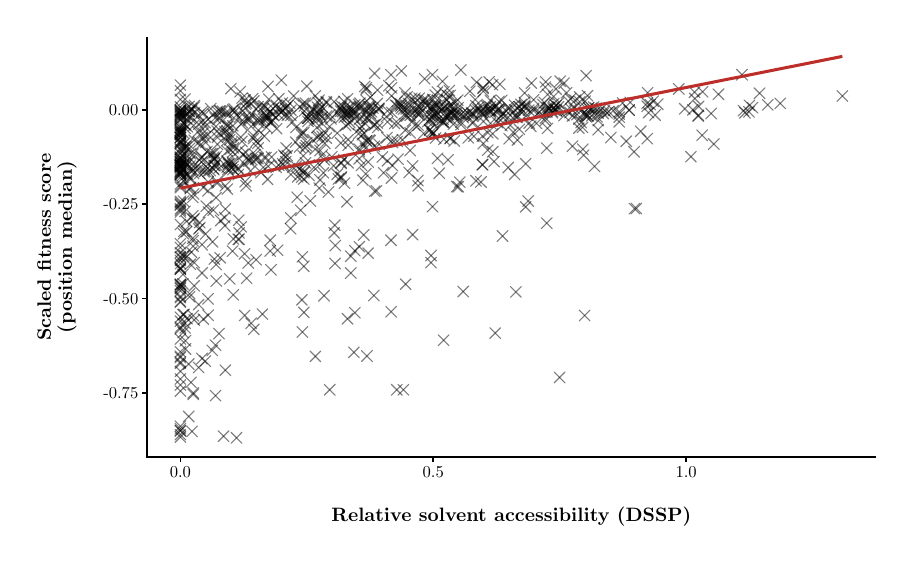
\begin{tikzpicture}[x=1pt,y=1pt]
\definecolor{fillColor}{RGB}{255,255,255}
\path[use as bounding box,fill=fillColor,fill opacity=0.00] (0,0) rectangle (309.84,183.39);
\begin{scope}
\path[clip] ( 43.23, 28.30) rectangle (306.34,179.89);
\definecolor{drawColor}{RGB}{0,0,0}

\path[draw=drawColor,draw opacity=0.50,line width= 0.4pt,line join=round,line cap=round] (149.68,152.59) -- (153.61,156.51);

\path[draw=drawColor,draw opacity=0.50,line width= 0.4pt,line join=round,line cap=round] (149.68,156.51) -- (153.61,152.59);

\path[draw=drawColor,draw opacity=0.50,line width= 0.4pt,line join=round,line cap=round] (165.28,146.84) -- (169.20,150.77);

\path[draw=drawColor,draw opacity=0.50,line width= 0.4pt,line join=round,line cap=round] (165.28,150.77) -- (169.20,146.84);

\path[draw=drawColor,draw opacity=0.50,line width= 0.4pt,line join=round,line cap=round] (165.16,151.70) -- (169.09,155.63);

\path[draw=drawColor,draw opacity=0.50,line width= 0.4pt,line join=round,line cap=round] (165.16,155.63) -- (169.09,151.70);

\path[draw=drawColor,draw opacity=0.50,line width= 0.4pt,line join=round,line cap=round] ( 55.86,128.42) -- ( 59.79,132.35);

\path[draw=drawColor,draw opacity=0.50,line width= 0.4pt,line join=round,line cap=round] ( 55.86,132.35) -- ( 59.79,128.42);

\path[draw=drawColor,draw opacity=0.50,line width= 0.4pt,line join=round,line cap=round] (101.15,140.81) -- (105.07,144.74);

\path[draw=drawColor,draw opacity=0.50,line width= 0.4pt,line join=round,line cap=round] (101.15,144.74) -- (105.07,140.81);

\path[draw=drawColor,draw opacity=0.50,line width= 0.4pt,line join=round,line cap=round] (167.38,153.35) -- (171.30,157.27);

\path[draw=drawColor,draw opacity=0.50,line width= 0.4pt,line join=round,line cap=round] (167.38,157.27) -- (171.30,153.35);

\path[draw=drawColor,draw opacity=0.50,line width= 0.4pt,line join=round,line cap=round] ( 84.32,145.42) -- ( 88.25,149.34);

\path[draw=drawColor,draw opacity=0.50,line width= 0.4pt,line join=round,line cap=round] ( 84.32,149.34) -- ( 88.25,145.42);

\path[draw=drawColor,draw opacity=0.50,line width= 0.4pt,line join=round,line cap=round] ( 53.23, 83.88) -- ( 57.15, 87.80);

\path[draw=drawColor,draw opacity=0.50,line width= 0.4pt,line join=round,line cap=round] ( 53.23, 87.80) -- ( 57.15, 83.88);

\path[draw=drawColor,draw opacity=0.50,line width= 0.4pt,line join=round,line cap=round] (149.18,149.01) -- (153.11,152.94);

\path[draw=drawColor,draw opacity=0.50,line width= 0.4pt,line join=round,line cap=round] (149.18,152.94) -- (153.11,149.01);

\path[draw=drawColor,draw opacity=0.50,line width= 0.4pt,line join=round,line cap=round] (135.67,154.03) -- (139.59,157.96);

\path[draw=drawColor,draw opacity=0.50,line width= 0.4pt,line join=round,line cap=round] (135.67,157.96) -- (139.59,154.03);

\path[draw=drawColor,draw opacity=0.50,line width= 0.4pt,line join=round,line cap=round] ( 54.89,138.43) -- ( 58.81,142.35);

\path[draw=drawColor,draw opacity=0.50,line width= 0.4pt,line join=round,line cap=round] ( 54.89,142.35) -- ( 58.81,138.43);

\path[draw=drawColor,draw opacity=0.50,line width= 0.4pt,line join=round,line cap=round] ( 85.66,100.71) -- ( 89.58,104.64);

\path[draw=drawColor,draw opacity=0.50,line width= 0.4pt,line join=round,line cap=round] ( 85.66,104.64) -- ( 89.58,100.71);

\path[draw=drawColor,draw opacity=0.50,line width= 0.4pt,line join=round,line cap=round] (177.52,154.42) -- (181.44,158.34);

\path[draw=drawColor,draw opacity=0.50,line width= 0.4pt,line join=round,line cap=round] (177.52,158.34) -- (181.44,154.42);

\path[draw=drawColor,draw opacity=0.50,line width= 0.4pt,line join=round,line cap=round] (184.21,153.68) -- (188.13,157.60);

\path[draw=drawColor,draw opacity=0.50,line width= 0.4pt,line join=round,line cap=round] (184.21,157.60) -- (188.13,153.68);

\path[draw=drawColor,draw opacity=0.50,line width= 0.4pt,line join=round,line cap=round] ( 72.17,136.47) -- ( 76.10,140.39);

\path[draw=drawColor,draw opacity=0.50,line width= 0.4pt,line join=round,line cap=round] ( 72.17,140.39) -- ( 76.10,136.47);

\path[draw=drawColor,draw opacity=0.50,line width= 0.4pt,line join=round,line cap=round] (199.53,149.51) -- (203.45,153.43);

\path[draw=drawColor,draw opacity=0.50,line width= 0.4pt,line join=round,line cap=round] (199.53,153.43) -- (203.45,149.51);

\path[draw=drawColor,draw opacity=0.50,line width= 0.4pt,line join=round,line cap=round] ( 84.74,126.61) -- ( 88.66,130.54);

\path[draw=drawColor,draw opacity=0.50,line width= 0.4pt,line join=round,line cap=round] ( 84.74,130.54) -- ( 88.66,126.61);

\path[draw=drawColor,draw opacity=0.50,line width= 0.4pt,line join=round,line cap=round] (118.67,145.74) -- (122.59,149.67);

\path[draw=drawColor,draw opacity=0.50,line width= 0.4pt,line join=round,line cap=round] (118.67,149.67) -- (122.59,145.74);

\path[draw=drawColor,draw opacity=0.50,line width= 0.4pt,line join=round,line cap=round] ( 57.98,121.34) -- ( 61.91,125.26);

\path[draw=drawColor,draw opacity=0.50,line width= 0.4pt,line join=round,line cap=round] ( 57.98,125.26) -- ( 61.91,121.34);

\path[draw=drawColor,draw opacity=0.50,line width= 0.4pt,line join=round,line cap=round] ( 53.23, 36.50) -- ( 57.15, 40.43);

\path[draw=drawColor,draw opacity=0.50,line width= 0.4pt,line join=round,line cap=round] ( 53.23, 40.43) -- ( 57.15, 36.50);

\path[draw=drawColor,draw opacity=0.50,line width= 0.4pt,line join=round,line cap=round] ( 53.23, 76.78) -- ( 57.15, 80.70);

\path[draw=drawColor,draw opacity=0.50,line width= 0.4pt,line join=round,line cap=round] ( 53.23, 80.70) -- ( 57.15, 76.78);

\path[draw=drawColor,draw opacity=0.50,line width= 0.4pt,line join=round,line cap=round] ( 53.23,128.20) -- ( 57.15,132.12);

\path[draw=drawColor,draw opacity=0.50,line width= 0.4pt,line join=round,line cap=round] ( 53.23,132.12) -- ( 57.15,128.20);

\path[draw=drawColor,draw opacity=0.50,line width= 0.4pt,line join=round,line cap=round] ( 59.51,143.75) -- ( 63.43,147.67);

\path[draw=drawColor,draw opacity=0.50,line width= 0.4pt,line join=round,line cap=round] ( 59.51,147.67) -- ( 63.43,143.75);

\path[draw=drawColor,draw opacity=0.50,line width= 0.4pt,line join=round,line cap=round] ( 53.23,129.10) -- ( 57.15,133.02);

\path[draw=drawColor,draw opacity=0.50,line width= 0.4pt,line join=round,line cap=round] ( 53.23,133.02) -- ( 57.15,129.10);

\path[draw=drawColor,draw opacity=0.50,line width= 0.4pt,line join=round,line cap=round] (110.30,126.76) -- (114.22,130.69);

\path[draw=drawColor,draw opacity=0.50,line width= 0.4pt,line join=round,line cap=round] (110.30,130.69) -- (114.22,126.76);

\path[draw=drawColor,draw opacity=0.50,line width= 0.4pt,line join=round,line cap=round] ( 74.40,137.04) -- ( 78.33,140.96);

\path[draw=drawColor,draw opacity=0.50,line width= 0.4pt,line join=round,line cap=round] ( 74.40,140.96) -- ( 78.33,137.04);

\path[draw=drawColor,draw opacity=0.50,line width= 0.4pt,line join=round,line cap=round] (235.49,152.11) -- (239.41,156.04);

\path[draw=drawColor,draw opacity=0.50,line width= 0.4pt,line join=round,line cap=round] (235.49,156.04) -- (239.41,152.11);

\path[draw=drawColor,draw opacity=0.50,line width= 0.4pt,line join=round,line cap=round] (159.27,142.16) -- (163.19,146.09);

\path[draw=drawColor,draw opacity=0.50,line width= 0.4pt,line join=round,line cap=round] (159.27,146.09) -- (163.19,142.16);

\path[draw=drawColor,draw opacity=0.50,line width= 0.4pt,line join=round,line cap=round] (111.28,127.13) -- (115.21,131.05);

\path[draw=drawColor,draw opacity=0.50,line width= 0.4pt,line join=round,line cap=round] (111.28,131.05) -- (115.21,127.13);

\path[draw=drawColor,draw opacity=0.50,line width= 0.4pt,line join=round,line cap=round] (162.51,152.15) -- (166.43,156.07);

\path[draw=drawColor,draw opacity=0.50,line width= 0.4pt,line join=round,line cap=round] (162.51,156.07) -- (166.43,152.15);

\path[draw=drawColor,draw opacity=0.50,line width= 0.4pt,line join=round,line cap=round] (137.07,147.63) -- (141.00,151.56);

\path[draw=drawColor,draw opacity=0.50,line width= 0.4pt,line join=round,line cap=round] (137.07,151.56) -- (141.00,147.63);

\path[draw=drawColor,draw opacity=0.50,line width= 0.4pt,line join=round,line cap=round] (111.18,139.75) -- (115.10,143.67);

\path[draw=drawColor,draw opacity=0.50,line width= 0.4pt,line join=round,line cap=round] (111.18,143.67) -- (115.10,139.75);

\path[draw=drawColor,draw opacity=0.50,line width= 0.4pt,line join=round,line cap=round] ( 97.17,143.57) -- (101.09,147.49);

\path[draw=drawColor,draw opacity=0.50,line width= 0.4pt,line join=round,line cap=round] ( 97.17,147.49) -- (101.09,143.57);

\path[draw=drawColor,draw opacity=0.50,line width= 0.4pt,line join=round,line cap=round] (121.84,150.44) -- (125.76,154.37);

\path[draw=drawColor,draw opacity=0.50,line width= 0.4pt,line join=round,line cap=round] (121.84,154.37) -- (125.76,150.44);

\path[draw=drawColor,draw opacity=0.50,line width= 0.4pt,line join=round,line cap=round] ( 96.94,142.79) -- (100.86,146.71);

\path[draw=drawColor,draw opacity=0.50,line width= 0.4pt,line join=round,line cap=round] ( 96.94,146.71) -- (100.86,142.79);

\path[draw=drawColor,draw opacity=0.50,line width= 0.4pt,line join=round,line cap=round] (119.47,106.52) -- (123.39,110.45);

\path[draw=drawColor,draw opacity=0.50,line width= 0.4pt,line join=round,line cap=round] (119.47,110.45) -- (123.39,106.52);

\path[draw=drawColor,draw opacity=0.50,line width= 0.4pt,line join=round,line cap=round] ( 93.15,151.61) -- ( 97.08,155.53);

\path[draw=drawColor,draw opacity=0.50,line width= 0.4pt,line join=round,line cap=round] ( 93.15,155.53) -- ( 97.08,151.61);

\path[draw=drawColor,draw opacity=0.50,line width= 0.4pt,line join=round,line cap=round] (201.78,152.31) -- (205.70,156.24);

\path[draw=drawColor,draw opacity=0.50,line width= 0.4pt,line join=round,line cap=round] (201.78,156.24) -- (205.70,152.31);

\path[draw=drawColor,draw opacity=0.50,line width= 0.4pt,line join=round,line cap=round] (123.32,138.59) -- (127.24,142.52);

\path[draw=drawColor,draw opacity=0.50,line width= 0.4pt,line join=round,line cap=round] (123.32,142.52) -- (127.24,138.59);

\path[draw=drawColor,draw opacity=0.50,line width= 0.4pt,line join=round,line cap=round] (101.91,137.53) -- (105.83,141.45);

\path[draw=drawColor,draw opacity=0.50,line width= 0.4pt,line join=round,line cap=round] (101.91,141.45) -- (105.83,137.53);

\path[draw=drawColor,draw opacity=0.50,line width= 0.4pt,line join=round,line cap=round] ( 55.05, 68.30) -- ( 58.97, 72.22);

\path[draw=drawColor,draw opacity=0.50,line width= 0.4pt,line join=round,line cap=round] ( 55.05, 72.22) -- ( 58.97, 68.30);

\path[draw=drawColor,draw opacity=0.50,line width= 0.4pt,line join=round,line cap=round] ( 76.41, 99.75) -- ( 80.34,103.67);

\path[draw=drawColor,draw opacity=0.50,line width= 0.4pt,line join=round,line cap=round] ( 76.41,103.67) -- ( 80.34, 99.75);

\path[draw=drawColor,draw opacity=0.50,line width= 0.4pt,line join=round,line cap=round] ( 56.88,126.60) -- ( 60.81,130.52);

\path[draw=drawColor,draw opacity=0.50,line width= 0.4pt,line join=round,line cap=round] ( 56.88,130.52) -- ( 60.81,126.60);

\path[draw=drawColor,draw opacity=0.50,line width= 0.4pt,line join=round,line cap=round] ( 55.97,139.50) -- ( 59.89,143.42);

\path[draw=drawColor,draw opacity=0.50,line width= 0.4pt,line join=round,line cap=round] ( 55.97,143.42) -- ( 59.89,139.50);

\path[draw=drawColor,draw opacity=0.50,line width= 0.4pt,line join=round,line cap=round] ( 68.82, 33.82) -- ( 72.75, 37.74);

\path[draw=drawColor,draw opacity=0.50,line width= 0.4pt,line join=round,line cap=round] ( 68.82, 37.74) -- ( 72.75, 33.82);

\path[draw=drawColor,draw opacity=0.50,line width= 0.4pt,line join=round,line cap=round] ( 53.23, 87.16) -- ( 57.15, 91.08);

\path[draw=drawColor,draw opacity=0.50,line width= 0.4pt,line join=round,line cap=round] ( 53.23, 91.08) -- ( 57.15, 87.16);

\path[draw=drawColor,draw opacity=0.50,line width= 0.4pt,line join=round,line cap=round] ( 54.14,127.26) -- ( 58.06,131.18);

\path[draw=drawColor,draw opacity=0.50,line width= 0.4pt,line join=round,line cap=round] ( 54.14,131.18) -- ( 58.06,127.26);

\path[draw=drawColor,draw opacity=0.50,line width= 0.4pt,line join=round,line cap=round] ( 53.23, 34.39) -- ( 57.15, 38.31);

\path[draw=drawColor,draw opacity=0.50,line width= 0.4pt,line join=round,line cap=round] ( 53.23, 38.31) -- ( 57.15, 34.39);

\path[draw=drawColor,draw opacity=0.50,line width= 0.4pt,line join=round,line cap=round] ( 53.23, 94.43) -- ( 57.15, 98.36);

\path[draw=drawColor,draw opacity=0.50,line width= 0.4pt,line join=round,line cap=round] ( 53.23, 98.36) -- ( 57.15, 94.43);

\path[draw=drawColor,draw opacity=0.50,line width= 0.4pt,line join=round,line cap=round] ( 54.34,137.74) -- ( 58.27,141.67);

\path[draw=drawColor,draw opacity=0.50,line width= 0.4pt,line join=round,line cap=round] ( 54.34,141.67) -- ( 58.27,137.74);

\path[draw=drawColor,draw opacity=0.50,line width= 0.4pt,line join=round,line cap=round] ( 53.23, 82.23) -- ( 57.15, 86.16);

\path[draw=drawColor,draw opacity=0.50,line width= 0.4pt,line join=round,line cap=round] ( 53.23, 86.16) -- ( 57.15, 82.23);

\path[draw=drawColor,draw opacity=0.50,line width= 0.4pt,line join=round,line cap=round] ( 53.23,100.14) -- ( 57.15,104.06);

\path[draw=drawColor,draw opacity=0.50,line width= 0.4pt,line join=round,line cap=round] ( 53.23,104.06) -- ( 57.15,100.14);

\path[draw=drawColor,draw opacity=0.50,line width= 0.4pt,line join=round,line cap=round] ( 53.23,117.33) -- ( 57.15,121.26);

\path[draw=drawColor,draw opacity=0.50,line width= 0.4pt,line join=round,line cap=round] ( 53.23,121.26) -- ( 57.15,117.33);

\path[draw=drawColor,draw opacity=0.50,line width= 0.4pt,line join=round,line cap=round] ( 63.18,148.29) -- ( 67.10,152.21);

\path[draw=drawColor,draw opacity=0.50,line width= 0.4pt,line join=round,line cap=round] ( 63.18,152.21) -- ( 67.10,148.29);

\path[draw=drawColor,draw opacity=0.50,line width= 0.4pt,line join=round,line cap=round] ( 56.80, 95.94) -- ( 60.72, 99.87);

\path[draw=drawColor,draw opacity=0.50,line width= 0.4pt,line join=round,line cap=round] ( 56.80, 99.87) -- ( 60.72, 95.94);

\path[draw=drawColor,draw opacity=0.50,line width= 0.4pt,line join=round,line cap=round] ( 56.57, 84.21) -- ( 60.50, 88.14);

\path[draw=drawColor,draw opacity=0.50,line width= 0.4pt,line join=round,line cap=round] ( 56.57, 88.14) -- ( 60.50, 84.21);

\path[draw=drawColor,draw opacity=0.50,line width= 0.4pt,line join=round,line cap=round] (100.01,150.54) -- (103.93,154.46);

\path[draw=drawColor,draw opacity=0.50,line width= 0.4pt,line join=round,line cap=round] (100.01,154.46) -- (103.93,150.54);

\path[draw=drawColor,draw opacity=0.50,line width= 0.4pt,line join=round,line cap=round] (102.71,141.78) -- (106.63,145.70);

\path[draw=drawColor,draw opacity=0.50,line width= 0.4pt,line join=round,line cap=round] (102.71,145.70) -- (106.63,141.78);

\path[draw=drawColor,draw opacity=0.50,line width= 0.4pt,line join=round,line cap=round] (129.32,104.60) -- (133.25,108.53);

\path[draw=drawColor,draw opacity=0.50,line width= 0.4pt,line join=round,line cap=round] (129.32,108.53) -- (133.25,104.60);

\path[draw=drawColor,draw opacity=0.50,line width= 0.4pt,line join=round,line cap=round] (170.98,151.31) -- (174.90,155.23);

\path[draw=drawColor,draw opacity=0.50,line width= 0.4pt,line join=round,line cap=round] (170.98,155.23) -- (174.90,151.31);

\path[draw=drawColor,draw opacity=0.50,line width= 0.4pt,line join=round,line cap=round] (204.17,144.54) -- (208.10,148.46);

\path[draw=drawColor,draw opacity=0.50,line width= 0.4pt,line join=round,line cap=round] (204.17,148.46) -- (208.10,144.54);

\path[draw=drawColor,draw opacity=0.50,line width= 0.4pt,line join=round,line cap=round] (179.09,151.60) -- (183.02,155.52);

\path[draw=drawColor,draw opacity=0.50,line width= 0.4pt,line join=round,line cap=round] (179.09,155.52) -- (183.02,151.60);

\path[draw=drawColor,draw opacity=0.50,line width= 0.4pt,line join=round,line cap=round] ( 64.74,135.89) -- ( 68.66,139.82);

\path[draw=drawColor,draw opacity=0.50,line width= 0.4pt,line join=round,line cap=round] ( 64.74,139.82) -- ( 68.66,135.89);

\path[draw=drawColor,draw opacity=0.50,line width= 0.4pt,line join=round,line cap=round] (167.84,151.70) -- (171.76,155.62);

\path[draw=drawColor,draw opacity=0.50,line width= 0.4pt,line join=round,line cap=round] (167.84,155.62) -- (171.76,151.70);

\path[draw=drawColor,draw opacity=0.50,line width= 0.4pt,line join=round,line cap=round] ( 97.80,129.08) -- (101.73,133.00);

\path[draw=drawColor,draw opacity=0.50,line width= 0.4pt,line join=round,line cap=round] ( 97.80,133.00) -- (101.73,129.08);

\path[draw=drawColor,draw opacity=0.50,line width= 0.4pt,line join=round,line cap=round] (164.69,151.36) -- (168.62,155.28);

\path[draw=drawColor,draw opacity=0.50,line width= 0.4pt,line join=round,line cap=round] (164.69,155.28) -- (168.62,151.36);

\path[draw=drawColor,draw opacity=0.50,line width= 0.4pt,line join=round,line cap=round] (126.65,129.02) -- (130.57,132.95);

\path[draw=drawColor,draw opacity=0.50,line width= 0.4pt,line join=round,line cap=round] (126.65,132.95) -- (130.57,129.02);

\path[draw=drawColor,draw opacity=0.50,line width= 0.4pt,line join=round,line cap=round] (142.61,147.49) -- (146.54,151.42);

\path[draw=drawColor,draw opacity=0.50,line width= 0.4pt,line join=round,line cap=round] (142.61,151.42) -- (146.54,147.49);

\path[draw=drawColor,draw opacity=0.50,line width= 0.4pt,line join=round,line cap=round] ( 69.20,112.83) -- ( 73.12,116.76);

\path[draw=drawColor,draw opacity=0.50,line width= 0.4pt,line join=round,line cap=round] ( 69.20,116.76) -- ( 73.12,112.83);

\path[draw=drawColor,draw opacity=0.50,line width= 0.4pt,line join=round,line cap=round] (189.87,152.87) -- (193.79,156.80);

\path[draw=drawColor,draw opacity=0.50,line width= 0.4pt,line join=round,line cap=round] (189.87,156.80) -- (193.79,152.87);

\path[draw=drawColor,draw opacity=0.50,line width= 0.4pt,line join=round,line cap=round] ( 72.04,100.69) -- ( 75.97,104.62);

\path[draw=drawColor,draw opacity=0.50,line width= 0.4pt,line join=round,line cap=round] ( 72.04,104.62) -- ( 75.97,100.69);

\path[draw=drawColor,draw opacity=0.50,line width= 0.4pt,line join=round,line cap=round] (115.60,151.02) -- (119.53,154.94);

\path[draw=drawColor,draw opacity=0.50,line width= 0.4pt,line join=round,line cap=round] (115.60,154.94) -- (119.53,151.02);

\path[draw=drawColor,draw opacity=0.50,line width= 0.4pt,line join=round,line cap=round] (173.98,153.43) -- (177.90,157.35);

\path[draw=drawColor,draw opacity=0.50,line width= 0.4pt,line join=round,line cap=round] (173.98,157.35) -- (177.90,153.43);

\path[draw=drawColor,draw opacity=0.50,line width= 0.4pt,line join=round,line cap=round] (213.02,154.20) -- (216.94,158.13);

\path[draw=drawColor,draw opacity=0.50,line width= 0.4pt,line join=round,line cap=round] (213.02,158.13) -- (216.94,154.20);

\path[draw=drawColor,draw opacity=0.50,line width= 0.4pt,line join=round,line cap=round] (144.54,143.46) -- (148.47,147.39);

\path[draw=drawColor,draw opacity=0.50,line width= 0.4pt,line join=round,line cap=round] (144.54,147.39) -- (148.47,143.46);

\path[draw=drawColor,draw opacity=0.50,line width= 0.4pt,line join=round,line cap=round] (113.40,118.51) -- (117.33,122.43);

\path[draw=drawColor,draw opacity=0.50,line width= 0.4pt,line join=round,line cap=round] (113.40,122.43) -- (117.33,118.51);

\path[draw=drawColor,draw opacity=0.50,line width= 0.4pt,line join=round,line cap=round] (105.55,143.46) -- (109.47,147.39);

\path[draw=drawColor,draw opacity=0.50,line width= 0.4pt,line join=round,line cap=round] (105.55,147.39) -- (109.47,143.46);

\path[draw=drawColor,draw opacity=0.50,line width= 0.4pt,line join=round,line cap=round] (196.55,150.06) -- (200.47,153.98);

\path[draw=drawColor,draw opacity=0.50,line width= 0.4pt,line join=round,line cap=round] (196.55,153.98) -- (200.47,150.06);

\path[draw=drawColor,draw opacity=0.50,line width= 0.4pt,line join=round,line cap=round] (154.14,125.61) -- (158.07,129.54);

\path[draw=drawColor,draw opacity=0.50,line width= 0.4pt,line join=round,line cap=round] (154.14,129.54) -- (158.07,125.61);

\path[draw=drawColor,draw opacity=0.50,line width= 0.4pt,line join=round,line cap=round] ( 61.03, 92.78) -- ( 64.95, 96.70);

\path[draw=drawColor,draw opacity=0.50,line width= 0.4pt,line join=round,line cap=round] ( 61.03, 96.70) -- ( 64.95, 92.78);

\path[draw=drawColor,draw opacity=0.50,line width= 0.4pt,line join=round,line cap=round] ( 97.02,127.38) -- (100.94,131.31);

\path[draw=drawColor,draw opacity=0.50,line width= 0.4pt,line join=round,line cap=round] ( 97.02,131.31) -- (100.94,127.38);

\path[draw=drawColor,draw opacity=0.50,line width= 0.4pt,line join=round,line cap=round] ( 94.85,140.09) -- ( 98.77,144.01);

\path[draw=drawColor,draw opacity=0.50,line width= 0.4pt,line join=round,line cap=round] ( 94.85,144.01) -- ( 98.77,140.09);

\path[draw=drawColor,draw opacity=0.50,line width= 0.4pt,line join=round,line cap=round] ( 53.23, 82.52) -- ( 57.15, 86.44);

\path[draw=drawColor,draw opacity=0.50,line width= 0.4pt,line join=round,line cap=round] ( 53.23, 86.44) -- ( 57.15, 82.52);

\path[draw=drawColor,draw opacity=0.50,line width= 0.4pt,line join=round,line cap=round] (174.58,149.01) -- (178.50,152.94);

\path[draw=drawColor,draw opacity=0.50,line width= 0.4pt,line join=round,line cap=round] (174.58,152.94) -- (178.50,149.01);

\path[draw=drawColor,draw opacity=0.50,line width= 0.4pt,line join=round,line cap=round] (186.50,152.39) -- (190.42,156.31);

\path[draw=drawColor,draw opacity=0.50,line width= 0.4pt,line join=round,line cap=round] (186.50,156.31) -- (190.42,152.39);

\path[draw=drawColor,draw opacity=0.50,line width= 0.4pt,line join=round,line cap=round] (131.60,140.33) -- (135.52,144.25);

\path[draw=drawColor,draw opacity=0.50,line width= 0.4pt,line join=round,line cap=round] (131.60,144.25) -- (135.52,140.33);

\path[draw=drawColor,draw opacity=0.50,line width= 0.4pt,line join=round,line cap=round] (124.55,145.42) -- (128.47,149.34);

\path[draw=drawColor,draw opacity=0.50,line width= 0.4pt,line join=round,line cap=round] (124.55,149.34) -- (128.47,145.42);

\path[draw=drawColor,draw opacity=0.50,line width= 0.4pt,line join=round,line cap=round] (221.89,154.14) -- (225.81,158.06);

\path[draw=drawColor,draw opacity=0.50,line width= 0.4pt,line join=round,line cap=round] (221.89,158.06) -- (225.81,154.14);

\path[draw=drawColor,draw opacity=0.50,line width= 0.4pt,line join=round,line cap=round] (200.35,149.63) -- (204.27,153.56);

\path[draw=drawColor,draw opacity=0.50,line width= 0.4pt,line join=round,line cap=round] (200.35,153.56) -- (204.27,149.63);

\path[draw=drawColor,draw opacity=0.50,line width= 0.4pt,line join=round,line cap=round] ( 60.20,111.00) -- ( 64.12,114.92);

\path[draw=drawColor,draw opacity=0.50,line width= 0.4pt,line join=round,line cap=round] ( 60.20,114.92) -- ( 64.12,111.00);

\path[draw=drawColor,draw opacity=0.50,line width= 0.4pt,line join=round,line cap=round] ( 57.80,102.44) -- ( 61.72,106.36);

\path[draw=drawColor,draw opacity=0.50,line width= 0.4pt,line join=round,line cap=round] ( 57.80,106.36) -- ( 61.72,102.44);

\path[draw=drawColor,draw opacity=0.50,line width= 0.4pt,line join=round,line cap=round] ( 70.36,132.70) -- ( 74.28,136.62);

\path[draw=drawColor,draw opacity=0.50,line width= 0.4pt,line join=round,line cap=round] ( 70.36,136.62) -- ( 74.28,132.70);

\path[draw=drawColor,draw opacity=0.50,line width= 0.4pt,line join=round,line cap=round] ( 55.61, 98.78) -- ( 59.53,102.71);

\path[draw=drawColor,draw opacity=0.50,line width= 0.4pt,line join=round,line cap=round] ( 55.61,102.71) -- ( 59.53, 98.78);

\path[draw=drawColor,draw opacity=0.50,line width= 0.4pt,line join=round,line cap=round] (142.61,153.31) -- (146.54,157.23);

\path[draw=drawColor,draw opacity=0.50,line width= 0.4pt,line join=round,line cap=round] (142.61,157.23) -- (146.54,153.31);

\path[draw=drawColor,draw opacity=0.50,line width= 0.4pt,line join=round,line cap=round] (135.87,129.10) -- (139.80,133.03);

\path[draw=drawColor,draw opacity=0.50,line width= 0.4pt,line join=round,line cap=round] (135.87,133.03) -- (139.80,129.10);

\path[draw=drawColor,draw opacity=0.50,line width= 0.4pt,line join=round,line cap=round] ( 53.23, 88.54) -- ( 57.15, 92.46);

\path[draw=drawColor,draw opacity=0.50,line width= 0.4pt,line join=round,line cap=round] ( 53.23, 92.46) -- ( 57.15, 88.54);

\path[draw=drawColor,draw opacity=0.50,line width= 0.4pt,line join=round,line cap=round] ( 54.53, 77.78) -- ( 58.45, 81.70);

\path[draw=drawColor,draw opacity=0.50,line width= 0.4pt,line join=round,line cap=round] ( 54.53, 81.70) -- ( 58.45, 77.78);

\path[draw=drawColor,draw opacity=0.50,line width= 0.4pt,line join=round,line cap=round] (121.84,152.77) -- (125.76,156.69);

\path[draw=drawColor,draw opacity=0.50,line width= 0.4pt,line join=round,line cap=round] (121.84,156.69) -- (125.76,152.77);

\path[draw=drawColor,draw opacity=0.50,line width= 0.4pt,line join=round,line cap=round] ( 59.86,108.72) -- ( 63.79,112.64);

\path[draw=drawColor,draw opacity=0.50,line width= 0.4pt,line join=round,line cap=round] ( 59.86,112.64) -- ( 63.79,108.72);

\path[draw=drawColor,draw opacity=0.50,line width= 0.4pt,line join=round,line cap=round] ( 53.23,103.36) -- ( 57.15,107.29);

\path[draw=drawColor,draw opacity=0.50,line width= 0.4pt,line join=round,line cap=round] ( 53.23,107.29) -- ( 57.15,103.36);

\path[draw=drawColor,draw opacity=0.50,line width= 0.4pt,line join=round,line cap=round] ( 53.23, 84.31) -- ( 57.15, 88.23);

\path[draw=drawColor,draw opacity=0.50,line width= 0.4pt,line join=round,line cap=round] ( 53.23, 88.23) -- ( 57.15, 84.31);

\path[draw=drawColor,draw opacity=0.50,line width= 0.4pt,line join=round,line cap=round] ( 70.36,142.00) -- ( 74.28,145.93);

\path[draw=drawColor,draw opacity=0.50,line width= 0.4pt,line join=round,line cap=round] ( 70.36,145.93) -- ( 74.28,142.00);

\path[draw=drawColor,draw opacity=0.50,line width= 0.4pt,line join=round,line cap=round] (102.55,145.33) -- (106.47,149.26);

\path[draw=drawColor,draw opacity=0.50,line width= 0.4pt,line join=round,line cap=round] (102.55,149.26) -- (106.47,145.33);

\path[draw=drawColor,draw opacity=0.50,line width= 0.4pt,line join=round,line cap=round] ( 73.50, 33.23) -- ( 77.42, 37.16);

\path[draw=drawColor,draw opacity=0.50,line width= 0.4pt,line join=round,line cap=round] ( 73.50, 37.16) -- ( 77.42, 33.23);

\path[draw=drawColor,draw opacity=0.50,line width= 0.4pt,line join=round,line cap=round] ( 53.23, 33.48) -- ( 57.15, 37.40);

\path[draw=drawColor,draw opacity=0.50,line width= 0.4pt,line join=round,line cap=round] ( 53.23, 37.40) -- ( 57.15, 33.48);

\path[draw=drawColor,draw opacity=0.50,line width= 0.4pt,line join=round,line cap=round] ( 69.46, 57.66) -- ( 73.38, 61.58);

\path[draw=drawColor,draw opacity=0.50,line width= 0.4pt,line join=round,line cap=round] ( 69.46, 61.58) -- ( 73.38, 57.66);

\path[draw=drawColor,draw opacity=0.50,line width= 0.4pt,line join=round,line cap=round] ( 54.55,107.91) -- ( 58.47,111.83);

\path[draw=drawColor,draw opacity=0.50,line width= 0.4pt,line join=round,line cap=round] ( 54.55,111.83) -- ( 58.47,107.91);

\path[draw=drawColor,draw opacity=0.50,line width= 0.4pt,line join=round,line cap=round] ( 53.23, 35.77) -- ( 57.15, 39.70);

\path[draw=drawColor,draw opacity=0.50,line width= 0.4pt,line join=round,line cap=round] ( 53.23, 39.70) -- ( 57.15, 35.77);

\path[draw=drawColor,draw opacity=0.50,line width= 0.4pt,line join=round,line cap=round] ( 53.23, 64.30) -- ( 57.15, 68.23);

\path[draw=drawColor,draw opacity=0.50,line width= 0.4pt,line join=round,line cap=round] ( 53.23, 68.23) -- ( 57.15, 64.30);

\path[draw=drawColor,draw opacity=0.50,line width= 0.4pt,line join=round,line cap=round] ( 85.69,104.60) -- ( 89.61,108.53);

\path[draw=drawColor,draw opacity=0.50,line width= 0.4pt,line join=round,line cap=round] ( 85.69,108.53) -- ( 89.61,104.60);

\path[draw=drawColor,draw opacity=0.50,line width= 0.4pt,line join=round,line cap=round] ( 76.63,125.75) -- ( 80.55,129.67);

\path[draw=drawColor,draw opacity=0.50,line width= 0.4pt,line join=round,line cap=round] ( 76.63,129.67) -- ( 80.55,125.75);

\path[draw=drawColor,draw opacity=0.50,line width= 0.4pt,line join=round,line cap=round] ( 53.23, 52.31) -- ( 57.15, 56.23);

\path[draw=drawColor,draw opacity=0.50,line width= 0.4pt,line join=round,line cap=round] ( 53.23, 56.23) -- ( 57.15, 52.31);

\path[draw=drawColor,draw opacity=0.50,line width= 0.4pt,line join=round,line cap=round] ( 53.23,123.64) -- ( 57.15,127.57);

\path[draw=drawColor,draw opacity=0.50,line width= 0.4pt,line join=round,line cap=round] ( 53.23,127.57) -- ( 57.15,123.64);

\path[draw=drawColor,draw opacity=0.50,line width= 0.4pt,line join=round,line cap=round] (175.77,152.88) -- (179.69,156.80);

\path[draw=drawColor,draw opacity=0.50,line width= 0.4pt,line join=round,line cap=round] (175.77,156.80) -- (179.69,152.88);

\path[draw=drawColor,draw opacity=0.50,line width= 0.4pt,line join=round,line cap=round] ( 99.35,148.72) -- (103.27,152.64);

\path[draw=drawColor,draw opacity=0.50,line width= 0.4pt,line join=round,line cap=round] ( 99.35,152.64) -- (103.27,148.72);

\path[draw=drawColor,draw opacity=0.50,line width= 0.4pt,line join=round,line cap=round] ( 74.19,128.36) -- ( 78.11,132.29);

\path[draw=drawColor,draw opacity=0.50,line width= 0.4pt,line join=round,line cap=round] ( 74.19,132.29) -- ( 78.11,128.36);

\path[draw=drawColor,draw opacity=0.50,line width= 0.4pt,line join=round,line cap=round] (173.98,128.39) -- (177.91,132.32);

\path[draw=drawColor,draw opacity=0.50,line width= 0.4pt,line join=round,line cap=round] (173.98,132.32) -- (177.91,128.39);

\path[draw=drawColor,draw opacity=0.50,line width= 0.4pt,line join=round,line cap=round] ( 64.84,104.06) -- ( 68.76,107.99);

\path[draw=drawColor,draw opacity=0.50,line width= 0.4pt,line join=round,line cap=round] ( 64.84,107.99) -- ( 68.76,104.06);

\path[draw=drawColor,draw opacity=0.50,line width= 0.4pt,line join=round,line cap=round] ( 66.11,119.99) -- ( 70.03,123.92);

\path[draw=drawColor,draw opacity=0.50,line width= 0.4pt,line join=round,line cap=round] ( 66.11,123.92) -- ( 70.03,119.99);

\path[draw=drawColor,draw opacity=0.50,line width= 0.4pt,line join=round,line cap=round] (203.38,152.28) -- (207.30,156.21);

\path[draw=drawColor,draw opacity=0.50,line width= 0.4pt,line join=round,line cap=round] (203.38,156.21) -- (207.30,152.28);

\path[draw=drawColor,draw opacity=0.50,line width= 0.4pt,line join=round,line cap=round] (167.26,151.06) -- (171.18,154.98);

\path[draw=drawColor,draw opacity=0.50,line width= 0.4pt,line join=round,line cap=round] (167.26,154.98) -- (171.18,151.06);

\path[draw=drawColor,draw opacity=0.50,line width= 0.4pt,line join=round,line cap=round] ( 55.46,111.45) -- ( 59.38,115.38);

\path[draw=drawColor,draw opacity=0.50,line width= 0.4pt,line join=round,line cap=round] ( 55.46,115.38) -- ( 59.38,111.45);

\path[draw=drawColor,draw opacity=0.50,line width= 0.4pt,line join=round,line cap=round] (105.93,141.54) -- (109.86,145.46);

\path[draw=drawColor,draw opacity=0.50,line width= 0.4pt,line join=round,line cap=round] (105.93,145.46) -- (109.86,141.54);

\path[draw=drawColor,draw opacity=0.50,line width= 0.4pt,line join=round,line cap=round] (116.25,153.56) -- (120.17,157.48);

\path[draw=drawColor,draw opacity=0.50,line width= 0.4pt,line join=round,line cap=round] (116.25,157.48) -- (120.17,153.56);

\path[draw=drawColor,draw opacity=0.50,line width= 0.4pt,line join=round,line cap=round] ( 91.47,137.94) -- ( 95.40,141.86);

\path[draw=drawColor,draw opacity=0.50,line width= 0.4pt,line join=round,line cap=round] ( 91.47,141.86) -- ( 95.40,137.94);

\path[draw=drawColor,draw opacity=0.50,line width= 0.4pt,line join=round,line cap=round] ( 55.46,131.67) -- ( 59.38,135.60);

\path[draw=drawColor,draw opacity=0.50,line width= 0.4pt,line join=round,line cap=round] ( 55.46,135.60) -- ( 59.38,131.67);

\path[draw=drawColor,draw opacity=0.50,line width= 0.4pt,line join=round,line cap=round] (151.69,152.35) -- (155.61,156.28);

\path[draw=drawColor,draw opacity=0.50,line width= 0.4pt,line join=round,line cap=round] (151.69,156.28) -- (155.61,152.35);

\path[draw=drawColor,draw opacity=0.50,line width= 0.4pt,line join=round,line cap=round] (223.00,153.60) -- (226.93,157.53);

\path[draw=drawColor,draw opacity=0.50,line width= 0.4pt,line join=round,line cap=round] (223.00,157.53) -- (226.93,153.60);

\path[draw=drawColor,draw opacity=0.50,line width= 0.4pt,line join=round,line cap=round] ( 77.89,148.41) -- ( 81.81,152.33);

\path[draw=drawColor,draw opacity=0.50,line width= 0.4pt,line join=round,line cap=round] ( 77.89,152.33) -- ( 81.81,148.41);

\path[draw=drawColor,draw opacity=0.50,line width= 0.4pt,line join=round,line cap=round] (162.37,131.97) -- (166.30,135.89);

\path[draw=drawColor,draw opacity=0.50,line width= 0.4pt,line join=round,line cap=round] (162.37,135.89) -- (166.30,131.97);

\path[draw=drawColor,draw opacity=0.50,line width= 0.4pt,line join=round,line cap=round] ( 65.91, 48.47) -- ( 69.84, 52.40);

\path[draw=drawColor,draw opacity=0.50,line width= 0.4pt,line join=round,line cap=round] ( 65.91, 52.40) -- ( 69.84, 48.47);

\path[draw=drawColor,draw opacity=0.50,line width= 0.4pt,line join=round,line cap=round] (187.86,152.36) -- (191.78,156.29);

\path[draw=drawColor,draw opacity=0.50,line width= 0.4pt,line join=round,line cap=round] (187.86,156.29) -- (191.78,152.36);

\path[draw=drawColor,draw opacity=0.50,line width= 0.4pt,line join=round,line cap=round] (103.17,151.63) -- (107.09,155.55);

\path[draw=drawColor,draw opacity=0.50,line width= 0.4pt,line join=round,line cap=round] (103.17,155.55) -- (107.09,151.63);

\path[draw=drawColor,draw opacity=0.50,line width= 0.4pt,line join=round,line cap=round] ( 59.82, 58.65) -- ( 63.74, 62.57);

\path[draw=drawColor,draw opacity=0.50,line width= 0.4pt,line join=round,line cap=round] ( 59.82, 62.57) -- ( 63.74, 58.65);

\path[draw=drawColor,draw opacity=0.50,line width= 0.4pt,line join=round,line cap=round] (118.67,131.65) -- (122.59,135.57);

\path[draw=drawColor,draw opacity=0.50,line width= 0.4pt,line join=round,line cap=round] (118.67,135.57) -- (122.59,131.65);

\path[draw=drawColor,draw opacity=0.50,line width= 0.4pt,line join=round,line cap=round] ( 57.69,135.67) -- ( 61.61,139.60);

\path[draw=drawColor,draw opacity=0.50,line width= 0.4pt,line join=round,line cap=round] ( 57.69,139.60) -- ( 61.61,135.67);

\path[draw=drawColor,draw opacity=0.50,line width= 0.4pt,line join=round,line cap=round] (119.18,126.32) -- (123.10,130.24);

\path[draw=drawColor,draw opacity=0.50,line width= 0.4pt,line join=round,line cap=round] (119.18,130.24) -- (123.10,126.32);

\path[draw=drawColor,draw opacity=0.50,line width= 0.4pt,line join=round,line cap=round] ( 80.36,133.73) -- ( 84.29,137.66);

\path[draw=drawColor,draw opacity=0.50,line width= 0.4pt,line join=round,line cap=round] ( 80.36,137.66) -- ( 84.29,133.73);

\path[draw=drawColor,draw opacity=0.50,line width= 0.4pt,line join=round,line cap=round] (127.70,149.31) -- (131.62,153.24);

\path[draw=drawColor,draw opacity=0.50,line width= 0.4pt,line join=round,line cap=round] (127.70,153.24) -- (131.62,149.31);

\path[draw=drawColor,draw opacity=0.50,line width= 0.4pt,line join=round,line cap=round] ( 57.41, 35.55) -- ( 61.34, 39.47);

\path[draw=drawColor,draw opacity=0.50,line width= 0.4pt,line join=round,line cap=round] ( 57.41, 39.47) -- ( 61.34, 35.55);

\path[draw=drawColor,draw opacity=0.50,line width= 0.4pt,line join=round,line cap=round] ( 90.58,135.34) -- ( 94.50,139.26);

\path[draw=drawColor,draw opacity=0.50,line width= 0.4pt,line join=round,line cap=round] ( 90.58,139.26) -- ( 94.50,135.34);

\path[draw=drawColor,draw opacity=0.50,line width= 0.4pt,line join=round,line cap=round] (165.16,152.84) -- (169.09,156.76);

\path[draw=drawColor,draw opacity=0.50,line width= 0.4pt,line join=round,line cap=round] (165.16,156.76) -- (169.09,152.84);

\path[draw=drawColor,draw opacity=0.50,line width= 0.4pt,line join=round,line cap=round] ( 57.69,113.43) -- ( 61.61,117.36);

\path[draw=drawColor,draw opacity=0.50,line width= 0.4pt,line join=round,line cap=round] ( 57.69,117.36) -- ( 61.61,113.43);

\path[draw=drawColor,draw opacity=0.50,line width= 0.4pt,line join=round,line cap=round] ( 76.95,124.31) -- ( 80.87,128.24);

\path[draw=drawColor,draw opacity=0.50,line width= 0.4pt,line join=round,line cap=round] ( 76.95,128.24) -- ( 80.87,124.31);

\path[draw=drawColor,draw opacity=0.50,line width= 0.4pt,line join=round,line cap=round] (133.78,151.91) -- (137.70,155.83);

\path[draw=drawColor,draw opacity=0.50,line width= 0.4pt,line join=round,line cap=round] (133.78,155.83) -- (137.70,151.91);

\path[draw=drawColor,draw opacity=0.50,line width= 0.4pt,line join=round,line cap=round] ( 81.42,144.34) -- ( 85.35,148.27);

\path[draw=drawColor,draw opacity=0.50,line width= 0.4pt,line join=round,line cap=round] ( 81.42,148.27) -- ( 85.35,144.34);

\path[draw=drawColor,draw opacity=0.50,line width= 0.4pt,line join=round,line cap=round] (118.11,154.14) -- (122.03,158.06);

\path[draw=drawColor,draw opacity=0.50,line width= 0.4pt,line join=round,line cap=round] (118.11,158.06) -- (122.03,154.14);

\path[draw=drawColor,draw opacity=0.50,line width= 0.4pt,line join=round,line cap=round] (151.11,150.76) -- (155.04,154.69);

\path[draw=drawColor,draw opacity=0.50,line width= 0.4pt,line join=round,line cap=round] (151.11,154.69) -- (155.04,150.76);

\path[draw=drawColor,draw opacity=0.50,line width= 0.4pt,line join=round,line cap=round] (265.45,153.53) -- (269.37,157.45);

\path[draw=drawColor,draw opacity=0.50,line width= 0.4pt,line join=round,line cap=round] (265.45,157.45) -- (269.37,153.53);

\path[draw=drawColor,draw opacity=0.50,line width= 0.4pt,line join=round,line cap=round] (109.03,110.06) -- (112.96,113.99);

\path[draw=drawColor,draw opacity=0.50,line width= 0.4pt,line join=round,line cap=round] (109.03,113.99) -- (112.96,110.06);

\path[draw=drawColor,draw opacity=0.50,line width= 0.4pt,line join=round,line cap=round] (164.12,153.59) -- (168.04,157.51);

\path[draw=drawColor,draw opacity=0.50,line width= 0.4pt,line join=round,line cap=round] (164.12,157.51) -- (168.04,153.59);

\path[draw=drawColor,draw opacity=0.50,line width= 0.4pt,line join=round,line cap=round] (129.84,139.89) -- (133.77,143.81);

\path[draw=drawColor,draw opacity=0.50,line width= 0.4pt,line join=round,line cap=round] (129.84,143.81) -- (133.77,139.89);

\path[draw=drawColor,draw opacity=0.50,line width= 0.4pt,line join=round,line cap=round] ( 57.03, 53.26) -- ( 60.96, 57.19);

\path[draw=drawColor,draw opacity=0.50,line width= 0.4pt,line join=round,line cap=round] ( 57.03, 57.19) -- ( 60.96, 53.26);

\path[draw=drawColor,draw opacity=0.50,line width= 0.4pt,line join=round,line cap=round] ( 59.82, 81.36) -- ( 63.74, 85.29);

\path[draw=drawColor,draw opacity=0.50,line width= 0.4pt,line join=round,line cap=round] ( 59.82, 85.29) -- ( 63.74, 81.36);

\path[draw=drawColor,draw opacity=0.50,line width= 0.4pt,line join=round,line cap=round] ( 53.23, 35.76) -- ( 57.15, 39.68);

\path[draw=drawColor,draw opacity=0.50,line width= 0.4pt,line join=round,line cap=round] ( 53.23, 39.68) -- ( 57.15, 35.76);

\path[draw=drawColor,draw opacity=0.50,line width= 0.4pt,line join=round,line cap=round] ( 87.93,153.40) -- ( 91.86,157.32);

\path[draw=drawColor,draw opacity=0.50,line width= 0.4pt,line join=round,line cap=round] ( 87.93,157.32) -- ( 91.86,153.40);

\path[draw=drawColor,draw opacity=0.50,line width= 0.4pt,line join=round,line cap=round] ( 53.23, 60.12) -- ( 57.15, 64.04);

\path[draw=drawColor,draw opacity=0.50,line width= 0.4pt,line join=round,line cap=round] ( 53.23, 64.04) -- ( 57.15, 60.12);

\path[draw=drawColor,draw opacity=0.50,line width= 0.4pt,line join=round,line cap=round] ( 69.81,146.36) -- ( 73.74,150.29);

\path[draw=drawColor,draw opacity=0.50,line width= 0.4pt,line join=round,line cap=round] ( 69.81,150.29) -- ( 73.74,146.36);

\path[draw=drawColor,draw opacity=0.50,line width= 0.4pt,line join=round,line cap=round] ( 54.14, 92.28) -- ( 58.07, 96.20);

\path[draw=drawColor,draw opacity=0.50,line width= 0.4pt,line join=round,line cap=round] ( 54.14, 96.20) -- ( 58.07, 92.28);

\path[draw=drawColor,draw opacity=0.50,line width= 0.4pt,line join=round,line cap=round] ( 53.23, 54.49) -- ( 57.15, 58.41);

\path[draw=drawColor,draw opacity=0.50,line width= 0.4pt,line join=round,line cap=round] ( 53.23, 58.41) -- ( 57.15, 54.49);

\path[draw=drawColor,draw opacity=0.50,line width= 0.4pt,line join=round,line cap=round] (124.38,154.05) -- (128.31,157.97);

\path[draw=drawColor,draw opacity=0.50,line width= 0.4pt,line join=round,line cap=round] (124.38,157.97) -- (128.31,154.05);

\path[draw=drawColor,draw opacity=0.50,line width= 0.4pt,line join=round,line cap=round] ( 54.55,139.58) -- ( 58.47,143.51);

\path[draw=drawColor,draw opacity=0.50,line width= 0.4pt,line join=round,line cap=round] ( 54.55,143.51) -- ( 58.47,139.58);

\path[draw=drawColor,draw opacity=0.50,line width= 0.4pt,line join=round,line cap=round] ( 54.34,106.93) -- ( 58.27,110.85);

\path[draw=drawColor,draw opacity=0.50,line width= 0.4pt,line join=round,line cap=round] ( 54.34,110.85) -- ( 58.27,106.93);

\path[draw=drawColor,draw opacity=0.50,line width= 0.4pt,line join=round,line cap=round] (109.89,150.86) -- (113.82,154.78);

\path[draw=drawColor,draw opacity=0.50,line width= 0.4pt,line join=round,line cap=round] (109.89,154.78) -- (113.82,150.86);

\path[draw=drawColor,draw opacity=0.50,line width= 0.4pt,line join=round,line cap=round] (118.09,152.10) -- (122.01,156.02);

\path[draw=drawColor,draw opacity=0.50,line width= 0.4pt,line join=round,line cap=round] (118.09,156.02) -- (122.01,152.10);

\path[draw=drawColor,draw opacity=0.50,line width= 0.4pt,line join=round,line cap=round] ( 54.34,118.76) -- ( 58.27,122.69);

\path[draw=drawColor,draw opacity=0.50,line width= 0.4pt,line join=round,line cap=round] ( 54.34,122.69) -- ( 58.27,118.76);

\path[draw=drawColor,draw opacity=0.50,line width= 0.4pt,line join=round,line cap=round] ( 72.17,132.21) -- ( 76.10,136.13);

\path[draw=drawColor,draw opacity=0.50,line width= 0.4pt,line join=round,line cap=round] ( 72.17,136.13) -- ( 76.10,132.21);

\path[draw=drawColor,draw opacity=0.50,line width= 0.4pt,line join=round,line cap=round] (140.19,154.12) -- (144.12,158.05);

\path[draw=drawColor,draw opacity=0.50,line width= 0.4pt,line join=round,line cap=round] (140.19,158.05) -- (144.12,154.12);

\path[draw=drawColor,draw opacity=0.50,line width= 0.4pt,line join=round,line cap=round] (111.28,149.01) -- (115.21,152.94);

\path[draw=drawColor,draw opacity=0.50,line width= 0.4pt,line join=round,line cap=round] (111.28,152.94) -- (115.21,149.01);

\path[draw=drawColor,draw opacity=0.50,line width= 0.4pt,line join=round,line cap=round] (257.22,150.67) -- (261.15,154.59);

\path[draw=drawColor,draw opacity=0.50,line width= 0.4pt,line join=round,line cap=round] (257.22,154.59) -- (261.15,150.67);

\path[draw=drawColor,draw opacity=0.50,line width= 0.4pt,line join=round,line cap=round] (142.38,155.12) -- (146.30,159.04);

\path[draw=drawColor,draw opacity=0.50,line width= 0.4pt,line join=round,line cap=round] (142.38,159.04) -- (146.30,155.12);

\path[draw=drawColor,draw opacity=0.50,line width= 0.4pt,line join=round,line cap=round] ( 57.69,120.11) -- ( 61.61,124.04);

\path[draw=drawColor,draw opacity=0.50,line width= 0.4pt,line join=round,line cap=round] ( 57.69,124.04) -- ( 61.61,120.11);

\path[draw=drawColor,draw opacity=0.50,line width= 0.4pt,line join=round,line cap=round] (148.10,148.37) -- (152.02,152.30);

\path[draw=drawColor,draw opacity=0.50,line width= 0.4pt,line join=round,line cap=round] (148.10,152.30) -- (152.02,148.37);

\path[draw=drawColor,draw opacity=0.50,line width= 0.4pt,line join=round,line cap=round] (184.72,154.39) -- (188.65,158.31);

\path[draw=drawColor,draw opacity=0.50,line width= 0.4pt,line join=round,line cap=round] (184.72,158.31) -- (188.65,154.39);

\path[draw=drawColor,draw opacity=0.50,line width= 0.4pt,line join=round,line cap=round] (177.61,152.75) -- (181.53,156.67);

\path[draw=drawColor,draw opacity=0.50,line width= 0.4pt,line join=round,line cap=round] (177.61,156.67) -- (181.53,152.75);

\path[draw=drawColor,draw opacity=0.50,line width= 0.4pt,line join=round,line cap=round] ( 70.38,130.19) -- ( 74.31,134.11);

\path[draw=drawColor,draw opacity=0.50,line width= 0.4pt,line join=round,line cap=round] ( 70.38,134.11) -- ( 74.31,130.19);

\path[draw=drawColor,draw opacity=0.50,line width= 0.4pt,line join=round,line cap=round] ( 96.32,138.31) -- (100.25,142.24);

\path[draw=drawColor,draw opacity=0.50,line width= 0.4pt,line join=round,line cap=round] ( 96.32,142.24) -- (100.25,138.31);

\path[draw=drawColor,draw opacity=0.50,line width= 0.4pt,line join=round,line cap=round] (144.30,152.23) -- (148.22,156.15);

\path[draw=drawColor,draw opacity=0.50,line width= 0.4pt,line join=round,line cap=round] (144.30,156.15) -- (148.22,152.23);

\path[draw=drawColor,draw opacity=0.50,line width= 0.4pt,line join=round,line cap=round] (102.35,149.87) -- (106.27,153.80);

\path[draw=drawColor,draw opacity=0.50,line width= 0.4pt,line join=round,line cap=round] (102.35,153.80) -- (106.27,149.87);

\path[draw=drawColor,draw opacity=0.50,line width= 0.4pt,line join=round,line cap=round] ( 53.23, 75.38) -- ( 57.15, 79.30);

\path[draw=drawColor,draw opacity=0.50,line width= 0.4pt,line join=round,line cap=round] ( 53.23, 79.30) -- ( 57.15, 75.38);

\path[draw=drawColor,draw opacity=0.50,line width= 0.4pt,line join=round,line cap=round] ( 83.17,152.10) -- ( 87.10,156.02);

\path[draw=drawColor,draw opacity=0.50,line width= 0.4pt,line join=round,line cap=round] ( 83.17,156.02) -- ( 87.10,152.10);

\path[draw=drawColor,draw opacity=0.50,line width= 0.4pt,line join=round,line cap=round] (138.20,151.21) -- (142.13,155.13);

\path[draw=drawColor,draw opacity=0.50,line width= 0.4pt,line join=round,line cap=round] (138.20,155.13) -- (142.13,151.21);

\path[draw=drawColor,draw opacity=0.50,line width= 0.4pt,line join=round,line cap=round] ( 66.15, 95.84) -- ( 70.07, 99.76);

\path[draw=drawColor,draw opacity=0.50,line width= 0.4pt,line join=round,line cap=round] ( 66.15, 99.76) -- ( 70.07, 95.84);

\path[draw=drawColor,draw opacity=0.50,line width= 0.4pt,line join=round,line cap=round] ( 54.14, 77.75) -- ( 58.07, 81.68);

\path[draw=drawColor,draw opacity=0.50,line width= 0.4pt,line join=round,line cap=round] ( 54.14, 81.68) -- ( 58.07, 77.75);

\path[draw=drawColor,draw opacity=0.50,line width= 0.4pt,line join=round,line cap=round] (145.29,149.01) -- (149.21,152.94);

\path[draw=drawColor,draw opacity=0.50,line width= 0.4pt,line join=round,line cap=round] (145.29,152.94) -- (149.21,149.01);

\path[draw=drawColor,draw opacity=0.50,line width= 0.4pt,line join=round,line cap=round] (119.57,152.01) -- (123.49,155.93);

\path[draw=drawColor,draw opacity=0.50,line width= 0.4pt,line join=round,line cap=round] (119.57,155.93) -- (123.49,152.01);

\path[draw=drawColor,draw opacity=0.50,line width= 0.4pt,line join=round,line cap=round] ( 63.37,114.78) -- ( 67.30,118.70);

\path[draw=drawColor,draw opacity=0.50,line width= 0.4pt,line join=round,line cap=round] ( 63.37,118.70) -- ( 67.30,114.78);

\path[draw=drawColor,draw opacity=0.50,line width= 0.4pt,line join=round,line cap=round] (178.50,149.88) -- (182.43,153.80);

\path[draw=drawColor,draw opacity=0.50,line width= 0.4pt,line join=round,line cap=round] (178.50,153.80) -- (182.43,149.88);

\path[draw=drawColor,draw opacity=0.50,line width= 0.4pt,line join=round,line cap=round] (107.92,134.76) -- (111.85,138.69);

\path[draw=drawColor,draw opacity=0.50,line width= 0.4pt,line join=round,line cap=round] (107.92,138.69) -- (111.85,134.76);

\path[draw=drawColor,draw opacity=0.50,line width= 0.4pt,line join=round,line cap=round] ( 54.89,115.05) -- ( 58.81,118.97);

\path[draw=drawColor,draw opacity=0.50,line width= 0.4pt,line join=round,line cap=round] ( 54.89,118.97) -- ( 58.81,115.05);

\path[draw=drawColor,draw opacity=0.50,line width= 0.4pt,line join=round,line cap=round] (148.44,141.13) -- (152.36,145.05);

\path[draw=drawColor,draw opacity=0.50,line width= 0.4pt,line join=round,line cap=round] (148.44,145.05) -- (152.36,141.13);

\path[draw=drawColor,draw opacity=0.50,line width= 0.4pt,line join=round,line cap=round] (143.38,148.34) -- (147.31,152.26);

\path[draw=drawColor,draw opacity=0.50,line width= 0.4pt,line join=round,line cap=round] (143.38,152.26) -- (147.31,148.34);

\path[draw=drawColor,draw opacity=0.50,line width= 0.4pt,line join=round,line cap=round] ( 53.23, 98.71) -- ( 57.15,102.63);

\path[draw=drawColor,draw opacity=0.50,line width= 0.4pt,line join=round,line cap=round] ( 53.23,102.63) -- ( 57.15, 98.71);

\path[draw=drawColor,draw opacity=0.50,line width= 0.4pt,line join=round,line cap=round] ( 61.03,103.00) -- ( 64.95,106.93);

\path[draw=drawColor,draw opacity=0.50,line width= 0.4pt,line join=round,line cap=round] ( 61.03,106.93) -- ( 64.95,103.00);

\path[draw=drawColor,draw opacity=0.50,line width= 0.4pt,line join=round,line cap=round] (109.09, 96.23) -- (113.02,100.15);

\path[draw=drawColor,draw opacity=0.50,line width= 0.4pt,line join=round,line cap=round] (109.09,100.15) -- (113.02, 96.23);

\path[draw=drawColor,draw opacity=0.50,line width= 0.4pt,line join=round,line cap=round] (174.86,149.78) -- (178.78,153.71);

\path[draw=drawColor,draw opacity=0.50,line width= 0.4pt,line join=round,line cap=round] (174.86,153.71) -- (178.78,149.78);

\path[draw=drawColor,draw opacity=0.50,line width= 0.4pt,line join=round,line cap=round] ( 98.01,153.12) -- (101.93,157.05);

\path[draw=drawColor,draw opacity=0.50,line width= 0.4pt,line join=round,line cap=round] ( 98.01,157.05) -- (101.93,153.12);

\path[draw=drawColor,draw opacity=0.50,line width= 0.4pt,line join=round,line cap=round] (103.38,123.43) -- (107.30,127.36);

\path[draw=drawColor,draw opacity=0.50,line width= 0.4pt,line join=round,line cap=round] (103.38,127.36) -- (107.30,123.43);

\path[draw=drawColor,draw opacity=0.50,line width= 0.4pt,line join=round,line cap=round] (120.20,128.61) -- (124.13,132.53);

\path[draw=drawColor,draw opacity=0.50,line width= 0.4pt,line join=round,line cap=round] (120.20,132.53) -- (124.13,128.61);

\path[draw=drawColor,draw opacity=0.50,line width= 0.4pt,line join=round,line cap=round] (225.70,153.77) -- (229.63,157.70);

\path[draw=drawColor,draw opacity=0.50,line width= 0.4pt,line join=round,line cap=round] (225.70,157.70) -- (229.63,153.77);

\path[draw=drawColor,draw opacity=0.50,line width= 0.4pt,line join=round,line cap=round] (197.21,145.13) -- (201.13,149.06);

\path[draw=drawColor,draw opacity=0.50,line width= 0.4pt,line join=round,line cap=round] (197.21,149.06) -- (201.13,145.13);

\path[draw=drawColor,draw opacity=0.50,line width= 0.4pt,line join=round,line cap=round] ( 97.30, 71.48) -- (101.23, 75.40);

\path[draw=drawColor,draw opacity=0.50,line width= 0.4pt,line join=round,line cap=round] ( 97.30, 75.40) -- (101.23, 71.48);

\path[draw=drawColor,draw opacity=0.50,line width= 0.4pt,line join=round,line cap=round] ( 76.90,136.31) -- ( 80.83,140.24);

\path[draw=drawColor,draw opacity=0.50,line width= 0.4pt,line join=round,line cap=round] ( 76.90,140.24) -- ( 80.83,136.31);

\path[draw=drawColor,draw opacity=0.50,line width= 0.4pt,line join=round,line cap=round] ( 63.21, 83.42) -- ( 67.13, 87.34);

\path[draw=drawColor,draw opacity=0.50,line width= 0.4pt,line join=round,line cap=round] ( 63.21, 87.34) -- ( 67.13, 83.42);

\path[draw=drawColor,draw opacity=0.50,line width= 0.4pt,line join=round,line cap=round] ( 58.20, 88.14) -- ( 62.13, 92.06);

\path[draw=drawColor,draw opacity=0.50,line width= 0.4pt,line join=round,line cap=round] ( 58.20, 92.06) -- ( 62.13, 88.14);

\path[draw=drawColor,draw opacity=0.50,line width= 0.4pt,line join=round,line cap=round] ( 53.23,110.32) -- ( 57.15,114.24);

\path[draw=drawColor,draw opacity=0.50,line width= 0.4pt,line join=round,line cap=round] ( 53.23,114.24) -- ( 57.15,110.32);

\path[draw=drawColor,draw opacity=0.50,line width= 0.4pt,line join=round,line cap=round] ( 53.23, 37.41) -- ( 57.15, 41.34);

\path[draw=drawColor,draw opacity=0.50,line width= 0.4pt,line join=round,line cap=round] ( 53.23, 41.34) -- ( 57.15, 37.41);

\path[draw=drawColor,draw opacity=0.50,line width= 0.4pt,line join=round,line cap=round] ( 61.03, 61.86) -- ( 64.95, 65.79);

\path[draw=drawColor,draw opacity=0.50,line width= 0.4pt,line join=round,line cap=round] ( 61.03, 65.79) -- ( 64.95, 61.86);

\path[draw=drawColor,draw opacity=0.50,line width= 0.4pt,line join=round,line cap=round] ( 57.87, 49.44) -- ( 61.80, 53.37);

\path[draw=drawColor,draw opacity=0.50,line width= 0.4pt,line join=round,line cap=round] ( 57.87, 53.37) -- ( 61.80, 49.44);

\path[draw=drawColor,draw opacity=0.50,line width= 0.4pt,line join=round,line cap=round] (116.25,100.85) -- (120.17,104.77);

\path[draw=drawColor,draw opacity=0.50,line width= 0.4pt,line join=round,line cap=round] (116.25,104.77) -- (120.17,100.85);

\path[draw=drawColor,draw opacity=0.50,line width= 0.4pt,line join=round,line cap=round] (113.61, 76.24) -- (117.53, 80.16);

\path[draw=drawColor,draw opacity=0.50,line width= 0.4pt,line join=round,line cap=round] (113.61, 80.16) -- (117.53, 76.24);

\path[draw=drawColor,draw opacity=0.50,line width= 0.4pt,line join=round,line cap=round] (175.62,152.84) -- (179.55,156.77);

\path[draw=drawColor,draw opacity=0.50,line width= 0.4pt,line join=round,line cap=round] (175.62,156.77) -- (179.55,152.84);

\path[draw=drawColor,draw opacity=0.50,line width= 0.4pt,line join=round,line cap=round] (169.75,150.31) -- (173.67,154.23);

\path[draw=drawColor,draw opacity=0.50,line width= 0.4pt,line join=round,line cap=round] (169.75,154.23) -- (173.67,150.31);

\path[draw=drawColor,draw opacity=0.50,line width= 0.4pt,line join=round,line cap=round] ( 78.77, 74.60) -- ( 82.70, 78.52);

\path[draw=drawColor,draw opacity=0.50,line width= 0.4pt,line join=round,line cap=round] ( 78.77, 78.52) -- ( 82.70, 74.60);

\path[draw=drawColor,draw opacity=0.50,line width= 0.4pt,line join=round,line cap=round] ( 54.79, 98.98) -- ( 58.71,102.91);

\path[draw=drawColor,draw opacity=0.50,line width= 0.4pt,line join=round,line cap=round] ( 54.79,102.91) -- ( 58.71, 98.98);

\path[draw=drawColor,draw opacity=0.50,line width= 0.4pt,line join=round,line cap=round] ( 72.38,105.06) -- ( 76.31,108.98);

\path[draw=drawColor,draw opacity=0.50,line width= 0.4pt,line join=round,line cap=round] ( 72.38,108.98) -- ( 76.31,105.06);

\path[draw=drawColor,draw opacity=0.50,line width= 0.4pt,line join=round,line cap=round] ( 53.23, 50.10) -- ( 57.15, 54.03);

\path[draw=drawColor,draw opacity=0.50,line width= 0.4pt,line join=round,line cap=round] ( 53.23, 54.03) -- ( 57.15, 50.10);

\path[draw=drawColor,draw opacity=0.50,line width= 0.4pt,line join=round,line cap=round] ( 54.23, 98.83) -- ( 58.15,102.76);

\path[draw=drawColor,draw opacity=0.50,line width= 0.4pt,line join=round,line cap=round] ( 54.23,102.76) -- ( 58.15, 98.83);

\path[draw=drawColor,draw opacity=0.50,line width= 0.4pt,line join=round,line cap=round] ( 53.23, 68.94) -- ( 57.15, 72.86);

\path[draw=drawColor,draw opacity=0.50,line width= 0.4pt,line join=round,line cap=round] ( 53.23, 72.86) -- ( 57.15, 68.94);

\path[draw=drawColor,draw opacity=0.50,line width= 0.4pt,line join=round,line cap=round] ( 53.23, 57.24) -- ( 57.15, 61.17);

\path[draw=drawColor,draw opacity=0.50,line width= 0.4pt,line join=round,line cap=round] ( 53.23, 61.17) -- ( 57.15, 57.24);

\path[draw=drawColor,draw opacity=0.50,line width= 0.4pt,line join=round,line cap=round] ( 56.55,137.82) -- ( 60.47,141.74);

\path[draw=drawColor,draw opacity=0.50,line width= 0.4pt,line join=round,line cap=round] ( 56.55,141.74) -- ( 60.47,137.82);

\path[draw=drawColor,draw opacity=0.50,line width= 0.4pt,line join=round,line cap=round] ( 56.57, 85.30) -- ( 60.50, 89.22);

\path[draw=drawColor,draw opacity=0.50,line width= 0.4pt,line join=round,line cap=round] ( 56.57, 89.22) -- ( 60.50, 85.30);

\path[draw=drawColor,draw opacity=0.50,line width= 0.4pt,line join=round,line cap=round] ( 53.23, 60.64) -- ( 57.15, 64.56);

\path[draw=drawColor,draw opacity=0.50,line width= 0.4pt,line join=round,line cap=round] ( 53.23, 64.56) -- ( 57.15, 60.64);

\path[draw=drawColor,draw opacity=0.50,line width= 0.4pt,line join=round,line cap=round] ( 98.31,137.99) -- (102.23,141.91);

\path[draw=drawColor,draw opacity=0.50,line width= 0.4pt,line join=round,line cap=round] ( 98.31,141.91) -- (102.23,137.99);

\path[draw=drawColor,draw opacity=0.50,line width= 0.4pt,line join=round,line cap=round] (238.40,151.72) -- (242.32,155.64);

\path[draw=drawColor,draw opacity=0.50,line width= 0.4pt,line join=round,line cap=round] (238.40,155.64) -- (242.32,151.72);

\path[draw=drawColor,draw opacity=0.50,line width= 0.4pt,line join=round,line cap=round] (155.41,148.92) -- (159.33,152.84);

\path[draw=drawColor,draw opacity=0.50,line width= 0.4pt,line join=round,line cap=round] (155.41,152.84) -- (159.33,148.92);

\path[draw=drawColor,draw opacity=0.50,line width= 0.4pt,line join=round,line cap=round] (182.94,150.91) -- (186.87,154.83);

\path[draw=drawColor,draw opacity=0.50,line width= 0.4pt,line join=round,line cap=round] (182.94,154.83) -- (186.87,150.91);

\path[draw=drawColor,draw opacity=0.50,line width= 0.4pt,line join=round,line cap=round] (117.62,143.06) -- (121.55,146.99);

\path[draw=drawColor,draw opacity=0.50,line width= 0.4pt,line join=round,line cap=round] (117.62,146.99) -- (121.55,143.06);

\path[draw=drawColor,draw opacity=0.50,line width= 0.4pt,line join=round,line cap=round] (124.96,152.29) -- (128.88,156.21);

\path[draw=drawColor,draw opacity=0.50,line width= 0.4pt,line join=round,line cap=round] (124.96,156.21) -- (128.88,152.29);

\path[draw=drawColor,draw opacity=0.50,line width= 0.4pt,line join=round,line cap=round] ( 88.34,100.98) -- ( 92.27,104.90);

\path[draw=drawColor,draw opacity=0.50,line width= 0.4pt,line join=round,line cap=round] ( 88.34,104.90) -- ( 92.27,100.98);

\path[draw=drawColor,draw opacity=0.50,line width= 0.4pt,line join=round,line cap=round] ( 53.23, 62.70) -- ( 57.15, 66.63);

\path[draw=drawColor,draw opacity=0.50,line width= 0.4pt,line join=round,line cap=round] ( 53.23, 66.63) -- ( 57.15, 62.70);

\path[draw=drawColor,draw opacity=0.50,line width= 0.4pt,line join=round,line cap=round] ( 55.61, 76.31) -- ( 59.53, 80.23);

\path[draw=drawColor,draw opacity=0.50,line width= 0.4pt,line join=round,line cap=round] ( 55.61, 80.23) -- ( 59.53, 76.31);

\path[draw=drawColor,draw opacity=0.50,line width= 0.4pt,line join=round,line cap=round] ( 53.23, 94.13) -- ( 57.15, 98.06);

\path[draw=drawColor,draw opacity=0.50,line width= 0.4pt,line join=round,line cap=round] ( 53.23, 98.06) -- ( 57.15, 94.13);

\path[draw=drawColor,draw opacity=0.50,line width= 0.4pt,line join=round,line cap=round] ( 56.22, 59.88) -- ( 60.15, 63.80);

\path[draw=drawColor,draw opacity=0.50,line width= 0.4pt,line join=round,line cap=round] ( 56.22, 63.80) -- ( 60.15, 59.88);

\path[draw=drawColor,draw opacity=0.50,line width= 0.4pt,line join=round,line cap=round] ( 54.94, 74.63) -- ( 58.86, 78.55);

\path[draw=drawColor,draw opacity=0.50,line width= 0.4pt,line join=round,line cap=round] ( 54.94, 78.55) -- ( 58.86, 74.63);

\path[draw=drawColor,draw opacity=0.50,line width= 0.4pt,line join=round,line cap=round] ( 62.45,131.36) -- ( 66.38,135.28);

\path[draw=drawColor,draw opacity=0.50,line width= 0.4pt,line join=round,line cap=round] ( 62.45,135.28) -- ( 66.38,131.36);

\path[draw=drawColor,draw opacity=0.50,line width= 0.4pt,line join=round,line cap=round] ( 79.58,141.33) -- ( 83.51,145.25);

\path[draw=drawColor,draw opacity=0.50,line width= 0.4pt,line join=round,line cap=round] ( 79.58,145.25) -- ( 83.51,141.33);

\path[draw=drawColor,draw opacity=0.50,line width= 0.4pt,line join=round,line cap=round] (162.37,131.89) -- (166.30,135.81);

\path[draw=drawColor,draw opacity=0.50,line width= 0.4pt,line join=round,line cap=round] (162.37,135.81) -- (166.30,131.89);

\path[draw=drawColor,draw opacity=0.50,line width= 0.4pt,line join=round,line cap=round] ( 62.58,116.96) -- ( 66.51,120.88);

\path[draw=drawColor,draw opacity=0.50,line width= 0.4pt,line join=round,line cap=round] ( 62.58,120.88) -- ( 66.51,116.96);

\path[draw=drawColor,draw opacity=0.50,line width= 0.4pt,line join=round,line cap=round] (259.93,152.54) -- (263.85,156.46);

\path[draw=drawColor,draw opacity=0.50,line width= 0.4pt,line join=round,line cap=round] (259.93,156.46) -- (263.85,152.54);

\path[draw=drawColor,draw opacity=0.50,line width= 0.4pt,line join=round,line cap=round] ( 89.71,151.09) -- ( 93.64,155.01);

\path[draw=drawColor,draw opacity=0.50,line width= 0.4pt,line join=round,line cap=round] ( 89.71,155.01) -- ( 93.64,151.09);

\path[draw=drawColor,draw opacity=0.50,line width= 0.4pt,line join=round,line cap=round] (158.64,150.25) -- (162.56,154.18);

\path[draw=drawColor,draw opacity=0.50,line width= 0.4pt,line join=round,line cap=round] (158.64,154.18) -- (162.56,150.25);

\path[draw=drawColor,draw opacity=0.50,line width= 0.4pt,line join=round,line cap=round] (121.73,140.48) -- (125.65,144.41);

\path[draw=drawColor,draw opacity=0.50,line width= 0.4pt,line join=round,line cap=round] (121.73,144.41) -- (125.65,140.48);

\path[draw=drawColor,draw opacity=0.50,line width= 0.4pt,line join=round,line cap=round] (188.93,151.70) -- (192.86,155.63);

\path[draw=drawColor,draw opacity=0.50,line width= 0.4pt,line join=round,line cap=round] (188.93,155.63) -- (192.86,151.70);

\path[draw=drawColor,draw opacity=0.50,line width= 0.4pt,line join=round,line cap=round] (140.06,150.94) -- (143.98,154.87);

\path[draw=drawColor,draw opacity=0.50,line width= 0.4pt,line join=round,line cap=round] (140.06,154.87) -- (143.98,150.94);

\path[draw=drawColor,draw opacity=0.50,line width= 0.4pt,line join=round,line cap=round] ( 71.58,139.69) -- ( 75.51,143.61);

\path[draw=drawColor,draw opacity=0.50,line width= 0.4pt,line join=round,line cap=round] ( 71.58,143.61) -- ( 75.51,139.69);

\path[draw=drawColor,draw opacity=0.50,line width= 0.4pt,line join=round,line cap=round] ( 74.45,107.26) -- ( 78.37,111.19);

\path[draw=drawColor,draw opacity=0.50,line width= 0.4pt,line join=round,line cap=round] ( 74.45,111.19) -- ( 78.37,107.26);

\path[draw=drawColor,draw opacity=0.50,line width= 0.4pt,line join=round,line cap=round] (168.15,151.91) -- (172.07,155.83);

\path[draw=drawColor,draw opacity=0.50,line width= 0.4pt,line join=round,line cap=round] (168.15,155.83) -- (172.07,151.91);

\path[draw=drawColor,draw opacity=0.50,line width= 0.4pt,line join=round,line cap=round] ( 75.74,151.33) -- ( 79.66,155.25);

\path[draw=drawColor,draw opacity=0.50,line width= 0.4pt,line join=round,line cap=round] ( 75.74,155.25) -- ( 79.66,151.33);

\path[draw=drawColor,draw opacity=0.50,line width= 0.4pt,line join=round,line cap=round] ( 62.21, 60.95) -- ( 66.14, 64.88);

\path[draw=drawColor,draw opacity=0.50,line width= 0.4pt,line join=round,line cap=round] ( 62.21, 64.88) -- ( 66.14, 60.95);

\path[draw=drawColor,draw opacity=0.50,line width= 0.4pt,line join=round,line cap=round] ( 78.10,147.96) -- ( 82.03,151.88);

\path[draw=drawColor,draw opacity=0.50,line width= 0.4pt,line join=round,line cap=round] ( 78.10,151.88) -- ( 82.03,147.96);

\path[draw=drawColor,draw opacity=0.50,line width= 0.4pt,line join=round,line cap=round] (168.30,148.58) -- (172.23,152.51);

\path[draw=drawColor,draw opacity=0.50,line width= 0.4pt,line join=round,line cap=round] (168.30,152.51) -- (172.23,148.58);

\path[draw=drawColor,draw opacity=0.50,line width= 0.4pt,line join=round,line cap=round] ( 56.22, 40.95) -- ( 60.15, 44.88);

\path[draw=drawColor,draw opacity=0.50,line width= 0.4pt,line join=round,line cap=round] ( 56.22, 44.88) -- ( 60.15, 40.95);

\path[draw=drawColor,draw opacity=0.50,line width= 0.4pt,line join=round,line cap=round] ( 57.87,111.96) -- ( 61.80,115.89);

\path[draw=drawColor,draw opacity=0.50,line width= 0.4pt,line join=round,line cap=round] ( 57.87,115.89) -- ( 61.80,111.96);

\path[draw=drawColor,draw opacity=0.50,line width= 0.4pt,line join=round,line cap=round] (117.91,152.87) -- (121.83,156.80);

\path[draw=drawColor,draw opacity=0.50,line width= 0.4pt,line join=round,line cap=round] (117.91,156.80) -- (121.83,152.87);

\path[draw=drawColor,draw opacity=0.50,line width= 0.4pt,line join=round,line cap=round] ( 81.30,152.87) -- ( 85.22,156.80);

\path[draw=drawColor,draw opacity=0.50,line width= 0.4pt,line join=round,line cap=round] ( 81.30,156.80) -- ( 85.22,152.87);

\path[draw=drawColor,draw opacity=0.50,line width= 0.4pt,line join=round,line cap=round] ( 57.69,105.31) -- ( 61.61,109.24);

\path[draw=drawColor,draw opacity=0.50,line width= 0.4pt,line join=round,line cap=round] ( 57.69,109.24) -- ( 61.61,105.31);

\path[draw=drawColor,draw opacity=0.50,line width= 0.4pt,line join=round,line cap=round] ( 81.18,134.14) -- ( 85.10,138.06);

\path[draw=drawColor,draw opacity=0.50,line width= 0.4pt,line join=round,line cap=round] ( 81.18,138.06) -- ( 85.10,134.14);

\path[draw=drawColor,draw opacity=0.50,line width= 0.4pt,line join=round,line cap=round] (205.16,151.82) -- (209.08,155.75);

\path[draw=drawColor,draw opacity=0.50,line width= 0.4pt,line join=round,line cap=round] (205.16,155.75) -- (209.08,151.82);

\path[draw=drawColor,draw opacity=0.50,line width= 0.4pt,line join=round,line cap=round] (104.47,146.74) -- (108.39,150.67);

\path[draw=drawColor,draw opacity=0.50,line width= 0.4pt,line join=round,line cap=round] (104.47,150.67) -- (108.39,146.74);

\path[draw=drawColor,draw opacity=0.50,line width= 0.4pt,line join=round,line cap=round] (123.14, 84.65) -- (127.06, 88.57);

\path[draw=drawColor,draw opacity=0.50,line width= 0.4pt,line join=round,line cap=round] (123.14, 88.57) -- (127.06, 84.65);

\path[draw=drawColor,draw opacity=0.50,line width= 0.4pt,line join=round,line cap=round] (144.30,164.41) -- (148.22,168.33);

\path[draw=drawColor,draw opacity=0.50,line width= 0.4pt,line join=round,line cap=round] (144.30,168.33) -- (148.22,164.41);

\path[draw=drawColor,draw opacity=0.50,line width= 0.4pt,line join=round,line cap=round] ( 54.23, 71.28) -- ( 58.15, 75.20);

\path[draw=drawColor,draw opacity=0.50,line width= 0.4pt,line join=round,line cap=round] ( 54.23, 75.20) -- ( 58.15, 71.28);

\path[draw=drawColor,draw opacity=0.50,line width= 0.4pt,line join=round,line cap=round] (108.78,154.65) -- (112.70,158.57);

\path[draw=drawColor,draw opacity=0.50,line width= 0.4pt,line join=round,line cap=round] (108.78,158.57) -- (112.70,154.65);

\path[draw=drawColor,draw opacity=0.50,line width= 0.4pt,line join=round,line cap=round] ( 53.23, 94.13) -- ( 57.15, 98.05);

\path[draw=drawColor,draw opacity=0.50,line width= 0.4pt,line join=round,line cap=round] ( 53.23, 98.05) -- ( 57.15, 94.13);

\path[draw=drawColor,draw opacity=0.50,line width= 0.4pt,line join=round,line cap=round] (118.97,149.08) -- (122.90,153.00);

\path[draw=drawColor,draw opacity=0.50,line width= 0.4pt,line join=round,line cap=round] (118.97,153.00) -- (122.90,149.08);

\path[draw=drawColor,draw opacity=0.50,line width= 0.4pt,line join=round,line cap=round] ( 65.09,149.98) -- ( 69.01,153.91);

\path[draw=drawColor,draw opacity=0.50,line width= 0.4pt,line join=round,line cap=round] ( 65.09,153.91) -- ( 69.01,149.98);

\path[draw=drawColor,draw opacity=0.50,line width= 0.4pt,line join=round,line cap=round] ( 97.80,126.76) -- (101.73,130.68);

\path[draw=drawColor,draw opacity=0.50,line width= 0.4pt,line join=round,line cap=round] ( 97.80,130.68) -- (101.73,126.76);

\path[draw=drawColor,draw opacity=0.50,line width= 0.4pt,line join=round,line cap=round] ( 83.53,148.21) -- ( 87.46,152.13);

\path[draw=drawColor,draw opacity=0.50,line width= 0.4pt,line join=round,line cap=round] ( 83.53,152.13) -- ( 87.46,148.21);

\path[draw=drawColor,draw opacity=0.50,line width= 0.4pt,line join=round,line cap=round] (143.79, 96.52) -- (147.72,100.44);

\path[draw=drawColor,draw opacity=0.50,line width= 0.4pt,line join=round,line cap=round] (143.79,100.44) -- (147.72, 96.52);

\path[draw=drawColor,draw opacity=0.50,line width= 0.4pt,line join=round,line cap=round] (164.29,137.19) -- (168.21,141.11);

\path[draw=drawColor,draw opacity=0.50,line width= 0.4pt,line join=round,line cap=round] (164.29,141.11) -- (168.21,137.19);

\path[draw=drawColor,draw opacity=0.50,line width= 0.4pt,line join=round,line cap=round] (146.78,153.00) -- (150.71,156.92);

\path[draw=drawColor,draw opacity=0.50,line width= 0.4pt,line join=round,line cap=round] (146.78,156.92) -- (150.71,153.00);

\path[draw=drawColor,draw opacity=0.50,line width= 0.4pt,line join=round,line cap=round] ( 81.18,148.48) -- ( 85.10,152.40);

\path[draw=drawColor,draw opacity=0.50,line width= 0.4pt,line join=round,line cap=round] ( 81.18,152.40) -- ( 85.10,148.48);

\path[draw=drawColor,draw opacity=0.50,line width= 0.4pt,line join=round,line cap=round] (144.15,153.04) -- (148.07,156.96);

\path[draw=drawColor,draw opacity=0.50,line width= 0.4pt,line join=round,line cap=round] (144.15,156.96) -- (148.07,153.04);

\path[draw=drawColor,draw opacity=0.50,line width= 0.4pt,line join=round,line cap=round] ( 62.14,141.96) -- ( 66.07,145.89);

\path[draw=drawColor,draw opacity=0.50,line width= 0.4pt,line join=round,line cap=round] ( 62.14,145.89) -- ( 66.07,141.96);

\path[draw=drawColor,draw opacity=0.50,line width= 0.4pt,line join=round,line cap=round] (215.38,151.60) -- (219.30,155.52);

\path[draw=drawColor,draw opacity=0.50,line width= 0.4pt,line join=round,line cap=round] (215.38,155.52) -- (219.30,151.60);

\path[draw=drawColor,draw opacity=0.50,line width= 0.4pt,line join=round,line cap=round] ( 56.80,148.73) -- ( 60.72,152.65);

\path[draw=drawColor,draw opacity=0.50,line width= 0.4pt,line join=round,line cap=round] ( 56.80,152.65) -- ( 60.72,148.73);

\path[draw=drawColor,draw opacity=0.50,line width= 0.4pt,line join=round,line cap=round] (177.72,152.84) -- (181.64,156.76);

\path[draw=drawColor,draw opacity=0.50,line width= 0.4pt,line join=round,line cap=round] (177.72,156.76) -- (181.64,152.84);

\path[draw=drawColor,draw opacity=0.50,line width= 0.4pt,line join=round,line cap=round] (124.96,152.18) -- (128.88,156.11);

\path[draw=drawColor,draw opacity=0.50,line width= 0.4pt,line join=round,line cap=round] (124.96,156.11) -- (128.88,152.18);

\path[draw=drawColor,draw opacity=0.50,line width= 0.4pt,line join=round,line cap=round] (185.77,151.43) -- (189.70,155.36);

\path[draw=drawColor,draw opacity=0.50,line width= 0.4pt,line join=round,line cap=round] (185.77,155.36) -- (189.70,151.43);

\path[draw=drawColor,draw opacity=0.50,line width= 0.4pt,line join=round,line cap=round] (102.69,148.15) -- (106.62,152.07);

\path[draw=drawColor,draw opacity=0.50,line width= 0.4pt,line join=round,line cap=round] (102.69,152.07) -- (106.62,148.15);

\path[draw=drawColor,draw opacity=0.50,line width= 0.4pt,line join=round,line cap=round] (113.84,152.39) -- (117.76,156.31);

\path[draw=drawColor,draw opacity=0.50,line width= 0.4pt,line join=round,line cap=round] (113.84,156.31) -- (117.76,152.39);

\path[draw=drawColor,draw opacity=0.50,line width= 0.4pt,line join=round,line cap=round] ( 53.23,124.95) -- ( 57.15,128.88);

\path[draw=drawColor,draw opacity=0.50,line width= 0.4pt,line join=round,line cap=round] ( 53.23,128.88) -- ( 57.15,124.95);

\path[draw=drawColor,draw opacity=0.50,line width= 0.4pt,line join=round,line cap=round] (148.35,152.29) -- (152.27,156.22);

\path[draw=drawColor,draw opacity=0.50,line width= 0.4pt,line join=round,line cap=round] (148.35,156.22) -- (152.27,152.29);

\path[draw=drawColor,draw opacity=0.50,line width= 0.4pt,line join=round,line cap=round] (115.65,150.60) -- (119.57,154.53);

\path[draw=drawColor,draw opacity=0.50,line width= 0.4pt,line join=round,line cap=round] (115.65,154.53) -- (119.57,150.60);

\path[draw=drawColor,draw opacity=0.50,line width= 0.4pt,line join=round,line cap=round] ( 53.23, 98.37) -- ( 57.15,102.30);

\path[draw=drawColor,draw opacity=0.50,line width= 0.4pt,line join=round,line cap=round] ( 53.23,102.30) -- ( 57.15, 98.37);

\path[draw=drawColor,draw opacity=0.50,line width= 0.4pt,line join=round,line cap=round] ( 56.78,123.27) -- ( 60.71,127.19);

\path[draw=drawColor,draw opacity=0.50,line width= 0.4pt,line join=round,line cap=round] ( 56.78,127.19) -- ( 60.71,123.27);

\path[draw=drawColor,draw opacity=0.50,line width= 0.4pt,line join=round,line cap=round] (128.08,151.35) -- (132.00,155.27);

\path[draw=drawColor,draw opacity=0.50,line width= 0.4pt,line join=round,line cap=round] (128.08,155.27) -- (132.00,151.35);

\path[draw=drawColor,draw opacity=0.50,line width= 0.4pt,line join=round,line cap=round] (113.64,149.26) -- (117.57,153.18);

\path[draw=drawColor,draw opacity=0.50,line width= 0.4pt,line join=round,line cap=round] (113.64,153.18) -- (117.57,149.26);

\path[draw=drawColor,draw opacity=0.50,line width= 0.4pt,line join=round,line cap=round] ( 53.23,101.98) -- ( 57.15,105.91);

\path[draw=drawColor,draw opacity=0.50,line width= 0.4pt,line join=round,line cap=round] ( 53.23,105.91) -- ( 57.15,101.98);

\path[draw=drawColor,draw opacity=0.50,line width= 0.4pt,line join=round,line cap=round] (139.18,152.85) -- (143.11,156.77);

\path[draw=drawColor,draw opacity=0.50,line width= 0.4pt,line join=round,line cap=round] (139.18,156.77) -- (143.11,152.85);

\path[draw=drawColor,draw opacity=0.50,line width= 0.4pt,line join=round,line cap=round] (221.91,153.04) -- (225.83,156.96);

\path[draw=drawColor,draw opacity=0.50,line width= 0.4pt,line join=round,line cap=round] (221.91,156.96) -- (225.83,153.04);

\path[draw=drawColor,draw opacity=0.50,line width= 0.4pt,line join=round,line cap=round] (151.85,152.02) -- (155.77,155.95);

\path[draw=drawColor,draw opacity=0.50,line width= 0.4pt,line join=round,line cap=round] (151.85,155.95) -- (155.77,152.02);

\path[draw=drawColor,draw opacity=0.50,line width= 0.4pt,line join=round,line cap=round] (144.24,142.92) -- (148.17,146.84);

\path[draw=drawColor,draw opacity=0.50,line width= 0.4pt,line join=round,line cap=round] (144.24,146.84) -- (148.17,142.92);

\path[draw=drawColor,draw opacity=0.50,line width= 0.4pt,line join=round,line cap=round] (185.59,110.80) -- (189.52,114.72);

\path[draw=drawColor,draw opacity=0.50,line width= 0.4pt,line join=round,line cap=round] (185.59,114.72) -- (189.52,110.80);

\path[draw=drawColor,draw opacity=0.50,line width= 0.4pt,line join=round,line cap=round] ( 75.19,146.55) -- ( 79.11,150.47);

\path[draw=drawColor,draw opacity=0.50,line width= 0.4pt,line join=round,line cap=round] ( 75.19,150.47) -- ( 79.11,146.55);

\path[draw=drawColor,draw opacity=0.50,line width= 0.4pt,line join=round,line cap=round] (112.47,150.57) -- (116.40,154.49);

\path[draw=drawColor,draw opacity=0.50,line width= 0.4pt,line join=round,line cap=round] (112.47,154.49) -- (116.40,150.57);

\path[draw=drawColor,draw opacity=0.50,line width= 0.4pt,line join=round,line cap=round] (106.03,149.49) -- (109.96,153.42);

\path[draw=drawColor,draw opacity=0.50,line width= 0.4pt,line join=round,line cap=round] (106.03,153.42) -- (109.96,149.49);

\path[draw=drawColor,draw opacity=0.50,line width= 0.4pt,line join=round,line cap=round] (211.76,150.22) -- (215.69,154.14);

\path[draw=drawColor,draw opacity=0.50,line width= 0.4pt,line join=round,line cap=round] (211.76,154.14) -- (215.69,150.22);

\path[draw=drawColor,draw opacity=0.50,line width= 0.4pt,line join=round,line cap=round] (137.14,106.64) -- (141.06,110.57);

\path[draw=drawColor,draw opacity=0.50,line width= 0.4pt,line join=round,line cap=round] (137.14,110.57) -- (141.06,106.64);

\path[draw=drawColor,draw opacity=0.50,line width= 0.4pt,line join=round,line cap=round] ( 61.03,134.75) -- ( 64.95,138.68);

\path[draw=drawColor,draw opacity=0.50,line width= 0.4pt,line join=round,line cap=round] ( 61.03,138.68) -- ( 64.95,134.75);

\path[draw=drawColor,draw opacity=0.50,line width= 0.4pt,line join=round,line cap=round] (185.04,150.80) -- (188.96,154.73);

\path[draw=drawColor,draw opacity=0.50,line width= 0.4pt,line join=round,line cap=round] (185.04,154.73) -- (188.96,150.80);

\path[draw=drawColor,draw opacity=0.50,line width= 0.4pt,line join=round,line cap=round] (133.13,152.42) -- (137.05,156.34);

\path[draw=drawColor,draw opacity=0.50,line width= 0.4pt,line join=round,line cap=round] (133.13,156.34) -- (137.05,152.42);

\path[draw=drawColor,draw opacity=0.50,line width= 0.4pt,line join=round,line cap=round] (169.34,146.05) -- (173.26,149.97);

\path[draw=drawColor,draw opacity=0.50,line width= 0.4pt,line join=round,line cap=round] (169.34,149.97) -- (173.26,146.05);

\path[draw=drawColor,draw opacity=0.50,line width= 0.4pt,line join=round,line cap=round] (147.40,148.01) -- (151.32,151.93);

\path[draw=drawColor,draw opacity=0.50,line width= 0.4pt,line join=round,line cap=round] (147.40,151.93) -- (151.32,148.01);

\path[draw=drawColor,draw opacity=0.50,line width= 0.4pt,line join=round,line cap=round] ( 88.80,155.79) -- ( 92.73,159.71);

\path[draw=drawColor,draw opacity=0.50,line width= 0.4pt,line join=round,line cap=round] ( 88.80,159.71) -- ( 92.73,155.79);

\path[draw=drawColor,draw opacity=0.50,line width= 0.4pt,line join=round,line cap=round] ( 54.34,135.98) -- ( 58.27,139.90);

\path[draw=drawColor,draw opacity=0.50,line width= 0.4pt,line join=round,line cap=round] ( 54.34,139.90) -- ( 58.27,135.98);

\path[draw=drawColor,draw opacity=0.50,line width= 0.4pt,line join=round,line cap=round] (160.82,151.67) -- (164.75,155.59);

\path[draw=drawColor,draw opacity=0.50,line width= 0.4pt,line join=round,line cap=round] (160.82,155.59) -- (164.75,151.67);

\path[draw=drawColor,draw opacity=0.50,line width= 0.4pt,line join=round,line cap=round] (152.15,150.28) -- (156.08,154.20);

\path[draw=drawColor,draw opacity=0.50,line width= 0.4pt,line join=round,line cap=round] (152.15,154.20) -- (156.08,150.28);

\path[draw=drawColor,draw opacity=0.50,line width= 0.4pt,line join=round,line cap=round] (103.69,126.40) -- (107.61,130.32);

\path[draw=drawColor,draw opacity=0.50,line width= 0.4pt,line join=round,line cap=round] (103.69,130.32) -- (107.61,126.40);

\path[draw=drawColor,draw opacity=0.50,line width= 0.4pt,line join=round,line cap=round] (211.77,150.99) -- (215.69,154.91);

\path[draw=drawColor,draw opacity=0.50,line width= 0.4pt,line join=round,line cap=round] (211.77,154.91) -- (215.69,150.99);

\path[draw=drawColor,draw opacity=0.50,line width= 0.4pt,line join=round,line cap=round] ( 58.22, 96.51) -- ( 62.14,100.44);

\path[draw=drawColor,draw opacity=0.50,line width= 0.4pt,line join=round,line cap=round] ( 58.22,100.44) -- ( 62.14, 96.51);

\path[draw=drawColor,draw opacity=0.50,line width= 0.4pt,line join=round,line cap=round] (188.30,151.66) -- (192.23,155.58);

\path[draw=drawColor,draw opacity=0.50,line width= 0.4pt,line join=round,line cap=round] (188.30,155.58) -- (192.23,151.66);

\path[draw=drawColor,draw opacity=0.50,line width= 0.4pt,line join=round,line cap=round] (158.96,150.30) -- (162.88,154.23);

\path[draw=drawColor,draw opacity=0.50,line width= 0.4pt,line join=round,line cap=round] (158.96,154.23) -- (162.88,150.30);

\path[draw=drawColor,draw opacity=0.50,line width= 0.4pt,line join=round,line cap=round] (165.16,150.87) -- (169.09,154.79);

\path[draw=drawColor,draw opacity=0.50,line width= 0.4pt,line join=round,line cap=round] (165.16,154.79) -- (169.09,150.87);

\path[draw=drawColor,draw opacity=0.50,line width= 0.4pt,line join=round,line cap=round] ( 84.42,149.51) -- ( 88.34,153.44);

\path[draw=drawColor,draw opacity=0.50,line width= 0.4pt,line join=round,line cap=round] ( 84.42,153.44) -- ( 88.34,149.51);

\path[draw=drawColor,draw opacity=0.50,line width= 0.4pt,line join=round,line cap=round] (136.24,149.73) -- (140.16,153.66);

\path[draw=drawColor,draw opacity=0.50,line width= 0.4pt,line join=round,line cap=round] (136.24,153.66) -- (140.16,149.73);

\path[draw=drawColor,draw opacity=0.50,line width= 0.4pt,line join=round,line cap=round] ( 53.23,139.95) -- ( 57.15,143.87);

\path[draw=drawColor,draw opacity=0.50,line width= 0.4pt,line join=round,line cap=round] ( 53.23,143.87) -- ( 57.15,139.95);

\path[draw=drawColor,draw opacity=0.50,line width= 0.4pt,line join=round,line cap=round] ( 69.30,143.86) -- ( 73.23,147.78);

\path[draw=drawColor,draw opacity=0.50,line width= 0.4pt,line join=round,line cap=round] ( 69.30,147.78) -- ( 73.23,143.86);

\path[draw=drawColor,draw opacity=0.50,line width= 0.4pt,line join=round,line cap=round] ( 55.46,148.44) -- ( 59.38,152.36);

\path[draw=drawColor,draw opacity=0.50,line width= 0.4pt,line join=round,line cap=round] ( 55.46,152.36) -- ( 59.38,148.44);

\path[draw=drawColor,draw opacity=0.50,line width= 0.4pt,line join=round,line cap=round] ( 53.23, 86.34) -- ( 57.15, 90.27);

\path[draw=drawColor,draw opacity=0.50,line width= 0.4pt,line join=round,line cap=round] ( 53.23, 90.27) -- ( 57.15, 86.34);

\path[draw=drawColor,draw opacity=0.50,line width= 0.4pt,line join=round,line cap=round] (144.30,116.77) -- (148.22,120.69);

\path[draw=drawColor,draw opacity=0.50,line width= 0.4pt,line join=round,line cap=round] (144.30,120.69) -- (148.22,116.77);

\path[draw=drawColor,draw opacity=0.50,line width= 0.4pt,line join=round,line cap=round] ( 54.23,135.31) -- ( 58.15,139.24);

\path[draw=drawColor,draw opacity=0.50,line width= 0.4pt,line join=round,line cap=round] ( 54.23,139.24) -- ( 58.15,135.31);

\path[draw=drawColor,draw opacity=0.50,line width= 0.4pt,line join=round,line cap=round] (108.78,107.28) -- (112.70,111.21);

\path[draw=drawColor,draw opacity=0.50,line width= 0.4pt,line join=round,line cap=round] (108.78,111.21) -- (112.70,107.28);

\path[draw=drawColor,draw opacity=0.50,line width= 0.4pt,line join=round,line cap=round] ( 53.23,143.07) -- ( 57.15,147.00);

\path[draw=drawColor,draw opacity=0.50,line width= 0.4pt,line join=round,line cap=round] ( 53.23,147.00) -- ( 57.15,143.07);

\path[draw=drawColor,draw opacity=0.50,line width= 0.4pt,line join=round,line cap=round] (118.97,139.62) -- (122.90,143.55);

\path[draw=drawColor,draw opacity=0.50,line width= 0.4pt,line join=round,line cap=round] (118.97,143.55) -- (122.90,139.62);

\path[draw=drawColor,draw opacity=0.50,line width= 0.4pt,line join=round,line cap=round] ( 65.09,115.48) -- ( 69.01,119.40);

\path[draw=drawColor,draw opacity=0.50,line width= 0.4pt,line join=round,line cap=round] ( 65.09,119.40) -- ( 69.01,115.48);

\path[draw=drawColor,draw opacity=0.50,line width= 0.4pt,line join=round,line cap=round] ( 97.80, 95.21) -- (101.73, 99.13);

\path[draw=drawColor,draw opacity=0.50,line width= 0.4pt,line join=round,line cap=round] ( 97.80, 99.13) -- (101.73, 95.21);

\path[draw=drawColor,draw opacity=0.50,line width= 0.4pt,line join=round,line cap=round] ( 83.53,142.21) -- ( 87.46,146.14);

\path[draw=drawColor,draw opacity=0.50,line width= 0.4pt,line join=round,line cap=round] ( 83.53,146.14) -- ( 87.46,142.21);

\path[draw=drawColor,draw opacity=0.50,line width= 0.4pt,line join=round,line cap=round] (143.79, 99.09) -- (147.72,103.01);

\path[draw=drawColor,draw opacity=0.50,line width= 0.4pt,line join=round,line cap=round] (143.79,103.01) -- (147.72, 99.09);

\path[draw=drawColor,draw opacity=0.50,line width= 0.4pt,line join=round,line cap=round] (164.29,143.50) -- (168.21,147.43);

\path[draw=drawColor,draw opacity=0.50,line width= 0.4pt,line join=round,line cap=round] (164.29,147.43) -- (168.21,143.50);

\path[draw=drawColor,draw opacity=0.50,line width= 0.4pt,line join=round,line cap=round] (146.78,128.84) -- (150.71,132.77);

\path[draw=drawColor,draw opacity=0.50,line width= 0.4pt,line join=round,line cap=round] (146.78,132.77) -- (150.71,128.84);

\path[draw=drawColor,draw opacity=0.50,line width= 0.4pt,line join=round,line cap=round] ( 81.18,139.62) -- ( 85.10,143.55);

\path[draw=drawColor,draw opacity=0.50,line width= 0.4pt,line join=round,line cap=round] ( 81.18,143.55) -- ( 85.10,139.62);

\path[draw=drawColor,draw opacity=0.50,line width= 0.4pt,line join=round,line cap=round] (144.15,149.11) -- (148.07,153.03);

\path[draw=drawColor,draw opacity=0.50,line width= 0.4pt,line join=round,line cap=round] (144.15,153.03) -- (148.07,149.11);

\path[draw=drawColor,draw opacity=0.50,line width= 0.4pt,line join=round,line cap=round] ( 62.14,145.66) -- ( 66.07,149.59);

\path[draw=drawColor,draw opacity=0.50,line width= 0.4pt,line join=round,line cap=round] ( 62.14,149.59) -- ( 66.07,145.66);

\path[draw=drawColor,draw opacity=0.50,line width= 0.4pt,line join=round,line cap=round] (215.38,151.70) -- (219.30,155.62);

\path[draw=drawColor,draw opacity=0.50,line width= 0.4pt,line join=round,line cap=round] (215.38,155.62) -- (219.30,151.70);

\path[draw=drawColor,draw opacity=0.50,line width= 0.4pt,line join=round,line cap=round] ( 56.80,149.54) -- ( 60.72,153.47);

\path[draw=drawColor,draw opacity=0.50,line width= 0.4pt,line join=round,line cap=round] ( 56.80,153.47) -- ( 60.72,149.54);

\path[draw=drawColor,draw opacity=0.50,line width= 0.4pt,line join=round,line cap=round] (177.72,153.42) -- (181.64,157.35);

\path[draw=drawColor,draw opacity=0.50,line width= 0.4pt,line join=round,line cap=round] (177.72,157.35) -- (181.64,153.42);

\path[draw=drawColor,draw opacity=0.50,line width= 0.4pt,line join=round,line cap=round] (124.96,151.70) -- (128.88,155.62);

\path[draw=drawColor,draw opacity=0.50,line width= 0.4pt,line join=round,line cap=round] (124.96,155.62) -- (128.88,151.70);

\path[draw=drawColor,draw opacity=0.50,line width= 0.4pt,line join=round,line cap=round] (185.77,152.56) -- (189.70,156.48);

\path[draw=drawColor,draw opacity=0.50,line width= 0.4pt,line join=round,line cap=round] (185.77,156.48) -- (189.70,152.56);

\path[draw=drawColor,draw opacity=0.50,line width= 0.4pt,line join=round,line cap=round] (102.69,149.11) -- (106.62,153.03);

\path[draw=drawColor,draw opacity=0.50,line width= 0.4pt,line join=round,line cap=round] (102.69,153.03) -- (106.62,149.11);

\path[draw=drawColor,draw opacity=0.50,line width= 0.4pt,line join=round,line cap=round] (113.84,146.52) -- (117.76,150.45);

\path[draw=drawColor,draw opacity=0.50,line width= 0.4pt,line join=round,line cap=round] (113.84,150.45) -- (117.76,146.52);

\path[draw=drawColor,draw opacity=0.50,line width= 0.4pt,line join=round,line cap=round] ( 53.23,144.80) -- ( 57.15,148.72);

\path[draw=drawColor,draw opacity=0.50,line width= 0.4pt,line join=round,line cap=round] ( 53.23,148.72) -- ( 57.15,144.80);

\path[draw=drawColor,draw opacity=0.50,line width= 0.4pt,line join=round,line cap=round] (148.35,147.39) -- (152.27,151.31);

\path[draw=drawColor,draw opacity=0.50,line width= 0.4pt,line join=round,line cap=round] (148.35,151.31) -- (152.27,147.39);

\path[draw=drawColor,draw opacity=0.50,line width= 0.4pt,line join=round,line cap=round] (115.65,149.97) -- (119.57,153.90);

\path[draw=drawColor,draw opacity=0.50,line width= 0.4pt,line join=round,line cap=round] (115.65,153.90) -- (119.57,149.97);

\path[draw=drawColor,draw opacity=0.50,line width= 0.4pt,line join=round,line cap=round] ( 53.23,148.25) -- ( 57.15,152.17);

\path[draw=drawColor,draw opacity=0.50,line width= 0.4pt,line join=round,line cap=round] ( 53.23,152.17) -- ( 57.15,148.25);

\path[draw=drawColor,draw opacity=0.50,line width= 0.4pt,line join=round,line cap=round] ( 56.78,127.12) -- ( 60.71,131.04);

\path[draw=drawColor,draw opacity=0.50,line width= 0.4pt,line join=round,line cap=round] ( 56.78,131.04) -- ( 60.71,127.12);

\path[draw=drawColor,draw opacity=0.50,line width= 0.4pt,line join=round,line cap=round] (128.08,147.39) -- (132.00,151.31);

\path[draw=drawColor,draw opacity=0.50,line width= 0.4pt,line join=round,line cap=round] (128.08,151.31) -- (132.00,147.39);

\path[draw=drawColor,draw opacity=0.50,line width= 0.4pt,line join=round,line cap=round] (113.64,150.84) -- (117.57,154.76);

\path[draw=drawColor,draw opacity=0.50,line width= 0.4pt,line join=round,line cap=round] (113.64,154.76) -- (117.57,150.84);

\path[draw=drawColor,draw opacity=0.50,line width= 0.4pt,line join=round,line cap=round] ( 53.23,141.78) -- ( 57.15,145.70);

\path[draw=drawColor,draw opacity=0.50,line width= 0.4pt,line join=round,line cap=round] ( 53.23,145.70) -- ( 57.15,141.78);

\path[draw=drawColor,draw opacity=0.50,line width= 0.4pt,line join=round,line cap=round] (139.18,151.27) -- (143.11,155.19);

\path[draw=drawColor,draw opacity=0.50,line width= 0.4pt,line join=round,line cap=round] (139.18,155.19) -- (143.11,151.27);

\path[draw=drawColor,draw opacity=0.50,line width= 0.4pt,line join=round,line cap=round] (221.91,141.35) -- (225.83,145.27);

\path[draw=drawColor,draw opacity=0.50,line width= 0.4pt,line join=round,line cap=round] (221.91,145.27) -- (225.83,141.35);

\path[draw=drawColor,draw opacity=0.50,line width= 0.4pt,line join=round,line cap=round] (151.85,146.52) -- (155.77,150.45);

\path[draw=drawColor,draw opacity=0.50,line width= 0.4pt,line join=round,line cap=round] (151.85,150.45) -- (155.77,146.52);

\path[draw=drawColor,draw opacity=0.50,line width= 0.4pt,line join=round,line cap=round] (144.24,143.94) -- (148.17,147.86);

\path[draw=drawColor,draw opacity=0.50,line width= 0.4pt,line join=round,line cap=round] (144.24,147.86) -- (148.17,143.94);

\path[draw=drawColor,draw opacity=0.50,line width= 0.4pt,line join=round,line cap=round] (185.59,137.90) -- (189.52,141.82);

\path[draw=drawColor,draw opacity=0.50,line width= 0.4pt,line join=round,line cap=round] (185.59,141.82) -- (189.52,137.90);

\path[draw=drawColor,draw opacity=0.50,line width= 0.4pt,line join=round,line cap=round] ( 75.19,109.44) -- ( 79.11,113.36);

\path[draw=drawColor,draw opacity=0.50,line width= 0.4pt,line join=round,line cap=round] ( 75.19,113.36) -- ( 79.11,109.44);

\path[draw=drawColor,draw opacity=0.50,line width= 0.4pt,line join=round,line cap=round] (112.47,152.56) -- (116.40,156.48);

\path[draw=drawColor,draw opacity=0.50,line width= 0.4pt,line join=round,line cap=round] (112.47,156.48) -- (116.40,152.56);

\path[draw=drawColor,draw opacity=0.50,line width= 0.4pt,line join=round,line cap=round] (106.03,154.29) -- (109.96,158.21);

\path[draw=drawColor,draw opacity=0.50,line width= 0.4pt,line join=round,line cap=round] (106.03,158.21) -- (109.96,154.29);

\path[draw=drawColor,draw opacity=0.50,line width= 0.4pt,line join=round,line cap=round] (211.76,149.11) -- (215.69,153.03);

\path[draw=drawColor,draw opacity=0.50,line width= 0.4pt,line join=round,line cap=round] (211.76,153.03) -- (215.69,149.11);

\path[draw=drawColor,draw opacity=0.50,line width= 0.4pt,line join=round,line cap=round] (105.42,139.62) -- (109.34,143.55);

\path[draw=drawColor,draw opacity=0.50,line width= 0.4pt,line join=round,line cap=round] (105.42,143.55) -- (109.34,139.62);

\path[draw=drawColor,draw opacity=0.50,line width= 0.4pt,line join=round,line cap=round] ( 53.23,134.45) -- ( 57.15,138.37);

\path[draw=drawColor,draw opacity=0.50,line width= 0.4pt,line join=round,line cap=round] ( 53.23,138.37) -- ( 57.15,134.45);

\path[draw=drawColor,draw opacity=0.50,line width= 0.4pt,line join=round,line cap=round] ( 77.17, 90.90) -- ( 81.09, 94.82);

\path[draw=drawColor,draw opacity=0.50,line width= 0.4pt,line join=round,line cap=round] ( 77.17, 94.82) -- ( 81.09, 90.90);

\path[draw=drawColor,draw opacity=0.50,line width= 0.4pt,line join=round,line cap=round] ( 55.46,138.33) -- ( 59.38,142.25);

\path[draw=drawColor,draw opacity=0.50,line width= 0.4pt,line join=round,line cap=round] ( 55.46,142.25) -- ( 59.38,138.33);

\path[draw=drawColor,draw opacity=0.50,line width= 0.4pt,line join=round,line cap=round] ( 58.22, 75.80) -- ( 62.14, 79.73);

\path[draw=drawColor,draw opacity=0.50,line width= 0.4pt,line join=round,line cap=round] ( 58.22, 79.73) -- ( 62.14, 75.80);

\path[draw=drawColor,draw opacity=0.50,line width= 0.4pt,line join=round,line cap=round] ( 86.01,147.39) -- ( 89.93,151.31);

\path[draw=drawColor,draw opacity=0.50,line width= 0.4pt,line join=round,line cap=round] ( 86.01,151.31) -- ( 89.93,147.39);

\path[draw=drawColor,draw opacity=0.50,line width= 0.4pt,line join=round,line cap=round] (129.52,127.12) -- (133.44,131.04);

\path[draw=drawColor,draw opacity=0.50,line width= 0.4pt,line join=round,line cap=round] (129.52,131.04) -- (133.44,127.12);

\path[draw=drawColor,draw opacity=0.50,line width= 0.4pt,line join=round,line cap=round] (111.28,132.72) -- (115.21,136.65);

\path[draw=drawColor,draw opacity=0.50,line width= 0.4pt,line join=round,line cap=round] (111.28,136.65) -- (115.21,132.72);

\path[draw=drawColor,draw opacity=0.50,line width= 0.4pt,line join=round,line cap=round] (166.95, 71.06) -- (170.88, 74.99);

\path[draw=drawColor,draw opacity=0.50,line width= 0.4pt,line join=round,line cap=round] (166.95, 74.99) -- (170.88, 71.06);

\path[draw=drawColor,draw opacity=0.50,line width= 0.4pt,line join=round,line cap=round] (137.14,131.43) -- (141.06,135.36);

\path[draw=drawColor,draw opacity=0.50,line width= 0.4pt,line join=round,line cap=round] (137.14,135.36) -- (141.06,131.43);

\path[draw=drawColor,draw opacity=0.50,line width= 0.4pt,line join=round,line cap=round] ( 61.03,147.39) -- ( 64.95,151.31);

\path[draw=drawColor,draw opacity=0.50,line width= 0.4pt,line join=round,line cap=round] ( 61.03,151.31) -- ( 64.95,147.39);

\path[draw=drawColor,draw opacity=0.50,line width= 0.4pt,line join=round,line cap=round] (185.04,147.82) -- (188.96,151.74);

\path[draw=drawColor,draw opacity=0.50,line width= 0.4pt,line join=round,line cap=round] (185.04,151.74) -- (188.96,147.82);

\path[draw=drawColor,draw opacity=0.50,line width= 0.4pt,line join=round,line cap=round] (133.13,153.42) -- (137.05,157.35);

\path[draw=drawColor,draw opacity=0.50,line width= 0.4pt,line join=round,line cap=round] (133.13,157.35) -- (137.05,153.42);

\path[draw=drawColor,draw opacity=0.50,line width= 0.4pt,line join=round,line cap=round] (169.34,155.15) -- (173.26,159.07);

\path[draw=drawColor,draw opacity=0.50,line width= 0.4pt,line join=round,line cap=round] (169.34,159.07) -- (173.26,155.15);

\path[draw=drawColor,draw opacity=0.50,line width= 0.4pt,line join=round,line cap=round] (147.40,151.70) -- (151.32,155.62);

\path[draw=drawColor,draw opacity=0.50,line width= 0.4pt,line join=round,line cap=round] (147.40,155.62) -- (151.32,151.70);

\path[draw=drawColor,draw opacity=0.50,line width= 0.4pt,line join=round,line cap=round] ( 88.80,151.70) -- ( 92.73,155.62);

\path[draw=drawColor,draw opacity=0.50,line width= 0.4pt,line join=round,line cap=round] ( 88.80,155.62) -- ( 92.73,151.70);

\path[draw=drawColor,draw opacity=0.50,line width= 0.4pt,line join=round,line cap=round] ( 54.34,149.11) -- ( 58.27,153.03);

\path[draw=drawColor,draw opacity=0.50,line width= 0.4pt,line join=round,line cap=round] ( 54.34,153.03) -- ( 58.27,149.11);

\path[draw=drawColor,draw opacity=0.50,line width= 0.4pt,line join=round,line cap=round] (160.82,152.56) -- (164.75,156.48);

\path[draw=drawColor,draw opacity=0.50,line width= 0.4pt,line join=round,line cap=round] (160.82,156.48) -- (164.75,152.56);

\path[draw=drawColor,draw opacity=0.50,line width= 0.4pt,line join=round,line cap=round] (152.15,140.49) -- (156.08,144.41);

\path[draw=drawColor,draw opacity=0.50,line width= 0.4pt,line join=round,line cap=round] (152.15,144.41) -- (156.08,140.49);

\path[draw=drawColor,draw opacity=0.50,line width= 0.4pt,line join=round,line cap=round] (103.69,137.04) -- (107.61,140.96);

\path[draw=drawColor,draw opacity=0.50,line width= 0.4pt,line join=round,line cap=round] (103.69,140.96) -- (107.61,137.04);

\path[draw=drawColor,draw opacity=0.50,line width= 0.4pt,line join=round,line cap=round] (211.77,147.39) -- (215.69,151.31);

\path[draw=drawColor,draw opacity=0.50,line width= 0.4pt,line join=round,line cap=round] (211.77,151.31) -- (215.69,147.39);

\path[draw=drawColor,draw opacity=0.50,line width= 0.4pt,line join=round,line cap=round] ( 58.22,112.46) -- ( 62.14,116.38);

\path[draw=drawColor,draw opacity=0.50,line width= 0.4pt,line join=round,line cap=round] ( 58.22,116.38) -- ( 62.14,112.46);

\path[draw=drawColor,draw opacity=0.50,line width= 0.4pt,line join=round,line cap=round] (188.30,152.56) -- (192.23,156.48);

\path[draw=drawColor,draw opacity=0.50,line width= 0.4pt,line join=round,line cap=round] (188.30,156.48) -- (192.23,152.56);

\path[draw=drawColor,draw opacity=0.50,line width= 0.4pt,line join=round,line cap=round] (158.96,147.39) -- (162.88,151.31);

\path[draw=drawColor,draw opacity=0.50,line width= 0.4pt,line join=round,line cap=round] (158.96,151.31) -- (162.88,147.39);

\path[draw=drawColor,draw opacity=0.50,line width= 0.4pt,line join=round,line cap=round] (165.16,151.27) -- (169.09,155.19);

\path[draw=drawColor,draw opacity=0.50,line width= 0.4pt,line join=round,line cap=round] (165.16,155.19) -- (169.09,151.27);

\path[draw=drawColor,draw opacity=0.50,line width= 0.4pt,line join=round,line cap=round] ( 84.42,149.11) -- ( 88.34,153.03);

\path[draw=drawColor,draw opacity=0.50,line width= 0.4pt,line join=round,line cap=round] ( 84.42,153.03) -- ( 88.34,149.11);

\path[draw=drawColor,draw opacity=0.50,line width= 0.4pt,line join=round,line cap=round] (136.24,137.04) -- (140.16,140.96);

\path[draw=drawColor,draw opacity=0.50,line width= 0.4pt,line join=round,line cap=round] (136.24,140.96) -- (140.16,137.04);

\path[draw=drawColor,draw opacity=0.50,line width= 0.4pt,line join=round,line cap=round] ( 53.23,115.48) -- ( 57.15,119.40);

\path[draw=drawColor,draw opacity=0.50,line width= 0.4pt,line join=round,line cap=round] ( 53.23,119.40) -- ( 57.15,115.48);

\path[draw=drawColor,draw opacity=0.50,line width= 0.4pt,line join=round,line cap=round] ( 69.30,109.87) -- ( 73.23,113.79);

\path[draw=drawColor,draw opacity=0.50,line width= 0.4pt,line join=round,line cap=round] ( 69.30,113.79) -- ( 73.23,109.87);

\path[draw=drawColor,draw opacity=0.50,line width= 0.4pt,line join=round,line cap=round] ( 55.46,107.71) -- ( 59.38,111.64);

\path[draw=drawColor,draw opacity=0.50,line width= 0.4pt,line join=round,line cap=round] ( 55.46,111.64) -- ( 59.38,107.71);

\path[draw=drawColor,draw opacity=0.50,line width= 0.4pt,line join=round,line cap=round] ( 53.23, 73.22) -- ( 57.15, 77.14);

\path[draw=drawColor,draw opacity=0.50,line width= 0.4pt,line join=round,line cap=round] ( 53.23, 77.14) -- ( 57.15, 73.22);

\path[draw=drawColor,draw opacity=0.50,line width= 0.4pt,line join=round,line cap=round] ( 63.26, 77.53) -- ( 67.18, 81.45);

\path[draw=drawColor,draw opacity=0.50,line width= 0.4pt,line join=round,line cap=round] ( 63.26, 81.45) -- ( 67.18, 77.53);

\path[draw=drawColor,draw opacity=0.50,line width= 0.4pt,line join=round,line cap=round] (121.06, 99.95) -- (124.99,103.88);

\path[draw=drawColor,draw opacity=0.50,line width= 0.4pt,line join=round,line cap=round] (121.06,103.88) -- (124.99, 99.95);

\path[draw=drawColor,draw opacity=0.50,line width= 0.4pt,line join=round,line cap=round] ( 65.49, 97.80) -- ( 69.41,101.72);

\path[draw=drawColor,draw opacity=0.50,line width= 0.4pt,line join=round,line cap=round] ( 65.49,101.72) -- ( 69.41, 97.80);

\path[draw=drawColor,draw opacity=0.50,line width= 0.4pt,line join=round,line cap=round] (116.28, 78.39) -- (120.20, 82.32);

\path[draw=drawColor,draw opacity=0.50,line width= 0.4pt,line join=round,line cap=round] (116.28, 82.32) -- (120.20, 78.39);

\path[draw=drawColor,draw opacity=0.50,line width= 0.4pt,line join=round,line cap=round] ( 61.78,129.35) -- ( 65.70,133.28);

\path[draw=drawColor,draw opacity=0.50,line width= 0.4pt,line join=round,line cap=round] ( 61.78,133.28) -- ( 65.70,129.35);

\path[draw=drawColor,draw opacity=0.50,line width= 0.4pt,line join=round,line cap=round] (124.31,146.97) -- (128.23,150.89);

\path[draw=drawColor,draw opacity=0.50,line width= 0.4pt,line join=round,line cap=round] (124.31,150.89) -- (128.23,146.97);

\path[draw=drawColor,draw opacity=0.50,line width= 0.4pt,line join=round,line cap=round] ( 53.23,124.20) -- ( 57.15,128.12);

\path[draw=drawColor,draw opacity=0.50,line width= 0.4pt,line join=round,line cap=round] ( 53.23,128.12) -- ( 57.15,124.20);

\path[draw=drawColor,draw opacity=0.50,line width= 0.4pt,line join=round,line cap=round] (161.83,151.04) -- (165.76,154.97);

\path[draw=drawColor,draw opacity=0.50,line width= 0.4pt,line join=round,line cap=round] (161.83,154.97) -- (165.76,151.04);

\path[draw=drawColor,draw opacity=0.50,line width= 0.4pt,line join=round,line cap=round] ( 69.48,124.28) -- ( 73.41,128.21);

\path[draw=drawColor,draw opacity=0.50,line width= 0.4pt,line join=round,line cap=round] ( 69.48,128.21) -- ( 73.41,124.28);

\path[draw=drawColor,draw opacity=0.50,line width= 0.4pt,line join=round,line cap=round] (192.72,151.43) -- (196.64,155.36);

\path[draw=drawColor,draw opacity=0.50,line width= 0.4pt,line join=round,line cap=round] (192.72,155.36) -- (196.64,151.43);

\path[draw=drawColor,draw opacity=0.50,line width= 0.4pt,line join=round,line cap=round] (237.70,134.81) -- (241.62,138.73);

\path[draw=drawColor,draw opacity=0.50,line width= 0.4pt,line join=round,line cap=round] (237.70,138.73) -- (241.62,134.81);

\path[draw=drawColor,draw opacity=0.50,line width= 0.4pt,line join=round,line cap=round] (106.72,122.04) -- (110.64,125.97);

\path[draw=drawColor,draw opacity=0.50,line width= 0.4pt,line join=round,line cap=round] (106.72,125.97) -- (110.64,122.04);

\path[draw=drawColor,draw opacity=0.50,line width= 0.4pt,line join=round,line cap=round] (191.83,149.63) -- (195.75,153.55);

\path[draw=drawColor,draw opacity=0.50,line width= 0.4pt,line join=round,line cap=round] (191.83,153.55) -- (195.75,149.63);

\path[draw=drawColor,draw opacity=0.50,line width= 0.4pt,line join=round,line cap=round] (139.15,124.28) -- (143.07,128.21);

\path[draw=drawColor,draw opacity=0.50,line width= 0.4pt,line join=round,line cap=round] (139.15,128.21) -- (143.07,124.28);

\path[draw=drawColor,draw opacity=0.50,line width= 0.4pt,line join=round,line cap=round] (180.86,155.39) -- (184.78,159.31);

\path[draw=drawColor,draw opacity=0.50,line width= 0.4pt,line join=round,line cap=round] (180.86,159.31) -- (184.78,155.39);

\path[draw=drawColor,draw opacity=0.50,line width= 0.4pt,line join=round,line cap=round] (113.84,140.97) -- (117.76,144.90);

\path[draw=drawColor,draw opacity=0.50,line width= 0.4pt,line join=round,line cap=round] (113.84,144.90) -- (117.76,140.97);

\path[draw=drawColor,draw opacity=0.50,line width= 0.4pt,line join=round,line cap=round] (159.96,153.26) -- (163.88,157.19);

\path[draw=drawColor,draw opacity=0.50,line width= 0.4pt,line join=round,line cap=round] (159.96,157.19) -- (163.88,153.26);

\path[draw=drawColor,draw opacity=0.50,line width= 0.4pt,line join=round,line cap=round] (103.30,150.25) -- (107.22,154.17);

\path[draw=drawColor,draw opacity=0.50,line width= 0.4pt,line join=round,line cap=round] (103.30,154.17) -- (107.22,150.25);

\path[draw=drawColor,draw opacity=0.50,line width= 0.4pt,line join=round,line cap=round] ( 63.18,142.66) -- ( 67.10,146.59);

\path[draw=drawColor,draw opacity=0.50,line width= 0.4pt,line join=round,line cap=round] ( 63.18,146.59) -- ( 67.10,142.66);

\path[draw=drawColor,draw opacity=0.50,line width= 0.4pt,line join=round,line cap=round] (143.60,152.13) -- (147.52,156.05);

\path[draw=drawColor,draw opacity=0.50,line width= 0.4pt,line join=round,line cap=round] (143.60,156.05) -- (147.52,152.13);

\path[draw=drawColor,draw opacity=0.50,line width= 0.4pt,line join=round,line cap=round] (134.40,157.81) -- (138.32,161.74);

\path[draw=drawColor,draw opacity=0.50,line width= 0.4pt,line join=round,line cap=round] (134.40,161.74) -- (138.32,157.81);

\path[draw=drawColor,draw opacity=0.50,line width= 0.4pt,line join=round,line cap=round] ( 93.03,108.79) -- ( 96.95,112.71);

\path[draw=drawColor,draw opacity=0.50,line width= 0.4pt,line join=round,line cap=round] ( 93.03,112.71) -- ( 96.95,108.79);

\path[draw=drawColor,draw opacity=0.50,line width= 0.4pt,line join=round,line cap=round] (141.51,155.33) -- (145.43,159.25);

\path[draw=drawColor,draw opacity=0.50,line width= 0.4pt,line join=round,line cap=round] (141.51,159.25) -- (145.43,155.33);

\path[draw=drawColor,draw opacity=0.50,line width= 0.4pt,line join=round,line cap=round] ( 53.23, 87.49) -- ( 57.15, 91.41);

\path[draw=drawColor,draw opacity=0.50,line width= 0.4pt,line join=round,line cap=round] ( 53.23, 91.41) -- ( 57.15, 87.49);

\path[draw=drawColor,draw opacity=0.50,line width= 0.4pt,line join=round,line cap=round] (133.78, 50.58) -- (137.70, 54.51);

\path[draw=drawColor,draw opacity=0.50,line width= 0.4pt,line join=round,line cap=round] (133.78, 54.51) -- (137.70, 50.58);

\path[draw=drawColor,draw opacity=0.50,line width= 0.4pt,line join=round,line cap=round] (169.62,106.14) -- (173.54,110.06);

\path[draw=drawColor,draw opacity=0.50,line width= 0.4pt,line join=round,line cap=round] (169.62,110.06) -- (173.54,106.14);

\path[draw=drawColor,draw opacity=0.50,line width= 0.4pt,line join=round,line cap=round] ( 56.87,123.68) -- ( 60.80,127.61);

\path[draw=drawColor,draw opacity=0.50,line width= 0.4pt,line join=round,line cap=round] ( 56.87,127.61) -- ( 60.80,123.68);

\path[draw=drawColor,draw opacity=0.50,line width= 0.4pt,line join=round,line cap=round] (131.41, 50.58) -- (135.34, 54.51);

\path[draw=drawColor,draw opacity=0.50,line width= 0.4pt,line join=round,line cap=round] (131.41, 54.51) -- (135.34, 50.58);

\path[draw=drawColor,draw opacity=0.50,line width= 0.4pt,line join=round,line cap=round] (162.72,147.55) -- (166.64,151.48);

\path[draw=drawColor,draw opacity=0.50,line width= 0.4pt,line join=round,line cap=round] (162.72,151.48) -- (166.64,147.55);

\path[draw=drawColor,draw opacity=0.50,line width= 0.4pt,line join=round,line cap=round] (111.38,127.50) -- (115.31,131.42);

\path[draw=drawColor,draw opacity=0.50,line width= 0.4pt,line join=round,line cap=round] (111.38,131.42) -- (115.31,127.50);

\path[draw=drawColor,draw opacity=0.50,line width= 0.4pt,line join=round,line cap=round] ( 61.52, 76.11) -- ( 65.44, 80.03);

\path[draw=drawColor,draw opacity=0.50,line width= 0.4pt,line join=round,line cap=round] ( 61.52, 80.03) -- ( 65.44, 76.11);

\path[draw=drawColor,draw opacity=0.50,line width= 0.4pt,line join=round,line cap=round] (199.28, 77.40) -- (203.21, 81.32);

\path[draw=drawColor,draw opacity=0.50,line width= 0.4pt,line join=round,line cap=round] (199.28, 81.32) -- (203.21, 77.40);

\path[draw=drawColor,draw opacity=0.50,line width= 0.4pt,line join=round,line cap=round] (192.74,157.89) -- (196.66,161.81);

\path[draw=drawColor,draw opacity=0.50,line width= 0.4pt,line join=round,line cap=round] (192.74,161.81) -- (196.66,157.89);

\path[draw=drawColor,draw opacity=0.50,line width= 0.4pt,line join=round,line cap=round] (161.83,125.66) -- (165.76,129.58);

\path[draw=drawColor,draw opacity=0.50,line width= 0.4pt,line join=round,line cap=round] (161.83,129.58) -- (165.76,125.66);

\path[draw=drawColor,draw opacity=0.50,line width= 0.4pt,line join=round,line cap=round] (194.88,138.59) -- (198.81,142.52);

\path[draw=drawColor,draw opacity=0.50,line width= 0.4pt,line join=round,line cap=round] (194.88,142.52) -- (198.81,138.59);

\path[draw=drawColor,draw opacity=0.50,line width= 0.4pt,line join=round,line cap=round] ( 71.06, 90.66) -- ( 74.99, 94.59);

\path[draw=drawColor,draw opacity=0.50,line width= 0.4pt,line join=round,line cap=round] ( 71.06, 94.59) -- ( 74.99, 90.66);

\path[draw=drawColor,draw opacity=0.50,line width= 0.4pt,line join=round,line cap=round] (233.32,159.28) -- (237.25,163.21);

\path[draw=drawColor,draw opacity=0.50,line width= 0.4pt,line join=round,line cap=round] (233.32,163.21) -- (237.25,159.28);

\path[draw=drawColor,draw opacity=0.50,line width= 0.4pt,line join=round,line cap=round] (101.99, 62.65) -- (105.92, 66.57);

\path[draw=drawColor,draw opacity=0.50,line width= 0.4pt,line join=round,line cap=round] (101.99, 66.57) -- (105.92, 62.65);

\path[draw=drawColor,draw opacity=0.50,line width= 0.4pt,line join=round,line cap=round] (107.18, 50.58) -- (111.11, 54.51);

\path[draw=drawColor,draw opacity=0.50,line width= 0.4pt,line join=round,line cap=round] (107.18, 54.51) -- (111.11, 50.58);

\path[draw=drawColor,draw opacity=0.50,line width= 0.4pt,line join=round,line cap=round] (171.82,152.09) -- (175.74,156.02);

\path[draw=drawColor,draw opacity=0.50,line width= 0.4pt,line join=round,line cap=round] (171.82,156.02) -- (175.74,152.09);

\path[draw=drawColor,draw opacity=0.50,line width= 0.4pt,line join=round,line cap=round] (114.80, 98.84) -- (118.73,102.77);

\path[draw=drawColor,draw opacity=0.50,line width= 0.4pt,line join=round,line cap=round] (114.80,102.77) -- (118.73, 98.84);

\path[draw=drawColor,draw opacity=0.50,line width= 0.4pt,line join=round,line cap=round] (159.76,155.43) -- (163.69,159.35);

\path[draw=drawColor,draw opacity=0.50,line width= 0.4pt,line join=round,line cap=round] (159.76,159.35) -- (163.69,155.43);

\path[draw=drawColor,draw opacity=0.50,line width= 0.4pt,line join=round,line cap=round] (168.64,160.99) -- (172.57,164.91);

\path[draw=drawColor,draw opacity=0.50,line width= 0.4pt,line join=round,line cap=round] (168.64,164.91) -- (172.57,160.99);

\path[draw=drawColor,draw opacity=0.50,line width= 0.4pt,line join=round,line cap=round] (197.51,156.40) -- (201.43,160.32);

\path[draw=drawColor,draw opacity=0.50,line width= 0.4pt,line join=round,line cap=round] (197.51,160.32) -- (201.43,156.40);

\path[draw=drawColor,draw opacity=0.50,line width= 0.4pt,line join=round,line cap=round] (165.23,155.16) -- (169.15,159.08);

\path[draw=drawColor,draw opacity=0.50,line width= 0.4pt,line join=round,line cap=round] (165.23,159.08) -- (169.15,155.16);

\path[draw=drawColor,draw opacity=0.50,line width= 0.4pt,line join=round,line cap=round] (111.87,151.11) -- (115.79,155.04);

\path[draw=drawColor,draw opacity=0.50,line width= 0.4pt,line join=round,line cap=round] (111.87,155.04) -- (115.79,151.11);

\path[draw=drawColor,draw opacity=0.50,line width= 0.4pt,line join=round,line cap=round] ( 84.85,160.18) -- ( 88.78,164.11);

\path[draw=drawColor,draw opacity=0.50,line width= 0.4pt,line join=round,line cap=round] ( 84.85,164.11) -- ( 88.78,160.18);

\path[draw=drawColor,draw opacity=0.50,line width= 0.4pt,line join=round,line cap=round] ( 55.05, 65.33) -- ( 58.97, 69.26);

\path[draw=drawColor,draw opacity=0.50,line width= 0.4pt,line join=round,line cap=round] ( 55.05, 69.26) -- ( 58.97, 65.33);

\path[draw=drawColor,draw opacity=0.50,line width= 0.4pt,line join=round,line cap=round] (107.25,149.94) -- (111.18,153.87);

\path[draw=drawColor,draw opacity=0.50,line width= 0.4pt,line join=round,line cap=round] (107.25,153.87) -- (111.18,149.94);

\path[draw=drawColor,draw opacity=0.50,line width= 0.4pt,line join=round,line cap=round] ( 54.42,126.04) -- ( 58.34,129.96);

\path[draw=drawColor,draw opacity=0.50,line width= 0.4pt,line join=round,line cap=round] ( 54.42,129.96) -- ( 58.34,126.04);

\path[draw=drawColor,draw opacity=0.50,line width= 0.4pt,line join=round,line cap=round] (136.24,143.43) -- (140.16,147.36);

\path[draw=drawColor,draw opacity=0.50,line width= 0.4pt,line join=round,line cap=round] (136.24,147.36) -- (140.16,143.43);

\path[draw=drawColor,draw opacity=0.50,line width= 0.4pt,line join=round,line cap=round] (139.01,126.19) -- (142.93,130.12);

\path[draw=drawColor,draw opacity=0.50,line width= 0.4pt,line join=round,line cap=round] (139.01,130.12) -- (142.93,126.19);

\path[draw=drawColor,draw opacity=0.50,line width= 0.4pt,line join=round,line cap=round] (258.87,153.35) -- (262.80,157.27);

\path[draw=drawColor,draw opacity=0.50,line width= 0.4pt,line join=round,line cap=round] (258.87,157.27) -- (262.80,153.35);

\path[draw=drawColor,draw opacity=0.50,line width= 0.4pt,line join=round,line cap=round] (156.15,151.52) -- (160.07,155.44);

\path[draw=drawColor,draw opacity=0.50,line width= 0.4pt,line join=round,line cap=round] (156.15,155.44) -- (160.07,151.52);

\path[draw=drawColor,draw opacity=0.50,line width= 0.4pt,line join=round,line cap=round] (149.47,148.95) -- (153.40,152.87);

\path[draw=drawColor,draw opacity=0.50,line width= 0.4pt,line join=round,line cap=round] (149.47,152.87) -- (153.40,148.95);

\path[draw=drawColor,draw opacity=0.50,line width= 0.4pt,line join=round,line cap=round] (169.18,149.61) -- (173.11,153.53);

\path[draw=drawColor,draw opacity=0.50,line width= 0.4pt,line join=round,line cap=round] (169.18,153.53) -- (173.11,149.61);

\path[draw=drawColor,draw opacity=0.50,line width= 0.4pt,line join=round,line cap=round] ( 87.83,130.95) -- ( 91.76,134.87);

\path[draw=drawColor,draw opacity=0.50,line width= 0.4pt,line join=round,line cap=round] ( 87.83,134.87) -- ( 91.76,130.95);

\path[draw=drawColor,draw opacity=0.50,line width= 0.4pt,line join=round,line cap=round] (214.33,140.39) -- (218.26,144.31);

\path[draw=drawColor,draw opacity=0.50,line width= 0.4pt,line join=round,line cap=round] (214.33,144.31) -- (218.26,140.39);

\path[draw=drawColor,draw opacity=0.50,line width= 0.4pt,line join=round,line cap=round] ( 62.33,139.97) -- ( 66.26,143.89);

\path[draw=drawColor,draw opacity=0.50,line width= 0.4pt,line join=round,line cap=round] ( 62.33,143.89) -- ( 66.26,139.97);

\path[draw=drawColor,draw opacity=0.50,line width= 0.4pt,line join=round,line cap=round] (104.39,149.04) -- (108.32,152.96);

\path[draw=drawColor,draw opacity=0.50,line width= 0.4pt,line join=round,line cap=round] (104.39,152.96) -- (108.32,149.04);

\path[draw=drawColor,draw opacity=0.50,line width= 0.4pt,line join=round,line cap=round] (144.44,143.04) -- (148.37,146.97);

\path[draw=drawColor,draw opacity=0.50,line width= 0.4pt,line join=round,line cap=round] (144.44,146.97) -- (148.37,143.04);

\path[draw=drawColor,draw opacity=0.50,line width= 0.4pt,line join=round,line cap=round] ( 85.66,147.30) -- ( 89.58,151.22);

\path[draw=drawColor,draw opacity=0.50,line width= 0.4pt,line join=round,line cap=round] ( 85.66,151.22) -- ( 89.58,147.30);

\path[draw=drawColor,draw opacity=0.50,line width= 0.4pt,line join=round,line cap=round] ( 53.23,139.84) -- ( 57.15,143.76);

\path[draw=drawColor,draw opacity=0.50,line width= 0.4pt,line join=round,line cap=round] ( 53.23,143.76) -- ( 57.15,139.84);

\path[draw=drawColor,draw opacity=0.50,line width= 0.4pt,line join=round,line cap=round] ( 99.35,147.57) -- (103.27,151.50);

\path[draw=drawColor,draw opacity=0.50,line width= 0.4pt,line join=round,line cap=round] ( 99.35,151.50) -- (103.27,147.57);

\path[draw=drawColor,draw opacity=0.50,line width= 0.4pt,line join=round,line cap=round] (146.35,148.20) -- (150.27,152.12);

\path[draw=drawColor,draw opacity=0.50,line width= 0.4pt,line join=round,line cap=round] (146.35,152.12) -- (150.27,148.20);

\path[draw=drawColor,draw opacity=0.50,line width= 0.4pt,line join=round,line cap=round] ( 53.23,141.80) -- ( 57.15,145.72);

\path[draw=drawColor,draw opacity=0.50,line width= 0.4pt,line join=round,line cap=round] ( 53.23,145.72) -- ( 57.15,141.80);

\path[draw=drawColor,draw opacity=0.50,line width= 0.4pt,line join=round,line cap=round] ( 53.23,142.97) -- ( 57.15,146.89);

\path[draw=drawColor,draw opacity=0.50,line width= 0.4pt,line join=round,line cap=round] ( 53.23,146.89) -- ( 57.15,142.97);

\path[draw=drawColor,draw opacity=0.50,line width= 0.4pt,line join=round,line cap=round] (143.67,147.92) -- (147.60,151.84);

\path[draw=drawColor,draw opacity=0.50,line width= 0.4pt,line join=round,line cap=round] (143.67,151.84) -- (147.60,147.92);

\path[draw=drawColor,draw opacity=0.50,line width= 0.4pt,line join=round,line cap=round] (117.86,137.53) -- (121.79,141.45);

\path[draw=drawColor,draw opacity=0.50,line width= 0.4pt,line join=round,line cap=round] (117.86,141.45) -- (121.79,137.53);

\path[draw=drawColor,draw opacity=0.50,line width= 0.4pt,line join=round,line cap=round] ( 53.23,137.30) -- ( 57.15,141.23);

\path[draw=drawColor,draw opacity=0.50,line width= 0.4pt,line join=round,line cap=round] ( 53.23,141.23) -- ( 57.15,137.30);

\path[draw=drawColor,draw opacity=0.50,line width= 0.4pt,line join=round,line cap=round] ( 84.17,134.47) -- ( 88.09,138.39);

\path[draw=drawColor,draw opacity=0.50,line width= 0.4pt,line join=round,line cap=round] ( 84.17,138.39) -- ( 88.09,134.47);

\path[draw=drawColor,draw opacity=0.50,line width= 0.4pt,line join=round,line cap=round] (198.04,147.17) -- (201.96,151.10);

\path[draw=drawColor,draw opacity=0.50,line width= 0.4pt,line join=round,line cap=round] (198.04,151.10) -- (201.96,147.17);

\path[draw=drawColor,draw opacity=0.50,line width= 0.4pt,line join=round,line cap=round] ( 95.39,120.15) -- ( 99.32,124.07);

\path[draw=drawColor,draw opacity=0.50,line width= 0.4pt,line join=round,line cap=round] ( 95.39,124.07) -- ( 99.32,120.15);

\path[draw=drawColor,draw opacity=0.50,line width= 0.4pt,line join=round,line cap=round] (217.32,116.04) -- (221.24,119.96);

\path[draw=drawColor,draw opacity=0.50,line width= 0.4pt,line join=round,line cap=round] (217.32,119.96) -- (221.24,116.04);

\path[draw=drawColor,draw opacity=0.50,line width= 0.4pt,line join=round,line cap=round] ( 80.59, 97.58) -- ( 84.52,101.51);

\path[draw=drawColor,draw opacity=0.50,line width= 0.4pt,line join=round,line cap=round] ( 80.59,101.51) -- ( 84.52, 97.58);

\path[draw=drawColor,draw opacity=0.50,line width= 0.4pt,line join=round,line cap=round] (245.03,150.41) -- (248.95,154.34);

\path[draw=drawColor,draw opacity=0.50,line width= 0.4pt,line join=round,line cap=round] (245.03,154.34) -- (248.95,150.41);

\path[draw=drawColor,draw opacity=0.50,line width= 0.4pt,line join=round,line cap=round] (114.40,147.18) -- (118.32,151.11);

\path[draw=drawColor,draw opacity=0.50,line width= 0.4pt,line join=round,line cap=round] (114.40,151.11) -- (118.32,147.18);

\path[draw=drawColor,draw opacity=0.50,line width= 0.4pt,line join=round,line cap=round] ( 74.55,149.07) -- ( 78.48,152.99);

\path[draw=drawColor,draw opacity=0.50,line width= 0.4pt,line join=round,line cap=round] ( 74.55,152.99) -- ( 78.48,149.07);

\path[draw=drawColor,draw opacity=0.50,line width= 0.4pt,line join=round,line cap=round] ( 65.78,148.77) -- ( 69.71,152.69);

\path[draw=drawColor,draw opacity=0.50,line width= 0.4pt,line join=round,line cap=round] ( 65.78,152.69) -- ( 69.71,148.77);

\path[draw=drawColor,draw opacity=0.50,line width= 0.4pt,line join=round,line cap=round] ( 53.23,143.38) -- ( 57.15,147.31);

\path[draw=drawColor,draw opacity=0.50,line width= 0.4pt,line join=round,line cap=round] ( 53.23,147.31) -- ( 57.15,143.38);

\path[draw=drawColor,draw opacity=0.50,line width= 0.4pt,line join=round,line cap=round] ( 53.23,144.38) -- ( 57.15,148.31);

\path[draw=drawColor,draw opacity=0.50,line width= 0.4pt,line join=round,line cap=round] ( 53.23,148.31) -- ( 57.15,144.38);

\path[draw=drawColor,draw opacity=0.50,line width= 0.4pt,line join=round,line cap=round] ( 54.34,151.36) -- ( 58.27,155.29);

\path[draw=drawColor,draw opacity=0.50,line width= 0.4pt,line join=round,line cap=round] ( 54.34,155.29) -- ( 58.27,151.36);

\path[draw=drawColor,draw opacity=0.50,line width= 0.4pt,line join=round,line cap=round] ( 97.12, 83.07) -- (101.05, 87.00);

\path[draw=drawColor,draw opacity=0.50,line width= 0.4pt,line join=round,line cap=round] ( 97.12, 87.00) -- (101.05, 83.07);

\path[draw=drawColor,draw opacity=0.50,line width= 0.4pt,line join=round,line cap=round] ( 64.74, 64.83) -- ( 68.66, 68.76);

\path[draw=drawColor,draw opacity=0.50,line width= 0.4pt,line join=round,line cap=round] ( 64.74, 68.76) -- ( 68.66, 64.83);

\path[draw=drawColor,draw opacity=0.50,line width= 0.4pt,line join=round,line cap=round] ( 56.57,151.36) -- ( 60.50,155.29);

\path[draw=drawColor,draw opacity=0.50,line width= 0.4pt,line join=round,line cap=round] ( 56.57,155.29) -- ( 60.50,151.36);

\path[draw=drawColor,draw opacity=0.50,line width= 0.4pt,line join=round,line cap=round] ( 53.23,151.65) -- ( 57.15,155.57);

\path[draw=drawColor,draw opacity=0.50,line width= 0.4pt,line join=round,line cap=round] ( 53.23,155.57) -- ( 57.15,151.65);

\path[draw=drawColor,draw opacity=0.50,line width= 0.4pt,line join=round,line cap=round] (123.40,122.31) -- (127.32,126.23);

\path[draw=drawColor,draw opacity=0.50,line width= 0.4pt,line join=round,line cap=round] (123.40,126.23) -- (127.32,122.31);

\path[draw=drawColor,draw opacity=0.50,line width= 0.4pt,line join=round,line cap=round] (120.64, 62.78) -- (124.56, 66.71);

\path[draw=drawColor,draw opacity=0.50,line width= 0.4pt,line join=round,line cap=round] (120.64, 66.71) -- (124.56, 62.78);

\path[draw=drawColor,draw opacity=0.50,line width= 0.4pt,line join=round,line cap=round] ( 54.89,145.13) -- ( 58.81,149.06);

\path[draw=drawColor,draw opacity=0.50,line width= 0.4pt,line join=round,line cap=round] ( 54.89,149.06) -- ( 58.81,145.13);

\path[draw=drawColor,draw opacity=0.50,line width= 0.4pt,line join=round,line cap=round] ( 76.62,148.97) -- ( 80.54,152.90);

\path[draw=drawColor,draw opacity=0.50,line width= 0.4pt,line join=round,line cap=round] ( 76.62,152.90) -- ( 80.54,148.97);

\path[draw=drawColor,draw opacity=0.50,line width= 0.4pt,line join=round,line cap=round] (148.35, 68.47) -- (152.27, 72.40);

\path[draw=drawColor,draw opacity=0.50,line width= 0.4pt,line join=round,line cap=round] (148.35, 72.40) -- (152.27, 68.47);

\path[draw=drawColor,draw opacity=0.50,line width= 0.4pt,line join=round,line cap=round] ( 79.76, 72.41) -- ( 83.69, 76.33);

\path[draw=drawColor,draw opacity=0.50,line width= 0.4pt,line join=round,line cap=round] ( 79.76, 76.33) -- ( 83.69, 72.41);

\path[draw=drawColor,draw opacity=0.50,line width= 0.4pt,line join=round,line cap=round] ( 53.23,152.80) -- ( 57.15,156.72);

\path[draw=drawColor,draw opacity=0.50,line width= 0.4pt,line join=round,line cap=round] ( 53.23,156.72) -- ( 57.15,152.80);

\path[draw=drawColor,draw opacity=0.50,line width= 0.4pt,line join=round,line cap=round] (117.91,136.77) -- (121.83,140.70);

\path[draw=drawColor,draw opacity=0.50,line width= 0.4pt,line join=round,line cap=round] (117.91,140.70) -- (121.83,136.77);

\path[draw=drawColor,draw opacity=0.50,line width= 0.4pt,line join=round,line cap=round] (155.40,149.74) -- (159.33,153.66);

\path[draw=drawColor,draw opacity=0.50,line width= 0.4pt,line join=round,line cap=round] (155.40,153.66) -- (159.33,149.74);

\path[draw=drawColor,draw opacity=0.50,line width= 0.4pt,line join=round,line cap=round] ( 53.23,151.64) -- ( 57.15,155.57);

\path[draw=drawColor,draw opacity=0.50,line width= 0.4pt,line join=round,line cap=round] ( 53.23,155.57) -- ( 57.15,151.64);

\path[draw=drawColor,draw opacity=0.50,line width= 0.4pt,line join=round,line cap=round] (144.21,146.92) -- (148.13,150.84);

\path[draw=drawColor,draw opacity=0.50,line width= 0.4pt,line join=round,line cap=round] (144.21,150.84) -- (148.13,146.92);

\path[draw=drawColor,draw opacity=0.50,line width= 0.4pt,line join=round,line cap=round] (203.74,149.21) -- (207.67,153.13);

\path[draw=drawColor,draw opacity=0.50,line width= 0.4pt,line join=round,line cap=round] (203.74,153.13) -- (207.67,149.21);

\path[draw=drawColor,draw opacity=0.50,line width= 0.4pt,line join=round,line cap=round] (110.98,152.53) -- (114.90,156.46);

\path[draw=drawColor,draw opacity=0.50,line width= 0.4pt,line join=round,line cap=round] (110.98,156.46) -- (114.90,152.53);

\path[draw=drawColor,draw opacity=0.50,line width= 0.4pt,line join=round,line cap=round] ( 73.50,149.85) -- ( 77.42,153.77);

\path[draw=drawColor,draw opacity=0.50,line width= 0.4pt,line join=round,line cap=round] ( 73.50,153.77) -- ( 77.42,149.85);

\path[draw=drawColor,draw opacity=0.50,line width= 0.4pt,line join=round,line cap=round] (189.18,151.29) -- (193.11,155.21);

\path[draw=drawColor,draw opacity=0.50,line width= 0.4pt,line join=round,line cap=round] (189.18,155.21) -- (193.11,151.29);

\path[draw=drawColor,draw opacity=0.50,line width= 0.4pt,line join=round,line cap=round] (240.35,149.76) -- (244.28,153.69);

\path[draw=drawColor,draw opacity=0.50,line width= 0.4pt,line join=round,line cap=round] (240.35,153.69) -- (244.28,149.76);

\path[draw=drawColor,draw opacity=0.50,line width= 0.4pt,line join=round,line cap=round] (117.91,148.34) -- (121.83,152.26);

\path[draw=drawColor,draw opacity=0.50,line width= 0.4pt,line join=round,line cap=round] (117.91,152.26) -- (121.83,148.34);

\path[draw=drawColor,draw opacity=0.50,line width= 0.4pt,line join=round,line cap=round] (158.84,146.88) -- (162.76,150.81);

\path[draw=drawColor,draw opacity=0.50,line width= 0.4pt,line join=round,line cap=round] (158.84,150.81) -- (162.76,146.88);

\path[draw=drawColor,draw opacity=0.50,line width= 0.4pt,line join=round,line cap=round] (185.61,150.90) -- (189.53,154.83);

\path[draw=drawColor,draw opacity=0.50,line width= 0.4pt,line join=round,line cap=round] (185.61,154.83) -- (189.53,150.90);

\path[draw=drawColor,draw opacity=0.50,line width= 0.4pt,line join=round,line cap=round] ( 76.76,152.48) -- ( 80.69,156.40);

\path[draw=drawColor,draw opacity=0.50,line width= 0.4pt,line join=round,line cap=round] ( 76.76,156.40) -- ( 80.69,152.48);

\path[draw=drawColor,draw opacity=0.50,line width= 0.4pt,line join=round,line cap=round] (101.15,151.77) -- (105.07,155.69);

\path[draw=drawColor,draw opacity=0.50,line width= 0.4pt,line join=round,line cap=round] (101.15,155.69) -- (105.07,151.77);

\path[draw=drawColor,draw opacity=0.50,line width= 0.4pt,line join=round,line cap=round] (199.69,150.40) -- (203.61,154.32);

\path[draw=drawColor,draw opacity=0.50,line width= 0.4pt,line join=round,line cap=round] (199.69,154.32) -- (203.61,150.40);

\path[draw=drawColor,draw opacity=0.50,line width= 0.4pt,line join=round,line cap=round] (136.24,151.26) -- (140.16,155.18);

\path[draw=drawColor,draw opacity=0.50,line width= 0.4pt,line join=round,line cap=round] (136.24,155.18) -- (140.16,151.26);

\path[draw=drawColor,draw opacity=0.50,line width= 0.4pt,line join=round,line cap=round] ( 86.70,149.95) -- ( 90.63,153.87);

\path[draw=drawColor,draw opacity=0.50,line width= 0.4pt,line join=round,line cap=round] ( 86.70,153.87) -- ( 90.63,149.95);

\path[draw=drawColor,draw opacity=0.50,line width= 0.4pt,line join=round,line cap=round] (163.99,153.04) -- (167.91,156.96);

\path[draw=drawColor,draw opacity=0.50,line width= 0.4pt,line join=round,line cap=round] (163.99,156.96) -- (167.91,153.04);

\path[draw=drawColor,draw opacity=0.50,line width= 0.4pt,line join=round,line cap=round] (188.93,153.26) -- (192.86,157.19);

\path[draw=drawColor,draw opacity=0.50,line width= 0.4pt,line join=round,line cap=round] (188.93,157.19) -- (192.86,153.26);

\path[draw=drawColor,draw opacity=0.50,line width= 0.4pt,line join=round,line cap=round] ( 86.66,147.84) -- ( 90.58,151.76);

\path[draw=drawColor,draw opacity=0.50,line width= 0.4pt,line join=round,line cap=round] ( 86.66,151.76) -- ( 90.58,147.84);

\path[draw=drawColor,draw opacity=0.50,line width= 0.4pt,line join=round,line cap=round] ( 55.05,146.35) -- ( 58.97,150.27);

\path[draw=drawColor,draw opacity=0.50,line width= 0.4pt,line join=round,line cap=round] ( 55.05,150.27) -- ( 58.97,146.35);

\path[draw=drawColor,draw opacity=0.50,line width= 0.4pt,line join=round,line cap=round] ( 53.23,149.66) -- ( 57.15,153.58);

\path[draw=drawColor,draw opacity=0.50,line width= 0.4pt,line join=round,line cap=round] ( 53.23,153.58) -- ( 57.15,149.66);

\path[draw=drawColor,draw opacity=0.50,line width= 0.4pt,line join=round,line cap=round] (102.71,152.73) -- (106.63,156.65);

\path[draw=drawColor,draw opacity=0.50,line width= 0.4pt,line join=round,line cap=round] (102.71,156.65) -- (106.63,152.73);

\path[draw=drawColor,draw opacity=0.50,line width= 0.4pt,line join=round,line cap=round] ( 53.23,150.66) -- ( 57.15,154.59);

\path[draw=drawColor,draw opacity=0.50,line width= 0.4pt,line join=round,line cap=round] ( 53.23,154.59) -- ( 57.15,150.66);

\path[draw=drawColor,draw opacity=0.50,line width= 0.4pt,line join=round,line cap=round] ( 84.85,152.05) -- ( 88.78,155.97);

\path[draw=drawColor,draw opacity=0.50,line width= 0.4pt,line join=round,line cap=round] ( 84.85,155.97) -- ( 88.78,152.05);

\path[draw=drawColor,draw opacity=0.50,line width= 0.4pt,line join=round,line cap=round] ( 67.40,151.36) -- ( 71.32,155.29);

\path[draw=drawColor,draw opacity=0.50,line width= 0.4pt,line join=round,line cap=round] ( 67.40,155.29) -- ( 71.32,151.36);

\path[draw=drawColor,draw opacity=0.50,line width= 0.4pt,line join=round,line cap=round] ( 89.66,151.97) -- ( 93.58,155.89);

\path[draw=drawColor,draw opacity=0.50,line width= 0.4pt,line join=round,line cap=round] ( 89.66,155.89) -- ( 93.58,151.97);

\path[draw=drawColor,draw opacity=0.50,line width= 0.4pt,line join=round,line cap=round] (139.52,152.50) -- (143.44,156.42);

\path[draw=drawColor,draw opacity=0.50,line width= 0.4pt,line join=round,line cap=round] (139.52,156.42) -- (143.44,152.50);

\path[draw=drawColor,draw opacity=0.50,line width= 0.4pt,line join=round,line cap=round] (194.45,151.91) -- (198.38,155.83);

\path[draw=drawColor,draw opacity=0.50,line width= 0.4pt,line join=round,line cap=round] (194.45,155.83) -- (198.38,151.91);

\path[draw=drawColor,draw opacity=0.50,line width= 0.4pt,line join=round,line cap=round] (150.44,158.73) -- (154.36,162.65);

\path[draw=drawColor,draw opacity=0.50,line width= 0.4pt,line join=round,line cap=round] (150.44,162.65) -- (154.36,158.73);

\path[draw=drawColor,draw opacity=0.50,line width= 0.4pt,line join=round,line cap=round] (129.64,150.75) -- (133.56,154.68);

\path[draw=drawColor,draw opacity=0.50,line width= 0.4pt,line join=round,line cap=round] (129.64,154.68) -- (133.56,150.75);

\path[draw=drawColor,draw opacity=0.50,line width= 0.4pt,line join=round,line cap=round] ( 53.23,151.29) -- ( 57.15,155.21);

\path[draw=drawColor,draw opacity=0.50,line width= 0.4pt,line join=round,line cap=round] ( 53.23,155.21) -- ( 57.15,151.29);

\path[draw=drawColor,draw opacity=0.50,line width= 0.4pt,line join=round,line cap=round] ( 53.23,145.44) -- ( 57.15,149.36);

\path[draw=drawColor,draw opacity=0.50,line width= 0.4pt,line join=round,line cap=round] ( 53.23,149.36) -- ( 57.15,145.44);

\path[draw=drawColor,draw opacity=0.50,line width= 0.4pt,line join=round,line cap=round] ( 56.37,151.17) -- ( 60.29,155.10);

\path[draw=drawColor,draw opacity=0.50,line width= 0.4pt,line join=round,line cap=round] ( 56.37,155.10) -- ( 60.29,151.17);

\path[draw=drawColor,draw opacity=0.50,line width= 0.4pt,line join=round,line cap=round] ( 56.22,151.12) -- ( 60.15,155.05);

\path[draw=drawColor,draw opacity=0.50,line width= 0.4pt,line join=round,line cap=round] ( 56.22,155.05) -- ( 60.15,151.12);

\path[draw=drawColor,draw opacity=0.50,line width= 0.4pt,line join=round,line cap=round] ( 68.39,151.28) -- ( 72.32,155.20);

\path[draw=drawColor,draw opacity=0.50,line width= 0.4pt,line join=round,line cap=round] ( 68.39,155.20) -- ( 72.32,151.28);

\path[draw=drawColor,draw opacity=0.50,line width= 0.4pt,line join=round,line cap=round] ( 65.91, 66.69) -- ( 69.84, 70.62);

\path[draw=drawColor,draw opacity=0.50,line width= 0.4pt,line join=round,line cap=round] ( 65.91, 70.62) -- ( 69.84, 66.69);

\path[draw=drawColor,draw opacity=0.50,line width= 0.4pt,line join=round,line cap=round] ( 53.23,148.74) -- ( 57.15,152.66);

\path[draw=drawColor,draw opacity=0.50,line width= 0.4pt,line join=round,line cap=round] ( 53.23,152.66) -- ( 57.15,148.74);

\path[draw=drawColor,draw opacity=0.50,line width= 0.4pt,line join=round,line cap=round] ( 53.23, 72.63) -- ( 57.15, 76.55);

\path[draw=drawColor,draw opacity=0.50,line width= 0.4pt,line join=round,line cap=round] ( 53.23, 76.55) -- ( 57.15, 72.63);

\path[draw=drawColor,draw opacity=0.50,line width= 0.4pt,line join=round,line cap=round] ( 91.16,152.37) -- ( 95.08,156.30);

\path[draw=drawColor,draw opacity=0.50,line width= 0.4pt,line join=round,line cap=round] ( 91.16,156.30) -- ( 95.08,152.37);

\path[draw=drawColor,draw opacity=0.50,line width= 0.4pt,line join=round,line cap=round] ( 57.87, 77.35) -- ( 61.80, 81.28);

\path[draw=drawColor,draw opacity=0.50,line width= 0.4pt,line join=round,line cap=round] ( 57.87, 81.28) -- ( 61.80, 77.35);

\path[draw=drawColor,draw opacity=0.50,line width= 0.4pt,line join=round,line cap=round] ( 79.71,142.26) -- ( 83.64,146.18);

\path[draw=drawColor,draw opacity=0.50,line width= 0.4pt,line join=round,line cap=round] ( 79.71,146.18) -- ( 83.64,142.26);

\path[draw=drawColor,draw opacity=0.50,line width= 0.4pt,line join=round,line cap=round] ( 75.63,147.06) -- ( 79.55,150.99);

\path[draw=drawColor,draw opacity=0.50,line width= 0.4pt,line join=round,line cap=round] ( 75.63,150.99) -- ( 79.55,147.06);

\path[draw=drawColor,draw opacity=0.50,line width= 0.4pt,line join=round,line cap=round] ( 94.99,145.39) -- ( 98.91,149.32);

\path[draw=drawColor,draw opacity=0.50,line width= 0.4pt,line join=round,line cap=round] ( 94.99,149.32) -- ( 98.91,145.39);

\path[draw=drawColor,draw opacity=0.50,line width= 0.4pt,line join=round,line cap=round] (162.68,139.55) -- (166.61,143.47);

\path[draw=drawColor,draw opacity=0.50,line width= 0.4pt,line join=round,line cap=round] (162.68,143.47) -- (166.61,139.55);

\path[draw=drawColor,draw opacity=0.50,line width= 0.4pt,line join=round,line cap=round] (118.09,145.04) -- (122.01,148.96);

\path[draw=drawColor,draw opacity=0.50,line width= 0.4pt,line join=round,line cap=round] (118.09,148.96) -- (122.01,145.04);

\path[draw=drawColor,draw opacity=0.50,line width= 0.4pt,line join=round,line cap=round] ( 53.23,150.75) -- ( 57.15,154.67);

\path[draw=drawColor,draw opacity=0.50,line width= 0.4pt,line join=round,line cap=round] ( 53.23,154.67) -- ( 57.15,150.75);

\path[draw=drawColor,draw opacity=0.50,line width= 0.4pt,line join=round,line cap=round] ( 80.18,135.53) -- ( 84.10,139.46);

\path[draw=drawColor,draw opacity=0.50,line width= 0.4pt,line join=round,line cap=round] ( 80.18,139.46) -- ( 84.10,135.53);

\path[draw=drawColor,draw opacity=0.50,line width= 0.4pt,line join=round,line cap=round] (150.60,141.33) -- (154.52,145.25);

\path[draw=drawColor,draw opacity=0.50,line width= 0.4pt,line join=round,line cap=round] (150.60,145.25) -- (154.52,141.33);

\path[draw=drawColor,draw opacity=0.50,line width= 0.4pt,line join=round,line cap=round] (151.85,149.56) -- (155.77,153.48);

\path[draw=drawColor,draw opacity=0.50,line width= 0.4pt,line join=round,line cap=round] (151.85,153.48) -- (155.77,149.56);

\path[draw=drawColor,draw opacity=0.50,line width= 0.4pt,line join=round,line cap=round] ( 67.72,151.30) -- ( 71.64,155.22);

\path[draw=drawColor,draw opacity=0.50,line width= 0.4pt,line join=round,line cap=round] ( 67.72,155.22) -- ( 71.64,151.30);

\path[draw=drawColor,draw opacity=0.50,line width= 0.4pt,line join=round,line cap=round] ( 53.23,151.14) -- ( 57.15,155.07);

\path[draw=drawColor,draw opacity=0.50,line width= 0.4pt,line join=round,line cap=round] ( 53.23,155.07) -- ( 57.15,151.14);

\path[draw=drawColor,draw opacity=0.50,line width= 0.4pt,line join=round,line cap=round] (113.84,150.94) -- (117.76,154.87);

\path[draw=drawColor,draw opacity=0.50,line width= 0.4pt,line join=round,line cap=round] (113.84,154.87) -- (117.76,150.94);

\path[draw=drawColor,draw opacity=0.50,line width= 0.4pt,line join=round,line cap=round] (135.07,149.49) -- (139.00,153.42);

\path[draw=drawColor,draw opacity=0.50,line width= 0.4pt,line join=round,line cap=round] (135.07,153.42) -- (139.00,149.49);

\path[draw=drawColor,draw opacity=0.50,line width= 0.4pt,line join=round,line cap=round] (144.44,149.55) -- (148.37,153.47);

\path[draw=drawColor,draw opacity=0.50,line width= 0.4pt,line join=round,line cap=round] (144.44,153.47) -- (148.37,149.55);

\path[draw=drawColor,draw opacity=0.50,line width= 0.4pt,line join=round,line cap=round] ( 84.32,149.86) -- ( 88.25,153.79);

\path[draw=drawColor,draw opacity=0.50,line width= 0.4pt,line join=round,line cap=round] ( 84.32,153.79) -- ( 88.25,149.86);

\path[draw=drawColor,draw opacity=0.50,line width= 0.4pt,line join=round,line cap=round] (240.35,149.46) -- (244.28,153.39);

\path[draw=drawColor,draw opacity=0.50,line width= 0.4pt,line join=round,line cap=round] (240.35,153.39) -- (244.28,149.46);

\path[draw=drawColor,draw opacity=0.50,line width= 0.4pt,line join=round,line cap=round] ( 67.16,149.00) -- ( 71.09,152.93);

\path[draw=drawColor,draw opacity=0.50,line width= 0.4pt,line join=round,line cap=round] ( 67.16,152.93) -- ( 71.09,149.00);

\path[draw=drawColor,draw opacity=0.50,line width= 0.4pt,line join=round,line cap=round] ( 54.55,150.32) -- ( 58.47,154.25);

\path[draw=drawColor,draw opacity=0.50,line width= 0.4pt,line join=round,line cap=round] ( 54.55,154.25) -- ( 58.47,150.32);

\path[draw=drawColor,draw opacity=0.50,line width= 0.4pt,line join=round,line cap=round] (150.96,153.69) -- (154.88,157.62);

\path[draw=drawColor,draw opacity=0.50,line width= 0.4pt,line join=round,line cap=round] (150.96,157.62) -- (154.88,153.69);

\path[draw=drawColor,draw opacity=0.50,line width= 0.4pt,line join=round,line cap=round] (116.25,150.77) -- (120.17,154.70);

\path[draw=drawColor,draw opacity=0.50,line width= 0.4pt,line join=round,line cap=round] (116.25,154.70) -- (120.17,150.77);

\path[draw=drawColor,draw opacity=0.50,line width= 0.4pt,line join=round,line cap=round] ( 53.23,143.60) -- ( 57.15,147.53);

\path[draw=drawColor,draw opacity=0.50,line width= 0.4pt,line join=round,line cap=round] ( 53.23,147.53) -- ( 57.15,143.60);

\path[draw=drawColor,draw opacity=0.50,line width= 0.4pt,line join=round,line cap=round] ( 70.58,146.29) -- ( 74.51,150.21);

\path[draw=drawColor,draw opacity=0.50,line width= 0.4pt,line join=round,line cap=round] ( 70.58,150.21) -- ( 74.51,146.29);

\path[draw=drawColor,draw opacity=0.50,line width= 0.4pt,line join=round,line cap=round] (179.81,145.83) -- (183.73,149.75);

\path[draw=drawColor,draw opacity=0.50,line width= 0.4pt,line join=round,line cap=round] (179.81,149.75) -- (183.73,145.83);

\path[draw=drawColor,draw opacity=0.50,line width= 0.4pt,line join=round,line cap=round] ( 84.74,148.91) -- ( 88.66,152.84);

\path[draw=drawColor,draw opacity=0.50,line width= 0.4pt,line join=round,line cap=round] ( 84.74,152.84) -- ( 88.66,148.91);

\path[draw=drawColor,draw opacity=0.50,line width= 0.4pt,line join=round,line cap=round] ( 82.20,148.34) -- ( 86.13,152.27);

\path[draw=drawColor,draw opacity=0.50,line width= 0.4pt,line join=round,line cap=round] ( 82.20,152.27) -- ( 86.13,148.34);

\path[draw=drawColor,draw opacity=0.50,line width= 0.4pt,line join=round,line cap=round] (224.76,149.84) -- (228.68,153.77);

\path[draw=drawColor,draw opacity=0.50,line width= 0.4pt,line join=round,line cap=round] (224.76,153.77) -- (228.68,149.84);

\path[draw=drawColor,draw opacity=0.50,line width= 0.4pt,line join=round,line cap=round] (204.14,150.58) -- (208.07,154.51);

\path[draw=drawColor,draw opacity=0.50,line width= 0.4pt,line join=round,line cap=round] (204.14,154.51) -- (208.07,150.58);

\path[draw=drawColor,draw opacity=0.50,line width= 0.4pt,line join=round,line cap=round] (194.88,149.51) -- (198.81,153.44);

\path[draw=drawColor,draw opacity=0.50,line width= 0.4pt,line join=round,line cap=round] (194.88,153.44) -- (198.81,149.51);

\path[draw=drawColor,draw opacity=0.50,line width= 0.4pt,line join=round,line cap=round] ( 98.01,151.32) -- (101.93,155.25);

\path[draw=drawColor,draw opacity=0.50,line width= 0.4pt,line join=round,line cap=round] ( 98.01,155.25) -- (101.93,151.32);

\path[draw=drawColor,draw opacity=0.50,line width= 0.4pt,line join=round,line cap=round] (150.89,141.58) -- (154.81,145.50);

\path[draw=drawColor,draw opacity=0.50,line width= 0.4pt,line join=round,line cap=round] (150.89,145.50) -- (154.81,141.58);

\path[draw=drawColor,draw opacity=0.50,line width= 0.4pt,line join=round,line cap=round] ( 61.55,150.57) -- ( 65.48,154.49);

\path[draw=drawColor,draw opacity=0.50,line width= 0.4pt,line join=round,line cap=round] ( 61.55,154.49) -- ( 65.48,150.57);

\path[draw=drawColor,draw opacity=0.50,line width= 0.4pt,line join=round,line cap=round] ( 90.65,149.66) -- ( 94.58,153.58);

\path[draw=drawColor,draw opacity=0.50,line width= 0.4pt,line join=round,line cap=round] ( 90.65,153.58) -- ( 94.58,149.66);

\path[draw=drawColor,draw opacity=0.50,line width= 0.4pt,line join=round,line cap=round] (107.11,145.68) -- (111.04,149.61);

\path[draw=drawColor,draw opacity=0.50,line width= 0.4pt,line join=round,line cap=round] (107.11,149.61) -- (111.04,145.68);

\path[draw=drawColor,draw opacity=0.50,line width= 0.4pt,line join=round,line cap=round] ( 53.23,114.84) -- ( 57.15,118.76);

\path[draw=drawColor,draw opacity=0.50,line width= 0.4pt,line join=round,line cap=round] ( 53.23,118.76) -- ( 57.15,114.84);

\path[draw=drawColor,draw opacity=0.50,line width= 0.4pt,line join=round,line cap=round] (115.93, 64.11) -- (119.85, 68.03);

\path[draw=drawColor,draw opacity=0.50,line width= 0.4pt,line join=round,line cap=round] (115.93, 68.03) -- (119.85, 64.11);

\path[draw=drawColor,draw opacity=0.50,line width= 0.4pt,line join=round,line cap=round] (208.77,141.73) -- (212.69,145.66);

\path[draw=drawColor,draw opacity=0.50,line width= 0.4pt,line join=round,line cap=round] (208.77,145.66) -- (212.69,141.73);

\path[draw=drawColor,draw opacity=0.50,line width= 0.4pt,line join=round,line cap=round] ( 97.85, 78.54) -- (101.77, 82.47);

\path[draw=drawColor,draw opacity=0.50,line width= 0.4pt,line join=round,line cap=round] ( 97.85, 82.47) -- (101.77, 78.54);

\path[draw=drawColor,draw opacity=0.50,line width= 0.4pt,line join=round,line cap=round] (190.24, 55.04) -- (194.16, 58.96);

\path[draw=drawColor,draw opacity=0.50,line width= 0.4pt,line join=round,line cap=round] (190.24, 58.96) -- (194.16, 55.04);

\path[draw=drawColor,draw opacity=0.50,line width= 0.4pt,line join=round,line cap=round] ( 53.23, 88.06) -- ( 57.15, 91.98);

\path[draw=drawColor,draw opacity=0.50,line width= 0.4pt,line join=round,line cap=round] ( 53.23, 91.98) -- ( 57.15, 88.06);

\path[draw=drawColor,draw opacity=0.50,line width= 0.4pt,line join=round,line cap=round] ( 57.87, 48.95) -- ( 61.80, 52.87);

\path[draw=drawColor,draw opacity=0.50,line width= 0.4pt,line join=round,line cap=round] ( 57.87, 52.87) -- ( 61.80, 48.95);

\path[draw=drawColor,draw opacity=0.50,line width= 0.4pt,line join=round,line cap=round] ( 67.80,111.74) -- ( 71.72,115.66);

\path[draw=drawColor,draw opacity=0.50,line width= 0.4pt,line join=round,line cap=round] ( 67.80,115.66) -- ( 71.72,111.74);

\path[draw=drawColor,draw opacity=0.50,line width= 0.4pt,line join=round,line cap=round] ( 54.94, 72.93) -- ( 58.86, 76.85);

\path[draw=drawColor,draw opacity=0.50,line width= 0.4pt,line join=round,line cap=round] ( 54.94, 76.85) -- ( 58.86, 72.93);

\path[draw=drawColor,draw opacity=0.50,line width= 0.4pt,line join=round,line cap=round] ( 53.23, 88.56) -- ( 57.15, 92.48);

\path[draw=drawColor,draw opacity=0.50,line width= 0.4pt,line join=round,line cap=round] ( 53.23, 92.48) -- ( 57.15, 88.56);

\path[draw=drawColor,draw opacity=0.50,line width= 0.4pt,line join=round,line cap=round] ( 53.23,151.38) -- ( 57.15,155.30);

\path[draw=drawColor,draw opacity=0.50,line width= 0.4pt,line join=round,line cap=round] ( 53.23,155.30) -- ( 57.15,151.38);

\path[draw=drawColor,draw opacity=0.50,line width= 0.4pt,line join=round,line cap=round] ( 53.23, 94.67) -- ( 57.15, 98.59);

\path[draw=drawColor,draw opacity=0.50,line width= 0.4pt,line join=round,line cap=round] ( 53.23, 98.59) -- ( 57.15, 94.67);

\path[draw=drawColor,draw opacity=0.50,line width= 0.4pt,line join=round,line cap=round] ( 53.23, 88.74) -- ( 57.15, 92.66);

\path[draw=drawColor,draw opacity=0.50,line width= 0.4pt,line join=round,line cap=round] ( 53.23, 92.66) -- ( 57.15, 88.74);

\path[draw=drawColor,draw opacity=0.50,line width= 0.4pt,line join=round,line cap=round] ( 53.23,142.68) -- ( 57.15,146.60);

\path[draw=drawColor,draw opacity=0.50,line width= 0.4pt,line join=round,line cap=round] ( 53.23,146.60) -- ( 57.15,142.68);

\path[draw=drawColor,draw opacity=0.50,line width= 0.4pt,line join=round,line cap=round] ( 53.23,143.93) -- ( 57.15,147.86);

\path[draw=drawColor,draw opacity=0.50,line width= 0.4pt,line join=round,line cap=round] ( 53.23,147.86) -- ( 57.15,143.93);

\path[draw=drawColor,draw opacity=0.50,line width= 0.4pt,line join=round,line cap=round] (143.28,144.56) -- (147.20,148.48);

\path[draw=drawColor,draw opacity=0.50,line width= 0.4pt,line join=round,line cap=round] (143.28,148.48) -- (147.20,144.56);

\path[draw=drawColor,draw opacity=0.50,line width= 0.4pt,line join=round,line cap=round] (125.05,139.30) -- (128.98,143.23);

\path[draw=drawColor,draw opacity=0.50,line width= 0.4pt,line join=round,line cap=round] (125.05,143.23) -- (128.98,139.30);

\path[draw=drawColor,draw opacity=0.50,line width= 0.4pt,line join=round,line cap=round] ( 53.23,140.50) -- ( 57.15,144.43);

\path[draw=drawColor,draw opacity=0.50,line width= 0.4pt,line join=round,line cap=round] ( 53.23,144.43) -- ( 57.15,140.50);

\path[draw=drawColor,draw opacity=0.50,line width= 0.4pt,line join=round,line cap=round] ( 72.67,152.02) -- ( 76.59,155.95);

\path[draw=drawColor,draw opacity=0.50,line width= 0.4pt,line join=round,line cap=round] ( 72.67,155.95) -- ( 76.59,152.02);

\path[draw=drawColor,draw opacity=0.50,line width= 0.4pt,line join=round,line cap=round] ( 53.23,145.34) -- ( 57.15,149.26);

\path[draw=drawColor,draw opacity=0.50,line width= 0.4pt,line join=round,line cap=round] ( 53.23,149.26) -- ( 57.15,145.34);

\path[draw=drawColor,draw opacity=0.50,line width= 0.4pt,line join=round,line cap=round] ( 53.23,150.04) -- ( 57.15,153.97);

\path[draw=drawColor,draw opacity=0.50,line width= 0.4pt,line join=round,line cap=round] ( 53.23,153.97) -- ( 57.15,150.04);

\path[draw=drawColor,draw opacity=0.50,line width= 0.4pt,line join=round,line cap=round] ( 53.23,139.23) -- ( 57.15,143.15);

\path[draw=drawColor,draw opacity=0.50,line width= 0.4pt,line join=round,line cap=round] ( 53.23,143.15) -- ( 57.15,139.23);

\path[draw=drawColor,draw opacity=0.50,line width= 0.4pt,line join=round,line cap=round] ( 85.21,155.55) -- ( 89.14,159.48);

\path[draw=drawColor,draw opacity=0.50,line width= 0.4pt,line join=round,line cap=round] ( 85.21,159.48) -- ( 89.14,155.55);

\path[draw=drawColor,draw opacity=0.50,line width= 0.4pt,line join=round,line cap=round] ( 56.35,152.96) -- ( 60.27,156.88);

\path[draw=drawColor,draw opacity=0.50,line width= 0.4pt,line join=round,line cap=round] ( 56.35,156.88) -- ( 60.27,152.96);

\path[draw=drawColor,draw opacity=0.50,line width= 0.4pt,line join=round,line cap=round] ( 99.42,148.75) -- (103.34,152.67);

\path[draw=drawColor,draw opacity=0.50,line width= 0.4pt,line join=round,line cap=round] ( 99.42,152.67) -- (103.34,148.75);

\path[draw=drawColor,draw opacity=0.50,line width= 0.4pt,line join=round,line cap=round] (172.45,146.13) -- (176.37,150.05);

\path[draw=drawColor,draw opacity=0.50,line width= 0.4pt,line join=round,line cap=round] (172.45,150.05) -- (176.37,146.13);

\path[draw=drawColor,draw opacity=0.50,line width= 0.4pt,line join=round,line cap=round] (100.15,118.82) -- (104.08,122.74);

\path[draw=drawColor,draw opacity=0.50,line width= 0.4pt,line join=round,line cap=round] (100.15,122.74) -- (104.08,118.82);

\path[draw=drawColor,draw opacity=0.50,line width= 0.4pt,line join=round,line cap=round] (173.53,143.60) -- (177.46,147.52);

\path[draw=drawColor,draw opacity=0.50,line width= 0.4pt,line join=round,line cap=round] (173.53,147.52) -- (177.46,143.60);

\path[draw=drawColor,draw opacity=0.50,line width= 0.4pt,line join=round,line cap=round] ( 57.32,152.19) -- ( 61.25,156.11);

\path[draw=drawColor,draw opacity=0.50,line width= 0.4pt,line join=round,line cap=round] ( 57.32,156.11) -- ( 61.25,152.19);

\path[draw=drawColor,draw opacity=0.50,line width= 0.4pt,line join=round,line cap=round] ( 81.45,147.14) -- ( 85.37,151.06);

\path[draw=drawColor,draw opacity=0.50,line width= 0.4pt,line join=round,line cap=round] ( 81.45,151.06) -- ( 85.37,147.14);

\path[draw=drawColor,draw opacity=0.50,line width= 0.4pt,line join=round,line cap=round] ( 64.21,152.17) -- ( 68.13,156.10);

\path[draw=drawColor,draw opacity=0.50,line width= 0.4pt,line join=round,line cap=round] ( 64.21,156.10) -- ( 68.13,152.17);

\path[draw=drawColor,draw opacity=0.50,line width= 0.4pt,line join=round,line cap=round] ( 53.23, 96.15) -- ( 57.15,100.07);

\path[draw=drawColor,draw opacity=0.50,line width= 0.4pt,line join=round,line cap=round] ( 53.23,100.07) -- ( 57.15, 96.15);

\path[draw=drawColor,draw opacity=0.50,line width= 0.4pt,line join=round,line cap=round] (104.49,151.63) -- (108.41,155.55);

\path[draw=drawColor,draw opacity=0.50,line width= 0.4pt,line join=round,line cap=round] (104.49,155.55) -- (108.41,151.63);

\path[draw=drawColor,draw opacity=0.50,line width= 0.4pt,line join=round,line cap=round] ( 56.35,132.78) -- ( 60.27,136.70);

\path[draw=drawColor,draw opacity=0.50,line width= 0.4pt,line join=round,line cap=round] ( 56.35,136.70) -- ( 60.27,132.78);

\path[draw=drawColor,draw opacity=0.50,line width= 0.4pt,line join=round,line cap=round] (176.81,150.85) -- (180.74,154.78);

\path[draw=drawColor,draw opacity=0.50,line width= 0.4pt,line join=round,line cap=round] (176.81,154.78) -- (180.74,150.85);

\path[draw=drawColor,draw opacity=0.50,line width= 0.4pt,line join=round,line cap=round] ( 71.47,159.40) -- ( 75.40,163.32);

\path[draw=drawColor,draw opacity=0.50,line width= 0.4pt,line join=round,line cap=round] ( 71.47,163.32) -- ( 75.40,159.40);

\path[draw=drawColor,draw opacity=0.50,line width= 0.4pt,line join=round,line cap=round] (111.28,132.40) -- (115.21,136.32);

\path[draw=drawColor,draw opacity=0.50,line width= 0.4pt,line join=round,line cap=round] (111.28,136.32) -- (115.21,132.40);

\path[draw=drawColor,draw opacity=0.50,line width= 0.4pt,line join=round,line cap=round] (139.15,146.14) -- (143.07,150.06);

\path[draw=drawColor,draw opacity=0.50,line width= 0.4pt,line join=round,line cap=round] (139.15,150.06) -- (143.07,146.14);

\path[draw=drawColor,draw opacity=0.50,line width= 0.4pt,line join=round,line cap=round] (134.32,150.26) -- (138.24,154.18);

\path[draw=drawColor,draw opacity=0.50,line width= 0.4pt,line join=round,line cap=round] (134.32,154.18) -- (138.24,150.26);

\path[draw=drawColor,draw opacity=0.50,line width= 0.4pt,line join=round,line cap=round] ( 54.14, 88.82) -- ( 58.06, 92.74);

\path[draw=drawColor,draw opacity=0.50,line width= 0.4pt,line join=round,line cap=round] ( 54.14, 92.74) -- ( 58.06, 88.82);

\path[draw=drawColor,draw opacity=0.50,line width= 0.4pt,line join=round,line cap=round] ( 92.76,154.07) -- ( 96.68,158.00);

\path[draw=drawColor,draw opacity=0.50,line width= 0.4pt,line join=round,line cap=round] ( 92.76,158.00) -- ( 96.68,154.07);

\path[draw=drawColor,draw opacity=0.50,line width= 0.4pt,line join=round,line cap=round] ( 54.42,137.16) -- ( 58.34,141.09);

\path[draw=drawColor,draw opacity=0.50,line width= 0.4pt,line join=round,line cap=round] ( 54.42,141.09) -- ( 58.34,137.16);

\path[draw=drawColor,draw opacity=0.50,line width= 0.4pt,line join=round,line cap=round] ( 83.53,153.19) -- ( 87.46,157.11);

\path[draw=drawColor,draw opacity=0.50,line width= 0.4pt,line join=round,line cap=round] ( 83.53,157.11) -- ( 87.46,153.19);

\path[draw=drawColor,draw opacity=0.50,line width= 0.4pt,line join=round,line cap=round] (135.69,152.65) -- (139.62,156.58);

\path[draw=drawColor,draw opacity=0.50,line width= 0.4pt,line join=round,line cap=round] (135.69,156.58) -- (139.62,152.65);

\path[draw=drawColor,draw opacity=0.50,line width= 0.4pt,line join=round,line cap=round] ( 58.30,153.37) -- ( 62.23,157.29);

\path[draw=drawColor,draw opacity=0.50,line width= 0.4pt,line join=round,line cap=round] ( 58.30,157.29) -- ( 62.23,153.37);

\path[draw=drawColor,draw opacity=0.50,line width= 0.4pt,line join=round,line cap=round] (193.41,154.82) -- (197.33,158.74);

\path[draw=drawColor,draw opacity=0.50,line width= 0.4pt,line join=round,line cap=round] (193.41,158.74) -- (197.33,154.82);

\path[draw=drawColor,draw opacity=0.50,line width= 0.4pt,line join=round,line cap=round] (173.32,148.83) -- (177.25,152.76);

\path[draw=drawColor,draw opacity=0.50,line width= 0.4pt,line join=round,line cap=round] (173.32,152.76) -- (177.25,148.83);

\path[draw=drawColor,draw opacity=0.50,line width= 0.4pt,line join=round,line cap=round] ( 78.20,148.75) -- ( 82.12,152.68);

\path[draw=drawColor,draw opacity=0.50,line width= 0.4pt,line join=round,line cap=round] ( 78.20,152.68) -- ( 82.12,148.75);

\path[draw=drawColor,draw opacity=0.50,line width= 0.4pt,line join=round,line cap=round] (158.89,149.38) -- (162.81,153.31);

\path[draw=drawColor,draw opacity=0.50,line width= 0.4pt,line join=round,line cap=round] (158.89,153.31) -- (162.81,149.38);

\path[draw=drawColor,draw opacity=0.50,line width= 0.4pt,line join=round,line cap=round] (160.17,151.28) -- (164.09,155.20);

\path[draw=drawColor,draw opacity=0.50,line width= 0.4pt,line join=round,line cap=round] (160.17,155.20) -- (164.09,151.28);

\path[draw=drawColor,draw opacity=0.50,line width= 0.4pt,line join=round,line cap=round] ( 57.22,151.49) -- ( 61.15,155.41);

\path[draw=drawColor,draw opacity=0.50,line width= 0.4pt,line join=round,line cap=round] ( 57.22,155.41) -- ( 61.15,151.49);

\path[draw=drawColor,draw opacity=0.50,line width= 0.4pt,line join=round,line cap=round] (120.57,148.69) -- (124.50,152.61);

\path[draw=drawColor,draw opacity=0.50,line width= 0.4pt,line join=round,line cap=round] (120.57,152.61) -- (124.50,148.69);

\path[draw=drawColor,draw opacity=0.50,line width= 0.4pt,line join=round,line cap=round] ( 53.23,150.07) -- ( 57.15,154.00);

\path[draw=drawColor,draw opacity=0.50,line width= 0.4pt,line join=round,line cap=round] ( 53.23,154.00) -- ( 57.15,150.07);

\path[draw=drawColor,draw opacity=0.50,line width= 0.4pt,line join=round,line cap=round] ( 53.23,144.24) -- ( 57.15,148.17);

\path[draw=drawColor,draw opacity=0.50,line width= 0.4pt,line join=round,line cap=round] ( 53.23,148.17) -- ( 57.15,144.24);

\path[draw=drawColor,draw opacity=0.50,line width= 0.4pt,line join=round,line cap=round] ( 59.82,149.75) -- ( 63.74,153.68);

\path[draw=drawColor,draw opacity=0.50,line width= 0.4pt,line join=round,line cap=round] ( 59.82,153.68) -- ( 63.74,149.75);

\path[draw=drawColor,draw opacity=0.50,line width= 0.4pt,line join=round,line cap=round] ( 53.23,148.23) -- ( 57.15,152.15);

\path[draw=drawColor,draw opacity=0.50,line width= 0.4pt,line join=round,line cap=round] ( 53.23,152.15) -- ( 57.15,148.23);

\path[draw=drawColor,draw opacity=0.50,line width= 0.4pt,line join=round,line cap=round] ( 69.94,144.19) -- ( 73.87,148.11);

\path[draw=drawColor,draw opacity=0.50,line width= 0.4pt,line join=round,line cap=round] ( 69.94,148.11) -- ( 73.87,144.19);

\path[draw=drawColor,draw opacity=0.50,line width= 0.4pt,line join=round,line cap=round] ( 69.99,150.27) -- ( 73.91,154.20);

\path[draw=drawColor,draw opacity=0.50,line width= 0.4pt,line join=round,line cap=round] ( 69.99,154.20) -- ( 73.91,150.27);

\path[draw=drawColor,draw opacity=0.50,line width= 0.4pt,line join=round,line cap=round] ( 53.23,149.47) -- ( 57.15,153.40);

\path[draw=drawColor,draw opacity=0.50,line width= 0.4pt,line join=round,line cap=round] ( 53.23,153.40) -- ( 57.15,149.47);

\path[draw=drawColor,draw opacity=0.50,line width= 0.4pt,line join=round,line cap=round] ( 80.55,152.03) -- ( 84.47,155.95);

\path[draw=drawColor,draw opacity=0.50,line width= 0.4pt,line join=round,line cap=round] ( 80.55,155.95) -- ( 84.47,152.03);

\path[draw=drawColor,draw opacity=0.50,line width= 0.4pt,line join=round,line cap=round] ( 61.03,150.98) -- ( 64.95,154.90);

\path[draw=drawColor,draw opacity=0.50,line width= 0.4pt,line join=round,line cap=round] ( 61.03,154.90) -- ( 64.95,150.98);

\path[draw=drawColor,draw opacity=0.50,line width= 0.4pt,line join=round,line cap=round] ( 72.77,150.95) -- ( 76.70,154.87);

\path[draw=drawColor,draw opacity=0.50,line width= 0.4pt,line join=round,line cap=round] ( 72.77,154.87) -- ( 76.70,150.95);

\path[draw=drawColor,draw opacity=0.50,line width= 0.4pt,line join=round,line cap=round] (194.01,150.77) -- (197.93,154.70);

\path[draw=drawColor,draw opacity=0.50,line width= 0.4pt,line join=round,line cap=round] (194.01,154.70) -- (197.93,150.77);

\path[draw=drawColor,draw opacity=0.50,line width= 0.4pt,line join=round,line cap=round] (187.66,150.68) -- (191.59,154.60);

\path[draw=drawColor,draw opacity=0.50,line width= 0.4pt,line join=round,line cap=round] (187.66,154.60) -- (191.59,150.68);

\path[draw=drawColor,draw opacity=0.50,line width= 0.4pt,line join=round,line cap=round] ( 66.53,151.18) -- ( 70.46,155.10);

\path[draw=drawColor,draw opacity=0.50,line width= 0.4pt,line join=round,line cap=round] ( 66.53,155.10) -- ( 70.46,151.18);

\path[draw=drawColor,draw opacity=0.50,line width= 0.4pt,line join=round,line cap=round] (112.29,154.81) -- (116.21,158.73);

\path[draw=drawColor,draw opacity=0.50,line width= 0.4pt,line join=round,line cap=round] (112.29,158.73) -- (116.21,154.81);

\path[draw=drawColor,draw opacity=0.50,line width= 0.4pt,line join=round,line cap=round] (120.18,150.88) -- (124.10,154.81);

\path[draw=drawColor,draw opacity=0.50,line width= 0.4pt,line join=round,line cap=round] (120.18,154.81) -- (124.10,150.88);

\path[draw=drawColor,draw opacity=0.50,line width= 0.4pt,line join=round,line cap=round] ( 58.36,150.71) -- ( 62.28,154.63);

\path[draw=drawColor,draw opacity=0.50,line width= 0.4pt,line join=round,line cap=round] ( 58.36,154.63) -- ( 62.28,150.71);

\path[draw=drawColor,draw opacity=0.50,line width= 0.4pt,line join=round,line cap=round] ( 76.63,155.35) -- ( 80.55,159.27);

\path[draw=drawColor,draw opacity=0.50,line width= 0.4pt,line join=round,line cap=round] ( 76.63,159.27) -- ( 80.55,155.35);

\path[draw=drawColor,draw opacity=0.50,line width= 0.4pt,line join=round,line cap=round] (168.30,154.78) -- (172.23,158.70);

\path[draw=drawColor,draw opacity=0.50,line width= 0.4pt,line join=round,line cap=round] (168.30,158.70) -- (172.23,154.78);

\path[draw=drawColor,draw opacity=0.50,line width= 0.4pt,line join=round,line cap=round] (137.96,155.95) -- (141.89,159.87);

\path[draw=drawColor,draw opacity=0.50,line width= 0.4pt,line join=round,line cap=round] (137.96,159.87) -- (141.89,155.95);

\path[draw=drawColor,draw opacity=0.50,line width= 0.4pt,line join=round,line cap=round] (113.64,155.75) -- (117.57,159.67);

\path[draw=drawColor,draw opacity=0.50,line width= 0.4pt,line join=round,line cap=round] (113.64,159.67) -- (117.57,155.75);

\path[draw=drawColor,draw opacity=0.50,line width= 0.4pt,line join=round,line cap=round] ( 77.17,154.19) -- ( 81.09,158.12);

\path[draw=drawColor,draw opacity=0.50,line width= 0.4pt,line join=round,line cap=round] ( 77.17,158.12) -- ( 81.09,154.19);

\path[draw=drawColor,draw opacity=0.50,line width= 0.4pt,line join=round,line cap=round] ( 53.23,155.45) -- ( 57.15,159.38);

\path[draw=drawColor,draw opacity=0.50,line width= 0.4pt,line join=round,line cap=round] ( 53.23,159.38) -- ( 57.15,155.45);

\path[draw=drawColor,draw opacity=0.50,line width= 0.4pt,line join=round,line cap=round] (131.41,153.23) -- (135.34,157.15);

\path[draw=drawColor,draw opacity=0.50,line width= 0.4pt,line join=round,line cap=round] (131.41,157.15) -- (135.34,153.23);

\path[draw=drawColor,draw opacity=0.50,line width= 0.4pt,line join=round,line cap=round] (137.96,146.18) -- (141.89,150.11);

\path[draw=drawColor,draw opacity=0.50,line width= 0.4pt,line join=round,line cap=round] (137.96,150.11) -- (141.89,146.18);

\path[draw=drawColor,draw opacity=0.50,line width= 0.4pt,line join=round,line cap=round] ( 53.23,146.08) -- ( 57.15,150.01);

\path[draw=drawColor,draw opacity=0.50,line width= 0.4pt,line join=round,line cap=round] ( 53.23,150.01) -- ( 57.15,146.08);

\path[draw=drawColor,draw opacity=0.50,line width= 0.4pt,line join=round,line cap=round] ( 72.19,151.75) -- ( 76.12,155.67);

\path[draw=drawColor,draw opacity=0.50,line width= 0.4pt,line join=round,line cap=round] ( 72.19,155.67) -- ( 76.12,151.75);

\path[draw=drawColor,draw opacity=0.50,line width= 0.4pt,line join=round,line cap=round] (175.84,151.39) -- (179.76,155.32);

\path[draw=drawColor,draw opacity=0.50,line width= 0.4pt,line join=round,line cap=round] (175.84,155.32) -- (179.76,151.39);

\path[draw=drawColor,draw opacity=0.50,line width= 0.4pt,line join=round,line cap=round] (149.79,150.06) -- (153.72,153.99);

\path[draw=drawColor,draw opacity=0.50,line width= 0.4pt,line join=round,line cap=round] (149.79,153.99) -- (153.72,150.06);

\path[draw=drawColor,draw opacity=0.50,line width= 0.4pt,line join=round,line cap=round] (104.47,142.12) -- (108.39,146.05);

\path[draw=drawColor,draw opacity=0.50,line width= 0.4pt,line join=round,line cap=round] (104.47,146.05) -- (108.39,142.12);

\path[draw=drawColor,draw opacity=0.50,line width= 0.4pt,line join=round,line cap=round] ( 75.06,141.87) -- ( 78.98,145.79);

\path[draw=drawColor,draw opacity=0.50,line width= 0.4pt,line join=round,line cap=round] ( 75.06,145.79) -- ( 78.98,141.87);

\path[draw=drawColor,draw opacity=0.50,line width= 0.4pt,line join=round,line cap=round] (199.69,149.60) -- (203.61,153.53);

\path[draw=drawColor,draw opacity=0.50,line width= 0.4pt,line join=round,line cap=round] (199.69,153.53) -- (203.61,149.60);

\path[draw=drawColor,draw opacity=0.50,line width= 0.4pt,line join=round,line cap=round] (217.14,136.58) -- (221.06,140.50);

\path[draw=drawColor,draw opacity=0.50,line width= 0.4pt,line join=round,line cap=round] (217.14,140.50) -- (221.06,136.58);

\path[draw=drawColor,draw opacity=0.50,line width= 0.4pt,line join=round,line cap=round] ( 93.66,147.35) -- ( 97.58,151.27);

\path[draw=drawColor,draw opacity=0.50,line width= 0.4pt,line join=round,line cap=round] ( 93.66,151.27) -- ( 97.58,147.35);

\path[draw=drawColor,draw opacity=0.50,line width= 0.4pt,line join=round,line cap=round] (185.90,145.04) -- (189.83,148.96);

\path[draw=drawColor,draw opacity=0.50,line width= 0.4pt,line join=round,line cap=round] (185.90,148.96) -- (189.83,145.04);

\path[draw=drawColor,draw opacity=0.50,line width= 0.4pt,line join=round,line cap=round] ( 66.06,145.74) -- ( 69.98,149.67);

\path[draw=drawColor,draw opacity=0.50,line width= 0.4pt,line join=round,line cap=round] ( 66.06,149.67) -- ( 69.98,145.74);

\path[draw=drawColor,draw opacity=0.50,line width= 0.4pt,line join=round,line cap=round] (148.54,152.80) -- (152.46,156.72);

\path[draw=drawColor,draw opacity=0.50,line width= 0.4pt,line join=round,line cap=round] (148.54,156.72) -- (152.46,152.80);

\path[draw=drawColor,draw opacity=0.50,line width= 0.4pt,line join=round,line cap=round] ( 99.14,148.80) -- (103.07,152.72);

\path[draw=drawColor,draw opacity=0.50,line width= 0.4pt,line join=round,line cap=round] ( 99.14,152.72) -- (103.07,148.80);

\path[draw=drawColor,draw opacity=0.50,line width= 0.4pt,line join=round,line cap=round] (120.76,148.90) -- (124.69,152.83);

\path[draw=drawColor,draw opacity=0.50,line width= 0.4pt,line join=round,line cap=round] (120.76,152.83) -- (124.69,148.90);

\path[draw=drawColor,draw opacity=0.50,line width= 0.4pt,line join=round,line cap=round] ( 98.92,149.26) -- (102.84,153.18);

\path[draw=drawColor,draw opacity=0.50,line width= 0.4pt,line join=round,line cap=round] ( 98.92,153.18) -- (102.84,149.26);

\path[draw=drawColor,draw opacity=0.50,line width= 0.4pt,line join=round,line cap=round] (113.87,150.30) -- (117.79,154.22);

\path[draw=drawColor,draw opacity=0.50,line width= 0.4pt,line join=round,line cap=round] (113.87,154.22) -- (117.79,150.30);

\path[draw=drawColor,draw opacity=0.50,line width= 0.4pt,line join=round,line cap=round] (122.19,149.73) -- (126.12,153.65);

\path[draw=drawColor,draw opacity=0.50,line width= 0.4pt,line join=round,line cap=round] (122.19,153.65) -- (126.12,149.73);

\path[draw=drawColor,draw opacity=0.50,line width= 0.4pt,line join=round,line cap=round] (207.39,150.64) -- (211.32,154.56);

\path[draw=drawColor,draw opacity=0.50,line width= 0.4pt,line join=round,line cap=round] (207.39,154.56) -- (211.32,150.64);

\path[draw=drawColor,draw opacity=0.50,line width= 0.4pt,line join=round,line cap=round] (157.18,150.41) -- (161.10,154.34);

\path[draw=drawColor,draw opacity=0.50,line width= 0.4pt,line join=round,line cap=round] (157.18,154.34) -- (161.10,150.41);

\path[draw=drawColor,draw opacity=0.50,line width= 0.4pt,line join=round,line cap=round] (292.42,156.75) -- (296.34,160.67);

\path[draw=drawColor,draw opacity=0.50,line width= 0.4pt,line join=round,line cap=round] (292.42,160.67) -- (296.34,156.75);

\path[draw=drawColor,draw opacity=0.50,line width= 0.4pt,line join=round,line cap=round] (123.40,164.91) -- (127.32,168.83);

\path[draw=drawColor,draw opacity=0.50,line width= 0.4pt,line join=round,line cap=round] (123.40,168.83) -- (127.32,164.91);

\path[draw=drawColor,draw opacity=0.50,line width= 0.4pt,line join=round,line cap=round] ( 53.23,139.66) -- ( 57.15,143.59);

\path[draw=drawColor,draw opacity=0.50,line width= 0.4pt,line join=round,line cap=round] ( 53.23,143.59) -- ( 57.15,139.66);

\path[draw=drawColor,draw opacity=0.50,line width= 0.4pt,line join=round,line cap=round] (166.00,160.75) -- (169.92,164.67);

\path[draw=drawColor,draw opacity=0.50,line width= 0.4pt,line join=round,line cap=round] (166.00,164.67) -- (169.92,160.75);

\path[draw=drawColor,draw opacity=0.50,line width= 0.4pt,line join=round,line cap=round] (177.61,157.82) -- (181.53,161.74);

\path[draw=drawColor,draw opacity=0.50,line width= 0.4pt,line join=round,line cap=round] (177.61,161.74) -- (181.53,157.82);

\path[draw=drawColor,draw opacity=0.50,line width= 0.4pt,line join=round,line cap=round] ( 53.99,135.03) -- ( 57.91,138.96);

\path[draw=drawColor,draw opacity=0.50,line width= 0.4pt,line join=round,line cap=round] ( 53.99,138.96) -- ( 57.91,135.03);

\path[draw=drawColor,draw opacity=0.50,line width= 0.4pt,line join=round,line cap=round] (162.62,159.83) -- (166.55,163.75);

\path[draw=drawColor,draw opacity=0.50,line width= 0.4pt,line join=round,line cap=round] (162.62,163.75) -- (166.55,159.83);

\path[draw=drawColor,draw opacity=0.50,line width= 0.4pt,line join=round,line cap=round] (240.48,152.99) -- (244.41,156.91);

\path[draw=drawColor,draw opacity=0.50,line width= 0.4pt,line join=round,line cap=round] (240.48,156.91) -- (244.41,152.99);

\path[draw=drawColor,draw opacity=0.50,line width= 0.4pt,line join=round,line cap=round] (141.81,153.97) -- (145.74,157.90);

\path[draw=drawColor,draw opacity=0.50,line width= 0.4pt,line join=round,line cap=round] (141.81,157.90) -- (145.74,153.97);

\path[draw=drawColor,draw opacity=0.50,line width= 0.4pt,line join=round,line cap=round] ( 66.60,139.26) -- ( 70.53,143.19);

\path[draw=drawColor,draw opacity=0.50,line width= 0.4pt,line join=round,line cap=round] ( 66.60,143.19) -- ( 70.53,139.26);

\path[draw=drawColor,draw opacity=0.50,line width= 0.4pt,line join=round,line cap=round] (199.84,164.08) -- (203.76,168.01);

\path[draw=drawColor,draw opacity=0.50,line width= 0.4pt,line join=round,line cap=round] (199.84,168.01) -- (203.76,164.08);

\path[draw=drawColor,draw opacity=0.50,line width= 0.4pt,line join=round,line cap=round] (171.66,152.78) -- (175.59,156.71);

\path[draw=drawColor,draw opacity=0.50,line width= 0.4pt,line join=round,line cap=round] (171.66,156.71) -- (175.59,152.78);

\path[draw=drawColor,draw opacity=0.50,line width= 0.4pt,line join=round,line cap=round] ( 72.04,132.80) -- ( 75.97,136.73);

\path[draw=drawColor,draw opacity=0.50,line width= 0.4pt,line join=round,line cap=round] ( 72.04,136.73) -- ( 75.97,132.80);

\path[draw=drawColor,draw opacity=0.50,line width= 0.4pt,line join=round,line cap=round] (200.35,156.85) -- (204.27,160.77);

\path[draw=drawColor,draw opacity=0.50,line width= 0.4pt,line join=round,line cap=round] (200.35,160.77) -- (204.27,156.85);

\path[draw=drawColor,draw opacity=0.50,line width= 0.4pt,line join=round,line cap=round] (120.10,137.80) -- (124.02,141.73);

\path[draw=drawColor,draw opacity=0.50,line width= 0.4pt,line join=round,line cap=round] (120.10,141.73) -- (124.02,137.80);

\path[draw=drawColor,draw opacity=0.50,line width= 0.4pt,line join=round,line cap=round] (129.52,159.67) -- (133.44,163.59);

\path[draw=drawColor,draw opacity=0.50,line width= 0.4pt,line join=round,line cap=round] (129.52,163.59) -- (133.44,159.67);

\path[draw=drawColor,draw opacity=0.50,line width= 0.4pt,line join=round,line cap=round] (135.09,156.37) -- (139.01,160.30);

\path[draw=drawColor,draw opacity=0.50,line width= 0.4pt,line join=round,line cap=round] (135.09,160.30) -- (139.01,156.37);

\path[draw=drawColor,draw opacity=0.50,line width= 0.4pt,line join=round,line cap=round] (162.72,149.67) -- (166.64,153.60);

\path[draw=drawColor,draw opacity=0.50,line width= 0.4pt,line join=round,line cap=round] (162.72,153.60) -- (166.64,149.67);

\path[draw=drawColor,draw opacity=0.50,line width= 0.4pt,line join=round,line cap=round] (130.97,153.42) -- (134.89,157.34);

\path[draw=drawColor,draw opacity=0.50,line width= 0.4pt,line join=round,line cap=round] (130.97,157.34) -- (134.89,153.42);

\path[draw=drawColor,draw opacity=0.50,line width= 0.4pt,line join=round,line cap=round] (172.01,141.27) -- (175.93,145.20);

\path[draw=drawColor,draw opacity=0.50,line width= 0.4pt,line join=round,line cap=round] (172.01,145.20) -- (175.93,141.27);

\path[draw=drawColor,draw opacity=0.50,line width= 0.4pt,line join=round,line cap=round] (171.66,130.88) -- (175.59,134.80);

\path[draw=drawColor,draw opacity=0.50,line width= 0.4pt,line join=round,line cap=round] (171.66,134.80) -- (175.59,130.88);

\path[draw=drawColor,draw opacity=0.50,line width= 0.4pt,line join=round,line cap=round] (204.22,147.82) -- (208.15,151.74);

\path[draw=drawColor,draw opacity=0.50,line width= 0.4pt,line join=round,line cap=round] (204.22,151.74) -- (208.15,147.82);

\path[draw=drawColor,draw opacity=0.50,line width= 0.4pt,line join=round,line cap=round] (177.98,132.29) -- (181.90,136.21);

\path[draw=drawColor,draw opacity=0.50,line width= 0.4pt,line join=round,line cap=round] (177.98,136.21) -- (181.90,132.29);

\path[draw=drawColor,draw opacity=0.50,line width= 0.4pt,line join=round,line cap=round] (138.20,154.44) -- (142.13,158.36);

\path[draw=drawColor,draw opacity=0.50,line width= 0.4pt,line join=round,line cap=round] (138.20,158.36) -- (142.13,154.44);

\path[draw=drawColor,draw opacity=0.50,line width= 0.4pt,line join=round,line cap=round] (126.20,134.68) -- (130.12,138.61);

\path[draw=drawColor,draw opacity=0.50,line width= 0.4pt,line join=round,line cap=round] (126.20,138.61) -- (130.12,134.68);

\path[draw=drawColor,draw opacity=0.50,line width= 0.4pt,line join=round,line cap=round] ( 74.79,158.26) -- ( 78.71,162.18);

\path[draw=drawColor,draw opacity=0.50,line width= 0.4pt,line join=round,line cap=round] ( 74.79,162.18) -- ( 78.71,158.26);

\path[draw=drawColor,draw opacity=0.50,line width= 0.4pt,line join=round,line cap=round] ( 98.41,132.59) -- (102.34,136.51);

\path[draw=drawColor,draw opacity=0.50,line width= 0.4pt,line join=round,line cap=round] ( 98.41,136.51) -- (102.34,132.59);

\path[draw=drawColor,draw opacity=0.50,line width= 0.4pt,line join=round,line cap=round] ( 88.74,131.74) -- ( 92.67,135.67);

\path[draw=drawColor,draw opacity=0.50,line width= 0.4pt,line join=round,line cap=round] ( 88.74,135.67) -- ( 92.67,131.74);

\path[draw=drawColor,draw opacity=0.50,line width= 0.4pt,line join=round,line cap=round] (121.06,132.88) -- (124.99,136.80);

\path[draw=drawColor,draw opacity=0.50,line width= 0.4pt,line join=round,line cap=round] (121.06,136.80) -- (124.99,132.88);

\path[draw=drawColor,draw opacity=0.50,line width= 0.4pt,line join=round,line cap=round] ( 53.23,134.67) -- ( 57.15,138.60);

\path[draw=drawColor,draw opacity=0.50,line width= 0.4pt,line join=round,line cap=round] ( 53.23,138.60) -- ( 57.15,134.67);

\path[draw=drawColor,draw opacity=0.50,line width= 0.4pt,line join=round,line cap=round] (120.28,159.04) -- (124.21,162.97);

\path[draw=drawColor,draw opacity=0.50,line width= 0.4pt,line join=round,line cap=round] (120.28,162.97) -- (124.21,159.04);

\path[draw=drawColor,draw opacity=0.50,line width= 0.4pt,line join=round,line cap=round] ( 83.08,153.00) -- ( 87.00,156.92);

\path[draw=drawColor,draw opacity=0.50,line width= 0.4pt,line join=round,line cap=round] ( 83.08,156.92) -- ( 87.00,153.00);

\path[draw=drawColor,draw opacity=0.50,line width= 0.4pt,line join=round,line cap=round] (247.65,157.37) -- (251.58,161.29);

\path[draw=drawColor,draw opacity=0.50,line width= 0.4pt,line join=round,line cap=round] (247.65,161.29) -- (251.58,157.37);

\path[draw=drawColor,draw opacity=0.50,line width= 0.4pt,line join=round,line cap=round] (239.00,158.11) -- (242.93,162.03);

\path[draw=drawColor,draw opacity=0.50,line width= 0.4pt,line join=round,line cap=round] (239.00,162.03) -- (242.93,158.11);

\path[draw=drawColor,draw opacity=0.50,line width= 0.4pt,line join=round,line cap=round] (144.21,151.30) -- (148.13,155.22);

\path[draw=drawColor,draw opacity=0.50,line width= 0.4pt,line join=round,line cap=round] (144.21,155.22) -- (148.13,151.30);

\path[draw=drawColor,draw opacity=0.50,line width= 0.4pt,line join=round,line cap=round] (167.85,147.11) -- (171.78,151.04);

\path[draw=drawColor,draw opacity=0.50,line width= 0.4pt,line join=round,line cap=round] (167.85,151.04) -- (171.78,147.11);

\path[draw=drawColor,draw opacity=0.50,line width= 0.4pt,line join=round,line cap=round] ( 79.39,155.81) -- ( 83.31,159.73);

\path[draw=drawColor,draw opacity=0.50,line width= 0.4pt,line join=round,line cap=round] ( 79.39,159.73) -- ( 83.31,155.81);

\path[draw=drawColor,draw opacity=0.50,line width= 0.4pt,line join=round,line cap=round] ( 75.52,155.99) -- ( 79.44,159.91);

\path[draw=drawColor,draw opacity=0.50,line width= 0.4pt,line join=round,line cap=round] ( 75.52,159.91) -- ( 79.44,155.99);

\path[draw=drawColor,draw opacity=0.50,line width= 0.4pt,line join=round,line cap=round] (101.49,130.95) -- (105.41,134.88);

\path[draw=drawColor,draw opacity=0.50,line width= 0.4pt,line join=round,line cap=round] (101.49,134.88) -- (105.41,130.95);

\path[draw=drawColor,draw opacity=0.50,line width= 0.4pt,line join=round,line cap=round] ( 53.23,130.81) -- ( 57.15,134.73);

\path[draw=drawColor,draw opacity=0.50,line width= 0.4pt,line join=round,line cap=round] ( 53.23,134.73) -- ( 57.15,130.81);

\path[draw=drawColor,draw opacity=0.50,line width= 0.4pt,line join=round,line cap=round] ( 76.33,132.28) -- ( 80.25,136.21);

\path[draw=drawColor,draw opacity=0.50,line width= 0.4pt,line join=round,line cap=round] ( 76.33,136.21) -- ( 80.25,132.28);

\path[draw=drawColor,draw opacity=0.50,line width= 0.4pt,line join=round,line cap=round] ( 61.13,141.79) -- ( 65.06,145.71);

\path[draw=drawColor,draw opacity=0.50,line width= 0.4pt,line join=round,line cap=round] ( 61.13,145.71) -- ( 65.06,141.79);

\path[draw=drawColor,draw opacity=0.50,line width= 0.4pt,line join=round,line cap=round] ( 97.62,154.02) -- (101.54,157.94);

\path[draw=drawColor,draw opacity=0.50,line width= 0.4pt,line join=round,line cap=round] ( 97.62,157.94) -- (101.54,154.02);

\path[draw=drawColor,draw opacity=0.50,line width= 0.4pt,line join=round,line cap=round] (147.95,162.02) -- (151.87,165.94);

\path[draw=drawColor,draw opacity=0.50,line width= 0.4pt,line join=round,line cap=round] (147.95,165.94) -- (151.87,162.02);

\path[draw=drawColor,draw opacity=0.50,line width= 0.4pt,line join=round,line cap=round] (132.76,153.93) -- (136.68,157.86);

\path[draw=drawColor,draw opacity=0.50,line width= 0.4pt,line join=round,line cap=round] (132.76,157.86) -- (136.68,153.93);

\path[draw=drawColor,draw opacity=0.50,line width= 0.4pt,line join=round,line cap=round] (148.44,147.09) -- (152.36,151.02);

\path[draw=drawColor,draw opacity=0.50,line width= 0.4pt,line join=round,line cap=round] (148.44,151.02) -- (152.36,147.09);

\path[draw=drawColor,draw opacity=0.50,line width= 0.4pt,line join=round,line cap=round] (194.19,155.72) -- (198.12,159.65);

\path[draw=drawColor,draw opacity=0.50,line width= 0.4pt,line join=round,line cap=round] (194.19,159.65) -- (198.12,155.72);

\path[draw=drawColor,draw opacity=0.50,line width= 0.4pt,line join=round,line cap=round] ( 97.80,143.45) -- (101.73,147.38);

\path[draw=drawColor,draw opacity=0.50,line width= 0.4pt,line join=round,line cap=round] ( 97.80,147.38) -- (101.73,143.45);

\path[draw=drawColor,draw opacity=0.50,line width= 0.4pt,line join=round,line cap=round] ( 80.69,140.39) -- ( 84.62,144.31);

\path[draw=drawColor,draw opacity=0.50,line width= 0.4pt,line join=round,line cap=round] ( 80.69,144.31) -- ( 84.62,140.39);

\path[draw=drawColor,draw opacity=0.50,line width= 0.4pt,line join=round,line cap=round] ( 83.57,134.49) -- ( 87.49,138.42);

\path[draw=drawColor,draw opacity=0.50,line width= 0.4pt,line join=round,line cap=round] ( 83.57,138.42) -- ( 87.49,134.49);

\path[draw=drawColor,draw opacity=0.50,line width= 0.4pt,line join=round,line cap=round] ( 65.49,136.21) -- ( 69.41,140.14);

\path[draw=drawColor,draw opacity=0.50,line width= 0.4pt,line join=round,line cap=round] ( 65.49,140.14) -- ( 69.41,136.21);

\path[draw=drawColor,draw opacity=0.50,line width= 0.4pt,line join=round,line cap=round] (145.32,157.06) -- (149.25,160.98);

\path[draw=drawColor,draw opacity=0.50,line width= 0.4pt,line join=round,line cap=round] (145.32,160.98) -- (149.25,157.06);

\path[draw=drawColor,draw opacity=0.50,line width= 0.4pt,line join=round,line cap=round] (105.23,133.67) -- (109.15,137.60);

\path[draw=drawColor,draw opacity=0.50,line width= 0.4pt,line join=round,line cap=round] (105.23,137.60) -- (109.15,133.67);

\path[draw=drawColor,draw opacity=0.50,line width= 0.4pt,line join=round,line cap=round] ( 60.55,134.20) -- ( 64.48,138.12);

\path[draw=drawColor,draw opacity=0.50,line width= 0.4pt,line join=round,line cap=round] ( 60.55,138.12) -- ( 64.48,134.20);

\path[draw=drawColor,draw opacity=0.50,line width= 0.4pt,line join=round,line cap=round] ( 66.50,144.11) -- ( 70.42,148.03);

\path[draw=drawColor,draw opacity=0.50,line width= 0.4pt,line join=round,line cap=round] ( 66.50,148.03) -- ( 70.42,144.11);

\path[draw=drawColor,draw opacity=0.50,line width= 0.4pt,line join=round,line cap=round] (129.52,156.78) -- (133.44,160.71);

\path[draw=drawColor,draw opacity=0.50,line width= 0.4pt,line join=round,line cap=round] (129.52,160.71) -- (133.44,156.78);

\path[draw=drawColor,draw opacity=0.50,line width= 0.4pt,line join=round,line cap=round] ( 71.58,130.68) -- ( 75.51,134.60);

\path[draw=drawColor,draw opacity=0.50,line width= 0.4pt,line join=round,line cap=round] ( 71.58,134.60) -- ( 75.51,130.68);

\path[draw=drawColor,draw opacity=0.50,line width= 0.4pt,line join=round,line cap=round] ( 54.34,131.97) -- ( 58.27,135.90);

\path[draw=drawColor,draw opacity=0.50,line width= 0.4pt,line join=round,line cap=round] ( 54.34,135.90) -- ( 58.27,131.97);

\path[draw=drawColor,draw opacity=0.50,line width= 0.4pt,line join=round,line cap=round] (149.91,156.77) -- (153.83,160.69);

\path[draw=drawColor,draw opacity=0.50,line width= 0.4pt,line join=round,line cap=round] (149.91,160.69) -- (153.83,156.77);

\path[draw=drawColor,draw opacity=0.50,line width= 0.4pt,line join=round,line cap=round] ( 79.07,133.64) -- ( 82.99,137.56);

\path[draw=drawColor,draw opacity=0.50,line width= 0.4pt,line join=round,line cap=round] ( 79.07,137.56) -- ( 82.99,133.64);

\path[draw=drawColor,draw opacity=0.50,line width= 0.4pt,line join=round,line cap=round] ( 53.23,133.91) -- ( 57.15,137.84);

\path[draw=drawColor,draw opacity=0.50,line width= 0.4pt,line join=round,line cap=round] ( 53.23,137.84) -- ( 57.15,133.91);

\path[draw=drawColor,draw opacity=0.50,line width= 0.4pt,line join=round,line cap=round] (151.07,150.20) -- (155.00,154.13);

\path[draw=drawColor,draw opacity=0.50,line width= 0.4pt,line join=round,line cap=round] (151.07,154.13) -- (155.00,150.20);

\path[draw=drawColor,draw opacity=0.50,line width= 0.4pt,line join=round,line cap=round] (195.53,152.30) -- (199.46,156.22);

\path[draw=drawColor,draw opacity=0.50,line width= 0.4pt,line join=round,line cap=round] (195.53,156.22) -- (199.46,152.30);

\path[draw=drawColor,draw opacity=0.50,line width= 0.4pt,line join=round,line cap=round] (105.93,154.69) -- (109.86,158.61);

\path[draw=drawColor,draw opacity=0.50,line width= 0.4pt,line join=round,line cap=round] (105.93,158.61) -- (109.86,154.69);

\path[draw=drawColor,draw opacity=0.50,line width= 0.4pt,line join=round,line cap=round] (171.66,149.04) -- (175.59,152.96);

\path[draw=drawColor,draw opacity=0.50,line width= 0.4pt,line join=round,line cap=round] (171.66,152.96) -- (175.59,149.04);

\path[draw=drawColor,draw opacity=0.50,line width= 0.4pt,line join=round,line cap=round] ( 57.98,146.07) -- ( 61.91,150.00);

\path[draw=drawColor,draw opacity=0.50,line width= 0.4pt,line join=round,line cap=round] ( 57.98,150.00) -- ( 61.91,146.07);

\path[draw=drawColor,draw opacity=0.50,line width= 0.4pt,line join=round,line cap=round] (109.90,143.31) -- (113.82,147.23);

\path[draw=drawColor,draw opacity=0.50,line width= 0.4pt,line join=round,line cap=round] (109.90,147.23) -- (113.82,143.31);

\path[draw=drawColor,draw opacity=0.50,line width= 0.4pt,line join=round,line cap=round] ( 83.17,130.97) -- ( 87.09,134.89);

\path[draw=drawColor,draw opacity=0.50,line width= 0.4pt,line join=round,line cap=round] ( 83.17,134.89) -- ( 87.09,130.97);

\path[draw=drawColor,draw opacity=0.50,line width= 0.4pt,line join=round,line cap=round] ( 66.50,125.22) -- ( 70.42,129.14);

\path[draw=drawColor,draw opacity=0.50,line width= 0.4pt,line join=round,line cap=round] ( 66.50,129.14) -- ( 70.42,125.22);

\path[draw=drawColor,draw opacity=0.50,line width= 0.4pt,line join=round,line cap=round] (146.10,155.25) -- (150.02,159.17);

\path[draw=drawColor,draw opacity=0.50,line width= 0.4pt,line join=round,line cap=round] (146.10,159.17) -- (150.02,155.25);

\path[draw=drawColor,draw opacity=0.50,line width= 0.4pt,line join=round,line cap=round] (103.17,142.17) -- (107.09,146.09);

\path[draw=drawColor,draw opacity=0.50,line width= 0.4pt,line join=round,line cap=round] (103.17,146.09) -- (107.09,142.17);

\path[draw=drawColor,draw opacity=0.50,line width= 0.4pt,line join=round,line cap=round] (121.21,152.42) -- (125.13,156.34);

\path[draw=drawColor,draw opacity=0.50,line width= 0.4pt,line join=round,line cap=round] (121.21,156.34) -- (125.13,152.42);

\path[draw=drawColor,draw opacity=0.50,line width= 0.4pt,line join=round,line cap=round] (128.06,133.33) -- (131.98,137.25);

\path[draw=drawColor,draw opacity=0.50,line width= 0.4pt,line join=round,line cap=round] (128.06,137.25) -- (131.98,133.33);

\path[draw=drawColor,draw opacity=0.50,line width= 0.4pt,line join=round,line cap=round] (101.98,156.78) -- (105.90,160.71);

\path[draw=drawColor,draw opacity=0.50,line width= 0.4pt,line join=round,line cap=round] (101.98,160.71) -- (105.90,156.78);

\path[draw=drawColor,draw opacity=0.50,line width= 0.4pt,line join=round,line cap=round] ( 91.28,152.24) -- ( 95.20,156.16);

\path[draw=drawColor,draw opacity=0.50,line width= 0.4pt,line join=round,line cap=round] ( 91.28,156.16) -- ( 95.20,152.24);

\path[draw=drawColor,draw opacity=0.50,line width= 0.4pt,line join=round,line cap=round] (154.69,150.15) -- (158.61,154.08);

\path[draw=drawColor,draw opacity=0.50,line width= 0.4pt,line join=round,line cap=round] (154.69,154.08) -- (158.61,150.15);

\path[draw=drawColor,draw opacity=0.50,line width= 0.4pt,line join=round,line cap=round] (122.27,151.03) -- (126.20,154.95);

\path[draw=drawColor,draw opacity=0.50,line width= 0.4pt,line join=round,line cap=round] (122.27,154.95) -- (126.20,151.03);

\path[draw=drawColor,draw opacity=0.50,line width= 0.4pt,line join=round,line cap=round] (224.05,154.81) -- (227.97,158.74);

\path[draw=drawColor,draw opacity=0.50,line width= 0.4pt,line join=round,line cap=round] (224.05,158.74) -- (227.97,154.81);

\path[draw=drawColor,draw opacity=0.50,line width= 0.4pt,line join=round,line cap=round] (162.37,142.25) -- (166.30,146.18);

\path[draw=drawColor,draw opacity=0.50,line width= 0.4pt,line join=round,line cap=round] (162.37,146.18) -- (166.30,142.25);

\path[draw=drawColor,draw opacity=0.50,line width= 0.4pt,line join=round,line cap=round] ( 98.72,138.75) -- (102.64,142.67);

\path[draw=drawColor,draw opacity=0.50,line width= 0.4pt,line join=round,line cap=round] ( 98.72,142.67) -- (102.64,138.75);

\path[draw=drawColor,draw opacity=0.50,line width= 0.4pt,line join=round,line cap=round] ( 60.84,132.87) -- ( 64.76,136.79);

\path[draw=drawColor,draw opacity=0.50,line width= 0.4pt,line join=round,line cap=round] ( 60.84,136.79) -- ( 64.76,132.87);

\path[draw=drawColor,draw opacity=0.50,line width= 0.4pt,line join=round,line cap=round] ( 65.39,131.62) -- ( 69.31,135.55);

\path[draw=drawColor,draw opacity=0.50,line width= 0.4pt,line join=round,line cap=round] ( 65.39,135.55) -- ( 69.31,131.62);

\path[draw=drawColor,draw opacity=0.50,line width= 0.4pt,line join=round,line cap=round] ( 53.23,133.66) -- ( 57.15,137.58);

\path[draw=drawColor,draw opacity=0.50,line width= 0.4pt,line join=round,line cap=round] ( 53.23,137.58) -- ( 57.15,133.66);

\path[draw=drawColor,draw opacity=0.50,line width= 0.4pt,line join=round,line cap=round] ( 53.23,135.87) -- ( 57.15,139.80);

\path[draw=drawColor,draw opacity=0.50,line width= 0.4pt,line join=round,line cap=round] ( 53.23,139.80) -- ( 57.15,135.87);

\path[draw=drawColor,draw opacity=0.50,line width= 0.4pt,line join=round,line cap=round] ( 62.14,129.63) -- ( 66.07,133.55);

\path[draw=drawColor,draw opacity=0.50,line width= 0.4pt,line join=round,line cap=round] ( 62.14,133.55) -- ( 66.07,129.63);

\path[draw=drawColor,draw opacity=0.50,line width= 0.4pt,line join=round,line cap=round] ( 78.77,145.74) -- ( 82.70,149.66);

\path[draw=drawColor,draw opacity=0.50,line width= 0.4pt,line join=round,line cap=round] ( 78.77,149.66) -- ( 82.70,145.74);

\path[draw=drawColor,draw opacity=0.50,line width= 0.4pt,line join=round,line cap=round] (141.10,143.19) -- (145.03,147.12);

\path[draw=drawColor,draw opacity=0.50,line width= 0.4pt,line join=round,line cap=round] (141.10,147.12) -- (145.03,143.19);

\path[draw=drawColor,draw opacity=0.50,line width= 0.4pt,line join=round,line cap=round] ( 65.12,130.46) -- ( 69.04,134.38);

\path[draw=drawColor,draw opacity=0.50,line width= 0.4pt,line join=round,line cap=round] ( 65.12,134.38) -- ( 69.04,130.46);

\path[draw=drawColor,draw opacity=0.50,line width= 0.4pt,line join=round,line cap=round] (121.49,140.82) -- (125.41,144.74);

\path[draw=drawColor,draw opacity=0.50,line width= 0.4pt,line join=round,line cap=round] (121.49,144.74) -- (125.41,140.82);

\path[draw=drawColor,draw opacity=0.50,line width= 0.4pt,line join=round,line cap=round] (129.86,131.61) -- (133.79,135.53);

\path[draw=drawColor,draw opacity=0.50,line width= 0.4pt,line join=round,line cap=round] (129.86,135.53) -- (133.79,131.61);

\path[draw=drawColor,draw opacity=0.50,line width= 0.4pt,line join=round,line cap=round] (166.81,152.50) -- (170.74,156.42);

\path[draw=drawColor,draw opacity=0.50,line width= 0.4pt,line join=round,line cap=round] (166.81,156.42) -- (170.74,152.50);

\path[draw=drawColor,draw opacity=0.50,line width= 0.4pt,line join=round,line cap=round] ( 97.62,135.10) -- (101.54,139.03);

\path[draw=drawColor,draw opacity=0.50,line width= 0.4pt,line join=round,line cap=round] ( 97.62,139.03) -- (101.54,135.10);

\path[draw=drawColor,draw opacity=0.50,line width= 0.4pt,line join=round,line cap=round] ( 53.23,132.48) -- ( 57.15,136.40);

\path[draw=drawColor,draw opacity=0.50,line width= 0.4pt,line join=round,line cap=round] ( 53.23,136.40) -- ( 57.15,132.48);

\path[draw=drawColor,draw opacity=0.50,line width= 0.4pt,line join=round,line cap=round] (120.09,146.75) -- (124.02,150.68);

\path[draw=drawColor,draw opacity=0.50,line width= 0.4pt,line join=round,line cap=round] (120.09,150.68) -- (124.02,146.75);

\path[draw=drawColor,draw opacity=0.50,line width= 0.4pt,line join=round,line cap=round] (149.91,133.66) -- (153.83,137.59);

\path[draw=drawColor,draw opacity=0.50,line width= 0.4pt,line join=round,line cap=round] (149.91,137.59) -- (153.83,133.66);

\path[draw=drawColor,draw opacity=0.50,line width= 0.4pt,line join=round,line cap=round] ( 61.03,134.49) -- ( 64.95,138.41);

\path[draw=drawColor,draw opacity=0.50,line width= 0.4pt,line join=round,line cap=round] ( 61.03,138.41) -- ( 64.95,134.49);

\path[draw=drawColor,draw opacity=0.50,line width= 0.4pt,line join=round,line cap=round] (239.10,155.81) -- (243.02,159.74);

\path[draw=drawColor,draw opacity=0.50,line width= 0.4pt,line join=round,line cap=round] (239.10,159.74) -- (243.02,155.81);

\path[draw=drawColor,draw opacity=0.50,line width= 0.4pt,line join=round,line cap=round] (112.29,133.70) -- (116.21,137.63);

\path[draw=drawColor,draw opacity=0.50,line width= 0.4pt,line join=round,line cap=round] (112.29,137.63) -- (116.21,133.70);

\path[draw=drawColor,draw opacity=0.50,line width= 0.4pt,line join=round,line cap=round] (132.83,153.05) -- (136.76,156.98);

\path[draw=drawColor,draw opacity=0.50,line width= 0.4pt,line join=round,line cap=round] (132.83,156.98) -- (136.76,153.05);

\path[draw=drawColor,draw opacity=0.50,line width= 0.4pt,line join=round,line cap=round] (113.76,132.64) -- (117.69,136.57);

\path[draw=drawColor,draw opacity=0.50,line width= 0.4pt,line join=round,line cap=round] (113.76,136.57) -- (117.69,132.64);

\path[draw=drawColor,draw opacity=0.50,line width= 0.4pt,line join=round,line cap=round] (121.22,153.05) -- (125.15,156.98);

\path[draw=drawColor,draw opacity=0.50,line width= 0.4pt,line join=round,line cap=round] (121.22,156.98) -- (125.15,153.05);

\path[draw=drawColor,draw opacity=0.50,line width= 0.4pt,line join=round,line cap=round] (150.52,152.82) -- (154.44,156.74);

\path[draw=drawColor,draw opacity=0.50,line width= 0.4pt,line join=round,line cap=round] (150.52,156.74) -- (154.44,152.82);

\path[draw=drawColor,draw opacity=0.50,line width= 0.4pt,line join=round,line cap=round] ( 70.11,131.00) -- ( 74.03,134.92);

\path[draw=drawColor,draw opacity=0.50,line width= 0.4pt,line join=round,line cap=round] ( 70.11,134.92) -- ( 74.03,131.00);

\path[draw=drawColor,draw opacity=0.50,line width= 0.4pt,line join=round,line cap=round] ( 53.23,129.42) -- ( 57.15,133.35);

\path[draw=drawColor,draw opacity=0.50,line width= 0.4pt,line join=round,line cap=round] ( 53.23,133.35) -- ( 57.15,129.42);

\path[draw=drawColor,draw opacity=0.50,line width= 0.4pt,line join=round,line cap=round] (121.84,156.23) -- (125.76,160.16);

\path[draw=drawColor,draw opacity=0.50,line width= 0.4pt,line join=round,line cap=round] (121.84,160.16) -- (125.76,156.23);

\path[draw=drawColor,draw opacity=0.50,line width= 0.4pt,line join=round,line cap=round] ( 57.22,130.53) -- ( 61.15,134.45);

\path[draw=drawColor,draw opacity=0.50,line width= 0.4pt,line join=round,line cap=round] ( 57.22,134.45) -- ( 61.15,130.53);

\path[draw=drawColor,draw opacity=0.50,line width= 0.4pt,line join=round,line cap=round] ( 53.23,132.56) -- ( 57.15,136.49);

\path[draw=drawColor,draw opacity=0.50,line width= 0.4pt,line join=round,line cap=round] ( 53.23,136.49) -- ( 57.15,132.56);

\path[draw=drawColor,draw opacity=0.50,line width= 0.4pt,line join=round,line cap=round] ( 53.23,129.66) -- ( 57.15,133.58);

\path[draw=drawColor,draw opacity=0.50,line width= 0.4pt,line join=round,line cap=round] ( 53.23,133.58) -- ( 57.15,129.66);

\path[draw=drawColor,draw opacity=0.50,line width= 0.4pt,line join=round,line cap=round] (131.86,146.84) -- (135.79,150.76);

\path[draw=drawColor,draw opacity=0.50,line width= 0.4pt,line join=round,line cap=round] (131.86,150.76) -- (135.79,146.84);

\path[draw=drawColor,draw opacity=0.50,line width= 0.4pt,line join=round,line cap=round] ( 53.23,131.52) -- ( 57.15,135.45);

\path[draw=drawColor,draw opacity=0.50,line width= 0.4pt,line join=round,line cap=round] ( 53.23,135.45) -- ( 57.15,131.52);

\path[draw=drawColor,draw opacity=0.50,line width= 0.4pt,line join=round,line cap=round] ( 53.23,137.72) -- ( 57.15,141.64);

\path[draw=drawColor,draw opacity=0.50,line width= 0.4pt,line join=round,line cap=round] ( 53.23,141.64) -- ( 57.15,137.72);

\path[draw=drawColor,draw opacity=0.50,line width= 0.4pt,line join=round,line cap=round] (129.84,140.84) -- (133.77,144.76);

\path[draw=drawColor,draw opacity=0.50,line width= 0.4pt,line join=round,line cap=round] (129.84,144.76) -- (133.77,140.84);

\path[draw=drawColor,draw opacity=0.50,line width= 0.4pt,line join=round,line cap=round] (145.80,153.20) -- (149.73,157.12);

\path[draw=drawColor,draw opacity=0.50,line width= 0.4pt,line join=round,line cap=round] (145.80,157.12) -- (149.73,153.20);

\path[draw=drawColor,draw opacity=0.50,line width= 0.4pt,line join=round,line cap=round] ( 53.23,133.65) -- ( 57.15,137.58);

\path[draw=drawColor,draw opacity=0.50,line width= 0.4pt,line join=round,line cap=round] ( 53.23,137.58) -- ( 57.15,133.65);

\path[draw=drawColor,draw opacity=0.50,line width= 0.4pt,line join=round,line cap=round] ( 66.29,134.91) -- ( 70.21,138.84);

\path[draw=drawColor,draw opacity=0.50,line width= 0.4pt,line join=round,line cap=round] ( 66.29,138.84) -- ( 70.21,134.91);

\path[draw=drawColor,draw opacity=0.50,line width= 0.4pt,line join=round,line cap=round] (199.49,154.83) -- (203.41,158.75);

\path[draw=drawColor,draw opacity=0.50,line width= 0.4pt,line join=round,line cap=round] (199.49,158.75) -- (203.41,154.83);

\path[draw=drawColor,draw opacity=0.50,line width= 0.4pt,line join=round,line cap=round] ( 91.12,134.85) -- ( 95.04,138.78);

\path[draw=drawColor,draw opacity=0.50,line width= 0.4pt,line join=round,line cap=round] ( 91.12,138.78) -- ( 95.04,134.85);

\path[draw=drawColor,draw opacity=0.50,line width= 0.4pt,line join=round,line cap=round] (166.10,136.60) -- (170.03,140.53);

\path[draw=drawColor,draw opacity=0.50,line width= 0.4pt,line join=round,line cap=round] (166.10,140.53) -- (170.03,136.60);

\path[draw=drawColor,draw opacity=0.50,line width= 0.4pt,line join=round,line cap=round] ( 91.87,135.19) -- ( 95.79,139.11);

\path[draw=drawColor,draw opacity=0.50,line width= 0.4pt,line join=round,line cap=round] ( 91.87,139.11) -- ( 95.79,135.19);

\path[draw=drawColor,draw opacity=0.50,line width= 0.4pt,line join=round,line cap=round] (195.85,155.19) -- (199.78,159.12);

\path[draw=drawColor,draw opacity=0.50,line width= 0.4pt,line join=round,line cap=round] (195.85,159.12) -- (199.78,155.19);

\path[draw=drawColor,draw opacity=0.50,line width= 0.4pt,line join=round,line cap=round] (150.73,156.97) -- (154.66,160.90);

\path[draw=drawColor,draw opacity=0.50,line width= 0.4pt,line join=round,line cap=round] (150.73,160.90) -- (154.66,156.97);

\path[draw=drawColor,draw opacity=0.50,line width= 0.4pt,line join=round,line cap=round] ( 70.15,133.25) -- ( 74.07,137.17);

\path[draw=drawColor,draw opacity=0.50,line width= 0.4pt,line join=round,line cap=round] ( 70.15,137.17) -- ( 74.07,133.25);

\path[draw=drawColor,draw opacity=0.50,line width= 0.4pt,line join=round,line cap=round] (166.57,133.04) -- (170.49,136.96);

\path[draw=drawColor,draw opacity=0.50,line width= 0.4pt,line join=round,line cap=round] (166.57,136.96) -- (170.49,133.04);

\path[draw=drawColor,draw opacity=0.50,line width= 0.4pt,line join=round,line cap=round] ( 80.55,134.19) -- ( 84.47,138.12);

\path[draw=drawColor,draw opacity=0.50,line width= 0.4pt,line join=round,line cap=round] ( 80.55,138.12) -- ( 84.47,134.19);

\path[draw=drawColor,draw opacity=0.50,line width= 0.4pt,line join=round,line cap=round] (158.49,150.68) -- (162.42,154.61);

\path[draw=drawColor,draw opacity=0.50,line width= 0.4pt,line join=round,line cap=round] (158.49,154.61) -- (162.42,150.68);

\path[draw=drawColor,draw opacity=0.50,line width= 0.4pt,line join=round,line cap=round] ( 65.28,130.16) -- ( 69.21,134.08);

\path[draw=drawColor,draw opacity=0.50,line width= 0.4pt,line join=round,line cap=round] ( 65.28,134.08) -- ( 69.21,130.16);

\path[draw=drawColor,draw opacity=0.50,line width= 0.4pt,line join=round,line cap=round] (115.65,151.74) -- (119.57,155.67);

\path[draw=drawColor,draw opacity=0.50,line width= 0.4pt,line join=round,line cap=round] (115.65,155.67) -- (119.57,151.74);

\path[draw=drawColor,draw opacity=0.50,line width= 0.4pt,line join=round,line cap=round] ( 54.89,155.57) -- ( 58.81,159.50);

\path[draw=drawColor,draw opacity=0.50,line width= 0.4pt,line join=round,line cap=round] ( 54.89,159.50) -- ( 58.81,155.57);

\path[draw=drawColor,draw opacity=0.50,line width= 0.4pt,line join=round,line cap=round] (174.06,151.73) -- (177.98,155.65);

\path[draw=drawColor,draw opacity=0.50,line width= 0.4pt,line join=round,line cap=round] (174.06,155.65) -- (177.98,151.73);

\path[draw=drawColor,draw opacity=0.50,line width= 0.4pt,line join=round,line cap=round] (131.60,154.78) -- (135.52,158.71);

\path[draw=drawColor,draw opacity=0.50,line width= 0.4pt,line join=round,line cap=round] (131.60,158.71) -- (135.52,154.78);

\path[draw=drawColor,draw opacity=0.50,line width= 0.4pt,line join=round,line cap=round] ( 72.38,131.41) -- ( 76.31,135.33);

\path[draw=drawColor,draw opacity=0.50,line width= 0.4pt,line join=round,line cap=round] ( 72.38,135.33) -- ( 76.31,131.41);

\path[draw=drawColor,draw opacity=0.50,line width= 0.4pt,line join=round,line cap=round] ( 65.21,133.54) -- ( 69.13,137.46);

\path[draw=drawColor,draw opacity=0.50,line width= 0.4pt,line join=round,line cap=round] ( 65.21,137.46) -- ( 69.13,133.54);

\path[draw=drawColor,draw opacity=0.50,line width= 0.4pt,line join=round,line cap=round] (134.83,152.12) -- (138.75,156.04);

\path[draw=drawColor,draw opacity=0.50,line width= 0.4pt,line join=round,line cap=round] (134.83,156.04) -- (138.75,152.12);

\path[draw=drawColor,draw opacity=0.50,line width= 0.4pt,line join=round,line cap=round] (114.68,152.70) -- (118.60,156.62);

\path[draw=drawColor,draw opacity=0.50,line width= 0.4pt,line join=round,line cap=round] (114.68,156.62) -- (118.60,152.70);

\path[draw=drawColor,draw opacity=0.50,line width= 0.4pt,line join=round,line cap=round] ( 53.23,130.95) -- ( 57.15,134.87);

\path[draw=drawColor,draw opacity=0.50,line width= 0.4pt,line join=round,line cap=round] ( 53.23,134.87) -- ( 57.15,130.95);

\path[draw=drawColor,draw opacity=0.50,line width= 0.4pt,line join=round,line cap=round] (123.46,146.36) -- (127.38,150.28);

\path[draw=drawColor,draw opacity=0.50,line width= 0.4pt,line join=round,line cap=round] (123.46,150.28) -- (127.38,146.36);

\path[draw=drawColor,draw opacity=0.50,line width= 0.4pt,line join=round,line cap=round] (120.43,159.68) -- (124.35,163.61);

\path[draw=drawColor,draw opacity=0.50,line width= 0.4pt,line join=round,line cap=round] (120.43,163.61) -- (124.35,159.68);

\path[draw=drawColor,draw opacity=0.50,line width= 0.4pt,line join=round,line cap=round] ( 70.79,132.28) -- ( 74.71,136.21);

\path[draw=drawColor,draw opacity=0.50,line width= 0.4pt,line join=round,line cap=round] ( 70.79,136.21) -- ( 74.71,132.28);

\path[draw=drawColor,draw opacity=0.50,line width= 0.4pt,line join=round,line cap=round] ( 77.89,133.78) -- ( 81.81,137.70);

\path[draw=drawColor,draw opacity=0.50,line width= 0.4pt,line join=round,line cap=round] ( 77.89,137.70) -- ( 81.81,133.78);

\path[draw=drawColor,draw opacity=0.50,line width= 0.4pt,line join=round,line cap=round] (185.04,159.94) -- (188.96,163.86);

\path[draw=drawColor,draw opacity=0.50,line width= 0.4pt,line join=round,line cap=round] (185.04,163.86) -- (188.96,159.94);

\path[draw=drawColor,draw opacity=0.50,line width= 0.4pt,line join=round,line cap=round] (147.76,151.66) -- (151.68,155.58);

\path[draw=drawColor,draw opacity=0.50,line width= 0.4pt,line join=round,line cap=round] (147.76,155.58) -- (151.68,151.66);

\path[draw=drawColor,draw opacity=0.50,line width= 0.4pt,line join=round,line cap=round] (201.85,149.54) -- (205.77,153.47);

\path[draw=drawColor,draw opacity=0.50,line width= 0.4pt,line join=round,line cap=round] (201.85,153.47) -- (205.77,149.54);

\path[draw=drawColor,draw opacity=0.50,line width= 0.4pt,line join=round,line cap=round] (133.46,140.91) -- (137.39,144.84);

\path[draw=drawColor,draw opacity=0.50,line width= 0.4pt,line join=round,line cap=round] (133.46,144.84) -- (137.39,140.91);

\path[draw=drawColor,draw opacity=0.50,line width= 0.4pt,line join=round,line cap=round] ( 75.82,135.66) -- ( 79.74,139.59);

\path[draw=drawColor,draw opacity=0.50,line width= 0.4pt,line join=round,line cap=round] ( 75.82,139.59) -- ( 79.74,135.66);

\path[draw=drawColor,draw opacity=0.50,line width= 0.4pt,line join=round,line cap=round] (157.23,141.62) -- (161.15,145.55);

\path[draw=drawColor,draw opacity=0.50,line width= 0.4pt,line join=round,line cap=round] (157.23,145.55) -- (161.15,141.62);

\path[draw=drawColor,draw opacity=0.50,line width= 0.4pt,line join=round,line cap=round] (164.77,161.86) -- (168.69,165.78);

\path[draw=drawColor,draw opacity=0.50,line width= 0.4pt,line join=round,line cap=round] (164.77,165.78) -- (168.69,161.86);

\path[draw=drawColor,draw opacity=0.50,line width= 0.4pt,line join=round,line cap=round] (258.69,151.02) -- (262.61,154.94);

\path[draw=drawColor,draw opacity=0.50,line width= 0.4pt,line join=round,line cap=round] (258.69,154.94) -- (262.61,151.02);

\path[draw=drawColor,draw opacity=0.50,line width= 0.4pt,line join=round,line cap=round] (202.88,131.31) -- (206.81,135.23);

\path[draw=drawColor,draw opacity=0.50,line width= 0.4pt,line join=round,line cap=round] (202.88,135.23) -- (206.81,131.31);

\path[draw=drawColor,draw opacity=0.50,line width= 0.4pt,line join=round,line cap=round] ( 65.49,134.04) -- ( 69.41,137.97);

\path[draw=drawColor,draw opacity=0.50,line width= 0.4pt,line join=round,line cap=round] ( 65.49,137.97) -- ( 69.41,134.04);

\path[draw=drawColor,draw opacity=0.50,line width= 0.4pt,line join=round,line cap=round] ( 91.28,133.03) -- ( 95.20,136.95);

\path[draw=drawColor,draw opacity=0.50,line width= 0.4pt,line join=round,line cap=round] ( 91.28,136.95) -- ( 95.20,133.03);

\path[draw=drawColor,draw opacity=0.50,line width= 0.4pt,line join=round,line cap=round] (188.18,153.99) -- (192.10,157.92);

\path[draw=drawColor,draw opacity=0.50,line width= 0.4pt,line join=round,line cap=round] (188.18,157.92) -- (192.10,153.99);

\path[draw=drawColor,draw opacity=0.50,line width= 0.4pt,line join=round,line cap=round] (219.56,143.99) -- (223.49,147.91);

\path[draw=drawColor,draw opacity=0.50,line width= 0.4pt,line join=round,line cap=round] (219.56,147.91) -- (223.49,143.99);

\path[draw=drawColor,draw opacity=0.50,line width= 0.4pt,line join=round,line cap=round] ( 67.29,130.80) -- ( 71.22,134.73);

\path[draw=drawColor,draw opacity=0.50,line width= 0.4pt,line join=round,line cap=round] ( 67.29,134.73) -- ( 71.22,130.80);

\path[draw=drawColor,draw opacity=0.50,line width= 0.4pt,line join=round,line cap=round] (185.23,161.83) -- (189.16,165.76);

\path[draw=drawColor,draw opacity=0.50,line width= 0.4pt,line join=round,line cap=round] (185.23,165.76) -- (189.16,161.83);

\path[draw=drawColor,draw opacity=0.50,line width= 0.4pt,line join=round,line cap=round] (245.97,139.38) -- (249.90,143.30);

\path[draw=drawColor,draw opacity=0.50,line width= 0.4pt,line join=round,line cap=round] (245.97,143.30) -- (249.90,139.38);

\path[draw=drawColor,draw opacity=0.50,line width= 0.4pt,line join=round,line cap=round] ( 98.92,160.29) -- (102.84,164.21);

\path[draw=drawColor,draw opacity=0.50,line width= 0.4pt,line join=round,line cap=round] ( 98.92,164.21) -- (102.84,160.29);

\path[draw=drawColor,draw opacity=0.50,line width= 0.4pt,line join=round,line cap=round] (144.44,155.45) -- (148.37,159.37);

\path[draw=drawColor,draw opacity=0.50,line width= 0.4pt,line join=round,line cap=round] (144.44,159.37) -- (148.37,155.45);

\path[draw=drawColor,draw opacity=0.50,line width= 0.4pt,line join=round,line cap=round] ( 88.00,144.93) -- ( 91.93,148.85);

\path[draw=drawColor,draw opacity=0.50,line width= 0.4pt,line join=round,line cap=round] ( 88.00,148.85) -- ( 91.93,144.93);

\path[draw=drawColor,draw opacity=0.50,line width= 0.4pt,line join=round,line cap=round] (162.68,158.45) -- (166.61,162.37);

\path[draw=drawColor,draw opacity=0.50,line width= 0.4pt,line join=round,line cap=round] (162.68,162.37) -- (166.61,158.45);

\path[draw=drawColor,draw opacity=0.50,line width= 0.4pt,line join=round,line cap=round] (139.01,150.18) -- (142.93,154.11);

\path[draw=drawColor,draw opacity=0.50,line width= 0.4pt,line join=round,line cap=round] (139.01,154.11) -- (142.93,150.18);

\path[draw=drawColor,draw opacity=0.50,line width= 0.4pt,line join=round,line cap=round] ( 57.69,129.89) -- ( 61.61,133.82);

\path[draw=drawColor,draw opacity=0.50,line width= 0.4pt,line join=round,line cap=round] ( 57.69,133.82) -- ( 61.61,129.89);

\path[draw=drawColor,draw opacity=0.50,line width= 0.4pt,line join=round,line cap=round] ( 72.35,137.98) -- ( 76.28,141.90);

\path[draw=drawColor,draw opacity=0.50,line width= 0.4pt,line join=round,line cap=round] ( 72.35,141.90) -- ( 76.28,137.98);

\path[draw=drawColor,draw opacity=0.50,line width= 0.4pt,line join=round,line cap=round] (139.47,155.91) -- (143.39,159.84);

\path[draw=drawColor,draw opacity=0.50,line width= 0.4pt,line join=round,line cap=round] (139.47,159.84) -- (143.39,155.91);

\path[draw=drawColor,draw opacity=0.50,line width= 0.4pt,line join=round,line cap=round] (111.49,153.09) -- (115.41,157.01);

\path[draw=drawColor,draw opacity=0.50,line width= 0.4pt,line join=round,line cap=round] (111.49,157.01) -- (115.41,153.09);

\path[draw=drawColor,draw opacity=0.50,line width= 0.4pt,line join=round,line cap=round] ( 53.23,131.93) -- ( 57.15,135.85);

\path[draw=drawColor,draw opacity=0.50,line width= 0.4pt,line join=round,line cap=round] ( 53.23,135.85) -- ( 57.15,131.93);

\path[draw=drawColor,draw opacity=0.50,line width= 0.4pt,line join=round,line cap=round] (153.63,152.53) -- (157.55,156.46);

\path[draw=drawColor,draw opacity=0.50,line width= 0.4pt,line join=round,line cap=round] (153.63,156.46) -- (157.55,152.53);

\path[draw=drawColor,draw opacity=0.50,line width= 0.4pt,line join=round,line cap=round] (185.90,157.29) -- (189.83,161.22);

\path[draw=drawColor,draw opacity=0.50,line width= 0.4pt,line join=round,line cap=round] (185.90,161.22) -- (189.83,157.29);

\path[draw=drawColor,draw opacity=0.50,line width= 0.4pt,line join=round,line cap=round] (154.58,166.13) -- (158.51,170.05);

\path[draw=drawColor,draw opacity=0.50,line width= 0.4pt,line join=round,line cap=round] (154.58,170.05) -- (158.51,166.13);

\path[draw=drawColor,draw opacity=0.50,line width= 0.4pt,line join=round,line cap=round] (124.47,158.86) -- (128.39,162.79);

\path[draw=drawColor,draw opacity=0.50,line width= 0.4pt,line join=round,line cap=round] (124.47,162.79) -- (128.39,158.86);

\path[draw=drawColor,draw opacity=0.50,line width= 0.4pt,line join=round,line cap=round] ( 69.97,140.61) -- ( 73.90,144.53);

\path[draw=drawColor,draw opacity=0.50,line width= 0.4pt,line join=round,line cap=round] ( 69.97,144.53) -- ( 73.90,140.61);

\path[draw=drawColor,draw opacity=0.50,line width= 0.4pt,line join=round,line cap=round] (262.49,157.73) -- (266.42,161.65);

\path[draw=drawColor,draw opacity=0.50,line width= 0.4pt,line join=round,line cap=round] (262.49,161.65) -- (266.42,157.73);

\path[draw=drawColor,draw opacity=0.50,line width= 0.4pt,line join=round,line cap=round] (136.83,155.85) -- (140.75,159.78);

\path[draw=drawColor,draw opacity=0.50,line width= 0.4pt,line join=round,line cap=round] (136.83,159.78) -- (140.75,155.85);

\path[draw=drawColor,draw opacity=0.50,line width= 0.4pt,line join=round,line cap=round] (104.49,135.44) -- (108.41,139.36);

\path[draw=drawColor,draw opacity=0.50,line width= 0.4pt,line join=round,line cap=round] (104.49,139.36) -- (108.41,135.44);

\path[draw=drawColor,draw opacity=0.50,line width= 0.4pt,line join=round,line cap=round] ( 84.94,131.33) -- ( 88.86,135.25);

\path[draw=drawColor,draw opacity=0.50,line width= 0.4pt,line join=round,line cap=round] ( 84.94,135.25) -- ( 88.86,131.33);

\path[draw=drawColor,draw opacity=0.50,line width= 0.4pt,line join=round,line cap=round] (117.86,134.07) -- (121.79,137.99);

\path[draw=drawColor,draw opacity=0.50,line width= 0.4pt,line join=round,line cap=round] (117.86,137.99) -- (121.79,134.07);

\path[draw=drawColor,draw opacity=0.50,line width= 0.4pt,line join=round,line cap=round] ( 57.98,128.75) -- ( 61.91,132.67);

\path[draw=drawColor,draw opacity=0.50,line width= 0.4pt,line join=round,line cap=round] ( 57.98,132.67) -- ( 61.91,128.75);

\path[draw=drawColor,draw opacity=0.50,line width= 0.4pt,line join=round,line cap=round] ( 53.23,131.83) -- ( 57.15,135.76);

\path[draw=drawColor,draw opacity=0.50,line width= 0.4pt,line join=round,line cap=round] ( 53.23,135.76) -- ( 57.15,131.83);

\path[draw=drawColor,draw opacity=0.50,line width= 0.4pt,line join=round,line cap=round] ( 53.23,128.48) -- ( 57.15,132.41);

\path[draw=drawColor,draw opacity=0.50,line width= 0.4pt,line join=round,line cap=round] ( 53.23,132.41) -- ( 57.15,128.48);

\path[draw=drawColor,draw opacity=0.50,line width= 0.4pt,line join=round,line cap=round] ( 53.23,129.03) -- ( 57.15,132.96);

\path[draw=drawColor,draw opacity=0.50,line width= 0.4pt,line join=round,line cap=round] ( 53.23,132.96) -- ( 57.15,129.03);

\path[draw=drawColor,draw opacity=0.50,line width= 0.4pt,line join=round,line cap=round] ( 60.20,128.78) -- ( 64.12,132.70);

\path[draw=drawColor,draw opacity=0.50,line width= 0.4pt,line join=round,line cap=round] ( 60.20,132.70) -- ( 64.12,128.78);

\path[draw=drawColor,draw opacity=0.50,line width= 0.4pt,line join=round,line cap=round] ( 93.81,131.03) -- ( 97.74,134.95);

\path[draw=drawColor,draw opacity=0.50,line width= 0.4pt,line join=round,line cap=round] ( 93.81,134.95) -- ( 97.74,131.03);

\path[draw=drawColor,draw opacity=0.50,line width= 0.4pt,line join=round,line cap=round] ( 53.23,140.31) -- ( 57.15,144.23);

\path[draw=drawColor,draw opacity=0.50,line width= 0.4pt,line join=round,line cap=round] ( 53.23,144.23) -- ( 57.15,140.31);

\path[draw=drawColor,draw opacity=0.50,line width= 0.4pt,line join=round,line cap=round] ( 70.15,136.84) -- ( 74.07,140.76);

\path[draw=drawColor,draw opacity=0.50,line width= 0.4pt,line join=round,line cap=round] ( 70.15,140.76) -- ( 74.07,136.84);

\path[draw=drawColor,draw opacity=0.50,line width= 0.4pt,line join=round,line cap=round] ( 54.34,130.43) -- ( 58.27,134.35);

\path[draw=drawColor,draw opacity=0.50,line width= 0.4pt,line join=round,line cap=round] ( 54.34,134.35) -- ( 58.27,130.43);

\path[draw=drawColor,draw opacity=0.50,line width= 0.4pt,line join=round,line cap=round] (103.46,131.85) -- (107.38,135.77);

\path[draw=drawColor,draw opacity=0.50,line width= 0.4pt,line join=round,line cap=round] (103.46,135.77) -- (107.38,131.85);

\path[draw=drawColor,draw opacity=0.50,line width= 0.4pt,line join=round,line cap=round] ( 63.22,129.58) -- ( 67.14,133.51);

\path[draw=drawColor,draw opacity=0.50,line width= 0.4pt,line join=round,line cap=round] ( 63.22,133.51) -- ( 67.14,129.58);

\path[draw=drawColor,draw opacity=0.50,line width= 0.4pt,line join=round,line cap=round] ( 53.23,132.88) -- ( 57.15,136.81);

\path[draw=drawColor,draw opacity=0.50,line width= 0.4pt,line join=round,line cap=round] ( 53.23,136.81) -- ( 57.15,132.88);

\path[draw=drawColor,draw opacity=0.50,line width= 0.4pt,line join=round,line cap=round] ( 70.58,132.11) -- ( 74.51,136.03);

\path[draw=drawColor,draw opacity=0.50,line width= 0.4pt,line join=round,line cap=round] ( 70.58,136.03) -- ( 74.51,132.11);

\path[draw=drawColor,draw opacity=0.50,line width= 0.4pt,line join=round,line cap=round] ( 62.74,136.66) -- ( 66.67,140.58);

\path[draw=drawColor,draw opacity=0.50,line width= 0.4pt,line join=round,line cap=round] ( 62.74,140.58) -- ( 66.67,136.66);

\path[draw=drawColor,draw opacity=0.50,line width= 0.4pt,line join=round,line cap=round] (149.47,155.31) -- (153.40,159.24);

\path[draw=drawColor,draw opacity=0.50,line width= 0.4pt,line join=round,line cap=round] (149.47,159.24) -- (153.40,155.31);

\path[draw=drawColor,draw opacity=0.50,line width= 0.4pt,line join=round,line cap=round] (241.73,142.54) -- (245.65,146.47);

\path[draw=drawColor,draw opacity=0.50,line width= 0.4pt,line join=round,line cap=round] (241.73,146.47) -- (245.65,142.54);

\path[draw=drawColor,draw opacity=0.50,line width= 0.4pt,line join=round,line cap=round] (146.12,134.20) -- (150.04,138.12);

\path[draw=drawColor,draw opacity=0.50,line width= 0.4pt,line join=round,line cap=round] (146.12,138.12) -- (150.04,134.20);

\path[draw=drawColor,draw opacity=0.50,line width= 0.4pt,line join=round,line cap=round] (209.65,151.46) -- (213.57,155.38);

\path[draw=drawColor,draw opacity=0.50,line width= 0.4pt,line join=round,line cap=round] (209.65,155.38) -- (213.57,151.46);

\path[draw=drawColor,draw opacity=0.50,line width= 0.4pt,line join=round,line cap=round] ( 82.37,129.10) -- ( 86.29,133.02);

\path[draw=drawColor,draw opacity=0.50,line width= 0.4pt,line join=round,line cap=round] ( 82.37,133.02) -- ( 86.29,129.10);

\path[draw=drawColor,draw opacity=0.50,line width= 0.4pt,line join=round,line cap=round] ( 81.30,137.93) -- ( 85.22,141.85);

\path[draw=drawColor,draw opacity=0.50,line width= 0.4pt,line join=round,line cap=round] ( 81.30,141.85) -- ( 85.22,137.93);

\path[draw=drawColor,draw opacity=0.50,line width= 0.4pt,line join=round,line cap=round] ( 53.23,128.49) -- ( 57.15,132.42);

\path[draw=drawColor,draw opacity=0.50,line width= 0.4pt,line join=round,line cap=round] ( 53.23,132.42) -- ( 57.15,128.49);

\path[draw=drawColor,draw opacity=0.50,line width= 0.4pt,line join=round,line cap=round] ( 54.14,129.80) -- ( 58.06,133.73);

\path[draw=drawColor,draw opacity=0.50,line width= 0.4pt,line join=round,line cap=round] ( 54.14,133.73) -- ( 58.06,129.80);

\path[draw=drawColor,draw opacity=0.50,line width= 0.4pt,line join=round,line cap=round] ( 93.15,128.39) -- ( 97.08,132.32);

\path[draw=drawColor,draw opacity=0.50,line width= 0.4pt,line join=round,line cap=round] ( 93.15,132.32) -- ( 97.08,128.39);

\path[draw=drawColor,draw opacity=0.50,line width= 0.4pt,line join=round,line cap=round] (131.86,133.92) -- (135.79,137.84);

\path[draw=drawColor,draw opacity=0.50,line width= 0.4pt,line join=round,line cap=round] (131.86,137.84) -- (135.79,133.92);

\path[draw=drawColor,draw opacity=0.50,line width= 0.4pt,line join=round,line cap=round] ( 53.23,133.02) -- ( 57.15,136.94);

\path[draw=drawColor,draw opacity=0.50,line width= 0.4pt,line join=round,line cap=round] ( 53.23,136.94) -- ( 57.15,133.02);

\path[draw=drawColor,draw opacity=0.50,line width= 0.4pt,line join=round,line cap=round] ( 74.13,130.31) -- ( 78.05,134.24);

\path[draw=drawColor,draw opacity=0.50,line width= 0.4pt,line join=round,line cap=round] ( 74.13,134.24) -- ( 78.05,130.31);

\path[draw=drawColor,draw opacity=0.50,line width= 0.4pt,line join=round,line cap=round] ( 77.97,133.20) -- ( 81.89,137.13);

\path[draw=drawColor,draw opacity=0.50,line width= 0.4pt,line join=round,line cap=round] ( 77.97,137.13) -- ( 81.89,133.20);

\path[draw=drawColor,draw opacity=0.50,line width= 0.4pt,line join=round,line cap=round] ( 53.23,129.71) -- ( 57.15,133.64);

\path[draw=drawColor,draw opacity=0.50,line width= 0.4pt,line join=round,line cap=round] ( 53.23,133.64) -- ( 57.15,129.71);

\path[draw=drawColor,draw opacity=0.50,line width= 0.4pt,line join=round,line cap=round] ( 53.23,128.84) -- ( 57.15,132.76);

\path[draw=drawColor,draw opacity=0.50,line width= 0.4pt,line join=round,line cap=round] ( 53.23,132.76) -- ( 57.15,128.84);

\path[draw=drawColor,draw opacity=0.50,line width= 0.4pt,line join=round,line cap=round] ( 72.25,130.13) -- ( 76.18,134.05);

\path[draw=drawColor,draw opacity=0.50,line width= 0.4pt,line join=round,line cap=round] ( 72.25,134.05) -- ( 76.18,130.13);

\path[draw=drawColor,draw opacity=0.50,line width= 0.4pt,line join=round,line cap=round] ( 59.86,130.52) -- ( 63.79,134.44);

\path[draw=drawColor,draw opacity=0.50,line width= 0.4pt,line join=round,line cap=round] ( 59.86,134.44) -- ( 63.79,130.52);

\path[draw=drawColor,draw opacity=0.50,line width= 0.4pt,line join=round,line cap=round] ( 57.03,133.82) -- ( 60.96,137.75);

\path[draw=drawColor,draw opacity=0.50,line width= 0.4pt,line join=round,line cap=round] ( 57.03,137.75) -- ( 60.96,133.82);

\path[draw=drawColor,draw opacity=0.50,line width= 0.4pt,line join=round,line cap=round] ( 73.98,130.72) -- ( 77.90,134.65);

\path[draw=drawColor,draw opacity=0.50,line width= 0.4pt,line join=round,line cap=round] ( 73.98,134.65) -- ( 77.90,130.72);

\path[draw=drawColor,draw opacity=0.50,line width= 0.4pt,line join=round,line cap=round] ( 71.19,137.43) -- ( 75.11,141.35);

\path[draw=drawColor,draw opacity=0.50,line width= 0.4pt,line join=round,line cap=round] ( 71.19,141.35) -- ( 75.11,137.43);

\path[draw=drawColor,draw opacity=0.50,line width= 0.4pt,line join=round,line cap=round] ( 70.62,129.68) -- ( 74.55,133.60);

\path[draw=drawColor,draw opacity=0.50,line width= 0.4pt,line join=round,line cap=round] ( 70.62,133.60) -- ( 74.55,129.68);

\path[draw=drawColor,draw opacity=0.50,line width= 0.4pt,line join=round,line cap=round] ( 53.23,131.35) -- ( 57.15,135.27);

\path[draw=drawColor,draw opacity=0.50,line width= 0.4pt,line join=round,line cap=round] ( 53.23,135.27) -- ( 57.15,131.35);

\path[draw=drawColor,draw opacity=0.50,line width= 0.4pt,line join=round,line cap=round] ( 53.23,130.30) -- ( 57.15,134.22);

\path[draw=drawColor,draw opacity=0.50,line width= 0.4pt,line join=round,line cap=round] ( 53.23,134.22) -- ( 57.15,130.30);

\path[draw=drawColor,draw opacity=0.50,line width= 0.4pt,line join=round,line cap=round] ( 53.23,131.63) -- ( 57.15,135.56);

\path[draw=drawColor,draw opacity=0.50,line width= 0.4pt,line join=round,line cap=round] ( 53.23,135.56) -- ( 57.15,131.63);

\path[draw=drawColor,draw opacity=0.50,line width= 0.4pt,line join=round,line cap=round] ( 53.23,131.56) -- ( 57.15,135.48);

\path[draw=drawColor,draw opacity=0.50,line width= 0.4pt,line join=round,line cap=round] ( 53.23,135.48) -- ( 57.15,131.56);

\path[draw=drawColor,draw opacity=0.50,line width= 0.4pt,line join=round,line cap=round] ( 53.23,131.41) -- ( 57.15,135.33);

\path[draw=drawColor,draw opacity=0.50,line width= 0.4pt,line join=round,line cap=round] ( 53.23,135.33) -- ( 57.15,131.41);

\path[draw=drawColor,draw opacity=0.50,line width= 0.4pt,line join=round,line cap=round] ( 59.82,146.52) -- ( 63.74,150.45);

\path[draw=drawColor,draw opacity=0.50,line width= 0.4pt,line join=round,line cap=round] ( 59.82,150.45) -- ( 63.74,146.52);

\path[draw=drawColor,draw opacity=0.50,line width= 0.4pt,line join=round,line cap=round] ( 96.32,130.48) -- (100.25,134.40);

\path[draw=drawColor,draw opacity=0.50,line width= 0.4pt,line join=round,line cap=round] ( 96.32,134.40) -- (100.25,130.48);

\path[draw=drawColor,draw opacity=0.50,line width= 0.4pt,line join=round,line cap=round] ( 86.20,134.69) -- ( 90.13,138.61);

\path[draw=drawColor,draw opacity=0.50,line width= 0.4pt,line join=round,line cap=round] ( 86.20,138.61) -- ( 90.13,134.69);

\path[draw=drawColor,draw opacity=0.50,line width= 0.4pt,line join=round,line cap=round] ( 54.23,130.17) -- ( 58.15,134.10);

\path[draw=drawColor,draw opacity=0.50,line width= 0.4pt,line join=round,line cap=round] ( 54.23,134.10) -- ( 58.15,130.17);

\path[draw=drawColor,draw opacity=0.50,line width= 0.4pt,line join=round,line cap=round] (112.93,146.06) -- (116.86,149.99);

\path[draw=drawColor,draw opacity=0.50,line width= 0.4pt,line join=round,line cap=round] (112.93,149.99) -- (116.86,146.06);

\path[draw=drawColor,draw opacity=0.50,line width= 0.4pt,line join=round,line cap=round] (200.73,152.46) -- (204.66,156.38);

\path[draw=drawColor,draw opacity=0.50,line width= 0.4pt,line join=round,line cap=round] (200.73,156.38) -- (204.66,152.46);

\path[draw=drawColor,draw opacity=0.50,line width= 0.4pt,line join=round,line cap=round] (157.84,158.49) -- (161.76,162.42);

\path[draw=drawColor,draw opacity=0.50,line width= 0.4pt,line join=round,line cap=round] (157.84,162.42) -- (161.76,158.49);

\path[draw=drawColor,draw opacity=0.50,line width= 0.4pt,line join=round,line cap=round] ( 95.57,127.51) -- ( 99.50,131.43);

\path[draw=drawColor,draw opacity=0.50,line width= 0.4pt,line join=round,line cap=round] ( 95.57,131.43) -- ( 99.50,127.51);

\path[draw=drawColor,draw opacity=0.50,line width= 0.4pt,line join=round,line cap=round] ( 99.67,128.10) -- (103.60,132.02);

\path[draw=drawColor,draw opacity=0.50,line width= 0.4pt,line join=round,line cap=round] ( 99.67,132.02) -- (103.60,128.10);

\path[draw=drawColor,draw opacity=0.50,line width= 0.4pt,line join=round,line cap=round] (141.47,162.95) -- (145.40,166.87);

\path[draw=drawColor,draw opacity=0.50,line width= 0.4pt,line join=round,line cap=round] (141.47,166.87) -- (145.40,162.95);

\path[draw=drawColor,draw opacity=0.50,line width= 0.4pt,line join=round,line cap=round] (180.86,152.25) -- (184.78,156.17);

\path[draw=drawColor,draw opacity=0.50,line width= 0.4pt,line join=round,line cap=round] (180.86,156.17) -- (184.78,152.25);

\path[draw=drawColor,draw opacity=0.50,line width= 0.4pt,line join=round,line cap=round] (104.90,128.97) -- (108.83,132.90);

\path[draw=drawColor,draw opacity=0.50,line width= 0.4pt,line join=round,line cap=round] (104.90,132.90) -- (108.83,128.97);

\path[draw=drawColor,draw opacity=0.50,line width= 0.4pt,line join=round,line cap=round] ( 66.50,132.78) -- ( 70.42,136.70);

\path[draw=drawColor,draw opacity=0.50,line width= 0.4pt,line join=round,line cap=round] ( 66.50,136.70) -- ( 70.42,132.78);

\path[draw=drawColor,draw opacity=0.50,line width= 0.4pt,line join=round,line cap=round] (180.06,161.37) -- (183.98,165.29);

\path[draw=drawColor,draw opacity=0.50,line width= 0.4pt,line join=round,line cap=round] (180.06,165.29) -- (183.98,161.37);

\path[draw=drawColor,draw opacity=0.50,line width= 0.4pt,line join=round,line cap=round] (151.39,150.71) -- (155.31,154.63);

\path[draw=drawColor,draw opacity=0.50,line width= 0.4pt,line join=round,line cap=round] (151.39,154.63) -- (155.31,150.71);

\path[draw=drawColor,draw opacity=0.50,line width= 0.4pt,line join=round,line cap=round] ( 53.23,131.83) -- ( 57.15,135.76);

\path[draw=drawColor,draw opacity=0.50,line width= 0.4pt,line join=round,line cap=round] ( 53.23,135.76) -- ( 57.15,131.83);

\path[draw=drawColor,draw opacity=0.50,line width= 0.4pt,line join=round,line cap=round] ( 65.49,134.08) -- ( 69.41,138.01);

\path[draw=drawColor,draw opacity=0.50,line width= 0.4pt,line join=round,line cap=round] ( 65.49,138.01) -- ( 69.41,134.08);

\path[draw=drawColor,draw opacity=0.50,line width= 0.4pt,line join=round,line cap=round] (160.24,161.68) -- (164.17,165.60);

\path[draw=drawColor,draw opacity=0.50,line width= 0.4pt,line join=round,line cap=round] (160.24,165.60) -- (164.17,161.68);

\path[draw=drawColor,draw opacity=0.50,line width= 0.4pt,line join=round,line cap=round] (111.18,151.25) -- (115.10,155.17);

\path[draw=drawColor,draw opacity=0.50,line width= 0.4pt,line join=round,line cap=round] (111.18,155.17) -- (115.10,151.25);

\path[draw=drawColor,draw opacity=0.50,line width= 0.4pt,line join=round,line cap=round] ( 65.20,134.59) -- ( 69.13,138.51);

\path[draw=drawColor,draw opacity=0.50,line width= 0.4pt,line join=round,line cap=round] ( 65.20,138.51) -- ( 69.13,134.59);

\path[draw=drawColor,draw opacity=0.50,line width= 0.4pt,line join=round,line cap=round] ( 95.03,131.38) -- ( 98.95,135.30);

\path[draw=drawColor,draw opacity=0.50,line width= 0.4pt,line join=round,line cap=round] ( 95.03,135.30) -- ( 98.95,131.38);

\path[draw=drawColor,draw opacity=0.50,line width= 0.4pt,line join=round,line cap=round] ( 67.20,148.47) -- ( 71.13,152.39);

\path[draw=drawColor,draw opacity=0.50,line width= 0.4pt,line join=round,line cap=round] ( 67.20,152.39) -- ( 71.13,148.47);

\path[draw=drawColor,draw opacity=0.50,line width= 0.4pt,line join=round,line cap=round] (146.10,158.16) -- (150.02,162.08);

\path[draw=drawColor,draw opacity=0.50,line width= 0.4pt,line join=round,line cap=round] (146.10,162.08) -- (150.02,158.16);

\path[draw=drawColor,draw opacity=0.50,line width= 0.4pt,line join=round,line cap=round] ( 89.71,162.44) -- ( 93.64,166.37);

\path[draw=drawColor,draw opacity=0.50,line width= 0.4pt,line join=round,line cap=round] ( 89.71,166.37) -- ( 93.64,162.44);

\path[draw=drawColor,draw opacity=0.50,line width= 0.4pt,line join=round,line cap=round] (117.62,153.71) -- (121.55,157.63);

\path[draw=drawColor,draw opacity=0.50,line width= 0.4pt,line join=round,line cap=round] (117.62,157.63) -- (121.55,153.71);

\path[draw=drawColor,draw opacity=0.50,line width= 0.4pt,line join=round,line cap=round] (120.45,140.52) -- (124.37,144.45);

\path[draw=drawColor,draw opacity=0.50,line width= 0.4pt,line join=round,line cap=round] (120.45,144.45) -- (124.37,140.52);

\path[draw=drawColor,draw opacity=0.50,line width= 0.4pt,line join=round,line cap=round] (190.45,162.08) -- (194.38,166.01);

\path[draw=drawColor,draw opacity=0.50,line width= 0.4pt,line join=round,line cap=round] (190.45,166.01) -- (194.38,162.08);

\path[draw=drawColor,draw opacity=0.50,line width= 0.4pt,line join=round,line cap=round] (222.07,157.91) -- (225.99,161.83);

\path[draw=drawColor,draw opacity=0.50,line width= 0.4pt,line join=round,line cap=round] (222.07,161.83) -- (225.99,157.91);

\path[draw=drawColor,draw opacity=0.50,line width= 0.4pt,line join=round,line cap=round] ( 90.74,131.51) -- ( 94.66,135.43);

\path[draw=drawColor,draw opacity=0.50,line width= 0.4pt,line join=round,line cap=round] ( 90.74,135.43) -- ( 94.66,131.51);

\path[draw=drawColor,draw opacity=0.50,line width= 0.4pt,line join=round,line cap=round] ( 72.19,145.94) -- ( 76.12,149.87);

\path[draw=drawColor,draw opacity=0.50,line width= 0.4pt,line join=round,line cap=round] ( 72.19,149.87) -- ( 76.12,145.94);

\path[draw=drawColor,draw opacity=0.50,line width= 0.4pt,line join=round,line cap=round] (139.47,149.93) -- (143.39,153.86);

\path[draw=drawColor,draw opacity=0.50,line width= 0.4pt,line join=round,line cap=round] (139.47,153.86) -- (143.39,149.93);

\path[draw=drawColor,draw opacity=0.50,line width= 0.4pt,line join=round,line cap=round] ( 55.05,132.73) -- ( 58.97,136.66);

\path[draw=drawColor,draw opacity=0.50,line width= 0.4pt,line join=round,line cap=round] ( 55.05,136.66) -- ( 58.97,132.73);

\path[draw=drawColor,draw opacity=0.50,line width= 0.4pt,line join=round,line cap=round] ( 56.65,131.45) -- ( 60.57,135.38);

\path[draw=drawColor,draw opacity=0.50,line width= 0.4pt,line join=round,line cap=round] ( 56.65,135.38) -- ( 60.57,131.45);

\path[draw=drawColor,draw opacity=0.50,line width= 0.4pt,line join=round,line cap=round] (109.89,128.46) -- (113.82,132.39);

\path[draw=drawColor,draw opacity=0.50,line width= 0.4pt,line join=round,line cap=round] (109.89,132.39) -- (113.82,128.46);

\path[draw=drawColor,draw opacity=0.50,line width= 0.4pt,line join=round,line cap=round] ( 58.80,130.81) -- ( 62.72,134.73);

\path[draw=drawColor,draw opacity=0.50,line width= 0.4pt,line join=round,line cap=round] ( 58.80,134.73) -- ( 62.72,130.81);

\path[draw=drawColor,draw opacity=0.50,line width= 0.4pt,line join=round,line cap=round] ( 55.46,128.41) -- ( 59.38,132.34);

\path[draw=drawColor,draw opacity=0.50,line width= 0.4pt,line join=round,line cap=round] ( 55.46,132.34) -- ( 59.38,128.41);

\path[draw=drawColor,draw opacity=0.50,line width= 0.4pt,line join=round,line cap=round] ( 78.59,129.67) -- ( 82.52,133.59);

\path[draw=drawColor,draw opacity=0.50,line width= 0.4pt,line join=round,line cap=round] ( 78.59,133.59) -- ( 82.52,129.67);

\path[draw=drawColor,draw opacity=0.50,line width= 0.4pt,line join=round,line cap=round] ( 65.78,131.56) -- ( 69.71,135.49);

\path[draw=drawColor,draw opacity=0.50,line width= 0.4pt,line join=round,line cap=round] ( 65.78,135.49) -- ( 69.71,131.56);

\path[draw=drawColor,draw opacity=0.50,line width= 0.4pt,line join=round,line cap=round] ( 54.14,128.21) -- ( 58.06,132.13);

\path[draw=drawColor,draw opacity=0.50,line width= 0.4pt,line join=round,line cap=round] ( 54.14,132.13) -- ( 58.06,128.21);

\path[draw=drawColor,draw opacity=0.50,line width= 0.4pt,line join=round,line cap=round] ( 96.94,129.78) -- (100.86,133.71);

\path[draw=drawColor,draw opacity=0.50,line width= 0.4pt,line join=round,line cap=round] ( 96.94,133.71) -- (100.86,129.78);

\path[draw=drawColor,draw opacity=0.50,line width= 0.4pt,line join=round,line cap=round] ( 71.81,139.07) -- ( 75.73,142.99);

\path[draw=drawColor,draw opacity=0.50,line width= 0.4pt,line join=round,line cap=round] ( 71.81,142.99) -- ( 75.73,139.07);

\path[draw=drawColor,draw opacity=0.50,line width= 0.4pt,line join=round,line cap=round] (129.38, 78.79) -- (133.30, 82.72);

\path[draw=drawColor,draw opacity=0.50,line width= 0.4pt,line join=round,line cap=round] (129.38, 82.72) -- (133.30, 78.79);

\path[draw=drawColor,draw opacity=0.50,line width= 0.4pt,line join=round,line cap=round] ( 60.22,109.11) -- ( 64.14,113.03);

\path[draw=drawColor,draw opacity=0.50,line width= 0.4pt,line join=round,line cap=round] ( 60.22,113.03) -- ( 64.14,109.11);

\path[draw=drawColor,draw opacity=0.50,line width= 0.4pt,line join=round,line cap=round] (105.13, 84.58) -- (109.06, 88.51);

\path[draw=drawColor,draw opacity=0.50,line width= 0.4pt,line join=round,line cap=round] (105.13, 88.51) -- (109.06, 84.58);

\path[draw=drawColor,draw opacity=0.50,line width= 0.4pt,line join=round,line cap=round] ( 57.22,100.29) -- ( 61.15,104.22);

\path[draw=drawColor,draw opacity=0.50,line width= 0.4pt,line join=round,line cap=round] ( 57.22,104.22) -- ( 61.15,100.29);

\path[draw=drawColor,draw opacity=0.50,line width= 0.4pt,line join=round,line cap=round] (109.20,102.71) -- (113.13,106.64);

\path[draw=drawColor,draw opacity=0.50,line width= 0.4pt,line join=round,line cap=round] (109.20,106.64) -- (113.13,102.71);

\path[draw=drawColor,draw opacity=0.50,line width= 0.4pt,line join=round,line cap=round] (130.63,146.77) -- (134.55,150.69);

\path[draw=drawColor,draw opacity=0.50,line width= 0.4pt,line join=round,line cap=round] (130.63,150.69) -- (134.55,146.77);

\path[draw=drawColor,draw opacity=0.50,line width= 0.4pt,line join=round,line cap=round] ( 77.74, 96.41) -- ( 81.67,100.33);

\path[draw=drawColor,draw opacity=0.50,line width= 0.4pt,line join=round,line cap=round] ( 77.74,100.33) -- ( 81.67, 96.41);

\path[draw=drawColor,draw opacity=0.50,line width= 0.4pt,line join=round,line cap=round] (112.51,149.06) -- (116.43,152.99);

\path[draw=drawColor,draw opacity=0.50,line width= 0.4pt,line join=round,line cap=round] (112.51,152.99) -- (116.43,149.06);

\path[draw=drawColor,draw opacity=0.50,line width= 0.4pt,line join=round,line cap=round] ( 86.71,152.27) -- ( 90.64,156.19);

\path[draw=drawColor,draw opacity=0.50,line width= 0.4pt,line join=round,line cap=round] ( 86.71,156.19) -- ( 90.64,152.27);

\path[draw=drawColor,draw opacity=0.50,line width= 0.4pt,line join=round,line cap=round] (185.13,148.77) -- (189.05,152.69);

\path[draw=drawColor,draw opacity=0.50,line width= 0.4pt,line join=round,line cap=round] (185.13,152.69) -- (189.05,148.77);

\path[draw=drawColor,draw opacity=0.50,line width= 0.4pt,line join=round,line cap=round] ( 70.20,123.10) -- ( 74.12,127.02);

\path[draw=drawColor,draw opacity=0.50,line width= 0.4pt,line join=round,line cap=round] ( 70.20,127.02) -- ( 74.12,123.10);

\path[draw=drawColor,draw opacity=0.50,line width= 0.4pt,line join=round,line cap=round] (120.45,140.45) -- (124.37,144.38);

\path[draw=drawColor,draw opacity=0.50,line width= 0.4pt,line join=round,line cap=round] (120.45,144.38) -- (124.37,140.45);

\path[draw=drawColor,draw opacity=0.50,line width= 0.4pt,line join=round,line cap=round] ( 55.73,145.64) -- ( 59.65,149.56);

\path[draw=drawColor,draw opacity=0.50,line width= 0.4pt,line join=round,line cap=round] ( 55.73,149.56) -- ( 59.65,145.64);

\path[draw=drawColor,draw opacity=0.50,line width= 0.4pt,line join=round,line cap=round] (127.86,141.66) -- (131.78,145.58);

\path[draw=drawColor,draw opacity=0.50,line width= 0.4pt,line join=round,line cap=round] (127.86,145.58) -- (131.78,141.66);

\path[draw=drawColor,draw opacity=0.50,line width= 0.4pt,line join=round,line cap=round] (119.57,143.35) -- (123.49,147.28);

\path[draw=drawColor,draw opacity=0.50,line width= 0.4pt,line join=round,line cap=round] (119.57,147.28) -- (123.49,143.35);

\path[draw=drawColor,draw opacity=0.50,line width= 0.4pt,line join=round,line cap=round] ( 63.26,125.68) -- ( 67.18,129.60);

\path[draw=drawColor,draw opacity=0.50,line width= 0.4pt,line join=round,line cap=round] ( 63.26,129.60) -- ( 67.18,125.68);

\path[draw=drawColor,draw opacity=0.50,line width= 0.4pt,line join=round,line cap=round] ( 70.33,145.73) -- ( 74.26,149.65);

\path[draw=drawColor,draw opacity=0.50,line width= 0.4pt,line join=round,line cap=round] ( 70.33,149.65) -- ( 74.26,145.73);

\path[draw=drawColor,draw opacity=0.50,line width= 0.4pt,line join=round,line cap=round] (199.08,150.76) -- (203.00,154.68);

\path[draw=drawColor,draw opacity=0.50,line width= 0.4pt,line join=round,line cap=round] (199.08,154.68) -- (203.00,150.76);

\path[draw=drawColor,draw opacity=0.50,line width= 0.4pt,line join=round,line cap=round] (113.84,138.93) -- (117.76,142.85);

\path[draw=drawColor,draw opacity=0.50,line width= 0.4pt,line join=round,line cap=round] (113.84,142.85) -- (117.76,138.93);

\path[draw=drawColor,draw opacity=0.50,line width= 0.4pt,line join=round,line cap=round] ( 61.42,143.32) -- ( 65.35,147.24);

\path[draw=drawColor,draw opacity=0.50,line width= 0.4pt,line join=round,line cap=round] ( 61.42,147.24) -- ( 65.35,143.32);

\path[draw=drawColor,draw opacity=0.50,line width= 0.4pt,line join=round,line cap=round] ( 84.42,148.26) -- ( 88.34,152.18);

\path[draw=drawColor,draw opacity=0.50,line width= 0.4pt,line join=round,line cap=round] ( 84.42,152.18) -- ( 88.34,148.26);

\path[draw=drawColor,draw opacity=0.50,line width= 0.4pt,line join=round,line cap=round] (175.70,144.70) -- (179.63,148.62);

\path[draw=drawColor,draw opacity=0.50,line width= 0.4pt,line join=round,line cap=round] (175.70,148.62) -- (179.63,144.70);

\path[draw=drawColor,draw opacity=0.50,line width= 0.4pt,line join=round,line cap=round] (178.89,118.81) -- (182.82,122.73);

\path[draw=drawColor,draw opacity=0.50,line width= 0.4pt,line join=round,line cap=round] (178.89,122.73) -- (182.82,118.81);

\path[draw=drawColor,draw opacity=0.50,line width= 0.4pt,line join=round,line cap=round] (155.41, 86.07) -- (159.33, 90.00);

\path[draw=drawColor,draw opacity=0.50,line width= 0.4pt,line join=round,line cap=round] (155.41, 90.00) -- (159.33, 86.07);

\path[draw=drawColor,draw opacity=0.50,line width= 0.4pt,line join=round,line cap=round] ( 88.74,149.92) -- ( 92.66,153.85);

\path[draw=drawColor,draw opacity=0.50,line width= 0.4pt,line join=round,line cap=round] ( 88.74,153.85) -- ( 92.66,149.92);

\path[draw=drawColor,draw opacity=0.50,line width= 0.4pt,line join=round,line cap=round] ( 66.20, 89.88) -- ( 70.13, 93.81);

\path[draw=drawColor,draw opacity=0.50,line width= 0.4pt,line join=round,line cap=round] ( 66.20, 93.81) -- ( 70.13, 89.88);

\path[draw=drawColor,draw opacity=0.50,line width= 0.4pt,line join=round,line cap=round] ( 66.60,141.79) -- ( 70.53,145.71);

\path[draw=drawColor,draw opacity=0.50,line width= 0.4pt,line join=round,line cap=round] ( 66.60,145.71) -- ( 70.53,141.79);

\path[draw=drawColor,draw opacity=0.50,line width= 0.4pt,line join=round,line cap=round] ( 85.98, 93.91) -- ( 89.90, 97.84);

\path[draw=drawColor,draw opacity=0.50,line width= 0.4pt,line join=round,line cap=round] ( 85.98, 97.84) -- ( 89.90, 93.91);

\path[draw=drawColor,draw opacity=0.50,line width= 0.4pt,line join=round,line cap=round] ( 64.14,135.98) -- ( 68.07,139.90);

\path[draw=drawColor,draw opacity=0.50,line width= 0.4pt,line join=round,line cap=round] ( 64.14,139.90) -- ( 68.07,135.98);

\path[draw=drawColor,draw opacity=0.50,line width= 0.4pt,line join=round,line cap=round] (153.63,123.95) -- (157.55,127.88);

\path[draw=drawColor,draw opacity=0.50,line width= 0.4pt,line join=round,line cap=round] (153.63,127.88) -- (157.55,123.95);

\path[draw=drawColor,draw opacity=0.50,line width= 0.4pt,line join=round,line cap=round] ( 90.16,132.26) -- ( 94.08,136.18);

\path[draw=drawColor,draw opacity=0.50,line width= 0.4pt,line join=round,line cap=round] ( 90.16,136.18) -- ( 94.08,132.26);

\path[draw=drawColor,draw opacity=0.50,line width= 0.4pt,line join=round,line cap=round] (134.49,144.39) -- (138.42,148.31);

\path[draw=drawColor,draw opacity=0.50,line width= 0.4pt,line join=round,line cap=round] (134.49,148.31) -- (138.42,144.39);

\path[draw=drawColor,draw opacity=0.50,line width= 0.4pt,line join=round,line cap=round] ( 90.12,151.48) -- ( 94.05,155.40);

\path[draw=drawColor,draw opacity=0.50,line width= 0.4pt,line join=round,line cap=round] ( 90.12,155.40) -- ( 94.05,151.48);

\path[draw=drawColor,draw opacity=0.50,line width= 0.4pt,line join=round,line cap=round] (168.64,151.68) -- (172.57,155.61);

\path[draw=drawColor,draw opacity=0.50,line width= 0.4pt,line join=round,line cap=round] (168.64,155.61) -- (172.57,151.68);

\path[draw=drawColor,draw opacity=0.50,line width= 0.4pt,line join=round,line cap=round] (200.73,152.50) -- (204.66,156.42);

\path[draw=drawColor,draw opacity=0.50,line width= 0.4pt,line join=round,line cap=round] (200.73,156.42) -- (204.66,152.50);

\path[draw=drawColor,draw opacity=0.50,line width= 0.4pt,line join=round,line cap=round] (256.71,151.45) -- (260.63,155.38);

\path[draw=drawColor,draw opacity=0.50,line width= 0.4pt,line join=round,line cap=round] (256.71,155.38) -- (260.63,151.45);

\path[draw=drawColor,draw opacity=0.50,line width= 0.4pt,line join=round,line cap=round] (153.08,149.57) -- (157.01,153.49);

\path[draw=drawColor,draw opacity=0.50,line width= 0.4pt,line join=round,line cap=round] (153.08,153.49) -- (157.01,149.57);

\path[draw=drawColor,draw opacity=0.50,line width= 0.4pt,line join=round,line cap=round] (113.64,150.02) -- (117.57,153.94);

\path[draw=drawColor,draw opacity=0.50,line width= 0.4pt,line join=round,line cap=round] (113.64,153.94) -- (117.57,150.02);

\path[draw=drawColor,draw opacity=0.50,line width= 0.4pt,line join=round,line cap=round] (101.57,147.79) -- (105.49,151.71);

\path[draw=drawColor,draw opacity=0.50,line width= 0.4pt,line join=round,line cap=round] (101.57,151.71) -- (105.49,147.79);

\path[draw=drawColor,draw opacity=0.50,line width= 0.4pt,line join=round,line cap=round] (198.94,135.36) -- (202.86,139.28);

\path[draw=drawColor,draw opacity=0.50,line width= 0.4pt,line join=round,line cap=round] (198.94,139.28) -- (202.86,135.36);

\path[draw=drawColor,draw opacity=0.50,line width= 0.4pt,line join=round,line cap=round] (146.12,150.65) -- (150.04,154.57);

\path[draw=drawColor,draw opacity=0.50,line width= 0.4pt,line join=round,line cap=round] (146.12,154.57) -- (150.04,150.65);

\path[draw=drawColor,draw opacity=0.50,line width= 0.4pt,line join=round,line cap=round] (177.98,116.67) -- (181.90,120.59);

\path[draw=drawColor,draw opacity=0.50,line width= 0.4pt,line join=round,line cap=round] (177.98,120.59) -- (181.90,116.67);

\path[draw=drawColor,draw opacity=0.50,line width= 0.4pt,line join=round,line cap=round] ( 76.45, 77.45) -- ( 80.37, 81.38);

\path[draw=drawColor,draw opacity=0.50,line width= 0.4pt,line join=round,line cap=round] ( 76.45, 81.38) -- ( 80.37, 77.45);

\path[draw=drawColor,draw opacity=0.50,line width= 0.4pt,line join=round,line cap=round] (117.88,102.30) -- (121.81,106.22);

\path[draw=drawColor,draw opacity=0.50,line width= 0.4pt,line join=round,line cap=round] (117.88,106.22) -- (121.81,102.30);

\path[draw=drawColor,draw opacity=0.50,line width= 0.4pt,line join=round,line cap=round] ( 63.93,129.84) -- ( 67.85,133.76);

\path[draw=drawColor,draw opacity=0.50,line width= 0.4pt,line join=round,line cap=round] ( 63.93,133.76) -- ( 67.85,129.84);

\path[draw=drawColor,draw opacity=0.50,line width= 0.4pt,line join=round,line cap=round] ( 74.33,111.87) -- ( 78.25,115.80);

\path[draw=drawColor,draw opacity=0.50,line width= 0.4pt,line join=round,line cap=round] ( 74.33,115.80) -- ( 78.25,111.87);

\path[draw=drawColor,draw opacity=0.50,line width= 0.4pt,line join=round,line cap=round] ( 62.33,106.89) -- ( 66.26,110.82);

\path[draw=drawColor,draw opacity=0.50,line width= 0.4pt,line join=round,line cap=round] ( 62.33,110.82) -- ( 66.26,106.89);

\path[draw=drawColor,draw opacity=0.50,line width= 0.4pt,line join=round,line cap=round] ( 71.01,150.33) -- ( 74.94,154.25);

\path[draw=drawColor,draw opacity=0.50,line width= 0.4pt,line join=round,line cap=round] ( 71.01,154.25) -- ( 74.94,150.33);

\path[draw=drawColor,draw opacity=0.50,line width= 0.4pt,line join=round,line cap=round] (180.86,151.46) -- (184.78,155.38);

\path[draw=drawColor,draw opacity=0.50,line width= 0.4pt,line join=round,line cap=round] (180.86,155.38) -- (184.78,151.46);

\path[draw=drawColor,draw opacity=0.50,line width= 0.4pt,line join=round,line cap=round] (170.39,149.31) -- (174.32,153.23);

\path[draw=drawColor,draw opacity=0.50,line width= 0.4pt,line join=round,line cap=round] (170.39,153.23) -- (174.32,149.31);

\path[draw=drawColor,draw opacity=0.50,line width= 0.4pt,line join=round,line cap=round] (162.37,150.70) -- (166.30,154.62);

\path[draw=drawColor,draw opacity=0.50,line width= 0.4pt,line join=round,line cap=round] (162.37,154.62) -- (166.30,150.70);

\path[draw=drawColor,draw opacity=0.50,line width= 0.4pt,line join=round,line cap=round] ( 69.81,150.82) -- ( 73.74,154.75);

\path[draw=drawColor,draw opacity=0.50,line width= 0.4pt,line join=round,line cap=round] ( 69.81,154.75) -- ( 73.74,150.82);

\path[draw=drawColor,draw opacity=0.50,line width= 0.4pt,line join=round,line cap=round] ( 58.20,140.77) -- ( 62.13,144.69);

\path[draw=drawColor,draw opacity=0.50,line width= 0.4pt,line join=round,line cap=round] ( 58.20,144.69) -- ( 62.13,140.77);

\path[draw=drawColor,draw opacity=0.50,line width= 0.4pt,line join=round,line cap=round] (144.74,150.45) -- (148.66,154.37);

\path[draw=drawColor,draw opacity=0.50,line width= 0.4pt,line join=round,line cap=round] (144.74,154.37) -- (148.66,150.45);

\path[draw=drawColor,draw opacity=0.50,line width= 0.4pt,line join=round,line cap=round] (107.63,148.51) -- (111.55,152.43);

\path[draw=drawColor,draw opacity=0.50,line width= 0.4pt,line join=round,line cap=round] (107.63,152.43) -- (111.55,148.51);

\path[draw=drawColor,draw opacity=0.50,line width= 0.4pt,line join=round,line cap=round] ( 66.50,125.83) -- ( 70.42,129.75);

\path[draw=drawColor,draw opacity=0.50,line width= 0.4pt,line join=round,line cap=round] ( 66.50,129.75) -- ( 70.42,125.83);

\path[draw=drawColor,draw opacity=0.50,line width= 0.4pt,line join=round,line cap=round] ( 93.15,149.78) -- ( 97.08,153.70);

\path[draw=drawColor,draw opacity=0.50,line width= 0.4pt,line join=round,line cap=round] ( 93.15,153.70) -- ( 97.08,149.78);

\path[draw=drawColor,draw opacity=0.50,line width= 0.4pt,line join=round,line cap=round] (174.98,149.03) -- (178.91,152.95);

\path[draw=drawColor,draw opacity=0.50,line width= 0.4pt,line join=round,line cap=round] (174.98,152.95) -- (178.91,149.03);

\path[draw=drawColor,draw opacity=0.50,line width= 0.4pt,line join=round,line cap=round] (151.07,148.20) -- (155.00,152.12);

\path[draw=drawColor,draw opacity=0.50,line width= 0.4pt,line join=round,line cap=round] (151.07,152.12) -- (155.00,148.20);

\path[draw=drawColor,draw opacity=0.50,line width= 0.4pt,line join=round,line cap=round] ( 98.92,139.89) -- (102.84,143.81);

\path[draw=drawColor,draw opacity=0.50,line width= 0.4pt,line join=round,line cap=round] ( 98.92,143.81) -- (102.84,139.89);

\path[draw=drawColor,draw opacity=0.50,line width= 0.4pt,line join=round,line cap=round] (145.61,151.00) -- (149.53,154.93);

\path[draw=drawColor,draw opacity=0.50,line width= 0.4pt,line join=round,line cap=round] (145.61,154.93) -- (149.53,151.00);

\path[draw=drawColor,draw opacity=0.50,line width= 0.4pt,line join=round,line cap=round] (122.89,146.12) -- (126.82,150.05);

\path[draw=drawColor,draw opacity=0.50,line width= 0.4pt,line join=round,line cap=round] (122.89,150.05) -- (126.82,146.12);

\path[draw=drawColor,draw opacity=0.50,line width= 0.4pt,line join=round,line cap=round] (154.61,146.39) -- (158.53,150.32);

\path[draw=drawColor,draw opacity=0.50,line width= 0.4pt,line join=round,line cap=round] (154.61,150.32) -- (158.53,146.39);

\path[draw=drawColor,draw opacity=0.50,line width= 0.4pt,line join=round,line cap=round] (182.50,150.59) -- (186.42,154.51);

\path[draw=drawColor,draw opacity=0.50,line width= 0.4pt,line join=round,line cap=round] (182.50,154.51) -- (186.42,150.59);

\path[draw=drawColor,draw opacity=0.50,line width= 0.4pt,line join=round,line cap=round] ( 62.14,147.12) -- ( 66.07,151.04);

\path[draw=drawColor,draw opacity=0.50,line width= 0.4pt,line join=round,line cap=round] ( 62.14,151.04) -- ( 66.07,147.12);

\path[draw=drawColor,draw opacity=0.50,line width= 0.4pt,line join=round,line cap=round] (143.11,149.85) -- (147.03,153.77);

\path[draw=drawColor,draw opacity=0.50,line width= 0.4pt,line join=round,line cap=round] (143.11,153.77) -- (147.03,149.85);

\path[draw=drawColor,draw opacity=0.50,line width= 0.4pt,line join=round,line cap=round] (197.21,148.43) -- (201.13,152.35);

\path[draw=drawColor,draw opacity=0.50,line width= 0.4pt,line join=round,line cap=round] (197.21,152.35) -- (201.13,148.43);

\path[draw=drawColor,draw opacity=0.50,line width= 0.4pt,line join=round,line cap=round] ( 92.11,153.28) -- ( 96.04,157.20);

\path[draw=drawColor,draw opacity=0.50,line width= 0.4pt,line join=round,line cap=round] ( 92.11,157.20) -- ( 96.04,153.28);

\path[draw=drawColor,draw opacity=0.50,line width= 0.4pt,line join=round,line cap=round] ( 85.66,151.20) -- ( 89.58,155.12);

\path[draw=drawColor,draw opacity=0.50,line width= 0.4pt,line join=round,line cap=round] ( 85.66,155.12) -- ( 89.58,151.20);

\path[draw=drawColor,draw opacity=0.50,line width= 0.4pt,line join=round,line cap=round] ( 63.21,122.44) -- ( 67.13,126.36);

\path[draw=drawColor,draw opacity=0.50,line width= 0.4pt,line join=round,line cap=round] ( 63.21,126.36) -- ( 67.13,122.44);

\path[draw=drawColor,draw opacity=0.50,line width= 0.4pt,line join=round,line cap=round] ( 75.46,140.36) -- ( 79.39,144.28);

\path[draw=drawColor,draw opacity=0.50,line width= 0.4pt,line join=round,line cap=round] ( 75.46,144.28) -- ( 79.39,140.36);

\path[draw=drawColor,draw opacity=0.50,line width= 0.4pt,line join=round,line cap=round] ( 60.36,138.98) -- ( 64.29,142.90);

\path[draw=drawColor,draw opacity=0.50,line width= 0.4pt,line join=round,line cap=round] ( 60.36,142.90) -- ( 64.29,138.98);

\path[draw=drawColor,draw opacity=0.50,line width= 0.4pt,line join=round,line cap=round] (179.27,146.98) -- (183.19,150.91);

\path[draw=drawColor,draw opacity=0.50,line width= 0.4pt,line join=round,line cap=round] (179.27,150.91) -- (183.19,146.98);

\path[draw=drawColor,draw opacity=0.50,line width= 0.4pt,line join=round,line cap=round] (122.78,152.42) -- (126.70,156.35);

\path[draw=drawColor,draw opacity=0.50,line width= 0.4pt,line join=round,line cap=round] (122.78,156.35) -- (126.70,152.42);

\path[draw=drawColor,draw opacity=0.50,line width= 0.4pt,line join=round,line cap=round] (133.08,165.80) -- (137.00,169.72);

\path[draw=drawColor,draw opacity=0.50,line width= 0.4pt,line join=round,line cap=round] (133.08,169.72) -- (137.00,165.80);

\path[draw=drawColor,draw opacity=0.50,line width= 0.4pt,line join=round,line cap=round] (101.11,152.08) -- (105.04,156.00);

\path[draw=drawColor,draw opacity=0.50,line width= 0.4pt,line join=round,line cap=round] (101.11,156.00) -- (105.04,152.08);

\path[draw=drawColor,draw opacity=0.50,line width= 0.4pt,line join=round,line cap=round] (188.10,156.55) -- (192.03,160.48);

\path[draw=drawColor,draw opacity=0.50,line width= 0.4pt,line join=round,line cap=round] (188.10,160.48) -- (192.03,156.55);

\path[draw=drawColor,draw opacity=0.50,line width= 0.4pt,line join=round,line cap=round] ( 53.23,160.68) -- ( 57.15,164.60);

\path[draw=drawColor,draw opacity=0.50,line width= 0.4pt,line join=round,line cap=round] ( 53.23,164.60) -- ( 57.15,160.68);

\path[draw=drawColor,draw opacity=0.50,line width= 0.4pt,line join=round,line cap=round] (119.82,160.19) -- (123.74,164.11);

\path[draw=drawColor,draw opacity=0.50,line width= 0.4pt,line join=round,line cap=round] (119.82,164.11) -- (123.74,160.19);

\path[draw=drawColor,draw opacity=0.50,line width= 0.4pt,line join=round,line cap=round] ( 58.22,152.72) -- ( 62.14,156.65);

\path[draw=drawColor,draw opacity=0.50,line width= 0.4pt,line join=round,line cap=round] ( 58.22,156.65) -- ( 62.14,152.72);

\path[draw=drawColor,draw opacity=0.50,line width= 0.4pt,line join=round,line cap=round] (191.88,161.39) -- (195.80,165.32);

\path[draw=drawColor,draw opacity=0.50,line width= 0.4pt,line join=round,line cap=round] (191.88,165.32) -- (195.80,161.39);

\path[draw=drawColor,draw opacity=0.50,line width= 0.4pt,line join=round,line cap=round] ( 71.58,142.55) -- ( 75.51,146.47);

\path[draw=drawColor,draw opacity=0.50,line width= 0.4pt,line join=round,line cap=round] ( 71.58,146.47) -- ( 75.51,142.55);

\path[draw=drawColor,draw opacity=0.50,line width= 0.4pt,line join=round,line cap=round] (120.57,154.98) -- (124.50,158.91);

\path[draw=drawColor,draw opacity=0.50,line width= 0.4pt,line join=round,line cap=round] (120.57,158.91) -- (124.50,154.98);

\path[draw=drawColor,draw opacity=0.50,line width= 0.4pt,line join=round,line cap=round] (241.91,158.27) -- (245.84,162.19);

\path[draw=drawColor,draw opacity=0.50,line width= 0.4pt,line join=round,line cap=round] (241.91,162.19) -- (245.84,158.27);

\path[draw=drawColor,draw opacity=0.50,line width= 0.4pt,line join=round,line cap=round] (162.59,159.48) -- (166.52,163.40);

\path[draw=drawColor,draw opacity=0.50,line width= 0.4pt,line join=round,line cap=round] (162.59,163.40) -- (166.52,159.48);

\path[draw=drawColor,draw opacity=0.50,line width= 0.4pt,line join=round,line cap=round] (153.08,150.59) -- (157.01,154.52);

\path[draw=drawColor,draw opacity=0.50,line width= 0.4pt,line join=round,line cap=round] (153.08,154.52) -- (157.01,150.59);

\path[draw=drawColor,draw opacity=0.50,line width= 0.4pt,line join=round,line cap=round] ( 53.23,117.62) -- ( 57.15,121.55);

\path[draw=drawColor,draw opacity=0.50,line width= 0.4pt,line join=round,line cap=round] ( 53.23,121.55) -- ( 57.15,117.62);

\path[draw=drawColor,draw opacity=0.50,line width= 0.4pt,line join=round,line cap=round] ( 69.48,115.89) -- ( 73.41,119.81);

\path[draw=drawColor,draw opacity=0.50,line width= 0.4pt,line join=round,line cap=round] ( 69.48,119.81) -- ( 73.41,115.89);

\path[draw=drawColor,draw opacity=0.50,line width= 0.4pt,line join=round,line cap=round] ( 55.05,132.20) -- ( 58.97,136.13);

\path[draw=drawColor,draw opacity=0.50,line width= 0.4pt,line join=round,line cap=round] ( 55.05,136.13) -- ( 58.97,132.20);

\path[draw=drawColor,draw opacity=0.50,line width= 0.4pt,line join=round,line cap=round] (104.41,152.71) -- (108.33,156.63);

\path[draw=drawColor,draw opacity=0.50,line width= 0.4pt,line join=round,line cap=round] (104.41,156.63) -- (108.33,152.71);

\path[draw=drawColor,draw opacity=0.50,line width= 0.4pt,line join=round,line cap=round] ( 53.23, 62.25) -- ( 57.15, 66.18);

\path[draw=drawColor,draw opacity=0.50,line width= 0.4pt,line join=round,line cap=round] ( 53.23, 66.18) -- ( 57.15, 62.25);

\path[draw=drawColor,draw opacity=0.50,line width= 0.4pt,line join=round,line cap=round] ( 67.16, 70.86) -- ( 71.09, 74.79);

\path[draw=drawColor,draw opacity=0.50,line width= 0.4pt,line join=round,line cap=round] ( 67.16, 74.79) -- ( 71.09, 70.86);

\path[draw=drawColor,draw opacity=0.50,line width= 0.4pt,line join=round,line cap=round] ( 74.13,104.95) -- ( 78.05,108.87);

\path[draw=drawColor,draw opacity=0.50,line width= 0.4pt,line join=round,line cap=round] ( 74.13,108.87) -- ( 78.05,104.95);

\path[draw=drawColor,draw opacity=0.50,line width= 0.4pt,line join=round,line cap=round] (181.90,146.86) -- (185.83,150.79);

\path[draw=drawColor,draw opacity=0.50,line width= 0.4pt,line join=round,line cap=round] (181.90,150.79) -- (185.83,146.86);

\path[draw=drawColor,draw opacity=0.50,line width= 0.4pt,line join=round,line cap=round] (187.66,151.13) -- (191.59,155.05);

\path[draw=drawColor,draw opacity=0.50,line width= 0.4pt,line join=round,line cap=round] (187.66,155.05) -- (191.59,151.13);

\path[draw=drawColor,draw opacity=0.50,line width= 0.4pt,line join=round,line cap=round] (148.44,158.16) -- (152.36,162.08);

\path[draw=drawColor,draw opacity=0.50,line width= 0.4pt,line join=round,line cap=round] (148.44,162.08) -- (152.36,158.16);

\path[draw=drawColor,draw opacity=0.50,line width= 0.4pt,line join=round,line cap=round] (128.55,160.44) -- (132.47,164.36);

\path[draw=drawColor,draw opacity=0.50,line width= 0.4pt,line join=round,line cap=round] (128.55,164.36) -- (132.47,160.44);

\path[draw=drawColor,draw opacity=0.50,line width= 0.4pt,line join=round,line cap=round] ( 53.23,158.61) -- ( 57.15,162.53);

\path[draw=drawColor,draw opacity=0.50,line width= 0.4pt,line join=round,line cap=round] ( 53.23,162.53) -- ( 57.15,158.61);

\path[draw=drawColor,draw opacity=0.50,line width= 0.4pt,line join=round,line cap=round] ( 53.23,134.30) -- ( 57.15,138.22);

\path[draw=drawColor,draw opacity=0.50,line width= 0.4pt,line join=round,line cap=round] ( 53.23,138.22) -- ( 57.15,134.30);

\path[draw=drawColor,draw opacity=0.50,line width= 0.4pt,line join=round,line cap=round] ( 54.14,143.57) -- ( 58.06,147.49);

\path[draw=drawColor,draw opacity=0.50,line width= 0.4pt,line join=round,line cap=round] ( 54.14,147.49) -- ( 58.06,143.57);

\path[draw=drawColor,draw opacity=0.50,line width= 0.4pt,line join=round,line cap=round] ( 53.23,143.77) -- ( 57.15,147.69);

\path[draw=drawColor,draw opacity=0.50,line width= 0.4pt,line join=round,line cap=round] ( 53.23,147.69) -- ( 57.15,143.77);

\path[draw=drawColor,draw opacity=0.50,line width= 0.4pt,line join=round,line cap=round] ( 70.38,142.79) -- ( 74.31,146.72);

\path[draw=drawColor,draw opacity=0.50,line width= 0.4pt,line join=round,line cap=round] ( 70.38,146.72) -- ( 74.31,142.79);

\path[draw=drawColor,draw opacity=0.50,line width= 0.4pt,line join=round,line cap=round] (147.93,147.34) -- (151.86,151.27);

\path[draw=drawColor,draw opacity=0.50,line width= 0.4pt,line join=round,line cap=round] (147.93,151.27) -- (151.86,147.34);

\path[draw=drawColor,draw opacity=0.50,line width= 0.4pt,line join=round,line cap=round] ( 93.15,112.64) -- ( 97.08,116.56);

\path[draw=drawColor,draw opacity=0.50,line width= 0.4pt,line join=round,line cap=round] ( 93.15,116.56) -- ( 97.08,112.64);

\path[draw=drawColor,draw opacity=0.50,line width= 0.4pt,line join=round,line cap=round] (150.18,150.01) -- (154.10,153.94);

\path[draw=drawColor,draw opacity=0.50,line width= 0.4pt,line join=round,line cap=round] (150.18,153.94) -- (154.10,150.01);

\path[draw=drawColor,draw opacity=0.50,line width= 0.4pt,line join=round,line cap=round] (197.51,154.61) -- (201.43,158.53);

\path[draw=drawColor,draw opacity=0.50,line width= 0.4pt,line join=round,line cap=round] (197.51,158.53) -- (201.43,154.61);

\path[draw=drawColor,draw opacity=0.50,line width= 0.4pt,line join=round,line cap=round] (176.31,153.64) -- (180.23,157.57);

\path[draw=drawColor,draw opacity=0.50,line width= 0.4pt,line join=round,line cap=round] (176.31,157.57) -- (180.23,153.64);

\path[draw=drawColor,draw opacity=0.50,line width= 0.4pt,line join=round,line cap=round] ( 67.16,143.11) -- ( 71.09,147.03);

\path[draw=drawColor,draw opacity=0.50,line width= 0.4pt,line join=round,line cap=round] ( 67.16,147.03) -- ( 71.09,143.11);

\path[draw=drawColor,draw opacity=0.50,line width= 0.4pt,line join=round,line cap=round] ( 91.87,149.74) -- ( 95.79,153.66);

\path[draw=drawColor,draw opacity=0.50,line width= 0.4pt,line join=round,line cap=round] ( 91.87,153.66) -- ( 95.79,149.74);

\path[draw=drawColor,draw opacity=0.50,line width= 0.4pt,line join=round,line cap=round] ( 53.23, 97.31) -- ( 57.15,101.23);

\path[draw=drawColor,draw opacity=0.50,line width= 0.4pt,line join=round,line cap=round] ( 53.23,101.23) -- ( 57.15, 97.31);

\path[draw=drawColor,draw opacity=0.50,line width= 0.4pt,line join=round,line cap=round] (143.28,144.37) -- (147.20,148.29);

\path[draw=drawColor,draw opacity=0.50,line width= 0.4pt,line join=round,line cap=round] (143.28,148.29) -- (147.20,144.37);

\path[draw=drawColor,draw opacity=0.50,line width= 0.4pt,line join=round,line cap=round] (202.55,152.77) -- (206.48,156.69);

\path[draw=drawColor,draw opacity=0.50,line width= 0.4pt,line join=round,line cap=round] (202.55,156.69) -- (206.48,152.77);

\path[draw=drawColor,draw opacity=0.50,line width= 0.4pt,line join=round,line cap=round] ( 98.45,154.16) -- (102.37,158.08);

\path[draw=drawColor,draw opacity=0.50,line width= 0.4pt,line join=round,line cap=round] ( 98.45,158.08) -- (102.37,154.16);

\path[draw=drawColor,draw opacity=0.50,line width= 0.4pt,line join=round,line cap=round] (206.49,151.50) -- (210.42,155.42);

\path[draw=drawColor,draw opacity=0.50,line width= 0.4pt,line join=round,line cap=round] (206.49,155.42) -- (210.42,151.50);

\path[draw=drawColor,draw opacity=0.50,line width= 0.4pt,line join=round,line cap=round] (152.61,154.47) -- (156.53,158.40);

\path[draw=drawColor,draw opacity=0.50,line width= 0.4pt,line join=round,line cap=round] (152.61,158.40) -- (156.53,154.47);

\path[draw=drawColor,draw opacity=0.50,line width= 0.4pt,line join=round,line cap=round] ( 71.06,140.94) -- ( 74.98,144.87);

\path[draw=drawColor,draw opacity=0.50,line width= 0.4pt,line join=round,line cap=round] ( 71.06,144.87) -- ( 74.98,140.94);

\path[draw=drawColor,draw opacity=0.50,line width= 0.4pt,line join=round,line cap=round] (141.02,155.35) -- (144.94,159.27);

\path[draw=drawColor,draw opacity=0.50,line width= 0.4pt,line join=round,line cap=round] (141.02,159.27) -- (144.94,155.35);

\path[draw=drawColor,draw opacity=0.50,line width= 0.4pt,line join=round,line cap=round] (102.98,154.40) -- (106.91,158.32);

\path[draw=drawColor,draw opacity=0.50,line width= 0.4pt,line join=round,line cap=round] (102.98,158.32) -- (106.91,154.40);

\path[draw=drawColor,draw opacity=0.50,line width= 0.4pt,line join=round,line cap=round] ( 53.23,150.32) -- ( 57.15,154.25);

\path[draw=drawColor,draw opacity=0.50,line width= 0.4pt,line join=round,line cap=round] ( 53.23,154.25) -- ( 57.15,150.32);

\path[draw=drawColor,draw opacity=0.50,line width= 0.4pt,line join=round,line cap=round] ( 54.50,146.69) -- ( 58.42,150.61);

\path[draw=drawColor,draw opacity=0.50,line width= 0.4pt,line join=round,line cap=round] ( 54.50,150.61) -- ( 58.42,146.69);

\path[draw=drawColor,draw opacity=0.50,line width= 0.4pt,line join=round,line cap=round] ( 76.76,153.76) -- ( 80.69,157.69);

\path[draw=drawColor,draw opacity=0.50,line width= 0.4pt,line join=round,line cap=round] ( 76.76,157.69) -- ( 80.69,153.76);

\path[draw=drawColor,draw opacity=0.50,line width= 0.4pt,line join=round,line cap=round] ( 53.23,116.02) -- ( 57.15,119.94);

\path[draw=drawColor,draw opacity=0.50,line width= 0.4pt,line join=round,line cap=round] ( 53.23,119.94) -- ( 57.15,116.02);

\path[draw=drawColor,draw opacity=0.50,line width= 0.4pt,line join=round,line cap=round] ( 78.86,153.95) -- ( 82.78,157.87);

\path[draw=drawColor,draw opacity=0.50,line width= 0.4pt,line join=round,line cap=round] ( 78.86,157.87) -- ( 82.78,153.95);

\path[draw=drawColor,draw opacity=0.50,line width= 0.4pt,line join=round,line cap=round] ( 79.74,154.95) -- ( 83.66,158.87);

\path[draw=drawColor,draw opacity=0.50,line width= 0.4pt,line join=round,line cap=round] ( 79.74,158.87) -- ( 83.66,154.95);

\path[draw=drawColor,draw opacity=0.50,line width= 0.4pt,line join=round,line cap=round] ( 56.80,135.88) -- ( 60.72,139.80);

\path[draw=drawColor,draw opacity=0.50,line width= 0.4pt,line join=round,line cap=round] ( 56.80,139.80) -- ( 60.72,135.88);

\path[draw=drawColor,draw opacity=0.50,line width= 0.4pt,line join=round,line cap=round] (134.37,149.57) -- (138.29,153.49);

\path[draw=drawColor,draw opacity=0.50,line width= 0.4pt,line join=round,line cap=round] (134.37,153.49) -- (138.29,149.57);

\path[draw=drawColor,draw opacity=0.50,line width= 0.4pt,line join=round,line cap=round] (215.78,154.41) -- (219.71,158.34);

\path[draw=drawColor,draw opacity=0.50,line width= 0.4pt,line join=round,line cap=round] (215.78,158.34) -- (219.71,154.41);

\path[draw=drawColor,draw opacity=0.50,line width= 0.4pt,line join=round,line cap=round] (149.54,155.23) -- (153.47,159.16);

\path[draw=drawColor,draw opacity=0.50,line width= 0.4pt,line join=round,line cap=round] (149.54,159.16) -- (153.47,155.23);

\path[draw=drawColor,draw opacity=0.50,line width= 0.4pt,line join=round,line cap=round] (153.42,155.23) -- (157.35,159.16);

\path[draw=drawColor,draw opacity=0.50,line width= 0.4pt,line join=round,line cap=round] (153.42,159.16) -- (157.35,155.23);

\path[draw=drawColor,draw opacity=0.50,line width= 0.4pt,line join=round,line cap=round] ( 59.91,140.06) -- ( 63.84,143.98);

\path[draw=drawColor,draw opacity=0.50,line width= 0.4pt,line join=round,line cap=round] ( 59.91,143.98) -- ( 63.84,140.06);

\path[draw=drawColor,draw opacity=0.50,line width= 0.4pt,line join=round,line cap=round] (154.58,147.30) -- (158.51,151.23);

\path[draw=drawColor,draw opacity=0.50,line width= 0.4pt,line join=round,line cap=round] (154.58,151.23) -- (158.51,147.30);

\path[draw=drawColor,draw opacity=0.50,line width= 0.4pt,line join=round,line cap=round] (208.02,151.08) -- (211.95,155.00);

\path[draw=drawColor,draw opacity=0.50,line width= 0.4pt,line join=round,line cap=round] (208.02,155.00) -- (211.95,151.08);

\path[draw=drawColor,draw opacity=0.50,line width= 0.4pt,line join=round,line cap=round] ( 86.40,150.08) -- ( 90.32,154.00);

\path[draw=drawColor,draw opacity=0.50,line width= 0.4pt,line join=round,line cap=round] ( 86.40,154.00) -- ( 90.32,150.08);

\path[draw=drawColor,draw opacity=0.50,line width= 0.4pt,line join=round,line cap=round] (145.23,153.06) -- (149.16,156.98);

\path[draw=drawColor,draw opacity=0.50,line width= 0.4pt,line join=round,line cap=round] (145.23,156.98) -- (149.16,153.06);

\path[draw=drawColor,draw opacity=0.50,line width= 0.4pt,line join=round,line cap=round] ( 72.32, 84.89) -- ( 76.24, 88.82);

\path[draw=drawColor,draw opacity=0.50,line width= 0.4pt,line join=round,line cap=round] ( 72.32, 88.82) -- ( 76.24, 84.89);

\path[draw=drawColor,draw opacity=0.50,line width= 0.4pt,line join=round,line cap=round] (198.64,137.49) -- (202.56,141.41);

\path[draw=drawColor,draw opacity=0.50,line width= 0.4pt,line join=round,line cap=round] (198.64,141.41) -- (202.56,137.49);

\path[draw=drawColor,draw opacity=0.50,line width= 0.4pt,line join=round,line cap=round] (163.74,151.27) -- (167.67,155.19);

\path[draw=drawColor,draw opacity=0.50,line width= 0.4pt,line join=round,line cap=round] (163.74,155.19) -- (167.67,151.27);

\path[draw=drawColor,draw opacity=0.50,line width= 0.4pt,line join=round,line cap=round] ( 53.23,118.16) -- ( 57.15,122.08);

\path[draw=drawColor,draw opacity=0.50,line width= 0.4pt,line join=round,line cap=round] ( 53.23,122.08) -- ( 57.15,118.16);

\path[draw=drawColor,draw opacity=0.50,line width= 0.4pt,line join=round,line cap=round] ( 61.52,123.65) -- ( 65.44,127.58);

\path[draw=drawColor,draw opacity=0.50,line width= 0.4pt,line join=round,line cap=round] ( 61.52,127.58) -- ( 65.44,123.65);

\path[draw=drawColor,draw opacity=0.50,line width= 0.4pt,line join=round,line cap=round] (111.12,152.16) -- (115.04,156.08);

\path[draw=drawColor,draw opacity=0.50,line width= 0.4pt,line join=round,line cap=round] (111.12,156.08) -- (115.04,152.16);

\path[draw=drawColor,draw opacity=0.50,line width= 0.4pt,line join=round,line cap=round] ( 96.35,152.81) -- (100.27,156.73);

\path[draw=drawColor,draw opacity=0.50,line width= 0.4pt,line join=round,line cap=round] ( 96.35,156.73) -- (100.27,152.81);

\path[draw=drawColor,draw opacity=0.50,line width= 0.4pt,line join=round,line cap=round] ( 53.23,118.67) -- ( 57.15,122.60);

\path[draw=drawColor,draw opacity=0.50,line width= 0.4pt,line join=round,line cap=round] ( 53.23,122.60) -- ( 57.15,118.67);

\path[draw=drawColor,draw opacity=0.50,line width= 0.4pt,line join=round,line cap=round] (156.29,150.09) -- (160.21,154.02);

\path[draw=drawColor,draw opacity=0.50,line width= 0.4pt,line join=round,line cap=round] (156.29,154.02) -- (160.21,150.09);

\path[draw=drawColor,draw opacity=0.50,line width= 0.4pt,line join=round,line cap=round] (200.53,149.58) -- (204.46,153.51);

\path[draw=drawColor,draw opacity=0.50,line width= 0.4pt,line join=round,line cap=round] (200.53,153.51) -- (204.46,149.58);

\path[draw=drawColor,draw opacity=0.50,line width= 0.4pt,line join=round,line cap=round] ( 81.42,147.94) -- ( 85.35,151.86);

\path[draw=drawColor,draw opacity=0.50,line width= 0.4pt,line join=round,line cap=round] ( 81.42,151.86) -- ( 85.35,147.94);

\path[draw=drawColor,draw opacity=0.50,line width= 0.4pt,line join=round,line cap=round] (139.15,151.01) -- (143.07,154.93);

\path[draw=drawColor,draw opacity=0.50,line width= 0.4pt,line join=round,line cap=round] (139.15,154.93) -- (143.07,151.01);

\path[draw=drawColor,draw opacity=0.50,line width= 0.4pt,line join=round,line cap=round] (186.25,152.47) -- (190.18,156.39);

\path[draw=drawColor,draw opacity=0.50,line width= 0.4pt,line join=round,line cap=round] (186.25,156.39) -- (190.18,152.47);

\path[draw=drawColor,draw opacity=0.50,line width= 0.4pt,line join=round,line cap=round] (145.46,153.71) -- (149.39,157.63);

\path[draw=drawColor,draw opacity=0.50,line width= 0.4pt,line join=round,line cap=round] (145.46,157.63) -- (149.39,153.71);

\path[draw=drawColor,draw opacity=0.50,line width= 0.4pt,line join=round,line cap=round] ( 53.23,141.74) -- ( 57.15,145.66);

\path[draw=drawColor,draw opacity=0.50,line width= 0.4pt,line join=round,line cap=round] ( 53.23,145.66) -- ( 57.15,141.74);

\path[draw=drawColor,draw opacity=0.50,line width= 0.4pt,line join=round,line cap=round] (103.30,155.21) -- (107.22,159.13);

\path[draw=drawColor,draw opacity=0.50,line width= 0.4pt,line join=round,line cap=round] (103.30,159.13) -- (107.22,155.21);

\path[draw=drawColor,draw opacity=0.50,line width= 0.4pt,line join=round,line cap=round] ( 53.23,133.06) -- ( 57.15,136.99);

\path[draw=drawColor,draw opacity=0.50,line width= 0.4pt,line join=round,line cap=round] ( 53.23,136.99) -- ( 57.15,133.06);

\path[draw=drawColor,draw opacity=0.50,line width= 0.4pt,line join=round,line cap=round] ( 94.15,156.76) -- ( 98.08,160.68);

\path[draw=drawColor,draw opacity=0.50,line width= 0.4pt,line join=round,line cap=round] ( 94.15,160.68) -- ( 98.08,156.76);

\path[draw=drawColor,draw opacity=0.50,line width= 0.4pt,line join=round,line cap=round] ( 53.23,149.13) -- ( 57.15,153.06);

\path[draw=drawColor,draw opacity=0.50,line width= 0.4pt,line join=round,line cap=round] ( 53.23,153.06) -- ( 57.15,149.13);

\path[draw=drawColor,draw opacity=0.50,line width= 0.4pt,line join=round,line cap=round] ( 90.07,154.23) -- ( 93.99,158.15);

\path[draw=drawColor,draw opacity=0.50,line width= 0.4pt,line join=round,line cap=round] ( 90.07,158.15) -- ( 93.99,154.23);

\path[draw=drawColor,draw opacity=0.50,line width= 0.4pt,line join=round,line cap=round] ( 55.79,149.98) -- ( 59.72,153.90);

\path[draw=drawColor,draw opacity=0.50,line width= 0.4pt,line join=round,line cap=round] ( 55.79,153.90) -- ( 59.72,149.98);

\path[draw=drawColor,draw opacity=0.50,line width= 0.4pt,line join=round,line cap=round] (102.98,150.92) -- (106.91,154.84);

\path[draw=drawColor,draw opacity=0.50,line width= 0.4pt,line join=round,line cap=round] (102.98,154.84) -- (106.91,150.92);

\path[draw=drawColor,draw opacity=0.50,line width= 0.4pt,line join=round,line cap=round] (256.15,164.43) -- (260.08,168.35);

\path[draw=drawColor,draw opacity=0.50,line width= 0.4pt,line join=round,line cap=round] (256.15,168.35) -- (260.08,164.43);

\path[draw=drawColor,draw opacity=0.50,line width= 0.4pt,line join=round,line cap=round] (129.33,164.39) -- (133.25,168.31);

\path[draw=drawColor,draw opacity=0.50,line width= 0.4pt,line join=round,line cap=round] (129.33,168.31) -- (133.25,164.39);

\path[draw=drawColor,draw opacity=0.50,line width= 0.4pt,line join=round,line cap=round] (189.75,154.11) -- (193.67,158.03);

\path[draw=drawColor,draw opacity=0.50,line width= 0.4pt,line join=round,line cap=round] (189.75,158.03) -- (193.67,154.11);

\path[draw=drawColor,draw opacity=0.50,line width= 0.4pt,line join=round,line cap=round] ( 96.69,115.44) -- (100.61,119.37);

\path[draw=drawColor,draw opacity=0.50,line width= 0.4pt,line join=round,line cap=round] ( 96.69,119.37) -- (100.61,115.44);

\path[draw=drawColor,draw opacity=0.50,line width= 0.4pt,line join=round,line cap=round] (124.06,122.44) -- (127.99,126.37);

\path[draw=drawColor,draw opacity=0.50,line width= 0.4pt,line join=round,line cap=round] (124.06,126.37) -- (127.99,122.44);

\path[draw=drawColor,draw opacity=0.50,line width= 0.4pt,line join=round,line cap=round] (222.39,150.71) -- (226.31,154.64);

\path[draw=drawColor,draw opacity=0.50,line width= 0.4pt,line join=round,line cap=round] (222.39,154.64) -- (226.31,150.71);

\path[draw=drawColor,draw opacity=0.50,line width= 0.4pt,line join=round,line cap=round] (160.05,126.09) -- (163.97,130.02);

\path[draw=drawColor,draw opacity=0.50,line width= 0.4pt,line join=round,line cap=round] (160.05,130.02) -- (163.97,126.09);

\path[draw=drawColor,draw opacity=0.50,line width= 0.4pt,line join=round,line cap=round] ( 97.30, 98.63) -- (101.23,102.56);

\path[draw=drawColor,draw opacity=0.50,line width= 0.4pt,line join=round,line cap=round] ( 97.30,102.56) -- (101.23, 98.63);

\path[draw=drawColor,draw opacity=0.50,line width= 0.4pt,line join=round,line cap=round] (163.07,150.94) -- (167.00,154.86);

\path[draw=drawColor,draw opacity=0.50,line width= 0.4pt,line join=round,line cap=round] (163.07,154.86) -- (167.00,150.94);

\path[draw=drawColor,draw opacity=0.50,line width= 0.4pt,line join=round,line cap=round] (116.25,148.54) -- (120.17,152.46);

\path[draw=drawColor,draw opacity=0.50,line width= 0.4pt,line join=round,line cap=round] (116.25,152.46) -- (120.17,148.54);

\path[draw=drawColor,draw opacity=0.50,line width= 0.4pt,line join=round,line cap=round] ( 98.01,129.63) -- (101.93,133.55);

\path[draw=drawColor,draw opacity=0.50,line width= 0.4pt,line join=round,line cap=round] ( 98.01,133.55) -- (101.93,129.63);

\path[draw=drawColor,draw opacity=0.50,line width= 0.4pt,line join=round,line cap=round] (166.06,143.11) -- (169.99,147.03);

\path[draw=drawColor,draw opacity=0.50,line width= 0.4pt,line join=round,line cap=round] (166.06,147.03) -- (169.99,143.11);

\path[draw=drawColor,draw opacity=0.50,line width= 0.4pt,line join=round,line cap=round] (108.57,131.52) -- (112.49,135.45);

\path[draw=drawColor,draw opacity=0.50,line width= 0.4pt,line join=round,line cap=round] (108.57,135.45) -- (112.49,131.52);

\path[draw=drawColor,draw opacity=0.50,line width= 0.4pt,line join=round,line cap=round] (269.98,154.09) -- (273.90,158.01);

\path[draw=drawColor,draw opacity=0.50,line width= 0.4pt,line join=round,line cap=round] (269.98,158.01) -- (273.90,154.09);

\path[draw=drawColor,draw opacity=0.50,line width= 0.4pt,line join=round,line cap=round] (206.05,150.38) -- (209.97,154.30);

\path[draw=drawColor,draw opacity=0.50,line width= 0.4pt,line join=round,line cap=round] (206.05,154.30) -- (209.97,150.38);

\path[draw=drawColor,draw opacity=0.50,line width= 0.4pt,line join=round,line cap=round] (153.08,124.01) -- (157.01,127.94);

\path[draw=drawColor,draw opacity=0.50,line width= 0.4pt,line join=round,line cap=round] (153.08,127.94) -- (157.01,124.01);

\path[draw=drawColor,draw opacity=0.50,line width= 0.4pt,line join=round,line cap=round] (175.00,140.80) -- (178.92,144.72);

\path[draw=drawColor,draw opacity=0.50,line width= 0.4pt,line join=round,line cap=round] (175.00,144.72) -- (178.92,140.80);

\path[draw=drawColor,draw opacity=0.50,line width= 0.4pt,line join=round,line cap=round] ( 78.77,149.87) -- ( 82.69,153.79);

\path[draw=drawColor,draw opacity=0.50,line width= 0.4pt,line join=round,line cap=round] ( 78.77,153.79) -- ( 82.69,149.87);

\path[draw=drawColor,draw opacity=0.50,line width= 0.4pt,line join=round,line cap=round] (114.80, 92.77) -- (118.73, 96.69);

\path[draw=drawColor,draw opacity=0.50,line width= 0.4pt,line join=round,line cap=round] (114.80, 96.69) -- (118.73, 92.77);

\path[draw=drawColor,draw opacity=0.50,line width= 0.4pt,line join=round,line cap=round] ( 57.78,104.39) -- ( 61.71,108.32);

\path[draw=drawColor,draw opacity=0.50,line width= 0.4pt,line join=round,line cap=round] ( 57.78,108.32) -- ( 61.71,104.39);

\path[draw=drawColor,draw opacity=0.50,line width= 0.4pt,line join=round,line cap=round] (118.98,142.75) -- (122.90,146.68);

\path[draw=drawColor,draw opacity=0.50,line width= 0.4pt,line join=round,line cap=round] (118.98,146.68) -- (122.90,142.75);

\path[draw=drawColor,draw opacity=0.50,line width= 0.4pt,line join=round,line cap=round] ( 74.45,104.96) -- ( 78.37,108.89);

\path[draw=drawColor,draw opacity=0.50,line width= 0.4pt,line join=round,line cap=round] ( 74.45,108.89) -- ( 78.37,104.96);

\path[draw=drawColor,draw opacity=0.50,line width= 0.4pt,line join=round,line cap=round] (134.61, 88.75) -- (138.53, 92.67);

\path[draw=drawColor,draw opacity=0.50,line width= 0.4pt,line join=round,line cap=round] (134.61, 92.67) -- (138.53, 88.75);

\path[draw=drawColor,draw opacity=0.50,line width= 0.4pt,line join=round,line cap=round] (202.95,150.82) -- (206.87,154.74);

\path[draw=drawColor,draw opacity=0.50,line width= 0.4pt,line join=round,line cap=round] (202.95,154.74) -- (206.87,150.82);

\path[draw=drawColor,draw opacity=0.50,line width= 0.4pt,line join=round,line cap=round] (188.93,159.28) -- (192.86,163.20);

\path[draw=drawColor,draw opacity=0.50,line width= 0.4pt,line join=round,line cap=round] (188.93,163.20) -- (192.86,159.28);

\path[draw=drawColor,draw opacity=0.50,line width= 0.4pt,line join=round,line cap=round] (217.98,116.09) -- (221.90,120.01);

\path[draw=drawColor,draw opacity=0.50,line width= 0.4pt,line join=round,line cap=round] (217.98,120.01) -- (221.90,116.09);

\path[draw=drawColor,draw opacity=0.50,line width= 0.4pt,line join=round,line cap=round] (145.46,141.55) -- (149.39,145.47);

\path[draw=drawColor,draw opacity=0.50,line width= 0.4pt,line join=round,line cap=round] (145.46,145.47) -- (149.39,141.55);

\path[draw=drawColor,draw opacity=0.50,line width= 0.4pt,line join=round,line cap=round] (174.45, 85.94) -- (178.38, 89.86);

\path[draw=drawColor,draw opacity=0.50,line width= 0.4pt,line join=round,line cap=round] (174.45, 89.86) -- (178.38, 85.94);

\path[draw=drawColor,draw opacity=0.50,line width= 0.4pt,line join=round,line cap=round] (112.52,125.24) -- (116.45,129.17);

\path[draw=drawColor,draw opacity=0.50,line width= 0.4pt,line join=round,line cap=round] (112.52,129.17) -- (116.45,125.24);

\path[draw=drawColor,draw opacity=0.50,line width= 0.4pt,line join=round,line cap=round] (198.53,145.38) -- (202.46,149.30);

\path[draw=drawColor,draw opacity=0.50,line width= 0.4pt,line join=round,line cap=round] (198.53,149.30) -- (202.46,145.38);

\path[draw=drawColor,draw opacity=0.50,line width= 0.4pt,line join=round,line cap=round] ( 77.33,134.41) -- ( 81.25,138.33);

\path[draw=drawColor,draw opacity=0.50,line width= 0.4pt,line join=round,line cap=round] ( 77.33,138.33) -- ( 81.25,134.41);

\path[draw=drawColor,draw opacity=0.50,line width= 0.4pt,line join=round,line cap=round] ( 82.85, 77.93) -- ( 86.78, 81.86);

\path[draw=drawColor,draw opacity=0.50,line width= 0.4pt,line join=round,line cap=round] ( 82.85, 81.86) -- ( 86.78, 77.93);

\path[draw=drawColor,draw opacity=0.50,line width= 0.4pt,line join=round,line cap=round] ( 67.59, 98.31) -- ( 71.52,102.23);

\path[draw=drawColor,draw opacity=0.50,line width= 0.4pt,line join=round,line cap=round] ( 67.59,102.23) -- ( 71.52, 98.31);
\definecolor{drawColor}{RGB}{187,46,41}

\path[draw=drawColor,line width= 1.1pt,line join=round] ( 55.19,125.38) --
	( 58.22,125.99) --
	( 61.25,126.59) --
	( 64.27,127.19) --
	( 67.30,127.79) --
	( 70.33,128.40) --
	( 73.36,129.00) --
	( 76.38,129.60) --
	( 79.41,130.20) --
	( 82.44,130.81) --
	( 85.47,131.41) --
	( 88.50,132.01) --
	( 91.52,132.62) --
	( 94.55,133.22) --
	( 97.58,133.82) --
	(100.61,134.42) --
	(103.63,135.03) --
	(106.66,135.63) --
	(109.69,136.23) --
	(112.72,136.83) --
	(115.74,137.44) --
	(118.77,138.04) --
	(121.80,138.64) --
	(124.83,139.25) --
	(127.85,139.85) --
	(130.88,140.45) --
	(133.91,141.05) --
	(136.94,141.66) --
	(139.97,142.26) --
	(142.99,142.86) --
	(146.02,143.46) --
	(149.05,144.07) --
	(152.08,144.67) --
	(155.10,145.27) --
	(158.13,145.88) --
	(161.16,146.48) --
	(164.19,147.08) --
	(167.21,147.68) --
	(170.24,148.29) --
	(173.27,148.89) --
	(176.30,149.49) --
	(179.33,150.09) --
	(182.35,150.70) --
	(185.38,151.30) --
	(188.41,151.90) --
	(191.44,152.51) --
	(194.46,153.11) --
	(197.49,153.71) --
	(200.52,154.31) --
	(203.55,154.92) --
	(206.57,155.52) --
	(209.60,156.12) --
	(212.63,156.72) --
	(215.66,157.33) --
	(218.69,157.93) --
	(221.71,158.53) --
	(224.74,159.14) --
	(227.77,159.74) --
	(230.80,160.34) --
	(233.82,160.94) --
	(236.85,161.55) --
	(239.88,162.15) --
	(242.91,162.75) --
	(245.93,163.35) --
	(248.96,163.96) --
	(251.99,164.56) --
	(255.02,165.16) --
	(258.05,165.76) --
	(261.07,166.37) --
	(264.10,166.97) --
	(267.13,167.57) --
	(270.16,168.18) --
	(273.18,168.78) --
	(276.21,169.38) --
	(279.24,169.98) --
	(282.27,170.59) --
	(285.29,171.19) --
	(288.32,171.79) --
	(291.35,172.39) --
	(294.38,173.00);
\end{scope}
\begin{scope}
\path[clip] (  0.00,  0.00) rectangle (309.84,183.39);
\definecolor{drawColor}{RGB}{0,0,0}

\path[draw=drawColor,line width= 0.6pt,line join=round,line cap=rect] ( 43.23, 28.30) --
	( 43.23,179.89);
\end{scope}
\begin{scope}
\path[clip] (  0.00,  0.00) rectangle (309.84,183.39);
\definecolor{drawColor}{RGB}{0,0,0}

\node[text=drawColor,anchor=base east,inner sep=0pt, outer sep=0pt, scale=  0.60] at ( 39.98, 49.40) {-0.75};

\node[text=drawColor,anchor=base east,inner sep=0pt, outer sep=0pt, scale=  0.60] at ( 39.98, 83.46) {-0.50};

\node[text=drawColor,anchor=base east,inner sep=0pt, outer sep=0pt, scale=  0.60] at ( 39.98,117.53) {-0.25};

\node[text=drawColor,anchor=base east,inner sep=0pt, outer sep=0pt, scale=  0.60] at ( 39.98,151.59) {0.00};
\end{scope}
\begin{scope}
\path[clip] (  0.00,  0.00) rectangle (309.84,183.39);
\definecolor{drawColor}{RGB}{0,0,0}

\path[draw=drawColor,line width= 0.6pt,line join=round] ( 41.48, 51.46) --
	( 43.23, 51.46);

\path[draw=drawColor,line width= 0.6pt,line join=round] ( 41.48, 85.53) --
	( 43.23, 85.53);

\path[draw=drawColor,line width= 0.6pt,line join=round] ( 41.48,119.59) --
	( 43.23,119.59);

\path[draw=drawColor,line width= 0.6pt,line join=round] ( 41.48,153.66) --
	( 43.23,153.66);
\end{scope}
\begin{scope}
\path[clip] (  0.00,  0.00) rectangle (309.84,183.39);
\definecolor{drawColor}{RGB}{0,0,0}

\path[draw=drawColor,line width= 0.6pt,line join=round,line cap=rect] ( 43.23, 28.30) --
	(306.34, 28.30);
\end{scope}
\begin{scope}
\path[clip] (  0.00,  0.00) rectangle (309.84,183.39);
\definecolor{drawColor}{RGB}{0,0,0}

\path[draw=drawColor,line width= 0.6pt,line join=round] ( 55.19, 26.55) --
	( 55.19, 28.30);

\path[draw=drawColor,line width= 0.6pt,line join=round] (146.57, 26.55) --
	(146.57, 28.30);

\path[draw=drawColor,line width= 0.6pt,line join=round] (237.95, 26.55) --
	(237.95, 28.30);
\end{scope}
\begin{scope}
\path[clip] (  0.00,  0.00) rectangle (309.84,183.39);
\definecolor{drawColor}{RGB}{0,0,0}

\node[text=drawColor,anchor=base,inner sep=0pt, outer sep=0pt, scale=  0.60] at ( 55.19, 20.92) {0.0};

\node[text=drawColor,anchor=base,inner sep=0pt, outer sep=0pt, scale=  0.60] at (146.57, 20.92) {0.5};

\node[text=drawColor,anchor=base,inner sep=0pt, outer sep=0pt, scale=  0.60] at (237.95, 20.92) {1.0};
\end{scope}
\begin{scope}
\path[clip] (  0.00,  0.00) rectangle (309.84,183.39);
\definecolor{drawColor}{RGB}{0,0,0}

\node[text=drawColor,anchor=base,inner sep=0pt, outer sep=0pt, scale=  0.70] at (174.78,  4.86) {\bfseries Relative solvent accessibility (DSSP)};
\end{scope}
\begin{scope}
\path[clip] (  0.00,  0.00) rectangle (309.84,183.39);
\definecolor{drawColor}{RGB}{0,0,0}

\node[text=drawColor,rotate= 90.00,anchor=base,inner sep=0pt, outer sep=0pt, scale=  0.70] at (  8.39,104.10) {\bfseries Scaled fitness score};

\node[text=drawColor,rotate= 90.00,anchor=base,inner sep=0pt, outer sep=0pt, scale=  0.70] at ( 15.95,104.10) {\bfseries (position median)};
\end{scope}
\end{tikzpicture}

	}
\end{frame}

\begin{frame}
	\frametitle{Features Used for the Predictions}
	All the features are derived from the sequences: I did \textbf{\textit{not}} use structural information
	\vfill%
	\begin{figure}
		\tikzset{external/export next=false}%
\begin{tikzpicture}
	\node [object, text width=7em] (mut_id) {Mutation identity};
	\node [object, below=-.3em of mut_id, font=\tiny, text width=7em] (wt) {\sbseries Wild-type residue};
	\node [object, below=-.3em of wt, font=\tiny, text width=7em] (mut) {\sbseries Mutated residue};
	\node [object, right=2em of mut_id, text width=9em, yshift=3em] (ev_mut) {EVmutation predictions\\{\tiny\parencite{Hopf2017}}};
	\node [object, below=-.3em of ev_mut, font=\tiny, text width=9em] (epi) {\sbseries Epistatic model};
	\node [object, below=-.3em of epi, font=\tiny, text width=9em] (ind) {\sbseries Independent model};
	\node [object, below=-.3em of ind, font=\tiny, text width=9em] (cons) {\sbseries Conservation};
	\node [object, below=-.3em of cons, font=\tiny, text width=9em] (freq) {\sbseries Mutation frequency};
	\node [object, right=2em of ev_mut, text width=9em, yshift=-3em] (netsurf) {NetsurfP-2 predictions\\{\tiny\parencite{Klausen2019}}};
	\node [object, below=-.3em of netsurf, font=\tiny, text width=9em] (sec) {\sbseries Secondary structure};
	\node [object, below=-.3em of sec, font=\tiny, text width=9em] (rsa) {\sbseries Solvent accessibility};
	\node [object, below=-.3em of rsa, font=\tiny, text width=9em] (dis) {\sbseries Disorder};
	\node [object, below=-.3em of dis, font=\tiny, text width=9em] (tors) {\sbseries Torsion angles};
	\node [object, below=4em of mut.south east, text width=11em, xshift=-2em] (hmmer) {HMMER emission probabilities\\{\tiny\parencite{Eddy2011}}};
	\node [object, right=4em of hmmer, text width=13em, xshift=-3em, yshift=-1em, align=center] (trrosetta) {trRosetta predicted contacts\\{\tiny\parencite{Yang2020}}};
	\node [object, below=-.3em of trrosetta, font=\tiny, text width=13em] (met) {\sbseries Centrality metrics};
\end{tikzpicture}%

	\end{figure}
\end{frame}

\begin{frame}
	\frametitle{Single Protein Models with Naive Testing}
	\begin{columns}[c]
		\begin{column}{.6\textwidth}
			\centering%
			\vspace{1em}
			{%
				\let\bfseries\sbseries%
				% Created by tikzDevice version 0.12.3.1 on 2021-06-03 14:50:05
% !TEX encoding = UTF-8 Unicode
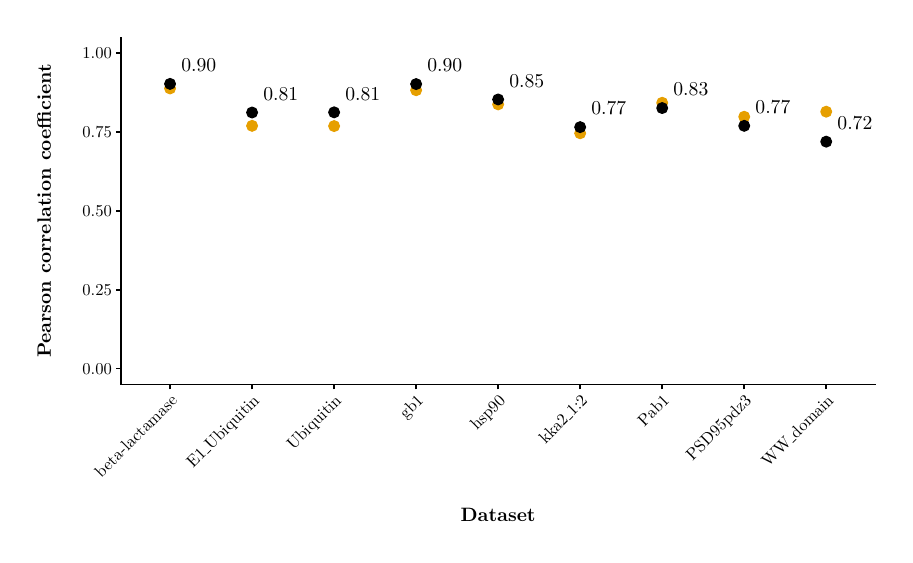
\begin{tikzpicture}[x=1pt,y=1pt]
\definecolor{fillColor}{RGB}{255,255,255}
\path[use as bounding box,fill=fillColor,fill opacity=0.00] (0,0) rectangle (309.84,183.39);
\begin{scope}
\path[clip] ( 33.67, 54.47) rectangle (306.34,179.89);
\definecolor{drawColor}{RGB}{230,159,0}
\definecolor{fillColor}{RGB}{230,159,0}

\path[draw=drawColor,line width= 0.4pt,line join=round,line cap=round,fill=fillColor] ( 81.09,147.92) circle (  1.96);
\definecolor{drawColor}{RGB}{0,0,0}
\definecolor{fillColor}{RGB}{0,0,0}

\path[draw=drawColor,line width= 0.4pt,line join=round,line cap=round,fill=fillColor] ( 81.09,152.73) circle (  1.96);
\definecolor{drawColor}{RGB}{230,159,0}
\definecolor{fillColor}{RGB}{230,159,0}

\path[draw=drawColor,line width= 0.4pt,line join=round,line cap=round,fill=fillColor] (258.92,151.20) circle (  1.96);
\definecolor{drawColor}{RGB}{0,0,0}
\definecolor{fillColor}{RGB}{0,0,0}

\path[draw=drawColor,line width= 0.4pt,line join=round,line cap=round,fill=fillColor] (258.92,147.92) circle (  1.96);
\definecolor{drawColor}{RGB}{230,159,0}
\definecolor{fillColor}{RGB}{230,159,0}

\path[draw=drawColor,line width= 0.4pt,line join=round,line cap=round,fill=fillColor] (229.28,156.25) circle (  1.96);
\definecolor{drawColor}{RGB}{0,0,0}
\definecolor{fillColor}{RGB}{0,0,0}

\path[draw=drawColor,line width= 0.4pt,line join=round,line cap=round,fill=fillColor] (229.28,154.34) circle (  1.96);
\definecolor{drawColor}{RGB}{230,159,0}
\definecolor{fillColor}{RGB}{230,159,0}

\path[draw=drawColor,line width= 0.4pt,line join=round,line cap=round,fill=fillColor] (110.73,147.83) circle (  1.96);
\definecolor{drawColor}{RGB}{0,0,0}
\definecolor{fillColor}{RGB}{0,0,0}

\path[draw=drawColor,line width= 0.4pt,line join=round,line cap=round,fill=fillColor] (110.73,152.80) circle (  1.96);
\definecolor{drawColor}{RGB}{230,159,0}
\definecolor{fillColor}{RGB}{230,159,0}

\path[draw=drawColor,line width= 0.4pt,line join=round,line cap=round,fill=fillColor] (288.55,153.03) circle (  1.96);
\definecolor{drawColor}{RGB}{0,0,0}
\definecolor{fillColor}{RGB}{0,0,0}

\path[draw=drawColor,line width= 0.4pt,line join=round,line cap=round,fill=fillColor] (288.55,142.20) circle (  1.96);
\definecolor{drawColor}{RGB}{230,159,0}
\definecolor{fillColor}{RGB}{230,159,0}

\path[draw=drawColor,line width= 0.4pt,line join=round,line cap=round,fill=fillColor] ( 51.45,161.43) circle (  1.96);
\definecolor{drawColor}{RGB}{0,0,0}
\definecolor{fillColor}{RGB}{0,0,0}

\path[draw=drawColor,line width= 0.4pt,line join=round,line cap=round,fill=fillColor] ( 51.45,163.08) circle (  1.96);
\definecolor{drawColor}{RGB}{230,159,0}
\definecolor{fillColor}{RGB}{230,159,0}

\path[draw=drawColor,line width= 0.4pt,line join=round,line cap=round,fill=fillColor] (140.37,160.78) circle (  1.96);
\definecolor{drawColor}{RGB}{0,0,0}
\definecolor{fillColor}{RGB}{0,0,0}

\path[draw=drawColor,line width= 0.4pt,line join=round,line cap=round,fill=fillColor] (140.37,163.01) circle (  1.96);
\definecolor{drawColor}{RGB}{230,159,0}
\definecolor{fillColor}{RGB}{230,159,0}

\path[draw=drawColor,line width= 0.4pt,line join=round,line cap=round,fill=fillColor] (170.00,155.67) circle (  1.96);
\definecolor{drawColor}{RGB}{0,0,0}
\definecolor{fillColor}{RGB}{0,0,0}

\path[draw=drawColor,line width= 0.4pt,line join=round,line cap=round,fill=fillColor] (170.00,157.45) circle (  1.96);
\definecolor{drawColor}{RGB}{230,159,0}
\definecolor{fillColor}{RGB}{230,159,0}

\path[draw=drawColor,line width= 0.4pt,line join=round,line cap=round,fill=fillColor] (199.64,145.23) circle (  1.96);
\definecolor{drawColor}{RGB}{0,0,0}
\definecolor{fillColor}{RGB}{0,0,0}

\path[draw=drawColor,line width= 0.4pt,line join=round,line cap=round,fill=fillColor] (199.64,147.45) circle (  1.96);

\node[text=drawColor,anchor=base,inner sep=0pt, outer sep=0pt, scale=  0.71] at ( 91.46,157.12) {0.81};

\node[text=drawColor,anchor=base,inner sep=0pt, outer sep=0pt, scale=  0.71] at (269.29,152.31) {0.77};

\node[text=drawColor,anchor=base,inner sep=0pt, outer sep=0pt, scale=  0.71] at (239.65,158.73) {0.83};

\node[text=drawColor,anchor=base,inner sep=0pt, outer sep=0pt, scale=  0.71] at (121.10,157.19) {0.81};

\node[text=drawColor,anchor=base,inner sep=0pt, outer sep=0pt, scale=  0.71] at (298.93,146.59) {0.72};

\node[text=drawColor,anchor=base,inner sep=0pt, outer sep=0pt, scale=  0.71] at ( 61.83,167.47) {0.90};

\node[text=drawColor,anchor=base,inner sep=0pt, outer sep=0pt, scale=  0.71] at (150.74,167.40) {0.90};

\node[text=drawColor,anchor=base,inner sep=0pt, outer sep=0pt, scale=  0.71] at (180.38,161.84) {0.85};

\node[text=drawColor,anchor=base,inner sep=0pt, outer sep=0pt, scale=  0.71] at (210.01,151.84) {0.77};
\end{scope}
\begin{scope}
\path[clip] (  0.00,  0.00) rectangle (309.84,183.39);
\definecolor{drawColor}{RGB}{0,0,0}

\path[draw=drawColor,line width= 0.6pt,line join=round,line cap=rect] ( 33.67, 54.47) --
	( 33.67,179.89);
\end{scope}
\begin{scope}
\path[clip] (  0.00,  0.00) rectangle (309.84,183.39);
\definecolor{drawColor}{RGB}{0,0,0}

\node[text=drawColor,anchor=base east,inner sep=0pt, outer sep=0pt, scale=  0.60] at ( 30.42, 58.11) {0.00};

\node[text=drawColor,anchor=base east,inner sep=0pt, outer sep=0pt, scale=  0.60] at ( 30.42, 86.61) {0.25};

\node[text=drawColor,anchor=base east,inner sep=0pt, outer sep=0pt, scale=  0.60] at ( 30.42,115.11) {0.50};

\node[text=drawColor,anchor=base east,inner sep=0pt, outer sep=0pt, scale=  0.60] at ( 30.42,143.62) {0.75};

\node[text=drawColor,anchor=base east,inner sep=0pt, outer sep=0pt, scale=  0.60] at ( 30.42,172.12) {1.00};
\end{scope}
\begin{scope}
\path[clip] (  0.00,  0.00) rectangle (309.84,183.39);
\definecolor{drawColor}{RGB}{0,0,0}

\path[draw=drawColor,line width= 0.6pt,line join=round] ( 31.92, 60.17) --
	( 33.67, 60.17);

\path[draw=drawColor,line width= 0.6pt,line join=round] ( 31.92, 88.68) --
	( 33.67, 88.68);

\path[draw=drawColor,line width= 0.6pt,line join=round] ( 31.92,117.18) --
	( 33.67,117.18);

\path[draw=drawColor,line width= 0.6pt,line join=round] ( 31.92,145.68) --
	( 33.67,145.68);

\path[draw=drawColor,line width= 0.6pt,line join=round] ( 31.92,174.19) --
	( 33.67,174.19);
\end{scope}
\begin{scope}
\path[clip] (  0.00,  0.00) rectangle (309.84,183.39);
\definecolor{drawColor}{RGB}{0,0,0}

\path[draw=drawColor,line width= 0.6pt,line join=round,line cap=rect] ( 33.67, 54.47) --
	(306.34, 54.47);
\end{scope}
\begin{scope}
\path[clip] (  0.00,  0.00) rectangle (309.84,183.39);
\definecolor{drawColor}{RGB}{0,0,0}

\path[draw=drawColor,line width= 0.6pt,line join=round] ( 51.45, 52.72) --
	( 51.45, 54.47);

\path[draw=drawColor,line width= 0.6pt,line join=round] ( 81.09, 52.72) --
	( 81.09, 54.47);

\path[draw=drawColor,line width= 0.6pt,line join=round] (110.73, 52.72) --
	(110.73, 54.47);

\path[draw=drawColor,line width= 0.6pt,line join=round] (140.37, 52.72) --
	(140.37, 54.47);

\path[draw=drawColor,line width= 0.6pt,line join=round] (170.00, 52.72) --
	(170.00, 54.47);

\path[draw=drawColor,line width= 0.6pt,line join=round] (199.64, 52.72) --
	(199.64, 54.47);

\path[draw=drawColor,line width= 0.6pt,line join=round] (229.28, 52.72) --
	(229.28, 54.47);

\path[draw=drawColor,line width= 0.6pt,line join=round] (258.92, 52.72) --
	(258.92, 54.47);

\path[draw=drawColor,line width= 0.6pt,line join=round] (288.55, 52.72) --
	(288.55, 54.47);
\end{scope}
\begin{scope}
\path[clip] (  0.00,  0.00) rectangle (309.84,183.39);
\definecolor{drawColor}{RGB}{0,0,0}

\node[text=drawColor,rotate= 45.00,anchor=base east,inner sep=0pt, outer sep=0pt, scale=  0.60] at ( 54.38, 48.30) {beta-lactamase};

\node[text=drawColor,rotate= 45.00,anchor=base east,inner sep=0pt, outer sep=0pt, scale=  0.60] at ( 84.01, 48.30) {E1\_Ubiquitin};

\node[text=drawColor,rotate= 45.00,anchor=base east,inner sep=0pt, outer sep=0pt, scale=  0.60] at (113.65, 48.30) {Ubiquitin};

\node[text=drawColor,rotate= 45.00,anchor=base east,inner sep=0pt, outer sep=0pt, scale=  0.60] at (143.29, 48.30) {gb1};

\node[text=drawColor,rotate= 45.00,anchor=base east,inner sep=0pt, outer sep=0pt, scale=  0.60] at (172.93, 48.30) {hsp90};

\node[text=drawColor,rotate= 45.00,anchor=base east,inner sep=0pt, outer sep=0pt, scale=  0.60] at (202.56, 48.30) {kka2\_1:2};

\node[text=drawColor,rotate= 45.00,anchor=base east,inner sep=0pt, outer sep=0pt, scale=  0.60] at (232.20, 48.30) {Pab1};

\node[text=drawColor,rotate= 45.00,anchor=base east,inner sep=0pt, outer sep=0pt, scale=  0.60] at (261.84, 48.30) {PSD95pdz3};

\node[text=drawColor,rotate= 45.00,anchor=base east,inner sep=0pt, outer sep=0pt, scale=  0.60] at (291.48, 48.30) {WW\_domain};
\end{scope}
\begin{scope}
\path[clip] (  0.00,  0.00) rectangle (309.84,183.39);
\definecolor{drawColor}{RGB}{0,0,0}

\node[text=drawColor,anchor=base,inner sep=0pt, outer sep=0pt, scale=  0.70] at (170.00,  4.86) {\bfseries Dataset};
\end{scope}
\begin{scope}
\path[clip] (  0.00,  0.00) rectangle (309.84,183.39);
\definecolor{drawColor}{RGB}{0,0,0}

\node[text=drawColor,rotate= 90.00,anchor=base,inner sep=0pt, outer sep=0pt, scale=  0.70] at (  8.39,117.18) {\bfseries Pearson correlation coefficient};
\end{scope}
\end{tikzpicture}%

			}
		\end{column}
		\begin{column}{.4\textwidth}
			\begin{itemize}
				\item A different model trained for each protein
				\item Half of the mutations set aside for testing
				\item Hyperparameters optimized in the remaining half with cross-validation
				\item Good results but likely overfitting of the testing set
			\end{itemize}
		\end{column}
	\end{columns}
\end{frame}

\begin{frame}
	\frametitle{Single Protein Models with Testing by Position}
	\begin{columns}[c]
		\begin{column}{.6\textwidth}
			\centering%
			\vspace{1em}
			{%
				\let\bfseries\sbseries%
				% Created by tikzDevice version 0.12.3.1 on 2021-06-03 14:52:12
% !TEX encoding = UTF-8 Unicode
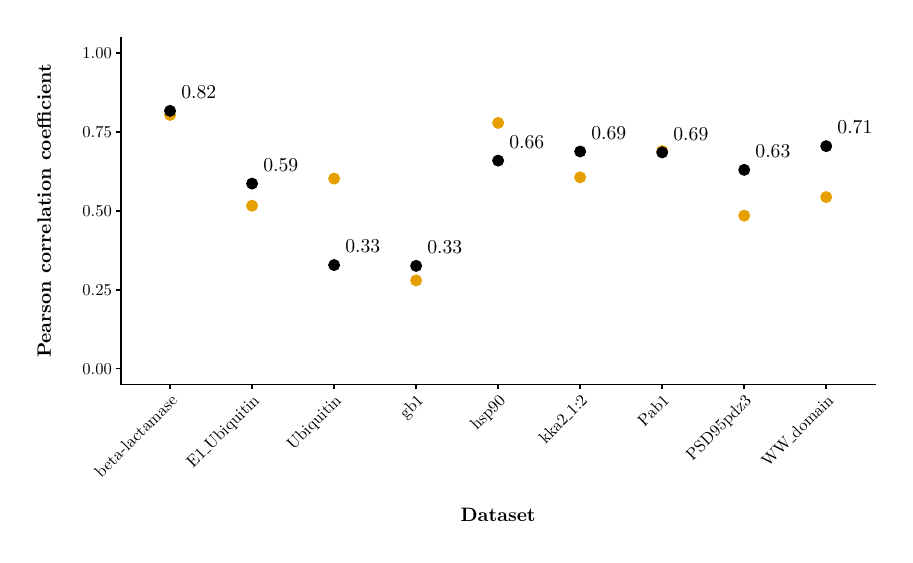
\begin{tikzpicture}[x=1pt,y=1pt]
\definecolor{fillColor}{RGB}{255,255,255}
\path[use as bounding box,fill=fillColor,fill opacity=0.00] (0,0) rectangle (309.84,183.39);
\begin{scope}
\path[clip] ( 33.67, 54.47) rectangle (306.34,179.89);
\definecolor{drawColor}{RGB}{230,159,0}
\definecolor{fillColor}{RGB}{230,159,0}

\path[draw=drawColor,line width= 0.4pt,line join=round,line cap=round,fill=fillColor] ( 81.09,119.04) circle (  1.96);
\definecolor{drawColor}{RGB}{0,0,0}
\definecolor{fillColor}{RGB}{0,0,0}

\path[draw=drawColor,line width= 0.4pt,line join=round,line cap=round,fill=fillColor] ( 81.09,127.05) circle (  1.96);
\definecolor{drawColor}{RGB}{230,159,0}
\definecolor{fillColor}{RGB}{230,159,0}

\path[draw=drawColor,line width= 0.4pt,line join=round,line cap=round,fill=fillColor] (258.92,115.46) circle (  1.96);
\definecolor{drawColor}{RGB}{0,0,0}
\definecolor{fillColor}{RGB}{0,0,0}

\path[draw=drawColor,line width= 0.4pt,line join=round,line cap=round,fill=fillColor] (258.92,132.01) circle (  1.96);
\definecolor{drawColor}{RGB}{230,159,0}
\definecolor{fillColor}{RGB}{230,159,0}

\path[draw=drawColor,line width= 0.4pt,line join=round,line cap=round,fill=fillColor] (229.28,138.79) circle (  1.96);
\definecolor{drawColor}{RGB}{0,0,0}
\definecolor{fillColor}{RGB}{0,0,0}

\path[draw=drawColor,line width= 0.4pt,line join=round,line cap=round,fill=fillColor] (229.28,138.31) circle (  1.96);
\definecolor{drawColor}{RGB}{230,159,0}
\definecolor{fillColor}{RGB}{230,159,0}

\path[draw=drawColor,line width= 0.4pt,line join=round,line cap=round,fill=fillColor] (110.73,128.85) circle (  1.96);
\definecolor{drawColor}{RGB}{0,0,0}
\definecolor{fillColor}{RGB}{0,0,0}

\path[draw=drawColor,line width= 0.4pt,line join=round,line cap=round,fill=fillColor] (110.73, 97.61) circle (  1.96);
\definecolor{drawColor}{RGB}{230,159,0}
\definecolor{fillColor}{RGB}{230,159,0}

\path[draw=drawColor,line width= 0.4pt,line join=round,line cap=round,fill=fillColor] (288.55,122.18) circle (  1.96);
\definecolor{drawColor}{RGB}{0,0,0}
\definecolor{fillColor}{RGB}{0,0,0}

\path[draw=drawColor,line width= 0.4pt,line join=round,line cap=round,fill=fillColor] (288.55,140.58) circle (  1.96);
\definecolor{drawColor}{RGB}{230,159,0}
\definecolor{fillColor}{RGB}{230,159,0}

\path[draw=drawColor,line width= 0.4pt,line join=round,line cap=round,fill=fillColor] ( 51.45,151.86) circle (  1.96);
\definecolor{drawColor}{RGB}{0,0,0}
\definecolor{fillColor}{RGB}{0,0,0}

\path[draw=drawColor,line width= 0.4pt,line join=round,line cap=round,fill=fillColor] ( 51.45,153.33) circle (  1.96);
\definecolor{drawColor}{RGB}{230,159,0}
\definecolor{fillColor}{RGB}{230,159,0}

\path[draw=drawColor,line width= 0.4pt,line join=round,line cap=round,fill=fillColor] (140.37, 92.06) circle (  1.96);
\definecolor{drawColor}{RGB}{0,0,0}
\definecolor{fillColor}{RGB}{0,0,0}

\path[draw=drawColor,line width= 0.4pt,line join=round,line cap=round,fill=fillColor] (140.37, 97.32) circle (  1.96);
\definecolor{drawColor}{RGB}{230,159,0}
\definecolor{fillColor}{RGB}{230,159,0}

\path[draw=drawColor,line width= 0.4pt,line join=round,line cap=round,fill=fillColor] (170.00,148.96) circle (  1.96);
\definecolor{drawColor}{RGB}{0,0,0}
\definecolor{fillColor}{RGB}{0,0,0}

\path[draw=drawColor,line width= 0.4pt,line join=round,line cap=round,fill=fillColor] (170.00,135.35) circle (  1.96);
\definecolor{drawColor}{RGB}{230,159,0}
\definecolor{fillColor}{RGB}{230,159,0}

\path[draw=drawColor,line width= 0.4pt,line join=round,line cap=round,fill=fillColor] (199.64,129.31) circle (  1.96);
\definecolor{drawColor}{RGB}{0,0,0}
\definecolor{fillColor}{RGB}{0,0,0}

\path[draw=drawColor,line width= 0.4pt,line join=round,line cap=round,fill=fillColor] (199.64,138.65) circle (  1.96);

\node[text=drawColor,anchor=base,inner sep=0pt, outer sep=0pt, scale=  0.71] at ( 91.46,131.44) {0.59};

\node[text=drawColor,anchor=base,inner sep=0pt, outer sep=0pt, scale=  0.71] at (269.29,136.40) {0.63};

\node[text=drawColor,anchor=base,inner sep=0pt, outer sep=0pt, scale=  0.71] at (239.65,142.70) {0.69};

\node[text=drawColor,anchor=base,inner sep=0pt, outer sep=0pt, scale=  0.71] at (121.10,102.00) {0.33};

\node[text=drawColor,anchor=base,inner sep=0pt, outer sep=0pt, scale=  0.71] at (298.93,144.97) {0.71};

\node[text=drawColor,anchor=base,inner sep=0pt, outer sep=0pt, scale=  0.71] at ( 61.83,157.72) {0.82};

\node[text=drawColor,anchor=base,inner sep=0pt, outer sep=0pt, scale=  0.71] at (150.74,101.71) {0.33};

\node[text=drawColor,anchor=base,inner sep=0pt, outer sep=0pt, scale=  0.71] at (180.38,139.74) {0.66};

\node[text=drawColor,anchor=base,inner sep=0pt, outer sep=0pt, scale=  0.71] at (210.01,143.04) {0.69};
\end{scope}
\begin{scope}
\path[clip] (  0.00,  0.00) rectangle (309.84,183.39);
\definecolor{drawColor}{RGB}{0,0,0}

\path[draw=drawColor,line width= 0.6pt,line join=round,line cap=rect] ( 33.67, 54.47) --
	( 33.67,179.89);
\end{scope}
\begin{scope}
\path[clip] (  0.00,  0.00) rectangle (309.84,183.39);
\definecolor{drawColor}{RGB}{0,0,0}

\node[text=drawColor,anchor=base east,inner sep=0pt, outer sep=0pt, scale=  0.60] at ( 30.42, 58.11) {0.00};

\node[text=drawColor,anchor=base east,inner sep=0pt, outer sep=0pt, scale=  0.60] at ( 30.42, 86.61) {0.25};

\node[text=drawColor,anchor=base east,inner sep=0pt, outer sep=0pt, scale=  0.60] at ( 30.42,115.11) {0.50};

\node[text=drawColor,anchor=base east,inner sep=0pt, outer sep=0pt, scale=  0.60] at ( 30.42,143.62) {0.75};

\node[text=drawColor,anchor=base east,inner sep=0pt, outer sep=0pt, scale=  0.60] at ( 30.42,172.12) {1.00};
\end{scope}
\begin{scope}
\path[clip] (  0.00,  0.00) rectangle (309.84,183.39);
\definecolor{drawColor}{RGB}{0,0,0}

\path[draw=drawColor,line width= 0.6pt,line join=round] ( 31.92, 60.17) --
	( 33.67, 60.17);

\path[draw=drawColor,line width= 0.6pt,line join=round] ( 31.92, 88.68) --
	( 33.67, 88.68);

\path[draw=drawColor,line width= 0.6pt,line join=round] ( 31.92,117.18) --
	( 33.67,117.18);

\path[draw=drawColor,line width= 0.6pt,line join=round] ( 31.92,145.68) --
	( 33.67,145.68);

\path[draw=drawColor,line width= 0.6pt,line join=round] ( 31.92,174.19) --
	( 33.67,174.19);
\end{scope}
\begin{scope}
\path[clip] (  0.00,  0.00) rectangle (309.84,183.39);
\definecolor{drawColor}{RGB}{0,0,0}

\path[draw=drawColor,line width= 0.6pt,line join=round,line cap=rect] ( 33.67, 54.47) --
	(306.34, 54.47);
\end{scope}
\begin{scope}
\path[clip] (  0.00,  0.00) rectangle (309.84,183.39);
\definecolor{drawColor}{RGB}{0,0,0}

\path[draw=drawColor,line width= 0.6pt,line join=round] ( 51.45, 52.72) --
	( 51.45, 54.47);

\path[draw=drawColor,line width= 0.6pt,line join=round] ( 81.09, 52.72) --
	( 81.09, 54.47);

\path[draw=drawColor,line width= 0.6pt,line join=round] (110.73, 52.72) --
	(110.73, 54.47);

\path[draw=drawColor,line width= 0.6pt,line join=round] (140.37, 52.72) --
	(140.37, 54.47);

\path[draw=drawColor,line width= 0.6pt,line join=round] (170.00, 52.72) --
	(170.00, 54.47);

\path[draw=drawColor,line width= 0.6pt,line join=round] (199.64, 52.72) --
	(199.64, 54.47);

\path[draw=drawColor,line width= 0.6pt,line join=round] (229.28, 52.72) --
	(229.28, 54.47);

\path[draw=drawColor,line width= 0.6pt,line join=round] (258.92, 52.72) --
	(258.92, 54.47);

\path[draw=drawColor,line width= 0.6pt,line join=round] (288.55, 52.72) --
	(288.55, 54.47);
\end{scope}
\begin{scope}
\path[clip] (  0.00,  0.00) rectangle (309.84,183.39);
\definecolor{drawColor}{RGB}{0,0,0}

\node[text=drawColor,rotate= 45.00,anchor=base east,inner sep=0pt, outer sep=0pt, scale=  0.60] at ( 54.38, 48.30) {beta-lactamase};

\node[text=drawColor,rotate= 45.00,anchor=base east,inner sep=0pt, outer sep=0pt, scale=  0.60] at ( 84.01, 48.30) {E1\_Ubiquitin};

\node[text=drawColor,rotate= 45.00,anchor=base east,inner sep=0pt, outer sep=0pt, scale=  0.60] at (113.65, 48.30) {Ubiquitin};

\node[text=drawColor,rotate= 45.00,anchor=base east,inner sep=0pt, outer sep=0pt, scale=  0.60] at (143.29, 48.30) {gb1};

\node[text=drawColor,rotate= 45.00,anchor=base east,inner sep=0pt, outer sep=0pt, scale=  0.60] at (172.93, 48.30) {hsp90};

\node[text=drawColor,rotate= 45.00,anchor=base east,inner sep=0pt, outer sep=0pt, scale=  0.60] at (202.56, 48.30) {kka2\_1:2};

\node[text=drawColor,rotate= 45.00,anchor=base east,inner sep=0pt, outer sep=0pt, scale=  0.60] at (232.20, 48.30) {Pab1};

\node[text=drawColor,rotate= 45.00,anchor=base east,inner sep=0pt, outer sep=0pt, scale=  0.60] at (261.84, 48.30) {PSD95pdz3};

\node[text=drawColor,rotate= 45.00,anchor=base east,inner sep=0pt, outer sep=0pt, scale=  0.60] at (291.48, 48.30) {WW\_domain};
\end{scope}
\begin{scope}
\path[clip] (  0.00,  0.00) rectangle (309.84,183.39);
\definecolor{drawColor}{RGB}{0,0,0}

\node[text=drawColor,anchor=base,inner sep=0pt, outer sep=0pt, scale=  0.70] at (170.00,  4.86) {\bfseries Dataset};
\end{scope}
\begin{scope}
\path[clip] (  0.00,  0.00) rectangle (309.84,183.39);
\definecolor{drawColor}{RGB}{0,0,0}

\node[text=drawColor,rotate= 90.00,anchor=base,inner sep=0pt, outer sep=0pt, scale=  0.70] at (  8.39,117.18) {\bfseries Pearson correlation coefficient};
\end{scope}
\end{tikzpicture}%

			}
		\end{column}
		\begin{column}{.4\textwidth}
			\begin{itemize}
				\item Same as before but mutations in the same position segregated in the training or testing sets
				\item Performances are lower (and more realistic)
			\end{itemize}
		\end{column}
	\end{columns}
\end{frame}

\begin{frame}
	\frametitle{Leave-One-Protein-Out (LOPO) Models}
	\begin{columns}[c]
		\begin{column}{.6\textwidth}
			\centering%
			\vspace{1em}
			{%
				\let\bfseries\sbseries%
				% Created by tikzDevice version 0.12.3.1 on 2021-07-05 13:28:01
% !TEX encoding = UTF-8 Unicode
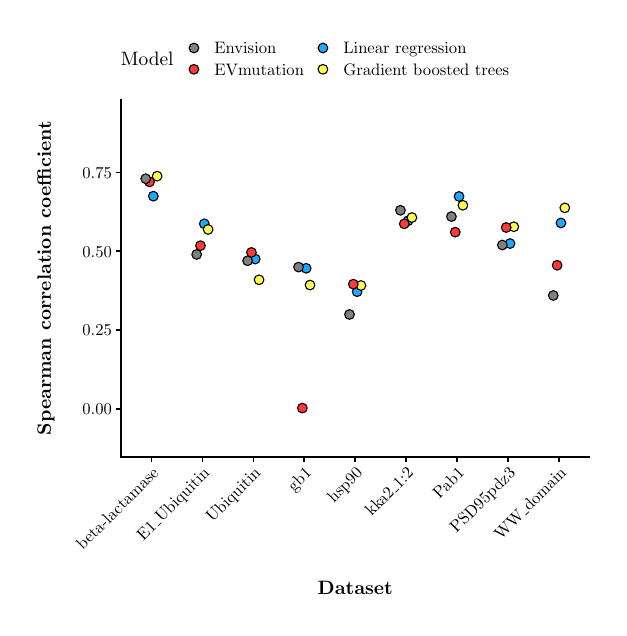
\begin{tikzpicture}[x=1pt,y=1pt]
\definecolor{fillColor}{RGB}{255,255,255}
\path[use as bounding box,fill=fillColor,fill opacity=0.00] (0,0) rectangle (206.56,209.59);
\begin{scope}
\path[clip] ( 33.67, 54.47) rectangle (203.06,183.69);
\definecolor{drawColor}{RGB}{0,0,0}
\definecolor{fillColor}{RGB}{31,168,255}

\path[draw=drawColor,line width= 0.4pt,line join=round,line cap=round,fill=fillColor] ( 45.41,148.70) circle (  1.75);
\definecolor{fillColor}{RGB}{255,253,82}

\path[draw=drawColor,line width= 0.4pt,line join=round,line cap=round,fill=fillColor] ( 46.79,155.93) circle (  1.75);
\definecolor{fillColor}{RGB}{255,56,56}

\path[draw=drawColor,line width= 0.4pt,line join=round,line cap=round,fill=fillColor] ( 44.03,153.86) circle (  1.75);
\definecolor{fillColor}{RGB}{31,168,255}

\path[draw=drawColor,line width= 0.4pt,line join=round,line cap=round,fill=fillColor] ( 63.82,138.72) circle (  1.75);
\definecolor{fillColor}{RGB}{255,253,82}

\path[draw=drawColor,line width= 0.4pt,line join=round,line cap=round,fill=fillColor] ( 65.20,136.68) circle (  1.75);
\definecolor{fillColor}{RGB}{255,56,56}

\path[draw=drawColor,line width= 0.4pt,line join=round,line cap=round,fill=fillColor] ( 62.44,130.81) circle (  1.75);
\definecolor{fillColor}{RGB}{31,168,255}

\path[draw=drawColor,line width= 0.4pt,line join=round,line cap=round,fill=fillColor] ( 82.23,125.98) circle (  1.75);
\definecolor{fillColor}{RGB}{255,253,82}

\path[draw=drawColor,line width= 0.4pt,line join=round,line cap=round,fill=fillColor] ( 83.61,118.49) circle (  1.75);
\definecolor{fillColor}{RGB}{255,56,56}

\path[draw=drawColor,line width= 0.4pt,line join=round,line cap=round,fill=fillColor] ( 80.85,128.37) circle (  1.75);
\definecolor{fillColor}{RGB}{31,168,255}

\path[draw=drawColor,line width= 0.4pt,line join=round,line cap=round,fill=fillColor] (100.64,122.64) circle (  1.75);
\definecolor{fillColor}{RGB}{255,253,82}

\path[draw=drawColor,line width= 0.4pt,line join=round,line cap=round,fill=fillColor] (102.02,116.59) circle (  1.75);
\definecolor{fillColor}{RGB}{255,56,56}

\path[draw=drawColor,line width= 0.4pt,line join=round,line cap=round,fill=fillColor] ( 99.26, 72.12) circle (  1.75);
\definecolor{fillColor}{RGB}{31,168,255}

\path[draw=drawColor,line width= 0.4pt,line join=round,line cap=round,fill=fillColor] (119.05,114.19) circle (  1.75);
\definecolor{fillColor}{RGB}{255,253,82}

\path[draw=drawColor,line width= 0.4pt,line join=round,line cap=round,fill=fillColor] (120.44,116.42) circle (  1.75);
\definecolor{fillColor}{RGB}{255,56,56}

\path[draw=drawColor,line width= 0.4pt,line join=round,line cap=round,fill=fillColor] (117.67,116.91) circle (  1.75);
\definecolor{fillColor}{RGB}{31,168,255}

\path[draw=drawColor,line width= 0.4pt,line join=round,line cap=round,fill=fillColor] (137.47,139.82) circle (  1.75);
\definecolor{fillColor}{RGB}{255,253,82}

\path[draw=drawColor,line width= 0.4pt,line join=round,line cap=round,fill=fillColor] (138.85,140.98) circle (  1.75);
\definecolor{fillColor}{RGB}{255,56,56}

\path[draw=drawColor,line width= 0.4pt,line join=round,line cap=round,fill=fillColor] (136.09,138.70) circle (  1.75);
\definecolor{fillColor}{RGB}{31,168,255}

\path[draw=drawColor,line width= 0.4pt,line join=round,line cap=round,fill=fillColor] (155.88,148.60) circle (  1.75);
\definecolor{fillColor}{RGB}{255,253,82}

\path[draw=drawColor,line width= 0.4pt,line join=round,line cap=round,fill=fillColor] (157.26,145.41) circle (  1.75);
\definecolor{fillColor}{RGB}{255,56,56}

\path[draw=drawColor,line width= 0.4pt,line join=round,line cap=round,fill=fillColor] (154.50,135.70) circle (  1.75);
\definecolor{fillColor}{RGB}{31,168,255}

\path[draw=drawColor,line width= 0.4pt,line join=round,line cap=round,fill=fillColor] (174.29,131.58) circle (  1.75);
\definecolor{fillColor}{RGB}{255,253,82}

\path[draw=drawColor,line width= 0.4pt,line join=round,line cap=round,fill=fillColor] (175.67,137.65) circle (  1.75);
\definecolor{fillColor}{RGB}{255,56,56}

\path[draw=drawColor,line width= 0.4pt,line join=round,line cap=round,fill=fillColor] (172.91,137.38) circle (  1.75);
\definecolor{fillColor}{RGB}{31,168,255}

\path[draw=drawColor,line width= 0.4pt,line join=round,line cap=round,fill=fillColor] (192.70,139.01) circle (  1.75);
\definecolor{fillColor}{RGB}{255,253,82}

\path[draw=drawColor,line width= 0.4pt,line join=round,line cap=round,fill=fillColor] (194.08,144.48) circle (  1.75);
\definecolor{fillColor}{RGB}{255,56,56}

\path[draw=drawColor,line width= 0.4pt,line join=round,line cap=round,fill=fillColor] (191.32,123.73) circle (  1.75);
\definecolor{fillColor}{RGB}{128,128,128}

\path[draw=drawColor,line width= 0.4pt,line join=round,line cap=round,fill=fillColor] ( 42.65,155.00) circle (  1.75);

\path[draw=drawColor,line width= 0.4pt,line join=round,line cap=round,fill=fillColor] (153.12,141.32) circle (  1.75);

\path[draw=drawColor,line width= 0.4pt,line join=round,line cap=round,fill=fillColor] ( 61.06,127.63) circle (  1.75);

\path[draw=drawColor,line width= 0.4pt,line join=round,line cap=round,fill=fillColor] (134.70,143.60) circle (  1.75);

\path[draw=drawColor,line width= 0.4pt,line join=round,line cap=round,fill=fillColor] (171.53,131.05) circle (  1.75);

\path[draw=drawColor,line width= 0.4pt,line join=round,line cap=round,fill=fillColor] (189.94,112.81) circle (  1.75);

\path[draw=drawColor,line width= 0.4pt,line join=round,line cap=round,fill=fillColor] ( 79.47,125.35) circle (  1.75);

\path[draw=drawColor,line width= 0.4pt,line join=round,line cap=round,fill=fillColor] ( 97.88,123.07) circle (  1.75);

\path[draw=drawColor,line width= 0.4pt,line join=round,line cap=round,fill=fillColor] (116.29,105.96) circle (  1.75);
\end{scope}
\begin{scope}
\path[clip] (  0.00,  0.00) rectangle (206.56,209.59);
\definecolor{drawColor}{RGB}{0,0,0}

\path[draw=drawColor,line width= 0.6pt,line join=round,line cap=rect] ( 33.67, 54.47) --
	( 33.67,183.69);
\end{scope}
\begin{scope}
\path[clip] (  0.00,  0.00) rectangle (206.56,209.59);
\definecolor{drawColor}{RGB}{0,0,0}

\node[text=drawColor,anchor=base east,inner sep=0pt, outer sep=0pt, scale=  0.60] at ( 30.42, 69.68) {0.00};

\node[text=drawColor,anchor=base east,inner sep=0pt, outer sep=0pt, scale=  0.60] at ( 30.42, 98.19) {0.25};

\node[text=drawColor,anchor=base east,inner sep=0pt, outer sep=0pt, scale=  0.60] at ( 30.42,126.71) {0.50};

\node[text=drawColor,anchor=base east,inner sep=0pt, outer sep=0pt, scale=  0.60] at ( 30.42,155.22) {0.75};
\end{scope}
\begin{scope}
\path[clip] (  0.00,  0.00) rectangle (206.56,209.59);
\definecolor{drawColor}{RGB}{0,0,0}

\path[draw=drawColor,line width= 0.6pt,line join=round] ( 31.92, 71.75) --
	( 33.67, 71.75);

\path[draw=drawColor,line width= 0.6pt,line join=round] ( 31.92,100.26) --
	( 33.67,100.26);

\path[draw=drawColor,line width= 0.6pt,line join=round] ( 31.92,128.77) --
	( 33.67,128.77);

\path[draw=drawColor,line width= 0.6pt,line join=round] ( 31.92,157.28) --
	( 33.67,157.28);
\end{scope}
\begin{scope}
\path[clip] (  0.00,  0.00) rectangle (206.56,209.59);
\definecolor{drawColor}{RGB}{0,0,0}

\path[draw=drawColor,line width= 0.6pt,line join=round,line cap=rect] ( 33.67, 54.47) --
	(203.06, 54.47);
\end{scope}
\begin{scope}
\path[clip] (  0.00,  0.00) rectangle (206.56,209.59);
\definecolor{drawColor}{RGB}{0,0,0}

\path[draw=drawColor,line width= 0.6pt,line join=round] ( 44.72, 52.72) --
	( 44.72, 54.47);

\path[draw=drawColor,line width= 0.6pt,line join=round] ( 63.13, 52.72) --
	( 63.13, 54.47);

\path[draw=drawColor,line width= 0.6pt,line join=round] ( 81.54, 52.72) --
	( 81.54, 54.47);

\path[draw=drawColor,line width= 0.6pt,line join=round] ( 99.95, 52.72) --
	( 99.95, 54.47);

\path[draw=drawColor,line width= 0.6pt,line join=round] (118.36, 52.72) --
	(118.36, 54.47);

\path[draw=drawColor,line width= 0.6pt,line join=round] (136.78, 52.72) --
	(136.78, 54.47);

\path[draw=drawColor,line width= 0.6pt,line join=round] (155.19, 52.72) --
	(155.19, 54.47);

\path[draw=drawColor,line width= 0.6pt,line join=round] (173.60, 52.72) --
	(173.60, 54.47);

\path[draw=drawColor,line width= 0.6pt,line join=round] (192.01, 52.72) --
	(192.01, 54.47);
\end{scope}
\begin{scope}
\path[clip] (  0.00,  0.00) rectangle (206.56,209.59);
\definecolor{drawColor}{RGB}{0,0,0}

\node[text=drawColor,rotate= 45.00,anchor=base east,inner sep=0pt, outer sep=0pt, scale=  0.60] at ( 47.64, 48.30) {beta-lactamase};

\node[text=drawColor,rotate= 45.00,anchor=base east,inner sep=0pt, outer sep=0pt, scale=  0.60] at ( 66.05, 48.30) {E1\_Ubiquitin};

\node[text=drawColor,rotate= 45.00,anchor=base east,inner sep=0pt, outer sep=0pt, scale=  0.60] at ( 84.46, 48.30) {Ubiquitin};

\node[text=drawColor,rotate= 45.00,anchor=base east,inner sep=0pt, outer sep=0pt, scale=  0.60] at (102.88, 48.30) {gb1};

\node[text=drawColor,rotate= 45.00,anchor=base east,inner sep=0pt, outer sep=0pt, scale=  0.60] at (121.29, 48.30) {hsp90};

\node[text=drawColor,rotate= 45.00,anchor=base east,inner sep=0pt, outer sep=0pt, scale=  0.60] at (139.70, 48.30) {kka2\_1:2};

\node[text=drawColor,rotate= 45.00,anchor=base east,inner sep=0pt, outer sep=0pt, scale=  0.60] at (158.11, 48.30) {Pab1};

\node[text=drawColor,rotate= 45.00,anchor=base east,inner sep=0pt, outer sep=0pt, scale=  0.60] at (176.52, 48.30) {PSD95pdz3};

\node[text=drawColor,rotate= 45.00,anchor=base east,inner sep=0pt, outer sep=0pt, scale=  0.60] at (194.93, 48.30) {WW\_domain};
\end{scope}
\begin{scope}
\path[clip] (  0.00,  0.00) rectangle (206.56,209.59);
\definecolor{drawColor}{RGB}{0,0,0}

\node[text=drawColor,anchor=base,inner sep=0pt, outer sep=0pt, scale=  0.70] at (118.36,  4.86) {\bfseries Dataset};
\end{scope}
\begin{scope}
\path[clip] (  0.00,  0.00) rectangle (206.56,209.59);
\definecolor{drawColor}{RGB}{0,0,0}

\node[text=drawColor,rotate= 90.00,anchor=base,inner sep=0pt, outer sep=0pt, scale=  0.70] at (  8.39,119.08) {\bfseries Spearman correlation coefficient};
\end{scope}
\begin{scope}
\path[clip] (  0.00,  0.00) rectangle (206.56,209.59);
\definecolor{drawColor}{RGB}{0,0,0}

\node[text=drawColor,anchor=base west,inner sep=0pt, outer sep=0pt, scale=  0.70] at ( 33.67,195.97) {Model};
\end{scope}
\begin{scope}
\path[clip] (  0.00,  0.00) rectangle (206.56,209.59);
\definecolor{drawColor}{RGB}{0,0,0}
\definecolor{fillColor}{RGB}{128,128,128}

\path[draw=drawColor,line width= 0.4pt,line join=round,line cap=round,fill=fillColor] ( 60.08,202.24) circle (  1.75);
\end{scope}
\begin{scope}
\path[clip] (  0.00,  0.00) rectangle (206.56,209.59);
\definecolor{drawColor}{RGB}{0,0,0}
\definecolor{fillColor}{RGB}{255,56,56}

\path[draw=drawColor,line width= 0.4pt,line join=round,line cap=round,fill=fillColor] ( 60.08,194.54) circle (  1.75);
\end{scope}
\begin{scope}
\path[clip] (  0.00,  0.00) rectangle (206.56,209.59);
\definecolor{drawColor}{RGB}{0,0,0}
\definecolor{fillColor}{RGB}{31,168,255}

\path[draw=drawColor,line width= 0.4pt,line join=round,line cap=round,fill=fillColor] (106.69,202.24) circle (  1.75);
\end{scope}
\begin{scope}
\path[clip] (  0.00,  0.00) rectangle (206.56,209.59);
\definecolor{drawColor}{RGB}{0,0,0}
\definecolor{fillColor}{RGB}{255,253,82}

\path[draw=drawColor,line width= 0.4pt,line join=round,line cap=round,fill=fillColor] (106.69,194.54) circle (  1.75);
\end{scope}
\begin{scope}
\path[clip] (  0.00,  0.00) rectangle (206.56,209.59);
\definecolor{drawColor}{RGB}{0,0,0}

\node[text=drawColor,anchor=base west,inner sep=0pt, outer sep=0pt, scale=  0.60] at ( 67.43,200.17) {Envision};
\end{scope}
\begin{scope}
\path[clip] (  0.00,  0.00) rectangle (206.56,209.59);
\definecolor{drawColor}{RGB}{0,0,0}

\node[text=drawColor,anchor=base west,inner sep=0pt, outer sep=0pt, scale=  0.60] at ( 67.43,192.47) {EVmutation};
\end{scope}
\begin{scope}
\path[clip] (  0.00,  0.00) rectangle (206.56,209.59);
\definecolor{drawColor}{RGB}{0,0,0}

\node[text=drawColor,anchor=base west,inner sep=0pt, outer sep=0pt, scale=  0.60] at (114.04,200.17) {Linear regression};
\end{scope}
\begin{scope}
\path[clip] (  0.00,  0.00) rectangle (206.56,209.59);
\definecolor{drawColor}{RGB}{0,0,0}

\node[text=drawColor,anchor=base west,inner sep=0pt, outer sep=0pt, scale=  0.60] at (114.04,192.47) {Gradient boosted trees};
\end{scope}
\end{tikzpicture}

			}
		\end{column}
		\begin{column}{.4\textwidth}
			\begin{itemize}
				\item Models trained on the whole dataset while leaving one protein out
				\item For the left-out protein, half of the mutations used for testing and half for validation
				\item Spearman correlation coefficient used for evaluation
			\end{itemize}
		\end{column}
	\end{columns}
\end{frame}

\begin{frame}
	\frametitle{Discussion}
	\begin{figure}
		\begin{tikzpicture}
			\tikzstyle{every node}=[object, font=\footnotesize]
			\node [object, text width=10em] at (0,0) {How validation and testing are performed is crucial};
			\node [object, text width=14em] at (5,-1) {Performances on par with other predictors can be reached without structural features};
			\node [object, text width=9em] at (1,2) {There is strong variability between datasets};
			\node [object, text width=10em] at (0,4) {Complex models do not improve much on linear regression};
			\node [object, text width=11em] at (6,3) {Unsupervised models perform similarly to supervised models};
		\end{tikzpicture}
	\end{figure}
\end{frame}

\begin{frame}
	\frametitle{Future Directions}
	\begin{figure}
		\begin{tikzpicture}
			\tikzstyle{every node}=[object, font=\footnotesize]
			\node [object, text width=14em] at (0,0) {Using residue contacts in a graph convolutional neural network};
			\node [object, text width=7em] at (1,2) {Tuning the set of features};
			\node [object, text width=10em] at (6,3) {Training on more deep mutational scanning studies};
			\node [object, text width=13em] at (1,4) {Unsupervised models seem promising and may be worth exploring more};
			\node [object, text width=15em] at (6,-1) {Finding a better normalization strategy for the scores from different experiments};
		\end{tikzpicture}
	\end{figure}
\end{frame}

\appendix%
\begin{frame}[allowframebreaks]
	\frametitle{Bibliography}
	\printbibliography{}%
\end{frame}

\begin{frame}
	\frametitle{Supplementary Material}
	Secondary structure is of limited importance in the discrimination of damaging mutations
	\vfill%
	\centering%
	{%
		\let\bfseries\sbseries%
		% Created by tikzDevice version 0.12.3.1 on 2021-06-03 14:42:34
% !TEX encoding = UTF-8 Unicode
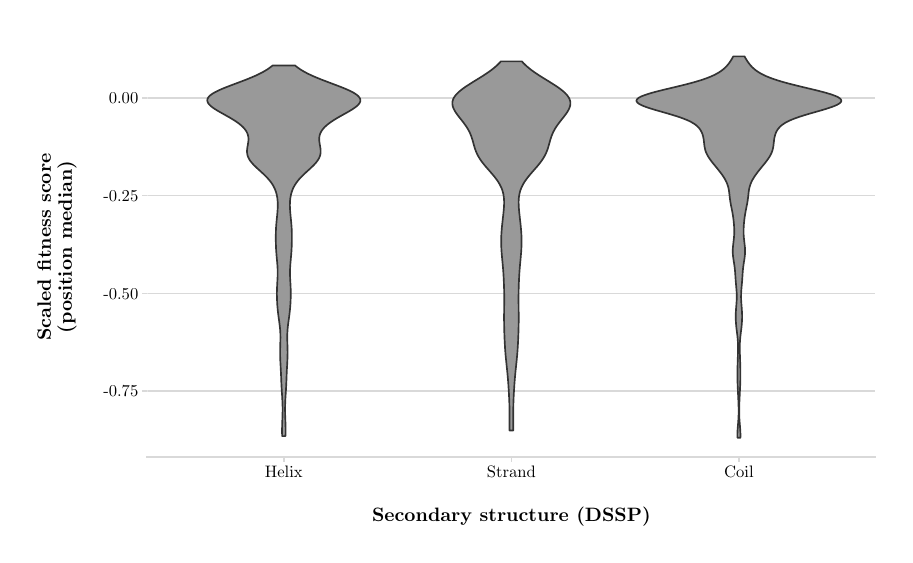
\begin{tikzpicture}[x=1pt,y=1pt]
\definecolor{fillColor}{RGB}{255,255,255}
\path[use as bounding box,fill=fillColor,fill opacity=0.00] (0,0) rectangle (309.84,183.39);
\begin{scope}
\path[clip] ( 43.23, 28.30) rectangle (306.34,179.89);
\definecolor{drawColor}{gray}{0.85}

\path[draw=drawColor,line width= 0.6pt,line join=round] ( 43.23, 52.06) --
	(306.34, 52.06);

\path[draw=drawColor,line width= 0.6pt,line join=round] ( 43.23, 87.39) --
	(306.34, 87.39);

\path[draw=drawColor,line width= 0.6pt,line join=round] ( 43.23,122.71) --
	(306.34,122.71);

\path[draw=drawColor,line width= 0.6pt,line join=round] ( 43.23,158.03) --
	(306.34,158.03);
\definecolor{drawColor}{gray}{0.20}
\definecolor{fillColor}{gray}{0.60}

\path[draw=drawColor,line width= 0.6pt,line join=round,line cap=round,fill=fillColor] ( 91.95, 35.80) --
	( 91.94, 36.06) --
	( 91.94, 36.33) --
	( 91.93, 36.59) --
	( 91.92, 36.85) --
	( 91.92, 37.11) --
	( 91.92, 37.37) --
	( 91.91, 37.64) --
	( 91.91, 37.90) --
	( 91.92, 38.16) --
	( 91.92, 38.42) --
	( 91.92, 38.68) --
	( 91.93, 38.95) --
	( 91.93, 39.21) --
	( 91.94, 39.47) --
	( 91.95, 39.73) --
	( 91.96, 39.99) --
	( 91.96, 40.26) --
	( 91.97, 40.52) --
	( 91.98, 40.78) --
	( 91.99, 41.04) --
	( 92.00, 41.30) --
	( 92.02, 41.57) --
	( 92.03, 41.83) --
	( 92.04, 42.09) --
	( 92.05, 42.35) --
	( 92.06, 42.61) --
	( 92.07, 42.88) --
	( 92.08, 43.14) --
	( 92.08, 43.40) --
	( 92.09, 43.66) --
	( 92.10, 43.92) --
	( 92.10, 44.19) --
	( 92.11, 44.45) --
	( 92.11, 44.71) --
	( 92.12, 44.97) --
	( 92.12, 45.23) --
	( 92.12, 45.50) --
	( 92.12, 45.76) --
	( 92.12, 46.02) --
	( 92.11, 46.28) --
	( 92.11, 46.54) --
	( 92.10, 46.81) --
	( 92.10, 47.07) --
	( 92.09, 47.33) --
	( 92.08, 47.59) --
	( 92.07, 47.86) --
	( 92.06, 48.12) --
	( 92.05, 48.38) --
	( 92.04, 48.64) --
	( 92.02, 48.90) --
	( 92.01, 49.17) --
	( 91.99, 49.43) --
	( 91.98, 49.69) --
	( 91.96, 49.95) --
	( 91.95, 50.21) --
	( 91.93, 50.48) --
	( 91.91, 50.74) --
	( 91.89, 51.00) --
	( 91.88, 51.26) --
	( 91.86, 51.52) --
	( 91.84, 51.79) --
	( 91.83, 52.05) --
	( 91.81, 52.31) --
	( 91.80, 52.57) --
	( 91.78, 52.83) --
	( 91.76, 53.10) --
	( 91.75, 53.36) --
	( 91.74, 53.62) --
	( 91.72, 53.88) --
	( 91.71, 54.14) --
	( 91.70, 54.41) --
	( 91.68, 54.67) --
	( 91.67, 54.93) --
	( 91.66, 55.19) --
	( 91.65, 55.45) --
	( 91.64, 55.72) --
	( 91.63, 55.98) --
	( 91.62, 56.24) --
	( 91.61, 56.50) --
	( 91.60, 56.76) --
	( 91.59, 57.03) --
	( 91.58, 57.29) --
	( 91.57, 57.55) --
	( 91.55, 57.81) --
	( 91.54, 58.07) --
	( 91.53, 58.34) --
	( 91.52, 58.60) --
	( 91.51, 58.86) --
	( 91.50, 59.12) --
	( 91.48, 59.38) --
	( 91.47, 59.65) --
	( 91.46, 59.91) --
	( 91.44, 60.17) --
	( 91.43, 60.43) --
	( 91.41, 60.69) --
	( 91.40, 60.96) --
	( 91.39, 61.22) --
	( 91.37, 61.48) --
	( 91.36, 61.74) --
	( 91.34, 62.00) --
	( 91.33, 62.27) --
	( 91.31, 62.53) --
	( 91.30, 62.79) --
	( 91.29, 63.05) --
	( 91.28, 63.32) --
	( 91.26, 63.58) --
	( 91.25, 63.84) --
	( 91.24, 64.10) --
	( 91.24, 64.36) --
	( 91.23, 64.63) --
	( 91.22, 64.89) --
	( 91.22, 65.15) --
	( 91.21, 65.41) --
	( 91.21, 65.67) --
	( 91.21, 65.94) --
	( 91.21, 66.20) --
	( 91.21, 66.46) --
	( 91.21, 66.72) --
	( 91.22, 66.98) --
	( 91.22, 67.25) --
	( 91.23, 67.51) --
	( 91.24, 67.77) --
	( 91.24, 68.03) --
	( 91.25, 68.29) --
	( 91.26, 68.56) --
	( 91.27, 68.82) --
	( 91.28, 69.08) --
	( 91.28, 69.34) --
	( 91.29, 69.60) --
	( 91.30, 69.87) --
	( 91.31, 70.13) --
	( 91.31, 70.39) --
	( 91.32, 70.65) --
	( 91.32, 70.91) --
	( 91.33, 71.18) --
	( 91.33, 71.44) --
	( 91.33, 71.70) --
	( 91.32, 71.96) --
	( 91.32, 72.22) --
	( 91.31, 72.49) --
	( 91.31, 72.75) --
	( 91.30, 73.01) --
	( 91.28, 73.27) --
	( 91.27, 73.53) --
	( 91.25, 73.80) --
	( 91.24, 74.06) --
	( 91.22, 74.32) --
	( 91.19, 74.58) --
	( 91.17, 74.84) --
	( 91.14, 75.11) --
	( 91.12, 75.37) --
	( 91.09, 75.63) --
	( 91.06, 75.89) --
	( 91.02, 76.15) --
	( 90.99, 76.42) --
	( 90.96, 76.68) --
	( 90.92, 76.94) --
	( 90.89, 77.20) --
	( 90.85, 77.47) --
	( 90.82, 77.73) --
	( 90.78, 77.99) --
	( 90.74, 78.25) --
	( 90.71, 78.51) --
	( 90.67, 78.78) --
	( 90.64, 79.04) --
	( 90.60, 79.30) --
	( 90.57, 79.56) --
	( 90.54, 79.82) --
	( 90.50, 80.09) --
	( 90.47, 80.35) --
	( 90.44, 80.61) --
	( 90.41, 80.87) --
	( 90.39, 81.13) --
	( 90.36, 81.40) --
	( 90.33, 81.66) --
	( 90.31, 81.92) --
	( 90.29, 82.18) --
	( 90.26, 82.44) --
	( 90.24, 82.71) --
	( 90.22, 82.97) --
	( 90.20, 83.23) --
	( 90.19, 83.49) --
	( 90.17, 83.75) --
	( 90.15, 84.02) --
	( 90.14, 84.28) --
	( 90.13, 84.54) --
	( 90.11, 84.80) --
	( 90.10, 85.06) --
	( 90.09, 85.33) --
	( 90.09, 85.59) --
	( 90.08, 85.85) --
	( 90.07, 86.11) --
	( 90.07, 86.37) --
	( 90.06, 86.64) --
	( 90.06, 86.90) --
	( 90.06, 87.16) --
	( 90.06, 87.42) --
	( 90.06, 87.68) --
	( 90.06, 87.95) --
	( 90.07, 88.21) --
	( 90.07, 88.47) --
	( 90.08, 88.73) --
	( 90.09, 88.99) --
	( 90.10, 89.26) --
	( 90.11, 89.52) --
	( 90.12, 89.78) --
	( 90.13, 90.04) --
	( 90.14, 90.30) --
	( 90.16, 90.57) --
	( 90.17, 90.83) --
	( 90.19, 91.09) --
	( 90.20, 91.35) --
	( 90.22, 91.62) --
	( 90.23, 91.88) --
	( 90.24, 92.14) --
	( 90.26, 92.40) --
	( 90.27, 92.66) --
	( 90.28, 92.93) --
	( 90.30, 93.19) --
	( 90.31, 93.45) --
	( 90.31, 93.71) --
	( 90.32, 93.97) --
	( 90.33, 94.24) --
	( 90.33, 94.50) --
	( 90.33, 94.76) --
	( 90.33, 95.02) --
	( 90.33, 95.28) --
	( 90.33, 95.55) --
	( 90.32, 95.81) --
	( 90.32, 96.07) --
	( 90.31, 96.33) --
	( 90.29, 96.59) --
	( 90.28, 96.86) --
	( 90.27, 97.12) --
	( 90.25, 97.38) --
	( 90.23, 97.64) --
	( 90.21, 97.90) --
	( 90.19, 98.17) --
	( 90.17, 98.43) --
	( 90.15, 98.69) --
	( 90.12, 98.95) --
	( 90.10, 99.21) --
	( 90.07, 99.48) --
	( 90.05, 99.74) --
	( 90.03,100.00) --
	( 90.00,100.26) --
	( 89.98,100.52) --
	( 89.95,100.79) --
	( 89.93,101.05) --
	( 89.91,101.31) --
	( 89.89,101.57) --
	( 89.87,101.83) --
	( 89.85,102.10) --
	( 89.83,102.36) --
	( 89.81,102.62) --
	( 89.79,102.88) --
	( 89.78,103.14) --
	( 89.76,103.41) --
	( 89.75,103.67) --
	( 89.74,103.93) --
	( 89.73,104.19) --
	( 89.72,104.45) --
	( 89.71,104.72) --
	( 89.70,104.98) --
	( 89.69,105.24) --
	( 89.68,105.50) --
	( 89.67,105.77) --
	( 89.67,106.03) --
	( 89.66,106.29) --
	( 89.66,106.55) --
	( 89.66,106.81) --
	( 89.65,107.08) --
	( 89.65,107.34) --
	( 89.65,107.60) --
	( 89.65,107.86) --
	( 89.65,108.12) --
	( 89.66,108.39) --
	( 89.66,108.65) --
	( 89.67,108.91) --
	( 89.67,109.17) --
	( 89.68,109.43) --
	( 89.69,109.70) --
	( 89.69,109.96) --
	( 89.71,110.22) --
	( 89.72,110.48) --
	( 89.73,110.74) --
	( 89.74,111.01) --
	( 89.76,111.27) --
	( 89.78,111.53) --
	( 89.80,111.79) --
	( 89.82,112.05) --
	( 89.84,112.32) --
	( 89.86,112.58) --
	( 89.88,112.84) --
	( 89.90,113.10) --
	( 89.93,113.36) --
	( 89.95,113.63) --
	( 89.98,113.89) --
	( 90.00,114.15) --
	( 90.03,114.41) --
	( 90.06,114.67) --
	( 90.08,114.94) --
	( 90.11,115.20) --
	( 90.14,115.46) --
	( 90.16,115.72) --
	( 90.19,115.98) --
	( 90.21,116.25) --
	( 90.23,116.51) --
	( 90.25,116.77) --
	( 90.27,117.03) --
	( 90.29,117.29) --
	( 90.31,117.56) --
	( 90.32,117.82) --
	( 90.34,118.08) --
	( 90.35,118.34) --
	( 90.36,118.60) --
	( 90.36,118.87) --
	( 90.37,119.13) --
	( 90.37,119.39) --
	( 90.37,119.65) --
	( 90.36,119.91) --
	( 90.35,120.18) --
	( 90.34,120.44) --
	( 90.32,120.70) --
	( 90.30,120.96) --
	( 90.28,121.23) --
	( 90.25,121.49) --
	( 90.22,121.75) --
	( 90.18,122.01) --
	( 90.14,122.27) --
	( 90.09,122.54) --
	( 90.04,122.80) --
	( 89.98,123.06) --
	( 89.92,123.32) --
	( 89.85,123.58) --
	( 89.77,123.85) --
	( 89.69,124.11) --
	( 89.60,124.37) --
	( 89.50,124.63) --
	( 89.40,124.89) --
	( 89.29,125.16) --
	( 89.17,125.42) --
	( 89.05,125.68) --
	( 88.91,125.94) --
	( 88.77,126.20) --
	( 88.62,126.47) --
	( 88.46,126.73) --
	( 88.29,126.99) --
	( 88.11,127.25) --
	( 87.92,127.51) --
	( 87.73,127.78) --
	( 87.52,128.04) --
	( 87.31,128.30) --
	( 87.08,128.56) --
	( 86.85,128.82) --
	( 86.62,129.09) --
	( 86.37,129.35) --
	( 86.11,129.61) --
	( 85.85,129.87) --
	( 85.59,130.13) --
	( 85.31,130.40) --
	( 85.04,130.66) --
	( 84.75,130.92) --
	( 84.47,131.18) --
	( 84.18,131.44) --
	( 83.90,131.71) --
	( 83.61,131.97) --
	( 83.32,132.23) --
	( 83.04,132.49) --
	( 82.75,132.75) --
	( 82.48,133.02) --
	( 82.21,133.28) --
	( 81.94,133.54) --
	( 81.68,133.80) --
	( 81.44,134.06) --
	( 81.20,134.33) --
	( 80.97,134.59) --
	( 80.76,134.85) --
	( 80.55,135.11) --
	( 80.37,135.38) --
	( 80.19,135.64) --
	( 80.03,135.90) --
	( 79.89,136.16) --
	( 79.76,136.42) --
	( 79.65,136.69) --
	( 79.55,136.95) --
	( 79.46,137.21) --
	( 79.40,137.47) --
	( 79.34,137.73) --
	( 79.30,138.00) --
	( 79.28,138.26) --
	( 79.26,138.52) --
	( 79.26,138.78) --
	( 79.27,139.04) --
	( 79.29,139.31) --
	( 79.31,139.57) --
	( 79.34,139.83) --
	( 79.38,140.09) --
	( 79.42,140.35) --
	( 79.47,140.62) --
	( 79.52,140.88) --
	( 79.56,141.14) --
	( 79.61,141.40) --
	( 79.65,141.66) --
	( 79.69,141.93) --
	( 79.72,142.19) --
	( 79.75,142.45) --
	( 79.77,142.71) --
	( 79.78,142.97) --
	( 79.78,143.24) --
	( 79.77,143.50) --
	( 79.75,143.76) --
	( 79.71,144.02) --
	( 79.66,144.28) --
	( 79.60,144.55) --
	( 79.52,144.81) --
	( 79.43,145.07) --
	( 79.32,145.33) --
	( 79.19,145.59) --
	( 79.05,145.86) --
	( 78.89,146.12) --
	( 78.71,146.38) --
	( 78.52,146.64) --
	( 78.31,146.90) --
	( 78.07,147.17) --
	( 77.83,147.43) --
	( 77.56,147.69) --
	( 77.28,147.95) --
	( 76.98,148.21) --
	( 76.66,148.48) --
	( 76.32,148.74) --
	( 75.97,149.00) --
	( 75.60,149.26) --
	( 75.22,149.53) --
	( 74.82,149.79) --
	( 74.41,150.05) --
	( 73.99,150.31) --
	( 73.56,150.57) --
	( 73.11,150.84) --
	( 72.66,151.10) --
	( 72.20,151.36) --
	( 71.74,151.62) --
	( 71.27,151.88) --
	( 70.80,152.15) --
	( 70.33,152.41) --
	( 69.86,152.67) --
	( 69.40,152.93) --
	( 68.95,153.19) --
	( 68.51,153.46) --
	( 68.07,153.72) --
	( 67.66,153.98) --
	( 67.27,154.24) --
	( 66.90,154.50) --
	( 66.55,154.77) --
	( 66.22,155.03) --
	( 65.93,155.29) --
	( 65.67,155.55) --
	( 65.45,155.81) --
	( 65.26,156.08) --
	( 65.10,156.34) --
	( 65.00,156.60) --
	( 64.93,156.86) --
	( 64.91,157.12) --
	( 64.92,157.39) --
	( 64.99,157.65) --
	( 65.11,157.91) --
	( 65.26,158.17) --
	( 65.47,158.43) --
	( 65.71,158.70) --
	( 66.01,158.96) --
	( 66.35,159.22) --
	( 66.72,159.48) --
	( 67.14,159.74) --
	( 67.59,160.01) --
	( 68.09,160.27) --
	( 68.61,160.53) --
	( 69.17,160.79) --
	( 69.75,161.05) --
	( 70.36,161.32) --
	( 70.99,161.58) --
	( 71.64,161.84) --
	( 72.31,162.10) --
	( 72.99,162.36) --
	( 73.68,162.63) --
	( 74.37,162.89) --
	( 75.07,163.15) --
	( 75.77,163.41) --
	( 76.47,163.68) --
	( 77.17,163.94) --
	( 77.85,164.20) --
	( 78.53,164.46) --
	( 79.20,164.72) --
	( 79.85,164.99) --
	( 80.49,165.25) --
	( 81.12,165.51) --
	( 81.73,165.77) --
	( 82.32,166.03) --
	( 82.89,166.30) --
	( 83.44,166.56) --
	( 83.97,166.82) --
	( 84.48,167.08) --
	( 84.97,167.34) --
	( 85.43,167.61) --
	( 85.88,167.87) --
	( 86.31,168.13) --
	( 86.72,168.39) --
	( 87.10,168.65) --
	( 87.47,168.92) --
	( 87.82,169.18) --
	( 88.15,169.44) --
	( 88.46,169.70) --
	( 96.67,169.70) --
	( 96.98,169.44) --
	( 97.31,169.18) --
	( 97.66,168.92) --
	( 98.03,168.65) --
	( 98.41,168.39) --
	( 98.82,168.13) --
	( 99.24,167.87) --
	( 99.69,167.61) --
	(100.16,167.34) --
	(100.65,167.08) --
	(101.16,166.82) --
	(101.69,166.56) --
	(102.24,166.30) --
	(102.81,166.03) --
	(103.40,165.77) --
	(104.01,165.51) --
	(104.63,165.25) --
	(105.27,164.99) --
	(105.93,164.72) --
	(106.59,164.46) --
	(107.27,164.20) --
	(107.96,163.94) --
	(108.66,163.68) --
	(109.35,163.41) --
	(110.05,163.15) --
	(110.75,162.89) --
	(111.45,162.63) --
	(112.14,162.36) --
	(112.82,162.10) --
	(113.48,161.84) --
	(114.13,161.58) --
	(114.76,161.32) --
	(115.38,161.05) --
	(115.96,160.79) --
	(116.51,160.53) --
	(117.04,160.27) --
	(117.53,160.01) --
	(117.99,159.74) --
	(118.40,159.48) --
	(118.78,159.22) --
	(119.12,158.96) --
	(119.42,158.70) --
	(119.66,158.43) --
	(119.86,158.17) --
	(120.02,157.91) --
	(120.14,157.65) --
	(120.20,157.39) --
	(120.22,157.12) --
	(120.20,156.86) --
	(120.13,156.60) --
	(120.03,156.34) --
	(119.87,156.08) --
	(119.68,155.81) --
	(119.45,155.55) --
	(119.20,155.29) --
	(118.91,155.03) --
	(118.58,154.77) --
	(118.23,154.50) --
	(117.86,154.24) --
	(117.47,153.98) --
	(117.05,153.72) --
	(116.62,153.46) --
	(116.18,153.19) --
	(115.73,152.93) --
	(115.27,152.67) --
	(114.80,152.41) --
	(114.33,152.15) --
	(113.86,151.88) --
	(113.39,151.62) --
	(112.93,151.36) --
	(112.47,151.10) --
	(112.01,150.84) --
	(111.57,150.57) --
	(111.13,150.31) --
	(110.71,150.05) --
	(110.30,149.79) --
	(109.91,149.53) --
	(109.52,149.26) --
	(109.16,149.00) --
	(108.81,148.74) --
	(108.47,148.48) --
	(108.15,148.21) --
	(107.85,147.95) --
	(107.57,147.69) --
	(107.30,147.43) --
	(107.05,147.17) --
	(106.82,146.90) --
	(106.61,146.64) --
	(106.42,146.38) --
	(106.24,146.12) --
	(106.08,145.86) --
	(105.93,145.59) --
	(105.81,145.33) --
	(105.70,145.07) --
	(105.61,144.81) --
	(105.53,144.55) --
	(105.46,144.28) --
	(105.42,144.02) --
	(105.38,143.76) --
	(105.36,143.50) --
	(105.35,143.24) --
	(105.35,142.97) --
	(105.36,142.71) --
	(105.38,142.45) --
	(105.40,142.19) --
	(105.44,141.93) --
	(105.48,141.66) --
	(105.52,141.40) --
	(105.56,141.14) --
	(105.61,140.88) --
	(105.66,140.62) --
	(105.70,140.35) --
	(105.74,140.09) --
	(105.78,139.83) --
	(105.82,139.57) --
	(105.84,139.31) --
	(105.86,139.04) --
	(105.87,138.78) --
	(105.87,138.52) --
	(105.85,138.26) --
	(105.82,138.00) --
	(105.78,137.73) --
	(105.73,137.47) --
	(105.66,137.21) --
	(105.58,136.95) --
	(105.48,136.69) --
	(105.37,136.42) --
	(105.24,136.16) --
	(105.09,135.90) --
	(104.93,135.64) --
	(104.76,135.38) --
	(104.57,135.11) --
	(104.37,134.85) --
	(104.16,134.59) --
	(103.93,134.33) --
	(103.69,134.06) --
	(103.44,133.80) --
	(103.19,133.54) --
	(102.92,133.28) --
	(102.65,133.02) --
	(102.37,132.75) --
	(102.09,132.49) --
	(101.81,132.23) --
	(101.52,131.97) --
	(101.23,131.71) --
	(100.94,131.44) --
	(100.66,131.18) --
	(100.37,130.92) --
	(100.09,130.66) --
	( 99.81,130.40) --
	( 99.54,130.13) --
	( 99.27,129.87) --
	( 99.01,129.61) --
	( 98.76,129.35) --
	( 98.51,129.09) --
	( 98.27,128.82) --
	( 98.04,128.56) --
	( 97.82,128.30) --
	( 97.61,128.04) --
	( 97.40,127.78) --
	( 97.21,127.51) --
	( 97.02,127.25) --
	( 96.84,126.99) --
	( 96.67,126.73) --
	( 96.51,126.47) --
	( 96.36,126.20) --
	( 96.22,125.94) --
	( 96.08,125.68) --
	( 95.95,125.42) --
	( 95.84,125.16) --
	( 95.73,124.89) --
	( 95.62,124.63) --
	( 95.53,124.37) --
	( 95.44,124.11) --
	( 95.36,123.85) --
	( 95.28,123.58) --
	( 95.21,123.32) --
	( 95.15,123.06) --
	( 95.09,122.80) --
	( 95.04,122.54) --
	( 94.99,122.27) --
	( 94.95,122.01) --
	( 94.91,121.75) --
	( 94.88,121.49) --
	( 94.85,121.23) --
	( 94.82,120.96) --
	( 94.80,120.70) --
	( 94.79,120.44) --
	( 94.78,120.18) --
	( 94.77,119.91) --
	( 94.76,119.65) --
	( 94.76,119.39) --
	( 94.76,119.13) --
	( 94.76,118.87) --
	( 94.77,118.60) --
	( 94.78,118.34) --
	( 94.79,118.08) --
	( 94.80,117.82) --
	( 94.82,117.56) --
	( 94.83,117.29) --
	( 94.85,117.03) --
	( 94.87,116.77) --
	( 94.90,116.51) --
	( 94.92,116.25) --
	( 94.94,115.98) --
	( 94.97,115.72) --
	( 94.99,115.46) --
	( 95.02,115.20) --
	( 95.04,114.94) --
	( 95.07,114.67) --
	( 95.10,114.41) --
	( 95.12,114.15) --
	( 95.15,113.89) --
	( 95.17,113.63) --
	( 95.20,113.36) --
	( 95.22,113.10) --
	( 95.25,112.84) --
	( 95.27,112.58) --
	( 95.29,112.32) --
	( 95.31,112.05) --
	( 95.33,111.79) --
	( 95.35,111.53) --
	( 95.37,111.27) --
	( 95.38,111.01) --
	( 95.40,110.74) --
	( 95.41,110.48) --
	( 95.42,110.22) --
	( 95.43,109.96) --
	( 95.44,109.70) --
	( 95.45,109.43) --
	( 95.46,109.17) --
	( 95.46,108.91) --
	( 95.47,108.65) --
	( 95.47,108.39) --
	( 95.47,108.12) --
	( 95.47,107.86) --
	( 95.47,107.60) --
	( 95.47,107.34) --
	( 95.47,107.08) --
	( 95.47,106.81) --
	( 95.47,106.55) --
	( 95.46,106.29) --
	( 95.46,106.03) --
	( 95.45,105.77) --
	( 95.45,105.50) --
	( 95.44,105.24) --
	( 95.43,104.98) --
	( 95.42,104.72) --
	( 95.41,104.45) --
	( 95.40,104.19) --
	( 95.39,103.93) --
	( 95.38,103.67) --
	( 95.36,103.41) --
	( 95.35,103.14) --
	( 95.33,102.88) --
	( 95.32,102.62) --
	( 95.30,102.36) --
	( 95.28,102.10) --
	( 95.26,101.83) --
	( 95.24,101.57) --
	( 95.22,101.31) --
	( 95.19,101.05) --
	( 95.17,100.79) --
	( 95.15,100.52) --
	( 95.12,100.26) --
	( 95.10,100.00) --
	( 95.08, 99.74) --
	( 95.05, 99.48) --
	( 95.03, 99.21) --
	( 95.00, 98.95) --
	( 94.98, 98.69) --
	( 94.96, 98.43) --
	( 94.94, 98.17) --
	( 94.92, 97.90) --
	( 94.90, 97.64) --
	( 94.88, 97.38) --
	( 94.86, 97.12) --
	( 94.85, 96.86) --
	( 94.83, 96.59) --
	( 94.82, 96.33) --
	( 94.81, 96.07) --
	( 94.80, 95.81) --
	( 94.80, 95.55) --
	( 94.79, 95.28) --
	( 94.79, 95.02) --
	( 94.79, 94.76) --
	( 94.79, 94.50) --
	( 94.80, 94.24) --
	( 94.80, 93.97) --
	( 94.81, 93.71) --
	( 94.82, 93.45) --
	( 94.83, 93.19) --
	( 94.84, 92.93) --
	( 94.85, 92.66) --
	( 94.87, 92.40) --
	( 94.88, 92.14) --
	( 94.90, 91.88) --
	( 94.91, 91.62) --
	( 94.93, 91.35) --
	( 94.94, 91.09) --
	( 94.96, 90.83) --
	( 94.97, 90.57) --
	( 94.98, 90.30) --
	( 95.00, 90.04) --
	( 95.01, 89.78) --
	( 95.02, 89.52) --
	( 95.03, 89.26) --
	( 95.04, 88.99) --
	( 95.05, 88.73) --
	( 95.05, 88.47) --
	( 95.06, 88.21) --
	( 95.06, 87.95) --
	( 95.07, 87.68) --
	( 95.07, 87.42) --
	( 95.07, 87.16) --
	( 95.07, 86.90) --
	( 95.06, 86.64) --
	( 95.06, 86.37) --
	( 95.06, 86.11) --
	( 95.05, 85.85) --
	( 95.04, 85.59) --
	( 95.03, 85.33) --
	( 95.02, 85.06) --
	( 95.01, 84.80) --
	( 95.00, 84.54) --
	( 94.99, 84.28) --
	( 94.97, 84.02) --
	( 94.96, 83.75) --
	( 94.94, 83.49) --
	( 94.92, 83.23) --
	( 94.90, 82.97) --
	( 94.88, 82.71) --
	( 94.86, 82.44) --
	( 94.84, 82.18) --
	( 94.82, 81.92) --
	( 94.79, 81.66) --
	( 94.77, 81.40) --
	( 94.74, 81.13) --
	( 94.71, 80.87) --
	( 94.68, 80.61) --
	( 94.65, 80.35) --
	( 94.62, 80.09) --
	( 94.59, 79.82) --
	( 94.56, 79.56) --
	( 94.52, 79.30) --
	( 94.49, 79.04) --
	( 94.46, 78.78) --
	( 94.42, 78.51) --
	( 94.38, 78.25) --
	( 94.35, 77.99) --
	( 94.31, 77.73) --
	( 94.28, 77.47) --
	( 94.24, 77.20) --
	( 94.20, 76.94) --
	( 94.17, 76.68) --
	( 94.14, 76.42) --
	( 94.10, 76.15) --
	( 94.07, 75.89) --
	( 94.04, 75.63) --
	( 94.01, 75.37) --
	( 93.98, 75.11) --
	( 93.96, 74.84) --
	( 93.93, 74.58) --
	( 93.91, 74.32) --
	( 93.89, 74.06) --
	( 93.87, 73.80) --
	( 93.86, 73.53) --
	( 93.84, 73.27) --
	( 93.83, 73.01) --
	( 93.82, 72.75) --
	( 93.81, 72.49) --
	( 93.81, 72.22) --
	( 93.80, 71.96) --
	( 93.80, 71.70) --
	( 93.80, 71.44) --
	( 93.80, 71.18) --
	( 93.80, 70.91) --
	( 93.81, 70.65) --
	( 93.81, 70.39) --
	( 93.82, 70.13) --
	( 93.83, 69.87) --
	( 93.83, 69.60) --
	( 93.84, 69.34) --
	( 93.85, 69.08) --
	( 93.86, 68.82) --
	( 93.87, 68.56) --
	( 93.88, 68.29) --
	( 93.88, 68.03) --
	( 93.89, 67.77) --
	( 93.90, 67.51) --
	( 93.90, 67.25) --
	( 93.91, 66.98) --
	( 93.91, 66.72) --
	( 93.92, 66.46) --
	( 93.92, 66.20) --
	( 93.92, 65.94) --
	( 93.92, 65.67) --
	( 93.91, 65.41) --
	( 93.91, 65.15) --
	( 93.90, 64.89) --
	( 93.90, 64.63) --
	( 93.89, 64.36) --
	( 93.88, 64.10) --
	( 93.87, 63.84) --
	( 93.86, 63.58) --
	( 93.85, 63.32) --
	( 93.84, 63.05) --
	( 93.83, 62.79) --
	( 93.81, 62.53) --
	( 93.80, 62.27) --
	( 93.79, 62.00) --
	( 93.77, 61.74) --
	( 93.76, 61.48) --
	( 93.74, 61.22) --
	( 93.73, 60.96) --
	( 93.71, 60.69) --
	( 93.70, 60.43) --
	( 93.68, 60.17) --
	( 93.67, 59.91) --
	( 93.66, 59.65) --
	( 93.64, 59.38) --
	( 93.63, 59.12) --
	( 93.62, 58.86) --
	( 93.61, 58.60) --
	( 93.59, 58.34) --
	( 93.58, 58.07) --
	( 93.57, 57.81) --
	( 93.56, 57.55) --
	( 93.55, 57.29) --
	( 93.54, 57.03) --
	( 93.53, 56.76) --
	( 93.52, 56.50) --
	( 93.51, 56.24) --
	( 93.50, 55.98) --
	( 93.49, 55.72) --
	( 93.48, 55.45) --
	( 93.47, 55.19) --
	( 93.45, 54.93) --
	( 93.44, 54.67) --
	( 93.43, 54.41) --
	( 93.42, 54.14) --
	( 93.40, 53.88) --
	( 93.39, 53.62) --
	( 93.38, 53.36) --
	( 93.36, 53.10) --
	( 93.35, 52.83) --
	( 93.33, 52.57) --
	( 93.32, 52.31) --
	( 93.30, 52.05) --
	( 93.28, 51.79) --
	( 93.27, 51.52) --
	( 93.25, 51.26) --
	( 93.23, 51.00) --
	( 93.22, 50.74) --
	( 93.20, 50.48) --
	( 93.18, 50.21) --
	( 93.17, 49.95) --
	( 93.15, 49.69) --
	( 93.13, 49.43) --
	( 93.12, 49.17) --
	( 93.10, 48.90) --
	( 93.09, 48.64) --
	( 93.08, 48.38) --
	( 93.07, 48.12) --
	( 93.06, 47.86) --
	( 93.05, 47.59) --
	( 93.04, 47.33) --
	( 93.03, 47.07) --
	( 93.02, 46.81) --
	( 93.02, 46.54) --
	( 93.01, 46.28) --
	( 93.01, 46.02) --
	( 93.01, 45.76) --
	( 93.01, 45.50) --
	( 93.01, 45.23) --
	( 93.01, 44.97) --
	( 93.01, 44.71) --
	( 93.02, 44.45) --
	( 93.02, 44.19) --
	( 93.03, 43.92) --
	( 93.04, 43.66) --
	( 93.04, 43.40) --
	( 93.05, 43.14) --
	( 93.06, 42.88) --
	( 93.07, 42.61) --
	( 93.08, 42.35) --
	( 93.09, 42.09) --
	( 93.10, 41.83) --
	( 93.11, 41.57) --
	( 93.12, 41.30) --
	( 93.13, 41.04) --
	( 93.14, 40.78) --
	( 93.15, 40.52) --
	( 93.16, 40.26) --
	( 93.17, 39.99) --
	( 93.18, 39.73) --
	( 93.19, 39.47) --
	( 93.19, 39.21) --
	( 93.20, 38.95) --
	( 93.21, 38.68) --
	( 93.21, 38.42) --
	( 93.21, 38.16) --
	( 93.21, 37.90) --
	( 93.21, 37.64) --
	( 93.21, 37.37) --
	( 93.21, 37.11) --
	( 93.20, 36.85) --
	( 93.20, 36.59) --
	( 93.19, 36.33) --
	( 93.18, 36.06) --
	( 93.17, 35.80) --
	( 91.95, 35.80) --
	cycle;

\path[draw=drawColor,line width= 0.6pt,line join=round,line cap=round,fill=fillColor] (174.12, 37.81) --
	(174.11, 38.07) --
	(174.11, 38.33) --
	(174.10, 38.59) --
	(174.10, 38.86) --
	(174.09, 39.12) --
	(174.09, 39.38) --
	(174.09, 39.64) --
	(174.09, 39.90) --
	(174.08, 40.16) --
	(174.08, 40.42) --
	(174.08, 40.68) --
	(174.08, 40.94) --
	(174.09, 41.21) --
	(174.09, 41.47) --
	(174.09, 41.73) --
	(174.09, 41.99) --
	(174.09, 42.25) --
	(174.09, 42.51) --
	(174.09, 42.77) --
	(174.10, 43.03) --
	(174.10, 43.29) --
	(174.10, 43.56) --
	(174.10, 43.82) --
	(174.10, 44.08) --
	(174.10, 44.34) --
	(174.10, 44.60) --
	(174.10, 44.86) --
	(174.10, 45.12) --
	(174.10, 45.38) --
	(174.09, 45.64) --
	(174.09, 45.90) --
	(174.09, 46.17) --
	(174.08, 46.43) --
	(174.08, 46.69) --
	(174.07, 46.95) --
	(174.06, 47.21) --
	(174.06, 47.47) --
	(174.05, 47.73) --
	(174.04, 47.99) --
	(174.03, 48.25) --
	(174.02, 48.52) --
	(174.01, 48.78) --
	(174.00, 49.04) --
	(173.99, 49.30) --
	(173.98, 49.56) --
	(173.97, 49.82) --
	(173.95, 50.08) --
	(173.94, 50.34) --
	(173.93, 50.60) --
	(173.91, 50.87) --
	(173.90, 51.13) --
	(173.88, 51.39) --
	(173.87, 51.65) --
	(173.85, 51.91) --
	(173.84, 52.17) --
	(173.82, 52.43) --
	(173.81, 52.69) --
	(173.79, 52.95) --
	(173.77, 53.21) --
	(173.76, 53.48) --
	(173.74, 53.74) --
	(173.72, 54.00) --
	(173.70, 54.26) --
	(173.69, 54.52) --
	(173.67, 54.78) --
	(173.65, 55.04) --
	(173.63, 55.30) --
	(173.61, 55.56) --
	(173.59, 55.83) --
	(173.57, 56.09) --
	(173.55, 56.35) --
	(173.53, 56.61) --
	(173.50, 56.87) --
	(173.48, 57.13) --
	(173.46, 57.39) --
	(173.44, 57.65) --
	(173.41, 57.91) --
	(173.39, 58.17) --
	(173.36, 58.44) --
	(173.34, 58.70) --
	(173.31, 58.96) --
	(173.29, 59.22) --
	(173.26, 59.48) --
	(173.23, 59.74) --
	(173.21, 60.00) --
	(173.18, 60.26) --
	(173.15, 60.52) --
	(173.12, 60.79) --
	(173.10, 61.05) --
	(173.07, 61.31) --
	(173.04, 61.57) --
	(173.01, 61.83) --
	(172.99, 62.09) --
	(172.96, 62.35) --
	(172.93, 62.61) --
	(172.91, 62.87) --
	(172.88, 63.14) --
	(172.85, 63.40) --
	(172.83, 63.66) --
	(172.80, 63.92) --
	(172.78, 64.18) --
	(172.75, 64.44) --
	(172.73, 64.70) --
	(172.70, 64.96) --
	(172.68, 65.22) --
	(172.66, 65.48) --
	(172.64, 65.75) --
	(172.62, 66.01) --
	(172.60, 66.27) --
	(172.58, 66.53) --
	(172.56, 66.79) --
	(172.54, 67.05) --
	(172.52, 67.31) --
	(172.50, 67.57) --
	(172.49, 67.83) --
	(172.47, 68.10) --
	(172.46, 68.36) --
	(172.44, 68.62) --
	(172.43, 68.88) --
	(172.41, 69.14) --
	(172.40, 69.40) --
	(172.38, 69.66) --
	(172.37, 69.92) --
	(172.36, 70.18) --
	(172.35, 70.44) --
	(172.33, 70.71) --
	(172.32, 70.97) --
	(172.31, 71.23) --
	(172.30, 71.49) --
	(172.29, 71.75) --
	(172.28, 72.01) --
	(172.27, 72.27) --
	(172.26, 72.53) --
	(172.25, 72.79) --
	(172.24, 73.06) --
	(172.23, 73.32) --
	(172.23, 73.58) --
	(172.22, 73.84) --
	(172.21, 74.10) --
	(172.20, 74.36) --
	(172.19, 74.62) --
	(172.19, 74.88) --
	(172.18, 75.14) --
	(172.18, 75.41) --
	(172.17, 75.67) --
	(172.16, 75.93) --
	(172.16, 76.19) --
	(172.16, 76.45) --
	(172.15, 76.71) --
	(172.15, 76.97) --
	(172.15, 77.23) --
	(172.14, 77.49) --
	(172.14, 77.75) --
	(172.14, 78.02) --
	(172.14, 78.28) --
	(172.14, 78.54) --
	(172.14, 78.80) --
	(172.14, 79.06) --
	(172.14, 79.32) --
	(172.14, 79.58) --
	(172.14, 79.84) --
	(172.15, 80.10) --
	(172.15, 80.37) --
	(172.15, 80.63) --
	(172.15, 80.89) --
	(172.16, 81.15) --
	(172.16, 81.41) --
	(172.16, 81.67) --
	(172.17, 81.93) --
	(172.17, 82.19) --
	(172.17, 82.45) --
	(172.17, 82.72) --
	(172.18, 82.98) --
	(172.18, 83.24) --
	(172.18, 83.50) --
	(172.18, 83.76) --
	(172.19, 84.02) --
	(172.19, 84.28) --
	(172.19, 84.54) --
	(172.19, 84.80) --
	(172.19, 85.06) --
	(172.19, 85.33) --
	(172.19, 85.59) --
	(172.19, 85.85) --
	(172.19, 86.11) --
	(172.19, 86.37) --
	(172.19, 86.63) --
	(172.18, 86.89) --
	(172.18, 87.15) --
	(172.18, 87.41) --
	(172.17, 87.68) --
	(172.17, 87.94) --
	(172.17, 88.20) --
	(172.16, 88.46) --
	(172.15, 88.72) --
	(172.15, 88.98) --
	(172.14, 89.24) --
	(172.13, 89.50) --
	(172.13, 89.76) --
	(172.12, 90.02) --
	(172.11, 90.29) --
	(172.10, 90.55) --
	(172.09, 90.81) --
	(172.08, 91.07) --
	(172.07, 91.33) --
	(172.06, 91.59) --
	(172.05, 91.85) --
	(172.04, 92.11) --
	(172.03, 92.37) --
	(172.01, 92.64) --
	(172.00, 92.90) --
	(171.99, 93.16) --
	(171.97, 93.42) --
	(171.96, 93.68) --
	(171.94, 93.94) --
	(171.93, 94.20) --
	(171.91, 94.46) --
	(171.89, 94.72) --
	(171.88, 94.99) --
	(171.86, 95.25) --
	(171.84, 95.51) --
	(171.82, 95.77) --
	(171.80, 96.03) --
	(171.78, 96.29) --
	(171.76, 96.55) --
	(171.74, 96.81) --
	(171.71, 97.07) --
	(171.69, 97.33) --
	(171.67, 97.60) --
	(171.64, 97.86) --
	(171.62, 98.12) --
	(171.60, 98.38) --
	(171.57, 98.64) --
	(171.55, 98.90) --
	(171.52, 99.16) --
	(171.50, 99.42) --
	(171.48, 99.68) --
	(171.45, 99.95) --
	(171.43,100.21) --
	(171.40,100.47) --
	(171.38,100.73) --
	(171.36,100.99) --
	(171.33,101.25) --
	(171.31,101.51) --
	(171.29,101.77) --
	(171.27,102.03) --
	(171.25,102.29) --
	(171.23,102.56) --
	(171.22,102.82) --
	(171.20,103.08) --
	(171.18,103.34) --
	(171.17,103.60) --
	(171.16,103.86) --
	(171.14,104.12) --
	(171.13,104.38) --
	(171.12,104.64) --
	(171.12,104.91) --
	(171.11,105.17) --
	(171.10,105.43) --
	(171.10,105.69) --
	(171.10,105.95) --
	(171.10,106.21) --
	(171.10,106.47) --
	(171.10,106.73) --
	(171.11,106.99) --
	(171.11,107.26) --
	(171.12,107.52) --
	(171.13,107.78) --
	(171.14,108.04) --
	(171.15,108.30) --
	(171.16,108.56) --
	(171.18,108.82) --
	(171.19,109.08) --
	(171.21,109.34) --
	(171.23,109.60) --
	(171.25,109.87) --
	(171.26,110.13) --
	(171.29,110.39) --
	(171.31,110.65) --
	(171.33,110.91) --
	(171.35,111.17) --
	(171.38,111.43) --
	(171.40,111.69) --
	(171.43,111.95) --
	(171.46,112.22) --
	(171.48,112.48) --
	(171.51,112.74) --
	(171.54,113.00) --
	(171.57,113.26) --
	(171.60,113.52) --
	(171.63,113.78) --
	(171.66,114.04) --
	(171.68,114.30) --
	(171.71,114.57) --
	(171.74,114.83) --
	(171.77,115.09) --
	(171.80,115.35) --
	(171.83,115.61) --
	(171.86,115.87) --
	(171.89,116.13) --
	(171.91,116.39) --
	(171.94,116.65) --
	(171.97,116.91) --
	(171.99,117.18) --
	(172.01,117.44) --
	(172.04,117.70) --
	(172.06,117.96) --
	(172.08,118.22) --
	(172.10,118.48) --
	(172.11,118.74) --
	(172.13,119.00) --
	(172.14,119.26) --
	(172.15,119.53) --
	(172.15,119.79) --
	(172.16,120.05) --
	(172.16,120.31) --
	(172.15,120.57) --
	(172.15,120.83) --
	(172.14,121.09) --
	(172.12,121.35) --
	(172.11,121.61) --
	(172.08,121.87) --
	(172.06,122.14) --
	(172.02,122.40) --
	(171.98,122.66) --
	(171.94,122.92) --
	(171.89,123.18) --
	(171.84,123.44) --
	(171.78,123.70) --
	(171.71,123.96) --
	(171.64,124.22) --
	(171.56,124.49) --
	(171.47,124.75) --
	(171.38,125.01) --
	(171.28,125.27) --
	(171.17,125.53) --
	(171.05,125.79) --
	(170.93,126.05) --
	(170.80,126.31) --
	(170.67,126.57) --
	(170.52,126.84) --
	(170.37,127.10) --
	(170.21,127.36) --
	(170.05,127.62) --
	(169.88,127.88) --
	(169.70,128.14) --
	(169.52,128.40) --
	(169.33,128.66) --
	(169.14,128.92) --
	(168.94,129.18) --
	(168.73,129.45) --
	(168.52,129.71) --
	(168.31,129.97) --
	(168.09,130.23) --
	(167.87,130.49) --
	(167.65,130.75) --
	(167.42,131.01) --
	(167.20,131.27) --
	(166.97,131.53) --
	(166.74,131.80) --
	(166.51,132.06) --
	(166.28,132.32) --
	(166.05,132.58) --
	(165.83,132.84) --
	(165.60,133.10) --
	(165.38,133.36) --
	(165.16,133.62) --
	(164.95,133.88) --
	(164.74,134.14) --
	(164.53,134.41) --
	(164.33,134.67) --
	(164.13,134.93) --
	(163.94,135.19) --
	(163.76,135.45) --
	(163.58,135.71) --
	(163.40,135.97) --
	(163.24,136.23) --
	(163.08,136.49) --
	(162.92,136.76) --
	(162.78,137.02) --
	(162.64,137.28) --
	(162.50,137.54) --
	(162.38,137.80) --
	(162.26,138.06) --
	(162.14,138.32) --
	(162.03,138.58) --
	(161.93,138.84) --
	(161.83,139.11) --
	(161.74,139.37) --
	(161.65,139.63) --
	(161.56,139.89) --
	(161.48,140.15) --
	(161.40,140.41) --
	(161.32,140.67) --
	(161.25,140.93) --
	(161.18,141.19) --
	(161.11,141.45) --
	(161.03,141.72) --
	(160.96,141.98) --
	(160.89,142.24) --
	(160.82,142.50) --
	(160.74,142.76) --
	(160.66,143.02) --
	(160.58,143.28) --
	(160.50,143.54) --
	(160.41,143.80) --
	(160.32,144.07) --
	(160.23,144.33) --
	(160.12,144.59) --
	(160.02,144.85) --
	(159.91,145.11) --
	(159.79,145.37) --
	(159.67,145.63) --
	(159.54,145.89) --
	(159.40,146.15) --
	(159.26,146.42) --
	(159.11,146.68) --
	(158.96,146.94) --
	(158.80,147.20) --
	(158.63,147.46) --
	(158.46,147.72) --
	(158.28,147.98) --
	(158.10,148.24) --
	(157.91,148.50) --
	(157.72,148.76) --
	(157.53,149.03) --
	(157.33,149.29) --
	(157.13,149.55) --
	(156.92,149.81) --
	(156.72,150.07) --
	(156.51,150.33) --
	(156.30,150.59) --
	(156.10,150.85) --
	(155.89,151.11) --
	(155.69,151.38) --
	(155.49,151.64) --
	(155.29,151.90) --
	(155.10,152.16) --
	(154.92,152.42) --
	(154.74,152.68) --
	(154.57,152.94) --
	(154.41,153.20) --
	(154.26,153.46) --
	(154.12,153.72) --
	(153.99,153.99) --
	(153.87,154.25) --
	(153.76,154.51) --
	(153.67,154.77) --
	(153.60,155.03) --
	(153.54,155.29) --
	(153.50,155.55) --
	(153.47,155.81) --
	(153.46,156.07) --
	(153.47,156.34) --
	(153.50,156.60) --
	(153.55,156.86) --
	(153.61,157.12) --
	(153.70,157.38) --
	(153.80,157.64) --
	(153.93,157.90) --
	(154.07,158.16) --
	(154.23,158.42) --
	(154.42,158.69) --
	(154.62,158.95) --
	(154.84,159.21) --
	(155.08,159.47) --
	(155.33,159.73) --
	(155.60,159.99) --
	(155.89,160.25) --
	(156.20,160.51) --
	(156.51,160.77) --
	(156.85,161.03) --
	(157.19,161.30) --
	(157.55,161.56) --
	(157.92,161.82) --
	(158.30,162.08) --
	(158.69,162.34) --
	(159.09,162.60) --
	(159.49,162.86) --
	(159.90,163.12) --
	(160.31,163.38) --
	(160.73,163.65) --
	(161.15,163.91) --
	(161.58,164.17) --
	(162.00,164.43) --
	(162.42,164.69) --
	(162.85,164.95) --
	(163.27,165.21) --
	(163.69,165.47) --
	(164.10,165.73) --
	(164.51,165.99) --
	(164.91,166.26) --
	(165.31,166.52) --
	(165.71,166.78) --
	(166.09,167.04) --
	(166.47,167.30) --
	(166.84,167.56) --
	(167.20,167.82) --
	(167.55,168.08) --
	(167.89,168.34) --
	(168.22,168.61) --
	(168.55,168.87) --
	(168.86,169.13) --
	(169.16,169.39) --
	(169.46,169.65) --
	(169.74,169.91) --
	(170.01,170.17) --
	(170.27,170.43) --
	(170.53,170.69) --
	(170.77,170.96) --
	(171.00,171.22) --
	(178.57,171.22) --
	(178.80,170.96) --
	(179.04,170.69) --
	(179.29,170.43) --
	(179.56,170.17) --
	(179.83,169.91) --
	(180.11,169.65) --
	(180.40,169.39) --
	(180.71,169.13) --
	(181.02,168.87) --
	(181.34,168.61) --
	(181.68,168.34) --
	(182.02,168.08) --
	(182.37,167.82) --
	(182.73,167.56) --
	(183.10,167.30) --
	(183.48,167.04) --
	(183.86,166.78) --
	(184.26,166.52) --
	(184.65,166.26) --
	(185.06,165.99) --
	(185.47,165.73) --
	(185.88,165.47) --
	(186.30,165.21) --
	(186.72,164.95) --
	(187.14,164.69) --
	(187.57,164.43) --
	(187.99,164.17) --
	(188.42,163.91) --
	(188.84,163.65) --
	(189.25,163.38) --
	(189.67,163.12) --
	(190.08,162.86) --
	(190.48,162.60) --
	(190.88,162.34) --
	(191.27,162.08) --
	(191.65,161.82) --
	(192.02,161.56) --
	(192.37,161.30) --
	(192.72,161.03) --
	(193.05,160.77) --
	(193.37,160.51) --
	(193.68,160.25) --
	(193.97,159.99) --
	(194.24,159.73) --
	(194.49,159.47) --
	(194.73,159.21) --
	(194.95,158.95) --
	(195.15,158.69) --
	(195.33,158.42) --
	(195.50,158.16) --
	(195.64,157.90) --
	(195.76,157.64) --
	(195.87,157.38) --
	(195.96,157.12) --
	(196.02,156.86) --
	(196.07,156.60) --
	(196.10,156.34) --
	(196.11,156.07) --
	(196.10,155.81) --
	(196.07,155.55) --
	(196.03,155.29) --
	(195.97,155.03) --
	(195.89,154.77) --
	(195.80,154.51) --
	(195.70,154.25) --
	(195.58,153.99) --
	(195.45,153.72) --
	(195.31,153.46) --
	(195.16,153.20) --
	(195.00,152.94) --
	(194.83,152.68) --
	(194.65,152.42) --
	(194.47,152.16) --
	(194.28,151.90) --
	(194.08,151.64) --
	(193.88,151.38) --
	(193.68,151.11) --
	(193.47,150.85) --
	(193.27,150.59) --
	(193.06,150.33) --
	(192.85,150.07) --
	(192.65,149.81) --
	(192.44,149.55) --
	(192.24,149.29) --
	(192.04,149.03) --
	(191.85,148.76) --
	(191.65,148.50) --
	(191.47,148.24) --
	(191.28,147.98) --
	(191.11,147.72) --
	(190.93,147.46) --
	(190.77,147.20) --
	(190.61,146.94) --
	(190.46,146.68) --
	(190.31,146.42) --
	(190.17,146.15) --
	(190.03,145.89) --
	(189.90,145.63) --
	(189.78,145.37) --
	(189.66,145.11) --
	(189.55,144.85) --
	(189.44,144.59) --
	(189.34,144.33) --
	(189.25,144.07) --
	(189.16,143.80) --
	(189.07,143.54) --
	(188.98,143.28) --
	(188.90,143.02) --
	(188.83,142.76) --
	(188.75,142.50) --
	(188.68,142.24) --
	(188.61,141.98) --
	(188.53,141.72) --
	(188.46,141.45) --
	(188.39,141.19) --
	(188.32,140.93) --
	(188.24,140.67) --
	(188.17,140.41) --
	(188.09,140.15) --
	(188.01,139.89) --
	(187.92,139.63) --
	(187.83,139.37) --
	(187.74,139.11) --
	(187.64,138.84) --
	(187.54,138.58) --
	(187.43,138.32) --
	(187.31,138.06) --
	(187.19,137.80) --
	(187.06,137.54) --
	(186.93,137.28) --
	(186.79,137.02) --
	(186.64,136.76) --
	(186.49,136.49) --
	(186.33,136.23) --
	(186.16,135.97) --
	(185.99,135.71) --
	(185.81,135.45) --
	(185.63,135.19) --
	(185.44,134.93) --
	(185.24,134.67) --
	(185.04,134.41) --
	(184.83,134.14) --
	(184.62,133.88) --
	(184.41,133.62) --
	(184.19,133.36) --
	(183.97,133.10) --
	(183.74,132.84) --
	(183.52,132.58) --
	(183.29,132.32) --
	(183.06,132.06) --
	(182.83,131.80) --
	(182.60,131.53) --
	(182.37,131.27) --
	(182.15,131.01) --
	(181.92,130.75) --
	(181.70,130.49) --
	(181.48,130.23) --
	(181.26,129.97) --
	(181.05,129.71) --
	(180.84,129.45) --
	(180.63,129.18) --
	(180.43,128.92) --
	(180.24,128.66) --
	(180.05,128.40) --
	(179.86,128.14) --
	(179.69,127.88) --
	(179.52,127.62) --
	(179.35,127.36) --
	(179.20,127.10) --
	(179.04,126.84) --
	(178.90,126.57) --
	(178.77,126.31) --
	(178.64,126.05) --
	(178.51,125.79) --
	(178.40,125.53) --
	(178.29,125.27) --
	(178.19,125.01) --
	(178.10,124.75) --
	(178.01,124.49) --
	(177.93,124.22) --
	(177.86,123.96) --
	(177.79,123.70) --
	(177.73,123.44) --
	(177.68,123.18) --
	(177.63,122.92) --
	(177.58,122.66) --
	(177.55,122.40) --
	(177.51,122.14) --
	(177.49,121.87) --
	(177.46,121.61) --
	(177.44,121.35) --
	(177.43,121.09) --
	(177.42,120.83) --
	(177.41,120.57) --
	(177.41,120.31) --
	(177.41,120.05) --
	(177.42,119.79) --
	(177.42,119.53) --
	(177.43,119.26) --
	(177.44,119.00) --
	(177.46,118.74) --
	(177.47,118.48) --
	(177.49,118.22) --
	(177.51,117.96) --
	(177.53,117.70) --
	(177.55,117.44) --
	(177.58,117.18) --
	(177.60,116.91) --
	(177.63,116.65) --
	(177.65,116.39) --
	(177.68,116.13) --
	(177.71,115.87) --
	(177.74,115.61) --
	(177.77,115.35) --
	(177.80,115.09) --
	(177.82,114.83) --
	(177.85,114.57) --
	(177.88,114.30) --
	(177.91,114.04) --
	(177.94,113.78) --
	(177.97,113.52) --
	(178.00,113.26) --
	(178.03,113.00) --
	(178.06,112.74) --
	(178.08,112.48) --
	(178.11,112.22) --
	(178.14,111.95) --
	(178.16,111.69) --
	(178.19,111.43) --
	(178.21,111.17) --
	(178.24,110.91) --
	(178.26,110.65) --
	(178.28,110.39) --
	(178.30,110.13) --
	(178.32,109.87) --
	(178.34,109.60) --
	(178.36,109.34) --
	(178.38,109.08) --
	(178.39,108.82) --
	(178.41,108.56) --
	(178.42,108.30) --
	(178.43,108.04) --
	(178.44,107.78) --
	(178.45,107.52) --
	(178.46,107.26) --
	(178.46,106.99) --
	(178.46,106.73) --
	(178.47,106.47) --
	(178.47,106.21) --
	(178.47,105.95) --
	(178.47,105.69) --
	(178.46,105.43) --
	(178.46,105.17) --
	(178.45,104.91) --
	(178.44,104.64) --
	(178.44,104.38) --
	(178.42,104.12) --
	(178.41,103.86) --
	(178.40,103.60) --
	(178.39,103.34) --
	(178.37,103.08) --
	(178.35,102.82) --
	(178.34,102.56) --
	(178.32,102.29) --
	(178.30,102.03) --
	(178.28,101.77) --
	(178.26,101.51) --
	(178.23,101.25) --
	(178.21,100.99) --
	(178.19,100.73) --
	(178.16,100.47) --
	(178.14,100.21) --
	(178.12, 99.95) --
	(178.09, 99.68) --
	(178.07, 99.42) --
	(178.04, 99.16) --
	(178.02, 98.90) --
	(178.00, 98.64) --
	(177.97, 98.38) --
	(177.95, 98.12) --
	(177.92, 97.86) --
	(177.90, 97.60) --
	(177.88, 97.33) --
	(177.85, 97.07) --
	(177.83, 96.81) --
	(177.81, 96.55) --
	(177.79, 96.29) --
	(177.77, 96.03) --
	(177.75, 95.77) --
	(177.73, 95.51) --
	(177.71, 95.25) --
	(177.69, 94.99) --
	(177.67, 94.72) --
	(177.66, 94.46) --
	(177.64, 94.20) --
	(177.62, 93.94) --
	(177.61, 93.68) --
	(177.59, 93.42) --
	(177.58, 93.16) --
	(177.57, 92.90) --
	(177.55, 92.64) --
	(177.54, 92.37) --
	(177.53, 92.11) --
	(177.52, 91.85) --
	(177.51, 91.59) --
	(177.49, 91.33) --
	(177.48, 91.07) --
	(177.47, 90.81) --
	(177.47, 90.55) --
	(177.46, 90.29) --
	(177.45, 90.02) --
	(177.44, 89.76) --
	(177.43, 89.50) --
	(177.43, 89.24) --
	(177.42, 88.98) --
	(177.41, 88.72) --
	(177.41, 88.46) --
	(177.40, 88.20) --
	(177.40, 87.94) --
	(177.39, 87.68) --
	(177.39, 87.41) --
	(177.39, 87.15) --
	(177.38, 86.89) --
	(177.38, 86.63) --
	(177.38, 86.37) --
	(177.38, 86.11) --
	(177.38, 85.85) --
	(177.38, 85.59) --
	(177.38, 85.33) --
	(177.38, 85.06) --
	(177.38, 84.80) --
	(177.38, 84.54) --
	(177.38, 84.28) --
	(177.38, 84.02) --
	(177.38, 83.76) --
	(177.39, 83.50) --
	(177.39, 83.24) --
	(177.39, 82.98) --
	(177.39, 82.72) --
	(177.40, 82.45) --
	(177.40, 82.19) --
	(177.40, 81.93) --
	(177.41, 81.67) --
	(177.41, 81.41) --
	(177.41, 81.15) --
	(177.41, 80.89) --
	(177.42, 80.63) --
	(177.42, 80.37) --
	(177.42, 80.10) --
	(177.42, 79.84) --
	(177.43, 79.58) --
	(177.43, 79.32) --
	(177.43, 79.06) --
	(177.43, 78.80) --
	(177.43, 78.54) --
	(177.43, 78.28) --
	(177.43, 78.02) --
	(177.43, 77.75) --
	(177.42, 77.49) --
	(177.42, 77.23) --
	(177.42, 76.97) --
	(177.42, 76.71) --
	(177.41, 76.45) --
	(177.41, 76.19) --
	(177.40, 75.93) --
	(177.40, 75.67) --
	(177.39, 75.41) --
	(177.39, 75.14) --
	(177.38, 74.88) --
	(177.37, 74.62) --
	(177.37, 74.36) --
	(177.36, 74.10) --
	(177.35, 73.84) --
	(177.34, 73.58) --
	(177.33, 73.32) --
	(177.33, 73.06) --
	(177.32, 72.79) --
	(177.31, 72.53) --
	(177.30, 72.27) --
	(177.29, 72.01) --
	(177.28, 71.75) --
	(177.27, 71.49) --
	(177.26, 71.23) --
	(177.24, 70.97) --
	(177.23, 70.71) --
	(177.22, 70.44) --
	(177.21, 70.18) --
	(177.20, 69.92) --
	(177.18, 69.66) --
	(177.17, 69.40) --
	(177.16, 69.14) --
	(177.14, 68.88) --
	(177.13, 68.62) --
	(177.11, 68.36) --
	(177.10, 68.10) --
	(177.08, 67.83) --
	(177.06, 67.57) --
	(177.05, 67.31) --
	(177.03, 67.05) --
	(177.01, 66.79) --
	(176.99, 66.53) --
	(176.97, 66.27) --
	(176.95, 66.01) --
	(176.93, 65.75) --
	(176.91, 65.48) --
	(176.89, 65.22) --
	(176.86, 64.96) --
	(176.84, 64.70) --
	(176.82, 64.44) --
	(176.79, 64.18) --
	(176.77, 63.92) --
	(176.74, 63.66) --
	(176.72, 63.40) --
	(176.69, 63.14) --
	(176.66, 62.87) --
	(176.64, 62.61) --
	(176.61, 62.35) --
	(176.58, 62.09) --
	(176.55, 61.83) --
	(176.53, 61.57) --
	(176.50, 61.31) --
	(176.47, 61.05) --
	(176.44, 60.79) --
	(176.42, 60.52) --
	(176.39, 60.26) --
	(176.36, 60.00) --
	(176.33, 59.74) --
	(176.31, 59.48) --
	(176.28, 59.22) --
	(176.26, 58.96) --
	(176.23, 58.70) --
	(176.21, 58.44) --
	(176.18, 58.17) --
	(176.16, 57.91) --
	(176.13, 57.65) --
	(176.11, 57.39) --
	(176.09, 57.13) --
	(176.06, 56.87) --
	(176.04, 56.61) --
	(176.02, 56.35) --
	(176.00, 56.09) --
	(175.98, 55.83) --
	(175.96, 55.56) --
	(175.94, 55.30) --
	(175.92, 55.04) --
	(175.90, 54.78) --
	(175.88, 54.52) --
	(175.86, 54.26) --
	(175.85, 54.00) --
	(175.83, 53.74) --
	(175.81, 53.48) --
	(175.79, 53.21) --
	(175.78, 52.95) --
	(175.76, 52.69) --
	(175.75, 52.43) --
	(175.73, 52.17) --
	(175.71, 51.91) --
	(175.70, 51.65) --
	(175.68, 51.39) --
	(175.67, 51.13) --
	(175.65, 50.87) --
	(175.64, 50.60) --
	(175.63, 50.34) --
	(175.61, 50.08) --
	(175.60, 49.82) --
	(175.59, 49.56) --
	(175.58, 49.30) --
	(175.57, 49.04) --
	(175.56, 48.78) --
	(175.55, 48.52) --
	(175.54, 48.25) --
	(175.53, 47.99) --
	(175.52, 47.73) --
	(175.51, 47.47) --
	(175.50, 47.21) --
	(175.50, 46.95) --
	(175.49, 46.69) --
	(175.49, 46.43) --
	(175.48, 46.17) --
	(175.48, 45.90) --
	(175.47, 45.64) --
	(175.47, 45.38) --
	(175.47, 45.12) --
	(175.47, 44.86) --
	(175.47, 44.60) --
	(175.47, 44.34) --
	(175.47, 44.08) --
	(175.47, 43.82) --
	(175.47, 43.56) --
	(175.47, 43.29) --
	(175.47, 43.03) --
	(175.47, 42.77) --
	(175.48, 42.51) --
	(175.48, 42.25) --
	(175.48, 41.99) --
	(175.48, 41.73) --
	(175.48, 41.47) --
	(175.48, 41.21) --
	(175.48, 40.94) --
	(175.48, 40.68) --
	(175.48, 40.42) --
	(175.48, 40.16) --
	(175.48, 39.90) --
	(175.48, 39.64) --
	(175.48, 39.38) --
	(175.48, 39.12) --
	(175.47, 38.86) --
	(175.47, 38.59) --
	(175.46, 38.33) --
	(175.46, 38.07) --
	(175.45, 37.81) --
	(174.12, 37.81) --
	cycle;

\path[draw=drawColor,line width= 0.6pt,line join=round,line cap=round,fill=fillColor] (256.47, 35.19) --
	(256.46, 35.46) --
	(256.45, 35.73) --
	(256.45, 36.00) --
	(256.45, 36.27) --
	(256.46, 36.54) --
	(256.46, 36.81) --
	(256.47, 37.08) --
	(256.48, 37.35) --
	(256.50, 37.62) --
	(256.51, 37.89) --
	(256.53, 38.16) --
	(256.55, 38.43) --
	(256.56, 38.70) --
	(256.59, 38.97) --
	(256.61, 39.24) --
	(256.63, 39.51) --
	(256.65, 39.78) --
	(256.67, 40.05) --
	(256.70, 40.32) --
	(256.72, 40.59) --
	(256.74, 40.86) --
	(256.76, 41.13) --
	(256.78, 41.40) --
	(256.80, 41.67) --
	(256.81, 41.94) --
	(256.83, 42.21) --
	(256.84, 42.48) --
	(256.86, 42.75) --
	(256.87, 43.01) --
	(256.88, 43.28) --
	(256.89, 43.55) --
	(256.89, 43.82) --
	(256.90, 44.09) --
	(256.90, 44.36) --
	(256.91, 44.63) --
	(256.91, 44.90) --
	(256.91, 45.17) --
	(256.90, 45.44) --
	(256.90, 45.71) --
	(256.90, 45.98) --
	(256.89, 46.25) --
	(256.88, 46.52) --
	(256.88, 46.79) --
	(256.87, 47.06) --
	(256.86, 47.33) --
	(256.85, 47.60) --
	(256.84, 47.87) --
	(256.83, 48.14) --
	(256.82, 48.41) --
	(256.80, 48.68) --
	(256.79, 48.95) --
	(256.78, 49.22) --
	(256.77, 49.49) --
	(256.75, 49.76) --
	(256.74, 50.03) --
	(256.73, 50.30) --
	(256.71, 50.57) --
	(256.70, 50.84) --
	(256.69, 51.11) --
	(256.67, 51.37) --
	(256.66, 51.64) --
	(256.65, 51.91) --
	(256.64, 52.18) --
	(256.62, 52.45) --
	(256.61, 52.72) --
	(256.60, 52.99) --
	(256.59, 53.26) --
	(256.58, 53.53) --
	(256.56, 53.80) --
	(256.55, 54.07) --
	(256.54, 54.34) --
	(256.53, 54.61) --
	(256.52, 54.88) --
	(256.52, 55.15) --
	(256.51, 55.42) --
	(256.50, 55.69) --
	(256.49, 55.96) --
	(256.49, 56.23) --
	(256.48, 56.50) --
	(256.48, 56.77) --
	(256.47, 57.04) --
	(256.47, 57.31) --
	(256.47, 57.58) --
	(256.47, 57.85) --
	(256.47, 58.12) --
	(256.47, 58.39) --
	(256.47, 58.66) --
	(256.47, 58.93) --
	(256.48, 59.20) --
	(256.48, 59.47) --
	(256.48, 59.73) --
	(256.49, 60.00) --
	(256.49, 60.27) --
	(256.50, 60.54) --
	(256.51, 60.81) --
	(256.51, 61.08) --
	(256.52, 61.35) --
	(256.53, 61.62) --
	(256.53, 61.89) --
	(256.54, 62.16) --
	(256.55, 62.43) --
	(256.56, 62.70) --
	(256.57, 62.97) --
	(256.57, 63.24) --
	(256.58, 63.51) --
	(256.59, 63.78) --
	(256.60, 64.05) --
	(256.61, 64.32) --
	(256.62, 64.59) --
	(256.63, 64.86) --
	(256.64, 65.13) --
	(256.64, 65.40) --
	(256.65, 65.67) --
	(256.66, 65.94) --
	(256.67, 66.21) --
	(256.67, 66.48) --
	(256.68, 66.75) --
	(256.68, 67.02) --
	(256.69, 67.29) --
	(256.69, 67.56) --
	(256.69, 67.82) --
	(256.69, 68.09) --
	(256.69, 68.36) --
	(256.68, 68.63) --
	(256.68, 68.90) --
	(256.67, 69.17) --
	(256.66, 69.44) --
	(256.64, 69.71) --
	(256.63, 69.98) --
	(256.61, 70.25) --
	(256.59, 70.52) --
	(256.57, 70.79) --
	(256.55, 71.06) --
	(256.52, 71.33) --
	(256.50, 71.60) --
	(256.47, 71.87) --
	(256.44, 72.14) --
	(256.41, 72.41) --
	(256.37, 72.68) --
	(256.34, 72.95) --
	(256.31, 73.22) --
	(256.27, 73.49) --
	(256.24, 73.76) --
	(256.21, 74.03) --
	(256.17, 74.30) --
	(256.14, 74.57) --
	(256.11, 74.84) --
	(256.08, 75.11) --
	(256.05, 75.38) --
	(256.03, 75.65) --
	(256.00, 75.92) --
	(255.98, 76.18) --
	(255.95, 76.45) --
	(255.93, 76.72) --
	(255.92, 76.99) --
	(255.90, 77.26) --
	(255.89, 77.53) --
	(255.88, 77.80) --
	(255.87, 78.07) --
	(255.86, 78.34) --
	(255.85, 78.61) --
	(255.85, 78.88) --
	(255.85, 79.15) --
	(255.86, 79.42) --
	(255.86, 79.69) --
	(255.87, 79.96) --
	(255.88, 80.23) --
	(255.89, 80.50) --
	(255.90, 80.77) --
	(255.92, 81.04) --
	(255.93, 81.31) --
	(255.95, 81.58) --
	(255.97, 81.85) --
	(255.99, 82.12) --
	(256.01, 82.39) --
	(256.04, 82.66) --
	(256.06, 82.93) --
	(256.08, 83.20) --
	(256.10, 83.47) --
	(256.12, 83.74) --
	(256.14, 84.01) --
	(256.16, 84.28) --
	(256.18, 84.54) --
	(256.19, 84.81) --
	(256.20, 85.08) --
	(256.21, 85.35) --
	(256.22, 85.62) --
	(256.23, 85.89) --
	(256.23, 86.16) --
	(256.23, 86.43) --
	(256.22, 86.70) --
	(256.22, 86.97) --
	(256.21, 87.24) --
	(256.20, 87.51) --
	(256.18, 87.78) --
	(256.17, 88.05) --
	(256.15, 88.32) --
	(256.13, 88.59) --
	(256.11, 88.86) --
	(256.09, 89.13) --
	(256.06, 89.40) --
	(256.04, 89.67) --
	(256.02, 89.94) --
	(255.99, 90.21) --
	(255.97, 90.48) --
	(255.94, 90.75) --
	(255.92, 91.02) --
	(255.90, 91.29) --
	(255.88, 91.56) --
	(255.85, 91.83) --
	(255.83, 92.10) --
	(255.81, 92.37) --
	(255.80, 92.63) --
	(255.78, 92.90) --
	(255.76, 93.17) --
	(255.74, 93.44) --
	(255.72, 93.71) --
	(255.71, 93.98) --
	(255.69, 94.25) --
	(255.67, 94.52) --
	(255.65, 94.79) --
	(255.63, 95.06) --
	(255.61, 95.33) --
	(255.59, 95.60) --
	(255.56, 95.87) --
	(255.54, 96.14) --
	(255.51, 96.41) --
	(255.48, 96.68) --
	(255.44, 96.95) --
	(255.41, 97.22) --
	(255.37, 97.49) --
	(255.33, 97.76) --
	(255.29, 98.03) --
	(255.25, 98.30) --
	(255.21, 98.57) --
	(255.16, 98.84) --
	(255.12, 99.11) --
	(255.08, 99.38) --
	(255.04, 99.65) --
	(255.00, 99.92) --
	(254.96,100.19) --
	(254.93,100.46) --
	(254.89,100.73) --
	(254.86,100.99) --
	(254.84,101.26) --
	(254.82,101.53) --
	(254.80,101.80) --
	(254.79,102.07) --
	(254.78,102.34) --
	(254.78,102.61) --
	(254.78,102.88) --
	(254.79,103.15) --
	(254.80,103.42) --
	(254.81,103.69) --
	(254.83,103.96) --
	(254.85,104.23) --
	(254.88,104.50) --
	(254.91,104.77) --
	(254.93,105.04) --
	(254.97,105.31) --
	(255.00,105.58) --
	(255.03,105.85) --
	(255.06,106.12) --
	(255.09,106.39) --
	(255.12,106.66) --
	(255.15,106.93) --
	(255.18,107.20) --
	(255.21,107.47) --
	(255.23,107.74) --
	(255.25,108.01) --
	(255.27,108.28) --
	(255.29,108.55) --
	(255.30,108.82) --
	(255.31,109.08) --
	(255.31,109.35) --
	(255.32,109.62) --
	(255.32,109.89) --
	(255.32,110.16) --
	(255.31,110.43) --
	(255.30,110.70) --
	(255.29,110.97) --
	(255.28,111.24) --
	(255.27,111.51) --
	(255.25,111.78) --
	(255.23,112.05) --
	(255.21,112.32) --
	(255.19,112.59) --
	(255.17,112.86) --
	(255.14,113.13) --
	(255.11,113.40) --
	(255.09,113.67) --
	(255.05,113.94) --
	(255.02,114.21) --
	(254.99,114.48) --
	(254.95,114.75) --
	(254.91,115.02) --
	(254.88,115.29) --
	(254.83,115.56) --
	(254.79,115.83) --
	(254.75,116.10) --
	(254.70,116.37) --
	(254.65,116.64) --
	(254.60,116.91) --
	(254.55,117.18) --
	(254.50,117.44) --
	(254.44,117.71) --
	(254.39,117.98) --
	(254.34,118.25) --
	(254.28,118.52) --
	(254.23,118.79) --
	(254.17,119.06) --
	(254.12,119.33) --
	(254.07,119.60) --
	(254.02,119.87) --
	(253.97,120.14) --
	(253.93,120.41) --
	(253.88,120.68) --
	(253.84,120.95) --
	(253.80,121.22) --
	(253.77,121.49) --
	(253.73,121.76) --
	(253.70,122.03) --
	(253.67,122.30) --
	(253.64,122.57) --
	(253.61,122.84) --
	(253.58,123.11) --
	(253.55,123.38) --
	(253.52,123.65) --
	(253.49,123.92) --
	(253.45,124.19) --
	(253.41,124.46) --
	(253.37,124.73) --
	(253.32,125.00) --
	(253.27,125.27) --
	(253.21,125.54) --
	(253.14,125.80) --
	(253.07,126.07) --
	(252.98,126.34) --
	(252.90,126.61) --
	(252.80,126.88) --
	(252.69,127.15) --
	(252.58,127.42) --
	(252.46,127.69) --
	(252.32,127.96) --
	(252.19,128.23) --
	(252.04,128.50) --
	(251.88,128.77) --
	(251.72,129.04) --
	(251.55,129.31) --
	(251.38,129.58) --
	(251.20,129.85) --
	(251.01,130.12) --
	(250.82,130.39) --
	(250.62,130.66) --
	(250.42,130.93) --
	(250.22,131.20) --
	(250.01,131.47) --
	(249.79,131.74) --
	(249.58,132.01) --
	(249.36,132.28) --
	(249.15,132.55) --
	(248.93,132.82) --
	(248.71,133.09) --
	(248.49,133.36) --
	(248.27,133.63) --
	(248.05,133.89) --
	(247.83,134.16) --
	(247.61,134.43) --
	(247.40,134.70) --
	(247.19,134.97) --
	(246.99,135.24) --
	(246.79,135.51) --
	(246.59,135.78) --
	(246.40,136.05) --
	(246.22,136.32) --
	(246.04,136.59) --
	(245.88,136.86) --
	(245.72,137.13) --
	(245.57,137.40) --
	(245.44,137.67) --
	(245.31,137.94) --
	(245.19,138.21) --
	(245.08,138.48) --
	(244.98,138.75) --
	(244.90,139.02) --
	(244.82,139.29) --
	(244.75,139.56) --
	(244.69,139.83) --
	(244.64,140.10) --
	(244.59,140.37) --
	(244.55,140.64) --
	(244.51,140.91) --
	(244.48,141.18) --
	(244.45,141.45) --
	(244.42,141.72) --
	(244.39,141.99) --
	(244.36,142.25) --
	(244.33,142.52) --
	(244.30,142.79) --
	(244.26,143.06) --
	(244.21,143.33) --
	(244.16,143.60) --
	(244.11,143.87) --
	(244.05,144.14) --
	(243.98,144.41) --
	(243.90,144.68) --
	(243.81,144.95) --
	(243.71,145.22) --
	(243.60,145.49) --
	(243.47,145.76) --
	(243.33,146.03) --
	(243.18,146.30) --
	(243.00,146.57) --
	(242.81,146.84) --
	(242.59,147.11) --
	(242.35,147.38) --
	(242.09,147.65) --
	(241.80,147.92) --
	(241.47,148.19) --
	(241.10,148.46) --
	(240.70,148.73) --
	(240.27,149.00) --
	(239.80,149.27) --
	(239.28,149.54) --
	(238.71,149.81) --
	(238.10,150.08) --
	(237.44,150.34) --
	(236.75,150.61) --
	(236.01,150.88) --
	(235.23,151.15) --
	(234.40,151.42) --
	(233.55,151.69) --
	(232.66,151.96) --
	(231.75,152.23) --
	(230.82,152.50) --
	(229.88,152.77) --
	(228.93,153.04) --
	(227.99,153.31) --
	(227.05,153.58) --
	(226.14,153.85) --
	(225.26,154.12) --
	(224.42,154.39) --
	(223.63,154.66) --
	(222.90,154.93) --
	(222.22,155.20) --
	(221.63,155.47) --
	(221.12,155.74) --
	(220.71,156.01) --
	(220.38,156.28) --
	(220.15,156.55) --
	(220.02,156.82) --
	(220.01,157.09) --
	(220.10,157.36) --
	(220.30,157.63) --
	(220.61,157.90) --
	(221.00,158.17) --
	(221.50,158.44) --
	(222.11,158.70) --
	(222.80,158.97) --
	(223.57,159.24) --
	(224.41,159.51) --
	(225.32,159.78) --
	(226.29,160.05) --
	(227.31,160.32) --
	(228.37,160.59) --
	(229.46,160.86) --
	(230.57,161.13) --
	(231.70,161.40) --
	(232.83,161.67) --
	(233.97,161.94) --
	(235.09,162.21) --
	(236.20,162.48) --
	(237.28,162.75) --
	(238.35,163.02) --
	(239.37,163.29) --
	(240.36,163.56) --
	(241.32,163.83) --
	(242.23,164.10) --
	(243.11,164.37) --
	(243.94,164.64) --
	(244.72,164.91) --
	(245.46,165.18) --
	(246.16,165.45) --
	(246.82,165.72) --
	(247.44,165.99) --
	(248.01,166.26) --
	(248.54,166.53) --
	(249.04,166.80) --
	(249.51,167.06) --
	(249.95,167.33) --
	(250.36,167.60) --
	(250.74,167.87) --
	(251.09,168.14) --
	(251.42,168.41) --
	(251.73,168.68) --
	(252.03,168.95) --
	(252.30,169.22) --
	(252.55,169.49) --
	(252.80,169.76) --
	(253.03,170.03) --
	(253.24,170.30) --
	(253.45,170.57) --
	(253.65,170.84) --
	(253.83,171.11) --
	(254.01,171.38) --
	(254.19,171.65) --
	(254.35,171.92) --
	(254.51,172.19) --
	(254.66,172.46) --
	(254.81,172.73) --
	(254.95,173.00) --
	(259.06,173.00) --
	(259.20,172.73) --
	(259.34,172.46) --
	(259.50,172.19) --
	(259.66,171.92) --
	(259.82,171.65) --
	(259.99,171.38) --
	(260.17,171.11) --
	(260.36,170.84) --
	(260.56,170.57) --
	(260.77,170.30) --
	(260.98,170.03) --
	(261.21,169.76) --
	(261.46,169.49) --
	(261.71,169.22) --
	(261.98,168.95) --
	(262.28,168.68) --
	(262.59,168.41) --
	(262.92,168.14) --
	(263.27,167.87) --
	(263.65,167.60) --
	(264.06,167.33) --
	(264.50,167.06) --
	(264.97,166.80) --
	(265.47,166.53) --
	(266.00,166.26) --
	(266.57,165.99) --
	(267.19,165.72) --
	(267.85,165.45) --
	(268.55,165.18) --
	(269.29,164.91) --
	(270.07,164.64) --
	(270.90,164.37) --
	(271.78,164.10) --
	(272.69,163.83) --
	(273.65,163.56) --
	(274.64,163.29) --
	(275.66,163.02) --
	(276.72,162.75) --
	(277.81,162.48) --
	(278.92,162.21) --
	(280.04,161.94) --
	(281.17,161.67) --
	(282.31,161.40) --
	(283.44,161.13) --
	(284.55,160.86) --
	(285.64,160.59) --
	(286.70,160.32) --
	(287.72,160.05) --
	(288.69,159.78) --
	(289.60,159.51) --
	(290.44,159.24) --
	(291.21,158.97) --
	(291.90,158.70) --
	(292.51,158.44) --
	(293.01,158.17) --
	(293.40,157.90) --
	(293.70,157.63) --
	(293.91,157.36) --
	(294.00,157.09) --
	(293.99,156.82) --
	(293.86,156.55) --
	(293.63,156.28) --
	(293.30,156.01) --
	(292.89,155.74) --
	(292.38,155.47) --
	(291.78,155.20) --
	(291.11,154.93) --
	(290.38,154.66) --
	(289.59,154.39) --
	(288.75,154.12) --
	(287.87,153.85) --
	(286.96,153.58) --
	(286.02,153.31) --
	(285.08,153.04) --
	(284.13,152.77) --
	(283.19,152.50) --
	(282.26,152.23) --
	(281.35,151.96) --
	(280.46,151.69) --
	(279.61,151.42) --
	(278.78,151.15) --
	(278.00,150.88) --
	(277.26,150.61) --
	(276.56,150.34) --
	(275.91,150.08) --
	(275.30,149.81) --
	(274.73,149.54) --
	(274.21,149.27) --
	(273.74,149.00) --
	(273.30,148.73) --
	(272.91,148.46) --
	(272.54,148.19) --
	(272.21,147.92) --
	(271.92,147.65) --
	(271.66,147.38) --
	(271.42,147.11) --
	(271.20,146.84) --
	(271.01,146.57) --
	(270.83,146.30) --
	(270.68,146.03) --
	(270.54,145.76) --
	(270.41,145.49) --
	(270.30,145.22) --
	(270.20,144.95) --
	(270.11,144.68) --
	(270.03,144.41) --
	(269.96,144.14) --
	(269.90,143.87) --
	(269.84,143.60) --
	(269.79,143.33) --
	(269.75,143.06) --
	(269.71,142.79) --
	(269.68,142.52) --
	(269.65,142.25) --
	(269.62,141.99) --
	(269.59,141.72) --
	(269.56,141.45) --
	(269.53,141.18) --
	(269.50,140.91) --
	(269.46,140.64) --
	(269.42,140.37) --
	(269.37,140.10) --
	(269.32,139.83) --
	(269.26,139.56) --
	(269.19,139.29) --
	(269.11,139.02) --
	(269.03,138.75) --
	(268.93,138.48) --
	(268.82,138.21) --
	(268.70,137.94) --
	(268.57,137.67) --
	(268.44,137.40) --
	(268.29,137.13) --
	(268.13,136.86) --
	(267.96,136.59) --
	(267.79,136.32) --
	(267.61,136.05) --
	(267.42,135.78) --
	(267.22,135.51) --
	(267.02,135.24) --
	(266.82,134.97) --
	(266.61,134.70) --
	(266.40,134.43) --
	(266.18,134.16) --
	(265.96,133.89) --
	(265.74,133.63) --
	(265.52,133.36) --
	(265.30,133.09) --
	(265.08,132.82) --
	(264.86,132.55) --
	(264.65,132.28) --
	(264.43,132.01) --
	(264.21,131.74) --
	(264.00,131.47) --
	(263.79,131.20) --
	(263.59,130.93) --
	(263.39,130.66) --
	(263.19,130.39) --
	(263.00,130.12) --
	(262.81,129.85) --
	(262.63,129.58) --
	(262.45,129.31) --
	(262.29,129.04) --
	(262.12,128.77) --
	(261.97,128.50) --
	(261.82,128.23) --
	(261.68,127.96) --
	(261.55,127.69) --
	(261.43,127.42) --
	(261.32,127.15) --
	(261.21,126.88) --
	(261.11,126.61) --
	(261.02,126.34) --
	(260.94,126.07) --
	(260.87,125.80) --
	(260.80,125.54) --
	(260.74,125.27) --
	(260.69,125.00) --
	(260.64,124.73) --
	(260.60,124.46) --
	(260.56,124.19) --
	(260.52,123.92) --
	(260.49,123.65) --
	(260.46,123.38) --
	(260.43,123.11) --
	(260.40,122.84) --
	(260.37,122.57) --
	(260.34,122.30) --
	(260.31,122.03) --
	(260.28,121.76) --
	(260.24,121.49) --
	(260.20,121.22) --
	(260.17,120.95) --
	(260.12,120.68) --
	(260.08,120.41) --
	(260.04,120.14) --
	(259.99,119.87) --
	(259.94,119.60) --
	(259.89,119.33) --
	(259.83,119.06) --
	(259.78,118.79) --
	(259.73,118.52) --
	(259.67,118.25) --
	(259.62,117.98) --
	(259.56,117.71) --
	(259.51,117.44) --
	(259.46,117.18) --
	(259.41,116.91) --
	(259.36,116.64) --
	(259.31,116.37) --
	(259.26,116.10) --
	(259.22,115.83) --
	(259.18,115.56) --
	(259.13,115.29) --
	(259.09,115.02) --
	(259.06,114.75) --
	(259.02,114.48) --
	(258.99,114.21) --
	(258.95,113.94) --
	(258.92,113.67) --
	(258.90,113.40) --
	(258.87,113.13) --
	(258.84,112.86) --
	(258.82,112.59) --
	(258.80,112.32) --
	(258.78,112.05) --
	(258.76,111.78) --
	(258.74,111.51) --
	(258.73,111.24) --
	(258.72,110.97) --
	(258.71,110.70) --
	(258.70,110.43) --
	(258.69,110.16) --
	(258.69,109.89) --
	(258.69,109.62) --
	(258.70,109.35) --
	(258.70,109.08) --
	(258.71,108.82) --
	(258.72,108.55) --
	(258.74,108.28) --
	(258.76,108.01) --
	(258.78,107.74) --
	(258.80,107.47) --
	(258.83,107.20) --
	(258.86,106.93) --
	(258.89,106.66) --
	(258.92,106.39) --
	(258.95,106.12) --
	(258.98,105.85) --
	(259.01,105.58) --
	(259.04,105.31) --
	(259.07,105.04) --
	(259.10,104.77) --
	(259.13,104.50) --
	(259.16,104.23) --
	(259.18,103.96) --
	(259.20,103.69) --
	(259.21,103.42) --
	(259.22,103.15) --
	(259.23,102.88) --
	(259.23,102.61) --
	(259.23,102.34) --
	(259.22,102.07) --
	(259.21,101.80) --
	(259.19,101.53) --
	(259.17,101.26) --
	(259.14,100.99) --
	(259.12,100.73) --
	(259.08,100.46) --
	(259.05,100.19) --
	(259.01, 99.92) --
	(258.97, 99.65) --
	(258.93, 99.38) --
	(258.89, 99.11) --
	(258.84, 98.84) --
	(258.80, 98.57) --
	(258.76, 98.30) --
	(258.72, 98.03) --
	(258.68, 97.76) --
	(258.64, 97.49) --
	(258.60, 97.22) --
	(258.57, 96.95) --
	(258.53, 96.68) --
	(258.50, 96.41) --
	(258.47, 96.14) --
	(258.45, 95.87) --
	(258.42, 95.60) --
	(258.40, 95.33) --
	(258.38, 95.06) --
	(258.36, 94.79) --
	(258.34, 94.52) --
	(258.32, 94.25) --
	(258.30, 93.98) --
	(258.28, 93.71) --
	(258.27, 93.44) --
	(258.25, 93.17) --
	(258.23, 92.90) --
	(258.21, 92.63) --
	(258.20, 92.37) --
	(258.18, 92.10) --
	(258.16, 91.83) --
	(258.13, 91.56) --
	(258.11, 91.29) --
	(258.09, 91.02) --
	(258.07, 90.75) --
	(258.04, 90.48) --
	(258.02, 90.21) --
	(257.99, 89.94) --
	(257.97, 89.67) --
	(257.95, 89.40) --
	(257.92, 89.13) --
	(257.90, 88.86) --
	(257.88, 88.59) --
	(257.86, 88.32) --
	(257.84, 88.05) --
	(257.83, 87.78) --
	(257.81, 87.51) --
	(257.80, 87.24) --
	(257.79, 86.97) --
	(257.79, 86.70) --
	(257.78, 86.43) --
	(257.78, 86.16) --
	(257.78, 85.89) --
	(257.79, 85.62) --
	(257.80, 85.35) --
	(257.81, 85.08) --
	(257.82, 84.81) --
	(257.83, 84.54) --
	(257.85, 84.28) --
	(257.87, 84.01) --
	(257.89, 83.74) --
	(257.91, 83.47) --
	(257.93, 83.20) --
	(257.95, 82.93) --
	(257.97, 82.66) --
	(258.00, 82.39) --
	(258.02, 82.12) --
	(258.04, 81.85) --
	(258.06, 81.58) --
	(258.08, 81.31) --
	(258.09, 81.04) --
	(258.11, 80.77) --
	(258.12, 80.50) --
	(258.13, 80.23) --
	(258.14, 79.96) --
	(258.15, 79.69) --
	(258.15, 79.42) --
	(258.16, 79.15) --
	(258.16, 78.88) --
	(258.15, 78.61) --
	(258.15, 78.34) --
	(258.14, 78.07) --
	(258.13, 77.80) --
	(258.12, 77.53) --
	(258.11, 77.26) --
	(258.09, 76.99) --
	(258.07, 76.72) --
	(258.05, 76.45) --
	(258.03, 76.18) --
	(258.01, 75.92) --
	(257.98, 75.65) --
	(257.96, 75.38) --
	(257.93, 75.11) --
	(257.90, 74.84) --
	(257.87, 74.57) --
	(257.83, 74.30) --
	(257.80, 74.03) --
	(257.77, 73.76) --
	(257.73, 73.49) --
	(257.70, 73.22) --
	(257.67, 72.95) --
	(257.64, 72.68) --
	(257.60, 72.41) --
	(257.57, 72.14) --
	(257.54, 71.87) --
	(257.51, 71.60) --
	(257.49, 71.33) --
	(257.46, 71.06) --
	(257.44, 70.79) --
	(257.42, 70.52) --
	(257.40, 70.25) --
	(257.38, 69.98) --
	(257.37, 69.71) --
	(257.35, 69.44) --
	(257.34, 69.17) --
	(257.33, 68.90) --
	(257.33, 68.63) --
	(257.32, 68.36) --
	(257.32, 68.09) --
	(257.32, 67.82) --
	(257.32, 67.56) --
	(257.32, 67.29) --
	(257.33, 67.02) --
	(257.33, 66.75) --
	(257.34, 66.48) --
	(257.34, 66.21) --
	(257.35, 65.94) --
	(257.36, 65.67) --
	(257.36, 65.40) --
	(257.37, 65.13) --
	(257.38, 64.86) --
	(257.39, 64.59) --
	(257.40, 64.32) --
	(257.41, 64.05) --
	(257.42, 63.78) --
	(257.43, 63.51) --
	(257.43, 63.24) --
	(257.44, 62.97) --
	(257.45, 62.70) --
	(257.46, 62.43) --
	(257.47, 62.16) --
	(257.48, 61.89) --
	(257.48, 61.62) --
	(257.49, 61.35) --
	(257.50, 61.08) --
	(257.50, 60.81) --
	(257.51, 60.54) --
	(257.52, 60.27) --
	(257.52, 60.00) --
	(257.53, 59.73) --
	(257.53, 59.47) --
	(257.53, 59.20) --
	(257.54, 58.93) --
	(257.54, 58.66) --
	(257.54, 58.39) --
	(257.54, 58.12) --
	(257.54, 57.85) --
	(257.54, 57.58) --
	(257.54, 57.31) --
	(257.54, 57.04) --
	(257.53, 56.77) --
	(257.53, 56.50) --
	(257.52, 56.23) --
	(257.52, 55.96) --
	(257.51, 55.69) --
	(257.50, 55.42) --
	(257.49, 55.15) --
	(257.48, 54.88) --
	(257.48, 54.61) --
	(257.47, 54.34) --
	(257.46, 54.07) --
	(257.44, 53.80) --
	(257.43, 53.53) --
	(257.42, 53.26) --
	(257.41, 52.99) --
	(257.40, 52.72) --
	(257.39, 52.45) --
	(257.37, 52.18) --
	(257.36, 51.91) --
	(257.35, 51.64) --
	(257.34, 51.37) --
	(257.32, 51.11) --
	(257.31, 50.84) --
	(257.30, 50.57) --
	(257.28, 50.30) --
	(257.27, 50.03) --
	(257.26, 49.76) --
	(257.24, 49.49) --
	(257.23, 49.22) --
	(257.22, 48.95) --
	(257.21, 48.68) --
	(257.19, 48.41) --
	(257.18, 48.14) --
	(257.17, 47.87) --
	(257.16, 47.60) --
	(257.15, 47.33) --
	(257.14, 47.06) --
	(257.13, 46.79) --
	(257.12, 46.52) --
	(257.12, 46.25) --
	(257.11, 45.98) --
	(257.11, 45.71) --
	(257.10, 45.44) --
	(257.10, 45.17) --
	(257.10, 44.90) --
	(257.10, 44.63) --
	(257.11, 44.36) --
	(257.11, 44.09) --
	(257.11, 43.82) --
	(257.12, 43.55) --
	(257.13, 43.28) --
	(257.14, 43.01) --
	(257.15, 42.75) --
	(257.16, 42.48) --
	(257.18, 42.21) --
	(257.19, 41.94) --
	(257.21, 41.67) --
	(257.23, 41.40) --
	(257.25, 41.13) --
	(257.27, 40.86) --
	(257.29, 40.59) --
	(257.31, 40.32) --
	(257.34, 40.05) --
	(257.36, 39.78) --
	(257.38, 39.51) --
	(257.40, 39.24) --
	(257.42, 38.97) --
	(257.44, 38.70) --
	(257.46, 38.43) --
	(257.48, 38.16) --
	(257.50, 37.89) --
	(257.51, 37.62) --
	(257.53, 37.35) --
	(257.54, 37.08) --
	(257.55, 36.81) --
	(257.55, 36.54) --
	(257.56, 36.27) --
	(257.56, 36.00) --
	(257.55, 35.73) --
	(257.55, 35.46) --
	(257.54, 35.19) --
	(256.47, 35.19) --
	cycle;
\end{scope}
\begin{scope}
\path[clip] (  0.00,  0.00) rectangle (309.84,183.39);
\definecolor{drawColor}{RGB}{0,0,0}

\node[text=drawColor,anchor=base east,inner sep=0pt, outer sep=0pt, scale=  0.60] at ( 39.98, 50.00) {-0.75};

\node[text=drawColor,anchor=base east,inner sep=0pt, outer sep=0pt, scale=  0.60] at ( 39.98, 85.32) {-0.50};

\node[text=drawColor,anchor=base east,inner sep=0pt, outer sep=0pt, scale=  0.60] at ( 39.98,120.64) {-0.25};

\node[text=drawColor,anchor=base east,inner sep=0pt, outer sep=0pt, scale=  0.60] at ( 39.98,155.97) {0.00};
\end{scope}
\begin{scope}
\path[clip] (  0.00,  0.00) rectangle (309.84,183.39);
\definecolor{drawColor}{gray}{0.85}

\path[draw=drawColor,line width= 0.6pt,line join=round] ( 41.48, 52.06) --
	( 43.23, 52.06);

\path[draw=drawColor,line width= 0.6pt,line join=round] ( 41.48, 87.39) --
	( 43.23, 87.39);

\path[draw=drawColor,line width= 0.6pt,line join=round] ( 41.48,122.71) --
	( 43.23,122.71);

\path[draw=drawColor,line width= 0.6pt,line join=round] ( 41.48,158.03) --
	( 43.23,158.03);
\end{scope}
\begin{scope}
\path[clip] (  0.00,  0.00) rectangle (309.84,183.39);
\definecolor{drawColor}{gray}{0.85}

\path[draw=drawColor,line width= 0.6pt,line join=round,line cap=rect] ( 43.23, 28.30) --
	(306.34, 28.30);
\end{scope}
\begin{scope}
\path[clip] (  0.00,  0.00) rectangle (309.84,183.39);
\definecolor{drawColor}{gray}{0.85}

\path[draw=drawColor,line width= 0.6pt,line join=round] ( 92.56, 26.55) --
	( 92.56, 28.30);

\path[draw=drawColor,line width= 0.6pt,line join=round] (174.78, 26.55) --
	(174.78, 28.30);

\path[draw=drawColor,line width= 0.6pt,line join=round] (257.00, 26.55) --
	(257.00, 28.30);
\end{scope}
\begin{scope}
\path[clip] (  0.00,  0.00) rectangle (309.84,183.39);
\definecolor{drawColor}{RGB}{0,0,0}

\node[text=drawColor,anchor=base,inner sep=0pt, outer sep=0pt, scale=  0.60] at ( 92.56, 20.92) {Helix};

\node[text=drawColor,anchor=base,inner sep=0pt, outer sep=0pt, scale=  0.60] at (174.78, 20.92) {Strand};

\node[text=drawColor,anchor=base,inner sep=0pt, outer sep=0pt, scale=  0.60] at (257.00, 20.92) {Coil};
\end{scope}
\begin{scope}
\path[clip] (  0.00,  0.00) rectangle (309.84,183.39);
\definecolor{drawColor}{RGB}{0,0,0}

\node[text=drawColor,anchor=base,inner sep=0pt, outer sep=0pt, scale=  0.70] at (174.78,  4.86) {\bfseries Secondary structure (DSSP)};
\end{scope}
\begin{scope}
\path[clip] (  0.00,  0.00) rectangle (309.84,183.39);
\definecolor{drawColor}{RGB}{0,0,0}

\node[text=drawColor,rotate= 90.00,anchor=base,inner sep=0pt, outer sep=0pt, scale=  0.70] at (  8.39,104.10) {\bfseries Scaled fitness score};

\node[text=drawColor,rotate= 90.00,anchor=base,inner sep=0pt, outer sep=0pt, scale=  0.70] at ( 15.95,104.10) {\bfseries (position median)};
\end{scope}
\end{tikzpicture}%

	}
\end{frame}

\begin{frame}
	\frametitle{Supplementary Material}
	The correlation among features follows predictable patterns
	\vfill%
	\centering%
	{%
		\let\bfseries\sbseries%
		% Created by tikzDevice version 0.12.3.1 on 2021-07-04 23:08:25
% !TEX encoding = UTF-8 Unicode
\begin{tikzpicture}[x=1pt,y=1pt]
\definecolor{fillColor}{RGB}{255,255,255}
\path[use as bounding box,fill=fillColor,fill opacity=0.00] (0,0) rectangle (344.26,196.49);
\begin{scope}
\path[clip] ( 83.03,  4.50) rectangle (297.98,193.49);
\definecolor{drawColor}{gray}{0.92}

\path[draw=drawColor,line width= 0.3pt,line join=round] ( 83.03,  6.80) --
	(297.98,  6.80);

\path[draw=drawColor,line width= 0.3pt,line join=round] ( 83.03, 10.65) --
	(297.98, 10.65);

\path[draw=drawColor,line width= 0.3pt,line join=round] ( 83.03, 14.49) --
	(297.98, 14.49);

\path[draw=drawColor,line width= 0.3pt,line join=round] ( 83.03, 18.33) --
	(297.98, 18.33);

\path[draw=drawColor,line width= 0.3pt,line join=round] ( 83.03, 22.17) --
	(297.98, 22.17);

\path[draw=drawColor,line width= 0.3pt,line join=round] ( 83.03, 26.01) --
	(297.98, 26.01);

\path[draw=drawColor,line width= 0.3pt,line join=round] ( 83.03, 29.85) --
	(297.98, 29.85);

\path[draw=drawColor,line width= 0.3pt,line join=round] ( 83.03, 33.69) --
	(297.98, 33.69);

\path[draw=drawColor,line width= 0.3pt,line join=round] ( 83.03, 37.53) --
	(297.98, 37.53);

\path[draw=drawColor,line width= 0.3pt,line join=round] ( 83.03, 41.38) --
	(297.98, 41.38);

\path[draw=drawColor,line width= 0.3pt,line join=round] ( 83.03, 45.22) --
	(297.98, 45.22);

\path[draw=drawColor,line width= 0.3pt,line join=round] ( 83.03, 49.06) --
	(297.98, 49.06);

\path[draw=drawColor,line width= 0.3pt,line join=round] ( 83.03, 52.90) --
	(297.98, 52.90);

\path[draw=drawColor,line width= 0.3pt,line join=round] ( 83.03, 56.74) --
	(297.98, 56.74);

\path[draw=drawColor,line width= 0.3pt,line join=round] ( 83.03, 60.58) --
	(297.98, 60.58);

\path[draw=drawColor,line width= 0.3pt,line join=round] ( 83.03, 64.42) --
	(297.98, 64.42);

\path[draw=drawColor,line width= 0.3pt,line join=round] ( 83.03, 68.26) --
	(297.98, 68.26);

\path[draw=drawColor,line width= 0.3pt,line join=round] ( 83.03, 72.11) --
	(297.98, 72.11);

\path[draw=drawColor,line width= 0.3pt,line join=round] ( 83.03, 75.95) --
	(297.98, 75.95);

\path[draw=drawColor,line width= 0.3pt,line join=round] ( 83.03, 79.79) --
	(297.98, 79.79);

\path[draw=drawColor,line width= 0.3pt,line join=round] ( 83.03, 83.63) --
	(297.98, 83.63);

\path[draw=drawColor,line width= 0.3pt,line join=round] ( 83.03, 87.47) --
	(297.98, 87.47);

\path[draw=drawColor,line width= 0.3pt,line join=round] ( 83.03, 91.31) --
	(297.98, 91.31);

\path[draw=drawColor,line width= 0.3pt,line join=round] ( 83.03, 95.15) --
	(297.98, 95.15);

\path[draw=drawColor,line width= 0.3pt,line join=round] ( 83.03, 98.99) --
	(297.98, 98.99);

\path[draw=drawColor,line width= 0.3pt,line join=round] ( 83.03,102.83) --
	(297.98,102.83);

\path[draw=drawColor,line width= 0.3pt,line join=round] ( 83.03,106.68) --
	(297.98,106.68);

\path[draw=drawColor,line width= 0.3pt,line join=round] ( 83.03,110.52) --
	(297.98,110.52);

\path[draw=drawColor,line width= 0.3pt,line join=round] ( 83.03,114.36) --
	(297.98,114.36);

\path[draw=drawColor,line width= 0.3pt,line join=round] ( 83.03,118.20) --
	(297.98,118.20);

\path[draw=drawColor,line width= 0.3pt,line join=round] ( 83.03,122.04) --
	(297.98,122.04);

\path[draw=drawColor,line width= 0.3pt,line join=round] ( 83.03,125.88) --
	(297.98,125.88);

\path[draw=drawColor,line width= 0.3pt,line join=round] ( 83.03,129.72) --
	(297.98,129.72);

\path[draw=drawColor,line width= 0.3pt,line join=round] ( 83.03,133.56) --
	(297.98,133.56);

\path[draw=drawColor,line width= 0.3pt,line join=round] ( 83.03,137.41) --
	(297.98,137.41);

\path[draw=drawColor,line width= 0.3pt,line join=round] ( 83.03,141.25) --
	(297.98,141.25);

\path[draw=drawColor,line width= 0.3pt,line join=round] ( 83.03,145.09) --
	(297.98,145.09);

\path[draw=drawColor,line width= 0.3pt,line join=round] ( 83.03,148.93) --
	(297.98,148.93);

\path[draw=drawColor,line width= 0.3pt,line join=round] ( 83.03,152.77) --
	(297.98,152.77);

\path[draw=drawColor,line width= 0.3pt,line join=round] ( 83.03,156.61) --
	(297.98,156.61);

\path[draw=drawColor,line width= 0.3pt,line join=round] ( 83.03,160.45) --
	(297.98,160.45);

\path[draw=drawColor,line width= 0.3pt,line join=round] ( 83.03,164.29) --
	(297.98,164.29);

\path[draw=drawColor,line width= 0.3pt,line join=round] ( 83.03,168.13) --
	(297.98,168.13);

\path[draw=drawColor,line width= 0.3pt,line join=round] ( 83.03,171.98) --
	(297.98,171.98);

\path[draw=drawColor,line width= 0.3pt,line join=round] ( 83.03,175.82) --
	(297.98,175.82);

\path[draw=drawColor,line width= 0.3pt,line join=round] ( 83.03,179.66) --
	(297.98,179.66);

\path[draw=drawColor,line width= 0.3pt,line join=round] ( 83.03,183.50) --
	(297.98,183.50);

\path[draw=drawColor,line width= 0.3pt,line join=round] ( 83.03,187.34) --
	(297.98,187.34);

\path[draw=drawColor,line width= 0.3pt,line join=round] ( 83.03,191.18) --
	(297.98,191.18);

\path[draw=drawColor,line width= 0.3pt,line join=round] ( 85.66,  4.50) --
	( 85.66,193.49);

\path[draw=drawColor,line width= 0.3pt,line join=round] ( 90.02,  4.50) --
	( 90.02,193.49);

\path[draw=drawColor,line width= 0.3pt,line join=round] ( 94.39,  4.50) --
	( 94.39,193.49);

\path[draw=drawColor,line width= 0.3pt,line join=round] ( 98.76,  4.50) --
	( 98.76,193.49);

\path[draw=drawColor,line width= 0.3pt,line join=round] (103.13,  4.50) --
	(103.13,193.49);

\path[draw=drawColor,line width= 0.3pt,line join=round] (107.50,  4.50) --
	(107.50,193.49);

\path[draw=drawColor,line width= 0.3pt,line join=round] (111.87,  4.50) --
	(111.87,193.49);

\path[draw=drawColor,line width= 0.3pt,line join=round] (116.24,  4.50) --
	(116.24,193.49);

\path[draw=drawColor,line width= 0.3pt,line join=round] (120.61,  4.50) --
	(120.61,193.49);

\path[draw=drawColor,line width= 0.3pt,line join=round] (124.97,  4.50) --
	(124.97,193.49);

\path[draw=drawColor,line width= 0.3pt,line join=round] (129.34,  4.50) --
	(129.34,193.49);

\path[draw=drawColor,line width= 0.3pt,line join=round] (133.71,  4.50) --
	(133.71,193.49);

\path[draw=drawColor,line width= 0.3pt,line join=round] (138.08,  4.50) --
	(138.08,193.49);

\path[draw=drawColor,line width= 0.3pt,line join=round] (142.45,  4.50) --
	(142.45,193.49);

\path[draw=drawColor,line width= 0.3pt,line join=round] (146.82,  4.50) --
	(146.82,193.49);

\path[draw=drawColor,line width= 0.3pt,line join=round] (151.19,  4.50) --
	(151.19,193.49);

\path[draw=drawColor,line width= 0.3pt,line join=round] (155.56,  4.50) --
	(155.56,193.49);

\path[draw=drawColor,line width= 0.3pt,line join=round] (159.92,  4.50) --
	(159.92,193.49);

\path[draw=drawColor,line width= 0.3pt,line join=round] (164.29,  4.50) --
	(164.29,193.49);

\path[draw=drawColor,line width= 0.3pt,line join=round] (168.66,  4.50) --
	(168.66,193.49);

\path[draw=drawColor,line width= 0.3pt,line join=round] (173.03,  4.50) --
	(173.03,193.49);

\path[draw=drawColor,line width= 0.3pt,line join=round] (177.40,  4.50) --
	(177.40,193.49);

\path[draw=drawColor,line width= 0.3pt,line join=round] (181.77,  4.50) --
	(181.77,193.49);

\path[draw=drawColor,line width= 0.3pt,line join=round] (186.14,  4.50) --
	(186.14,193.49);

\path[draw=drawColor,line width= 0.3pt,line join=round] (190.51,  4.50) --
	(190.51,193.49);

\path[draw=drawColor,line width= 0.3pt,line join=round] (194.87,  4.50) --
	(194.87,193.49);

\path[draw=drawColor,line width= 0.3pt,line join=round] (199.24,  4.50) --
	(199.24,193.49);

\path[draw=drawColor,line width= 0.3pt,line join=round] (203.61,  4.50) --
	(203.61,193.49);

\path[draw=drawColor,line width= 0.3pt,line join=round] (207.98,  4.50) --
	(207.98,193.49);

\path[draw=drawColor,line width= 0.3pt,line join=round] (212.35,  4.50) --
	(212.35,193.49);

\path[draw=drawColor,line width= 0.3pt,line join=round] (216.72,  4.50) --
	(216.72,193.49);

\path[draw=drawColor,line width= 0.3pt,line join=round] (221.09,  4.50) --
	(221.09,193.49);

\path[draw=drawColor,line width= 0.3pt,line join=round] (225.46,  4.50) --
	(225.46,193.49);

\path[draw=drawColor,line width= 0.3pt,line join=round] (229.82,  4.50) --
	(229.82,193.49);

\path[draw=drawColor,line width= 0.3pt,line join=round] (234.19,  4.50) --
	(234.19,193.49);

\path[draw=drawColor,line width= 0.3pt,line join=round] (238.56,  4.50) --
	(238.56,193.49);

\path[draw=drawColor,line width= 0.3pt,line join=round] (242.93,  4.50) --
	(242.93,193.49);

\path[draw=drawColor,line width= 0.3pt,line join=round] (247.30,  4.50) --
	(247.30,193.49);

\path[draw=drawColor,line width= 0.3pt,line join=round] (251.67,  4.50) --
	(251.67,193.49);

\path[draw=drawColor,line width= 0.3pt,line join=round] (256.04,  4.50) --
	(256.04,193.49);

\path[draw=drawColor,line width= 0.3pt,line join=round] (260.41,  4.50) --
	(260.41,193.49);

\path[draw=drawColor,line width= 0.3pt,line join=round] (264.78,  4.50) --
	(264.78,193.49);

\path[draw=drawColor,line width= 0.3pt,line join=round] (269.14,  4.50) --
	(269.14,193.49);

\path[draw=drawColor,line width= 0.3pt,line join=round] (273.51,  4.50) --
	(273.51,193.49);

\path[draw=drawColor,line width= 0.3pt,line join=round] (277.88,  4.50) --
	(277.88,193.49);

\path[draw=drawColor,line width= 0.3pt,line join=round] (282.25,  4.50) --
	(282.25,193.49);

\path[draw=drawColor,line width= 0.3pt,line join=round] (286.62,  4.50) --
	(286.62,193.49);

\path[draw=drawColor,line width= 0.3pt,line join=round] (290.99,  4.50) --
	(290.99,193.49);

\path[draw=drawColor,line width= 0.3pt,line join=round] (295.36,  4.50) --
	(295.36,193.49);
\definecolor{fillColor}{RGB}{213,62,79}

\path[fill=fillColor] ( 83.47,  4.88) rectangle ( 87.84,  8.73);
\definecolor{fillColor}{RGB}{175,222,149}

\path[fill=fillColor] ( 87.84,  4.88) rectangle ( 92.21,  8.73);
\definecolor{fillColor}{RGB}{222,82,82}

\path[fill=fillColor] ( 92.21,  4.88) rectangle ( 96.58,  8.73);
\definecolor{fillColor}{RGB}{236,111,85}

\path[fill=fillColor] ( 96.58,  4.88) rectangle (100.95,  8.73);
\definecolor{fillColor}{RGB}{255,232,152}

\path[fill=fillColor] (100.95,  4.88) rectangle (105.31,  8.73);
\definecolor{fillColor}{RGB}{255,231,151}

\path[fill=fillColor] (105.31,  4.88) rectangle (109.68,  8.73);
\definecolor{fillColor}{RGB}{255,250,182}

\path[fill=fillColor] (109.68,  4.88) rectangle (114.05,  8.73);
\definecolor{fillColor}{RGB}{248,252,180}

\path[fill=fillColor] (114.05,  4.88) rectangle (118.42,  8.73);
\definecolor{fillColor}{RGB}{255,252,187}

\path[fill=fillColor] (118.42,  4.88) rectangle (122.79,  8.73);
\definecolor{fillColor}{RGB}{255,249,180}

\path[fill=fillColor] (122.79,  4.88) rectangle (127.16,  8.73);
\definecolor{fillColor}{RGB}{255,250,183}

\path[fill=fillColor] (127.16,  4.88) rectangle (131.53,  8.73);
\definecolor{fillColor}{RGB}{255,252,187}

\path[fill=fillColor] (131.53,  4.88) rectangle (135.90,  8.73);
\definecolor{fillColor}{RGB}{249,253,182}

\path[fill=fillColor] (135.90,  4.88) rectangle (140.27,  8.73);
\definecolor{fillColor}{RGB}{248,252,180}

\path[fill=fillColor] (140.27,  4.88) rectangle (144.63,  8.73);
\definecolor{fillColor}{RGB}{255,255,190}

\path[fill=fillColor] (144.63,  4.88) rectangle (149.00,  8.73);
\definecolor{fillColor}{RGB}{255,249,181}

\path[fill=fillColor] (149.00,  4.88) rectangle (153.37,  8.73);
\definecolor{fillColor}{RGB}{252,254,187}

\path[fill=fillColor] (153.37,  4.88) rectangle (157.74,  8.73);
\definecolor{fillColor}{RGB}{255,250,183}

\path[fill=fillColor] (157.74,  4.88) rectangle (162.11,  8.73);
\definecolor{fillColor}{RGB}{253,254,187}

\path[fill=fillColor] (162.11,  4.88) rectangle (166.48,  8.73);
\definecolor{fillColor}{RGB}{254,255,190}

\path[fill=fillColor] (166.48,  4.88) rectangle (170.85,  8.73);
\definecolor{fillColor}{RGB}{244,251,174}

\path[fill=fillColor] (170.85,  4.88) rectangle (175.22,  8.73);
\definecolor{fillColor}{RGB}{254,255,190}

\path[fill=fillColor] (175.22,  4.88) rectangle (179.58,  8.73);
\definecolor{fillColor}{RGB}{237,248,163}

\path[fill=fillColor] (179.58,  4.88) rectangle (183.95,  8.73);
\definecolor{fillColor}{RGB}{235,247,160}

\path[fill=fillColor] (183.95,  4.88) rectangle (188.32,  8.73);
\definecolor{fillColor}{RGB}{254,255,189}

\path[fill=fillColor] (188.32,  4.88) rectangle (192.69,  8.73);
\definecolor{fillColor}{RGB}{244,250,173}

\path[fill=fillColor] (192.69,  4.88) rectangle (197.06,  8.73);
\definecolor{fillColor}{RGB}{236,247,161}

\path[fill=fillColor] (197.06,  4.88) rectangle (201.43,  8.73);
\definecolor{fillColor}{RGB}{255,252,186}

\path[fill=fillColor] (201.43,  4.88) rectangle (205.80,  8.73);
\definecolor{fillColor}{RGB}{238,248,164}

\path[fill=fillColor] (205.80,  4.88) rectangle (210.17,  8.73);
\definecolor{fillColor}{RGB}{254,255,189}

\path[fill=fillColor] (210.17,  4.88) rectangle (214.53,  8.73);
\definecolor{fillColor}{RGB}{255,248,180}

\path[fill=fillColor] (214.53,  4.88) rectangle (218.90,  8.73);
\definecolor{fillColor}{RGB}{240,249,168}

\path[fill=fillColor] (218.90,  4.88) rectangle (223.27,  8.73);
\definecolor{fillColor}{RGB}{235,247,160}

\path[fill=fillColor] (223.27,  4.88) rectangle (227.64,  8.73);
\definecolor{fillColor}{RGB}{236,247,161}

\path[fill=fillColor] (227.64,  4.88) rectangle (232.01,  8.73);
\definecolor{fillColor}{RGB}{233,246,157}

\path[fill=fillColor] (232.01,  4.88) rectangle (236.38,  8.73);
\definecolor{fillColor}{RGB}{237,248,163}

\path[fill=fillColor] (236.38,  4.88) rectangle (240.75,  8.73);
\definecolor{fillColor}{RGB}{239,248,165}

\path[fill=fillColor] (240.75,  4.88) rectangle (245.12,  8.73);
\definecolor{fillColor}{RGB}{255,251,184}

\path[fill=fillColor] (245.12,  4.88) rectangle (249.48,  8.73);
\definecolor{fillColor}{RGB}{245,251,176}

\path[fill=fillColor] (249.48,  4.88) rectangle (253.85,  8.73);
\definecolor{fillColor}{RGB}{246,251,177}

\path[fill=fillColor] (253.85,  4.88) rectangle (258.22,  8.73);
\definecolor{fillColor}{RGB}{255,210,130}

\path[fill=fillColor] (258.22,  4.88) rectangle (262.59,  8.73);
\definecolor{fillColor}{RGB}{155,214,148}

\path[fill=fillColor] (262.59,  4.88) rectangle (266.96,  8.73);
\definecolor{fillColor}{RGB}{149,209,151}

\path[fill=fillColor] (266.96,  4.88) rectangle (271.33,  8.73);
\definecolor{fillColor}{RGB}{237,248,162}

\path[fill=fillColor] (271.33,  4.88) rectangle (275.70,  8.73);
\definecolor{fillColor}{RGB}{237,248,164}

\path[fill=fillColor] (275.70,  4.88) rectangle (280.07,  8.73);
\definecolor{fillColor}{RGB}{238,248,164}

\path[fill=fillColor] (280.07,  4.88) rectangle (284.43,  8.73);

\path[fill=fillColor] (284.43,  4.88) rectangle (288.80,  8.73);
\definecolor{fillColor}{RGB}{255,254,189}

\path[fill=fillColor] (288.80,  4.88) rectangle (293.17,  8.73);
\definecolor{fillColor}{RGB}{255,238,163}

\path[fill=fillColor] (293.17,  4.88) rectangle (297.54,  8.73);
\definecolor{fillColor}{RGB}{175,222,149}

\path[fill=fillColor] ( 83.47,  8.73) rectangle ( 87.84, 12.57);
\definecolor{fillColor}{RGB}{213,62,79}

\path[fill=fillColor] ( 87.84,  8.73) rectangle ( 92.21, 12.57);
\definecolor{fillColor}{RGB}{151,211,149}

\path[fill=fillColor] ( 92.21,  8.73) rectangle ( 96.58, 12.57);
\definecolor{fillColor}{RGB}{181,224,150}

\path[fill=fillColor] ( 96.58,  8.73) rectangle (100.95, 12.57);
\definecolor{fillColor}{RGB}{209,236,151}

\path[fill=fillColor] (100.95,  8.73) rectangle (105.31, 12.57);
\definecolor{fillColor}{RGB}{205,234,151}

\path[fill=fillColor] (105.31,  8.73) rectangle (109.68, 12.57);
\definecolor{fillColor}{RGB}{248,252,179}

\path[fill=fillColor] (109.68,  8.73) rectangle (114.05, 12.57);
\definecolor{fillColor}{RGB}{255,243,170}

\path[fill=fillColor] (114.05,  8.73) rectangle (118.42, 12.57);
\definecolor{fillColor}{RGB}{253,254,188}

\path[fill=fillColor] (118.42,  8.73) rectangle (122.79, 12.57);
\definecolor{fillColor}{RGB}{246,251,177}

\path[fill=fillColor] (122.79,  8.73) rectangle (127.16, 12.57);
\definecolor{fillColor}{RGB}{248,252,180}

\path[fill=fillColor] (127.16,  8.73) rectangle (131.53, 12.57);
\definecolor{fillColor}{RGB}{250,253,184}

\path[fill=fillColor] (131.53,  8.73) rectangle (135.90, 12.57);
\definecolor{fillColor}{RGB}{255,244,172}

\path[fill=fillColor] (135.90,  8.73) rectangle (140.27, 12.57);
\definecolor{fillColor}{RGB}{255,242,170}

\path[fill=fillColor] (140.27,  8.73) rectangle (144.63, 12.57);
\definecolor{fillColor}{RGB}{255,255,191}

\path[fill=fillColor] (144.63,  8.73) rectangle (149.00, 12.57);
\definecolor{fillColor}{RGB}{247,252,179}

\path[fill=fillColor] (149.00,  8.73) rectangle (153.37, 12.57);
\definecolor{fillColor}{RGB}{255,250,182}

\path[fill=fillColor] (153.37,  8.73) rectangle (157.74, 12.57);
\definecolor{fillColor}{RGB}{251,253,185}

\path[fill=fillColor] (157.74,  8.73) rectangle (162.11, 12.57);
\definecolor{fillColor}{RGB}{255,249,182}

\path[fill=fillColor] (162.11,  8.73) rectangle (166.48, 12.57);
\definecolor{fillColor}{RGB}{252,254,186}

\path[fill=fillColor] (166.48,  8.73) rectangle (170.85, 12.57);
\definecolor{fillColor}{RGB}{255,231,151}

\path[fill=fillColor] (170.85,  8.73) rectangle (175.22, 12.57);
\definecolor{fillColor}{RGB}{255,253,187}

\path[fill=fillColor] (175.22,  8.73) rectangle (179.58, 12.57);
\definecolor{fillColor}{RGB}{255,210,130}

\path[fill=fillColor] (179.58,  8.73) rectangle (183.95, 12.57);
\definecolor{fillColor}{RGB}{255,197,122}

\path[fill=fillColor] (183.95,  8.73) rectangle (188.32, 12.57);
\definecolor{fillColor}{RGB}{255,254,189}

\path[fill=fillColor] (188.32,  8.73) rectangle (192.69, 12.57);
\definecolor{fillColor}{RGB}{255,233,154}

\path[fill=fillColor] (192.69,  8.73) rectangle (197.06, 12.57);
\definecolor{fillColor}{RGB}{255,208,129}

\path[fill=fillColor] (197.06,  8.73) rectangle (201.43, 12.57);
\definecolor{fillColor}{RGB}{252,254,185}

\path[fill=fillColor] (201.43,  8.73) rectangle (205.80, 12.57);
\definecolor{fillColor}{RGB}{255,212,131}

\path[fill=fillColor] (205.80,  8.73) rectangle (210.17, 12.57);
\definecolor{fillColor}{RGB}{255,253,188}

\path[fill=fillColor] (210.17,  8.73) rectangle (214.53, 12.57);
\definecolor{fillColor}{RGB}{247,252,178}

\path[fill=fillColor] (214.53,  8.73) rectangle (218.90, 12.57);
\definecolor{fillColor}{RGB}{254,226,142}

\path[fill=fillColor] (218.90,  8.73) rectangle (223.27, 12.57);
\definecolor{fillColor}{RGB}{255,209,129}

\path[fill=fillColor] (223.27,  8.73) rectangle (227.64, 12.57);
\definecolor{fillColor}{RGB}{255,202,125}

\path[fill=fillColor] (227.64,  8.73) rectangle (232.01, 12.57);
\definecolor{fillColor}{RGB}{255,191,118}

\path[fill=fillColor] (232.01,  8.73) rectangle (236.38, 12.57);
\definecolor{fillColor}{RGB}{255,213,132}

\path[fill=fillColor] (236.38,  8.73) rectangle (240.75, 12.57);
\definecolor{fillColor}{RGB}{255,216,134}

\path[fill=fillColor] (240.75,  8.73) rectangle (245.12, 12.57);
\definecolor{fillColor}{RGB}{251,253,185}

\path[fill=fillColor] (245.12,  8.73) rectangle (249.48, 12.57);
\definecolor{fillColor}{RGB}{255,238,162}

\path[fill=fillColor] (249.48,  8.73) rectangle (253.85, 12.57);
\definecolor{fillColor}{RGB}{255,239,165}

\path[fill=fillColor] (253.85,  8.73) rectangle (258.22, 12.57);
\definecolor{fillColor}{RGB}{153,213,148}

\path[fill=fillColor] (258.22,  8.73) rectangle (262.59, 12.57);
\definecolor{fillColor}{RGB}{255,235,158}

\path[fill=fillColor] (262.59,  8.73) rectangle (266.96, 12.57);
\definecolor{fillColor}{RGB}{255,181,112}

\path[fill=fillColor] (266.96,  8.73) rectangle (271.33, 12.57);
\definecolor{fillColor}{RGB}{255,212,131}

\path[fill=fillColor] (271.33,  8.73) rectangle (275.70, 12.57);
\definecolor{fillColor}{RGB}{255,213,132}

\path[fill=fillColor] (275.70,  8.73) rectangle (280.07, 12.57);
\definecolor{fillColor}{RGB}{254,221,137}

\path[fill=fillColor] (280.07,  8.73) rectangle (284.43, 12.57);
\definecolor{fillColor}{RGB}{255,214,132}

\path[fill=fillColor] (284.43,  8.73) rectangle (288.80, 12.57);
\definecolor{fillColor}{RGB}{255,253,188}

\path[fill=fillColor] (288.80,  8.73) rectangle (293.17, 12.57);
\definecolor{fillColor}{RGB}{233,246,157}

\path[fill=fillColor] (293.17,  8.73) rectangle (297.54, 12.57);
\definecolor{fillColor}{RGB}{222,82,82}

\path[fill=fillColor] ( 83.47, 12.57) rectangle ( 87.84, 16.41);
\definecolor{fillColor}{RGB}{151,211,149}

\path[fill=fillColor] ( 87.84, 12.57) rectangle ( 92.21, 16.41);
\definecolor{fillColor}{RGB}{213,62,79}

\path[fill=fillColor] ( 92.21, 12.57) rectangle ( 96.58, 16.41);
\definecolor{fillColor}{RGB}{229,95,83}

\path[fill=fillColor] ( 96.58, 12.57) rectangle (100.95, 16.41);
\definecolor{fillColor}{RGB}{254,223,138}

\path[fill=fillColor] (100.95, 12.57) rectangle (105.31, 16.41);
\definecolor{fillColor}{RGB}{254,220,136}

\path[fill=fillColor] (105.31, 12.57) rectangle (109.68, 16.41);
\definecolor{fillColor}{RGB}{255,250,182}

\path[fill=fillColor] (109.68, 12.57) rectangle (114.05, 16.41);
\definecolor{fillColor}{RGB}{250,253,182}

\path[fill=fillColor] (114.05, 12.57) rectangle (118.42, 16.41);
\definecolor{fillColor}{RGB}{255,250,183}

\path[fill=fillColor] (118.42, 12.57) rectangle (122.79, 16.41);
\definecolor{fillColor}{RGB}{255,245,174}

\path[fill=fillColor] (122.79, 12.57) rectangle (127.16, 16.41);
\definecolor{fillColor}{RGB}{255,250,182}

\path[fill=fillColor] (127.16, 12.57) rectangle (131.53, 16.41);
\definecolor{fillColor}{RGB}{255,251,185}

\path[fill=fillColor] (131.53, 12.57) rectangle (135.90, 16.41);
\definecolor{fillColor}{RGB}{251,253,184}

\path[fill=fillColor] (135.90, 12.57) rectangle (140.27, 16.41);
\definecolor{fillColor}{RGB}{249,253,182}

\path[fill=fillColor] (140.27, 12.57) rectangle (144.63, 16.41);
\definecolor{fillColor}{RGB}{255,252,186}

\path[fill=fillColor] (144.63, 12.57) rectangle (149.00, 16.41);
\definecolor{fillColor}{RGB}{255,245,175}

\path[fill=fillColor] (149.00, 12.57) rectangle (153.37, 16.41);
\definecolor{fillColor}{RGB}{255,255,191}

\path[fill=fillColor] (153.37, 12.57) rectangle (157.74, 16.41);
\definecolor{fillColor}{RGB}{255,253,187}

\path[fill=fillColor] (157.74, 12.57) rectangle (162.11, 16.41);
\definecolor{fillColor}{RGB}{253,254,188}

\path[fill=fillColor] (162.11, 12.57) rectangle (166.48, 16.41);
\definecolor{fillColor}{RGB}{255,248,179}

\path[fill=fillColor] (166.48, 12.57) rectangle (170.85, 16.41);
\definecolor{fillColor}{RGB}{239,249,166}

\path[fill=fillColor] (170.85, 12.57) rectangle (175.22, 16.41);
\definecolor{fillColor}{RGB}{255,254,190}

\path[fill=fillColor] (175.22, 12.57) rectangle (179.58, 16.41);
\definecolor{fillColor}{RGB}{232,246,155}

\path[fill=fillColor] (179.58, 12.57) rectangle (183.95, 16.41);
\definecolor{fillColor}{RGB}{227,244,152}

\path[fill=fillColor] (183.95, 12.57) rectangle (188.32, 16.41);
\definecolor{fillColor}{RGB}{255,254,190}

\path[fill=fillColor] (188.32, 12.57) rectangle (192.69, 16.41);
\definecolor{fillColor}{RGB}{241,249,169}

\path[fill=fillColor] (192.69, 12.57) rectangle (197.06, 16.41);
\definecolor{fillColor}{RGB}{233,246,157}

\path[fill=fillColor] (197.06, 12.57) rectangle (201.43, 16.41);
\definecolor{fillColor}{RGB}{255,250,182}

\path[fill=fillColor] (201.43, 12.57) rectangle (205.80, 16.41);
\definecolor{fillColor}{RGB}{233,246,156}

\path[fill=fillColor] (205.80, 12.57) rectangle (210.17, 16.41);
\definecolor{fillColor}{RGB}{255,254,190}

\path[fill=fillColor] (210.17, 12.57) rectangle (214.53, 16.41);
\definecolor{fillColor}{RGB}{255,245,174}

\path[fill=fillColor] (214.53, 12.57) rectangle (218.90, 16.41);
\definecolor{fillColor}{RGB}{236,247,161}

\path[fill=fillColor] (218.90, 12.57) rectangle (223.27, 16.41);
\definecolor{fillColor}{RGB}{232,246,155}

\path[fill=fillColor] (223.27, 12.57) rectangle (227.64, 16.41);
\definecolor{fillColor}{RGB}{231,245,153}

\path[fill=fillColor] (227.64, 12.57) rectangle (232.01, 16.41);
\definecolor{fillColor}{RGB}{225,243,152}

\path[fill=fillColor] (232.01, 12.57) rectangle (236.38, 16.41);
\definecolor{fillColor}{RGB}{233,246,157}

\path[fill=fillColor] (236.38, 12.57) rectangle (240.75, 16.41);
\definecolor{fillColor}{RGB}{233,246,156}

\path[fill=fillColor] (240.75, 12.57) rectangle (245.12, 16.41);
\definecolor{fillColor}{RGB}{255,250,183}

\path[fill=fillColor] (245.12, 12.57) rectangle (249.48, 16.41);
\definecolor{fillColor}{RGB}{245,251,175}

\path[fill=fillColor] (249.48, 12.57) rectangle (253.85, 16.41);
\definecolor{fillColor}{RGB}{245,251,176}

\path[fill=fillColor] (253.85, 12.57) rectangle (258.22, 16.41);
\definecolor{fillColor}{RGB}{254,169,105}

\path[fill=fillColor] (258.22, 12.57) rectangle (262.59, 16.41);
\definecolor{fillColor}{RGB}{168,219,149}

\path[fill=fillColor] (262.59, 12.57) rectangle (266.96, 16.41);
\definecolor{fillColor}{RGB}{136,194,159}

\path[fill=fillColor] (266.96, 12.57) rectangle (271.33, 16.41);
\definecolor{fillColor}{RGB}{234,247,158}

\path[fill=fillColor] (271.33, 12.57) rectangle (275.70, 16.41);
\definecolor{fillColor}{RGB}{233,246,157}

\path[fill=fillColor] (275.70, 12.57) rectangle (280.07, 16.41);
\definecolor{fillColor}{RGB}{236,247,161}

\path[fill=fillColor] (280.07, 12.57) rectangle (284.43, 16.41);
\definecolor{fillColor}{RGB}{233,246,157}

\path[fill=fillColor] (284.43, 12.57) rectangle (288.80, 16.41);
\definecolor{fillColor}{RGB}{253,254,188}

\path[fill=fillColor] (288.80, 12.57) rectangle (293.17, 16.41);
\definecolor{fillColor}{RGB}{255,233,155}

\path[fill=fillColor] (293.17, 12.57) rectangle (297.54, 16.41);
\definecolor{fillColor}{RGB}{236,111,85}

\path[fill=fillColor] ( 83.47, 16.41) rectangle ( 87.84, 20.25);
\definecolor{fillColor}{RGB}{181,224,150}

\path[fill=fillColor] ( 87.84, 16.41) rectangle ( 92.21, 20.25);
\definecolor{fillColor}{RGB}{229,95,83}

\path[fill=fillColor] ( 92.21, 16.41) rectangle ( 96.58, 20.25);
\definecolor{fillColor}{RGB}{213,62,79}

\path[fill=fillColor] ( 96.58, 16.41) rectangle (100.95, 20.25);
\definecolor{fillColor}{RGB}{254,221,137}

\path[fill=fillColor] (100.95, 16.41) rectangle (105.31, 20.25);
\definecolor{fillColor}{RGB}{254,222,138}

\path[fill=fillColor] (105.31, 16.41) rectangle (109.68, 20.25);
\definecolor{fillColor}{RGB}{255,252,186}

\path[fill=fillColor] (109.68, 16.41) rectangle (114.05, 20.25);
\definecolor{fillColor}{RGB}{251,253,185}

\path[fill=fillColor] (114.05, 16.41) rectangle (118.42, 20.25);
\definecolor{fillColor}{RGB}{255,249,182}

\path[fill=fillColor] (118.42, 16.41) rectangle (122.79, 20.25);
\definecolor{fillColor}{RGB}{255,247,178}

\path[fill=fillColor] (122.79, 16.41) rectangle (127.16, 20.25);
\definecolor{fillColor}{RGB}{255,252,186}

\path[fill=fillColor] (127.16, 16.41) rectangle (131.53, 20.25);
\definecolor{fillColor}{RGB}{255,255,191}

\path[fill=fillColor] (131.53, 16.41) rectangle (135.90, 20.25);
\definecolor{fillColor}{RGB}{251,253,185}

\path[fill=fillColor] (135.90, 16.41) rectangle (140.27, 20.25);
\definecolor{fillColor}{RGB}{251,254,185}

\path[fill=fillColor] (140.27, 16.41) rectangle (144.63, 20.25);
\definecolor{fillColor}{RGB}{255,252,186}

\path[fill=fillColor] (144.63, 16.41) rectangle (149.00, 20.25);
\definecolor{fillColor}{RGB}{255,247,177}

\path[fill=fillColor] (149.00, 16.41) rectangle (153.37, 20.25);
\definecolor{fillColor}{RGB}{255,254,189}

\path[fill=fillColor] (153.37, 16.41) rectangle (157.74, 20.25);
\definecolor{fillColor}{RGB}{255,252,186}

\path[fill=fillColor] (157.74, 16.41) rectangle (162.11, 20.25);
\definecolor{fillColor}{RGB}{254,255,189}

\path[fill=fillColor] (162.11, 16.41) rectangle (166.48, 20.25);
\definecolor{fillColor}{RGB}{255,246,176}

\path[fill=fillColor] (166.48, 16.41) rectangle (170.85, 20.25);
\definecolor{fillColor}{RGB}{243,250,172}

\path[fill=fillColor] (170.85, 16.41) rectangle (175.22, 20.25);
\definecolor{fillColor}{RGB}{255,255,191}

\path[fill=fillColor] (175.22, 16.41) rectangle (179.58, 20.25);
\definecolor{fillColor}{RGB}{233,246,157}

\path[fill=fillColor] (179.58, 16.41) rectangle (183.95, 20.25);
\definecolor{fillColor}{RGB}{226,243,152}

\path[fill=fillColor] (183.95, 16.41) rectangle (188.32, 20.25);
\definecolor{fillColor}{RGB}{255,248,180}

\path[fill=fillColor] (188.32, 16.41) rectangle (192.69, 20.25);
\definecolor{fillColor}{RGB}{243,250,173}

\path[fill=fillColor] (192.69, 16.41) rectangle (197.06, 20.25);
\definecolor{fillColor}{RGB}{236,247,161}

\path[fill=fillColor] (197.06, 16.41) rectangle (201.43, 20.25);
\definecolor{fillColor}{RGB}{255,247,178}

\path[fill=fillColor] (201.43, 16.41) rectangle (205.80, 20.25);
\definecolor{fillColor}{RGB}{231,245,153}

\path[fill=fillColor] (205.80, 16.41) rectangle (210.17, 20.25);
\definecolor{fillColor}{RGB}{255,249,181}

\path[fill=fillColor] (210.17, 16.41) rectangle (214.53, 20.25);
\definecolor{fillColor}{RGB}{255,243,171}

\path[fill=fillColor] (214.53, 16.41) rectangle (218.90, 20.25);
\definecolor{fillColor}{RGB}{237,248,162}

\path[fill=fillColor] (218.90, 16.41) rectangle (223.27, 20.25);
\definecolor{fillColor}{RGB}{233,246,157}

\path[fill=fillColor] (223.27, 16.41) rectangle (227.64, 20.25);
\definecolor{fillColor}{RGB}{231,245,153}

\path[fill=fillColor] (227.64, 16.41) rectangle (232.01, 20.25);

\path[fill=fillColor] (232.01, 16.41) rectangle (236.38, 20.25);
\definecolor{fillColor}{RGB}{234,246,158}

\path[fill=fillColor] (236.38, 16.41) rectangle (240.75, 20.25);
\definecolor{fillColor}{RGB}{234,247,159}

\path[fill=fillColor] (240.75, 16.41) rectangle (245.12, 20.25);
\definecolor{fillColor}{RGB}{255,248,180}

\path[fill=fillColor] (245.12, 16.41) rectangle (249.48, 20.25);
\definecolor{fillColor}{RGB}{252,254,186}

\path[fill=fillColor] (249.48, 16.41) rectangle (253.85, 20.25);
\definecolor{fillColor}{RGB}{251,253,185}

\path[fill=fillColor] (253.85, 16.41) rectangle (258.22, 20.25);
\definecolor{fillColor}{RGB}{255,202,125}

\path[fill=fillColor] (258.22, 16.41) rectangle (262.59, 20.25);
\definecolor{fillColor}{RGB}{181,224,150}

\path[fill=fillColor] (262.59, 16.41) rectangle (266.96, 20.25);
\definecolor{fillColor}{RGB}{163,217,149}

\path[fill=fillColor] (266.96, 16.41) rectangle (271.33, 20.25);
\definecolor{fillColor}{RGB}{242,250,171}

\path[fill=fillColor] (271.33, 16.41) rectangle (275.70, 20.25);
\definecolor{fillColor}{RGB}{235,247,160}

\path[fill=fillColor] (275.70, 16.41) rectangle (280.07, 20.25);
\definecolor{fillColor}{RGB}{244,251,174}

\path[fill=fillColor] (280.07, 16.41) rectangle (284.43, 20.25);
\definecolor{fillColor}{RGB}{236,247,161}

\path[fill=fillColor] (284.43, 16.41) rectangle (288.80, 20.25);
\definecolor{fillColor}{RGB}{247,252,178}

\path[fill=fillColor] (288.80, 16.41) rectangle (293.17, 20.25);
\definecolor{fillColor}{RGB}{255,233,155}

\path[fill=fillColor] (293.17, 16.41) rectangle (297.54, 20.25);
\definecolor{fillColor}{RGB}{255,232,152}

\path[fill=fillColor] ( 83.47, 20.25) rectangle ( 87.84, 24.09);
\definecolor{fillColor}{RGB}{209,236,151}

\path[fill=fillColor] ( 87.84, 20.25) rectangle ( 92.21, 24.09);
\definecolor{fillColor}{RGB}{254,223,138}

\path[fill=fillColor] ( 92.21, 20.25) rectangle ( 96.58, 24.09);
\definecolor{fillColor}{RGB}{254,221,137}

\path[fill=fillColor] ( 96.58, 20.25) rectangle (100.95, 24.09);
\definecolor{fillColor}{RGB}{213,62,79}

\path[fill=fillColor] (100.95, 20.25) rectangle (105.31, 24.09);
\definecolor{fillColor}{RGB}{221,79,81}

\path[fill=fillColor] (105.31, 20.25) rectangle (109.68, 24.09);
\definecolor{fillColor}{RGB}{252,254,187}

\path[fill=fillColor] (109.68, 20.25) rectangle (114.05, 24.09);
\definecolor{fillColor}{RGB}{243,250,172}

\path[fill=fillColor] (114.05, 20.25) rectangle (118.42, 24.09);
\definecolor{fillColor}{RGB}{255,185,114}

\path[fill=fillColor] (118.42, 20.25) rectangle (122.79, 24.09);
\definecolor{fillColor}{RGB}{255,234,156}

\path[fill=fillColor] (122.79, 20.25) rectangle (127.16, 24.09);
\definecolor{fillColor}{RGB}{251,253,185}

\path[fill=fillColor] (127.16, 20.25) rectangle (131.53, 24.09);
\definecolor{fillColor}{RGB}{253,254,188}

\path[fill=fillColor] (131.53, 20.25) rectangle (135.90, 24.09);
\definecolor{fillColor}{RGB}{255,253,187}

\path[fill=fillColor] (135.90, 20.25) rectangle (140.27, 24.09);
\definecolor{fillColor}{RGB}{243,250,171}

\path[fill=fillColor] (140.27, 20.25) rectangle (144.63, 24.09);
\definecolor{fillColor}{RGB}{254,228,146}

\path[fill=fillColor] (144.63, 20.25) rectangle (149.00, 24.09);
\definecolor{fillColor}{RGB}{255,208,129}

\path[fill=fillColor] (149.00, 20.25) rectangle (153.37, 24.09);
\definecolor{fillColor}{RGB}{254,226,142}

\path[fill=fillColor] (153.37, 20.25) rectangle (157.74, 24.09);
\definecolor{fillColor}{RGB}{255,241,167}

\path[fill=fillColor] (157.74, 20.25) rectangle (162.11, 24.09);
\definecolor{fillColor}{RGB}{255,249,181}

\path[fill=fillColor] (162.11, 20.25) rectangle (166.48, 24.09);
\definecolor{fillColor}{RGB}{255,177,110}

\path[fill=fillColor] (166.48, 20.25) rectangle (170.85, 24.09);
\definecolor{fillColor}{RGB}{250,253,183}

\path[fill=fillColor] (170.85, 20.25) rectangle (175.22, 24.09);
\definecolor{fillColor}{RGB}{255,233,154}

\path[fill=fillColor] (175.22, 20.25) rectangle (179.58, 24.09);
\definecolor{fillColor}{RGB}{149,208,151}

\path[fill=fillColor] (179.58, 20.25) rectangle (183.95, 24.09);
\definecolor{fillColor}{RGB}{147,206,152}

\path[fill=fillColor] (183.95, 20.25) rectangle (188.32, 24.09);
\definecolor{fillColor}{RGB}{255,206,127}

\path[fill=fillColor] (188.32, 20.25) rectangle (192.69, 24.09);
\definecolor{fillColor}{RGB}{200,232,151}

\path[fill=fillColor] (192.69, 20.25) rectangle (197.06, 24.09);
\definecolor{fillColor}{RGB}{199,232,150}

\path[fill=fillColor] (197.06, 20.25) rectangle (201.43, 24.09);
\definecolor{fillColor}{RGB}{255,180,111}

\path[fill=fillColor] (201.43, 20.25) rectangle (205.80, 24.09);
\definecolor{fillColor}{RGB}{155,214,148}

\path[fill=fillColor] (205.80, 20.25) rectangle (210.17, 24.09);
\definecolor{fillColor}{RGB}{255,191,118}

\path[fill=fillColor] (210.17, 20.25) rectangle (214.53, 24.09);
\definecolor{fillColor}{RGB}{255,194,120}

\path[fill=fillColor] (214.53, 20.25) rectangle (218.90, 24.09);
\definecolor{fillColor}{RGB}{151,211,149}

\path[fill=fillColor] (218.90, 20.25) rectangle (223.27, 24.09);
\definecolor{fillColor}{RGB}{188,227,150}

\path[fill=fillColor] (223.27, 20.25) rectangle (227.64, 24.09);
\definecolor{fillColor}{RGB}{164,217,149}

\path[fill=fillColor] (227.64, 20.25) rectangle (232.01, 24.09);
\definecolor{fillColor}{RGB}{188,227,150}

\path[fill=fillColor] (232.01, 20.25) rectangle (236.38, 24.09);

\path[fill=fillColor] (236.38, 20.25) rectangle (240.75, 24.09);
\definecolor{fillColor}{RGB}{230,245,152}

\path[fill=fillColor] (240.75, 20.25) rectangle (245.12, 24.09);
\definecolor{fillColor}{RGB}{255,185,114}

\path[fill=fillColor] (245.12, 20.25) rectangle (249.48, 24.09);
\definecolor{fillColor}{RGB}{255,239,164}

\path[fill=fillColor] (249.48, 20.25) rectangle (253.85, 24.09);
\definecolor{fillColor}{RGB}{255,235,158}

\path[fill=fillColor] (253.85, 20.25) rectangle (258.22, 24.09);
\definecolor{fillColor}{RGB}{254,226,142}

\path[fill=fillColor] (258.22, 20.25) rectangle (262.59, 24.09);
\definecolor{fillColor}{RGB}{242,250,171}

\path[fill=fillColor] (262.59, 20.25) rectangle (266.96, 24.09);
\definecolor{fillColor}{RGB}{235,247,159}

\path[fill=fillColor] (266.96, 20.25) rectangle (271.33, 24.09);
\definecolor{fillColor}{RGB}{236,247,161}

\path[fill=fillColor] (271.33, 20.25) rectangle (275.70, 24.09);
\definecolor{fillColor}{RGB}{158,215,148}

\path[fill=fillColor] (275.70, 20.25) rectangle (280.07, 24.09);
\definecolor{fillColor}{RGB}{227,244,152}

\path[fill=fillColor] (280.07, 20.25) rectangle (284.43, 24.09);
\definecolor{fillColor}{RGB}{161,216,148}

\path[fill=fillColor] (284.43, 20.25) rectangle (288.80, 24.09);
\definecolor{fillColor}{RGB}{189,227,150}

\path[fill=fillColor] (288.80, 20.25) rectangle (293.17, 24.09);
\definecolor{fillColor}{RGB}{251,140,89}

\path[fill=fillColor] (293.17, 20.25) rectangle (297.54, 24.09);
\definecolor{fillColor}{RGB}{255,231,151}

\path[fill=fillColor] ( 83.47, 24.09) rectangle ( 87.84, 27.93);
\definecolor{fillColor}{RGB}{205,234,151}

\path[fill=fillColor] ( 87.84, 24.09) rectangle ( 92.21, 27.93);
\definecolor{fillColor}{RGB}{254,220,136}

\path[fill=fillColor] ( 92.21, 24.09) rectangle ( 96.58, 27.93);
\definecolor{fillColor}{RGB}{254,222,138}

\path[fill=fillColor] ( 96.58, 24.09) rectangle (100.95, 27.93);
\definecolor{fillColor}{RGB}{221,79,81}

\path[fill=fillColor] (100.95, 24.09) rectangle (105.31, 27.93);
\definecolor{fillColor}{RGB}{213,62,79}

\path[fill=fillColor] (105.31, 24.09) rectangle (109.68, 27.93);
\definecolor{fillColor}{RGB}{254,254,189}

\path[fill=fillColor] (109.68, 24.09) rectangle (114.05, 27.93);
\definecolor{fillColor}{RGB}{246,251,177}

\path[fill=fillColor] (114.05, 24.09) rectangle (118.42, 27.93);
\definecolor{fillColor}{RGB}{255,209,129}

\path[fill=fillColor] (118.42, 24.09) rectangle (122.79, 27.93);
\definecolor{fillColor}{RGB}{255,236,159}

\path[fill=fillColor] (122.79, 24.09) rectangle (127.16, 27.93);
\definecolor{fillColor}{RGB}{253,254,188}

\path[fill=fillColor] (127.16, 24.09) rectangle (131.53, 27.93);
\definecolor{fillColor}{RGB}{254,255,190}

\path[fill=fillColor] (131.53, 24.09) rectangle (135.90, 27.93);
\definecolor{fillColor}{RGB}{255,250,182}

\path[fill=fillColor] (135.90, 24.09) rectangle (140.27, 27.93);
\definecolor{fillColor}{RGB}{246,251,177}

\path[fill=fillColor] (140.27, 24.09) rectangle (144.63, 27.93);
\definecolor{fillColor}{RGB}{255,234,156}

\path[fill=fillColor] (144.63, 24.09) rectangle (149.00, 27.93);
\definecolor{fillColor}{RGB}{254,227,144}

\path[fill=fillColor] (149.00, 24.09) rectangle (153.37, 27.93);
\definecolor{fillColor}{RGB}{254,228,146}

\path[fill=fillColor] (153.37, 24.09) rectangle (157.74, 27.93);
\definecolor{fillColor}{RGB}{255,250,183}

\path[fill=fillColor] (157.74, 24.09) rectangle (162.11, 27.93);
\definecolor{fillColor}{RGB}{255,249,181}

\path[fill=fillColor] (162.11, 24.09) rectangle (166.48, 27.93);
\definecolor{fillColor}{RGB}{255,184,114}

\path[fill=fillColor] (166.48, 24.09) rectangle (170.85, 27.93);
\definecolor{fillColor}{RGB}{252,254,187}

\path[fill=fillColor] (170.85, 24.09) rectangle (175.22, 27.93);
\definecolor{fillColor}{RGB}{255,235,157}

\path[fill=fillColor] (175.22, 24.09) rectangle (179.58, 27.93);
\definecolor{fillColor}{RGB}{166,218,149}

\path[fill=fillColor] (179.58, 24.09) rectangle (183.95, 27.93);
\definecolor{fillColor}{RGB}{152,212,149}

\path[fill=fillColor] (183.95, 24.09) rectangle (188.32, 27.93);
\definecolor{fillColor}{RGB}{254,225,140}

\path[fill=fillColor] (188.32, 24.09) rectangle (192.69, 27.93);
\definecolor{fillColor}{RGB}{229,244,152}

\path[fill=fillColor] (192.69, 24.09) rectangle (197.06, 27.93);
\definecolor{fillColor}{RGB}{195,230,150}

\path[fill=fillColor] (197.06, 24.09) rectangle (201.43, 27.93);
\definecolor{fillColor}{RGB}{255,202,125}

\path[fill=fillColor] (201.43, 24.09) rectangle (205.80, 27.93);
\definecolor{fillColor}{RGB}{149,208,151}

\path[fill=fillColor] (205.80, 24.09) rectangle (210.17, 27.93);
\definecolor{fillColor}{RGB}{255,213,132}

\path[fill=fillColor] (210.17, 24.09) rectangle (214.53, 27.93);
\definecolor{fillColor}{RGB}{255,214,133}

\path[fill=fillColor] (214.53, 24.09) rectangle (218.90, 27.93);
\definecolor{fillColor}{RGB}{169,219,149}

\path[fill=fillColor] (218.90, 24.09) rectangle (223.27, 27.93);
\definecolor{fillColor}{RGB}{198,231,150}

\path[fill=fillColor] (223.27, 24.09) rectangle (227.64, 27.93);
\definecolor{fillColor}{RGB}{160,216,148}

\path[fill=fillColor] (227.64, 24.09) rectangle (232.01, 27.93);
\definecolor{fillColor}{RGB}{174,222,149}

\path[fill=fillColor] (232.01, 24.09) rectangle (236.38, 27.93);
\definecolor{fillColor}{RGB}{205,234,151}

\path[fill=fillColor] (236.38, 24.09) rectangle (240.75, 27.93);
\definecolor{fillColor}{RGB}{230,245,152}

\path[fill=fillColor] (240.75, 24.09) rectangle (245.12, 27.93);
\definecolor{fillColor}{RGB}{255,206,128}

\path[fill=fillColor] (245.12, 24.09) rectangle (249.48, 27.93);
\definecolor{fillColor}{RGB}{255,244,173}

\path[fill=fillColor] (249.48, 24.09) rectangle (253.85, 27.93);
\definecolor{fillColor}{RGB}{255,243,172}

\path[fill=fillColor] (253.85, 24.09) rectangle (258.22, 27.93);
\definecolor{fillColor}{RGB}{254,219,136}

\path[fill=fillColor] (258.22, 24.09) rectangle (262.59, 27.93);
\definecolor{fillColor}{RGB}{242,250,170}

\path[fill=fillColor] (262.59, 24.09) rectangle (266.96, 27.93);
\definecolor{fillColor}{RGB}{233,246,156}

\path[fill=fillColor] (266.96, 24.09) rectangle (271.33, 27.93);
\definecolor{fillColor}{RGB}{239,249,166}

\path[fill=fillColor] (271.33, 24.09) rectangle (275.70, 27.93);
\definecolor{fillColor}{RGB}{179,224,149}

\path[fill=fillColor] (275.70, 24.09) rectangle (280.07, 27.93);
\definecolor{fillColor}{RGB}{233,246,157}

\path[fill=fillColor] (280.07, 24.09) rectangle (284.43, 27.93);
\definecolor{fillColor}{RGB}{182,225,150}

\path[fill=fillColor] (284.43, 24.09) rectangle (288.80, 27.93);
\definecolor{fillColor}{RGB}{199,232,150}

\path[fill=fillColor] (288.80, 24.09) rectangle (293.17, 27.93);
\definecolor{fillColor}{RGB}{254,159,99}

\path[fill=fillColor] (293.17, 24.09) rectangle (297.54, 27.93);
\definecolor{fillColor}{RGB}{255,250,182}

\path[fill=fillColor] ( 83.47, 27.93) rectangle ( 87.84, 31.77);
\definecolor{fillColor}{RGB}{248,252,179}

\path[fill=fillColor] ( 87.84, 27.93) rectangle ( 92.21, 31.77);
\definecolor{fillColor}{RGB}{255,250,182}

\path[fill=fillColor] ( 92.21, 27.93) rectangle ( 96.58, 31.77);
\definecolor{fillColor}{RGB}{255,252,186}

\path[fill=fillColor] ( 96.58, 27.93) rectangle (100.95, 31.77);
\definecolor{fillColor}{RGB}{252,254,187}

\path[fill=fillColor] (100.95, 27.93) rectangle (105.31, 31.77);
\definecolor{fillColor}{RGB}{254,254,189}

\path[fill=fillColor] (105.31, 27.93) rectangle (109.68, 31.77);
\definecolor{fillColor}{RGB}{213,62,79}

\path[fill=fillColor] (109.68, 27.93) rectangle (114.05, 31.77);
\definecolor{fillColor}{RGB}{134,192,160}

\path[fill=fillColor] (114.05, 27.93) rectangle (118.42, 31.77);
\definecolor{fillColor}{RGB}{224,243,152}

\path[fill=fillColor] (118.42, 27.93) rectangle (122.79, 31.77);
\definecolor{fillColor}{RGB}{253,155,97}

\path[fill=fillColor] (122.79, 27.93) rectangle (127.16, 31.77);
\definecolor{fillColor}{RGB}{215,66,79}

\path[fill=fillColor] (127.16, 27.93) rectangle (131.53, 31.77);
\definecolor{fillColor}{RGB}{231,99,84}

\path[fill=fillColor] (131.53, 27.93) rectangle (135.90, 31.77);
\definecolor{fillColor}{RGB}{210,236,151}

\path[fill=fillColor] (135.90, 27.93) rectangle (140.27, 31.77);
\definecolor{fillColor}{RGB}{140,198,157}

\path[fill=fillColor] (140.27, 27.93) rectangle (144.63, 31.77);
\definecolor{fillColor}{RGB}{243,250,173}

\path[fill=fillColor] (144.63, 27.93) rectangle (149.00, 31.77);
\definecolor{fillColor}{RGB}{255,230,150}

\path[fill=fillColor] (149.00, 27.93) rectangle (153.37, 31.77);
\definecolor{fillColor}{RGB}{210,237,151}

\path[fill=fillColor] (153.37, 27.93) rectangle (157.74, 31.77);
\definecolor{fillColor}{RGB}{253,150,94}

\path[fill=fillColor] (157.74, 27.93) rectangle (162.11, 31.77);
\definecolor{fillColor}{RGB}{121,179,167}

\path[fill=fillColor] (162.11, 27.93) rectangle (166.48, 31.77);
\definecolor{fillColor}{RGB}{255,254,189}

\path[fill=fillColor] (166.48, 27.93) rectangle (170.85, 31.77);
\definecolor{fillColor}{RGB}{223,242,152}

\path[fill=fillColor] (170.85, 27.93) rectangle (175.22, 31.77);
\definecolor{fillColor}{RGB}{255,234,157}

\path[fill=fillColor] (175.22, 27.93) rectangle (179.58, 31.77);
\definecolor{fillColor}{RGB}{249,253,181}

\path[fill=fillColor] (179.58, 27.93) rectangle (183.95, 31.77);
\definecolor{fillColor}{RGB}{243,250,173}

\path[fill=fillColor] (183.95, 27.93) rectangle (188.32, 31.77);
\definecolor{fillColor}{RGB}{255,252,186}

\path[fill=fillColor] (188.32, 27.93) rectangle (192.69, 31.77);
\definecolor{fillColor}{RGB}{255,255,191}

\path[fill=fillColor] (192.69, 27.93) rectangle (197.06, 31.77);
\definecolor{fillColor}{RGB}{255,254,190}

\path[fill=fillColor] (197.06, 27.93) rectangle (201.43, 31.77);
\definecolor{fillColor}{RGB}{255,250,182}

\path[fill=fillColor] (201.43, 27.93) rectangle (205.80, 31.77);
\definecolor{fillColor}{RGB}{252,254,186}

\path[fill=fillColor] (205.80, 27.93) rectangle (210.17, 31.77);
\definecolor{fillColor}{RGB}{250,253,183}

\path[fill=fillColor] (210.17, 27.93) rectangle (214.53, 31.77);
\definecolor{fillColor}{RGB}{249,253,182}

\path[fill=fillColor] (214.53, 27.93) rectangle (218.90, 31.77);
\definecolor{fillColor}{RGB}{255,254,190}

\path[fill=fillColor] (218.90, 27.93) rectangle (223.27, 31.77);
\definecolor{fillColor}{RGB}{255,249,181}

\path[fill=fillColor] (223.27, 27.93) rectangle (227.64, 31.77);
\definecolor{fillColor}{RGB}{243,250,173}

\path[fill=fillColor] (227.64, 27.93) rectangle (232.01, 31.77);
\definecolor{fillColor}{RGB}{247,252,178}

\path[fill=fillColor] (232.01, 27.93) rectangle (236.38, 31.77);
\definecolor{fillColor}{RGB}{255,249,181}

\path[fill=fillColor] (236.38, 27.93) rectangle (240.75, 31.77);
\definecolor{fillColor}{RGB}{255,244,172}

\path[fill=fillColor] (240.75, 27.93) rectangle (245.12, 31.77);

\path[fill=fillColor] (245.12, 27.93) rectangle (249.48, 31.77);
\definecolor{fillColor}{RGB}{249,253,182}

\path[fill=fillColor] (249.48, 27.93) rectangle (253.85, 31.77);
\definecolor{fillColor}{RGB}{251,253,185}

\path[fill=fillColor] (253.85, 27.93) rectangle (258.22, 31.77);
\definecolor{fillColor}{RGB}{255,245,175}

\path[fill=fillColor] (258.22, 27.93) rectangle (262.59, 31.77);
\definecolor{fillColor}{RGB}{254,255,189}

\path[fill=fillColor] (262.59, 27.93) rectangle (266.96, 31.77);
\definecolor{fillColor}{RGB}{250,253,183}

\path[fill=fillColor] (266.96, 27.93) rectangle (271.33, 31.77);
\definecolor{fillColor}{RGB}{242,250,171}

\path[fill=fillColor] (271.33, 27.93) rectangle (275.70, 31.77);
\definecolor{fillColor}{RGB}{250,253,184}

\path[fill=fillColor] (275.70, 27.93) rectangle (280.07, 31.77);
\definecolor{fillColor}{RGB}{246,251,177}

\path[fill=fillColor] (280.07, 27.93) rectangle (284.43, 31.77);
\definecolor{fillColor}{RGB}{251,253,184}

\path[fill=fillColor] (284.43, 27.93) rectangle (288.80, 31.77);
\definecolor{fillColor}{RGB}{255,236,160}

\path[fill=fillColor] (288.80, 27.93) rectangle (293.17, 31.77);
\definecolor{fillColor}{RGB}{255,250,183}

\path[fill=fillColor] (293.17, 27.93) rectangle (297.54, 31.77);
\definecolor{fillColor}{RGB}{248,252,180}

\path[fill=fillColor] ( 83.47, 31.77) rectangle ( 87.84, 35.61);
\definecolor{fillColor}{RGB}{255,243,170}

\path[fill=fillColor] ( 87.84, 31.77) rectangle ( 92.21, 35.61);
\definecolor{fillColor}{RGB}{250,253,182}

\path[fill=fillColor] ( 92.21, 31.77) rectangle ( 96.58, 35.61);
\definecolor{fillColor}{RGB}{251,253,185}

\path[fill=fillColor] ( 96.58, 31.77) rectangle (100.95, 35.61);
\definecolor{fillColor}{RGB}{243,250,172}

\path[fill=fillColor] (100.95, 31.77) rectangle (105.31, 35.61);
\definecolor{fillColor}{RGB}{246,251,177}

\path[fill=fillColor] (105.31, 31.77) rectangle (109.68, 35.61);
\definecolor{fillColor}{RGB}{134,192,160}

\path[fill=fillColor] (109.68, 31.77) rectangle (114.05, 35.61);
\definecolor{fillColor}{RGB}{213,62,79}

\path[fill=fillColor] (114.05, 31.77) rectangle (118.42, 35.61);
\definecolor{fillColor}{RGB}{255,249,181}

\path[fill=fillColor] (118.42, 31.77) rectangle (122.79, 35.61);
\definecolor{fillColor}{RGB}{233,246,157}

\path[fill=fillColor] (122.79, 31.77) rectangle (127.16, 35.61);
\definecolor{fillColor}{RGB}{141,199,156}

\path[fill=fillColor] (127.16, 31.77) rectangle (131.53, 35.61);
\definecolor{fillColor}{RGB}{184,225,150}

\path[fill=fillColor] (131.53, 31.77) rectangle (135.90, 35.61);
\definecolor{fillColor}{RGB}{249,134,88}

\path[fill=fillColor] (135.90, 31.77) rectangle (140.27, 35.61);
\definecolor{fillColor}{RGB}{214,64,79}

\path[fill=fillColor] (140.27, 31.77) rectangle (144.63, 35.61);
\definecolor{fillColor}{RGB}{255,230,149}

\path[fill=fillColor] (144.63, 31.77) rectangle (149.00, 35.61);
\definecolor{fillColor}{RGB}{242,250,170}

\path[fill=fillColor] (149.00, 31.77) rectangle (153.37, 35.61);
\definecolor{fillColor}{RGB}{254,226,143}

\path[fill=fillColor] (153.37, 31.77) rectangle (157.74, 35.61);
\definecolor{fillColor}{RGB}{142,201,155}

\path[fill=fillColor] (157.74, 31.77) rectangle (162.11, 35.61);
\definecolor{fillColor}{RGB}{247,132,88}

\path[fill=fillColor] (162.11, 31.77) rectangle (166.48, 35.61);
\definecolor{fillColor}{RGB}{255,255,191}

\path[fill=fillColor] (166.48, 31.77) rectangle (170.85, 35.61);
\definecolor{fillColor}{RGB}{254,223,138}

\path[fill=fillColor] (170.85, 31.77) rectangle (175.22, 35.61);
\definecolor{fillColor}{RGB}{245,251,175}

\path[fill=fillColor] (175.22, 31.77) rectangle (179.58, 35.61);
\definecolor{fillColor}{RGB}{255,240,166}

\path[fill=fillColor] (179.58, 31.77) rectangle (183.95, 35.61);
\definecolor{fillColor}{RGB}{255,238,163}

\path[fill=fillColor] (183.95, 31.77) rectangle (188.32, 35.61);
\definecolor{fillColor}{RGB}{248,252,180}

\path[fill=fillColor] (188.32, 31.77) rectangle (192.69, 35.61);
\definecolor{fillColor}{RGB}{255,245,174}

\path[fill=fillColor] (192.69, 31.77) rectangle (197.06, 35.61);
\definecolor{fillColor}{RGB}{255,252,186}

\path[fill=fillColor] (197.06, 31.77) rectangle (201.43, 35.61);
\definecolor{fillColor}{RGB}{245,251,175}

\path[fill=fillColor] (201.43, 31.77) rectangle (205.80, 35.61);
\definecolor{fillColor}{RGB}{255,246,176}

\path[fill=fillColor] (205.80, 31.77) rectangle (210.17, 35.61);
\definecolor{fillColor}{RGB}{255,253,188}

\path[fill=fillColor] (210.17, 31.77) rectangle (214.53, 35.61);
\definecolor{fillColor}{RGB}{255,254,188}

\path[fill=fillColor] (214.53, 31.77) rectangle (218.90, 35.61);
\definecolor{fillColor}{RGB}{255,245,175}

\path[fill=fillColor] (218.90, 31.77) rectangle (223.27, 35.61);
\definecolor{fillColor}{RGB}{255,252,187}

\path[fill=fillColor] (223.27, 31.77) rectangle (227.64, 35.61);
\definecolor{fillColor}{RGB}{255,239,164}

\path[fill=fillColor] (227.64, 31.77) rectangle (232.01, 35.61);
\definecolor{fillColor}{RGB}{255,245,175}

\path[fill=fillColor] (232.01, 31.77) rectangle (236.38, 35.61);
\definecolor{fillColor}{RGB}{255,251,185}

\path[fill=fillColor] (236.38, 31.77) rectangle (240.75, 35.61);
\definecolor{fillColor}{RGB}{247,252,179}

\path[fill=fillColor] (240.75, 31.77) rectangle (245.12, 35.61);
\definecolor{fillColor}{RGB}{240,249,168}

\path[fill=fillColor] (245.12, 31.77) rectangle (249.48, 35.61);
\definecolor{fillColor}{RGB}{255,252,186}

\path[fill=fillColor] (249.48, 31.77) rectangle (253.85, 35.61);
\definecolor{fillColor}{RGB}{253,254,187}

\path[fill=fillColor] (253.85, 31.77) rectangle (258.22, 35.61);
\definecolor{fillColor}{RGB}{244,251,174}

\path[fill=fillColor] (258.22, 31.77) rectangle (262.59, 35.61);
\definecolor{fillColor}{RGB}{255,252,186}

\path[fill=fillColor] (262.59, 31.77) rectangle (266.96, 35.61);
\definecolor{fillColor}{RGB}{255,246,175}

\path[fill=fillColor] (266.96, 31.77) rectangle (271.33, 35.61);
\definecolor{fillColor}{RGB}{255,233,154}

\path[fill=fillColor] (271.33, 31.77) rectangle (275.70, 35.61);
\definecolor{fillColor}{RGB}{255,238,163}

\path[fill=fillColor] (275.70, 31.77) rectangle (280.07, 35.61);
\definecolor{fillColor}{RGB}{255,238,162}

\path[fill=fillColor] (280.07, 31.77) rectangle (284.43, 35.61);
\definecolor{fillColor}{RGB}{255,238,163}

\path[fill=fillColor] (284.43, 31.77) rectangle (288.80, 35.61);
\definecolor{fillColor}{RGB}{251,253,185}

\path[fill=fillColor] (288.80, 31.77) rectangle (293.17, 35.61);
\definecolor{fillColor}{RGB}{240,249,167}

\path[fill=fillColor] (293.17, 31.77) rectangle (297.54, 35.61);
\definecolor{fillColor}{RGB}{255,252,187}

\path[fill=fillColor] ( 83.47, 35.61) rectangle ( 87.84, 39.45);
\definecolor{fillColor}{RGB}{253,254,188}

\path[fill=fillColor] ( 87.84, 35.61) rectangle ( 92.21, 39.45);
\definecolor{fillColor}{RGB}{255,250,183}

\path[fill=fillColor] ( 92.21, 35.61) rectangle ( 96.58, 39.45);
\definecolor{fillColor}{RGB}{255,249,182}

\path[fill=fillColor] ( 96.58, 35.61) rectangle (100.95, 39.45);
\definecolor{fillColor}{RGB}{255,185,114}

\path[fill=fillColor] (100.95, 35.61) rectangle (105.31, 39.45);
\definecolor{fillColor}{RGB}{255,209,129}

\path[fill=fillColor] (105.31, 35.61) rectangle (109.68, 39.45);
\definecolor{fillColor}{RGB}{224,243,152}

\path[fill=fillColor] (109.68, 35.61) rectangle (114.05, 39.45);
\definecolor{fillColor}{RGB}{255,249,181}

\path[fill=fillColor] (114.05, 35.61) rectangle (118.42, 39.45);
\definecolor{fillColor}{RGB}{213,62,79}

\path[fill=fillColor] (118.42, 35.61) rectangle (122.79, 39.45);
\definecolor{fillColor}{RGB}{255,237,162}

\path[fill=fillColor] (122.79, 35.61) rectangle (127.16, 39.45);
\definecolor{fillColor}{RGB}{223,242,152}

\path[fill=fillColor] (127.16, 35.61) rectangle (131.53, 39.45);
\definecolor{fillColor}{RGB}{240,249,167}

\path[fill=fillColor] (131.53, 35.61) rectangle (135.90, 39.45);
\definecolor{fillColor}{RGB}{255,200,123}

\path[fill=fillColor] (135.90, 35.61) rectangle (140.27, 39.45);
\definecolor{fillColor}{RGB}{255,252,186}

\path[fill=fillColor] (140.27, 35.61) rectangle (144.63, 39.45);
\definecolor{fillColor}{RGB}{242,122,87}

\path[fill=fillColor] (144.63, 35.61) rectangle (149.00, 39.45);
\definecolor{fillColor}{RGB}{254,162,101}

\path[fill=fillColor] (149.00, 35.61) rectangle (153.37, 39.45);
\definecolor{fillColor}{RGB}{235,108,85}

\path[fill=fillColor] (153.37, 35.61) rectangle (157.74, 39.45);
\definecolor{fillColor}{RGB}{253,254,188}

\path[fill=fillColor] (157.74, 35.61) rectangle (162.11, 39.45);
\definecolor{fillColor}{RGB}{255,211,130}

\path[fill=fillColor] (162.11, 35.61) rectangle (166.48, 39.45);
\definecolor{fillColor}{RGB}{253,156,97}

\path[fill=fillColor] (166.48, 35.61) rectangle (170.85, 39.45);
\definecolor{fillColor}{RGB}{255,244,172}

\path[fill=fillColor] (170.85, 35.61) rectangle (175.22, 39.45);
\definecolor{fillColor}{RGB}{255,251,185}

\path[fill=fillColor] (175.22, 35.61) rectangle (179.58, 39.45);
\definecolor{fillColor}{RGB}{223,242,152}

\path[fill=fillColor] (179.58, 35.61) rectangle (183.95, 39.45);
\definecolor{fillColor}{RGB}{243,250,171}

\path[fill=fillColor] (183.95, 35.61) rectangle (188.32, 39.45);
\definecolor{fillColor}{RGB}{255,238,162}

\path[fill=fillColor] (188.32, 35.61) rectangle (192.69, 39.45);
\definecolor{fillColor}{RGB}{207,235,151}

\path[fill=fillColor] (192.69, 35.61) rectangle (197.06, 39.45);
\definecolor{fillColor}{RGB}{243,250,172}

\path[fill=fillColor] (197.06, 35.61) rectangle (201.43, 39.45);
\definecolor{fillColor}{RGB}{254,227,144}

\path[fill=fillColor] (201.43, 35.61) rectangle (205.80, 39.45);
\definecolor{fillColor}{RGB}{242,250,170}

\path[fill=fillColor] (205.80, 35.61) rectangle (210.17, 39.45);
\definecolor{fillColor}{RGB}{255,230,149}

\path[fill=fillColor] (210.17, 35.61) rectangle (214.53, 39.45);
\definecolor{fillColor}{RGB}{254,228,146}

\path[fill=fillColor] (214.53, 35.61) rectangle (218.90, 39.45);
\definecolor{fillColor}{RGB}{207,235,151}

\path[fill=fillColor] (218.90, 35.61) rectangle (223.27, 39.45);
\definecolor{fillColor}{RGB}{204,234,151}

\path[fill=fillColor] (223.27, 35.61) rectangle (227.64, 39.45);
\definecolor{fillColor}{RGB}{247,252,179}

\path[fill=fillColor] (227.64, 35.61) rectangle (232.01, 39.45);
\definecolor{fillColor}{RGB}{251,253,185}

\path[fill=fillColor] (232.01, 35.61) rectangle (236.38, 39.45);
\definecolor{fillColor}{RGB}{231,246,154}

\path[fill=fillColor] (236.38, 35.61) rectangle (240.75, 39.45);
\definecolor{fillColor}{RGB}{243,250,172}

\path[fill=fillColor] (240.75, 35.61) rectangle (245.12, 39.45);
\definecolor{fillColor}{RGB}{254,228,146}

\path[fill=fillColor] (245.12, 35.61) rectangle (249.48, 39.45);
\definecolor{fillColor}{RGB}{255,244,172}

\path[fill=fillColor] (249.48, 35.61) rectangle (253.85, 39.45);
\definecolor{fillColor}{RGB}{255,239,165}

\path[fill=fillColor] (253.85, 35.61) rectangle (258.22, 39.45);
\definecolor{fillColor}{RGB}{255,247,178}

\path[fill=fillColor] (258.22, 35.61) rectangle (262.59, 39.45);
\definecolor{fillColor}{RGB}{250,253,183}

\path[fill=fillColor] (262.59, 35.61) rectangle (266.96, 39.45);
\definecolor{fillColor}{RGB}{248,252,180}

\path[fill=fillColor] (266.96, 35.61) rectangle (271.33, 39.45);
\definecolor{fillColor}{RGB}{242,250,170}

\path[fill=fillColor] (271.33, 35.61) rectangle (275.70, 39.45);
\definecolor{fillColor}{RGB}{229,245,152}

\path[fill=fillColor] (275.70, 35.61) rectangle (280.07, 39.45);
\definecolor{fillColor}{RGB}{232,246,155}

\path[fill=fillColor] (280.07, 35.61) rectangle (284.43, 39.45);
\definecolor{fillColor}{RGB}{230,245,152}

\path[fill=fillColor] (284.43, 35.61) rectangle (288.80, 39.45);
\definecolor{fillColor}{RGB}{212,237,151}

\path[fill=fillColor] (288.80, 35.61) rectangle (293.17, 39.45);
\definecolor{fillColor}{RGB}{254,227,143}

\path[fill=fillColor] (293.17, 35.61) rectangle (297.54, 39.45);
\definecolor{fillColor}{RGB}{255,249,180}

\path[fill=fillColor] ( 83.47, 39.45) rectangle ( 87.84, 43.30);
\definecolor{fillColor}{RGB}{246,251,177}

\path[fill=fillColor] ( 87.84, 39.45) rectangle ( 92.21, 43.30);
\definecolor{fillColor}{RGB}{255,245,174}

\path[fill=fillColor] ( 92.21, 39.45) rectangle ( 96.58, 43.30);
\definecolor{fillColor}{RGB}{255,247,178}

\path[fill=fillColor] ( 96.58, 39.45) rectangle (100.95, 43.30);
\definecolor{fillColor}{RGB}{255,234,156}

\path[fill=fillColor] (100.95, 39.45) rectangle (105.31, 43.30);
\definecolor{fillColor}{RGB}{255,236,159}

\path[fill=fillColor] (105.31, 39.45) rectangle (109.68, 43.30);
\definecolor{fillColor}{RGB}{253,155,97}

\path[fill=fillColor] (109.68, 39.45) rectangle (114.05, 43.30);
\definecolor{fillColor}{RGB}{233,246,157}

\path[fill=fillColor] (114.05, 39.45) rectangle (118.42, 43.30);
\definecolor{fillColor}{RGB}{255,237,162}

\path[fill=fillColor] (118.42, 39.45) rectangle (122.79, 43.30);
\definecolor{fillColor}{RGB}{213,62,79}

\path[fill=fillColor] (122.79, 39.45) rectangle (127.16, 43.30);
\definecolor{fillColor}{RGB}{254,162,101}

\path[fill=fillColor] (127.16, 39.45) rectangle (131.53, 43.30);
\definecolor{fillColor}{RGB}{247,132,88}

\path[fill=fillColor] (131.53, 39.45) rectangle (135.90, 43.30);
\definecolor{fillColor}{RGB}{255,241,167}

\path[fill=fillColor] (135.90, 39.45) rectangle (140.27, 43.30);
\definecolor{fillColor}{RGB}{234,247,158}

\path[fill=fillColor] (140.27, 39.45) rectangle (144.63, 43.30);
\definecolor{fillColor}{RGB}{255,187,116}

\path[fill=fillColor] (144.63, 39.45) rectangle (149.00, 43.30);
\definecolor{fillColor}{RGB}{241,119,86}

\path[fill=fillColor] (149.00, 39.45) rectangle (153.37, 43.30);
\definecolor{fillColor}{RGB}{255,244,172}

\path[fill=fillColor] (153.37, 39.45) rectangle (157.74, 43.30);
\definecolor{fillColor}{RGB}{254,217,134}

\path[fill=fillColor] (157.74, 39.45) rectangle (162.11, 43.30);
\definecolor{fillColor}{RGB}{217,239,151}

\path[fill=fillColor] (162.11, 39.45) rectangle (166.48, 43.30);
\definecolor{fillColor}{RGB}{255,186,115}

\path[fill=fillColor] (166.48, 39.45) rectangle (170.85, 43.30);
\definecolor{fillColor}{RGB}{239,248,166}

\path[fill=fillColor] (170.85, 39.45) rectangle (175.22, 43.30);
\definecolor{fillColor}{RGB}{255,232,152}

\path[fill=fillColor] (175.22, 39.45) rectangle (179.58, 43.30);
\definecolor{fillColor}{RGB}{235,247,159}

\path[fill=fillColor] (179.58, 39.45) rectangle (183.95, 43.30);
\definecolor{fillColor}{RGB}{238,248,164}

\path[fill=fillColor] (183.95, 39.45) rectangle (188.32, 43.30);
\definecolor{fillColor}{RGB}{255,248,179}

\path[fill=fillColor] (188.32, 39.45) rectangle (192.69, 43.30);
\definecolor{fillColor}{RGB}{234,247,158}

\path[fill=fillColor] (192.69, 39.45) rectangle (197.06, 43.30);
\definecolor{fillColor}{RGB}{246,251,176}

\path[fill=fillColor] (197.06, 39.45) rectangle (201.43, 43.30);
\definecolor{fillColor}{RGB}{255,238,162}

\path[fill=fillColor] (201.43, 39.45) rectangle (205.80, 43.30);
\definecolor{fillColor}{RGB}{246,251,176}

\path[fill=fillColor] (205.80, 39.45) rectangle (210.17, 43.30);
\definecolor{fillColor}{RGB}{255,246,175}

\path[fill=fillColor] (210.17, 39.45) rectangle (214.53, 43.30);
\definecolor{fillColor}{RGB}{255,243,170}

\path[fill=fillColor] (214.53, 39.45) rectangle (218.90, 43.30);
\definecolor{fillColor}{RGB}{237,248,164}

\path[fill=fillColor] (218.90, 39.45) rectangle (223.27, 43.30);
\definecolor{fillColor}{RGB}{235,247,160}

\path[fill=fillColor] (223.27, 39.45) rectangle (227.64, 43.30);
\definecolor{fillColor}{RGB}{242,250,170}

\path[fill=fillColor] (227.64, 39.45) rectangle (232.01, 43.30);
\definecolor{fillColor}{RGB}{244,251,174}

\path[fill=fillColor] (232.01, 39.45) rectangle (236.38, 43.30);
\definecolor{fillColor}{RGB}{243,250,173}

\path[fill=fillColor] (236.38, 39.45) rectangle (240.75, 43.30);
\definecolor{fillColor}{RGB}{254,255,190}

\path[fill=fillColor] (240.75, 39.45) rectangle (245.12, 43.30);
\definecolor{fillColor}{RGB}{255,234,156}

\path[fill=fillColor] (245.12, 39.45) rectangle (249.48, 43.30);
\definecolor{fillColor}{RGB}{249,253,182}

\path[fill=fillColor] (249.48, 39.45) rectangle (253.85, 43.30);
\definecolor{fillColor}{RGB}{254,255,189}

\path[fill=fillColor] (253.85, 39.45) rectangle (258.22, 43.30);
\definecolor{fillColor}{RGB}{255,241,167}

\path[fill=fillColor] (258.22, 39.45) rectangle (262.59, 43.30);
\definecolor{fillColor}{RGB}{250,253,183}

\path[fill=fillColor] (262.59, 39.45) rectangle (266.96, 43.30);
\definecolor{fillColor}{RGB}{246,251,176}

\path[fill=fillColor] (266.96, 39.45) rectangle (271.33, 43.30);
\definecolor{fillColor}{RGB}{236,247,162}

\path[fill=fillColor] (271.33, 39.45) rectangle (275.70, 43.30);
\definecolor{fillColor}{RGB}{234,247,158}

\path[fill=fillColor] (275.70, 39.45) rectangle (280.07, 43.30);
\definecolor{fillColor}{RGB}{231,245,153}

\path[fill=fillColor] (280.07, 39.45) rectangle (284.43, 43.30);
\definecolor{fillColor}{RGB}{234,247,159}

\path[fill=fillColor] (284.43, 39.45) rectangle (288.80, 43.30);
\definecolor{fillColor}{RGB}{251,253,185}

\path[fill=fillColor] (288.80, 39.45) rectangle (293.17, 43.30);
\definecolor{fillColor}{RGB}{255,232,153}

\path[fill=fillColor] (293.17, 39.45) rectangle (297.54, 43.30);
\definecolor{fillColor}{RGB}{255,250,183}

\path[fill=fillColor] ( 83.47, 43.30) rectangle ( 87.84, 47.14);
\definecolor{fillColor}{RGB}{248,252,180}

\path[fill=fillColor] ( 87.84, 43.30) rectangle ( 92.21, 47.14);
\definecolor{fillColor}{RGB}{255,250,182}

\path[fill=fillColor] ( 92.21, 43.30) rectangle ( 96.58, 47.14);
\definecolor{fillColor}{RGB}{255,252,186}

\path[fill=fillColor] ( 96.58, 43.30) rectangle (100.95, 47.14);
\definecolor{fillColor}{RGB}{251,253,185}

\path[fill=fillColor] (100.95, 43.30) rectangle (105.31, 47.14);
\definecolor{fillColor}{RGB}{253,254,188}

\path[fill=fillColor] (105.31, 43.30) rectangle (109.68, 47.14);
\definecolor{fillColor}{RGB}{215,66,79}

\path[fill=fillColor] (109.68, 43.30) rectangle (114.05, 47.14);
\definecolor{fillColor}{RGB}{141,199,156}

\path[fill=fillColor] (114.05, 43.30) rectangle (118.42, 47.14);
\definecolor{fillColor}{RGB}{223,242,152}

\path[fill=fillColor] (118.42, 43.30) rectangle (122.79, 47.14);
\definecolor{fillColor}{RGB}{254,162,101}

\path[fill=fillColor] (122.79, 43.30) rectangle (127.16, 47.14);
\definecolor{fillColor}{RGB}{213,62,79}

\path[fill=fillColor] (127.16, 43.30) rectangle (131.53, 47.14);
\definecolor{fillColor}{RGB}{228,94,83}

\path[fill=fillColor] (131.53, 43.30) rectangle (135.90, 47.14);
\definecolor{fillColor}{RGB}{219,240,151}

\path[fill=fillColor] (135.90, 43.30) rectangle (140.27, 47.14);
\definecolor{fillColor}{RGB}{147,206,152}

\path[fill=fillColor] (140.27, 43.30) rectangle (144.63, 47.14);
\definecolor{fillColor}{RGB}{244,250,173}

\path[fill=fillColor] (144.63, 43.30) rectangle (149.00, 47.14);
\definecolor{fillColor}{RGB}{255,233,154}

\path[fill=fillColor] (149.00, 43.30) rectangle (153.37, 47.14);
\definecolor{fillColor}{RGB}{219,240,151}

\path[fill=fillColor] (153.37, 43.30) rectangle (157.74, 47.14);
\definecolor{fillColor}{RGB}{254,160,99}

\path[fill=fillColor] (157.74, 43.30) rectangle (162.11, 47.14);
\definecolor{fillColor}{RGB}{126,183,165}

\path[fill=fillColor] (162.11, 43.30) rectangle (166.48, 47.14);
\definecolor{fillColor}{RGB}{255,253,187}

\path[fill=fillColor] (166.48, 43.30) rectangle (170.85, 47.14);
\definecolor{fillColor}{RGB}{223,242,152}

\path[fill=fillColor] (170.85, 43.30) rectangle (175.22, 47.14);
\definecolor{fillColor}{RGB}{255,234,157}

\path[fill=fillColor] (175.22, 43.30) rectangle (179.58, 47.14);
\definecolor{fillColor}{RGB}{250,253,183}

\path[fill=fillColor] (179.58, 43.30) rectangle (183.95, 47.14);
\definecolor{fillColor}{RGB}{244,251,174}

\path[fill=fillColor] (183.95, 43.30) rectangle (188.32, 47.14);
\definecolor{fillColor}{RGB}{255,254,189}

\path[fill=fillColor] (188.32, 43.30) rectangle (192.69, 47.14);
\definecolor{fillColor}{RGB}{255,253,187}

\path[fill=fillColor] (192.69, 43.30) rectangle (197.06, 47.14);
\definecolor{fillColor}{RGB}{255,254,190}

\path[fill=fillColor] (197.06, 43.30) rectangle (201.43, 47.14);
\definecolor{fillColor}{RGB}{255,253,187}

\path[fill=fillColor] (201.43, 43.30) rectangle (205.80, 47.14);
\definecolor{fillColor}{RGB}{251,253,185}

\path[fill=fillColor] (205.80, 43.30) rectangle (210.17, 47.14);
\definecolor{fillColor}{RGB}{248,252,180}

\path[fill=fillColor] (210.17, 43.30) rectangle (214.53, 47.14);

\path[fill=fillColor] (214.53, 43.30) rectangle (218.90, 47.14);
\definecolor{fillColor}{RGB}{255,253,188}

\path[fill=fillColor] (218.90, 43.30) rectangle (223.27, 47.14);
\definecolor{fillColor}{RGB}{255,249,180}

\path[fill=fillColor] (223.27, 43.30) rectangle (227.64, 47.14);
\definecolor{fillColor}{RGB}{243,250,173}

\path[fill=fillColor] (227.64, 43.30) rectangle (232.01, 47.14);
\definecolor{fillColor}{RGB}{246,251,177}

\path[fill=fillColor] (232.01, 43.30) rectangle (236.38, 47.14);
\definecolor{fillColor}{RGB}{255,248,179}

\path[fill=fillColor] (236.38, 43.30) rectangle (240.75, 47.14);
\definecolor{fillColor}{RGB}{255,245,175}

\path[fill=fillColor] (240.75, 43.30) rectangle (245.12, 47.14);
\definecolor{fillColor}{RGB}{255,247,177}

\path[fill=fillColor] (245.12, 43.30) rectangle (249.48, 47.14);
\definecolor{fillColor}{RGB}{248,252,180}

\path[fill=fillColor] (249.48, 43.30) rectangle (253.85, 47.14);
\definecolor{fillColor}{RGB}{249,253,182}

\path[fill=fillColor] (253.85, 43.30) rectangle (258.22, 47.14);
\definecolor{fillColor}{RGB}{255,245,174}

\path[fill=fillColor] (258.22, 43.30) rectangle (262.59, 47.14);
\definecolor{fillColor}{RGB}{254,254,189}

\path[fill=fillColor] (262.59, 43.30) rectangle (266.96, 47.14);
\definecolor{fillColor}{RGB}{250,253,183}

\path[fill=fillColor] (266.96, 43.30) rectangle (271.33, 47.14);
\definecolor{fillColor}{RGB}{241,249,169}

\path[fill=fillColor] (271.33, 43.30) rectangle (275.70, 47.14);
\definecolor{fillColor}{RGB}{252,254,187}

\path[fill=fillColor] (275.70, 43.30) rectangle (280.07, 47.14);
\definecolor{fillColor}{RGB}{246,251,176}

\path[fill=fillColor] (280.07, 43.30) rectangle (284.43, 47.14);
\definecolor{fillColor}{RGB}{252,254,187}

\path[fill=fillColor] (284.43, 43.30) rectangle (288.80, 47.14);
\definecolor{fillColor}{RGB}{255,235,158}

\path[fill=fillColor] (288.80, 43.30) rectangle (293.17, 47.14);
\definecolor{fillColor}{RGB}{255,252,186}

\path[fill=fillColor] (293.17, 43.30) rectangle (297.54, 47.14);
\definecolor{fillColor}{RGB}{255,252,187}

\path[fill=fillColor] ( 83.47, 47.14) rectangle ( 87.84, 50.98);
\definecolor{fillColor}{RGB}{250,253,184}

\path[fill=fillColor] ( 87.84, 47.14) rectangle ( 92.21, 50.98);
\definecolor{fillColor}{RGB}{255,251,185}

\path[fill=fillColor] ( 92.21, 47.14) rectangle ( 96.58, 50.98);
\definecolor{fillColor}{RGB}{255,255,191}

\path[fill=fillColor] ( 96.58, 47.14) rectangle (100.95, 50.98);
\definecolor{fillColor}{RGB}{253,254,188}

\path[fill=fillColor] (100.95, 47.14) rectangle (105.31, 50.98);
\definecolor{fillColor}{RGB}{254,255,190}

\path[fill=fillColor] (105.31, 47.14) rectangle (109.68, 50.98);
\definecolor{fillColor}{RGB}{231,99,84}

\path[fill=fillColor] (109.68, 47.14) rectangle (114.05, 50.98);
\definecolor{fillColor}{RGB}{184,225,150}

\path[fill=fillColor] (114.05, 47.14) rectangle (118.42, 50.98);
\definecolor{fillColor}{RGB}{240,249,167}

\path[fill=fillColor] (118.42, 47.14) rectangle (122.79, 50.98);
\definecolor{fillColor}{RGB}{247,132,88}

\path[fill=fillColor] (122.79, 47.14) rectangle (127.16, 50.98);
\definecolor{fillColor}{RGB}{228,94,83}

\path[fill=fillColor] (127.16, 47.14) rectangle (131.53, 50.98);
\definecolor{fillColor}{RGB}{213,62,79}

\path[fill=fillColor] (131.53, 47.14) rectangle (135.90, 50.98);
\definecolor{fillColor}{RGB}{244,251,174}

\path[fill=fillColor] (135.90, 47.14) rectangle (140.27, 50.98);
\definecolor{fillColor}{RGB}{190,228,150}

\path[fill=fillColor] (140.27, 47.14) rectangle (144.63, 50.98);
\definecolor{fillColor}{RGB}{255,246,176}

\path[fill=fillColor] (144.63, 47.14) rectangle (149.00, 50.98);
\definecolor{fillColor}{RGB}{255,199,123}

\path[fill=fillColor] (149.00, 47.14) rectangle (153.37, 50.98);
\definecolor{fillColor}{RGB}{240,249,167}

\path[fill=fillColor] (153.37, 47.14) rectangle (157.74, 50.98);
\definecolor{fillColor}{RGB}{255,191,118}

\path[fill=fillColor] (157.74, 47.14) rectangle (162.11, 50.98);
\definecolor{fillColor}{RGB}{150,209,150}

\path[fill=fillColor] (162.11, 47.14) rectangle (166.48, 50.98);
\definecolor{fillColor}{RGB}{255,236,158}

\path[fill=fillColor] (166.48, 47.14) rectangle (170.85, 50.98);
\definecolor{fillColor}{RGB}{234,247,159}

\path[fill=fillColor] (170.85, 47.14) rectangle (175.22, 50.98);
\definecolor{fillColor}{RGB}{255,232,153}

\path[fill=fillColor] (175.22, 47.14) rectangle (179.58, 50.98);
\definecolor{fillColor}{RGB}{251,253,184}

\path[fill=fillColor] (179.58, 47.14) rectangle (183.95, 50.98);
\definecolor{fillColor}{RGB}{248,252,180}

\path[fill=fillColor] (183.95, 47.14) rectangle (188.32, 50.98);
\definecolor{fillColor}{RGB}{253,254,188}

\path[fill=fillColor] (188.32, 47.14) rectangle (192.69, 50.98);
\definecolor{fillColor}{RGB}{251,253,185}

\path[fill=fillColor] (192.69, 47.14) rectangle (197.06, 50.98);
\definecolor{fillColor}{RGB}{253,254,188}

\path[fill=fillColor] (197.06, 47.14) rectangle (201.43, 50.98);
\definecolor{fillColor}{RGB}{255,253,187}

\path[fill=fillColor] (201.43, 47.14) rectangle (205.80, 50.98);
\definecolor{fillColor}{RGB}{251,253,184}

\path[fill=fillColor] (205.80, 47.14) rectangle (210.17, 50.98);
\definecolor{fillColor}{RGB}{249,253,182}

\path[fill=fillColor] (210.17, 47.14) rectangle (214.53, 50.98);
\definecolor{fillColor}{RGB}{250,253,183}

\path[fill=fillColor] (214.53, 47.14) rectangle (218.90, 50.98);
\definecolor{fillColor}{RGB}{253,254,187}

\path[fill=fillColor] (218.90, 47.14) rectangle (223.27, 50.98);
\definecolor{fillColor}{RGB}{255,252,186}

\path[fill=fillColor] (223.27, 47.14) rectangle (227.64, 50.98);
\definecolor{fillColor}{RGB}{246,251,176}

\path[fill=fillColor] (227.64, 47.14) rectangle (232.01, 50.98);
\definecolor{fillColor}{RGB}{245,251,175}

\path[fill=fillColor] (232.01, 47.14) rectangle (236.38, 50.98);
\definecolor{fillColor}{RGB}{255,250,182}

\path[fill=fillColor] (236.38, 47.14) rectangle (240.75, 50.98);
\definecolor{fillColor}{RGB}{255,247,178}

\path[fill=fillColor] (240.75, 47.14) rectangle (245.12, 50.98);
\definecolor{fillColor}{RGB}{255,246,176}

\path[fill=fillColor] (245.12, 47.14) rectangle (249.48, 50.98);
\definecolor{fillColor}{RGB}{247,252,178}

\path[fill=fillColor] (249.48, 47.14) rectangle (253.85, 50.98);
\definecolor{fillColor}{RGB}{246,251,177}

\path[fill=fillColor] (253.85, 47.14) rectangle (258.22, 50.98);
\definecolor{fillColor}{RGB}{255,246,176}

\path[fill=fillColor] (258.22, 47.14) rectangle (262.59, 50.98);
\definecolor{fillColor}{RGB}{253,254,188}

\path[fill=fillColor] (262.59, 47.14) rectangle (266.96, 50.98);
\definecolor{fillColor}{RGB}{250,253,183}

\path[fill=fillColor] (266.96, 47.14) rectangle (271.33, 50.98);
\definecolor{fillColor}{RGB}{240,249,167}

\path[fill=fillColor] (271.33, 47.14) rectangle (275.70, 50.98);
\definecolor{fillColor}{RGB}{250,253,182}

\path[fill=fillColor] (275.70, 47.14) rectangle (280.07, 50.98);
\definecolor{fillColor}{RGB}{241,249,168}

\path[fill=fillColor] (280.07, 47.14) rectangle (284.43, 50.98);
\definecolor{fillColor}{RGB}{250,253,183}

\path[fill=fillColor] (284.43, 47.14) rectangle (288.80, 50.98);
\definecolor{fillColor}{RGB}{255,236,160}

\path[fill=fillColor] (288.80, 47.14) rectangle (293.17, 50.98);
\definecolor{fillColor}{RGB}{255,249,182}

\path[fill=fillColor] (293.17, 47.14) rectangle (297.54, 50.98);
\definecolor{fillColor}{RGB}{249,253,182}

\path[fill=fillColor] ( 83.47, 50.98) rectangle ( 87.84, 54.82);
\definecolor{fillColor}{RGB}{255,244,172}

\path[fill=fillColor] ( 87.84, 50.98) rectangle ( 92.21, 54.82);
\definecolor{fillColor}{RGB}{251,253,184}

\path[fill=fillColor] ( 92.21, 50.98) rectangle ( 96.58, 54.82);
\definecolor{fillColor}{RGB}{251,253,185}

\path[fill=fillColor] ( 96.58, 50.98) rectangle (100.95, 54.82);
\definecolor{fillColor}{RGB}{255,253,187}

\path[fill=fillColor] (100.95, 50.98) rectangle (105.31, 54.82);
\definecolor{fillColor}{RGB}{255,250,182}

\path[fill=fillColor] (105.31, 50.98) rectangle (109.68, 54.82);
\definecolor{fillColor}{RGB}{210,236,151}

\path[fill=fillColor] (109.68, 50.98) rectangle (114.05, 54.82);
\definecolor{fillColor}{RGB}{249,134,88}

\path[fill=fillColor] (114.05, 50.98) rectangle (118.42, 54.82);
\definecolor{fillColor}{RGB}{255,200,123}

\path[fill=fillColor] (118.42, 50.98) rectangle (122.79, 54.82);
\definecolor{fillColor}{RGB}{255,241,167}

\path[fill=fillColor] (122.79, 50.98) rectangle (127.16, 54.82);
\definecolor{fillColor}{RGB}{219,240,151}

\path[fill=fillColor] (127.16, 50.98) rectangle (131.53, 54.82);
\definecolor{fillColor}{RGB}{244,251,174}

\path[fill=fillColor] (131.53, 50.98) rectangle (135.90, 54.82);
\definecolor{fillColor}{RGB}{213,62,79}

\path[fill=fillColor] (135.90, 50.98) rectangle (140.27, 54.82);
\definecolor{fillColor}{RGB}{249,136,88}

\path[fill=fillColor] (140.27, 50.98) rectangle (144.63, 54.82);
\definecolor{fillColor}{RGB}{249,135,88}

\path[fill=fillColor] (144.63, 50.98) rectangle (149.00, 54.82);
\definecolor{fillColor}{RGB}{255,232,153}

\path[fill=fillColor] (149.00, 50.98) rectangle (153.37, 54.82);
\definecolor{fillColor}{RGB}{249,135,88}

\path[fill=fillColor] (153.37, 50.98) rectangle (157.74, 54.82);
\definecolor{fillColor}{RGB}{197,231,150}

\path[fill=fillColor] (157.74, 50.98) rectangle (162.11, 54.82);
\definecolor{fillColor}{RGB}{254,162,101}

\path[fill=fillColor] (162.11, 50.98) rectangle (166.48, 54.82);
\definecolor{fillColor}{RGB}{255,208,129}

\path[fill=fillColor] (166.48, 50.98) rectangle (170.85, 54.82);
\definecolor{fillColor}{RGB}{255,232,152}

\path[fill=fillColor] (170.85, 50.98) rectangle (175.22, 54.82);
\definecolor{fillColor}{RGB}{255,254,189}

\path[fill=fillColor] (175.22, 50.98) rectangle (179.58, 54.82);
\definecolor{fillColor}{RGB}{253,254,188}

\path[fill=fillColor] (179.58, 50.98) rectangle (183.95, 54.82);
\definecolor{fillColor}{RGB}{255,249,182}

\path[fill=fillColor] (183.95, 50.98) rectangle (188.32, 54.82);
\definecolor{fillColor}{RGB}{255,254,190}

\path[fill=fillColor] (188.32, 50.98) rectangle (192.69, 54.82);
\definecolor{fillColor}{RGB}{249,253,182}

\path[fill=fillColor] (192.69, 50.98) rectangle (197.06, 54.82);
\definecolor{fillColor}{RGB}{253,254,188}

\path[fill=fillColor] (197.06, 50.98) rectangle (201.43, 54.82);
\definecolor{fillColor}{RGB}{255,253,187}

\path[fill=fillColor] (201.43, 50.98) rectangle (205.80, 54.82);
\definecolor{fillColor}{RGB}{253,254,188}

\path[fill=fillColor] (205.80, 50.98) rectangle (210.17, 54.82);
\definecolor{fillColor}{RGB}{255,244,173}

\path[fill=fillColor] (210.17, 50.98) rectangle (214.53, 54.82);
\definecolor{fillColor}{RGB}{255,247,177}

\path[fill=fillColor] (214.53, 50.98) rectangle (218.90, 54.82);
\definecolor{fillColor}{RGB}{249,253,182}

\path[fill=fillColor] (218.90, 50.98) rectangle (223.27, 54.82);
\definecolor{fillColor}{RGB}{241,249,169}

\path[fill=fillColor] (223.27, 50.98) rectangle (227.64, 54.82);
\definecolor{fillColor}{RGB}{255,252,186}

\path[fill=fillColor] (227.64, 50.98) rectangle (232.01, 54.82);
\definecolor{fillColor}{RGB}{255,255,191}

\path[fill=fillColor] (232.01, 50.98) rectangle (236.38, 54.82);
\definecolor{fillColor}{RGB}{249,253,182}

\path[fill=fillColor] (236.38, 50.98) rectangle (240.75, 54.82);
\definecolor{fillColor}{RGB}{243,250,173}

\path[fill=fillColor] (240.75, 50.98) rectangle (245.12, 54.82);
\definecolor{fillColor}{RGB}{254,255,190}

\path[fill=fillColor] (245.12, 50.98) rectangle (249.48, 54.82);
\definecolor{fillColor}{RGB}{255,250,182}

\path[fill=fillColor] (249.48, 50.98) rectangle (253.85, 54.82);
\definecolor{fillColor}{RGB}{255,253,187}

\path[fill=fillColor] (253.85, 50.98) rectangle (258.22, 54.82);
\definecolor{fillColor}{RGB}{249,253,181}

\path[fill=fillColor] (258.22, 50.98) rectangle (262.59, 54.82);
\definecolor{fillColor}{RGB}{254,255,189}

\path[fill=fillColor] (262.59, 50.98) rectangle (266.96, 54.82);
\definecolor{fillColor}{RGB}{255,252,186}

\path[fill=fillColor] (266.96, 50.98) rectangle (271.33, 54.82);
\definecolor{fillColor}{RGB}{255,248,180}

\path[fill=fillColor] (271.33, 50.98) rectangle (275.70, 54.82);
\definecolor{fillColor}{RGB}{255,252,186}

\path[fill=fillColor] (275.70, 50.98) rectangle (280.07, 54.82);
\definecolor{fillColor}{RGB}{254,255,189}

\path[fill=fillColor] (280.07, 50.98) rectangle (284.43, 54.82);
\definecolor{fillColor}{RGB}{255,252,186}

\path[fill=fillColor] (284.43, 50.98) rectangle (288.80, 54.82);
\definecolor{fillColor}{RGB}{242,250,170}

\path[fill=fillColor] (288.80, 50.98) rectangle (293.17, 54.82);
\definecolor{fillColor}{RGB}{248,252,181}

\path[fill=fillColor] (293.17, 50.98) rectangle (297.54, 54.82);
\definecolor{fillColor}{RGB}{248,252,180}

\path[fill=fillColor] ( 83.47, 54.82) rectangle ( 87.84, 58.66);
\definecolor{fillColor}{RGB}{255,242,170}

\path[fill=fillColor] ( 87.84, 54.82) rectangle ( 92.21, 58.66);
\definecolor{fillColor}{RGB}{249,253,182}

\path[fill=fillColor] ( 92.21, 54.82) rectangle ( 96.58, 58.66);
\definecolor{fillColor}{RGB}{251,254,185}

\path[fill=fillColor] ( 96.58, 54.82) rectangle (100.95, 58.66);
\definecolor{fillColor}{RGB}{243,250,171}

\path[fill=fillColor] (100.95, 54.82) rectangle (105.31, 58.66);
\definecolor{fillColor}{RGB}{246,251,177}

\path[fill=fillColor] (105.31, 54.82) rectangle (109.68, 58.66);
\definecolor{fillColor}{RGB}{140,198,157}

\path[fill=fillColor] (109.68, 54.82) rectangle (114.05, 58.66);
\definecolor{fillColor}{RGB}{214,64,79}

\path[fill=fillColor] (114.05, 54.82) rectangle (118.42, 58.66);
\definecolor{fillColor}{RGB}{255,252,186}

\path[fill=fillColor] (118.42, 54.82) rectangle (122.79, 58.66);
\definecolor{fillColor}{RGB}{234,247,158}

\path[fill=fillColor] (122.79, 54.82) rectangle (127.16, 58.66);
\definecolor{fillColor}{RGB}{147,206,152}

\path[fill=fillColor] (127.16, 54.82) rectangle (131.53, 58.66);
\definecolor{fillColor}{RGB}{190,228,150}

\path[fill=fillColor] (131.53, 54.82) rectangle (135.90, 58.66);
\definecolor{fillColor}{RGB}{249,136,88}

\path[fill=fillColor] (135.90, 54.82) rectangle (140.27, 58.66);
\definecolor{fillColor}{RGB}{213,62,79}

\path[fill=fillColor] (140.27, 54.82) rectangle (144.63, 58.66);
\definecolor{fillColor}{RGB}{255,230,150}

\path[fill=fillColor] (144.63, 54.82) rectangle (149.00, 58.66);
\definecolor{fillColor}{RGB}{240,249,168}

\path[fill=fillColor] (149.00, 54.82) rectangle (153.37, 58.66);
\definecolor{fillColor}{RGB}{254,225,141}

\path[fill=fillColor] (153.37, 54.82) rectangle (157.74, 58.66);
\definecolor{fillColor}{RGB}{143,201,155}

\path[fill=fillColor] (157.74, 54.82) rectangle (162.11, 58.66);
\definecolor{fillColor}{RGB}{250,137,88}

\path[fill=fillColor] (162.11, 54.82) rectangle (166.48, 58.66);
\definecolor{fillColor}{RGB}{255,254,189}

\path[fill=fillColor] (166.48, 54.82) rectangle (170.85, 58.66);
\definecolor{fillColor}{RGB}{254,225,140}

\path[fill=fillColor] (170.85, 54.82) rectangle (175.22, 58.66);
\definecolor{fillColor}{RGB}{245,251,175}

\path[fill=fillColor] (175.22, 54.82) rectangle (179.58, 58.66);
\definecolor{fillColor}{RGB}{255,240,166}

\path[fill=fillColor] (179.58, 54.82) rectangle (183.95, 58.66);
\definecolor{fillColor}{RGB}{255,239,164}

\path[fill=fillColor] (183.95, 54.82) rectangle (188.32, 58.66);
\definecolor{fillColor}{RGB}{248,252,179}

\path[fill=fillColor] (188.32, 54.82) rectangle (192.69, 58.66);
\definecolor{fillColor}{RGB}{255,244,173}

\path[fill=fillColor] (192.69, 54.82) rectangle (197.06, 58.66);
\definecolor{fillColor}{RGB}{255,252,186}

\path[fill=fillColor] (197.06, 54.82) rectangle (201.43, 58.66);
\definecolor{fillColor}{RGB}{244,250,173}

\path[fill=fillColor] (201.43, 54.82) rectangle (205.80, 58.66);
\definecolor{fillColor}{RGB}{255,247,177}

\path[fill=fillColor] (205.80, 54.82) rectangle (210.17, 58.66);
\definecolor{fillColor}{RGB}{255,254,189}

\path[fill=fillColor] (210.17, 54.82) rectangle (214.53, 58.66);

\path[fill=fillColor] (214.53, 54.82) rectangle (218.90, 58.66);
\definecolor{fillColor}{RGB}{255,244,173}

\path[fill=fillColor] (218.90, 54.82) rectangle (223.27, 58.66);
\definecolor{fillColor}{RGB}{255,252,186}

\path[fill=fillColor] (223.27, 54.82) rectangle (227.64, 58.66);
\definecolor{fillColor}{RGB}{255,240,166}

\path[fill=fillColor] (227.64, 54.82) rectangle (232.01, 58.66);
\definecolor{fillColor}{RGB}{255,246,176}

\path[fill=fillColor] (232.01, 54.82) rectangle (236.38, 58.66);
\definecolor{fillColor}{RGB}{255,251,184}

\path[fill=fillColor] (236.38, 54.82) rectangle (240.75, 58.66);
\definecolor{fillColor}{RGB}{248,252,179}

\path[fill=fillColor] (240.75, 54.82) rectangle (245.12, 58.66);
\definecolor{fillColor}{RGB}{239,249,166}

\path[fill=fillColor] (245.12, 54.82) rectangle (249.48, 58.66);
\definecolor{fillColor}{RGB}{255,253,188}

\path[fill=fillColor] (249.48, 54.82) rectangle (253.85, 58.66);
\definecolor{fillColor}{RGB}{252,254,186}

\path[fill=fillColor] (253.85, 54.82) rectangle (258.22, 58.66);
\definecolor{fillColor}{RGB}{244,251,174}

\path[fill=fillColor] (258.22, 54.82) rectangle (262.59, 58.66);
\definecolor{fillColor}{RGB}{255,253,187}

\path[fill=fillColor] (262.59, 54.82) rectangle (266.96, 58.66);
\definecolor{fillColor}{RGB}{255,246,176}

\path[fill=fillColor] (266.96, 54.82) rectangle (271.33, 58.66);
\definecolor{fillColor}{RGB}{255,234,155}

\path[fill=fillColor] (271.33, 54.82) rectangle (275.70, 58.66);
\definecolor{fillColor}{RGB}{255,237,161}

\path[fill=fillColor] (275.70, 54.82) rectangle (280.07, 58.66);
\definecolor{fillColor}{RGB}{255,238,162}

\path[fill=fillColor] (280.07, 54.82) rectangle (284.43, 58.66);
\definecolor{fillColor}{RGB}{255,237,161}

\path[fill=fillColor] (284.43, 54.82) rectangle (288.80, 58.66);
\definecolor{fillColor}{RGB}{252,254,186}

\path[fill=fillColor] (288.80, 54.82) rectangle (293.17, 58.66);
\definecolor{fillColor}{RGB}{239,249,166}

\path[fill=fillColor] (293.17, 54.82) rectangle (297.54, 58.66);
\definecolor{fillColor}{RGB}{255,255,190}

\path[fill=fillColor] ( 83.47, 58.66) rectangle ( 87.84, 62.50);
\definecolor{fillColor}{RGB}{255,255,191}

\path[fill=fillColor] ( 87.84, 58.66) rectangle ( 92.21, 62.50);
\definecolor{fillColor}{RGB}{255,252,186}

\path[fill=fillColor] ( 92.21, 58.66) rectangle ( 96.58, 62.50);

\path[fill=fillColor] ( 96.58, 58.66) rectangle (100.95, 62.50);
\definecolor{fillColor}{RGB}{254,228,146}

\path[fill=fillColor] (100.95, 58.66) rectangle (105.31, 62.50);
\definecolor{fillColor}{RGB}{255,234,156}

\path[fill=fillColor] (105.31, 58.66) rectangle (109.68, 62.50);
\definecolor{fillColor}{RGB}{243,250,173}

\path[fill=fillColor] (109.68, 58.66) rectangle (114.05, 62.50);
\definecolor{fillColor}{RGB}{255,230,149}

\path[fill=fillColor] (114.05, 58.66) rectangle (118.42, 62.50);
\definecolor{fillColor}{RGB}{242,122,87}

\path[fill=fillColor] (118.42, 58.66) rectangle (122.79, 62.50);
\definecolor{fillColor}{RGB}{255,187,116}

\path[fill=fillColor] (122.79, 58.66) rectangle (127.16, 62.50);
\definecolor{fillColor}{RGB}{244,250,173}

\path[fill=fillColor] (127.16, 58.66) rectangle (131.53, 62.50);
\definecolor{fillColor}{RGB}{255,246,176}

\path[fill=fillColor] (131.53, 58.66) rectangle (135.90, 62.50);
\definecolor{fillColor}{RGB}{249,135,88}

\path[fill=fillColor] (135.90, 58.66) rectangle (140.27, 62.50);
\definecolor{fillColor}{RGB}{255,230,150}

\path[fill=fillColor] (140.27, 58.66) rectangle (144.63, 62.50);
\definecolor{fillColor}{RGB}{213,62,79}

\path[fill=fillColor] (144.63, 58.66) rectangle (149.00, 62.50);
\definecolor{fillColor}{RGB}{245,128,87}

\path[fill=fillColor] (149.00, 58.66) rectangle (153.37, 62.50);
\definecolor{fillColor}{RGB}{247,131,88}

\path[fill=fillColor] (153.37, 58.66) rectangle (157.74, 62.50);
\definecolor{fillColor}{RGB}{248,252,180}

\path[fill=fillColor] (157.74, 58.66) rectangle (162.11, 62.50);
\definecolor{fillColor}{RGB}{254,228,146}

\path[fill=fillColor] (162.11, 58.66) rectangle (166.48, 62.50);
\definecolor{fillColor}{RGB}{254,169,105}

\path[fill=fillColor] (166.48, 58.66) rectangle (170.85, 62.50);
\definecolor{fillColor}{RGB}{255,245,175}

\path[fill=fillColor] (170.85, 58.66) rectangle (175.22, 62.50);
\definecolor{fillColor}{RGB}{255,240,166}

\path[fill=fillColor] (175.22, 58.66) rectangle (179.58, 62.50);
\definecolor{fillColor}{RGB}{233,246,157}

\path[fill=fillColor] (179.58, 58.66) rectangle (183.95, 62.50);
\definecolor{fillColor}{RGB}{244,251,174}

\path[fill=fillColor] (183.95, 58.66) rectangle (188.32, 62.50);
\definecolor{fillColor}{RGB}{255,239,164}

\path[fill=fillColor] (188.32, 58.66) rectangle (192.69, 62.50);
\definecolor{fillColor}{RGB}{224,242,152}

\path[fill=fillColor] (192.69, 58.66) rectangle (197.06, 62.50);
\definecolor{fillColor}{RGB}{244,251,174}

\path[fill=fillColor] (197.06, 58.66) rectangle (201.43, 62.50);
\definecolor{fillColor}{RGB}{255,229,148}

\path[fill=fillColor] (201.43, 58.66) rectangle (205.80, 62.50);
\definecolor{fillColor}{RGB}{246,251,176}

\path[fill=fillColor] (205.80, 58.66) rectangle (210.17, 62.50);
\definecolor{fillColor}{RGB}{255,230,148}

\path[fill=fillColor] (210.17, 58.66) rectangle (214.53, 62.50);
\definecolor{fillColor}{RGB}{254,229,147}

\path[fill=fillColor] (214.53, 58.66) rectangle (218.90, 62.50);
\definecolor{fillColor}{RGB}{230,245,152}

\path[fill=fillColor] (218.90, 58.66) rectangle (223.27, 62.50);

\path[fill=fillColor] (223.27, 58.66) rectangle (227.64, 62.50);
\definecolor{fillColor}{RGB}{247,252,179}

\path[fill=fillColor] (227.64, 58.66) rectangle (232.01, 62.50);
\definecolor{fillColor}{RGB}{251,253,185}

\path[fill=fillColor] (232.01, 58.66) rectangle (236.38, 62.50);
\definecolor{fillColor}{RGB}{240,249,168}

\path[fill=fillColor] (236.38, 58.66) rectangle (240.75, 62.50);
\definecolor{fillColor}{RGB}{247,252,178}

\path[fill=fillColor] (240.75, 58.66) rectangle (245.12, 62.50);
\definecolor{fillColor}{RGB}{255,230,149}

\path[fill=fillColor] (245.12, 58.66) rectangle (249.48, 62.50);
\definecolor{fillColor}{RGB}{255,246,176}

\path[fill=fillColor] (249.48, 58.66) rectangle (253.85, 62.50);
\definecolor{fillColor}{RGB}{255,243,172}

\path[fill=fillColor] (253.85, 58.66) rectangle (258.22, 62.50);
\definecolor{fillColor}{RGB}{255,255,191}

\path[fill=fillColor] (258.22, 58.66) rectangle (262.59, 62.50);
\definecolor{fillColor}{RGB}{252,254,186}

\path[fill=fillColor] (262.59, 58.66) rectangle (266.96, 62.50);
\definecolor{fillColor}{RGB}{253,254,188}

\path[fill=fillColor] (266.96, 58.66) rectangle (271.33, 62.50);
\definecolor{fillColor}{RGB}{247,252,179}

\path[fill=fillColor] (271.33, 58.66) rectangle (275.70, 62.50);
\definecolor{fillColor}{RGB}{234,247,159}

\path[fill=fillColor] (275.70, 58.66) rectangle (280.07, 62.50);
\definecolor{fillColor}{RGB}{236,247,161}

\path[fill=fillColor] (280.07, 58.66) rectangle (284.43, 62.50);
\definecolor{fillColor}{RGB}{235,247,159}

\path[fill=fillColor] (284.43, 58.66) rectangle (288.80, 62.50);
\definecolor{fillColor}{RGB}{237,248,163}

\path[fill=fillColor] (288.80, 58.66) rectangle (293.17, 62.50);
\definecolor{fillColor}{RGB}{255,237,161}

\path[fill=fillColor] (293.17, 58.66) rectangle (297.54, 62.50);
\definecolor{fillColor}{RGB}{255,249,181}

\path[fill=fillColor] ( 83.47, 62.50) rectangle ( 87.84, 66.34);
\definecolor{fillColor}{RGB}{247,252,179}

\path[fill=fillColor] ( 87.84, 62.50) rectangle ( 92.21, 66.34);
\definecolor{fillColor}{RGB}{255,245,175}

\path[fill=fillColor] ( 92.21, 62.50) rectangle ( 96.58, 66.34);
\definecolor{fillColor}{RGB}{255,247,177}

\path[fill=fillColor] ( 96.58, 62.50) rectangle (100.95, 66.34);
\definecolor{fillColor}{RGB}{255,208,129}

\path[fill=fillColor] (100.95, 62.50) rectangle (105.31, 66.34);
\definecolor{fillColor}{RGB}{254,227,144}

\path[fill=fillColor] (105.31, 62.50) rectangle (109.68, 66.34);
\definecolor{fillColor}{RGB}{255,230,150}

\path[fill=fillColor] (109.68, 62.50) rectangle (114.05, 66.34);
\definecolor{fillColor}{RGB}{242,250,170}

\path[fill=fillColor] (114.05, 62.50) rectangle (118.42, 66.34);
\definecolor{fillColor}{RGB}{254,162,101}

\path[fill=fillColor] (118.42, 62.50) rectangle (122.79, 66.34);
\definecolor{fillColor}{RGB}{241,119,86}

\path[fill=fillColor] (122.79, 62.50) rectangle (127.16, 66.34);
\definecolor{fillColor}{RGB}{255,233,154}

\path[fill=fillColor] (127.16, 62.50) rectangle (131.53, 66.34);
\definecolor{fillColor}{RGB}{255,199,123}

\path[fill=fillColor] (131.53, 62.50) rectangle (135.90, 66.34);
\definecolor{fillColor}{RGB}{255,232,153}

\path[fill=fillColor] (135.90, 62.50) rectangle (140.27, 66.34);
\definecolor{fillColor}{RGB}{240,249,168}

\path[fill=fillColor] (140.27, 62.50) rectangle (144.63, 66.34);
\definecolor{fillColor}{RGB}{245,128,87}

\path[fill=fillColor] (144.63, 62.50) rectangle (149.00, 66.34);
\definecolor{fillColor}{RGB}{213,62,79}

\path[fill=fillColor] (149.00, 62.50) rectangle (153.37, 66.34);
\definecolor{fillColor}{RGB}{254,228,146}

\path[fill=fillColor] (153.37, 62.50) rectangle (157.74, 66.34);
\definecolor{fillColor}{RGB}{254,220,136}

\path[fill=fillColor] (157.74, 62.50) rectangle (162.11, 66.34);
\definecolor{fillColor}{RGB}{242,250,171}

\path[fill=fillColor] (162.11, 62.50) rectangle (166.48, 66.34);
\definecolor{fillColor}{RGB}{255,181,112}

\path[fill=fillColor] (166.48, 62.50) rectangle (170.85, 66.34);
\definecolor{fillColor}{RGB}{250,253,184}

\path[fill=fillColor] (170.85, 62.50) rectangle (175.22, 66.34);
\definecolor{fillColor}{RGB}{255,231,151}

\path[fill=fillColor] (175.22, 62.50) rectangle (179.58, 66.34);
\definecolor{fillColor}{RGB}{221,241,152}

\path[fill=fillColor] (179.58, 62.50) rectangle (183.95, 66.34);
\definecolor{fillColor}{RGB}{235,247,160}

\path[fill=fillColor] (183.95, 62.50) rectangle (188.32, 66.34);
\definecolor{fillColor}{RGB}{255,234,156}

\path[fill=fillColor] (188.32, 62.50) rectangle (192.69, 66.34);
\definecolor{fillColor}{RGB}{211,237,151}

\path[fill=fillColor] (192.69, 62.50) rectangle (197.06, 66.34);
\definecolor{fillColor}{RGB}{240,249,168}

\path[fill=fillColor] (197.06, 62.50) rectangle (201.43, 66.34);
\definecolor{fillColor}{RGB}{254,217,134}

\path[fill=fillColor] (201.43, 62.50) rectangle (205.80, 66.34);
\definecolor{fillColor}{RGB}{241,249,169}

\path[fill=fillColor] (205.80, 62.50) rectangle (210.17, 66.34);
\definecolor{fillColor}{RGB}{255,229,148}

\path[fill=fillColor] (210.17, 62.50) rectangle (214.53, 66.34);
\definecolor{fillColor}{RGB}{254,227,145}

\path[fill=fillColor] (214.53, 62.50) rectangle (218.90, 66.34);
\definecolor{fillColor}{RGB}{213,238,151}

\path[fill=fillColor] (218.90, 62.50) rectangle (223.27, 66.34);
\definecolor{fillColor}{RGB}{230,245,152}

\path[fill=fillColor] (223.27, 62.50) rectangle (227.64, 66.34);
\definecolor{fillColor}{RGB}{241,249,169}

\path[fill=fillColor] (227.64, 62.50) rectangle (232.01, 66.34);
\definecolor{fillColor}{RGB}{246,251,176}

\path[fill=fillColor] (232.01, 62.50) rectangle (236.38, 66.34);
\definecolor{fillColor}{RGB}{239,249,166}

\path[fill=fillColor] (236.38, 62.50) rectangle (240.75, 66.34);
\definecolor{fillColor}{RGB}{254,254,189}

\path[fill=fillColor] (240.75, 62.50) rectangle (245.12, 66.34);
\definecolor{fillColor}{RGB}{255,212,131}

\path[fill=fillColor] (245.12, 62.50) rectangle (249.48, 66.34);
\definecolor{fillColor}{RGB}{255,247,178}

\path[fill=fillColor] (249.48, 62.50) rectangle (253.85, 66.34);
\definecolor{fillColor}{RGB}{255,243,171}

\path[fill=fillColor] (253.85, 62.50) rectangle (258.22, 66.34);
\definecolor{fillColor}{RGB}{255,247,178}

\path[fill=fillColor] (258.22, 62.50) rectangle (262.59, 66.34);
\definecolor{fillColor}{RGB}{251,253,184}

\path[fill=fillColor] (262.59, 62.50) rectangle (266.96, 66.34);
\definecolor{fillColor}{RGB}{249,253,182}

\path[fill=fillColor] (266.96, 62.50) rectangle (271.33, 66.34);
\definecolor{fillColor}{RGB}{241,249,169}

\path[fill=fillColor] (271.33, 62.50) rectangle (275.70, 66.34);
\definecolor{fillColor}{RGB}{212,237,151}

\path[fill=fillColor] (275.70, 62.50) rectangle (280.07, 66.34);
\definecolor{fillColor}{RGB}{231,245,153}

\path[fill=fillColor] (280.07, 62.50) rectangle (284.43, 66.34);
\definecolor{fillColor}{RGB}{214,238,151}

\path[fill=fillColor] (284.43, 62.50) rectangle (288.80, 66.34);
\definecolor{fillColor}{RGB}{240,249,168}

\path[fill=fillColor] (288.80, 62.50) rectangle (293.17, 66.34);
\definecolor{fillColor}{RGB}{254,218,135}

\path[fill=fillColor] (293.17, 62.50) rectangle (297.54, 66.34);
\definecolor{fillColor}{RGB}{252,254,187}

\path[fill=fillColor] ( 83.47, 66.34) rectangle ( 87.84, 70.18);
\definecolor{fillColor}{RGB}{255,250,182}

\path[fill=fillColor] ( 87.84, 66.34) rectangle ( 92.21, 70.18);
\definecolor{fillColor}{RGB}{255,255,191}

\path[fill=fillColor] ( 92.21, 66.34) rectangle ( 96.58, 70.18);
\definecolor{fillColor}{RGB}{255,254,189}

\path[fill=fillColor] ( 96.58, 66.34) rectangle (100.95, 70.18);
\definecolor{fillColor}{RGB}{254,226,142}

\path[fill=fillColor] (100.95, 66.34) rectangle (105.31, 70.18);
\definecolor{fillColor}{RGB}{254,228,146}

\path[fill=fillColor] (105.31, 66.34) rectangle (109.68, 70.18);
\definecolor{fillColor}{RGB}{210,237,151}

\path[fill=fillColor] (109.68, 66.34) rectangle (114.05, 70.18);
\definecolor{fillColor}{RGB}{254,226,143}

\path[fill=fillColor] (114.05, 66.34) rectangle (118.42, 70.18);
\definecolor{fillColor}{RGB}{235,108,85}

\path[fill=fillColor] (118.42, 66.34) rectangle (122.79, 70.18);
\definecolor{fillColor}{RGB}{255,244,172}

\path[fill=fillColor] (122.79, 66.34) rectangle (127.16, 70.18);
\definecolor{fillColor}{RGB}{219,240,151}

\path[fill=fillColor] (127.16, 66.34) rectangle (131.53, 70.18);
\definecolor{fillColor}{RGB}{240,249,167}

\path[fill=fillColor] (131.53, 66.34) rectangle (135.90, 70.18);
\definecolor{fillColor}{RGB}{249,135,88}

\path[fill=fillColor] (135.90, 66.34) rectangle (140.27, 70.18);
\definecolor{fillColor}{RGB}{254,225,141}

\path[fill=fillColor] (140.27, 66.34) rectangle (144.63, 70.18);
\definecolor{fillColor}{RGB}{247,131,88}

\path[fill=fillColor] (144.63, 66.34) rectangle (149.00, 70.18);
\definecolor{fillColor}{RGB}{254,228,146}

\path[fill=fillColor] (149.00, 66.34) rectangle (153.37, 70.18);
\definecolor{fillColor}{RGB}{213,62,79}

\path[fill=fillColor] (153.37, 66.34) rectangle (157.74, 70.18);
\definecolor{fillColor}{RGB}{233,246,157}

\path[fill=fillColor] (157.74, 66.34) rectangle (162.11, 70.18);
\definecolor{fillColor}{RGB}{255,174,108}

\path[fill=fillColor] (162.11, 66.34) rectangle (166.48, 70.18);
\definecolor{fillColor}{RGB}{252,141,89}

\path[fill=fillColor] (166.48, 66.34) rectangle (170.85, 70.18);
\definecolor{fillColor}{RGB}{255,243,170}

\path[fill=fillColor] (170.85, 66.34) rectangle (175.22, 70.18);
\definecolor{fillColor}{RGB}{253,254,187}

\path[fill=fillColor] (175.22, 66.34) rectangle (179.58, 70.18);
\definecolor{fillColor}{RGB}{238,248,165}

\path[fill=fillColor] (179.58, 66.34) rectangle (183.95, 70.18);
\definecolor{fillColor}{RGB}{251,253,184}

\path[fill=fillColor] (183.95, 66.34) rectangle (188.32, 70.18);
\definecolor{fillColor}{RGB}{255,249,182}

\path[fill=fillColor] (188.32, 66.34) rectangle (192.69, 70.18);
\definecolor{fillColor}{RGB}{233,246,156}

\path[fill=fillColor] (192.69, 66.34) rectangle (197.06, 70.18);
\definecolor{fillColor}{RGB}{248,252,180}

\path[fill=fillColor] (197.06, 66.34) rectangle (201.43, 70.18);
\definecolor{fillColor}{RGB}{255,243,170}

\path[fill=fillColor] (201.43, 66.34) rectangle (205.80, 70.18);
\definecolor{fillColor}{RGB}{245,251,175}

\path[fill=fillColor] (205.80, 66.34) rectangle (210.17, 70.18);
\definecolor{fillColor}{RGB}{255,241,167}

\path[fill=fillColor] (210.17, 66.34) rectangle (214.53, 70.18);
\definecolor{fillColor}{RGB}{255,239,164}

\path[fill=fillColor] (214.53, 66.34) rectangle (218.90, 70.18);
\definecolor{fillColor}{RGB}{234,247,158}

\path[fill=fillColor] (218.90, 66.34) rectangle (223.27, 70.18);
\definecolor{fillColor}{RGB}{214,238,151}

\path[fill=fillColor] (223.27, 66.34) rectangle (227.64, 70.18);
\definecolor{fillColor}{RGB}{251,254,185}

\path[fill=fillColor] (227.64, 66.34) rectangle (232.01, 70.18);
\definecolor{fillColor}{RGB}{252,254,186}

\path[fill=fillColor] (232.01, 66.34) rectangle (236.38, 70.18);
\definecolor{fillColor}{RGB}{235,247,160}

\path[fill=fillColor] (236.38, 66.34) rectangle (240.75, 70.18);
\definecolor{fillColor}{RGB}{238,248,165}

\path[fill=fillColor] (240.75, 66.34) rectangle (245.12, 70.18);
\definecolor{fillColor}{RGB}{255,245,175}

\path[fill=fillColor] (245.12, 66.34) rectangle (249.48, 70.18);
\definecolor{fillColor}{RGB}{255,252,186}

\path[fill=fillColor] (249.48, 66.34) rectangle (253.85, 70.18);
\definecolor{fillColor}{RGB}{255,249,181}

\path[fill=fillColor] (253.85, 66.34) rectangle (258.22, 70.18);
\definecolor{fillColor}{RGB}{255,248,180}

\path[fill=fillColor] (258.22, 66.34) rectangle (262.59, 70.18);
\definecolor{fillColor}{RGB}{250,253,183}

\path[fill=fillColor] (262.59, 66.34) rectangle (266.96, 70.18);
\definecolor{fillColor}{RGB}{248,252,180}

\path[fill=fillColor] (266.96, 66.34) rectangle (271.33, 70.18);
\definecolor{fillColor}{RGB}{244,250,173}

\path[fill=fillColor] (271.33, 66.34) rectangle (275.70, 70.18);
\definecolor{fillColor}{RGB}{246,251,177}

\path[fill=fillColor] (275.70, 66.34) rectangle (280.07, 70.18);
\definecolor{fillColor}{RGB}{238,248,164}

\path[fill=fillColor] (280.07, 66.34) rectangle (284.43, 70.18);
\definecolor{fillColor}{RGB}{246,252,177}

\path[fill=fillColor] (284.43, 66.34) rectangle (288.80, 70.18);
\definecolor{fillColor}{RGB}{226,243,152}

\path[fill=fillColor] (288.80, 66.34) rectangle (293.17, 70.18);
\definecolor{fillColor}{RGB}{255,245,174}

\path[fill=fillColor] (293.17, 66.34) rectangle (297.54, 70.18);
\definecolor{fillColor}{RGB}{255,250,183}

\path[fill=fillColor] ( 83.47, 70.18) rectangle ( 87.84, 74.03);
\definecolor{fillColor}{RGB}{251,253,185}

\path[fill=fillColor] ( 87.84, 70.18) rectangle ( 92.21, 74.03);
\definecolor{fillColor}{RGB}{255,253,187}

\path[fill=fillColor] ( 92.21, 70.18) rectangle ( 96.58, 74.03);
\definecolor{fillColor}{RGB}{255,252,186}

\path[fill=fillColor] ( 96.58, 70.18) rectangle (100.95, 74.03);
\definecolor{fillColor}{RGB}{255,241,167}

\path[fill=fillColor] (100.95, 70.18) rectangle (105.31, 74.03);
\definecolor{fillColor}{RGB}{255,250,183}

\path[fill=fillColor] (105.31, 70.18) rectangle (109.68, 74.03);
\definecolor{fillColor}{RGB}{253,150,94}

\path[fill=fillColor] (109.68, 70.18) rectangle (114.05, 74.03);
\definecolor{fillColor}{RGB}{142,201,155}

\path[fill=fillColor] (114.05, 70.18) rectangle (118.42, 74.03);
\definecolor{fillColor}{RGB}{253,254,188}

\path[fill=fillColor] (118.42, 70.18) rectangle (122.79, 74.03);
\definecolor{fillColor}{RGB}{254,217,134}

\path[fill=fillColor] (122.79, 70.18) rectangle (127.16, 74.03);
\definecolor{fillColor}{RGB}{254,160,99}

\path[fill=fillColor] (127.16, 70.18) rectangle (131.53, 74.03);
\definecolor{fillColor}{RGB}{255,191,118}

\path[fill=fillColor] (131.53, 70.18) rectangle (135.90, 74.03);
\definecolor{fillColor}{RGB}{197,231,150}

\path[fill=fillColor] (135.90, 70.18) rectangle (140.27, 74.03);
\definecolor{fillColor}{RGB}{143,201,155}

\path[fill=fillColor] (140.27, 70.18) rectangle (144.63, 74.03);
\definecolor{fillColor}{RGB}{248,252,180}

\path[fill=fillColor] (144.63, 70.18) rectangle (149.00, 74.03);
\definecolor{fillColor}{RGB}{254,220,136}

\path[fill=fillColor] (149.00, 70.18) rectangle (153.37, 74.03);
\definecolor{fillColor}{RGB}{233,246,157}

\path[fill=fillColor] (153.37, 70.18) rectangle (157.74, 74.03);
\definecolor{fillColor}{RGB}{213,62,79}

\path[fill=fillColor] (157.74, 70.18) rectangle (162.11, 74.03);
\definecolor{fillColor}{RGB}{154,213,148}

\path[fill=fillColor] (162.11, 70.18) rectangle (166.48, 74.03);
\definecolor{fillColor}{RGB}{254,254,189}

\path[fill=fillColor] (166.48, 70.18) rectangle (170.85, 74.03);
\definecolor{fillColor}{RGB}{238,248,164}

\path[fill=fillColor] (170.85, 70.18) rectangle (175.22, 74.03);
\definecolor{fillColor}{RGB}{255,235,157}

\path[fill=fillColor] (175.22, 70.18) rectangle (179.58, 74.03);
\definecolor{fillColor}{RGB}{241,249,169}

\path[fill=fillColor] (179.58, 70.18) rectangle (183.95, 74.03);
\definecolor{fillColor}{RGB}{240,249,167}

\path[fill=fillColor] (183.95, 70.18) rectangle (188.32, 74.03);
\definecolor{fillColor}{RGB}{255,233,154}

\path[fill=fillColor] (188.32, 70.18) rectangle (192.69, 74.03);
\definecolor{fillColor}{RGB}{241,250,170}

\path[fill=fillColor] (192.69, 70.18) rectangle (197.06, 74.03);
\definecolor{fillColor}{RGB}{255,253,188}

\path[fill=fillColor] (197.06, 70.18) rectangle (201.43, 74.03);
\definecolor{fillColor}{RGB}{255,232,152}

\path[fill=fillColor] (201.43, 70.18) rectangle (205.80, 74.03);
\definecolor{fillColor}{RGB}{249,252,181}

\path[fill=fillColor] (205.80, 70.18) rectangle (210.17, 74.03);
\definecolor{fillColor}{RGB}{255,244,172}

\path[fill=fillColor] (210.17, 70.18) rectangle (214.53, 74.03);
\definecolor{fillColor}{RGB}{255,244,173}

\path[fill=fillColor] (214.53, 70.18) rectangle (218.90, 74.03);
\definecolor{fillColor}{RGB}{245,251,176}

\path[fill=fillColor] (218.90, 70.18) rectangle (223.27, 74.03);
\definecolor{fillColor}{RGB}{245,251,175}

\path[fill=fillColor] (223.27, 70.18) rectangle (227.64, 74.03);
\definecolor{fillColor}{RGB}{245,251,176}

\path[fill=fillColor] (227.64, 70.18) rectangle (232.01, 74.03);
\definecolor{fillColor}{RGB}{248,252,180}

\path[fill=fillColor] (232.01, 70.18) rectangle (236.38, 74.03);
\definecolor{fillColor}{RGB}{255,255,190}

\path[fill=fillColor] (236.38, 70.18) rectangle (240.75, 74.03);
\definecolor{fillColor}{RGB}{255,236,160}

\path[fill=fillColor] (240.75, 70.18) rectangle (245.12, 74.03);
\definecolor{fillColor}{RGB}{254,228,147}

\path[fill=fillColor] (245.12, 70.18) rectangle (249.48, 74.03);
\definecolor{fillColor}{RGB}{255,248,180}

\path[fill=fillColor] (249.48, 70.18) rectangle (253.85, 74.03);
\definecolor{fillColor}{RGB}{255,238,162}

\path[fill=fillColor] (253.85, 70.18) rectangle (258.22, 74.03);
\definecolor{fillColor}{RGB}{255,255,191}

\path[fill=fillColor] (258.22, 70.18) rectangle (262.59, 74.03);

\path[fill=fillColor] (262.59, 70.18) rectangle (266.96, 74.03);
\definecolor{fillColor}{RGB}{255,254,190}

\path[fill=fillColor] (266.96, 70.18) rectangle (271.33, 74.03);
\definecolor{fillColor}{RGB}{244,250,173}

\path[fill=fillColor] (271.33, 70.18) rectangle (275.70, 74.03);
\definecolor{fillColor}{RGB}{239,249,166}

\path[fill=fillColor] (275.70, 70.18) rectangle (280.07, 74.03);
\definecolor{fillColor}{RGB}{245,251,175}

\path[fill=fillColor] (280.07, 70.18) rectangle (284.43, 74.03);
\definecolor{fillColor}{RGB}{239,249,166}

\path[fill=fillColor] (284.43, 70.18) rectangle (288.80, 74.03);
\definecolor{fillColor}{RGB}{255,254,189}

\path[fill=fillColor] (288.80, 70.18) rectangle (293.17, 74.03);
\definecolor{fillColor}{RGB}{255,233,154}

\path[fill=fillColor] (293.17, 70.18) rectangle (297.54, 74.03);
\definecolor{fillColor}{RGB}{253,254,187}

\path[fill=fillColor] ( 83.47, 74.03) rectangle ( 87.84, 77.87);
\definecolor{fillColor}{RGB}{255,249,182}

\path[fill=fillColor] ( 87.84, 74.03) rectangle ( 92.21, 77.87);
\definecolor{fillColor}{RGB}{253,254,188}

\path[fill=fillColor] ( 92.21, 74.03) rectangle ( 96.58, 77.87);
\definecolor{fillColor}{RGB}{254,255,189}

\path[fill=fillColor] ( 96.58, 74.03) rectangle (100.95, 77.87);
\definecolor{fillColor}{RGB}{255,249,181}

\path[fill=fillColor] (100.95, 74.03) rectangle (105.31, 77.87);

\path[fill=fillColor] (105.31, 74.03) rectangle (109.68, 77.87);
\definecolor{fillColor}{RGB}{121,179,167}

\path[fill=fillColor] (109.68, 74.03) rectangle (114.05, 77.87);
\definecolor{fillColor}{RGB}{247,132,88}

\path[fill=fillColor] (114.05, 74.03) rectangle (118.42, 77.87);
\definecolor{fillColor}{RGB}{255,211,130}

\path[fill=fillColor] (118.42, 74.03) rectangle (122.79, 77.87);
\definecolor{fillColor}{RGB}{217,239,151}

\path[fill=fillColor] (122.79, 74.03) rectangle (127.16, 77.87);
\definecolor{fillColor}{RGB}{126,183,165}

\path[fill=fillColor] (127.16, 74.03) rectangle (131.53, 77.87);
\definecolor{fillColor}{RGB}{150,209,150}

\path[fill=fillColor] (131.53, 74.03) rectangle (135.90, 77.87);
\definecolor{fillColor}{RGB}{254,162,101}

\path[fill=fillColor] (135.90, 74.03) rectangle (140.27, 77.87);
\definecolor{fillColor}{RGB}{250,137,88}

\path[fill=fillColor] (140.27, 74.03) rectangle (144.63, 77.87);
\definecolor{fillColor}{RGB}{254,228,146}

\path[fill=fillColor] (144.63, 74.03) rectangle (149.00, 77.87);
\definecolor{fillColor}{RGB}{242,250,171}

\path[fill=fillColor] (149.00, 74.03) rectangle (153.37, 77.87);
\definecolor{fillColor}{RGB}{255,174,108}

\path[fill=fillColor] (153.37, 74.03) rectangle (157.74, 77.87);
\definecolor{fillColor}{RGB}{154,213,148}

\path[fill=fillColor] (157.74, 74.03) rectangle (162.11, 77.87);
\definecolor{fillColor}{RGB}{213,62,79}

\path[fill=fillColor] (162.11, 74.03) rectangle (166.48, 77.87);
\definecolor{fillColor}{RGB}{255,246,176}

\path[fill=fillColor] (166.48, 74.03) rectangle (170.85, 77.87);
\definecolor{fillColor}{RGB}{255,230,150}

\path[fill=fillColor] (170.85, 74.03) rectangle (175.22, 77.87);
\definecolor{fillColor}{RGB}{239,249,166}

\path[fill=fillColor] (175.22, 74.03) rectangle (179.58, 77.87);
\definecolor{fillColor}{RGB}{255,254,190}

\path[fill=fillColor] (179.58, 74.03) rectangle (183.95, 77.87);
\definecolor{fillColor}{RGB}{255,246,175}

\path[fill=fillColor] (183.95, 74.03) rectangle (188.32, 77.87);
\definecolor{fillColor}{RGB}{254,254,189}

\path[fill=fillColor] (188.32, 74.03) rectangle (192.69, 77.87);
\definecolor{fillColor}{RGB}{251,254,185}

\path[fill=fillColor] (192.69, 74.03) rectangle (197.06, 77.87);
\definecolor{fillColor}{RGB}{250,253,183}

\path[fill=fillColor] (197.06, 74.03) rectangle (201.43, 77.87);
\definecolor{fillColor}{RGB}{255,255,191}

\path[fill=fillColor] (201.43, 74.03) rectangle (205.80, 77.87);
\definecolor{fillColor}{RGB}{255,254,189}

\path[fill=fillColor] (205.80, 74.03) rectangle (210.17, 77.87);
\definecolor{fillColor}{RGB}{255,245,174}

\path[fill=fillColor] (210.17, 74.03) rectangle (214.53, 77.87);
\definecolor{fillColor}{RGB}{255,246,176}

\path[fill=fillColor] (214.53, 74.03) rectangle (218.90, 77.87);
\definecolor{fillColor}{RGB}{251,254,185}

\path[fill=fillColor] (218.90, 74.03) rectangle (223.27, 77.87);
\definecolor{fillColor}{RGB}{245,251,175}

\path[fill=fillColor] (223.27, 74.03) rectangle (227.64, 77.87);
\definecolor{fillColor}{RGB}{255,246,177}

\path[fill=fillColor] (227.64, 74.03) rectangle (232.01, 77.87);
\definecolor{fillColor}{RGB}{255,248,180}

\path[fill=fillColor] (232.01, 74.03) rectangle (236.38, 77.87);
\definecolor{fillColor}{RGB}{243,250,172}

\path[fill=fillColor] (236.38, 74.03) rectangle (240.75, 77.87);
\definecolor{fillColor}{RGB}{241,249,169}

\path[fill=fillColor] (240.75, 74.03) rectangle (245.12, 77.87);
\definecolor{fillColor}{RGB}{251,253,185}

\path[fill=fillColor] (245.12, 74.03) rectangle (249.48, 77.87);
\definecolor{fillColor}{RGB}{255,249,181}

\path[fill=fillColor] (249.48, 74.03) rectangle (253.85, 77.87);
\definecolor{fillColor}{RGB}{255,253,188}

\path[fill=fillColor] (253.85, 74.03) rectangle (258.22, 77.87);
\definecolor{fillColor}{RGB}{252,254,186}

\path[fill=fillColor] (258.22, 74.03) rectangle (262.59, 77.87);
\definecolor{fillColor}{RGB}{254,255,190}

\path[fill=fillColor] (262.59, 74.03) rectangle (266.96, 77.87);
\definecolor{fillColor}{RGB}{255,253,188}

\path[fill=fillColor] (266.96, 74.03) rectangle (271.33, 77.87);
\definecolor{fillColor}{RGB}{255,243,170}

\path[fill=fillColor] (271.33, 74.03) rectangle (275.70, 77.87);
\definecolor{fillColor}{RGB}{255,252,187}

\path[fill=fillColor] (275.70, 74.03) rectangle (280.07, 77.87);
\definecolor{fillColor}{RGB}{255,249,181}

\path[fill=fillColor] (280.07, 74.03) rectangle (284.43, 77.87);
\definecolor{fillColor}{RGB}{255,253,187}

\path[fill=fillColor] (284.43, 74.03) rectangle (288.80, 77.87);
\definecolor{fillColor}{RGB}{240,249,168}

\path[fill=fillColor] (288.80, 74.03) rectangle (293.17, 77.87);
\definecolor{fillColor}{RGB}{250,253,183}

\path[fill=fillColor] (293.17, 74.03) rectangle (297.54, 77.87);
\definecolor{fillColor}{RGB}{254,255,190}

\path[fill=fillColor] ( 83.47, 77.87) rectangle ( 87.84, 81.71);
\definecolor{fillColor}{RGB}{252,254,186}

\path[fill=fillColor] ( 87.84, 77.87) rectangle ( 92.21, 81.71);
\definecolor{fillColor}{RGB}{255,248,179}

\path[fill=fillColor] ( 92.21, 77.87) rectangle ( 96.58, 81.71);
\definecolor{fillColor}{RGB}{255,246,176}

\path[fill=fillColor] ( 96.58, 77.87) rectangle (100.95, 81.71);
\definecolor{fillColor}{RGB}{255,177,110}

\path[fill=fillColor] (100.95, 77.87) rectangle (105.31, 81.71);
\definecolor{fillColor}{RGB}{255,184,114}

\path[fill=fillColor] (105.31, 77.87) rectangle (109.68, 81.71);
\definecolor{fillColor}{RGB}{255,254,189}

\path[fill=fillColor] (109.68, 77.87) rectangle (114.05, 81.71);
\definecolor{fillColor}{RGB}{255,255,191}

\path[fill=fillColor] (114.05, 77.87) rectangle (118.42, 81.71);
\definecolor{fillColor}{RGB}{253,156,97}

\path[fill=fillColor] (118.42, 77.87) rectangle (122.79, 81.71);
\definecolor{fillColor}{RGB}{255,186,115}

\path[fill=fillColor] (122.79, 77.87) rectangle (127.16, 81.71);
\definecolor{fillColor}{RGB}{255,253,187}

\path[fill=fillColor] (127.16, 77.87) rectangle (131.53, 81.71);
\definecolor{fillColor}{RGB}{255,236,158}

\path[fill=fillColor] (131.53, 77.87) rectangle (135.90, 81.71);
\definecolor{fillColor}{RGB}{255,208,129}

\path[fill=fillColor] (135.90, 77.87) rectangle (140.27, 81.71);
\definecolor{fillColor}{RGB}{255,254,189}

\path[fill=fillColor] (140.27, 77.87) rectangle (144.63, 81.71);
\definecolor{fillColor}{RGB}{254,169,105}

\path[fill=fillColor] (144.63, 77.87) rectangle (149.00, 81.71);
\definecolor{fillColor}{RGB}{255,181,112}

\path[fill=fillColor] (149.00, 77.87) rectangle (153.37, 81.71);
\definecolor{fillColor}{RGB}{252,141,89}

\path[fill=fillColor] (153.37, 77.87) rectangle (157.74, 81.71);
\definecolor{fillColor}{RGB}{254,254,189}

\path[fill=fillColor] (157.74, 77.87) rectangle (162.11, 81.71);
\definecolor{fillColor}{RGB}{255,246,176}

\path[fill=fillColor] (162.11, 77.87) rectangle (166.48, 81.71);
\definecolor{fillColor}{RGB}{213,62,79}

\path[fill=fillColor] (166.48, 77.87) rectangle (170.85, 81.71);
\definecolor{fillColor}{RGB}{249,253,182}

\path[fill=fillColor] (170.85, 77.87) rectangle (175.22, 81.71);
\definecolor{fillColor}{RGB}{255,244,173}

\path[fill=fillColor] (175.22, 77.87) rectangle (179.58, 81.71);
\definecolor{fillColor}{RGB}{231,245,153}

\path[fill=fillColor] (179.58, 77.87) rectangle (183.95, 81.71);
\definecolor{fillColor}{RGB}{236,247,162}

\path[fill=fillColor] (183.95, 77.87) rectangle (188.32, 81.71);
\definecolor{fillColor}{RGB}{255,248,179}

\path[fill=fillColor] (188.32, 77.87) rectangle (192.69, 81.71);
\definecolor{fillColor}{RGB}{217,240,151}

\path[fill=fillColor] (192.69, 77.87) rectangle (197.06, 81.71);
\definecolor{fillColor}{RGB}{241,249,169}

\path[fill=fillColor] (197.06, 77.87) rectangle (201.43, 81.71);
\definecolor{fillColor}{RGB}{255,240,165}

\path[fill=fillColor] (201.43, 77.87) rectangle (205.80, 81.71);
\definecolor{fillColor}{RGB}{233,246,156}

\path[fill=fillColor] (205.80, 77.87) rectangle (210.17, 81.71);
\definecolor{fillColor}{RGB}{255,241,167}

\path[fill=fillColor] (210.17, 77.87) rectangle (214.53, 81.71);
\definecolor{fillColor}{RGB}{255,242,168}

\path[fill=fillColor] (214.53, 77.87) rectangle (218.90, 81.71);
\definecolor{fillColor}{RGB}{215,238,151}

\path[fill=fillColor] (218.90, 77.87) rectangle (223.27, 81.71);
\definecolor{fillColor}{RGB}{209,236,151}

\path[fill=fillColor] (223.27, 77.87) rectangle (227.64, 81.71);
\definecolor{fillColor}{RGB}{238,248,164}

\path[fill=fillColor] (227.64, 77.87) rectangle (232.01, 81.71);
\definecolor{fillColor}{RGB}{240,249,167}

\path[fill=fillColor] (232.01, 77.87) rectangle (236.38, 81.71);
\definecolor{fillColor}{RGB}{230,245,153}

\path[fill=fillColor] (236.38, 77.87) rectangle (240.75, 81.71);
\definecolor{fillColor}{RGB}{238,248,165}

\path[fill=fillColor] (240.75, 77.87) rectangle (245.12, 81.71);
\definecolor{fillColor}{RGB}{255,240,166}

\path[fill=fillColor] (245.12, 77.87) rectangle (249.48, 81.71);
\definecolor{fillColor}{RGB}{254,255,190}

\path[fill=fillColor] (249.48, 77.87) rectangle (253.85, 81.71);
\definecolor{fillColor}{RGB}{255,254,189}

\path[fill=fillColor] (253.85, 77.87) rectangle (258.22, 81.71);
\definecolor{fillColor}{RGB}{255,240,165}

\path[fill=fillColor] (258.22, 77.87) rectangle (262.59, 81.71);
\definecolor{fillColor}{RGB}{246,251,176}

\path[fill=fillColor] (262.59, 77.87) rectangle (266.96, 81.71);
\definecolor{fillColor}{RGB}{242,250,171}

\path[fill=fillColor] (266.96, 77.87) rectangle (271.33, 81.71);
\definecolor{fillColor}{RGB}{234,247,158}

\path[fill=fillColor] (271.33, 77.87) rectangle (275.70, 81.71);
\definecolor{fillColor}{RGB}{236,247,161}

\path[fill=fillColor] (275.70, 77.87) rectangle (280.07, 81.71);
\definecolor{fillColor}{RGB}{232,246,155}

\path[fill=fillColor] (280.07, 77.87) rectangle (284.43, 81.71);
\definecolor{fillColor}{RGB}{236,247,162}

\path[fill=fillColor] (284.43, 77.87) rectangle (288.80, 81.71);
\definecolor{fillColor}{RGB}{205,234,151}

\path[fill=fillColor] (288.80, 77.87) rectangle (293.17, 81.71);
\definecolor{fillColor}{RGB}{254,227,144}

\path[fill=fillColor] (293.17, 77.87) rectangle (297.54, 81.71);
\definecolor{fillColor}{RGB}{244,251,174}

\path[fill=fillColor] ( 83.47, 81.71) rectangle ( 87.84, 85.55);
\definecolor{fillColor}{RGB}{255,231,151}

\path[fill=fillColor] ( 87.84, 81.71) rectangle ( 92.21, 85.55);
\definecolor{fillColor}{RGB}{239,249,166}

\path[fill=fillColor] ( 92.21, 81.71) rectangle ( 96.58, 85.55);
\definecolor{fillColor}{RGB}{243,250,172}

\path[fill=fillColor] ( 96.58, 81.71) rectangle (100.95, 85.55);
\definecolor{fillColor}{RGB}{250,253,183}

\path[fill=fillColor] (100.95, 81.71) rectangle (105.31, 85.55);
\definecolor{fillColor}{RGB}{252,254,187}

\path[fill=fillColor] (105.31, 81.71) rectangle (109.68, 85.55);
\definecolor{fillColor}{RGB}{223,242,152}

\path[fill=fillColor] (109.68, 81.71) rectangle (114.05, 85.55);
\definecolor{fillColor}{RGB}{254,223,138}

\path[fill=fillColor] (114.05, 81.71) rectangle (118.42, 85.55);
\definecolor{fillColor}{RGB}{255,244,172}

\path[fill=fillColor] (118.42, 81.71) rectangle (122.79, 85.55);
\definecolor{fillColor}{RGB}{239,248,166}

\path[fill=fillColor] (122.79, 81.71) rectangle (127.16, 85.55);
\definecolor{fillColor}{RGB}{223,242,152}

\path[fill=fillColor] (127.16, 81.71) rectangle (131.53, 85.55);
\definecolor{fillColor}{RGB}{234,247,159}

\path[fill=fillColor] (131.53, 81.71) rectangle (135.90, 85.55);
\definecolor{fillColor}{RGB}{255,232,152}

\path[fill=fillColor] (135.90, 81.71) rectangle (140.27, 85.55);
\definecolor{fillColor}{RGB}{254,225,140}

\path[fill=fillColor] (140.27, 81.71) rectangle (144.63, 85.55);
\definecolor{fillColor}{RGB}{255,245,175}

\path[fill=fillColor] (144.63, 81.71) rectangle (149.00, 85.55);
\definecolor{fillColor}{RGB}{250,253,184}

\path[fill=fillColor] (149.00, 81.71) rectangle (153.37, 85.55);
\definecolor{fillColor}{RGB}{255,243,170}

\path[fill=fillColor] (153.37, 81.71) rectangle (157.74, 85.55);
\definecolor{fillColor}{RGB}{238,248,164}

\path[fill=fillColor] (157.74, 81.71) rectangle (162.11, 85.55);
\definecolor{fillColor}{RGB}{255,230,150}

\path[fill=fillColor] (162.11, 81.71) rectangle (166.48, 85.55);
\definecolor{fillColor}{RGB}{249,253,182}

\path[fill=fillColor] (166.48, 81.71) rectangle (170.85, 85.55);
\definecolor{fillColor}{RGB}{213,62,79}

\path[fill=fillColor] (170.85, 81.71) rectangle (175.22, 85.55);
\definecolor{fillColor}{RGB}{255,244,172}

\path[fill=fillColor] (175.22, 81.71) rectangle (179.58, 85.55);

\path[fill=fillColor] (179.58, 81.71) rectangle (183.95, 85.55);
\definecolor{fillColor}{RGB}{255,237,160}

\path[fill=fillColor] (183.95, 81.71) rectangle (188.32, 85.55);
\definecolor{fillColor}{RGB}{252,254,186}

\path[fill=fillColor] (188.32, 81.71) rectangle (192.69, 85.55);
\definecolor{fillColor}{RGB}{254,227,144}

\path[fill=fillColor] (192.69, 81.71) rectangle (197.06, 85.55);
\definecolor{fillColor}{RGB}{255,248,179}

\path[fill=fillColor] (197.06, 81.71) rectangle (201.43, 85.55);
\definecolor{fillColor}{RGB}{252,254,186}

\path[fill=fillColor] (201.43, 81.71) rectangle (205.80, 85.55);
\definecolor{fillColor}{RGB}{255,245,174}

\path[fill=fillColor] (205.80, 81.71) rectangle (210.17, 85.55);
\definecolor{fillColor}{RGB}{255,254,189}

\path[fill=fillColor] (210.17, 81.71) rectangle (214.53, 85.55);
\definecolor{fillColor}{RGB}{255,252,187}

\path[fill=fillColor] (214.53, 81.71) rectangle (218.90, 85.55);
\definecolor{fillColor}{RGB}{255,249,181}

\path[fill=fillColor] (218.90, 81.71) rectangle (223.27, 85.55);
\definecolor{fillColor}{RGB}{255,242,169}

\path[fill=fillColor] (223.27, 81.71) rectangle (227.64, 85.55);
\definecolor{fillColor}{RGB}{255,237,161}

\path[fill=fillColor] (227.64, 81.71) rectangle (232.01, 85.55);
\definecolor{fillColor}{RGB}{255,238,162}

\path[fill=fillColor] (232.01, 81.71) rectangle (236.38, 85.55);
\definecolor{fillColor}{RGB}{255,229,147}

\path[fill=fillColor] (236.38, 81.71) rectangle (240.75, 85.55);
\definecolor{fillColor}{RGB}{255,237,162}

\path[fill=fillColor] (240.75, 81.71) rectangle (245.12, 85.55);
\definecolor{fillColor}{RGB}{255,254,189}

\path[fill=fillColor] (245.12, 81.71) rectangle (249.48, 85.55);
\definecolor{fillColor}{RGB}{255,245,175}

\path[fill=fillColor] (249.48, 81.71) rectangle (253.85, 85.55);
\definecolor{fillColor}{RGB}{255,246,176}

\path[fill=fillColor] (253.85, 81.71) rectangle (258.22, 85.55);
\definecolor{fillColor}{RGB}{231,245,154}

\path[fill=fillColor] (258.22, 81.71) rectangle (262.59, 85.55);
\definecolor{fillColor}{RGB}{255,244,173}

\path[fill=fillColor] (262.59, 81.71) rectangle (266.96, 85.55);
\definecolor{fillColor}{RGB}{255,233,154}

\path[fill=fillColor] (266.96, 81.71) rectangle (271.33, 85.55);
\definecolor{fillColor}{RGB}{254,226,142}

\path[fill=fillColor] (271.33, 81.71) rectangle (275.70, 85.55);
\definecolor{fillColor}{RGB}{255,242,169}

\path[fill=fillColor] (275.70, 81.71) rectangle (280.07, 85.55);
\definecolor{fillColor}{RGB}{255,235,158}

\path[fill=fillColor] (280.07, 81.71) rectangle (284.43, 85.55);
\definecolor{fillColor}{RGB}{255,242,169}

\path[fill=fillColor] (284.43, 81.71) rectangle (288.80, 85.55);
\definecolor{fillColor}{RGB}{250,253,183}

\path[fill=fillColor] (288.80, 81.71) rectangle (293.17, 85.55);
\definecolor{fillColor}{RGB}{246,251,177}

\path[fill=fillColor] (293.17, 81.71) rectangle (297.54, 85.55);
\definecolor{fillColor}{RGB}{254,255,190}

\path[fill=fillColor] ( 83.47, 85.55) rectangle ( 87.84, 89.39);
\definecolor{fillColor}{RGB}{255,253,187}

\path[fill=fillColor] ( 87.84, 85.55) rectangle ( 92.21, 89.39);
\definecolor{fillColor}{RGB}{255,254,190}

\path[fill=fillColor] ( 92.21, 85.55) rectangle ( 96.58, 89.39);
\definecolor{fillColor}{RGB}{255,255,191}

\path[fill=fillColor] ( 96.58, 85.55) rectangle (100.95, 89.39);
\definecolor{fillColor}{RGB}{255,233,154}

\path[fill=fillColor] (100.95, 85.55) rectangle (105.31, 89.39);
\definecolor{fillColor}{RGB}{255,235,157}

\path[fill=fillColor] (105.31, 85.55) rectangle (109.68, 89.39);
\definecolor{fillColor}{RGB}{255,234,157}

\path[fill=fillColor] (109.68, 85.55) rectangle (114.05, 89.39);
\definecolor{fillColor}{RGB}{245,251,175}

\path[fill=fillColor] (114.05, 85.55) rectangle (118.42, 89.39);
\definecolor{fillColor}{RGB}{255,251,185}

\path[fill=fillColor] (118.42, 85.55) rectangle (122.79, 89.39);
\definecolor{fillColor}{RGB}{255,232,152}

\path[fill=fillColor] (122.79, 85.55) rectangle (127.16, 89.39);
\definecolor{fillColor}{RGB}{255,234,157}

\path[fill=fillColor] (127.16, 85.55) rectangle (131.53, 89.39);
\definecolor{fillColor}{RGB}{255,232,153}

\path[fill=fillColor] (131.53, 85.55) rectangle (135.90, 89.39);
\definecolor{fillColor}{RGB}{255,254,189}

\path[fill=fillColor] (135.90, 85.55) rectangle (140.27, 89.39);
\definecolor{fillColor}{RGB}{245,251,175}

\path[fill=fillColor] (140.27, 85.55) rectangle (144.63, 89.39);
\definecolor{fillColor}{RGB}{255,240,166}

\path[fill=fillColor] (144.63, 85.55) rectangle (149.00, 89.39);
\definecolor{fillColor}{RGB}{255,231,151}

\path[fill=fillColor] (149.00, 85.55) rectangle (153.37, 89.39);
\definecolor{fillColor}{RGB}{253,254,187}

\path[fill=fillColor] (153.37, 85.55) rectangle (157.74, 89.39);
\definecolor{fillColor}{RGB}{255,235,157}

\path[fill=fillColor] (157.74, 85.55) rectangle (162.11, 89.39);
\definecolor{fillColor}{RGB}{239,249,166}

\path[fill=fillColor] (162.11, 85.55) rectangle (166.48, 89.39);
\definecolor{fillColor}{RGB}{255,244,173}

\path[fill=fillColor] (166.48, 85.55) rectangle (170.85, 89.39);
\definecolor{fillColor}{RGB}{255,244,172}

\path[fill=fillColor] (170.85, 85.55) rectangle (175.22, 89.39);
\definecolor{fillColor}{RGB}{213,62,79}

\path[fill=fillColor] (175.22, 85.55) rectangle (179.58, 89.39);
\definecolor{fillColor}{RGB}{228,244,152}

\path[fill=fillColor] (179.58, 85.55) rectangle (183.95, 89.39);
\definecolor{fillColor}{RGB}{227,244,152}

\path[fill=fillColor] (183.95, 85.55) rectangle (188.32, 89.39);
\definecolor{fillColor}{RGB}{255,199,123}

\path[fill=fillColor] (188.32, 85.55) rectangle (192.69, 89.39);
\definecolor{fillColor}{RGB}{251,253,184}

\path[fill=fillColor] (192.69, 85.55) rectangle (197.06, 89.39);
\definecolor{fillColor}{RGB}{252,254,186}

\path[fill=fillColor] (197.06, 85.55) rectangle (201.43, 89.39);
\definecolor{fillColor}{RGB}{255,207,128}

\path[fill=fillColor] (201.43, 85.55) rectangle (205.80, 89.39);
\definecolor{fillColor}{RGB}{234,247,158}

\path[fill=fillColor] (205.80, 85.55) rectangle (210.17, 89.39);
\definecolor{fillColor}{RGB}{255,211,131}

\path[fill=fillColor] (210.17, 85.55) rectangle (214.53, 89.39);
\definecolor{fillColor}{RGB}{254,219,136}

\path[fill=fillColor] (214.53, 85.55) rectangle (218.90, 89.39);
\definecolor{fillColor}{RGB}{236,247,161}

\path[fill=fillColor] (218.90, 85.55) rectangle (223.27, 89.39);
\definecolor{fillColor}{RGB}{250,253,183}

\path[fill=fillColor] (223.27, 85.55) rectangle (227.64, 89.39);
\definecolor{fillColor}{RGB}{231,246,154}

\path[fill=fillColor] (227.64, 85.55) rectangle (232.01, 89.39);
\definecolor{fillColor}{RGB}{240,249,167}

\path[fill=fillColor] (232.01, 85.55) rectangle (236.38, 89.39);
\definecolor{fillColor}{RGB}{255,252,186}

\path[fill=fillColor] (236.38, 85.55) rectangle (240.75, 89.39);
\definecolor{fillColor}{RGB}{255,251,185}

\path[fill=fillColor] (240.75, 85.55) rectangle (245.12, 89.39);
\definecolor{fillColor}{RGB}{255,192,119}

\path[fill=fillColor] (245.12, 85.55) rectangle (249.48, 89.39);
\definecolor{fillColor}{RGB}{255,229,148}

\path[fill=fillColor] (249.48, 85.55) rectangle (253.85, 89.39);
\definecolor{fillColor}{RGB}{254,227,143}

\path[fill=fillColor] (253.85, 85.55) rectangle (258.22, 89.39);
\definecolor{fillColor}{RGB}{251,253,185}

\path[fill=fillColor] (258.22, 85.55) rectangle (262.59, 89.39);
\definecolor{fillColor}{RGB}{255,252,185}

\path[fill=fillColor] (262.59, 85.55) rectangle (266.96, 89.39);
\definecolor{fillColor}{RGB}{255,249,181}

\path[fill=fillColor] (266.96, 85.55) rectangle (271.33, 89.39);
\definecolor{fillColor}{RGB}{243,250,171}

\path[fill=fillColor] (271.33, 85.55) rectangle (275.70, 89.39);
\definecolor{fillColor}{RGB}{234,247,158}

\path[fill=fillColor] (275.70, 85.55) rectangle (280.07, 89.39);
\definecolor{fillColor}{RGB}{236,247,161}

\path[fill=fillColor] (280.07, 85.55) rectangle (284.43, 89.39);
\definecolor{fillColor}{RGB}{234,247,158}

\path[fill=fillColor] (284.43, 85.55) rectangle (288.80, 89.39);
\definecolor{fillColor}{RGB}{255,244,172}

\path[fill=fillColor] (288.80, 85.55) rectangle (293.17, 89.39);
\definecolor{fillColor}{RGB}{255,234,156}

\path[fill=fillColor] (293.17, 85.55) rectangle (297.54, 89.39);
\definecolor{fillColor}{RGB}{237,248,163}

\path[fill=fillColor] ( 83.47, 89.39) rectangle ( 87.84, 93.23);
\definecolor{fillColor}{RGB}{255,210,130}

\path[fill=fillColor] ( 87.84, 89.39) rectangle ( 92.21, 93.23);
\definecolor{fillColor}{RGB}{232,246,155}

\path[fill=fillColor] ( 92.21, 89.39) rectangle ( 96.58, 93.23);
\definecolor{fillColor}{RGB}{233,246,157}

\path[fill=fillColor] ( 96.58, 89.39) rectangle (100.95, 93.23);
\definecolor{fillColor}{RGB}{149,208,151}

\path[fill=fillColor] (100.95, 89.39) rectangle (105.31, 93.23);
\definecolor{fillColor}{RGB}{166,218,149}

\path[fill=fillColor] (105.31, 89.39) rectangle (109.68, 93.23);
\definecolor{fillColor}{RGB}{249,253,181}

\path[fill=fillColor] (109.68, 89.39) rectangle (114.05, 93.23);
\definecolor{fillColor}{RGB}{255,240,166}

\path[fill=fillColor] (114.05, 89.39) rectangle (118.42, 93.23);
\definecolor{fillColor}{RGB}{223,242,152}

\path[fill=fillColor] (118.42, 89.39) rectangle (122.79, 93.23);
\definecolor{fillColor}{RGB}{235,247,159}

\path[fill=fillColor] (122.79, 89.39) rectangle (127.16, 93.23);
\definecolor{fillColor}{RGB}{250,253,183}

\path[fill=fillColor] (127.16, 89.39) rectangle (131.53, 93.23);
\definecolor{fillColor}{RGB}{251,253,184}

\path[fill=fillColor] (131.53, 89.39) rectangle (135.90, 93.23);
\definecolor{fillColor}{RGB}{253,254,188}

\path[fill=fillColor] (135.90, 89.39) rectangle (140.27, 93.23);
\definecolor{fillColor}{RGB}{255,240,166}

\path[fill=fillColor] (140.27, 89.39) rectangle (144.63, 93.23);
\definecolor{fillColor}{RGB}{233,246,157}

\path[fill=fillColor] (144.63, 89.39) rectangle (149.00, 93.23);
\definecolor{fillColor}{RGB}{221,241,152}

\path[fill=fillColor] (149.00, 89.39) rectangle (153.37, 93.23);
\definecolor{fillColor}{RGB}{238,248,165}

\path[fill=fillColor] (153.37, 89.39) rectangle (157.74, 93.23);
\definecolor{fillColor}{RGB}{241,249,169}

\path[fill=fillColor] (157.74, 89.39) rectangle (162.11, 93.23);
\definecolor{fillColor}{RGB}{255,254,190}

\path[fill=fillColor] (162.11, 89.39) rectangle (166.48, 93.23);
\definecolor{fillColor}{RGB}{231,245,153}

\path[fill=fillColor] (166.48, 89.39) rectangle (170.85, 93.23);
\definecolor{fillColor}{RGB}{255,244,172}

\path[fill=fillColor] (170.85, 89.39) rectangle (175.22, 93.23);
\definecolor{fillColor}{RGB}{228,244,152}

\path[fill=fillColor] (175.22, 89.39) rectangle (179.58, 93.23);
\definecolor{fillColor}{RGB}{213,62,79}

\path[fill=fillColor] (179.58, 89.39) rectangle (183.95, 93.23);
\definecolor{fillColor}{RGB}{238,113,86}

\path[fill=fillColor] (183.95, 89.39) rectangle (188.32, 93.23);
\definecolor{fillColor}{RGB}{187,227,150}

\path[fill=fillColor] (188.32, 89.39) rectangle (192.69, 93.23);
\definecolor{fillColor}{RGB}{255,181,112}

\path[fill=fillColor] (192.69, 89.39) rectangle (197.06, 93.23);
\definecolor{fillColor}{RGB}{255,187,116}

\path[fill=fillColor] (197.06, 89.39) rectangle (201.43, 93.23);
\definecolor{fillColor}{RGB}{155,214,148}

\path[fill=fillColor] (201.43, 89.39) rectangle (205.80, 93.23);
\definecolor{fillColor}{RGB}{255,172,107}

\path[fill=fillColor] (205.80, 89.39) rectangle (210.17, 93.23);
\definecolor{fillColor}{RGB}{169,219,149}

\path[fill=fillColor] (210.17, 89.39) rectangle (214.53, 93.23);
\definecolor{fillColor}{RGB}{171,220,149}

\path[fill=fillColor] (214.53, 89.39) rectangle (218.90, 93.23);
\definecolor{fillColor}{RGB}{241,121,87}

\path[fill=fillColor] (218.90, 89.39) rectangle (223.27, 93.23);
\definecolor{fillColor}{RGB}{255,189,117}

\path[fill=fillColor] (223.27, 89.39) rectangle (227.64, 93.23);
\definecolor{fillColor}{RGB}{254,157,98}

\path[fill=fillColor] (227.64, 89.39) rectangle (232.01, 93.23);
\definecolor{fillColor}{RGB}{255,195,121}

\path[fill=fillColor] (232.01, 89.39) rectangle (236.38, 93.23);
\definecolor{fillColor}{RGB}{255,172,107}

\path[fill=fillColor] (236.38, 89.39) rectangle (240.75, 93.23);
\definecolor{fillColor}{RGB}{254,226,142}

\path[fill=fillColor] (240.75, 89.39) rectangle (245.12, 93.23);
\definecolor{fillColor}{RGB}{158,215,148}

\path[fill=fillColor] (245.12, 89.39) rectangle (249.48, 93.23);
\definecolor{fillColor}{RGB}{240,249,168}

\path[fill=fillColor] (249.48, 89.39) rectangle (253.85, 93.23);
\definecolor{fillColor}{RGB}{236,247,161}

\path[fill=fillColor] (253.85, 89.39) rectangle (258.22, 93.23);
\definecolor{fillColor}{RGB}{230,245,152}

\path[fill=fillColor] (258.22, 89.39) rectangle (262.59, 93.23);
\definecolor{fillColor}{RGB}{255,241,167}

\path[fill=fillColor] (262.59, 89.39) rectangle (266.96, 93.23);
\definecolor{fillColor}{RGB}{255,230,149}

\path[fill=fillColor] (266.96, 89.39) rectangle (271.33, 93.23);
\definecolor{fillColor}{RGB}{254,225,141}

\path[fill=fillColor] (271.33, 89.39) rectangle (275.70, 93.23);
\definecolor{fillColor}{RGB}{254,166,103}

\path[fill=fillColor] (275.70, 89.39) rectangle (280.07, 93.23);
\definecolor{fillColor}{RGB}{255,212,131}

\path[fill=fillColor] (280.07, 89.39) rectangle (284.43, 93.23);
\definecolor{fillColor}{RGB}{254,168,104}

\path[fill=fillColor] (284.43, 89.39) rectangle (288.80, 93.23);
\definecolor{fillColor}{RGB}{255,230,149}

\path[fill=fillColor] (288.80, 89.39) rectangle (293.17, 93.23);
\definecolor{fillColor}{RGB}{181,224,150}

\path[fill=fillColor] (293.17, 89.39) rectangle (297.54, 93.23);
\definecolor{fillColor}{RGB}{235,247,160}

\path[fill=fillColor] ( 83.47, 93.23) rectangle ( 87.84, 97.07);
\definecolor{fillColor}{RGB}{255,197,122}

\path[fill=fillColor] ( 87.84, 93.23) rectangle ( 92.21, 97.07);
\definecolor{fillColor}{RGB}{227,244,152}

\path[fill=fillColor] ( 92.21, 93.23) rectangle ( 96.58, 97.07);
\definecolor{fillColor}{RGB}{226,243,152}

\path[fill=fillColor] ( 96.58, 93.23) rectangle (100.95, 97.07);
\definecolor{fillColor}{RGB}{147,206,152}

\path[fill=fillColor] (100.95, 93.23) rectangle (105.31, 97.07);
\definecolor{fillColor}{RGB}{152,212,149}

\path[fill=fillColor] (105.31, 93.23) rectangle (109.68, 97.07);
\definecolor{fillColor}{RGB}{243,250,173}

\path[fill=fillColor] (109.68, 93.23) rectangle (114.05, 97.07);
\definecolor{fillColor}{RGB}{255,238,163}

\path[fill=fillColor] (114.05, 93.23) rectangle (118.42, 97.07);
\definecolor{fillColor}{RGB}{243,250,171}

\path[fill=fillColor] (118.42, 93.23) rectangle (122.79, 97.07);
\definecolor{fillColor}{RGB}{238,248,164}

\path[fill=fillColor] (122.79, 93.23) rectangle (127.16, 97.07);
\definecolor{fillColor}{RGB}{244,251,174}

\path[fill=fillColor] (127.16, 93.23) rectangle (131.53, 97.07);
\definecolor{fillColor}{RGB}{248,252,180}

\path[fill=fillColor] (131.53, 93.23) rectangle (135.90, 97.07);
\definecolor{fillColor}{RGB}{255,249,182}

\path[fill=fillColor] (135.90, 93.23) rectangle (140.27, 97.07);
\definecolor{fillColor}{RGB}{255,239,164}

\path[fill=fillColor] (140.27, 93.23) rectangle (144.63, 97.07);
\definecolor{fillColor}{RGB}{244,251,174}

\path[fill=fillColor] (144.63, 93.23) rectangle (149.00, 97.07);
\definecolor{fillColor}{RGB}{235,247,160}

\path[fill=fillColor] (149.00, 93.23) rectangle (153.37, 97.07);
\definecolor{fillColor}{RGB}{251,253,184}

\path[fill=fillColor] (153.37, 93.23) rectangle (157.74, 97.07);
\definecolor{fillColor}{RGB}{240,249,167}

\path[fill=fillColor] (157.74, 93.23) rectangle (162.11, 97.07);
\definecolor{fillColor}{RGB}{255,246,175}

\path[fill=fillColor] (162.11, 93.23) rectangle (166.48, 97.07);
\definecolor{fillColor}{RGB}{236,247,162}

\path[fill=fillColor] (166.48, 93.23) rectangle (170.85, 97.07);
\definecolor{fillColor}{RGB}{255,237,160}

\path[fill=fillColor] (170.85, 93.23) rectangle (175.22, 97.07);
\definecolor{fillColor}{RGB}{227,244,152}

\path[fill=fillColor] (175.22, 93.23) rectangle (179.58, 97.07);
\definecolor{fillColor}{RGB}{238,113,86}

\path[fill=fillColor] (179.58, 93.23) rectangle (183.95, 97.07);
\definecolor{fillColor}{RGB}{213,62,79}

\path[fill=fillColor] (183.95, 93.23) rectangle (188.32, 97.07);
\definecolor{fillColor}{RGB}{188,227,150}

\path[fill=fillColor] (188.32, 93.23) rectangle (192.69, 97.07);
\definecolor{fillColor}{RGB}{254,222,138}

\path[fill=fillColor] (192.69, 93.23) rectangle (197.06, 97.07);
\definecolor{fillColor}{RGB}{255,181,112}

\path[fill=fillColor] (197.06, 93.23) rectangle (201.43, 97.07);
\definecolor{fillColor}{RGB}{180,224,149}

\path[fill=fillColor] (201.43, 93.23) rectangle (205.80, 97.07);
\definecolor{fillColor}{RGB}{245,127,87}

\path[fill=fillColor] (205.80, 93.23) rectangle (210.17, 97.07);
\definecolor{fillColor}{RGB}{185,226,150}

\path[fill=fillColor] (210.17, 93.23) rectangle (214.53, 97.07);
\definecolor{fillColor}{RGB}{196,230,150}

\path[fill=fillColor] (214.53, 93.23) rectangle (218.90, 97.07);
\definecolor{fillColor}{RGB}{253,149,93}

\path[fill=fillColor] (218.90, 93.23) rectangle (223.27, 97.07);
\definecolor{fillColor}{RGB}{255,206,127}

\path[fill=fillColor] (223.27, 93.23) rectangle (227.64, 97.07);
\definecolor{fillColor}{RGB}{237,111,85}

\path[fill=fillColor] (227.64, 93.23) rectangle (232.01, 97.07);
\definecolor{fillColor}{RGB}{254,157,98}

\path[fill=fillColor] (232.01, 93.23) rectangle (236.38, 97.07);
\definecolor{fillColor}{RGB}{255,187,116}

\path[fill=fillColor] (236.38, 93.23) rectangle (240.75, 97.07);
\definecolor{fillColor}{RGB}{254,224,139}

\path[fill=fillColor] (240.75, 93.23) rectangle (245.12, 97.07);
\definecolor{fillColor}{RGB}{184,226,150}

\path[fill=fillColor] (245.12, 93.23) rectangle (249.48, 97.07);
\definecolor{fillColor}{RGB}{236,248,162}

\path[fill=fillColor] (249.48, 93.23) rectangle (253.85, 97.07);
\definecolor{fillColor}{RGB}{236,247,161}

\path[fill=fillColor] (253.85, 93.23) rectangle (258.22, 97.07);
\definecolor{fillColor}{RGB}{231,245,153}

\path[fill=fillColor] (258.22, 93.23) rectangle (262.59, 97.07);
\definecolor{fillColor}{RGB}{255,239,164}

\path[fill=fillColor] (262.59, 93.23) rectangle (266.96, 97.07);
\definecolor{fillColor}{RGB}{255,230,149}

\path[fill=fillColor] (266.96, 93.23) rectangle (271.33, 97.07);
\definecolor{fillColor}{RGB}{255,239,164}

\path[fill=fillColor] (271.33, 93.23) rectangle (275.70, 97.07);
\definecolor{fillColor}{RGB}{255,182,112}

\path[fill=fillColor] (275.70, 93.23) rectangle (280.07, 97.07);
\definecolor{fillColor}{RGB}{255,236,159}

\path[fill=fillColor] (280.07, 93.23) rectangle (284.43, 97.07);
\definecolor{fillColor}{RGB}{255,183,113}

\path[fill=fillColor] (284.43, 93.23) rectangle (288.80, 97.07);
\definecolor{fillColor}{RGB}{254,226,142}

\path[fill=fillColor] (288.80, 93.23) rectangle (293.17, 97.07);
\definecolor{fillColor}{RGB}{186,226,150}

\path[fill=fillColor] (293.17, 93.23) rectangle (297.54, 97.07);
\definecolor{fillColor}{RGB}{254,255,189}

\path[fill=fillColor] ( 83.47, 97.07) rectangle ( 87.84,100.91);
\definecolor{fillColor}{RGB}{255,254,189}

\path[fill=fillColor] ( 87.84, 97.07) rectangle ( 92.21,100.91);
\definecolor{fillColor}{RGB}{255,254,190}

\path[fill=fillColor] ( 92.21, 97.07) rectangle ( 96.58,100.91);
\definecolor{fillColor}{RGB}{255,248,180}

\path[fill=fillColor] ( 96.58, 97.07) rectangle (100.95,100.91);
\definecolor{fillColor}{RGB}{255,206,127}

\path[fill=fillColor] (100.95, 97.07) rectangle (105.31,100.91);
\definecolor{fillColor}{RGB}{254,225,140}

\path[fill=fillColor] (105.31, 97.07) rectangle (109.68,100.91);
\definecolor{fillColor}{RGB}{255,252,186}

\path[fill=fillColor] (109.68, 97.07) rectangle (114.05,100.91);
\definecolor{fillColor}{RGB}{248,252,180}

\path[fill=fillColor] (114.05, 97.07) rectangle (118.42,100.91);
\definecolor{fillColor}{RGB}{255,238,162}

\path[fill=fillColor] (118.42, 97.07) rectangle (122.79,100.91);
\definecolor{fillColor}{RGB}{255,248,179}

\path[fill=fillColor] (122.79, 97.07) rectangle (127.16,100.91);
\definecolor{fillColor}{RGB}{255,254,189}

\path[fill=fillColor] (127.16, 97.07) rectangle (131.53,100.91);
\definecolor{fillColor}{RGB}{253,254,188}

\path[fill=fillColor] (131.53, 97.07) rectangle (135.90,100.91);
\definecolor{fillColor}{RGB}{255,254,190}

\path[fill=fillColor] (135.90, 97.07) rectangle (140.27,100.91);
\definecolor{fillColor}{RGB}{248,252,179}

\path[fill=fillColor] (140.27, 97.07) rectangle (144.63,100.91);
\definecolor{fillColor}{RGB}{255,239,164}

\path[fill=fillColor] (144.63, 97.07) rectangle (149.00,100.91);
\definecolor{fillColor}{RGB}{255,234,156}

\path[fill=fillColor] (149.00, 97.07) rectangle (153.37,100.91);
\definecolor{fillColor}{RGB}{255,249,182}

\path[fill=fillColor] (153.37, 97.07) rectangle (157.74,100.91);
\definecolor{fillColor}{RGB}{255,233,154}

\path[fill=fillColor] (157.74, 97.07) rectangle (162.11,100.91);
\definecolor{fillColor}{RGB}{254,254,189}

\path[fill=fillColor] (162.11, 97.07) rectangle (166.48,100.91);
\definecolor{fillColor}{RGB}{255,248,179}

\path[fill=fillColor] (166.48, 97.07) rectangle (170.85,100.91);
\definecolor{fillColor}{RGB}{252,254,186}

\path[fill=fillColor] (170.85, 97.07) rectangle (175.22,100.91);
\definecolor{fillColor}{RGB}{255,199,123}

\path[fill=fillColor] (175.22, 97.07) rectangle (179.58,100.91);
\definecolor{fillColor}{RGB}{187,227,150}

\path[fill=fillColor] (179.58, 97.07) rectangle (183.95,100.91);
\definecolor{fillColor}{RGB}{188,227,150}

\path[fill=fillColor] (183.95, 97.07) rectangle (188.32,100.91);
\definecolor{fillColor}{RGB}{213,62,79}

\path[fill=fillColor] (188.32, 97.07) rectangle (192.69,100.91);
\definecolor{fillColor}{RGB}{231,246,154}

\path[fill=fillColor] (192.69, 97.07) rectangle (197.06,100.91);
\definecolor{fillColor}{RGB}{244,251,174}

\path[fill=fillColor] (197.06, 97.07) rectangle (201.43,100.91);
\definecolor{fillColor}{RGB}{245,127,87}

\path[fill=fillColor] (201.43, 97.07) rectangle (205.80,100.91);
\definecolor{fillColor}{RGB}{202,233,151}

\path[fill=fillColor] (205.80, 97.07) rectangle (210.17,100.91);
\definecolor{fillColor}{RGB}{240,117,86}

\path[fill=fillColor] (210.17, 97.07) rectangle (214.53,100.91);
\definecolor{fillColor}{RGB}{253,147,92}

\path[fill=fillColor] (214.53, 97.07) rectangle (218.90,100.91);
\definecolor{fillColor}{RGB}{199,232,150}

\path[fill=fillColor] (218.90, 97.07) rectangle (223.27,100.91);
\definecolor{fillColor}{RGB}{244,251,174}

\path[fill=fillColor] (223.27, 97.07) rectangle (227.64,100.91);
\definecolor{fillColor}{RGB}{199,232,150}

\path[fill=fillColor] (227.64, 97.07) rectangle (232.01,100.91);
\definecolor{fillColor}{RGB}{233,246,157}

\path[fill=fillColor] (232.01, 97.07) rectangle (236.38,100.91);
\definecolor{fillColor}{RGB}{229,245,152}

\path[fill=fillColor] (236.38, 97.07) rectangle (240.75,100.91);
\definecolor{fillColor}{RGB}{244,250,173}

\path[fill=fillColor] (240.75, 97.07) rectangle (245.12,100.91);
\definecolor{fillColor}{RGB}{251,139,89}

\path[fill=fillColor] (245.12, 97.07) rectangle (249.48,100.91);
\definecolor{fillColor}{RGB}{253,146,92}

\path[fill=fillColor] (249.48, 97.07) rectangle (253.85,100.91);
\definecolor{fillColor}{RGB}{247,131,88}

\path[fill=fillColor] (253.85, 97.07) rectangle (258.22,100.91);
\definecolor{fillColor}{RGB}{246,251,177}

\path[fill=fillColor] (258.22, 97.07) rectangle (262.59,100.91);
\definecolor{fillColor}{RGB}{255,252,185}

\path[fill=fillColor] (262.59, 97.07) rectangle (266.96,100.91);
\definecolor{fillColor}{RGB}{255,245,175}

\path[fill=fillColor] (266.96, 97.07) rectangle (271.33,100.91);
\definecolor{fillColor}{RGB}{255,250,183}

\path[fill=fillColor] (271.33, 97.07) rectangle (275.70,100.91);
\definecolor{fillColor}{RGB}{229,245,152}

\path[fill=fillColor] (275.70, 97.07) rectangle (280.07,100.91);
\definecolor{fillColor}{RGB}{252,254,186}

\path[fill=fillColor] (280.07, 97.07) rectangle (284.43,100.91);
\definecolor{fillColor}{RGB}{230,245,152}

\path[fill=fillColor] (284.43, 97.07) rectangle (288.80,100.91);
\definecolor{fillColor}{RGB}{243,250,172}

\path[fill=fillColor] (288.80, 97.07) rectangle (293.17,100.91);
\definecolor{fillColor}{RGB}{254,224,139}

\path[fill=fillColor] (293.17, 97.07) rectangle (297.54,100.91);
\definecolor{fillColor}{RGB}{244,250,173}

\path[fill=fillColor] ( 83.47,100.91) rectangle ( 87.84,104.76);
\definecolor{fillColor}{RGB}{255,233,154}

\path[fill=fillColor] ( 87.84,100.91) rectangle ( 92.21,104.76);
\definecolor{fillColor}{RGB}{241,249,169}

\path[fill=fillColor] ( 92.21,100.91) rectangle ( 96.58,104.76);
\definecolor{fillColor}{RGB}{243,250,173}

\path[fill=fillColor] ( 96.58,100.91) rectangle (100.95,104.76);
\definecolor{fillColor}{RGB}{200,232,151}

\path[fill=fillColor] (100.95,100.91) rectangle (105.31,104.76);
\definecolor{fillColor}{RGB}{229,244,152}

\path[fill=fillColor] (105.31,100.91) rectangle (109.68,104.76);
\definecolor{fillColor}{RGB}{255,255,191}

\path[fill=fillColor] (109.68,100.91) rectangle (114.05,104.76);
\definecolor{fillColor}{RGB}{255,245,174}

\path[fill=fillColor] (114.05,100.91) rectangle (118.42,104.76);
\definecolor{fillColor}{RGB}{207,235,151}

\path[fill=fillColor] (118.42,100.91) rectangle (122.79,104.76);
\definecolor{fillColor}{RGB}{234,247,158}

\path[fill=fillColor] (122.79,100.91) rectangle (127.16,104.76);
\definecolor{fillColor}{RGB}{255,253,187}

\path[fill=fillColor] (127.16,100.91) rectangle (131.53,104.76);
\definecolor{fillColor}{RGB}{251,253,185}

\path[fill=fillColor] (131.53,100.91) rectangle (135.90,104.76);
\definecolor{fillColor}{RGB}{249,253,182}

\path[fill=fillColor] (135.90,100.91) rectangle (140.27,104.76);
\definecolor{fillColor}{RGB}{255,244,173}

\path[fill=fillColor] (140.27,100.91) rectangle (144.63,104.76);
\definecolor{fillColor}{RGB}{224,242,152}

\path[fill=fillColor] (144.63,100.91) rectangle (149.00,104.76);
\definecolor{fillColor}{RGB}{211,237,151}

\path[fill=fillColor] (149.00,100.91) rectangle (153.37,104.76);
\definecolor{fillColor}{RGB}{233,246,156}

\path[fill=fillColor] (153.37,100.91) rectangle (157.74,104.76);
\definecolor{fillColor}{RGB}{241,250,170}

\path[fill=fillColor] (157.74,100.91) rectangle (162.11,104.76);
\definecolor{fillColor}{RGB}{251,254,185}

\path[fill=fillColor] (162.11,100.91) rectangle (166.48,104.76);
\definecolor{fillColor}{RGB}{217,240,151}

\path[fill=fillColor] (166.48,100.91) rectangle (170.85,104.76);
\definecolor{fillColor}{RGB}{254,227,144}

\path[fill=fillColor] (170.85,100.91) rectangle (175.22,104.76);
\definecolor{fillColor}{RGB}{251,253,184}

\path[fill=fillColor] (175.22,100.91) rectangle (179.58,104.76);
\definecolor{fillColor}{RGB}{255,181,112}

\path[fill=fillColor] (179.58,100.91) rectangle (183.95,104.76);
\definecolor{fillColor}{RGB}{254,222,138}

\path[fill=fillColor] (183.95,100.91) rectangle (188.32,104.76);
\definecolor{fillColor}{RGB}{231,246,154}

\path[fill=fillColor] (188.32,100.91) rectangle (192.69,104.76);
\definecolor{fillColor}{RGB}{213,62,79}

\path[fill=fillColor] (192.69,100.91) rectangle (197.06,104.76);
\definecolor{fillColor}{RGB}{254,227,145}

\path[fill=fillColor] (197.06,100.91) rectangle (201.43,104.76);
\definecolor{fillColor}{RGB}{195,230,150}

\path[fill=fillColor] (201.43,100.91) rectangle (205.80,104.76);
\definecolor{fillColor}{RGB}{255,230,149}

\path[fill=fillColor] (205.80,100.91) rectangle (210.17,104.76);
\definecolor{fillColor}{RGB}{204,234,151}

\path[fill=fillColor] (210.17,100.91) rectangle (214.53,104.76);
\definecolor{fillColor}{RGB}{202,233,151}

\path[fill=fillColor] (214.53,100.91) rectangle (218.90,104.76);
\definecolor{fillColor}{RGB}{255,172,107}

\path[fill=fillColor] (218.90,100.91) rectangle (223.27,104.76);
\definecolor{fillColor}{RGB}{255,200,124}

\path[fill=fillColor] (223.27,100.91) rectangle (227.64,104.76);
\definecolor{fillColor}{RGB}{255,232,152}

\path[fill=fillColor] (227.64,100.91) rectangle (232.01,104.76);
\definecolor{fillColor}{RGB}{255,230,148}

\path[fill=fillColor] (232.01,100.91) rectangle (236.38,104.76);
\definecolor{fillColor}{RGB}{254,167,103}

\path[fill=fillColor] (236.38,100.91) rectangle (240.75,104.76);
\definecolor{fillColor}{RGB}{255,230,149}

\path[fill=fillColor] (240.75,100.91) rectangle (245.12,104.76);
\definecolor{fillColor}{RGB}{206,235,151}

\path[fill=fillColor] (245.12,100.91) rectangle (249.48,104.76);
\definecolor{fillColor}{RGB}{253,254,188}

\path[fill=fillColor] (249.48,100.91) rectangle (253.85,104.76);
\definecolor{fillColor}{RGB}{246,251,177}

\path[fill=fillColor] (253.85,100.91) rectangle (258.22,104.76);
\definecolor{fillColor}{RGB}{233,246,156}

\path[fill=fillColor] (258.22,100.91) rectangle (262.59,104.76);
\definecolor{fillColor}{RGB}{255,242,170}

\path[fill=fillColor] (262.59,100.91) rectangle (266.96,104.76);
\definecolor{fillColor}{RGB}{255,232,152}

\path[fill=fillColor] (266.96,100.91) rectangle (271.33,104.76);
\definecolor{fillColor}{RGB}{255,204,126}

\path[fill=fillColor] (271.33,100.91) rectangle (275.70,104.76);
\definecolor{fillColor}{RGB}{255,188,117}

\path[fill=fillColor] (275.70,100.91) rectangle (280.07,104.76);
\definecolor{fillColor}{RGB}{255,188,116}

\path[fill=fillColor] (280.07,100.91) rectangle (284.43,104.76);
\definecolor{fillColor}{RGB}{255,190,117}

\path[fill=fillColor] (284.43,100.91) rectangle (288.80,104.76);
\definecolor{fillColor}{RGB}{255,240,165}

\path[fill=fillColor] (288.80,100.91) rectangle (293.17,104.76);
\definecolor{fillColor}{RGB}{212,237,151}

\path[fill=fillColor] (293.17,100.91) rectangle (297.54,104.76);
\definecolor{fillColor}{RGB}{236,247,161}

\path[fill=fillColor] ( 83.47,104.76) rectangle ( 87.84,108.60);
\definecolor{fillColor}{RGB}{255,208,129}

\path[fill=fillColor] ( 87.84,104.76) rectangle ( 92.21,108.60);
\definecolor{fillColor}{RGB}{233,246,157}

\path[fill=fillColor] ( 92.21,104.76) rectangle ( 96.58,108.60);
\definecolor{fillColor}{RGB}{236,247,161}

\path[fill=fillColor] ( 96.58,104.76) rectangle (100.95,108.60);
\definecolor{fillColor}{RGB}{199,232,150}

\path[fill=fillColor] (100.95,104.76) rectangle (105.31,108.60);
\definecolor{fillColor}{RGB}{195,230,150}

\path[fill=fillColor] (105.31,104.76) rectangle (109.68,108.60);
\definecolor{fillColor}{RGB}{255,254,190}

\path[fill=fillColor] (109.68,104.76) rectangle (114.05,108.60);
\definecolor{fillColor}{RGB}{255,252,186}

\path[fill=fillColor] (114.05,104.76) rectangle (118.42,108.60);
\definecolor{fillColor}{RGB}{243,250,172}

\path[fill=fillColor] (118.42,104.76) rectangle (122.79,108.60);
\definecolor{fillColor}{RGB}{246,251,176}

\path[fill=fillColor] (122.79,104.76) rectangle (127.16,108.60);
\definecolor{fillColor}{RGB}{255,254,190}

\path[fill=fillColor] (127.16,104.76) rectangle (131.53,108.60);
\definecolor{fillColor}{RGB}{253,254,188}

\path[fill=fillColor] (131.53,104.76) rectangle (135.90,108.60);

\path[fill=fillColor] (135.90,104.76) rectangle (140.27,108.60);
\definecolor{fillColor}{RGB}{255,252,186}

\path[fill=fillColor] (140.27,104.76) rectangle (144.63,108.60);
\definecolor{fillColor}{RGB}{244,251,174}

\path[fill=fillColor] (144.63,104.76) rectangle (149.00,108.60);
\definecolor{fillColor}{RGB}{240,249,168}

\path[fill=fillColor] (149.00,104.76) rectangle (153.37,108.60);
\definecolor{fillColor}{RGB}{248,252,180}

\path[fill=fillColor] (153.37,104.76) rectangle (157.74,108.60);
\definecolor{fillColor}{RGB}{255,253,188}

\path[fill=fillColor] (157.74,104.76) rectangle (162.11,108.60);
\definecolor{fillColor}{RGB}{250,253,183}

\path[fill=fillColor] (162.11,104.76) rectangle (166.48,108.60);
\definecolor{fillColor}{RGB}{241,249,169}

\path[fill=fillColor] (166.48,104.76) rectangle (170.85,108.60);
\definecolor{fillColor}{RGB}{255,248,179}

\path[fill=fillColor] (170.85,104.76) rectangle (175.22,108.60);
\definecolor{fillColor}{RGB}{252,254,186}

\path[fill=fillColor] (175.22,104.76) rectangle (179.58,108.60);
\definecolor{fillColor}{RGB}{255,187,116}

\path[fill=fillColor] (179.58,104.76) rectangle (183.95,108.60);
\definecolor{fillColor}{RGB}{255,181,112}

\path[fill=fillColor] (183.95,104.76) rectangle (188.32,108.60);
\definecolor{fillColor}{RGB}{244,251,174}

\path[fill=fillColor] (188.32,104.76) rectangle (192.69,108.60);
\definecolor{fillColor}{RGB}{254,227,145}

\path[fill=fillColor] (192.69,104.76) rectangle (197.06,108.60);
\definecolor{fillColor}{RGB}{213,62,79}

\path[fill=fillColor] (197.06,104.76) rectangle (201.43,108.60);
\definecolor{fillColor}{RGB}{223,242,152}

\path[fill=fillColor] (201.43,104.76) rectangle (205.80,108.60);
\definecolor{fillColor}{RGB}{255,186,115}

\path[fill=fillColor] (205.80,104.76) rectangle (210.17,108.60);
\definecolor{fillColor}{RGB}{232,246,154}

\path[fill=fillColor] (210.17,104.76) rectangle (214.53,108.60);
\definecolor{fillColor}{RGB}{233,246,156}

\path[fill=fillColor] (214.53,104.76) rectangle (218.90,108.60);
\definecolor{fillColor}{RGB}{254,171,106}

\path[fill=fillColor] (218.90,104.76) rectangle (223.27,108.60);
\definecolor{fillColor}{RGB}{255,229,148}

\path[fill=fillColor] (223.27,104.76) rectangle (227.64,108.60);
\definecolor{fillColor}{RGB}{254,168,104}

\path[fill=fillColor] (227.64,104.76) rectangle (232.01,108.60);
\definecolor{fillColor}{RGB}{254,171,106}

\path[fill=fillColor] (232.01,104.76) rectangle (236.38,108.60);
\definecolor{fillColor}{RGB}{255,208,129}

\path[fill=fillColor] (236.38,104.76) rectangle (240.75,108.60);
\definecolor{fillColor}{RGB}{254,228,145}

\path[fill=fillColor] (240.75,104.76) rectangle (245.12,108.60);
\definecolor{fillColor}{RGB}{228,244,152}

\path[fill=fillColor] (245.12,104.76) rectangle (249.48,108.60);
\definecolor{fillColor}{RGB}{255,246,176}

\path[fill=fillColor] (249.48,104.76) rectangle (253.85,108.60);
\definecolor{fillColor}{RGB}{255,242,169}

\path[fill=fillColor] (253.85,104.76) rectangle (258.22,108.60);
\definecolor{fillColor}{RGB}{224,242,152}

\path[fill=fillColor] (258.22,104.76) rectangle (262.59,108.60);
\definecolor{fillColor}{RGB}{255,237,161}

\path[fill=fillColor] (262.59,104.76) rectangle (266.96,108.60);
\definecolor{fillColor}{RGB}{254,226,142}

\path[fill=fillColor] (266.96,104.76) rectangle (271.33,108.60);
\definecolor{fillColor}{RGB}{255,239,163}

\path[fill=fillColor] (271.33,104.76) rectangle (275.70,108.60);
\definecolor{fillColor}{RGB}{254,222,138}

\path[fill=fillColor] (275.70,104.76) rectangle (280.07,108.60);
\definecolor{fillColor}{RGB}{255,237,161}

\path[fill=fillColor] (280.07,104.76) rectangle (284.43,108.60);
\definecolor{fillColor}{RGB}{254,223,138}

\path[fill=fillColor] (284.43,104.76) rectangle (288.80,108.60);
\definecolor{fillColor}{RGB}{255,233,154}

\path[fill=fillColor] (288.80,104.76) rectangle (293.17,108.60);
\definecolor{fillColor}{RGB}{227,244,152}

\path[fill=fillColor] (293.17,104.76) rectangle (297.54,108.60);
\definecolor{fillColor}{RGB}{255,252,186}

\path[fill=fillColor] ( 83.47,108.60) rectangle ( 87.84,112.44);
\definecolor{fillColor}{RGB}{252,254,185}

\path[fill=fillColor] ( 87.84,108.60) rectangle ( 92.21,112.44);
\definecolor{fillColor}{RGB}{255,250,182}

\path[fill=fillColor] ( 92.21,108.60) rectangle ( 96.58,112.44);
\definecolor{fillColor}{RGB}{255,247,178}

\path[fill=fillColor] ( 96.58,108.60) rectangle (100.95,112.44);
\definecolor{fillColor}{RGB}{255,180,111}

\path[fill=fillColor] (100.95,108.60) rectangle (105.31,112.44);
\definecolor{fillColor}{RGB}{255,202,125}

\path[fill=fillColor] (105.31,108.60) rectangle (109.68,112.44);
\definecolor{fillColor}{RGB}{255,250,182}

\path[fill=fillColor] (109.68,108.60) rectangle (114.05,112.44);
\definecolor{fillColor}{RGB}{245,251,175}

\path[fill=fillColor] (114.05,108.60) rectangle (118.42,112.44);
\definecolor{fillColor}{RGB}{254,227,144}

\path[fill=fillColor] (118.42,108.60) rectangle (122.79,112.44);
\definecolor{fillColor}{RGB}{255,238,162}

\path[fill=fillColor] (122.79,108.60) rectangle (127.16,112.44);
\definecolor{fillColor}{RGB}{255,253,187}

\path[fill=fillColor] (127.16,108.60) rectangle (131.53,112.44);

\path[fill=fillColor] (131.53,108.60) rectangle (135.90,112.44);

\path[fill=fillColor] (135.90,108.60) rectangle (140.27,112.44);
\definecolor{fillColor}{RGB}{244,250,173}

\path[fill=fillColor] (140.27,108.60) rectangle (144.63,112.44);
\definecolor{fillColor}{RGB}{255,229,148}

\path[fill=fillColor] (144.63,108.60) rectangle (149.00,112.44);
\definecolor{fillColor}{RGB}{254,217,134}

\path[fill=fillColor] (149.00,108.60) rectangle (153.37,112.44);
\definecolor{fillColor}{RGB}{255,243,170}

\path[fill=fillColor] (153.37,108.60) rectangle (157.74,112.44);
\definecolor{fillColor}{RGB}{255,232,152}

\path[fill=fillColor] (157.74,108.60) rectangle (162.11,112.44);
\definecolor{fillColor}{RGB}{255,255,191}

\path[fill=fillColor] (162.11,108.60) rectangle (166.48,112.44);
\definecolor{fillColor}{RGB}{255,240,165}

\path[fill=fillColor] (166.48,108.60) rectangle (170.85,112.44);
\definecolor{fillColor}{RGB}{252,254,186}

\path[fill=fillColor] (170.85,108.60) rectangle (175.22,112.44);
\definecolor{fillColor}{RGB}{255,207,128}

\path[fill=fillColor] (175.22,108.60) rectangle (179.58,112.44);
\definecolor{fillColor}{RGB}{155,214,148}

\path[fill=fillColor] (179.58,108.60) rectangle (183.95,112.44);
\definecolor{fillColor}{RGB}{180,224,149}

\path[fill=fillColor] (183.95,108.60) rectangle (188.32,112.44);
\definecolor{fillColor}{RGB}{245,127,87}

\path[fill=fillColor] (188.32,108.60) rectangle (192.69,112.44);
\definecolor{fillColor}{RGB}{195,230,150}

\path[fill=fillColor] (192.69,108.60) rectangle (197.06,112.44);
\definecolor{fillColor}{RGB}{223,242,152}

\path[fill=fillColor] (197.06,108.60) rectangle (201.43,112.44);
\definecolor{fillColor}{RGB}{213,62,79}

\path[fill=fillColor] (201.43,108.60) rectangle (205.80,112.44);
\definecolor{fillColor}{RGB}{202,233,151}

\path[fill=fillColor] (205.80,108.60) rectangle (210.17,112.44);
\definecolor{fillColor}{RGB}{230,99,84}

\path[fill=fillColor] (210.17,108.60) rectangle (214.53,112.44);
\definecolor{fillColor}{RGB}{241,121,87}

\path[fill=fillColor] (214.53,108.60) rectangle (218.90,112.44);
\definecolor{fillColor}{RGB}{165,218,149}

\path[fill=fillColor] (218.90,108.60) rectangle (223.27,112.44);
\definecolor{fillColor}{RGB}{239,248,165}

\path[fill=fillColor] (223.27,108.60) rectangle (227.64,112.44);
\definecolor{fillColor}{RGB}{196,230,150}

\path[fill=fillColor] (227.64,108.60) rectangle (232.01,112.44);
\definecolor{fillColor}{RGB}{225,243,152}

\path[fill=fillColor] (232.01,108.60) rectangle (236.38,112.44);
\definecolor{fillColor}{RGB}{206,235,151}

\path[fill=fillColor] (236.38,108.60) rectangle (240.75,112.44);
\definecolor{fillColor}{RGB}{248,252,179}

\path[fill=fillColor] (240.75,108.60) rectangle (245.12,112.44);
\definecolor{fillColor}{RGB}{223,84,82}

\path[fill=fillColor] (245.12,108.60) rectangle (249.48,112.44);
\definecolor{fillColor}{RGB}{255,206,127}

\path[fill=fillColor] (249.48,108.60) rectangle (253.85,112.44);
\definecolor{fillColor}{RGB}{255,194,120}

\path[fill=fillColor] (253.85,108.60) rectangle (258.22,112.44);
\definecolor{fillColor}{RGB}{255,254,190}

\path[fill=fillColor] (258.22,108.60) rectangle (262.59,112.44);
\definecolor{fillColor}{RGB}{254,255,190}

\path[fill=fillColor] (262.59,108.60) rectangle (266.96,112.44);
\definecolor{fillColor}{RGB}{255,255,191}

\path[fill=fillColor] (266.96,108.60) rectangle (271.33,112.44);
\definecolor{fillColor}{RGB}{249,252,181}

\path[fill=fillColor] (271.33,108.60) rectangle (275.70,112.44);
\definecolor{fillColor}{RGB}{207,235,151}

\path[fill=fillColor] (275.70,108.60) rectangle (280.07,112.44);
\definecolor{fillColor}{RGB}{242,250,170}

\path[fill=fillColor] (280.07,108.60) rectangle (284.43,112.44);
\definecolor{fillColor}{RGB}{208,236,151}

\path[fill=fillColor] (284.43,108.60) rectangle (288.80,112.44);
\definecolor{fillColor}{RGB}{240,249,167}

\path[fill=fillColor] (288.80,108.60) rectangle (293.17,112.44);
\definecolor{fillColor}{RGB}{255,203,126}

\path[fill=fillColor] (293.17,108.60) rectangle (297.54,112.44);
\definecolor{fillColor}{RGB}{238,248,164}

\path[fill=fillColor] ( 83.47,112.44) rectangle ( 87.84,116.28);
\definecolor{fillColor}{RGB}{255,212,131}

\path[fill=fillColor] ( 87.84,112.44) rectangle ( 92.21,116.28);
\definecolor{fillColor}{RGB}{233,246,156}

\path[fill=fillColor] ( 92.21,112.44) rectangle ( 96.58,116.28);
\definecolor{fillColor}{RGB}{231,245,153}

\path[fill=fillColor] ( 96.58,112.44) rectangle (100.95,116.28);
\definecolor{fillColor}{RGB}{155,214,148}

\path[fill=fillColor] (100.95,112.44) rectangle (105.31,116.28);
\definecolor{fillColor}{RGB}{149,208,151}

\path[fill=fillColor] (105.31,112.44) rectangle (109.68,116.28);
\definecolor{fillColor}{RGB}{252,254,186}

\path[fill=fillColor] (109.68,112.44) rectangle (114.05,116.28);
\definecolor{fillColor}{RGB}{255,246,176}

\path[fill=fillColor] (114.05,112.44) rectangle (118.42,116.28);
\definecolor{fillColor}{RGB}{242,250,170}

\path[fill=fillColor] (118.42,112.44) rectangle (122.79,116.28);
\definecolor{fillColor}{RGB}{246,251,176}

\path[fill=fillColor] (122.79,112.44) rectangle (127.16,116.28);
\definecolor{fillColor}{RGB}{251,253,185}

\path[fill=fillColor] (127.16,112.44) rectangle (131.53,116.28);
\definecolor{fillColor}{RGB}{251,253,184}

\path[fill=fillColor] (131.53,112.44) rectangle (135.90,116.28);
\definecolor{fillColor}{RGB}{253,254,188}

\path[fill=fillColor] (135.90,112.44) rectangle (140.27,116.28);
\definecolor{fillColor}{RGB}{255,247,177}

\path[fill=fillColor] (140.27,112.44) rectangle (144.63,116.28);
\definecolor{fillColor}{RGB}{246,251,176}

\path[fill=fillColor] (144.63,112.44) rectangle (149.00,116.28);
\definecolor{fillColor}{RGB}{241,249,169}

\path[fill=fillColor] (149.00,112.44) rectangle (153.37,116.28);
\definecolor{fillColor}{RGB}{245,251,175}

\path[fill=fillColor] (153.37,112.44) rectangle (157.74,116.28);
\definecolor{fillColor}{RGB}{249,252,181}

\path[fill=fillColor] (157.74,112.44) rectangle (162.11,116.28);
\definecolor{fillColor}{RGB}{255,254,189}

\path[fill=fillColor] (162.11,112.44) rectangle (166.48,116.28);
\definecolor{fillColor}{RGB}{233,246,156}

\path[fill=fillColor] (166.48,112.44) rectangle (170.85,116.28);
\definecolor{fillColor}{RGB}{255,245,174}

\path[fill=fillColor] (170.85,112.44) rectangle (175.22,116.28);
\definecolor{fillColor}{RGB}{234,247,158}

\path[fill=fillColor] (175.22,112.44) rectangle (179.58,116.28);
\definecolor{fillColor}{RGB}{255,172,107}

\path[fill=fillColor] (179.58,112.44) rectangle (183.95,116.28);
\definecolor{fillColor}{RGB}{245,127,87}

\path[fill=fillColor] (183.95,112.44) rectangle (188.32,116.28);
\definecolor{fillColor}{RGB}{202,233,151}

\path[fill=fillColor] (188.32,112.44) rectangle (192.69,116.28);
\definecolor{fillColor}{RGB}{255,230,149}

\path[fill=fillColor] (192.69,112.44) rectangle (197.06,116.28);
\definecolor{fillColor}{RGB}{255,186,115}

\path[fill=fillColor] (197.06,112.44) rectangle (201.43,116.28);
\definecolor{fillColor}{RGB}{202,233,151}

\path[fill=fillColor] (201.43,112.44) rectangle (205.80,116.28);
\definecolor{fillColor}{RGB}{213,62,79}

\path[fill=fillColor] (205.80,112.44) rectangle (210.17,116.28);
\definecolor{fillColor}{RGB}{207,235,151}

\path[fill=fillColor] (210.17,112.44) rectangle (214.53,116.28);
\definecolor{fillColor}{RGB}{221,241,152}

\path[fill=fillColor] (214.53,112.44) rectangle (218.90,116.28);
\definecolor{fillColor}{RGB}{254,158,98}

\path[fill=fillColor] (218.90,112.44) rectangle (223.27,116.28);
\definecolor{fillColor}{RGB}{255,213,132}

\path[fill=fillColor] (223.27,112.44) rectangle (227.64,116.28);
\definecolor{fillColor}{RGB}{239,115,86}

\path[fill=fillColor] (227.64,112.44) rectangle (232.01,116.28);
\definecolor{fillColor}{RGB}{238,115,86}

\path[fill=fillColor] (232.01,112.44) rectangle (236.38,116.28);
\definecolor{fillColor}{RGB}{255,190,118}

\path[fill=fillColor] (236.38,112.44) rectangle (240.75,116.28);
\definecolor{fillColor}{RGB}{255,209,129}

\path[fill=fillColor] (240.75,112.44) rectangle (245.12,116.28);
\definecolor{fillColor}{RGB}{205,234,151}

\path[fill=fillColor] (245.12,112.44) rectangle (249.48,116.28);
\definecolor{fillColor}{RGB}{239,249,166}

\path[fill=fillColor] (249.48,112.44) rectangle (253.85,116.28);
\definecolor{fillColor}{RGB}{240,249,168}

\path[fill=fillColor] (253.85,112.44) rectangle (258.22,116.28);
\definecolor{fillColor}{RGB}{233,246,157}

\path[fill=fillColor] (258.22,112.44) rectangle (262.59,116.28);
\definecolor{fillColor}{RGB}{255,238,163}

\path[fill=fillColor] (262.59,112.44) rectangle (266.96,116.28);
\definecolor{fillColor}{RGB}{255,231,150}

\path[fill=fillColor] (266.96,112.44) rectangle (271.33,116.28);
\definecolor{fillColor}{RGB}{255,246,176}

\path[fill=fillColor] (271.33,112.44) rectangle (275.70,116.28);
\definecolor{fillColor}{RGB}{255,204,126}

\path[fill=fillColor] (275.70,112.44) rectangle (280.07,116.28);
\definecolor{fillColor}{RGB}{255,241,167}

\path[fill=fillColor] (280.07,112.44) rectangle (284.43,116.28);
\definecolor{fillColor}{RGB}{255,205,127}

\path[fill=fillColor] (284.43,112.44) rectangle (288.80,116.28);
\definecolor{fillColor}{RGB}{254,225,141}

\path[fill=fillColor] (288.80,112.44) rectangle (293.17,116.28);
\definecolor{fillColor}{RGB}{203,233,151}

\path[fill=fillColor] (293.17,112.44) rectangle (297.54,116.28);
\definecolor{fillColor}{RGB}{254,255,189}

\path[fill=fillColor] ( 83.47,116.28) rectangle ( 87.84,120.12);
\definecolor{fillColor}{RGB}{255,253,188}

\path[fill=fillColor] ( 87.84,116.28) rectangle ( 92.21,120.12);
\definecolor{fillColor}{RGB}{255,254,190}

\path[fill=fillColor] ( 92.21,116.28) rectangle ( 96.58,120.12);
\definecolor{fillColor}{RGB}{255,249,181}

\path[fill=fillColor] ( 96.58,116.28) rectangle (100.95,120.12);
\definecolor{fillColor}{RGB}{255,191,118}

\path[fill=fillColor] (100.95,116.28) rectangle (105.31,120.12);
\definecolor{fillColor}{RGB}{255,213,132}

\path[fill=fillColor] (105.31,116.28) rectangle (109.68,120.12);
\definecolor{fillColor}{RGB}{250,253,183}

\path[fill=fillColor] (109.68,116.28) rectangle (114.05,120.12);
\definecolor{fillColor}{RGB}{255,253,188}

\path[fill=fillColor] (114.05,116.28) rectangle (118.42,120.12);
\definecolor{fillColor}{RGB}{255,230,149}

\path[fill=fillColor] (118.42,116.28) rectangle (122.79,120.12);
\definecolor{fillColor}{RGB}{255,246,175}

\path[fill=fillColor] (122.79,116.28) rectangle (127.16,120.12);
\definecolor{fillColor}{RGB}{248,252,180}

\path[fill=fillColor] (127.16,116.28) rectangle (131.53,120.12);
\definecolor{fillColor}{RGB}{249,253,182}

\path[fill=fillColor] (131.53,116.28) rectangle (135.90,120.12);
\definecolor{fillColor}{RGB}{255,244,173}

\path[fill=fillColor] (135.90,116.28) rectangle (140.27,120.12);
\definecolor{fillColor}{RGB}{255,254,189}

\path[fill=fillColor] (140.27,116.28) rectangle (144.63,120.12);
\definecolor{fillColor}{RGB}{255,230,148}

\path[fill=fillColor] (144.63,116.28) rectangle (149.00,120.12);
\definecolor{fillColor}{RGB}{255,229,148}

\path[fill=fillColor] (149.00,116.28) rectangle (153.37,120.12);
\definecolor{fillColor}{RGB}{255,241,167}

\path[fill=fillColor] (153.37,116.28) rectangle (157.74,120.12);
\definecolor{fillColor}{RGB}{255,244,172}

\path[fill=fillColor] (157.74,116.28) rectangle (162.11,120.12);
\definecolor{fillColor}{RGB}{255,245,174}

\path[fill=fillColor] (162.11,116.28) rectangle (166.48,120.12);
\definecolor{fillColor}{RGB}{255,241,167}

\path[fill=fillColor] (166.48,116.28) rectangle (170.85,120.12);
\definecolor{fillColor}{RGB}{255,254,189}

\path[fill=fillColor] (170.85,116.28) rectangle (175.22,120.12);
\definecolor{fillColor}{RGB}{255,211,131}

\path[fill=fillColor] (175.22,116.28) rectangle (179.58,120.12);
\definecolor{fillColor}{RGB}{169,219,149}

\path[fill=fillColor] (179.58,116.28) rectangle (183.95,120.12);
\definecolor{fillColor}{RGB}{185,226,150}

\path[fill=fillColor] (183.95,116.28) rectangle (188.32,120.12);
\definecolor{fillColor}{RGB}{240,117,86}

\path[fill=fillColor] (188.32,116.28) rectangle (192.69,120.12);
\definecolor{fillColor}{RGB}{204,234,151}

\path[fill=fillColor] (192.69,116.28) rectangle (197.06,120.12);
\definecolor{fillColor}{RGB}{232,246,154}

\path[fill=fillColor] (197.06,116.28) rectangle (201.43,120.12);
\definecolor{fillColor}{RGB}{230,99,84}

\path[fill=fillColor] (201.43,116.28) rectangle (205.80,120.12);
\definecolor{fillColor}{RGB}{207,235,151}

\path[fill=fillColor] (205.80,116.28) rectangle (210.17,120.12);
\definecolor{fillColor}{RGB}{213,62,79}

\path[fill=fillColor] (210.17,116.28) rectangle (214.53,120.12);
\definecolor{fillColor}{RGB}{239,117,86}

\path[fill=fillColor] (214.53,116.28) rectangle (218.90,120.12);
\definecolor{fillColor}{RGB}{173,221,149}

\path[fill=fillColor] (218.90,116.28) rectangle (223.27,120.12);
\definecolor{fillColor}{RGB}{241,249,169}

\path[fill=fillColor] (223.27,116.28) rectangle (227.64,120.12);
\definecolor{fillColor}{RGB}{204,234,151}

\path[fill=fillColor] (227.64,116.28) rectangle (232.01,120.12);
\definecolor{fillColor}{RGB}{233,246,157}

\path[fill=fillColor] (232.01,116.28) rectangle (236.38,120.12);
\definecolor{fillColor}{RGB}{201,233,151}

\path[fill=fillColor] (236.38,116.28) rectangle (240.75,120.12);
\definecolor{fillColor}{RGB}{240,249,168}

\path[fill=fillColor] (240.75,116.28) rectangle (245.12,120.12);
\definecolor{fillColor}{RGB}{240,117,86}

\path[fill=fillColor] (245.12,116.28) rectangle (249.48,120.12);
\definecolor{fillColor}{RGB}{255,181,112}

\path[fill=fillColor] (249.48,116.28) rectangle (253.85,120.12);
\definecolor{fillColor}{RGB}{255,180,111}

\path[fill=fillColor] (253.85,116.28) rectangle (258.22,120.12);
\definecolor{fillColor}{RGB}{250,253,183}

\path[fill=fillColor] (258.22,116.28) rectangle (262.59,120.12);
\definecolor{fillColor}{RGB}{255,255,190}

\path[fill=fillColor] (262.59,116.28) rectangle (266.96,120.12);
\definecolor{fillColor}{RGB}{255,250,183}

\path[fill=fillColor] (266.96,116.28) rectangle (271.33,120.12);
\definecolor{fillColor}{RGB}{255,253,187}

\path[fill=fillColor] (271.33,116.28) rectangle (275.70,120.12);
\definecolor{fillColor}{RGB}{221,241,152}

\path[fill=fillColor] (275.70,116.28) rectangle (280.07,120.12);
\definecolor{fillColor}{RGB}{247,252,178}

\path[fill=fillColor] (280.07,116.28) rectangle (284.43,120.12);
\definecolor{fillColor}{RGB}{222,241,152}

\path[fill=fillColor] (284.43,116.28) rectangle (288.80,120.12);
\definecolor{fillColor}{RGB}{242,250,170}

\path[fill=fillColor] (288.80,116.28) rectangle (293.17,120.12);
\definecolor{fillColor}{RGB}{254,218,135}

\path[fill=fillColor] (293.17,116.28) rectangle (297.54,120.12);
\definecolor{fillColor}{RGB}{255,248,180}

\path[fill=fillColor] ( 83.47,120.12) rectangle ( 87.84,123.96);
\definecolor{fillColor}{RGB}{247,252,178}

\path[fill=fillColor] ( 87.84,120.12) rectangle ( 92.21,123.96);
\definecolor{fillColor}{RGB}{255,245,174}

\path[fill=fillColor] ( 92.21,120.12) rectangle ( 96.58,123.96);
\definecolor{fillColor}{RGB}{255,243,171}

\path[fill=fillColor] ( 96.58,120.12) rectangle (100.95,123.96);
\definecolor{fillColor}{RGB}{255,194,120}

\path[fill=fillColor] (100.95,120.12) rectangle (105.31,123.96);
\definecolor{fillColor}{RGB}{255,214,133}

\path[fill=fillColor] (105.31,120.12) rectangle (109.68,123.96);
\definecolor{fillColor}{RGB}{249,253,182}

\path[fill=fillColor] (109.68,120.12) rectangle (114.05,123.96);
\definecolor{fillColor}{RGB}{255,254,188}

\path[fill=fillColor] (114.05,120.12) rectangle (118.42,123.96);
\definecolor{fillColor}{RGB}{254,228,146}

\path[fill=fillColor] (118.42,120.12) rectangle (122.79,123.96);
\definecolor{fillColor}{RGB}{255,243,170}

\path[fill=fillColor] (122.79,120.12) rectangle (127.16,123.96);
\definecolor{fillColor}{RGB}{248,252,180}

\path[fill=fillColor] (127.16,120.12) rectangle (131.53,123.96);
\definecolor{fillColor}{RGB}{250,253,183}

\path[fill=fillColor] (131.53,120.12) rectangle (135.90,123.96);
\definecolor{fillColor}{RGB}{255,247,177}

\path[fill=fillColor] (135.90,120.12) rectangle (140.27,123.96);
\definecolor{fillColor}{RGB}{255,254,189}

\path[fill=fillColor] (140.27,120.12) rectangle (144.63,123.96);
\definecolor{fillColor}{RGB}{254,229,147}

\path[fill=fillColor] (144.63,120.12) rectangle (149.00,123.96);
\definecolor{fillColor}{RGB}{254,227,145}

\path[fill=fillColor] (149.00,120.12) rectangle (153.37,123.96);
\definecolor{fillColor}{RGB}{255,239,164}

\path[fill=fillColor] (153.37,120.12) rectangle (157.74,123.96);
\definecolor{fillColor}{RGB}{255,244,173}

\path[fill=fillColor] (157.74,120.12) rectangle (162.11,123.96);
\definecolor{fillColor}{RGB}{255,246,176}

\path[fill=fillColor] (162.11,120.12) rectangle (166.48,123.96);
\definecolor{fillColor}{RGB}{255,242,168}

\path[fill=fillColor] (166.48,120.12) rectangle (170.85,123.96);
\definecolor{fillColor}{RGB}{255,252,187}

\path[fill=fillColor] (170.85,120.12) rectangle (175.22,123.96);
\definecolor{fillColor}{RGB}{254,219,136}

\path[fill=fillColor] (175.22,120.12) rectangle (179.58,123.96);
\definecolor{fillColor}{RGB}{171,220,149}

\path[fill=fillColor] (179.58,120.12) rectangle (183.95,123.96);
\definecolor{fillColor}{RGB}{196,230,150}

\path[fill=fillColor] (183.95,120.12) rectangle (188.32,123.96);
\definecolor{fillColor}{RGB}{253,147,92}

\path[fill=fillColor] (188.32,120.12) rectangle (192.69,123.96);
\definecolor{fillColor}{RGB}{202,233,151}

\path[fill=fillColor] (192.69,120.12) rectangle (197.06,123.96);
\definecolor{fillColor}{RGB}{233,246,156}

\path[fill=fillColor] (197.06,120.12) rectangle (201.43,123.96);
\definecolor{fillColor}{RGB}{241,121,87}

\path[fill=fillColor] (201.43,120.12) rectangle (205.80,123.96);
\definecolor{fillColor}{RGB}{221,241,152}

\path[fill=fillColor] (205.80,120.12) rectangle (210.17,123.96);
\definecolor{fillColor}{RGB}{239,117,86}

\path[fill=fillColor] (210.17,120.12) rectangle (214.53,123.96);
\definecolor{fillColor}{RGB}{213,62,79}

\path[fill=fillColor] (214.53,120.12) rectangle (218.90,123.96);
\definecolor{fillColor}{RGB}{188,227,150}

\path[fill=fillColor] (218.90,120.12) rectangle (223.27,123.96);
\definecolor{fillColor}{RGB}{233,246,156}

\path[fill=fillColor] (223.27,120.12) rectangle (227.64,123.96);
\definecolor{fillColor}{RGB}{226,243,152}

\path[fill=fillColor] (227.64,120.12) rectangle (232.01,123.96);
\definecolor{fillColor}{RGB}{232,246,155}

\path[fill=fillColor] (232.01,120.12) rectangle (236.38,123.96);
\definecolor{fillColor}{RGB}{215,238,151}

\path[fill=fillColor] (236.38,120.12) rectangle (240.75,123.96);
\definecolor{fillColor}{RGB}{247,252,178}

\path[fill=fillColor] (240.75,120.12) rectangle (245.12,123.96);
\definecolor{fillColor}{RGB}{248,133,88}

\path[fill=fillColor] (245.12,120.12) rectangle (249.48,123.96);
\definecolor{fillColor}{RGB}{254,217,134}

\path[fill=fillColor] (249.48,120.12) rectangle (253.85,123.96);
\definecolor{fillColor}{RGB}{255,206,128}

\path[fill=fillColor] (253.85,120.12) rectangle (258.22,123.96);
\definecolor{fillColor}{RGB}{255,251,184}

\path[fill=fillColor] (258.22,120.12) rectangle (262.59,123.96);
\definecolor{fillColor}{RGB}{254,255,190}

\path[fill=fillColor] (262.59,120.12) rectangle (266.96,123.96);
\definecolor{fillColor}{RGB}{253,254,188}

\path[fill=fillColor] (266.96,120.12) rectangle (271.33,123.96);
\definecolor{fillColor}{RGB}{241,249,169}

\path[fill=fillColor] (271.33,120.12) rectangle (275.70,123.96);
\definecolor{fillColor}{RGB}{208,236,151}

\path[fill=fillColor] (275.70,120.12) rectangle (280.07,123.96);
\definecolor{fillColor}{RGB}{234,246,158}

\path[fill=fillColor] (280.07,120.12) rectangle (284.43,123.96);
\definecolor{fillColor}{RGB}{210,236,151}

\path[fill=fillColor] (284.43,120.12) rectangle (288.80,123.96);
\definecolor{fillColor}{RGB}{249,253,182}

\path[fill=fillColor] (288.80,120.12) rectangle (293.17,123.96);
\definecolor{fillColor}{RGB}{255,216,134}

\path[fill=fillColor] (293.17,120.12) rectangle (297.54,123.96);
\definecolor{fillColor}{RGB}{240,249,168}

\path[fill=fillColor] ( 83.47,123.96) rectangle ( 87.84,127.80);
\definecolor{fillColor}{RGB}{254,226,142}

\path[fill=fillColor] ( 87.84,123.96) rectangle ( 92.21,127.80);
\definecolor{fillColor}{RGB}{236,247,161}

\path[fill=fillColor] ( 92.21,123.96) rectangle ( 96.58,127.80);
\definecolor{fillColor}{RGB}{237,248,162}

\path[fill=fillColor] ( 96.58,123.96) rectangle (100.95,127.80);
\definecolor{fillColor}{RGB}{151,211,149}

\path[fill=fillColor] (100.95,123.96) rectangle (105.31,127.80);
\definecolor{fillColor}{RGB}{169,219,149}

\path[fill=fillColor] (105.31,123.96) rectangle (109.68,127.80);
\definecolor{fillColor}{RGB}{255,254,190}

\path[fill=fillColor] (109.68,123.96) rectangle (114.05,127.80);
\definecolor{fillColor}{RGB}{255,245,175}

\path[fill=fillColor] (114.05,123.96) rectangle (118.42,127.80);
\definecolor{fillColor}{RGB}{207,235,151}

\path[fill=fillColor] (118.42,123.96) rectangle (122.79,127.80);
\definecolor{fillColor}{RGB}{237,248,164}

\path[fill=fillColor] (122.79,123.96) rectangle (127.16,127.80);
\definecolor{fillColor}{RGB}{255,253,188}

\path[fill=fillColor] (127.16,123.96) rectangle (131.53,127.80);
\definecolor{fillColor}{RGB}{253,254,187}

\path[fill=fillColor] (131.53,123.96) rectangle (135.90,127.80);
\definecolor{fillColor}{RGB}{249,253,182}

\path[fill=fillColor] (135.90,123.96) rectangle (140.27,127.80);
\definecolor{fillColor}{RGB}{255,244,173}

\path[fill=fillColor] (140.27,123.96) rectangle (144.63,127.80);
\definecolor{fillColor}{RGB}{230,245,152}

\path[fill=fillColor] (144.63,123.96) rectangle (149.00,127.80);
\definecolor{fillColor}{RGB}{213,238,151}

\path[fill=fillColor] (149.00,123.96) rectangle (153.37,127.80);
\definecolor{fillColor}{RGB}{234,247,158}

\path[fill=fillColor] (153.37,123.96) rectangle (157.74,127.80);
\definecolor{fillColor}{RGB}{245,251,176}

\path[fill=fillColor] (157.74,123.96) rectangle (162.11,127.80);
\definecolor{fillColor}{RGB}{251,254,185}

\path[fill=fillColor] (162.11,123.96) rectangle (166.48,127.80);
\definecolor{fillColor}{RGB}{215,238,151}

\path[fill=fillColor] (166.48,123.96) rectangle (170.85,127.80);
\definecolor{fillColor}{RGB}{255,249,181}

\path[fill=fillColor] (170.85,123.96) rectangle (175.22,127.80);
\definecolor{fillColor}{RGB}{236,247,161}

\path[fill=fillColor] (175.22,123.96) rectangle (179.58,127.80);
\definecolor{fillColor}{RGB}{241,121,87}

\path[fill=fillColor] (179.58,123.96) rectangle (183.95,127.80);
\definecolor{fillColor}{RGB}{253,149,93}

\path[fill=fillColor] (183.95,123.96) rectangle (188.32,127.80);
\definecolor{fillColor}{RGB}{199,232,150}

\path[fill=fillColor] (188.32,123.96) rectangle (192.69,127.80);
\definecolor{fillColor}{RGB}{255,172,107}

\path[fill=fillColor] (192.69,123.96) rectangle (197.06,127.80);
\definecolor{fillColor}{RGB}{254,171,106}

\path[fill=fillColor] (197.06,123.96) rectangle (201.43,127.80);
\definecolor{fillColor}{RGB}{165,218,149}

\path[fill=fillColor] (201.43,123.96) rectangle (205.80,127.80);
\definecolor{fillColor}{RGB}{254,158,98}

\path[fill=fillColor] (205.80,123.96) rectangle (210.17,127.80);
\definecolor{fillColor}{RGB}{173,221,149}

\path[fill=fillColor] (210.17,123.96) rectangle (214.53,127.80);
\definecolor{fillColor}{RGB}{188,227,150}

\path[fill=fillColor] (214.53,123.96) rectangle (218.90,127.80);
\definecolor{fillColor}{RGB}{213,62,79}

\path[fill=fillColor] (218.90,123.96) rectangle (223.27,127.80);
\definecolor{fillColor}{RGB}{255,196,121}

\path[fill=fillColor] (223.27,123.96) rectangle (227.64,127.80);
\definecolor{fillColor}{RGB}{254,161,100}

\path[fill=fillColor] (227.64,123.96) rectangle (232.01,127.80);
\definecolor{fillColor}{RGB}{255,192,119}

\path[fill=fillColor] (232.01,123.96) rectangle (236.38,127.80);
\definecolor{fillColor}{RGB}{254,157,98}

\path[fill=fillColor] (236.38,123.96) rectangle (240.75,127.80);
\definecolor{fillColor}{RGB}{255,210,130}

\path[fill=fillColor] (240.75,123.96) rectangle (245.12,127.80);
\definecolor{fillColor}{RGB}{174,221,149}

\path[fill=fillColor] (245.12,123.96) rectangle (249.48,127.80);
\definecolor{fillColor}{RGB}{241,249,169}

\path[fill=fillColor] (249.48,123.96) rectangle (253.85,127.80);
\definecolor{fillColor}{RGB}{241,249,168}

\path[fill=fillColor] (253.85,123.96) rectangle (258.22,127.80);
\definecolor{fillColor}{RGB}{232,246,156}

\path[fill=fillColor] (258.22,123.96) rectangle (262.59,127.80);
\definecolor{fillColor}{RGB}{255,240,165}

\path[fill=fillColor] (262.59,123.96) rectangle (266.96,127.80);
\definecolor{fillColor}{RGB}{255,231,150}

\path[fill=fillColor] (266.96,123.96) rectangle (271.33,127.80);
\definecolor{fillColor}{RGB}{255,234,156}

\path[fill=fillColor] (271.33,123.96) rectangle (275.70,127.80);
\definecolor{fillColor}{RGB}{254,170,105}

\path[fill=fillColor] (275.70,123.96) rectangle (280.07,127.80);
\definecolor{fillColor}{RGB}{254,226,142}

\path[fill=fillColor] (280.07,123.96) rectangle (284.43,127.80);
\definecolor{fillColor}{RGB}{255,172,106}

\path[fill=fillColor] (284.43,123.96) rectangle (288.80,127.80);
\definecolor{fillColor}{RGB}{254,223,138}

\path[fill=fillColor] (288.80,123.96) rectangle (293.17,127.80);
\definecolor{fillColor}{RGB}{182,225,150}

\path[fill=fillColor] (293.17,123.96) rectangle (297.54,127.80);
\definecolor{fillColor}{RGB}{235,247,160}

\path[fill=fillColor] ( 83.47,127.80) rectangle ( 87.84,131.64);
\definecolor{fillColor}{RGB}{255,209,129}

\path[fill=fillColor] ( 87.84,127.80) rectangle ( 92.21,131.64);
\definecolor{fillColor}{RGB}{232,246,155}

\path[fill=fillColor] ( 92.21,127.80) rectangle ( 96.58,131.64);
\definecolor{fillColor}{RGB}{233,246,157}

\path[fill=fillColor] ( 96.58,127.80) rectangle (100.95,131.64);
\definecolor{fillColor}{RGB}{188,227,150}

\path[fill=fillColor] (100.95,127.80) rectangle (105.31,131.64);
\definecolor{fillColor}{RGB}{198,231,150}

\path[fill=fillColor] (105.31,127.80) rectangle (109.68,131.64);
\definecolor{fillColor}{RGB}{255,249,181}

\path[fill=fillColor] (109.68,127.80) rectangle (114.05,131.64);
\definecolor{fillColor}{RGB}{255,252,187}

\path[fill=fillColor] (114.05,127.80) rectangle (118.42,131.64);
\definecolor{fillColor}{RGB}{204,234,151}

\path[fill=fillColor] (118.42,127.80) rectangle (122.79,131.64);
\definecolor{fillColor}{RGB}{235,247,160}

\path[fill=fillColor] (122.79,127.80) rectangle (127.16,131.64);
\definecolor{fillColor}{RGB}{255,249,180}

\path[fill=fillColor] (127.16,127.80) rectangle (131.53,131.64);
\definecolor{fillColor}{RGB}{255,252,186}

\path[fill=fillColor] (131.53,127.80) rectangle (135.90,131.64);
\definecolor{fillColor}{RGB}{241,249,169}

\path[fill=fillColor] (135.90,127.80) rectangle (140.27,131.64);
\definecolor{fillColor}{RGB}{255,252,186}

\path[fill=fillColor] (140.27,127.80) rectangle (144.63,131.64);
\definecolor{fillColor}{RGB}{230,245,152}

\path[fill=fillColor] (144.63,127.80) rectangle (149.00,131.64);

\path[fill=fillColor] (149.00,127.80) rectangle (153.37,131.64);
\definecolor{fillColor}{RGB}{214,238,151}

\path[fill=fillColor] (153.37,127.80) rectangle (157.74,131.64);
\definecolor{fillColor}{RGB}{245,251,175}

\path[fill=fillColor] (157.74,127.80) rectangle (162.11,131.64);

\path[fill=fillColor] (162.11,127.80) rectangle (166.48,131.64);
\definecolor{fillColor}{RGB}{209,236,151}

\path[fill=fillColor] (166.48,127.80) rectangle (170.85,131.64);
\definecolor{fillColor}{RGB}{255,242,169}

\path[fill=fillColor] (170.85,127.80) rectangle (175.22,131.64);
\definecolor{fillColor}{RGB}{250,253,183}

\path[fill=fillColor] (175.22,127.80) rectangle (179.58,131.64);
\definecolor{fillColor}{RGB}{255,189,117}

\path[fill=fillColor] (179.58,127.80) rectangle (183.95,131.64);
\definecolor{fillColor}{RGB}{255,206,127}

\path[fill=fillColor] (183.95,127.80) rectangle (188.32,131.64);
\definecolor{fillColor}{RGB}{244,251,174}

\path[fill=fillColor] (188.32,127.80) rectangle (192.69,131.64);
\definecolor{fillColor}{RGB}{255,200,124}

\path[fill=fillColor] (192.69,127.80) rectangle (197.06,131.64);
\definecolor{fillColor}{RGB}{255,229,148}

\path[fill=fillColor] (197.06,127.80) rectangle (201.43,131.64);
\definecolor{fillColor}{RGB}{239,248,165}

\path[fill=fillColor] (201.43,127.80) rectangle (205.80,131.64);
\definecolor{fillColor}{RGB}{255,213,132}

\path[fill=fillColor] (205.80,127.80) rectangle (210.17,131.64);
\definecolor{fillColor}{RGB}{241,249,169}

\path[fill=fillColor] (210.17,127.80) rectangle (214.53,131.64);
\definecolor{fillColor}{RGB}{233,246,156}

\path[fill=fillColor] (214.53,127.80) rectangle (218.90,131.64);
\definecolor{fillColor}{RGB}{255,196,121}

\path[fill=fillColor] (218.90,127.80) rectangle (223.27,131.64);
\definecolor{fillColor}{RGB}{213,62,79}

\path[fill=fillColor] (223.27,127.80) rectangle (227.64,131.64);
\definecolor{fillColor}{RGB}{254,226,142}

\path[fill=fillColor] (227.64,127.80) rectangle (232.01,131.64);
\definecolor{fillColor}{RGB}{254,217,135}

\path[fill=fillColor] (232.01,127.80) rectangle (236.38,131.64);
\definecolor{fillColor}{RGB}{255,189,117}

\path[fill=fillColor] (236.38,127.80) rectangle (240.75,131.64);
\definecolor{fillColor}{RGB}{254,222,137}

\path[fill=fillColor] (240.75,127.80) rectangle (245.12,131.64);
\definecolor{fillColor}{RGB}{242,250,170}

\path[fill=fillColor] (245.12,127.80) rectangle (249.48,131.64);
\definecolor{fillColor}{RGB}{255,249,180}

\path[fill=fillColor] (249.48,127.80) rectangle (253.85,131.64);
\definecolor{fillColor}{RGB}{254,254,189}

\path[fill=fillColor] (253.85,127.80) rectangle (258.22,131.64);
\definecolor{fillColor}{RGB}{220,241,152}

\path[fill=fillColor] (258.22,127.80) rectangle (262.59,131.64);
\definecolor{fillColor}{RGB}{255,237,160}

\path[fill=fillColor] (262.59,127.80) rectangle (266.96,131.64);
\definecolor{fillColor}{RGB}{254,224,140}

\path[fill=fillColor] (266.96,127.80) rectangle (271.33,131.64);
\definecolor{fillColor}{RGB}{255,212,131}

\path[fill=fillColor] (271.33,127.80) rectangle (275.70,131.64);
\definecolor{fillColor}{RGB}{255,204,126}

\path[fill=fillColor] (275.70,127.80) rectangle (280.07,131.64);
\definecolor{fillColor}{RGB}{255,207,128}

\path[fill=fillColor] (280.07,127.80) rectangle (284.43,131.64);
\definecolor{fillColor}{RGB}{255,206,127}

\path[fill=fillColor] (284.43,127.80) rectangle (288.80,131.64);
\definecolor{fillColor}{RGB}{254,227,144}

\path[fill=fillColor] (288.80,127.80) rectangle (293.17,131.64);
\definecolor{fillColor}{RGB}{216,239,151}

\path[fill=fillColor] (293.17,127.80) rectangle (297.54,131.64);
\definecolor{fillColor}{RGB}{236,247,161}

\path[fill=fillColor] ( 83.47,131.64) rectangle ( 87.84,135.48);
\definecolor{fillColor}{RGB}{255,202,125}

\path[fill=fillColor] ( 87.84,131.64) rectangle ( 92.21,135.48);
\definecolor{fillColor}{RGB}{231,245,153}

\path[fill=fillColor] ( 92.21,131.64) rectangle ( 96.58,135.48);

\path[fill=fillColor] ( 96.58,131.64) rectangle (100.95,135.48);
\definecolor{fillColor}{RGB}{164,217,149}

\path[fill=fillColor] (100.95,131.64) rectangle (105.31,135.48);
\definecolor{fillColor}{RGB}{160,216,148}

\path[fill=fillColor] (105.31,131.64) rectangle (109.68,135.48);
\definecolor{fillColor}{RGB}{243,250,173}

\path[fill=fillColor] (109.68,131.64) rectangle (114.05,135.48);
\definecolor{fillColor}{RGB}{255,239,164}

\path[fill=fillColor] (114.05,131.64) rectangle (118.42,135.48);
\definecolor{fillColor}{RGB}{247,252,179}

\path[fill=fillColor] (118.42,131.64) rectangle (122.79,135.48);
\definecolor{fillColor}{RGB}{242,250,170}

\path[fill=fillColor] (122.79,131.64) rectangle (127.16,135.48);
\definecolor{fillColor}{RGB}{243,250,173}

\path[fill=fillColor] (127.16,131.64) rectangle (131.53,135.48);
\definecolor{fillColor}{RGB}{246,251,176}

\path[fill=fillColor] (131.53,131.64) rectangle (135.90,135.48);
\definecolor{fillColor}{RGB}{255,252,186}

\path[fill=fillColor] (135.90,131.64) rectangle (140.27,135.48);
\definecolor{fillColor}{RGB}{255,240,166}

\path[fill=fillColor] (140.27,131.64) rectangle (144.63,135.48);
\definecolor{fillColor}{RGB}{247,252,179}

\path[fill=fillColor] (144.63,131.64) rectangle (149.00,135.48);
\definecolor{fillColor}{RGB}{241,249,169}

\path[fill=fillColor] (149.00,131.64) rectangle (153.37,135.48);
\definecolor{fillColor}{RGB}{251,254,185}

\path[fill=fillColor] (153.37,131.64) rectangle (157.74,135.48);
\definecolor{fillColor}{RGB}{245,251,176}

\path[fill=fillColor] (157.74,131.64) rectangle (162.11,135.48);
\definecolor{fillColor}{RGB}{255,246,177}

\path[fill=fillColor] (162.11,131.64) rectangle (166.48,135.48);
\definecolor{fillColor}{RGB}{238,248,164}

\path[fill=fillColor] (166.48,131.64) rectangle (170.85,135.48);
\definecolor{fillColor}{RGB}{255,237,161}

\path[fill=fillColor] (170.85,131.64) rectangle (175.22,135.48);
\definecolor{fillColor}{RGB}{231,246,154}

\path[fill=fillColor] (175.22,131.64) rectangle (179.58,135.48);
\definecolor{fillColor}{RGB}{254,157,98}

\path[fill=fillColor] (179.58,131.64) rectangle (183.95,135.48);
\definecolor{fillColor}{RGB}{237,111,85}

\path[fill=fillColor] (183.95,131.64) rectangle (188.32,135.48);
\definecolor{fillColor}{RGB}{199,232,150}

\path[fill=fillColor] (188.32,131.64) rectangle (192.69,135.48);
\definecolor{fillColor}{RGB}{255,232,152}

\path[fill=fillColor] (192.69,131.64) rectangle (197.06,135.48);
\definecolor{fillColor}{RGB}{254,168,104}

\path[fill=fillColor] (197.06,131.64) rectangle (201.43,135.48);
\definecolor{fillColor}{RGB}{196,230,150}

\path[fill=fillColor] (201.43,131.64) rectangle (205.80,135.48);
\definecolor{fillColor}{RGB}{239,115,86}

\path[fill=fillColor] (205.80,131.64) rectangle (210.17,135.48);
\definecolor{fillColor}{RGB}{204,234,151}

\path[fill=fillColor] (210.17,131.64) rectangle (214.53,135.48);
\definecolor{fillColor}{RGB}{226,243,152}

\path[fill=fillColor] (214.53,131.64) rectangle (218.90,135.48);
\definecolor{fillColor}{RGB}{254,161,100}

\path[fill=fillColor] (218.90,131.64) rectangle (223.27,135.48);
\definecolor{fillColor}{RGB}{254,226,142}

\path[fill=fillColor] (223.27,131.64) rectangle (227.64,135.48);
\definecolor{fillColor}{RGB}{213,62,79}

\path[fill=fillColor] (227.64,131.64) rectangle (232.01,135.48);
\definecolor{fillColor}{RGB}{249,135,88}

\path[fill=fillColor] (232.01,131.64) rectangle (236.38,135.48);
\definecolor{fillColor}{RGB}{255,198,123}

\path[fill=fillColor] (236.38,131.64) rectangle (240.75,135.48);
\definecolor{fillColor}{RGB}{255,215,133}

\path[fill=fillColor] (240.75,131.64) rectangle (245.12,135.48);
\definecolor{fillColor}{RGB}{201,233,151}

\path[fill=fillColor] (245.12,131.64) rectangle (249.48,135.48);
\definecolor{fillColor}{RGB}{239,249,166}

\path[fill=fillColor] (249.48,131.64) rectangle (253.85,135.48);
\definecolor{fillColor}{RGB}{240,249,167}

\path[fill=fillColor] (253.85,131.64) rectangle (258.22,135.48);
\definecolor{fillColor}{RGB}{231,245,153}

\path[fill=fillColor] (258.22,131.64) rectangle (262.59,135.48);
\definecolor{fillColor}{RGB}{255,238,163}

\path[fill=fillColor] (262.59,131.64) rectangle (266.96,135.48);
\definecolor{fillColor}{RGB}{255,230,148}

\path[fill=fillColor] (266.96,131.64) rectangle (271.33,135.48);
\definecolor{fillColor}{RGB}{255,245,173}

\path[fill=fillColor] (271.33,131.64) rectangle (275.70,135.48);
\definecolor{fillColor}{RGB}{255,207,128}

\path[fill=fillColor] (275.70,131.64) rectangle (280.07,135.48);
\definecolor{fillColor}{RGB}{255,242,169}

\path[fill=fillColor] (280.07,131.64) rectangle (284.43,135.48);
\definecolor{fillColor}{RGB}{255,209,129}

\path[fill=fillColor] (284.43,131.64) rectangle (288.80,135.48);
\definecolor{fillColor}{RGB}{254,228,146}

\path[fill=fillColor] (288.80,131.64) rectangle (293.17,135.48);
\definecolor{fillColor}{RGB}{203,234,151}

\path[fill=fillColor] (293.17,131.64) rectangle (297.54,135.48);
\definecolor{fillColor}{RGB}{233,246,157}

\path[fill=fillColor] ( 83.47,135.48) rectangle ( 87.84,139.33);
\definecolor{fillColor}{RGB}{255,191,118}

\path[fill=fillColor] ( 87.84,135.48) rectangle ( 92.21,139.33);
\definecolor{fillColor}{RGB}{225,243,152}

\path[fill=fillColor] ( 92.21,135.48) rectangle ( 96.58,139.33);
\definecolor{fillColor}{RGB}{231,245,153}

\path[fill=fillColor] ( 96.58,135.48) rectangle (100.95,139.33);
\definecolor{fillColor}{RGB}{188,227,150}

\path[fill=fillColor] (100.95,135.48) rectangle (105.31,139.33);
\definecolor{fillColor}{RGB}{174,222,149}

\path[fill=fillColor] (105.31,135.48) rectangle (109.68,139.33);
\definecolor{fillColor}{RGB}{247,252,178}

\path[fill=fillColor] (109.68,135.48) rectangle (114.05,139.33);
\definecolor{fillColor}{RGB}{255,245,175}

\path[fill=fillColor] (114.05,135.48) rectangle (118.42,139.33);
\definecolor{fillColor}{RGB}{251,253,185}

\path[fill=fillColor] (118.42,135.48) rectangle (122.79,139.33);
\definecolor{fillColor}{RGB}{244,251,174}

\path[fill=fillColor] (122.79,135.48) rectangle (127.16,139.33);
\definecolor{fillColor}{RGB}{246,251,177}

\path[fill=fillColor] (127.16,135.48) rectangle (131.53,139.33);
\definecolor{fillColor}{RGB}{245,251,175}

\path[fill=fillColor] (131.53,135.48) rectangle (135.90,139.33);
\definecolor{fillColor}{RGB}{255,255,191}

\path[fill=fillColor] (135.90,135.48) rectangle (140.27,139.33);
\definecolor{fillColor}{RGB}{255,246,176}

\path[fill=fillColor] (140.27,135.48) rectangle (144.63,139.33);
\definecolor{fillColor}{RGB}{251,253,185}

\path[fill=fillColor] (144.63,135.48) rectangle (149.00,139.33);
\definecolor{fillColor}{RGB}{246,251,176}

\path[fill=fillColor] (149.00,135.48) rectangle (153.37,139.33);
\definecolor{fillColor}{RGB}{252,254,186}

\path[fill=fillColor] (153.37,135.48) rectangle (157.74,139.33);
\definecolor{fillColor}{RGB}{248,252,180}

\path[fill=fillColor] (157.74,135.48) rectangle (162.11,139.33);
\definecolor{fillColor}{RGB}{255,248,180}

\path[fill=fillColor] (162.11,135.48) rectangle (166.48,139.33);
\definecolor{fillColor}{RGB}{240,249,167}

\path[fill=fillColor] (166.48,135.48) rectangle (170.85,139.33);
\definecolor{fillColor}{RGB}{255,238,162}

\path[fill=fillColor] (170.85,135.48) rectangle (175.22,139.33);
\definecolor{fillColor}{RGB}{240,249,167}

\path[fill=fillColor] (175.22,135.48) rectangle (179.58,139.33);
\definecolor{fillColor}{RGB}{255,195,121}

\path[fill=fillColor] (179.58,135.48) rectangle (183.95,139.33);
\definecolor{fillColor}{RGB}{254,157,98}

\path[fill=fillColor] (183.95,135.48) rectangle (188.32,139.33);
\definecolor{fillColor}{RGB}{233,246,157}

\path[fill=fillColor] (188.32,135.48) rectangle (192.69,139.33);
\definecolor{fillColor}{RGB}{255,230,148}

\path[fill=fillColor] (192.69,135.48) rectangle (197.06,139.33);
\definecolor{fillColor}{RGB}{254,171,106}

\path[fill=fillColor] (197.06,135.48) rectangle (201.43,139.33);
\definecolor{fillColor}{RGB}{225,243,152}

\path[fill=fillColor] (201.43,135.48) rectangle (205.80,139.33);
\definecolor{fillColor}{RGB}{238,115,86}

\path[fill=fillColor] (205.80,135.48) rectangle (210.17,139.33);
\definecolor{fillColor}{RGB}{233,246,157}

\path[fill=fillColor] (210.17,135.48) rectangle (214.53,139.33);
\definecolor{fillColor}{RGB}{232,246,155}

\path[fill=fillColor] (214.53,135.48) rectangle (218.90,139.33);
\definecolor{fillColor}{RGB}{255,192,119}

\path[fill=fillColor] (218.90,135.48) rectangle (223.27,139.33);
\definecolor{fillColor}{RGB}{254,217,135}

\path[fill=fillColor] (223.27,135.48) rectangle (227.64,139.33);
\definecolor{fillColor}{RGB}{249,135,88}

\path[fill=fillColor] (227.64,135.48) rectangle (232.01,139.33);
\definecolor{fillColor}{RGB}{213,62,79}

\path[fill=fillColor] (232.01,135.48) rectangle (236.38,139.33);
\definecolor{fillColor}{RGB}{255,210,130}

\path[fill=fillColor] (236.38,135.48) rectangle (240.75,139.33);
\definecolor{fillColor}{RGB}{254,219,136}

\path[fill=fillColor] (240.75,135.48) rectangle (245.12,139.33);
\definecolor{fillColor}{RGB}{228,244,152}

\path[fill=fillColor] (245.12,135.48) rectangle (249.48,139.33);
\definecolor{fillColor}{RGB}{255,254,190}

\path[fill=fillColor] (249.48,135.48) rectangle (253.85,139.33);
\definecolor{fillColor}{RGB}{254,255,189}

\path[fill=fillColor] (253.85,135.48) rectangle (258.22,139.33);
\definecolor{fillColor}{RGB}{213,238,151}

\path[fill=fillColor] (258.22,135.48) rectangle (262.59,139.33);
\definecolor{fillColor}{RGB}{255,236,159}

\path[fill=fillColor] (262.59,135.48) rectangle (266.96,139.33);
\definecolor{fillColor}{RGB}{254,222,138}

\path[fill=fillColor] (266.96,135.48) rectangle (271.33,139.33);
\definecolor{fillColor}{RGB}{254,227,144}

\path[fill=fillColor] (271.33,135.48) rectangle (275.70,139.33);
\definecolor{fillColor}{RGB}{255,215,133}

\path[fill=fillColor] (275.70,135.48) rectangle (280.07,139.33);
\definecolor{fillColor}{RGB}{254,228,146}

\path[fill=fillColor] (280.07,135.48) rectangle (284.43,139.33);
\definecolor{fillColor}{RGB}{255,216,134}

\path[fill=fillColor] (284.43,135.48) rectangle (288.80,139.33);
\definecolor{fillColor}{RGB}{255,243,171}

\path[fill=fillColor] (288.80,135.48) rectangle (293.17,139.33);
\definecolor{fillColor}{RGB}{219,240,151}

\path[fill=fillColor] (293.17,135.48) rectangle (297.54,139.33);
\definecolor{fillColor}{RGB}{237,248,163}

\path[fill=fillColor] ( 83.47,139.33) rectangle ( 87.84,143.17);
\definecolor{fillColor}{RGB}{255,213,132}

\path[fill=fillColor] ( 87.84,139.33) rectangle ( 92.21,143.17);
\definecolor{fillColor}{RGB}{233,246,157}

\path[fill=fillColor] ( 92.21,139.33) rectangle ( 96.58,143.17);
\definecolor{fillColor}{RGB}{234,246,158}

\path[fill=fillColor] ( 96.58,139.33) rectangle (100.95,143.17);
\definecolor{fillColor}{RGB}{188,227,150}

\path[fill=fillColor] (100.95,139.33) rectangle (105.31,143.17);
\definecolor{fillColor}{RGB}{205,234,151}

\path[fill=fillColor] (105.31,139.33) rectangle (109.68,143.17);
\definecolor{fillColor}{RGB}{255,249,181}

\path[fill=fillColor] (109.68,139.33) rectangle (114.05,143.17);
\definecolor{fillColor}{RGB}{255,251,185}

\path[fill=fillColor] (114.05,139.33) rectangle (118.42,143.17);
\definecolor{fillColor}{RGB}{231,246,154}

\path[fill=fillColor] (118.42,139.33) rectangle (122.79,143.17);
\definecolor{fillColor}{RGB}{243,250,173}

\path[fill=fillColor] (122.79,139.33) rectangle (127.16,143.17);
\definecolor{fillColor}{RGB}{255,248,179}

\path[fill=fillColor] (127.16,139.33) rectangle (131.53,143.17);
\definecolor{fillColor}{RGB}{255,250,182}

\path[fill=fillColor] (131.53,139.33) rectangle (135.90,143.17);
\definecolor{fillColor}{RGB}{249,253,182}

\path[fill=fillColor] (135.90,139.33) rectangle (140.27,143.17);
\definecolor{fillColor}{RGB}{255,251,184}

\path[fill=fillColor] (140.27,139.33) rectangle (144.63,143.17);
\definecolor{fillColor}{RGB}{240,249,168}

\path[fill=fillColor] (144.63,139.33) rectangle (149.00,143.17);
\definecolor{fillColor}{RGB}{239,249,166}

\path[fill=fillColor] (149.00,139.33) rectangle (153.37,143.17);
\definecolor{fillColor}{RGB}{235,247,160}

\path[fill=fillColor] (153.37,139.33) rectangle (157.74,143.17);
\definecolor{fillColor}{RGB}{255,255,190}

\path[fill=fillColor] (157.74,139.33) rectangle (162.11,143.17);
\definecolor{fillColor}{RGB}{243,250,172}

\path[fill=fillColor] (162.11,139.33) rectangle (166.48,143.17);
\definecolor{fillColor}{RGB}{230,245,153}

\path[fill=fillColor] (166.48,139.33) rectangle (170.85,143.17);
\definecolor{fillColor}{RGB}{255,229,147}

\path[fill=fillColor] (170.85,139.33) rectangle (175.22,143.17);
\definecolor{fillColor}{RGB}{255,252,186}

\path[fill=fillColor] (175.22,139.33) rectangle (179.58,143.17);
\definecolor{fillColor}{RGB}{255,172,107}

\path[fill=fillColor] (179.58,139.33) rectangle (183.95,143.17);
\definecolor{fillColor}{RGB}{255,187,116}

\path[fill=fillColor] (183.95,139.33) rectangle (188.32,143.17);
\definecolor{fillColor}{RGB}{229,245,152}

\path[fill=fillColor] (188.32,139.33) rectangle (192.69,143.17);
\definecolor{fillColor}{RGB}{254,167,103}

\path[fill=fillColor] (192.69,139.33) rectangle (197.06,143.17);
\definecolor{fillColor}{RGB}{255,208,129}

\path[fill=fillColor] (197.06,139.33) rectangle (201.43,143.17);
\definecolor{fillColor}{RGB}{206,235,151}

\path[fill=fillColor] (201.43,139.33) rectangle (205.80,143.17);
\definecolor{fillColor}{RGB}{255,190,118}

\path[fill=fillColor] (205.80,139.33) rectangle (210.17,143.17);
\definecolor{fillColor}{RGB}{201,233,151}

\path[fill=fillColor] (210.17,139.33) rectangle (214.53,143.17);
\definecolor{fillColor}{RGB}{215,238,151}

\path[fill=fillColor] (214.53,139.33) rectangle (218.90,143.17);
\definecolor{fillColor}{RGB}{254,157,98}

\path[fill=fillColor] (218.90,139.33) rectangle (223.27,143.17);
\definecolor{fillColor}{RGB}{255,189,117}

\path[fill=fillColor] (223.27,139.33) rectangle (227.64,143.17);
\definecolor{fillColor}{RGB}{255,198,123}

\path[fill=fillColor] (227.64,139.33) rectangle (232.01,143.17);
\definecolor{fillColor}{RGB}{255,210,130}

\path[fill=fillColor] (232.01,139.33) rectangle (236.38,143.17);
\definecolor{fillColor}{RGB}{213,62,79}

\path[fill=fillColor] (236.38,139.33) rectangle (240.75,143.17);
\definecolor{fillColor}{RGB}{253,156,97}

\path[fill=fillColor] (240.75,139.33) rectangle (245.12,143.17);
\definecolor{fillColor}{RGB}{214,238,151}

\path[fill=fillColor] (245.12,139.33) rectangle (249.48,143.17);
\definecolor{fillColor}{RGB}{247,252,178}

\path[fill=fillColor] (249.48,139.33) rectangle (253.85,143.17);
\definecolor{fillColor}{RGB}{246,251,176}

\path[fill=fillColor] (253.85,139.33) rectangle (258.22,143.17);
\definecolor{fillColor}{RGB}{222,241,152}

\path[fill=fillColor] (258.22,139.33) rectangle (262.59,143.17);
\definecolor{fillColor}{RGB}{255,238,163}

\path[fill=fillColor] (262.59,139.33) rectangle (266.96,143.17);
\definecolor{fillColor}{RGB}{254,226,142}

\path[fill=fillColor] (266.96,139.33) rectangle (271.33,143.17);
\definecolor{fillColor}{RGB}{255,236,159}

\path[fill=fillColor] (271.33,139.33) rectangle (275.70,143.17);
\definecolor{fillColor}{RGB}{255,201,124}

\path[fill=fillColor] (275.70,139.33) rectangle (280.07,143.17);
\definecolor{fillColor}{RGB}{255,230,149}

\path[fill=fillColor] (280.07,139.33) rectangle (284.43,143.17);
\definecolor{fillColor}{RGB}{255,202,125}

\path[fill=fillColor] (284.43,139.33) rectangle (288.80,143.17);
\definecolor{fillColor}{RGB}{255,231,151}

\path[fill=fillColor] (288.80,139.33) rectangle (293.17,143.17);
\definecolor{fillColor}{RGB}{211,237,151}

\path[fill=fillColor] (293.17,139.33) rectangle (297.54,143.17);
\definecolor{fillColor}{RGB}{239,248,165}

\path[fill=fillColor] ( 83.47,143.17) rectangle ( 87.84,147.01);
\definecolor{fillColor}{RGB}{255,216,134}

\path[fill=fillColor] ( 87.84,143.17) rectangle ( 92.21,147.01);
\definecolor{fillColor}{RGB}{233,246,156}

\path[fill=fillColor] ( 92.21,143.17) rectangle ( 96.58,147.01);
\definecolor{fillColor}{RGB}{234,247,159}

\path[fill=fillColor] ( 96.58,143.17) rectangle (100.95,147.01);
\definecolor{fillColor}{RGB}{230,245,152}

\path[fill=fillColor] (100.95,143.17) rectangle (105.31,147.01);

\path[fill=fillColor] (105.31,143.17) rectangle (109.68,147.01);
\definecolor{fillColor}{RGB}{255,244,172}

\path[fill=fillColor] (109.68,143.17) rectangle (114.05,147.01);
\definecolor{fillColor}{RGB}{247,252,179}

\path[fill=fillColor] (114.05,143.17) rectangle (118.42,147.01);
\definecolor{fillColor}{RGB}{243,250,172}

\path[fill=fillColor] (118.42,143.17) rectangle (122.79,147.01);
\definecolor{fillColor}{RGB}{254,255,190}

\path[fill=fillColor] (122.79,143.17) rectangle (127.16,147.01);
\definecolor{fillColor}{RGB}{255,245,175}

\path[fill=fillColor] (127.16,143.17) rectangle (131.53,147.01);
\definecolor{fillColor}{RGB}{255,247,178}

\path[fill=fillColor] (131.53,143.17) rectangle (135.90,147.01);
\definecolor{fillColor}{RGB}{243,250,173}

\path[fill=fillColor] (135.90,143.17) rectangle (140.27,147.01);
\definecolor{fillColor}{RGB}{248,252,179}

\path[fill=fillColor] (140.27,143.17) rectangle (144.63,147.01);
\definecolor{fillColor}{RGB}{247,252,178}

\path[fill=fillColor] (144.63,143.17) rectangle (149.00,147.01);
\definecolor{fillColor}{RGB}{254,254,189}

\path[fill=fillColor] (149.00,143.17) rectangle (153.37,147.01);
\definecolor{fillColor}{RGB}{238,248,165}

\path[fill=fillColor] (153.37,143.17) rectangle (157.74,147.01);
\definecolor{fillColor}{RGB}{255,236,160}

\path[fill=fillColor] (157.74,143.17) rectangle (162.11,147.01);
\definecolor{fillColor}{RGB}{241,249,169}

\path[fill=fillColor] (162.11,143.17) rectangle (166.48,147.01);
\definecolor{fillColor}{RGB}{238,248,165}

\path[fill=fillColor] (166.48,143.17) rectangle (170.85,147.01);
\definecolor{fillColor}{RGB}{255,237,162}

\path[fill=fillColor] (170.85,143.17) rectangle (175.22,147.01);
\definecolor{fillColor}{RGB}{255,251,185}

\path[fill=fillColor] (175.22,143.17) rectangle (179.58,147.01);
\definecolor{fillColor}{RGB}{254,226,142}

\path[fill=fillColor] (179.58,143.17) rectangle (183.95,147.01);
\definecolor{fillColor}{RGB}{254,224,139}

\path[fill=fillColor] (183.95,143.17) rectangle (188.32,147.01);
\definecolor{fillColor}{RGB}{244,250,173}

\path[fill=fillColor] (188.32,143.17) rectangle (192.69,147.01);
\definecolor{fillColor}{RGB}{255,230,149}

\path[fill=fillColor] (192.69,143.17) rectangle (197.06,147.01);
\definecolor{fillColor}{RGB}{254,228,145}

\path[fill=fillColor] (197.06,143.17) rectangle (201.43,147.01);
\definecolor{fillColor}{RGB}{248,252,179}

\path[fill=fillColor] (201.43,143.17) rectangle (205.80,147.01);
\definecolor{fillColor}{RGB}{255,209,129}

\path[fill=fillColor] (205.80,143.17) rectangle (210.17,147.01);
\definecolor{fillColor}{RGB}{240,249,168}

\path[fill=fillColor] (210.17,143.17) rectangle (214.53,147.01);
\definecolor{fillColor}{RGB}{247,252,178}

\path[fill=fillColor] (214.53,143.17) rectangle (218.90,147.01);
\definecolor{fillColor}{RGB}{255,210,130}

\path[fill=fillColor] (218.90,143.17) rectangle (223.27,147.01);
\definecolor{fillColor}{RGB}{254,222,137}

\path[fill=fillColor] (223.27,143.17) rectangle (227.64,147.01);
\definecolor{fillColor}{RGB}{255,215,133}

\path[fill=fillColor] (227.64,143.17) rectangle (232.01,147.01);
\definecolor{fillColor}{RGB}{254,219,136}

\path[fill=fillColor] (232.01,143.17) rectangle (236.38,147.01);
\definecolor{fillColor}{RGB}{253,156,97}

\path[fill=fillColor] (236.38,143.17) rectangle (240.75,147.01);
\definecolor{fillColor}{RGB}{213,62,79}

\path[fill=fillColor] (240.75,143.17) rectangle (245.12,147.01);
\definecolor{fillColor}{RGB}{253,254,187}

\path[fill=fillColor] (245.12,143.17) rectangle (249.48,147.01);
\definecolor{fillColor}{RGB}{254,255,190}

\path[fill=fillColor] (249.48,143.17) rectangle (253.85,147.01);
\definecolor{fillColor}{RGB}{255,251,184}

\path[fill=fillColor] (253.85,143.17) rectangle (258.22,147.01);
\definecolor{fillColor}{RGB}{215,238,151}

\path[fill=fillColor] (258.22,143.17) rectangle (262.59,147.01);
\definecolor{fillColor}{RGB}{255,238,162}

\path[fill=fillColor] (262.59,143.17) rectangle (266.96,147.01);
\definecolor{fillColor}{RGB}{254,224,140}

\path[fill=fillColor] (266.96,143.17) rectangle (271.33,147.01);
\definecolor{fillColor}{RGB}{255,240,167}

\path[fill=fillColor] (271.33,143.17) rectangle (275.70,147.01);
\definecolor{fillColor}{RGB}{255,233,154}

\path[fill=fillColor] (275.70,143.17) rectangle (280.07,147.01);
\definecolor{fillColor}{RGB}{255,238,163}

\path[fill=fillColor] (280.07,143.17) rectangle (284.43,147.01);
\definecolor{fillColor}{RGB}{255,233,155}

\path[fill=fillColor] (284.43,143.17) rectangle (288.80,147.01);
\definecolor{fillColor}{RGB}{255,243,171}

\path[fill=fillColor] (288.80,143.17) rectangle (293.17,147.01);
\definecolor{fillColor}{RGB}{237,248,164}

\path[fill=fillColor] (293.17,143.17) rectangle (297.54,147.01);
\definecolor{fillColor}{RGB}{255,251,184}

\path[fill=fillColor] ( 83.47,147.01) rectangle ( 87.84,150.85);
\definecolor{fillColor}{RGB}{251,253,185}

\path[fill=fillColor] ( 87.84,147.01) rectangle ( 92.21,150.85);
\definecolor{fillColor}{RGB}{255,250,183}

\path[fill=fillColor] ( 92.21,147.01) rectangle ( 96.58,150.85);
\definecolor{fillColor}{RGB}{255,248,180}

\path[fill=fillColor] ( 96.58,147.01) rectangle (100.95,150.85);
\definecolor{fillColor}{RGB}{255,185,114}

\path[fill=fillColor] (100.95,147.01) rectangle (105.31,150.85);
\definecolor{fillColor}{RGB}{255,206,128}

\path[fill=fillColor] (105.31,147.01) rectangle (109.68,150.85);
\definecolor{fillColor}{RGB}{255,244,172}

\path[fill=fillColor] (109.68,147.01) rectangle (114.05,150.85);
\definecolor{fillColor}{RGB}{240,249,168}

\path[fill=fillColor] (114.05,147.01) rectangle (118.42,150.85);
\definecolor{fillColor}{RGB}{254,228,146}

\path[fill=fillColor] (118.42,147.01) rectangle (122.79,150.85);
\definecolor{fillColor}{RGB}{255,234,156}

\path[fill=fillColor] (122.79,147.01) rectangle (127.16,150.85);
\definecolor{fillColor}{RGB}{255,247,177}

\path[fill=fillColor] (127.16,147.01) rectangle (131.53,150.85);
\definecolor{fillColor}{RGB}{255,246,176}

\path[fill=fillColor] (131.53,147.01) rectangle (135.90,150.85);
\definecolor{fillColor}{RGB}{254,255,190}

\path[fill=fillColor] (135.90,147.01) rectangle (140.27,150.85);
\definecolor{fillColor}{RGB}{239,249,166}

\path[fill=fillColor] (140.27,147.01) rectangle (144.63,150.85);
\definecolor{fillColor}{RGB}{255,230,149}

\path[fill=fillColor] (144.63,147.01) rectangle (149.00,150.85);
\definecolor{fillColor}{RGB}{255,212,131}

\path[fill=fillColor] (149.00,147.01) rectangle (153.37,150.85);
\definecolor{fillColor}{RGB}{255,245,175}

\path[fill=fillColor] (153.37,147.01) rectangle (157.74,150.85);
\definecolor{fillColor}{RGB}{254,228,147}

\path[fill=fillColor] (157.74,147.01) rectangle (162.11,150.85);
\definecolor{fillColor}{RGB}{251,253,185}

\path[fill=fillColor] (162.11,147.01) rectangle (166.48,150.85);
\definecolor{fillColor}{RGB}{255,240,166}

\path[fill=fillColor] (166.48,147.01) rectangle (170.85,150.85);
\definecolor{fillColor}{RGB}{255,254,189}

\path[fill=fillColor] (170.85,147.01) rectangle (175.22,150.85);
\definecolor{fillColor}{RGB}{255,192,119}

\path[fill=fillColor] (175.22,147.01) rectangle (179.58,150.85);
\definecolor{fillColor}{RGB}{158,215,148}

\path[fill=fillColor] (179.58,147.01) rectangle (183.95,150.85);
\definecolor{fillColor}{RGB}{184,226,150}

\path[fill=fillColor] (183.95,147.01) rectangle (188.32,150.85);
\definecolor{fillColor}{RGB}{251,139,89}

\path[fill=fillColor] (188.32,147.01) rectangle (192.69,150.85);
\definecolor{fillColor}{RGB}{206,235,151}

\path[fill=fillColor] (192.69,147.01) rectangle (197.06,150.85);
\definecolor{fillColor}{RGB}{228,244,152}

\path[fill=fillColor] (197.06,147.01) rectangle (201.43,150.85);
\definecolor{fillColor}{RGB}{223,84,82}

\path[fill=fillColor] (201.43,147.01) rectangle (205.80,150.85);
\definecolor{fillColor}{RGB}{205,234,151}

\path[fill=fillColor] (205.80,147.01) rectangle (210.17,150.85);
\definecolor{fillColor}{RGB}{240,117,86}

\path[fill=fillColor] (210.17,147.01) rectangle (214.53,150.85);
\definecolor{fillColor}{RGB}{248,133,88}

\path[fill=fillColor] (214.53,147.01) rectangle (218.90,150.85);
\definecolor{fillColor}{RGB}{174,221,149}

\path[fill=fillColor] (218.90,147.01) rectangle (223.27,150.85);
\definecolor{fillColor}{RGB}{242,250,170}

\path[fill=fillColor] (223.27,147.01) rectangle (227.64,150.85);
\definecolor{fillColor}{RGB}{201,233,151}

\path[fill=fillColor] (227.64,147.01) rectangle (232.01,150.85);
\definecolor{fillColor}{RGB}{228,244,152}

\path[fill=fillColor] (232.01,147.01) rectangle (236.38,150.85);
\definecolor{fillColor}{RGB}{214,238,151}

\path[fill=fillColor] (236.38,147.01) rectangle (240.75,150.85);
\definecolor{fillColor}{RGB}{253,254,187}

\path[fill=fillColor] (240.75,147.01) rectangle (245.12,150.85);
\definecolor{fillColor}{RGB}{213,62,79}

\path[fill=fillColor] (245.12,147.01) rectangle (249.48,150.85);
\definecolor{fillColor}{RGB}{255,216,134}

\path[fill=fillColor] (249.48,147.01) rectangle (253.85,150.85);
\definecolor{fillColor}{RGB}{255,203,125}

\path[fill=fillColor] (253.85,147.01) rectangle (258.22,150.85);
\definecolor{fillColor}{RGB}{255,255,190}

\path[fill=fillColor] (258.22,147.01) rectangle (262.59,150.85);

\path[fill=fillColor] (262.59,147.01) rectangle (266.96,150.85);
\definecolor{fillColor}{RGB}{255,254,190}

\path[fill=fillColor] (266.96,147.01) rectangle (271.33,150.85);
\definecolor{fillColor}{RGB}{249,253,181}

\path[fill=fillColor] (271.33,147.01) rectangle (275.70,150.85);
\definecolor{fillColor}{RGB}{208,236,151}

\path[fill=fillColor] (275.70,147.01) rectangle (280.07,150.85);
\definecolor{fillColor}{RGB}{240,249,168}

\path[fill=fillColor] (280.07,147.01) rectangle (284.43,150.85);
\definecolor{fillColor}{RGB}{210,236,151}

\path[fill=fillColor] (284.43,147.01) rectangle (288.80,150.85);
\definecolor{fillColor}{RGB}{243,250,172}

\path[fill=fillColor] (288.80,147.01) rectangle (293.17,150.85);
\definecolor{fillColor}{RGB}{255,204,126}

\path[fill=fillColor] (293.17,147.01) rectangle (297.54,150.85);
\definecolor{fillColor}{RGB}{245,251,176}

\path[fill=fillColor] ( 83.47,150.85) rectangle ( 87.84,154.69);
\definecolor{fillColor}{RGB}{255,238,162}

\path[fill=fillColor] ( 87.84,150.85) rectangle ( 92.21,154.69);
\definecolor{fillColor}{RGB}{245,251,175}

\path[fill=fillColor] ( 92.21,150.85) rectangle ( 96.58,154.69);
\definecolor{fillColor}{RGB}{252,254,186}

\path[fill=fillColor] ( 96.58,150.85) rectangle (100.95,154.69);
\definecolor{fillColor}{RGB}{255,239,164}

\path[fill=fillColor] (100.95,150.85) rectangle (105.31,154.69);
\definecolor{fillColor}{RGB}{255,244,173}

\path[fill=fillColor] (105.31,150.85) rectangle (109.68,154.69);
\definecolor{fillColor}{RGB}{249,253,182}

\path[fill=fillColor] (109.68,150.85) rectangle (114.05,154.69);
\definecolor{fillColor}{RGB}{255,252,186}

\path[fill=fillColor] (114.05,150.85) rectangle (118.42,154.69);
\definecolor{fillColor}{RGB}{255,244,172}

\path[fill=fillColor] (118.42,150.85) rectangle (122.79,154.69);
\definecolor{fillColor}{RGB}{249,253,182}

\path[fill=fillColor] (122.79,150.85) rectangle (127.16,154.69);
\definecolor{fillColor}{RGB}{248,252,180}

\path[fill=fillColor] (127.16,150.85) rectangle (131.53,154.69);
\definecolor{fillColor}{RGB}{247,252,178}

\path[fill=fillColor] (131.53,150.85) rectangle (135.90,154.69);
\definecolor{fillColor}{RGB}{255,250,182}

\path[fill=fillColor] (135.90,150.85) rectangle (140.27,154.69);
\definecolor{fillColor}{RGB}{255,253,188}

\path[fill=fillColor] (140.27,150.85) rectangle (144.63,154.69);
\definecolor{fillColor}{RGB}{255,246,176}

\path[fill=fillColor] (144.63,150.85) rectangle (149.00,154.69);
\definecolor{fillColor}{RGB}{255,247,178}

\path[fill=fillColor] (149.00,150.85) rectangle (153.37,154.69);
\definecolor{fillColor}{RGB}{255,252,186}

\path[fill=fillColor] (153.37,150.85) rectangle (157.74,154.69);
\definecolor{fillColor}{RGB}{255,248,180}

\path[fill=fillColor] (157.74,150.85) rectangle (162.11,154.69);
\definecolor{fillColor}{RGB}{255,249,181}

\path[fill=fillColor] (162.11,150.85) rectangle (166.48,154.69);
\definecolor{fillColor}{RGB}{254,255,190}

\path[fill=fillColor] (166.48,150.85) rectangle (170.85,154.69);
\definecolor{fillColor}{RGB}{255,245,175}

\path[fill=fillColor] (170.85,150.85) rectangle (175.22,154.69);
\definecolor{fillColor}{RGB}{255,229,148}

\path[fill=fillColor] (175.22,150.85) rectangle (179.58,154.69);
\definecolor{fillColor}{RGB}{240,249,168}

\path[fill=fillColor] (179.58,150.85) rectangle (183.95,154.69);
\definecolor{fillColor}{RGB}{236,248,162}

\path[fill=fillColor] (183.95,150.85) rectangle (188.32,154.69);
\definecolor{fillColor}{RGB}{253,146,92}

\path[fill=fillColor] (188.32,150.85) rectangle (192.69,154.69);
\definecolor{fillColor}{RGB}{253,254,188}

\path[fill=fillColor] (192.69,150.85) rectangle (197.06,154.69);
\definecolor{fillColor}{RGB}{255,246,176}

\path[fill=fillColor] (197.06,150.85) rectangle (201.43,154.69);
\definecolor{fillColor}{RGB}{255,206,127}

\path[fill=fillColor] (201.43,150.85) rectangle (205.80,154.69);
\definecolor{fillColor}{RGB}{239,249,166}

\path[fill=fillColor] (205.80,150.85) rectangle (210.17,154.69);
\definecolor{fillColor}{RGB}{255,181,112}

\path[fill=fillColor] (210.17,150.85) rectangle (214.53,154.69);
\definecolor{fillColor}{RGB}{254,217,134}

\path[fill=fillColor] (214.53,150.85) rectangle (218.90,154.69);
\definecolor{fillColor}{RGB}{241,249,169}

\path[fill=fillColor] (218.90,150.85) rectangle (223.27,154.69);
\definecolor{fillColor}{RGB}{255,249,180}

\path[fill=fillColor] (223.27,150.85) rectangle (227.64,154.69);
\definecolor{fillColor}{RGB}{239,249,166}

\path[fill=fillColor] (227.64,150.85) rectangle (232.01,154.69);
\definecolor{fillColor}{RGB}{255,254,190}

\path[fill=fillColor] (232.01,150.85) rectangle (236.38,154.69);
\definecolor{fillColor}{RGB}{247,252,178}

\path[fill=fillColor] (236.38,150.85) rectangle (240.75,154.69);
\definecolor{fillColor}{RGB}{254,255,190}

\path[fill=fillColor] (240.75,150.85) rectangle (245.12,154.69);
\definecolor{fillColor}{RGB}{255,216,134}

\path[fill=fillColor] (245.12,150.85) rectangle (249.48,154.69);
\definecolor{fillColor}{RGB}{213,62,79}

\path[fill=fillColor] (249.48,150.85) rectangle (253.85,154.69);
\definecolor{fillColor}{RGB}{251,139,89}

\path[fill=fillColor] (253.85,150.85) rectangle (258.22,154.69);
\definecolor{fillColor}{RGB}{233,246,156}

\path[fill=fillColor] (258.22,150.85) rectangle (262.59,154.69);
\definecolor{fillColor}{RGB}{255,245,174}

\path[fill=fillColor] (262.59,150.85) rectangle (266.96,154.69);
\definecolor{fillColor}{RGB}{255,232,152}

\path[fill=fillColor] (266.96,150.85) rectangle (271.33,154.69);
\definecolor{fillColor}{RGB}{255,229,148}

\path[fill=fillColor] (271.33,150.85) rectangle (275.70,154.69);
\definecolor{fillColor}{RGB}{249,252,181}

\path[fill=fillColor] (275.70,150.85) rectangle (280.07,154.69);
\definecolor{fillColor}{RGB}{255,239,164}

\path[fill=fillColor] (280.07,150.85) rectangle (284.43,154.69);
\definecolor{fillColor}{RGB}{249,253,181}

\path[fill=fillColor] (284.43,150.85) rectangle (288.80,154.69);
\definecolor{fillColor}{RGB}{246,252,177}

\path[fill=fillColor] (288.80,150.85) rectangle (293.17,154.69);
\definecolor{fillColor}{RGB}{255,247,178}

\path[fill=fillColor] (293.17,150.85) rectangle (297.54,154.69);
\definecolor{fillColor}{RGB}{246,251,177}

\path[fill=fillColor] ( 83.47,154.69) rectangle ( 87.84,158.53);
\definecolor{fillColor}{RGB}{255,239,165}

\path[fill=fillColor] ( 87.84,154.69) rectangle ( 92.21,158.53);
\definecolor{fillColor}{RGB}{245,251,176}

\path[fill=fillColor] ( 92.21,154.69) rectangle ( 96.58,158.53);
\definecolor{fillColor}{RGB}{251,253,185}

\path[fill=fillColor] ( 96.58,154.69) rectangle (100.95,158.53);
\definecolor{fillColor}{RGB}{255,235,158}

\path[fill=fillColor] (100.95,154.69) rectangle (105.31,158.53);
\definecolor{fillColor}{RGB}{255,243,172}

\path[fill=fillColor] (105.31,154.69) rectangle (109.68,158.53);
\definecolor{fillColor}{RGB}{251,253,185}

\path[fill=fillColor] (109.68,154.69) rectangle (114.05,158.53);
\definecolor{fillColor}{RGB}{253,254,187}

\path[fill=fillColor] (114.05,154.69) rectangle (118.42,158.53);
\definecolor{fillColor}{RGB}{255,239,165}

\path[fill=fillColor] (118.42,154.69) rectangle (122.79,158.53);
\definecolor{fillColor}{RGB}{254,255,189}

\path[fill=fillColor] (122.79,154.69) rectangle (127.16,158.53);
\definecolor{fillColor}{RGB}{249,253,182}

\path[fill=fillColor] (127.16,154.69) rectangle (131.53,158.53);
\definecolor{fillColor}{RGB}{246,251,177}

\path[fill=fillColor] (131.53,154.69) rectangle (135.90,158.53);
\definecolor{fillColor}{RGB}{255,253,187}

\path[fill=fillColor] (135.90,154.69) rectangle (140.27,158.53);
\definecolor{fillColor}{RGB}{252,254,186}

\path[fill=fillColor] (140.27,154.69) rectangle (144.63,158.53);
\definecolor{fillColor}{RGB}{255,243,172}

\path[fill=fillColor] (144.63,154.69) rectangle (149.00,158.53);
\definecolor{fillColor}{RGB}{255,243,171}

\path[fill=fillColor] (149.00,154.69) rectangle (153.37,158.53);
\definecolor{fillColor}{RGB}{255,249,181}

\path[fill=fillColor] (153.37,154.69) rectangle (157.74,158.53);
\definecolor{fillColor}{RGB}{255,238,162}

\path[fill=fillColor] (157.74,154.69) rectangle (162.11,158.53);
\definecolor{fillColor}{RGB}{255,253,188}

\path[fill=fillColor] (162.11,154.69) rectangle (166.48,158.53);
\definecolor{fillColor}{RGB}{255,254,189}

\path[fill=fillColor] (166.48,154.69) rectangle (170.85,158.53);
\definecolor{fillColor}{RGB}{255,246,176}

\path[fill=fillColor] (170.85,154.69) rectangle (175.22,158.53);
\definecolor{fillColor}{RGB}{254,227,143}

\path[fill=fillColor] (175.22,154.69) rectangle (179.58,158.53);
\definecolor{fillColor}{RGB}{236,247,161}

\path[fill=fillColor] (179.58,154.69) rectangle (183.95,158.53);

\path[fill=fillColor] (183.95,154.69) rectangle (188.32,158.53);
\definecolor{fillColor}{RGB}{247,131,88}

\path[fill=fillColor] (188.32,154.69) rectangle (192.69,158.53);
\definecolor{fillColor}{RGB}{246,251,177}

\path[fill=fillColor] (192.69,154.69) rectangle (197.06,158.53);
\definecolor{fillColor}{RGB}{255,242,169}

\path[fill=fillColor] (197.06,154.69) rectangle (201.43,158.53);
\definecolor{fillColor}{RGB}{255,194,120}

\path[fill=fillColor] (201.43,154.69) rectangle (205.80,158.53);
\definecolor{fillColor}{RGB}{240,249,168}

\path[fill=fillColor] (205.80,154.69) rectangle (210.17,158.53);
\definecolor{fillColor}{RGB}{255,180,111}

\path[fill=fillColor] (210.17,154.69) rectangle (214.53,158.53);
\definecolor{fillColor}{RGB}{255,206,128}

\path[fill=fillColor] (214.53,154.69) rectangle (218.90,158.53);
\definecolor{fillColor}{RGB}{241,249,168}

\path[fill=fillColor] (218.90,154.69) rectangle (223.27,158.53);
\definecolor{fillColor}{RGB}{254,254,189}

\path[fill=fillColor] (223.27,154.69) rectangle (227.64,158.53);
\definecolor{fillColor}{RGB}{240,249,167}

\path[fill=fillColor] (227.64,154.69) rectangle (232.01,158.53);
\definecolor{fillColor}{RGB}{254,255,189}

\path[fill=fillColor] (232.01,154.69) rectangle (236.38,158.53);
\definecolor{fillColor}{RGB}{246,251,176}

\path[fill=fillColor] (236.38,154.69) rectangle (240.75,158.53);
\definecolor{fillColor}{RGB}{255,251,184}

\path[fill=fillColor] (240.75,154.69) rectangle (245.12,158.53);
\definecolor{fillColor}{RGB}{255,203,125}

\path[fill=fillColor] (245.12,154.69) rectangle (249.48,158.53);
\definecolor{fillColor}{RGB}{251,139,89}

\path[fill=fillColor] (249.48,154.69) rectangle (253.85,158.53);
\definecolor{fillColor}{RGB}{213,62,79}

\path[fill=fillColor] (253.85,154.69) rectangle (258.22,158.53);
\definecolor{fillColor}{RGB}{235,247,160}

\path[fill=fillColor] (258.22,154.69) rectangle (262.59,158.53);
\definecolor{fillColor}{RGB}{255,244,173}

\path[fill=fillColor] (262.59,154.69) rectangle (266.96,158.53);
\definecolor{fillColor}{RGB}{255,234,155}

\path[fill=fillColor] (266.96,154.69) rectangle (271.33,158.53);
\definecolor{fillColor}{RGB}{255,236,159}

\path[fill=fillColor] (271.33,154.69) rectangle (275.70,158.53);
\definecolor{fillColor}{RGB}{245,251,175}

\path[fill=fillColor] (275.70,154.69) rectangle (280.07,158.53);
\definecolor{fillColor}{RGB}{255,244,172}

\path[fill=fillColor] (280.07,154.69) rectangle (284.43,158.53);
\definecolor{fillColor}{RGB}{245,251,176}

\path[fill=fillColor] (284.43,154.69) rectangle (288.80,158.53);
\definecolor{fillColor}{RGB}{240,249,168}

\path[fill=fillColor] (288.80,154.69) rectangle (293.17,158.53);
\definecolor{fillColor}{RGB}{255,239,164}

\path[fill=fillColor] (293.17,154.69) rectangle (297.54,158.53);
\definecolor{fillColor}{RGB}{255,210,130}

\path[fill=fillColor] ( 83.47,158.53) rectangle ( 87.84,162.37);
\definecolor{fillColor}{RGB}{153,213,148}

\path[fill=fillColor] ( 87.84,158.53) rectangle ( 92.21,162.37);
\definecolor{fillColor}{RGB}{254,169,105}

\path[fill=fillColor] ( 92.21,158.53) rectangle ( 96.58,162.37);
\definecolor{fillColor}{RGB}{255,202,125}

\path[fill=fillColor] ( 96.58,158.53) rectangle (100.95,162.37);
\definecolor{fillColor}{RGB}{254,226,142}

\path[fill=fillColor] (100.95,158.53) rectangle (105.31,162.37);
\definecolor{fillColor}{RGB}{254,219,136}

\path[fill=fillColor] (105.31,158.53) rectangle (109.68,162.37);
\definecolor{fillColor}{RGB}{255,245,175}

\path[fill=fillColor] (109.68,158.53) rectangle (114.05,162.37);
\definecolor{fillColor}{RGB}{244,251,174}

\path[fill=fillColor] (114.05,158.53) rectangle (118.42,162.37);
\definecolor{fillColor}{RGB}{255,247,178}

\path[fill=fillColor] (118.42,158.53) rectangle (122.79,162.37);
\definecolor{fillColor}{RGB}{255,241,167}

\path[fill=fillColor] (122.79,158.53) rectangle (127.16,162.37);
\definecolor{fillColor}{RGB}{255,245,174}

\path[fill=fillColor] (127.16,158.53) rectangle (131.53,162.37);
\definecolor{fillColor}{RGB}{255,246,176}

\path[fill=fillColor] (131.53,158.53) rectangle (135.90,162.37);
\definecolor{fillColor}{RGB}{249,253,181}

\path[fill=fillColor] (135.90,158.53) rectangle (140.27,162.37);
\definecolor{fillColor}{RGB}{244,251,174}

\path[fill=fillColor] (140.27,158.53) rectangle (144.63,162.37);
\definecolor{fillColor}{RGB}{255,255,191}

\path[fill=fillColor] (144.63,158.53) rectangle (149.00,162.37);
\definecolor{fillColor}{RGB}{255,247,178}

\path[fill=fillColor] (149.00,158.53) rectangle (153.37,162.37);
\definecolor{fillColor}{RGB}{255,248,180}

\path[fill=fillColor] (153.37,158.53) rectangle (157.74,162.37);
\definecolor{fillColor}{RGB}{255,255,191}

\path[fill=fillColor] (157.74,158.53) rectangle (162.11,162.37);
\definecolor{fillColor}{RGB}{252,254,186}

\path[fill=fillColor] (162.11,158.53) rectangle (166.48,162.37);
\definecolor{fillColor}{RGB}{255,240,165}

\path[fill=fillColor] (166.48,158.53) rectangle (170.85,162.37);
\definecolor{fillColor}{RGB}{231,245,154}

\path[fill=fillColor] (170.85,158.53) rectangle (175.22,162.37);
\definecolor{fillColor}{RGB}{251,253,185}

\path[fill=fillColor] (175.22,158.53) rectangle (179.58,162.37);
\definecolor{fillColor}{RGB}{230,245,152}

\path[fill=fillColor] (179.58,158.53) rectangle (183.95,162.37);
\definecolor{fillColor}{RGB}{231,245,153}

\path[fill=fillColor] (183.95,158.53) rectangle (188.32,162.37);
\definecolor{fillColor}{RGB}{246,251,177}

\path[fill=fillColor] (188.32,158.53) rectangle (192.69,162.37);
\definecolor{fillColor}{RGB}{233,246,156}

\path[fill=fillColor] (192.69,158.53) rectangle (197.06,162.37);
\definecolor{fillColor}{RGB}{224,242,152}

\path[fill=fillColor] (197.06,158.53) rectangle (201.43,162.37);
\definecolor{fillColor}{RGB}{255,254,190}

\path[fill=fillColor] (201.43,158.53) rectangle (205.80,162.37);
\definecolor{fillColor}{RGB}{233,246,157}

\path[fill=fillColor] (205.80,158.53) rectangle (210.17,162.37);
\definecolor{fillColor}{RGB}{250,253,183}

\path[fill=fillColor] (210.17,158.53) rectangle (214.53,162.37);
\definecolor{fillColor}{RGB}{255,251,184}

\path[fill=fillColor] (214.53,158.53) rectangle (218.90,162.37);
\definecolor{fillColor}{RGB}{232,246,156}

\path[fill=fillColor] (218.90,158.53) rectangle (223.27,162.37);
\definecolor{fillColor}{RGB}{220,241,152}

\path[fill=fillColor] (223.27,158.53) rectangle (227.64,162.37);
\definecolor{fillColor}{RGB}{231,245,153}

\path[fill=fillColor] (227.64,158.53) rectangle (232.01,162.37);
\definecolor{fillColor}{RGB}{213,238,151}

\path[fill=fillColor] (232.01,158.53) rectangle (236.38,162.37);
\definecolor{fillColor}{RGB}{222,241,152}

\path[fill=fillColor] (236.38,158.53) rectangle (240.75,162.37);
\definecolor{fillColor}{RGB}{215,238,151}

\path[fill=fillColor] (240.75,158.53) rectangle (245.12,162.37);
\definecolor{fillColor}{RGB}{255,255,190}

\path[fill=fillColor] (245.12,158.53) rectangle (249.48,162.37);
\definecolor{fillColor}{RGB}{233,246,156}

\path[fill=fillColor] (249.48,158.53) rectangle (253.85,162.37);
\definecolor{fillColor}{RGB}{235,247,160}

\path[fill=fillColor] (253.85,158.53) rectangle (258.22,162.37);
\definecolor{fillColor}{RGB}{213,62,79}

\path[fill=fillColor] (258.22,158.53) rectangle (262.59,162.37);
\definecolor{fillColor}{RGB}{240,249,167}

\path[fill=fillColor] (262.59,158.53) rectangle (266.96,162.37);
\definecolor{fillColor}{RGB}{148,207,152}

\path[fill=fillColor] (266.96,158.53) rectangle (271.33,162.37);
\definecolor{fillColor}{RGB}{194,230,150}

\path[fill=fillColor] (271.33,158.53) rectangle (275.70,162.37);
\definecolor{fillColor}{RGB}{233,246,157}

\path[fill=fillColor] (275.70,158.53) rectangle (280.07,162.37);
\definecolor{fillColor}{RGB}{202,233,151}

\path[fill=fillColor] (280.07,158.53) rectangle (284.43,162.37);
\definecolor{fillColor}{RGB}{233,246,157}

\path[fill=fillColor] (284.43,158.53) rectangle (288.80,162.37);
\definecolor{fillColor}{RGB}{255,247,178}

\path[fill=fillColor] (288.80,158.53) rectangle (293.17,162.37);
\definecolor{fillColor}{RGB}{255,232,152}

\path[fill=fillColor] (293.17,158.53) rectangle (297.54,162.37);
\definecolor{fillColor}{RGB}{155,214,148}

\path[fill=fillColor] ( 83.47,162.37) rectangle ( 87.84,166.21);
\definecolor{fillColor}{RGB}{255,235,158}

\path[fill=fillColor] ( 87.84,162.37) rectangle ( 92.21,166.21);
\definecolor{fillColor}{RGB}{168,219,149}

\path[fill=fillColor] ( 92.21,162.37) rectangle ( 96.58,166.21);
\definecolor{fillColor}{RGB}{181,224,150}

\path[fill=fillColor] ( 96.58,162.37) rectangle (100.95,166.21);
\definecolor{fillColor}{RGB}{242,250,171}

\path[fill=fillColor] (100.95,162.37) rectangle (105.31,166.21);
\definecolor{fillColor}{RGB}{242,250,170}

\path[fill=fillColor] (105.31,162.37) rectangle (109.68,166.21);
\definecolor{fillColor}{RGB}{254,255,189}

\path[fill=fillColor] (109.68,162.37) rectangle (114.05,166.21);
\definecolor{fillColor}{RGB}{255,252,186}

\path[fill=fillColor] (114.05,162.37) rectangle (118.42,166.21);
\definecolor{fillColor}{RGB}{250,253,183}

\path[fill=fillColor] (118.42,162.37) rectangle (122.79,166.21);

\path[fill=fillColor] (122.79,162.37) rectangle (127.16,166.21);
\definecolor{fillColor}{RGB}{254,254,189}

\path[fill=fillColor] (127.16,162.37) rectangle (131.53,166.21);
\definecolor{fillColor}{RGB}{253,254,188}

\path[fill=fillColor] (131.53,162.37) rectangle (135.90,166.21);
\definecolor{fillColor}{RGB}{254,255,189}

\path[fill=fillColor] (135.90,162.37) rectangle (140.27,166.21);
\definecolor{fillColor}{RGB}{255,253,187}

\path[fill=fillColor] (140.27,162.37) rectangle (144.63,166.21);
\definecolor{fillColor}{RGB}{252,254,186}

\path[fill=fillColor] (144.63,162.37) rectangle (149.00,166.21);
\definecolor{fillColor}{RGB}{251,253,184}

\path[fill=fillColor] (149.00,162.37) rectangle (153.37,166.21);
\definecolor{fillColor}{RGB}{250,253,183}

\path[fill=fillColor] (153.37,162.37) rectangle (157.74,166.21);
\definecolor{fillColor}{RGB}{255,255,191}

\path[fill=fillColor] (157.74,162.37) rectangle (162.11,166.21);
\definecolor{fillColor}{RGB}{254,255,190}

\path[fill=fillColor] (162.11,162.37) rectangle (166.48,166.21);
\definecolor{fillColor}{RGB}{246,251,176}

\path[fill=fillColor] (166.48,162.37) rectangle (170.85,166.21);
\definecolor{fillColor}{RGB}{255,244,173}

\path[fill=fillColor] (170.85,162.37) rectangle (175.22,166.21);
\definecolor{fillColor}{RGB}{255,252,185}

\path[fill=fillColor] (175.22,162.37) rectangle (179.58,166.21);
\definecolor{fillColor}{RGB}{255,241,167}

\path[fill=fillColor] (179.58,162.37) rectangle (183.95,166.21);
\definecolor{fillColor}{RGB}{255,239,164}

\path[fill=fillColor] (183.95,162.37) rectangle (188.32,166.21);
\definecolor{fillColor}{RGB}{255,252,185}

\path[fill=fillColor] (188.32,162.37) rectangle (192.69,166.21);
\definecolor{fillColor}{RGB}{255,242,170}

\path[fill=fillColor] (192.69,162.37) rectangle (197.06,166.21);
\definecolor{fillColor}{RGB}{255,237,161}

\path[fill=fillColor] (197.06,162.37) rectangle (201.43,166.21);
\definecolor{fillColor}{RGB}{254,255,190}

\path[fill=fillColor] (201.43,162.37) rectangle (205.80,166.21);
\definecolor{fillColor}{RGB}{255,238,163}

\path[fill=fillColor] (205.80,162.37) rectangle (210.17,166.21);
\definecolor{fillColor}{RGB}{255,255,190}

\path[fill=fillColor] (210.17,162.37) rectangle (214.53,166.21);
\definecolor{fillColor}{RGB}{254,255,190}

\path[fill=fillColor] (214.53,162.37) rectangle (218.90,166.21);
\definecolor{fillColor}{RGB}{255,240,165}

\path[fill=fillColor] (218.90,162.37) rectangle (223.27,166.21);
\definecolor{fillColor}{RGB}{255,237,160}

\path[fill=fillColor] (223.27,162.37) rectangle (227.64,166.21);
\definecolor{fillColor}{RGB}{255,238,163}

\path[fill=fillColor] (227.64,162.37) rectangle (232.01,166.21);
\definecolor{fillColor}{RGB}{255,236,159}

\path[fill=fillColor] (232.01,162.37) rectangle (236.38,166.21);
\definecolor{fillColor}{RGB}{255,238,163}

\path[fill=fillColor] (236.38,162.37) rectangle (240.75,166.21);
\definecolor{fillColor}{RGB}{255,238,162}

\path[fill=fillColor] (240.75,162.37) rectangle (245.12,166.21);
\definecolor{fillColor}{RGB}{255,255,190}

\path[fill=fillColor] (245.12,162.37) rectangle (249.48,166.21);
\definecolor{fillColor}{RGB}{255,245,174}

\path[fill=fillColor] (249.48,162.37) rectangle (253.85,166.21);
\definecolor{fillColor}{RGB}{255,244,173}

\path[fill=fillColor] (253.85,162.37) rectangle (258.22,166.21);
\definecolor{fillColor}{RGB}{240,249,167}

\path[fill=fillColor] (258.22,162.37) rectangle (262.59,166.21);
\definecolor{fillColor}{RGB}{213,62,79}

\path[fill=fillColor] (262.59,162.37) rectangle (266.96,166.21);
\definecolor{fillColor}{RGB}{234,107,85}

\path[fill=fillColor] (266.96,162.37) rectangle (271.33,166.21);
\definecolor{fillColor}{RGB}{255,243,171}

\path[fill=fillColor] (271.33,162.37) rectangle (275.70,166.21);
\definecolor{fillColor}{RGB}{255,244,172}

\path[fill=fillColor] (275.70,162.37) rectangle (280.07,166.21);

\path[fill=fillColor] (280.07,162.37) rectangle (284.43,166.21);

\path[fill=fillColor] (284.43,162.37) rectangle (288.80,166.21);
\definecolor{fillColor}{RGB}{255,247,178}

\path[fill=fillColor] (288.80,162.37) rectangle (293.17,166.21);
\definecolor{fillColor}{RGB}{245,251,176}

\path[fill=fillColor] (293.17,162.37) rectangle (297.54,166.21);
\definecolor{fillColor}{RGB}{149,209,151}

\path[fill=fillColor] ( 83.47,166.21) rectangle ( 87.84,170.06);
\definecolor{fillColor}{RGB}{255,181,112}

\path[fill=fillColor] ( 87.84,166.21) rectangle ( 92.21,170.06);
\definecolor{fillColor}{RGB}{136,194,159}

\path[fill=fillColor] ( 92.21,166.21) rectangle ( 96.58,170.06);
\definecolor{fillColor}{RGB}{163,217,149}

\path[fill=fillColor] ( 96.58,166.21) rectangle (100.95,170.06);
\definecolor{fillColor}{RGB}{235,247,159}

\path[fill=fillColor] (100.95,166.21) rectangle (105.31,170.06);
\definecolor{fillColor}{RGB}{233,246,156}

\path[fill=fillColor] (105.31,166.21) rectangle (109.68,170.06);
\definecolor{fillColor}{RGB}{250,253,183}

\path[fill=fillColor] (109.68,166.21) rectangle (114.05,170.06);
\definecolor{fillColor}{RGB}{255,246,175}

\path[fill=fillColor] (114.05,166.21) rectangle (118.42,170.06);
\definecolor{fillColor}{RGB}{248,252,180}

\path[fill=fillColor] (118.42,166.21) rectangle (122.79,170.06);
\definecolor{fillColor}{RGB}{246,251,176}

\path[fill=fillColor] (122.79,166.21) rectangle (127.16,170.06);
\definecolor{fillColor}{RGB}{250,253,183}

\path[fill=fillColor] (127.16,166.21) rectangle (131.53,170.06);

\path[fill=fillColor] (131.53,166.21) rectangle (135.90,170.06);
\definecolor{fillColor}{RGB}{255,252,186}

\path[fill=fillColor] (135.90,166.21) rectangle (140.27,170.06);
\definecolor{fillColor}{RGB}{255,246,176}

\path[fill=fillColor] (140.27,166.21) rectangle (144.63,170.06);
\definecolor{fillColor}{RGB}{253,254,188}

\path[fill=fillColor] (144.63,166.21) rectangle (149.00,170.06);
\definecolor{fillColor}{RGB}{249,253,182}

\path[fill=fillColor] (149.00,166.21) rectangle (153.37,170.06);
\definecolor{fillColor}{RGB}{248,252,180}

\path[fill=fillColor] (153.37,166.21) rectangle (157.74,170.06);
\definecolor{fillColor}{RGB}{255,254,190}

\path[fill=fillColor] (157.74,166.21) rectangle (162.11,170.06);
\definecolor{fillColor}{RGB}{255,253,188}

\path[fill=fillColor] (162.11,166.21) rectangle (166.48,170.06);
\definecolor{fillColor}{RGB}{242,250,171}

\path[fill=fillColor] (166.48,166.21) rectangle (170.85,170.06);
\definecolor{fillColor}{RGB}{255,233,154}

\path[fill=fillColor] (170.85,166.21) rectangle (175.22,170.06);
\definecolor{fillColor}{RGB}{255,249,181}

\path[fill=fillColor] (175.22,166.21) rectangle (179.58,170.06);
\definecolor{fillColor}{RGB}{255,230,149}

\path[fill=fillColor] (179.58,166.21) rectangle (183.95,170.06);

\path[fill=fillColor] (183.95,166.21) rectangle (188.32,170.06);
\definecolor{fillColor}{RGB}{255,245,175}

\path[fill=fillColor] (188.32,166.21) rectangle (192.69,170.06);
\definecolor{fillColor}{RGB}{255,232,152}

\path[fill=fillColor] (192.69,166.21) rectangle (197.06,170.06);
\definecolor{fillColor}{RGB}{254,226,142}

\path[fill=fillColor] (197.06,166.21) rectangle (201.43,170.06);
\definecolor{fillColor}{RGB}{255,255,191}

\path[fill=fillColor] (201.43,166.21) rectangle (205.80,170.06);
\definecolor{fillColor}{RGB}{255,231,150}

\path[fill=fillColor] (205.80,166.21) rectangle (210.17,170.06);
\definecolor{fillColor}{RGB}{255,250,183}

\path[fill=fillColor] (210.17,166.21) rectangle (214.53,170.06);
\definecolor{fillColor}{RGB}{253,254,188}

\path[fill=fillColor] (214.53,166.21) rectangle (218.90,170.06);
\definecolor{fillColor}{RGB}{255,231,150}

\path[fill=fillColor] (218.90,166.21) rectangle (223.27,170.06);
\definecolor{fillColor}{RGB}{254,224,140}

\path[fill=fillColor] (223.27,166.21) rectangle (227.64,170.06);
\definecolor{fillColor}{RGB}{255,230,148}

\path[fill=fillColor] (227.64,166.21) rectangle (232.01,170.06);
\definecolor{fillColor}{RGB}{254,222,138}

\path[fill=fillColor] (232.01,166.21) rectangle (236.38,170.06);
\definecolor{fillColor}{RGB}{254,226,142}

\path[fill=fillColor] (236.38,166.21) rectangle (240.75,170.06);
\definecolor{fillColor}{RGB}{254,224,140}

\path[fill=fillColor] (240.75,166.21) rectangle (245.12,170.06);
\definecolor{fillColor}{RGB}{255,254,190}

\path[fill=fillColor] (245.12,166.21) rectangle (249.48,170.06);
\definecolor{fillColor}{RGB}{255,232,152}

\path[fill=fillColor] (249.48,166.21) rectangle (253.85,170.06);
\definecolor{fillColor}{RGB}{255,234,155}

\path[fill=fillColor] (253.85,166.21) rectangle (258.22,170.06);
\definecolor{fillColor}{RGB}{148,207,152}

\path[fill=fillColor] (258.22,166.21) rectangle (262.59,170.06);
\definecolor{fillColor}{RGB}{234,107,85}

\path[fill=fillColor] (262.59,166.21) rectangle (266.96,170.06);
\definecolor{fillColor}{RGB}{213,62,79}

\path[fill=fillColor] (266.96,166.21) rectangle (271.33,170.06);
\definecolor{fillColor}{RGB}{254,217,135}

\path[fill=fillColor] (271.33,166.21) rectangle (275.70,170.06);
\definecolor{fillColor}{RGB}{255,233,155}

\path[fill=fillColor] (275.70,166.21) rectangle (280.07,170.06);
\definecolor{fillColor}{RGB}{254,224,139}

\path[fill=fillColor] (280.07,166.21) rectangle (284.43,170.06);
\definecolor{fillColor}{RGB}{255,233,155}

\path[fill=fillColor] (284.43,166.21) rectangle (288.80,170.06);
\definecolor{fillColor}{RGB}{255,255,191}

\path[fill=fillColor] (288.80,166.21) rectangle (293.17,170.06);
\definecolor{fillColor}{RGB}{239,249,167}

\path[fill=fillColor] (293.17,166.21) rectangle (297.54,170.06);
\definecolor{fillColor}{RGB}{237,248,162}

\path[fill=fillColor] ( 83.47,170.06) rectangle ( 87.84,173.90);
\definecolor{fillColor}{RGB}{255,212,131}

\path[fill=fillColor] ( 87.84,170.06) rectangle ( 92.21,173.90);
\definecolor{fillColor}{RGB}{234,247,158}

\path[fill=fillColor] ( 92.21,170.06) rectangle ( 96.58,173.90);
\definecolor{fillColor}{RGB}{242,250,171}

\path[fill=fillColor] ( 96.58,170.06) rectangle (100.95,173.90);
\definecolor{fillColor}{RGB}{236,247,161}

\path[fill=fillColor] (100.95,170.06) rectangle (105.31,173.90);
\definecolor{fillColor}{RGB}{239,249,166}

\path[fill=fillColor] (105.31,170.06) rectangle (109.68,173.90);
\definecolor{fillColor}{RGB}{242,250,171}

\path[fill=fillColor] (109.68,170.06) rectangle (114.05,173.90);
\definecolor{fillColor}{RGB}{255,233,154}

\path[fill=fillColor] (114.05,170.06) rectangle (118.42,173.90);
\definecolor{fillColor}{RGB}{242,250,170}

\path[fill=fillColor] (118.42,170.06) rectangle (122.79,173.90);
\definecolor{fillColor}{RGB}{236,247,162}

\path[fill=fillColor] (122.79,170.06) rectangle (127.16,173.90);
\definecolor{fillColor}{RGB}{241,249,169}

\path[fill=fillColor] (127.16,170.06) rectangle (131.53,173.90);
\definecolor{fillColor}{RGB}{240,249,167}

\path[fill=fillColor] (131.53,170.06) rectangle (135.90,173.90);
\definecolor{fillColor}{RGB}{255,248,180}

\path[fill=fillColor] (135.90,170.06) rectangle (140.27,173.90);
\definecolor{fillColor}{RGB}{255,234,155}

\path[fill=fillColor] (140.27,170.06) rectangle (144.63,173.90);
\definecolor{fillColor}{RGB}{247,252,179}

\path[fill=fillColor] (144.63,170.06) rectangle (149.00,173.90);
\definecolor{fillColor}{RGB}{241,249,169}

\path[fill=fillColor] (149.00,170.06) rectangle (153.37,173.90);
\definecolor{fillColor}{RGB}{244,250,173}

\path[fill=fillColor] (153.37,170.06) rectangle (157.74,173.90);

\path[fill=fillColor] (157.74,170.06) rectangle (162.11,173.90);
\definecolor{fillColor}{RGB}{255,243,170}

\path[fill=fillColor] (162.11,170.06) rectangle (166.48,173.90);
\definecolor{fillColor}{RGB}{234,247,158}

\path[fill=fillColor] (166.48,170.06) rectangle (170.85,173.90);
\definecolor{fillColor}{RGB}{254,226,142}

\path[fill=fillColor] (170.85,170.06) rectangle (175.22,173.90);
\definecolor{fillColor}{RGB}{243,250,171}

\path[fill=fillColor] (175.22,170.06) rectangle (179.58,173.90);
\definecolor{fillColor}{RGB}{254,225,141}

\path[fill=fillColor] (179.58,170.06) rectangle (183.95,173.90);
\definecolor{fillColor}{RGB}{255,239,164}

\path[fill=fillColor] (183.95,170.06) rectangle (188.32,173.90);
\definecolor{fillColor}{RGB}{255,250,183}

\path[fill=fillColor] (188.32,170.06) rectangle (192.69,173.90);
\definecolor{fillColor}{RGB}{255,204,126}

\path[fill=fillColor] (192.69,170.06) rectangle (197.06,173.90);
\definecolor{fillColor}{RGB}{255,239,163}

\path[fill=fillColor] (197.06,170.06) rectangle (201.43,173.90);
\definecolor{fillColor}{RGB}{249,252,181}

\path[fill=fillColor] (201.43,170.06) rectangle (205.80,173.90);
\definecolor{fillColor}{RGB}{255,246,176}

\path[fill=fillColor] (205.80,170.06) rectangle (210.17,173.90);
\definecolor{fillColor}{RGB}{255,253,187}

\path[fill=fillColor] (210.17,170.06) rectangle (214.53,173.90);
\definecolor{fillColor}{RGB}{241,249,169}

\path[fill=fillColor] (214.53,170.06) rectangle (218.90,173.90);
\definecolor{fillColor}{RGB}{255,234,156}

\path[fill=fillColor] (218.90,170.06) rectangle (223.27,173.90);
\definecolor{fillColor}{RGB}{255,212,131}

\path[fill=fillColor] (223.27,170.06) rectangle (227.64,173.90);
\definecolor{fillColor}{RGB}{255,245,173}

\path[fill=fillColor] (227.64,170.06) rectangle (232.01,173.90);
\definecolor{fillColor}{RGB}{254,227,144}

\path[fill=fillColor] (232.01,170.06) rectangle (236.38,173.90);
\definecolor{fillColor}{RGB}{255,236,159}

\path[fill=fillColor] (236.38,170.06) rectangle (240.75,173.90);
\definecolor{fillColor}{RGB}{255,240,167}

\path[fill=fillColor] (240.75,170.06) rectangle (245.12,173.90);
\definecolor{fillColor}{RGB}{249,253,181}

\path[fill=fillColor] (245.12,170.06) rectangle (249.48,173.90);
\definecolor{fillColor}{RGB}{255,229,148}

\path[fill=fillColor] (249.48,170.06) rectangle (253.85,173.90);
\definecolor{fillColor}{RGB}{255,236,159}

\path[fill=fillColor] (253.85,170.06) rectangle (258.22,173.90);
\definecolor{fillColor}{RGB}{194,230,150}

\path[fill=fillColor] (258.22,170.06) rectangle (262.59,173.90);
\definecolor{fillColor}{RGB}{255,243,171}

\path[fill=fillColor] (262.59,170.06) rectangle (266.96,173.90);
\definecolor{fillColor}{RGB}{254,217,135}

\path[fill=fillColor] (266.96,170.06) rectangle (271.33,173.90);
\definecolor{fillColor}{RGB}{213,62,79}

\path[fill=fillColor] (271.33,170.06) rectangle (275.70,173.90);
\definecolor{fillColor}{RGB}{255,195,121}

\path[fill=fillColor] (275.70,170.06) rectangle (280.07,173.90);
\definecolor{fillColor}{RGB}{228,94,83}

\path[fill=fillColor] (280.07,170.06) rectangle (284.43,173.90);
\definecolor{fillColor}{RGB}{255,194,120}

\path[fill=fillColor] (284.43,170.06) rectangle (288.80,173.90);
\definecolor{fillColor}{RGB}{234,247,158}

\path[fill=fillColor] (288.80,170.06) rectangle (293.17,173.90);
\definecolor{fillColor}{RGB}{233,246,156}

\path[fill=fillColor] (293.17,170.06) rectangle (297.54,173.90);
\definecolor{fillColor}{RGB}{237,248,164}

\path[fill=fillColor] ( 83.47,173.90) rectangle ( 87.84,177.74);
\definecolor{fillColor}{RGB}{255,213,132}

\path[fill=fillColor] ( 87.84,173.90) rectangle ( 92.21,177.74);
\definecolor{fillColor}{RGB}{233,246,157}

\path[fill=fillColor] ( 92.21,173.90) rectangle ( 96.58,177.74);
\definecolor{fillColor}{RGB}{235,247,160}

\path[fill=fillColor] ( 96.58,173.90) rectangle (100.95,177.74);
\definecolor{fillColor}{RGB}{158,215,148}

\path[fill=fillColor] (100.95,173.90) rectangle (105.31,177.74);
\definecolor{fillColor}{RGB}{179,224,149}

\path[fill=fillColor] (105.31,173.90) rectangle (109.68,177.74);
\definecolor{fillColor}{RGB}{250,253,184}

\path[fill=fillColor] (109.68,173.90) rectangle (114.05,177.74);
\definecolor{fillColor}{RGB}{255,238,163}

\path[fill=fillColor] (114.05,173.90) rectangle (118.42,177.74);
\definecolor{fillColor}{RGB}{229,245,152}

\path[fill=fillColor] (118.42,173.90) rectangle (122.79,177.74);
\definecolor{fillColor}{RGB}{234,247,158}

\path[fill=fillColor] (122.79,173.90) rectangle (127.16,177.74);
\definecolor{fillColor}{RGB}{252,254,187}

\path[fill=fillColor] (127.16,173.90) rectangle (131.53,177.74);
\definecolor{fillColor}{RGB}{250,253,182}

\path[fill=fillColor] (131.53,173.90) rectangle (135.90,177.74);
\definecolor{fillColor}{RGB}{255,252,186}

\path[fill=fillColor] (135.90,173.90) rectangle (140.27,177.74);
\definecolor{fillColor}{RGB}{255,237,161}

\path[fill=fillColor] (140.27,173.90) rectangle (144.63,177.74);
\definecolor{fillColor}{RGB}{234,247,159}

\path[fill=fillColor] (144.63,173.90) rectangle (149.00,177.74);
\definecolor{fillColor}{RGB}{212,237,151}

\path[fill=fillColor] (149.00,173.90) rectangle (153.37,177.74);
\definecolor{fillColor}{RGB}{246,251,177}

\path[fill=fillColor] (153.37,173.90) rectangle (157.74,177.74);
\definecolor{fillColor}{RGB}{239,249,166}

\path[fill=fillColor] (157.74,173.90) rectangle (162.11,177.74);
\definecolor{fillColor}{RGB}{255,252,187}

\path[fill=fillColor] (162.11,173.90) rectangle (166.48,177.74);
\definecolor{fillColor}{RGB}{236,247,161}

\path[fill=fillColor] (166.48,173.90) rectangle (170.85,177.74);
\definecolor{fillColor}{RGB}{255,242,169}

\path[fill=fillColor] (170.85,173.90) rectangle (175.22,177.74);
\definecolor{fillColor}{RGB}{234,247,158}

\path[fill=fillColor] (175.22,173.90) rectangle (179.58,177.74);
\definecolor{fillColor}{RGB}{254,166,103}

\path[fill=fillColor] (179.58,173.90) rectangle (183.95,177.74);
\definecolor{fillColor}{RGB}{255,182,112}

\path[fill=fillColor] (183.95,173.90) rectangle (188.32,177.74);
\definecolor{fillColor}{RGB}{229,245,152}

\path[fill=fillColor] (188.32,173.90) rectangle (192.69,177.74);
\definecolor{fillColor}{RGB}{255,188,117}

\path[fill=fillColor] (192.69,173.90) rectangle (197.06,177.74);
\definecolor{fillColor}{RGB}{254,222,138}

\path[fill=fillColor] (197.06,173.90) rectangle (201.43,177.74);
\definecolor{fillColor}{RGB}{207,235,151}

\path[fill=fillColor] (201.43,173.90) rectangle (205.80,177.74);
\definecolor{fillColor}{RGB}{255,204,126}

\path[fill=fillColor] (205.80,173.90) rectangle (210.17,177.74);
\definecolor{fillColor}{RGB}{221,241,152}

\path[fill=fillColor] (210.17,173.90) rectangle (214.53,177.74);
\definecolor{fillColor}{RGB}{208,236,151}

\path[fill=fillColor] (214.53,173.90) rectangle (218.90,177.74);
\definecolor{fillColor}{RGB}{254,170,105}

\path[fill=fillColor] (218.90,173.90) rectangle (223.27,177.74);
\definecolor{fillColor}{RGB}{255,204,126}

\path[fill=fillColor] (223.27,173.90) rectangle (227.64,177.74);
\definecolor{fillColor}{RGB}{255,207,128}

\path[fill=fillColor] (227.64,173.90) rectangle (232.01,177.74);
\definecolor{fillColor}{RGB}{255,215,133}

\path[fill=fillColor] (232.01,173.90) rectangle (236.38,177.74);
\definecolor{fillColor}{RGB}{255,201,124}

\path[fill=fillColor] (236.38,173.90) rectangle (240.75,177.74);
\definecolor{fillColor}{RGB}{255,233,154}

\path[fill=fillColor] (240.75,173.90) rectangle (245.12,177.74);
\definecolor{fillColor}{RGB}{208,236,151}

\path[fill=fillColor] (245.12,173.90) rectangle (249.48,177.74);
\definecolor{fillColor}{RGB}{249,252,181}

\path[fill=fillColor] (249.48,173.90) rectangle (253.85,177.74);
\definecolor{fillColor}{RGB}{245,251,175}

\path[fill=fillColor] (253.85,173.90) rectangle (258.22,177.74);
\definecolor{fillColor}{RGB}{233,246,157}

\path[fill=fillColor] (258.22,173.90) rectangle (262.59,177.74);
\definecolor{fillColor}{RGB}{255,244,172}

\path[fill=fillColor] (262.59,173.90) rectangle (266.96,177.74);
\definecolor{fillColor}{RGB}{255,233,155}

\path[fill=fillColor] (266.96,173.90) rectangle (271.33,177.74);
\definecolor{fillColor}{RGB}{255,195,121}

\path[fill=fillColor] (271.33,173.90) rectangle (275.70,177.74);
\definecolor{fillColor}{RGB}{213,62,79}

\path[fill=fillColor] (275.70,173.90) rectangle (280.07,177.74);
\definecolor{fillColor}{RGB}{254,171,106}

\path[fill=fillColor] (280.07,173.90) rectangle (284.43,177.74);
\definecolor{fillColor}{RGB}{213,63,79}

\path[fill=fillColor] (284.43,173.90) rectangle (288.80,177.74);
\definecolor{fillColor}{RGB}{255,236,159}

\path[fill=fillColor] (288.80,173.90) rectangle (293.17,177.74);
\definecolor{fillColor}{RGB}{124,182,166}

\path[fill=fillColor] (293.17,173.90) rectangle (297.54,177.74);
\definecolor{fillColor}{RGB}{238,248,164}

\path[fill=fillColor] ( 83.47,177.74) rectangle ( 87.84,181.58);
\definecolor{fillColor}{RGB}{254,221,137}

\path[fill=fillColor] ( 87.84,177.74) rectangle ( 92.21,181.58);
\definecolor{fillColor}{RGB}{236,247,161}

\path[fill=fillColor] ( 92.21,177.74) rectangle ( 96.58,181.58);
\definecolor{fillColor}{RGB}{244,251,174}

\path[fill=fillColor] ( 96.58,177.74) rectangle (100.95,181.58);
\definecolor{fillColor}{RGB}{227,244,152}

\path[fill=fillColor] (100.95,177.74) rectangle (105.31,181.58);
\definecolor{fillColor}{RGB}{233,246,157}

\path[fill=fillColor] (105.31,177.74) rectangle (109.68,181.58);
\definecolor{fillColor}{RGB}{246,251,177}

\path[fill=fillColor] (109.68,177.74) rectangle (114.05,181.58);
\definecolor{fillColor}{RGB}{255,238,162}

\path[fill=fillColor] (114.05,177.74) rectangle (118.42,181.58);
\definecolor{fillColor}{RGB}{232,246,155}

\path[fill=fillColor] (118.42,177.74) rectangle (122.79,181.58);
\definecolor{fillColor}{RGB}{231,245,153}

\path[fill=fillColor] (122.79,177.74) rectangle (127.16,181.58);
\definecolor{fillColor}{RGB}{246,251,176}

\path[fill=fillColor] (127.16,177.74) rectangle (131.53,181.58);
\definecolor{fillColor}{RGB}{241,249,168}

\path[fill=fillColor] (131.53,177.74) rectangle (135.90,181.58);
\definecolor{fillColor}{RGB}{254,255,189}

\path[fill=fillColor] (135.90,177.74) rectangle (140.27,181.58);
\definecolor{fillColor}{RGB}{255,238,162}

\path[fill=fillColor] (140.27,177.74) rectangle (144.63,181.58);
\definecolor{fillColor}{RGB}{236,247,161}

\path[fill=fillColor] (144.63,177.74) rectangle (149.00,181.58);
\definecolor{fillColor}{RGB}{231,245,153}

\path[fill=fillColor] (149.00,177.74) rectangle (153.37,181.58);
\definecolor{fillColor}{RGB}{238,248,164}

\path[fill=fillColor] (153.37,177.74) rectangle (157.74,181.58);
\definecolor{fillColor}{RGB}{245,251,175}

\path[fill=fillColor] (157.74,177.74) rectangle (162.11,181.58);
\definecolor{fillColor}{RGB}{255,249,181}

\path[fill=fillColor] (162.11,177.74) rectangle (166.48,181.58);
\definecolor{fillColor}{RGB}{232,246,155}

\path[fill=fillColor] (166.48,177.74) rectangle (170.85,181.58);
\definecolor{fillColor}{RGB}{255,235,158}

\path[fill=fillColor] (170.85,177.74) rectangle (175.22,181.58);
\definecolor{fillColor}{RGB}{236,247,161}

\path[fill=fillColor] (175.22,177.74) rectangle (179.58,181.58);
\definecolor{fillColor}{RGB}{255,212,131}

\path[fill=fillColor] (179.58,177.74) rectangle (183.95,181.58);
\definecolor{fillColor}{RGB}{255,236,159}

\path[fill=fillColor] (183.95,177.74) rectangle (188.32,181.58);
\definecolor{fillColor}{RGB}{252,254,186}

\path[fill=fillColor] (188.32,177.74) rectangle (192.69,181.58);
\definecolor{fillColor}{RGB}{255,188,116}

\path[fill=fillColor] (192.69,177.74) rectangle (197.06,181.58);
\definecolor{fillColor}{RGB}{255,237,161}

\path[fill=fillColor] (197.06,177.74) rectangle (201.43,181.58);
\definecolor{fillColor}{RGB}{242,250,170}

\path[fill=fillColor] (201.43,177.74) rectangle (205.80,181.58);
\definecolor{fillColor}{RGB}{255,241,167}

\path[fill=fillColor] (205.80,177.74) rectangle (210.17,181.58);
\definecolor{fillColor}{RGB}{247,252,178}

\path[fill=fillColor] (210.17,177.74) rectangle (214.53,181.58);
\definecolor{fillColor}{RGB}{234,246,158}

\path[fill=fillColor] (214.53,177.74) rectangle (218.90,181.58);
\definecolor{fillColor}{RGB}{254,226,142}

\path[fill=fillColor] (218.90,177.74) rectangle (223.27,181.58);
\definecolor{fillColor}{RGB}{255,207,128}

\path[fill=fillColor] (223.27,177.74) rectangle (227.64,181.58);
\definecolor{fillColor}{RGB}{255,242,169}

\path[fill=fillColor] (227.64,177.74) rectangle (232.01,181.58);
\definecolor{fillColor}{RGB}{254,228,146}

\path[fill=fillColor] (232.01,177.74) rectangle (236.38,181.58);
\definecolor{fillColor}{RGB}{255,230,149}

\path[fill=fillColor] (236.38,177.74) rectangle (240.75,181.58);
\definecolor{fillColor}{RGB}{255,238,163}

\path[fill=fillColor] (240.75,177.74) rectangle (245.12,181.58);
\definecolor{fillColor}{RGB}{240,249,168}

\path[fill=fillColor] (245.12,177.74) rectangle (249.48,181.58);
\definecolor{fillColor}{RGB}{255,239,164}

\path[fill=fillColor] (249.48,177.74) rectangle (253.85,181.58);
\definecolor{fillColor}{RGB}{255,244,172}

\path[fill=fillColor] (253.85,177.74) rectangle (258.22,181.58);
\definecolor{fillColor}{RGB}{202,233,151}

\path[fill=fillColor] (258.22,177.74) rectangle (262.59,181.58);
\definecolor{fillColor}{RGB}{255,244,172}

\path[fill=fillColor] (262.59,177.74) rectangle (266.96,181.58);
\definecolor{fillColor}{RGB}{254,224,139}

\path[fill=fillColor] (266.96,177.74) rectangle (271.33,181.58);
\definecolor{fillColor}{RGB}{228,94,83}

\path[fill=fillColor] (271.33,177.74) rectangle (275.70,181.58);
\definecolor{fillColor}{RGB}{254,171,106}

\path[fill=fillColor] (275.70,177.74) rectangle (280.07,181.58);
\definecolor{fillColor}{RGB}{213,62,79}

\path[fill=fillColor] (280.07,177.74) rectangle (284.43,181.58);
\definecolor{fillColor}{RGB}{254,171,106}

\path[fill=fillColor] (284.43,177.74) rectangle (288.80,181.58);
\definecolor{fillColor}{RGB}{232,246,154}

\path[fill=fillColor] (288.80,177.74) rectangle (293.17,181.58);
\definecolor{fillColor}{RGB}{217,240,151}

\path[fill=fillColor] (293.17,177.74) rectangle (297.54,181.58);
\definecolor{fillColor}{RGB}{238,248,164}

\path[fill=fillColor] ( 83.47,181.58) rectangle ( 87.84,185.42);
\definecolor{fillColor}{RGB}{255,214,132}

\path[fill=fillColor] ( 87.84,181.58) rectangle ( 92.21,185.42);
\definecolor{fillColor}{RGB}{233,246,157}

\path[fill=fillColor] ( 92.21,181.58) rectangle ( 96.58,185.42);
\definecolor{fillColor}{RGB}{236,247,161}

\path[fill=fillColor] ( 96.58,181.58) rectangle (100.95,185.42);
\definecolor{fillColor}{RGB}{161,216,148}

\path[fill=fillColor] (100.95,181.58) rectangle (105.31,185.42);
\definecolor{fillColor}{RGB}{182,225,150}

\path[fill=fillColor] (105.31,181.58) rectangle (109.68,185.42);
\definecolor{fillColor}{RGB}{251,253,184}

\path[fill=fillColor] (109.68,181.58) rectangle (114.05,185.42);
\definecolor{fillColor}{RGB}{255,238,163}

\path[fill=fillColor] (114.05,181.58) rectangle (118.42,185.42);
\definecolor{fillColor}{RGB}{230,245,152}

\path[fill=fillColor] (118.42,181.58) rectangle (122.79,185.42);
\definecolor{fillColor}{RGB}{234,247,159}

\path[fill=fillColor] (122.79,181.58) rectangle (127.16,185.42);
\definecolor{fillColor}{RGB}{252,254,187}

\path[fill=fillColor] (127.16,181.58) rectangle (131.53,185.42);
\definecolor{fillColor}{RGB}{250,253,183}

\path[fill=fillColor] (131.53,181.58) rectangle (135.90,185.42);
\definecolor{fillColor}{RGB}{255,252,186}

\path[fill=fillColor] (135.90,181.58) rectangle (140.27,185.42);
\definecolor{fillColor}{RGB}{255,237,161}

\path[fill=fillColor] (140.27,181.58) rectangle (144.63,185.42);
\definecolor{fillColor}{RGB}{235,247,159}

\path[fill=fillColor] (144.63,181.58) rectangle (149.00,185.42);
\definecolor{fillColor}{RGB}{214,238,151}

\path[fill=fillColor] (149.00,181.58) rectangle (153.37,185.42);
\definecolor{fillColor}{RGB}{246,252,177}

\path[fill=fillColor] (153.37,181.58) rectangle (157.74,185.42);
\definecolor{fillColor}{RGB}{239,249,166}

\path[fill=fillColor] (157.74,181.58) rectangle (162.11,185.42);
\definecolor{fillColor}{RGB}{255,253,187}

\path[fill=fillColor] (162.11,181.58) rectangle (166.48,185.42);
\definecolor{fillColor}{RGB}{236,247,162}

\path[fill=fillColor] (166.48,181.58) rectangle (170.85,185.42);
\definecolor{fillColor}{RGB}{255,242,169}

\path[fill=fillColor] (170.85,181.58) rectangle (175.22,185.42);
\definecolor{fillColor}{RGB}{234,247,158}

\path[fill=fillColor] (175.22,181.58) rectangle (179.58,185.42);
\definecolor{fillColor}{RGB}{254,168,104}

\path[fill=fillColor] (179.58,181.58) rectangle (183.95,185.42);
\definecolor{fillColor}{RGB}{255,183,113}

\path[fill=fillColor] (183.95,181.58) rectangle (188.32,185.42);
\definecolor{fillColor}{RGB}{230,245,152}

\path[fill=fillColor] (188.32,181.58) rectangle (192.69,185.42);
\definecolor{fillColor}{RGB}{255,190,117}

\path[fill=fillColor] (192.69,181.58) rectangle (197.06,185.42);
\definecolor{fillColor}{RGB}{254,223,138}

\path[fill=fillColor] (197.06,181.58) rectangle (201.43,185.42);
\definecolor{fillColor}{RGB}{208,236,151}

\path[fill=fillColor] (201.43,181.58) rectangle (205.80,185.42);
\definecolor{fillColor}{RGB}{255,205,127}

\path[fill=fillColor] (205.80,181.58) rectangle (210.17,185.42);
\definecolor{fillColor}{RGB}{222,241,152}

\path[fill=fillColor] (210.17,181.58) rectangle (214.53,185.42);
\definecolor{fillColor}{RGB}{210,236,151}

\path[fill=fillColor] (214.53,181.58) rectangle (218.90,185.42);
\definecolor{fillColor}{RGB}{255,172,106}

\path[fill=fillColor] (218.90,181.58) rectangle (223.27,185.42);
\definecolor{fillColor}{RGB}{255,206,127}

\path[fill=fillColor] (223.27,181.58) rectangle (227.64,185.42);
\definecolor{fillColor}{RGB}{255,209,129}

\path[fill=fillColor] (227.64,181.58) rectangle (232.01,185.42);
\definecolor{fillColor}{RGB}{255,216,134}

\path[fill=fillColor] (232.01,181.58) rectangle (236.38,185.42);
\definecolor{fillColor}{RGB}{255,202,125}

\path[fill=fillColor] (236.38,181.58) rectangle (240.75,185.42);
\definecolor{fillColor}{RGB}{255,233,155}

\path[fill=fillColor] (240.75,181.58) rectangle (245.12,185.42);
\definecolor{fillColor}{RGB}{210,236,151}

\path[fill=fillColor] (245.12,181.58) rectangle (249.48,185.42);
\definecolor{fillColor}{RGB}{249,253,181}

\path[fill=fillColor] (249.48,181.58) rectangle (253.85,185.42);
\definecolor{fillColor}{RGB}{245,251,176}

\path[fill=fillColor] (253.85,181.58) rectangle (258.22,185.42);
\definecolor{fillColor}{RGB}{233,246,157}

\path[fill=fillColor] (258.22,181.58) rectangle (262.59,185.42);
\definecolor{fillColor}{RGB}{255,244,172}

\path[fill=fillColor] (262.59,181.58) rectangle (266.96,185.42);
\definecolor{fillColor}{RGB}{255,233,155}

\path[fill=fillColor] (266.96,181.58) rectangle (271.33,185.42);
\definecolor{fillColor}{RGB}{255,194,120}

\path[fill=fillColor] (271.33,181.58) rectangle (275.70,185.42);
\definecolor{fillColor}{RGB}{213,63,79}

\path[fill=fillColor] (275.70,181.58) rectangle (280.07,185.42);
\definecolor{fillColor}{RGB}{254,171,106}

\path[fill=fillColor] (280.07,181.58) rectangle (284.43,185.42);
\definecolor{fillColor}{RGB}{213,62,79}

\path[fill=fillColor] (284.43,181.58) rectangle (288.80,185.42);
\definecolor{fillColor}{RGB}{255,237,160}

\path[fill=fillColor] (288.80,181.58) rectangle (293.17,185.42);
\definecolor{fillColor}{RGB}{125,183,165}

\path[fill=fillColor] (293.17,181.58) rectangle (297.54,185.42);
\definecolor{fillColor}{RGB}{255,254,189}

\path[fill=fillColor] ( 83.47,185.42) rectangle ( 87.84,189.26);
\definecolor{fillColor}{RGB}{255,253,188}

\path[fill=fillColor] ( 87.84,185.42) rectangle ( 92.21,189.26);
\definecolor{fillColor}{RGB}{253,254,188}

\path[fill=fillColor] ( 92.21,185.42) rectangle ( 96.58,189.26);
\definecolor{fillColor}{RGB}{247,252,178}

\path[fill=fillColor] ( 96.58,185.42) rectangle (100.95,189.26);
\definecolor{fillColor}{RGB}{189,227,150}

\path[fill=fillColor] (100.95,185.42) rectangle (105.31,189.26);
\definecolor{fillColor}{RGB}{199,232,150}

\path[fill=fillColor] (105.31,185.42) rectangle (109.68,189.26);
\definecolor{fillColor}{RGB}{255,236,160}

\path[fill=fillColor] (109.68,185.42) rectangle (114.05,189.26);
\definecolor{fillColor}{RGB}{251,253,185}

\path[fill=fillColor] (114.05,185.42) rectangle (118.42,189.26);
\definecolor{fillColor}{RGB}{212,237,151}

\path[fill=fillColor] (118.42,185.42) rectangle (122.79,189.26);
\definecolor{fillColor}{RGB}{251,253,185}

\path[fill=fillColor] (122.79,185.42) rectangle (127.16,189.26);
\definecolor{fillColor}{RGB}{255,235,158}

\path[fill=fillColor] (127.16,185.42) rectangle (131.53,189.26);
\definecolor{fillColor}{RGB}{255,236,160}

\path[fill=fillColor] (131.53,185.42) rectangle (135.90,189.26);
\definecolor{fillColor}{RGB}{242,250,170}

\path[fill=fillColor] (135.90,185.42) rectangle (140.27,189.26);
\definecolor{fillColor}{RGB}{252,254,186}

\path[fill=fillColor] (140.27,185.42) rectangle (144.63,189.26);
\definecolor{fillColor}{RGB}{237,248,163}

\path[fill=fillColor] (144.63,185.42) rectangle (149.00,189.26);
\definecolor{fillColor}{RGB}{240,249,168}

\path[fill=fillColor] (149.00,185.42) rectangle (153.37,189.26);
\definecolor{fillColor}{RGB}{226,243,152}

\path[fill=fillColor] (153.37,185.42) rectangle (157.74,189.26);
\definecolor{fillColor}{RGB}{255,254,189}

\path[fill=fillColor] (157.74,185.42) rectangle (162.11,189.26);
\definecolor{fillColor}{RGB}{240,249,168}

\path[fill=fillColor] (162.11,185.42) rectangle (166.48,189.26);
\definecolor{fillColor}{RGB}{205,234,151}

\path[fill=fillColor] (166.48,185.42) rectangle (170.85,189.26);
\definecolor{fillColor}{RGB}{250,253,183}

\path[fill=fillColor] (170.85,185.42) rectangle (175.22,189.26);
\definecolor{fillColor}{RGB}{255,244,172}

\path[fill=fillColor] (175.22,185.42) rectangle (179.58,189.26);
\definecolor{fillColor}{RGB}{255,230,149}

\path[fill=fillColor] (179.58,185.42) rectangle (183.95,189.26);
\definecolor{fillColor}{RGB}{254,226,142}

\path[fill=fillColor] (183.95,185.42) rectangle (188.32,189.26);
\definecolor{fillColor}{RGB}{243,250,172}

\path[fill=fillColor] (188.32,185.42) rectangle (192.69,189.26);
\definecolor{fillColor}{RGB}{255,240,165}

\path[fill=fillColor] (192.69,185.42) rectangle (197.06,189.26);
\definecolor{fillColor}{RGB}{255,233,154}

\path[fill=fillColor] (197.06,185.42) rectangle (201.43,189.26);
\definecolor{fillColor}{RGB}{240,249,167}

\path[fill=fillColor] (201.43,185.42) rectangle (205.80,189.26);
\definecolor{fillColor}{RGB}{254,225,141}

\path[fill=fillColor] (205.80,185.42) rectangle (210.17,189.26);
\definecolor{fillColor}{RGB}{242,250,170}

\path[fill=fillColor] (210.17,185.42) rectangle (214.53,189.26);
\definecolor{fillColor}{RGB}{249,253,182}

\path[fill=fillColor] (214.53,185.42) rectangle (218.90,189.26);
\definecolor{fillColor}{RGB}{254,223,138}

\path[fill=fillColor] (218.90,185.42) rectangle (223.27,189.26);
\definecolor{fillColor}{RGB}{254,227,144}

\path[fill=fillColor] (223.27,185.42) rectangle (227.64,189.26);
\definecolor{fillColor}{RGB}{254,228,146}

\path[fill=fillColor] (227.64,185.42) rectangle (232.01,189.26);
\definecolor{fillColor}{RGB}{255,243,171}

\path[fill=fillColor] (232.01,185.42) rectangle (236.38,189.26);
\definecolor{fillColor}{RGB}{255,231,151}

\path[fill=fillColor] (236.38,185.42) rectangle (240.75,189.26);
\definecolor{fillColor}{RGB}{255,243,171}

\path[fill=fillColor] (240.75,185.42) rectangle (245.12,189.26);
\definecolor{fillColor}{RGB}{243,250,172}

\path[fill=fillColor] (245.12,185.42) rectangle (249.48,189.26);
\definecolor{fillColor}{RGB}{246,252,177}

\path[fill=fillColor] (249.48,185.42) rectangle (253.85,189.26);
\definecolor{fillColor}{RGB}{240,249,168}

\path[fill=fillColor] (253.85,185.42) rectangle (258.22,189.26);
\definecolor{fillColor}{RGB}{255,247,178}

\path[fill=fillColor] (258.22,185.42) rectangle (262.59,189.26);

\path[fill=fillColor] (262.59,185.42) rectangle (266.96,189.26);
\definecolor{fillColor}{RGB}{255,255,191}

\path[fill=fillColor] (266.96,185.42) rectangle (271.33,189.26);
\definecolor{fillColor}{RGB}{234,247,158}

\path[fill=fillColor] (271.33,185.42) rectangle (275.70,189.26);
\definecolor{fillColor}{RGB}{255,236,159}

\path[fill=fillColor] (275.70,185.42) rectangle (280.07,189.26);
\definecolor{fillColor}{RGB}{232,246,154}

\path[fill=fillColor] (280.07,185.42) rectangle (284.43,189.26);
\definecolor{fillColor}{RGB}{255,237,160}

\path[fill=fillColor] (284.43,185.42) rectangle (288.80,189.26);
\definecolor{fillColor}{RGB}{213,62,79}

\path[fill=fillColor] (288.80,185.42) rectangle (293.17,189.26);
\definecolor{fillColor}{RGB}{216,239,151}

\path[fill=fillColor] (293.17,185.42) rectangle (297.54,189.26);
\definecolor{fillColor}{RGB}{255,238,163}

\path[fill=fillColor] ( 83.47,189.26) rectangle ( 87.84,193.10);
\definecolor{fillColor}{RGB}{233,246,157}

\path[fill=fillColor] ( 87.84,189.26) rectangle ( 92.21,193.10);
\definecolor{fillColor}{RGB}{255,233,155}

\path[fill=fillColor] ( 92.21,189.26) rectangle ( 96.58,193.10);

\path[fill=fillColor] ( 96.58,189.26) rectangle (100.95,193.10);
\definecolor{fillColor}{RGB}{251,140,89}

\path[fill=fillColor] (100.95,189.26) rectangle (105.31,193.10);
\definecolor{fillColor}{RGB}{254,159,99}

\path[fill=fillColor] (105.31,189.26) rectangle (109.68,193.10);
\definecolor{fillColor}{RGB}{255,250,183}

\path[fill=fillColor] (109.68,189.26) rectangle (114.05,193.10);
\definecolor{fillColor}{RGB}{240,249,167}

\path[fill=fillColor] (114.05,189.26) rectangle (118.42,193.10);
\definecolor{fillColor}{RGB}{254,227,143}

\path[fill=fillColor] (118.42,189.26) rectangle (122.79,193.10);
\definecolor{fillColor}{RGB}{255,232,153}

\path[fill=fillColor] (122.79,189.26) rectangle (127.16,193.10);
\definecolor{fillColor}{RGB}{255,252,186}

\path[fill=fillColor] (127.16,189.26) rectangle (131.53,193.10);
\definecolor{fillColor}{RGB}{255,249,182}

\path[fill=fillColor] (131.53,189.26) rectangle (135.90,193.10);
\definecolor{fillColor}{RGB}{248,252,181}

\path[fill=fillColor] (135.90,189.26) rectangle (140.27,193.10);
\definecolor{fillColor}{RGB}{239,249,166}

\path[fill=fillColor] (140.27,189.26) rectangle (144.63,193.10);
\definecolor{fillColor}{RGB}{255,237,161}

\path[fill=fillColor] (144.63,189.26) rectangle (149.00,193.10);
\definecolor{fillColor}{RGB}{254,218,135}

\path[fill=fillColor] (149.00,189.26) rectangle (153.37,193.10);
\definecolor{fillColor}{RGB}{255,245,174}

\path[fill=fillColor] (153.37,189.26) rectangle (157.74,193.10);
\definecolor{fillColor}{RGB}{255,233,154}

\path[fill=fillColor] (157.74,189.26) rectangle (162.11,193.10);
\definecolor{fillColor}{RGB}{250,253,183}

\path[fill=fillColor] (162.11,189.26) rectangle (166.48,193.10);
\definecolor{fillColor}{RGB}{254,227,144}

\path[fill=fillColor] (166.48,189.26) rectangle (170.85,193.10);
\definecolor{fillColor}{RGB}{246,251,177}

\path[fill=fillColor] (170.85,189.26) rectangle (175.22,193.10);
\definecolor{fillColor}{RGB}{255,234,156}

\path[fill=fillColor] (175.22,189.26) rectangle (179.58,193.10);
\definecolor{fillColor}{RGB}{181,224,150}

\path[fill=fillColor] (179.58,189.26) rectangle (183.95,193.10);
\definecolor{fillColor}{RGB}{186,226,150}

\path[fill=fillColor] (183.95,189.26) rectangle (188.32,193.10);
\definecolor{fillColor}{RGB}{254,224,139}

\path[fill=fillColor] (188.32,189.26) rectangle (192.69,193.10);
\definecolor{fillColor}{RGB}{212,237,151}

\path[fill=fillColor] (192.69,189.26) rectangle (197.06,193.10);
\definecolor{fillColor}{RGB}{227,244,152}

\path[fill=fillColor] (197.06,189.26) rectangle (201.43,193.10);
\definecolor{fillColor}{RGB}{255,203,126}

\path[fill=fillColor] (201.43,189.26) rectangle (205.80,193.10);
\definecolor{fillColor}{RGB}{203,233,151}

\path[fill=fillColor] (205.80,189.26) rectangle (210.17,193.10);
\definecolor{fillColor}{RGB}{254,218,135}

\path[fill=fillColor] (210.17,189.26) rectangle (214.53,193.10);
\definecolor{fillColor}{RGB}{255,216,134}

\path[fill=fillColor] (214.53,189.26) rectangle (218.90,193.10);
\definecolor{fillColor}{RGB}{182,225,150}

\path[fill=fillColor] (218.90,189.26) rectangle (223.27,193.10);
\definecolor{fillColor}{RGB}{216,239,151}

\path[fill=fillColor] (223.27,189.26) rectangle (227.64,193.10);
\definecolor{fillColor}{RGB}{203,234,151}

\path[fill=fillColor] (227.64,189.26) rectangle (232.01,193.10);
\definecolor{fillColor}{RGB}{219,240,151}

\path[fill=fillColor] (232.01,189.26) rectangle (236.38,193.10);
\definecolor{fillColor}{RGB}{211,237,151}

\path[fill=fillColor] (236.38,189.26) rectangle (240.75,193.10);
\definecolor{fillColor}{RGB}{237,248,164}

\path[fill=fillColor] (240.75,189.26) rectangle (245.12,193.10);
\definecolor{fillColor}{RGB}{255,204,126}

\path[fill=fillColor] (245.12,189.26) rectangle (249.48,193.10);
\definecolor{fillColor}{RGB}{255,247,178}

\path[fill=fillColor] (249.48,189.26) rectangle (253.85,193.10);
\definecolor{fillColor}{RGB}{255,239,164}

\path[fill=fillColor] (253.85,189.26) rectangle (258.22,193.10);
\definecolor{fillColor}{RGB}{255,232,152}

\path[fill=fillColor] (258.22,189.26) rectangle (262.59,193.10);
\definecolor{fillColor}{RGB}{245,251,176}

\path[fill=fillColor] (262.59,189.26) rectangle (266.96,193.10);
\definecolor{fillColor}{RGB}{239,249,167}

\path[fill=fillColor] (266.96,189.26) rectangle (271.33,193.10);
\definecolor{fillColor}{RGB}{233,246,156}

\path[fill=fillColor] (271.33,189.26) rectangle (275.70,193.10);
\definecolor{fillColor}{RGB}{124,182,166}

\path[fill=fillColor] (275.70,189.26) rectangle (280.07,193.10);
\definecolor{fillColor}{RGB}{217,240,151}

\path[fill=fillColor] (280.07,189.26) rectangle (284.43,193.10);
\definecolor{fillColor}{RGB}{125,183,165}

\path[fill=fillColor] (284.43,189.26) rectangle (288.80,193.10);
\definecolor{fillColor}{RGB}{216,239,151}

\path[fill=fillColor] (288.80,189.26) rectangle (293.17,193.10);
\definecolor{fillColor}{RGB}{213,62,79}

\path[fill=fillColor] (293.17,189.26) rectangle (297.54,193.10);
\end{scope}
\begin{scope}
\path[clip] (  0.00,  0.00) rectangle (344.26,196.49);
\definecolor{drawColor}{gray}{0.30}

\node[text=drawColor,anchor=base east,inner sep=0pt, outer sep=0pt, scale=  0.48] at ( 80.33,  5.15) {EVcouplings mutation frequency};

\node[text=drawColor,anchor=base east,inner sep=0pt, outer sep=0pt, scale=  0.48] at ( 80.33,  8.99) {EVcouplings conservation};

\node[text=drawColor,anchor=base east,inner sep=0pt, outer sep=0pt, scale=  0.48] at ( 80.33, 12.83) {EVcouplings independent model};

\node[text=drawColor,anchor=base east,inner sep=0pt, outer sep=0pt, scale=  0.48] at ( 80.33, 16.68) {EVcouplings epistatic model};

\node[text=drawColor,anchor=base east,inner sep=0pt, outer sep=0pt, scale=  0.48] at ( 80.33, 20.52) {NetsurfP-2\hspace{.03ex} RSA};

\node[text=drawColor,anchor=base east,inner sep=0pt, outer sep=0pt, scale=  0.48] at ( 80.33, 24.36) {NetsurfP-2 ASA};

\node[text=drawColor,anchor=base east,inner sep=0pt, outer sep=0pt, scale=  0.48] at ( 80.33, 28.20) {NetsurfP-2 secondary structure $Q_3$ \texttt{H}};

\node[text=drawColor,anchor=base east,inner sep=0pt, outer sep=0pt, scale=  0.48] at ( 80.33, 32.04) {NetsurfP-2 secondary structure $Q_3$ \texttt{E}};

\node[text=drawColor,anchor=base east,inner sep=0pt, outer sep=0pt, scale=  0.48] at ( 80.33, 35.88) {NetsurfP-2 secondary structure $Q_3$ \texttt{C}};

\node[text=drawColor,anchor=base east,inner sep=0pt, outer sep=0pt, scale=  0.48] at ( 80.33, 39.72) {NetsurfP-2 secondary structure $Q_8$ \texttt{G}};

\node[text=drawColor,anchor=base east,inner sep=0pt, outer sep=0pt, scale=  0.48] at ( 80.33, 43.56) {NetsurfP-2 secondary structure $Q_8$ \texttt{H}};

\node[text=drawColor,anchor=base east,inner sep=0pt, outer sep=0pt, scale=  0.48] at ( 80.33, 47.40) {NetsurfP-2 secondary structure $Q_8$ \texttt{I}};

\node[text=drawColor,anchor=base east,inner sep=0pt, outer sep=0pt, scale=  0.48] at ( 80.33, 51.25) {NetsurfP-2 secondary structure $Q_8$ \texttt{B}};

\node[text=drawColor,anchor=base east,inner sep=0pt, outer sep=0pt, scale=  0.48] at ( 80.33, 55.09) {NetsurfP-2 secondary structure $Q_8$ \texttt{E}};

\node[text=drawColor,anchor=base east,inner sep=0pt, outer sep=0pt, scale=  0.48] at ( 80.33, 58.93) {NetsurfP-2 secondary structure $Q_8$ \texttt{S}};

\node[text=drawColor,anchor=base east,inner sep=0pt, outer sep=0pt, scale=  0.48] at ( 80.33, 62.77) {NetsurfP-2 secondary structure $Q_8$ \texttt{T}};

\node[text=drawColor,anchor=base east,inner sep=0pt, outer sep=0pt, scale=  0.48] at ( 80.33, 66.61) {NetsurfP-2 secondary structure $Q_8$ \texttt{C}};

\node[text=drawColor,anchor=base east,inner sep=0pt, outer sep=0pt, scale=  0.48] at ( 80.33, 70.45) {NetsurfP-2 $\phi$\hspace{.21ex} torsion angle};

\node[text=drawColor,anchor=base east,inner sep=0pt, outer sep=0pt, scale=  0.48] at ( 80.33, 74.29) {NetsurfP-2 $\psi$ torsion angle};

\node[text=drawColor,anchor=base east,inner sep=0pt, outer sep=0pt, scale=  0.48] at ( 80.33, 78.13) {NetsurfP-2 disorder};

\node[text=drawColor,anchor=base east,inner sep=0pt, outer sep=0pt, scale=  0.48] at ( 80.33, 81.98) {PSSM score \texttt{A}};

\node[text=drawColor,anchor=base east,inner sep=0pt, outer sep=0pt, scale=  0.48] at ( 80.33, 85.82) {PSSM score \texttt{C}};

\node[text=drawColor,anchor=base east,inner sep=0pt, outer sep=0pt, scale=  0.48] at ( 80.33, 89.66) {PSSM score \texttt{D}};

\node[text=drawColor,anchor=base east,inner sep=0pt, outer sep=0pt, scale=  0.48] at ( 80.33, 93.50) {PSSM score \texttt{E}};

\node[text=drawColor,anchor=base east,inner sep=0pt, outer sep=0pt, scale=  0.48] at ( 80.33, 97.34) {PSSM score \texttt{F}};

\node[text=drawColor,anchor=base east,inner sep=0pt, outer sep=0pt, scale=  0.48] at ( 80.33,101.18) {PSSM score \texttt{G}};

\node[text=drawColor,anchor=base east,inner sep=0pt, outer sep=0pt, scale=  0.48] at ( 80.33,105.02) {PSSM score \texttt{H}};

\node[text=drawColor,anchor=base east,inner sep=0pt, outer sep=0pt, scale=  0.48] at ( 80.33,108.86) {PSSM score \texttt{I}};

\node[text=drawColor,anchor=base east,inner sep=0pt, outer sep=0pt, scale=  0.48] at ( 80.33,112.70) {PSSM score \texttt{K}};

\node[text=drawColor,anchor=base east,inner sep=0pt, outer sep=0pt, scale=  0.48] at ( 80.33,116.55) {PSSM score \texttt{L}};

\node[text=drawColor,anchor=base east,inner sep=0pt, outer sep=0pt, scale=  0.48] at ( 80.33,120.39) {PSSM score \texttt{M}};

\node[text=drawColor,anchor=base east,inner sep=0pt, outer sep=0pt, scale=  0.48] at ( 80.33,124.23) {PSSM score \texttt{N}};

\node[text=drawColor,anchor=base east,inner sep=0pt, outer sep=0pt, scale=  0.48] at ( 80.33,128.07) {PSSM score \texttt{P}};

\node[text=drawColor,anchor=base east,inner sep=0pt, outer sep=0pt, scale=  0.48] at ( 80.33,131.91) {PSSM score \texttt{Q}};

\node[text=drawColor,anchor=base east,inner sep=0pt, outer sep=0pt, scale=  0.48] at ( 80.33,135.75) {PSSM score \texttt{R}};

\node[text=drawColor,anchor=base east,inner sep=0pt, outer sep=0pt, scale=  0.48] at ( 80.33,139.59) {PSSM score \texttt{S}};

\node[text=drawColor,anchor=base east,inner sep=0pt, outer sep=0pt, scale=  0.48] at ( 80.33,143.43) {PSSM score \texttt{T}};

\node[text=drawColor,anchor=base east,inner sep=0pt, outer sep=0pt, scale=  0.48] at ( 80.33,147.28) {PSSM score \texttt{V}};

\node[text=drawColor,anchor=base east,inner sep=0pt, outer sep=0pt, scale=  0.48] at ( 80.33,151.12) {PSSM score \texttt{W}};

\node[text=drawColor,anchor=base east,inner sep=0pt, outer sep=0pt, scale=  0.48] at ( 80.33,154.96) {PSSM score \texttt{Y}};

\node[text=drawColor,anchor=base east,inner sep=0pt, outer sep=0pt, scale=  0.48] at ( 80.33,158.80) {PSSM score mutation from};

\node[text=drawColor,anchor=base east,inner sep=0pt, outer sep=0pt, scale=  0.48] at ( 80.33,162.64) {PSSM score mutation towards};

\node[text=drawColor,anchor=base east,inner sep=0pt, outer sep=0pt, scale=  0.48] at ( 80.33,166.48) {PSSM score mutation difference};

\node[text=drawColor,anchor=base east,inner sep=0pt, outer sep=0pt, scale=  0.48] at ( 80.33,170.32) {trRosetta closeness centrality};

\node[text=drawColor,anchor=base east,inner sep=0pt, outer sep=0pt, scale=  0.48] at ( 80.33,174.16) {trRosetta betweenness centrality};

\node[text=drawColor,anchor=base east,inner sep=0pt, outer sep=0pt, scale=  0.48] at ( 80.33,178.01) {trRosetta degree centrality};

\node[text=drawColor,anchor=base east,inner sep=0pt, outer sep=0pt, scale=  0.48] at ( 80.33,181.85) {trRosetta load centrality};

\node[text=drawColor,anchor=base east,inner sep=0pt, outer sep=0pt, scale=  0.48] at ( 80.33,185.69) {trRosetta harmonic centrality};

\node[text=drawColor,anchor=base east,inner sep=0pt, outer sep=0pt, scale=  0.48] at ( 80.33,189.53) {trRosetta clustering coefficient};
\end{scope}
\begin{scope}
\path[clip] (  0.00,  0.00) rectangle (344.26,196.49);
\node[inner sep=0pt,outer sep=0pt,anchor=south west,rotate=  0.00] at (306.98,  58.71) {
	\pgfimage[width= 14.45pt,height= 72.27pt,interpolate=true]{presentation_feature_corr_heatmap_ras1}};
\end{scope}
\begin{scope}
\path[clip] (  0.00,  0.00) rectangle (344.26,196.49);
\definecolor{drawColor}{RGB}{0,0,0}

\node[text=drawColor,anchor=base west,inner sep=0pt, outer sep=0pt, scale=  0.48] at (324.43, 57.18) {-1.0};

\node[text=drawColor,anchor=base west,inner sep=0pt, outer sep=0pt, scale=  0.48] at (324.43, 75.18) {-0.5};

\node[text=drawColor,anchor=base west,inner sep=0pt, outer sep=0pt, scale=  0.48] at (324.43, 93.19) {0.0};

\node[text=drawColor,anchor=base west,inner sep=0pt, outer sep=0pt, scale=  0.48] at (324.43,111.20) {0.5};

\node[text=drawColor,anchor=base west,inner sep=0pt, outer sep=0pt, scale=  0.48] at (324.43,129.20) {1.0};
\end{scope}
\begin{scope}
\path[clip] (  0.00,  0.00) rectangle (344.26,196.49);
\definecolor{drawColor}{RGB}{0,0,0}

\node[text=drawColor,anchor=base west,inner sep=0pt, outer sep=0pt, scale=  0.60] at (306.98,139.81) {Spearman $\rho$};
\end{scope}
\begin{scope}
\path[clip] (  0.00,  0.00) rectangle (344.26,196.49);
\definecolor{drawColor}{RGB}{255,255,255}

\path[draw=drawColor,line width= 0.2pt,line join=round] (306.98, 58.83) -- (309.87, 58.83);

\path[draw=drawColor,line width= 0.2pt,line join=round] (306.98, 76.84) -- (309.87, 76.84);

\path[draw=drawColor,line width= 0.2pt,line join=round] (306.98, 94.84) -- (309.87, 94.84);

\path[draw=drawColor,line width= 0.2pt,line join=round] (306.98,112.85) -- (309.87,112.85);

\path[draw=drawColor,line width= 0.2pt,line join=round] (306.98,130.86) -- (309.87,130.86);

\path[draw=drawColor,line width= 0.2pt,line join=round] (318.54, 58.83) -- (321.43, 58.83);

\path[draw=drawColor,line width= 0.2pt,line join=round] (318.54, 76.84) -- (321.43, 76.84);

\path[draw=drawColor,line width= 0.2pt,line join=round] (318.54, 94.84) -- (321.43, 94.84);

\path[draw=drawColor,line width= 0.2pt,line join=round] (318.54,112.85) -- (321.43,112.85);

\path[draw=drawColor,line width= 0.2pt,line join=round] (318.54,130.86) -- (321.43,130.86);
\end{scope}
\end{tikzpicture}

	}
\end{frame}

\begin{frame}
	\frametitle{Supplementary Material}
	Precision of trRosetta {\footnotesize\parencite{Yang2020}} in predicting residue contacts

	\tiny%
	\begin{tabular*}{\linewidth}{@{\extracolsep{\fill}}lrrrrrr}%
		\toprule
		& \multicolumn{3}{l}{Medium-range ($s \geq 12$)} & \multicolumn{3}{l}{Long-range ($s \geq 24$)} \\
		\cmidrule(l){2-7}
		Dataset & Top $L/5$ & Top $L/2$ & Top $L$ & Top $L/5$ & Top $L/2$ & Top $L$ \\
		\midrule
		beta-lactamase & \num{1.0000000} & \num{0.9152542} & \num{0.8644068} & \num{0.9565217} & \num{0.9322034} & \num{0.7627119} \\
		WW\_domain     & \num{0.9523810} & \num{0.8962264} & \num{0.8262911} & \num{0.9047619} & \num{0.8679245} & \num{0.7464789} \\
		PSD95pdz3      & \num{0.9607843} & \num{0.9212598} & \num{0.7960784} & \num{0.9215686} & \num{0.8110236} & \num{0.6980392} \\
		kka2\_1:2      & \num{1.0000000} & \num{1.0000000} & \num{0.9594595} & \num{1.0000000} & \num{1.0000000} & \num{0.8918919} \\
		hsp90          & \num{1.0000000} & \num{1.0000000} & \num{0.9594595} & \num{1.0000000} & \num{1.0000000} & \num{0.8918919} \\
		Ubiquitin      & \num{0.9807692} & \num{0.9160305} & \num{0.8212928} & \num{1.0000000} & \num{0.9007634} & \num{0.7034221} \\
		Pab1           & \num{0.8000000} & \num{0.7179487} & \num{0.6666667} & \num{0.8666667} & \num{0.7435897} & \num{0.6025641} \\
		E1\_Ubiquitin  & \num{0.8181818} & \num{0.8571429} & \num{0.7719298} & \num{0.9090909} & \num{0.7500000} & \num{0.5438596} \\
		gb1            & \num{1.0000000} & \num{0.8500000} & \num{0.4634146} & \num{0.6250000} & \num{0.4000000} & \num{0.2195122} \\
		\bottomrule
	\end{tabular*}%
	\vfill%

	\normalsize Quality of the predicted structural features from NetsurfP-2 {\footnotesize\parencite{Klausen2019}}

	\tiny%
	\begin{tabular*}{\linewidth}{@{\extracolsep{\fill}}llr}%
		\toprule
		Feature                        & Evaluation metric      & Score                     \\
		\midrule
		Relative solvent accessibility & Pearson $r$            & \num{0.7882348}           \\
		Accessible surface area        & Pearson $r$            & \num{0.7957144}           \\
		$Q_3$ secondary structure      & $Q_3$ accuracy         & \num{0.8505}              \\
		$Q_8$ secondary structure      & $Q_8$ accuracy         & \num{0.7183}              \\
		$\phi$ torsion angle           & Circular correlation   & \num{0.734590829057844}   \\
		$\psi$ torsion angle           & Circular correlation   & \num{0.8681192893807274}  \\
		\bottomrule
	\end{tabular*}%
\end{frame}

\begin{frame}
	\frametitle{Supplementary Material}
	Relationship between the features used in the models and the fitness scores

	\tiny%
	\begin{tabular*}{\linewidth}{@{\extracolsep{\fill}}lrrr}%
		\toprule
		Feature                                                  & Pearson $r$      & Spearman $\rho$  & Kendall $\tau$    \\
		\midrule
		PSSM mutation score                                      & \num{-0.2869455} & \num{-0.2809048} & \num{-0.1885174}  \\
		Netsurf predicted RSA                                    & \num{0.3436087}  & \num{0.3729762}  & \num{0.2515731}   \\
		Netsurf predicted ASA                                    & \num{0.3190383}  & \num{0.3541994}  & \num{0.2384785}   \\
		Netsurf predicted disorder                               & \num{0.05817099} & \num{0.1760797}  & \num{0.1183413}   \\
		EVcouplings epistatic model                              & \num{0.462962}   & \num{0.495414}   & \num{0.3427753}   \\
		EVcouplings independent model                            & \num{0.4388572}  & \num{0.4364188}  & \num{0.300382}    \\
		EVcouplings frequency                                    & \num{0.1864407}  & \num{0.3472157}  & \num{0.2400341}   \\
		EVcouplings conservation                                 & \num{-0.3159081} & \num{-0.3329435} & \num{-0.2264373}  \\
		Closeness centrality (trRosetta predicted contacts)      & \num{-0.1630601} & \num{-0.1681213} & \num{-0.112927}   \\
		Betweenness centrality (trRosetta predicted contacts)    & \num{-0.2004047} & \num{-0.2902508} & \num{-0.1949691}  \\
		Degree centrality (trRosetta predicted contacts)         & \num{-0.1230379} & \num{-0.1346042} & \num{-0.08988814} \\
		Load centrality (trRosetta predicted contacts)           & \num{-0.1979317} & \num{-0.2877618} & \num{-0.193219}   \\
		Harmonic centrality (trRosetta predicted contacts)       & \num{-0.1907764} & \num{-0.2000805} & \num{-0.1373126}  \\
		Clustering coefficient (trRosetta predicted contacts)    & \num{0.2309697}  & \num{0.2533754}  & \num{0.1721249}   \\
		\midrule
	\end{tabular*}\\%
	\begin{tabular*}{\linewidth}{@{\extracolsep{\fill}}lr}%
		& Linear-circular correlation \\
		\midrule
		Netsurf predicted $\phi$ torsion angle  & \num{0.01213396} \\
		Netsurf predicted $\psi$ torsion angle  & \num{0.01673723} \\
		\midrule
	\end{tabular*}\\%
	\begin{tabular*}{\linewidth}{@{\extracolsep{\fill}}lrr}%
		& Kruskal-Wallis $\chi^2$ & $p$-value           \\
		\midrule
		Wild-type residue                        & \num{1482.4}            & $<$ \num{2.2e-16} \\
		Mutated residue                          & \num{708.53}            & $<$ \num{2.2e-16} \\
		Netsurf predicted $Q_3$ secondary structure & \num{215.33}            & $<$ \num{2.2e-16} \\
		Netsurf predicted $Q_8$ secondary structure & \num{351.97}            & $<$ \num{2.2e-16} \\
		\bottomrule
	\end{tabular*}%
\end{frame}

\begin{frame}
	\frametitle{Supplementary Material}
	Feature importances for the gradient boosted tree general models
	\vfill%
	\centering%
	{%
		\let\bfseries\sbseries%
		/home/saul/Desktop/deep_mutational_scanning_prediction/source/manuscript_plots/tikz/presentation_lopo_models_xgb_feature_importance_by_dataset.tex
	}
\end{frame}

\begin{frame}
	\frametitle{Supplementary Material}
	Feature importances for the linear regression general models
	\vfill%
	\centering%
	{%
		\let\bfseries\sbseries%
		% Created by tikzDevice version 0.12.3.1 on 2021-07-04 23:19:06
% !TEX encoding = UTF-8 Unicode
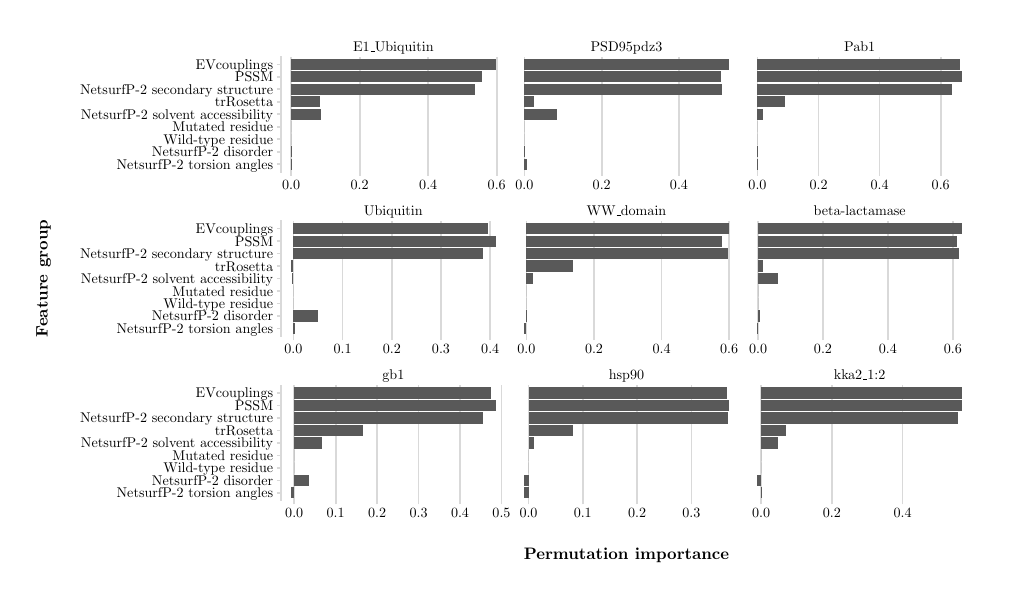
\begin{tikzpicture}[x=1pt,y=1pt]
\definecolor{fillColor}{RGB}{255,255,255}
\path[use as bounding box,fill=fillColor,fill opacity=0.00] (0,0) rectangle (344.26,196.49);
\begin{scope}
\path[clip] ( 91.51,144.44) rectangle (172.76,185.94);
\definecolor{drawColor}{gray}{0.85}

\path[draw=drawColor,line width= 0.6pt,line join=round] ( 95.21,144.44) --
	( 95.21,185.94);

\path[draw=drawColor,line width= 0.6pt,line join=round] (119.98,144.44) --
	(119.98,185.94);

\path[draw=drawColor,line width= 0.6pt,line join=round] (144.74,144.44) --
	(144.74,185.94);

\path[draw=drawColor,line width= 0.6pt,line join=round] (169.50,144.44) --
	(169.50,185.94);
\definecolor{fillColor}{gray}{0.35}

\path[fill=fillColor] ( 95.21,167.67) rectangle (105.68,171.73);

\path[fill=fillColor] ( 95.21,176.70) rectangle (164.15,180.76);

\path[fill=fillColor] ( 95.21,163.16) rectangle (106.15,167.22);

\path[fill=fillColor] ( 95.21,172.18) rectangle (161.69,176.24);

\path[fill=fillColor] ( 95.21,149.63) rectangle ( 95.22,153.69);

\path[fill=fillColor] ( 95.20,145.12) rectangle ( 95.21,149.18);

\path[fill=fillColor] ( 95.21,181.21) rectangle (169.06,185.27);

\path[fill=fillColor] ( 95.21,154.14) rectangle ( 95.21,158.20);

\path[fill=fillColor] ( 95.21,158.65) rectangle ( 95.21,162.71);
\end{scope}
\begin{scope}
\path[clip] ( 91.51, 85.06) rectangle (172.76,126.57);
\definecolor{drawColor}{gray}{0.85}

\path[draw=drawColor,line width= 0.6pt,line join=round] ( 96.01, 85.06) --
	( 96.01,126.57);

\path[draw=drawColor,line width= 0.6pt,line join=round] (113.79, 85.06) --
	(113.79,126.57);

\path[draw=drawColor,line width= 0.6pt,line join=round] (131.58, 85.06) --
	(131.58,126.57);

\path[draw=drawColor,line width= 0.6pt,line join=round] (149.36, 85.06) --
	(149.36,126.57);

\path[draw=drawColor,line width= 0.6pt,line join=round] (167.15, 85.06) --
	(167.15,126.57);
\definecolor{fillColor}{gray}{0.35}

\path[fill=fillColor] ( 95.20,108.30) rectangle ( 96.01,112.36);

\path[fill=fillColor] ( 96.01,117.32) rectangle (169.06,121.38);

\path[fill=fillColor] ( 95.52,103.79) rectangle ( 96.01,107.85);

\path[fill=fillColor] ( 96.01,112.81) rectangle (164.66,116.87);

\path[fill=fillColor] ( 96.01, 90.25) rectangle (104.84, 94.31);

\path[fill=fillColor] ( 96.01, 85.74) rectangle ( 96.42, 89.80);

\path[fill=fillColor] ( 96.01,121.83) rectangle (166.49,125.89);

\path[fill=fillColor] ( 96.01, 94.76) rectangle ( 96.01, 98.82);

\path[fill=fillColor] ( 96.01, 99.28) rectangle ( 96.01,103.34);
\end{scope}
\begin{scope}
\path[clip] ( 91.51, 25.69) rectangle (172.76, 67.19);
\definecolor{drawColor}{gray}{0.85}

\path[draw=drawColor,line width= 0.6pt,line join=round] ( 96.33, 25.69) --
	( 96.33, 67.19);

\path[draw=drawColor,line width= 0.6pt,line join=round] (111.30, 25.69) --
	(111.30, 67.19);

\path[draw=drawColor,line width= 0.6pt,line join=round] (126.28, 25.69) --
	(126.28, 67.19);

\path[draw=drawColor,line width= 0.6pt,line join=round] (141.26, 25.69) --
	(141.26, 67.19);

\path[draw=drawColor,line width= 0.6pt,line join=round] (156.23, 25.69) --
	(156.23, 67.19);

\path[draw=drawColor,line width= 0.6pt,line join=round] (171.21, 25.69) --
	(171.21, 67.19);
\definecolor{fillColor}{gray}{0.35}

\path[fill=fillColor] ( 96.33, 48.92) rectangle (121.07, 52.98);

\path[fill=fillColor] ( 96.33, 57.95) rectangle (169.06, 62.01);

\path[fill=fillColor] ( 96.33, 44.41) rectangle (106.28, 48.47);

\path[fill=fillColor] ( 96.33, 53.43) rectangle (164.43, 57.49);

\path[fill=fillColor] ( 96.33, 30.88) rectangle (101.79, 34.94);

\path[fill=fillColor] ( 95.20, 26.37) rectangle ( 96.33, 30.43);

\path[fill=fillColor] ( 96.33, 62.46) rectangle (167.53, 66.52);

\path[fill=fillColor] ( 96.33, 35.39) rectangle ( 96.33, 39.45);

\path[fill=fillColor] ( 96.33, 39.90) rectangle ( 96.33, 43.96);
\end{scope}
\begin{scope}
\path[clip] (175.76,144.44) rectangle (257.01,185.94);
\definecolor{drawColor}{gray}{0.85}

\path[draw=drawColor,line width= 0.6pt,line join=round] (179.50,144.44) --
	(179.50,185.94);

\path[draw=drawColor,line width= 0.6pt,line join=round] (207.43,144.44) --
	(207.43,185.94);

\path[draw=drawColor,line width= 0.6pt,line join=round] (235.36,144.44) --
	(235.36,185.94);
\definecolor{fillColor}{gray}{0.35}

\path[fill=fillColor] (179.50,167.67) rectangle (183.06,171.73);

\path[fill=fillColor] (179.50,176.70) rectangle (250.40,180.76);

\path[fill=fillColor] (179.50,163.16) rectangle (191.24,167.22);

\path[fill=fillColor] (179.50,172.18) rectangle (251.03,176.24);

\path[fill=fillColor] (179.45,149.63) rectangle (179.50,153.69);

\path[fill=fillColor] (179.50,145.12) rectangle (180.26,149.18);

\path[fill=fillColor] (179.50,181.21) rectangle (253.32,185.27);

\path[fill=fillColor] (179.50,154.14) rectangle (179.50,158.20);

\path[fill=fillColor] (179.50,158.65) rectangle (179.50,162.71);
\end{scope}
\begin{scope}
\path[clip] (175.76, 85.06) rectangle (257.01,126.57);
\definecolor{drawColor}{gray}{0.85}

\path[draw=drawColor,line width= 0.6pt,line join=round] (180.23, 85.06) --
	(180.23,126.57);

\path[draw=drawColor,line width= 0.6pt,line join=round] (204.65, 85.06) --
	(204.65,126.57);

\path[draw=drawColor,line width= 0.6pt,line join=round] (229.07, 85.06) --
	(229.07,126.57);

\path[draw=drawColor,line width= 0.6pt,line join=round] (253.49, 85.06) --
	(253.49,126.57);
\definecolor{fillColor}{gray}{0.35}

\path[fill=fillColor] (180.23,108.30) rectangle (197.22,112.36);

\path[fill=fillColor] (180.23,117.32) rectangle (250.98,121.38);

\path[fill=fillColor] (180.23,103.79) rectangle (182.50,107.85);

\path[fill=fillColor] (180.23,112.81) rectangle (253.09,116.87);

\path[fill=fillColor] (180.21, 90.25) rectangle (180.23, 94.31);

\path[fill=fillColor] (179.45, 85.74) rectangle (180.23, 89.80);

\path[fill=fillColor] (180.23,121.83) rectangle (253.32,125.89);

\path[fill=fillColor] (180.23, 94.76) rectangle (180.23, 98.82);

\path[fill=fillColor] (180.23, 99.28) rectangle (180.23,103.34);
\end{scope}
\begin{scope}
\path[clip] (175.76, 25.69) rectangle (257.01, 67.19);
\definecolor{drawColor}{gray}{0.85}

\path[draw=drawColor,line width= 0.6pt,line join=round] (180.98, 25.69) --
	(180.98, 67.19);

\path[draw=drawColor,line width= 0.6pt,line join=round] (200.59, 25.69) --
	(200.59, 67.19);

\path[draw=drawColor,line width= 0.6pt,line join=round] (220.20, 25.69) --
	(220.20, 67.19);

\path[draw=drawColor,line width= 0.6pt,line join=round] (239.81, 25.69) --
	(239.81, 67.19);
\definecolor{fillColor}{gray}{0.35}

\path[fill=fillColor] (180.98, 48.92) rectangle (197.13, 52.98);

\path[fill=fillColor] (180.98, 57.95) rectangle (253.32, 62.01);

\path[fill=fillColor] (180.98, 44.41) rectangle (182.93, 48.47);

\path[fill=fillColor] (180.98, 53.43) rectangle (253.17, 57.49);

\path[fill=fillColor] (179.45, 30.88) rectangle (180.98, 34.94);

\path[fill=fillColor] (179.52, 26.37) rectangle (180.98, 30.43);

\path[fill=fillColor] (180.98, 62.46) rectangle (252.70, 66.52);

\path[fill=fillColor] (180.98, 35.39) rectangle (180.98, 39.45);

\path[fill=fillColor] (180.98, 39.90) rectangle (180.98, 43.96);
\end{scope}
\begin{scope}
\path[clip] (260.01,144.44) rectangle (341.26,185.94);
\definecolor{drawColor}{gray}{0.85}

\path[draw=drawColor,line width= 0.6pt,line join=round] (263.71,144.44) --
	(263.71,185.94);

\path[draw=drawColor,line width= 0.6pt,line join=round] (285.79,144.44) --
	(285.79,185.94);

\path[draw=drawColor,line width= 0.6pt,line join=round] (307.86,144.44) --
	(307.86,185.94);

\path[draw=drawColor,line width= 0.6pt,line join=round] (329.93,144.44) --
	(329.93,185.94);
\definecolor{fillColor}{gray}{0.35}

\path[fill=fillColor] (263.71,167.67) rectangle (273.52,171.73);

\path[fill=fillColor] (263.71,176.70) rectangle (337.57,180.76);

\path[fill=fillColor] (263.71,163.16) rectangle (265.70,167.22);

\path[fill=fillColor] (263.71,172.18) rectangle (334.15,176.24);

\path[fill=fillColor] (263.70,149.63) rectangle (263.71,153.69);

\path[fill=fillColor] (263.71,145.12) rectangle (263.79,149.18);

\path[fill=fillColor] (263.71,181.21) rectangle (336.93,185.27);

\path[fill=fillColor] (263.71,154.14) rectangle (263.71,158.20);

\path[fill=fillColor] (263.71,158.65) rectangle (263.71,162.71);
\end{scope}
\begin{scope}
\path[clip] (260.01, 85.06) rectangle (341.26,126.57);
\definecolor{drawColor}{gray}{0.85}

\path[draw=drawColor,line width= 0.6pt,line join=round] (263.93, 85.06) --
	(263.93,126.57);

\path[draw=drawColor,line width= 0.6pt,line join=round] (287.39, 85.06) --
	(287.39,126.57);

\path[draw=drawColor,line width= 0.6pt,line join=round] (310.85, 85.06) --
	(310.85,126.57);

\path[draw=drawColor,line width= 0.6pt,line join=round] (334.31, 85.06) --
	(334.31,126.57);
\definecolor{fillColor}{gray}{0.35}

\path[fill=fillColor] (263.93,108.30) rectangle (265.56,112.36);

\path[fill=fillColor] (263.93,117.32) rectangle (335.77,121.38);

\path[fill=fillColor] (263.93,103.79) rectangle (271.30,107.85);

\path[fill=fillColor] (263.93,112.81) rectangle (336.38,116.87);

\path[fill=fillColor] (263.93, 90.25) rectangle (264.78, 94.31);

\path[fill=fillColor] (263.70, 85.74) rectangle (263.93, 89.80);

\path[fill=fillColor] (263.93,121.83) rectangle (337.57,125.89);

\path[fill=fillColor] (263.93, 94.76) rectangle (263.93, 98.82);

\path[fill=fillColor] (263.93, 99.28) rectangle (263.93,103.34);
\end{scope}
\begin{scope}
\path[clip] (260.01, 25.69) rectangle (341.26, 67.19);
\definecolor{drawColor}{gray}{0.85}

\path[draw=drawColor,line width= 0.6pt,line join=round] (265.01, 25.69) --
	(265.01, 67.19);

\path[draw=drawColor,line width= 0.6pt,line join=round] (290.58, 25.69) --
	(290.58, 67.19);

\path[draw=drawColor,line width= 0.6pt,line join=round] (316.16, 25.69) --
	(316.16, 67.19);
\definecolor{fillColor}{gray}{0.35}

\path[fill=fillColor] (265.01, 48.92) rectangle (274.11, 52.98);

\path[fill=fillColor] (265.01, 57.95) rectangle (337.44, 62.01);

\path[fill=fillColor] (265.01, 44.41) rectangle (271.24, 48.47);

\path[fill=fillColor] (265.01, 53.43) rectangle (336.02, 57.49);

\path[fill=fillColor] (263.70, 30.88) rectangle (265.01, 34.94);

\path[fill=fillColor] (265.01, 26.37) rectangle (265.12, 30.43);

\path[fill=fillColor] (265.01, 62.46) rectangle (337.57, 66.52);

\path[fill=fillColor] (265.01, 35.39) rectangle (265.01, 39.45);

\path[fill=fillColor] (265.01, 39.90) rectangle (265.01, 43.96);
\end{scope}
\begin{scope}
\path[clip] ( 91.51, 67.19) rectangle (172.76, 74.74);
\definecolor{drawColor}{RGB}{0,0,0}

\node[text=drawColor,anchor=base,inner sep=0pt, outer sep=0pt, scale=  0.51] at (132.13, 69.19) {gb1};
\end{scope}
\begin{scope}
\path[clip] (175.76, 67.19) rectangle (257.01, 74.74);
\definecolor{drawColor}{RGB}{0,0,0}

\node[text=drawColor,anchor=base,inner sep=0pt, outer sep=0pt, scale=  0.51] at (216.38, 69.19) {hsp90};
\end{scope}
\begin{scope}
\path[clip] (260.01, 67.19) rectangle (341.26, 74.74);
\definecolor{drawColor}{RGB}{0,0,0}

\node[text=drawColor,anchor=base,inner sep=0pt, outer sep=0pt, scale=  0.51] at (300.64, 69.19) {kka2\_1:2};
\end{scope}
\begin{scope}
\path[clip] ( 91.51,126.57) rectangle (172.76,134.11);
\definecolor{drawColor}{RGB}{0,0,0}

\node[text=drawColor,anchor=base,inner sep=0pt, outer sep=0pt, scale=  0.51] at (132.13,128.57) {Ubiquitin};
\end{scope}
\begin{scope}
\path[clip] (175.76,126.57) rectangle (257.01,134.11);
\definecolor{drawColor}{RGB}{0,0,0}

\node[text=drawColor,anchor=base,inner sep=0pt, outer sep=0pt, scale=  0.51] at (216.38,128.57) {WW\_domain};
\end{scope}
\begin{scope}
\path[clip] (260.01,126.57) rectangle (341.26,134.11);
\definecolor{drawColor}{RGB}{0,0,0}

\node[text=drawColor,anchor=base,inner sep=0pt, outer sep=0pt, scale=  0.51] at (300.64,128.57) {beta-lactamase};
\end{scope}
\begin{scope}
\path[clip] ( 91.51,185.94) rectangle (172.76,193.49);
\definecolor{drawColor}{RGB}{0,0,0}

\node[text=drawColor,anchor=base,inner sep=0pt, outer sep=0pt, scale=  0.51] at (132.13,187.94) {E1\_Ubiquitin};
\end{scope}
\begin{scope}
\path[clip] (175.76,185.94) rectangle (257.01,193.49);
\definecolor{drawColor}{RGB}{0,0,0}

\node[text=drawColor,anchor=base,inner sep=0pt, outer sep=0pt, scale=  0.51] at (216.38,187.94) {PSD95pdz3};
\end{scope}
\begin{scope}
\path[clip] (260.01,185.94) rectangle (341.26,193.49);
\definecolor{drawColor}{RGB}{0,0,0}

\node[text=drawColor,anchor=base,inner sep=0pt, outer sep=0pt, scale=  0.51] at (300.64,187.94) {Pab1};
\end{scope}
\begin{scope}
\path[clip] (  0.00,  0.00) rectangle (344.26,196.49);
\definecolor{drawColor}{gray}{0.85}

\path[draw=drawColor,line width= 0.6pt,line join=round] ( 96.33, 24.19) --
	( 96.33, 25.69);

\path[draw=drawColor,line width= 0.6pt,line join=round] (111.30, 24.19) --
	(111.30, 25.69);

\path[draw=drawColor,line width= 0.6pt,line join=round] (126.28, 24.19) --
	(126.28, 25.69);

\path[draw=drawColor,line width= 0.6pt,line join=round] (141.26, 24.19) --
	(141.26, 25.69);

\path[draw=drawColor,line width= 0.6pt,line join=round] (156.23, 24.19) --
	(156.23, 25.69);

\path[draw=drawColor,line width= 0.6pt,line join=round] (171.21, 24.19) --
	(171.21, 25.69);
\end{scope}
\begin{scope}
\path[clip] (  0.00,  0.00) rectangle (344.26,196.49);
\definecolor{drawColor}{RGB}{0,0,0}

\node[text=drawColor,anchor=base,inner sep=0pt, outer sep=0pt, scale=  0.51] at ( 96.33, 19.36) {0.0};

\node[text=drawColor,anchor=base,inner sep=0pt, outer sep=0pt, scale=  0.51] at (111.30, 19.36) {0.1};

\node[text=drawColor,anchor=base,inner sep=0pt, outer sep=0pt, scale=  0.51] at (126.28, 19.36) {0.2};

\node[text=drawColor,anchor=base,inner sep=0pt, outer sep=0pt, scale=  0.51] at (141.26, 19.36) {0.3};

\node[text=drawColor,anchor=base,inner sep=0pt, outer sep=0pt, scale=  0.51] at (156.23, 19.36) {0.4};

\node[text=drawColor,anchor=base,inner sep=0pt, outer sep=0pt, scale=  0.51] at (171.21, 19.36) {0.5};
\end{scope}
\begin{scope}
\path[clip] (  0.00,  0.00) rectangle (344.26,196.49);
\definecolor{drawColor}{gray}{0.85}

\path[draw=drawColor,line width= 0.6pt,line join=round] (180.98, 24.19) --
	(180.98, 25.69);

\path[draw=drawColor,line width= 0.6pt,line join=round] (200.59, 24.19) --
	(200.59, 25.69);

\path[draw=drawColor,line width= 0.6pt,line join=round] (220.20, 24.19) --
	(220.20, 25.69);

\path[draw=drawColor,line width= 0.6pt,line join=round] (239.81, 24.19) --
	(239.81, 25.69);
\end{scope}
\begin{scope}
\path[clip] (  0.00,  0.00) rectangle (344.26,196.49);
\definecolor{drawColor}{RGB}{0,0,0}

\node[text=drawColor,anchor=base,inner sep=0pt, outer sep=0pt, scale=  0.51] at (180.98, 19.36) {0.0};

\node[text=drawColor,anchor=base,inner sep=0pt, outer sep=0pt, scale=  0.51] at (200.59, 19.36) {0.1};

\node[text=drawColor,anchor=base,inner sep=0pt, outer sep=0pt, scale=  0.51] at (220.20, 19.36) {0.2};

\node[text=drawColor,anchor=base,inner sep=0pt, outer sep=0pt, scale=  0.51] at (239.81, 19.36) {0.3};
\end{scope}
\begin{scope}
\path[clip] (  0.00,  0.00) rectangle (344.26,196.49);
\definecolor{drawColor}{gray}{0.85}

\path[draw=drawColor,line width= 0.6pt,line join=round] (265.01, 24.19) --
	(265.01, 25.69);

\path[draw=drawColor,line width= 0.6pt,line join=round] (290.58, 24.19) --
	(290.58, 25.69);

\path[draw=drawColor,line width= 0.6pt,line join=round] (316.16, 24.19) --
	(316.16, 25.69);
\end{scope}
\begin{scope}
\path[clip] (  0.00,  0.00) rectangle (344.26,196.49);
\definecolor{drawColor}{RGB}{0,0,0}

\node[text=drawColor,anchor=base,inner sep=0pt, outer sep=0pt, scale=  0.51] at (265.01, 19.36) {0.0};

\node[text=drawColor,anchor=base,inner sep=0pt, outer sep=0pt, scale=  0.51] at (290.58, 19.36) {0.2};

\node[text=drawColor,anchor=base,inner sep=0pt, outer sep=0pt, scale=  0.51] at (316.16, 19.36) {0.4};
\end{scope}
\begin{scope}
\path[clip] (  0.00,  0.00) rectangle (344.26,196.49);
\definecolor{drawColor}{gray}{0.85}

\path[draw=drawColor,line width= 0.6pt,line join=round] ( 96.01, 83.56) --
	( 96.01, 85.06);

\path[draw=drawColor,line width= 0.6pt,line join=round] (113.79, 83.56) --
	(113.79, 85.06);

\path[draw=drawColor,line width= 0.6pt,line join=round] (131.58, 83.56) --
	(131.58, 85.06);

\path[draw=drawColor,line width= 0.6pt,line join=round] (149.36, 83.56) --
	(149.36, 85.06);

\path[draw=drawColor,line width= 0.6pt,line join=round] (167.15, 83.56) --
	(167.15, 85.06);
\end{scope}
\begin{scope}
\path[clip] (  0.00,  0.00) rectangle (344.26,196.49);
\definecolor{drawColor}{RGB}{0,0,0}

\node[text=drawColor,anchor=base,inner sep=0pt, outer sep=0pt, scale=  0.51] at ( 96.01, 78.74) {0.0};

\node[text=drawColor,anchor=base,inner sep=0pt, outer sep=0pt, scale=  0.51] at (113.79, 78.74) {0.1};

\node[text=drawColor,anchor=base,inner sep=0pt, outer sep=0pt, scale=  0.51] at (131.58, 78.74) {0.2};

\node[text=drawColor,anchor=base,inner sep=0pt, outer sep=0pt, scale=  0.51] at (149.36, 78.74) {0.3};

\node[text=drawColor,anchor=base,inner sep=0pt, outer sep=0pt, scale=  0.51] at (167.15, 78.74) {0.4};
\end{scope}
\begin{scope}
\path[clip] (  0.00,  0.00) rectangle (344.26,196.49);
\definecolor{drawColor}{gray}{0.85}

\path[draw=drawColor,line width= 0.6pt,line join=round] (180.23, 83.56) --
	(180.23, 85.06);

\path[draw=drawColor,line width= 0.6pt,line join=round] (204.65, 83.56) --
	(204.65, 85.06);

\path[draw=drawColor,line width= 0.6pt,line join=round] (229.07, 83.56) --
	(229.07, 85.06);

\path[draw=drawColor,line width= 0.6pt,line join=round] (253.49, 83.56) --
	(253.49, 85.06);
\end{scope}
\begin{scope}
\path[clip] (  0.00,  0.00) rectangle (344.26,196.49);
\definecolor{drawColor}{RGB}{0,0,0}

\node[text=drawColor,anchor=base,inner sep=0pt, outer sep=0pt, scale=  0.51] at (180.23, 78.74) {0.0};

\node[text=drawColor,anchor=base,inner sep=0pt, outer sep=0pt, scale=  0.51] at (204.65, 78.74) {0.2};

\node[text=drawColor,anchor=base,inner sep=0pt, outer sep=0pt, scale=  0.51] at (229.07, 78.74) {0.4};

\node[text=drawColor,anchor=base,inner sep=0pt, outer sep=0pt, scale=  0.51] at (253.49, 78.74) {0.6};
\end{scope}
\begin{scope}
\path[clip] (  0.00,  0.00) rectangle (344.26,196.49);
\definecolor{drawColor}{gray}{0.85}

\path[draw=drawColor,line width= 0.6pt,line join=round] (263.93, 83.56) --
	(263.93, 85.06);

\path[draw=drawColor,line width= 0.6pt,line join=round] (287.39, 83.56) --
	(287.39, 85.06);

\path[draw=drawColor,line width= 0.6pt,line join=round] (310.85, 83.56) --
	(310.85, 85.06);

\path[draw=drawColor,line width= 0.6pt,line join=round] (334.31, 83.56) --
	(334.31, 85.06);
\end{scope}
\begin{scope}
\path[clip] (  0.00,  0.00) rectangle (344.26,196.49);
\definecolor{drawColor}{RGB}{0,0,0}

\node[text=drawColor,anchor=base,inner sep=0pt, outer sep=0pt, scale=  0.51] at (263.93, 78.74) {0.0};

\node[text=drawColor,anchor=base,inner sep=0pt, outer sep=0pt, scale=  0.51] at (287.39, 78.74) {0.2};

\node[text=drawColor,anchor=base,inner sep=0pt, outer sep=0pt, scale=  0.51] at (310.85, 78.74) {0.4};

\node[text=drawColor,anchor=base,inner sep=0pt, outer sep=0pt, scale=  0.51] at (334.31, 78.74) {0.6};
\end{scope}
\begin{scope}
\path[clip] (  0.00,  0.00) rectangle (344.26,196.49);
\definecolor{drawColor}{gray}{0.85}

\path[draw=drawColor,line width= 0.6pt,line join=round] ( 95.21,142.94) --
	( 95.21,144.44);

\path[draw=drawColor,line width= 0.6pt,line join=round] (119.98,142.94) --
	(119.98,144.44);

\path[draw=drawColor,line width= 0.6pt,line join=round] (144.74,142.94) --
	(144.74,144.44);

\path[draw=drawColor,line width= 0.6pt,line join=round] (169.50,142.94) --
	(169.50,144.44);
\end{scope}
\begin{scope}
\path[clip] (  0.00,  0.00) rectangle (344.26,196.49);
\definecolor{drawColor}{RGB}{0,0,0}

\node[text=drawColor,anchor=base,inner sep=0pt, outer sep=0pt, scale=  0.51] at ( 95.21,138.11) {0.0};

\node[text=drawColor,anchor=base,inner sep=0pt, outer sep=0pt, scale=  0.51] at (119.98,138.11) {0.2};

\node[text=drawColor,anchor=base,inner sep=0pt, outer sep=0pt, scale=  0.51] at (144.74,138.11) {0.4};

\node[text=drawColor,anchor=base,inner sep=0pt, outer sep=0pt, scale=  0.51] at (169.50,138.11) {0.6};
\end{scope}
\begin{scope}
\path[clip] (  0.00,  0.00) rectangle (344.26,196.49);
\definecolor{drawColor}{gray}{0.85}

\path[draw=drawColor,line width= 0.6pt,line join=round] (179.50,142.94) --
	(179.50,144.44);

\path[draw=drawColor,line width= 0.6pt,line join=round] (207.43,142.94) --
	(207.43,144.44);

\path[draw=drawColor,line width= 0.6pt,line join=round] (235.36,142.94) --
	(235.36,144.44);
\end{scope}
\begin{scope}
\path[clip] (  0.00,  0.00) rectangle (344.26,196.49);
\definecolor{drawColor}{RGB}{0,0,0}

\node[text=drawColor,anchor=base,inner sep=0pt, outer sep=0pt, scale=  0.51] at (179.50,138.11) {0.0};

\node[text=drawColor,anchor=base,inner sep=0pt, outer sep=0pt, scale=  0.51] at (207.43,138.11) {0.2};

\node[text=drawColor,anchor=base,inner sep=0pt, outer sep=0pt, scale=  0.51] at (235.36,138.11) {0.4};
\end{scope}
\begin{scope}
\path[clip] (  0.00,  0.00) rectangle (344.26,196.49);
\definecolor{drawColor}{gray}{0.85}

\path[draw=drawColor,line width= 0.6pt,line join=round] (263.71,142.94) --
	(263.71,144.44);

\path[draw=drawColor,line width= 0.6pt,line join=round] (285.79,142.94) --
	(285.79,144.44);

\path[draw=drawColor,line width= 0.6pt,line join=round] (307.86,142.94) --
	(307.86,144.44);

\path[draw=drawColor,line width= 0.6pt,line join=round] (329.93,142.94) --
	(329.93,144.44);
\end{scope}
\begin{scope}
\path[clip] (  0.00,  0.00) rectangle (344.26,196.49);
\definecolor{drawColor}{RGB}{0,0,0}

\node[text=drawColor,anchor=base,inner sep=0pt, outer sep=0pt, scale=  0.51] at (263.71,138.11) {0.0};

\node[text=drawColor,anchor=base,inner sep=0pt, outer sep=0pt, scale=  0.51] at (285.79,138.11) {0.2};

\node[text=drawColor,anchor=base,inner sep=0pt, outer sep=0pt, scale=  0.51] at (307.86,138.11) {0.4};

\node[text=drawColor,anchor=base,inner sep=0pt, outer sep=0pt, scale=  0.51] at (329.93,138.11) {0.6};
\end{scope}
\begin{scope}
\path[clip] (  0.00,  0.00) rectangle (344.26,196.49);
\definecolor{drawColor}{gray}{0.85}

\path[draw=drawColor,line width= 0.6pt,line join=round,line cap=rect] ( 91.51,144.44) --
	( 91.51,185.94);
\end{scope}
\begin{scope}
\path[clip] (  0.00,  0.00) rectangle (344.26,196.49);
\definecolor{drawColor}{RGB}{0,0,0}

\node[text=drawColor,anchor=base east,inner sep=0pt, outer sep=0pt, scale=  0.51] at ( 88.72,145.38) {NetsurfP-2 torsion angles};

\node[text=drawColor,anchor=base east,inner sep=0pt, outer sep=0pt, scale=  0.51] at ( 88.72,149.89) {NetsurfP-2 disorder};

\node[text=drawColor,anchor=base east,inner sep=0pt, outer sep=0pt, scale=  0.51] at ( 88.72,154.40) {Wild-type residue};

\node[text=drawColor,anchor=base east,inner sep=0pt, outer sep=0pt, scale=  0.51] at ( 88.72,158.91) {Mutated residue};

\node[text=drawColor,anchor=base east,inner sep=0pt, outer sep=0pt, scale=  0.51] at ( 88.72,163.42) {NetsurfP-2 solvent accessibility};

\node[text=drawColor,anchor=base east,inner sep=0pt, outer sep=0pt, scale=  0.51] at ( 88.72,167.93) {trRosetta};

\node[text=drawColor,anchor=base east,inner sep=0pt, outer sep=0pt, scale=  0.51] at ( 88.72,172.44) {NetsurfP-2 secondary structure};

\node[text=drawColor,anchor=base east,inner sep=0pt, outer sep=0pt, scale=  0.51] at ( 88.72,176.95) {PSSM};

\node[text=drawColor,anchor=base east,inner sep=0pt, outer sep=0pt, scale=  0.51] at ( 88.72,181.47) {EVcouplings};
\end{scope}
\begin{scope}
\path[clip] (  0.00,  0.00) rectangle (344.26,196.49);
\definecolor{drawColor}{gray}{0.85}

\path[draw=drawColor,line width= 0.6pt,line join=round] ( 90.01,147.15) --
	( 91.51,147.15);

\path[draw=drawColor,line width= 0.6pt,line join=round] ( 90.01,151.66) --
	( 91.51,151.66);

\path[draw=drawColor,line width= 0.6pt,line join=round] ( 90.01,156.17) --
	( 91.51,156.17);

\path[draw=drawColor,line width= 0.6pt,line join=round] ( 90.01,160.68) --
	( 91.51,160.68);

\path[draw=drawColor,line width= 0.6pt,line join=round] ( 90.01,165.19) --
	( 91.51,165.19);

\path[draw=drawColor,line width= 0.6pt,line join=round] ( 90.01,169.70) --
	( 91.51,169.70);

\path[draw=drawColor,line width= 0.6pt,line join=round] ( 90.01,174.21) --
	( 91.51,174.21);

\path[draw=drawColor,line width= 0.6pt,line join=round] ( 90.01,178.73) --
	( 91.51,178.73);

\path[draw=drawColor,line width= 0.6pt,line join=round] ( 90.01,183.24) --
	( 91.51,183.24);
\end{scope}
\begin{scope}
\path[clip] (  0.00,  0.00) rectangle (344.26,196.49);
\definecolor{drawColor}{gray}{0.85}

\path[draw=drawColor,line width= 0.6pt,line join=round,line cap=rect] ( 91.51, 85.06) --
	( 91.51,126.57);
\end{scope}
\begin{scope}
\path[clip] (  0.00,  0.00) rectangle (344.26,196.49);
\definecolor{drawColor}{RGB}{0,0,0}

\node[text=drawColor,anchor=base east,inner sep=0pt, outer sep=0pt, scale=  0.51] at ( 88.72, 86.00) {NetsurfP-2 torsion angles};

\node[text=drawColor,anchor=base east,inner sep=0pt, outer sep=0pt, scale=  0.51] at ( 88.72, 90.51) {NetsurfP-2 disorder};

\node[text=drawColor,anchor=base east,inner sep=0pt, outer sep=0pt, scale=  0.51] at ( 88.72, 95.02) {Wild-type residue};

\node[text=drawColor,anchor=base east,inner sep=0pt, outer sep=0pt, scale=  0.51] at ( 88.72, 99.53) {Mutated residue};

\node[text=drawColor,anchor=base east,inner sep=0pt, outer sep=0pt, scale=  0.51] at ( 88.72,104.05) {NetsurfP-2 solvent accessibility};

\node[text=drawColor,anchor=base east,inner sep=0pt, outer sep=0pt, scale=  0.51] at ( 88.72,108.56) {trRosetta};

\node[text=drawColor,anchor=base east,inner sep=0pt, outer sep=0pt, scale=  0.51] at ( 88.72,113.07) {NetsurfP-2 secondary structure};

\node[text=drawColor,anchor=base east,inner sep=0pt, outer sep=0pt, scale=  0.51] at ( 88.72,117.58) {PSSM};

\node[text=drawColor,anchor=base east,inner sep=0pt, outer sep=0pt, scale=  0.51] at ( 88.72,122.09) {EVcouplings};
\end{scope}
\begin{scope}
\path[clip] (  0.00,  0.00) rectangle (344.26,196.49);
\definecolor{drawColor}{gray}{0.85}

\path[draw=drawColor,line width= 0.6pt,line join=round] ( 90.01, 87.77) --
	( 91.51, 87.77);

\path[draw=drawColor,line width= 0.6pt,line join=round] ( 90.01, 92.28) --
	( 91.51, 92.28);

\path[draw=drawColor,line width= 0.6pt,line join=round] ( 90.01, 96.79) --
	( 91.51, 96.79);

\path[draw=drawColor,line width= 0.6pt,line join=round] ( 90.01,101.31) --
	( 91.51,101.31);

\path[draw=drawColor,line width= 0.6pt,line join=round] ( 90.01,105.82) --
	( 91.51,105.82);

\path[draw=drawColor,line width= 0.6pt,line join=round] ( 90.01,110.33) --
	( 91.51,110.33);

\path[draw=drawColor,line width= 0.6pt,line join=round] ( 90.01,114.84) --
	( 91.51,114.84);

\path[draw=drawColor,line width= 0.6pt,line join=round] ( 90.01,119.35) --
	( 91.51,119.35);

\path[draw=drawColor,line width= 0.6pt,line join=round] ( 90.01,123.86) --
	( 91.51,123.86);
\end{scope}
\begin{scope}
\path[clip] (  0.00,  0.00) rectangle (344.26,196.49);
\definecolor{drawColor}{gray}{0.85}

\path[draw=drawColor,line width= 0.6pt,line join=round,line cap=rect] ( 91.51, 25.69) --
	( 91.51, 67.19);
\end{scope}
\begin{scope}
\path[clip] (  0.00,  0.00) rectangle (344.26,196.49);
\definecolor{drawColor}{RGB}{0,0,0}

\node[text=drawColor,anchor=base east,inner sep=0pt, outer sep=0pt, scale=  0.51] at ( 88.72, 26.62) {NetsurfP-2 torsion angles};

\node[text=drawColor,anchor=base east,inner sep=0pt, outer sep=0pt, scale=  0.51] at ( 88.72, 31.14) {NetsurfP-2 disorder};

\node[text=drawColor,anchor=base east,inner sep=0pt, outer sep=0pt, scale=  0.51] at ( 88.72, 35.65) {Wild-type residue};

\node[text=drawColor,anchor=base east,inner sep=0pt, outer sep=0pt, scale=  0.51] at ( 88.72, 40.16) {Mutated residue};

\node[text=drawColor,anchor=base east,inner sep=0pt, outer sep=0pt, scale=  0.51] at ( 88.72, 44.67) {NetsurfP-2 solvent accessibility};

\node[text=drawColor,anchor=base east,inner sep=0pt, outer sep=0pt, scale=  0.51] at ( 88.72, 49.18) {trRosetta};

\node[text=drawColor,anchor=base east,inner sep=0pt, outer sep=0pt, scale=  0.51] at ( 88.72, 53.69) {NetsurfP-2 secondary structure};

\node[text=drawColor,anchor=base east,inner sep=0pt, outer sep=0pt, scale=  0.51] at ( 88.72, 58.20) {PSSM};

\node[text=drawColor,anchor=base east,inner sep=0pt, outer sep=0pt, scale=  0.51] at ( 88.72, 62.72) {EVcouplings};
\end{scope}
\begin{scope}
\path[clip] (  0.00,  0.00) rectangle (344.26,196.49);
\definecolor{drawColor}{gray}{0.85}

\path[draw=drawColor,line width= 0.6pt,line join=round] ( 90.01, 28.40) --
	( 91.51, 28.40);

\path[draw=drawColor,line width= 0.6pt,line join=round] ( 90.01, 32.91) --
	( 91.51, 32.91);

\path[draw=drawColor,line width= 0.6pt,line join=round] ( 90.01, 37.42) --
	( 91.51, 37.42);

\path[draw=drawColor,line width= 0.6pt,line join=round] ( 90.01, 41.93) --
	( 91.51, 41.93);

\path[draw=drawColor,line width= 0.6pt,line join=round] ( 90.01, 46.44) --
	( 91.51, 46.44);

\path[draw=drawColor,line width= 0.6pt,line join=round] ( 90.01, 50.95) --
	( 91.51, 50.95);

\path[draw=drawColor,line width= 0.6pt,line join=round] ( 90.01, 55.46) --
	( 91.51, 55.46);

\path[draw=drawColor,line width= 0.6pt,line join=round] ( 90.01, 59.98) --
	( 91.51, 59.98);

\path[draw=drawColor,line width= 0.6pt,line join=round] ( 90.01, 64.49) --
	( 91.51, 64.49);
\end{scope}
\begin{scope}
\path[clip] (  0.00,  0.00) rectangle (344.26,196.49);
\definecolor{drawColor}{RGB}{0,0,0}

\node[text=drawColor,anchor=base,inner sep=0pt, outer sep=0pt, scale=  0.60] at (216.38,  4.17) {\bfseries Permutation importance};
\end{scope}
\begin{scope}
\path[clip] (  0.00,  0.00) rectangle (344.26,196.49);
\definecolor{drawColor}{RGB}{0,0,0}

\node[text=drawColor,rotate= 90.00,anchor=base,inner sep=0pt, outer sep=0pt, scale=  0.60] at (  7.19,105.82) {\bfseries Feature group};
\end{scope}
\end{tikzpicture}

	}
\end{frame}

\begin{frame}
	\frametitle{Supplementary Material}
	Comparison of the performances of single protein models and general models
	\vfill%
	\centering%
	{%
		\let\bfseries\sbseries%
		% Created by tikzDevice version 0.12.3.1 on 2021-07-04 22:43:31
% !TEX encoding = UTF-8 Unicode
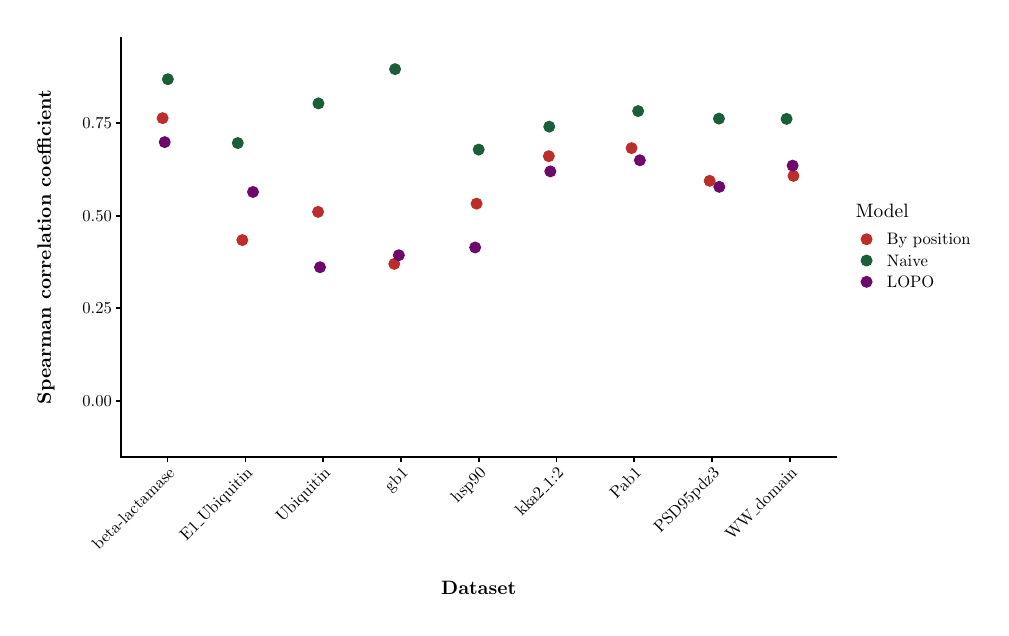
\begin{tikzpicture}[x=1pt,y=1pt]
\definecolor{fillColor}{RGB}{255,255,255}
\path[use as bounding box,fill=fillColor,fill opacity=0.00] (0,0) rectangle (344.26,209.59);
\begin{scope}
\path[clip] ( 33.67, 54.47) rectangle (292.28,206.09);
\definecolor{drawColor}{RGB}{28,94,57}
\definecolor{fillColor}{RGB}{28,94,57}

\path[draw=drawColor,line width= 0.4pt,line join=round,line cap=round,fill=fillColor] ( 75.93,167.90) circle (  1.96);

\path[draw=drawColor,line width= 0.4pt,line join=round,line cap=round,fill=fillColor] (249.80,176.72) circle (  1.96);

\path[draw=drawColor,line width= 0.4pt,line join=round,line cap=round,fill=fillColor] (220.59,179.45) circle (  1.96);

\path[draw=drawColor,line width= 0.4pt,line join=round,line cap=round,fill=fillColor] (105.08,182.22) circle (  1.96);

\path[draw=drawColor,line width= 0.4pt,line join=round,line cap=round,fill=fillColor] (274.23,176.62) circle (  1.96);

\path[draw=drawColor,line width= 0.4pt,line join=round,line cap=round,fill=fillColor] ( 50.66,190.96) circle (  1.96);

\path[draw=drawColor,line width= 0.4pt,line join=round,line cap=round,fill=fillColor] (132.77,194.60) circle (  1.96);

\path[draw=drawColor,line width= 0.4pt,line join=round,line cap=round,fill=fillColor] (162.98,165.53) circle (  1.96);

\path[draw=drawColor,line width= 0.4pt,line join=round,line cap=round,fill=fillColor] (188.47,173.82) circle (  1.96);
\definecolor{drawColor}{RGB}{187,46,41}
\definecolor{fillColor}{RGB}{187,46,41}

\path[draw=drawColor,line width= 0.4pt,line join=round,line cap=round,fill=fillColor] ( 77.57,132.84) circle (  1.96);

\path[draw=drawColor,line width= 0.4pt,line join=round,line cap=round,fill=fillColor] (246.44,154.24) circle (  1.96);

\path[draw=drawColor,line width= 0.4pt,line join=round,line cap=round,fill=fillColor] (218.21,166.07) circle (  1.96);

\path[draw=drawColor,line width= 0.4pt,line join=round,line cap=round,fill=fillColor] (104.93,143.03) circle (  1.96);

\path[draw=drawColor,line width= 0.4pt,line join=round,line cap=round,fill=fillColor] (276.72,156.03) circle (  1.96);

\path[draw=drawColor,line width= 0.4pt,line join=round,line cap=round,fill=fillColor] ( 48.76,176.90) circle (  1.96);

\path[draw=drawColor,line width= 0.4pt,line join=round,line cap=round,fill=fillColor] (132.47,124.24) circle (  1.96);

\path[draw=drawColor,line width= 0.4pt,line join=round,line cap=round,fill=fillColor] (162.21,145.99) circle (  1.96);

\path[draw=drawColor,line width= 0.4pt,line join=round,line cap=round,fill=fillColor] (188.32,163.16) circle (  1.96);
\definecolor{drawColor}{RGB}{108,9,106}
\definecolor{fillColor}{RGB}{108,9,106}

\path[draw=drawColor,line width= 0.4pt,line join=round,line cap=round,fill=fillColor] (188.87,157.66) circle (  1.96);

\path[draw=drawColor,line width= 0.4pt,line join=round,line cap=round,fill=fillColor] (161.69,130.17) circle (  1.96);

\path[draw=drawColor,line width= 0.4pt,line join=round,line cap=round,fill=fillColor] (221.22,161.68) circle (  1.96);

\path[draw=drawColor,line width= 0.4pt,line join=round,line cap=round,fill=fillColor] (134.12,127.36) circle (  1.96);

\path[draw=drawColor,line width= 0.4pt,line join=round,line cap=round,fill=fillColor] (105.64,123.03) circle (  1.96);

\path[draw=drawColor,line width= 0.4pt,line join=round,line cap=round,fill=fillColor] ( 81.42,150.22) circle (  1.96);

\path[draw=drawColor,line width= 0.4pt,line join=round,line cap=round,fill=fillColor] (249.93,152.07) circle (  1.96);

\path[draw=drawColor,line width= 0.4pt,line join=round,line cap=round,fill=fillColor] (276.41,159.74) circle (  1.96);

\path[draw=drawColor,line width= 0.4pt,line join=round,line cap=round,fill=fillColor] ( 49.52,168.23) circle (  1.96);
\end{scope}
\begin{scope}
\path[clip] (  0.00,  0.00) rectangle (344.26,209.59);
\definecolor{drawColor}{RGB}{0,0,0}

\path[draw=drawColor,line width= 0.6pt,line join=round,line cap=rect] ( 33.67, 54.47) --
	( 33.67,206.09);
\end{scope}
\begin{scope}
\path[clip] (  0.00,  0.00) rectangle (344.26,209.59);
\definecolor{drawColor}{RGB}{0,0,0}

\node[text=drawColor,anchor=base east,inner sep=0pt, outer sep=0pt, scale=  0.60] at ( 30.42, 72.68) {0.00};

\node[text=drawColor,anchor=base east,inner sep=0pt, outer sep=0pt, scale=  0.60] at ( 30.42,106.13) {0.25};

\node[text=drawColor,anchor=base east,inner sep=0pt, outer sep=0pt, scale=  0.60] at ( 30.42,139.59) {0.50};

\node[text=drawColor,anchor=base east,inner sep=0pt, outer sep=0pt, scale=  0.60] at ( 30.42,173.04) {0.75};
\end{scope}
\begin{scope}
\path[clip] (  0.00,  0.00) rectangle (344.26,209.59);
\definecolor{drawColor}{RGB}{0,0,0}

\path[draw=drawColor,line width= 0.6pt,line join=round] ( 31.92, 74.74) --
	( 33.67, 74.74);

\path[draw=drawColor,line width= 0.6pt,line join=round] ( 31.92,108.20) --
	( 33.67,108.20);

\path[draw=drawColor,line width= 0.6pt,line join=round] ( 31.92,141.65) --
	( 33.67,141.65);

\path[draw=drawColor,line width= 0.6pt,line join=round] ( 31.92,175.11) --
	( 33.67,175.11);
\end{scope}
\begin{scope}
\path[clip] (  0.00,  0.00) rectangle (344.26,209.59);
\definecolor{drawColor}{RGB}{0,0,0}

\path[draw=drawColor,line width= 0.6pt,line join=round,line cap=rect] ( 33.67, 54.47) --
	(292.28, 54.47);
\end{scope}
\begin{scope}
\path[clip] (  0.00,  0.00) rectangle (344.26,209.59);
\definecolor{drawColor}{RGB}{0,0,0}

\path[draw=drawColor,line width= 0.6pt,line join=round] ( 50.54, 52.72) --
	( 50.54, 54.47);

\path[draw=drawColor,line width= 0.6pt,line join=round] ( 78.65, 52.72) --
	( 78.65, 54.47);

\path[draw=drawColor,line width= 0.6pt,line join=round] (106.76, 52.72) --
	(106.76, 54.47);

\path[draw=drawColor,line width= 0.6pt,line join=round] (134.87, 52.72) --
	(134.87, 54.47);

\path[draw=drawColor,line width= 0.6pt,line join=round] (162.98, 52.72) --
	(162.98, 54.47);

\path[draw=drawColor,line width= 0.6pt,line join=round] (191.09, 52.72) --
	(191.09, 54.47);

\path[draw=drawColor,line width= 0.6pt,line join=round] (219.19, 52.72) --
	(219.19, 54.47);

\path[draw=drawColor,line width= 0.6pt,line join=round] (247.30, 52.72) --
	(247.30, 54.47);

\path[draw=drawColor,line width= 0.6pt,line join=round] (275.41, 52.72) --
	(275.41, 54.47);
\end{scope}
\begin{scope}
\path[clip] (  0.00,  0.00) rectangle (344.26,209.59);
\definecolor{drawColor}{RGB}{0,0,0}

\node[text=drawColor,rotate= 45.00,anchor=base east,inner sep=0pt, outer sep=0pt, scale=  0.60] at ( 53.46, 48.30) {beta-lactamase};

\node[text=drawColor,rotate= 45.00,anchor=base east,inner sep=0pt, outer sep=0pt, scale=  0.60] at ( 81.57, 48.30) {E1\_Ubiquitin};

\node[text=drawColor,rotate= 45.00,anchor=base east,inner sep=0pt, outer sep=0pt, scale=  0.60] at (109.68, 48.30) {Ubiquitin};

\node[text=drawColor,rotate= 45.00,anchor=base east,inner sep=0pt, outer sep=0pt, scale=  0.60] at (137.79, 48.30) {gb1};

\node[text=drawColor,rotate= 45.00,anchor=base east,inner sep=0pt, outer sep=0pt, scale=  0.60] at (165.90, 48.30) {hsp90};

\node[text=drawColor,rotate= 45.00,anchor=base east,inner sep=0pt, outer sep=0pt, scale=  0.60] at (194.01, 48.30) {kka2\_1:2};

\node[text=drawColor,rotate= 45.00,anchor=base east,inner sep=0pt, outer sep=0pt, scale=  0.60] at (222.12, 48.30) {Pab1};

\node[text=drawColor,rotate= 45.00,anchor=base east,inner sep=0pt, outer sep=0pt, scale=  0.60] at (250.23, 48.30) {PSD95pdz3};

\node[text=drawColor,rotate= 45.00,anchor=base east,inner sep=0pt, outer sep=0pt, scale=  0.60] at (278.34, 48.30) {WW\_domain};
\end{scope}
\begin{scope}
\path[clip] (  0.00,  0.00) rectangle (344.26,209.59);
\definecolor{drawColor}{RGB}{0,0,0}

\node[text=drawColor,anchor=base,inner sep=0pt, outer sep=0pt, scale=  0.70] at (162.98,  4.86) {\bfseries Dataset};
\end{scope}
\begin{scope}
\path[clip] (  0.00,  0.00) rectangle (344.26,209.59);
\definecolor{drawColor}{RGB}{0,0,0}

\node[text=drawColor,rotate= 90.00,anchor=base,inner sep=0pt, outer sep=0pt, scale=  0.70] at (  8.39,130.28) {\bfseries Spearman correlation coefficient};
\end{scope}
\begin{scope}
\path[clip] (  0.00,  0.00) rectangle (344.26,209.59);
\definecolor{drawColor}{RGB}{0,0,0}

\node[text=drawColor,anchor=base west,inner sep=0pt, outer sep=0pt, scale=  0.70] at (299.28,141.17) {Model};
\end{scope}
\begin{scope}
\path[clip] (  0.00,  0.00) rectangle (344.26,209.59);
\definecolor{drawColor}{RGB}{187,46,41}
\definecolor{fillColor}{RGB}{187,46,41}

\path[draw=drawColor,line width= 0.4pt,line join=round,line cap=round,fill=fillColor] (303.13,133.14) circle (  1.96);
\end{scope}
\begin{scope}
\path[clip] (  0.00,  0.00) rectangle (344.26,209.59);
\definecolor{drawColor}{RGB}{28,94,57}
\definecolor{fillColor}{RGB}{28,94,57}

\path[draw=drawColor,line width= 0.4pt,line join=round,line cap=round,fill=fillColor] (303.13,125.44) circle (  1.96);
\end{scope}
\begin{scope}
\path[clip] (  0.00,  0.00) rectangle (344.26,209.59);
\definecolor{drawColor}{RGB}{108,9,106}
\definecolor{fillColor}{RGB}{108,9,106}

\path[draw=drawColor,line width= 0.4pt,line join=round,line cap=round,fill=fillColor] (303.13,117.74) circle (  1.96);
\end{scope}
\begin{scope}
\path[clip] (  0.00,  0.00) rectangle (344.26,209.59);
\definecolor{drawColor}{RGB}{0,0,0}

\node[text=drawColor,anchor=base west,inner sep=0pt, outer sep=0pt, scale=  0.60] at (310.48,131.07) {By position};
\end{scope}
\begin{scope}
\path[clip] (  0.00,  0.00) rectangle (344.26,209.59);
\definecolor{drawColor}{RGB}{0,0,0}

\node[text=drawColor,anchor=base west,inner sep=0pt, outer sep=0pt, scale=  0.60] at (310.48,123.37) {Naive};
\end{scope}
\begin{scope}
\path[clip] (  0.00,  0.00) rectangle (344.26,209.59);
\definecolor{drawColor}{RGB}{0,0,0}

\node[text=drawColor,anchor=base west,inner sep=0pt, outer sep=0pt, scale=  0.60] at (310.48,115.67) {LOPO};
\end{scope}
\end{tikzpicture}

	}
\end{frame}

\begin{frame}
	\frametitle{Supplementary Material}
	Confidence intervals in prediction performances
	\vfill%
	\tiny%
	\begin{tabular*}{\linewidth}{@{\extracolsep{\fill}}llll}%
		\toprule
		Dataset name            & Model       & \num{95}\,\% C.I. (Pearson) & \num{95}\,\% C.I. (Spearman) \\
		\midrule
		beta-lactamase & Naive       & \numrange{0.8866}{0.9077}        & \numrange{0.8578}{0.8803}         \\
		beta-lactamase & By position & \numrange{0.7927}{0.8272}        & \numrange{0.7461}{0.7820}         \\
		beta-lactamase & LOPO        & ---                              & \numrange{0.6781}{0.7210}         \\
		WW\_domain     & Naive       & \numrange{0.6747}{0.8174}        & \numrange{0.7044}{0.8368}         \\
		WW\_domain     & By position & \numrange{0.5679}{0.7291}        & \numrange{0.5203}{0.7168}         \\
		WW\_domain     & LOPO        & ---                              & \numrange{0.5628}{0.7297}         \\
		PSD95pdz3      & Naive       & \numrange{0.7443}{0.8313}        & \numrange{0.7276}{0.8008}         \\
		PSD95pdz3      & By position & \numrange{0.5487}{0.6652}        & \numrange{0.5442}{0.6485}         \\
		PSD95pdz3      & LOPO        & ---                              & \numrange{0.5335}{0.6282}         \\
		kka2\_1:2      & Naive       & \numrange{0.7405}{0.7763}        & \numrange{0.7232}{0.7588}         \\
		kka2\_1:2      & By position & \numrange{0.6451}{0.6881}        & \numrange{0.6401}{0.6824}         \\
		kka2\_1:2      & LOPO        & ---                              & \numrange{0.5975}{0.6427}         \\
		hsp90          & Naive       & \numrange{0.8190}{0.8664}        & \numrange{0.6522}{0.7071}         \\
		hsp90          & By position & \numrange{0.6945}{0.7577}        & \numrange{0.4996}{0.5674}         \\
		hsp90          & LOPO        & ---                              & \numrange{0.3771}{0.4529}         \\
		Ubiquitin      & Naive       & \numrange{0.7470}{0.8281}        & \numrange{0.7782}{0.8321}         \\
		Ubiquitin      & By position & \numrange{0.4858}{0.6035}        & \numrange{0.4565}{0.5672}         \\
		Ubiquitin      & LOPO        & ---                              & \numrange{0.2951}{0.4296}         \\
		Pab1           & Naive       & \numrange{0.8047}{0.8749}        & \numrange{0.7482}{0.8239}         \\
		Pab1           & By position & \numrange{0.6545}{0.7590}        & \numrange{0.6423}{0.7288}         \\
		Pab1           & LOPO        & ---                              & \numrange{0.6038}{0.7004}         \\
		E1\_Ubiquitin  & Naive       & \numrange{0.7454}{0.8470}        & \numrange{0.6487}{0.7517}         \\
		E1\_Ubiquitin  & By position & \numrange{0.5898}{0.7218}        & \numrange{0.3623}{0.5100}         \\
		E1\_Ubiquitin  & LOPO        & ---                              & \numrange{0.5027}{0.6343}         \\
		gb1            & Naive       & \numrange{0.8965}{0.9341}        & \numrange{0.8759}{0.9194}         \\
		gb1            & By position & \numrange{0.3072}{0.4561}        & \numrange{0.2942}{0.4522}         \\
		gb1            & LOPO        & ---                              & \numrange{0.3225}{0.4706}         \\
		\bottomrule
	\end{tabular*}%
\end{frame}

\begin{frame}
	\frametitle{Supplementary Material}
	Statistical significance of performance differences. Starred values are significant with Bonferroni correction.

	\begin{equation*}
		\alpha = \frac{0.05}{27} = 0.00185185
	\end{equation*}

	\vfill%
	\tiny%
	\begin{tabular*}{\linewidth}{@{\extracolsep{\fill}}lllll}%
		\toprule
		Dataset name            & Model 1           & Model 2                & $p$-value      \\
		\midrule
		beta-lactamase & Linear regression & Gradient boosted trees & \num{1e-4} * \\
		beta-lactamase & Linear regression & EVmutation             & \num{1e-4} * \\
		beta-lactamase & EVmutation        & Gradient boosted trees & \num{1e-4} * \\
		WW\_domain     & Linear regression & Gradient boosted trees & \num{1e-4} * \\
		WW\_domain     & Linear regression & EVmutation             & \num{1e-4} * \\
		WW\_domain     & EVmutation        & Gradient boosted trees & \num{1e-4} * \\
		PSD95pdz3      & Linear regression & Gradient boosted trees & \num{1e-4} * \\
		PSD95pdz3      & Linear regression & EVmutation             & \num{1e-4} * \\
		PSD95pdz3      & EVmutation        & Gradient boosted trees & \num{0.514}  \\
		kka2\_1:2      & Linear regression & Gradient boosted trees & \num{0.0043} \\
		kka2\_1:2      & Linear regression & EVmutation             & \num{0.0053} \\
		kka2\_1:2      & EVmutation        & Gradient boosted trees & \num{1e-4} * \\
		hsp90          & Linear regression & Gradient boosted trees & \num{1e-4} * \\
		hsp90          & Linear regression & EVmutation             & \num{1e-4} * \\
		hsp90          & EVmutation        & Gradient boosted trees & \num{0.2358} \\
		\bottomrule
	\end{tabular*}%
	\normalsize%

	The table continues on the next slide
\end{frame}

\begin{frame}
	\frametitle{Supplementary Material}
	Statistical significance of performance differences. Starred values are significant with Bonferroni correction.

	\begin{equation*}
		\alpha = \frac{0.05}{27} = 0.00185185
	\end{equation*}
	\vfill%
	The table continues from the previous slide

	\tiny%
	\begin{tabular*}{\linewidth}{@{\extracolsep{\fill}}lllll}%
		\toprule
		Dataset name            & Model 1           & Model 2                & $p$-value      \\
		\midrule
		Ubiquitin      & Linear regression & Gradient boosted trees & \num{1e-4} * \\
		Ubiquitin      & Linear regression & EVmutation             & \num{1e-4} * \\
		Ubiquitin      & EVmutation        & Gradient boosted trees & \num{1e-4} * \\
		Pab1           & Linear regression & Gradient boosted trees & \num{1e-4} * \\
		Pab1           & Linear regression & EVmutation             & \num{1e-4} * \\
		Pab1           & EVmutation        & Gradient boosted trees & \num{1e-4} * \\
		E1\_Ubiquitin  & Linear regression & Gradient boosted trees & \num{1e-4} * \\
		E1\_Ubiquitin  & Linear regression & EVmutation             & \num{1e-4} * \\
		E1\_Ubiquitin  & EVmutation        & Gradient boosted trees & \num{1e-4} * \\
		gb1            & Linear regression & Gradient boosted trees & \num{1e-4} * \\
		gb1            & Linear regression & EVmutation             & \num{1e-4} * \\
		gb1            & EVmutation        & Gradient boosted trees & \num{1e-4} * \\
		\bottomrule
	\end{tabular*}%
\end{frame}

\end{document}
